\documentclass[../fem.tex]{subfiles}

\begin{document}
\section{Mesh Generation}%
\label{sec:mesh_generation}

For the implementation of FEM, we must discretize our global domain into a set
of finite subdomains, which we call elements. We can then compute our
approximation on each element independent of the rest of the domain, then
combine the solutions of each element into our global solution.

These elements can be of the form of an $N$ sided polygon. However, with
polygons with more than $3$ edges, issues can arise. So for the purposes of
FEM, we will be focused on the construction of a mesh of triangles. This is the
most common mesh polygon, as any mesh of polygons with more edges can be
represented by a triangular mesh. In addition, most research of mesh generation
has been focused on triangular meshes for this same reason.

Our process will be construction what is known as a Constrained Delaunay
Triangulation, and then apply a refinement algorithm to ensure that the
triangles in the mesh are ``nice''.

\subsection{Delaunay Triangulation}%
\label{sub:delaunay_triangulation}

Delaunay triangulation is the straight line dual of the Voronoi diagram.
Delaunay triangulations are used in many different situations, including our
purpose of mesh generation for finite element analysis.

\gtodo{Add example image of Delaunay triangulation.}

A key property of Delaunay triangulation is that no point may lie inside the
circumcircle of any other triangle. We use this as our definition of Delaunay
Triangulation.

\begin{definition}[Delaunay Triangulation] \label{def:dt}
  Let $S$ be a set of points in the plane. A triangulation $T$ is
  a \textit{Delaunay triangulation}($DT$) of $S$ if for each triangle $t$ of $T$
  there exists a circle $C$ with the following properties:
  \begin{enumerate}
    \item the vertices of the triangle $t$ are on the boundary of circle $C$
    \item no other vertex of $S$ is in the interior of $C$.
  \end{enumerate}
\end{definition}

\gtodo{Add image showing circumcircle definition.}
\begin{Figure}
   \begin{center}
     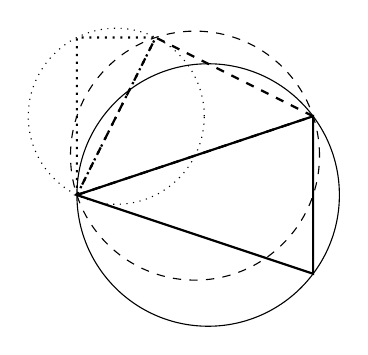
\begin{tikzpicture}
\draw[solid,thick] (0,1) -- (3,0) -- (3,2) -- cycle;
\draw[solid] (1.667, 1) circle (1.66666);
\draw[dashed,thick] (0,1) -- (3,2) -- (1,3) -- cycle;
\draw[dashed] (1.5, 1.5) circle (1.58113);
\draw[dotted,thick] (0,1) -- (1,3) -- (0,3) -- cycle;
\draw[dotted] (0.5,2) circle (1.11803);
\end{tikzpicture}

   \end{center}
   \captionof{figure}{Demonstration of the Circumcircle definition of Delaunay.}
\end{Figure}

Is most situation the Delaunay triangulation of a set of points is unique. This
is true for all points with one exception of a square, where there are two
valid Delaunay triangulations.

A major advantage of Delaunay triangulation is that it avoids triangles with
small included angles. This makes this type of triangulation extremely well
suited for our purpose of FEA.

There are many different algorithms that can be used for the construction of
Delaunay triangulation of a set of points in a plane. Some notable ones
include; Divide and Conquer developed by Chew\cite{C_CDT}, Incremental
developed by Watson, Sweep Line developed by \v{Z}alik\cite{Z_DT}\cite{DZ_CDT},
and Edge Flipping developed by Sloan\cite{S_DT}\cite{S_CDT}. Each of these
methods has different advantages and different efficiency in computation time.

\subsection{Constrained Delaunay Triangulation}%
\label{sub:constrained_delaunay_triangulation}

The Constrained Delaunay Triangulation(CDT), is a modification of the Delaunay
Triangulation such that specified edges are forced to exist in the
triangulation. This has the unfortunate effect of the resulting triangulation
not being strictly Delaunay. Thus we define our constrained triangulation at
the closest triangulation to the Delaunay triangulation that still includes the
specified edges.

\begin{Figure}
  \begin{center}
    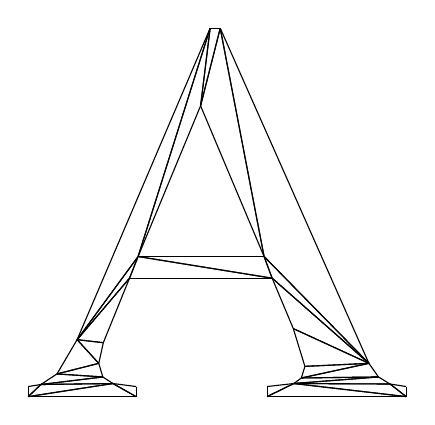
\begin{tikzpicture}[scale=8.0]
\draw (0.2,-0.7924) -- (0.22,-0.7732);
\draw (0.22,-0.7732) -- (0.2,-0.7764);
\draw (0.2,-0.7764) -- (0.2,-0.7924);
\draw (0.22,-0.7732) -- (0.2,-0.7924);
\draw (0.2,-0.7924) -- (0.3344,-0.7716);
\draw (0.3344,-0.7716) -- (0.22,-0.7732);
\draw (0.3712,-0.7924) -- (0.3712,-0.7764);
\draw (0.3712,-0.7764) -- (0.3344,-0.7716);
\draw (0.3344,-0.7716) -- (0.3712,-0.7924);
\draw (0.3344,-0.7716) -- (0.3184,-0.7612);
\draw (0.3184,-0.7612) -- (0.22,-0.7732);
\draw (0.22,-0.7732) -- (0.3344,-0.7716);
\draw (0.3712,-0.7924) -- (0.3344,-0.7716);
\draw (0.3344,-0.7716) -- (0.2,-0.7924);
\draw (0.2,-0.7924) -- (0.3712,-0.7924);
\draw (0.22,-0.7732) -- (0.3184,-0.7612);
\draw (0.3184,-0.7612) -- (0.2456,-0.7564);
\draw (0.2456,-0.7564) -- (0.22,-0.7732);
\draw (0.2456,-0.7564) -- (0.312,-0.7396);
\draw (0.312,-0.7396) -- (0.2776,-0.702);
\draw (0.2776,-0.702) -- (0.2456,-0.7564);
\draw (0.312,-0.7396) -- (0.2456,-0.7564);
\draw (0.2456,-0.7564) -- (0.3184,-0.7612);
\draw (0.3184,-0.7612) -- (0.312,-0.7396);
\draw (0.2776,-0.702) -- (0.312,-0.7396);
\draw (0.312,-0.7396) -- (0.3192,-0.7068);
\draw (0.3192,-0.7068) -- (0.2776,-0.702);
\draw (0.4888,-0.2076) -- (0.2776,-0.702);
\draw (0.2776,-0.702) -- (0.3744,-0.57);
\draw (0.3744,-0.57) -- (0.4888,-0.2076);
\draw (0.3608,-0.6044) -- (0.3744,-0.57);
\draw (0.3744,-0.57) -- (0.2776,-0.702);
\draw (0.2776,-0.702) -- (0.3608,-0.6044);
\draw (0.3744,-0.57) -- (0.3608,-0.6044);
\draw (0.3608,-0.6044) -- (0.5872,-0.6044);
\draw (0.5872,-0.6044) -- (0.3744,-0.57);
\draw (0.3608,-0.6044) -- (0.2776,-0.702);
\draw (0.2776,-0.702) -- (0.3192,-0.7068);
\draw (0.3192,-0.7068) -- (0.3608,-0.6044);
\draw (0.4888,-0.2076) -- (0.3744,-0.57);
\draw (0.3744,-0.57) -- (0.4736,-0.3308);
\draw (0.4736,-0.3308) -- (0.4888,-0.2076);
\draw (0.5792,-0.7924) -- (0.6216,-0.7716);
\draw (0.6216,-0.7716) -- (0.5792,-0.7764);
\draw (0.5792,-0.7764) -- (0.5792,-0.7924);
\draw (0.6216,-0.7716) -- (0.5792,-0.7924);
\draw (0.5792,-0.7924) -- (0.8,-0.7924);
\draw (0.8,-0.7924) -- (0.6216,-0.7716);
\draw (0.8,-0.7924) -- (0.8,-0.7764);
\draw (0.8,-0.7764) -- (0.7744,-0.7724);
\draw (0.7744,-0.7724) -- (0.8,-0.7924);
\draw (0.756,-0.7612) -- (0.6216,-0.7716);
\draw (0.6216,-0.7716) -- (0.7744,-0.7724);
\draw (0.7744,-0.7724) -- (0.756,-0.7612);
\draw (0.756,-0.7612) -- (0.6336,-0.7628);
\draw (0.6336,-0.7628) -- (0.6216,-0.7716);
\draw (0.6216,-0.7716) -- (0.756,-0.7612);
\draw (0.7744,-0.7724) -- (0.6216,-0.7716);
\draw (0.6216,-0.7716) -- (0.8,-0.7924);
\draw (0.8,-0.7924) -- (0.7744,-0.7724);
\draw (0.5048,-0.2076) -- (0.5744,-0.57);
\draw (0.5744,-0.57) -- (0.7408,-0.7396);
\draw (0.7408,-0.7396) -- (0.5048,-0.2076);
\draw (0.3744,-0.57) -- (0.5872,-0.6044);
\draw (0.5872,-0.6044) -- (0.5744,-0.57);
\draw (0.5744,-0.57) -- (0.3744,-0.57);
\draw (0.4888,-0.2076) -- (0.4736,-0.3308);
\draw (0.4736,-0.3308) -- (0.5048,-0.2076);
\draw (0.5048,-0.2076) -- (0.4888,-0.2076);
\draw (0.5744,-0.57) -- (0.5872,-0.6044);
\draw (0.5872,-0.6044) -- (0.7408,-0.7396);
\draw (0.7408,-0.7396) -- (0.5744,-0.57);
\draw (0.4736,-0.3308) -- (0.5744,-0.57);
\draw (0.5744,-0.57) -- (0.5048,-0.2076);
\draw (0.5048,-0.2076) -- (0.4736,-0.3308);
\draw (0.6336,-0.7628) -- (0.7408,-0.7396);
\draw (0.7408,-0.7396) -- (0.6392,-0.7444);
\draw (0.6392,-0.7444) -- (0.6336,-0.7628);
\draw (0.7408,-0.7396) -- (0.6336,-0.7628);
\draw (0.6336,-0.7628) -- (0.756,-0.7612);
\draw (0.756,-0.7612) -- (0.7408,-0.7396);
\draw (0.6208,-0.6844) -- (0.7408,-0.7396);
\draw (0.7408,-0.7396) -- (0.5872,-0.6044);
\draw (0.5872,-0.6044) -- (0.6208,-0.6844);
\draw (0.7408,-0.7396) -- (0.6208,-0.6844);
\draw (0.6208,-0.6844) -- (0.6392,-0.7444);
\draw (0.6392,-0.7444) -- (0.7408,-0.7396);
\end{tikzpicture}

  \end{center}
  \captionof{figure}{Constraied Delaunay triangulation.}
\end{Figure}

The constrained edges are most commonly arise for the purpose of defining
boundaries of the domain or enforcing a medium change. This makes it necessary
for any desired domain without a strictly convex outer hull that is generated
from the unconstrained triangulation.

There are several different methods of construction the CDT. A few of these
generate enforce the constraints during the initial construction of the
Delaunay triangulation. However, many more use a preconstructed Delaunay
triangulation and then proceed to enforce the edges, and refactor the mesh
around the forced edge.

\subsection{Edge Flipping}%
\label{sub:edge_flipping}

We utilize an implementation of edge flipping algorithms developed by Sloan.
Sloan's edge flipping algorithm has implementation specifics for both
constrained and unconstrained Delaunay triangulation.

We will provide a short explanation of the method that is used for the
construction of our triangular mesh, but more detail can be found in
\cite{S_DT}\cite{S_CDT}. First Sloan's algorithm constructions the
unconstrained Delaunay triangulation then enforces the required edges into the
triangulation. So, we begin with the process for construction the unconstrained
triangulations.

\subsubsection{Construction of Delaunay Triangulation}%
\label{ssub:construction_of_delaunay_triangulation}

Using this method also provides the advantage of generating a triangle
adjacency list for each of the triangles. This allows for optimizations later
in the process of finite element analysis.

There are seven main stages of the construction of the Delaunay triangulation.
We also define $G$ as the set of points to be triangulated, and $N$ as the
number of points in $G$.

\begin{enumerate}[label=\arabic*.]
  \item Normalize coordinates of points.
  \item Sort points into bins.
  \item Establish the super triangle.
  \item Loop over each point, repeating 5-7
  \item Insert new point in triangulation.
  \item Initialize stack.
  \item Restore Delaunay triangulation.
\end{enumerate}

In stage 1, we scale all the points that will be used to construct the
triangulation between $0$ and $1$, this should be done such that all relative
positions of points are unchanged. This is done using

\begin{align*}
  \hat{x}=\frac{x-x_{min}}{d_{max}},\quad\hat{y}=\frac{y-y_{min}}{d_{max}},
\end{align*}

where

\begin{align*}
  d_{max}=\max\left\{x_{max}-x_{min},\ y_{max}-y_{min}\right\}.
\end{align*}

This will scale all coordinates between $0$ and $1$ but will maintain the
relative positions to all other points.

In stage 2, the normalized points are sorted into a set of bins. Each bin is
associated with a rectangular portion of global space that the points are
included in. We construction the bins such that each bin contains roughly
$\sqrt{N}$ points. The bins are then ordered such that adjacent bins are
numbered consecutively. This is done to improve the efficiency of later
searching of the triangular mesh.

In step 3, we construction a ``super triangle''. This triangle is a triangle of
three additional points, such that all points in $G$ are enclosed within the
super triangle.

In stage 4, we repeat stages 5-7 for every $P$ in $G$.

In step 5, we determine the triangle which encloses $P$(Since the super
triangle encloses all points, then this triangle must exist for $P$). We now
delete this triangle, and construct three new triangles, by connection $P$ to
the three vertices of the deleted triangle.

In step 6, we add up to three triangles that are adjacent to the edges opposite
$P$ to a stack(A \textit{stack} is a last in first out data structure, like a
stack of trays).

In step 7, while the stack is not empty we proceed as following

\begin{enumerate}[label=7.\arabic*.]
  \item Remove triangle from top of the stack.
  \item If $P$ is within the circumcircle of this triangle, then the adjacent
    triangle containing $P$ and the unstacked triangle form a convex
    quadrilateral whose diagonal is drawn in the non-optimal direction. Swap
    this diagonal edge.
  \item Add any new triangles which are opposite $P$ to the stack.
\end{enumerate}

After the stack is empty, then Delaunay triangulation has been restored.

Once every point has been added to the triangulation, then the completed
Delaunay triangulation can be returned.

\subsubsection{Construction of Constrained Delaunay Triangulation}%
\label{ssub:construction_of_constrained_delaunay_triangulation}

Now that a Delaunay triangulation has been constructed for our set of $G$
points, we now modify the triangulation so to ensure that certain edges are
present.

This process proceeds as follows

\begin{enumerate}[label=\arabic*.]
  \item Loop over each constrained edge.
  \item Find intersecting edges.
  \item Remove intersecting edges.
  \item Restore Delaunay triangulation.
  \item Remove superfluous triangles.
\end{enumerate}

In step 1, we loop over every edge to be constrained, and we define the edge by
the endpoints of the edge $V_i$ and $V_j$. Using this edge repeat steps 2-4.

In stage 2, we find all edges in the triangulation that intersect $V_i-V_j$.
Store all of these edges in a list. If our constrained edge is already present
in the triangulation, the go to step 1.

In step 3, repeat while there are still edges that intersect $V_i-V_j$.
\begin{enumerate}[label=3.\arabic*.]
  \item Remove an edge from the list of intersecting edges, call this edge
    $V_k-V_l$.
  \item If the triangles that share the edge $V_k-V_l$ do not form a strictly
    convex quadrilateral, then place the edge back on the list of edges and go
    to step 3. Else, swap this diagonal, and define the new diagonal as
    $V_m-V_n$. If $V_m-V_n$ still intersections $V_i-V_j$, then place it back
    on the list of new edges, otherwise place $V_m-V_n$ on a list of new edges.
\end{enumerate}

In step 4, repeat until no changes occur.
\begin{enumerate}[label=4.\arabic*.]
  \item Loop over each newly created edge, define each edge by $V_k-V_l$.
  \item If $V_k-V_l$ is equal to $V_i-V_j$, then skip to step $4.1$.
  \item If the two triangles that share the edge $V_k-V_l$ do not satisfy the
    Delaunay criterion, then swap the diagonal, and place the new diagonal on
    the list of new edges.
\end{enumerate}

In step 5, we need to remove all unwanted triangles. For this stage, we differ
from the process of Sloan. This is because for our implementation we desire the
ability to have holes in the mesh, and the simplistic method of removing
exterior triangles will not achieve this.

We use what is known as a triangle infection algorithm. Where we define a few
points that will infect the triangles which the points are within, then the
infection spreads to all adjacent triangles that are not separated by a
constrained edge. This process is repeated until no new triangles become
infected. Then all infected triangles are removed.

With this process, we need to define a point that is within every one of the
holes in the mesh, as the initial infection point, then the three vertices of
the super triangle are also used as initial infection points.

After all infected triangles are removed, we have constructed our constrained
Delaunay triangulation, which can then be used for FEA.

\subsection{Mesh Refinement}%
\label{sub:mesh_refinement}

The raw result of our constrained Delaunay triangulation algorithm may be
sufficient in a few situations, but for most purposes, it returns sub-optimal
meshes. Because of this, we must implement a mesh refinement algorithm to
improve upon the quality of our mesh.

There are two main mesh refinement algorithms, Ruppert's algorithm
\cite{R_REF}, and Chew's second algorithm \cite{C_REF}. These two algorithms
work with a similar principle, but we will focus on Chew's second algorithm. We
do this because of the advantages that Chew's second algorithm provides over
Ruppert's.

Mesh refinement is required because triangular elements along constrained
edges are currently forced to have the constrained edge and one of their edges.
This can cause these triangles to be skinny sliver triangles, ones that are
undesirable in our final mesh. To fix this we define a notion of ``nice''
triangles, and insert new points into the mesh until all triangles satisfy
our definition of ``nice''.

\begin{definition}[\textit{Nice} Triangle] \label{def:nice_tri}
  A triangle is \textit{nice} if it is both well-shaped(Def
  \ref{def:well_shaped_tri}) and well-sized(Def \ref{def:well_sized_tri}).
\end{definition}

\begin{definition}[well-shaped]\label{def:well_shaped_tri}
  A triangle is well-shaped if all its angles are greater than or equal to some
  angle $\alpha$ (commonly $\alpha=30^{\circ}$).
\end{definition}

\begin{definition}[well-sized]\label{def:well_sized_tri}
  A triangle is well-sized if the area of the triangle satisfies some user
  defined grading function $g$ (commonly $g=\text{const}$). This function can
  use any criteria as long as there exists a value $\delta > 0$ such that any
  well-shaped(Def \ref{def:well_shaped_tri}) triangle that fits within a circle
  of radius $\delta$ would satisfy the grading function.
\end{definition}

The use of a non-constant grading function is to allow dynamically sized
meshes.  Such that in areas of interest there can be significantly more
refinement, and areas of less interest can be generalized. The restrictions on
the function simply stated is that there must be some size of a triangle that
will satisfy the grading function everywhere, and that the grading function
does not get infinitely strict at any point.

Using these definitions we are able to implement the mesh refinement algorithm.
Chew's second algorithm proceeds as follows.

\begin{enumerate}[label=\arabic*.]
  \item Grade any triangles that are currently ungraded. A triangle only passes
    if it is \textit{nice}(Def \ref{def:nice_tri}).
  \item If all triangles pass then Halt. Otherwise select the larges triangle
    that fails $\Delta$, and determine its circumcenter $c$.
  \item Traverse the triangulation from any vertex of $\Delta$ in the direction
    of $c$ until either running into a source-edge or finding the triangle
    containing $c$.
  \item If the triangle containing $c$ was found then insert $c$ into the
    triangulation, and update the triangulation to be Delaunay. This process is
    similar to that of sec \ref{sub:edge_flipping}. Then go to step 2.
  \item If a source edge was encountered, then split the source edge into two
    equal sized edges and update the triangulation. Let $l$ be the length of
    the new edges. Delete each circumcenter-vertex(vertices that are not part
    of the original triangulation) that is within $l$(line-of-sight distance,
    where a source-edge means that a vertex is infinitely far away) of the new
    vertex. Then go to step 2.
\end{enumerate}

Using this algorithm it is possible to construct triangulations with a required
minimum angle and force a size function. This provides the ability of
guaranteed \textit{nice} triangular meshes for any desired input domain.

Both Chew's second algorithm and Ruppert's algorithm have proven termination
for minimum angles below a certain point. For Rupert's algorithm, any minimum
angle below $20.7^{\circ}$ is guaranteed to halt. While Chew's second algorithm
is guaranteed to halt for angles below $28.6^{\circ}$ and will often succeed
with angles below $34^{\circ}$. Because of this improvement on the guaranteed
minimum angle is why our focus is on Chew's algorithm for mesh refinement.

\begin{Figure}
   \begin{center}
     \begin{minipage}{0.4\textwidth}
       \begin{center}
         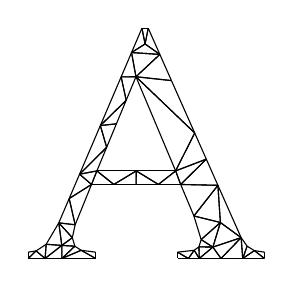
\begin{tikzpicture}[scale=5]
\draw (0.2,-0.7924) -- (0.22,-0.7732);
\draw (0.22,-0.7732) -- (0.2,-0.7764);
\draw (0.2,-0.7764) -- (0.2,-0.7924);
\draw (0.28531162790697684,-0.7592558139534884) -- (0.2428,-0.7924);
\draw (0.2428,-0.7924) -- (0.28559999999999997,-0.7924);
\draw (0.28559999999999997,-0.7924) -- (0.28531162790697684,-0.7592558139534884);
\draw (0.4736,-0.3308) -- (0.5343,-0.2741);
\draw (0.5343,-0.2741) -- (0.46240000000000003,-0.2694);
\draw (0.46240000000000003,-0.2694) -- (0.4736,-0.3308);
\draw (0.4174,-0.6044) -- (0.47400000000000003,-0.6044);
\draw (0.47400000000000003,-0.6044) -- (0.47440000000000004,-0.57);
\draw (0.47440000000000004,-0.57) -- (0.4174,-0.6044);
\draw (0.3712,-0.7924) -- (0.3712,-0.7764);
\draw (0.3712,-0.7764) -- (0.3344,-0.7716);
\draw (0.3344,-0.7716) -- (0.3712,-0.7924);
\draw (0.6216,-0.7716) -- (0.6068,-0.7924);
\draw (0.6068,-0.7924) -- (0.6344000000000001,-0.7924);
\draw (0.6344000000000001,-0.7924) -- (0.6216,-0.7716);
\draw (0.436,-0.3312) -- (0.44880000000000003,-0.39059999999999995);
\draw (0.44880000000000003,-0.39059999999999995) -- (0.4736,-0.3308);
\draw (0.4736,-0.3308) -- (0.436,-0.3312);
\draw (0.3184,-0.7612) -- (0.312,-0.7396);
\draw (0.312,-0.7396) -- (0.28531162790697684,-0.7592558139534884);
\draw (0.28531162790697684,-0.7592558139534884) -- (0.3184,-0.7612);
\draw (0.28559999999999997,-0.7924) -- (0.3344,-0.7716);
\draw (0.3344,-0.7716) -- (0.3184,-0.7612);
\draw (0.3184,-0.7612) -- (0.28559999999999997,-0.7924);
\draw (0.3712,-0.7924) -- (0.3344,-0.7716);
\draw (0.3344,-0.7716) -- (0.28559999999999997,-0.7924);
\draw (0.28559999999999997,-0.7924) -- (0.3712,-0.7924);
\draw (0.3744,-0.57) -- (0.3608,-0.6044);
\draw (0.3608,-0.6044) -- (0.4174,-0.6044);
\draw (0.4174,-0.6044) -- (0.3744,-0.57);
\draw (0.2456,-0.7564) -- (0.22,-0.7732);
\draw (0.22,-0.7732) -- (0.2428,-0.7924);
\draw (0.2428,-0.7924) -- (0.2456,-0.7564);
\draw (0.28531162790697684,-0.7592558139534884) -- (0.2776,-0.702);
\draw (0.2776,-0.702) -- (0.2456,-0.7564);
\draw (0.2456,-0.7564) -- (0.28531162790697684,-0.7592558139534884);
\draw (0.28559999999999997,-0.7924) -- (0.3184,-0.7612);
\draw (0.3184,-0.7612) -- (0.28531162790697684,-0.7592558139534884);
\draw (0.28531162790697684,-0.7592558139534884) -- (0.28559999999999997,-0.7924);
\draw (0.2776,-0.702) -- (0.312,-0.7396);
\draw (0.312,-0.7396) -- (0.3192,-0.7068);
\draw (0.3192,-0.7068) -- (0.2776,-0.702);
\draw (0.3192,-0.7068) -- (0.304,-0.6402);
\draw (0.304,-0.6402) -- (0.2776,-0.702);
\draw (0.2776,-0.702) -- (0.3192,-0.7068);
\draw (0.3744,-0.57) -- (0.33039999999999997,-0.5784);
\draw (0.33039999999999997,-0.5784) -- (0.3608,-0.6044);
\draw (0.3608,-0.6044) -- (0.3744,-0.57);
\draw (0.6208,-0.6844) -- (0.6818,-0.6066);
\draw (0.6818,-0.6066) -- (0.5872,-0.6044);
\draw (0.5872,-0.6044) -- (0.6208,-0.6844);
\draw (0.3992,-0.5102) -- (0.33039999999999997,-0.5784);
\draw (0.33039999999999997,-0.5784) -- (0.3744,-0.57);
\draw (0.3744,-0.57) -- (0.3992,-0.5102);
\draw (0.5306000000000001,-0.6044) -- (0.5872,-0.6044);
\draw (0.5872,-0.6044) -- (0.5744,-0.57);
\draw (0.5744,-0.57) -- (0.5306000000000001,-0.6044);
\draw (0.304,-0.6402) -- (0.3192,-0.7068);
\draw (0.3192,-0.7068) -- (0.3608,-0.6044);
\draw (0.3608,-0.6044) -- (0.304,-0.6402);
\draw (0.2776,-0.702) -- (0.28531162790697684,-0.7592558139534884);
\draw (0.28531162790697684,-0.7592558139534884) -- (0.312,-0.7396);
\draw (0.312,-0.7396) -- (0.2776,-0.702);
\draw (0.6880643863623271,-0.7010295113359224) -- (0.6690356340288925,-0.7635325842696628);
\draw (0.6690356340288925,-0.7635325842696628) -- (0.7408,-0.7396);
\draw (0.7408,-0.7396) -- (0.6880643863623271,-0.7010295113359224);
\draw (0.22,-0.7732) -- (0.2,-0.7924);
\draw (0.2,-0.7924) -- (0.2428,-0.7924);
\draw (0.2428,-0.7924) -- (0.22,-0.7732);
\draw (0.44880000000000003,-0.39059999999999995) -- (0.3832,-0.4548);
\draw (0.3832,-0.4548) -- (0.42400000000000004,-0.45039999999999997);
\draw (0.42400000000000004,-0.45039999999999997) -- (0.44880000000000003,-0.39059999999999995);
\draw (0.6068,-0.7924) -- (0.5792,-0.7764);
\draw (0.5792,-0.7764) -- (0.5792,-0.7924);
\draw (0.5792,-0.7924) -- (0.6068,-0.7924);
\draw (0.7448,-0.7924) -- (0.8,-0.7924);
\draw (0.8,-0.7924) -- (0.7744,-0.7724);
\draw (0.7744,-0.7724) -- (0.7448,-0.7924);
\draw (0.3832,-0.4548) -- (0.3992,-0.5102);
\draw (0.3992,-0.5102) -- (0.42400000000000004,-0.45039999999999997);
\draw (0.42400000000000004,-0.45039999999999997) -- (0.3832,-0.4548);
\draw (0.4736,-0.3308) -- (0.6228,-0.4736);
\draw (0.6228,-0.4736) -- (0.5638000000000001,-0.3406);
\draw (0.5638000000000001,-0.3406) -- (0.4736,-0.3308);
\draw (0.8,-0.7924) -- (0.8,-0.7764);
\draw (0.8,-0.7764) -- (0.7744,-0.7724);
\draw (0.7744,-0.7724) -- (0.8,-0.7924);
\draw (0.6523,-0.5401) -- (0.6228,-0.4736);
\draw (0.6228,-0.4736) -- (0.5744,-0.57);
\draw (0.5744,-0.57) -- (0.6523,-0.5401);
\draw (0.7408,-0.7396) -- (0.6896,-0.7924);
\draw (0.6896,-0.7924) -- (0.7448,-0.7924);
\draw (0.7448,-0.7924) -- (0.7408,-0.7396);
\draw (0.6216,-0.7716) -- (0.6344000000000001,-0.7924);
\draw (0.6344000000000001,-0.7924) -- (0.6336,-0.7628);
\draw (0.6336,-0.7628) -- (0.6216,-0.7716);
\draw (0.756,-0.7612) -- (0.7448,-0.7924);
\draw (0.7448,-0.7924) -- (0.7744,-0.7724);
\draw (0.7744,-0.7724) -- (0.756,-0.7612);
\draw (0.756,-0.7612) -- (0.7408,-0.7396);
\draw (0.7408,-0.7396) -- (0.7448,-0.7924);
\draw (0.7448,-0.7924) -- (0.756,-0.7612);
\draw (0.5872,-0.6044) -- (0.6523,-0.5401);
\draw (0.6523,-0.5401) -- (0.5744,-0.57);
\draw (0.5744,-0.57) -- (0.5872,-0.6044);
\draw (0.6896,-0.7924) -- (0.6690356340288925,-0.7635325842696628);
\draw (0.6690356340288925,-0.7635325842696628) -- (0.6344000000000001,-0.7924);
\draw (0.6344000000000001,-0.7924) -- (0.6896,-0.7924);
\draw (0.5343,-0.2741) -- (0.4736,-0.3308);
\draw (0.4736,-0.3308) -- (0.5638000000000001,-0.3406);
\draw (0.5638000000000001,-0.3406) -- (0.5343,-0.2741);
\draw (0.47440000000000004,-0.57) -- (0.3744,-0.57);
\draw (0.3744,-0.57) -- (0.4174,-0.6044);
\draw (0.4174,-0.6044) -- (0.47440000000000004,-0.57);
\draw (0.7408,-0.7396) -- (0.6818,-0.6066);
\draw (0.6818,-0.6066) -- (0.6880643863623271,-0.7010295113359224);
\draw (0.6880643863623271,-0.7010295113359224) -- (0.7408,-0.7396);
\draw (0.4736,-0.3308) -- (0.46240000000000003,-0.2694);
\draw (0.46240000000000003,-0.2694) -- (0.436,-0.3312);
\draw (0.436,-0.3312) -- (0.4736,-0.3308);
\draw (0.5872,-0.6044) -- (0.6818,-0.6066);
\draw (0.6818,-0.6066) -- (0.6523,-0.5401);
\draw (0.6523,-0.5401) -- (0.5872,-0.6044);
\draw (0.5744,-0.57) -- (0.6228,-0.4736);
\draw (0.6228,-0.4736) -- (0.4736,-0.3308);
\draw (0.4736,-0.3308) -- (0.5744,-0.57);
\draw (0.6336,-0.7628) -- (0.6344000000000001,-0.7924);
\draw (0.6344000000000001,-0.7924) -- (0.6690356340288925,-0.7635325842696628);
\draw (0.6690356340288925,-0.7635325842696628) -- (0.6336,-0.7628);
\draw (0.6690356340288925,-0.7635325842696628) -- (0.6392,-0.7444);
\draw (0.6392,-0.7444) -- (0.6336,-0.7628);
\draw (0.6336,-0.7628) -- (0.6690356340288925,-0.7635325842696628);
\draw (0.6880643863623271,-0.7010295113359224) -- (0.6208,-0.6844);
\draw (0.6208,-0.6844) -- (0.6392,-0.7444);
\draw (0.6392,-0.7444) -- (0.6880643863623271,-0.7010295113359224);
\draw (0.6392,-0.7444) -- (0.6690356340288925,-0.7635325842696628);
\draw (0.6690356340288925,-0.7635325842696628) -- (0.6880643863623271,-0.7010295113359224);
\draw (0.6880643863623271,-0.7010295113359224) -- (0.6392,-0.7444);
\draw (0.5792,-0.7764) -- (0.6068,-0.7924);
\draw (0.6068,-0.7924) -- (0.6216,-0.7716);
\draw (0.6216,-0.7716) -- (0.5792,-0.7764);
\draw (0.4968,-0.24755631067961165) -- (0.4888,-0.2076);
\draw (0.4888,-0.2076) -- (0.46240000000000003,-0.2694);
\draw (0.46240000000000003,-0.2694) -- (0.4968,-0.24755631067961165);
\draw (0.46240000000000003,-0.2694) -- (0.5343,-0.2741);
\draw (0.5343,-0.2741) -- (0.4968,-0.24755631067961165);
\draw (0.4968,-0.24755631067961165) -- (0.46240000000000003,-0.2694);
\draw (0.2428,-0.7924) -- (0.28531162790697684,-0.7592558139534884);
\draw (0.28531162790697684,-0.7592558139534884) -- (0.2456,-0.7564);
\draw (0.2456,-0.7564) -- (0.2428,-0.7924);
\draw (0.6818,-0.6066) -- (0.6208,-0.6844);
\draw (0.6208,-0.6844) -- (0.6880643863623271,-0.7010295113359224);
\draw (0.6880643863623271,-0.7010295113359224) -- (0.6818,-0.6066);
\draw (0.6896,-0.7924) -- (0.7408,-0.7396);
\draw (0.7408,-0.7396) -- (0.6690356340288925,-0.7635325842696628);
\draw (0.6690356340288925,-0.7635325842696628) -- (0.6896,-0.7924);
\draw (0.47440000000000004,-0.57) -- (0.5306000000000001,-0.6044);
\draw (0.5306000000000001,-0.6044) -- (0.5744,-0.57);
\draw (0.5744,-0.57) -- (0.47440000000000004,-0.57);
\draw (0.5306000000000001,-0.6044) -- (0.47440000000000004,-0.57);
\draw (0.47440000000000004,-0.57) -- (0.47400000000000003,-0.6044);
\draw (0.47400000000000003,-0.6044) -- (0.5306000000000001,-0.6044);
\draw (0.3832,-0.4548) -- (0.44880000000000003,-0.39059999999999995);
\draw (0.44880000000000003,-0.39059999999999995) -- (0.436,-0.3312);
\draw (0.436,-0.3312) -- (0.3832,-0.4548);
\draw (0.3608,-0.6044) -- (0.33039999999999997,-0.5784);
\draw (0.33039999999999997,-0.5784) -- (0.304,-0.6402);
\draw (0.304,-0.6402) -- (0.3608,-0.6044);
\draw (0.33039999999999997,-0.5784) -- (0.3992,-0.5102);
\draw (0.3992,-0.5102) -- (0.3832,-0.4548);
\draw (0.3832,-0.4548) -- (0.33039999999999997,-0.5784);
\draw (0.5048,-0.2076) -- (0.4888,-0.2076);
\draw (0.4888,-0.2076) -- (0.4968,-0.24755631067961165);
\draw (0.4968,-0.24755631067961165) -- (0.5048,-0.2076);
\draw (0.5343,-0.2741) -- (0.5048,-0.2076);
\draw (0.5048,-0.2076) -- (0.4968,-0.24755631067961165);
\draw (0.4968,-0.24755631067961165) -- (0.5343,-0.2741);
\end{tikzpicture}

         (a)
       \end{center}
     \end{minipage}
     \begin{minipage}{0.4\textwidth}
       \begin{center}
         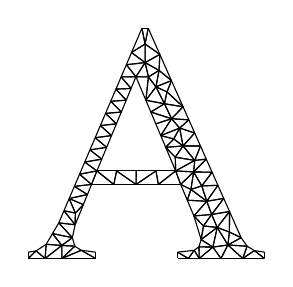
\begin{tikzpicture}[scale=5]
\draw (0.2,-0.7924) -- (0.22,-0.7732);
\draw (0.22,-0.7732) -- (0.2,-0.7764);
\draw (0.2,-0.7764) -- (0.2,-0.7924);
\draw (0.28531162790697684,-0.7592558139534884) -- (0.2428,-0.7924);
\draw (0.2428,-0.7924) -- (0.28559999999999997,-0.7924);
\draw (0.28559999999999997,-0.7924) -- (0.28531162790697684,-0.7592558139534884);
\draw (0.4968406949074053,-0.2948391566292681) -- (0.46240000000000003,-0.2694);
\draw (0.46240000000000003,-0.2694) -- (0.4492,-0.3003);
\draw (0.4492,-0.3003) -- (0.4968406949074053,-0.2948391566292681);
\draw (0.47400000000000003,-0.6044) -- (0.47440000000000004,-0.57);
\draw (0.47440000000000004,-0.57) -- (0.4244,-0.57);
\draw (0.4244,-0.57) -- (0.47400000000000003,-0.6044);
\draw (0.3712,-0.7924) -- (0.3712,-0.7764);
\draw (0.3712,-0.7764) -- (0.3344,-0.7716);
\draw (0.3344,-0.7716) -- (0.3712,-0.7924);
\draw (0.6216,-0.7716) -- (0.6068,-0.7924);
\draw (0.6068,-0.7924) -- (0.6344000000000001,-0.7924);
\draw (0.6344000000000001,-0.7924) -- (0.6216,-0.7716);
\draw (0.436,-0.3312) -- (0.46120000000000005,-0.36069999999999997);
\draw (0.46120000000000005,-0.36069999999999997) -- (0.4736,-0.3308);
\draw (0.4736,-0.3308) -- (0.436,-0.3312);
\draw (0.3184,-0.7612) -- (0.312,-0.7396);
\draw (0.312,-0.7396) -- (0.28531162790697684,-0.7592558139534884);
\draw (0.28531162790697684,-0.7592558139534884) -- (0.3184,-0.7612);
\draw (0.28559999999999997,-0.7924) -- (0.3344,-0.7716);
\draw (0.3344,-0.7716) -- (0.3184,-0.7612);
\draw (0.3184,-0.7612) -- (0.28559999999999997,-0.7924);
\draw (0.3712,-0.7924) -- (0.3344,-0.7716);
\draw (0.3344,-0.7716) -- (0.28559999999999997,-0.7924);
\draw (0.28559999999999997,-0.7924) -- (0.3712,-0.7924);
\draw (0.3744,-0.57) -- (0.3608,-0.6044);
\draw (0.3608,-0.6044) -- (0.4174,-0.6044);
\draw (0.4174,-0.6044) -- (0.3744,-0.57);
\draw (0.2456,-0.7564) -- (0.22,-0.7732);
\draw (0.22,-0.7732) -- (0.2428,-0.7924);
\draw (0.2428,-0.7924) -- (0.2456,-0.7564);
\draw (0.28531162790697684,-0.7592558139534884) -- (0.2616,-0.7292);
\draw (0.2616,-0.7292) -- (0.2456,-0.7564);
\draw (0.2456,-0.7564) -- (0.28531162790697684,-0.7592558139534884);
\draw (0.28559999999999997,-0.7924) -- (0.3184,-0.7612);
\draw (0.3184,-0.7612) -- (0.28531162790697684,-0.7592558139534884);
\draw (0.28531162790697684,-0.7592558139534884) -- (0.28559999999999997,-0.7924);
\draw (0.2776,-0.702) -- (0.312,-0.7396);
\draw (0.312,-0.7396) -- (0.3192,-0.7068);
\draw (0.3192,-0.7068) -- (0.2776,-0.702);
\draw (0.3192,-0.7068) -- (0.2908,-0.6711);
\draw (0.2908,-0.6711) -- (0.2776,-0.702);
\draw (0.2776,-0.702) -- (0.3192,-0.7068);
\draw (0.3744,-0.57) -- (0.33039999999999997,-0.5784);
\draw (0.33039999999999997,-0.5784) -- (0.3608,-0.6044);
\draw (0.3608,-0.6044) -- (0.3744,-0.57);
\draw (0.6208,-0.6844) -- (0.6450980210406373,-0.7097699402142046);
\draw (0.6450980210406373,-0.7097699402142046) -- (0.6659339941556301,-0.6806873886526693);
\draw (0.6659339941556301,-0.6806873886526693) -- (0.6208,-0.6844);
\draw (0.6392,-0.7444) -- (0.6800202045062519,-0.713573727137458);
\draw (0.6800202045062519,-0.713573727137458) -- (0.6450980210406373,-0.7097699402142046);
\draw (0.6450980210406373,-0.7097699402142046) -- (0.6392,-0.7444);
\draw (0.3568,-0.5166) -- (0.3868,-0.5401);
\draw (0.3868,-0.5401) -- (0.3992,-0.5102);
\draw (0.3992,-0.5102) -- (0.3568,-0.5166);
\draw (0.5306000000000001,-0.6044) -- (0.5872,-0.6044);
\draw (0.5872,-0.6044) -- (0.5744,-0.57);
\draw (0.5744,-0.57) -- (0.5306000000000001,-0.6044);
\draw (0.35040000000000004,-0.63) -- (0.3608,-0.6044);
\draw (0.3608,-0.6044) -- (0.3172,-0.6093);
\draw (0.3172,-0.6093) -- (0.35040000000000004,-0.63);
\draw (0.2616,-0.7292) -- (0.312,-0.7396);
\draw (0.312,-0.7396) -- (0.2776,-0.702);
\draw (0.2776,-0.702) -- (0.2616,-0.7292);
\draw (0.7109619922876913,-0.7252980211896037) -- (0.6800202045062519,-0.713573727137458);
\draw (0.6800202045062519,-0.713573727137458) -- (0.7071175748135642,-0.7581624967889107);
\draw (0.7071175748135642,-0.7581624967889107) -- (0.7109619922876913,-0.7252980211896037);
\draw (0.22,-0.7732) -- (0.2,-0.7924);
\draw (0.2,-0.7924) -- (0.2428,-0.7924);
\draw (0.2428,-0.7924) -- (0.22,-0.7732);
\draw (0.40959999999999996,-0.393) -- (0.4364,-0.4205);
\draw (0.4364,-0.4205) -- (0.44880000000000003,-0.39059999999999995);
\draw (0.44880000000000003,-0.39059999999999995) -- (0.40959999999999996,-0.393);
\draw (0.6068,-0.7924) -- (0.5792,-0.7764);
\draw (0.5792,-0.7764) -- (0.5792,-0.7924);
\draw (0.5792,-0.7924) -- (0.6068,-0.7924);
\draw (0.7448,-0.7924) -- (0.8,-0.7924);
\draw (0.8,-0.7924) -- (0.7744,-0.7724);
\draw (0.7744,-0.7724) -- (0.7448,-0.7924);
\draw (0.3832,-0.4548) -- (0.4116,-0.48029999999999995);
\draw (0.4116,-0.48029999999999995) -- (0.42400000000000004,-0.45039999999999997);
\draw (0.42400000000000004,-0.45039999999999997) -- (0.3832,-0.4548);
\draw (0.4988,-0.39059999999999995) -- (0.5243486723508081,-0.35656327405605037);
\draw (0.5243486723508081,-0.35656327405605037) -- (0.5052838872910572,-0.3312530403538474);
\draw (0.5052838872910572,-0.3312530403538474) -- (0.4988,-0.39059999999999995);
\draw (0.8,-0.7924) -- (0.8,-0.7764);
\draw (0.8,-0.7764) -- (0.7744,-0.7724);
\draw (0.7744,-0.7724) -- (0.8,-0.7924);
\draw (0.6230341784523656,-0.5432932398665247) -- (0.6200800579922154,-0.5725841644680129);
\draw (0.6200800579922154,-0.5725841644680129) -- (0.6523,-0.5401);
\draw (0.6523,-0.5401) -- (0.6230341784523656,-0.5432932398665247);
\draw (0.7448,-0.7924) -- (0.756,-0.7612);
\draw (0.756,-0.7612) -- (0.7071175748135642,-0.7581624967889107);
\draw (0.7071175748135642,-0.7581624967889107) -- (0.7448,-0.7924);
\draw (0.6216,-0.7716) -- (0.6344000000000001,-0.7924);
\draw (0.6344000000000001,-0.7924) -- (0.6336,-0.7628);
\draw (0.6336,-0.7628) -- (0.6216,-0.7716);
\draw (0.756,-0.7612) -- (0.7448,-0.7924);
\draw (0.7448,-0.7924) -- (0.7744,-0.7724);
\draw (0.7744,-0.7724) -- (0.756,-0.7612);
\draw (0.7408,-0.7396) -- (0.7071175748135642,-0.7581624967889107);
\draw (0.7071175748135642,-0.7581624967889107) -- (0.756,-0.7612);
\draw (0.756,-0.7612) -- (0.7408,-0.7396);
\draw (0.6040000000000001,-0.6444000000000001) -- (0.6132307947128575,-0.6169950662206);
\draw (0.6132307947128575,-0.6169950662206) -- (0.5872,-0.6044);
\draw (0.5872,-0.6044) -- (0.6040000000000001,-0.6444000000000001);
\draw (0.6896,-0.7924) -- (0.6690356340288925,-0.7635325842696628);
\draw (0.6690356340288925,-0.7635325842696628) -- (0.6344000000000001,-0.7924);
\draw (0.6344000000000001,-0.7924) -- (0.6896,-0.7924);
\draw (0.4736,-0.3308) -- (0.4968406949074053,-0.2948391566292681);
\draw (0.4968406949074053,-0.2948391566292681) -- (0.4492,-0.3003);
\draw (0.4492,-0.3003) -- (0.4736,-0.3308);
\draw (0.4244,-0.57) -- (0.3744,-0.57);
\draw (0.3744,-0.57) -- (0.4174,-0.6044);
\draw (0.4174,-0.6044) -- (0.4244,-0.57);
\draw (0.7448,-0.7924) -- (0.7071175748135642,-0.7581624967889107);
\draw (0.7071175748135642,-0.7581624967889107) -- (0.6896,-0.7924);
\draw (0.6896,-0.7924) -- (0.7448,-0.7924);
\draw (0.4736,-0.3308) -- (0.4492,-0.3003);
\draw (0.4492,-0.3003) -- (0.436,-0.3312);
\draw (0.436,-0.3312) -- (0.4736,-0.3308);
\draw (0.569647737619492,-0.4888497610108732) -- (0.5366,-0.48029999999999995);
\draw (0.5366,-0.48029999999999995) -- (0.5492,-0.5102);
\draw (0.5492,-0.5102) -- (0.569647737619492,-0.4888497610108732);
\draw (0.5744,-0.57) -- (0.5872,-0.6044);
\draw (0.5872,-0.6044) -- (0.6200800579922154,-0.5725841644680129);
\draw (0.6200800579922154,-0.5725841644680129) -- (0.5744,-0.57);
\draw (0.6336,-0.7628) -- (0.6344000000000001,-0.7924);
\draw (0.6344000000000001,-0.7924) -- (0.6690356340288925,-0.7635325842696628);
\draw (0.6690356340288925,-0.7635325842696628) -- (0.6336,-0.7628);
\draw (0.6690356340288925,-0.7635325842696628) -- (0.6392,-0.7444);
\draw (0.6392,-0.7444) -- (0.6336,-0.7628);
\draw (0.6336,-0.7628) -- (0.6690356340288925,-0.7635325842696628);
\draw (0.6800202045062519,-0.713573727137458) -- (0.6392,-0.7444);
\draw (0.6392,-0.7444) -- (0.6690356340288925,-0.7635325842696628);
\draw (0.6690356340288925,-0.7635325842696628) -- (0.6800202045062519,-0.713573727137458);
\draw (0.7408,-0.7396) -- (0.7109619922876913,-0.7252980211896037);
\draw (0.7109619922876913,-0.7252980211896037) -- (0.7071175748135642,-0.7581624967889107);
\draw (0.7071175748135642,-0.7581624967889107) -- (0.7408,-0.7396);
\draw (0.5792,-0.7764) -- (0.6068,-0.7924);
\draw (0.6068,-0.7924) -- (0.6216,-0.7716);
\draw (0.6216,-0.7716) -- (0.5792,-0.7764);
\draw (0.4968,-0.24755631067961165) -- (0.4888,-0.2076);
\draw (0.4888,-0.2076) -- (0.46240000000000003,-0.2694);
\draw (0.46240000000000003,-0.2694) -- (0.4968,-0.24755631067961165);
\draw (0.5343,-0.2741) -- (0.5048,-0.2076);
\draw (0.5048,-0.2076) -- (0.4968,-0.24755631067961165);
\draw (0.4968,-0.24755631067961165) -- (0.5343,-0.2741);
\draw (0.2428,-0.7924) -- (0.28531162790697684,-0.7592558139534884);
\draw (0.28531162790697684,-0.7592558139534884) -- (0.2456,-0.7564);
\draw (0.2456,-0.7564) -- (0.2428,-0.7924);
\draw (0.4228,-0.3621) -- (0.44880000000000003,-0.39059999999999995);
\draw (0.44880000000000003,-0.39059999999999995) -- (0.46120000000000005,-0.36069999999999997);
\draw (0.46120000000000005,-0.36069999999999997) -- (0.4228,-0.3621);
\draw (0.6896,-0.7924) -- (0.7071175748135642,-0.7581624967889107);
\draw (0.7071175748135642,-0.7581624967889107) -- (0.6690356340288925,-0.7635325842696628);
\draw (0.6690356340288925,-0.7635325842696628) -- (0.6896,-0.7924);
\draw (0.47400000000000003,-0.6044) -- (0.5244,-0.57);
\draw (0.5244,-0.57) -- (0.47440000000000004,-0.57);
\draw (0.47440000000000004,-0.57) -- (0.47400000000000003,-0.6044);
\draw (0.5244,-0.57) -- (0.47400000000000003,-0.6044);
\draw (0.47400000000000003,-0.6044) -- (0.5306000000000001,-0.6044);
\draw (0.5306000000000001,-0.6044) -- (0.5244,-0.57);
\draw (0.7071175748135642,-0.7581624967889107) -- (0.6800202045062519,-0.713573727137458);
\draw (0.6800202045062519,-0.713573727137458) -- (0.6690356340288925,-0.7635325842696628);
\draw (0.6690356340288925,-0.7635325842696628) -- (0.7071175748135642,-0.7581624967889107);
\draw (0.6534277979418421,-0.6471683248644264) -- (0.6818,-0.6066);
\draw (0.6818,-0.6066) -- (0.6407440135537374,-0.6080922152447567);
\draw (0.6407440135537374,-0.6080922152447567) -- (0.6534277979418421,-0.6471683248644264);
\draw (0.6523,-0.5401) -- (0.6200800579922154,-0.5725841644680129);
\draw (0.6200800579922154,-0.5725841644680129) -- (0.6670499999999999,-0.57335);
\draw (0.6670499999999999,-0.57335) -- (0.6523,-0.5401);
\draw (0.69655,-0.63985) -- (0.6818,-0.6066);
\draw (0.6818,-0.6066) -- (0.6534277979418421,-0.6471683248644264);
\draw (0.6534277979418421,-0.6471683248644264) -- (0.69655,-0.63985);
\draw (0.6208,-0.6844) -- (0.6534277979418421,-0.6471683248644264);
\draw (0.6534277979418421,-0.6471683248644264) -- (0.6040000000000001,-0.6444000000000001);
\draw (0.6040000000000001,-0.6444000000000001) -- (0.6208,-0.6844);
\draw (0.6208,-0.6844) -- (0.6392,-0.7444);
\draw (0.6392,-0.7444) -- (0.6450980210406373,-0.7097699402142046);
\draw (0.6450980210406373,-0.7097699402142046) -- (0.6208,-0.6844);
\draw (0.3992,-0.5102) -- (0.37,-0.48569999999999997);
\draw (0.37,-0.48569999999999997) -- (0.3568,-0.5166);
\draw (0.3568,-0.5166) -- (0.3992,-0.5102);
\draw (0.6200800579922154,-0.5725841644680129) -- (0.6230341784523656,-0.5432932398665247);
\draw (0.6230341784523656,-0.5432932398665247) -- (0.5744,-0.57);
\draw (0.5744,-0.57) -- (0.6200800579922154,-0.5725841644680129);
\draw (0.42400000000000004,-0.45039999999999997) -- (0.3964,-0.4239);
\draw (0.3964,-0.4239) -- (0.3832,-0.4548);
\draw (0.3832,-0.4548) -- (0.42400000000000004,-0.45039999999999997);
\draw (0.304,-0.6402) -- (0.34,-0.6556);
\draw (0.34,-0.6556) -- (0.35040000000000004,-0.63);
\draw (0.35040000000000004,-0.63) -- (0.304,-0.6402);
\draw (0.3744,-0.57) -- (0.3436,-0.5475);
\draw (0.3436,-0.5475) -- (0.33039999999999997,-0.5784);
\draw (0.33039999999999997,-0.5784) -- (0.3744,-0.57);
\draw (0.5048,-0.2076) -- (0.4888,-0.2076);
\draw (0.4888,-0.2076) -- (0.4968,-0.24755631067961165);
\draw (0.4968,-0.24755631067961165) -- (0.5048,-0.2076);
\draw (0.6407440135537374,-0.6080922152447567) -- (0.6132307947128575,-0.6169950662206);
\draw (0.6132307947128575,-0.6169950662206) -- (0.6534277979418421,-0.6471683248644264);
\draw (0.6534277979418421,-0.6471683248644264) -- (0.6407440135537374,-0.6080922152447567);
\draw (0.312,-0.7396) -- (0.2616,-0.7292);
\draw (0.2616,-0.7292) -- (0.28531162790697684,-0.7592558139534884);
\draw (0.28531162790697684,-0.7592558139534884) -- (0.312,-0.7396);
\draw (0.69655,-0.63985) -- (0.6659339941556301,-0.6806873886526693);
\draw (0.6659339941556301,-0.6806873886526693) -- (0.7113,-0.6731);
\draw (0.7113,-0.6731) -- (0.69655,-0.63985);
\draw (0.44880000000000003,-0.39059999999999995) -- (0.4228,-0.3621);
\draw (0.4228,-0.3621) -- (0.40959999999999996,-0.393);
\draw (0.40959999999999996,-0.393) -- (0.44880000000000003,-0.39059999999999995);
\draw (0.4968406949074053,-0.2948391566292681) -- (0.4968,-0.24755631067961165);
\draw (0.4968,-0.24755631067961165) -- (0.46240000000000003,-0.2694);
\draw (0.46240000000000003,-0.2694) -- (0.4968406949074053,-0.2948391566292681);
\draw (0.31976470245465805,-0.6772044103722048) -- (0.2908,-0.6711);
\draw (0.2908,-0.6711) -- (0.3192,-0.7068);
\draw (0.3192,-0.7068) -- (0.31976470245465805,-0.6772044103722048);
\draw (0.3608,-0.6044) -- (0.33039999999999997,-0.5784);
\draw (0.33039999999999997,-0.5784) -- (0.3172,-0.6093);
\draw (0.3172,-0.6093) -- (0.3608,-0.6044);
\draw (0.37,-0.48569999999999997) -- (0.4116,-0.48029999999999995);
\draw (0.4116,-0.48029999999999995) -- (0.3832,-0.4548);
\draw (0.3832,-0.4548) -- (0.37,-0.48569999999999997);
\draw (0.4968406949074053,-0.2948391566292681) -- (0.5052838872910572,-0.3312530403538474);
\draw (0.5052838872910572,-0.3312530403538474) -- (0.5323415946360741,-0.3147619993719672);
\draw (0.5323415946360741,-0.3147619993719672) -- (0.4968406949074053,-0.2948391566292681);
\draw (0.7408,-0.7396) -- (0.7113,-0.6731);
\draw (0.7113,-0.6731) -- (0.7109619922876913,-0.7252980211896037);
\draw (0.7109619922876913,-0.7252980211896037) -- (0.7408,-0.7396);
\draw (0.7113,-0.6731) -- (0.6800202045062519,-0.713573727137458);
\draw (0.6800202045062519,-0.713573727137458) -- (0.7109619922876913,-0.7252980211896037);
\draw (0.7109619922876913,-0.7252980211896037) -- (0.7113,-0.6731);
\draw (0.4116,-0.48029999999999995) -- (0.37,-0.48569999999999997);
\draw (0.37,-0.48569999999999997) -- (0.3992,-0.5102);
\draw (0.3992,-0.5102) -- (0.4116,-0.48029999999999995);
\draw (0.4364,-0.4205) -- (0.3964,-0.4239);
\draw (0.3964,-0.4239) -- (0.42400000000000004,-0.45039999999999997);
\draw (0.42400000000000004,-0.45039999999999997) -- (0.4364,-0.4205);
\draw (0.3964,-0.4239) -- (0.4364,-0.4205);
\draw (0.4364,-0.4205) -- (0.40959999999999996,-0.393);
\draw (0.40959999999999996,-0.393) -- (0.3964,-0.4239);
\draw (0.46120000000000005,-0.36069999999999997) -- (0.436,-0.3312);
\draw (0.436,-0.3312) -- (0.4228,-0.3621);
\draw (0.4228,-0.3621) -- (0.46120000000000005,-0.36069999999999997);
\draw (0.3436,-0.5475) -- (0.3868,-0.5401);
\draw (0.3868,-0.5401) -- (0.3568,-0.5166);
\draw (0.3568,-0.5166) -- (0.3436,-0.5475);
\draw (0.6659339941556301,-0.6806873886526693) -- (0.6450980210406373,-0.7097699402142046);
\draw (0.6450980210406373,-0.7097699402142046) -- (0.6800202045062519,-0.713573727137458);
\draw (0.6800202045062519,-0.713573727137458) -- (0.6659339941556301,-0.6806873886526693);
\draw (0.7113,-0.6731) -- (0.6659339941556301,-0.6806873886526693);
\draw (0.6659339941556301,-0.6806873886526693) -- (0.6800202045062519,-0.713573727137458);
\draw (0.6800202045062519,-0.713573727137458) -- (0.7113,-0.6731);
\draw (0.6208,-0.6844) -- (0.6659339941556301,-0.6806873886526693);
\draw (0.6659339941556301,-0.6806873886526693) -- (0.6534277979418421,-0.6471683248644264);
\draw (0.6534277979418421,-0.6471683248644264) -- (0.6208,-0.6844);
\draw (0.6230341784523656,-0.5432932398665247) -- (0.6523,-0.5401);
\draw (0.6523,-0.5401) -- (0.6375500000000001,-0.50685);
\draw (0.6375500000000001,-0.50685) -- (0.6230341784523656,-0.5432932398665247);
\draw (0.5933013449724645,-0.5065824860648467) -- (0.6230341784523656,-0.5432932398665247);
\draw (0.6230341784523656,-0.5432932398665247) -- (0.6375500000000001,-0.50685);
\draw (0.6375500000000001,-0.50685) -- (0.5933013449724645,-0.5065824860648467);
\draw (0.6670499999999999,-0.57335) -- (0.6407440135537374,-0.6080922152447567);
\draw (0.6407440135537374,-0.6080922152447567) -- (0.6818,-0.6066);
\draw (0.6818,-0.6066) -- (0.6670499999999999,-0.57335);
\draw (0.6407440135537374,-0.6080922152447567) -- (0.6670499999999999,-0.57335);
\draw (0.6670499999999999,-0.57335) -- (0.6200800579922154,-0.5725841644680129);
\draw (0.6200800579922154,-0.5725841644680129) -- (0.6407440135537374,-0.6080922152447567);
\draw (0.6200800579922154,-0.5725841644680129) -- (0.5872,-0.6044);
\draw (0.5872,-0.6044) -- (0.6132307947128575,-0.6169950662206);
\draw (0.6132307947128575,-0.6169950662206) -- (0.6200800579922154,-0.5725841644680129);
\draw (0.6534277979418421,-0.6471683248644264) -- (0.6132307947128575,-0.6169950662206);
\draw (0.6132307947128575,-0.6169950662206) -- (0.6040000000000001,-0.6444000000000001);
\draw (0.6040000000000001,-0.6444000000000001) -- (0.6534277979418421,-0.6471683248644264);
\draw (0.6200800579922154,-0.5725841644680129) -- (0.6132307947128575,-0.6169950662206);
\draw (0.6132307947128575,-0.6169950662206) -- (0.6407440135537374,-0.6080922152447567);
\draw (0.6407440135537374,-0.6080922152447567) -- (0.6200800579922154,-0.5725841644680129);
\draw (0.4988,-0.39059999999999995) -- (0.5052838872910572,-0.3312530403538474);
\draw (0.5052838872910572,-0.3312530403538474) -- (0.4736,-0.3308);
\draw (0.4736,-0.3308) -- (0.4988,-0.39059999999999995);
\draw (0.6659339941556301,-0.6806873886526693) -- (0.69655,-0.63985);
\draw (0.69655,-0.63985) -- (0.6534277979418421,-0.6471683248644264);
\draw (0.6534277979418421,-0.6471683248644264) -- (0.6659339941556301,-0.6806873886526693);
\draw (0.3868,-0.5401) -- (0.3436,-0.5475);
\draw (0.3436,-0.5475) -- (0.3744,-0.57);
\draw (0.3744,-0.57) -- (0.3868,-0.5401);
\draw (0.5492,-0.5102) -- (0.5933013449724645,-0.5065824860648467);
\draw (0.5933013449724645,-0.5065824860648467) -- (0.569647737619492,-0.4888497610108732);
\draw (0.569647737619492,-0.4888497610108732) -- (0.5492,-0.5102);
\draw (0.5306000000000001,-0.6044) -- (0.5744,-0.57);
\draw (0.5744,-0.57) -- (0.5244,-0.57);
\draw (0.5244,-0.57) -- (0.5306000000000001,-0.6044);
\draw (0.47400000000000003,-0.6044) -- (0.4244,-0.57);
\draw (0.4244,-0.57) -- (0.4174,-0.6044);
\draw (0.4174,-0.6044) -- (0.47400000000000003,-0.6044);
\draw (0.5323415946360741,-0.3147619993719672) -- (0.5243486723508081,-0.35656327405605037);
\draw (0.5243486723508081,-0.35656327405605037) -- (0.5638000000000001,-0.3406);
\draw (0.5638000000000001,-0.3406) -- (0.5323415946360741,-0.3147619993719672);
\draw (0.4968,-0.24755631067961165) -- (0.4968406949074053,-0.2948391566292681);
\draw (0.4968406949074053,-0.2948391566292681) -- (0.5343,-0.2741);
\draw (0.5343,-0.2741) -- (0.4968,-0.24755631067961165);
\draw (0.5933013449724645,-0.5065824860648467) -- (0.573448989039527,-0.5351910614749819);
\draw (0.573448989039527,-0.5351910614749819) -- (0.6230341784523656,-0.5432932398665247);
\draw (0.6230341784523656,-0.5432932398665247) -- (0.5933013449724645,-0.5065824860648467);
\draw (0.4968406949074053,-0.2948391566292681) -- (0.5323415946360741,-0.3147619993719672);
\draw (0.5323415946360741,-0.3147619993719672) -- (0.5343,-0.2741);
\draw (0.5343,-0.2741) -- (0.4968406949074053,-0.2948391566292681);
\draw (0.5052838872910572,-0.3312530403538474) -- (0.4968406949074053,-0.2948391566292681);
\draw (0.4968406949074053,-0.2948391566292681) -- (0.4736,-0.3308);
\draw (0.4736,-0.3308) -- (0.5052838872910572,-0.3312530403538474);
\draw (0.5638000000000001,-0.3406) -- (0.5343,-0.2741);
\draw (0.5343,-0.2741) -- (0.5323415946360741,-0.3147619993719672);
\draw (0.5323415946360741,-0.3147619993719672) -- (0.5638000000000001,-0.3406);
\draw (0.5524391722956792,-0.36925433169918465) -- (0.5933,-0.4071);
\draw (0.5933,-0.4071) -- (0.5638000000000001,-0.3406);
\draw (0.5638000000000001,-0.3406) -- (0.5524391722956792,-0.36925433169918465);
\draw (0.5933,-0.4071) -- (0.5459558667361472,-0.3993891268747936);
\draw (0.5459558667361472,-0.3993891268747936) -- (0.5640629355403338,-0.4374131970657074);
\draw (0.5640629355403338,-0.4374131970657074) -- (0.5933,-0.4071);
\draw (0.5052838872910572,-0.3312530403538474) -- (0.5243486723508081,-0.35656327405605037);
\draw (0.5243486723508081,-0.35656327405605037) -- (0.5323415946360741,-0.3147619993719672);
\draw (0.5323415946360741,-0.3147619993719672) -- (0.5052838872910572,-0.3312530403538474);
\draw (0.5243486723508081,-0.35656327405605037) -- (0.4988,-0.39059999999999995);
\draw (0.4988,-0.39059999999999995) -- (0.5459558667361472,-0.3993891268747936);
\draw (0.5459558667361472,-0.3993891268747936) -- (0.5243486723508081,-0.35656327405605037);
\draw (0.5933013449724645,-0.5065824860648467) -- (0.6375500000000001,-0.50685);
\draw (0.6375500000000001,-0.50685) -- (0.6228,-0.4736);
\draw (0.6228,-0.4736) -- (0.5933013449724645,-0.5065824860648467);
\draw (0.5933013449724645,-0.5065824860648467) -- (0.5492,-0.5102);
\draw (0.5492,-0.5102) -- (0.573448989039527,-0.5351910614749819);
\draw (0.573448989039527,-0.5351910614749819) -- (0.5933013449724645,-0.5065824860648467);
\draw (0.5243486723508081,-0.35656327405605037) -- (0.5524391722956792,-0.36925433169918465);
\draw (0.5524391722956792,-0.36925433169918465) -- (0.5638000000000001,-0.3406);
\draw (0.5638000000000001,-0.3406) -- (0.5243486723508081,-0.35656327405605037);
\draw (0.5492,-0.5102) -- (0.5744,-0.57);
\draw (0.5744,-0.57) -- (0.573448989039527,-0.5351910614749819);
\draw (0.573448989039527,-0.5351910614749819) -- (0.5492,-0.5102);
\draw (0.6230341784523656,-0.5432932398665247) -- (0.573448989039527,-0.5351910614749819);
\draw (0.573448989039527,-0.5351910614749819) -- (0.5744,-0.57);
\draw (0.5744,-0.57) -- (0.6230341784523656,-0.5432932398665247);
\draw (0.584565806304,-0.46120853822437063) -- (0.5933013449724645,-0.5065824860648467);
\draw (0.5933013449724645,-0.5065824860648467) -- (0.6228,-0.4736);
\draw (0.6228,-0.4736) -- (0.584565806304,-0.46120853822437063);
\draw (0.569647737619492,-0.4888497610108732) -- (0.584565806304,-0.46120853822437063);
\draw (0.584565806304,-0.46120853822437063) -- (0.5366,-0.48029999999999995);
\draw (0.5366,-0.48029999999999995) -- (0.569647737619492,-0.4888497610108732);
\draw (0.5640629355403338,-0.4374131970657074) -- (0.60805,-0.44035);
\draw (0.60805,-0.44035) -- (0.5933,-0.4071);
\draw (0.5933,-0.4071) -- (0.5640629355403338,-0.4374131970657074);
\draw (0.524,-0.45039999999999997) -- (0.5640629355403338,-0.4374131970657074);
\draw (0.5640629355403338,-0.4374131970657074) -- (0.5114000000000001,-0.4205);
\draw (0.5114000000000001,-0.4205) -- (0.524,-0.45039999999999997);
\draw (0.5459558667361472,-0.3993891268747936) -- (0.5114000000000001,-0.4205);
\draw (0.5114000000000001,-0.4205) -- (0.5640629355403338,-0.4374131970657074);
\draw (0.5640629355403338,-0.4374131970657074) -- (0.5459558667361472,-0.3993891268747936);
\draw (0.5243486723508081,-0.35656327405605037) -- (0.5459558667361472,-0.3993891268747936);
\draw (0.5459558667361472,-0.3993891268747936) -- (0.5524391722956792,-0.36925433169918465);
\draw (0.5524391722956792,-0.36925433169918465) -- (0.5243486723508081,-0.35656327405605037);
\draw (0.5933,-0.4071) -- (0.5524391722956792,-0.36925433169918465);
\draw (0.5524391722956792,-0.36925433169918465) -- (0.5459558667361472,-0.3993891268747936);
\draw (0.5459558667361472,-0.3993891268747936) -- (0.5933,-0.4071);
\draw (0.5366,-0.48029999999999995) -- (0.5640629355403338,-0.4374131970657074);
\draw (0.5640629355403338,-0.4374131970657074) -- (0.524,-0.45039999999999997);
\draw (0.524,-0.45039999999999997) -- (0.5366,-0.48029999999999995);
\draw (0.5459558667361472,-0.3993891268747936) -- (0.4988,-0.39059999999999995);
\draw (0.4988,-0.39059999999999995) -- (0.5114000000000001,-0.4205);
\draw (0.5114000000000001,-0.4205) -- (0.5459558667361472,-0.3993891268747936);
\draw (0.584565806304,-0.46120853822437063) -- (0.6228,-0.4736);
\draw (0.6228,-0.4736) -- (0.60805,-0.44035);
\draw (0.60805,-0.44035) -- (0.584565806304,-0.46120853822437063);
\draw (0.5366,-0.48029999999999995) -- (0.584565806304,-0.46120853822437063);
\draw (0.584565806304,-0.46120853822437063) -- (0.5640629355403338,-0.4374131970657074);
\draw (0.5640629355403338,-0.4374131970657074) -- (0.5366,-0.48029999999999995);
\draw (0.584565806304,-0.46120853822437063) -- (0.60805,-0.44035);
\draw (0.60805,-0.44035) -- (0.5640629355403338,-0.4374131970657074);
\draw (0.5640629355403338,-0.4374131970657074) -- (0.584565806304,-0.46120853822437063);
\draw (0.584565806304,-0.46120853822437063) -- (0.569647737619492,-0.4888497610108732);
\draw (0.569647737619492,-0.4888497610108732) -- (0.5933013449724645,-0.5065824860648467);
\draw (0.5933013449724645,-0.5065824860648467) -- (0.584565806304,-0.46120853822437063);
\draw (0.31976470245465805,-0.6772044103722048) -- (0.304,-0.6402);
\draw (0.304,-0.6402) -- (0.2908,-0.6711);
\draw (0.2908,-0.6711) -- (0.31976470245465805,-0.6772044103722048);
\draw (0.3192,-0.7068) -- (0.34,-0.6556);
\draw (0.34,-0.6556) -- (0.31976470245465805,-0.6772044103722048);
\draw (0.31976470245465805,-0.6772044103722048) -- (0.3192,-0.7068);
\draw (0.304,-0.6402) -- (0.35040000000000004,-0.63);
\draw (0.35040000000000004,-0.63) -- (0.3172,-0.6093);
\draw (0.3172,-0.6093) -- (0.304,-0.6402);
\draw (0.304,-0.6402) -- (0.31976470245465805,-0.6772044103722048);
\draw (0.31976470245465805,-0.6772044103722048) -- (0.34,-0.6556);
\draw (0.34,-0.6556) -- (0.304,-0.6402);
\end{tikzpicture}

         (b)
       \end{center}
     \end{minipage}

   \ifdraft
   \else
     \begin{minipage}{0.4\textwidth}
       \begin{center}
         
\begin{tikzpicture}[scale=5]
\draw (0.593,-0.7924) -- (0.6068,-0.7924);
\draw (0.6068,-0.7924) -- (0.5999,-0.7844869565217392);
\draw (0.5999,-0.7844869565217392) -- (0.593,-0.7924);
\draw (0.3344,-0.7716) -- (0.3184,-0.7612);
\draw (0.3184,-0.7612) -- (0.32426989776805504,-0.7696770803568384);
\draw (0.32426989776805504,-0.7696770803568384) -- (0.3344,-0.7716);
\draw (0.6137,-0.7816442307692307) -- (0.5999,-0.7844869565217392);
\draw (0.5999,-0.7844869565217392) -- (0.6068,-0.7924);
\draw (0.6068,-0.7924) -- (0.6137,-0.7816442307692307);
\draw (0.6137,-0.7816442307692307) -- (0.6275000000000001,-0.7845885480580861);
\draw (0.6275000000000001,-0.7845885480580861) -- (0.6216,-0.7716);
\draw (0.6216,-0.7716) -- (0.6137,-0.7816442307692307);
\draw (0.3712,-0.7764) -- (0.3608,-0.7844);
\draw (0.3608,-0.7844) -- (0.3712,-0.7924);
\draw (0.3712,-0.7924) -- (0.3712,-0.7764);
\draw (0.6352028268551236,-0.7775674911660777) -- (0.6216,-0.7716);
\draw (0.6216,-0.7716) -- (0.6275000000000001,-0.7845885480580861);
\draw (0.6275000000000001,-0.7845885480580861) -- (0.6352028268551236,-0.7775674911660777);
\draw (0.4626952852633321,-0.31820635381463014) -- (0.46450161407885354,-0.32766023727767507);
\draw (0.46450161407885354,-0.32766023727767507) -- (0.47297421926774846,-0.3186361753013031);
\draw (0.47297421926774846,-0.3186361753013031) -- (0.4626952852633321,-0.31820635381463014);
\draw (0.3051895169979118,-0.7609830340448014) -- (0.29562324035695986,-0.7700962270419321);
\draw (0.29562324035695986,-0.7700962270419321) -- (0.3099963635625566,-0.7732898679787642);
\draw (0.3099963635625566,-0.7732898679787642) -- (0.3051895169979118,-0.7609830340448014);
\draw (0.3099963635625566,-0.7732898679787642) -- (0.31848974648215644,-0.776843241829764);
\draw (0.31848974648215644,-0.776843241829764) -- (0.32426989776805504,-0.7696770803568384);
\draw (0.32426989776805504,-0.7696770803568384) -- (0.3099963635625566,-0.7732898679787642);
\draw (0.32926700688312593,-0.7813847135239786) -- (0.33909999999999996,-0.7924);
\draw (0.33909999999999996,-0.7924) -- (0.34257158087443457,-0.7806845466293345);
\draw (0.34257158087443457,-0.7806845466293345) -- (0.32926700688312593,-0.7813847135239786);
\draw (0.6216,-0.7716) -- (0.6004,-0.774);
\draw (0.6004,-0.774) -- (0.6137,-0.7816442307692307);
\draw (0.6137,-0.7816442307692307) -- (0.6216,-0.7716);
\draw (0.2642,-0.7924) -- (0.25872860246257684,-0.7794215427151714);
\draw (0.25872860246257684,-0.7794215427151714) -- (0.2535,-0.7924);
\draw (0.2535,-0.7924) -- (0.2642,-0.7924);
\draw (0.27233675872933494,-0.7428624476091775) -- (0.2747222709937898,-0.7277680082717549);
\draw (0.2747222709937898,-0.7277680082717549) -- (0.2629805983030421,-0.7391650578253188);
\draw (0.2629805983030421,-0.7391650578253188) -- (0.27233675872933494,-0.7428624476091775);
\draw (0.3006068315969673,-0.7816076136963894) -- (0.3099963635625566,-0.7732898679787642);
\draw (0.3099963635625566,-0.7732898679787642) -- (0.29562324035695986,-0.7700962270419321);
\draw (0.29562324035695986,-0.7700962270419321) -- (0.3006068315969673,-0.7816076136963894);
\draw (0.2873821742667854,-0.7240301685931952) -- (0.29815624104406196,-0.7243404976503829);
\draw (0.29815624104406196,-0.7243404976503829) -- (0.29306632759664547,-0.7138698630958923);
\draw (0.29306632759664547,-0.7138698630958923) -- (0.2873821742667854,-0.7240301685931952);
\draw (0.28127479572763037,-0.7139432691859677) -- (0.29306632759664547,-0.7138698630958923);
\draw (0.29306632759664547,-0.7138698630958923) -- (0.28709218956682303,-0.705616350172269);
\draw (0.28709218956682303,-0.705616350172269) -- (0.28127479572763037,-0.7139432691859677);
\draw (0.33084272295582573,-0.587723833107343) -- (0.33814900333870823,-0.5935331475588);
\draw (0.33814900333870823,-0.5935331475588) -- (0.3424134498243179,-0.5852767718553392);
\draw (0.3424134498243179,-0.5852767718553392) -- (0.33084272295582573,-0.587723833107343);
\draw (0.6040000000000001,-0.6444000000000001) -- (0.6200266388830169,-0.6428196295700452);
\draw (0.6200266388830169,-0.6428196295700452) -- (0.6113625327222963,-0.6370101445172272);
\draw (0.6113625327222963,-0.6370101445172272) -- (0.6040000000000001,-0.6444000000000001);
\draw (0.6679080481632509,-0.7788123282061464) -- (0.6582245799094608,-0.7675980381949769);
\draw (0.6582245799094608,-0.7675980381949769) -- (0.6593166825758098,-0.7831549947170039);
\draw (0.6593166825758098,-0.7831549947170039) -- (0.6679080481632509,-0.7788123282061464);
\draw (0.3516565523608364,-0.5843184926242528) -- (0.34100950649360945,-0.5737975076283381);
\draw (0.34100950649360945,-0.5737975076283381) -- (0.3424134498243179,-0.5852767718553392);
\draw (0.3424134498243179,-0.5852767718553392) -- (0.3516565523608364,-0.5843184926242528);
\draw (0.6059912624576425,-0.5920675004805874) -- (0.5939770682143314,-0.5934859162595969);
\draw (0.5939770682143314,-0.5934859162595969) -- (0.6020278346997201,-0.6034974614186608);
\draw (0.6020278346997201,-0.6034974614186608) -- (0.6059912624576425,-0.5920675004805874);
\draw (0.2873821742667854,-0.7240301685931952) -- (0.29306632759664547,-0.7138698630958923);
\draw (0.29306632759664547,-0.7138698630958923) -- (0.28127479572763037,-0.7139432691859677);
\draw (0.28127479572763037,-0.7139432691859677) -- (0.2873821742667854,-0.7240301685931952);
\draw (0.6275000000000001,-0.7845885480580861) -- (0.6344000000000001,-0.7924);
\draw (0.6344000000000001,-0.7924) -- (0.6352028268551236,-0.7775674911660777);
\draw (0.6352028268551236,-0.7775674911660777) -- (0.6275000000000001,-0.7845885480580861);
\draw (0.5861000000000001,-0.7847860465116279) -- (0.5792,-0.7924);
\draw (0.5792,-0.7924) -- (0.593,-0.7924);
\draw (0.593,-0.7924) -- (0.5861000000000001,-0.7847860465116279);
\draw (0.6344000000000001,-0.7924) -- (0.662,-0.7924);
\draw (0.662,-0.7924) -- (0.6482000000000001,-0.7857089597218938);
\draw (0.6482000000000001,-0.7857089597218938) -- (0.6344000000000001,-0.7924);
\draw (0.41664475919694244,-0.3868747029579172) -- (0.40959999999999996,-0.393);
\draw (0.40959999999999996,-0.393) -- (0.4255662095342193,-0.40424911216301535);
\draw (0.4255662095342193,-0.40424911216301535) -- (0.41664475919694244,-0.3868747029579172);
\draw (0.6352028268551236,-0.7775674911660777) -- (0.6344000000000001,-0.7924);
\draw (0.6344000000000001,-0.7924) -- (0.6482000000000001,-0.7857089597218938);
\draw (0.6482000000000001,-0.7857089597218938) -- (0.6352028268551236,-0.7775674911660777);
\draw (0.7724,-0.7924) -- (0.7655,-0.78161);
\draw (0.7655,-0.78161) -- (0.7585999999999999,-0.7924);
\draw (0.7585999999999999,-0.7924) -- (0.7724,-0.7924);
\draw (0.40750097010416475,-0.45410647830581685) -- (0.40802501198815705,-0.46396515767928026);
\draw (0.40802501198815705,-0.46396515767928026) -- (0.4166141079982553,-0.45609757321666766);
\draw (0.4166141079982553,-0.45609757321666766) -- (0.40750097010416475,-0.45410647830581685);
\draw (0.6275000000000001,-0.7845885480580861) -- (0.6137,-0.7816442307692307);
\draw (0.6137,-0.7816442307692307) -- (0.6206,-0.7924);
\draw (0.6206,-0.7924) -- (0.6275000000000001,-0.7845885480580861);
\draw (0.7793017211703959,-0.7829889845094664) -- (0.7862,-0.7924);
\draw (0.7862,-0.7924) -- (0.7923013769363167,-0.7837111876075732);
\draw (0.7923013769363167,-0.7837111876075732) -- (0.7793017211703959,-0.7829889845094664);
\draw (0.6582245799094608,-0.7675980381949769) -- (0.6451687386439438,-0.7690150868162532);
\draw (0.6451687386439438,-0.7690150868162532) -- (0.6525636467578919,-0.7762944683287806);
\draw (0.6525636467578919,-0.7762944683287806) -- (0.6582245799094608,-0.7675980381949769);
\draw (0.6936521694646064,-0.7676569014606368) -- (0.6868691494930197,-0.7560401867960417);
\draw (0.6868691494930197,-0.7560401867960417) -- (0.680725590819419,-0.7713799357155624);
\draw (0.680725590819419,-0.7713799357155624) -- (0.6936521694646064,-0.7676569014606368);
\draw (0.6901461079654441,-0.7797860754007512) -- (0.680725590819419,-0.7713799357155624);
\draw (0.680725590819419,-0.7713799357155624) -- (0.6787506786150768,-0.7856115049517739);
\draw (0.6787506786150768,-0.7856115049517739) -- (0.6901461079654441,-0.7797860754007512);
\draw (0.6206,-0.7924) -- (0.6137,-0.7816442307692307);
\draw (0.6137,-0.7816442307692307) -- (0.6068,-0.7924);
\draw (0.6068,-0.7924) -- (0.6206,-0.7924);
\draw (0.7178871198497796,-0.7381466321170554) -- (0.7111806199829412,-0.7488365589945823);
\draw (0.7111806199829412,-0.7488365589945823) -- (0.7268014854946802,-0.7483963104693984);
\draw (0.7268014854946802,-0.7483963104693984) -- (0.7178871198497796,-0.7381466321170554);
\draw (0.6718643798612044,-0.7629617544209418) -- (0.6709247225001466,-0.750775537616745);
\draw (0.6709247225001466,-0.750775537616745) -- (0.6613408673463878,-0.7567454435933225);
\draw (0.6613408673463878,-0.7567454435933225) -- (0.6718643798612044,-0.7629617544209418);
\draw (0.6352028268551236,-0.7775674911660777) -- (0.6336,-0.7628);
\draw (0.6336,-0.7628) -- (0.6216,-0.7716);
\draw (0.6216,-0.7716) -- (0.6352028268551236,-0.7775674911660777);
\draw (0.5036135324169256,-0.21881765513094206) -- (0.4909060636711735,-0.22868523177136532);
\draw (0.4909060636711735,-0.22868523177136532) -- (0.5020365071009574,-0.2288202096477521);
\draw (0.5020365071009574,-0.2288202096477521) -- (0.5036135324169256,-0.21881765513094206);
\draw (0.598852326504042,-0.5831898638211651) -- (0.5939770682143314,-0.5934859162595969);
\draw (0.5939770682143314,-0.5934859162595969) -- (0.6059912624576425,-0.5920675004805874);
\draw (0.6059912624576425,-0.5920675004805874) -- (0.598852326504042,-0.5831898638211651);
\draw (0.6451687386439438,-0.7690150868162532) -- (0.6582245799094608,-0.7675980381949769);
\draw (0.6582245799094608,-0.7675980381949769) -- (0.6502260846595977,-0.7547575646224499);
\draw (0.6502260846595977,-0.7547575646224499) -- (0.6451687386439438,-0.7690150868162532);
\draw (0.5290459233457577,-0.3490067932077814) -- (0.5207970037049671,-0.3522454197468072);
\draw (0.5207970037049671,-0.3522454197468072) -- (0.5346287191870647,-0.35588907245914786);
\draw (0.5346287191870647,-0.35588907245914786) -- (0.5290459233457577,-0.3490067932077814);
\draw (0.6745904109709177,-0.7293315509664224) -- (0.6628763331269538,-0.730243157642059);
\draw (0.6628763331269538,-0.730243157642059) -- (0.6676047476742017,-0.7387788338970023);
\draw (0.6676047476742017,-0.7387788338970023) -- (0.6745904109709177,-0.7293315509664224);
\draw (0.6120513307239442,-0.47697290386860147) -- (0.6228,-0.4736);
\draw (0.6228,-0.4736) -- (0.6148775411858098,-0.4671661659401295);
\draw (0.6148775411858098,-0.4671661659401295) -- (0.6120513307239442,-0.47697290386860147);
\draw (0.6352028268551236,-0.7775674911660777) -- (0.6451687386439438,-0.7690150868162532);
\draw (0.6451687386439438,-0.7690150868162532) -- (0.6336,-0.7628);
\draw (0.6336,-0.7628) -- (0.6352028268551236,-0.7775674911660777);
\draw (0.6399272197507737,-0.754673501663279) -- (0.6502260846595977,-0.7547575646224499);
\draw (0.6502260846595977,-0.7547575646224499) -- (0.6392,-0.7444);
\draw (0.6392,-0.7444) -- (0.6399272197507737,-0.754673501663279);
\draw (0.63,-0.7143999999999999) -- (0.6402543475230065,-0.7068297830196555);
\draw (0.6402543475230065,-0.7068297830196555) -- (0.6346370583924158,-0.6994963934711905);
\draw (0.6346370583924158,-0.6994963934711905) -- (0.63,-0.7143999999999999);
\draw (0.6530563912785046,-0.7406969191313808) -- (0.6615836977946302,-0.7464575467844293);
\draw (0.6615836977946302,-0.7464575467844293) -- (0.6676047476742017,-0.7387788338970023);
\draw (0.6676047476742017,-0.7387788338970023) -- (0.6530563912785046,-0.7406969191313808);
\draw (0.6451687386439438,-0.7690150868162532) -- (0.6352028268551236,-0.7775674911660777);
\draw (0.6352028268551236,-0.7775674911660777) -- (0.6525636467578919,-0.7762944683287806);
\draw (0.6525636467578919,-0.7762944683287806) -- (0.6451687386439438,-0.7690150868162532);
\draw (0.6399272197507737,-0.754673501663279) -- (0.6451687386439438,-0.7690150868162532);
\draw (0.6451687386439438,-0.7690150868162532) -- (0.6502260846595977,-0.7547575646224499);
\draw (0.6502260846595977,-0.7547575646224499) -- (0.6399272197507737,-0.754673501663279);
\draw (0.5338541847460405,-0.31571978556581753) -- (0.5406170298402564,-0.32725090518237765);
\draw (0.5406170298402564,-0.32725090518237765) -- (0.5469875602616634,-0.3182132251470817);
\draw (0.5469875602616634,-0.3182132251470817) -- (0.5338541847460405,-0.31571978556581753);
\draw (0.7111806199829412,-0.7488365589945823) -- (0.7178871198497796,-0.7381466321170554);
\draw (0.7178871198497796,-0.7381466321170554) -- (0.7058362859584772,-0.7374045963045744);
\draw (0.7058362859584772,-0.7374045963045744) -- (0.7111806199829412,-0.7488365589945823);
\draw (0.6593166825758098,-0.7831549947170039) -- (0.6482000000000001,-0.7857089597218938);
\draw (0.6482000000000001,-0.7857089597218938) -- (0.662,-0.7924);
\draw (0.662,-0.7924) -- (0.6593166825758098,-0.7831549947170039);
\draw (0.6344000000000001,-0.7924) -- (0.6275000000000001,-0.7845885480580861);
\draw (0.6275000000000001,-0.7845885480580861) -- (0.6206,-0.7924);
\draw (0.6206,-0.7924) -- (0.6344000000000001,-0.7924);
\draw (0.6502260846595977,-0.7547575646224499) -- (0.6582245799094608,-0.7675980381949769);
\draw (0.6582245799094608,-0.7675980381949769) -- (0.6613408673463878,-0.7567454435933225);
\draw (0.6613408673463878,-0.7567454435933225) -- (0.6502260846595977,-0.7547575646224499);
\draw (0.6525636467578919,-0.7762944683287806) -- (0.6352028268551236,-0.7775674911660777);
\draw (0.6352028268551236,-0.7775674911660777) -- (0.6482000000000001,-0.7857089597218938);
\draw (0.6482000000000001,-0.7857089597218938) -- (0.6525636467578919,-0.7762944683287806);
\draw (0.5999,-0.7844869565217392) -- (0.6137,-0.7816442307692307);
\draw (0.6137,-0.7816442307692307) -- (0.6004,-0.774);
\draw (0.6004,-0.774) -- (0.5999,-0.7844869565217392);
\draw (0.6392,-0.7444) -- (0.6336,-0.7628);
\draw (0.6336,-0.7628) -- (0.6399272197507737,-0.754673501663279);
\draw (0.6399272197507737,-0.754673501663279) -- (0.6392,-0.7444);
\draw (0.6451687386439438,-0.7690150868162532) -- (0.6399272197507737,-0.754673501663279);
\draw (0.6399272197507737,-0.754673501663279) -- (0.6336,-0.7628);
\draw (0.6336,-0.7628) -- (0.6451687386439438,-0.7690150868162532);
\draw (0.7448253579850526,-0.7590999308871104) -- (0.756,-0.7612);
\draw (0.756,-0.7612) -- (0.7484,-0.7504);
\draw (0.7484,-0.7504) -- (0.7448253579850526,-0.7590999308871104);
\draw (0.6392,-0.7444) -- (0.6502260846595977,-0.7547575646224499);
\draw (0.6502260846595977,-0.7547575646224499) -- (0.6530563912785046,-0.7406969191313808);
\draw (0.6530563912785046,-0.7406969191313808) -- (0.6392,-0.7444);
\draw (0.6745904109709177,-0.7293315509664224) -- (0.6676047476742017,-0.7387788338970023);
\draw (0.6676047476742017,-0.7387788338970023) -- (0.6848004999832109,-0.7356391822615993);
\draw (0.6848004999832109,-0.7356391822615993) -- (0.6745904109709177,-0.7293315509664224);
\draw (0.6346,-0.7293999999999999) -- (0.6392,-0.7444);
\draw (0.6392,-0.7444) -- (0.6440339892899707,-0.734712243284409);
\draw (0.6440339892899707,-0.734712243284409) -- (0.6346,-0.7293999999999999);
\draw (0.6679080481632509,-0.7788123282061464) -- (0.680725590819419,-0.7713799357155624);
\draw (0.680725590819419,-0.7713799357155624) -- (0.6718643798612044,-0.7629617544209418);
\draw (0.6718643798612044,-0.7629617544209418) -- (0.6679080481632509,-0.7788123282061464);
\draw (0.6956621534958346,-0.7439053841995429) -- (0.6810046662893335,-0.7470244260781924);
\draw (0.6810046662893335,-0.7470244260781924) -- (0.6868691494930197,-0.7560401867960417);
\draw (0.6868691494930197,-0.7560401867960417) -- (0.6956621534958346,-0.7439053841995429);
\draw (0.6502260846595977,-0.7547575646224499) -- (0.6613408673463878,-0.7567454435933225);
\draw (0.6613408673463878,-0.7567454435933225) -- (0.6615836977946302,-0.7464575467844293);
\draw (0.6615836977946302,-0.7464575467844293) -- (0.6502260846595977,-0.7547575646224499);
\draw (0.6530563912785046,-0.7406969191313808) -- (0.6440339892899707,-0.734712243284409);
\draw (0.6440339892899707,-0.734712243284409) -- (0.6392,-0.7444);
\draw (0.6392,-0.7444) -- (0.6530563912785046,-0.7406969191313808);
\draw (0.6582245799094608,-0.7675980381949769) -- (0.6679080481632509,-0.7788123282061464);
\draw (0.6679080481632509,-0.7788123282061464) -- (0.6718643798612044,-0.7629617544209418);
\draw (0.6718643798612044,-0.7629617544209418) -- (0.6582245799094608,-0.7675980381949769);
\draw (0.6615836977946302,-0.7464575467844293) -- (0.6613408673463878,-0.7567454435933225);
\draw (0.6613408673463878,-0.7567454435933225) -- (0.6709247225001466,-0.750775537616745);
\draw (0.6709247225001466,-0.750775537616745) -- (0.6615836977946302,-0.7464575467844293);
\draw (0.6810046662893335,-0.7470244260781924) -- (0.6676047476742017,-0.7387788338970023);
\draw (0.6676047476742017,-0.7387788338970023) -- (0.6709247225001466,-0.750775537616745);
\draw (0.6709247225001466,-0.750775537616745) -- (0.6810046662893335,-0.7470244260781924);
\draw (0.6502260846595977,-0.7547575646224499) -- (0.6615836977946302,-0.7464575467844293);
\draw (0.6615836977946302,-0.7464575467844293) -- (0.6530563912785046,-0.7406969191313808);
\draw (0.6530563912785046,-0.7406969191313808) -- (0.6502260846595977,-0.7547575646224499);
\draw (0.6628763331269538,-0.730243157642059) -- (0.6522206137034382,-0.7272726606778426);
\draw (0.6522206137034382,-0.7272726606778426) -- (0.6530563912785046,-0.7406969191313808);
\draw (0.6530563912785046,-0.7406969191313808) -- (0.6628763331269538,-0.730243157642059);
\draw (0.63,-0.7143999999999999) -- (0.6346,-0.7293999999999999);
\draw (0.6346,-0.7293999999999999) -- (0.6381700996551182,-0.7200998361057637);
\draw (0.6381700996551182,-0.7200998361057637) -- (0.63,-0.7143999999999999);
\draw (0.6848682766036455,-0.7236380349612547) -- (0.6745904109709177,-0.7293315509664224);
\draw (0.6745904109709177,-0.7293315509664224) -- (0.6848004999832109,-0.7356391822615993);
\draw (0.6848004999832109,-0.7356391822615993) -- (0.6848682766036455,-0.7236380349612547);
\draw (0.6440339892899707,-0.734712243284409) -- (0.6522206137034382,-0.7272726606778426);
\draw (0.6522206137034382,-0.7272726606778426) -- (0.6381700996551182,-0.7200998361057637);
\draw (0.6381700996551182,-0.7200998361057637) -- (0.6440339892899707,-0.734712243284409);
\draw (0.6522206137034382,-0.7272726606778426) -- (0.64769417808618,-0.717179118720238);
\draw (0.64769417808618,-0.717179118720238) -- (0.6381700996551182,-0.7200998361057637);
\draw (0.6381700996551182,-0.7200998361057637) -- (0.6522206137034382,-0.7272726606778426);
\draw (0.2708361853555141,-0.7722255034575456) -- (0.2714955482999237,-0.7600197099071911);
\draw (0.2714955482999237,-0.7600197099071911) -- (0.2575445755063437,-0.7653867778552405);
\draw (0.2575445755063437,-0.7653867778552405) -- (0.2708361853555141,-0.7722255034575456);
\draw (0.2107,-0.7844) -- (0.2,-0.7764);
\draw (0.2,-0.7764) -- (0.2,-0.7924);
\draw (0.2,-0.7924) -- (0.2107,-0.7844);
\draw (0.3099963635625566,-0.7732898679787642) -- (0.32426989776805504,-0.7696770803568384);
\draw (0.32426989776805504,-0.7696770803568384) -- (0.3184,-0.7612);
\draw (0.3184,-0.7612) -- (0.3099963635625566,-0.7732898679787642);
\draw (0.7536330654425498,-0.7733862064667921) -- (0.7450244222318884,-0.7685035066113313);
\draw (0.7450244222318884,-0.7685035066113313) -- (0.7467202287436968,-0.7804687331756706);
\draw (0.7467202287436968,-0.7804687331756706) -- (0.7536330654425498,-0.7733862064667921);
\draw (0.5435721539888375,-0.4521952473335437) -- (0.5331212918706177,-0.4442131888727022);
\draw (0.5331212918706177,-0.4442131888727022) -- (0.5334253314029465,-0.45523054596397566);
\draw (0.5334253314029465,-0.45523054596397566) -- (0.5435721539888375,-0.4521952473335437);
\draw (0.5898000000000001,-0.7752) -- (0.5861000000000001,-0.7847860465116279);
\draw (0.5861000000000001,-0.7847860465116279) -- (0.5999,-0.7844869565217392);
\draw (0.5999,-0.7844869565217392) -- (0.5898000000000001,-0.7752);
\draw (0.5792,-0.7764) -- (0.5792,-0.7924);
\draw (0.5792,-0.7924) -- (0.5861000000000001,-0.7847860465116279);
\draw (0.5861000000000001,-0.7847860465116279) -- (0.5792,-0.7764);
\draw (0.5999,-0.7844869565217392) -- (0.5861000000000001,-0.7847860465116279);
\draw (0.5861000000000001,-0.7847860465116279) -- (0.593,-0.7924);
\draw (0.593,-0.7924) -- (0.5999,-0.7844869565217392);
\draw (0.5999,-0.7844869565217392) -- (0.6004,-0.774);
\draw (0.6004,-0.774) -- (0.5898000000000001,-0.7752);
\draw (0.5898000000000001,-0.7752) -- (0.5999,-0.7844869565217392);
\draw (0.5792,-0.7764) -- (0.5861000000000001,-0.7847860465116279);
\draw (0.5861000000000001,-0.7847860465116279) -- (0.5898000000000001,-0.7752);
\draw (0.5898000000000001,-0.7752) -- (0.5792,-0.7764);
\draw (0.6381700996551182,-0.7200998361057637) -- (0.6402543475230065,-0.7068297830196555);
\draw (0.6402543475230065,-0.7068297830196555) -- (0.63,-0.7143999999999999);
\draw (0.63,-0.7143999999999999) -- (0.6381700996551182,-0.7200998361057637);
\draw (0.23330148448471683,-0.7805419871743987) -- (0.2428,-0.7924);
\draw (0.2428,-0.7924) -- (0.24832977583489393,-0.7827746367797758);
\draw (0.24832977583489393,-0.7827746367797758) -- (0.23330148448471683,-0.7805419871743987);
\draw (0.2,-0.7764) -- (0.2107,-0.7844);
\draw (0.2107,-0.7844) -- (0.22,-0.7732);
\draw (0.22,-0.7732) -- (0.2,-0.7764);
\draw (0.3608,-0.7844) -- (0.3712,-0.7764);
\draw (0.3712,-0.7764) -- (0.3528,-0.774);
\draw (0.3528,-0.774) -- (0.3608,-0.7844);
\draw (0.8,-0.7764) -- (0.7872,-0.7744);
\draw (0.7872,-0.7744) -- (0.7923013769363167,-0.7837111876075732);
\draw (0.7923013769363167,-0.7837111876075732) -- (0.8,-0.7764);
\draw (0.7793017211703959,-0.7829889845094664) -- (0.7872,-0.7744);
\draw (0.7872,-0.7744) -- (0.7744,-0.7724);
\draw (0.7744,-0.7724) -- (0.7793017211703959,-0.7829889845094664);
\draw (0.5162383165211675,-0.3603047981845316) -- (0.5075138751206245,-0.34794695121510305);
\draw (0.5075138751206245,-0.34794695121510305) -- (0.5071178955734095,-0.36190265029843155);
\draw (0.5071178955734095,-0.36190265029843155) -- (0.5162383165211675,-0.3603047981845316);
\draw (0.5020761299415445,-0.32404549184162057) -- (0.48611953298381977,-0.32210244410858624);
\draw (0.48611953298381977,-0.32210244410858624) -- (0.4865409818458394,-0.3336254663146256);
\draw (0.4865409818458394,-0.3336254663146256) -- (0.5020761299415445,-0.32404549184162057);
\draw (0.6440339892899707,-0.734712243284409) -- (0.6381700996551182,-0.7200998361057637);
\draw (0.6381700996551182,-0.7200998361057637) -- (0.6346,-0.7293999999999999);
\draw (0.6346,-0.7293999999999999) -- (0.6440339892899707,-0.734712243284409);
\draw (0.6402543475230065,-0.7068297830196555) -- (0.6381700996551182,-0.7200998361057637);
\draw (0.6381700996551182,-0.7200998361057637) -- (0.64769417808618,-0.717179118720238);
\draw (0.64769417808618,-0.717179118720238) -- (0.6402543475230065,-0.7068297830196555);
\draw (0.6530563912785046,-0.7406969191313808) -- (0.6522206137034382,-0.7272726606778426);
\draw (0.6522206137034382,-0.7272726606778426) -- (0.6440339892899707,-0.734712243284409);
\draw (0.6440339892899707,-0.734712243284409) -- (0.6530563912785046,-0.7406969191313808);
\draw (0.6848682766036455,-0.7236380349612547) -- (0.679176802095817,-0.7134289442840581);
\draw (0.679176802095817,-0.7134289442840581) -- (0.6745904109709177,-0.7293315509664224);
\draw (0.6745904109709177,-0.7293315509664224) -- (0.6848682766036455,-0.7236380349612547);
\draw (0.5659750000000001,-0.591095963417457) -- (0.5696710381041233,-0.5803417246449168);
\draw (0.5696710381041233,-0.5803417246449168) -- (0.55565,-0.5821488359495002);
\draw (0.55565,-0.5821488359495002) -- (0.5659750000000001,-0.591095963417457);
\draw (0.6402543475230065,-0.7068297830196555) -- (0.6462956168924918,-0.6965230787654861);
\draw (0.6462956168924918,-0.6965230787654861) -- (0.6346370583924158,-0.6994963934711905);
\draw (0.6346370583924158,-0.6994963934711905) -- (0.6402543475230065,-0.7068297830196555);
\draw (0.2234904316400084,-0.7825965310262494) -- (0.2107,-0.7844);
\draw (0.2107,-0.7844) -- (0.22139999999999999,-0.7924);
\draw (0.22139999999999999,-0.7924) -- (0.2234904316400084,-0.7825965310262494);
\draw (0.2,-0.7924) -- (0.22139999999999999,-0.7924);
\draw (0.22139999999999999,-0.7924) -- (0.2107,-0.7844);
\draw (0.2107,-0.7844) -- (0.2,-0.7924);
\draw (0.33909999999999996,-0.7924) -- (0.32926700688312593,-0.7813847135239786);
\draw (0.32926700688312593,-0.7813847135239786) -- (0.32839999999999997,-0.7924);
\draw (0.32839999999999997,-0.7924) -- (0.33909999999999996,-0.7924);
\draw (0.3344,-0.7716) -- (0.34257158087443457,-0.7806845466293345);
\draw (0.34257158087443457,-0.7806845466293345) -- (0.3528,-0.774);
\draw (0.3528,-0.774) -- (0.3344,-0.7716);
\draw (0.8,-0.7764) -- (0.7923013769363167,-0.7837111876075732);
\draw (0.7923013769363167,-0.7837111876075732) -- (0.8,-0.7924);
\draw (0.8,-0.7924) -- (0.8,-0.7764);
\draw (0.8,-0.7924) -- (0.7923013769363167,-0.7837111876075732);
\draw (0.7923013769363167,-0.7837111876075732) -- (0.7862,-0.7924);
\draw (0.7862,-0.7924) -- (0.8,-0.7924);
\draw (0.7793017211703959,-0.7829889845094664) -- (0.7923013769363167,-0.7837111876075732);
\draw (0.7923013769363167,-0.7837111876075732) -- (0.7872,-0.7744);
\draw (0.7872,-0.7744) -- (0.7793017211703959,-0.7829889845094664);
\draw (0.7655,-0.78161) -- (0.7793017211703959,-0.7829889845094664);
\draw (0.7793017211703959,-0.7829889845094664) -- (0.7744,-0.7724);
\draw (0.7744,-0.7724) -- (0.7655,-0.78161);
\draw (0.7724,-0.7924) -- (0.7862,-0.7924);
\draw (0.7862,-0.7924) -- (0.7793017211703959,-0.7829889845094664);
\draw (0.7793017211703959,-0.7829889845094664) -- (0.7724,-0.7924);
\draw (0.495803904463691,-0.3476690004375134) -- (0.4883595702873313,-0.3425025657644054);
\draw (0.4883595702873313,-0.3425025657644054) -- (0.4862,-0.36069999999999997);
\draw (0.4862,-0.36069999999999997) -- (0.495803904463691,-0.3476690004375134);
\draw (0.5550178088332073,-0.3345475509687276) -- (0.5564250000000001,-0.323975);
\draw (0.5564250000000001,-0.323975) -- (0.5406170298402564,-0.32725090518237765);
\draw (0.5406170298402564,-0.32725090518237765) -- (0.5550178088332073,-0.3345475509687276);
\draw (0.6675627822779628,-0.7147453629860575) -- (0.6579563357201423,-0.7186387756534683);
\draw (0.6579563357201423,-0.7186387756534683) -- (0.6628763331269538,-0.730243157642059);
\draw (0.6628763331269538,-0.730243157642059) -- (0.6675627822779628,-0.7147453629860575);
\draw (0.628531692708753,-0.6902342809026492) -- (0.6346370583924158,-0.6994963934711905);
\draw (0.6346370583924158,-0.6994963934711905) -- (0.6379503194408211,-0.6879743303997465);
\draw (0.6379503194408211,-0.6879743303997465) -- (0.628531692708753,-0.6902342809026492);
\draw (0.6402543475230065,-0.7068297830196555) -- (0.64769417808618,-0.717179118720238);
\draw (0.64769417808618,-0.717179118720238) -- (0.6561839295609183,-0.7032272834721631);
\draw (0.6561839295609183,-0.7032272834721631) -- (0.6402543475230065,-0.7068297830196555);
\draw (0.6254000000000001,-0.6994) -- (0.628531692708753,-0.6902342809026492);
\draw (0.628531692708753,-0.6902342809026492) -- (0.6208,-0.6844);
\draw (0.6208,-0.6844) -- (0.6254000000000001,-0.6994);
\draw (0.63,-0.7143999999999999) -- (0.6346370583924158,-0.6994963934711905);
\draw (0.6346370583924158,-0.6994963934711905) -- (0.6254000000000001,-0.6994);
\draw (0.6254000000000001,-0.6994) -- (0.63,-0.7143999999999999);
\draw (0.5107695232183709,-0.2977091135995772) -- (0.5228515388009785,-0.28912694895294944);
\draw (0.5228515388009785,-0.28912694895294944) -- (0.5139336378837588,-0.2845842626279119);
\draw (0.5139336378837588,-0.2845842626279119) -- (0.5107695232183709,-0.2977091135995772);
\draw (0.5550178088332073,-0.3345475509687276) -- (0.5406170298402564,-0.32725090518237765);
\draw (0.5406170298402564,-0.32725090518237765) -- (0.5433197780463259,-0.33877640675795956);
\draw (0.5433197780463259,-0.33877640675795956) -- (0.5550178088332073,-0.3345475509687276);
\draw (0.7375628676549904,-0.7847251587202823) -- (0.7317147892634229,-0.7764926378638337);
\draw (0.7317147892634229,-0.7764926378638337) -- (0.7236117685543615,-0.7836747212148771);
\draw (0.7236117685543615,-0.7836747212148771) -- (0.7375628676549904,-0.7847251587202823);
\draw (0.6718643798612044,-0.7629617544209418) -- (0.6868691494930197,-0.7560401867960417);
\draw (0.6868691494930197,-0.7560401867960417) -- (0.6709247225001466,-0.750775537616745);
\draw (0.6709247225001466,-0.750775537616745) -- (0.6718643798612044,-0.7629617544209418);
\draw (0.6582245799094608,-0.7675980381949769) -- (0.6718643798612044,-0.7629617544209418);
\draw (0.6718643798612044,-0.7629617544209418) -- (0.6613408673463878,-0.7567454435933225);
\draw (0.6613408673463878,-0.7567454435933225) -- (0.6582245799094608,-0.7675980381949769);
\draw (0.6718643798612044,-0.7629617544209418) -- (0.680725590819419,-0.7713799357155624);
\draw (0.680725590819419,-0.7713799357155624) -- (0.6868691494930197,-0.7560401867960417);
\draw (0.6868691494930197,-0.7560401867960417) -- (0.6718643798612044,-0.7629617544209418);
\draw (0.7050581119397147,-0.7713596868221226) -- (0.6992446640565118,-0.7784796748223175);
\draw (0.6992446640565118,-0.7784796748223175) -- (0.71245548639377,-0.7843402428756412);
\draw (0.71245548639377,-0.7843402428756412) -- (0.7050581119397147,-0.7713596868221226);
\draw (0.7375628676549904,-0.7847251587202823) -- (0.7236117685543615,-0.7836747212148771);
\draw (0.7236117685543615,-0.7836747212148771) -- (0.7310000000000001,-0.7924);
\draw (0.7310000000000001,-0.7924) -- (0.7375628676549904,-0.7847251587202823);
\draw (0.6963507225805694,-0.7536574808242699) -- (0.6956621534958346,-0.7439053841995429);
\draw (0.6956621534958346,-0.7439053841995429) -- (0.6868691494930197,-0.7560401867960417);
\draw (0.6868691494930197,-0.7560401867960417) -- (0.6963507225805694,-0.7536574808242699);
\draw (0.6709247225001466,-0.750775537616745) -- (0.6868691494930197,-0.7560401867960417);
\draw (0.6868691494930197,-0.7560401867960417) -- (0.6810046662893335,-0.7470244260781924);
\draw (0.6810046662893335,-0.7470244260781924) -- (0.6709247225001466,-0.750775537616745);
\draw (0.6965365675573538,-0.729704696806362) -- (0.6956621534958346,-0.7439053841995429);
\draw (0.6956621534958346,-0.7439053841995429) -- (0.7058362859584772,-0.7374045963045744);
\draw (0.7058362859584772,-0.7374045963045744) -- (0.6965365675573538,-0.729704696806362);
\draw (0.6628763331269538,-0.730243157642059) -- (0.6579563357201423,-0.7186387756534683);
\draw (0.6579563357201423,-0.7186387756534683) -- (0.6522206137034382,-0.7272726606778426);
\draw (0.6522206137034382,-0.7272726606778426) -- (0.6628763331269538,-0.730243157642059);
\draw (0.6530563912785046,-0.7406969191313808) -- (0.6676047476742017,-0.7387788338970023);
\draw (0.6676047476742017,-0.7387788338970023) -- (0.6628763331269538,-0.730243157642059);
\draw (0.6628763331269538,-0.730243157642059) -- (0.6530563912785046,-0.7406969191313808);
\draw (0.6709247225001466,-0.750775537616745) -- (0.6676047476742017,-0.7387788338970023);
\draw (0.6676047476742017,-0.7387788338970023) -- (0.6615836977946302,-0.7464575467844293);
\draw (0.6615836977946302,-0.7464575467844293) -- (0.6709247225001466,-0.750775537616745);
\draw (0.6810046662893335,-0.7470244260781924) -- (0.6956621534958346,-0.7439053841995429);
\draw (0.6956621534958346,-0.7439053841995429) -- (0.6848004999832109,-0.7356391822615993);
\draw (0.6848004999832109,-0.7356391822615993) -- (0.6810046662893335,-0.7470244260781924);
\draw (0.7111806199829412,-0.7488365589945823) -- (0.7042672436893089,-0.7593938742467389);
\draw (0.7042672436893089,-0.7593938742467389) -- (0.7153934786472991,-0.7591375600707572);
\draw (0.7153934786472991,-0.7591375600707572) -- (0.7111806199829412,-0.7488365589945823);
\draw (0.6858013314369708,-0.6865826085178584) -- (0.6758225132934189,-0.685997267099372);
\draw (0.6758225132934189,-0.685997267099372) -- (0.6843095351637799,-0.7029278269253423);
\draw (0.6843095351637799,-0.7029278269253423) -- (0.6858013314369708,-0.6865826085178584);
\draw (0.7042672436893089,-0.7593938742467389) -- (0.6963507225805694,-0.7536574808242699);
\draw (0.6963507225805694,-0.7536574808242699) -- (0.6936521694646064,-0.7676569014606368);
\draw (0.6936521694646064,-0.7676569014606368) -- (0.7042672436893089,-0.7593938742467389);
\draw (0.6972825070465147,-0.6748534044727463) -- (0.7072844812297476,-0.6848296286274053);
\draw (0.7072844812297476,-0.6848296286274053) -- (0.7113,-0.6731);
\draw (0.7113,-0.6731) -- (0.6972825070465147,-0.6748534044727463);
\draw (0.6848682766036455,-0.7236380349612547) -- (0.6848004999832109,-0.7356391822615993);
\draw (0.6848004999832109,-0.7356391822615993) -- (0.6965365675573538,-0.729704696806362);
\draw (0.6965365675573538,-0.729704696806362) -- (0.6848682766036455,-0.7236380349612547);
\draw (0.6305391829761183,-0.6806019594580233) -- (0.6216785894890667,-0.6722669924145921);
\draw (0.6216785894890667,-0.6722669924145921) -- (0.6208,-0.6844);
\draw (0.6208,-0.6844) -- (0.6305391829761183,-0.6806019594580233);
\draw (0.6462956168924918,-0.6965230787654861) -- (0.6379503194408211,-0.6879743303997465);
\draw (0.6379503194408211,-0.6879743303997465) -- (0.6346370583924158,-0.6994963934711905);
\draw (0.6346370583924158,-0.6994963934711905) -- (0.6462956168924918,-0.6965230787654861);
\draw (0.7368842485586232,-0.748905269527294) -- (0.7294569654922072,-0.7370854355068772);
\draw (0.7294569654922072,-0.7370854355068772) -- (0.7268014854946802,-0.7483963104693984);
\draw (0.7268014854946802,-0.7483963104693984) -- (0.7368842485586232,-0.748905269527294);
\draw (0.6936521694646064,-0.7676569014606368) -- (0.7050581119397147,-0.7713596868221226);
\draw (0.7050581119397147,-0.7713596868221226) -- (0.7042672436893089,-0.7593938742467389);
\draw (0.7042672436893089,-0.7593938742467389) -- (0.6936521694646064,-0.7676569014606368);
\draw (0.6920387743697904,-0.7098780947725593) -- (0.6988922584536116,-0.7176932798480773);
\draw (0.6988922584536116,-0.7176932798480773) -- (0.7015791806181277,-0.7057515937767425);
\draw (0.7015791806181277,-0.7057515937767425) -- (0.6920387743697904,-0.7098780947725593);
\draw (0.6848004999832109,-0.7356391822615993) -- (0.6956621534958346,-0.7439053841995429);
\draw (0.6956621534958346,-0.7439053841995429) -- (0.6965365675573538,-0.729704696806362);
\draw (0.6965365675573538,-0.729704696806362) -- (0.6848004999832109,-0.7356391822615993);
\draw (0.7072844812297476,-0.6848296286274053) -- (0.6972825070465147,-0.6748534044727463);
\draw (0.6972825070465147,-0.6748534044727463) -- (0.6950578910027957,-0.684159628712086);
\draw (0.6950578910027957,-0.684159628712086) -- (0.7072844812297476,-0.6848296286274053);
\draw (0.6965365675573538,-0.729704696806362) -- (0.7058362859584772,-0.7374045963045744);
\draw (0.7058362859584772,-0.7374045963045744) -- (0.7061715135753616,-0.7275338012680508);
\draw (0.7061715135753616,-0.7275338012680508) -- (0.6965365675573538,-0.729704696806362);
\draw (0.6745904109709177,-0.7293315509664224) -- (0.6675627822779628,-0.7147453629860575);
\draw (0.6675627822779628,-0.7147453629860575) -- (0.6628763331269538,-0.730243157642059);
\draw (0.6628763331269538,-0.730243157642059) -- (0.6745904109709177,-0.7293315509664224);
\draw (0.6965365675573538,-0.729704696806362) -- (0.7061715135753616,-0.7275338012680508);
\draw (0.7061715135753616,-0.7275338012680508) -- (0.6988922584536116,-0.7176932798480773);
\draw (0.6988922584536116,-0.7176932798480773) -- (0.6965365675573538,-0.729704696806362);
\draw (0.7111806199829412,-0.7488365589945823) -- (0.7058362859584772,-0.7374045963045744);
\draw (0.7058362859584772,-0.7374045963045744) -- (0.6956621534958346,-0.7439053841995429);
\draw (0.6956621534958346,-0.7439053841995429) -- (0.7111806199829412,-0.7488365589945823);
\draw (0.7129354922058568,-0.7203370266228097) -- (0.7208211929529366,-0.7277377115129948);
\draw (0.7208211929529366,-0.7277377115129948) -- (0.7237379902415269,-0.7173239366597738);
\draw (0.7237379902415269,-0.7173239366597738) -- (0.7129354922058568,-0.7203370266228097);
\draw (0.7208211929529366,-0.7277377115129948) -- (0.7061715135753616,-0.7275338012680508);
\draw (0.7061715135753616,-0.7275338012680508) -- (0.7178871198497796,-0.7381466321170554);
\draw (0.7178871198497796,-0.7381466321170554) -- (0.7208211929529366,-0.7277377115129948);
\draw (0.7178871198497796,-0.7381466321170554) -- (0.7061715135753616,-0.7275338012680508);
\draw (0.7061715135753616,-0.7275338012680508) -- (0.7058362859584772,-0.7374045963045744);
\draw (0.7058362859584772,-0.7374045963045744) -- (0.7178871198497796,-0.7381466321170554);
\draw (0.64769417808618,-0.717179118720238) -- (0.6579563357201423,-0.7186387756534683);
\draw (0.6579563357201423,-0.7186387756534683) -- (0.6561839295609183,-0.7032272834721631);
\draw (0.6561839295609183,-0.7032272834721631) -- (0.64769417808618,-0.717179118720238);
\draw (0.7268014854946802,-0.7483963104693984) -- (0.7153934786472991,-0.7591375600707572);
\draw (0.7153934786472991,-0.7591375600707572) -- (0.7254428605959237,-0.7619120775420417);
\draw (0.7254428605959237,-0.7619120775420417) -- (0.7268014854946802,-0.7483963104693984);
\draw (0.6305391829761183,-0.6806019594580233) -- (0.6379503194408211,-0.6879743303997465);
\draw (0.6379503194408211,-0.6879743303997465) -- (0.6453006276427177,-0.6749157713430673);
\draw (0.6453006276427177,-0.6749157713430673) -- (0.6305391829761183,-0.6806019594580233);
\draw (0.6561839295609183,-0.7032272834721631) -- (0.6579563357201423,-0.7186387756534683);
\draw (0.6579563357201423,-0.7186387756534683) -- (0.6675627822779628,-0.7147453629860575);
\draw (0.6675627822779628,-0.7147453629860575) -- (0.6561839295609183,-0.7032272834721631);
\draw (0.6154107607355077,-0.6533261854815797) -- (0.6124,-0.6644000000000001);
\draw (0.6124,-0.6644000000000001) -- (0.6259868372001758,-0.657780470475644);
\draw (0.6259868372001758,-0.657780470475644) -- (0.6154107607355077,-0.6533261854815797);
\draw (0.6259868372001758,-0.657780470475644) -- (0.6124,-0.6644000000000001);
\draw (0.6124,-0.6644000000000001) -- (0.6216785894890667,-0.6722669924145921);
\draw (0.6216785894890667,-0.6722669924145921) -- (0.6259868372001758,-0.657780470475644);
\draw (0.628531692708753,-0.6902342809026492) -- (0.6305391829761183,-0.6806019594580233);
\draw (0.6305391829761183,-0.6806019594580233) -- (0.6208,-0.6844);
\draw (0.6208,-0.6844) -- (0.628531692708753,-0.6902342809026492);
\draw (0.6936521694646064,-0.7676569014606368) -- (0.6963507225805694,-0.7536574808242699);
\draw (0.6963507225805694,-0.7536574808242699) -- (0.6868691494930197,-0.7560401867960417);
\draw (0.6868691494930197,-0.7560401867960417) -- (0.6936521694646064,-0.7676569014606368);
\draw (0.6154107607355077,-0.6533261854815797) -- (0.6259868372001758,-0.657780470475644);
\draw (0.6259868372001758,-0.657780470475644) -- (0.6269816158966965,-0.6487165120083461);
\draw (0.6269816158966965,-0.6487165120083461) -- (0.6154107607355077,-0.6533261854815797);
\draw (0.64593980695474,-0.6838734719654521) -- (0.6462956168924918,-0.6965230787654861);
\draw (0.6462956168924918,-0.6965230787654861) -- (0.6544306196212945,-0.686798373826142);
\draw (0.6544306196212945,-0.686798373826142) -- (0.64593980695474,-0.6838734719654521);
\draw (0.6124,-0.6644000000000001) -- (0.6208,-0.6844);
\draw (0.6208,-0.6844) -- (0.6216785894890667,-0.6722669924145921);
\draw (0.6216785894890667,-0.6722669924145921) -- (0.6124,-0.6644000000000001);
\draw (0.6599774578237658,-0.6945144219466926) -- (0.6668479891497702,-0.7040718217463804);
\draw (0.6668479891497702,-0.7040718217463804) -- (0.6694448929369836,-0.6936943701068324);
\draw (0.6694448929369836,-0.6936943701068324) -- (0.6599774578237658,-0.6945144219466926);
\draw (0.7467202287436968,-0.7804687331756706) -- (0.7375628676549904,-0.7847251587202823);
\draw (0.7375628676549904,-0.7847251587202823) -- (0.7448,-0.7924);
\draw (0.7448,-0.7924) -- (0.7467202287436968,-0.7804687331756706);
\draw (0.6465356682572181,-0.6479477416476236) -- (0.6493229400426425,-0.6374025323636129);
\draw (0.6493229400426425,-0.6374025323636129) -- (0.6357608286268313,-0.646252703657237);
\draw (0.6357608286268313,-0.646252703657237) -- (0.6465356682572181,-0.6479477416476236);
\draw (0.6200266388830169,-0.6428196295700452) -- (0.6332677057020518,-0.6352845502461051);
\draw (0.6332677057020518,-0.6352845502461051) -- (0.622785556805515,-0.6312052603962638);
\draw (0.622785556805515,-0.6312052603962638) -- (0.6200266388830169,-0.6428196295700452);
\draw (0.6322618007733625,-0.6675305164950187) -- (0.6259868372001758,-0.657780470475644);
\draw (0.6259868372001758,-0.657780470475644) -- (0.6216785894890667,-0.6722669924145921);
\draw (0.6216785894890667,-0.6722669924145921) -- (0.6322618007733625,-0.6675305164950187);
\draw (0.6359967778626004,-0.6563601534137185) -- (0.6269816158966965,-0.6487165120083461);
\draw (0.6269816158966965,-0.6487165120083461) -- (0.6259868372001758,-0.657780470475644);
\draw (0.6259868372001758,-0.657780470475644) -- (0.6359967778626004,-0.6563601534137185);
\draw (0.64769417808618,-0.717179118720238) -- (0.6522206137034382,-0.7272726606778426);
\draw (0.6522206137034382,-0.7272726606778426) -- (0.6579563357201423,-0.7186387756534683);
\draw (0.6579563357201423,-0.7186387756534683) -- (0.64769417808618,-0.717179118720238);
\draw (0.6988922584536116,-0.7176932798480773) -- (0.7061715135753616,-0.7275338012680508);
\draw (0.7061715135753616,-0.7275338012680508) -- (0.7129354922058568,-0.7203370266228097);
\draw (0.7129354922058568,-0.7203370266228097) -- (0.6988922584536116,-0.7176932798480773);
\draw (0.7137675254538873,-0.7079754352452207) -- (0.7129354922058568,-0.7203370266228097);
\draw (0.7129354922058568,-0.7203370266228097) -- (0.7237379902415269,-0.7173239366597738);
\draw (0.7237379902415269,-0.7173239366597738) -- (0.7137675254538873,-0.7079754352452207);
\draw (0.6963507225805694,-0.7536574808242699) -- (0.7042672436893089,-0.7593938742467389);
\draw (0.7042672436893089,-0.7593938742467389) -- (0.7111806199829412,-0.7488365589945823);
\draw (0.7111806199829412,-0.7488365589945823) -- (0.6963507225805694,-0.7536574808242699);
\draw (0.6848682766036455,-0.7236380349612547) -- (0.6965365675573538,-0.729704696806362);
\draw (0.6965365675573538,-0.729704696806362) -- (0.6988922584536116,-0.7176932798480773);
\draw (0.6988922584536116,-0.7176932798480773) -- (0.6848682766036455,-0.7236380349612547);
\draw (0.7448253579850526,-0.7590999308871104) -- (0.7357631906880122,-0.7681558694734875);
\draw (0.7357631906880122,-0.7681558694734875) -- (0.7450244222318884,-0.7685035066113313);
\draw (0.7450244222318884,-0.7685035066113313) -- (0.7448253579850526,-0.7590999308871104);
\draw (0.6848682766036455,-0.7236380349612547) -- (0.6988922584536116,-0.7176932798480773);
\draw (0.6988922584536116,-0.7176932798480773) -- (0.6920387743697904,-0.7098780947725593);
\draw (0.6920387743697904,-0.7098780947725593) -- (0.6848682766036455,-0.7236380349612547);
\draw (0.6322618007733625,-0.6675305164950187) -- (0.6413196225445089,-0.6667415292010769);
\draw (0.6413196225445089,-0.6667415292010769) -- (0.6359967778626004,-0.6563601534137185);
\draw (0.6359967778626004,-0.6563601534137185) -- (0.6322618007733625,-0.6675305164950187);
\draw (0.6305391829761183,-0.6806019594580233) -- (0.6322618007733625,-0.6675305164950187);
\draw (0.6322618007733625,-0.6675305164950187) -- (0.6216785894890667,-0.6722669924145921);
\draw (0.6216785894890667,-0.6722669924145921) -- (0.6305391829761183,-0.6806019594580233);
\draw (0.6668479891497702,-0.7040718217463804) -- (0.6599774578237658,-0.6945144219466926);
\draw (0.6599774578237658,-0.6945144219466926) -- (0.6561839295609183,-0.7032272834721631);
\draw (0.6561839295609183,-0.7032272834721631) -- (0.6668479891497702,-0.7040718217463804);
\draw (0.6169673216407217,-0.5960643925914052) -- (0.6327606712956187,-0.5880595430366463);
\draw (0.6327606712956187,-0.5880595430366463) -- (0.6247319730005085,-0.5831560154969634);
\draw (0.6247319730005085,-0.5831560154969634) -- (0.6169673216407217,-0.5960643925914052);
\draw (0.6094551595088635,-0.6267544739117606) -- (0.6113625327222963,-0.6370101445172272);
\draw (0.6113625327222963,-0.6370101445172272) -- (0.622785556805515,-0.6312052603962638);
\draw (0.622785556805515,-0.6312052603962638) -- (0.6094551595088635,-0.6267544739117606);
\draw (0.655843476435219,-0.6762639922202496) -- (0.6453006276427177,-0.6749157713430673);
\draw (0.6453006276427177,-0.6749157713430673) -- (0.64593980695474,-0.6838734719654521);
\draw (0.64593980695474,-0.6838734719654521) -- (0.655843476435219,-0.6762639922202496);
\draw (0.7153934786472991,-0.7591375600707572) -- (0.7268014854946802,-0.7483963104693984);
\draw (0.7268014854946802,-0.7483963104693984) -- (0.7111806199829412,-0.7488365589945823);
\draw (0.7111806199829412,-0.7488365589945823) -- (0.7153934786472991,-0.7591375600707572);
\draw (0.6956621534958346,-0.7439053841995429) -- (0.6963507225805694,-0.7536574808242699);
\draw (0.6963507225805694,-0.7536574808242699) -- (0.7111806199829412,-0.7488365589945823);
\draw (0.7111806199829412,-0.7488365589945823) -- (0.6956621534958346,-0.7439053841995429);
\draw (0.7129354922058568,-0.7203370266228097) -- (0.7137675254538873,-0.7079754352452207);
\draw (0.7137675254538873,-0.7079754352452207) -- (0.6988922584536116,-0.7176932798480773);
\draw (0.6988922584536116,-0.7176932798480773) -- (0.7129354922058568,-0.7203370266228097);
\draw (0.7294569654922072,-0.7370854355068772) -- (0.7178871198497796,-0.7381466321170554);
\draw (0.7178871198497796,-0.7381466321170554) -- (0.7268014854946802,-0.7483963104693984);
\draw (0.7268014854946802,-0.7483963104693984) -- (0.7294569654922072,-0.7370854355068772);
\draw (0.7153934786472991,-0.7591375600707572) -- (0.7162081610264319,-0.7757735908245345);
\draw (0.7162081610264319,-0.7757735908245345) -- (0.7241954228718915,-0.7710879083553558);
\draw (0.7241954228718915,-0.7710879083553558) -- (0.7153934786472991,-0.7591375600707572);
\draw (0.6992446640565118,-0.7784796748223175) -- (0.6901461079654441,-0.7797860754007512);
\draw (0.6901461079654441,-0.7797860754007512) -- (0.7034,-0.7866786740667613);
\draw (0.7034,-0.7866786740667613) -- (0.6992446640565118,-0.7784796748223175);
\draw (0.7189646302040077,-0.6995448256989741) -- (0.7137675254538873,-0.7079754352452207);
\draw (0.7137675254538873,-0.7079754352452207) -- (0.7260500000000001,-0.70635);
\draw (0.7260500000000001,-0.70635) -- (0.7189646302040077,-0.6995448256989741);
\draw (0.6200266388830169,-0.6428196295700452) -- (0.6040000000000001,-0.6444000000000001);
\draw (0.6040000000000001,-0.6444000000000001) -- (0.6154107607355077,-0.6533261854815797);
\draw (0.6154107607355077,-0.6533261854815797) -- (0.6200266388830169,-0.6428196295700452);
\draw (0.6040000000000001,-0.6444000000000001) -- (0.6124,-0.6644000000000001);
\draw (0.6124,-0.6644000000000001) -- (0.6154107607355077,-0.6533261854815797);
\draw (0.6154107607355077,-0.6533261854815797) -- (0.6040000000000001,-0.6444000000000001);
\draw (0.6332677057020518,-0.6352845502461051) -- (0.6269816158966965,-0.6487165120083461);
\draw (0.6269816158966965,-0.6487165120083461) -- (0.6357608286268313,-0.646252703657237);
\draw (0.6357608286268313,-0.646252703657237) -- (0.6332677057020518,-0.6352845502461051);
\draw (0.6154107607355077,-0.6533261854815797) -- (0.6269816158966965,-0.6487165120083461);
\draw (0.6269816158966965,-0.6487165120083461) -- (0.6200266388830169,-0.6428196295700452);
\draw (0.6200266388830169,-0.6428196295700452) -- (0.6154107607355077,-0.6533261854815797);
\draw (0.6848004999832109,-0.7356391822615993) -- (0.6676047476742017,-0.7387788338970023);
\draw (0.6676047476742017,-0.7387788338970023) -- (0.6810046662893335,-0.7470244260781924);
\draw (0.6810046662893335,-0.7470244260781924) -- (0.6848004999832109,-0.7356391822615993);
\draw (0.7254428605959237,-0.7619120775420417) -- (0.7354219213536939,-0.7588944010947503);
\draw (0.7354219213536939,-0.7588944010947503) -- (0.7268014854946802,-0.7483963104693984);
\draw (0.7268014854946802,-0.7483963104693984) -- (0.7254428605959237,-0.7619120775420417);
\draw (0.7724,-0.7924) -- (0.7793017211703959,-0.7829889845094664);
\draw (0.7793017211703959,-0.7829889845094664) -- (0.7655,-0.78161);
\draw (0.7655,-0.78161) -- (0.7724,-0.7924);
\draw (0.7448253579850526,-0.7590999308871104) -- (0.7354219213536939,-0.7588944010947503);
\draw (0.7354219213536939,-0.7588944010947503) -- (0.7357631906880122,-0.7681558694734875);
\draw (0.7357631906880122,-0.7681558694734875) -- (0.7448253579850526,-0.7590999308871104);
\draw (0.7260500000000001,-0.70635) -- (0.7237379902415269,-0.7173239366597738);
\draw (0.7237379902415269,-0.7173239366597738) -- (0.733425,-0.722975);
\draw (0.733425,-0.722975) -- (0.7260500000000001,-0.70635);
\draw (0.7268014854946802,-0.7483963104693984) -- (0.7354219213536939,-0.7588944010947503);
\draw (0.7354219213536939,-0.7588944010947503) -- (0.7368842485586232,-0.748905269527294);
\draw (0.7368842485586232,-0.748905269527294) -- (0.7268014854946802,-0.7483963104693984);
\draw (0.7357631906880122,-0.7681558694734875) -- (0.7254428605959237,-0.7619120775420417);
\draw (0.7254428605959237,-0.7619120775420417) -- (0.7241954228718915,-0.7710879083553558);
\draw (0.7241954228718915,-0.7710879083553558) -- (0.7357631906880122,-0.7681558694734875);
\draw (0.7368842485586232,-0.748905269527294) -- (0.7484,-0.7504);
\draw (0.7484,-0.7504) -- (0.7408,-0.7396);
\draw (0.7408,-0.7396) -- (0.7368842485586232,-0.748905269527294);
\draw (0.7317147892634229,-0.7764926378638337) -- (0.7357631906880122,-0.7681558694734875);
\draw (0.7357631906880122,-0.7681558694734875) -- (0.7241954228718915,-0.7710879083553558);
\draw (0.7241954228718915,-0.7710879083553558) -- (0.7317147892634229,-0.7764926378638337);
\draw (0.7559833386985833,-0.7831254853586862) -- (0.7655,-0.78161);
\draw (0.7655,-0.78161) -- (0.7536330654425498,-0.7733862064667921);
\draw (0.7536330654425498,-0.7733862064667921) -- (0.7559833386985833,-0.7831254853586862);
\draw (0.7368842485586232,-0.748905269527294) -- (0.7354219213536939,-0.7588944010947503);
\draw (0.7354219213536939,-0.7588944010947503) -- (0.7448253579850526,-0.7590999308871104);
\draw (0.7448253579850526,-0.7590999308871104) -- (0.7368842485586232,-0.748905269527294);
\draw (0.7448,-0.7924) -- (0.7585999999999999,-0.7924);
\draw (0.7585999999999999,-0.7924) -- (0.7559833386985833,-0.7831254853586862);
\draw (0.7559833386985833,-0.7831254853586862) -- (0.7448,-0.7924);
\draw (0.7294569654922072,-0.7370854355068772) -- (0.7368842485586232,-0.748905269527294);
\draw (0.7368842485586232,-0.748905269527294) -- (0.7408,-0.7396);
\draw (0.7408,-0.7396) -- (0.7294569654922072,-0.7370854355068772);
\draw (0.756,-0.7612) -- (0.7448253579850526,-0.7590999308871104);
\draw (0.7448253579850526,-0.7590999308871104) -- (0.7450244222318884,-0.7685035066113313);
\draw (0.7450244222318884,-0.7685035066113313) -- (0.756,-0.7612);
\draw (0.7368842485586232,-0.748905269527294) -- (0.7448253579850526,-0.7590999308871104);
\draw (0.7448253579850526,-0.7590999308871104) -- (0.7484,-0.7504);
\draw (0.7484,-0.7504) -- (0.7368842485586232,-0.748905269527294);
\draw (0.7408,-0.7396) -- (0.733425,-0.722975);
\draw (0.733425,-0.722975) -- (0.7294569654922072,-0.7370854355068772);
\draw (0.7294569654922072,-0.7370854355068772) -- (0.7408,-0.7396);
\draw (0.7208211929529366,-0.7277377115129948) -- (0.733425,-0.722975);
\draw (0.733425,-0.722975) -- (0.7237379902415269,-0.7173239366597738);
\draw (0.7237379902415269,-0.7173239366597738) -- (0.7208211929529366,-0.7277377115129948);
\draw (0.7630480435751865,-0.7703353569836222) -- (0.7655,-0.78161);
\draw (0.7655,-0.78161) -- (0.7744,-0.7724);
\draw (0.7744,-0.7724) -- (0.7630480435751865,-0.7703353569836222);
\draw (0.7448,-0.7924) -- (0.7559833386985833,-0.7831254853586862);
\draw (0.7559833386985833,-0.7831254853586862) -- (0.7467202287436968,-0.7804687331756706);
\draw (0.7467202287436968,-0.7804687331756706) -- (0.7448,-0.7924);
\draw (0.7744,-0.7724) -- (0.756,-0.7612);
\draw (0.756,-0.7612) -- (0.7630480435751865,-0.7703353569836222);
\draw (0.7630480435751865,-0.7703353569836222) -- (0.7744,-0.7724);
\draw (0.756,-0.7612) -- (0.7450244222318884,-0.7685035066113313);
\draw (0.7450244222318884,-0.7685035066113313) -- (0.7536330654425498,-0.7733862064667921);
\draw (0.7536330654425498,-0.7733862064667921) -- (0.756,-0.7612);
\draw (0.7585999999999999,-0.7924) -- (0.7655,-0.78161);
\draw (0.7655,-0.78161) -- (0.7559833386985833,-0.7831254853586862);
\draw (0.7559833386985833,-0.7831254853586862) -- (0.7585999999999999,-0.7924);
\draw (0.7536330654425498,-0.7733862064667921) -- (0.7655,-0.78161);
\draw (0.7655,-0.78161) -- (0.7630480435751865,-0.7703353569836222);
\draw (0.7630480435751865,-0.7703353569836222) -- (0.7536330654425498,-0.7733862064667921);
\draw (0.7559833386985833,-0.7831254853586862) -- (0.7536330654425498,-0.7733862064667921);
\draw (0.7536330654425498,-0.7733862064667921) -- (0.7467202287436968,-0.7804687331756706);
\draw (0.7467202287436968,-0.7804687331756706) -- (0.7559833386985833,-0.7831254853586862);
\draw (0.756,-0.7612) -- (0.7536330654425498,-0.7733862064667921);
\draw (0.7536330654425498,-0.7733862064667921) -- (0.7630480435751865,-0.7703353569836222);
\draw (0.7630480435751865,-0.7703353569836222) -- (0.756,-0.7612);
\draw (0.6346370583924158,-0.6994963934711905) -- (0.628531692708753,-0.6902342809026492);
\draw (0.628531692708753,-0.6902342809026492) -- (0.6254000000000001,-0.6994);
\draw (0.6254000000000001,-0.6994) -- (0.6346370583924158,-0.6994963934711905);
\draw (0.6305391829761183,-0.6806019594580233) -- (0.628531692708753,-0.6902342809026492);
\draw (0.628531692708753,-0.6902342809026492) -- (0.6379503194408211,-0.6879743303997465);
\draw (0.6379503194408211,-0.6879743303997465) -- (0.6305391829761183,-0.6806019594580233);
\draw (0.6266304960969586,-0.573941885657495) -- (0.6157864089409287,-0.5736444088014959);
\draw (0.6157864089409287,-0.5736444088014959) -- (0.6247319730005085,-0.5831560154969634);
\draw (0.6247319730005085,-0.5831560154969634) -- (0.6266304960969586,-0.573941885657495);
\draw (0.6068759626324572,-0.6150961713746812) -- (0.6214178493733816,-0.6193786320193009);
\draw (0.6214178493733816,-0.6193786320193009) -- (0.6162689803464358,-0.607724638779744);
\draw (0.6162689803464358,-0.607724638779744) -- (0.6068759626324572,-0.6150961713746812);
\draw (0.6068759626324572,-0.6150961713746812) -- (0.6020278346997201,-0.6034974614186608);
\draw (0.6020278346997201,-0.6034974614186608) -- (0.5951540922586342,-0.6128232812513738);
\draw (0.5951540922586342,-0.6128232812513738) -- (0.6068759626324572,-0.6150961713746812);
\draw (0.6020278346997201,-0.6034974614186608) -- (0.5872,-0.6044);
\draw (0.5872,-0.6044) -- (0.5951540922586342,-0.6128232812513738);
\draw (0.5951540922586342,-0.6128232812513738) -- (0.6020278346997201,-0.6034974614186608);
\draw (0.6972825070465147,-0.6748534044727463) -- (0.6839172630413652,-0.6702779494539668);
\draw (0.6839172630413652,-0.6702779494539668) -- (0.6950578910027957,-0.684159628712086);
\draw (0.6950578910027957,-0.684159628712086) -- (0.6972825070465147,-0.6748534044727463);
\draw (0.6379503194408211,-0.6879743303997465) -- (0.64593980695474,-0.6838734719654521);
\draw (0.64593980695474,-0.6838734719654521) -- (0.6453006276427177,-0.6749157713430673);
\draw (0.6453006276427177,-0.6749157713430673) -- (0.6379503194408211,-0.6879743303997465);
\draw (0.6402543475230065,-0.7068297830196555) -- (0.6561839295609183,-0.7032272834721631);
\draw (0.6561839295609183,-0.7032272834721631) -- (0.6462956168924918,-0.6965230787654861);
\draw (0.6462956168924918,-0.6965230787654861) -- (0.6402543475230065,-0.7068297830196555);
\draw (0.6462956168924918,-0.6965230787654861) -- (0.6561839295609183,-0.7032272834721631);
\draw (0.6561839295609183,-0.7032272834721631) -- (0.6599774578237658,-0.6945144219466926);
\draw (0.6599774578237658,-0.6945144219466926) -- (0.6462956168924918,-0.6965230787654861);
\draw (0.6561839295609183,-0.7032272834721631) -- (0.6675627822779628,-0.7147453629860575);
\draw (0.6675627822779628,-0.7147453629860575) -- (0.6668479891497702,-0.7040718217463804);
\draw (0.6668479891497702,-0.7040718217463804) -- (0.6561839295609183,-0.7032272834721631);
\draw (0.6675627822779628,-0.7147453629860575) -- (0.6745904109709177,-0.7293315509664224);
\draw (0.6745904109709177,-0.7293315509664224) -- (0.679176802095817,-0.7134289442840581);
\draw (0.679176802095817,-0.7134289442840581) -- (0.6675627822779628,-0.7147453629860575);
\draw (0.6694448929369836,-0.6936943701068324) -- (0.6668479891497702,-0.7040718217463804);
\draw (0.6668479891497702,-0.7040718217463804) -- (0.6843095351637799,-0.7029278269253423);
\draw (0.6843095351637799,-0.7029278269253423) -- (0.6694448929369836,-0.6936943701068324);
\draw (0.6668479891497702,-0.7040718217463804) -- (0.6675627822779628,-0.7147453629860575);
\draw (0.6675627822779628,-0.7147453629860575) -- (0.679176802095817,-0.7134289442840581);
\draw (0.679176802095817,-0.7134289442840581) -- (0.6668479891497702,-0.7040718217463804);
\draw (0.696862047566485,-0.6935564231244664) -- (0.6920387743697904,-0.7098780947725593);
\draw (0.6920387743697904,-0.7098780947725593) -- (0.7015791806181277,-0.7057515937767425);
\draw (0.7015791806181277,-0.7057515937767425) -- (0.696862047566485,-0.6935564231244664);
\draw (0.6920387743697904,-0.7098780947725593) -- (0.6843095351637799,-0.7029278269253423);
\draw (0.6843095351637799,-0.7029278269253423) -- (0.679176802095817,-0.7134289442840581);
\draw (0.679176802095817,-0.7134289442840581) -- (0.6920387743697904,-0.7098780947725593);
\draw (0.680725590819419,-0.7713799357155624) -- (0.6901461079654441,-0.7797860754007512);
\draw (0.6901461079654441,-0.7797860754007512) -- (0.6936521694646064,-0.7676569014606368);
\draw (0.6936521694646064,-0.7676569014606368) -- (0.680725590819419,-0.7713799357155624);
\draw (0.6901461079654441,-0.7797860754007512) -- (0.6896,-0.7924);
\draw (0.6896,-0.7924) -- (0.7034,-0.7866786740667613);
\draw (0.7034,-0.7866786740667613) -- (0.6901461079654441,-0.7797860754007512);
\draw (0.6787506786150768,-0.7856115049517739) -- (0.680725590819419,-0.7713799357155624);
\draw (0.680725590819419,-0.7713799357155624) -- (0.6679080481632509,-0.7788123282061464);
\draw (0.6679080481632509,-0.7788123282061464) -- (0.6787506786150768,-0.7856115049517739);
\draw (0.7042672436893089,-0.7593938742467389) -- (0.7050581119397147,-0.7713596868221226);
\draw (0.7050581119397147,-0.7713596868221226) -- (0.7153934786472991,-0.7591375600707572);
\draw (0.7153934786472991,-0.7591375600707572) -- (0.7042672436893089,-0.7593938742467389);
\draw (0.6896,-0.7924) -- (0.7172000000000001,-0.7924);
\draw (0.7172000000000001,-0.7924) -- (0.7034,-0.7866786740667613);
\draw (0.7034,-0.7866786740667613) -- (0.6896,-0.7924);
\draw (0.7236117685543615,-0.7836747212148771) -- (0.71245548639377,-0.7843402428756412);
\draw (0.71245548639377,-0.7843402428756412) -- (0.7172000000000001,-0.7924);
\draw (0.7172000000000001,-0.7924) -- (0.7236117685543615,-0.7836747212148771);
\draw (0.71245548639377,-0.7843402428756412) -- (0.7034,-0.7866786740667613);
\draw (0.7034,-0.7866786740667613) -- (0.7172000000000001,-0.7924);
\draw (0.7172000000000001,-0.7924) -- (0.71245548639377,-0.7843402428756412);
\draw (0.6936521694646064,-0.7676569014606368) -- (0.6901461079654441,-0.7797860754007512);
\draw (0.6901461079654441,-0.7797860754007512) -- (0.6992446640565118,-0.7784796748223175);
\draw (0.6992446640565118,-0.7784796748223175) -- (0.6936521694646064,-0.7676569014606368);
\draw (0.7153934786472991,-0.7591375600707572) -- (0.7050581119397147,-0.7713596868221226);
\draw (0.7050581119397147,-0.7713596868221226) -- (0.7162081610264319,-0.7757735908245345);
\draw (0.7162081610264319,-0.7757735908245345) -- (0.7153934786472991,-0.7591375600707572);
\draw (0.7241954228718915,-0.7710879083553558) -- (0.7236117685543615,-0.7836747212148771);
\draw (0.7236117685543615,-0.7836747212148771) -- (0.7317147892634229,-0.7764926378638337);
\draw (0.7317147892634229,-0.7764926378638337) -- (0.7241954228718915,-0.7710879083553558);
\draw (0.7050581119397147,-0.7713596868221226) -- (0.71245548639377,-0.7843402428756412);
\draw (0.71245548639377,-0.7843402428756412) -- (0.7162081610264319,-0.7757735908245345);
\draw (0.7162081610264319,-0.7757735908245345) -- (0.7050581119397147,-0.7713596868221226);
\draw (0.71245548639377,-0.7843402428756412) -- (0.6992446640565118,-0.7784796748223175);
\draw (0.6992446640565118,-0.7784796748223175) -- (0.7034,-0.7866786740667613);
\draw (0.7034,-0.7866786740667613) -- (0.71245548639377,-0.7843402428756412);
\draw (0.6936521694646064,-0.7676569014606368) -- (0.6992446640565118,-0.7784796748223175);
\draw (0.6992446640565118,-0.7784796748223175) -- (0.7050581119397147,-0.7713596868221226);
\draw (0.7050581119397147,-0.7713596868221226) -- (0.6936521694646064,-0.7676569014606368);
\draw (0.7137675254538873,-0.7079754352452207) -- (0.7094668159587257,-0.6970339718650314);
\draw (0.7094668159587257,-0.6970339718650314) -- (0.7015791806181277,-0.7057515937767425);
\draw (0.7015791806181277,-0.7057515937767425) -- (0.7137675254538873,-0.7079754352452207);
\draw (0.6988922584536116,-0.7176932798480773) -- (0.7137675254538873,-0.7079754352452207);
\draw (0.7137675254538873,-0.7079754352452207) -- (0.7015791806181277,-0.7057515937767425);
\draw (0.7015791806181277,-0.7057515937767425) -- (0.6988922584536116,-0.7176932798480773);
\draw (0.7113,-0.6731) -- (0.7072844812297476,-0.6848296286274053);
\draw (0.7072844812297476,-0.6848296286274053) -- (0.7186750000000001,-0.689725);
\draw (0.7186750000000001,-0.689725) -- (0.7113,-0.6731);
\draw (0.7260500000000001,-0.70635) -- (0.7186750000000001,-0.689725);
\draw (0.7186750000000001,-0.689725) -- (0.7189646302040077,-0.6995448256989741);
\draw (0.7189646302040077,-0.6995448256989741) -- (0.7260500000000001,-0.70635);
\draw (0.7094668159587257,-0.6970339718650314) -- (0.7186750000000001,-0.689725);
\draw (0.7186750000000001,-0.689725) -- (0.7072844812297476,-0.6848296286274053);
\draw (0.7072844812297476,-0.6848296286274053) -- (0.7094668159587257,-0.6970339718650314);
\draw (0.7186750000000001,-0.689725) -- (0.7094668159587257,-0.6970339718650314);
\draw (0.7094668159587257,-0.6970339718650314) -- (0.7189646302040077,-0.6995448256989741);
\draw (0.7189646302040077,-0.6995448256989741) -- (0.7186750000000001,-0.689725);
\draw (0.7137675254538873,-0.7079754352452207) -- (0.7189646302040077,-0.6995448256989741);
\draw (0.7189646302040077,-0.6995448256989741) -- (0.7094668159587257,-0.6970339718650314);
\draw (0.7094668159587257,-0.6970339718650314) -- (0.7137675254538873,-0.7079754352452207);
\draw (0.7033979789337297,-0.6666570995707515) -- (0.6972825070465147,-0.6748534044727463);
\draw (0.6972825070465147,-0.6748534044727463) -- (0.7113,-0.6731);
\draw (0.7113,-0.6731) -- (0.7033979789337297,-0.6666570995707515);
\draw (0.696862047566485,-0.6935564231244664) -- (0.7015791806181277,-0.7057515937767425);
\draw (0.7015791806181277,-0.7057515937767425) -- (0.7094668159587257,-0.6970339718650314);
\draw (0.7094668159587257,-0.6970339718650314) -- (0.696862047566485,-0.6935564231244664);
\draw (0.6322618007733625,-0.6675305164950187) -- (0.6305391829761183,-0.6806019594580233);
\draw (0.6305391829761183,-0.6806019594580233) -- (0.6453006276427177,-0.6749157713430673);
\draw (0.6453006276427177,-0.6749157713430673) -- (0.6322618007733625,-0.6675305164950187);
\draw (0.6758225132934189,-0.685997267099372) -- (0.6858013314369708,-0.6865826085178584);
\draw (0.6858013314369708,-0.6865826085178584) -- (0.6739953914203578,-0.6740067552084869);
\draw (0.6739953914203578,-0.6740067552084869) -- (0.6758225132934189,-0.685997267099372);
\draw (0.6972825070465147,-0.6748534044727463) -- (0.6938038923798977,-0.6632065335200041);
\draw (0.6938038923798977,-0.6632065335200041) -- (0.6839172630413652,-0.6702779494539668);
\draw (0.6839172630413652,-0.6702779494539668) -- (0.6972825070465147,-0.6748534044727463);
\draw (0.665510262120659,-0.636926085174597) -- (0.6757501124750113,-0.6508469507315879);
\draw (0.6757501124750113,-0.6508469507315879) -- (0.6807451698910822,-0.6414131375464199);
\draw (0.6807451698910822,-0.6414131375464199) -- (0.665510262120659,-0.636926085174597);
\draw (0.6950578910027957,-0.684159628712086) -- (0.6839172630413652,-0.6702779494539668);
\draw (0.6839172630413652,-0.6702779494539668) -- (0.6858013314369708,-0.6865826085178584);
\draw (0.6858013314369708,-0.6865826085178584) -- (0.6950578910027957,-0.684159628712086);
\draw (0.6739953914203578,-0.6740067552084869) -- (0.6839172630413652,-0.6702779494539668);
\draw (0.6839172630413652,-0.6702779494539668) -- (0.6749536764011612,-0.6614918142526841);
\draw (0.6749536764011612,-0.6614918142526841) -- (0.6739953914203578,-0.6740067552084869);
\draw (0.7113,-0.6731) -- (0.703925,-0.656475);
\draw (0.703925,-0.656475) -- (0.7033979789337297,-0.6666570995707515);
\draw (0.7033979789337297,-0.6666570995707515) -- (0.7113,-0.6731);
\draw (0.6920387743697904,-0.7098780947725593) -- (0.696862047566485,-0.6935564231244664);
\draw (0.696862047566485,-0.6935564231244664) -- (0.6843095351637799,-0.7029278269253423);
\draw (0.6843095351637799,-0.7029278269253423) -- (0.6920387743697904,-0.7098780947725593);
\draw (0.7072844812297476,-0.6848296286274053) -- (0.696862047566485,-0.6935564231244664);
\draw (0.696862047566485,-0.6935564231244664) -- (0.7094668159587257,-0.6970339718650314);
\draw (0.7094668159587257,-0.6970339718650314) -- (0.7072844812297476,-0.6848296286274053);
\draw (0.6843095351637799,-0.7029278269253423) -- (0.696862047566485,-0.6935564231244664);
\draw (0.696862047566485,-0.6935564231244664) -- (0.6858013314369708,-0.6865826085178584);
\draw (0.6858013314369708,-0.6865826085178584) -- (0.6843095351637799,-0.7029278269253423);
\draw (0.6858013314369708,-0.6865826085178584) -- (0.696862047566485,-0.6935564231244664);
\draw (0.696862047566485,-0.6935564231244664) -- (0.6950578910027957,-0.684159628712086);
\draw (0.6950578910027957,-0.684159628712086) -- (0.6858013314369708,-0.6865826085178584);
\draw (0.7072844812297476,-0.6848296286274053) -- (0.6950578910027957,-0.684159628712086);
\draw (0.6950578910027957,-0.684159628712086) -- (0.696862047566485,-0.6935564231244664);
\draw (0.696862047566485,-0.6935564231244664) -- (0.7072844812297476,-0.6848296286274053);
\draw (0.69655,-0.63985) -- (0.6931796288513706,-0.6512934353215725);
\draw (0.6931796288513706,-0.6512934353215725) -- (0.703925,-0.656475);
\draw (0.703925,-0.656475) -- (0.69655,-0.63985);
\draw (0.6931796288513706,-0.6512934353215725) -- (0.6938038923798977,-0.6632065335200041);
\draw (0.6938038923798977,-0.6632065335200041) -- (0.703925,-0.656475);
\draw (0.703925,-0.656475) -- (0.6931796288513706,-0.6512934353215725);
\draw (0.703925,-0.656475) -- (0.6938038923798977,-0.6632065335200041);
\draw (0.6938038923798977,-0.6632065335200041) -- (0.7033979789337297,-0.6666570995707515);
\draw (0.7033979789337297,-0.6666570995707515) -- (0.703925,-0.656475);
\draw (0.6972825070465147,-0.6748534044727463) -- (0.7033979789337297,-0.6666570995707515);
\draw (0.7033979789337297,-0.6666570995707515) -- (0.6938038923798977,-0.6632065335200041);
\draw (0.6938038923798977,-0.6632065335200041) -- (0.6972825070465147,-0.6748534044727463);
\draw (0.6931796288513706,-0.6512934353215725) -- (0.69655,-0.63985);
\draw (0.69655,-0.63985) -- (0.6807451698910822,-0.6414131375464199);
\draw (0.6807451698910822,-0.6414131375464199) -- (0.6931796288513706,-0.6512934353215725);
\draw (0.6938038923798977,-0.6632065335200041) -- (0.6931796288513706,-0.6512934353215725);
\draw (0.6931796288513706,-0.6512934353215725) -- (0.6848012092418505,-0.6577053818476439);
\draw (0.6848012092418505,-0.6577053818476439) -- (0.6938038923798977,-0.6632065335200041);
\draw (0.6577289901625165,-0.6172509018184503) -- (0.6702652494779663,-0.6246363973937371);
\draw (0.6702652494779663,-0.6246363973937371) -- (0.6654921115826906,-0.6123537476327183);
\draw (0.6654921115826906,-0.6123537476327183) -- (0.6577289901625165,-0.6172509018184503);
\draw (0.6303473255149163,-0.6000572501981201) -- (0.6162689803464358,-0.607724638779744);
\draw (0.6162689803464358,-0.607724638779744) -- (0.6309412356224917,-0.6122808538310031);
\draw (0.6309412356224917,-0.6122808538310031) -- (0.6303473255149163,-0.6000572501981201);
\draw (0.6712913141564536,-0.6028028126157876) -- (0.6559776623055089,-0.6004159584829433);
\draw (0.6559776623055089,-0.6004159584829433) -- (0.6654921115826906,-0.6123537476327183);
\draw (0.6654921115826906,-0.6123537476327183) -- (0.6712913141564536,-0.6028028126157876);
\draw (0.665510262120659,-0.636926085174597) -- (0.6493229400426425,-0.6374025323636129);
\draw (0.6493229400426425,-0.6374025323636129) -- (0.6576127318353288,-0.6438278629937557);
\draw (0.6576127318353288,-0.6438278629937557) -- (0.665510262120659,-0.636926085174597);
\draw (0.7137675254538873,-0.7079754352452207) -- (0.7237379902415269,-0.7173239366597738);
\draw (0.7237379902415269,-0.7173239366597738) -- (0.7260500000000001,-0.70635);
\draw (0.7260500000000001,-0.70635) -- (0.7137675254538873,-0.7079754352452207);
\draw (0.7129354922058568,-0.7203370266228097) -- (0.7061715135753616,-0.7275338012680508);
\draw (0.7061715135753616,-0.7275338012680508) -- (0.7208211929529366,-0.7277377115129948);
\draw (0.7208211929529366,-0.7277377115129948) -- (0.7129354922058568,-0.7203370266228097);
\draw (0.7178871198497796,-0.7381466321170554) -- (0.7294569654922072,-0.7370854355068772);
\draw (0.7294569654922072,-0.7370854355068772) -- (0.7208211929529366,-0.7277377115129948);
\draw (0.7208211929529366,-0.7277377115129948) -- (0.7178871198497796,-0.7381466321170554);
\draw (0.733425,-0.722975) -- (0.7208211929529366,-0.7277377115129948);
\draw (0.7208211929529366,-0.7277377115129948) -- (0.7294569654922072,-0.7370854355068772);
\draw (0.7294569654922072,-0.7370854355068772) -- (0.733425,-0.722975);
\draw (0.6493229400426425,-0.6374025323636129) -- (0.6438242613880607,-0.6269407512002563);
\draw (0.6438242613880607,-0.6269407512002563) -- (0.6332677057020518,-0.6352845502461051);
\draw (0.6332677057020518,-0.6352845502461051) -- (0.6493229400426425,-0.6374025323636129);
\draw (0.5956000000000001,-0.6244000000000001) -- (0.6068759626324572,-0.6150961713746812);
\draw (0.6068759626324572,-0.6150961713746812) -- (0.5951540922586342,-0.6128232812513738);
\draw (0.5951540922586342,-0.6128232812513738) -- (0.5956000000000001,-0.6244000000000001);
\draw (0.622785556805515,-0.6312052603962638) -- (0.6214178493733816,-0.6193786320193009);
\draw (0.6214178493733816,-0.6193786320193009) -- (0.6094551595088635,-0.6267544739117606);
\draw (0.6094551595088635,-0.6267544739117606) -- (0.622785556805515,-0.6312052603962638);
\draw (0.6113625327222963,-0.6370101445172272) -- (0.5998000000000001,-0.6344000000000001);
\draw (0.5998000000000001,-0.6344000000000001) -- (0.6040000000000001,-0.6444000000000001);
\draw (0.6040000000000001,-0.6444000000000001) -- (0.6113625327222963,-0.6370101445172272);
\draw (0.6200266388830169,-0.6428196295700452) -- (0.6269816158966965,-0.6487165120083461);
\draw (0.6269816158966965,-0.6487165120083461) -- (0.6332677057020518,-0.6352845502461051);
\draw (0.6332677057020518,-0.6352845502461051) -- (0.6200266388830169,-0.6428196295700452);
\draw (0.622785556805515,-0.6312052603962638) -- (0.632358541341445,-0.6240734186647887);
\draw (0.632358541341445,-0.6240734186647887) -- (0.6214178493733816,-0.6193786320193009);
\draw (0.6214178493733816,-0.6193786320193009) -- (0.622785556805515,-0.6312052603962638);
\draw (0.6493229400426425,-0.6374025323636129) -- (0.6332677057020518,-0.6352845502461051);
\draw (0.6332677057020518,-0.6352845502461051) -- (0.6357608286268313,-0.646252703657237);
\draw (0.6357608286268313,-0.646252703657237) -- (0.6493229400426425,-0.6374025323636129);
\draw (0.632358541341445,-0.6240734186647887) -- (0.622785556805515,-0.6312052603962638);
\draw (0.622785556805515,-0.6312052603962638) -- (0.6332677057020518,-0.6352845502461051);
\draw (0.6332677057020518,-0.6352845502461051) -- (0.632358541341445,-0.6240734186647887);
\draw (0.632358541341445,-0.6240734186647887) -- (0.6309412356224917,-0.6122808538310031);
\draw (0.6309412356224917,-0.6122808538310031) -- (0.6214178493733816,-0.6193786320193009);
\draw (0.6214178493733816,-0.6193786320193009) -- (0.632358541341445,-0.6240734186647887);
\draw (0.6157864089409287,-0.5736444088014959) -- (0.6062821930126783,-0.5765771399988304);
\draw (0.6062821930126783,-0.5765771399988304) -- (0.6154188210133644,-0.5844863457983123);
\draw (0.6154188210133644,-0.5844863457983123) -- (0.6157864089409287,-0.5736444088014959);
\draw (0.6413196225445089,-0.6667415292010769) -- (0.6322618007733625,-0.6675305164950187);
\draw (0.6322618007733625,-0.6675305164950187) -- (0.6453006276427177,-0.6749157713430673);
\draw (0.6453006276427177,-0.6749157713430673) -- (0.6413196225445089,-0.6667415292010769);
\draw (0.6493229400426425,-0.6374025323636129) -- (0.6572083123444482,-0.6264148020750534);
\draw (0.6572083123444482,-0.6264148020750534) -- (0.6438242613880607,-0.6269407512002563);
\draw (0.6438242613880607,-0.6269407512002563) -- (0.6493229400426425,-0.6374025323636129);
\draw (0.648618053661018,-0.6161377938412711) -- (0.6391095189291164,-0.6172805902425917);
\draw (0.6391095189291164,-0.6172805902425917) -- (0.6438242613880607,-0.6269407512002563);
\draw (0.6438242613880607,-0.6269407512002563) -- (0.648618053661018,-0.6161377938412711);
\draw (0.6559776623055089,-0.6004159584829433) -- (0.648618053661018,-0.6161377938412711);
\draw (0.648618053661018,-0.6161377938412711) -- (0.6577289901625165,-0.6172509018184503);
\draw (0.6577289901625165,-0.6172509018184503) -- (0.6559776623055089,-0.6004159584829433);
\draw (0.6359967778626004,-0.6563601534137185) -- (0.6465356682572181,-0.6479477416476236);
\draw (0.6465356682572181,-0.6479477416476236) -- (0.6357608286268313,-0.646252703657237);
\draw (0.6357608286268313,-0.646252703657237) -- (0.6359967778626004,-0.6563601534137185);
\draw (0.5975166487839184,-0.5718764733375702) -- (0.588905985924113,-0.563943369698958);
\draw (0.588905985924113,-0.563943369698958) -- (0.5834332546619564,-0.5712355163657501);
\draw (0.5834332546619564,-0.5712355163657501) -- (0.5975166487839184,-0.5718764733375702);
\draw (0.6480833887686578,-0.5888492200349079) -- (0.6468389414822043,-0.5735567182294021);
\draw (0.6468389414822043,-0.5735567182294021) -- (0.6368140157081218,-0.5779097457677701);
\draw (0.6368140157081218,-0.5779097457677701) -- (0.6480833887686578,-0.5888492200349079);
\draw (0.6020278346997201,-0.6034974614186608) -- (0.5939770682143314,-0.5934859162595969);
\draw (0.5939770682143314,-0.5934859162595969) -- (0.5872,-0.6044);
\draw (0.5872,-0.6044) -- (0.6020278346997201,-0.6034974614186608);
\draw (0.642219431705803,-0.6030274874920113) -- (0.6391095189291164,-0.6172805902425917);
\draw (0.6391095189291164,-0.6172805902425917) -- (0.648618053661018,-0.6161377938412711);
\draw (0.648618053661018,-0.6161377938412711) -- (0.642219431705803,-0.6030274874920113);
\draw (0.659675,-0.556725) -- (0.6488050273628969,-0.5617457567881464);
\draw (0.6488050273628969,-0.5617457567881464) -- (0.656900583799447,-0.5691624867106414);
\draw (0.656900583799447,-0.5691624867106414) -- (0.659675,-0.556725);
\draw (0.6187712941016156,-0.5527292110676938) -- (0.6094256026003845,-0.5543476252681653);
\draw (0.6094256026003845,-0.5543476252681653) -- (0.6127604650649601,-0.5632268091553723);
\draw (0.6127604650649601,-0.5632268091553723) -- (0.6187712941016156,-0.5527292110676938);
\draw (0.5939770682143314,-0.5934859162595969) -- (0.5887418903400632,-0.578647977341359);
\draw (0.5887418903400632,-0.578647977341359) -- (0.5798935811842638,-0.585323086127344);
\draw (0.5798935811842638,-0.585323086127344) -- (0.5939770682143314,-0.5934859162595969);
\draw (0.6309412356224917,-0.6122808538310031) -- (0.6162689803464358,-0.607724638779744);
\draw (0.6162689803464358,-0.607724638779744) -- (0.6214178493733816,-0.6193786320193009);
\draw (0.6214178493733816,-0.6193786320193009) -- (0.6309412356224917,-0.6122808538310031);
\draw (0.6059912624576425,-0.5920675004805874) -- (0.6169673216407217,-0.5960643925914052);
\draw (0.6169673216407217,-0.5960643925914052) -- (0.6154188210133644,-0.5844863457983123);
\draw (0.6154188210133644,-0.5844863457983123) -- (0.6059912624576425,-0.5920675004805874);
\draw (0.69655,-0.63985) -- (0.689175,-0.623225);
\draw (0.689175,-0.623225) -- (0.6879631145032117,-0.6337109116113573);
\draw (0.6879631145032117,-0.6337109116113573) -- (0.69655,-0.63985);
\draw (0.6309412356224917,-0.6122808538310031) -- (0.632358541341445,-0.6240734186647887);
\draw (0.632358541341445,-0.6240734186647887) -- (0.6391095189291164,-0.6172805902425917);
\draw (0.6391095189291164,-0.6172805902425917) -- (0.6309412356224917,-0.6122808538310031);
\draw (0.6391095189291164,-0.6172805902425917) -- (0.642219431705803,-0.6030274874920113);
\draw (0.642219431705803,-0.6030274874920113) -- (0.6309412356224917,-0.6122808538310031);
\draw (0.6309412356224917,-0.6122808538310031) -- (0.6391095189291164,-0.6172805902425917);
\draw (0.6438242613880607,-0.6269407512002563) -- (0.6572083123444482,-0.6264148020750534);
\draw (0.6572083123444482,-0.6264148020750534) -- (0.648618053661018,-0.6161377938412711);
\draw (0.648618053661018,-0.6161377938412711) -- (0.6438242613880607,-0.6269407512002563);
\draw (0.6465356682572181,-0.6479477416476236) -- (0.6576127318353288,-0.6438278629937557);
\draw (0.6576127318353288,-0.6438278629937557) -- (0.6493229400426425,-0.6374025323636129);
\draw (0.6493229400426425,-0.6374025323636129) -- (0.6465356682572181,-0.6479477416476236);
\draw (0.6438242613880607,-0.6269407512002563) -- (0.6391095189291164,-0.6172805902425917);
\draw (0.6391095189291164,-0.6172805902425917) -- (0.632358541341445,-0.6240734186647887);
\draw (0.632358541341445,-0.6240734186647887) -- (0.6438242613880607,-0.6269407512002563);
\draw (0.6327606712956187,-0.5880595430366463) -- (0.6169673216407217,-0.5960643925914052);
\draw (0.6169673216407217,-0.5960643925914052) -- (0.6303473255149163,-0.6000572501981201);
\draw (0.6303473255149163,-0.6000572501981201) -- (0.6327606712956187,-0.5880595430366463);
\draw (0.6309412356224917,-0.6122808538310031) -- (0.642219431705803,-0.6030274874920113);
\draw (0.642219431705803,-0.6030274874920113) -- (0.6303473255149163,-0.6000572501981201);
\draw (0.6303473255149163,-0.6000572501981201) -- (0.6309412356224917,-0.6122808538310031);
\draw (0.6748095313658953,-0.6334593366024613) -- (0.689175,-0.623225);
\draw (0.689175,-0.623225) -- (0.6702652494779663,-0.6246363973937371);
\draw (0.6702652494779663,-0.6246363973937371) -- (0.6748095313658953,-0.6334593366024613);
\draw (0.648618053661018,-0.6161377938412711) -- (0.6572083123444482,-0.6264148020750534);
\draw (0.6572083123444482,-0.6264148020750534) -- (0.6577289901625165,-0.6172509018184503);
\draw (0.6577289901625165,-0.6172509018184503) -- (0.648618053661018,-0.6161377938412711);
\draw (0.6748095313658953,-0.6334593366024613) -- (0.6879631145032117,-0.6337109116113573);
\draw (0.6879631145032117,-0.6337109116113573) -- (0.689175,-0.623225);
\draw (0.689175,-0.623225) -- (0.6748095313658953,-0.6334593366024613);
\draw (0.6157864089409287,-0.5736444088014959) -- (0.6154188210133644,-0.5844863457983123);
\draw (0.6154188210133644,-0.5844863457983123) -- (0.6247319730005085,-0.5831560154969634);
\draw (0.6247319730005085,-0.5831560154969634) -- (0.6157864089409287,-0.5736444088014959);
\draw (0.6653793094220877,-0.6533755617811496) -- (0.6576127318353288,-0.6438278629937557);
\draw (0.6576127318353288,-0.6438278629937557) -- (0.6550000448362,-0.6539855885421905);
\draw (0.6550000448362,-0.6539855885421905) -- (0.6653793094220877,-0.6533755617811496);
\draw (0.5872,-0.6044) -- (0.5956000000000001,-0.6244000000000001);
\draw (0.5956000000000001,-0.6244000000000001) -- (0.5951540922586342,-0.6128232812513738);
\draw (0.5951540922586342,-0.6128232812513738) -- (0.5872,-0.6044);
\draw (0.6068759626324572,-0.6150961713746812) -- (0.5956000000000001,-0.6244000000000001);
\draw (0.5956000000000001,-0.6244000000000001) -- (0.6094551595088635,-0.6267544739117606);
\draw (0.6094551595088635,-0.6267544739117606) -- (0.6068759626324572,-0.6150961713746812);
\draw (0.6577289901625165,-0.6172509018184503) -- (0.6572083123444482,-0.6264148020750534);
\draw (0.6572083123444482,-0.6264148020750534) -- (0.6702652494779663,-0.6246363973937371);
\draw (0.6702652494779663,-0.6246363973937371) -- (0.6577289901625165,-0.6172509018184503);
\draw (0.6094551595088635,-0.6267544739117606) -- (0.5956000000000001,-0.6244000000000001);
\draw (0.5956000000000001,-0.6244000000000001) -- (0.5998000000000001,-0.6344000000000001);
\draw (0.5998000000000001,-0.6344000000000001) -- (0.6094551595088635,-0.6267544739117606);
\draw (0.6169673216407217,-0.5960643925914052) -- (0.6020278346997201,-0.6034974614186608);
\draw (0.6020278346997201,-0.6034974614186608) -- (0.6162689803464358,-0.607724638779744);
\draw (0.6162689803464358,-0.607724638779744) -- (0.6169673216407217,-0.5960643925914052);
\draw (0.5834332546619564,-0.5712355163657501) -- (0.5798935811842638,-0.585323086127344);
\draw (0.5798935811842638,-0.585323086127344) -- (0.5887418903400632,-0.578647977341359);
\draw (0.5887418903400632,-0.578647977341359) -- (0.5834332546619564,-0.5712355163657501);
\draw (0.3925981311672628,-0.5955409874268408) -- (0.4016001197973336,-0.5924291991726622);
\draw (0.4016001197973336,-0.5924291991726622) -- (0.38687950204217963,-0.5879241438309332);
\draw (0.38687950204217963,-0.5879241438309332) -- (0.3925981311672628,-0.5955409874268408);
\draw (0.6062821930126783,-0.5765771399988304) -- (0.6059912624576425,-0.5920675004805874);
\draw (0.6059912624576425,-0.5920675004805874) -- (0.6154188210133644,-0.5844863457983123);
\draw (0.6154188210133644,-0.5844863457983123) -- (0.6062821930126783,-0.5765771399988304);
\draw (0.6020278346997201,-0.6034974614186608) -- (0.6169673216407217,-0.5960643925914052);
\draw (0.6169673216407217,-0.5960643925914052) -- (0.6059912624576425,-0.5920675004805874);
\draw (0.6059912624576425,-0.5920675004805874) -- (0.6020278346997201,-0.6034974614186608);
\draw (0.3516565523608364,-0.5843184926242528) -- (0.352611077079413,-0.5960062178248533);
\draw (0.352611077079413,-0.5960062178248533) -- (0.3663144975082651,-0.5908286668910939);
\draw (0.3663144975082651,-0.5908286668910939) -- (0.3516565523608364,-0.5843184926242528);
\draw (0.5258942745216296,-0.5934028990220318) -- (0.537675,-0.5954752381353745);
\draw (0.537675,-0.5954752381353745) -- (0.5369,-0.584112739539543);
\draw (0.5369,-0.584112739539543) -- (0.5258942745216296,-0.5934028990220318);
\draw (0.6266304960969586,-0.573941885657495) -- (0.6247319730005085,-0.5831560154969634);
\draw (0.6247319730005085,-0.5831560154969634) -- (0.6368140157081218,-0.5779097457677701);
\draw (0.6368140157081218,-0.5779097457677701) -- (0.6266304960969586,-0.573941885657495);
\draw (0.6712913141564536,-0.6028028126157876) -- (0.6757487947225338,-0.6154366819361242);
\draw (0.6757487947225338,-0.6154366819361242) -- (0.6818,-0.6066);
\draw (0.6818,-0.6066) -- (0.6712913141564536,-0.6028028126157876);
\draw (0.598852326504042,-0.5831898638211651) -- (0.6062821930126783,-0.5765771399988304);
\draw (0.6062821930126783,-0.5765771399988304) -- (0.5975166487839184,-0.5718764733375702);
\draw (0.5975166487839184,-0.5718764733375702) -- (0.598852326504042,-0.5831898638211651);
\draw (0.5887418903400632,-0.578647977341359) -- (0.598852326504042,-0.5831898638211651);
\draw (0.598852326504042,-0.5831898638211651) -- (0.5975166487839184,-0.5718764733375702);
\draw (0.5975166487839184,-0.5718764733375702) -- (0.5887418903400632,-0.578647977341359);
\draw (0.6577289901625165,-0.6172509018184503) -- (0.6654921115826906,-0.6123537476327183);
\draw (0.6654921115826906,-0.6123537476327183) -- (0.6559776623055089,-0.6004159584829433);
\draw (0.6559776623055089,-0.6004159584829433) -- (0.6577289901625165,-0.6172509018184503);
\draw (0.657015781119938,-0.580425449789755) -- (0.6480833887686578,-0.5888492200349079);
\draw (0.6480833887686578,-0.5888492200349079) -- (0.6644895453208375,-0.5939378788373539);
\draw (0.6644895453208375,-0.5939378788373539) -- (0.657015781119938,-0.580425449789755);
\draw (0.6162689803464358,-0.607724638779744) -- (0.6303473255149163,-0.6000572501981201);
\draw (0.6303473255149163,-0.6000572501981201) -- (0.6169673216407217,-0.5960643925914052);
\draw (0.6169673216407217,-0.5960643925914052) -- (0.6162689803464358,-0.607724638779744);
\draw (0.5939770682143314,-0.5934859162595969) -- (0.598852326504042,-0.5831898638211651);
\draw (0.598852326504042,-0.5831898638211651) -- (0.5887418903400632,-0.578647977341359);
\draw (0.5887418903400632,-0.578647977341359) -- (0.5939770682143314,-0.5934859162595969);
\draw (0.5744,-0.57) -- (0.5696710381041233,-0.5803417246449168);
\draw (0.5696710381041233,-0.5803417246449168) -- (0.5798935811842638,-0.585323086127344);
\draw (0.5798935811842638,-0.585323086127344) -- (0.5744,-0.57);
\draw (0.5798935811842638,-0.585323086127344) -- (0.5838367814454278,-0.5947504771627062);
\draw (0.5838367814454278,-0.5947504771627062) -- (0.5939770682143314,-0.5934859162595969);
\draw (0.5939770682143314,-0.5934859162595969) -- (0.5798935811842638,-0.585323086127344);
\draw (0.5798935811842638,-0.585323086127344) -- (0.5659750000000001,-0.591095963417457);
\draw (0.5659750000000001,-0.591095963417457) -- (0.5744566986371535,-0.5951186890770651);
\draw (0.5744566986371535,-0.5951186890770651) -- (0.5798935811842638,-0.585323086127344);
\draw (0.5730500000000001,-0.6044) -- (0.5838367814454278,-0.5947504771627062);
\draw (0.5838367814454278,-0.5947504771627062) -- (0.5744566986371535,-0.5951186890770651);
\draw (0.5744566986371535,-0.5951186890770651) -- (0.5730500000000001,-0.6044);
\draw (0.55565,-0.5821488359495002) -- (0.5619000000000001,-0.57);
\draw (0.5619000000000001,-0.57) -- (0.5494,-0.57);
\draw (0.5494,-0.57) -- (0.55565,-0.5821488359495002);
\draw (0.5730500000000001,-0.6044) -- (0.5659750000000001,-0.591095963417457);
\draw (0.5659750000000001,-0.591095963417457) -- (0.5589000000000001,-0.6044);
\draw (0.5589000000000001,-0.6044) -- (0.5730500000000001,-0.6044);
\draw (0.5872,-0.6044) -- (0.5939770682143314,-0.5934859162595969);
\draw (0.5939770682143314,-0.5934859162595969) -- (0.5838367814454278,-0.5947504771627062);
\draw (0.5838367814454278,-0.5947504771627062) -- (0.5872,-0.6044);
\draw (0.5872,-0.6044) -- (0.5838367814454278,-0.5947504771627062);
\draw (0.5838367814454278,-0.5947504771627062) -- (0.5730500000000001,-0.6044);
\draw (0.5730500000000001,-0.6044) -- (0.5872,-0.6044);
\draw (0.6301934498736727,-0.548746248748365) -- (0.6187712941016156,-0.5527292110676938);
\draw (0.6187712941016156,-0.5527292110676938) -- (0.6297365136268763,-0.5588674054692692);
\draw (0.6297365136268763,-0.5588674054692692) -- (0.6301934498736727,-0.548746248748365);
\draw (0.654305812457774,-0.6655402686917216) -- (0.6550000448362,-0.6539855885421905);
\draw (0.6550000448362,-0.6539855885421905) -- (0.6458005838448675,-0.65883029528894);
\draw (0.6458005838448675,-0.65883029528894) -- (0.654305812457774,-0.6655402686917216);
\draw (0.6653793094220877,-0.6533755617811496) -- (0.665510262120659,-0.636926085174597);
\draw (0.665510262120659,-0.636926085174597) -- (0.6576127318353288,-0.6438278629937557);
\draw (0.6576127318353288,-0.6438278629937557) -- (0.6653793094220877,-0.6533755617811496);
\draw (0.6550000448362,-0.6539855885421905) -- (0.6465356682572181,-0.6479477416476236);
\draw (0.6465356682572181,-0.6479477416476236) -- (0.6458005838448675,-0.65883029528894);
\draw (0.6458005838448675,-0.65883029528894) -- (0.6550000448362,-0.6539855885421905);
\draw (0.5121420332836757,-0.5911464256106428) -- (0.5256975134296116,-0.5814429087515474);
\draw (0.5256975134296116,-0.5814429087515474) -- (0.5119,-0.5772123942050237);
\draw (0.5119,-0.5772123942050237) -- (0.5121420332836757,-0.5911464256106428);
\draw (0.5659750000000001,-0.591095963417457) -- (0.5547255103699577,-0.5936467958547942);
\draw (0.5547255103699577,-0.5936467958547942) -- (0.5589000000000001,-0.6044);
\draw (0.5589000000000001,-0.6044) -- (0.5659750000000001,-0.591095963417457);
\draw (0.5798935811842638,-0.585323086127344) -- (0.5744566986371535,-0.5951186890770651);
\draw (0.5744566986371535,-0.5951186890770651) -- (0.5838367814454278,-0.5947504771627062);
\draw (0.5838367814454278,-0.5947504771627062) -- (0.5798935811842638,-0.585323086127344);
\draw (0.5659750000000001,-0.591095963417457) -- (0.5730500000000001,-0.6044);
\draw (0.5730500000000001,-0.6044) -- (0.5744566986371535,-0.5951186890770651);
\draw (0.5744566986371535,-0.5951186890770651) -- (0.5659750000000001,-0.591095963417457);
\draw (0.5494,-0.57) -- (0.5369,-0.584112739539543);
\draw (0.5369,-0.584112739539543) -- (0.5467028483960853,-0.5872155898026635);
\draw (0.5467028483960853,-0.5872155898026635) -- (0.5494,-0.57);
\draw (0.5798935811842638,-0.585323086127344) -- (0.5696710381041233,-0.5803417246449168);
\draw (0.5696710381041233,-0.5803417246449168) -- (0.5659750000000001,-0.591095963417457);
\draw (0.5659750000000001,-0.591095963417457) -- (0.5798935811842638,-0.585323086127344);
\draw (0.5696710381041233,-0.5803417246449168) -- (0.5619000000000001,-0.57);
\draw (0.5619000000000001,-0.57) -- (0.55565,-0.5821488359495002);
\draw (0.55565,-0.5821488359495002) -- (0.5696710381041233,-0.5803417246449168);
\draw (0.5244,-0.57) -- (0.5256975134296116,-0.5814429087515474);
\draw (0.5256975134296116,-0.5814429087515474) -- (0.5368999999999999,-0.57);
\draw (0.5368999999999999,-0.57) -- (0.5244,-0.57);
\draw (0.5696710381041233,-0.5803417246449168) -- (0.5744,-0.57);
\draw (0.5744,-0.57) -- (0.5619000000000001,-0.57);
\draw (0.5619000000000001,-0.57) -- (0.5696710381041233,-0.5803417246449168);
\draw (0.5659750000000001,-0.591095963417457) -- (0.55565,-0.5821488359495002);
\draw (0.55565,-0.5821488359495002) -- (0.5547255103699577,-0.5936467958547942);
\draw (0.5547255103699577,-0.5936467958547942) -- (0.5659750000000001,-0.591095963417457);
\draw (0.5369,-0.584112739539543) -- (0.5368999999999999,-0.57);
\draw (0.5368999999999999,-0.57) -- (0.5256975134296116,-0.5814429087515474);
\draw (0.5256975134296116,-0.5814429087515474) -- (0.5369,-0.584112739539543);
\draw (0.5467028483960853,-0.5872155898026635) -- (0.5447500000000001,-0.6044);
\draw (0.5447500000000001,-0.6044) -- (0.5547255103699577,-0.5936467958547942);
\draw (0.5547255103699577,-0.5936467958547942) -- (0.5467028483960853,-0.5872155898026635);
\draw (0.55565,-0.5821488359495002) -- (0.5467028483960853,-0.5872155898026635);
\draw (0.5467028483960853,-0.5872155898026635) -- (0.5547255103699577,-0.5936467958547942);
\draw (0.5547255103699577,-0.5936467958547942) -- (0.55565,-0.5821488359495002);
\draw (0.5369,-0.584112739539543) -- (0.537675,-0.5954752381353745);
\draw (0.537675,-0.5954752381353745) -- (0.5467028483960853,-0.5872155898026635);
\draw (0.5467028483960853,-0.5872155898026635) -- (0.5369,-0.584112739539543);
\draw (0.5494,-0.57) -- (0.5467028483960853,-0.5872155898026635);
\draw (0.5467028483960853,-0.5872155898026635) -- (0.55565,-0.5821488359495002);
\draw (0.55565,-0.5821488359495002) -- (0.5494,-0.57);
\draw (0.5244,-0.57) -- (0.5119,-0.5772123942050237);
\draw (0.5119,-0.5772123942050237) -- (0.5256975134296116,-0.5814429087515474);
\draw (0.5256975134296116,-0.5814429087515474) -- (0.5244,-0.57);
\draw (0.5306000000000001,-0.6044) -- (0.5447500000000001,-0.6044);
\draw (0.5447500000000001,-0.6044) -- (0.537675,-0.5954752381353745);
\draw (0.537675,-0.5954752381353745) -- (0.5306000000000001,-0.6044);
\draw (0.5547255103699577,-0.5936467958547942) -- (0.5447500000000001,-0.6044);
\draw (0.5447500000000001,-0.6044) -- (0.5589000000000001,-0.6044);
\draw (0.5589000000000001,-0.6044) -- (0.5547255103699577,-0.5936467958547942);
\draw (0.5467028483960853,-0.5872155898026635) -- (0.537675,-0.5954752381353745);
\draw (0.537675,-0.5954752381353745) -- (0.5447500000000001,-0.6044);
\draw (0.5447500000000001,-0.6044) -- (0.5467028483960853,-0.5872155898026635);
\draw (0.6667687482768617,-0.6817606676206345) -- (0.6599774578237658,-0.6945144219466926);
\draw (0.6599774578237658,-0.6945144219466926) -- (0.6694448929369836,-0.6936943701068324);
\draw (0.6694448929369836,-0.6936943701068324) -- (0.6667687482768617,-0.6817606676206345);
\draw (0.6462956168924918,-0.6965230787654861) -- (0.6599774578237658,-0.6945144219466926);
\draw (0.6599774578237658,-0.6945144219466926) -- (0.6544306196212945,-0.686798373826142);
\draw (0.6544306196212945,-0.686798373826142) -- (0.6462956168924918,-0.6965230787654861);
\draw (0.655843476435219,-0.6762639922202496) -- (0.6544306196212945,-0.686798373826142);
\draw (0.6544306196212945,-0.686798373826142) -- (0.6667687482768617,-0.6817606676206345);
\draw (0.6667687482768617,-0.6817606676206345) -- (0.655843476435219,-0.6762639922202496);
\draw (0.6269816158966965,-0.6487165120083461) -- (0.6359967778626004,-0.6563601534137185);
\draw (0.6359967778626004,-0.6563601534137185) -- (0.6357608286268313,-0.646252703657237);
\draw (0.6357608286268313,-0.646252703657237) -- (0.6269816158966965,-0.6487165120083461);
\draw (0.6462956168924918,-0.6965230787654861) -- (0.64593980695474,-0.6838734719654521);
\draw (0.64593980695474,-0.6838734719654521) -- (0.6379503194408211,-0.6879743303997465);
\draw (0.6379503194408211,-0.6879743303997465) -- (0.6462956168924918,-0.6965230787654861);
\draw (0.655843476435219,-0.6762639922202496) -- (0.64593980695474,-0.6838734719654521);
\draw (0.64593980695474,-0.6838734719654521) -- (0.6544306196212945,-0.686798373826142);
\draw (0.6544306196212945,-0.686798373826142) -- (0.655843476435219,-0.6762639922202496);
\draw (0.6653793094220877,-0.6533755617811496) -- (0.6642716307159363,-0.669788223878528);
\draw (0.6642716307159363,-0.669788223878528) -- (0.6749536764011612,-0.6614918142526841);
\draw (0.6749536764011612,-0.6614918142526841) -- (0.6653793094220877,-0.6533755617811496);
\draw (0.6550000448362,-0.6539855885421905) -- (0.6576127318353288,-0.6438278629937557);
\draw (0.6576127318353288,-0.6438278629937557) -- (0.6465356682572181,-0.6479477416476236);
\draw (0.6465356682572181,-0.6479477416476236) -- (0.6550000448362,-0.6539855885421905);
\draw (0.654305812457774,-0.6655402686917216) -- (0.6453006276427177,-0.6749157713430673);
\draw (0.6453006276427177,-0.6749157713430673) -- (0.655843476435219,-0.6762639922202496);
\draw (0.655843476435219,-0.6762639922202496) -- (0.654305812457774,-0.6655402686917216);
\draw (0.6550000448362,-0.6539855885421905) -- (0.654305812457774,-0.6655402686917216);
\draw (0.654305812457774,-0.6655402686917216) -- (0.6653793094220877,-0.6533755617811496);
\draw (0.6653793094220877,-0.6533755617811496) -- (0.6550000448362,-0.6539855885421905);
\draw (0.6544306196212945,-0.686798373826142) -- (0.6599774578237658,-0.6945144219466926);
\draw (0.6599774578237658,-0.6945144219466926) -- (0.6667687482768617,-0.6817606676206345);
\draw (0.6667687482768617,-0.6817606676206345) -- (0.6544306196212945,-0.686798373826142);
\draw (0.654305812457774,-0.6655402686917216) -- (0.655843476435219,-0.6762639922202496);
\draw (0.655843476435219,-0.6762639922202496) -- (0.6642716307159363,-0.669788223878528);
\draw (0.6642716307159363,-0.669788223878528) -- (0.654305812457774,-0.6655402686917216);
\draw (0.6758225132934189,-0.685997267099372) -- (0.6667687482768617,-0.6817606676206345);
\draw (0.6667687482768617,-0.6817606676206345) -- (0.6694448929369836,-0.6936943701068324);
\draw (0.6694448929369836,-0.6936943701068324) -- (0.6758225132934189,-0.685997267099372);
\draw (0.6642716307159363,-0.669788223878528) -- (0.655843476435219,-0.6762639922202496);
\draw (0.655843476435219,-0.6762639922202496) -- (0.6667687482768617,-0.6817606676206345);
\draw (0.6667687482768617,-0.6817606676206345) -- (0.6642716307159363,-0.669788223878528);
\draw (0.654305812457774,-0.6655402686917216) -- (0.6642716307159363,-0.669788223878528);
\draw (0.6642716307159363,-0.669788223878528) -- (0.6653793094220877,-0.6533755617811496);
\draw (0.6653793094220877,-0.6533755617811496) -- (0.654305812457774,-0.6655402686917216);
\draw (0.654305812457774,-0.6655402686917216) -- (0.6458005838448675,-0.65883029528894);
\draw (0.6458005838448675,-0.65883029528894) -- (0.6413196225445089,-0.6667415292010769);
\draw (0.6413196225445089,-0.6667415292010769) -- (0.654305812457774,-0.6655402686917216);
\draw (0.6642716307159363,-0.669788223878528) -- (0.6739953914203578,-0.6740067552084869);
\draw (0.6739953914203578,-0.6740067552084869) -- (0.6749536764011612,-0.6614918142526841);
\draw (0.6749536764011612,-0.6614918142526841) -- (0.6642716307159363,-0.669788223878528);
\draw (0.665510262120659,-0.636926085174597) -- (0.6653793094220877,-0.6533755617811496);
\draw (0.6653793094220877,-0.6533755617811496) -- (0.6757501124750113,-0.6508469507315879);
\draw (0.6757501124750113,-0.6508469507315879) -- (0.665510262120659,-0.636926085174597);
\draw (0.6843095351637799,-0.7029278269253423) -- (0.6758225132934189,-0.685997267099372);
\draw (0.6758225132934189,-0.685997267099372) -- (0.6694448929369836,-0.6936943701068324);
\draw (0.6694448929369836,-0.6936943701068324) -- (0.6843095351637799,-0.7029278269253423);
\draw (0.6739953914203578,-0.6740067552084869) -- (0.6858013314369708,-0.6865826085178584);
\draw (0.6858013314369708,-0.6865826085178584) -- (0.6839172630413652,-0.6702779494539668);
\draw (0.6839172630413652,-0.6702779494539668) -- (0.6739953914203578,-0.6740067552084869);
\draw (0.6642716307159363,-0.669788223878528) -- (0.6667687482768617,-0.6817606676206345);
\draw (0.6667687482768617,-0.6817606676206345) -- (0.6739953914203578,-0.6740067552084869);
\draw (0.6739953914203578,-0.6740067552084869) -- (0.6642716307159363,-0.669788223878528);
\draw (0.6758225132934189,-0.685997267099372) -- (0.6739953914203578,-0.6740067552084869);
\draw (0.6739953914203578,-0.6740067552084869) -- (0.6667687482768617,-0.6817606676206345);
\draw (0.6667687482768617,-0.6817606676206345) -- (0.6758225132934189,-0.685997267099372);
\draw (0.6848012092418505,-0.6577053818476439) -- (0.6839172630413652,-0.6702779494539668);
\draw (0.6839172630413652,-0.6702779494539668) -- (0.6938038923798977,-0.6632065335200041);
\draw (0.6938038923798977,-0.6632065335200041) -- (0.6848012092418505,-0.6577053818476439);
\draw (0.6848012092418505,-0.6577053818476439) -- (0.6807451698910822,-0.6414131375464199);
\draw (0.6807451698910822,-0.6414131375464199) -- (0.6757501124750113,-0.6508469507315879);
\draw (0.6757501124750113,-0.6508469507315879) -- (0.6848012092418505,-0.6577053818476439);
\draw (0.6807451698910822,-0.6414131375464199) -- (0.6848012092418505,-0.6577053818476439);
\draw (0.6848012092418505,-0.6577053818476439) -- (0.6931796288513706,-0.6512934353215725);
\draw (0.6931796288513706,-0.6512934353215725) -- (0.6807451698910822,-0.6414131375464199);
\draw (0.6839172630413652,-0.6702779494539668) -- (0.6848012092418505,-0.6577053818476439);
\draw (0.6848012092418505,-0.6577053818476439) -- (0.6749536764011612,-0.6614918142526841);
\draw (0.6749536764011612,-0.6614918142526841) -- (0.6839172630413652,-0.6702779494539668);
\draw (0.6653793094220877,-0.6533755617811496) -- (0.6749536764011612,-0.6614918142526841);
\draw (0.6749536764011612,-0.6614918142526841) -- (0.6757501124750113,-0.6508469507315879);
\draw (0.6757501124750113,-0.6508469507315879) -- (0.6653793094220877,-0.6533755617811496);
\draw (0.6848012092418505,-0.6577053818476439) -- (0.6757501124750113,-0.6508469507315879);
\draw (0.6757501124750113,-0.6508469507315879) -- (0.6749536764011612,-0.6614918142526841);
\draw (0.6749536764011612,-0.6614918142526841) -- (0.6848012092418505,-0.6577053818476439);
\draw (0.6322618007733625,-0.6675305164950187) -- (0.6359967778626004,-0.6563601534137185);
\draw (0.6359967778626004,-0.6563601534137185) -- (0.6259868372001758,-0.657780470475644);
\draw (0.6259868372001758,-0.657780470475644) -- (0.6322618007733625,-0.6675305164950187);
\draw (0.6465356682572181,-0.6479477416476236) -- (0.6359967778626004,-0.6563601534137185);
\draw (0.6359967778626004,-0.6563601534137185) -- (0.6458005838448675,-0.65883029528894);
\draw (0.6458005838448675,-0.65883029528894) -- (0.6465356682572181,-0.6479477416476236);
\draw (0.654305812457774,-0.6655402686917216) -- (0.6413196225445089,-0.6667415292010769);
\draw (0.6413196225445089,-0.6667415292010769) -- (0.6453006276427177,-0.6749157713430673);
\draw (0.6453006276427177,-0.6749157713430673) -- (0.654305812457774,-0.6655402686917216);
\draw (0.6359967778626004,-0.6563601534137185) -- (0.6413196225445089,-0.6667415292010769);
\draw (0.6413196225445089,-0.6667415292010769) -- (0.6458005838448675,-0.65883029528894);
\draw (0.6458005838448675,-0.65883029528894) -- (0.6359967778626004,-0.6563601534137185);
\draw (0.7450244222318884,-0.7685035066113313) -- (0.7357631906880122,-0.7681558694734875);
\draw (0.7357631906880122,-0.7681558694734875) -- (0.7467202287436968,-0.7804687331756706);
\draw (0.7467202287436968,-0.7804687331756706) -- (0.7450244222318884,-0.7685035066113313);
\draw (0.7254428605959237,-0.7619120775420417) -- (0.7357631906880122,-0.7681558694734875);
\draw (0.7357631906880122,-0.7681558694734875) -- (0.7354219213536939,-0.7588944010947503);
\draw (0.7354219213536939,-0.7588944010947503) -- (0.7254428605959237,-0.7619120775420417);
\draw (0.7467202287436968,-0.7804687331756706) -- (0.7357631906880122,-0.7681558694734875);
\draw (0.7357631906880122,-0.7681558694734875) -- (0.7317147892634229,-0.7764926378638337);
\draw (0.7317147892634229,-0.7764926378638337) -- (0.7467202287436968,-0.7804687331756706);
\draw (0.7153934786472991,-0.7591375600707572) -- (0.7241954228718915,-0.7710879083553558);
\draw (0.7241954228718915,-0.7710879083553558) -- (0.7254428605959237,-0.7619120775420417);
\draw (0.7254428605959237,-0.7619120775420417) -- (0.7153934786472991,-0.7591375600707572);
\draw (0.7236117685543615,-0.7836747212148771) -- (0.7241954228718915,-0.7710879083553558);
\draw (0.7241954228718915,-0.7710879083553558) -- (0.7162081610264319,-0.7757735908245345);
\draw (0.7162081610264319,-0.7757735908245345) -- (0.7236117685543615,-0.7836747212148771);
\draw (0.71245548639377,-0.7843402428756412) -- (0.7236117685543615,-0.7836747212148771);
\draw (0.7236117685543615,-0.7836747212148771) -- (0.7162081610264319,-0.7757735908245345);
\draw (0.7162081610264319,-0.7757735908245345) -- (0.71245548639377,-0.7843402428756412);
\draw (0.7310000000000001,-0.7924) -- (0.7236117685543615,-0.7836747212148771);
\draw (0.7236117685543615,-0.7836747212148771) -- (0.7172000000000001,-0.7924);
\draw (0.7172000000000001,-0.7924) -- (0.7310000000000001,-0.7924);
\draw (0.7448,-0.7924) -- (0.7375628676549904,-0.7847251587202823);
\draw (0.7375628676549904,-0.7847251587202823) -- (0.7310000000000001,-0.7924);
\draw (0.7310000000000001,-0.7924) -- (0.7448,-0.7924);
\draw (0.7467202287436968,-0.7804687331756706) -- (0.7317147892634229,-0.7764926378638337);
\draw (0.7317147892634229,-0.7764926378638337) -- (0.7375628676549904,-0.7847251587202823);
\draw (0.7375628676549904,-0.7847251587202823) -- (0.7467202287436968,-0.7804687331756706);
\draw (0.6332677057020518,-0.6352845502461051) -- (0.6438242613880607,-0.6269407512002563);
\draw (0.6438242613880607,-0.6269407512002563) -- (0.632358541341445,-0.6240734186647887);
\draw (0.632358541341445,-0.6240734186647887) -- (0.6332677057020518,-0.6352845502461051);
\draw (0.6807451698910822,-0.6414131375464199) -- (0.69655,-0.63985);
\draw (0.69655,-0.63985) -- (0.6879631145032117,-0.6337109116113573);
\draw (0.6879631145032117,-0.6337109116113573) -- (0.6807451698910822,-0.6414131375464199);
\draw (0.6572083123444482,-0.6264148020750534) -- (0.6493229400426425,-0.6374025323636129);
\draw (0.6493229400426425,-0.6374025323636129) -- (0.665510262120659,-0.636926085174597);
\draw (0.665510262120659,-0.636926085174597) -- (0.6572083123444482,-0.6264148020750534);
\draw (0.6702652494779663,-0.6246363973937371) -- (0.6572083123444482,-0.6264148020750534);
\draw (0.6572083123444482,-0.6264148020750534) -- (0.665510262120659,-0.636926085174597);
\draw (0.665510262120659,-0.636926085174597) -- (0.6702652494779663,-0.6246363973937371);
\draw (0.6401430848529966,-0.5938669719744781) -- (0.6303473255149163,-0.6000572501981201);
\draw (0.6303473255149163,-0.6000572501981201) -- (0.642219431705803,-0.6030274874920113);
\draw (0.642219431705803,-0.6030274874920113) -- (0.6401430848529966,-0.5938669719744781);
\draw (0.6748095313658953,-0.6334593366024613) -- (0.6702652494779663,-0.6246363973937371);
\draw (0.6702652494779663,-0.6246363973937371) -- (0.665510262120659,-0.636926085174597);
\draw (0.665510262120659,-0.636926085174597) -- (0.6748095313658953,-0.6334593366024613);
\draw (0.6757487947225338,-0.6154366819361242) -- (0.689175,-0.623225);
\draw (0.689175,-0.623225) -- (0.6818,-0.6066);
\draw (0.6818,-0.6066) -- (0.6757487947225338,-0.6154366819361242);
\draw (0.665510262120659,-0.636926085174597) -- (0.6807451698910822,-0.6414131375464199);
\draw (0.6807451698910822,-0.6414131375464199) -- (0.6748095313658953,-0.6334593366024613);
\draw (0.6748095313658953,-0.6334593366024613) -- (0.665510262120659,-0.636926085174597);
\draw (0.6748095313658953,-0.6334593366024613) -- (0.6807451698910822,-0.6414131375464199);
\draw (0.6807451698910822,-0.6414131375464199) -- (0.6879631145032117,-0.6337109116113573);
\draw (0.6879631145032117,-0.6337109116113573) -- (0.6748095313658953,-0.6334593366024613);
\draw (0.6654921115826906,-0.6123537476327183) -- (0.6702652494779663,-0.6246363973937371);
\draw (0.6702652494779663,-0.6246363973937371) -- (0.6757487947225338,-0.6154366819361242);
\draw (0.6757487947225338,-0.6154366819361242) -- (0.6654921115826906,-0.6123537476327183);
\draw (0.689175,-0.623225) -- (0.6757487947225338,-0.6154366819361242);
\draw (0.6757487947225338,-0.6154366819361242) -- (0.6702652494779663,-0.6246363973937371);
\draw (0.6702652494779663,-0.6246363973937371) -- (0.689175,-0.623225);
\draw (0.622785556805515,-0.6312052603962638) -- (0.6113625327222963,-0.6370101445172272);
\draw (0.6113625327222963,-0.6370101445172272) -- (0.6200266388830169,-0.6428196295700452);
\draw (0.6200266388830169,-0.6428196295700452) -- (0.622785556805515,-0.6312052603962638);
\draw (0.5998000000000001,-0.6344000000000001) -- (0.6113625327222963,-0.6370101445172272);
\draw (0.6113625327222963,-0.6370101445172272) -- (0.6094551595088635,-0.6267544739117606);
\draw (0.6094551595088635,-0.6267544739117606) -- (0.5998000000000001,-0.6344000000000001);
\draw (0.657015781119938,-0.580425449789755) -- (0.6670499999999999,-0.57335);
\draw (0.6670499999999999,-0.57335) -- (0.656900583799447,-0.5691624867106414);
\draw (0.656900583799447,-0.5691624867106414) -- (0.657015781119938,-0.580425449789755);
\draw (0.6666715720382865,-0.5834661823288804) -- (0.6670499999999999,-0.57335);
\draw (0.6670499999999999,-0.57335) -- (0.657015781119938,-0.580425449789755);
\draw (0.657015781119938,-0.580425449789755) -- (0.6666715720382865,-0.5834661823288804);
\draw (0.6480833887686578,-0.5888492200349079) -- (0.6327606712956187,-0.5880595430366463);
\draw (0.6327606712956187,-0.5880595430366463) -- (0.6401430848529966,-0.5938669719744781);
\draw (0.6401430848529966,-0.5938669719744781) -- (0.6480833887686578,-0.5888492200349079);
\draw (0.6378921681909087,-0.5666726024879264) -- (0.622313709713689,-0.5651952050785511);
\draw (0.622313709713689,-0.5651952050785511) -- (0.6266304960969586,-0.573941885657495);
\draw (0.6266304960969586,-0.573941885657495) -- (0.6378921681909087,-0.5666726024879264);
\draw (0.6169673216407217,-0.5960643925914052) -- (0.6247319730005085,-0.5831560154969634);
\draw (0.6247319730005085,-0.5831560154969634) -- (0.6154188210133644,-0.5844863457983123);
\draw (0.6154188210133644,-0.5844863457983123) -- (0.6169673216407217,-0.5960643925914052);
\draw (0.6368140157081218,-0.5779097457677701) -- (0.6247319730005085,-0.5831560154969634);
\draw (0.6247319730005085,-0.5831560154969634) -- (0.6327606712956187,-0.5880595430366463);
\draw (0.6327606712956187,-0.5880595430366463) -- (0.6368140157081218,-0.5779097457677701);
\draw (0.6488050273628969,-0.5617457567881464) -- (0.659675,-0.556725);
\draw (0.659675,-0.556725) -- (0.6508286429560803,-0.5507010155307613);
\draw (0.6508286429560803,-0.5507010155307613) -- (0.6488050273628969,-0.5617457567881464);
\draw (0.6368140157081218,-0.5779097457677701) -- (0.6378921681909087,-0.5666726024879264);
\draw (0.6378921681909087,-0.5666726024879264) -- (0.6266304960969586,-0.573941885657495);
\draw (0.6266304960969586,-0.573941885657495) -- (0.6368140157081218,-0.5779097457677701);
\draw (0.6468389414822043,-0.5735567182294021) -- (0.6488050273628969,-0.5617457567881464);
\draw (0.6488050273628969,-0.5617457567881464) -- (0.6378921681909087,-0.5666726024879264);
\draw (0.6378921681909087,-0.5666726024879264) -- (0.6468389414822043,-0.5735567182294021);
\draw (0.6301934498736727,-0.548746248748365) -- (0.6297365136268763,-0.5588674054692692);
\draw (0.6297365136268763,-0.5588674054692692) -- (0.6403244545817731,-0.5486495652069165);
\draw (0.6403244545817731,-0.5486495652069165) -- (0.6301934498736727,-0.548746248748365);
\draw (0.6480833887686578,-0.5888492200349079) -- (0.6368140157081218,-0.5779097457677701);
\draw (0.6368140157081218,-0.5779097457677701) -- (0.6327606712956187,-0.5880595430366463);
\draw (0.6327606712956187,-0.5880595430366463) -- (0.6480833887686578,-0.5888492200349079);
\draw (0.6378921681909087,-0.5666726024879264) -- (0.6368140157081218,-0.5779097457677701);
\draw (0.6368140157081218,-0.5779097457677701) -- (0.6468389414822043,-0.5735567182294021);
\draw (0.6468389414822043,-0.5735567182294021) -- (0.6378921681909087,-0.5666726024879264);
\draw (0.656900583799447,-0.5691624867106414) -- (0.6488050273628969,-0.5617457567881464);
\draw (0.6488050273628969,-0.5617457567881464) -- (0.6468389414822043,-0.5735567182294021);
\draw (0.6468389414822043,-0.5735567182294021) -- (0.656900583799447,-0.5691624867106414);
\draw (0.6378921681909087,-0.5666726024879264) -- (0.6297365136268763,-0.5588674054692692);
\draw (0.6297365136268763,-0.5588674054692692) -- (0.622313709713689,-0.5651952050785511);
\draw (0.622313709713689,-0.5651952050785511) -- (0.6378921681909087,-0.5666726024879264);
\draw (0.612364110172215,-0.5437179769097014) -- (0.6231579708526509,-0.5414559374348817);
\draw (0.6231579708526509,-0.5414559374348817) -- (0.6151615688136693,-0.5301829581830928);
\draw (0.6151615688136693,-0.5301829581830928) -- (0.612364110172215,-0.5437179769097014);
\draw (0.6151615688136693,-0.5301829581830928) -- (0.6231579708526509,-0.5414559374348817);
\draw (0.6231579708526509,-0.5414559374348817) -- (0.6243395591604026,-0.5321452036706169);
\draw (0.6243395591604026,-0.5321452036706169) -- (0.6151615688136693,-0.5301829581830928);
\draw (0.622313709713689,-0.5651952050785511) -- (0.6157864089409287,-0.5736444088014959);
\draw (0.6157864089409287,-0.5736444088014959) -- (0.6266304960969586,-0.573941885657495);
\draw (0.6266304960969586,-0.573941885657495) -- (0.622313709713689,-0.5651952050785511);
\draw (0.6127604650649601,-0.5632268091553723) -- (0.6002107202082785,-0.5608969568919655);
\draw (0.6002107202082785,-0.5608969568919655) -- (0.6062821930126783,-0.5765771399988304);
\draw (0.6062821930126783,-0.5765771399988304) -- (0.6127604650649601,-0.5632268091553723);
\draw (0.6062821930126783,-0.5765771399988304) -- (0.598852326504042,-0.5831898638211651);
\draw (0.598852326504042,-0.5831898638211651) -- (0.6059912624576425,-0.5920675004805874);
\draw (0.6059912624576425,-0.5920675004805874) -- (0.6062821930126783,-0.5765771399988304);
\draw (0.6127604650649601,-0.5632268091553723) -- (0.6062821930126783,-0.5765771399988304);
\draw (0.6062821930126783,-0.5765771399988304) -- (0.6157864089409287,-0.5736444088014959);
\draw (0.6157864089409287,-0.5736444088014959) -- (0.6127604650649601,-0.5632268091553723);
\draw (0.6187712941016156,-0.5527292110676938) -- (0.622313709713689,-0.5651952050785511);
\draw (0.622313709713689,-0.5651952050785511) -- (0.6297365136268763,-0.5588674054692692);
\draw (0.6297365136268763,-0.5588674054692692) -- (0.6187712941016156,-0.5527292110676938);
\draw (0.6157864089409287,-0.5736444088014959) -- (0.622313709713689,-0.5651952050785511);
\draw (0.622313709713689,-0.5651952050785511) -- (0.6127604650649601,-0.5632268091553723);
\draw (0.6127604650649601,-0.5632268091553723) -- (0.6157864089409287,-0.5736444088014959);
\draw (0.587190253724061,-0.5527807094747872) -- (0.6002107202082785,-0.5608969568919655);
\draw (0.6002107202082785,-0.5608969568919655) -- (0.60119462430965,-0.5496346420793633);
\draw (0.60119462430965,-0.5496346420793633) -- (0.587190253724061,-0.5527807094747872);
\draw (0.6744249999999999,-0.589975) -- (0.6666715720382865,-0.5834661823288804);
\draw (0.6666715720382865,-0.5834661823288804) -- (0.6644895453208375,-0.5939378788373539);
\draw (0.6644895453208375,-0.5939378788373539) -- (0.6744249999999999,-0.589975);
\draw (0.6559776623055089,-0.6004159584829433) -- (0.6480833887686578,-0.5888492200349079);
\draw (0.6480833887686578,-0.5888492200349079) -- (0.642219431705803,-0.6030274874920113);
\draw (0.642219431705803,-0.6030274874920113) -- (0.6559776623055089,-0.6004159584829433);
\draw (0.6666715720382865,-0.5834661823288804) -- (0.657015781119938,-0.580425449789755);
\draw (0.657015781119938,-0.580425449789755) -- (0.6644895453208375,-0.5939378788373539);
\draw (0.6644895453208375,-0.5939378788373539) -- (0.6666715720382865,-0.5834661823288804);
\draw (0.6303473255149163,-0.6000572501981201) -- (0.6401430848529966,-0.5938669719744781);
\draw (0.6401430848529966,-0.5938669719744781) -- (0.6327606712956187,-0.5880595430366463);
\draw (0.6327606712956187,-0.5880595430366463) -- (0.6303473255149163,-0.6000572501981201);
\draw (0.642219431705803,-0.6030274874920113) -- (0.6480833887686578,-0.5888492200349079);
\draw (0.6480833887686578,-0.5888492200349079) -- (0.6401430848529966,-0.5938669719744781);
\draw (0.6401430848529966,-0.5938669719744781) -- (0.642219431705803,-0.6030274874920113);
\draw (0.6559776623055089,-0.6004159584829433) -- (0.642219431705803,-0.6030274874920113);
\draw (0.642219431705803,-0.6030274874920113) -- (0.648618053661018,-0.6161377938412711);
\draw (0.648618053661018,-0.6161377938412711) -- (0.6559776623055089,-0.6004159584829433);
\draw (0.6744249999999999,-0.589975) -- (0.6644895453208375,-0.5939378788373539);
\draw (0.6644895453208375,-0.5939378788373539) -- (0.6712913141564536,-0.6028028126157876);
\draw (0.6712913141564536,-0.6028028126157876) -- (0.6744249999999999,-0.589975);
\draw (0.6468389414822043,-0.5735567182294021) -- (0.6480833887686578,-0.5888492200349079);
\draw (0.6480833887686578,-0.5888492200349079) -- (0.657015781119938,-0.580425449789755);
\draw (0.657015781119938,-0.580425449789755) -- (0.6468389414822043,-0.5735567182294021);
\draw (0.6480833887686578,-0.5888492200349079) -- (0.6559776623055089,-0.6004159584829433);
\draw (0.6559776623055089,-0.6004159584829433) -- (0.6644895453208375,-0.5939378788373539);
\draw (0.6644895453208375,-0.5939378788373539) -- (0.6480833887686578,-0.5888492200349079);
\draw (0.6654921115826906,-0.6123537476327183) -- (0.6757487947225338,-0.6154366819361242);
\draw (0.6757487947225338,-0.6154366819361242) -- (0.6712913141564536,-0.6028028126157876);
\draw (0.6712913141564536,-0.6028028126157876) -- (0.6654921115826906,-0.6123537476327183);
\draw (0.6744249999999999,-0.589975) -- (0.6670499999999999,-0.57335);
\draw (0.6670499999999999,-0.57335) -- (0.6666715720382865,-0.5834661823288804);
\draw (0.6666715720382865,-0.5834661823288804) -- (0.6744249999999999,-0.589975);
\draw (0.6094256026003845,-0.5543476252681653) -- (0.612364110172215,-0.5437179769097014);
\draw (0.612364110172215,-0.5437179769097014) -- (0.60119462430965,-0.5496346420793633);
\draw (0.60119462430965,-0.5496346420793633) -- (0.6094256026003845,-0.5543476252681653);
\draw (0.6094256026003845,-0.5543476252681653) -- (0.6187712941016156,-0.5527292110676938);
\draw (0.6187712941016156,-0.5527292110676938) -- (0.612364110172215,-0.5437179769097014);
\draw (0.612364110172215,-0.5437179769097014) -- (0.6094256026003845,-0.5543476252681653);
\draw (0.6523,-0.5401) -- (0.6403244545817731,-0.5486495652069165);
\draw (0.6403244545817731,-0.5486495652069165) -- (0.6508286429560803,-0.5507010155307613);
\draw (0.6508286429560803,-0.5507010155307613) -- (0.6523,-0.5401);
\draw (0.657015781119938,-0.580425449789755) -- (0.656900583799447,-0.5691624867106414);
\draw (0.656900583799447,-0.5691624867106414) -- (0.6468389414822043,-0.5735567182294021);
\draw (0.6468389414822043,-0.5735567182294021) -- (0.657015781119938,-0.580425449789755);
\draw (0.6378921681909087,-0.5666726024879264) -- (0.6403244545817731,-0.5486495652069165);
\draw (0.6403244545817731,-0.5486495652069165) -- (0.6297365136268763,-0.5588674054692692);
\draw (0.6297365136268763,-0.5588674054692692) -- (0.6378921681909087,-0.5666726024879264);
\draw (0.659675,-0.556725) -- (0.656900583799447,-0.5691624867106414);
\draw (0.656900583799447,-0.5691624867106414) -- (0.6670499999999999,-0.57335);
\draw (0.6670499999999999,-0.57335) -- (0.659675,-0.556725);
\draw (0.6378921681909087,-0.5666726024879264) -- (0.6488050273628969,-0.5617457567881464);
\draw (0.6488050273628969,-0.5617457567881464) -- (0.6403244545817731,-0.5486495652069165);
\draw (0.6403244545817731,-0.5486495652069165) -- (0.6378921681909087,-0.5666726024879264);
\draw (0.6187712941016156,-0.5527292110676938) -- (0.6301934498736727,-0.548746248748365);
\draw (0.6301934498736727,-0.548746248748365) -- (0.6231579708526509,-0.5414559374348817);
\draw (0.6231579708526509,-0.5414559374348817) -- (0.6187712941016156,-0.5527292110676938);
\draw (0.6488050273628969,-0.5617457567881464) -- (0.6508286429560803,-0.5507010155307613);
\draw (0.6508286429560803,-0.5507010155307613) -- (0.6403244545817731,-0.5486495652069165);
\draw (0.6403244545817731,-0.5486495652069165) -- (0.6488050273628969,-0.5617457567881464);
\draw (0.659675,-0.556725) -- (0.6523,-0.5401);
\draw (0.6523,-0.5401) -- (0.6508286429560803,-0.5507010155307613);
\draw (0.6508286429560803,-0.5507010155307613) -- (0.659675,-0.556725);
\draw (0.6400406445759436,-0.5355900524061604) -- (0.6523,-0.5401);
\draw (0.6523,-0.5401) -- (0.644925,-0.523475);
\draw (0.644925,-0.523475) -- (0.6400406445759436,-0.5355900524061604);
\draw (0.6403244545817731,-0.5486495652069165) -- (0.6400406445759436,-0.5355900524061604);
\draw (0.6400406445759436,-0.5355900524061604) -- (0.6301934498736727,-0.548746248748365);
\draw (0.6301934498736727,-0.548746248748365) -- (0.6403244545817731,-0.5486495652069165);
\draw (0.601452909415416,-0.536621017590452) -- (0.60119462430965,-0.5496346420793633);
\draw (0.60119462430965,-0.5496346420793633) -- (0.612364110172215,-0.5437179769097014);
\draw (0.612364110172215,-0.5437179769097014) -- (0.601452909415416,-0.536621017590452);
\draw (0.6187712941016156,-0.5527292110676938) -- (0.6127604650649601,-0.5632268091553723);
\draw (0.6127604650649601,-0.5632268091553723) -- (0.622313709713689,-0.5651952050785511);
\draw (0.622313709713689,-0.5651952050785511) -- (0.6187712941016156,-0.5527292110676938);
\draw (0.57190954918857,-0.541391661233856) -- (0.5618000000000001,-0.5401);
\draw (0.5618000000000001,-0.5401) -- (0.5681,-0.55505);
\draw (0.5681,-0.55505) -- (0.57190954918857,-0.541391661233856);
\draw (0.588905985924113,-0.563943369698958) -- (0.5975166487839184,-0.5718764733375702);
\draw (0.5975166487839184,-0.5718764733375702) -- (0.6002107202082785,-0.5608969568919655);
\draw (0.6002107202082785,-0.5608969568919655) -- (0.588905985924113,-0.563943369698958);
\draw (0.6094256026003845,-0.5543476252681653) -- (0.6002107202082785,-0.5608969568919655);
\draw (0.6002107202082785,-0.5608969568919655) -- (0.6127604650649601,-0.5632268091553723);
\draw (0.6127604650649601,-0.5632268091553723) -- (0.6094256026003845,-0.5543476252681653);
\draw (0.612364110172215,-0.5437179769097014) -- (0.6187712941016156,-0.5527292110676938);
\draw (0.6187712941016156,-0.5527292110676938) -- (0.6231579708526509,-0.5414559374348817);
\draw (0.6231579708526509,-0.5414559374348817) -- (0.612364110172215,-0.5437179769097014);
\draw (0.6002107202082785,-0.5608969568919655) -- (0.6094256026003845,-0.5543476252681653);
\draw (0.6094256026003845,-0.5543476252681653) -- (0.60119462430965,-0.5496346420793633);
\draw (0.60119462430965,-0.5496346420793633) -- (0.6002107202082785,-0.5608969568919655);
\draw (0.6151615688136693,-0.5301829581830928) -- (0.6123267039563819,-0.5166557246144281);
\draw (0.6123267039563819,-0.5166557246144281) -- (0.6032686485073858,-0.5246661621255532);
\draw (0.6032686485073858,-0.5246661621255532) -- (0.6151615688136693,-0.5301829581830928);
\draw (0.6002107202082785,-0.5608969568919655) -- (0.5975166487839184,-0.5718764733375702);
\draw (0.5975166487839184,-0.5718764733375702) -- (0.6062821930126783,-0.5765771399988304);
\draw (0.6062821930126783,-0.5765771399988304) -- (0.6002107202082785,-0.5608969568919655);
\draw (0.5938787879740256,-0.51404828048658) -- (0.5899150126538247,-0.5004395562059516);
\draw (0.5899150126538247,-0.5004395562059516) -- (0.582803799041427,-0.509892440695956);
\draw (0.582803799041427,-0.509892440695956) -- (0.5938787879740256,-0.51404828048658);
\draw (0.644925,-0.523475) -- (0.6368422999535054,-0.5171122503965653);
\draw (0.6368422999535054,-0.5171122503965653) -- (0.6294702292557552,-0.5242863145296064);
\draw (0.6294702292557552,-0.5242863145296064) -- (0.644925,-0.523475);
\draw (0.60119462430965,-0.5496346420793633) -- (0.601452909415416,-0.536621017590452);
\draw (0.601452909415416,-0.536621017590452) -- (0.5927635636493636,-0.5429579330475695);
\draw (0.5927635636493636,-0.5429579330475695) -- (0.60119462430965,-0.5496346420793633);
\draw (0.588905985924113,-0.563943369698958) -- (0.5792825329777086,-0.56129429371654);
\draw (0.5792825329777086,-0.56129429371654) -- (0.5834332546619564,-0.5712355163657501);
\draw (0.5834332546619564,-0.5712355163657501) -- (0.588905985924113,-0.563943369698958);
\draw (0.6151615688136693,-0.5301829581830928) -- (0.6201871629680837,-0.522069094170296);
\draw (0.6201871629680837,-0.522069094170296) -- (0.6123267039563819,-0.5166557246144281);
\draw (0.6123267039563819,-0.5166557246144281) -- (0.6151615688136693,-0.5301829581830928);
\draw (0.6123267039563819,-0.5166557246144281) -- (0.6201871629680837,-0.522069094170296);
\draw (0.6201871629680837,-0.522069094170296) -- (0.6246918602183285,-0.5111188107836605);
\draw (0.6246918602183285,-0.5111188107836605) -- (0.6123267039563819,-0.5166557246144281);
\draw (0.5798935811842638,-0.585323086127344) -- (0.5834332546619564,-0.5712355163657501);
\draw (0.5834332546619564,-0.5712355163657501) -- (0.5744,-0.57);
\draw (0.5744,-0.57) -- (0.5798935811842638,-0.585323086127344);
\draw (0.5975166487839184,-0.5718764733375702) -- (0.5834332546619564,-0.5712355163657501);
\draw (0.5834332546619564,-0.5712355163657501) -- (0.5887418903400632,-0.578647977341359);
\draw (0.5887418903400632,-0.578647977341359) -- (0.5975166487839184,-0.5718764733375702);
\draw (0.6400406445759436,-0.5355900524061604) -- (0.644925,-0.523475);
\draw (0.644925,-0.523475) -- (0.6294702292557552,-0.5242863145296064);
\draw (0.6294702292557552,-0.5242863145296064) -- (0.6400406445759436,-0.5355900524061604);
\draw (0.6301934498736727,-0.548746248748365) -- (0.6400406445759436,-0.5355900524061604);
\draw (0.6400406445759436,-0.5355900524061604) -- (0.6231579708526509,-0.5414559374348817);
\draw (0.6231579708526509,-0.5414559374348817) -- (0.6301934498736727,-0.548746248748365);
\draw (0.6744249999999999,-0.589975) -- (0.6712913141564536,-0.6028028126157876);
\draw (0.6712913141564536,-0.6028028126157876) -- (0.6818,-0.6066);
\draw (0.6818,-0.6066) -- (0.6744249999999999,-0.589975);
\draw (0.6559776623055089,-0.6004159584829433) -- (0.6712913141564536,-0.6028028126157876);
\draw (0.6712913141564536,-0.6028028126157876) -- (0.6644895453208375,-0.5939378788373539);
\draw (0.6644895453208375,-0.5939378788373539) -- (0.6559776623055089,-0.6004159584829433);
\draw (0.6523,-0.5401) -- (0.6400406445759436,-0.5355900524061604);
\draw (0.6400406445759436,-0.5355900524061604) -- (0.6403244545817731,-0.5486495652069165);
\draw (0.6403244545817731,-0.5486495652069165) -- (0.6523,-0.5401);
\draw (0.5672385313636834,-0.5232562642500092) -- (0.5618000000000001,-0.5401);
\draw (0.5618000000000001,-0.5401) -- (0.5754658917763407,-0.5318405460666324);
\draw (0.5754658917763407,-0.5318405460666324) -- (0.5672385313636834,-0.5232562642500092);
\draw (0.6032686485073858,-0.5246661621255532) -- (0.601452909415416,-0.536621017590452);
\draw (0.601452909415416,-0.536621017590452) -- (0.6151615688136693,-0.5301829581830928);
\draw (0.6151615688136693,-0.5301829581830928) -- (0.6032686485073858,-0.5246661621255532);
\draw (0.6243395591604026,-0.5321452036706169) -- (0.6400406445759436,-0.5355900524061604);
\draw (0.6400406445759436,-0.5355900524061604) -- (0.6294702292557552,-0.5242863145296064);
\draw (0.6294702292557552,-0.5242863145296064) -- (0.6243395591604026,-0.5321452036706169);
\draw (0.6368422999535054,-0.5171122503965653) -- (0.6246918602183285,-0.5111188107836605);
\draw (0.6246918602183285,-0.5111188107836605) -- (0.6294702292557552,-0.5242863145296064);
\draw (0.6294702292557552,-0.5242863145296064) -- (0.6368422999535054,-0.5171122503965653);
\draw (0.5788675113598534,-0.5207771156228291) -- (0.5754658917763407,-0.5318405460666324);
\draw (0.5754658917763407,-0.5318405460666324) -- (0.5876764200179572,-0.528285353580499);
\draw (0.5876764200179572,-0.528285353580499) -- (0.5788675113598534,-0.5207771156228291);
\draw (0.5749149330559276,-0.5039578065383308) -- (0.5673524875808554,-0.5112696185610357);
\draw (0.5673524875808554,-0.5112696185610357) -- (0.582803799041427,-0.509892440695956);
\draw (0.582803799041427,-0.509892440695956) -- (0.5749149330559276,-0.5039578065383308);
\draw (0.6151615688136693,-0.5301829581830928) -- (0.601452909415416,-0.536621017590452);
\draw (0.601452909415416,-0.536621017590452) -- (0.612364110172215,-0.5437179769097014);
\draw (0.612364110172215,-0.5437179769097014) -- (0.6151615688136693,-0.5301829581830928);
\draw (0.5876764200179572,-0.528285353580499) -- (0.5820110902299426,-0.5427445256500572);
\draw (0.5820110902299426,-0.5427445256500572) -- (0.5927635636493636,-0.5429579330475695);
\draw (0.5927635636493636,-0.5429579330475695) -- (0.5876764200179572,-0.528285353580499);
\draw (0.603433948326291,-0.5130087142455926) -- (0.6047790826035854,-0.5034917608936551);
\draw (0.6047790826035854,-0.5034917608936551) -- (0.5938787879740256,-0.51404828048658);
\draw (0.5938787879740256,-0.51404828048658) -- (0.603433948326291,-0.5130087142455926);
\draw (0.5938787879740256,-0.51404828048658) -- (0.5876764200179572,-0.528285353580499);
\draw (0.5876764200179572,-0.528285353580499) -- (0.6032686485073858,-0.5246661621255532);
\draw (0.6032686485073858,-0.5246661621255532) -- (0.5938787879740256,-0.51404828048658);
\draw (0.6123267039563819,-0.5166557246144281) -- (0.6246918602183285,-0.5111188107836605);
\draw (0.6246918602183285,-0.5111188107836605) -- (0.6151165123004109,-0.5063104604994709);
\draw (0.6151165123004109,-0.5063104604994709) -- (0.6123267039563819,-0.5166557246144281);
\draw (0.5899150126538247,-0.5004395562059516) -- (0.6047790826035854,-0.5034917608936551);
\draw (0.6047790826035854,-0.5034917608936551) -- (0.5992055784951756,-0.4929147148453059);
\draw (0.5992055784951756,-0.4929147148453059) -- (0.5899150126538247,-0.5004395562059516);
\draw (0.603433948326291,-0.5130087142455926) -- (0.6032686485073858,-0.5246661621255532);
\draw (0.6032686485073858,-0.5246661621255532) -- (0.6123267039563819,-0.5166557246144281);
\draw (0.6123267039563819,-0.5166557246144281) -- (0.603433948326291,-0.5130087142455926);
\draw (0.57190954918857,-0.541391661233856) -- (0.5754658917763407,-0.5318405460666324);
\draw (0.5754658917763407,-0.5318405460666324) -- (0.5618000000000001,-0.5401);
\draw (0.5618000000000001,-0.5401) -- (0.57190954918857,-0.541391661233856);
\draw (0.6400406445759436,-0.5355900524061604) -- (0.6243395591604026,-0.5321452036706169);
\draw (0.6243395591604026,-0.5321452036706169) -- (0.6231579708526509,-0.5414559374348817);
\draw (0.6231579708526509,-0.5414559374348817) -- (0.6400406445759436,-0.5355900524061604);
\draw (0.6201871629680837,-0.522069094170296) -- (0.6243395591604026,-0.5321452036706169);
\draw (0.6243395591604026,-0.5321452036706169) -- (0.6294702292557552,-0.5242863145296064);
\draw (0.6294702292557552,-0.5242863145296064) -- (0.6201871629680837,-0.522069094170296);
\draw (0.644925,-0.523475) -- (0.6375500000000001,-0.50685);
\draw (0.6375500000000001,-0.50685) -- (0.6368422999535054,-0.5171122503965653);
\draw (0.6368422999535054,-0.5171122503965653) -- (0.644925,-0.523475);
\draw (0.6368422999535054,-0.5171122503965653) -- (0.6375500000000001,-0.50685);
\draw (0.6375500000000001,-0.50685) -- (0.6246918602183285,-0.5111188107836605);
\draw (0.6246918602183285,-0.5111188107836605) -- (0.6368422999535054,-0.5171122503965653);
\draw (0.630175,-0.490225) -- (0.615241093855496,-0.4877773373510865);
\draw (0.615241093855496,-0.4877773373510865) -- (0.6243493427687753,-0.4998625517434541);
\draw (0.6243493427687753,-0.4998625517434541) -- (0.630175,-0.490225);
\draw (0.6047790826035854,-0.5034917608936551) -- (0.5899150126538247,-0.5004395562059516);
\draw (0.5899150126538247,-0.5004395562059516) -- (0.5938787879740256,-0.51404828048658);
\draw (0.5938787879740256,-0.51404828048658) -- (0.6047790826035854,-0.5034917608936551);
\draw (0.6243395591604026,-0.5321452036706169) -- (0.6201871629680837,-0.522069094170296);
\draw (0.6201871629680837,-0.522069094170296) -- (0.6151615688136693,-0.5301829581830928);
\draw (0.6151615688136693,-0.5301829581830928) -- (0.6243395591604026,-0.5321452036706169);
\draw (0.6246918602183285,-0.5111188107836605) -- (0.6201871629680837,-0.522069094170296);
\draw (0.6201871629680837,-0.522069094170296) -- (0.6294702292557552,-0.5242863145296064);
\draw (0.6294702292557552,-0.5242863145296064) -- (0.6246918602183285,-0.5111188107836605);
\draw (0.603433948326291,-0.5130087142455926) -- (0.6151165123004109,-0.5063104604994709);
\draw (0.6151165123004109,-0.5063104604994709) -- (0.6047790826035854,-0.5034917608936551);
\draw (0.6047790826035854,-0.5034917608936551) -- (0.603433948326291,-0.5130087142455926);
\draw (0.615241093855496,-0.4877773373510865) -- (0.6047790826035854,-0.5034917608936551);
\draw (0.6047790826035854,-0.5034917608936551) -- (0.6151165123004109,-0.5063104604994709);
\draw (0.6151165123004109,-0.5063104604994709) -- (0.615241093855496,-0.4877773373510865);
\draw (0.5773580305173053,-0.5515001760711272) -- (0.5792825329777086,-0.56129429371654);
\draw (0.5792825329777086,-0.56129429371654) -- (0.587190253724061,-0.5527807094747872);
\draw (0.587190253724061,-0.5527807094747872) -- (0.5773580305173053,-0.5515001760711272);
\draw (0.5749149330559276,-0.5039578065383308) -- (0.5610333460643648,-0.5028600034025772);
\draw (0.5610333460643648,-0.5028600034025772) -- (0.5673524875808554,-0.5112696185610357);
\draw (0.5673524875808554,-0.5112696185610357) -- (0.5749149330559276,-0.5039578065383308);
\draw (0.6032686485073858,-0.5246661621255532) -- (0.603433948326291,-0.5130087142455926);
\draw (0.603433948326291,-0.5130087142455926) -- (0.5938787879740256,-0.51404828048658);
\draw (0.5938787879740256,-0.51404828048658) -- (0.6032686485073858,-0.5246661621255532);
\draw (0.6375500000000001,-0.50685) -- (0.630175,-0.490225);
\draw (0.630175,-0.490225) -- (0.6243493427687753,-0.4998625517434541);
\draw (0.6243493427687753,-0.4998625517434541) -- (0.6375500000000001,-0.50685);
\draw (0.6151165123004109,-0.5063104604994709) -- (0.603433948326291,-0.5130087142455926);
\draw (0.603433948326291,-0.5130087142455926) -- (0.6123267039563819,-0.5166557246144281);
\draw (0.6123267039563819,-0.5166557246144281) -- (0.6151165123004109,-0.5063104604994709);
\draw (0.6246918602183285,-0.5111188107836605) -- (0.6243493427687753,-0.4998625517434541);
\draw (0.6243493427687753,-0.4998625517434541) -- (0.6151165123004109,-0.5063104604994709);
\draw (0.6151165123004109,-0.5063104604994709) -- (0.6246918602183285,-0.5111188107836605);
\draw (0.6151165123004109,-0.5063104604994709) -- (0.6243493427687753,-0.4998625517434541);
\draw (0.6243493427687753,-0.4998625517434541) -- (0.615241093855496,-0.4877773373510865);
\draw (0.615241093855496,-0.4877773373510865) -- (0.6151165123004109,-0.5063104604994709);
\draw (0.6375500000000001,-0.50685) -- (0.6243493427687753,-0.4998625517434541);
\draw (0.6243493427687753,-0.4998625517434541) -- (0.6246918602183285,-0.5111188107836605);
\draw (0.6246918602183285,-0.5111188107836605) -- (0.6375500000000001,-0.50685);
\draw (0.6228,-0.4736) -- (0.6120513307239442,-0.47697290386860147);
\draw (0.6120513307239442,-0.47697290386860147) -- (0.6264875000000001,-0.4819125);
\draw (0.6264875000000001,-0.4819125) -- (0.6228,-0.4736);
\draw (0.6120513307239442,-0.47697290386860147) -- (0.615241093855496,-0.4877773373510865);
\draw (0.615241093855496,-0.4877773373510865) -- (0.6264875000000001,-0.4819125);
\draw (0.6264875000000001,-0.4819125) -- (0.6120513307239442,-0.47697290386860147);
\draw (0.5724583613601165,-0.4833387358040079) -- (0.5822979230505497,-0.493695001618655);
\draw (0.5822979230505497,-0.493695001618655) -- (0.5851141887963053,-0.4839186158931106);
\draw (0.5851141887963053,-0.4839186158931106) -- (0.5724583613601165,-0.4833387358040079);
\draw (0.5926925825996391,-0.478492215228635) -- (0.5799534583117302,-0.47509016814529953);
\draw (0.5799534583117302,-0.47509016814529953) -- (0.5851141887963053,-0.4839186158931106);
\draw (0.5851141887963053,-0.4839186158931106) -- (0.5926925825996391,-0.478492215228635);
\draw (0.615241093855496,-0.4877773373510865) -- (0.6016103914495514,-0.4812034072406946);
\draw (0.6016103914495514,-0.4812034072406946) -- (0.5992055784951756,-0.4929147148453059);
\draw (0.5992055784951756,-0.4929147148453059) -- (0.615241093855496,-0.4877773373510865);
\draw (0.5899150126538247,-0.5004395562059516) -- (0.5822979230505497,-0.493695001618655);
\draw (0.5822979230505497,-0.493695001618655) -- (0.5749149330559276,-0.5039578065383308);
\draw (0.5749149330559276,-0.5039578065383308) -- (0.5899150126538247,-0.5004395562059516);
\draw (0.5792825329777086,-0.56129429371654) -- (0.5744,-0.57);
\draw (0.5744,-0.57) -- (0.5834332546619564,-0.5712355163657501);
\draw (0.5834332546619564,-0.5712355163657501) -- (0.5792825329777086,-0.56129429371654);
\draw (0.5992055784951756,-0.4929147148453059) -- (0.5851141887963053,-0.4839186158931106);
\draw (0.5851141887963053,-0.4839186158931106) -- (0.5822979230505497,-0.493695001618655);
\draw (0.5822979230505497,-0.493695001618655) -- (0.5992055784951756,-0.4929147148453059);
\draw (0.5724583613601165,-0.4833387358040079) -- (0.5628874013388965,-0.4886521928438722);
\draw (0.5628874013388965,-0.4886521928438722) -- (0.5721542949142299,-0.49447978110195295);
\draw (0.5721542949142299,-0.49447978110195295) -- (0.5724583613601165,-0.4833387358040079);
\draw (0.601452909415416,-0.536621017590452) -- (0.6032686485073858,-0.5246661621255532);
\draw (0.6032686485073858,-0.5246661621255532) -- (0.5876764200179572,-0.528285353580499);
\draw (0.5876764200179572,-0.528285353580499) -- (0.601452909415416,-0.536621017590452);
\draw (0.5927635636493636,-0.5429579330475695) -- (0.587190253724061,-0.5527807094747872);
\draw (0.587190253724061,-0.5527807094747872) -- (0.60119462430965,-0.5496346420793633);
\draw (0.60119462430965,-0.5496346420793633) -- (0.5927635636493636,-0.5429579330475695);
\draw (0.5899150126538247,-0.5004395562059516) -- (0.5749149330559276,-0.5039578065383308);
\draw (0.5749149330559276,-0.5039578065383308) -- (0.582803799041427,-0.509892440695956);
\draw (0.582803799041427,-0.509892440695956) -- (0.5899150126538247,-0.5004395562059516);
\draw (0.5610333460643648,-0.5028600034025772) -- (0.5749149330559276,-0.5039578065383308);
\draw (0.5749149330559276,-0.5039578065383308) -- (0.5721542949142299,-0.49447978110195295);
\draw (0.5721542949142299,-0.49447978110195295) -- (0.5610333460643648,-0.5028600034025772);
\draw (0.5724583613601165,-0.4833387358040079) -- (0.5700735278671474,-0.4724516831291472);
\draw (0.5700735278671474,-0.4724516831291472) -- (0.5611943480974555,-0.47509790107553995);
\draw (0.5611943480974555,-0.47509790107553995) -- (0.5724583613601165,-0.4833387358040079);
\draw (0.5927635636493636,-0.5429579330475695) -- (0.601452909415416,-0.536621017590452);
\draw (0.601452909415416,-0.536621017590452) -- (0.5876764200179572,-0.528285353580499);
\draw (0.5876764200179572,-0.528285353580499) -- (0.5927635636493636,-0.5429579330475695);
\draw (0.587190253724061,-0.5527807094747872) -- (0.5927635636493636,-0.5429579330475695);
\draw (0.5927635636493636,-0.5429579330475695) -- (0.5820110902299426,-0.5427445256500572);
\draw (0.5820110902299426,-0.5427445256500572) -- (0.587190253724061,-0.5527807094747872);
\draw (0.5788675113598534,-0.5207771156228291) -- (0.5938787879740256,-0.51404828048658);
\draw (0.5938787879740256,-0.51404828048658) -- (0.582803799041427,-0.509892440695956);
\draw (0.582803799041427,-0.509892440695956) -- (0.5788675113598534,-0.5207771156228291);
\draw (0.5938787879740256,-0.51404828048658) -- (0.5788675113598534,-0.5207771156228291);
\draw (0.5788675113598534,-0.5207771156228291) -- (0.5876764200179572,-0.528285353580499);
\draw (0.5876764200179572,-0.528285353580499) -- (0.5938787879740256,-0.51404828048658);
\draw (0.587190253724061,-0.5527807094747872) -- (0.5820110902299426,-0.5427445256500572);
\draw (0.5820110902299426,-0.5427445256500572) -- (0.5773580305173053,-0.5515001760711272);
\draw (0.5773580305173053,-0.5515001760711272) -- (0.587190253724061,-0.5527807094747872);
\draw (0.587190253724061,-0.5527807094747872) -- (0.588905985924113,-0.563943369698958);
\draw (0.588905985924113,-0.563943369698958) -- (0.6002107202082785,-0.5608969568919655);
\draw (0.6002107202082785,-0.5608969568919655) -- (0.587190253724061,-0.5527807094747872);
\draw (0.5773580305173053,-0.5515001760711272) -- (0.5820110902299426,-0.5427445256500572);
\draw (0.5820110902299426,-0.5427445256500572) -- (0.57190954918857,-0.541391661233856);
\draw (0.57190954918857,-0.541391661233856) -- (0.5773580305173053,-0.5515001760711272);
\draw (0.5681,-0.55505) -- (0.5773580305173053,-0.5515001760711272);
\draw (0.5773580305173053,-0.5515001760711272) -- (0.57190954918857,-0.541391661233856);
\draw (0.57190954918857,-0.541391661233856) -- (0.5681,-0.55505);
\draw (0.5792825329777086,-0.56129429371654) -- (0.5681,-0.55505);
\draw (0.5681,-0.55505) -- (0.5744,-0.57);
\draw (0.5744,-0.57) -- (0.5792825329777086,-0.56129429371654);
\draw (0.615241093855496,-0.4877773373510865) -- (0.5992055784951756,-0.4929147148453059);
\draw (0.5992055784951756,-0.4929147148453059) -- (0.6047790826035854,-0.5034917608936551);
\draw (0.6047790826035854,-0.5034917608936551) -- (0.615241093855496,-0.4877773373510865);
\draw (0.6016103914495514,-0.4812034072406946) -- (0.5926925825996391,-0.478492215228635);
\draw (0.5926925825996391,-0.478492215228635) -- (0.5992055784951756,-0.4929147148453059);
\draw (0.5992055784951756,-0.4929147148453059) -- (0.6016103914495514,-0.4812034072406946);
\draw (0.615241093855496,-0.4877773373510865) -- (0.6120513307239442,-0.47697290386860147);
\draw (0.6120513307239442,-0.47697290386860147) -- (0.6016103914495514,-0.4812034072406946);
\draw (0.6016103914495514,-0.4812034072406946) -- (0.615241093855496,-0.4877773373510865);
\draw (0.5888285399359086,-0.47001005447192334) -- (0.5799534583117302,-0.47509016814529953);
\draw (0.5799534583117302,-0.47509016814529953) -- (0.5926925825996391,-0.478492215228635);
\draw (0.5926925825996391,-0.478492215228635) -- (0.5888285399359086,-0.47001005447192334);
\draw (0.5666037845074507,-0.4374244930784705) -- (0.556888517092568,-0.43424024902890157);
\draw (0.556888517092568,-0.43424024902890157) -- (0.5547165034541724,-0.44423065381872473);
\draw (0.5547165034541724,-0.44423065381872473) -- (0.5666037845074507,-0.4374244930784705);
\draw (0.615241093855496,-0.4877773373510865) -- (0.630175,-0.490225);
\draw (0.630175,-0.490225) -- (0.6264875000000001,-0.4819125);
\draw (0.6264875000000001,-0.4819125) -- (0.615241093855496,-0.4877773373510865);
\draw (0.5700735278671474,-0.4724516831291472) -- (0.5791139983052201,-0.4633310630732598);
\draw (0.5791139983052201,-0.4633310630732598) -- (0.5693163306803488,-0.4626603173877183);
\draw (0.5693163306803488,-0.4626603173877183) -- (0.5700735278671474,-0.4724516831291472);
\draw (0.5580077873106111,-0.5152907819359966) -- (0.5610333460643648,-0.5028600034025772);
\draw (0.5610333460643648,-0.5028600034025772) -- (0.5492,-0.5102);
\draw (0.5492,-0.5102) -- (0.5580077873106111,-0.5152907819359966);
\draw (0.554551452009119,-0.4815565568460452) -- (0.5513667600820249,-0.5004844924069058);
\draw (0.5513667600820249,-0.5004844924069058) -- (0.5628874013388965,-0.4886521928438722);
\draw (0.5628874013388965,-0.4886521928438722) -- (0.554551452009119,-0.4815565568460452);
\draw (0.5610333460643648,-0.5028600034025772) -- (0.5580077873106111,-0.5152907819359966);
\draw (0.5580077873106111,-0.5152907819359966) -- (0.5673524875808554,-0.5112696185610357);
\draw (0.5673524875808554,-0.5112696185610357) -- (0.5610333460643648,-0.5028600034025772);
\draw (0.5820110902299426,-0.5427445256500572) -- (0.5754658917763407,-0.5318405460666324);
\draw (0.5754658917763407,-0.5318405460666324) -- (0.57190954918857,-0.541391661233856);
\draw (0.57190954918857,-0.541391661233856) -- (0.5820110902299426,-0.5427445256500572);
\draw (0.5820110902299426,-0.5427445256500572) -- (0.5876764200179572,-0.528285353580499);
\draw (0.5876764200179572,-0.528285353580499) -- (0.5754658917763407,-0.5318405460666324);
\draw (0.5754658917763407,-0.5318405460666324) -- (0.5820110902299426,-0.5427445256500572);
\draw (0.582803799041427,-0.509892440695956) -- (0.5673524875808554,-0.5112696185610357);
\draw (0.5673524875808554,-0.5112696185610357) -- (0.5788675113598534,-0.5207771156228291);
\draw (0.5788675113598534,-0.5207771156228291) -- (0.582803799041427,-0.509892440695956);
\draw (0.5672385313636834,-0.5232562642500092) -- (0.5555000000000001,-0.52515);
\draw (0.5555000000000001,-0.52515) -- (0.5618000000000001,-0.5401);
\draw (0.5618000000000001,-0.5401) -- (0.5672385313636834,-0.5232562642500092);
\draw (0.5673524875808554,-0.5112696185610357) -- (0.5580077873106111,-0.5152907819359966);
\draw (0.5580077873106111,-0.5152907819359966) -- (0.5672385313636834,-0.5232562642500092);
\draw (0.5672385313636834,-0.5232562642500092) -- (0.5673524875808554,-0.5112696185610357);
\draw (0.5754658917763407,-0.5318405460666324) -- (0.5788675113598534,-0.5207771156228291);
\draw (0.5788675113598534,-0.5207771156228291) -- (0.5672385313636834,-0.5232562642500092);
\draw (0.5672385313636834,-0.5232562642500092) -- (0.5754658917763407,-0.5318405460666324);
\draw (0.5673524875808554,-0.5112696185610357) -- (0.5672385313636834,-0.5232562642500092);
\draw (0.5672385313636834,-0.5232562642500092) -- (0.5788675113598534,-0.5207771156228291);
\draw (0.5788675113598534,-0.5207771156228291) -- (0.5673524875808554,-0.5112696185610357);
\draw (0.5885732119184479,-0.4586970870735645) -- (0.602397270003168,-0.46404445000693234);
\draw (0.602397270003168,-0.46404445000693234) -- (0.605429531806913,-0.45146077160445214);
\draw (0.605429531806913,-0.45146077160445214) -- (0.5885732119184479,-0.4586970870735645);
\draw (0.6228,-0.4736) -- (0.615425,-0.456975);
\draw (0.615425,-0.456975) -- (0.6148775411858098,-0.4671661659401295);
\draw (0.6148775411858098,-0.4671661659401295) -- (0.6228,-0.4736);
\draw (0.6006750000000001,-0.423725) -- (0.5927433226388396,-0.4172952553707404);
\draw (0.5927433226388396,-0.4172952553707404) -- (0.5904170302234749,-0.42827204618210946);
\draw (0.5904170302234749,-0.42827204618210946) -- (0.6006750000000001,-0.423725);
\draw (0.60805,-0.44035) -- (0.5952568677139508,-0.44628071326027896);
\draw (0.5952568677139508,-0.44628071326027896) -- (0.605429531806913,-0.45146077160445214);
\draw (0.605429531806913,-0.45146077160445214) -- (0.60805,-0.44035);
\draw (0.6016103914495514,-0.4812034072406946) -- (0.602397270003168,-0.46404445000693234);
\draw (0.602397270003168,-0.46404445000693234) -- (0.5926925825996391,-0.478492215228635);
\draw (0.5926925825996391,-0.478492215228635) -- (0.6016103914495514,-0.4812034072406946);
\draw (0.602397270003168,-0.46404445000693234) -- (0.5888285399359086,-0.47001005447192334);
\draw (0.5888285399359086,-0.47001005447192334) -- (0.5926925825996391,-0.478492215228635);
\draw (0.5926925825996391,-0.478492215228635) -- (0.602397270003168,-0.46404445000693234);
\draw (0.6148775411858098,-0.4671661659401295) -- (0.602397270003168,-0.46404445000693234);
\draw (0.602397270003168,-0.46404445000693234) -- (0.6120513307239442,-0.47697290386860147);
\draw (0.6120513307239442,-0.47697290386860147) -- (0.6148775411858098,-0.4671661659401295);
\draw (0.582563976642021,-0.4180915196711408) -- (0.575043338483497,-0.4302318651864728);
\draw (0.575043338483497,-0.4302318651864728) -- (0.5904170302234749,-0.42827204618210946);
\draw (0.5904170302234749,-0.42827204618210946) -- (0.582563976642021,-0.4180915196711408);
\draw (0.602397270003168,-0.46404445000693234) -- (0.5885732119184479,-0.4586970870735645);
\draw (0.5885732119184479,-0.4586970870735645) -- (0.5888285399359086,-0.47001005447192334);
\draw (0.5888285399359086,-0.47001005447192334) -- (0.602397270003168,-0.46404445000693234);
\draw (0.5851141887963053,-0.4839186158931106) -- (0.5799534583117302,-0.47509016814529953);
\draw (0.5799534583117302,-0.47509016814529953) -- (0.5724583613601165,-0.4833387358040079);
\draw (0.5724583613601165,-0.4833387358040079) -- (0.5851141887963053,-0.4839186158931106);
\draw (0.5724583613601165,-0.4833387358040079) -- (0.5799534583117302,-0.47509016814529953);
\draw (0.5799534583117302,-0.47509016814529953) -- (0.5700735278671474,-0.4724516831291472);
\draw (0.5700735278671474,-0.4724516831291472) -- (0.5724583613601165,-0.4833387358040079);
\draw (0.5992055784951756,-0.4929147148453059) -- (0.5926925825996391,-0.478492215228635);
\draw (0.5926925825996391,-0.478492215228635) -- (0.5851141887963053,-0.4839186158931106);
\draw (0.5851141887963053,-0.4839186158931106) -- (0.5992055784951756,-0.4929147148453059);
\draw (0.6120513307239442,-0.47697290386860147) -- (0.602397270003168,-0.46404445000693234);
\draw (0.602397270003168,-0.46404445000693234) -- (0.6016103914495514,-0.4812034072406946);
\draw (0.6016103914495514,-0.4812034072406946) -- (0.6120513307239442,-0.47697290386860147);
\draw (0.556888517092568,-0.43424024902890157) -- (0.5653420595596867,-0.4248610966614126);
\draw (0.5653420595596867,-0.4248610966614126) -- (0.5525261598814016,-0.42180918841051773);
\draw (0.5525261598814016,-0.42180918841051773) -- (0.556888517092568,-0.43424024902890157);
\draw (0.5807402220402048,-0.4516547348164158) -- (0.5751946627224868,-0.4430269917041942);
\draw (0.5751946627224868,-0.4430269917041942) -- (0.5630052065565581,-0.45513609630137125);
\draw (0.5630052065565581,-0.45513609630137125) -- (0.5807402220402048,-0.4516547348164158);
\draw (0.5611943480974555,-0.47509790107553995) -- (0.5559684615530192,-0.46744725321885516);
\draw (0.5559684615530192,-0.46744725321885516) -- (0.554551452009119,-0.4815565568460452);
\draw (0.554551452009119,-0.4815565568460452) -- (0.5611943480974555,-0.47509790107553995);
\draw (0.5693163306803488,-0.4626603173877183) -- (0.5807402220402048,-0.4516547348164158);
\draw (0.5807402220402048,-0.4516547348164158) -- (0.5630052065565581,-0.45513609630137125);
\draw (0.5630052065565581,-0.45513609630137125) -- (0.5693163306803488,-0.4626603173877183);
\draw (0.5888285399359086,-0.47001005447192334) -- (0.5791139983052201,-0.4633310630732598);
\draw (0.5791139983052201,-0.4633310630732598) -- (0.5799534583117302,-0.47509016814529953);
\draw (0.5799534583117302,-0.47509016814529953) -- (0.5888285399359086,-0.47001005447192334);
\draw (0.602397270003168,-0.46404445000693234) -- (0.615425,-0.456975);
\draw (0.615425,-0.456975) -- (0.605429531806913,-0.45146077160445214);
\draw (0.605429531806913,-0.45146077160445214) -- (0.602397270003168,-0.46404445000693234);
\draw (0.5628874013388965,-0.4886521928438722) -- (0.5724583613601165,-0.4833387358040079);
\draw (0.5724583613601165,-0.4833387358040079) -- (0.5611943480974555,-0.47509790107553995);
\draw (0.5611943480974555,-0.47509790107553995) -- (0.5628874013388965,-0.4886521928438722);
\draw (0.5700735278671474,-0.4724516831291472) -- (0.5799534583117302,-0.47509016814529953);
\draw (0.5799534583117302,-0.47509016814529953) -- (0.5791139983052201,-0.4633310630732598);
\draw (0.5791139983052201,-0.4633310630732598) -- (0.5700735278671474,-0.4724516831291472);
\draw (0.5724583613601165,-0.4833387358040079) -- (0.5721542949142299,-0.49447978110195295);
\draw (0.5721542949142299,-0.49447978110195295) -- (0.5822979230505497,-0.493695001618655);
\draw (0.5822979230505497,-0.493695001618655) -- (0.5724583613601165,-0.4833387358040079);
\draw (0.5807402220402048,-0.4516547348164158) -- (0.5791139983052201,-0.4633310630732598);
\draw (0.5791139983052201,-0.4633310630732598) -- (0.5885732119184479,-0.4586970870735645);
\draw (0.5885732119184479,-0.4586970870735645) -- (0.5807402220402048,-0.4516547348164158);
\draw (0.5888285399359086,-0.47001005447192334) -- (0.5885732119184479,-0.4586970870735645);
\draw (0.5885732119184479,-0.4586970870735645) -- (0.5791139983052201,-0.4633310630732598);
\draw (0.5791139983052201,-0.4633310630732598) -- (0.5888285399359086,-0.47001005447192334);
\draw (0.5927433226388396,-0.4172952553707404) -- (0.5933,-0.4071);
\draw (0.5933,-0.4071) -- (0.582563976642021,-0.4180915196711408);
\draw (0.582563976642021,-0.4180915196711408) -- (0.5927433226388396,-0.4172952553707404);
\draw (0.5807402220402048,-0.4516547348164158) -- (0.5885732119184479,-0.4586970870735645);
\draw (0.5885732119184479,-0.4586970870735645) -- (0.5952568677139508,-0.44628071326027896);
\draw (0.5952568677139508,-0.44628071326027896) -- (0.5807402220402048,-0.4516547348164158);
\draw (0.5303,-0.46534999999999993) -- (0.5460900199351713,-0.47358096035857145);
\draw (0.5460900199351713,-0.47358096035857145) -- (0.5461944468498109,-0.4627275874569109);
\draw (0.5461944468498109,-0.4627275874569109) -- (0.5303,-0.46534999999999993);
\draw (0.5452589722552251,-0.48545349329712917) -- (0.5460900199351713,-0.47358096035857145);
\draw (0.5460900199351713,-0.47358096035857145) -- (0.5366,-0.48029999999999995);
\draw (0.5366,-0.48029999999999995) -- (0.5452589722552251,-0.48545349329712917);
\draw (0.5693163306803488,-0.4626603173877183) -- (0.5559684615530192,-0.46744725321885516);
\draw (0.5559684615530192,-0.46744725321885516) -- (0.5611943480974555,-0.47509790107553995);
\draw (0.5611943480974555,-0.47509790107553995) -- (0.5693163306803488,-0.4626603173877183);
\draw (0.5513667600820249,-0.5004844924069058) -- (0.5492,-0.5102);
\draw (0.5492,-0.5102) -- (0.5610333460643648,-0.5028600034025772);
\draw (0.5610333460643648,-0.5028600034025772) -- (0.5513667600820249,-0.5004844924069058);
\draw (0.5807402220402048,-0.4516547348164158) -- (0.5693163306803488,-0.4626603173877183);
\draw (0.5693163306803488,-0.4626603173877183) -- (0.5791139983052201,-0.4633310630732598);
\draw (0.5791139983052201,-0.4633310630732598) -- (0.5807402220402048,-0.4516547348164158);
\draw (0.5693163306803488,-0.4626603173877183) -- (0.5630052065565581,-0.45513609630137125);
\draw (0.5630052065565581,-0.45513609630137125) -- (0.5559684615530192,-0.46744725321885516);
\draw (0.5559684615530192,-0.46744725321885516) -- (0.5693163306803488,-0.4626603173877183);
\draw (0.5334253314029465,-0.45523054596397566) -- (0.5303,-0.46534999999999993);
\draw (0.5303,-0.46534999999999993) -- (0.5461944468498109,-0.4627275874569109);
\draw (0.5461944468498109,-0.4627275874569109) -- (0.5334253314029465,-0.45523054596397566);
\draw (0.554551452009119,-0.4815565568460452) -- (0.5559684615530192,-0.46744725321885516);
\draw (0.5559684615530192,-0.46744725321885516) -- (0.5460900199351713,-0.47358096035857145);
\draw (0.5460900199351713,-0.47358096035857145) -- (0.554551452009119,-0.4815565568460452);
\draw (0.554551452009119,-0.4815565568460452) -- (0.5452589722552251,-0.48545349329712917);
\draw (0.5452589722552251,-0.48545349329712917) -- (0.5513667600820249,-0.5004844924069058);
\draw (0.5513667600820249,-0.5004844924069058) -- (0.554551452009119,-0.4815565568460452);
\draw (0.5610333460643648,-0.5028600034025772) -- (0.5721542949142299,-0.49447978110195295);
\draw (0.5721542949142299,-0.49447978110195295) -- (0.5628874013388965,-0.4886521928438722);
\draw (0.5628874013388965,-0.4886521928438722) -- (0.5610333460643648,-0.5028600034025772);
\draw (0.582563976642021,-0.4180915196711408) -- (0.5692746684074782,-0.41286253562159514);
\draw (0.5692746684074782,-0.41286253562159514) -- (0.5653420595596867,-0.4248610966614126);
\draw (0.5653420595596867,-0.4248610966614126) -- (0.582563976642021,-0.4180915196711408);
\draw (0.5952568677139508,-0.44628071326027896) -- (0.583650638333463,-0.4372228848975104);
\draw (0.583650638333463,-0.4372228848975104) -- (0.5807402220402048,-0.4516547348164158);
\draw (0.5807402220402048,-0.4516547348164158) -- (0.5952568677139508,-0.44628071326027896);
\draw (0.5628874013388965,-0.4886521928438722) -- (0.5611943480974555,-0.47509790107553995);
\draw (0.5611943480974555,-0.47509790107553995) -- (0.554551452009119,-0.4815565568460452);
\draw (0.554551452009119,-0.4815565568460452) -- (0.5628874013388965,-0.4886521928438722);
\draw (0.5452589722552251,-0.48545349329712917) -- (0.5428999999999999,-0.49524999999999997);
\draw (0.5428999999999999,-0.49524999999999997) -- (0.5513667600820249,-0.5004844924069058);
\draw (0.5513667600820249,-0.5004844924069058) -- (0.5452589722552251,-0.48545349329712917);
\draw (0.5693163306803488,-0.4626603173877183) -- (0.5611943480974555,-0.47509790107553995);
\draw (0.5611943480974555,-0.47509790107553995) -- (0.5700735278671474,-0.4724516831291472);
\draw (0.5700735278671474,-0.4724516831291472) -- (0.5693163306803488,-0.4626603173877183);
\draw (0.5666037845074507,-0.4374244930784705) -- (0.5547165034541724,-0.44423065381872473);
\draw (0.5547165034541724,-0.44423065381872473) -- (0.5630052065565581,-0.45513609630137125);
\draw (0.5630052065565581,-0.45513609630137125) -- (0.5666037845074507,-0.4374244930784705);
\draw (0.5547165034541724,-0.44423065381872473) -- (0.5435721539888375,-0.4521952473335437);
\draw (0.5435721539888375,-0.4521952473335437) -- (0.5630052065565581,-0.45513609630137125);
\draw (0.5630052065565581,-0.45513609630137125) -- (0.5547165034541724,-0.44423065381872473);
\draw (0.5461944468498109,-0.4627275874569109) -- (0.5559684615530192,-0.46744725321885516);
\draw (0.5559684615530192,-0.46744725321885516) -- (0.5630052065565581,-0.45513609630137125);
\draw (0.5630052065565581,-0.45513609630137125) -- (0.5461944468498109,-0.4627275874569109);
\draw (0.5460900199351713,-0.47358096035857145) -- (0.5303,-0.46534999999999993);
\draw (0.5303,-0.46534999999999993) -- (0.5366,-0.48029999999999995);
\draw (0.5366,-0.48029999999999995) -- (0.5460900199351713,-0.47358096035857145);
\draw (0.5461944468498109,-0.4627275874569109) -- (0.5630052065565581,-0.45513609630137125);
\draw (0.5630052065565581,-0.45513609630137125) -- (0.5435721539888375,-0.4521952473335437);
\draw (0.5435721539888375,-0.4521952473335437) -- (0.5461944468498109,-0.4627275874569109);
\draw (0.5461944468498109,-0.4627275874569109) -- (0.5435721539888375,-0.4521952473335437);
\draw (0.5435721539888375,-0.4521952473335437) -- (0.5334253314029465,-0.45523054596397566);
\draw (0.5334253314029465,-0.45523054596397566) -- (0.5461944468498109,-0.4627275874569109);
\draw (0.583650638333463,-0.4372228848975104) -- (0.5992318021867901,-0.43431352384195027);
\draw (0.5992318021867901,-0.43431352384195027) -- (0.5904170302234749,-0.42827204618210946);
\draw (0.5904170302234749,-0.42827204618210946) -- (0.583650638333463,-0.4372228848975104);
\draw (0.5460900199351713,-0.47358096035857145) -- (0.5559684615530192,-0.46744725321885516);
\draw (0.5559684615530192,-0.46744725321885516) -- (0.5461944468498109,-0.4627275874569109);
\draw (0.5461944468498109,-0.4627275874569109) -- (0.5460900199351713,-0.47358096035857145);
\draw (0.582563976642021,-0.4180915196711408) -- (0.5904170302234749,-0.42827204618210946);
\draw (0.5904170302234749,-0.42827204618210946) -- (0.5927433226388396,-0.4172952553707404);
\draw (0.5927433226388396,-0.4172952553707404) -- (0.582563976642021,-0.4180915196711408);
\draw (0.582563976642021,-0.4180915196711408) -- (0.5653420595596867,-0.4248610966614126);
\draw (0.5653420595596867,-0.4248610966614126) -- (0.575043338483497,-0.4302318651864728);
\draw (0.575043338483497,-0.4302318651864728) -- (0.582563976642021,-0.4180915196711408);
\draw (0.5751946627224868,-0.4430269917041942) -- (0.583650638333463,-0.4372228848975104);
\draw (0.583650638333463,-0.4372228848975104) -- (0.575043338483497,-0.4302318651864728);
\draw (0.575043338483497,-0.4302318651864728) -- (0.5751946627224868,-0.4430269917041942);
\draw (0.5628874013388965,-0.4886521928438722) -- (0.5513667600820249,-0.5004844924069058);
\draw (0.5513667600820249,-0.5004844924069058) -- (0.5610333460643648,-0.5028600034025772);
\draw (0.5610333460643648,-0.5028600034025772) -- (0.5628874013388965,-0.4886521928438722);
\draw (0.5428999999999999,-0.49524999999999997) -- (0.5492,-0.5102);
\draw (0.5492,-0.5102) -- (0.5513667600820249,-0.5004844924069058);
\draw (0.5513667600820249,-0.5004844924069058) -- (0.5428999999999999,-0.49524999999999997);
\draw (0.5630052065565581,-0.45513609630137125) -- (0.5751946627224868,-0.4430269917041942);
\draw (0.5751946627224868,-0.4430269917041942) -- (0.5666037845074507,-0.4374244930784705);
\draw (0.5666037845074507,-0.4374244930784705) -- (0.5630052065565581,-0.45513609630137125);
\draw (0.5807402220402048,-0.4516547348164158) -- (0.583650638333463,-0.4372228848975104);
\draw (0.583650638333463,-0.4372228848975104) -- (0.5751946627224868,-0.4430269917041942);
\draw (0.5751946627224868,-0.4430269917041942) -- (0.5807402220402048,-0.4516547348164158);
\draw (0.587190253724061,-0.5527807094747872) -- (0.5792825329777086,-0.56129429371654);
\draw (0.5792825329777086,-0.56129429371654) -- (0.588905985924113,-0.563943369698958);
\draw (0.588905985924113,-0.563943369698958) -- (0.587190253724061,-0.5527807094747872);
\draw (0.5681,-0.55505) -- (0.5792825329777086,-0.56129429371654);
\draw (0.5792825329777086,-0.56129429371654) -- (0.5773580305173053,-0.5515001760711272);
\draw (0.5773580305173053,-0.5515001760711272) -- (0.5681,-0.55505);
\draw (0.5749149330559276,-0.5039578065383308) -- (0.5822979230505497,-0.493695001618655);
\draw (0.5822979230505497,-0.493695001618655) -- (0.5721542949142299,-0.49447978110195295);
\draw (0.5721542949142299,-0.49447978110195295) -- (0.5749149330559276,-0.5039578065383308);
\draw (0.5992055784951756,-0.4929147148453059) -- (0.5822979230505497,-0.493695001618655);
\draw (0.5822979230505497,-0.493695001618655) -- (0.5899150126538247,-0.5004395562059516);
\draw (0.5899150126538247,-0.5004395562059516) -- (0.5992055784951756,-0.4929147148453059);
\draw (0.5492,-0.5102) -- (0.5555000000000001,-0.52515);
\draw (0.5555000000000001,-0.52515) -- (0.5580077873106111,-0.5152907819359966);
\draw (0.5580077873106111,-0.5152907819359966) -- (0.5492,-0.5102);
\draw (0.5672385313636834,-0.5232562642500092) -- (0.5580077873106111,-0.5152907819359966);
\draw (0.5580077873106111,-0.5152907819359966) -- (0.5555000000000001,-0.52515);
\draw (0.5555000000000001,-0.52515) -- (0.5672385313636834,-0.5232562642500092);
\draw (0.5460900199351713,-0.47358096035857145) -- (0.5452589722552251,-0.48545349329712917);
\draw (0.5452589722552251,-0.48545349329712917) -- (0.554551452009119,-0.4815565568460452);
\draw (0.554551452009119,-0.4815565568460452) -- (0.5460900199351713,-0.47358096035857145);
\draw (0.5366,-0.48029999999999995) -- (0.5428999999999999,-0.49524999999999997);
\draw (0.5428999999999999,-0.49524999999999997) -- (0.5452589722552251,-0.48545349329712917);
\draw (0.5452589722552251,-0.48545349329712917) -- (0.5366,-0.48029999999999995);
\draw (0.5338416335068675,-0.3757755732985218) -- (0.5394020578333596,-0.38881686635918006);
\draw (0.5394020578333596,-0.38881686635918006) -- (0.5474279404905433,-0.37982599376187387);
\draw (0.5474279404905433,-0.37982599376187387) -- (0.5338416335068675,-0.3757755732985218);
\draw (0.5331212918706177,-0.4442131888727022) -- (0.5403231908212698,-0.43587009299536456);
\draw (0.5403231908212698,-0.43587009299536456) -- (0.5291189815499794,-0.4298770004846393);
\draw (0.5291189815499794,-0.4298770004846393) -- (0.5331212918706177,-0.4442131888727022);
\draw (0.5666037845074507,-0.4374244930784705) -- (0.5751946627224868,-0.4430269917041942);
\draw (0.5751946627224868,-0.4430269917041942) -- (0.575043338483497,-0.4302318651864728);
\draw (0.575043338483497,-0.4302318651864728) -- (0.5666037845074507,-0.4374244930784705);
\draw (0.5266654591948715,-0.41132090354635514) -- (0.5291189815499794,-0.4298770004846393);
\draw (0.5291189815499794,-0.4298770004846393) -- (0.5355606746299544,-0.41473904984297477);
\draw (0.5355606746299544,-0.41473904984297477) -- (0.5266654591948715,-0.41132090354635514);
\draw (0.5666037845074507,-0.4374244930784705) -- (0.5653420595596867,-0.4248610966614126);
\draw (0.5653420595596867,-0.4248610966614126) -- (0.556888517092568,-0.43424024902890157);
\draw (0.556888517092568,-0.43424024902890157) -- (0.5666037845074507,-0.4374244930784705);
\draw (0.5491518067289324,-0.3959015667029597) -- (0.5444780019543286,-0.4113790118771775);
\draw (0.5444780019543286,-0.4113790118771775) -- (0.5570010560705899,-0.4100361004754092);
\draw (0.5570010560705899,-0.4100361004754092) -- (0.5491518067289324,-0.3959015667029597);
\draw (0.5666037845074507,-0.4374244930784705) -- (0.575043338483497,-0.4302318651864728);
\draw (0.575043338483497,-0.4302318651864728) -- (0.5653420595596867,-0.4248610966614126);
\draw (0.5653420595596867,-0.4248610966614126) -- (0.5666037845074507,-0.4374244930784705);
\draw (0.5669612372856969,-0.37914438740750916) -- (0.5785500000000001,-0.37385);
\draw (0.5785500000000001,-0.37385) -- (0.568947407652071,-0.3681614883347957);
\draw (0.568947407652071,-0.3681614883347957) -- (0.5669612372856969,-0.37914438740750916);
\draw (0.5435721539888375,-0.4521952473335437) -- (0.545632662364422,-0.44329929904876153);
\draw (0.545632662364422,-0.44329929904876153) -- (0.5331212918706177,-0.4442131888727022);
\draw (0.5331212918706177,-0.4442131888727022) -- (0.5435721539888375,-0.4521952473335437);
\draw (0.545632662364422,-0.44329929904876153) -- (0.5435721539888375,-0.4521952473335437);
\draw (0.5435721539888375,-0.4521952473335437) -- (0.5547165034541724,-0.44423065381872473);
\draw (0.5547165034541724,-0.44423065381872473) -- (0.545632662364422,-0.44329929904876153);
\draw (0.556888517092568,-0.43424024902890157) -- (0.5481408566403815,-0.43032905463398885);
\draw (0.5481408566403815,-0.43032905463398885) -- (0.545632662364422,-0.44329929904876153);
\draw (0.545632662364422,-0.44329929904876153) -- (0.556888517092568,-0.43424024902890157);
\draw (0.524,-0.45039999999999997) -- (0.5303,-0.46534999999999993);
\draw (0.5303,-0.46534999999999993) -- (0.5334253314029465,-0.45523054596397566);
\draw (0.5334253314029465,-0.45523054596397566) -- (0.524,-0.45039999999999997);
\draw (0.5403231908212698,-0.43587009299536456) -- (0.5399332763596107,-0.4232059817462935);
\draw (0.5399332763596107,-0.4232059817462935) -- (0.5291189815499794,-0.4298770004846393);
\draw (0.5291189815499794,-0.4298770004846393) -- (0.5403231908212698,-0.43587009299536456);
\draw (0.5399332763596107,-0.4232059817462935) -- (0.5403231908212698,-0.43587009299536456);
\draw (0.5403231908212698,-0.43587009299536456) -- (0.5481408566403815,-0.43032905463398885);
\draw (0.5481408566403815,-0.43032905463398885) -- (0.5399332763596107,-0.4232059817462935);
\draw (0.5403231908212698,-0.43587009299536456) -- (0.545632662364422,-0.44329929904876153);
\draw (0.545632662364422,-0.44329929904876153) -- (0.5481408566403815,-0.43032905463398885);
\draw (0.5481408566403815,-0.43032905463398885) -- (0.5403231908212698,-0.43587009299536456);
\draw (0.5525261598814016,-0.42180918841051773) -- (0.5653420595596867,-0.4248610966614126);
\draw (0.5653420595596867,-0.4248610966614126) -- (0.5570010560705899,-0.4100361004754092);
\draw (0.5570010560705899,-0.4100361004754092) -- (0.5525261598814016,-0.42180918841051773);
\draw (0.524,-0.45039999999999997) -- (0.5334253314029465,-0.45523054596397566);
\draw (0.5334253314029465,-0.45523054596397566) -- (0.5331212918706177,-0.4442131888727022);
\draw (0.5331212918706177,-0.4442131888727022) -- (0.524,-0.45039999999999997);
\draw (0.524,-0.45039999999999997) -- (0.5331212918706177,-0.4442131888727022);
\draw (0.5331212918706177,-0.4442131888727022) -- (0.5177,-0.43545);
\draw (0.5177,-0.43545) -- (0.524,-0.45039999999999997);
\draw (0.5904170302234749,-0.42827204618210946) -- (0.5992318021867901,-0.43431352384195027);
\draw (0.5992318021867901,-0.43431352384195027) -- (0.6006750000000001,-0.423725);
\draw (0.6006750000000001,-0.423725) -- (0.5904170302234749,-0.42827204618210946);
\draw (0.60805,-0.44035) -- (0.6006750000000001,-0.423725);
\draw (0.6006750000000001,-0.423725) -- (0.5992318021867901,-0.43431352384195027);
\draw (0.5992318021867901,-0.43431352384195027) -- (0.60805,-0.44035);
\draw (0.5444780019543286,-0.4113790118771775) -- (0.5525261598814016,-0.42180918841051773);
\draw (0.5525261598814016,-0.42180918841051773) -- (0.5570010560705899,-0.4100361004754092);
\draw (0.5570010560705899,-0.4100361004754092) -- (0.5444780019543286,-0.4113790118771775);
\draw (0.5291189815499794,-0.4298770004846393) -- (0.5399332763596107,-0.4232059817462935);
\draw (0.5399332763596107,-0.4232059817462935) -- (0.5355606746299544,-0.41473904984297477);
\draw (0.5355606746299544,-0.41473904984297477) -- (0.5291189815499794,-0.4298770004846393);
\draw (0.5570010560705899,-0.4100361004754092) -- (0.5653420595596867,-0.4248610966614126);
\draw (0.5653420595596867,-0.4248610966614126) -- (0.5692746684074782,-0.41286253562159514);
\draw (0.5692746684074782,-0.41286253562159514) -- (0.5570010560705899,-0.4100361004754092);
\draw (0.5525261598814016,-0.42180918841051773) -- (0.5444780019543286,-0.4113790118771775);
\draw (0.5444780019543286,-0.4113790118771775) -- (0.5399332763596107,-0.4232059817462935);
\draw (0.5399332763596107,-0.4232059817462935) -- (0.5525261598814016,-0.42180918841051773);
\draw (0.556888517092568,-0.43424024902890157) -- (0.545632662364422,-0.44329929904876153);
\draw (0.545632662364422,-0.44329929904876153) -- (0.5547165034541724,-0.44423065381872473);
\draw (0.5547165034541724,-0.44423065381872473) -- (0.556888517092568,-0.43424024902890157);
\draw (0.5331212918706177,-0.4442131888727022) -- (0.545632662364422,-0.44329929904876153);
\draw (0.545632662364422,-0.44329929904876153) -- (0.5403231908212698,-0.43587009299536456);
\draw (0.5403231908212698,-0.43587009299536456) -- (0.5331212918706177,-0.4442131888727022);
\draw (0.5769779043227435,-0.3936882032678109) -- (0.5792734366034082,-0.4029134798407207);
\draw (0.5792734366034082,-0.4029134798407207) -- (0.5896125000000001,-0.3987875);
\draw (0.5896125000000001,-0.3987875) -- (0.5769779043227435,-0.3936882032678109);
\draw (0.5692746684074782,-0.41286253562159514) -- (0.56517121244407,-0.40261962592009054);
\draw (0.56517121244407,-0.40261962592009054) -- (0.5570010560705899,-0.4100361004754092);
\draw (0.5570010560705899,-0.4100361004754092) -- (0.5692746684074782,-0.41286253562159514);
\draw (0.5474279404905433,-0.37982599376187387) -- (0.556885211647103,-0.3869420579955511);
\draw (0.556885211647103,-0.3869420579955511) -- (0.5569214528974257,-0.3716577307356027);
\draw (0.5569214528974257,-0.3716577307356027) -- (0.5474279404905433,-0.37982599376187387);
\draw (0.5769779043227435,-0.3936882032678109) -- (0.56517121244407,-0.40261962592009054);
\draw (0.56517121244407,-0.40261962592009054) -- (0.5792734366034082,-0.4029134798407207);
\draw (0.5792734366034082,-0.4029134798407207) -- (0.5769779043227435,-0.3936882032678109);
\draw (0.5355606746299544,-0.41473904984297477) -- (0.5356079212516611,-0.4002560582050795);
\draw (0.5356079212516611,-0.4002560582050795) -- (0.5266654591948715,-0.41132090354635514);
\draw (0.5266654591948715,-0.41132090354635514) -- (0.5355606746299544,-0.41473904984297477);
\draw (0.556885211647103,-0.3869420579955511) -- (0.5676474387998821,-0.3918667726693673);
\draw (0.5676474387998821,-0.3918667726693673) -- (0.5669612372856969,-0.37914438740750916);
\draw (0.5669612372856969,-0.37914438740750916) -- (0.556885211647103,-0.3869420579955511);
\draw (0.56517121244407,-0.40261962592009054) -- (0.556885211647103,-0.3869420579955511);
\draw (0.556885211647103,-0.3869420579955511) -- (0.5491518067289324,-0.3959015667029597);
\draw (0.5491518067289324,-0.3959015667029597) -- (0.56517121244407,-0.40261962592009054);
\draw (0.5491518067289324,-0.3959015667029597) -- (0.5570010560705899,-0.4100361004754092);
\draw (0.5570010560705899,-0.4100361004754092) -- (0.56517121244407,-0.40261962592009054);
\draw (0.56517121244407,-0.40261962592009054) -- (0.5491518067289324,-0.3959015667029597);
\draw (0.5356079212516611,-0.4002560582050795) -- (0.5291606038403712,-0.3917688070604336);
\draw (0.5291606038403712,-0.3917688070604336) -- (0.5206124271079577,-0.40061318723318);
\draw (0.5206124271079577,-0.40061318723318) -- (0.5356079212516611,-0.4002560582050795);
\draw (0.582563976642021,-0.4180915196711408) -- (0.5792734366034082,-0.4029134798407207);
\draw (0.5792734366034082,-0.4029134798407207) -- (0.5692746684074782,-0.41286253562159514);
\draw (0.5692746684074782,-0.41286253562159514) -- (0.582563976642021,-0.4180915196711408);
\draw (0.56517121244407,-0.40261962592009054) -- (0.5676474387998821,-0.3918667726693673);
\draw (0.5676474387998821,-0.3918667726693673) -- (0.556885211647103,-0.3869420579955511);
\draw (0.556885211647103,-0.3869420579955511) -- (0.56517121244407,-0.40261962592009054);
\draw (0.5760144908474861,-0.38363046405004975) -- (0.5669612372856969,-0.37914438740750916);
\draw (0.5669612372856969,-0.37914438740750916) -- (0.5676474387998821,-0.3918667726693673);
\draw (0.5676474387998821,-0.3918667726693673) -- (0.5760144908474861,-0.38363046405004975);
\draw (0.56517121244407,-0.40261962592009054) -- (0.5692746684074782,-0.41286253562159514);
\draw (0.5692746684074782,-0.41286253562159514) -- (0.5792734366034082,-0.4029134798407207);
\draw (0.5792734366034082,-0.4029134798407207) -- (0.56517121244407,-0.40261962592009054);
\draw (0.5399332763596107,-0.4232059817462935) -- (0.5444780019543286,-0.4113790118771775);
\draw (0.5444780019543286,-0.4113790118771775) -- (0.5355606746299544,-0.41473904984297477);
\draw (0.5355606746299544,-0.41473904984297477) -- (0.5399332763596107,-0.4232059817462935);
\draw (0.5157390437304895,-0.41043282906199785) -- (0.5266654591948715,-0.41132090354635514);
\draw (0.5266654591948715,-0.41132090354635514) -- (0.5206124271079577,-0.40061318723318);
\draw (0.5206124271079577,-0.40061318723318) -- (0.5157390437304895,-0.41043282906199785);
\draw (0.5356079212516611,-0.4002560582050795) -- (0.5444780019543286,-0.4113790118771775);
\draw (0.5444780019543286,-0.4113790118771775) -- (0.5491518067289324,-0.3959015667029597);
\draw (0.5491518067289324,-0.3959015667029597) -- (0.5356079212516611,-0.4002560582050795);
\draw (0.5356079212516611,-0.4002560582050795) -- (0.5206124271079577,-0.40061318723318);
\draw (0.5206124271079577,-0.40061318723318) -- (0.5266654591948715,-0.41132090354635514);
\draw (0.5266654591948715,-0.41132090354635514) -- (0.5356079212516611,-0.4002560582050795);
\draw (0.5356079212516611,-0.4002560582050795) -- (0.5355606746299544,-0.41473904984297477);
\draw (0.5355606746299544,-0.41473904984297477) -- (0.5444780019543286,-0.4113790118771775);
\draw (0.5444780019543286,-0.4113790118771775) -- (0.5356079212516611,-0.4002560582050795);
\draw (0.5177,-0.43545) -- (0.5200003372141268,-0.4256782023779934);
\draw (0.5200003372141268,-0.4256782023779934) -- (0.5114000000000001,-0.4205);
\draw (0.5114000000000001,-0.4205) -- (0.5177,-0.43545);
\draw (0.556888517092568,-0.43424024902890157) -- (0.5525261598814016,-0.42180918841051773);
\draw (0.5525261598814016,-0.42180918841051773) -- (0.5481408566403815,-0.43032905463398885);
\draw (0.5481408566403815,-0.43032905463398885) -- (0.556888517092568,-0.43424024902890157);
\draw (0.5399332763596107,-0.4232059817462935) -- (0.5481408566403815,-0.43032905463398885);
\draw (0.5481408566403815,-0.43032905463398885) -- (0.5525261598814016,-0.42180918841051773);
\draw (0.5525261598814016,-0.42180918841051773) -- (0.5399332763596107,-0.4232059817462935);
\draw (0.585925,-0.390475) -- (0.5769779043227435,-0.3936882032678109);
\draw (0.5769779043227435,-0.3936882032678109) -- (0.5896125000000001,-0.3987875);
\draw (0.5896125000000001,-0.3987875) -- (0.585925,-0.390475);
\draw (0.5760144908474861,-0.38363046405004975) -- (0.585925,-0.390475);
\draw (0.585925,-0.390475) -- (0.5785500000000001,-0.37385);
\draw (0.5785500000000001,-0.37385) -- (0.5760144908474861,-0.38363046405004975);
\draw (0.56517121244407,-0.40261962592009054) -- (0.5769779043227435,-0.3936882032678109);
\draw (0.5769779043227435,-0.3936882032678109) -- (0.5676474387998821,-0.3918667726693673);
\draw (0.5676474387998821,-0.3918667726693673) -- (0.56517121244407,-0.40261962592009054);
\draw (0.5331212918706177,-0.4442131888727022) -- (0.5291189815499794,-0.4298770004846393);
\draw (0.5291189815499794,-0.4298770004846393) -- (0.5177,-0.43545);
\draw (0.5177,-0.43545) -- (0.5331212918706177,-0.4442131888727022);
\draw (0.5792734366034082,-0.4029134798407207) -- (0.5933,-0.4071);
\draw (0.5933,-0.4071) -- (0.5896125000000001,-0.3987875);
\draw (0.5896125000000001,-0.3987875) -- (0.5792734366034082,-0.4029134798407207);
\draw (0.5177,-0.43545) -- (0.5291189815499794,-0.4298770004846393);
\draw (0.5291189815499794,-0.4298770004846393) -- (0.5200003372141268,-0.4256782023779934);
\draw (0.5200003372141268,-0.4256782023779934) -- (0.5177,-0.43545);
\draw (0.5266654591948715,-0.41132090354635514) -- (0.5200003372141268,-0.4256782023779934);
\draw (0.5200003372141268,-0.4256782023779934) -- (0.5291189815499794,-0.4298770004846393);
\draw (0.5291189815499794,-0.4298770004846393) -- (0.5266654591948715,-0.41132090354635514);
\draw (0.583650638333463,-0.4372228848975104) -- (0.5952568677139508,-0.44628071326027896);
\draw (0.5952568677139508,-0.44628071326027896) -- (0.5992318021867901,-0.43431352384195027);
\draw (0.5992318021867901,-0.43431352384195027) -- (0.583650638333463,-0.4372228848975104);
\draw (0.5792734366034082,-0.4029134798407207) -- (0.582563976642021,-0.4180915196711408);
\draw (0.582563976642021,-0.4180915196711408) -- (0.5933,-0.4071);
\draw (0.5933,-0.4071) -- (0.5792734366034082,-0.4029134798407207);
\draw (0.6006750000000001,-0.423725) -- (0.5933,-0.4071);
\draw (0.5933,-0.4071) -- (0.5927433226388396,-0.4172952553707404);
\draw (0.5927433226388396,-0.4172952553707404) -- (0.6006750000000001,-0.423725);
\draw (0.5904170302234749,-0.42827204618210946) -- (0.575043338483497,-0.4302318651864728);
\draw (0.575043338483497,-0.4302318651864728) -- (0.583650638333463,-0.4372228848975104);
\draw (0.583650638333463,-0.4372228848975104) -- (0.5904170302234749,-0.42827204618210946);
\draw (0.5769779043227435,-0.3936882032678109) -- (0.5760144908474861,-0.38363046405004975);
\draw (0.5760144908474861,-0.38363046405004975) -- (0.5676474387998821,-0.3918667726693673);
\draw (0.5676474387998821,-0.3918667726693673) -- (0.5769779043227435,-0.3936882032678109);
\draw (0.5952568677139508,-0.44628071326027896) -- (0.60805,-0.44035);
\draw (0.60805,-0.44035) -- (0.5992318021867901,-0.43431352384195027);
\draw (0.5992318021867901,-0.43431352384195027) -- (0.5952568677139508,-0.44628071326027896);
\draw (0.5474279404905433,-0.37982599376187387) -- (0.5491518067289324,-0.3959015667029597);
\draw (0.5491518067289324,-0.3959015667029597) -- (0.556885211647103,-0.3869420579955511);
\draw (0.556885211647103,-0.3869420579955511) -- (0.5474279404905433,-0.37982599376187387);
\draw (0.5498284909618882,-0.35857215566309014) -- (0.5606837916590007,-0.3607832113536469);
\draw (0.5606837916590007,-0.3607832113536469) -- (0.5631580948328141,-0.350833063194466);
\draw (0.5631580948328141,-0.350833063194466) -- (0.5498284909618882,-0.35857215566309014);
\draw (0.556885211647103,-0.3869420579955511) -- (0.5669612372856969,-0.37914438740750916);
\draw (0.5669612372856969,-0.37914438740750916) -- (0.5569214528974257,-0.3716577307356027);
\draw (0.5569214528974257,-0.3716577307356027) -- (0.556885211647103,-0.3869420579955511);
\draw (0.585925,-0.390475) -- (0.5760144908474861,-0.38363046405004975);
\draw (0.5760144908474861,-0.38363046405004975) -- (0.5769779043227435,-0.3936882032678109);
\draw (0.5769779043227435,-0.3936882032678109) -- (0.585925,-0.390475);
\draw (0.5785500000000001,-0.37385) -- (0.5669612372856969,-0.37914438740750916);
\draw (0.5669612372856969,-0.37914438740750916) -- (0.5760144908474861,-0.38363046405004975);
\draw (0.5760144908474861,-0.38363046405004975) -- (0.5785500000000001,-0.37385);
\draw (0.5606837916590007,-0.3607832113536469) -- (0.568947407652071,-0.3681614883347957);
\draw (0.568947407652071,-0.3681614883347957) -- (0.5711750000000001,-0.357225);
\draw (0.5711750000000001,-0.357225) -- (0.5606837916590007,-0.3607832113536469);
\draw (0.5785500000000001,-0.37385) -- (0.5711750000000001,-0.357225);
\draw (0.5711750000000001,-0.357225) -- (0.568947407652071,-0.3681614883347957);
\draw (0.568947407652071,-0.3681614883347957) -- (0.5785500000000001,-0.37385);
\draw (0.5669612372856969,-0.37914438740750916) -- (0.568947407652071,-0.3681614883347957);
\draw (0.568947407652071,-0.3681614883347957) -- (0.5569214528974257,-0.3716577307356027);
\draw (0.5569214528974257,-0.3716577307356027) -- (0.5669612372856969,-0.37914438740750916);
\draw (0.5332503976011823,-0.36579334642665606) -- (0.5232653261417619,-0.3663344205138545);
\draw (0.5232653261417619,-0.3663344205138545) -- (0.5338416335068675,-0.3757755732985218);
\draw (0.5338416335068675,-0.3757755732985218) -- (0.5332503976011823,-0.36579334642665606);
\draw (0.5051000000000001,-0.40554999999999997) -- (0.5157390437304895,-0.41043282906199785);
\draw (0.5157390437304895,-0.41043282906199785) -- (0.511279919014597,-0.39812856920635226);
\draw (0.511279919014597,-0.39812856920635226) -- (0.5051000000000001,-0.40554999999999997);
\draw (0.5606837916590007,-0.3607832113536469) -- (0.5569214528974257,-0.3716577307356027);
\draw (0.5569214528974257,-0.3716577307356027) -- (0.568947407652071,-0.3681614883347957);
\draw (0.568947407652071,-0.3681614883347957) -- (0.5606837916590007,-0.3607832113536469);
\draw (0.5433760261932329,-0.3686058573368534) -- (0.5569214528974257,-0.3716577307356027);
\draw (0.5569214528974257,-0.3716577307356027) -- (0.5498284909618882,-0.35857215566309014);
\draw (0.5498284909618882,-0.35857215566309014) -- (0.5433760261932329,-0.3686058573368534);
\draw (0.5631580948328141,-0.350833063194466) -- (0.5606837916590007,-0.3607832113536469);
\draw (0.5606837916590007,-0.3607832113536469) -- (0.5711750000000001,-0.357225);
\draw (0.5711750000000001,-0.357225) -- (0.5631580948328141,-0.350833063194466);
\draw (0.5569214528974257,-0.3716577307356027) -- (0.5606837916590007,-0.3607832113536469);
\draw (0.5606837916590007,-0.3607832113536469) -- (0.5498284909618882,-0.35857215566309014);
\draw (0.5498284909618882,-0.35857215566309014) -- (0.5569214528974257,-0.3716577307356027);
\draw (0.5711750000000001,-0.357225) -- (0.5638000000000001,-0.3406);
\draw (0.5638000000000001,-0.3406) -- (0.5631580948328141,-0.350833063194466);
\draw (0.5631580948328141,-0.350833063194466) -- (0.5711750000000001,-0.357225);
\draw (0.5433965221226291,-0.3506143180931954) -- (0.5433197780463259,-0.33877640675795956);
\draw (0.5433197780463259,-0.33877640675795956) -- (0.5313033788382493,-0.3404372382719097);
\draw (0.5313033788382493,-0.3404372382719097) -- (0.5433965221226291,-0.3506143180931954);
\draw (0.5474279404905433,-0.37982599376187387) -- (0.5394020578333596,-0.38881686635918006);
\draw (0.5394020578333596,-0.38881686635918006) -- (0.5491518067289324,-0.3959015667029597);
\draw (0.5491518067289324,-0.3959015667029597) -- (0.5474279404905433,-0.37982599376187387);
\draw (0.5356079212516611,-0.4002560582050795) -- (0.5491518067289324,-0.3959015667029597);
\draw (0.5491518067289324,-0.3959015667029597) -- (0.5394020578333596,-0.38881686635918006);
\draw (0.5394020578333596,-0.38881686635918006) -- (0.5356079212516611,-0.4002560582050795);
\draw (0.5332503976011823,-0.36579334642665606) -- (0.5433760261932329,-0.3686058573368534);
\draw (0.5433760261932329,-0.3686058573368534) -- (0.5346287191870647,-0.35588907245914786);
\draw (0.5346287191870647,-0.35588907245914786) -- (0.5332503976011823,-0.36579334642665606);
\draw (0.5356079212516611,-0.4002560582050795) -- (0.5394020578333596,-0.38881686635918006);
\draw (0.5394020578333596,-0.38881686635918006) -- (0.5291606038403712,-0.3917688070604336);
\draw (0.5291606038403712,-0.3917688070604336) -- (0.5356079212516611,-0.4002560582050795);
\draw (0.5631580948328141,-0.350833063194466) -- (0.5638000000000001,-0.3406);
\draw (0.5638000000000001,-0.3406) -- (0.5533397740617383,-0.34508050973025256);
\draw (0.5533397740617383,-0.34508050973025256) -- (0.5631580948328141,-0.350833063194466);
\draw (0.5162383165211675,-0.3603047981845316) -- (0.5232653261417619,-0.3663344205138545);
\draw (0.5232653261417619,-0.3663344205138545) -- (0.5207970037049671,-0.3522454197468072);
\draw (0.5207970037049671,-0.3522454197468072) -- (0.5162383165211675,-0.3603047981845316);
\draw (0.5291606038403712,-0.3917688070604336) -- (0.5338416335068675,-0.3757755732985218);
\draw (0.5338416335068675,-0.3757755732985218) -- (0.5226564818558858,-0.3776610189109158);
\draw (0.5226564818558858,-0.3776610189109158) -- (0.5291606038403712,-0.3917688070604336);
\draw (0.5075138751206245,-0.34794695121510305) -- (0.49946184568339,-0.33654155079915365);
\draw (0.49946184568339,-0.33654155079915365) -- (0.495803904463691,-0.3476690004375134);
\draw (0.495803904463691,-0.3476690004375134) -- (0.5075138751206245,-0.34794695121510305);
\draw (0.5433760261932329,-0.3686058573368534) -- (0.5338416335068675,-0.3757755732985218);
\draw (0.5338416335068675,-0.3757755732985218) -- (0.5474279404905433,-0.37982599376187387);
\draw (0.5474279404905433,-0.37982599376187387) -- (0.5433760261932329,-0.3686058573368534);
\draw (0.5226564818558858,-0.3776610189109158) -- (0.5338416335068675,-0.3757755732985218);
\draw (0.5338416335068675,-0.3757755732985218) -- (0.5232653261417619,-0.3663344205138545);
\draw (0.5232653261417619,-0.3663344205138545) -- (0.5226564818558858,-0.3776610189109158);
\draw (0.5338416335068675,-0.3757755732985218) -- (0.5291606038403712,-0.3917688070604336);
\draw (0.5291606038403712,-0.3917688070604336) -- (0.5394020578333596,-0.38881686635918006);
\draw (0.5394020578333596,-0.38881686635918006) -- (0.5338416335068675,-0.3757755732985218);
\draw (0.5291606038403712,-0.3917688070604336) -- (0.5190441543511539,-0.3884133959788629);
\draw (0.5190441543511539,-0.3884133959788629) -- (0.5206124271079577,-0.40061318723318);
\draw (0.5206124271079577,-0.40061318723318) -- (0.5291606038403712,-0.3917688070604336);
\draw (0.5569214528974257,-0.3716577307356027) -- (0.5433760261932329,-0.3686058573368534);
\draw (0.5433760261932329,-0.3686058573368534) -- (0.5474279404905433,-0.37982599376187387);
\draw (0.5474279404905433,-0.37982599376187387) -- (0.5569214528974257,-0.3716577307356027);
\draw (0.511279919014597,-0.39812856920635226) -- (0.5190441543511539,-0.3884133959788629);
\draw (0.5190441543511539,-0.3884133959788629) -- (0.5088439362045731,-0.3887832483557261);
\draw (0.5088439362045731,-0.3887832483557261) -- (0.511279919014597,-0.39812856920635226);
\draw (0.5200003372141268,-0.4256782023779934) -- (0.5157390437304895,-0.41043282906199785);
\draw (0.5157390437304895,-0.41043282906199785) -- (0.5114000000000001,-0.4205);
\draw (0.5114000000000001,-0.4205) -- (0.5200003372141268,-0.4256782023779934);
\draw (0.5200003372141268,-0.4256782023779934) -- (0.5266654591948715,-0.41132090354635514);
\draw (0.5266654591948715,-0.41132090354635514) -- (0.5157390437304895,-0.41043282906199785);
\draw (0.5157390437304895,-0.41043282906199785) -- (0.5200003372141268,-0.4256782023779934);
\draw (0.511279919014597,-0.39812856920635226) -- (0.5157390437304895,-0.41043282906199785);
\draw (0.5157390437304895,-0.41043282906199785) -- (0.5206124271079577,-0.40061318723318);
\draw (0.5206124271079577,-0.40061318723318) -- (0.511279919014597,-0.39812856920635226);
\draw (0.5051000000000001,-0.40554999999999997) -- (0.5114000000000001,-0.4205);
\draw (0.5114000000000001,-0.4205) -- (0.5157390437304895,-0.41043282906199785);
\draw (0.5157390437304895,-0.41043282906199785) -- (0.5051000000000001,-0.40554999999999997);
\draw (0.5433760261932329,-0.3686058573368534) -- (0.5498284909618882,-0.35857215566309014);
\draw (0.5498284909618882,-0.35857215566309014) -- (0.5346287191870647,-0.35588907245914786);
\draw (0.5346287191870647,-0.35588907245914786) -- (0.5433760261932329,-0.3686058573368534);
\draw (0.5313033788382493,-0.3404372382719097) -- (0.5290459233457577,-0.3490067932077814);
\draw (0.5290459233457577,-0.3490067932077814) -- (0.5433965221226291,-0.3506143180931954);
\draw (0.5433965221226291,-0.3506143180931954) -- (0.5313033788382493,-0.3404372382719097);
\draw (0.5346287191870647,-0.35588907245914786) -- (0.5207970037049671,-0.3522454197468072);
\draw (0.5207970037049671,-0.3522454197468072) -- (0.5232653261417619,-0.3663344205138545);
\draw (0.5232653261417619,-0.3663344205138545) -- (0.5346287191870647,-0.35588907245914786);
\draw (0.4925,-0.37564999999999993) -- (0.5007858624873077,-0.36981510261451245);
\draw (0.5007858624873077,-0.36981510261451245) -- (0.4967715837591921,-0.3593422290484019);
\draw (0.4967715837591921,-0.3593422290484019) -- (0.4925,-0.37564999999999993);
\draw (0.5291606038403712,-0.3917688070604336) -- (0.5226564818558858,-0.3776610189109158);
\draw (0.5226564818558858,-0.3776610189109158) -- (0.5190441543511539,-0.3884133959788629);
\draw (0.5190441543511539,-0.3884133959788629) -- (0.5291606038403712,-0.3917688070604336);
\draw (0.5093356347236078,-0.37525596094432906) -- (0.5190441543511539,-0.3884133959788629);
\draw (0.5190441543511539,-0.3884133959788629) -- (0.5226564818558858,-0.3776610189109158);
\draw (0.5226564818558858,-0.3776610189109158) -- (0.5093356347236078,-0.37525596094432906);
\draw (0.4925,-0.37564999999999993) -- (0.4988,-0.39059999999999995);
\draw (0.4988,-0.39059999999999995) -- (0.5010441786498029,-0.38085186785994923);
\draw (0.5010441786498029,-0.38085186785994923) -- (0.4925,-0.37564999999999993);
\draw (0.5093356347236078,-0.37525596094432906) -- (0.5010441786498029,-0.38085186785994923);
\draw (0.5010441786498029,-0.38085186785994923) -- (0.5088439362045731,-0.3887832483557261);
\draw (0.5088439362045731,-0.3887832483557261) -- (0.5093356347236078,-0.37525596094432906);
\draw (0.5226564818558858,-0.3776610189109158) -- (0.5232653261417619,-0.3663344205138545);
\draw (0.5232653261417619,-0.3663344205138545) -- (0.5093356347236078,-0.37525596094432906);
\draw (0.5093356347236078,-0.37525596094432906) -- (0.5226564818558858,-0.3776610189109158);
\draw (0.5069055435215352,-0.31371132454723905) -- (0.4945451271627324,-0.3142305305777828);
\draw (0.4945451271627324,-0.3142305305777828) -- (0.5020761299415445,-0.32404549184162057);
\draw (0.5020761299415445,-0.32404549184162057) -- (0.5069055435215352,-0.31371132454723905);
\draw (0.5533397740617383,-0.34508050973025256) -- (0.5433197780463259,-0.33877640675795956);
\draw (0.5433197780463259,-0.33877640675795956) -- (0.5433965221226291,-0.3506143180931954);
\draw (0.5433965221226291,-0.3506143180931954) -- (0.5533397740617383,-0.34508050973025256);
\draw (0.5346287191870647,-0.35588907245914786) -- (0.5498284909618882,-0.35857215566309014);
\draw (0.5498284909618882,-0.35857215566309014) -- (0.5433965221226291,-0.3506143180931954);
\draw (0.5433965221226291,-0.3506143180931954) -- (0.5346287191870647,-0.35588907245914786);
\draw (0.5533397740617383,-0.34508050973025256) -- (0.5498284909618882,-0.35857215566309014);
\draw (0.5498284909618882,-0.35857215566309014) -- (0.5631580948328141,-0.350833063194466);
\draw (0.5631580948328141,-0.350833063194466) -- (0.5533397740617383,-0.34508050973025256);
\draw (0.5232653261417619,-0.3663344205138545) -- (0.5162383165211675,-0.3603047981845316);
\draw (0.5162383165211675,-0.3603047981845316) -- (0.5093356347236078,-0.37525596094432906);
\draw (0.5093356347236078,-0.37525596094432906) -- (0.5232653261417619,-0.3663344205138545);
\draw (0.511279919014597,-0.39812856920635226) -- (0.4988,-0.39059999999999995);
\draw (0.4988,-0.39059999999999995) -- (0.5051000000000001,-0.40554999999999997);
\draw (0.5051000000000001,-0.40554999999999997) -- (0.511279919014597,-0.39812856920635226);
\draw (0.5433760261932329,-0.3686058573368534) -- (0.5332503976011823,-0.36579334642665606);
\draw (0.5332503976011823,-0.36579334642665606) -- (0.5338416335068675,-0.3757755732985218);
\draw (0.5338416335068675,-0.3757755732985218) -- (0.5433760261932329,-0.3686058573368534);
\draw (0.5346287191870647,-0.35588907245914786) -- (0.5232653261417619,-0.3663344205138545);
\draw (0.5232653261417619,-0.3663344205138545) -- (0.5332503976011823,-0.36579334642665606);
\draw (0.5332503976011823,-0.36579334642665606) -- (0.5346287191870647,-0.35588907245914786);
\draw (0.5564250000000001,-0.323975) -- (0.5469875602616634,-0.3182132251470817);
\draw (0.5469875602616634,-0.3182132251470817) -- (0.5406170298402564,-0.32725090518237765);
\draw (0.5406170298402564,-0.32725090518237765) -- (0.5564250000000001,-0.323975);
\draw (0.5638000000000001,-0.3406) -- (0.5564250000000001,-0.323975);
\draw (0.5564250000000001,-0.323975) -- (0.5550178088332073,-0.3345475509687276);
\draw (0.5550178088332073,-0.3345475509687276) -- (0.5638000000000001,-0.3406);
\draw (0.5498284909618882,-0.35857215566309014) -- (0.5533397740617383,-0.34508050973025256);
\draw (0.5533397740617383,-0.34508050973025256) -- (0.5433965221226291,-0.3506143180931954);
\draw (0.5433965221226291,-0.3506143180931954) -- (0.5498284909618882,-0.35857215566309014);
\draw (0.5533397740617383,-0.34508050973025256) -- (0.5638000000000001,-0.3406);
\draw (0.5638000000000001,-0.3406) -- (0.5550178088332073,-0.3345475509687276);
\draw (0.5550178088332073,-0.3345475509687276) -- (0.5533397740617383,-0.34508050973025256);
\draw (0.5293443279709608,-0.32611347355468656) -- (0.5313033788382493,-0.3404372382719097);
\draw (0.5313033788382493,-0.3404372382719097) -- (0.5406170298402564,-0.32725090518237765);
\draw (0.5406170298402564,-0.32725090518237765) -- (0.5293443279709608,-0.32611347355468656);
\draw (0.5550178088332073,-0.3345475509687276) -- (0.5433197780463259,-0.33877640675795956);
\draw (0.5433197780463259,-0.33877640675795956) -- (0.5533397740617383,-0.34508050973025256);
\draw (0.5533397740617383,-0.34508050973025256) -- (0.5550178088332073,-0.3345475509687276);
\draw (0.5313033788382493,-0.3404372382719097) -- (0.5433197780463259,-0.33877640675795956);
\draw (0.5433197780463259,-0.33877640675795956) -- (0.5406170298402564,-0.32725090518237765);
\draw (0.5406170298402564,-0.32725090518237765) -- (0.5313033788382493,-0.3404372382719097);
\draw (0.5075138751206245,-0.34794695121510305) -- (0.5162383165211675,-0.3603047981845316);
\draw (0.5162383165211675,-0.3603047981845316) -- (0.5207970037049671,-0.3522454197468072);
\draw (0.5207970037049671,-0.3522454197468072) -- (0.5075138751206245,-0.34794695121510305);
\draw (0.5093356347236078,-0.37525596094432906) -- (0.5162383165211675,-0.3603047981845316);
\draw (0.5162383165211675,-0.3603047981845316) -- (0.5071178955734095,-0.36190265029843155);
\draw (0.5071178955734095,-0.36190265029843155) -- (0.5093356347236078,-0.37525596094432906);
\draw (0.5433965221226291,-0.3506143180931954) -- (0.5290459233457577,-0.3490067932077814);
\draw (0.5290459233457577,-0.3490067932077814) -- (0.5346287191870647,-0.35588907245914786);
\draw (0.5346287191870647,-0.35588907245914786) -- (0.5433965221226291,-0.3506143180931954);
\draw (0.5175481154335061,-0.3396121371517133) -- (0.5290459233457577,-0.3490067932077814);
\draw (0.5290459233457577,-0.3490067932077814) -- (0.5313033788382493,-0.3404372382719097);
\draw (0.5313033788382493,-0.3404372382719097) -- (0.5175481154335061,-0.3396121371517133);
\draw (0.5190441543511539,-0.3884133959788629) -- (0.511279919014597,-0.39812856920635226);
\draw (0.511279919014597,-0.39812856920635226) -- (0.5206124271079577,-0.40061318723318);
\draw (0.5206124271079577,-0.40061318723318) -- (0.5190441543511539,-0.3884133959788629);
\draw (0.4988,-0.39059999999999995) -- (0.511279919014597,-0.39812856920635226);
\draw (0.511279919014597,-0.39812856920635226) -- (0.5088439362045731,-0.3887832483557261);
\draw (0.5088439362045731,-0.3887832483557261) -- (0.4988,-0.39059999999999995);
\draw (0.5175481154335061,-0.3396121371517133) -- (0.5313033788382493,-0.3404372382719097);
\draw (0.5313033788382493,-0.3404372382719097) -- (0.5293443279709608,-0.32611347355468656);
\draw (0.5293443279709608,-0.32611347355468656) -- (0.5175481154335061,-0.3396121371517133);
\draw (0.5406170298402564,-0.32725090518237765) -- (0.5338541847460405,-0.31571978556581753);
\draw (0.5338541847460405,-0.31571978556581753) -- (0.5293443279709608,-0.32611347355468656);
\draw (0.5293443279709608,-0.32611347355468656) -- (0.5406170298402564,-0.32725090518237765);
\draw (0.5007858624873077,-0.36981510261451245) -- (0.5093356347236078,-0.37525596094432906);
\draw (0.5093356347236078,-0.37525596094432906) -- (0.5071178955734095,-0.36190265029843155);
\draw (0.5071178955734095,-0.36190265029843155) -- (0.5007858624873077,-0.36981510261451245);
\draw (0.5190441543511539,-0.3884133959788629) -- (0.5093356347236078,-0.37525596094432906);
\draw (0.5093356347236078,-0.37525596094432906) -- (0.5088439362045731,-0.3887832483557261);
\draw (0.5088439362045731,-0.3887832483557261) -- (0.5190441543511539,-0.3884133959788629);
\draw (0.5007858624873077,-0.36981510261451245) -- (0.5071178955734095,-0.36190265029843155);
\draw (0.5071178955734095,-0.36190265029843155) -- (0.4967715837591921,-0.3593422290484019);
\draw (0.4967715837591921,-0.3593422290484019) -- (0.5007858624873077,-0.36981510261451245);
\draw (0.5010441786498029,-0.38085186785994923) -- (0.5007858624873077,-0.36981510261451245);
\draw (0.5007858624873077,-0.36981510261451245) -- (0.4925,-0.37564999999999993);
\draw (0.4925,-0.37564999999999993) -- (0.5010441786498029,-0.38085186785994923);
\draw (0.493192088660875,-0.2923074112834836) -- (0.4811244275672728,-0.30131444882118086);
\draw (0.4811244275672728,-0.30131444882118086) -- (0.4908295298730414,-0.30338440371856756);
\draw (0.4908295298730414,-0.30338440371856756) -- (0.493192088660875,-0.2923074112834836);
\draw (0.5020761299415445,-0.32404549184162057) -- (0.5094028302884986,-0.33278835814626034);
\draw (0.5094028302884986,-0.33278835814626034) -- (0.5180238510297811,-0.3265764637985499);
\draw (0.5180238510297811,-0.3265764637985499) -- (0.5020761299415445,-0.32404549184162057);
\draw (0.5564250000000001,-0.323975) -- (0.54905,-0.30735);
\draw (0.54905,-0.30735) -- (0.5469875602616634,-0.3182132251470817);
\draw (0.5469875602616634,-0.3182132251470817) -- (0.5564250000000001,-0.323975);
\draw (0.5401956483331412,-0.3092537481398588) -- (0.54905,-0.30735);
\draw (0.54905,-0.30735) -- (0.541675,-0.290725);
\draw (0.541675,-0.290725) -- (0.5401956483331412,-0.3092537481398588);
\draw (0.5338541847460405,-0.31571978556581753) -- (0.5401956483331412,-0.3092537481398588);
\draw (0.5401956483331412,-0.3092537481398588) -- (0.5322302782643593,-0.2992943554929422);
\draw (0.5322302782643593,-0.2992943554929422) -- (0.5338541847460405,-0.31571978556581753);
\draw (0.5053638139454536,-0.2897536991043068) -- (0.5069470870844647,-0.2774181574273226);
\draw (0.5069470870844647,-0.2774181574273226) -- (0.49479636534368165,-0.27999127311150984);
\draw (0.49479636534368165,-0.27999127311150984) -- (0.5053638139454536,-0.2897536991043068);
\draw (0.5401956483331412,-0.3092537481398588) -- (0.5469875602616634,-0.3182132251470817);
\draw (0.5469875602616634,-0.3182132251470817) -- (0.54905,-0.30735);
\draw (0.54905,-0.30735) -- (0.5401956483331412,-0.3092537481398588);
\draw (0.5233450584411604,-0.31805539165203334) -- (0.5229278489584154,-0.30801796892064626);
\draw (0.5229278489584154,-0.30801796892064626) -- (0.5136729920424381,-0.30736460039343394);
\draw (0.5136729920424381,-0.30736460039343394) -- (0.5233450584411604,-0.31805539165203334);
\draw (0.541675,-0.290725) -- (0.5343,-0.2741);
\draw (0.5343,-0.2741) -- (0.5265208405634474,-0.2800479023080136);
\draw (0.5265208405634474,-0.2800479023080136) -- (0.541675,-0.290725);
\draw (0.541675,-0.290725) -- (0.5322302782643593,-0.2992943554929422);
\draw (0.5322302782643593,-0.2992943554929422) -- (0.5401956483331412,-0.3092537481398588);
\draw (0.5401956483331412,-0.3092537481398588) -- (0.541675,-0.290725);
\draw (0.5180238510297811,-0.3265764637985499) -- (0.5233450584411604,-0.31805539165203334);
\draw (0.5233450584411604,-0.31805539165203334) -- (0.5069055435215352,-0.31371132454723905);
\draw (0.5069055435215352,-0.31371132454723905) -- (0.5180238510297811,-0.3265764637985499);
\draw (0.5075138751206245,-0.34794695121510305) -- (0.5175481154335061,-0.3396121371517133);
\draw (0.5175481154335061,-0.3396121371517133) -- (0.5094028302884986,-0.33278835814626034);
\draw (0.5094028302884986,-0.33278835814626034) -- (0.5075138751206245,-0.34794695121510305);
\draw (0.5469875602616634,-0.3182132251470817) -- (0.5401956483331412,-0.3092537481398588);
\draw (0.5401956483331412,-0.3092537481398588) -- (0.5338541847460405,-0.31571978556581753);
\draw (0.5338541847460405,-0.31571978556581753) -- (0.5469875602616634,-0.3182132251470817);
\draw (0.5233450584411604,-0.31805539165203334) -- (0.5338541847460405,-0.31571978556581753);
\draw (0.5338541847460405,-0.31571978556581753) -- (0.5229278489584154,-0.30801796892064626);
\draw (0.5229278489584154,-0.30801796892064626) -- (0.5233450584411604,-0.31805539165203334);
\draw (0.5293443279709608,-0.32611347355468656) -- (0.5180238510297811,-0.3265764637985499);
\draw (0.5180238510297811,-0.3265764637985499) -- (0.5175481154335061,-0.3396121371517133);
\draw (0.5175481154335061,-0.3396121371517133) -- (0.5293443279709608,-0.32611347355468656);
\draw (0.5180238510297811,-0.3265764637985499) -- (0.5293443279709608,-0.32611347355468656);
\draw (0.5293443279709608,-0.32611347355468656) -- (0.5233450584411604,-0.31805539165203334);
\draw (0.5233450584411604,-0.31805539165203334) -- (0.5180238510297811,-0.3265764637985499);
\draw (0.5338541847460405,-0.31571978556581753) -- (0.5233450584411604,-0.31805539165203334);
\draw (0.5233450584411604,-0.31805539165203334) -- (0.5293443279709608,-0.32611347355468656);
\draw (0.5293443279709608,-0.32611347355468656) -- (0.5338541847460405,-0.31571978556581753);
\draw (0.5322302782643593,-0.2992943554929422) -- (0.5229278489584154,-0.30801796892064626);
\draw (0.5229278489584154,-0.30801796892064626) -- (0.5338541847460405,-0.31571978556581753);
\draw (0.5338541847460405,-0.31571978556581753) -- (0.5322302782643593,-0.2992943554929422);
\draw (0.5088439362045731,-0.3887832483557261) -- (0.5010441786498029,-0.38085186785994923);
\draw (0.5010441786498029,-0.38085186785994923) -- (0.4988,-0.39059999999999995);
\draw (0.4988,-0.39059999999999995) -- (0.5088439362045731,-0.3887832483557261);
\draw (0.5175481154335061,-0.3396121371517133) -- (0.5075138751206245,-0.34794695121510305);
\draw (0.5075138751206245,-0.34794695121510305) -- (0.5207970037049671,-0.3522454197468072);
\draw (0.5207970037049671,-0.3522454197468072) -- (0.5175481154335061,-0.3396121371517133);
\draw (0.47990000000000005,-0.34575) -- (0.4883595702873313,-0.3425025657644054);
\draw (0.4883595702873313,-0.3425025657644054) -- (0.4865409818458394,-0.3336254663146256);
\draw (0.4865409818458394,-0.3336254663146256) -- (0.47990000000000005,-0.34575);
\draw (0.5175481154335061,-0.3396121371517133) -- (0.5207970037049671,-0.3522454197468072);
\draw (0.5207970037049671,-0.3522454197468072) -- (0.5290459233457577,-0.3490067932077814);
\draw (0.5290459233457577,-0.3490067932077814) -- (0.5175481154335061,-0.3396121371517133);
\draw (0.5094028302884986,-0.33278835814626034) -- (0.5175481154335061,-0.3396121371517133);
\draw (0.5175481154335061,-0.3396121371517133) -- (0.5180238510297811,-0.3265764637985499);
\draw (0.5180238510297811,-0.3265764637985499) -- (0.5094028302884986,-0.33278835814626034);
\draw (0.5020761299415445,-0.32404549184162057) -- (0.5180238510297811,-0.3265764637985499);
\draw (0.5180238510297811,-0.3265764637985499) -- (0.5069055435215352,-0.31371132454723905);
\draw (0.5069055435215352,-0.31371132454723905) -- (0.5020761299415445,-0.32404549184162057);
\draw (0.5075138751206245,-0.34794695121510305) -- (0.5094028302884986,-0.33278835814626034);
\draw (0.5094028302884986,-0.33278835814626034) -- (0.49946184568339,-0.33654155079915365);
\draw (0.49946184568339,-0.33654155079915365) -- (0.5075138751206245,-0.34794695121510305);
\draw (0.4883595702873313,-0.3425025657644054) -- (0.49946184568339,-0.33654155079915365);
\draw (0.49946184568339,-0.33654155079915365) -- (0.4865409818458394,-0.3336254663146256);
\draw (0.4865409818458394,-0.3336254663146256) -- (0.4883595702873313,-0.3425025657644054);
\draw (0.4967715837591921,-0.3593422290484019) -- (0.5075138751206245,-0.34794695121510305);
\draw (0.5075138751206245,-0.34794695121510305) -- (0.495803904463691,-0.3476690004375134);
\draw (0.495803904463691,-0.3476690004375134) -- (0.4967715837591921,-0.3593422290484019);
\draw (0.5094028302884986,-0.33278835814626034) -- (0.5020761299415445,-0.32404549184162057);
\draw (0.5020761299415445,-0.32404549184162057) -- (0.49946184568339,-0.33654155079915365);
\draw (0.49946184568339,-0.33654155079915365) -- (0.5094028302884986,-0.33278835814626034);
\draw (0.495803904463691,-0.3476690004375134) -- (0.4862,-0.36069999999999997);
\draw (0.4862,-0.36069999999999997) -- (0.4967715837591921,-0.3593422290484019);
\draw (0.4967715837591921,-0.3593422290484019) -- (0.495803904463691,-0.3476690004375134);
\draw (0.4967715837591921,-0.3593422290484019) -- (0.4862,-0.36069999999999997);
\draw (0.4862,-0.36069999999999997) -- (0.4925,-0.37564999999999993);
\draw (0.4925,-0.37564999999999993) -- (0.4967715837591921,-0.3593422290484019);
\draw (0.5075138751206245,-0.34794695121510305) -- (0.4967715837591921,-0.3593422290484019);
\draw (0.4967715837591921,-0.3593422290484019) -- (0.5071178955734095,-0.36190265029843155);
\draw (0.5071178955734095,-0.36190265029843155) -- (0.5075138751206245,-0.34794695121510305);
\draw (0.493192088660875,-0.2923074112834836) -- (0.4908295298730414,-0.30338440371856756);
\draw (0.4908295298730414,-0.30338440371856756) -- (0.5020351778812808,-0.30173670892027604);
\draw (0.5020351778812808,-0.30173670892027604) -- (0.493192088660875,-0.2923074112834836);
\draw (0.5193830234969531,-0.27159057763671907) -- (0.5172990031201485,-0.2607217399739564);
\draw (0.5172990031201485,-0.2607217399739564) -- (0.5093129341429977,-0.2670005805262866);
\draw (0.5093129341429977,-0.2670005805262866) -- (0.5193830234969531,-0.27159057763671907);
\draw (0.5007858624873077,-0.36981510261451245) -- (0.5010441786498029,-0.38085186785994923);
\draw (0.5010441786498029,-0.38085186785994923) -- (0.5093356347236078,-0.37525596094432906);
\draw (0.5093356347236078,-0.37525596094432906) -- (0.5007858624873077,-0.36981510261451245);
\draw (0.4859251206245242,-0.2660588927405414) -- (0.47446143835119087,-0.26983388102974337);
\draw (0.47446143835119087,-0.26983388102974337) -- (0.48242386737108645,-0.278903956660667);
\draw (0.48242386737108645,-0.278903956660667) -- (0.4859251206245242,-0.2660588927405414);
\draw (0.5265208405634474,-0.2800479023080136) -- (0.5139336378837588,-0.2845842626279119);
\draw (0.5139336378837588,-0.2845842626279119) -- (0.5228515388009785,-0.28912694895294944);
\draw (0.5228515388009785,-0.28912694895294944) -- (0.5265208405634474,-0.2800479023080136);
\draw (0.48850948561946905,-0.21661060550734598) -- (0.4909060636711735,-0.22868523177136532);
\draw (0.4909060636711735,-0.22868523177136532) -- (0.5036135324169256,-0.21881765513094206);
\draw (0.5036135324169256,-0.21881765513094206) -- (0.48850948561946905,-0.21661060550734598);
\draw (0.5172990031201485,-0.2607217399739564) -- (0.5193830234969531,-0.27159057763671907);
\draw (0.5193830234969531,-0.27159057763671907) -- (0.5306124999999999,-0.2657875);
\draw (0.5306124999999999,-0.2657875) -- (0.5172990031201485,-0.2607217399739564);
\draw (0.541675,-0.290725) -- (0.5228515388009785,-0.28912694895294944);
\draw (0.5228515388009785,-0.28912694895294944) -- (0.5322302782643593,-0.2992943554929422);
\draw (0.5322302782643593,-0.2992943554929422) -- (0.541675,-0.290725);
\draw (0.5203479945842675,-0.2985827261152627) -- (0.5322302782643593,-0.2992943554929422);
\draw (0.5322302782643593,-0.2992943554929422) -- (0.5228515388009785,-0.28912694895294944);
\draw (0.5228515388009785,-0.28912694895294944) -- (0.5203479945842675,-0.2985827261152627);
\draw (0.4736,-0.3308) -- (0.4865409818458394,-0.3336254663146256);
\draw (0.4865409818458394,-0.3336254663146256) -- (0.48611953298381977,-0.32210244410858624);
\draw (0.48611953298381977,-0.32210244410858624) -- (0.4736,-0.3308);
\draw (0.4945451271627324,-0.3142305305777828) -- (0.5020351778812808,-0.30173670892027604);
\draw (0.5020351778812808,-0.30173670892027604) -- (0.4908295298730414,-0.30338440371856756);
\draw (0.4908295298730414,-0.30338440371856756) -- (0.4945451271627324,-0.3142305305777828);
\draw (0.51955,-0.24084999999999998) -- (0.5084728421445033,-0.2556918275670259);
\draw (0.5084728421445033,-0.2556918275670259) -- (0.5172990031201485,-0.2607217399739564);
\draw (0.5172990031201485,-0.2607217399739564) -- (0.51955,-0.24084999999999998);
\draw (0.48611953298381977,-0.32210244410858624) -- (0.5020761299415445,-0.32404549184162057);
\draw (0.5020761299415445,-0.32404549184162057) -- (0.4945451271627324,-0.3142305305777828);
\draw (0.4945451271627324,-0.3142305305777828) -- (0.48611953298381977,-0.32210244410858624);
\draw (0.47990000000000005,-0.34575) -- (0.4865409818458394,-0.3336254663146256);
\draw (0.4865409818458394,-0.3336254663146256) -- (0.4736,-0.3308);
\draw (0.4736,-0.3308) -- (0.47990000000000005,-0.34575);
\draw (0.5020761299415445,-0.32404549184162057) -- (0.4865409818458394,-0.3336254663146256);
\draw (0.4865409818458394,-0.3336254663146256) -- (0.49946184568339,-0.33654155079915365);
\draw (0.49946184568339,-0.33654155079915365) -- (0.5020761299415445,-0.32404549184162057);
\draw (0.4862,-0.36069999999999997) -- (0.4883595702873313,-0.3425025657644054);
\draw (0.4883595702873313,-0.3425025657644054) -- (0.47990000000000005,-0.34575);
\draw (0.47990000000000005,-0.34575) -- (0.4862,-0.36069999999999997);
\draw (0.49946184568339,-0.33654155079915365) -- (0.4883595702873313,-0.3425025657644054);
\draw (0.4883595702873313,-0.3425025657644054) -- (0.495803904463691,-0.3476690004375134);
\draw (0.495803904463691,-0.3476690004375134) -- (0.49946184568339,-0.33654155079915365);
\draw (0.5069470870844647,-0.2774181574273226) -- (0.5053638139454536,-0.2897536991043068);
\draw (0.5053638139454536,-0.2897536991043068) -- (0.5139336378837588,-0.2845842626279119);
\draw (0.5139336378837588,-0.2845842626279119) -- (0.5069470870844647,-0.2774181574273226);
\draw (0.4688194769593499,-0.2819261826955817) -- (0.48242386737108645,-0.278903956660667);
\draw (0.48242386737108645,-0.278903956660667) -- (0.47446143835119087,-0.26983388102974337);
\draw (0.47446143835119087,-0.26983388102974337) -- (0.4688194769593499,-0.2819261826955817);
\draw (0.4228,-0.3621) -- (0.43321006693775277,-0.36377626067209523);
\draw (0.43321006693775277,-0.36377626067209523) -- (0.4294,-0.34665);
\draw (0.4294,-0.34665) -- (0.4228,-0.3621);
\draw (0.5139336378837588,-0.2845842626279119) -- (0.5053638139454536,-0.2897536991043068);
\draw (0.5053638139454536,-0.2897536991043068) -- (0.5107695232183709,-0.2977091135995772);
\draw (0.5107695232183709,-0.2977091135995772) -- (0.5139336378837588,-0.2845842626279119);
\draw (0.5233450584411604,-0.31805539165203334) -- (0.5136729920424381,-0.30736460039343394);
\draw (0.5136729920424381,-0.30736460039343394) -- (0.5069055435215352,-0.31371132454723905);
\draw (0.5069055435215352,-0.31371132454723905) -- (0.5233450584411604,-0.31805539165203334);
\draw (0.5203479945842675,-0.2985827261152627) -- (0.5136729920424381,-0.30736460039343394);
\draw (0.5136729920424381,-0.30736460039343394) -- (0.5229278489584154,-0.30801796892064626);
\draw (0.5229278489584154,-0.30801796892064626) -- (0.5203479945842675,-0.2985827261152627);
\draw (0.5322302782643593,-0.2992943554929422) -- (0.5203479945842675,-0.2985827261152627);
\draw (0.5203479945842675,-0.2985827261152627) -- (0.5229278489584154,-0.30801796892064626);
\draw (0.5229278489584154,-0.30801796892064626) -- (0.5322302782643593,-0.2992943554929422);
\draw (0.45335287037524424,-0.31120875045156066) -- (0.46618072225009244,-0.3085268414411231);
\draw (0.46618072225009244,-0.3085268414411231) -- (0.46155235303568215,-0.29644202459776714);
\draw (0.46155235303568215,-0.29644202459776714) -- (0.45335287037524424,-0.31120875045156066);
\draw (0.5069055435215352,-0.31371132454723905) -- (0.5136729920424381,-0.30736460039343394);
\draw (0.5136729920424381,-0.30736460039343394) -- (0.5020351778812808,-0.30173670892027604);
\draw (0.5020351778812808,-0.30173670892027604) -- (0.5069055435215352,-0.31371132454723905);
\draw (0.4833857717622228,-0.28915844681341696) -- (0.4811244275672728,-0.30131444882118086);
\draw (0.4811244275672728,-0.30131444882118086) -- (0.493192088660875,-0.2923074112834836);
\draw (0.493192088660875,-0.2923074112834836) -- (0.4833857717622228,-0.28915844681341696);
\draw (0.48611953298381977,-0.32210244410858624) -- (0.4945451271627324,-0.3142305305777828);
\draw (0.4945451271627324,-0.3142305305777828) -- (0.4825680546781349,-0.31113227265375365);
\draw (0.4825680546781349,-0.31113227265375365) -- (0.48611953298381977,-0.32210244410858624);
\draw (0.5193830234969531,-0.27159057763671907) -- (0.5093129341429977,-0.2670005805262866);
\draw (0.5093129341429977,-0.2670005805262866) -- (0.5069470870844647,-0.2774181574273226);
\draw (0.5069470870844647,-0.2774181574273226) -- (0.5193830234969531,-0.27159057763671907);
\draw (0.5107695232183709,-0.2977091135995772) -- (0.5136729920424381,-0.30736460039343394);
\draw (0.5136729920424381,-0.30736460039343394) -- (0.5203479945842675,-0.2985827261152627);
\draw (0.5203479945842675,-0.2985827261152627) -- (0.5107695232183709,-0.2977091135995772);
\draw (0.4945451271627324,-0.3142305305777828) -- (0.4908295298730414,-0.30338440371856756);
\draw (0.4908295298730414,-0.30338440371856756) -- (0.4825680546781349,-0.31113227265375365);
\draw (0.4825680546781349,-0.31113227265375365) -- (0.4945451271627324,-0.3142305305777828);
\draw (0.4825680546781349,-0.31113227265375365) -- (0.46618072225009244,-0.3085268414411231);
\draw (0.46618072225009244,-0.3085268414411231) -- (0.47297421926774846,-0.3186361753013031);
\draw (0.47297421926774846,-0.3186361753013031) -- (0.4825680546781349,-0.31113227265375365);
\draw (0.5107695232183709,-0.2977091135995772) -- (0.5053638139454536,-0.2897536991043068);
\draw (0.5053638139454536,-0.2897536991043068) -- (0.5020351778812808,-0.30173670892027604);
\draw (0.5020351778812808,-0.30173670892027604) -- (0.5107695232183709,-0.2977091135995772);
\draw (0.5136729920424381,-0.30736460039343394) -- (0.5107695232183709,-0.2977091135995772);
\draw (0.5107695232183709,-0.2977091135995772) -- (0.5020351778812808,-0.30173670892027604);
\draw (0.5020351778812808,-0.30173670892027604) -- (0.5136729920424381,-0.30736460039343394);
\draw (0.5228515388009785,-0.28912694895294944) -- (0.5107695232183709,-0.2977091135995772);
\draw (0.5107695232183709,-0.2977091135995772) -- (0.5203479945842675,-0.2985827261152627);
\draw (0.5203479945842675,-0.2985827261152627) -- (0.5228515388009785,-0.28912694895294944);
\draw (0.4825680546781349,-0.31113227265375365) -- (0.47297421926774846,-0.3186361753013031);
\draw (0.47297421926774846,-0.3186361753013031) -- (0.48611953298381977,-0.32210244410858624);
\draw (0.48611953298381977,-0.32210244410858624) -- (0.4825680546781349,-0.31113227265375365);
\draw (0.5053638139454536,-0.2897536991043068) -- (0.493192088660875,-0.2923074112834836);
\draw (0.493192088660875,-0.2923074112834836) -- (0.5020351778812808,-0.30173670892027604);
\draw (0.5020351778812808,-0.30173670892027604) -- (0.5053638139454536,-0.2897536991043068);
\draw (0.541675,-0.290725) -- (0.5265208405634474,-0.2800479023080136);
\draw (0.5265208405634474,-0.2800479023080136) -- (0.5228515388009785,-0.28912694895294944);
\draw (0.5228515388009785,-0.28912694895294944) -- (0.541675,-0.290725);
\draw (0.4825680546781349,-0.31113227265375365) -- (0.4908295298730414,-0.30338440371856756);
\draw (0.4908295298730414,-0.30338440371856756) -- (0.4811244275672728,-0.30131444882118086);
\draw (0.4811244275672728,-0.30131444882118086) -- (0.4825680546781349,-0.31113227265375365);
\draw (0.451802634011295,-0.32389114244802547) -- (0.44588138020589574,-0.3318267073455265);
\draw (0.44588138020589574,-0.3318267073455265) -- (0.45706770931917157,-0.3381283902297237);
\draw (0.45706770931917157,-0.3381283902297237) -- (0.451802634011295,-0.32389114244802547);
\draw (0.5020351778812808,-0.30173670892027604) -- (0.4945451271627324,-0.3142305305777828);
\draw (0.4945451271627324,-0.3142305305777828) -- (0.5069055435215352,-0.31371132454723905);
\draw (0.5069055435215352,-0.31371132454723905) -- (0.5020351778812808,-0.30173670892027604);
\draw (0.44588138020589574,-0.3318267073455265) -- (0.4426,-0.31575);
\draw (0.4426,-0.31575) -- (0.436,-0.3312);
\draw (0.436,-0.3312) -- (0.44588138020589574,-0.3318267073455265);
\draw (0.4859251206245242,-0.2660588927405414) -- (0.49479636534368165,-0.27999127311150984);
\draw (0.49479636534368165,-0.27999127311150984) -- (0.4988608181530365,-0.2692088405032292);
\draw (0.4988608181530365,-0.2692088405032292) -- (0.4859251206245242,-0.2660588927405414);
\draw (0.4688194769593499,-0.2819261826955817) -- (0.4833857717622228,-0.28915844681341696);
\draw (0.4833857717622228,-0.28915844681341696) -- (0.48242386737108645,-0.278903956660667);
\draw (0.48242386737108645,-0.278903956660667) -- (0.4688194769593499,-0.2819261826955817);
\draw (0.46618072225009244,-0.3085268414411231) -- (0.4811244275672728,-0.30131444882118086);
\draw (0.4811244275672728,-0.30131444882118086) -- (0.47433613542855946,-0.29407616077205395);
\draw (0.47433613542855946,-0.29407616077205395) -- (0.46618072225009244,-0.3085268414411231);
\draw (0.49479636534368165,-0.27999127311150984) -- (0.4859251206245242,-0.2660588927405414);
\draw (0.4859251206245242,-0.2660588927405414) -- (0.48242386737108645,-0.278903956660667);
\draw (0.48242386737108645,-0.278903956660667) -- (0.49479636534368165,-0.27999127311150984);
\draw (0.4988608181530365,-0.2692088405032292) -- (0.49479636534368165,-0.27999127311150984);
\draw (0.49479636534368165,-0.27999127311150984) -- (0.5069470870844647,-0.2774181574273226);
\draw (0.5069470870844647,-0.2774181574273226) -- (0.4988608181530365,-0.2692088405032292);
\draw (0.4558,-0.28485) -- (0.4492,-0.3003);
\draw (0.4492,-0.3003) -- (0.46155235303568215,-0.29644202459776714);
\draw (0.46155235303568215,-0.29644202459776714) -- (0.4558,-0.28485);
\draw (0.48611953298381977,-0.32210244410858624) -- (0.47297421926774846,-0.3186361753013031);
\draw (0.47297421926774846,-0.3186361753013031) -- (0.4736,-0.3308);
\draw (0.4736,-0.3308) -- (0.48611953298381977,-0.32210244410858624);
\draw (0.49479636534368165,-0.27999127311150984) -- (0.48242386737108645,-0.278903956660667);
\draw (0.48242386737108645,-0.278903956660667) -- (0.4833857717622228,-0.28915844681341696);
\draw (0.4833857717622228,-0.28915844681341696) -- (0.49479636534368165,-0.27999127311150984);
\draw (0.46618072225009244,-0.3085268414411231) -- (0.4825680546781349,-0.31113227265375365);
\draw (0.4825680546781349,-0.31113227265375365) -- (0.4811244275672728,-0.30131444882118086);
\draw (0.4811244275672728,-0.30131444882118086) -- (0.46618072225009244,-0.3085268414411231);
\draw (0.4492,-0.3003) -- (0.45335287037524424,-0.31120875045156066);
\draw (0.45335287037524424,-0.31120875045156066) -- (0.46155235303568215,-0.29644202459776714);
\draw (0.46155235303568215,-0.29644202459776714) -- (0.4492,-0.3003);
\draw (0.4626952852633321,-0.31820635381463014) -- (0.47297421926774846,-0.3186361753013031);
\draw (0.47297421926774846,-0.3186361753013031) -- (0.46618072225009244,-0.3085268414411231);
\draw (0.46618072225009244,-0.3085268414411231) -- (0.4626952852633321,-0.31820635381463014);
\draw (0.4811244275672728,-0.30131444882118086) -- (0.4833857717622228,-0.28915844681341696);
\draw (0.4833857717622228,-0.28915844681341696) -- (0.47433613542855946,-0.29407616077205395);
\draw (0.47433613542855946,-0.29407616077205395) -- (0.4811244275672728,-0.30131444882118086);
\draw (0.4581312823965958,-0.34750087702169874) -- (0.46740000000000004,-0.34575);
\draw (0.46740000000000004,-0.34575) -- (0.45706770931917157,-0.3381283902297237);
\draw (0.45706770931917157,-0.3381283902297237) -- (0.4581312823965958,-0.34750087702169874);
\draw (0.45335287037524424,-0.31120875045156066) -- (0.4426,-0.31575);
\draw (0.4426,-0.31575) -- (0.451802634011295,-0.32389114244802547);
\draw (0.451802634011295,-0.32389114244802547) -- (0.45335287037524424,-0.31120875045156066);
\draw (0.4426,-0.31575) -- (0.44588138020589574,-0.3318267073455265);
\draw (0.44588138020589574,-0.3318267073455265) -- (0.451802634011295,-0.32389114244802547);
\draw (0.451802634011295,-0.32389114244802547) -- (0.4426,-0.31575);
\draw (0.4964735640167966,-0.257935790903383) -- (0.48590648825570026,-0.24834971278887122);
\draw (0.48590648825570026,-0.24834971278887122) -- (0.4859251206245242,-0.2660588927405414);
\draw (0.4859251206245242,-0.2660588927405414) -- (0.4964735640167966,-0.257935790903383);
\draw (0.49479636534368165,-0.27999127311150984) -- (0.4833857717622228,-0.28915844681341696);
\draw (0.4833857717622228,-0.28915844681341696) -- (0.493192088660875,-0.2923074112834836);
\draw (0.493192088660875,-0.2923074112834836) -- (0.49479636534368165,-0.27999127311150984);
\draw (0.5053638139454536,-0.2897536991043068) -- (0.49479636534368165,-0.27999127311150984);
\draw (0.49479636534368165,-0.27999127311150984) -- (0.493192088660875,-0.2923074112834836);
\draw (0.493192088660875,-0.2923074112834836) -- (0.5053638139454536,-0.2897536991043068);
\draw (0.4964735640167966,-0.257935790903383) -- (0.4988608181530365,-0.2692088405032292);
\draw (0.4988608181530365,-0.2692088405032292) -- (0.5093129341429977,-0.2670005805262866);
\draw (0.5093129341429977,-0.2670005805262866) -- (0.4964735640167966,-0.257935790903383);
\draw (0.5093129341429977,-0.2670005805262866) -- (0.5172990031201485,-0.2607217399739564);
\draw (0.5172990031201485,-0.2607217399739564) -- (0.5084728421445033,-0.2556918275670259);
\draw (0.5084728421445033,-0.2556918275670259) -- (0.5093129341429977,-0.2670005805262866);
\draw (0.4688194769593499,-0.2819261826955817) -- (0.46240000000000003,-0.2694);
\draw (0.46240000000000003,-0.2694) -- (0.4558,-0.28485);
\draw (0.4558,-0.28485) -- (0.4688194769593499,-0.2819261826955817);
\draw (0.5093129341429977,-0.2670005805262866) -- (0.4988608181530365,-0.2692088405032292);
\draw (0.4988608181530365,-0.2692088405032292) -- (0.5069470870844647,-0.2774181574273226);
\draw (0.5069470870844647,-0.2774181574273226) -- (0.5093129341429977,-0.2670005805262866);
\draw (0.4988608181530365,-0.2692088405032292) -- (0.4964735640167966,-0.257935790903383);
\draw (0.4964735640167966,-0.257935790903383) -- (0.4859251206245242,-0.2660588927405414);
\draw (0.4859251206245242,-0.2660588927405414) -- (0.4988608181530365,-0.2692088405032292);
\draw (0.5193830234969531,-0.27159057763671907) -- (0.5139336378837588,-0.2845842626279119);
\draw (0.5139336378837588,-0.2845842626279119) -- (0.5265208405634474,-0.2800479023080136);
\draw (0.5265208405634474,-0.2800479023080136) -- (0.5193830234969531,-0.27159057763671907);
\draw (0.526925,-0.257475) -- (0.5172990031201485,-0.2607217399739564);
\draw (0.5172990031201485,-0.2607217399739564) -- (0.5306124999999999,-0.2657875);
\draw (0.5306124999999999,-0.2657875) -- (0.526925,-0.257475);
\draw (0.51955,-0.24084999999999998) -- (0.5172990031201485,-0.2607217399739564);
\draw (0.5172990031201485,-0.2607217399739564) -- (0.526925,-0.257475);
\draw (0.526925,-0.257475) -- (0.51955,-0.24084999999999998);
\draw (0.5069470870844647,-0.2774181574273226) -- (0.5139336378837588,-0.2845842626279119);
\draw (0.5139336378837588,-0.2845842626279119) -- (0.5193830234969531,-0.27159057763671907);
\draw (0.5193830234969531,-0.27159057763671907) -- (0.5069470870844647,-0.2774181574273226);
\draw (0.4775416136596552,-0.2598939501036781) -- (0.48590648825570026,-0.24834971278887122);
\draw (0.48590648825570026,-0.24834971278887122) -- (0.47640239129502926,-0.24797747783476976);
\draw (0.47640239129502926,-0.24797747783476976) -- (0.4775416136596552,-0.2598939501036781);
\draw (0.46155235303568215,-0.29644202459776714) -- (0.4688194769593499,-0.2819261826955817);
\draw (0.4688194769593499,-0.2819261826955817) -- (0.4558,-0.28485);
\draw (0.4558,-0.28485) -- (0.46155235303568215,-0.29644202459776714);
\draw (0.4909060636711735,-0.22868523177136532) -- (0.4822,-0.22305);
\draw (0.4822,-0.22305) -- (0.48561639826525327,-0.23833617593469306);
\draw (0.48561639826525327,-0.23833617593469306) -- (0.4909060636711735,-0.22868523177136532);
\draw (0.47446143835119087,-0.26983388102974337) -- (0.46900000000000003,-0.25395);
\draw (0.46900000000000003,-0.25395) -- (0.46240000000000003,-0.2694);
\draw (0.46240000000000003,-0.2694) -- (0.47446143835119087,-0.26983388102974337);
\draw (0.46900000000000003,-0.25395) -- (0.47446143835119087,-0.26983388102974337);
\draw (0.47446143835119087,-0.26983388102974337) -- (0.4775416136596552,-0.2598939501036781);
\draw (0.4775416136596552,-0.2598939501036781) -- (0.46900000000000003,-0.25395);
\draw (0.47446143835119087,-0.26983388102974337) -- (0.4859251206245242,-0.2660588927405414);
\draw (0.4859251206245242,-0.2660588927405414) -- (0.4775416136596552,-0.2598939501036781);
\draw (0.4775416136596552,-0.2598939501036781) -- (0.47446143835119087,-0.26983388102974337);
\draw (0.46618072225009244,-0.3085268414411231) -- (0.47433613542855946,-0.29407616077205395);
\draw (0.47433613542855946,-0.29407616077205395) -- (0.46155235303568215,-0.29644202459776714);
\draw (0.46155235303568215,-0.29644202459776714) -- (0.46618072225009244,-0.3085268414411231);
\draw (0.5003840579116003,-0.24774417271209784) -- (0.48590648825570026,-0.24834971278887122);
\draw (0.48590648825570026,-0.24834971278887122) -- (0.4964735640167966,-0.257935790903383);
\draw (0.4964735640167966,-0.257935790903383) -- (0.5003840579116003,-0.24774417271209784);
\draw (0.4688194769593499,-0.2819261826955817) -- (0.46155235303568215,-0.29644202459776714);
\draw (0.46155235303568215,-0.29644202459776714) -- (0.47433613542855946,-0.29407616077205395);
\draw (0.47433613542855946,-0.29407616077205395) -- (0.4688194769593499,-0.2819261826955817);
\draw (0.4512932775554113,-0.3539982908263372) -- (0.4433613411324172,-0.3609247740924237);
\draw (0.4433613411324172,-0.3609247740924237) -- (0.4523433605916163,-0.36578763114836255);
\draw (0.4523433605916163,-0.36578763114836255) -- (0.4512932775554113,-0.3539982908263372);
\draw (0.4288645193012874,-0.37579994400382216) -- (0.43321006693775277,-0.36377626067209523);
\draw (0.43321006693775277,-0.36377626067209523) -- (0.4228,-0.3621);
\draw (0.4228,-0.3621) -- (0.4288645193012874,-0.37579994400382216);
\draw (0.46618072225009244,-0.3085268414411231) -- (0.45335287037524424,-0.31120875045156066);
\draw (0.45335287037524424,-0.31120875045156066) -- (0.4626952852633321,-0.31820635381463014);
\draw (0.4626952852633321,-0.31820635381463014) -- (0.46618072225009244,-0.3085268414411231);
\draw (0.4492,-0.3003) -- (0.4426,-0.31575);
\draw (0.4426,-0.31575) -- (0.45335287037524424,-0.31120875045156066);
\draw (0.45335287037524424,-0.31120875045156066) -- (0.4492,-0.3003);
\draw (0.48590648825570026,-0.24834971278887122) -- (0.49562548207336216,-0.23791986612842653);
\draw (0.49562548207336216,-0.23791986612842653) -- (0.48561639826525327,-0.23833617593469306);
\draw (0.48561639826525327,-0.23833617593469306) -- (0.48590648825570026,-0.24834971278887122);
\draw (0.4626952852633321,-0.31820635381463014) -- (0.45335287037524424,-0.31120875045156066);
\draw (0.45335287037524424,-0.31120875045156066) -- (0.451802634011295,-0.32389114244802547);
\draw (0.451802634011295,-0.32389114244802547) -- (0.4626952852633321,-0.31820635381463014);
\draw (0.4512932775554113,-0.3539982908263372) -- (0.44706147412268504,-0.3428113388219153);
\draw (0.44706147412268504,-0.3428113388219153) -- (0.4395297668649646,-0.3507074358399017);
\draw (0.4395297668649646,-0.3507074358399017) -- (0.4512932775554113,-0.3539982908263372);
\draw (0.46740000000000004,-0.34575) -- (0.4736,-0.3308);
\draw (0.4736,-0.3308) -- (0.46450161407885354,-0.32766023727767507);
\draw (0.46450161407885354,-0.32766023727767507) -- (0.46740000000000004,-0.34575);
\draw (0.44706147412268504,-0.3428113388219153) -- (0.4512932775554113,-0.3539982908263372);
\draw (0.4512932775554113,-0.3539982908263372) -- (0.4581312823965958,-0.34750087702169874);
\draw (0.4581312823965958,-0.34750087702169874) -- (0.44706147412268504,-0.3428113388219153);
\draw (0.512175,-0.22422500000000004) -- (0.5075703175821719,-0.23952719542082165);
\draw (0.5075703175821719,-0.23952719542082165) -- (0.51955,-0.24084999999999998);
\draw (0.51955,-0.24084999999999998) -- (0.512175,-0.22422500000000004);
\draw (0.4387029641931188,-0.38337413128202347) -- (0.45500000000000007,-0.37564999999999993);
\draw (0.45500000000000007,-0.37564999999999993) -- (0.44103859431372044,-0.37215078936862583);
\draw (0.44103859431372044,-0.37215078936862583) -- (0.4387029641931188,-0.38337413128202347);
\draw (0.45706770931917157,-0.3381283902297237) -- (0.46740000000000004,-0.34575);
\draw (0.46740000000000004,-0.34575) -- (0.46450161407885354,-0.32766023727767507);
\draw (0.46450161407885354,-0.32766023727767507) -- (0.45706770931917157,-0.3381283902297237);
\draw (0.4367999112885085,-0.3951389144058831) -- (0.44880000000000003,-0.39059999999999995);
\draw (0.44880000000000003,-0.39059999999999995) -- (0.4387029641931188,-0.38337413128202347);
\draw (0.4387029641931188,-0.38337413128202347) -- (0.4367999112885085,-0.3951389144058831);
\draw (0.47297421926774846,-0.3186361753013031) -- (0.46450161407885354,-0.32766023727767507);
\draw (0.46450161407885354,-0.32766023727767507) -- (0.4736,-0.3308);
\draw (0.4736,-0.3308) -- (0.47297421926774846,-0.3186361753013031);
\draw (0.451802634011295,-0.32389114244802547) -- (0.46450161407885354,-0.32766023727767507);
\draw (0.46450161407885354,-0.32766023727767507) -- (0.4626952852633321,-0.31820635381463014);
\draw (0.4626952852633321,-0.31820635381463014) -- (0.451802634011295,-0.32389114244802547);
\draw (0.4968,-0.21132673517993034) -- (0.5036135324169256,-0.21881765513094206);
\draw (0.5036135324169256,-0.21881765513094206) -- (0.5048,-0.2076);
\draw (0.5048,-0.2076) -- (0.4968,-0.21132673517993034);
\draw (0.49562548207336216,-0.23791986612842653) -- (0.5020365071009574,-0.2288202096477521);
\draw (0.5020365071009574,-0.2288202096477521) -- (0.4909060636711735,-0.22868523177136532);
\draw (0.4909060636711735,-0.22868523177136532) -- (0.49562548207336216,-0.23791986612842653);
\draw (0.5020365071009574,-0.2288202096477521) -- (0.49562548207336216,-0.23791986612842653);
\draw (0.49562548207336216,-0.23791986612842653) -- (0.5075703175821719,-0.23952719542082165);
\draw (0.5075703175821719,-0.23952719542082165) -- (0.5020365071009574,-0.2288202096477521);
\draw (0.5048,-0.2076) -- (0.4888,-0.2076);
\draw (0.4888,-0.2076) -- (0.4968,-0.21132673517993034);
\draw (0.4968,-0.21132673517993034) -- (0.5048,-0.2076);
\draw (0.48850948561946905,-0.21661060550734598) -- (0.4968,-0.21132673517993034);
\draw (0.4968,-0.21132673517993034) -- (0.4888,-0.2076);
\draw (0.4888,-0.2076) -- (0.48850948561946905,-0.21661060550734598);
\draw (0.4888,-0.2076) -- (0.4822,-0.22305);
\draw (0.4822,-0.22305) -- (0.48850948561946905,-0.21661060550734598);
\draw (0.48850948561946905,-0.21661060550734598) -- (0.4888,-0.2076);
\draw (0.4909060636711735,-0.22868523177136532) -- (0.48850948561946905,-0.21661060550734598);
\draw (0.48850948561946905,-0.21661060550734598) -- (0.4822,-0.22305);
\draw (0.4822,-0.22305) -- (0.4909060636711735,-0.22868523177136532);
\draw (0.48561639826525327,-0.23833617593469306) -- (0.4822,-0.22305);
\draw (0.4822,-0.22305) -- (0.4756,-0.2385);
\draw (0.4756,-0.2385) -- (0.48561639826525327,-0.23833617593469306);
\draw (0.512175,-0.22422500000000004) -- (0.5020365071009574,-0.2288202096477521);
\draw (0.5020365071009574,-0.2288202096477521) -- (0.5075703175821719,-0.23952719542082165);
\draw (0.5075703175821719,-0.23952719542082165) -- (0.512175,-0.22422500000000004);
\draw (0.5036135324169256,-0.21881765513094206) -- (0.5020365071009574,-0.2288202096477521);
\draw (0.5020365071009574,-0.2288202096477521) -- (0.512175,-0.22422500000000004);
\draw (0.512175,-0.22422500000000004) -- (0.5036135324169256,-0.21881765513094206);
\draw (0.49562548207336216,-0.23791986612842653) -- (0.5003840579116003,-0.24774417271209784);
\draw (0.5003840579116003,-0.24774417271209784) -- (0.5075703175821719,-0.23952719542082165);
\draw (0.5075703175821719,-0.23952719542082165) -- (0.49562548207336216,-0.23791986612842653);
\draw (0.5003840579116003,-0.24774417271209784) -- (0.5084728421445033,-0.2556918275670259);
\draw (0.5084728421445033,-0.2556918275670259) -- (0.5075703175821719,-0.23952719542082165);
\draw (0.5075703175821719,-0.23952719542082165) -- (0.5003840579116003,-0.24774417271209784);
\draw (0.5048,-0.2076) -- (0.5036135324169256,-0.21881765513094206);
\draw (0.5036135324169256,-0.21881765513094206) -- (0.512175,-0.22422500000000004);
\draw (0.512175,-0.22422500000000004) -- (0.5048,-0.2076);
\draw (0.48850948561946905,-0.21661060550734598) -- (0.5036135324169256,-0.21881765513094206);
\draw (0.5036135324169256,-0.21881765513094206) -- (0.4968,-0.21132673517993034);
\draw (0.4968,-0.21132673517993034) -- (0.48850948561946905,-0.21661060550734598);
\draw (0.48590648825570026,-0.24834971278887122) -- (0.5003840579116003,-0.24774417271209784);
\draw (0.5003840579116003,-0.24774417271209784) -- (0.49562548207336216,-0.23791986612842653);
\draw (0.49562548207336216,-0.23791986612842653) -- (0.48590648825570026,-0.24834971278887122);
\draw (0.4964735640167966,-0.257935790903383) -- (0.5093129341429977,-0.2670005805262866);
\draw (0.5093129341429977,-0.2670005805262866) -- (0.5084728421445033,-0.2556918275670259);
\draw (0.5084728421445033,-0.2556918275670259) -- (0.4964735640167966,-0.257935790903383);
\draw (0.5343,-0.2741) -- (0.5193830234969531,-0.27159057763671907);
\draw (0.5193830234969531,-0.27159057763671907) -- (0.5265208405634474,-0.2800479023080136);
\draw (0.5265208405634474,-0.2800479023080136) -- (0.5343,-0.2741);
\draw (0.4964735640167966,-0.257935790903383) -- (0.5084728421445033,-0.2556918275670259);
\draw (0.5084728421445033,-0.2556918275670259) -- (0.5003840579116003,-0.24774417271209784);
\draw (0.5003840579116003,-0.24774417271209784) -- (0.4964735640167966,-0.257935790903383);
\draw (0.451802634011295,-0.32389114244802547) -- (0.45706770931917157,-0.3381283902297237);
\draw (0.45706770931917157,-0.3381283902297237) -- (0.46450161407885354,-0.32766023727767507);
\draw (0.46450161407885354,-0.32766023727767507) -- (0.451802634011295,-0.32389114244802547);
\draw (0.5084728421445033,-0.2556918275670259) -- (0.51955,-0.24084999999999998);
\draw (0.51955,-0.24084999999999998) -- (0.5075703175821719,-0.23952719542082165);
\draw (0.5075703175821719,-0.23952719542082165) -- (0.5084728421445033,-0.2556918275670259);
\draw (0.5193830234969531,-0.27159057763671907) -- (0.5343,-0.2741);
\draw (0.5343,-0.2741) -- (0.5306124999999999,-0.2657875);
\draw (0.5306124999999999,-0.2657875) -- (0.5193830234969531,-0.27159057763671907);
\draw (0.44706147412268504,-0.3428113388219153) -- (0.45706770931917157,-0.3381283902297237);
\draw (0.45706770931917157,-0.3381283902297237) -- (0.44588138020589574,-0.3318267073455265);
\draw (0.44588138020589574,-0.3318267073455265) -- (0.44706147412268504,-0.3428113388219153);
\draw (0.43740581591075356,-0.3409352514570209) -- (0.44588138020589574,-0.3318267073455265);
\draw (0.44588138020589574,-0.3318267073455265) -- (0.436,-0.3312);
\draw (0.436,-0.3312) -- (0.43740581591075356,-0.3409352514570209);
\draw (0.43321006693775277,-0.36377626067209523) -- (0.4433613411324172,-0.3609247740924237);
\draw (0.4433613411324172,-0.3609247740924237) -- (0.4395297668649646,-0.3507074358399017);
\draw (0.4395297668649646,-0.3507074358399017) -- (0.43321006693775277,-0.36377626067209523);
\draw (0.4433613411324172,-0.3609247740924237) -- (0.4512932775554113,-0.3539982908263372);
\draw (0.4512932775554113,-0.3539982908263372) -- (0.4395297668649646,-0.3507074358399017);
\draw (0.4395297668649646,-0.3507074358399017) -- (0.4433613411324172,-0.3609247740924237);
\draw (0.4581312823965958,-0.34750087702169874) -- (0.46120000000000005,-0.36069999999999997);
\draw (0.46120000000000005,-0.36069999999999997) -- (0.46740000000000004,-0.34575);
\draw (0.46740000000000004,-0.34575) -- (0.4581312823965958,-0.34750087702169874);
\draw (0.4162,-0.37755) -- (0.4288645193012874,-0.37579994400382216);
\draw (0.4288645193012874,-0.37579994400382216) -- (0.4228,-0.3621);
\draw (0.4228,-0.3621) -- (0.4162,-0.37755);
\draw (0.4523433605916163,-0.36578763114836255) -- (0.45500000000000007,-0.37564999999999993);
\draw (0.45500000000000007,-0.37564999999999993) -- (0.46120000000000005,-0.36069999999999997);
\draw (0.46120000000000005,-0.36069999999999997) -- (0.4523433605916163,-0.36578763114836255);
\draw (0.44706147412268504,-0.3428113388219153) -- (0.4581312823965958,-0.34750087702169874);
\draw (0.4581312823965958,-0.34750087702169874) -- (0.45706770931917157,-0.3381283902297237);
\draw (0.45706770931917157,-0.3381283902297237) -- (0.44706147412268504,-0.3428113388219153);
\draw (0.46120000000000005,-0.36069999999999997) -- (0.4581312823965958,-0.34750087702169874);
\draw (0.4581312823965958,-0.34750087702169874) -- (0.4512932775554113,-0.3539982908263372);
\draw (0.4512932775554113,-0.3539982908263372) -- (0.46120000000000005,-0.36069999999999997);
\draw (0.44588138020589574,-0.3318267073455265) -- (0.43740581591075356,-0.3409352514570209);
\draw (0.43740581591075356,-0.3409352514570209) -- (0.44706147412268504,-0.3428113388219153);
\draw (0.44706147412268504,-0.3428113388219153) -- (0.44588138020589574,-0.3318267073455265);
\draw (0.44103859431372044,-0.37215078936862583) -- (0.4433613411324172,-0.3609247740924237);
\draw (0.4433613411324172,-0.3609247740924237) -- (0.43321006693775277,-0.36377626067209523);
\draw (0.43321006693775277,-0.36377626067209523) -- (0.44103859431372044,-0.37215078936862583);
\draw (0.4147958113695131,-0.40910369879332986) -- (0.4077756586204803,-0.41962479591554497);
\draw (0.4077756586204803,-0.41962479591554497) -- (0.4199275543784546,-0.41974483133022256);
\draw (0.4199275543784546,-0.41974483133022256) -- (0.4147958113695131,-0.40910369879332986);
\draw (0.44103859431372044,-0.37215078936862583) -- (0.43321006693775277,-0.36377626067209523);
\draw (0.43321006693775277,-0.36377626067209523) -- (0.4288645193012874,-0.37579994400382216);
\draw (0.4288645193012874,-0.37579994400382216) -- (0.44103859431372044,-0.37215078936862583);
\draw (0.44103859431372044,-0.37215078936862583) -- (0.4288645193012874,-0.37579994400382216);
\draw (0.4288645193012874,-0.37579994400382216) -- (0.4387029641931188,-0.38337413128202347);
\draw (0.4387029641931188,-0.38337413128202347) -- (0.44103859431372044,-0.37215078936862583);
\draw (0.43740581591075356,-0.3409352514570209) -- (0.4395297668649646,-0.3507074358399017);
\draw (0.4395297668649646,-0.3507074358399017) -- (0.44706147412268504,-0.3428113388219153);
\draw (0.44706147412268504,-0.3428113388219153) -- (0.43740581591075356,-0.3409352514570209);
\draw (0.43321006693775277,-0.36377626067209523) -- (0.4395297668649646,-0.3507074358399017);
\draw (0.4395297668649646,-0.3507074358399017) -- (0.4294,-0.34665);
\draw (0.4294,-0.34665) -- (0.43321006693775277,-0.36377626067209523);
\draw (0.436,-0.3312) -- (0.4294,-0.34665);
\draw (0.4294,-0.34665) -- (0.43740581591075356,-0.3409352514570209);
\draw (0.43740581591075356,-0.3409352514570209) -- (0.436,-0.3312);
\draw (0.4395297668649646,-0.3507074358399017) -- (0.43740581591075356,-0.3409352514570209);
\draw (0.43740581591075356,-0.3409352514570209) -- (0.4294,-0.34665);
\draw (0.4294,-0.34665) -- (0.4395297668649646,-0.3507074358399017);
\draw (0.4387029641931188,-0.38337413128202347) -- (0.44880000000000003,-0.39059999999999995);
\draw (0.44880000000000003,-0.39059999999999995) -- (0.45500000000000007,-0.37564999999999993);
\draw (0.45500000000000007,-0.37564999999999993) -- (0.4387029641931188,-0.38337413128202347);
\draw (0.4162,-0.37755) -- (0.41664475919694244,-0.3868747029579172);
\draw (0.41664475919694244,-0.3868747029579172) -- (0.4279895104599181,-0.38711341943368527);
\draw (0.4279895104599181,-0.38711341943368527) -- (0.4162,-0.37755);
\draw (0.4162,-0.37755) -- (0.4279895104599181,-0.38711341943368527);
\draw (0.4279895104599181,-0.38711341943368527) -- (0.4288645193012874,-0.37579994400382216);
\draw (0.4288645193012874,-0.37579994400382216) -- (0.4162,-0.37755);
\draw (0.41375918960971836,-0.429040722572954) -- (0.4199275543784546,-0.41974483133022256);
\draw (0.4199275543784546,-0.41974483133022256) -- (0.4077756586204803,-0.41962479591554497);
\draw (0.4077756586204803,-0.41962479591554497) -- (0.41375918960971836,-0.429040722572954);
\draw (0.4387029641931188,-0.38337413128202347) -- (0.4288645193012874,-0.37579994400382216);
\draw (0.4288645193012874,-0.37579994400382216) -- (0.4279895104599181,-0.38711341943368527);
\draw (0.4279895104599181,-0.38711341943368527) -- (0.4387029641931188,-0.38337413128202347);
\draw (0.4162,-0.37755) -- (0.40959999999999996,-0.393);
\draw (0.40959999999999996,-0.393) -- (0.41664475919694244,-0.3868747029579172);
\draw (0.41664475919694244,-0.3868747029579172) -- (0.4162,-0.37755);
\draw (0.4364,-0.4205) -- (0.4279063270476958,-0.42573815904319157);
\draw (0.4279063270476958,-0.42573815904319157) -- (0.4302,-0.43545);
\draw (0.4302,-0.43545) -- (0.4364,-0.4205);
\draw (0.4302,-0.43545) -- (0.4197958080970121,-0.4398958368027742);
\draw (0.4197958080970121,-0.4398958368027742) -- (0.42400000000000004,-0.45039999999999997);
\draw (0.42400000000000004,-0.45039999999999997) -- (0.4302,-0.43545);
\draw (0.4255662095342193,-0.40424911216301535) -- (0.4336479054406051,-0.41059804439677267);
\draw (0.4336479054406051,-0.41059804439677267) -- (0.4367999112885085,-0.3951389144058831);
\draw (0.4367999112885085,-0.3951389144058831) -- (0.4255662095342193,-0.40424911216301535);
\draw (0.4367999112885085,-0.3951389144058831) -- (0.4387029641931188,-0.38337413128202347);
\draw (0.4387029641931188,-0.38337413128202347) -- (0.4279895104599181,-0.38711341943368527);
\draw (0.4279895104599181,-0.38711341943368527) -- (0.4367999112885085,-0.3951389144058831);
\draw (0.4336479054406051,-0.41059804439677267) -- (0.4426,-0.40554999999999997);
\draw (0.4426,-0.40554999999999997) -- (0.4367999112885085,-0.3951389144058831);
\draw (0.4367999112885085,-0.3951389144058831) -- (0.4336479054406051,-0.41059804439677267);
\draw (0.4199275543784546,-0.41974483133022256) -- (0.4279063270476958,-0.42573815904319157);
\draw (0.4279063270476958,-0.42573815904319157) -- (0.4336479054406051,-0.41059804439677267);
\draw (0.4336479054406051,-0.41059804439677267) -- (0.4199275543784546,-0.41974483133022256);
\draw (0.4255662095342193,-0.40424911216301535) -- (0.4367999112885085,-0.3951389144058831);
\draw (0.4367999112885085,-0.3951389144058831) -- (0.4279895104599181,-0.38711341943368527);
\draw (0.4279895104599181,-0.38711341943368527) -- (0.4255662095342193,-0.40424911216301535);
\draw (0.4147958113695131,-0.40910369879332986) -- (0.40959999999999996,-0.393);
\draw (0.40959999999999996,-0.393) -- (0.40299999999999997,-0.40845);
\draw (0.40299999999999997,-0.40845) -- (0.4147958113695131,-0.40910369879332986);
\draw (0.44880000000000003,-0.39059999999999995) -- (0.4367999112885085,-0.3951389144058831);
\draw (0.4367999112885085,-0.3951389144058831) -- (0.4426,-0.40554999999999997);
\draw (0.4426,-0.40554999999999997) -- (0.44880000000000003,-0.39059999999999995);
\draw (0.4364,-0.4205) -- (0.4426,-0.40554999999999997);
\draw (0.4426,-0.40554999999999997) -- (0.4336479054406051,-0.41059804439677267);
\draw (0.4336479054406051,-0.41059804439677267) -- (0.4364,-0.4205);
\draw (0.3876663097964417,-0.4691064074291625) -- (0.39845191553807957,-0.4663784548517074);
\draw (0.39845191553807957,-0.4663784548517074) -- (0.3976056711046051,-0.4562821912194498);
\draw (0.3976056711046051,-0.4562821912194498) -- (0.3876663097964417,-0.4691064074291625);
\draw (0.4197958080970121,-0.4398958368027742) -- (0.4279063270476958,-0.42573815904319157);
\draw (0.4279063270476958,-0.42573815904319157) -- (0.41375918960971836,-0.429040722572954);
\draw (0.41375918960971836,-0.429040722572954) -- (0.4197958080970121,-0.4398958368027742);
\draw (0.40299999999999997,-0.40845) -- (0.3964,-0.4239);
\draw (0.3964,-0.4239) -- (0.4077756586204803,-0.41962479591554497);
\draw (0.4077756586204803,-0.41962479591554497) -- (0.40299999999999997,-0.40845);
\draw (0.4255662095342193,-0.40424911216301535) -- (0.4147958113695131,-0.40910369879332986);
\draw (0.4147958113695131,-0.40910369879332986) -- (0.4199275543784546,-0.41974483133022256);
\draw (0.4199275543784546,-0.41974483133022256) -- (0.4255662095342193,-0.40424911216301535);
\draw (0.4255662095342193,-0.40424911216301535) -- (0.4199275543784546,-0.41974483133022256);
\draw (0.4199275543784546,-0.41974483133022256) -- (0.4336479054406051,-0.41059804439677267);
\draw (0.4336479054406051,-0.41059804439677267) -- (0.4255662095342193,-0.40424911216301535);
\draw (0.41375918960971836,-0.429040722572954) -- (0.4077756586204803,-0.41962479591554497);
\draw (0.4077756586204803,-0.41962479591554497) -- (0.39904212950710977,-0.4341633854205129);
\draw (0.39904212950710977,-0.4341633854205129) -- (0.41375918960971836,-0.429040722572954);
\draw (0.4255662095342193,-0.40424911216301535) -- (0.4279895104599181,-0.38711341943368527);
\draw (0.4279895104599181,-0.38711341943368527) -- (0.41664475919694244,-0.3868747029579172);
\draw (0.41664475919694244,-0.3868747029579172) -- (0.4255662095342193,-0.40424911216301535);
\draw (0.4008064591287975,-0.4460143538310989) -- (0.39904212950710977,-0.4341633854205129);
\draw (0.39904212950710977,-0.4341633854205129) -- (0.3898,-0.43935);
\draw (0.3898,-0.43935) -- (0.4008064591287975,-0.4460143538310989);
\draw (0.39904212950710977,-0.4341633854205129) -- (0.4077756586204803,-0.41962479591554497);
\draw (0.4077756586204803,-0.41962479591554497) -- (0.3964,-0.4239);
\draw (0.3964,-0.4239) -- (0.39904212950710977,-0.4341633854205129);
\draw (0.41375918960971836,-0.429040722572954) -- (0.4085260296335921,-0.43889345592878715);
\draw (0.4085260296335921,-0.43889345592878715) -- (0.4197958080970121,-0.4398958368027742);
\draw (0.4197958080970121,-0.4398958368027742) -- (0.41375918960971836,-0.429040722572954);
\draw (0.40959999999999996,-0.393) -- (0.4147958113695131,-0.40910369879332986);
\draw (0.4147958113695131,-0.40910369879332986) -- (0.4255662095342193,-0.40424911216301535);
\draw (0.4255662095342193,-0.40424911216301535) -- (0.40959999999999996,-0.393);
\draw (0.4077756586204803,-0.41962479591554497) -- (0.4147958113695131,-0.40910369879332986);
\draw (0.4147958113695131,-0.40910369879332986) -- (0.40299999999999997,-0.40845);
\draw (0.40299999999999997,-0.40845) -- (0.4077756586204803,-0.41962479591554497);
\draw (0.4336479054406051,-0.41059804439677267) -- (0.4279063270476958,-0.42573815904319157);
\draw (0.4279063270476958,-0.42573815904319157) -- (0.4364,-0.4205);
\draw (0.4364,-0.4205) -- (0.4336479054406051,-0.41059804439677267);
\draw (0.41375918960971836,-0.429040722572954) -- (0.4279063270476958,-0.42573815904319157);
\draw (0.4279063270476958,-0.42573815904319157) -- (0.4199275543784546,-0.41974483133022256);
\draw (0.4199275543784546,-0.41974483133022256) -- (0.41375918960971836,-0.429040722572954);
\draw (0.4197958080970121,-0.4398958368027742) -- (0.4302,-0.43545);
\draw (0.4302,-0.43545) -- (0.4279063270476958,-0.42573815904319157);
\draw (0.4279063270476958,-0.42573815904319157) -- (0.4197958080970121,-0.4398958368027742);
\draw (0.40750097010416475,-0.45410647830581685) -- (0.4197958080970121,-0.4398958368027742);
\draw (0.4197958080970121,-0.4398958368027742) -- (0.4085260296335921,-0.43889345592878715);
\draw (0.4085260296335921,-0.43889345592878715) -- (0.40750097010416475,-0.45410647830581685);
\draw (0.30699999999999994,-0.7924) -- (0.3177,-0.786016045089283);
\draw (0.3177,-0.786016045089283) -- (0.3006068315969673,-0.7816076136963894);
\draw (0.3006068315969673,-0.7816076136963894) -- (0.30699999999999994,-0.7924);
\draw (0.32926700688312593,-0.7813847135239786) -- (0.3177,-0.786016045089283);
\draw (0.3177,-0.786016045089283) -- (0.32839999999999997,-0.7924);
\draw (0.32839999999999997,-0.7924) -- (0.32926700688312593,-0.7813847135239786);
\draw (0.3099963635625566,-0.7732898679787642) -- (0.3177,-0.786016045089283);
\draw (0.3177,-0.786016045089283) -- (0.31848974648215644,-0.776843241829764);
\draw (0.31848974648215644,-0.776843241829764) -- (0.3099963635625566,-0.7732898679787642);
\draw (0.32426989776805504,-0.7696770803568384) -- (0.32926700688312593,-0.7813847135239786);
\draw (0.32926700688312593,-0.7813847135239786) -- (0.3344,-0.7716);
\draw (0.3344,-0.7716) -- (0.32426989776805504,-0.7696770803568384);
\draw (0.3184,-0.7612) -- (0.3051895169979118,-0.7609830340448014);
\draw (0.3051895169979118,-0.7609830340448014) -- (0.3099963635625566,-0.7732898679787642);
\draw (0.3099963635625566,-0.7732898679787642) -- (0.3184,-0.7612);
\draw (0.34257158087443457,-0.7806845466293345) -- (0.3498,-0.7924);
\draw (0.3498,-0.7924) -- (0.3528,-0.774);
\draw (0.3528,-0.774) -- (0.34257158087443457,-0.7806845466293345);
\draw (0.29629999999999995,-0.7924) -- (0.28817741032641353,-0.7801541878218293);
\draw (0.28817741032641353,-0.7801541878218293) -- (0.28559999999999997,-0.7924);
\draw (0.28559999999999997,-0.7924) -- (0.29629999999999995,-0.7924);
\draw (0.3177,-0.786016045089283) -- (0.30699999999999994,-0.7924);
\draw (0.30699999999999994,-0.7924) -- (0.32839999999999997,-0.7924);
\draw (0.32839999999999997,-0.7924) -- (0.3177,-0.786016045089283);
\draw (0.31848974648215644,-0.776843241829764) -- (0.32926700688312593,-0.7813847135239786);
\draw (0.32926700688312593,-0.7813847135239786) -- (0.32426989776805504,-0.7696770803568384);
\draw (0.32426989776805504,-0.7696770803568384) -- (0.31848974648215644,-0.776843241829764);
\draw (0.3006068315969673,-0.7816076136963894) -- (0.3177,-0.786016045089283);
\draw (0.3177,-0.786016045089283) -- (0.3099963635625566,-0.7732898679787642);
\draw (0.3099963635625566,-0.7732898679787642) -- (0.3006068315969673,-0.7816076136963894);
\draw (0.312,-0.7396) -- (0.3017175607613539,-0.7484899557284859);
\draw (0.3017175607613539,-0.7484899557284859) -- (0.3152,-0.7504);
\draw (0.3152,-0.7504) -- (0.312,-0.7396);
\draw (0.2714955482999237,-0.7600197099071911) -- (0.28231766042059564,-0.7680312352238432);
\draw (0.28231766042059564,-0.7680312352238432) -- (0.28212140123702534,-0.7569812313934164);
\draw (0.28212140123702534,-0.7569812313934164) -- (0.2714955482999237,-0.7600197099071911);
\draw (0.28817741032641353,-0.7801541878218293) -- (0.3006068315969673,-0.7816076136963894);
\draw (0.3006068315969673,-0.7816076136963894) -- (0.29562324035695986,-0.7700962270419321);
\draw (0.29562324035695986,-0.7700962270419321) -- (0.28817741032641353,-0.7801541878218293);
\draw (0.29629999999999995,-0.7924) -- (0.30699999999999994,-0.7924);
\draw (0.30699999999999994,-0.7924) -- (0.3006068315969673,-0.7816076136963894);
\draw (0.3006068315969673,-0.7816076136963894) -- (0.29629999999999995,-0.7924);
\draw (0.28231766042059564,-0.7680312352238432) -- (0.28817741032641353,-0.7801541878218293);
\draw (0.28817741032641353,-0.7801541878218293) -- (0.29562324035695986,-0.7700962270419321);
\draw (0.29562324035695986,-0.7700962270419321) -- (0.28231766042059564,-0.7680312352238432);
\draw (0.2749,-0.7837537976167694) -- (0.2642,-0.7924);
\draw (0.2642,-0.7924) -- (0.28559999999999997,-0.7924);
\draw (0.28559999999999997,-0.7924) -- (0.2749,-0.7837537976167694);
\draw (0.28212140123702534,-0.7569812313934164) -- (0.28231766042059564,-0.7680312352238432);
\draw (0.28231766042059564,-0.7680312352238432) -- (0.2936385026740831,-0.7586319627462644);
\draw (0.2936385026740831,-0.7586319627462644) -- (0.28212140123702534,-0.7569812313934164);
\draw (0.28817741032641353,-0.7801541878218293) -- (0.29629999999999995,-0.7924);
\draw (0.29629999999999995,-0.7924) -- (0.3006068315969673,-0.7816076136963894);
\draw (0.3006068315969673,-0.7816076136963894) -- (0.28817741032641353,-0.7801541878218293);
\draw (0.2975615715212875,-0.7362074788055432) -- (0.28869713244661444,-0.7480986157100257);
\draw (0.28869713244661444,-0.7480986157100257) -- (0.3017175607613539,-0.7484899557284859);
\draw (0.3017175607613539,-0.7484899557284859) -- (0.2975615715212875,-0.7362074788055432);
\draw (0.25872860246257684,-0.7794215427151714) -- (0.2708361853555141,-0.7722255034575456);
\draw (0.2708361853555141,-0.7722255034575456) -- (0.2575445755063437,-0.7653867778552405);
\draw (0.2575445755063437,-0.7653867778552405) -- (0.25872860246257684,-0.7794215427151714);
\draw (0.28817741032641353,-0.7801541878218293) -- (0.2749,-0.7837537976167694);
\draw (0.2749,-0.7837537976167694) -- (0.28559999999999997,-0.7924);
\draw (0.28559999999999997,-0.7924) -- (0.28817741032641353,-0.7801541878218293);
\draw (0.28212140123702534,-0.7569812313934164) -- (0.2936385026740831,-0.7586319627462644);
\draw (0.2936385026740831,-0.7586319627462644) -- (0.28869713244661444,-0.7480986157100257);
\draw (0.28869713244661444,-0.7480986157100257) -- (0.28212140123702534,-0.7569812313934164);
\draw (0.28817741032641353,-0.7801541878218293) -- (0.28231766042059564,-0.7680312352238432);
\draw (0.28231766042059564,-0.7680312352238432) -- (0.2749,-0.7837537976167694);
\draw (0.2749,-0.7837537976167694) -- (0.28817741032641353,-0.7801541878218293);
\draw (0.2749,-0.7837537976167694) -- (0.28231766042059564,-0.7680312352238432);
\draw (0.28231766042059564,-0.7680312352238432) -- (0.2708361853555141,-0.7722255034575456);
\draw (0.2708361853555141,-0.7722255034575456) -- (0.2749,-0.7837537976167694);
\draw (0.2708361853555141,-0.7722255034575456) -- (0.28231766042059564,-0.7680312352238432);
\draw (0.28231766042059564,-0.7680312352238432) -- (0.2714955482999237,-0.7600197099071911);
\draw (0.2714955482999237,-0.7600197099071911) -- (0.2708361853555141,-0.7722255034575456);
\draw (0.32926700688312593,-0.7813847135239786) -- (0.31848974648215644,-0.776843241829764);
\draw (0.31848974648215644,-0.776843241829764) -- (0.3177,-0.786016045089283);
\draw (0.3177,-0.786016045089283) -- (0.32926700688312593,-0.7813847135239786);
\draw (0.2842,-0.68655) -- (0.2976405891545944,-0.6873879185607561);
\draw (0.2976405891545944,-0.6873879185607561) -- (0.29923988160377873,-0.6771358364747654);
\draw (0.29923988160377873,-0.6771358364747654) -- (0.2842,-0.68655);
\draw (0.3051895169979118,-0.7609830340448014) -- (0.3184,-0.7612);
\draw (0.3184,-0.7612) -- (0.3152,-0.7504);
\draw (0.3152,-0.7504) -- (0.3051895169979118,-0.7609830340448014);
\draw (0.25872860246257684,-0.7794215427151714) -- (0.2575445755063437,-0.7653867778552405);
\draw (0.2575445755063437,-0.7653867778552405) -- (0.24506684461321962,-0.7695399536963345);
\draw (0.24506684461321962,-0.7695399536963345) -- (0.25872860246257684,-0.7794215427151714);
\draw (0.2629805983030421,-0.7391650578253188) -- (0.2568572648902661,-0.7538689793472153);
\draw (0.2568572648902661,-0.7538689793472153) -- (0.26858242331105747,-0.751277627936755);
\draw (0.26858242331105747,-0.751277627936755) -- (0.2629805983030421,-0.7391650578253188);
\draw (0.2749,-0.7837537976167694) -- (0.2708361853555141,-0.7722255034575456);
\draw (0.2708361853555141,-0.7722255034575456) -- (0.25872860246257684,-0.7794215427151714);
\draw (0.25872860246257684,-0.7794215427151714) -- (0.2749,-0.7837537976167694);
\draw (0.23330148448471683,-0.7805419871743987) -- (0.24832977583489393,-0.7827746367797758);
\draw (0.24832977583489393,-0.7827746367797758) -- (0.24506684461321962,-0.7695399536963345);
\draw (0.24506684461321962,-0.7695399536963345) -- (0.23330148448471683,-0.7805419871743987);
\draw (0.2642,-0.7924) -- (0.2749,-0.7837537976167694);
\draw (0.2749,-0.7837537976167694) -- (0.25872860246257684,-0.7794215427151714);
\draw (0.25872860246257684,-0.7794215427151714) -- (0.2642,-0.7924);
\draw (0.2936385026740831,-0.7586319627462644) -- (0.28231766042059564,-0.7680312352238432);
\draw (0.28231766042059564,-0.7680312352238432) -- (0.29562324035695986,-0.7700962270419321);
\draw (0.29562324035695986,-0.7700962270419321) -- (0.2936385026740831,-0.7586319627462644);
\draw (0.2747222709937898,-0.7277680082717549) -- (0.28285927544045614,-0.7381619370274831);
\draw (0.28285927544045614,-0.7381619370274831) -- (0.2873821742667854,-0.7240301685931952);
\draw (0.2873821742667854,-0.7240301685931952) -- (0.2747222709937898,-0.7277680082717549);
\draw (0.29562324035695986,-0.7700962270419321) -- (0.3051895169979118,-0.7609830340448014);
\draw (0.3051895169979118,-0.7609830340448014) -- (0.2936385026740831,-0.7586319627462644);
\draw (0.2936385026740831,-0.7586319627462644) -- (0.29562324035695986,-0.7700962270419321);
\draw (0.2936385026740831,-0.7586319627462644) -- (0.3051895169979118,-0.7609830340448014);
\draw (0.3051895169979118,-0.7609830340448014) -- (0.3017175607613539,-0.7484899557284859);
\draw (0.3017175607613539,-0.7484899557284859) -- (0.2936385026740831,-0.7586319627462644);
\draw (0.2568572648902661,-0.7538689793472153) -- (0.25360000000000005,-0.7427999999999999);
\draw (0.25360000000000005,-0.7427999999999999) -- (0.2456,-0.7564);
\draw (0.2456,-0.7564) -- (0.2568572648902661,-0.7538689793472153);
\draw (0.2629805983030421,-0.7391650578253188) -- (0.26858242331105747,-0.751277627936755);
\draw (0.26858242331105747,-0.751277627936755) -- (0.27233675872933494,-0.7428624476091775);
\draw (0.27233675872933494,-0.7428624476091775) -- (0.2629805983030421,-0.7391650578253188);
\draw (0.22,-0.7732) -- (0.22889594891434456,-0.7728033507266202);
\draw (0.22889594891434456,-0.7728033507266202) -- (0.23280000000000003,-0.7647999999999999);
\draw (0.23280000000000003,-0.7647999999999999) -- (0.22,-0.7732);
\draw (0.23330148448471683,-0.7805419871743987) -- (0.23209999999999997,-0.7924);
\draw (0.23209999999999997,-0.7924) -- (0.2428,-0.7924);
\draw (0.2428,-0.7924) -- (0.23330148448471683,-0.7805419871743987);
\draw (0.23280000000000003,-0.7647999999999999) -- (0.24506684461321962,-0.7695399536963345);
\draw (0.24506684461321962,-0.7695399536963345) -- (0.2456,-0.7564);
\draw (0.2456,-0.7564) -- (0.23280000000000003,-0.7647999999999999);
\draw (0.24832977583489393,-0.7827746367797758) -- (0.2428,-0.7924);
\draw (0.2428,-0.7924) -- (0.2535,-0.7924);
\draw (0.2535,-0.7924) -- (0.24832977583489393,-0.7827746367797758);
\draw (0.26858242331105747,-0.751277627936755) -- (0.28212140123702534,-0.7569812313934164);
\draw (0.28212140123702534,-0.7569812313934164) -- (0.27233675872933494,-0.7428624476091775);
\draw (0.27233675872933494,-0.7428624476091775) -- (0.26858242331105747,-0.751277627936755);
\draw (0.2568572648902661,-0.7538689793472153) -- (0.2714955482999237,-0.7600197099071911);
\draw (0.2714955482999237,-0.7600197099071911) -- (0.26858242331105747,-0.751277627936755);
\draw (0.26858242331105747,-0.751277627936755) -- (0.2568572648902661,-0.7538689793472153);
\draw (0.24506684461321962,-0.7695399536963345) -- (0.23280000000000003,-0.7647999999999999);
\draw (0.23280000000000003,-0.7647999999999999) -- (0.22889594891434456,-0.7728033507266202);
\draw (0.22889594891434456,-0.7728033507266202) -- (0.24506684461321962,-0.7695399536963345);
\draw (0.23330148448471683,-0.7805419871743987) -- (0.22889594891434456,-0.7728033507266202);
\draw (0.22889594891434456,-0.7728033507266202) -- (0.2234904316400084,-0.7825965310262494);
\draw (0.2234904316400084,-0.7825965310262494) -- (0.23330148448471683,-0.7805419871743987);
\draw (0.27233675872933494,-0.7428624476091775) -- (0.28212140123702534,-0.7569812313934164);
\draw (0.28212140123702534,-0.7569812313934164) -- (0.28869713244661444,-0.7480986157100257);
\draw (0.28869713244661444,-0.7480986157100257) -- (0.27233675872933494,-0.7428624476091775);
\draw (0.24832977583489393,-0.7827746367797758) -- (0.2535,-0.7924);
\draw (0.2535,-0.7924) -- (0.25872860246257684,-0.7794215427151714);
\draw (0.25872860246257684,-0.7794215427151714) -- (0.24832977583489393,-0.7827746367797758);
\draw (0.2456,-0.7564) -- (0.24506684461321962,-0.7695399536963345);
\draw (0.24506684461321962,-0.7695399536963345) -- (0.2575445755063437,-0.7653867778552405);
\draw (0.2575445755063437,-0.7653867778552405) -- (0.2456,-0.7564);
\draw (0.2747222709937898,-0.7277680082717549) -- (0.27233675872933494,-0.7428624476091775);
\draw (0.27233675872933494,-0.7428624476091775) -- (0.28285927544045614,-0.7381619370274831);
\draw (0.28285927544045614,-0.7381619370274831) -- (0.2747222709937898,-0.7277680082717549);
\draw (0.28212140123702534,-0.7569812313934164) -- (0.26858242331105747,-0.751277627936755);
\draw (0.26858242331105747,-0.751277627936755) -- (0.2714955482999237,-0.7600197099071911);
\draw (0.2714955482999237,-0.7600197099071911) -- (0.28212140123702534,-0.7569812313934164);
\draw (0.2714955482999237,-0.7600197099071911) -- (0.2568572648902661,-0.7538689793472153);
\draw (0.2568572648902661,-0.7538689793472153) -- (0.2575445755063437,-0.7653867778552405);
\draw (0.2575445755063437,-0.7653867778552405) -- (0.2714955482999237,-0.7600197099071911);
\draw (0.32926700688312593,-0.7813847135239786) -- (0.34257158087443457,-0.7806845466293345);
\draw (0.34257158087443457,-0.7806845466293345) -- (0.3344,-0.7716);
\draw (0.3344,-0.7716) -- (0.32926700688312593,-0.7813847135239786);
\draw (0.2568572648902661,-0.7538689793472153) -- (0.2456,-0.7564);
\draw (0.2456,-0.7564) -- (0.2575445755063437,-0.7653867778552405);
\draw (0.2575445755063437,-0.7653867778552405) -- (0.2568572648902661,-0.7538689793472153);
\draw (0.3498,-0.7924) -- (0.34257158087443457,-0.7806845466293345);
\draw (0.34257158087443457,-0.7806845466293345) -- (0.33909999999999996,-0.7924);
\draw (0.33909999999999996,-0.7924) -- (0.3498,-0.7924);
\draw (0.3528,-0.774) -- (0.3498,-0.7924);
\draw (0.3498,-0.7924) -- (0.3608,-0.7844);
\draw (0.3608,-0.7844) -- (0.3528,-0.774);
\draw (0.3498,-0.7924) -- (0.3712,-0.7924);
\draw (0.3712,-0.7924) -- (0.3608,-0.7844);
\draw (0.3608,-0.7844) -- (0.3498,-0.7924);
\draw (0.25872860246257684,-0.7794215427151714) -- (0.24506684461321962,-0.7695399536963345);
\draw (0.24506684461321962,-0.7695399536963345) -- (0.24832977583489393,-0.7827746367797758);
\draw (0.24832977583489393,-0.7827746367797758) -- (0.25872860246257684,-0.7794215427151714);
\draw (0.2234904316400084,-0.7825965310262494) -- (0.22889594891434456,-0.7728033507266202);
\draw (0.22889594891434456,-0.7728033507266202) -- (0.22,-0.7732);
\draw (0.22,-0.7732) -- (0.2234904316400084,-0.7825965310262494);
\draw (0.24506684461321962,-0.7695399536963345) -- (0.22889594891434456,-0.7728033507266202);
\draw (0.22889594891434456,-0.7728033507266202) -- (0.23330148448471683,-0.7805419871743987);
\draw (0.23330148448471683,-0.7805419871743987) -- (0.24506684461321962,-0.7695399536963345);
\draw (0.2107,-0.7844) -- (0.2234904316400084,-0.7825965310262494);
\draw (0.2234904316400084,-0.7825965310262494) -- (0.22,-0.7732);
\draw (0.22,-0.7732) -- (0.2107,-0.7844);
\draw (0.23209999999999997,-0.7924) -- (0.2234904316400084,-0.7825965310262494);
\draw (0.2234904316400084,-0.7825965310262494) -- (0.22139999999999999,-0.7924);
\draw (0.22139999999999999,-0.7924) -- (0.23209999999999997,-0.7924);
\draw (0.2975615715212875,-0.7362074788055432) -- (0.28285927544045614,-0.7381619370274831);
\draw (0.28285927544045614,-0.7381619370274831) -- (0.28869713244661444,-0.7480986157100257);
\draw (0.28869713244661444,-0.7480986157100257) -- (0.2975615715212875,-0.7362074788055432);
\draw (0.2234904316400084,-0.7825965310262494) -- (0.23209999999999997,-0.7924);
\draw (0.23209999999999997,-0.7924) -- (0.23330148448471683,-0.7805419871743987);
\draw (0.23330148448471683,-0.7805419871743987) -- (0.2234904316400084,-0.7825965310262494);
\draw (0.312,-0.7396) -- (0.30728343864703983,-0.7299695353127649);
\draw (0.30728343864703983,-0.7299695353127649) -- (0.2975615715212875,-0.7362074788055432);
\draw (0.2975615715212875,-0.7362074788055432) -- (0.312,-0.7396);
\draw (0.2616,-0.7292) -- (0.25360000000000005,-0.7427999999999999);
\draw (0.25360000000000005,-0.7427999999999999) -- (0.2629805983030421,-0.7391650578253188);
\draw (0.2629805983030421,-0.7391650578253188) -- (0.2616,-0.7292);
\draw (0.2629805983030421,-0.7391650578253188) -- (0.25360000000000005,-0.7427999999999999);
\draw (0.25360000000000005,-0.7427999999999999) -- (0.2568572648902661,-0.7538689793472153);
\draw (0.2568572648902661,-0.7538689793472153) -- (0.2629805983030421,-0.7391650578253188);
\draw (0.28285927544045614,-0.7381619370274831) -- (0.27233675872933494,-0.7428624476091775);
\draw (0.27233675872933494,-0.7428624476091775) -- (0.28869713244661444,-0.7480986157100257);
\draw (0.28869713244661444,-0.7480986157100257) -- (0.28285927544045614,-0.7381619370274831);
\draw (0.30728343864703983,-0.7299695353127649) -- (0.3156,-0.7232000000000001);
\draw (0.3156,-0.7232000000000001) -- (0.3036828500149502,-0.7151814859153827);
\draw (0.3036828500149502,-0.7151814859153827) -- (0.30728343864703983,-0.7299695353127649);
\draw (0.3017175607613539,-0.7484899557284859) -- (0.28869713244661444,-0.7480986157100257);
\draw (0.28869713244661444,-0.7480986157100257) -- (0.2936385026740831,-0.7586319627462644);
\draw (0.2936385026740831,-0.7586319627462644) -- (0.3017175607613539,-0.7484899557284859);
\draw (0.29815624104406196,-0.7243404976503829) -- (0.3036828500149502,-0.7151814859153827);
\draw (0.3036828500149502,-0.7151814859153827) -- (0.29306632759664547,-0.7138698630958923);
\draw (0.29306632759664547,-0.7138698630958923) -- (0.29815624104406196,-0.7243404976503829);
\draw (0.2999170907271942,-0.6658599707960831) -- (0.29923988160377873,-0.6771358364747654);
\draw (0.29923988160377873,-0.6771358364747654) -- (0.3096098947102689,-0.6699378134035759);
\draw (0.3096098947102689,-0.6699378134035759) -- (0.2999170907271942,-0.6658599707960831);
\draw (0.2873821742667854,-0.7240301685931952) -- (0.28285927544045614,-0.7381619370274831);
\draw (0.28285927544045614,-0.7381619370274831) -- (0.2975615715212875,-0.7362074788055432);
\draw (0.2975615715212875,-0.7362074788055432) -- (0.2873821742667854,-0.7240301685931952);
\draw (0.3152,-0.7504) -- (0.3017175607613539,-0.7484899557284859);
\draw (0.3017175607613539,-0.7484899557284859) -- (0.3051895169979118,-0.7609830340448014);
\draw (0.3051895169979118,-0.7609830340448014) -- (0.3152,-0.7504);
\draw (0.312,-0.7396) -- (0.2975615715212875,-0.7362074788055432);
\draw (0.2975615715212875,-0.7362074788055432) -- (0.3017175607613539,-0.7484899557284859);
\draw (0.3017175607613539,-0.7484899557284859) -- (0.312,-0.7396);
\draw (0.2616,-0.7292) -- (0.2747222709937898,-0.7277680082717549);
\draw (0.2747222709937898,-0.7277680082717549) -- (0.2696,-0.7156);
\draw (0.2696,-0.7156) -- (0.2616,-0.7292);
\draw (0.3198840977620343,-0.6682817128557436) -- (0.3091112098477675,-0.6803326790006555);
\draw (0.3091112098477675,-0.6803326790006555) -- (0.31920045596331775,-0.6844314352350979);
\draw (0.31920045596331775,-0.6844314352350979) -- (0.3198840977620343,-0.6682817128557436);
\draw (0.3192,-0.7068) -- (0.3101869853477658,-0.7066887168586264);
\draw (0.3101869853477658,-0.7066887168586264) -- (0.3156,-0.7232000000000001);
\draw (0.3156,-0.7232000000000001) -- (0.3192,-0.7068);
\draw (0.304,-0.6402) -- (0.31398100463960016,-0.6353290213994408);
\draw (0.31398100463960016,-0.6353290213994408) -- (0.3106,-0.6247499999999999);
\draw (0.3106,-0.6247499999999999) -- (0.304,-0.6402);
\draw (0.2975615715212875,-0.7362074788055432) -- (0.29815624104406196,-0.7243404976503829);
\draw (0.29815624104406196,-0.7243404976503829) -- (0.2873821742667854,-0.7240301685931952);
\draw (0.2873821742667854,-0.7240301685931952) -- (0.2975615715212875,-0.7362074788055432);
\draw (0.3244,-0.694) -- (0.31920045596331775,-0.6844314352350979);
\draw (0.31920045596331775,-0.6844314352350979) -- (0.309634581877199,-0.6935112904184147);
\draw (0.309634581877199,-0.6935112904184147) -- (0.3244,-0.694);
\draw (0.29923988160377873,-0.6771358364747654) -- (0.3091112098477675,-0.6803326790006555);
\draw (0.3091112098477675,-0.6803326790006555) -- (0.3096098947102689,-0.6699378134035759);
\draw (0.3096098947102689,-0.6699378134035759) -- (0.29923988160377873,-0.6771358364747654);
\draw (0.3036828500149502,-0.7151814859153827) -- (0.29815624104406196,-0.7243404976503829);
\draw (0.29815624104406196,-0.7243404976503829) -- (0.30728343864703983,-0.7299695353127649);
\draw (0.30728343864703983,-0.7299695353127649) -- (0.3036828500149502,-0.7151814859153827);
\draw (0.3036828500149502,-0.7151814859153827) -- (0.2971742217285404,-0.7043784976644679);
\draw (0.2971742217285404,-0.7043784976644679) -- (0.29306632759664547,-0.7138698630958923);
\draw (0.29306632759664547,-0.7138698630958923) -- (0.3036828500149502,-0.7151814859153827);
\draw (0.3036828500149502,-0.7151814859153827) -- (0.3156,-0.7232000000000001);
\draw (0.3156,-0.7232000000000001) -- (0.3101869853477658,-0.7066887168586264);
\draw (0.3101869853477658,-0.7066887168586264) -- (0.3036828500149502,-0.7151814859153827);
\draw (0.33166098636772384,-0.6447560257118878) -- (0.34,-0.6556);
\draw (0.34,-0.6556) -- (0.3452,-0.6428);
\draw (0.3452,-0.6428) -- (0.33166098636772384,-0.6447560257118878);
\draw (0.31401926900384913,-0.659470483238332) -- (0.3274169605860174,-0.6588945579709531);
\draw (0.3274169605860174,-0.6588945579709531) -- (0.3191063251163559,-0.650188466009206);
\draw (0.3191063251163559,-0.650188466009206) -- (0.31401926900384913,-0.659470483238332);
\draw (0.2696,-0.7156) -- (0.2747222709937898,-0.7277680082717549);
\draw (0.2747222709937898,-0.7277680082717549) -- (0.28127479572763037,-0.7139432691859677);
\draw (0.28127479572763037,-0.7139432691859677) -- (0.2696,-0.7156);
\draw (0.31920045596331775,-0.6844314352350979) -- (0.3091112098477675,-0.6803326790006555);
\draw (0.3091112098477675,-0.6803326790006555) -- (0.309634581877199,-0.6935112904184147);
\draw (0.309634581877199,-0.6935112904184147) -- (0.31920045596331775,-0.6844314352350979);
\draw (0.3101869853477658,-0.7066887168586264) -- (0.30081576904871293,-0.695976762885102);
\draw (0.30081576904871293,-0.695976762885102) -- (0.2971742217285404,-0.7043784976644679);
\draw (0.2971742217285404,-0.7043784976644679) -- (0.3101869853477658,-0.7066887168586264);
\draw (0.3296,-0.6812) -- (0.31920045596331775,-0.6844314352350979);
\draw (0.31920045596331775,-0.6844314352350979) -- (0.3244,-0.694);
\draw (0.3244,-0.694) -- (0.3296,-0.6812);
\draw (0.28709218956682303,-0.705616350172269) -- (0.29306632759664547,-0.7138698630958923);
\draw (0.29306632759664547,-0.7138698630958923) -- (0.2971742217285404,-0.7043784976644679);
\draw (0.2971742217285404,-0.7043784976644679) -- (0.28709218956682303,-0.705616350172269);
\draw (0.2776,-0.702) -- (0.2696,-0.7156);
\draw (0.2696,-0.7156) -- (0.28127479572763037,-0.7139432691859677);
\draw (0.28127479572763037,-0.7139432691859677) -- (0.2776,-0.702);
\draw (0.3101869853477658,-0.7066887168586264) -- (0.3192,-0.7068);
\draw (0.3192,-0.7068) -- (0.309634581877199,-0.6935112904184147);
\draw (0.309634581877199,-0.6935112904184147) -- (0.3101869853477658,-0.7066887168586264);
\draw (0.2776,-0.702) -- (0.28127479572763037,-0.7139432691859677);
\draw (0.28127479572763037,-0.7139432691859677) -- (0.28709218956682303,-0.705616350172269);
\draw (0.28709218956682303,-0.705616350172269) -- (0.2776,-0.702);
\draw (0.2747222709937898,-0.7277680082717549) -- (0.2873821742667854,-0.7240301685931952);
\draw (0.2873821742667854,-0.7240301685931952) -- (0.28127479572763037,-0.7139432691859677);
\draw (0.28127479572763037,-0.7139432691859677) -- (0.2747222709937898,-0.7277680082717549);
\draw (0.2747222709937898,-0.7277680082717549) -- (0.2616,-0.7292);
\draw (0.2616,-0.7292) -- (0.2629805983030421,-0.7391650578253188);
\draw (0.2629805983030421,-0.7391650578253188) -- (0.2747222709937898,-0.7277680082717549);
\draw (0.2971742217285404,-0.7043784976644679) -- (0.3036828500149502,-0.7151814859153827);
\draw (0.3036828500149502,-0.7151814859153827) -- (0.3101869853477658,-0.7066887168586264);
\draw (0.3101869853477658,-0.7066887168586264) -- (0.2971742217285404,-0.7043784976644679);
\draw (0.3198840977620343,-0.6682817128557436) -- (0.31920045596331775,-0.6844314352350979);
\draw (0.31920045596331775,-0.6844314352350979) -- (0.3296,-0.6812);
\draw (0.3296,-0.6812) -- (0.3198840977620343,-0.6682817128557436);
\draw (0.2903970209085087,-0.6953625033871673) -- (0.2776,-0.702);
\draw (0.2776,-0.702) -- (0.28709218956682303,-0.705616350172269);
\draw (0.28709218956682303,-0.705616350172269) -- (0.2903970209085087,-0.6953625033871673);
\draw (0.2975615715212875,-0.7362074788055432) -- (0.30728343864703983,-0.7299695353127649);
\draw (0.30728343864703983,-0.7299695353127649) -- (0.29815624104406196,-0.7243404976503829);
\draw (0.29815624104406196,-0.7243404976503829) -- (0.2975615715212875,-0.7362074788055432);
\draw (0.2971742217285404,-0.7043784976644679) -- (0.30081576904871293,-0.695976762885102);
\draw (0.30081576904871293,-0.695976762885102) -- (0.2903970209085087,-0.6953625033871673);
\draw (0.2903970209085087,-0.6953625033871673) -- (0.2971742217285404,-0.7043784976644679);
\draw (0.3261563281488176,-0.6137056213501914) -- (0.3373187054710517,-0.6078616121567505);
\draw (0.3373187054710517,-0.6078616121567505) -- (0.32788881943406945,-0.6034323941789552);
\draw (0.32788881943406945,-0.6034323941789552) -- (0.3261563281488176,-0.6137056213501914);
\draw (0.3192,-0.7068) -- (0.3244,-0.694);
\draw (0.3244,-0.694) -- (0.309634581877199,-0.6935112904184147);
\draw (0.309634581877199,-0.6935112904184147) -- (0.3192,-0.7068);
\draw (0.312,-0.7396) -- (0.3156,-0.7232000000000001);
\draw (0.3156,-0.7232000000000001) -- (0.30728343864703983,-0.7299695353127649);
\draw (0.30728343864703983,-0.7299695353127649) -- (0.312,-0.7396);
\draw (0.6920387743697904,-0.7098780947725593) -- (0.679176802095817,-0.7134289442840581);
\draw (0.679176802095817,-0.7134289442840581) -- (0.6848682766036455,-0.7236380349612547);
\draw (0.6848682766036455,-0.7236380349612547) -- (0.6920387743697904,-0.7098780947725593);
\draw (0.6668479891497702,-0.7040718217463804) -- (0.679176802095817,-0.7134289442840581);
\draw (0.679176802095817,-0.7134289442840581) -- (0.6843095351637799,-0.7029278269253423);
\draw (0.6843095351637799,-0.7029278269253423) -- (0.6668479891497702,-0.7040718217463804);
\draw (0.6214178493733816,-0.6193786320193009) -- (0.6068759626324572,-0.6150961713746812);
\draw (0.6068759626324572,-0.6150961713746812) -- (0.6094551595088635,-0.6267544739117606);
\draw (0.6094551595088635,-0.6267544739117606) -- (0.6214178493733816,-0.6193786320193009);
\draw (0.6020278346997201,-0.6034974614186608) -- (0.6068759626324572,-0.6150961713746812);
\draw (0.6068759626324572,-0.6150961713746812) -- (0.6162689803464358,-0.607724638779744);
\draw (0.6162689803464358,-0.607724638779744) -- (0.6020278346997201,-0.6034974614186608);
\draw (0.4869,-0.5775708714655572) -- (0.47747657073048627,-0.5790249733539607);
\draw (0.47747657073048627,-0.5790249733539607) -- (0.48505899571173244,-0.5903578946493436);
\draw (0.48505899571173244,-0.5903578946493436) -- (0.4869,-0.5775708714655572);
\draw (0.5369,-0.584112739539543) -- (0.5494,-0.57);
\draw (0.5494,-0.57) -- (0.5368999999999999,-0.57);
\draw (0.5368999999999999,-0.57) -- (0.5369,-0.584112739539543);
\draw (0.537675,-0.5954752381353745) -- (0.5258942745216296,-0.5934028990220318);
\draw (0.5258942745216296,-0.5934028990220318) -- (0.5306000000000001,-0.6044);
\draw (0.5306000000000001,-0.6044) -- (0.537675,-0.5954752381353745);
\draw (0.5258942745216296,-0.5934028990220318) -- (0.5369,-0.584112739539543);
\draw (0.5369,-0.584112739539543) -- (0.5256975134296116,-0.5814429087515474);
\draw (0.5256975134296116,-0.5814429087515474) -- (0.5258942745216296,-0.5934028990220318);
\draw (0.5164500000000001,-0.6044) -- (0.5258942745216296,-0.5934028990220318);
\draw (0.5258942745216296,-0.5934028990220318) -- (0.5121420332836757,-0.5911464256106428);
\draw (0.5121420332836757,-0.5911464256106428) -- (0.5164500000000001,-0.6044);
\draw (0.602397270003168,-0.46404445000693234) -- (0.6148775411858098,-0.4671661659401295);
\draw (0.6148775411858098,-0.4671661659401295) -- (0.615425,-0.456975);
\draw (0.615425,-0.456975) -- (0.602397270003168,-0.46404445000693234);
\draw (0.605429531806913,-0.45146077160445214) -- (0.5952568677139508,-0.44628071326027896);
\draw (0.5952568677139508,-0.44628071326027896) -- (0.5885732119184479,-0.4586970870735645);
\draw (0.5885732119184479,-0.4586970870735645) -- (0.605429531806913,-0.45146077160445214);
\draw (0.615425,-0.456975) -- (0.60805,-0.44035);
\draw (0.60805,-0.44035) -- (0.605429531806913,-0.45146077160445214);
\draw (0.605429531806913,-0.45146077160445214) -- (0.615425,-0.456975);
\draw (0.4688194769593499,-0.2819261826955817) -- (0.47433613542855946,-0.29407616077205395);
\draw (0.47433613542855946,-0.29407616077205395) -- (0.4833857717622228,-0.28915844681341696);
\draw (0.4833857717622228,-0.28915844681341696) -- (0.4688194769593499,-0.2819261826955817);
\draw (0.46240000000000003,-0.2694) -- (0.4688194769593499,-0.2819261826955817);
\draw (0.4688194769593499,-0.2819261826955817) -- (0.47446143835119087,-0.26983388102974337);
\draw (0.47446143835119087,-0.26983388102974337) -- (0.46240000000000003,-0.2694);
\draw (0.48590648825570026,-0.24834971278887122) -- (0.48561639826525327,-0.23833617593469306);
\draw (0.48561639826525327,-0.23833617593469306) -- (0.47640239129502926,-0.24797747783476976);
\draw (0.47640239129502926,-0.24797747783476976) -- (0.48590648825570026,-0.24834971278887122);
\draw (0.48590648825570026,-0.24834971278887122) -- (0.4775416136596552,-0.2598939501036781);
\draw (0.4775416136596552,-0.2598939501036781) -- (0.4859251206245242,-0.2660588927405414);
\draw (0.4859251206245242,-0.2660588927405414) -- (0.48590648825570026,-0.24834971278887122);
\draw (0.4909060636711735,-0.22868523177136532) -- (0.48561639826525327,-0.23833617593469306);
\draw (0.48561639826525327,-0.23833617593469306) -- (0.49562548207336216,-0.23791986612842653);
\draw (0.49562548207336216,-0.23791986612842653) -- (0.4909060636711735,-0.22868523177136532);
\draw (0.47640239129502926,-0.24797747783476976) -- (0.48561639826525327,-0.23833617593469306);
\draw (0.48561639826525327,-0.23833617593469306) -- (0.4756,-0.2385);
\draw (0.4756,-0.2385) -- (0.47640239129502926,-0.24797747783476976);
\draw (0.4756,-0.2385) -- (0.46900000000000003,-0.25395);
\draw (0.46900000000000003,-0.25395) -- (0.47640239129502926,-0.24797747783476976);
\draw (0.47640239129502926,-0.24797747783476976) -- (0.4756,-0.2385);
\draw (0.4775416136596552,-0.2598939501036781) -- (0.47640239129502926,-0.24797747783476976);
\draw (0.47640239129502926,-0.24797747783476976) -- (0.46900000000000003,-0.25395);
\draw (0.46900000000000003,-0.25395) -- (0.4775416136596552,-0.2598939501036781);
\draw (0.4523433605916163,-0.36578763114836255) -- (0.44103859431372044,-0.37215078936862583);
\draw (0.44103859431372044,-0.37215078936862583) -- (0.45500000000000007,-0.37564999999999993);
\draw (0.45500000000000007,-0.37564999999999993) -- (0.4523433605916163,-0.36578763114836255);
\draw (0.4512932775554113,-0.3539982908263372) -- (0.4523433605916163,-0.36578763114836255);
\draw (0.4523433605916163,-0.36578763114836255) -- (0.46120000000000005,-0.36069999999999997);
\draw (0.46120000000000005,-0.36069999999999997) -- (0.4512932775554113,-0.3539982908263372);
\draw (0.44103859431372044,-0.37215078936862583) -- (0.4523433605916163,-0.36578763114836255);
\draw (0.4523433605916163,-0.36578763114836255) -- (0.4433613411324172,-0.3609247740924237);
\draw (0.4433613411324172,-0.3609247740924237) -- (0.44103859431372044,-0.37215078936862583);
\draw (0.3754329998531233,-0.5237121278470767) -- (0.37957613168450355,-0.5134229264800916);
\draw (0.37957613168450355,-0.5134229264800916) -- (0.3681591883063657,-0.5148044429882497);
\draw (0.3681591883063657,-0.5148044429882497) -- (0.3754329998531233,-0.5237121278470767);
\draw (0.3906995253248139,-0.44886897198341563) -- (0.4008064591287975,-0.4460143538310989);
\draw (0.4008064591287975,-0.4460143538310989) -- (0.3898,-0.43935);
\draw (0.3898,-0.43935) -- (0.3906995253248139,-0.44886897198341563);
\draw (0.40750097010416475,-0.45410647830581685) -- (0.4008064591287975,-0.4460143538310989);
\draw (0.4008064591287975,-0.4460143538310989) -- (0.3976056711046051,-0.4562821912194498);
\draw (0.3976056711046051,-0.4562821912194498) -- (0.40750097010416475,-0.45410647830581685);
\draw (0.41375918960971836,-0.429040722572954) -- (0.39904212950710977,-0.4341633854205129);
\draw (0.39904212950710977,-0.4341633854205129) -- (0.4085260296335921,-0.43889345592878715);
\draw (0.4085260296335921,-0.43889345592878715) -- (0.41375918960971836,-0.429040722572954);
\draw (0.3964,-0.4239) -- (0.3898,-0.43935);
\draw (0.3898,-0.43935) -- (0.39904212950710977,-0.4341633854205129);
\draw (0.39904212950710977,-0.4341633854205129) -- (0.3964,-0.4239);
\draw (0.3898,-0.43935) -- (0.3832,-0.4548);
\draw (0.3832,-0.4548) -- (0.3906995253248139,-0.44886897198341563);
\draw (0.3906995253248139,-0.44886897198341563) -- (0.3898,-0.43935);
\draw (0.3516565523608364,-0.5843184926242528) -- (0.36269721231281005,-0.5766333855294479);
\draw (0.36269721231281005,-0.5766333855294479) -- (0.3528799486390063,-0.5743028326765709);
\draw (0.3528799486390063,-0.5743028326765709) -- (0.3516565523608364,-0.5843184926242528);
\draw (0.4197958080970121,-0.4398958368027742) -- (0.40750097010416475,-0.45410647830581685);
\draw (0.40750097010416475,-0.45410647830581685) -- (0.4166141079982553,-0.45609757321666766);
\draw (0.4166141079982553,-0.45609757321666766) -- (0.4197958080970121,-0.4398958368027742);
\draw (0.4055013677894785,-0.4730760998786705) -- (0.39845191553807957,-0.4663784548517074);
\draw (0.39845191553807957,-0.4663784548517074) -- (0.3925122785639458,-0.47912077726371877);
\draw (0.3925122785639458,-0.47912077726371877) -- (0.4055013677894785,-0.4730760998786705);
\draw (0.2976405891545944,-0.6873879185607561) -- (0.309634581877199,-0.6935112904184147);
\draw (0.309634581877199,-0.6935112904184147) -- (0.3091112098477675,-0.6803326790006555);
\draw (0.3091112098477675,-0.6803326790006555) -- (0.2976405891545944,-0.6873879185607561);
\draw (0.3101869853477658,-0.7066887168586264) -- (0.309634581877199,-0.6935112904184147);
\draw (0.309634581877199,-0.6935112904184147) -- (0.30081576904871293,-0.695976762885102);
\draw (0.30081576904871293,-0.695976762885102) -- (0.3101869853477658,-0.7066887168586264);
\draw (0.29923988160377873,-0.6771358364747654) -- (0.2976405891545944,-0.6873879185607561);
\draw (0.2976405891545944,-0.6873879185607561) -- (0.3091112098477675,-0.6803326790006555);
\draw (0.3091112098477675,-0.6803326790006555) -- (0.29923988160377873,-0.6771358364747654);
\draw (0.2976405891545944,-0.6873879185607561) -- (0.2842,-0.68655);
\draw (0.2842,-0.68655) -- (0.2903970209085087,-0.6953625033871673);
\draw (0.2903970209085087,-0.6953625033871673) -- (0.2976405891545944,-0.6873879185607561);
\draw (0.3096098947102689,-0.6699378134035759) -- (0.3091112098477675,-0.6803326790006555);
\draw (0.3091112098477675,-0.6803326790006555) -- (0.3198840977620343,-0.6682817128557436);
\draw (0.3198840977620343,-0.6682817128557436) -- (0.3096098947102689,-0.6699378134035759);
\draw (0.2842,-0.68655) -- (0.29923988160377873,-0.6771358364747654);
\draw (0.29923988160377873,-0.6771358364747654) -- (0.2908,-0.6711);
\draw (0.2908,-0.6711) -- (0.2842,-0.68655);
\draw (0.33166098636772384,-0.6447560257118878) -- (0.3229584731271652,-0.6418675186042733);
\draw (0.3229584731271652,-0.6418675186042733) -- (0.3191063251163559,-0.650188466009206);
\draw (0.3191063251163559,-0.650188466009206) -- (0.33166098636772384,-0.6447560257118878);
\draw (0.2974,-0.6556500000000001) -- (0.2908,-0.6711);
\draw (0.2908,-0.6711) -- (0.2999170907271942,-0.6658599707960831);
\draw (0.2999170907271942,-0.6658599707960831) -- (0.2974,-0.6556500000000001);
\draw (0.2776,-0.702) -- (0.2903970209085087,-0.6953625033871673);
\draw (0.2903970209085087,-0.6953625033871673) -- (0.2842,-0.68655);
\draw (0.2842,-0.68655) -- (0.2776,-0.702);
\draw (0.2971742217285404,-0.7043784976644679) -- (0.2903970209085087,-0.6953625033871673);
\draw (0.2903970209085087,-0.6953625033871673) -- (0.28709218956682303,-0.705616350172269);
\draw (0.28709218956682303,-0.705616350172269) -- (0.2971742217285404,-0.7043784976644679);
\draw (0.309634581877199,-0.6935112904184147) -- (0.2976405891545944,-0.6873879185607561);
\draw (0.2976405891545944,-0.6873879185607561) -- (0.30081576904871293,-0.695976762885102);
\draw (0.30081576904871293,-0.695976762885102) -- (0.309634581877199,-0.6935112904184147);
\draw (0.2903970209085087,-0.6953625033871673) -- (0.30081576904871293,-0.695976762885102);
\draw (0.30081576904871293,-0.695976762885102) -- (0.2976405891545944,-0.6873879185607561);
\draw (0.2976405891545944,-0.6873879185607561) -- (0.2903970209085087,-0.6953625033871673);
\draw (0.3198840977620343,-0.6682817128557436) -- (0.3274169605860174,-0.6588945579709531);
\draw (0.3274169605860174,-0.6588945579709531) -- (0.31401926900384913,-0.659470483238332);
\draw (0.31401926900384913,-0.659470483238332) -- (0.3198840977620343,-0.6682817128557436);
\draw (0.3198840977620343,-0.6682817128557436) -- (0.3296,-0.6812);
\draw (0.3296,-0.6812) -- (0.3348,-0.6684);
\draw (0.3348,-0.6684) -- (0.3198840977620343,-0.6682817128557436);
\draw (0.3198840977620343,-0.6682817128557436) -- (0.31401926900384913,-0.659470483238332);
\draw (0.31401926900384913,-0.659470483238332) -- (0.3096098947102689,-0.6699378134035759);
\draw (0.3096098947102689,-0.6699378134035759) -- (0.3198840977620343,-0.6682817128557436);
\draw (0.3274169605860174,-0.6588945579709531) -- (0.3198840977620343,-0.6682817128557436);
\draw (0.3198840977620343,-0.6682817128557436) -- (0.3348,-0.6684);
\draw (0.3348,-0.6684) -- (0.3274169605860174,-0.6588945579709531);
\draw (0.3191063251163559,-0.650188466009206) -- (0.3274169605860174,-0.6588945579709531);
\draw (0.3274169605860174,-0.6588945579709531) -- (0.33166098636772384,-0.6447560257118878);
\draw (0.33166098636772384,-0.6447560257118878) -- (0.3191063251163559,-0.650188466009206);
\draw (0.3348,-0.6684) -- (0.34,-0.6556);
\draw (0.34,-0.6556) -- (0.3274169605860174,-0.6588945579709531);
\draw (0.3274169605860174,-0.6588945579709531) -- (0.3348,-0.6684);
\draw (0.3617364948843934,-0.5612985925707946) -- (0.36269721231281005,-0.5766333855294479);
\draw (0.36269721231281005,-0.5766333855294479) -- (0.3744,-0.57);
\draw (0.3744,-0.57) -- (0.3617364948843934,-0.5612985925707946);
\draw (0.3191063251163559,-0.650188466009206) -- (0.3229584731271652,-0.6418675186042733);
\draw (0.3229584731271652,-0.6418675186042733) -- (0.31398100463960016,-0.6353290213994408);
\draw (0.31398100463960016,-0.6353290213994408) -- (0.3191063251163559,-0.650188466009206);
\draw (0.29923988160377873,-0.6771358364747654) -- (0.2999170907271942,-0.6658599707960831);
\draw (0.2999170907271942,-0.6658599707960831) -- (0.2908,-0.6711);
\draw (0.2908,-0.6711) -- (0.29923988160377873,-0.6771358364747654);
\draw (0.2999170907271942,-0.6658599707960831) -- (0.3096098947102689,-0.6699378134035759);
\draw (0.3096098947102689,-0.6699378134035759) -- (0.31401926900384913,-0.659470483238332);
\draw (0.31401926900384913,-0.659470483238332) -- (0.2999170907271942,-0.6658599707960831);
\draw (0.304,-0.6402) -- (0.2974,-0.6556500000000001);
\draw (0.2974,-0.6556500000000001) -- (0.3077548452527012,-0.6509387203021249);
\draw (0.3077548452527012,-0.6509387203021249) -- (0.304,-0.6402);
\draw (0.3077548452527012,-0.6509387203021249) -- (0.2974,-0.6556500000000001);
\draw (0.2974,-0.6556500000000001) -- (0.2999170907271942,-0.6658599707960831);
\draw (0.2999170907271942,-0.6658599707960831) -- (0.3077548452527012,-0.6509387203021249);
\draw (0.3191063251163559,-0.650188466009206) -- (0.3077548452527012,-0.6509387203021249);
\draw (0.3077548452527012,-0.6509387203021249) -- (0.31401926900384913,-0.659470483238332);
\draw (0.31401926900384913,-0.659470483238332) -- (0.3191063251163559,-0.650188466009206);
\draw (0.31401926900384913,-0.659470483238332) -- (0.3077548452527012,-0.6509387203021249);
\draw (0.3077548452527012,-0.6509387203021249) -- (0.2999170907271942,-0.6658599707960831);
\draw (0.2999170907271942,-0.6658599707960831) -- (0.31401926900384913,-0.659470483238332);
\draw (0.3373187054710517,-0.6078616121567505) -- (0.3357153135561397,-0.6165780961321817);
\draw (0.3357153135561397,-0.6165780961321817) -- (0.3455425206207851,-0.6205703990021939);
\draw (0.3455425206207851,-0.6205703990021939) -- (0.3373187054710517,-0.6078616121567505);
\draw (0.3556,-0.6172) -- (0.3455425206207851,-0.6205703990021939);
\draw (0.3455425206207851,-0.6205703990021939) -- (0.35040000000000004,-0.63);
\draw (0.35040000000000004,-0.63) -- (0.3556,-0.6172);
\draw (0.31398100463960016,-0.6353290213994408) -- (0.3077548452527012,-0.6509387203021249);
\draw (0.3077548452527012,-0.6509387203021249) -- (0.3191063251163559,-0.650188466009206);
\draw (0.3191063251163559,-0.650188466009206) -- (0.31398100463960016,-0.6353290213994408);
\draw (0.3274169605860174,-0.6588945579709531) -- (0.34,-0.6556);
\draw (0.34,-0.6556) -- (0.33166098636772384,-0.6447560257118878);
\draw (0.33166098636772384,-0.6447560257118878) -- (0.3274169605860174,-0.6588945579709531);
\draw (0.32344158459914163,-0.626475678139082) -- (0.3106,-0.6247499999999999);
\draw (0.3106,-0.6247499999999999) -- (0.31398100463960016,-0.6353290213994408);
\draw (0.31398100463960016,-0.6353290213994408) -- (0.32344158459914163,-0.626475678139082);
\draw (0.3455425206207851,-0.6205703990021939) -- (0.34589260727849064,-0.6056174717148106);
\draw (0.34589260727849064,-0.6056174717148106) -- (0.3373187054710517,-0.6078616121567505);
\draw (0.3373187054710517,-0.6078616121567505) -- (0.3455425206207851,-0.6205703990021939);
\draw (0.3452,-0.6428) -- (0.35040000000000004,-0.63);
\draw (0.35040000000000004,-0.63) -- (0.33560421298951176,-0.6309427499646049);
\draw (0.33560421298951176,-0.6309427499646049) -- (0.3452,-0.6428);
\draw (0.31398100463960016,-0.6353290213994408) -- (0.3229584731271652,-0.6418675186042733);
\draw (0.3229584731271652,-0.6418675186042733) -- (0.32344158459914163,-0.626475678139082);
\draw (0.32344158459914163,-0.626475678139082) -- (0.31398100463960016,-0.6353290213994408);
\draw (0.352611077079413,-0.5960062178248533) -- (0.34589260727849064,-0.6056174717148106);
\draw (0.34589260727849064,-0.6056174717148106) -- (0.3608,-0.6044);
\draw (0.3608,-0.6044) -- (0.352611077079413,-0.5960062178248533);
\draw (0.3261563281488176,-0.6137056213501914) -- (0.32344158459914163,-0.626475678139082);
\draw (0.32344158459914163,-0.626475678139082) -- (0.3357153135561397,-0.6165780961321817);
\draw (0.3357153135561397,-0.6165780961321817) -- (0.3261563281488176,-0.6137056213501914);
\draw (0.34589260727849064,-0.6056174717148106) -- (0.3556,-0.6172);
\draw (0.3556,-0.6172) -- (0.3608,-0.6044);
\draw (0.3608,-0.6044) -- (0.34589260727849064,-0.6056174717148106);
\draw (0.33560421298951176,-0.6309427499646049) -- (0.3455425206207851,-0.6205703990021939);
\draw (0.3455425206207851,-0.6205703990021939) -- (0.3357153135561397,-0.6165780961321817);
\draw (0.3357153135561397,-0.6165780961321817) -- (0.33560421298951176,-0.6309427499646049);
\draw (0.3556,-0.6172) -- (0.34589260727849064,-0.6056174717148106);
\draw (0.34589260727849064,-0.6056174717148106) -- (0.3455425206207851,-0.6205703990021939);
\draw (0.3455425206207851,-0.6205703990021939) -- (0.3556,-0.6172);
\draw (0.33560421298951176,-0.6309427499646049) -- (0.3229584731271652,-0.6418675186042733);
\draw (0.3229584731271652,-0.6418675186042733) -- (0.33166098636772384,-0.6447560257118878);
\draw (0.33166098636772384,-0.6447560257118878) -- (0.33560421298951176,-0.6309427499646049);
\draw (0.39163135926943954,-0.5789674943940403) -- (0.38687950204217963,-0.5879241438309332);
\draw (0.38687950204217963,-0.5879241438309332) -- (0.4016001197973336,-0.5924291991726622);
\draw (0.4016001197973336,-0.5924291991726622) -- (0.39163135926943954,-0.5789674943940403);
\draw (0.35040000000000004,-0.63) -- (0.3455425206207851,-0.6205703990021939);
\draw (0.3455425206207851,-0.6205703990021939) -- (0.33560421298951176,-0.6309427499646049);
\draw (0.33560421298951176,-0.6309427499646049) -- (0.35040000000000004,-0.63);
\draw (0.33560421298951176,-0.6309427499646049) -- (0.33166098636772384,-0.6447560257118878);
\draw (0.33166098636772384,-0.6447560257118878) -- (0.3452,-0.6428);
\draw (0.3452,-0.6428) -- (0.33560421298951176,-0.6309427499646049);
\draw (0.352611077079413,-0.5960062178248533) -- (0.3608,-0.6044);
\draw (0.3608,-0.6044) -- (0.3663144975082651,-0.5908286668910939);
\draw (0.3663144975082651,-0.5908286668910939) -- (0.352611077079413,-0.5960062178248533);
\draw (0.32788881943406945,-0.6034323941789552) -- (0.33814900333870823,-0.5935331475588);
\draw (0.33814900333870823,-0.5935331475588) -- (0.3238,-0.59385);
\draw (0.3238,-0.59385) -- (0.32788881943406945,-0.6034323941789552);
\draw (0.3261563281488176,-0.6137056213501914) -- (0.32788881943406945,-0.6034323941789552);
\draw (0.32788881943406945,-0.6034323941789552) -- (0.3172,-0.6093);
\draw (0.3172,-0.6093) -- (0.3261563281488176,-0.6137056213501914);
\draw (0.3172,-0.6093) -- (0.3106,-0.6247499999999999);
\draw (0.3106,-0.6247499999999999) -- (0.3179427648902451,-0.6187520063608813);
\draw (0.3179427648902451,-0.6187520063608813) -- (0.3172,-0.6093);
\draw (0.3424134498243179,-0.5852767718553392) -- (0.34100950649360945,-0.5737975076283381);
\draw (0.34100950649360945,-0.5737975076283381) -- (0.33039999999999997,-0.5784);
\draw (0.33039999999999997,-0.5784) -- (0.3424134498243179,-0.5852767718553392);
\draw (0.3261563281488176,-0.6137056213501914) -- (0.3357153135561397,-0.6165780961321817);
\draw (0.3357153135561397,-0.6165780961321817) -- (0.3373187054710517,-0.6078616121567505);
\draw (0.3373187054710517,-0.6078616121567505) -- (0.3261563281488176,-0.6137056213501914);
\draw (0.349387053699036,-0.5624059959240654) -- (0.3617364948843934,-0.5612985925707946);
\draw (0.3617364948843934,-0.5612985925707946) -- (0.35171870861218807,-0.5529243909771766);
\draw (0.35171870861218807,-0.5529243909771766) -- (0.349387053699036,-0.5624059959240654);
\draw (0.412632528780073,-0.5874988716816618) -- (0.4103761080752985,-0.5972583313932346);
\draw (0.4103761080752985,-0.5972583313932346) -- (0.424475,-0.5973503530104269);
\draw (0.424475,-0.5973503530104269) -- (0.412632528780073,-0.5874988716816618);
\draw (0.3238,-0.59385) -- (0.33084272295582573,-0.587723833107343);
\draw (0.33084272295582573,-0.587723833107343) -- (0.33039999999999997,-0.5784);
\draw (0.33039999999999997,-0.5784) -- (0.3238,-0.59385);
\draw (0.48505899571173244,-0.5903578946493436) -- (0.49765088005739627,-0.5874696932509753);
\draw (0.49765088005739627,-0.5874696932509753) -- (0.4869,-0.5775708714655572);
\draw (0.4869,-0.5775708714655572) -- (0.48505899571173244,-0.5903578946493436);
\draw (0.3516565523608364,-0.5843184926242528) -- (0.3663144975082651,-0.5908286668910939);
\draw (0.3663144975082651,-0.5908286668910939) -- (0.36269721231281005,-0.5766333855294479);
\draw (0.36269721231281005,-0.5766333855294479) -- (0.3516565523608364,-0.5843184926242528);
\draw (0.3516565523608364,-0.5843184926242528) -- (0.3424134498243179,-0.5852767718553392);
\draw (0.3424134498243179,-0.5852767718553392) -- (0.352611077079413,-0.5960062178248533);
\draw (0.352611077079413,-0.5960062178248533) -- (0.3516565523608364,-0.5843184926242528);
\draw (0.33814900333870823,-0.5935331475588) -- (0.32788881943406945,-0.6034323941789552);
\draw (0.32788881943406945,-0.6034323941789552) -- (0.3373187054710517,-0.6078616121567505);
\draw (0.3373187054710517,-0.6078616121567505) -- (0.33814900333870823,-0.5935331475588);
\draw (0.352611077079413,-0.5960062178248533) -- (0.33814900333870823,-0.5935331475588);
\draw (0.33814900333870823,-0.5935331475588) -- (0.34589260727849064,-0.6056174717148106);
\draw (0.34589260727849064,-0.6056174717148106) -- (0.352611077079413,-0.5960062178248533);
\draw (0.3373187054710517,-0.6078616121567505) -- (0.34589260727849064,-0.6056174717148106);
\draw (0.34589260727849064,-0.6056174717148106) -- (0.33814900333870823,-0.5935331475588);
\draw (0.33814900333870823,-0.5935331475588) -- (0.3373187054710517,-0.6078616121567505);
\draw (0.3172,-0.6093) -- (0.32788881943406945,-0.6034323941789552);
\draw (0.32788881943406945,-0.6034323941789552) -- (0.3238,-0.59385);
\draw (0.3238,-0.59385) -- (0.3172,-0.6093);
\draw (0.3238,-0.59385) -- (0.33814900333870823,-0.5935331475588);
\draw (0.33814900333870823,-0.5935331475588) -- (0.33084272295582573,-0.587723833107343);
\draw (0.33084272295582573,-0.587723833107343) -- (0.3238,-0.59385);
\draw (0.33814900333870823,-0.5935331475588) -- (0.352611077079413,-0.5960062178248533);
\draw (0.352611077079413,-0.5960062178248533) -- (0.3424134498243179,-0.5852767718553392);
\draw (0.3424134498243179,-0.5852767718553392) -- (0.33814900333870823,-0.5935331475588);
\draw (0.4116,-0.48029999999999995) -- (0.4055013677894785,-0.4730760998786705);
\draw (0.4055013677894785,-0.4730760998786705) -- (0.40466699986244387,-0.48618539459178267);
\draw (0.40466699986244387,-0.48618539459178267) -- (0.4116,-0.48029999999999995);
\draw (0.349387053699036,-0.5624059959240654) -- (0.3436,-0.5475);
\draw (0.3436,-0.5475) -- (0.33699999999999997,-0.5629500000000001);
\draw (0.33699999999999997,-0.5629500000000001) -- (0.349387053699036,-0.5624059959240654);
\draw (0.3617364948843934,-0.5612985925707946) -- (0.349387053699036,-0.5624059959240654);
\draw (0.349387053699036,-0.5624059959240654) -- (0.3528799486390063,-0.5743028326765709);
\draw (0.3528799486390063,-0.5743028326765709) -- (0.3617364948843934,-0.5612985925707946);
\draw (0.3617364948843934,-0.5612985925707946) -- (0.3528799486390063,-0.5743028326765709);
\draw (0.3528799486390063,-0.5743028326765709) -- (0.36269721231281005,-0.5766333855294479);
\draw (0.36269721231281005,-0.5766333855294479) -- (0.3617364948843934,-0.5612985925707946);
\draw (0.349387053699036,-0.5624059959240654) -- (0.34100950649360945,-0.5737975076283381);
\draw (0.34100950649360945,-0.5737975076283381) -- (0.3528799486390063,-0.5743028326765709);
\draw (0.3528799486390063,-0.5743028326765709) -- (0.349387053699036,-0.5624059959240654);
\draw (0.34100950649360945,-0.5737975076283381) -- (0.349387053699036,-0.5624059959240654);
\draw (0.349387053699036,-0.5624059959240654) -- (0.33699999999999997,-0.5629500000000001);
\draw (0.33699999999999997,-0.5629500000000001) -- (0.34100950649360945,-0.5737975076283381);
\draw (0.33039999999999997,-0.5784) -- (0.33084272295582573,-0.587723833107343);
\draw (0.33084272295582573,-0.587723833107343) -- (0.3424134498243179,-0.5852767718553392);
\draw (0.3424134498243179,-0.5852767718553392) -- (0.33039999999999997,-0.5784);
\draw (0.34100950649360945,-0.5737975076283381) -- (0.3516565523608364,-0.5843184926242528);
\draw (0.3516565523608364,-0.5843184926242528) -- (0.3528799486390063,-0.5743028326765709);
\draw (0.3528799486390063,-0.5743028326765709) -- (0.34100950649360945,-0.5737975076283381);
\draw (0.33039999999999997,-0.5784) -- (0.34100950649360945,-0.5737975076283381);
\draw (0.34100950649360945,-0.5737975076283381) -- (0.33699999999999997,-0.5629500000000001);
\draw (0.33699999999999997,-0.5629500000000001) -- (0.33039999999999997,-0.5784);
\draw (0.36654271107920017,-0.5415652455455604) -- (0.3542595516398298,-0.5422470908494568);
\draw (0.3542595516398298,-0.5422470908494568) -- (0.3612315493064542,-0.5507236390764833);
\draw (0.3612315493064542,-0.5507236390764833) -- (0.36654271107920017,-0.5415652455455604);
\draw (0.3542595516398298,-0.5422470908494568) -- (0.35171870861218807,-0.5529243909771766);
\draw (0.35171870861218807,-0.5529243909771766) -- (0.3612315493064542,-0.5507236390764833);
\draw (0.3612315493064542,-0.5507236390764833) -- (0.3542595516398298,-0.5422470908494568);
\draw (0.3617364948843934,-0.5612985925707946) -- (0.3612315493064542,-0.5507236390764833);
\draw (0.3612315493064542,-0.5507236390764833) -- (0.35171870861218807,-0.5529243909771766);
\draw (0.35171870861218807,-0.5529243909771766) -- (0.3617364948843934,-0.5612985925707946);
\draw (0.3762688909286977,-0.5352684755701834) -- (0.3714430492451241,-0.5505262925004708);
\draw (0.3714430492451241,-0.5505262925004708) -- (0.3868,-0.5401);
\draw (0.3868,-0.5401) -- (0.3762688909286977,-0.5352684755701834);
\draw (0.3714430492451241,-0.5505262925004708) -- (0.3612315493064542,-0.5507236390764833);
\draw (0.3612315493064542,-0.5507236390764833) -- (0.3716349714513743,-0.5604585006464552);
\draw (0.3716349714513743,-0.5604585006464552) -- (0.3714430492451241,-0.5505262925004708);
\draw (0.3629795547093593,-0.5283745185166194) -- (0.3762688909286977,-0.5352684755701834);
\draw (0.3762688909286977,-0.5352684755701834) -- (0.3754329998531233,-0.5237121278470767);
\draw (0.3754329998531233,-0.5237121278470767) -- (0.3629795547093593,-0.5283745185166194);
\draw (0.3629795547093593,-0.5283745185166194) -- (0.3754329998531233,-0.5237121278470767);
\draw (0.3754329998531233,-0.5237121278470767) -- (0.3681591883063657,-0.5148044429882497);
\draw (0.3681591883063657,-0.5148044429882497) -- (0.3629795547093593,-0.5283745185166194);
\draw (0.3716349714513743,-0.5604585006464552) -- (0.3806,-0.55505);
\draw (0.3806,-0.55505) -- (0.3714430492451241,-0.5505262925004708);
\draw (0.3714430492451241,-0.5505262925004708) -- (0.3716349714513743,-0.5604585006464552);
\draw (0.3629795547093593,-0.5283745185166194) -- (0.3542595516398298,-0.5422470908494568);
\draw (0.3542595516398298,-0.5422470908494568) -- (0.36654271107920017,-0.5415652455455604);
\draw (0.36654271107920017,-0.5415652455455604) -- (0.3629795547093593,-0.5283745185166194);
\draw (0.3716349714513743,-0.5604585006464552) -- (0.3612315493064542,-0.5507236390764833);
\draw (0.3612315493064542,-0.5507236390764833) -- (0.3617364948843934,-0.5612985925707946);
\draw (0.3617364948843934,-0.5612985925707946) -- (0.3716349714513743,-0.5604585006464552);
\draw (0.3612315493064542,-0.5507236390764833) -- (0.3714430492451241,-0.5505262925004708);
\draw (0.3714430492451241,-0.5505262925004708) -- (0.36654271107920017,-0.5415652455455604);
\draw (0.36654271107920017,-0.5415652455455604) -- (0.3612315493064542,-0.5507236390764833);
\draw (0.3868,-0.5401) -- (0.3714430492451241,-0.5505262925004708);
\draw (0.3714430492451241,-0.5505262925004708) -- (0.3806,-0.55505);
\draw (0.3806,-0.55505) -- (0.3868,-0.5401);
\draw (0.3617364948843934,-0.5612985925707946) -- (0.3744,-0.57);
\draw (0.3744,-0.57) -- (0.3716349714513743,-0.5604585006464552);
\draw (0.3716349714513743,-0.5604585006464552) -- (0.3617364948843934,-0.5612985925707946);
\draw (0.3806,-0.55505) -- (0.3716349714513743,-0.5604585006464552);
\draw (0.3716349714513743,-0.5604585006464552) -- (0.3744,-0.57);
\draw (0.3744,-0.57) -- (0.3806,-0.55505);
\draw (0.36269721231281005,-0.5766333855294479) -- (0.3663144975082651,-0.5908286668910939);
\draw (0.3663144975082651,-0.5908286668910939) -- (0.3764737113814537,-0.5885034818812145);
\draw (0.3764737113814537,-0.5885034818812145) -- (0.36269721231281005,-0.5766333855294479);
\draw (0.3925981311672628,-0.5955409874268408) -- (0.40325,-0.6044);
\draw (0.40325,-0.6044) -- (0.4016001197973336,-0.5924291991726622);
\draw (0.4016001197973336,-0.5924291991726622) -- (0.3925981311672628,-0.5955409874268408);
\draw (0.31398100463960016,-0.6353290213994408) -- (0.304,-0.6402);
\draw (0.304,-0.6402) -- (0.3077548452527012,-0.6509387203021249);
\draw (0.3077548452527012,-0.6509387203021249) -- (0.31398100463960016,-0.6353290213994408);
\draw (0.3663144975082651,-0.5908286668910939) -- (0.3608,-0.6044);
\draw (0.3608,-0.6044) -- (0.37495,-0.6044);
\draw (0.37495,-0.6044) -- (0.3663144975082651,-0.5908286668910939);
\draw (0.32344158459914163,-0.626475678139082) -- (0.3229584731271652,-0.6418675186042733);
\draw (0.3229584731271652,-0.6418675186042733) -- (0.33560421298951176,-0.6309427499646049);
\draw (0.33560421298951176,-0.6309427499646049) -- (0.32344158459914163,-0.626475678139082);
\draw (0.3357153135561397,-0.6165780961321817) -- (0.32344158459914163,-0.626475678139082);
\draw (0.32344158459914163,-0.626475678139082) -- (0.33560421298951176,-0.6309427499646049);
\draw (0.33560421298951176,-0.6309427499646049) -- (0.3357153135561397,-0.6165780961321817);
\draw (0.3179427648902451,-0.6187520063608813) -- (0.3261563281488176,-0.6137056213501914);
\draw (0.3261563281488176,-0.6137056213501914) -- (0.3172,-0.6093);
\draw (0.3172,-0.6093) -- (0.3179427648902451,-0.6187520063608813);
\draw (0.3106,-0.6247499999999999) -- (0.32344158459914163,-0.626475678139082);
\draw (0.32344158459914163,-0.626475678139082) -- (0.3179427648902451,-0.6187520063608813);
\draw (0.3179427648902451,-0.6187520063608813) -- (0.3106,-0.6247499999999999);
\draw (0.3261563281488176,-0.6137056213501914) -- (0.3179427648902451,-0.6187520063608813);
\draw (0.3179427648902451,-0.6187520063608813) -- (0.32344158459914163,-0.626475678139082);
\draw (0.32344158459914163,-0.626475678139082) -- (0.3261563281488176,-0.6137056213501914);
\draw (0.5119,-0.5772123942050237) -- (0.5244,-0.57);
\draw (0.5244,-0.57) -- (0.4994,-0.57);
\draw (0.4994,-0.57) -- (0.5119,-0.5772123942050237);
\draw (0.5121420332836757,-0.5911464256106428) -- (0.5034577119188364,-0.5949786028946443);
\draw (0.5034577119188364,-0.5949786028946443) -- (0.5164500000000001,-0.6044);
\draw (0.5164500000000001,-0.6044) -- (0.5121420332836757,-0.5911464256106428);
\draw (0.5164500000000001,-0.6044) -- (0.5306000000000001,-0.6044);
\draw (0.5306000000000001,-0.6044) -- (0.5258942745216296,-0.5934028990220318);
\draw (0.5258942745216296,-0.5934028990220318) -- (0.5164500000000001,-0.6044);
\draw (0.5024633205477725,-0.5791291194526376) -- (0.5119,-0.5772123942050237);
\draw (0.5119,-0.5772123942050237) -- (0.4994,-0.57);
\draw (0.4994,-0.57) -- (0.5024633205477725,-0.5791291194526376);
\draw (0.49765088005739627,-0.5874696932509753) -- (0.5024633205477725,-0.5791291194526376);
\draw (0.5024633205477725,-0.5791291194526376) -- (0.4869,-0.5775708714655572);
\draw (0.4869,-0.5775708714655572) -- (0.49765088005739627,-0.5874696932509753);
\draw (0.5258942745216296,-0.5934028990220318) -- (0.5256975134296116,-0.5814429087515474);
\draw (0.5256975134296116,-0.5814429087515474) -- (0.5121420332836757,-0.5911464256106428);
\draw (0.5121420332836757,-0.5911464256106428) -- (0.5258942745216296,-0.5934028990220318);
\draw (0.4881500000000001,-0.6044) -- (0.5034577119188364,-0.5949786028946443);
\draw (0.5034577119188364,-0.5949786028946443) -- (0.49765088005739627,-0.5874696932509753);
\draw (0.49765088005739627,-0.5874696932509753) -- (0.4881500000000001,-0.6044);
\draw (0.5024633205477725,-0.5791291194526376) -- (0.5121420332836757,-0.5911464256106428);
\draw (0.5121420332836757,-0.5911464256106428) -- (0.5119,-0.5772123942050237);
\draw (0.5119,-0.5772123942050237) -- (0.5024633205477725,-0.5791291194526376);
\draw (0.5034577119188364,-0.5949786028946443) -- (0.5121420332836757,-0.5911464256106428);
\draw (0.5121420332836757,-0.5911464256106428) -- (0.49765088005739627,-0.5874696932509753);
\draw (0.49765088005739627,-0.5874696932509753) -- (0.5034577119188364,-0.5949786028946443);
\draw (0.4869,-0.5775708714655572) -- (0.5024633205477725,-0.5791291194526376);
\draw (0.5024633205477725,-0.5791291194526376) -- (0.4994,-0.57);
\draw (0.4994,-0.57) -- (0.4869,-0.5775708714655572);
\draw (0.5121420332836757,-0.5911464256106428) -- (0.5024633205477725,-0.5791291194526376);
\draw (0.5024633205477725,-0.5791291194526376) -- (0.49765088005739627,-0.5874696932509753);
\draw (0.49765088005739627,-0.5874696932509753) -- (0.5121420332836757,-0.5911464256106428);
\draw (0.4881500000000001,-0.6044) -- (0.49765088005739627,-0.5874696932509753);
\draw (0.49765088005739627,-0.5874696932509753) -- (0.48505899571173244,-0.5903578946493436);
\draw (0.48505899571173244,-0.5903578946493436) -- (0.4881500000000001,-0.6044);
\draw (0.5164500000000001,-0.6044) -- (0.5034577119188364,-0.5949786028946443);
\draw (0.5034577119188364,-0.5949786028946443) -- (0.5023000000000001,-0.6044);
\draw (0.5023000000000001,-0.6044) -- (0.5164500000000001,-0.6044);
\draw (0.4994,-0.57) -- (0.47440000000000004,-0.57);
\draw (0.47440000000000004,-0.57) -- (0.4869,-0.5775708714655572);
\draw (0.4869,-0.5775708714655572) -- (0.4994,-0.57);
\draw (0.4869,-0.5775708714655572) -- (0.47440000000000004,-0.57);
\draw (0.47440000000000004,-0.57) -- (0.47747657073048627,-0.5790249733539607);
\draw (0.47747657073048627,-0.5790249733539607) -- (0.4869,-0.5775708714655572);
\draw (0.4358186276188628,-0.5908328791079593) -- (0.44850706874930146,-0.5858392114432422);
\draw (0.44850706874930146,-0.5858392114432422) -- (0.4369,-0.5772400909892708);
\draw (0.4369,-0.5772400909892708) -- (0.4358186276188628,-0.5908328791079593);
\draw (0.466821157601431,-0.596740606558164) -- (0.4770990852920063,-0.5954648524328962);
\draw (0.4770990852920063,-0.5954648524328962) -- (0.4725369171985466,-0.5871806618278901);
\draw (0.4725369171985466,-0.5871806618278901) -- (0.466821157601431,-0.596740606558164);
\draw (0.4725369171985466,-0.5871806618278901) -- (0.4770990852920063,-0.5954648524328962);
\draw (0.4770990852920063,-0.5954648524328962) -- (0.48505899571173244,-0.5903578946493436);
\draw (0.48505899571173244,-0.5903578946493436) -- (0.4725369171985466,-0.5871806618278901);
\draw (0.4770990852920063,-0.5954648524328962) -- (0.4881500000000001,-0.6044);
\draw (0.4881500000000001,-0.6044) -- (0.48505899571173244,-0.5903578946493436);
\draw (0.48505899571173244,-0.5903578946493436) -- (0.4770990852920063,-0.5954648524328962);
\draw (0.4725369171985466,-0.5871806618278901) -- (0.4625448809657058,-0.5873078548739743);
\draw (0.4625448809657058,-0.5873078548739743) -- (0.466821157601431,-0.596740606558164);
\draw (0.466821157601431,-0.596740606558164) -- (0.4725369171985466,-0.5871806618278901);
\draw (0.4881500000000001,-0.6044) -- (0.5023000000000001,-0.6044);
\draw (0.5023000000000001,-0.6044) -- (0.5034577119188364,-0.5949786028946443);
\draw (0.5034577119188364,-0.5949786028946443) -- (0.4881500000000001,-0.6044);
\draw (0.46190000000000003,-0.5773358392958955) -- (0.47747657073048627,-0.5790249733539607);
\draw (0.47747657073048627,-0.5790249733539607) -- (0.47440000000000004,-0.57);
\draw (0.47440000000000004,-0.57) -- (0.46190000000000003,-0.5773358392958955);
\draw (0.4770990852920063,-0.5954648524328962) -- (0.47400000000000003,-0.6044);
\draw (0.47400000000000003,-0.6044) -- (0.4881500000000001,-0.6044);
\draw (0.4881500000000001,-0.6044) -- (0.4770990852920063,-0.5954648524328962);
\draw (0.48505899571173244,-0.5903578946493436) -- (0.47747657073048627,-0.5790249733539607);
\draw (0.47747657073048627,-0.5790249733539607) -- (0.4725369171985466,-0.5871806618278901);
\draw (0.4725369171985466,-0.5871806618278901) -- (0.48505899571173244,-0.5903578946493436);
\draw (0.44850706874930146,-0.5858392114432422) -- (0.45466284508460664,-0.5948236321389143);
\draw (0.45466284508460664,-0.5948236321389143) -- (0.4625448809657058,-0.5873078548739743);
\draw (0.4625448809657058,-0.5873078548739743) -- (0.44850706874930146,-0.5858392114432422);
\draw (0.42743037124037614,-0.5791787269469733) -- (0.4358186276188628,-0.5908328791079593);
\draw (0.4358186276188628,-0.5908328791079593) -- (0.4369,-0.5772400909892708);
\draw (0.4369,-0.5772400909892708) -- (0.42743037124037614,-0.5791787269469733);
\draw (0.45466284508460664,-0.5948236321389143) -- (0.4457,-0.6044);
\draw (0.4457,-0.6044) -- (0.45985,-0.6044);
\draw (0.45985,-0.6044) -- (0.45466284508460664,-0.5948236321389143);
\draw (0.47747657073048627,-0.5790249733539607) -- (0.46190000000000003,-0.5773358392958955);
\draw (0.46190000000000003,-0.5773358392958955) -- (0.4725369171985466,-0.5871806618278901);
\draw (0.4725369171985466,-0.5871806618278901) -- (0.47747657073048627,-0.5790249733539607);
\draw (0.4770990852920063,-0.5954648524328962) -- (0.466821157601431,-0.596740606558164);
\draw (0.466821157601431,-0.596740606558164) -- (0.47400000000000003,-0.6044);
\draw (0.47400000000000003,-0.6044) -- (0.4770990852920063,-0.5954648524328962);
\draw (0.47440000000000004,-0.57) -- (0.4494,-0.57);
\draw (0.4494,-0.57) -- (0.46190000000000003,-0.5773358392958955);
\draw (0.46190000000000003,-0.5773358392958955) -- (0.47440000000000004,-0.57);
\draw (0.46190000000000003,-0.5773358392958955) -- (0.4494,-0.57);
\draw (0.4494,-0.57) -- (0.453020279022024,-0.5781488673485186);
\draw (0.453020279022024,-0.5781488673485186) -- (0.46190000000000003,-0.5773358392958955);
\draw (0.44850706874930146,-0.5858392114432422) -- (0.453020279022024,-0.5781488673485186);
\draw (0.453020279022024,-0.5781488673485186) -- (0.4369,-0.5772400909892708);
\draw (0.4369,-0.5772400909892708) -- (0.44850706874930146,-0.5858392114432422);
\draw (0.45466284508460664,-0.5948236321389143) -- (0.44850706874930146,-0.5858392114432422);
\draw (0.44850706874930146,-0.5858392114432422) -- (0.44468886604845376,-0.5947544197287056);
\draw (0.44468886604845376,-0.5947544197287056) -- (0.45466284508460664,-0.5948236321389143);
\draw (0.4725369171985466,-0.5871806618278901) -- (0.46190000000000003,-0.5773358392958955);
\draw (0.46190000000000003,-0.5773358392958955) -- (0.4625448809657058,-0.5873078548739743);
\draw (0.4625448809657058,-0.5873078548739743) -- (0.4725369171985466,-0.5871806618278901);
\draw (0.4625448809657058,-0.5873078548739743) -- (0.46190000000000003,-0.5773358392958955);
\draw (0.46190000000000003,-0.5773358392958955) -- (0.453020279022024,-0.5781488673485186);
\draw (0.453020279022024,-0.5781488673485186) -- (0.4625448809657058,-0.5873078548739743);
\draw (0.4369,-0.5772400909892708) -- (0.453020279022024,-0.5781488673485186);
\draw (0.453020279022024,-0.5781488673485186) -- (0.4494,-0.57);
\draw (0.4494,-0.57) -- (0.4369,-0.5772400909892708);
\draw (0.4625448809657058,-0.5873078548739743) -- (0.453020279022024,-0.5781488673485186);
\draw (0.453020279022024,-0.5781488673485186) -- (0.44850706874930146,-0.5858392114432422);
\draw (0.44850706874930146,-0.5858392114432422) -- (0.4625448809657058,-0.5873078548739743);
\draw (0.466821157601431,-0.596740606558164) -- (0.45466284508460664,-0.5948236321389143);
\draw (0.45466284508460664,-0.5948236321389143) -- (0.45985,-0.6044);
\draw (0.45985,-0.6044) -- (0.466821157601431,-0.596740606558164);
\draw (0.4494,-0.57) -- (0.4244,-0.57);
\draw (0.4244,-0.57) -- (0.4369,-0.5772400909892708);
\draw (0.4369,-0.5772400909892708) -- (0.4494,-0.57);
\draw (0.42743037124037614,-0.5791787269469733) -- (0.4369,-0.5772400909892708);
\draw (0.4369,-0.5772400909892708) -- (0.4244,-0.57);
\draw (0.4244,-0.57) -- (0.42743037124037614,-0.5791787269469733);
\draw (0.3994,-0.57) -- (0.3869,-0.57);
\draw (0.3869,-0.57) -- (0.39163135926943954,-0.5789674943940403);
\draw (0.39163135926943954,-0.5789674943940403) -- (0.3994,-0.57);
\draw (0.422585710392285,-0.5875430224635464) -- (0.412632528780073,-0.5874988716816618);
\draw (0.412632528780073,-0.5874988716816618) -- (0.424475,-0.5973503530104269);
\draw (0.424475,-0.5973503530104269) -- (0.422585710392285,-0.5875430224635464);
\draw (0.4119,-0.5775725846072527) -- (0.42743037124037614,-0.5791787269469733);
\draw (0.42743037124037614,-0.5791787269469733) -- (0.4244,-0.57);
\draw (0.4244,-0.57) -- (0.4119,-0.5775725846072527);
\draw (0.4358186276188628,-0.5908328791079593) -- (0.42743037124037614,-0.5791787269469733);
\draw (0.42743037124037614,-0.5791787269469733) -- (0.422585710392285,-0.5875430224635464);
\draw (0.422585710392285,-0.5875430224635464) -- (0.4358186276188628,-0.5908328791079593);
\draw (0.45466284508460664,-0.5948236321389143) -- (0.44468886604845376,-0.5947544197287056);
\draw (0.44468886604845376,-0.5947544197287056) -- (0.4457,-0.6044);
\draw (0.4457,-0.6044) -- (0.45466284508460664,-0.5948236321389143);
\draw (0.44468886604845376,-0.5947544197287056) -- (0.4358186276188628,-0.5908328791079593);
\draw (0.4358186276188628,-0.5908328791079593) -- (0.43155,-0.6044);
\draw (0.43155,-0.6044) -- (0.44468886604845376,-0.5947544197287056);
\draw (0.4457,-0.6044) -- (0.44468886604845376,-0.5947544197287056);
\draw (0.44468886604845376,-0.5947544197287056) -- (0.43155,-0.6044);
\draw (0.43155,-0.6044) -- (0.4457,-0.6044);
\draw (0.424475,-0.5973503530104269) -- (0.4358186276188628,-0.5908328791079593);
\draw (0.4358186276188628,-0.5908328791079593) -- (0.422585710392285,-0.5875430224635464);
\draw (0.422585710392285,-0.5875430224635464) -- (0.424475,-0.5973503530104269);
\draw (0.44850706874930146,-0.5858392114432422) -- (0.4358186276188628,-0.5908328791079593);
\draw (0.4358186276188628,-0.5908328791079593) -- (0.44468886604845376,-0.5947544197287056);
\draw (0.44468886604845376,-0.5947544197287056) -- (0.44850706874930146,-0.5858392114432422);
\draw (0.4174,-0.6044) -- (0.43155,-0.6044);
\draw (0.43155,-0.6044) -- (0.424475,-0.5973503530104269);
\draw (0.424475,-0.5973503530104269) -- (0.4174,-0.6044);
\draw (0.4358186276188628,-0.5908328791079593) -- (0.424475,-0.5973503530104269);
\draw (0.424475,-0.5973503530104269) -- (0.43155,-0.6044);
\draw (0.43155,-0.6044) -- (0.4358186276188628,-0.5908328791079593);
\draw (0.45466284508460664,-0.5948236321389143) -- (0.466821157601431,-0.596740606558164);
\draw (0.466821157601431,-0.596740606558164) -- (0.4625448809657058,-0.5873078548739743);
\draw (0.4625448809657058,-0.5873078548739743) -- (0.45466284508460664,-0.5948236321389143);
\draw (0.47400000000000003,-0.6044) -- (0.466821157601431,-0.596740606558164);
\draw (0.466821157601431,-0.596740606558164) -- (0.45985,-0.6044);
\draw (0.45985,-0.6044) -- (0.47400000000000003,-0.6044);
\draw (0.4016764019312063,-0.5803454763122605) -- (0.412632528780073,-0.5874988716816618);
\draw (0.412632528780073,-0.5874988716816618) -- (0.4119,-0.5775725846072527);
\draw (0.4119,-0.5775725846072527) -- (0.4016764019312063,-0.5803454763122605);
\draw (0.42743037124037614,-0.5791787269469733) -- (0.4119,-0.5775725846072527);
\draw (0.4119,-0.5775725846072527) -- (0.422585710392285,-0.5875430224635464);
\draw (0.422585710392285,-0.5875430224635464) -- (0.42743037124037614,-0.5791787269469733);
\draw (0.3744,-0.57) -- (0.38065000000000004,-0.5789549361685965);
\draw (0.38065000000000004,-0.5789549361685965) -- (0.3869,-0.57);
\draw (0.3869,-0.57) -- (0.3744,-0.57);
\draw (0.4244,-0.57) -- (0.3994,-0.57);
\draw (0.3994,-0.57) -- (0.4119,-0.5775725846072527);
\draw (0.4119,-0.5775725846072527) -- (0.4244,-0.57);
\draw (0.4016764019312063,-0.5803454763122605) -- (0.4119,-0.5775725846072527);
\draw (0.4119,-0.5775725846072527) -- (0.3994,-0.57);
\draw (0.3994,-0.57) -- (0.4016764019312063,-0.5803454763122605);
\draw (0.3764737113814537,-0.5885034818812145) -- (0.38065000000000004,-0.5789549361685965);
\draw (0.38065000000000004,-0.5789549361685965) -- (0.36269721231281005,-0.5766333855294479);
\draw (0.36269721231281005,-0.5766333855294479) -- (0.3764737113814537,-0.5885034818812145);
\draw (0.40325,-0.6044) -- (0.4174,-0.6044);
\draw (0.4174,-0.6044) -- (0.4103761080752985,-0.5972583313932346);
\draw (0.4103761080752985,-0.5972583313932346) -- (0.40325,-0.6044);
\draw (0.382025,-0.5970568677844179) -- (0.3891,-0.6044);
\draw (0.3891,-0.6044) -- (0.3925981311672628,-0.5955409874268408);
\draw (0.3925981311672628,-0.5955409874268408) -- (0.382025,-0.5970568677844179);
\draw (0.38687950204217963,-0.5879241438309332) -- (0.3764737113814537,-0.5885034818812145);
\draw (0.3764737113814537,-0.5885034818812145) -- (0.382025,-0.5970568677844179);
\draw (0.382025,-0.5970568677844179) -- (0.38687950204217963,-0.5879241438309332);
\draw (0.4016001197973336,-0.5924291991726622) -- (0.412632528780073,-0.5874988716816618);
\draw (0.412632528780073,-0.5874988716816618) -- (0.4016764019312063,-0.5803454763122605);
\draw (0.4016764019312063,-0.5803454763122605) -- (0.4016001197973336,-0.5924291991726622);
\draw (0.422585710392285,-0.5875430224635464) -- (0.4119,-0.5775725846072527);
\draw (0.4119,-0.5775725846072527) -- (0.412632528780073,-0.5874988716816618);
\draw (0.412632528780073,-0.5874988716816618) -- (0.422585710392285,-0.5875430224635464);
\draw (0.382025,-0.5970568677844179) -- (0.37495,-0.6044);
\draw (0.37495,-0.6044) -- (0.3891,-0.6044);
\draw (0.3891,-0.6044) -- (0.382025,-0.5970568677844179);
\draw (0.38065000000000004,-0.5789549361685965) -- (0.3744,-0.57);
\draw (0.3744,-0.57) -- (0.36269721231281005,-0.5766333855294479);
\draw (0.36269721231281005,-0.5766333855294479) -- (0.38065000000000004,-0.5789549361685965);
\draw (0.39163135926943954,-0.5789674943940403) -- (0.38065000000000004,-0.5789549361685965);
\draw (0.38065000000000004,-0.5789549361685965) -- (0.38687950204217963,-0.5879241438309332);
\draw (0.38687950204217963,-0.5879241438309332) -- (0.39163135926943954,-0.5789674943940403);
\draw (0.37495,-0.6044) -- (0.3764737113814537,-0.5885034818812145);
\draw (0.3764737113814537,-0.5885034818812145) -- (0.3663144975082651,-0.5908286668910939);
\draw (0.3663144975082651,-0.5908286668910939) -- (0.37495,-0.6044);
\draw (0.38687950204217963,-0.5879241438309332) -- (0.38065000000000004,-0.5789549361685965);
\draw (0.38065000000000004,-0.5789549361685965) -- (0.3764737113814537,-0.5885034818812145);
\draw (0.3764737113814537,-0.5885034818812145) -- (0.38687950204217963,-0.5879241438309332);
\draw (0.412632528780073,-0.5874988716816618) -- (0.4016001197973336,-0.5924291991726622);
\draw (0.4016001197973336,-0.5924291991726622) -- (0.4103761080752985,-0.5972583313932346);
\draw (0.4103761080752985,-0.5972583313932346) -- (0.412632528780073,-0.5874988716816618);
\draw (0.3764737113814537,-0.5885034818812145) -- (0.37495,-0.6044);
\draw (0.37495,-0.6044) -- (0.382025,-0.5970568677844179);
\draw (0.382025,-0.5970568677844179) -- (0.3764737113814537,-0.5885034818812145);
\draw (0.4103761080752985,-0.5972583313932346) -- (0.4174,-0.6044);
\draw (0.4174,-0.6044) -- (0.424475,-0.5973503530104269);
\draw (0.424475,-0.5973503530104269) -- (0.4103761080752985,-0.5972583313932346);
\draw (0.39163135926943954,-0.5789674943940403) -- (0.4016001197973336,-0.5924291991726622);
\draw (0.4016001197973336,-0.5924291991726622) -- (0.4016764019312063,-0.5803454763122605);
\draw (0.4016764019312063,-0.5803454763122605) -- (0.39163135926943954,-0.5789674943940403);
\draw (0.40325,-0.6044) -- (0.4103761080752985,-0.5972583313932346);
\draw (0.4103761080752985,-0.5972583313932346) -- (0.4016001197973336,-0.5924291991726622);
\draw (0.4016001197973336,-0.5924291991726622) -- (0.40325,-0.6044);
\draw (0.382025,-0.5970568677844179) -- (0.3925981311672628,-0.5955409874268408);
\draw (0.3925981311672628,-0.5955409874268408) -- (0.38687950204217963,-0.5879241438309332);
\draw (0.38687950204217963,-0.5879241438309332) -- (0.382025,-0.5970568677844179);
\draw (0.40325,-0.6044) -- (0.3925981311672628,-0.5955409874268408);
\draw (0.3925981311672628,-0.5955409874268408) -- (0.3891,-0.6044);
\draw (0.3891,-0.6044) -- (0.40325,-0.6044);
\draw (0.3994,-0.57) -- (0.39163135926943954,-0.5789674943940403);
\draw (0.39163135926943954,-0.5789674943940403) -- (0.4016764019312063,-0.5803454763122605);
\draw (0.4016764019312063,-0.5803454763122605) -- (0.3994,-0.57);
\draw (0.38065000000000004,-0.5789549361685965) -- (0.39163135926943954,-0.5789674943940403);
\draw (0.39163135926943954,-0.5789674943940403) -- (0.3869,-0.57);
\draw (0.3869,-0.57) -- (0.38065000000000004,-0.5789549361685965);
\draw (0.3730723966346769,-0.5051982617363819) -- (0.3681591883063657,-0.5148044429882497);
\draw (0.3681591883063657,-0.5148044429882497) -- (0.37957613168450355,-0.5134229264800916);
\draw (0.37957613168450355,-0.5134229264800916) -- (0.3730723966346769,-0.5051982617363819);
\draw (0.3842372424098525,-0.5033577760615136) -- (0.3952816650007524,-0.4998143861541582);
\draw (0.3952816650007524,-0.4998143861541582) -- (0.3872465032032839,-0.49215602477526177);
\draw (0.3872465032032839,-0.49215602477526177) -- (0.3842372424098525,-0.5033577760615136);
\draw (0.4008064591287975,-0.4460143538310989) -- (0.40750097010416475,-0.45410647830581685);
\draw (0.40750097010416475,-0.45410647830581685) -- (0.4085260296335921,-0.43889345592878715);
\draw (0.4085260296335921,-0.43889345592878715) -- (0.4008064591287975,-0.4460143538310989);
\draw (0.41780000000000006,-0.46534999999999993) -- (0.40802501198815705,-0.46396515767928026);
\draw (0.40802501198815705,-0.46396515767928026) -- (0.4055013677894785,-0.4730760998786705);
\draw (0.4055013677894785,-0.4730760998786705) -- (0.41780000000000006,-0.46534999999999993);
\draw (0.40802501198815705,-0.46396515767928026) -- (0.40750097010416475,-0.45410647830581685);
\draw (0.40750097010416475,-0.45410647830581685) -- (0.3976056711046051,-0.4562821912194498);
\draw (0.3976056711046051,-0.4562821912194498) -- (0.40802501198815705,-0.46396515767928026);
\draw (0.41780000000000006,-0.46534999999999993) -- (0.42400000000000004,-0.45039999999999997);
\draw (0.42400000000000004,-0.45039999999999997) -- (0.4166141079982553,-0.45609757321666766);
\draw (0.4166141079982553,-0.45609757321666766) -- (0.41780000000000006,-0.46534999999999993);
\draw (0.4197958080970121,-0.4398958368027742) -- (0.4166141079982553,-0.45609757321666766);
\draw (0.4166141079982553,-0.45609757321666766) -- (0.42400000000000004,-0.45039999999999997);
\draw (0.42400000000000004,-0.45039999999999997) -- (0.4197958080970121,-0.4398958368027742);
\draw (0.39904212950710977,-0.4341633854205129) -- (0.4008064591287975,-0.4460143538310989);
\draw (0.4008064591287975,-0.4460143538310989) -- (0.4085260296335921,-0.43889345592878715);
\draw (0.4085260296335921,-0.43889345592878715) -- (0.39904212950710977,-0.4341633854205129);
\draw (0.3976056711046051,-0.4562821912194498) -- (0.4008064591287975,-0.4460143538310989);
\draw (0.4008064591287975,-0.4460143538310989) -- (0.3906995253248139,-0.44886897198341563);
\draw (0.3906995253248139,-0.44886897198341563) -- (0.3976056711046051,-0.4562821912194498);
\draw (0.3832,-0.4548) -- (0.3976056711046051,-0.4562821912194498);
\draw (0.3976056711046051,-0.4562821912194498) -- (0.3906995253248139,-0.44886897198341563);
\draw (0.3906995253248139,-0.44886897198341563) -- (0.3832,-0.4548);
\draw (0.40802501198815705,-0.46396515767928026) -- (0.3976056711046051,-0.4562821912194498);
\draw (0.3976056711046051,-0.4562821912194498) -- (0.39845191553807957,-0.4663784548517074);
\draw (0.39845191553807957,-0.4663784548517074) -- (0.40802501198815705,-0.46396515767928026);
\draw (0.3832,-0.4548) -- (0.3766,-0.47024999999999995);
\draw (0.3766,-0.47024999999999995) -- (0.3876663097964417,-0.4691064074291625);
\draw (0.3876663097964417,-0.4691064074291625) -- (0.3832,-0.4548);
\draw (0.4166141079982553,-0.45609757321666766) -- (0.40802501198815705,-0.46396515767928026);
\draw (0.40802501198815705,-0.46396515767928026) -- (0.41780000000000006,-0.46534999999999993);
\draw (0.41780000000000006,-0.46534999999999993) -- (0.4166141079982553,-0.45609757321666766);
\draw (0.3436,-0.5475) -- (0.349387053699036,-0.5624059959240654);
\draw (0.349387053699036,-0.5624059959240654) -- (0.35171870861218807,-0.5529243909771766);
\draw (0.35171870861218807,-0.5529243909771766) -- (0.3436,-0.5475);
\draw (0.3992,-0.5102) -- (0.38993087995643155,-0.5151165689451422);
\draw (0.38993087995643155,-0.5151165689451422) -- (0.393,-0.52515);
\draw (0.393,-0.52515) -- (0.3992,-0.5102);
\draw (0.4055013677894785,-0.4730760998786705) -- (0.3925122785639458,-0.47912077726371877);
\draw (0.3925122785639458,-0.47912077726371877) -- (0.40466699986244387,-0.48618539459178267);
\draw (0.40466699986244387,-0.48618539459178267) -- (0.4055013677894785,-0.4730760998786705);
\draw (0.37,-0.48569999999999997) -- (0.37627070980540794,-0.49521254831135864);
\draw (0.37627070980540794,-0.49521254831135864) -- (0.38117148245276167,-0.4821207164018808);
\draw (0.38117148245276167,-0.4821207164018808) -- (0.37,-0.48569999999999997);
\draw (0.3872465032032839,-0.49215602477526177) -- (0.40466699986244387,-0.48618539459178267);
\draw (0.40466699986244387,-0.48618539459178267) -- (0.3925122785639458,-0.47912077726371877);
\draw (0.3925122785639458,-0.47912077726371877) -- (0.3872465032032839,-0.49215602477526177);
\draw (0.41780000000000006,-0.46534999999999993) -- (0.4055013677894785,-0.4730760998786705);
\draw (0.4055013677894785,-0.4730760998786705) -- (0.4116,-0.48029999999999995);
\draw (0.4116,-0.48029999999999995) -- (0.41780000000000006,-0.46534999999999993);
\draw (0.39845191553807957,-0.4663784548517074) -- (0.4055013677894785,-0.4730760998786705);
\draw (0.4055013677894785,-0.4730760998786705) -- (0.40802501198815705,-0.46396515767928026);
\draw (0.40802501198815705,-0.46396515767928026) -- (0.39845191553807957,-0.4663784548517074);
\draw (0.3832,-0.4548) -- (0.3876663097964417,-0.4691064074291625);
\draw (0.3876663097964417,-0.4691064074291625) -- (0.3976056711046051,-0.4562821912194498);
\draw (0.3976056711046051,-0.4562821912194498) -- (0.3832,-0.4548);
\draw (0.3992,-0.5102) -- (0.4054,-0.49524999999999997);
\draw (0.4054,-0.49524999999999997) -- (0.3952816650007524,-0.4998143861541582);
\draw (0.3952816650007524,-0.4998143861541582) -- (0.3992,-0.5102);
\draw (0.4054,-0.49524999999999997) -- (0.4116,-0.48029999999999995);
\draw (0.4116,-0.48029999999999995) -- (0.40466699986244387,-0.48618539459178267);
\draw (0.40466699986244387,-0.48618539459178267) -- (0.4054,-0.49524999999999997);
\draw (0.39845191553807957,-0.4663784548517074) -- (0.3876663097964417,-0.4691064074291625);
\draw (0.3876663097964417,-0.4691064074291625) -- (0.3925122785639458,-0.47912077726371877);
\draw (0.3925122785639458,-0.47912077726371877) -- (0.39845191553807957,-0.4663784548517074);
\draw (0.3872465032032839,-0.49215602477526177) -- (0.3952816650007524,-0.4998143861541582);
\draw (0.3952816650007524,-0.4998143861541582) -- (0.40466699986244387,-0.48618539459178267);
\draw (0.40466699986244387,-0.48618539459178267) -- (0.3872465032032839,-0.49215602477526177);
\draw (0.3876663097964417,-0.4691064074291625) -- (0.38117148245276167,-0.4821207164018808);
\draw (0.38117148245276167,-0.4821207164018808) -- (0.3925122785639458,-0.47912077726371877);
\draw (0.3925122785639458,-0.47912077726371877) -- (0.3876663097964417,-0.4691064074291625);
\draw (0.38117148245276167,-0.4821207164018808) -- (0.3872465032032839,-0.49215602477526177);
\draw (0.3872465032032839,-0.49215602477526177) -- (0.3925122785639458,-0.47912077726371877);
\draw (0.3925122785639458,-0.47912077726371877) -- (0.38117148245276167,-0.4821207164018808);
\draw (0.3766,-0.47024999999999995) -- (0.37,-0.48569999999999997);
\draw (0.37,-0.48569999999999997) -- (0.38117148245276167,-0.4821207164018808);
\draw (0.38117148245276167,-0.4821207164018808) -- (0.3766,-0.47024999999999995);
\draw (0.38117148245276167,-0.4821207164018808) -- (0.3876663097964417,-0.4691064074291625);
\draw (0.3876663097964417,-0.4691064074291625) -- (0.3766,-0.47024999999999995);
\draw (0.3766,-0.47024999999999995) -- (0.38117148245276167,-0.4821207164018808);
\draw (0.3681591883063657,-0.5148044429882497) -- (0.3568,-0.5166);
\draw (0.3568,-0.5166) -- (0.3629795547093593,-0.5283745185166194);
\draw (0.3629795547093593,-0.5283745185166194) -- (0.3681591883063657,-0.5148044429882497);
\draw (0.38993087995643155,-0.5151165689451422) -- (0.3842372424098525,-0.5033577760615136);
\draw (0.3842372424098525,-0.5033577760615136) -- (0.37957613168450355,-0.5134229264800916);
\draw (0.37957613168450355,-0.5134229264800916) -- (0.38993087995643155,-0.5151165689451422);
\draw (0.40466699986244387,-0.48618539459178267) -- (0.3952816650007524,-0.4998143861541582);
\draw (0.3952816650007524,-0.4998143861541582) -- (0.4054,-0.49524999999999997);
\draw (0.4054,-0.49524999999999997) -- (0.40466699986244387,-0.48618539459178267);
\draw (0.3872465032032839,-0.49215602477526177) -- (0.38117148245276167,-0.4821207164018808);
\draw (0.38117148245276167,-0.4821207164018808) -- (0.37627070980540794,-0.49521254831135864);
\draw (0.37627070980540794,-0.49521254831135864) -- (0.3872465032032839,-0.49215602477526177);
\draw (0.3842372424098525,-0.5033577760615136) -- (0.3872465032032839,-0.49215602477526177);
\draw (0.3872465032032839,-0.49215602477526177) -- (0.37627070980540794,-0.49521254831135864);
\draw (0.37627070980540794,-0.49521254831135864) -- (0.3842372424098525,-0.5033577760615136);
\draw (0.3952816650007524,-0.4998143861541582) -- (0.3842372424098525,-0.5033577760615136);
\draw (0.3842372424098525,-0.5033577760615136) -- (0.38993087995643155,-0.5151165689451422);
\draw (0.38993087995643155,-0.5151165689451422) -- (0.3952816650007524,-0.4998143861541582);
\draw (0.3730723966346769,-0.5051982617363819) -- (0.3842372424098525,-0.5033577760615136);
\draw (0.3842372424098525,-0.5033577760615136) -- (0.37627070980540794,-0.49521254831135864);
\draw (0.37627070980540794,-0.49521254831135864) -- (0.3730723966346769,-0.5051982617363819);
\draw (0.3754329998531233,-0.5237121278470767) -- (0.38384975373677244,-0.5289117337499862);
\draw (0.38384975373677244,-0.5289117337499862) -- (0.37957613168450355,-0.5134229264800916);
\draw (0.37957613168450355,-0.5134229264800916) -- (0.3754329998531233,-0.5237121278470767);
\draw (0.37,-0.48569999999999997) -- (0.3634,-0.50115);
\draw (0.3634,-0.50115) -- (0.37627070980540794,-0.49521254831135864);
\draw (0.37627070980540794,-0.49521254831135864) -- (0.37,-0.48569999999999997);
\draw (0.3634,-0.50115) -- (0.3568,-0.5166);
\draw (0.3568,-0.5166) -- (0.3681591883063657,-0.5148044429882497);
\draw (0.3681591883063657,-0.5148044429882497) -- (0.3634,-0.50115);
\draw (0.3436,-0.5475) -- (0.35171870861218807,-0.5529243909771766);
\draw (0.35171870861218807,-0.5529243909771766) -- (0.3542595516398298,-0.5422470908494568);
\draw (0.3542595516398298,-0.5422470908494568) -- (0.3436,-0.5475);
\draw (0.3502,-0.5320499999999999) -- (0.3629795547093593,-0.5283745185166194);
\draw (0.3629795547093593,-0.5283745185166194) -- (0.3568,-0.5166);
\draw (0.3568,-0.5166) -- (0.3502,-0.5320499999999999);
\draw (0.3436,-0.5475) -- (0.3542595516398298,-0.5422470908494568);
\draw (0.3542595516398298,-0.5422470908494568) -- (0.3502,-0.5320499999999999);
\draw (0.3502,-0.5320499999999999) -- (0.3436,-0.5475);
\draw (0.3542595516398298,-0.5422470908494568) -- (0.3629795547093593,-0.5283745185166194);
\draw (0.3629795547093593,-0.5283745185166194) -- (0.3502,-0.5320499999999999);
\draw (0.3502,-0.5320499999999999) -- (0.3542595516398298,-0.5422470908494568);
\draw (0.3762688909286977,-0.5352684755701834) -- (0.3629795547093593,-0.5283745185166194);
\draw (0.3629795547093593,-0.5283745185166194) -- (0.36654271107920017,-0.5415652455455604);
\draw (0.36654271107920017,-0.5415652455455604) -- (0.3762688909286977,-0.5352684755701834);
\draw (0.3714430492451241,-0.5505262925004708) -- (0.3762688909286977,-0.5352684755701834);
\draw (0.3762688909286977,-0.5352684755701834) -- (0.36654271107920017,-0.5415652455455604);
\draw (0.36654271107920017,-0.5415652455455604) -- (0.3714430492451241,-0.5505262925004708);
\draw (0.38384975373677244,-0.5289117337499862) -- (0.3868,-0.5401);
\draw (0.3868,-0.5401) -- (0.393,-0.52515);
\draw (0.393,-0.52515) -- (0.38384975373677244,-0.5289117337499862);
\draw (0.3868,-0.5401) -- (0.38384975373677244,-0.5289117337499862);
\draw (0.38384975373677244,-0.5289117337499862) -- (0.3762688909286977,-0.5352684755701834);
\draw (0.3762688909286977,-0.5352684755701834) -- (0.3868,-0.5401);
\draw (0.3762688909286977,-0.5352684755701834) -- (0.38384975373677244,-0.5289117337499862);
\draw (0.38384975373677244,-0.5289117337499862) -- (0.3754329998531233,-0.5237121278470767);
\draw (0.3754329998531233,-0.5237121278470767) -- (0.3762688909286977,-0.5352684755701834);
\draw (0.38384975373677244,-0.5289117337499862) -- (0.393,-0.52515);
\draw (0.393,-0.52515) -- (0.38993087995643155,-0.5151165689451422);
\draw (0.38993087995643155,-0.5151165689451422) -- (0.38384975373677244,-0.5289117337499862);
\draw (0.38993087995643155,-0.5151165689451422) -- (0.3992,-0.5102);
\draw (0.3992,-0.5102) -- (0.3952816650007524,-0.4998143861541582);
\draw (0.3952816650007524,-0.4998143861541582) -- (0.38993087995643155,-0.5151165689451422);
\draw (0.38384975373677244,-0.5289117337499862) -- (0.38993087995643155,-0.5151165689451422);
\draw (0.38993087995643155,-0.5151165689451422) -- (0.37957613168450355,-0.5134229264800916);
\draw (0.37957613168450355,-0.5134229264800916) -- (0.38384975373677244,-0.5289117337499862);
\draw (0.3730723966346769,-0.5051982617363819) -- (0.37627070980540794,-0.49521254831135864);
\draw (0.37627070980540794,-0.49521254831135864) -- (0.3634,-0.50115);
\draw (0.3634,-0.50115) -- (0.3730723966346769,-0.5051982617363819);
\draw (0.3681591883063657,-0.5148044429882497) -- (0.3730723966346769,-0.5051982617363819);
\draw (0.3730723966346769,-0.5051982617363819) -- (0.3634,-0.50115);
\draw (0.3634,-0.50115) -- (0.3681591883063657,-0.5148044429882497);
\draw (0.3842372424098525,-0.5033577760615136) -- (0.3730723966346769,-0.5051982617363819);
\draw (0.3730723966346769,-0.5051982617363819) -- (0.37957613168450355,-0.5134229264800916);
\draw (0.37957613168450355,-0.5134229264800916) -- (0.3842372424098525,-0.5033577760615136);
\draw (0.6593166825758098,-0.7831549947170039) -- (0.6582245799094608,-0.7675980381949769);
\draw (0.6582245799094608,-0.7675980381949769) -- (0.6525636467578919,-0.7762944683287806);
\draw (0.6525636467578919,-0.7762944683287806) -- (0.6593166825758098,-0.7831549947170039);
\draw (0.6901461079654441,-0.7797860754007512) -- (0.6787506786150768,-0.7856115049517739);
\draw (0.6787506786150768,-0.7856115049517739) -- (0.6896,-0.7924);
\draw (0.6896,-0.7924) -- (0.6901461079654441,-0.7797860754007512);
\draw (0.6679080481632509,-0.7788123282061464) -- (0.662,-0.7924);
\draw (0.662,-0.7924) -- (0.6787506786150768,-0.7856115049517739);
\draw (0.6787506786150768,-0.7856115049517739) -- (0.6679080481632509,-0.7788123282061464);
\draw (0.662,-0.7924) -- (0.6896,-0.7924);
\draw (0.6896,-0.7924) -- (0.6787506786150768,-0.7856115049517739);
\draw (0.6787506786150768,-0.7856115049517739) -- (0.662,-0.7924);
\draw (0.6482000000000001,-0.7857089597218938) -- (0.6593166825758098,-0.7831549947170039);
\draw (0.6593166825758098,-0.7831549947170039) -- (0.6525636467578919,-0.7762944683287806);
\draw (0.6525636467578919,-0.7762944683287806) -- (0.6482000000000001,-0.7857089597218938);
\draw (0.662,-0.7924) -- (0.6679080481632509,-0.7788123282061464);
\draw (0.6679080481632509,-0.7788123282061464) -- (0.6593166825758098,-0.7831549947170039);
\draw (0.6593166825758098,-0.7831549947170039) -- (0.662,-0.7924);
\end{tikzpicture}

           (c)
       \end{center}
     \end{minipage}
     \begin{minipage}{0.4\textwidth}
       \begin{center}
         \begin{tikzpicture}[scale=5]
\draw (0.2535,-0.7924) -- (0.25873951137912743,-0.7895382223709356);
\draw (0.25873951137912743,-0.7895382223709356) -- (0.2571181096931265,-0.7871774946216623);
\draw (0.2571181096931265,-0.7871774946216623) -- (0.2535,-0.7924);
\draw (0.2694018134381893,-0.7788068337584204) -- (0.27218309340300667,-0.7812598323008371);
\draw (0.27218309340300667,-0.7812598323008371) -- (0.2724295959711638,-0.7766655133655769);
\draw (0.2724295959711638,-0.7766655133655769) -- (0.2694018134381893,-0.7788068337584204);
\draw (0.6297135419780674,-0.7707059659012342) -- (0.6284014134275618,-0.7745837455830389);
\draw (0.6284014134275618,-0.7745837455830389) -- (0.6327578838031436,-0.7738969661999557);
\draw (0.6327578838031436,-0.7738969661999557) -- (0.6297135419780674,-0.7707059659012342);
\draw (0.6386440512026484,-0.769723260204311) -- (0.6354962464784866,-0.7707613712723116);
\draw (0.6354962464784866,-0.7707613712723116) -- (0.6370379033825345,-0.7736955906167305);
\draw (0.6370379033825345,-0.7736955906167305) -- (0.6386440512026484,-0.769723260204311);
\draw (0.34087522471672854,-0.7757566105050809) -- (0.33519787083506386,-0.7751875062691359);
\draw (0.33519787083506386,-0.7751875062691359) -- (0.33754761503221875,-0.7780133692007857);
\draw (0.33754761503221875,-0.7780133692007857) -- (0.34087522471672854,-0.7757566105050809);
\draw (0.6360015970585587,-0.7861541415715274) -- (0.6388548400076891,-0.7840637332834962);
\draw (0.6388548400076891,-0.7840637332834962) -- (0.6348110073145627,-0.7828234812467685);
\draw (0.6348110073145627,-0.7828234812467685) -- (0.6360015970585587,-0.7861541415715274);
\draw (0.47437338113617095,-0.3176636406941295) -- (0.4784056878047327,-0.31727459067615665);
\draw (0.4784056878047327,-0.31727459067615665) -- (0.47459092088197624,-0.3135675777748918);
\draw (0.47459092088197624,-0.3135675777748918) -- (0.47437338113617095,-0.3176636406941295);
\draw (0.29818269980277357,-0.7207180144705891) -- (0.30232835019127946,-0.7215851284667412);
\draw (0.30232835019127946,-0.7215851284667412) -- (0.30005888003135095,-0.7184217501106877);
\draw (0.30005888003135095,-0.7184217501106877) -- (0.29818269980277357,-0.7207180144705891);
\draw (0.30144496681961047,-0.762811387487671) -- (0.3012515225670873,-0.7674649036254385);
\draw (0.3012515225670873,-0.7674649036254385) -- (0.30454995309344374,-0.7652799883469051);
\draw (0.30454995309344374,-0.7652799883469051) -- (0.30144496681961047,-0.762811387487671);
\draw (0.3224634677100397,-0.7706686132538614) -- (0.32145611454706596,-0.7734544860405075);
\draw (0.32145611454706596,-0.7734544860405075) -- (0.32542583568918554,-0.7706536621850194);
\draw (0.32542583568918554,-0.7706536621850194) -- (0.3224634677100397,-0.7706686132538614);
\draw (0.6409905502266288,-0.7622564522404555) -- (0.6429552492027457,-0.7576856259310548);
\draw (0.6429552492027457,-0.7576856259310548) -- (0.6389918961870731,-0.7581635356411408);
\draw (0.6389918961870731,-0.7581635356411408) -- (0.6409905502266288,-0.7622564522404555);
\draw (0.26076337940392896,-0.776695480895449) -- (0.2562781050157338,-0.7758932872040767);
\draw (0.2562781050157338,-0.7758932872040767) -- (0.25794387385636497,-0.7795198056393252);
\draw (0.25794387385636497,-0.7795198056393252) -- (0.26076337940392896,-0.776695480895449);
\draw (0.30033265312370716,-0.7125665931344582) -- (0.3003411784989482,-0.7155693640620255);
\draw (0.3003411784989482,-0.7155693640620255) -- (0.3027834721036526,-0.7140690305844846);
\draw (0.3027834721036526,-0.7140690305844846) -- (0.30033265312370716,-0.7125665931344582);
\draw (0.31289999999999996,-0.7355) -- (0.31379999999999997,-0.7314);
\draw (0.31379999999999997,-0.7314) -- (0.31126339949303483,-0.7329919657423736);
\draw (0.31126339949303483,-0.7329919657423736) -- (0.31289999999999996,-0.7355);
\draw (0.3183866629557552,-0.7003488025489758) -- (0.3205,-0.7036);
\draw (0.3205,-0.7036) -- (0.32180000000000003,-0.7003999999999999);
\draw (0.32180000000000003,-0.7003999999999999) -- (0.3183866629557552,-0.7003488025489758);
\draw (0.33844430481411153,-0.6078746759448829) -- (0.3344505631850669,-0.6079124536314507);
\draw (0.3344505631850669,-0.6079124536314507) -- (0.3366716911499407,-0.6112317893958503);
\draw (0.3366716911499407,-0.6112317893958503) -- (0.33844430481411153,-0.6078746759448829);
\draw (0.3672461146452869,-0.5594625119606498) -- (0.3637491260861448,-0.5584464413792228);
\draw (0.3637491260861448,-0.5584464413792228) -- (0.3646756580855909,-0.5617834068074536);
\draw (0.3646756580855909,-0.5617834068074536) -- (0.3672461146452869,-0.5594625119606498);
\draw (0.6391563303203661,-0.6320487054681165) -- (0.6415123638558454,-0.6276600129834325);
\draw (0.6415123638558454,-0.6276600129834325) -- (0.6373626585312266,-0.6296726596635206);
\draw (0.6373626585312266,-0.6296726596635206) -- (0.6391563303203661,-0.6320487054681165);
\draw (0.6372738279100023,-0.7622366112059624) -- (0.6336,-0.7628);
\draw (0.6336,-0.7628) -- (0.636623746064578,-0.7658960936884739);
\draw (0.636623746064578,-0.7658960936884739) -- (0.6372738279100023,-0.7622366112059624);
\draw (0.3927259031431803,-0.51422454564777) -- (0.3961,-0.517675);
\draw (0.3961,-0.517675) -- (0.39765,-0.5139374999999999);
\draw (0.39765,-0.5139374999999999) -- (0.3927259031431803,-0.51422454564777);
\draw (0.5855526139529748,-0.5940196198953409) -- (0.5892646546584804,-0.5917881116004473);
\draw (0.5892646546584804,-0.5917881116004473) -- (0.5860064534068392,-0.5905713839081147);
\draw (0.5860064534068392,-0.5905713839081147) -- (0.5855526139529748,-0.5940196198953409);
\draw (0.3420412670193576,-0.5980331050568254) -- (0.34558405330326997,-0.5985615053669913);
\draw (0.34558405330326997,-0.5985615053669913) -- (0.3440314946972484,-0.5950549285457002);
\draw (0.3440314946972484,-0.5950549285457002) -- (0.3420412670193576,-0.5980331050568254);
\draw (0.6306,-0.765) -- (0.6276,-0.7672);
\draw (0.6276,-0.7672) -- (0.6331259458433823,-0.7684444716046123);
\draw (0.6331259458433823,-0.7684444716046123) -- (0.6306,-0.765);
\draw (0.6438255195671759,-0.7695967072461944) -- (0.6449238506304585,-0.7726643859274528);
\draw (0.6449238506304585,-0.7726643859274528) -- (0.647232729753713,-0.770365242432536);
\draw (0.647232729753713,-0.770365242432536) -- (0.6438255195671759,-0.7695967072461944);
\draw (0.6397547189738595,-0.7666901269574925) -- (0.636623746064578,-0.7658960936884739);
\draw (0.636623746064578,-0.7658960936884739) -- (0.6386440512026484,-0.769723260204311);
\draw (0.6386440512026484,-0.769723260204311) -- (0.6397547189738595,-0.7666901269574925);
\draw (0.46024933161685566,-0.35159837375878084) -- (0.46430000000000005,-0.353225);
\draw (0.46430000000000005,-0.353225) -- (0.46379171271220476,-0.3486338959074026);
\draw (0.46379171271220476,-0.3486338959074026) -- (0.46024933161685566,-0.35159837375878084);
\draw (0.6042245747836223,-0.7880669411275736) -- (0.6068841912787184,-0.7845263689516289);
\draw (0.6068841912787184,-0.7845263689516289) -- (0.6031743063093201,-0.7837650639366315);
\draw (0.6031743063093201,-0.7837650639366315) -- (0.6042245747836223,-0.7880669411275736);
\draw (0.7507769148590011,-0.7619075577229624) -- (0.750910933113462,-0.7655857443527109);
\draw (0.750910933113462,-0.7655857443527109) -- (0.7542039531371202,-0.7642613902578808);
\draw (0.7542039531371202,-0.7642613902578808) -- (0.7507769148590011,-0.7619075577229624);
\draw (0.40193573494153284,-0.45358368872949933) -- (0.40051256881931613,-0.4507952454336572);
\draw (0.40051256881931613,-0.4507952454336572) -- (0.3969022000065889,-0.45482429238474986);
\draw (0.3969022000065889,-0.45482429238474986) -- (0.40193573494153284,-0.45358368872949933);
\draw (0.6256163211596462,-0.7707858924904264) -- (0.6284014134275618,-0.7745837455830389);
\draw (0.6284014134275618,-0.7745837455830389) -- (0.6297135419780674,-0.7707059659012342);
\draw (0.6297135419780674,-0.7707059659012342) -- (0.6256163211596462,-0.7707858924904264);
\draw (0.7807999999999999,-0.7734) -- (0.7792488527331425,-0.7768766710904743);
\draw (0.7792488527331425,-0.7768766710904743) -- (0.7839645166072842,-0.7780143339235868);
\draw (0.7839645166072842,-0.7780143339235868) -- (0.7807999999999999,-0.7734);
\draw (0.6370379033825345,-0.7736955906167305) -- (0.6379265120708858,-0.7764875592303392);
\draw (0.6379265120708858,-0.7764875592303392) -- (0.6405648474863304,-0.772810778450104);
\draw (0.6405648474863304,-0.772810778450104) -- (0.6370379033825345,-0.7736955906167305);
\draw (0.7016636007831188,-0.7659787910603212) -- (0.7045723129692588,-0.7608546056685795);
\draw (0.7045723129692588,-0.7608546056685795) -- (0.7012785030895318,-0.7603777551617408);
\draw (0.7012785030895318,-0.7603777551617408) -- (0.7016636007831188,-0.7659787910603212);
\draw (0.6354962464784866,-0.7707613712723116) -- (0.6327578838031436,-0.7738969661999557);
\draw (0.6327578838031436,-0.7738969661999557) -- (0.6370379033825345,-0.7736955906167305);
\draw (0.6370379033825345,-0.7736955906167305) -- (0.6354962464784866,-0.7707613712723116);
\draw (0.6706608628485726,-0.7653796687851215) -- (0.6674864723973787,-0.7629687522417605);
\draw (0.6674864723973787,-0.7629687522417605) -- (0.6673629727282735,-0.7664266375224151);
\draw (0.6673629727282735,-0.7664266375224151) -- (0.6706608628485726,-0.7653796687851215);
\draw (0.6482116994377226,-0.5752386252055488) -- (0.6529107285181134,-0.5794620342473917);
\draw (0.6529107285181134,-0.5794620342473917) -- (0.6538818838999553,-0.5762906647088356);
\draw (0.6538818838999553,-0.5762906647088356) -- (0.6482116994377226,-0.5752386252055488);
\draw (0.6426112342986195,-0.7651822143637477) -- (0.6444682643917811,-0.7622417806708124);
\draw (0.6444682643917811,-0.7622417806708124) -- (0.6409905502266288,-0.7622564522404555);
\draw (0.6409905502266288,-0.7622564522404555) -- (0.6426112342986195,-0.7651822143637477);
\draw (0.6331259458433823,-0.7684444716046123) -- (0.6354962464784866,-0.7707613712723116);
\draw (0.6354962464784866,-0.7707613712723116) -- (0.636623746064578,-0.7658960936884739);
\draw (0.636623746064578,-0.7658960936884739) -- (0.6331259458433823,-0.7684444716046123);
\draw (0.6163354139934853,-0.48756153067240937) -- (0.6200927740363131,-0.4864399489596177);
\draw (0.6200927740363131,-0.4864399489596177) -- (0.6179328621569725,-0.4843521570254427);
\draw (0.6179328621569725,-0.4843521570254427) -- (0.6163354139934853,-0.48756153067240937);
\draw (0.6124710619168542,-0.5911608387641749) -- (0.6116568146093604,-0.5853652755989237);
\draw (0.6116568146093604,-0.5853652755989237) -- (0.6086170580952345,-0.587004346958394);
\draw (0.6086170580952345,-0.587004346958394) -- (0.6124710619168542,-0.5911608387641749);
\draw (0.6429552492027457,-0.7576856259310548) -- (0.6463083111595527,-0.759470875258902);
\draw (0.6463083111595527,-0.759470875258902) -- (0.6464283231285288,-0.7561468286231515);
\draw (0.6464283231285288,-0.7561468286231515) -- (0.6429552492027457,-0.7576856259310548);
\draw (0.4972584910725484,-0.3663230701933961) -- (0.4960367144804077,-0.3615909448336032);
\draw (0.4960367144804077,-0.3615909448336032) -- (0.49302070195623043,-0.366038189057362);
\draw (0.49302070195623043,-0.366038189057362) -- (0.4972584910725484,-0.3663230701933961);
\draw (0.6416032170079028,-0.7425502272210424) -- (0.6392,-0.7444);
\draw (0.6392,-0.7444) -- (0.641237336579008,-0.7477140616588571);
\draw (0.641237336579008,-0.7477140616588571) -- (0.6416032170079028,-0.7425502272210424);
\draw (0.5849930362747073,-0.5582117445592769) -- (0.582195111940552,-0.5607109514733069);
\draw (0.582195111940552,-0.5607109514733069) -- (0.5848925466601717,-0.5633182991126109);
\draw (0.5848925466601717,-0.5633182991126109) -- (0.5849930362747073,-0.5582117445592769);
\draw (0.6336,-0.7628) -- (0.6331259458433823,-0.7684444716046123);
\draw (0.6331259458433823,-0.7684444716046123) -- (0.636623746064578,-0.7658960936884739);
\draw (0.636623746064578,-0.7658960936884739) -- (0.6336,-0.7628);
\draw (0.6409905502266288,-0.7622564522404555) -- (0.6444682643917811,-0.7622417806708124);
\draw (0.6444682643917811,-0.7622417806708124) -- (0.6429552492027457,-0.7576856259310548);
\draw (0.6429552492027457,-0.7576856259310548) -- (0.6409905502266288,-0.7622564522404555);
\draw (0.6698521764607596,-0.7119044063255946) -- (0.6693683158961492,-0.7078690079204288);
\draw (0.6693683158961492,-0.7078690079204288) -- (0.6657155418555671,-0.7089646756633923);
\draw (0.6657155418555671,-0.7089646756633923) -- (0.6698521764607596,-0.7119044063255946);
\draw (0.6444141438503594,-0.7537543947065387) -- (0.646662268475429,-0.7515803215982643);
\draw (0.646662268475429,-0.7515803215982643) -- (0.6422785954975401,-0.7514696427631679);
\draw (0.6422785954975401,-0.7514696427631679) -- (0.6444141438503594,-0.7537543947065387);
\draw (0.6379265120708858,-0.7764875592303392) -- (0.6352028268551236,-0.7775674911660777);
\draw (0.6352028268551236,-0.7775674911660777) -- (0.6368604974339674,-0.7803336655008352);
\draw (0.6368604974339674,-0.7803336655008352) -- (0.6379265120708858,-0.7764875592303392);
\draw (0.6426112342986195,-0.7651822143637477) -- (0.6397547189738595,-0.7666901269574925);
\draw (0.6397547189738595,-0.7666901269574925) -- (0.6438255195671759,-0.7695967072461944);
\draw (0.6438255195671759,-0.7695967072461944) -- (0.6426112342986195,-0.7651822143637477);
\draw (0.4728911362877119,-0.3261135222230062) -- (0.4698187806315989,-0.32478921512450115);
\draw (0.4698187806315989,-0.32478921512450115) -- (0.47013678743059395,-0.3279498232597716);
\draw (0.47013678743059395,-0.3279498232597716) -- (0.4728911362877119,-0.3261135222230062);
\draw (0.6297135419780674,-0.7707059659012342) -- (0.6331259458433823,-0.7684444716046123);
\draw (0.6331259458433823,-0.7684444716046123) -- (0.6276,-0.7672);
\draw (0.6276,-0.7672) -- (0.6297135419780674,-0.7707059659012342);
\draw (0.6372738279100023,-0.7622366112059624) -- (0.636623746064578,-0.7658960936884739);
\draw (0.636623746064578,-0.7658960936884739) -- (0.6397547189738595,-0.7666901269574925);
\draw (0.6397547189738595,-0.7666901269574925) -- (0.6372738279100023,-0.7622366112059624);
\draw (0.6372738279100023,-0.7622366112059624) -- (0.6397547189738595,-0.7666901269574925);
\draw (0.6397547189738595,-0.7666901269574925) -- (0.6409905502266288,-0.7622564522404555);
\draw (0.6409905502266288,-0.7622564522404555) -- (0.6372738279100023,-0.7622366112059624);
\draw (0.6389918961870731,-0.7581635356411408) -- (0.6429552492027457,-0.7576856259310548);
\draw (0.6429552492027457,-0.7576856259310548) -- (0.6410574557664448,-0.7547473933077622);
\draw (0.6410574557664448,-0.7547473933077622) -- (0.6389918961870731,-0.7581635356411408);
\draw (0.6464283231285288,-0.7561468286231515) -- (0.6490978817327708,-0.7579862811549506);
\draw (0.6490978817327708,-0.7579862811549506) -- (0.6495709257287949,-0.754861868727905);
\draw (0.6495709257287949,-0.754861868727905) -- (0.6464283231285288,-0.7561468286231515);
\draw (0.6438255195671759,-0.7695967072461944) -- (0.6386440512026484,-0.769723260204311);
\draw (0.6386440512026484,-0.769723260204311) -- (0.6405648474863304,-0.772810778450104);
\draw (0.6405648474863304,-0.772810778450104) -- (0.6438255195671759,-0.7695967072461944);
\draw (0.6397547189738595,-0.7666901269574925) -- (0.6426112342986195,-0.7651822143637477);
\draw (0.6426112342986195,-0.7651822143637477) -- (0.6409905502266288,-0.7622564522404555);
\draw (0.6409905502266288,-0.7622564522404555) -- (0.6397547189738595,-0.7666901269574925);
\draw (0.6426112342986195,-0.7651822143637477) -- (0.6466826254931723,-0.7664365572426874);
\draw (0.6466826254931723,-0.7664365572426874) -- (0.6444682643917811,-0.7622417806708124);
\draw (0.6444682643917811,-0.7622417806708124) -- (0.6426112342986195,-0.7651822143637477);
\draw (0.6409905502266288,-0.7622564522404555) -- (0.6389918961870731,-0.7581635356411408);
\draw (0.6389918961870731,-0.7581635356411408) -- (0.6372738279100023,-0.7622366112059624);
\draw (0.6372738279100023,-0.7622366112059624) -- (0.6409905502266288,-0.7622564522404555);
\draw (0.6463083111595527,-0.759470875258902) -- (0.6444682643917811,-0.7622417806708124);
\draw (0.6444682643917811,-0.7622417806708124) -- (0.6479437450775237,-0.7623672600415735);
\draw (0.6479437450775237,-0.7623672600415735) -- (0.6463083111595527,-0.759470875258902);
\draw (0.6444682643917811,-0.7622417806708124) -- (0.6463083111595527,-0.759470875258902);
\draw (0.6463083111595527,-0.759470875258902) -- (0.6429552492027457,-0.7576856259310548);
\draw (0.6429552492027457,-0.7576856259310548) -- (0.6444682643917811,-0.7622417806708124);
\draw (0.6466826254931723,-0.7664365572426874) -- (0.6479437450775237,-0.7623672600415735);
\draw (0.6479437450775237,-0.7623672600415735) -- (0.6444682643917811,-0.7622417806708124);
\draw (0.6444682643917811,-0.7622417806708124) -- (0.6466826254931723,-0.7664365572426874);
\draw (0.6529598045225489,-0.7546555351222151) -- (0.6495709257287949,-0.754861868727905);
\draw (0.6495709257287949,-0.754861868727905) -- (0.6522577052143503,-0.7580214834519029);
\draw (0.6522577052143503,-0.7580214834519029) -- (0.6529598045225489,-0.7546555351222151);
\draw (0.6479437450775237,-0.7623672600415735) -- (0.6523895228519159,-0.7620845393048548);
\draw (0.6523895228519159,-0.7620845393048548) -- (0.6490978817327708,-0.7579862811549506);
\draw (0.6490978817327708,-0.7579862811549506) -- (0.6479437450775237,-0.7623672600415735);
\draw (0.6364,-0.7536) -- (0.6389918961870731,-0.7581635356411408);
\draw (0.6389918961870731,-0.7581635356411408) -- (0.6410574557664448,-0.7547473933077622);
\draw (0.6410574557664448,-0.7547473933077622) -- (0.6364,-0.7536);
\draw (0.6523895228519159,-0.7620845393048548) -- (0.6556685105123949,-0.7634179663159031);
\draw (0.6556685105123949,-0.7634179663159031) -- (0.654865320453069,-0.7599705508492139);
\draw (0.654865320453069,-0.7599705508492139) -- (0.6523895228519159,-0.7620845393048548);
\draw (0.6523895228519159,-0.7620845393048548) -- (0.654865320453069,-0.7599705508492139);
\draw (0.654865320453069,-0.7599705508492139) -- (0.6522577052143503,-0.7580214834519029);
\draw (0.6522577052143503,-0.7580214834519029) -- (0.6523895228519159,-0.7620845393048548);
\draw (0.6372738279100023,-0.7622366112059624) -- (0.635,-0.7582);
\draw (0.635,-0.7582) -- (0.6336,-0.7628);
\draw (0.6336,-0.7628) -- (0.6372738279100023,-0.7622366112059624);
\draw (0.6410574557664448,-0.7547473933077622) -- (0.6429552492027457,-0.7576856259310548);
\draw (0.6429552492027457,-0.7576856259310548) -- (0.6444141438503594,-0.7537543947065387);
\draw (0.6444141438503594,-0.7537543947065387) -- (0.6410574557664448,-0.7547473933077622);
\draw (0.6364,-0.7536) -- (0.635,-0.7582);
\draw (0.635,-0.7582) -- (0.6389918961870731,-0.7581635356411408);
\draw (0.6389918961870731,-0.7581635356411408) -- (0.6364,-0.7536);
\draw (0.6529598045225489,-0.7546555351222151) -- (0.6522577052143503,-0.7580214834519029);
\draw (0.6522577052143503,-0.7580214834519029) -- (0.6563416570853812,-0.7552765221107788);
\draw (0.6563416570853812,-0.7552765221107788) -- (0.6529598045225489,-0.7546555351222151);
\draw (0.641237336579008,-0.7477140616588571) -- (0.6422785954975401,-0.7514696427631679);
\draw (0.6422785954975401,-0.7514696427631679) -- (0.6445254955603751,-0.7493440710722851);
\draw (0.6445254955603751,-0.7493440710722851) -- (0.641237336579008,-0.7477140616588571);
\draw (0.6444141438503594,-0.7537543947065387) -- (0.6429552492027457,-0.7576856259310548);
\draw (0.6429552492027457,-0.7576856259310548) -- (0.6464283231285288,-0.7561468286231515);
\draw (0.6464283231285288,-0.7561468286231515) -- (0.6444141438503594,-0.7537543947065387);
\draw (0.6410574557664448,-0.7547473933077622) -- (0.6422785954975401,-0.7514696427631679);
\draw (0.6422785954975401,-0.7514696427631679) -- (0.6391139311744878,-0.7519129355748442);
\draw (0.6391139311744878,-0.7519129355748442) -- (0.6410574557664448,-0.7547473933077622);
\draw (0.635,-0.7582) -- (0.6372738279100023,-0.7622366112059624);
\draw (0.6372738279100023,-0.7622366112059624) -- (0.6389918961870731,-0.7581635356411408);
\draw (0.6389918961870731,-0.7581635356411408) -- (0.635,-0.7582);
\draw (0.6256163211596462,-0.7707858924904264) -- (0.6297135419780674,-0.7707059659012342);
\draw (0.6297135419780674,-0.7707059659012342) -- (0.6276,-0.7672);
\draw (0.6276,-0.7672) -- (0.6256163211596462,-0.7707858924904264);
\draw (0.6331259458433823,-0.7684444716046123) -- (0.6336,-0.7628);
\draw (0.6336,-0.7628) -- (0.6306,-0.765);
\draw (0.6306,-0.765) -- (0.6331259458433823,-0.7684444716046123);
\draw (0.6276914894907359,-0.7779466801219822) -- (0.6314306751944173,-0.7774305750470063);
\draw (0.6314306751944173,-0.7774305750470063) -- (0.6284014134275618,-0.7745837455830389);
\draw (0.6284014134275618,-0.7745837455830389) -- (0.6276914894907359,-0.7779466801219822);
\draw (0.6276,-0.7672) -- (0.6216,-0.7716);
\draw (0.6216,-0.7716) -- (0.6256163211596462,-0.7707858924904264);
\draw (0.6256163211596462,-0.7707858924904264) -- (0.6276,-0.7672);
\draw (0.6216,-0.7716) -- (0.6244415774366863,-0.7768280236285765);
\draw (0.6244415774366863,-0.7768280236285765) -- (0.6253844305575511,-0.7738760726431714);
\draw (0.6253844305575511,-0.7738760726431714) -- (0.6216,-0.7716);
\draw (0.6327578838031436,-0.7738969661999557) -- (0.6352028268551236,-0.7775674911660777);
\draw (0.6352028268551236,-0.7775674911660777) -- (0.6370379033825345,-0.7736955906167305);
\draw (0.6370379033825345,-0.7736955906167305) -- (0.6327578838031436,-0.7738969661999557);
\draw (0.6331259458433823,-0.7684444716046123) -- (0.6297135419780674,-0.7707059659012342);
\draw (0.6297135419780674,-0.7707059659012342) -- (0.6327578838031436,-0.7738969661999557);
\draw (0.6327578838031436,-0.7738969661999557) -- (0.6331259458433823,-0.7684444716046123);
\draw (0.6490593236542953,-0.7475923135462047) -- (0.6446035625079533,-0.7462520619427472);
\draw (0.6446035625079533,-0.7462520619427472) -- (0.6445254955603751,-0.7493440710722851);
\draw (0.6445254955603751,-0.7493440710722851) -- (0.6490593236542953,-0.7475923135462047);
\draw (0.6405648474863304,-0.772810778450104) -- (0.6386440512026484,-0.769723260204311);
\draw (0.6386440512026484,-0.769723260204311) -- (0.6370379033825345,-0.7736955906167305);
\draw (0.6370379033825345,-0.7736955906167305) -- (0.6405648474863304,-0.772810778450104);
\draw (0.636623746064578,-0.7658960936884739) -- (0.6354962464784866,-0.7707613712723116);
\draw (0.6354962464784866,-0.7707613712723116) -- (0.6386440512026484,-0.769723260204311);
\draw (0.6386440512026484,-0.769723260204311) -- (0.636623746064578,-0.7658960936884739);
\draw (0.6327578838031436,-0.7738969661999557) -- (0.6354962464784866,-0.7707613712723116);
\draw (0.6354962464784866,-0.7707613712723116) -- (0.6331259458433823,-0.7684444716046123);
\draw (0.6331259458433823,-0.7684444716046123) -- (0.6327578838031436,-0.7738969661999557);
\draw (0.6762260463911464,-0.7602043155333842) -- (0.6716159592977266,-0.7608268418794241);
\draw (0.6716159592977266,-0.7608268418794241) -- (0.6743617418315969,-0.763779448788692);
\draw (0.6743617418315969,-0.763779448788692) -- (0.6762260463911464,-0.7602043155333842);
\draw (0.6466826254931723,-0.7664365572426874) -- (0.649715402884699,-0.765146382075918);
\draw (0.649715402884699,-0.765146382075918) -- (0.6479437450775237,-0.7623672600415735);
\draw (0.6479437450775237,-0.7623672600415735) -- (0.6466826254931723,-0.7664365572426874);
\draw (0.6495709257287949,-0.754861868727905) -- (0.6529598045225489,-0.7546555351222151);
\draw (0.6529598045225489,-0.7546555351222151) -- (0.651041739725026,-0.7518018394430642);
\draw (0.651041739725026,-0.7518018394430642) -- (0.6495709257287949,-0.754861868727905);
\draw (0.6397547189738595,-0.7666901269574925) -- (0.6386440512026484,-0.769723260204311);
\draw (0.6386440512026484,-0.769723260204311) -- (0.6438255195671759,-0.7695967072461944);
\draw (0.6438255195671759,-0.7695967072461944) -- (0.6397547189738595,-0.7666901269574925);
\draw (0.6379265120708858,-0.7764875592303392) -- (0.6370379033825345,-0.7736955906167305);
\draw (0.6370379033825345,-0.7736955906167305) -- (0.6352028268551236,-0.7775674911660777);
\draw (0.6352028268551236,-0.7775674911660777) -- (0.6379265120708858,-0.7764875592303392);
\draw (0.6449238506304585,-0.7726643859274528) -- (0.6500836855762835,-0.7723831072658783);
\draw (0.6500836855762835,-0.7723831072658783) -- (0.647232729753713,-0.770365242432536);
\draw (0.647232729753713,-0.770365242432536) -- (0.6449238506304585,-0.7726643859274528);
\draw (0.6419896362042034,-0.7835831613929085) -- (0.6406812406193899,-0.7804985644263042);
\draw (0.6406812406193899,-0.7804985644263042) -- (0.6388548400076891,-0.7840637332834962);
\draw (0.6388548400076891,-0.7840637332834962) -- (0.6419896362042034,-0.7835831613929085);
\draw (0.6405648474863304,-0.772810778450104) -- (0.6449238506304585,-0.7726643859274528);
\draw (0.6449238506304585,-0.7726643859274528) -- (0.6438255195671759,-0.7695967072461944);
\draw (0.6438255195671759,-0.7695967072461944) -- (0.6405648474863304,-0.772810778450104);
\draw (0.6454716083977607,-0.7758763860900273) -- (0.6449238506304585,-0.7726643859274528);
\draw (0.6449238506304585,-0.7726643859274528) -- (0.6417186393638471,-0.7764236822650556);
\draw (0.6417186393638471,-0.7764236822650556) -- (0.6454716083977607,-0.7758763860900273);
\draw (0.6426112342986195,-0.7651822143637477) -- (0.6438255195671759,-0.7695967072461944);
\draw (0.6438255195671759,-0.7695967072461944) -- (0.6466826254931723,-0.7664365572426874);
\draw (0.6466826254931723,-0.7664365572426874) -- (0.6426112342986195,-0.7651822143637477);
\draw (0.6352028268551236,-0.7775674911660777) -- (0.6348110073145627,-0.7828234812467685);
\draw (0.6348110073145627,-0.7828234812467685) -- (0.6368604974339674,-0.7803336655008352);
\draw (0.6368604974339674,-0.7803336655008352) -- (0.6352028268551236,-0.7775674911660777);
\draw (0.6405648474863304,-0.772810778450104) -- (0.6417186393638471,-0.7764236822650556);
\draw (0.6417186393638471,-0.7764236822650556) -- (0.6449238506304585,-0.7726643859274528);
\draw (0.6449238506304585,-0.7726643859274528) -- (0.6405648474863304,-0.772810778450104);
\draw (0.6447500000000002,-0.7904935496993294) -- (0.6483849107649794,-0.7889689263099099);
\draw (0.6483849107649794,-0.7889689263099099) -- (0.6438529098495952,-0.7878403690572341);
\draw (0.6438529098495952,-0.7878403690572341) -- (0.6447500000000002,-0.7904935496993294);
\draw (0.6632082340691976,-0.776800032782208) -- (0.6641166319432272,-0.7729578865041657);
\draw (0.6641166319432272,-0.7729578865041657) -- (0.6612482507759125,-0.7743081750226071);
\draw (0.6612482507759125,-0.7743081750226071) -- (0.6632082340691976,-0.776800032782208);
\draw (0.6466826254931723,-0.7664365572426874) -- (0.6503259799298732,-0.768743043019525);
\draw (0.6503259799298732,-0.768743043019525) -- (0.649715402884699,-0.765146382075918);
\draw (0.649715402884699,-0.765146382075918) -- (0.6466826254931723,-0.7664365572426874);
\draw (0.6417186393638471,-0.7764236822650556) -- (0.6405648474863304,-0.772810778450104);
\draw (0.6405648474863304,-0.772810778450104) -- (0.6379265120708858,-0.7764875592303392);
\draw (0.6379265120708858,-0.7764875592303392) -- (0.6417186393638471,-0.7764236822650556);
\draw (0.6556685105123949,-0.7634179663159031) -- (0.6581191454700597,-0.7598649870710346);
\draw (0.6581191454700597,-0.7598649870710346) -- (0.654865320453069,-0.7599705508492139);
\draw (0.654865320453069,-0.7599705508492139) -- (0.6556685105123949,-0.7634179663159031);
\draw (0.649715402884699,-0.765146382075918) -- (0.6523895228519159,-0.7620845393048548);
\draw (0.6523895228519159,-0.7620845393048548) -- (0.6479437450775237,-0.7623672600415735);
\draw (0.6479437450775237,-0.7623672600415735) -- (0.649715402884699,-0.765146382075918);
\draw (0.6466826254931723,-0.7664365572426874) -- (0.647232729753713,-0.770365242432536);
\draw (0.647232729753713,-0.770365242432536) -- (0.6503259799298732,-0.768743043019525);
\draw (0.6503259799298732,-0.768743043019525) -- (0.6466826254931723,-0.7664365572426874);
\draw (0.6523895228519159,-0.7620845393048548) -- (0.649715402884699,-0.765146382075918);
\draw (0.649715402884699,-0.765146382075918) -- (0.6528634887034752,-0.7661220082057054);
\draw (0.6528634887034752,-0.7661220082057054) -- (0.6523895228519159,-0.7620845393048548);
\draw (0.6503259799298732,-0.768743043019525) -- (0.6528634887034752,-0.7661220082057054);
\draw (0.6528634887034752,-0.7661220082057054) -- (0.649715402884699,-0.765146382075918);
\draw (0.649715402884699,-0.765146382075918) -- (0.6503259799298732,-0.768743043019525);
\draw (0.6523895228519159,-0.7620845393048548) -- (0.6522577052143503,-0.7580214834519029);
\draw (0.6522577052143503,-0.7580214834519029) -- (0.6490978817327708,-0.7579862811549506);
\draw (0.6490978817327708,-0.7579862811549506) -- (0.6523895228519159,-0.7620845393048548);
\draw (0.6725700132878858,-0.7432536847869505) -- (0.6743960418192602,-0.7463031049922741);
\draw (0.6743960418192602,-0.7463031049922741) -- (0.6766341874950732,-0.7428914434127192);
\draw (0.6766341874950732,-0.7428914434127192) -- (0.6725700132878858,-0.7432536847869505);
\draw (0.646662268475429,-0.7515803215982643) -- (0.6464283231285288,-0.7561468286231515);
\draw (0.6464283231285288,-0.7561468286231515) -- (0.6495709257287949,-0.754861868727905);
\draw (0.6495709257287949,-0.754861868727905) -- (0.646662268475429,-0.7515803215982643);
\draw (0.6581191454700597,-0.7598649870710346) -- (0.6604588692312376,-0.7563201044633826);
\draw (0.6604588692312376,-0.7563201044633826) -- (0.6563416570853812,-0.7552765221107788);
\draw (0.6563416570853812,-0.7552765221107788) -- (0.6581191454700597,-0.7598649870710346);
\draw (0.654865320453069,-0.7599705508492139) -- (0.6563416570853812,-0.7552765221107788);
\draw (0.6563416570853812,-0.7552765221107788) -- (0.6522577052143503,-0.7580214834519029);
\draw (0.6522577052143503,-0.7580214834519029) -- (0.654865320453069,-0.7599705508492139);
\draw (0.6528634887034752,-0.7661220082057054) -- (0.6558637513573561,-0.767511371001591);
\draw (0.6558637513573561,-0.767511371001591) -- (0.6556685105123949,-0.7634179663159031);
\draw (0.6556685105123949,-0.7634179663159031) -- (0.6528634887034752,-0.7661220082057054);
\draw (0.6563416570853812,-0.7552765221107788) -- (0.654865320453069,-0.7599705508492139);
\draw (0.654865320453069,-0.7599705508492139) -- (0.6581191454700597,-0.7598649870710346);
\draw (0.6581191454700597,-0.7598649870710346) -- (0.6563416570853812,-0.7552765221107788);
\draw (0.6637923237391632,-0.7576388441282709) -- (0.6604588692312376,-0.7563201044633826);
\draw (0.6604588692312376,-0.7563201044633826) -- (0.6617184659741313,-0.7596960578428669);
\draw (0.6617184659741313,-0.7596960578428669) -- (0.6637923237391632,-0.7576388441282709);
\draw (0.6392,-0.7444) -- (0.6377999999999999,-0.749);
\draw (0.6377999999999999,-0.749) -- (0.641237336579008,-0.7477140616588571);
\draw (0.641237336579008,-0.7477140616588571) -- (0.6392,-0.7444);
\draw (0.6327578838031436,-0.7738969661999557) -- (0.6314306751944173,-0.7774305750470063);
\draw (0.6314306751944173,-0.7774305750470063) -- (0.6352028268551236,-0.7775674911660777);
\draw (0.6352028268551236,-0.7775674911660777) -- (0.6327578838031436,-0.7738969661999557);
\draw (0.6522577052143503,-0.7580214834519029) -- (0.6495709257287949,-0.754861868727905);
\draw (0.6495709257287949,-0.754861868727905) -- (0.6490978817327708,-0.7579862811549506);
\draw (0.6490978817327708,-0.7579862811549506) -- (0.6522577052143503,-0.7580214834519029);
\draw (0.6464283231285288,-0.7561468286231515) -- (0.6463083111595527,-0.759470875258902);
\draw (0.6463083111595527,-0.759470875258902) -- (0.6490978817327708,-0.7579862811549506);
\draw (0.6490978817327708,-0.7579862811549506) -- (0.6464283231285288,-0.7561468286231515);
\draw (0.6368604974339674,-0.7803336655008352) -- (0.6406812406193899,-0.7804985644263042);
\draw (0.6406812406193899,-0.7804985644263042) -- (0.6379265120708858,-0.7764875592303392);
\draw (0.6379265120708858,-0.7764875592303392) -- (0.6368604974339674,-0.7803336655008352);
\draw (0.6422785954975401,-0.7514696427631679) -- (0.646662268475429,-0.7515803215982643);
\draw (0.646662268475429,-0.7515803215982643) -- (0.6445254955603751,-0.7493440710722851);
\draw (0.6445254955603751,-0.7493440710722851) -- (0.6422785954975401,-0.7514696427631679);
\draw (0.6500836855762835,-0.7723831072658783) -- (0.6503259799298732,-0.768743043019525);
\draw (0.6503259799298732,-0.768743043019525) -- (0.647232729753713,-0.770365242432536);
\draw (0.647232729753713,-0.770365242432536) -- (0.6500836855762835,-0.7723831072658783);
\draw (0.6822400172430733,-0.7852719745225517) -- (0.6804966830868125,-0.7822632878293596);
\draw (0.6804966830868125,-0.7822632878293596) -- (0.6787646949350196,-0.7851555938827491);
\draw (0.6787646949350196,-0.7851555938827491) -- (0.6822400172430733,-0.7852719745225517);
\draw (0.647232729753713,-0.770365242432536) -- (0.6466826254931723,-0.7664365572426874);
\draw (0.6466826254931723,-0.7664365572426874) -- (0.6438255195671759,-0.7695967072461944);
\draw (0.6438255195671759,-0.7695967072461944) -- (0.647232729753713,-0.770365242432536);
\draw (0.6449238506304585,-0.7726643859274528) -- (0.6454716083977607,-0.7758763860900273);
\draw (0.6454716083977607,-0.7758763860900273) -- (0.6490664318718843,-0.7758312928913289);
\draw (0.6490664318718843,-0.7758312928913289) -- (0.6449238506304585,-0.7726643859274528);
\draw (0.6500836855762835,-0.7723831072658783) -- (0.6535183477670506,-0.774410124006573);
\draw (0.6535183477670506,-0.774410124006573) -- (0.6549618313013342,-0.7706923213601172);
\draw (0.6549618313013342,-0.7706923213601172) -- (0.6500836855762835,-0.7723831072658783);
\draw (0.6591345331617682,-0.7529014212794346) -- (0.6563416570853812,-0.7552765221107788);
\draw (0.6563416570853812,-0.7552765221107788) -- (0.6604588692312376,-0.7563201044633826);
\draw (0.6604588692312376,-0.7563201044633826) -- (0.6591345331617682,-0.7529014212794346);
\draw (0.6553990280552467,-0.7500635045367817) -- (0.651041739725026,-0.7518018394430642);
\draw (0.651041739725026,-0.7518018394430642) -- (0.6529598045225489,-0.7546555351222151);
\draw (0.6529598045225489,-0.7546555351222151) -- (0.6553990280552467,-0.7500635045367817);
\draw (0.6672578386219977,-0.7508061235028259) -- (0.6707279575366543,-0.7516228626049023);
\draw (0.6707279575366543,-0.7516228626049023) -- (0.6713352655343972,-0.7481100339670955);
\draw (0.6713352655343972,-0.7481100339670955) -- (0.6672578386219977,-0.7508061235028259);
\draw (0.6523040544392132,-0.748635812156576) -- (0.655266933731104,-0.7462813486360877);
\draw (0.655266933731104,-0.7462813486360877) -- (0.6527594423834704,-0.743270203279228);
\draw (0.6527594423834704,-0.743270203279228) -- (0.6523040544392132,-0.748635812156576);
\draw (0.6348110073145627,-0.7828234812467685) -- (0.6352028268551236,-0.7775674911660777);
\draw (0.6352028268551236,-0.7775674911660777) -- (0.6315558120009199,-0.782528823808372);
\draw (0.6315558120009199,-0.782528823808372) -- (0.6348110073145627,-0.7828234812467685);
\draw (0.6553990280552467,-0.7500635045367817) -- (0.6563416570853812,-0.7552765221107788);
\draw (0.6563416570853812,-0.7552765221107788) -- (0.6591345331617682,-0.7529014212794346);
\draw (0.6591345331617682,-0.7529014212794346) -- (0.6553990280552467,-0.7500635045367817);
\draw (0.6228306806111322,-0.7854945786572353) -- (0.6239076775498056,-0.7896189556943868);
\draw (0.6239076775498056,-0.7896189556943868) -- (0.626958494735616,-0.7865583262326528);
\draw (0.626958494735616,-0.7865583262326528) -- (0.6228306806111322,-0.7854945786572353);
\draw (0.6315558120009199,-0.782528823808372) -- (0.6327438768056171,-0.7875318428784169);
\draw (0.6327438768056171,-0.7875318428784169) -- (0.6348110073145627,-0.7828234812467685);
\draw (0.6348110073145627,-0.7828234812467685) -- (0.6315558120009199,-0.782528823808372);
\draw (0.6410574557664448,-0.7547473933077622) -- (0.6444141438503594,-0.7537543947065387);
\draw (0.6444141438503594,-0.7537543947065387) -- (0.6422785954975401,-0.7514696427631679);
\draw (0.6422785954975401,-0.7514696427631679) -- (0.6410574557664448,-0.7547473933077622);
\draw (0.6490593236542953,-0.7475923135462047) -- (0.651041739725026,-0.7518018394430642);
\draw (0.651041739725026,-0.7518018394430642) -- (0.6523040544392132,-0.748635812156576);
\draw (0.6523040544392132,-0.748635812156576) -- (0.6490593236542953,-0.7475923135462047);
\draw (0.6309500000000001,-0.7908578920339707) -- (0.6344000000000001,-0.7924);
\draw (0.6344000000000001,-0.7924) -- (0.6350005365869276,-0.7894799193383963);
\draw (0.6350005365869276,-0.7894799193383963) -- (0.6309500000000001,-0.7908578920339707);
\draw (0.6464283231285288,-0.7561468286231515) -- (0.646662268475429,-0.7515803215982643);
\draw (0.646662268475429,-0.7515803215982643) -- (0.6444141438503594,-0.7537543947065387);
\draw (0.6444141438503594,-0.7537543947065387) -- (0.6464283231285288,-0.7561468286231515);
\draw (0.6327438768056171,-0.7875318428784169) -- (0.6350005365869276,-0.7894799193383963);
\draw (0.6350005365869276,-0.7894799193383963) -- (0.6360015970585587,-0.7861541415715274);
\draw (0.6360015970585587,-0.7861541415715274) -- (0.6327438768056171,-0.7875318428784169);
\draw (0.662122624832109,-0.7407982705254875) -- (0.6646554168761626,-0.7428689223948806);
\draw (0.6646554168761626,-0.7428689223948806) -- (0.6654547195993664,-0.738554072798421);
\draw (0.6654547195993664,-0.738554072798421) -- (0.662122624832109,-0.7407982705254875);
\draw (0.6127444246906603,-0.7848742925291003) -- (0.608525,-0.7870107431383669);
\draw (0.608525,-0.7870107431383669) -- (0.6132749413093436,-0.7878306629375854);
\draw (0.6132749413093436,-0.7878306629375854) -- (0.6127444246906603,-0.7848742925291003);
\draw (0.6309500000000001,-0.7908578920339707) -- (0.6282229017608874,-0.7893870543977878);
\draw (0.6282229017608874,-0.7893870543977878) -- (0.6275000000000001,-0.7924);
\draw (0.6275000000000001,-0.7924) -- (0.6309500000000001,-0.7908578920339707);
\draw (0.6495709257287949,-0.754861868727905) -- (0.651041739725026,-0.7518018394430642);
\draw (0.651041739725026,-0.7518018394430642) -- (0.646662268475429,-0.7515803215982643);
\draw (0.646662268475429,-0.7515803215982643) -- (0.6495709257287949,-0.754861868727905);
\draw (0.6479437450775237,-0.7623672600415735) -- (0.6490978817327708,-0.7579862811549506);
\draw (0.6490978817327708,-0.7579862811549506) -- (0.6463083111595527,-0.759470875258902);
\draw (0.6463083111595527,-0.759470875258902) -- (0.6479437450775237,-0.7623672600415735);
\draw (0.6490593236542953,-0.7475923135462047) -- (0.646662268475429,-0.7515803215982643);
\draw (0.646662268475429,-0.7515803215982643) -- (0.651041739725026,-0.7518018394430642);
\draw (0.651041739725026,-0.7518018394430642) -- (0.6490593236542953,-0.7475923135462047);
\draw (0.6416032170079028,-0.7425502272210424) -- (0.6446035625079533,-0.7462520619427472);
\draw (0.6446035625079533,-0.7462520619427472) -- (0.6446105792563654,-0.7429412305808327);
\draw (0.6446105792563654,-0.7429412305808327) -- (0.6416032170079028,-0.7425502272210424);
\draw (0.6446035625079533,-0.7462520619427472) -- (0.6476022997534999,-0.7443594202750627);
\draw (0.6476022997534999,-0.7443594202750627) -- (0.6446105792563654,-0.7429412305808327);
\draw (0.6446105792563654,-0.7429412305808327) -- (0.6446035625079533,-0.7462520619427472);
\draw (0.6490593236542953,-0.7475923135462047) -- (0.6445254955603751,-0.7493440710722851);
\draw (0.6445254955603751,-0.7493440710722851) -- (0.646662268475429,-0.7515803215982643);
\draw (0.646662268475429,-0.7515803215982643) -- (0.6490593236542953,-0.7475923135462047);
\draw (0.641237336579008,-0.7477140616588571) -- (0.6446035625079533,-0.7462520619427472);
\draw (0.6446035625079533,-0.7462520619427472) -- (0.6416032170079028,-0.7425502272210424);
\draw (0.6416032170079028,-0.7425502272210424) -- (0.641237336579008,-0.7477140616588571);
\draw (0.6364,-0.7536) -- (0.6391139311744878,-0.7519129355748442);
\draw (0.6391139311744878,-0.7519129355748442) -- (0.6377999999999999,-0.749);
\draw (0.6377999999999999,-0.749) -- (0.6364,-0.7536);
\draw (0.641237336579008,-0.7477140616588571) -- (0.6445254955603751,-0.7493440710722851);
\draw (0.6445254955603751,-0.7493440710722851) -- (0.6446035625079533,-0.7462520619427472);
\draw (0.6446035625079533,-0.7462520619427472) -- (0.641237336579008,-0.7477140616588571);
\draw (0.641237336579008,-0.7477140616588571) -- (0.6377999999999999,-0.749);
\draw (0.6377999999999999,-0.749) -- (0.6391139311744878,-0.7519129355748442);
\draw (0.6391139311744878,-0.7519129355748442) -- (0.641237336579008,-0.7477140616588571);
\draw (0.6553990280552467,-0.7500635045367817) -- (0.6529598045225489,-0.7546555351222151);
\draw (0.6529598045225489,-0.7546555351222151) -- (0.6563416570853812,-0.7552765221107788);
\draw (0.6563416570853812,-0.7552765221107788) -- (0.6553990280552467,-0.7500635045367817);
\draw (0.6476022997534999,-0.7443594202750627) -- (0.6490593236542953,-0.7475923135462047);
\draw (0.6490593236542953,-0.7475923135462047) -- (0.6527594423834704,-0.743270203279228);
\draw (0.6527594423834704,-0.743270203279228) -- (0.6476022997534999,-0.7443594202750627);
\draw (0.6617184659741313,-0.7596960578428669) -- (0.6604588692312376,-0.7563201044633826);
\draw (0.6604588692312376,-0.7563201044633826) -- (0.6581191454700597,-0.7598649870710346);
\draw (0.6581191454700597,-0.7598649870710346) -- (0.6617184659741313,-0.7596960578428669);
\draw (0.6624844935233506,-0.7518594447168229) -- (0.6591345331617682,-0.7529014212794346);
\draw (0.6591345331617682,-0.7529014212794346) -- (0.6604588692312376,-0.7563201044633826);
\draw (0.6604588692312376,-0.7563201044633826) -- (0.6624844935233506,-0.7518594447168229);
\draw (0.6581191454700597,-0.7598649870710346) -- (0.6556685105123949,-0.7634179663159031);
\draw (0.6556685105123949,-0.7634179663159031) -- (0.6601782852027605,-0.7626477837869048);
\draw (0.6601782852027605,-0.7626477837869048) -- (0.6581191454700597,-0.7598649870710346);
\draw (0.663502877165662,-0.7628264766446727) -- (0.6662803306861506,-0.7591694765886764);
\draw (0.6662803306861506,-0.7591694765886764) -- (0.6617184659741313,-0.7596960578428669);
\draw (0.6617184659741313,-0.7596960578428669) -- (0.663502877165662,-0.7628264766446727);
\draw (0.6624844935233506,-0.7518594447168229) -- (0.6600353208557593,-0.7493475723423719);
\draw (0.6600353208557593,-0.7493475723423719) -- (0.6591345331617682,-0.7529014212794346);
\draw (0.6591345331617682,-0.7529014212794346) -- (0.6624844935233506,-0.7518594447168229);
\draw (0.6590043709024708,-0.7457099860542304) -- (0.6566440873148977,-0.7427563521574697);
\draw (0.6566440873148977,-0.7427563521574697) -- (0.655266933731104,-0.7462813486360877);
\draw (0.655266933731104,-0.7462813486360877) -- (0.6590043709024708,-0.7457099860542304);
\draw (0.6624844935233506,-0.7518594447168229) -- (0.6604588692312376,-0.7563201044633826);
\draw (0.6604588692312376,-0.7563201044633826) -- (0.6644194888796969,-0.7547858320035852);
\draw (0.6644194888796969,-0.7547858320035852) -- (0.6624844935233506,-0.7518594447168229);
\draw (0.6591345331617682,-0.7529014212794346) -- (0.6600353208557593,-0.7493475723423719);
\draw (0.6600353208557593,-0.7493475723423719) -- (0.6553990280552467,-0.7500635045367817);
\draw (0.6553990280552467,-0.7500635045367817) -- (0.6591345331617682,-0.7529014212794346);
\draw (0.6726942093726785,-0.7545965205812084) -- (0.6707279575366543,-0.7516228626049023);
\draw (0.6707279575366543,-0.7516228626049023) -- (0.6685682117457684,-0.7551878314858234);
\draw (0.6685682117457684,-0.7551878314858234) -- (0.6726942093726785,-0.7545965205812084);
\draw (0.6672578386219977,-0.7508061235028259) -- (0.6624844935233506,-0.7518594447168229);
\draw (0.6624844935233506,-0.7518594447168229) -- (0.6644194888796969,-0.7547858320035852);
\draw (0.6644194888796969,-0.7547858320035852) -- (0.6672578386219977,-0.7508061235028259);
\draw (0.655266933731104,-0.7462813486360877) -- (0.6553990280552467,-0.7500635045367817);
\draw (0.6553990280552467,-0.7500635045367817) -- (0.6590043709024708,-0.7457099860542304);
\draw (0.6590043709024708,-0.7457099860542304) -- (0.655266933731104,-0.7462813486360877);
\draw (0.651041739725026,-0.7518018394430642) -- (0.6553990280552467,-0.7500635045367817);
\draw (0.6553990280552467,-0.7500635045367817) -- (0.6523040544392132,-0.748635812156576);
\draw (0.6523040544392132,-0.748635812156576) -- (0.651041739725026,-0.7518018394430642);
\draw (0.6654547195993664,-0.738554072798421) -- (0.6624025677199589,-0.7359418614973996);
\draw (0.6624025677199589,-0.7359418614973996) -- (0.6609104786730434,-0.7382921245315756);
\draw (0.6609104786730434,-0.7382921245315756) -- (0.6654547195993664,-0.738554072798421);
\draw (0.6672578386219977,-0.7508061235028259) -- (0.6644284303536312,-0.7493264347204769);
\draw (0.6644284303536312,-0.7493264347204769) -- (0.6624844935233506,-0.7518594447168229);
\draw (0.6624844935233506,-0.7518594447168229) -- (0.6672578386219977,-0.7508061235028259);
\draw (0.6710068032675437,-0.7575129540559049) -- (0.6662803306861506,-0.7591694765886764);
\draw (0.6662803306861506,-0.7591694765886764) -- (0.6716159592977266,-0.7608268418794241);
\draw (0.6716159592977266,-0.7608268418794241) -- (0.6710068032675437,-0.7575129540559049);
\draw (0.6713352655343972,-0.7481100339670955) -- (0.6678475392649155,-0.7472666664087054);
\draw (0.6678475392649155,-0.7472666664087054) -- (0.6672578386219977,-0.7508061235028259);
\draw (0.6672578386219977,-0.7508061235028259) -- (0.6713352655343972,-0.7481100339670955);
\draw (0.63785,-0.790356317375861) -- (0.6344000000000001,-0.7924);
\draw (0.6344000000000001,-0.7924) -- (0.6413000000000001,-0.7924);
\draw (0.6413000000000001,-0.7924) -- (0.63785,-0.790356317375861);
\draw (0.6417186393638471,-0.7764236822650556) -- (0.6379265120708858,-0.7764875592303392);
\draw (0.6379265120708858,-0.7764875592303392) -- (0.6406812406193899,-0.7804985644263042);
\draw (0.6406812406193899,-0.7804985644263042) -- (0.6417186393638471,-0.7764236822650556);
\draw (0.6348110073145627,-0.7828234812467685) -- (0.6388548400076891,-0.7840637332834962);
\draw (0.6388548400076891,-0.7840637332834962) -- (0.6368604974339674,-0.7803336655008352);
\draw (0.6368604974339674,-0.7803336655008352) -- (0.6348110073145627,-0.7828234812467685);
\draw (0.6410574557664448,-0.7547473933077622) -- (0.6391139311744878,-0.7519129355748442);
\draw (0.6391139311744878,-0.7519129355748442) -- (0.6364,-0.7536);
\draw (0.6364,-0.7536) -- (0.6410574557664448,-0.7547473933077622);
\draw (0.641237336579008,-0.7477140616588571) -- (0.6391139311744878,-0.7519129355748442);
\draw (0.6391139311744878,-0.7519129355748442) -- (0.6422785954975401,-0.7514696427631679);
\draw (0.6422785954975401,-0.7514696427631679) -- (0.641237336579008,-0.7477140616588571);
\draw (0.6479768285178066,-0.7271515941852391) -- (0.6503143590977885,-0.7235838648155216);
\draw (0.6503143590977885,-0.7235838648155216) -- (0.6462141961481211,-0.723447115305329);
\draw (0.6462141961481211,-0.723447115305329) -- (0.6479768285178066,-0.7271515941852391);
\draw (0.6446035625079533,-0.7462520619427472) -- (0.6490593236542953,-0.7475923135462047);
\draw (0.6490593236542953,-0.7475923135462047) -- (0.6476022997534999,-0.7443594202750627);
\draw (0.6476022997534999,-0.7443594202750627) -- (0.6446035625079533,-0.7462520619427472);
\draw (0.6527594423834704,-0.743270203279228) -- (0.6566440873148977,-0.7427563521574697);
\draw (0.6566440873148977,-0.7427563521574697) -- (0.6557831505740054,-0.7399803841879247);
\draw (0.6557831505740054,-0.7399803841879247) -- (0.6527594423834704,-0.743270203279228);
\draw (0.6459717640847173,-0.7391631245968626) -- (0.6446105792563654,-0.7429412305808327);
\draw (0.6446105792563654,-0.7429412305808327) -- (0.6493780983618632,-0.7412900462586517);
\draw (0.6493780983618632,-0.7412900462586517) -- (0.6459717640847173,-0.7391631245968626);
\draw (0.649321397278547,-0.7369479798093056) -- (0.6459717640847173,-0.7391631245968626);
\draw (0.6459717640847173,-0.7391631245968626) -- (0.6493780983618632,-0.7412900462586517);
\draw (0.6493780983618632,-0.7412900462586517) -- (0.649321397278547,-0.7369479798093056);
\draw (0.649321397278547,-0.7369479798093056) -- (0.6533002638850683,-0.7384695950134672);
\draw (0.6533002638850683,-0.7384695950134672) -- (0.6523108779747311,-0.7350937667637488);
\draw (0.6523108779747311,-0.7350937667637488) -- (0.649321397278547,-0.7369479798093056);
\draw (0.6566440873148977,-0.7427563521574697) -- (0.6590043709024708,-0.7457099860542304);
\draw (0.6590043709024708,-0.7457099860542304) -- (0.6597197290282624,-0.7427184528252261);
\draw (0.6597197290282624,-0.7427184528252261) -- (0.6566440873148977,-0.7427563521574697);
\draw (0.6581267536286235,-0.7382614499360863) -- (0.6557831505740054,-0.7399803841879247);
\draw (0.6557831505740054,-0.7399803841879247) -- (0.6597197290282624,-0.7427184528252261);
\draw (0.6597197290282624,-0.7427184528252261) -- (0.6581267536286235,-0.7382614499360863);
\draw (0.6553990280552467,-0.7500635045367817) -- (0.655266933731104,-0.7462813486360877);
\draw (0.655266933731104,-0.7462813486360877) -- (0.6523040544392132,-0.748635812156576);
\draw (0.6523040544392132,-0.748635812156576) -- (0.6553990280552467,-0.7500635045367817);
\draw (0.6490593236542953,-0.7475923135462047) -- (0.6523040544392132,-0.748635812156576);
\draw (0.6523040544392132,-0.748635812156576) -- (0.6527594423834704,-0.743270203279228);
\draw (0.6527594423834704,-0.743270203279228) -- (0.6490593236542953,-0.7475923135462047);
\draw (0.6590043709024708,-0.7457099860542304) -- (0.6553990280552467,-0.7500635045367817);
\draw (0.6553990280552467,-0.7500635045367817) -- (0.6600353208557593,-0.7493475723423719);
\draw (0.6600353208557593,-0.7493475723423719) -- (0.6590043709024708,-0.7457099860542304);
\draw (0.6527594423834704,-0.743270203279228) -- (0.655266933731104,-0.7462813486360877);
\draw (0.655266933731104,-0.7462813486360877) -- (0.6566440873148977,-0.7427563521574697);
\draw (0.6566440873148977,-0.7427563521574697) -- (0.6527594423834704,-0.743270203279228);
\draw (0.6624844935233506,-0.7518594447168229) -- (0.6644284303536312,-0.7493264347204769);
\draw (0.6644284303536312,-0.7493264347204769) -- (0.6600353208557593,-0.7493475723423719);
\draw (0.6600353208557593,-0.7493475723423719) -- (0.6624844935233506,-0.7518594447168229);
\draw (0.6590043709024708,-0.7457099860542304) -- (0.6600353208557593,-0.7493475723423719);
\draw (0.6600353208557593,-0.7493475723423719) -- (0.6644429186520229,-0.7461335018788844);
\draw (0.6644429186520229,-0.7461335018788844) -- (0.6590043709024708,-0.7457099860542304);
\draw (0.6566440873148977,-0.7427563521574697) -- (0.6597197290282624,-0.7427184528252261);
\draw (0.6597197290282624,-0.7427184528252261) -- (0.6557831505740054,-0.7399803841879247);
\draw (0.6557831505740054,-0.7399803841879247) -- (0.6566440873148977,-0.7427563521574697);
\draw (0.6527594423834704,-0.743270203279228) -- (0.6493780983618632,-0.7412900462586517);
\draw (0.6493780983618632,-0.7412900462586517) -- (0.6476022997534999,-0.7443594202750627);
\draw (0.6476022997534999,-0.7443594202750627) -- (0.6527594423834704,-0.743270203279228);
\draw (0.6713352655343972,-0.7481100339670955) -- (0.6725700132878858,-0.7432536847869505);
\draw (0.6725700132878858,-0.7432536847869505) -- (0.6695854558375967,-0.744526652532514);
\draw (0.6695854558375967,-0.744526652532514) -- (0.6713352655343972,-0.7481100339670955);
\draw (0.6646554168761626,-0.7428689223948806) -- (0.6597197290282624,-0.7427184528252261);
\draw (0.6597197290282624,-0.7427184528252261) -- (0.6644429186520229,-0.7461335018788844);
\draw (0.6644429186520229,-0.7461335018788844) -- (0.6646554168761626,-0.7428689223948806);
\draw (0.6755126409315372,-0.7392809202659143) -- (0.6706200011393908,-0.7410007522880705);
\draw (0.6706200011393908,-0.7410007522880705) -- (0.6725700132878858,-0.7432536847869505);
\draw (0.6725700132878858,-0.7432536847869505) -- (0.6755126409315372,-0.7392809202659143);
\draw (0.6493780983618632,-0.7412900462586517) -- (0.6527594423834704,-0.743270203279228);
\draw (0.6527594423834704,-0.743270203279228) -- (0.6533002638850683,-0.7384695950134672);
\draw (0.6533002638850683,-0.7384695950134672) -- (0.6493780983618632,-0.7412900462586517);
\draw (0.6644429186520229,-0.7461335018788844) -- (0.6597197290282624,-0.7427184528252261);
\draw (0.6597197290282624,-0.7427184528252261) -- (0.6590043709024708,-0.7457099860542304);
\draw (0.6590043709024708,-0.7457099860542304) -- (0.6644429186520229,-0.7461335018788844);
\draw (0.6597197290282624,-0.7427184528252261) -- (0.662122624832109,-0.7407982705254875);
\draw (0.662122624832109,-0.7407982705254875) -- (0.6609104786730434,-0.7382921245315756);
\draw (0.6609104786730434,-0.7382921245315756) -- (0.6597197290282624,-0.7427184528252261);
\draw (0.6695854558375967,-0.744526652532514) -- (0.6646554168761626,-0.7428689223948806);
\draw (0.6646554168761626,-0.7428689223948806) -- (0.6644429186520229,-0.7461335018788844);
\draw (0.6644429186520229,-0.7461335018788844) -- (0.6695854558375967,-0.744526652532514);
\draw (0.6556378883244074,-0.7366120280075505) -- (0.6533002638850683,-0.7384695950134672);
\draw (0.6533002638850683,-0.7384695950134672) -- (0.6557831505740054,-0.7399803841879247);
\draw (0.6557831505740054,-0.7399803841879247) -- (0.6556378883244074,-0.7366120280075505);
\draw (0.6609104786730434,-0.7382921245315756) -- (0.6581267536286235,-0.7382614499360863);
\draw (0.6581267536286235,-0.7382614499360863) -- (0.6597197290282624,-0.7427184528252261);
\draw (0.6597197290282624,-0.7427184528252261) -- (0.6609104786730434,-0.7382921245315756);
\draw (0.675004336861796,-0.7505532645563724) -- (0.6778407837788086,-0.7471789455132338);
\draw (0.6778407837788086,-0.7471789455132338) -- (0.6743960418192602,-0.7463031049922741);
\draw (0.6743960418192602,-0.7463031049922741) -- (0.675004336861796,-0.7505532645563724);
\draw (0.6674864723973787,-0.7629687522417605) -- (0.6706608628485726,-0.7653796687851215);
\draw (0.6706608628485726,-0.7653796687851215) -- (0.6716159592977266,-0.7608268418794241);
\draw (0.6716159592977266,-0.7608268418794241) -- (0.6674864723973787,-0.7629687522417605);
\draw (0.6828458555352903,-0.7513263384144842) -- (0.6842305010380111,-0.7538431457067069);
\draw (0.6842305010380111,-0.7538431457067069) -- (0.6884378891221151,-0.7501510834373828);
\draw (0.6884378891221151,-0.7501510834373828) -- (0.6828458555352903,-0.7513263384144842);
\draw (0.6619746878498306,-0.7866220453745968) -- (0.6580005507949663,-0.7861097641798657);
\draw (0.6580005507949663,-0.7861097641798657) -- (0.6595808428499446,-0.789521565123254);
\draw (0.6595808428499446,-0.789521565123254) -- (0.6619746878498306,-0.7866220453745968);
\draw (0.6529940059739819,-0.7855224342092234) -- (0.6516500000000001,-0.7908654112195416);
\draw (0.6516500000000001,-0.7908654112195416) -- (0.6547930914383597,-0.7884446101899154);
\draw (0.6547930914383597,-0.7884446101899154) -- (0.6529940059739819,-0.7855224342092234);
\draw (0.6678475392649155,-0.7472666664087054) -- (0.6644284303536312,-0.7493264347204769);
\draw (0.6644284303536312,-0.7493264347204769) -- (0.6672578386219977,-0.7508061235028259);
\draw (0.6672578386219977,-0.7508061235028259) -- (0.6678475392649155,-0.7472666664087054);
\draw (0.630108646470114,-0.7855150557459776) -- (0.6327438768056171,-0.7875318428784169);
\draw (0.6327438768056171,-0.7875318428784169) -- (0.6315558120009199,-0.782528823808372);
\draw (0.6315558120009199,-0.782528823808372) -- (0.630108646470114,-0.7855150557459776);
\draw (0.6600353208557593,-0.7493475723423719) -- (0.6644284303536312,-0.7493264347204769);
\draw (0.6644284303536312,-0.7493264347204769) -- (0.6644429186520229,-0.7461335018788844);
\draw (0.6644429186520229,-0.7461335018788844) -- (0.6600353208557593,-0.7493475723423719);
\draw (0.6695854558375967,-0.744526652532514) -- (0.6725700132878858,-0.7432536847869505);
\draw (0.6725700132878858,-0.7432536847869505) -- (0.6706200011393908,-0.7410007522880705);
\draw (0.6706200011393908,-0.7410007522880705) -- (0.6695854558375967,-0.744526652532514);
\draw (0.6644284303536312,-0.7493264347204769) -- (0.6678475392649155,-0.7472666664087054);
\draw (0.6678475392649155,-0.7472666664087054) -- (0.6644429186520229,-0.7461335018788844);
\draw (0.6644429186520229,-0.7461335018788844) -- (0.6644284303536312,-0.7493264347204769);
\draw (0.6723564597219882,-0.7352205210234887) -- (0.6754008630994994,-0.736110943853228);
\draw (0.6754008630994994,-0.736110943853228) -- (0.6732262043261339,-0.7317024481771826);
\draw (0.6732262043261339,-0.7317024481771826) -- (0.6723564597219882,-0.7352205210234887);
\draw (0.6685682117457684,-0.7551878314858234) -- (0.6672578386219977,-0.7508061235028259);
\draw (0.6672578386219977,-0.7508061235028259) -- (0.6644194888796969,-0.7547858320035852);
\draw (0.6644194888796969,-0.7547858320035852) -- (0.6685682117457684,-0.7551878314858234);
\draw (0.6667486744541389,-0.7350941691209923) -- (0.6624025677199589,-0.7359418614973996);
\draw (0.6624025677199589,-0.7359418614973996) -- (0.6654547195993664,-0.738554072798421);
\draw (0.6654547195993664,-0.738554072798421) -- (0.6667486744541389,-0.7350941691209923);
\draw (0.6646554168761626,-0.7428689223948806) -- (0.6677618499607268,-0.7418429067060307);
\draw (0.6677618499607268,-0.7418429067060307) -- (0.6654547195993664,-0.738554072798421);
\draw (0.6654547195993664,-0.738554072798421) -- (0.6646554168761626,-0.7428689223948806);
\draw (0.6556378883244074,-0.7366120280075505) -- (0.6589758621131543,-0.7347259484763148);
\draw (0.6589758621131543,-0.7347259484763148) -- (0.6555092432968639,-0.7336289937037328);
\draw (0.6555092432968639,-0.7336289937037328) -- (0.6556378883244074,-0.7366120280075505);
\draw (0.6604588692312376,-0.7563201044633826) -- (0.6637923237391632,-0.7576388441282709);
\draw (0.6637923237391632,-0.7576388441282709) -- (0.6644194888796969,-0.7547858320035852);
\draw (0.6644194888796969,-0.7547858320035852) -- (0.6604588692312376,-0.7563201044633826);
\draw (0.6556378883244074,-0.7366120280075505) -- (0.6557831505740054,-0.7399803841879247);
\draw (0.6557831505740054,-0.7399803841879247) -- (0.6581267536286235,-0.7382614499360863);
\draw (0.6581267536286235,-0.7382614499360863) -- (0.6556378883244074,-0.7366120280075505);
\draw (0.6527594423834704,-0.743270203279228) -- (0.6557831505740054,-0.7399803841879247);
\draw (0.6557831505740054,-0.7399803841879247) -- (0.6533002638850683,-0.7384695950134672);
\draw (0.6533002638850683,-0.7384695950134672) -- (0.6527594423834704,-0.743270203279228);
\draw (0.6672578386219977,-0.7508061235028259) -- (0.6685682117457684,-0.7551878314858234);
\draw (0.6685682117457684,-0.7551878314858234) -- (0.6707279575366543,-0.7516228626049023);
\draw (0.6707279575366543,-0.7516228626049023) -- (0.6672578386219977,-0.7508061235028259);
\draw (0.6822320742969863,-0.7459129909827551) -- (0.6778323821540883,-0.7500511988990335);
\draw (0.6778323821540883,-0.7500511988990335) -- (0.6800310419400126,-0.7518993886201645);
\draw (0.6800310419400126,-0.7518993886201645) -- (0.6822320742969863,-0.7459129909827551);
\draw (0.6360015970585587,-0.7861541415715274) -- (0.6348110073145627,-0.7828234812467685);
\draw (0.6348110073145627,-0.7828234812467685) -- (0.6327438768056171,-0.7875318428784169);
\draw (0.6327438768056171,-0.7875318428784169) -- (0.6360015970585587,-0.7861541415715274);
\draw (0.6454716083977607,-0.7758763860900273) -- (0.6439365933062445,-0.7784915893320987);
\draw (0.6439365933062445,-0.7784915893320987) -- (0.6484267609783995,-0.7793690337459855);
\draw (0.6484267609783995,-0.7793690337459855) -- (0.6454716083977607,-0.7758763860900273);
\draw (0.6580005507949663,-0.7861097641798657) -- (0.6607246504921798,-0.7831711457641877);
\draw (0.6607246504921798,-0.7831711457641877) -- (0.6576135601848367,-0.7830190942132981);
\draw (0.6576135601848367,-0.7830190942132981) -- (0.6580005507949663,-0.7861097641798657);
\draw (0.6410541402685991,-0.7879453790093012) -- (0.6438529098495952,-0.7878403690572341);
\draw (0.6438529098495952,-0.7878403690572341) -- (0.6419896362042034,-0.7835831613929085);
\draw (0.6419896362042034,-0.7835831613929085) -- (0.6410541402685991,-0.7879453790093012);
\draw (0.6282229017608874,-0.7893870543977878) -- (0.6239076775498056,-0.7896189556943868);
\draw (0.6239076775498056,-0.7896189556943868) -- (0.6275000000000001,-0.7924);
\draw (0.6275000000000001,-0.7924) -- (0.6282229017608874,-0.7893870543977878);
\draw (0.6188118854989426,-0.7869157381123053) -- (0.6208137421638177,-0.789296676932651);
\draw (0.6208137421638177,-0.789296676932651) -- (0.6228306806111322,-0.7854945786572353);
\draw (0.6228306806111322,-0.7854945786572353) -- (0.6188118854989426,-0.7869157381123053);
\draw (0.668268925676988,-0.7297842041808774) -- (0.6732262043261339,-0.7317024481771826);
\draw (0.6732262043261339,-0.7317024481771826) -- (0.6717605728259313,-0.7281604555630888);
\draw (0.6717605728259313,-0.7281604555630888) -- (0.668268925676988,-0.7297842041808774);
\draw (0.6674864723973787,-0.7629687522417605) -- (0.6662803306861506,-0.7591694765886764);
\draw (0.6662803306861506,-0.7591694765886764) -- (0.663502877165662,-0.7628264766446727);
\draw (0.663502877165662,-0.7628264766446727) -- (0.6674864723973787,-0.7629687522417605);
\draw (0.6778323821540883,-0.7500511988990335) -- (0.6778407837788086,-0.7471789455132338);
\draw (0.6778407837788086,-0.7471789455132338) -- (0.675004336861796,-0.7505532645563724);
\draw (0.675004336861796,-0.7505532645563724) -- (0.6778323821540883,-0.7500511988990335);
\draw (0.6713352655343972,-0.7481100339670955) -- (0.6743960418192602,-0.7463031049922741);
\draw (0.6743960418192602,-0.7463031049922741) -- (0.6725700132878858,-0.7432536847869505);
\draw (0.6725700132878858,-0.7432536847869505) -- (0.6713352655343972,-0.7481100339670955);
\draw (0.6597197290282624,-0.7427184528252261) -- (0.6646554168761626,-0.7428689223948806);
\draw (0.6646554168761626,-0.7428689223948806) -- (0.662122624832109,-0.7407982705254875);
\draw (0.662122624832109,-0.7407982705254875) -- (0.6597197290282624,-0.7427184528252261);
\draw (0.6695854558375967,-0.744526652532514) -- (0.6644429186520229,-0.7461335018788844);
\draw (0.6644429186520229,-0.7461335018788844) -- (0.6678475392649155,-0.7472666664087054);
\draw (0.6678475392649155,-0.7472666664087054) -- (0.6695854558375967,-0.744526652532514);
\draw (0.6835397232868199,-0.7426684190510872) -- (0.6874037528831515,-0.7460997535065794);
\draw (0.6874037528831515,-0.7460997535065794) -- (0.6881426440136535,-0.7420315335120315);
\draw (0.6881426440136535,-0.7420315335120315) -- (0.6835397232868199,-0.7426684190510872);
\draw (0.6662803306861506,-0.7591694765886764) -- (0.6644194888796969,-0.7547858320035852);
\draw (0.6644194888796969,-0.7547858320035852) -- (0.6637923237391632,-0.7576388441282709);
\draw (0.6637923237391632,-0.7576388441282709) -- (0.6662803306861506,-0.7591694765886764);
\draw (0.6710068032675437,-0.7575129540559049) -- (0.6726942093726785,-0.7545965205812084);
\draw (0.6726942093726785,-0.7545965205812084) -- (0.6685682117457684,-0.7551878314858234);
\draw (0.6685682117457684,-0.7551878314858234) -- (0.6710068032675437,-0.7575129540559049);
\draw (0.6644194888796969,-0.7547858320035852) -- (0.6662803306861506,-0.7591694765886764);
\draw (0.6662803306861506,-0.7591694765886764) -- (0.6685682117457684,-0.7551878314858234);
\draw (0.6685682117457684,-0.7551878314858234) -- (0.6644194888796969,-0.7547858320035852);
\draw (0.6601782852027605,-0.7626477837869048) -- (0.663502877165662,-0.7628264766446727);
\draw (0.663502877165662,-0.7628264766446727) -- (0.6617184659741313,-0.7596960578428669);
\draw (0.6617184659741313,-0.7596960578428669) -- (0.6601782852027605,-0.7626477837869048);
\draw (0.6617184659741313,-0.7596960578428669) -- (0.6662803306861506,-0.7591694765886764);
\draw (0.6662803306861506,-0.7591694765886764) -- (0.6637923237391632,-0.7576388441282709);
\draw (0.6637923237391632,-0.7576388441282709) -- (0.6617184659741313,-0.7596960578428669);
\draw (0.6673629727282735,-0.7664266375224151) -- (0.6706636086926875,-0.7711058826345379);
\draw (0.6706636086926875,-0.7711058826345379) -- (0.6706608628485726,-0.7653796687851215);
\draw (0.6706608628485726,-0.7653796687851215) -- (0.6673629727282735,-0.7664266375224151);
\draw (0.663502877165662,-0.7628264766446727) -- (0.6625216869041323,-0.7665228645695022);
\draw (0.6625216869041323,-0.7665228645695022) -- (0.6673629727282735,-0.7664266375224151);
\draw (0.6673629727282735,-0.7664266375224151) -- (0.663502877165662,-0.7628264766446727);
\draw (0.6706608628485726,-0.7653796687851215) -- (0.6743617418315969,-0.763779448788692);
\draw (0.6743617418315969,-0.763779448788692) -- (0.6716159592977266,-0.7608268418794241);
\draw (0.6716159592977266,-0.7608268418794241) -- (0.6706608628485726,-0.7653796687851215);
\draw (0.6516500000000001,-0.7908654112195416) -- (0.6551,-0.7924);
\draw (0.6551,-0.7924) -- (0.6547930914383597,-0.7884446101899154);
\draw (0.6547930914383597,-0.7884446101899154) -- (0.6516500000000001,-0.7908654112195416);
\draw (0.7421716684919369,-0.7652067063503989) -- (0.7448801562732564,-0.7639042717388147);
\draw (0.7448801562732564,-0.7639042717388147) -- (0.7423689036000444,-0.7620777850842169);
\draw (0.7423689036000444,-0.7620777850842169) -- (0.7421716684919369,-0.7652067063503989);
\draw (0.6749608838613208,-0.7570850376768836) -- (0.6710068032675437,-0.7575129540559049);
\draw (0.6710068032675437,-0.7575129540559049) -- (0.6716159592977266,-0.7608268418794241);
\draw (0.6716159592977266,-0.7608268418794241) -- (0.6749608838613208,-0.7570850376768836);
\draw (0.6662803306861506,-0.7591694765886764) -- (0.6674864723973787,-0.7629687522417605);
\draw (0.6674864723973787,-0.7629687522417605) -- (0.6716159592977266,-0.7608268418794241);
\draw (0.6716159592977266,-0.7608268418794241) -- (0.6662803306861506,-0.7591694765886764);
\draw (0.663502877165662,-0.7628264766446727) -- (0.6673629727282735,-0.7664266375224151);
\draw (0.6673629727282735,-0.7664266375224151) -- (0.6674864723973787,-0.7629687522417605);
\draw (0.6674864723973787,-0.7629687522417605) -- (0.663502877165662,-0.7628264766446727);
\draw (0.6673629727282735,-0.7664266375224151) -- (0.6652702217475013,-0.7691821077390776);
\draw (0.6652702217475013,-0.7691821077390776) -- (0.6676155645765208,-0.7711290220621995);
\draw (0.6676155645765208,-0.7711290220621995) -- (0.6673629727282735,-0.7664266375224151);
\draw (0.6736201245006251,-0.7785913648261359) -- (0.6699304095476775,-0.7809348764291616);
\draw (0.6699304095476775,-0.7809348764291616) -- (0.6753989855594228,-0.7811753866776252);
\draw (0.6753989855594228,-0.7811753866776252) -- (0.6736201245006251,-0.7785913648261359);
\draw (0.6767705331592073,-0.7661625568780307) -- (0.67409452601845,-0.7682411298519862);
\draw (0.67409452601845,-0.7682411298519862) -- (0.6770543195222843,-0.7700240034392288);
\draw (0.6770543195222843,-0.7700240034392288) -- (0.6767705331592073,-0.7661625568780307);
\draw (0.6662803306861506,-0.7591694765886764) -- (0.6710068032675437,-0.7575129540559049);
\draw (0.6710068032675437,-0.7575129540559049) -- (0.6685682117457684,-0.7551878314858234);
\draw (0.6685682117457684,-0.7551878314858234) -- (0.6662803306861506,-0.7591694765886764);
\draw (0.6749608838613208,-0.7570850376768836) -- (0.6716159592977266,-0.7608268418794241);
\draw (0.6716159592977266,-0.7608268418794241) -- (0.6762260463911464,-0.7602043155333842);
\draw (0.6762260463911464,-0.7602043155333842) -- (0.6749608838613208,-0.7570850376768836);
\draw (0.6706200011393908,-0.7410007522880705) -- (0.6718633155727041,-0.738292907860541);
\draw (0.6718633155727041,-0.738292907860541) -- (0.6686324096531343,-0.7377705715532025);
\draw (0.6686324096531343,-0.7377705715532025) -- (0.6706200011393908,-0.7410007522880705);
\draw (0.6567059365538135,-0.7309145082307914) -- (0.6589758621131543,-0.7347259484763148);
\draw (0.6589758621131543,-0.7347259484763148) -- (0.6595630467389543,-0.7301161176471777);
\draw (0.6595630467389543,-0.7301161176471777) -- (0.6567059365538135,-0.7309145082307914);
\draw (0.6695854558375967,-0.744526652532514) -- (0.6706200011393908,-0.7410007522880705);
\draw (0.6706200011393908,-0.7410007522880705) -- (0.6677618499607268,-0.7418429067060307);
\draw (0.6677618499607268,-0.7418429067060307) -- (0.6695854558375967,-0.744526652532514);
\draw (0.6646554168761626,-0.7428689223948806) -- (0.6695854558375967,-0.744526652532514);
\draw (0.6695854558375967,-0.744526652532514) -- (0.6677618499607268,-0.7418429067060307);
\draw (0.6677618499607268,-0.7418429067060307) -- (0.6646554168761626,-0.7428689223948806);
\draw (0.6713352655343972,-0.7481100339670955) -- (0.6695854558375967,-0.744526652532514);
\draw (0.6695854558375967,-0.744526652532514) -- (0.6678475392649155,-0.7472666664087054);
\draw (0.6678475392649155,-0.7472666664087054) -- (0.6713352655343972,-0.7481100339670955);
\draw (0.6795353363421249,-0.7642036431011707) -- (0.6762260463911464,-0.7602043155333842);
\draw (0.6762260463911464,-0.7602043155333842) -- (0.6743617418315969,-0.763779448788692);
\draw (0.6743617418315969,-0.763779448788692) -- (0.6795353363421249,-0.7642036431011707);
\draw (0.6725700132878858,-0.7432536847869505) -- (0.6766341874950732,-0.7428914434127192);
\draw (0.6766341874950732,-0.7428914434127192) -- (0.6755126409315372,-0.7392809202659143);
\draw (0.6755126409315372,-0.7392809202659143) -- (0.6725700132878858,-0.7432536847869505);
\draw (0.6945359361183937,-0.7365430972251017) -- (0.6906036427306753,-0.733712915157993);
\draw (0.6906036427306753,-0.733712915157993) -- (0.6903770702288675,-0.7385524943464661);
\draw (0.6903770702288675,-0.7385524943464661) -- (0.6945359361183937,-0.7365430972251017);
\draw (0.6476022997534999,-0.7443594202750627) -- (0.6493780983618632,-0.7412900462586517);
\draw (0.6493780983618632,-0.7412900462586517) -- (0.6446105792563654,-0.7429412305808327);
\draw (0.6446105792563654,-0.7429412305808327) -- (0.6476022997534999,-0.7443594202750627);
\draw (0.6706636086926875,-0.7711058826345379) -- (0.67409452601845,-0.7682411298519862);
\draw (0.67409452601845,-0.7682411298519862) -- (0.6706608628485726,-0.7653796687851215);
\draw (0.6706608628485726,-0.7653796687851215) -- (0.6706636086926875,-0.7711058826345379);
\draw (0.6743617418315969,-0.763779448788692) -- (0.6706608628485726,-0.7653796687851215);
\draw (0.6706608628485726,-0.7653796687851215) -- (0.67409452601845,-0.7682411298519862);
\draw (0.67409452601845,-0.7682411298519862) -- (0.6743617418315969,-0.763779448788692);
\draw (0.6706636086926875,-0.7711058826345379) -- (0.6739665671274944,-0.7715747455073679);
\draw (0.6739665671274944,-0.7715747455073679) -- (0.67409452601845,-0.7682411298519862);
\draw (0.67409452601845,-0.7682411298519862) -- (0.6706636086926875,-0.7711058826345379);
\draw (0.68044076912136,-0.770710279569039) -- (0.6795353363421249,-0.7642036431011707);
\draw (0.6795353363421249,-0.7642036431011707) -- (0.6767705331592073,-0.7661625568780307);
\draw (0.6767705331592073,-0.7661625568780307) -- (0.68044076912136,-0.770710279569039);
\draw (0.6854305934400133,-0.7832868525245438) -- (0.687730151091016,-0.781555544493051);
\draw (0.687730151091016,-0.781555544493051) -- (0.6836365457075554,-0.7810359003651547);
\draw (0.6836365457075554,-0.7810359003651547) -- (0.6854305934400133,-0.7832868525245438);
\draw (0.6800310419400126,-0.7518993886201645) -- (0.6767176708552666,-0.7542137609520045);
\draw (0.6767176708552666,-0.7542137609520045) -- (0.6797609046288976,-0.7550416265229428);
\draw (0.6797609046288976,-0.7550416265229428) -- (0.6800310419400126,-0.7518993886201645);
\draw (0.694630962358156,-0.7609708730697515) -- (0.6915236955098234,-0.7640190706311629);
\draw (0.6915236955098234,-0.7640190706311629) -- (0.6954980742406358,-0.7649626274036344);
\draw (0.6954980742406358,-0.7649626274036344) -- (0.694630962358156,-0.7609708730697515);
\draw (0.6893279034225973,-0.7602607315365871) -- (0.694630962358156,-0.7609708730697515);
\draw (0.694630962358156,-0.7609708730697515) -- (0.6938732353441474,-0.7581054004929404);
\draw (0.6938732353441474,-0.7581054004929404) -- (0.6893279034225973,-0.7602607315365871);
\draw (0.6804966830868125,-0.7822632878293596) -- (0.6753989855594228,-0.7811753866776252);
\draw (0.6753989855594228,-0.7811753866776252) -- (0.6787646949350196,-0.7851555938827491);
\draw (0.6787646949350196,-0.7851555938827491) -- (0.6804966830868125,-0.7822632878293596);
\draw (0.6829102749257525,-0.772940031589159) -- (0.6801572100066677,-0.7748084230204342);
\draw (0.6801572100066677,-0.7748084230204342) -- (0.6839050545163012,-0.7769181900700052);
\draw (0.6839050545163012,-0.7769181900700052) -- (0.6829102749257525,-0.772940031589159);
\draw (0.67409452601845,-0.7682411298519862) -- (0.6767705331592073,-0.7661625568780307);
\draw (0.6767705331592073,-0.7661625568780307) -- (0.6743617418315969,-0.763779448788692);
\draw (0.6743617418315969,-0.763779448788692) -- (0.67409452601845,-0.7682411298519862);
\draw (0.6800310419400126,-0.7518993886201645) -- (0.6797609046288976,-0.7550416265229428);
\draw (0.6797609046288976,-0.7550416265229428) -- (0.6842305010380111,-0.7538431457067069);
\draw (0.6842305010380111,-0.7538431457067069) -- (0.6800310419400126,-0.7518993886201645);
\draw (0.6710999176979322,-0.776723191047511) -- (0.6739665671274944,-0.7715747455073679);
\draw (0.6739665671274944,-0.7715747455073679) -- (0.6706636086926875,-0.7711058826345379);
\draw (0.6706636086926875,-0.7711058826345379) -- (0.6710999176979322,-0.776723191047511);
\draw (0.6761047574025046,-0.7741355089020281) -- (0.68044076912136,-0.770710279569039);
\draw (0.68044076912136,-0.770710279569039) -- (0.6770543195222843,-0.7700240034392288);
\draw (0.6770543195222843,-0.7700240034392288) -- (0.6761047574025046,-0.7741355089020281);
\draw (0.67409452601845,-0.7682411298519862) -- (0.6739665671274944,-0.7715747455073679);
\draw (0.6739665671274944,-0.7715747455073679) -- (0.6770543195222843,-0.7700240034392288);
\draw (0.6770543195222843,-0.7700240034392288) -- (0.67409452601845,-0.7682411298519862);
\draw (0.6795353363421249,-0.7642036431011707) -- (0.6743617418315969,-0.763779448788692);
\draw (0.6743617418315969,-0.763779448788692) -- (0.6767705331592073,-0.7661625568780307);
\draw (0.6767705331592073,-0.7661625568780307) -- (0.6795353363421249,-0.7642036431011707);
\draw (0.6327438768056171,-0.7875318428784169) -- (0.630108646470114,-0.7855150557459776);
\draw (0.630108646470114,-0.7855150557459776) -- (0.6282229017608874,-0.7893870543977878);
\draw (0.6282229017608874,-0.7893870543977878) -- (0.6327438768056171,-0.7875318428784169);
\draw (0.6275000000000001,-0.7924) -- (0.6344000000000001,-0.7924);
\draw (0.6344000000000001,-0.7924) -- (0.6309500000000001,-0.7908578920339707);
\draw (0.6309500000000001,-0.7908578920339707) -- (0.6275000000000001,-0.7924);
\draw (0.6228306806111322,-0.7854945786572353) -- (0.626958494735616,-0.7865583262326528);
\draw (0.626958494735616,-0.7865583262326528) -- (0.6254279169464655,-0.7839568974515019);
\draw (0.6254279169464655,-0.7839568974515019) -- (0.6228306806111322,-0.7854945786572353);
\draw (0.6127444246906603,-0.7848742925291003) -- (0.615570501395422,-0.783857009710181);
\draw (0.615570501395422,-0.783857009710181) -- (0.6118295435222688,-0.7819070990808348);
\draw (0.6118295435222688,-0.7819070990808348) -- (0.6127444246906603,-0.7848742925291003);
\draw (0.6327438768056171,-0.7875318428784169) -- (0.6282229017608874,-0.7893870543977878);
\draw (0.6282229017608874,-0.7893870543977878) -- (0.6309500000000001,-0.7908578920339707);
\draw (0.6309500000000001,-0.7908578920339707) -- (0.6327438768056171,-0.7875318428784169);
\draw (0.6239076775498056,-0.7896189556943868) -- (0.6282229017608874,-0.7893870543977878);
\draw (0.6282229017608874,-0.7893870543977878) -- (0.626958494735616,-0.7865583262326528);
\draw (0.626958494735616,-0.7865583262326528) -- (0.6239076775498056,-0.7896189556943868);
\draw (0.6223263272460489,-0.7808582595585594) -- (0.6200261136891149,-0.7839565558442658);
\draw (0.6200261136891149,-0.7839565558442658) -- (0.6228306806111322,-0.7854945786572353);
\draw (0.6228306806111322,-0.7854945786572353) -- (0.6223263272460489,-0.7808582595585594);
\draw (0.6275000000000001,-0.7924) -- (0.6239076775498056,-0.7896189556943868);
\draw (0.6239076775498056,-0.7896189556943868) -- (0.6206,-0.7924);
\draw (0.6206,-0.7924) -- (0.6275000000000001,-0.7924);
\draw (0.615570501395422,-0.783857009710181) -- (0.617881579284386,-0.7801796003877955);
\draw (0.617881579284386,-0.7801796003877955) -- (0.6147119456240177,-0.78075254174768);
\draw (0.6147119456240177,-0.78075254174768) -- (0.615570501395422,-0.783857009710181);
\draw (0.6206,-0.7924) -- (0.6239076775498056,-0.7896189556943868);
\draw (0.6239076775498056,-0.7896189556943868) -- (0.6208137421638177,-0.789296676932651);
\draw (0.6208137421638177,-0.789296676932651) -- (0.6206,-0.7924);
\draw (0.611,-0.7728) -- (0.6138697424769297,-0.7744410585462119);
\draw (0.6138697424769297,-0.7744410585462119) -- (0.6163000000000001,-0.7722);
\draw (0.6163000000000001,-0.7722) -- (0.611,-0.7728);
\draw (0.6208137421638177,-0.789296676932651) -- (0.6170675579690864,-0.7904143763413318);
\draw (0.6170675579690864,-0.7904143763413318) -- (0.6206,-0.7924);
\draw (0.6206,-0.7924) -- (0.6208137421638177,-0.789296676932651);
\draw (0.6228306806111322,-0.7854945786572353) -- (0.6208137421638177,-0.789296676932651);
\draw (0.6208137421638177,-0.789296676932651) -- (0.6239076775498056,-0.7896189556943868);
\draw (0.6239076775498056,-0.7896189556943868) -- (0.6228306806111322,-0.7854945786572353);
\draw (0.6170675579690864,-0.7904143763413318) -- (0.6208137421638177,-0.789296676932651);
\draw (0.6208137421638177,-0.789296676932651) -- (0.6188118854989426,-0.7869157381123053);
\draw (0.6188118854989426,-0.7869157381123053) -- (0.6170675579690864,-0.7904143763413318);
\draw (0.626181129957232,-0.7810340956736774) -- (0.6254279169464655,-0.7839568974515019);
\draw (0.6254279169464655,-0.7839568974515019) -- (0.630108646470114,-0.7855150557459776);
\draw (0.630108646470114,-0.7855150557459776) -- (0.626181129957232,-0.7810340956736774);
\draw (0.617881579284386,-0.7801796003877955) -- (0.6223263272460489,-0.7808582595585594);
\draw (0.6223263272460489,-0.7808582595585594) -- (0.621574563183505,-0.777893492285786);
\draw (0.621574563183505,-0.777893492285786) -- (0.617881579284386,-0.7801796003877955);
\draw (0.6284014134275618,-0.7745837455830389) -- (0.6244415774366863,-0.7768280236285765);
\draw (0.6244415774366863,-0.7768280236285765) -- (0.6276914894907359,-0.7779466801219822);
\draw (0.6276914894907359,-0.7779466801219822) -- (0.6284014134275618,-0.7745837455830389);
\draw (0.6244415774366863,-0.7768280236285765) -- (0.6223263272460489,-0.7808582595585594);
\draw (0.6223263272460489,-0.7808582595585594) -- (0.626181129957232,-0.7810340956736774);
\draw (0.626181129957232,-0.7810340956736774) -- (0.6244415774366863,-0.7768280236285765);
\draw (0.6188118854989426,-0.7869157381123053) -- (0.6228306806111322,-0.7854945786572353);
\draw (0.6228306806111322,-0.7854945786572353) -- (0.6200261136891149,-0.7839565558442658);
\draw (0.6200261136891149,-0.7839565558442658) -- (0.6188118854989426,-0.7869157381123053);
\draw (0.6228306806111322,-0.7854945786572353) -- (0.6254279169464655,-0.7839568974515019);
\draw (0.6254279169464655,-0.7839568974515019) -- (0.6223263272460489,-0.7808582595585594);
\draw (0.6223263272460489,-0.7808582595585594) -- (0.6228306806111322,-0.7854945786572353);
\draw (0.626181129957232,-0.7810340956736774) -- (0.6276914894907359,-0.7779466801219822);
\draw (0.6276914894907359,-0.7779466801219822) -- (0.6244415774366863,-0.7768280236285765);
\draw (0.6244415774366863,-0.7768280236285765) -- (0.626181129957232,-0.7810340956736774);
\draw (0.6089589292451653,-0.7790036845432189) -- (0.6118295435222688,-0.7819070990808348);
\draw (0.6118295435222688,-0.7819070990808348) -- (0.6121528135278755,-0.7787966066114086);
\draw (0.6121528135278755,-0.7787966066114086) -- (0.6089589292451653,-0.7790036845432189);
\draw (0.6253844305575511,-0.7738760726431714) -- (0.6244415774366863,-0.7768280236285765);
\draw (0.6244415774366863,-0.7768280236285765) -- (0.6284014134275618,-0.7745837455830389);
\draw (0.6284014134275618,-0.7745837455830389) -- (0.6253844305575511,-0.7738760726431714);
\draw (0.6127444246906603,-0.7848742925291003) -- (0.6087380376245318,-0.7821966431983098);
\draw (0.6087380376245318,-0.7821966431983098) -- (0.608525,-0.7870107431383669);
\draw (0.608525,-0.7870107431383669) -- (0.6127444246906603,-0.7848742925291003);
\draw (0.6254279169464655,-0.7839568974515019) -- (0.626958494735616,-0.7865583262326528);
\draw (0.626958494735616,-0.7865583262326528) -- (0.630108646470114,-0.7855150557459776);
\draw (0.630108646470114,-0.7855150557459776) -- (0.6254279169464655,-0.7839568974515019);
\draw (0.6223263272460489,-0.7808582595585594) -- (0.6254279169464655,-0.7839568974515019);
\draw (0.6254279169464655,-0.7839568974515019) -- (0.626181129957232,-0.7810340956736774);
\draw (0.626181129957232,-0.7810340956736774) -- (0.6223263272460489,-0.7808582595585594);
\draw (0.626181129957232,-0.7810340956736774) -- (0.6315558120009199,-0.782528823808372);
\draw (0.6315558120009199,-0.782528823808372) -- (0.6276914894907359,-0.7779466801219822);
\draw (0.6276914894907359,-0.7779466801219822) -- (0.626181129957232,-0.7810340956736774);
\draw (0.6314306751944173,-0.7774305750470063) -- (0.6315558120009199,-0.782528823808372);
\draw (0.6315558120009199,-0.782528823808372) -- (0.6352028268551236,-0.7775674911660777);
\draw (0.6352028268551236,-0.7775674911660777) -- (0.6314306751944173,-0.7774305750470063);
\draw (0.6284014134275618,-0.7745837455830389) -- (0.6256163211596462,-0.7707858924904264);
\draw (0.6256163211596462,-0.7707858924904264) -- (0.6253844305575511,-0.7738760726431714);
\draw (0.6253844305575511,-0.7738760726431714) -- (0.6284014134275618,-0.7745837455830389);
\draw (0.6216,-0.7716) -- (0.6253844305575511,-0.7738760726431714);
\draw (0.6253844305575511,-0.7738760726431714) -- (0.6256163211596462,-0.7707858924904264);
\draw (0.6256163211596462,-0.7707858924904264) -- (0.6216,-0.7716);
\draw (0.6284014134275618,-0.7745837455830389) -- (0.6314306751944173,-0.7774305750470063);
\draw (0.6314306751944173,-0.7774305750470063) -- (0.6327578838031436,-0.7738969661999557);
\draw (0.6327578838031436,-0.7738969661999557) -- (0.6284014134275618,-0.7745837455830389);
\draw (0.6315558120009199,-0.782528823808372) -- (0.6314306751944173,-0.7774305750470063);
\draw (0.6314306751944173,-0.7774305750470063) -- (0.6276914894907359,-0.7779466801219822);
\draw (0.6276914894907359,-0.7779466801219822) -- (0.6315558120009199,-0.782528823808372);
\draw (0.6654547195993664,-0.738554072798421) -- (0.6609104786730434,-0.7382921245315756);
\draw (0.6609104786730434,-0.7382921245315756) -- (0.662122624832109,-0.7407982705254875);
\draw (0.662122624832109,-0.7407982705254875) -- (0.6654547195993664,-0.738554072798421);
\draw (0.6589758621131543,-0.7347259484763148) -- (0.6609104786730434,-0.7382921245315756);
\draw (0.6609104786730434,-0.7382921245315756) -- (0.6624025677199589,-0.7359418614973996);
\draw (0.6624025677199589,-0.7359418614973996) -- (0.6589758621131543,-0.7347259484763148);
\draw (0.6686324096531343,-0.7377705715532025) -- (0.6677618499607268,-0.7418429067060307);
\draw (0.6677618499607268,-0.7418429067060307) -- (0.6706200011393908,-0.7410007522880705);
\draw (0.6706200011393908,-0.7410007522880705) -- (0.6686324096531343,-0.7377705715532025);
\draw (0.6699488647672946,-0.7332491665240138) -- (0.6667486744541389,-0.7350941691209923);
\draw (0.6667486744541389,-0.7350941691209923) -- (0.6686324096531343,-0.7377705715532025);
\draw (0.6686324096531343,-0.7377705715532025) -- (0.6699488647672946,-0.7332491665240138);
\draw (0.6713352655343972,-0.7481100339670955) -- (0.6707279575366543,-0.7516228626049023);
\draw (0.6707279575366543,-0.7516228626049023) -- (0.675004336861796,-0.7505532645563724);
\draw (0.675004336861796,-0.7505532645563724) -- (0.6713352655343972,-0.7481100339670955);
\draw (0.6822320742969863,-0.7459129909827551) -- (0.6842099498101164,-0.7487983334849444);
\draw (0.6842099498101164,-0.7487983334849444) -- (0.6874037528831515,-0.7460997535065794);
\draw (0.6874037528831515,-0.7460997535065794) -- (0.6822320742969863,-0.7459129909827551);
\draw (0.6707279575366543,-0.7516228626049023) -- (0.6726942093726785,-0.7545965205812084);
\draw (0.6726942093726785,-0.7545965205812084) -- (0.675004336861796,-0.7505532645563724);
\draw (0.675004336861796,-0.7505532645563724) -- (0.6707279575366543,-0.7516228626049023);
\draw (0.6800310419400126,-0.7518993886201645) -- (0.6778323821540883,-0.7500511988990335);
\draw (0.6778323821540883,-0.7500511988990335) -- (0.6767176708552666,-0.7542137609520045);
\draw (0.6767176708552666,-0.7542137609520045) -- (0.6800310419400126,-0.7518993886201645);
\draw (0.6767176708552666,-0.7542137609520045) -- (0.675004336861796,-0.7505532645563724);
\draw (0.675004336861796,-0.7505532645563724) -- (0.6726942093726785,-0.7545965205812084);
\draw (0.6726942093726785,-0.7545965205812084) -- (0.6767176708552666,-0.7542137609520045);
\draw (0.6795353363421249,-0.7642036431011707) -- (0.6823559155442568,-0.7644080516562736);
\draw (0.6823559155442568,-0.7644080516562736) -- (0.6802280102088395,-0.7608155955635393);
\draw (0.6802280102088395,-0.7608155955635393) -- (0.6795353363421249,-0.7642036431011707);
\draw (0.6767176708552666,-0.7542137609520045) -- (0.6778323821540883,-0.7500511988990335);
\draw (0.6778323821540883,-0.7500511988990335) -- (0.675004336861796,-0.7505532645563724);
\draw (0.675004336861796,-0.7505532645563724) -- (0.6767176708552666,-0.7542137609520045);
\draw (0.6800310419400126,-0.7518993886201645) -- (0.6828458555352903,-0.7513263384144842);
\draw (0.6828458555352903,-0.7513263384144842) -- (0.6822320742969863,-0.7459129909827551);
\draw (0.6822320742969863,-0.7459129909827551) -- (0.6800310419400126,-0.7518993886201645);
\draw (0.6581267536286235,-0.7382614499360863) -- (0.6609104786730434,-0.7382921245315756);
\draw (0.6609104786730434,-0.7382921245315756) -- (0.6589758621131543,-0.7347259484763148);
\draw (0.6589758621131543,-0.7347259484763148) -- (0.6581267536286235,-0.7382614499360863);
\draw (0.6567059365538135,-0.7309145082307914) -- (0.6530237658971537,-0.7310733039056985);
\draw (0.6530237658971537,-0.7310733039056985) -- (0.6555092432968639,-0.7336289937037328);
\draw (0.6555092432968639,-0.7336289937037328) -- (0.6567059365538135,-0.7309145082307914);
\draw (0.6650270606916725,-0.7254932647807) -- (0.6624370999820038,-0.7215139787760427);
\draw (0.6624370999820038,-0.7215139787760427) -- (0.6597195381311441,-0.7230597583557222);
\draw (0.6597195381311441,-0.7230597583557222) -- (0.6650270606916725,-0.7254932647807);
\draw (0.6455283507310399,-0.7351176575609784) -- (0.6412180317019421,-0.7360274973721466);
\draw (0.6412180317019421,-0.7360274973721466) -- (0.6427635776677597,-0.738855624661334);
\draw (0.6427635776677597,-0.738855624661334) -- (0.6455283507310399,-0.7351176575609784);
\draw (0.630108646470114,-0.7855150557459776) -- (0.6315558120009199,-0.782528823808372);
\draw (0.6315558120009199,-0.782528823808372) -- (0.626181129957232,-0.7810340956736774);
\draw (0.626181129957232,-0.7810340956736774) -- (0.630108646470114,-0.7855150557459776);
\draw (0.6282229017608874,-0.7893870543977878) -- (0.630108646470114,-0.7855150557459776);
\draw (0.630108646470114,-0.7855150557459776) -- (0.626958494735616,-0.7865583262326528);
\draw (0.626958494735616,-0.7865583262326528) -- (0.6282229017608874,-0.7893870543977878);
\draw (0.675004336861796,-0.7505532645563724) -- (0.6743960418192602,-0.7463031049922741);
\draw (0.6743960418192602,-0.7463031049922741) -- (0.6713352655343972,-0.7481100339670955);
\draw (0.6713352655343972,-0.7481100339670955) -- (0.675004336861796,-0.7505532645563724);
\draw (0.694286360901507,-0.7437720254040385) -- (0.6915933253785832,-0.741715294589946);
\draw (0.6915933253785832,-0.741715294589946) -- (0.6909722139427593,-0.7450464809482358);
\draw (0.6909722139427593,-0.7450464809482358) -- (0.694286360901507,-0.7437720254040385);
\draw (0.668268925676988,-0.7297842041808774) -- (0.667538832001823,-0.7269656932418772);
\draw (0.667538832001823,-0.7269656932418772) -- (0.6627379864589885,-0.7295447746268559);
\draw (0.6627379864589885,-0.7295447746268559) -- (0.668268925676988,-0.7297842041808774);
\draw (0.6670433279149675,-0.7226651858877626) -- (0.6624370999820038,-0.7215139787760427);
\draw (0.6624370999820038,-0.7215139787760427) -- (0.6650270606916725,-0.7254932647807);
\draw (0.6650270606916725,-0.7254932647807) -- (0.6670433279149675,-0.7226651858877626);
\draw (0.6778407837788086,-0.7471789455132338) -- (0.6766341874950732,-0.7428914434127192);
\draw (0.6766341874950732,-0.7428914434127192) -- (0.6743960418192602,-0.7463031049922741);
\draw (0.6743960418192602,-0.7463031049922741) -- (0.6778407837788086,-0.7471789455132338);
\draw (0.6755126409315372,-0.7392809202659143) -- (0.6766341874950732,-0.7428914434127192);
\draw (0.6766341874950732,-0.7428914434127192) -- (0.6792616202173953,-0.739769692607603);
\draw (0.6792616202173953,-0.739769692607603) -- (0.6755126409315372,-0.7392809202659143);
\draw (0.7025537551000934,-0.7484735066708448) -- (0.7015083910070946,-0.7447649600659421);
\draw (0.7015083910070946,-0.7447649600659421) -- (0.6986974524895233,-0.7474002453746138);
\draw (0.6986974524895233,-0.7474002453746138) -- (0.7025537551000934,-0.7484735066708448);
\draw (0.6755126409315372,-0.7392809202659143) -- (0.6718633155727041,-0.738292907860541);
\draw (0.6718633155727041,-0.738292907860541) -- (0.6706200011393908,-0.7410007522880705);
\draw (0.6706200011393908,-0.7410007522880705) -- (0.6755126409315372,-0.7392809202659143);
\draw (0.6988087173291961,-0.7382972873524895) -- (0.6987891127832635,-0.7347418947001707);
\draw (0.6987891127832635,-0.7347418947001707) -- (0.6945359361183937,-0.7365430972251017);
\draw (0.6945359361183937,-0.7365430972251017) -- (0.6988087173291961,-0.7382972873524895);
\draw (0.6582067125388333,-0.7193584195295468) -- (0.6566427643340335,-0.7225047449111872);
\draw (0.6566427643340335,-0.7225047449111872) -- (0.6597195381311441,-0.7230597583557222);
\draw (0.6597195381311441,-0.7230597583557222) -- (0.6582067125388333,-0.7193584195295468);
\draw (0.7116772566017631,-0.7565138446032054) -- (0.7080808260044293,-0.7548037394999282);
\draw (0.7080808260044293,-0.7548037394999282) -- (0.7089820117504928,-0.7581084009410645);
\draw (0.7089820117504928,-0.7581084009410645) -- (0.7116772566017631,-0.7565138446032054);
\draw (0.649284831220817,-0.7335520032981957) -- (0.6467894583193933,-0.7312482872515813);
\draw (0.6467894583193933,-0.7312482872515813) -- (0.6455283507310399,-0.7351176575609784);
\draw (0.6455283507310399,-0.7351176575609784) -- (0.649284831220817,-0.7335520032981957);
\draw (0.6906036427306753,-0.733712915157993) -- (0.6945359361183937,-0.7365430972251017);
\draw (0.6945359361183937,-0.7365430972251017) -- (0.6960017809346587,-0.7340822833460425);
\draw (0.6960017809346587,-0.7340822833460425) -- (0.6906036427306753,-0.733712915157993);
\draw (0.6964415106573408,-0.7409501224063718) -- (0.694286360901507,-0.7437720254040385);
\draw (0.694286360901507,-0.7437720254040385) -- (0.6976859511784991,-0.7441344484416429);
\draw (0.6976859511784991,-0.7441344484416429) -- (0.6964415106573408,-0.7409501224063718);
\draw (0.6881045557220778,-0.7545776274735566) -- (0.6884378891221151,-0.7501510834373828);
\draw (0.6884378891221151,-0.7501510834373828) -- (0.6842305010380111,-0.7538431457067069);
\draw (0.6842305010380111,-0.7538431457067069) -- (0.6881045557220778,-0.7545776274735566);
\draw (0.6992835055189637,-0.7314204841343747) -- (0.6960017809346587,-0.7340822833460425);
\draw (0.6960017809346587,-0.7340822833460425) -- (0.6987891127832635,-0.7347418947001707);
\draw (0.6987891127832635,-0.7347418947001707) -- (0.6992835055189637,-0.7314204841343747);
\draw (0.6394590663671048,-0.7265688399577361) -- (0.63885088158992,-0.7317732281593456);
\draw (0.63885088158992,-0.7317732281593456) -- (0.6415006228987,-0.7301963673302306);
\draw (0.6415006228987,-0.7301963673302306) -- (0.6394590663671048,-0.7265688399577361);
\draw (0.6666457722382243,-0.7192147781981845) -- (0.6624370999820038,-0.7215139787760427);
\draw (0.6624370999820038,-0.7215139787760427) -- (0.6670433279149675,-0.7226651858877626);
\draw (0.6670433279149675,-0.7226651858877626) -- (0.6666457722382243,-0.7192147781981845);
\draw (0.6874037528831515,-0.7460997535065794) -- (0.6835397232868199,-0.7426684190510872);
\draw (0.6835397232868199,-0.7426684190510872) -- (0.6822320742969863,-0.7459129909827551);
\draw (0.6822320742969863,-0.7459129909827551) -- (0.6874037528831515,-0.7460997535065794);
\draw (0.6434361269833979,-0.7277960667207296) -- (0.6436819533583295,-0.7323756829346684);
\draw (0.6436819533583295,-0.7323756829346684) -- (0.6467894583193933,-0.7312482872515813);
\draw (0.6467894583193933,-0.7312482872515813) -- (0.6434361269833979,-0.7277960667207296);
\draw (0.6726942093726785,-0.7545965205812084) -- (0.6749608838613208,-0.7570850376768836);
\draw (0.6749608838613208,-0.7570850376768836) -- (0.6767176708552666,-0.7542137609520045);
\draw (0.6767176708552666,-0.7542137609520045) -- (0.6726942093726785,-0.7545965205812084);
\draw (0.6762260463911464,-0.7602043155333842) -- (0.6797609046288976,-0.7550416265229428);
\draw (0.6797609046288976,-0.7550416265229428) -- (0.6749608838613208,-0.7570850376768836);
\draw (0.6749608838613208,-0.7570850376768836) -- (0.6762260463911464,-0.7602043155333842);
\draw (0.6710068032675437,-0.7575129540559049) -- (0.6749608838613208,-0.7570850376768836);
\draw (0.6749608838613208,-0.7570850376768836) -- (0.6726942093726785,-0.7545965205812084);
\draw (0.6726942093726785,-0.7545965205812084) -- (0.6710068032675437,-0.7575129540559049);
\draw (0.6797609046288976,-0.7550416265229428) -- (0.6762260463911464,-0.7602043155333842);
\draw (0.6762260463911464,-0.7602043155333842) -- (0.6815668935048881,-0.7576271704472095);
\draw (0.6815668935048881,-0.7576271704472095) -- (0.6797609046288976,-0.7550416265229428);
\draw (0.6858349058823705,-0.757801980550701) -- (0.6815668935048881,-0.7576271704472095);
\draw (0.6815668935048881,-0.7576271704472095) -- (0.6835320826654777,-0.7618362661294737);
\draw (0.6835320826654777,-0.7618362661294737) -- (0.6858349058823705,-0.757801980550701);
\draw (0.6858349058823705,-0.757801980550701) -- (0.6835320826654777,-0.7618362661294737);
\draw (0.6835320826654777,-0.7618362661294737) -- (0.6893279034225973,-0.7602607315365871);
\draw (0.6893279034225973,-0.7602607315365871) -- (0.6858349058823705,-0.757801980550701);
\draw (0.6749608838613208,-0.7570850376768836) -- (0.6797609046288976,-0.7550416265229428);
\draw (0.6797609046288976,-0.7550416265229428) -- (0.6767176708552666,-0.7542137609520045);
\draw (0.6767176708552666,-0.7542137609520045) -- (0.6749608838613208,-0.7570850376768836);
\draw (0.6842305010380111,-0.7538431457067069) -- (0.6797609046288976,-0.7550416265229428);
\draw (0.6797609046288976,-0.7550416265229428) -- (0.6815668935048881,-0.7576271704472095);
\draw (0.6815668935048881,-0.7576271704472095) -- (0.6842305010380111,-0.7538431457067069);
\draw (0.6858349058823705,-0.757801980550701) -- (0.6842305010380111,-0.7538431457067069);
\draw (0.6842305010380111,-0.7538431457067069) -- (0.6815668935048881,-0.7576271704472095);
\draw (0.6815668935048881,-0.7576271704472095) -- (0.6858349058823705,-0.757801980550701);
\draw (0.6858349058823705,-0.757801980550701) -- (0.6881045557220778,-0.7545776274735566);
\draw (0.6881045557220778,-0.7545776274735566) -- (0.6842305010380111,-0.7538431457067069);
\draw (0.6842305010380111,-0.7538431457067069) -- (0.6858349058823705,-0.757801980550701);
\draw (0.6828458555352903,-0.7513263384144842) -- (0.6842099498101164,-0.7487983334849444);
\draw (0.6842099498101164,-0.7487983334849444) -- (0.6822320742969863,-0.7459129909827551);
\draw (0.6822320742969863,-0.7459129909827551) -- (0.6828458555352903,-0.7513263384144842);
\draw (0.6800310419400126,-0.7518993886201645) -- (0.6842305010380111,-0.7538431457067069);
\draw (0.6842305010380111,-0.7538431457067069) -- (0.6828458555352903,-0.7513263384144842);
\draw (0.6828458555352903,-0.7513263384144842) -- (0.6800310419400126,-0.7518993886201645);
\draw (0.6932231270949859,-0.7733851179051359) -- (0.6925172915918646,-0.7686759877686584);
\draw (0.6925172915918646,-0.7686759877686584) -- (0.6892751657510973,-0.7708576615019567);
\draw (0.6892751657510973,-0.7708576615019567) -- (0.6932231270949859,-0.7733851179051359);
\draw (0.6828458555352903,-0.7513263384144842) -- (0.6884378891221151,-0.7501510834373828);
\draw (0.6884378891221151,-0.7501510834373828) -- (0.6842099498101164,-0.7487983334849444);
\draw (0.6842099498101164,-0.7487983334849444) -- (0.6828458555352903,-0.7513263384144842);
\draw (0.6802280102088395,-0.7608155955635393) -- (0.6835320826654777,-0.7618362661294737);
\draw (0.6835320826654777,-0.7618362661294737) -- (0.6815668935048881,-0.7576271704472095);
\draw (0.6815668935048881,-0.7576271704472095) -- (0.6802280102088395,-0.7608155955635393);
\draw (0.6911694299722682,-0.7568911024128906) -- (0.6881045557220778,-0.7545776274735566);
\draw (0.6881045557220778,-0.7545776274735566) -- (0.6858349058823705,-0.757801980550701);
\draw (0.6858349058823705,-0.757801980550701) -- (0.6911694299722682,-0.7568911024128906);
\draw (0.6823559155442568,-0.7644080516562736) -- (0.6835320826654777,-0.7618362661294737);
\draw (0.6835320826654777,-0.7618362661294737) -- (0.6802280102088395,-0.7608155955635393);
\draw (0.6802280102088395,-0.7608155955635393) -- (0.6823559155442568,-0.7644080516562736);
\draw (0.6823559155442568,-0.7644080516562736) -- (0.6871766805981266,-0.7637952917277161);
\draw (0.6871766805981266,-0.7637952917277161) -- (0.6835320826654777,-0.7618362661294737);
\draw (0.6835320826654777,-0.7618362661294737) -- (0.6823559155442568,-0.7644080516562736);
\draw (0.6911694299722682,-0.7568911024128906) -- (0.6917589188197141,-0.7530966164973623);
\draw (0.6917589188197141,-0.7530966164973623) -- (0.6881045557220778,-0.7545776274735566);
\draw (0.6881045557220778,-0.7545776274735566) -- (0.6911694299722682,-0.7568911024128906);
\draw (0.6881426440136535,-0.7420315335120315) -- (0.6867161724252223,-0.7386583227008425);
\draw (0.6867161724252223,-0.7386583227008425) -- (0.6835397232868199,-0.7426684190510872);
\draw (0.6835397232868199,-0.7426684190510872) -- (0.6881426440136535,-0.7420315335120315);
\draw (0.6815668935048881,-0.7576271704472095) -- (0.6762260463911464,-0.7602043155333842);
\draw (0.6762260463911464,-0.7602043155333842) -- (0.6802280102088395,-0.7608155955635393);
\draw (0.6802280102088395,-0.7608155955635393) -- (0.6815668935048881,-0.7576271704472095);
\draw (0.6762260463911464,-0.7602043155333842) -- (0.6795353363421249,-0.7642036431011707);
\draw (0.6795353363421249,-0.7642036431011707) -- (0.6802280102088395,-0.7608155955635393);
\draw (0.6802280102088395,-0.7608155955635393) -- (0.6762260463911464,-0.7602043155333842);
\draw (0.68044076912136,-0.770710279569039) -- (0.6823559155442568,-0.7644080516562736);
\draw (0.6823559155442568,-0.7644080516562736) -- (0.6795353363421249,-0.7642036431011707);
\draw (0.6795353363421249,-0.7642036431011707) -- (0.68044076912136,-0.770710279569039);
\draw (0.6871766805981266,-0.7637952917277161) -- (0.6823559155442568,-0.7644080516562736);
\draw (0.6823559155442568,-0.7644080516562736) -- (0.6841380775520041,-0.7666038085806711);
\draw (0.6841380775520041,-0.7666038085806711) -- (0.6871766805981266,-0.7637952917277161);
\draw (0.6911694299722682,-0.7568911024128906) -- (0.6858349058823705,-0.757801980550701);
\draw (0.6858349058823705,-0.757801980550701) -- (0.6893279034225973,-0.7602607315365871);
\draw (0.6893279034225973,-0.7602607315365871) -- (0.6911694299722682,-0.7568911024128906);
\draw (0.6881045557220778,-0.7545776274735566) -- (0.6917589188197141,-0.7530966164973623);
\draw (0.6917589188197141,-0.7530966164973623) -- (0.6884378891221151,-0.7501510834373828);
\draw (0.6884378891221151,-0.7501510834373828) -- (0.6881045557220778,-0.7545776274735566);
\draw (0.6915236955098234,-0.7640190706311629) -- (0.694630962358156,-0.7609708730697515);
\draw (0.694630962358156,-0.7609708730697515) -- (0.6893279034225973,-0.7602607315365871);
\draw (0.6893279034225973,-0.7602607315365871) -- (0.6915236955098234,-0.7640190706311629);
\draw (0.6938732353441474,-0.7581054004929404) -- (0.6979517165996255,-0.7604729474946127);
\draw (0.6979517165996255,-0.7604729474946127) -- (0.6954860926540216,-0.7556186808436433);
\draw (0.6954860926540216,-0.7556186808436433) -- (0.6938732353441474,-0.7581054004929404);
\draw (0.6993259719817682,-0.7635367295944474) -- (0.6954980742406358,-0.7649626274036344);
\draw (0.6954980742406358,-0.7649626274036344) -- (0.6984956911102475,-0.7671588422967248);
\draw (0.6984956911102475,-0.7671588422967248) -- (0.6993259719817682,-0.7635367295944474);
\draw (0.708800149655758,-0.7265764901392168) -- (0.7072967789286932,-0.7300282285982045);
\draw (0.7072967789286932,-0.7300282285982045) -- (0.7113289685381753,-0.7294306359918195);
\draw (0.7113289685381753,-0.7294306359918195) -- (0.708800149655758,-0.7265764901392168);
\draw (0.6871766805981266,-0.7637952917277161) -- (0.6893279034225973,-0.7602607315365871);
\draw (0.6893279034225973,-0.7602607315365871) -- (0.6835320826654777,-0.7618362661294737);
\draw (0.6835320826654777,-0.7618362661294737) -- (0.6871766805981266,-0.7637952917277161);
\draw (0.7041961859991074,-0.7560877684598797) -- (0.7012785030895318,-0.7603777551617408);
\draw (0.7012785030895318,-0.7603777551617408) -- (0.7045723129692588,-0.7608546056685795);
\draw (0.7045723129692588,-0.7608546056685795) -- (0.7041961859991074,-0.7560877684598797);
\draw (0.6917306680494756,-0.7497835048180084) -- (0.6884378891221151,-0.7501510834373828);
\draw (0.6884378891221151,-0.7501510834373828) -- (0.6917589188197141,-0.7530966164973623);
\draw (0.6917589188197141,-0.7530966164973623) -- (0.6917306680494756,-0.7497835048180084);
\draw (0.6842099498101164,-0.7487983334849444) -- (0.6884378891221151,-0.7501510834373828);
\draw (0.6884378891221151,-0.7501510834373828) -- (0.6874037528831515,-0.7460997535065794);
\draw (0.6874037528831515,-0.7460997535065794) -- (0.6842099498101164,-0.7487983334849444);
\draw (0.6954860926540216,-0.7556186808436433) -- (0.6917589188197141,-0.7530966164973623);
\draw (0.6917589188197141,-0.7530966164973623) -- (0.6911694299722682,-0.7568911024128906);
\draw (0.6911694299722682,-0.7568911024128906) -- (0.6954860926540216,-0.7556186808436433);
\draw (0.7025537551000934,-0.7484735066708448) -- (0.7069507710394911,-0.74841328896539);
\draw (0.7069507710394911,-0.74841328896539) -- (0.7045544516840615,-0.745907944096784);
\draw (0.7045544516840615,-0.745907944096784) -- (0.7025537551000934,-0.7484735066708448);
\draw (0.6884378891221151,-0.7501510834373828) -- (0.6909722139427593,-0.7450464809482358);
\draw (0.6909722139427593,-0.7450464809482358) -- (0.6874037528831515,-0.7460997535065794);
\draw (0.6874037528831515,-0.7460997535065794) -- (0.6884378891221151,-0.7501510834373828);
\draw (0.7089600123121554,-0.7414050063688644) -- (0.7053072715634965,-0.7425827898668663);
\draw (0.7053072715634965,-0.7425827898668663) -- (0.7076858681675212,-0.7450252612830622);
\draw (0.7076858681675212,-0.7450252612830622) -- (0.7089600123121554,-0.7414050063688644);
\draw (0.6979517165996255,-0.7604729474946127) -- (0.694630962358156,-0.7609708730697515);
\draw (0.694630962358156,-0.7609708730697515) -- (0.6954980742406358,-0.7649626274036344);
\draw (0.6954980742406358,-0.7649626274036344) -- (0.6979517165996255,-0.7604729474946127);
\draw (0.6976859511784991,-0.7441344484416429) -- (0.694286360901507,-0.7437720254040385);
\draw (0.694286360901507,-0.7437720254040385) -- (0.6939291509977875,-0.7473047592013966);
\draw (0.6939291509977875,-0.7473047592013966) -- (0.6976859511784991,-0.7441344484416429);
\draw (0.6884378891221151,-0.7501510834373828) -- (0.6917306680494756,-0.7497835048180084);
\draw (0.6917306680494756,-0.7497835048180084) -- (0.6909722139427593,-0.7450464809482358);
\draw (0.6909722139427593,-0.7450464809482358) -- (0.6884378891221151,-0.7501510834373828);
\draw (0.6804505243194848,-0.7242074978756476) -- (0.6814158131548904,-0.7208250625094216);
\draw (0.6814158131548904,-0.7208250625094216) -- (0.6783016279753091,-0.7217652837528923);
\draw (0.6783016279753091,-0.7217652837528923) -- (0.6804505243194848,-0.7242074978756476);
\draw (0.6958733064038872,-0.7512434231759069) -- (0.6917589188197141,-0.7530966164973623);
\draw (0.6917589188197141,-0.7530966164973623) -- (0.6954860926540216,-0.7556186808436433);
\draw (0.6954860926540216,-0.7556186808436433) -- (0.6958733064038872,-0.7512434231759069);
\draw (0.6917306680494756,-0.7497835048180084) -- (0.6939291509977875,-0.7473047592013966);
\draw (0.6939291509977875,-0.7473047592013966) -- (0.6909722139427593,-0.7450464809482358);
\draw (0.6909722139427593,-0.7450464809482358) -- (0.6917306680494756,-0.7497835048180084);
\draw (0.6964415106573408,-0.7409501224063718) -- (0.6976859511784991,-0.7441344484416429);
\draw (0.6976859511784991,-0.7441344484416429) -- (0.701205034798683,-0.7409238561857423);
\draw (0.701205034798683,-0.7409238561857423) -- (0.6964415106573408,-0.7409501224063718);
\draw (0.6780173692871846,-0.731070732862114) -- (0.6732262043261339,-0.7317024481771826);
\draw (0.6732262043261339,-0.7317024481771826) -- (0.678058104793726,-0.7343788031778822);
\draw (0.678058104793726,-0.7343788031778822) -- (0.6780173692871846,-0.731070732862114);
\draw (0.6532216705180109,-0.7233056284835144) -- (0.652145714328895,-0.7280533331507946);
\draw (0.652145714328895,-0.7280533331507946) -- (0.6552799934954439,-0.7283131254199913);
\draw (0.6552799934954439,-0.7283131254199913) -- (0.6532216705180109,-0.7233056284835144);
\draw (0.7063768492142722,-0.7518323112090137) -- (0.7080808260044293,-0.7548037394999282);
\draw (0.7080808260044293,-0.7548037394999282) -- (0.7099885697289594,-0.7501426921084545);
\draw (0.7099885697289594,-0.7501426921084545) -- (0.7063768492142722,-0.7518323112090137);
\draw (0.6958733064038872,-0.7512434231759069) -- (0.6986974524895233,-0.7474002453746138);
\draw (0.6986974524895233,-0.7474002453746138) -- (0.6939291509977875,-0.7473047592013966);
\draw (0.6939291509977875,-0.7473047592013966) -- (0.6958733064038872,-0.7512434231759069);
\draw (0.701205034798683,-0.7409238561857423) -- (0.7025185022619544,-0.7364990811065109);
\draw (0.7025185022619544,-0.7364990811065109) -- (0.6988087173291961,-0.7382972873524895);
\draw (0.6988087173291961,-0.7382972873524895) -- (0.701205034798683,-0.7409238561857423);
\draw (0.6483916374244401,-0.7196968589107321) -- (0.6462141961481211,-0.723447115305329);
\draw (0.6462141961481211,-0.723447115305329) -- (0.6503143590977885,-0.7235838648155216);
\draw (0.6503143590977885,-0.7235838648155216) -- (0.6483916374244401,-0.7196968589107321);
\draw (0.6627379864589885,-0.7295447746268559) -- (0.667538832001823,-0.7269656932418772);
\draw (0.667538832001823,-0.7269656932418772) -- (0.6650270606916725,-0.7254932647807);
\draw (0.6650270606916725,-0.7254932647807) -- (0.6627379864589885,-0.7295447746268559);
\draw (0.6424170557923068,-0.7133070151239177) -- (0.6477386663400766,-0.7143193196861565);
\draw (0.6477386663400766,-0.7143193196861565) -- (0.6455191356397808,-0.7114934194626976);
\draw (0.6455191356397808,-0.7114934194626976) -- (0.6424170557923068,-0.7133070151239177);
\draw (0.63885088158992,-0.7317732281593456) -- (0.6394590663671048,-0.7265688399577361);
\draw (0.6394590663671048,-0.7265688399577361) -- (0.6363469598600558,-0.7268129323095828);
\draw (0.6363469598600558,-0.7268129323095828) -- (0.63885088158992,-0.7317732281593456);
\draw (0.6521274323853439,-0.7174946987105838) -- (0.6503143590977885,-0.7235838648155216);
\draw (0.6503143590977885,-0.7235838648155216) -- (0.6532216705180109,-0.7233056284835144);
\draw (0.6532216705180109,-0.7233056284835144) -- (0.6521274323853439,-0.7174946987105838);
\draw (0.7060644304204132,-0.7637089968760591) -- (0.7092783616177868,-0.7634977862893807);
\draw (0.7092783616177868,-0.7634977862893807) -- (0.7045723129692588,-0.7608546056685795);
\draw (0.7045723129692588,-0.7608546056685795) -- (0.7060644304204132,-0.7637089968760591);
\draw (0.6877765284864191,-0.7354912150896887) -- (0.6903770702288675,-0.7385524943464661);
\draw (0.6903770702288675,-0.7385524943464661) -- (0.6906036427306753,-0.733712915157993);
\draw (0.6906036427306753,-0.733712915157993) -- (0.6877765284864191,-0.7354912150896887);
\draw (0.6467894583193933,-0.7312482872515813) -- (0.6436819533583295,-0.7323756829346684);
\draw (0.6436819533583295,-0.7323756829346684) -- (0.6455283507310399,-0.7351176575609784);
\draw (0.6455283507310399,-0.7351176575609784) -- (0.6467894583193933,-0.7312482872515813);
\draw (0.6369,-0.7368999999999999) -- (0.6392,-0.7444);
\draw (0.6392,-0.7444) -- (0.6397966589206223,-0.7401143579310091);
\draw (0.6397966589206223,-0.7401143579310091) -- (0.6369,-0.7368999999999999);
\draw (0.6427635776677597,-0.738855624661334) -- (0.6459717640847173,-0.7391631245968626);
\draw (0.6459717640847173,-0.7391631245968626) -- (0.6455283507310399,-0.7351176575609784);
\draw (0.6455283507310399,-0.7351176575609784) -- (0.6427635776677597,-0.738855624661334);
\draw (0.7487572508638658,-0.7582173969135971) -- (0.7503,-0.7531);
\draw (0.7503,-0.7531) -- (0.7465968078664282,-0.7534679561717172);
\draw (0.7465968078664282,-0.7534679561717172) -- (0.7487572508638658,-0.7582173969135971);
\draw (0.6906314090491228,-0.7285909329053867) -- (0.6903692412211201,-0.7251804323458398);
\draw (0.6903692412211201,-0.7251804323458398) -- (0.6861805580502561,-0.7255845997916563);
\draw (0.6861805580502561,-0.7255845997916563) -- (0.6906314090491228,-0.7285909329053867);
\draw (0.6444397476997513,-0.7171676823881683) -- (0.6492395688094618,-0.7168654849840125);
\draw (0.6492395688094618,-0.7168654849840125) -- (0.6477386663400766,-0.7143193196861565);
\draw (0.6477386663400766,-0.7143193196861565) -- (0.6444397476997513,-0.7171676823881683);
\draw (0.6547992058094109,-0.7196265051731435) -- (0.6561880342028141,-0.7154896036208361);
\draw (0.6561880342028141,-0.7154896036208361) -- (0.6521274323853439,-0.7174946987105838);
\draw (0.6521274323853439,-0.7174946987105838) -- (0.6547992058094109,-0.7196265051731435);
\draw (0.6915933253785832,-0.741715294589946) -- (0.6881426440136535,-0.7420315335120315);
\draw (0.6881426440136535,-0.7420315335120315) -- (0.6909722139427593,-0.7450464809482358);
\draw (0.6909722139427593,-0.7450464809482358) -- (0.6915933253785832,-0.741715294589946);
\draw (0.6766341874950732,-0.7428914434127192) -- (0.6800986074414699,-0.7431407153693297);
\draw (0.6800986074414699,-0.7431407153693297) -- (0.6792616202173953,-0.739769692607603);
\draw (0.6792616202173953,-0.739769692607603) -- (0.6766341874950732,-0.7428914434127192);
\draw (0.6877087613641418,-0.6801940278995492) -- (0.6842575622535453,-0.6836480212446577);
\draw (0.6842575622535453,-0.6836480212446577) -- (0.6876832497717926,-0.6848577606063397);
\draw (0.6876832497717926,-0.6848577606063397) -- (0.6877087613641418,-0.6801940278995492);
\draw (0.6915933253785832,-0.741715294589946) -- (0.6937293299869053,-0.7395073622804863);
\draw (0.6937293299869053,-0.7395073622804863) -- (0.6903770702288675,-0.7385524943464661);
\draw (0.6903770702288675,-0.7385524943464661) -- (0.6915933253785832,-0.741715294589946);
\draw (0.6982295243168463,-0.7536567135119309) -- (0.7013858458154376,-0.7552181507332885);
\draw (0.7013858458154376,-0.7552181507332885) -- (0.7013073794328804,-0.7522773872329098);
\draw (0.7013073794328804,-0.7522773872329098) -- (0.6982295243168463,-0.7536567135119309);
\draw (0.6723564597219882,-0.7352205210234887) -- (0.6718633155727041,-0.738292907860541);
\draw (0.6718633155727041,-0.738292907860541) -- (0.6754008630994994,-0.736110943853228);
\draw (0.6754008630994994,-0.736110943853228) -- (0.6723564597219882,-0.7352205210234887);
\draw (0.6766341874950732,-0.7428914434127192) -- (0.6778407837788086,-0.7471789455132338);
\draw (0.6778407837788086,-0.7471789455132338) -- (0.6800986074414699,-0.7431407153693297);
\draw (0.6800986074414699,-0.7431407153693297) -- (0.6766341874950732,-0.7428914434127192);
\draw (0.6778407837788086,-0.7471789455132338) -- (0.6778323821540883,-0.7500511988990335);
\draw (0.6778323821540883,-0.7500511988990335) -- (0.6822320742969863,-0.7459129909827551);
\draw (0.6822320742969863,-0.7459129909827551) -- (0.6778407837788086,-0.7471789455132338);
\draw (0.6835397232868199,-0.7426684190510872) -- (0.6800986074414699,-0.7431407153693297);
\draw (0.6800986074414699,-0.7431407153693297) -- (0.6822320742969863,-0.7459129909827551);
\draw (0.6822320742969863,-0.7459129909827551) -- (0.6835397232868199,-0.7426684190510872);
\draw (0.6778407837788086,-0.7471789455132338) -- (0.6822320742969863,-0.7459129909827551);
\draw (0.6822320742969863,-0.7459129909827551) -- (0.6800986074414699,-0.7431407153693297);
\draw (0.6800986074414699,-0.7431407153693297) -- (0.6778407837788086,-0.7471789455132338);
\draw (0.7069507710394911,-0.74841328896539) -- (0.7025537551000934,-0.7484735066708448);
\draw (0.7025537551000934,-0.7484735066708448) -- (0.7063768492142722,-0.7518323112090137);
\draw (0.7063768492142722,-0.7518323112090137) -- (0.7069507710394911,-0.74841328896539);
\draw (0.701205034798683,-0.7409238561857423) -- (0.6988087173291961,-0.7382972873524895);
\draw (0.6988087173291961,-0.7382972873524895) -- (0.6964415106573408,-0.7409501224063718);
\draw (0.6964415106573408,-0.7409501224063718) -- (0.701205034798683,-0.7409238561857423);
\draw (0.6589758621131543,-0.7347259484763148) -- (0.6556378883244074,-0.7366120280075505);
\draw (0.6556378883244074,-0.7366120280075505) -- (0.6581267536286235,-0.7382614499360863);
\draw (0.6581267536286235,-0.7382614499360863) -- (0.6589758621131543,-0.7347259484763148);
\draw (0.6523108779747311,-0.7350937667637488) -- (0.6556378883244074,-0.7366120280075505);
\draw (0.6556378883244074,-0.7366120280075505) -- (0.6555092432968639,-0.7336289937037328);
\draw (0.6555092432968639,-0.7336289937037328) -- (0.6523108779747311,-0.7350937667637488);
\draw (0.6616661687323296,-0.7326959129086201) -- (0.6650097875206377,-0.7318351010247764);
\draw (0.6650097875206377,-0.7318351010247764) -- (0.6627379864589885,-0.7295447746268559);
\draw (0.6627379864589885,-0.7295447746268559) -- (0.6616661687323296,-0.7326959129086201);
\draw (0.6595630467389543,-0.7301161176471777) -- (0.6627379864589885,-0.7295447746268559);
\draw (0.6627379864589885,-0.7295447746268559) -- (0.6607172033226201,-0.72724817854914);
\draw (0.6607172033226201,-0.72724817854914) -- (0.6595630467389543,-0.7301161176471777);
\draw (0.649321397278547,-0.7369479798093056) -- (0.6523108779747311,-0.7350937667637488);
\draw (0.6523108779747311,-0.7350937667637488) -- (0.649284831220817,-0.7335520032981957);
\draw (0.649284831220817,-0.7335520032981957) -- (0.649321397278547,-0.7369479798093056);
\draw (0.643071277850733,-0.7245012266304862) -- (0.6462141961481211,-0.723447115305329);
\draw (0.6462141961481211,-0.723447115305329) -- (0.6427826854818048,-0.7211988334748372);
\draw (0.6427826854818048,-0.7211988334748372) -- (0.643071277850733,-0.7245012266304862);
\draw (0.6580697920734956,-0.7257154908097685) -- (0.6532216705180109,-0.7233056284835144);
\draw (0.6532216705180109,-0.7233056284835144) -- (0.6552799934954439,-0.7283131254199913);
\draw (0.6552799934954439,-0.7283131254199913) -- (0.6580697920734956,-0.7257154908097685);
\draw (0.6427826854818048,-0.7211988334748372) -- (0.637305300186144,-0.7208969246338909);
\draw (0.637305300186144,-0.7208969246338909) -- (0.6400727066728319,-0.723099461886821);
\draw (0.6400727066728319,-0.723099461886821) -- (0.6427826854818048,-0.7211988334748372);
\draw (0.6858299982278725,-0.7323966508248375) -- (0.6855119686829029,-0.7287546506538796);
\draw (0.6855119686829029,-0.7287546506538796) -- (0.681323674909615,-0.7309552697656506);
\draw (0.681323674909615,-0.7309552697656506) -- (0.6858299982278725,-0.7323966508248375);
\draw (0.6416032170079028,-0.7425502272210424) -- (0.6446105792563654,-0.7429412305808327);
\draw (0.6446105792563654,-0.7429412305808327) -- (0.6427635776677597,-0.738855624661334);
\draw (0.6427635776677597,-0.738855624661334) -- (0.6416032170079028,-0.7425502272210424);
\draw (0.689193511929187,-0.7669506917171616) -- (0.6892751657510973,-0.7708576615019567);
\draw (0.6892751657510973,-0.7708576615019567) -- (0.6925172915918646,-0.7686759877686584);
\draw (0.6925172915918646,-0.7686759877686584) -- (0.689193511929187,-0.7669506917171616);
\draw (0.6893279034225973,-0.7602607315365871) -- (0.6871766805981266,-0.7637952917277161);
\draw (0.6871766805981266,-0.7637952917277161) -- (0.6915236955098234,-0.7640190706311629);
\draw (0.6915236955098234,-0.7640190706311629) -- (0.6893279034225973,-0.7602607315365871);
\draw (0.6862187329434666,-0.7732926766432593) -- (0.6839050545163012,-0.7769181900700052);
\draw (0.6839050545163012,-0.7769181900700052) -- (0.6870029801923098,-0.7763441682183614);
\draw (0.6870029801923098,-0.7763441682183614) -- (0.6862187329434666,-0.7732926766432593);
\draw (0.7341858194865112,-0.7395561267095826) -- (0.7374858104738355,-0.7406483238483907);
\draw (0.7374858104738355,-0.7406483238483907) -- (0.7367175616808308,-0.7376212644729602);
\draw (0.7367175616808308,-0.7376212644729602) -- (0.7341858194865112,-0.7395561267095826);
\draw (0.6915236955098234,-0.7640190706311629) -- (0.689193511929187,-0.7669506917171616);
\draw (0.689193511929187,-0.7669506917171616) -- (0.6925172915918646,-0.7686759877686584);
\draw (0.6925172915918646,-0.7686759877686584) -- (0.6915236955098234,-0.7640190706311629);
\draw (0.6954980742406358,-0.7649626274036344) -- (0.6993259719817682,-0.7635367295944474);
\draw (0.6993259719817682,-0.7635367295944474) -- (0.6979517165996255,-0.7604729474946127);
\draw (0.6979517165996255,-0.7604729474946127) -- (0.6954980742406358,-0.7649626274036344);
\draw (0.6915236955098234,-0.7640190706311629) -- (0.6925172915918646,-0.7686759877686584);
\draw (0.6925172915918646,-0.7686759877686584) -- (0.6954980742406358,-0.7649626274036344);
\draw (0.6954980742406358,-0.7649626274036344) -- (0.6915236955098234,-0.7640190706311629);
\draw (0.6984956911102475,-0.7671588422967248) -- (0.6954980742406358,-0.7649626274036344);
\draw (0.6954980742406358,-0.7649626274036344) -- (0.6960484866549274,-0.7700531788889421);
\draw (0.6960484866549274,-0.7700531788889421) -- (0.6984956911102475,-0.7671588422967248);
\draw (0.6915236955098234,-0.7640190706311629) -- (0.6871766805981266,-0.7637952917277161);
\draw (0.6871766805981266,-0.7637952917277161) -- (0.689193511929187,-0.7669506917171616);
\draw (0.689193511929187,-0.7669506917171616) -- (0.6915236955098234,-0.7640190706311629);
\draw (0.6984956911102475,-0.7671588422967248) -- (0.6960484866549274,-0.7700531788889421);
\draw (0.6960484866549274,-0.7700531788889421) -- (0.6997928543508292,-0.7706411453106649);
\draw (0.6997928543508292,-0.7706411453106649) -- (0.6984956911102475,-0.7671588422967248);
\draw (0.6899103497206706,-0.7839794616030618) -- (0.6923726916157406,-0.7792609458610349);
\draw (0.6923726916157406,-0.7792609458610349) -- (0.687730151091016,-0.781555544493051);
\draw (0.687730151091016,-0.781555544493051) -- (0.6899103497206706,-0.7839794616030618);
\draw (0.6993259719817682,-0.7635367295944474) -- (0.6984956911102475,-0.7671588422967248);
\draw (0.6984956911102475,-0.7671588422967248) -- (0.7016636007831188,-0.7659787910603212);
\draw (0.7016636007831188,-0.7659787910603212) -- (0.6993259719817682,-0.7635367295944474);
\draw (0.6871766805981266,-0.7637952917277161) -- (0.6841380775520041,-0.7666038085806711);
\draw (0.6841380775520041,-0.7666038085806711) -- (0.689193511929187,-0.7669506917171616);
\draw (0.689193511929187,-0.7669506917171616) -- (0.6871766805981266,-0.7637952917277161);
\draw (0.6858788699155425,-0.7697303543872365) -- (0.6892751657510973,-0.7708576615019567);
\draw (0.6892751657510973,-0.7708576615019567) -- (0.689193511929187,-0.7669506917171616);
\draw (0.689193511929187,-0.7669506917171616) -- (0.6858788699155425,-0.7697303543872365);
\draw (0.6960484866549274,-0.7700531788889421) -- (0.6954980742406358,-0.7649626274036344);
\draw (0.6954980742406358,-0.7649626274036344) -- (0.6925172915918646,-0.7686759877686584);
\draw (0.6925172915918646,-0.7686759877686584) -- (0.6960484866549274,-0.7700531788889421);
\draw (0.6997928543508292,-0.7706411453106649) -- (0.7030988342634548,-0.7696436492479269);
\draw (0.7030988342634548,-0.7696436492479269) -- (0.7016636007831188,-0.7659787910603212);
\draw (0.7016636007831188,-0.7659787910603212) -- (0.6997928543508292,-0.7706411453106649);
\draw (0.6925172915918646,-0.7686759877686584) -- (0.6932231270949859,-0.7733851179051359);
\draw (0.6932231270949859,-0.7733851179051359) -- (0.6960484866549274,-0.7700531788889421);
\draw (0.6960484866549274,-0.7700531788889421) -- (0.6925172915918646,-0.7686759877686584);
\draw (0.6973501334545781,-0.7739805336904989) -- (0.7007613915708372,-0.7763218406316345);
\draw (0.7007613915708372,-0.7763218406316345) -- (0.7025142631192708,-0.7731872041328309);
\draw (0.7025142631192708,-0.7731872041328309) -- (0.6973501334545781,-0.7739805336904989);
\draw (0.7157495822733054,-0.7616798235689548) -- (0.7150432517691028,-0.7679029607518817);
\draw (0.7150432517691028,-0.7679029607518817) -- (0.7184259298912887,-0.7630339648417264);
\draw (0.7184259298912887,-0.7630339648417264) -- (0.7157495822733054,-0.7616798235689548);
\draw (0.7080808260044293,-0.7548037394999282) -- (0.7116772566017631,-0.7565138446032054);
\draw (0.7116772566017631,-0.7565138446032054) -- (0.7112128392878576,-0.7534168668374713);
\draw (0.7112128392878576,-0.7534168668374713) -- (0.7080808260044293,-0.7548037394999282);
\draw (0.6997928543508292,-0.7706411453106649) -- (0.7016636007831188,-0.7659787910603212);
\draw (0.7016636007831188,-0.7659787910603212) -- (0.6984956911102475,-0.7671588422967248);
\draw (0.6984956911102475,-0.7671588422967248) -- (0.6997928543508292,-0.7706411453106649);
\draw (0.7016636007831188,-0.7659787910603212) -- (0.7049586976830271,-0.7667341115460921);
\draw (0.7049586976830271,-0.7667341115460921) -- (0.7060644304204132,-0.7637089968760591);
\draw (0.7060644304204132,-0.7637089968760591) -- (0.7016636007831188,-0.7659787910603212);
\draw (0.7157495822733054,-0.7616798235689548) -- (0.7145054166592573,-0.7578586365618742);
\draw (0.7145054166592573,-0.7578586365618742) -- (0.7118644146748551,-0.7606527447257239);
\draw (0.7118644146748551,-0.7606527447257239) -- (0.7157495822733054,-0.7616798235689548);
\draw (0.6818842058414134,-0.6921685925226433) -- (0.6772731922832623,-0.691755692718718);
\draw (0.6772731922832623,-0.691755692718718) -- (0.6780210779853594,-0.694719705113125);
\draw (0.6780210779853594,-0.694719705113125) -- (0.6818842058414134,-0.6921685925226433);
\draw (0.6832557769393282,-0.7391804001002356) -- (0.6800986074414699,-0.7431407153693297);
\draw (0.6800986074414699,-0.7431407153693297) -- (0.6835397232868199,-0.7426684190510872);
\draw (0.6835397232868199,-0.7426684190510872) -- (0.6832557769393282,-0.7391804001002356);
\draw (0.667538832001823,-0.7269656932418772) -- (0.6670433279149675,-0.7226651858877626);
\draw (0.6670433279149675,-0.7226651858877626) -- (0.6650270606916725,-0.7254932647807);
\draw (0.6650270606916725,-0.7254932647807) -- (0.667538832001823,-0.7269656932418772);
\draw (0.649321397278547,-0.7369479798093056) -- (0.6493780983618632,-0.7412900462586517);
\draw (0.6493780983618632,-0.7412900462586517) -- (0.6533002638850683,-0.7384695950134672);
\draw (0.6533002638850683,-0.7384695950134672) -- (0.649321397278547,-0.7369479798093056);
\draw (0.6412180317019421,-0.7360274973721466) -- (0.6369,-0.7368999999999999);
\draw (0.6369,-0.7368999999999999) -- (0.6397966589206223,-0.7401143579310091);
\draw (0.6397966589206223,-0.7401143579310091) -- (0.6412180317019421,-0.7360274973721466);
\draw (0.6533002638850683,-0.7384695950134672) -- (0.6556378883244074,-0.7366120280075505);
\draw (0.6556378883244074,-0.7366120280075505) -- (0.6523108779747311,-0.7350937667637488);
\draw (0.6523108779747311,-0.7350937667637488) -- (0.6533002638850683,-0.7384695950134672);
\draw (0.6467894583193933,-0.7312482872515813) -- (0.649284831220817,-0.7335520032981957);
\draw (0.649284831220817,-0.7335520032981957) -- (0.6530237658971537,-0.7310733039056985);
\draw (0.6530237658971537,-0.7310733039056985) -- (0.6467894583193933,-0.7312482872515813);
\draw (0.6530237658971537,-0.7310733039056985) -- (0.6523108779747311,-0.7350937667637488);
\draw (0.6523108779747311,-0.7350937667637488) -- (0.6555092432968639,-0.7336289937037328);
\draw (0.6555092432968639,-0.7336289937037328) -- (0.6530237658971537,-0.7310733039056985);
\draw (0.6455283507310399,-0.7351176575609784) -- (0.6459717640847173,-0.7391631245968626);
\draw (0.6459717640847173,-0.7391631245968626) -- (0.649321397278547,-0.7369479798093056);
\draw (0.649321397278547,-0.7369479798093056) -- (0.6455283507310399,-0.7351176575609784);
\draw (0.6412180317019421,-0.7360274973721466) -- (0.6436819533583295,-0.7323756829346684);
\draw (0.6436819533583295,-0.7323756829346684) -- (0.63885088158992,-0.7317732281593456);
\draw (0.63885088158992,-0.7317732281593456) -- (0.6412180317019421,-0.7360274973721466);
\draw (0.6434361269833979,-0.7277960667207296) -- (0.643071277850733,-0.7245012266304862);
\draw (0.643071277850733,-0.7245012266304862) -- (0.6394590663671048,-0.7265688399577361);
\draw (0.6394590663671048,-0.7265688399577361) -- (0.6434361269833979,-0.7277960667207296);
\draw (0.652145714328895,-0.7280533331507946) -- (0.6530237658971537,-0.7310733039056985);
\draw (0.6530237658971537,-0.7310733039056985) -- (0.6552799934954439,-0.7283131254199913);
\draw (0.6552799934954439,-0.7283131254199913) -- (0.652145714328895,-0.7280533331507946);
\draw (0.6530237658971537,-0.7310733039056985) -- (0.652145714328895,-0.7280533331507946);
\draw (0.652145714328895,-0.7280533331507946) -- (0.6467894583193933,-0.7312482872515813);
\draw (0.6467894583193933,-0.7312482872515813) -- (0.6530237658971537,-0.7310733039056985);
\draw (0.6755220998822012,-0.7288984945712919) -- (0.6780173692871846,-0.731070732862114);
\draw (0.6780173692871846,-0.731070732862114) -- (0.6795566947640651,-0.7277535360212939);
\draw (0.6795566947640651,-0.7277535360212939) -- (0.6755220998822012,-0.7288984945712919);
\draw (0.7041961859991074,-0.7560877684598797) -- (0.7039492163454167,-0.7532747542126822);
\draw (0.7039492163454167,-0.7532747542126822) -- (0.7013858458154376,-0.7552181507332885);
\draw (0.7013858458154376,-0.7552181507332885) -- (0.7041961859991074,-0.7560877684598797);
\draw (0.6945359361183937,-0.7365430972251017) -- (0.6964415106573408,-0.7409501224063718);
\draw (0.6964415106573408,-0.7409501224063718) -- (0.6988087173291961,-0.7382972873524895);
\draw (0.6988087173291961,-0.7382972873524895) -- (0.6945359361183937,-0.7365430972251017);
\draw (0.6483916374244401,-0.7196968589107321) -- (0.6503143590977885,-0.7235838648155216);
\draw (0.6503143590977885,-0.7235838648155216) -- (0.6521274323853439,-0.7174946987105838);
\draw (0.6521274323853439,-0.7174946987105838) -- (0.6483916374244401,-0.7196968589107321);
\draw (0.6855119686829029,-0.7287546506538796) -- (0.6861805580502561,-0.7255845997916563);
\draw (0.6861805580502561,-0.7255845997916563) -- (0.6827981196352719,-0.7266849131258083);
\draw (0.6827981196352719,-0.7266849131258083) -- (0.6855119686829029,-0.7287546506538796);
\draw (0.6867161724252223,-0.7386583227008425) -- (0.6877765284864191,-0.7354912150896887);
\draw (0.6877765284864191,-0.7354912150896887) -- (0.6844492908918255,-0.7357817586944508);
\draw (0.6844492908918255,-0.7357817586944508) -- (0.6867161724252223,-0.7386583227008425);
\draw (0.678058104793726,-0.7343788031778822) -- (0.6792616202173953,-0.739769692607603);
\draw (0.6792616202173953,-0.739769692607603) -- (0.6809271035073755,-0.7365680866088891);
\draw (0.6809271035073755,-0.7365680866088891) -- (0.678058104793726,-0.7343788031778822);
\draw (0.6878848158666562,-0.7228292886465297) -- (0.6840916248790284,-0.7231081926326124);
\draw (0.6840916248790284,-0.7231081926326124) -- (0.6861805580502561,-0.7255845997916563);
\draw (0.6861805580502561,-0.7255845997916563) -- (0.6878848158666562,-0.7228292886465297);
\draw (0.6696499257122375,-0.7249606186712869) -- (0.673664143294831,-0.7246088185307911);
\draw (0.673664143294831,-0.7246088185307911) -- (0.6708245372181503,-0.7204814082673966);
\draw (0.6708245372181503,-0.7204814082673966) -- (0.6696499257122375,-0.7249606186712869);
\draw (0.63885088158992,-0.7317732281593456) -- (0.6363469598600558,-0.7268129323095828);
\draw (0.6363469598600558,-0.7268129323095828) -- (0.6346,-0.7293999999999999);
\draw (0.6346,-0.7293999999999999) -- (0.63885088158992,-0.7317732281593456);
\draw (0.637305300186144,-0.7208969246338909) -- (0.6427826854818048,-0.7211988334748372);
\draw (0.6427826854818048,-0.7211988334748372) -- (0.6381387155927032,-0.7174596105991805);
\draw (0.6381387155927032,-0.7174596105991805) -- (0.637305300186144,-0.7208969246338909);
\draw (0.6538148559225616,-0.7118275244832498) -- (0.6570996157462133,-0.7122988629349101);
\draw (0.6570996157462133,-0.7122988629349101) -- (0.6559499019742442,-0.7086298011289186);
\draw (0.6559499019742442,-0.7086298011289186) -- (0.6538148559225616,-0.7118275244832498);
\draw (0.6995620331457342,-0.7575263869179498) -- (0.7041961859991074,-0.7560877684598797);
\draw (0.7041961859991074,-0.7560877684598797) -- (0.7013858458154376,-0.7552181507332885);
\draw (0.7013858458154376,-0.7552181507332885) -- (0.6995620331457342,-0.7575263869179498);
\draw (0.6698521764607596,-0.7119044063255946) -- (0.6657155418555671,-0.7089646756633923);
\draw (0.6657155418555671,-0.7089646756633923) -- (0.6659036197585679,-0.712773595811797);
\draw (0.6659036197585679,-0.712773595811797) -- (0.6698521764607596,-0.7119044063255946);
\draw (0.6903770702288675,-0.7385524943464661) -- (0.6877765284864191,-0.7354912150896887);
\draw (0.6877765284864191,-0.7354912150896887) -- (0.6867161724252223,-0.7386583227008425);
\draw (0.6867161724252223,-0.7386583227008425) -- (0.6903770702288675,-0.7385524943464661);
\draw (0.7180489572727445,-0.7355170214011314) -- (0.7141486207151992,-0.7322496297558326);
\draw (0.7141486207151992,-0.7322496297558326) -- (0.7147718416630133,-0.7361877460429865);
\draw (0.7147718416630133,-0.7361877460429865) -- (0.7180489572727445,-0.7355170214011314);
\draw (0.6582067125388333,-0.7193584195295468) -- (0.6597195381311441,-0.7230597583557222);
\draw (0.6597195381311441,-0.7230597583557222) -- (0.6624370999820038,-0.7215139787760427);
\draw (0.6624370999820038,-0.7215139787760427) -- (0.6582067125388333,-0.7193584195295468);
\draw (0.6538148559225616,-0.7118275244832498) -- (0.6521274323853439,-0.7174946987105838);
\draw (0.6521274323853439,-0.7174946987105838) -- (0.6561880342028141,-0.7154896036208361);
\draw (0.6561880342028141,-0.7154896036208361) -- (0.6538148559225616,-0.7118275244832498);
\draw (0.6532216705180109,-0.7233056284835144) -- (0.6580697920734956,-0.7257154908097685);
\draw (0.6580697920734956,-0.7257154908097685) -- (0.6566427643340335,-0.7225047449111872);
\draw (0.6566427643340335,-0.7225047449111872) -- (0.6532216705180109,-0.7233056284835144);
\draw (0.6334500000000001,-0.7256499999999999) -- (0.6363469598600558,-0.7268129323095828);
\draw (0.6363469598600558,-0.7268129323095828) -- (0.637305300186144,-0.7208969246338909);
\draw (0.637305300186144,-0.7208969246338909) -- (0.6334500000000001,-0.7256499999999999);
\draw (0.6670433279149675,-0.7226651858877626) -- (0.6708245372181503,-0.7204814082673966);
\draw (0.6708245372181503,-0.7204814082673966) -- (0.6666457722382243,-0.7192147781981845);
\draw (0.6666457722382243,-0.7192147781981845) -- (0.6670433279149675,-0.7226651858877626);
\draw (0.6717605728259313,-0.7281604555630888) -- (0.667538832001823,-0.7269656932418772);
\draw (0.667538832001823,-0.7269656932418772) -- (0.668268925676988,-0.7297842041808774);
\draw (0.668268925676988,-0.7297842041808774) -- (0.6717605728259313,-0.7281604555630888);
\draw (0.63885088158992,-0.7317732281593456) -- (0.6436819533583295,-0.7323756829346684);
\draw (0.6436819533583295,-0.7323756829346684) -- (0.6415006228987,-0.7301963673302306);
\draw (0.6415006228987,-0.7301963673302306) -- (0.63885088158992,-0.7317732281593456);
\draw (0.6400727066728319,-0.723099461886821) -- (0.643071277850733,-0.7245012266304862);
\draw (0.643071277850733,-0.7245012266304862) -- (0.6427826854818048,-0.7211988334748372);
\draw (0.6427826854818048,-0.7211988334748372) -- (0.6400727066728319,-0.723099461886821);
\draw (0.6400727066728319,-0.723099461886821) -- (0.6394590663671048,-0.7265688399577361);
\draw (0.6394590663671048,-0.7265688399577361) -- (0.643071277850733,-0.7245012266304862);
\draw (0.643071277850733,-0.7245012266304862) -- (0.6400727066728319,-0.723099461886821);
\draw (0.6530237658971537,-0.7310733039056985) -- (0.649284831220817,-0.7335520032981957);
\draw (0.649284831220817,-0.7335520032981957) -- (0.6523108779747311,-0.7350937667637488);
\draw (0.6523108779747311,-0.7350937667637488) -- (0.6530237658971537,-0.7310733039056985);
\draw (0.6607172033226201,-0.72724817854914) -- (0.6597195381311441,-0.7230597583557222);
\draw (0.6597195381311441,-0.7230597583557222) -- (0.6580697920734956,-0.7257154908097685);
\draw (0.6580697920734956,-0.7257154908097685) -- (0.6607172033226201,-0.72724817854914);
\draw (0.6976859511784991,-0.7441344484416429) -- (0.7015083910070946,-0.7447649600659421);
\draw (0.7015083910070946,-0.7447649600659421) -- (0.701205034798683,-0.7409238561857423);
\draw (0.701205034798683,-0.7409238561857423) -- (0.6976859511784991,-0.7441344484416429);
\draw (0.637305300186144,-0.7208969246338909) -- (0.6323000000000001,-0.7219);
\draw (0.6323000000000001,-0.7219) -- (0.6334500000000001,-0.7256499999999999);
\draw (0.6334500000000001,-0.7256499999999999) -- (0.637305300186144,-0.7208969246338909);
\draw (0.7055713147579374,-0.736113706570041) -- (0.7035462958060773,-0.7321986752941839);
\draw (0.7035462958060773,-0.7321986752941839) -- (0.7025185022619544,-0.7364990811065109);
\draw (0.7025185022619544,-0.7364990811065109) -- (0.7055713147579374,-0.736113706570041);
\draw (0.6346,-0.7293999999999999) -- (0.6386919906993637,-0.7346473343974993);
\draw (0.6386919906993637,-0.7346473343974993) -- (0.63885088158992,-0.7317732281593456);
\draw (0.63885088158992,-0.7317732281593456) -- (0.6346,-0.7293999999999999);
\draw (0.6570996157462133,-0.7122988629349101) -- (0.661359166190585,-0.7152524631731761);
\draw (0.661359166190585,-0.7152524631731761) -- (0.659957763181859,-0.7106128023573499);
\draw (0.659957763181859,-0.7106128023573499) -- (0.6570996157462133,-0.7122988629349101);
\draw (0.6570996157462133,-0.7122988629349101) -- (0.6588287118262447,-0.716572808603435);
\draw (0.6588287118262447,-0.716572808603435) -- (0.661359166190585,-0.7152524631731761);
\draw (0.661359166190585,-0.7152524631731761) -- (0.6570996157462133,-0.7122988629349101);
\draw (0.7060653644177688,-0.7583385388031789) -- (0.7092783616177868,-0.7634977862893807);
\draw (0.7092783616177868,-0.7634977862893807) -- (0.7089820117504928,-0.7581084009410645);
\draw (0.7089820117504928,-0.7581084009410645) -- (0.7060653644177688,-0.7583385388031789);
\draw (0.7092783616177868,-0.7634977862893807) -- (0.7124105853747867,-0.7637470377853225);
\draw (0.7124105853747867,-0.7637470377853225) -- (0.7118644146748551,-0.7606527447257239);
\draw (0.7118644146748551,-0.7606527447257239) -- (0.7092783616177868,-0.7634977862893807);
\draw (0.6830550809367305,-0.7153476903114618) -- (0.6819583883135694,-0.7122113847157623);
\draw (0.6819583883135694,-0.7122113847157623) -- (0.6781311531471932,-0.7140028363992812);
\draw (0.6781311531471932,-0.7140028363992812) -- (0.6830550809367305,-0.7153476903114618);
\draw (0.7080808260044293,-0.7548037394999282) -- (0.7063768492142722,-0.7518323112090137);
\draw (0.7063768492142722,-0.7518323112090137) -- (0.7039492163454167,-0.7532747542126822);
\draw (0.7039492163454167,-0.7532747542126822) -- (0.7080808260044293,-0.7548037394999282);
\draw (0.6732262043261339,-0.7317024481771826) -- (0.6754008630994994,-0.736110943853228);
\draw (0.6754008630994994,-0.736110943853228) -- (0.678058104793726,-0.7343788031778822);
\draw (0.678058104793726,-0.7343788031778822) -- (0.6732262043261339,-0.7317024481771826);
\draw (0.6434361269833979,-0.7277960667207296) -- (0.6467894583193933,-0.7312482872515813);
\draw (0.6467894583193933,-0.7312482872515813) -- (0.6479768285178066,-0.7271515941852391);
\draw (0.6479768285178066,-0.7271515941852391) -- (0.6434361269833979,-0.7277960667207296);
\draw (0.6462141961481211,-0.723447115305329) -- (0.6483916374244401,-0.7196968589107321);
\draw (0.6483916374244401,-0.7196968589107321) -- (0.6454510482435034,-0.7199395470046648);
\draw (0.6454510482435034,-0.7199395470046648) -- (0.6462141961481211,-0.723447115305329);
\draw (0.7025537551000934,-0.7484735066708448) -- (0.7039492163454167,-0.7532747542126822);
\draw (0.7039492163454167,-0.7532747542126822) -- (0.7063768492142722,-0.7518323112090137);
\draw (0.7063768492142722,-0.7518323112090137) -- (0.7025537551000934,-0.7484735066708448);
\draw (0.6532216705180109,-0.7233056284835144) -- (0.6547992058094109,-0.7196265051731435);
\draw (0.6547992058094109,-0.7196265051731435) -- (0.6521274323853439,-0.7174946987105838);
\draw (0.6521274323853439,-0.7174946987105838) -- (0.6532216705180109,-0.7233056284835144);
\draw (0.6666457722382243,-0.7192147781981845) -- (0.6633249415100826,-0.7181375927415379);
\draw (0.6633249415100826,-0.7181375927415379) -- (0.6624370999820038,-0.7215139787760427);
\draw (0.6624370999820038,-0.7215139787760427) -- (0.6666457722382243,-0.7192147781981845);
\draw (0.678058104793726,-0.7343788031778822) -- (0.6754008630994994,-0.736110943853228);
\draw (0.6754008630994994,-0.736110943853228) -- (0.6792616202173953,-0.739769692607603);
\draw (0.6792616202173953,-0.739769692607603) -- (0.678058104793726,-0.7343788031778822);
\draw (0.6809271035073755,-0.7365680866088891) -- (0.6844492908918255,-0.7357817586944508);
\draw (0.6844492908918255,-0.7357817586944508) -- (0.681323674909615,-0.7309552697656506);
\draw (0.681323674909615,-0.7309552697656506) -- (0.6809271035073755,-0.7365680866088891);
\draw (0.6840916248790284,-0.7231081926326124) -- (0.6814158131548904,-0.7208250625094216);
\draw (0.6814158131548904,-0.7208250625094216) -- (0.6804505243194848,-0.7242074978756476);
\draw (0.6804505243194848,-0.7242074978756476) -- (0.6840916248790284,-0.7231081926326124);
\draw (0.6827981196352719,-0.7266849131258083) -- (0.681323674909615,-0.7309552697656506);
\draw (0.681323674909615,-0.7309552697656506) -- (0.6855119686829029,-0.7287546506538796);
\draw (0.6855119686829029,-0.7287546506538796) -- (0.6827981196352719,-0.7266849131258083);
\draw (0.6690518518419291,-0.6653570513585734) -- (0.6657430458810957,-0.6651411393942948);
\draw (0.6657430458810957,-0.6651411393942948) -- (0.6667749165525039,-0.6688552013859571);
\draw (0.6667749165525039,-0.6688552013859571) -- (0.6690518518419291,-0.6653570513585734);
\draw (0.6370518709959175,-0.7111875240778992) -- (0.6387229692708617,-0.7141281605089496);
\draw (0.6387229692708617,-0.7141281605089496) -- (0.6404919554613794,-0.7103297880761237);
\draw (0.6404919554613794,-0.7103297880761237) -- (0.6370518709959175,-0.7111875240778992);
\draw (0.673158628844988,-0.6868763625396522) -- (0.6763824817332081,-0.6849055663208478);
\draw (0.6763824817332081,-0.6849055663208478) -- (0.6734622942481479,-0.6837508947999298);
\draw (0.6734622942481479,-0.6837508947999298) -- (0.673158628844988,-0.6868763625396522);
\draw (0.680399156800678,-0.7174577102261142) -- (0.677012803559428,-0.717981440165818);
\draw (0.677012803559428,-0.717981440165818) -- (0.6783016279753091,-0.7217652837528923);
\draw (0.6783016279753091,-0.7217652837528923) -- (0.680399156800678,-0.7174577102261142);
\draw (0.6736755446114308,-0.7172040187625374) -- (0.6708245372181503,-0.7204814082673966);
\draw (0.6708245372181503,-0.7204814082673966) -- (0.6751734937018001,-0.720872568072345);
\draw (0.6751734937018001,-0.720872568072345) -- (0.6736755446114308,-0.7172040187625374);
\draw (0.68044076912136,-0.770710279569039) -- (0.6829102749257525,-0.772940031589159);
\draw (0.6829102749257525,-0.772940031589159) -- (0.6858788699155425,-0.7697303543872365);
\draw (0.6858788699155425,-0.7697303543872365) -- (0.68044076912136,-0.770710279569039);
\draw (0.6829102749257525,-0.772940031589159) -- (0.6839050545163012,-0.7769181900700052);
\draw (0.6839050545163012,-0.7769181900700052) -- (0.6862187329434666,-0.7732926766432593);
\draw (0.6862187329434666,-0.7732926766432593) -- (0.6829102749257525,-0.772940031589159);
\draw (0.6858788699155425,-0.7697303543872365) -- (0.689193511929187,-0.7669506917171616);
\draw (0.689193511929187,-0.7669506917171616) -- (0.6841380775520041,-0.7666038085806711);
\draw (0.6841380775520041,-0.7666038085806711) -- (0.6858788699155425,-0.7697303543872365);
\draw (0.6870029801923098,-0.7763441682183614) -- (0.6896306795564893,-0.774439628625441);
\draw (0.6896306795564893,-0.774439628625441) -- (0.6862187329434666,-0.7732926766432593);
\draw (0.6862187329434666,-0.7732926766432593) -- (0.6870029801923098,-0.7763441682183614);
\draw (0.68044076912136,-0.770710279569039) -- (0.6858788699155425,-0.7697303543872365);
\draw (0.6858788699155425,-0.7697303543872365) -- (0.6841380775520041,-0.7666038085806711);
\draw (0.6841380775520041,-0.7666038085806711) -- (0.68044076912136,-0.770710279569039);
\draw (0.6862187329434666,-0.7732926766432593) -- (0.6892751657510973,-0.7708576615019567);
\draw (0.6892751657510973,-0.7708576615019567) -- (0.6858788699155425,-0.7697303543872365);
\draw (0.6858788699155425,-0.7697303543872365) -- (0.6862187329434666,-0.7732926766432593);
\draw (0.6841380775520041,-0.7666038085806711) -- (0.6823559155442568,-0.7644080516562736);
\draw (0.6823559155442568,-0.7644080516562736) -- (0.68044076912136,-0.770710279569039);
\draw (0.68044076912136,-0.770710279569039) -- (0.6841380775520041,-0.7666038085806711);
\draw (0.68044076912136,-0.770710279569039) -- (0.6761047574025046,-0.7741355089020281);
\draw (0.6761047574025046,-0.7741355089020281) -- (0.6801572100066677,-0.7748084230204342);
\draw (0.6801572100066677,-0.7748084230204342) -- (0.68044076912136,-0.770710279569039);
\draw (0.6761047574025046,-0.7741355089020281) -- (0.6770543195222843,-0.7700240034392288);
\draw (0.6770543195222843,-0.7700240034392288) -- (0.6739665671274944,-0.7715747455073679);
\draw (0.6739665671274944,-0.7715747455073679) -- (0.6761047574025046,-0.7741355089020281);
\draw (0.6767705331592073,-0.7661625568780307) -- (0.6770543195222843,-0.7700240034392288);
\draw (0.6770543195222843,-0.7700240034392288) -- (0.68044076912136,-0.770710279569039);
\draw (0.68044076912136,-0.770710279569039) -- (0.6767705331592073,-0.7661625568780307);
\draw (0.6732262043261339,-0.7317024481771826) -- (0.6699488647672946,-0.7332491665240138);
\draw (0.6699488647672946,-0.7332491665240138) -- (0.6723564597219882,-0.7352205210234887);
\draw (0.6723564597219882,-0.7352205210234887) -- (0.6732262043261339,-0.7317024481771826);
\draw (0.6917306680494756,-0.7497835048180084) -- (0.6917589188197141,-0.7530966164973623);
\draw (0.6917589188197141,-0.7530966164973623) -- (0.6958733064038872,-0.7512434231759069);
\draw (0.6958733064038872,-0.7512434231759069) -- (0.6917306680494756,-0.7497835048180084);
\draw (0.6938732353441474,-0.7581054004929404) -- (0.6954860926540216,-0.7556186808436433);
\draw (0.6954860926540216,-0.7556186808436433) -- (0.6911694299722682,-0.7568911024128906);
\draw (0.6911694299722682,-0.7568911024128906) -- (0.6938732353441474,-0.7581054004929404);
\draw (0.6917306680494756,-0.7497835048180084) -- (0.6958733064038872,-0.7512434231759069);
\draw (0.6958733064038872,-0.7512434231759069) -- (0.6939291509977875,-0.7473047592013966);
\draw (0.6939291509977875,-0.7473047592013966) -- (0.6917306680494756,-0.7497835048180084);
\draw (0.6982295243168463,-0.7536567135119309) -- (0.6995620331457342,-0.7575263869179498);
\draw (0.6995620331457342,-0.7575263869179498) -- (0.7013858458154376,-0.7552181507332885);
\draw (0.7013858458154376,-0.7552181507332885) -- (0.6982295243168463,-0.7536567135119309);
\draw (0.6982295243168463,-0.7536567135119309) -- (0.6958733064038872,-0.7512434231759069);
\draw (0.6958733064038872,-0.7512434231759069) -- (0.6954860926540216,-0.7556186808436433);
\draw (0.6954860926540216,-0.7556186808436433) -- (0.6982295243168463,-0.7536567135119309);
\draw (0.6893279034225973,-0.7602607315365871) -- (0.6938732353441474,-0.7581054004929404);
\draw (0.6938732353441474,-0.7581054004929404) -- (0.6911694299722682,-0.7568911024128906);
\draw (0.6911694299722682,-0.7568911024128906) -- (0.6893279034225973,-0.7602607315365871);
\draw (0.6938732353441474,-0.7581054004929404) -- (0.694630962358156,-0.7609708730697515);
\draw (0.694630962358156,-0.7609708730697515) -- (0.6979517165996255,-0.7604729474946127);
\draw (0.6979517165996255,-0.7604729474946127) -- (0.6938732353441474,-0.7581054004929404);
\draw (0.6995620331457342,-0.7575263869179498) -- (0.7012785030895318,-0.7603777551617408);
\draw (0.7012785030895318,-0.7603777551617408) -- (0.7041961859991074,-0.7560877684598797);
\draw (0.7041961859991074,-0.7560877684598797) -- (0.6995620331457342,-0.7575263869179498);
\draw (0.6958733064038872,-0.7512434231759069) -- (0.6988373411608544,-0.7504622880420876);
\draw (0.6988373411608544,-0.7504622880420876) -- (0.6986974524895233,-0.7474002453746138);
\draw (0.6986974524895233,-0.7474002453746138) -- (0.6958733064038872,-0.7512434231759069);
\draw (0.6906036427306753,-0.733712915157993) -- (0.6960017809346587,-0.7340822833460425);
\draw (0.6960017809346587,-0.7340822833460425) -- (0.6948847918442398,-0.7314447387787174);
\draw (0.6948847918442398,-0.7314447387787174) -- (0.6906036427306753,-0.733712915157993);
\draw (0.667538832001823,-0.7269656932418772) -- (0.6696499257122375,-0.7249606186712869);
\draw (0.6696499257122375,-0.7249606186712869) -- (0.6670433279149675,-0.7226651858877626);
\draw (0.6670433279149675,-0.7226651858877626) -- (0.667538832001823,-0.7269656932418772);
\draw (0.6792616202173953,-0.739769692607603) -- (0.6754008630994994,-0.736110943853228);
\draw (0.6754008630994994,-0.736110943853228) -- (0.6755126409315372,-0.7392809202659143);
\draw (0.6755126409315372,-0.7392809202659143) -- (0.6792616202173953,-0.739769692607603);
\draw (0.7092783616177868,-0.7634977862893807) -- (0.7060653644177688,-0.7583385388031789);
\draw (0.7060653644177688,-0.7583385388031789) -- (0.7045723129692588,-0.7608546056685795);
\draw (0.7045723129692588,-0.7608546056685795) -- (0.7092783616177868,-0.7634977862893807);
\draw (0.6667486744541389,-0.7350941691209923) -- (0.6699488647672946,-0.7332491665240138);
\draw (0.6699488647672946,-0.7332491665240138) -- (0.6650097875206377,-0.7318351010247764);
\draw (0.6650097875206377,-0.7318351010247764) -- (0.6667486744541389,-0.7350941691209923);
\draw (0.6723564597219882,-0.7352205210234887) -- (0.6699488647672946,-0.7332491665240138);
\draw (0.6699488647672946,-0.7332491665240138) -- (0.6686324096531343,-0.7377705715532025);
\draw (0.6686324096531343,-0.7377705715532025) -- (0.6723564597219882,-0.7352205210234887);
\draw (0.7053072715634965,-0.7425827898668663) -- (0.7045544516840615,-0.745907944096784);
\draw (0.7045544516840615,-0.745907944096784) -- (0.7076858681675212,-0.7450252612830622);
\draw (0.7076858681675212,-0.7450252612830622) -- (0.7053072715634965,-0.7425827898668663);
\draw (0.7077733157371522,-0.7123537726874433) -- (0.7056796119038532,-0.7100613588757916);
\draw (0.7056796119038532,-0.7100613588757916) -- (0.7034002363227699,-0.7142454707301179);
\draw (0.7034002363227699,-0.7142454707301179) -- (0.7077733157371522,-0.7123537726874433);
\draw (0.6881426440136535,-0.7420315335120315) -- (0.6915933253785832,-0.741715294589946);
\draw (0.6915933253785832,-0.741715294589946) -- (0.6903770702288675,-0.7385524943464661);
\draw (0.6903770702288675,-0.7385524943464661) -- (0.6881426440136535,-0.7420315335120315);
\draw (0.6552799934954439,-0.7283131254199913) -- (0.6595630467389543,-0.7301161176471777);
\draw (0.6595630467389543,-0.7301161176471777) -- (0.6580697920734956,-0.7257154908097685);
\draw (0.6580697920734956,-0.7257154908097685) -- (0.6552799934954439,-0.7283131254199913);
\draw (0.6844492908918255,-0.7357817586944508) -- (0.6809271035073755,-0.7365680866088891);
\draw (0.6809271035073755,-0.7365680866088891) -- (0.6832557769393282,-0.7391804001002356);
\draw (0.6832557769393282,-0.7391804001002356) -- (0.6844492908918255,-0.7357817586944508);
\draw (0.6867161724252223,-0.7386583227008425) -- (0.6881426440136535,-0.7420315335120315);
\draw (0.6881426440136535,-0.7420315335120315) -- (0.6903770702288675,-0.7385524943464661);
\draw (0.6903770702288675,-0.7385524943464661) -- (0.6867161724252223,-0.7386583227008425);
\draw (0.643071277850733,-0.7245012266304862) -- (0.6434361269833979,-0.7277960667207296);
\draw (0.6434361269833979,-0.7277960667207296) -- (0.6462141961481211,-0.723447115305329);
\draw (0.6462141961481211,-0.723447115305329) -- (0.643071277850733,-0.7245012266304862);
\draw (0.6832557769393282,-0.7391804001002356) -- (0.6835397232868199,-0.7426684190510872);
\draw (0.6835397232868199,-0.7426684190510872) -- (0.6867161724252223,-0.7386583227008425);
\draw (0.6867161724252223,-0.7386583227008425) -- (0.6832557769393282,-0.7391804001002356);
\draw (0.6976859511784991,-0.7441344484416429) -- (0.6939291509977875,-0.7473047592013966);
\draw (0.6939291509977875,-0.7473047592013966) -- (0.6986974524895233,-0.7474002453746138);
\draw (0.6986974524895233,-0.7474002453746138) -- (0.6976859511784991,-0.7441344484416429);
\draw (0.7076858681675212,-0.7450252612830622) -- (0.7045544516840615,-0.745907944096784);
\draw (0.7045544516840615,-0.745907944096784) -- (0.7069507710394911,-0.74841328896539);
\draw (0.7069507710394911,-0.74841328896539) -- (0.7076858681675212,-0.7450252612830622);
\draw (0.6792616202173953,-0.739769692607603) -- (0.6800986074414699,-0.7431407153693297);
\draw (0.6800986074414699,-0.7431407153693297) -- (0.6832557769393282,-0.7391804001002356);
\draw (0.6832557769393282,-0.7391804001002356) -- (0.6792616202173953,-0.739769692607603);
\draw (0.7053072715634965,-0.7425827898668663) -- (0.7015083910070946,-0.7447649600659421);
\draw (0.7015083910070946,-0.7447649600659421) -- (0.7045544516840615,-0.745907944096784);
\draw (0.7045544516840615,-0.745907944096784) -- (0.7053072715634965,-0.7425827898668663);
\draw (0.701205034798683,-0.7409238561857423) -- (0.7053072715634965,-0.7425827898668663);
\draw (0.7053072715634965,-0.7425827898668663) -- (0.7056418558349149,-0.7391899382949682);
\draw (0.7056418558349149,-0.7391899382949682) -- (0.701205034798683,-0.7409238561857423);
\draw (0.6650097875206377,-0.7318351010247764) -- (0.668268925676988,-0.7297842041808774);
\draw (0.668268925676988,-0.7297842041808774) -- (0.6627379864589885,-0.7295447746268559);
\draw (0.6627379864589885,-0.7295447746268559) -- (0.6650097875206377,-0.7318351010247764);
\draw (0.6699488647672946,-0.7332491665240138) -- (0.668268925676988,-0.7297842041808774);
\draw (0.668268925676988,-0.7297842041808774) -- (0.6650097875206377,-0.7318351010247764);
\draw (0.6650097875206377,-0.7318351010247764) -- (0.6699488647672946,-0.7332491665240138);
\draw (0.6717605728259313,-0.7281604555630888) -- (0.6732262043261339,-0.7317024481771826);
\draw (0.6732262043261339,-0.7317024481771826) -- (0.6755220998822012,-0.7288984945712919);
\draw (0.6755220998822012,-0.7288984945712919) -- (0.6717605728259313,-0.7281604555630888);
\draw (0.6627379864589885,-0.7295447746268559) -- (0.6650270606916725,-0.7254932647807);
\draw (0.6650270606916725,-0.7254932647807) -- (0.6607172033226201,-0.72724817854914);
\draw (0.6607172033226201,-0.72724817854914) -- (0.6627379864589885,-0.7295447746268559);
\draw (0.6567059365538135,-0.7309145082307914) -- (0.6595630467389543,-0.7301161176471777);
\draw (0.6595630467389543,-0.7301161176471777) -- (0.6552799934954439,-0.7283131254199913);
\draw (0.6552799934954439,-0.7283131254199913) -- (0.6567059365538135,-0.7309145082307914);
\draw (0.6616661687323296,-0.7326959129086201) -- (0.6589758621131543,-0.7347259484763148);
\draw (0.6589758621131543,-0.7347259484763148) -- (0.6624025677199589,-0.7359418614973996);
\draw (0.6624025677199589,-0.7359418614973996) -- (0.6616661687323296,-0.7326959129086201);
\draw (0.6699488647672946,-0.7332491665240138) -- (0.6732262043261339,-0.7317024481771826);
\draw (0.6732262043261339,-0.7317024481771826) -- (0.668268925676988,-0.7297842041808774);
\draw (0.668268925676988,-0.7297842041808774) -- (0.6699488647672946,-0.7332491665240138);
\draw (0.6444397476997513,-0.7171676823881683) -- (0.6483916374244401,-0.7196968589107321);
\draw (0.6483916374244401,-0.7196968589107321) -- (0.6492395688094618,-0.7168654849840125);
\draw (0.6492395688094618,-0.7168654849840125) -- (0.6444397476997513,-0.7171676823881683);
\draw (0.6616661687323296,-0.7326959129086201) -- (0.6627379864589885,-0.7295447746268559);
\draw (0.6627379864589885,-0.7295447746268559) -- (0.6595630467389543,-0.7301161176471777);
\draw (0.6595630467389543,-0.7301161176471777) -- (0.6616661687323296,-0.7326959129086201);
\draw (0.6589758621131543,-0.7347259484763148) -- (0.6616661687323296,-0.7326959129086201);
\draw (0.6616661687323296,-0.7326959129086201) -- (0.6595630467389543,-0.7301161176471777);
\draw (0.6595630467389543,-0.7301161176471777) -- (0.6589758621131543,-0.7347259484763148);
\draw (0.6650097875206377,-0.7318351010247764) -- (0.6616661687323296,-0.7326959129086201);
\draw (0.6616661687323296,-0.7326959129086201) -- (0.6624025677199589,-0.7359418614973996);
\draw (0.6624025677199589,-0.7359418614973996) -- (0.6650097875206377,-0.7318351010247764);
\draw (0.6937293299869053,-0.7395073622804863) -- (0.694286360901507,-0.7437720254040385);
\draw (0.694286360901507,-0.7437720254040385) -- (0.6964415106573408,-0.7409501224063718);
\draw (0.6964415106573408,-0.7409501224063718) -- (0.6937293299869053,-0.7395073622804863);
\draw (0.6547992058094109,-0.7196265051731435) -- (0.6532216705180109,-0.7233056284835144);
\draw (0.6532216705180109,-0.7233056284835144) -- (0.6566427643340335,-0.7225047449111872);
\draw (0.6566427643340335,-0.7225047449111872) -- (0.6547992058094109,-0.7196265051731435);
\draw (0.6937293299869053,-0.7395073622804863) -- (0.6915933253785832,-0.741715294589946);
\draw (0.6915933253785832,-0.741715294589946) -- (0.694286360901507,-0.7437720254040385);
\draw (0.694286360901507,-0.7437720254040385) -- (0.6937293299869053,-0.7395073622804863);
\draw (0.6595630467389543,-0.7301161176471777) -- (0.6607172033226201,-0.72724817854914);
\draw (0.6607172033226201,-0.72724817854914) -- (0.6580697920734956,-0.7257154908097685);
\draw (0.6580697920734956,-0.7257154908097685) -- (0.6595630467389543,-0.7301161176471777);
\draw (0.6394590663671048,-0.7265688399577361) -- (0.6415006228987,-0.7301963673302306);
\draw (0.6415006228987,-0.7301963673302306) -- (0.6434361269833979,-0.7277960667207296);
\draw (0.6434361269833979,-0.7277960667207296) -- (0.6394590663671048,-0.7265688399577361);
\draw (0.6842575622535453,-0.6836480212446577) -- (0.679476205194404,-0.6827362022834891);
\draw (0.679476205194404,-0.6827362022834891) -- (0.6799979586601662,-0.686003560752333);
\draw (0.6799979586601662,-0.686003560752333) -- (0.6842575622535453,-0.6836480212446577);
\draw (0.6795566947640651,-0.7277535360212939) -- (0.6780173692871846,-0.731070732862114);
\draw (0.6780173692871846,-0.731070732862114) -- (0.681323674909615,-0.7309552697656506);
\draw (0.681323674909615,-0.7309552697656506) -- (0.6795566947640651,-0.7277535360212939);
\draw (0.6538148559225616,-0.7118275244832498) -- (0.6477386663400766,-0.7143193196861565);
\draw (0.6477386663400766,-0.7143193196861565) -- (0.6492395688094618,-0.7168654849840125);
\draw (0.6492395688094618,-0.7168654849840125) -- (0.6538148559225616,-0.7118275244832498);
\draw (0.6993259719817682,-0.7635367295944474) -- (0.7016636007831188,-0.7659787910603212);
\draw (0.7016636007831188,-0.7659787910603212) -- (0.7012785030895318,-0.7603777551617408);
\draw (0.7012785030895318,-0.7603777551617408) -- (0.6993259719817682,-0.7635367295944474);
\draw (0.6979517165996255,-0.7604729474946127) -- (0.6995620331457342,-0.7575263869179498);
\draw (0.6995620331457342,-0.7575263869179498) -- (0.6954860926540216,-0.7556186808436433);
\draw (0.6954860926540216,-0.7556186808436433) -- (0.6979517165996255,-0.7604729474946127);
\draw (0.6995620331457342,-0.7575263869179498) -- (0.6979517165996255,-0.7604729474946127);
\draw (0.6979517165996255,-0.7604729474946127) -- (0.7012785030895318,-0.7603777551617408);
\draw (0.7012785030895318,-0.7603777551617408) -- (0.6995620331457342,-0.7575263869179498);
\draw (0.6993259719817682,-0.7635367295944474) -- (0.7012785030895318,-0.7603777551617408);
\draw (0.7012785030895318,-0.7603777551617408) -- (0.6979517165996255,-0.7604729474946127);
\draw (0.6979517165996255,-0.7604729474946127) -- (0.6993259719817682,-0.7635367295944474);
\draw (0.7147718416630133,-0.7361877460429865) -- (0.7119605287750032,-0.7354422003142288);
\draw (0.7119605287750032,-0.7354422003142288) -- (0.710238941300309,-0.7377864390296622);
\draw (0.710238941300309,-0.7377864390296622) -- (0.7147718416630133,-0.7361877460429865);
\draw (0.6909722139427593,-0.7450464809482358) -- (0.6939291509977875,-0.7473047592013966);
\draw (0.6939291509977875,-0.7473047592013966) -- (0.694286360901507,-0.7437720254040385);
\draw (0.694286360901507,-0.7437720254040385) -- (0.6909722139427593,-0.7450464809482358);
\draw (0.6995620331457342,-0.7575263869179498) -- (0.6982295243168463,-0.7536567135119309);
\draw (0.6982295243168463,-0.7536567135119309) -- (0.6954860926540216,-0.7556186808436433);
\draw (0.6954860926540216,-0.7556186808436433) -- (0.6995620331457342,-0.7575263869179498);
\draw (0.6988373411608544,-0.7504622880420876) -- (0.6982295243168463,-0.7536567135119309);
\draw (0.6982295243168463,-0.7536567135119309) -- (0.7013073794328804,-0.7522773872329098);
\draw (0.7013073794328804,-0.7522773872329098) -- (0.6988373411608544,-0.7504622880420876);
\draw (0.7039492163454167,-0.7532747542126822) -- (0.7025537551000934,-0.7484735066708448);
\draw (0.7025537551000934,-0.7484735066708448) -- (0.7013073794328804,-0.7522773872329098);
\draw (0.7013073794328804,-0.7522773872329098) -- (0.7039492163454167,-0.7532747542126822);
\draw (0.6717605728259313,-0.7281604555630888) -- (0.673664143294831,-0.7246088185307911);
\draw (0.673664143294831,-0.7246088185307911) -- (0.6696499257122375,-0.7249606186712869);
\draw (0.6696499257122375,-0.7249606186712869) -- (0.6717605728259313,-0.7281604555630888);
\draw (0.6840916248790284,-0.7231081926326124) -- (0.6804505243194848,-0.7242074978756476);
\draw (0.6804505243194848,-0.7242074978756476) -- (0.6827981196352719,-0.7266849131258083);
\draw (0.6827981196352719,-0.7266849131258083) -- (0.6840916248790284,-0.7231081926326124);
\draw (0.6416032170079028,-0.7425502272210424) -- (0.6427635776677597,-0.738855624661334);
\draw (0.6427635776677597,-0.738855624661334) -- (0.6397966589206223,-0.7401143579310091);
\draw (0.6397966589206223,-0.7401143579310091) -- (0.6416032170079028,-0.7425502272210424);
\draw (0.6988087173291961,-0.7382972873524895) -- (0.7025185022619544,-0.7364990811065109);
\draw (0.7025185022619544,-0.7364990811065109) -- (0.6987891127832635,-0.7347418947001707);
\draw (0.6987891127832635,-0.7347418947001707) -- (0.6988087173291961,-0.7382972873524895);
\draw (0.6909722139427593,-0.7450464809482358) -- (0.6881426440136535,-0.7420315335120315);
\draw (0.6881426440136535,-0.7420315335120315) -- (0.6874037528831515,-0.7460997535065794);
\draw (0.6874037528831515,-0.7460997535065794) -- (0.6909722139427593,-0.7450464809482358);
\draw (0.6624025677199589,-0.7359418614973996) -- (0.6667486744541389,-0.7350941691209923);
\draw (0.6667486744541389,-0.7350941691209923) -- (0.6650097875206377,-0.7318351010247764);
\draw (0.6650097875206377,-0.7318351010247764) -- (0.6624025677199589,-0.7359418614973996);
\draw (0.6686324096531343,-0.7377705715532025) -- (0.6667486744541389,-0.7350941691209923);
\draw (0.6667486744541389,-0.7350941691209923) -- (0.6654547195993664,-0.738554072798421);
\draw (0.6654547195993664,-0.738554072798421) -- (0.6686324096531343,-0.7377705715532025);
\draw (0.6686324096531343,-0.7377705715532025) -- (0.6654547195993664,-0.738554072798421);
\draw (0.6654547195993664,-0.738554072798421) -- (0.6677618499607268,-0.7418429067060307);
\draw (0.6677618499607268,-0.7418429067060307) -- (0.6686324096531343,-0.7377705715532025);
\draw (0.6686324096531343,-0.7377705715532025) -- (0.6718633155727041,-0.738292907860541);
\draw (0.6718633155727041,-0.738292907860541) -- (0.6723564597219882,-0.7352205210234887);
\draw (0.6723564597219882,-0.7352205210234887) -- (0.6686324096531343,-0.7377705715532025);
\draw (0.6754008630994994,-0.736110943853228) -- (0.6718633155727041,-0.738292907860541);
\draw (0.6718633155727041,-0.738292907860541) -- (0.6755126409315372,-0.7392809202659143);
\draw (0.6755126409315372,-0.7392809202659143) -- (0.6754008630994994,-0.736110943853228);
\draw (0.6858299982278725,-0.7323966508248375) -- (0.6844492908918255,-0.7357817586944508);
\draw (0.6844492908918255,-0.7357817586944508) -- (0.6877765284864191,-0.7354912150896887);
\draw (0.6877765284864191,-0.7354912150896887) -- (0.6858299982278725,-0.7323966508248375);
\draw (0.7041961859991074,-0.7560877684598797) -- (0.7045723129692588,-0.7608546056685795);
\draw (0.7045723129692588,-0.7608546056685795) -- (0.7060653644177688,-0.7583385388031789);
\draw (0.7060653644177688,-0.7583385388031789) -- (0.7041961859991074,-0.7560877684598797);
\draw (0.7049586976830271,-0.7667341115460921) -- (0.7083473971711243,-0.7667561717905246);
\draw (0.7083473971711243,-0.7667561717905246) -- (0.7060644304204132,-0.7637089968760591);
\draw (0.7060644304204132,-0.7637089968760591) -- (0.7049586976830271,-0.7667341115460921);
\draw (0.6887443067009522,-0.7311417692912091) -- (0.6858299982278725,-0.7323966508248375);
\draw (0.6858299982278725,-0.7323966508248375) -- (0.6877765284864191,-0.7354912150896887);
\draw (0.6877765284864191,-0.7354912150896887) -- (0.6887443067009522,-0.7311417692912091);
\draw (0.6858299982278725,-0.7323966508248375) -- (0.6887443067009522,-0.7311417692912091);
\draw (0.6887443067009522,-0.7311417692912091) -- (0.6855119686829029,-0.7287546506538796);
\draw (0.6855119686829029,-0.7287546506538796) -- (0.6858299982278725,-0.7323966508248375);
\draw (0.6887624887036249,-0.711355488764753) -- (0.689181024862868,-0.7151238423148303);
\draw (0.689181024862868,-0.7151238423148303) -- (0.6933379747940798,-0.7127237611173634);
\draw (0.6933379747940798,-0.7127237611173634) -- (0.6887624887036249,-0.711355488764753);
\draw (0.6479768285178066,-0.7271515941852391) -- (0.6467894583193933,-0.7312482872515813);
\draw (0.6467894583193933,-0.7312482872515813) -- (0.652145714328895,-0.7280533331507946);
\draw (0.652145714328895,-0.7280533331507946) -- (0.6479768285178066,-0.7271515941852391);
\draw (0.6530237658971537,-0.7310733039056985) -- (0.6567059365538135,-0.7309145082307914);
\draw (0.6567059365538135,-0.7309145082307914) -- (0.6552799934954439,-0.7283131254199913);
\draw (0.6552799934954439,-0.7283131254199913) -- (0.6530237658971537,-0.7310733039056985);
\draw (0.6589758621131543,-0.7347259484763148) -- (0.6567059365538135,-0.7309145082307914);
\draw (0.6567059365538135,-0.7309145082307914) -- (0.6555092432968639,-0.7336289937037328);
\draw (0.6555092432968639,-0.7336289937037328) -- (0.6589758621131543,-0.7347259484763148);
\draw (0.7016636007831188,-0.7659787910603212) -- (0.7060644304204132,-0.7637089968760591);
\draw (0.7060644304204132,-0.7637089968760591) -- (0.7045723129692588,-0.7608546056685795);
\draw (0.7045723129692588,-0.7608546056685795) -- (0.7016636007831188,-0.7659787910603212);
\draw (0.6415006228987,-0.7301963673302306) -- (0.6436819533583295,-0.7323756829346684);
\draw (0.6436819533583295,-0.7323756829346684) -- (0.6434361269833979,-0.7277960667207296);
\draw (0.6434361269833979,-0.7277960667207296) -- (0.6415006228987,-0.7301963673302306);
\draw (0.6960017809346587,-0.7340822833460425) -- (0.6992835055189637,-0.7314204841343747);
\draw (0.6992835055189637,-0.7314204841343747) -- (0.6948847918442398,-0.7314447387787174);
\draw (0.6948847918442398,-0.7314447387787174) -- (0.6960017809346587,-0.7340822833460425);
\draw (0.6483916374244401,-0.7196968589107321) -- (0.6521274323853439,-0.7174946987105838);
\draw (0.6521274323853439,-0.7174946987105838) -- (0.6492395688094618,-0.7168654849840125);
\draw (0.6492395688094618,-0.7168654849840125) -- (0.6483916374244401,-0.7196968589107321);
\draw (0.6455283507310399,-0.7351176575609784) -- (0.649321397278547,-0.7369479798093056);
\draw (0.649321397278547,-0.7369479798093056) -- (0.649284831220817,-0.7335520032981957);
\draw (0.649284831220817,-0.7335520032981957) -- (0.6455283507310399,-0.7351176575609784);
\draw (0.6783016279753091,-0.7217652837528923) -- (0.6771071420087731,-0.7252504209424565);
\draw (0.6771071420087731,-0.7252504209424565) -- (0.6804505243194848,-0.7242074978756476);
\draw (0.6804505243194848,-0.7242074978756476) -- (0.6783016279753091,-0.7217652837528923);
\draw (0.6262550305574512,-0.61765550440858) -- (0.629792415094157,-0.62033074918761);
\draw (0.629792415094157,-0.62033074918761) -- (0.6309762920171645,-0.61730937655741);
\draw (0.6309762920171645,-0.61730937655741) -- (0.6262550305574512,-0.61765550440858);
\draw (0.6861805580502561,-0.7255845997916563) -- (0.6840916248790284,-0.7231081926326124);
\draw (0.6840916248790284,-0.7231081926326124) -- (0.6827981196352719,-0.7266849131258083);
\draw (0.6827981196352719,-0.7266849131258083) -- (0.6861805580502561,-0.7255845997916563);
\draw (0.681323674909615,-0.7309552697656506) -- (0.6844492908918255,-0.7357817586944508);
\draw (0.6844492908918255,-0.7357817586944508) -- (0.6858299982278725,-0.7323966508248375);
\draw (0.6858299982278725,-0.7323966508248375) -- (0.681323674909615,-0.7309552697656506);
\draw (0.6538148559225616,-0.7118275244832498) -- (0.6492395688094618,-0.7168654849840125);
\draw (0.6492395688094618,-0.7168654849840125) -- (0.6521274323853439,-0.7174946987105838);
\draw (0.6521274323853439,-0.7174946987105838) -- (0.6538148559225616,-0.7118275244832498);
\draw (0.637305300186144,-0.7208969246338909) -- (0.6381387155927032,-0.7174596105991805);
\draw (0.6381387155927032,-0.7174596105991805) -- (0.6347078422221669,-0.7184474492858139);
\draw (0.6347078422221669,-0.7184474492858139) -- (0.637305300186144,-0.7208969246338909);
\draw (0.6400727066728319,-0.723099461886821) -- (0.637305300186144,-0.7208969246338909);
\draw (0.637305300186144,-0.7208969246338909) -- (0.6363469598600558,-0.7268129323095828);
\draw (0.6363469598600558,-0.7268129323095828) -- (0.6400727066728319,-0.723099461886821);
\draw (0.7025185022619544,-0.7364990811065109) -- (0.7056418558349149,-0.7391899382949682);
\draw (0.7056418558349149,-0.7391899382949682) -- (0.7055713147579374,-0.736113706570041);
\draw (0.7055713147579374,-0.736113706570041) -- (0.7025185022619544,-0.7364990811065109);
\draw (0.681323674909615,-0.7309552697656506) -- (0.6827981196352719,-0.7266849131258083);
\draw (0.6827981196352719,-0.7266849131258083) -- (0.6795566947640651,-0.7277535360212939);
\draw (0.6795566947640651,-0.7277535360212939) -- (0.681323674909615,-0.7309552697656506);
\draw (0.6982295243168463,-0.7536567135119309) -- (0.6988373411608544,-0.7504622880420876);
\draw (0.6988373411608544,-0.7504622880420876) -- (0.6958733064038872,-0.7512434231759069);
\draw (0.6958733064038872,-0.7512434231759069) -- (0.6982295243168463,-0.7536567135119309);
\draw (0.6363469598600558,-0.7268129323095828) -- (0.6394590663671048,-0.7265688399577361);
\draw (0.6394590663671048,-0.7265688399577361) -- (0.6400727066728319,-0.723099461886821);
\draw (0.6400727066728319,-0.723099461886821) -- (0.6363469598600558,-0.7268129323095828);
\draw (0.6809271035073755,-0.7365680866088891) -- (0.681323674909615,-0.7309552697656506);
\draw (0.681323674909615,-0.7309552697656506) -- (0.678058104793726,-0.7343788031778822);
\draw (0.678058104793726,-0.7343788031778822) -- (0.6809271035073755,-0.7365680866088891);
\draw (0.6346,-0.7293999999999999) -- (0.6363469598600558,-0.7268129323095828);
\draw (0.6363469598600558,-0.7268129323095828) -- (0.6334500000000001,-0.7256499999999999);
\draw (0.6334500000000001,-0.7256499999999999) -- (0.6346,-0.7293999999999999);
\draw (0.6416032170079028,-0.7425502272210424) -- (0.6397966589206223,-0.7401143579310091);
\draw (0.6397966589206223,-0.7401143579310091) -- (0.6392,-0.7444);
\draw (0.6392,-0.7444) -- (0.6416032170079028,-0.7425502272210424);
\draw (0.7035462958060773,-0.7321986752941839) -- (0.6987891127832635,-0.7347418947001707);
\draw (0.6987891127832635,-0.7347418947001707) -- (0.7025185022619544,-0.7364990811065109);
\draw (0.7025185022619544,-0.7364990811065109) -- (0.7035462958060773,-0.7321986752941839);
\draw (0.6444397476997513,-0.7171676823881683) -- (0.6412460105055525,-0.7163807534575737);
\draw (0.6412460105055525,-0.7163807534575737) -- (0.6427826854818048,-0.7211988334748372);
\draw (0.6427826854818048,-0.7211988334748372) -- (0.6444397476997513,-0.7171676823881683);
\draw (0.6479768285178066,-0.7271515941852391) -- (0.6462141961481211,-0.723447115305329);
\draw (0.6462141961481211,-0.723447115305329) -- (0.6434361269833979,-0.7277960667207296);
\draw (0.6434361269833979,-0.7277960667207296) -- (0.6479768285178066,-0.7271515941852391);
\draw (0.6633249415100826,-0.7181375927415379) -- (0.66665339702293,-0.7159505531055688);
\draw (0.66665339702293,-0.7159505531055688) -- (0.661359166190585,-0.7152524631731761);
\draw (0.661359166190585,-0.7152524631731761) -- (0.6633249415100826,-0.7181375927415379);
\draw (0.6778417015045326,-0.6738805460320977) -- (0.6765609813457965,-0.6778825585997084);
\draw (0.6765609813457965,-0.6778825585997084) -- (0.6793702387975099,-0.6784705036944221);
\draw (0.6793702387975099,-0.6784705036944221) -- (0.6778417015045326,-0.6738805460320977);
\draw (0.6948847918442398,-0.7314447387787174) -- (0.6919921843834672,-0.7311593760695155);
\draw (0.6919921843834672,-0.7311593760695155) -- (0.6906036427306753,-0.733712915157993);
\draw (0.6906036427306753,-0.733712915157993) -- (0.6948847918442398,-0.7314447387787174);
\draw (0.6597195381311441,-0.7230597583557222) -- (0.6566427643340335,-0.7225047449111872);
\draw (0.6566427643340335,-0.7225047449111872) -- (0.6580697920734956,-0.7257154908097685);
\draw (0.6580697920734956,-0.7257154908097685) -- (0.6597195381311441,-0.7230597583557222);
\draw (0.7080808260044293,-0.7548037394999282) -- (0.7060653644177688,-0.7583385388031789);
\draw (0.7060653644177688,-0.7583385388031789) -- (0.7089820117504928,-0.7581084009410645);
\draw (0.7089820117504928,-0.7581084009410645) -- (0.7080808260044293,-0.7548037394999282);
\draw (0.6898693789336294,-0.6932099720318347) -- (0.6906953094242232,-0.6882933038092864);
\draw (0.6906953094242232,-0.6882933038092864) -- (0.6867094413724296,-0.6921065894665612);
\draw (0.6867094413724296,-0.6921065894665612) -- (0.6898693789336294,-0.6932099720318347);
\draw (0.6982250000000001,-0.7892441792288789) -- (0.6972730226197423,-0.785086313776262);
\draw (0.6972730226197423,-0.785086313776262) -- (0.6943435575116683,-0.7872988681033609);
\draw (0.6943435575116683,-0.7872988681033609) -- (0.6982250000000001,-0.7892441792288789);
\draw (0.6477386663400766,-0.7143193196861565) -- (0.6424170557923068,-0.7133070151239177);
\draw (0.6424170557923068,-0.7133070151239177) -- (0.6444397476997513,-0.7171676823881683);
\draw (0.6444397476997513,-0.7171676823881683) -- (0.6477386663400766,-0.7143193196861565);
\draw (0.6986974524895233,-0.7474002453746138) -- (0.6988373411608544,-0.7504622880420876);
\draw (0.6988373411608544,-0.7504622880420876) -- (0.7025537551000934,-0.7484735066708448);
\draw (0.7025537551000934,-0.7484735066708448) -- (0.6986974524895233,-0.7474002453746138);
\draw (0.7025537551000934,-0.7484735066708448) -- (0.6988373411608544,-0.7504622880420876);
\draw (0.6988373411608544,-0.7504622880420876) -- (0.7013073794328804,-0.7522773872329098);
\draw (0.7013073794328804,-0.7522773872329098) -- (0.7025537551000934,-0.7484735066708448);
\draw (0.6725008999482842,-0.7104585017881004) -- (0.6693683158961492,-0.7078690079204288);
\draw (0.6693683158961492,-0.7078690079204288) -- (0.6698521764607596,-0.7119044063255946);
\draw (0.6698521764607596,-0.7119044063255946) -- (0.6725008999482842,-0.7104585017881004);
\draw (0.7025185022619544,-0.7364990811065109) -- (0.701205034798683,-0.7409238561857423);
\draw (0.701205034798683,-0.7409238561857423) -- (0.7056418558349149,-0.7391899382949682);
\draw (0.7056418558349149,-0.7391899382949682) -- (0.7025185022619544,-0.7364990811065109);
\draw (0.6650270606916725,-0.7254932647807) -- (0.6597195381311441,-0.7230597583557222);
\draw (0.6597195381311441,-0.7230597583557222) -- (0.6607172033226201,-0.72724817854914);
\draw (0.6607172033226201,-0.72724817854914) -- (0.6650270606916725,-0.7254932647807);
\draw (0.6844492908918255,-0.7357817586944508) -- (0.6832557769393282,-0.7391804001002356);
\draw (0.6832557769393282,-0.7391804001002356) -- (0.6867161724252223,-0.7386583227008425);
\draw (0.6867161724252223,-0.7386583227008425) -- (0.6844492908918255,-0.7357817586944508);
\draw (0.6976859511784991,-0.7441344484416429) -- (0.6986974524895233,-0.7474002453746138);
\draw (0.6986974524895233,-0.7474002453746138) -- (0.7015083910070946,-0.7447649600659421);
\draw (0.7015083910070946,-0.7447649600659421) -- (0.6976859511784991,-0.7441344484416429);
\draw (0.6751734937018001,-0.720872568072345) -- (0.6771071420087731,-0.7252504209424565);
\draw (0.6771071420087731,-0.7252504209424565) -- (0.6783016279753091,-0.7217652837528923);
\draw (0.6783016279753091,-0.7217652837528923) -- (0.6751734937018001,-0.720872568072345);
\draw (0.667538832001823,-0.7269656932418772) -- (0.6717605728259313,-0.7281604555630888);
\draw (0.6717605728259313,-0.7281604555630888) -- (0.6696499257122375,-0.7249606186712869);
\draw (0.6696499257122375,-0.7249606186712869) -- (0.667538832001823,-0.7269656932418772);
\draw (0.7015083910070946,-0.7447649600659421) -- (0.7025537551000934,-0.7484735066708448);
\draw (0.7025537551000934,-0.7484735066708448) -- (0.7045544516840615,-0.745907944096784);
\draw (0.7045544516840615,-0.745907944096784) -- (0.7015083910070946,-0.7447649600659421);
\draw (0.7207474277295856,-0.7776231067952529) -- (0.7185041754124185,-0.7802852680099458);
\draw (0.7185041754124185,-0.7802852680099458) -- (0.7228365691022269,-0.7803201840718981);
\draw (0.7228365691022269,-0.7803201840718981) -- (0.7207474277295856,-0.7776231067952529);
\draw (0.6887443067009522,-0.7311417692912091) -- (0.6877765284864191,-0.7354912150896887);
\draw (0.6877765284864191,-0.7354912150896887) -- (0.6906036427306753,-0.733712915157993);
\draw (0.6906036427306753,-0.733712915157993) -- (0.6887443067009522,-0.7311417692912091);
\draw (0.6412180317019421,-0.7360274973721466) -- (0.63885088158992,-0.7317732281593456);
\draw (0.63885088158992,-0.7317732281593456) -- (0.6386919906993637,-0.7346473343974993);
\draw (0.6386919906993637,-0.7346473343974993) -- (0.6412180317019421,-0.7360274973721466);
\draw (0.6732262043261339,-0.7317024481771826) -- (0.6780173692871846,-0.731070732862114);
\draw (0.6780173692871846,-0.731070732862114) -- (0.6755220998822012,-0.7288984945712919);
\draw (0.6755220998822012,-0.7288984945712919) -- (0.6732262043261339,-0.7317024481771826);
\draw (0.6792616202173953,-0.739769692607603) -- (0.6832557769393282,-0.7391804001002356);
\draw (0.6832557769393282,-0.7391804001002356) -- (0.6809271035073755,-0.7365680866088891);
\draw (0.6809271035073755,-0.7365680866088891) -- (0.6792616202173953,-0.739769692607603);
\draw (0.7069507710394911,-0.74841328896539) -- (0.7099885697289594,-0.7501426921084545);
\draw (0.7099885697289594,-0.7501426921084545) -- (0.7076858681675212,-0.7450252612830622);
\draw (0.7076858681675212,-0.7450252612830622) -- (0.7069507710394911,-0.74841328896539);
\draw (0.652145714328895,-0.7280533331507946) -- (0.6532216705180109,-0.7233056284835144);
\draw (0.6532216705180109,-0.7233056284835144) -- (0.6503143590977885,-0.7235838648155216);
\draw (0.6503143590977885,-0.7235838648155216) -- (0.652145714328895,-0.7280533331507946);
\draw (0.7013858458154376,-0.7552181507332885) -- (0.7039492163454167,-0.7532747542126822);
\draw (0.7039492163454167,-0.7532747542126822) -- (0.7013073794328804,-0.7522773872329098);
\draw (0.7013073794328804,-0.7522773872329098) -- (0.7013858458154376,-0.7552181507332885);
\draw (0.715235016644533,-0.7521294890602603) -- (0.7184010214920229,-0.7493345533659231);
\draw (0.7184010214920229,-0.7493345533659231) -- (0.7156961725779301,-0.7479315624964789);
\draw (0.7156961725779301,-0.7479315624964789) -- (0.715235016644533,-0.7521294890602603);
\draw (0.6582067125388333,-0.7193584195295468) -- (0.6588287118262447,-0.716572808603435);
\draw (0.6588287118262447,-0.716572808603435) -- (0.6561880342028141,-0.7154896036208361);
\draw (0.6561880342028141,-0.7154896036208361) -- (0.6582067125388333,-0.7193584195295468);
\draw (0.6736755446114308,-0.7172040187625374) -- (0.677012803559428,-0.717981440165818);
\draw (0.677012803559428,-0.717981440165818) -- (0.6781311531471932,-0.7140028363992812);
\draw (0.6781311531471932,-0.7140028363992812) -- (0.6736755446114308,-0.7172040187625374);
\draw (0.6343736557877486,-0.7146546364140983) -- (0.6311500000000001,-0.71815);
\draw (0.6311500000000001,-0.71815) -- (0.6347078422221669,-0.7184474492858139);
\draw (0.6347078422221669,-0.7184474492858139) -- (0.6343736557877486,-0.7146546364140983);
\draw (0.6427635776677597,-0.738855624661334) -- (0.6446105792563654,-0.7429412305808327);
\draw (0.6446105792563654,-0.7429412305808327) -- (0.6459717640847173,-0.7391631245968626);
\draw (0.6459717640847173,-0.7391631245968626) -- (0.6427635776677597,-0.738855624661334);
\draw (0.7592759720934661,-0.7788730034670931) -- (0.7602891987515833,-0.7756304449713086);
\draw (0.7602891987515833,-0.7756304449713086) -- (0.7569383599393712,-0.7761896346653094);
\draw (0.7569383599393712,-0.7761896346653094) -- (0.7592759720934661,-0.7788730034670931);
\draw (0.653644109144601,-0.7035882538151467) -- (0.6535525662803898,-0.7000911416515376);
\draw (0.6535525662803898,-0.7000911416515376) -- (0.6502442674063912,-0.7033024332252517);
\draw (0.6502442674063912,-0.7033024332252517) -- (0.653644109144601,-0.7035882538151467);
\draw (0.6945359361183937,-0.7365430972251017) -- (0.6987891127832635,-0.7347418947001707);
\draw (0.6987891127832635,-0.7347418947001707) -- (0.6960017809346587,-0.7340822833460425);
\draw (0.6960017809346587,-0.7340822833460425) -- (0.6945359361183937,-0.7365430972251017);
\draw (0.7276927436946222,-0.737000972818733) -- (0.7296223661735255,-0.7390792232932016);
\draw (0.7296223661735255,-0.7390792232932016) -- (0.7311064983406758,-0.7364151070491063);
\draw (0.7311064983406758,-0.7364151070491063) -- (0.7276927436946222,-0.737000972818733);
\draw (0.6386919906993637,-0.7346473343974993) -- (0.6346,-0.7293999999999999);
\draw (0.6346,-0.7293999999999999) -- (0.6369,-0.7368999999999999);
\draw (0.6369,-0.7368999999999999) -- (0.6386919906993637,-0.7346473343974993);
\draw (0.6479768285178066,-0.7271515941852391) -- (0.652145714328895,-0.7280533331507946);
\draw (0.652145714328895,-0.7280533331507946) -- (0.6503143590977885,-0.7235838648155216);
\draw (0.6503143590977885,-0.7235838648155216) -- (0.6479768285178066,-0.7271515941852391);
\draw (0.6582067125388333,-0.7193584195295468) -- (0.6633249415100826,-0.7181375927415379);
\draw (0.6633249415100826,-0.7181375927415379) -- (0.6588287118262447,-0.716572808603435);
\draw (0.6588287118262447,-0.716572808603435) -- (0.6582067125388333,-0.7193584195295468);
\draw (0.6772731922832623,-0.691755692718718) -- (0.6785357902532533,-0.6889717119602042);
\draw (0.6785357902532533,-0.6889717119602042) -- (0.6753591759246625,-0.6891764467743887);
\draw (0.6753591759246625,-0.6891764467743887) -- (0.6772731922832623,-0.691755692718718);
\draw (0.6666457722382243,-0.7192147781981845) -- (0.6708245372181503,-0.7204814082673966);
\draw (0.6708245372181503,-0.7204814082673966) -- (0.6699176290522008,-0.7159469681806094);
\draw (0.6699176290522008,-0.7159469681806094) -- (0.6666457722382243,-0.7192147781981845);
\draw (0.6778417015045326,-0.6738805460320977) -- (0.6793702387975099,-0.6784705036944221);
\draw (0.6793702387975099,-0.6784705036944221) -- (0.6809514697287317,-0.6736465400250482);
\draw (0.6809514697287317,-0.6736465400250482) -- (0.6778417015045326,-0.6738805460320977);
\draw (0.6633249415100826,-0.7181375927415379) -- (0.6582067125388333,-0.7193584195295468);
\draw (0.6582067125388333,-0.7193584195295468) -- (0.6624370999820038,-0.7215139787760427);
\draw (0.6624370999820038,-0.7215139787760427) -- (0.6633249415100826,-0.7181375927415379);
\draw (0.6785357902532533,-0.6889717119602042) -- (0.6818842058414134,-0.6921685925226433);
\draw (0.6818842058414134,-0.6921685925226433) -- (0.6823117879381333,-0.6883687356117005);
\draw (0.6823117879381333,-0.6883687356117005) -- (0.6785357902532533,-0.6889717119602042);
\draw (0.6804505243194848,-0.7242074978756476) -- (0.6795566947640651,-0.7277535360212939);
\draw (0.6795566947640651,-0.7277535360212939) -- (0.6827981196352719,-0.7266849131258083);
\draw (0.6827981196352719,-0.7266849131258083) -- (0.6804505243194848,-0.7242074978756476);
\draw (0.6369,-0.7368999999999999) -- (0.6412180317019421,-0.7360274973721466);
\draw (0.6412180317019421,-0.7360274973721466) -- (0.6386919906993637,-0.7346473343974993);
\draw (0.6386919906993637,-0.7346473343974993) -- (0.6369,-0.7368999999999999);
\draw (0.6412180317019421,-0.7360274973721466) -- (0.6397966589206223,-0.7401143579310091);
\draw (0.6397966589206223,-0.7401143579310091) -- (0.6427635776677597,-0.738855624661334);
\draw (0.6427635776677597,-0.738855624661334) -- (0.6412180317019421,-0.7360274973721466);
\draw (0.6547992058094109,-0.7196265051731435) -- (0.6566427643340335,-0.7225047449111872);
\draw (0.6566427643340335,-0.7225047449111872) -- (0.6582067125388333,-0.7193584195295468);
\draw (0.6582067125388333,-0.7193584195295468) -- (0.6547992058094109,-0.7196265051731435);
\draw (0.7041961859991074,-0.7560877684598797) -- (0.7060653644177688,-0.7583385388031789);
\draw (0.7060653644177688,-0.7583385388031789) -- (0.7080808260044293,-0.7548037394999282);
\draw (0.7080808260044293,-0.7548037394999282) -- (0.7041961859991074,-0.7560877684598797);
\draw (0.701205034798683,-0.7409238561857423) -- (0.7015083910070946,-0.7447649600659421);
\draw (0.7015083910070946,-0.7447649600659421) -- (0.7053072715634965,-0.7425827898668663);
\draw (0.7053072715634965,-0.7425827898668663) -- (0.701205034798683,-0.7409238561857423);
\draw (0.7080808260044293,-0.7548037394999282) -- (0.7112128392878576,-0.7534168668374713);
\draw (0.7112128392878576,-0.7534168668374713) -- (0.7099885697289594,-0.7501426921084545);
\draw (0.7099885697289594,-0.7501426921084545) -- (0.7080808260044293,-0.7548037394999282);
\draw (0.6964415106573408,-0.7409501224063718) -- (0.6945359361183937,-0.7365430972251017);
\draw (0.6945359361183937,-0.7365430972251017) -- (0.6937293299869053,-0.7395073622804863);
\draw (0.6937293299869053,-0.7395073622804863) -- (0.6964415106573408,-0.7409501224063718);
\draw (0.7080808260044293,-0.7548037394999282) -- (0.7039492163454167,-0.7532747542126822);
\draw (0.7039492163454167,-0.7532747542126822) -- (0.7041961859991074,-0.7560877684598797);
\draw (0.7041961859991074,-0.7560877684598797) -- (0.7080808260044293,-0.7548037394999282);
\draw (0.673664143294831,-0.7246088185307911) -- (0.6751734937018001,-0.720872568072345);
\draw (0.6751734937018001,-0.720872568072345) -- (0.6708245372181503,-0.7204814082673966);
\draw (0.6708245372181503,-0.7204814082673966) -- (0.673664143294831,-0.7246088185307911);
\draw (0.7076858681675212,-0.7450252612830622) -- (0.7099885697289594,-0.7501426921084545);
\draw (0.7099885697289594,-0.7501426921084545) -- (0.7126496164886673,-0.7478760015138597);
\draw (0.7126496164886673,-0.7478760015138597) -- (0.7076858681675212,-0.7450252612830622);
\draw (0.6455283507310399,-0.7351176575609784) -- (0.6436819533583295,-0.7323756829346684);
\draw (0.6436819533583295,-0.7323756829346684) -- (0.6412180317019421,-0.7360274973721466);
\draw (0.6412180317019421,-0.7360274973721466) -- (0.6455283507310399,-0.7351176575609784);
\draw (0.6547992058094109,-0.7196265051731435) -- (0.6582067125388333,-0.7193584195295468);
\draw (0.6582067125388333,-0.7193584195295468) -- (0.6561880342028141,-0.7154896036208361);
\draw (0.6561880342028141,-0.7154896036208361) -- (0.6547992058094109,-0.7196265051731435);
\draw (0.6903770702288675,-0.7385524943464661) -- (0.6937293299869053,-0.7395073622804863);
\draw (0.6937293299869053,-0.7395073622804863) -- (0.6945359361183937,-0.7365430972251017);
\draw (0.6945359361183937,-0.7365430972251017) -- (0.6903770702288675,-0.7385524943464661);
\draw (0.6854206342049114,-0.7177787959842155) -- (0.6852368923976397,-0.7127504194734973);
\draw (0.6852368923976397,-0.7127504194734973) -- (0.6830550809367305,-0.7153476903114618);
\draw (0.6830550809367305,-0.7153476903114618) -- (0.6854206342049114,-0.7177787959842155);
\draw (0.6795566947640651,-0.7277535360212939) -- (0.6804505243194848,-0.7242074978756476);
\draw (0.6804505243194848,-0.7242074978756476) -- (0.6771071420087731,-0.7252504209424565);
\draw (0.6771071420087731,-0.7252504209424565) -- (0.6795566947640651,-0.7277535360212939);
\draw (0.680399156800678,-0.7174577102261142) -- (0.6783016279753091,-0.7217652837528923);
\draw (0.6783016279753091,-0.7217652837528923) -- (0.6814158131548904,-0.7208250625094216);
\draw (0.6814158131548904,-0.7208250625094216) -- (0.680399156800678,-0.7174577102261142);
\draw (0.6611971356285549,-0.702701298414854) -- (0.6586918731504097,-0.7059343511919474);
\draw (0.6586918731504097,-0.7059343511919474) -- (0.6625937005041859,-0.7065455898829957);
\draw (0.6625937005041859,-0.7065455898829957) -- (0.6611971356285549,-0.702701298414854);
\draw (0.6854206342049114,-0.7177787959842155) -- (0.680399156800678,-0.7174577102261142);
\draw (0.680399156800678,-0.7174577102261142) -- (0.6814158131548904,-0.7208250625094216);
\draw (0.6814158131548904,-0.7208250625094216) -- (0.6854206342049114,-0.7177787959842155);
\draw (0.6755220998822012,-0.7288984945712919) -- (0.6795566947640651,-0.7277535360212939);
\draw (0.6795566947640651,-0.7277535360212939) -- (0.6771071420087731,-0.7252504209424565);
\draw (0.6771071420087731,-0.7252504209424565) -- (0.6755220998822012,-0.7288984945712919);
\draw (0.6906314090491228,-0.7285909329053867) -- (0.6861805580502561,-0.7255845997916563);
\draw (0.6861805580502561,-0.7255845997916563) -- (0.6855119686829029,-0.7287546506538796);
\draw (0.6855119686829029,-0.7287546506538796) -- (0.6906314090491228,-0.7285909329053867);
\draw (0.6854206342049114,-0.7177787959842155) -- (0.6840916248790284,-0.7231081926326124);
\draw (0.6840916248790284,-0.7231081926326124) -- (0.6878848158666562,-0.7228292886465297);
\draw (0.6878848158666562,-0.7228292886465297) -- (0.6854206342049114,-0.7177787959842155);
\draw (0.678058104793726,-0.7343788031778822) -- (0.681323674909615,-0.7309552697656506);
\draw (0.681323674909615,-0.7309552697656506) -- (0.6780173692871846,-0.731070732862114);
\draw (0.6780173692871846,-0.731070732862114) -- (0.678058104793726,-0.7343788031778822);
\draw (0.6840916248790284,-0.7231081926326124) -- (0.6854206342049114,-0.7177787959842155);
\draw (0.6854206342049114,-0.7177787959842155) -- (0.6814158131548904,-0.7208250625094216);
\draw (0.6814158131548904,-0.7208250625094216) -- (0.6840916248790284,-0.7231081926326124);
\draw (0.6717605728259313,-0.7281604555630888) -- (0.6755220998822012,-0.7288984945712919);
\draw (0.6755220998822012,-0.7288984945712919) -- (0.673664143294831,-0.7246088185307911);
\draw (0.673664143294831,-0.7246088185307911) -- (0.6717605728259313,-0.7281604555630888);
\draw (0.6969198660514969,-0.7109568632601162) -- (0.6926434284306792,-0.7083744162748673);
\draw (0.6926434284306792,-0.7083744162748673) -- (0.6933379747940798,-0.7127237611173634);
\draw (0.6933379747940798,-0.7127237611173634) -- (0.6969198660514969,-0.7109568632601162);
\draw (0.661359166190585,-0.7152524631731761) -- (0.66665339702293,-0.7159505531055688);
\draw (0.66665339702293,-0.7159505531055688) -- (0.6659036197585679,-0.712773595811797);
\draw (0.6659036197585679,-0.712773595811797) -- (0.661359166190585,-0.7152524631731761);
\draw (0.6906314090491228,-0.7285909329053867) -- (0.6919921843834672,-0.7311593760695155);
\draw (0.6919921843834672,-0.7311593760695155) -- (0.6941703627861006,-0.7279129651524187);
\draw (0.6941703627861006,-0.7279129651524187) -- (0.6906314090491228,-0.7285909329053867);
\draw (0.6696499257122375,-0.7249606186712869) -- (0.6708245372181503,-0.7204814082673966);
\draw (0.6708245372181503,-0.7204814082673966) -- (0.6670433279149675,-0.7226651858877626);
\draw (0.6670433279149675,-0.7226651858877626) -- (0.6696499257122375,-0.7249606186712869);
\draw (0.6771071420087731,-0.7252504209424565) -- (0.6751734937018001,-0.720872568072345);
\draw (0.6751734937018001,-0.720872568072345) -- (0.673664143294831,-0.7246088185307911);
\draw (0.673664143294831,-0.7246088185307911) -- (0.6771071420087731,-0.7252504209424565);
\draw (0.6734988319067878,-0.7076106064509947) -- (0.6725008999482842,-0.7104585017881004);
\draw (0.6725008999482842,-0.7104585017881004) -- (0.679414367773523,-0.7100743056364732);
\draw (0.679414367773523,-0.7100743056364732) -- (0.6734988319067878,-0.7076106064509947);
\draw (0.6755220998822012,-0.7288984945712919) -- (0.6771071420087731,-0.7252504209424565);
\draw (0.6771071420087731,-0.7252504209424565) -- (0.673664143294831,-0.7246088185307911);
\draw (0.673664143294831,-0.7246088185307911) -- (0.6755220998822012,-0.7288984945712919);
\draw (0.6698521764607596,-0.7119044063255946) -- (0.6699176290522008,-0.7159469681806094);
\draw (0.6699176290522008,-0.7159469681806094) -- (0.6736677938951577,-0.7132414381081877);
\draw (0.6736677938951577,-0.7132414381081877) -- (0.6698521764607596,-0.7119044063255946);
\draw (0.679414367773523,-0.7100743056364732) -- (0.6824863715625367,-0.7090000978493387);
\draw (0.6824863715625367,-0.7090000978493387) -- (0.6798516288283272,-0.7046616647991558);
\draw (0.6798516288283272,-0.7046616647991558) -- (0.679414367773523,-0.7100743056364732);
\draw (0.6736677938951577,-0.7132414381081877) -- (0.6699176290522008,-0.7159469681806094);
\draw (0.6699176290522008,-0.7159469681806094) -- (0.6736755446114308,-0.7172040187625374);
\draw (0.6736755446114308,-0.7172040187625374) -- (0.6736677938951577,-0.7132414381081877);
\draw (0.6698521764607596,-0.7119044063255946) -- (0.6659036197585679,-0.712773595811797);
\draw (0.6659036197585679,-0.712773595811797) -- (0.66665339702293,-0.7159505531055688);
\draw (0.66665339702293,-0.7159505531055688) -- (0.6698521764607596,-0.7119044063255946);
\draw (0.66665339702293,-0.7159505531055688) -- (0.6699176290522008,-0.7159469681806094);
\draw (0.6699176290522008,-0.7159469681806094) -- (0.6698521764607596,-0.7119044063255946);
\draw (0.6698521764607596,-0.7119044063255946) -- (0.66665339702293,-0.7159505531055688);
\draw (0.6736755446114308,-0.7172040187625374) -- (0.6699176290522008,-0.7159469681806094);
\draw (0.6699176290522008,-0.7159469681806094) -- (0.6708245372181503,-0.7204814082673966);
\draw (0.6708245372181503,-0.7204814082673966) -- (0.6736755446114308,-0.7172040187625374);
\draw (0.677012803559428,-0.717981440165818) -- (0.6736755446114308,-0.7172040187625374);
\draw (0.6736755446114308,-0.7172040187625374) -- (0.6751734937018001,-0.720872568072345);
\draw (0.6751734937018001,-0.720872568072345) -- (0.677012803559428,-0.717981440165818);
\draw (0.6736677938951577,-0.7132414381081877) -- (0.6725008999482842,-0.7104585017881004);
\draw (0.6725008999482842,-0.7104585017881004) -- (0.6698521764607596,-0.7119044063255946);
\draw (0.6698521764607596,-0.7119044063255946) -- (0.6736677938951577,-0.7132414381081877);
\draw (0.6783016279753091,-0.7217652837528923) -- (0.677012803559428,-0.717981440165818);
\draw (0.677012803559428,-0.717981440165818) -- (0.6751734937018001,-0.720872568072345);
\draw (0.6751734937018001,-0.720872568072345) -- (0.6783016279753091,-0.7217652837528923);
\draw (0.6666457722382243,-0.7192147781981845) -- (0.6699176290522008,-0.7159469681806094);
\draw (0.6699176290522008,-0.7159469681806094) -- (0.66665339702293,-0.7159505531055688);
\draw (0.66665339702293,-0.7159505531055688) -- (0.6666457722382243,-0.7192147781981845);
\draw (0.6830550809367305,-0.7153476903114618) -- (0.6781311531471932,-0.7140028363992812);
\draw (0.6781311531471932,-0.7140028363992812) -- (0.680399156800678,-0.7174577102261142);
\draw (0.680399156800678,-0.7174577102261142) -- (0.6830550809367305,-0.7153476903114618);
\draw (0.6613698679920011,-0.6892167530697799) -- (0.6641038109503976,-0.6870442638222263);
\draw (0.6641038109503976,-0.6870442638222263) -- (0.6606746082859665,-0.6855353184197225);
\draw (0.6606746082859665,-0.6855353184197225) -- (0.6613698679920011,-0.6892167530697799);
\draw (0.659957763181859,-0.7106128023573499) -- (0.6631830332289023,-0.7109988301237686);
\draw (0.6631830332289023,-0.7109988301237686) -- (0.6625937005041859,-0.7065455898829957);
\draw (0.6625937005041859,-0.7065455898829957) -- (0.659957763181859,-0.7106128023573499);
\draw (0.6781311531471932,-0.7140028363992812) -- (0.677012803559428,-0.717981440165818);
\draw (0.677012803559428,-0.717981440165818) -- (0.680399156800678,-0.7174577102261142);
\draw (0.680399156800678,-0.7174577102261142) -- (0.6781311531471932,-0.7140028363992812);
\draw (0.6711881230995386,-0.7038163060174867) -- (0.6693683158961492,-0.7078690079204288);
\draw (0.6693683158961492,-0.7078690079204288) -- (0.6734988319067878,-0.7076106064509947);
\draw (0.6734988319067878,-0.7076106064509947) -- (0.6711881230995386,-0.7038163060174867);
\draw (0.679414367773523,-0.7100743056364732) -- (0.6725008999482842,-0.7104585017881004);
\draw (0.6725008999482842,-0.7104585017881004) -- (0.6736677938951577,-0.7132414381081877);
\draw (0.6736677938951577,-0.7132414381081877) -- (0.679414367773523,-0.7100743056364732);
\draw (0.6711881230995386,-0.7038163060174867) -- (0.6734988319067878,-0.7076106064509947);
\draw (0.6734988319067878,-0.7076106064509947) -- (0.6764550957393576,-0.7056619076635011);
\draw (0.6764550957393576,-0.7056619076635011) -- (0.6711881230995386,-0.7038163060174867);
\draw (0.6687571424759553,-0.7010446157438966) -- (0.6711881230995386,-0.7038163060174867);
\draw (0.6711881230995386,-0.7038163060174867) -- (0.672431461133753,-0.7007424300958075);
\draw (0.672431461133753,-0.7007424300958075) -- (0.6687571424759553,-0.7010446157438966);
\draw (0.6659036197585679,-0.712773595811797) -- (0.6631830332289023,-0.7109988301237686);
\draw (0.6631830332289023,-0.7109988301237686) -- (0.661359166190585,-0.7152524631731761);
\draw (0.661359166190585,-0.7152524631731761) -- (0.6659036197585679,-0.712773595811797);
\draw (0.6734988319067878,-0.7076106064509947) -- (0.6693683158961492,-0.7078690079204288);
\draw (0.6693683158961492,-0.7078690079204288) -- (0.6725008999482842,-0.7104585017881004);
\draw (0.6725008999482842,-0.7104585017881004) -- (0.6734988319067878,-0.7076106064509947);
\draw (0.6693683158961492,-0.7078690079204288) -- (0.6663057549924509,-0.705197064424481);
\draw (0.6663057549924509,-0.705197064424481) -- (0.6657155418555671,-0.7089646756633923);
\draw (0.6657155418555671,-0.7089646756633923) -- (0.6693683158961492,-0.7078690079204288);
\draw (0.6711881230995386,-0.7038163060174867) -- (0.6753617600973727,-0.7022941873683898);
\draw (0.6753617600973727,-0.7022941873683898) -- (0.672431461133753,-0.7007424300958075);
\draw (0.672431461133753,-0.7007424300958075) -- (0.6711881230995386,-0.7038163060174867);
\draw (0.6663057549924509,-0.705197064424481) -- (0.6693683158961492,-0.7078690079204288);
\draw (0.6693683158961492,-0.7078690079204288) -- (0.6711881230995386,-0.7038163060174867);
\draw (0.6711881230995386,-0.7038163060174867) -- (0.6663057549924509,-0.705197064424481);
\draw (0.6657155418555671,-0.7089646756633923) -- (0.6663057549924509,-0.705197064424481);
\draw (0.6663057549924509,-0.705197064424481) -- (0.6625937005041859,-0.7065455898829957);
\draw (0.6625937005041859,-0.7065455898829957) -- (0.6657155418555671,-0.7089646756633923);
\draw (0.6659036197585679,-0.712773595811797) -- (0.6657155418555671,-0.7089646756633923);
\draw (0.6657155418555671,-0.7089646756633923) -- (0.6631830332289023,-0.7109988301237686);
\draw (0.6631830332289023,-0.7109988301237686) -- (0.6659036197585679,-0.712773595811797);
\draw (0.6618301488810335,-0.6986604736765042) -- (0.6611971356285549,-0.702701298414854);
\draw (0.6611971356285549,-0.702701298414854) -- (0.665075539863407,-0.7012388732231049);
\draw (0.665075539863407,-0.7012388732231049) -- (0.6618301488810335,-0.6986604736765042);
\draw (0.649493518160052,-0.7066306448807211) -- (0.6524251377082166,-0.708588019565078);
\draw (0.6524251377082166,-0.708588019565078) -- (0.653644109144601,-0.7035882538151467);
\draw (0.653644109144601,-0.7035882538151467) -- (0.649493518160052,-0.7066306448807211);
\draw (0.6663057549924509,-0.705197064424481) -- (0.665075539863407,-0.7012388732231049);
\draw (0.665075539863407,-0.7012388732231049) -- (0.6611971356285549,-0.702701298414854);
\draw (0.6611971356285549,-0.702701298414854) -- (0.6663057549924509,-0.705197064424481);
\draw (0.6625937005041859,-0.7065455898829957) -- (0.6586918731504097,-0.7059343511919474);
\draw (0.6586918731504097,-0.7059343511919474) -- (0.659957763181859,-0.7106128023573499);
\draw (0.659957763181859,-0.7106128023573499) -- (0.6625937005041859,-0.7065455898829957);
\draw (0.6753617600973727,-0.7022941873683898) -- (0.675738967327811,-0.6977714685103887);
\draw (0.675738967327811,-0.6977714685103887) -- (0.672431461133753,-0.7007424300958075);
\draw (0.672431461133753,-0.7007424300958075) -- (0.6753617600973727,-0.7022941873683898);
\draw (0.6584719319440432,-0.6825047138473292) -- (0.6547502390663141,-0.6828764779020396);
\draw (0.6547502390663141,-0.6828764779020396) -- (0.6558809824743377,-0.6864416743529699);
\draw (0.6558809824743377,-0.6864416743529699) -- (0.6584719319440432,-0.6825047138473292);
\draw (0.6552028707598084,-0.6969111401612039) -- (0.6511091863071482,-0.6957802916591795);
\draw (0.6511091863071482,-0.6957802916591795) -- (0.6535525662803898,-0.7000911416515376);
\draw (0.6535525662803898,-0.7000911416515376) -- (0.6552028707598084,-0.6969111401612039);
\draw (0.6489891495087919,-0.7105601283230359) -- (0.6455191356397808,-0.7114934194626976);
\draw (0.6455191356397808,-0.7114934194626976) -- (0.6477386663400766,-0.7143193196861565);
\draw (0.6477386663400766,-0.7143193196861565) -- (0.6489891495087919,-0.7105601283230359);
\draw (0.659957763181859,-0.7106128023573499) -- (0.6559499019742442,-0.7086298011289186);
\draw (0.6559499019742442,-0.7086298011289186) -- (0.6570996157462133,-0.7122988629349101);
\draw (0.6570996157462133,-0.7122988629349101) -- (0.659957763181859,-0.7106128023573499);
\draw (0.6561880342028141,-0.7154896036208361) -- (0.6570996157462133,-0.7122988629349101);
\draw (0.6570996157462133,-0.7122988629349101) -- (0.6538148559225616,-0.7118275244832498);
\draw (0.6538148559225616,-0.7118275244832498) -- (0.6561880342028141,-0.7154896036208361);
\draw (0.6625937005041859,-0.7065455898829957) -- (0.6631830332289023,-0.7109988301237686);
\draw (0.6631830332289023,-0.7109988301237686) -- (0.6657155418555671,-0.7089646756633923);
\draw (0.6657155418555671,-0.7089646756633923) -- (0.6625937005041859,-0.7065455898829957);
\draw (0.661359166190585,-0.7152524631731761) -- (0.6631830332289023,-0.7109988301237686);
\draw (0.6631830332289023,-0.7109988301237686) -- (0.659957763181859,-0.7106128023573499);
\draw (0.659957763181859,-0.7106128023573499) -- (0.661359166190585,-0.7152524631731761);
\draw (0.673158628844988,-0.6868763625396522) -- (0.6698484533464686,-0.6869377423176022);
\draw (0.6698484533464686,-0.6869377423176022) -- (0.6723944006769331,-0.6903352835477087);
\draw (0.6723944006769331,-0.6903352835477087) -- (0.673158628844988,-0.6868763625396522);
\draw (0.665075539863407,-0.7012388732231049) -- (0.6663604056372904,-0.6962899717861126);
\draw (0.6663604056372904,-0.6962899717861126) -- (0.6618301488810335,-0.6986604736765042);
\draw (0.6618301488810335,-0.6986604736765042) -- (0.665075539863407,-0.7012388732231049);
\draw (0.6663057549924509,-0.705197064424481) -- (0.6611971356285549,-0.702701298414854);
\draw (0.6611971356285549,-0.702701298414854) -- (0.6625937005041859,-0.7065455898829957);
\draw (0.6625937005041859,-0.7065455898829957) -- (0.6663057549924509,-0.705197064424481);
\draw (0.653644109144601,-0.7035882538151467) -- (0.6557426023565268,-0.7056765510558061);
\draw (0.6557426023565268,-0.7056765510558061) -- (0.6581057716329218,-0.7028930079198085);
\draw (0.6581057716329218,-0.7028930079198085) -- (0.653644109144601,-0.7035882538151467);
\draw (0.6588287118262447,-0.716572808603435) -- (0.6570996157462133,-0.7122988629349101);
\draw (0.6570996157462133,-0.7122988629349101) -- (0.6561880342028141,-0.7154896036208361);
\draw (0.6561880342028141,-0.7154896036208361) -- (0.6588287118262447,-0.716572808603435);
\draw (0.6559499019742442,-0.7086298011289186) -- (0.659957763181859,-0.7106128023573499);
\draw (0.659957763181859,-0.7106128023573499) -- (0.6586918731504097,-0.7059343511919474);
\draw (0.6586918731504097,-0.7059343511919474) -- (0.6559499019742442,-0.7086298011289186);
\draw (0.6611971356285549,-0.702701298414854) -- (0.6618301488810335,-0.6986604736765042);
\draw (0.6618301488810335,-0.6986604736765042) -- (0.6590414728607452,-0.6978799194958313);
\draw (0.6590414728607452,-0.6978799194958313) -- (0.6611971356285549,-0.702701298414854);
\draw (0.6524251377082166,-0.708588019565078) -- (0.6538148559225616,-0.7118275244832498);
\draw (0.6538148559225616,-0.7118275244832498) -- (0.6559499019742442,-0.7086298011289186);
\draw (0.6559499019742442,-0.7086298011289186) -- (0.6524251377082166,-0.708588019565078);
\draw (0.6552028707598084,-0.6969111401612039) -- (0.6592539954464202,-0.6949918729370523);
\draw (0.6592539954464202,-0.6949918729370523) -- (0.6550905881925293,-0.6933301756293496);
\draw (0.6550905881925293,-0.6933301756293496) -- (0.6552028707598084,-0.6969111401612039);
\draw (0.6443819224815394,-0.7019115660819052) -- (0.6411414675354321,-0.6995623845687736);
\draw (0.6411414675354321,-0.6995623845687736) -- (0.6408513422079385,-0.7033721110722962);
\draw (0.6408513422079385,-0.7033721110722962) -- (0.6443819224815394,-0.7019115660819052);
\draw (0.6502442674063912,-0.7033024332252517) -- (0.6469482986140072,-0.7001360362751708);
\draw (0.6469482986140072,-0.7001360362751708) -- (0.6464495041591803,-0.7047999297981521);
\draw (0.6464495041591803,-0.7047999297981521) -- (0.6502442674063912,-0.7033024332252517);
\draw (0.6524251377082166,-0.708588019565078) -- (0.6489891495087919,-0.7105601283230359);
\draw (0.6489891495087919,-0.7105601283230359) -- (0.6538148559225616,-0.7118275244832498);
\draw (0.6538148559225616,-0.7118275244832498) -- (0.6524251377082166,-0.708588019565078);
\draw (0.6557426023565268,-0.7056765510558061) -- (0.6559499019742442,-0.7086298011289186);
\draw (0.6559499019742442,-0.7086298011289186) -- (0.6586918731504097,-0.7059343511919474);
\draw (0.6586918731504097,-0.7059343511919474) -- (0.6557426023565268,-0.7056765510558061);
\draw (0.6489891495087919,-0.7105601283230359) -- (0.6524251377082166,-0.708588019565078);
\draw (0.6524251377082166,-0.708588019565078) -- (0.649493518160052,-0.7066306448807211);
\draw (0.649493518160052,-0.7066306448807211) -- (0.6489891495087919,-0.7105601283230359);
\draw (0.6557426023565268,-0.7056765510558061) -- (0.6524251377082166,-0.708588019565078);
\draw (0.6524251377082166,-0.708588019565078) -- (0.6559499019742442,-0.7086298011289186);
\draw (0.6559499019742442,-0.7086298011289186) -- (0.6557426023565268,-0.7056765510558061);
\draw (0.6581057716329218,-0.7028930079198085) -- (0.6557426023565268,-0.7056765510558061);
\draw (0.6557426023565268,-0.7056765510558061) -- (0.6586918731504097,-0.7059343511919474);
\draw (0.6586918731504097,-0.7059343511919474) -- (0.6581057716329218,-0.7028930079198085);
\draw (0.6489891495087919,-0.7105601283230359) -- (0.649493518160052,-0.7066306448807211);
\draw (0.649493518160052,-0.7066306448807211) -- (0.6470050032579003,-0.7083083425022634);
\draw (0.6470050032579003,-0.7083083425022634) -- (0.6489891495087919,-0.7105601283230359);
\draw (0.6538148559225616,-0.7118275244832498) -- (0.6489891495087919,-0.7105601283230359);
\draw (0.6489891495087919,-0.7105601283230359) -- (0.6477386663400766,-0.7143193196861565);
\draw (0.6477386663400766,-0.7143193196861565) -- (0.6538148559225616,-0.7118275244832498);
\draw (0.6581057716329218,-0.7028930079198085) -- (0.6586918731504097,-0.7059343511919474);
\draw (0.6586918731504097,-0.7059343511919474) -- (0.6611971356285549,-0.702701298414854);
\draw (0.6611971356285549,-0.702701298414854) -- (0.6581057716329218,-0.7028930079198085);
\draw (0.6524251377082166,-0.708588019565078) -- (0.6557426023565268,-0.7056765510558061);
\draw (0.6557426023565268,-0.7056765510558061) -- (0.653644109144601,-0.7035882538151467);
\draw (0.653644109144601,-0.7035882538151467) -- (0.6524251377082166,-0.708588019565078);
\draw (0.675738967327811,-0.6977714685103887) -- (0.6753617600973727,-0.7022941873683898);
\draw (0.6753617600973727,-0.7022941873683898) -- (0.6790528603563946,-0.7007353043629406);
\draw (0.6790528603563946,-0.7007353043629406) -- (0.675738967327811,-0.6977714685103887);
\draw (0.6712953842922421,-0.6976273166051967) -- (0.668492398858027,-0.6981966690505392);
\draw (0.668492398858027,-0.6981966690505392) -- (0.6687571424759553,-0.7010446157438966);
\draw (0.6687571424759553,-0.7010446157438966) -- (0.6712953842922421,-0.6976273166051967);
\draw (0.6687571424759553,-0.7010446157438966) -- (0.6663057549924509,-0.705197064424481);
\draw (0.6663057549924509,-0.705197064424481) -- (0.6711881230995386,-0.7038163060174867);
\draw (0.6711881230995386,-0.7038163060174867) -- (0.6687571424759553,-0.7010446157438966);
\draw (0.6687571424759553,-0.7010446157438966) -- (0.668492398858027,-0.6981966690505392);
\draw (0.668492398858027,-0.6981966690505392) -- (0.665075539863407,-0.7012388732231049);
\draw (0.665075539863407,-0.7012388732231049) -- (0.6687571424759553,-0.7010446157438966);
\draw (0.6712953842922421,-0.6976273166051967) -- (0.6687571424759553,-0.7010446157438966);
\draw (0.6687571424759553,-0.7010446157438966) -- (0.672431461133753,-0.7007424300958075);
\draw (0.672431461133753,-0.7007424300958075) -- (0.6712953842922421,-0.6976273166051967);
\draw (0.6663057549924509,-0.705197064424481) -- (0.6687571424759553,-0.7010446157438966);
\draw (0.6687571424759553,-0.7010446157438966) -- (0.665075539863407,-0.7012388732231049);
\draw (0.665075539863407,-0.7012388732231049) -- (0.6663057549924509,-0.705197064424481);
\draw (0.6612072029632226,-0.6924323200213809) -- (0.6574704573902023,-0.6901136484656859);
\draw (0.6574704573902023,-0.6901136484656859) -- (0.6592539954464202,-0.6949918729370523);
\draw (0.6592539954464202,-0.6949918729370523) -- (0.6612072029632226,-0.6924323200213809);
\draw (0.6502442674063912,-0.7033024332252517) -- (0.6535525662803898,-0.7000911416515376);
\draw (0.6535525662803898,-0.7000911416515376) -- (0.6500597258562905,-0.699895592801814);
\draw (0.6500597258562905,-0.699895592801814) -- (0.6502442674063912,-0.7033024332252517);
\draw (0.6440281954914596,-0.7079262544898667) -- (0.6470050032579003,-0.7083083425022634);
\draw (0.6470050032579003,-0.7083083425022634) -- (0.6464495041591803,-0.7047999297981521);
\draw (0.6464495041591803,-0.7047999297981521) -- (0.6440281954914596,-0.7079262544898667);
\draw (0.6434274646540838,-0.7049601915984204) -- (0.6407939432736256,-0.7067972683607493);
\draw (0.6407939432736256,-0.7067972683607493) -- (0.6440281954914596,-0.7079262544898667);
\draw (0.6440281954914596,-0.7079262544898667) -- (0.6434274646540838,-0.7049601915984204);
\draw (0.6470050032579003,-0.7083083425022634) -- (0.6455191356397808,-0.7114934194626976);
\draw (0.6455191356397808,-0.7114934194626976) -- (0.6489891495087919,-0.7105601283230359);
\draw (0.6489891495087919,-0.7105601283230359) -- (0.6470050032579003,-0.7083083425022634);
\draw (0.6404919554613794,-0.7103297880761237) -- (0.6455191356397808,-0.7114934194626976);
\draw (0.6455191356397808,-0.7114934194626976) -- (0.6440281954914596,-0.7079262544898667);
\draw (0.6440281954914596,-0.7079262544898667) -- (0.6404919554613794,-0.7103297880761237);
\draw (0.6693468639130224,-0.6950435803724133) -- (0.6663604056372904,-0.6962899717861126);
\draw (0.6663604056372904,-0.6962899717861126) -- (0.668492398858027,-0.6981966690505392);
\draw (0.668492398858027,-0.6981966690505392) -- (0.6693468639130224,-0.6950435803724133);
\draw (0.6612072029632226,-0.6924323200213809) -- (0.6592539954464202,-0.6949918729370523);
\draw (0.6592539954464202,-0.6949918729370523) -- (0.662892141557034,-0.6951759148651762);
\draw (0.662892141557034,-0.6951759148651762) -- (0.6612072029632226,-0.6924323200213809);
\draw (0.6611971356285549,-0.702701298414854) -- (0.6570491579500191,-0.6999815046289142);
\draw (0.6570491579500191,-0.6999815046289142) -- (0.6581057716329218,-0.7028930079198085);
\draw (0.6581057716329218,-0.7028930079198085) -- (0.6611971356285549,-0.702701298414854);
\draw (0.6581057716329218,-0.7028930079198085) -- (0.6570491579500191,-0.6999815046289142);
\draw (0.6570491579500191,-0.6999815046289142) -- (0.653644109144601,-0.7035882538151467);
\draw (0.653644109144601,-0.7035882538151467) -- (0.6581057716329218,-0.7028930079198085);
\draw (0.6464495041591803,-0.7047999297981521) -- (0.6470050032579003,-0.7083083425022634);
\draw (0.6470050032579003,-0.7083083425022634) -- (0.649493518160052,-0.7066306448807211);
\draw (0.649493518160052,-0.7066306448807211) -- (0.6464495041591803,-0.7047999297981521);
\draw (0.6455191356397808,-0.7114934194626976) -- (0.6470050032579003,-0.7083083425022634);
\draw (0.6470050032579003,-0.7083083425022634) -- (0.6440281954914596,-0.7079262544898667);
\draw (0.6440281954914596,-0.7079262544898667) -- (0.6455191356397808,-0.7114934194626976);
\draw (0.6693468639130224,-0.6950435803724133) -- (0.668492398858027,-0.6981966690505392);
\draw (0.668492398858027,-0.6981966690505392) -- (0.6712953842922421,-0.6976273166051967);
\draw (0.6712953842922421,-0.6976273166051967) -- (0.6693468639130224,-0.6950435803724133);
\draw (0.665075539863407,-0.7012388732231049) -- (0.668492398858027,-0.6981966690505392);
\draw (0.668492398858027,-0.6981966690505392) -- (0.6663604056372904,-0.6962899717861126);
\draw (0.6663604056372904,-0.6962899717861126) -- (0.665075539863407,-0.7012388732231049);
\draw (0.6753989855594228,-0.7811753866776252) -- (0.6804966830868125,-0.7822632878293596);
\draw (0.6804966830868125,-0.7822632878293596) -- (0.6800963070329266,-0.778915913294011);
\draw (0.6800963070329266,-0.778915913294011) -- (0.6753989855594228,-0.7811753866776252);
\draw (0.6827,-0.7924) -- (0.6833390043051977,-0.7894653440062318);
\draw (0.6833390043051977,-0.7894653440062318) -- (0.6803765327122623,-0.7889710825725026);
\draw (0.6803765327122623,-0.7889710825725026) -- (0.6827,-0.7924);
\draw (0.7092783616177868,-0.7634977862893807) -- (0.7118644146748551,-0.7606527447257239);
\draw (0.7118644146748551,-0.7606527447257239) -- (0.7089820117504928,-0.7581084009410645);
\draw (0.7089820117504928,-0.7581084009410645) -- (0.7092783616177868,-0.7634977862893807);
\draw (0.715235016644533,-0.7521294890602603) -- (0.7194828627999931,-0.7537506624610842);
\draw (0.7194828627999931,-0.7537506624610842) -- (0.7184010214920229,-0.7493345533659231);
\draw (0.7184010214920229,-0.7493345533659231) -- (0.715235016644533,-0.7521294890602603);
\draw (0.6412460105055525,-0.7163807534575737) -- (0.6444397476997513,-0.7171676823881683);
\draw (0.6444397476997513,-0.7171676823881683) -- (0.6424170557923068,-0.7133070151239177);
\draw (0.6424170557923068,-0.7133070151239177) -- (0.6412460105055525,-0.7163807534575737);
\draw (0.6454510482435034,-0.7199395470046648) -- (0.6444397476997513,-0.7171676823881683);
\draw (0.6444397476997513,-0.7171676823881683) -- (0.6427826854818048,-0.7211988334748372);
\draw (0.6427826854818048,-0.7211988334748372) -- (0.6454510482435034,-0.7199395470046648);
\draw (0.6424170557923068,-0.7133070151239177) -- (0.6404919554613794,-0.7103297880761237);
\draw (0.6404919554613794,-0.7103297880761237) -- (0.6387229692708617,-0.7141281605089496);
\draw (0.6387229692708617,-0.7141281605089496) -- (0.6424170557923068,-0.7133070151239177);
\draw (0.6427826854818048,-0.7211988334748372) -- (0.6412460105055525,-0.7163807534575737);
\draw (0.6412460105055525,-0.7163807534575737) -- (0.6381387155927032,-0.7174596105991805);
\draw (0.6381387155927032,-0.7174596105991805) -- (0.6427826854818048,-0.7211988334748372);
\draw (0.6462141961481211,-0.723447115305329) -- (0.6454510482435034,-0.7199395470046648);
\draw (0.6454510482435034,-0.7199395470046648) -- (0.6427826854818048,-0.7211988334748372);
\draw (0.6427826854818048,-0.7211988334748372) -- (0.6462141961481211,-0.723447115305329);
\draw (0.6483916374244401,-0.7196968589107321) -- (0.6444397476997513,-0.7171676823881683);
\draw (0.6444397476997513,-0.7171676823881683) -- (0.6454510482435034,-0.7199395470046648);
\draw (0.6454510482435034,-0.7199395470046648) -- (0.6483916374244401,-0.7196968589107321);
\draw (0.66665339702293,-0.7159505531055688) -- (0.6633249415100826,-0.7181375927415379);
\draw (0.6633249415100826,-0.7181375927415379) -- (0.6666457722382243,-0.7192147781981845);
\draw (0.6666457722382243,-0.7192147781981845) -- (0.66665339702293,-0.7159505531055688);
\draw (0.6588287118262447,-0.716572808603435) -- (0.6633249415100826,-0.7181375927415379);
\draw (0.6633249415100826,-0.7181375927415379) -- (0.661359166190585,-0.7152524631731761);
\draw (0.661359166190585,-0.7152524631731761) -- (0.6588287118262447,-0.716572808603435);
\draw (0.6839720472313553,-0.6985403607762118) -- (0.6841754505789139,-0.6952111334037443);
\draw (0.6841754505789139,-0.6952111334037443) -- (0.6809217191359572,-0.6971910549065845);
\draw (0.6809217191359572,-0.6971910549065845) -- (0.6839720472313553,-0.6985403607762118);
\draw (0.6876832497717926,-0.6848577606063397) -- (0.6842575622535453,-0.6836480212446577);
\draw (0.6842575622535453,-0.6836480212446577) -- (0.6861288661086007,-0.68814146213411);
\draw (0.6861288661086007,-0.68814146213411) -- (0.6876832497717926,-0.6848577606063397);
\draw (0.710238941300309,-0.7377864390296622) -- (0.7055713147579374,-0.736113706570041);
\draw (0.7055713147579374,-0.736113706570041) -- (0.7056418558349149,-0.7391899382949682);
\draw (0.7056418558349149,-0.7391899382949682) -- (0.710238941300309,-0.7377864390296622);
\draw (0.684579635381598,-0.7065082358480507) -- (0.683599033902179,-0.7018548726370508);
\draw (0.683599033902179,-0.7018548726370508) -- (0.6826448585865467,-0.704485948138455);
\draw (0.6826448585865467,-0.704485948138455) -- (0.684579635381598,-0.7065082358480507);
\draw (0.6995137113501403,-0.7092204591475044) -- (0.7003249193207743,-0.7150789734018769);
\draw (0.7003249193207743,-0.7150789734018769) -- (0.7026181513523695,-0.7095453975234299);
\draw (0.7026181513523695,-0.7095453975234299) -- (0.6995137113501403,-0.7092204591475044);
\draw (0.6854206342049114,-0.7177787959842155) -- (0.6891579686292658,-0.719081711003553);
\draw (0.6891579686292658,-0.719081711003553) -- (0.689181024862868,-0.7151238423148303);
\draw (0.689181024862868,-0.7151238423148303) -- (0.6854206342049114,-0.7177787959842155);
\draw (0.6806197004025489,-0.6696741243932157) -- (0.6796513737713235,-0.6658072780847776);
\draw (0.6796513737713235,-0.6658072780847776) -- (0.6760418397971032,-0.6669931711488108);
\draw (0.6760418397971032,-0.6669931711488108) -- (0.6806197004025489,-0.6696741243932157);
\draw (0.6730286476068663,-0.6782476392877651) -- (0.6695431894677126,-0.6788168840405223);
\draw (0.6695431894677126,-0.6788168840405223) -- (0.6714010893087905,-0.6813818875253332);
\draw (0.6714010893087905,-0.6813818875253332) -- (0.6730286476068663,-0.6782476392877651);
\draw (0.7010748783915516,-0.7017181148174957) -- (0.7006347026922933,-0.6983441905938832);
\draw (0.7006347026922933,-0.6983441905938832) -- (0.6980901150833294,-0.6994964444504915);
\draw (0.6980901150833294,-0.6994964444504915) -- (0.7010748783915516,-0.7017181148174957);
\draw (0.7043413233935696,-0.7030076369452151) -- (0.7066474885229246,-0.7071114484236461);
\draw (0.7066474885229246,-0.7071114484236461) -- (0.7087352805619032,-0.7032383108761846);
\draw (0.7087352805619032,-0.7032383108761846) -- (0.7043413233935696,-0.7030076369452151);
\draw (0.6730308806442632,-0.6641071712317845) -- (0.6690518518419291,-0.6653570513585734);
\draw (0.6690518518419291,-0.6653570513585734) -- (0.6705147471065531,-0.6697893753458939);
\draw (0.6705147471065531,-0.6697893753458939) -- (0.6730308806442632,-0.6641071712317845);
\draw (0.6793702387975099,-0.6784705036944221) -- (0.6756809303780548,-0.6806144292332821);
\draw (0.6756809303780548,-0.6806144292332821) -- (0.679476205194404,-0.6827362022834891);
\draw (0.679476205194404,-0.6827362022834891) -- (0.6793702387975099,-0.6784705036944221);
\draw (0.6400067234750566,-0.6744482275006441) -- (0.641442331560671,-0.6695934206628205);
\draw (0.641442331560671,-0.6695934206628205) -- (0.6379632463754235,-0.6698163465272883);
\draw (0.6379632463754235,-0.6698163465272883) -- (0.6400067234750566,-0.6744482275006441);
\draw (0.6906314090491228,-0.7285909329053867) -- (0.6934605751298473,-0.7248902599322773);
\draw (0.6934605751298473,-0.7248902599322773) -- (0.6903692412211201,-0.7251804323458398);
\draw (0.6903692412211201,-0.7251804323458398) -- (0.6906314090491228,-0.7285909329053867);
\draw (0.6756809303780548,-0.6806144292332821) -- (0.6793702387975099,-0.6784705036944221);
\draw (0.6793702387975099,-0.6784705036944221) -- (0.6765609813457965,-0.6778825585997084);
\draw (0.6765609813457965,-0.6778825585997084) -- (0.6756809303780548,-0.6806144292332821);
\draw (0.7113289685381753,-0.7294306359918195) -- (0.7141486207151992,-0.7322496297558326);
\draw (0.7141486207151992,-0.7322496297558326) -- (0.7159600593340208,-0.7286977493564972);
\draw (0.7159600593340208,-0.7286977493564972) -- (0.7113289685381753,-0.7294306359918195);
\draw (0.6818842058414134,-0.6921685925226433) -- (0.6780210779853594,-0.694719705113125);
\draw (0.6780210779853594,-0.694719705113125) -- (0.6809217191359572,-0.6971910549065845);
\draw (0.6809217191359572,-0.6971910549065845) -- (0.6818842058414134,-0.6921685925226433);
\draw (0.679476205194404,-0.6827362022834891) -- (0.6822851599228723,-0.68099877301873);
\draw (0.6822851599228723,-0.68099877301873) -- (0.6793702387975099,-0.6784705036944221);
\draw (0.6793702387975099,-0.6784705036944221) -- (0.679476205194404,-0.6827362022834891);
\draw (0.6881305580114386,-0.7030323344309042) -- (0.6877649997385928,-0.7079878676347067);
\draw (0.6877649997385928,-0.7079878676347067) -- (0.6904015152012253,-0.7056911075111274);
\draw (0.6904015152012253,-0.7056911075111274) -- (0.6881305580114386,-0.7030323344309042);
\draw (0.6969198660514969,-0.7109568632601162) -- (0.6933379747940798,-0.7127237611173634);
\draw (0.6933379747940798,-0.7127237611173634) -- (0.6971414826190624,-0.7149446896248024);
\draw (0.6971414826190624,-0.7149446896248024) -- (0.6969198660514969,-0.7109568632601162);
\draw (0.6824863715625367,-0.7090000978493387) -- (0.6826448585865467,-0.704485948138455);
\draw (0.6826448585865467,-0.704485948138455) -- (0.6798516288283272,-0.7046616647991558);
\draw (0.6798516288283272,-0.7046616647991558) -- (0.6824863715625367,-0.7090000978493387);
\draw (0.6881305580114386,-0.7030323344309042) -- (0.6904015152012253,-0.7056911075111274);
\draw (0.6904015152012253,-0.7056911075111274) -- (0.6926175381635814,-0.7014990785685368);
\draw (0.6926175381635814,-0.7014990785685368) -- (0.6881305580114386,-0.7030323344309042);
\draw (0.7066746440371573,-0.7005258830005124) -- (0.703942310755507,-0.6986387224480112);
\draw (0.703942310755507,-0.6986387224480112) -- (0.7043413233935696,-0.7030076369452151);
\draw (0.7043413233935696,-0.7030076369452151) -- (0.7066746440371573,-0.7005258830005124);
\draw (0.7003249193207743,-0.7150789734018769) -- (0.6969198660514969,-0.7109568632601162);
\draw (0.6969198660514969,-0.7109568632601162) -- (0.6971414826190624,-0.7149446896248024);
\draw (0.6971414826190624,-0.7149446896248024) -- (0.7003249193207743,-0.7150789734018769);
\draw (0.6790528603563946,-0.7007353043629406) -- (0.6798516288283272,-0.7046616647991558);
\draw (0.6798516288283272,-0.7046616647991558) -- (0.683599033902179,-0.7018548726370508);
\draw (0.683599033902179,-0.7018548726370508) -- (0.6790528603563946,-0.7007353043629406);
\draw (0.6877649997385928,-0.7079878676347067) -- (0.6853701617623165,-0.7097688888584485);
\draw (0.6853701617623165,-0.7097688888584485) -- (0.6887624887036249,-0.711355488764753);
\draw (0.6887624887036249,-0.711355488764753) -- (0.6877649997385928,-0.7079878676347067);
\draw (0.6964218745554204,-0.7239568516202615) -- (0.6970695240710382,-0.719451222959173);
\draw (0.6970695240710382,-0.719451222959173) -- (0.694074214068509,-0.7200570272953851);
\draw (0.694074214068509,-0.7200570272953851) -- (0.6964218745554204,-0.7239568516202615);
\draw (0.6973356402539501,-0.7069845837092185) -- (0.6995137113501403,-0.7092204591475044);
\draw (0.6995137113501403,-0.7092204591475044) -- (0.7015150540908098,-0.7050920390411083);
\draw (0.7015150540908098,-0.7050920390411083) -- (0.6973356402539501,-0.7069845837092185);
\draw (0.7114255384759948,-0.7088273794078399) -- (0.7077733157371522,-0.7123537726874433);
\draw (0.7077733157371522,-0.7123537726874433) -- (0.7136252060821682,-0.7121652490879142);
\draw (0.7136252060821682,-0.7121652490879142) -- (0.7114255384759948,-0.7088273794078399);
\draw (0.6756809303780548,-0.6806144292332821) -- (0.6734622942481479,-0.6837508947999298);
\draw (0.6734622942481479,-0.6837508947999298) -- (0.6763824817332081,-0.6849055663208478);
\draw (0.6763824817332081,-0.6849055663208478) -- (0.6756809303780548,-0.6806144292332821);
\draw (0.6919921843834672,-0.7311593760695155) -- (0.6887443067009522,-0.7311417692912091);
\draw (0.6887443067009522,-0.7311417692912091) -- (0.6906036427306753,-0.733712915157993);
\draw (0.6906036427306753,-0.733712915157993) -- (0.6919921843834672,-0.7311593760695155);
\draw (0.6855119686829029,-0.7287546506538796) -- (0.6887443067009522,-0.7311417692912091);
\draw (0.6887443067009522,-0.7311417692912091) -- (0.6906314090491228,-0.7285909329053867);
\draw (0.6906314090491228,-0.7285909329053867) -- (0.6855119686829029,-0.7287546506538796);
\draw (0.6941703627861006,-0.7279129651524187) -- (0.6919921843834672,-0.7311593760695155);
\draw (0.6919921843834672,-0.7311593760695155) -- (0.6948847918442398,-0.7314447387787174);
\draw (0.6948847918442398,-0.7314447387787174) -- (0.6941703627861006,-0.7279129651524187);
\draw (0.6887443067009522,-0.7311417692912091) -- (0.6919921843834672,-0.7311593760695155);
\draw (0.6919921843834672,-0.7311593760695155) -- (0.6906314090491228,-0.7285909329053867);
\draw (0.6906314090491228,-0.7285909329053867) -- (0.6887443067009522,-0.7311417692912091);
\draw (0.6852368923976397,-0.7127504194734973) -- (0.6819583883135694,-0.7122113847157623);
\draw (0.6819583883135694,-0.7122113847157623) -- (0.6830550809367305,-0.7153476903114618);
\draw (0.6830550809367305,-0.7153476903114618) -- (0.6852368923976397,-0.7127504194734973);
\draw (0.680399156800678,-0.7174577102261142) -- (0.6854206342049114,-0.7177787959842155);
\draw (0.6854206342049114,-0.7177787959842155) -- (0.6830550809367305,-0.7153476903114618);
\draw (0.6830550809367305,-0.7153476903114618) -- (0.680399156800678,-0.7174577102261142);
\draw (0.679414367773523,-0.7100743056364732) -- (0.6819583883135694,-0.7122113847157623);
\draw (0.6819583883135694,-0.7122113847157623) -- (0.6824863715625367,-0.7090000978493387);
\draw (0.6824863715625367,-0.7090000978493387) -- (0.679414367773523,-0.7100743056364732);
\draw (0.679414367773523,-0.7100743056364732) -- (0.6798516288283272,-0.7046616647991558);
\draw (0.6798516288283272,-0.7046616647991558) -- (0.6764550957393576,-0.7056619076635011);
\draw (0.6764550957393576,-0.7056619076635011) -- (0.679414367773523,-0.7100743056364732);
\draw (0.679414367773523,-0.7100743056364732) -- (0.6736677938951577,-0.7132414381081877);
\draw (0.6736677938951577,-0.7132414381081877) -- (0.6781311531471932,-0.7140028363992812);
\draw (0.6781311531471932,-0.7140028363992812) -- (0.679414367773523,-0.7100743056364732);
\draw (0.6736755446114308,-0.7172040187625374) -- (0.6781311531471932,-0.7140028363992812);
\draw (0.6781311531471932,-0.7140028363992812) -- (0.6736677938951577,-0.7132414381081877);
\draw (0.6736677938951577,-0.7132414381081877) -- (0.6736755446114308,-0.7172040187625374);
\draw (0.6853701617623165,-0.7097688888584485) -- (0.6824863715625367,-0.7090000978493387);
\draw (0.6824863715625367,-0.7090000978493387) -- (0.6819583883135694,-0.7122113847157623);
\draw (0.6819583883135694,-0.7122113847157623) -- (0.6853701617623165,-0.7097688888584485);
\draw (0.6781311531471932,-0.7140028363992812) -- (0.6819583883135694,-0.7122113847157623);
\draw (0.6819583883135694,-0.7122113847157623) -- (0.679414367773523,-0.7100743056364732);
\draw (0.679414367773523,-0.7100743056364732) -- (0.6781311531471932,-0.7140028363992812);
\draw (0.6852368923976397,-0.7127504194734973) -- (0.6854206342049114,-0.7177787959842155);
\draw (0.6854206342049114,-0.7177787959842155) -- (0.689181024862868,-0.7151238423148303);
\draw (0.689181024862868,-0.7151238423148303) -- (0.6852368923976397,-0.7127504194734973);
\draw (0.673576799798355,-0.6958614415248433) -- (0.6780210779853594,-0.694719705113125);
\draw (0.6780210779853594,-0.694719705113125) -- (0.6745506257440052,-0.6931457768661411);
\draw (0.6745506257440052,-0.6931457768661411) -- (0.673576799798355,-0.6958614415248433);
\draw (0.6853701617623165,-0.7097688888584485) -- (0.6819583883135694,-0.7122113847157623);
\draw (0.6819583883135694,-0.7122113847157623) -- (0.6852368923976397,-0.7127504194734973);
\draw (0.6852368923976397,-0.7127504194734973) -- (0.6853701617623165,-0.7097688888584485);
\draw (0.6824863715625367,-0.7090000978493387) -- (0.684579635381598,-0.7065082358480507);
\draw (0.684579635381598,-0.7065082358480507) -- (0.6826448585865467,-0.704485948138455);
\draw (0.6826448585865467,-0.704485948138455) -- (0.6824863715625367,-0.7090000978493387);
\draw (0.6712953842922421,-0.6976273166051967) -- (0.672431461133753,-0.7007424300958075);
\draw (0.672431461133753,-0.7007424300958075) -- (0.675738967327811,-0.6977714685103887);
\draw (0.675738967327811,-0.6977714685103887) -- (0.6712953842922421,-0.6976273166051967);
\draw (0.6798516288283272,-0.7046616647991558) -- (0.6753617600973727,-0.7022941873683898);
\draw (0.6753617600973727,-0.7022941873683898) -- (0.6764550957393576,-0.7056619076635011);
\draw (0.6764550957393576,-0.7056619076635011) -- (0.6798516288283272,-0.7046616647991558);
\draw (0.6500597258562905,-0.699895592801814) -- (0.6469482986140072,-0.7001360362751708);
\draw (0.6469482986140072,-0.7001360362751708) -- (0.6502442674063912,-0.7033024332252517);
\draw (0.6502442674063912,-0.7033024332252517) -- (0.6500597258562905,-0.699895592801814);
\draw (0.649493518160052,-0.7066306448807211) -- (0.653644109144601,-0.7035882538151467);
\draw (0.653644109144601,-0.7035882538151467) -- (0.6502442674063912,-0.7033024332252517);
\draw (0.6502442674063912,-0.7033024332252517) -- (0.649493518160052,-0.7066306448807211);
\draw (0.653156574904847,-0.6896186688014576) -- (0.6502891948825755,-0.6862532622289679);
\draw (0.6502891948825755,-0.6862532622289679) -- (0.6480271417441574,-0.68879353542562);
\draw (0.6480271417441574,-0.68879353542562) -- (0.653156574904847,-0.6896186688014576);
\draw (0.6449112552189512,-0.6977718774914675) -- (0.6442970560794163,-0.6936439271296426);
\draw (0.6442970560794163,-0.6936439271296426) -- (0.6405271190039776,-0.6954343545545334);
\draw (0.6405271190039776,-0.6954343545545334) -- (0.6449112552189512,-0.6977718774914675);
\draw (0.6502442674063912,-0.7033024332252517) -- (0.6464495041591803,-0.7047999297981521);
\draw (0.6464495041591803,-0.7047999297981521) -- (0.649493518160052,-0.7066306448807211);
\draw (0.649493518160052,-0.7066306448807211) -- (0.6502442674063912,-0.7033024332252517);
\draw (0.6443819224815394,-0.7019115660819052) -- (0.6408513422079385,-0.7033721110722962);
\draw (0.6408513422079385,-0.7033721110722962) -- (0.6434274646540838,-0.7049601915984204);
\draw (0.6434274646540838,-0.7049601915984204) -- (0.6443819224815394,-0.7019115660819052);
\draw (0.6641038109503976,-0.6870442638222263) -- (0.6651725192475244,-0.6918862666995612);
\draw (0.6651725192475244,-0.6918862666995612) -- (0.667117168588524,-0.6888088684168159);
\draw (0.667117168588524,-0.6888088684168159) -- (0.6641038109503976,-0.6870442638222263);
\draw (0.6547502390663141,-0.6828764779020396) -- (0.6584719319440432,-0.6825047138473292);
\draw (0.6584719319440432,-0.6825047138473292) -- (0.6580726201048969,-0.6796568474715814);
\draw (0.6580726201048969,-0.6796568474715814) -- (0.6547502390663141,-0.6828764779020396);
\draw (0.653644109144601,-0.7035882538151467) -- (0.6570491579500191,-0.6999815046289142);
\draw (0.6570491579500191,-0.6999815046289142) -- (0.6535525662803898,-0.7000911416515376);
\draw (0.6535525662803898,-0.7000911416515376) -- (0.653644109144601,-0.7035882538151467);
\draw (0.6552028707598084,-0.6969111401612039) -- (0.6535525662803898,-0.7000911416515376);
\draw (0.6535525662803898,-0.7000911416515376) -- (0.6570491579500191,-0.6999815046289142);
\draw (0.6570491579500191,-0.6999815046289142) -- (0.6552028707598084,-0.6969111401612039);
\draw (0.6590414728607452,-0.6978799194958313) -- (0.6552028707598084,-0.6969111401612039);
\draw (0.6552028707598084,-0.6969111401612039) -- (0.6570491579500191,-0.6999815046289142);
\draw (0.6570491579500191,-0.6999815046289142) -- (0.6590414728607452,-0.6978799194958313);
\draw (0.6502891948825755,-0.6862532622289679) -- (0.6558809824743377,-0.6864416743529699);
\draw (0.6558809824743377,-0.6864416743529699) -- (0.6547502390663141,-0.6828764779020396);
\draw (0.6547502390663141,-0.6828764779020396) -- (0.6502891948825755,-0.6862532622289679);
\draw (0.6570491579500191,-0.6999815046289142) -- (0.6611971356285549,-0.702701298414854);
\draw (0.6611971356285549,-0.702701298414854) -- (0.6590414728607452,-0.6978799194958313);
\draw (0.6590414728607452,-0.6978799194958313) -- (0.6570491579500191,-0.6999815046289142);
\draw (0.6550905881925293,-0.6933301756293496) -- (0.6495928981350894,-0.6918131842858208);
\draw (0.6495928981350894,-0.6918131842858208) -- (0.6511091863071482,-0.6957802916591795);
\draw (0.6511091863071482,-0.6957802916591795) -- (0.6550905881925293,-0.6933301756293496);
\draw (0.6663604056372904,-0.6962899717861126) -- (0.662892141557034,-0.6951759148651762);
\draw (0.662892141557034,-0.6951759148651762) -- (0.6618301488810335,-0.6986604736765042);
\draw (0.6618301488810335,-0.6986604736765042) -- (0.6663604056372904,-0.6962899717861126);
\draw (0.6618301488810335,-0.6986604736765042) -- (0.662892141557034,-0.6951759148651762);
\draw (0.662892141557034,-0.6951759148651762) -- (0.6592539954464202,-0.6949918729370523);
\draw (0.6592539954464202,-0.6949918729370523) -- (0.6618301488810335,-0.6986604736765042);
\draw (0.6618301488810335,-0.6986604736765042) -- (0.6592539954464202,-0.6949918729370523);
\draw (0.6592539954464202,-0.6949918729370523) -- (0.6590414728607452,-0.6978799194958313);
\draw (0.6590414728607452,-0.6978799194958313) -- (0.6618301488810335,-0.6986604736765042);
\draw (0.6552028707598084,-0.6969111401612039) -- (0.6590414728607452,-0.6978799194958313);
\draw (0.6590414728607452,-0.6978799194958313) -- (0.6592539954464202,-0.6949918729370523);
\draw (0.6592539954464202,-0.6949918729370523) -- (0.6552028707598084,-0.6969111401612039);
\draw (0.6651725192475244,-0.6918862666995612) -- (0.6663604056372904,-0.6962899717861126);
\draw (0.6663604056372904,-0.6962899717861126) -- (0.6693468639130224,-0.6950435803724133);
\draw (0.6693468639130224,-0.6950435803724133) -- (0.6651725192475244,-0.6918862666995612);
\draw (0.6606746082859665,-0.6855353184197225) -- (0.6574704573902023,-0.6901136484656859);
\draw (0.6574704573902023,-0.6901136484656859) -- (0.6613698679920011,-0.6892167530697799);
\draw (0.6613698679920011,-0.6892167530697799) -- (0.6606746082859665,-0.6855353184197225);
\draw (0.6651725192475244,-0.6918862666995612) -- (0.6612072029632226,-0.6924323200213809);
\draw (0.6612072029632226,-0.6924323200213809) -- (0.662892141557034,-0.6951759148651762);
\draw (0.662892141557034,-0.6951759148651762) -- (0.6651725192475244,-0.6918862666995612);
\draw (0.667117168588524,-0.6888088684168159) -- (0.6698484533464686,-0.6869377423176022);
\draw (0.6698484533464686,-0.6869377423176022) -- (0.6670496783391247,-0.6851691587695597);
\draw (0.6670496783391247,-0.6851691587695597) -- (0.667117168588524,-0.6888088684168159);
\draw (0.662892141557034,-0.6951759148651762) -- (0.6663604056372904,-0.6962899717861126);
\draw (0.6663604056372904,-0.6962899717861126) -- (0.6651725192475244,-0.6918862666995612);
\draw (0.6651725192475244,-0.6918862666995612) -- (0.662892141557034,-0.6951759148651762);
\draw (0.6612072029632226,-0.6924323200213809) -- (0.6613698679920011,-0.6892167530697799);
\draw (0.6613698679920011,-0.6892167530697799) -- (0.6574704573902023,-0.6901136484656859);
\draw (0.6574704573902023,-0.6901136484656859) -- (0.6612072029632226,-0.6924323200213809);
\draw (0.667117168588524,-0.6888088684168159) -- (0.6651725192475244,-0.6918862666995612);
\draw (0.6651725192475244,-0.6918862666995612) -- (0.6691745687830416,-0.6918120576698755);
\draw (0.6691745687830416,-0.6918120576698755) -- (0.667117168588524,-0.6888088684168159);
\draw (0.6613698679920011,-0.6892167530697799) -- (0.6612072029632226,-0.6924323200213809);
\draw (0.6612072029632226,-0.6924323200213809) -- (0.6651725192475244,-0.6918862666995612);
\draw (0.6651725192475244,-0.6918862666995612) -- (0.6613698679920011,-0.6892167530697799);
\draw (0.6678569065855399,-0.6724766333039653) -- (0.6651727629221853,-0.6765734543631852);
\draw (0.6651727629221853,-0.6765734543631852) -- (0.6698820904858683,-0.6756678872484531);
\draw (0.6698820904858683,-0.6756678872484531) -- (0.6678569065855399,-0.6724766333039653);
\draw (0.6651725192475244,-0.6918862666995612) -- (0.6641038109503976,-0.6870442638222263);
\draw (0.6641038109503976,-0.6870442638222263) -- (0.6613698679920011,-0.6892167530697799);
\draw (0.6613698679920011,-0.6892167530697799) -- (0.6651725192475244,-0.6918862666995612);
\draw (0.6691745687830416,-0.6918120576698755) -- (0.6723944006769331,-0.6903352835477087);
\draw (0.6723944006769331,-0.6903352835477087) -- (0.6698484533464686,-0.6869377423176022);
\draw (0.6698484533464686,-0.6869377423176022) -- (0.6691745687830416,-0.6918120576698755);
\draw (0.667117168588524,-0.6888088684168159) -- (0.6670496783391247,-0.6851691587695597);
\draw (0.6670496783391247,-0.6851691587695597) -- (0.6641038109503976,-0.6870442638222263);
\draw (0.6641038109503976,-0.6870442638222263) -- (0.667117168588524,-0.6888088684168159);
\draw (0.6745506257440052,-0.6931457768661411) -- (0.6691745687830416,-0.6918120576698755);
\draw (0.6691745687830416,-0.6918120576698755) -- (0.6693468639130224,-0.6950435803724133);
\draw (0.6693468639130224,-0.6950435803724133) -- (0.6745506257440052,-0.6931457768661411);
\draw (0.6671820553772646,-0.6809278270770569) -- (0.6631822531614154,-0.6823448663990742);
\draw (0.6631822531614154,-0.6823448663990742) -- (0.6670496783391247,-0.6851691587695597);
\draw (0.6670496783391247,-0.6851691587695597) -- (0.6671820553772646,-0.6809278270770569);
\draw (0.6631822531614154,-0.6823448663990742) -- (0.6641038109503976,-0.6870442638222263);
\draw (0.6641038109503976,-0.6870442638222263) -- (0.6670496783391247,-0.6851691587695597);
\draw (0.6670496783391247,-0.6851691587695597) -- (0.6631822531614154,-0.6823448663990742);
\draw (0.6631822531614154,-0.6823448663990742) -- (0.6584719319440432,-0.6825047138473292);
\draw (0.6584719319440432,-0.6825047138473292) -- (0.6606746082859665,-0.6855353184197225);
\draw (0.6606746082859665,-0.6855353184197225) -- (0.6631822531614154,-0.6823448663990742);
\draw (0.6691745687830416,-0.6918120576698755) -- (0.6698484533464686,-0.6869377423176022);
\draw (0.6698484533464686,-0.6869377423176022) -- (0.667117168588524,-0.6888088684168159);
\draw (0.667117168588524,-0.6888088684168159) -- (0.6691745687830416,-0.6918120576698755);
\draw (0.6698484533464686,-0.6869377423176022) -- (0.673158628844988,-0.6868763625396522);
\draw (0.673158628844988,-0.6868763625396522) -- (0.6734622942481479,-0.6837508947999298);
\draw (0.6734622942481479,-0.6837508947999298) -- (0.6698484533464686,-0.6869377423176022);
\draw (0.6698484533464686,-0.6869377423176022) -- (0.6714010893087905,-0.6813818875253332);
\draw (0.6714010893087905,-0.6813818875253332) -- (0.6670496783391247,-0.6851691587695597);
\draw (0.6670496783391247,-0.6851691587695597) -- (0.6698484533464686,-0.6869377423176022);
\draw (0.6455139550867043,-0.6821411345118217) -- (0.6489051249911354,-0.6830318182417129);
\draw (0.6489051249911354,-0.6830318182417129) -- (0.6480895145699282,-0.6787424622685986);
\draw (0.6480895145699282,-0.6787424622685986) -- (0.6455139550867043,-0.6821411345118217);
\draw (0.6799979586601662,-0.686003560752333) -- (0.6763824817332081,-0.6849055663208478);
\draw (0.6763824817332081,-0.6849055663208478) -- (0.6785357902532533,-0.6889717119602042);
\draw (0.6785357902532533,-0.6889717119602042) -- (0.6799979586601662,-0.686003560752333);
\draw (0.6736691014972984,-0.6703280196367882) -- (0.672369422983233,-0.6729622788928952);
\draw (0.672369422983233,-0.6729622788928952) -- (0.6765142190538448,-0.6710586304481921);
\draw (0.6765142190538448,-0.6710586304481921) -- (0.6736691014972984,-0.6703280196367882);
\draw (0.6671820553772646,-0.6809278270770569) -- (0.6670496783391247,-0.6851691587695597);
\draw (0.6670496783391247,-0.6851691587695597) -- (0.6714010893087905,-0.6813818875253332);
\draw (0.6714010893087905,-0.6813818875253332) -- (0.6671820553772646,-0.6809278270770569);
\draw (0.6584719319440432,-0.6825047138473292) -- (0.6631822531614154,-0.6823448663990742);
\draw (0.6631822531614154,-0.6823448663990742) -- (0.660610756670372,-0.6783049393334314);
\draw (0.660610756670372,-0.6783049393334314) -- (0.6584719319440432,-0.6825047138473292);
\draw (0.6693468639130224,-0.6950435803724133) -- (0.6712953842922421,-0.6976273166051967);
\draw (0.6712953842922421,-0.6976273166051967) -- (0.673576799798355,-0.6958614415248433);
\draw (0.673576799798355,-0.6958614415248433) -- (0.6693468639130224,-0.6950435803724133);
\draw (0.6651725192475244,-0.6918862666995612) -- (0.6693468639130224,-0.6950435803724133);
\draw (0.6693468639130224,-0.6950435803724133) -- (0.6691745687830416,-0.6918120576698755);
\draw (0.6691745687830416,-0.6918120576698755) -- (0.6651725192475244,-0.6918862666995612);
\draw (0.6798516288283272,-0.7046616647991558) -- (0.6790528603563946,-0.7007353043629406);
\draw (0.6790528603563946,-0.7007353043629406) -- (0.6753617600973727,-0.7022941873683898);
\draw (0.6753617600973727,-0.7022941873683898) -- (0.6798516288283272,-0.7046616647991558);
\draw (0.684579635381598,-0.7065082358480507) -- (0.6881305580114386,-0.7030323344309042);
\draw (0.6881305580114386,-0.7030323344309042) -- (0.683599033902179,-0.7018548726370508);
\draw (0.683599033902179,-0.7018548726370508) -- (0.684579635381598,-0.7065082358480507);
\draw (0.7276706752129464,-0.759891946694709) -- (0.7251868851137445,-0.757398595013717);
\draw (0.7251868851137445,-0.757398595013717) -- (0.7236047168815528,-0.7605422806766041);
\draw (0.7236047168815528,-0.7605422806766041) -- (0.7276706752129464,-0.759891946694709);
\draw (0.6754827277805394,-0.7845177183287209) -- (0.6787646949350196,-0.7851555938827491);
\draw (0.6787646949350196,-0.7851555938827491) -- (0.6753989855594228,-0.7811753866776252);
\draw (0.6753989855594228,-0.7811753866776252) -- (0.6754827277805394,-0.7845177183287209);
\draw (0.7118644146748551,-0.7606527447257239) -- (0.7116772566017631,-0.7565138446032054);
\draw (0.7116772566017631,-0.7565138446032054) -- (0.7089820117504928,-0.7581084009410645);
\draw (0.7089820117504928,-0.7581084009410645) -- (0.7118644146748551,-0.7606527447257239);
\draw (0.7116772566017631,-0.7565138446032054) -- (0.7145054166592573,-0.7578586365618742);
\draw (0.7145054166592573,-0.7578586365618742) -- (0.7164960259920806,-0.755201107658547);
\draw (0.7164960259920806,-0.755201107658547) -- (0.7116772566017631,-0.7565138446032054);
\draw (0.7065067583970285,-0.784219162188624) -- (0.7039027792373574,-0.781152994448774);
\draw (0.7039027792373574,-0.781152994448774) -- (0.703174639294054,-0.7844101897888514);
\draw (0.703174639294054,-0.7844101897888514) -- (0.7065067583970285,-0.784219162188624);
\draw (0.7116772566017631,-0.7565138446032054) -- (0.7118644146748551,-0.7606527447257239);
\draw (0.7118644146748551,-0.7606527447257239) -- (0.7145054166592573,-0.7578586365618742);
\draw (0.7145054166592573,-0.7578586365618742) -- (0.7116772566017631,-0.7565138446032054);
\draw (0.7150432517691028,-0.7679029607518817) -- (0.7157495822733054,-0.7616798235689548);
\draw (0.7157495822733054,-0.7616798235689548) -- (0.7124105853747867,-0.7637470377853225);
\draw (0.7124105853747867,-0.7637470377853225) -- (0.7150432517691028,-0.7679029607518817);
\draw (0.7145054166592573,-0.7578586365618742) -- (0.7157495822733054,-0.7616798235689548);
\draw (0.7157495822733054,-0.7616798235689548) -- (0.7194987130606675,-0.7602329522693865);
\draw (0.7194987130606675,-0.7602329522693865) -- (0.7145054166592573,-0.7578586365618742);
\draw (0.7124105853747867,-0.7637470377853225) -- (0.7157495822733054,-0.7616798235689548);
\draw (0.7157495822733054,-0.7616798235689548) -- (0.7118644146748551,-0.7606527447257239);
\draw (0.7118644146748551,-0.7606527447257239) -- (0.7124105853747867,-0.7637470377853225);
\draw (0.7195058437186777,-0.765832235965889) -- (0.7184259298912887,-0.7630339648417264);
\draw (0.7184259298912887,-0.7630339648417264) -- (0.7150432517691028,-0.7679029607518817);
\draw (0.7150432517691028,-0.7679029607518817) -- (0.7195058437186777,-0.765832235965889);
\draw (0.7428526040235901,-0.7896691667698718) -- (0.7448,-0.7924);
\draw (0.7448,-0.7924) -- (0.7457055181432876,-0.7884137186394766);
\draw (0.7457055181432876,-0.7884137186394766) -- (0.7428526040235901,-0.7896691667698718);
\draw (0.7120976198376628,-0.7668571165764927) -- (0.7092783616177868,-0.7634977862893807);
\draw (0.7092783616177868,-0.7634977862893807) -- (0.7083473971711243,-0.7667561717905246);
\draw (0.7083473971711243,-0.7667561717905246) -- (0.7120976198376628,-0.7668571165764927);
\draw (0.7226122311514824,-0.7640062269593979) -- (0.7266603459693617,-0.7666108315086039);
\draw (0.7266603459693617,-0.7666108315086039) -- (0.7260973251299236,-0.76309076437911);
\draw (0.7260973251299236,-0.76309076437911) -- (0.7226122311514824,-0.7640062269593979);
\draw (0.7060644304204132,-0.7637089968760591) -- (0.7083473971711243,-0.7667561717905246);
\draw (0.7083473971711243,-0.7667561717905246) -- (0.7092783616177868,-0.7634977862893807);
\draw (0.7092783616177868,-0.7634977862893807) -- (0.7060644304204132,-0.7637089968760591);
\draw (0.6730286476068663,-0.6782476392877651) -- (0.6765609813457965,-0.6778825585997084);
\draw (0.6765609813457965,-0.6778825585997084) -- (0.6751189121402817,-0.6754010180961276);
\draw (0.6751189121402817,-0.6754010180961276) -- (0.6730286476068663,-0.6782476392877651);
\draw (0.689181024862868,-0.7151238423148303) -- (0.6887624887036249,-0.711355488764753);
\draw (0.6887624887036249,-0.711355488764753) -- (0.6852368923976397,-0.7127504194734973);
\draw (0.6852368923976397,-0.7127504194734973) -- (0.689181024862868,-0.7151238423148303);
\draw (0.6948847918442398,-0.7314447387787174) -- (0.6992835055189637,-0.7314204841343747);
\draw (0.6992835055189637,-0.7314204841343747) -- (0.6976006787855938,-0.7274382603423363);
\draw (0.6976006787855938,-0.7274382603423363) -- (0.6948847918442398,-0.7314447387787174);
\draw (0.7063706284471387,-0.7236373575826844) -- (0.708800149655758,-0.7265764901392168);
\draw (0.708800149655758,-0.7265764901392168) -- (0.7089273452162409,-0.7210220879857901);
\draw (0.7089273452162409,-0.7210220879857901) -- (0.7063706284471387,-0.7236373575826844);
\draw (0.710238941300309,-0.7377864390296622) -- (0.7089600123121554,-0.7414050063688644);
\draw (0.7089600123121554,-0.7414050063688644) -- (0.7124283426844226,-0.7405955434117373);
\draw (0.7124283426844226,-0.7405955434117373) -- (0.710238941300309,-0.7377864390296622);
\draw (0.6842575622535453,-0.6836480212446577) -- (0.6823117879381333,-0.6883687356117005);
\draw (0.6823117879381333,-0.6883687356117005) -- (0.6861288661086007,-0.68814146213411);
\draw (0.6861288661086007,-0.68814146213411) -- (0.6842575622535453,-0.6836480212446577);
\draw (0.6763824817332081,-0.6849055663208478) -- (0.6799979586601662,-0.686003560752333);
\draw (0.6799979586601662,-0.686003560752333) -- (0.679476205194404,-0.6827362022834891);
\draw (0.679476205194404,-0.6827362022834891) -- (0.6763824817332081,-0.6849055663208478);
\draw (0.6917635407646905,-0.7220569447406926) -- (0.694074214068509,-0.7200570272953851);
\draw (0.694074214068509,-0.7200570272953851) -- (0.6891579686292658,-0.719081711003553);
\draw (0.6891579686292658,-0.719081711003553) -- (0.6917635407646905,-0.7220569447406926);
\draw (0.6941754081716771,-0.7049309297412685) -- (0.6926434284306792,-0.7083744162748673);
\draw (0.6926434284306792,-0.7083744162748673) -- (0.6973356402539501,-0.7069845837092185);
\draw (0.6973356402539501,-0.7069845837092185) -- (0.6941754081716771,-0.7049309297412685);
\draw (0.6841754505789139,-0.6952111334037443) -- (0.6867094413724296,-0.6921065894665612);
\draw (0.6867094413724296,-0.6921065894665612) -- (0.6818842058414134,-0.6921685925226433);
\draw (0.6818842058414134,-0.6921685925226433) -- (0.6841754505789139,-0.6952111334037443);
\draw (0.6711881230995386,-0.7038163060174867) -- (0.6764550957393576,-0.7056619076635011);
\draw (0.6764550957393576,-0.7056619076635011) -- (0.6753617600973727,-0.7022941873683898);
\draw (0.6753617600973727,-0.7022941873683898) -- (0.6711881230995386,-0.7038163060174867);
\draw (0.679414367773523,-0.7100743056364732) -- (0.6764550957393576,-0.7056619076635011);
\draw (0.6764550957393576,-0.7056619076635011) -- (0.6734988319067878,-0.7076106064509947);
\draw (0.6734988319067878,-0.7076106064509947) -- (0.679414367773523,-0.7100743056364732);
\draw (0.6695431894677126,-0.6788168840405223) -- (0.6671820553772646,-0.6809278270770569);
\draw (0.6671820553772646,-0.6809278270770569) -- (0.6714010893087905,-0.6813818875253332);
\draw (0.6714010893087905,-0.6813818875253332) -- (0.6695431894677126,-0.6788168840405223);
\draw (0.6631822531614154,-0.6823448663990742) -- (0.6671820553772646,-0.6809278270770569);
\draw (0.6671820553772646,-0.6809278270770569) -- (0.664443303222058,-0.6795508308245807);
\draw (0.664443303222058,-0.6795508308245807) -- (0.6631822531614154,-0.6823448663990742);
\draw (0.6756809303780548,-0.6806144292332821) -- (0.6714010893087905,-0.6813818875253332);
\draw (0.6714010893087905,-0.6813818875253332) -- (0.6734622942481479,-0.6837508947999298);
\draw (0.6734622942481479,-0.6837508947999298) -- (0.6756809303780548,-0.6806144292332821);
\draw (0.6511343156235744,-0.6737293502885768) -- (0.6517960321560365,-0.6767034533035948);
\draw (0.6517960321560365,-0.6767034533035948) -- (0.6548634096790602,-0.6743536108411597);
\draw (0.6548634096790602,-0.6743536108411597) -- (0.6511343156235744,-0.6737293502885768);
\draw (0.6823117879381333,-0.6883687356117005) -- (0.6799979586601662,-0.686003560752333);
\draw (0.6799979586601662,-0.686003560752333) -- (0.6785357902532533,-0.6889717119602042);
\draw (0.6785357902532533,-0.6889717119602042) -- (0.6823117879381333,-0.6883687356117005);
\draw (0.6667749165525039,-0.6688552013859571) -- (0.6705147471065531,-0.6697893753458939);
\draw (0.6705147471065531,-0.6697893753458939) -- (0.6690518518419291,-0.6653570513585734);
\draw (0.6690518518419291,-0.6653570513585734) -- (0.6667749165525039,-0.6688552013859571);
\draw (0.6756809303780548,-0.6806144292332821) -- (0.6765609813457965,-0.6778825585997084);
\draw (0.6765609813457965,-0.6778825585997084) -- (0.6730286476068663,-0.6782476392877651);
\draw (0.6730286476068663,-0.6782476392877651) -- (0.6756809303780548,-0.6806144292332821);
\draw (0.6651727629221853,-0.6765734543631852) -- (0.6695431894677126,-0.6788168840405223);
\draw (0.6695431894677126,-0.6788168840405223) -- (0.6698820904858683,-0.6756678872484531);
\draw (0.6698820904858683,-0.6756678872484531) -- (0.6651727629221853,-0.6765734543631852);
\draw (0.6556927617767581,-0.6780425156664724) -- (0.6516259073005495,-0.6808203267874694);
\draw (0.6516259073005495,-0.6808203267874694) -- (0.6547502390663141,-0.6828764779020396);
\draw (0.6547502390663141,-0.6828764779020396) -- (0.6556927617767581,-0.6780425156664724);
\draw (0.6558809824743377,-0.6864416743529699) -- (0.6574704573902023,-0.6901136484656859);
\draw (0.6574704573902023,-0.6901136484656859) -- (0.6606746082859665,-0.6855353184197225);
\draw (0.6606746082859665,-0.6855353184197225) -- (0.6558809824743377,-0.6864416743529699);
\draw (0.6631822531614154,-0.6823448663990742) -- (0.6606746082859665,-0.6855353184197225);
\draw (0.6606746082859665,-0.6855353184197225) -- (0.6641038109503976,-0.6870442638222263);
\draw (0.6641038109503976,-0.6870442638222263) -- (0.6631822531614154,-0.6823448663990742);
\draw (0.6558809824743377,-0.6864416743529699) -- (0.6606746082859665,-0.6855353184197225);
\draw (0.6606746082859665,-0.6855353184197225) -- (0.6584719319440432,-0.6825047138473292);
\draw (0.6584719319440432,-0.6825047138473292) -- (0.6558809824743377,-0.6864416743529699);
\draw (0.6877649997385928,-0.7079878676347067) -- (0.6881305580114386,-0.7030323344309042);
\draw (0.6881305580114386,-0.7030323344309042) -- (0.684579635381598,-0.7065082358480507);
\draw (0.684579635381598,-0.7065082358480507) -- (0.6877649997385928,-0.7079878676347067);
\draw (0.7015150540908098,-0.7050920390411083) -- (0.6977165456096289,-0.7022646678695964);
\draw (0.6977165456096289,-0.7022646678695964) -- (0.6973356402539501,-0.7069845837092185);
\draw (0.6973356402539501,-0.7069845837092185) -- (0.7015150540908098,-0.7050920390411083);
\draw (0.6891579686292658,-0.719081711003553) -- (0.6854206342049114,-0.7177787959842155);
\draw (0.6854206342049114,-0.7177787959842155) -- (0.6878848158666562,-0.7228292886465297);
\draw (0.6878848158666562,-0.7228292886465297) -- (0.6891579686292658,-0.719081711003553);
\draw (0.7003249193207743,-0.7150789734018769) -- (0.6995137113501403,-0.7092204591475044);
\draw (0.6995137113501403,-0.7092204591475044) -- (0.6969198660514969,-0.7109568632601162);
\draw (0.6969198660514969,-0.7109568632601162) -- (0.7003249193207743,-0.7150789734018769);
\draw (0.6917635407646905,-0.7220569447406926) -- (0.6891579686292658,-0.719081711003553);
\draw (0.6891579686292658,-0.719081711003553) -- (0.6878848158666562,-0.7228292886465297);
\draw (0.6878848158666562,-0.7228292886465297) -- (0.6917635407646905,-0.7220569447406926);
\draw (0.6933379747940798,-0.7127237611173634) -- (0.6932083357500514,-0.7171263045786052);
\draw (0.6932083357500514,-0.7171263045786052) -- (0.6971414826190624,-0.7149446896248024);
\draw (0.6971414826190624,-0.7149446896248024) -- (0.6933379747940798,-0.7127237611173634);
\draw (0.6745506257440052,-0.6931457768661411) -- (0.6780210779853594,-0.694719705113125);
\draw (0.6780210779853594,-0.694719705113125) -- (0.6772731922832623,-0.691755692718718);
\draw (0.6772731922832623,-0.691755692718718) -- (0.6745506257440052,-0.6931457768661411);
\draw (0.6698820904858683,-0.6756678872484531) -- (0.6695431894677126,-0.6788168840405223);
\draw (0.6695431894677126,-0.6788168840405223) -- (0.6730286476068663,-0.6782476392877651);
\draw (0.6730286476068663,-0.6782476392877651) -- (0.6698820904858683,-0.6756678872484531);
\draw (0.6903692412211201,-0.7251804323458398) -- (0.6917635407646905,-0.7220569447406926);
\draw (0.6917635407646905,-0.7220569447406926) -- (0.6878848158666562,-0.7228292886465297);
\draw (0.6878848158666562,-0.7228292886465297) -- (0.6903692412211201,-0.7251804323458398);
\draw (0.6877087613641418,-0.6801940278995492) -- (0.6836080843511352,-0.6779724290075954);
\draw (0.6836080843511352,-0.6779724290075954) -- (0.6822851599228723,-0.68099877301873);
\draw (0.6822851599228723,-0.68099877301873) -- (0.6877087613641418,-0.6801940278995492);
\draw (0.7035462958060773,-0.7321986752941839) -- (0.7055713147579374,-0.736113706570041);
\draw (0.7055713147579374,-0.736113706570041) -- (0.7075797130765791,-0.7337825021897545);
\draw (0.7075797130765791,-0.7337825021897545) -- (0.7035462958060773,-0.7321986752941839);
\draw (0.6969198660514969,-0.7109568632601162) -- (0.6995137113501403,-0.7092204591475044);
\draw (0.6995137113501403,-0.7092204591475044) -- (0.6973356402539501,-0.7069845837092185);
\draw (0.6973356402539501,-0.7069845837092185) -- (0.6969198660514969,-0.7109568632601162);
\draw (0.6823117879381333,-0.6883687356117005) -- (0.6842575622535453,-0.6836480212446577);
\draw (0.6842575622535453,-0.6836480212446577) -- (0.6799979586601662,-0.686003560752333);
\draw (0.6799979586601662,-0.686003560752333) -- (0.6823117879381333,-0.6883687356117005);
\draw (0.7063706284471387,-0.7236373575826844) -- (0.7089273452162409,-0.7210220879857901);
\draw (0.7089273452162409,-0.7210220879857901) -- (0.7049185117452242,-0.7202806042724352);
\draw (0.7049185117452242,-0.7202806042724352) -- (0.7063706284471387,-0.7236373575826844);
\draw (0.6466038654080466,-0.6857041735520734) -- (0.6480271417441574,-0.68879353542562);
\draw (0.6480271417441574,-0.68879353542562) -- (0.6502891948825755,-0.6862532622289679);
\draw (0.6502891948825755,-0.6862532622289679) -- (0.6466038654080466,-0.6857041735520734);
\draw (0.684579635381598,-0.7065082358480507) -- (0.6824863715625367,-0.7090000978493387);
\draw (0.6824863715625367,-0.7090000978493387) -- (0.6853701617623165,-0.7097688888584485);
\draw (0.6853701617623165,-0.7097688888584485) -- (0.684579635381598,-0.7065082358480507);
\draw (0.6809514697287317,-0.6736465400250482) -- (0.6836080843511352,-0.6779724290075954);
\draw (0.6836080843511352,-0.6779724290075954) -- (0.6848809113645461,-0.6743591884490444);
\draw (0.6848809113645461,-0.6743591884490444) -- (0.6809514697287317,-0.6736465400250482);
\draw (0.6941754081716771,-0.7049309297412685) -- (0.6977165456096289,-0.7022646678695964);
\draw (0.6977165456096289,-0.7022646678695964) -- (0.6953380933353749,-0.7007426297503728);
\draw (0.6953380933353749,-0.7007426297503728) -- (0.6941754081716771,-0.7049309297412685);
\draw (0.6877087613641418,-0.6801940278995492) -- (0.6884215465294481,-0.6762458998933673);
\draw (0.6884215465294481,-0.6762458998933673) -- (0.6836080843511352,-0.6779724290075954);
\draw (0.6836080843511352,-0.6779724290075954) -- (0.6877087613641418,-0.6801940278995492);
\draw (0.6818842058414134,-0.6921685925226433) -- (0.6785357902532533,-0.6889717119602042);
\draw (0.6785357902532533,-0.6889717119602042) -- (0.6772731922832623,-0.691755692718718);
\draw (0.6772731922832623,-0.691755692718718) -- (0.6818842058414134,-0.6921685925226433);
\draw (0.6785357902532533,-0.6889717119602042) -- (0.6763824817332081,-0.6849055663208478);
\draw (0.6763824817332081,-0.6849055663208478) -- (0.6753591759246625,-0.6891764467743887);
\draw (0.6753591759246625,-0.6891764467743887) -- (0.6785357902532533,-0.6889717119602042);
\draw (0.6809514697287317,-0.6736465400250482) -- (0.6793702387975099,-0.6784705036944221);
\draw (0.6793702387975099,-0.6784705036944221) -- (0.6836080843511352,-0.6779724290075954);
\draw (0.6836080843511352,-0.6779724290075954) -- (0.6809514697287317,-0.6736465400250482);
\draw (0.6891579686292658,-0.719081711003553) -- (0.6932083357500514,-0.7171263045786052);
\draw (0.6932083357500514,-0.7171263045786052) -- (0.689181024862868,-0.7151238423148303);
\draw (0.689181024862868,-0.7151238423148303) -- (0.6891579686292658,-0.719081711003553);
\draw (0.6892804397198045,-0.6994422277722185) -- (0.6839720472313553,-0.6985403607762118);
\draw (0.6839720472313553,-0.6985403607762118) -- (0.683599033902179,-0.7018548726370508);
\draw (0.683599033902179,-0.7018548726370508) -- (0.6892804397198045,-0.6994422277722185);
\draw (0.6861805580502561,-0.7255845997916563) -- (0.6903692412211201,-0.7251804323458398);
\draw (0.6903692412211201,-0.7251804323458398) -- (0.6878848158666562,-0.7228292886465297);
\draw (0.6878848158666562,-0.7228292886465297) -- (0.6861805580502561,-0.7255845997916563);
\draw (0.6906314090491228,-0.7285909329053867) -- (0.6941703627861006,-0.7279129651524187);
\draw (0.6941703627861006,-0.7279129651524187) -- (0.6934605751298473,-0.7248902599322773);
\draw (0.6934605751298473,-0.7248902599322773) -- (0.6906314090491228,-0.7285909329053867);
\draw (0.710238941300309,-0.7377864390296622) -- (0.7075797130765791,-0.7337825021897545);
\draw (0.7075797130765791,-0.7337825021897545) -- (0.7055713147579374,-0.736113706570041);
\draw (0.7055713147579374,-0.736113706570041) -- (0.710238941300309,-0.7377864390296622);
\draw (0.6818842058414134,-0.6921685925226433) -- (0.6867094413724296,-0.6921065894665612);
\draw (0.6867094413724296,-0.6921065894665612) -- (0.6823117879381333,-0.6883687356117005);
\draw (0.6823117879381333,-0.6883687356117005) -- (0.6818842058414134,-0.6921685925226433);
\draw (0.6678569065855399,-0.6724766333039653) -- (0.672369422983233,-0.6729622788928952);
\draw (0.672369422983233,-0.6729622788928952) -- (0.6705147471065531,-0.6697893753458939);
\draw (0.6705147471065531,-0.6697893753458939) -- (0.6678569065855399,-0.6724766333039653);
\draw (0.6763824817332081,-0.6849055663208478) -- (0.673158628844988,-0.6868763625396522);
\draw (0.673158628844988,-0.6868763625396522) -- (0.6753591759246625,-0.6891764467743887);
\draw (0.6753591759246625,-0.6891764467743887) -- (0.6763824817332081,-0.6849055663208478);
\draw (0.6756809303780548,-0.6806144292332821) -- (0.6730286476068663,-0.6782476392877651);
\draw (0.6730286476068663,-0.6782476392877651) -- (0.6714010893087905,-0.6813818875253332);
\draw (0.6714010893087905,-0.6813818875253332) -- (0.6756809303780548,-0.6806144292332821);
\draw (0.6763824817332081,-0.6849055663208478) -- (0.679476205194404,-0.6827362022834891);
\draw (0.679476205194404,-0.6827362022834891) -- (0.6756809303780548,-0.6806144292332821);
\draw (0.6756809303780548,-0.6806144292332821) -- (0.6763824817332081,-0.6849055663208478);
\draw (0.6933379747940798,-0.7127237611173634) -- (0.689181024862868,-0.7151238423148303);
\draw (0.689181024862868,-0.7151238423148303) -- (0.6932083357500514,-0.7171263045786052);
\draw (0.6932083357500514,-0.7171263045786052) -- (0.6933379747940798,-0.7127237611173634);
\draw (0.6918946952996989,-0.69672620834538) -- (0.6892804397198045,-0.6994422277722185);
\draw (0.6892804397198045,-0.6994422277722185) -- (0.6926175381635814,-0.7014990785685368);
\draw (0.6926175381635814,-0.7014990785685368) -- (0.6918946952996989,-0.69672620834538);
\draw (0.6714010893087905,-0.6813818875253332) -- (0.6698484533464686,-0.6869377423176022);
\draw (0.6698484533464686,-0.6869377423176022) -- (0.6734622942481479,-0.6837508947999298);
\draw (0.6734622942481479,-0.6837508947999298) -- (0.6714010893087905,-0.6813818875253332);
\draw (0.6698820904858683,-0.6756678872484531) -- (0.6730286476068663,-0.6782476392877651);
\draw (0.6730286476068663,-0.6782476392877651) -- (0.6751189121402817,-0.6754010180961276);
\draw (0.6751189121402817,-0.6754010180961276) -- (0.6698820904858683,-0.6756678872484531);
\draw (0.6953380933353749,-0.7007426297503728) -- (0.6980901150833294,-0.6994964444504915);
\draw (0.6980901150833294,-0.6994964444504915) -- (0.6957632319863061,-0.697951054498878);
\draw (0.6957632319863061,-0.697951054498878) -- (0.6953380933353749,-0.7007426297503728);
\draw (0.7015150540908098,-0.7050920390411083) -- (0.6995137113501403,-0.7092204591475044);
\draw (0.6995137113501403,-0.7092204591475044) -- (0.7026181513523695,-0.7095453975234299);
\draw (0.7026181513523695,-0.7095453975234299) -- (0.7015150540908098,-0.7050920390411083);
\draw (0.6809217191359572,-0.6971910549065845) -- (0.6841754505789139,-0.6952111334037443);
\draw (0.6841754505789139,-0.6952111334037443) -- (0.6818842058414134,-0.6921685925226433);
\draw (0.6818842058414134,-0.6921685925226433) -- (0.6809217191359572,-0.6971910549065845);
\draw (0.6887624887036249,-0.711355488764753) -- (0.6933379747940798,-0.7127237611173634);
\draw (0.6933379747940798,-0.7127237611173634) -- (0.6926434284306792,-0.7083744162748673);
\draw (0.6926434284306792,-0.7083744162748673) -- (0.6887624887036249,-0.711355488764753);
\draw (0.7023207136801848,-0.6888644744211304) -- (0.6969388890526804,-0.6871847671680267);
\draw (0.6969388890526804,-0.6871847671680267) -- (0.6968938572977809,-0.6903924412342856);
\draw (0.6968938572977809,-0.6903924412342856) -- (0.7023207136801848,-0.6888644744211304);
\draw (0.6822851599228723,-0.68099877301873) -- (0.6842575622535453,-0.6836480212446577);
\draw (0.6842575622535453,-0.6836480212446577) -- (0.6877087613641418,-0.6801940278995492);
\draw (0.6877087613641418,-0.6801940278995492) -- (0.6822851599228723,-0.68099877301873);
\draw (0.6736691014972984,-0.6703280196367882) -- (0.6760418397971032,-0.6669931711488108);
\draw (0.6760418397971032,-0.6669931711488108) -- (0.6730308806442632,-0.6641071712317845);
\draw (0.6730308806442632,-0.6641071712317845) -- (0.6736691014972984,-0.6703280196367882);
\draw (0.6528933742349893,-0.6655751119440609) -- (0.6504285655490727,-0.6682327102494147);
\draw (0.6504285655490727,-0.6682327102494147) -- (0.6541433634286531,-0.6683913547546314);
\draw (0.6541433634286531,-0.6683913547546314) -- (0.6528933742349893,-0.6655751119440609);
\draw (0.6798516288283272,-0.7046616647991558) -- (0.6826448585865467,-0.704485948138455);
\draw (0.6826448585865467,-0.704485948138455) -- (0.683599033902179,-0.7018548726370508);
\draw (0.683599033902179,-0.7018548726370508) -- (0.6798516288283272,-0.7046616647991558);
\draw (0.6809217191359572,-0.6971910549065845) -- (0.6780210779853594,-0.694719705113125);
\draw (0.6780210779853594,-0.694719705113125) -- (0.675738967327811,-0.6977714685103887);
\draw (0.675738967327811,-0.6977714685103887) -- (0.6809217191359572,-0.6971910549065845);
\draw (0.6809217191359572,-0.6971910549065845) -- (0.675738967327811,-0.6977714685103887);
\draw (0.675738967327811,-0.6977714685103887) -- (0.6790528603563946,-0.7007353043629406);
\draw (0.6790528603563946,-0.7007353043629406) -- (0.6809217191359572,-0.6971910549065845);
\draw (0.673576799798355,-0.6958614415248433) -- (0.675738967327811,-0.6977714685103887);
\draw (0.675738967327811,-0.6977714685103887) -- (0.6780210779853594,-0.694719705113125);
\draw (0.6780210779853594,-0.694719705113125) -- (0.673576799798355,-0.6958614415248433);
\draw (0.6904015152012253,-0.7056911075111274) -- (0.6877649997385928,-0.7079878676347067);
\draw (0.6877649997385928,-0.7079878676347067) -- (0.6926434284306792,-0.7083744162748673);
\draw (0.6926434284306792,-0.7083744162748673) -- (0.6904015152012253,-0.7056911075111274);
\draw (0.6790528603563946,-0.7007353043629406) -- (0.683599033902179,-0.7018548726370508);
\draw (0.683599033902179,-0.7018548726370508) -- (0.6839720472313553,-0.6985403607762118);
\draw (0.6839720472313553,-0.6985403607762118) -- (0.6790528603563946,-0.7007353043629406);
\draw (0.6693468639130224,-0.6950435803724133) -- (0.673576799798355,-0.6958614415248433);
\draw (0.673576799798355,-0.6958614415248433) -- (0.6745506257440052,-0.6931457768661411);
\draw (0.6745506257440052,-0.6931457768661411) -- (0.6693468639130224,-0.6950435803724133);
\draw (0.6712953842922421,-0.6976273166051967) -- (0.675738967327811,-0.6977714685103887);
\draw (0.675738967327811,-0.6977714685103887) -- (0.673576799798355,-0.6958614415248433);
\draw (0.673576799798355,-0.6958614415248433) -- (0.6712953842922421,-0.6976273166051967);
\draw (0.6887624887036249,-0.711355488764753) -- (0.6853701617623165,-0.7097688888584485);
\draw (0.6853701617623165,-0.7097688888584485) -- (0.6852368923976397,-0.7127504194734973);
\draw (0.6852368923976397,-0.7127504194734973) -- (0.6887624887036249,-0.711355488764753);
\draw (0.684579635381598,-0.7065082358480507) -- (0.6853701617623165,-0.7097688888584485);
\draw (0.6853701617623165,-0.7097688888584485) -- (0.6877649997385928,-0.7079878676347067);
\draw (0.6877649997385928,-0.7079878676347067) -- (0.684579635381598,-0.7065082358480507);
\draw (0.7010496495186532,-0.7215660804360903) -- (0.7049185117452242,-0.7202806042724352);
\draw (0.7049185117452242,-0.7202806042724352) -- (0.7019523787127667,-0.7178182574860872);
\draw (0.7019523787127667,-0.7178182574860872) -- (0.7010496495186532,-0.7215660804360903);
\draw (0.6877649997385928,-0.7079878676347067) -- (0.6887624887036249,-0.711355488764753);
\draw (0.6887624887036249,-0.711355488764753) -- (0.6926434284306792,-0.7083744162748673);
\draw (0.6926434284306792,-0.7083744162748673) -- (0.6877649997385928,-0.7079878676347067);
\draw (0.6426983627634988,-0.6755555894344141) -- (0.6482277445048052,-0.6746431346421362);
\draw (0.6482277445048052,-0.6746431346421362) -- (0.6441530576266453,-0.6730346698865936);
\draw (0.6441530576266453,-0.6730346698865936) -- (0.6426983627634988,-0.6755555894344141);
\draw (0.6926434284306792,-0.7083744162748673) -- (0.6941754081716771,-0.7049309297412685);
\draw (0.6941754081716771,-0.7049309297412685) -- (0.6904015152012253,-0.7056911075111274);
\draw (0.6904015152012253,-0.7056911075111274) -- (0.6926434284306792,-0.7083744162748673);
\draw (0.6793702387975099,-0.6784705036944221) -- (0.6822851599228723,-0.68099877301873);
\draw (0.6822851599228723,-0.68099877301873) -- (0.6836080843511352,-0.6779724290075954);
\draw (0.6836080843511352,-0.6779724290075954) -- (0.6793702387975099,-0.6784705036944221);
\draw (0.6977165456096289,-0.7022646678695964) -- (0.6980901150833294,-0.6994964444504915);
\draw (0.6980901150833294,-0.6994964444504915) -- (0.6953380933353749,-0.7007426297503728);
\draw (0.6953380933353749,-0.7007426297503728) -- (0.6977165456096289,-0.7022646678695964);
\draw (0.6926434284306792,-0.7083744162748673) -- (0.6969198660514969,-0.7109568632601162);
\draw (0.6969198660514969,-0.7109568632601162) -- (0.6973356402539501,-0.7069845837092185);
\draw (0.6973356402539501,-0.7069845837092185) -- (0.6926434284306792,-0.7083744162748673);
\draw (0.6502891948825755,-0.6862532622289679) -- (0.6547502390663141,-0.6828764779020396);
\draw (0.6547502390663141,-0.6828764779020396) -- (0.6516259073005495,-0.6808203267874694);
\draw (0.6516259073005495,-0.6808203267874694) -- (0.6502891948825755,-0.6862532622289679);
\draw (0.6580726201048969,-0.6796568474715814) -- (0.6584719319440432,-0.6825047138473292);
\draw (0.6584719319440432,-0.6825047138473292) -- (0.660610756670372,-0.6783049393334314);
\draw (0.660610756670372,-0.6783049393334314) -- (0.6580726201048969,-0.6796568474715814);
\draw (0.6480895145699282,-0.6787424622685986) -- (0.6517960321560365,-0.6767034533035948);
\draw (0.6517960321560365,-0.6767034533035948) -- (0.6482277445048052,-0.6746431346421362);
\draw (0.6482277445048052,-0.6746431346421362) -- (0.6480895145699282,-0.6787424622685986);
\draw (0.6730308806442632,-0.6641071712317845) -- (0.6705147471065531,-0.6697893753458939);
\draw (0.6705147471065531,-0.6697893753458939) -- (0.6736691014972984,-0.6703280196367882);
\draw (0.6736691014972984,-0.6703280196367882) -- (0.6730308806442632,-0.6641071712317845);
\draw (0.7205187500000001,-0.69388125) -- (0.7186750000000001,-0.689725);
\draw (0.7186750000000001,-0.689725) -- (0.7174993561379364,-0.6927336032921937);
\draw (0.7174993561379364,-0.6927336032921937) -- (0.7205187500000001,-0.69388125);
\draw (0.6918946952996989,-0.69672620834538) -- (0.6926175381635814,-0.7014990785685368);
\draw (0.6926175381635814,-0.7014990785685368) -- (0.6957632319863061,-0.697951054498878);
\draw (0.6957632319863061,-0.697951054498878) -- (0.6918946952996989,-0.69672620834538);
\draw (0.6480271417441574,-0.68879353542562) -- (0.6495928981350894,-0.6918131842858208);
\draw (0.6495928981350894,-0.6918131842858208) -- (0.653156574904847,-0.6896186688014576);
\draw (0.653156574904847,-0.6896186688014576) -- (0.6480271417441574,-0.68879353542562);
\draw (0.6867094413724296,-0.6921065894665612) -- (0.6879161687332241,-0.695927991235053);
\draw (0.6879161687332241,-0.695927991235053) -- (0.6898693789336294,-0.6932099720318347);
\draw (0.6898693789336294,-0.6932099720318347) -- (0.6867094413724296,-0.6921065894665612);
\draw (0.6939625099095591,-0.6816651955073899) -- (0.6939050897588125,-0.6854542786206556);
\draw (0.6939050897588125,-0.6854542786206556) -- (0.69842848883567,-0.6840935325948793);
\draw (0.69842848883567,-0.6840935325948793) -- (0.6939625099095591,-0.6816651955073899);
\draw (0.6698820904858683,-0.6756678872484531) -- (0.6751189121402817,-0.6754010180961276);
\draw (0.6751189121402817,-0.6754010180961276) -- (0.672369422983233,-0.6729622788928952);
\draw (0.672369422983233,-0.6729622788928952) -- (0.6698820904858683,-0.6756678872484531);
\draw (0.679476205194404,-0.6827362022834891) -- (0.6842575622535453,-0.6836480212446577);
\draw (0.6842575622535453,-0.6836480212446577) -- (0.6822851599228723,-0.68099877301873);
\draw (0.6822851599228723,-0.68099877301873) -- (0.679476205194404,-0.6827362022834891);
\draw (0.6765142190538448,-0.6710586304481921) -- (0.672369422983233,-0.6729622788928952);
\draw (0.672369422983233,-0.6729622788928952) -- (0.6751189121402817,-0.6754010180961276);
\draw (0.6751189121402817,-0.6754010180961276) -- (0.6765142190538448,-0.6710586304481921);
\draw (0.6778417015045326,-0.6738805460320977) -- (0.6765142190538448,-0.6710586304481921);
\draw (0.6765142190538448,-0.6710586304481921) -- (0.6751189121402817,-0.6754010180961276);
\draw (0.6751189121402817,-0.6754010180961276) -- (0.6778417015045326,-0.6738805460320977);
\draw (0.6770598226862389,-0.6630289798927598) -- (0.6782953686468913,-0.6599970117953666);
\draw (0.6782953686468913,-0.6599970117953666) -- (0.6734541228185621,-0.6592226967428851);
\draw (0.6734541228185621,-0.6592226967428851) -- (0.6770598226862389,-0.6630289798927598);
\draw (0.6765609813457965,-0.6778825585997084) -- (0.6778417015045326,-0.6738805460320977);
\draw (0.6778417015045326,-0.6738805460320977) -- (0.6751189121402817,-0.6754010180961276);
\draw (0.6751189121402817,-0.6754010180961276) -- (0.6765609813457965,-0.6778825585997084);
\draw (0.6770598226862389,-0.6630289798927598) -- (0.6760418397971032,-0.6669931711488108);
\draw (0.6760418397971032,-0.6669931711488108) -- (0.6796513737713235,-0.6658072780847776);
\draw (0.6796513737713235,-0.6658072780847776) -- (0.6770598226862389,-0.6630289798927598);
\draw (0.6939625099095591,-0.6816651955073899) -- (0.6959121268710705,-0.6778153449942067);
\draw (0.6959121268710705,-0.6778153449942067) -- (0.6926428213637844,-0.6784963127752212);
\draw (0.6926428213637844,-0.6784963127752212) -- (0.6939625099095591,-0.6816651955073899);
\draw (0.6806197004025489,-0.6696741243932157) -- (0.6778417015045326,-0.6738805460320977);
\draw (0.6778417015045326,-0.6738805460320977) -- (0.6809514697287317,-0.6736465400250482);
\draw (0.6809514697287317,-0.6736465400250482) -- (0.6806197004025489,-0.6696741243932157);
\draw (0.6730308806442632,-0.6641071712317845) -- (0.6770598226862389,-0.6630289798927598);
\draw (0.6770598226862389,-0.6630289798927598) -- (0.6734541228185621,-0.6592226967428851);
\draw (0.6734541228185621,-0.6592226967428851) -- (0.6730308806442632,-0.6641071712317845);
\draw (0.6782953686468913,-0.6599970117953666) -- (0.6777032994362064,-0.656776940613816);
\draw (0.6777032994362064,-0.656776940613816) -- (0.6734541228185621,-0.6592226967428851);
\draw (0.6734541228185621,-0.6592226967428851) -- (0.6782953686468913,-0.6599970117953666);
\draw (0.6831077007768257,-0.659985445502813) -- (0.6782953686468913,-0.6599970117953666);
\draw (0.6782953686468913,-0.6599970117953666) -- (0.680528609354634,-0.6623911797731358);
\draw (0.680528609354634,-0.6623911797731358) -- (0.6831077007768257,-0.659985445502813);
\draw (0.68321101863489,-0.6637484397417063) -- (0.680528609354634,-0.6623911797731358);
\draw (0.680528609354634,-0.6623911797731358) -- (0.6796513737713235,-0.6658072780847776);
\draw (0.6796513737713235,-0.6658072780847776) -- (0.68321101863489,-0.6637484397417063);
\draw (0.6844914985075686,-0.6705481579365915) -- (0.6833313285342005,-0.6667522705786901);
\draw (0.6833313285342005,-0.6667522705786901) -- (0.6806197004025489,-0.6696741243932157);
\draw (0.6806197004025489,-0.6696741243932157) -- (0.6844914985075686,-0.6705481579365915);
\draw (0.7071231567400682,-0.716851306335215) -- (0.7019523787127667,-0.7178182574860872);
\draw (0.7019523787127667,-0.7178182574860872) -- (0.7049185117452242,-0.7202806042724352);
\draw (0.7049185117452242,-0.7202806042724352) -- (0.7071231567400682,-0.716851306335215);
\draw (0.6808652810710483,-0.640439960992372) -- (0.6798748147991706,-0.636690944191132);
\draw (0.6798748147991706,-0.636690944191132) -- (0.6767493938290915,-0.6368987206904182);
\draw (0.6767493938290915,-0.6368987206904182) -- (0.6808652810710483,-0.640439960992372);
\draw (0.6705147471065531,-0.6697893753458939) -- (0.672369422983233,-0.6729622788928952);
\draw (0.672369422983233,-0.6729622788928952) -- (0.6736691014972984,-0.6703280196367882);
\draw (0.6736691014972984,-0.6703280196367882) -- (0.6705147471065531,-0.6697893753458939);
\draw (0.7114255384759948,-0.7088273794078399) -- (0.7056796119038532,-0.7100613588757916);
\draw (0.7056796119038532,-0.7100613588757916) -- (0.7077733157371522,-0.7123537726874433);
\draw (0.7077733157371522,-0.7123537726874433) -- (0.7114255384759948,-0.7088273794078399);
\draw (0.6940311525761335,-0.6889446420593457) -- (0.6968938572977809,-0.6903924412342856);
\draw (0.6968938572977809,-0.6903924412342856) -- (0.6969388890526804,-0.6871847671680267);
\draw (0.6969388890526804,-0.6871847671680267) -- (0.6940311525761335,-0.6889446420593457);
\draw (0.6571130620966418,-0.6675700226818909) -- (0.6584235433561672,-0.6730803112246907);
\draw (0.6584235433561672,-0.6730803112246907) -- (0.6602863621249,-0.6697423715439609);
\draw (0.6602863621249,-0.6697423715439609) -- (0.6571130620966418,-0.6675700226818909);
\draw (0.6526578218674423,-0.6710907737332789) -- (0.6511343156235744,-0.6737293502885768);
\draw (0.6511343156235744,-0.6737293502885768) -- (0.6548634096790602,-0.6743536108411597);
\draw (0.6548634096790602,-0.6743536108411597) -- (0.6526578218674423,-0.6710907737332789);
\draw (0.6659896553920124,-0.661834479657961) -- (0.6657430458810957,-0.6651411393942948);
\draw (0.6657430458810957,-0.6651411393942948) -- (0.6690518518419291,-0.6653570513585734);
\draw (0.6690518518419291,-0.6653570513585734) -- (0.6659896553920124,-0.661834479657961);
\draw (0.6601252401073588,-0.6661964144097584) -- (0.6571700581338308,-0.6637055105611249);
\draw (0.6571700581338308,-0.6637055105611249) -- (0.6571130620966418,-0.6675700226818909);
\draw (0.6571130620966418,-0.6675700226818909) -- (0.6601252401073588,-0.6661964144097584);
\draw (0.6770598226862389,-0.6630289798927598) -- (0.6796513737713235,-0.6658072780847776);
\draw (0.6796513737713235,-0.6658072780847776) -- (0.680528609354634,-0.6623911797731358);
\draw (0.680528609354634,-0.6623911797731358) -- (0.6770598226862389,-0.6630289798927598);
\draw (0.662275021718892,-0.6636787855498523) -- (0.6657430458810957,-0.6651411393942948);
\draw (0.6657430458810957,-0.6651411393942948) -- (0.6659896553920124,-0.661834479657961);
\draw (0.6659896553920124,-0.661834479657961) -- (0.662275021718892,-0.6636787855498523);
\draw (0.6782953686468913,-0.6599970117953666) -- (0.6770598226862389,-0.6630289798927598);
\draw (0.6770598226862389,-0.6630289798927598) -- (0.680528609354634,-0.6623911797731358);
\draw (0.680528609354634,-0.6623911797731358) -- (0.6782953686468913,-0.6599970117953666);
\draw (0.6760418397971032,-0.6669931711488108) -- (0.6736691014972984,-0.6703280196367882);
\draw (0.6736691014972984,-0.6703280196367882) -- (0.6765142190538448,-0.6710586304481921);
\draw (0.6765142190538448,-0.6710586304481921) -- (0.6760418397971032,-0.6669931711488108);
\draw (0.6939625099095591,-0.6816651955073899) -- (0.6905998463044598,-0.6805775988464873);
\draw (0.6905998463044598,-0.6805775988464873) -- (0.6910370580548941,-0.6834610593870099);
\draw (0.6910370580548941,-0.6834610593870099) -- (0.6939625099095591,-0.6816651955073899);
\draw (0.6678194688483493,-0.6540868035451416) -- (0.6699279949561052,-0.6574323846320919);
\draw (0.6699279949561052,-0.6574323846320919) -- (0.6708610468413869,-0.6545071045136678);
\draw (0.6708610468413869,-0.6545071045136678) -- (0.6678194688483493,-0.6540868035451416);
\draw (0.7015150540908098,-0.7050920390411083) -- (0.7037682864553096,-0.706897211081769);
\draw (0.7037682864553096,-0.706897211081769) -- (0.7043413233935696,-0.7030076369452151);
\draw (0.7043413233935696,-0.7030076369452151) -- (0.7015150540908098,-0.7050920390411083);
\draw (0.662275021718892,-0.6636787855498523) -- (0.6659896553920124,-0.661834479657961);
\draw (0.6659896553920124,-0.661834479657961) -- (0.6625304199418228,-0.6599237300104882);
\draw (0.6625304199418228,-0.6599237300104882) -- (0.662275021718892,-0.6636787855498523);
\draw (0.6977165456096289,-0.7022646678695964) -- (0.6941754081716771,-0.7049309297412685);
\draw (0.6941754081716771,-0.7049309297412685) -- (0.6973356402539501,-0.7069845837092185);
\draw (0.6973356402539501,-0.7069845837092185) -- (0.6977165456096289,-0.7022646678695964);
\draw (0.6904015152012253,-0.7056911075111274) -- (0.6941754081716771,-0.7049309297412685);
\draw (0.6941754081716771,-0.7049309297412685) -- (0.6926175381635814,-0.7014990785685368);
\draw (0.6926175381635814,-0.7014990785685368) -- (0.6904015152012253,-0.7056911075111274);
\draw (0.6957632319863061,-0.697951054498878) -- (0.6926175381635814,-0.7014990785685368);
\draw (0.6926175381635814,-0.7014990785685368) -- (0.6953380933353749,-0.7007426297503728);
\draw (0.6953380933353749,-0.7007426297503728) -- (0.6957632319863061,-0.697951054498878);
\draw (0.6941754081716771,-0.7049309297412685) -- (0.6953380933353749,-0.7007426297503728);
\draw (0.6953380933353749,-0.7007426297503728) -- (0.6926175381635814,-0.7014990785685368);
\draw (0.6926175381635814,-0.7014990785685368) -- (0.6941754081716771,-0.7049309297412685);
\draw (0.6582559780919494,-0.6762205962581243) -- (0.6580726201048969,-0.6796568474715814);
\draw (0.6580726201048969,-0.6796568474715814) -- (0.660610756670372,-0.6783049393334314);
\draw (0.660610756670372,-0.6783049393334314) -- (0.6582559780919494,-0.6762205962581243);
\draw (0.6547502390663141,-0.6828764779020396) -- (0.6580726201048969,-0.6796568474715814);
\draw (0.6580726201048969,-0.6796568474715814) -- (0.6556927617767581,-0.6780425156664724);
\draw (0.6556927617767581,-0.6780425156664724) -- (0.6547502390663141,-0.6828764779020396);
\draw (0.6516259073005495,-0.6808203267874694) -- (0.6556927617767581,-0.6780425156664724);
\draw (0.6556927617767581,-0.6780425156664724) -- (0.6517960321560365,-0.6767034533035948);
\draw (0.6517960321560365,-0.6767034533035948) -- (0.6516259073005495,-0.6808203267874694);
\draw (0.6580726201048969,-0.6796568474715814) -- (0.6582559780919494,-0.6762205962581243);
\draw (0.6582559780919494,-0.6762205962581243) -- (0.6556927617767581,-0.6780425156664724);
\draw (0.6556927617767581,-0.6780425156664724) -- (0.6580726201048969,-0.6796568474715814);
\draw (0.6700218454501471,-0.6613858624986312) -- (0.6734541228185621,-0.6592226967428851);
\draw (0.6734541228185621,-0.6592226967428851) -- (0.6699279949561052,-0.6574323846320919);
\draw (0.6699279949561052,-0.6574323846320919) -- (0.6700218454501471,-0.6613858624986312);
\draw (0.6482277445048052,-0.6746431346421362) -- (0.6517960321560365,-0.6767034533035948);
\draw (0.6517960321560365,-0.6767034533035948) -- (0.6511343156235744,-0.6737293502885768);
\draw (0.6511343156235744,-0.6737293502885768) -- (0.6482277445048052,-0.6746431346421362);
\draw (0.6602863621249,-0.6697423715439609) -- (0.6601252401073588,-0.6661964144097584);
\draw (0.6601252401073588,-0.6661964144097584) -- (0.6571130620966418,-0.6675700226818909);
\draw (0.6571130620966418,-0.6675700226818909) -- (0.6602863621249,-0.6697423715439609);
\draw (0.6503387432005541,-0.662356188405266) -- (0.6528933742349893,-0.6655751119440609);
\draw (0.6528933742349893,-0.6655751119440609) -- (0.6542664489079052,-0.6628897743362161);
\draw (0.6542664489079052,-0.6628897743362161) -- (0.6503387432005541,-0.662356188405266);
\draw (0.6548634096790602,-0.6743536108411597) -- (0.6517960321560365,-0.6767034533035948);
\draw (0.6517960321560365,-0.6767034533035948) -- (0.6556927617767581,-0.6780425156664724);
\draw (0.6556927617767581,-0.6780425156664724) -- (0.6548634096790602,-0.6743536108411597);
\draw (0.6488732902726085,-0.6712260303447639) -- (0.6526578218674423,-0.6710907737332789);
\draw (0.6526578218674423,-0.6710907737332789) -- (0.6504285655490727,-0.6682327102494147);
\draw (0.6504285655490727,-0.6682327102494147) -- (0.6488732902726085,-0.6712260303447639);
\draw (0.6809217191359572,-0.6971910549065845) -- (0.6790528603563946,-0.7007353043629406);
\draw (0.6790528603563946,-0.7007353043629406) -- (0.6839720472313553,-0.6985403607762118);
\draw (0.6839720472313553,-0.6985403607762118) -- (0.6809217191359572,-0.6971910549065845);
\draw (0.6867094413724296,-0.6921065894665612) -- (0.6841754505789139,-0.6952111334037443);
\draw (0.6841754505789139,-0.6952111334037443) -- (0.6879161687332241,-0.695927991235053);
\draw (0.6879161687332241,-0.695927991235053) -- (0.6867094413724296,-0.6921065894665612);
\draw (0.6892804397198045,-0.6994422277722185) -- (0.683599033902179,-0.7018548726370508);
\draw (0.683599033902179,-0.7018548726370508) -- (0.6881305580114386,-0.7030323344309042);
\draw (0.6881305580114386,-0.7030323344309042) -- (0.6892804397198045,-0.6994422277722185);
\draw (0.6879161687332241,-0.695927991235053) -- (0.6841754505789139,-0.6952111334037443);
\draw (0.6841754505789139,-0.6952111334037443) -- (0.6839720472313553,-0.6985403607762118);
\draw (0.6839720472313553,-0.6985403607762118) -- (0.6879161687332241,-0.695927991235053);
\draw (0.6918946952996989,-0.69672620834538) -- (0.693061063109274,-0.6922020977346274);
\draw (0.693061063109274,-0.6922020977346274) -- (0.6898693789336294,-0.6932099720318347);
\draw (0.6898693789336294,-0.6932099720318347) -- (0.6918946952996989,-0.69672620834538);
\draw (0.6867094413724296,-0.6921065894665612) -- (0.6861288661086007,-0.68814146213411);
\draw (0.6861288661086007,-0.68814146213411) -- (0.6823117879381333,-0.6883687356117005);
\draw (0.6823117879381333,-0.6883687356117005) -- (0.6867094413724296,-0.6921065894665612);
\draw (0.7043413233935696,-0.7030076369452151) -- (0.703942310755507,-0.6986387224480112);
\draw (0.703942310755507,-0.6986387224480112) -- (0.7010748783915516,-0.7017181148174957);
\draw (0.7010748783915516,-0.7017181148174957) -- (0.7043413233935696,-0.7030076369452151);
\draw (0.6940311525761335,-0.6889446420593457) -- (0.6939050897588125,-0.6854542786206556);
\draw (0.6939050897588125,-0.6854542786206556) -- (0.6906953094242232,-0.6882933038092864);
\draw (0.6906953094242232,-0.6882933038092864) -- (0.6940311525761335,-0.6889446420593457);
\draw (0.6918946952996989,-0.69672620834538) -- (0.6898693789336294,-0.6932099720318347);
\draw (0.6898693789336294,-0.6932099720318347) -- (0.6879161687332241,-0.695927991235053);
\draw (0.6879161687332241,-0.695927991235053) -- (0.6918946952996989,-0.69672620834538);
\draw (0.6898693789336294,-0.6932099720318347) -- (0.693061063109274,-0.6922020977346274);
\draw (0.693061063109274,-0.6922020977346274) -- (0.6906953094242232,-0.6882933038092864);
\draw (0.6906953094242232,-0.6882933038092864) -- (0.6898693789336294,-0.6932099720318347);
\draw (0.6918946952996989,-0.69672620834538) -- (0.6879161687332241,-0.695927991235053);
\draw (0.6879161687332241,-0.695927991235053) -- (0.6892804397198045,-0.6994422277722185);
\draw (0.6892804397198045,-0.6994422277722185) -- (0.6918946952996989,-0.69672620834538);
\draw (0.693061063109274,-0.6922020977346274) -- (0.6918946952996989,-0.69672620834538);
\draw (0.6918946952996989,-0.69672620834538) -- (0.6957632319863061,-0.697951054498878);
\draw (0.6957632319863061,-0.697951054498878) -- (0.693061063109274,-0.6922020977346274);
\draw (0.6839720472313553,-0.6985403607762118) -- (0.6892804397198045,-0.6994422277722185);
\draw (0.6892804397198045,-0.6994422277722185) -- (0.6879161687332241,-0.695927991235053);
\draw (0.6879161687332241,-0.695927991235053) -- (0.6839720472313553,-0.6985403607762118);
\draw (0.6926175381635814,-0.7014990785685368) -- (0.6892804397198045,-0.6994422277722185);
\draw (0.6892804397198045,-0.6994422277722185) -- (0.6881305580114386,-0.7030323344309042);
\draw (0.6881305580114386,-0.7030323344309042) -- (0.6926175381635814,-0.7014990785685368);
\draw (0.6876832497717926,-0.6848577606063397) -- (0.6861288661086007,-0.68814146213411);
\draw (0.6861288661086007,-0.68814146213411) -- (0.6906953094242232,-0.6882933038092864);
\draw (0.6906953094242232,-0.6882933038092864) -- (0.6876832497717926,-0.6848577606063397);
\draw (0.6833313285342005,-0.6667522705786901) -- (0.6796513737713235,-0.6658072780847776);
\draw (0.6796513737713235,-0.6658072780847776) -- (0.6806197004025489,-0.6696741243932157);
\draw (0.6806197004025489,-0.6696741243932157) -- (0.6833313285342005,-0.6667522705786901);
\draw (0.6844914985075686,-0.6705481579365915) -- (0.689432705129134,-0.6697785308765909);
\draw (0.689432705129134,-0.6697785308765909) -- (0.6878539011218864,-0.6674452375805702);
\draw (0.6878539011218864,-0.6674452375805702) -- (0.6844914985075686,-0.6705481579365915);
\draw (0.6657965589473336,-0.6576989580869314) -- (0.6659896553920124,-0.661834479657961);
\draw (0.6659896553920124,-0.661834479657961) -- (0.6700218454501471,-0.6613858624986312);
\draw (0.6700218454501471,-0.6613858624986312) -- (0.6657965589473336,-0.6576989580869314);
\draw (0.705477887458206,-0.687132766520665) -- (0.7023207136801848,-0.6888644744211304);
\draw (0.7023207136801848,-0.6888644744211304) -- (0.7062133130570973,-0.6906577782519441);
\draw (0.7062133130570973,-0.6906577782519441) -- (0.705477887458206,-0.687132766520665);
\draw (0.6723201916298752,-0.6426767541990004) -- (0.6689901892991302,-0.6465531365808548);
\draw (0.6689901892991302,-0.6465531365808548) -- (0.6720799576369189,-0.6477814132005152);
\draw (0.6720799576369189,-0.6477814132005152) -- (0.6723201916298752,-0.6426767541990004);
\draw (0.6806197004025489,-0.6696741243932157) -- (0.6760418397971032,-0.6669931711488108);
\draw (0.6760418397971032,-0.6669931711488108) -- (0.6765142190538448,-0.6710586304481921);
\draw (0.6765142190538448,-0.6710586304481921) -- (0.6806197004025489,-0.6696741243932157);
\draw (0.6601252401073588,-0.6661964144097584) -- (0.6602863621249,-0.6697423715439609);
\draw (0.6602863621249,-0.6697423715439609) -- (0.6632405725764072,-0.6673165571063874);
\draw (0.6632405725764072,-0.6673165571063874) -- (0.6601252401073588,-0.6661964144097584);
\draw (0.7010748783915516,-0.7017181148174957) -- (0.6977165456096289,-0.7022646678695964);
\draw (0.6977165456096289,-0.7022646678695964) -- (0.7015150540908098,-0.7050920390411083);
\draw (0.7015150540908098,-0.7050920390411083) -- (0.7010748783915516,-0.7017181148174957);
\draw (0.6657430458810957,-0.6651411393942948) -- (0.6632405725764072,-0.6673165571063874);
\draw (0.6632405725764072,-0.6673165571063874) -- (0.6667749165525039,-0.6688552013859571);
\draw (0.6667749165525039,-0.6688552013859571) -- (0.6657430458810957,-0.6651411393942948);
\draw (0.6678569065855399,-0.6724766333039653) -- (0.6698820904858683,-0.6756678872484531);
\draw (0.6698820904858683,-0.6756678872484531) -- (0.672369422983233,-0.6729622788928952);
\draw (0.672369422983233,-0.6729622788928952) -- (0.6678569065855399,-0.6724766333039653);
\draw (0.6584235433561672,-0.6730803112246907) -- (0.6571130620966418,-0.6675700226818909);
\draw (0.6571130620966418,-0.6675700226818909) -- (0.6541433634286531,-0.6683913547546314);
\draw (0.6541433634286531,-0.6683913547546314) -- (0.6584235433561672,-0.6730803112246907);
\draw (0.6584235433561672,-0.6730803112246907) -- (0.6632194491224799,-0.6721936846088227);
\draw (0.6632194491224799,-0.6721936846088227) -- (0.6602863621249,-0.6697423715439609);
\draw (0.6602863621249,-0.6697423715439609) -- (0.6584235433561672,-0.6730803112246907);
\draw (0.6667749165525039,-0.6688552013859571) -- (0.6632405725764072,-0.6673165571063874);
\draw (0.6632405725764072,-0.6673165571063874) -- (0.6632194491224799,-0.6721936846088227);
\draw (0.6632194491224799,-0.6721936846088227) -- (0.6667749165525039,-0.6688552013859571);
\draw (0.6867094413724296,-0.6921065894665612) -- (0.6906953094242232,-0.6882933038092864);
\draw (0.6906953094242232,-0.6882933038092864) -- (0.6861288661086007,-0.68814146213411);
\draw (0.6861288661086007,-0.68814146213411) -- (0.6867094413724296,-0.6921065894665612);
\draw (0.6876832497717926,-0.6848577606063397) -- (0.6910370580548941,-0.6834610593870099);
\draw (0.6910370580548941,-0.6834610593870099) -- (0.6877087613641418,-0.6801940278995492);
\draw (0.6877087613641418,-0.6801940278995492) -- (0.6876832497717926,-0.6848577606063397);
\draw (0.6906953094242232,-0.6882933038092864) -- (0.693061063109274,-0.6922020977346274);
\draw (0.693061063109274,-0.6922020977346274) -- (0.6940311525761335,-0.6889446420593457);
\draw (0.6940311525761335,-0.6889446420593457) -- (0.6906953094242232,-0.6882933038092864);
\draw (0.6910370580548941,-0.6834610593870099) -- (0.6876832497717926,-0.6848577606063397);
\draw (0.6876832497717926,-0.6848577606063397) -- (0.6906953094242232,-0.6882933038092864);
\draw (0.6906953094242232,-0.6882933038092864) -- (0.6910370580548941,-0.6834610593870099);
\draw (0.6905998463044598,-0.6805775988464873) -- (0.6939625099095591,-0.6816651955073899);
\draw (0.6939625099095591,-0.6816651955073899) -- (0.6926428213637844,-0.6784963127752212);
\draw (0.6926428213637844,-0.6784963127752212) -- (0.6905998463044598,-0.6805775988464873);
\draw (0.6689901892991302,-0.6465531365808548) -- (0.6701378320919139,-0.6504802055606357);
\draw (0.6701378320919139,-0.6504802055606357) -- (0.6720799576369189,-0.6477814132005152);
\draw (0.6720799576369189,-0.6477814132005152) -- (0.6689901892991302,-0.6465531365808548);
\draw (0.6983549473099655,-0.6962148265821511) -- (0.6957632319863061,-0.697951054498878);
\draw (0.6957632319863061,-0.697951054498878) -- (0.6980901150833294,-0.6994964444504915);
\draw (0.6980901150833294,-0.6994964444504915) -- (0.6983549473099655,-0.6962148265821511);
\draw (0.6671820553772646,-0.6809278270770569) -- (0.6695431894677126,-0.6788168840405223);
\draw (0.6695431894677126,-0.6788168840405223) -- (0.6651727629221853,-0.6765734543631852);
\draw (0.6651727629221853,-0.6765734543631852) -- (0.6671820553772646,-0.6809278270770569);
\draw (0.6968938572977809,-0.6903924412342856) -- (0.693061063109274,-0.6922020977346274);
\draw (0.693061063109274,-0.6922020977346274) -- (0.6986058830558206,-0.6931054042967152);
\draw (0.6986058830558206,-0.6931054042967152) -- (0.6968938572977809,-0.6903924412342856);
\draw (0.6939050897588125,-0.6854542786206556) -- (0.6940311525761335,-0.6889446420593457);
\draw (0.6940311525761335,-0.6889446420593457) -- (0.6969388890526804,-0.6871847671680267);
\draw (0.6969388890526804,-0.6871847671680267) -- (0.6939050897588125,-0.6854542786206556);
\draw (0.6939050897588125,-0.6854542786206556) -- (0.6969388890526804,-0.6871847671680267);
\draw (0.6969388890526804,-0.6871847671680267) -- (0.69842848883567,-0.6840935325948793);
\draw (0.69842848883567,-0.6840935325948793) -- (0.6939050897588125,-0.6854542786206556);
\draw (0.6906953094242232,-0.6882933038092864) -- (0.6939050897588125,-0.6854542786206556);
\draw (0.6939050897588125,-0.6854542786206556) -- (0.6910370580548941,-0.6834610593870099);
\draw (0.6910370580548941,-0.6834610593870099) -- (0.6906953094242232,-0.6882933038092864);
\draw (0.7049185117452242,-0.7202806042724352) -- (0.7089273452162409,-0.7210220879857901);
\draw (0.7089273452162409,-0.7210220879857901) -- (0.7071231567400682,-0.716851306335215);
\draw (0.7071231567400682,-0.716851306335215) -- (0.7049185117452242,-0.7202806042724352);
\draw (0.6809514697287317,-0.6736465400250482) -- (0.6848809113645461,-0.6743591884490444);
\draw (0.6848809113645461,-0.6743591884490444) -- (0.6844914985075686,-0.6705481579365915);
\draw (0.6844914985075686,-0.6705481579365915) -- (0.6809514697287317,-0.6736465400250482);
\draw (0.6760418397971032,-0.6669931711488108) -- (0.6770598226862389,-0.6630289798927598);
\draw (0.6770598226862389,-0.6630289798927598) -- (0.6730308806442632,-0.6641071712317845);
\draw (0.6730308806442632,-0.6641071712317845) -- (0.6760418397971032,-0.6669931711488108);
\draw (0.6690518518419291,-0.6653570513585734) -- (0.6730308806442632,-0.6641071712317845);
\draw (0.6730308806442632,-0.6641071712317845) -- (0.6700218454501471,-0.6613858624986312);
\draw (0.6700218454501471,-0.6613858624986312) -- (0.6690518518419291,-0.6653570513585734);
\draw (0.6690518518419291,-0.6653570513585734) -- (0.6700218454501471,-0.6613858624986312);
\draw (0.6700218454501471,-0.6613858624986312) -- (0.6659896553920124,-0.661834479657961);
\draw (0.6659896553920124,-0.661834479657961) -- (0.6690518518419291,-0.6653570513585734);
\draw (0.6831077007768257,-0.659985445502813) -- (0.6811403703460623,-0.6571433786104062);
\draw (0.6811403703460623,-0.6571433786104062) -- (0.6782953686468913,-0.6599970117953666);
\draw (0.6782953686468913,-0.6599970117953666) -- (0.6831077007768257,-0.659985445502813);
\draw (0.6884215465294481,-0.6762458998933673) -- (0.6848809113645461,-0.6743591884490444);
\draw (0.6848809113645461,-0.6743591884490444) -- (0.6836080843511352,-0.6779724290075954);
\draw (0.6836080843511352,-0.6779724290075954) -- (0.6884215465294481,-0.6762458998933673);
\draw (0.7066746440371573,-0.7005258830005124) -- (0.7043413233935696,-0.7030076369452151);
\draw (0.7043413233935696,-0.7030076369452151) -- (0.7087352805619032,-0.7032383108761846);
\draw (0.7087352805619032,-0.7032383108761846) -- (0.7066746440371573,-0.7005258830005124);
\draw (0.688077997260608,-0.6722486819427222) -- (0.6848809113645461,-0.6743591884490444);
\draw (0.6848809113645461,-0.6743591884490444) -- (0.6884215465294481,-0.6762458998933673);
\draw (0.6884215465294481,-0.6762458998933673) -- (0.688077997260608,-0.6722486819427222);
\draw (0.6859537435487189,-0.6251580065119265) -- (0.6836132435661285,-0.620361622273381);
\draw (0.6836132435661285,-0.620361622273381) -- (0.6823518951804711,-0.6240904412295099);
\draw (0.6823518951804711,-0.6240904412295099) -- (0.6859537435487189,-0.6251580065119265);
\draw (0.6891575266521314,-0.6316787217346276) -- (0.6914539872759723,-0.6346494060204334);
\draw (0.6914539872759723,-0.6346494060204334) -- (0.6928625,-0.6315375000000001);
\draw (0.6928625,-0.6315375000000001) -- (0.6891575266521314,-0.6316787217346276);
\draw (0.6905998463044598,-0.6805775988464873) -- (0.6877087613641418,-0.6801940278995492);
\draw (0.6877087613641418,-0.6801940278995492) -- (0.6910370580548941,-0.6834610593870099);
\draw (0.6910370580548941,-0.6834610593870099) -- (0.6905998463044598,-0.6805775988464873);
\draw (0.7010748783915516,-0.7017181148174957) -- (0.6980901150833294,-0.6994964444504915);
\draw (0.6980901150833294,-0.6994964444504915) -- (0.6977165456096289,-0.7022646678695964);
\draw (0.6977165456096289,-0.7022646678695964) -- (0.7010748783915516,-0.7017181148174957);
\draw (0.6983549473099655,-0.6962148265821511) -- (0.6980901150833294,-0.6994964444504915);
\draw (0.6980901150833294,-0.6994964444504915) -- (0.7006347026922933,-0.6983441905938832);
\draw (0.7006347026922933,-0.6983441905938832) -- (0.6983549473099655,-0.6962148265821511);
\draw (0.7043413233935696,-0.7030076369452151) -- (0.7010748783915516,-0.7017181148174957);
\draw (0.7010748783915516,-0.7017181148174957) -- (0.7015150540908098,-0.7050920390411083);
\draw (0.7015150540908098,-0.7050920390411083) -- (0.7043413233935696,-0.7030076369452151);
\draw (0.7087352805619032,-0.7032383108761846) -- (0.7096591728552281,-0.7062356043785223);
\draw (0.7096591728552281,-0.7062356043785223) -- (0.7135642464252517,-0.7046163725386629);
\draw (0.7135642464252517,-0.7046163725386629) -- (0.7087352805619032,-0.7032383108761846);
\draw (0.6582559780919494,-0.6762205962581243) -- (0.660610756670372,-0.6783049393334314);
\draw (0.660610756670372,-0.6783049393334314) -- (0.6620887311408915,-0.6753234281242283);
\draw (0.6620887311408915,-0.6753234281242283) -- (0.6582559780919494,-0.6762205962581243);
\draw (0.7006347026922933,-0.6983441905938832) -- (0.703942310755507,-0.6986387224480112);
\draw (0.703942310755507,-0.6986387224480112) -- (0.7033625086077152,-0.6938579630169434);
\draw (0.7033625086077152,-0.6938579630169434) -- (0.7006347026922933,-0.6983441905938832);
\draw (0.7037682864553096,-0.706897211081769) -- (0.7015150540908098,-0.7050920390411083);
\draw (0.7015150540908098,-0.7050920390411083) -- (0.7026181513523695,-0.7095453975234299);
\draw (0.7026181513523695,-0.7095453975234299) -- (0.7037682864553096,-0.706897211081769);
\draw (0.6548634096790602,-0.6743536108411597) -- (0.6582559780919494,-0.6762205962581243);
\draw (0.6582559780919494,-0.6762205962581243) -- (0.6584235433561672,-0.6730803112246907);
\draw (0.6584235433561672,-0.6730803112246907) -- (0.6548634096790602,-0.6743536108411597);
\draw (0.7056796119038532,-0.7100613588757916) -- (0.7066474885229246,-0.7071114484236461);
\draw (0.7066474885229246,-0.7071114484236461) -- (0.7037682864553096,-0.706897211081769);
\draw (0.7037682864553096,-0.706897211081769) -- (0.7056796119038532,-0.7100613588757916);
\draw (0.7066474885229246,-0.7071114484236461) -- (0.7056796119038532,-0.7100613588757916);
\draw (0.7056796119038532,-0.7100613588757916) -- (0.7114255384759948,-0.7088273794078399);
\draw (0.7114255384759948,-0.7088273794078399) -- (0.7066474885229246,-0.7071114484236461);
\draw (0.6667749165525039,-0.6688552013859571) -- (0.6632194491224799,-0.6721936846088227);
\draw (0.6632194491224799,-0.6721936846088227) -- (0.6678569065855399,-0.6724766333039653);
\draw (0.6678569065855399,-0.6724766333039653) -- (0.6667749165525039,-0.6688552013859571);
\draw (0.6632405725764072,-0.6673165571063874) -- (0.6602863621249,-0.6697423715439609);
\draw (0.6602863621249,-0.6697423715439609) -- (0.6632194491224799,-0.6721936846088227);
\draw (0.6632194491224799,-0.6721936846088227) -- (0.6632405725764072,-0.6673165571063874);
\draw (0.7034002363227699,-0.7142454707301179) -- (0.7056796119038532,-0.7100613588757916);
\draw (0.7056796119038532,-0.7100613588757916) -- (0.7026181513523695,-0.7095453975234299);
\draw (0.7026181513523695,-0.7095453975234299) -- (0.7034002363227699,-0.7142454707301179);
\draw (0.6651727629221853,-0.6765734543631852) -- (0.6678569065855399,-0.6724766333039653);
\draw (0.6678569065855399,-0.6724766333039653) -- (0.6632194491224799,-0.6721936846088227);
\draw (0.6632194491224799,-0.6721936846088227) -- (0.6651727629221853,-0.6765734543631852);
\draw (0.6620887311408915,-0.6753234281242283) -- (0.6584235433561672,-0.6730803112246907);
\draw (0.6584235433561672,-0.6730803112246907) -- (0.6582559780919494,-0.6762205962581243);
\draw (0.6582559780919494,-0.6762205962581243) -- (0.6620887311408915,-0.6753234281242283);
\draw (0.6809514697287317,-0.6736465400250482) -- (0.6844914985075686,-0.6705481579365915);
\draw (0.6844914985075686,-0.6705481579365915) -- (0.6806197004025489,-0.6696741243932157);
\draw (0.6806197004025489,-0.6696741243932157) -- (0.6809514697287317,-0.6736465400250482);
\draw (0.6822938944215927,-0.6163546588293217) -- (0.68733125,-0.6190687500000001);
\draw (0.68733125,-0.6190687500000001) -- (0.6854874999999999,-0.6149125);
\draw (0.6854874999999999,-0.6149125) -- (0.6822938944215927,-0.6163546588293217);
\draw (0.69842848883567,-0.6840935325948793) -- (0.7023207136801848,-0.6888644744211304);
\draw (0.7023207136801848,-0.6888644744211304) -- (0.701800188729752,-0.6834561327800441);
\draw (0.701800188729752,-0.6834561327800441) -- (0.69842848883567,-0.6840935325948793);
\draw (0.7109149450591813,-0.7151036834952282) -- (0.7136252060821682,-0.7121652490879142);
\draw (0.7136252060821682,-0.7121652490879142) -- (0.7077733157371522,-0.7123537726874433);
\draw (0.7077733157371522,-0.7123537726874433) -- (0.7109149450591813,-0.7151036834952282);
\draw (0.6778417015045326,-0.6738805460320977) -- (0.6806197004025489,-0.6696741243932157);
\draw (0.6806197004025489,-0.6696741243932157) -- (0.6765142190538448,-0.6710586304481921);
\draw (0.6765142190538448,-0.6710586304481921) -- (0.6778417015045326,-0.6738805460320977);
\draw (0.7056796119038532,-0.7100613588757916) -- (0.7037682864553096,-0.706897211081769);
\draw (0.7037682864553096,-0.706897211081769) -- (0.7026181513523695,-0.7095453975234299);
\draw (0.7026181513523695,-0.7095453975234299) -- (0.7056796119038532,-0.7100613588757916);
\draw (0.7043413233935696,-0.7030076369452151) -- (0.7037682864553096,-0.706897211081769);
\draw (0.7037682864553096,-0.706897211081769) -- (0.7066474885229246,-0.7071114484236461);
\draw (0.7066474885229246,-0.7071114484236461) -- (0.7043413233935696,-0.7030076369452151);
\draw (0.6730308806442632,-0.6641071712317845) -- (0.6734541228185621,-0.6592226967428851);
\draw (0.6734541228185621,-0.6592226967428851) -- (0.6700218454501471,-0.6613858624986312);
\draw (0.6700218454501471,-0.6613858624986312) -- (0.6730308806442632,-0.6641071712317845);
\draw (0.701800188729752,-0.6834561327800441) -- (0.7023207136801848,-0.6888644744211304);
\draw (0.7023207136801848,-0.6888644744211304) -- (0.705477887458206,-0.687132766520665);
\draw (0.705477887458206,-0.687132766520665) -- (0.701800188729752,-0.6834561327800441);
\draw (0.6705147471065531,-0.6697893753458939) -- (0.6667749165525039,-0.6688552013859571);
\draw (0.6667749165525039,-0.6688552013859571) -- (0.6678569065855399,-0.6724766333039653);
\draw (0.6678569065855399,-0.6724766333039653) -- (0.6705147471065531,-0.6697893753458939);
\draw (0.6983549473099655,-0.6962148265821511) -- (0.693061063109274,-0.6922020977346274);
\draw (0.693061063109274,-0.6922020977346274) -- (0.6957632319863061,-0.697951054498878);
\draw (0.6957632319863061,-0.697951054498878) -- (0.6983549473099655,-0.6962148265821511);
\draw (0.688077997260608,-0.6722486819427222) -- (0.6844914985075686,-0.6705481579365915);
\draw (0.6844914985075686,-0.6705481579365915) -- (0.6848809113645461,-0.6743591884490444);
\draw (0.6848809113645461,-0.6743591884490444) -- (0.688077997260608,-0.6722486819427222);
\draw (0.6884215465294481,-0.6762458998933673) -- (0.6905998463044598,-0.6805775988464873);
\draw (0.6905998463044598,-0.6805775988464873) -- (0.6926428213637844,-0.6784963127752212);
\draw (0.6926428213637844,-0.6784963127752212) -- (0.6884215465294481,-0.6762458998933673);
\draw (0.6939050897588125,-0.6854542786206556) -- (0.6939625099095591,-0.6816651955073899);
\draw (0.6939625099095591,-0.6816651955073899) -- (0.6910370580548941,-0.6834610593870099);
\draw (0.6910370580548941,-0.6834610593870099) -- (0.6939050897588125,-0.6854542786206556);
\draw (0.6959121268710705,-0.6778153449942067) -- (0.6939625099095591,-0.6816651955073899);
\draw (0.6939625099095591,-0.6816651955073899) -- (0.6972979097524148,-0.6808537132116096);
\draw (0.6972979097524148,-0.6808537132116096) -- (0.6959121268710705,-0.6778153449942067);
\draw (0.6905998463044598,-0.6805775988464873) -- (0.6884215465294481,-0.6762458998933673);
\draw (0.6884215465294481,-0.6762458998933673) -- (0.6877087613641418,-0.6801940278995492);
\draw (0.6877087613641418,-0.6801940278995492) -- (0.6905998463044598,-0.6805775988464873);
\draw (0.6925790054069201,-0.6737514827376008) -- (0.6921475521844207,-0.6690258787889981);
\draw (0.6921475521844207,-0.6690258787889981) -- (0.689432705129134,-0.6697785308765909);
\draw (0.689432705129134,-0.6697785308765909) -- (0.6925790054069201,-0.6737514827376008);
\draw (0.693061063109274,-0.6922020977346274) -- (0.6968938572977809,-0.6903924412342856);
\draw (0.6968938572977809,-0.6903924412342856) -- (0.6940311525761335,-0.6889446420593457);
\draw (0.6940311525761335,-0.6889446420593457) -- (0.693061063109274,-0.6922020977346274);
\draw (0.6968938572977809,-0.6903924412342856) -- (0.6986058830558206,-0.6931054042967152);
\draw (0.6986058830558206,-0.6931054042967152) -- (0.7012677296538571,-0.6916895786865128);
\draw (0.7012677296538571,-0.6916895786865128) -- (0.6968938572977809,-0.6903924412342856);
\draw (0.68321101863489,-0.6637484397417063) -- (0.6796513737713235,-0.6658072780847776);
\draw (0.6796513737713235,-0.6658072780847776) -- (0.6833313285342005,-0.6667522705786901);
\draw (0.6833313285342005,-0.6667522705786901) -- (0.68321101863489,-0.6637484397417063);
\draw (0.6744547292543922,-0.6560470493745721) -- (0.6734541228185621,-0.6592226967428851);
\draw (0.6734541228185621,-0.6592226967428851) -- (0.6777032994362064,-0.656776940613816);
\draw (0.6777032994362064,-0.656776940613816) -- (0.6744547292543922,-0.6560470493745721);
\draw (0.6708610468413869,-0.6545071045136678) -- (0.6701378320919139,-0.6504802055606357);
\draw (0.6701378320919139,-0.6504802055606357) -- (0.6678194688483493,-0.6540868035451416);
\draw (0.6678194688483493,-0.6540868035451416) -- (0.6708610468413869,-0.6545071045136678);
\draw (0.697420851025772,-0.674836112367544) -- (0.7006006727496326,-0.6734970308047776);
\draw (0.7006006727496326,-0.6734970308047776) -- (0.6972494615175417,-0.6699841368973359);
\draw (0.6972494615175417,-0.6699841368973359) -- (0.697420851025772,-0.674836112367544);
\draw (0.6937460953973933,-0.6436318171070594) -- (0.6917294674826707,-0.6393777327748761);
\draw (0.6917294674826707,-0.6393777327748761) -- (0.6890510901076057,-0.6432840427827736);
\draw (0.6890510901076057,-0.6432840427827736) -- (0.6937460953973933,-0.6436318171070594);
\draw (0.661221574758239,-0.6489462240548348) -- (0.6570773793661531,-0.6504434470474678);
\draw (0.6570773793661531,-0.6504434470474678) -- (0.6585797135282406,-0.6536635923547898);
\draw (0.6585797135282406,-0.6536635923547898) -- (0.661221574758239,-0.6489462240548348);
\draw (0.6708610468413869,-0.6545071045136678) -- (0.6699279949561052,-0.6574323846320919);
\draw (0.6699279949561052,-0.6574323846320919) -- (0.6744547292543922,-0.6560470493745721);
\draw (0.6744547292543922,-0.6560470493745721) -- (0.6708610468413869,-0.6545071045136678);
\draw (0.6648063422191622,-0.6547718874004622) -- (0.6657965589473336,-0.6576989580869314);
\draw (0.6657965589473336,-0.6576989580869314) -- (0.6678194688483493,-0.6540868035451416);
\draw (0.6678194688483493,-0.6540868035451416) -- (0.6648063422191622,-0.6547718874004622);
\draw (0.6925790054069201,-0.6737514827376008) -- (0.6884215465294481,-0.6762458998933673);
\draw (0.6884215465294481,-0.6762458998933673) -- (0.6926428213637844,-0.6784963127752212);
\draw (0.6926428213637844,-0.6784963127752212) -- (0.6925790054069201,-0.6737514827376008);
\draw (0.6805391298503243,-0.6440348252142355) -- (0.6828332807859274,-0.648211558344292);
\draw (0.6828332807859274,-0.648211558344292) -- (0.6830042654873093,-0.6426443581807665);
\draw (0.6830042654873093,-0.6426443581807665) -- (0.6805391298503243,-0.6440348252142355);
\draw (0.661221574758239,-0.6489462240548348) -- (0.6621103072383673,-0.6532620306673025);
\draw (0.6621103072383673,-0.6532620306673025) -- (0.6654898122217824,-0.6500408386410063);
\draw (0.6654898122217824,-0.6500408386410063) -- (0.661221574758239,-0.6489462240548348);
\draw (0.6699279949561052,-0.6574323846320919) -- (0.6678194688483493,-0.6540868035451416);
\draw (0.6678194688483493,-0.6540868035451416) -- (0.6657965589473336,-0.6576989580869314);
\draw (0.6657965589473336,-0.6576989580869314) -- (0.6699279949561052,-0.6574323846320919);
\draw (0.6699279949561052,-0.6574323846320919) -- (0.6657965589473336,-0.6576989580869314);
\draw (0.6657965589473336,-0.6576989580869314) -- (0.6700218454501471,-0.6613858624986312);
\draw (0.6700218454501471,-0.6613858624986312) -- (0.6699279949561052,-0.6574323846320919);
\draw (0.6744547292543922,-0.6560470493745721) -- (0.6699279949561052,-0.6574323846320919);
\draw (0.6699279949561052,-0.6574323846320919) -- (0.6734541228185621,-0.6592226967428851);
\draw (0.6734541228185621,-0.6592226967428851) -- (0.6744547292543922,-0.6560470493745721);
\draw (0.6659896553920124,-0.661834479657961) -- (0.6657965589473336,-0.6576989580869314);
\draw (0.6657965589473336,-0.6576989580869314) -- (0.6625304199418228,-0.6599237300104882);
\draw (0.6625304199418228,-0.6599237300104882) -- (0.6659896553920124,-0.661834479657961);
\draw (0.6701378320919139,-0.6504802055606357) -- (0.6708610468413869,-0.6545071045136678);
\draw (0.6708610468413869,-0.6545071045136678) -- (0.6734586705381042,-0.6528699726551641);
\draw (0.6734586705381042,-0.6528699726551641) -- (0.6701378320919139,-0.6504802055606357);
\draw (0.674739744315944,-0.6499721638634274) -- (0.6720799576369189,-0.6477814132005152);
\draw (0.6720799576369189,-0.6477814132005152) -- (0.6701378320919139,-0.6504802055606357);
\draw (0.6701378320919139,-0.6504802055606357) -- (0.674739744315944,-0.6499721638634274);
\draw (0.6621103072383673,-0.6532620306673025) -- (0.6648063422191622,-0.6547718874004622);
\draw (0.6648063422191622,-0.6547718874004622) -- (0.6654898122217824,-0.6500408386410063);
\draw (0.6654898122217824,-0.6500408386410063) -- (0.6621103072383673,-0.6532620306673025);
\draw (0.6636582358335593,-0.63711441236811) -- (0.6660125300197601,-0.6399183852238481);
\draw (0.6660125300197601,-0.6399183852238481) -- (0.6673554928431997,-0.6365123001183708);
\draw (0.6673554928431997,-0.6365123001183708) -- (0.6636582358335593,-0.63711441236811);
\draw (0.6449165615287505,-0.658926600079807) -- (0.648185405024606,-0.6581009157955076);
\draw (0.648185405024606,-0.6581009157955076) -- (0.6465403774595251,-0.6557479627866334);
\draw (0.6465403774595251,-0.6557479627866334) -- (0.6449165615287505,-0.658926600079807);
\draw (0.6657965589473336,-0.6576989580869314) -- (0.6604024552194139,-0.6567138311097239);
\draw (0.6604024552194139,-0.6567138311097239) -- (0.6625304199418228,-0.6599237300104882);
\draw (0.6625304199418228,-0.6599237300104882) -- (0.6657965589473336,-0.6576989580869314);
\draw (0.6542664489079052,-0.6628897743362161) -- (0.6585828510623148,-0.6601080505375766);
\draw (0.6585828510623148,-0.6601080505375766) -- (0.6531978585650687,-0.6600694043596518);
\draw (0.6531978585650687,-0.6600694043596518) -- (0.6542664489079052,-0.6628897743362161);
\draw (0.6777762375478898,-0.6480900249848203) -- (0.6777735870723827,-0.6508855334200364);
\draw (0.6777735870723827,-0.6508855334200364) -- (0.6802834004905101,-0.6468534941863616);
\draw (0.6802834004905101,-0.6468534941863616) -- (0.6777762375478898,-0.6480900249848203);
\draw (0.673718258821541,-0.6391618162250726) -- (0.6752954314994885,-0.6418246466540992);
\draw (0.6752954314994885,-0.6418246466540992) -- (0.6767493938290915,-0.6368987206904182);
\draw (0.6767493938290915,-0.6368987206904182) -- (0.673718258821541,-0.6391618162250726);
\draw (0.6678194688483493,-0.6540868035451416) -- (0.6701378320919139,-0.6504802055606357);
\draw (0.6701378320919139,-0.6504802055606357) -- (0.6654898122217824,-0.6500408386410063);
\draw (0.6654898122217824,-0.6500408386410063) -- (0.6678194688483493,-0.6540868035451416);
\draw (0.6585797135282406,-0.6536635923547898) -- (0.6604024552194139,-0.6567138311097239);
\draw (0.6604024552194139,-0.6567138311097239) -- (0.6621103072383673,-0.6532620306673025);
\draw (0.6621103072383673,-0.6532620306673025) -- (0.6585797135282406,-0.6536635923547898);
\draw (0.6657965589473336,-0.6576989580869314) -- (0.6648063422191622,-0.6547718874004622);
\draw (0.6648063422191622,-0.6547718874004622) -- (0.6604024552194139,-0.6567138311097239);
\draw (0.6604024552194139,-0.6567138311097239) -- (0.6657965589473336,-0.6576989580869314);
\draw (0.6657430458810957,-0.6651411393942948) -- (0.662275021718892,-0.6636787855498523);
\draw (0.662275021718892,-0.6636787855498523) -- (0.6632405725764072,-0.6673165571063874);
\draw (0.6632405725764072,-0.6673165571063874) -- (0.6657430458810957,-0.6651411393942948);
\draw (0.6625304199418228,-0.6599237300104882) -- (0.6585828510623148,-0.6601080505375766);
\draw (0.6585828510623148,-0.6601080505375766) -- (0.662275021718892,-0.6636787855498523);
\draw (0.662275021718892,-0.6636787855498523) -- (0.6625304199418228,-0.6599237300104882);
\draw (0.6571700581338308,-0.6637055105611249) -- (0.6601252401073588,-0.6661964144097584);
\draw (0.6601252401073588,-0.6661964144097584) -- (0.662275021718892,-0.6636787855498523);
\draw (0.662275021718892,-0.6636787855498523) -- (0.6571700581338308,-0.6637055105611249);
\draw (0.6632405725764072,-0.6673165571063874) -- (0.662275021718892,-0.6636787855498523);
\draw (0.662275021718892,-0.6636787855498523) -- (0.6601252401073588,-0.6661964144097584);
\draw (0.6601252401073588,-0.6661964144097584) -- (0.6632405725764072,-0.6673165571063874);
\draw (0.6571700581338308,-0.6637055105611249) -- (0.662275021718892,-0.6636787855498523);
\draw (0.662275021718892,-0.6636787855498523) -- (0.6585828510623148,-0.6601080505375766);
\draw (0.6585828510623148,-0.6601080505375766) -- (0.6571700581338308,-0.6637055105611249);
\draw (0.6531978585650687,-0.6600694043596518) -- (0.6585828510623148,-0.6601080505375766);
\draw (0.6585828510623148,-0.6601080505375766) -- (0.6559120811277764,-0.6570613636931003);
\draw (0.6559120811277764,-0.6570613636931003) -- (0.6531978585650687,-0.6600694043596518);
\draw (0.6571130620966418,-0.6675700226818909) -- (0.6571700581338308,-0.6637055105611249);
\draw (0.6571700581338308,-0.6637055105611249) -- (0.6528933742349893,-0.6655751119440609);
\draw (0.6528933742349893,-0.6655751119440609) -- (0.6571130620966418,-0.6675700226818909);
\draw (0.6579788182212387,-0.646454544025927) -- (0.654409228317578,-0.6477441724271934);
\draw (0.654409228317578,-0.6477441724271934) -- (0.6570773793661531,-0.6504434470474678);
\draw (0.6570773793661531,-0.6504434470474678) -- (0.6579788182212387,-0.646454544025927);
\draw (0.6465403774595251,-0.6557479627866334) -- (0.6503539016463239,-0.6559911507012016);
\draw (0.6503539016463239,-0.6559911507012016) -- (0.6484709594487726,-0.6536230259088323);
\draw (0.6484709594487726,-0.6536230259088323) -- (0.6465403774595251,-0.6557479627866334);
\draw (0.6604024552194139,-0.6567138311097239) -- (0.6585797135282406,-0.6536635923547898);
\draw (0.6585797135282406,-0.6536635923547898) -- (0.6559120811277764,-0.6570613636931003);
\draw (0.6559120811277764,-0.6570613636931003) -- (0.6604024552194139,-0.6567138311097239);
\draw (0.6466880860156052,-0.6620793778981289) -- (0.6503387432005541,-0.662356188405266);
\draw (0.6503387432005541,-0.662356188405266) -- (0.648185405024606,-0.6581009157955076);
\draw (0.648185405024606,-0.6581009157955076) -- (0.6466880860156052,-0.6620793778981289);
\draw (0.674739744315944,-0.6499721638634274) -- (0.6701378320919139,-0.6504802055606357);
\draw (0.6701378320919139,-0.6504802055606357) -- (0.6734586705381042,-0.6528699726551641);
\draw (0.6734586705381042,-0.6528699726551641) -- (0.674739744315944,-0.6499721638634274);
\draw (0.6723201916298752,-0.6426767541990004) -- (0.6720799576369189,-0.6477814132005152);
\draw (0.6720799576369189,-0.6477814132005152) -- (0.6752714238681226,-0.6468487422345833);
\draw (0.6752714238681226,-0.6468487422345833) -- (0.6723201916298752,-0.6426767541990004);
\draw (0.6830042654873093,-0.6426443581807665) -- (0.6827232250639281,-0.6379940122160214);
\draw (0.6827232250639281,-0.6379940122160214) -- (0.6808652810710483,-0.640439960992372);
\draw (0.6808652810710483,-0.640439960992372) -- (0.6830042654873093,-0.6426443581807665);
\draw (0.6608572262359279,-0.639601698799263) -- (0.6636582358335593,-0.63711441236811);
\draw (0.6636582358335593,-0.63711441236811) -- (0.6602127634236565,-0.6356443890930492);
\draw (0.6602127634236565,-0.6356443890930492) -- (0.6608572262359279,-0.639601698799263);
\draw (0.6654898122217824,-0.6500408386410063) -- (0.6648063422191622,-0.6547718874004622);
\draw (0.6648063422191622,-0.6547718874004622) -- (0.6678194688483493,-0.6540868035451416);
\draw (0.6678194688483493,-0.6540868035451416) -- (0.6654898122217824,-0.6500408386410063);
\draw (0.6648063422191622,-0.6547718874004622) -- (0.6621103072383673,-0.6532620306673025);
\draw (0.6621103072383673,-0.6532620306673025) -- (0.6604024552194139,-0.6567138311097239);
\draw (0.6604024552194139,-0.6567138311097239) -- (0.6648063422191622,-0.6547718874004622);
\draw (0.6701378320919139,-0.6504802055606357) -- (0.6689901892991302,-0.6465531365808548);
\draw (0.6689901892991302,-0.6465531365808548) -- (0.6654898122217824,-0.6500408386410063);
\draw (0.6654898122217824,-0.6500408386410063) -- (0.6701378320919139,-0.6504802055606357);
\draw (0.6565892638702583,-0.6426083669589698) -- (0.6579788182212387,-0.646454544025927);
\draw (0.6579788182212387,-0.646454544025927) -- (0.6600555172495762,-0.6435301711650177);
\draw (0.6600555172495762,-0.6435301711650177) -- (0.6565892638702583,-0.6426083669589698);
\draw (0.6621103072383673,-0.6532620306673025) -- (0.661221574758239,-0.6489462240548348);
\draw (0.661221574758239,-0.6489462240548348) -- (0.6585797135282406,-0.6536635923547898);
\draw (0.6585797135282406,-0.6536635923547898) -- (0.6621103072383673,-0.6532620306673025);
\draw (0.6585828510623148,-0.6601080505375766) -- (0.6625304199418228,-0.6599237300104882);
\draw (0.6625304199418228,-0.6599237300104882) -- (0.6604024552194139,-0.6567138311097239);
\draw (0.6604024552194139,-0.6567138311097239) -- (0.6585828510623148,-0.6601080505375766);
\draw (0.652898034115097,-0.6543538125159484) -- (0.6585797135282406,-0.6536635923547898);
\draw (0.6585797135282406,-0.6536635923547898) -- (0.6570773793661531,-0.6504434470474678);
\draw (0.6570773793661531,-0.6504434470474678) -- (0.652898034115097,-0.6543538125159484);
\draw (0.652898034115097,-0.6543538125159484) -- (0.6531978585650687,-0.6600694043596518);
\draw (0.6531978585650687,-0.6600694043596518) -- (0.6559120811277764,-0.6570613636931003);
\draw (0.6559120811277764,-0.6570613636931003) -- (0.652898034115097,-0.6543538125159484);
\draw (0.661221574758239,-0.6489462240548348) -- (0.6579788182212387,-0.646454544025927);
\draw (0.6579788182212387,-0.646454544025927) -- (0.6570773793661531,-0.6504434470474678);
\draw (0.6570773793661531,-0.6504434470474678) -- (0.661221574758239,-0.6489462240548348);
\draw (0.6531978585650687,-0.6600694043596518) -- (0.652898034115097,-0.6543538125159484);
\draw (0.652898034115097,-0.6543538125159484) -- (0.6503539016463239,-0.6559911507012016);
\draw (0.6503539016463239,-0.6559911507012016) -- (0.6531978585650687,-0.6600694043596518);
\draw (0.7122986774121831,-0.718861341267309) -- (0.7168902536244748,-0.7203663360051538);
\draw (0.7168902536244748,-0.7203663360051538) -- (0.71501049835088,-0.7159150326695434);
\draw (0.71501049835088,-0.7159150326695434) -- (0.7122986774121831,-0.718861341267309);
\draw (0.7077733157371522,-0.7123537726874433) -- (0.7034002363227699,-0.7142454707301179);
\draw (0.7034002363227699,-0.7142454707301179) -- (0.7071231567400682,-0.716851306335215);
\draw (0.7071231567400682,-0.716851306335215) -- (0.7077733157371522,-0.7123537726874433);
\draw (0.7077733157371522,-0.7123537726874433) -- (0.7071231567400682,-0.716851306335215);
\draw (0.7071231567400682,-0.716851306335215) -- (0.7109149450591813,-0.7151036834952282);
\draw (0.7109149450591813,-0.7151036834952282) -- (0.7077733157371522,-0.7123537726874433);
\draw (0.7135642464252517,-0.7046163725386629) -- (0.7096591728552281,-0.7062356043785223);
\draw (0.7096591728552281,-0.7062356043785223) -- (0.7114255384759948,-0.7088273794078399);
\draw (0.7114255384759948,-0.7088273794078399) -- (0.7135642464252517,-0.7046163725386629);
\draw (0.7033625086077152,-0.6938579630169434) -- (0.6983549473099655,-0.6962148265821511);
\draw (0.6983549473099655,-0.6962148265821511) -- (0.7006347026922933,-0.6983441905938832);
\draw (0.7006347026922933,-0.6983441905938832) -- (0.7033625086077152,-0.6938579630169434);
\draw (0.693061063109274,-0.6922020977346274) -- (0.6983549473099655,-0.6962148265821511);
\draw (0.6983549473099655,-0.6962148265821511) -- (0.6986058830558206,-0.6931054042967152);
\draw (0.6986058830558206,-0.6931054042967152) -- (0.693061063109274,-0.6922020977346274);
\draw (0.7004199414584856,-0.6806482482960607) -- (0.6972979097524148,-0.6808537132116096);
\draw (0.6972979097524148,-0.6808537132116096) -- (0.69842848883567,-0.6840935325948793);
\draw (0.69842848883567,-0.6840935325948793) -- (0.7004199414584856,-0.6806482482960607);
\draw (0.6767533323304044,-0.6137016115216934) -- (0.6724443717649687,-0.6135111925002805);
\draw (0.6724443717649687,-0.6135111925002805) -- (0.6744676245095068,-0.6158025559511906);
\draw (0.6744676245095068,-0.6158025559511906) -- (0.6767533323304044,-0.6137016115216934);
\draw (0.6777735870723827,-0.6508855334200364) -- (0.6744547292543922,-0.6560470493745721);
\draw (0.6744547292543922,-0.6560470493745721) -- (0.6777032994362064,-0.656776940613816);
\draw (0.6777032994362064,-0.656776940613816) -- (0.6777735870723827,-0.6508855334200364);
\draw (0.6708610468413869,-0.6545071045136678) -- (0.6744547292543922,-0.6560470493745721);
\draw (0.6744547292543922,-0.6560470493745721) -- (0.6734586705381042,-0.6528699726551641);
\draw (0.6734586705381042,-0.6528699726551641) -- (0.6708610468413869,-0.6545071045136678);
\draw (0.6478679338999148,-0.6496921631074907) -- (0.645049704741041,-0.6521361876788472);
\draw (0.645049704741041,-0.6521361876788472) -- (0.6484709594487726,-0.6536230259088323);
\draw (0.6484709594487726,-0.6536230259088323) -- (0.6478679338999148,-0.6496921631074907);
\draw (0.6541433634286531,-0.6683913547546314) -- (0.6504285655490727,-0.6682327102494147);
\draw (0.6504285655490727,-0.6682327102494147) -- (0.6526578218674423,-0.6710907737332789);
\draw (0.6526578218674423,-0.6710907737332789) -- (0.6541433634286531,-0.6683913547546314);
\draw (0.6542664489079052,-0.6628897743362161) -- (0.6528933742349893,-0.6655751119440609);
\draw (0.6528933742349893,-0.6655751119440609) -- (0.6571700581338308,-0.6637055105611249);
\draw (0.6571700581338308,-0.6637055105611249) -- (0.6542664489079052,-0.6628897743362161);
\draw (0.6528933742349893,-0.6655751119440609) -- (0.6482313207265294,-0.6653499640239214);
\draw (0.6482313207265294,-0.6653499640239214) -- (0.6504285655490727,-0.6682327102494147);
\draw (0.6504285655490727,-0.6682327102494147) -- (0.6528933742349893,-0.6655751119440609);
\draw (0.6778149313543292,-0.6245536278794607) -- (0.6760823052542858,-0.6198951583352633);
\draw (0.6760823052542858,-0.6198951583352633) -- (0.6743492110427742,-0.6230363499705742);
\draw (0.6743492110427742,-0.6230363499705742) -- (0.6778149313543292,-0.6245536278794607);
\draw (0.6630956910995843,-0.6336601188176529) -- (0.6602127634236565,-0.6356443890930492);
\draw (0.6602127634236565,-0.6356443890930492) -- (0.6636582358335593,-0.63711441236811);
\draw (0.6636582358335593,-0.63711441236811) -- (0.6630956910995843,-0.6336601188176529);
\draw (0.6488210018825256,-0.6312862699881668) -- (0.6509617196266055,-0.6352555617943471);
\draw (0.6509617196266055,-0.6352555617943471) -- (0.6522959302397345,-0.6319740839083426);
\draw (0.6522959302397345,-0.6319740839083426) -- (0.6488210018825256,-0.6312862699881668);
\draw (0.651811980391871,-0.6506279268747219) -- (0.6484709594487726,-0.6536230259088323);
\draw (0.6484709594487726,-0.6536230259088323) -- (0.652898034115097,-0.6543538125159484);
\draw (0.652898034115097,-0.6543538125159484) -- (0.651811980391871,-0.6506279268747219);
\draw (0.6689901892991302,-0.6465531365808548) -- (0.667090360310393,-0.6434202163490846);
\draw (0.667090360310393,-0.6434202163490846) -- (0.6641450754576577,-0.6464154893321085);
\draw (0.6641450754576577,-0.6464154893321085) -- (0.6689901892991302,-0.6465531365808548);
\draw (0.6641450754576577,-0.6464154893321085) -- (0.6600555172495762,-0.6435301711650177);
\draw (0.6600555172495762,-0.6435301711650177) -- (0.661221574758239,-0.6489462240548348);
\draw (0.661221574758239,-0.6489462240548348) -- (0.6641450754576577,-0.6464154893321085);
\draw (0.6493985768946517,-0.6431077601034841) -- (0.653025375853668,-0.639506073208749);
\draw (0.653025375853668,-0.639506073208749) -- (0.6503664716578396,-0.6381707755470105);
\draw (0.6503664716578396,-0.6381707755470105) -- (0.6493985768946517,-0.6431077601034841);
\draw (0.651811980391871,-0.6506279268747219) -- (0.6570773793661531,-0.6504434470474678);
\draw (0.6570773793661531,-0.6504434470474678) -- (0.654409228317578,-0.6477441724271934);
\draw (0.654409228317578,-0.6477441724271934) -- (0.651811980391871,-0.6506279268747219);
\draw (0.661221574758239,-0.6489462240548348) -- (0.6654898122217824,-0.6500408386410063);
\draw (0.6654898122217824,-0.6500408386410063) -- (0.6641450754576577,-0.6464154893321085);
\draw (0.6641450754576577,-0.6464154893321085) -- (0.661221574758239,-0.6489462240548348);
\draw (0.6532588911816724,-0.6442252887048926) -- (0.654409228317578,-0.6477441724271934);
\draw (0.654409228317578,-0.6477441724271934) -- (0.6579788182212387,-0.646454544025927);
\draw (0.6579788182212387,-0.646454544025927) -- (0.6532588911816724,-0.6442252887048926);
\draw (0.6723201916298752,-0.6426767541990004) -- (0.6699509421978729,-0.6395034392483093);
\draw (0.6699509421978729,-0.6395034392483093) -- (0.667090360310393,-0.6434202163490846);
\draw (0.667090360310393,-0.6434202163490846) -- (0.6723201916298752,-0.6426767541990004);
\draw (0.6600555172495762,-0.6435301711650177) -- (0.6608572262359279,-0.639601698799263);
\draw (0.6608572262359279,-0.639601698799263) -- (0.6565892638702583,-0.6426083669589698);
\draw (0.6565892638702583,-0.6426083669589698) -- (0.6600555172495762,-0.6435301711650177);
\draw (0.6507071762007629,-0.6469075580488474) -- (0.654409228317578,-0.6477441724271934);
\draw (0.654409228317578,-0.6477441724271934) -- (0.6532588911816724,-0.6442252887048926);
\draw (0.6532588911816724,-0.6442252887048926) -- (0.6507071762007629,-0.6469075580488474);
\draw (0.648185405024606,-0.6581009157955076) -- (0.6503539016463239,-0.6559911507012016);
\draw (0.6503539016463239,-0.6559911507012016) -- (0.6465403774595251,-0.6557479627866334);
\draw (0.6465403774595251,-0.6557479627866334) -- (0.648185405024606,-0.6581009157955076);
\draw (0.661221574758239,-0.6489462240548348) -- (0.6600555172495762,-0.6435301711650177);
\draw (0.6600555172495762,-0.6435301711650177) -- (0.6579788182212387,-0.646454544025927);
\draw (0.6579788182212387,-0.646454544025927) -- (0.661221574758239,-0.6489462240548348);
\draw (0.6608572262359279,-0.639601698799263) -- (0.6600555172495762,-0.6435301711650177);
\draw (0.6600555172495762,-0.6435301711650177) -- (0.663519460078604,-0.642599722047039);
\draw (0.663519460078604,-0.642599722047039) -- (0.6608572262359279,-0.639601698799263);
\draw (0.6660125300197601,-0.6399183852238481) -- (0.6636582358335593,-0.63711441236811);
\draw (0.6636582358335593,-0.63711441236811) -- (0.6608572262359279,-0.639601698799263);
\draw (0.6608572262359279,-0.639601698799263) -- (0.6660125300197601,-0.6399183852238481);
\draw (0.6608572262359279,-0.639601698799263) -- (0.6602127634236565,-0.6356443890930492);
\draw (0.6602127634236565,-0.6356443890930492) -- (0.6569577632754624,-0.6382056095977727);
\draw (0.6569577632754624,-0.6382056095977727) -- (0.6608572262359279,-0.639601698799263);
\draw (0.6689901892991302,-0.6465531365808548) -- (0.6641450754576577,-0.6464154893321085);
\draw (0.6641450754576577,-0.6464154893321085) -- (0.6654898122217824,-0.6500408386410063);
\draw (0.6654898122217824,-0.6500408386410063) -- (0.6689901892991302,-0.6465531365808548);
\draw (0.6600555172495762,-0.6435301711650177) -- (0.6641450754576577,-0.6464154893321085);
\draw (0.6641450754576577,-0.6464154893321085) -- (0.663519460078604,-0.642599722047039);
\draw (0.663519460078604,-0.642599722047039) -- (0.6600555172495762,-0.6435301711650177);
\draw (0.6532588911816724,-0.6442252887048926) -- (0.6579788182212387,-0.646454544025927);
\draw (0.6579788182212387,-0.646454544025927) -- (0.6565892638702583,-0.6426083669589698);
\draw (0.6565892638702583,-0.6426083669589698) -- (0.6532588911816724,-0.6442252887048926);
\draw (0.651811980391871,-0.6506279268747219) -- (0.654409228317578,-0.6477441724271934);
\draw (0.654409228317578,-0.6477441724271934) -- (0.6507071762007629,-0.6469075580488474);
\draw (0.6507071762007629,-0.6469075580488474) -- (0.651811980391871,-0.6506279268747219);
\draw (0.6554515428329056,-0.6335835323350845) -- (0.6542255461185266,-0.6365395128735137);
\draw (0.6542255461185266,-0.6365395128735137) -- (0.6569577632754624,-0.6382056095977727);
\draw (0.6569577632754624,-0.6382056095977727) -- (0.6554515428329056,-0.6335835323350845);
\draw (0.6532588911816724,-0.6442252887048926) -- (0.6565892638702583,-0.6426083669589698);
\draw (0.6565892638702583,-0.6426083669589698) -- (0.653025375853668,-0.639506073208749);
\draw (0.653025375853668,-0.639506073208749) -- (0.6532588911816724,-0.6442252887048926);
\draw (0.6417341430286656,-0.642668127551081) -- (0.6422265623076168,-0.6460339175343564);
\draw (0.6422265623076168,-0.6460339175343564) -- (0.6451282794099404,-0.6428936429232968);
\draw (0.6451282794099404,-0.6428936429232968) -- (0.6417341430286656,-0.642668127551081);
\draw (0.6570773793661531,-0.6504434470474678) -- (0.651811980391871,-0.6506279268747219);
\draw (0.651811980391871,-0.6506279268747219) -- (0.652898034115097,-0.6543538125159484);
\draw (0.652898034115097,-0.6543538125159484) -- (0.6570773793661531,-0.6504434470474678);
\draw (0.6630956910995843,-0.6336601188176529) -- (0.6600881748808975,-0.632376951136819);
\draw (0.6600881748808975,-0.632376951136819) -- (0.6602127634236565,-0.6356443890930492);
\draw (0.6602127634236565,-0.6356443890930492) -- (0.6630956910995843,-0.6336601188176529);
\draw (0.6417341430286656,-0.642668127551081) -- (0.6377443147235478,-0.6444798367242158);
\draw (0.6377443147235478,-0.6444798367242158) -- (0.6422265623076168,-0.6460339175343564);
\draw (0.6422265623076168,-0.6460339175343564) -- (0.6417341430286656,-0.642668127551081);
\draw (0.6478679338999148,-0.6496921631074907) -- (0.6459123664124083,-0.6465289434833043);
\draw (0.6459123664124083,-0.6465289434833043) -- (0.6427571557074766,-0.6494926264764519);
\draw (0.6427571557074766,-0.6494926264764519) -- (0.6478679338999148,-0.6496921631074907);
\draw (0.6417341430286656,-0.642668127551081) -- (0.6392358116088526,-0.6403595870869406);
\draw (0.6392358116088526,-0.6403595870869406) -- (0.6377443147235478,-0.6444798367242158);
\draw (0.6377443147235478,-0.6444798367242158) -- (0.6417341430286656,-0.642668127551081);
\draw (0.6478679338999148,-0.6496921631074907) -- (0.651811980391871,-0.6506279268747219);
\draw (0.651811980391871,-0.6506279268747219) -- (0.6507071762007629,-0.6469075580488474);
\draw (0.6507071762007629,-0.6469075580488474) -- (0.6478679338999148,-0.6496921631074907);
\draw (0.6436796296763629,-0.6555058353966529) -- (0.645049704741041,-0.6521361876788472);
\draw (0.645049704741041,-0.6521361876788472) -- (0.6413624686052407,-0.6527018389638019);
\draw (0.6413624686052407,-0.6527018389638019) -- (0.6436796296763629,-0.6555058353966529);
\draw (0.6565892638702583,-0.6426083669589698) -- (0.6608572262359279,-0.639601698799263);
\draw (0.6608572262359279,-0.639601698799263) -- (0.6569577632754624,-0.6382056095977727);
\draw (0.6569577632754624,-0.6382056095977727) -- (0.6565892638702583,-0.6426083669589698);
\draw (0.6542255461185266,-0.6365395128735137) -- (0.6503664716578396,-0.6381707755470105);
\draw (0.6503664716578396,-0.6381707755470105) -- (0.653025375853668,-0.639506073208749);
\draw (0.653025375853668,-0.639506073208749) -- (0.6542255461185266,-0.6365395128735137);
\draw (0.6699509421978729,-0.6395034392483093) -- (0.6673554928431997,-0.6365123001183708);
\draw (0.6673554928431997,-0.6365123001183708) -- (0.6660125300197601,-0.6399183852238481);
\draw (0.6660125300197601,-0.6399183852238481) -- (0.6699509421978729,-0.6395034392483093);
\draw (0.664469112504919,-0.630441063963535) -- (0.6630956910995843,-0.6336601188176529);
\draw (0.6630956910995843,-0.6336601188176529) -- (0.6660845308984886,-0.6338033634096689);
\draw (0.6660845308984886,-0.6338033634096689) -- (0.664469112504919,-0.630441063963535);
\draw (0.6531978585650687,-0.6600694043596518) -- (0.6503539016463239,-0.6559911507012016);
\draw (0.6503539016463239,-0.6559911507012016) -- (0.648185405024606,-0.6581009157955076);
\draw (0.648185405024606,-0.6581009157955076) -- (0.6531978585650687,-0.6600694043596518);
\draw (0.652898034115097,-0.6543538125159484) -- (0.6484709594487726,-0.6536230259088323);
\draw (0.6484709594487726,-0.6536230259088323) -- (0.6503539016463239,-0.6559911507012016);
\draw (0.6503539016463239,-0.6559911507012016) -- (0.652898034115097,-0.6543538125159484);
\draw (0.645049704741041,-0.6521361876788472) -- (0.6427571557074766,-0.6494926264764519);
\draw (0.6427571557074766,-0.6494926264764519) -- (0.6413624686052407,-0.6527018389638019);
\draw (0.6413624686052407,-0.6527018389638019) -- (0.645049704741041,-0.6521361876788472);
\draw (0.6436796296763629,-0.6555058353966529) -- (0.6465403774595251,-0.6557479627866334);
\draw (0.6465403774595251,-0.6557479627866334) -- (0.645049704741041,-0.6521361876788472);
\draw (0.645049704741041,-0.6521361876788472) -- (0.6436796296763629,-0.6555058353966529);
\draw (0.6600881748808975,-0.632376951136819) -- (0.6554515428329056,-0.6335835323350845);
\draw (0.6554515428329056,-0.6335835323350845) -- (0.6602127634236565,-0.6356443890930492);
\draw (0.6602127634236565,-0.6356443890930492) -- (0.6600881748808975,-0.632376951136819);
\draw (0.6565892638702583,-0.6426083669589698) -- (0.6569577632754624,-0.6382056095977727);
\draw (0.6569577632754624,-0.6382056095977727) -- (0.653025375853668,-0.639506073208749);
\draw (0.653025375853668,-0.639506073208749) -- (0.6565892638702583,-0.6426083669589698);
\draw (0.6660125300197601,-0.6399183852238481) -- (0.6608572262359279,-0.639601698799263);
\draw (0.6608572262359279,-0.639601698799263) -- (0.663519460078604,-0.642599722047039);
\draw (0.663519460078604,-0.642599722047039) -- (0.6660125300197601,-0.6399183852238481);
\draw (0.6660845308984886,-0.6338033634096689) -- (0.6630956910995843,-0.6336601188176529);
\draw (0.6630956910995843,-0.6336601188176529) -- (0.6636582358335593,-0.63711441236811);
\draw (0.6636582358335593,-0.63711441236811) -- (0.6660845308984886,-0.6338033634096689);
\draw (0.667090360310393,-0.6434202163490846) -- (0.6660125300197601,-0.6399183852238481);
\draw (0.6660125300197601,-0.6399183852238481) -- (0.663519460078604,-0.642599722047039);
\draw (0.663519460078604,-0.642599722047039) -- (0.667090360310393,-0.6434202163490846);
\draw (0.6660125300197601,-0.6399183852238481) -- (0.667090360310393,-0.6434202163490846);
\draw (0.667090360310393,-0.6434202163490846) -- (0.6699509421978729,-0.6395034392483093);
\draw (0.6699509421978729,-0.6395034392483093) -- (0.6660125300197601,-0.6399183852238481);
\draw (0.6699509421978729,-0.6395034392483093) -- (0.673718258821541,-0.6391618162250726);
\draw (0.673718258821541,-0.6391618162250726) -- (0.6721227090476892,-0.6349973478874589);
\draw (0.6721227090476892,-0.6349973478874589) -- (0.6699509421978729,-0.6395034392483093);
\draw (0.6602127634236565,-0.6356443890930492) -- (0.6554515428329056,-0.6335835323350845);
\draw (0.6554515428329056,-0.6335835323350845) -- (0.6569577632754624,-0.6382056095977727);
\draw (0.6569577632754624,-0.6382056095977727) -- (0.6602127634236565,-0.6356443890930492);
\draw (0.6641450754576577,-0.6464154893321085) -- (0.667090360310393,-0.6434202163490846);
\draw (0.667090360310393,-0.6434202163490846) -- (0.663519460078604,-0.642599722047039);
\draw (0.663519460078604,-0.642599722047039) -- (0.6641450754576577,-0.6464154893321085);
\draw (0.6723201916298752,-0.6426767541990004) -- (0.667090360310393,-0.6434202163490846);
\draw (0.667090360310393,-0.6434202163490846) -- (0.6689901892991302,-0.6465531365808548);
\draw (0.6689901892991302,-0.6465531365808548) -- (0.6723201916298752,-0.6426767541990004);
\draw (0.6752954314994885,-0.6418246466540992) -- (0.673718258821541,-0.6391618162250726);
\draw (0.673718258821541,-0.6391618162250726) -- (0.6723201916298752,-0.6426767541990004);
\draw (0.6723201916298752,-0.6426767541990004) -- (0.6752954314994885,-0.6418246466540992);
\draw (0.6699509421978729,-0.6395034392483093) -- (0.6723201916298752,-0.6426767541990004);
\draw (0.6723201916298752,-0.6426767541990004) -- (0.673718258821541,-0.6391618162250726);
\draw (0.673718258821541,-0.6391618162250726) -- (0.6699509421978729,-0.6395034392483093);
\draw (0.6660845308984886,-0.6338033634096689) -- (0.6636582358335593,-0.63711441236811);
\draw (0.6636582358335593,-0.63711441236811) -- (0.6673554928431997,-0.6365123001183708);
\draw (0.6673554928431997,-0.6365123001183708) -- (0.6660845308984886,-0.6338033634096689);
\draw (0.664469112504919,-0.630441063963535) -- (0.6615441950963896,-0.6284781250456538);
\draw (0.6615441950963896,-0.6284781250456538) -- (0.6600881748808975,-0.632376951136819);
\draw (0.6600881748808975,-0.632376951136819) -- (0.664469112504919,-0.630441063963535);
\draw (0.6673747641744688,-0.6236014249594425) -- (0.6690623716601757,-0.6264097617681048);
\draw (0.6690623716601757,-0.6264097617681048) -- (0.6705908607136115,-0.6229757271828633);
\draw (0.6705908607136115,-0.6229757271828633) -- (0.6673747641744688,-0.6236014249594425);
\draw (0.6572579602323927,-0.6266983418493921) -- (0.6615441950963896,-0.6284781250456538);
\draw (0.6615441950963896,-0.6284781250456538) -- (0.6592621310061669,-0.6242801709035625);
\draw (0.6592621310061669,-0.6242801709035625) -- (0.6572579602323927,-0.6266983418493921);
\draw (0.664469112504919,-0.630441063963535) -- (0.6600881748808975,-0.632376951136819);
\draw (0.6600881748808975,-0.632376951136819) -- (0.6630956910995843,-0.6336601188176529);
\draw (0.6630956910995843,-0.6336601188176529) -- (0.664469112504919,-0.630441063963535);
\draw (0.6582342999685523,-0.6296834736611052) -- (0.655601407038047,-0.6307476617222157);
\draw (0.655601407038047,-0.6307476617222157) -- (0.6600881748808975,-0.632376951136819);
\draw (0.6600881748808975,-0.632376951136819) -- (0.6582342999685523,-0.6296834736611052);
\draw (0.6544722433383794,-0.6252478134628672) -- (0.650477769216576,-0.6270918603868937);
\draw (0.650477769216576,-0.6270918603868937) -- (0.6536401994670306,-0.6286938150199757);
\draw (0.6536401994670306,-0.6286938150199757) -- (0.6544722433383794,-0.6252478134628672);
\draw (0.6542255461185266,-0.6365395128735137) -- (0.653025375853668,-0.639506073208749);
\draw (0.653025375853668,-0.639506073208749) -- (0.6569577632754624,-0.6382056095977727);
\draw (0.6569577632754624,-0.6382056095977727) -- (0.6542255461185266,-0.6365395128735137);
\draw (0.6357421946533449,-0.6545490944718023) -- (0.636746094184365,-0.6576952295451681);
\draw (0.636746094184365,-0.6576952295451681) -- (0.6393220567331281,-0.6554460917411753);
\draw (0.6393220567331281,-0.6554460917411753) -- (0.6357421946533449,-0.6545490944718023);
\draw (0.6395128103209732,-0.6499903348057053) -- (0.6365024981201047,-0.6486820874968082);
\draw (0.6365024981201047,-0.6486820874968082) -- (0.6350957772494588,-0.651482558234002);
\draw (0.6350957772494588,-0.651482558234002) -- (0.6395128103209732,-0.6499903348057053);
\draw (0.6484709594487726,-0.6536230259088323) -- (0.651811980391871,-0.6506279268747219);
\draw (0.651811980391871,-0.6506279268747219) -- (0.6478679338999148,-0.6496921631074907);
\draw (0.6478679338999148,-0.6496921631074907) -- (0.6484709594487726,-0.6536230259088323);
\draw (0.6393220567331281,-0.6554460917411753) -- (0.6436796296763629,-0.6555058353966529);
\draw (0.6436796296763629,-0.6555058353966529) -- (0.6413624686052407,-0.6527018389638019);
\draw (0.6413624686052407,-0.6527018389638019) -- (0.6393220567331281,-0.6554460917411753);
\draw (0.6451282794099404,-0.6428936429232968) -- (0.6459123664124083,-0.6465289434833043);
\draw (0.6459123664124083,-0.6465289434833043) -- (0.6493985768946517,-0.6431077601034841);
\draw (0.6493985768946517,-0.6431077601034841) -- (0.6451282794099404,-0.6428936429232968);
\draw (0.6476898901816701,-0.6394702765933604) -- (0.6451282794099404,-0.6428936429232968);
\draw (0.6451282794099404,-0.6428936429232968) -- (0.6493985768946517,-0.6431077601034841);
\draw (0.6493985768946517,-0.6431077601034841) -- (0.6476898901816701,-0.6394702765933604);
\draw (0.6686078880740816,-0.6321951498290024) -- (0.669811029410585,-0.6293791196834148);
\draw (0.669811029410585,-0.6293791196834148) -- (0.664469112504919,-0.630441063963535);
\draw (0.664469112504919,-0.630441063963535) -- (0.6686078880740816,-0.6321951498290024);
\draw (0.6673554928431997,-0.6365123001183708) -- (0.6699509421978729,-0.6395034392483093);
\draw (0.6699509421978729,-0.6395034392483093) -- (0.6721227090476892,-0.6349973478874589);
\draw (0.6721227090476892,-0.6349973478874589) -- (0.6673554928431997,-0.6365123001183708);
\draw (0.6554515428329056,-0.6335835323350845) -- (0.6509617196266055,-0.6352555617943471);
\draw (0.6509617196266055,-0.6352555617943471) -- (0.6542255461185266,-0.6365395128735137);
\draw (0.6542255461185266,-0.6365395128735137) -- (0.6554515428329056,-0.6335835323350845);
\draw (0.6503664716578396,-0.6381707755470105) -- (0.6542255461185266,-0.6365395128735137);
\draw (0.6542255461185266,-0.6365395128735137) -- (0.6509617196266055,-0.6352555617943471);
\draw (0.6509617196266055,-0.6352555617943471) -- (0.6503664716578396,-0.6381707755470105);
\draw (0.6380923566204725,-0.6614183505779105) -- (0.636746094184365,-0.6576952295451681);
\draw (0.636746094184365,-0.6576952295451681) -- (0.6350830383380947,-0.6605483375733421);
\draw (0.6350830383380947,-0.6605483375733421) -- (0.6380923566204725,-0.6614183505779105);
\draw (0.6507071762007629,-0.6469075580488474) -- (0.6532588911816724,-0.6442252887048926);
\draw (0.6532588911816724,-0.6442252887048926) -- (0.6493985768946517,-0.6431077601034841);
\draw (0.6493985768946517,-0.6431077601034841) -- (0.6507071762007629,-0.6469075580488474);
\draw (0.6503387432005541,-0.662356188405266) -- (0.6466880860156052,-0.6620793778981289);
\draw (0.6466880860156052,-0.6620793778981289) -- (0.6482313207265294,-0.6653499640239214);
\draw (0.6482313207265294,-0.6653499640239214) -- (0.6503387432005541,-0.662356188405266);
\draw (0.648185405024606,-0.6581009157955076) -- (0.6449165615287505,-0.658926600079807);
\draw (0.6449165615287505,-0.658926600079807) -- (0.6466880860156052,-0.6620793778981289);
\draw (0.6466880860156052,-0.6620793778981289) -- (0.648185405024606,-0.6581009157955076);
\draw (0.6528933742349893,-0.6655751119440609) -- (0.6503387432005541,-0.662356188405266);
\draw (0.6503387432005541,-0.662356188405266) -- (0.6482313207265294,-0.6653499640239214);
\draw (0.6482313207265294,-0.6653499640239214) -- (0.6528933742349893,-0.6655751119440609);
\draw (0.648185405024606,-0.6581009157955076) -- (0.6503387432005541,-0.662356188405266);
\draw (0.6503387432005541,-0.662356188405266) -- (0.6531978585650687,-0.6600694043596518);
\draw (0.6531978585650687,-0.6600694043596518) -- (0.648185405024606,-0.6581009157955076);
\draw (0.6393835677179519,-0.646992780378974) -- (0.6395128103209732,-0.6499903348057053);
\draw (0.6395128103209732,-0.6499903348057053) -- (0.6427571557074766,-0.6494926264764519);
\draw (0.6427571557074766,-0.6494926264764519) -- (0.6393835677179519,-0.646992780378974);
\draw (0.7141486207151992,-0.7322496297558326) -- (0.7180489572727445,-0.7355170214011314);
\draw (0.7180489572727445,-0.7355170214011314) -- (0.7174974559194365,-0.7317196646410731);
\draw (0.7174974559194365,-0.7317196646410731) -- (0.7141486207151992,-0.7322496297558326);
\draw (0.6429313366079386,-0.6348258194598051) -- (0.642074308156713,-0.6314585720092437);
\draw (0.642074308156713,-0.6314585720092437) -- (0.6391563303203661,-0.6320487054681165);
\draw (0.6391563303203661,-0.6320487054681165) -- (0.6429313366079386,-0.6348258194598051);
\draw (0.6463959909990034,-0.6350885419559813) -- (0.6488210018825256,-0.6312862699881668);
\draw (0.6488210018825256,-0.6312862699881668) -- (0.6454589962078013,-0.6318164989188195);
\draw (0.6454589962078013,-0.6318164989188195) -- (0.6463959909990034,-0.6350885419559813);
\draw (0.6808636362443181,-0.6274078846359249) -- (0.6778149313543292,-0.6245536278794607);
\draw (0.6778149313543292,-0.6245536278794607) -- (0.677651327044296,-0.6291112386858099);
\draw (0.677651327044296,-0.6291112386858099) -- (0.6808636362443181,-0.6274078846359249);
\draw (0.6673554928431997,-0.6365123001183708) -- (0.6721227090476892,-0.6349973478874589);
\draw (0.6721227090476892,-0.6349973478874589) -- (0.6686078880740816,-0.6321951498290024);
\draw (0.6686078880740816,-0.6321951498290024) -- (0.6673554928431997,-0.6365123001183708);
\draw (0.6752954314994885,-0.6418246466540992) -- (0.6752714238681226,-0.6468487422345833);
\draw (0.6752714238681226,-0.6468487422345833) -- (0.6783644917728291,-0.6422234054639274);
\draw (0.6783644917728291,-0.6422234054639274) -- (0.6752954314994885,-0.6418246466540992);
\draw (0.673718258821541,-0.6391618162250726) -- (0.6767493938290915,-0.6368987206904182);
\draw (0.6767493938290915,-0.6368987206904182) -- (0.6749425782278897,-0.634715482847842);
\draw (0.6749425782278897,-0.634715482847842) -- (0.673718258821541,-0.6391618162250726);
\draw (0.6880876353722363,-0.6352286659223513) -- (0.6849780711609172,-0.6357823183650336);
\draw (0.6849780711609172,-0.6357823183650336) -- (0.6890791052501544,-0.638031243467866);
\draw (0.6890791052501544,-0.638031243467866) -- (0.6880876353722363,-0.6352286659223513);
\draw (0.6820984183157767,-0.6344848130266718) -- (0.68172732064363,-0.6309397955456438);
\draw (0.68172732064363,-0.6309397955456438) -- (0.6786853470894946,-0.6334572882204546);
\draw (0.6786853470894946,-0.6334572882204546) -- (0.6820984183157767,-0.6344848130266718);
\draw (0.6752714238681226,-0.6468487422345833) -- (0.6752954314994885,-0.6418246466540992);
\draw (0.6752954314994885,-0.6418246466540992) -- (0.6723201916298752,-0.6426767541990004);
\draw (0.6723201916298752,-0.6426767541990004) -- (0.6752714238681226,-0.6468487422345833);
\draw (0.6767493938290915,-0.6368987206904182) -- (0.6752954314994885,-0.6418246466540992);
\draw (0.6752954314994885,-0.6418246466540992) -- (0.6783644917728291,-0.6422234054639274);
\draw (0.6783644917728291,-0.6422234054639274) -- (0.6767493938290915,-0.6368987206904182);
\draw (0.6478679338999148,-0.6496921631074907) -- (0.6427571557074766,-0.6494926264764519);
\draw (0.6427571557074766,-0.6494926264764519) -- (0.645049704741041,-0.6521361876788472);
\draw (0.645049704741041,-0.6521361876788472) -- (0.6478679338999148,-0.6496921631074907);
\draw (0.6365633878393218,-0.6378653039655264) -- (0.6400138523854216,-0.6367129174887604);
\draw (0.6400138523854216,-0.6367129174887604) -- (0.6371870190620971,-0.6342813418739711);
\draw (0.6371870190620971,-0.6342813418739711) -- (0.6365633878393218,-0.6378653039655264);
\draw (0.6210691456107309,-0.6518885338503073) -- (0.6192518110589577,-0.6477396633490827);
\draw (0.6192518110589577,-0.6477396633490827) -- (0.6167284793312923,-0.6505945293837213);
\draw (0.6167284793312923,-0.6505945293837213) -- (0.6210691456107309,-0.6518885338503073);
\draw (0.6350613295880821,-0.6411785382140528) -- (0.6365633878393218,-0.6378653039655264);
\draw (0.6365633878393218,-0.6378653039655264) -- (0.6310612885610325,-0.6397305558687691);
\draw (0.6310612885610325,-0.6397305558687691) -- (0.6350613295880821,-0.6411785382140528);
\draw (0.6532588911816724,-0.6442252887048926) -- (0.653025375853668,-0.639506073208749);
\draw (0.653025375853668,-0.639506073208749) -- (0.6493985768946517,-0.6431077601034841);
\draw (0.6493985768946517,-0.6431077601034841) -- (0.6532588911816724,-0.6442252887048926);
\draw (0.6377443147235478,-0.6444798367242158) -- (0.6345671671747163,-0.6458255620853308);
\draw (0.6345671671747163,-0.6458255620853308) -- (0.6365024981201047,-0.6486820874968082);
\draw (0.6365024981201047,-0.6486820874968082) -- (0.6377443147235478,-0.6444798367242158);
\draw (0.645049704741041,-0.6521361876788472) -- (0.6465403774595251,-0.6557479627866334);
\draw (0.6465403774595251,-0.6557479627866334) -- (0.6484709594487726,-0.6536230259088323);
\draw (0.6484709594487726,-0.6536230259088323) -- (0.645049704741041,-0.6521361876788472);
\draw (0.6459123664124083,-0.6465289434833043) -- (0.6451282794099404,-0.6428936429232968);
\draw (0.6451282794099404,-0.6428936429232968) -- (0.6422265623076168,-0.6460339175343564);
\draw (0.6422265623076168,-0.6460339175343564) -- (0.6459123664124083,-0.6465289434833043);
\draw (0.6379632463754235,-0.6698163465272883) -- (0.6391575738593454,-0.6643642343819292);
\draw (0.6391575738593454,-0.6643642343819292) -- (0.6360180248322272,-0.6669232784646352);
\draw (0.6360180248322272,-0.6669232784646352) -- (0.6379632463754235,-0.6698163465272883);
\draw (0.6482313207265294,-0.6653499640239214) -- (0.6461849444663157,-0.669188472197228);
\draw (0.6461849444663157,-0.669188472197228) -- (0.6504285655490727,-0.6682327102494147);
\draw (0.6504285655490727,-0.6682327102494147) -- (0.6482313207265294,-0.6653499640239214);
\draw (0.620621582801175,-0.6396781633184144) -- (0.618170265077901,-0.6443096514280069);
\draw (0.618170265077901,-0.6443096514280069) -- (0.6229954288885728,-0.6431104759698082);
\draw (0.6229954288885728,-0.6431104759698082) -- (0.620621582801175,-0.6396781633184144);
\draw (0.6466880860156052,-0.6620793778981289) -- (0.6447017687606665,-0.665016009698955);
\draw (0.6447017687606665,-0.665016009698955) -- (0.6482313207265294,-0.6653499640239214);
\draw (0.6482313207265294,-0.6653499640239214) -- (0.6466880860156052,-0.6620793778981289);
\draw (0.642074308156713,-0.6314585720092437) -- (0.6429313366079386,-0.6348258194598051);
\draw (0.6429313366079386,-0.6348258194598051) -- (0.6454589962078013,-0.6318164989188195);
\draw (0.6454589962078013,-0.6318164989188195) -- (0.642074308156713,-0.6314585720092437);
\draw (0.6229954288885728,-0.6431104759698082) -- (0.6276054113793101,-0.6428257629419291);
\draw (0.6276054113793101,-0.6428257629419291) -- (0.6274062899290448,-0.6391265480053598);
\draw (0.6274062899290448,-0.6391265480053598) -- (0.6229954288885728,-0.6431104759698082);
\draw (0.6507071762007629,-0.6469075580488474) -- (0.6493985768946517,-0.6431077601034841);
\draw (0.6493985768946517,-0.6431077601034841) -- (0.6459123664124083,-0.6465289434833043);
\draw (0.6459123664124083,-0.6465289434833043) -- (0.6507071762007629,-0.6469075580488474);
\draw (0.6449165615287505,-0.658926600079807) -- (0.6436796296763629,-0.6555058353966529);
\draw (0.6436796296763629,-0.6555058353966529) -- (0.6398492967356664,-0.6588248817455561);
\draw (0.6398492967356664,-0.6588248817455561) -- (0.6449165615287505,-0.658926600079807);
\draw (0.6392358116088526,-0.6403595870869406) -- (0.6365633878393218,-0.6378653039655264);
\draw (0.6365633878393218,-0.6378653039655264) -- (0.6350613295880821,-0.6411785382140528);
\draw (0.6350613295880821,-0.6411785382140528) -- (0.6392358116088526,-0.6403595870869406);
\draw (0.6447017687606665,-0.665016009698955) -- (0.6423225506380422,-0.661883594118313);
\draw (0.6423225506380422,-0.661883594118313) -- (0.6391575738593454,-0.6643642343819292);
\draw (0.6391575738593454,-0.6643642343819292) -- (0.6447017687606665,-0.665016009698955);
\draw (0.6449165615287505,-0.658926600079807) -- (0.6465403774595251,-0.6557479627866334);
\draw (0.6465403774595251,-0.6557479627866334) -- (0.6436796296763629,-0.6555058353966529);
\draw (0.6436796296763629,-0.6555058353966529) -- (0.6449165615287505,-0.658926600079807);
\draw (0.6461849444663157,-0.669188472197228) -- (0.641442331560671,-0.6695934206628205);
\draw (0.641442331560671,-0.6695934206628205) -- (0.6441530576266453,-0.6730346698865936);
\draw (0.6441530576266453,-0.6730346698865936) -- (0.6461849444663157,-0.669188472197228);
\draw (0.6466880860156052,-0.6620793778981289) -- (0.6449165615287505,-0.658926600079807);
\draw (0.6449165615287505,-0.658926600079807) -- (0.6423225506380422,-0.661883594118313);
\draw (0.6423225506380422,-0.661883594118313) -- (0.6466880860156052,-0.6620793778981289);
\draw (0.6466880860156052,-0.6620793778981289) -- (0.6423225506380422,-0.661883594118313);
\draw (0.6423225506380422,-0.661883594118313) -- (0.6447017687606665,-0.665016009698955);
\draw (0.6447017687606665,-0.665016009698955) -- (0.6466880860156052,-0.6620793778981289);
\draw (0.6429313366079386,-0.6348258194598051) -- (0.643309499601072,-0.6384571239095352);
\draw (0.643309499601072,-0.6384571239095352) -- (0.6463959909990034,-0.6350885419559813);
\draw (0.6463959909990034,-0.6350885419559813) -- (0.6429313366079386,-0.6348258194598051);
\draw (0.6377443147235478,-0.6444798367242158) -- (0.6392358116088526,-0.6403595870869406);
\draw (0.6392358116088526,-0.6403595870869406) -- (0.6350613295880821,-0.6411785382140528);
\draw (0.6350613295880821,-0.6411785382140528) -- (0.6377443147235478,-0.6444798367242158);
\draw (0.642074308156713,-0.6314585720092437) -- (0.6453485091333466,-0.6274902440824117);
\draw (0.6453485091333466,-0.6274902440824117) -- (0.6415123638558454,-0.6276600129834325);
\draw (0.6415123638558454,-0.6276600129834325) -- (0.642074308156713,-0.6314585720092437);
\draw (0.636746094184365,-0.6576952295451681) -- (0.6380923566204725,-0.6614183505779105);
\draw (0.6380923566204725,-0.6614183505779105) -- (0.6398492967356664,-0.6588248817455561);
\draw (0.6398492967356664,-0.6588248817455561) -- (0.636746094184365,-0.6576952295451681);
\draw (0.6604024552194139,-0.6567138311097239) -- (0.6559120811277764,-0.6570613636931003);
\draw (0.6559120811277764,-0.6570613636931003) -- (0.6585828510623148,-0.6601080505375766);
\draw (0.6585828510623148,-0.6601080505375766) -- (0.6604024552194139,-0.6567138311097239);
\draw (0.6585797135282406,-0.6536635923547898) -- (0.652898034115097,-0.6543538125159484);
\draw (0.652898034115097,-0.6543538125159484) -- (0.6559120811277764,-0.6570613636931003);
\draw (0.6559120811277764,-0.6570613636931003) -- (0.6585797135282406,-0.6536635923547898);
\draw (0.6970695240710382,-0.719451222959173) -- (0.7019523787127667,-0.7178182574860872);
\draw (0.7019523787127667,-0.7178182574860872) -- (0.7003249193207743,-0.7150789734018769);
\draw (0.7003249193207743,-0.7150789734018769) -- (0.6970695240710382,-0.719451222959173);
\draw (0.7109149450591813,-0.7151036834952282) -- (0.7071231567400682,-0.716851306335215);
\draw (0.7071231567400682,-0.716851306335215) -- (0.7122986774121831,-0.718861341267309);
\draw (0.7122986774121831,-0.718861341267309) -- (0.7109149450591813,-0.7151036834952282);
\draw (0.6971414826190624,-0.7149446896248024) -- (0.6932083357500514,-0.7171263045786052);
\draw (0.6932083357500514,-0.7171263045786052) -- (0.6970695240710382,-0.719451222959173);
\draw (0.6970695240710382,-0.719451222959173) -- (0.6971414826190624,-0.7149446896248024);
\draw (0.7050144178769849,-0.7270339924749345) -- (0.7030557298004726,-0.7242828544750143);
\draw (0.7030557298004726,-0.7242828544750143) -- (0.7010461400336736,-0.7277864116041107);
\draw (0.7010461400336736,-0.7277864116041107) -- (0.7050144178769849,-0.7270339924749345);
\draw (0.7122986774121831,-0.718861341267309) -- (0.71501049835088,-0.7159150326695434);
\draw (0.71501049835088,-0.7159150326695434) -- (0.7109149450591813,-0.7151036834952282);
\draw (0.7109149450591813,-0.7151036834952282) -- (0.7122986774121831,-0.718861341267309);
\draw (0.7168902536244748,-0.7203663360051538) -- (0.7119619264659366,-0.722046376427818);
\draw (0.7119619264659366,-0.722046376427818) -- (0.7141740032287827,-0.7243625298270454);
\draw (0.7141740032287827,-0.7243625298270454) -- (0.7168902536244748,-0.7203663360051538);
\draw (0.7019523787127667,-0.7178182574860872) -- (0.7071231567400682,-0.716851306335215);
\draw (0.7071231567400682,-0.716851306335215) -- (0.7034002363227699,-0.7142454707301179);
\draw (0.7034002363227699,-0.7142454707301179) -- (0.7019523787127667,-0.7178182574860872);
\draw (0.7030557298004726,-0.7242828544750143) -- (0.7063706284471387,-0.7236373575826844);
\draw (0.7063706284471387,-0.7236373575826844) -- (0.7049185117452242,-0.7202806042724352);
\draw (0.7049185117452242,-0.7202806042724352) -- (0.7030557298004726,-0.7242828544750143);
\draw (0.6932083357500514,-0.7171263045786052) -- (0.694074214068509,-0.7200570272953851);
\draw (0.694074214068509,-0.7200570272953851) -- (0.6970695240710382,-0.719451222959173);
\draw (0.6970695240710382,-0.719451222959173) -- (0.6932083357500514,-0.7171263045786052);
\draw (0.6934605751298473,-0.7248902599322773) -- (0.694074214068509,-0.7200570272953851);
\draw (0.694074214068509,-0.7200570272953851) -- (0.6917635407646905,-0.7220569447406926);
\draw (0.6917635407646905,-0.7220569447406926) -- (0.6934605751298473,-0.7248902599322773);
\draw (0.7122986774121831,-0.718861341267309) -- (0.7071231567400682,-0.716851306335215);
\draw (0.7071231567400682,-0.716851306335215) -- (0.7089273452162409,-0.7210220879857901);
\draw (0.7089273452162409,-0.7210220879857901) -- (0.7122986774121831,-0.718861341267309);
\draw (0.7109149450591813,-0.7151036834952282) -- (0.71501049835088,-0.7159150326695434);
\draw (0.71501049835088,-0.7159150326695434) -- (0.7136252060821682,-0.7121652490879142);
\draw (0.7136252060821682,-0.7121652490879142) -- (0.7109149450591813,-0.7151036834952282);
\draw (0.7003249193207743,-0.7150789734018769) -- (0.7019523787127667,-0.7178182574860872);
\draw (0.7019523787127667,-0.7178182574860872) -- (0.7034002363227699,-0.7142454707301179);
\draw (0.7034002363227699,-0.7142454707301179) -- (0.7003249193207743,-0.7150789734018769);
\draw (0.6970695240710382,-0.719451222959173) -- (0.7010496495186532,-0.7215660804360903);
\draw (0.7010496495186532,-0.7215660804360903) -- (0.7019523787127667,-0.7178182574860872);
\draw (0.7019523787127667,-0.7178182574860872) -- (0.6970695240710382,-0.719451222959173);
\draw (0.7003249193207743,-0.7150789734018769) -- (0.7034002363227699,-0.7142454707301179);
\draw (0.7034002363227699,-0.7142454707301179) -- (0.7026181513523695,-0.7095453975234299);
\draw (0.7026181513523695,-0.7095453975234299) -- (0.7003249193207743,-0.7150789734018769);
\draw (0.6970695240710382,-0.719451222959173) -- (0.7003249193207743,-0.7150789734018769);
\draw (0.7003249193207743,-0.7150789734018769) -- (0.6971414826190624,-0.7149446896248024);
\draw (0.6971414826190624,-0.7149446896248024) -- (0.6970695240710382,-0.719451222959173);
\draw (0.7035462958060773,-0.7321986752941839) -- (0.7010461400336736,-0.7277864116041107);
\draw (0.7010461400336736,-0.7277864116041107) -- (0.6992835055189637,-0.7314204841343747);
\draw (0.6992835055189637,-0.7314204841343747) -- (0.7035462958060773,-0.7321986752941839);
\draw (0.7035462958060773,-0.7321986752941839) -- (0.7072967789286932,-0.7300282285982045);
\draw (0.7072967789286932,-0.7300282285982045) -- (0.7050144178769849,-0.7270339924749345);
\draw (0.7050144178769849,-0.7270339924749345) -- (0.7035462958060773,-0.7321986752941839);
\draw (0.6891579686292658,-0.719081711003553) -- (0.694074214068509,-0.7200570272953851);
\draw (0.694074214068509,-0.7200570272953851) -- (0.6932083357500514,-0.7171263045786052);
\draw (0.6932083357500514,-0.7171263045786052) -- (0.6891579686292658,-0.719081711003553);
\draw (0.6903692412211201,-0.7251804323458398) -- (0.6934605751298473,-0.7248902599322773);
\draw (0.6934605751298473,-0.7248902599322773) -- (0.6917635407646905,-0.7220569447406926);
\draw (0.6917635407646905,-0.7220569447406926) -- (0.6903692412211201,-0.7251804323458398);
\draw (0.6976006787855938,-0.7274382603423363) -- (0.6992835055189637,-0.7314204841343747);
\draw (0.6992835055189637,-0.7314204841343747) -- (0.7010461400336736,-0.7277864116041107);
\draw (0.7010461400336736,-0.7277864116041107) -- (0.6976006787855938,-0.7274382603423363);
\draw (0.7010496495186532,-0.7215660804360903) -- (0.6970695240710382,-0.719451222959173);
\draw (0.6970695240710382,-0.719451222959173) -- (0.6964218745554204,-0.7239568516202615);
\draw (0.6964218745554204,-0.7239568516202615) -- (0.7010496495186532,-0.7215660804360903);
\draw (0.708800149655758,-0.7265764901392168) -- (0.7118714937405789,-0.7264025900662252);
\draw (0.7118714937405789,-0.7264025900662252) -- (0.7119619264659366,-0.722046376427818);
\draw (0.7119619264659366,-0.722046376427818) -- (0.708800149655758,-0.7265764901392168);
\draw (0.7089273452162409,-0.7210220879857901) -- (0.7119619264659366,-0.722046376427818);
\draw (0.7119619264659366,-0.722046376427818) -- (0.7122986774121831,-0.718861341267309);
\draw (0.7122986774121831,-0.718861341267309) -- (0.7089273452162409,-0.7210220879857901);
\draw (0.7174974559194365,-0.7317196646410731) -- (0.7218935878333275,-0.7307020582959033);
\draw (0.7218935878333275,-0.7307020582959033) -- (0.7185213099950123,-0.7273366067338065);
\draw (0.7185213099950123,-0.7273366067338065) -- (0.7174974559194365,-0.7317196646410731);
\draw (0.7163891929096456,-0.7077613985638053) -- (0.7114255384759948,-0.7088273794078399);
\draw (0.7114255384759948,-0.7088273794078399) -- (0.7136252060821682,-0.7121652490879142);
\draw (0.7136252060821682,-0.7121652490879142) -- (0.7163891929096456,-0.7077613985638053);
\draw (0.7030557298004726,-0.7242828544750143) -- (0.7049185117452242,-0.7202806042724352);
\draw (0.7049185117452242,-0.7202806042724352) -- (0.7010496495186532,-0.7215660804360903);
\draw (0.7010496495186532,-0.7215660804360903) -- (0.7030557298004726,-0.7242828544750143);
\draw (0.708800149655758,-0.7265764901392168) -- (0.7063706284471387,-0.7236373575826844);
\draw (0.7063706284471387,-0.7236373575826844) -- (0.7050144178769849,-0.7270339924749345);
\draw (0.7050144178769849,-0.7270339924749345) -- (0.708800149655758,-0.7265764901392168);
\draw (0.6997106712355382,-0.7246922915926466) -- (0.7010496495186532,-0.7215660804360903);
\draw (0.7010496495186532,-0.7215660804360903) -- (0.6964218745554204,-0.7239568516202615);
\draw (0.6964218745554204,-0.7239568516202615) -- (0.6997106712355382,-0.7246922915926466);
\draw (0.7050144178769849,-0.7270339924749345) -- (0.7063706284471387,-0.7236373575826844);
\draw (0.7063706284471387,-0.7236373575826844) -- (0.7030557298004726,-0.7242828544750143);
\draw (0.7030557298004726,-0.7242828544750143) -- (0.7050144178769849,-0.7270339924749345);
\draw (0.7072967789286932,-0.7300282285982045) -- (0.708800149655758,-0.7265764901392168);
\draw (0.708800149655758,-0.7265764901392168) -- (0.7050144178769849,-0.7270339924749345);
\draw (0.7050144178769849,-0.7270339924749345) -- (0.7072967789286932,-0.7300282285982045);
\draw (0.7113289685381753,-0.7294306359918195) -- (0.7118714937405789,-0.7264025900662252);
\draw (0.7118714937405789,-0.7264025900662252) -- (0.708800149655758,-0.7265764901392168);
\draw (0.708800149655758,-0.7265764901392168) -- (0.7113289685381753,-0.7294306359918195);
\draw (0.7030557298004726,-0.7242828544750143) -- (0.6997106712355382,-0.7246922915926466);
\draw (0.6997106712355382,-0.7246922915926466) -- (0.7010461400336736,-0.7277864116041107);
\draw (0.7010461400336736,-0.7277864116041107) -- (0.7030557298004726,-0.7242828544750143);
\draw (0.6997106712355382,-0.7246922915926466) -- (0.6964218745554204,-0.7239568516202615);
\draw (0.6964218745554204,-0.7239568516202615) -- (0.6976006787855938,-0.7274382603423363);
\draw (0.6976006787855938,-0.7274382603423363) -- (0.6997106712355382,-0.7246922915926466);
\draw (0.7050144178769849,-0.7270339924749345) -- (0.7010461400336736,-0.7277864116041107);
\draw (0.7010461400336736,-0.7277864116041107) -- (0.7035462958060773,-0.7321986752941839);
\draw (0.7035462958060773,-0.7321986752941839) -- (0.7050144178769849,-0.7270339924749345);
\draw (0.7072967789286932,-0.7300282285982045) -- (0.7075797130765791,-0.7337825021897545);
\draw (0.7075797130765791,-0.7337825021897545) -- (0.7108072446947651,-0.7327721339445986);
\draw (0.7108072446947651,-0.7327721339445986) -- (0.7072967789286932,-0.7300282285982045);
\draw (0.7159600593340208,-0.7286977493564972) -- (0.7141740032287827,-0.7243625298270454);
\draw (0.7141740032287827,-0.7243625298270454) -- (0.7118714937405789,-0.7264025900662252);
\draw (0.7118714937405789,-0.7264025900662252) -- (0.7159600593340208,-0.7286977493564972);
\draw (0.7168902536244748,-0.7203663360051538) -- (0.7122986774121831,-0.718861341267309);
\draw (0.7122986774121831,-0.718861341267309) -- (0.7119619264659366,-0.722046376427818);
\draw (0.7119619264659366,-0.722046376427818) -- (0.7168902536244748,-0.7203663360051538);
\draw (0.7035462958060773,-0.7321986752941839) -- (0.6992835055189637,-0.7314204841343747);
\draw (0.6992835055189637,-0.7314204841343747) -- (0.6987891127832635,-0.7347418947001707);
\draw (0.6987891127832635,-0.7347418947001707) -- (0.7035462958060773,-0.7321986752941839);
\draw (0.7075797130765791,-0.7337825021897545) -- (0.7072967789286932,-0.7300282285982045);
\draw (0.7072967789286932,-0.7300282285982045) -- (0.7035462958060773,-0.7321986752941839);
\draw (0.7035462958060773,-0.7321986752941839) -- (0.7075797130765791,-0.7337825021897545);
\draw (0.7159600593340208,-0.7286977493564972) -- (0.7118714937405789,-0.7264025900662252);
\draw (0.7118714937405789,-0.7264025900662252) -- (0.7113289685381753,-0.7294306359918195);
\draw (0.7113289685381753,-0.7294306359918195) -- (0.7159600593340208,-0.7286977493564972);
\draw (0.7118714937405789,-0.7264025900662252) -- (0.7141740032287827,-0.7243625298270454);
\draw (0.7141740032287827,-0.7243625298270454) -- (0.7119619264659366,-0.722046376427818);
\draw (0.7119619264659366,-0.722046376427818) -- (0.7118714937405789,-0.7264025900662252);
\draw (0.7141486207151992,-0.7322496297558326) -- (0.7108072446947651,-0.7327721339445986);
\draw (0.7108072446947651,-0.7327721339445986) -- (0.7119605287750032,-0.7354422003142288);
\draw (0.7119605287750032,-0.7354422003142288) -- (0.7141486207151992,-0.7322496297558326);
\draw (0.7243152187542676,-0.7215797751053378) -- (0.7254831568310932,-0.7165748128996159);
\draw (0.7254831568310932,-0.7165748128996159) -- (0.7221648600250135,-0.7176887258808867);
\draw (0.7221648600250135,-0.7176887258808867) -- (0.7243152187542676,-0.7215797751053378);
\draw (0.6941703627861006,-0.7279129651524187) -- (0.6964218745554204,-0.7239568516202615);
\draw (0.6964218745554204,-0.7239568516202615) -- (0.6934605751298473,-0.7248902599322773);
\draw (0.6934605751298473,-0.7248902599322773) -- (0.6941703627861006,-0.7279129651524187);
\draw (0.6934605751298473,-0.7248902599322773) -- (0.6964218745554204,-0.7239568516202615);
\draw (0.6964218745554204,-0.7239568516202615) -- (0.694074214068509,-0.7200570272953851);
\draw (0.694074214068509,-0.7200570272953851) -- (0.6934605751298473,-0.7248902599322773);
\draw (0.7010496495186532,-0.7215660804360903) -- (0.6997106712355382,-0.7246922915926466);
\draw (0.6997106712355382,-0.7246922915926466) -- (0.7030557298004726,-0.7242828544750143);
\draw (0.7030557298004726,-0.7242828544750143) -- (0.7010496495186532,-0.7215660804360903);
\draw (0.6976006787855938,-0.7274382603423363) -- (0.6964218745554204,-0.7239568516202615);
\draw (0.6964218745554204,-0.7239568516202615) -- (0.6941703627861006,-0.7279129651524187);
\draw (0.6941703627861006,-0.7279129651524187) -- (0.6976006787855938,-0.7274382603423363);
\draw (0.6976006787855938,-0.7274382603423363) -- (0.6941703627861006,-0.7279129651524187);
\draw (0.6941703627861006,-0.7279129651524187) -- (0.6948847918442398,-0.7314447387787174);
\draw (0.6948847918442398,-0.7314447387787174) -- (0.6976006787855938,-0.7274382603423363);
\draw (0.7010461400336736,-0.7277864116041107) -- (0.6997106712355382,-0.7246922915926466);
\draw (0.6997106712355382,-0.7246922915926466) -- (0.6976006787855938,-0.7274382603423363);
\draw (0.6976006787855938,-0.7274382603423363) -- (0.7010461400336736,-0.7277864116041107);
\draw (0.6744547292543922,-0.6560470493745721) -- (0.6777735870723827,-0.6508855334200364);
\draw (0.6777735870723827,-0.6508855334200364) -- (0.6734586705381042,-0.6528699726551641);
\draw (0.6734586705381042,-0.6528699726551641) -- (0.6744547292543922,-0.6560470493745721);
\draw (0.7174974559194365,-0.7317196646410731) -- (0.7205178497461335,-0.73326004815814);
\draw (0.7205178497461335,-0.73326004815814) -- (0.7218935878333275,-0.7307020582959033);
\draw (0.7218935878333275,-0.7307020582959033) -- (0.7174974559194365,-0.7317196646410731);
\draw (0.7119619264659366,-0.722046376427818) -- (0.7089273452162409,-0.7210220879857901);
\draw (0.7089273452162409,-0.7210220879857901) -- (0.708800149655758,-0.7265764901392168);
\draw (0.708800149655758,-0.7265764901392168) -- (0.7119619264659366,-0.722046376427818);
\draw (0.7159600593340208,-0.7286977493564972) -- (0.7141486207151992,-0.7322496297558326);
\draw (0.7141486207151992,-0.7322496297558326) -- (0.7174974559194365,-0.7317196646410731);
\draw (0.7174974559194365,-0.7317196646410731) -- (0.7159600593340208,-0.7286977493564972);
\draw (0.7197402987221198,-0.6998471315031588) -- (0.7223625000000001,-0.6980375000000001);
\draw (0.7223625000000001,-0.6980375000000001) -- (0.7198939953548029,-0.6966454738651627);
\draw (0.7198939953548029,-0.6966454738651627) -- (0.7197402987221198,-0.6998471315031588);
\draw (0.7023207136801848,-0.6888644744211304) -- (0.7012677296538571,-0.6916895786865128);
\draw (0.7012677296538571,-0.6916895786865128) -- (0.7062133130570973,-0.6906577782519441);
\draw (0.7062133130570973,-0.6906577782519441) -- (0.7023207136801848,-0.6888644744211304);
\draw (0.6959121268710705,-0.6778153449942067) -- (0.6972979097524148,-0.6808537132116096);
\draw (0.6972979097524148,-0.6808537132116096) -- (0.7004199414584856,-0.6806482482960607);
\draw (0.7004199414584856,-0.6806482482960607) -- (0.6959121268710705,-0.6778153449942067);
\draw (0.6925790054069201,-0.6737514827376008) -- (0.6959121268710705,-0.6778153449942067);
\draw (0.6959121268710705,-0.6778153449942067) -- (0.697420851025772,-0.674836112367544);
\draw (0.697420851025772,-0.674836112367544) -- (0.6925790054069201,-0.6737514827376008);
\draw (0.6585828510623148,-0.6601080505375766) -- (0.6542664489079052,-0.6628897743362161);
\draw (0.6542664489079052,-0.6628897743362161) -- (0.6571700581338308,-0.6637055105611249);
\draw (0.6571700581338308,-0.6637055105611249) -- (0.6585828510623148,-0.6601080505375766);
\draw (0.6503387432005541,-0.662356188405266) -- (0.6542664489079052,-0.6628897743362161);
\draw (0.6542664489079052,-0.6628897743362161) -- (0.6531978585650687,-0.6600694043596518);
\draw (0.6531978585650687,-0.6600694043596518) -- (0.6503387432005541,-0.662356188405266);
\draw (0.6482277445048052,-0.6746431346421362) -- (0.6488732902726085,-0.6712260303447639);
\draw (0.6488732902726085,-0.6712260303447639) -- (0.6441530576266453,-0.6730346698865936);
\draw (0.6441530576266453,-0.6730346698865936) -- (0.6482277445048052,-0.6746431346421362);
\draw (0.6488732902726085,-0.6712260303447639) -- (0.6511343156235744,-0.6737293502885768);
\draw (0.6511343156235744,-0.6737293502885768) -- (0.6526578218674423,-0.6710907737332789);
\draw (0.6526578218674423,-0.6710907737332789) -- (0.6488732902726085,-0.6712260303447639);
\draw (0.6584235433561672,-0.6730803112246907) -- (0.6541433634286531,-0.6683913547546314);
\draw (0.6541433634286531,-0.6683913547546314) -- (0.6526578218674423,-0.6710907737332789);
\draw (0.6526578218674423,-0.6710907737332789) -- (0.6584235433561672,-0.6730803112246907);
\draw (0.6571130620966418,-0.6675700226818909) -- (0.6528933742349893,-0.6655751119440609);
\draw (0.6528933742349893,-0.6655751119440609) -- (0.6541433634286531,-0.6683913547546314);
\draw (0.6541433634286531,-0.6683913547546314) -- (0.6571130620966418,-0.6675700226818909);
\draw (0.6738374833687549,-0.6267848809252767) -- (0.6705908607136115,-0.6229757271828633);
\draw (0.6705908607136115,-0.6229757271828633) -- (0.6690623716601757,-0.6264097617681048);
\draw (0.6690623716601757,-0.6264097617681048) -- (0.6738374833687549,-0.6267848809252767);
\draw (0.6392358116088526,-0.6403595870869406) -- (0.643309499601072,-0.6384571239095352);
\draw (0.643309499601072,-0.6384571239095352) -- (0.6400138523854216,-0.6367129174887604);
\draw (0.6400138523854216,-0.6367129174887604) -- (0.6392358116088526,-0.6403595870869406);
\draw (0.643309499601072,-0.6384571239095352) -- (0.6417341430286656,-0.642668127551081);
\draw (0.6417341430286656,-0.642668127551081) -- (0.6451282794099404,-0.6428936429232968);
\draw (0.6451282794099404,-0.6428936429232968) -- (0.643309499601072,-0.6384571239095352);
\draw (0.6413624686052407,-0.6527018389638019) -- (0.6427571557074766,-0.6494926264764519);
\draw (0.6427571557074766,-0.6494926264764519) -- (0.6395128103209732,-0.6499903348057053);
\draw (0.6395128103209732,-0.6499903348057053) -- (0.6413624686052407,-0.6527018389638019);
\draw (0.6749425782278897,-0.634715482847842) -- (0.6767493938290915,-0.6368987206904182);
\draw (0.6767493938290915,-0.6368987206904182) -- (0.6786853470894946,-0.6334572882204546);
\draw (0.6786853470894946,-0.6334572882204546) -- (0.6749425782278897,-0.634715482847842);
\draw (0.6808652810710483,-0.640439960992372) -- (0.6767493938290915,-0.6368987206904182);
\draw (0.6767493938290915,-0.6368987206904182) -- (0.6783644917728291,-0.6422234054639274);
\draw (0.6783644917728291,-0.6422234054639274) -- (0.6808652810710483,-0.640439960992372);
\draw (0.6721227090476892,-0.6349973478874589) -- (0.672205476754761,-0.6312880976226352);
\draw (0.672205476754761,-0.6312880976226352) -- (0.6686078880740816,-0.6321951498290024);
\draw (0.6686078880740816,-0.6321951498290024) -- (0.6721227090476892,-0.6349973478874589);
\draw (0.672205476754761,-0.6312880976226352) -- (0.669811029410585,-0.6293791196834148);
\draw (0.669811029410585,-0.6293791196834148) -- (0.6686078880740816,-0.6321951498290024);
\draw (0.6686078880740816,-0.6321951498290024) -- (0.672205476754761,-0.6312880976226352);
\draw (0.6673554928431997,-0.6365123001183708) -- (0.6686078880740816,-0.6321951498290024);
\draw (0.6686078880740816,-0.6321951498290024) -- (0.6660845308984886,-0.6338033634096689);
\draw (0.6660845308984886,-0.6338033634096689) -- (0.6673554928431997,-0.6365123001183708);
\draw (0.664469112504919,-0.630441063963535) -- (0.6660845308984886,-0.6338033634096689);
\draw (0.6660845308984886,-0.6338033634096689) -- (0.6686078880740816,-0.6321951498290024);
\draw (0.6686078880740816,-0.6321951498290024) -- (0.664469112504919,-0.630441063963535);
\draw (0.6749425782278897,-0.634715482847842) -- (0.672205476754761,-0.6312880976226352);
\draw (0.672205476754761,-0.6312880976226352) -- (0.6721227090476892,-0.6349973478874589);
\draw (0.6721227090476892,-0.6349973478874589) -- (0.6749425782278897,-0.634715482847842);
\draw (0.6786853470894946,-0.6334572882204546) -- (0.6798748147991706,-0.636690944191132);
\draw (0.6798748147991706,-0.636690944191132) -- (0.6820984183157767,-0.6344848130266718);
\draw (0.6820984183157767,-0.6344848130266718) -- (0.6786853470894946,-0.6334572882204546);
\draw (0.6721227090476892,-0.6349973478874589) -- (0.673718258821541,-0.6391618162250726);
\draw (0.673718258821541,-0.6391618162250726) -- (0.6749425782278897,-0.634715482847842);
\draw (0.6749425782278897,-0.634715482847842) -- (0.6721227090476892,-0.6349973478874589);
\draw (0.6738374833687549,-0.6267848809252767) -- (0.669811029410585,-0.6293791196834148);
\draw (0.669811029410585,-0.6293791196834148) -- (0.672205476754761,-0.6312880976226352);
\draw (0.672205476754761,-0.6312880976226352) -- (0.6738374833687549,-0.6267848809252767);
\draw (0.677651327044296,-0.6291112386858099) -- (0.6786853470894946,-0.6334572882204546);
\draw (0.6786853470894946,-0.6334572882204546) -- (0.68172732064363,-0.6309397955456438);
\draw (0.68172732064363,-0.6309397955456438) -- (0.677651327044296,-0.6291112386858099);
\draw (0.6747077246379666,-0.629647599617102) -- (0.6786853470894946,-0.6334572882204546);
\draw (0.6786853470894946,-0.6334572882204546) -- (0.677651327044296,-0.6291112386858099);
\draw (0.677651327044296,-0.6291112386858099) -- (0.6747077246379666,-0.629647599617102);
\draw (0.6690623716601757,-0.6264097617681048) -- (0.669811029410585,-0.6293791196834148);
\draw (0.669811029410585,-0.6293791196834148) -- (0.6738374833687549,-0.6267848809252767);
\draw (0.6738374833687549,-0.6267848809252767) -- (0.6690623716601757,-0.6264097617681048);
\draw (0.6743492110427742,-0.6230363499705742) -- (0.6705908607136115,-0.6229757271828633);
\draw (0.6705908607136115,-0.6229757271828633) -- (0.6738374833687549,-0.6267848809252767);
\draw (0.6738374833687549,-0.6267848809252767) -- (0.6743492110427742,-0.6230363499705742);
\draw (0.6749425782278897,-0.634715482847842) -- (0.6786853470894946,-0.6334572882204546);
\draw (0.6786853470894946,-0.6334572882204546) -- (0.6747077246379666,-0.629647599617102);
\draw (0.6747077246379666,-0.629647599617102) -- (0.6749425782278897,-0.634715482847842);
\draw (0.664469112504919,-0.630441063963535) -- (0.669811029410585,-0.6293791196834148);
\draw (0.669811029410585,-0.6293791196834148) -- (0.6690623716601757,-0.6264097617681048);
\draw (0.6690623716601757,-0.6264097617681048) -- (0.664469112504919,-0.630441063963535);
\draw (0.6820984183157767,-0.6344848130266718) -- (0.6854897041406739,-0.6322208002448034);
\draw (0.6854897041406739,-0.6322208002448034) -- (0.68172732064363,-0.6309397955456438);
\draw (0.68172732064363,-0.6309397955456438) -- (0.6820984183157767,-0.6344848130266718);
\draw (0.68172732064363,-0.6309397955456438) -- (0.6808636362443181,-0.6274078846359249);
\draw (0.6808636362443181,-0.6274078846359249) -- (0.677651327044296,-0.6291112386858099);
\draw (0.677651327044296,-0.6291112386858099) -- (0.68172732064363,-0.6309397955456438);
\draw (0.6798748147991706,-0.636690944191132) -- (0.6786853470894946,-0.6334572882204546);
\draw (0.6786853470894946,-0.6334572882204546) -- (0.6767493938290915,-0.6368987206904182);
\draw (0.6767493938290915,-0.6368987206904182) -- (0.6798748147991706,-0.636690944191132);
\draw (0.6849780711609172,-0.6357823183650336) -- (0.6866429549230598,-0.6397349526570292);
\draw (0.6866429549230598,-0.6397349526570292) -- (0.6890791052501544,-0.638031243467866);
\draw (0.6890791052501544,-0.638031243467866) -- (0.6849780711609172,-0.6357823183650336);
\draw (0.6854897041406739,-0.6322208002448034) -- (0.6880876353722363,-0.6352286659223513);
\draw (0.6880876353722363,-0.6352286659223513) -- (0.6891575266521314,-0.6316787217346276);
\draw (0.6891575266521314,-0.6316787217346276) -- (0.6854897041406739,-0.6322208002448034);
\draw (0.6841785110631426,-0.6284688307178041) -- (0.6808636362443181,-0.6274078846359249);
\draw (0.6808636362443181,-0.6274078846359249) -- (0.68172732064363,-0.6309397955456438);
\draw (0.68172732064363,-0.6309397955456438) -- (0.6841785110631426,-0.6284688307178041);
\draw (0.6827232250639281,-0.6379940122160214) -- (0.6830042654873093,-0.6426443581807665);
\draw (0.6830042654873093,-0.6426443581807665) -- (0.6866429549230598,-0.6397349526570292);
\draw (0.6866429549230598,-0.6397349526570292) -- (0.6827232250639281,-0.6379940122160214);
\draw (0.6747077246379666,-0.629647599617102) -- (0.677651327044296,-0.6291112386858099);
\draw (0.677651327044296,-0.6291112386858099) -- (0.6738374833687549,-0.6267848809252767);
\draw (0.6738374833687549,-0.6267848809252767) -- (0.6747077246379666,-0.629647599617102);
\draw (0.6854897041406739,-0.6322208002448034) -- (0.6876885756279746,-0.6284907417735422);
\draw (0.6876885756279746,-0.6284907417735422) -- (0.6841785110631426,-0.6284688307178041);
\draw (0.6841785110631426,-0.6284688307178041) -- (0.6854897041406739,-0.6322208002448034);
\draw (0.6827232250639281,-0.6379940122160214) -- (0.6820984183157767,-0.6344848130266718);
\draw (0.6820984183157767,-0.6344848130266718) -- (0.6798748147991706,-0.636690944191132);
\draw (0.6798748147991706,-0.636690944191132) -- (0.6827232250639281,-0.6379940122160214);
\draw (0.6827232250639281,-0.6379940122160214) -- (0.6849780711609172,-0.6357823183650336);
\draw (0.6849780711609172,-0.6357823183650336) -- (0.6820984183157767,-0.6344848130266718);
\draw (0.6820984183157767,-0.6344848130266718) -- (0.6827232250639281,-0.6379940122160214);
\draw (0.6890510901076057,-0.6432840427827736) -- (0.6917294674826707,-0.6393777327748761);
\draw (0.6917294674826707,-0.6393777327748761) -- (0.6890791052501544,-0.638031243467866);
\draw (0.6890791052501544,-0.638031243467866) -- (0.6890510901076057,-0.6432840427827736);
\draw (0.6866429549230598,-0.6397349526570292) -- (0.6849780711609172,-0.6357823183650336);
\draw (0.6849780711609172,-0.6357823183650336) -- (0.6827232250639281,-0.6379940122160214);
\draw (0.6827232250639281,-0.6379940122160214) -- (0.6866429549230598,-0.6397349526570292);
\draw (0.6822938944215927,-0.6163546588293217) -- (0.6836437499999999,-0.61075625);
\draw (0.6836437499999999,-0.61075625) -- (0.6798548870582409,-0.6138386735827553);
\draw (0.6798548870582409,-0.6138386735827553) -- (0.6822938944215927,-0.6163546588293217);
\draw (0.6738374833687549,-0.6267848809252767) -- (0.677651327044296,-0.6291112386858099);
\draw (0.677651327044296,-0.6291112386858099) -- (0.6778149313543292,-0.6245536278794607);
\draw (0.6778149313543292,-0.6245536278794607) -- (0.6738374833687549,-0.6267848809252767);
\draw (0.6738374833687549,-0.6267848809252767) -- (0.672205476754761,-0.6312880976226352);
\draw (0.672205476754761,-0.6312880976226352) -- (0.6747077246379666,-0.629647599617102);
\draw (0.6747077246379666,-0.629647599617102) -- (0.6738374833687549,-0.6267848809252767);
\draw (0.6749425782278897,-0.634715482847842) -- (0.6747077246379666,-0.629647599617102);
\draw (0.6747077246379666,-0.629647599617102) -- (0.672205476754761,-0.6312880976226352);
\draw (0.672205476754761,-0.6312880976226352) -- (0.6749425782278897,-0.634715482847842);
\draw (0.6830042654873093,-0.6426443581807665) -- (0.6808652810710483,-0.640439960992372);
\draw (0.6808652810710483,-0.640439960992372) -- (0.6805391298503243,-0.6440348252142355);
\draw (0.6805391298503243,-0.6440348252142355) -- (0.6830042654873093,-0.6426443581807665);
\draw (0.69655,-0.63985) -- (0.6917294674826707,-0.6393777327748761);
\draw (0.6917294674826707,-0.6393777327748761) -- (0.6937460953973933,-0.6436318171070594);
\draw (0.6937460953973933,-0.6436318171070594) -- (0.69655,-0.63985);
\draw (0.6854897041406739,-0.6322208002448034) -- (0.6849780711609172,-0.6357823183650336);
\draw (0.6849780711609172,-0.6357823183650336) -- (0.6880876353722363,-0.6352286659223513);
\draw (0.6880876353722363,-0.6352286659223513) -- (0.6854897041406739,-0.6322208002448034);
\draw (0.6841785110631426,-0.6284688307178041) -- (0.68172732064363,-0.6309397955456438);
\draw (0.68172732064363,-0.6309397955456438) -- (0.6854897041406739,-0.6322208002448034);
\draw (0.6854897041406739,-0.6322208002448034) -- (0.6841785110631426,-0.6284688307178041);
\draw (0.6760823052542858,-0.6198951583352633) -- (0.6797624184737053,-0.6211778554907582);
\draw (0.6797624184737053,-0.6211778554907582) -- (0.6789814830418984,-0.6174978427738799);
\draw (0.6789814830418984,-0.6174978427738799) -- (0.6760823052542858,-0.6198951583352633);
\draw (0.6797624184737053,-0.6211778554907582) -- (0.6823518951804711,-0.6240904412295099);
\draw (0.6823518951804711,-0.6240904412295099) -- (0.6836132435661285,-0.620361622273381);
\draw (0.6836132435661285,-0.620361622273381) -- (0.6797624184737053,-0.6211778554907582);
\draw (0.6820984183157767,-0.6344848130266718) -- (0.6849780711609172,-0.6357823183650336);
\draw (0.6849780711609172,-0.6357823183650336) -- (0.6854897041406739,-0.6322208002448034);
\draw (0.6854897041406739,-0.6322208002448034) -- (0.6820984183157767,-0.6344848130266718);
\draw (0.6778149313543292,-0.6245536278794607) -- (0.6808636362443181,-0.6274078846359249);
\draw (0.6808636362443181,-0.6274078846359249) -- (0.6823518951804711,-0.6240904412295099);
\draw (0.6823518951804711,-0.6240904412295099) -- (0.6778149313543292,-0.6245536278794607);
\draw (0.6947062500000001,-0.6356937500000001) -- (0.6917294674826707,-0.6393777327748761);
\draw (0.6917294674826707,-0.6393777327748761) -- (0.69655,-0.63985);
\draw (0.69655,-0.63985) -- (0.6947062500000001,-0.6356937500000001);
\draw (0.6823518951804711,-0.6240904412295099) -- (0.6808636362443181,-0.6274078846359249);
\draw (0.6808636362443181,-0.6274078846359249) -- (0.6841785110631426,-0.6284688307178041);
\draw (0.6841785110631426,-0.6284688307178041) -- (0.6823518951804711,-0.6240904412295099);
\draw (0.6880876353722363,-0.6352286659223513) -- (0.6914539872759723,-0.6346494060204334);
\draw (0.6914539872759723,-0.6346494060204334) -- (0.6891575266521314,-0.6316787217346276);
\draw (0.6891575266521314,-0.6316787217346276) -- (0.6880876353722363,-0.6352286659223513);
\draw (0.6841785110631426,-0.6284688307178041) -- (0.6859537435487189,-0.6251580065119265);
\draw (0.6859537435487189,-0.6251580065119265) -- (0.6823518951804711,-0.6240904412295099);
\draw (0.6823518951804711,-0.6240904412295099) -- (0.6841785110631426,-0.6284688307178041);
\draw (0.6946116769496203,-0.6541212489814853) -- (0.6937744439366732,-0.6505958429784372);
\draw (0.6937744439366732,-0.6505958429784372) -- (0.6917380625193771,-0.6533683837799819);
\draw (0.6917380625193771,-0.6533683837799819) -- (0.6946116769496203,-0.6541212489814853);
\draw (0.6724982273409903,-0.6197367728966979) -- (0.6760823052542858,-0.6198951583352633);
\draw (0.6760823052542858,-0.6198951583352633) -- (0.6744676245095068,-0.6158025559511906);
\draw (0.6744676245095068,-0.6158025559511906) -- (0.6724982273409903,-0.6197367728966979);
\draw (0.6738374833687549,-0.6267848809252767) -- (0.6778149313543292,-0.6245536278794607);
\draw (0.6778149313543292,-0.6245536278794607) -- (0.6743492110427742,-0.6230363499705742);
\draw (0.6743492110427742,-0.6230363499705742) -- (0.6738374833687549,-0.6267848809252767);
\draw (0.689175,-0.623225) -- (0.6859537435487189,-0.6251580065119265);
\draw (0.6859537435487189,-0.6251580065119265) -- (0.6876885756279746,-0.6284907417735422);
\draw (0.6876885756279746,-0.6284907417735422) -- (0.689175,-0.623225);
\draw (0.6854897041406739,-0.6322208002448034) -- (0.6891575266521314,-0.6316787217346276);
\draw (0.6891575266521314,-0.6316787217346276) -- (0.6876885756279746,-0.6284907417735422);
\draw (0.6876885756279746,-0.6284907417735422) -- (0.6854897041406739,-0.6322208002448034);
\draw (0.6777762375478898,-0.6480900249848203) -- (0.6805391298503243,-0.6440348252142355);
\draw (0.6805391298503243,-0.6440348252142355) -- (0.6783644917728291,-0.6422234054639274);
\draw (0.6783644917728291,-0.6422234054639274) -- (0.6777762375478898,-0.6480900249848203);
\draw (0.6891575266521314,-0.6316787217346276) -- (0.6928625,-0.6315375000000001);
\draw (0.6928625,-0.6315375000000001) -- (0.69101875,-0.62738125);
\draw (0.69101875,-0.62738125) -- (0.6891575266521314,-0.6316787217346276);
\draw (0.6866429549230598,-0.6397349526570292) -- (0.6830042654873093,-0.6426443581807665);
\draw (0.6830042654873093,-0.6426443581807665) -- (0.6859108684470112,-0.6440683784687704);
\draw (0.6859108684470112,-0.6440683784687704) -- (0.6866429549230598,-0.6397349526570292);
\draw (0.6928625,-0.6315375000000001) -- (0.6914539872759723,-0.6346494060204334);
\draw (0.6914539872759723,-0.6346494060204334) -- (0.6947062500000001,-0.6356937500000001);
\draw (0.6947062500000001,-0.6356937500000001) -- (0.6928625,-0.6315375000000001);
\draw (0.6914539872759723,-0.6346494060204334) -- (0.6880876353722363,-0.6352286659223513);
\draw (0.6880876353722363,-0.6352286659223513) -- (0.6890791052501544,-0.638031243467866);
\draw (0.6890791052501544,-0.638031243467866) -- (0.6914539872759723,-0.6346494060204334);
\draw (0.6693905731167518,-0.6133762408474736) -- (0.6665208455756767,-0.6106072144858812);
\draw (0.6665208455756767,-0.6106072144858812) -- (0.6661139845171099,-0.6148181274503206);
\draw (0.6661139845171099,-0.6148181274503206) -- (0.6693905731167518,-0.6133762408474736);
\draw (0.6724982273409903,-0.6197367728966979) -- (0.6743492110427742,-0.6230363499705742);
\draw (0.6743492110427742,-0.6230363499705742) -- (0.6760823052542858,-0.6198951583352633);
\draw (0.6760823052542858,-0.6198951583352633) -- (0.6724982273409903,-0.6197367728966979);
\draw (0.6891575266521314,-0.6316787217346276) -- (0.69101875,-0.62738125);
\draw (0.69101875,-0.62738125) -- (0.6876885756279746,-0.6284907417735422);
\draw (0.6876885756279746,-0.6284907417735422) -- (0.6891575266521314,-0.6316787217346276);
\draw (0.689175,-0.623225) -- (0.6876885756279746,-0.6284907417735422);
\draw (0.6876885756279746,-0.6284907417735422) -- (0.69101875,-0.62738125);
\draw (0.69101875,-0.62738125) -- (0.689175,-0.623225);
\draw (0.6710026129817048,-0.6165280650521486) -- (0.6724982273409903,-0.6197367728966979);
\draw (0.6724982273409903,-0.6197367728966979) -- (0.6744676245095068,-0.6158025559511906);
\draw (0.6744676245095068,-0.6158025559511906) -- (0.6710026129817048,-0.6165280650521486);
\draw (0.664469112504919,-0.630441063963535) -- (0.6690623716601757,-0.6264097617681048);
\draw (0.6690623716601757,-0.6264097617681048) -- (0.6643556296112181,-0.6263558368911181);
\draw (0.6643556296112181,-0.6263558368911181) -- (0.664469112504919,-0.630441063963535);
\draw (0.6823518951804711,-0.6240904412295099) -- (0.6797624184737053,-0.6211778554907582);
\draw (0.6797624184737053,-0.6211778554907582) -- (0.6778149313543292,-0.6245536278794607);
\draw (0.6778149313543292,-0.6245536278794607) -- (0.6823518951804711,-0.6240904412295099);
\draw (0.6743492110427742,-0.6230363499705742) -- (0.6724982273409903,-0.6197367728966979);
\draw (0.6724982273409903,-0.6197367728966979) -- (0.6705908607136115,-0.6229757271828633);
\draw (0.6705908607136115,-0.6229757271828633) -- (0.6743492110427742,-0.6230363499705742);
\draw (0.6677386197065883,-0.618755321229644) -- (0.6724982273409903,-0.6197367728966979);
\draw (0.6724982273409903,-0.6197367728966979) -- (0.6710026129817048,-0.6165280650521486);
\draw (0.6710026129817048,-0.6165280650521486) -- (0.6677386197065883,-0.618755321229644);
\draw (0.6760823052542858,-0.6198951583352633) -- (0.6778149313543292,-0.6245536278794607);
\draw (0.6778149313543292,-0.6245536278794607) -- (0.6797624184737053,-0.6211778554907582);
\draw (0.6797624184737053,-0.6211778554907582) -- (0.6760823052542858,-0.6198951583352633);
\draw (0.6677386197065883,-0.618755321229644) -- (0.6643814839213034,-0.622269115692526);
\draw (0.6643814839213034,-0.622269115692526) -- (0.6673747641744688,-0.6236014249594425);
\draw (0.6673747641744688,-0.6236014249594425) -- (0.6677386197065883,-0.618755321229644);
\draw (0.6705908607136115,-0.6229757271828633) -- (0.6677386197065883,-0.618755321229644);
\draw (0.6677386197065883,-0.618755321229644) -- (0.6673747641744688,-0.6236014249594425);
\draw (0.6673747641744688,-0.6236014249594425) -- (0.6705908607136115,-0.6229757271828633);
\draw (0.6392788395687006,-0.6203020635823351) -- (0.6403948118859615,-0.6229785213451942);
\draw (0.6403948118859615,-0.6229785213451942) -- (0.6441574488077612,-0.6193647303570647);
\draw (0.6441574488077612,-0.6193647303570647) -- (0.6392788395687006,-0.6203020635823351);
\draw (0.6391563303203661,-0.6320487054681165) -- (0.6400138523854216,-0.6367129174887604);
\draw (0.6400138523854216,-0.6367129174887604) -- (0.6429313366079386,-0.6348258194598051);
\draw (0.6429313366079386,-0.6348258194598051) -- (0.6391563303203661,-0.6320487054681165);
\draw (0.6622241741262798,-0.6242989100290355) -- (0.6600119304527259,-0.6197952148730299);
\draw (0.6600119304527259,-0.6197952148730299) -- (0.6592621310061669,-0.6242801709035625);
\draw (0.6592621310061669,-0.6242801709035625) -- (0.6622241741262798,-0.6242989100290355);
\draw (0.6673747641744688,-0.6236014249594425) -- (0.6643556296112181,-0.6263558368911181);
\draw (0.6643556296112181,-0.6263558368911181) -- (0.6690623716601757,-0.6264097617681048);
\draw (0.6690623716601757,-0.6264097617681048) -- (0.6673747641744688,-0.6236014249594425);
\draw (0.6677386197065883,-0.618755321229644) -- (0.6705908607136115,-0.6229757271828633);
\draw (0.6705908607136115,-0.6229757271828633) -- (0.6724982273409903,-0.6197367728966979);
\draw (0.6724982273409903,-0.6197367728966979) -- (0.6677386197065883,-0.618755321229644);
\draw (0.6673747641744688,-0.6236014249594425) -- (0.6643814839213034,-0.622269115692526);
\draw (0.6643814839213034,-0.622269115692526) -- (0.6643556296112181,-0.6263558368911181);
\draw (0.6643556296112181,-0.6263558368911181) -- (0.6673747641744688,-0.6236014249594425);
\draw (0.6789814830418984,-0.6174978427738799) -- (0.6744676245095068,-0.6158025559511906);
\draw (0.6744676245095068,-0.6158025559511906) -- (0.6760823052542858,-0.6198951583352633);
\draw (0.6760823052542858,-0.6198951583352633) -- (0.6789814830418984,-0.6174978427738799);
\draw (0.6644914414385136,-0.6190135428611998) -- (0.6677386197065883,-0.618755321229644);
\draw (0.6677386197065883,-0.618755321229644) -- (0.6661139845171099,-0.6148181274503206);
\draw (0.6661139845171099,-0.6148181274503206) -- (0.6644914414385136,-0.6190135428611998);
\draw (0.6622241741262798,-0.6242989100290355) -- (0.6643556296112181,-0.6263558368911181);
\draw (0.6643556296112181,-0.6263558368911181) -- (0.6643814839213034,-0.622269115692526);
\draw (0.6643814839213034,-0.622269115692526) -- (0.6622241741262798,-0.6242989100290355);
\draw (0.6600881748808975,-0.632376951136819) -- (0.6615441950963896,-0.6284781250456538);
\draw (0.6615441950963896,-0.6284781250456538) -- (0.6582342999685523,-0.6296834736611052);
\draw (0.6582342999685523,-0.6296834736611052) -- (0.6600881748808975,-0.632376951136819);
\draw (0.6643814839213034,-0.622269115692526) -- (0.6644914414385136,-0.6190135428611998);
\draw (0.6644914414385136,-0.6190135428611998) -- (0.6600119304527259,-0.6197952148730299);
\draw (0.6600119304527259,-0.6197952148730299) -- (0.6643814839213034,-0.622269115692526);
\draw (0.6615441950963896,-0.6284781250456538) -- (0.6572579602323927,-0.6266983418493921);
\draw (0.6572579602323927,-0.6266983418493921) -- (0.6582342999685523,-0.6296834736611052);
\draw (0.6582342999685523,-0.6296834736611052) -- (0.6615441950963896,-0.6284781250456538);
\draw (0.664469112504919,-0.630441063963535) -- (0.6643556296112181,-0.6263558368911181);
\draw (0.6643556296112181,-0.6263558368911181) -- (0.6615441950963896,-0.6284781250456538);
\draw (0.6615441950963896,-0.6284781250456538) -- (0.664469112504919,-0.630441063963535);
\draw (0.6615441950963896,-0.6284781250456538) -- (0.6643556296112181,-0.6263558368911181);
\draw (0.6643556296112181,-0.6263558368911181) -- (0.6622241741262798,-0.6242989100290355);
\draw (0.6622241741262798,-0.6242989100290355) -- (0.6615441950963896,-0.6284781250456538);
\draw (0.6600119304527259,-0.6197952148730299) -- (0.6622241741262798,-0.6242989100290355);
\draw (0.6622241741262798,-0.6242989100290355) -- (0.6643814839213034,-0.622269115692526);
\draw (0.6643814839213034,-0.622269115692526) -- (0.6600119304527259,-0.6197952148730299);
\draw (0.6615441950963896,-0.6284781250456538) -- (0.6622241741262798,-0.6242989100290355);
\draw (0.6622241741262798,-0.6242989100290355) -- (0.6592621310061669,-0.6242801709035625);
\draw (0.6592621310061669,-0.6242801709035625) -- (0.6615441950963896,-0.6284781250456538);
\draw (0.6507071762007629,-0.6469075580488474) -- (0.6459123664124083,-0.6465289434833043);
\draw (0.6459123664124083,-0.6465289434833043) -- (0.6478679338999148,-0.6496921631074907);
\draw (0.6478679338999148,-0.6496921631074907) -- (0.6507071762007629,-0.6469075580488474);
\draw (0.6393835677179519,-0.646992780378974) -- (0.6427571557074766,-0.6494926264764519);
\draw (0.6427571557074766,-0.6494926264764519) -- (0.6422265623076168,-0.6460339175343564);
\draw (0.6422265623076168,-0.6460339175343564) -- (0.6393835677179519,-0.646992780378974);
\draw (0.6427571557074766,-0.6494926264764519) -- (0.6459123664124083,-0.6465289434833043);
\draw (0.6459123664124083,-0.6465289434833043) -- (0.6422265623076168,-0.6460339175343564);
\draw (0.6422265623076168,-0.6460339175343564) -- (0.6427571557074766,-0.6494926264764519);
\draw (0.6357421946533449,-0.6545490944718023) -- (0.6329354867165484,-0.6538203547798567);
\draw (0.6329354867165484,-0.6538203547798567) -- (0.6311784399951091,-0.6561271832953239);
\draw (0.6311784399951091,-0.6561271832953239) -- (0.6357421946533449,-0.6545490944718023);
\draw (0.6476898901816701,-0.6394702765933604) -- (0.6503664716578396,-0.6381707755470105);
\draw (0.6503664716578396,-0.6381707755470105) -- (0.6463959909990034,-0.6350885419559813);
\draw (0.6463959909990034,-0.6350885419559813) -- (0.6476898901816701,-0.6394702765933604);
\draw (0.650477769216576,-0.6270918603868937) -- (0.6488210018825256,-0.6312862699881668);
\draw (0.6488210018825256,-0.6312862699881668) -- (0.6522959302397345,-0.6319740839083426);
\draw (0.6522959302397345,-0.6319740839083426) -- (0.650477769216576,-0.6270918603868937);
\draw (0.6509617196266055,-0.6352555617943471) -- (0.6488210018825256,-0.6312862699881668);
\draw (0.6488210018825256,-0.6312862699881668) -- (0.6463959909990034,-0.6350885419559813);
\draw (0.6463959909990034,-0.6350885419559813) -- (0.6509617196266055,-0.6352555617943471);
\draw (0.6392358116088526,-0.6403595870869406) -- (0.6400138523854216,-0.6367129174887604);
\draw (0.6400138523854216,-0.6367129174887604) -- (0.6365633878393218,-0.6378653039655264);
\draw (0.6365633878393218,-0.6378653039655264) -- (0.6392358116088526,-0.6403595870869406);
\draw (0.643309499601072,-0.6384571239095352) -- (0.6451282794099404,-0.6428936429232968);
\draw (0.6451282794099404,-0.6428936429232968) -- (0.6476898901816701,-0.6394702765933604);
\draw (0.6476898901816701,-0.6394702765933604) -- (0.643309499601072,-0.6384571239095352);
\draw (0.6319878379153108,-0.6510798014177406) -- (0.6345671671747163,-0.6458255620853308);
\draw (0.6345671671747163,-0.6458255620853308) -- (0.6311167697026762,-0.645826323355931);
\draw (0.6311167697026762,-0.645826323355931) -- (0.6319878379153108,-0.6510798014177406);
\draw (0.6476898901816701,-0.6394702765933604) -- (0.6463959909990034,-0.6350885419559813);
\draw (0.6463959909990034,-0.6350885419559813) -- (0.643309499601072,-0.6384571239095352);
\draw (0.643309499601072,-0.6384571239095352) -- (0.6476898901816701,-0.6394702765933604);
\draw (0.6522959302397345,-0.6319740839083426) -- (0.6509617196266055,-0.6352555617943471);
\draw (0.6509617196266055,-0.6352555617943471) -- (0.6554515428329056,-0.6335835323350845);
\draw (0.6554515428329056,-0.6335835323350845) -- (0.6522959302397345,-0.6319740839083426);
\draw (0.6371870190620971,-0.6342813418739711) -- (0.6334245602494784,-0.6354728899955235);
\draw (0.6334245602494784,-0.6354728899955235) -- (0.6365633878393218,-0.6378653039655264);
\draw (0.6365633878393218,-0.6378653039655264) -- (0.6371870190620971,-0.6342813418739711);
\draw (0.642074308156713,-0.6314585720092437) -- (0.6454589962078013,-0.6318164989188195);
\draw (0.6454589962078013,-0.6318164989188195) -- (0.6453485091333466,-0.6274902440824117);
\draw (0.6453485091333466,-0.6274902440824117) -- (0.642074308156713,-0.6314585720092437);
\draw (0.7145534063279083,-0.6914087591590964) -- (0.7096458884483318,-0.6928821925944265);
\draw (0.7096458884483318,-0.6928821925944265) -- (0.7119900374487548,-0.6950490502591398);
\draw (0.7119900374487548,-0.6950490502591398) -- (0.7145534063279083,-0.6914087591590964);
\draw (0.6350613295880821,-0.6411785382140528) -- (0.6310612885610325,-0.6397305558687691);
\draw (0.6310612885610325,-0.6397305558687691) -- (0.6322238176362683,-0.6427681112391171);
\draw (0.6322238176362683,-0.6427681112391171) -- (0.6350613295880821,-0.6411785382140528);
\draw (0.6986058830558206,-0.6931054042967152) -- (0.6983549473099655,-0.6962148265821511);
\draw (0.6983549473099655,-0.6962148265821511) -- (0.7033625086077152,-0.6938579630169434);
\draw (0.7033625086077152,-0.6938579630169434) -- (0.6986058830558206,-0.6931054042967152);
\draw (0.7012677296538571,-0.6916895786865128) -- (0.7033625086077152,-0.6938579630169434);
\draw (0.7033625086077152,-0.6938579630169434) -- (0.7062133130570973,-0.6906577782519441);
\draw (0.7062133130570973,-0.6906577782519441) -- (0.7012677296538571,-0.6916895786865128);
\draw (0.6360560561292805,-0.6269378710760626) -- (0.6331274162088125,-0.626157264471489);
\draw (0.6331274162088125,-0.626157264471489) -- (0.6351640192346646,-0.631896556248953);
\draw (0.6351640192346646,-0.631896556248953) -- (0.6360560561292805,-0.6269378710760626);
\draw (0.7210742983946853,-0.721014770251237) -- (0.7168902536244748,-0.7203663360051538);
\draw (0.7168902536244748,-0.7203663360051538) -- (0.7185809598958979,-0.7244367522414122);
\draw (0.7185809598958979,-0.7244367522414122) -- (0.7210742983946853,-0.721014770251237);
\draw (0.6477533651658929,-0.6252339337926281) -- (0.6508946100537941,-0.6235541656167004);
\draw (0.6508946100537941,-0.6235541656167004) -- (0.6474980122215445,-0.6219462197638735);
\draw (0.6474980122215445,-0.6219462197638735) -- (0.6477533651658929,-0.6252339337926281);
\draw (0.7033625086077152,-0.6938579630169434) -- (0.7066156033679848,-0.6938860247552671);
\draw (0.7066156033679848,-0.6938860247552671) -- (0.7062133130570973,-0.6906577782519441);
\draw (0.7062133130570973,-0.6906577782519441) -- (0.7033625086077152,-0.6938579630169434);
\draw (0.6350613295880821,-0.6411785382140528) -- (0.6322238176362683,-0.6427681112391171);
\draw (0.6322238176362683,-0.6427681112391171) -- (0.6345671671747163,-0.6458255620853308);
\draw (0.6345671671747163,-0.6458255620853308) -- (0.6350613295880821,-0.6411785382140528);
\draw (0.6554515428329056,-0.6335835323350845) -- (0.6600881748808975,-0.632376951136819);
\draw (0.6600881748808975,-0.632376951136819) -- (0.655601407038047,-0.6307476617222157);
\draw (0.655601407038047,-0.6307476617222157) -- (0.6554515428329056,-0.6335835323350845);
\draw (0.7218935878333275,-0.7307020582959033) -- (0.7247621890016069,-0.7311571349457195);
\draw (0.7247621890016069,-0.7311571349457195) -- (0.7244680741805694,-0.7280717344017064);
\draw (0.7244680741805694,-0.7280717344017064) -- (0.7218935878333275,-0.7307020582959033);
\draw (0.6477533651658929,-0.6252339337926281) -- (0.6480102696337194,-0.628541623958794);
\draw (0.6480102696337194,-0.628541623958794) -- (0.650477769216576,-0.6270918603868937);
\draw (0.650477769216576,-0.6270918603868937) -- (0.6477533651658929,-0.6252339337926281);
\draw (0.7101901404791949,-0.6979150386621854) -- (0.7087352805619032,-0.7032383108761846);
\draw (0.7087352805619032,-0.7032383108761846) -- (0.7122542908952141,-0.7005969785734195);
\draw (0.7122542908952141,-0.7005969785734195) -- (0.7101901404791949,-0.6979150386621854);
\draw (0.7114255384759948,-0.7088273794078399) -- (0.7163891929096456,-0.7077613985638053);
\draw (0.7163891929096456,-0.7077613985638053) -- (0.7135642464252517,-0.7046163725386629);
\draw (0.7135642464252517,-0.7046163725386629) -- (0.7114255384759948,-0.7088273794078399);
\draw (0.6350613295880821,-0.6411785382140528) -- (0.6345671671747163,-0.6458255620853308);
\draw (0.6345671671747163,-0.6458255620853308) -- (0.6377443147235478,-0.6444798367242158);
\draw (0.6377443147235478,-0.6444798367242158) -- (0.6350613295880821,-0.6411785382140528);
\draw (0.7221648600250135,-0.7176887258808867) -- (0.7192006360214453,-0.7183835318238352);
\draw (0.7192006360214453,-0.7183835318238352) -- (0.7210742983946853,-0.721014770251237);
\draw (0.7210742983946853,-0.721014770251237) -- (0.7221648600250135,-0.7176887258808867);
\draw (0.6351640192346646,-0.631896556248953) -- (0.6334245602494784,-0.6354728899955235);
\draw (0.6334245602494784,-0.6354728899955235) -- (0.6371870190620971,-0.6342813418739711);
\draw (0.6371870190620971,-0.6342813418739711) -- (0.6351640192346646,-0.631896556248953);
\draw (0.6228521954101575,-0.648335079954164) -- (0.6192518110589577,-0.6477396633490827);
\draw (0.6192518110589577,-0.6477396633490827) -- (0.6210691456107309,-0.6518885338503073);
\draw (0.6210691456107309,-0.6518885338503073) -- (0.6228521954101575,-0.648335079954164);
\draw (0.7096591728552281,-0.7062356043785223) -- (0.7087352805619032,-0.7032383108761846);
\draw (0.7087352805619032,-0.7032383108761846) -- (0.7066474885229246,-0.7071114484236461);
\draw (0.7066474885229246,-0.7071114484236461) -- (0.7096591728552281,-0.7062356043785223);
\draw (0.6463959909990034,-0.6350885419559813) -- (0.6503664716578396,-0.6381707755470105);
\draw (0.6503664716578396,-0.6381707755470105) -- (0.6509617196266055,-0.6352555617943471);
\draw (0.6509617196266055,-0.6352555617943471) -- (0.6463959909990034,-0.6350885419559813);
\draw (0.6876885756279746,-0.6284907417735422) -- (0.6859537435487189,-0.6251580065119265);
\draw (0.6859537435487189,-0.6251580065119265) -- (0.6841785110631426,-0.6284688307178041);
\draw (0.6841785110631426,-0.6284688307178041) -- (0.6876885756279746,-0.6284907417735422);
\draw (0.6321772868005568,-0.6591798139557595) -- (0.6317970728079259,-0.6625798966070288);
\draw (0.6317970728079259,-0.6625798966070288) -- (0.6350830383380947,-0.6605483375733421);
\draw (0.6350830383380947,-0.6605483375733421) -- (0.6321772868005568,-0.6591798139557595);
\draw (0.6393220567331281,-0.6554460917411753) -- (0.6395128103209732,-0.6499903348057053);
\draw (0.6395128103209732,-0.6499903348057053) -- (0.6357421946533449,-0.6545490944718023);
\draw (0.6357421946533449,-0.6545490944718023) -- (0.6393220567331281,-0.6554460917411753);
\draw (0.6417341430286656,-0.642668127551081) -- (0.643309499601072,-0.6384571239095352);
\draw (0.643309499601072,-0.6384571239095352) -- (0.6392358116088526,-0.6403595870869406);
\draw (0.6392358116088526,-0.6403595870869406) -- (0.6417341430286656,-0.642668127551081);
\draw (0.6365024981201047,-0.6486820874968082) -- (0.6395128103209732,-0.6499903348057053);
\draw (0.6395128103209732,-0.6499903348057053) -- (0.6393835677179519,-0.646992780378974);
\draw (0.6393835677179519,-0.646992780378974) -- (0.6365024981201047,-0.6486820874968082);
\draw (0.6533666643693511,-0.6209894067524869) -- (0.6544722433383794,-0.6252478134628672);
\draw (0.6544722433383794,-0.6252478134628672) -- (0.656902837488436,-0.6215805877205001);
\draw (0.656902837488436,-0.6215805877205001) -- (0.6533666643693511,-0.6209894067524869);
\draw (0.703942310755507,-0.6986387224480112) -- (0.7066746440371573,-0.7005258830005124);
\draw (0.7066746440371573,-0.7005258830005124) -- (0.7068988900866283,-0.6971268829156145);
\draw (0.7068988900866283,-0.6971268829156145) -- (0.703942310755507,-0.6986387224480112);
\draw (0.618170265077901,-0.6443096514280069) -- (0.6175416714500017,-0.6407685225770857);
\draw (0.6175416714500017,-0.6407685225770857) -- (0.6145835350806741,-0.6440449035954278);
\draw (0.6145835350806741,-0.6440449035954278) -- (0.618170265077901,-0.6443096514280069);
\draw (0.703942310755507,-0.6986387224480112) -- (0.7068988900866283,-0.6971268829156145);
\draw (0.7068988900866283,-0.6971268829156145) -- (0.7033625086077152,-0.6938579630169434);
\draw (0.7033625086077152,-0.6938579630169434) -- (0.703942310755507,-0.6986387224480112);
\draw (0.6454589962078013,-0.6318164989188195) -- (0.6480102696337194,-0.628541623958794);
\draw (0.6480102696337194,-0.628541623958794) -- (0.6453485091333466,-0.6274902440824117);
\draw (0.6453485091333466,-0.6274902440824117) -- (0.6454589962078013,-0.6318164989188195);
\draw (0.6415123638558454,-0.6276600129834325) -- (0.6432495485903746,-0.6234877351683938);
\draw (0.6432495485903746,-0.6234877351683938) -- (0.6403948118859615,-0.6229785213451942);
\draw (0.6403948118859615,-0.6229785213451942) -- (0.6415123638558454,-0.6276600129834325);
\draw (0.6488210018825256,-0.6312862699881668) -- (0.650477769216576,-0.6270918603868937);
\draw (0.650477769216576,-0.6270918603868937) -- (0.6480102696337194,-0.628541623958794);
\draw (0.6480102696337194,-0.628541623958794) -- (0.6488210018825256,-0.6312862699881668);
\draw (0.6493985768946517,-0.6431077601034841) -- (0.6503664716578396,-0.6381707755470105);
\draw (0.6503664716578396,-0.6381707755470105) -- (0.6476898901816701,-0.6394702765933604);
\draw (0.6476898901816701,-0.6394702765933604) -- (0.6493985768946517,-0.6431077601034841);
\draw (0.6454589962078013,-0.6318164989188195) -- (0.6488210018825256,-0.6312862699881668);
\draw (0.6488210018825256,-0.6312862699881668) -- (0.6480102696337194,-0.628541623958794);
\draw (0.6480102696337194,-0.628541623958794) -- (0.6454589962078013,-0.6318164989188195);
\draw (0.6345671671747163,-0.6458255620853308) -- (0.6322238176362683,-0.6427681112391171);
\draw (0.6322238176362683,-0.6427681112391171) -- (0.6311167697026762,-0.645826323355931);
\draw (0.6311167697026762,-0.645826323355931) -- (0.6345671671747163,-0.6458255620853308);
\draw (0.7010748783915516,-0.7017181148174957) -- (0.703942310755507,-0.6986387224480112);
\draw (0.703942310755507,-0.6986387224480112) -- (0.7006347026922933,-0.6983441905938832);
\draw (0.7006347026922933,-0.6983441905938832) -- (0.7010748783915516,-0.7017181148174957);
\draw (0.7066746440371573,-0.7005258830005124) -- (0.7087352805619032,-0.7032383108761846);
\draw (0.7087352805619032,-0.7032383108761846) -- (0.7101901404791949,-0.6979150386621854);
\draw (0.7101901404791949,-0.6979150386621854) -- (0.7066746440371573,-0.7005258830005124);
\draw (0.7066474885229246,-0.7071114484236461) -- (0.7114255384759948,-0.7088273794078399);
\draw (0.7114255384759948,-0.7088273794078399) -- (0.7096591728552281,-0.7062356043785223);
\draw (0.7096591728552281,-0.7062356043785223) -- (0.7066474885229246,-0.7071114484236461);
\draw (0.6798748147991706,-0.636690944191132) -- (0.6808652810710483,-0.640439960992372);
\draw (0.6808652810710483,-0.640439960992372) -- (0.6827232250639281,-0.6379940122160214);
\draw (0.6827232250639281,-0.6379940122160214) -- (0.6798748147991706,-0.636690944191132);
\draw (0.6767533323304044,-0.6137016115216934) -- (0.6805955877258736,-0.6108793153985058);
\draw (0.6805955877258736,-0.6108793153985058) -- (0.6782119553515077,-0.6089754417037478);
\draw (0.6782119553515077,-0.6089754417037478) -- (0.6767533323304044,-0.6137016115216934);
\draw (0.6805391298503243,-0.6440348252142355) -- (0.6808652810710483,-0.640439960992372);
\draw (0.6808652810710483,-0.640439960992372) -- (0.6783644917728291,-0.6422234054639274);
\draw (0.6783644917728291,-0.6422234054639274) -- (0.6805391298503243,-0.6440348252142355);
\draw (0.6777762375478898,-0.6480900249848203) -- (0.674739744315944,-0.6499721638634274);
\draw (0.674739744315944,-0.6499721638634274) -- (0.6777735870723827,-0.6508855334200364);
\draw (0.6777735870723827,-0.6508855334200364) -- (0.6777762375478898,-0.6480900249848203);
\draw (0.6866851401516877,-0.6512223846634383) -- (0.6828332807859274,-0.648211558344292);
\draw (0.6828332807859274,-0.648211558344292) -- (0.6825971308065631,-0.6510908744028828);
\draw (0.6825971308065631,-0.6510908744028828) -- (0.6866851401516877,-0.6512223846634383);
\draw (0.701985700110665,-0.6779394297993064) -- (0.7037933016285892,-0.6748052840174731);
\draw (0.7037933016285892,-0.6748052840174731) -- (0.7006006727496326,-0.6734970308047776);
\draw (0.7006006727496326,-0.6734970308047776) -- (0.701985700110665,-0.6779394297993064);
\draw (0.6836132435661285,-0.620361622273381) -- (0.6859537435487189,-0.6251580065119265);
\draw (0.6859537435487189,-0.6251580065119265) -- (0.689175,-0.623225);
\draw (0.689175,-0.623225) -- (0.6836132435661285,-0.620361622273381);
\draw (0.689432705129134,-0.6697785308765909) -- (0.6844914985075686,-0.6705481579365915);
\draw (0.6844914985075686,-0.6705481579365915) -- (0.688077997260608,-0.6722486819427222);
\draw (0.688077997260608,-0.6722486819427222) -- (0.689432705129134,-0.6697785308765909);
\draw (0.6789814830418984,-0.6174978427738799) -- (0.6822938944215927,-0.6163546588293217);
\draw (0.6822938944215927,-0.6163546588293217) -- (0.6798548870582409,-0.6138386735827553);
\draw (0.6798548870582409,-0.6138386735827553) -- (0.6789814830418984,-0.6174978427738799);
\draw (0.68321101863489,-0.6637484397417063) -- (0.6831077007768257,-0.659985445502813);
\draw (0.6831077007768257,-0.659985445502813) -- (0.680528609354634,-0.6623911797731358);
\draw (0.680528609354634,-0.6623911797731358) -- (0.68321101863489,-0.6637484397417063);
\draw (0.6354352348760964,-0.6233601908242681) -- (0.6385504886696571,-0.6252162193237119);
\draw (0.6385504886696571,-0.6252162193237119) -- (0.6403948118859615,-0.6229785213451942);
\draw (0.6403948118859615,-0.6229785213451942) -- (0.6354352348760964,-0.6233601908242681);
\draw (0.6859108684470112,-0.6440683784687704) -- (0.6855703636425474,-0.6472871097443093);
\draw (0.6855703636425474,-0.6472871097443093) -- (0.6886279586791514,-0.6464309289756283);
\draw (0.6886279586791514,-0.6464309289756283) -- (0.6859108684470112,-0.6440683784687704);
\draw (0.6947062500000001,-0.6356937500000001) -- (0.6914539872759723,-0.6346494060204334);
\draw (0.6914539872759723,-0.6346494060204334) -- (0.6917294674826707,-0.6393777327748761);
\draw (0.6917294674826707,-0.6393777327748761) -- (0.6947062500000001,-0.6356937500000001);
\draw (0.6836132435661285,-0.620361622273381) -- (0.689175,-0.623225);
\draw (0.689175,-0.623225) -- (0.68733125,-0.6190687500000001);
\draw (0.68733125,-0.6190687500000001) -- (0.6836132435661285,-0.620361622273381);
\draw (0.6724443717649687,-0.6135111925002805) -- (0.6767533323304044,-0.6137016115216934);
\draw (0.6767533323304044,-0.6137016115216934) -- (0.674661859990572,-0.6114072333510198);
\draw (0.674661859990572,-0.6114072333510198) -- (0.6724443717649687,-0.6135111925002805);
\draw (0.6836132435661285,-0.620361622273381) -- (0.6789814830418984,-0.6174978427738799);
\draw (0.6789814830418984,-0.6174978427738799) -- (0.6797624184737053,-0.6211778554907582);
\draw (0.6797624184737053,-0.6211778554907582) -- (0.6836132435661285,-0.620361622273381);
\draw (0.6789814830418984,-0.6174978427738799) -- (0.6798548870582409,-0.6138386735827553);
\draw (0.6798548870582409,-0.6138386735827553) -- (0.6767533323304044,-0.6137016115216934);
\draw (0.6767533323304044,-0.6137016115216934) -- (0.6789814830418984,-0.6174978427738799);
\draw (0.6789814830418984,-0.6174978427738799) -- (0.6836132435661285,-0.620361622273381);
\draw (0.6836132435661285,-0.620361622273381) -- (0.6822938944215927,-0.6163546588293217);
\draw (0.6822938944215927,-0.6163546588293217) -- (0.6789814830418984,-0.6174978427738799);
\draw (0.68733125,-0.6190687500000001) -- (0.6822938944215927,-0.6163546588293217);
\draw (0.6822938944215927,-0.6163546588293217) -- (0.6836132435661285,-0.620361622273381);
\draw (0.6836132435661285,-0.620361622273381) -- (0.68733125,-0.6190687500000001);
\draw (0.6597151577438242,-0.6126637741258191) -- (0.6634258533811022,-0.609497241772824);
\draw (0.6634258533811022,-0.609497241772824) -- (0.6596254022844118,-0.6093596982356274);
\draw (0.6596254022844118,-0.6093596982356274) -- (0.6597151577438242,-0.6126637741258191);
\draw (0.653600051994447,-0.6058967444871498) -- (0.6498964779115002,-0.6089621296573663);
\draw (0.6498964779115002,-0.6089621296573663) -- (0.6526048122075869,-0.6106002054465189);
\draw (0.6526048122075869,-0.6106002054465189) -- (0.653600051994447,-0.6058967444871498);
\draw (0.6789814830418984,-0.6174978427738799) -- (0.6767533323304044,-0.6137016115216934);
\draw (0.6767533323304044,-0.6137016115216934) -- (0.6744676245095068,-0.6158025559511906);
\draw (0.6744676245095068,-0.6158025559511906) -- (0.6789814830418984,-0.6174978427738799);
\draw (0.6767533323304044,-0.6137016115216934) -- (0.6798548870582409,-0.6138386735827553);
\draw (0.6798548870582409,-0.6138386735827553) -- (0.6805955877258736,-0.6108793153985058);
\draw (0.6805955877258736,-0.6108793153985058) -- (0.6767533323304044,-0.6137016115216934);
\draw (0.6724443717649687,-0.6135111925002805) -- (0.6710026129817048,-0.6165280650521486);
\draw (0.6710026129817048,-0.6165280650521486) -- (0.6744676245095068,-0.6158025559511906);
\draw (0.6744676245095068,-0.6158025559511906) -- (0.6724443717649687,-0.6135111925002805);
\draw (0.6710026129817048,-0.6165280650521486) -- (0.6693905731167518,-0.6133762408474736);
\draw (0.6693905731167518,-0.6133762408474736) -- (0.6661139845171099,-0.6148181274503206);
\draw (0.6661139845171099,-0.6148181274503206) -- (0.6710026129817048,-0.6165280650521486);
\draw (0.6680104428959013,-0.6080660314354537) -- (0.6707824966473325,-0.6090621385940348);
\draw (0.6707824966473325,-0.6090621385940348) -- (0.6706919346190588,-0.6049589526158226);
\draw (0.6706919346190588,-0.6049589526158226) -- (0.6680104428959013,-0.6080660314354537);
\draw (0.6710026129817048,-0.6165280650521486) -- (0.6724443717649687,-0.6135111925002805);
\draw (0.6724443717649687,-0.6135111925002805) -- (0.6693905731167518,-0.6133762408474736);
\draw (0.6693905731167518,-0.6133762408474736) -- (0.6710026129817048,-0.6165280650521486);
\draw (0.6644914414385136,-0.6190135428611998) -- (0.6628192583123922,-0.6162180735431112);
\draw (0.6628192583123922,-0.6162180735431112) -- (0.6600119304527259,-0.6197952148730299);
\draw (0.6600119304527259,-0.6197952148730299) -- (0.6644914414385136,-0.6190135428611998);
\draw (0.6643814839213034,-0.622269115692526) -- (0.6677386197065883,-0.618755321229644);
\draw (0.6677386197065883,-0.618755321229644) -- (0.6644914414385136,-0.6190135428611998);
\draw (0.6644914414385136,-0.6190135428611998) -- (0.6643814839213034,-0.622269115692526);
\draw (0.6595529101290135,-0.6160621282895067) -- (0.656894881694728,-0.6179669207243176);
\draw (0.656894881694728,-0.6179669207243176) -- (0.6600119304527259,-0.6197952148730299);
\draw (0.6600119304527259,-0.6197952148730299) -- (0.6595529101290135,-0.6160621282895067);
\draw (0.6592621310061669,-0.6242801709035625) -- (0.6600119304527259,-0.6197952148730299);
\draw (0.6600119304527259,-0.6197952148730299) -- (0.656902837488436,-0.6215805877205001);
\draw (0.656902837488436,-0.6215805877205001) -- (0.6592621310061669,-0.6242801709035625);
\draw (0.6595529101290135,-0.6160621282895067) -- (0.6597151577438242,-0.6126637741258191);
\draw (0.6597151577438242,-0.6126637741258191) -- (0.6567634233713174,-0.6143556368579954);
\draw (0.6567634233713174,-0.6143556368579954) -- (0.6595529101290135,-0.6160621282895067);
\draw (0.6134091895888615,-0.611577538274779) -- (0.6161873446176667,-0.6132960657970847);
\draw (0.6161873446176667,-0.6132960657970847) -- (0.6187774282379439,-0.61130535008434);
\draw (0.6187774282379439,-0.61130535008434) -- (0.6134091895888615,-0.611577538274779);
\draw (0.656902837488436,-0.6215805877205001) -- (0.656894881694728,-0.6179669207243176);
\draw (0.656894881694728,-0.6179669207243176) -- (0.6533666643693511,-0.6209894067524869);
\draw (0.6533666643693511,-0.6209894067524869) -- (0.656902837488436,-0.6215805877205001);
\draw (0.6477533651658929,-0.6252339337926281) -- (0.6453485091333466,-0.6274902440824117);
\draw (0.6453485091333466,-0.6274902440824117) -- (0.6480102696337194,-0.628541623958794);
\draw (0.6480102696337194,-0.628541623958794) -- (0.6477533651658929,-0.6252339337926281);
\draw (0.6724443717649687,-0.6135111925002805) -- (0.6707824966473325,-0.6090621385940348);
\draw (0.6707824966473325,-0.6090621385940348) -- (0.6693905731167518,-0.6133762408474736);
\draw (0.6693905731167518,-0.6133762408474736) -- (0.6724443717649687,-0.6135111925002805);
\draw (0.6555726485121279,-0.6035797710681247) -- (0.653600051994447,-0.6058967444871498);
\draw (0.653600051994447,-0.6058967444871498) -- (0.6576753056596236,-0.6057793928006326);
\draw (0.6576753056596236,-0.6057793928006326) -- (0.6555726485121279,-0.6035797710681247);
\draw (0.656894881694728,-0.6179669207243176) -- (0.656902837488436,-0.6215805877205001);
\draw (0.656902837488436,-0.6215805877205001) -- (0.6600119304527259,-0.6197952148730299);
\draw (0.6600119304527259,-0.6197952148730299) -- (0.656894881694728,-0.6179669207243176);
\draw (0.6533666643693511,-0.6209894067524869) -- (0.6508946100537941,-0.6235541656167004);
\draw (0.6508946100537941,-0.6235541656167004) -- (0.6544722433383794,-0.6252478134628672);
\draw (0.6544722433383794,-0.6252478134628672) -- (0.6533666643693511,-0.6209894067524869);
\draw (0.6595529101290135,-0.6160621282895067) -- (0.6600119304527259,-0.6197952148730299);
\draw (0.6600119304527259,-0.6197952148730299) -- (0.6628192583123922,-0.6162180735431112);
\draw (0.6628192583123922,-0.6162180735431112) -- (0.6595529101290135,-0.6160621282895067);
\draw (0.6536932780361446,-0.6135751365738944) -- (0.6538105312538318,-0.6179370152030094);
\draw (0.6538105312538318,-0.6179370152030094) -- (0.6567634233713174,-0.6143556368579954);
\draw (0.6567634233713174,-0.6143556368579954) -- (0.6536932780361446,-0.6135751365738944);
\draw (0.650477769216576,-0.6270918603868937) -- (0.6522959302397345,-0.6319740839083426);
\draw (0.6522959302397345,-0.6319740839083426) -- (0.6536401994670306,-0.6286938150199757);
\draw (0.6536401994670306,-0.6286938150199757) -- (0.650477769216576,-0.6270918603868937);
\draw (0.6592621310061669,-0.6242801709035625) -- (0.656902837488436,-0.6215805877205001);
\draw (0.656902837488436,-0.6215805877205001) -- (0.6544722433383794,-0.6252478134628672);
\draw (0.6544722433383794,-0.6252478134628672) -- (0.6592621310061669,-0.6242801709035625);
\draw (0.6631740624190523,-0.6127755976747418) -- (0.6665208455756767,-0.6106072144858812);
\draw (0.6665208455756767,-0.6106072144858812) -- (0.6634258533811022,-0.609497241772824);
\draw (0.6634258533811022,-0.609497241772824) -- (0.6631740624190523,-0.6127755976747418);
\draw (0.6567634233713174,-0.6143556368579954) -- (0.656894881694728,-0.6179669207243176);
\draw (0.656894881694728,-0.6179669207243176) -- (0.6595529101290135,-0.6160621282895067);
\draw (0.6595529101290135,-0.6160621282895067) -- (0.6567634233713174,-0.6143556368579954);
\draw (0.6301353619765773,-0.624002159476031) -- (0.6354352348760964,-0.6233601908242681);
\draw (0.6354352348760964,-0.6233601908242681) -- (0.6330212932828111,-0.6206541727213631);
\draw (0.6330212932828111,-0.6206541727213631) -- (0.6301353619765773,-0.624002159476031);
\draw (0.6498964779115002,-0.6089621296573663) -- (0.653600051994447,-0.6058967444871498);
\draw (0.653600051994447,-0.6058967444871498) -- (0.6487934604662016,-0.6059953604607933);
\draw (0.6487934604662016,-0.6059953604607933) -- (0.6498964779115002,-0.6089621296573663);
\draw (0.6628192583123922,-0.6162180735431112) -- (0.6597151577438242,-0.6126637741258191);
\draw (0.6597151577438242,-0.6126637741258191) -- (0.6595529101290135,-0.6160621282895067);
\draw (0.6595529101290135,-0.6160621282895067) -- (0.6628192583123922,-0.6162180735431112);
\draw (0.634125479965836,-0.6089312666278922) -- (0.6330246177991753,-0.6139666152668538);
\draw (0.6330246177991753,-0.6139666152668538) -- (0.636458883285091,-0.611749045534888);
\draw (0.636458883285091,-0.611749045534888) -- (0.634125479965836,-0.6089312666278922);
\draw (0.6592055796994353,-0.6019530543264721) -- (0.6554850597203846,-0.6005380887951717);
\draw (0.6554850597203846,-0.6005380887951717) -- (0.6555726485121279,-0.6035797710681247);
\draw (0.6555726485121279,-0.6035797710681247) -- (0.6592055796994353,-0.6019530543264721);
\draw (0.6665208455756767,-0.6106072144858812) -- (0.6693905731167518,-0.6133762408474736);
\draw (0.6693905731167518,-0.6133762408474736) -- (0.6707824966473325,-0.6090621385940348);
\draw (0.6707824966473325,-0.6090621385940348) -- (0.6665208455756767,-0.6106072144858812);
\draw (0.655601407038047,-0.6307476617222157) -- (0.6522959302397345,-0.6319740839083426);
\draw (0.6522959302397345,-0.6319740839083426) -- (0.6554515428329056,-0.6335835323350845);
\draw (0.6554515428329056,-0.6335835323350845) -- (0.655601407038047,-0.6307476617222157);
\draw (0.6536401994670306,-0.6286938150199757) -- (0.655601407038047,-0.6307476617222157);
\draw (0.655601407038047,-0.6307476617222157) -- (0.6572579602323927,-0.6266983418493921);
\draw (0.6572579602323927,-0.6266983418493921) -- (0.6536401994670306,-0.6286938150199757);
\draw (0.6290753212970925,-0.664304458509484) -- (0.6266941144425614,-0.6686254260361113);
\draw (0.6266941144425614,-0.6686254260361113) -- (0.6298240679755578,-0.6680655692093137);
\draw (0.6298240679755578,-0.6680655692093137) -- (0.6290753212970925,-0.664304458509484);
\draw (0.6436719808419915,-0.6677319078440676) -- (0.6391575738593454,-0.6643642343819292);
\draw (0.6391575738593454,-0.6643642343819292) -- (0.641442331560671,-0.6695934206628205);
\draw (0.641442331560671,-0.6695934206628205) -- (0.6436719808419915,-0.6677319078440676);
\draw (0.6449165615287505,-0.658926600079807) -- (0.6398492967356664,-0.6588248817455561);
\draw (0.6398492967356664,-0.6588248817455561) -- (0.6423225506380422,-0.661883594118313);
\draw (0.6423225506380422,-0.661883594118313) -- (0.6449165615287505,-0.658926600079807);
\draw (0.6423225506380422,-0.661883594118313) -- (0.6398492967356664,-0.6588248817455561);
\draw (0.6398492967356664,-0.6588248817455561) -- (0.6380923566204725,-0.6614183505779105);
\draw (0.6380923566204725,-0.6614183505779105) -- (0.6423225506380422,-0.661883594118313);
\draw (0.6393220567331281,-0.6554460917411753) -- (0.636746094184365,-0.6576952295451681);
\draw (0.636746094184365,-0.6576952295451681) -- (0.6398492967356664,-0.6588248817455561);
\draw (0.6398492967356664,-0.6588248817455561) -- (0.6393220567331281,-0.6554460917411753);
\draw (0.6311784399951091,-0.6561271832953239) -- (0.636746094184365,-0.6576952295451681);
\draw (0.636746094184365,-0.6576952295451681) -- (0.6357421946533449,-0.6545490944718023);
\draw (0.6357421946533449,-0.6545490944718023) -- (0.6311784399951091,-0.6561271832953239);
\draw (0.6436796296763629,-0.6555058353966529) -- (0.6393220567331281,-0.6554460917411753);
\draw (0.6393220567331281,-0.6554460917411753) -- (0.6398492967356664,-0.6588248817455561);
\draw (0.6398492967356664,-0.6588248817455561) -- (0.6436796296763629,-0.6555058353966529);
\draw (0.6393220567331281,-0.6554460917411753) -- (0.6413624686052407,-0.6527018389638019);
\draw (0.6413624686052407,-0.6527018389638019) -- (0.6395128103209732,-0.6499903348057053);
\draw (0.6395128103209732,-0.6499903348057053) -- (0.6393220567331281,-0.6554460917411753);
\draw (0.6422265623076168,-0.6460339175343564) -- (0.6377443147235478,-0.6444798367242158);
\draw (0.6377443147235478,-0.6444798367242158) -- (0.6393835677179519,-0.646992780378974);
\draw (0.6393835677179519,-0.646992780378974) -- (0.6422265623076168,-0.6460339175343564);
\draw (0.6365024981201047,-0.6486820874968082) -- (0.6393835677179519,-0.646992780378974);
\draw (0.6393835677179519,-0.646992780378974) -- (0.6377443147235478,-0.6444798367242158);
\draw (0.6377443147235478,-0.6444798367242158) -- (0.6365024981201047,-0.6486820874968082);
\draw (0.6228391600741565,-0.6182341204288845) -- (0.6270238383364215,-0.6220234511329857);
\draw (0.6270238383364215,-0.6220234511329857) -- (0.6262550305574512,-0.61765550440858);
\draw (0.6262550305574512,-0.61765550440858) -- (0.6228391600741565,-0.6182341204288845);
\draw (0.6301827428905745,-0.6270909494815383) -- (0.6266300398572838,-0.6260784935754653);
\draw (0.6266300398572838,-0.6260784935754653) -- (0.6285241782356654,-0.6296971021890019);
\draw (0.6285241782356654,-0.6296971021890019) -- (0.6301827428905745,-0.6270909494815383);
\draw (0.7108072446947651,-0.7327721339445986) -- (0.7141486207151992,-0.7322496297558326);
\draw (0.7141486207151992,-0.7322496297558326) -- (0.7113289685381753,-0.7294306359918195);
\draw (0.7113289685381753,-0.7294306359918195) -- (0.7108072446947651,-0.7327721339445986);
\draw (0.7141740032287827,-0.7243625298270454) -- (0.7185213099950123,-0.7273366067338065);
\draw (0.7185213099950123,-0.7273366067338065) -- (0.7185809598958979,-0.7244367522414122);
\draw (0.7185809598958979,-0.7244367522414122) -- (0.7141740032287827,-0.7243625298270454);
\draw (0.7072967789286932,-0.7300282285982045) -- (0.7108072446947651,-0.7327721339445986);
\draw (0.7108072446947651,-0.7327721339445986) -- (0.7113289685381753,-0.7294306359918195);
\draw (0.7113289685381753,-0.7294306359918195) -- (0.7072967789286932,-0.7300282285982045);
\draw (0.7075797130765791,-0.7337825021897545) -- (0.710238941300309,-0.7377864390296622);
\draw (0.710238941300309,-0.7377864390296622) -- (0.7119605287750032,-0.7354422003142288);
\draw (0.7119605287750032,-0.7354422003142288) -- (0.7075797130765791,-0.7337825021897545);
\draw (0.7154508829476602,-0.7448943888061714) -- (0.7124283426844226,-0.7405955434117373);
\draw (0.7124283426844226,-0.7405955434117373) -- (0.7114032993965809,-0.7442992623406548);
\draw (0.7114032993965809,-0.7442992623406548) -- (0.7154508829476602,-0.7448943888061714);
\draw (0.6914539872759723,-0.6346494060204334) -- (0.6890791052501544,-0.638031243467866);
\draw (0.6890791052501544,-0.638031243467866) -- (0.6917294674826707,-0.6393777327748761);
\draw (0.6917294674826707,-0.6393777327748761) -- (0.6914539872759723,-0.6346494060204334);
\draw (0.7141740032287827,-0.7243625298270454) -- (0.7185809598958979,-0.7244367522414122);
\draw (0.7185809598958979,-0.7244367522414122) -- (0.7168902536244748,-0.7203663360051538);
\draw (0.7168902536244748,-0.7203663360051538) -- (0.7141740032287827,-0.7243625298270454);
\draw (0.7096458884483318,-0.6928821925944265) -- (0.7101901404791949,-0.6979150386621854);
\draw (0.7101901404791949,-0.6979150386621854) -- (0.7119900374487548,-0.6950490502591398);
\draw (0.7119900374487548,-0.6950490502591398) -- (0.7096458884483318,-0.6928821925944265);
\draw (0.6777762375478898,-0.6480900249848203) -- (0.6783644917728291,-0.6422234054639274);
\draw (0.6783644917728291,-0.6422234054639274) -- (0.6752714238681226,-0.6468487422345833);
\draw (0.6752714238681226,-0.6468487422345833) -- (0.6777762375478898,-0.6480900249848203);
\draw (0.6811403703460623,-0.6571433786104062) -- (0.6831077007768257,-0.659985445502813);
\draw (0.6831077007768257,-0.659985445502813) -- (0.6834754959027254,-0.6544388330130072);
\draw (0.6834754959027254,-0.6544388330130072) -- (0.6811403703460623,-0.6571433786104062);
\draw (0.6805391298503243,-0.6440348252142355) -- (0.6802834004905101,-0.6468534941863616);
\draw (0.6802834004905101,-0.6468534941863616) -- (0.6828332807859274,-0.648211558344292);
\draw (0.6828332807859274,-0.648211558344292) -- (0.6805391298503243,-0.6440348252142355);
\draw (0.6986058830558206,-0.6931054042967152) -- (0.7033625086077152,-0.6938579630169434);
\draw (0.7033625086077152,-0.6938579630169434) -- (0.7012677296538571,-0.6916895786865128);
\draw (0.7012677296538571,-0.6916895786865128) -- (0.6986058830558206,-0.6931054042967152);
\draw (0.6825971308065631,-0.6510908744028828) -- (0.6802834004905101,-0.6468534941863616);
\draw (0.6802834004905101,-0.6468534941863616) -- (0.6777735870723827,-0.6508855334200364);
\draw (0.6777735870723827,-0.6508855334200364) -- (0.6825971308065631,-0.6510908744028828);
\draw (0.6890510901076057,-0.6432840427827736) -- (0.6859108684470112,-0.6440683784687704);
\draw (0.6859108684470112,-0.6440683784687704) -- (0.6886279586791514,-0.6464309289756283);
\draw (0.6886279586791514,-0.6464309289756283) -- (0.6890510901076057,-0.6432840427827736);
\draw (0.7297375,-0.7146625) -- (0.7289414925819414,-0.7175026931403419);
\draw (0.7289414925819414,-0.7175026931403419) -- (0.7315812500000001,-0.7188187500000001);
\draw (0.7315812500000001,-0.7188187500000001) -- (0.7297375,-0.7146625);
\draw (0.71501049835088,-0.7159150326695434) -- (0.7189477530649099,-0.715349486759572);
\draw (0.7189477530649099,-0.715349486759572) -- (0.7165460373153614,-0.7109291439506146);
\draw (0.7165460373153614,-0.7109291439506146) -- (0.71501049835088,-0.7159150326695434);
\draw (0.674739744315944,-0.6499721638634274) -- (0.6777762375478898,-0.6480900249848203);
\draw (0.6777762375478898,-0.6480900249848203) -- (0.6752714238681226,-0.6468487422345833);
\draw (0.6752714238681226,-0.6468487422345833) -- (0.674739744315944,-0.6499721638634274);
\draw (0.6890510901076057,-0.6432840427827736) -- (0.6890791052501544,-0.638031243467866);
\draw (0.6890791052501544,-0.638031243467866) -- (0.6866429549230598,-0.6397349526570292);
\draw (0.6866429549230598,-0.6397349526570292) -- (0.6890510901076057,-0.6432840427827736);
\draw (0.6968938572977809,-0.6903924412342856) -- (0.7012677296538571,-0.6916895786865128);
\draw (0.7012677296538571,-0.6916895786865128) -- (0.7023207136801848,-0.6888644744211304);
\draw (0.7023207136801848,-0.6888644744211304) -- (0.6968938572977809,-0.6903924412342856);
\draw (0.6855703636425474,-0.6472871097443093) -- (0.6828332807859274,-0.648211558344292);
\draw (0.6828332807859274,-0.648211558344292) -- (0.6866851401516877,-0.6512223846634383);
\draw (0.6866851401516877,-0.6512223846634383) -- (0.6855703636425474,-0.6472871097443093);
\draw (0.7189477530649099,-0.715349486759572) -- (0.7197170087627958,-0.7108647150532776);
\draw (0.7197170087627958,-0.7108647150532776) -- (0.7165460373153614,-0.7109291439506146);
\draw (0.7165460373153614,-0.7109291439506146) -- (0.7189477530649099,-0.715349486759572);
\draw (0.7227350057933105,-0.7413053613077868) -- (0.7221571544306835,-0.7442169292741814);
\draw (0.7221571544306835,-0.7442169292741814) -- (0.7267649865476076,-0.7407259484722771);
\draw (0.7267649865476076,-0.7407259484722771) -- (0.7227350057933105,-0.7413053613077868);
\draw (0.69655,-0.63985) -- (0.6937460953973933,-0.6436318171070594);
\draw (0.6937460953973933,-0.6436318171070594) -- (0.6983937499999999,-0.64400625);
\draw (0.6983937499999999,-0.64400625) -- (0.69655,-0.63985);
\draw (0.6533666643693511,-0.6209894067524869) -- (0.656894881694728,-0.6179669207243176);
\draw (0.656894881694728,-0.6179669207243176) -- (0.6538105312538318,-0.6179370152030094);
\draw (0.6538105312538318,-0.6179370152030094) -- (0.6533666643693511,-0.6209894067524869);
\draw (0.6485871362392958,-0.6166506844195818) -- (0.647036325639086,-0.6190914986040446);
\draw (0.647036325639086,-0.6190914986040446) -- (0.6500770108544944,-0.6192883977143806);
\draw (0.6500770108544944,-0.6192883977143806) -- (0.6485871362392958,-0.6166506844195818);
\draw (0.6592621310061669,-0.6242801709035625) -- (0.6544722433383794,-0.6252478134628672);
\draw (0.6544722433383794,-0.6252478134628672) -- (0.6572579602323927,-0.6266983418493921);
\draw (0.6572579602323927,-0.6266983418493921) -- (0.6592621310061669,-0.6242801709035625);
\draw (0.6536401994670306,-0.6286938150199757) -- (0.6572579602323927,-0.6266983418493921);
\draw (0.6572579602323927,-0.6266983418493921) -- (0.6544722433383794,-0.6252478134628672);
\draw (0.6544722433383794,-0.6252478134628672) -- (0.6536401994670306,-0.6286938150199757);
\draw (0.6536932780361446,-0.6135751365738944) -- (0.6489160748007804,-0.6119716440186643);
\draw (0.6489160748007804,-0.6119716440186643) -- (0.6515157800390866,-0.6158758920031772);
\draw (0.6515157800390866,-0.6158758920031772) -- (0.6536932780361446,-0.6135751365738944);
\draw (0.6756587417764982,-0.5968889322194482) -- (0.6727227695860858,-0.594418131189042);
\draw (0.6727227695860858,-0.594418131189042) -- (0.6730457770868336,-0.5979610034795642);
\draw (0.6730457770868336,-0.5979610034795642) -- (0.6756587417764982,-0.5968889322194482);
\draw (0.6485871362392958,-0.6166506844195818) -- (0.6515157800390866,-0.6158758920031772);
\draw (0.6515157800390866,-0.6158758920031772) -- (0.6489160748007804,-0.6119716440186643);
\draw (0.6489160748007804,-0.6119716440186643) -- (0.6485871362392958,-0.6166506844195818);
\draw (0.6508946100537941,-0.6235541656167004) -- (0.6500770108544944,-0.6192883977143806);
\draw (0.6500770108544944,-0.6192883977143806) -- (0.6474980122215445,-0.6219462197638735);
\draw (0.6474980122215445,-0.6219462197638735) -- (0.6508946100537941,-0.6235541656167004);
\draw (0.6301681631587083,-0.5625006320840414) -- (0.6269219260031559,-0.5618890020347629);
\draw (0.6269219260031559,-0.5618890020347629) -- (0.6274913230174833,-0.5651429126093399);
\draw (0.6274913230174833,-0.5651429126093399) -- (0.6301681631587083,-0.5625006320840414);
\draw (0.6498964779115002,-0.6089621296573663) -- (0.6487934604662016,-0.6059953604607933);
\draw (0.6487934604662016,-0.6059953604607933) -- (0.6459499472668851,-0.6063298573570678);
\draw (0.6459499472668851,-0.6063298573570678) -- (0.6498964779115002,-0.6089621296573663);
\draw (0.6572579602323927,-0.6266983418493921) -- (0.655601407038047,-0.6307476617222157);
\draw (0.655601407038047,-0.6307476617222157) -- (0.6582342999685523,-0.6296834736611052);
\draw (0.6582342999685523,-0.6296834736611052) -- (0.6572579602323927,-0.6266983418493921);
\draw (0.6522959302397345,-0.6319740839083426) -- (0.655601407038047,-0.6307476617222157);
\draw (0.655601407038047,-0.6307476617222157) -- (0.6536401994670306,-0.6286938150199757);
\draw (0.6536401994670306,-0.6286938150199757) -- (0.6522959302397345,-0.6319740839083426);
\draw (0.6380923566204725,-0.6614183505779105) -- (0.6350830383380947,-0.6605483375733421);
\draw (0.6350830383380947,-0.6605483375733421) -- (0.6347573858572325,-0.6638521354573348);
\draw (0.6347573858572325,-0.6638521354573348) -- (0.6380923566204725,-0.6614183505779105);
\draw (0.6423225506380422,-0.661883594118313) -- (0.6380923566204725,-0.6614183505779105);
\draw (0.6380923566204725,-0.6614183505779105) -- (0.6391575738593454,-0.6643642343819292);
\draw (0.6391575738593454,-0.6643642343819292) -- (0.6423225506380422,-0.661883594118313);
\draw (0.6453485091333466,-0.6274902440824117) -- (0.6432495485903746,-0.6234877351683938);
\draw (0.6432495485903746,-0.6234877351683938) -- (0.6415123638558454,-0.6276600129834325);
\draw (0.6415123638558454,-0.6276600129834325) -- (0.6453485091333466,-0.6274902440824117);
\draw (0.6351640192346646,-0.631896556248953) -- (0.6391563303203661,-0.6320487054681165);
\draw (0.6391563303203661,-0.6320487054681165) -- (0.6373626585312266,-0.6296726596635206);
\draw (0.6373626585312266,-0.6296726596635206) -- (0.6351640192346646,-0.631896556248953);
\draw (0.7225718220124514,-0.7243696430346379) -- (0.7185809598958979,-0.7244367522414122);
\draw (0.7185809598958979,-0.7244367522414122) -- (0.7213770739208218,-0.7278438804151459);
\draw (0.7213770739208218,-0.7278438804151459) -- (0.7225718220124514,-0.7243696430346379);
\draw (0.71501049835088,-0.7159150326695434) -- (0.7192006360214453,-0.7183835318238352);
\draw (0.7192006360214453,-0.7183835318238352) -- (0.7189477530649099,-0.715349486759572);
\draw (0.7189477530649099,-0.715349486759572) -- (0.71501049835088,-0.7159150326695434);
\draw (0.7185213099950123,-0.7273366067338065) -- (0.7141740032287827,-0.7243625298270454);
\draw (0.7141740032287827,-0.7243625298270454) -- (0.7159600593340208,-0.7286977493564972);
\draw (0.7159600593340208,-0.7286977493564972) -- (0.7185213099950123,-0.7273366067338065);
\draw (0.7225718220124514,-0.7243696430346379) -- (0.7210742983946853,-0.721014770251237);
\draw (0.7210742983946853,-0.721014770251237) -- (0.7185809598958979,-0.7244367522414122);
\draw (0.7185809598958979,-0.7244367522414122) -- (0.7225718220124514,-0.7243696430346379);
\draw (0.7174974559194365,-0.7317196646410731) -- (0.7185213099950123,-0.7273366067338065);
\draw (0.7185213099950123,-0.7273366067338065) -- (0.7159600593340208,-0.7286977493564972);
\draw (0.7159600593340208,-0.7286977493564972) -- (0.7174974559194365,-0.7317196646410731);
\draw (0.7213770739208218,-0.7278438804151459) -- (0.7185809598958979,-0.7244367522414122);
\draw (0.7185809598958979,-0.7244367522414122) -- (0.7185213099950123,-0.7273366067338065);
\draw (0.7185213099950123,-0.7273366067338065) -- (0.7213770739208218,-0.7278438804151459);
\draw (0.7315812500000001,-0.7188187500000001) -- (0.7276422927584824,-0.7227948580616051);
\draw (0.7276422927584824,-0.7227948580616051) -- (0.7299883481611125,-0.7247666223273419);
\draw (0.7299883481611125,-0.7247666223273419) -- (0.7315812500000001,-0.7188187500000001);
\draw (0.7243152187542676,-0.7215797751053378) -- (0.7225718220124514,-0.7243696430346379);
\draw (0.7225718220124514,-0.7243696430346379) -- (0.7261805200588721,-0.7254883782205275);
\draw (0.7261805200588721,-0.7254883782205275) -- (0.7243152187542676,-0.7215797751053378);
\draw (0.7225718220124514,-0.7243696430346379) -- (0.7243152187542676,-0.7215797751053378);
\draw (0.7243152187542676,-0.7215797751053378) -- (0.7210742983946853,-0.721014770251237);
\draw (0.7210742983946853,-0.721014770251237) -- (0.7225718220124514,-0.7243696430346379);
\draw (0.7276422927584824,-0.7227948580616051) -- (0.7261805200588721,-0.7254883782205275);
\draw (0.7261805200588721,-0.7254883782205275) -- (0.7299883481611125,-0.7247666223273419);
\draw (0.7299883481611125,-0.7247666223273419) -- (0.7276422927584824,-0.7227948580616051);
\draw (0.7261805200588721,-0.7254883782205275) -- (0.7225718220124514,-0.7243696430346379);
\draw (0.7225718220124514,-0.7243696430346379) -- (0.7244680741805694,-0.7280717344017064);
\draw (0.7244680741805694,-0.7280717344017064) -- (0.7261805200588721,-0.7254883782205275);
\draw (0.7276422927584824,-0.7227948580616051) -- (0.7243152187542676,-0.7215797751053378);
\draw (0.7243152187542676,-0.7215797751053378) -- (0.7261805200588721,-0.7254883782205275);
\draw (0.7261805200588721,-0.7254883782205275) -- (0.7276422927584824,-0.7227948580616051);
\draw (0.7288969089231743,-0.7292062756176083) -- (0.7244680741805694,-0.7280717344017064);
\draw (0.7244680741805694,-0.7280717344017064) -- (0.7247621890016069,-0.7311571349457195);
\draw (0.7247621890016069,-0.7311571349457195) -- (0.7288969089231743,-0.7292062756176083);
\draw (0.7328377842674141,-0.7317883208507043) -- (0.73526875,-0.72713125);
\draw (0.73526875,-0.72713125) -- (0.7318940610897536,-0.7275891063190492);
\draw (0.7318940610897536,-0.7275891063190492) -- (0.7328377842674141,-0.7317883208507043);
\draw (0.7244680741805694,-0.7280717344017064) -- (0.7225718220124514,-0.7243696430346379);
\draw (0.7225718220124514,-0.7243696430346379) -- (0.7213770739208218,-0.7278438804151459);
\draw (0.7213770739208218,-0.7278438804151459) -- (0.7244680741805694,-0.7280717344017064);
\draw (0.7244680741805694,-0.7280717344017064) -- (0.7288969089231743,-0.7292062756176083);
\draw (0.7288969089231743,-0.7292062756176083) -- (0.7261805200588721,-0.7254883782205275);
\draw (0.7261805200588721,-0.7254883782205275) -- (0.7244680741805694,-0.7280717344017064);
\draw (0.7299883481611125,-0.7247666223273419) -- (0.7261805200588721,-0.7254883782205275);
\draw (0.7261805200588721,-0.7254883782205275) -- (0.7288969089231743,-0.7292062756176083);
\draw (0.7288969089231743,-0.7292062756176083) -- (0.7299883481611125,-0.7247666223273419);
\draw (0.7270715722778159,-0.7197838601531379) -- (0.7289414925819414,-0.7175026931403419);
\draw (0.7289414925819414,-0.7175026931403419) -- (0.7254831568310932,-0.7165748128996159);
\draw (0.7254831568310932,-0.7165748128996159) -- (0.7270715722778159,-0.7197838601531379);
\draw (0.7315812500000001,-0.7188187500000001) -- (0.7299883481611125,-0.7247666223273419);
\draw (0.7299883481611125,-0.7247666223273419) -- (0.733425,-0.722975);
\draw (0.733425,-0.722975) -- (0.7315812500000001,-0.7188187500000001);
\draw (0.7276422927584824,-0.7227948580616051) -- (0.7270715722778159,-0.7197838601531379);
\draw (0.7270715722778159,-0.7197838601531379) -- (0.7243152187542676,-0.7215797751053378);
\draw (0.7243152187542676,-0.7215797751053378) -- (0.7276422927584824,-0.7227948580616051);
\draw (0.7066156033679848,-0.6938860247552671) -- (0.7033625086077152,-0.6938579630169434);
\draw (0.7033625086077152,-0.6938579630169434) -- (0.7068988900866283,-0.6971268829156145);
\draw (0.7068988900866283,-0.6971268829156145) -- (0.7066156033679848,-0.6938860247552671);
\draw (0.7243152187542676,-0.7215797751053378) -- (0.7270715722778159,-0.7197838601531379);
\draw (0.7270715722778159,-0.7197838601531379) -- (0.7254831568310932,-0.7165748128996159);
\draw (0.7254831568310932,-0.7165748128996159) -- (0.7243152187542676,-0.7215797751053378);
\draw (0.7062133130570973,-0.6906577782519441) -- (0.7104087994270251,-0.6897824710724345);
\draw (0.7104087994270251,-0.6897824710724345) -- (0.7085282517973341,-0.6873691458930262);
\draw (0.7085282517973341,-0.6873691458930262) -- (0.7062133130570973,-0.6906577782519441);
\draw (0.7068988900866283,-0.6971268829156145) -- (0.7101901404791949,-0.6979150386621854);
\draw (0.7101901404791949,-0.6979150386621854) -- (0.7096458884483318,-0.6928821925944265);
\draw (0.7096458884483318,-0.6928821925944265) -- (0.7068988900866283,-0.6971268829156145);
\draw (0.7062133130570973,-0.6906577782519441) -- (0.7066156033679848,-0.6938860247552671);
\draw (0.7066156033679848,-0.6938860247552671) -- (0.7096458884483318,-0.6928821925944265);
\draw (0.7096458884483318,-0.6928821925944265) -- (0.7062133130570973,-0.6906577782519441);
\draw (0.7186750000000001,-0.689725) -- (0.7145534063279083,-0.6914087591590964);
\draw (0.7145534063279083,-0.6914087591590964) -- (0.7174993561379364,-0.6927336032921937);
\draw (0.7174993561379364,-0.6927336032921937) -- (0.7186750000000001,-0.689725);
\draw (0.714918919998633,-0.6864170768427117) -- (0.7145534063279083,-0.6914087591590964);
\draw (0.7145534063279083,-0.6914087591590964) -- (0.7186750000000001,-0.689725);
\draw (0.7186750000000001,-0.689725) -- (0.714918919998633,-0.6864170768427117);
\draw (0.7131859129259819,-0.6887994016312999) -- (0.7104087994270251,-0.6897824710724345);
\draw (0.7104087994270251,-0.6897824710724345) -- (0.7145534063279083,-0.6914087591590964);
\draw (0.7145534063279083,-0.6914087591590964) -- (0.7131859129259819,-0.6887994016312999);
\draw (0.6959121268710705,-0.6778153449942067) -- (0.701985700110665,-0.6779394297993064);
\draw (0.701985700110665,-0.6779394297993064) -- (0.697420851025772,-0.674836112367544);
\draw (0.697420851025772,-0.674836112367544) -- (0.6959121268710705,-0.6778153449942067);
\draw (0.6805391298503243,-0.6440348252142355) -- (0.6777762375478898,-0.6480900249848203);
\draw (0.6777762375478898,-0.6480900249848203) -- (0.6802834004905101,-0.6468534941863616);
\draw (0.6802834004905101,-0.6468534941863616) -- (0.6805391298503243,-0.6440348252142355);
\draw (0.7102130271554107,-0.6848152998127152) -- (0.7085282517973341,-0.6873691458930262);
\draw (0.7085282517973341,-0.6873691458930262) -- (0.7131859129259819,-0.6887994016312999);
\draw (0.7131859129259819,-0.6887994016312999) -- (0.7102130271554107,-0.6848152998127152);
\draw (0.6720799576369189,-0.6477814132005152) -- (0.674739744315944,-0.6499721638634274);
\draw (0.674739744315944,-0.6499721638634274) -- (0.6752714238681226,-0.6468487422345833);
\draw (0.6752714238681226,-0.6468487422345833) -- (0.6720799576369189,-0.6477814132005152);
\draw (0.7149875,-0.6814125) -- (0.71314375,-0.67725625);
\draw (0.71314375,-0.67725625) -- (0.7111659861607992,-0.6805760975121757);
\draw (0.7111659861607992,-0.6805760975121757) -- (0.7149875,-0.6814125);
\draw (0.7085282517973341,-0.6873691458930262) -- (0.7062396829609189,-0.6826930514706463);
\draw (0.7062396829609189,-0.6826930514706463) -- (0.705477887458206,-0.687132766520665);
\draw (0.705477887458206,-0.687132766520665) -- (0.7085282517973341,-0.6873691458930262);
\draw (0.7004199414584856,-0.6806482482960607) -- (0.69842848883567,-0.6840935325948793);
\draw (0.69842848883567,-0.6840935325948793) -- (0.701800188729752,-0.6834561327800441);
\draw (0.701800188729752,-0.6834561327800441) -- (0.7004199414584856,-0.6806482482960607);
\draw (0.6866429549230598,-0.6397349526570292) -- (0.6859108684470112,-0.6440683784687704);
\draw (0.6859108684470112,-0.6440683784687704) -- (0.6890510901076057,-0.6432840427827736);
\draw (0.6890510901076057,-0.6432840427827736) -- (0.6866429549230598,-0.6397349526570292);
\draw (0.6734586705381042,-0.6528699726551641) -- (0.6777735870723827,-0.6508855334200364);
\draw (0.6777735870723827,-0.6508855334200364) -- (0.674739744315944,-0.6499721638634274);
\draw (0.674739744315944,-0.6499721638634274) -- (0.6734586705381042,-0.6528699726551641);
\draw (0.6830042654873093,-0.6426443581807665) -- (0.6855703636425474,-0.6472871097443093);
\draw (0.6855703636425474,-0.6472871097443093) -- (0.6859108684470112,-0.6440683784687704);
\draw (0.6859108684470112,-0.6440683784687704) -- (0.6830042654873093,-0.6426443581807665);
\draw (0.6800631487196893,-0.6538589719954456) -- (0.6825971308065631,-0.6510908744028828);
\draw (0.6825971308065631,-0.6510908744028828) -- (0.6777735870723827,-0.6508855334200364);
\draw (0.6777735870723827,-0.6508855334200364) -- (0.6800631487196893,-0.6538589719954456);
\draw (0.6834754959027254,-0.6544388330130072) -- (0.6825971308065631,-0.6510908744028828);
\draw (0.6825971308065631,-0.6510908744028828) -- (0.6800631487196893,-0.6538589719954456);
\draw (0.6800631487196893,-0.6538589719954456) -- (0.6834754959027254,-0.6544388330130072);
\draw (0.6834754959027254,-0.6544388330130072) -- (0.6866851401516877,-0.6512223846634383);
\draw (0.6866851401516877,-0.6512223846634383) -- (0.6825971308065631,-0.6510908744028828);
\draw (0.6825971308065631,-0.6510908744028828) -- (0.6834754959027254,-0.6544388330130072);
\draw (0.6508946100537941,-0.6235541656167004) -- (0.6477533651658929,-0.6252339337926281);
\draw (0.6477533651658929,-0.6252339337926281) -- (0.650477769216576,-0.6270918603868937);
\draw (0.650477769216576,-0.6270918603868937) -- (0.6508946100537941,-0.6235541656167004);
\draw (0.6432495485903746,-0.6234877351683938) -- (0.6477533651658929,-0.6252339337926281);
\draw (0.6477533651658929,-0.6252339337926281) -- (0.6474980122215445,-0.6219462197638735);
\draw (0.6474980122215445,-0.6219462197638735) -- (0.6432495485903746,-0.6234877351683938);
\draw (0.6544722433383794,-0.6252478134628672) -- (0.6508946100537941,-0.6235541656167004);
\draw (0.6508946100537941,-0.6235541656167004) -- (0.650477769216576,-0.6270918603868937);
\draw (0.650477769216576,-0.6270918603868937) -- (0.6544722433383794,-0.6252478134628672);
\draw (0.6508946100537941,-0.6235541656167004) -- (0.6533666643693511,-0.6209894067524869);
\draw (0.6533666643693511,-0.6209894067524869) -- (0.6500770108544944,-0.6192883977143806);
\draw (0.6500770108544944,-0.6192883977143806) -- (0.6508946100537941,-0.6235541656167004);
\draw (0.6567634233713174,-0.6143556368579954) -- (0.6538105312538318,-0.6179370152030094);
\draw (0.6538105312538318,-0.6179370152030094) -- (0.656894881694728,-0.6179669207243176);
\draw (0.656894881694728,-0.6179669207243176) -- (0.6567634233713174,-0.6143556368579954);
\draw (0.6500770108544944,-0.6192883977143806) -- (0.6538105312538318,-0.6179370152030094);
\draw (0.6538105312538318,-0.6179370152030094) -- (0.6515157800390866,-0.6158758920031772);
\draw (0.6515157800390866,-0.6158758920031772) -- (0.6500770108544944,-0.6192883977143806);
\draw (0.6457956984282118,-0.6154737677949129) -- (0.6456916390137036,-0.6122398688560721);
\draw (0.6456916390137036,-0.6122398688560721) -- (0.6420815553576424,-0.6162003315226975);
\draw (0.6420815553576424,-0.6162003315226975) -- (0.6457956984282118,-0.6154737677949129);
\draw (0.6354352348760964,-0.6233601908242681) -- (0.6392788395687006,-0.6203020635823351);
\draw (0.6392788395687006,-0.6203020635823351) -- (0.6330212932828111,-0.6206541727213631);
\draw (0.6330212932828111,-0.6206541727213631) -- (0.6354352348760964,-0.6233601908242681);
\draw (0.6538105312538318,-0.6179370152030094) -- (0.6500770108544944,-0.6192883977143806);
\draw (0.6500770108544944,-0.6192883977143806) -- (0.6533666643693511,-0.6209894067524869);
\draw (0.6533666643693511,-0.6209894067524869) -- (0.6538105312538318,-0.6179370152030094);
\draw (0.6485871362392958,-0.6166506844195818) -- (0.6500770108544944,-0.6192883977143806);
\draw (0.6500770108544944,-0.6192883977143806) -- (0.6515157800390866,-0.6158758920031772);
\draw (0.6515157800390866,-0.6158758920031772) -- (0.6485871362392958,-0.6166506844195818);
\draw (0.6536932780361446,-0.6135751365738944) -- (0.6565398538712567,-0.6105447571036657);
\draw (0.6565398538712567,-0.6105447571036657) -- (0.6526048122075869,-0.6106002054465189);
\draw (0.6526048122075869,-0.6106002054465189) -- (0.6536932780361446,-0.6135751365738944);
\draw (0.6392788395687006,-0.6203020635823351) -- (0.6441574488077612,-0.6193647303570647);
\draw (0.6441574488077612,-0.6193647303570647) -- (0.6420815553576424,-0.6162003315226975);
\draw (0.6420815553576424,-0.6162003315226975) -- (0.6392788395687006,-0.6203020635823351);
\draw (0.6597151577438242,-0.6126637741258191) -- (0.6565398538712567,-0.6105447571036657);
\draw (0.6565398538712567,-0.6105447571036657) -- (0.6567634233713174,-0.6143556368579954);
\draw (0.6567634233713174,-0.6143556368579954) -- (0.6597151577438242,-0.6126637741258191);
\draw (0.6457956984282118,-0.6154737677949129) -- (0.6441574488077612,-0.6193647303570647);
\draw (0.6441574488077612,-0.6193647303570647) -- (0.647036325639086,-0.6190914986040446);
\draw (0.647036325639086,-0.6190914986040446) -- (0.6457956984282118,-0.6154737677949129);
\draw (0.634125479965836,-0.6089312666278922) -- (0.636458883285091,-0.611749045534888);
\draw (0.636458883285091,-0.611749045534888) -- (0.6373072513305187,-0.6086714764250011);
\draw (0.6373072513305187,-0.6086714764250011) -- (0.634125479965836,-0.6089312666278922);
\draw (0.6730457770868336,-0.5979610034795642) -- (0.6727227695860858,-0.594418131189042);
\draw (0.6727227695860858,-0.594418131189042) -- (0.6691745540084697,-0.59467589877283);
\draw (0.6691745540084697,-0.59467589877283) -- (0.6730457770868336,-0.5979610034795642);
\draw (0.6262550305574512,-0.61765550440858) -- (0.6257923515759287,-0.6134717902468372);
\draw (0.6257923515759287,-0.6134717902468372) -- (0.6228870291312916,-0.6147699212124759);
\draw (0.6228870291312916,-0.6147699212124759) -- (0.6262550305574512,-0.61765550440858);
\draw (0.6339288403734661,-0.6178017475633549) -- (0.6330246177991753,-0.6139666152668538);
\draw (0.6330246177991753,-0.6139666152668538) -- (0.6309762920171645,-0.61730937655741);
\draw (0.6309762920171645,-0.61730937655741) -- (0.6339288403734661,-0.6178017475633549);
\draw (0.6408339481628025,-0.6019815377771598) -- (0.6377421409204824,-0.6018435174321877);
\draw (0.6377421409204824,-0.6018435174321877) -- (0.6397660061797072,-0.6066353810052764);
\draw (0.6397660061797072,-0.6066353810052764) -- (0.6408339481628025,-0.6019815377771598);
\draw (0.6428427308298137,-0.6069375762012057) -- (0.6441243878094597,-0.6041242308801439);
\draw (0.6441243878094597,-0.6041242308801439) -- (0.6397660061797072,-0.6066353810052764);
\draw (0.6397660061797072,-0.6066353810052764) -- (0.6428427308298137,-0.6069375762012057);
\draw (0.658820602443665,-0.594001503550554) -- (0.6553215499460684,-0.5948599104336092);
\draw (0.6553215499460684,-0.5948599104336092) -- (0.6587305691959591,-0.597603187152999);
\draw (0.6587305691959591,-0.597603187152999) -- (0.658820602443665,-0.594001503550554);
\draw (0.6330246177991753,-0.6139666152668538) -- (0.6364531388166281,-0.6161930560535731);
\draw (0.6364531388166281,-0.6161930560535731) -- (0.636458883285091,-0.611749045534888);
\draw (0.636458883285091,-0.611749045534888) -- (0.6330246177991753,-0.6139666152668538);
\draw (0.6680104428959013,-0.6080660314354537) -- (0.6706919346190588,-0.6049589526158226);
\draw (0.6706919346190588,-0.6049589526158226) -- (0.6669664493367002,-0.6044543984303594);
\draw (0.6669664493367002,-0.6044543984303594) -- (0.6680104428959013,-0.6080660314354537);
\draw (0.6246242259119009,-0.6089189850065864) -- (0.6257923515759287,-0.6134717902468372);
\draw (0.6257923515759287,-0.6134717902468372) -- (0.6275254350196375,-0.6108029957083977);
\draw (0.6275254350196375,-0.6108029957083977) -- (0.6246242259119009,-0.6089189850065864);
\draw (0.6453485091333466,-0.6274902440824117) -- (0.6477533651658929,-0.6252339337926281);
\draw (0.6477533651658929,-0.6252339337926281) -- (0.6432495485903746,-0.6234877351683938);
\draw (0.6432495485903746,-0.6234877351683938) -- (0.6453485091333466,-0.6274902440824117);
\draw (0.6415123638558454,-0.6276600129834325) -- (0.6385504886696571,-0.6252162193237119);
\draw (0.6385504886696571,-0.6252162193237119) -- (0.6373626585312266,-0.6296726596635206);
\draw (0.6373626585312266,-0.6296726596635206) -- (0.6415123638558454,-0.6276600129834325);
\draw (0.6441574488077612,-0.6193647303570647) -- (0.6474980122215445,-0.6219462197638735);
\draw (0.6474980122215445,-0.6219462197638735) -- (0.647036325639086,-0.6190914986040446);
\draw (0.647036325639086,-0.6190914986040446) -- (0.6441574488077612,-0.6193647303570647);
\draw (0.6432495485903746,-0.6234877351683938) -- (0.6474980122215445,-0.6219462197638735);
\draw (0.6474980122215445,-0.6219462197638735) -- (0.6441574488077612,-0.6193647303570647);
\draw (0.6441574488077612,-0.6193647303570647) -- (0.6432495485903746,-0.6234877351683938);
\draw (0.6331274162088125,-0.626157264471489) -- (0.6360560561292805,-0.6269378710760626);
\draw (0.6360560561292805,-0.6269378710760626) -- (0.6354352348760964,-0.6233601908242681);
\draw (0.6354352348760964,-0.6233601908242681) -- (0.6331274162088125,-0.626157264471489);
\draw (0.6373626585312266,-0.6296726596635206) -- (0.6385504886696571,-0.6252162193237119);
\draw (0.6385504886696571,-0.6252162193237119) -- (0.6360560561292805,-0.6269378710760626);
\draw (0.6360560561292805,-0.6269378710760626) -- (0.6373626585312266,-0.6296726596635206);
\draw (0.6485871362392958,-0.6166506844195818) -- (0.6489160748007804,-0.6119716440186643);
\draw (0.6489160748007804,-0.6119716440186643) -- (0.6457956984282118,-0.6154737677949129);
\draw (0.6457956984282118,-0.6154737677949129) -- (0.6485871362392958,-0.6166506844195818);
\draw (0.6441574488077612,-0.6193647303570647) -- (0.6457956984282118,-0.6154737677949129);
\draw (0.6457956984282118,-0.6154737677949129) -- (0.6420815553576424,-0.6162003315226975);
\draw (0.6420815553576424,-0.6162003315226975) -- (0.6441574488077612,-0.6193647303570647);
\draw (0.6400138523854216,-0.6367129174887604) -- (0.6391563303203661,-0.6320487054681165);
\draw (0.6391563303203661,-0.6320487054681165) -- (0.6371870190620971,-0.6342813418739711);
\draw (0.6371870190620971,-0.6342813418739711) -- (0.6400138523854216,-0.6367129174887604);
\draw (0.6415123638558454,-0.6276600129834325) -- (0.6391563303203661,-0.6320487054681165);
\draw (0.6391563303203661,-0.6320487054681165) -- (0.642074308156713,-0.6314585720092437);
\draw (0.642074308156713,-0.6314585720092437) -- (0.6415123638558454,-0.6276600129834325);
\draw (0.6339288403734661,-0.6178017475633549) -- (0.6309762920171645,-0.61730937655741);
\draw (0.6309762920171645,-0.61730937655741) -- (0.6330212932828111,-0.6206541727213631);
\draw (0.6330212932828111,-0.6206541727213631) -- (0.6339288403734661,-0.6178017475633549);
\draw (0.6371870190620971,-0.6342813418739711) -- (0.6391563303203661,-0.6320487054681165);
\draw (0.6391563303203661,-0.6320487054681165) -- (0.6351640192346646,-0.631896556248953);
\draw (0.6351640192346646,-0.631896556248953) -- (0.6371870190620971,-0.6342813418739711);
\draw (0.6500770108544944,-0.6192883977143806) -- (0.647036325639086,-0.6190914986040446);
\draw (0.647036325639086,-0.6190914986040446) -- (0.6474980122215445,-0.6219462197638735);
\draw (0.6474980122215445,-0.6219462197638735) -- (0.6500770108544944,-0.6192883977143806);
\draw (0.6457956984282118,-0.6154737677949129) -- (0.647036325639086,-0.6190914986040446);
\draw (0.647036325639086,-0.6190914986040446) -- (0.6485871362392958,-0.6166506844195818);
\draw (0.6485871362392958,-0.6166506844195818) -- (0.6457956984282118,-0.6154737677949129);
\draw (0.6392686456805238,-0.6151920816616683) -- (0.6420815553576424,-0.6162003315226975);
\draw (0.6420815553576424,-0.6162003315226975) -- (0.6408138038973701,-0.6126344431573434);
\draw (0.6408138038973701,-0.6126344431573434) -- (0.6392686456805238,-0.6151920816616683);
\draw (0.6403948118859615,-0.6229785213451942) -- (0.6392788395687006,-0.6203020635823351);
\draw (0.6392788395687006,-0.6203020635823351) -- (0.6354352348760964,-0.6233601908242681);
\draw (0.6354352348760964,-0.6233601908242681) -- (0.6403948118859615,-0.6229785213451942);
\draw (0.6450898863832549,-0.6090607456310096) -- (0.6489160748007804,-0.6119716440186643);
\draw (0.6489160748007804,-0.6119716440186643) -- (0.6498964779115002,-0.6089621296573663);
\draw (0.6498964779115002,-0.6089621296573663) -- (0.6450898863832549,-0.6090607456310096);
\draw (0.6392686456805238,-0.6151920816616683) -- (0.636458883285091,-0.611749045534888);
\draw (0.636458883285091,-0.611749045534888) -- (0.6364531388166281,-0.6161930560535731);
\draw (0.6364531388166281,-0.6161930560535731) -- (0.6392686456805238,-0.6151920816616683);
\draw (0.6392686456805238,-0.6151920816616683) -- (0.6392788395687006,-0.6203020635823351);
\draw (0.6392788395687006,-0.6203020635823351) -- (0.6420815553576424,-0.6162003315226975);
\draw (0.6420815553576424,-0.6162003315226975) -- (0.6392686456805238,-0.6151920816616683);
\draw (0.6392788395687006,-0.6203020635823351) -- (0.6364531388166281,-0.6161930560535731);
\draw (0.6364531388166281,-0.6161930560535731) -- (0.6339288403734661,-0.6178017475633549);
\draw (0.6339288403734661,-0.6178017475633549) -- (0.6392788395687006,-0.6203020635823351);
\draw (0.636458883285091,-0.611749045534888) -- (0.6392686456805238,-0.6151920816616683);
\draw (0.6392686456805238,-0.6151920816616683) -- (0.6408138038973701,-0.6126344431573434);
\draw (0.6408138038973701,-0.6126344431573434) -- (0.636458883285091,-0.611749045534888);
\draw (0.6392788395687006,-0.6203020635823351) -- (0.6392686456805238,-0.6151920816616683);
\draw (0.6392686456805238,-0.6151920816616683) -- (0.6364531388166281,-0.6161930560535731);
\draw (0.6364531388166281,-0.6161930560535731) -- (0.6392788395687006,-0.6203020635823351);
\draw (0.6279416901826276,-0.6077114328068592) -- (0.6275254350196375,-0.6108029957083977);
\draw (0.6275254350196375,-0.6108029957083977) -- (0.6309846965906359,-0.6108074672592447);
\draw (0.6309846965906359,-0.6108074672592447) -- (0.6279416901826276,-0.6077114328068592);
\draw (0.6565398538712567,-0.6105447571036657) -- (0.6576753056596236,-0.6057793928006326);
\draw (0.6576753056596236,-0.6057793928006326) -- (0.653600051994447,-0.6058967444871498);
\draw (0.653600051994447,-0.6058967444871498) -- (0.6565398538712567,-0.6105447571036657);
\draw (0.6354352348760964,-0.6233601908242681) -- (0.6360560561292805,-0.6269378710760626);
\draw (0.6360560561292805,-0.6269378710760626) -- (0.6385504886696571,-0.6252162193237119);
\draw (0.6385504886696571,-0.6252162193237119) -- (0.6354352348760964,-0.6233601908242681);
\draw (0.6351640192346646,-0.631896556248953) -- (0.6331274162088125,-0.626157264471489);
\draw (0.6331274162088125,-0.626157264471489) -- (0.6320390316902827,-0.6317774612173869);
\draw (0.6320390316902827,-0.6317774612173869) -- (0.6351640192346646,-0.631896556248953);
\draw (0.6309762920171645,-0.61730937655741) -- (0.629792415094157,-0.62033074918761);
\draw (0.629792415094157,-0.62033074918761) -- (0.6330212932828111,-0.6206541727213631);
\draw (0.6330212932828111,-0.6206541727213631) -- (0.6309762920171645,-0.61730937655741);
\draw (0.6301827428905745,-0.6270909494815383) -- (0.6331274162088125,-0.626157264471489);
\draw (0.6331274162088125,-0.626157264471489) -- (0.6301353619765773,-0.624002159476031);
\draw (0.6301353619765773,-0.624002159476031) -- (0.6301827428905745,-0.6270909494815383);
\draw (0.6298045899758568,-0.6347226740963093) -- (0.6334245602494784,-0.6354728899955235);
\draw (0.6334245602494784,-0.6354728899955235) -- (0.6320390316902827,-0.6317774612173869);
\draw (0.6320390316902827,-0.6317774612173869) -- (0.6298045899758568,-0.6347226740963093);
\draw (0.6310612885610325,-0.6397305558687691) -- (0.6365633878393218,-0.6378653039655264);
\draw (0.6365633878393218,-0.6378653039655264) -- (0.6334245602494784,-0.6354728899955235);
\draw (0.6334245602494784,-0.6354728899955235) -- (0.6310612885610325,-0.6397305558687691);
\draw (0.6596254022844118,-0.6093596982356274) -- (0.6565398538712567,-0.6105447571036657);
\draw (0.6565398538712567,-0.6105447571036657) -- (0.6597151577438242,-0.6126637741258191);
\draw (0.6597151577438242,-0.6126637741258191) -- (0.6596254022844118,-0.6093596982356274);
\draw (0.6353038933332769,-0.6037496313696991) -- (0.6373072513305187,-0.6086714764250011);
\draw (0.6373072513305187,-0.6086714764250011) -- (0.6397660061797072,-0.6066353810052764);
\draw (0.6397660061797072,-0.6066353810052764) -- (0.6353038933332769,-0.6037496313696991);
\draw (0.6665208455756767,-0.6106072144858812) -- (0.6707824966473325,-0.6090621385940348);
\draw (0.6707824966473325,-0.6090621385940348) -- (0.6680104428959013,-0.6080660314354537);
\draw (0.6680104428959013,-0.6080660314354537) -- (0.6665208455756767,-0.6106072144858812);
\draw (0.6310816568135019,-0.6026962805133268) -- (0.626865889033323,-0.6047833478658032);
\draw (0.626865889033323,-0.6047833478658032) -- (0.6309895575508396,-0.607046952528241);
\draw (0.6309895575508396,-0.607046952528241) -- (0.6310816568135019,-0.6026962805133268);
\draw (0.6309846965906359,-0.6108074672592447) -- (0.6330246177991753,-0.6139666152668538);
\draw (0.6330246177991753,-0.6139666152668538) -- (0.634125479965836,-0.6089312666278922);
\draw (0.634125479965836,-0.6089312666278922) -- (0.6309846965906359,-0.6108074672592447);
\draw (0.6498964779115002,-0.6089621296573663) -- (0.6489160748007804,-0.6119716440186643);
\draw (0.6489160748007804,-0.6119716440186643) -- (0.6526048122075869,-0.6106002054465189);
\draw (0.6526048122075869,-0.6106002054465189) -- (0.6498964779115002,-0.6089621296573663);
\draw (0.6168840105354381,-0.6059486273399627) -- (0.6208260857720727,-0.6081079920061018);
\draw (0.6208260857720727,-0.6081079920061018) -- (0.6210727975371794,-0.604318634583322);
\draw (0.6210727975371794,-0.604318634583322) -- (0.6168840105354381,-0.6059486273399627);
\draw (0.6263661888259475,-0.6322660541167126) -- (0.6298045899758568,-0.6347226740963093);
\draw (0.6298045899758568,-0.6347226740963093) -- (0.6285241782356654,-0.6296971021890019);
\draw (0.6285241782356654,-0.6296971021890019) -- (0.6263661888259475,-0.6322660541167126);
\draw (0.6360560561292805,-0.6269378710760626) -- (0.6351640192346646,-0.631896556248953);
\draw (0.6351640192346646,-0.631896556248953) -- (0.6373626585312266,-0.6296726596635206);
\draw (0.6373626585312266,-0.6296726596635206) -- (0.6360560561292805,-0.6269378710760626);
\draw (0.6334245602494784,-0.6354728899955235) -- (0.6351640192346646,-0.631896556248953);
\draw (0.6351640192346646,-0.631896556248953) -- (0.6320390316902827,-0.6317774612173869);
\draw (0.6320390316902827,-0.6317774612173869) -- (0.6334245602494784,-0.6354728899955235);
\draw (0.6489160748007804,-0.6119716440186643) -- (0.6456916390137036,-0.6122398688560721);
\draw (0.6456916390137036,-0.6122398688560721) -- (0.6457956984282118,-0.6154737677949129);
\draw (0.6457956984282118,-0.6154737677949129) -- (0.6489160748007804,-0.6119716440186643);
\draw (0.6330246177991753,-0.6139666152668538) -- (0.6289366149835879,-0.6139613309852007);
\draw (0.6289366149835879,-0.6139613309852007) -- (0.6309762920171645,-0.61730937655741);
\draw (0.6309762920171645,-0.61730937655741) -- (0.6330246177991753,-0.6139666152668538);
\draw (0.6137597096695988,-0.617678583550319) -- (0.6172628242387215,-0.6202087987218667);
\draw (0.6172628242387215,-0.6202087987218667) -- (0.6171332498166284,-0.616422844581005);
\draw (0.6171332498166284,-0.616422844581005) -- (0.6137597096695988,-0.617678583550319);
\draw (0.6104865742177871,-0.6272846220609875) -- (0.6061912946640189,-0.6279202421405636);
\draw (0.6061912946640189,-0.6279202421405636) -- (0.6094774300647222,-0.6314162806251925);
\draw (0.6094774300647222,-0.6314162806251925) -- (0.6104865742177871,-0.6272846220609875);
\draw (0.6270238383364215,-0.6220234511329857) -- (0.629792415094157,-0.62033074918761);
\draw (0.629792415094157,-0.62033074918761) -- (0.6262550305574512,-0.61765550440858);
\draw (0.6262550305574512,-0.61765550440858) -- (0.6270238383364215,-0.6220234511329857);
\draw (0.6257923515759287,-0.6134717902468372) -- (0.6262550305574512,-0.61765550440858);
\draw (0.6262550305574512,-0.61765550440858) -- (0.6289366149835879,-0.6139613309852007);
\draw (0.6289366149835879,-0.6139613309852007) -- (0.6257923515759287,-0.6134717902468372);
\draw (0.6392788395687006,-0.6203020635823351) -- (0.6339288403734661,-0.6178017475633549);
\draw (0.6339288403734661,-0.6178017475633549) -- (0.6330212932828111,-0.6206541727213631);
\draw (0.6330212932828111,-0.6206541727213631) -- (0.6392788395687006,-0.6203020635823351);
\draw (0.6330246177991753,-0.6139666152668538) -- (0.6339288403734661,-0.6178017475633549);
\draw (0.6339288403734661,-0.6178017475633549) -- (0.6364531388166281,-0.6161930560535731);
\draw (0.6364531388166281,-0.6161930560535731) -- (0.6330246177991753,-0.6139666152668538);
\draw (0.6275254350196375,-0.6108029957083977) -- (0.6289366149835879,-0.6139613309852007);
\draw (0.6289366149835879,-0.6139613309852007) -- (0.6309846965906359,-0.6108074672592447);
\draw (0.6309846965906359,-0.6108074672592447) -- (0.6275254350196375,-0.6108029957083977);
\draw (0.6233013463638903,-0.6675998448086634) -- (0.6257858163745432,-0.6651993952847348);
\draw (0.6257858163745432,-0.6651993952847348) -- (0.6225626349372849,-0.6642250774716512);
\draw (0.6225626349372849,-0.6642250774716512) -- (0.6233013463638903,-0.6675998448086634);
\draw (0.6236624591706833,-0.6237436593236312) -- (0.6266300398572838,-0.6260784935754653);
\draw (0.6266300398572838,-0.6260784935754653) -- (0.6270238383364215,-0.6220234511329857);
\draw (0.6270238383364215,-0.6220234511329857) -- (0.6236624591706833,-0.6237436593236312);
\draw (0.629792415094157,-0.62033074918761) -- (0.6301353619765773,-0.624002159476031);
\draw (0.6301353619765773,-0.624002159476031) -- (0.6330212932828111,-0.6206541727213631);
\draw (0.6330212932828111,-0.6206541727213631) -- (0.629792415094157,-0.62033074918761);
\draw (0.6262550305574512,-0.61765550440858) -- (0.6309762920171645,-0.61730937655741);
\draw (0.6309762920171645,-0.61730937655741) -- (0.6289366149835879,-0.6139613309852007);
\draw (0.6289366149835879,-0.6139613309852007) -- (0.6262550305574512,-0.61765550440858);
\draw (0.6301353619765773,-0.624002159476031) -- (0.629792415094157,-0.62033074918761);
\draw (0.629792415094157,-0.62033074918761) -- (0.6270238383364215,-0.6220234511329857);
\draw (0.6270238383364215,-0.6220234511329857) -- (0.6301353619765773,-0.624002159476031);
\draw (0.6301353619765773,-0.624002159476031) -- (0.6270238383364215,-0.6220234511329857);
\draw (0.6270238383364215,-0.6220234511329857) -- (0.6266300398572838,-0.6260784935754653);
\draw (0.6266300398572838,-0.6260784935754653) -- (0.6301353619765773,-0.624002159476031);
\draw (0.6301353619765773,-0.624002159476031) -- (0.6331274162088125,-0.626157264471489);
\draw (0.6331274162088125,-0.626157264471489) -- (0.6354352348760964,-0.6233601908242681);
\draw (0.6354352348760964,-0.6233601908242681) -- (0.6301353619765773,-0.624002159476031);
\draw (0.6236624591706833,-0.6237436593236312) -- (0.6200331408669442,-0.6248002094394454);
\draw (0.6200331408669442,-0.6248002094394454) -- (0.620984298119004,-0.6283312204572289);
\draw (0.620984298119004,-0.6283312204572289) -- (0.6236624591706833,-0.6237436593236312);
\draw (0.6181562196943851,-0.6325695495716086) -- (0.6222853946238034,-0.6330721844239922);
\draw (0.6222853946238034,-0.6330721844239922) -- (0.620984298119004,-0.6283312204572289);
\draw (0.620984298119004,-0.6283312204572289) -- (0.6181562196943851,-0.6325695495716086);
\draw (0.6270238383364215,-0.6220234511329857) -- (0.6228391600741565,-0.6182341204288845);
\draw (0.6228391600741565,-0.6182341204288845) -- (0.6236624591706833,-0.6237436593236312);
\draw (0.6236624591706833,-0.6237436593236312) -- (0.6270238383364215,-0.6220234511329857);
\draw (0.6285241782356654,-0.6296971021890019) -- (0.6266300398572838,-0.6260784935754653);
\draw (0.6266300398572838,-0.6260784935754653) -- (0.6244438086167726,-0.6295163474722293);
\draw (0.6244438086167726,-0.6295163474722293) -- (0.6285241782356654,-0.6296971021890019);
\draw (0.6200331408669442,-0.6248002094394454) -- (0.6236624591706833,-0.6237436593236312);
\draw (0.6236624591706833,-0.6237436593236312) -- (0.620937291257538,-0.6211299558285526);
\draw (0.620937291257538,-0.6211299558285526) -- (0.6200331408669442,-0.6248002094394454);
\draw (0.6244438086167726,-0.6295163474722293) -- (0.6266300398572838,-0.6260784935754653);
\draw (0.6266300398572838,-0.6260784935754653) -- (0.6236624591706833,-0.6237436593236312);
\draw (0.6236624591706833,-0.6237436593236312) -- (0.6244438086167726,-0.6295163474722293);
\draw (0.616358994160333,-0.6238951000023149) -- (0.620937291257538,-0.6211299558285526);
\draw (0.620937291257538,-0.6211299558285526) -- (0.6172628242387215,-0.6202087987218667);
\draw (0.6172628242387215,-0.6202087987218667) -- (0.616358994160333,-0.6238951000023149);
\draw (0.617416664975469,-0.6275282679810482) -- (0.6181562196943851,-0.6325695495716086);
\draw (0.6181562196943851,-0.6325695495716086) -- (0.620984298119004,-0.6283312204572289);
\draw (0.620984298119004,-0.6283312204572289) -- (0.617416664975469,-0.6275282679810482);
\draw (0.6289366149835879,-0.6139613309852007) -- (0.6275254350196375,-0.6108029957083977);
\draw (0.6275254350196375,-0.6108029957083977) -- (0.6257923515759287,-0.6134717902468372);
\draw (0.6257923515759287,-0.6134717902468372) -- (0.6289366149835879,-0.6139613309852007);
\draw (0.620984298119004,-0.6283312204572289) -- (0.6200331408669442,-0.6248002094394454);
\draw (0.6200331408669442,-0.6248002094394454) -- (0.617416664975469,-0.6275282679810482);
\draw (0.617416664975469,-0.6275282679810482) -- (0.620984298119004,-0.6283312204572289);
\draw (0.6408138038973701,-0.6126344431573434) -- (0.6420815553576424,-0.6162003315226975);
\draw (0.6420815553576424,-0.6162003315226975) -- (0.6456916390137036,-0.6122398688560721);
\draw (0.6456916390137036,-0.6122398688560721) -- (0.6408138038973701,-0.6126344431573434);
\draw (0.6139022898518258,-0.6396835794507371) -- (0.6170374409016508,-0.6375404443874866);
\draw (0.6170374409016508,-0.6375404443874866) -- (0.6140157789529257,-0.6364848568665329);
\draw (0.6140157789529257,-0.6364848568665329) -- (0.6139022898518258,-0.6396835794507371);
\draw (0.6015796512110829,-0.6137647804530291) -- (0.601903006063014,-0.6185911478979786);
\draw (0.601903006063014,-0.6185911478979786) -- (0.6051525198303759,-0.6170256071738482);
\draw (0.6051525198303759,-0.6170256071738482) -- (0.6015796512110829,-0.6137647804530291);
\draw (0.6236624591706833,-0.6237436593236312) -- (0.620984298119004,-0.6283312204572289);
\draw (0.620984298119004,-0.6283312204572289) -- (0.6244438086167726,-0.6295163474722293);
\draw (0.6244438086167726,-0.6295163474722293) -- (0.6236624591706833,-0.6237436593236312);
\draw (0.6129063865496439,-0.6301541379815655) -- (0.6150240843647754,-0.6324642703172085);
\draw (0.6150240843647754,-0.6324642703172085) -- (0.617416664975469,-0.6275282679810482);
\draw (0.617416664975469,-0.6275282679810482) -- (0.6129063865496439,-0.6301541379815655);
\draw (0.6112405513691691,-0.6238532239992213) -- (0.616358994160333,-0.6238951000023149);
\draw (0.616358994160333,-0.6238951000023149) -- (0.6136280419241376,-0.6212758487737186);
\draw (0.6136280419241376,-0.6212758487737186) -- (0.6112405513691691,-0.6238532239992213);
\draw (0.6322238176362683,-0.6427681112391171) -- (0.6276054113793101,-0.6428257629419291);
\draw (0.6276054113793101,-0.6428257629419291) -- (0.6311167697026762,-0.645826323355931);
\draw (0.6311167697026762,-0.645826323355931) -- (0.6322238176362683,-0.6427681112391171);
\draw (0.6298045899758568,-0.6347226740963093) -- (0.6310612885610325,-0.6397305558687691);
\draw (0.6310612885610325,-0.6397305558687691) -- (0.6334245602494784,-0.6354728899955235);
\draw (0.6334245602494784,-0.6354728899955235) -- (0.6298045899758568,-0.6347226740963093);
\draw (0.6094774300647222,-0.6314162806251925) -- (0.6083523417537231,-0.6346086883789381);
\draw (0.6083523417537231,-0.6346086883789381) -- (0.612209505357163,-0.6338424939762363);
\draw (0.612209505357163,-0.6338424939762363) -- (0.6094774300647222,-0.6314162806251925);
\draw (0.6115776978995168,-0.6454567164637599) -- (0.6161802580947732,-0.6468239967211649);
\draw (0.6161802580947732,-0.6468239967211649) -- (0.6145835350806741,-0.6440449035954278);
\draw (0.6145835350806741,-0.6440449035954278) -- (0.6115776978995168,-0.6454567164637599);
\draw (0.6150240843647754,-0.6324642703172085) -- (0.6170374409016508,-0.6375404443874866);
\draw (0.6170374409016508,-0.6375404443874866) -- (0.6181562196943851,-0.6325695495716086);
\draw (0.6181562196943851,-0.6325695495716086) -- (0.6150240843647754,-0.6324642703172085);
\draw (0.6198861322937312,-0.6355702407370271) -- (0.6222853946238034,-0.6330721844239922);
\draw (0.6222853946238034,-0.6330721844239922) -- (0.6181562196943851,-0.6325695495716086);
\draw (0.6181562196943851,-0.6325695495716086) -- (0.6198861322937312,-0.6355702407370271);
\draw (0.620937291257538,-0.6211299558285526) -- (0.616358994160333,-0.6238951000023149);
\draw (0.616358994160333,-0.6238951000023149) -- (0.6200331408669442,-0.6248002094394454);
\draw (0.6200331408669442,-0.6248002094394454) -- (0.620937291257538,-0.6211299558285526);
\draw (0.6061912946640189,-0.6279202421405636) -- (0.605920859276937,-0.6322538669549648);
\draw (0.605920859276937,-0.6322538669549648) -- (0.6094774300647222,-0.6314162806251925);
\draw (0.6094774300647222,-0.6314162806251925) -- (0.6061912946640189,-0.6279202421405636);
\draw (0.6129063865496439,-0.6301541379815655) -- (0.6139814569170782,-0.6265577735610817);
\draw (0.6139814569170782,-0.6265577735610817) -- (0.6104865742177871,-0.6272846220609875);
\draw (0.6104865742177871,-0.6272846220609875) -- (0.6129063865496439,-0.6301541379815655);
\draw (0.617416664975469,-0.6275282679810482) -- (0.616358994160333,-0.6238951000023149);
\draw (0.616358994160333,-0.6238951000023149) -- (0.6139814569170782,-0.6265577735610817);
\draw (0.6139814569170782,-0.6265577735610817) -- (0.617416664975469,-0.6275282679810482);
\draw (0.6285241782356654,-0.6296971021890019) -- (0.6244438086167726,-0.6295163474722293);
\draw (0.6244438086167726,-0.6295163474722293) -- (0.6263661888259475,-0.6322660541167126);
\draw (0.6263661888259475,-0.6322660541167126) -- (0.6285241782356654,-0.6296971021890019);
\draw (0.6301827428905745,-0.6270909494815383) -- (0.6320390316902827,-0.6317774612173869);
\draw (0.6320390316902827,-0.6317774612173869) -- (0.6331274162088125,-0.626157264471489);
\draw (0.6331274162088125,-0.626157264471489) -- (0.6301827428905745,-0.6270909494815383);
\draw (0.6266300398572838,-0.6260784935754653) -- (0.6301827428905745,-0.6270909494815383);
\draw (0.6301827428905745,-0.6270909494815383) -- (0.6301353619765773,-0.624002159476031);
\draw (0.6301353619765773,-0.624002159476031) -- (0.6266300398572838,-0.6260784935754653);
\draw (0.6320390316902827,-0.6317774612173869) -- (0.6301827428905745,-0.6270909494815383);
\draw (0.6301827428905745,-0.6270909494815383) -- (0.6285241782356654,-0.6296971021890019);
\draw (0.6285241782356654,-0.6296971021890019) -- (0.6320390316902827,-0.6317774612173869);
\draw (0.6263661888259475,-0.6322660541167126) -- (0.6244438086167726,-0.6295163474722293);
\draw (0.6244438086167726,-0.6295163474722293) -- (0.6222853946238034,-0.6330721844239922);
\draw (0.6222853946238034,-0.6330721844239922) -- (0.6263661888259475,-0.6322660541167126);
\draw (0.6239282991025643,-0.6383490423621045) -- (0.6198861322937312,-0.6355702407370271);
\draw (0.6198861322937312,-0.6355702407370271) -- (0.620621582801175,-0.6396781633184144);
\draw (0.620621582801175,-0.6396781633184144) -- (0.6239282991025643,-0.6383490423621045);
\draw (0.6285241782356654,-0.6296971021890019) -- (0.6298045899758568,-0.6347226740963093);
\draw (0.6298045899758568,-0.6347226740963093) -- (0.6320390316902827,-0.6317774612173869);
\draw (0.6320390316902827,-0.6317774612173869) -- (0.6285241782356654,-0.6296971021890019);
\draw (0.6298045899758568,-0.6347226740963093) -- (0.6262177099023456,-0.6356178277231168);
\draw (0.6262177099023456,-0.6356178277231168) -- (0.6274062899290448,-0.6391265480053598);
\draw (0.6274062899290448,-0.6391265480053598) -- (0.6298045899758568,-0.6347226740963093);
\draw (0.6244438086167726,-0.6295163474722293) -- (0.620984298119004,-0.6283312204572289);
\draw (0.620984298119004,-0.6283312204572289) -- (0.6222853946238034,-0.6330721844239922);
\draw (0.6222853946238034,-0.6330721844239922) -- (0.6244438086167726,-0.6295163474722293);
\draw (0.6298045899758568,-0.6347226740963093) -- (0.6263661888259475,-0.6322660541167126);
\draw (0.6263661888259475,-0.6322660541167126) -- (0.6262177099023456,-0.6356178277231168);
\draw (0.6262177099023456,-0.6356178277231168) -- (0.6298045899758568,-0.6347226740963093);
\draw (0.6198861322937312,-0.6355702407370271) -- (0.6181562196943851,-0.6325695495716086);
\draw (0.6181562196943851,-0.6325695495716086) -- (0.6170374409016508,-0.6375404443874866);
\draw (0.6170374409016508,-0.6375404443874866) -- (0.6198861322937312,-0.6355702407370271);
\draw (0.6262177099023456,-0.6356178277231168) -- (0.6263661888259475,-0.6322660541167126);
\draw (0.6263661888259475,-0.6322660541167126) -- (0.6222853946238034,-0.6330721844239922);
\draw (0.6222853946238034,-0.6330721844239922) -- (0.6262177099023456,-0.6356178277231168);
\draw (0.620621582801175,-0.6396781633184144) -- (0.6198861322937312,-0.6355702407370271);
\draw (0.6198861322937312,-0.6355702407370271) -- (0.6170374409016508,-0.6375404443874866);
\draw (0.6170374409016508,-0.6375404443874866) -- (0.620621582801175,-0.6396781633184144);
\draw (0.6222853946238034,-0.6330721844239922) -- (0.6198861322937312,-0.6355702407370271);
\draw (0.6198861322937312,-0.6355702407370271) -- (0.6239282991025643,-0.6383490423621045);
\draw (0.6239282991025643,-0.6383490423621045) -- (0.6222853946238034,-0.6330721844239922);
\draw (0.6139022898518258,-0.6396835794507371) -- (0.6140157789529257,-0.6364848568665329);
\draw (0.6140157789529257,-0.6364848568665329) -- (0.609092804827729,-0.6379115667311872);
\draw (0.609092804827729,-0.6379115667311872) -- (0.6139022898518258,-0.6396835794507371);
\draw (0.618170265077901,-0.6443096514280069) -- (0.620621582801175,-0.6396781633184144);
\draw (0.620621582801175,-0.6396781633184144) -- (0.6175416714500017,-0.6407685225770857);
\draw (0.6175416714500017,-0.6407685225770857) -- (0.618170265077901,-0.6443096514280069);
\draw (0.6322238176362683,-0.6427681112391171) -- (0.6310612885610325,-0.6397305558687691);
\draw (0.6310612885610325,-0.6397305558687691) -- (0.6276054113793101,-0.6428257629419291);
\draw (0.6276054113793101,-0.6428257629419291) -- (0.6322238176362683,-0.6427681112391171);
\draw (0.6274062899290448,-0.6391265480053598) -- (0.6276054113793101,-0.6428257629419291);
\draw (0.6276054113793101,-0.6428257629419291) -- (0.6310612885610325,-0.6397305558687691);
\draw (0.6310612885610325,-0.6397305558687691) -- (0.6274062899290448,-0.6391265480053598);
\draw (0.6188216270262517,-0.6599148176069158) -- (0.6234935612614515,-0.660989096946779);
\draw (0.6234935612614515,-0.660989096946779) -- (0.6229519592478023,-0.6577755830091612);
\draw (0.6229519592478023,-0.6577755830091612) -- (0.6188216270262517,-0.6599148176069158);
\draw (0.6229954288885728,-0.6431104759698082) -- (0.6274062899290448,-0.6391265480053598);
\draw (0.6274062899290448,-0.6391265480053598) -- (0.6239282991025643,-0.6383490423621045);
\draw (0.6239282991025643,-0.6383490423621045) -- (0.6229954288885728,-0.6431104759698082);
\draw (0.6298045899758568,-0.6347226740963093) -- (0.6274062899290448,-0.6391265480053598);
\draw (0.6274062899290448,-0.6391265480053598) -- (0.6310612885610325,-0.6397305558687691);
\draw (0.6310612885610325,-0.6397305558687691) -- (0.6298045899758568,-0.6347226740963093);
\draw (0.6274062899290448,-0.6391265480053598) -- (0.6262177099023456,-0.6356178277231168);
\draw (0.6262177099023456,-0.6356178277231168) -- (0.6239282991025643,-0.6383490423621045);
\draw (0.6239282991025643,-0.6383490423621045) -- (0.6274062899290448,-0.6391265480053598);
\draw (0.6239282991025643,-0.6383490423621045) -- (0.6262177099023456,-0.6356178277231168);
\draw (0.6262177099023456,-0.6356178277231168) -- (0.6222853946238034,-0.6330721844239922);
\draw (0.6222853946238034,-0.6330721844239922) -- (0.6239282991025643,-0.6383490423621045);
\draw (0.6229954288885728,-0.6431104759698082) -- (0.6239282991025643,-0.6383490423621045);
\draw (0.6239282991025643,-0.6383490423621045) -- (0.620621582801175,-0.6396781633184144);
\draw (0.620621582801175,-0.6396781633184144) -- (0.6229954288885728,-0.6431104759698082);
\draw (0.6234935612614515,-0.660989096946779) -- (0.6225626349372849,-0.6642250774716512);
\draw (0.6225626349372849,-0.6642250774716512) -- (0.6264827183747033,-0.6620908269787203);
\draw (0.6264827183747033,-0.6620908269787203) -- (0.6234935612614515,-0.660989096946779);
\draw (0.6228521954101575,-0.648335079954164) -- (0.6210691456107309,-0.6518885338503073);
\draw (0.6210691456107309,-0.6518885338503073) -- (0.6242547310708843,-0.6517040830901614);
\draw (0.6242547310708843,-0.6517040830901614) -- (0.6228521954101575,-0.648335079954164);
\draw (0.6170374409016508,-0.6375404443874866) -- (0.6175416714500017,-0.6407685225770857);
\draw (0.6175416714500017,-0.6407685225770857) -- (0.620621582801175,-0.6396781633184144);
\draw (0.620621582801175,-0.6396781633184144) -- (0.6170374409016508,-0.6375404443874866);
\draw (0.6282737432267115,-0.6530727978133539) -- (0.6319878379153108,-0.6510798014177406);
\draw (0.6319878379153108,-0.6510798014177406) -- (0.6263679526409981,-0.649313210571087);
\draw (0.6263679526409981,-0.649313210571087) -- (0.6282737432267115,-0.6530727978133539);
\draw (0.6170374409016508,-0.6375404443874866) -- (0.6139022898518258,-0.6396835794507371);
\draw (0.6139022898518258,-0.6396835794507371) -- (0.6175416714500017,-0.6407685225770857);
\draw (0.6175416714500017,-0.6407685225770857) -- (0.6170374409016508,-0.6375404443874866);
\draw (0.6175416714500017,-0.6407685225770857) -- (0.6139022898518258,-0.6396835794507371);
\draw (0.6139022898518258,-0.6396835794507371) -- (0.6145835350806741,-0.6440449035954278);
\draw (0.6145835350806741,-0.6440449035954278) -- (0.6175416714500017,-0.6407685225770857);
\draw (0.6140157789529257,-0.6364848568665329) -- (0.6170374409016508,-0.6375404443874866);
\draw (0.6170374409016508,-0.6375404443874866) -- (0.6150240843647754,-0.6324642703172085);
\draw (0.6150240843647754,-0.6324642703172085) -- (0.6140157789529257,-0.6364848568665329);
\draw (0.6186788253497557,-0.6538140435539976) -- (0.6199013062608749,-0.6566294936052298);
\draw (0.6199013062608749,-0.6566294936052298) -- (0.6210691456107309,-0.6518885338503073);
\draw (0.6210691456107309,-0.6518885338503073) -- (0.6186788253497557,-0.6538140435539976);
\draw (0.617416664975469,-0.6275282679810482) -- (0.6200331408669442,-0.6248002094394454);
\draw (0.6200331408669442,-0.6248002094394454) -- (0.616358994160333,-0.6238951000023149);
\draw (0.616358994160333,-0.6238951000023149) -- (0.617416664975469,-0.6275282679810482);
\draw (0.6192518110589577,-0.6477396633490827) -- (0.6161802580947732,-0.6468239967211649);
\draw (0.6161802580947732,-0.6468239967211649) -- (0.6167284793312923,-0.6505945293837213);
\draw (0.6167284793312923,-0.6505945293837213) -- (0.6192518110589577,-0.6477396633490827);
\draw (0.6139814569170782,-0.6265577735610817) -- (0.616358994160333,-0.6238951000023149);
\draw (0.616358994160333,-0.6238951000023149) -- (0.6112405513691691,-0.6238532239992213);
\draw (0.6112405513691691,-0.6238532239992213) -- (0.6139814569170782,-0.6265577735610817);
\draw (0.6129063865496439,-0.6301541379815655) -- (0.617416664975469,-0.6275282679810482);
\draw (0.617416664975469,-0.6275282679810482) -- (0.6139814569170782,-0.6265577735610817);
\draw (0.6139814569170782,-0.6265577735610817) -- (0.6129063865496439,-0.6301541379815655);
\draw (0.6140157789529257,-0.6364848568665329) -- (0.6150240843647754,-0.6324642703172085);
\draw (0.6150240843647754,-0.6324642703172085) -- (0.612209505357163,-0.6338424939762363);
\draw (0.612209505357163,-0.6338424939762363) -- (0.6140157789529257,-0.6364848568665329);
\draw (0.6097353323138253,-0.6486736820832262) -- (0.6135596998023584,-0.6491301370009126);
\draw (0.6135596998023584,-0.6491301370009126) -- (0.6115776978995168,-0.6454567164637599);
\draw (0.6115776978995168,-0.6454567164637599) -- (0.6097353323138253,-0.6486736820832262);
\draw (0.615639958910524,-0.6542459108178016) -- (0.6167284793312923,-0.6505945293837213);
\draw (0.6167284793312923,-0.6505945293837213) -- (0.6135596998023584,-0.6491301370009126);
\draw (0.6135596998023584,-0.6491301370009126) -- (0.615639958910524,-0.6542459108178016);
\draw (0.6150240843647754,-0.6324642703172085) -- (0.6129063865496439,-0.6301541379815655);
\draw (0.6129063865496439,-0.6301541379815655) -- (0.612209505357163,-0.6338424939762363);
\draw (0.612209505357163,-0.6338424939762363) -- (0.6150240843647754,-0.6324642703172085);
\draw (0.6246478841312234,-0.6457700437122208) -- (0.6229954288885728,-0.6431104759698082);
\draw (0.6229954288885728,-0.6431104759698082) -- (0.6228521954101575,-0.648335079954164);
\draw (0.6228521954101575,-0.648335079954164) -- (0.6246478841312234,-0.6457700437122208);
\draw (0.609092804827729,-0.6379115667311872) -- (0.6140157789529257,-0.6364848568665329);
\draw (0.6140157789529257,-0.6364848568665329) -- (0.612209505357163,-0.6338424939762363);
\draw (0.612209505357163,-0.6338424939762363) -- (0.609092804827729,-0.6379115667311872);
\draw (0.6040000000000001,-0.6444000000000001) -- (0.608458753576242,-0.6443163397526996);
\draw (0.608458753576242,-0.6443163397526996) -- (0.6059104416780895,-0.6406566144952025);
\draw (0.6059104416780895,-0.6406566144952025) -- (0.6040000000000001,-0.6444000000000001);
\draw (0.617416664975469,-0.6275282679810482) -- (0.6150240843647754,-0.6324642703172085);
\draw (0.6150240843647754,-0.6324642703172085) -- (0.6181562196943851,-0.6325695495716086);
\draw (0.6181562196943851,-0.6325695495716086) -- (0.617416664975469,-0.6275282679810482);
\draw (0.6047700955140168,-0.6372680896501803) -- (0.605920859276937,-0.6322538669549648);
\draw (0.605920859276937,-0.6322538669549648) -- (0.6031286489425539,-0.6340919059098592);
\draw (0.6031286489425539,-0.6340919059098592) -- (0.6047700955140168,-0.6372680896501803);
\draw (0.6161802580947732,-0.6468239967211649) -- (0.618170265077901,-0.6443096514280069);
\draw (0.618170265077901,-0.6443096514280069) -- (0.6145835350806741,-0.6440449035954278);
\draw (0.6145835350806741,-0.6440449035954278) -- (0.6161802580947732,-0.6468239967211649);
\draw (0.6135596998023584,-0.6491301370009126) -- (0.6167284793312923,-0.6505945293837213);
\draw (0.6167284793312923,-0.6505945293837213) -- (0.6161802580947732,-0.6468239967211649);
\draw (0.6161802580947732,-0.6468239967211649) -- (0.6135596998023584,-0.6491301370009126);
\draw (0.6229954288885728,-0.6431104759698082) -- (0.618170265077901,-0.6443096514280069);
\draw (0.618170265077901,-0.6443096514280069) -- (0.6192518110589577,-0.6477396633490827);
\draw (0.6192518110589577,-0.6477396633490827) -- (0.6229954288885728,-0.6431104759698082);
\draw (0.6115776978995168,-0.6454567164637599) -- (0.6135596998023584,-0.6491301370009126);
\draw (0.6135596998023584,-0.6491301370009126) -- (0.6161802580947732,-0.6468239967211649);
\draw (0.6161802580947732,-0.6468239967211649) -- (0.6115776978995168,-0.6454567164637599);
\draw (0.618170265077901,-0.6443096514280069) -- (0.6161802580947732,-0.6468239967211649);
\draw (0.6161802580947732,-0.6468239967211649) -- (0.6192518110589577,-0.6477396633490827);
\draw (0.6192518110589577,-0.6477396633490827) -- (0.618170265077901,-0.6443096514280069);
\draw (0.6111057586284735,-0.6419121122835331) -- (0.6059104416780895,-0.6406566144952025);
\draw (0.6059104416780895,-0.6406566144952025) -- (0.608458753576242,-0.6443163397526996);
\draw (0.608458753576242,-0.6443163397526996) -- (0.6111057586284735,-0.6419121122835331);
\draw (0.6082000000000001,-0.6544000000000001) -- (0.6111921001608608,-0.6520826417761547);
\draw (0.6111921001608608,-0.6520826417761547) -- (0.6061000000000001,-0.6494000000000001);
\draw (0.6061000000000001,-0.6494000000000001) -- (0.6082000000000001,-0.6544000000000001);
\draw (0.7311064983406758,-0.7364151070491063) -- (0.7288190249254743,-0.7343982706585257);
\draw (0.7288190249254743,-0.7343982706585257) -- (0.7276927436946222,-0.737000972818733);
\draw (0.7276927436946222,-0.737000972818733) -- (0.7311064983406758,-0.7364151070491063);
\draw (0.7238169647779404,-0.7345840369818886) -- (0.7288190249254743,-0.7343982706585257);
\draw (0.7288190249254743,-0.7343982706585257) -- (0.72758516291148,-0.7317831800796131);
\draw (0.72758516291148,-0.7317831800796131) -- (0.7238169647779404,-0.7345840369818886);
\draw (0.7062133130570973,-0.6906577782519441) -- (0.7096458884483318,-0.6928821925944265);
\draw (0.7096458884483318,-0.6928821925944265) -- (0.7104087994270251,-0.6897824710724345);
\draw (0.7104087994270251,-0.6897824710724345) -- (0.7062133130570973,-0.6906577782519441);
\draw (0.7068988900866283,-0.6971268829156145) -- (0.7096458884483318,-0.6928821925944265);
\draw (0.7096458884483318,-0.6928821925944265) -- (0.7066156033679848,-0.6938860247552671);
\draw (0.7066156033679848,-0.6938860247552671) -- (0.7068988900866283,-0.6971268829156145);
\draw (0.7066746440371573,-0.7005258830005124) -- (0.7101901404791949,-0.6979150386621854);
\draw (0.7101901404791949,-0.6979150386621854) -- (0.7068988900866283,-0.6971268829156145);
\draw (0.7068988900866283,-0.6971268829156145) -- (0.7066746440371573,-0.7005258830005124);
\draw (0.7122542908952141,-0.7005969785734195) -- (0.7119900374487548,-0.6950490502591398);
\draw (0.7119900374487548,-0.6950490502591398) -- (0.7101901404791949,-0.6979150386621854);
\draw (0.7101901404791949,-0.6979150386621854) -- (0.7122542908952141,-0.7005969785734195);
\draw (0.7096458884483318,-0.6928821925944265) -- (0.7145534063279083,-0.6914087591590964);
\draw (0.7145534063279083,-0.6914087591590964) -- (0.7104087994270251,-0.6897824710724345);
\draw (0.7104087994270251,-0.6897824710724345) -- (0.7096458884483318,-0.6928821925944265);
\draw (0.71730349988578,-0.6977946410281127) -- (0.7198939953548029,-0.6966454738651627);
\draw (0.7198939953548029,-0.6966454738651627) -- (0.7152872675779092,-0.695182306619417);
\draw (0.7152872675779092,-0.695182306619417) -- (0.71730349988578,-0.6977946410281127);
\draw (0.7186750000000001,-0.689725) -- (0.7149875,-0.6814125);
\draw (0.7149875,-0.6814125) -- (0.714918919998633,-0.6864170768427117);
\draw (0.714918919998633,-0.6864170768427117) -- (0.7186750000000001,-0.689725);
\draw (0.7062396829609189,-0.6826930514706463) -- (0.7085282517973341,-0.6873691458930262);
\draw (0.7085282517973341,-0.6873691458930262) -- (0.7102130271554107,-0.6848152998127152);
\draw (0.7102130271554107,-0.6848152998127152) -- (0.7062396829609189,-0.6826930514706463);
\draw (0.7145534063279083,-0.6914087591590964) -- (0.714918919998633,-0.6864170768427117);
\draw (0.714918919998633,-0.6864170768427117) -- (0.7131859129259819,-0.6887994016312999);
\draw (0.7131859129259819,-0.6887994016312999) -- (0.7145534063279083,-0.6914087591590964);
\draw (0.7158303077777249,-0.7010902285824272) -- (0.71730349988578,-0.6977946410281127);
\draw (0.71730349988578,-0.6977946410281127) -- (0.7122542908952141,-0.7005969785734195);
\draw (0.7122542908952141,-0.7005969785734195) -- (0.7158303077777249,-0.7010902285824272);
\draw (0.7131859129259819,-0.6887994016312999) -- (0.714918919998633,-0.6864170768427117);
\draw (0.714918919998633,-0.6864170768427117) -- (0.7131534852621523,-0.6838901259715995);
\draw (0.7131534852621523,-0.6838901259715995) -- (0.7131859129259819,-0.6887994016312999);
\draw (0.7131534852621523,-0.6838901259715995) -- (0.7102130271554107,-0.6848152998127152);
\draw (0.7102130271554107,-0.6848152998127152) -- (0.7131859129259819,-0.6887994016312999);
\draw (0.7131859129259819,-0.6887994016312999) -- (0.7131534852621523,-0.6838901259715995);
\draw (0.7098356703482483,-0.6762366669131831) -- (0.71314375,-0.67725625);
\draw (0.71314375,-0.67725625) -- (0.7113,-0.6731);
\draw (0.7113,-0.6731) -- (0.7098356703482483,-0.6762366669131831);
\draw (0.7174993561379364,-0.6927336032921937) -- (0.7152872675779092,-0.695182306619417);
\draw (0.7152872675779092,-0.695182306619417) -- (0.7198939953548029,-0.6966454738651627);
\draw (0.7198939953548029,-0.6966454738651627) -- (0.7174993561379364,-0.6927336032921937);
\draw (0.7119900374487548,-0.6950490502591398) -- (0.7152872675779092,-0.695182306619417);
\draw (0.7152872675779092,-0.695182306619417) -- (0.7145534063279083,-0.6914087591590964);
\draw (0.7145534063279083,-0.6914087591590964) -- (0.7119900374487548,-0.6950490502591398);
\draw (0.7205187500000001,-0.69388125) -- (0.7198939953548029,-0.6966454738651627);
\draw (0.7198939953548029,-0.6966454738651627) -- (0.7223625000000001,-0.6980375000000001);
\draw (0.7223625000000001,-0.6980375000000001) -- (0.7205187500000001,-0.69388125);
\draw (0.7152872675779092,-0.695182306619417) -- (0.7122542908952141,-0.7005969785734195);
\draw (0.7122542908952141,-0.7005969785734195) -- (0.71730349988578,-0.6977946410281127);
\draw (0.71730349988578,-0.6977946410281127) -- (0.7152872675779092,-0.695182306619417);
\draw (0.701800188729752,-0.6834561327800441) -- (0.705477887458206,-0.687132766520665);
\draw (0.705477887458206,-0.687132766520665) -- (0.7062396829609189,-0.6826930514706463);
\draw (0.7062396829609189,-0.6826930514706463) -- (0.701800188729752,-0.6834561327800441);
\draw (0.701985700110665,-0.6779394297993064) -- (0.7065094546583834,-0.6771954316589641);
\draw (0.7065094546583834,-0.6771954316589641) -- (0.7037933016285892,-0.6748052840174731);
\draw (0.7037933016285892,-0.6748052840174731) -- (0.701985700110665,-0.6779394297993064);
\draw (0.69842848883567,-0.6840935325948793) -- (0.6972979097524148,-0.6808537132116096);
\draw (0.6972979097524148,-0.6808537132116096) -- (0.6939625099095591,-0.6816651955073899);
\draw (0.6939625099095591,-0.6816651955073899) -- (0.69842848883567,-0.6840935325948793);
\draw (0.7023207136801848,-0.6888644744211304) -- (0.69842848883567,-0.6840935325948793);
\draw (0.69842848883567,-0.6840935325948793) -- (0.6969388890526804,-0.6871847671680267);
\draw (0.6969388890526804,-0.6871847671680267) -- (0.7023207136801848,-0.6888644744211304);
\draw (0.6828332807859274,-0.648211558344292) -- (0.6855703636425474,-0.6472871097443093);
\draw (0.6855703636425474,-0.6472871097443093) -- (0.6830042654873093,-0.6426443581807665);
\draw (0.6830042654873093,-0.6426443581807665) -- (0.6828332807859274,-0.648211558344292);
\draw (0.6802834004905101,-0.6468534941863616) -- (0.6825971308065631,-0.6510908744028828);
\draw (0.6825971308065631,-0.6510908744028828) -- (0.6828332807859274,-0.648211558344292);
\draw (0.6828332807859274,-0.648211558344292) -- (0.6802834004905101,-0.6468534941863616);
\draw (0.6777735870723827,-0.6508855334200364) -- (0.6777032994362064,-0.656776940613816);
\draw (0.6777032994362064,-0.656776940613816) -- (0.6800631487196893,-0.6538589719954456);
\draw (0.6800631487196893,-0.6538589719954456) -- (0.6777735870723827,-0.6508855334200364);
\draw (0.6811403703460623,-0.6571433786104062) -- (0.6800631487196893,-0.6538589719954456);
\draw (0.6800631487196893,-0.6538589719954456) -- (0.6777032994362064,-0.656776940613816);
\draw (0.6777032994362064,-0.656776940613816) -- (0.6811403703460623,-0.6571433786104062);
\draw (0.6782953686468913,-0.6599970117953666) -- (0.6811403703460623,-0.6571433786104062);
\draw (0.6811403703460623,-0.6571433786104062) -- (0.6777032994362064,-0.656776940613816);
\draw (0.6777032994362064,-0.656776940613816) -- (0.6782953686468913,-0.6599970117953666);
\draw (0.6831077007768257,-0.659985445502813) -- (0.6868253070718883,-0.6553101063502632);
\draw (0.6868253070718883,-0.6553101063502632) -- (0.6834754959027254,-0.6544388330130072);
\draw (0.6834754959027254,-0.6544388330130072) -- (0.6831077007768257,-0.659985445502813);
\draw (0.6844914985075686,-0.6705481579365915) -- (0.6878539011218864,-0.6674452375805702);
\draw (0.6878539011218864,-0.6674452375805702) -- (0.6833313285342005,-0.6667522705786901);
\draw (0.6833313285342005,-0.6667522705786901) -- (0.6844914985075686,-0.6705481579365915);
\draw (0.6917380625193771,-0.6533683837799819) -- (0.6888294795392679,-0.6531951198071732);
\draw (0.6888294795392679,-0.6531951198071732) -- (0.6910296813953819,-0.6582232302052892);
\draw (0.6910296813953819,-0.6582232302052892) -- (0.6917380625193771,-0.6533683837799819);
\draw (0.6811403703460623,-0.6571433786104062) -- (0.6834754959027254,-0.6544388330130072);
\draw (0.6834754959027254,-0.6544388330130072) -- (0.6800631487196893,-0.6538589719954456);
\draw (0.6800631487196893,-0.6538589719954456) -- (0.6811403703460623,-0.6571433786104062);
\draw (0.6866851401516877,-0.6512223846634383) -- (0.6834754959027254,-0.6544388330130072);
\draw (0.6834754959027254,-0.6544388330130072) -- (0.6868253070718883,-0.6553101063502632);
\draw (0.6868253070718883,-0.6553101063502632) -- (0.6866851401516877,-0.6512223846634383);
\draw (0.6866851401516877,-0.6512223846634383) -- (0.6886279586791514,-0.6464309289756283);
\draw (0.6886279586791514,-0.6464309289756283) -- (0.6855703636425474,-0.6472871097443093);
\draw (0.6855703636425474,-0.6472871097443093) -- (0.6866851401516877,-0.6512223846634383);
\draw (0.6886279586791514,-0.6464309289756283) -- (0.6910240463028207,-0.648514362923759);
\draw (0.6910240463028207,-0.648514362923759) -- (0.6930892775536192,-0.6464656895509079);
\draw (0.6930892775536192,-0.6464656895509079) -- (0.6886279586791514,-0.6464309289756283);
\draw (0.6930892775536192,-0.6464656895509079) -- (0.6890510901076057,-0.6432840427827736);
\draw (0.6890510901076057,-0.6432840427827736) -- (0.6886279586791514,-0.6464309289756283);
\draw (0.6886279586791514,-0.6464309289756283) -- (0.6930892775536192,-0.6464656895509079);
\draw (0.6937744439366732,-0.6505958429784372) -- (0.6910240463028207,-0.648514362923759);
\draw (0.6910240463028207,-0.648514362923759) -- (0.6917380625193771,-0.6533683837799819);
\draw (0.6917380625193771,-0.6533683837799819) -- (0.6937744439366732,-0.6505958429784372);
\draw (0.6279416901826276,-0.6077114328068592) -- (0.6238665083864333,-0.605832925699661);
\draw (0.6238665083864333,-0.605832925699661) -- (0.6246242259119009,-0.6089189850065864);
\draw (0.6246242259119009,-0.6089189850065864) -- (0.6279416901826276,-0.6077114328068592);
\draw (0.6450898863832549,-0.6090607456310096) -- (0.6498964779115002,-0.6089621296573663);
\draw (0.6498964779115002,-0.6089621296573663) -- (0.6459499472668851,-0.6063298573570678);
\draw (0.6459499472668851,-0.6063298573570678) -- (0.6450898863832549,-0.6090607456310096);
\draw (0.6489160748007804,-0.6119716440186643) -- (0.6536932780361446,-0.6135751365738944);
\draw (0.6536932780361446,-0.6135751365738944) -- (0.6526048122075869,-0.6106002054465189);
\draw (0.6526048122075869,-0.6106002054465189) -- (0.6489160748007804,-0.6119716440186643);
\draw (0.6373072513305187,-0.6086714764250011) -- (0.6353038933332769,-0.6037496313696991);
\draw (0.6353038933332769,-0.6037496313696991) -- (0.634125479965836,-0.6089312666278922);
\draw (0.634125479965836,-0.6089312666278922) -- (0.6373072513305187,-0.6086714764250011);
\draw (0.6246242259119009,-0.6089189850065864) -- (0.6222220090070035,-0.6113891076652326);
\draw (0.6222220090070035,-0.6113891076652326) -- (0.6257923515759287,-0.6134717902468372);
\draw (0.6257923515759287,-0.6134717902468372) -- (0.6246242259119009,-0.6089189850065864);
\draw (0.6353038933332769,-0.6037496313696991) -- (0.6309895575508396,-0.607046952528241);
\draw (0.6309895575508396,-0.607046952528241) -- (0.634125479965836,-0.6089312666278922);
\draw (0.634125479965836,-0.6089312666278922) -- (0.6353038933332769,-0.6037496313696991);
\draw (0.6669664493367002,-0.6044543984303594) -- (0.6706919346190588,-0.6049589526158226);
\draw (0.6706919346190588,-0.6049589526158226) -- (0.6688265484631228,-0.6017146859213931);
\draw (0.6688265484631228,-0.6017146859213931) -- (0.6669664493367002,-0.6044543984303594);
\draw (0.6631740624190523,-0.6127755976747418) -- (0.6597151577438242,-0.6126637741258191);
\draw (0.6597151577438242,-0.6126637741258191) -- (0.6628192583123922,-0.6162180735431112);
\draw (0.6628192583123922,-0.6162180735431112) -- (0.6631740624190523,-0.6127755976747418);
\draw (0.6337686907254002,-0.5992733171755374) -- (0.6310816568135019,-0.6026962805133268);
\draw (0.6310816568135019,-0.6026962805133268) -- (0.6353038933332769,-0.6037496313696991);
\draw (0.6353038933332769,-0.6037496313696991) -- (0.6337686907254002,-0.5992733171755374);
\draw (0.6279416901826276,-0.6077114328068592) -- (0.6309846965906359,-0.6108074672592447);
\draw (0.6309846965906359,-0.6108074672592447) -- (0.6309895575508396,-0.607046952528241);
\draw (0.6309895575508396,-0.607046952528241) -- (0.6279416901826276,-0.6077114328068592);
\draw (0.6575903417789823,-0.5906992641617328) -- (0.6581033042709853,-0.5870864647308729);
\draw (0.6581033042709853,-0.5870864647308729) -- (0.6547742636932475,-0.5885807669351137);
\draw (0.6547742636932475,-0.5885807669351137) -- (0.6575903417789823,-0.5906992641617328);
\draw (0.674661859990572,-0.6114072333510198) -- (0.6707824966473325,-0.6090621385940348);
\draw (0.6707824966473325,-0.6090621385940348) -- (0.6724443717649687,-0.6135111925002805);
\draw (0.6724443717649687,-0.6135111925002805) -- (0.674661859990572,-0.6114072333510198);
\draw (0.6634258533811022,-0.609497241772824) -- (0.6597151577438242,-0.6126637741258191);
\draw (0.6597151577438242,-0.6126637741258191) -- (0.6631740624190523,-0.6127755976747418);
\draw (0.6631740624190523,-0.6127755976747418) -- (0.6634258533811022,-0.609497241772824);
\draw (0.6373072513305187,-0.6086714764250011) -- (0.6408138038973701,-0.6126344431573434);
\draw (0.6408138038973701,-0.6126344431573434) -- (0.6397660061797072,-0.6066353810052764);
\draw (0.6397660061797072,-0.6066353810052764) -- (0.6373072513305187,-0.6086714764250011);
\draw (0.6782119553515077,-0.6089754417037478) -- (0.674661859990572,-0.6114072333510198);
\draw (0.674661859990572,-0.6114072333510198) -- (0.6767533323304044,-0.6137016115216934);
\draw (0.6767533323304044,-0.6137016115216934) -- (0.6782119553515077,-0.6089754417037478);
\draw (0.6661139845171099,-0.6148181274503206) -- (0.6631740624190523,-0.6127755976747418);
\draw (0.6631740624190523,-0.6127755976747418) -- (0.6628192583123922,-0.6162180735431112);
\draw (0.6628192583123922,-0.6162180735431112) -- (0.6661139845171099,-0.6148181274503206);
\draw (0.6196708312680308,-0.614415260665824) -- (0.6196999672797714,-0.6182301929949676);
\draw (0.6196999672797714,-0.6182301929949676) -- (0.6228870291312916,-0.6147699212124759);
\draw (0.6228870291312916,-0.6147699212124759) -- (0.6196708312680308,-0.614415260665824);
\draw (0.6688265484631228,-0.6017146859213931) -- (0.6730457770868336,-0.5979610034795642);
\draw (0.6730457770868336,-0.5979610034795642) -- (0.6679718599827295,-0.5981444326957311);
\draw (0.6679718599827295,-0.5981444326957311) -- (0.6688265484631228,-0.6017146859213931);
\draw (0.6634258533811022,-0.609497241772824) -- (0.6669664493367002,-0.6044543984303594);
\draw (0.6669664493367002,-0.6044543984303594) -- (0.6616379999962881,-0.6067377859600562);
\draw (0.6616379999962881,-0.6067377859600562) -- (0.6634258533811022,-0.609497241772824);
\draw (0.6196999672797714,-0.6182301929949676) -- (0.6172628242387215,-0.6202087987218667);
\draw (0.6172628242387215,-0.6202087987218667) -- (0.620937291257538,-0.6211299558285526);
\draw (0.620937291257538,-0.6211299558285526) -- (0.6196999672797714,-0.6182301929949676);
\draw (0.6565398538712567,-0.6105447571036657) -- (0.653600051994447,-0.6058967444871498);
\draw (0.653600051994447,-0.6058967444871498) -- (0.6526048122075869,-0.6106002054465189);
\draw (0.6526048122075869,-0.6106002054465189) -- (0.6565398538712567,-0.6105447571036657);
\draw (0.6511160435554915,-0.6020120766205626) -- (0.653600051994447,-0.6058967444871498);
\draw (0.653600051994447,-0.6058967444871498) -- (0.6555726485121279,-0.6035797710681247);
\draw (0.6555726485121279,-0.6035797710681247) -- (0.6511160435554915,-0.6020120766205626);
\draw (0.6634258533811022,-0.609497241772824) -- (0.6665208455756767,-0.6106072144858812);
\draw (0.6665208455756767,-0.6106072144858812) -- (0.6680104428959013,-0.6080660314354537);
\draw (0.6680104428959013,-0.6080660314354537) -- (0.6634258533811022,-0.609497241772824);
\draw (0.6408339481628025,-0.6019815377771598) -- (0.6442163897982219,-0.599987242065674);
\draw (0.6442163897982219,-0.599987242065674) -- (0.6415659162121373,-0.5983282212426353);
\draw (0.6415659162121373,-0.5983282212426353) -- (0.6408339481628025,-0.6019815377771598);
\draw (0.6228391600741565,-0.6182341204288845) -- (0.6262550305574512,-0.61765550440858);
\draw (0.6262550305574512,-0.61765550440858) -- (0.6228870291312916,-0.6147699212124759);
\draw (0.6228870291312916,-0.6147699212124759) -- (0.6228391600741565,-0.6182341204288845);
\draw (0.6408138038973701,-0.6126344431573434) -- (0.6450898863832549,-0.6090607456310096);
\draw (0.6450898863832549,-0.6090607456310096) -- (0.6428427308298137,-0.6069375762012057);
\draw (0.6428427308298137,-0.6069375762012057) -- (0.6408138038973701,-0.6126344431573434);
\draw (0.6228391600741565,-0.6182341204288845) -- (0.620937291257538,-0.6211299558285526);
\draw (0.620937291257538,-0.6211299558285526) -- (0.6236624591706833,-0.6237436593236312);
\draw (0.6236624591706833,-0.6237436593236312) -- (0.6228391600741565,-0.6182341204288845);
\draw (0.6644914414385136,-0.6190135428611998) -- (0.6661139845171099,-0.6148181274503206);
\draw (0.6661139845171099,-0.6148181274503206) -- (0.6628192583123922,-0.6162180735431112);
\draw (0.6628192583123922,-0.6162180735431112) -- (0.6644914414385136,-0.6190135428611998);
\draw (0.6565398538712567,-0.6105447571036657) -- (0.6596254022844118,-0.6093596982356274);
\draw (0.6596254022844118,-0.6093596982356274) -- (0.6576753056596236,-0.6057793928006326);
\draw (0.6576753056596236,-0.6057793928006326) -- (0.6565398538712567,-0.6105447571036657);
\draw (0.6631740624190523,-0.6127755976747418) -- (0.6661139845171099,-0.6148181274503206);
\draw (0.6661139845171099,-0.6148181274503206) -- (0.6665208455756767,-0.6106072144858812);
\draw (0.6665208455756767,-0.6106072144858812) -- (0.6631740624190523,-0.6127755976747418);
\draw (0.6521259179432161,-0.5977933757957306) -- (0.6511160435554915,-0.6020120766205626);
\draw (0.6511160435554915,-0.6020120766205626) -- (0.6554850597203846,-0.6005380887951717);
\draw (0.6554850597203846,-0.6005380887951717) -- (0.6521259179432161,-0.5977933757957306);
\draw (0.5966500000000001,-0.6269) -- (0.598248239866052,-0.6233142373725614);
\draw (0.598248239866052,-0.6233142373725614) -- (0.5956000000000001,-0.6244000000000001);
\draw (0.5956000000000001,-0.6244000000000001) -- (0.5966500000000001,-0.6269);
\draw (0.6680104428959013,-0.6080660314354537) -- (0.6669664493367002,-0.6044543984303594);
\draw (0.6669664493367002,-0.6044543984303594) -- (0.6634258533811022,-0.609497241772824);
\draw (0.6634258533811022,-0.609497241772824) -- (0.6680104428959013,-0.6080660314354537);
\draw (0.6408138038973701,-0.6126344431573434) -- (0.6373072513305187,-0.6086714764250011);
\draw (0.6373072513305187,-0.6086714764250011) -- (0.636458883285091,-0.611749045534888);
\draw (0.636458883285091,-0.611749045534888) -- (0.6408138038973701,-0.6126344431573434);
\draw (0.6449351701281214,-0.5919735696534284) -- (0.6435416405927409,-0.5959046137055747);
\draw (0.6435416405927409,-0.5959046137055747) -- (0.6480176825824786,-0.5947830444930782);
\draw (0.6480176825824786,-0.5947830444930782) -- (0.6449351701281214,-0.5919735696534284);
\draw (0.6596254022844118,-0.6093596982356274) -- (0.6634258533811022,-0.609497241772824);
\draw (0.6634258533811022,-0.609497241772824) -- (0.6616379999962881,-0.6067377859600562);
\draw (0.6616379999962881,-0.6067377859600562) -- (0.6596254022844118,-0.6093596982356274);
\draw (0.6688265484631228,-0.6017146859213931) -- (0.6706919346190588,-0.6049589526158226);
\draw (0.6706919346190588,-0.6049589526158226) -- (0.6725972952092366,-0.6017049971895375);
\draw (0.6725972952092366,-0.6017049971895375) -- (0.6688265484631228,-0.6017146859213931);
\draw (0.6782119553515077,-0.6089754417037478) -- (0.674472828979378,-0.6069280963269109);
\draw (0.674472828979378,-0.6069280963269109) -- (0.674661859990572,-0.6114072333510198);
\draw (0.674661859990572,-0.6114072333510198) -- (0.6782119553515077,-0.6089754417037478);
\draw (0.6707824966473325,-0.6090621385940348) -- (0.674472828979378,-0.6069280963269109);
\draw (0.674472828979378,-0.6069280963269109) -- (0.6706919346190588,-0.6049589526158226);
\draw (0.6706919346190588,-0.6049589526158226) -- (0.6707824966473325,-0.6090621385940348);
\draw (0.6330246177991753,-0.6139666152668538) -- (0.6309846965906359,-0.6108074672592447);
\draw (0.6309846965906359,-0.6108074672592447) -- (0.6289366149835879,-0.6139613309852007);
\draw (0.6289366149835879,-0.6139613309852007) -- (0.6330246177991753,-0.6139666152668538);
\draw (0.6707824966473325,-0.6090621385940348) -- (0.674661859990572,-0.6114072333510198);
\draw (0.674661859990572,-0.6114072333510198) -- (0.674472828979378,-0.6069280963269109);
\draw (0.674472828979378,-0.6069280963269109) -- (0.6707824966473325,-0.6090621385940348);
\draw (0.6596254022844118,-0.6093596982356274) -- (0.6616379999962881,-0.6067377859600562);
\draw (0.6616379999962881,-0.6067377859600562) -- (0.6576753056596236,-0.6057793928006326);
\draw (0.6576753056596236,-0.6057793928006326) -- (0.6596254022844118,-0.6093596982356274);
\draw (0.653600051994447,-0.6058967444871498) -- (0.6511160435554915,-0.6020120766205626);
\draw (0.6511160435554915,-0.6020120766205626) -- (0.6487934604662016,-0.6059953604607933);
\draw (0.6487934604662016,-0.6059953604607933) -- (0.653600051994447,-0.6058967444871498);
\draw (0.6602969894174392,-0.5841704407728007) -- (0.6625325467497712,-0.5874771224793026);
\draw (0.6625325467497712,-0.5874771224793026) -- (0.6649876559747654,-0.583242226987143);
\draw (0.6649876559747654,-0.583242226987143) -- (0.6602969894174392,-0.5841704407728007);
\draw (0.6710026129817048,-0.6165280650521486) -- (0.6661139845171099,-0.6148181274503206);
\draw (0.6661139845171099,-0.6148181274503206) -- (0.6677386197065883,-0.618755321229644);
\draw (0.6677386197065883,-0.618755321229644) -- (0.6710026129817048,-0.6165280650521486);
\draw (0.6309846965906359,-0.6108074672592447) -- (0.634125479965836,-0.6089312666278922);
\draw (0.634125479965836,-0.6089312666278922) -- (0.6309895575508396,-0.607046952528241);
\draw (0.6309895575508396,-0.607046952528241) -- (0.6309846965906359,-0.6108074672592447);
\draw (0.6782119553515077,-0.6089754417037478) -- (0.6805955877258736,-0.6108793153985058);
\draw (0.6805955877258736,-0.6108793153985058) -- (0.6818,-0.6066);
\draw (0.6818,-0.6066) -- (0.6782119553515077,-0.6089754417037478);
\draw (0.6511160435554915,-0.6020120766205626) -- (0.6555726485121279,-0.6035797710681247);
\draw (0.6555726485121279,-0.6035797710681247) -- (0.6554850597203846,-0.6005380887951717);
\draw (0.6554850597203846,-0.6005380887951717) -- (0.6511160435554915,-0.6020120766205626);
\draw (0.6836437499999999,-0.61075625) -- (0.6822938944215927,-0.6163546588293217);
\draw (0.6822938944215927,-0.6163546588293217) -- (0.6854874999999999,-0.6149125);
\draw (0.6854874999999999,-0.6149125) -- (0.6836437499999999,-0.61075625);
\draw (0.6415123638558454,-0.6276600129834325) -- (0.6403948118859615,-0.6229785213451942);
\draw (0.6403948118859615,-0.6229785213451942) -- (0.6385504886696571,-0.6252162193237119);
\draw (0.6385504886696571,-0.6252162193237119) -- (0.6415123638558454,-0.6276600129834325);
\draw (0.6441574488077612,-0.6193647303570647) -- (0.6403948118859615,-0.6229785213451942);
\draw (0.6403948118859615,-0.6229785213451942) -- (0.6432495485903746,-0.6234877351683938);
\draw (0.6432495485903746,-0.6234877351683938) -- (0.6441574488077612,-0.6193647303570647);
\draw (0.6292806481398224,-0.6605675219073558) -- (0.6311784399951091,-0.6561271832953239);
\draw (0.6311784399951091,-0.6561271832953239) -- (0.6266822722939283,-0.6578886306883367);
\draw (0.6266822722939283,-0.6578886306883367) -- (0.6292806481398224,-0.6605675219073558);
\draw (0.6047700955140168,-0.6372680896501803) -- (0.6031286489425539,-0.6340919059098592);
\draw (0.6031286489425539,-0.6340919059098592) -- (0.6019000000000001,-0.6394000000000001);
\draw (0.6019000000000001,-0.6394000000000001) -- (0.6047700955140168,-0.6372680896501803);
\draw (0.602214419212515,-0.6296631996769955) -- (0.6031286489425539,-0.6340919059098592);
\draw (0.6031286489425539,-0.6340919059098592) -- (0.605920859276937,-0.6322538669549648);
\draw (0.605920859276937,-0.6322538669549648) -- (0.602214419212515,-0.6296631996769955);
\draw (0.6097353323138253,-0.6486736820832262) -- (0.6061000000000001,-0.6494000000000001);
\draw (0.6061000000000001,-0.6494000000000001) -- (0.6111921001608608,-0.6520826417761547);
\draw (0.6111921001608608,-0.6520826417761547) -- (0.6097353323138253,-0.6486736820832262);
\draw (0.6244629353181576,-0.6548882042873329) -- (0.6210691456107309,-0.6518885338503073);
\draw (0.6210691456107309,-0.6518885338503073) -- (0.6199013062608749,-0.6566294936052298);
\draw (0.6199013062608749,-0.6566294936052298) -- (0.6244629353181576,-0.6548882042873329);
\draw (0.608458753576242,-0.6443163397526996) -- (0.6115776978995168,-0.6454567164637599);
\draw (0.6115776978995168,-0.6454567164637599) -- (0.6111057586284735,-0.6419121122835331);
\draw (0.6111057586284735,-0.6419121122835331) -- (0.608458753576242,-0.6443163397526996);
\draw (0.615639958910524,-0.6542459108178016) -- (0.6135596998023584,-0.6491301370009126);
\draw (0.6135596998023584,-0.6491301370009126) -- (0.6111921001608608,-0.6520826417761547);
\draw (0.6111921001608608,-0.6520826417761547) -- (0.615639958910524,-0.6542459108178016);
\draw (0.6111921001608608,-0.6520826417761547) -- (0.6131406943972598,-0.6569998267713191);
\draw (0.6131406943972598,-0.6569998267713191) -- (0.615639958910524,-0.6542459108178016);
\draw (0.615639958910524,-0.6542459108178016) -- (0.6111921001608608,-0.6520826417761547);
\draw (0.6186788253497557,-0.6538140435539976) -- (0.6167284793312923,-0.6505945293837213);
\draw (0.6167284793312923,-0.6505945293837213) -- (0.615639958910524,-0.6542459108178016);
\draw (0.615639958910524,-0.6542459108178016) -- (0.6186788253497557,-0.6538140435539976);
\draw (0.6210691456107309,-0.6518885338503073) -- (0.6244629353181576,-0.6548882042873329);
\draw (0.6244629353181576,-0.6548882042873329) -- (0.6242547310708843,-0.6517040830901614);
\draw (0.6242547310708843,-0.6517040830901614) -- (0.6210691456107309,-0.6518885338503073);
\draw (0.6168589997966488,-0.65706751091403) -- (0.6199013062608749,-0.6566294936052298);
\draw (0.6199013062608749,-0.6566294936052298) -- (0.6186788253497557,-0.6538140435539976);
\draw (0.6186788253497557,-0.6538140435539976) -- (0.6168589997966488,-0.65706751091403);
\draw (0.6199013062608749,-0.6566294936052298) -- (0.6168589997966488,-0.65706751091403);
\draw (0.6168589997966488,-0.65706751091403) -- (0.6188216270262517,-0.6599148176069158);
\draw (0.6188216270262517,-0.6599148176069158) -- (0.6199013062608749,-0.6566294936052298);
\draw (0.6266822722939283,-0.6578886306883367) -- (0.6311784399951091,-0.6561271832953239);
\draw (0.6311784399951091,-0.6561271832953239) -- (0.6282737432267115,-0.6530727978133539);
\draw (0.6282737432267115,-0.6530727978133539) -- (0.6266822722939283,-0.6578886306883367);
\draw (0.6276054113793101,-0.6428257629419291) -- (0.6277472881785554,-0.6462145698158721);
\draw (0.6277472881785554,-0.6462145698158721) -- (0.6311167697026762,-0.645826323355931);
\draw (0.6311167697026762,-0.645826323355931) -- (0.6276054113793101,-0.6428257629419291);
\draw (0.6282737432267115,-0.6530727978133539) -- (0.6242547310708843,-0.6517040830901614);
\draw (0.6242547310708843,-0.6517040830901614) -- (0.6244629353181576,-0.6548882042873329);
\draw (0.6244629353181576,-0.6548882042873329) -- (0.6282737432267115,-0.6530727978133539);
\draw (0.6242547310708843,-0.6517040830901614) -- (0.6263679526409981,-0.649313210571087);
\draw (0.6263679526409981,-0.649313210571087) -- (0.6228521954101575,-0.648335079954164);
\draw (0.6228521954101575,-0.648335079954164) -- (0.6242547310708843,-0.6517040830901614);
\draw (0.6246478841312234,-0.6457700437122208) -- (0.6263679526409981,-0.649313210571087);
\draw (0.6263679526409981,-0.649313210571087) -- (0.6277472881785554,-0.6462145698158721);
\draw (0.6277472881785554,-0.6462145698158721) -- (0.6246478841312234,-0.6457700437122208);
\draw (0.6229954288885728,-0.6431104759698082) -- (0.6192518110589577,-0.6477396633490827);
\draw (0.6192518110589577,-0.6477396633490827) -- (0.6228521954101575,-0.648335079954164);
\draw (0.6228521954101575,-0.648335079954164) -- (0.6229954288885728,-0.6431104759698082);
\draw (0.6246478841312234,-0.6457700437122208) -- (0.6276054113793101,-0.6428257629419291);
\draw (0.6276054113793101,-0.6428257629419291) -- (0.6229954288885728,-0.6431104759698082);
\draw (0.6229954288885728,-0.6431104759698082) -- (0.6246478841312234,-0.6457700437122208);
\draw (0.6319878379153108,-0.6510798014177406) -- (0.6277472881785554,-0.6462145698158721);
\draw (0.6277472881785554,-0.6462145698158721) -- (0.6263679526409981,-0.649313210571087);
\draw (0.6263679526409981,-0.649313210571087) -- (0.6319878379153108,-0.6510798014177406);
\draw (0.7218935878333275,-0.7307020582959033) -- (0.7244680741805694,-0.7280717344017064);
\draw (0.7244680741805694,-0.7280717344017064) -- (0.7213770739208218,-0.7278438804151459);
\draw (0.7213770739208218,-0.7278438804151459) -- (0.7218935878333275,-0.7307020582959033);
\draw (0.7247621890016069,-0.7311571349457195) -- (0.72758516291148,-0.7317831800796131);
\draw (0.72758516291148,-0.7317831800796131) -- (0.7288969089231743,-0.7292062756176083);
\draw (0.7288969089231743,-0.7292062756176083) -- (0.7247621890016069,-0.7311571349457195);
\draw (0.7218935878333275,-0.7307020582959033) -- (0.7213770739208218,-0.7278438804151459);
\draw (0.7213770739208218,-0.7278438804151459) -- (0.7185213099950123,-0.7273366067338065);
\draw (0.7185213099950123,-0.7273366067338065) -- (0.7218935878333275,-0.7307020582959033);
\draw (0.7238169647779404,-0.7345840369818886) -- (0.7218935878333275,-0.7307020582959033);
\draw (0.7218935878333275,-0.7307020582959033) -- (0.7205178497461335,-0.73326004815814);
\draw (0.7205178497461335,-0.73326004815814) -- (0.7238169647779404,-0.7345840369818886);
\draw (0.7221571544306835,-0.7442169292741814) -- (0.7283049707720415,-0.7436422424784614);
\draw (0.7283049707720415,-0.7436422424784614) -- (0.7267649865476076,-0.7407259484722771);
\draw (0.7267649865476076,-0.7407259484722771) -- (0.7221571544306835,-0.7442169292741814);
\draw (0.7445999999999999,-0.745) -- (0.7403534697694379,-0.7439512620140992);
\draw (0.7403534697694379,-0.7439512620140992) -- (0.7416476524086972,-0.7478327362567764);
\draw (0.7416476524086972,-0.7478327362567764) -- (0.7445999999999999,-0.745);
\draw (0.7062133130570973,-0.6906577782519441) -- (0.7085282517973341,-0.6873691458930262);
\draw (0.7085282517973341,-0.6873691458930262) -- (0.705477887458206,-0.687132766520665);
\draw (0.705477887458206,-0.687132766520665) -- (0.7062133130570973,-0.6906577782519441);
\draw (0.7131859129259819,-0.6887994016312999) -- (0.7085282517973341,-0.6873691458930262);
\draw (0.7085282517973341,-0.6873691458930262) -- (0.7104087994270251,-0.6897824710724345);
\draw (0.7104087994270251,-0.6897824710724345) -- (0.7131859129259819,-0.6887994016312999);
\draw (0.714918919998633,-0.6864170768427117) -- (0.7149875,-0.6814125);
\draw (0.7149875,-0.6814125) -- (0.7131534852621523,-0.6838901259715995);
\draw (0.7131534852621523,-0.6838901259715995) -- (0.714918919998633,-0.6864170768427117);
\draw (0.7033107821992768,-0.6714330795343152) -- (0.7073701084275367,-0.6731754984751189);
\draw (0.7073701084275367,-0.6731754984751189) -- (0.7060141539459738,-0.6692765615187783);
\draw (0.7060141539459738,-0.6692765615187783) -- (0.7033107821992768,-0.6714330795343152);
\draw (0.701985700110665,-0.6779394297993064) -- (0.7036213887523393,-0.6807559040662693);
\draw (0.7036213887523393,-0.6807559040662693) -- (0.7065094546583834,-0.6771954316589641);
\draw (0.7065094546583834,-0.6771954316589641) -- (0.701985700110665,-0.6779394297993064);
\draw (0.701985700110665,-0.6779394297993064) -- (0.7004199414584856,-0.6806482482960607);
\draw (0.7004199414584856,-0.6806482482960607) -- (0.7036213887523393,-0.6807559040662693);
\draw (0.7036213887523393,-0.6807559040662693) -- (0.701985700110665,-0.6779394297993064);
\draw (0.7102130271554107,-0.6848152998127152) -- (0.7131534852621523,-0.6838901259715995);
\draw (0.7131534852621523,-0.6838901259715995) -- (0.7111659861607992,-0.6805760975121757);
\draw (0.7111659861607992,-0.6805760975121757) -- (0.7102130271554107,-0.6848152998127152);
\draw (0.7036213887523393,-0.6807559040662693) -- (0.7062396829609189,-0.6826930514706463);
\draw (0.7062396829609189,-0.6826930514706463) -- (0.7073460820617328,-0.6799919143374051);
\draw (0.7073460820617328,-0.6799919143374051) -- (0.7036213887523393,-0.6807559040662693);
\draw (0.701800188729752,-0.6834561327800441) -- (0.7062396829609189,-0.6826930514706463);
\draw (0.7062396829609189,-0.6826930514706463) -- (0.7036213887523393,-0.6807559040662693);
\draw (0.7036213887523393,-0.6807559040662693) -- (0.701800188729752,-0.6834561327800441);
\draw (0.7102130271554107,-0.6848152998127152) -- (0.7111659861607992,-0.6805760975121757);
\draw (0.7111659861607992,-0.6805760975121757) -- (0.7062396829609189,-0.6826930514706463);
\draw (0.7062396829609189,-0.6826930514706463) -- (0.7102130271554107,-0.6848152998127152);
\draw (0.71314375,-0.67725625) -- (0.7098356703482483,-0.6762366669131831);
\draw (0.7098356703482483,-0.6762366669131831) -- (0.7111659861607992,-0.6805760975121757);
\draw (0.7111659861607992,-0.6805760975121757) -- (0.71314375,-0.67725625);
\draw (0.7098356703482483,-0.6762366669131831) -- (0.7073701084275367,-0.6731754984751189);
\draw (0.7073701084275367,-0.6731754984751189) -- (0.7065094546583834,-0.6771954316589641);
\draw (0.7065094546583834,-0.6771954316589641) -- (0.7098356703482483,-0.6762366669131831);
\draw (0.69540663258681,-0.6724782471380021) -- (0.6949519814807777,-0.6681554710448703);
\draw (0.6949519814807777,-0.6681554710448703) -- (0.6921475521844207,-0.6690258787889981);
\draw (0.6921475521844207,-0.6690258787889981) -- (0.69540663258681,-0.6724782471380021);
\draw (0.7036213887523393,-0.6807559040662693) -- (0.7073460820617328,-0.6799919143374051);
\draw (0.7073460820617328,-0.6799919143374051) -- (0.7065094546583834,-0.6771954316589641);
\draw (0.7065094546583834,-0.6771954316589641) -- (0.7036213887523393,-0.6807559040662693);
\draw (0.716773920269202,-0.7045745919075294) -- (0.7158303077777249,-0.7010902285824272);
\draw (0.7158303077777249,-0.7010902285824272) -- (0.7135642464252517,-0.7046163725386629);
\draw (0.7135642464252517,-0.7046163725386629) -- (0.716773920269202,-0.7045745919075294);
\draw (0.7073460820617328,-0.6799919143374051) -- (0.7111659861607992,-0.6805760975121757);
\draw (0.7111659861607992,-0.6805760975121757) -- (0.7098356703482483,-0.6762366669131831);
\draw (0.7098356703482483,-0.6762366669131831) -- (0.7073460820617328,-0.6799919143374051);
\draw (0.7073460820617328,-0.6799919143374051) -- (0.7098356703482483,-0.6762366669131831);
\draw (0.7098356703482483,-0.6762366669131831) -- (0.7065094546583834,-0.6771954316589641);
\draw (0.7065094546583834,-0.6771954316589641) -- (0.7073460820617328,-0.6799919143374051);
\draw (0.7073701084275367,-0.6731754984751189) -- (0.7098356703482483,-0.6762366669131831);
\draw (0.7098356703482483,-0.6762366669131831) -- (0.7113,-0.6731);
\draw (0.7113,-0.6731) -- (0.7073701084275367,-0.6731754984751189);
\draw (0.7037933016285892,-0.6748052840174731) -- (0.7065094546583834,-0.6771954316589641);
\draw (0.7065094546583834,-0.6771954316589641) -- (0.7073701084275367,-0.6731754984751189);
\draw (0.7073701084275367,-0.6731754984751189) -- (0.7037933016285892,-0.6748052840174731);
\draw (0.7002464700494071,-0.661257616536184) -- (0.7002925887446718,-0.6574871171397658);
\draw (0.7002925887446718,-0.6574871171397658) -- (0.6972101548434019,-0.6596590733724612);
\draw (0.6972101548434019,-0.6596590733724612) -- (0.7002464700494071,-0.661257616536184);
\draw (0.7027736400659271,-0.6680691433868126) -- (0.7060141539459738,-0.6692765615187783);
\draw (0.7060141539459738,-0.6692765615187783) -- (0.7076125000000001,-0.6647875000000001);
\draw (0.7076125000000001,-0.6647875000000001) -- (0.7027736400659271,-0.6680691433868126);
\draw (0.7033107821992768,-0.6714330795343152) -- (0.6972494615175417,-0.6699841368973359);
\draw (0.6972494615175417,-0.6699841368973359) -- (0.7006006727496326,-0.6734970308047776);
\draw (0.7006006727496326,-0.6734970308047776) -- (0.7033107821992768,-0.6714330795343152);
\draw (0.701985700110665,-0.6779394297993064) -- (0.7006006727496326,-0.6734970308047776);
\draw (0.7006006727496326,-0.6734970308047776) -- (0.697420851025772,-0.674836112367544);
\draw (0.697420851025772,-0.674836112367544) -- (0.701985700110665,-0.6779394297993064);
\draw (0.6992474034163746,-0.6668223054978205) -- (0.7020674502945724,-0.6644565786728961);
\draw (0.7020674502945724,-0.6644565786728961) -- (0.6985022933721896,-0.6638165016897559);
\draw (0.6985022933721896,-0.6638165016897559) -- (0.6992474034163746,-0.6668223054978205);
\draw (0.6868253070718883,-0.6553101063502632) -- (0.6870928168958279,-0.6593385184010605);
\draw (0.6870928168958279,-0.6593385184010605) -- (0.6910296813953819,-0.6582232302052892);
\draw (0.6910296813953819,-0.6582232302052892) -- (0.6868253070718883,-0.6553101063502632);
\draw (0.7033107821992768,-0.6714330795343152) -- (0.7027736400659271,-0.6680691433868126);
\draw (0.7027736400659271,-0.6680691433868126) -- (0.6972494615175417,-0.6699841368973359);
\draw (0.6972494615175417,-0.6699841368973359) -- (0.7033107821992768,-0.6714330795343152);
\draw (0.6972494615175417,-0.6699841368973359) -- (0.6992474034163746,-0.6668223054978205);
\draw (0.6992474034163746,-0.6668223054978205) -- (0.6949519814807777,-0.6681554710448703);
\draw (0.6949519814807777,-0.6681554710448703) -- (0.6972494615175417,-0.6699841368973359);
\draw (0.7073701084275367,-0.6731754984751189) -- (0.7113,-0.6731);
\draw (0.7113,-0.6731) -- (0.7094562500000001,-0.6689437500000001);
\draw (0.7094562500000001,-0.6689437500000001) -- (0.7073701084275367,-0.6731754984751189);
\draw (0.7174993561379364,-0.6927336032921937) -- (0.7198939953548029,-0.6966454738651627);
\draw (0.7198939953548029,-0.6966454738651627) -- (0.7205187500000001,-0.69388125);
\draw (0.7205187500000001,-0.69388125) -- (0.7174993561379364,-0.6927336032921937);
\draw (0.7197402987221198,-0.6998471315031588) -- (0.7198939953548029,-0.6966454738651627);
\draw (0.7198939953548029,-0.6966454738651627) -- (0.71730349988578,-0.6977946410281127);
\draw (0.71730349988578,-0.6977946410281127) -- (0.7197402987221198,-0.6998471315031588);
\draw (0.7036213887523393,-0.6807559040662693) -- (0.7004199414584856,-0.6806482482960607);
\draw (0.7004199414584856,-0.6806482482960607) -- (0.701800188729752,-0.6834561327800441);
\draw (0.701800188729752,-0.6834561327800441) -- (0.7036213887523393,-0.6807559040662693);
\draw (0.6959121268710705,-0.6778153449942067) -- (0.7004199414584856,-0.6806482482960607);
\draw (0.7004199414584856,-0.6806482482960607) -- (0.701985700110665,-0.6779394297993064);
\draw (0.701985700110665,-0.6779394297993064) -- (0.6959121268710705,-0.6778153449942067);
\draw (0.6888294795392679,-0.6531951198071732) -- (0.6866851401516877,-0.6512223846634383);
\draw (0.6866851401516877,-0.6512223846634383) -- (0.6868253070718883,-0.6553101063502632);
\draw (0.6868253070718883,-0.6553101063502632) -- (0.6888294795392679,-0.6531951198071732);
\draw (0.6886279586791514,-0.6464309289756283) -- (0.6866851401516877,-0.6512223846634383);
\draw (0.6866851401516877,-0.6512223846634383) -- (0.6910240463028207,-0.648514362923759);
\draw (0.6910240463028207,-0.648514362923759) -- (0.6886279586791514,-0.6464309289756283);
\draw (0.6538105312538318,-0.6179370152030094) -- (0.6536932780361446,-0.6135751365738944);
\draw (0.6536932780361446,-0.6135751365738944) -- (0.6515157800390866,-0.6158758920031772);
\draw (0.6515157800390866,-0.6158758920031772) -- (0.6538105312538318,-0.6179370152030094);
\draw (0.6957013202157445,-0.6477461097316066) -- (0.6983937499999999,-0.64400625);
\draw (0.6983937499999999,-0.64400625) -- (0.6937460953973933,-0.6436318171070594);
\draw (0.6937460953973933,-0.6436318171070594) -- (0.6957013202157445,-0.6477461097316066);
\draw (0.6565398538712567,-0.6105447571036657) -- (0.6536932780361446,-0.6135751365738944);
\draw (0.6536932780361446,-0.6135751365738944) -- (0.6567634233713174,-0.6143556368579954);
\draw (0.6567634233713174,-0.6143556368579954) -- (0.6565398538712567,-0.6105447571036657);
\draw (0.6480176825824786,-0.5947830444930782) -- (0.6480535095487205,-0.5984661668174414);
\draw (0.6480535095487205,-0.5984661668174414) -- (0.6521259179432161,-0.5977933757957306);
\draw (0.6521259179432161,-0.5977933757957306) -- (0.6480176825824786,-0.5947830444930782);
\draw (0.6264972275378953,-0.5901476721605584) -- (0.6284977477178242,-0.5875391315965955);
\draw (0.6284977477178242,-0.5875391315965955) -- (0.6256024884425224,-0.5859821991661666);
\draw (0.6256024884425224,-0.5859821991661666) -- (0.6264972275378953,-0.5901476721605584);
\draw (0.6484831370927698,-0.588358687716583) -- (0.6455757329297646,-0.5878523184838146);
\draw (0.6455757329297646,-0.5878523184838146) -- (0.6449351701281214,-0.5919735696534284);
\draw (0.6449351701281214,-0.5919735696534284) -- (0.6484831370927698,-0.588358687716583);
\draw (0.618899693940106,-0.5753901794085876) -- (0.617359256892015,-0.5790355601976116);
\draw (0.617359256892015,-0.5790355601976116) -- (0.620555750246616,-0.5794631227105858);
\draw (0.620555750246616,-0.5794631227105858) -- (0.618899693940106,-0.5753901794085876);
\draw (0.6489160748007804,-0.6119716440186643) -- (0.6450898863832549,-0.6090607456310096);
\draw (0.6450898863832549,-0.6090607456310096) -- (0.6456916390137036,-0.6122398688560721);
\draw (0.6456916390137036,-0.6122398688560721) -- (0.6489160748007804,-0.6119716440186643);
\draw (0.6408138038973701,-0.6126344431573434) -- (0.6456916390137036,-0.6122398688560721);
\draw (0.6456916390137036,-0.6122398688560721) -- (0.6450898863832549,-0.6090607456310096);
\draw (0.6450898863832549,-0.6090607456310096) -- (0.6408138038973701,-0.6126344431573434);
\draw (0.6474641306288967,-0.602551480805291) -- (0.6487934604662016,-0.6059953604607933);
\draw (0.6487934604662016,-0.6059953604607933) -- (0.6511160435554915,-0.6020120766205626);
\draw (0.6511160435554915,-0.6020120766205626) -- (0.6474641306288967,-0.602551480805291);
\draw (0.6441243878094597,-0.6041242308801439) -- (0.6442163897982219,-0.599987242065674);
\draw (0.6442163897982219,-0.599987242065674) -- (0.6408339481628025,-0.6019815377771598);
\draw (0.6408339481628025,-0.6019815377771598) -- (0.6441243878094597,-0.6041242308801439);
\draw (0.674472828979378,-0.6069280963269109) -- (0.6744472271958336,-0.6039890024388725);
\draw (0.6744472271958336,-0.6039890024388725) -- (0.6706919346190588,-0.6049589526158226);
\draw (0.6706919346190588,-0.6049589526158226) -- (0.674472828979378,-0.6069280963269109);
\draw (0.6587305691959591,-0.597603187152999) -- (0.6554850597203846,-0.6005380887951717);
\draw (0.6554850597203846,-0.6005380887951717) -- (0.6592055796994353,-0.6019530543264721);
\draw (0.6592055796994353,-0.6019530543264721) -- (0.6587305691959591,-0.597603187152999);
\draw (0.6635223831824675,-0.6037762758972095) -- (0.6616379999962881,-0.6067377859600562);
\draw (0.6616379999962881,-0.6067377859600562) -- (0.6669664493367002,-0.6044543984303594);
\draw (0.6669664493367002,-0.6044543984303594) -- (0.6635223831824675,-0.6037762758972095);
\draw (0.6666480422371796,-0.5932658111719219) -- (0.6655582905227131,-0.5905855033587183);
\draw (0.6655582905227131,-0.5905855033587183) -- (0.6642737107368614,-0.5949193403368597);
\draw (0.6642737107368614,-0.5949193403368597) -- (0.6666480422371796,-0.5932658111719219);
\draw (0.6555726485121279,-0.6035797710681247) -- (0.6576753056596236,-0.6057793928006326);
\draw (0.6576753056596236,-0.6057793928006326) -- (0.6592055796994353,-0.6019530543264721);
\draw (0.6592055796994353,-0.6019530543264721) -- (0.6555726485121279,-0.6035797710681247);
\draw (0.6616379999962881,-0.6067377859600562) -- (0.6592055796994353,-0.6019530543264721);
\draw (0.6592055796994353,-0.6019530543264721) -- (0.6576753056596236,-0.6057793928006326);
\draw (0.6576753056596236,-0.6057793928006326) -- (0.6616379999962881,-0.6067377859600562);
\draw (0.6549923169789981,-0.5919814734854468) -- (0.658820602443665,-0.594001503550554);
\draw (0.658820602443665,-0.594001503550554) -- (0.6575903417789823,-0.5906992641617328);
\draw (0.6575903417789823,-0.5906992641617328) -- (0.6549923169789981,-0.5919814734854468);
\draw (0.6688265484631228,-0.6017146859213931) -- (0.6679718599827295,-0.5981444326957311);
\draw (0.6679718599827295,-0.5981444326957311) -- (0.6656044885778579,-0.6009502753722302);
\draw (0.6656044885778579,-0.6009502753722302) -- (0.6688265484631228,-0.6017146859213931);
\draw (0.6521259179432161,-0.5977933757957306) -- (0.6554850597203846,-0.6005380887951717);
\draw (0.6554850597203846,-0.6005380887951717) -- (0.6553215499460684,-0.5948599104336092);
\draw (0.6553215499460684,-0.5948599104336092) -- (0.6521259179432161,-0.5977933757957306);
\draw (0.6474641306288967,-0.602551480805291) -- (0.6441243878094597,-0.6041242308801439);
\draw (0.6441243878094597,-0.6041242308801439) -- (0.6459499472668851,-0.6063298573570678);
\draw (0.6459499472668851,-0.6063298573570678) -- (0.6474641306288967,-0.602551480805291);
\draw (0.651625416192477,-0.5940407966725891) -- (0.6521259179432161,-0.5977933757957306);
\draw (0.6521259179432161,-0.5977933757957306) -- (0.6553215499460684,-0.5948599104336092);
\draw (0.6553215499460684,-0.5948599104336092) -- (0.651625416192477,-0.5940407966725891);
\draw (0.6480535095487205,-0.5984661668174414) -- (0.6442163897982219,-0.599987242065674);
\draw (0.6442163897982219,-0.599987242065674) -- (0.6474641306288967,-0.602551480805291);
\draw (0.6474641306288967,-0.602551480805291) -- (0.6480535095487205,-0.5984661668174414);
\draw (0.6480535095487205,-0.5984661668174414) -- (0.6511160435554915,-0.6020120766205626);
\draw (0.6511160435554915,-0.6020120766205626) -- (0.6521259179432161,-0.5977933757957306);
\draw (0.6521259179432161,-0.5977933757957306) -- (0.6480535095487205,-0.5984661668174414);
\draw (0.6511160435554915,-0.6020120766205626) -- (0.6480535095487205,-0.5984661668174414);
\draw (0.6480535095487205,-0.5984661668174414) -- (0.6474641306288967,-0.602551480805291);
\draw (0.6474641306288967,-0.602551480805291) -- (0.6511160435554915,-0.6020120766205626);
\draw (0.6442163897982219,-0.599987242065674) -- (0.6435416405927409,-0.5959046137055747);
\draw (0.6435416405927409,-0.5959046137055747) -- (0.6415659162121373,-0.5983282212426353);
\draw (0.6415659162121373,-0.5983282212426353) -- (0.6442163897982219,-0.599987242065674);
\draw (0.6441243878094597,-0.6041242308801439) -- (0.6474641306288967,-0.602551480805291);
\draw (0.6474641306288967,-0.602551480805291) -- (0.6442163897982219,-0.599987242065674);
\draw (0.6442163897982219,-0.599987242065674) -- (0.6441243878094597,-0.6041242308801439);
\draw (0.6523402819568511,-0.5908150671015228) -- (0.6490652907762635,-0.5912518703682228);
\draw (0.6490652907762635,-0.5912518703682228) -- (0.651625416192477,-0.5940407966725891);
\draw (0.651625416192477,-0.5940407966725891) -- (0.6523402819568511,-0.5908150671015228);
\draw (0.650009127862878,-0.5858326709041884) -- (0.6484831370927698,-0.588358687716583);
\draw (0.6484831370927698,-0.588358687716583) -- (0.6523402819568511,-0.5908150671015228);
\draw (0.6523402819568511,-0.5908150671015228) -- (0.650009127862878,-0.5858326709041884);
\draw (0.6521259179432161,-0.5977933757957306) -- (0.651625416192477,-0.5940407966725891);
\draw (0.651625416192477,-0.5940407966725891) -- (0.6480176825824786,-0.5947830444930782);
\draw (0.6480176825824786,-0.5947830444930782) -- (0.6521259179432161,-0.5977933757957306);
\draw (0.6435416405927409,-0.5959046137055747) -- (0.6442163897982219,-0.599987242065674);
\draw (0.6442163897982219,-0.599987242065674) -- (0.6480535095487205,-0.5984661668174414);
\draw (0.6480535095487205,-0.5984661668174414) -- (0.6435416405927409,-0.5959046137055747);
\draw (0.6415659162121373,-0.5983282212426353) -- (0.63938383482986,-0.594713396162303);
\draw (0.63938383482986,-0.594713396162303) -- (0.6384808893907922,-0.5988380936123406);
\draw (0.6384808893907922,-0.5988380936123406) -- (0.6415659162121373,-0.5983282212426353);
\draw (0.6353038933332769,-0.6037496313696991) -- (0.6377421409204824,-0.6018435174321877);
\draw (0.6377421409204824,-0.6018435174321877) -- (0.6337686907254002,-0.5992733171755374);
\draw (0.6337686907254002,-0.5992733171755374) -- (0.6353038933332769,-0.6037496313696991);
\draw (0.6549923169789981,-0.5919814734854468) -- (0.6523402819568511,-0.5908150671015228);
\draw (0.6523402819568511,-0.5908150671015228) -- (0.651625416192477,-0.5940407966725891);
\draw (0.651625416192477,-0.5940407966725891) -- (0.6549923169789981,-0.5919814734854468);
\draw (0.651625416192477,-0.5940407966725891) -- (0.6490652907762635,-0.5912518703682228);
\draw (0.6490652907762635,-0.5912518703682228) -- (0.6480176825824786,-0.5947830444930782);
\draw (0.6480176825824786,-0.5947830444930782) -- (0.651625416192477,-0.5940407966725891);
\draw (0.6553215499460684,-0.5948599104336092) -- (0.6554850597203846,-0.6005380887951717);
\draw (0.6554850597203846,-0.6005380887951717) -- (0.6587305691959591,-0.597603187152999);
\draw (0.6587305691959591,-0.597603187152999) -- (0.6553215499460684,-0.5948599104336092);
\draw (0.6547742636932475,-0.5885807669351137) -- (0.6553503264958683,-0.585408725386751);
\draw (0.6553503264958683,-0.585408725386751) -- (0.650009127862878,-0.5858326709041884);
\draw (0.650009127862878,-0.5858326709041884) -- (0.6547742636932475,-0.5885807669351137);
\draw (0.6490652907762635,-0.5912518703682228) -- (0.6484831370927698,-0.588358687716583);
\draw (0.6484831370927698,-0.588358687716583) -- (0.6449351701281214,-0.5919735696534284);
\draw (0.6449351701281214,-0.5919735696534284) -- (0.6490652907762635,-0.5912518703682228);
\draw (0.6435416405927409,-0.5959046137055747) -- (0.6480535095487205,-0.5984661668174414);
\draw (0.6480535095487205,-0.5984661668174414) -- (0.6480176825824786,-0.5947830444930782);
\draw (0.6480176825824786,-0.5947830444930782) -- (0.6435416405927409,-0.5959046137055747);
\draw (0.6549923169789981,-0.5919814734854468) -- (0.651625416192477,-0.5940407966725891);
\draw (0.651625416192477,-0.5940407966725891) -- (0.6553215499460684,-0.5948599104336092);
\draw (0.6553215499460684,-0.5948599104336092) -- (0.6549923169789981,-0.5919814734854468);
\draw (0.650009127862878,-0.5858326709041884) -- (0.6523402819568511,-0.5908150671015228);
\draw (0.6523402819568511,-0.5908150671015228) -- (0.6547742636932475,-0.5885807669351137);
\draw (0.6547742636932475,-0.5885807669351137) -- (0.650009127862878,-0.5858326709041884);
\draw (0.6581033042709853,-0.5870864647308729) -- (0.6553503264958683,-0.585408725386751);
\draw (0.6553503264958683,-0.585408725386751) -- (0.6547742636932475,-0.5885807669351137);
\draw (0.6547742636932475,-0.5885807669351137) -- (0.6581033042709853,-0.5870864647308729);
\draw (0.6283067144884682,-0.5977517990542794) -- (0.6307215588507669,-0.5996474573050756);
\draw (0.6307215588507669,-0.5996474573050756) -- (0.6314153859068918,-0.5943249173371264);
\draw (0.6314153859068918,-0.5943249173371264) -- (0.6283067144884682,-0.5977517990542794);
\draw (0.6377421409204824,-0.6018435174321877) -- (0.6408339481628025,-0.6019815377771598);
\draw (0.6408339481628025,-0.6019815377771598) -- (0.6384808893907922,-0.5988380936123406);
\draw (0.6384808893907922,-0.5988380936123406) -- (0.6377421409204824,-0.6018435174321877);
\draw (0.6397660061797072,-0.6066353810052764) -- (0.6441243878094597,-0.6041242308801439);
\draw (0.6441243878094597,-0.6041242308801439) -- (0.6408339481628025,-0.6019815377771598);
\draw (0.6408339481628025,-0.6019815377771598) -- (0.6397660061797072,-0.6066353810052764);
\draw (0.6435416405927409,-0.5959046137055747) -- (0.6449351701281214,-0.5919735696534284);
\draw (0.6449351701281214,-0.5919735696534284) -- (0.63938383482986,-0.594713396162303);
\draw (0.63938383482986,-0.594713396162303) -- (0.6435416405927409,-0.5959046137055747);
\draw (0.6408339481628025,-0.6019815377771598) -- (0.6415659162121373,-0.5983282212426353);
\draw (0.6415659162121373,-0.5983282212426353) -- (0.6384808893907922,-0.5988380936123406);
\draw (0.6384808893907922,-0.5988380936123406) -- (0.6408339481628025,-0.6019815377771598);
\draw (0.6337686907254002,-0.5992733171755374) -- (0.6377421409204824,-0.6018435174321877);
\draw (0.6377421409204824,-0.6018435174321877) -- (0.6384808893907922,-0.5988380936123406);
\draw (0.6384808893907922,-0.5988380936123406) -- (0.6337686907254002,-0.5992733171755374);
\draw (0.6397660061797072,-0.6066353810052764) -- (0.6377421409204824,-0.6018435174321877);
\draw (0.6377421409204824,-0.6018435174321877) -- (0.6353038933332769,-0.6037496313696991);
\draw (0.6353038933332769,-0.6037496313696991) -- (0.6397660061797072,-0.6066353810052764);
\draw (0.6390335709014208,-0.590505575503017) -- (0.63938383482986,-0.594713396162303);
\draw (0.63938383482986,-0.594713396162303) -- (0.642810485026152,-0.5895329248636532);
\draw (0.642810485026152,-0.5895329248636532) -- (0.6390335709014208,-0.590505575503017);
\draw (0.6353038933332769,-0.6037496313696991) -- (0.6310816568135019,-0.6026962805133268);
\draw (0.6310816568135019,-0.6026962805133268) -- (0.6309895575508396,-0.607046952528241);
\draw (0.6309895575508396,-0.607046952528241) -- (0.6353038933332769,-0.6037496313696991);
\draw (0.6798548870582409,-0.6138386735827553) -- (0.6836437499999999,-0.61075625);
\draw (0.6836437499999999,-0.61075625) -- (0.6805955877258736,-0.6108793153985058);
\draw (0.6805955877258736,-0.6108793153985058) -- (0.6798548870582409,-0.6138386735827553);
\draw (0.6818,-0.6066) -- (0.6805955877258736,-0.6108793153985058);
\draw (0.6805955877258736,-0.6108793153985058) -- (0.6836437499999999,-0.61075625);
\draw (0.6836437499999999,-0.61075625) -- (0.6818,-0.6066);
\draw (0.6129063865496439,-0.6301541379815655) -- (0.6094774300647222,-0.6314162806251925);
\draw (0.6094774300647222,-0.6314162806251925) -- (0.612209505357163,-0.6338424939762363);
\draw (0.612209505357163,-0.6338424939762363) -- (0.6129063865496439,-0.6301541379815655);
\draw (0.6031286489425539,-0.6340919059098592) -- (0.602214419212515,-0.6296631996769955);
\draw (0.602214419212515,-0.6296631996769955) -- (0.5998459638275221,-0.6314396951924408);
\draw (0.5998459638275221,-0.6314396951924408) -- (0.6031286489425539,-0.6340919059098592);
\draw (0.6104865742177871,-0.6272846220609875) -- (0.6094774300647222,-0.6314162806251925);
\draw (0.6094774300647222,-0.6314162806251925) -- (0.6129063865496439,-0.6301541379815655);
\draw (0.6129063865496439,-0.6301541379815655) -- (0.6104865742177871,-0.6272846220609875);
\draw (0.6083523417537231,-0.6346086883789381) -- (0.6094774300647222,-0.6314162806251925);
\draw (0.6094774300647222,-0.6314162806251925) -- (0.605920859276937,-0.6322538669549648);
\draw (0.605920859276937,-0.6322538669549648) -- (0.6083523417537231,-0.6346086883789381);
\draw (0.6031286489425539,-0.6340919059098592) -- (0.5998000000000001,-0.6344000000000001);
\draw (0.5998000000000001,-0.6344000000000001) -- (0.6019000000000001,-0.6394000000000001);
\draw (0.6019000000000001,-0.6394000000000001) -- (0.6031286489425539,-0.6340919059098592);
\draw (0.612209505357163,-0.6338424939762363) -- (0.6083523417537231,-0.6346086883789381);
\draw (0.6083523417537231,-0.6346086883789381) -- (0.609092804827729,-0.6379115667311872);
\draw (0.609092804827729,-0.6379115667311872) -- (0.612209505357163,-0.6338424939762363);
\draw (0.6040000000000001,-0.6444000000000001) -- (0.6059104416780895,-0.6406566144952025);
\draw (0.6059104416780895,-0.6406566144952025) -- (0.6019000000000001,-0.6394000000000001);
\draw (0.6019000000000001,-0.6394000000000001) -- (0.6040000000000001,-0.6444000000000001);
\draw (0.6059104416780895,-0.6406566144952025) -- (0.6047700955140168,-0.6372680896501803);
\draw (0.6047700955140168,-0.6372680896501803) -- (0.6019000000000001,-0.6394000000000001);
\draw (0.6019000000000001,-0.6394000000000001) -- (0.6059104416780895,-0.6406566144952025);
\draw (0.6167284793312923,-0.6505945293837213) -- (0.6186788253497557,-0.6538140435539976);
\draw (0.6186788253497557,-0.6538140435539976) -- (0.6210691456107309,-0.6518885338503073);
\draw (0.6210691456107309,-0.6518885338503073) -- (0.6167284793312923,-0.6505945293837213);
\draw (0.6168589997966488,-0.65706751091403) -- (0.6186788253497557,-0.6538140435539976);
\draw (0.6186788253497557,-0.6538140435539976) -- (0.615639958910524,-0.6542459108178016);
\draw (0.615639958910524,-0.6542459108178016) -- (0.6168589997966488,-0.65706751091403);
\draw (0.6111921001608608,-0.6520826417761547) -- (0.6082000000000001,-0.6544000000000001);
\draw (0.6082000000000001,-0.6544000000000001) -- (0.6131406943972598,-0.6569998267713191);
\draw (0.6131406943972598,-0.6569998267713191) -- (0.6111921001608608,-0.6520826417761547);
\draw (0.6193144394461051,-0.6633377106763192) -- (0.6234935612614515,-0.660989096946779);
\draw (0.6234935612614515,-0.660989096946779) -- (0.6188216270262517,-0.6599148176069158);
\draw (0.6188216270262517,-0.6599148176069158) -- (0.6193144394461051,-0.6633377106763192);
\draw (0.6225626349372849,-0.6642250774716512) -- (0.6193144394461051,-0.6633377106763192);
\draw (0.6193144394461051,-0.6633377106763192) -- (0.6185680583135748,-0.6692876425573774);
\draw (0.6185680583135748,-0.6692876425573774) -- (0.6225626349372849,-0.6642250774716512);
\draw (0.6257858163745432,-0.6651993952847348) -- (0.6233013463638903,-0.6675998448086634);
\draw (0.6233013463638903,-0.6675998448086634) -- (0.6266941144425614,-0.6686254260361113);
\draw (0.6266941144425614,-0.6686254260361113) -- (0.6257858163745432,-0.6651993952847348);
\draw (0.6263679526409981,-0.649313210571087) -- (0.6246478841312234,-0.6457700437122208);
\draw (0.6246478841312234,-0.6457700437122208) -- (0.6228521954101575,-0.648335079954164);
\draw (0.6228521954101575,-0.648335079954164) -- (0.6263679526409981,-0.649313210571087);
\draw (0.6276054113793101,-0.6428257629419291) -- (0.6246478841312234,-0.6457700437122208);
\draw (0.6246478841312234,-0.6457700437122208) -- (0.6277472881785554,-0.6462145698158721);
\draw (0.6277472881785554,-0.6462145698158721) -- (0.6276054113793101,-0.6428257629419291);
\draw (0.7363861294761871,-0.7340968015857516) -- (0.7328377842674141,-0.7317883208507043);
\draw (0.7328377842674141,-0.7317883208507043) -- (0.734112173233146,-0.7358992755917516);
\draw (0.734112173233146,-0.7358992755917516) -- (0.7363861294761871,-0.7340968015857516);
\draw (0.7299883481611125,-0.7247666223273419) -- (0.7318940610897536,-0.7275891063190492);
\draw (0.7318940610897536,-0.7275891063190492) -- (0.733425,-0.722975);
\draw (0.733425,-0.722975) -- (0.7299883481611125,-0.7247666223273419);
\draw (0.6878539011218864,-0.6674452375805702) -- (0.6921475521844207,-0.6690258787889981);
\draw (0.6921475521844207,-0.6690258787889981) -- (0.6913503969190915,-0.6645693161935486);
\draw (0.6913503969190915,-0.6645693161935486) -- (0.6878539011218864,-0.6674452375805702);
\draw (0.6884215465294481,-0.6762458998933673) -- (0.6925790054069201,-0.6737514827376008);
\draw (0.6925790054069201,-0.6737514827376008) -- (0.688077997260608,-0.6722486819427222);
\draw (0.688077997260608,-0.6722486819427222) -- (0.6884215465294481,-0.6762458998933673);
\draw (0.6921475521844207,-0.6690258787889981) -- (0.6949519814807777,-0.6681554710448703);
\draw (0.6949519814807777,-0.6681554710448703) -- (0.6913503969190915,-0.6645693161935486);
\draw (0.6913503969190915,-0.6645693161935486) -- (0.6921475521844207,-0.6690258787889981);
\draw (0.6833313285342005,-0.6667522705786901) -- (0.6878539011218864,-0.6674452375805702);
\draw (0.6878539011218864,-0.6674452375805702) -- (0.6861791112009665,-0.6632710502903262);
\draw (0.6861791112009665,-0.6632710502903262) -- (0.6833313285342005,-0.6667522705786901);
\draw (0.6925790054069201,-0.6737514827376008) -- (0.689432705129134,-0.6697785308765909);
\draw (0.689432705129134,-0.6697785308765909) -- (0.688077997260608,-0.6722486819427222);
\draw (0.688077997260608,-0.6722486819427222) -- (0.6925790054069201,-0.6737514827376008);
\draw (0.6921475521844207,-0.6690258787889981) -- (0.6878539011218864,-0.6674452375805702);
\draw (0.6878539011218864,-0.6674452375805702) -- (0.689432705129134,-0.6697785308765909);
\draw (0.689432705129134,-0.6697785308765909) -- (0.6921475521844207,-0.6690258787889981);
\draw (0.6942132524094408,-0.6613303381862538) -- (0.6913503969190915,-0.6645693161935486);
\draw (0.6913503969190915,-0.6645693161935486) -- (0.6958103408854082,-0.6653473306545433);
\draw (0.6958103408854082,-0.6653473306545433) -- (0.6942132524094408,-0.6613303381862538);
\draw (0.6870928168958279,-0.6593385184010605) -- (0.6831077007768257,-0.659985445502813);
\draw (0.6831077007768257,-0.659985445502813) -- (0.6861791112009665,-0.6632710502903262);
\draw (0.6861791112009665,-0.6632710502903262) -- (0.6870928168958279,-0.6593385184010605);
\draw (0.6878539011218864,-0.6674452375805702) -- (0.6913503969190915,-0.6645693161935486);
\draw (0.6913503969190915,-0.6645693161935486) -- (0.6861791112009665,-0.6632710502903262);
\draw (0.6861791112009665,-0.6632710502903262) -- (0.6878539011218864,-0.6674452375805702);
\draw (0.6831077007768257,-0.659985445502813) -- (0.6870928168958279,-0.6593385184010605);
\draw (0.6870928168958279,-0.6593385184010605) -- (0.6868253070718883,-0.6553101063502632);
\draw (0.6868253070718883,-0.6553101063502632) -- (0.6831077007768257,-0.659985445502813);
\draw (0.6949561307030081,-0.6570718112189434) -- (0.6942132524094408,-0.6613303381862538);
\draw (0.6942132524094408,-0.6613303381862538) -- (0.6972101548434019,-0.6596590733724612);
\draw (0.6972101548434019,-0.6596590733724612) -- (0.6949561307030081,-0.6570718112189434);
\draw (0.70208125,-0.6523187500000001) -- (0.6994995725434714,-0.6509769283453773);
\draw (0.6994995725434714,-0.6509769283453773) -- (0.697775766226333,-0.6553339719354941);
\draw (0.697775766226333,-0.6553339719354941) -- (0.70208125,-0.6523187500000001);
\draw (0.6833313285342005,-0.6667522705786901) -- (0.6861791112009665,-0.6632710502903262);
\draw (0.6861791112009665,-0.6632710502903262) -- (0.68321101863489,-0.6637484397417063);
\draw (0.68321101863489,-0.6637484397417063) -- (0.6833313285342005,-0.6667522705786901);
\draw (0.6831077007768257,-0.659985445502813) -- (0.68321101863489,-0.6637484397417063);
\draw (0.68321101863489,-0.6637484397417063) -- (0.6861791112009665,-0.6632710502903262);
\draw (0.6861791112009665,-0.6632710502903262) -- (0.6831077007768257,-0.659985445502813);
\draw (0.6913503969190915,-0.6645693161935486) -- (0.6892678376118043,-0.6619162880615574);
\draw (0.6892678376118043,-0.6619162880615574) -- (0.6861791112009665,-0.6632710502903262);
\draw (0.6861791112009665,-0.6632710502903262) -- (0.6913503969190915,-0.6645693161935486);
\draw (0.6861791112009665,-0.6632710502903262) -- (0.6892678376118043,-0.6619162880615574);
\draw (0.6892678376118043,-0.6619162880615574) -- (0.6870928168958279,-0.6593385184010605);
\draw (0.6870928168958279,-0.6593385184010605) -- (0.6861791112009665,-0.6632710502903262);
\draw (0.6972101548434019,-0.6596590733724612) -- (0.6942132524094408,-0.6613303381862538);
\draw (0.6942132524094408,-0.6613303381862538) -- (0.6985022933721896,-0.6638165016897559);
\draw (0.6985022933721896,-0.6638165016897559) -- (0.6972101548434019,-0.6596590733724612);
\draw (0.6942132524094408,-0.6613303381862538) -- (0.6910296813953819,-0.6582232302052892);
\draw (0.6910296813953819,-0.6582232302052892) -- (0.6892678376118043,-0.6619162880615574);
\draw (0.6892678376118043,-0.6619162880615574) -- (0.6942132524094408,-0.6613303381862538);
\draw (0.6913503969190915,-0.6645693161935486) -- (0.6942132524094408,-0.6613303381862538);
\draw (0.6942132524094408,-0.6613303381862538) -- (0.6892678376118043,-0.6619162880615574);
\draw (0.6892678376118043,-0.6619162880615574) -- (0.6913503969190915,-0.6645693161935486);
\draw (0.6910296813953819,-0.6582232302052892) -- (0.6942132524094408,-0.6613303381862538);
\draw (0.6942132524094408,-0.6613303381862538) -- (0.6949561307030081,-0.6570718112189434);
\draw (0.6949561307030081,-0.6570718112189434) -- (0.6910296813953819,-0.6582232302052892);
\draw (0.6910296813953819,-0.6582232302052892) -- (0.6949561307030081,-0.6570718112189434);
\draw (0.6949561307030081,-0.6570718112189434) -- (0.6917380625193771,-0.6533683837799819);
\draw (0.6917380625193771,-0.6533683837799819) -- (0.6910296813953819,-0.6582232302052892);
\draw (0.6870928168958279,-0.6593385184010605) -- (0.6892678376118043,-0.6619162880615574);
\draw (0.6892678376118043,-0.6619162880615574) -- (0.6910296813953819,-0.6582232302052892);
\draw (0.6910296813953819,-0.6582232302052892) -- (0.6870928168958279,-0.6593385184010605);
\draw (0.6958103408854082,-0.6653473306545433) -- (0.6949519814807777,-0.6681554710448703);
\draw (0.6949519814807777,-0.6681554710448703) -- (0.6992474034163746,-0.6668223054978205);
\draw (0.6992474034163746,-0.6668223054978205) -- (0.6958103408854082,-0.6653473306545433);
\draw (0.7049068980576975,-0.6635006523653824) -- (0.7028374807505662,-0.6594445104189218);
\draw (0.7028374807505662,-0.6594445104189218) -- (0.7020674502945724,-0.6644565786728961);
\draw (0.7020674502945724,-0.6644565786728961) -- (0.7049068980576975,-0.6635006523653824);
\draw (0.6968399583401849,-0.6521567572024743) -- (0.6946116769496203,-0.6541212489814853);
\draw (0.6946116769496203,-0.6541212489814853) -- (0.697775766226333,-0.6553339719354941);
\draw (0.697775766226333,-0.6553339719354941) -- (0.6968399583401849,-0.6521567572024743);
\draw (0.6910240463028207,-0.648514362923759) -- (0.6866851401516877,-0.6512223846634383);
\draw (0.6866851401516877,-0.6512223846634383) -- (0.6888294795392679,-0.6531951198071732);
\draw (0.6888294795392679,-0.6531951198071732) -- (0.6910240463028207,-0.648514362923759);
\draw (0.6985022933721896,-0.6638165016897559) -- (0.6942132524094408,-0.6613303381862538);
\draw (0.6942132524094408,-0.6613303381862538) -- (0.6958103408854082,-0.6653473306545433);
\draw (0.6958103408854082,-0.6653473306545433) -- (0.6985022933721896,-0.6638165016897559);
\draw (0.7002464700494071,-0.661257616536184) -- (0.7028374807505662,-0.6594445104189218);
\draw (0.7028374807505662,-0.6594445104189218) -- (0.7002925887446718,-0.6574871171397658);
\draw (0.7002925887446718,-0.6574871171397658) -- (0.7002464700494071,-0.661257616536184);
\draw (0.70208125,-0.6523187500000001) -- (0.7002375,-0.6481625);
\draw (0.7002375,-0.6481625) -- (0.6994995725434714,-0.6509769283453773);
\draw (0.6994995725434714,-0.6509769283453773) -- (0.70208125,-0.6523187500000001);
\draw (0.6972101548434019,-0.6596590733724612) -- (0.7002925887446718,-0.6574871171397658);
\draw (0.7002925887446718,-0.6574871171397658) -- (0.697775766226333,-0.6553339719354941);
\draw (0.697775766226333,-0.6553339719354941) -- (0.6972101548434019,-0.6596590733724612);
\draw (0.6910296813953819,-0.6582232302052892) -- (0.6888294795392679,-0.6531951198071732);
\draw (0.6888294795392679,-0.6531951198071732) -- (0.6868253070718883,-0.6553101063502632);
\draw (0.6868253070718883,-0.6553101063502632) -- (0.6910296813953819,-0.6582232302052892);
\draw (0.7002925887446718,-0.6574871171397658) -- (0.703925,-0.656475);
\draw (0.703925,-0.656475) -- (0.70208125,-0.6523187500000001);
\draw (0.70208125,-0.6523187500000001) -- (0.7002925887446718,-0.6574871171397658);
\draw (0.6910240463028207,-0.648514362923759) -- (0.6888294795392679,-0.6531951198071732);
\draw (0.6888294795392679,-0.6531951198071732) -- (0.6917380625193771,-0.6533683837799819);
\draw (0.6917380625193771,-0.6533683837799819) -- (0.6910240463028207,-0.648514362923759);
\draw (0.6994995725434714,-0.6509769283453773) -- (0.6957013202157445,-0.6477461097316066);
\draw (0.6957013202157445,-0.6477461097316066) -- (0.6968399583401849,-0.6521567572024743);
\draw (0.6968399583401849,-0.6521567572024743) -- (0.6994995725434714,-0.6509769283453773);
\draw (0.6949561307030081,-0.6570718112189434) -- (0.6946116769496203,-0.6541212489814853);
\draw (0.6946116769496203,-0.6541212489814853) -- (0.6917380625193771,-0.6533683837799819);
\draw (0.6917380625193771,-0.6533683837799819) -- (0.6949561307030081,-0.6570718112189434);
\draw (0.6957013202157445,-0.6477461097316066) -- (0.6994995725434714,-0.6509769283453773);
\draw (0.6994995725434714,-0.6509769283453773) -- (0.7002375,-0.6481625);
\draw (0.7002375,-0.6481625) -- (0.6957013202157445,-0.6477461097316066);
\draw (0.6994995725434714,-0.6509769283453773) -- (0.6968399583401849,-0.6521567572024743);
\draw (0.6968399583401849,-0.6521567572024743) -- (0.697775766226333,-0.6553339719354941);
\draw (0.697775766226333,-0.6553339719354941) -- (0.6994995725434714,-0.6509769283453773);
\draw (0.7006006727496326,-0.6734970308047776) -- (0.7037933016285892,-0.6748052840174731);
\draw (0.7037933016285892,-0.6748052840174731) -- (0.7033107821992768,-0.6714330795343152);
\draw (0.7033107821992768,-0.6714330795343152) -- (0.7006006727496326,-0.6734970308047776);
\draw (0.7020674502945724,-0.6644565786728961) -- (0.7002464700494071,-0.661257616536184);
\draw (0.7002464700494071,-0.661257616536184) -- (0.6985022933721896,-0.6638165016897559);
\draw (0.6985022933721896,-0.6638165016897559) -- (0.7020674502945724,-0.6644565786728961);
\draw (0.7037933016285892,-0.6748052840174731) -- (0.7073701084275367,-0.6731754984751189);
\draw (0.7073701084275367,-0.6731754984751189) -- (0.7033107821992768,-0.6714330795343152);
\draw (0.7033107821992768,-0.6714330795343152) -- (0.7037933016285892,-0.6748052840174731);
\draw (0.7060141539459738,-0.6692765615187783) -- (0.7073701084275367,-0.6731754984751189);
\draw (0.7073701084275367,-0.6731754984751189) -- (0.7094562500000001,-0.6689437500000001);
\draw (0.7094562500000001,-0.6689437500000001) -- (0.7060141539459738,-0.6692765615187783);
\draw (0.7076125000000001,-0.6647875000000001) -- (0.7060141539459738,-0.6692765615187783);
\draw (0.7060141539459738,-0.6692765615187783) -- (0.7094562500000001,-0.6689437500000001);
\draw (0.7094562500000001,-0.6689437500000001) -- (0.7076125000000001,-0.6647875000000001);
\draw (0.7027736400659271,-0.6680691433868126) -- (0.7033107821992768,-0.6714330795343152);
\draw (0.7033107821992768,-0.6714330795343152) -- (0.7060141539459738,-0.6692765615187783);
\draw (0.7060141539459738,-0.6692765615187783) -- (0.7027736400659271,-0.6680691433868126);
\draw (0.7145534063279083,-0.6914087591590964) -- (0.7152872675779092,-0.695182306619417);
\draw (0.7152872675779092,-0.695182306619417) -- (0.7174993561379364,-0.6927336032921937);
\draw (0.7174993561379364,-0.6927336032921937) -- (0.7145534063279083,-0.6914087591590964);
\draw (0.7122542908952141,-0.7005969785734195) -- (0.7152872675779092,-0.695182306619417);
\draw (0.7152872675779092,-0.695182306619417) -- (0.7119900374487548,-0.6950490502591398);
\draw (0.7119900374487548,-0.6950490502591398) -- (0.7122542908952141,-0.7005969785734195);
\draw (0.7202689505649625,-0.7069369086198147) -- (0.7163891929096456,-0.7077613985638053);
\draw (0.7163891929096456,-0.7077613985638053) -- (0.7197170087627958,-0.7108647150532776);
\draw (0.7197170087627958,-0.7108647150532776) -- (0.7202689505649625,-0.7069369086198147);
\draw (0.7234377929023611,-0.7093848826427798) -- (0.7230139219934187,-0.7052097545292354);
\draw (0.7230139219934187,-0.7052097545292354) -- (0.7202689505649625,-0.7069369086198147);
\draw (0.7202689505649625,-0.7069369086198147) -- (0.7234377929023611,-0.7093848826427798);
\draw (0.6408138038973701,-0.6126344431573434) -- (0.6428427308298137,-0.6069375762012057);
\draw (0.6428427308298137,-0.6069375762012057) -- (0.6397660061797072,-0.6066353810052764);
\draw (0.6397660061797072,-0.6066353810052764) -- (0.6408138038973701,-0.6126344431573434);
\draw (0.6459499472668851,-0.6063298573570678) -- (0.6428427308298137,-0.6069375762012057);
\draw (0.6428427308298137,-0.6069375762012057) -- (0.6450898863832549,-0.6090607456310096);
\draw (0.6450898863832549,-0.6090607456310096) -- (0.6459499472668851,-0.6063298573570678);
\draw (0.6474641306288967,-0.602551480805291) -- (0.6459499472668851,-0.6063298573570678);
\draw (0.6459499472668851,-0.6063298573570678) -- (0.6487934604662016,-0.6059953604607933);
\draw (0.6487934604662016,-0.6059953604607933) -- (0.6474641306288967,-0.602551480805291);
\draw (0.6428427308298137,-0.6069375762012057) -- (0.6459499472668851,-0.6063298573570678);
\draw (0.6459499472668851,-0.6063298573570678) -- (0.6441243878094597,-0.6041242308801439);
\draw (0.6441243878094597,-0.6041242308801439) -- (0.6428427308298137,-0.6069375762012057);
\draw (0.6587305691959591,-0.597603187152999) -- (0.6592055796994353,-0.6019530543264721);
\draw (0.6592055796994353,-0.6019530543264721) -- (0.6620893569361944,-0.5994372730983651);
\draw (0.6620893569361944,-0.5994372730983651) -- (0.6587305691959591,-0.597603187152999);
\draw (0.6642737107368614,-0.5949193403368597) -- (0.6656044885778579,-0.6009502753722302);
\draw (0.6656044885778579,-0.6009502753722302) -- (0.6679718599827295,-0.5981444326957311);
\draw (0.6679718599827295,-0.5981444326957311) -- (0.6642737107368614,-0.5949193403368597);
\draw (0.6654015073507438,-0.5765683632804971) -- (0.6670499999999999,-0.57335);
\draw (0.6670499999999999,-0.57335) -- (0.6642615485692778,-0.5727150616841006);
\draw (0.6642615485692778,-0.5727150616841006) -- (0.6654015073507438,-0.5765683632804971);
\draw (0.6744249999999999,-0.589975) -- (0.6727227695860858,-0.594418131189042);
\draw (0.6727227695860858,-0.594418131189042) -- (0.67626875,-0.59413125);
\draw (0.67626875,-0.59413125) -- (0.6744249999999999,-0.589975);
\draw (0.6756587417764982,-0.5968889322194482) -- (0.67626875,-0.59413125);
\draw (0.67626875,-0.59413125) -- (0.6727227695860858,-0.594418131189042);
\draw (0.6727227695860858,-0.594418131189042) -- (0.6756587417764982,-0.5968889322194482);
\draw (0.67995625,-0.6024437500000001) -- (0.6754987054430674,-0.600228327696982);
\draw (0.6754987054430674,-0.600228327696982) -- (0.6778052819435407,-0.6053680855264095);
\draw (0.6778052819435407,-0.6053680855264095) -- (0.67995625,-0.6024437500000001);
\draw (0.6778052819435407,-0.6053680855264095) -- (0.6754987054430674,-0.600228327696982);
\draw (0.6754987054430674,-0.600228327696982) -- (0.6744472271958336,-0.6039890024388725);
\draw (0.6744472271958336,-0.6039890024388725) -- (0.6778052819435407,-0.6053680855264095);
\draw (0.6725972952092366,-0.6017049971895375) -- (0.6754987054430674,-0.600228327696982);
\draw (0.6754987054430674,-0.600228327696982) -- (0.6730457770868336,-0.5979610034795642);
\draw (0.6730457770868336,-0.5979610034795642) -- (0.6725972952092366,-0.6017049971895375);
\draw (0.6669664493367002,-0.6044543984303594) -- (0.6656044885778579,-0.6009502753722302);
\draw (0.6656044885778579,-0.6009502753722302) -- (0.6635223831824675,-0.6037762758972095);
\draw (0.6635223831824675,-0.6037762758972095) -- (0.6669664493367002,-0.6044543984303594);
\draw (0.6679718599827295,-0.5981444326957311) -- (0.6730457770868336,-0.5979610034795642);
\draw (0.6730457770868336,-0.5979610034795642) -- (0.6691745540084697,-0.59467589877283);
\draw (0.6691745540084697,-0.59467589877283) -- (0.6679718599827295,-0.5981444326957311);
\draw (0.6656044885778579,-0.6009502753722302) -- (0.6669664493367002,-0.6044543984303594);
\draw (0.6669664493367002,-0.6044543984303594) -- (0.6688265484631228,-0.6017146859213931);
\draw (0.6688265484631228,-0.6017146859213931) -- (0.6656044885778579,-0.6009502753722302);
\draw (0.6620893569361944,-0.5994372730983651) -- (0.6635223831824675,-0.6037762758972095);
\draw (0.6635223831824675,-0.6037762758972095) -- (0.6656044885778579,-0.6009502753722302);
\draw (0.6656044885778579,-0.6009502753722302) -- (0.6620893569361944,-0.5994372730983651);
\draw (0.6592055796994353,-0.6019530543264721) -- (0.6616379999962881,-0.6067377859600562);
\draw (0.6616379999962881,-0.6067377859600562) -- (0.6635223831824675,-0.6037762758972095);
\draw (0.6635223831824675,-0.6037762758972095) -- (0.6592055796994353,-0.6019530543264721);
\draw (0.6662878681139751,-0.5861245612253061) -- (0.6684508838021784,-0.5887684493351708);
\draw (0.6684508838021784,-0.5887684493351708) -- (0.6697372078209197,-0.5862029891164555);
\draw (0.6697372078209197,-0.5862029891164555) -- (0.6662878681139751,-0.5861245612253061);
\draw (0.6666480422371796,-0.5932658111719219) -- (0.6679718599827295,-0.5981444326957311);
\draw (0.6679718599827295,-0.5981444326957311) -- (0.6691745540084697,-0.59467589877283);
\draw (0.6691745540084697,-0.59467589877283) -- (0.6666480422371796,-0.5932658111719219);
\draw (0.6725972952092366,-0.6017049971895375) -- (0.6730457770868336,-0.5979610034795642);
\draw (0.6730457770868336,-0.5979610034795642) -- (0.6688265484631228,-0.6017146859213931);
\draw (0.6688265484631228,-0.6017146859213931) -- (0.6725972952092366,-0.6017049971895375);
\draw (0.6707147045950317,-0.5913265534422671) -- (0.6684508838021784,-0.5887684493351708);
\draw (0.6684508838021784,-0.5887684493351708) -- (0.6666480422371796,-0.5932658111719219);
\draw (0.6666480422371796,-0.5932658111719219) -- (0.6707147045950317,-0.5913265534422671);
\draw (0.658820602443665,-0.594001503550554) -- (0.6642737107368614,-0.5949193403368597);
\draw (0.6642737107368614,-0.5949193403368597) -- (0.6610793135609994,-0.5911946450136406);
\draw (0.6610793135609994,-0.5911946450136406) -- (0.658820602443665,-0.594001503550554);
\draw (0.6642737107368614,-0.5949193403368597) -- (0.6587305691959591,-0.597603187152999);
\draw (0.6587305691959591,-0.597603187152999) -- (0.6620893569361944,-0.5994372730983651);
\draw (0.6620893569361944,-0.5994372730983651) -- (0.6642737107368614,-0.5949193403368597);
\draw (0.6635223831824675,-0.6037762758972095) -- (0.6620893569361944,-0.5994372730983651);
\draw (0.6620893569361944,-0.5994372730983651) -- (0.6592055796994353,-0.6019530543264721);
\draw (0.6592055796994353,-0.6019530543264721) -- (0.6635223831824675,-0.6037762758972095);
\draw (0.6642737107368614,-0.5949193403368597) -- (0.6620893569361944,-0.5994372730983651);
\draw (0.6620893569361944,-0.5994372730983651) -- (0.6656044885778579,-0.6009502753722302);
\draw (0.6656044885778579,-0.6009502753722302) -- (0.6642737107368614,-0.5949193403368597);
\draw (0.6642737107368614,-0.5949193403368597) -- (0.658820602443665,-0.594001503550554);
\draw (0.658820602443665,-0.594001503550554) -- (0.6587305691959591,-0.597603187152999);
\draw (0.6587305691959591,-0.597603187152999) -- (0.6642737107368614,-0.5949193403368597);
\draw (0.6575903417789823,-0.5906992641617328) -- (0.658820602443665,-0.594001503550554);
\draw (0.658820602443665,-0.594001503550554) -- (0.6610793135609994,-0.5911946450136406);
\draw (0.6610793135609994,-0.5911946450136406) -- (0.6575903417789823,-0.5906992641617328);
\draw (0.6610793135609994,-0.5911946450136406) -- (0.6625325467497712,-0.5874771224793026);
\draw (0.6625325467497712,-0.5874771224793026) -- (0.6581033042709853,-0.5870864647308729);
\draw (0.6581033042709853,-0.5870864647308729) -- (0.6610793135609994,-0.5911946450136406);
\draw (0.6547742636932475,-0.5885807669351137) -- (0.6523402819568511,-0.5908150671015228);
\draw (0.6523402819568511,-0.5908150671015228) -- (0.6549923169789981,-0.5919814734854468);
\draw (0.6549923169789981,-0.5919814734854468) -- (0.6547742636932475,-0.5885807669351137);
\draw (0.6654015073507438,-0.5765683632804971) -- (0.6642615485692778,-0.5727150616841006);
\draw (0.6642615485692778,-0.5727150616841006) -- (0.6622673583908497,-0.5747648942574477);
\draw (0.6622673583908497,-0.5747648942574477) -- (0.6654015073507438,-0.5765683632804971);
\draw (0.6434173122556983,-0.5558101754603011) -- (0.639715172763862,-0.5523006013986124);
\draw (0.639715172763862,-0.5523006013986124) -- (0.6393045010306125,-0.5568577527278922);
\draw (0.6393045010306125,-0.5568577527278922) -- (0.6434173122556983,-0.5558101754603011);
\draw (0.6610793135609994,-0.5911946450136406) -- (0.6581033042709853,-0.5870864647308729);
\draw (0.6581033042709853,-0.5870864647308729) -- (0.6575903417789823,-0.5906992641617328);
\draw (0.6575903417789823,-0.5906992641617328) -- (0.6610793135609994,-0.5911946450136406);
\draw (0.6580025819639413,-0.5817556525493239) -- (0.6553503264958683,-0.585408725386751);
\draw (0.6553503264958683,-0.585408725386751) -- (0.6602969894174392,-0.5841704407728007);
\draw (0.6602969894174392,-0.5841704407728007) -- (0.6580025819639413,-0.5817556525493239);
\draw (0.6498605746016054,-0.580764834543436) -- (0.6517521387546126,-0.5832454826557001);
\draw (0.6517521387546126,-0.5832454826557001) -- (0.6529107285181134,-0.5794620342473917);
\draw (0.6529107285181134,-0.5794620342473917) -- (0.6498605746016054,-0.580764834543436);
\draw (0.6407762302581599,-0.587016411141996) -- (0.643787036274761,-0.5839258915333078);
\draw (0.643787036274761,-0.5839258915333078) -- (0.6403136114707351,-0.5835538906133664);
\draw (0.6403136114707351,-0.5835538906133664) -- (0.6407762302581599,-0.587016411141996);
\draw (0.6602969894174392,-0.5841704407728007) -- (0.6553503264958683,-0.585408725386751);
\draw (0.6553503264958683,-0.585408725386751) -- (0.6581033042709853,-0.5870864647308729);
\draw (0.6581033042709853,-0.5870864647308729) -- (0.6602969894174392,-0.5841704407728007);
\draw (0.6553503264958683,-0.585408725386751) -- (0.6547083806160433,-0.5822493581361012);
\draw (0.6547083806160433,-0.5822493581361012) -- (0.6517521387546126,-0.5832454826557001);
\draw (0.6517521387546126,-0.5832454826557001) -- (0.6553503264958683,-0.585408725386751);
\draw (0.6498605746016054,-0.580764834543436) -- (0.6468980820688195,-0.5848792812187481);
\draw (0.6468980820688195,-0.5848792812187481) -- (0.650009127862878,-0.5858326709041884);
\draw (0.650009127862878,-0.5858326709041884) -- (0.6498605746016054,-0.580764834543436);
\draw (0.6354844426759223,-0.5921226155182359) -- (0.6362593354070561,-0.5891199865935173);
\draw (0.6362593354070561,-0.5891199865935173) -- (0.6316282407780813,-0.5895261366931633);
\draw (0.6316282407780813,-0.5895261366931633) -- (0.6354844426759223,-0.5921226155182359);
\draw (0.6337686907254002,-0.5992733171755374) -- (0.6307215588507669,-0.5996474573050756);
\draw (0.6307215588507669,-0.5996474573050756) -- (0.6310816568135019,-0.6026962805133268);
\draw (0.6310816568135019,-0.6026962805133268) -- (0.6337686907254002,-0.5992733171755374);
\draw (0.6275254350196375,-0.6108029957083977) -- (0.6279416901826276,-0.6077114328068592);
\draw (0.6279416901826276,-0.6077114328068592) -- (0.6246242259119009,-0.6089189850065864);
\draw (0.6246242259119009,-0.6089189850065864) -- (0.6275254350196375,-0.6108029957083977);
\draw (0.6384808893907922,-0.5988380936123406) -- (0.63938383482986,-0.594713396162303);
\draw (0.63938383482986,-0.594713396162303) -- (0.6357415666930283,-0.5959655014089574);
\draw (0.6357415666930283,-0.5959655014089574) -- (0.6384808893907922,-0.5988380936123406);
\draw (0.6246553097129256,-0.5974214758973018) -- (0.6214080423966295,-0.5979119306865639);
\draw (0.6214080423966295,-0.5979119306865639) -- (0.6242489679878537,-0.6010652042935131);
\draw (0.6242489679878537,-0.6010652042935131) -- (0.6246553097129256,-0.5974214758973018);
\draw (0.6277151048554207,-0.6014056503121693) -- (0.6310816568135019,-0.6026962805133268);
\draw (0.6310816568135019,-0.6026962805133268) -- (0.6307215588507669,-0.5996474573050756);
\draw (0.6307215588507669,-0.5996474573050756) -- (0.6277151048554207,-0.6014056503121693);
\draw (0.6214080423966295,-0.5979119306865639) -- (0.6208595278156718,-0.5930822410299581);
\draw (0.6208595278156718,-0.5930822410299581) -- (0.6182031073429018,-0.5971952144071458);
\draw (0.6182031073429018,-0.5971952144071458) -- (0.6214080423966295,-0.5979119306865639);
\draw (0.6314153859068918,-0.5943249173371264) -- (0.6337686907254002,-0.5992733171755374);
\draw (0.6337686907254002,-0.5992733171755374) -- (0.6357415666930283,-0.5959655014089574);
\draw (0.6357415666930283,-0.5959655014089574) -- (0.6314153859068918,-0.5943249173371264);
\draw (0.6246553097129256,-0.5974214758973018) -- (0.6277151048554207,-0.6014056503121693);
\draw (0.6277151048554207,-0.6014056503121693) -- (0.6283067144884682,-0.5977517990542794);
\draw (0.6283067144884682,-0.5977517990542794) -- (0.6246553097129256,-0.5974214758973018);
\draw (0.602214419212515,-0.6296631996769955) -- (0.605920859276937,-0.6322538669549648);
\draw (0.605920859276937,-0.6322538669549648) -- (0.6061912946640189,-0.6279202421405636);
\draw (0.6061912946640189,-0.6279202421405636) -- (0.602214419212515,-0.6296631996769955);
\draw (0.6193144394461051,-0.6633377106763192) -- (0.6188216270262517,-0.6599148176069158);
\draw (0.6188216270262517,-0.6599148176069158) -- (0.6155896231437709,-0.6621270696474059);
\draw (0.6155896231437709,-0.6621270696474059) -- (0.6193144394461051,-0.6633377106763192);
\draw (0.602214419212515,-0.6296631996769955) -- (0.6001975043180421,-0.6254100481864224);
\draw (0.6001975043180421,-0.6254100481864224) -- (0.5977000000000001,-0.6294000000000001);
\draw (0.5977000000000001,-0.6294000000000001) -- (0.602214419212515,-0.6296631996769955);
\draw (0.5966500000000001,-0.6269) -- (0.5977000000000001,-0.6294000000000001);
\draw (0.5977000000000001,-0.6294000000000001) -- (0.6001975043180421,-0.6254100481864224);
\draw (0.6001975043180421,-0.6254100481864224) -- (0.5966500000000001,-0.6269);
\draw (0.5998459638275221,-0.6314396951924408) -- (0.602214419212515,-0.6296631996769955);
\draw (0.602214419212515,-0.6296631996769955) -- (0.5977000000000001,-0.6294000000000001);
\draw (0.5977000000000001,-0.6294000000000001) -- (0.5998459638275221,-0.6314396951924408);
\draw (0.5977000000000001,-0.6294000000000001) -- (0.5998000000000001,-0.6344000000000001);
\draw (0.5998000000000001,-0.6344000000000001) -- (0.5998459638275221,-0.6314396951924408);
\draw (0.5998459638275221,-0.6314396951924408) -- (0.5977000000000001,-0.6294000000000001);
\draw (0.6031286489425539,-0.6340919059098592) -- (0.5998459638275221,-0.6314396951924408);
\draw (0.5998459638275221,-0.6314396951924408) -- (0.5998000000000001,-0.6344000000000001);
\draw (0.5998000000000001,-0.6344000000000001) -- (0.6031286489425539,-0.6340919059098592);
\draw (0.6112405513691691,-0.6238532239992213) -- (0.6074942872552587,-0.6218946265999411);
\draw (0.6074942872552587,-0.6218946265999411) -- (0.6079764010321403,-0.6251525687496143);
\draw (0.6079764010321403,-0.6251525687496143) -- (0.6112405513691691,-0.6238532239992213);
\draw (0.6061912946640189,-0.6279202421405636) -- (0.6032317493635421,-0.6265759618934458);
\draw (0.6032317493635421,-0.6265759618934458) -- (0.602214419212515,-0.6296631996769955);
\draw (0.602214419212515,-0.6296631996769955) -- (0.6061912946640189,-0.6279202421405636);
\draw (0.6079764010321403,-0.6251525687496143) -- (0.6061912946640189,-0.6279202421405636);
\draw (0.6061912946640189,-0.6279202421405636) -- (0.6104865742177871,-0.6272846220609875);
\draw (0.6104865742177871,-0.6272846220609875) -- (0.6079764010321403,-0.6251525687496143);
\draw (0.6032317493635421,-0.6265759618934458) -- (0.6001975043180421,-0.6254100481864224);
\draw (0.6001975043180421,-0.6254100481864224) -- (0.602214419212515,-0.6296631996769955);
\draw (0.602214419212515,-0.6296631996769955) -- (0.6032317493635421,-0.6265759618934458);
\draw (0.6052249240994916,-0.6199884334024334) -- (0.6101606041871294,-0.617614605360809);
\draw (0.6101606041871294,-0.617614605360809) -- (0.6051525198303759,-0.6170256071738482);
\draw (0.6051525198303759,-0.6170256071738482) -- (0.6052249240994916,-0.6199884334024334);
\draw (0.5927417567025323,-0.6065287592801165) -- (0.5924844678343436,-0.6110035235095758);
\draw (0.5924844678343436,-0.6110035235095758) -- (0.5958949206517705,-0.6099638434559845);
\draw (0.5958949206517705,-0.6099638434559845) -- (0.5927417567025323,-0.6065287592801165);
\draw (0.605108396639919,-0.6242120007260976) -- (0.6061912946640189,-0.6279202421405636);
\draw (0.6061912946640189,-0.6279202421405636) -- (0.6079764010321403,-0.6251525687496143);
\draw (0.6079764010321403,-0.6251525687496143) -- (0.605108396639919,-0.6242120007260976);
\draw (0.6032317493635421,-0.6265759618934458) -- (0.605108396639919,-0.6242120007260976);
\draw (0.605108396639919,-0.6242120007260976) -- (0.6030513796787725,-0.6220032004584821);
\draw (0.6030513796787725,-0.6220032004584821) -- (0.6032317493635421,-0.6265759618934458);
\draw (0.6112405513691691,-0.6238532239992213) -- (0.6079764010321403,-0.6251525687496143);
\draw (0.6079764010321403,-0.6251525687496143) -- (0.6104865742177871,-0.6272846220609875);
\draw (0.6104865742177871,-0.6272846220609875) -- (0.6112405513691691,-0.6238532239992213);
\draw (0.6052249240994916,-0.6199884334024334) -- (0.605108396639919,-0.6242120007260976);
\draw (0.605108396639919,-0.6242120007260976) -- (0.6074942872552587,-0.6218946265999411);
\draw (0.6074942872552587,-0.6218946265999411) -- (0.6052249240994916,-0.6199884334024334);
\draw (0.6139814569170782,-0.6265577735610817) -- (0.6112405513691691,-0.6238532239992213);
\draw (0.6112405513691691,-0.6238532239992213) -- (0.6104865742177871,-0.6272846220609875);
\draw (0.6104865742177871,-0.6272846220609875) -- (0.6139814569170782,-0.6265577735610817);
\draw (0.6137597096695988,-0.617678583550319) -- (0.6104649179015466,-0.6207747090023495);
\draw (0.6104649179015466,-0.6207747090023495) -- (0.6136280419241376,-0.6212758487737186);
\draw (0.6136280419241376,-0.6212758487737186) -- (0.6137597096695988,-0.617678583550319);
\draw (0.615639958910524,-0.6542459108178016) -- (0.6131406943972598,-0.6569998267713191);
\draw (0.6131406943972598,-0.6569998267713191) -- (0.6168589997966488,-0.65706751091403);
\draw (0.6168589997966488,-0.65706751091403) -- (0.615639958910524,-0.6542459108178016);
\draw (0.6131406943972598,-0.6569998267713191) -- (0.6082000000000001,-0.6544000000000001);
\draw (0.6082000000000001,-0.6544000000000001) -- (0.6103000000000001,-0.6594000000000001);
\draw (0.6103000000000001,-0.6594000000000001) -- (0.6131406943972598,-0.6569998267713191);
\draw (0.6185680583135748,-0.6692876425573774) -- (0.6233013463638903,-0.6675998448086634);
\draw (0.6233013463638903,-0.6675998448086634) -- (0.6225626349372849,-0.6642250774716512);
\draw (0.6225626349372849,-0.6642250774716512) -- (0.6185680583135748,-0.6692876425573774);
\draw (0.6133016310612333,-0.660071421723182) -- (0.6124,-0.6644000000000001);
\draw (0.6124,-0.6644000000000001) -- (0.6155896231437709,-0.6621270696474059);
\draw (0.6155896231437709,-0.6621270696474059) -- (0.6133016310612333,-0.660071421723182);
\draw (0.6131406943972598,-0.6569998267713191) -- (0.6133016310612333,-0.660071421723182);
\draw (0.6133016310612333,-0.660071421723182) -- (0.6168589997966488,-0.65706751091403);
\draw (0.6168589997966488,-0.65706751091403) -- (0.6131406943972598,-0.6569998267713191);
\draw (0.6234935612614515,-0.660989096946779) -- (0.6193144394461051,-0.6633377106763192);
\draw (0.6193144394461051,-0.6633377106763192) -- (0.6225626349372849,-0.6642250774716512);
\draw (0.6225626349372849,-0.6642250774716512) -- (0.6234935612614515,-0.660989096946779);
\draw (0.6168589997966488,-0.65706751091403) -- (0.6155896231437709,-0.6621270696474059);
\draw (0.6155896231437709,-0.6621270696474059) -- (0.6188216270262517,-0.6599148176069158);
\draw (0.6188216270262517,-0.6599148176069158) -- (0.6168589997966488,-0.65706751091403);
\draw (0.6103000000000001,-0.6594000000000001) -- (0.6133016310612333,-0.660071421723182);
\draw (0.6133016310612333,-0.660071421723182) -- (0.6131406943972598,-0.6569998267713191);
\draw (0.6131406943972598,-0.6569998267713191) -- (0.6103000000000001,-0.6594000000000001);
\draw (0.6292806481398224,-0.6605675219073558) -- (0.6264827183747033,-0.6620908269787203);
\draw (0.6264827183747033,-0.6620908269787203) -- (0.6290753212970925,-0.664304458509484);
\draw (0.6290753212970925,-0.664304458509484) -- (0.6292806481398224,-0.6605675219073558);
\draw (0.6199013062608749,-0.6566294936052298) -- (0.6229519592478023,-0.6577755830091612);
\draw (0.6229519592478023,-0.6577755830091612) -- (0.6244629353181576,-0.6548882042873329);
\draw (0.6244629353181576,-0.6548882042873329) -- (0.6199013062608749,-0.6566294936052298);
\draw (0.6124,-0.6644000000000001) -- (0.6133016310612333,-0.660071421723182);
\draw (0.6133016310612333,-0.660071421723182) -- (0.6103000000000001,-0.6594000000000001);
\draw (0.6103000000000001,-0.6594000000000001) -- (0.6124,-0.6644000000000001);
\draw (0.6168589997966488,-0.65706751091403) -- (0.6133016310612333,-0.660071421723182);
\draw (0.6133016310612333,-0.660071421723182) -- (0.6155896231437709,-0.6621270696474059);
\draw (0.6155896231437709,-0.6621270696474059) -- (0.6168589997966488,-0.65706751091403);
\draw (0.7247621890016069,-0.7311571349457195) -- (0.7218935878333275,-0.7307020582959033);
\draw (0.7218935878333275,-0.7307020582959033) -- (0.7238169647779404,-0.7345840369818886);
\draw (0.7238169647779404,-0.7345840369818886) -- (0.7247621890016069,-0.7311571349457195);
\draw (0.7288969089231743,-0.7292062756176083) -- (0.7318940610897536,-0.7275891063190492);
\draw (0.7318940610897536,-0.7275891063190492) -- (0.7299883481611125,-0.7247666223273419);
\draw (0.7299883481611125,-0.7247666223273419) -- (0.7288969089231743,-0.7292062756176083);
\draw (0.719156679710329,-0.7402960626683456) -- (0.7227350057933105,-0.7413053613077868);
\draw (0.7227350057933105,-0.7413053613077868) -- (0.7207182809939987,-0.7375329750553321);
\draw (0.7207182809939987,-0.7375329750553321) -- (0.719156679710329,-0.7402960626683456);
\draw (0.7276927436946222,-0.737000972818733) -- (0.7267649865476076,-0.7407259484722771);
\draw (0.7267649865476076,-0.7407259484722771) -- (0.7296223661735255,-0.7390792232932016);
\draw (0.7296223661735255,-0.7390792232932016) -- (0.7276927436946222,-0.737000972818733);
\draw (0.733425,-0.722975) -- (0.7318940610897536,-0.7275891063190492);
\draw (0.7318940610897536,-0.7275891063190492) -- (0.73526875,-0.72713125);
\draw (0.73526875,-0.72713125) -- (0.733425,-0.722975);
\draw (0.72758516291148,-0.7317831800796131) -- (0.7328377842674141,-0.7317883208507043);
\draw (0.7328377842674141,-0.7317883208507043) -- (0.7288969089231743,-0.7292062756176083);
\draw (0.7288969089231743,-0.7292062756176083) -- (0.72758516291148,-0.7317831800796131);
\draw (0.7238169647779404,-0.7345840369818886) -- (0.72758516291148,-0.7317831800796131);
\draw (0.72758516291148,-0.7317831800796131) -- (0.7247621890016069,-0.7311571349457195);
\draw (0.7247621890016069,-0.7311571349457195) -- (0.7238169647779404,-0.7345840369818886);
\draw (0.7328377842674141,-0.7317883208507043) -- (0.72758516291148,-0.7317831800796131);
\draw (0.72758516291148,-0.7317831800796131) -- (0.7288190249254743,-0.7343982706585257);
\draw (0.7288190249254743,-0.7343982706585257) -- (0.7328377842674141,-0.7317883208507043);
\draw (0.6913503969190915,-0.6645693161935486) -- (0.6949519814807777,-0.6681554710448703);
\draw (0.6949519814807777,-0.6681554710448703) -- (0.6958103408854082,-0.6653473306545433);
\draw (0.6958103408854082,-0.6653473306545433) -- (0.6913503969190915,-0.6645693161935486);
\draw (0.69540663258681,-0.6724782471380021) -- (0.6921475521844207,-0.6690258787889981);
\draw (0.6921475521844207,-0.6690258787889981) -- (0.6925790054069201,-0.6737514827376008);
\draw (0.6925790054069201,-0.6737514827376008) -- (0.69540663258681,-0.6724782471380021);
\draw (0.6959121268710705,-0.6778153449942067) -- (0.6925790054069201,-0.6737514827376008);
\draw (0.6925790054069201,-0.6737514827376008) -- (0.6926428213637844,-0.6784963127752212);
\draw (0.6926428213637844,-0.6784963127752212) -- (0.6959121268710705,-0.6778153449942067);
\draw (0.6972494615175417,-0.6699841368973359) -- (0.69540663258681,-0.6724782471380021);
\draw (0.69540663258681,-0.6724782471380021) -- (0.697420851025772,-0.674836112367544);
\draw (0.697420851025772,-0.674836112367544) -- (0.6972494615175417,-0.6699841368973359);
\draw (0.6983937499999999,-0.64400625) -- (0.6957013202157445,-0.6477461097316066);
\draw (0.6957013202157445,-0.6477461097316066) -- (0.7002375,-0.6481625);
\draw (0.7002375,-0.6481625) -- (0.6983937499999999,-0.64400625);
\draw (0.6930892775536192,-0.6464656895509079) -- (0.6957013202157445,-0.6477461097316066);
\draw (0.6957013202157445,-0.6477461097316066) -- (0.6937460953973933,-0.6436318171070594);
\draw (0.6937460953973933,-0.6436318171070594) -- (0.6930892775536192,-0.6464656895509079);
\draw (0.6930892775536192,-0.6464656895509079) -- (0.6937460953973933,-0.6436318171070594);
\draw (0.6937460953973933,-0.6436318171070594) -- (0.6890510901076057,-0.6432840427827736);
\draw (0.6890510901076057,-0.6432840427827736) -- (0.6930892775536192,-0.6464656895509079);
\draw (0.6937744439366732,-0.6505958429784372) -- (0.6930892775536192,-0.6464656895509079);
\draw (0.6930892775536192,-0.6464656895509079) -- (0.6910240463028207,-0.648514362923759);
\draw (0.6910240463028207,-0.648514362923759) -- (0.6937744439366732,-0.6505958429784372);
\draw (0.6968399583401849,-0.6521567572024743) -- (0.6957013202157445,-0.6477461097316066);
\draw (0.6957013202157445,-0.6477461097316066) -- (0.6937744439366732,-0.6505958429784372);
\draw (0.6937744439366732,-0.6505958429784372) -- (0.6968399583401849,-0.6521567572024743);
\draw (0.6937744439366732,-0.6505958429784372) -- (0.6957013202157445,-0.6477461097316066);
\draw (0.6957013202157445,-0.6477461097316066) -- (0.6930892775536192,-0.6464656895509079);
\draw (0.6930892775536192,-0.6464656895509079) -- (0.6937744439366732,-0.6505958429784372);
\draw (0.697775766226333,-0.6553339719354941) -- (0.6946116769496203,-0.6541212489814853);
\draw (0.6946116769496203,-0.6541212489814853) -- (0.6949561307030081,-0.6570718112189434);
\draw (0.6949561307030081,-0.6570718112189434) -- (0.697775766226333,-0.6553339719354941);
\draw (0.6937744439366732,-0.6505958429784372) -- (0.6946116769496203,-0.6541212489814853);
\draw (0.6946116769496203,-0.6541212489814853) -- (0.6968399583401849,-0.6521567572024743);
\draw (0.6968399583401849,-0.6521567572024743) -- (0.6937744439366732,-0.6505958429784372);
\draw (0.6972101548434019,-0.6596590733724612) -- (0.697775766226333,-0.6553339719354941);
\draw (0.697775766226333,-0.6553339719354941) -- (0.6949561307030081,-0.6570718112189434);
\draw (0.6949561307030081,-0.6570718112189434) -- (0.6972101548434019,-0.6596590733724612);
\draw (0.697775766226333,-0.6553339719354941) -- (0.7002925887446718,-0.6574871171397658);
\draw (0.7002925887446718,-0.6574871171397658) -- (0.70208125,-0.6523187500000001);
\draw (0.70208125,-0.6523187500000001) -- (0.697775766226333,-0.6553339719354941);
\draw (0.6972494615175417,-0.6699841368973359) -- (0.7027736400659271,-0.6680691433868126);
\draw (0.7027736400659271,-0.6680691433868126) -- (0.6992474034163746,-0.6668223054978205);
\draw (0.6992474034163746,-0.6668223054978205) -- (0.6972494615175417,-0.6699841368973359);
\draw (0.6992474034163746,-0.6668223054978205) -- (0.7027736400659271,-0.6680691433868126);
\draw (0.7027736400659271,-0.6680691433868126) -- (0.7020674502945724,-0.6644565786728961);
\draw (0.7020674502945724,-0.6644565786728961) -- (0.6992474034163746,-0.6668223054978205);
\draw (0.7076125000000001,-0.6647875000000001) -- (0.7049068980576975,-0.6635006523653824);
\draw (0.7049068980576975,-0.6635006523653824) -- (0.7027736400659271,-0.6680691433868126);
\draw (0.7027736400659271,-0.6680691433868126) -- (0.7076125000000001,-0.6647875000000001);
\draw (0.7028374807505662,-0.6594445104189218) -- (0.7057687500000001,-0.66063125);
\draw (0.7057687500000001,-0.66063125) -- (0.703925,-0.656475);
\draw (0.703925,-0.656475) -- (0.7028374807505662,-0.6594445104189218);
\draw (0.6972101548434019,-0.6596590733724612) -- (0.6985022933721896,-0.6638165016897559);
\draw (0.6985022933721896,-0.6638165016897559) -- (0.7002464700494071,-0.661257616536184);
\draw (0.7002464700494071,-0.661257616536184) -- (0.6972101548434019,-0.6596590733724612);
\draw (0.6958103408854082,-0.6653473306545433) -- (0.6992474034163746,-0.6668223054978205);
\draw (0.6992474034163746,-0.6668223054978205) -- (0.6985022933721896,-0.6638165016897559);
\draw (0.6985022933721896,-0.6638165016897559) -- (0.6958103408854082,-0.6653473306545433);
\draw (0.7002925887446718,-0.6574871171397658) -- (0.7028374807505662,-0.6594445104189218);
\draw (0.7028374807505662,-0.6594445104189218) -- (0.703925,-0.656475);
\draw (0.703925,-0.656475) -- (0.7002925887446718,-0.6574871171397658);
\draw (0.7049068980576975,-0.6635006523653824) -- (0.7057687500000001,-0.66063125);
\draw (0.7057687500000001,-0.66063125) -- (0.7028374807505662,-0.6594445104189218);
\draw (0.7028374807505662,-0.6594445104189218) -- (0.7049068980576975,-0.6635006523653824);
\draw (0.7020674502945724,-0.6644565786728961) -- (0.7028374807505662,-0.6594445104189218);
\draw (0.7028374807505662,-0.6594445104189218) -- (0.7002464700494071,-0.661257616536184);
\draw (0.7002464700494071,-0.661257616536184) -- (0.7020674502945724,-0.6644565786728961);
\draw (0.7027736400659271,-0.6680691433868126) -- (0.7049068980576975,-0.6635006523653824);
\draw (0.7049068980576975,-0.6635006523653824) -- (0.7020674502945724,-0.6644565786728961);
\draw (0.7020674502945724,-0.6644565786728961) -- (0.7027736400659271,-0.6680691433868126);
\draw (0.7076125000000001,-0.6647875000000001) -- (0.7057687500000001,-0.66063125);
\draw (0.7057687500000001,-0.66063125) -- (0.7049068980576975,-0.6635006523653824);
\draw (0.7049068980576975,-0.6635006523653824) -- (0.7076125000000001,-0.6647875000000001);
\draw (0.7197402987221198,-0.6998471315031588) -- (0.71730349988578,-0.6977946410281127);
\draw (0.71730349988578,-0.6977946410281127) -- (0.7158303077777249,-0.7010902285824272);
\draw (0.7158303077777249,-0.7010902285824272) -- (0.7197402987221198,-0.6998471315031588);
\draw (0.7230139219934187,-0.7052097545292354) -- (0.7195875288416169,-0.7030294839479004);
\draw (0.7195875288416169,-0.7030294839479004) -- (0.7202689505649625,-0.7069369086198147);
\draw (0.7202689505649625,-0.7069369086198147) -- (0.7230139219934187,-0.7052097545292354);
\draw (0.658820602443665,-0.594001503550554) -- (0.6549923169789981,-0.5919814734854468);
\draw (0.6549923169789981,-0.5919814734854468) -- (0.6553215499460684,-0.5948599104336092);
\draw (0.6553215499460684,-0.5948599104336092) -- (0.658820602443665,-0.594001503550554);
\draw (0.6547742636932475,-0.5885807669351137) -- (0.6549923169789981,-0.5919814734854468);
\draw (0.6549923169789981,-0.5919814734854468) -- (0.6575903417789823,-0.5906992641617328);
\draw (0.6575903417789823,-0.5906992641617328) -- (0.6547742636932475,-0.5885807669351137);
\draw (0.6390335709014208,-0.590505575503017) -- (0.6362593354070561,-0.5891199865935173);
\draw (0.6362593354070561,-0.5891199865935173) -- (0.6354844426759223,-0.5921226155182359);
\draw (0.6354844426759223,-0.5921226155182359) -- (0.6390335709014208,-0.590505575503017);
\draw (0.6307215588507669,-0.5996474573050756) -- (0.6337686907254002,-0.5992733171755374);
\draw (0.6337686907254002,-0.5992733171755374) -- (0.6314153859068918,-0.5943249173371264);
\draw (0.6314153859068918,-0.5943249173371264) -- (0.6307215588507669,-0.5996474573050756);
\draw (0.6468980820688195,-0.5848792812187481) -- (0.646882538826072,-0.5817443363564488);
\draw (0.646882538826072,-0.5817443363564488) -- (0.643787036274761,-0.5839258915333078);
\draw (0.643787036274761,-0.5839258915333078) -- (0.6468980820688195,-0.5848792812187481);
\draw (0.642810485026152,-0.5895329248636532) -- (0.6449351701281214,-0.5919735696534284);
\draw (0.6449351701281214,-0.5919735696534284) -- (0.6455757329297646,-0.5878523184838146);
\draw (0.6455757329297646,-0.5878523184838146) -- (0.642810485026152,-0.5895329248636532);
\draw (0.6490652907762635,-0.5912518703682228) -- (0.6449351701281214,-0.5919735696534284);
\draw (0.6449351701281214,-0.5919735696534284) -- (0.6480176825824786,-0.5947830444930782);
\draw (0.6480176825824786,-0.5947830444930782) -- (0.6490652907762635,-0.5912518703682228);
\draw (0.642810485026152,-0.5895329248636532) -- (0.6455757329297646,-0.5878523184838146);
\draw (0.6455757329297646,-0.5878523184838146) -- (0.6407762302581599,-0.587016411141996);
\draw (0.6407762302581599,-0.587016411141996) -- (0.642810485026152,-0.5895329248636532);
\draw (0.6407762302581599,-0.587016411141996) -- (0.6390335709014208,-0.590505575503017);
\draw (0.6390335709014208,-0.590505575503017) -- (0.642810485026152,-0.5895329248636532);
\draw (0.642810485026152,-0.5895329248636532) -- (0.6407762302581599,-0.587016411141996);
\draw (0.6449351701281214,-0.5919735696534284) -- (0.642810485026152,-0.5895329248636532);
\draw (0.642810485026152,-0.5895329248636532) -- (0.63938383482986,-0.594713396162303);
\draw (0.63938383482986,-0.594713396162303) -- (0.6449351701281214,-0.5919735696534284);
\draw (0.6362593354070561,-0.5891199865935173) -- (0.6407762302581599,-0.587016411141996);
\draw (0.6407762302581599,-0.587016411141996) -- (0.6349736264687946,-0.5862980738148519);
\draw (0.6349736264687946,-0.5862980738148519) -- (0.6362593354070561,-0.5891199865935173);
\draw (0.6357415666930283,-0.5959655014089574) -- (0.63938383482986,-0.594713396162303);
\draw (0.63938383482986,-0.594713396162303) -- (0.6354844426759223,-0.5921226155182359);
\draw (0.6354844426759223,-0.5921226155182359) -- (0.6357415666930283,-0.5959655014089574);
\draw (0.6435416405927409,-0.5959046137055747) -- (0.63938383482986,-0.594713396162303);
\draw (0.63938383482986,-0.594713396162303) -- (0.6415659162121373,-0.5983282212426353);
\draw (0.6415659162121373,-0.5983282212426353) -- (0.6435416405927409,-0.5959046137055747);
\draw (0.6354844426759223,-0.5921226155182359) -- (0.63938383482986,-0.594713396162303);
\draw (0.63938383482986,-0.594713396162303) -- (0.6390335709014208,-0.590505575503017);
\draw (0.6390335709014208,-0.590505575503017) -- (0.6354844426759223,-0.5921226155182359);
\draw (0.6455757329297646,-0.5878523184838146) -- (0.643787036274761,-0.5839258915333078);
\draw (0.643787036274761,-0.5839258915333078) -- (0.6407762302581599,-0.587016411141996);
\draw (0.6407762302581599,-0.587016411141996) -- (0.6455757329297646,-0.5878523184838146);
\draw (0.6208595278156718,-0.5930822410299581) -- (0.6233389119946601,-0.5886472439320579);
\draw (0.6233389119946601,-0.5886472439320579) -- (0.6199183643570207,-0.5897374736652082);
\draw (0.6199183643570207,-0.5897374736652082) -- (0.6208595278156718,-0.5930822410299581);
\draw (0.6407762302581599,-0.587016411141996) -- (0.6362593354070561,-0.5891199865935173);
\draw (0.6362593354070561,-0.5891199865935173) -- (0.6390335709014208,-0.590505575503017);
\draw (0.6390335709014208,-0.590505575503017) -- (0.6407762302581599,-0.587016411141996);
\draw (0.6362593354070561,-0.5891199865935173) -- (0.6349736264687946,-0.5862980738148519);
\draw (0.6349736264687946,-0.5862980738148519) -- (0.6322142808826192,-0.5867859585006919);
\draw (0.6322142808826192,-0.5867859585006919) -- (0.6362593354070561,-0.5891199865935173);
\draw (0.6302685389506786,-0.5847694992611061) -- (0.6322142808826192,-0.5867859585006919);
\draw (0.6322142808826192,-0.5867859585006919) -- (0.6331738758413625,-0.5838322404424092);
\draw (0.6331738758413625,-0.5838322404424092) -- (0.6302685389506786,-0.5847694992611061);
\draw (0.6242642076106153,-0.5937760802578054) -- (0.6246553097129256,-0.5974214758973018);
\draw (0.6246553097129256,-0.5974214758973018) -- (0.6278287258312831,-0.5941947495764849);
\draw (0.6278287258312831,-0.5941947495764849) -- (0.6242642076106153,-0.5937760802578054);
\draw (0.6309895575508396,-0.607046952528241) -- (0.626865889033323,-0.6047833478658032);
\draw (0.626865889033323,-0.6047833478658032) -- (0.6279416901826276,-0.6077114328068592);
\draw (0.6279416901826276,-0.6077114328068592) -- (0.6309895575508396,-0.607046952528241);
\draw (0.6279416901826276,-0.6077114328068592) -- (0.626865889033323,-0.6047833478658032);
\draw (0.626865889033323,-0.6047833478658032) -- (0.6238665083864333,-0.605832925699661);
\draw (0.6238665083864333,-0.605832925699661) -- (0.6279416901826276,-0.6077114328068592);
\draw (0.6256024884425224,-0.5859821991661666) -- (0.6302685389506786,-0.5847694992611061);
\draw (0.6302685389506786,-0.5847694992611061) -- (0.6276580259948836,-0.5816213008899819);
\draw (0.6276580259948836,-0.5816213008899819) -- (0.6256024884425224,-0.5859821991661666);
\draw (0.6111390411985079,-0.5989825271176057) -- (0.6129266841050584,-0.6014397571151008);
\draw (0.6129266841050584,-0.6014397571151008) -- (0.6140792730283283,-0.5978269172391889);
\draw (0.6140792730283283,-0.5978269172391889) -- (0.6111390411985079,-0.5989825271176057);
\draw (0.6182031073429018,-0.5971952144071458) -- (0.6140792730283283,-0.5978269172391889);
\draw (0.6140792730283283,-0.5978269172391889) -- (0.6159634055435753,-0.6015491615335703);
\draw (0.6159634055435753,-0.6015491615335703) -- (0.6182031073429018,-0.5971952144071458);
\draw (0.598248239866052,-0.6233142373725614) -- (0.5966500000000001,-0.6269);
\draw (0.5966500000000001,-0.6269) -- (0.6001975043180421,-0.6254100481864224);
\draw (0.6001975043180421,-0.6254100481864224) -- (0.598248239866052,-0.6233142373725614);
\draw (0.5956000000000001,-0.6244000000000001) -- (0.598248239866052,-0.6233142373725614);
\draw (0.598248239866052,-0.6233142373725614) -- (0.5935000000000001,-0.6194000000000001);
\draw (0.5935000000000001,-0.6194000000000001) -- (0.5956000000000001,-0.6244000000000001);
\draw (0.6040000000000001,-0.6444000000000001) -- (0.6061000000000001,-0.6494000000000001);
\draw (0.6061000000000001,-0.6494000000000001) -- (0.6062674751800783,-0.6463886604243673);
\draw (0.6062674751800783,-0.6463886604243673) -- (0.6040000000000001,-0.6444000000000001);
\draw (0.609092804827729,-0.6379115667311872) -- (0.6083523417537231,-0.6346086883789381);
\draw (0.6083523417537231,-0.6346086883789381) -- (0.6047700955140168,-0.6372680896501803);
\draw (0.6047700955140168,-0.6372680896501803) -- (0.609092804827729,-0.6379115667311872);
\draw (0.608458753576242,-0.6443163397526996) -- (0.6040000000000001,-0.6444000000000001);
\draw (0.6040000000000001,-0.6444000000000001) -- (0.6062674751800783,-0.6463886604243673);
\draw (0.6062674751800783,-0.6463886604243673) -- (0.608458753576242,-0.6443163397526996);
\draw (0.6145835350806741,-0.6440449035954278) -- (0.6111057586284735,-0.6419121122835331);
\draw (0.6111057586284735,-0.6419121122835331) -- (0.6115776978995168,-0.6454567164637599);
\draw (0.6115776978995168,-0.6454567164637599) -- (0.6145835350806741,-0.6440449035954278);
\draw (0.609092804827729,-0.6379115667311872) -- (0.6047700955140168,-0.6372680896501803);
\draw (0.6047700955140168,-0.6372680896501803) -- (0.6059104416780895,-0.6406566144952025);
\draw (0.6059104416780895,-0.6406566144952025) -- (0.609092804827729,-0.6379115667311872);
\draw (0.605920859276937,-0.6322538669549648) -- (0.6047700955140168,-0.6372680896501803);
\draw (0.6047700955140168,-0.6372680896501803) -- (0.6083523417537231,-0.6346086883789381);
\draw (0.6083523417537231,-0.6346086883789381) -- (0.605920859276937,-0.6322538669549648);
\draw (0.608458753576242,-0.6443163397526996) -- (0.6062674751800783,-0.6463886604243673);
\draw (0.6062674751800783,-0.6463886604243673) -- (0.6097353323138253,-0.6486736820832262);
\draw (0.6097353323138253,-0.6486736820832262) -- (0.608458753576242,-0.6443163397526996);
\draw (0.6111057586284735,-0.6419121122835331) -- (0.6145835350806741,-0.6440449035954278);
\draw (0.6145835350806741,-0.6440449035954278) -- (0.6139022898518258,-0.6396835794507371);
\draw (0.6139022898518258,-0.6396835794507371) -- (0.6111057586284735,-0.6419121122835331);
\draw (0.6139022898518258,-0.6396835794507371) -- (0.609092804827729,-0.6379115667311872);
\draw (0.609092804827729,-0.6379115667311872) -- (0.6111057586284735,-0.6419121122835331);
\draw (0.6111057586284735,-0.6419121122835331) -- (0.6139022898518258,-0.6396835794507371);
\draw (0.6059104416780895,-0.6406566144952025) -- (0.6111057586284735,-0.6419121122835331);
\draw (0.6111057586284735,-0.6419121122835331) -- (0.609092804827729,-0.6379115667311872);
\draw (0.609092804827729,-0.6379115667311872) -- (0.6059104416780895,-0.6406566144952025);
\draw (0.6165925357689044,-0.6714621349770603) -- (0.6185680583135748,-0.6692876425573774);
\draw (0.6185680583135748,-0.6692876425573774) -- (0.6145,-0.6694000000000001);
\draw (0.6145,-0.6694000000000001) -- (0.6165925357689044,-0.6714621349770603);
\draw (0.6264827183747033,-0.6620908269787203) -- (0.6225626349372849,-0.6642250774716512);
\draw (0.6225626349372849,-0.6642250774716512) -- (0.6257858163745432,-0.6651993952847348);
\draw (0.6257858163745432,-0.6651993952847348) -- (0.6264827183747033,-0.6620908269787203);
\draw (0.626714049039126,-0.6764570290825991) -- (0.6225131964711864,-0.679768005851763);
\draw (0.6225131964711864,-0.679768005851763) -- (0.6280733618340728,-0.6791542718410613);
\draw (0.6280733618340728,-0.6791542718410613) -- (0.626714049039126,-0.6764570290825991);
\draw (0.6197707444111318,-0.6731754785606444) -- (0.6223017254063936,-0.6709067326344138);
\draw (0.6223017254063936,-0.6709067326344138) -- (0.6185680583135748,-0.6692876425573774);
\draw (0.6185680583135748,-0.6692876425573774) -- (0.6197707444111318,-0.6731754785606444);
\draw (0.6391575738593454,-0.6643642343819292) -- (0.6380923566204725,-0.6614183505779105);
\draw (0.6380923566204725,-0.6614183505779105) -- (0.6347573858572325,-0.6638521354573348);
\draw (0.6347573858572325,-0.6638521354573348) -- (0.6391575738593454,-0.6643642343819292);
\draw (0.6164008179773917,-0.6659666903457429) -- (0.6193144394461051,-0.6633377106763192);
\draw (0.6193144394461051,-0.6633377106763192) -- (0.6155896231437709,-0.6621270696474059);
\draw (0.6155896231437709,-0.6621270696474059) -- (0.6164008179773917,-0.6659666903457429);
\draw (0.6233395622342036,-0.6746106651145986) -- (0.6263644008213449,-0.673089205966483);
\draw (0.6263644008213449,-0.673089205966483) -- (0.6223017254063936,-0.6709067326344138);
\draw (0.6223017254063936,-0.6709067326344138) -- (0.6233395622342036,-0.6746106651145986);
\draw (0.6225131964711864,-0.679768005851763) -- (0.6233395622342036,-0.6746106651145986);
\draw (0.6233395622342036,-0.6746106651145986) -- (0.620504361588039,-0.6765060312891629);
\draw (0.620504361588039,-0.6765060312891629) -- (0.6225131964711864,-0.679768005851763);
\draw (0.6480895145699282,-0.6787424622685986) -- (0.6440319564958541,-0.6781426148050804);
\draw (0.6440319564958541,-0.6781426148050804) -- (0.6455139550867043,-0.6821411345118217);
\draw (0.6455139550867043,-0.6821411345118217) -- (0.6480895145699282,-0.6787424622685986);
\draw (0.6223017254063936,-0.6709067326344138) -- (0.6266941144425614,-0.6686254260361113);
\draw (0.6266941144425614,-0.6686254260361113) -- (0.6233013463638903,-0.6675998448086634);
\draw (0.6233013463638903,-0.6675998448086634) -- (0.6223017254063936,-0.6709067326344138);
\draw (0.6298240679755578,-0.6680655692093137) -- (0.6266941144425614,-0.6686254260361113);
\draw (0.6266941144425614,-0.6686254260361113) -- (0.6291569039136249,-0.6711744180154948);
\draw (0.6291569039136249,-0.6711744180154948) -- (0.6298240679755578,-0.6680655692093137);
\draw (0.6345949537616677,-0.6707154207930621) -- (0.6321107392538947,-0.6658562292060417);
\draw (0.6321107392538947,-0.6658562292060417) -- (0.6298240679755578,-0.6680655692093137);
\draw (0.6298240679755578,-0.6680655692093137) -- (0.6345949537616677,-0.6707154207930621);
\draw (0.6290753212970925,-0.664304458509484) -- (0.6321107392538947,-0.6658562292060417);
\draw (0.6321107392538947,-0.6658562292060417) -- (0.6317970728079259,-0.6625798966070288);
\draw (0.6317970728079259,-0.6625798966070288) -- (0.6290753212970925,-0.664304458509484);
\draw (0.6345949537616677,-0.6707154207930621) -- (0.6298240679755578,-0.6680655692093137);
\draw (0.6298240679755578,-0.6680655692093137) -- (0.6291569039136249,-0.6711744180154948);
\draw (0.6291569039136249,-0.6711744180154948) -- (0.6345949537616677,-0.6707154207930621);
\draw (0.6298240679755578,-0.6680655692093137) -- (0.6321107392538947,-0.6658562292060417);
\draw (0.6321107392538947,-0.6658562292060417) -- (0.6290753212970925,-0.664304458509484);
\draw (0.6290753212970925,-0.664304458509484) -- (0.6298240679755578,-0.6680655692093137);
\draw (0.6363123735170942,-0.6760820372298001) -- (0.638701079249081,-0.6793395885753593);
\draw (0.638701079249081,-0.6793395885753593) -- (0.6400067234750566,-0.6744482275006441);
\draw (0.6400067234750566,-0.6744482275006441) -- (0.6363123735170942,-0.6760820372298001);
\draw (0.6400067234750566,-0.6744482275006441) -- (0.6426983627634988,-0.6755555894344141);
\draw (0.6426983627634988,-0.6755555894344141) -- (0.6441530576266453,-0.6730346698865936);
\draw (0.6441530576266453,-0.6730346698865936) -- (0.6400067234750566,-0.6744482275006441);
\draw (0.636746094184365,-0.6576952295451681) -- (0.6311784399951091,-0.6561271832953239);
\draw (0.6311784399951091,-0.6561271832953239) -- (0.6321772868005568,-0.6591798139557595);
\draw (0.6321772868005568,-0.6591798139557595) -- (0.636746094184365,-0.6576952295451681);
\draw (0.6234935612614515,-0.660989096946779) -- (0.6266822722939283,-0.6578886306883367);
\draw (0.6266822722939283,-0.6578886306883367) -- (0.6229519592478023,-0.6577755830091612);
\draw (0.6229519592478023,-0.6577755830091612) -- (0.6234935612614515,-0.660989096946779);
\draw (0.6188216270262517,-0.6599148176069158) -- (0.6229519592478023,-0.6577755830091612);
\draw (0.6229519592478023,-0.6577755830091612) -- (0.6199013062608749,-0.6566294936052298);
\draw (0.6199013062608749,-0.6566294936052298) -- (0.6188216270262517,-0.6599148176069158);
\draw (0.6234935612614515,-0.660989096946779) -- (0.6264827183747033,-0.6620908269787203);
\draw (0.6264827183747033,-0.6620908269787203) -- (0.6266822722939283,-0.6578886306883367);
\draw (0.6266822722939283,-0.6578886306883367) -- (0.6234935612614515,-0.660989096946779);
\draw (0.6292806481398224,-0.6605675219073558) -- (0.6321772868005568,-0.6591798139557595);
\draw (0.6321772868005568,-0.6591798139557595) -- (0.6311784399951091,-0.6561271832953239);
\draw (0.6311784399951091,-0.6561271832953239) -- (0.6292806481398224,-0.6605675219073558);
\draw (0.6244629353181576,-0.6548882042873329) -- (0.6229519592478023,-0.6577755830091612);
\draw (0.6229519592478023,-0.6577755830091612) -- (0.6266822722939283,-0.6578886306883367);
\draw (0.6266822722939283,-0.6578886306883367) -- (0.6244629353181576,-0.6548882042873329);
\draw (0.6350957772494588,-0.651482558234002) -- (0.6319878379153108,-0.6510798014177406);
\draw (0.6319878379153108,-0.6510798014177406) -- (0.6329354867165484,-0.6538203547798567);
\draw (0.6329354867165484,-0.6538203547798567) -- (0.6350957772494588,-0.651482558234002);
\draw (0.6329354867165484,-0.6538203547798567) -- (0.6282737432267115,-0.6530727978133539);
\draw (0.6282737432267115,-0.6530727978133539) -- (0.6311784399951091,-0.6561271832953239);
\draw (0.6311784399951091,-0.6561271832953239) -- (0.6329354867165484,-0.6538203547798567);
\draw (0.7238169647779404,-0.7345840369818886) -- (0.7205178497461335,-0.73326004815814);
\draw (0.7205178497461335,-0.73326004815814) -- (0.7207182809939987,-0.7375329750553321);
\draw (0.7207182809939987,-0.7375329750553321) -- (0.7238169647779404,-0.7345840369818886);
\draw (0.7238169647779404,-0.7345840369818886) -- (0.7250137709729241,-0.7379313883721901);
\draw (0.7250137709729241,-0.7379313883721901) -- (0.7276927436946222,-0.737000972818733);
\draw (0.7276927436946222,-0.737000972818733) -- (0.7238169647779404,-0.7345840369818886);
\draw (0.7315708535868244,-0.7421134568040545) -- (0.7296223661735255,-0.7390792232932016);
\draw (0.7296223661735255,-0.7390792232932016) -- (0.7283049707720415,-0.7436422424784614);
\draw (0.7283049707720415,-0.7436422424784614) -- (0.7315708535868244,-0.7421134568040545);
\draw (0.73526875,-0.72713125) -- (0.7328377842674141,-0.7317883208507043);
\draw (0.7328377842674141,-0.7317883208507043) -- (0.7371125000000001,-0.7312875000000001);
\draw (0.7371125000000001,-0.7312875000000001) -- (0.73526875,-0.72713125);
\draw (0.6949519814807777,-0.6681554710448703) -- (0.69540663258681,-0.6724782471380021);
\draw (0.69540663258681,-0.6724782471380021) -- (0.6972494615175417,-0.6699841368973359);
\draw (0.6972494615175417,-0.6699841368973359) -- (0.6949519814807777,-0.6681554710448703);
\draw (0.6925790054069201,-0.6737514827376008) -- (0.697420851025772,-0.674836112367544);
\draw (0.697420851025772,-0.674836112367544) -- (0.69540663258681,-0.6724782471380021);
\draw (0.69540663258681,-0.6724782471380021) -- (0.6925790054069201,-0.6737514827376008);
\draw (0.6523402819568511,-0.5908150671015228) -- (0.6484831370927698,-0.588358687716583);
\draw (0.6484831370927698,-0.588358687716583) -- (0.6490652907762635,-0.5912518703682228);
\draw (0.6490652907762635,-0.5912518703682228) -- (0.6523402819568511,-0.5908150671015228);
\draw (0.6468980820688195,-0.5848792812187481) -- (0.6484831370927698,-0.588358687716583);
\draw (0.6484831370927698,-0.588358687716583) -- (0.650009127862878,-0.5858326709041884);
\draw (0.650009127862878,-0.5858326709041884) -- (0.6468980820688195,-0.5848792812187481);
\draw (0.646882538826072,-0.5817443363564488) -- (0.6498605746016054,-0.580764834543436);
\draw (0.6498605746016054,-0.580764834543436) -- (0.6475570114244341,-0.5784430619538831);
\draw (0.6475570114244341,-0.5784430619538831) -- (0.646882538826072,-0.5817443363564488);
\draw (0.634240488481381,-0.5773772137053003) -- (0.6306956760427808,-0.5763176370837976);
\draw (0.6306956760427808,-0.5763176370837976) -- (0.6313913187756973,-0.5799514338626269);
\draw (0.6313913187756973,-0.5799514338626269) -- (0.634240488481381,-0.5773772137053003);
\draw (0.6357415666930283,-0.5959655014089574) -- (0.6354844426759223,-0.5921226155182359);
\draw (0.6354844426759223,-0.5921226155182359) -- (0.6314153859068918,-0.5943249173371264);
\draw (0.6314153859068918,-0.5943249173371264) -- (0.6357415666930283,-0.5959655014089574);
\draw (0.6384808893907922,-0.5988380936123406) -- (0.6357415666930283,-0.5959655014089574);
\draw (0.6357415666930283,-0.5959655014089574) -- (0.6337686907254002,-0.5992733171755374);
\draw (0.6337686907254002,-0.5992733171755374) -- (0.6384808893907922,-0.5988380936123406);
\draw (0.6354844426759223,-0.5921226155182359) -- (0.6316282407780813,-0.5895261366931633);
\draw (0.6316282407780813,-0.5895261366931633) -- (0.6314153859068918,-0.5943249173371264);
\draw (0.6314153859068918,-0.5943249173371264) -- (0.6354844426759223,-0.5921226155182359);
\draw (0.6284977477178242,-0.5875391315965955) -- (0.6302685389506786,-0.5847694992611061);
\draw (0.6302685389506786,-0.5847694992611061) -- (0.6256024884425224,-0.5859821991661666);
\draw (0.6256024884425224,-0.5859821991661666) -- (0.6284977477178242,-0.5875391315965955);
\draw (0.6283067144884682,-0.5977517990542794) -- (0.6314153859068918,-0.5943249173371264);
\draw (0.6314153859068918,-0.5943249173371264) -- (0.6278287258312831,-0.5941947495764849);
\draw (0.6278287258312831,-0.5941947495764849) -- (0.6283067144884682,-0.5977517990542794);
\draw (0.629261849361435,-0.5914806766632058) -- (0.6314153859068918,-0.5943249173371264);
\draw (0.6314153859068918,-0.5943249173371264) -- (0.6316282407780813,-0.5895261366931633);
\draw (0.6316282407780813,-0.5895261366931633) -- (0.629261849361435,-0.5914806766632058);
\draw (0.6403136114707351,-0.5835538906133664) -- (0.6370709654888648,-0.5838116393387283);
\draw (0.6370709654888648,-0.5838116393387283) -- (0.6407762302581599,-0.587016411141996);
\draw (0.6407762302581599,-0.587016411141996) -- (0.6403136114707351,-0.5835538906133664);
\draw (0.6271579248938545,-0.5764475441173801) -- (0.6227294489146169,-0.5743928207813495);
\draw (0.6227294489146169,-0.5743928207813495) -- (0.6246049878241214,-0.5789001083565156);
\draw (0.6246049878241214,-0.5789001083565156) -- (0.6271579248938545,-0.5764475441173801);
\draw (0.6210727975371794,-0.604318634583322) -- (0.6242489679878537,-0.6010652042935131);
\draw (0.6242489679878537,-0.6010652042935131) -- (0.6197149016976065,-0.6007259252667128);
\draw (0.6197149016976065,-0.6007259252667128) -- (0.6210727975371794,-0.604318634583322);
\draw (0.6187774282379439,-0.61130535008434) -- (0.6138797382450972,-0.6079810278007648);
\draw (0.6138797382450972,-0.6079810278007648) -- (0.6134091895888615,-0.611577538274779);
\draw (0.6134091895888615,-0.611577538274779) -- (0.6187774282379439,-0.61130535008434);
\draw (0.598248239866052,-0.6233142373725614) -- (0.6030513796787725,-0.6220032004584821);
\draw (0.6030513796787725,-0.6220032004584821) -- (0.601903006063014,-0.6185911478979786);
\draw (0.601903006063014,-0.6185911478979786) -- (0.598248239866052,-0.6233142373725614);
\draw (0.5976707003704967,-0.6186755711368813) -- (0.598248239866052,-0.6233142373725614);
\draw (0.598248239866052,-0.6233142373725614) -- (0.601903006063014,-0.6185911478979786);
\draw (0.601903006063014,-0.6185911478979786) -- (0.5976707003704967,-0.6186755711368813);
\draw (0.6321107392538947,-0.6658562292060417) -- (0.6345949537616677,-0.6707154207930621);
\draw (0.6345949537616677,-0.6707154207930621) -- (0.6360180248322272,-0.6669232784646352);
\draw (0.6360180248322272,-0.6669232784646352) -- (0.6321107392538947,-0.6658562292060417);
\draw (0.6379632463754235,-0.6698163465272883) -- (0.6360180248322272,-0.6669232784646352);
\draw (0.6360180248322272,-0.6669232784646352) -- (0.6345949537616677,-0.6707154207930621);
\draw (0.6345949537616677,-0.6707154207930621) -- (0.6379632463754235,-0.6698163465272883);
\draw (0.6321107392538947,-0.6658562292060417) -- (0.6360180248322272,-0.6669232784646352);
\draw (0.6360180248322272,-0.6669232784646352) -- (0.6347573858572325,-0.6638521354573348);
\draw (0.6347573858572325,-0.6638521354573348) -- (0.6321107392538947,-0.6658562292060417);
\draw (0.6347573858572325,-0.6638521354573348) -- (0.6360180248322272,-0.6669232784646352);
\draw (0.6360180248322272,-0.6669232784646352) -- (0.6391575738593454,-0.6643642343819292);
\draw (0.6391575738593454,-0.6643642343819292) -- (0.6347573858572325,-0.6638521354573348);
\draw (0.6371350076557651,-0.6729484535361113) -- (0.633704975414418,-0.67395834264118);
\draw (0.633704975414418,-0.67395834264118) -- (0.6363123735170942,-0.6760820372298001);
\draw (0.6363123735170942,-0.6760820372298001) -- (0.6371350076557651,-0.6729484535361113);
\draw (0.6391575738593454,-0.6643642343819292) -- (0.6379632463754235,-0.6698163465272883);
\draw (0.6379632463754235,-0.6698163465272883) -- (0.641442331560671,-0.6695934206628205);
\draw (0.641442331560671,-0.6695934206628205) -- (0.6391575738593454,-0.6643642343819292);
\draw (0.6291569039136249,-0.6711744180154948) -- (0.6297726228325867,-0.6746652810641526);
\draw (0.6297726228325867,-0.6746652810641526) -- (0.633704975414418,-0.67395834264118);
\draw (0.633704975414418,-0.67395834264118) -- (0.6291569039136249,-0.6711744180154948);
\draw (0.6442970560794163,-0.6936439271296426) -- (0.6445323368656977,-0.6894072994012986);
\draw (0.6445323368656977,-0.6894072994012986) -- (0.6400799607329224,-0.691284884058531);
\draw (0.6400799607329224,-0.691284884058531) -- (0.6442970560794163,-0.6936439271296426);
\draw (0.6400067234750566,-0.6744482275006441) -- (0.6371350076557651,-0.6729484535361113);
\draw (0.6371350076557651,-0.6729484535361113) -- (0.6363123735170942,-0.6760820372298001);
\draw (0.6363123735170942,-0.6760820372298001) -- (0.6400067234750566,-0.6744482275006441);
\draw (0.638701079249081,-0.6793395885753593) -- (0.6440319564958541,-0.6781426148050804);
\draw (0.6440319564958541,-0.6781426148050804) -- (0.6426983627634988,-0.6755555894344141);
\draw (0.6426983627634988,-0.6755555894344141) -- (0.638701079249081,-0.6793395885753593);
\draw (0.6290753212970925,-0.664304458509484) -- (0.6264827183747033,-0.6620908269787203);
\draw (0.6264827183747033,-0.6620908269787203) -- (0.6257858163745432,-0.6651993952847348);
\draw (0.6257858163745432,-0.6651993952847348) -- (0.6290753212970925,-0.664304458509484);
\draw (0.6266822722939283,-0.6578886306883367) -- (0.6264827183747033,-0.6620908269787203);
\draw (0.6264827183747033,-0.6620908269787203) -- (0.6292806481398224,-0.6605675219073558);
\draw (0.6292806481398224,-0.6605675219073558) -- (0.6266822722939283,-0.6578886306883367);
\draw (0.6290753212970925,-0.664304458509484) -- (0.6257858163745432,-0.6651993952847348);
\draw (0.6257858163745432,-0.6651993952847348) -- (0.6266941144425614,-0.6686254260361113);
\draw (0.6266941144425614,-0.6686254260361113) -- (0.6290753212970925,-0.664304458509484);
\draw (0.6321107392538947,-0.6658562292060417) -- (0.6347573858572325,-0.6638521354573348);
\draw (0.6347573858572325,-0.6638521354573348) -- (0.6317970728079259,-0.6625798966070288);
\draw (0.6317970728079259,-0.6625798966070288) -- (0.6321107392538947,-0.6658562292060417);
\draw (0.6350830383380947,-0.6605483375733421) -- (0.6317970728079259,-0.6625798966070288);
\draw (0.6317970728079259,-0.6625798966070288) -- (0.6347573858572325,-0.6638521354573348);
\draw (0.6347573858572325,-0.6638521354573348) -- (0.6350830383380947,-0.6605483375733421);
\draw (0.6292806481398224,-0.6605675219073558) -- (0.6290753212970925,-0.664304458509484);
\draw (0.6290753212970925,-0.664304458509484) -- (0.6317970728079259,-0.6625798966070288);
\draw (0.6317970728079259,-0.6625798966070288) -- (0.6292806481398224,-0.6605675219073558);
\draw (0.6317970728079259,-0.6625798966070288) -- (0.6321772868005568,-0.6591798139557595);
\draw (0.6321772868005568,-0.6591798139557595) -- (0.6292806481398224,-0.6605675219073558);
\draw (0.6292806481398224,-0.6605675219073558) -- (0.6317970728079259,-0.6625798966070288);
\draw (0.636746094184365,-0.6576952295451681) -- (0.6321772868005568,-0.6591798139557595);
\draw (0.6321772868005568,-0.6591798139557595) -- (0.6350830383380947,-0.6605483375733421);
\draw (0.6350830383380947,-0.6605483375733421) -- (0.636746094184365,-0.6576952295451681);
\draw (0.6345671671747163,-0.6458255620853308) -- (0.6319878379153108,-0.6510798014177406);
\draw (0.6319878379153108,-0.6510798014177406) -- (0.6365024981201047,-0.6486820874968082);
\draw (0.6365024981201047,-0.6486820874968082) -- (0.6345671671747163,-0.6458255620853308);
\draw (0.6319878379153108,-0.6510798014177406) -- (0.6311167697026762,-0.645826323355931);
\draw (0.6311167697026762,-0.645826323355931) -- (0.6277472881785554,-0.6462145698158721);
\draw (0.6277472881785554,-0.6462145698158721) -- (0.6319878379153108,-0.6510798014177406);
\draw (0.7238169647779404,-0.7345840369818886) -- (0.7276927436946222,-0.737000972818733);
\draw (0.7276927436946222,-0.737000972818733) -- (0.7288190249254743,-0.7343982706585257);
\draw (0.7288190249254743,-0.7343982706585257) -- (0.7238169647779404,-0.7345840369818886);
\draw (0.7267649865476076,-0.7407259484722771) -- (0.7276927436946222,-0.737000972818733);
\draw (0.7276927436946222,-0.737000972818733) -- (0.7250137709729241,-0.7379313883721901);
\draw (0.7250137709729241,-0.7379313883721901) -- (0.7267649865476076,-0.7407259484722771);
\draw (0.7227350057933105,-0.7413053613077868) -- (0.7267649865476076,-0.7407259484722771);
\draw (0.7267649865476076,-0.7407259484722771) -- (0.7250137709729241,-0.7379313883721901);
\draw (0.7250137709729241,-0.7379313883721901) -- (0.7227350057933105,-0.7413053613077868);
\draw (0.7283049707720415,-0.7436422424784614) -- (0.7296223661735255,-0.7390792232932016);
\draw (0.7296223661735255,-0.7390792232932016) -- (0.7267649865476076,-0.7407259484722771);
\draw (0.7267649865476076,-0.7407259484722771) -- (0.7283049707720415,-0.7436422424784614);
\draw (0.7227350057933105,-0.7413053613077868) -- (0.7250137709729241,-0.7379313883721901);
\draw (0.7250137709729241,-0.7379313883721901) -- (0.7207182809939987,-0.7375329750553321);
\draw (0.7207182809939987,-0.7375329750553321) -- (0.7227350057933105,-0.7413053613077868);
\draw (0.7184010214920229,-0.7493345533659231) -- (0.721744224388533,-0.7494206663763948);
\draw (0.721744224388533,-0.7494206663763948) -- (0.7221571544306835,-0.7442169292741814);
\draw (0.7221571544306835,-0.7442169292741814) -- (0.7184010214920229,-0.7493345533659231);
\draw (0.7250137709729241,-0.7379313883721901) -- (0.7238169647779404,-0.7345840369818886);
\draw (0.7238169647779404,-0.7345840369818886) -- (0.7207182809939987,-0.7375329750553321);
\draw (0.7207182809939987,-0.7375329750553321) -- (0.7250137709729241,-0.7379313883721901);
\draw (0.7227350057933105,-0.7413053613077868) -- (0.7192850115392706,-0.7434673057476486);
\draw (0.7192850115392706,-0.7434673057476486) -- (0.7221571544306835,-0.7442169292741814);
\draw (0.7221571544306835,-0.7442169292741814) -- (0.7227350057933105,-0.7413053613077868);
\draw (0.7205178497461335,-0.73326004815814) -- (0.7180489572727445,-0.7355170214011314);
\draw (0.7180489572727445,-0.7355170214011314) -- (0.7207182809939987,-0.7375329750553321);
\draw (0.7207182809939987,-0.7375329750553321) -- (0.7205178497461335,-0.73326004815814);
\draw (0.7159877610766412,-0.7404727160561221) -- (0.719156679710329,-0.7402960626683456);
\draw (0.719156679710329,-0.7402960626683456) -- (0.7180489572727445,-0.7355170214011314);
\draw (0.7180489572727445,-0.7355170214011314) -- (0.7159877610766412,-0.7404727160561221);
\draw (0.7156961725779301,-0.7479315624964789) -- (0.7192850115392706,-0.7434673057476486);
\draw (0.7192850115392706,-0.7434673057476486) -- (0.7154508829476602,-0.7448943888061714);
\draw (0.7154508829476602,-0.7448943888061714) -- (0.7156961725779301,-0.7479315624964789);
\draw (0.7277460801289359,-0.7477421865391641) -- (0.7304843260084795,-0.7503856974296638);
\draw (0.7304843260084795,-0.7503856974296638) -- (0.7317765808244587,-0.746805722874502);
\draw (0.7317765808244587,-0.746805722874502) -- (0.7277460801289359,-0.7477421865391641);
\draw (0.7174974559194365,-0.7317196646410731) -- (0.7180489572727445,-0.7355170214011314);
\draw (0.7180489572727445,-0.7355170214011314) -- (0.7205178497461335,-0.73326004815814);
\draw (0.7205178497461335,-0.73326004815814) -- (0.7174974559194365,-0.7317196646410731);
\draw (0.7159877610766412,-0.7404727160561221) -- (0.7180489572727445,-0.7355170214011314);
\draw (0.7180489572727445,-0.7355170214011314) -- (0.7147718416630133,-0.7361877460429865);
\draw (0.7147718416630133,-0.7361877460429865) -- (0.7159877610766412,-0.7404727160561221);
\draw (0.7184010214920229,-0.7493345533659231) -- (0.7221571544306835,-0.7442169292741814);
\draw (0.7221571544306835,-0.7442169292741814) -- (0.7192850115392706,-0.7434673057476486);
\draw (0.7192850115392706,-0.7434673057476486) -- (0.7184010214920229,-0.7493345533659231);
\draw (0.7283049707720415,-0.7436422424784614) -- (0.7221571544306835,-0.7442169292741814);
\draw (0.7221571544306835,-0.7442169292741814) -- (0.7237333664548183,-0.7467322216776999);
\draw (0.7237333664548183,-0.7467322216776999) -- (0.7283049707720415,-0.7436422424784614);
\draw (0.7464999999999999,-0.7477) -- (0.7416476524086972,-0.7478327362567764);
\draw (0.7416476524086972,-0.7478327362567764) -- (0.7444477685308952,-0.7506314994249141);
\draw (0.7444477685308952,-0.7506314994249141) -- (0.7464999999999999,-0.7477);
\draw (0.739034030869337,-0.7492945038018719) -- (0.7416476524086972,-0.7478327362567764);
\draw (0.7416476524086972,-0.7478327362567764) -- (0.7373870102234297,-0.7454842933169764);
\draw (0.7373870102234297,-0.7454842933169764) -- (0.739034030869337,-0.7492945038018719);
\draw (0.7296223661735255,-0.7390792232932016) -- (0.7315708535868244,-0.7421134568040545);
\draw (0.7315708535868244,-0.7421134568040545) -- (0.7341858194865112,-0.7395561267095826);
\draw (0.7341858194865112,-0.7395561267095826) -- (0.7296223661735255,-0.7390792232932016);
\draw (0.73895625,-0.7354437500000001) -- (0.7371125000000001,-0.7312875000000001);
\draw (0.7371125000000001,-0.7312875000000001) -- (0.7363861294761871,-0.7340968015857516);
\draw (0.7363861294761871,-0.7340968015857516) -- (0.73895625,-0.7354437500000001);
\draw (0.6468980820688195,-0.5848792812187481) -- (0.643787036274761,-0.5839258915333078);
\draw (0.643787036274761,-0.5839258915333078) -- (0.6455757329297646,-0.5878523184838146);
\draw (0.6455757329297646,-0.5878523184838146) -- (0.6468980820688195,-0.5848792812187481);
\draw (0.6403136114707351,-0.5835538906133664) -- (0.643787036274761,-0.5839258915333078);
\draw (0.643787036274761,-0.5839258915333078) -- (0.6411932469673176,-0.5792021551657287);
\draw (0.6411932469673176,-0.5792021551657287) -- (0.6403136114707351,-0.5835538906133664);
\draw (0.6498605746016054,-0.580764834543436) -- (0.650009127862878,-0.5858326709041884);
\draw (0.650009127862878,-0.5858326709041884) -- (0.6517521387546126,-0.5832454826557001);
\draw (0.6517521387546126,-0.5832454826557001) -- (0.6498605746016054,-0.580764834543436);
\draw (0.6484831370927698,-0.588358687716583) -- (0.6468980820688195,-0.5848792812187481);
\draw (0.6468980820688195,-0.5848792812187481) -- (0.6455757329297646,-0.5878523184838146);
\draw (0.6455757329297646,-0.5878523184838146) -- (0.6484831370927698,-0.588358687716583);
\draw (0.6538818838999553,-0.5762906647088356) -- (0.6529107285181134,-0.5794620342473917);
\draw (0.6529107285181134,-0.5794620342473917) -- (0.6590854192472286,-0.5786055777653178);
\draw (0.6590854192472286,-0.5786055777653178) -- (0.6538818838999553,-0.5762906647088356);
\draw (0.6341058357748107,-0.5579071708931762) -- (0.6308645775251477,-0.5588044006862173);
\draw (0.6308645775251477,-0.5588044006862173) -- (0.6335491236471241,-0.5612239235142524);
\draw (0.6335491236471241,-0.5612239235142524) -- (0.6341058357748107,-0.5579071708931762);
\draw (0.634240488481381,-0.5773772137053003) -- (0.6313913187756973,-0.5799514338626269);
\draw (0.6313913187756973,-0.5799514338626269) -- (0.6347016511756938,-0.5811892612390474);
\draw (0.6347016511756938,-0.5811892612390474) -- (0.634240488481381,-0.5773772137053003);
\draw (0.6331738758413625,-0.5838322404424092) -- (0.6370709654888648,-0.5838116393387283);
\draw (0.6370709654888648,-0.5838116393387283) -- (0.6347016511756938,-0.5811892612390474);
\draw (0.6347016511756938,-0.5811892612390474) -- (0.6331738758413625,-0.5838322404424092);
\draw (0.6411932469673176,-0.5792021551657287) -- (0.643787036274761,-0.5839258915333078);
\draw (0.643787036274761,-0.5839258915333078) -- (0.6445273558638254,-0.5796752220298842);
\draw (0.6445273558638254,-0.5796752220298842) -- (0.6411932469673176,-0.5792021551657287);
\draw (0.6370709654888648,-0.5838116393387283) -- (0.6403136114707351,-0.5835538906133664);
\draw (0.6403136114707351,-0.5835538906133664) -- (0.6382102628064781,-0.5807648067225112);
\draw (0.6382102628064781,-0.5807648067225112) -- (0.6370709654888648,-0.5838116393387283);
\draw (0.6347016511756938,-0.5811892612390474) -- (0.6370709654888648,-0.5838116393387283);
\draw (0.6370709654888648,-0.5838116393387283) -- (0.6382102628064781,-0.5807648067225112);
\draw (0.6382102628064781,-0.5807648067225112) -- (0.6347016511756938,-0.5811892612390474);
\draw (0.6407762302581599,-0.587016411141996) -- (0.6370709654888648,-0.5838116393387283);
\draw (0.6370709654888648,-0.5838116393387283) -- (0.6349736264687946,-0.5862980738148519);
\draw (0.6349736264687946,-0.5862980738148519) -- (0.6407762302581599,-0.587016411141996);
\draw (0.6367542423150153,-0.5710883542533766) -- (0.6405686304763303,-0.5758930875280216);
\draw (0.6405686304763303,-0.5758930875280216) -- (0.6396414301440095,-0.5705605604047987);
\draw (0.6396414301440095,-0.5705605604047987) -- (0.6367542423150153,-0.5710883542533766);
\draw (0.6316282407780813,-0.5895261366931633) -- (0.6362593354070561,-0.5891199865935173);
\draw (0.6362593354070561,-0.5891199865935173) -- (0.6322142808826192,-0.5867859585006919);
\draw (0.6322142808826192,-0.5867859585006919) -- (0.6316282407780813,-0.5895261366931633);
\draw (0.6373725397706403,-0.5764986222922331) -- (0.6382102628064781,-0.5807648067225112);
\draw (0.6382102628064781,-0.5807648067225112) -- (0.6411932469673176,-0.5792021551657287);
\draw (0.6411932469673176,-0.5792021551657287) -- (0.6373725397706403,-0.5764986222922331);
\draw (0.6313913187756973,-0.5799514338626269) -- (0.6302685389506786,-0.5847694992611061);
\draw (0.6302685389506786,-0.5847694992611061) -- (0.6331738758413625,-0.5838322404424092);
\draw (0.6331738758413625,-0.5838322404424092) -- (0.6313913187756973,-0.5799514338626269);
\draw (0.646882538826072,-0.5817443363564488) -- (0.6475570114244341,-0.5784430619538831);
\draw (0.6475570114244341,-0.5784430619538831) -- (0.6445273558638254,-0.5796752220298842);
\draw (0.6445273558638254,-0.5796752220298842) -- (0.646882538826072,-0.5817443363564488);
\draw (0.6306956760427808,-0.5763176370837976) -- (0.6271579248938545,-0.5764475441173801);
\draw (0.6271579248938545,-0.5764475441173801) -- (0.6286857964146911,-0.5789109069032646);
\draw (0.6286857964146911,-0.5789109069032646) -- (0.6306956760427808,-0.5763176370837976);
\draw (0.6382102628064781,-0.5807648067225112) -- (0.634240488481381,-0.5773772137053003);
\draw (0.634240488481381,-0.5773772137053003) -- (0.6347016511756938,-0.5811892612390474);
\draw (0.6347016511756938,-0.5811892612390474) -- (0.6382102628064781,-0.5807648067225112);
\draw (0.6306956760427808,-0.5763176370837976) -- (0.634240488481381,-0.5773772137053003);
\draw (0.634240488481381,-0.5773772137053003) -- (0.6321461263165463,-0.5731325989699039);
\draw (0.6321461263165463,-0.5731325989699039) -- (0.6306956760427808,-0.5763176370837976);
\draw (0.6321461263165463,-0.5731325989699039) -- (0.6286479077003706,-0.5732362343743952);
\draw (0.6286479077003706,-0.5732362343743952) -- (0.6306956760427808,-0.5763176370837976);
\draw (0.6306956760427808,-0.5763176370837976) -- (0.6321461263165463,-0.5731325989699039);
\draw (0.5905714812464145,-0.6039008420663942) -- (0.592179682457696,-0.599213842419944);
\draw (0.592179682457696,-0.599213842419944) -- (0.5883584069724143,-0.600588631478119);
\draw (0.5883584069724143,-0.600588631478119) -- (0.5905714812464145,-0.6039008420663942);
\draw (0.6321461263165463,-0.5731325989699039) -- (0.634240488481381,-0.5773772137053003);
\draw (0.634240488481381,-0.5773772137053003) -- (0.6355853671097499,-0.5737805932214114);
\draw (0.6355853671097499,-0.5737805932214114) -- (0.6321461263165463,-0.5731325989699039);
\draw (0.6271579248938545,-0.5764475441173801) -- (0.6306956760427808,-0.5763176370837976);
\draw (0.6306956760427808,-0.5763176370837976) -- (0.6286479077003706,-0.5732362343743952);
\draw (0.6286479077003706,-0.5732362343743952) -- (0.6271579248938545,-0.5764475441173801);
\draw (0.6482116994377226,-0.5752386252055488) -- (0.6475570114244341,-0.5784430619538831);
\draw (0.6475570114244341,-0.5784430619538831) -- (0.6529107285181134,-0.5794620342473917);
\draw (0.6529107285181134,-0.5794620342473917) -- (0.6482116994377226,-0.5752386252055488);
\draw (0.6321461263165463,-0.5731325989699039) -- (0.6355853671097499,-0.5737805932214114);
\draw (0.6355853671097499,-0.5737805932214114) -- (0.6367542423150153,-0.5710883542533766);
\draw (0.6367542423150153,-0.5710883542533766) -- (0.6321461263165463,-0.5731325989699039);
\draw (0.6273094662843933,-0.5704494624999739) -- (0.6244006259917878,-0.5694024806203868);
\draw (0.6244006259917878,-0.5694024806203868) -- (0.6222587093095098,-0.571460184400258);
\draw (0.6222587093095098,-0.571460184400258) -- (0.6273094662843933,-0.5704494624999739);
\draw (0.6246049878241214,-0.5789001083565156) -- (0.6276580259948836,-0.5816213008899819);
\draw (0.6276580259948836,-0.5816213008899819) -- (0.6286857964146911,-0.5789109069032646);
\draw (0.6286857964146911,-0.5789109069032646) -- (0.6246049878241214,-0.5789001083565156);
\draw (0.6273094662843933,-0.5704494624999739) -- (0.6245538407808892,-0.566262579263011);
\draw (0.6245538407808892,-0.566262579263011) -- (0.6244006259917878,-0.5694024806203868);
\draw (0.6244006259917878,-0.5694024806203868) -- (0.6273094662843933,-0.5704494624999739);
\draw (0.6316999269769612,-0.5659358641171268) -- (0.6302918756147845,-0.5696353633106455);
\draw (0.6302918756147845,-0.5696353633106455) -- (0.6347084811187197,-0.5689837685377973);
\draw (0.6347084811187197,-0.5689837685377973) -- (0.6316999269769612,-0.5659358641171268);
\draw (0.6321461263165463,-0.5731325989699039) -- (0.6302918756147845,-0.5696353633106455);
\draw (0.6302918756147845,-0.5696353633106455) -- (0.6286479077003706,-0.5732362343743952);
\draw (0.6286479077003706,-0.5732362343743952) -- (0.6321461263165463,-0.5731325989699039);
\draw (0.619347301850082,-0.5708722570878239) -- (0.618899693940106,-0.5753901794085876);
\draw (0.618899693940106,-0.5753901794085876) -- (0.6222587093095098,-0.571460184400258);
\draw (0.6222587093095098,-0.571460184400258) -- (0.619347301850082,-0.5708722570878239);
\draw (0.6396414301440095,-0.5705605604047987) -- (0.6405686304763303,-0.5758930875280216);
\draw (0.6405686304763303,-0.5758930875280216) -- (0.6423483040602136,-0.5728367717231747);
\draw (0.6423483040602136,-0.5728367717231747) -- (0.6396414301440095,-0.5705605604047987);
\draw (0.6347084811187197,-0.5689837685377973) -- (0.635611351771599,-0.5641917667983607);
\draw (0.635611351771599,-0.5641917667983607) -- (0.6316999269769612,-0.5659358641171268);
\draw (0.6316999269769612,-0.5659358641171268) -- (0.6347084811187197,-0.5689837685377973);
\draw (0.6286479077003706,-0.5732362343743952) -- (0.6227294489146169,-0.5743928207813495);
\draw (0.6227294489146169,-0.5743928207813495) -- (0.6271579248938545,-0.5764475441173801);
\draw (0.6271579248938545,-0.5764475441173801) -- (0.6286479077003706,-0.5732362343743952);
\draw (0.617359256892015,-0.5790355601976116) -- (0.6175681568862459,-0.5822537491698317);
\draw (0.6175681568862459,-0.5822537491698317) -- (0.620555750246616,-0.5794631227105858);
\draw (0.620555750246616,-0.5794631227105858) -- (0.617359256892015,-0.5790355601976116);
\draw (0.6242489679878537,-0.6010652042935131) -- (0.6238665083864333,-0.605832925699661);
\draw (0.6238665083864333,-0.605832925699661) -- (0.626865889033323,-0.6047833478658032);
\draw (0.626865889033323,-0.6047833478658032) -- (0.6242489679878537,-0.6010652042935131);
\draw (0.6208260857720727,-0.6081079920061018) -- (0.6238665083864333,-0.605832925699661);
\draw (0.6238665083864333,-0.605832925699661) -- (0.6210727975371794,-0.604318634583322);
\draw (0.6210727975371794,-0.604318634583322) -- (0.6208260857720727,-0.6081079920061018);
\draw (0.6030513796787725,-0.6220032004584821) -- (0.598248239866052,-0.6233142373725614);
\draw (0.598248239866052,-0.6233142373725614) -- (0.6001975043180421,-0.6254100481864224);
\draw (0.6001975043180421,-0.6254100481864224) -- (0.6030513796787725,-0.6220032004584821);
\draw (0.5964565008374959,-0.6135483472849644) -- (0.5976707003704967,-0.6186755711368813);
\draw (0.5976707003704967,-0.6186755711368813) -- (0.5997405485008716,-0.6163120115666442);
\draw (0.5997405485008716,-0.6163120115666442) -- (0.5964565008374959,-0.6135483472849644);
\draw (0.6032317493635421,-0.6265759618934458) -- (0.6030513796787725,-0.6220032004584821);
\draw (0.6030513796787725,-0.6220032004584821) -- (0.6001975043180421,-0.6254100481864224);
\draw (0.6001975043180421,-0.6254100481864224) -- (0.6032317493635421,-0.6265759618934458);
\draw (0.605108396639919,-0.6242120007260976) -- (0.6052249240994916,-0.6199884334024334);
\draw (0.6052249240994916,-0.6199884334024334) -- (0.6030513796787725,-0.6220032004584821);
\draw (0.6030513796787725,-0.6220032004584821) -- (0.605108396639919,-0.6242120007260976);
\draw (0.6061912946640189,-0.6279202421405636) -- (0.605108396639919,-0.6242120007260976);
\draw (0.605108396639919,-0.6242120007260976) -- (0.6032317493635421,-0.6265759618934458);
\draw (0.6032317493635421,-0.6265759618934458) -- (0.6061912946640189,-0.6279202421405636);
\draw (0.6074942872552587,-0.6218946265999411) -- (0.605108396639919,-0.6242120007260976);
\draw (0.605108396639919,-0.6242120007260976) -- (0.6079764010321403,-0.6251525687496143);
\draw (0.6079764010321403,-0.6251525687496143) -- (0.6074942872552587,-0.6218946265999411);
\draw (0.6074942872552587,-0.6218946265999411) -- (0.6112405513691691,-0.6238532239992213);
\draw (0.6112405513691691,-0.6238532239992213) -- (0.6104649179015466,-0.6207747090023495);
\draw (0.6104649179015466,-0.6207747090023495) -- (0.6074942872552587,-0.6218946265999411);
\draw (0.6137597096695988,-0.617678583550319) -- (0.6120122090897121,-0.61471839000469);
\draw (0.6120122090897121,-0.61471839000469) -- (0.6101606041871294,-0.617614605360809);
\draw (0.6101606041871294,-0.617614605360809) -- (0.6137597096695988,-0.617678583550319);
\draw (0.6052249240994916,-0.6199884334024334) -- (0.601903006063014,-0.6185911478979786);
\draw (0.601903006063014,-0.6185911478979786) -- (0.6030513796787725,-0.6220032004584821);
\draw (0.6030513796787725,-0.6220032004584821) -- (0.6052249240994916,-0.6199884334024334);
\draw (0.5976707003704967,-0.6186755711368813) -- (0.5964565008374959,-0.6135483472849644);
\draw (0.5964565008374959,-0.6135483472849644) -- (0.5942908207466442,-0.6161268552864095);
\draw (0.5942908207466442,-0.6161268552864095) -- (0.5976707003704967,-0.6186755711368813);
\draw (0.6101606041871294,-0.617614605360809) -- (0.6052249240994916,-0.6199884334024334);
\draw (0.6052249240994916,-0.6199884334024334) -- (0.6074942872552587,-0.6218946265999411);
\draw (0.6074942872552587,-0.6218946265999411) -- (0.6101606041871294,-0.617614605360809);
\draw (0.601903006063014,-0.6185911478979786) -- (0.6052249240994916,-0.6199884334024334);
\draw (0.6052249240994916,-0.6199884334024334) -- (0.6051525198303759,-0.6170256071738482);
\draw (0.6051525198303759,-0.6170256071738482) -- (0.601903006063014,-0.6185911478979786);
\draw (0.6093430715467602,-0.6116501187273735) -- (0.6079435154206756,-0.6148802228768828);
\draw (0.6079435154206756,-0.6148802228768828) -- (0.6120122090897121,-0.61471839000469);
\draw (0.6120122090897121,-0.61471839000469) -- (0.6093430715467602,-0.6116501187273735);
\draw (0.6019675659416025,-0.610893243330499) -- (0.5990759621744748,-0.6122863512782035);
\draw (0.5990759621744748,-0.6122863512782035) -- (0.6015796512110829,-0.6137647804530291);
\draw (0.6015796512110829,-0.6137647804530291) -- (0.6019675659416025,-0.610893243330499);
\draw (0.6280733618340728,-0.6791542718410613) -- (0.6274752984711468,-0.6821148748179071);
\draw (0.6274752984711468,-0.6821148748179071) -- (0.6308088459656711,-0.6804348874501949);
\draw (0.6308088459656711,-0.6804348874501949) -- (0.6280733618340728,-0.6791542718410613);
\draw (0.637258751479919,-0.6818127669390266) -- (0.6343908007160461,-0.6842873349469201);
\draw (0.6343908007160461,-0.6842873349469201) -- (0.637481809497557,-0.6846670909803674);
\draw (0.637481809497557,-0.6846670909803674) -- (0.637258751479919,-0.6818127669390266);
\draw (0.641918586163999,-0.6811998091131102) -- (0.6455139550867043,-0.6821411345118217);
\draw (0.6455139550867043,-0.6821411345118217) -- (0.6440319564958541,-0.6781426148050804);
\draw (0.6440319564958541,-0.6781426148050804) -- (0.641918586163999,-0.6811998091131102);
\draw (0.6517960321560365,-0.6767034533035948) -- (0.6480895145699282,-0.6787424622685986);
\draw (0.6480895145699282,-0.6787424622685986) -- (0.6516259073005495,-0.6808203267874694);
\draw (0.6516259073005495,-0.6808203267874694) -- (0.6517960321560365,-0.6767034533035948);
\draw (0.6511343156235744,-0.6737293502885768) -- (0.6488732902726085,-0.6712260303447639);
\draw (0.6488732902726085,-0.6712260303447639) -- (0.6482277445048052,-0.6746431346421362);
\draw (0.6482277445048052,-0.6746431346421362) -- (0.6511343156235744,-0.6737293502885768);
\draw (0.641442331560671,-0.6695934206628205) -- (0.6400067234750566,-0.6744482275006441);
\draw (0.6400067234750566,-0.6744482275006441) -- (0.6441530576266453,-0.6730346698865936);
\draw (0.6441530576266453,-0.6730346698865936) -- (0.641442331560671,-0.6695934206628205);
\draw (0.6482313207265294,-0.6653499640239214) -- (0.6447017687606665,-0.665016009698955);
\draw (0.6447017687606665,-0.665016009698955) -- (0.6461849444663157,-0.669188472197228);
\draw (0.6461849444663157,-0.669188472197228) -- (0.6482313207265294,-0.6653499640239214);
\draw (0.6436719808419915,-0.6677319078440676) -- (0.6461849444663157,-0.669188472197228);
\draw (0.6461849444663157,-0.669188472197228) -- (0.6447017687606665,-0.665016009698955);
\draw (0.6447017687606665,-0.665016009698955) -- (0.6436719808419915,-0.6677319078440676);
\draw (0.638701079249081,-0.6793395885753593) -- (0.6426983627634988,-0.6755555894344141);
\draw (0.6426983627634988,-0.6755555894344141) -- (0.6400067234750566,-0.6744482275006441);
\draw (0.6400067234750566,-0.6744482275006441) -- (0.638701079249081,-0.6793395885753593);
\draw (0.6482277445048052,-0.6746431346421362) -- (0.6426983627634988,-0.6755555894344141);
\draw (0.6426983627634988,-0.6755555894344141) -- (0.6440319564958541,-0.6781426148050804);
\draw (0.6440319564958541,-0.6781426148050804) -- (0.6482277445048052,-0.6746431346421362);
\draw (0.6504285655490727,-0.6682327102494147) -- (0.6461849444663157,-0.669188472197228);
\draw (0.6461849444663157,-0.669188472197228) -- (0.6488732902726085,-0.6712260303447639);
\draw (0.6488732902726085,-0.6712260303447639) -- (0.6504285655490727,-0.6682327102494147);
\draw (0.6488732902726085,-0.6712260303447639) -- (0.6461849444663157,-0.669188472197228);
\draw (0.6461849444663157,-0.669188472197228) -- (0.6441530576266453,-0.6730346698865936);
\draw (0.6441530576266453,-0.6730346698865936) -- (0.6488732902726085,-0.6712260303447639);
\draw (0.6391575738593454,-0.6643642343819292) -- (0.6436719808419915,-0.6677319078440676);
\draw (0.6436719808419915,-0.6677319078440676) -- (0.6447017687606665,-0.665016009698955);
\draw (0.6447017687606665,-0.665016009698955) -- (0.6391575738593454,-0.6643642343819292);
\draw (0.641442331560671,-0.6695934206628205) -- (0.6461849444663157,-0.669188472197228);
\draw (0.6461849444663157,-0.669188472197228) -- (0.6436719808419915,-0.6677319078440676);
\draw (0.6436719808419915,-0.6677319078440676) -- (0.641442331560671,-0.6695934206628205);
\draw (0.6350957772494588,-0.651482558234002) -- (0.6329354867165484,-0.6538203547798567);
\draw (0.6329354867165484,-0.6538203547798567) -- (0.6357421946533449,-0.6545490944718023);
\draw (0.6357421946533449,-0.6545490944718023) -- (0.6350957772494588,-0.651482558234002);
\draw (0.6282737432267115,-0.6530727978133539) -- (0.6329354867165484,-0.6538203547798567);
\draw (0.6329354867165484,-0.6538203547798567) -- (0.6319878379153108,-0.6510798014177406);
\draw (0.6319878379153108,-0.6510798014177406) -- (0.6282737432267115,-0.6530727978133539);
\draw (0.6395128103209732,-0.6499903348057053) -- (0.6350957772494588,-0.651482558234002);
\draw (0.6350957772494588,-0.651482558234002) -- (0.6357421946533449,-0.6545490944718023);
\draw (0.6357421946533449,-0.6545490944718023) -- (0.6395128103209732,-0.6499903348057053);
\draw (0.6365024981201047,-0.6486820874968082) -- (0.6319878379153108,-0.6510798014177406);
\draw (0.6319878379153108,-0.6510798014177406) -- (0.6350957772494588,-0.651482558234002);
\draw (0.6350957772494588,-0.651482558234002) -- (0.6365024981201047,-0.6486820874968082);
\draw (0.6242547310708843,-0.6517040830901614) -- (0.6282737432267115,-0.6530727978133539);
\draw (0.6282737432267115,-0.6530727978133539) -- (0.6263679526409981,-0.649313210571087);
\draw (0.6263679526409981,-0.649313210571087) -- (0.6242547310708843,-0.6517040830901614);
\draw (0.6266822722939283,-0.6578886306883367) -- (0.6282737432267115,-0.6530727978133539);
\draw (0.6282737432267115,-0.6530727978133539) -- (0.6244629353181576,-0.6548882042873329);
\draw (0.6244629353181576,-0.6548882042873329) -- (0.6266822722939283,-0.6578886306883367);
\draw (0.7126496164886673,-0.7478760015138597) -- (0.715235016644533,-0.7521294890602603);
\draw (0.715235016644533,-0.7521294890602603) -- (0.7156961725779301,-0.7479315624964789);
\draw (0.7156961725779301,-0.7479315624964789) -- (0.7126496164886673,-0.7478760015138597);
\draw (0.721871391641938,-0.7522425817007874) -- (0.7194828627999931,-0.7537506624610842);
\draw (0.7194828627999931,-0.7537506624610842) -- (0.7215277725445586,-0.7569868266041031);
\draw (0.7215277725445586,-0.7569868266041031) -- (0.721871391641938,-0.7522425817007874);
\draw (0.7315708535868244,-0.7421134568040545) -- (0.7283049707720415,-0.7436422424784614);
\draw (0.7283049707720415,-0.7436422424784614) -- (0.7317765808244587,-0.746805722874502);
\draw (0.7317765808244587,-0.746805722874502) -- (0.7315708535868244,-0.7421134568040545);
\draw (0.7341858194865112,-0.7395561267095826) -- (0.7315708535868244,-0.7421134568040545);
\draw (0.7315708535868244,-0.7421134568040545) -- (0.7350353449261322,-0.743113694754758);
\draw (0.7350353449261322,-0.743113694754758) -- (0.7341858194865112,-0.7395561267095826);
\draw (0.7374858104738355,-0.7406483238483907) -- (0.7341858194865112,-0.7395561267095826);
\draw (0.7341858194865112,-0.7395561267095826) -- (0.7350353449261322,-0.743113694754758);
\draw (0.7350353449261322,-0.743113694754758) -- (0.7374858104738355,-0.7406483238483907);
\draw (0.7341858194865112,-0.7395561267095826) -- (0.734112173233146,-0.7358992755917516);
\draw (0.734112173233146,-0.7358992755917516) -- (0.7311064983406758,-0.7364151070491063);
\draw (0.7311064983406758,-0.7364151070491063) -- (0.7341858194865112,-0.7395561267095826);
\draw (0.7484,-0.7504) -- (0.7444477685308952,-0.7506314994249141);
\draw (0.7444477685308952,-0.7506314994249141) -- (0.7465968078664282,-0.7534679561717172);
\draw (0.7465968078664282,-0.7534679561717172) -- (0.7484,-0.7504);
\draw (0.7408,-0.7396) -- (0.73895625,-0.7354437500000001);
\draw (0.73895625,-0.7354437500000001) -- (0.7367175616808308,-0.7376212644729602);
\draw (0.7367175616808308,-0.7376212644729602) -- (0.7408,-0.7396);
\draw (0.7317765808244587,-0.746805722874502) -- (0.7304843260084795,-0.7503856974296638);
\draw (0.7304843260084795,-0.7503856974296638) -- (0.7339628807516362,-0.751531199751532);
\draw (0.7339628807516362,-0.751531199751532) -- (0.7317765808244587,-0.746805722874502);
\draw (0.7403534697694379,-0.7439512620140992) -- (0.7445999999999999,-0.745);
\draw (0.7445999999999999,-0.745) -- (0.7408,-0.7396);
\draw (0.7408,-0.7396) -- (0.7403534697694379,-0.7439512620140992);
\draw (0.7403534697694379,-0.7439512620140992) -- (0.7408,-0.7396);
\draw (0.7408,-0.7396) -- (0.7374858104738355,-0.7406483238483907);
\draw (0.7374858104738355,-0.7406483238483907) -- (0.7403534697694379,-0.7439512620140992);
\draw (0.7350353449261322,-0.743113694754758) -- (0.7373870102234297,-0.7454842933169764);
\draw (0.7373870102234297,-0.7454842933169764) -- (0.7374858104738355,-0.7406483238483907);
\draw (0.7374858104738355,-0.7406483238483907) -- (0.7350353449261322,-0.743113694754758);
\draw (0.7416476524086972,-0.7478327362567764) -- (0.739034030869337,-0.7492945038018719);
\draw (0.739034030869337,-0.7492945038018719) -- (0.7406666628099684,-0.7518049409855777);
\draw (0.7406666628099684,-0.7518049409855777) -- (0.7416476524086972,-0.7478327362567764);
\draw (0.7236047168815528,-0.7605422806766041) -- (0.7260973251299236,-0.76309076437911);
\draw (0.7260973251299236,-0.76309076437911) -- (0.7276706752129464,-0.759891946694709);
\draw (0.7276706752129464,-0.759891946694709) -- (0.7236047168815528,-0.7605422806766041);
\draw (0.7403534697694379,-0.7439512620140992) -- (0.7374858104738355,-0.7406483238483907);
\draw (0.7374858104738355,-0.7406483238483907) -- (0.7373870102234297,-0.7454842933169764);
\draw (0.7373870102234297,-0.7454842933169764) -- (0.7403534697694379,-0.7439512620140992);
\draw (0.7444477685308952,-0.7506314994249141) -- (0.7416476524086972,-0.7478327362567764);
\draw (0.7416476524086972,-0.7478327362567764) -- (0.7406666628099684,-0.7518049409855777);
\draw (0.7406666628099684,-0.7518049409855777) -- (0.7444477685308952,-0.7506314994249141);
\draw (0.7317765808244587,-0.746805722874502) -- (0.7350353449261322,-0.743113694754758);
\draw (0.7350353449261322,-0.743113694754758) -- (0.7315708535868244,-0.7421134568040545);
\draw (0.7315708535868244,-0.7421134568040545) -- (0.7317765808244587,-0.746805722874502);
\draw (0.7317765808244587,-0.746805722874502) -- (0.7361267521149065,-0.7485765120533544);
\draw (0.7361267521149065,-0.7485765120533544) -- (0.7373870102234297,-0.7454842933169764);
\draw (0.7373870102234297,-0.7454842933169764) -- (0.7317765808244587,-0.746805722874502);
\draw (0.7237333664548183,-0.7467322216776999) -- (0.7277460801289359,-0.7477421865391641);
\draw (0.7277460801289359,-0.7477421865391641) -- (0.7283049707720415,-0.7436422424784614);
\draw (0.7283049707720415,-0.7436422424784614) -- (0.7237333664548183,-0.7467322216776999);
\draw (0.7317765808244587,-0.746805722874502) -- (0.7283049707720415,-0.7436422424784614);
\draw (0.7283049707720415,-0.7436422424784614) -- (0.7277460801289359,-0.7477421865391641);
\draw (0.7277460801289359,-0.7477421865391641) -- (0.7317765808244587,-0.746805722874502);
\draw (0.7398693567161592,-0.7601865485587096) -- (0.7429457205100685,-0.759026600766538);
\draw (0.7429457205100685,-0.759026600766538) -- (0.7403929619369628,-0.755447775374938);
\draw (0.7403929619369628,-0.755447775374938) -- (0.7398693567161592,-0.7601865485587096);
\draw (0.7416476524086972,-0.7478327362567764) -- (0.7464999999999999,-0.7477);
\draw (0.7464999999999999,-0.7477) -- (0.7445999999999999,-0.745);
\draw (0.7445999999999999,-0.745) -- (0.7416476524086972,-0.7478327362567764);
\draw (0.7373870102234297,-0.7454842933169764) -- (0.7416476524086972,-0.7478327362567764);
\draw (0.7416476524086972,-0.7478327362567764) -- (0.7403534697694379,-0.7439512620140992);
\draw (0.7403534697694379,-0.7439512620140992) -- (0.7373870102234297,-0.7454842933169764);
\draw (0.7361267521149065,-0.7485765120533544) -- (0.7339628807516362,-0.751531199751532);
\draw (0.7339628807516362,-0.751531199751532) -- (0.7372261894803998,-0.7520628063386512);
\draw (0.7372261894803998,-0.7520628063386512) -- (0.7361267521149065,-0.7485765120533544);
\draw (0.7339628807516362,-0.751531199751532) -- (0.7361267521149065,-0.7485765120533544);
\draw (0.7361267521149065,-0.7485765120533544) -- (0.7317765808244587,-0.746805722874502);
\draw (0.7317765808244587,-0.746805722874502) -- (0.7339628807516362,-0.751531199751532);
\draw (0.7423689036000444,-0.7620777850842169) -- (0.7448801562732564,-0.7639042717388147);
\draw (0.7448801562732564,-0.7639042717388147) -- (0.7455877742498397,-0.7609833953672054);
\draw (0.7455877742498397,-0.7609833953672054) -- (0.7423689036000444,-0.7620777850842169);
\draw (0.7398693567161592,-0.7601865485587096) -- (0.7395465205590924,-0.7633726199996734);
\draw (0.7395465205590924,-0.7633726199996734) -- (0.7423689036000444,-0.7620777850842169);
\draw (0.7423689036000444,-0.7620777850842169) -- (0.7398693567161592,-0.7601865485587096);
\draw (0.7444477685308952,-0.7506314994249141) -- (0.7484,-0.7504);
\draw (0.7484,-0.7504) -- (0.7464999999999999,-0.7477);
\draw (0.7464999999999999,-0.7477) -- (0.7444477685308952,-0.7506314994249141);
\draw (0.7503,-0.7531) -- (0.7484,-0.7504);
\draw (0.7484,-0.7504) -- (0.7465968078664282,-0.7534679561717172);
\draw (0.7465968078664282,-0.7534679561717172) -- (0.7503,-0.7531);
\draw (0.7479282611300815,-0.7628721464447382) -- (0.7487572508638658,-0.7582173969135971);
\draw (0.7487572508638658,-0.7582173969135971) -- (0.7455877742498397,-0.7609833953672054);
\draw (0.7455877742498397,-0.7609833953672054) -- (0.7479282611300815,-0.7628721464447382);
\draw (0.7406666628099684,-0.7518049409855777) -- (0.7372261894803998,-0.7520628063386512);
\draw (0.7372261894803998,-0.7520628063386512) -- (0.7403929619369628,-0.755447775374938);
\draw (0.7403929619369628,-0.755447775374938) -- (0.7406666628099684,-0.7518049409855777);
\draw (0.7288969089231743,-0.7292062756176083) -- (0.7328377842674141,-0.7317883208507043);
\draw (0.7328377842674141,-0.7317883208507043) -- (0.7318940610897536,-0.7275891063190492);
\draw (0.7318940610897536,-0.7275891063190492) -- (0.7288969089231743,-0.7292062756176083);
\draw (0.7311064983406758,-0.7364151070491063) -- (0.7328377842674141,-0.7317883208507043);
\draw (0.7328377842674141,-0.7317883208507043) -- (0.7288190249254743,-0.7343982706585257);
\draw (0.7288190249254743,-0.7343982706585257) -- (0.7311064983406758,-0.7364151070491063);
\draw (0.7341858194865112,-0.7395561267095826) -- (0.7311064983406758,-0.7364151070491063);
\draw (0.7311064983406758,-0.7364151070491063) -- (0.7296223661735255,-0.7390792232932016);
\draw (0.7296223661735255,-0.7390792232932016) -- (0.7341858194865112,-0.7395561267095826);
\draw (0.7328377842674141,-0.7317883208507043) -- (0.7311064983406758,-0.7364151070491063);
\draw (0.7311064983406758,-0.7364151070491063) -- (0.734112173233146,-0.7358992755917516);
\draw (0.734112173233146,-0.7358992755917516) -- (0.7328377842674141,-0.7317883208507043);
\draw (0.7328377842674141,-0.7317883208507043) -- (0.7363861294761871,-0.7340968015857516);
\draw (0.7363861294761871,-0.7340968015857516) -- (0.7371125000000001,-0.7312875000000001);
\draw (0.7371125000000001,-0.7312875000000001) -- (0.7328377842674141,-0.7317883208507043);
\draw (0.73895625,-0.7354437500000001) -- (0.7363861294761871,-0.7340968015857516);
\draw (0.7363861294761871,-0.7340968015857516) -- (0.7367175616808308,-0.7376212644729602);
\draw (0.7367175616808308,-0.7376212644729602) -- (0.73895625,-0.7354437500000001);
\draw (0.7367175616808308,-0.7376212644729602) -- (0.7363861294761871,-0.7340968015857516);
\draw (0.7363861294761871,-0.7340968015857516) -- (0.734112173233146,-0.7358992755917516);
\draw (0.734112173233146,-0.7358992755917516) -- (0.7367175616808308,-0.7376212644729602);
\draw (0.643787036274761,-0.5839258915333078) -- (0.646882538826072,-0.5817443363564488);
\draw (0.646882538826072,-0.5817443363564488) -- (0.6445273558638254,-0.5796752220298842);
\draw (0.6445273558638254,-0.5796752220298842) -- (0.643787036274761,-0.5839258915333078);
\draw (0.6468980820688195,-0.5848792812187481) -- (0.6498605746016054,-0.580764834543436);
\draw (0.6498605746016054,-0.580764834543436) -- (0.646882538826072,-0.5817443363564488);
\draw (0.646882538826072,-0.5817443363564488) -- (0.6468980820688195,-0.5848792812187481);
\draw (0.6553503264958683,-0.585408725386751) -- (0.6517521387546126,-0.5832454826557001);
\draw (0.6517521387546126,-0.5832454826557001) -- (0.650009127862878,-0.5858326709041884);
\draw (0.650009127862878,-0.5858326709041884) -- (0.6553503264958683,-0.585408725386751);
\draw (0.6529107285181134,-0.5794620342473917) -- (0.6517521387546126,-0.5832454826557001);
\draw (0.6517521387546126,-0.5832454826557001) -- (0.6547083806160433,-0.5822493581361012);
\draw (0.6547083806160433,-0.5822493581361012) -- (0.6529107285181134,-0.5794620342473917);
\draw (0.6417338352660759,-0.5481943523544599) -- (0.6434066898967938,-0.5515660593603038);
\draw (0.6434066898967938,-0.5515660593603038) -- (0.6447726484648736,-0.5487875037283556);
\draw (0.6447726484648736,-0.5487875037283556) -- (0.6417338352660759,-0.5481943523544599);
\draw (0.6321461263165463,-0.5731325989699039) -- (0.6367542423150153,-0.5710883542533766);
\draw (0.6367542423150153,-0.5710883542533766) -- (0.6347084811187197,-0.5689837685377973);
\draw (0.6347084811187197,-0.5689837685377973) -- (0.6321461263165463,-0.5731325989699039);
\draw (0.6313913187756973,-0.5799514338626269) -- (0.6276580259948836,-0.5816213008899819);
\draw (0.6276580259948836,-0.5816213008899819) -- (0.6302685389506786,-0.5847694992611061);
\draw (0.6302685389506786,-0.5847694992611061) -- (0.6313913187756973,-0.5799514338626269);
\draw (0.6276580259948836,-0.5816213008899819) -- (0.6246049878241214,-0.5789001083565156);
\draw (0.6246049878241214,-0.5789001083565156) -- (0.6230044468918882,-0.5827368354135278);
\draw (0.6230044468918882,-0.5827368354135278) -- (0.6276580259948836,-0.5816213008899819);
\draw (0.644457740136667,-0.5599659538649951) -- (0.6412701337379755,-0.5650704570768541);
\draw (0.6412701337379755,-0.5650704570768541) -- (0.6452197562051558,-0.563617032119196);
\draw (0.6452197562051558,-0.563617032119196) -- (0.644457740136667,-0.5599659538649951);
\draw (0.638020550269047,-0.5671267454207302) -- (0.6347084811187197,-0.5689837685377973);
\draw (0.6347084811187197,-0.5689837685377973) -- (0.6367542423150153,-0.5710883542533766);
\draw (0.6367542423150153,-0.5710883542533766) -- (0.638020550269047,-0.5671267454207302);
\draw (0.6308645775251477,-0.5588044006862173) -- (0.6301681631587083,-0.5625006320840414);
\draw (0.6301681631587083,-0.5625006320840414) -- (0.6335491236471241,-0.5612239235142524);
\draw (0.6335491236471241,-0.5612239235142524) -- (0.6308645775251477,-0.5588044006862173);
\draw (0.6316999269769612,-0.5659358641171268) -- (0.6301681631587083,-0.5625006320840414);
\draw (0.6301681631587083,-0.5625006320840414) -- (0.6274913230174833,-0.5651429126093399);
\draw (0.6274913230174833,-0.5651429126093399) -- (0.6316999269769612,-0.5659358641171268);
\draw (0.6116588424164568,-0.5816433004628161) -- (0.6144677920424952,-0.5833590152825607);
\draw (0.6144677920424952,-0.5833590152825607) -- (0.617359256892015,-0.5790355601976116);
\draw (0.617359256892015,-0.5790355601976116) -- (0.6116588424164568,-0.5816433004628161);
\draw (0.60934980634791,-0.5926250986507199) -- (0.6066298235965171,-0.5947435856518919);
\draw (0.6066298235965171,-0.5947435856518919) -- (0.6103694037244335,-0.5959185337163916);
\draw (0.6103694037244335,-0.5959185337163916) -- (0.60934980634791,-0.5926250986507199);
\draw (0.6137597096695988,-0.617678583550319) -- (0.6101606041871294,-0.617614605360809);
\draw (0.6101606041871294,-0.617614605360809) -- (0.6104649179015466,-0.6207747090023495);
\draw (0.6104649179015466,-0.6207747090023495) -- (0.6137597096695988,-0.617678583550319);
\draw (0.6134091895888615,-0.611577538274779) -- (0.6093430715467602,-0.6116501187273735);
\draw (0.6093430715467602,-0.6116501187273735) -- (0.6120122090897121,-0.61471839000469);
\draw (0.6120122090897121,-0.61471839000469) -- (0.6134091895888615,-0.611577538274779);
\draw (0.6136280419241376,-0.6212758487737186) -- (0.6104649179015466,-0.6207747090023495);
\draw (0.6104649179015466,-0.6207747090023495) -- (0.6112405513691691,-0.6238532239992213);
\draw (0.6112405513691691,-0.6238532239992213) -- (0.6136280419241376,-0.6212758487737186);
\draw (0.6101606041871294,-0.617614605360809) -- (0.6074942872552587,-0.6218946265999411);
\draw (0.6074942872552587,-0.6218946265999411) -- (0.6104649179015466,-0.6207747090023495);
\draw (0.6104649179015466,-0.6207747090023495) -- (0.6101606041871294,-0.617614605360809);
\draw (0.6048910605138081,-0.6135838034693005) -- (0.6051525198303759,-0.6170256071738482);
\draw (0.6051525198303759,-0.6170256071738482) -- (0.6079435154206756,-0.6148802228768828);
\draw (0.6079435154206756,-0.6148802228768828) -- (0.6048910605138081,-0.6135838034693005);
\draw (0.6019675659416025,-0.610893243330499) -- (0.6048910605138081,-0.6135838034693005);
\draw (0.6048910605138081,-0.6135838034693005) -- (0.6047970983393942,-0.6102687838089373);
\draw (0.6047970983393942,-0.6102687838089373) -- (0.6019675659416025,-0.610893243330499);
\draw (0.5964565008374959,-0.6135483472849644) -- (0.5990759621744748,-0.6122863512782035);
\draw (0.5990759621744748,-0.6122863512782035) -- (0.5958949206517705,-0.6099638434559845);
\draw (0.5958949206517705,-0.6099638434559845) -- (0.5964565008374959,-0.6135483472849644);
\draw (0.5964565008374959,-0.6135483472849644) -- (0.5958949206517705,-0.6099638434559845);
\draw (0.5958949206517705,-0.6099638434559845) -- (0.5924844678343436,-0.6110035235095758);
\draw (0.5924844678343436,-0.6110035235095758) -- (0.5964565008374959,-0.6135483472849644);
\draw (0.6400067234750566,-0.6744482275006441) -- (0.6379632463754235,-0.6698163465272883);
\draw (0.6379632463754235,-0.6698163465272883) -- (0.6371350076557651,-0.6729484535361113);
\draw (0.6371350076557651,-0.6729484535361113) -- (0.6400067234750566,-0.6744482275006441);
\draw (0.6344678828116436,-0.6811740395412679) -- (0.6363123735170942,-0.6760820372298001);
\draw (0.6363123735170942,-0.6760820372298001) -- (0.6323915707470734,-0.677054077085762);
\draw (0.6323915707470734,-0.677054077085762) -- (0.6344678828116436,-0.6811740395412679);
\draw (0.6379632463754235,-0.6698163465272883) -- (0.6345949537616677,-0.6707154207930621);
\draw (0.6345949537616677,-0.6707154207930621) -- (0.6371350076557651,-0.6729484535361113);
\draw (0.6371350076557651,-0.6729484535361113) -- (0.6379632463754235,-0.6698163465272883);
\draw (0.633704975414418,-0.67395834264118) -- (0.6371350076557651,-0.6729484535361113);
\draw (0.6371350076557651,-0.6729484535361113) -- (0.6345949537616677,-0.6707154207930621);
\draw (0.6345949537616677,-0.6707154207930621) -- (0.633704975414418,-0.67395834264118);
\draw (0.6291569039136249,-0.6711744180154948) -- (0.633704975414418,-0.67395834264118);
\draw (0.633704975414418,-0.67395834264118) -- (0.6345949537616677,-0.6707154207930621);
\draw (0.6345949537616677,-0.6707154207930621) -- (0.6291569039136249,-0.6711744180154948);
\draw (0.6323915707470734,-0.677054077085762) -- (0.6363123735170942,-0.6760820372298001);
\draw (0.6363123735170942,-0.6760820372298001) -- (0.633704975414418,-0.67395834264118);
\draw (0.633704975414418,-0.67395834264118) -- (0.6323915707470734,-0.677054077085762);
\draw (0.637258751479919,-0.6818127669390266) -- (0.6344678828116436,-0.6811740395412679);
\draw (0.6344678828116436,-0.6811740395412679) -- (0.6343908007160461,-0.6842873349469201);
\draw (0.6343908007160461,-0.6842873349469201) -- (0.637258751479919,-0.6818127669390266);
\draw (0.6535525662803898,-0.7000911416515376) -- (0.6511091863071482,-0.6957802916591795);
\draw (0.6511091863071482,-0.6957802916591795) -- (0.6500597258562905,-0.699895592801814);
\draw (0.6500597258562905,-0.699895592801814) -- (0.6535525662803898,-0.7000911416515376);
\draw (0.6482277445048052,-0.6746431346421362) -- (0.6440319564958541,-0.6781426148050804);
\draw (0.6440319564958541,-0.6781426148050804) -- (0.6480895145699282,-0.6787424622685986);
\draw (0.6480895145699282,-0.6787424622685986) -- (0.6482277445048052,-0.6746431346421362);
\draw (0.638701079249081,-0.6793395885753593) -- (0.641918586163999,-0.6811998091131102);
\draw (0.641918586163999,-0.6811998091131102) -- (0.6440319564958541,-0.6781426148050804);
\draw (0.6440319564958541,-0.6781426148050804) -- (0.638701079249081,-0.6793395885753593);
\draw (0.6428835877369671,-0.6854975682254405) -- (0.6466038654080466,-0.6857041735520734);
\draw (0.6466038654080466,-0.6857041735520734) -- (0.6455139550867043,-0.6821411345118217);
\draw (0.6455139550867043,-0.6821411345118217) -- (0.6428835877369671,-0.6854975682254405);
\draw (0.6516259073005495,-0.6808203267874694) -- (0.6489051249911354,-0.6830318182417129);
\draw (0.6489051249911354,-0.6830318182417129) -- (0.6502891948825755,-0.6862532622289679);
\draw (0.6502891948825755,-0.6862532622289679) -- (0.6516259073005495,-0.6808203267874694);
\draw (0.637258751479919,-0.6818127669390266) -- (0.6403794429574978,-0.6838026204933311);
\draw (0.6403794429574978,-0.6838026204933311) -- (0.641918586163999,-0.6811998091131102);
\draw (0.641918586163999,-0.6811998091131102) -- (0.637258751479919,-0.6818127669390266);
\draw (0.6428835877369671,-0.6854975682254405) -- (0.6455139550867043,-0.6821411345118217);
\draw (0.6455139550867043,-0.6821411345118217) -- (0.641918586163999,-0.6811998091131102);
\draw (0.641918586163999,-0.6811998091131102) -- (0.6428835877369671,-0.6854975682254405);
\draw (0.6466038654080466,-0.6857041735520734) -- (0.6428835877369671,-0.6854975682254405);
\draw (0.6428835877369671,-0.6854975682254405) -- (0.6445323368656977,-0.6894072994012986);
\draw (0.6445323368656977,-0.6894072994012986) -- (0.6466038654080466,-0.6857041735520734);
\draw (0.6489051249911354,-0.6830318182417129) -- (0.6466038654080466,-0.6857041735520734);
\draw (0.6466038654080466,-0.6857041735520734) -- (0.6502891948825755,-0.6862532622289679);
\draw (0.6502891948825755,-0.6862532622289679) -- (0.6489051249911354,-0.6830318182417129);
\draw (0.6428835877369671,-0.6854975682254405) -- (0.6403794429574978,-0.6838026204933311);
\draw (0.6403794429574978,-0.6838026204933311) -- (0.6414817742349448,-0.6883912261419858);
\draw (0.6414817742349448,-0.6883912261419858) -- (0.6428835877369671,-0.6854975682254405);
\draw (0.6400799607329224,-0.691284884058531) -- (0.6405271190039776,-0.6954343545545334);
\draw (0.6405271190039776,-0.6954343545545334) -- (0.6442970560794163,-0.6936439271296426);
\draw (0.6442970560794163,-0.6936439271296426) -- (0.6400799607329224,-0.691284884058531);
\draw (0.6403794429574978,-0.6838026204933311) -- (0.6382566916970592,-0.6878449962694957);
\draw (0.6382566916970592,-0.6878449962694957) -- (0.6414817742349448,-0.6883912261419858);
\draw (0.6414817742349448,-0.6883912261419858) -- (0.6403794429574978,-0.6838026204933311);
\draw (0.6445323368656977,-0.6894072994012986) -- (0.6442970560794163,-0.6936439271296426);
\draw (0.6442970560794163,-0.6936439271296426) -- (0.6465705142917293,-0.6916453364377901);
\draw (0.6465705142917293,-0.6916453364377901) -- (0.6445323368656977,-0.6894072994012986);
\draw (0.6322901651592068,-0.7036632805450337) -- (0.6359234081926116,-0.7079464469064033);
\draw (0.6359234081926116,-0.7079464469064033) -- (0.6377371719960407,-0.7050329832640341);
\draw (0.6377371719960407,-0.7050329832640341) -- (0.6322901651592068,-0.7036632805450337);
\draw (0.6382566916970592,-0.6878449962694957) -- (0.6400799607329224,-0.691284884058531);
\draw (0.6400799607329224,-0.691284884058531) -- (0.6414817742349448,-0.6883912261419858);
\draw (0.6414817742349448,-0.6883912261419858) -- (0.6382566916970592,-0.6878449962694957);
\draw (0.6465705142917293,-0.6916453364377901) -- (0.6442970560794163,-0.6936439271296426);
\draw (0.6442970560794163,-0.6936439271296426) -- (0.6475272262858283,-0.6952729776354839);
\draw (0.6475272262858283,-0.6952729776354839) -- (0.6465705142917293,-0.6916453364377901);
\draw (0.653156574904847,-0.6896186688014576) -- (0.6495928981350894,-0.6918131842858208);
\draw (0.6495928981350894,-0.6918131842858208) -- (0.6550905881925293,-0.6933301756293496);
\draw (0.6550905881925293,-0.6933301756293496) -- (0.653156574904847,-0.6896186688014576);
\draw (0.6466038654080466,-0.6857041735520734) -- (0.6445323368656977,-0.6894072994012986);
\draw (0.6445323368656977,-0.6894072994012986) -- (0.6480271417441574,-0.68879353542562);
\draw (0.6480271417441574,-0.68879353542562) -- (0.6466038654080466,-0.6857041735520734);
\draw (0.6465705142917293,-0.6916453364377901) -- (0.6480271417441574,-0.68879353542562);
\draw (0.6480271417441574,-0.68879353542562) -- (0.6445323368656977,-0.6894072994012986);
\draw (0.6445323368656977,-0.6894072994012986) -- (0.6465705142917293,-0.6916453364377901);
\draw (0.6428835877369671,-0.6854975682254405) -- (0.6414817742349448,-0.6883912261419858);
\draw (0.6414817742349448,-0.6883912261419858) -- (0.6445323368656977,-0.6894072994012986);
\draw (0.6445323368656977,-0.6894072994012986) -- (0.6428835877369671,-0.6854975682254405);
\draw (0.6411414675354321,-0.6995623845687736) -- (0.6405271190039776,-0.6954343545545334);
\draw (0.6405271190039776,-0.6954343545545334) -- (0.6365935622849814,-0.6991179420424906);
\draw (0.6365935622849814,-0.6991179420424906) -- (0.6411414675354321,-0.6995623845687736);
\draw (0.6475272262858283,-0.6952729776354839) -- (0.6442970560794163,-0.6936439271296426);
\draw (0.6442970560794163,-0.6936439271296426) -- (0.6449112552189512,-0.6977718774914675);
\draw (0.6449112552189512,-0.6977718774914675) -- (0.6475272262858283,-0.6952729776354839);
\draw (0.6480271417441574,-0.68879353542562) -- (0.6465705142917293,-0.6916453364377901);
\draw (0.6465705142917293,-0.6916453364377901) -- (0.6495928981350894,-0.6918131842858208);
\draw (0.6495928981350894,-0.6918131842858208) -- (0.6480271417441574,-0.68879353542562);
\draw (0.641918586163999,-0.6811998091131102) -- (0.6403794429574978,-0.6838026204933311);
\draw (0.6403794429574978,-0.6838026204933311) -- (0.6428835877369671,-0.6854975682254405);
\draw (0.6428835877369671,-0.6854975682254405) -- (0.641918586163999,-0.6811998091131102);
\draw (0.6400799607329224,-0.691284884058531) -- (0.6445323368656977,-0.6894072994012986);
\draw (0.6445323368656977,-0.6894072994012986) -- (0.6414817742349448,-0.6883912261419858);
\draw (0.6414817742349448,-0.6883912261419858) -- (0.6400799607329224,-0.691284884058531);
\draw (0.638701079249081,-0.6793395885753593) -- (0.6363123735170942,-0.6760820372298001);
\draw (0.6363123735170942,-0.6760820372298001) -- (0.6344678828116436,-0.6811740395412679);
\draw (0.6344678828116436,-0.6811740395412679) -- (0.638701079249081,-0.6793395885753593);
\draw (0.6353405075800503,-0.6893266826889113) -- (0.637481809497557,-0.6846670909803674);
\draw (0.637481809497557,-0.6846670909803674) -- (0.6343908007160461,-0.6842873349469201);
\draw (0.6343908007160461,-0.6842873349469201) -- (0.6353405075800503,-0.6893266826889113);
\draw (0.637258751479919,-0.6818127669390266) -- (0.641918586163999,-0.6811998091131102);
\draw (0.641918586163999,-0.6811998091131102) -- (0.638701079249081,-0.6793395885753593);
\draw (0.638701079249081,-0.6793395885753593) -- (0.637258751479919,-0.6818127669390266);
\draw (0.6403794429574978,-0.6838026204933311) -- (0.637481809497557,-0.6846670909803674);
\draw (0.637481809497557,-0.6846670909803674) -- (0.6382566916970592,-0.6878449962694957);
\draw (0.6382566916970592,-0.6878449962694957) -- (0.6403794429574978,-0.6838026204933311);
\draw (0.7317765808244587,-0.746805722874502) -- (0.7373870102234297,-0.7454842933169764);
\draw (0.7373870102234297,-0.7454842933169764) -- (0.7350353449261322,-0.743113694754758);
\draw (0.7350353449261322,-0.743113694754758) -- (0.7317765808244587,-0.746805722874502);
\draw (0.739034030869337,-0.7492945038018719) -- (0.7373870102234297,-0.7454842933169764);
\draw (0.7373870102234297,-0.7454842933169764) -- (0.7361267521149065,-0.7485765120533544);
\draw (0.7361267521149065,-0.7485765120533544) -- (0.739034030869337,-0.7492945038018719);
\draw (0.721871391641938,-0.7522425817007874) -- (0.7249527409253806,-0.7503639811120911);
\draw (0.7249527409253806,-0.7503639811120911) -- (0.721744224388533,-0.7494206663763948);
\draw (0.721744224388533,-0.7494206663763948) -- (0.721871391641938,-0.7522425817007874);
\draw (0.7237333664548183,-0.7467322216776999) -- (0.7249527409253806,-0.7503639811120911);
\draw (0.7249527409253806,-0.7503639811120911) -- (0.7277460801289359,-0.7477421865391641);
\draw (0.7277460801289359,-0.7477421865391641) -- (0.7237333664548183,-0.7467322216776999);
\draw (0.7313456990912869,-0.754093011381468) -- (0.7276836964655329,-0.7530265784073913);
\draw (0.7276836964655329,-0.7530265784073913) -- (0.7286697787795184,-0.7564611451599431);
\draw (0.7286697787795184,-0.7564611451599431) -- (0.7313456990912869,-0.754093011381468);
\draw (0.7276836964655329,-0.7530265784073913) -- (0.7277460801289359,-0.7477421865391641);
\draw (0.7277460801289359,-0.7477421865391641) -- (0.7249527409253806,-0.7503639811120911);
\draw (0.7249527409253806,-0.7503639811120911) -- (0.7276836964655329,-0.7530265784073913);
\draw (0.7236047168815528,-0.7605422806766041) -- (0.7251868851137445,-0.757398595013717);
\draw (0.7251868851137445,-0.757398595013717) -- (0.7215277725445586,-0.7569868266041031);
\draw (0.7215277725445586,-0.7569868266041031) -- (0.7236047168815528,-0.7605422806766041);
\draw (0.7318839761392291,-0.7573971701713614) -- (0.7367416497353676,-0.7553334348192612);
\draw (0.7367416497353676,-0.7553334348192612) -- (0.7313456990912869,-0.754093011381468);
\draw (0.7313456990912869,-0.754093011381468) -- (0.7318839761392291,-0.7573971701713614);
\draw (0.721744224388533,-0.7494206663763948) -- (0.7249527409253806,-0.7503639811120911);
\draw (0.7249527409253806,-0.7503639811120911) -- (0.7237333664548183,-0.7467322216776999);
\draw (0.7237333664548183,-0.7467322216776999) -- (0.721744224388533,-0.7494206663763948);
\draw (0.7276836964655329,-0.7530265784073913) -- (0.7249527409253806,-0.7503639811120911);
\draw (0.7249527409253806,-0.7503639811120911) -- (0.7240176748846516,-0.7540791126290397);
\draw (0.7240176748846516,-0.7540791126290397) -- (0.7276836964655329,-0.7530265784073913);
\draw (0.7221571544306835,-0.7442169292741814) -- (0.721744224388533,-0.7494206663763948);
\draw (0.721744224388533,-0.7494206663763948) -- (0.7237333664548183,-0.7467322216776999);
\draw (0.7237333664548183,-0.7467322216776999) -- (0.7221571544306835,-0.7442169292741814);
\draw (0.7184010214920229,-0.7493345533659231) -- (0.7194828627999931,-0.7537506624610842);
\draw (0.7194828627999931,-0.7537506624610842) -- (0.721871391641938,-0.7522425817007874);
\draw (0.721871391641938,-0.7522425817007874) -- (0.7184010214920229,-0.7493345533659231);
\draw (0.7251868851137445,-0.757398595013717) -- (0.7286697787795184,-0.7564611451599431);
\draw (0.7286697787795184,-0.7564611451599431) -- (0.7276836964655329,-0.7530265784073913);
\draw (0.7276836964655329,-0.7530265784073913) -- (0.7251868851137445,-0.757398595013717);
\draw (0.7276836964655329,-0.7530265784073913) -- (0.7313456990912869,-0.754093011381468);
\draw (0.7313456990912869,-0.754093011381468) -- (0.7304843260084795,-0.7503856974296638);
\draw (0.7304843260084795,-0.7503856974296638) -- (0.7276836964655329,-0.7530265784073913);
\draw (0.7150432517691028,-0.7679029607518817) -- (0.7124105853747867,-0.7637470377853225);
\draw (0.7124105853747867,-0.7637470377853225) -- (0.7120976198376628,-0.7668571165764927);
\draw (0.7120976198376628,-0.7668571165764927) -- (0.7150432517691028,-0.7679029607518817);
\draw (0.7313456990912869,-0.754093011381468) -- (0.7286697787795184,-0.7564611451599431);
\draw (0.7286697787795184,-0.7564611451599431) -- (0.7318839761392291,-0.7573971701713614);
\draw (0.7318839761392291,-0.7573971701713614) -- (0.7313456990912869,-0.754093011381468);
\draw (0.7251868851137445,-0.757398595013717) -- (0.7276836964655329,-0.7530265784073913);
\draw (0.7276836964655329,-0.7530265784073913) -- (0.7240176748846516,-0.7540791126290397);
\draw (0.7240176748846516,-0.7540791126290397) -- (0.7251868851137445,-0.757398595013717);
\draw (0.7308849860968762,-0.7607681168212116) -- (0.7318839761392291,-0.7573971701713614);
\draw (0.7318839761392291,-0.7573971701713614) -- (0.7286697787795184,-0.7564611451599431);
\draw (0.7286697787795184,-0.7564611451599431) -- (0.7308849860968762,-0.7607681168212116);
\draw (0.7157495822733054,-0.7616798235689548) -- (0.7184259298912887,-0.7630339648417264);
\draw (0.7184259298912887,-0.7630339648417264) -- (0.7194987130606675,-0.7602329522693865);
\draw (0.7194987130606675,-0.7602329522693865) -- (0.7157495822733054,-0.7616798235689548);
\draw (0.7487572508638658,-0.7582173969135971) -- (0.7507769148590011,-0.7619075577229624);
\draw (0.7507769148590011,-0.7619075577229624) -- (0.7530727012376849,-0.7592229139438514);
\draw (0.7530727012376849,-0.7592229139438514) -- (0.7487572508638658,-0.7582173969135971);
\draw (0.7308849860968762,-0.7607681168212116) -- (0.7286697787795184,-0.7564611451599431);
\draw (0.7286697787795184,-0.7564611451599431) -- (0.7276706752129464,-0.759891946694709);
\draw (0.7276706752129464,-0.759891946694709) -- (0.7308849860968762,-0.7607681168212116);
\draw (0.7318839761392291,-0.7573971701713614) -- (0.7341025974325577,-0.7599041458485392);
\draw (0.7341025974325577,-0.7599041458485392) -- (0.7370585379871611,-0.758563628712754);
\draw (0.7370585379871611,-0.758563628712754) -- (0.7318839761392291,-0.7573971701713614);
\draw (0.7367416497353676,-0.7553334348192612) -- (0.7318839761392291,-0.7573971701713614);
\draw (0.7318839761392291,-0.7573971701713614) -- (0.7370585379871611,-0.758563628712754);
\draw (0.7370585379871611,-0.758563628712754) -- (0.7367416497353676,-0.7553334348192612);
\draw (0.739034030869337,-0.7492945038018719) -- (0.7372261894803998,-0.7520628063386512);
\draw (0.7372261894803998,-0.7520628063386512) -- (0.7406666628099684,-0.7518049409855777);
\draw (0.7406666628099684,-0.7518049409855777) -- (0.739034030869337,-0.7492945038018719);
\draw (0.7276836964655329,-0.7530265784073913) -- (0.7304843260084795,-0.7503856974296638);
\draw (0.7304843260084795,-0.7503856974296638) -- (0.7277460801289359,-0.7477421865391641);
\draw (0.7277460801289359,-0.7477421865391641) -- (0.7276836964655329,-0.7530265784073913);
\draw (0.7304843260084795,-0.7503856974296638) -- (0.7313456990912869,-0.754093011381468);
\draw (0.7313456990912869,-0.754093011381468) -- (0.7339628807516362,-0.751531199751532);
\draw (0.7339628807516362,-0.751531199751532) -- (0.7304843260084795,-0.7503856974296638);
\draw (0.7313456990912869,-0.754093011381468) -- (0.7367416497353676,-0.7553334348192612);
\draw (0.7367416497353676,-0.7553334348192612) -- (0.7339628807516362,-0.751531199751532);
\draw (0.7339628807516362,-0.751531199751532) -- (0.7313456990912869,-0.754093011381468);
\draw (0.7372261894803998,-0.7520628063386512) -- (0.7339628807516362,-0.751531199751532);
\draw (0.7339628807516362,-0.751531199751532) -- (0.7367416497353676,-0.7553334348192612);
\draw (0.7367416497353676,-0.7553334348192612) -- (0.7372261894803998,-0.7520628063386512);
\draw (0.7465968078664282,-0.7534679561717172) -- (0.7458776805328732,-0.7581166860487555);
\draw (0.7458776805328732,-0.7581166860487555) -- (0.7487572508638658,-0.7582173969135971);
\draw (0.7487572508638658,-0.7582173969135971) -- (0.7465968078664282,-0.7534679561717172);
\draw (0.7465968078664282,-0.7534679561717172) -- (0.7444477685308952,-0.7506314994249141);
\draw (0.7444477685308952,-0.7506314994249141) -- (0.7440156999395061,-0.7559178008222477);
\draw (0.7440156999395061,-0.7559178008222477) -- (0.7465968078664282,-0.7534679561717172);
\draw (0.7341858194865112,-0.7395561267095826) -- (0.7367175616808308,-0.7376212644729602);
\draw (0.7367175616808308,-0.7376212644729602) -- (0.734112173233146,-0.7358992755917516);
\draw (0.734112173233146,-0.7358992755917516) -- (0.7341858194865112,-0.7395561267095826);
\draw (0.7408,-0.7396) -- (0.7367175616808308,-0.7376212644729602);
\draw (0.7367175616808308,-0.7376212644729602) -- (0.7374858104738355,-0.7406483238483907);
\draw (0.7374858104738355,-0.7406483238483907) -- (0.7408,-0.7396);
\draw (0.6529107285181134,-0.5794620342473917) -- (0.6580025819639413,-0.5817556525493239);
\draw (0.6580025819639413,-0.5817556525493239) -- (0.6590854192472286,-0.5786055777653178);
\draw (0.6590854192472286,-0.5786055777653178) -- (0.6529107285181134,-0.5794620342473917);
\draw (0.6482116994377226,-0.5752386252055488) -- (0.6538818838999553,-0.5762906647088356);
\draw (0.6538818838999553,-0.5762906647088356) -- (0.6515630422983689,-0.5729822054299376);
\draw (0.6515630422983689,-0.5729822054299376) -- (0.6482116994377226,-0.5752386252055488);
\draw (0.6331738758413625,-0.5838322404424092) -- (0.6322142808826192,-0.5867859585006919);
\draw (0.6322142808826192,-0.5867859585006919) -- (0.6349736264687946,-0.5862980738148519);
\draw (0.6349736264687946,-0.5862980738148519) -- (0.6331738758413625,-0.5838322404424092);
\draw (0.6284977477178242,-0.5875391315965955) -- (0.6322142808826192,-0.5867859585006919);
\draw (0.6322142808826192,-0.5867859585006919) -- (0.6302685389506786,-0.5847694992611061);
\draw (0.6302685389506786,-0.5847694992611061) -- (0.6284977477178242,-0.5875391315965955);
\draw (0.6370709654888648,-0.5838116393387283) -- (0.6331738758413625,-0.5838322404424092);
\draw (0.6331738758413625,-0.5838322404424092) -- (0.6349736264687946,-0.5862980738148519);
\draw (0.6349736264687946,-0.5862980738148519) -- (0.6370709654888648,-0.5838116393387283);
\draw (0.6313913187756973,-0.5799514338626269) -- (0.6331738758413625,-0.5838322404424092);
\draw (0.6331738758413625,-0.5838322404424092) -- (0.6347016511756938,-0.5811892612390474);
\draw (0.6347016511756938,-0.5811892612390474) -- (0.6313913187756973,-0.5799514338626269);
\draw (0.6286857964146911,-0.5789109069032646) -- (0.6276580259948836,-0.5816213008899819);
\draw (0.6276580259948836,-0.5816213008899819) -- (0.6313913187756973,-0.5799514338626269);
\draw (0.6313913187756973,-0.5799514338626269) -- (0.6286857964146911,-0.5789109069032646);
\draw (0.6230044468918882,-0.5827368354135278) -- (0.6256024884425224,-0.5859821991661666);
\draw (0.6256024884425224,-0.5859821991661666) -- (0.6276580259948836,-0.5816213008899819);
\draw (0.6276580259948836,-0.5816213008899819) -- (0.6230044468918882,-0.5827368354135278);
\draw (0.6306956760427808,-0.5763176370837976) -- (0.6286857964146911,-0.5789109069032646);
\draw (0.6286857964146911,-0.5789109069032646) -- (0.6313913187756973,-0.5799514338626269);
\draw (0.6313913187756973,-0.5799514338626269) -- (0.6306956760427808,-0.5763176370837976);
\draw (0.6246049878241214,-0.5789001083565156) -- (0.6286857964146911,-0.5789109069032646);
\draw (0.6286857964146911,-0.5789109069032646) -- (0.6271579248938545,-0.5764475441173801);
\draw (0.6271579248938545,-0.5764475441173801) -- (0.6246049878241214,-0.5789001083565156);
\draw (0.6116588424164568,-0.5816433004628161) -- (0.6089007438696228,-0.583502785915568);
\draw (0.6089007438696228,-0.583502785915568) -- (0.6116568146093604,-0.5853652755989237);
\draw (0.6116568146093604,-0.5853652755989237) -- (0.6116588424164568,-0.5816433004628161);
\draw (0.6208595278156718,-0.5930822410299581) -- (0.6242642076106153,-0.5937760802578054);
\draw (0.6242642076106153,-0.5937760802578054) -- (0.6233389119946601,-0.5886472439320579);
\draw (0.6233389119946601,-0.5886472439320579) -- (0.6208595278156718,-0.5930822410299581);
\draw (0.6264972275378953,-0.5901476721605584) -- (0.6256024884425224,-0.5859821991661666);
\draw (0.6256024884425224,-0.5859821991661666) -- (0.6233389119946601,-0.5886472439320579);
\draw (0.6233389119946601,-0.5886472439320579) -- (0.6264972275378953,-0.5901476721605584);
\draw (0.6264972275378953,-0.5901476721605584) -- (0.6242642076106153,-0.5937760802578054);
\draw (0.6242642076106153,-0.5937760802578054) -- (0.6278287258312831,-0.5941947495764849);
\draw (0.6278287258312831,-0.5941947495764849) -- (0.6264972275378953,-0.5901476721605584);
\draw (0.629261849361435,-0.5914806766632058) -- (0.6264972275378953,-0.5901476721605584);
\draw (0.6264972275378953,-0.5901476721605584) -- (0.6278287258312831,-0.5941947495764849);
\draw (0.6278287258312831,-0.5941947495764849) -- (0.629261849361435,-0.5914806766632058);
\draw (0.6233389119946601,-0.5886472439320579) -- (0.6256024884425224,-0.5859821991661666);
\draw (0.6256024884425224,-0.5859821991661666) -- (0.6207891242126876,-0.5862545834449796);
\draw (0.6207891242126876,-0.5862545834449796) -- (0.6233389119946601,-0.5886472439320579);
\draw (0.6314153859068918,-0.5943249173371264) -- (0.629261849361435,-0.5914806766632058);
\draw (0.629261849361435,-0.5914806766632058) -- (0.6278287258312831,-0.5941947495764849);
\draw (0.6278287258312831,-0.5941947495764849) -- (0.6314153859068918,-0.5943249173371264);
\draw (0.6284977477178242,-0.5875391315965955) -- (0.629261849361435,-0.5914806766632058);
\draw (0.629261849361435,-0.5914806766632058) -- (0.6316282407780813,-0.5895261366931633);
\draw (0.6316282407780813,-0.5895261366931633) -- (0.6284977477178242,-0.5875391315965955);
\draw (0.629261849361435,-0.5914806766632058) -- (0.6284977477178242,-0.5875391315965955);
\draw (0.6284977477178242,-0.5875391315965955) -- (0.6264972275378953,-0.5901476721605584);
\draw (0.6264972275378953,-0.5901476721605584) -- (0.629261849361435,-0.5914806766632058);
\draw (0.6322142808826192,-0.5867859585006919) -- (0.6284977477178242,-0.5875391315965955);
\draw (0.6284977477178242,-0.5875391315965955) -- (0.6316282407780813,-0.5895261366931633);
\draw (0.6316282407780813,-0.5895261366931633) -- (0.6322142808826192,-0.5867859585006919);
\draw (0.6199183643570207,-0.5897374736652082) -- (0.6233389119946601,-0.5886472439320579);
\draw (0.6233389119946601,-0.5886472439320579) -- (0.6207891242126876,-0.5862545834449796);
\draw (0.6207891242126876,-0.5862545834449796) -- (0.6199183643570207,-0.5897374736652082);
\draw (0.6242642076106153,-0.5937760802578054) -- (0.6264972275378953,-0.5901476721605584);
\draw (0.6264972275378953,-0.5901476721605584) -- (0.6233389119946601,-0.5886472439320579);
\draw (0.6233389119946601,-0.5886472439320579) -- (0.6242642076106153,-0.5937760802578054);
\draw (0.6178895625051914,-0.5873799567196012) -- (0.6199183643570207,-0.5897374736652082);
\draw (0.6199183643570207,-0.5897374736652082) -- (0.6207891242126876,-0.5862545834449796);
\draw (0.6207891242126876,-0.5862545834449796) -- (0.6178895625051914,-0.5873799567196012);
\draw (0.6128668077995981,-0.594178694454556) -- (0.6174617333199839,-0.5923554329773962);
\draw (0.6174617333199839,-0.5923554329773962) -- (0.615429404343028,-0.5898238268021594);
\draw (0.615429404343028,-0.5898238268021594) -- (0.6128668077995981,-0.594178694454556);
\draw (0.6175681568862459,-0.5822537491698317) -- (0.6148721425949432,-0.5866255694264634);
\draw (0.6148721425949432,-0.5866255694264634) -- (0.6178895625051914,-0.5873799567196012);
\draw (0.6178895625051914,-0.5873799567196012) -- (0.6175681568862459,-0.5822537491698317);
\draw (0.6199183643570207,-0.5897374736652082) -- (0.6174617333199839,-0.5923554329773962);
\draw (0.6174617333199839,-0.5923554329773962) -- (0.6208595278156718,-0.5930822410299581);
\draw (0.6208595278156718,-0.5930822410299581) -- (0.6199183643570207,-0.5897374736652082);
\draw (0.5927417567025323,-0.6065287592801165) -- (0.5893000000000002,-0.6094);
\draw (0.5893000000000002,-0.6094) -- (0.5924844678343436,-0.6110035235095758);
\draw (0.5924844678343436,-0.6110035235095758) -- (0.5927417567025323,-0.6065287592801165);
\draw (0.6178895625051914,-0.5873799567196012) -- (0.615429404343028,-0.5898238268021594);
\draw (0.615429404343028,-0.5898238268021594) -- (0.6199183643570207,-0.5897374736652082);
\draw (0.6199183643570207,-0.5897374736652082) -- (0.6178895625051914,-0.5873799567196012);
\draw (0.6174617333199839,-0.5923554329773962) -- (0.6182031073429018,-0.5971952144071458);
\draw (0.6182031073429018,-0.5971952144071458) -- (0.6208595278156718,-0.5930822410299581);
\draw (0.6208595278156718,-0.5930822410299581) -- (0.6174617333199839,-0.5923554329773962);
\draw (0.6197149016976065,-0.6007259252667128) -- (0.6182031073429018,-0.5971952144071458);
\draw (0.6182031073429018,-0.5971952144071458) -- (0.6159634055435753,-0.6015491615335703);
\draw (0.6159634055435753,-0.6015491615335703) -- (0.6197149016976065,-0.6007259252667128);
\draw (0.6178895625051914,-0.5873799567196012) -- (0.6207891242126876,-0.5862545834449796);
\draw (0.6207891242126876,-0.5862545834449796) -- (0.6202033089532818,-0.5834292325005678);
\draw (0.6202033089532818,-0.5834292325005678) -- (0.6178895625051914,-0.5873799567196012);
\draw (0.6178895625051914,-0.5873799567196012) -- (0.6148721425949432,-0.5866255694264634);
\draw (0.6148721425949432,-0.5866255694264634) -- (0.615429404343028,-0.5898238268021594);
\draw (0.615429404343028,-0.5898238268021594) -- (0.6178895625051914,-0.5873799567196012);
\draw (0.6175681568862459,-0.5822537491698317) -- (0.6178895625051914,-0.5873799567196012);
\draw (0.6178895625051914,-0.5873799567196012) -- (0.6202033089532818,-0.5834292325005678);
\draw (0.6202033089532818,-0.5834292325005678) -- (0.6175681568862459,-0.5822537491698317);
\draw (0.6202033089532818,-0.5834292325005678) -- (0.620555750246616,-0.5794631227105858);
\draw (0.620555750246616,-0.5794631227105858) -- (0.6175681568862459,-0.5822537491698317);
\draw (0.6175681568862459,-0.5822537491698317) -- (0.6202033089532818,-0.5834292325005678);
\draw (0.6128668077995981,-0.594178694454556) -- (0.6140792730283283,-0.5978269172391889);
\draw (0.6140792730283283,-0.5978269172391889) -- (0.6157705031741562,-0.5950911751082926);
\draw (0.6157705031741562,-0.5950911751082926) -- (0.6128668077995981,-0.594178694454556);
\draw (0.6197149016976065,-0.6007259252667128) -- (0.6159634055435753,-0.6015491615335703);
\draw (0.6159634055435753,-0.6015491615335703) -- (0.6210727975371794,-0.604318634583322);
\draw (0.6210727975371794,-0.604318634583322) -- (0.6197149016976065,-0.6007259252667128);
\draw (0.634240488481381,-0.5773772137053003) -- (0.6373725397706403,-0.5764986222922331);
\draw (0.6373725397706403,-0.5764986222922331) -- (0.6355853671097499,-0.5737805932214114);
\draw (0.6355853671097499,-0.5737805932214114) -- (0.634240488481381,-0.5773772137053003);
\draw (0.6423483040602136,-0.5728367717231747) -- (0.6418474144949602,-0.5682283528726646);
\draw (0.6418474144949602,-0.5682283528726646) -- (0.6396414301440095,-0.5705605604047987);
\draw (0.6396414301440095,-0.5705605604047987) -- (0.6423483040602136,-0.5728367717231747);
\draw (0.6273094662843933,-0.5704494624999739) -- (0.6227294489146169,-0.5743928207813495);
\draw (0.6227294489146169,-0.5743928207813495) -- (0.6286479077003706,-0.5732362343743952);
\draw (0.6286479077003706,-0.5732362343743952) -- (0.6273094662843933,-0.5704494624999739);
\draw (0.6269219260031559,-0.5618890020347629) -- (0.6220071541964814,-0.5644195267009696);
\draw (0.6220071541964814,-0.5644195267009696) -- (0.6245538407808892,-0.566262579263011);
\draw (0.6245538407808892,-0.566262579263011) -- (0.6269219260031559,-0.5618890020347629);
\draw (0.6335491236471241,-0.5612239235142524) -- (0.6301681631587083,-0.5625006320840414);
\draw (0.6301681631587083,-0.5625006320840414) -- (0.6316999269769612,-0.5659358641171268);
\draw (0.6316999269769612,-0.5659358641171268) -- (0.6335491236471241,-0.5612239235142524);
\draw (0.6273094662843933,-0.5704494624999739) -- (0.6274913230174833,-0.5651429126093399);
\draw (0.6274913230174833,-0.5651429126093399) -- (0.6245538407808892,-0.566262579263011);
\draw (0.6245538407808892,-0.566262579263011) -- (0.6273094662843933,-0.5704494624999739);
\draw (0.6347084811187197,-0.5689837685377973) -- (0.6302918756147845,-0.5696353633106455);
\draw (0.6302918756147845,-0.5696353633106455) -- (0.6321461263165463,-0.5731325989699039);
\draw (0.6321461263165463,-0.5731325989699039) -- (0.6347084811187197,-0.5689837685377973);
\draw (0.6274913230174833,-0.5651429126093399) -- (0.6302918756147845,-0.5696353633106455);
\draw (0.6302918756147845,-0.5696353633106455) -- (0.6316999269769612,-0.5659358641171268);
\draw (0.6316999269769612,-0.5659358641171268) -- (0.6274913230174833,-0.5651429126093399);
\draw (0.6277214210065186,-0.5564969140472333) -- (0.6309460512237899,-0.5527955600132648);
\draw (0.6309460512237899,-0.5527955600132648) -- (0.6276249197631235,-0.5525988869822024);
\draw (0.6276249197631235,-0.5525988869822024) -- (0.6277214210065186,-0.5564969140472333);
\draw (0.6212136179520407,-0.5678669948887975) -- (0.619347301850082,-0.5708722570878239);
\draw (0.619347301850082,-0.5708722570878239) -- (0.6222587093095098,-0.571460184400258);
\draw (0.6222587093095098,-0.571460184400258) -- (0.6212136179520407,-0.5678669948887975);
\draw (0.6286479077003706,-0.5732362343743952) -- (0.6302918756147845,-0.5696353633106455);
\draw (0.6302918756147845,-0.5696353633106455) -- (0.6273094662843933,-0.5704494624999739);
\draw (0.6273094662843933,-0.5704494624999739) -- (0.6286479077003706,-0.5732362343743952);
\draw (0.6274913230174833,-0.5651429126093399) -- (0.6273094662843933,-0.5704494624999739);
\draw (0.6273094662843933,-0.5704494624999739) -- (0.6302918756147845,-0.5696353633106455);
\draw (0.6302918756147845,-0.5696353633106455) -- (0.6274913230174833,-0.5651429126093399);
\draw (0.6335491236471241,-0.5612239235142524) -- (0.6316999269769612,-0.5659358641171268);
\draw (0.6316999269769612,-0.5659358641171268) -- (0.635611351771599,-0.5641917667983607);
\draw (0.635611351771599,-0.5641917667983607) -- (0.6335491236471241,-0.5612239235142524);
\draw (0.6308645775251477,-0.5588044006862173) -- (0.6277214210065186,-0.5564969140472333);
\draw (0.6277214210065186,-0.5564969140472333) -- (0.6269219260031559,-0.5618890020347629);
\draw (0.6269219260031559,-0.5618890020347629) -- (0.6308645775251477,-0.5588044006862173);
\draw (0.6384399997983675,-0.5600258605729724) -- (0.6335491236471241,-0.5612239235142524);
\draw (0.6335491236471241,-0.5612239235142524) -- (0.635611351771599,-0.5641917667983607);
\draw (0.635611351771599,-0.5641917667983607) -- (0.6384399997983675,-0.5600258605729724);
\draw (0.6363574279727126,-0.5554089497426619) -- (0.6341058357748107,-0.5579071708931762);
\draw (0.6341058357748107,-0.5579071708931762) -- (0.6384399997983675,-0.5600258605729724);
\draw (0.6384399997983675,-0.5600258605729724) -- (0.6363574279727126,-0.5554089497426619);
\draw (0.6338279042875531,-0.553737482072382) -- (0.6308645775251477,-0.5588044006862173);
\draw (0.6308645775251477,-0.5588044006862173) -- (0.6341058357748107,-0.5579071708931762);
\draw (0.6341058357748107,-0.5579071708931762) -- (0.6338279042875531,-0.553737482072382);
\draw (0.6289579606474708,-0.5495506749717225) -- (0.6306703133193048,-0.5457039163840952);
\draw (0.6306703133193048,-0.5457039163840952) -- (0.6277014797453351,-0.5454415359879949);
\draw (0.6277014797453351,-0.5454415359879949) -- (0.6289579606474708,-0.5495506749717225);
\draw (0.6485761516968882,-0.5700302410262512) -- (0.6447358355276646,-0.5696292750216126);
\draw (0.6447358355276646,-0.5696292750216126) -- (0.6458848094232054,-0.5727989011322165);
\draw (0.6458848094232054,-0.5727989011322165) -- (0.6485761516968882,-0.5700302410262512);
\draw (0.646960240721846,-0.5669157825726396) -- (0.6489286185857339,-0.5640112157678493);
\draw (0.6489286185857339,-0.5640112157678493) -- (0.6452197562051558,-0.563617032119196);
\draw (0.6452197562051558,-0.563617032119196) -- (0.646960240721846,-0.5669157825726396);
\draw (0.6308645775251477,-0.5588044006862173) -- (0.6269219260031559,-0.5618890020347629);
\draw (0.6269219260031559,-0.5618890020347629) -- (0.6301681631587083,-0.5625006320840414);
\draw (0.6301681631587083,-0.5625006320840414) -- (0.6308645775251477,-0.5588044006862173);
\draw (0.6246013274546816,-0.5595380512985526) -- (0.6215610768759781,-0.5610524155306905);
\draw (0.6215610768759781,-0.5610524155306905) -- (0.6269219260031559,-0.5618890020347629);
\draw (0.6269219260031559,-0.5618890020347629) -- (0.6246013274546816,-0.5595380512985526);
\draw (0.6434066898967938,-0.5515660593603038) -- (0.6434173122556983,-0.5558101754603011);
\draw (0.6434173122556983,-0.5558101754603011) -- (0.6467844763624858,-0.5532266042530906);
\draw (0.6467844763624858,-0.5532266042530906) -- (0.6434066898967938,-0.5515660593603038);
\draw (0.639715172763862,-0.5523006013986124) -- (0.6363574279727126,-0.5554089497426619);
\draw (0.6363574279727126,-0.5554089497426619) -- (0.6393045010306125,-0.5568577527278922);
\draw (0.6393045010306125,-0.5568577527278922) -- (0.639715172763862,-0.5523006013986124);
\draw (0.635611351771599,-0.5641917667983607) -- (0.6347084811187197,-0.5689837685377973);
\draw (0.6347084811187197,-0.5689837685377973) -- (0.638020550269047,-0.5671267454207302);
\draw (0.638020550269047,-0.5671267454207302) -- (0.635611351771599,-0.5641917667983607);
\draw (0.6384399997983675,-0.5600258605729724) -- (0.6386600803787518,-0.5632185735023734);
\draw (0.6386600803787518,-0.5632185735023734) -- (0.644457740136667,-0.5599659538649951);
\draw (0.644457740136667,-0.5599659538649951) -- (0.6384399997983675,-0.5600258605729724);
\draw (0.6151578766491156,-0.5766788029986873) -- (0.6130816081356838,-0.5738677627390835);
\draw (0.6130816081356838,-0.5738677627390835) -- (0.6110789442372913,-0.57751925335742);
\draw (0.6110789442372913,-0.57751925335742) -- (0.6151578766491156,-0.5766788029986873);
\draw (0.6212136179520407,-0.5678669948887975) -- (0.6163720334806245,-0.5669424303964767);
\draw (0.6163720334806245,-0.5669424303964767) -- (0.619347301850082,-0.5708722570878239);
\draw (0.619347301850082,-0.5708722570878239) -- (0.6212136179520407,-0.5678669948887975);
\draw (0.6384399997983675,-0.5600258605729724) -- (0.6341058357748107,-0.5579071708931762);
\draw (0.6341058357748107,-0.5579071708931762) -- (0.6335491236471241,-0.5612239235142524);
\draw (0.6335491236471241,-0.5612239235142524) -- (0.6384399997983675,-0.5600258605729724);
\draw (0.6341058357748107,-0.5579071708931762) -- (0.6363574279727126,-0.5554089497426619);
\draw (0.6363574279727126,-0.5554089497426619) -- (0.6338279042875531,-0.553737482072382);
\draw (0.6338279042875531,-0.553737482072382) -- (0.6341058357748107,-0.5579071708931762);
\draw (0.6327442051325443,-0.549932952059349) -- (0.6338279042875531,-0.553737482072382);
\draw (0.6338279042875531,-0.553737482072382) -- (0.6357808749358353,-0.551418387444403);
\draw (0.6357808749358353,-0.551418387444403) -- (0.6327442051325443,-0.549932952059349);
\draw (0.6277014797453351,-0.5454415359879949) -- (0.6306703133193048,-0.5457039163840952);
\draw (0.6306703133193048,-0.5457039163840952) -- (0.6272169555454099,-0.5425007788470746);
\draw (0.6272169555454099,-0.5425007788470746) -- (0.6277014797453351,-0.5454415359879949);
\draw (0.6172628242387215,-0.6202087987218667) -- (0.6137597096695988,-0.617678583550319);
\draw (0.6137597096695988,-0.617678583550319) -- (0.6136280419241376,-0.6212758487737186);
\draw (0.6136280419241376,-0.6212758487737186) -- (0.6172628242387215,-0.6202087987218667);
\draw (0.6120122090897121,-0.61471839000469) -- (0.6137597096695988,-0.617678583550319);
\draw (0.6137597096695988,-0.617678583550319) -- (0.6161873446176667,-0.6132960657970847);
\draw (0.6161873446176667,-0.6132960657970847) -- (0.6120122090897121,-0.61471839000469);
\draw (0.6196708312680308,-0.614415260665824) -- (0.6187774282379439,-0.61130535008434);
\draw (0.6187774282379439,-0.61130535008434) -- (0.6161873446176667,-0.6132960657970847);
\draw (0.6161873446176667,-0.6132960657970847) -- (0.6196708312680308,-0.614415260665824);
\draw (0.6208260857720727,-0.6081079920061018) -- (0.6168840105354381,-0.6059486273399627);
\draw (0.6168840105354381,-0.6059486273399627) -- (0.6187774282379439,-0.61130535008434);
\draw (0.6187774282379439,-0.61130535008434) -- (0.6208260857720727,-0.6081079920061018);
\draw (0.6161873446176667,-0.6132960657970847) -- (0.6137597096695988,-0.617678583550319);
\draw (0.6137597096695988,-0.617678583550319) -- (0.6171332498166284,-0.616422844581005);
\draw (0.6171332498166284,-0.616422844581005) -- (0.6161873446176667,-0.6132960657970847);
\draw (0.6138797382450972,-0.6079810278007648) -- (0.6112087849956447,-0.6093177517790631);
\draw (0.6112087849956447,-0.6093177517790631) -- (0.6134091895888615,-0.611577538274779);
\draw (0.6134091895888615,-0.611577538274779) -- (0.6138797382450972,-0.6079810278007648);
\draw (0.6093430715467602,-0.6116501187273735) -- (0.6087463849013003,-0.6076273648321507);
\draw (0.6087463849013003,-0.6076273648321507) -- (0.6047970983393942,-0.6102687838089373);
\draw (0.6047970983393942,-0.6102687838089373) -- (0.6093430715467602,-0.6116501187273735);
\draw (0.6101606041871294,-0.617614605360809) -- (0.6079435154206756,-0.6148802228768828);
\draw (0.6079435154206756,-0.6148802228768828) -- (0.6051525198303759,-0.6170256071738482);
\draw (0.6051525198303759,-0.6170256071738482) -- (0.6101606041871294,-0.617614605360809);
\draw (0.6002284445321142,-0.6026798136254399) -- (0.600196120979969,-0.6060814135907583);
\draw (0.600196120979969,-0.6060814135907583) -- (0.60466281082001,-0.605794931202032);
\draw (0.60466281082001,-0.605794931202032) -- (0.6002284445321142,-0.6026798136254399);
\draw (0.5990759621744748,-0.6122863512782035) -- (0.6019675659416025,-0.610893243330499);
\draw (0.6019675659416025,-0.610893243330499) -- (0.5994801587071296,-0.6094069699592398);
\draw (0.5994801587071296,-0.6094069699592398) -- (0.5990759621744748,-0.6122863512782035);
\draw (0.5958949206517705,-0.6099638434559845) -- (0.5990759621744748,-0.6122863512782035);
\draw (0.5990759621744748,-0.6122863512782035) -- (0.5994801587071296,-0.6094069699592398);
\draw (0.5994801587071296,-0.6094069699592398) -- (0.5958949206517705,-0.6099638434559845);
\draw (0.5997405485008716,-0.6163120115666442) -- (0.5990759621744748,-0.6122863512782035);
\draw (0.5990759621744748,-0.6122863512782035) -- (0.5964565008374959,-0.6135483472849644);
\draw (0.5964565008374959,-0.6135483472849644) -- (0.5997405485008716,-0.6163120115666442);
\draw (0.6030794170329254,-0.5998474647161031) -- (0.6002284445321142,-0.6026798136254399);
\draw (0.6002284445321142,-0.6026798136254399) -- (0.605044559997628,-0.602508791454054);
\draw (0.605044559997628,-0.602508791454054) -- (0.6030794170329254,-0.5998474647161031);
\draw (0.5924844678343436,-0.6110035235095758) -- (0.5893000000000002,-0.6094);
\draw (0.5893000000000002,-0.6094) -- (0.5914000000000001,-0.6144000000000001);
\draw (0.5914000000000001,-0.6144000000000001) -- (0.5924844678343436,-0.6110035235095758);
\draw (0.5914000000000001,-0.6144000000000001) -- (0.5935000000000001,-0.6194000000000001);
\draw (0.5935000000000001,-0.6194000000000001) -- (0.5942908207466442,-0.6161268552864095);
\draw (0.5942908207466442,-0.6161268552864095) -- (0.5914000000000001,-0.6144000000000001);
\draw (0.5976707003704967,-0.6186755711368813) -- (0.5942908207466442,-0.6161268552864095);
\draw (0.5942908207466442,-0.6161268552864095) -- (0.5935000000000001,-0.6194000000000001);
\draw (0.5935000000000001,-0.6194000000000001) -- (0.5976707003704967,-0.6186755711368813);
\draw (0.598248239866052,-0.6233142373725614) -- (0.5976707003704967,-0.6186755711368813);
\draw (0.5976707003704967,-0.6186755711368813) -- (0.5935000000000001,-0.6194000000000001);
\draw (0.5935000000000001,-0.6194000000000001) -- (0.598248239866052,-0.6233142373725614);
\draw (0.5976707003704967,-0.6186755711368813) -- (0.601903006063014,-0.6185911478979786);
\draw (0.601903006063014,-0.6185911478979786) -- (0.5997405485008716,-0.6163120115666442);
\draw (0.5997405485008716,-0.6163120115666442) -- (0.5976707003704967,-0.6186755711368813);
\draw (0.601903006063014,-0.6185911478979786) -- (0.6015796512110829,-0.6137647804530291);
\draw (0.6015796512110829,-0.6137647804530291) -- (0.5997405485008716,-0.6163120115666442);
\draw (0.5997405485008716,-0.6163120115666442) -- (0.601903006063014,-0.6185911478979786);
\draw (0.5997405485008716,-0.6163120115666442) -- (0.6015796512110829,-0.6137647804530291);
\draw (0.6015796512110829,-0.6137647804530291) -- (0.5990759621744748,-0.6122863512782035);
\draw (0.5990759621744748,-0.6122863512782035) -- (0.5997405485008716,-0.6163120115666442);
\draw (0.6380668681428519,-0.7019011671137737) -- (0.6411414675354321,-0.6995623845687736);
\draw (0.6411414675354321,-0.6995623845687736) -- (0.6365935622849814,-0.6991179420424906);
\draw (0.6365935622849814,-0.6991179420424906) -- (0.6380668681428519,-0.7019011671137737);
\draw (0.6464495041591803,-0.7047999297981521) -- (0.6434274646540838,-0.7049601915984204);
\draw (0.6434274646540838,-0.7049601915984204) -- (0.6440281954914596,-0.7079262544898667);
\draw (0.6440281954914596,-0.7079262544898667) -- (0.6464495041591803,-0.7047999297981521);
\draw (0.6323915707470734,-0.677054077085762) -- (0.6308088459656711,-0.6804348874501949);
\draw (0.6308088459656711,-0.6804348874501949) -- (0.6344678828116436,-0.6811740395412679);
\draw (0.6344678828116436,-0.6811740395412679) -- (0.6323915707470734,-0.677054077085762);
\draw (0.6208,-0.6844) -- (0.6231,-0.6919);
\draw (0.6231,-0.6919) -- (0.6237779861035216,-0.68758941759492);
\draw (0.6237779861035216,-0.68758941759492) -- (0.6208,-0.6844);
\draw (0.6403794429574978,-0.6838026204933311) -- (0.637258751479919,-0.6818127669390266);
\draw (0.637258751479919,-0.6818127669390266) -- (0.637481809497557,-0.6846670909803674);
\draw (0.637481809497557,-0.6846670909803674) -- (0.6403794429574978,-0.6838026204933311);
\draw (0.638701079249081,-0.6793395885753593) -- (0.6344678828116436,-0.6811740395412679);
\draw (0.6344678828116436,-0.6811740395412679) -- (0.637258751479919,-0.6818127669390266);
\draw (0.637258751479919,-0.6818127669390266) -- (0.638701079249081,-0.6793395885753593);
\draw (0.6297726228325867,-0.6746652810641526) -- (0.626714049039126,-0.6764570290825991);
\draw (0.626714049039126,-0.6764570290825991) -- (0.6280733618340728,-0.6791542718410613);
\draw (0.6280733618340728,-0.6791542718410613) -- (0.6297726228325867,-0.6746652810641526);
\draw (0.6311977239550521,-0.6879000029059756) -- (0.6343908007160461,-0.6842873349469201);
\draw (0.6343908007160461,-0.6842873349469201) -- (0.6303177383839609,-0.6836077195088475);
\draw (0.6303177383839609,-0.6836077195088475) -- (0.6311977239550521,-0.6879000029059756);
\draw (0.6303177383839609,-0.6836077195088475) -- (0.6344678828116436,-0.6811740395412679);
\draw (0.6344678828116436,-0.6811740395412679) -- (0.6308088459656711,-0.6804348874501949);
\draw (0.6308088459656711,-0.6804348874501949) -- (0.6303177383839609,-0.6836077195088475);
\draw (0.6254000000000001,-0.6994) -- (0.6264632473840677,-0.6949712708022192);
\draw (0.6264632473840677,-0.6949712708022192) -- (0.6231,-0.6919);
\draw (0.6231,-0.6919) -- (0.6254000000000001,-0.6994);
\draw (0.6323915707470734,-0.677054077085762) -- (0.6297726228325867,-0.6746652810641526);
\draw (0.6297726228325867,-0.6746652810641526) -- (0.6280733618340728,-0.6791542718410613);
\draw (0.6280733618340728,-0.6791542718410613) -- (0.6323915707470734,-0.677054077085762);
\draw (0.6303177383839609,-0.6836077195088475) -- (0.6308088459656711,-0.6804348874501949);
\draw (0.6308088459656711,-0.6804348874501949) -- (0.6274752984711468,-0.6821148748179071);
\draw (0.6274752984711468,-0.6821148748179071) -- (0.6303177383839609,-0.6836077195088475);
\draw (0.6266941144425614,-0.6686254260361113) -- (0.6223017254063936,-0.6709067326344138);
\draw (0.6223017254063936,-0.6709067326344138) -- (0.6263644008213449,-0.673089205966483);
\draw (0.6263644008213449,-0.673089205966483) -- (0.6266941144425614,-0.6686254260361113);
\draw (0.6263644008213449,-0.673089205966483) -- (0.6233395622342036,-0.6746106651145986);
\draw (0.6233395622342036,-0.6746106651145986) -- (0.626714049039126,-0.6764570290825991);
\draw (0.626714049039126,-0.6764570290825991) -- (0.6263644008213449,-0.673089205966483);
\draw (0.6241317506827637,-0.6832402065802615) -- (0.6237779861035216,-0.68758941759492);
\draw (0.6237779861035216,-0.68758941759492) -- (0.62726854452776,-0.6859610288487135);
\draw (0.62726854452776,-0.6859610288487135) -- (0.6241317506827637,-0.6832402065802615);
\draw (0.6309841574269978,-0.6936499088410076) -- (0.6325065979753463,-0.6908275370834355);
\draw (0.6325065979753463,-0.6908275370834355) -- (0.6274584582290453,-0.6905267581539032);
\draw (0.6274584582290453,-0.6905267581539032) -- (0.6309841574269978,-0.6936499088410076);
\draw (0.6331887882340465,-0.7109714033976174) -- (0.6370518709959175,-0.7111875240778992);
\draw (0.6370518709959175,-0.7111875240778992) -- (0.6359234081926116,-0.7079464469064033);
\draw (0.6359234081926116,-0.7079464469064033) -- (0.6331887882340465,-0.7109714033976174);
\draw (0.6322901651592068,-0.7036632805450337) -- (0.6334730815144424,-0.7004733958728254);
\draw (0.6334730815144424,-0.7004733958728254) -- (0.6286708029908613,-0.7018133048586559);
\draw (0.6286708029908613,-0.7018133048586559) -- (0.6322901651592068,-0.7036632805450337);
\draw (0.6323915707470734,-0.677054077085762) -- (0.6280733618340728,-0.6791542718410613);
\draw (0.6280733618340728,-0.6791542718410613) -- (0.6308088459656711,-0.6804348874501949);
\draw (0.6308088459656711,-0.6804348874501949) -- (0.6323915707470734,-0.677054077085762);
\draw (0.6225131964711864,-0.679768005851763) -- (0.620504361588039,-0.6765060312891629);
\draw (0.620504361588039,-0.6765060312891629) -- (0.6187,-0.6794);
\draw (0.6187,-0.6794) -- (0.6225131964711864,-0.679768005851763);
\draw (0.6233395622342036,-0.6746106651145986) -- (0.6223017254063936,-0.6709067326344138);
\draw (0.6223017254063936,-0.6709067326344138) -- (0.6197707444111318,-0.6731754785606444);
\draw (0.6197707444111318,-0.6731754785606444) -- (0.6233395622342036,-0.6746106651145986);
\draw (0.6241317506827637,-0.6832402065802615) -- (0.6225131964711864,-0.679768005851763);
\draw (0.6225131964711864,-0.679768005851763) -- (0.6208,-0.6844);
\draw (0.6208,-0.6844) -- (0.6241317506827637,-0.6832402065802615);
\draw (0.6303177383839609,-0.6836077195088475) -- (0.6343908007160461,-0.6842873349469201);
\draw (0.6343908007160461,-0.6842873349469201) -- (0.6344678828116436,-0.6811740395412679);
\draw (0.6344678828116436,-0.6811740395412679) -- (0.6303177383839609,-0.6836077195088475);
\draw (0.627867978147244,-0.6976505145384841) -- (0.6286708029908613,-0.7018133048586559);
\draw (0.6286708029908613,-0.7018133048586559) -- (0.6308095558111909,-0.6983567272276209);
\draw (0.6308095558111909,-0.6983567272276209) -- (0.627867978147244,-0.6976505145384841);
\draw (0.62726854452776,-0.6859610288487135) -- (0.6303177383839609,-0.6836077195088475);
\draw (0.6303177383839609,-0.6836077195088475) -- (0.6274752984711468,-0.6821148748179071);
\draw (0.6274752984711468,-0.6821148748179071) -- (0.62726854452776,-0.6859610288487135);
\draw (0.6208,-0.6844) -- (0.6237779861035216,-0.68758941759492);
\draw (0.6237779861035216,-0.68758941759492) -- (0.6241317506827637,-0.6832402065802615);
\draw (0.6241317506827637,-0.6832402065802615) -- (0.6208,-0.6844);
\draw (0.6264632473840677,-0.6949712708022192) -- (0.6254000000000001,-0.6994);
\draw (0.6254000000000001,-0.6994) -- (0.627867978147244,-0.6976505145384841);
\draw (0.627867978147244,-0.6976505145384841) -- (0.6264632473840677,-0.6949712708022192);
\draw (0.6225131964711864,-0.679768005851763) -- (0.6274752984711468,-0.6821148748179071);
\draw (0.6274752984711468,-0.6821148748179071) -- (0.6280733618340728,-0.6791542718410613);
\draw (0.6280733618340728,-0.6791542718410613) -- (0.6225131964711864,-0.679768005851763);
\draw (0.6166,-0.6744000000000001) -- (0.6187,-0.6794);
\draw (0.6187,-0.6794) -- (0.620504361588039,-0.6765060312891629);
\draw (0.620504361588039,-0.6765060312891629) -- (0.6166,-0.6744000000000001);
\draw (0.6166,-0.6744000000000001) -- (0.620504361588039,-0.6765060312891629);
\draw (0.620504361588039,-0.6765060312891629) -- (0.6197707444111318,-0.6731754785606444);
\draw (0.6197707444111318,-0.6731754785606444) -- (0.6166,-0.6744000000000001);
\draw (0.6193144394461051,-0.6633377106763192) -- (0.6164008179773917,-0.6659666903457429);
\draw (0.6164008179773917,-0.6659666903457429) -- (0.6185680583135748,-0.6692876425573774);
\draw (0.6185680583135748,-0.6692876425573774) -- (0.6193144394461051,-0.6633377106763192);
\draw (0.620504361588039,-0.6765060312891629) -- (0.6233395622342036,-0.6746106651145986);
\draw (0.6233395622342036,-0.6746106651145986) -- (0.6197707444111318,-0.6731754785606444);
\draw (0.6197707444111318,-0.6731754785606444) -- (0.620504361588039,-0.6765060312891629);
\draw (0.6124,-0.6644000000000001) -- (0.6145,-0.6694000000000001);
\draw (0.6145,-0.6694000000000001) -- (0.6164008179773917,-0.6659666903457429);
\draw (0.6164008179773917,-0.6659666903457429) -- (0.6124,-0.6644000000000001);
\draw (0.6185680583135748,-0.6692876425573774) -- (0.6165925357689044,-0.6714621349770603);
\draw (0.6165925357689044,-0.6714621349770603) -- (0.6197707444111318,-0.6731754785606444);
\draw (0.6197707444111318,-0.6731754785606444) -- (0.6185680583135748,-0.6692876425573774);
\draw (0.6297726228325867,-0.6746652810641526) -- (0.6263644008213449,-0.673089205966483);
\draw (0.6263644008213449,-0.673089205966483) -- (0.626714049039126,-0.6764570290825991);
\draw (0.626714049039126,-0.6764570290825991) -- (0.6297726228325867,-0.6746652810641526);
\draw (0.6187,-0.6794) -- (0.6208,-0.6844);
\draw (0.6208,-0.6844) -- (0.6225131964711864,-0.679768005851763);
\draw (0.6225131964711864,-0.679768005851763) -- (0.6187,-0.6794);
\draw (0.6266941144425614,-0.6686254260361113) -- (0.6263644008213449,-0.673089205966483);
\draw (0.6263644008213449,-0.673089205966483) -- (0.6291569039136249,-0.6711744180154948);
\draw (0.6291569039136249,-0.6711744180154948) -- (0.6266941144425614,-0.6686254260361113);
\draw (0.6225131964711864,-0.679768005851763) -- (0.6241317506827637,-0.6832402065802615);
\draw (0.6241317506827637,-0.6832402065802615) -- (0.6274752984711468,-0.6821148748179071);
\draw (0.6274752984711468,-0.6821148748179071) -- (0.6225131964711864,-0.679768005851763);
\draw (0.6233395622342036,-0.6746106651145986) -- (0.6225131964711864,-0.679768005851763);
\draw (0.6225131964711864,-0.679768005851763) -- (0.626714049039126,-0.6764570290825991);
\draw (0.626714049039126,-0.6764570290825991) -- (0.6233395622342036,-0.6746106651145986);
\draw (0.6223017254063936,-0.6709067326344138) -- (0.6233013463638903,-0.6675998448086634);
\draw (0.6233013463638903,-0.6675998448086634) -- (0.6185680583135748,-0.6692876425573774);
\draw (0.6185680583135748,-0.6692876425573774) -- (0.6223017254063936,-0.6709067326344138);
\draw (0.6124,-0.6644000000000001) -- (0.6164008179773917,-0.6659666903457429);
\draw (0.6164008179773917,-0.6659666903457429) -- (0.6155896231437709,-0.6621270696474059);
\draw (0.6155896231437709,-0.6621270696474059) -- (0.6124,-0.6644000000000001);
\draw (0.7184259298912887,-0.7630339648417264) -- (0.7195058437186777,-0.765832235965889);
\draw (0.7195058437186777,-0.765832235965889) -- (0.7226122311514824,-0.7640062269593979);
\draw (0.7226122311514824,-0.7640062269593979) -- (0.7184259298912887,-0.7630339648417264);
\draw (0.7444477685308952,-0.7506314994249141) -- (0.7406666628099684,-0.7518049409855777);
\draw (0.7406666628099684,-0.7518049409855777) -- (0.7440156999395061,-0.7559178008222477);
\draw (0.7440156999395061,-0.7559178008222477) -- (0.7444477685308952,-0.7506314994249141);
\draw (0.7372261894803998,-0.7520628063386512) -- (0.7367416497353676,-0.7553334348192612);
\draw (0.7367416497353676,-0.7553334348192612) -- (0.7403929619369628,-0.755447775374938);
\draw (0.7403929619369628,-0.755447775374938) -- (0.7372261894803998,-0.7520628063386512);
\draw (0.7361267521149065,-0.7485765120533544) -- (0.7372261894803998,-0.7520628063386512);
\draw (0.7372261894803998,-0.7520628063386512) -- (0.739034030869337,-0.7492945038018719);
\draw (0.739034030869337,-0.7492945038018719) -- (0.7361267521149065,-0.7485765120533544);
\draw (0.736931539459299,-0.7616774204558712) -- (0.7370585379871611,-0.758563628712754);
\draw (0.7370585379871611,-0.758563628712754) -- (0.7341025974325577,-0.7599041458485392);
\draw (0.7341025974325577,-0.7599041458485392) -- (0.736931539459299,-0.7616774204558712);
\draw (0.6529107285181134,-0.5794620342473917) -- (0.6547083806160433,-0.5822493581361012);
\draw (0.6547083806160433,-0.5822493581361012) -- (0.6580025819639413,-0.5817556525493239);
\draw (0.6580025819639413,-0.5817556525493239) -- (0.6529107285181134,-0.5794620342473917);
\draw (0.7308849860968762,-0.7607681168212116) -- (0.7260973251299236,-0.76309076437911);
\draw (0.7260973251299236,-0.76309076437911) -- (0.731132169942322,-0.7640905208748566);
\draw (0.731132169942322,-0.7640905208748566) -- (0.7308849860968762,-0.7607681168212116);
\draw (0.6972730226197423,-0.785086313776262) -- (0.6940106731961161,-0.7817458267835893);
\draw (0.6940106731961161,-0.7817458267835893) -- (0.6943435575116683,-0.7872988681033609);
\draw (0.6943435575116683,-0.7872988681033609) -- (0.6972730226197423,-0.785086313776262);
\draw (0.657657450463327,-0.5596784394374749) -- (0.6615187499999999,-0.56088125);
\draw (0.6615187499999999,-0.56088125) -- (0.659675,-0.556725);
\draw (0.659675,-0.556725) -- (0.657657450463327,-0.5596784394374749);
\draw (0.6423483040602136,-0.5728367717231747) -- (0.6444129635592959,-0.5758321074302697);
\draw (0.6444129635592959,-0.5758321074302697) -- (0.6458848094232054,-0.5727989011322165);
\draw (0.6458848094232054,-0.5727989011322165) -- (0.6423483040602136,-0.5728367717231747);
\draw (0.6230044468918882,-0.5827368354135278) -- (0.6246049878241214,-0.5789001083565156);
\draw (0.6246049878241214,-0.5789001083565156) -- (0.620555750246616,-0.5794631227105858);
\draw (0.620555750246616,-0.5794631227105858) -- (0.6230044468918882,-0.5827368354135278);
\draw (0.6207891242126876,-0.5862545834449796) -- (0.6256024884425224,-0.5859821991661666);
\draw (0.6256024884425224,-0.5859821991661666) -- (0.6230044468918882,-0.5827368354135278);
\draw (0.6230044468918882,-0.5827368354135278) -- (0.6207891242126876,-0.5862545834449796);
\draw (0.6246049878241214,-0.5789001083565156) -- (0.6227294489146169,-0.5743928207813495);
\draw (0.6227294489146169,-0.5743928207813495) -- (0.620555750246616,-0.5794631227105858);
\draw (0.620555750246616,-0.5794631227105858) -- (0.6246049878241214,-0.5789001083565156);
\draw (0.617359256892015,-0.5790355601976116) -- (0.618899693940106,-0.5753901794085876);
\draw (0.618899693940106,-0.5753901794085876) -- (0.6151578766491156,-0.5766788029986873);
\draw (0.6151578766491156,-0.5766788029986873) -- (0.617359256892015,-0.5790355601976116);
\draw (0.6207891242126876,-0.5862545834449796) -- (0.6230044468918882,-0.5827368354135278);
\draw (0.6230044468918882,-0.5827368354135278) -- (0.6202033089532818,-0.5834292325005678);
\draw (0.6202033089532818,-0.5834292325005678) -- (0.6207891242126876,-0.5862545834449796);
\draw (0.620555750246616,-0.5794631227105858) -- (0.6202033089532818,-0.5834292325005678);
\draw (0.6202033089532818,-0.5834292325005678) -- (0.6230044468918882,-0.5827368354135278);
\draw (0.6230044468918882,-0.5827368354135278) -- (0.620555750246616,-0.5794631227105858);
\draw (0.619347301850082,-0.5708722570878239) -- (0.6163720334806245,-0.5669424303964767);
\draw (0.6163720334806245,-0.5669424303964767) -- (0.615087548605473,-0.5710061126709157);
\draw (0.615087548605473,-0.5710061126709157) -- (0.619347301850082,-0.5708722570878239);
\draw (0.618899693940106,-0.5753901794085876) -- (0.6162689890527201,-0.573828246697966);
\draw (0.6162689890527201,-0.573828246697966) -- (0.6151578766491156,-0.5766788029986873);
\draw (0.6151578766491156,-0.5766788029986873) -- (0.618899693940106,-0.5753901794085876);
\draw (0.618899693940106,-0.5753901794085876) -- (0.620555750246616,-0.5794631227105858);
\draw (0.620555750246616,-0.5794631227105858) -- (0.6227294489146169,-0.5743928207813495);
\draw (0.6227294489146169,-0.5743928207813495) -- (0.618899693940106,-0.5753901794085876);
\draw (0.6116588424164568,-0.5816433004628161) -- (0.617359256892015,-0.5790355601976116);
\draw (0.617359256892015,-0.5790355601976116) -- (0.6151578766491156,-0.5766788029986873);
\draw (0.6151578766491156,-0.5766788029986873) -- (0.6116588424164568,-0.5816433004628161);
\draw (0.6222587093095098,-0.571460184400258) -- (0.618899693940106,-0.5753901794085876);
\draw (0.618899693940106,-0.5753901794085876) -- (0.6227294489146169,-0.5743928207813495);
\draw (0.6227294489146169,-0.5743928207813495) -- (0.6222587093095098,-0.571460184400258);
\draw (0.6162689890527201,-0.573828246697966) -- (0.619347301850082,-0.5708722570878239);
\draw (0.619347301850082,-0.5708722570878239) -- (0.615087548605473,-0.5710061126709157);
\draw (0.615087548605473,-0.5710061126709157) -- (0.6162689890527201,-0.573828246697966);
\draw (0.6148721425949432,-0.5866255694264634) -- (0.6175681568862459,-0.5822537491698317);
\draw (0.6175681568862459,-0.5822537491698317) -- (0.6144677920424952,-0.5833590152825607);
\draw (0.6144677920424952,-0.5833590152825607) -- (0.6148721425949432,-0.5866255694264634);
\draw (0.617359256892015,-0.5790355601976116) -- (0.6144677920424952,-0.5833590152825607);
\draw (0.6144677920424952,-0.5833590152825607) -- (0.6175681568862459,-0.5822537491698317);
\draw (0.6175681568862459,-0.5822537491698317) -- (0.617359256892015,-0.5790355601976116);
\draw (0.6124710619168542,-0.5911608387641749) -- (0.60934980634791,-0.5926250986507199);
\draw (0.60934980634791,-0.5926250986507199) -- (0.6128668077995981,-0.594178694454556);
\draw (0.6128668077995981,-0.594178694454556) -- (0.6124710619168542,-0.5911608387641749);
\draw (0.6002284445321142,-0.6026798136254399) -- (0.6030794170329254,-0.5998474647161031);
\draw (0.6030794170329254,-0.5998474647161031) -- (0.5996013939639777,-0.5987102982734601);
\draw (0.5996013939639777,-0.5987102982734601) -- (0.6002284445321142,-0.6026798136254399);
\draw (0.6210727975371794,-0.604318634583322) -- (0.6238665083864333,-0.605832925699661);
\draw (0.6238665083864333,-0.605832925699661) -- (0.6242489679878537,-0.6010652042935131);
\draw (0.6242489679878537,-0.6010652042935131) -- (0.6210727975371794,-0.604318634583322);
\draw (0.6182031073429018,-0.5971952144071458) -- (0.6197149016976065,-0.6007259252667128);
\draw (0.6197149016976065,-0.6007259252667128) -- (0.6214080423966295,-0.5979119306865639);
\draw (0.6214080423966295,-0.5979119306865639) -- (0.6182031073429018,-0.5971952144071458);
\draw (0.6277151048554207,-0.6014056503121693) -- (0.6242489679878537,-0.6010652042935131);
\draw (0.6242489679878537,-0.6010652042935131) -- (0.626865889033323,-0.6047833478658032);
\draw (0.626865889033323,-0.6047833478658032) -- (0.6277151048554207,-0.6014056503121693);
\draw (0.6242489679878537,-0.6010652042935131) -- (0.6277151048554207,-0.6014056503121693);
\draw (0.6277151048554207,-0.6014056503121693) -- (0.6246553097129256,-0.5974214758973018);
\draw (0.6246553097129256,-0.5974214758973018) -- (0.6242489679878537,-0.6010652042935131);
\draw (0.6310816568135019,-0.6026962805133268) -- (0.6277151048554207,-0.6014056503121693);
\draw (0.6277151048554207,-0.6014056503121693) -- (0.626865889033323,-0.6047833478658032);
\draw (0.626865889033323,-0.6047833478658032) -- (0.6310816568135019,-0.6026962805133268);
\draw (0.6283067144884682,-0.5977517990542794) -- (0.6277151048554207,-0.6014056503121693);
\draw (0.6277151048554207,-0.6014056503121693) -- (0.6307215588507669,-0.5996474573050756);
\draw (0.6307215588507669,-0.5996474573050756) -- (0.6283067144884682,-0.5977517990542794);
\draw (0.6405686304763303,-0.5758930875280216) -- (0.6367542423150153,-0.5710883542533766);
\draw (0.6367542423150153,-0.5710883542533766) -- (0.6355853671097499,-0.5737805932214114);
\draw (0.6355853671097499,-0.5737805932214114) -- (0.6405686304763303,-0.5758930875280216);
\draw (0.638020550269047,-0.5671267454207302) -- (0.6367542423150153,-0.5710883542533766);
\draw (0.6367542423150153,-0.5710883542533766) -- (0.6396414301440095,-0.5705605604047987);
\draw (0.6396414301440095,-0.5705605604047987) -- (0.638020550269047,-0.5671267454207302);
\draw (0.6411932469673176,-0.5792021551657287) -- (0.6405686304763303,-0.5758930875280216);
\draw (0.6405686304763303,-0.5758930875280216) -- (0.6373725397706403,-0.5764986222922331);
\draw (0.6373725397706403,-0.5764986222922331) -- (0.6411932469673176,-0.5792021551657287);
\draw (0.6405686304763303,-0.5758930875280216) -- (0.6411932469673176,-0.5792021551657287);
\draw (0.6411932469673176,-0.5792021551657287) -- (0.6444129635592959,-0.5758321074302697);
\draw (0.6444129635592959,-0.5758321074302697) -- (0.6405686304763303,-0.5758930875280216);
\draw (0.6382102628064781,-0.5807648067225112) -- (0.6373725397706403,-0.5764986222922331);
\draw (0.6373725397706403,-0.5764986222922331) -- (0.634240488481381,-0.5773772137053003);
\draw (0.634240488481381,-0.5773772137053003) -- (0.6382102628064781,-0.5807648067225112);
\draw (0.6405686304763303,-0.5758930875280216) -- (0.6355853671097499,-0.5737805932214114);
\draw (0.6355853671097499,-0.5737805932214114) -- (0.6373725397706403,-0.5764986222922331);
\draw (0.6373725397706403,-0.5764986222922331) -- (0.6405686304763303,-0.5758930875280216);
\draw (0.6548484068349643,-0.5514048890732113) -- (0.6512941300036693,-0.5480074442088985);
\draw (0.6512941300036693,-0.5480074442088985) -- (0.6511018087771245,-0.5511455786557266);
\draw (0.6511018087771245,-0.5511455786557266) -- (0.6548484068349643,-0.5514048890732113);
\draw (0.6384399997983675,-0.5600258605729724) -- (0.635611351771599,-0.5641917667983607);
\draw (0.635611351771599,-0.5641917667983607) -- (0.6386600803787518,-0.5632185735023734);
\draw (0.6386600803787518,-0.5632185735023734) -- (0.6384399997983675,-0.5600258605729724);
\draw (0.6418474144949602,-0.5682283528726646) -- (0.638020550269047,-0.5671267454207302);
\draw (0.638020550269047,-0.5671267454207302) -- (0.6396414301440095,-0.5705605604047987);
\draw (0.6396414301440095,-0.5705605604047987) -- (0.6418474144949602,-0.5682283528726646);
\draw (0.6386600803787518,-0.5632185735023734) -- (0.638020550269047,-0.5671267454207302);
\draw (0.638020550269047,-0.5671267454207302) -- (0.6412701337379755,-0.5650704570768541);
\draw (0.6412701337379755,-0.5650704570768541) -- (0.6386600803787518,-0.5632185735023734);
\draw (0.6273094662843933,-0.5704494624999739) -- (0.6222587093095098,-0.571460184400258);
\draw (0.6222587093095098,-0.571460184400258) -- (0.6227294489146169,-0.5743928207813495);
\draw (0.6227294489146169,-0.5743928207813495) -- (0.6273094662843933,-0.5704494624999739);
\draw (0.6212136179520407,-0.5678669948887975) -- (0.6222587093095098,-0.571460184400258);
\draw (0.6222587093095098,-0.571460184400258) -- (0.6244006259917878,-0.5694024806203868);
\draw (0.6244006259917878,-0.5694024806203868) -- (0.6212136179520407,-0.5678669948887975);
\draw (0.6523000711252197,-0.569009836151816) -- (0.6489286185857339,-0.5640112157678493);
\draw (0.6489286185857339,-0.5640112157678493) -- (0.646960240721846,-0.5669157825726396);
\draw (0.646960240721846,-0.5669157825726396) -- (0.6523000711252197,-0.569009836151816);
\draw (0.6363574279727126,-0.5554089497426619) -- (0.6384399997983675,-0.5600258605729724);
\draw (0.6384399997983675,-0.5600258605729724) -- (0.6393045010306125,-0.5568577527278922);
\draw (0.6393045010306125,-0.5568577527278922) -- (0.6363574279727126,-0.5554089497426619);
\draw (0.6417338352660759,-0.5481943523544599) -- (0.639793976542507,-0.5454768111865937);
\draw (0.639793976542507,-0.5454768111865937) -- (0.6382690119863869,-0.5489046777318609);
\draw (0.6382690119863869,-0.5489046777318609) -- (0.6417338352660759,-0.5481943523544599);
\draw (0.639715172763862,-0.5523006013986124) -- (0.6357808749358353,-0.551418387444403);
\draw (0.6357808749358353,-0.551418387444403) -- (0.6363574279727126,-0.5554089497426619);
\draw (0.6363574279727126,-0.5554089497426619) -- (0.639715172763862,-0.5523006013986124);
\draw (0.646960240721846,-0.5669157825726396) -- (0.6447358355276646,-0.5696292750216126);
\draw (0.6447358355276646,-0.5696292750216126) -- (0.6485761516968882,-0.5700302410262512);
\draw (0.6485761516968882,-0.5700302410262512) -- (0.646960240721846,-0.5669157825726396);
\draw (0.6390468504810833,-0.5422226009114586) -- (0.639793976542507,-0.5454768111865937);
\draw (0.639793976542507,-0.5454768111865937) -- (0.6441286103307212,-0.5440062697179658);
\draw (0.6441286103307212,-0.5440062697179658) -- (0.6390468504810833,-0.5422226009114586);
\draw (0.6482116994377226,-0.5752386252055488) -- (0.6485761516968882,-0.5700302410262512);
\draw (0.6485761516968882,-0.5700302410262512) -- (0.6458848094232054,-0.5727989011322165);
\draw (0.6458848094232054,-0.5727989011322165) -- (0.6482116994377226,-0.5752386252055488);
\draw (0.6434066898967938,-0.5515660593603038) -- (0.639715172763862,-0.5523006013986124);
\draw (0.639715172763862,-0.5523006013986124) -- (0.6434173122556983,-0.5558101754603011);
\draw (0.6434173122556983,-0.5558101754603011) -- (0.6434066898967938,-0.5515660593603038);
\draw (0.6441286103307212,-0.5440062697179658) -- (0.6417338352660759,-0.5481943523544599);
\draw (0.6417338352660759,-0.5481943523544599) -- (0.6447726484648736,-0.5487875037283556);
\draw (0.6447726484648736,-0.5487875037283556) -- (0.6441286103307212,-0.5440062697179658);
\draw (0.6338279042875531,-0.553737482072382) -- (0.6327442051325443,-0.549932952059349);
\draw (0.6327442051325443,-0.549932952059349) -- (0.6309460512237899,-0.5527955600132648);
\draw (0.6309460512237899,-0.5527955600132648) -- (0.6338279042875531,-0.553737482072382);
\draw (0.6393045010306125,-0.5568577527278922) -- (0.6384399997983675,-0.5600258605729724);
\draw (0.6384399997983675,-0.5600258605729724) -- (0.644457740136667,-0.5599659538649951);
\draw (0.644457740136667,-0.5599659538649951) -- (0.6393045010306125,-0.5568577527278922);
\draw (0.6434066898967938,-0.5515660593603038) -- (0.6417338352660759,-0.5481943523544599);
\draw (0.6417338352660759,-0.5481943523544599) -- (0.639715172763862,-0.5523006013986124);
\draw (0.639715172763862,-0.5523006013986124) -- (0.6434066898967938,-0.5515660593603038);
\draw (0.6382690119863869,-0.5489046777318609) -- (0.639715172763862,-0.5523006013986124);
\draw (0.639715172763862,-0.5523006013986124) -- (0.6417338352660759,-0.5481943523544599);
\draw (0.6417338352660759,-0.5481943523544599) -- (0.6382690119863869,-0.5489046777318609);
\draw (0.6357808749358353,-0.551418387444403) -- (0.6350431110767767,-0.5474544619470098);
\draw (0.6350431110767767,-0.5474544619470098) -- (0.6327442051325443,-0.549932952059349);
\draw (0.6327442051325443,-0.549932952059349) -- (0.6357808749358353,-0.551418387444403);
\draw (0.6350431110767767,-0.5474544619470098) -- (0.6357808749358353,-0.551418387444403);
\draw (0.6357808749358353,-0.551418387444403) -- (0.6382690119863869,-0.5489046777318609);
\draw (0.6382690119863869,-0.5489046777318609) -- (0.6350431110767767,-0.5474544619470098);
\draw (0.639715172763862,-0.5523006013986124) -- (0.6382690119863869,-0.5489046777318609);
\draw (0.6382690119863869,-0.5489046777318609) -- (0.6357808749358353,-0.551418387444403);
\draw (0.6357808749358353,-0.551418387444403) -- (0.639715172763862,-0.5523006013986124);
\draw (0.5872804062326406,-0.5873351289936931) -- (0.5907975081441595,-0.586663835484093);
\draw (0.5907975081441595,-0.586663835484093) -- (0.588256398094876,-0.5828994275767385);
\draw (0.588256398094876,-0.5828994275767385) -- (0.5872804062326406,-0.5873351289936931);
\draw (0.6365056820823148,-0.5448978453762711) -- (0.6358249197097992,-0.5417066728202292);
\draw (0.6358249197097992,-0.5417066728202292) -- (0.6325413629359278,-0.5427945521989235);
\draw (0.6325413629359278,-0.5427945521989235) -- (0.6365056820823148,-0.5448978453762711);
\draw (0.6325413629359278,-0.5427945521989235) -- (0.6350431110767767,-0.5474544619470098);
\draw (0.6350431110767767,-0.5474544619470098) -- (0.6365056820823148,-0.5448978453762711);
\draw (0.6365056820823148,-0.5448978453762711) -- (0.6325413629359278,-0.5427945521989235);
\draw (0.6327442051325443,-0.549932952059349) -- (0.6350431110767767,-0.5474544619470098);
\draw (0.6350431110767767,-0.5474544619470098) -- (0.6306703133193048,-0.5457039163840952);
\draw (0.6306703133193048,-0.5457039163840952) -- (0.6327442051325443,-0.549932952059349);
\draw (0.6276249197631235,-0.5525988869822024) -- (0.6309460512237899,-0.5527955600132648);
\draw (0.6309460512237899,-0.5527955600132648) -- (0.6289579606474708,-0.5495506749717225);
\draw (0.6289579606474708,-0.5495506749717225) -- (0.6276249197631235,-0.5525988869822024);
\draw (0.6093430715467602,-0.6116501187273735) -- (0.6048910605138081,-0.6135838034693005);
\draw (0.6048910605138081,-0.6135838034693005) -- (0.6079435154206756,-0.6148802228768828);
\draw (0.6079435154206756,-0.6148802228768828) -- (0.6093430715467602,-0.6116501187273735);
\draw (0.6459491208389164,-0.5417033123700599) -- (0.6441286103307212,-0.5440062697179658);
\draw (0.6441286103307212,-0.5440062697179658) -- (0.647008160800565,-0.5460523840803084);
\draw (0.647008160800565,-0.5460523840803084) -- (0.6459491208389164,-0.5417033123700599);
\draw (0.624169416592445,-0.5435094294246666) -- (0.6277014797453351,-0.5454415359879949);
\draw (0.6277014797453351,-0.5454415359879949) -- (0.6272169555454099,-0.5425007788470746);
\draw (0.6272169555454099,-0.5425007788470746) -- (0.624169416592445,-0.5435094294246666);
\draw (0.6338279042875531,-0.553737482072382) -- (0.6309460512237899,-0.5527955600132648);
\draw (0.6309460512237899,-0.5527955600132648) -- (0.6308645775251477,-0.5588044006862173);
\draw (0.6308645775251477,-0.5588044006862173) -- (0.6338279042875531,-0.553737482072382);
\draw (0.6363574279727126,-0.5554089497426619) -- (0.6357808749358353,-0.551418387444403);
\draw (0.6357808749358353,-0.551418387444403) -- (0.6338279042875531,-0.553737482072382);
\draw (0.6338279042875531,-0.553737482072382) -- (0.6363574279727126,-0.5554089497426619);
\draw (0.6245538407808892,-0.566262579263011) -- (0.6212136179520407,-0.5678669948887975);
\draw (0.6212136179520407,-0.5678669948887975) -- (0.6244006259917878,-0.5694024806203868);
\draw (0.6244006259917878,-0.5694024806203868) -- (0.6245538407808892,-0.566262579263011);
\draw (0.6171221055988272,-0.5610630671198339) -- (0.6154030030133694,-0.5638312766481677);
\draw (0.6154030030133694,-0.5638312766481677) -- (0.6220071541964814,-0.5644195267009696);
\draw (0.6220071541964814,-0.5644195267009696) -- (0.6171221055988272,-0.5610630671198339);
\draw (0.6220071541964814,-0.5644195267009696) -- (0.6269219260031559,-0.5618890020347629);
\draw (0.6269219260031559,-0.5618890020347629) -- (0.6215610768759781,-0.5610524155306905);
\draw (0.6215610768759781,-0.5610524155306905) -- (0.6220071541964814,-0.5644195267009696);
\draw (0.6424571376703685,-0.5408139096521662) -- (0.6459491208389164,-0.5417033123700599);
\draw (0.6459491208389164,-0.5417033123700599) -- (0.6454760990981047,-0.5362606621876972);
\draw (0.6454760990981047,-0.5362606621876972) -- (0.6424571376703685,-0.5408139096521662);
\draw (0.6220071541964814,-0.5644195267009696) -- (0.6163720334806245,-0.5669424303964767);
\draw (0.6163720334806245,-0.5669424303964767) -- (0.6212136179520407,-0.5678669948887975);
\draw (0.6212136179520407,-0.5678669948887975) -- (0.6220071541964814,-0.5644195267009696);
\draw (0.6154030030133694,-0.5638312766481677) -- (0.6127992401742273,-0.5680240230042063);
\draw (0.6127992401742273,-0.5680240230042063) -- (0.6163720334806245,-0.5669424303964767);
\draw (0.6163720334806245,-0.5669424303964767) -- (0.6154030030133694,-0.5638312766481677);
\draw (0.6269219260031559,-0.5618890020347629) -- (0.6245538407808892,-0.566262579263011);
\draw (0.6245538407808892,-0.566262579263011) -- (0.6274913230174833,-0.5651429126093399);
\draw (0.6274913230174833,-0.5651429126093399) -- (0.6269219260031559,-0.5618890020347629);
\draw (0.6212136179520407,-0.5678669948887975) -- (0.6245538407808892,-0.566262579263011);
\draw (0.6245538407808892,-0.566262579263011) -- (0.6220071541964814,-0.5644195267009696);
\draw (0.6220071541964814,-0.5644195267009696) -- (0.6212136179520407,-0.5678669948887975);
\draw (0.6120122090897121,-0.61471839000469) -- (0.6079435154206756,-0.6148802228768828);
\draw (0.6079435154206756,-0.6148802228768828) -- (0.6101606041871294,-0.617614605360809);
\draw (0.6101606041871294,-0.617614605360809) -- (0.6120122090897121,-0.61471839000469);
\draw (0.6048910605138081,-0.6135838034693005) -- (0.6093430715467602,-0.6116501187273735);
\draw (0.6093430715467602,-0.6116501187273735) -- (0.6047970983393942,-0.6102687838089373);
\draw (0.6047970983393942,-0.6102687838089373) -- (0.6048910605138081,-0.6135838034693005);
\draw (0.6048910605138081,-0.6135838034693005) -- (0.6019675659416025,-0.610893243330499);
\draw (0.6019675659416025,-0.610893243330499) -- (0.6015796512110829,-0.6137647804530291);
\draw (0.6015796512110829,-0.6137647804530291) -- (0.6048910605138081,-0.6135838034693005);
\draw (0.6047970983393942,-0.6102687838089373) -- (0.60466281082001,-0.605794931202032);
\draw (0.60466281082001,-0.605794931202032) -- (0.602558105203531,-0.6079438519521728);
\draw (0.602558105203531,-0.6079438519521728) -- (0.6047970983393942,-0.6102687838089373);
\draw (0.5958949206517705,-0.6099638434559845) -- (0.5994801587071296,-0.6094069699592398);
\draw (0.5994801587071296,-0.6094069699592398) -- (0.5969633103299367,-0.6050227056815052);
\draw (0.5969633103299367,-0.6050227056815052) -- (0.5958949206517705,-0.6099638434559845);
\draw (0.5889894030309282,-0.5966554037072591) -- (0.592179682457696,-0.599213842419944);
\draw (0.592179682457696,-0.599213842419944) -- (0.5930678269199899,-0.5948380585935584);
\draw (0.5930678269199899,-0.5948380585935584) -- (0.5889894030309282,-0.5966554037072591);
\draw (0.60466281082001,-0.605794931202032) -- (0.600196120979969,-0.6060814135907583);
\draw (0.600196120979969,-0.6060814135907583) -- (0.602558105203531,-0.6079438519521728);
\draw (0.602558105203531,-0.6079438519521728) -- (0.60466281082001,-0.605794931202032);
\draw (0.5914000000000001,-0.6144000000000001) -- (0.5942908207466442,-0.6161268552864095);
\draw (0.5942908207466442,-0.6161268552864095) -- (0.5964565008374959,-0.6135483472849644);
\draw (0.5964565008374959,-0.6135483472849644) -- (0.5914000000000001,-0.6144000000000001);
\draw (0.593844163184646,-0.6029492132686063) -- (0.5927417567025323,-0.6065287592801165);
\draw (0.5927417567025323,-0.6065287592801165) -- (0.5969633103299367,-0.6050227056815052);
\draw (0.5969633103299367,-0.6050227056815052) -- (0.593844163184646,-0.6029492132686063);
\draw (0.6400799607329224,-0.691284884058531) -- (0.6382566916970592,-0.6878449962694957);
\draw (0.6382566916970592,-0.6878449962694957) -- (0.6371116836783068,-0.6917544607135353);
\draw (0.6371116836783068,-0.6917544607135353) -- (0.6400799607329224,-0.691284884058531);
\draw (0.62726854452776,-0.6859610288487135) -- (0.6274752984711468,-0.6821148748179071);
\draw (0.6274752984711468,-0.6821148748179071) -- (0.6241317506827637,-0.6832402065802615);
\draw (0.6241317506827637,-0.6832402065802615) -- (0.62726854452776,-0.6859610288487135);
\draw (0.6303177383839609,-0.6836077195088475) -- (0.62726854452776,-0.6859610288487135);
\draw (0.62726854452776,-0.6859610288487135) -- (0.6311977239550521,-0.6879000029059756);
\draw (0.6311977239550521,-0.6879000029059756) -- (0.6303177383839609,-0.6836077195088475);
\draw (0.6359234081926116,-0.7079464469064033) -- (0.6370518709959175,-0.7111875240778992);
\draw (0.6370518709959175,-0.7111875240778992) -- (0.6404919554613794,-0.7103297880761237);
\draw (0.6404919554613794,-0.7103297880761237) -- (0.6359234081926116,-0.7079464469064033);
\draw (0.6325056203961986,-0.7071630706549542) -- (0.6322901651592068,-0.7036632805450337);
\draw (0.6322901651592068,-0.7036632805450337) -- (0.6295228210001798,-0.7046119008409525);
\draw (0.6295228210001798,-0.7046119008409525) -- (0.6325056203961986,-0.7071630706549542);
\draw (0.6274584582290453,-0.6905267581539032) -- (0.62726854452776,-0.6859610288487135);
\draw (0.62726854452776,-0.6859610288487135) -- (0.6237779861035216,-0.68758941759492);
\draw (0.6237779861035216,-0.68758941759492) -- (0.6274584582290453,-0.6905267581539032);
\draw (0.6353405075800503,-0.6893266826889113) -- (0.6343908007160461,-0.6842873349469201);
\draw (0.6343908007160461,-0.6842873349469201) -- (0.6311977239550521,-0.6879000029059756);
\draw (0.6311977239550521,-0.6879000029059756) -- (0.6353405075800503,-0.6893266826889113);
\draw (0.6411414675354321,-0.6995623845687736) -- (0.6443819224815394,-0.7019115660819052);
\draw (0.6443819224815394,-0.7019115660819052) -- (0.6449112552189512,-0.6977718774914675);
\draw (0.6449112552189512,-0.6977718774914675) -- (0.6411414675354321,-0.6995623845687736);
\draw (0.6325056203961986,-0.7071630706549542) -- (0.6277,-0.7069);
\draw (0.6277,-0.7069) -- (0.62885,-0.71065);
\draw (0.62885,-0.71065) -- (0.6325056203961986,-0.7071630706549542);
\draw (0.6381387155927032,-0.7174596105991805) -- (0.6412460105055525,-0.7163807534575737);
\draw (0.6412460105055525,-0.7163807534575737) -- (0.6387229692708617,-0.7141281605089496);
\draw (0.6387229692708617,-0.7141281605089496) -- (0.6381387155927032,-0.7174596105991805);
\draw (0.6443819224815394,-0.7019115660819052) -- (0.6469482986140072,-0.7001360362751708);
\draw (0.6469482986140072,-0.7001360362751708) -- (0.6449112552189512,-0.6977718774914675);
\draw (0.6449112552189512,-0.6977718774914675) -- (0.6443819224815394,-0.7019115660819052);
\draw (0.6475272262858283,-0.6952729776354839) -- (0.6469482986140072,-0.7001360362751708);
\draw (0.6469482986140072,-0.7001360362751708) -- (0.6500597258562905,-0.699895592801814);
\draw (0.6500597258562905,-0.699895592801814) -- (0.6475272262858283,-0.6952729776354839);
\draw (0.6343736557877486,-0.7146546364140983) -- (0.6370518709959175,-0.7111875240778992);
\draw (0.6370518709959175,-0.7111875240778992) -- (0.6331887882340465,-0.7109714033976174);
\draw (0.6331887882340465,-0.7109714033976174) -- (0.6343736557877486,-0.7146546364140983);
\draw (0.627867978147244,-0.6976505145384841) -- (0.6309841574269978,-0.6936499088410076);
\draw (0.6309841574269978,-0.6936499088410076) -- (0.6264632473840677,-0.6949712708022192);
\draw (0.6264632473840677,-0.6949712708022192) -- (0.627867978147244,-0.6976505145384841);
\draw (0.6343736557877486,-0.7146546364140983) -- (0.6331887882340465,-0.7109714033976174);
\draw (0.6331887882340465,-0.7109714033976174) -- (0.63,-0.7143999999999999);
\draw (0.63,-0.7143999999999999) -- (0.6343736557877486,-0.7146546364140983);
\draw (0.6371116836783068,-0.6917544607135353) -- (0.6325065979753463,-0.6908275370834355);
\draw (0.6325065979753463,-0.6908275370834355) -- (0.6360806477275229,-0.6945772493659275);
\draw (0.6360806477275229,-0.6945772493659275) -- (0.6371116836783068,-0.6917544607135353);
\draw (0.6408513422079385,-0.7033721110722962) -- (0.6377371719960407,-0.7050329832640341);
\draw (0.6377371719960407,-0.7050329832640341) -- (0.6407939432736256,-0.7067972683607493);
\draw (0.6407939432736256,-0.7067972683607493) -- (0.6408513422079385,-0.7033721110722962);
\draw (0.6440281954914596,-0.7079262544898667) -- (0.6407939432736256,-0.7067972683607493);
\draw (0.6407939432736256,-0.7067972683607493) -- (0.6404919554613794,-0.7103297880761237);
\draw (0.6404919554613794,-0.7103297880761237) -- (0.6440281954914596,-0.7079262544898667);
\draw (0.6359234081926116,-0.7079464469064033) -- (0.6322901651592068,-0.7036632805450337);
\draw (0.6322901651592068,-0.7036632805450337) -- (0.6325056203961986,-0.7071630706549542);
\draw (0.6325056203961986,-0.7071630706549542) -- (0.6359234081926116,-0.7079464469064033);
\draw (0.6274584582290453,-0.6905267581539032) -- (0.6237779861035216,-0.68758941759492);
\draw (0.6237779861035216,-0.68758941759492) -- (0.6231,-0.6919);
\draw (0.6231,-0.6919) -- (0.6274584582290453,-0.6905267581539032);
\draw (0.6359234081926116,-0.7079464469064033) -- (0.6407939432736256,-0.7067972683607493);
\draw (0.6407939432736256,-0.7067972683607493) -- (0.6377371719960407,-0.7050329832640341);
\draw (0.6377371719960407,-0.7050329832640341) -- (0.6359234081926116,-0.7079464469064033);
\draw (0.6387229692708617,-0.7141281605089496) -- (0.6370518709959175,-0.7111875240778992);
\draw (0.6370518709959175,-0.7111875240778992) -- (0.6343736557877486,-0.7146546364140983);
\draw (0.6343736557877486,-0.7146546364140983) -- (0.6387229692708617,-0.7141281605089496);
\draw (0.6424170557923068,-0.7133070151239177) -- (0.6387229692708617,-0.7141281605089496);
\draw (0.6387229692708617,-0.7141281605089496) -- (0.6412460105055525,-0.7163807534575737);
\draw (0.6412460105055525,-0.7163807534575737) -- (0.6424170557923068,-0.7133070151239177);
\draw (0.6331887882340465,-0.7109714033976174) -- (0.6359234081926116,-0.7079464469064033);
\draw (0.6359234081926116,-0.7079464469064033) -- (0.6325056203961986,-0.7071630706549542);
\draw (0.6325056203961986,-0.7071630706549542) -- (0.6331887882340465,-0.7109714033976174);
\draw (0.6347078422221669,-0.7184474492858139) -- (0.6323000000000001,-0.7219);
\draw (0.6323000000000001,-0.7219) -- (0.637305300186144,-0.7208969246338909);
\draw (0.637305300186144,-0.7208969246338909) -- (0.6347078422221669,-0.7184474492858139);
\draw (0.6381387155927032,-0.7174596105991805) -- (0.6387229692708617,-0.7141281605089496);
\draw (0.6387229692708617,-0.7141281605089496) -- (0.6343736557877486,-0.7146546364140983);
\draw (0.6343736557877486,-0.7146546364140983) -- (0.6381387155927032,-0.7174596105991805);
\draw (0.6469482986140072,-0.7001360362751708) -- (0.6443819224815394,-0.7019115660819052);
\draw (0.6443819224815394,-0.7019115660819052) -- (0.6464495041591803,-0.7047999297981521);
\draw (0.6464495041591803,-0.7047999297981521) -- (0.6469482986140072,-0.7001360362751708);
\draw (0.6475272262858283,-0.6952729776354839) -- (0.6500597258562905,-0.699895592801814);
\draw (0.6500597258562905,-0.699895592801814) -- (0.6511091863071482,-0.6957802916591795);
\draw (0.6511091863071482,-0.6957802916591795) -- (0.6475272262858283,-0.6952729776354839);
\draw (0.6443819224815394,-0.7019115660819052) -- (0.6434274646540838,-0.7049601915984204);
\draw (0.6434274646540838,-0.7049601915984204) -- (0.6464495041591803,-0.7047999297981521);
\draw (0.6464495041591803,-0.7047999297981521) -- (0.6443819224815394,-0.7019115660819052);
\draw (0.6407939432736256,-0.7067972683607493) -- (0.6434274646540838,-0.7049601915984204);
\draw (0.6434274646540838,-0.7049601915984204) -- (0.6408513422079385,-0.7033721110722962);
\draw (0.6408513422079385,-0.7033721110722962) -- (0.6407939432736256,-0.7067972683607493);
\draw (0.6343736557877486,-0.7146546364140983) -- (0.6347078422221669,-0.7184474492858139);
\draw (0.6347078422221669,-0.7184474492858139) -- (0.6381387155927032,-0.7174596105991805);
\draw (0.6381387155927032,-0.7174596105991805) -- (0.6343736557877486,-0.7146546364140983);
\draw (0.6343736557877486,-0.7146546364140983) -- (0.63,-0.7143999999999999);
\draw (0.63,-0.7143999999999999) -- (0.6311500000000001,-0.71815);
\draw (0.6311500000000001,-0.71815) -- (0.6343736557877486,-0.7146546364140983);
\draw (0.6323000000000001,-0.7219) -- (0.6347078422221669,-0.7184474492858139);
\draw (0.6347078422221669,-0.7184474492858139) -- (0.6311500000000001,-0.71815);
\draw (0.6311500000000001,-0.71815) -- (0.6323000000000001,-0.7219);
\draw (0.7341025974325577,-0.7599041458485392) -- (0.734151638735113,-0.7630859585665569);
\draw (0.734151638735113,-0.7630859585665569) -- (0.736931539459299,-0.7616774204558712);
\draw (0.736931539459299,-0.7616774204558712) -- (0.7341025974325577,-0.7599041458485392);
\draw (0.7403929619369628,-0.755447775374938) -- (0.7370585379871611,-0.758563628712754);
\draw (0.7370585379871611,-0.758563628712754) -- (0.7398693567161592,-0.7601865485587096);
\draw (0.7398693567161592,-0.7601865485587096) -- (0.7403929619369628,-0.755447775374938);
\draw (0.7403929619369628,-0.755447775374938) -- (0.7367416497353676,-0.7553334348192612);
\draw (0.7367416497353676,-0.7553334348192612) -- (0.7370585379871611,-0.758563628712754);
\draw (0.7370585379871611,-0.758563628712754) -- (0.7403929619369628,-0.755447775374938);
\draw (0.7440156999395061,-0.7559178008222477) -- (0.7406666628099684,-0.7518049409855777);
\draw (0.7406666628099684,-0.7518049409855777) -- (0.7403929619369628,-0.755447775374938);
\draw (0.7403929619369628,-0.755447775374938) -- (0.7440156999395061,-0.7559178008222477);
\draw (0.7458776805328732,-0.7581166860487555) -- (0.7429457205100685,-0.759026600766538);
\draw (0.7429457205100685,-0.759026600766538) -- (0.7455877742498397,-0.7609833953672054);
\draw (0.7455877742498397,-0.7609833953672054) -- (0.7458776805328732,-0.7581166860487555);
\draw (0.7403929619369628,-0.755447775374938) -- (0.7429457205100685,-0.759026600766538);
\draw (0.7429457205100685,-0.759026600766538) -- (0.7440156999395061,-0.7559178008222477);
\draw (0.7440156999395061,-0.7559178008222477) -- (0.7403929619369628,-0.755447775374938);
\draw (0.6529107285181134,-0.5794620342473917) -- (0.6475570114244341,-0.5784430619538831);
\draw (0.6475570114244341,-0.5784430619538831) -- (0.6498605746016054,-0.580764834543436);
\draw (0.6498605746016054,-0.580764834543436) -- (0.6529107285181134,-0.5794620342473917);
\draw (0.6444129635592959,-0.5758321074302697) -- (0.6475570114244341,-0.5784430619538831);
\draw (0.6475570114244341,-0.5784430619538831) -- (0.6482116994377226,-0.5752386252055488);
\draw (0.6482116994377226,-0.5752386252055488) -- (0.6444129635592959,-0.5758321074302697);
\draw (0.6157705031741562,-0.5950911751082926) -- (0.6140792730283283,-0.5978269172391889);
\draw (0.6140792730283283,-0.5978269172391889) -- (0.6182031073429018,-0.5971952144071458);
\draw (0.6182031073429018,-0.5971952144071458) -- (0.6157705031741562,-0.5950911751082926);
\draw (0.6111390411985079,-0.5989825271176057) -- (0.6140792730283283,-0.5978269172391889);
\draw (0.6140792730283283,-0.5978269172391889) -- (0.6103694037244335,-0.5959185337163916);
\draw (0.6103694037244335,-0.5959185337163916) -- (0.6111390411985079,-0.5989825271176057);
\draw (0.6182031073429018,-0.5971952144071458) -- (0.6174617333199839,-0.5923554329773962);
\draw (0.6174617333199839,-0.5923554329773962) -- (0.6157705031741562,-0.5950911751082926);
\draw (0.6157705031741562,-0.5950911751082926) -- (0.6182031073429018,-0.5971952144071458);
\draw (0.615429404343028,-0.5898238268021594) -- (0.6124710619168542,-0.5911608387641749);
\draw (0.6124710619168542,-0.5911608387641749) -- (0.6128668077995981,-0.594178694454556);
\draw (0.6128668077995981,-0.594178694454556) -- (0.615429404343028,-0.5898238268021594);
\draw (0.6116568146093604,-0.5853652755989237) -- (0.6148721425949432,-0.5866255694264634);
\draw (0.6148721425949432,-0.5866255694264634) -- (0.6144677920424952,-0.5833590152825607);
\draw (0.6144677920424952,-0.5833590152825607) -- (0.6116568146093604,-0.5853652755989237);
\draw (0.6027222091565576,-0.5950526356090171) -- (0.5998198578280763,-0.5922238051857188);
\draw (0.5998198578280763,-0.5922238051857188) -- (0.5976248520334807,-0.595630838258556);
\draw (0.5976248520334807,-0.595630838258556) -- (0.6027222091565576,-0.5950526356090171);
\draw (0.6066298235965171,-0.5947435856518919) -- (0.6070264114876701,-0.598643288272858);
\draw (0.6070264114876701,-0.598643288272858) -- (0.6103694037244335,-0.5959185337163916);
\draw (0.6103694037244335,-0.5959185337163916) -- (0.6066298235965171,-0.5947435856518919);
\draw (0.6129373411882991,-0.604478429991293) -- (0.6168840105354381,-0.6059486273399627);
\draw (0.6168840105354381,-0.6059486273399627) -- (0.6159634055435753,-0.6015491615335703);
\draw (0.6159634055435753,-0.6015491615335703) -- (0.6129373411882991,-0.604478429991293);
\draw (0.6030794170329254,-0.5998474647161031) -- (0.605044559997628,-0.602508791454054);
\draw (0.605044559997628,-0.602508791454054) -- (0.6070264114876701,-0.598643288272858);
\draw (0.6070264114876701,-0.598643288272858) -- (0.6030794170329254,-0.5998474647161031);
\draw (0.6096939280950381,-0.6017918055876694) -- (0.6129373411882991,-0.604478429991293);
\draw (0.6129373411882991,-0.604478429991293) -- (0.6129266841050584,-0.6014397571151008);
\draw (0.6129266841050584,-0.6014397571151008) -- (0.6096939280950381,-0.6017918055876694);
\draw (0.6278287258312831,-0.5941947495764849) -- (0.6246553097129256,-0.5974214758973018);
\draw (0.6246553097129256,-0.5974214758973018) -- (0.6283067144884682,-0.5977517990542794);
\draw (0.6283067144884682,-0.5977517990542794) -- (0.6278287258312831,-0.5941947495764849);
\draw (0.6242642076106153,-0.5937760802578054) -- (0.6208595278156718,-0.5930822410299581);
\draw (0.6208595278156718,-0.5930822410299581) -- (0.6214080423966295,-0.5979119306865639);
\draw (0.6214080423966295,-0.5979119306865639) -- (0.6242642076106153,-0.5937760802578054);
\draw (0.6242489679878537,-0.6010652042935131) -- (0.6214080423966295,-0.5979119306865639);
\draw (0.6214080423966295,-0.5979119306865639) -- (0.6197149016976065,-0.6007259252667128);
\draw (0.6197149016976065,-0.6007259252667128) -- (0.6242489679878537,-0.6010652042935131);
\draw (0.6214080423966295,-0.5979119306865639) -- (0.6246553097129256,-0.5974214758973018);
\draw (0.6246553097129256,-0.5974214758973018) -- (0.6242642076106153,-0.5937760802578054);
\draw (0.6242642076106153,-0.5937760802578054) -- (0.6214080423966295,-0.5979119306865639);
\draw (0.6403136114707351,-0.5835538906133664) -- (0.6411932469673176,-0.5792021551657287);
\draw (0.6411932469673176,-0.5792021551657287) -- (0.6382102628064781,-0.5807648067225112);
\draw (0.6382102628064781,-0.5807648067225112) -- (0.6403136114707351,-0.5835538906133664);
\draw (0.6444129635592959,-0.5758321074302697) -- (0.6411932469673176,-0.5792021551657287);
\draw (0.6411932469673176,-0.5792021551657287) -- (0.6445273558638254,-0.5796752220298842);
\draw (0.6445273558638254,-0.5796752220298842) -- (0.6444129635592959,-0.5758321074302697);
\draw (0.6475570114244341,-0.5784430619538831) -- (0.6444129635592959,-0.5758321074302697);
\draw (0.6444129635592959,-0.5758321074302697) -- (0.6445273558638254,-0.5796752220298842);
\draw (0.6445273558638254,-0.5796752220298842) -- (0.6475570114244341,-0.5784430619538831);
\draw (0.6458848094232054,-0.5727989011322165) -- (0.6444129635592959,-0.5758321074302697);
\draw (0.6444129635592959,-0.5758321074302697) -- (0.6482116994377226,-0.5752386252055488);
\draw (0.6482116994377226,-0.5752386252055488) -- (0.6458848094232054,-0.5727989011322165);
\draw (0.6563213315738684,-0.5557256405048253) -- (0.657657450463327,-0.5596784394374749);
\draw (0.657657450463327,-0.5596784394374749) -- (0.659675,-0.556725);
\draw (0.659675,-0.556725) -- (0.6563213315738684,-0.5557256405048253);
\draw (0.6447358355276646,-0.5696292750216126) -- (0.6418474144949602,-0.5682283528726646);
\draw (0.6418474144949602,-0.5682283528726646) -- (0.6423483040602136,-0.5728367717231747);
\draw (0.6423483040602136,-0.5728367717231747) -- (0.6447358355276646,-0.5696292750216126);
\draw (0.6493319042958827,-0.5578774180538674) -- (0.6519105690139139,-0.5565834498719643);
\draw (0.6519105690139139,-0.5565834498719643) -- (0.6496517035585865,-0.5546791832384722);
\draw (0.6496517035585865,-0.5546791832384722) -- (0.6493319042958827,-0.5578774180538674);
\draw (0.6482116994377226,-0.5752386252055488) -- (0.6515630422983689,-0.5729822054299376);
\draw (0.6515630422983689,-0.5729822054299376) -- (0.6485761516968882,-0.5700302410262512);
\draw (0.6485761516968882,-0.5700302410262512) -- (0.6482116994377226,-0.5752386252055488);
\draw (0.646960240721846,-0.5669157825726396) -- (0.6418474144949602,-0.5682283528726646);
\draw (0.6418474144949602,-0.5682283528726646) -- (0.6447358355276646,-0.5696292750216126);
\draw (0.6447358355276646,-0.5696292750216126) -- (0.646960240721846,-0.5669157825726396);
\draw (0.638020550269047,-0.5671267454207302) -- (0.6418474144949602,-0.5682283528726646);
\draw (0.6418474144949602,-0.5682283528726646) -- (0.6412701337379755,-0.5650704570768541);
\draw (0.6412701337379755,-0.5650704570768541) -- (0.638020550269047,-0.5671267454207302);
\draw (0.6515096635787813,-0.5612151421065247) -- (0.6493319042958827,-0.5578774180538674);
\draw (0.6493319042958827,-0.5578774180538674) -- (0.647721822283619,-0.560851714674496);
\draw (0.647721822283619,-0.560851714674496) -- (0.6515096635787813,-0.5612151421065247);
\draw (0.6393045010306125,-0.5568577527278922) -- (0.644457740136667,-0.5599659538649951);
\draw (0.644457740136667,-0.5599659538649951) -- (0.6434173122556983,-0.5558101754603011);
\draw (0.6434173122556983,-0.5558101754603011) -- (0.6393045010306125,-0.5568577527278922);
\draw (0.6482135320789586,-0.5499035106320739) -- (0.6447726484648736,-0.5487875037283556);
\draw (0.6447726484648736,-0.5487875037283556) -- (0.6467844763624858,-0.5532266042530906);
\draw (0.6467844763624858,-0.5532266042530906) -- (0.6482135320789586,-0.5499035106320739);
\draw (0.6418474144949602,-0.5682283528726646) -- (0.6452197562051558,-0.563617032119196);
\draw (0.6452197562051558,-0.563617032119196) -- (0.6412701337379755,-0.5650704570768541);
\draw (0.6412701337379755,-0.5650704570768541) -- (0.6418474144949602,-0.5682283528726646);
\draw (0.646960240721846,-0.5669157825726396) -- (0.6452197562051558,-0.563617032119196);
\draw (0.6452197562051558,-0.563617032119196) -- (0.6418474144949602,-0.5682283528726646);
\draw (0.6418474144949602,-0.5682283528726646) -- (0.646960240721846,-0.5669157825726396);
\draw (0.647721822283619,-0.560851714674496) -- (0.6452197562051558,-0.563617032119196);
\draw (0.6452197562051558,-0.563617032119196) -- (0.6489286185857339,-0.5640112157678493);
\draw (0.6489286185857339,-0.5640112157678493) -- (0.647721822283619,-0.560851714674496);
\draw (0.6580892859159182,-0.5677421648115978) -- (0.6549658303121347,-0.5673308940798658);
\draw (0.6549658303121347,-0.5673308940798658) -- (0.656264660711365,-0.5721537703327809);
\draw (0.656264660711365,-0.5721537703327809) -- (0.6580892859159182,-0.5677421648115978);
\draw (0.6523000711252197,-0.569009836151816) -- (0.646960240721846,-0.5669157825726396);
\draw (0.646960240721846,-0.5669157825726396) -- (0.6485761516968882,-0.5700302410262512);
\draw (0.6485761516968882,-0.5700302410262512) -- (0.6523000711252197,-0.569009836151816);
\draw (0.644457740136667,-0.5599659538649951) -- (0.647721822283619,-0.560851714674496);
\draw (0.647721822283619,-0.560851714674496) -- (0.6465343857984645,-0.5563866569580356);
\draw (0.6465343857984645,-0.5563866569580356) -- (0.644457740136667,-0.5599659538649951);
\draw (0.6486246160593401,-0.5429114499376464) -- (0.6512941300036693,-0.5480074442088985);
\draw (0.6512941300036693,-0.5480074442088985) -- (0.6515455044017855,-0.5429217781225163);
\draw (0.6515455044017855,-0.5429217781225163) -- (0.6486246160593401,-0.5429114499376464);
\draw (0.6467844763624858,-0.5532266042530906) -- (0.6447726484648736,-0.5487875037283556);
\draw (0.6447726484648736,-0.5487875037283556) -- (0.6434066898967938,-0.5515660593603038);
\draw (0.6434066898967938,-0.5515660593603038) -- (0.6467844763624858,-0.5532266042530906);
\draw (0.6413531346616216,-0.5300336658267996) -- (0.6431390673308107,-0.5267543329133998);
\draw (0.6431390673308107,-0.5267543329133998) -- (0.6400851626967017,-0.5272171471238897);
\draw (0.6400851626967017,-0.5272171471238897) -- (0.6413531346616216,-0.5300336658267996);
\draw (0.6523,-0.5401) -- (0.6486883924160451,-0.5392036198145826);
\draw (0.6486883924160451,-0.5392036198145826) -- (0.6515455044017855,-0.5429217781225163);
\draw (0.6515455044017855,-0.5429217781225163) -- (0.6523,-0.5401);
\draw (0.5976248520334807,-0.595630838258556) -- (0.5996013939639777,-0.5987102982734601);
\draw (0.5996013939639777,-0.5987102982734601) -- (0.6027222091565576,-0.5950526356090171);
\draw (0.6027222091565576,-0.5950526356090171) -- (0.5976248520334807,-0.595630838258556);
\draw (0.6116588424164568,-0.5816433004628161) -- (0.6116568146093604,-0.5853652755989237);
\draw (0.6116568146093604,-0.5853652755989237) -- (0.6144677920424952,-0.5833590152825607);
\draw (0.6144677920424952,-0.5833590152825607) -- (0.6116588424164568,-0.5816433004628161);
\draw (0.638020550269047,-0.5671267454207302) -- (0.6386600803787518,-0.5632185735023734);
\draw (0.6386600803787518,-0.5632185735023734) -- (0.635611351771599,-0.5641917667983607);
\draw (0.635611351771599,-0.5641917667983607) -- (0.638020550269047,-0.5671267454207302);
\draw (0.644457740136667,-0.5599659538649951) -- (0.6386600803787518,-0.5632185735023734);
\draw (0.6386600803787518,-0.5632185735023734) -- (0.6412701337379755,-0.5650704570768541);
\draw (0.6412701337379755,-0.5650704570768541) -- (0.644457740136667,-0.5599659538649951);
\draw (0.5950031977024398,-0.5972068825738944) -- (0.5976248520334807,-0.595630838258556);
\draw (0.5976248520334807,-0.595630838258556) -- (0.5930678269199899,-0.5948380585935584);
\draw (0.5930678269199899,-0.5948380585935584) -- (0.5950031977024398,-0.5972068825738944);
\draw (0.5892646546584804,-0.5917881116004473) -- (0.5889894030309282,-0.5966554037072591);
\draw (0.5889894030309282,-0.5966554037072591) -- (0.5930678269199899,-0.5948380585935584);
\draw (0.5930678269199899,-0.5948380585935584) -- (0.5892646546584804,-0.5917881116004473);
\draw (0.6382690119863869,-0.5489046777318609) -- (0.6365056820823148,-0.5448978453762711);
\draw (0.6365056820823148,-0.5448978453762711) -- (0.6350431110767767,-0.5474544619470098);
\draw (0.6350431110767767,-0.5474544619470098) -- (0.6382690119863869,-0.5489046777318609);
\draw (0.6179944976727055,-0.5549140451347728) -- (0.614597488912915,-0.5544767096505506);
\draw (0.614597488912915,-0.5544767096505506) -- (0.6178562315032411,-0.5580308249068895);
\draw (0.6178562315032411,-0.5580308249068895) -- (0.6179944976727055,-0.5549140451347728);
\draw (0.6010391153590352,-0.5598662566825579) -- (0.5979997014907936,-0.5634941644799036);
\draw (0.5979997014907936,-0.5634941644799036) -- (0.6012637015502589,-0.5648150275526115);
\draw (0.6012637015502589,-0.5648150275526115) -- (0.6010391153590352,-0.5598662566825579);
\draw (0.6051525198303759,-0.6170256071738482) -- (0.6048910605138081,-0.6135838034693005);
\draw (0.6048910605138081,-0.6135838034693005) -- (0.6015796512110829,-0.6137647804530291);
\draw (0.6015796512110829,-0.6137647804530291) -- (0.6051525198303759,-0.6170256071738482);
\draw (0.593844163184646,-0.6029492132686063) -- (0.5969633103299367,-0.6050227056815052);
\draw (0.5969633103299367,-0.6050227056815052) -- (0.5961874010739403,-0.6000272813914915);
\draw (0.5961874010739403,-0.6000272813914915) -- (0.593844163184646,-0.6029492132686063);
\draw (0.5964565008374959,-0.6135483472849644) -- (0.5924844678343436,-0.6110035235095758);
\draw (0.5924844678343436,-0.6110035235095758) -- (0.5914000000000001,-0.6144000000000001);
\draw (0.5914000000000001,-0.6144000000000001) -- (0.5964565008374959,-0.6135483472849644);
\draw (0.5930678269199899,-0.5948380585935584) -- (0.5925629424806149,-0.5915714492120984);
\draw (0.5925629424806149,-0.5915714492120984) -- (0.5892646546584804,-0.5917881116004473);
\draw (0.5892646546584804,-0.5917881116004473) -- (0.5930678269199899,-0.5948380585935584);
\draw (0.5872804062326406,-0.5873351289936931) -- (0.588256398094876,-0.5828994275767385);
\draw (0.588256398094876,-0.5828994275767385) -- (0.5856585752758011,-0.5846530509444168);
\draw (0.5856585752758011,-0.5846530509444168) -- (0.5872804062326406,-0.5873351289936931);
\draw (0.5893000000000002,-0.6094) -- (0.5905714812464145,-0.6039008420663942);
\draw (0.5905714812464145,-0.6039008420663942) -- (0.5872,-0.6044);
\draw (0.5872,-0.6044) -- (0.5893000000000002,-0.6094);
\draw (0.5958612303027495,-0.5913547868237494) -- (0.5930678269199899,-0.5948380585935584);
\draw (0.5930678269199899,-0.5948380585935584) -- (0.5976248520334807,-0.595630838258556);
\draw (0.5976248520334807,-0.595630838258556) -- (0.5958612303027495,-0.5913547868237494);
\draw (0.6210852421322296,-0.5536364491575753) -- (0.620959494004542,-0.5577095842968889);
\draw (0.620959494004542,-0.5577095842968889) -- (0.6238225365449096,-0.5565481726534812);
\draw (0.6238225365449096,-0.5565481726534812) -- (0.6210852421322296,-0.5536364491575753);
\draw (0.37066870134437474,-0.5708436730330388) -- (0.3733979672961671,-0.5742413393592546);
\draw (0.3733979672961671,-0.5742413393592546) -- (0.3744,-0.57);
\draw (0.3744,-0.57) -- (0.37066870134437474,-0.5708436730330388);
\draw (0.5226486692556976,-0.5949281993972362) -- (0.5262302152095139,-0.5954432511641837);
\draw (0.5262302152095139,-0.5954432511641837) -- (0.5245495533413327,-0.5897923811773125);
\draw (0.5245495533413327,-0.5897923811773125) -- (0.5226486692556976,-0.5949281993972362);
\draw (0.6127992401742273,-0.5680240230042063) -- (0.6154030030133694,-0.5638312766481677);
\draw (0.6154030030133694,-0.5638312766481677) -- (0.6121847076866133,-0.5643420338134292);
\draw (0.6121847076866133,-0.5643420338134292) -- (0.6127992401742273,-0.5680240230042063);
\draw (0.5930656458346616,-0.5752915406021016) -- (0.5889315880003663,-0.5745195270907076);
\draw (0.5889315880003663,-0.5745195270907076) -- (0.5925617785106434,-0.5795287896392549);
\draw (0.5925617785106434,-0.5795287896392549) -- (0.5930656458346616,-0.5752915406021016);
\draw (0.5893000000000002,-0.6094) -- (0.5927417567025323,-0.6065287592801165);
\draw (0.5927417567025323,-0.6065287592801165) -- (0.5905714812464145,-0.6039008420663942);
\draw (0.5905714812464145,-0.6039008420663942) -- (0.5893000000000002,-0.6094);
\draw (0.5927417567025323,-0.6065287592801165) -- (0.593844163184646,-0.6029492132686063);
\draw (0.593844163184646,-0.6029492132686063) -- (0.5905714812464145,-0.6039008420663942);
\draw (0.5905714812464145,-0.6039008420663942) -- (0.5927417567025323,-0.6065287592801165);
\draw (0.5904801888339842,-0.5606836934380017) -- (0.5928545915476694,-0.5626938094831294);
\draw (0.5928545915476694,-0.5626938094831294) -- (0.5957706021099949,-0.5608860707666115);
\draw (0.5957706021099949,-0.5608860707666115) -- (0.5904801888339842,-0.5606836934380017);
\draw (0.592179682457696,-0.599213842419944) -- (0.593844163184646,-0.6029492132686063);
\draw (0.593844163184646,-0.6029492132686063) -- (0.5961874010739403,-0.6000272813914915);
\draw (0.5961874010739403,-0.6000272813914915) -- (0.592179682457696,-0.599213842419944);
\draw (0.3725532261359154,-0.5785167857069579) -- (0.375083443376589,-0.5767955301224189);
\draw (0.375083443376589,-0.5767955301224189) -- (0.3733979672961671,-0.5742413393592546);
\draw (0.3733979672961671,-0.5742413393592546) -- (0.3725532261359154,-0.5785167857069579);
\draw (0.5950031977024398,-0.5972068825738944) -- (0.592179682457696,-0.599213842419944);
\draw (0.592179682457696,-0.599213842419944) -- (0.5961874010739403,-0.6000272813914915);
\draw (0.5961874010739403,-0.6000272813914915) -- (0.5950031977024398,-0.5972068825738944);
\draw (0.5996013939639777,-0.5987102982734601) -- (0.5976248520334807,-0.595630838258556);
\draw (0.5976248520334807,-0.595630838258556) -- (0.5961874010739403,-0.6000272813914915);
\draw (0.5961874010739403,-0.6000272813914915) -- (0.5996013939639777,-0.5987102982734601);
\draw (0.5905714812464145,-0.6039008420663942) -- (0.593844163184646,-0.6029492132686063);
\draw (0.593844163184646,-0.6029492132686063) -- (0.592179682457696,-0.599213842419944);
\draw (0.592179682457696,-0.599213842419944) -- (0.5905714812464145,-0.6039008420663942);
\draw (0.5982631403878881,-0.5729009832915617) -- (0.5986101715003007,-0.568361139304991);
\draw (0.5986101715003007,-0.568361139304991) -- (0.5948699361959481,-0.5723689720500454);
\draw (0.5948699361959481,-0.5723689720500454) -- (0.5982631403878881,-0.5729009832915617);
\draw (0.5849930362747073,-0.5582117445592769) -- (0.5848925466601717,-0.5633182991126109);
\draw (0.5848925466601717,-0.5633182991126109) -- (0.5887239448607825,-0.563251564515028);
\draw (0.5887239448607825,-0.563251564515028) -- (0.5849930362747073,-0.5582117445592769);
\draw (0.6153584532219577,-0.5444338327812511) -- (0.6158972126326682,-0.5416956487960091);
\draw (0.6158972126326682,-0.5416956487960091) -- (0.6135334377516195,-0.5402122467765321);
\draw (0.6135334377516195,-0.5402122467765321) -- (0.6153584532219577,-0.5444338327812511);
\draw (0.592179682457696,-0.599213842419944) -- (0.5950031977024398,-0.5972068825738944);
\draw (0.5950031977024398,-0.5972068825738944) -- (0.5930678269199899,-0.5948380585935584);
\draw (0.5930678269199899,-0.5948380585935584) -- (0.592179682457696,-0.599213842419944);
\draw (0.5892646546584804,-0.5917881116004473) -- (0.5925629424806149,-0.5915714492120984);
\draw (0.5925629424806149,-0.5915714492120984) -- (0.5907975081441595,-0.586663835484093);
\draw (0.5907975081441595,-0.586663835484093) -- (0.5892646546584804,-0.5917881116004473);
\draw (0.5927417567025323,-0.6065287592801165) -- (0.5958949206517705,-0.6099638434559845);
\draw (0.5958949206517705,-0.6099638434559845) -- (0.5969633103299367,-0.6050227056815052);
\draw (0.5969633103299367,-0.6050227056815052) -- (0.5927417567025323,-0.6065287592801165);
\draw (0.6277214210065186,-0.5564969140472333) -- (0.6308645775251477,-0.5588044006862173);
\draw (0.6308645775251477,-0.5588044006862173) -- (0.6309460512237899,-0.5527955600132648);
\draw (0.6309460512237899,-0.5527955600132648) -- (0.6277214210065186,-0.5564969140472333);
\draw (0.5872,-0.6044) -- (0.5905714812464145,-0.6039008420663942);
\draw (0.5905714812464145,-0.6039008420663942) -- (0.5883584069724143,-0.600588631478119);
\draw (0.5883584069724143,-0.600588631478119) -- (0.5872,-0.6044);
\draw (0.592179682457696,-0.599213842419944) -- (0.5889894030309282,-0.5966554037072591);
\draw (0.5889894030309282,-0.5966554037072591) -- (0.5883584069724143,-0.600588631478119);
\draw (0.5883584069724143,-0.600588631478119) -- (0.592179682457696,-0.599213842419944);
\draw (0.6459491208389164,-0.5417033123700599) -- (0.647008160800565,-0.5460523840803084);
\draw (0.647008160800565,-0.5460523840803084) -- (0.6486246160593401,-0.5429114499376464);
\draw (0.6486246160593401,-0.5429114499376464) -- (0.6459491208389164,-0.5417033123700599);
\draw (0.5999968022894188,-0.5783528756508234) -- (0.5972725258614128,-0.5818934861937258);
\draw (0.5972725258614128,-0.5818934861937258) -- (0.6021194157996687,-0.5828044775135832);
\draw (0.6021194157996687,-0.5828044775135832) -- (0.5999968022894188,-0.5783528756508234);
\draw (0.5961874010739403,-0.6000272813914915) -- (0.6002284445321142,-0.6026798136254399);
\draw (0.6002284445321142,-0.6026798136254399) -- (0.5996013939639777,-0.5987102982734601);
\draw (0.5996013939639777,-0.5987102982734601) -- (0.5961874010739403,-0.6000272813914915);
\draw (0.5961874010739403,-0.6000272813914915) -- (0.5976248520334807,-0.595630838258556);
\draw (0.5976248520334807,-0.595630838258556) -- (0.5950031977024398,-0.5972068825738944);
\draw (0.5950031977024398,-0.5972068825738944) -- (0.5961874010739403,-0.6000272813914915);
\draw (0.6096939280950381,-0.6017918055876694) -- (0.6111390411985079,-0.5989825271176057);
\draw (0.6111390411985079,-0.5989825271176057) -- (0.6070264114876701,-0.598643288272858);
\draw (0.6070264114876701,-0.598643288272858) -- (0.6096939280950381,-0.6017918055876694);
\draw (0.6111390411985079,-0.5989825271176057) -- (0.6103694037244335,-0.5959185337163916);
\draw (0.6103694037244335,-0.5959185337163916) -- (0.6070264114876701,-0.598643288272858);
\draw (0.6070264114876701,-0.598643288272858) -- (0.6111390411985079,-0.5989825271176057);
\draw (0.6066298235965171,-0.5947435856518919) -- (0.6027222091565576,-0.5950526356090171);
\draw (0.6027222091565576,-0.5950526356090171) -- (0.6070264114876701,-0.598643288272858);
\draw (0.6070264114876701,-0.598643288272858) -- (0.6066298235965171,-0.5947435856518919);
\draw (0.6041172965629475,-0.5904513624415525) -- (0.6066298235965171,-0.5947435856518919);
\draw (0.6066298235965171,-0.5947435856518919) -- (0.607361718868121,-0.5900261371653273);
\draw (0.607361718868121,-0.5900261371653273) -- (0.6041172965629475,-0.5904513624415525);
\draw (0.5940017884948501,-0.5882617179160073) -- (0.5964821834821228,-0.586290412847219);
\draw (0.5964821834821228,-0.586290412847219) -- (0.593765228031029,-0.5846605183586429);
\draw (0.593765228031029,-0.5846605183586429) -- (0.5940017884948501,-0.5882617179160073);
\draw (0.5925629424806149,-0.5915714492120984) -- (0.5930678269199899,-0.5948380585935584);
\draw (0.5930678269199899,-0.5948380585935584) -- (0.5958612303027495,-0.5913547868237494);
\draw (0.5958612303027495,-0.5913547868237494) -- (0.5925629424806149,-0.5915714492120984);
\draw (0.6066298235965171,-0.5947435856518919) -- (0.60934980634791,-0.5926250986507199);
\draw (0.60934980634791,-0.5926250986507199) -- (0.607361718868121,-0.5900261371653273);
\draw (0.607361718868121,-0.5900261371653273) -- (0.6066298235965171,-0.5947435856518919);
\draw (0.582597491927991,-0.5839795176841149) -- (0.5856585752758011,-0.5846530509444168);
\draw (0.5856585752758011,-0.5846530509444168) -- (0.5848421314555632,-0.5810708424372195);
\draw (0.5848421314555632,-0.5810708424372195) -- (0.582597491927991,-0.5839795176841149);
\draw (0.5306000000000001,-0.6044) -- (0.530131703764016,-0.60066835653876);
\draw (0.530131703764016,-0.60066835653876) -- (0.5270625,-0.6044);
\draw (0.5270625,-0.6044) -- (0.5306000000000001,-0.6044);
\draw (0.580718676641781,-0.5881151916986224) -- (0.5777022362373007,-0.5909177794289483);
\draw (0.5777022362373007,-0.5909177794289483) -- (0.5814619747588873,-0.5925964029570965);
\draw (0.5814619747588873,-0.5925964029570965) -- (0.580718676641781,-0.5881151916986224);
\draw (0.6002284445321142,-0.6026798136254399) -- (0.5961874010739403,-0.6000272813914915);
\draw (0.5961874010739403,-0.6000272813914915) -- (0.5969633103299367,-0.6050227056815052);
\draw (0.5969633103299367,-0.6050227056815052) -- (0.6002284445321142,-0.6026798136254399);
\draw (0.6027222091565576,-0.5950526356090171) -- (0.5996013939639777,-0.5987102982734601);
\draw (0.5996013939639777,-0.5987102982734601) -- (0.6030794170329254,-0.5998474647161031);
\draw (0.6030794170329254,-0.5998474647161031) -- (0.6027222091565576,-0.5950526356090171);
\draw (0.5994801587071296,-0.6094069699592398) -- (0.600196120979969,-0.6060814135907583);
\draw (0.600196120979969,-0.6060814135907583) -- (0.5969633103299367,-0.6050227056815052);
\draw (0.5969633103299367,-0.6050227056815052) -- (0.5994801587071296,-0.6094069699592398);
\draw (0.6002284445321142,-0.6026798136254399) -- (0.5969633103299367,-0.6050227056815052);
\draw (0.5969633103299367,-0.6050227056815052) -- (0.600196120979969,-0.6060814135907583);
\draw (0.600196120979969,-0.6060814135907583) -- (0.6002284445321142,-0.6026798136254399);
\draw (0.6070264114876701,-0.598643288272858) -- (0.6027222091565576,-0.5950526356090171);
\draw (0.6027222091565576,-0.5950526356090171) -- (0.6030794170329254,-0.5998474647161031);
\draw (0.6030794170329254,-0.5998474647161031) -- (0.6070264114876701,-0.598643288272858);
\draw (0.5998198578280763,-0.5922238051857188) -- (0.5958612303027495,-0.5913547868237494);
\draw (0.5958612303027495,-0.5913547868237494) -- (0.5976248520334807,-0.595630838258556);
\draw (0.5976248520334807,-0.595630838258556) -- (0.5998198578280763,-0.5922238051857188);
\draw (0.5940017884948501,-0.5882617179160073) -- (0.5925629424806149,-0.5915714492120984);
\draw (0.5925629424806149,-0.5915714492120984) -- (0.5958612303027495,-0.5913547868237494);
\draw (0.5958612303027495,-0.5913547868237494) -- (0.5940017884948501,-0.5882617179160073);
\draw (0.5925629424806149,-0.5915714492120984) -- (0.5940017884948501,-0.5882617179160073);
\draw (0.5940017884948501,-0.5882617179160073) -- (0.5907975081441595,-0.586663835484093);
\draw (0.5907975081441595,-0.586663835484093) -- (0.5925629424806149,-0.5915714492120984);
\draw (0.5983010319489492,-0.5896916418116567) -- (0.5964821834821228,-0.586290412847219);
\draw (0.5964821834821228,-0.586290412847219) -- (0.5940017884948501,-0.5882617179160073);
\draw (0.5940017884948501,-0.5882617179160073) -- (0.5983010319489492,-0.5896916418116567);
\draw (0.5964821834821228,-0.586290412847219) -- (0.5972725258614128,-0.5818934861937258);
\draw (0.5972725258614128,-0.5818934861937258) -- (0.593765228031029,-0.5846605183586429);
\draw (0.593765228031029,-0.5846605183586429) -- (0.5964821834821228,-0.586290412847219);
\draw (0.5998198578280763,-0.5922238051857188) -- (0.6041172965629475,-0.5904513624415525);
\draw (0.6041172965629475,-0.5904513624415525) -- (0.5983010319489492,-0.5896916418116567);
\draw (0.5983010319489492,-0.5896916418116567) -- (0.5998198578280763,-0.5922238051857188);
\draw (0.5907975081441595,-0.586663835484093) -- (0.5940017884948501,-0.5882617179160073);
\draw (0.5940017884948501,-0.5882617179160073) -- (0.593765228031029,-0.5846605183586429);
\draw (0.593765228031029,-0.5846605183586429) -- (0.5907975081441595,-0.586663835484093);
\draw (0.6035055601339392,-0.5865267562572145) -- (0.6021194157996687,-0.5828044775135832);
\draw (0.6021194157996687,-0.5828044775135832) -- (0.5993803034808034,-0.5840284763427097);
\draw (0.5993803034808034,-0.5840284763427097) -- (0.6035055601339392,-0.5865267562572145);
\draw (0.6116588424164568,-0.5816433004628161) -- (0.6151578766491156,-0.5766788029986873);
\draw (0.6151578766491156,-0.5766788029986873) -- (0.6110789442372913,-0.57751925335742);
\draw (0.6110789442372913,-0.57751925335742) -- (0.6116588424164568,-0.5816433004628161);
\draw (0.5897024655010467,-0.5803115257651473) -- (0.593765228031029,-0.5846605183586429);
\draw (0.593765228031029,-0.5846605183586429) -- (0.594363975519015,-0.5818131294230591);
\draw (0.594363975519015,-0.5818131294230591) -- (0.5897024655010467,-0.5803115257651473);
\draw (0.5892646546584804,-0.5917881116004473) -- (0.5907975081441595,-0.586663835484093);
\draw (0.5907975081441595,-0.586663835484093) -- (0.5872804062326406,-0.5873351289936931);
\draw (0.5872804062326406,-0.5873351289936931) -- (0.5892646546584804,-0.5917881116004473);
\draw (0.5983010319489492,-0.5896916418116567) -- (0.5940017884948501,-0.5882617179160073);
\draw (0.5940017884948501,-0.5882617179160073) -- (0.5958612303027495,-0.5913547868237494);
\draw (0.5958612303027495,-0.5913547868237494) -- (0.5983010319489492,-0.5896916418116567);
\draw (0.5993803034808034,-0.5840284763427097) -- (0.6021194157996687,-0.5828044775135832);
\draw (0.6021194157996687,-0.5828044775135832) -- (0.5972725258614128,-0.5818934861937258);
\draw (0.5972725258614128,-0.5818934861937258) -- (0.5993803034808034,-0.5840284763427097);
\draw (0.5982631403878881,-0.5729009832915617) -- (0.6013311923162735,-0.5712944937579072);
\draw (0.6013311923162735,-0.5712944937579072) -- (0.5986101715003007,-0.568361139304991);
\draw (0.5986101715003007,-0.568361139304991) -- (0.5982631403878881,-0.5729009832915617);
\draw (0.5668835374134854,-0.5822671919359259) -- (0.5648021273174902,-0.5848742051920401);
\draw (0.5648021273174902,-0.5848742051920401) -- (0.5687372941349582,-0.5861720771895013);
\draw (0.5687372941349582,-0.5861720771895013) -- (0.5668835374134854,-0.5822671919359259);
\draw (0.5993803034808034,-0.5840284763427097) -- (0.5964821834821228,-0.586290412847219);
\draw (0.5964821834821228,-0.586290412847219) -- (0.5995646795341412,-0.5870229570823402);
\draw (0.5995646795341412,-0.5870229570823402) -- (0.5993803034808034,-0.5840284763427097);
\draw (0.5930656458346616,-0.5752915406021016) -- (0.5925617785106434,-0.5795287896392549);
\draw (0.5925617785106434,-0.5795287896392549) -- (0.5961658514785935,-0.5782235853917327);
\draw (0.5961658514785935,-0.5782235853917327) -- (0.5930656458346616,-0.5752915406021016);
\draw (0.5972725258614128,-0.5818934861937258) -- (0.594363975519015,-0.5818131294230591);
\draw (0.594363975519015,-0.5818131294230591) -- (0.593765228031029,-0.5846605183586429);
\draw (0.593765228031029,-0.5846605183586429) -- (0.5972725258614128,-0.5818934861937258);
\draw (0.588256398094876,-0.5828994275767385) -- (0.5897024655010467,-0.5803115257651473);
\draw (0.5897024655010467,-0.5803115257651473) -- (0.5874048950244968,-0.5784381553706679);
\draw (0.5874048950244968,-0.5784381553706679) -- (0.588256398094876,-0.5828994275767385);
\draw (0.593765228031029,-0.5846605183586429) -- (0.588256398094876,-0.5828994275767385);
\draw (0.588256398094876,-0.5828994275767385) -- (0.5907975081441595,-0.586663835484093);
\draw (0.5907975081441595,-0.586663835484093) -- (0.593765228031029,-0.5846605183586429);
\draw (0.5848421314555632,-0.5810708424372195) -- (0.5816666567241462,-0.5809407498973156);
\draw (0.5816666567241462,-0.5809407498973156) -- (0.582597491927991,-0.5839795176841149);
\draw (0.582597491927991,-0.5839795176841149) -- (0.5848421314555632,-0.5810708424372195);
\draw (0.5964821834821228,-0.586290412847219) -- (0.5983010319489492,-0.5896916418116567);
\draw (0.5983010319489492,-0.5896916418116567) -- (0.5995646795341412,-0.5870229570823402);
\draw (0.5995646795341412,-0.5870229570823402) -- (0.5964821834821228,-0.586290412847219);
\draw (0.5845294152903004,-0.5977125097135124) -- (0.5855526139529748,-0.5940196198953409);
\draw (0.5855526139529748,-0.5940196198953409) -- (0.5814619747588873,-0.5925964029570965);
\draw (0.5814619747588873,-0.5925964029570965) -- (0.5845294152903004,-0.5977125097135124);
\draw (0.602558105203531,-0.6079438519521728) -- (0.5994801587071296,-0.6094069699592398);
\draw (0.5994801587071296,-0.6094069699592398) -- (0.6019675659416025,-0.610893243330499);
\draw (0.6019675659416025,-0.610893243330499) -- (0.602558105203531,-0.6079438519521728);
\draw (0.60466281082001,-0.605794931202032) -- (0.6047970983393942,-0.6102687838089373);
\draw (0.6047970983393942,-0.6102687838089373) -- (0.6087463849013003,-0.6076273648321507);
\draw (0.6087463849013003,-0.6076273648321507) -- (0.60466281082001,-0.605794931202032);
\draw (0.6103694037244335,-0.5959185337163916) -- (0.6128668077995981,-0.594178694454556);
\draw (0.6128668077995981,-0.594178694454556) -- (0.60934980634791,-0.5926250986507199);
\draw (0.60934980634791,-0.5926250986507199) -- (0.6103694037244335,-0.5959185337163916);
\draw (0.6041172965629475,-0.5904513624415525) -- (0.6027222091565576,-0.5950526356090171);
\draw (0.6027222091565576,-0.5950526356090171) -- (0.6066298235965171,-0.5947435856518919);
\draw (0.6066298235965171,-0.5947435856518919) -- (0.6041172965629475,-0.5904513624415525);
\draw (0.6027222091565576,-0.5950526356090171) -- (0.6041172965629475,-0.5904513624415525);
\draw (0.6041172965629475,-0.5904513624415525) -- (0.5998198578280763,-0.5922238051857188);
\draw (0.5998198578280763,-0.5922238051857188) -- (0.6027222091565576,-0.5950526356090171);
\draw (0.5983010319489492,-0.5896916418116567) -- (0.6041172965629475,-0.5904513624415525);
\draw (0.6041172965629475,-0.5904513624415525) -- (0.5995646795341412,-0.5870229570823402);
\draw (0.5995646795341412,-0.5870229570823402) -- (0.5983010319489492,-0.5896916418116567);
\draw (0.6035055601339392,-0.5865267562572145) -- (0.5995646795341412,-0.5870229570823402);
\draw (0.5995646795341412,-0.5870229570823402) -- (0.6041172965629475,-0.5904513624415525);
\draw (0.6041172965629475,-0.5904513624415525) -- (0.6035055601339392,-0.5865267562572145);
\draw (0.6021194157996687,-0.5828044775135832) -- (0.6035055601339392,-0.5865267562572145);
\draw (0.6035055601339392,-0.5865267562572145) -- (0.6055770388282737,-0.583636122111536);
\draw (0.6055770388282737,-0.583636122111536) -- (0.6021194157996687,-0.5828044775135832);
\draw (0.5999968022894188,-0.5783528756508234) -- (0.5961658514785935,-0.5782235853917327);
\draw (0.5961658514785935,-0.5782235853917327) -- (0.5972725258614128,-0.5818934861937258);
\draw (0.5972725258614128,-0.5818934861937258) -- (0.5999968022894188,-0.5783528756508234);
\draw (0.594363975519015,-0.5818131294230591) -- (0.5961658514785935,-0.5782235853917327);
\draw (0.5961658514785935,-0.5782235853917327) -- (0.5925617785106434,-0.5795287896392549);
\draw (0.5925617785106434,-0.5795287896392549) -- (0.594363975519015,-0.5818131294230591);
\draw (0.607361718868121,-0.5900261371653273) -- (0.6124710619168542,-0.5911608387641749);
\draw (0.6124710619168542,-0.5911608387641749) -- (0.6086170580952345,-0.587004346958394);
\draw (0.6086170580952345,-0.587004346958394) -- (0.607361718868121,-0.5900261371653273);
\draw (0.6116568146093604,-0.5853652755989237) -- (0.6124710619168542,-0.5911608387641749);
\draw (0.6124710619168542,-0.5911608387641749) -- (0.6148721425949432,-0.5866255694264634);
\draw (0.6148721425949432,-0.5866255694264634) -- (0.6116568146093604,-0.5853652755989237);
\draw (0.5740129559843178,-0.593417523995437) -- (0.5783043384499017,-0.594619001509508);
\draw (0.5783043384499017,-0.594619001509508) -- (0.5777022362373007,-0.5909177794289483);
\draw (0.5777022362373007,-0.5909177794289483) -- (0.5740129559843178,-0.593417523995437);
\draw (0.6066482585877337,-0.5802450635788376) -- (0.6055770388282737,-0.583636122111536);
\draw (0.6055770388282737,-0.583636122111536) -- (0.6089007438696228,-0.583502785915568);
\draw (0.6089007438696228,-0.583502785915568) -- (0.6066482585877337,-0.5802450635788376);
\draw (0.5958612303027495,-0.5913547868237494) -- (0.5998198578280763,-0.5922238051857188);
\draw (0.5998198578280763,-0.5922238051857188) -- (0.5983010319489492,-0.5896916418116567);
\draw (0.5983010319489492,-0.5896916418116567) -- (0.5958612303027495,-0.5913547868237494);
\draw (0.593765228031029,-0.5846605183586429) -- (0.5897024655010467,-0.5803115257651473);
\draw (0.5897024655010467,-0.5803115257651473) -- (0.588256398094876,-0.5828994275767385);
\draw (0.588256398094876,-0.5828994275767385) -- (0.593765228031029,-0.5846605183586429);
\draw (0.5889315880003663,-0.5745195270907076) -- (0.5897024655010467,-0.5803115257651473);
\draw (0.5897024655010467,-0.5803115257651473) -- (0.5925617785106434,-0.5795287896392549);
\draw (0.5925617785106434,-0.5795287896392549) -- (0.5889315880003663,-0.5745195270907076);
\draw (0.5961658514785935,-0.5782235853917327) -- (0.594363975519015,-0.5818131294230591);
\draw (0.594363975519015,-0.5818131294230591) -- (0.5972725258614128,-0.5818934861937258);
\draw (0.5972725258614128,-0.5818934861937258) -- (0.5961658514785935,-0.5782235853917327);
\draw (0.5897024655010467,-0.5803115257651473) -- (0.594363975519015,-0.5818131294230591);
\draw (0.594363975519015,-0.5818131294230591) -- (0.5925617785106434,-0.5795287896392549);
\draw (0.5925617785106434,-0.5795287896392549) -- (0.5897024655010467,-0.5803115257651473);
\draw (0.5930656458346616,-0.5752915406021016) -- (0.5948699361959481,-0.5723689720500454);
\draw (0.5948699361959481,-0.5723689720500454) -- (0.5916126720909894,-0.571279430311585);
\draw (0.5916126720909894,-0.571279430311585) -- (0.5930656458346616,-0.5752915406021016);
\draw (0.5874048950244968,-0.5784381553706679) -- (0.5897024655010467,-0.5803115257651473);
\draw (0.5897024655010467,-0.5803115257651473) -- (0.5889315880003663,-0.5745195270907076);
\draw (0.5889315880003663,-0.5745195270907076) -- (0.5874048950244968,-0.5784381553706679);
\draw (0.5981607411101316,-0.575935137596055) -- (0.5930656458346616,-0.5752915406021016);
\draw (0.5930656458346616,-0.5752915406021016) -- (0.5961658514785935,-0.5782235853917327);
\draw (0.5961658514785935,-0.5782235853917327) -- (0.5981607411101316,-0.575935137596055);
\draw (0.6012637015502589,-0.5648150275526115) -- (0.6043946435471245,-0.5632039478347528);
\draw (0.6043946435471245,-0.5632039478347528) -- (0.6010391153590352,-0.5598662566825579);
\draw (0.6010391153590352,-0.5598662566825579) -- (0.6012637015502589,-0.5648150275526115);
\draw (0.5981607411101316,-0.575935137596055) -- (0.5961658514785935,-0.5782235853917327);
\draw (0.5961658514785935,-0.5782235853917327) -- (0.5999968022894188,-0.5783528756508234);
\draw (0.5999968022894188,-0.5783528756508234) -- (0.5981607411101316,-0.575935137596055);
\draw (0.5930656458346616,-0.5752915406021016) -- (0.5916126720909894,-0.571279430311585);
\draw (0.5916126720909894,-0.571279430311585) -- (0.5889315880003663,-0.5745195270907076);
\draw (0.5889315880003663,-0.5745195270907076) -- (0.5930656458346616,-0.5752915406021016);
\draw (0.6024786985797878,-0.5745620586971557) -- (0.5982631403878881,-0.5729009832915617);
\draw (0.5982631403878881,-0.5729009832915617) -- (0.5981607411101316,-0.575935137596055);
\draw (0.5981607411101316,-0.575935137596055) -- (0.6024786985797878,-0.5745620586971557);
\draw (0.5986101715003007,-0.568361139304991) -- (0.5979997014907936,-0.5634941644799036);
\draw (0.5979997014907936,-0.5634941644799036) -- (0.5947429510368715,-0.5673349188049837);
\draw (0.5947429510368715,-0.5673349188049837) -- (0.5986101715003007,-0.568361139304991);
\draw (0.6024786985797878,-0.5745620586971557) -- (0.5981607411101316,-0.575935137596055);
\draw (0.5981607411101316,-0.575935137596055) -- (0.5999968022894188,-0.5783528756508234);
\draw (0.5999968022894188,-0.5783528756508234) -- (0.6024786985797878,-0.5745620586971557);
\draw (0.5981607411101316,-0.575935137596055) -- (0.5982631403878881,-0.5729009832915617);
\draw (0.5982631403878881,-0.5729009832915617) -- (0.5948699361959481,-0.5723689720500454);
\draw (0.5948699361959481,-0.5723689720500454) -- (0.5981607411101316,-0.575935137596055);
\draw (0.6021194157996687,-0.5828044775135832) -- (0.6066482585877337,-0.5802450635788376);
\draw (0.6066482585877337,-0.5802450635788376) -- (0.6036766297777667,-0.5780542326386471);
\draw (0.6036766297777667,-0.5780542326386471) -- (0.6021194157996687,-0.5828044775135832);
\draw (0.6026008051661144,-0.5680724083356178) -- (0.6055234918032159,-0.5685525230649073);
\draw (0.6055234918032159,-0.5685525230649073) -- (0.6043946435471245,-0.5632039478347528);
\draw (0.6043946435471245,-0.5632039478347528) -- (0.6026008051661144,-0.5680724083356178);
\draw (0.5769710210597243,-0.58274151961699) -- (0.5792962838931387,-0.5788237008943807);
\draw (0.5792962838931387,-0.5788237008943807) -- (0.5753462101890908,-0.5791282366335377);
\draw (0.5753462101890908,-0.5791282366335377) -- (0.5769710210597243,-0.58274151961699);
\draw (0.5836625,-0.6044) -- (0.5849311447484631,-0.6011645221497326);
\draw (0.5849311447484631,-0.6011645221497326) -- (0.5789686068136749,-0.6009484471697126);
\draw (0.5789686068136749,-0.6009484471697126) -- (0.5836625,-0.6044);
\draw (0.5889894030309282,-0.5966554037072591) -- (0.5892646546584804,-0.5917881116004473);
\draw (0.5892646546584804,-0.5917881116004473) -- (0.5855526139529748,-0.5940196198953409);
\draw (0.5855526139529748,-0.5940196198953409) -- (0.5889894030309282,-0.5966554037072591);
\draw (0.5687372941349582,-0.5861720771895013) -- (0.5705130973888483,-0.5906588102563083);
\draw (0.5705130973888483,-0.5906588102563083) -- (0.571990133754268,-0.586258407562911);
\draw (0.571990133754268,-0.586258407562911) -- (0.5687372941349582,-0.5861720771895013);
\draw (0.5869580011806945,-0.5701571352528164) -- (0.5889315880003663,-0.5745195270907076);
\draw (0.5889315880003663,-0.5745195270907076) -- (0.5916126720909894,-0.571279430311585);
\draw (0.5916126720909894,-0.571279430311585) -- (0.5869580011806945,-0.5701571352528164);
\draw (0.5807222923379884,-0.5744967330527043) -- (0.5835833072909749,-0.5772817601775923);
\draw (0.5835833072909749,-0.5772817601775923) -- (0.5845823408760791,-0.573393416953739);
\draw (0.5845823408760791,-0.573393416953739) -- (0.5807222923379884,-0.5744967330527043);
\draw (0.5981607411101316,-0.575935137596055) -- (0.5948699361959481,-0.5723689720500454);
\draw (0.5948699361959481,-0.5723689720500454) -- (0.5930656458346616,-0.5752915406021016);
\draw (0.5930656458346616,-0.5752915406021016) -- (0.5981607411101316,-0.575935137596055);
\draw (0.6024786985797878,-0.5745620586971557) -- (0.6013311923162735,-0.5712944937579072);
\draw (0.6013311923162735,-0.5712944937579072) -- (0.5982631403878881,-0.5729009832915617);
\draw (0.5982631403878881,-0.5729009832915617) -- (0.6024786985797878,-0.5745620586971557);
\draw (0.5845823408760791,-0.573393416953739) -- (0.5817271133271851,-0.5707081698486918);
\draw (0.5817271133271851,-0.5707081698486918) -- (0.5807222923379884,-0.5744967330527043);
\draw (0.5807222923379884,-0.5744967330527043) -- (0.5845823408760791,-0.573393416953739);
\draw (0.5916126720909894,-0.571279430311585) -- (0.5948699361959481,-0.5723689720500454);
\draw (0.5948699361959481,-0.5723689720500454) -- (0.5947429510368715,-0.5673349188049837);
\draw (0.5947429510368715,-0.5673349188049837) -- (0.5916126720909894,-0.571279430311585);
\draw (0.5915936743555369,-0.5516597335180933) -- (0.5875361678771182,-0.5537823564275339);
\draw (0.5875361678771182,-0.5537823564275339) -- (0.5931424091409195,-0.555255409290439);
\draw (0.5931424091409195,-0.555255409290439) -- (0.5915936743555369,-0.5516597335180933);
\draw (0.5869580011806945,-0.5701571352528164) -- (0.5916126720909894,-0.571279430311585);
\draw (0.5916126720909894,-0.571279430311585) -- (0.5901960954972586,-0.566940949232162);
\draw (0.5901960954972586,-0.566940949232162) -- (0.5869580011806945,-0.5701571352528164);
\draw (0.588256398094876,-0.5828994275767385) -- (0.5848421314555632,-0.5810708424372195);
\draw (0.5848421314555632,-0.5810708424372195) -- (0.5856585752758011,-0.5846530509444168);
\draw (0.5856585752758011,-0.5846530509444168) -- (0.588256398094876,-0.5828994275767385);
\draw (0.5769710210597243,-0.58274151961699) -- (0.574156318620956,-0.5818352653776171);
\draw (0.574156318620956,-0.5818352653776171) -- (0.571990133754268,-0.586258407562911);
\draw (0.571990133754268,-0.586258407562911) -- (0.5769710210597243,-0.58274151961699);
\draw (0.5836625,-0.6044) -- (0.5789686068136749,-0.6009484471697126);
\draw (0.5789686068136749,-0.6009484471697126) -- (0.580125,-0.6044);
\draw (0.580125,-0.6044) -- (0.5836625,-0.6044);
\draw (0.5765875,-0.6044) -- (0.5789686068136749,-0.6009484471697126);
\draw (0.5789686068136749,-0.6009484471697126) -- (0.57481875,-0.6011664383526116);
\draw (0.57481875,-0.6011664383526116) -- (0.5765875,-0.6044);
\draw (0.604117110137801,-0.5292427255640875) -- (0.6068991684604583,-0.5303296416710616);
\draw (0.6068991684604583,-0.5303296416710616) -- (0.605374500978266,-0.5265334445877801);
\draw (0.605374500978266,-0.5265334445877801) -- (0.604117110137801,-0.5292427255640875);
\draw (0.5848925466601717,-0.5633182991126109) -- (0.5867245875953666,-0.5666839627455262);
\draw (0.5867245875953666,-0.5666839627455262) -- (0.5887239448607825,-0.563251564515028);
\draw (0.5887239448607825,-0.563251564515028) -- (0.5848925466601717,-0.5633182991126109);
\draw (0.6013311923162735,-0.5712944937579072) -- (0.6060828014324314,-0.5714610931724755);
\draw (0.6060828014324314,-0.5714610931724755) -- (0.6055234918032159,-0.5685525230649073);
\draw (0.6055234918032159,-0.5685525230649073) -- (0.6013311923162735,-0.5712944937579072);
\draw (0.608368436817812,-0.5697586916523039) -- (0.6060828014324314,-0.5714610931724755);
\draw (0.6060828014324314,-0.5714610931724755) -- (0.6086311358253753,-0.5744487215583668);
\draw (0.6086311358253753,-0.5744487215583668) -- (0.608368436817812,-0.5697586916523039);
\draw (0.5848421314555632,-0.5810708424372195) -- (0.588256398094876,-0.5828994275767385);
\draw (0.588256398094876,-0.5828994275767385) -- (0.5874048950244968,-0.5784381553706679);
\draw (0.5874048950244968,-0.5784381553706679) -- (0.5848421314555632,-0.5810708424372195);
\draw (0.582597491927991,-0.5839795176841149) -- (0.580718676641781,-0.5881151916986224);
\draw (0.580718676641781,-0.5881151916986224) -- (0.5840229045104242,-0.5879216857893933);
\draw (0.5840229045104242,-0.5879216857893933) -- (0.582597491927991,-0.5839795176841149);
\draw (0.5835833072909749,-0.5772817601775923) -- (0.5848421314555632,-0.5810708424372195);
\draw (0.5848421314555632,-0.5810708424372195) -- (0.5874048950244968,-0.5784381553706679);
\draw (0.5874048950244968,-0.5784381553706679) -- (0.5835833072909749,-0.5772817601775923);
\draw (0.5835833072909749,-0.5772817601775923) -- (0.5792962838931387,-0.5788237008943807);
\draw (0.5792962838931387,-0.5788237008943807) -- (0.5816666567241462,-0.5809407498973156);
\draw (0.5816666567241462,-0.5809407498973156) -- (0.5835833072909749,-0.5772817601775923);
\draw (0.5869580011806945,-0.5701571352528164) -- (0.5845823408760791,-0.573393416953739);
\draw (0.5845823408760791,-0.573393416953739) -- (0.5889315880003663,-0.5745195270907076);
\draw (0.5889315880003663,-0.5745195270907076) -- (0.5869580011806945,-0.5701571352528164);
\draw (0.5807222923379884,-0.5744967330527043) -- (0.5782637872569003,-0.5760849644974386);
\draw (0.5782637872569003,-0.5760849644974386) -- (0.5792962838931387,-0.5788237008943807);
\draw (0.5792962838931387,-0.5788237008943807) -- (0.5807222923379884,-0.5744967330527043);
\draw (0.5845823408760791,-0.573393416953739) -- (0.5874048950244968,-0.5784381553706679);
\draw (0.5874048950244968,-0.5784381553706679) -- (0.5889315880003663,-0.5745195270907076);
\draw (0.5889315880003663,-0.5745195270907076) -- (0.5845823408760791,-0.573393416953739);
\draw (0.5792962838931387,-0.5788237008943807) -- (0.5835833072909749,-0.5772817601775923);
\draw (0.5835833072909749,-0.5772817601775923) -- (0.5807222923379884,-0.5744967330527043);
\draw (0.5807222923379884,-0.5744967330527043) -- (0.5792962838931387,-0.5788237008943807);
\draw (0.5855526139529748,-0.5940196198953409) -- (0.5845294152903004,-0.5977125097135124);
\draw (0.5845294152903004,-0.5977125097135124) -- (0.5889894030309282,-0.5966554037072591);
\draw (0.5889894030309282,-0.5966554037072591) -- (0.5855526139529748,-0.5940196198953409);
\draw (0.57481875,-0.6011664383526116) -- (0.5789686068136749,-0.6009484471697126);
\draw (0.5789686068136749,-0.6009484471697126) -- (0.5767755700348828,-0.5980430983389334);
\draw (0.5767755700348828,-0.5980430983389334) -- (0.57481875,-0.6011664383526116);
\draw (0.5901960954972586,-0.566940949232162) -- (0.5916126720909894,-0.571279430311585);
\draw (0.5916126720909894,-0.571279430311585) -- (0.5947429510368715,-0.5673349188049837);
\draw (0.5947429510368715,-0.5673349188049837) -- (0.5901960954972586,-0.566940949232162);
\draw (0.5817271133271851,-0.5707081698486918) -- (0.5845823408760791,-0.573393416953739);
\draw (0.5845823408760791,-0.573393416953739) -- (0.5869580011806945,-0.5701571352528164);
\draw (0.5869580011806945,-0.5701571352528164) -- (0.5817271133271851,-0.5707081698486918);
\draw (0.6060828014324314,-0.5714610931724755) -- (0.6013311923162735,-0.5712944937579072);
\draw (0.6013311923162735,-0.5712944937579072) -- (0.6024786985797878,-0.5745620586971557);
\draw (0.6024786985797878,-0.5745620586971557) -- (0.6060828014324314,-0.5714610931724755);
\draw (0.5986101715003007,-0.568361139304991) -- (0.6013311923162735,-0.5712944937579072);
\draw (0.6013311923162735,-0.5712944937579072) -- (0.6026008051661144,-0.5680724083356178);
\draw (0.6026008051661144,-0.5680724083356178) -- (0.5986101715003007,-0.568361139304991);
\draw (0.6036766297777667,-0.5780542326386471) -- (0.6024786985797878,-0.5745620586971557);
\draw (0.6024786985797878,-0.5745620586971557) -- (0.5999968022894188,-0.5783528756508234);
\draw (0.5999968022894188,-0.5783528756508234) -- (0.6036766297777667,-0.5780542326386471);
\draw (0.6080028830497545,-0.5669322680298712) -- (0.608368436817812,-0.5697586916523039);
\draw (0.608368436817812,-0.5697586916523039) -- (0.6127992401742273,-0.5680240230042063);
\draw (0.6127992401742273,-0.5680240230042063) -- (0.6080028830497545,-0.5669322680298712);
\draw (0.5986101715003007,-0.568361139304991) -- (0.6026008051661144,-0.5680724083356178);
\draw (0.6026008051661144,-0.5680724083356178) -- (0.6012637015502589,-0.5648150275526115);
\draw (0.6012637015502589,-0.5648150275526115) -- (0.5986101715003007,-0.568361139304991);
\draw (0.5986101715003007,-0.568361139304991) -- (0.5947429510368715,-0.5673349188049837);
\draw (0.5947429510368715,-0.5673349188049837) -- (0.5948699361959481,-0.5723689720500454);
\draw (0.5948699361959481,-0.5723689720500454) -- (0.5986101715003007,-0.568361139304991);
\draw (0.5779306898814366,-0.5717287974626913) -- (0.5754839606573946,-0.5751688365410595);
\draw (0.5754839606573946,-0.5751688365410595) -- (0.5782637872569003,-0.5760849644974386);
\draw (0.5782637872569003,-0.5760849644974386) -- (0.5779306898814366,-0.5717287974626913);
\draw (0.5769710210597243,-0.58274151961699) -- (0.5794170778888156,-0.5850292770917653);
\draw (0.5794170778888156,-0.5850292770917653) -- (0.5816666567241462,-0.5809407498973156);
\draw (0.5816666567241462,-0.5809407498973156) -- (0.5769710210597243,-0.58274151961699);
\draw (0.5835833072909749,-0.5772817601775923) -- (0.5816666567241462,-0.5809407498973156);
\draw (0.5816666567241462,-0.5809407498973156) -- (0.5848421314555632,-0.5810708424372195);
\draw (0.5848421314555632,-0.5810708424372195) -- (0.5835833072909749,-0.5772817601775923);
\draw (0.5769710210597243,-0.58274151961699) -- (0.5816666567241462,-0.5809407498973156);
\draw (0.5816666567241462,-0.5809407498973156) -- (0.5792962838931387,-0.5788237008943807);
\draw (0.5792962838931387,-0.5788237008943807) -- (0.5769710210597243,-0.58274151961699);
\draw (0.5845823408760791,-0.573393416953739) -- (0.5835833072909749,-0.5772817601775923);
\draw (0.5835833072909749,-0.5772817601775923) -- (0.5874048950244968,-0.5784381553706679);
\draw (0.5874048950244968,-0.5784381553706679) -- (0.5845823408760791,-0.573393416953739);
\draw (0.5817271133271851,-0.5707081698486918) -- (0.5869580011806945,-0.5701571352528164);
\draw (0.5869580011806945,-0.5701571352528164) -- (0.58326909796724,-0.5671046771345376);
\draw (0.58326909796724,-0.5671046771345376) -- (0.5817271133271851,-0.5707081698486918);
\draw (0.574156318620956,-0.5818352653776171) -- (0.5708227837232902,-0.5798114068073746);
\draw (0.5708227837232902,-0.5798114068073746) -- (0.5714594413954119,-0.583047989499391);
\draw (0.5714594413954119,-0.583047989499391) -- (0.574156318620956,-0.5818352653776171);
\draw (0.5782637872569003,-0.5760849644974386) -- (0.5753462101890908,-0.5791282366335377);
\draw (0.5753462101890908,-0.5791282366335377) -- (0.5792962838931387,-0.5788237008943807);
\draw (0.5792962838931387,-0.5788237008943807) -- (0.5782637872569003,-0.5760849644974386);
\draw (0.5766636268479003,-0.5507087172677454) -- (0.57591693011431,-0.5473532251155985);
\draw (0.57591693011431,-0.5473532251155985) -- (0.5714706109191395,-0.5501034904712083);
\draw (0.5714706109191395,-0.5501034904712083) -- (0.5766636268479003,-0.5507087172677454);
\draw (0.5931424091409195,-0.555255409290439) -- (0.5875361678771182,-0.5537823564275339);
\draw (0.5875361678771182,-0.5537823564275339) -- (0.5900638923939189,-0.5576006669970472);
\draw (0.5900638923939189,-0.5576006669970472) -- (0.5931424091409195,-0.555255409290439);
\draw (0.5779306898814366,-0.5717287974626913) -- (0.5782637872569003,-0.5760849644974386);
\draw (0.5782637872569003,-0.5760849644974386) -- (0.5807222923379884,-0.5744967330527043);
\draw (0.5807222923379884,-0.5744967330527043) -- (0.5779306898814366,-0.5717287974626913);
\draw (0.5753462101890908,-0.5791282366335377) -- (0.5782637872569003,-0.5760849644974386);
\draw (0.5782637872569003,-0.5760849644974386) -- (0.5754839606573946,-0.5751688365410595);
\draw (0.5754839606573946,-0.5751688365410595) -- (0.5753462101890908,-0.5791282366335377);
\draw (0.5753462101890908,-0.5791282366335377) -- (0.5754839606573946,-0.5751688365410595);
\draw (0.5754839606573946,-0.5751688365410595) -- (0.5726295513466015,-0.5770516257890537);
\draw (0.5726295513466015,-0.5770516257890537) -- (0.5753462101890908,-0.5791282366335377);
\draw (0.5769710210597243,-0.58274151961699) -- (0.5753462101890908,-0.5791282366335377);
\draw (0.5753462101890908,-0.5791282366335377) -- (0.574156318620956,-0.5818352653776171);
\draw (0.574156318620956,-0.5818352653776171) -- (0.5769710210597243,-0.58274151961699);
\draw (0.5869580011806945,-0.5701571352528164) -- (0.5901960954972586,-0.566940949232162);
\draw (0.5901960954972586,-0.566940949232162) -- (0.5867245875953666,-0.5666839627455262);
\draw (0.5867245875953666,-0.5666839627455262) -- (0.5869580011806945,-0.5701571352528164);
\draw (0.5687832895570506,-0.5956027874985101) -- (0.5684263978743791,-0.5927033147908681);
\draw (0.5684263978743791,-0.5927033147908681) -- (0.5639873000403727,-0.5938614172067449);
\draw (0.5639873000403727,-0.5938614172067449) -- (0.5687832895570506,-0.5956027874985101);
\draw (0.5744,-0.57) -- (0.5712256312038071,-0.5729948349499716);
\draw (0.5712256312038071,-0.5729948349499716) -- (0.5754839606573946,-0.5751688365410595);
\draw (0.5754839606573946,-0.5751688365410595) -- (0.5744,-0.57);
\draw (0.5807222923379884,-0.5744967330527043) -- (0.5817271133271851,-0.5707081698486918);
\draw (0.5817271133271851,-0.5707081698486918) -- (0.5779306898814366,-0.5717287974626913);
\draw (0.5779306898814366,-0.5717287974626913) -- (0.5807222923379884,-0.5744967330527043);
\draw (0.5692166035772043,-0.5767885602530148) -- (0.5659601822952287,-0.5786379006904192);
\draw (0.5659601822952287,-0.5786379006904192) -- (0.5708227837232902,-0.5798114068073746);
\draw (0.5708227837232902,-0.5798114068073746) -- (0.5692166035772043,-0.5767885602530148);
\draw (0.5668835374134854,-0.5822671919359259) -- (0.5714594413954119,-0.583047989499391);
\draw (0.5714594413954119,-0.583047989499391) -- (0.5708227837232902,-0.5798114068073746);
\draw (0.5708227837232902,-0.5798114068073746) -- (0.5668835374134854,-0.5822671919359259);
\draw (0.5712256312038071,-0.5729948349499716) -- (0.5692166035772043,-0.5767885602530148);
\draw (0.5692166035772043,-0.5767885602530148) -- (0.5726295513466015,-0.5770516257890537);
\draw (0.5726295513466015,-0.5770516257890537) -- (0.5712256312038071,-0.5729948349499716);
\draw (0.5754839606573946,-0.5751688365410595) -- (0.5712256312038071,-0.5729948349499716);
\draw (0.5712256312038071,-0.5729948349499716) -- (0.5726295513466015,-0.5770516257890537);
\draw (0.5726295513466015,-0.5770516257890537) -- (0.5754839606573946,-0.5751688365410595);
\draw (0.5708227837232902,-0.5798114068073746) -- (0.574156318620956,-0.5818352653776171);
\draw (0.574156318620956,-0.5818352653776171) -- (0.5753462101890908,-0.5791282366335377);
\draw (0.5753462101890908,-0.5791282366335377) -- (0.5708227837232902,-0.5798114068073746);
\draw (0.5582766355910097,-0.5727663747305047) -- (0.5619000000000001,-0.57);
\draw (0.5619000000000001,-0.57) -- (0.55565,-0.57);
\draw (0.55565,-0.57) -- (0.5582766355910097,-0.5727663747305047);
\draw (0.574156318620956,-0.5818352653776171) -- (0.5714594413954119,-0.583047989499391);
\draw (0.5714594413954119,-0.583047989499391) -- (0.571990133754268,-0.586258407562911);
\draw (0.571990133754268,-0.586258407562911) -- (0.574156318620956,-0.5818352653776171);
\draw (0.5580351967439502,-0.5789122704149828) -- (0.5600683573801493,-0.5761341301711295);
\draw (0.5600683573801493,-0.5761341301711295) -- (0.5564113979545646,-0.5759192190926059);
\draw (0.5564113979545646,-0.5759192190926059) -- (0.5580351967439502,-0.5789122704149828);
\draw (0.5708227837232902,-0.5798114068073746) -- (0.5659601822952287,-0.5786379006904192);
\draw (0.5659601822952287,-0.5786379006904192) -- (0.5668835374134854,-0.5822671919359259);
\draw (0.5668835374134854,-0.5822671919359259) -- (0.5708227837232902,-0.5798114068073746);
\draw (0.5660781476728486,-0.5734656892897273) -- (0.5712256312038071,-0.5729948349499716);
\draw (0.5712256312038071,-0.5729948349499716) -- (0.56815,-0.57);
\draw (0.56815,-0.57) -- (0.5660781476728486,-0.5734656892897273);
\draw (0.5708227837232902,-0.5798114068073746) -- (0.5726295513466015,-0.5770516257890537);
\draw (0.5726295513466015,-0.5770516257890537) -- (0.5692166035772043,-0.5767885602530148);
\draw (0.5692166035772043,-0.5767885602530148) -- (0.5708227837232902,-0.5798114068073746);
\draw (0.5468780981431643,-0.6004106703975314) -- (0.546256754098214,-0.5975230714713161);
\draw (0.546256754098214,-0.5975230714713161) -- (0.5419979035707684,-0.6003696216920901);
\draw (0.5419979035707684,-0.6003696216920901) -- (0.5468780981431643,-0.6004106703975314);
\draw (0.5622627419117194,-0.5827108032723257) -- (0.5648021273174902,-0.5848742051920401);
\draw (0.5648021273174902,-0.5848742051920401) -- (0.5668835374134854,-0.5822671919359259);
\draw (0.5668835374134854,-0.5822671919359259) -- (0.5622627419117194,-0.5827108032723257);
\draw (0.5659601822952287,-0.5786379006904192) -- (0.5633971800131851,-0.5764849585268593);
\draw (0.5633971800131851,-0.5764849585268593) -- (0.5614134103305733,-0.5793397650815537);
\draw (0.5614134103305733,-0.5793397650815537) -- (0.5659601822952287,-0.5786379006904192);
\draw (0.5726295513466015,-0.5770516257890537) -- (0.5708227837232902,-0.5798114068073746);
\draw (0.5708227837232902,-0.5798114068073746) -- (0.5753462101890908,-0.5791282366335377);
\draw (0.5753462101890908,-0.5791282366335377) -- (0.5726295513466015,-0.5770516257890537);
\draw (0.5620491296679525,-0.5862836457490777) -- (0.5620601001477037,-0.5893764435747942);
\draw (0.5620601001477037,-0.5893764435747942) -- (0.5651209267850817,-0.588194920928855);
\draw (0.5651209267850817,-0.588194920928855) -- (0.5620491296679525,-0.5862836457490777);
\draw (0.5614134103305733,-0.5793397650815537) -- (0.5571617227812979,-0.5822034893325513);
\draw (0.5571617227812979,-0.5822034893325513) -- (0.5622627419117194,-0.5827108032723257);
\draw (0.5622627419117194,-0.5827108032723257) -- (0.5614134103305733,-0.5793397650815537);
\draw (0.5692166035772043,-0.5767885602530148) -- (0.5660781476728486,-0.5734656892897273);
\draw (0.5660781476728486,-0.5734656892897273) -- (0.5659601822952287,-0.5786379006904192);
\draw (0.5659601822952287,-0.5786379006904192) -- (0.5692166035772043,-0.5767885602530148);
\draw (0.5744,-0.57) -- (0.5754839606573946,-0.5751688365410595);
\draw (0.5754839606573946,-0.5751688365410595) -- (0.5779306898814366,-0.5717287974626913);
\draw (0.5779306898814366,-0.5717287974626913) -- (0.5744,-0.57);
\draw (0.5620412321355356,-0.5733826997539124) -- (0.5660781476728486,-0.5734656892897273);
\draw (0.5660781476728486,-0.5734656892897273) -- (0.5650250000000001,-0.57);
\draw (0.5650250000000001,-0.57) -- (0.5620412321355356,-0.5733826997539124);
\draw (0.5424443344787694,-0.5902684812275244) -- (0.5452464656537749,-0.588981190157501);
\draw (0.5452464656537749,-0.588981190157501) -- (0.5418768319603925,-0.5857276404784754);
\draw (0.5418768319603925,-0.5857276404784754) -- (0.5424443344787694,-0.5902684812275244);
\draw (0.5650250000000001,-0.57) -- (0.5619000000000001,-0.57);
\draw (0.5619000000000001,-0.57) -- (0.5620412321355356,-0.5733826997539124);
\draw (0.5620412321355356,-0.5733826997539124) -- (0.5650250000000001,-0.57);
\draw (0.5622627419117194,-0.5827108032723257) -- (0.5668835374134854,-0.5822671919359259);
\draw (0.5668835374134854,-0.5822671919359259) -- (0.5659601822952287,-0.5786379006904192);
\draw (0.5659601822952287,-0.5786379006904192) -- (0.5622627419117194,-0.5827108032723257);
\draw (0.5580351967439502,-0.5789122704149828) -- (0.554137730776561,-0.5785442966118794);
\draw (0.554137730776561,-0.5785442966118794) -- (0.5571617227812979,-0.5822034893325513);
\draw (0.5571617227812979,-0.5822034893325513) -- (0.5580351967439502,-0.5789122704149828);
\draw (0.5600683573801493,-0.5761341301711295) -- (0.5582766355910097,-0.5727663747305047);
\draw (0.5582766355910097,-0.5727663747305047) -- (0.5564113979545646,-0.5759192190926059);
\draw (0.5564113979545646,-0.5759192190926059) -- (0.5600683573801493,-0.5761341301711295);
\draw (0.5566036334669091,-0.5915285479220712) -- (0.5580105456777875,-0.5957144303519365);
\draw (0.5580105456777875,-0.5957144303519365) -- (0.5610291296396902,-0.5924912076555164);
\draw (0.5610291296396902,-0.5924912076555164) -- (0.5566036334669091,-0.5915285479220712);
\draw (0.5614134103305733,-0.5793397650815537) -- (0.5633971800131851,-0.5764849585268593);
\draw (0.5633971800131851,-0.5764849585268593) -- (0.5600683573801493,-0.5761341301711295);
\draw (0.5600683573801493,-0.5761341301711295) -- (0.5614134103305733,-0.5793397650815537);
\draw (0.5620412321355356,-0.5733826997539124) -- (0.5633971800131851,-0.5764849585268593);
\draw (0.5633971800131851,-0.5764849585268593) -- (0.5660781476728486,-0.5734656892897273);
\draw (0.5660781476728486,-0.5734656892897273) -- (0.5620412321355356,-0.5733826997539124);
\draw (0.5633971800131851,-0.5764849585268593) -- (0.5620412321355356,-0.5733826997539124);
\draw (0.5620412321355356,-0.5733826997539124) -- (0.5600683573801493,-0.5761341301711295);
\draw (0.5600683573801493,-0.5761341301711295) -- (0.5633971800131851,-0.5764849585268593);
\draw (0.55565,-0.57) -- (0.5550078406175972,-0.5730911813382386);
\draw (0.5550078406175972,-0.5730911813382386) -- (0.5582766355910097,-0.5727663747305047);
\draw (0.5582766355910097,-0.5727663747305047) -- (0.55565,-0.57);
\draw (0.5659601822952287,-0.5786379006904192) -- (0.5614134103305733,-0.5793397650815537);
\draw (0.5614134103305733,-0.5793397650815537) -- (0.5622627419117194,-0.5827108032723257);
\draw (0.5622627419117194,-0.5827108032723257) -- (0.5659601822952287,-0.5786379006904192);
\draw (0.5744,-0.57) -- (0.56815,-0.57);
\draw (0.56815,-0.57) -- (0.5712256312038071,-0.5729948349499716);
\draw (0.5712256312038071,-0.5729948349499716) -- (0.5744,-0.57);
\draw (0.556204018645485,-0.5884984255451093) -- (0.5595068447705455,-0.5845223092557865);
\draw (0.5595068447705455,-0.5845223092557865) -- (0.5538357031308593,-0.5865664795706964);
\draw (0.5538357031308593,-0.5865664795706964) -- (0.556204018645485,-0.5884984255451093);
\draw (0.5659061867167198,-0.591225867879358) -- (0.5651209267850817,-0.588194920928855);
\draw (0.5651209267850817,-0.588194920928855) -- (0.5620601001477037,-0.5893764435747942);
\draw (0.5620601001477037,-0.5893764435747942) -- (0.5659061867167198,-0.591225867879358);
\draw (0.5659601822952287,-0.5786379006904192) -- (0.5660781476728486,-0.5734656892897273);
\draw (0.5660781476728486,-0.5734656892897273) -- (0.5633971800131851,-0.5764849585268593);
\draw (0.5633971800131851,-0.5764849585268593) -- (0.5659601822952287,-0.5786379006904192);
\draw (0.5712256312038071,-0.5729948349499716) -- (0.5660781476728486,-0.5734656892897273);
\draw (0.5660781476728486,-0.5734656892897273) -- (0.5692166035772043,-0.5767885602530148);
\draw (0.5692166035772043,-0.5767885602530148) -- (0.5712256312038071,-0.5729948349499716);
\draw (0.5619000000000001,-0.57) -- (0.5582766355910097,-0.5727663747305047);
\draw (0.5582766355910097,-0.5727663747305047) -- (0.5620412321355356,-0.5733826997539124);
\draw (0.5620412321355356,-0.5733826997539124) -- (0.5619000000000001,-0.57);
\draw (0.5620412321355356,-0.5733826997539124) -- (0.5582766355910097,-0.5727663747305047);
\draw (0.5582766355910097,-0.5727663747305047) -- (0.5600683573801493,-0.5761341301711295);
\draw (0.5600683573801493,-0.5761341301711295) -- (0.5620412321355356,-0.5733826997539124);
\draw (0.5550078406175972,-0.5730911813382386) -- (0.5564113979545646,-0.5759192190926059);
\draw (0.5564113979545646,-0.5759192190926059) -- (0.5582766355910097,-0.5727663747305047);
\draw (0.5582766355910097,-0.5727663747305047) -- (0.5550078406175972,-0.5730911813382386);
\draw (0.5494,-0.57) -- (0.5527938905286968,-0.5753420024644367);
\draw (0.5527938905286968,-0.5753420024644367) -- (0.5550078406175972,-0.5730911813382386);
\draw (0.5550078406175972,-0.5730911813382386) -- (0.5494,-0.57);
\draw (0.5438083012523713,-0.5815790599753717) -- (0.5464347707723548,-0.5861356694026907);
\draw (0.5464347707723548,-0.5861356694026907) -- (0.5468422765317944,-0.5807494432463182);
\draw (0.5468422765317944,-0.5807494432463182) -- (0.5438083012523713,-0.5815790599753717);
\draw (0.554137730776561,-0.5785442966118794) -- (0.5564113979545646,-0.5759192190926059);
\draw (0.5564113979545646,-0.5759192190926059) -- (0.5527938905286968,-0.5753420024644367);
\draw (0.5527938905286968,-0.5753420024644367) -- (0.554137730776561,-0.5785442966118794);
\draw (0.5614134103305733,-0.5793397650815537) -- (0.5580351967439502,-0.5789122704149828);
\draw (0.5580351967439502,-0.5789122704149828) -- (0.5571617227812979,-0.5822034893325513);
\draw (0.5571617227812979,-0.5822034893325513) -- (0.5614134103305733,-0.5793397650815537);
\draw (0.5494,-0.57) -- (0.5550078406175972,-0.5730911813382386);
\draw (0.5550078406175972,-0.5730911813382386) -- (0.55565,-0.57);
\draw (0.55565,-0.57) -- (0.5494,-0.57);
\draw (0.5527938905286968,-0.5753420024644367) -- (0.5564113979545646,-0.5759192190926059);
\draw (0.5564113979545646,-0.5759192190926059) -- (0.5550078406175972,-0.5730911813382386);
\draw (0.5550078406175972,-0.5730911813382386) -- (0.5527938905286968,-0.5753420024644367);
\draw (0.5478132547805458,-0.5777577094423632) -- (0.554137730776561,-0.5785442966118794);
\draw (0.554137730776561,-0.5785442966118794) -- (0.5527938905286968,-0.5753420024644367);
\draw (0.5527938905286968,-0.5753420024644367) -- (0.5478132547805458,-0.5777577094423632);
\draw (0.554137730776561,-0.5785442966118794) -- (0.5521053558361464,-0.5813603304398192);
\draw (0.5521053558361464,-0.5813603304398192) -- (0.5543460032519232,-0.5835062442028485);
\draw (0.5543460032519232,-0.5835062442028485) -- (0.554137730776561,-0.5785442966118794);
\draw (0.5783043384499017,-0.594619001509508) -- (0.5745317812375991,-0.5962454264987628);
\draw (0.5745317812375991,-0.5962454264987628) -- (0.5767755700348828,-0.5980430983389334);
\draw (0.5767755700348828,-0.5980430983389334) -- (0.5783043384499017,-0.594619001509508);
\draw (0.571990133754268,-0.586258407562911) -- (0.5714594413954119,-0.583047989499391);
\draw (0.5714594413954119,-0.583047989499391) -- (0.5687372941349582,-0.5861720771895013);
\draw (0.5687372941349582,-0.5861720771895013) -- (0.571990133754268,-0.586258407562911);
\draw (0.5595068447705455,-0.5845223092557865) -- (0.5622627419117194,-0.5827108032723257);
\draw (0.5622627419117194,-0.5827108032723257) -- (0.5571617227812979,-0.5822034893325513);
\draw (0.5571617227812979,-0.5822034893325513) -- (0.5595068447705455,-0.5845223092557865);
\draw (0.5660781476728486,-0.5734656892897273) -- (0.56815,-0.57);
\draw (0.56815,-0.57) -- (0.5650250000000001,-0.57);
\draw (0.5650250000000001,-0.57) -- (0.5660781476728486,-0.5734656892897273);
\draw (0.5687372941349582,-0.5861720771895013) -- (0.5714594413954119,-0.583047989499391);
\draw (0.5714594413954119,-0.583047989499391) -- (0.5668835374134854,-0.5822671919359259);
\draw (0.5668835374134854,-0.5822671919359259) -- (0.5687372941349582,-0.5861720771895013);
\draw (0.5622627419117194,-0.5827108032723257) -- (0.5595068447705455,-0.5845223092557865);
\draw (0.5595068447705455,-0.5845223092557865) -- (0.5620491296679525,-0.5862836457490777);
\draw (0.5620491296679525,-0.5862836457490777) -- (0.5622627419117194,-0.5827108032723257);
\draw (0.5648021273174902,-0.5848742051920401) -- (0.5651209267850817,-0.588194920928855);
\draw (0.5651209267850817,-0.588194920928855) -- (0.5687372941349582,-0.5861720771895013);
\draw (0.5687372941349582,-0.5861720771895013) -- (0.5648021273174902,-0.5848742051920401);
\draw (0.5659061867167198,-0.591225867879358) -- (0.5620601001477037,-0.5893764435747942);
\draw (0.5620601001477037,-0.5893764435747942) -- (0.5639873000403727,-0.5938614172067449);
\draw (0.5639873000403727,-0.5938614172067449) -- (0.5659061867167198,-0.591225867879358);
\draw (0.5659061867167198,-0.591225867879358) -- (0.5705130973888483,-0.5906588102563083);
\draw (0.5705130973888483,-0.5906588102563083) -- (0.5651209267850817,-0.588194920928855);
\draw (0.5651209267850817,-0.588194920928855) -- (0.5659061867167198,-0.591225867879358);
\draw (0.5814619747588873,-0.5925964029570965) -- (0.5783043384499017,-0.594619001509508);
\draw (0.5783043384499017,-0.594619001509508) -- (0.5806456651699934,-0.5977176674788103);
\draw (0.5806456651699934,-0.5977176674788103) -- (0.5814619747588873,-0.5925964029570965);
\draw (0.5621022326172886,-0.5965212606502918) -- (0.5592965826765276,-0.5999710600126659);
\draw (0.5592965826765276,-0.5999710600126659) -- (0.5636544739533164,-0.6006494541861723);
\draw (0.5636544739533164,-0.6006494541861723) -- (0.5621022326172886,-0.5965212606502918);
\draw (0.6311977239550521,-0.6879000029059756) -- (0.62726854452776,-0.6859610288487135);
\draw (0.62726854452776,-0.6859610288487135) -- (0.6274584582290453,-0.6905267581539032);
\draw (0.6274584582290453,-0.6905267581539032) -- (0.6311977239550521,-0.6879000029059756);
\draw (0.6231,-0.6919) -- (0.6264632473840677,-0.6949712708022192);
\draw (0.6264632473840677,-0.6949712708022192) -- (0.6274584582290453,-0.6905267581539032);
\draw (0.6274584582290453,-0.6905267581539032) -- (0.6231,-0.6919);
\draw (0.6325056203961986,-0.7071630706549542) -- (0.62885,-0.71065);
\draw (0.62885,-0.71065) -- (0.6331887882340465,-0.7109714033976174);
\draw (0.6331887882340465,-0.7109714033976174) -- (0.6325056203961986,-0.7071630706549542);
\draw (0.63,-0.7143999999999999) -- (0.6331887882340465,-0.7109714033976174);
\draw (0.6331887882340465,-0.7109714033976174) -- (0.62885,-0.71065);
\draw (0.62885,-0.71065) -- (0.63,-0.7143999999999999);
\draw (0.6365935622849814,-0.6991179420424906) -- (0.6360806477275229,-0.6945772493659275);
\draw (0.6360806477275229,-0.6945772493659275) -- (0.6331731872255325,-0.6960877595762113);
\draw (0.6331731872255325,-0.6960877595762113) -- (0.6365935622849814,-0.6991179420424906);
\draw (0.6264632473840677,-0.6949712708022192) -- (0.6309841574269978,-0.6936499088410076);
\draw (0.6309841574269978,-0.6936499088410076) -- (0.6274584582290453,-0.6905267581539032);
\draw (0.6274584582290453,-0.6905267581539032) -- (0.6264632473840677,-0.6949712708022192);
\draw (0.6286708029908613,-0.7018133048586559) -- (0.627867978147244,-0.6976505145384841);
\draw (0.627867978147244,-0.6976505145384841) -- (0.6254000000000001,-0.6994);
\draw (0.6254000000000001,-0.6994) -- (0.6286708029908613,-0.7018133048586559);
\draw (0.6309841574269978,-0.6936499088410076) -- (0.627867978147244,-0.6976505145384841);
\draw (0.627867978147244,-0.6976505145384841) -- (0.6308095558111909,-0.6983567272276209);
\draw (0.6308095558111909,-0.6983567272276209) -- (0.6309841574269978,-0.6936499088410076);
\draw (0.6380668681428519,-0.7019011671137737) -- (0.6322901651592068,-0.7036632805450337);
\draw (0.6322901651592068,-0.7036632805450337) -- (0.6377371719960407,-0.7050329832640341);
\draw (0.6377371719960407,-0.7050329832640341) -- (0.6380668681428519,-0.7019011671137737);
\draw (0.6311977239550521,-0.6879000029059756) -- (0.6325065979753463,-0.6908275370834355);
\draw (0.6325065979753463,-0.6908275370834355) -- (0.6353405075800503,-0.6893266826889113);
\draw (0.6353405075800503,-0.6893266826889113) -- (0.6311977239550521,-0.6879000029059756);
\draw (0.6274584582290453,-0.6905267581539032) -- (0.6325065979753463,-0.6908275370834355);
\draw (0.6325065979753463,-0.6908275370834355) -- (0.6311977239550521,-0.6879000029059756);
\draw (0.6311977239550521,-0.6879000029059756) -- (0.6274584582290453,-0.6905267581539032);
\draw (0.6325065979753463,-0.6908275370834355) -- (0.6309841574269978,-0.6936499088410076);
\draw (0.6309841574269978,-0.6936499088410076) -- (0.6360806477275229,-0.6945772493659275);
\draw (0.6360806477275229,-0.6945772493659275) -- (0.6325065979753463,-0.6908275370834355);
\draw (0.6308095558111909,-0.6983567272276209) -- (0.6331731872255325,-0.6960877595762113);
\draw (0.6331731872255325,-0.6960877595762113) -- (0.6309841574269978,-0.6936499088410076);
\draw (0.6309841574269978,-0.6936499088410076) -- (0.6308095558111909,-0.6983567272276209);
\draw (0.6405271190039776,-0.6954343545545334) -- (0.6411414675354321,-0.6995623845687736);
\draw (0.6411414675354321,-0.6995623845687736) -- (0.6449112552189512,-0.6977718774914675);
\draw (0.6449112552189512,-0.6977718774914675) -- (0.6405271190039776,-0.6954343545545334);
\draw (0.6140792730283283,-0.5978269172391889) -- (0.6128668077995981,-0.594178694454556);
\draw (0.6128668077995981,-0.594178694454556) -- (0.6103694037244335,-0.5959185337163916);
\draw (0.6103694037244335,-0.5959185337163916) -- (0.6140792730283283,-0.5978269172391889);
\draw (0.6174617333199839,-0.5923554329773962) -- (0.6128668077995981,-0.594178694454556);
\draw (0.6128668077995981,-0.594178694454556) -- (0.6157705031741562,-0.5950911751082926);
\draw (0.6157705031741562,-0.5950911751082926) -- (0.6174617333199839,-0.5923554329773962);
\draw (0.615429404343028,-0.5898238268021594) -- (0.6174617333199839,-0.5923554329773962);
\draw (0.6174617333199839,-0.5923554329773962) -- (0.6199183643570207,-0.5897374736652082);
\draw (0.6199183643570207,-0.5897374736652082) -- (0.615429404343028,-0.5898238268021594);
\draw (0.6148721425949432,-0.5866255694264634) -- (0.6124710619168542,-0.5911608387641749);
\draw (0.6124710619168542,-0.5911608387641749) -- (0.615429404343028,-0.5898238268021594);
\draw (0.615429404343028,-0.5898238268021594) -- (0.6148721425949432,-0.5866255694264634);
\draw (0.6444129635592959,-0.5758321074302697) -- (0.6423483040602136,-0.5728367717231747);
\draw (0.6423483040602136,-0.5728367717231747) -- (0.6405686304763303,-0.5758930875280216);
\draw (0.6405686304763303,-0.5758930875280216) -- (0.6444129635592959,-0.5758321074302697);
\draw (0.6447358355276646,-0.5696292750216126) -- (0.6423483040602136,-0.5728367717231747);
\draw (0.6423483040602136,-0.5728367717231747) -- (0.6458848094232054,-0.5727989011322165);
\draw (0.6458848094232054,-0.5727989011322165) -- (0.6447358355276646,-0.5696292750216126);
\draw (0.619068009661512,-0.5471525936909255) -- (0.6211983564229195,-0.5495936289469162);
\draw (0.6211983564229195,-0.5495936289469162) -- (0.622793220832225,-0.5471461773995968);
\draw (0.622793220832225,-0.5471461773995968) -- (0.619068009661512,-0.5471525936909255);
\draw (0.6327442051325443,-0.549932952059349) -- (0.6289579606474708,-0.5495506749717225);
\draw (0.6289579606474708,-0.5495506749717225) -- (0.6309460512237899,-0.5527955600132648);
\draw (0.6309460512237899,-0.5527955600132648) -- (0.6327442051325443,-0.549932952059349);
\draw (0.6306703133193048,-0.5457039163840952) -- (0.6289579606474708,-0.5495506749717225);
\draw (0.6289579606474708,-0.5495506749717225) -- (0.6327442051325443,-0.549932952059349);
\draw (0.6327442051325443,-0.549932952059349) -- (0.6306703133193048,-0.5457039163840952);
\draw (0.6276249197631235,-0.5525988869822024) -- (0.6289579606474708,-0.5495506749717225);
\draw (0.6289579606474708,-0.5495506749717225) -- (0.624221647864131,-0.5503969359549333);
\draw (0.624221647864131,-0.5503969359549333) -- (0.6276249197631235,-0.5525988869822024);
\draw (0.6211983564229195,-0.5495936289469162) -- (0.624221647864131,-0.5503969359549333);
\draw (0.624221647864131,-0.5503969359549333) -- (0.622793220832225,-0.5471461773995968);
\draw (0.622793220832225,-0.5471461773995968) -- (0.6211983564229195,-0.5495936289469162);
\draw (0.6210852421322296,-0.5536364491575753) -- (0.6211983564229195,-0.5495936289469162);
\draw (0.6211983564229195,-0.5495936289469162) -- (0.6184573161378074,-0.5515678849785202);
\draw (0.6184573161378074,-0.5515678849785202) -- (0.6210852421322296,-0.5536364491575753);
\draw (0.624221647864131,-0.5503969359549333) -- (0.6289579606474708,-0.5495506749717225);
\draw (0.6289579606474708,-0.5495506749717225) -- (0.6256746667823908,-0.5476266779686059);
\draw (0.6256746667823908,-0.5476266779686059) -- (0.624221647864131,-0.5503969359549333);
\draw (0.6238225365449096,-0.5565481726534812) -- (0.6277214210065186,-0.5564969140472333);
\draw (0.6277214210065186,-0.5564969140472333) -- (0.624427547379185,-0.5535183456808956);
\draw (0.624427547379185,-0.5535183456808956) -- (0.6238225365449096,-0.5565481726534812);
\draw (0.6424571376703685,-0.5408139096521662) -- (0.6390468504810833,-0.5422226009114586);
\draw (0.6390468504810833,-0.5422226009114586) -- (0.6441286103307212,-0.5440062697179658);
\draw (0.6441286103307212,-0.5440062697179658) -- (0.6424571376703685,-0.5408139096521662);
\draw (0.647008160800565,-0.5460523840803084) -- (0.6441286103307212,-0.5440062697179658);
\draw (0.6441286103307212,-0.5440062697179658) -- (0.6447726484648736,-0.5487875037283556);
\draw (0.6447726484648736,-0.5487875037283556) -- (0.647008160800565,-0.5460523840803084);
\draw (0.6515455044017855,-0.5429217781225163) -- (0.65414375,-0.54425625);
\draw (0.65414375,-0.54425625) -- (0.6523,-0.5401);
\draw (0.6523,-0.5401) -- (0.6515455044017855,-0.5429217781225163);
\draw (0.6486883924160451,-0.5392036198145826) -- (0.6486246160593401,-0.5429114499376464);
\draw (0.6486246160593401,-0.5429114499376464) -- (0.6515455044017855,-0.5429217781225163);
\draw (0.6515455044017855,-0.5429217781225163) -- (0.6486883924160451,-0.5392036198145826);
\draw (0.6515455044017855,-0.5429217781225163) -- (0.6512941300036693,-0.5480074442088985);
\draw (0.6512941300036693,-0.5480074442088985) -- (0.65414375,-0.54425625);
\draw (0.65414375,-0.54425625) -- (0.6515455044017855,-0.5429217781225163);
\draw (0.65414375,-0.54425625) -- (0.6512941300036693,-0.5480074442088985);
\draw (0.6512941300036693,-0.5480074442088985) -- (0.6559875,-0.5484125);
\draw (0.6559875,-0.5484125) -- (0.65414375,-0.54425625);
\draw (0.6390468504810833,-0.5422226009114586) -- (0.6358249197097992,-0.5417066728202292);
\draw (0.6358249197097992,-0.5417066728202292) -- (0.6365056820823148,-0.5448978453762711);
\draw (0.6365056820823148,-0.5448978453762711) -- (0.6390468504810833,-0.5422226009114586);
\draw (0.6424571376703685,-0.5408139096521662) -- (0.6441286103307212,-0.5440062697179658);
\draw (0.6441286103307212,-0.5440062697179658) -- (0.6459491208389164,-0.5417033123700599);
\draw (0.6459491208389164,-0.5417033123700599) -- (0.6424571376703685,-0.5408139096521662);
\draw (0.6272169555454099,-0.5425007788470746) -- (0.6306703133193048,-0.5457039163840952);
\draw (0.6306703133193048,-0.5457039163840952) -- (0.6325413629359278,-0.5427945521989235);
\draw (0.6325413629359278,-0.5427945521989235) -- (0.6272169555454099,-0.5425007788470746);
\draw (0.6459491208389164,-0.5417033123700599) -- (0.6486246160593401,-0.5429114499376464);
\draw (0.6486246160593401,-0.5429114499376464) -- (0.6486883924160451,-0.5392036198145826);
\draw (0.6486883924160451,-0.5392036198145826) -- (0.6459491208389164,-0.5417033123700599);
\draw (0.6512941300036693,-0.5480074442088985) -- (0.6486246160593401,-0.5429114499376464);
\draw (0.6486246160593401,-0.5429114499376464) -- (0.647008160800565,-0.5460523840803084);
\draw (0.647008160800565,-0.5460523840803084) -- (0.6512941300036693,-0.5480074442088985);
\draw (0.6482135320789586,-0.5499035106320739) -- (0.647008160800565,-0.5460523840803084);
\draw (0.647008160800565,-0.5460523840803084) -- (0.6447726484648736,-0.5487875037283556);
\draw (0.6447726484648736,-0.5487875037283556) -- (0.6482135320789586,-0.5499035106320739);
\draw (0.6512941300036693,-0.5480074442088985) -- (0.6482135320789586,-0.5499035106320739);
\draw (0.6482135320789586,-0.5499035106320739) -- (0.6511018087771245,-0.5511455786557266);
\draw (0.6511018087771245,-0.5511455786557266) -- (0.6512941300036693,-0.5480074442088985);
\draw (0.6478708104880397,-0.5346035972271103) -- (0.6445651856259443,-0.5323853594795294);
\draw (0.6445651856259443,-0.5323853594795294) -- (0.6454760990981047,-0.5362606621876972);
\draw (0.6454760990981047,-0.5362606621876972) -- (0.6478708104880397,-0.5346035972271103);
\draw (0.6486883924160451,-0.5392036198145826) -- (0.6454760990981047,-0.5362606621876972);
\draw (0.6454760990981047,-0.5362606621876972) -- (0.6459491208389164,-0.5417033123700599);
\draw (0.6459491208389164,-0.5417033123700599) -- (0.6486883924160451,-0.5392036198145826);
\draw (0.6431390673308107,-0.5267543329133998) -- (0.6445651856259443,-0.5323853594795294);
\draw (0.6445651856259443,-0.5323853594795294) -- (0.64676875,-0.52763125);
\draw (0.64676875,-0.52763125) -- (0.6431390673308107,-0.5267543329133998);
\draw (0.6390468504810833,-0.5422226009114586) -- (0.6424571376703685,-0.5408139096521662);
\draw (0.6424571376703685,-0.5408139096521662) -- (0.6396302626889057,-0.5385792370848317);
\draw (0.6396302626889057,-0.5385792370848317) -- (0.6390468504810833,-0.5422226009114586);
\draw (0.6424571376703685,-0.5408139096521662) -- (0.6454760990981047,-0.5362606621876972);
\draw (0.6454760990981047,-0.5362606621876972) -- (0.6423899318561287,-0.5370083488863203);
\draw (0.6423899318561287,-0.5370083488863203) -- (0.6424571376703685,-0.5408139096521662);
\draw (0.6364810446371929,-0.5385730979235864) -- (0.6358249197097992,-0.5417066728202292);
\draw (0.6358249197097992,-0.5417066728202292) -- (0.6390468504810833,-0.5422226009114586);
\draw (0.6390468504810833,-0.5422226009114586) -- (0.6364810446371929,-0.5385730979235864);
\draw (0.6390468504810833,-0.5422226009114586) -- (0.6365056820823148,-0.5448978453762711);
\draw (0.6365056820823148,-0.5448978453762711) -- (0.639793976542507,-0.5454768111865937);
\draw (0.639793976542507,-0.5454768111865937) -- (0.6390468504810833,-0.5422226009114586);
\draw (0.6423899318561287,-0.5370083488863203) -- (0.6445651856259443,-0.5323853594795294);
\draw (0.6445651856259443,-0.5323853594795294) -- (0.640666015015306,-0.5343415953599008);
\draw (0.640666015015306,-0.5343415953599008) -- (0.6423899318561287,-0.5370083488863203);
\draw (0.644925,-0.523475) -- (0.6410073298417855,-0.5227258367619146);
\draw (0.6410073298417855,-0.5227258367619146) -- (0.6431390673308107,-0.5267543329133998);
\draw (0.6431390673308107,-0.5267543329133998) -- (0.644925,-0.523475);
\draw (0.6382690119863869,-0.5489046777318609) -- (0.639793976542507,-0.5454768111865937);
\draw (0.639793976542507,-0.5454768111865937) -- (0.6365056820823148,-0.5448978453762711);
\draw (0.6365056820823148,-0.5448978453762711) -- (0.6382690119863869,-0.5489046777318609);
\draw (0.6441286103307212,-0.5440062697179658) -- (0.639793976542507,-0.5454768111865937);
\draw (0.639793976542507,-0.5454768111865937) -- (0.6417338352660759,-0.5481943523544599);
\draw (0.6417338352660759,-0.5481943523544599) -- (0.6441286103307212,-0.5440062697179658);
\draw (0.6364810446371929,-0.5385730979235864) -- (0.6390468504810833,-0.5422226009114586);
\draw (0.6390468504810833,-0.5422226009114586) -- (0.6396302626889057,-0.5385792370848317);
\draw (0.6396302626889057,-0.5385792370848317) -- (0.6364810446371929,-0.5385730979235864);
\draw (0.6325413629359278,-0.5427945521989235) -- (0.6358249197097992,-0.5417066728202292);
\draw (0.6358249197097992,-0.5417066728202292) -- (0.6334591245622233,-0.5394594449701939);
\draw (0.6334591245622233,-0.5394594449701939) -- (0.6325413629359278,-0.5427945521989235);
\draw (0.6325413629359278,-0.5427945521989235) -- (0.6334591245622233,-0.5394594449701939);
\draw (0.6334591245622233,-0.5394594449701939) -- (0.6298481801155962,-0.5399747015680656);
\draw (0.6298481801155962,-0.5399747015680656) -- (0.6325413629359278,-0.5427945521989235);
\draw (0.6325413629359278,-0.5427945521989235) -- (0.6306703133193048,-0.5457039163840952);
\draw (0.6306703133193048,-0.5457039163840952) -- (0.6350431110767767,-0.5474544619470098);
\draw (0.6350431110767767,-0.5474544619470098) -- (0.6325413629359278,-0.5427945521989235);
\draw (0.6220071541964814,-0.5644195267009696) -- (0.6154030030133694,-0.5638312766481677);
\draw (0.6154030030133694,-0.5638312766481677) -- (0.6163720334806245,-0.5669424303964767);
\draw (0.6163720334806245,-0.5669424303964767) -- (0.6220071541964814,-0.5644195267009696);
\draw (0.6142570223297392,-0.5587644220257406) -- (0.6154030030133694,-0.5638312766481677);
\draw (0.6154030030133694,-0.5638312766481677) -- (0.6171221055988272,-0.5610630671198339);
\draw (0.6171221055988272,-0.5610630671198339) -- (0.6142570223297392,-0.5587644220257406);
\draw (0.6127992401742273,-0.5680240230042063) -- (0.615087548605473,-0.5710061126709157);
\draw (0.615087548605473,-0.5710061126709157) -- (0.6163720334806245,-0.5669424303964767);
\draw (0.6163720334806245,-0.5669424303964767) -- (0.6127992401742273,-0.5680240230042063);
\draw (0.6130816081356838,-0.5738677627390835) -- (0.615087548605473,-0.5710061126709157);
\draw (0.615087548605473,-0.5710061126709157) -- (0.6108298894270853,-0.57119519821445);
\draw (0.6108298894270853,-0.57119519821445) -- (0.6130816081356838,-0.5738677627390835);
\draw (0.608368436817812,-0.5697586916523039) -- (0.6086311358253753,-0.5744487215583668);
\draw (0.6086311358253753,-0.5744487215583668) -- (0.6108298894270853,-0.57119519821445);
\draw (0.6108298894270853,-0.57119519821445) -- (0.608368436817812,-0.5697586916523039);
\draw (0.6162689890527201,-0.573828246697966) -- (0.6130816081356838,-0.5738677627390835);
\draw (0.6130816081356838,-0.5738677627390835) -- (0.6151578766491156,-0.5766788029986873);
\draw (0.6151578766491156,-0.5766788029986873) -- (0.6162689890527201,-0.573828246697966);
\draw (0.6086311358253753,-0.5744487215583668) -- (0.6130816081356838,-0.5738677627390835);
\draw (0.6130816081356838,-0.5738677627390835) -- (0.6108298894270853,-0.57119519821445);
\draw (0.6108298894270853,-0.57119519821445) -- (0.6086311358253753,-0.5744487215583668);
\draw (0.6024786985797878,-0.5745620586971557) -- (0.6036766297777667,-0.5780542326386471);
\draw (0.6036766297777667,-0.5780542326386471) -- (0.6055723622104459,-0.5754523817077601);
\draw (0.6055723622104459,-0.5754523817077601) -- (0.6024786985797878,-0.5745620586971557);
\draw (0.619347301850082,-0.5708722570878239) -- (0.6162689890527201,-0.573828246697966);
\draw (0.6162689890527201,-0.573828246697966) -- (0.618899693940106,-0.5753901794085876);
\draw (0.618899693940106,-0.5753901794085876) -- (0.619347301850082,-0.5708722570878239);
\draw (0.6130816081356838,-0.5738677627390835) -- (0.6162689890527201,-0.573828246697966);
\draw (0.6162689890527201,-0.573828246697966) -- (0.615087548605473,-0.5710061126709157);
\draw (0.615087548605473,-0.5710061126709157) -- (0.6130816081356838,-0.5738677627390835);
\draw (0.6110789442372913,-0.57751925335742) -- (0.6079935614041175,-0.577467946374621);
\draw (0.6079935614041175,-0.577467946374621) -- (0.6116588424164568,-0.5816433004628161);
\draw (0.6116588424164568,-0.5816433004628161) -- (0.6110789442372913,-0.57751925335742);
\draw (0.6055723622104459,-0.5754523817077601) -- (0.6036766297777667,-0.5780542326386471);
\draw (0.6036766297777667,-0.5780542326386471) -- (0.6079935614041175,-0.577467946374621);
\draw (0.6079935614041175,-0.577467946374621) -- (0.6055723622104459,-0.5754523817077601);
\draw (0.6021194157996687,-0.5828044775135832) -- (0.6036766297777667,-0.5780542326386471);
\draw (0.6036766297777667,-0.5780542326386471) -- (0.5999968022894188,-0.5783528756508234);
\draw (0.5999968022894188,-0.5783528756508234) -- (0.6021194157996687,-0.5828044775135832);
\draw (0.6116588424164568,-0.5816433004628161) -- (0.6079935614041175,-0.577467946374621);
\draw (0.6079935614041175,-0.577467946374621) -- (0.6066482585877337,-0.5802450635788376);
\draw (0.6066482585877337,-0.5802450635788376) -- (0.6116588424164568,-0.5816433004628161);
\draw (0.6127992401742273,-0.5680240230042063) -- (0.6121847076866133,-0.5643420338134292);
\draw (0.6121847076866133,-0.5643420338134292) -- (0.6080028830497545,-0.5669322680298712);
\draw (0.6080028830497545,-0.5669322680298712) -- (0.6127992401742273,-0.5680240230042063);
\draw (0.615087548605473,-0.5710061126709157) -- (0.6127992401742273,-0.5680240230042063);
\draw (0.6127992401742273,-0.5680240230042063) -- (0.6108298894270853,-0.57119519821445);
\draw (0.6108298894270853,-0.57119519821445) -- (0.615087548605473,-0.5710061126709157);
\draw (0.608413623308076,-0.5629245835134518) -- (0.6043946435471245,-0.5632039478347528);
\draw (0.6043946435471245,-0.5632039478347528) -- (0.6080028830497545,-0.5669322680298712);
\draw (0.6080028830497545,-0.5669322680298712) -- (0.608413623308076,-0.5629245835134518);
\draw (0.6013311923162735,-0.5712944937579072) -- (0.6055234918032159,-0.5685525230649073);
\draw (0.6055234918032159,-0.5685525230649073) -- (0.6026008051661144,-0.5680724083356178);
\draw (0.6026008051661144,-0.5680724083356178) -- (0.6013311923162735,-0.5712944937579072);
\draw (0.6077126085277702,-0.6044647985907123) -- (0.60466281082001,-0.605794931202032);
\draw (0.60466281082001,-0.605794931202032) -- (0.6087463849013003,-0.6076273648321507);
\draw (0.6087463849013003,-0.6076273648321507) -- (0.6077126085277702,-0.6044647985907123);
\draw (0.60466281082001,-0.605794931202032) -- (0.605044559997628,-0.602508791454054);
\draw (0.605044559997628,-0.602508791454054) -- (0.6002284445321142,-0.6026798136254399);
\draw (0.6002284445321142,-0.6026798136254399) -- (0.60466281082001,-0.605794931202032);
\draw (0.5994801587071296,-0.6094069699592398) -- (0.602558105203531,-0.6079438519521728);
\draw (0.602558105203531,-0.6079438519521728) -- (0.600196120979969,-0.6060814135907583);
\draw (0.600196120979969,-0.6060814135907583) -- (0.5994801587071296,-0.6094069699592398);
\draw (0.6047970983393942,-0.6102687838089373) -- (0.602558105203531,-0.6079438519521728);
\draw (0.602558105203531,-0.6079438519521728) -- (0.6019675659416025,-0.610893243330499);
\draw (0.6019675659416025,-0.610893243330499) -- (0.6047970983393942,-0.6102687838089373);
\draw (0.6129373411882991,-0.604478429991293) -- (0.6077126085277702,-0.6044647985907123);
\draw (0.6077126085277702,-0.6044647985907123) -- (0.6087463849013003,-0.6076273648321507);
\draw (0.6087463849013003,-0.6076273648321507) -- (0.6129373411882991,-0.604478429991293);
\draw (0.6096939280950381,-0.6017918055876694) -- (0.6070264114876701,-0.598643288272858);
\draw (0.6070264114876701,-0.598643288272858) -- (0.605044559997628,-0.602508791454054);
\draw (0.605044559997628,-0.602508791454054) -- (0.6096939280950381,-0.6017918055876694);
\draw (0.60466281082001,-0.605794931202032) -- (0.6077126085277702,-0.6044647985907123);
\draw (0.6077126085277702,-0.6044647985907123) -- (0.605044559997628,-0.602508791454054);
\draw (0.605044559997628,-0.602508791454054) -- (0.60466281082001,-0.605794931202032);
\draw (0.605044559997628,-0.602508791454054) -- (0.6077126085277702,-0.6044647985907123);
\draw (0.6077126085277702,-0.6044647985907123) -- (0.6096939280950381,-0.6017918055876694);
\draw (0.6096939280950381,-0.6017918055876694) -- (0.605044559997628,-0.602508791454054);
\draw (0.5964821834821228,-0.586290412847219) -- (0.5993803034808034,-0.5840284763427097);
\draw (0.5993803034808034,-0.5840284763427097) -- (0.5972725258614128,-0.5818934861937258);
\draw (0.5972725258614128,-0.5818934861937258) -- (0.5964821834821228,-0.586290412847219);
\draw (0.6035055601339392,-0.5865267562572145) -- (0.5993803034808034,-0.5840284763427097);
\draw (0.5993803034808034,-0.5840284763427097) -- (0.5995646795341412,-0.5870229570823402);
\draw (0.5995646795341412,-0.5870229570823402) -- (0.6035055601339392,-0.5865267562572145);
\draw (0.607361718868121,-0.5900261371653273) -- (0.6035055601339392,-0.5865267562572145);
\draw (0.6035055601339392,-0.5865267562572145) -- (0.6041172965629475,-0.5904513624415525);
\draw (0.6041172965629475,-0.5904513624415525) -- (0.607361718868121,-0.5900261371653273);
\draw (0.6021194157996687,-0.5828044775135832) -- (0.6055770388282737,-0.583636122111536);
\draw (0.6055770388282737,-0.583636122111536) -- (0.6066482585877337,-0.5802450635788376);
\draw (0.6066482585877337,-0.5802450635788376) -- (0.6021194157996687,-0.5828044775135832);
\draw (0.6035055601339392,-0.5865267562572145) -- (0.6086170580952345,-0.587004346958394);
\draw (0.6086170580952345,-0.587004346958394) -- (0.6055770388282737,-0.583636122111536);
\draw (0.6055770388282737,-0.583636122111536) -- (0.6035055601339392,-0.5865267562572145);
\draw (0.6086170580952345,-0.587004346958394) -- (0.6116568146093604,-0.5853652755989237);
\draw (0.6116568146093604,-0.5853652755989237) -- (0.6089007438696228,-0.583502785915568);
\draw (0.6089007438696228,-0.583502785915568) -- (0.6086170580952345,-0.587004346958394);
\draw (0.6066482585877337,-0.5802450635788376) -- (0.6089007438696228,-0.583502785915568);
\draw (0.6089007438696228,-0.583502785915568) -- (0.6116588424164568,-0.5816433004628161);
\draw (0.6116588424164568,-0.5816433004628161) -- (0.6066482585877337,-0.5802450635788376);
\draw (0.6086170580952345,-0.587004346958394) -- (0.6089007438696228,-0.583502785915568);
\draw (0.6089007438696228,-0.583502785915568) -- (0.6055770388282737,-0.583636122111536);
\draw (0.6055770388282737,-0.583636122111536) -- (0.6086170580952345,-0.587004346958394);
\draw (0.5872804062326406,-0.5873351289936931) -- (0.5840229045104242,-0.5879216857893933);
\draw (0.5840229045104242,-0.5879216857893933) -- (0.5860064534068392,-0.5905713839081147);
\draw (0.5860064534068392,-0.5905713839081147) -- (0.5872804062326406,-0.5873351289936931);
\draw (0.571990133754268,-0.586258407562911) -- (0.5705130973888483,-0.5906588102563083);
\draw (0.5705130973888483,-0.5906588102563083) -- (0.5745163146170369,-0.5883094630889523);
\draw (0.5745163146170369,-0.5883094630889523) -- (0.571990133754268,-0.586258407562911);
\draw (0.5957706021099949,-0.5608860707666115) -- (0.5928545915476694,-0.5626938094831294);
\draw (0.5928545915476694,-0.5626938094831294) -- (0.5979997014907936,-0.5634941644799036);
\draw (0.5979997014907936,-0.5634941644799036) -- (0.5957706021099949,-0.5608860707666115);
\draw (0.57481875,-0.6011664383526116) -- (0.5714750612770829,-0.6014379808225163);
\draw (0.5714750612770829,-0.6014379808225163) -- (0.5730500000000001,-0.6044);
\draw (0.5730500000000001,-0.6044) -- (0.57481875,-0.6011664383526116);
\draw (0.5926116728287979,-0.565497366911856) -- (0.5901960954972586,-0.566940949232162);
\draw (0.5901960954972586,-0.566940949232162) -- (0.5947429510368715,-0.5673349188049837);
\draw (0.5947429510368715,-0.5673349188049837) -- (0.5926116728287979,-0.565497366911856);
\draw (0.5869580011806945,-0.5701571352528164) -- (0.5867245875953666,-0.5666839627455262);
\draw (0.5867245875953666,-0.5666839627455262) -- (0.58326909796724,-0.5671046771345376);
\draw (0.58326909796724,-0.5671046771345376) -- (0.5869580011806945,-0.5701571352528164);
\draw (0.5979997014907936,-0.5634941644799036) -- (0.5928545915476694,-0.5626938094831294);
\draw (0.5928545915476694,-0.5626938094831294) -- (0.5926116728287979,-0.565497366911856);
\draw (0.5926116728287979,-0.565497366911856) -- (0.5979997014907936,-0.5634941644799036);
\draw (0.5772035374105017,-0.5106650742558153) -- (0.5751421078339024,-0.5147628062131834);
\draw (0.5751421078339024,-0.5147628062131834) -- (0.578547287345538,-0.5152283938260764);
\draw (0.578547287345538,-0.5152283938260764) -- (0.5772035374105017,-0.5106650742558153);
\draw (0.5901960954972586,-0.566940949232162) -- (0.5887239448607825,-0.563251564515028);
\draw (0.5887239448607825,-0.563251564515028) -- (0.5867245875953666,-0.5666839627455262);
\draw (0.5867245875953666,-0.5666839627455262) -- (0.5901960954972586,-0.566940949232162);
\draw (0.6163550625715226,-0.5489237369747247) -- (0.619068009661512,-0.5471525936909255);
\draw (0.619068009661512,-0.5471525936909255) -- (0.6153584532219577,-0.5444338327812511);
\draw (0.6153584532219577,-0.5444338327812511) -- (0.6163550625715226,-0.5489237369747247);
\draw (0.5887239448607825,-0.563251564515028) -- (0.5901960954972586,-0.566940949232162);
\draw (0.5901960954972586,-0.566940949232162) -- (0.5926116728287979,-0.565497366911856);
\draw (0.5926116728287979,-0.565497366911856) -- (0.5887239448607825,-0.563251564515028);
\draw (0.6063956720930166,-0.5549167713328761) -- (0.6034854972272228,-0.5501988356157305);
\draw (0.6034854972272228,-0.5501988356157305) -- (0.6032004504727296,-0.5555102429093343);
\draw (0.6032004504727296,-0.5555102429093343) -- (0.6063956720930166,-0.5549167713328761);
\draw (0.5979997014907936,-0.5634941644799036) -- (0.5926116728287979,-0.565497366911856);
\draw (0.5926116728287979,-0.565497366911856) -- (0.5947429510368715,-0.5673349188049837);
\draw (0.5947429510368715,-0.5673349188049837) -- (0.5979997014907936,-0.5634941644799036);
\draw (0.5887239448607825,-0.563251564515028) -- (0.5926116728287979,-0.565497366911856);
\draw (0.5926116728287979,-0.565497366911856) -- (0.5928545915476694,-0.5626938094831294);
\draw (0.5928545915476694,-0.5626938094831294) -- (0.5887239448607825,-0.563251564515028);
\draw (0.5592965826765276,-0.5999710600126659) -- (0.5621022326172886,-0.5965212606502918);
\draw (0.5621022326172886,-0.5965212606502918) -- (0.5580105456777875,-0.5957144303519365);
\draw (0.5580105456777875,-0.5957144303519365) -- (0.5592965826765276,-0.5999710600126659);
\draw (0.5651209267850817,-0.588194920928855) -- (0.5705130973888483,-0.5906588102563083);
\draw (0.5705130973888483,-0.5906588102563083) -- (0.5687372941349582,-0.5861720771895013);
\draw (0.5687372941349582,-0.5861720771895013) -- (0.5651209267850817,-0.588194920928855);
\draw (0.5928545915476694,-0.5626938094831294) -- (0.5904801888339842,-0.5606836934380017);
\draw (0.5904801888339842,-0.5606836934380017) -- (0.5887239448607825,-0.563251564515028);
\draw (0.5887239448607825,-0.563251564515028) -- (0.5928545915476694,-0.5626938094831294);
\draw (0.5962979575622678,-0.5574959478936539) -- (0.5900638923939189,-0.5576006669970472);
\draw (0.5900638923939189,-0.5576006669970472) -- (0.5904801888339842,-0.5606836934380017);
\draw (0.5904801888339842,-0.5606836934380017) -- (0.5962979575622678,-0.5574959478936539);
\draw (0.5571617227812979,-0.5822034893325513) -- (0.554137730776561,-0.5785442966118794);
\draw (0.554137730776561,-0.5785442966118794) -- (0.5543460032519232,-0.5835062442028485);
\draw (0.5543460032519232,-0.5835062442028485) -- (0.5571617227812979,-0.5822034893325513);
\draw (0.547433829918517,-0.45841516078434064) -- (0.5502603417645073,-0.46228536928471153);
\draw (0.5502603417645073,-0.46228536928471153) -- (0.5499447025738612,-0.45671837584340497);
\draw (0.5499447025738612,-0.45671837584340497) -- (0.547433829918517,-0.45841516078434064);
\draw (0.5592965826765276,-0.5999710600126659) -- (0.5553625,-0.6018510142684558);
\draw (0.5553625,-0.6018510142684558) -- (0.5589000000000001,-0.6044);
\draw (0.5589000000000001,-0.6044) -- (0.5592965826765276,-0.5999710600126659);
\draw (0.5543460032519232,-0.5835062442028485) -- (0.5521053558361464,-0.5813603304398192);
\draw (0.5521053558361464,-0.5813603304398192) -- (0.5488108025063109,-0.5832026402218848);
\draw (0.5488108025063109,-0.5832026402218848) -- (0.5543460032519232,-0.5835062442028485);
\draw (0.5600683573801493,-0.5761341301711295) -- (0.5580351967439502,-0.5789122704149828);
\draw (0.5580351967439502,-0.5789122704149828) -- (0.5614134103305733,-0.5793397650815537);
\draw (0.5614134103305733,-0.5793397650815537) -- (0.5600683573801493,-0.5761341301711295);
\draw (0.5904801888339842,-0.5606836934380017) -- (0.5957706021099949,-0.5608860707666115);
\draw (0.5957706021099949,-0.5608860707666115) -- (0.5962979575622678,-0.5574959478936539);
\draw (0.5962979575622678,-0.5574959478936539) -- (0.5904801888339842,-0.5606836934380017);
\draw (0.5621022326172886,-0.5965212606502918) -- (0.5610291296396902,-0.5924912076555164);
\draw (0.5610291296396902,-0.5924912076555164) -- (0.5580105456777875,-0.5957144303519365);
\draw (0.5580105456777875,-0.5957144303519365) -- (0.5621022326172886,-0.5965212606502918);
\draw (0.559180461690818,-0.587804076625073) -- (0.5566036334669091,-0.5915285479220712);
\draw (0.5566036334669091,-0.5915285479220712) -- (0.5610291296396902,-0.5924912076555164);
\draw (0.5610291296396902,-0.5924912076555164) -- (0.559180461690818,-0.587804076625073);
\draw (0.5745163146170369,-0.5883094630889523) -- (0.580718676641781,-0.5881151916986224);
\draw (0.580718676641781,-0.5881151916986224) -- (0.5794170778888156,-0.5850292770917653);
\draw (0.5794170778888156,-0.5850292770917653) -- (0.5745163146170369,-0.5883094630889523);
\draw (0.5466867889743292,-0.5933927094296448) -- (0.5489948473898852,-0.5964153074590015);
\draw (0.5489948473898852,-0.5964153074590015) -- (0.5504540950997685,-0.5934394909392915);
\draw (0.5504540950997685,-0.5934394909392915) -- (0.5466867889743292,-0.5933927094296448);
\draw (0.5624375000000001,-0.6044) -- (0.5592965826765276,-0.5999710600126659);
\draw (0.5592965826765276,-0.5999710600126659) -- (0.5589000000000001,-0.6044);
\draw (0.5589000000000001,-0.6044) -- (0.5624375000000001,-0.6044);
\draw (0.5900638923939189,-0.5576006669970472) -- (0.5873752408199103,-0.5566347233287301);
\draw (0.5873752408199103,-0.5566347233287301) -- (0.5904801888339842,-0.5606836934380017);
\draw (0.5904801888339842,-0.5606836934380017) -- (0.5900638923939189,-0.5576006669970472);
\draw (0.554137730776561,-0.5785442966118794) -- (0.5580351967439502,-0.5789122704149828);
\draw (0.5580351967439502,-0.5789122704149828) -- (0.5564113979545646,-0.5759192190926059);
\draw (0.5564113979545646,-0.5759192190926059) -- (0.554137730776561,-0.5785442966118794);
\draw (0.5620601001477037,-0.5893764435747942) -- (0.5610291296396902,-0.5924912076555164);
\draw (0.5610291296396902,-0.5924912076555164) -- (0.5639873000403727,-0.5938614172067449);
\draw (0.5639873000403727,-0.5938614172067449) -- (0.5620601001477037,-0.5893764435747942);
\draw (0.5610291296396902,-0.5924912076555164) -- (0.5621022326172886,-0.5965212606502918);
\draw (0.5621022326172886,-0.5965212606502918) -- (0.5639873000403727,-0.5938614172067449);
\draw (0.5639873000403727,-0.5938614172067449) -- (0.5610291296396902,-0.5924912076555164);
\draw (0.6010391153590352,-0.5598662566825579) -- (0.5957706021099949,-0.5608860707666115);
\draw (0.5957706021099949,-0.5608860707666115) -- (0.5979997014907936,-0.5634941644799036);
\draw (0.5979997014907936,-0.5634941644799036) -- (0.6010391153590352,-0.5598662566825579);
\draw (0.6129617832820377,-0.5325598097281723) -- (0.6100674004761608,-0.5310725021191848);
\draw (0.6100674004761608,-0.5310725021191848) -- (0.609138750256236,-0.5353322492587015);
\draw (0.609138750256236,-0.5353322492587015) -- (0.6129617832820377,-0.5325598097281723);
\draw (0.571990133754268,-0.586258407562911) -- (0.5745163146170369,-0.5883094630889523);
\draw (0.5745163146170369,-0.5883094630889523) -- (0.5769710210597243,-0.58274151961699);
\draw (0.5769710210597243,-0.58274151961699) -- (0.571990133754268,-0.586258407562911);
\draw (0.6371116836783068,-0.6917544607135353) -- (0.6405271190039776,-0.6954343545545334);
\draw (0.6405271190039776,-0.6954343545545334) -- (0.6400799607329224,-0.691284884058531);
\draw (0.6400799607329224,-0.691284884058531) -- (0.6371116836783068,-0.6917544607135353);
\draw (0.6365935622849814,-0.6991179420424906) -- (0.6405271190039776,-0.6954343545545334);
\draw (0.6405271190039776,-0.6954343545545334) -- (0.6360806477275229,-0.6945772493659275);
\draw (0.6360806477275229,-0.6945772493659275) -- (0.6365935622849814,-0.6991179420424906);
\draw (0.637481809497557,-0.6846670909803674) -- (0.6353405075800503,-0.6893266826889113);
\draw (0.6353405075800503,-0.6893266826889113) -- (0.6382566916970592,-0.6878449962694957);
\draw (0.6382566916970592,-0.6878449962694957) -- (0.637481809497557,-0.6846670909803674);
\draw (0.6382566916970592,-0.6878449962694957) -- (0.6353405075800503,-0.6893266826889113);
\draw (0.6353405075800503,-0.6893266826889113) -- (0.6371116836783068,-0.6917544607135353);
\draw (0.6371116836783068,-0.6917544607135353) -- (0.6382566916970592,-0.6878449962694957);
\draw (0.6254000000000001,-0.6994) -- (0.6277,-0.7069);
\draw (0.6277,-0.7069) -- (0.6286708029908613,-0.7018133048586559);
\draw (0.6286708029908613,-0.7018133048586559) -- (0.6254000000000001,-0.6994);
\draw (0.6277,-0.7069) -- (0.6295228210001798,-0.7046119008409525);
\draw (0.6295228210001798,-0.7046119008409525) -- (0.6286708029908613,-0.7018133048586559);
\draw (0.6286708029908613,-0.7018133048586559) -- (0.6277,-0.7069);
\draw (0.6325056203961986,-0.7071630706549542) -- (0.6295228210001798,-0.7046119008409525);
\draw (0.6295228210001798,-0.7046119008409525) -- (0.6277,-0.7069);
\draw (0.6277,-0.7069) -- (0.6325056203961986,-0.7071630706549542);
\draw (0.6322901651592068,-0.7036632805450337) -- (0.6286708029908613,-0.7018133048586559);
\draw (0.6286708029908613,-0.7018133048586559) -- (0.6295228210001798,-0.7046119008409525);
\draw (0.6295228210001798,-0.7046119008409525) -- (0.6322901651592068,-0.7036632805450337);
\draw (0.6325065979753463,-0.6908275370834355) -- (0.6371116836783068,-0.6917544607135353);
\draw (0.6371116836783068,-0.6917544607135353) -- (0.6353405075800503,-0.6893266826889113);
\draw (0.6353405075800503,-0.6893266826889113) -- (0.6325065979753463,-0.6908275370834355);
\draw (0.6405271190039776,-0.6954343545545334) -- (0.6371116836783068,-0.6917544607135353);
\draw (0.6371116836783068,-0.6917544607135353) -- (0.6360806477275229,-0.6945772493659275);
\draw (0.6360806477275229,-0.6945772493659275) -- (0.6405271190039776,-0.6954343545545334);
\draw (0.6308095558111909,-0.6983567272276209) -- (0.6286708029908613,-0.7018133048586559);
\draw (0.6286708029908613,-0.7018133048586559) -- (0.6334730815144424,-0.7004733958728254);
\draw (0.6334730815144424,-0.7004733958728254) -- (0.6308095558111909,-0.6983567272276209);
\draw (0.6360806477275229,-0.6945772493659275) -- (0.6309841574269978,-0.6936499088410076);
\draw (0.6309841574269978,-0.6936499088410076) -- (0.6331731872255325,-0.6960877595762113);
\draw (0.6331731872255325,-0.6960877595762113) -- (0.6360806477275229,-0.6945772493659275);
\draw (0.6331731872255325,-0.6960877595762113) -- (0.6308095558111909,-0.6983567272276209);
\draw (0.6308095558111909,-0.6983567272276209) -- (0.6334730815144424,-0.7004733958728254);
\draw (0.6334730815144424,-0.7004733958728254) -- (0.6331731872255325,-0.6960877595762113);
\draw (0.6408513422079385,-0.7033721110722962) -- (0.6380668681428519,-0.7019011671137737);
\draw (0.6380668681428519,-0.7019011671137737) -- (0.6377371719960407,-0.7050329832640341);
\draw (0.6377371719960407,-0.7050329832640341) -- (0.6408513422079385,-0.7033721110722962);
\draw (0.6411414675354321,-0.6995623845687736) -- (0.6380668681428519,-0.7019011671137737);
\draw (0.6380668681428519,-0.7019011671137737) -- (0.6408513422079385,-0.7033721110722962);
\draw (0.6408513422079385,-0.7033721110722962) -- (0.6411414675354321,-0.6995623845687736);
\draw (0.6380668681428519,-0.7019011671137737) -- (0.6365935622849814,-0.6991179420424906);
\draw (0.6365935622849814,-0.6991179420424906) -- (0.6334730815144424,-0.7004733958728254);
\draw (0.6334730815144424,-0.7004733958728254) -- (0.6380668681428519,-0.7019011671137737);
\draw (0.622793220832225,-0.5471461773995968) -- (0.6256746667823908,-0.5476266779686059);
\draw (0.6256746667823908,-0.5476266779686059) -- (0.624169416592445,-0.5435094294246666);
\draw (0.624169416592445,-0.5435094294246666) -- (0.622793220832225,-0.5471461773995968);
\draw (0.6289579606474708,-0.5495506749717225) -- (0.6277014797453351,-0.5454415359879949);
\draw (0.6277014797453351,-0.5454415359879949) -- (0.6256746667823908,-0.5476266779686059);
\draw (0.6256746667823908,-0.5476266779686059) -- (0.6289579606474708,-0.5495506749717225);
\draw (0.6211983564229195,-0.5495936289469162) -- (0.619068009661512,-0.5471525936909255);
\draw (0.619068009661512,-0.5471525936909255) -- (0.6184573161378074,-0.5515678849785202);
\draw (0.6184573161378074,-0.5515678849785202) -- (0.6211983564229195,-0.5495936289469162);
\draw (0.624221647864131,-0.5503969359549333) -- (0.6211983564229195,-0.5495936289469162);
\draw (0.6211983564229195,-0.5495936289469162) -- (0.6210852421322296,-0.5536364491575753);
\draw (0.6210852421322296,-0.5536364491575753) -- (0.624221647864131,-0.5503969359549333);
\draw (0.6467844763624858,-0.5532266042530906) -- (0.6496517035585865,-0.5546791832384722);
\draw (0.6496517035585865,-0.5546791832384722) -- (0.6511018087771245,-0.5511455786557266);
\draw (0.6511018087771245,-0.5511455786557266) -- (0.6467844763624858,-0.5532266042530906);
\draw (0.647008160800565,-0.5460523840803084) -- (0.6482135320789586,-0.5499035106320739);
\draw (0.6482135320789586,-0.5499035106320739) -- (0.6512941300036693,-0.5480074442088985);
\draw (0.6512941300036693,-0.5480074442088985) -- (0.647008160800565,-0.5460523840803084);
\draw (0.6434173122556983,-0.5558101754603011) -- (0.6465343857984645,-0.5563866569580356);
\draw (0.6465343857984645,-0.5563866569580356) -- (0.6467844763624858,-0.5532266042530906);
\draw (0.6467844763624858,-0.5532266042530906) -- (0.6434173122556983,-0.5558101754603011);
\draw (0.6527497805446358,-0.5538230894986617) -- (0.6519105690139139,-0.5565834498719643);
\draw (0.6519105690139139,-0.5565834498719643) -- (0.6563213315738684,-0.5557256405048253);
\draw (0.6563213315738684,-0.5557256405048253) -- (0.6527497805446358,-0.5538230894986617);
\draw (0.6467844763624858,-0.5532266042530906) -- (0.6511018087771245,-0.5511455786557266);
\draw (0.6511018087771245,-0.5511455786557266) -- (0.6482135320789586,-0.5499035106320739);
\draw (0.6482135320789586,-0.5499035106320739) -- (0.6467844763624858,-0.5532266042530906);
\draw (0.6511018087771245,-0.5511455786557266) -- (0.6527497805446358,-0.5538230894986617);
\draw (0.6527497805446358,-0.5538230894986617) -- (0.6548484068349643,-0.5514048890732113);
\draw (0.6548484068349643,-0.5514048890732113) -- (0.6511018087771245,-0.5511455786557266);
\draw (0.6486883924160451,-0.5392036198145826) -- (0.6523,-0.5401);
\draw (0.6523,-0.5401) -- (0.65045625,-0.53594375);
\draw (0.65045625,-0.53594375) -- (0.6486883924160451,-0.5392036198145826);
\draw (0.6486125,-0.5317875000000001) -- (0.6478708104880397,-0.5346035972271103);
\draw (0.6478708104880397,-0.5346035972271103) -- (0.65045625,-0.53594375);
\draw (0.65045625,-0.53594375) -- (0.6486125,-0.5317875000000001);
\draw (0.6486883924160451,-0.5392036198145826) -- (0.65045625,-0.53594375);
\draw (0.65045625,-0.53594375) -- (0.6478708104880397,-0.5346035972271103);
\draw (0.6478708104880397,-0.5346035972271103) -- (0.6486883924160451,-0.5392036198145826);
\draw (0.6431390673308107,-0.5267543329133998) -- (0.64676875,-0.52763125);
\draw (0.64676875,-0.52763125) -- (0.644925,-0.523475);
\draw (0.644925,-0.523475) -- (0.6431390673308107,-0.5267543329133998);
\draw (0.6486883924160451,-0.5392036198145826) -- (0.6478708104880397,-0.5346035972271103);
\draw (0.6478708104880397,-0.5346035972271103) -- (0.6454760990981047,-0.5362606621876972);
\draw (0.6454760990981047,-0.5362606621876972) -- (0.6486883924160451,-0.5392036198145826);
\draw (0.6445651856259443,-0.5323853594795294) -- (0.6431390673308107,-0.5267543329133998);
\draw (0.6431390673308107,-0.5267543329133998) -- (0.6413531346616216,-0.5300336658267996);
\draw (0.6413531346616216,-0.5300336658267996) -- (0.6445651856259443,-0.5323853594795294);
\draw (0.640666015015306,-0.5343415953599008) -- (0.6360363619704695,-0.5354554274226434);
\draw (0.6360363619704695,-0.5354554274226434) -- (0.6396302626889057,-0.5385792370848317);
\draw (0.6396302626889057,-0.5385792370848317) -- (0.640666015015306,-0.5343415953599008);
\draw (0.6486125,-0.5317875000000001) -- (0.6445651856259443,-0.5323853594795294);
\draw (0.6445651856259443,-0.5323853594795294) -- (0.6478708104880397,-0.5346035972271103);
\draw (0.6478708104880397,-0.5346035972271103) -- (0.6486125,-0.5317875000000001);
\draw (0.640666015015306,-0.5343415953599008) -- (0.6445651856259443,-0.5323853594795294);
\draw (0.6445651856259443,-0.5323853594795294) -- (0.6413531346616216,-0.5300336658267996);
\draw (0.6413531346616216,-0.5300336658267996) -- (0.640666015015306,-0.5343415953599008);
\draw (0.6365334218164644,-0.530509783919467) -- (0.6391024933225724,-0.5318834489286721);
\draw (0.6391024933225724,-0.5318834489286721) -- (0.6400851626967017,-0.5272171471238897);
\draw (0.6400851626967017,-0.5272171471238897) -- (0.6365334218164644,-0.530509783919467);
\draw (0.6445651856259443,-0.5323853594795294) -- (0.6486125,-0.5317875000000001);
\draw (0.6486125,-0.5317875000000001) -- (0.64676875,-0.52763125);
\draw (0.64676875,-0.52763125) -- (0.6445651856259443,-0.5323853594795294);
\draw (0.6423899318561287,-0.5370083488863203) -- (0.640666015015306,-0.5343415953599008);
\draw (0.640666015015306,-0.5343415953599008) -- (0.6396302626889057,-0.5385792370848317);
\draw (0.6396302626889057,-0.5385792370848317) -- (0.6423899318561287,-0.5370083488863203);
\draw (0.6370246931131657,-0.5225067712153073) -- (0.6373431319934229,-0.5192706479778988);
\draw (0.6373431319934229,-0.5192706479778988) -- (0.6340316477017581,-0.5185474710723014);
\draw (0.6340316477017581,-0.5185474710723014) -- (0.6370246931131657,-0.5225067712153073);
\draw (0.6373725697630798,-0.5257398624241351) -- (0.6370246931131657,-0.5225067712153073);
\draw (0.6370246931131657,-0.5225067712153073) -- (0.6340870373613835,-0.5239010723349281);
\draw (0.6340870373613835,-0.5239010723349281) -- (0.6373725697630798,-0.5257398624241351);
\draw (0.615991663116843,-0.5298613967952889) -- (0.6120678900255351,-0.5285058745042878);
\draw (0.6120678900255351,-0.5285058745042878) -- (0.6129617832820377,-0.5325598097281723);
\draw (0.6129617832820377,-0.5325598097281723) -- (0.615991663116843,-0.5298613967952889);
\draw (0.6298481801155962,-0.5399747015680656) -- (0.6319450950387447,-0.5356534756071978);
\draw (0.6319450950387447,-0.5356534756071978) -- (0.6278555867499027,-0.5358850142552091);
\draw (0.6278555867499027,-0.5358850142552091) -- (0.6298481801155962,-0.5399747015680656);
\draw (0.6184587792290149,-0.5405882690905125) -- (0.6211899349459055,-0.5447042343357081);
\draw (0.6211899349459055,-0.5447042343357081) -- (0.6230671634582526,-0.5404944820477331);
\draw (0.6230671634582526,-0.5404944820477331) -- (0.6184587792290149,-0.5405882690905125);
\draw (0.6413531346616216,-0.5300336658267996) -- (0.6391024933225724,-0.5318834489286721);
\draw (0.6391024933225724,-0.5318834489286721) -- (0.640666015015306,-0.5343415953599008);
\draw (0.640666015015306,-0.5343415953599008) -- (0.6413531346616216,-0.5300336658267996);
\draw (0.6309545600925254,-0.505489856058631) -- (0.6337072171160189,-0.5069279741746832);
\draw (0.6337072171160189,-0.5069279741746832) -- (0.6327011415639904,-0.5015397661483051);
\draw (0.6327011415639904,-0.5015397661483051) -- (0.6309545600925254,-0.505489856058631);
\draw (0.6400851626967017,-0.5272171471238897) -- (0.6373725697630798,-0.5257398624241351);
\draw (0.6373725697630798,-0.5257398624241351) -- (0.6354271998321441,-0.5278563976754799);
\draw (0.6354271998321441,-0.5278563976754799) -- (0.6400851626967017,-0.5272171471238897);
\draw (0.6340870373613835,-0.5239010723349281) -- (0.6320606901293986,-0.5213050495931582);
\draw (0.6320606901293986,-0.5213050495931582) -- (0.6296018090220192,-0.5236868742704835);
\draw (0.6296018090220192,-0.5236868742704835) -- (0.6340870373613835,-0.5239010723349281);
\draw (0.6364810446371929,-0.5385730979235864) -- (0.6360363619704695,-0.5354554274226434);
\draw (0.6360363619704695,-0.5354554274226434) -- (0.6334591245622233,-0.5394594449701939);
\draw (0.6334591245622233,-0.5394594449701939) -- (0.6364810446371929,-0.5385730979235864);
\draw (0.6391024933225724,-0.5318834489286721) -- (0.6360363619704695,-0.5354554274226434);
\draw (0.6360363619704695,-0.5354554274226434) -- (0.640666015015306,-0.5343415953599008);
\draw (0.640666015015306,-0.5343415953599008) -- (0.6391024933225724,-0.5318834489286721);
\draw (0.6322952746325387,-0.5302658364261822) -- (0.629783683540842,-0.5337088061313947);
\draw (0.629783683540842,-0.5337088061313947) -- (0.6338544070167248,-0.5327383307980785);
\draw (0.6338544070167248,-0.5327383307980785) -- (0.6322952746325387,-0.5302658364261822);
\draw (0.6424571376703685,-0.5408139096521662) -- (0.6423899318561287,-0.5370083488863203);
\draw (0.6423899318561287,-0.5370083488863203) -- (0.6396302626889057,-0.5385792370848317);
\draw (0.6396302626889057,-0.5385792370848317) -- (0.6424571376703685,-0.5408139096521662);
\draw (0.6445651856259443,-0.5323853594795294) -- (0.6423899318561287,-0.5370083488863203);
\draw (0.6423899318561287,-0.5370083488863203) -- (0.6454760990981047,-0.5362606621876972);
\draw (0.6454760990981047,-0.5362606621876972) -- (0.6445651856259443,-0.5323853594795294);
\draw (0.6400851626967017,-0.5272171471238897) -- (0.6391024933225724,-0.5318834489286721);
\draw (0.6391024933225724,-0.5318834489286721) -- (0.6413531346616216,-0.5300336658267996);
\draw (0.6413531346616216,-0.5300336658267996) -- (0.6400851626967017,-0.5272171471238897);
\draw (0.6360363619704695,-0.5354554274226434) -- (0.6391024933225724,-0.5318834489286721);
\draw (0.6391024933225724,-0.5318834489286721) -- (0.6365334218164644,-0.530509783919467);
\draw (0.6365334218164644,-0.530509783919467) -- (0.6360363619704695,-0.5354554274226434);
\draw (0.6060828014324314,-0.5714610931724755) -- (0.6024786985797878,-0.5745620586971557);
\draw (0.6024786985797878,-0.5745620586971557) -- (0.6055723622104459,-0.5754523817077601);
\draw (0.6055723622104459,-0.5754523817077601) -- (0.6060828014324314,-0.5714610931724755);
\draw (0.6130816081356838,-0.5738677627390835) -- (0.6086311358253753,-0.5744487215583668);
\draw (0.6086311358253753,-0.5744487215583668) -- (0.6110789442372913,-0.57751925335742);
\draw (0.6110789442372913,-0.57751925335742) -- (0.6130816081356838,-0.5738677627390835);
\draw (0.6079935614041175,-0.577467946374621) -- (0.6036766297777667,-0.5780542326386471);
\draw (0.6036766297777667,-0.5780542326386471) -- (0.6066482585877337,-0.5802450635788376);
\draw (0.6066482585877337,-0.5802450635788376) -- (0.6079935614041175,-0.577467946374621);
\draw (0.6060828014324314,-0.5714610931724755) -- (0.6055723622104459,-0.5754523817077601);
\draw (0.6055723622104459,-0.5754523817077601) -- (0.6086311358253753,-0.5744487215583668);
\draw (0.6086311358253753,-0.5744487215583668) -- (0.6060828014324314,-0.5714610931724755);
\draw (0.6110789442372913,-0.57751925335742) -- (0.6086311358253753,-0.5744487215583668);
\draw (0.6086311358253753,-0.5744487215583668) -- (0.6079935614041175,-0.577467946374621);
\draw (0.6079935614041175,-0.577467946374621) -- (0.6110789442372913,-0.57751925335742);
\draw (0.6055723622104459,-0.5754523817077601) -- (0.6079935614041175,-0.577467946374621);
\draw (0.6079935614041175,-0.577467946374621) -- (0.6086311358253753,-0.5744487215583668);
\draw (0.6086311358253753,-0.5744487215583668) -- (0.6055723622104459,-0.5754523817077601);
\draw (0.6127992401742273,-0.5680240230042063) -- (0.608368436817812,-0.5697586916523039);
\draw (0.608368436817812,-0.5697586916523039) -- (0.6108298894270853,-0.57119519821445);
\draw (0.6108298894270853,-0.57119519821445) -- (0.6127992401742273,-0.5680240230042063);
\draw (0.6055234918032159,-0.5685525230649073) -- (0.608368436817812,-0.5697586916523039);
\draw (0.608368436817812,-0.5697586916523039) -- (0.6080028830497545,-0.5669322680298712);
\draw (0.6080028830497545,-0.5669322680298712) -- (0.6055234918032159,-0.5685525230649073);
\draw (0.6142570223297392,-0.5587644220257406) -- (0.6171221055988272,-0.5610630671198339);
\draw (0.6171221055988272,-0.5610630671198339) -- (0.6178562315032411,-0.5580308249068895);
\draw (0.6178562315032411,-0.5580308249068895) -- (0.6142570223297392,-0.5587644220257406);
\draw (0.6110174750745887,-0.5436956927196569) -- (0.6135023445449084,-0.54720138630957);
\draw (0.6135023445449084,-0.54720138630957) -- (0.6153584532219577,-0.5444338327812511);
\draw (0.6153584532219577,-0.5444338327812511) -- (0.6110174750745887,-0.5436956927196569);
\draw (0.608368436817812,-0.5697586916523039) -- (0.6055234918032159,-0.5685525230649073);
\draw (0.6055234918032159,-0.5685525230649073) -- (0.6060828014324314,-0.5714610931724755);
\draw (0.6060828014324314,-0.5714610931724755) -- (0.608368436817812,-0.5697586916523039);
\draw (0.6043946435471245,-0.5632039478347528) -- (0.6055234918032159,-0.5685525230649073);
\draw (0.6055234918032159,-0.5685525230649073) -- (0.6080028830497545,-0.5669322680298712);
\draw (0.6080028830497545,-0.5669322680298712) -- (0.6043946435471245,-0.5632039478347528);
\draw (0.5860064534068392,-0.5905713839081147) -- (0.5892646546584804,-0.5917881116004473);
\draw (0.5892646546584804,-0.5917881116004473) -- (0.5872804062326406,-0.5873351289936931);
\draw (0.5872804062326406,-0.5873351289936931) -- (0.5860064534068392,-0.5905713839081147);
\draw (0.5767755700348828,-0.5980430983389334) -- (0.5723751999905551,-0.5981468390096758);
\draw (0.5723751999905551,-0.5981468390096758) -- (0.57481875,-0.6011664383526116);
\draw (0.57481875,-0.6011664383526116) -- (0.5767755700348828,-0.5980430983389334);
\draw (0.582597491927991,-0.5839795176841149) -- (0.5840229045104242,-0.5879216857893933);
\draw (0.5840229045104242,-0.5879216857893933) -- (0.5856585752758011,-0.5846530509444168);
\draw (0.5856585752758011,-0.5846530509444168) -- (0.582597491927991,-0.5839795176841149);
\draw (0.5814619747588873,-0.5925964029570965) -- (0.5855526139529748,-0.5940196198953409);
\draw (0.5855526139529748,-0.5940196198953409) -- (0.5860064534068392,-0.5905713839081147);
\draw (0.5860064534068392,-0.5905713839081147) -- (0.5814619747588873,-0.5925964029570965);
\draw (0.5522913515731763,-0.5906809811081147) -- (0.5534144595364187,-0.5949298366173122);
\draw (0.5534144595364187,-0.5949298366173122) -- (0.5566036334669091,-0.5915285479220712);
\draw (0.5566036334669091,-0.5915285479220712) -- (0.5522913515731763,-0.5906809811081147);
\draw (0.5777022362373007,-0.5909177794289483) -- (0.5745163146170369,-0.5883094630889523);
\draw (0.5745163146170369,-0.5883094630889523) -- (0.5740129559843178,-0.593417523995437);
\draw (0.5740129559843178,-0.593417523995437) -- (0.5777022362373007,-0.5909177794289483);
\draw (0.5883584069724143,-0.600588631478119) -- (0.5889894030309282,-0.5966554037072591);
\draw (0.5889894030309282,-0.5966554037072591) -- (0.5845294152903004,-0.5977125097135124);
\draw (0.5845294152903004,-0.5977125097135124) -- (0.5883584069724143,-0.600588631478119);
\draw (0.5814619747588873,-0.5925964029570965) -- (0.5806456651699934,-0.5977176674788103);
\draw (0.5806456651699934,-0.5977176674788103) -- (0.5845294152903004,-0.5977125097135124);
\draw (0.5845294152903004,-0.5977125097135124) -- (0.5814619747588873,-0.5925964029570965);
\draw (0.5717157268104557,-0.5952702303016537) -- (0.5723751999905551,-0.5981468390096758);
\draw (0.5723751999905551,-0.5981468390096758) -- (0.5745317812375991,-0.5962454264987628);
\draw (0.5745317812375991,-0.5962454264987628) -- (0.5717157268104557,-0.5952702303016537);
\draw (0.5789686068136749,-0.6009484471697126) -- (0.5806456651699934,-0.5977176674788103);
\draw (0.5806456651699934,-0.5977176674788103) -- (0.5767755700348828,-0.5980430983389334);
\draw (0.5767755700348828,-0.5980430983389334) -- (0.5789686068136749,-0.6009484471697126);
\draw (0.5777022362373007,-0.5909177794289483) -- (0.5783043384499017,-0.594619001509508);
\draw (0.5783043384499017,-0.594619001509508) -- (0.5814619747588873,-0.5925964029570965);
\draw (0.5814619747588873,-0.5925964029570965) -- (0.5777022362373007,-0.5909177794289483);
\draw (0.5684263978743791,-0.5927033147908681) -- (0.5687832895570506,-0.5956027874985101);
\draw (0.5687832895570506,-0.5956027874985101) -- (0.5717157268104557,-0.5952702303016537);
\draw (0.5717157268104557,-0.5952702303016537) -- (0.5684263978743791,-0.5927033147908681);
\draw (0.5777022362373007,-0.5909177794289483) -- (0.580718676641781,-0.5881151916986224);
\draw (0.580718676641781,-0.5881151916986224) -- (0.5745163146170369,-0.5883094630889523);
\draw (0.5745163146170369,-0.5883094630889523) -- (0.5777022362373007,-0.5909177794289483);
\draw (0.5705130973888483,-0.5906588102563083) -- (0.5740129559843178,-0.593417523995437);
\draw (0.5740129559843178,-0.593417523995437) -- (0.5745163146170369,-0.5883094630889523);
\draw (0.5745163146170369,-0.5883094630889523) -- (0.5705130973888483,-0.5906588102563083);
\draw (0.5806456651699934,-0.5977176674788103) -- (0.5783043384499017,-0.594619001509508);
\draw (0.5783043384499017,-0.594619001509508) -- (0.5767755700348828,-0.5980430983389334);
\draw (0.5767755700348828,-0.5980430983389334) -- (0.5806456651699934,-0.5977176674788103);
\draw (0.5566036334669091,-0.5915285479220712) -- (0.556204018645485,-0.5884984255451093);
\draw (0.556204018645485,-0.5884984255451093) -- (0.5522913515731763,-0.5906809811081147);
\draw (0.5522913515731763,-0.5906809811081147) -- (0.5566036334669091,-0.5915285479220712);
\draw (0.5840229045104242,-0.5879216857893933) -- (0.5814619747588873,-0.5925964029570965);
\draw (0.5814619747588873,-0.5925964029570965) -- (0.5860064534068392,-0.5905713839081147);
\draw (0.5860064534068392,-0.5905713839081147) -- (0.5840229045104242,-0.5879216857893933);
\draw (0.5794170778888156,-0.5850292770917653) -- (0.580718676641781,-0.5881151916986224);
\draw (0.580718676641781,-0.5881151916986224) -- (0.582597491927991,-0.5839795176841149);
\draw (0.582597491927991,-0.5839795176841149) -- (0.5794170778888156,-0.5850292770917653);
\draw (0.5856585752758011,-0.5846530509444168) -- (0.5840229045104242,-0.5879216857893933);
\draw (0.5840229045104242,-0.5879216857893933) -- (0.5872804062326406,-0.5873351289936931);
\draw (0.5872804062326406,-0.5873351289936931) -- (0.5856585752758011,-0.5846530509444168);
\draw (0.5814619747588873,-0.5925964029570965) -- (0.5840229045104242,-0.5879216857893933);
\draw (0.5840229045104242,-0.5879216857893933) -- (0.580718676641781,-0.5881151916986224);
\draw (0.580718676641781,-0.5881151916986224) -- (0.5814619747588873,-0.5925964029570965);
\draw (0.5849311447484631,-0.6011645221497326) -- (0.5806456651699934,-0.5977176674788103);
\draw (0.5806456651699934,-0.5977176674788103) -- (0.5789686068136749,-0.6009484471697126);
\draw (0.5789686068136749,-0.6009484471697126) -- (0.5849311447484631,-0.6011645221497326);
\draw (0.5639873000403727,-0.5938614172067449) -- (0.5684263978743791,-0.5927033147908681);
\draw (0.5684263978743791,-0.5927033147908681) -- (0.5659061867167198,-0.591225867879358);
\draw (0.5659061867167198,-0.591225867879358) -- (0.5639873000403727,-0.5938614172067449);
\draw (0.5816666567241462,-0.5809407498973156) -- (0.5794170778888156,-0.5850292770917653);
\draw (0.5794170778888156,-0.5850292770917653) -- (0.582597491927991,-0.5839795176841149);
\draw (0.582597491927991,-0.5839795176841149) -- (0.5816666567241462,-0.5809407498973156);
\draw (0.5745163146170369,-0.5883094630889523) -- (0.5794170778888156,-0.5850292770917653);
\draw (0.5794170778888156,-0.5850292770917653) -- (0.5769710210597243,-0.58274151961699);
\draw (0.5769710210597243,-0.58274151961699) -- (0.5745163146170369,-0.5883094630889523);
\draw (0.5656465611315147,-0.5975444840656967) -- (0.5687832895570506,-0.5956027874985101);
\draw (0.5687832895570506,-0.5956027874985101) -- (0.5639873000403727,-0.5938614172067449);
\draw (0.5639873000403727,-0.5938614172067449) -- (0.5656465611315147,-0.5975444840656967);
\draw (0.5513860629599631,-0.6000616638151054) -- (0.5468780981431643,-0.6004106703975314);
\draw (0.5468780981431643,-0.6004106703975314) -- (0.5482875,-0.6044);
\draw (0.5482875,-0.6044) -- (0.5513860629599631,-0.6000616638151054);
\draw (0.5622627419117194,-0.5827108032723257) -- (0.5620491296679525,-0.5862836457490777);
\draw (0.5620491296679525,-0.5862836457490777) -- (0.5648021273174902,-0.5848742051920401);
\draw (0.5648021273174902,-0.5848742051920401) -- (0.5622627419117194,-0.5827108032723257);
\draw (0.5782196855925316,-0.5666688582421265) -- (0.5817271133271851,-0.5707081698486918);
\draw (0.5817271133271851,-0.5707081698486918) -- (0.58326909796724,-0.5671046771345376);
\draw (0.58326909796724,-0.5671046771345376) -- (0.5782196855925316,-0.5666688582421265);
\draw (0.6153584532219577,-0.5444338327812511) -- (0.6135023445449084,-0.54720138630957);
\draw (0.6135023445449084,-0.54720138630957) -- (0.6163550625715226,-0.5489237369747247);
\draw (0.6163550625715226,-0.5489237369747247) -- (0.6153584532219577,-0.5444338327812511);
\draw (0.5981610775403998,-0.553713466679968) -- (0.6001826923845105,-0.5495391711943871);
\draw (0.6001826923845105,-0.5495391711943871) -- (0.5954756057826919,-0.5521677414807822);
\draw (0.5954756057826919,-0.5521677414807822) -- (0.5981610775403998,-0.553713466679968);
\draw (0.5595068447705455,-0.5845223092557865) -- (0.5571617227812979,-0.5822034893325513);
\draw (0.5571617227812979,-0.5822034893325513) -- (0.5543460032519232,-0.5835062442028485);
\draw (0.5543460032519232,-0.5835062442028485) -- (0.5595068447705455,-0.5845223092557865);
\draw (0.559180461690818,-0.587804076625073) -- (0.5620601001477037,-0.5893764435747942);
\draw (0.5620601001477037,-0.5893764435747942) -- (0.5620491296679525,-0.5862836457490777);
\draw (0.5620491296679525,-0.5862836457490777) -- (0.559180461690818,-0.587804076625073);
\draw (0.5464347707723548,-0.5861356694026907) -- (0.5488108025063109,-0.5832026402218848);
\draw (0.5488108025063109,-0.5832026402218848) -- (0.5468422765317944,-0.5807494432463182);
\draw (0.5468422765317944,-0.5807494432463182) -- (0.5464347707723548,-0.5861356694026907);
\draw (0.5522913515731763,-0.5906809811081147) -- (0.556204018645485,-0.5884984255451093);
\draw (0.556204018645485,-0.5884984255451093) -- (0.5538357031308593,-0.5865664795706964);
\draw (0.5538357031308593,-0.5865664795706964) -- (0.5522913515731763,-0.5906809811081147);
\draw (0.5620491296679525,-0.5862836457490777) -- (0.5651209267850817,-0.588194920928855);
\draw (0.5651209267850817,-0.588194920928855) -- (0.5648021273174902,-0.5848742051920401);
\draw (0.5648021273174902,-0.5848742051920401) -- (0.5620491296679525,-0.5862836457490777);
\draw (0.559180461690818,-0.587804076625073) -- (0.5610291296396902,-0.5924912076555164);
\draw (0.5610291296396902,-0.5924912076555164) -- (0.5620601001477037,-0.5893764435747942);
\draw (0.5620601001477037,-0.5893764435747942) -- (0.559180461690818,-0.587804076625073);
\draw (0.556204018645485,-0.5884984255451093) -- (0.5566036334669091,-0.5915285479220712);
\draw (0.5566036334669091,-0.5915285479220712) -- (0.559180461690818,-0.587804076625073);
\draw (0.559180461690818,-0.587804076625073) -- (0.556204018645485,-0.5884984255451093);
\draw (0.5534144595364187,-0.5949298366173122) -- (0.5580105456777875,-0.5957144303519365);
\draw (0.5580105456777875,-0.5957144303519365) -- (0.5566036334669091,-0.5915285479220712);
\draw (0.5566036334669091,-0.5915285479220712) -- (0.5534144595364187,-0.5949298366173122);
\draw (0.5595068447705455,-0.5845223092557865) -- (0.556204018645485,-0.5884984255451093);
\draw (0.556204018645485,-0.5884984255451093) -- (0.559180461690818,-0.587804076625073);
\draw (0.559180461690818,-0.587804076625073) -- (0.5595068447705455,-0.5845223092557865);
\draw (0.5419979035707684,-0.6003696216920901) -- (0.5438262605356607,-0.5958446802704149);
\draw (0.5438262605356607,-0.5958446802704149) -- (0.5393701399131202,-0.5966759866903588);
\draw (0.5393701399131202,-0.5966759866903588) -- (0.5419979035707684,-0.6003696216920901);
\draw (0.5687832895570506,-0.5956027874985101) -- (0.5723751999905551,-0.5981468390096758);
\draw (0.5723751999905551,-0.5981468390096758) -- (0.5717157268104557,-0.5952702303016537);
\draw (0.5717157268104557,-0.5952702303016537) -- (0.5687832895570506,-0.5956027874985101);
\draw (0.5624375000000001,-0.6044) -- (0.5659750000000001,-0.6044);
\draw (0.5659750000000001,-0.6044) -- (0.5636544739533164,-0.6006494541861723);
\draw (0.5636544739533164,-0.6006494541861723) -- (0.5624375000000001,-0.6044);
\draw (0.5553625,-0.6018510142684558) -- (0.551825,-0.6044);
\draw (0.551825,-0.6044) -- (0.5589000000000001,-0.6044);
\draw (0.5589000000000001,-0.6044) -- (0.5553625,-0.6018510142684558);
\draw (0.5717157268104557,-0.5952702303016537) -- (0.5745317812375991,-0.5962454264987628);
\draw (0.5745317812375991,-0.5962454264987628) -- (0.5740129559843178,-0.593417523995437);
\draw (0.5740129559843178,-0.593417523995437) -- (0.5717157268104557,-0.5952702303016537);
\draw (0.5659061867167198,-0.591225867879358) -- (0.5684263978743791,-0.5927033147908681);
\draw (0.5684263978743791,-0.5927033147908681) -- (0.5705130973888483,-0.5906588102563083);
\draw (0.5705130973888483,-0.5906588102563083) -- (0.5659061867167198,-0.591225867879358);
\draw (0.5783043384499017,-0.594619001509508) -- (0.5740129559843178,-0.593417523995437);
\draw (0.5740129559843178,-0.593417523995437) -- (0.5745317812375991,-0.5962454264987628);
\draw (0.5745317812375991,-0.5962454264987628) -- (0.5783043384499017,-0.594619001509508);
\draw (0.5717157268104557,-0.5952702303016537) -- (0.5705130973888483,-0.5906588102563083);
\draw (0.5705130973888483,-0.5906588102563083) -- (0.5684263978743791,-0.5927033147908681);
\draw (0.5684263978743791,-0.5927033147908681) -- (0.5717157268104557,-0.5952702303016537);
\draw (0.5639873000403727,-0.5938614172067449) -- (0.5621022326172886,-0.5965212606502918);
\draw (0.5621022326172886,-0.5965212606502918) -- (0.5656465611315147,-0.5975444840656967);
\draw (0.5656465611315147,-0.5975444840656967) -- (0.5639873000403727,-0.5938614172067449);
\draw (0.5765875,-0.6044) -- (0.57481875,-0.6011664383526116);
\draw (0.57481875,-0.6011664383526116) -- (0.5730500000000001,-0.6044);
\draw (0.5730500000000001,-0.6044) -- (0.5765875,-0.6044);
\draw (0.580125,-0.6044) -- (0.5789686068136749,-0.6009484471697126);
\draw (0.5789686068136749,-0.6009484471697126) -- (0.5765875,-0.6044);
\draw (0.5765875,-0.6044) -- (0.580125,-0.6044);
\draw (0.5883584069724143,-0.600588631478119) -- (0.5849311447484631,-0.6011645221497326);
\draw (0.5849311447484631,-0.6011645221497326) -- (0.5872,-0.6044);
\draw (0.5872,-0.6044) -- (0.5883584069724143,-0.600588631478119);
\draw (0.5849311447484631,-0.6011645221497326) -- (0.5883584069724143,-0.600588631478119);
\draw (0.5883584069724143,-0.600588631478119) -- (0.5845294152903004,-0.5977125097135124);
\draw (0.5845294152903004,-0.5977125097135124) -- (0.5849311447484631,-0.6011645221497326);
\draw (0.5745317812375991,-0.5962454264987628) -- (0.5723751999905551,-0.5981468390096758);
\draw (0.5723751999905551,-0.5981468390096758) -- (0.5767755700348828,-0.5980430983389334);
\draw (0.5767755700348828,-0.5980430983389334) -- (0.5745317812375991,-0.5962454264987628);
\draw (0.5682942723569391,-0.6003718797793618) -- (0.5687832895570506,-0.5956027874985101);
\draw (0.5687832895570506,-0.5956027874985101) -- (0.5656465611315147,-0.5975444840656967);
\draw (0.5656465611315147,-0.5975444840656967) -- (0.5682942723569391,-0.6003718797793618);
\draw (0.5714750612770829,-0.6014379808225163) -- (0.5723751999905551,-0.5981468390096758);
\draw (0.5723751999905551,-0.5981468390096758) -- (0.5682942723569391,-0.6003718797793618);
\draw (0.5682942723569391,-0.6003718797793618) -- (0.5714750612770829,-0.6014379808225163);
\draw (0.5534144595364187,-0.5949298366173122) -- (0.5513860629599631,-0.6000616638151054);
\draw (0.5513860629599631,-0.6000616638151054) -- (0.5545492786119076,-0.5983451668655421);
\draw (0.5545492786119076,-0.5983451668655421) -- (0.5534144595364187,-0.5949298366173122);
\draw (0.5717157268104557,-0.5952702303016537) -- (0.5740129559843178,-0.593417523995437);
\draw (0.5740129559843178,-0.593417523995437) -- (0.5705130973888483,-0.5906588102563083);
\draw (0.5705130973888483,-0.5906588102563083) -- (0.5717157268104557,-0.5952702303016537);
\draw (0.5636544739533164,-0.6006494541861723) -- (0.5659750000000001,-0.6044);
\draw (0.5659750000000001,-0.6044) -- (0.5682942723569391,-0.6003718797793618);
\draw (0.5682942723569391,-0.6003718797793618) -- (0.5636544739533164,-0.6006494541861723);
\draw (0.5513860629599631,-0.6000616638151054) -- (0.5553625,-0.6018510142684558);
\draw (0.5553625,-0.6018510142684558) -- (0.5545492786119076,-0.5983451668655421);
\draw (0.5545492786119076,-0.5983451668655421) -- (0.5513860629599631,-0.6000616638151054);
\draw (0.5545492786119076,-0.5983451668655421) -- (0.5592965826765276,-0.5999710600126659);
\draw (0.5592965826765276,-0.5999710600126659) -- (0.5580105456777875,-0.5957144303519365);
\draw (0.5580105456777875,-0.5957144303519365) -- (0.5545492786119076,-0.5983451668655421);
\draw (0.5513860629599631,-0.6000616638151054) -- (0.5534144595364187,-0.5949298366173122);
\draw (0.5534144595364187,-0.5949298366173122) -- (0.5489948473898852,-0.5964153074590015);
\draw (0.5489948473898852,-0.5964153074590015) -- (0.5513860629599631,-0.6000616638151054);
\draw (0.5714750612770829,-0.6014379808225163) -- (0.5695125000000001,-0.6044);
\draw (0.5695125000000001,-0.6044) -- (0.5730500000000001,-0.6044);
\draw (0.5730500000000001,-0.6044) -- (0.5714750612770829,-0.6014379808225163);
\draw (0.5592965826765276,-0.5999710600126659) -- (0.5624375000000001,-0.6044);
\draw (0.5624375000000001,-0.6044) -- (0.5636544739533164,-0.6006494541861723);
\draw (0.5636544739533164,-0.6006494541861723) -- (0.5592965826765276,-0.5999710600126659);
\draw (0.5687832895570506,-0.5956027874985101) -- (0.5682942723569391,-0.6003718797793618);
\draw (0.5682942723569391,-0.6003718797793618) -- (0.5723751999905551,-0.5981468390096758);
\draw (0.5723751999905551,-0.5981468390096758) -- (0.5687832895570506,-0.5956027874985101);
\draw (0.5723751999905551,-0.5981468390096758) -- (0.5714750612770829,-0.6014379808225163);
\draw (0.5714750612770829,-0.6014379808225163) -- (0.57481875,-0.6011664383526116);
\draw (0.57481875,-0.6011664383526116) -- (0.5723751999905551,-0.5981468390096758);
\draw (0.5695125000000001,-0.6044) -- (0.5682942723569391,-0.6003718797793618);
\draw (0.5682942723569391,-0.6003718797793618) -- (0.5659750000000001,-0.6044);
\draw (0.5659750000000001,-0.6044) -- (0.5695125000000001,-0.6044);
\draw (0.5621022326172886,-0.5965212606502918) -- (0.5636544739533164,-0.6006494541861723);
\draw (0.5636544739533164,-0.6006494541861723) -- (0.5656465611315147,-0.5975444840656967);
\draw (0.5656465611315147,-0.5975444840656967) -- (0.5621022326172886,-0.5965212606502918);
\draw (0.5682942723569391,-0.6003718797793618) -- (0.5695125000000001,-0.6044);
\draw (0.5695125000000001,-0.6044) -- (0.5714750612770829,-0.6014379808225163);
\draw (0.5714750612770829,-0.6014379808225163) -- (0.5682942723569391,-0.6003718797793618);
\draw (0.5682942723569391,-0.6003718797793618) -- (0.5656465611315147,-0.5975444840656967);
\draw (0.5656465611315147,-0.5975444840656967) -- (0.5636544739533164,-0.6006494541861723);
\draw (0.5636544739533164,-0.6006494541861723) -- (0.5682942723569391,-0.6003718797793618);
\draw (0.5468780981431643,-0.6004106703975314) -- (0.5513860629599631,-0.6000616638151054);
\draw (0.5513860629599631,-0.6000616638151054) -- (0.5489948473898852,-0.5964153074590015);
\draw (0.5489948473898852,-0.5964153074590015) -- (0.5468780981431643,-0.6004106703975314);
\draw (0.551825,-0.6044) -- (0.5553625,-0.6018510142684558);
\draw (0.5553625,-0.6018510142684558) -- (0.5513860629599631,-0.6000616638151054);
\draw (0.5513860629599631,-0.6000616638151054) -- (0.551825,-0.6044);
\draw (0.5592965826765276,-0.5999710600126659) -- (0.5545492786119076,-0.5983451668655421);
\draw (0.5545492786119076,-0.5983451668655421) -- (0.5553625,-0.6018510142684558);
\draw (0.5553625,-0.6018510142684558) -- (0.5592965826765276,-0.5999710600126659);
\draw (0.5580105456777875,-0.5957144303519365) -- (0.5534144595364187,-0.5949298366173122);
\draw (0.5534144595364187,-0.5949298366173122) -- (0.5545492786119076,-0.5983451668655421);
\draw (0.5545492786119076,-0.5983451668655421) -- (0.5580105456777875,-0.5957144303519365);
\draw (0.5412125000000001,-0.6044) -- (0.5380096575862294,-0.6004254277402243);
\draw (0.5380096575862294,-0.6004254277402243) -- (0.5376750000000001,-0.6044);
\draw (0.5376750000000001,-0.6044) -- (0.5412125000000001,-0.6044);
\draw (0.5513860629599631,-0.6000616638151054) -- (0.5482875,-0.6044);
\draw (0.5482875,-0.6044) -- (0.551825,-0.6044);
\draw (0.551825,-0.6044) -- (0.5513860629599631,-0.6000616638151054);
\draw (0.5501122563993701,-0.5867458597663763) -- (0.5481794404444504,-0.5899334066760307);
\draw (0.5481794404444504,-0.5899334066760307) -- (0.5522913515731763,-0.5906809811081147);
\draw (0.5522913515731763,-0.5906809811081147) -- (0.5501122563993701,-0.5867458597663763);
\draw (0.5341375000000002,-0.6021007685888943) -- (0.5376750000000001,-0.6044);
\draw (0.5376750000000001,-0.6044) -- (0.5380096575862294,-0.6004254277402243);
\draw (0.5380096575862294,-0.6004254277402243) -- (0.5341375000000002,-0.6021007685888943);
\draw (0.5438262605356607,-0.5958446802704149) -- (0.5410948629643898,-0.5935622530968222);
\draw (0.5410948629643898,-0.5935622530968222) -- (0.5393701399131202,-0.5966759866903588);
\draw (0.5393701399131202,-0.5966759866903588) -- (0.5438262605356607,-0.5958446802704149);
\draw (0.5468780981431643,-0.6004106703975314) -- (0.5447500000000001,-0.6044);
\draw (0.5447500000000001,-0.6044) -- (0.5482875,-0.6044);
\draw (0.5482875,-0.6044) -- (0.5468780981431643,-0.6004106703975314);
\draw (0.5447500000000001,-0.6044) -- (0.5468780981431643,-0.6004106703975314);
\draw (0.5468780981431643,-0.6004106703975314) -- (0.5419979035707684,-0.6003696216920901);
\draw (0.5419979035707684,-0.6003696216920901) -- (0.5447500000000001,-0.6044);
\draw (0.546256754098214,-0.5975230714713161) -- (0.5468780981431643,-0.6004106703975314);
\draw (0.5468780981431643,-0.6004106703975314) -- (0.5489948473898852,-0.5964153074590015);
\draw (0.5489948473898852,-0.5964153074590015) -- (0.546256754098214,-0.5975230714713161);
\draw (0.5419979035707684,-0.6003696216920901) -- (0.546256754098214,-0.5975230714713161);
\draw (0.546256754098214,-0.5975230714713161) -- (0.5438262605356607,-0.5958446802704149);
\draw (0.5438262605356607,-0.5958446802704149) -- (0.5419979035707684,-0.6003696216920901);
\draw (0.5534144595364187,-0.5949298366173122) -- (0.5504540950997685,-0.5934394909392915);
\draw (0.5504540950997685,-0.5934394909392915) -- (0.5489948473898852,-0.5964153074590015);
\draw (0.5489948473898852,-0.5964153074590015) -- (0.5534144595364187,-0.5949298366173122);
\draw (0.5466867889743292,-0.5933927094296448) -- (0.546256754098214,-0.5975230714713161);
\draw (0.546256754098214,-0.5975230714713161) -- (0.5489948473898852,-0.5964153074590015);
\draw (0.5489948473898852,-0.5964153074590015) -- (0.5466867889743292,-0.5933927094296448);
\draw (0.5412125000000001,-0.6044) -- (0.5447500000000001,-0.6044);
\draw (0.5447500000000001,-0.6044) -- (0.5419979035707684,-0.6003696216920901);
\draw (0.5419979035707684,-0.6003696216920901) -- (0.5412125000000001,-0.6044);
\draw (0.6380668681428519,-0.7019011671137737) -- (0.6334730815144424,-0.7004733958728254);
\draw (0.6334730815144424,-0.7004733958728254) -- (0.6322901651592068,-0.7036632805450337);
\draw (0.6322901651592068,-0.7036632805450337) -- (0.6380668681428519,-0.7019011671137737);
\draw (0.6331731872255325,-0.6960877595762113) -- (0.6334730815144424,-0.7004733958728254);
\draw (0.6334730815144424,-0.7004733958728254) -- (0.6365935622849814,-0.6991179420424906);
\draw (0.6365935622849814,-0.6991179420424906) -- (0.6331731872255325,-0.6960877595762113);
\draw (0.624169416592445,-0.5435094294246666) -- (0.6256746667823908,-0.5476266779686059);
\draw (0.6256746667823908,-0.5476266779686059) -- (0.6277014797453351,-0.5454415359879949);
\draw (0.6277014797453351,-0.5454415359879949) -- (0.624169416592445,-0.5435094294246666);
\draw (0.619068009661512,-0.5471525936909255) -- (0.622793220832225,-0.5471461773995968);
\draw (0.622793220832225,-0.5471461773995968) -- (0.6211899349459055,-0.5447042343357081);
\draw (0.6211899349459055,-0.5447042343357081) -- (0.619068009661512,-0.5471525936909255);
\draw (0.6184587792290149,-0.5405882690905125) -- (0.6158972126326682,-0.5416956487960091);
\draw (0.6158972126326682,-0.5416956487960091) -- (0.6183169722436126,-0.5436464794819512);
\draw (0.6183169722436126,-0.5436464794819512) -- (0.6184587792290149,-0.5405882690905125);
\draw (0.6184573161378074,-0.5515678849785202) -- (0.619068009661512,-0.5471525936909255);
\draw (0.619068009661512,-0.5471525936909255) -- (0.6163550625715226,-0.5489237369747247);
\draw (0.6163550625715226,-0.5489237369747247) -- (0.6184573161378074,-0.5515678849785202);
\draw (0.6211899349459055,-0.5447042343357081) -- (0.624169416592445,-0.5435094294246666);
\draw (0.624169416592445,-0.5435094294246666) -- (0.6230671634582526,-0.5404944820477331);
\draw (0.6230671634582526,-0.5404944820477331) -- (0.6211899349459055,-0.5447042343357081);
\draw (0.6167098228288389,-0.5338546224084716) -- (0.615991663116843,-0.5298613967952889);
\draw (0.615991663116843,-0.5298613967952889) -- (0.6129617832820377,-0.5325598097281723);
\draw (0.6129617832820377,-0.5325598097281723) -- (0.6167098228288389,-0.5338546224084716);
\draw (0.6183169722436126,-0.5436464794819512) -- (0.619068009661512,-0.5471525936909255);
\draw (0.619068009661512,-0.5471525936909255) -- (0.6211899349459055,-0.5447042343357081);
\draw (0.6211899349459055,-0.5447042343357081) -- (0.6183169722436126,-0.5436464794819512);
\draw (0.6110174750745887,-0.5436956927196569) -- (0.6102491811386334,-0.5479234803513692);
\draw (0.6102491811386334,-0.5479234803513692) -- (0.6135023445449084,-0.54720138630957);
\draw (0.6135023445449084,-0.54720138630957) -- (0.6110174750745887,-0.5436956927196569);
\draw (0.6272169555454099,-0.5425007788470746) -- (0.6263133990228886,-0.5390748505887838);
\draw (0.6263133990228886,-0.5390748505887838) -- (0.6230671634582526,-0.5404944820477331);
\draw (0.6230671634582526,-0.5404944820477331) -- (0.6272169555454099,-0.5425007788470746);
\draw (0.6400851626967017,-0.5272171471238897) -- (0.6354271998321441,-0.5278563976754799);
\draw (0.6354271998321441,-0.5278563976754799) -- (0.6365334218164644,-0.530509783919467);
\draw (0.6365334218164644,-0.530509783919467) -- (0.6400851626967017,-0.5272171471238897);
\draw (0.6076076496195749,-0.5452597456645327) -- (0.6083239417296225,-0.5423224061268892);
\draw (0.6083239417296225,-0.5423224061268892) -- (0.6043335529328546,-0.542489607008509);
\draw (0.6043335529328546,-0.542489607008509) -- (0.6076076496195749,-0.5452597456645327);
\draw (0.5962979575622678,-0.5574959478936539) -- (0.5998549224074055,-0.556308060004434);
\draw (0.5998549224074055,-0.556308060004434) -- (0.5981610775403998,-0.553713466679968);
\draw (0.5981610775403998,-0.553713466679968) -- (0.5962979575622678,-0.5574959478936539);
\draw (0.6183169722436126,-0.5436464794819512) -- (0.6158972126326682,-0.5416956487960091);
\draw (0.6158972126326682,-0.5416956487960091) -- (0.6153584532219577,-0.5444338327812511);
\draw (0.6153584532219577,-0.5444338327812511) -- (0.6183169722436126,-0.5436464794819512);
\draw (0.6164206333620645,-0.5381175274176206) -- (0.6158972126326682,-0.5416956487960091);
\draw (0.6158972126326682,-0.5416956487960091) -- (0.6184587792290149,-0.5405882690905125);
\draw (0.6184587792290149,-0.5405882690905125) -- (0.6164206333620645,-0.5381175274176206);
\draw (0.6085262538864135,-0.5524627397649334) -- (0.6063956720930166,-0.5549167713328761);
\draw (0.6063956720930166,-0.5549167713328761) -- (0.6085860178883866,-0.5573176118131076);
\draw (0.6085860178883866,-0.5573176118131076) -- (0.6085262538864135,-0.5524627397649334);
\draw (0.6106248336129232,-0.5598465434491671) -- (0.6085860178883866,-0.5573176118131076);
\draw (0.6085860178883866,-0.5573176118131076) -- (0.6062563340436209,-0.5609380001219095);
\draw (0.6062563340436209,-0.5609380001219095) -- (0.6106248336129232,-0.5598465434491671);
\draw (0.6110174750745887,-0.5436956927196569) -- (0.6153584532219577,-0.5444338327812511);
\draw (0.6153584532219577,-0.5444338327812511) -- (0.6135334377516195,-0.5402122467765321);
\draw (0.6135334377516195,-0.5402122467765321) -- (0.6110174750745887,-0.5436956927196569);
\draw (0.6128258922267058,-0.5515454341566289) -- (0.6102491811386334,-0.5479234803513692);
\draw (0.6102491811386334,-0.5479234803513692) -- (0.6085262538864135,-0.5524627397649334);
\draw (0.6085262538864135,-0.5524627397649334) -- (0.6128258922267058,-0.5515454341566289);
\draw (0.6104268202715896,-0.5385910955450565) -- (0.6137506190426181,-0.5363484523702916);
\draw (0.6137506190426181,-0.5363484523702916) -- (0.609138750256236,-0.5353322492587015);
\draw (0.609138750256236,-0.5353322492587015) -- (0.6104268202715896,-0.5385910955450565);
\draw (0.6068507214124231,-0.5492301644933799) -- (0.6076076496195749,-0.5452597456645327);
\draw (0.6076076496195749,-0.5452597456645327) -- (0.6041713730893614,-0.5467647954497352);
\draw (0.6041713730893614,-0.5467647954497352) -- (0.6068507214124231,-0.5492301644933799);
\draw (0.6231969481654405,-0.5363698991209164) -- (0.6193471168469356,-0.5368158756201307);
\draw (0.6193471168469356,-0.5368158756201307) -- (0.6230671634582526,-0.5404944820477331);
\draw (0.6230671634582526,-0.5404944820477331) -- (0.6231969481654405,-0.5363698991209164);
\draw (0.5821235422928401,-0.5643722840945061) -- (0.582195111940552,-0.5607109514733069);
\draw (0.582195111940552,-0.5607109514733069) -- (0.579418516809663,-0.5631635216431846);
\draw (0.579418516809663,-0.5631635216431846) -- (0.5821235422928401,-0.5643722840945061);
\draw (0.6102491811386334,-0.5479234803513692) -- (0.6110174750745887,-0.5436956927196569);
\draw (0.6110174750745887,-0.5436956927196569) -- (0.6076076496195749,-0.5452597456645327);
\draw (0.6076076496195749,-0.5452597456645327) -- (0.6102491811386334,-0.5479234803513692);
\draw (0.6083239417296225,-0.5423224061268892) -- (0.6076076496195749,-0.5452597456645327);
\draw (0.6076076496195749,-0.5452597456645327) -- (0.6110174750745887,-0.5436956927196569);
\draw (0.6110174750745887,-0.5436956927196569) -- (0.6083239417296225,-0.5423224061268892);
\draw (0.6110174750745887,-0.5436956927196569) -- (0.6104268202715896,-0.5385910955450565);
\draw (0.6104268202715896,-0.5385910955450565) -- (0.6083239417296225,-0.5423224061268892);
\draw (0.6083239417296225,-0.5423224061268892) -- (0.6110174750745887,-0.5436956927196569);
\draw (0.6035053715686711,-0.5389783513401321) -- (0.6043335529328546,-0.542489607008509);
\draw (0.6043335529328546,-0.542489607008509) -- (0.6070634116312673,-0.5395742973558503);
\draw (0.6070634116312673,-0.5395742973558503) -- (0.6035053715686711,-0.5389783513401321);
\draw (0.6104268202715896,-0.5385910955450565) -- (0.6110174750745887,-0.5436956927196569);
\draw (0.6110174750745887,-0.5436956927196569) -- (0.6135334377516195,-0.5402122467765321);
\draw (0.6135334377516195,-0.5402122467765321) -- (0.6104268202715896,-0.5385910955450565);
\draw (0.6070634116312673,-0.5395742973558503) -- (0.6061701108344939,-0.536508584147788);
\draw (0.6061701108344939,-0.536508584147788) -- (0.6035053715686711,-0.5389783513401321);
\draw (0.6035053715686711,-0.5389783513401321) -- (0.6070634116312673,-0.5395742973558503);
\draw (0.6135023445449084,-0.54720138630957) -- (0.6102491811386334,-0.5479234803513692);
\draw (0.6102491811386334,-0.5479234803513692) -- (0.6128258922267058,-0.5515454341566289);
\draw (0.6128258922267058,-0.5515454341566289) -- (0.6135023445449084,-0.54720138630957);
\draw (0.6246013274546816,-0.5595380512985526) -- (0.6238225365449096,-0.5565481726534812);
\draw (0.6238225365449096,-0.5565481726534812) -- (0.620959494004542,-0.5577095842968889);
\draw (0.620959494004542,-0.5577095842968889) -- (0.6246013274546816,-0.5595380512985526);
\draw (0.6276249197631235,-0.5525988869822024) -- (0.624221647864131,-0.5503969359549333);
\draw (0.624221647864131,-0.5503969359549333) -- (0.624427547379185,-0.5535183456808956);
\draw (0.624427547379185,-0.5535183456808956) -- (0.6276249197631235,-0.5525988869822024);
\draw (0.622793220832225,-0.5471461773995968) -- (0.624221647864131,-0.5503969359549333);
\draw (0.624221647864131,-0.5503969359549333) -- (0.6256746667823908,-0.5476266779686059);
\draw (0.6256746667823908,-0.5476266779686059) -- (0.622793220832225,-0.5471461773995968);
\draw (0.6203120700733326,-0.5261222765777573) -- (0.6173164828973476,-0.526026496963625);
\draw (0.6173164828973476,-0.526026496963625) -- (0.620013410069658,-0.5291044768503101);
\draw (0.620013410069658,-0.5291044768503101) -- (0.6203120700733326,-0.5261222765777573);
\draw (0.6230671634582526,-0.5404944820477331) -- (0.6193471168469356,-0.5368158756201307);
\draw (0.6193471168469356,-0.5368158756201307) -- (0.6184587792290149,-0.5405882690905125);
\draw (0.6184587792290149,-0.5405882690905125) -- (0.6230671634582526,-0.5404944820477331);
\draw (0.6358249197097992,-0.5417066728202292) -- (0.6364810446371929,-0.5385730979235864);
\draw (0.6364810446371929,-0.5385730979235864) -- (0.6334591245622233,-0.5394594449701939);
\draw (0.6334591245622233,-0.5394594449701939) -- (0.6358249197097992,-0.5417066728202292);
\draw (0.6396302626889057,-0.5385792370848317) -- (0.6360363619704695,-0.5354554274226434);
\draw (0.6360363619704695,-0.5354554274226434) -- (0.6364810446371929,-0.5385730979235864);
\draw (0.6364810446371929,-0.5385730979235864) -- (0.6396302626889057,-0.5385792370848317);
\draw (0.608413623308076,-0.5629245835134518) -- (0.6080028830497545,-0.5669322680298712);
\draw (0.6080028830497545,-0.5669322680298712) -- (0.6121847076866133,-0.5643420338134292);
\draw (0.6121847076866133,-0.5643420338134292) -- (0.608413623308076,-0.5629245835134518);
\draw (0.6062563340436209,-0.5609380001219095) -- (0.6010391153590352,-0.5598662566825579);
\draw (0.6010391153590352,-0.5598662566825579) -- (0.6043946435471245,-0.5632039478347528);
\draw (0.6043946435471245,-0.5632039478347528) -- (0.6062563340436209,-0.5609380001219095);
\draw (0.58326909796724,-0.5671046771345376) -- (0.5867245875953666,-0.5666839627455262);
\draw (0.5867245875953666,-0.5666839627455262) -- (0.5848925466601717,-0.5633182991126109);
\draw (0.5848925466601717,-0.5633182991126109) -- (0.58326909796724,-0.5671046771345376);
\draw (0.5595068447705455,-0.5845223092557865) -- (0.5543460032519232,-0.5835062442028485);
\draw (0.5543460032519232,-0.5835062442028485) -- (0.5538357031308593,-0.5865664795706964);
\draw (0.5538357031308593,-0.5865664795706964) -- (0.5595068447705455,-0.5845223092557865);
\draw (0.5904801888339842,-0.5606836934380017) -- (0.5849930362747073,-0.5582117445592769);
\draw (0.5849930362747073,-0.5582117445592769) -- (0.5887239448607825,-0.563251564515028);
\draw (0.5887239448607825,-0.563251564515028) -- (0.5904801888339842,-0.5606836934380017);
\draw (0.5779306898814366,-0.5717287974626913) -- (0.5817271133271851,-0.5707081698486918);
\draw (0.5817271133271851,-0.5707081698486918) -- (0.5782196855925316,-0.5666688582421265);
\draw (0.5782196855925316,-0.5666688582421265) -- (0.5779306898814366,-0.5717287974626913);
\draw (0.5501122563993701,-0.5867458597663763) -- (0.5543460032519232,-0.5835062442028485);
\draw (0.5543460032519232,-0.5835062442028485) -- (0.5488108025063109,-0.5832026402218848);
\draw (0.5488108025063109,-0.5832026402218848) -- (0.5501122563993701,-0.5867458597663763);
\draw (0.559180461690818,-0.587804076625073) -- (0.5620491296679525,-0.5862836457490777);
\draw (0.5620491296679525,-0.5862836457490777) -- (0.5595068447705455,-0.5845223092557865);
\draw (0.5595068447705455,-0.5845223092557865) -- (0.559180461690818,-0.587804076625073);
\draw (0.5534144595364187,-0.5949298366173122) -- (0.5522913515731763,-0.5906809811081147);
\draw (0.5522913515731763,-0.5906809811081147) -- (0.5504540950997685,-0.5934394909392915);
\draw (0.5504540950997685,-0.5934394909392915) -- (0.5534144595364187,-0.5949298366173122);
\draw (0.5501122563993701,-0.5867458597663763) -- (0.5488108025063109,-0.5832026402218848);
\draw (0.5488108025063109,-0.5832026402218848) -- (0.5464347707723548,-0.5861356694026907);
\draw (0.5464347707723548,-0.5861356694026907) -- (0.5501122563993701,-0.5867458597663763);
\draw (0.5410948629643898,-0.5935622530968222) -- (0.5466867889743292,-0.5933927094296448);
\draw (0.5466867889743292,-0.5933927094296448) -- (0.5424443344787694,-0.5902684812275244);
\draw (0.5424443344787694,-0.5902684812275244) -- (0.5410948629643898,-0.5935622530968222);
\draw (0.5522913515731763,-0.5906809811081147) -- (0.5538357031308593,-0.5865664795706964);
\draw (0.5538357031308593,-0.5865664795706964) -- (0.5501122563993701,-0.5867458597663763);
\draw (0.5501122563993701,-0.5867458597663763) -- (0.5522913515731763,-0.5906809811081147);
\draw (0.5504540950997685,-0.5934394909392915) -- (0.5522913515731763,-0.5906809811081147);
\draw (0.5522913515731763,-0.5906809811081147) -- (0.5481794404444504,-0.5899334066760307);
\draw (0.5481794404444504,-0.5899334066760307) -- (0.5504540950997685,-0.5934394909392915);
\draw (0.5452464656537749,-0.588981190157501) -- (0.5481794404444504,-0.5899334066760307);
\draw (0.5481794404444504,-0.5899334066760307) -- (0.5464347707723548,-0.5861356694026907);
\draw (0.5464347707723548,-0.5861356694026907) -- (0.5452464656537749,-0.588981190157501);
\draw (0.5466867889743292,-0.5933927094296448) -- (0.5438262605356607,-0.5958446802704149);
\draw (0.5438262605356607,-0.5958446802704149) -- (0.546256754098214,-0.5975230714713161);
\draw (0.546256754098214,-0.5975230714713161) -- (0.5466867889743292,-0.5933927094296448);
\draw (0.5501122563993701,-0.5867458597663763) -- (0.5538357031308593,-0.5865664795706964);
\draw (0.5538357031308593,-0.5865664795706964) -- (0.5543460032519232,-0.5835062442028485);
\draw (0.5543460032519232,-0.5835062442028485) -- (0.5501122563993701,-0.5867458597663763);
\draw (0.5464347707723548,-0.5861356694026907) -- (0.5481794404444504,-0.5899334066760307);
\draw (0.5481794404444504,-0.5899334066760307) -- (0.5501122563993701,-0.5867458597663763);
\draw (0.5501122563993701,-0.5867458597663763) -- (0.5464347707723548,-0.5861356694026907);
\draw (0.5478132547805458,-0.5777577094423632) -- (0.5521053558361464,-0.5813603304398192);
\draw (0.5521053558361464,-0.5813603304398192) -- (0.554137730776561,-0.5785442966118794);
\draw (0.554137730776561,-0.5785442966118794) -- (0.5478132547805458,-0.5777577094423632);
\draw (0.5478132547805458,-0.5777577094423632) -- (0.544152089094723,-0.5779300013829027);
\draw (0.544152089094723,-0.5779300013829027) -- (0.5468422765317944,-0.5807494432463182);
\draw (0.5468422765317944,-0.5807494432463182) -- (0.5478132547805458,-0.5777577094423632);
\draw (0.534957127303999,-0.5768050149603945) -- (0.5338210541528383,-0.5728008008437955);
\draw (0.5338210541528383,-0.5728008008437955) -- (0.5316708065999601,-0.5763646229995295);
\draw (0.5316708065999601,-0.5763646229995295) -- (0.534957127303999,-0.5768050149603945);
\draw (0.544152089094723,-0.5779300013829027) -- (0.5413426585240355,-0.5794402812727615);
\draw (0.5413426585240355,-0.5794402812727615) -- (0.5438083012523713,-0.5815790599753717);
\draw (0.5438083012523713,-0.5815790599753717) -- (0.544152089094723,-0.5779300013829027);
\draw (0.5521053558361464,-0.5813603304398192) -- (0.5478132547805458,-0.5777577094423632);
\draw (0.5478132547805458,-0.5777577094423632) -- (0.5468422765317944,-0.5807494432463182);
\draw (0.5468422765317944,-0.5807494432463182) -- (0.5521053558361464,-0.5813603304398192);
\draw (0.5384083683519575,-0.5884670029508512) -- (0.5424443344787694,-0.5902684812275244);
\draw (0.5424443344787694,-0.5902684812275244) -- (0.5418768319603925,-0.5857276404784754);
\draw (0.5418768319603925,-0.5857276404784754) -- (0.5384083683519575,-0.5884670029508512);
\draw (0.5418768319603925,-0.5857276404784754) -- (0.5464347707723548,-0.5861356694026907);
\draw (0.5464347707723548,-0.5861356694026907) -- (0.5438083012523713,-0.5815790599753717);
\draw (0.5438083012523713,-0.5815790599753717) -- (0.5418768319603925,-0.5857276404784754);
\draw (0.5410948629643898,-0.5935622530968222) -- (0.5371735288983969,-0.592710765206448);
\draw (0.5371735288983969,-0.592710765206448) -- (0.5393701399131202,-0.5966759866903588);
\draw (0.5393701399131202,-0.5966759866903588) -- (0.5410948629643898,-0.5935622530968222);
\draw (0.5504540950997685,-0.5934394909392915) -- (0.5481794404444504,-0.5899334066760307);
\draw (0.5481794404444504,-0.5899334066760307) -- (0.5466867889743292,-0.5933927094296448);
\draw (0.5466867889743292,-0.5933927094296448) -- (0.5504540950997685,-0.5934394909392915);
\draw (0.5466867889743292,-0.5933927094296448) -- (0.5481794404444504,-0.5899334066760307);
\draw (0.5481794404444504,-0.5899334066760307) -- (0.5452464656537749,-0.588981190157501);
\draw (0.5452464656537749,-0.588981190157501) -- (0.5466867889743292,-0.5933927094296448);
\draw (0.5418768319603925,-0.5857276404784754) -- (0.5452464656537749,-0.588981190157501);
\draw (0.5452464656537749,-0.588981190157501) -- (0.5464347707723548,-0.5861356694026907);
\draw (0.5464347707723548,-0.5861356694026907) -- (0.5418768319603925,-0.5857276404784754);
\draw (0.5466867889743292,-0.5933927094296448) -- (0.5452464656537749,-0.588981190157501);
\draw (0.5452464656537749,-0.588981190157501) -- (0.5424443344787694,-0.5902684812275244);
\draw (0.5424443344787694,-0.5902684812275244) -- (0.5466867889743292,-0.5933927094296448);
\draw (0.5849311447484631,-0.6011645221497326) -- (0.5845294152903004,-0.5977125097135124);
\draw (0.5845294152903004,-0.5977125097135124) -- (0.5806456651699934,-0.5977176674788103);
\draw (0.5806456651699934,-0.5977176674788103) -- (0.5849311447484631,-0.6011645221497326);
\draw (0.5872,-0.6044) -- (0.5849311447484631,-0.6011645221497326);
\draw (0.5849311447484631,-0.6011645221497326) -- (0.5836625,-0.6044);
\draw (0.5836625,-0.6044) -- (0.5872,-0.6044);
\draw (0.5393701399131202,-0.5966759866903588) -- (0.5371735288983969,-0.592710765206448);
\draw (0.5371735288983969,-0.592710765206448) -- (0.5357842599267233,-0.5960714158694431);
\draw (0.5357842599267233,-0.5960714158694431) -- (0.5393701399131202,-0.5966759866903588);
\draw (0.5419979035707684,-0.6003696216920901) -- (0.5393701399131202,-0.5966759866903588);
\draw (0.5393701399131202,-0.5966759866903588) -- (0.5380096575862294,-0.6004254277402243);
\draw (0.5380096575862294,-0.6004254277402243) -- (0.5419979035707684,-0.6003696216920901);
\draw (0.5466867889743292,-0.5933927094296448) -- (0.5410948629643898,-0.5935622530968222);
\draw (0.5410948629643898,-0.5935622530968222) -- (0.5438262605356607,-0.5958446802704149);
\draw (0.5438262605356607,-0.5958446802704149) -- (0.5466867889743292,-0.5933927094296448);
\draw (0.5410948629643898,-0.5935622530968222) -- (0.5424443344787694,-0.5902684812275244);
\draw (0.5424443344787694,-0.5902684812275244) -- (0.5384083683519575,-0.5884670029508512);
\draw (0.5384083683519575,-0.5884670029508512) -- (0.5410948629643898,-0.5935622530968222);
\draw (0.5311692350474304,-0.595285195421836) -- (0.5357842599267233,-0.5960714158694431);
\draw (0.5357842599267233,-0.5960714158694431) -- (0.5316745967094965,-0.5924050281950062);
\draw (0.5316745967094965,-0.5924050281950062) -- (0.5311692350474304,-0.595285195421836);
\draw (0.5278831533088717,-0.5898940900207855) -- (0.5313710884289079,-0.5891680723658184);
\draw (0.5313710884289079,-0.5891680723658184) -- (0.5291388571078481,-0.5868043584140512);
\draw (0.5291388571078481,-0.5868043584140512) -- (0.5278831533088717,-0.5898940900207855);
\draw (0.5357842599267233,-0.5960714158694431) -- (0.5380096575862294,-0.6004254277402243);
\draw (0.5380096575862294,-0.6004254277402243) -- (0.5393701399131202,-0.5966759866903588);
\draw (0.5393701399131202,-0.5966759866903588) -- (0.5357842599267233,-0.5960714158694431);
\draw (0.5376750000000001,-0.6044) -- (0.5341375000000002,-0.6021007685888943);
\draw (0.5341375000000002,-0.6021007685888943) -- (0.5306000000000001,-0.6044);
\draw (0.5306000000000001,-0.6044) -- (0.5376750000000001,-0.6044);
\draw (0.5316745967094965,-0.5924050281950062) -- (0.5357842599267233,-0.5960714158694431);
\draw (0.5357842599267233,-0.5960714158694431) -- (0.5371735288983969,-0.592710765206448);
\draw (0.5371735288983969,-0.592710765206448) -- (0.5316745967094965,-0.5924050281950062);
\draw (0.5380096575862294,-0.6004254277402243) -- (0.5357842599267233,-0.5960714158694431);
\draw (0.5357842599267233,-0.5960714158694431) -- (0.5326032581752519,-0.5978335932190536);
\draw (0.5326032581752519,-0.5978335932190536) -- (0.5380096575862294,-0.6004254277402243);
\draw (0.5384083683519575,-0.5884670029508512) -- (0.5371735288983969,-0.592710765206448);
\draw (0.5371735288983969,-0.592710765206448) -- (0.5410948629643898,-0.5935622530968222);
\draw (0.5410948629643898,-0.5935622530968222) -- (0.5384083683519575,-0.5884670029508512);
\draw (0.534585398510015,-0.589656141027988) -- (0.5313710884289079,-0.5891680723658184);
\draw (0.5313710884289079,-0.5891680723658184) -- (0.5316745967094965,-0.5924050281950062);
\draw (0.5316745967094965,-0.5924050281950062) -- (0.534585398510015,-0.589656141027988);
\draw (0.5380096575862294,-0.6004254277402243) -- (0.5326032581752519,-0.5978335932190536);
\draw (0.5326032581752519,-0.5978335932190536) -- (0.5341375000000002,-0.6021007685888943);
\draw (0.5341375000000002,-0.6021007685888943) -- (0.5380096575862294,-0.6004254277402243);
\draw (0.5326032581752519,-0.5978335932190536) -- (0.5290792128869657,-0.5976739376001956);
\draw (0.5290792128869657,-0.5976739376001956) -- (0.530131703764016,-0.60066835653876);
\draw (0.530131703764016,-0.60066835653876) -- (0.5326032581752519,-0.5978335932190536);
\draw (0.619068009661512,-0.5471525936909255) -- (0.6183169722436126,-0.5436464794819512);
\draw (0.6183169722436126,-0.5436464794819512) -- (0.6153584532219577,-0.5444338327812511);
\draw (0.6153584532219577,-0.5444338327812511) -- (0.619068009661512,-0.5471525936909255);
\draw (0.5380096575862294,-0.6004254277402243) -- (0.5412125000000001,-0.6044);
\draw (0.5412125000000001,-0.6044) -- (0.5419979035707684,-0.6003696216920901);
\draw (0.5419979035707684,-0.6003696216920901) -- (0.5380096575862294,-0.6004254277402243);
\draw (0.6211899349459055,-0.5447042343357081) -- (0.6184587792290149,-0.5405882690905125);
\draw (0.6184587792290149,-0.5405882690905125) -- (0.6183169722436126,-0.5436464794819512);
\draw (0.6183169722436126,-0.5436464794819512) -- (0.6211899349459055,-0.5447042343357081);
\draw (0.6298481801155962,-0.5399747015680656) -- (0.6278555867499027,-0.5358850142552091);
\draw (0.6278555867499027,-0.5358850142552091) -- (0.6263133990228886,-0.5390748505887838);
\draw (0.6263133990228886,-0.5390748505887838) -- (0.6298481801155962,-0.5399747015680656);
\draw (0.6263133990228886,-0.5390748505887838) -- (0.6231969481654405,-0.5363698991209164);
\draw (0.6231969481654405,-0.5363698991209164) -- (0.6230671634582526,-0.5404944820477331);
\draw (0.6230671634582526,-0.5404944820477331) -- (0.6263133990228886,-0.5390748505887838);
\draw (0.622793220832225,-0.5471461773995968) -- (0.624169416592445,-0.5435094294246666);
\draw (0.624169416592445,-0.5435094294246666) -- (0.6211899349459055,-0.5447042343357081);
\draw (0.6211899349459055,-0.5447042343357081) -- (0.622793220832225,-0.5471461773995968);
\draw (0.6272169555454099,-0.5425007788470746) -- (0.6230671634582526,-0.5404944820477331);
\draw (0.6230671634582526,-0.5404944820477331) -- (0.624169416592445,-0.5435094294246666);
\draw (0.624169416592445,-0.5435094294246666) -- (0.6272169555454099,-0.5425007788470746);
\draw (0.6319450950387447,-0.5356534756071978) -- (0.6334591245622233,-0.5394594449701939);
\draw (0.6334591245622233,-0.5394594449701939) -- (0.6360363619704695,-0.5354554274226434);
\draw (0.6360363619704695,-0.5354554274226434) -- (0.6319450950387447,-0.5356534756071978);
\draw (0.6242754725681319,-0.527096392562261) -- (0.6247426272728083,-0.5304729634986237);
\draw (0.6247426272728083,-0.5304729634986237) -- (0.6276288315167969,-0.5264844705347129);
\draw (0.6276288315167969,-0.5264844705347129) -- (0.6242754725681319,-0.527096392562261);
\draw (0.6298481801155962,-0.5399747015680656) -- (0.6263133990228886,-0.5390748505887838);
\draw (0.6263133990228886,-0.5390748505887838) -- (0.6272169555454099,-0.5425007788470746);
\draw (0.6272169555454099,-0.5425007788470746) -- (0.6298481801155962,-0.5399747015680656);
\draw (0.6236704320624432,-0.5333429655075566) -- (0.6278555867499027,-0.5358850142552091);
\draw (0.6278555867499027,-0.5358850142552091) -- (0.629783683540842,-0.5337088061313947);
\draw (0.629783683540842,-0.5337088061313947) -- (0.6236704320624432,-0.5333429655075566);
\draw (0.6325413629359278,-0.5427945521989235) -- (0.6298481801155962,-0.5399747015680656);
\draw (0.6298481801155962,-0.5399747015680656) -- (0.6272169555454099,-0.5425007788470746);
\draw (0.6272169555454099,-0.5425007788470746) -- (0.6325413629359278,-0.5427945521989235);
\draw (0.6298481801155962,-0.5399747015680656) -- (0.6334591245622233,-0.5394594449701939);
\draw (0.6334591245622233,-0.5394594449701939) -- (0.6319450950387447,-0.5356534756071978);
\draw (0.6319450950387447,-0.5356534756071978) -- (0.6298481801155962,-0.5399747015680656);
\draw (0.6061701108344939,-0.536508584147788) -- (0.6104268202715896,-0.5385910955450565);
\draw (0.6104268202715896,-0.5385910955450565) -- (0.609138750256236,-0.5353322492587015);
\draw (0.609138750256236,-0.5353322492587015) -- (0.6061701108344939,-0.536508584147788);
\draw (0.6164206333620645,-0.5381175274176206) -- (0.6167098228288389,-0.5338546224084716);
\draw (0.6167098228288389,-0.5338546224084716) -- (0.6137506190426181,-0.5363484523702916);
\draw (0.6137506190426181,-0.5363484523702916) -- (0.6164206333620645,-0.5381175274176206);
\draw (0.6278555867499027,-0.5358850142552091) -- (0.6231969481654405,-0.5363698991209164);
\draw (0.6231969481654405,-0.5363698991209164) -- (0.6263133990228886,-0.5390748505887838);
\draw (0.6263133990228886,-0.5390748505887838) -- (0.6278555867499027,-0.5358850142552091);
\draw (0.6231969481654405,-0.5363698991209164) -- (0.6206126020863129,-0.5331527289771868);
\draw (0.6206126020863129,-0.5331527289771868) -- (0.6193471168469356,-0.5368158756201307);
\draw (0.6193471168469356,-0.5368158756201307) -- (0.6231969481654405,-0.5363698991209164);
\draw (0.6167098228288389,-0.5338546224084716) -- (0.6193471168469356,-0.5368158756201307);
\draw (0.6193471168469356,-0.5368158756201307) -- (0.6206126020863129,-0.5331527289771868);
\draw (0.6206126020863129,-0.5331527289771868) -- (0.6167098228288389,-0.5338546224084716);
\draw (0.6184587792290149,-0.5405882690905125) -- (0.6193471168469356,-0.5368158756201307);
\draw (0.6193471168469356,-0.5368158756201307) -- (0.6164206333620645,-0.5381175274176206);
\draw (0.6164206333620645,-0.5381175274176206) -- (0.6184587792290149,-0.5405882690905125);
\draw (0.6173164828973476,-0.526026496963625) -- (0.615991663116843,-0.5298613967952889);
\draw (0.615991663116843,-0.5298613967952889) -- (0.620013410069658,-0.5291044768503101);
\draw (0.620013410069658,-0.5291044768503101) -- (0.6173164828973476,-0.526026496963625);
\draw (0.6325959296097491,-0.5273583067539078) -- (0.6340870373613835,-0.5239010723349281);
\draw (0.6340870373613835,-0.5239010723349281) -- (0.6296018090220192,-0.5236868742704835);
\draw (0.6296018090220192,-0.5236868742704835) -- (0.6325959296097491,-0.5273583067539078);
\draw (0.6206126020863129,-0.5331527289771868) -- (0.620013410069658,-0.5291044768503101);
\draw (0.620013410069658,-0.5291044768503101) -- (0.615991663116843,-0.5298613967952889);
\draw (0.615991663116843,-0.5298613967952889) -- (0.6206126020863129,-0.5331527289771868);
\draw (0.6137506190426181,-0.5363484523702916) -- (0.6167098228288389,-0.5338546224084716);
\draw (0.6167098228288389,-0.5338546224084716) -- (0.6129617832820377,-0.5325598097281723);
\draw (0.6129617832820377,-0.5325598097281723) -- (0.6137506190426181,-0.5363484523702916);
\draw (0.6155093907846869,-0.521705272825261) -- (0.6134030723016686,-0.5245372607199276);
\draw (0.6134030723016686,-0.5245372607199276) -- (0.6173164828973476,-0.526026496963625);
\draw (0.6173164828973476,-0.526026496963625) -- (0.6155093907846869,-0.521705272825261);
\draw (0.6134030723016686,-0.5245372607199276) -- (0.6109219133248379,-0.5229289471549039);
\draw (0.6109219133248379,-0.5229289471549039) -- (0.609306941755684,-0.525405777634079);
\draw (0.609306941755684,-0.525405777634079) -- (0.6134030723016686,-0.5245372607199276);
\draw (0.6137506190426181,-0.5363484523702916) -- (0.6129617832820377,-0.5325598097281723);
\draw (0.6129617832820377,-0.5325598097281723) -- (0.609138750256236,-0.5353322492587015);
\draw (0.609138750256236,-0.5353322492587015) -- (0.6137506190426181,-0.5363484523702916);
\draw (0.6158972126326682,-0.5416956487960091) -- (0.6164206333620645,-0.5381175274176206);
\draw (0.6164206333620645,-0.5381175274176206) -- (0.6135334377516195,-0.5402122467765321);
\draw (0.6135334377516195,-0.5402122467765321) -- (0.6158972126326682,-0.5416956487960091);
\draw (0.6129617832820377,-0.5325598097281723) -- (0.6120678900255351,-0.5285058745042878);
\draw (0.6120678900255351,-0.5285058745042878) -- (0.6100674004761608,-0.5310725021191848);
\draw (0.6100674004761608,-0.5310725021191848) -- (0.6129617832820377,-0.5325598097281723);
\draw (0.6035053715686711,-0.5389783513401321) -- (0.6061701108344939,-0.536508584147788);
\draw (0.6061701108344939,-0.536508584147788) -- (0.6031809708003076,-0.5353853630459436);
\draw (0.6031809708003076,-0.5353853630459436) -- (0.6035053715686711,-0.5389783513401321);
\draw (0.6167098228288389,-0.5338546224084716) -- (0.6164206333620645,-0.5381175274176206);
\draw (0.6164206333620645,-0.5381175274176206) -- (0.6193471168469356,-0.5368158756201307);
\draw (0.6193471168469356,-0.5368158756201307) -- (0.6167098228288389,-0.5338546224084716);
\draw (0.6135334377516195,-0.5402122467765321) -- (0.6164206333620645,-0.5381175274176206);
\draw (0.6164206333620645,-0.5381175274176206) -- (0.6137506190426181,-0.5363484523702916);
\draw (0.6137506190426181,-0.5363484523702916) -- (0.6135334377516195,-0.5402122467765321);
\draw (0.6206126020863129,-0.5331527289771868) -- (0.615991663116843,-0.5298613967952889);
\draw (0.615991663116843,-0.5298613967952889) -- (0.6167098228288389,-0.5338546224084716);
\draw (0.6167098228288389,-0.5338546224084716) -- (0.6206126020863129,-0.5331527289771868);
\draw (0.6173164828973476,-0.526026496963625) -- (0.6134030723016686,-0.5245372607199276);
\draw (0.6134030723016686,-0.5245372607199276) -- (0.6120678900255351,-0.5285058745042878);
\draw (0.6120678900255351,-0.5285058745042878) -- (0.6173164828973476,-0.526026496963625);
\draw (0.6247426272728083,-0.5304729634986237) -- (0.620013410069658,-0.5291044768503101);
\draw (0.620013410069658,-0.5291044768503101) -- (0.6206126020863129,-0.5331527289771868);
\draw (0.6206126020863129,-0.5331527289771868) -- (0.6247426272728083,-0.5304729634986237);
\draw (0.6203120700733326,-0.5261222765777573) -- (0.620013410069658,-0.5291044768503101);
\draw (0.620013410069658,-0.5291044768503101) -- (0.6242754725681319,-0.527096392562261);
\draw (0.6242754725681319,-0.527096392562261) -- (0.6203120700733326,-0.5261222765777573);
\draw (0.6173164828973476,-0.526026496963625) -- (0.6203120700733326,-0.5261222765777573);
\draw (0.6203120700733326,-0.5261222765777573) -- (0.6189256245162965,-0.5225918843966131);
\draw (0.6189256245162965,-0.5225918843966131) -- (0.6173164828973476,-0.526026496963625);
\draw (0.605374500978266,-0.5265334445877801) -- (0.6068991684604583,-0.5303296416710616);
\draw (0.6068991684604583,-0.5303296416710616) -- (0.609306941755684,-0.525405777634079);
\draw (0.609306941755684,-0.525405777634079) -- (0.605374500978266,-0.5265334445877801);
\draw (0.6231969481654405,-0.5363698991209164) -- (0.6236704320624432,-0.5333429655075566);
\draw (0.6236704320624432,-0.5333429655075566) -- (0.6206126020863129,-0.5331527289771868);
\draw (0.6206126020863129,-0.5331527289771868) -- (0.6231969481654405,-0.5363698991209164);
\draw (0.6319450950387447,-0.5356534756071978) -- (0.629783683540842,-0.5337088061313947);
\draw (0.629783683540842,-0.5337088061313947) -- (0.6278555867499027,-0.5358850142552091);
\draw (0.6278555867499027,-0.5358850142552091) -- (0.6319450950387447,-0.5356534756071978);
\draw (0.6289140738879089,-0.5203333380057246) -- (0.6277757998293946,-0.5156341344071552);
\draw (0.6277757998293946,-0.5156341344071552) -- (0.6257508129019439,-0.5193848752773439);
\draw (0.6257508129019439,-0.5193848752773439) -- (0.6289140738879089,-0.5203333380057246);
\draw (0.6134030723016686,-0.5245372607199276) -- (0.609306941755684,-0.525405777634079);
\draw (0.609306941755684,-0.525405777634079) -- (0.6120678900255351,-0.5285058745042878);
\draw (0.6120678900255351,-0.5285058745042878) -- (0.6134030723016686,-0.5245372607199276);
\draw (0.6173164828973476,-0.526026496963625) -- (0.6120678900255351,-0.5285058745042878);
\draw (0.6120678900255351,-0.5285058745042878) -- (0.615991663116843,-0.5298613967952889);
\draw (0.615991663116843,-0.5298613967952889) -- (0.6173164828973476,-0.526026496963625);
\draw (0.609306941755684,-0.525405777634079) -- (0.6068991684604583,-0.5303296416710616);
\draw (0.6068991684604583,-0.5303296416710616) -- (0.6100674004761608,-0.5310725021191848);
\draw (0.6100674004761608,-0.5310725021191848) -- (0.609306941755684,-0.525405777634079);
\draw (0.6278555867499027,-0.5358850142552091) -- (0.6236704320624432,-0.5333429655075566);
\draw (0.6236704320624432,-0.5333429655075566) -- (0.6231969481654405,-0.5363698991209164);
\draw (0.6231969481654405,-0.5363698991209164) -- (0.6278555867499027,-0.5358850142552091);
\draw (0.6247426272728083,-0.5304729634986237) -- (0.6206126020863129,-0.5331527289771868);
\draw (0.6206126020863129,-0.5331527289771868) -- (0.6236704320624432,-0.5333429655075566);
\draw (0.6236704320624432,-0.5333429655075566) -- (0.6247426272728083,-0.5304729634986237);
\draw (0.6242754725681319,-0.527096392562261) -- (0.620013410069658,-0.5291044768503101);
\draw (0.620013410069658,-0.5291044768503101) -- (0.6247426272728083,-0.5304729634986237);
\draw (0.6247426272728083,-0.5304729634986237) -- (0.6242754725681319,-0.527096392562261);
\draw (0.6201813081607441,-0.5166909471000999) -- (0.623679534155696,-0.5168127932475872);
\draw (0.623679534155696,-0.5168127932475872) -- (0.6198523579220924,-0.5133701141993592);
\draw (0.6198523579220924,-0.5133701141993592) -- (0.6201813081607441,-0.5166909471000999);
\draw (0.6296018090220192,-0.5236868742704835) -- (0.6260029712044816,-0.5226776275915814);
\draw (0.6260029712044816,-0.5226776275915814) -- (0.6276288315167969,-0.5264844705347129);
\draw (0.6276288315167969,-0.5264844705347129) -- (0.6296018090220192,-0.5236868742704835);
\draw (0.6155093907846869,-0.521705272825261) -- (0.6173164828973476,-0.526026496963625);
\draw (0.6173164828973476,-0.526026496963625) -- (0.6189256245162965,-0.5225918843966131);
\draw (0.6189256245162965,-0.5225918843966131) -- (0.6155093907846869,-0.521705272825261);
\draw (0.605374500978266,-0.5265334445877801) -- (0.6055405960130271,-0.5215374959581964);
\draw (0.6055405960130271,-0.5215374959581964) -- (0.601699434053304,-0.5247363340393106);
\draw (0.601699434053304,-0.5247363340393106) -- (0.605374500978266,-0.5265334445877801);
\draw (0.6061701108344939,-0.536508584147788) -- (0.6068991684604583,-0.5303296416710616);
\draw (0.6068991684604583,-0.5303296416710616) -- (0.6031809708003076,-0.5353853630459436);
\draw (0.6031809708003076,-0.5353853630459436) -- (0.6061701108344939,-0.536508584147788);
\draw (0.623679534155696,-0.5168127932475872) -- (0.6277757998293946,-0.5156341344071552);
\draw (0.6277757998293946,-0.5156341344071552) -- (0.6249916271558877,-0.5136654592428811);
\draw (0.6249916271558877,-0.5136654592428811) -- (0.623679534155696,-0.5168127932475872);
\draw (0.6249916271558877,-0.5136654592428811) -- (0.6198523579220924,-0.5133701141993592);
\draw (0.6198523579220924,-0.5133701141993592) -- (0.623679534155696,-0.5168127932475872);
\draw (0.623679534155696,-0.5168127932475872) -- (0.6249916271558877,-0.5136654592428811);
\draw (0.6225662897090121,-0.5241471284573559) -- (0.6189256245162965,-0.5225918843966131);
\draw (0.6189256245162965,-0.5225918843966131) -- (0.6203120700733326,-0.5261222765777573);
\draw (0.6203120700733326,-0.5261222765777573) -- (0.6225662897090121,-0.5241471284573559);
\draw (0.6189256245162965,-0.5225918843966131) -- (0.617756537423695,-0.5189836804659541);
\draw (0.617756537423695,-0.5189836804659541) -- (0.6155093907846869,-0.521705272825261);
\draw (0.6155093907846869,-0.521705272825261) -- (0.6189256245162965,-0.5225918843966131);
\draw (0.6109179563357974,-0.5169685919086672) -- (0.6134441104926603,-0.5192032213273515);
\draw (0.6134441104926603,-0.5192032213273515) -- (0.613888522412078,-0.5159894785827149);
\draw (0.613888522412078,-0.5159894785827149) -- (0.6109179563357974,-0.5169685919086672);
\draw (0.6134441104926603,-0.5192032213273515) -- (0.6109219133248379,-0.5229289471549039);
\draw (0.6109219133248379,-0.5229289471549039) -- (0.6155093907846869,-0.521705272825261);
\draw (0.6155093907846869,-0.521705272825261) -- (0.6134441104926603,-0.5192032213273515);
\draw (0.6007843697868395,-0.5211221172954597) -- (0.601699434053304,-0.5247363340393106);
\draw (0.601699434053304,-0.5247363340393106) -- (0.6055405960130271,-0.5215374959581964);
\draw (0.6055405960130271,-0.5215374959581964) -- (0.6007843697868395,-0.5211221172954597);
\draw (0.5791668107239073,-0.5530647635486943) -- (0.5799257262761058,-0.556389462334935);
\draw (0.5799257262761058,-0.556389462334935) -- (0.5827577326286958,-0.554489642645204);
\draw (0.5827577326286958,-0.554489642645204) -- (0.5791668107239073,-0.5530647635486943);
\draw (0.6134441104926603,-0.5192032213273515) -- (0.617756537423695,-0.5189836804659541);
\draw (0.617756537423695,-0.5189836804659541) -- (0.613888522412078,-0.5159894785827149);
\draw (0.613888522412078,-0.5159894785827149) -- (0.6134441104926603,-0.5192032213273515);
\draw (0.6055405960130271,-0.5215374959581964) -- (0.6035575392100051,-0.5186302431746999);
\draw (0.6035575392100051,-0.5186302431746999) -- (0.6007843697868395,-0.5211221172954597);
\draw (0.6007843697868395,-0.5211221172954597) -- (0.6055405960130271,-0.5215374959581964);
\draw (0.609306941755684,-0.525405777634079) -- (0.6100674004761608,-0.5310725021191848);
\draw (0.6100674004761608,-0.5310725021191848) -- (0.6120678900255351,-0.5285058745042878);
\draw (0.6120678900255351,-0.5285058745042878) -- (0.609306941755684,-0.525405777634079);
\draw (0.609138750256236,-0.5353322492587015) -- (0.6100674004761608,-0.5310725021191848);
\draw (0.6100674004761608,-0.5310725021191848) -- (0.6068991684604583,-0.5303296416710616);
\draw (0.6068991684604583,-0.5303296416710616) -- (0.609138750256236,-0.5353322492587015);
\draw (0.6155093907846869,-0.521705272825261) -- (0.6109219133248379,-0.5229289471549039);
\draw (0.6109219133248379,-0.5229289471549039) -- (0.6134030723016686,-0.5245372607199276);
\draw (0.6134030723016686,-0.5245372607199276) -- (0.6155093907846869,-0.521705272825261);
\draw (0.6055405960130271,-0.5215374959581964) -- (0.6109219133248379,-0.5229289471549039);
\draw (0.6109219133248379,-0.5229289471549039) -- (0.6103086021771762,-0.5200364271760792);
\draw (0.6103086021771762,-0.5200364271760792) -- (0.6055405960130271,-0.5215374959581964);
\draw (0.6128258922267058,-0.5515454341566289) -- (0.6184573161378074,-0.5515678849785202);
\draw (0.6184573161378074,-0.5515678849785202) -- (0.6163550625715226,-0.5489237369747247);
\draw (0.6163550625715226,-0.5489237369747247) -- (0.6128258922267058,-0.5515454341566289);
\draw (0.6210852421322296,-0.5536364491575753) -- (0.6184573161378074,-0.5515678849785202);
\draw (0.6184573161378074,-0.5515678849785202) -- (0.6179944976727055,-0.5549140451347728);
\draw (0.6179944976727055,-0.5549140451347728) -- (0.6210852421322296,-0.5536364491575753);
\draw (0.6210852421322296,-0.5536364491575753) -- (0.6179944976727055,-0.5549140451347728);
\draw (0.6179944976727055,-0.5549140451347728) -- (0.620959494004542,-0.5577095842968889);
\draw (0.620959494004542,-0.5577095842968889) -- (0.6210852421322296,-0.5536364491575753);
\draw (0.6210852421322296,-0.5536364491575753) -- (0.624427547379185,-0.5535183456808956);
\draw (0.624427547379185,-0.5535183456808956) -- (0.624221647864131,-0.5503969359549333);
\draw (0.624221647864131,-0.5503969359549333) -- (0.6210852421322296,-0.5536364491575753);
\draw (0.6179944976727055,-0.5549140451347728) -- (0.6178562315032411,-0.5580308249068895);
\draw (0.6178562315032411,-0.5580308249068895) -- (0.620959494004542,-0.5577095842968889);
\draw (0.620959494004542,-0.5577095842968889) -- (0.6179944976727055,-0.5549140451347728);
\draw (0.6215610768759781,-0.5610524155306905) -- (0.6171221055988272,-0.5610630671198339);
\draw (0.6171221055988272,-0.5610630671198339) -- (0.6220071541964814,-0.5644195267009696);
\draw (0.6220071541964814,-0.5644195267009696) -- (0.6215610768759781,-0.5610524155306905);
\draw (0.6269219260031559,-0.5618890020347629) -- (0.6277214210065186,-0.5564969140472333);
\draw (0.6277214210065186,-0.5564969140472333) -- (0.6246013274546816,-0.5595380512985526);
\draw (0.6246013274546816,-0.5595380512985526) -- (0.6269219260031559,-0.5618890020347629);
\draw (0.6210852421322296,-0.5536364491575753) -- (0.6238225365449096,-0.5565481726534812);
\draw (0.6238225365449096,-0.5565481726534812) -- (0.624427547379185,-0.5535183456808956);
\draw (0.624427547379185,-0.5535183456808956) -- (0.6210852421322296,-0.5536364491575753);
\draw (0.6142570223297392,-0.5587644220257406) -- (0.6178562315032411,-0.5580308249068895);
\draw (0.6178562315032411,-0.5580308249068895) -- (0.614597488912915,-0.5544767096505506);
\draw (0.614597488912915,-0.5544767096505506) -- (0.6142570223297392,-0.5587644220257406);
\draw (0.6215610768759781,-0.5610524155306905) -- (0.6178562315032411,-0.5580308249068895);
\draw (0.6178562315032411,-0.5580308249068895) -- (0.6171221055988272,-0.5610630671198339);
\draw (0.6171221055988272,-0.5610630671198339) -- (0.6215610768759781,-0.5610524155306905);
\draw (0.6184573161378074,-0.5515678849785202) -- (0.6128258922267058,-0.5515454341566289);
\draw (0.6128258922267058,-0.5515454341566289) -- (0.614597488912915,-0.5544767096505506);
\draw (0.614597488912915,-0.5544767096505506) -- (0.6184573161378074,-0.5515678849785202);
\draw (0.6116336796121324,-0.5561933241292407) -- (0.6085262538864135,-0.5524627397649334);
\draw (0.6085262538864135,-0.5524627397649334) -- (0.6085860178883866,-0.5573176118131076);
\draw (0.6085860178883866,-0.5573176118131076) -- (0.6116336796121324,-0.5561933241292407);
\draw (0.6106248336129232,-0.5598465434491671) -- (0.6142570223297392,-0.5587644220257406);
\draw (0.6142570223297392,-0.5587644220257406) -- (0.6116336796121324,-0.5561933241292407);
\draw (0.6116336796121324,-0.5561933241292407) -- (0.6106248336129232,-0.5598465434491671);
\draw (0.6154030030133694,-0.5638312766481677) -- (0.6142570223297392,-0.5587644220257406);
\draw (0.6142570223297392,-0.5587644220257406) -- (0.6121847076866133,-0.5643420338134292);
\draw (0.6121847076866133,-0.5643420338134292) -- (0.6154030030133694,-0.5638312766481677);
\draw (0.6246013274546816,-0.5595380512985526) -- (0.620959494004542,-0.5577095842968889);
\draw (0.620959494004542,-0.5577095842968889) -- (0.6215610768759781,-0.5610524155306905);
\draw (0.6215610768759781,-0.5610524155306905) -- (0.6246013274546816,-0.5595380512985526);
\draw (0.6215610768759781,-0.5610524155306905) -- (0.620959494004542,-0.5577095842968889);
\draw (0.620959494004542,-0.5577095842968889) -- (0.6178562315032411,-0.5580308249068895);
\draw (0.6178562315032411,-0.5580308249068895) -- (0.6215610768759781,-0.5610524155306905);
\draw (0.6325959296097491,-0.5273583067539078) -- (0.6354271998321441,-0.5278563976754799);
\draw (0.6354271998321441,-0.5278563976754799) -- (0.6340870373613835,-0.5239010723349281);
\draw (0.6340870373613835,-0.5239010723349281) -- (0.6325959296097491,-0.5273583067539078);
\draw (0.6276288315167969,-0.5264844705347129) -- (0.6247426272728083,-0.5304729634986237);
\draw (0.6247426272728083,-0.5304729634986237) -- (0.6294259157372427,-0.5308234220612762);
\draw (0.6294259157372427,-0.5308234220612762) -- (0.6276288315167969,-0.5264844705347129);
\draw (0.6121847076866133,-0.5643420338134292) -- (0.6142570223297392,-0.5587644220257406);
\draw (0.6142570223297392,-0.5587644220257406) -- (0.6106248336129232,-0.5598465434491671);
\draw (0.6106248336129232,-0.5598465434491671) -- (0.6121847076866133,-0.5643420338134292);
\draw (0.6010391153590352,-0.5598662566825579) -- (0.6062563340436209,-0.5609380001219095);
\draw (0.6062563340436209,-0.5609380001219095) -- (0.6054386713401291,-0.5581216481827153);
\draw (0.6054386713401291,-0.5581216481827153) -- (0.6010391153590352,-0.5598662566825579);
\draw (0.6085860178883866,-0.5573176118131076) -- (0.6106248336129232,-0.5598465434491671);
\draw (0.6106248336129232,-0.5598465434491671) -- (0.6116336796121324,-0.5561933241292407);
\draw (0.6116336796121324,-0.5561933241292407) -- (0.6085860178883866,-0.5573176118131076);
\draw (0.6121847076866133,-0.5643420338134292) -- (0.6106248336129232,-0.5598465434491671);
\draw (0.6106248336129232,-0.5598465434491671) -- (0.608413623308076,-0.5629245835134518);
\draw (0.608413623308076,-0.5629245835134518) -- (0.6121847076866133,-0.5643420338134292);
\draw (0.6163550625715226,-0.5489237369747247) -- (0.6135023445449084,-0.54720138630957);
\draw (0.6135023445449084,-0.54720138630957) -- (0.6128258922267058,-0.5515454341566289);
\draw (0.6128258922267058,-0.5515454341566289) -- (0.6163550625715226,-0.5489237369747247);
\draw (0.6085860178883866,-0.5573176118131076) -- (0.6054386713401291,-0.5581216481827153);
\draw (0.6054386713401291,-0.5581216481827153) -- (0.6062563340436209,-0.5609380001219095);
\draw (0.6062563340436209,-0.5609380001219095) -- (0.6085860178883866,-0.5573176118131076);
\draw (0.6102491811386334,-0.5479234803513692) -- (0.6068507214124231,-0.5492301644933799);
\draw (0.6068507214124231,-0.5492301644933799) -- (0.6085262538864135,-0.5524627397649334);
\draw (0.6085262538864135,-0.5524627397649334) -- (0.6102491811386334,-0.5479234803513692);
\draw (0.6034854972272228,-0.5501988356157305) -- (0.6085262538864135,-0.5524627397649334);
\draw (0.6085262538864135,-0.5524627397649334) -- (0.6068507214124231,-0.5492301644933799);
\draw (0.6068507214124231,-0.5492301644933799) -- (0.6034854972272228,-0.5501988356157305);
\draw (0.6085262538864135,-0.5524627397649334) -- (0.6116336796121324,-0.5561933241292407);
\draw (0.6116336796121324,-0.5561933241292407) -- (0.6128258922267058,-0.5515454341566289);
\draw (0.6128258922267058,-0.5515454341566289) -- (0.6085262538864135,-0.5524627397649334);
\draw (0.614597488912915,-0.5544767096505506) -- (0.6128258922267058,-0.5515454341566289);
\draw (0.6128258922267058,-0.5515454341566289) -- (0.6116336796121324,-0.5561933241292407);
\draw (0.6116336796121324,-0.5561933241292407) -- (0.614597488912915,-0.5544767096505506);
\draw (0.6043946435471245,-0.5632039478347528) -- (0.608413623308076,-0.5629245835134518);
\draw (0.608413623308076,-0.5629245835134518) -- (0.6062563340436209,-0.5609380001219095);
\draw (0.6062563340436209,-0.5609380001219095) -- (0.6043946435471245,-0.5632039478347528);
\draw (0.6062563340436209,-0.5609380001219095) -- (0.608413623308076,-0.5629245835134518);
\draw (0.608413623308076,-0.5629245835134518) -- (0.6106248336129232,-0.5598465434491671);
\draw (0.6106248336129232,-0.5598465434491671) -- (0.6062563340436209,-0.5609380001219095);
\draw (0.6010391153590352,-0.5598662566825579) -- (0.6032004504727296,-0.5555102429093343);
\draw (0.6032004504727296,-0.5555102429093343) -- (0.5998549224074055,-0.556308060004434);
\draw (0.5998549224074055,-0.556308060004434) -- (0.6010391153590352,-0.5598662566825579);
\draw (0.5957706021099949,-0.5608860707666115) -- (0.6010391153590352,-0.5598662566825579);
\draw (0.6010391153590352,-0.5598662566825579) -- (0.5962979575622678,-0.5574959478936539);
\draw (0.5962979575622678,-0.5574959478936539) -- (0.5957706021099949,-0.5608860707666115);
\draw (0.5986101715003007,-0.568361139304991) -- (0.6012637015502589,-0.5648150275526115);
\draw (0.6012637015502589,-0.5648150275526115) -- (0.5979997014907936,-0.5634941644799036);
\draw (0.5979997014907936,-0.5634941644799036) -- (0.5986101715003007,-0.568361139304991);
\draw (0.6026008051661144,-0.5680724083356178) -- (0.6043946435471245,-0.5632039478347528);
\draw (0.6043946435471245,-0.5632039478347528) -- (0.6012637015502589,-0.5648150275526115);
\draw (0.6012637015502589,-0.5648150275526115) -- (0.6026008051661144,-0.5680724083356178);
\draw (0.5779306898814366,-0.5717287974626913) -- (0.5782196855925316,-0.5666688582421265);
\draw (0.5782196855925316,-0.5666688582421265) -- (0.5744,-0.57);
\draw (0.5744,-0.57) -- (0.5779306898814366,-0.5717287974626913);
\draw (0.534957127303999,-0.5768050149603945) -- (0.532531118889691,-0.5795667647223655);
\draw (0.532531118889691,-0.5795667647223655) -- (0.5363586838278926,-0.5804826027516453);
\draw (0.5363586838278926,-0.5804826027516453) -- (0.534957127303999,-0.5768050149603945);
\draw (0.5316708065999601,-0.5763646229995295) -- (0.532531118889691,-0.5795667647223655);
\draw (0.532531118889691,-0.5795667647223655) -- (0.534957127303999,-0.5768050149603945);
\draw (0.534957127303999,-0.5768050149603945) -- (0.5316708065999601,-0.5763646229995295);
\draw (0.5384983658507966,-0.5852170710582275) -- (0.5363586838278926,-0.5804826027516453);
\draw (0.5363586838278926,-0.5804826027516453) -- (0.5352511483776008,-0.585056648060308);
\draw (0.5352511483776008,-0.585056648060308) -- (0.5384983658507966,-0.5852170710582275);
\draw (0.5438083012523713,-0.5815790599753717) -- (0.5398662012707649,-0.5822676332947937);
\draw (0.5398662012707649,-0.5822676332947937) -- (0.5418768319603925,-0.5857276404784754);
\draw (0.5418768319603925,-0.5857276404784754) -- (0.5438083012523713,-0.5815790599753717);
\draw (0.532531118889691,-0.5795667647223655) -- (0.5290207039842819,-0.5806575285675318);
\draw (0.5290207039842819,-0.5806575285675318) -- (0.5319019329988381,-0.5831884913394353);
\draw (0.5319019329988381,-0.5831884913394353) -- (0.532531118889691,-0.5795667647223655);
\draw (0.534585398510015,-0.589656141027988) -- (0.5371735288983969,-0.592710765206448);
\draw (0.5371735288983969,-0.592710765206448) -- (0.5384083683519575,-0.5884670029508512);
\draw (0.5384083683519575,-0.5884670029508512) -- (0.534585398510015,-0.589656141027988);
\draw (0.5398662012707649,-0.5822676332947937) -- (0.5384983658507966,-0.5852170710582275);
\draw (0.5384983658507966,-0.5852170710582275) -- (0.5418768319603925,-0.5857276404784754);
\draw (0.5418768319603925,-0.5857276404784754) -- (0.5398662012707649,-0.5822676332947937);
\draw (0.534585398510015,-0.589656141027988) -- (0.5384083683519575,-0.5884670029508512);
\draw (0.5384083683519575,-0.5884670029508512) -- (0.5352511483776008,-0.585056648060308);
\draw (0.5352511483776008,-0.585056648060308) -- (0.534585398510015,-0.589656141027988);
\draw (0.532531118889691,-0.5795667647223655) -- (0.5285904587033372,-0.577427493578532);
\draw (0.5285904587033372,-0.577427493578532) -- (0.5290207039842819,-0.5806575285675318);
\draw (0.5290207039842819,-0.5806575285675318) -- (0.532531118889691,-0.5795667647223655);
\draw (0.534585398510015,-0.589656141027988) -- (0.5316745967094965,-0.5924050281950062);
\draw (0.5316745967094965,-0.5924050281950062) -- (0.5371735288983969,-0.592710765206448);
\draw (0.5371735288983969,-0.592710765206448) -- (0.534585398510015,-0.589656141027988);
\draw (0.5384983658507966,-0.5852170710582275) -- (0.5398662012707649,-0.5822676332947937);
\draw (0.5398662012707649,-0.5822676332947937) -- (0.5363586838278926,-0.5804826027516453);
\draw (0.5363586838278926,-0.5804826027516453) -- (0.5384983658507966,-0.5852170710582275);
\draw (0.534585398510015,-0.589656141027988) -- (0.5323924532257268,-0.5862453915674758);
\draw (0.5323924532257268,-0.5862453915674758) -- (0.5313710884289079,-0.5891680723658184);
\draw (0.5313710884289079,-0.5891680723658184) -- (0.534585398510015,-0.589656141027988);
\draw (0.5447562074418161,-0.5743149135949609) -- (0.5478132547805458,-0.5777577094423632);
\draw (0.5478132547805458,-0.5777577094423632) -- (0.5493522455895905,-0.5745884369437388);
\draw (0.5493522455895905,-0.5745884369437388) -- (0.5447562074418161,-0.5743149135949609);
\draw (0.544152089094723,-0.5779300013829027) -- (0.5438083012523713,-0.5815790599753717);
\draw (0.5438083012523713,-0.5815790599753717) -- (0.5468422765317944,-0.5807494432463182);
\draw (0.5468422765317944,-0.5807494432463182) -- (0.544152089094723,-0.5779300013829027);
\draw (0.5129125000000001,-0.6044) -- (0.5164500000000001,-0.6044);
\draw (0.5164500000000001,-0.6044) -- (0.5119970661558069,-0.6008231291540034);
\draw (0.5119970661558069,-0.6008231291540034) -- (0.5129125000000001,-0.6044);
\draw (0.5290792128869657,-0.5976739376001956) -- (0.5262302152095139,-0.5954432511641837);
\draw (0.5262302152095139,-0.5954432511641837) -- (0.525703473669466,-0.6005426329360564);
\draw (0.525703473669466,-0.6005426329360564) -- (0.5290792128869657,-0.5976739376001956);
\draw (0.5398662012707649,-0.5822676332947937) -- (0.5413426585240355,-0.5794402812727615);
\draw (0.5413426585240355,-0.5794402812727615) -- (0.5388768063616773,-0.577417061415549);
\draw (0.5388768063616773,-0.577417061415549) -- (0.5398662012707649,-0.5822676332947937);
\draw (0.5493522455895905,-0.5745884369437388) -- (0.5494,-0.57);
\draw (0.5494,-0.57) -- (0.5471839807040405,-0.5722714036322276);
\draw (0.5471839807040405,-0.5722714036322276) -- (0.5493522455895905,-0.5745884369437388);
\draw (0.5384983658507966,-0.5852170710582275) -- (0.5352511483776008,-0.585056648060308);
\draw (0.5352511483776008,-0.585056648060308) -- (0.5384083683519575,-0.5884670029508512);
\draw (0.5384083683519575,-0.5884670029508512) -- (0.5384983658507966,-0.5852170710582275);
\draw (0.5290230425713484,-0.5735251176547317) -- (0.5338210541528383,-0.5728008008437955);
\draw (0.5338210541528383,-0.5728008008437955) -- (0.53065,-0.57);
\draw (0.53065,-0.57) -- (0.5290230425713484,-0.5735251176547317);
\draw (0.5323924532257268,-0.5862453915674758) -- (0.534585398510015,-0.589656141027988);
\draw (0.534585398510015,-0.589656141027988) -- (0.5352511483776008,-0.585056648060308);
\draw (0.5352511483776008,-0.585056648060308) -- (0.5323924532257268,-0.5862453915674758);
\draw (0.5194125386594569,-0.580675362606526) -- (0.5227174543037247,-0.5829208294199468);
\draw (0.5227174543037247,-0.5829208294199468) -- (0.523370514982404,-0.5801285426609392);
\draw (0.523370514982404,-0.5801285426609392) -- (0.5194125386594569,-0.580675362606526);
\draw (0.5185947748189916,-0.5873308660216809) -- (0.5183530094935365,-0.590418587718048);
\draw (0.5183530094935365,-0.590418587718048) -- (0.5216918472939144,-0.5873060097974135);
\draw (0.5216918472939144,-0.5873060097974135) -- (0.5185947748189916,-0.5873308660216809);
\draw (0.5326032581752519,-0.5978335932190536) -- (0.530131703764016,-0.60066835653876);
\draw (0.530131703764016,-0.60066835653876) -- (0.5341375000000002,-0.6021007685888943);
\draw (0.5341375000000002,-0.6021007685888943) -- (0.5326032581752519,-0.5978335932190536);
\draw (0.6365334218164644,-0.530509783919467) -- (0.6338544070167248,-0.5327383307980785);
\draw (0.6338544070167248,-0.5327383307980785) -- (0.6360363619704695,-0.5354554274226434);
\draw (0.6360363619704695,-0.5354554274226434) -- (0.6365334218164644,-0.530509783919467);
\draw (0.6319450950387447,-0.5356534756071978) -- (0.6360363619704695,-0.5354554274226434);
\draw (0.6360363619704695,-0.5354554274226434) -- (0.6338544070167248,-0.5327383307980785);
\draw (0.6338544070167248,-0.5327383307980785) -- (0.6319450950387447,-0.5356534756071978);
\draw (0.6322952746325387,-0.5302658364261822) -- (0.6365334218164644,-0.530509783919467);
\draw (0.6365334218164644,-0.530509783919467) -- (0.6354271998321441,-0.5278563976754799);
\draw (0.6354271998321441,-0.5278563976754799) -- (0.6322952746325387,-0.5302658364261822);
\draw (0.6325959296097491,-0.5273583067539078) -- (0.6276288315167969,-0.5264844705347129);
\draw (0.6276288315167969,-0.5264844705347129) -- (0.6294259157372427,-0.5308234220612762);
\draw (0.6294259157372427,-0.5308234220612762) -- (0.6325959296097491,-0.5273583067539078);
\draw (0.6083239417296225,-0.5423224061268892) -- (0.6104268202715896,-0.5385910955450565);
\draw (0.6104268202715896,-0.5385910955450565) -- (0.6070634116312673,-0.5395742973558503);
\draw (0.6070634116312673,-0.5395742973558503) -- (0.6083239417296225,-0.5423224061268892);
\draw (0.6137506190426181,-0.5363484523702916) -- (0.6104268202715896,-0.5385910955450565);
\draw (0.6104268202715896,-0.5385910955450565) -- (0.6135334377516195,-0.5402122467765321);
\draw (0.6135334377516195,-0.5402122467765321) -- (0.6137506190426181,-0.5363484523702916);
\draw (0.6104268202715896,-0.5385910955450565) -- (0.6061701108344939,-0.536508584147788);
\draw (0.6061701108344939,-0.536508584147788) -- (0.6070634116312673,-0.5395742973558503);
\draw (0.6070634116312673,-0.5395742973558503) -- (0.6104268202715896,-0.5385910955450565);
\draw (0.6068991684604583,-0.5303296416710616) -- (0.6061701108344939,-0.536508584147788);
\draw (0.6061701108344939,-0.536508584147788) -- (0.609138750256236,-0.5353322492587015);
\draw (0.609138750256236,-0.5353322492587015) -- (0.6068991684604583,-0.5303296416710616);
\draw (0.6260029712044816,-0.5226776275915814) -- (0.6242754725681319,-0.527096392562261);
\draw (0.6242754725681319,-0.527096392562261) -- (0.6276288315167969,-0.5264844705347129);
\draw (0.6276288315167969,-0.5264844705347129) -- (0.6260029712044816,-0.5226776275915814);
\draw (0.6203120700733326,-0.5261222765777573) -- (0.6242754725681319,-0.527096392562261);
\draw (0.6242754725681319,-0.527096392562261) -- (0.6225662897090121,-0.5241471284573559);
\draw (0.6225662897090121,-0.5241471284573559) -- (0.6203120700733326,-0.5261222765777573);
\draw (0.6166652817836865,-0.508588385768154) -- (0.6124354315471661,-0.5057981864685845);
\draw (0.6124354315471661,-0.5057981864685845) -- (0.6119530400939562,-0.5085646235659892);
\draw (0.6119530400939562,-0.5085646235659892) -- (0.6166652817836865,-0.508588385768154);
\draw (0.5854385272915675,-0.5339492592436251) -- (0.5854439587452357,-0.5369913056218288);
\draw (0.5854439587452357,-0.5369913056218288) -- (0.588469978680025,-0.5336955307524173);
\draw (0.588469978680025,-0.5336955307524173) -- (0.5854385272915675,-0.5339492592436251);
\draw (0.624427547379185,-0.5535183456808956) -- (0.6277214210065186,-0.5564969140472333);
\draw (0.6277214210065186,-0.5564969140472333) -- (0.6276249197631235,-0.5525988869822024);
\draw (0.6276249197631235,-0.5525988869822024) -- (0.624427547379185,-0.5535183456808956);
\draw (0.6246013274546816,-0.5595380512985526) -- (0.6277214210065186,-0.5564969140472333);
\draw (0.6277214210065186,-0.5564969140472333) -- (0.6238225365449096,-0.5565481726534812);
\draw (0.6238225365449096,-0.5565481726534812) -- (0.6246013274546816,-0.5595380512985526);
\draw (0.6340870373613835,-0.5239010723349281) -- (0.6354271998321441,-0.5278563976754799);
\draw (0.6354271998321441,-0.5278563976754799) -- (0.6373725697630798,-0.5257398624241351);
\draw (0.6373725697630798,-0.5257398624241351) -- (0.6340870373613835,-0.5239010723349281);
\draw (0.6354271998321441,-0.5278563976754799) -- (0.6325959296097491,-0.5273583067539078);
\draw (0.6325959296097491,-0.5273583067539078) -- (0.6322952746325387,-0.5302658364261822);
\draw (0.6322952746325387,-0.5302658364261822) -- (0.6354271998321441,-0.5278563976754799);
\draw (0.6402222062761034,-0.5180999705241346) -- (0.6410073298417855,-0.5227258367619146);
\draw (0.6410073298417855,-0.5227258367619146) -- (0.64308125,-0.51931875);
\draw (0.64308125,-0.51931875) -- (0.6402222062761034,-0.5180999705241346);
\draw (0.6400851626967017,-0.5272171471238897) -- (0.6410073298417855,-0.5227258367619146);
\draw (0.6410073298417855,-0.5227258367619146) -- (0.6373725697630798,-0.5257398624241351);
\draw (0.6373725697630798,-0.5257398624241351) -- (0.6400851626967017,-0.5272171471238897);
\draw (0.6320606901293986,-0.5213050495931582) -- (0.6340316477017581,-0.5185474710723014);
\draw (0.6340316477017581,-0.5185474710723014) -- (0.6289140738879089,-0.5203333380057246);
\draw (0.6289140738879089,-0.5203333380057246) -- (0.6320606901293986,-0.5213050495931582);
\draw (0.6214123760233506,-0.5197926581330313) -- (0.6260029712044816,-0.5226776275915814);
\draw (0.6260029712044816,-0.5226776275915814) -- (0.6257508129019439,-0.5193848752773439);
\draw (0.6257508129019439,-0.5193848752773439) -- (0.6214123760233506,-0.5197926581330313);
\draw (0.6370246931131657,-0.5225067712153073) -- (0.6320606901293986,-0.5213050495931582);
\draw (0.6320606901293986,-0.5213050495931582) -- (0.6340870373613835,-0.5239010723349281);
\draw (0.6340870373613835,-0.5239010723349281) -- (0.6370246931131657,-0.5225067712153073);
\draw (0.6296018090220192,-0.5236868742704835) -- (0.6320606901293986,-0.5213050495931582);
\draw (0.6320606901293986,-0.5213050495931582) -- (0.6289140738879089,-0.5203333380057246);
\draw (0.6289140738879089,-0.5203333380057246) -- (0.6296018090220192,-0.5236868742704835);
\draw (0.6338625,-0.4985375) -- (0.6327011415639904,-0.5015397661483051);
\draw (0.6327011415639904,-0.5015397661483051) -- (0.63570625,-0.50269375);
\draw (0.63570625,-0.50269375) -- (0.6338625,-0.4985375);
\draw (0.6214123760233506,-0.5197926581330313) -- (0.617756537423695,-0.5189836804659541);
\draw (0.617756537423695,-0.5189836804659541) -- (0.6189256245162965,-0.5225918843966131);
\draw (0.6189256245162965,-0.5225918843966131) -- (0.6214123760233506,-0.5197926581330313);
\draw (0.6260029712044816,-0.5226776275915814) -- (0.6296018090220192,-0.5236868742704835);
\draw (0.6296018090220192,-0.5236868742704835) -- (0.6289140738879089,-0.5203333380057246);
\draw (0.6289140738879089,-0.5203333380057246) -- (0.6260029712044816,-0.5226776275915814);
\draw (0.6325959296097491,-0.5273583067539078) -- (0.6296018090220192,-0.5236868742704835);
\draw (0.6296018090220192,-0.5236868742704835) -- (0.6276288315167969,-0.5264844705347129);
\draw (0.6276288315167969,-0.5264844705347129) -- (0.6325959296097491,-0.5273583067539078);
\draw (0.6260029712044816,-0.5226776275915814) -- (0.6289140738879089,-0.5203333380057246);
\draw (0.6289140738879089,-0.5203333380057246) -- (0.6257508129019439,-0.5193848752773439);
\draw (0.6257508129019439,-0.5193848752773439) -- (0.6260029712044816,-0.5226776275915814);
\draw (0.6260029712044816,-0.5226776275915814) -- (0.6225662897090121,-0.5241471284573559);
\draw (0.6225662897090121,-0.5241471284573559) -- (0.6242754725681319,-0.527096392562261);
\draw (0.6242754725681319,-0.527096392562261) -- (0.6260029712044816,-0.5226776275915814);
\draw (0.6277757998293946,-0.5156341344071552) -- (0.623679534155696,-0.5168127932475872);
\draw (0.623679534155696,-0.5168127932475872) -- (0.6257508129019439,-0.5193848752773439);
\draw (0.6257508129019439,-0.5193848752773439) -- (0.6277757998293946,-0.5156341344071552);
\draw (0.6300402824284239,-0.5124261601588294) -- (0.6274030387678083,-0.5103530898087998);
\draw (0.6274030387678083,-0.5103530898087998) -- (0.6249916271558877,-0.5136654592428811);
\draw (0.6249916271558877,-0.5136654592428811) -- (0.6300402824284239,-0.5124261601588294);
\draw (0.6189256245162965,-0.5225918843966131) -- (0.6225662897090121,-0.5241471284573559);
\draw (0.6225662897090121,-0.5241471284573559) -- (0.6214123760233506,-0.5197926581330313);
\draw (0.6214123760233506,-0.5197926581330313) -- (0.6189256245162965,-0.5225918843966131);
\draw (0.6260029712044816,-0.5226776275915814) -- (0.6214123760233506,-0.5197926581330313);
\draw (0.6214123760233506,-0.5197926581330313) -- (0.6225662897090121,-0.5241471284573559);
\draw (0.6225662897090121,-0.5241471284573559) -- (0.6260029712044816,-0.5226776275915814);
\draw (0.6277757998293946,-0.5156341344071552) -- (0.6289140738879089,-0.5203333380057246);
\draw (0.6289140738879089,-0.5203333380057246) -- (0.632034692859511,-0.5158086603068855);
\draw (0.632034692859511,-0.5158086603068855) -- (0.6277757998293946,-0.5156341344071552);
\draw (0.6214123760233506,-0.5197926581330313) -- (0.6257508129019439,-0.5193848752773439);
\draw (0.6257508129019439,-0.5193848752773439) -- (0.623679534155696,-0.5168127932475872);
\draw (0.623679534155696,-0.5168127932475872) -- (0.6214123760233506,-0.5197926581330313);
\draw (0.6300402824284239,-0.5124261601588294) -- (0.6324292748787671,-0.5105590607907707);
\draw (0.6324292748787671,-0.5105590607907707) -- (0.6302010604318742,-0.508502752118256);
\draw (0.6302010604318742,-0.508502752118256) -- (0.6300402824284239,-0.5124261601588294);
\draw (0.6277757998293946,-0.5156341344071552) -- (0.632034692859511,-0.5158086603068855);
\draw (0.632034692859511,-0.5158086603068855) -- (0.6300402824284239,-0.5124261601588294);
\draw (0.6300402824284239,-0.5124261601588294) -- (0.6277757998293946,-0.5156341344071552);
\draw (0.6309545600925254,-0.505489856058631) -- (0.6302010604318742,-0.508502752118256);
\draw (0.6302010604318742,-0.508502752118256) -- (0.6337072171160189,-0.5069279741746832);
\draw (0.6337072171160189,-0.5069279741746832) -- (0.6309545600925254,-0.505489856058631);
\draw (0.6198523579220924,-0.5133701141993592) -- (0.6240487253547022,-0.5103885345303415);
\draw (0.6240487253547022,-0.5103885345303415) -- (0.6198937603003937,-0.508984546703034);
\draw (0.6198937603003937,-0.508984546703034) -- (0.6198523579220924,-0.5133701141993592);
\draw (0.6268123975217986,-0.5056480103146505) -- (0.6274030387678083,-0.5103530898087998);
\draw (0.6274030387678083,-0.5103530898087998) -- (0.6302010604318742,-0.508502752118256);
\draw (0.6302010604318742,-0.508502752118256) -- (0.6268123975217986,-0.5056480103146505);
\draw (0.6201813081607441,-0.5166909471000999) -- (0.617756537423695,-0.5189836804659541);
\draw (0.617756537423695,-0.5189836804659541) -- (0.6214123760233506,-0.5197926581330313);
\draw (0.6214123760233506,-0.5197926581330313) -- (0.6201813081607441,-0.5166909471000999);
\draw (0.6289140738879089,-0.5203333380057246) -- (0.6340316477017581,-0.5185474710723014);
\draw (0.6340316477017581,-0.5185474710723014) -- (0.632034692859511,-0.5158086603068855);
\draw (0.632034692859511,-0.5158086603068855) -- (0.6289140738879089,-0.5203333380057246);
\draw (0.6274030387678083,-0.5103530898087998) -- (0.6300402824284239,-0.5124261601588294);
\draw (0.6300402824284239,-0.5124261601588294) -- (0.6302010604318742,-0.508502752118256);
\draw (0.6302010604318742,-0.508502752118256) -- (0.6274030387678083,-0.5103530898087998);
\draw (0.6300402824284239,-0.5124261601588294) -- (0.6249916271558877,-0.5136654592428811);
\draw (0.6249916271558877,-0.5136654592428811) -- (0.6277757998293946,-0.5156341344071552);
\draw (0.6277757998293946,-0.5156341344071552) -- (0.6300402824284239,-0.5124261601588294);
\draw (0.6198523579220924,-0.5133701141993592) -- (0.6249916271558877,-0.5136654592428811);
\draw (0.6249916271558877,-0.5136654592428811) -- (0.6240487253547022,-0.5103885345303415);
\draw (0.6240487253547022,-0.5103885345303415) -- (0.6198523579220924,-0.5133701141993592);
\draw (0.6205440102349724,-0.504698245912876) -- (0.6198937603003937,-0.508984546703034);
\draw (0.6198937603003937,-0.508984546703034) -- (0.6228864252276807,-0.5069781475545042);
\draw (0.6228864252276807,-0.5069781475545042) -- (0.6205440102349724,-0.504698245912876);
\draw (0.61401373465194,-0.5104723483015637) -- (0.613888522412078,-0.5159894785827149);
\draw (0.613888522412078,-0.5159894785827149) -- (0.6171492440259017,-0.5153145841143887);
\draw (0.6171492440259017,-0.5153145841143887) -- (0.61401373465194,-0.5104723483015637);
\draw (0.623679534155696,-0.5168127932475872) -- (0.6201813081607441,-0.5166909471000999);
\draw (0.6201813081607441,-0.5166909471000999) -- (0.6214123760233506,-0.5197926581330313);
\draw (0.6214123760233506,-0.5197926581330313) -- (0.623679534155696,-0.5168127932475872);
\draw (0.6171492440259017,-0.5153145841143887) -- (0.6201813081607441,-0.5166909471000999);
\draw (0.6201813081607441,-0.5166909471000999) -- (0.6198523579220924,-0.5133701141993592);
\draw (0.6198523579220924,-0.5133701141993592) -- (0.6171492440259017,-0.5153145841143887);
\draw (0.6400851626967017,-0.5272171471238897) -- (0.6431390673308107,-0.5267543329133998);
\draw (0.6431390673308107,-0.5267543329133998) -- (0.6410073298417855,-0.5227258367619146);
\draw (0.6410073298417855,-0.5227258367619146) -- (0.6400851626967017,-0.5272171471238897);
\draw (0.6373543222230145,-0.5143980356303921) -- (0.6402222062761034,-0.5180999705241346);
\draw (0.6402222062761034,-0.5180999705241346) -- (0.6412375,-0.5151625);
\draw (0.6412375,-0.5151625) -- (0.6373543222230145,-0.5143980356303921);
\draw (0.6359590152259804,-0.5100428522681741) -- (0.6337072171160189,-0.5069279741746832);
\draw (0.6337072171160189,-0.5069279741746832) -- (0.6324292748787671,-0.5105590607907707);
\draw (0.6324292748787671,-0.5105590607907707) -- (0.6359590152259804,-0.5100428522681741);
\draw (0.6249916271558877,-0.5136654592428811) -- (0.6274030387678083,-0.5103530898087998);
\draw (0.6274030387678083,-0.5103530898087998) -- (0.6240487253547022,-0.5103885345303415);
\draw (0.6240487253547022,-0.5103885345303415) -- (0.6249916271558877,-0.5136654592428811);
\draw (0.6359590152259804,-0.5100428522681741) -- (0.6375500000000001,-0.50685);
\draw (0.6375500000000001,-0.50685) -- (0.6337072171160189,-0.5069279741746832);
\draw (0.6337072171160189,-0.5069279741746832) -- (0.6359590152259804,-0.5100428522681741);
\draw (0.6198523579220924,-0.5133701141993592) -- (0.6198937603003937,-0.508984546703034);
\draw (0.6198937603003937,-0.508984546703034) -- (0.6166652817836865,-0.508588385768154);
\draw (0.6166652817836865,-0.508588385768154) -- (0.6198523579220924,-0.5133701141993592);
\draw (0.6335568031649744,-0.5132834395493396) -- (0.6300402824284239,-0.5124261601588294);
\draw (0.6300402824284239,-0.5124261601588294) -- (0.632034692859511,-0.5158086603068855);
\draw (0.632034692859511,-0.5158086603068855) -- (0.6335568031649744,-0.5132834395493396);
\draw (0.63939375,-0.51100625) -- (0.6359590152259804,-0.5100428522681741);
\draw (0.6359590152259804,-0.5100428522681741) -- (0.6373543222230145,-0.5143980356303921);
\draw (0.6373543222230145,-0.5143980356303921) -- (0.63939375,-0.51100625);
\draw (0.6247426272728083,-0.5304729634986237) -- (0.6236704320624432,-0.5333429655075566);
\draw (0.6236704320624432,-0.5333429655075566) -- (0.629783683540842,-0.5337088061313947);
\draw (0.629783683540842,-0.5337088061313947) -- (0.6247426272728083,-0.5304729634986237);
\draw (0.6322952746325387,-0.5302658364261822) -- (0.6294259157372427,-0.5308234220612762);
\draw (0.6294259157372427,-0.5308234220612762) -- (0.629783683540842,-0.5337088061313947);
\draw (0.629783683540842,-0.5337088061313947) -- (0.6322952746325387,-0.5302658364261822);
\draw (0.6338544070167248,-0.5327383307980785) -- (0.629783683540842,-0.5337088061313947);
\draw (0.629783683540842,-0.5337088061313947) -- (0.6319450950387447,-0.5356534756071978);
\draw (0.6319450950387447,-0.5356534756071978) -- (0.6338544070167248,-0.5327383307980785);
\draw (0.6247426272728083,-0.5304729634986237) -- (0.629783683540842,-0.5337088061313947);
\draw (0.629783683540842,-0.5337088061313947) -- (0.6294259157372427,-0.5308234220612762);
\draw (0.6294259157372427,-0.5308234220612762) -- (0.6247426272728083,-0.5304729634986237);
\draw (0.6076076496195749,-0.5452597456645327) -- (0.6068507214124231,-0.5492301644933799);
\draw (0.6068507214124231,-0.5492301644933799) -- (0.6102491811386334,-0.5479234803513692);
\draw (0.6102491811386334,-0.5479234803513692) -- (0.6076076496195749,-0.5452597456645327);
\draw (0.6068507214124231,-0.5492301644933799) -- (0.6041713730893614,-0.5467647954497352);
\draw (0.6041713730893614,-0.5467647954497352) -- (0.6034854972272228,-0.5501988356157305);
\draw (0.6034854972272228,-0.5501988356157305) -- (0.6068507214124231,-0.5492301644933799);
\draw (0.6034854972272228,-0.5501988356157305) -- (0.6001826923845105,-0.5495391711943871);
\draw (0.6001826923845105,-0.5495391711943871) -- (0.6011143447587536,-0.5527757899287142);
\draw (0.6011143447587536,-0.5527757899287142) -- (0.6034854972272228,-0.5501988356157305);
\draw (0.5998549224074055,-0.556308060004434) -- (0.5962979575622678,-0.5574959478936539);
\draw (0.5962979575622678,-0.5574959478936539) -- (0.6010391153590352,-0.5598662566825579);
\draw (0.6010391153590352,-0.5598662566825579) -- (0.5998549224074055,-0.556308060004434);
\draw (0.6041713730893614,-0.5467647954497352) -- (0.6007921889973176,-0.5451048938948514);
\draw (0.6007921889973176,-0.5451048938948514) -- (0.6001826923845105,-0.5495391711943871);
\draw (0.6001826923845105,-0.5495391711943871) -- (0.6041713730893614,-0.5467647954497352);
\draw (0.6034854972272228,-0.5501988356157305) -- (0.6011143447587536,-0.5527757899287142);
\draw (0.6011143447587536,-0.5527757899287142) -- (0.6032004504727296,-0.5555102429093343);
\draw (0.6032004504727296,-0.5555102429093343) -- (0.6034854972272228,-0.5501988356157305);
\draw (0.6031809708003076,-0.5353853630459436) -- (0.6012947423431484,-0.5302202096642005);
\draw (0.6012947423431484,-0.5302202096642005) -- (0.5998551703431638,-0.5336729038978898);
\draw (0.5998551703431638,-0.5336729038978898) -- (0.6031809708003076,-0.5353853630459436);
\draw (0.5894495953190447,-0.5444520852898357) -- (0.5852702842571327,-0.5470958501854778);
\draw (0.5852702842571327,-0.5470958501854778) -- (0.5884701415793847,-0.5492994355090293);
\draw (0.5884701415793847,-0.5492994355090293) -- (0.5894495953190447,-0.5444520852898357);
\draw (0.6041713730893614,-0.5467647954497352) -- (0.6001826923845105,-0.5495391711943871);
\draw (0.6001826923845105,-0.5495391711943871) -- (0.6034854972272228,-0.5501988356157305);
\draw (0.6034854972272228,-0.5501988356157305) -- (0.6041713730893614,-0.5467647954497352);
\draw (0.6001826923845105,-0.5495391711943871) -- (0.5977042189907946,-0.547258634719241);
\draw (0.5977042189907946,-0.547258634719241) -- (0.5954756057826919,-0.5521677414807822);
\draw (0.5954756057826919,-0.5521677414807822) -- (0.6001826923845105,-0.5495391711943871);
\draw (0.5951379498577061,-0.5458280017248528) -- (0.5941910057239684,-0.5430466810249596);
\draw (0.5941910057239684,-0.5430466810249596) -- (0.5909960017004183,-0.5472871807089122);
\draw (0.5909960017004183,-0.5472871807089122) -- (0.5951379498577061,-0.5458280017248528);
\draw (0.5900638923939189,-0.5576006669970472) -- (0.5962979575622678,-0.5574959478936539);
\draw (0.5962979575622678,-0.5574959478936539) -- (0.5931424091409195,-0.555255409290439);
\draw (0.5931424091409195,-0.555255409290439) -- (0.5900638923939189,-0.5576006669970472);
\draw (0.6142570223297392,-0.5587644220257406) -- (0.614597488912915,-0.5544767096505506);
\draw (0.614597488912915,-0.5544767096505506) -- (0.6116336796121324,-0.5561933241292407);
\draw (0.6116336796121324,-0.5561933241292407) -- (0.6142570223297392,-0.5587644220257406);
\draw (0.6184573161378074,-0.5515678849785202) -- (0.614597488912915,-0.5544767096505506);
\draw (0.614597488912915,-0.5544767096505506) -- (0.6179944976727055,-0.5549140451347728);
\draw (0.6179944976727055,-0.5549140451347728) -- (0.6184573161378074,-0.5515678849785202);
\draw (0.572825,-0.5662624999999999) -- (0.5744,-0.57);
\draw (0.5744,-0.57) -- (0.5782196855925316,-0.5666688582421265);
\draw (0.5782196855925316,-0.5666688582421265) -- (0.572825,-0.5662624999999999);
\draw (0.5521053558361464,-0.5813603304398192) -- (0.5468422765317944,-0.5807494432463182);
\draw (0.5468422765317944,-0.5807494432463182) -- (0.5488108025063109,-0.5832026402218848);
\draw (0.5488108025063109,-0.5832026402218848) -- (0.5521053558361464,-0.5813603304398192);
\draw (0.5447562074418161,-0.5743149135949609) -- (0.54315,-0.57);
\draw (0.54315,-0.57) -- (0.540025,-0.5736196759798334);
\draw (0.540025,-0.5736196759798334) -- (0.5447562074418161,-0.5743149135949609);
\draw (0.5363586838278926,-0.5804826027516453) -- (0.5319019329988381,-0.5831884913394353);
\draw (0.5319019329988381,-0.5831884913394353) -- (0.5352511483776008,-0.585056648060308);
\draw (0.5352511483776008,-0.585056648060308) -- (0.5363586838278926,-0.5804826027516453);
\draw (0.540025,-0.57) -- (0.5368999999999999,-0.57);
\draw (0.5368999999999999,-0.57) -- (0.540025,-0.5736196759798334);
\draw (0.540025,-0.5736196759798334) -- (0.540025,-0.57);
\draw (0.5316708065999601,-0.5763646229995295) -- (0.5285904587033372,-0.577427493578532);
\draw (0.5285904587033372,-0.577427493578532) -- (0.532531118889691,-0.5795667647223655);
\draw (0.532531118889691,-0.5795667647223655) -- (0.5316708065999601,-0.5763646229995295);
\draw (0.5338210541528383,-0.5728008008437955) -- (0.536803212569066,-0.5741179747474415);
\draw (0.536803212569066,-0.5741179747474415) -- (0.5368999999999999,-0.57);
\draw (0.5368999999999999,-0.57) -- (0.5338210541528383,-0.5728008008437955);
\draw (0.5418768319603925,-0.5857276404784754) -- (0.5384983658507966,-0.5852170710582275);
\draw (0.5384983658507966,-0.5852170710582275) -- (0.5384083683519575,-0.5884670029508512);
\draw (0.5384083683519575,-0.5884670029508512) -- (0.5418768319603925,-0.5857276404784754);
\draw (0.54315,-0.57) -- (0.5447562074418161,-0.5743149135949609);
\draw (0.5447562074418161,-0.5743149135949609) -- (0.5471839807040405,-0.5722714036322276);
\draw (0.5471839807040405,-0.5722714036322276) -- (0.54315,-0.57);
\draw (0.5277891905106036,-0.5837557509521563) -- (0.5319019329988381,-0.5831884913394353);
\draw (0.5319019329988381,-0.5831884913394353) -- (0.5290207039842819,-0.5806575285675318);
\draw (0.5290207039842819,-0.5806575285675318) -- (0.5277891905106036,-0.5837557509521563);
\draw (0.5323924532257268,-0.5862453915674758) -- (0.5291388571078481,-0.5868043584140512);
\draw (0.5291388571078481,-0.5868043584140512) -- (0.5313710884289079,-0.5891680723658184);
\draw (0.5313710884289079,-0.5891680723658184) -- (0.5323924532257268,-0.5862453915674758);
\draw (0.5352511483776008,-0.585056648060308) -- (0.5319019329988381,-0.5831884913394353);
\draw (0.5319019329988381,-0.5831884913394353) -- (0.5323924532257268,-0.5862453915674758);
\draw (0.5323924532257268,-0.5862453915674758) -- (0.5352511483776008,-0.585056648060308);
\draw (0.5291388571078481,-0.5868043584140512) -- (0.5323924532257268,-0.5862453915674758);
\draw (0.5323924532257268,-0.5862453915674758) -- (0.5319019329988381,-0.5831884913394353);
\draw (0.5319019329988381,-0.5831884913394353) -- (0.5291388571078481,-0.5868043584140512);
\draw (0.609306941755684,-0.525405777634079) -- (0.6109219133248379,-0.5229289471549039);
\draw (0.6109219133248379,-0.5229289471549039) -- (0.6055405960130271,-0.5215374959581964);
\draw (0.6055405960130271,-0.5215374959581964) -- (0.609306941755684,-0.525405777634079);
\draw (0.601699434053304,-0.5247363340393106) -- (0.6012947423431484,-0.5302202096642005);
\draw (0.6012947423431484,-0.5302202096642005) -- (0.604117110137801,-0.5292427255640875);
\draw (0.604117110137801,-0.5292427255640875) -- (0.601699434053304,-0.5247363340393106);
\draw (0.5119970661558069,-0.6008231291540034) -- (0.5145572808517204,-0.5989040062006216);
\draw (0.5145572808517204,-0.5989040062006216) -- (0.5110215442733475,-0.5964967457878174);
\draw (0.5110215442733475,-0.5964967457878174) -- (0.5119970661558069,-0.6008231291540034);
\draw (0.6069419353097089,-0.5176656209318137) -- (0.6103086021771762,-0.5200364271760792);
\draw (0.6103086021771762,-0.5200364271760792) -- (0.6109179563357974,-0.5169685919086672);
\draw (0.6109179563357974,-0.5169685919086672) -- (0.6069419353097089,-0.5176656209318137);
\draw (0.609306941755684,-0.525405777634079) -- (0.6055405960130271,-0.5215374959581964);
\draw (0.6055405960130271,-0.5215374959581964) -- (0.605374500978266,-0.5265334445877801);
\draw (0.605374500978266,-0.5265334445877801) -- (0.609306941755684,-0.525405777634079);
\draw (0.5990319748293995,-0.5272963547162848) -- (0.5960167624121334,-0.5281656394680303);
\draw (0.5960167624121334,-0.5281656394680303) -- (0.5971459418904695,-0.5310934570181105);
\draw (0.5971459418904695,-0.5310934570181105) -- (0.5990319748293995,-0.5272963547162848);
\draw (0.64308125,-0.51931875) -- (0.6412375,-0.5151625);
\draw (0.6412375,-0.5151625) -- (0.6402222062761034,-0.5180999705241346);
\draw (0.6402222062761034,-0.5180999705241346) -- (0.64308125,-0.51931875);
\draw (0.6373543222230145,-0.5143980356303921) -- (0.6359590152259804,-0.5100428522681741);
\draw (0.6359590152259804,-0.5100428522681741) -- (0.6335568031649744,-0.5132834395493396);
\draw (0.6335568031649744,-0.5132834395493396) -- (0.6373543222230145,-0.5143980356303921);
\draw (0.6410073298417855,-0.5227258367619146) -- (0.6373431319934229,-0.5192706479778988);
\draw (0.6373431319934229,-0.5192706479778988) -- (0.6370246931131657,-0.5225067712153073);
\draw (0.6370246931131657,-0.5225067712153073) -- (0.6410073298417855,-0.5227258367619146);
\draw (0.6373431319934229,-0.5192706479778988) -- (0.6410073298417855,-0.5227258367619146);
\draw (0.6410073298417855,-0.5227258367619146) -- (0.6402222062761034,-0.5180999705241346);
\draw (0.6402222062761034,-0.5180999705241346) -- (0.6373431319934229,-0.5192706479778988);
\draw (0.6410073298417855,-0.5227258367619146) -- (0.6370246931131657,-0.5225067712153073);
\draw (0.6370246931131657,-0.5225067712153073) -- (0.6373725697630798,-0.5257398624241351);
\draw (0.6373725697630798,-0.5257398624241351) -- (0.6410073298417855,-0.5227258367619146);
\draw (0.644925,-0.523475) -- (0.64308125,-0.51931875);
\draw (0.64308125,-0.51931875) -- (0.6410073298417855,-0.5227258367619146);
\draw (0.6410073298417855,-0.5227258367619146) -- (0.644925,-0.523475);
\draw (0.6235981566204772,-0.5026199325802526) -- (0.6228864252276807,-0.5069781475545042);
\draw (0.6228864252276807,-0.5069781475545042) -- (0.6268123975217986,-0.5056480103146505);
\draw (0.6268123975217986,-0.5056480103146505) -- (0.6235981566204772,-0.5026199325802526);
\draw (0.6173535233423453,-0.505409338650526) -- (0.6205440102349724,-0.504698245912876);
\draw (0.6205440102349724,-0.504698245912876) -- (0.6194115117351079,-0.5016319278208692);
\draw (0.6194115117351079,-0.5016319278208692) -- (0.6173535233423453,-0.505409338650526);
\draw (0.6322952746325387,-0.5302658364261822) -- (0.6338544070167248,-0.5327383307980785);
\draw (0.6338544070167248,-0.5327383307980785) -- (0.6365334218164644,-0.530509783919467);
\draw (0.6365334218164644,-0.530509783919467) -- (0.6322952746325387,-0.5302658364261822);
\draw (0.6325959296097491,-0.5273583067539078) -- (0.6294259157372427,-0.5308234220612762);
\draw (0.6294259157372427,-0.5308234220612762) -- (0.6322952746325387,-0.5302658364261822);
\draw (0.6322952746325387,-0.5302658364261822) -- (0.6325959296097491,-0.5273583067539078);
\draw (0.6032004504727296,-0.5555102429093343) -- (0.6010391153590352,-0.5598662566825579);
\draw (0.6010391153590352,-0.5598662566825579) -- (0.6054386713401291,-0.5581216481827153);
\draw (0.6054386713401291,-0.5581216481827153) -- (0.6032004504727296,-0.5555102429093343);
\draw (0.5981610775403998,-0.553713466679968) -- (0.5998549224074055,-0.556308060004434);
\draw (0.5998549224074055,-0.556308060004434) -- (0.6011143447587536,-0.5527757899287142);
\draw (0.6011143447587536,-0.5527757899287142) -- (0.5981610775403998,-0.553713466679968);
\draw (0.6054386713401291,-0.5581216481827153) -- (0.6085860178883866,-0.5573176118131076);
\draw (0.6085860178883866,-0.5573176118131076) -- (0.6063956720930166,-0.5549167713328761);
\draw (0.6063956720930166,-0.5549167713328761) -- (0.6054386713401291,-0.5581216481827153);
\draw (0.6011143447587536,-0.5527757899287142) -- (0.5998549224074055,-0.556308060004434);
\draw (0.5998549224074055,-0.556308060004434) -- (0.6032004504727296,-0.5555102429093343);
\draw (0.6032004504727296,-0.5555102429093343) -- (0.6011143447587536,-0.5527757899287142);
\draw (0.6001826923845105,-0.5495391711943871) -- (0.5981610775403998,-0.553713466679968);
\draw (0.5981610775403998,-0.553713466679968) -- (0.6011143447587536,-0.5527757899287142);
\draw (0.6011143447587536,-0.5527757899287142) -- (0.6001826923845105,-0.5495391711943871);
\draw (0.5981610775403998,-0.553713466679968) -- (0.5954756057826919,-0.5521677414807822);
\draw (0.5954756057826919,-0.5521677414807822) -- (0.5931424091409195,-0.555255409290439);
\draw (0.5931424091409195,-0.555255409290439) -- (0.5981610775403998,-0.553713466679968);
\draw (0.596749562236908,-0.5399696142062478) -- (0.6005054106712083,-0.5413509737449944);
\draw (0.6005054106712083,-0.5413509737449944) -- (0.5999245240296959,-0.5375335991711834);
\draw (0.5999245240296959,-0.5375335991711834) -- (0.596749562236908,-0.5399696142062478);
\draw (0.5894495953190447,-0.5444520852898357) -- (0.5867725106926143,-0.541090055535174);
\draw (0.5867725106926143,-0.541090055535174) -- (0.5833654716212799,-0.5437096186542268);
\draw (0.5833654716212799,-0.5437096186542268) -- (0.5894495953190447,-0.5444520852898357);
\draw (0.5981610775403998,-0.553713466679968) -- (0.5931424091409195,-0.555255409290439);
\draw (0.5931424091409195,-0.555255409290439) -- (0.5962979575622678,-0.5574959478936539);
\draw (0.5962979575622678,-0.5574959478936539) -- (0.5981610775403998,-0.553713466679968);
\draw (0.5915936743555369,-0.5516597335180933) -- (0.5931424091409195,-0.555255409290439);
\draw (0.5931424091409195,-0.555255409290439) -- (0.5954756057826919,-0.5521677414807822);
\draw (0.5954756057826919,-0.5521677414807822) -- (0.5915936743555369,-0.5516597335180933);
\draw (0.5915936743555369,-0.5516597335180933) -- (0.5954756057826919,-0.5521677414807822);
\draw (0.5954756057826919,-0.5521677414807822) -- (0.5939777984250899,-0.5485273528842008);
\draw (0.5939777984250899,-0.5485273528842008) -- (0.5915936743555369,-0.5516597335180933);
\draw (0.5875361678771182,-0.5537823564275339) -- (0.5884701415793847,-0.5492994355090293);
\draw (0.5884701415793847,-0.5492994355090293) -- (0.5853148207115813,-0.550980807285005);
\draw (0.5853148207115813,-0.550980807285005) -- (0.5875361678771182,-0.5537823564275339);
\draw (0.5939777984250899,-0.5485273528842008) -- (0.5954756057826919,-0.5521677414807822);
\draw (0.5954756057826919,-0.5521677414807822) -- (0.5977042189907946,-0.547258634719241);
\draw (0.5977042189907946,-0.547258634719241) -- (0.5939777984250899,-0.5485273528842008);
\draw (0.5915936743555369,-0.5516597335180933) -- (0.5884701415793847,-0.5492994355090293);
\draw (0.5884701415793847,-0.5492994355090293) -- (0.5875361678771182,-0.5537823564275339);
\draw (0.5875361678771182,-0.5537823564275339) -- (0.5915936743555369,-0.5516597335180933);
\draw (0.5939777984250899,-0.5485273528842008) -- (0.5977042189907946,-0.547258634719241);
\draw (0.5977042189907946,-0.547258634719241) -- (0.5951379498577061,-0.5458280017248528);
\draw (0.5951379498577061,-0.5458280017248528) -- (0.5939777984250899,-0.5485273528842008);
\draw (0.5915936743555369,-0.5516597335180933) -- (0.5939777984250899,-0.5485273528842008);
\draw (0.5939777984250899,-0.5485273528842008) -- (0.5909960017004183,-0.5472871807089122);
\draw (0.5909960017004183,-0.5472871807089122) -- (0.5915936743555369,-0.5516597335180933);
\draw (0.5818146371770252,-0.5502515775185624) -- (0.5853148207115813,-0.550980807285005);
\draw (0.5853148207115813,-0.550980807285005) -- (0.5852702842571327,-0.5470958501854778);
\draw (0.5852702842571327,-0.5470958501854778) -- (0.5818146371770252,-0.5502515775185624);
\draw (0.5900638923939189,-0.5576006669970472) -- (0.5875361678771182,-0.5537823564275339);
\draw (0.5875361678771182,-0.5537823564275339) -- (0.5873752408199103,-0.5566347233287301);
\draw (0.5873752408199103,-0.5566347233287301) -- (0.5900638923939189,-0.5576006669970472);
\draw (0.6068991684604583,-0.5303296416710616) -- (0.604117110137801,-0.5292427255640875);
\draw (0.604117110137801,-0.5292427255640875) -- (0.6031809708003076,-0.5353853630459436);
\draw (0.6031809708003076,-0.5353853630459436) -- (0.6068991684604583,-0.5303296416710616);
\draw (0.5899182399879754,-0.5294621552883837) -- (0.588469978680025,-0.5336955307524173);
\draw (0.588469978680025,-0.5336955307524173) -- (0.5933613556846321,-0.5330044811906013);
\draw (0.5933613556846321,-0.5330044811906013) -- (0.5899182399879754,-0.5294621552883837);
\draw (0.5766636268479003,-0.5507087172677454) -- (0.5753957638834751,-0.553903933551272);
\draw (0.5753957638834751,-0.553903933551272) -- (0.5791668107239073,-0.5530647635486943);
\draw (0.5791668107239073,-0.5530647635486943) -- (0.5766636268479003,-0.5507087172677454);
\draw (0.5799257262761058,-0.556389462334935) -- (0.5767644512288372,-0.5567802245649843);
\draw (0.5767644512288372,-0.5567802245649843) -- (0.578629696610389,-0.5595438056802577);
\draw (0.578629696610389,-0.5595438056802577) -- (0.5799257262761058,-0.556389462334935);
\draw (0.5827577326286958,-0.554489642645204) -- (0.5875361678771182,-0.5537823564275339);
\draw (0.5875361678771182,-0.5537823564275339) -- (0.5853148207115813,-0.550980807285005);
\draw (0.5853148207115813,-0.550980807285005) -- (0.5827577326286958,-0.554489642645204);
\draw (0.5827577326286958,-0.554489642645204) -- (0.5849930362747073,-0.5582117445592769);
\draw (0.5849930362747073,-0.5582117445592769) -- (0.5873752408199103,-0.5566347233287301);
\draw (0.5873752408199103,-0.5566347233287301) -- (0.5827577326286958,-0.554489642645204);
\draw (0.5977075268932512,-0.543452630482873) -- (0.5951379498577061,-0.5458280017248528);
\draw (0.5951379498577061,-0.5458280017248528) -- (0.5977042189907946,-0.547258634719241);
\draw (0.5977042189907946,-0.547258634719241) -- (0.5977075268932512,-0.543452630482873);
\draw (0.5894495953190447,-0.5444520852898357) -- (0.5910684339920602,-0.5412128120974365);
\draw (0.5910684339920602,-0.5412128120974365) -- (0.5867725106926143,-0.541090055535174);
\draw (0.5867725106926143,-0.541090055535174) -- (0.5894495953190447,-0.5444520852898357);
\draw (0.5852702842571327,-0.5470958501854778) -- (0.5853148207115813,-0.550980807285005);
\draw (0.5853148207115813,-0.550980807285005) -- (0.5884701415793847,-0.5492994355090293);
\draw (0.5884701415793847,-0.5492994355090293) -- (0.5852702842571327,-0.5470958501854778);
\draw (0.5853148207115813,-0.550980807285005) -- (0.5818146371770252,-0.5502515775185624);
\draw (0.5818146371770252,-0.5502515775185624) -- (0.5827577326286958,-0.554489642645204);
\draw (0.5827577326286958,-0.554489642645204) -- (0.5853148207115813,-0.550980807285005);
\draw (0.5884701415793847,-0.5492994355090293) -- (0.5909960017004183,-0.5472871807089122);
\draw (0.5909960017004183,-0.5472871807089122) -- (0.5894495953190447,-0.5444520852898357);
\draw (0.5894495953190447,-0.5444520852898357) -- (0.5884701415793847,-0.5492994355090293);
\draw (0.5852702842571327,-0.5470958501854778) -- (0.5833654716212799,-0.5437096186542268);
\draw (0.5833654716212799,-0.5437096186542268) -- (0.5822196849603629,-0.5465830035366194);
\draw (0.5822196849603629,-0.5465830035366194) -- (0.5852702842571327,-0.5470958501854778);
\draw (0.5791668107239073,-0.5530647635486943) -- (0.5827577326286958,-0.554489642645204);
\draw (0.5827577326286958,-0.554489642645204) -- (0.5818146371770252,-0.5502515775185624);
\draw (0.5818146371770252,-0.5502515775185624) -- (0.5791668107239073,-0.5530647635486943);
\draw (0.5827577326286958,-0.554489642645204) -- (0.5799257262761058,-0.556389462334935);
\draw (0.5799257262761058,-0.556389462334935) -- (0.5849930362747073,-0.5582117445592769);
\draw (0.5849930362747073,-0.5582117445592769) -- (0.5827577326286958,-0.554489642645204);
\draw (0.5910684339920602,-0.5412128120974365) -- (0.5894495953190447,-0.5444520852898357);
\draw (0.5894495953190447,-0.5444520852898357) -- (0.5941910057239684,-0.5430466810249596);
\draw (0.5941910057239684,-0.5430466810249596) -- (0.5910684339920602,-0.5412128120974365);
\draw (0.5833654716212799,-0.5437096186542268) -- (0.5852702842571327,-0.5470958501854778);
\draw (0.5852702842571327,-0.5470958501854778) -- (0.5894495953190447,-0.5444520852898357);
\draw (0.5894495953190447,-0.5444520852898357) -- (0.5833654716212799,-0.5437096186542268);
\draw (0.5827577326286958,-0.554489642645204) -- (0.5873752408199103,-0.5566347233287301);
\draw (0.5873752408199103,-0.5566347233287301) -- (0.5875361678771182,-0.5537823564275339);
\draw (0.5875361678771182,-0.5537823564275339) -- (0.5827577326286958,-0.554489642645204);
\draw (0.5904801888339842,-0.5606836934380017) -- (0.5873752408199103,-0.5566347233287301);
\draw (0.5873752408199103,-0.5566347233287301) -- (0.5849930362747073,-0.5582117445592769);
\draw (0.5849930362747073,-0.5582117445592769) -- (0.5904801888339842,-0.5606836934380017);
\draw (0.5977042189907946,-0.547258634719241) -- (0.6007921889973176,-0.5451048938948514);
\draw (0.6007921889973176,-0.5451048938948514) -- (0.5977075268932512,-0.543452630482873);
\draw (0.5977075268932512,-0.543452630482873) -- (0.5977042189907946,-0.547258634719241);
\draw (0.5909960017004183,-0.5472871807089122) -- (0.5941910057239684,-0.5430466810249596);
\draw (0.5941910057239684,-0.5430466810249596) -- (0.5894495953190447,-0.5444520852898357);
\draw (0.5894495953190447,-0.5444520852898357) -- (0.5909960017004183,-0.5472871807089122);
\draw (0.5793677030501158,-0.5477810715389967) -- (0.5822196849603629,-0.5465830035366194);
\draw (0.5822196849603629,-0.5465830035366194) -- (0.5790479297210573,-0.544318611223769);
\draw (0.5790479297210573,-0.544318611223769) -- (0.5793677030501158,-0.5477810715389967);
\draw (0.569675,-0.5587875) -- (0.5740390359044169,-0.5584290017950343);
\draw (0.5740390359044169,-0.5584290017950343) -- (0.5718796250077651,-0.5553156321986478);
\draw (0.5718796250077651,-0.5553156321986478) -- (0.569675,-0.5587875);
\draw (0.5818146371770252,-0.5502515775185624) -- (0.5793677030501158,-0.5477810715389967);
\draw (0.5793677030501158,-0.5477810715389967) -- (0.5766636268479003,-0.5507087172677454);
\draw (0.5766636268479003,-0.5507087172677454) -- (0.5818146371770252,-0.5502515775185624);
\draw (0.5799257262761058,-0.556389462334935) -- (0.5791668107239073,-0.5530647635486943);
\draw (0.5791668107239073,-0.5530647635486943) -- (0.5767644512288372,-0.5567802245649843);
\draw (0.5767644512288372,-0.5567802245649843) -- (0.5799257262761058,-0.556389462334935);
\draw (0.572340422021778,-0.5328042607333715) -- (0.5710374967259758,-0.5359030251817762);
\draw (0.5710374967259758,-0.5359030251817762) -- (0.574337649506871,-0.5354673272767536);
\draw (0.574337649506871,-0.5354673272767536) -- (0.572340422021778,-0.5328042607333715);
\draw (0.5718796250077651,-0.5553156321986478) -- (0.5753957638834751,-0.553903933551272);
\draw (0.5753957638834751,-0.553903933551272) -- (0.5714706109191395,-0.5501034904712083);
\draw (0.5714706109191395,-0.5501034904712083) -- (0.5718796250077651,-0.5553156321986478);
\draw (0.578629696610389,-0.5595438056802577) -- (0.5740390359044169,-0.5584290017950343);
\draw (0.5740390359044169,-0.5584290017950343) -- (0.5756773064039268,-0.5628599185388133);
\draw (0.5756773064039268,-0.5628599185388133) -- (0.578629696610389,-0.5595438056802577);
\draw (0.5848925466601717,-0.5633182991126109) -- (0.5821235422928401,-0.5643722840945061);
\draw (0.5821235422928401,-0.5643722840945061) -- (0.58326909796724,-0.5671046771345376);
\draw (0.58326909796724,-0.5671046771345376) -- (0.5848925466601717,-0.5633182991126109);
\draw (0.5818146371770252,-0.5502515775185624) -- (0.5766636268479003,-0.5507087172677454);
\draw (0.5766636268479003,-0.5507087172677454) -- (0.5791668107239073,-0.5530647635486943);
\draw (0.5791668107239073,-0.5530647635486943) -- (0.5818146371770252,-0.5502515775185624);
\draw (0.5688537669784706,-0.5471798511212236) -- (0.5714706109191395,-0.5501034904712083);
\draw (0.5714706109191395,-0.5501034904712083) -- (0.5724007769927159,-0.5466379915262702);
\draw (0.5724007769927159,-0.5466379915262702) -- (0.5688537669784706,-0.5471798511212236);
\draw (0.5767644512288372,-0.5567802245649843) -- (0.5791668107239073,-0.5530647635486943);
\draw (0.5791668107239073,-0.5530647635486943) -- (0.5753957638834751,-0.553903933551272);
\draw (0.5753957638834751,-0.553903933551272) -- (0.5767644512288372,-0.5567802245649843);
\draw (0.5799257262761058,-0.556389462334935) -- (0.578629696610389,-0.5595438056802577);
\draw (0.578629696610389,-0.5595438056802577) -- (0.582195111940552,-0.5607109514733069);
\draw (0.582195111940552,-0.5607109514733069) -- (0.5799257262761058,-0.556389462334935);
\draw (0.5683205763511819,-0.5380340620944666) -- (0.5681132313199098,-0.5433266516458531);
\draw (0.5681132313199098,-0.5433266516458531) -- (0.5714774813246628,-0.539235647120439);
\draw (0.5714774813246628,-0.539235647120439) -- (0.5683205763511819,-0.5380340620944666);
\draw (0.5693885513623467,-0.5523063922352653) -- (0.5718796250077651,-0.5553156321986478);
\draw (0.5718796250077651,-0.5553156321986478) -- (0.5714706109191395,-0.5501034904712083);
\draw (0.5714706109191395,-0.5501034904712083) -- (0.5693885513623467,-0.5523063922352653);
\draw (0.57125,-0.5625249999999999) -- (0.572825,-0.5662624999999999);
\draw (0.572825,-0.5662624999999999) -- (0.5756773064039268,-0.5628599185388133);
\draw (0.5756773064039268,-0.5628599185388133) -- (0.57125,-0.5625249999999999);
\draw (0.5782196855925316,-0.5666688582421265) -- (0.579418516809663,-0.5631635216431846);
\draw (0.579418516809663,-0.5631635216431846) -- (0.5756773064039268,-0.5628599185388133);
\draw (0.5756773064039268,-0.5628599185388133) -- (0.5782196855925316,-0.5666688582421265);
\draw (0.5782196855925316,-0.5666688582421265) -- (0.5756773064039268,-0.5628599185388133);
\draw (0.5756773064039268,-0.5628599185388133) -- (0.572825,-0.5662624999999999);
\draw (0.572825,-0.5662624999999999) -- (0.5782196855925316,-0.5666688582421265);
\draw (0.5718796250077651,-0.5553156321986478) -- (0.5740390359044169,-0.5584290017950343);
\draw (0.5740390359044169,-0.5584290017950343) -- (0.5753957638834751,-0.553903933551272);
\draw (0.5753957638834751,-0.553903933551272) -- (0.5718796250077651,-0.5553156321986478);
\draw (0.57125,-0.5625249999999999) -- (0.5756773064039268,-0.5628599185388133);
\draw (0.5756773064039268,-0.5628599185388133) -- (0.5740390359044169,-0.5584290017950343);
\draw (0.5740390359044169,-0.5584290017950343) -- (0.57125,-0.5625249999999999);
\draw (0.5478132547805458,-0.5777577094423632) -- (0.5527938905286968,-0.5753420024644367);
\draw (0.5527938905286968,-0.5753420024644367) -- (0.5493522455895905,-0.5745884369437388);
\draw (0.5493522455895905,-0.5745884369437388) -- (0.5478132547805458,-0.5777577094423632);
\draw (0.5494,-0.57) -- (0.5493522455895905,-0.5745884369437388);
\draw (0.5493522455895905,-0.5745884369437388) -- (0.5527938905286968,-0.5753420024644367);
\draw (0.5527938905286968,-0.5753420024644367) -- (0.5494,-0.57);
\draw (0.5363586838278926,-0.5804826027516453) -- (0.532531118889691,-0.5795667647223655);
\draw (0.532531118889691,-0.5795667647223655) -- (0.5319019329988381,-0.5831884913394353);
\draw (0.5319019329988381,-0.5831884913394353) -- (0.5363586838278926,-0.5804826027516453);
\draw (0.5338210541528383,-0.5728008008437955) -- (0.534957127303999,-0.5768050149603945);
\draw (0.534957127303999,-0.5768050149603945) -- (0.536803212569066,-0.5741179747474415);
\draw (0.536803212569066,-0.5741179747474415) -- (0.5338210541528383,-0.5728008008437955);
\draw (0.5285904587033372,-0.577427493578532) -- (0.5290230425713484,-0.5735251176547317);
\draw (0.5290230425713484,-0.5735251176547317) -- (0.525817675684682,-0.575715795192894);
\draw (0.525817675684682,-0.575715795192894) -- (0.5285904587033372,-0.577427493578532);
\draw (0.5244,-0.57) -- (0.5233509274828483,-0.5732939081056411);
\draw (0.5233509274828483,-0.5732939081056411) -- (0.527525,-0.57);
\draw (0.527525,-0.57) -- (0.5244,-0.57);
\draw (0.5478132547805458,-0.5777577094423632) -- (0.5447562074418161,-0.5743149135949609);
\draw (0.5447562074418161,-0.5743149135949609) -- (0.544152089094723,-0.5779300013829027);
\draw (0.544152089094723,-0.5779300013829027) -- (0.5478132547805458,-0.5777577094423632);
\draw (0.5368999999999999,-0.57) -- (0.53065,-0.57);
\draw (0.53065,-0.57) -- (0.5338210541528383,-0.5728008008437955);
\draw (0.5338210541528383,-0.5728008008437955) -- (0.5368999999999999,-0.57);
\draw (0.54315,-0.57) -- (0.5471839807040405,-0.5722714036322276);
\draw (0.5471839807040405,-0.5722714036322276) -- (0.5494,-0.57);
\draw (0.5494,-0.57) -- (0.54315,-0.57);
\draw (0.5447562074418161,-0.5743149135949609) -- (0.5493522455895905,-0.5745884369437388);
\draw (0.5493522455895905,-0.5745884369437388) -- (0.5471839807040405,-0.5722714036322276);
\draw (0.5471839807040405,-0.5722714036322276) -- (0.5447562074418161,-0.5743149135949609);
\draw (0.5398662012707649,-0.5822676332947937) -- (0.5388768063616773,-0.577417061415549);
\draw (0.5388768063616773,-0.577417061415549) -- (0.5363586838278926,-0.5804826027516453);
\draw (0.5363586838278926,-0.5804826027516453) -- (0.5398662012707649,-0.5822676332947937);
\draw (0.5388768063616773,-0.577417061415549) -- (0.534957127303999,-0.5768050149603945);
\draw (0.534957127303999,-0.5768050149603945) -- (0.5363586838278926,-0.5804826027516453);
\draw (0.5363586838278926,-0.5804826027516453) -- (0.5388768063616773,-0.577417061415549);
\draw (0.540025,-0.5736196759798334) -- (0.5416590830215032,-0.5761860433618107);
\draw (0.5416590830215032,-0.5761860433618107) -- (0.5447562074418161,-0.5743149135949609);
\draw (0.5447562074418161,-0.5743149135949609) -- (0.540025,-0.5736196759798334);
\draw (0.536803212569066,-0.5741179747474415) -- (0.5388768063616773,-0.577417061415549);
\draw (0.5388768063616773,-0.577417061415549) -- (0.540025,-0.5736196759798334);
\draw (0.540025,-0.5736196759798334) -- (0.536803212569066,-0.5741179747474415);
\draw (0.5416590830215032,-0.5761860433618107) -- (0.5388768063616773,-0.577417061415549);
\draw (0.5388768063616773,-0.577417061415549) -- (0.5413426585240355,-0.5794402812727615);
\draw (0.5413426585240355,-0.5794402812727615) -- (0.5416590830215032,-0.5761860433618107);
\draw (0.5388768063616773,-0.577417061415549) -- (0.536803212569066,-0.5741179747474415);
\draw (0.536803212569066,-0.5741179747474415) -- (0.534957127303999,-0.5768050149603945);
\draw (0.534957127303999,-0.5768050149603945) -- (0.5388768063616773,-0.577417061415549);
\draw (0.5368999999999999,-0.57) -- (0.536803212569066,-0.5741179747474415);
\draw (0.536803212569066,-0.5741179747474415) -- (0.540025,-0.5736196759798334);
\draw (0.540025,-0.5736196759798334) -- (0.5368999999999999,-0.57);
\draw (0.5447562074418161,-0.5743149135949609) -- (0.5416590830215032,-0.5761860433618107);
\draw (0.5416590830215032,-0.5761860433618107) -- (0.544152089094723,-0.5779300013829027);
\draw (0.544152089094723,-0.5779300013829027) -- (0.5447562074418161,-0.5743149135949609);
\draw (0.540025,-0.5736196759798334) -- (0.5388768063616773,-0.577417061415549);
\draw (0.5388768063616773,-0.577417061415549) -- (0.5416590830215032,-0.5761860433618107);
\draw (0.5416590830215032,-0.5761860433618107) -- (0.540025,-0.5736196759798334);
\draw (0.5357842599267233,-0.5960714158694431) -- (0.5311692350474304,-0.595285195421836);
\draw (0.5311692350474304,-0.595285195421836) -- (0.5326032581752519,-0.5978335932190536);
\draw (0.5326032581752519,-0.5978335932190536) -- (0.5357842599267233,-0.5960714158694431);
\draw (0.52894816008496,-0.593054627000367) -- (0.5311692350474304,-0.595285195421836);
\draw (0.5311692350474304,-0.595285195421836) -- (0.5316745967094965,-0.5924050281950062);
\draw (0.5316745967094965,-0.5924050281950062) -- (0.52894816008496,-0.593054627000367);
\draw (0.5278831533088717,-0.5898940900207855) -- (0.5316745967094965,-0.5924050281950062);
\draw (0.5316745967094965,-0.5924050281950062) -- (0.5313710884289079,-0.5891680723658184);
\draw (0.5313710884289079,-0.5891680723658184) -- (0.5278831533088717,-0.5898940900207855);
\draw (0.5290792128869657,-0.5976739376001956) -- (0.525703473669466,-0.6005426329360564);
\draw (0.525703473669466,-0.6005426329360564) -- (0.530131703764016,-0.60066835653876);
\draw (0.530131703764016,-0.60066835653876) -- (0.5290792128869657,-0.5976739376001956);
\draw (0.6055405960130271,-0.5215374959581964) -- (0.6103086021771762,-0.5200364271760792);
\draw (0.6103086021771762,-0.5200364271760792) -- (0.6069419353097089,-0.5176656209318137);
\draw (0.6069419353097089,-0.5176656209318137) -- (0.6055405960130271,-0.5215374959581964);
\draw (0.5979214745699876,-0.5237699069637194) -- (0.601699434053304,-0.5247363340393106);
\draw (0.601699434053304,-0.5247363340393106) -- (0.6007843697868395,-0.5211221172954597);
\draw (0.6007843697868395,-0.5211221172954597) -- (0.5979214745699876,-0.5237699069637194);
\draw (0.601699434053304,-0.5247363340393106) -- (0.604117110137801,-0.5292427255640875);
\draw (0.604117110137801,-0.5292427255640875) -- (0.605374500978266,-0.5265334445877801);
\draw (0.605374500978266,-0.5265334445877801) -- (0.601699434053304,-0.5247363340393106);
\draw (0.5971459418904695,-0.5310934570181105) -- (0.5998551703431638,-0.5336729038978898);
\draw (0.5998551703431638,-0.5336729038978898) -- (0.6012947423431484,-0.5302202096642005);
\draw (0.6012947423431484,-0.5302202096642005) -- (0.5971459418904695,-0.5310934570181105);
\draw (0.6031809708003076,-0.5353853630459436) -- (0.604117110137801,-0.5292427255640875);
\draw (0.604117110137801,-0.5292427255640875) -- (0.6012947423431484,-0.5302202096642005);
\draw (0.6012947423431484,-0.5302202096642005) -- (0.6031809708003076,-0.5353853630459436);
\draw (0.6373431319934229,-0.5192706479778988) -- (0.6373543222230145,-0.5143980356303921);
\draw (0.6373543222230145,-0.5143980356303921) -- (0.6340316477017581,-0.5185474710723014);
\draw (0.6340316477017581,-0.5185474710723014) -- (0.6373431319934229,-0.5192706479778988);
\draw (0.6359590152259804,-0.5100428522681741) -- (0.63939375,-0.51100625);
\draw (0.63939375,-0.51100625) -- (0.6375500000000001,-0.50685);
\draw (0.6375500000000001,-0.50685) -- (0.6359590152259804,-0.5100428522681741);
\draw (0.6370246931131657,-0.5225067712153073) -- (0.6340316477017581,-0.5185474710723014);
\draw (0.6340316477017581,-0.5185474710723014) -- (0.6320606901293986,-0.5213050495931582);
\draw (0.6320606901293986,-0.5213050495931582) -- (0.6370246931131657,-0.5225067712153073);
\draw (0.6412375,-0.5151625) -- (0.63939375,-0.51100625);
\draw (0.63939375,-0.51100625) -- (0.6373543222230145,-0.5143980356303921);
\draw (0.6373543222230145,-0.5143980356303921) -- (0.6412375,-0.5151625);
\draw (0.6228864252276807,-0.5069781475545042) -- (0.6198937603003937,-0.508984546703034);
\draw (0.6198937603003937,-0.508984546703034) -- (0.6240487253547022,-0.5103885345303415);
\draw (0.6240487253547022,-0.5103885345303415) -- (0.6228864252276807,-0.5069781475545042);
\draw (0.6166652817836865,-0.508588385768154) -- (0.6198937603003937,-0.508984546703034);
\draw (0.6198937603003937,-0.508984546703034) -- (0.6173535233423453,-0.505409338650526);
\draw (0.6173535233423453,-0.505409338650526) -- (0.6166652817836865,-0.508588385768154);
\draw (0.6268123975217986,-0.5056480103146505) -- (0.6240487253547022,-0.5103885345303415);
\draw (0.6240487253547022,-0.5103885345303415) -- (0.6274030387678083,-0.5103530898087998);
\draw (0.6274030387678083,-0.5103530898087998) -- (0.6268123975217986,-0.5056480103146505);
\draw (0.6337072171160189,-0.5069279741746832) -- (0.6302010604318742,-0.508502752118256);
\draw (0.6302010604318742,-0.508502752118256) -- (0.6324292748787671,-0.5105590607907707);
\draw (0.6324292748787671,-0.5105590607907707) -- (0.6337072171160189,-0.5069279741746832);
\draw (0.6165613955176145,-0.5025284594557559) -- (0.6124354315471661,-0.5057981864685845);
\draw (0.6124354315471661,-0.5057981864685845) -- (0.6173535233423453,-0.505409338650526);
\draw (0.6173535233423453,-0.505409338650526) -- (0.6165613955176145,-0.5025284594557559);
\draw (0.613888522412078,-0.5159894785827149) -- (0.61401373465194,-0.5104723483015637);
\draw (0.61401373465194,-0.5104723483015637) -- (0.6112456803952789,-0.511873391712649);
\draw (0.6112456803952789,-0.511873391712649) -- (0.613888522412078,-0.5159894785827149);
\draw (0.6124354315471661,-0.5057981864685845) -- (0.6166652817836865,-0.508588385768154);
\draw (0.6166652817836865,-0.508588385768154) -- (0.6173535233423453,-0.505409338650526);
\draw (0.6173535233423453,-0.505409338650526) -- (0.6124354315471661,-0.5057981864685845);
\draw (0.6198523579220924,-0.5133701141993592) -- (0.6166652817836865,-0.508588385768154);
\draw (0.6166652817836865,-0.508588385768154) -- (0.61401373465194,-0.5104723483015637);
\draw (0.61401373465194,-0.5104723483015637) -- (0.6198523579220924,-0.5133701141993592);
\draw (0.6034854972272228,-0.5501988356157305) -- (0.6063956720930166,-0.5549167713328761);
\draw (0.6063956720930166,-0.5549167713328761) -- (0.6085262538864135,-0.5524627397649334);
\draw (0.6085262538864135,-0.5524627397649334) -- (0.6034854972272228,-0.5501988356157305);
\draw (0.6054386713401291,-0.5581216481827153) -- (0.6063956720930166,-0.5549167713328761);
\draw (0.6063956720930166,-0.5549167713328761) -- (0.6032004504727296,-0.5555102429093343);
\draw (0.6032004504727296,-0.5555102429093343) -- (0.6054386713401291,-0.5581216481827153);
\draw (0.6001826923845105,-0.5495391711943871) -- (0.6007921889973176,-0.5451048938948514);
\draw (0.6007921889973176,-0.5451048938948514) -- (0.5977042189907946,-0.547258634719241);
\draw (0.5977042189907946,-0.547258634719241) -- (0.6001826923845105,-0.5495391711943871);
\draw (0.6043335529328546,-0.542489607008509) -- (0.6083239417296225,-0.5423224061268892);
\draw (0.6083239417296225,-0.5423224061268892) -- (0.6070634116312673,-0.5395742973558503);
\draw (0.6070634116312673,-0.5395742973558503) -- (0.6043335529328546,-0.542489607008509);
\draw (0.6007921889973176,-0.5451048938948514) -- (0.6043335529328546,-0.542489607008509);
\draw (0.6043335529328546,-0.542489607008509) -- (0.6005054106712083,-0.5413509737449944);
\draw (0.6005054106712083,-0.5413509737449944) -- (0.6007921889973176,-0.5451048938948514);
\draw (0.6076076496195749,-0.5452597456645327) -- (0.6043335529328546,-0.542489607008509);
\draw (0.6043335529328546,-0.542489607008509) -- (0.6041713730893614,-0.5467647954497352);
\draw (0.6041713730893614,-0.5467647954497352) -- (0.6076076496195749,-0.5452597456645327);
\draw (0.5999245240296959,-0.5375335991711834) -- (0.6031809708003076,-0.5353853630459436);
\draw (0.6031809708003076,-0.5353853630459436) -- (0.5998551703431638,-0.5336729038978898);
\draw (0.5998551703431638,-0.5336729038978898) -- (0.5999245240296959,-0.5375335991711834);
\draw (0.6005054106712083,-0.5413509737449944) -- (0.6043335529328546,-0.542489607008509);
\draw (0.6043335529328546,-0.542489607008509) -- (0.6035053715686711,-0.5389783513401321);
\draw (0.6035053715686711,-0.5389783513401321) -- (0.6005054106712083,-0.5413509737449944);
\draw (0.5915936743555369,-0.5516597335180933) -- (0.5909960017004183,-0.5472871807089122);
\draw (0.5909960017004183,-0.5472871807089122) -- (0.5884701415793847,-0.5492994355090293);
\draw (0.5884701415793847,-0.5492994355090293) -- (0.5915936743555369,-0.5516597335180933);
\draw (0.5951379498577061,-0.5458280017248528) -- (0.5909960017004183,-0.5472871807089122);
\draw (0.5909960017004183,-0.5472871807089122) -- (0.5939777984250899,-0.5485273528842008);
\draw (0.5939777984250899,-0.5485273528842008) -- (0.5951379498577061,-0.5458280017248528);
\draw (0.5941910057239684,-0.5430466810249596) -- (0.5924232610329433,-0.5378545427286189);
\draw (0.5924232610329433,-0.5378545427286189) -- (0.5910684339920602,-0.5412128120974365);
\draw (0.5910684339920602,-0.5412128120974365) -- (0.5941910057239684,-0.5430466810249596);
\draw (0.5888431627780658,-0.5381541922404153) -- (0.5867725106926143,-0.541090055535174);
\draw (0.5867725106926143,-0.541090055535174) -- (0.5910684339920602,-0.5412128120974365);
\draw (0.5910684339920602,-0.5412128120974365) -- (0.5888431627780658,-0.5381541922404153);
\draw (0.5888431627780658,-0.5381541922404153) -- (0.588469978680025,-0.5336955307524173);
\draw (0.588469978680025,-0.5336955307524173) -- (0.5854439587452357,-0.5369913056218288);
\draw (0.5854439587452357,-0.5369913056218288) -- (0.5888431627780658,-0.5381541922404153);
\draw (0.5802593391552403,-0.5309726523940992) -- (0.5831977244562738,-0.5318918632386783);
\draw (0.5831977244562738,-0.5318918632386783) -- (0.5837645096666335,-0.528107212970363);
\draw (0.5837645096666335,-0.528107212970363) -- (0.5802593391552403,-0.5309726523940992);
\draw (0.5888431627780658,-0.5381541922404153) -- (0.5910684339920602,-0.5412128120974365);
\draw (0.5910684339920602,-0.5412128120974365) -- (0.5924232610329433,-0.5378545427286189);
\draw (0.5924232610329433,-0.5378545427286189) -- (0.5888431627780658,-0.5381541922404153);
\draw (0.5838439493027046,-0.5397746167450741) -- (0.5867725106926143,-0.541090055535174);
\draw (0.5867725106926143,-0.541090055535174) -- (0.5854439587452357,-0.5369913056218288);
\draw (0.5854439587452357,-0.5369913056218288) -- (0.5838439493027046,-0.5397746167450741);
\draw (0.591162180380539,-0.5350948721224843) -- (0.5933613556846321,-0.5330044811906013);
\draw (0.5933613556846321,-0.5330044811906013) -- (0.588469978680025,-0.5336955307524173);
\draw (0.588469978680025,-0.5336955307524173) -- (0.591162180380539,-0.5350948721224843);
\draw (0.5854439587452357,-0.5369913056218288) -- (0.5867725106926143,-0.541090055535174);
\draw (0.5867725106926143,-0.541090055535174) -- (0.5888431627780658,-0.5381541922404153);
\draw (0.5888431627780658,-0.5381541922404153) -- (0.5854439587452357,-0.5369913056218288);
\draw (0.6002484242647779,-0.517432582408692) -- (0.5946887256181078,-0.5177957865601979);
\draw (0.5946887256181078,-0.5177957865601979) -- (0.5977430490714334,-0.5196802091454239);
\draw (0.5977430490714334,-0.5196802091454239) -- (0.6002484242647779,-0.517432582408692);
\draw (0.569766989098955,-0.5267017032641637) -- (0.567063016893254,-0.5288026660784018);
\draw (0.567063016893254,-0.5288026660784018) -- (0.5702371528413637,-0.5300973201981054);
\draw (0.5702371528413637,-0.5300973201981054) -- (0.569766989098955,-0.5267017032641637);
\draw (0.591162180380539,-0.5350948721224843) -- (0.5888431627780658,-0.5381541922404153);
\draw (0.5888431627780658,-0.5381541922404153) -- (0.5924232610329433,-0.5378545427286189);
\draw (0.5924232610329433,-0.5378545427286189) -- (0.591162180380539,-0.5350948721224843);
\draw (0.5864751591862964,-0.530447922677796) -- (0.5873076094885793,-0.5266610916822723);
\draw (0.5873076094885793,-0.5266610916822723) -- (0.5837645096666335,-0.528107212970363);
\draw (0.5837645096666335,-0.528107212970363) -- (0.5864751591862964,-0.530447922677796);
\draw (0.6035053715686711,-0.5389783513401321) -- (0.5999245240296959,-0.5375335991711834);
\draw (0.5999245240296959,-0.5375335991711834) -- (0.6005054106712083,-0.5413509737449944);
\draw (0.6005054106712083,-0.5413509737449944) -- (0.6035053715686711,-0.5389783513401321);
\draw (0.601699434053304,-0.5247363340393106) -- (0.5990319748293995,-0.5272963547162848);
\draw (0.5990319748293995,-0.5272963547162848) -- (0.6012947423431484,-0.5302202096642005);
\draw (0.6012947423431484,-0.5302202096642005) -- (0.601699434053304,-0.5247363340393106);
\draw (0.5921060348329188,-0.51969992812366) -- (0.5906568372083851,-0.52343960320184);
\draw (0.5906568372083851,-0.52343960320184) -- (0.5948388603253472,-0.5213815082179575);
\draw (0.5948388603253472,-0.5213815082179575) -- (0.5921060348329188,-0.51969992812366);
\draw (0.5788855083194383,-0.5224021475798732) -- (0.5751132032849086,-0.5217249626245262);
\draw (0.5751132032849086,-0.5217249626245262) -- (0.5763301971215831,-0.5253592150564278);
\draw (0.5763301971215831,-0.5253592150564278) -- (0.5788855083194383,-0.5224021475798732);
\draw (0.588469978680025,-0.5336955307524173) -- (0.5864751591862964,-0.530447922677796);
\draw (0.5864751591862964,-0.530447922677796) -- (0.5854385272915675,-0.5339492592436251);
\draw (0.5854385272915675,-0.5339492592436251) -- (0.588469978680025,-0.5336955307524173);
\draw (0.572340422021778,-0.5328042607333715) -- (0.5746114044839662,-0.5288691460027081);
\draw (0.5746114044839662,-0.5288691460027081) -- (0.5702371528413637,-0.5300973201981054);
\draw (0.5702371528413637,-0.5300973201981054) -- (0.572340422021778,-0.5328042607333715);
\draw (0.5864751591862964,-0.530447922677796) -- (0.588469978680025,-0.5336955307524173);
\draw (0.588469978680025,-0.5336955307524173) -- (0.5899182399879754,-0.5294621552883837);
\draw (0.5899182399879754,-0.5294621552883837) -- (0.5864751591862964,-0.530447922677796);
\draw (0.5805118470299226,-0.5345745170178136) -- (0.5854385272915675,-0.5339492592436251);
\draw (0.5854385272915675,-0.5339492592436251) -- (0.5831977244562738,-0.5318918632386783);
\draw (0.5831977244562738,-0.5318918632386783) -- (0.5805118470299226,-0.5345745170178136);
\draw (0.5799257262761058,-0.556389462334935) -- (0.582195111940552,-0.5607109514733069);
\draw (0.582195111940552,-0.5607109514733069) -- (0.5849930362747073,-0.5582117445592769);
\draw (0.5849930362747073,-0.5582117445592769) -- (0.5799257262761058,-0.556389462334935);
\draw (0.579418516809663,-0.5631635216431846) -- (0.582195111940552,-0.5607109514733069);
\draw (0.582195111940552,-0.5607109514733069) -- (0.578629696610389,-0.5595438056802577);
\draw (0.578629696610389,-0.5595438056802577) -- (0.579418516809663,-0.5631635216431846);
\draw (0.5756773064039268,-0.5628599185388133) -- (0.579418516809663,-0.5631635216431846);
\draw (0.579418516809663,-0.5631635216431846) -- (0.578629696610389,-0.5595438056802577);
\draw (0.578629696610389,-0.5595438056802577) -- (0.5756773064039268,-0.5628599185388133);
\draw (0.5821235422928401,-0.5643722840945061) -- (0.5782196855925316,-0.5666688582421265);
\draw (0.5782196855925316,-0.5666688582421265) -- (0.58326909796724,-0.5671046771345376);
\draw (0.58326909796724,-0.5671046771345376) -- (0.5821235422928401,-0.5643722840945061);
\draw (0.582195111940552,-0.5607109514733069) -- (0.5821235422928401,-0.5643722840945061);
\draw (0.5821235422928401,-0.5643722840945061) -- (0.5848925466601717,-0.5633182991126109);
\draw (0.5848925466601717,-0.5633182991126109) -- (0.582195111940552,-0.5607109514733069);
\draw (0.5782196855925316,-0.5666688582421265) -- (0.5821235422928401,-0.5643722840945061);
\draw (0.5821235422928401,-0.5643722840945061) -- (0.579418516809663,-0.5631635216431846);
\draw (0.579418516809663,-0.5631635216431846) -- (0.5782196855925316,-0.5666688582421265);
\draw (0.5753957638834751,-0.553903933551272) -- (0.5740390359044169,-0.5584290017950343);
\draw (0.5740390359044169,-0.5584290017950343) -- (0.5767644512288372,-0.5567802245649843);
\draw (0.5767644512288372,-0.5567802245649843) -- (0.5753957638834751,-0.553903933551272);
\draw (0.578629696610389,-0.5595438056802577) -- (0.5767644512288372,-0.5567802245649843);
\draw (0.5767644512288372,-0.5567802245649843) -- (0.5740390359044169,-0.5584290017950343);
\draw (0.5740390359044169,-0.5584290017950343) -- (0.578629696610389,-0.5595438056802577);
\draw (0.5753957638834751,-0.553903933551272) -- (0.5766636268479003,-0.5507087172677454);
\draw (0.5766636268479003,-0.5507087172677454) -- (0.5714706109191395,-0.5501034904712083);
\draw (0.5714706109191395,-0.5501034904712083) -- (0.5753957638834751,-0.553903933551272);
\draw (0.5740390359044169,-0.5584290017950343) -- (0.569675,-0.5587875);
\draw (0.569675,-0.5587875) -- (0.57125,-0.5625249999999999);
\draw (0.57125,-0.5625249999999999) -- (0.5740390359044169,-0.5584290017950343);
\draw (0.5234883610431016,-0.5981095983188255) -- (0.5262302152095139,-0.5954432511641837);
\draw (0.5262302152095139,-0.5954432511641837) -- (0.5226486692556976,-0.5949281993972362);
\draw (0.5226486692556976,-0.5949281993972362) -- (0.5234883610431016,-0.5981095983188255);
\draw (0.5718796250077651,-0.5553156321986478) -- (0.5681,-0.55505);
\draw (0.5681,-0.55505) -- (0.569675,-0.5587875);
\draw (0.569675,-0.5587875) -- (0.5718796250077651,-0.5553156321986478);
\draw (0.540025,-0.5736196759798334) -- (0.54315,-0.57);
\draw (0.54315,-0.57) -- (0.540025,-0.57);
\draw (0.540025,-0.57) -- (0.540025,-0.5736196759798334);
\draw (0.5216918472939144,-0.5873060097974135) -- (0.5246950481177032,-0.5849974796797357);
\draw (0.5246950481177032,-0.5849974796797357) -- (0.5227174543037247,-0.5829208294199468);
\draw (0.5227174543037247,-0.5829208294199468) -- (0.5216918472939144,-0.5873060097974135);
\draw (0.5438083012523713,-0.5815790599753717) -- (0.5413426585240355,-0.5794402812727615);
\draw (0.5413426585240355,-0.5794402812727615) -- (0.5398662012707649,-0.5822676332947937);
\draw (0.5398662012707649,-0.5822676332947937) -- (0.5438083012523713,-0.5815790599753717);
\draw (0.5416590830215032,-0.5761860433618107) -- (0.5413426585240355,-0.5794402812727615);
\draw (0.5413426585240355,-0.5794402812727615) -- (0.544152089094723,-0.5779300013829027);
\draw (0.544152089094723,-0.5779300013829027) -- (0.5416590830215032,-0.5761860433618107);
\draw (0.6035575392100051,-0.5186302431746999) -- (0.6037627077070028,-0.512930659638134);
\draw (0.6037627077070028,-0.512930659638134) -- (0.6002484242647779,-0.517432582408692);
\draw (0.6002484242647779,-0.517432582408692) -- (0.6035575392100051,-0.5186302431746999);
\draw (0.6055405960130271,-0.5215374959581964) -- (0.6069419353097089,-0.5176656209318137);
\draw (0.6069419353097089,-0.5176656209318137) -- (0.6035575392100051,-0.5186302431746999);
\draw (0.6035575392100051,-0.5186302431746999) -- (0.6055405960130271,-0.5215374959581964);
\draw (0.5951167053479537,-0.5142325333292184) -- (0.5920962591302454,-0.5114513124186081);
\draw (0.5920962591302454,-0.5114513124186081) -- (0.5903096715758356,-0.5151481205037151);
\draw (0.5903096715758356,-0.5151481205037151) -- (0.5951167053479537,-0.5142325333292184);
\draw (0.587325424026488,-0.5228321190299675) -- (0.5873076094885793,-0.5266610916822723);
\draw (0.5873076094885793,-0.5266610916822723) -- (0.5906568372083851,-0.52343960320184);
\draw (0.5906568372083851,-0.52343960320184) -- (0.587325424026488,-0.5228321190299675);
\draw (0.6062687574475332,-0.5146828114040739) -- (0.6035575392100051,-0.5186302431746999);
\draw (0.6035575392100051,-0.5186302431746999) -- (0.6069419353097089,-0.5176656209318137);
\draw (0.6069419353097089,-0.5176656209318137) -- (0.6062687574475332,-0.5146828114040739);
\draw (0.5951167053479537,-0.5142325333292184) -- (0.5946887256181078,-0.5177957865601979);
\draw (0.5946887256181078,-0.5177957865601979) -- (0.6002484242647779,-0.517432582408692);
\draw (0.6002484242647779,-0.517432582408692) -- (0.5951167053479537,-0.5142325333292184);
\draw (0.6062687574475332,-0.5146828114040739) -- (0.6069419353097089,-0.5176656209318137);
\draw (0.6069419353097089,-0.5176656209318137) -- (0.6093013784020107,-0.5142909807526924);
\draw (0.6093013784020107,-0.5142909807526924) -- (0.6062687574475332,-0.5146828114040739);
\draw (0.6035575392100051,-0.5186302431746999) -- (0.6002484242647779,-0.517432582408692);
\draw (0.6002484242647779,-0.517432582408692) -- (0.6007843697868395,-0.5211221172954597);
\draw (0.6007843697868395,-0.5211221172954597) -- (0.6035575392100051,-0.5186302431746999);
\draw (0.6119530400939562,-0.5085646235659892) -- (0.6092924445167777,-0.5094630148519692);
\draw (0.6092924445167777,-0.5094630148519692) -- (0.6112456803952789,-0.511873391712649);
\draw (0.6112456803952789,-0.511873391712649) -- (0.6119530400939562,-0.5085646235659892);
\draw (0.5990308524954489,-0.5096222941532008) -- (0.5998454059404751,-0.5134953604927337);
\draw (0.5998454059404751,-0.5134953604927337) -- (0.6037627077070028,-0.512930659638134);
\draw (0.6037627077070028,-0.512930659638134) -- (0.5990308524954489,-0.5096222941532008);
\draw (0.6002484242647779,-0.517432582408692) -- (0.5977430490714334,-0.5196802091454239);
\draw (0.5977430490714334,-0.5196802091454239) -- (0.6007843697868395,-0.5211221172954597);
\draw (0.6007843697868395,-0.5211221172954597) -- (0.6002484242647779,-0.517432582408692);
\draw (0.6007843697868395,-0.5211221172954597) -- (0.5977430490714334,-0.5196802091454239);
\draw (0.5977430490714334,-0.5196802091454239) -- (0.5979214745699876,-0.5237699069637194);
\draw (0.5979214745699876,-0.5237699069637194) -- (0.6007843697868395,-0.5211221172954597);
\draw (0.6002484242647779,-0.517432582408692) -- (0.5998454059404751,-0.5134953604927337);
\draw (0.5998454059404751,-0.5134953604927337) -- (0.5951167053479537,-0.5142325333292184);
\draw (0.5951167053479537,-0.5142325333292184) -- (0.6002484242647779,-0.517432582408692);
\draw (0.5979214745699876,-0.5237699069637194) -- (0.5977430490714334,-0.5196802091454239);
\draw (0.5977430490714334,-0.5196802091454239) -- (0.5948388603253472,-0.5213815082179575);
\draw (0.5948388603253472,-0.5213815082179575) -- (0.5979214745699876,-0.5237699069637194);
\draw (0.5979214745699876,-0.5237699069637194) -- (0.5948388603253472,-0.5213815082179575);
\draw (0.5948388603253472,-0.5213815082179575) -- (0.5935991274630809,-0.5261650887553584);
\draw (0.5935991274630809,-0.5261650887553584) -- (0.5979214745699876,-0.5237699069637194);
\draw (0.601699434053304,-0.5247363340393106) -- (0.5979214745699876,-0.5237699069637194);
\draw (0.5979214745699876,-0.5237699069637194) -- (0.5990319748293995,-0.5272963547162848);
\draw (0.5990319748293995,-0.5272963547162848) -- (0.601699434053304,-0.5247363340393106);
\draw (0.6000311278516892,-0.5057472617598934) -- (0.5990308524954489,-0.5096222941532008);
\draw (0.5990308524954489,-0.5096222941532008) -- (0.6032388023095793,-0.5086418881762257);
\draw (0.6032388023095793,-0.5086418881762257) -- (0.6000311278516892,-0.5057472617598934);
\draw (0.5948388603253472,-0.5213815082179575) -- (0.5977430490714334,-0.5196802091454239);
\draw (0.5977430490714334,-0.5196802091454239) -- (0.5946887256181078,-0.5177957865601979);
\draw (0.5946887256181078,-0.5177957865601979) -- (0.5948388603253472,-0.5213815082179575);
\draw (0.5948388603253472,-0.5213815082179575) -- (0.5946887256181078,-0.5177957865601979);
\draw (0.5946887256181078,-0.5177957865601979) -- (0.5921060348329188,-0.51969992812366);
\draw (0.5921060348329188,-0.51969992812366) -- (0.5948388603253472,-0.5213815082179575);
\draw (0.593166399752138,-0.5297494719859153) -- (0.5899182399879754,-0.5294621552883837);
\draw (0.5899182399879754,-0.5294621552883837) -- (0.5933613556846321,-0.5330044811906013);
\draw (0.5933613556846321,-0.5330044811906013) -- (0.593166399752138,-0.5297494719859153);
\draw (0.5935991274630809,-0.5261650887553584) -- (0.5960167624121334,-0.5281656394680303);
\draw (0.5960167624121334,-0.5281656394680303) -- (0.5979214745699876,-0.5237699069637194);
\draw (0.5979214745699876,-0.5237699069637194) -- (0.5935991274630809,-0.5261650887553584);
\draw (0.593166399752138,-0.5297494719859153) -- (0.5971459418904695,-0.5310934570181105);
\draw (0.5971459418904695,-0.5310934570181105) -- (0.5960167624121334,-0.5281656394680303);
\draw (0.5960167624121334,-0.5281656394680303) -- (0.593166399752138,-0.5297494719859153);
\draw (0.5921060348329188,-0.51969992812366) -- (0.5903096715758356,-0.5151481205037151);
\draw (0.5903096715758356,-0.5151481205037151) -- (0.5889000984211764,-0.5198341611653026);
\draw (0.5889000984211764,-0.5198341611653026) -- (0.5921060348329188,-0.51969992812366);
\draw (0.5946887256181078,-0.5177957865601979) -- (0.5903096715758356,-0.5151481205037151);
\draw (0.5903096715758356,-0.5151481205037151) -- (0.5921060348329188,-0.51969992812366);
\draw (0.5921060348329188,-0.51969992812366) -- (0.5946887256181078,-0.5177957865601979);
\draw (0.5999245240296959,-0.5375335991711834) -- (0.5998551703431638,-0.5336729038978898);
\draw (0.5998551703431638,-0.5336729038978898) -- (0.5963686559890622,-0.5356665063560738);
\draw (0.5963686559890622,-0.5356665063560738) -- (0.5999245240296959,-0.5375335991711834);
\draw (0.6012947423431484,-0.5302202096642005) -- (0.5990319748293995,-0.5272963547162848);
\draw (0.5990319748293995,-0.5272963547162848) -- (0.5971459418904695,-0.5310934570181105);
\draw (0.5971459418904695,-0.5310934570181105) -- (0.6012947423431484,-0.5302202096642005);
\draw (0.5878864196002467,-0.5136143662097864) -- (0.5920962591302454,-0.5114513124186081);
\draw (0.5920962591302454,-0.5114513124186081) -- (0.5880505020852732,-0.5107512159675799);
\draw (0.5880505020852732,-0.5107512159675799) -- (0.5878864196002467,-0.5136143662097864);
\draw (0.5837645096666335,-0.528107212970363) -- (0.5810451693299854,-0.5253446031585466);
\draw (0.5810451693299854,-0.5253446031585466) -- (0.5790931598780985,-0.5281232519926662);
\draw (0.5790931598780985,-0.5281232519926662) -- (0.5837645096666335,-0.528107212970363);
\draw (0.587325424026488,-0.5228321190299675) -- (0.5838096268016969,-0.5194820085344557);
\draw (0.5838096268016969,-0.5194820085344557) -- (0.5842812119942883,-0.5243154004970546);
\draw (0.5842812119942883,-0.5243154004970546) -- (0.587325424026488,-0.5228321190299675);
\draw (0.5948388603253472,-0.5213815082179575) -- (0.5906568372083851,-0.52343960320184);
\draw (0.5906568372083851,-0.52343960320184) -- (0.5935991274630809,-0.5261650887553584);
\draw (0.5935991274630809,-0.5261650887553584) -- (0.5948388603253472,-0.5213815082179575);
\draw (0.5903096715758356,-0.5151481205037151) -- (0.5946887256181078,-0.5177957865601979);
\draw (0.5946887256181078,-0.5177957865601979) -- (0.5951167053479537,-0.5142325333292184);
\draw (0.5951167053479537,-0.5142325333292184) -- (0.5903096715758356,-0.5151481205037151);
\draw (0.5921060348329188,-0.51969992812366) -- (0.5889000984211764,-0.5198341611653026);
\draw (0.5889000984211764,-0.5198341611653026) -- (0.5906568372083851,-0.52343960320184);
\draw (0.5906568372083851,-0.52343960320184) -- (0.5921060348329188,-0.51969992812366);
\draw (0.5939878307139693,-0.5081612115913504) -- (0.5920962591302454,-0.5114513124186081);
\draw (0.5920962591302454,-0.5114513124186081) -- (0.595600400793912,-0.5106764984251305);
\draw (0.595600400793912,-0.5106764984251305) -- (0.5939878307139693,-0.5081612115913504);
\draw (0.5876971347168933,-0.516917284614097) -- (0.5903096715758356,-0.5151481205037151);
\draw (0.5903096715758356,-0.5151481205037151) -- (0.5878864196002467,-0.5136143662097864);
\draw (0.5878864196002467,-0.5136143662097864) -- (0.5876971347168933,-0.516917284614097);
\draw (0.587325424026488,-0.5228321190299675) -- (0.5906568372083851,-0.52343960320184);
\draw (0.5906568372083851,-0.52343960320184) -- (0.5889000984211764,-0.5198341611653026);
\draw (0.5889000984211764,-0.5198341611653026) -- (0.587325424026488,-0.5228321190299675);
\draw (0.5899182399879754,-0.5294621552883837) -- (0.5935991274630809,-0.5261650887553584);
\draw (0.5935991274630809,-0.5261650887553584) -- (0.5906568372083851,-0.52343960320184);
\draw (0.5906568372083851,-0.52343960320184) -- (0.5899182399879754,-0.5294621552883837);
\draw (0.606073067008455,-0.5104720468254357) -- (0.6093013784020107,-0.5142909807526924);
\draw (0.6093013784020107,-0.5142909807526924) -- (0.6092924445167777,-0.5094630148519692);
\draw (0.6092924445167777,-0.5094630148519692) -- (0.606073067008455,-0.5104720468254357);
\draw (0.6035575392100051,-0.5186302431746999) -- (0.6062687574475332,-0.5146828114040739);
\draw (0.6062687574475332,-0.5146828114040739) -- (0.6037627077070028,-0.512930659638134);
\draw (0.6037627077070028,-0.512930659638134) -- (0.6035575392100051,-0.5186302431746999);
\draw (0.5979214745699876,-0.5237699069637194) -- (0.5960167624121334,-0.5281656394680303);
\draw (0.5960167624121334,-0.5281656394680303) -- (0.5990319748293995,-0.5272963547162848);
\draw (0.5990319748293995,-0.5272963547162848) -- (0.5979214745699876,-0.5237699069637194);
\draw (0.5935991274630809,-0.5261650887553584) -- (0.5899182399879754,-0.5294621552883837);
\draw (0.5899182399879754,-0.5294621552883837) -- (0.593166399752138,-0.5297494719859153);
\draw (0.593166399752138,-0.5297494719859153) -- (0.5935991274630809,-0.5261650887553584);
\draw (0.5971459418904695,-0.5310934570181105) -- (0.5933613556846321,-0.5330044811906013);
\draw (0.5933613556846321,-0.5330044811906013) -- (0.5963686559890622,-0.5356665063560738);
\draw (0.5963686559890622,-0.5356665063560738) -- (0.5971459418904695,-0.5310934570181105);
\draw (0.5999245240296959,-0.5375335991711834) -- (0.6035053715686711,-0.5389783513401321);
\draw (0.6035053715686711,-0.5389783513401321) -- (0.6031809708003076,-0.5353853630459436);
\draw (0.6031809708003076,-0.5353853630459436) -- (0.5999245240296959,-0.5375335991711834);
\draw (0.5998551703431638,-0.5336729038978898) -- (0.5971459418904695,-0.5310934570181105);
\draw (0.5971459418904695,-0.5310934570181105) -- (0.5963686559890622,-0.5356665063560738);
\draw (0.5963686559890622,-0.5356665063560738) -- (0.5998551703431638,-0.5336729038978898);
\draw (0.5941910057239684,-0.5430466810249596) -- (0.5977075268932512,-0.543452630482873);
\draw (0.5977075268932512,-0.543452630482873) -- (0.596749562236908,-0.5399696142062478);
\draw (0.596749562236908,-0.5399696142062478) -- (0.5941910057239684,-0.5430466810249596);
\draw (0.5933613556846321,-0.5330044811906013) -- (0.5924232610329433,-0.5378545427286189);
\draw (0.5924232610329433,-0.5378545427286189) -- (0.5963686559890622,-0.5356665063560738);
\draw (0.5963686559890622,-0.5356665063560738) -- (0.5933613556846321,-0.5330044811906013);
\draw (0.596749562236908,-0.5399696142062478) -- (0.5924232610329433,-0.5378545427286189);
\draw (0.5924232610329433,-0.5378545427286189) -- (0.5941910057239684,-0.5430466810249596);
\draw (0.5941910057239684,-0.5430466810249596) -- (0.596749562236908,-0.5399696142062478);
\draw (0.5999245240296959,-0.5375335991711834) -- (0.5963686559890622,-0.5356665063560738);
\draw (0.5963686559890622,-0.5356665063560738) -- (0.596749562236908,-0.5399696142062478);
\draw (0.596749562236908,-0.5399696142062478) -- (0.5999245240296959,-0.5375335991711834);
\draw (0.5924232610329433,-0.5378545427286189) -- (0.596749562236908,-0.5399696142062478);
\draw (0.596749562236908,-0.5399696142062478) -- (0.5963686559890622,-0.5356665063560738);
\draw (0.5963686559890622,-0.5356665063560738) -- (0.5924232610329433,-0.5378545427286189);
\draw (0.5889000984211764,-0.5198341611653026) -- (0.5838096268016969,-0.5194820085344557);
\draw (0.5838096268016969,-0.5194820085344557) -- (0.587325424026488,-0.5228321190299675);
\draw (0.587325424026488,-0.5228321190299675) -- (0.5889000984211764,-0.5198341611653026);
\draw (0.5802593391552403,-0.5309726523940992) -- (0.5837645096666335,-0.528107212970363);
\draw (0.5837645096666335,-0.528107212970363) -- (0.5790931598780985,-0.5281232519926662);
\draw (0.5790931598780985,-0.5281232519926662) -- (0.5802593391552403,-0.5309726523940992);
\draw (0.5889000984211764,-0.5198341611653026) -- (0.5876971347168933,-0.516917284614097);
\draw (0.5876971347168933,-0.516917284614097) -- (0.5838096268016969,-0.5194820085344557);
\draw (0.5838096268016969,-0.5194820085344557) -- (0.5889000984211764,-0.5198341611653026);
\draw (0.5873076094885793,-0.5266610916822723) -- (0.587325424026488,-0.5228321190299675);
\draw (0.587325424026488,-0.5228321190299675) -- (0.5842812119942883,-0.5243154004970546);
\draw (0.5842812119942883,-0.5243154004970546) -- (0.5873076094885793,-0.5266610916822723);
\draw (0.5838096268016969,-0.5194820085344557) -- (0.5853038141809453,-0.5148612429557142);
\draw (0.5853038141809453,-0.5148612429557142) -- (0.5819961280565911,-0.5163436233644892);
\draw (0.5819961280565911,-0.5163436233644892) -- (0.5838096268016969,-0.5194820085344557);
\draw (0.5842812119942883,-0.5243154004970546) -- (0.5838096268016969,-0.5194820085344557);
\draw (0.5838096268016969,-0.5194820085344557) -- (0.5820314057303014,-0.5220952081369614);
\draw (0.5820314057303014,-0.5220952081369614) -- (0.5842812119942883,-0.5243154004970546);
\draw (0.5837645096666335,-0.528107212970363) -- (0.5873076094885793,-0.5266610916822723);
\draw (0.5873076094885793,-0.5266610916822723) -- (0.5842812119942883,-0.5243154004970546);
\draw (0.5842812119942883,-0.5243154004970546) -- (0.5837645096666335,-0.528107212970363);
\draw (0.5906568372083851,-0.52343960320184) -- (0.5873076094885793,-0.5266610916822723);
\draw (0.5873076094885793,-0.5266610916822723) -- (0.5899182399879754,-0.5294621552883837);
\draw (0.5899182399879754,-0.5294621552883837) -- (0.5906568372083851,-0.52343960320184);
\draw (0.5837645096666335,-0.528107212970363) -- (0.5842812119942883,-0.5243154004970546);
\draw (0.5842812119942883,-0.5243154004970546) -- (0.5810451693299854,-0.5253446031585466);
\draw (0.5810451693299854,-0.5253446031585466) -- (0.5837645096666335,-0.528107212970363);
\draw (0.5864751591862964,-0.530447922677796) -- (0.5837645096666335,-0.528107212970363);
\draw (0.5837645096666335,-0.528107212970363) -- (0.5831977244562738,-0.5318918632386783);
\draw (0.5831977244562738,-0.5318918632386783) -- (0.5864751591862964,-0.530447922677796);
\draw (0.5854385272915675,-0.5339492592436251) -- (0.5864751591862964,-0.530447922677796);
\draw (0.5864751591862964,-0.530447922677796) -- (0.5831977244562738,-0.5318918632386783);
\draw (0.5831977244562738,-0.5318918632386783) -- (0.5854385272915675,-0.5339492592436251);
\draw (0.5873076094885793,-0.5266610916822723) -- (0.5864751591862964,-0.530447922677796);
\draw (0.5864751591862964,-0.530447922677796) -- (0.5899182399879754,-0.5294621552883837);
\draw (0.5899182399879754,-0.5294621552883837) -- (0.5873076094885793,-0.5266610916822723);
\draw (0.6300402824284239,-0.5124261601588294) -- (0.6335568031649744,-0.5132834395493396);
\draw (0.6335568031649744,-0.5132834395493396) -- (0.6324292748787671,-0.5105590607907707);
\draw (0.6324292748787671,-0.5105590607907707) -- (0.6300402824284239,-0.5124261601588294);
\draw (0.6373543222230145,-0.5143980356303921) -- (0.632034692859511,-0.5158086603068855);
\draw (0.632034692859511,-0.5158086603068855) -- (0.6340316477017581,-0.5185474710723014);
\draw (0.6340316477017581,-0.5185474710723014) -- (0.6373543222230145,-0.5143980356303921);
\draw (0.6335568031649744,-0.5132834395493396) -- (0.6359590152259804,-0.5100428522681741);
\draw (0.6359590152259804,-0.5100428522681741) -- (0.6324292748787671,-0.5105590607907707);
\draw (0.6324292748787671,-0.5105590607907707) -- (0.6335568031649744,-0.5132834395493396);
\draw (0.6194115117351079,-0.5016319278208692) -- (0.6205440102349724,-0.504698245912876);
\draw (0.6205440102349724,-0.504698245912876) -- (0.6235981566204772,-0.5026199325802526);
\draw (0.6235981566204772,-0.5026199325802526) -- (0.6194115117351079,-0.5016319278208692);
\draw (0.6235981566204772,-0.5026199325802526) -- (0.6266601720589937,-0.49933186495250537);
\draw (0.6266601720589937,-0.49933186495250537) -- (0.6222625626405189,-0.498410801071499);
\draw (0.6222625626405189,-0.498410801071499) -- (0.6235981566204772,-0.5026199325802526);
\draw (0.6302539102596103,-0.4988673546947726) -- (0.6280714363945215,-0.4961163332426318);
\draw (0.6280714363945215,-0.4961163332426318) -- (0.6266601720589937,-0.49933186495250537);
\draw (0.6266601720589937,-0.49933186495250537) -- (0.6302539102596103,-0.4988673546947726);
\draw (0.6337072171160189,-0.5069279741746832) -- (0.6375500000000001,-0.50685);
\draw (0.6375500000000001,-0.50685) -- (0.63570625,-0.50269375);
\draw (0.63570625,-0.50269375) -- (0.6337072171160189,-0.5069279741746832);
\draw (0.6309545600925254,-0.505489856058631) -- (0.6268123975217986,-0.5056480103146505);
\draw (0.6268123975217986,-0.5056480103146505) -- (0.6302010604318742,-0.508502752118256);
\draw (0.6302010604318742,-0.508502752118256) -- (0.6309545600925254,-0.505489856058631);
\draw (0.6327011415639904,-0.5015397661483051) -- (0.6337072171160189,-0.5069279741746832);
\draw (0.6337072171160189,-0.5069279741746832) -- (0.63570625,-0.50269375);
\draw (0.63570625,-0.50269375) -- (0.6327011415639904,-0.5015397661483051);
\draw (0.6268123975217986,-0.5056480103146505) -- (0.6309545600925254,-0.505489856058631);
\draw (0.6309545600925254,-0.505489856058631) -- (0.6296821061903181,-0.5026568072642289);
\draw (0.6296821061903181,-0.5026568072642289) -- (0.6268123975217986,-0.5056480103146505);
\draw (0.6266601720589937,-0.49933186495250537) -- (0.6235981566204772,-0.5026199325802526);
\draw (0.6235981566204772,-0.5026199325802526) -- (0.6266416705821684,-0.5023844213363223);
\draw (0.6266416705821684,-0.5023844213363223) -- (0.6266601720589937,-0.49933186495250537);
\draw (0.6228864252276807,-0.5069781475545042) -- (0.6240487253547022,-0.5103885345303415);
\draw (0.6240487253547022,-0.5103885345303415) -- (0.6268123975217986,-0.5056480103146505);
\draw (0.6268123975217986,-0.5056480103146505) -- (0.6228864252276807,-0.5069781475545042);
\draw (0.6373543222230145,-0.5143980356303921) -- (0.6335568031649744,-0.5132834395493396);
\draw (0.6335568031649744,-0.5132834395493396) -- (0.632034692859511,-0.5158086603068855);
\draw (0.632034692859511,-0.5158086603068855) -- (0.6373543222230145,-0.5143980356303921);
\draw (0.6402222062761034,-0.5180999705241346) -- (0.6373543222230145,-0.5143980356303921);
\draw (0.6373543222230145,-0.5143980356303921) -- (0.6373431319934229,-0.5192706479778988);
\draw (0.6373431319934229,-0.5192706479778988) -- (0.6402222062761034,-0.5180999705241346);
\draw (0.6327011415639904,-0.5015397661483051) -- (0.6338625,-0.4985375);
\draw (0.6338625,-0.4985375) -- (0.6302539102596103,-0.4988673546947726);
\draw (0.6302539102596103,-0.4988673546947726) -- (0.6327011415639904,-0.5015397661483051);
\draw (0.6309545600925254,-0.505489856058631) -- (0.6327011415639904,-0.5015397661483051);
\draw (0.6327011415639904,-0.5015397661483051) -- (0.6296821061903181,-0.5026568072642289);
\draw (0.6296821061903181,-0.5026568072642289) -- (0.6309545600925254,-0.505489856058631);
\draw (0.6249085000840011,-0.49673650266638625) -- (0.6222625626405189,-0.498410801071499);
\draw (0.6222625626405189,-0.498410801071499) -- (0.6266601720589937,-0.49933186495250537);
\draw (0.6266601720589937,-0.49933186495250537) -- (0.6249085000840011,-0.49673650266638625);
\draw (0.6222625626405189,-0.498410801071499) -- (0.6190520531532001,-0.4984414575552108);
\draw (0.6190520531532001,-0.4984414575552108) -- (0.6194115117351079,-0.5016319278208692);
\draw (0.6194115117351079,-0.5016319278208692) -- (0.6222625626405189,-0.498410801071499);
\draw (0.6266416705821684,-0.5023844213363223) -- (0.6268123975217986,-0.5056480103146505);
\draw (0.6268123975217986,-0.5056480103146505) -- (0.6296821061903181,-0.5026568072642289);
\draw (0.6296821061903181,-0.5026568072642289) -- (0.6266416705821684,-0.5023844213363223);
\draw (0.6235981566204772,-0.5026199325802526) -- (0.6222625626405189,-0.498410801071499);
\draw (0.6222625626405189,-0.498410801071499) -- (0.6194115117351079,-0.5016319278208692);
\draw (0.6194115117351079,-0.5016319278208692) -- (0.6235981566204772,-0.5026199325802526);
\draw (0.6302539102596103,-0.4988673546947726) -- (0.6296821061903181,-0.5026568072642289);
\draw (0.6296821061903181,-0.5026568072642289) -- (0.6327011415639904,-0.5015397661483051);
\draw (0.6327011415639904,-0.5015397661483051) -- (0.6302539102596103,-0.4988673546947726);
\draw (0.6296821061903181,-0.5026568072642289) -- (0.6302539102596103,-0.4988673546947726);
\draw (0.6302539102596103,-0.4988673546947726) -- (0.6266601720589937,-0.49933186495250537);
\draw (0.6266601720589937,-0.49933186495250537) -- (0.6296821061903181,-0.5026568072642289);
\draw (0.6280714363945215,-0.4961163332426318) -- (0.630175,-0.490225);
\draw (0.630175,-0.490225) -- (0.6255503858606443,-0.49367182605148424);
\draw (0.6255503858606443,-0.49367182605148424) -- (0.6280714363945215,-0.4961163332426318);
\draw (0.6255503858606443,-0.49367182605148424) -- (0.6249085000840011,-0.49673650266638625);
\draw (0.6249085000840011,-0.49673650266638625) -- (0.6280714363945215,-0.4961163332426318);
\draw (0.6280714363945215,-0.4961163332426318) -- (0.6255503858606443,-0.49367182605148424);
\draw (0.6141246302681335,-0.49464269961914187) -- (0.6177549414956895,-0.49351129932775417);
\draw (0.6177549414956895,-0.49351129932775417) -- (0.6159077879168068,-0.49113098007229294);
\draw (0.6159077879168068,-0.49113098007229294) -- (0.6141246302681335,-0.49464269961914187);
\draw (0.6302539102596103,-0.4988673546947726) -- (0.6338625,-0.4985375);
\draw (0.6338625,-0.4985375) -- (0.63201875,-0.49438125);
\draw (0.63201875,-0.49438125) -- (0.6302539102596103,-0.4988673546947726);
\draw (0.6190520531532001,-0.4984414575552108) -- (0.6146077735341521,-0.4983183254404125);
\draw (0.6146077735341521,-0.4983183254404125) -- (0.6165613955176145,-0.5025284594557559);
\draw (0.6165613955176145,-0.5025284594557559) -- (0.6190520531532001,-0.4984414575552108);
\draw (0.6268123975217986,-0.5056480103146505) -- (0.6266416705821684,-0.5023844213363223);
\draw (0.6266416705821684,-0.5023844213363223) -- (0.6235981566204772,-0.5026199325802526);
\draw (0.6235981566204772,-0.5026199325802526) -- (0.6268123975217986,-0.5056480103146505);
\draw (0.6296821061903181,-0.5026568072642289) -- (0.6266601720589937,-0.49933186495250537);
\draw (0.6266601720589937,-0.49933186495250537) -- (0.6266416705821684,-0.5023844213363223);
\draw (0.6266416705821684,-0.5023844213363223) -- (0.6296821061903181,-0.5026568072642289);
\draw (0.6265551732448411,-0.4901941109708538) -- (0.6255503858606443,-0.49367182605148424);
\draw (0.6255503858606443,-0.49367182605148424) -- (0.630175,-0.490225);
\draw (0.630175,-0.490225) -- (0.6265551732448411,-0.4901941109708538);
\draw (0.6141246302681335,-0.49464269961914187) -- (0.6159077879168068,-0.49113098007229294);
\draw (0.6159077879168068,-0.49113098007229294) -- (0.6121597763409293,-0.4923410356920195);
\draw (0.6121597763409293,-0.4923410356920195) -- (0.6141246302681335,-0.49464269961914187);
\draw (0.6302539102596103,-0.4988673546947726) -- (0.63201875,-0.49438125);
\draw (0.63201875,-0.49438125) -- (0.6280714363945215,-0.4961163332426318);
\draw (0.6280714363945215,-0.4961163332426318) -- (0.6302539102596103,-0.4988673546947726);
\draw (0.630175,-0.490225) -- (0.6280714363945215,-0.4961163332426318);
\draw (0.6280714363945215,-0.4961163332426318) -- (0.63201875,-0.49438125);
\draw (0.63201875,-0.49438125) -- (0.630175,-0.490225);
\draw (0.6198937603003937,-0.508984546703034) -- (0.6205440102349724,-0.504698245912876);
\draw (0.6205440102349724,-0.504698245912876) -- (0.6173535233423453,-0.505409338650526);
\draw (0.6173535233423453,-0.505409338650526) -- (0.6198937603003937,-0.508984546703034);
\draw (0.6235981566204772,-0.5026199325802526) -- (0.6205440102349724,-0.504698245912876);
\draw (0.6205440102349724,-0.504698245912876) -- (0.6228864252276807,-0.5069781475545042);
\draw (0.6228864252276807,-0.5069781475545042) -- (0.6235981566204772,-0.5026199325802526);
\draw (0.6121597763409293,-0.4923410356920195) -- (0.6079733342420494,-0.4921567338644702);
\draw (0.6079733342420494,-0.4921567338644702) -- (0.6096080986151039,-0.49460225669493835);
\draw (0.6096080986151039,-0.49460225669493835) -- (0.6121597763409293,-0.4923410356920195);
\draw (0.6165613955176145,-0.5025284594557559) -- (0.6173535233423453,-0.505409338650526);
\draw (0.6173535233423453,-0.505409338650526) -- (0.6194115117351079,-0.5016319278208692);
\draw (0.6194115117351079,-0.5016319278208692) -- (0.6165613955176145,-0.5025284594557559);
\draw (0.6280714363945215,-0.4961163332426318) -- (0.6249085000840011,-0.49673650266638625);
\draw (0.6249085000840011,-0.49673650266638625) -- (0.6266601720589937,-0.49933186495250537);
\draw (0.6266601720589937,-0.49933186495250537) -- (0.6280714363945215,-0.4961163332426318);
\draw (0.6207394954338311,-0.49392401459549107) -- (0.6249085000840011,-0.49673650266638625);
\draw (0.6249085000840011,-0.49673650266638625) -- (0.6255503858606443,-0.49367182605148424);
\draw (0.6255503858606443,-0.49367182605148424) -- (0.6207394954338311,-0.49392401459549107);
\draw (0.6255503858606443,-0.49367182605148424) -- (0.622988452170699,-0.49081265817904063);
\draw (0.622988452170699,-0.49081265817904063) -- (0.6207394954338311,-0.49392401459549107);
\draw (0.6207394954338311,-0.49392401459549107) -- (0.6255503858606443,-0.49367182605148424);
\draw (0.612118874577057,-0.49690880903759027) -- (0.6146077735341521,-0.4983183254404125);
\draw (0.6146077735341521,-0.4983183254404125) -- (0.6141246302681335,-0.49464269961914187);
\draw (0.6141246302681335,-0.49464269961914187) -- (0.612118874577057,-0.49690880903759027);
\draw (0.6207394954338311,-0.49392401459549107) -- (0.6190520531532001,-0.4984414575552108);
\draw (0.6190520531532001,-0.4984414575552108) -- (0.6222625626405189,-0.498410801071499);
\draw (0.6222625626405189,-0.498410801071499) -- (0.6207394954338311,-0.49392401459549107);
\draw (0.6190520531532001,-0.4984414575552108) -- (0.616647872962844,-0.4963134940685747);
\draw (0.616647872962844,-0.4963134940685747) -- (0.6146077735341521,-0.4983183254404125);
\draw (0.6146077735341521,-0.4983183254404125) -- (0.6190520531532001,-0.4984414575552108);
\draw (0.612118874577057,-0.49690880903759027) -- (0.6139377161241326,-0.5010990407397072);
\draw (0.6139377161241326,-0.5010990407397072) -- (0.6146077735341521,-0.4983183254404125);
\draw (0.6146077735341521,-0.4983183254404125) -- (0.612118874577057,-0.49690880903759027);
\draw (0.6092924445167777,-0.5094630148519692) -- (0.6093013784020107,-0.5142909807526924);
\draw (0.6093013784020107,-0.5142909807526924) -- (0.6112456803952789,-0.511873391712649);
\draw (0.6112456803952789,-0.511873391712649) -- (0.6092924445167777,-0.5094630148519692);
\draw (0.6190520531532001,-0.4984414575552108) -- (0.6165613955176145,-0.5025284594557559);
\draw (0.6165613955176145,-0.5025284594557559) -- (0.6194115117351079,-0.5016319278208692);
\draw (0.6194115117351079,-0.5016319278208692) -- (0.6190520531532001,-0.4984414575552108);
\draw (0.6124354315471661,-0.5057981864685845) -- (0.6165613955176145,-0.5025284594557559);
\draw (0.6165613955176145,-0.5025284594557559) -- (0.6139377161241326,-0.5010990407397072);
\draw (0.6139377161241326,-0.5010990407397072) -- (0.6124354315471661,-0.5057981864685845);
\draw (0.5888431627780658,-0.5381541922404153) -- (0.591162180380539,-0.5350948721224843);
\draw (0.591162180380539,-0.5350948721224843) -- (0.588469978680025,-0.5336955307524173);
\draw (0.588469978680025,-0.5336955307524173) -- (0.5888431627780658,-0.5381541922404153);
\draw (0.5924232610329433,-0.5378545427286189) -- (0.5933613556846321,-0.5330044811906013);
\draw (0.5933613556846321,-0.5330044811906013) -- (0.591162180380539,-0.5350948721224843);
\draw (0.591162180380539,-0.5350948721224843) -- (0.5924232610329433,-0.5378545427286189);
\draw (0.5290230425713484,-0.5735251176547317) -- (0.5285904587033372,-0.577427493578532);
\draw (0.5285904587033372,-0.577427493578532) -- (0.5316708065999601,-0.5763646229995295);
\draw (0.5316708065999601,-0.5763646229995295) -- (0.5290230425713484,-0.5735251176547317);
\draw (0.5285904587033372,-0.577427493578532) -- (0.525817675684682,-0.575715795192894);
\draw (0.525817675684682,-0.575715795192894) -- (0.5234641085959766,-0.5772955164483208);
\draw (0.5234641085959766,-0.5772955164483208) -- (0.5285904587033372,-0.577427493578532);
\draw (0.5998343887418299,-0.4945147387856313) -- (0.5961707153319924,-0.49617572944329635);
\draw (0.5961707153319924,-0.49617572944329635) -- (0.5993371415706751,-0.49828895939391354);
\draw (0.5993371415706751,-0.49828895939391354) -- (0.5998343887418299,-0.4945147387856313);
\draw (0.5790931598780985,-0.5281232519926662) -- (0.5763301971215831,-0.5253592150564278);
\draw (0.5763301971215831,-0.5253592150564278) -- (0.5746114044839662,-0.5288691460027081);
\draw (0.5746114044839662,-0.5288691460027081) -- (0.5790931598780985,-0.5281232519926662);
\draw (0.5838096268016969,-0.5194820085344557) -- (0.5876971347168933,-0.516917284614097);
\draw (0.5876971347168933,-0.516917284614097) -- (0.5853038141809453,-0.5148612429557142);
\draw (0.5853038141809453,-0.5148612429557142) -- (0.5838096268016969,-0.5194820085344557);
\draw (0.5889000984211764,-0.5198341611653026) -- (0.5903096715758356,-0.5151481205037151);
\draw (0.5903096715758356,-0.5151481205037151) -- (0.5876971347168933,-0.516917284614097);
\draw (0.5876971347168933,-0.516917284614097) -- (0.5889000984211764,-0.5198341611653026);
\draw (0.5971459418904695,-0.5310934570181105) -- (0.593166399752138,-0.5297494719859153);
\draw (0.593166399752138,-0.5297494719859153) -- (0.5933613556846321,-0.5330044811906013);
\draw (0.5933613556846321,-0.5330044811906013) -- (0.5971459418904695,-0.5310934570181105);
\draw (0.5935991274630809,-0.5261650887553584) -- (0.593166399752138,-0.5297494719859153);
\draw (0.593166399752138,-0.5297494719859153) -- (0.5960167624121334,-0.5281656394680303);
\draw (0.5960167624121334,-0.5281656394680303) -- (0.5935991274630809,-0.5261650887553584);
\draw (0.5880505020852732,-0.5107512159675799) -- (0.5845662680973854,-0.511395543803079);
\draw (0.5845662680973854,-0.511395543803079) -- (0.5878864196002467,-0.5136143662097864);
\draw (0.5878864196002467,-0.5136143662097864) -- (0.5880505020852732,-0.5107512159675799);
\draw (0.5883711813947673,-0.5015760821389864) -- (0.5877716298348563,-0.49683785328451635);
\draw (0.5877716298348563,-0.49683785328451635) -- (0.5840432209405844,-0.49955642051946875);
\draw (0.5840432209405844,-0.49955642051946875) -- (0.5883711813947673,-0.5015760821389864);
\draw (0.5793010682747254,-0.5187877052451726) -- (0.5820314057303014,-0.5220952081369614);
\draw (0.5820314057303014,-0.5220952081369614) -- (0.5838096268016969,-0.5194820085344557);
\draw (0.5838096268016969,-0.5194820085344557) -- (0.5793010682747254,-0.5187877052451726);
\draw (0.5793010682747254,-0.5187877052451726) -- (0.574084662910692,-0.5180329483455866);
\draw (0.574084662910692,-0.5180329483455866) -- (0.5751132032849086,-0.5217249626245262);
\draw (0.5751132032849086,-0.5217249626245262) -- (0.5793010682747254,-0.5187877052451726);
\draw (0.6141246302681335,-0.49464269961914187) -- (0.6096080986151039,-0.49460225669493835);
\draw (0.6096080986151039,-0.49460225669493835) -- (0.612118874577057,-0.49690880903759027);
\draw (0.612118874577057,-0.49690880903759027) -- (0.6141246302681335,-0.49464269961914187);
\draw (0.6139377161241326,-0.5010990407397072) -- (0.612118874577057,-0.49690880903759027);
\draw (0.612118874577057,-0.49690880903759027) -- (0.6092200806524082,-0.5006569454387406);
\draw (0.6092200806524082,-0.5006569454387406) -- (0.6139377161241326,-0.5010990407397072);
\draw (0.6146077735341521,-0.4983183254404125) -- (0.6139377161241326,-0.5010990407397072);
\draw (0.6139377161241326,-0.5010990407397072) -- (0.6165613955176145,-0.5025284594557559);
\draw (0.6165613955176145,-0.5025284594557559) -- (0.6146077735341521,-0.4983183254404125);
\draw (0.6141246302681335,-0.49464269961914187) -- (0.6146077735341521,-0.4983183254404125);
\draw (0.6146077735341521,-0.4983183254404125) -- (0.616647872962844,-0.4963134940685747);
\draw (0.616647872962844,-0.4963134940685747) -- (0.6141246302681335,-0.49464269961914187);
\draw (0.6190520531532001,-0.4984414575552108) -- (0.6207394954338311,-0.49392401459549107);
\draw (0.6207394954338311,-0.49392401459549107) -- (0.616647872962844,-0.4963134940685747);
\draw (0.616647872962844,-0.4963134940685747) -- (0.6190520531532001,-0.4984414575552108);
\draw (0.6096080986151039,-0.49460225669493835) -- (0.6141246302681335,-0.49464269961914187);
\draw (0.6141246302681335,-0.49464269961914187) -- (0.6121597763409293,-0.4923410356920195);
\draw (0.6121597763409293,-0.4923410356920195) -- (0.6096080986151039,-0.49460225669493835);
\draw (0.6194307316109633,-0.489370101568947) -- (0.6207394954338311,-0.49392401459549107);
\draw (0.6207394954338311,-0.49392401459549107) -- (0.622988452170699,-0.49081265817904063);
\draw (0.622988452170699,-0.49081265817904063) -- (0.6194307316109633,-0.489370101568947);
\draw (0.622988452170699,-0.49081265817904063) -- (0.6200927740363131,-0.4864399489596177);
\draw (0.6200927740363131,-0.4864399489596177) -- (0.6194307316109633,-0.489370101568947);
\draw (0.6194307316109633,-0.489370101568947) -- (0.622988452170699,-0.49081265817904063);
\draw (0.6177549414956895,-0.49351129932775417) -- (0.6141246302681335,-0.49464269961914187);
\draw (0.6141246302681335,-0.49464269961914187) -- (0.616647872962844,-0.4963134940685747);
\draw (0.616647872962844,-0.4963134940685747) -- (0.6177549414956895,-0.49351129932775417);
\draw (0.6229220134291434,-0.48210875818472865) -- (0.6179328621569725,-0.4843521570254427);
\draw (0.6179328621569725,-0.4843521570254427) -- (0.6200927740363131,-0.4864399489596177);
\draw (0.6200927740363131,-0.4864399489596177) -- (0.6229220134291434,-0.48210875818472865);
\draw (0.6159077879168068,-0.49113098007229294) -- (0.6163354139934853,-0.48756153067240937);
\draw (0.6163354139934853,-0.48756153067240937) -- (0.6133037975777212,-0.4894749626018342);
\draw (0.6133037975777212,-0.4894749626018342) -- (0.6159077879168068,-0.49113098007229294);
\draw (0.5723228816960184,-0.5071151706636183) -- (0.5714875332006208,-0.510105005703337);
\draw (0.5714875332006208,-0.510105005703337) -- (0.5772035374105017,-0.5106650742558153);
\draw (0.5772035374105017,-0.5106650742558153) -- (0.5723228816960184,-0.5071151706636183);
\draw (0.6078770916033831,-0.4975311017269646) -- (0.6051428919087924,-0.4992988744462445);
\draw (0.6051428919087924,-0.4992988744462445) -- (0.6092200806524082,-0.5006569454387406);
\draw (0.6092200806524082,-0.5006569454387406) -- (0.6078770916033831,-0.4975311017269646);
\draw (0.5961707153319924,-0.49617572944329635) -- (0.5931318700036065,-0.49881140997950474);
\draw (0.5931318700036065,-0.49881140997950474) -- (0.5963243297459355,-0.4996170455017276);
\draw (0.5963243297459355,-0.4996170455017276) -- (0.5961707153319924,-0.49617572944329635);
\draw (0.5865417324142487,-0.48066605217050423) -- (0.5828478946817263,-0.48177598355177753);
\draw (0.5828478946817263,-0.48177598355177753) -- (0.5843828899944613,-0.4842284816585713);
\draw (0.5843828899944613,-0.4842284816585713) -- (0.5865417324142487,-0.48066605217050423);
\draw (0.5810808303762695,-0.49549361744206294) -- (0.580312905285787,-0.4905244708597283);
\draw (0.580312905285787,-0.4905244708597283) -- (0.5779837610700783,-0.49342832394479375);
\draw (0.5779837610700783,-0.49342832394479375) -- (0.5810808303762695,-0.49549361744206294);
\draw (0.6133037975777212,-0.4894749626018342) -- (0.6121597763409293,-0.4923410356920195);
\draw (0.6121597763409293,-0.4923410356920195) -- (0.6159077879168068,-0.49113098007229294);
\draw (0.6159077879168068,-0.49113098007229294) -- (0.6133037975777212,-0.4894749626018342);
\draw (0.5998343887418299,-0.4945147387856313) -- (0.5993371415706751,-0.49828895939391354);
\draw (0.5993371415706751,-0.49828895939391354) -- (0.6029959335566618,-0.49685113299928846);
\draw (0.6029959335566618,-0.49685113299928846) -- (0.5998343887418299,-0.4945147387856313);
\draw (0.612118874577057,-0.49690880903759027) -- (0.6096080986151039,-0.49460225669493835);
\draw (0.6096080986151039,-0.49460225669493835) -- (0.6078770916033831,-0.4975311017269646);
\draw (0.6078770916033831,-0.4975311017269646) -- (0.612118874577057,-0.49690880903759027);
\draw (0.6032705234359286,-0.5053821342568627) -- (0.6048735867070723,-0.5025436152779992);
\draw (0.6048735867070723,-0.5025436152779992) -- (0.6018529688387482,-0.5007447211200037);
\draw (0.6018529688387482,-0.5007447211200037) -- (0.6032705234359286,-0.5053821342568627);
\draw (0.5610147944790325,-0.4543713574367547) -- (0.563671524297457,-0.4563555851016754);
\draw (0.563671524297457,-0.4563555851016754) -- (0.5646377212330699,-0.45255295427582676);
\draw (0.5646377212330699,-0.45255295427582676) -- (0.5610147944790325,-0.4543713574367547);
\draw (0.6133037975777212,-0.4894749626018342) -- (0.608757112479736,-0.4893214687721237);
\draw (0.608757112479736,-0.4893214687721237) -- (0.6121597763409293,-0.4923410356920195);
\draw (0.6121597763409293,-0.4923410356920195) -- (0.6133037975777212,-0.4894749626018342);
\draw (0.6079733342420494,-0.4921567338644702) -- (0.6121597763409293,-0.4923410356920195);
\draw (0.6121597763409293,-0.4923410356920195) -- (0.608757112479736,-0.4893214687721237);
\draw (0.608757112479736,-0.4893214687721237) -- (0.6079733342420494,-0.4921567338644702);
\draw (0.6078770916033831,-0.4975311017269646) -- (0.6096080986151039,-0.49460225669493835);
\draw (0.6096080986151039,-0.49460225669493835) -- (0.6061988101747761,-0.49457172849219944);
\draw (0.6061988101747761,-0.49457172849219944) -- (0.6078770916033831,-0.4975311017269646);
\draw (0.6029959335566618,-0.49685113299928846) -- (0.6061988101747761,-0.49457172849219944);
\draw (0.6061988101747761,-0.49457172849219944) -- (0.6032757245050031,-0.4938543345542324);
\draw (0.6032757245050031,-0.4938543345542324) -- (0.6029959335566618,-0.49685113299928846);
\draw (0.612118874577057,-0.49690880903759027) -- (0.6078770916033831,-0.4975311017269646);
\draw (0.6078770916033831,-0.4975311017269646) -- (0.6092200806524082,-0.5006569454387406);
\draw (0.6092200806524082,-0.5006569454387406) -- (0.612118874577057,-0.49690880903759027);
\draw (0.6163354139934853,-0.48756153067240937) -- (0.6159077879168068,-0.49113098007229294);
\draw (0.6159077879168068,-0.49113098007229294) -- (0.6194307316109633,-0.489370101568947);
\draw (0.6194307316109633,-0.489370101568947) -- (0.6163354139934853,-0.48756153067240937);
\draw (0.608757112479736,-0.4893214687721237) -- (0.6133037975777212,-0.4894749626018342);
\draw (0.6133037975777212,-0.4894749626018342) -- (0.6123556751723216,-0.48653825978185156);
\draw (0.6123556751723216,-0.48653825978185156) -- (0.608757112479736,-0.4893214687721237);
\draw (0.6003831454328725,-0.48487343020683477) -- (0.6038902337432234,-0.48448106120604806);
\draw (0.6038902337432234,-0.48448106120604806) -- (0.6021521119797405,-0.481409814784042);
\draw (0.6021521119797405,-0.481409814784042) -- (0.6003831454328725,-0.48487343020683477);
\draw (0.603992369543578,-0.4881851510037915) -- (0.6017638960143367,-0.49125174766617785);
\draw (0.6017638960143367,-0.49125174766617785) -- (0.605140900105978,-0.4913627859224946);
\draw (0.605140900105978,-0.4913627859224946) -- (0.603992369543578,-0.4881851510037915);
\draw (0.6139377161241326,-0.5010990407397072) -- (0.6092200806524082,-0.5006569454387406);
\draw (0.6092200806524082,-0.5006569454387406) -- (0.611391772585532,-0.5028748279860064);
\draw (0.611391772585532,-0.5028748279860064) -- (0.6139377161241326,-0.5010990407397072);
\draw (0.6048735867070723,-0.5025436152779992) -- (0.6032705234359286,-0.5053821342568627);
\draw (0.6032705234359286,-0.5053821342568627) -- (0.6073655467343236,-0.5058228854130542);
\draw (0.6073655467343236,-0.5058228854130542) -- (0.6048735867070723,-0.5025436152779992);
\draw (0.5828744716508106,-0.5066216713033093) -- (0.5845662680973854,-0.511395543803079);
\draw (0.5845662680973854,-0.511395543803079) -- (0.5857645190022908,-0.5055780299050089);
\draw (0.5857645190022908,-0.5055780299050089) -- (0.5828744716508106,-0.5066216713033093);
\draw (0.578547287345538,-0.5152283938260764) -- (0.5819961280565911,-0.5163436233644892);
\draw (0.5819961280565911,-0.5163436233644892) -- (0.5811990220217411,-0.5129182945768365);
\draw (0.5811990220217411,-0.5129182945768365) -- (0.578547287345538,-0.5152283938260764);
\draw (0.5853038141809453,-0.5148612429557142) -- (0.5878864196002467,-0.5136143662097864);
\draw (0.5878864196002467,-0.5136143662097864) -- (0.5845662680973854,-0.511395543803079);
\draw (0.5845662680973854,-0.511395543803079) -- (0.5853038141809453,-0.5148612429557142);
\draw (0.574084662910692,-0.5180329483455866) -- (0.5793010682747254,-0.5187877052451726);
\draw (0.5793010682747254,-0.5187877052451726) -- (0.578547287345538,-0.5152283938260764);
\draw (0.578547287345538,-0.5152283938260764) -- (0.574084662910692,-0.5180329483455866);
\draw (0.5793010682747254,-0.5187877052451726) -- (0.5838096268016969,-0.5194820085344557);
\draw (0.5838096268016969,-0.5194820085344557) -- (0.5819961280565911,-0.5163436233644892);
\draw (0.5819961280565911,-0.5163436233644892) -- (0.5793010682747254,-0.5187877052451726);
\draw (0.5788855083194383,-0.5224021475798732) -- (0.5763301971215831,-0.5253592150564278);
\draw (0.5763301971215831,-0.5253592150564278) -- (0.5810451693299854,-0.5253446031585466);
\draw (0.5810451693299854,-0.5253446031585466) -- (0.5788855083194383,-0.5224021475798732);
\draw (0.5842812119942883,-0.5243154004970546) -- (0.5820314057303014,-0.5220952081369614);
\draw (0.5820314057303014,-0.5220952081369614) -- (0.5810451693299854,-0.5253446031585466);
\draw (0.5810451693299854,-0.5253446031585466) -- (0.5842812119942883,-0.5243154004970546);
\draw (0.5788855083194383,-0.5224021475798732) -- (0.5810451693299854,-0.5253446031585466);
\draw (0.5810451693299854,-0.5253446031585466) -- (0.5820314057303014,-0.5220952081369614);
\draw (0.5820314057303014,-0.5220952081369614) -- (0.5788855083194383,-0.5224021475798732);
\draw (0.6073655467343236,-0.5058228854130542) -- (0.6092200806524082,-0.5006569454387406);
\draw (0.6092200806524082,-0.5006569454387406) -- (0.6048735867070723,-0.5025436152779992);
\draw (0.6048735867070723,-0.5025436152779992) -- (0.6073655467343236,-0.5058228854130542);
\draw (0.6124354315471661,-0.5057981864685845) -- (0.6139377161241326,-0.5010990407397072);
\draw (0.6139377161241326,-0.5010990407397072) -- (0.611391772585532,-0.5028748279860064);
\draw (0.611391772585532,-0.5028748279860064) -- (0.6124354315471661,-0.5057981864685845);
\draw (0.6124354315471661,-0.5057981864685845) -- (0.611391772585532,-0.5028748279860064);
\draw (0.611391772585532,-0.5028748279860064) -- (0.6073655467343236,-0.5058228854130542);
\draw (0.6073655467343236,-0.5058228854130542) -- (0.6124354315471661,-0.5057981864685845);
\draw (0.606073067008455,-0.5104720468254357) -- (0.6062687574475332,-0.5146828114040739);
\draw (0.6062687574475332,-0.5146828114040739) -- (0.6093013784020107,-0.5142909807526924);
\draw (0.6093013784020107,-0.5142909807526924) -- (0.606073067008455,-0.5104720468254357);
\draw (0.5876971347168933,-0.516917284614097) -- (0.5878864196002467,-0.5136143662097864);
\draw (0.5878864196002467,-0.5136143662097864) -- (0.5853038141809453,-0.5148612429557142);
\draw (0.5853038141809453,-0.5148612429557142) -- (0.5876971347168933,-0.516917284614097);
\draw (0.5920962591302454,-0.5114513124186081) -- (0.5878864196002467,-0.5136143662097864);
\draw (0.5878864196002467,-0.5136143662097864) -- (0.5903096715758356,-0.5151481205037151);
\draw (0.5903096715758356,-0.5151481205037151) -- (0.5920962591302454,-0.5114513124186081);
\draw (0.595600400793912,-0.5106764984251305) -- (0.5920962591302454,-0.5114513124186081);
\draw (0.5920962591302454,-0.5114513124186081) -- (0.5951167053479537,-0.5142325333292184);
\draw (0.5951167053479537,-0.5142325333292184) -- (0.595600400793912,-0.5106764984251305);
\draw (0.5912442495345492,-0.5069780748998198) -- (0.5880505020852732,-0.5107512159675799);
\draw (0.5880505020852732,-0.5107512159675799) -- (0.5920962591302454,-0.5114513124186081);
\draw (0.5920962591302454,-0.5114513124186081) -- (0.5912442495345492,-0.5069780748998198);
\draw (0.5998454059404751,-0.5134953604927337) -- (0.595600400793912,-0.5106764984251305);
\draw (0.595600400793912,-0.5106764984251305) -- (0.5951167053479537,-0.5142325333292184);
\draw (0.5951167053479537,-0.5142325333292184) -- (0.5998454059404751,-0.5134953604927337);
\draw (0.6000311278516892,-0.5057472617598934) -- (0.5960362068842678,-0.505986078219838);
\draw (0.5960362068842678,-0.505986078219838) -- (0.5990308524954489,-0.5096222941532008);
\draw (0.5990308524954489,-0.5096222941532008) -- (0.6000311278516892,-0.5057472617598934);
\draw (0.5819778783935361,-0.5036826780074589) -- (0.5840432209405844,-0.49955642051946875);
\draw (0.5840432209405844,-0.49955642051946875) -- (0.579483066298202,-0.5002611405570733);
\draw (0.579483066298202,-0.5002611405570733) -- (0.5819778783935361,-0.5036826780074589);
\draw (0.5659319989117407,-0.5172163889471699) -- (0.5648446474501307,-0.5145269764890105);
\draw (0.5648446474501307,-0.5145269764890105) -- (0.5621129908260081,-0.5158918816815565);
\draw (0.5621129908260081,-0.5158918816815565) -- (0.5659319989117407,-0.5172163889471699);
\draw (0.5853038141809453,-0.5148612429557142) -- (0.5845662680973854,-0.511395543803079);
\draw (0.5845662680973854,-0.511395543803079) -- (0.5811990220217411,-0.5129182945768365);
\draw (0.5811990220217411,-0.5129182945768365) -- (0.5853038141809453,-0.5148612429557142);
\draw (0.5793010682747254,-0.5187877052451726) -- (0.5819961280565911,-0.5163436233644892);
\draw (0.5819961280565911,-0.5163436233644892) -- (0.578547287345538,-0.5152283938260764);
\draw (0.578547287345538,-0.5152283938260764) -- (0.5793010682747254,-0.5187877052451726);
\draw (0.574084662910692,-0.5180329483455866) -- (0.578547287345538,-0.5152283938260764);
\draw (0.578547287345538,-0.5152283938260764) -- (0.5751421078339024,-0.5147628062131834);
\draw (0.5751421078339024,-0.5147628062131834) -- (0.574084662910692,-0.5180329483455866);
\draw (0.5820314057303014,-0.5220952081369614) -- (0.5793010682747254,-0.5187877052451726);
\draw (0.5793010682747254,-0.5187877052451726) -- (0.5788855083194383,-0.5224021475798732);
\draw (0.5788855083194383,-0.5224021475798732) -- (0.5820314057303014,-0.5220952081369614);
\draw (0.567063016893254,-0.5288026660784018) -- (0.5689750114715902,-0.5332485742011438);
\draw (0.5689750114715902,-0.5332485742011438) -- (0.5702371528413637,-0.5300973201981054);
\draw (0.5702371528413637,-0.5300973201981054) -- (0.567063016893254,-0.5288026660784018);
\draw (0.5716637600271967,-0.5161691306912807) -- (0.5708867073041719,-0.5218497687112404);
\draw (0.5708867073041719,-0.5218497687112404) -- (0.574084662910692,-0.5180329483455866);
\draw (0.574084662910692,-0.5180329483455866) -- (0.5716637600271967,-0.5161691306912807);
\draw (0.58816426309422,-0.5076092756058392) -- (0.5880505020852732,-0.5107512159675799);
\draw (0.5880505020852732,-0.5107512159675799) -- (0.5912442495345492,-0.5069780748998198);
\draw (0.5912442495345492,-0.5069780748998198) -- (0.58816426309422,-0.5076092756058392);
\draw (0.5751421078339024,-0.5147628062131834) -- (0.5772035374105017,-0.5106650742558153);
\draw (0.5772035374105017,-0.5106650742558153) -- (0.572109030177091,-0.5131464958285439);
\draw (0.572109030177091,-0.5131464958285439) -- (0.5751421078339024,-0.5147628062131834);
\draw (0.5853038141809453,-0.5148612429557142) -- (0.5811990220217411,-0.5129182945768365);
\draw (0.5811990220217411,-0.5129182945768365) -- (0.5819961280565911,-0.5163436233644892);
\draw (0.5819961280565911,-0.5163436233644892) -- (0.5853038141809453,-0.5148612429557142);
\draw (0.5811990220217411,-0.5129182945768365) -- (0.5816202644986577,-0.5094267605142848);
\draw (0.5816202644986577,-0.5094267605142848) -- (0.5772035374105017,-0.5106650742558153);
\draw (0.5772035374105017,-0.5106650742558153) -- (0.5811990220217411,-0.5129182945768365);
\draw (0.613888522412078,-0.5159894785827149) -- (0.6112456803952789,-0.511873391712649);
\draw (0.6112456803952789,-0.511873391712649) -- (0.6093013784020107,-0.5142909807526924);
\draw (0.6093013784020107,-0.5142909807526924) -- (0.613888522412078,-0.5159894785827149);
\draw (0.6119530400939562,-0.5085646235659892) -- (0.6112456803952789,-0.511873391712649);
\draw (0.6112456803952789,-0.511873391712649) -- (0.61401373465194,-0.5104723483015637);
\draw (0.61401373465194,-0.5104723483015637) -- (0.6119530400939562,-0.5085646235659892);
\draw (0.6109179563357974,-0.5169685919086672) -- (0.613888522412078,-0.5159894785827149);
\draw (0.613888522412078,-0.5159894785827149) -- (0.6093013784020107,-0.5142909807526924);
\draw (0.6093013784020107,-0.5142909807526924) -- (0.6109179563357974,-0.5169685919086672);
\draw (0.6201813081607441,-0.5166909471000999) -- (0.6171492440259017,-0.5153145841143887);
\draw (0.6171492440259017,-0.5153145841143887) -- (0.617756537423695,-0.5189836804659541);
\draw (0.617756537423695,-0.5189836804659541) -- (0.6201813081607441,-0.5166909471000999);
\draw (0.61401373465194,-0.5104723483015637) -- (0.6171492440259017,-0.5153145841143887);
\draw (0.6171492440259017,-0.5153145841143887) -- (0.6198523579220924,-0.5133701141993592);
\draw (0.6198523579220924,-0.5133701141993592) -- (0.61401373465194,-0.5104723483015637);
\draw (0.617756537423695,-0.5189836804659541) -- (0.6171492440259017,-0.5153145841143887);
\draw (0.6171492440259017,-0.5153145841143887) -- (0.613888522412078,-0.5159894785827149);
\draw (0.613888522412078,-0.5159894785827149) -- (0.617756537423695,-0.5189836804659541);
\draw (0.6166652817836865,-0.508588385768154) -- (0.6119530400939562,-0.5085646235659892);
\draw (0.6119530400939562,-0.5085646235659892) -- (0.61401373465194,-0.5104723483015637);
\draw (0.61401373465194,-0.5104723483015637) -- (0.6166652817836865,-0.508588385768154);
\draw (0.6073655467343236,-0.5058228854130542) -- (0.6119530400939562,-0.5085646235659892);
\draw (0.6119530400939562,-0.5085646235659892) -- (0.6124354315471661,-0.5057981864685845);
\draw (0.6124354315471661,-0.5057981864685845) -- (0.6073655467343236,-0.5058228854130542);
\draw (0.578547287345538,-0.5152283938260764) -- (0.5811990220217411,-0.5129182945768365);
\draw (0.5811990220217411,-0.5129182945768365) -- (0.5772035374105017,-0.5106650742558153);
\draw (0.5772035374105017,-0.5106650742558153) -- (0.578547287345538,-0.5152283938260764);
\draw (0.5716637600271967,-0.5161691306912807) -- (0.5751421078339024,-0.5147628062131834);
\draw (0.5751421078339024,-0.5147628062131834) -- (0.572109030177091,-0.5131464958285439);
\draw (0.572109030177091,-0.5131464958285439) -- (0.5716637600271967,-0.5161691306912807);
\draw (0.5845662680973854,-0.511395543803079) -- (0.5828744716508106,-0.5066216713033093);
\draw (0.5828744716508106,-0.5066216713033093) -- (0.5816202644986577,-0.5094267605142848);
\draw (0.5816202644986577,-0.5094267605142848) -- (0.5845662680973854,-0.511395543803079);
\draw (0.5789099380667441,-0.5082555527871314) -- (0.5772035374105017,-0.5106650742558153);
\draw (0.5772035374105017,-0.5106650742558153) -- (0.5816202644986577,-0.5094267605142848);
\draw (0.5816202644986577,-0.5094267605142848) -- (0.5789099380667441,-0.5082555527871314);
\draw (0.5723228816960184,-0.5071151706636183) -- (0.5781128671970092,-0.505412618574686);
\draw (0.5781128671970092,-0.505412618574686) -- (0.5769759259868334,-0.5023522499888513);
\draw (0.5769759259868334,-0.5023522499888513) -- (0.5723228816960184,-0.5071151706636183);
\draw (0.5789099380667441,-0.5082555527871314) -- (0.5723228816960184,-0.5071151706636183);
\draw (0.5723228816960184,-0.5071151706636183) -- (0.5772035374105017,-0.5106650742558153);
\draw (0.5772035374105017,-0.5106650742558153) -- (0.5789099380667441,-0.5082555527871314);
\draw (0.5789099380667441,-0.5082555527871314) -- (0.5816202644986577,-0.5094267605142848);
\draw (0.5816202644986577,-0.5094267605142848) -- (0.5828744716508106,-0.5066216713033093);
\draw (0.5828744716508106,-0.5066216713033093) -- (0.5789099380667441,-0.5082555527871314);
\draw (0.5723228816960184,-0.5071151706636183) -- (0.5789099380667441,-0.5082555527871314);
\draw (0.5789099380667441,-0.5082555527871314) -- (0.5781128671970092,-0.505412618574686);
\draw (0.5781128671970092,-0.505412618574686) -- (0.5723228816960184,-0.5071151706636183);
\draw (0.5845662680973854,-0.511395543803079) -- (0.5880505020852732,-0.5107512159675799);
\draw (0.5880505020852732,-0.5107512159675799) -- (0.58816426309422,-0.5076092756058392);
\draw (0.58816426309422,-0.5076092756058392) -- (0.5845662680973854,-0.511395543803079);
\draw (0.5716637600271967,-0.5161691306912807) -- (0.574084662910692,-0.5180329483455866);
\draw (0.574084662910692,-0.5180329483455866) -- (0.5751421078339024,-0.5147628062131834);
\draw (0.5751421078339024,-0.5147628062131834) -- (0.5716637600271967,-0.5161691306912807);
\draw (0.5811990220217411,-0.5129182945768365) -- (0.5845662680973854,-0.511395543803079);
\draw (0.5845662680973854,-0.511395543803079) -- (0.5816202644986577,-0.5094267605142848);
\draw (0.5816202644986577,-0.5094267605142848) -- (0.5811990220217411,-0.5129182945768365);
\draw (0.5900415296657997,-0.494255384872433) -- (0.5931318700036065,-0.49881140997950474);
\draw (0.5931318700036065,-0.49881140997950474) -- (0.5933473713267418,-0.49331039849438035);
\draw (0.5933473713267418,-0.49331039849438035) -- (0.5900415296657997,-0.494255384872433);
\draw (0.5819778783935361,-0.5036826780074589) -- (0.579483066298202,-0.5002611405570733);
\draw (0.579483066298202,-0.5002611405570733) -- (0.5769759259868334,-0.5023522499888513);
\draw (0.5769759259868334,-0.5023522499888513) -- (0.5819778783935361,-0.5036826780074589);
\draw (0.6069419353097089,-0.5176656209318137) -- (0.6109179563357974,-0.5169685919086672);
\draw (0.6109179563357974,-0.5169685919086672) -- (0.6093013784020107,-0.5142909807526924);
\draw (0.6093013784020107,-0.5142909807526924) -- (0.6069419353097089,-0.5176656209318137);
\draw (0.6134441104926603,-0.5192032213273515) -- (0.6109179563357974,-0.5169685919086672);
\draw (0.6109179563357974,-0.5169685919086672) -- (0.6103086021771762,-0.5200364271760792);
\draw (0.6103086021771762,-0.5200364271760792) -- (0.6134441104926603,-0.5192032213273515);
\draw (0.6109219133248379,-0.5229289471549039) -- (0.6134441104926603,-0.5192032213273515);
\draw (0.6134441104926603,-0.5192032213273515) -- (0.6103086021771762,-0.5200364271760792);
\draw (0.6103086021771762,-0.5200364271760792) -- (0.6109219133248379,-0.5229289471549039);
\draw (0.617756537423695,-0.5189836804659541) -- (0.6134441104926603,-0.5192032213273515);
\draw (0.6134441104926603,-0.5192032213273515) -- (0.6155093907846869,-0.521705272825261);
\draw (0.6155093907846869,-0.521705272825261) -- (0.617756537423695,-0.5189836804659541);
\draw (0.5840432209405844,-0.49955642051946875) -- (0.5815129698302045,-0.49828993744414113);
\draw (0.5815129698302045,-0.49828993744414113) -- (0.579483066298202,-0.5002611405570733);
\draw (0.579483066298202,-0.5002611405570733) -- (0.5840432209405844,-0.49955642051946875);
\draw (0.5723889000467272,-0.48773011579810527) -- (0.568730271795234,-0.49028724448239014);
\draw (0.568730271795234,-0.49028724448239014) -- (0.5724647986332906,-0.492613720780127);
\draw (0.5724647986332906,-0.492613720780127) -- (0.5723889000467272,-0.48773011579810527);
\draw (0.5781128671970092,-0.505412618574686) -- (0.5819778783935361,-0.5036826780074589);
\draw (0.5819778783935361,-0.5036826780074589) -- (0.5769759259868334,-0.5023522499888513);
\draw (0.5769759259868334,-0.5023522499888513) -- (0.5781128671970092,-0.505412618574686);
\draw (0.5667203866445787,-0.5032406569917013) -- (0.5695235320215801,-0.4997550043801778);
\draw (0.5695235320215801,-0.4997550043801778) -- (0.5649206120255181,-0.49914575657125015);
\draw (0.5649206120255181,-0.49914575657125015) -- (0.5667203866445787,-0.5032406569917013);
\draw (0.5686812100212164,-0.5138235197199003) -- (0.5688312538021972,-0.5173143361336174);
\draw (0.5688312538021972,-0.5173143361336174) -- (0.5716637600271967,-0.5161691306912807);
\draw (0.5716637600271967,-0.5161691306912807) -- (0.5686812100212164,-0.5138235197199003);
\draw (0.569766989098955,-0.5267017032641637) -- (0.5665998106112065,-0.525409886926101);
\draw (0.5665998106112065,-0.525409886926101) -- (0.567063016893254,-0.5288026660784018);
\draw (0.567063016893254,-0.5288026660784018) -- (0.569766989098955,-0.5267017032641637);
\draw (0.5883711813947673,-0.5015760821389864) -- (0.58816426309422,-0.5076092756058392);
\draw (0.58816426309422,-0.5076092756058392) -- (0.5912442495345492,-0.5069780748998198);
\draw (0.5912442495345492,-0.5069780748998198) -- (0.5883711813947673,-0.5015760821389864);
\draw (0.5845662680973854,-0.511395543803079) -- (0.58816426309422,-0.5076092756058392);
\draw (0.58816426309422,-0.5076092756058392) -- (0.5857645190022908,-0.5055780299050089);
\draw (0.5857645190022908,-0.5055780299050089) -- (0.5845662680973854,-0.511395543803079);
\draw (0.5781128671970092,-0.505412618574686) -- (0.5789099380667441,-0.5082555527871314);
\draw (0.5789099380667441,-0.5082555527871314) -- (0.5828744716508106,-0.5066216713033093);
\draw (0.5828744716508106,-0.5066216713033093) -- (0.5781128671970092,-0.505412618574686);
\draw (0.5853303248304457,-0.5024453216022208) -- (0.5883711813947673,-0.5015760821389864);
\draw (0.5883711813947673,-0.5015760821389864) -- (0.5840432209405844,-0.49955642051946875);
\draw (0.5840432209405844,-0.49955642051946875) -- (0.5853303248304457,-0.5024453216022208);
\draw (0.5857645190022908,-0.5055780299050089) -- (0.5819778783935361,-0.5036826780074589);
\draw (0.5819778783935361,-0.5036826780074589) -- (0.5828744716508106,-0.5066216713033093);
\draw (0.5828744716508106,-0.5066216713033093) -- (0.5857645190022908,-0.5055780299050089);
\draw (0.5828744716508106,-0.5066216713033093) -- (0.5819778783935361,-0.5036826780074589);
\draw (0.5819778783935361,-0.5036826780074589) -- (0.5781128671970092,-0.505412618574686);
\draw (0.5781128671970092,-0.505412618574686) -- (0.5828744716508106,-0.5066216713033093);
\draw (0.5844262301055628,-0.4961657353632897) -- (0.5839913031724318,-0.4908122891264182);
\draw (0.5839913031724318,-0.4908122891264182) -- (0.5810808303762695,-0.49549361744206294);
\draw (0.5810808303762695,-0.49549361744206294) -- (0.5844262301055628,-0.4961657353632897);
\draw (0.580312905285787,-0.4905244708597283) -- (0.5824851172171073,-0.4864123809372652);
\draw (0.5824851172171073,-0.4864123809372652) -- (0.5794643678312887,-0.48744645030959693);
\draw (0.5794643678312887,-0.48744645030959693) -- (0.580312905285787,-0.4905244708597283);
\draw (0.5853303248304457,-0.5024453216022208) -- (0.5819778783935361,-0.5036826780074589);
\draw (0.5819778783935361,-0.5036826780074589) -- (0.5857645190022908,-0.5055780299050089);
\draw (0.5857645190022908,-0.5055780299050089) -- (0.5853303248304457,-0.5024453216022208);
\draw (0.5839913031724318,-0.4908122891264182) -- (0.5844262301055628,-0.4961657353632897);
\draw (0.5844262301055628,-0.4961657353632897) -- (0.5867496776914644,-0.49326276262757357);
\draw (0.5867496776914644,-0.49326276262757357) -- (0.5839913031724318,-0.4908122891264182);
\draw (0.58816426309422,-0.5076092756058392) -- (0.5883711813947673,-0.5015760821389864);
\draw (0.5883711813947673,-0.5015760821389864) -- (0.5857645190022908,-0.5055780299050089);
\draw (0.5857645190022908,-0.5055780299050089) -- (0.58816426309422,-0.5076092756058392);
\draw (0.5961707153319924,-0.49617572944329635) -- (0.5998343887418299,-0.4945147387856313);
\draw (0.5998343887418299,-0.4945147387856313) -- (0.5969366736372169,-0.4929942092408084);
\draw (0.5969366736372169,-0.4929942092408084) -- (0.5961707153319924,-0.49617572944329635);
\draw (0.5877716298348563,-0.49683785328451635) -- (0.5900415296657997,-0.494255384872433);
\draw (0.5900415296657997,-0.494255384872433) -- (0.5867496776914644,-0.49326276262757357);
\draw (0.5867496776914644,-0.49326276262757357) -- (0.5877716298348563,-0.49683785328451635);
\draw (0.5839913031724318,-0.4908122891264182) -- (0.5824851172171073,-0.4864123809372652);
\draw (0.5824851172171073,-0.4864123809372652) -- (0.580312905285787,-0.4905244708597283);
\draw (0.580312905285787,-0.4905244708597283) -- (0.5839913031724318,-0.4908122891264182);
\draw (0.5877716298348563,-0.49683785328451635) -- (0.5844262301055628,-0.4961657353632897);
\draw (0.5844262301055628,-0.4961657353632897) -- (0.5840432209405844,-0.49955642051946875);
\draw (0.5840432209405844,-0.49955642051946875) -- (0.5877716298348563,-0.49683785328451635);
\draw (0.5738208881145724,-0.5015130675169429) -- (0.5769759259868334,-0.5023522499888513);
\draw (0.5769759259868334,-0.5023522499888513) -- (0.5756427547616085,-0.49632262264757454);
\draw (0.5756427547616085,-0.49632262264757454) -- (0.5738208881145724,-0.5015130675169429);
\draw (0.5844262301055628,-0.4961657353632897) -- (0.5815129698302045,-0.49828993744414113);
\draw (0.5815129698302045,-0.49828993744414113) -- (0.5840432209405844,-0.49955642051946875);
\draw (0.5840432209405844,-0.49955642051946875) -- (0.5844262301055628,-0.4961657353632897);
\draw (0.5785747768632625,-0.49730524600924697) -- (0.5815129698302045,-0.49828993744414113);
\draw (0.5815129698302045,-0.49828993744414113) -- (0.5810808303762695,-0.49549361744206294);
\draw (0.5810808303762695,-0.49549361744206294) -- (0.5785747768632625,-0.49730524600924697);
\draw (0.5844262301055628,-0.4961657353632897) -- (0.5877716298348563,-0.49683785328451635);
\draw (0.5877716298348563,-0.49683785328451635) -- (0.5867496776914644,-0.49326276262757357);
\draw (0.5867496776914644,-0.49326276262757357) -- (0.5844262301055628,-0.4961657353632897);
\draw (0.5815129698302045,-0.49828993744414113) -- (0.5844262301055628,-0.4961657353632897);
\draw (0.5844262301055628,-0.4961657353632897) -- (0.5810808303762695,-0.49549361744206294);
\draw (0.5810808303762695,-0.49549361744206294) -- (0.5815129698302045,-0.49828993744414113);
\draw (0.599107419693305,-0.4885474468478356) -- (0.5955028076711744,-0.490052646507225);
\draw (0.5955028076711744,-0.490052646507225) -- (0.5969366736372169,-0.4929942092408084);
\draw (0.5969366736372169,-0.4929942092408084) -- (0.599107419693305,-0.4885474468478356);
\draw (0.5723889000467272,-0.48773011579810527) -- (0.5724647986332906,-0.492613720780127);
\draw (0.5724647986332906,-0.492613720780127) -- (0.5764852121343879,-0.48984034134412036);
\draw (0.5764852121343879,-0.48984034134412036) -- (0.5723889000467272,-0.48773011579810527);
\draw (0.5900415296657997,-0.494255384872433) -- (0.5877716298348563,-0.49683785328451635);
\draw (0.5877716298348563,-0.49683785328451635) -- (0.5931318700036065,-0.49881140997950474);
\draw (0.5931318700036065,-0.49881140997950474) -- (0.5900415296657997,-0.494255384872433);
\draw (0.5839913031724318,-0.4908122891264182) -- (0.5867496776914644,-0.49326276262757357);
\draw (0.5867496776914644,-0.49326276262757357) -- (0.5874820766413045,-0.4896173201075198);
\draw (0.5874820766413045,-0.4896173201075198) -- (0.5839913031724318,-0.4908122891264182);
\draw (0.5898103828864792,-0.48693444516590917) -- (0.587267334372348,-0.4844541765960932);
\draw (0.587267334372348,-0.4844541765960932) -- (0.5874820766413045,-0.4896173201075198);
\draw (0.5874820766413045,-0.4896173201075198) -- (0.5898103828864792,-0.48693444516590917);
\draw (0.5900415296657997,-0.494255384872433) -- (0.5910878466293029,-0.49039481546801816);
\draw (0.5910878466293029,-0.49039481546801816) -- (0.5867496776914644,-0.49326276262757357);
\draw (0.5867496776914644,-0.49326276262757357) -- (0.5900415296657997,-0.494255384872433);
\draw (0.587267334372348,-0.4844541765960932) -- (0.5843828899944613,-0.4842284816585713);
\draw (0.5843828899944613,-0.4842284816585713) -- (0.5874820766413045,-0.4896173201075198);
\draw (0.5874820766413045,-0.4896173201075198) -- (0.587267334372348,-0.4844541765960932);
\draw (0.5810808303762695,-0.49549361744206294) -- (0.5839913031724318,-0.4908122891264182);
\draw (0.5839913031724318,-0.4908122891264182) -- (0.580312905285787,-0.4905244708597283);
\draw (0.580312905285787,-0.4905244708597283) -- (0.5810808303762695,-0.49549361744206294);
\draw (0.5877716298348563,-0.49683785328451635) -- (0.5883711813947673,-0.5015760821389864);
\draw (0.5883711813947673,-0.5015760821389864) -- (0.591310594855636,-0.5011564476061658);
\draw (0.591310594855636,-0.5011564476061658) -- (0.5877716298348563,-0.49683785328451635);
\draw (0.5900415296657997,-0.494255384872433) -- (0.5933473713267418,-0.49331039849438035);
\draw (0.5933473713267418,-0.49331039849438035) -- (0.5910878466293029,-0.49039481546801816);
\draw (0.5910878466293029,-0.49039481546801816) -- (0.5900415296657997,-0.494255384872433);
\draw (0.5828478946817263,-0.48177598355177753) -- (0.5796358166528204,-0.48370405610912093);
\draw (0.5796358166528204,-0.48370405610912093) -- (0.5843828899944613,-0.4842284816585713);
\draw (0.5843828899944613,-0.4842284816585713) -- (0.5828478946817263,-0.48177598355177753);
\draw (0.6125383183139552,-0.4699075738792455) -- (0.6137344087301838,-0.4726661925290291);
\draw (0.6137344087301838,-0.4726661925290291) -- (0.6174309701451487,-0.4685205188829792);
\draw (0.6174309701451487,-0.4685205188829792) -- (0.6125383183139552,-0.4699075738792455);
\draw (0.5938494246619679,-0.5026961189508208) -- (0.591310594855636,-0.5011564476061658);
\draw (0.591310594855636,-0.5011564476061658) -- (0.5912442495345492,-0.5069780748998198);
\draw (0.5912442495345492,-0.5069780748998198) -- (0.5938494246619679,-0.5026961189508208);
\draw (0.5990308524954489,-0.5096222941532008) -- (0.5960362068842678,-0.505986078219838);
\draw (0.5960362068842678,-0.505986078219838) -- (0.595600400793912,-0.5106764984251305);
\draw (0.595600400793912,-0.5106764984251305) -- (0.5990308524954489,-0.5096222941532008);
\draw (0.5874820766413045,-0.4896173201075198) -- (0.5824851172171073,-0.4864123809372652);
\draw (0.5824851172171073,-0.4864123809372652) -- (0.5839913031724318,-0.4908122891264182);
\draw (0.5839913031724318,-0.4908122891264182) -- (0.5874820766413045,-0.4896173201075198);
\draw (0.5737835102186869,-0.48509005920362974) -- (0.576641219580529,-0.485955121951069);
\draw (0.576641219580529,-0.485955121951069) -- (0.576964026231078,-0.47973602885042643);
\draw (0.576964026231078,-0.47973602885042643) -- (0.5737835102186869,-0.48509005920362974);
\draw (0.579483066298202,-0.5002611405570733) -- (0.5815129698302045,-0.49828993744414113);
\draw (0.5815129698302045,-0.49828993744414113) -- (0.5785747768632625,-0.49730524600924697);
\draw (0.5785747768632625,-0.49730524600924697) -- (0.579483066298202,-0.5002611405570733);
\draw (0.5667203866445787,-0.5032406569917013) -- (0.5688062835895019,-0.506212301218781);
\draw (0.5688062835895019,-0.506212301218781) -- (0.5712901577315365,-0.503837683960023);
\draw (0.5712901577315365,-0.503837683960023) -- (0.5667203866445787,-0.5032406569917013);
\draw (0.568383273426421,-0.5101271851482634) -- (0.5714875332006208,-0.510105005703337);
\draw (0.5714875332006208,-0.510105005703337) -- (0.5688062835895019,-0.506212301218781);
\draw (0.5688062835895019,-0.506212301218781) -- (0.568383273426421,-0.5101271851482634);
\draw (0.567348463271753,-0.5207198163401082) -- (0.5708867073041719,-0.5218497687112404);
\draw (0.5708867073041719,-0.5218497687112404) -- (0.5688312538021972,-0.5173143361336174);
\draw (0.5688312538021972,-0.5173143361336174) -- (0.567348463271753,-0.5207198163401082);
\draw (0.5819778783935361,-0.5036826780074589) -- (0.5853303248304457,-0.5024453216022208);
\draw (0.5853303248304457,-0.5024453216022208) -- (0.5840432209405844,-0.49955642051946875);
\draw (0.5840432209405844,-0.49955642051946875) -- (0.5819778783935361,-0.5036826780074589);
\draw (0.5857645190022908,-0.5055780299050089) -- (0.5883711813947673,-0.5015760821389864);
\draw (0.5883711813947673,-0.5015760821389864) -- (0.5853303248304457,-0.5024453216022208);
\draw (0.5853303248304457,-0.5024453216022208) -- (0.5857645190022908,-0.5055780299050089);
\draw (0.5933473713267418,-0.49331039849438035) -- (0.5931318700036065,-0.49881140997950474);
\draw (0.5931318700036065,-0.49881140997950474) -- (0.5961707153319924,-0.49617572944329635);
\draw (0.5961707153319924,-0.49617572944329635) -- (0.5933473713267418,-0.49331039849438035);
\draw (0.5963243297459355,-0.4996170455017276) -- (0.5993371415706751,-0.49828895939391354);
\draw (0.5993371415706751,-0.49828895939391354) -- (0.5961707153319924,-0.49617572944329635);
\draw (0.5961707153319924,-0.49617572944329635) -- (0.5963243297459355,-0.4996170455017276);
\draw (0.5938494246619679,-0.5026961189508208) -- (0.5960362068842678,-0.505986078219838);
\draw (0.5960362068842678,-0.505986078219838) -- (0.5985763270437686,-0.5020189938716164);
\draw (0.5985763270437686,-0.5020189938716164) -- (0.5938494246619679,-0.5026961189508208);
\draw (0.6000311278516892,-0.5057472617598934) -- (0.5985763270437686,-0.5020189938716164);
\draw (0.5985763270437686,-0.5020189938716164) -- (0.5960362068842678,-0.505986078219838);
\draw (0.5960362068842678,-0.505986078219838) -- (0.6000311278516892,-0.5057472617598934);
\draw (0.5985763270437686,-0.5020189938716164) -- (0.5963243297459355,-0.4996170455017276);
\draw (0.5963243297459355,-0.4996170455017276) -- (0.5938494246619679,-0.5026961189508208);
\draw (0.5938494246619679,-0.5026961189508208) -- (0.5985763270437686,-0.5020189938716164);
\draw (0.5912442495345492,-0.5069780748998198) -- (0.5939878307139693,-0.5081612115913504);
\draw (0.5939878307139693,-0.5081612115913504) -- (0.5960362068842678,-0.505986078219838);
\draw (0.5960362068842678,-0.505986078219838) -- (0.5912442495345492,-0.5069780748998198);
\draw (0.5985763270437686,-0.5020189938716164) -- (0.6018529688387482,-0.5007447211200037);
\draw (0.6018529688387482,-0.5007447211200037) -- (0.5993371415706751,-0.49828895939391354);
\draw (0.5993371415706751,-0.49828895939391354) -- (0.5985763270437686,-0.5020189938716164);
\draw (0.6029959335566618,-0.49685113299928846) -- (0.6051428919087924,-0.4992988744462445);
\draw (0.6051428919087924,-0.4992988744462445) -- (0.6061988101747761,-0.49457172849219944);
\draw (0.6061988101747761,-0.49457172849219944) -- (0.6029959335566618,-0.49685113299928846);
\draw (0.5963243297459355,-0.4996170455017276) -- (0.5931318700036065,-0.49881140997950474);
\draw (0.5931318700036065,-0.49881140997950474) -- (0.5938494246619679,-0.5026961189508208);
\draw (0.5938494246619679,-0.5026961189508208) -- (0.5963243297459355,-0.4996170455017276);
\draw (0.5985763270437686,-0.5020189938716164) -- (0.5993371415706751,-0.49828895939391354);
\draw (0.5993371415706751,-0.49828895939391354) -- (0.5963243297459355,-0.4996170455017276);
\draw (0.5963243297459355,-0.4996170455017276) -- (0.5985763270437686,-0.5020189938716164);
\draw (0.6000311278516892,-0.5057472617598934) -- (0.6018529688387482,-0.5007447211200037);
\draw (0.6018529688387482,-0.5007447211200037) -- (0.5985763270437686,-0.5020189938716164);
\draw (0.5985763270437686,-0.5020189938716164) -- (0.6000311278516892,-0.5057472617598934);
\draw (0.6048735867070723,-0.5025436152779992) -- (0.6092200806524082,-0.5006569454387406);
\draw (0.6092200806524082,-0.5006569454387406) -- (0.6051428919087924,-0.4992988744462445);
\draw (0.6051428919087924,-0.4992988744462445) -- (0.6048735867070723,-0.5025436152779992);
\draw (0.5993371415706751,-0.49828895939391354) -- (0.6018529688387482,-0.5007447211200037);
\draw (0.6018529688387482,-0.5007447211200037) -- (0.6029959335566618,-0.49685113299928846);
\draw (0.6029959335566618,-0.49685113299928846) -- (0.5993371415706751,-0.49828895939391354);
\draw (0.6018529688387482,-0.5007447211200037) -- (0.6048735867070723,-0.5025436152779992);
\draw (0.6048735867070723,-0.5025436152779992) -- (0.6051428919087924,-0.4992988744462445);
\draw (0.6051428919087924,-0.4992988744462445) -- (0.6018529688387482,-0.5007447211200037);
\draw (0.591310594855636,-0.5011564476061658) -- (0.5938494246619679,-0.5026961189508208);
\draw (0.5938494246619679,-0.5026961189508208) -- (0.5931318700036065,-0.49881140997950474);
\draw (0.5931318700036065,-0.49881140997950474) -- (0.591310594855636,-0.5011564476061658);
\draw (0.5912442495345492,-0.5069780748998198) -- (0.5960362068842678,-0.505986078219838);
\draw (0.5960362068842678,-0.505986078219838) -- (0.5938494246619679,-0.5026961189508208);
\draw (0.5938494246619679,-0.5026961189508208) -- (0.5912442495345492,-0.5069780748998198);
\draw (0.5877716298348563,-0.49683785328451635) -- (0.591310594855636,-0.5011564476061658);
\draw (0.591310594855636,-0.5011564476061658) -- (0.5931318700036065,-0.49881140997950474);
\draw (0.5931318700036065,-0.49881140997950474) -- (0.5877716298348563,-0.49683785328451635);
\draw (0.5912442495345492,-0.5069780748998198) -- (0.591310594855636,-0.5011564476061658);
\draw (0.591310594855636,-0.5011564476061658) -- (0.5883711813947673,-0.5015760821389864);
\draw (0.5883711813947673,-0.5015760821389864) -- (0.5912442495345492,-0.5069780748998198);
\draw (0.5933596133703518,-0.4867868277685873) -- (0.5898103828864792,-0.48693444516590917);
\draw (0.5898103828864792,-0.48693444516590917) -- (0.5910878466293029,-0.49039481546801816);
\draw (0.5910878466293029,-0.49039481546801816) -- (0.5933596133703518,-0.4867868277685873);
\draw (0.5701632799489728,-0.46048389695249603) -- (0.5673281006224066,-0.46431733664060787);
\draw (0.5673281006224066,-0.46431733664060787) -- (0.5701942303799016,-0.46347194470645703);
\draw (0.5701942303799016,-0.46347194470645703) -- (0.5701632799489728,-0.46048389695249603);
\draw (0.5970275108965526,-0.4829073195030333) -- (0.6021521119797405,-0.481409814784042);
\draw (0.6021521119797405,-0.481409814784042) -- (0.5987967792899224,-0.4794447370271757);
\draw (0.5987967792899224,-0.4794447370271757) -- (0.5970275108965526,-0.4829073195030333);
\draw (0.5550067789044805,-0.4935772857976033) -- (0.5516515072781152,-0.4928835388447009);
\draw (0.5516515072781152,-0.4928835388447009) -- (0.5519810495062696,-0.49843714967346137);
\draw (0.5519810495062696,-0.49843714967346137) -- (0.5550067789044805,-0.4935772857976033);
\draw (0.5769759259868334,-0.5023522499888513) -- (0.579483066298202,-0.5002611405570733);
\draw (0.579483066298202,-0.5002611405570733) -- (0.5785747768632625,-0.49730524600924697);
\draw (0.5785747768632625,-0.49730524600924697) -- (0.5769759259868334,-0.5023522499888513);
\draw (0.5723228816960184,-0.5071151706636183) -- (0.5769759259868334,-0.5023522499888513);
\draw (0.5769759259868334,-0.5023522499888513) -- (0.5738208881145724,-0.5015130675169429);
\draw (0.5738208881145724,-0.5015130675169429) -- (0.5723228816960184,-0.5071151706636183);
\draw (0.580312905285787,-0.4905244708597283) -- (0.5764852121343879,-0.48984034134412036);
\draw (0.5764852121343879,-0.48984034134412036) -- (0.5779837610700783,-0.49342832394479375);
\draw (0.5779837610700783,-0.49342832394479375) -- (0.580312905285787,-0.4905244708597283);
\draw (0.5724647986332906,-0.492613720780127) -- (0.5681957928590865,-0.4953058287150448);
\draw (0.5681957928590865,-0.4953058287150448) -- (0.5712711515831467,-0.49545173535903536);
\draw (0.5712711515831467,-0.49545173535903536) -- (0.5724647986332906,-0.492613720780127);
\draw (0.5686812100212164,-0.5138235197199003) -- (0.5716637600271967,-0.5161691306912807);
\draw (0.5716637600271967,-0.5161691306912807) -- (0.572109030177091,-0.5131464958285439);
\draw (0.572109030177091,-0.5131464958285439) -- (0.5686812100212164,-0.5138235197199003);
\draw (0.5708867073041719,-0.5218497687112404) -- (0.5716637600271967,-0.5161691306912807);
\draw (0.5716637600271967,-0.5161691306912807) -- (0.5688312538021972,-0.5173143361336174);
\draw (0.5688312538021972,-0.5173143361336174) -- (0.5708867073041719,-0.5218497687112404);
\draw (0.5525381426790089,-0.4697825862990166) -- (0.5494598124735178,-0.4688611263799539);
\draw (0.5494598124735178,-0.4688611263799539) -- (0.5503790887936016,-0.47297390900961367);
\draw (0.5503790887936016,-0.47297390900961367) -- (0.5525381426790089,-0.4697825862990166);
\draw (0.5635972176731362,-0.5098252403260396) -- (0.5587341946928932,-0.5103212971977554);
\draw (0.5587341946928932,-0.5103212971977554) -- (0.5614550621313646,-0.512909928642101);
\draw (0.5614550621313646,-0.512909928642101) -- (0.5635972176731362,-0.5098252403260396);
\draw (0.5645251737933263,-0.5226903849315369) -- (0.5665998106112065,-0.525409886926101);
\draw (0.5665998106112065,-0.525409886926101) -- (0.567348463271753,-0.5207198163401082);
\draw (0.567348463271753,-0.5207198163401082) -- (0.5645251737933263,-0.5226903849315369);
\draw (0.577477946841565,-0.5322928469068696) -- (0.5746114044839662,-0.5288691460027081);
\draw (0.5746114044839662,-0.5288691460027081) -- (0.572340422021778,-0.5328042607333715);
\draw (0.572340422021778,-0.5328042607333715) -- (0.577477946841565,-0.5322928469068696);
\draw (0.6032388023095793,-0.5086418881762257) -- (0.5990308524954489,-0.5096222941532008);
\draw (0.5990308524954489,-0.5096222941532008) -- (0.6037627077070028,-0.512930659638134);
\draw (0.6037627077070028,-0.512930659638134) -- (0.6032388023095793,-0.5086418881762257);
\draw (0.6000311278516892,-0.5057472617598934) -- (0.6032705234359286,-0.5053821342568627);
\draw (0.6032705234359286,-0.5053821342568627) -- (0.6018529688387482,-0.5007447211200037);
\draw (0.6018529688387482,-0.5007447211200037) -- (0.6000311278516892,-0.5057472617598934);
\draw (0.6037627077070028,-0.512930659638134) -- (0.606073067008455,-0.5104720468254357);
\draw (0.606073067008455,-0.5104720468254357) -- (0.6032388023095793,-0.5086418881762257);
\draw (0.6032388023095793,-0.5086418881762257) -- (0.6037627077070028,-0.512930659638134);
\draw (0.6032705234359286,-0.5053821342568627) -- (0.6032388023095793,-0.5086418881762257);
\draw (0.6032388023095793,-0.5086418881762257) -- (0.6073655467343236,-0.5058228854130542);
\draw (0.6073655467343236,-0.5058228854130542) -- (0.6032705234359286,-0.5053821342568627);
\draw (0.6062687574475332,-0.5146828114040739) -- (0.606073067008455,-0.5104720468254357);
\draw (0.606073067008455,-0.5104720468254357) -- (0.6037627077070028,-0.512930659638134);
\draw (0.6037627077070028,-0.512930659638134) -- (0.6062687574475332,-0.5146828114040739);
\draw (0.606073067008455,-0.5104720468254357) -- (0.6092924445167777,-0.5094630148519692);
\draw (0.6092924445167777,-0.5094630148519692) -- (0.6073655467343236,-0.5058228854130542);
\draw (0.6073655467343236,-0.5058228854130542) -- (0.606073067008455,-0.5104720468254357);
\draw (0.6000311278516892,-0.5057472617598934) -- (0.6032388023095793,-0.5086418881762257);
\draw (0.6032388023095793,-0.5086418881762257) -- (0.6032705234359286,-0.5053821342568627);
\draw (0.6032705234359286,-0.5053821342568627) -- (0.6000311278516892,-0.5057472617598934);
\draw (0.6032388023095793,-0.5086418881762257) -- (0.606073067008455,-0.5104720468254357);
\draw (0.606073067008455,-0.5104720468254357) -- (0.6073655467343236,-0.5058228854130542);
\draw (0.6073655467343236,-0.5058228854130542) -- (0.6032388023095793,-0.5086418881762257);
\draw (0.6073655467343236,-0.5058228854130542) -- (0.6092924445167777,-0.5094630148519692);
\draw (0.6092924445167777,-0.5094630148519692) -- (0.6119530400939562,-0.5085646235659892);
\draw (0.6119530400939562,-0.5085646235659892) -- (0.6073655467343236,-0.5058228854130542);
\draw (0.6092200806524082,-0.5006569454387406) -- (0.6073655467343236,-0.5058228854130542);
\draw (0.6073655467343236,-0.5058228854130542) -- (0.611391772585532,-0.5028748279860064);
\draw (0.611391772585532,-0.5028748279860064) -- (0.6092200806524082,-0.5006569454387406);
\draw (0.5920962591302454,-0.5114513124186081) -- (0.5939878307139693,-0.5081612115913504);
\draw (0.5939878307139693,-0.5081612115913504) -- (0.5912442495345492,-0.5069780748998198);
\draw (0.5912442495345492,-0.5069780748998198) -- (0.5920962591302454,-0.5114513124186081);
\draw (0.595600400793912,-0.5106764984251305) -- (0.5960362068842678,-0.505986078219838);
\draw (0.5960362068842678,-0.505986078219838) -- (0.5939878307139693,-0.5081612115913504);
\draw (0.5939878307139693,-0.5081612115913504) -- (0.595600400793912,-0.5106764984251305);
\draw (0.6061988101747761,-0.49457172849219944) -- (0.6051428919087924,-0.4992988744462445);
\draw (0.6051428919087924,-0.4992988744462445) -- (0.6078770916033831,-0.4975311017269646);
\draw (0.6078770916033831,-0.4975311017269646) -- (0.6061988101747761,-0.49457172849219944);
\draw (0.6018529688387482,-0.5007447211200037) -- (0.6051428919087924,-0.4992988744462445);
\draw (0.6051428919087924,-0.4992988744462445) -- (0.6029959335566618,-0.49685113299928846);
\draw (0.6029959335566618,-0.49685113299928846) -- (0.6018529688387482,-0.5007447211200037);
\draw (0.5874820766413045,-0.4896173201075198) -- (0.5843828899944613,-0.4842284816585713);
\draw (0.5843828899944613,-0.4842284816585713) -- (0.5824851172171073,-0.4864123809372652);
\draw (0.5824851172171073,-0.4864123809372652) -- (0.5874820766413045,-0.4896173201075198);
\draw (0.5865417324142487,-0.48066605217050423) -- (0.5843828899944613,-0.4842284816585713);
\draw (0.5843828899944613,-0.4842284816585713) -- (0.587267334372348,-0.4844541765960932);
\draw (0.587267334372348,-0.4844541765960932) -- (0.5865417324142487,-0.48066605217050423);
\draw (0.6038902337432234,-0.48448106120604806) -- (0.6073495981613024,-0.48378362327167185);
\draw (0.6073495981613024,-0.48378362327167185) -- (0.605423348533022,-0.4811242853851467);
\draw (0.605423348533022,-0.4811242853851467) -- (0.6038902337432234,-0.48448106120604806);
\draw (0.5970275108965526,-0.4829073195030333) -- (0.5949294679504373,-0.48029172243640345);
\draw (0.5949294679504373,-0.48029172243640345) -- (0.594059304684972,-0.48377468512557187);
\draw (0.594059304684972,-0.48377468512557187) -- (0.5970275108965526,-0.4829073195030333);
\draw (0.5531991263660381,-0.45474575481594504) -- (0.55432745799446,-0.45111128433548064);
\draw (0.55432745799446,-0.45111128433548064) -- (0.5490585863120137,-0.45158558466214027);
\draw (0.5490585863120137,-0.45158558466214027) -- (0.5531991263660381,-0.45474575481594504);
\draw (0.5735914369631399,-0.4804965308383474) -- (0.5737835102186869,-0.48509005920362974);
\draw (0.5737835102186869,-0.48509005920362974) -- (0.576964026231078,-0.47973602885042643);
\draw (0.576964026231078,-0.47973602885042643) -- (0.5735914369631399,-0.4804965308383474);
\draw (0.5824851172171073,-0.4864123809372652) -- (0.5796358166528204,-0.48370405610912093);
\draw (0.5796358166528204,-0.48370405610912093) -- (0.5794643678312887,-0.48744645030959693);
\draw (0.5794643678312887,-0.48744645030959693) -- (0.5824851172171073,-0.4864123809372652);
\draw (0.5723889000467272,-0.48773011579810527) -- (0.5764852121343879,-0.48984034134412036);
\draw (0.5764852121343879,-0.48984034134412036) -- (0.576641219580529,-0.485955121951069);
\draw (0.576641219580529,-0.485955121951069) -- (0.5723889000467272,-0.48773011579810527);
\draw (0.5779837610700783,-0.49342832394479375) -- (0.5785747768632625,-0.49730524600924697);
\draw (0.5785747768632625,-0.49730524600924697) -- (0.5810808303762695,-0.49549361744206294);
\draw (0.5810808303762695,-0.49549361744206294) -- (0.5779837610700783,-0.49342832394479375);
\draw (0.5769759259868334,-0.5023522499888513) -- (0.5785747768632625,-0.49730524600924697);
\draw (0.5785747768632625,-0.49730524600924697) -- (0.5756427547616085,-0.49632262264757454);
\draw (0.5756427547616085,-0.49632262264757454) -- (0.5769759259868334,-0.5023522499888513);
\draw (0.580312905285787,-0.4905244708597283) -- (0.5794643678312887,-0.48744645030959693);
\draw (0.5794643678312887,-0.48744645030959693) -- (0.5764852121343879,-0.48984034134412036);
\draw (0.5764852121343879,-0.48984034134412036) -- (0.580312905285787,-0.4905244708597283);
\draw (0.5785747768632625,-0.49730524600924697) -- (0.5779837610700783,-0.49342832394479375);
\draw (0.5779837610700783,-0.49342832394479375) -- (0.5756427547616085,-0.49632262264757454);
\draw (0.5756427547616085,-0.49632262264757454) -- (0.5785747768632625,-0.49730524600924697);
\draw (0.5723889000467272,-0.48773011579810527) -- (0.576641219580529,-0.485955121951069);
\draw (0.576641219580529,-0.485955121951069) -- (0.5737835102186869,-0.48509005920362974);
\draw (0.5737835102186869,-0.48509005920362974) -- (0.5723889000467272,-0.48773011579810527);
\draw (0.5779837610700783,-0.49342832394479375) -- (0.5764852121343879,-0.48984034134412036);
\draw (0.5764852121343879,-0.48984034134412036) -- (0.5724647986332906,-0.492613720780127);
\draw (0.5724647986332906,-0.492613720780127) -- (0.5779837610700783,-0.49342832394479375);
\draw (0.5723889000467272,-0.48773011579810527) -- (0.5737835102186869,-0.48509005920362974);
\draw (0.5737835102186869,-0.48509005920362974) -- (0.5695469173868187,-0.48596378838271237);
\draw (0.5695469173868187,-0.48596378838271237) -- (0.5723889000467272,-0.48773011579810527);
\draw (0.5724647986332906,-0.492613720780127) -- (0.5756427547616085,-0.49632262264757454);
\draw (0.5756427547616085,-0.49632262264757454) -- (0.5779837610700783,-0.49342832394479375);
\draw (0.5779837610700783,-0.49342832394479375) -- (0.5724647986332906,-0.492613720780127);
\draw (0.576641219580529,-0.485955121951069) -- (0.5794643678312887,-0.48744645030959693);
\draw (0.5794643678312887,-0.48744645030959693) -- (0.5796358166528204,-0.48370405610912093);
\draw (0.5796358166528204,-0.48370405610912093) -- (0.576641219580529,-0.485955121951069);
\draw (0.5695469173868187,-0.48596378838271237) -- (0.5737835102186869,-0.48509005920362974);
\draw (0.5737835102186869,-0.48509005920362974) -- (0.5714581796938927,-0.4832171805892429);
\draw (0.5714581796938927,-0.4832171805892429) -- (0.5695469173868187,-0.48596378838271237);
\draw (0.5627517067792529,-0.5331887347358331) -- (0.5611260672219379,-0.5293809674917587);
\draw (0.5611260672219379,-0.5293809674917587) -- (0.5586500000000001,-0.532625);
\draw (0.5586500000000001,-0.532625) -- (0.5627517067792529,-0.5331887347358331);
\draw (0.5587341946928932,-0.5103212971977554) -- (0.5596085730134822,-0.5072206717773478);
\draw (0.5596085730134822,-0.5072206717773478) -- (0.5558855744726121,-0.5088167114455299);
\draw (0.5558855744726121,-0.5088167114455299) -- (0.5587341946928932,-0.5103212971977554);
\draw (0.5726703330334872,-0.49819425451109917) -- (0.5695235320215801,-0.4997550043801778);
\draw (0.5695235320215801,-0.4997550043801778) -- (0.5738208881145724,-0.5015130675169429);
\draw (0.5738208881145724,-0.5015130675169429) -- (0.5726703330334872,-0.49819425451109917);
\draw (0.5625353745746936,-0.5011438086886808) -- (0.5667203866445787,-0.5032406569917013);
\draw (0.5667203866445787,-0.5032406569917013) -- (0.5649206120255181,-0.49914575657125015);
\draw (0.5649206120255181,-0.49914575657125015) -- (0.5625353745746936,-0.5011438086886808);
\draw (0.5695469173868187,-0.48596378838271237) -- (0.568730271795234,-0.49028724448239014);
\draw (0.568730271795234,-0.49028724448239014) -- (0.5723889000467272,-0.48773011579810527);
\draw (0.5723889000467272,-0.48773011579810527) -- (0.5695469173868187,-0.48596378838271237);
\draw (0.5712711515831467,-0.49545173535903536) -- (0.5695235320215801,-0.4997550043801778);
\draw (0.5695235320215801,-0.4997550043801778) -- (0.5726703330334872,-0.49819425451109917);
\draw (0.5726703330334872,-0.49819425451109917) -- (0.5712711515831467,-0.49545173535903536);
\draw (0.5651912143888533,-0.5065483222771965) -- (0.5596085730134822,-0.5072206717773478);
\draw (0.5596085730134822,-0.5072206717773478) -- (0.5635972176731362,-0.5098252403260396);
\draw (0.5635972176731362,-0.5098252403260396) -- (0.5651912143888533,-0.5065483222771965);
\draw (0.5552178599162155,-0.5023117189576581) -- (0.558408746901759,-0.5024728960205224);
\draw (0.558408746901759,-0.5024728960205224) -- (0.5554589989820892,-0.4992841949684659);
\draw (0.5554589989820892,-0.4992841949684659) -- (0.5552178599162155,-0.5023117189576581);
\draw (0.5681957928590865,-0.4953058287150448) -- (0.568730271795234,-0.49028724448239014);
\draw (0.568730271795234,-0.49028724448239014) -- (0.5660574500964995,-0.49254034222758525);
\draw (0.5660574500964995,-0.49254034222758525) -- (0.5681957928590865,-0.4953058287150448);
\draw (0.5625353745746936,-0.5011438086886808) -- (0.5649206120255181,-0.49914575657125015);
\draw (0.5649206120255181,-0.49914575657125015) -- (0.5608943302420926,-0.49676200838197293);
\draw (0.5608943302420926,-0.49676200838197293) -- (0.5625353745746936,-0.5011438086886808);
\draw (0.5670144055133641,-0.4779029836120313) -- (0.5669305093119478,-0.4821048351140949);
\draw (0.5669305093119478,-0.4821048351140949) -- (0.5702181733575912,-0.47973902553056114);
\draw (0.5702181733575912,-0.47973902553056114) -- (0.5670144055133641,-0.4779029836120313);
\draw (0.5669305093119478,-0.4821048351140949) -- (0.5695469173868187,-0.48596378838271237);
\draw (0.5695469173868187,-0.48596378838271237) -- (0.5714581796938927,-0.4832171805892429);
\draw (0.5714581796938927,-0.4832171805892429) -- (0.5669305093119478,-0.4821048351140949);
\draw (0.5560850955188431,-0.5052223807318532) -- (0.5558855744726121,-0.5088167114455299);
\draw (0.5558855744726121,-0.5088167114455299) -- (0.5596085730134822,-0.5072206717773478);
\draw (0.5596085730134822,-0.5072206717773478) -- (0.5560850955188431,-0.5052223807318532);
\draw (0.5498206059045869,-0.505537261391378) -- (0.5529934208053496,-0.5061869552012823);
\draw (0.5529934208053496,-0.5061869552012823) -- (0.5521957403735385,-0.5020103171925758);
\draw (0.5521957403735385,-0.5020103171925758) -- (0.5498206059045869,-0.505537261391378);
\draw (0.5681957928590865,-0.4953058287150448) -- (0.5655570553452528,-0.49637188655255765);
\draw (0.5655570553452528,-0.49637188655255765) -- (0.5695235320215801,-0.4997550043801778);
\draw (0.5695235320215801,-0.4997550043801778) -- (0.5681957928590865,-0.4953058287150448);
\draw (0.5724647986332906,-0.492613720780127) -- (0.568730271795234,-0.49028724448239014);
\draw (0.568730271795234,-0.49028724448239014) -- (0.5681957928590865,-0.4953058287150448);
\draw (0.5681957928590865,-0.4953058287150448) -- (0.5724647986332906,-0.492613720780127);
\draw (0.5686812100212164,-0.5138235197199003) -- (0.568383273426421,-0.5101271851482634);
\draw (0.568383273426421,-0.5101271851482634) -- (0.5658792141298141,-0.5117361454374457);
\draw (0.5658792141298141,-0.5117361454374457) -- (0.5686812100212164,-0.5138235197199003);
\draw (0.5587341946928932,-0.5103212971977554) -- (0.5635972176731362,-0.5098252403260396);
\draw (0.5635972176731362,-0.5098252403260396) -- (0.5596085730134822,-0.5072206717773478);
\draw (0.5596085730134822,-0.5072206717773478) -- (0.5587341946928932,-0.5103212971977554);
\draw (0.5688312538021972,-0.5173143361336174) -- (0.5659319989117407,-0.5172163889471699);
\draw (0.5659319989117407,-0.5172163889471699) -- (0.567348463271753,-0.5207198163401082);
\draw (0.567348463271753,-0.5207198163401082) -- (0.5688312538021972,-0.5173143361336174);
\draw (0.5746114044839662,-0.5288691460027081) -- (0.5763301971215831,-0.5253592150564278);
\draw (0.5763301971215831,-0.5253592150564278) -- (0.5730253114103792,-0.5259166386897565);
\draw (0.5730253114103792,-0.5259166386897565) -- (0.5746114044839662,-0.5288691460027081);
\draw (0.5910878466293029,-0.49039481546801816) -- (0.5898103828864792,-0.48693444516590917);
\draw (0.5898103828864792,-0.48693444516590917) -- (0.5874820766413045,-0.4896173201075198);
\draw (0.5874820766413045,-0.4896173201075198) -- (0.5910878466293029,-0.49039481546801816);
\draw (0.5898103828864792,-0.48693444516590917) -- (0.5933596133703518,-0.4867868277685873);
\draw (0.5933596133703518,-0.4867868277685873) -- (0.594059304684972,-0.48377468512557187);
\draw (0.594059304684972,-0.48377468512557187) -- (0.5898103828864792,-0.48693444516590917);
\draw (0.5910878466293029,-0.49039481546801816) -- (0.5874820766413045,-0.4896173201075198);
\draw (0.5874820766413045,-0.4896173201075198) -- (0.5867496776914644,-0.49326276262757357);
\draw (0.5867496776914644,-0.49326276262757357) -- (0.5910878466293029,-0.49039481546801816);
\draw (0.5910878466293029,-0.49039481546801816) -- (0.5933473713267418,-0.49331039849438035);
\draw (0.5933473713267418,-0.49331039849438035) -- (0.5955028076711744,-0.490052646507225);
\draw (0.5955028076711744,-0.490052646507225) -- (0.5910878466293029,-0.49039481546801816);
\draw (0.587267334372348,-0.4844541765960932) -- (0.5918477966364326,-0.4816132496329253);
\draw (0.5918477966364326,-0.4816132496329253) -- (0.5865417324142487,-0.48066605217050423);
\draw (0.5865417324142487,-0.48066605217050423) -- (0.587267334372348,-0.4844541765960932);
\draw (0.55787906114389,-0.465792084445908) -- (0.5559943474247909,-0.4701342603528891);
\draw (0.5559943474247909,-0.4701342603528891) -- (0.5584545667894915,-0.47183088010842056);
\draw (0.5584545667894915,-0.47183088010842056) -- (0.55787906114389,-0.465792084445908);
\draw (0.5824851172171073,-0.4864123809372652) -- (0.5843828899944613,-0.4842284816585713);
\draw (0.5843828899944613,-0.4842284816585713) -- (0.5796358166528204,-0.48370405610912093);
\draw (0.5796358166528204,-0.48370405610912093) -- (0.5824851172171073,-0.4864123809372652);
\draw (0.5764852121343879,-0.48984034134412036) -- (0.5794643678312887,-0.48744645030959693);
\draw (0.5794643678312887,-0.48744645030959693) -- (0.576641219580529,-0.485955121951069);
\draw (0.576641219580529,-0.485955121951069) -- (0.5764852121343879,-0.48984034134412036);
\draw (0.5803312505514072,-0.4787090506749953) -- (0.5796358166528204,-0.48370405610912093);
\draw (0.5796358166528204,-0.48370405610912093) -- (0.5828478946817263,-0.48177598355177753);
\draw (0.5828478946817263,-0.48177598355177753) -- (0.5803312505514072,-0.4787090506749953);
\draw (0.576964026231078,-0.47973602885042643) -- (0.576641219580529,-0.485955121951069);
\draw (0.576641219580529,-0.485955121951069) -- (0.5796358166528204,-0.48370405610912093);
\draw (0.5796358166528204,-0.48370405610912093) -- (0.576964026231078,-0.47973602885042643);
\draw (0.5525184192636261,-0.5093905828289085) -- (0.5529934208053496,-0.5061869552012823);
\draw (0.5529934208053496,-0.5061869552012823) -- (0.5498206059045869,-0.505537261391378);
\draw (0.5498206059045869,-0.505537261391378) -- (0.5525184192636261,-0.5093905828289085);
\draw (0.5596085730134822,-0.5072206717773478) -- (0.562362919691942,-0.504250548020231);
\draw (0.562362919691942,-0.504250548020231) -- (0.558408746901759,-0.5024728960205224);
\draw (0.558408746901759,-0.5024728960205224) -- (0.5596085730134822,-0.5072206717773478);
\draw (0.563103574789112,-0.47944181357802884) -- (0.5669305093119478,-0.4821048351140949);
\draw (0.5669305093119478,-0.4821048351140949) -- (0.5670144055133641,-0.4779029836120313);
\draw (0.5670144055133641,-0.4779029836120313) -- (0.563103574789112,-0.47944181357802884);
\draw (0.5593344347295409,-0.5257347574383875) -- (0.5594496142504695,-0.5218544521643957);
\draw (0.5594496142504695,-0.5218544521643957) -- (0.5555000000000001,-0.52515);
\draw (0.5555000000000001,-0.52515) -- (0.5593344347295409,-0.5257347574383875);
\draw (0.5733299815045303,-0.4775804692151899) -- (0.5702181733575912,-0.47973902553056114);
\draw (0.5702181733575912,-0.47973902553056114) -- (0.5735914369631399,-0.4804965308383474);
\draw (0.5735914369631399,-0.4804965308383474) -- (0.5733299815045303,-0.4775804692151899);
\draw (0.5738208881145724,-0.5015130675169429) -- (0.5695235320215801,-0.4997550043801778);
\draw (0.5695235320215801,-0.4997550043801778) -- (0.5712901577315365,-0.503837683960023);
\draw (0.5712901577315365,-0.503837683960023) -- (0.5738208881145724,-0.5015130675169429);
\draw (0.5581870972268267,-0.48414624733528194) -- (0.5619280885948696,-0.48728284085662266);
\draw (0.5619280885948696,-0.48728284085662266) -- (0.5624569901748788,-0.48391716828626674);
\draw (0.5624569901748788,-0.48391716828626674) -- (0.5581870972268267,-0.48414624733528194);
\draw (0.5613330533074987,-0.4470895095709081) -- (0.5564873892455021,-0.4467612359740368);
\draw (0.5564873892455021,-0.4467612359740368) -- (0.5605828395996983,-0.4503407739426422);
\draw (0.5605828395996983,-0.4503407739426422) -- (0.5613330533074987,-0.4470895095709081);
\draw (0.558408746901759,-0.5024728960205224) -- (0.5597851547801141,-0.49967560677232165);
\draw (0.5597851547801141,-0.49967560677232165) -- (0.5554589989820892,-0.4992841949684659);
\draw (0.5554589989820892,-0.4992841949684659) -- (0.558408746901759,-0.5024728960205224);
\draw (0.568383273426421,-0.5101271851482634) -- (0.5686812100212164,-0.5138235197199003);
\draw (0.5686812100212164,-0.5138235197199003) -- (0.5714875332006208,-0.510105005703337);
\draw (0.5714875332006208,-0.510105005703337) -- (0.568383273426421,-0.5101271851482634);
\draw (0.5573595538365106,-0.49626222174461426) -- (0.5597851547801141,-0.49967560677232165);
\draw (0.5597851547801141,-0.49967560677232165) -- (0.5608943302420926,-0.49676200838197293);
\draw (0.5608943302420926,-0.49676200838197293) -- (0.5573595538365106,-0.49626222174461426);
\draw (0.5604782113636662,-0.5184711083498154) -- (0.5569849553778011,-0.5179213902346381);
\draw (0.5569849553778011,-0.5179213902346381) -- (0.5567535698446548,-0.5208051602745726);
\draw (0.5567535698446548,-0.5208051602745726) -- (0.5604782113636662,-0.5184711083498154);
\draw (0.568383273426421,-0.5101271851482634) -- (0.5651912143888533,-0.5065483222771965);
\draw (0.5651912143888533,-0.5065483222771965) -- (0.5635972176731362,-0.5098252403260396);
\draw (0.5635972176731362,-0.5098252403260396) -- (0.568383273426421,-0.5101271851482634);
\draw (0.5708867073041719,-0.5218497687112404) -- (0.567348463271753,-0.5207198163401082);
\draw (0.567348463271753,-0.5207198163401082) -- (0.5665998106112065,-0.525409886926101);
\draw (0.5665998106112065,-0.525409886926101) -- (0.5708867073041719,-0.5218497687112404);
\draw (0.5658792141298141,-0.5117361454374457) -- (0.568383273426421,-0.5101271851482634);
\draw (0.568383273426421,-0.5101271851482634) -- (0.5635972176731362,-0.5098252403260396);
\draw (0.5635972176731362,-0.5098252403260396) -- (0.5658792141298141,-0.5117361454374457);
\draw (0.5655381947801712,-0.5405754144771284) -- (0.5633750000000001,-0.5438375);
\draw (0.5633750000000001,-0.5438375) -- (0.5681132313199098,-0.5433266516458531);
\draw (0.5681132313199098,-0.5433266516458531) -- (0.5655381947801712,-0.5405754144771284);
\draw (0.5632107518534005,-0.5258725852734955) -- (0.5645251737933263,-0.5226903849315369);
\draw (0.5645251737933263,-0.5226903849315369) -- (0.5594496142504695,-0.5218544521643957);
\draw (0.5594496142504695,-0.5218544521643957) -- (0.5632107518534005,-0.5258725852734955);
\draw (0.5645251737933263,-0.5226903849315369) -- (0.567348463271753,-0.5207198163401082);
\draw (0.567348463271753,-0.5207198163401082) -- (0.5639154999446161,-0.5193018156389417);
\draw (0.5639154999446161,-0.5193018156389417) -- (0.5645251737933263,-0.5226903849315369);
\draw (0.5597851547801141,-0.49967560677232165) -- (0.558408746901759,-0.5024728960205224);
\draw (0.558408746901759,-0.5024728960205224) -- (0.5625353745746936,-0.5011438086886808);
\draw (0.5625353745746936,-0.5011438086886808) -- (0.5597851547801141,-0.49967560677232165);
\draw (0.567348463271753,-0.5207198163401082) -- (0.5659319989117407,-0.5172163889471699);
\draw (0.5659319989117407,-0.5172163889471699) -- (0.5639154999446161,-0.5193018156389417);
\draw (0.5639154999446161,-0.5193018156389417) -- (0.567348463271753,-0.5207198163401082);
\draw (0.5667203866445787,-0.5032406569917013) -- (0.5651912143888533,-0.5065483222771965);
\draw (0.5651912143888533,-0.5065483222771965) -- (0.5688062835895019,-0.506212301218781);
\draw (0.5688062835895019,-0.506212301218781) -- (0.5667203866445787,-0.5032406569917013);
\draw (0.5614550621313646,-0.512909928642101) -- (0.5648446474501307,-0.5145269764890105);
\draw (0.5648446474501307,-0.5145269764890105) -- (0.5658792141298141,-0.5117361454374457);
\draw (0.5658792141298141,-0.5117361454374457) -- (0.5614550621313646,-0.512909928642101);
\draw (0.5712901577315365,-0.503837683960023) -- (0.5723228816960184,-0.5071151706636183);
\draw (0.5723228816960184,-0.5071151706636183) -- (0.5738208881145724,-0.5015130675169429);
\draw (0.5738208881145724,-0.5015130675169429) -- (0.5712901577315365,-0.503837683960023);
\draw (0.5625353745746936,-0.5011438086886808) -- (0.558408746901759,-0.5024728960205224);
\draw (0.558408746901759,-0.5024728960205224) -- (0.562362919691942,-0.504250548020231);
\draw (0.562362919691942,-0.504250548020231) -- (0.5625353745746936,-0.5011438086886808);
\draw (0.5660574500964995,-0.49254034222758525) -- (0.5653328146081318,-0.4874066532421042);
\draw (0.5653328146081318,-0.4874066532421042) -- (0.5627637120259477,-0.4910453663599551);
\draw (0.5627637120259477,-0.4910453663599551) -- (0.5660574500964995,-0.49254034222758525);
\draw (0.5653328146081318,-0.4874066532421042) -- (0.568730271795234,-0.49028724448239014);
\draw (0.568730271795234,-0.49028724448239014) -- (0.5695469173868187,-0.48596378838271237);
\draw (0.5695469173868187,-0.48596378838271237) -- (0.5653328146081318,-0.4874066532421042);
\draw (0.5738208881145724,-0.5015130675169429) -- (0.5756427547616085,-0.49632262264757454);
\draw (0.5756427547616085,-0.49632262264757454) -- (0.5726703330334872,-0.49819425451109917);
\draw (0.5726703330334872,-0.49819425451109917) -- (0.5738208881145724,-0.5015130675169429);
\draw (0.5608943302420926,-0.49676200838197293) -- (0.5655570553452528,-0.49637188655255765);
\draw (0.5655570553452528,-0.49637188655255765) -- (0.5630358824362364,-0.49429833942811807);
\draw (0.5630358824362364,-0.49429833942811807) -- (0.5608943302420926,-0.49676200838197293);
\draw (0.5695235320215801,-0.4997550043801778) -- (0.5655570553452528,-0.49637188655255765);
\draw (0.5655570553452528,-0.49637188655255765) -- (0.5649206120255181,-0.49914575657125015);
\draw (0.5649206120255181,-0.49914575657125015) -- (0.5695235320215801,-0.4997550043801778);
\draw (0.5627637120259477,-0.4910453663599551) -- (0.5630358824362364,-0.49429833942811807);
\draw (0.5630358824362364,-0.49429833942811807) -- (0.5660574500964995,-0.49254034222758525);
\draw (0.5660574500964995,-0.49254034222758525) -- (0.5627637120259477,-0.4910453663599551);
\draw (0.5498206059045869,-0.505537261391378) -- (0.5460499999999999,-0.502725);
\draw (0.5460499999999999,-0.502725) -- (0.5492,-0.5102);
\draw (0.5492,-0.5102) -- (0.5498206059045869,-0.505537261391378);
\draw (0.562362919691942,-0.504250548020231) -- (0.5651912143888533,-0.5065483222771965);
\draw (0.5651912143888533,-0.5065483222771965) -- (0.5667203866445787,-0.5032406569917013);
\draw (0.5667203866445787,-0.5032406569917013) -- (0.562362919691942,-0.504250548020231);
\draw (0.5625353745746936,-0.5011438086886808) -- (0.5608943302420926,-0.49676200838197293);
\draw (0.5608943302420926,-0.49676200838197293) -- (0.5597851547801141,-0.49967560677232165);
\draw (0.5597851547801141,-0.49967560677232165) -- (0.5625353745746936,-0.5011438086886808);
\draw (0.5723228816960184,-0.5071151706636183) -- (0.5712901577315365,-0.503837683960023);
\draw (0.5712901577315365,-0.503837683960023) -- (0.5688062835895019,-0.506212301218781);
\draw (0.5688062835895019,-0.506212301218781) -- (0.5723228816960184,-0.5071151706636183);
\draw (0.568383273426421,-0.5101271851482634) -- (0.5688062835895019,-0.506212301218781);
\draw (0.5688062835895019,-0.506212301218781) -- (0.5651912143888533,-0.5065483222771965);
\draw (0.5651912143888533,-0.5065483222771965) -- (0.568383273426421,-0.5101271851482634);
\draw (0.562362919691942,-0.504250548020231) -- (0.5596085730134822,-0.5072206717773478);
\draw (0.5596085730134822,-0.5072206717773478) -- (0.5651912143888533,-0.5065483222771965);
\draw (0.5651912143888533,-0.5065483222771965) -- (0.562362919691942,-0.504250548020231);
\draw (0.5567535698446548,-0.5208051602745726) -- (0.5555000000000001,-0.52515);
\draw (0.5555000000000001,-0.52515) -- (0.5594496142504695,-0.5218544521643957);
\draw (0.5594496142504695,-0.5218544521643957) -- (0.5567535698446548,-0.5208051602745726);
\draw (0.5645251737933263,-0.5226903849315369) -- (0.5639154999446161,-0.5193018156389417);
\draw (0.5639154999446161,-0.5193018156389417) -- (0.5594496142504695,-0.5218544521643957);
\draw (0.5594496142504695,-0.5218544521643957) -- (0.5645251737933263,-0.5226903849315369);
\draw (0.5665998106112065,-0.525409886926101) -- (0.5645251737933263,-0.5226903849315369);
\draw (0.5645251737933263,-0.5226903849315369) -- (0.5632107518534005,-0.5258725852734955);
\draw (0.5632107518534005,-0.5258725852734955) -- (0.5665998106112065,-0.525409886926101);
\draw (0.5560850955188431,-0.5052223807318532) -- (0.5596085730134822,-0.5072206717773478);
\draw (0.5596085730134822,-0.5072206717773478) -- (0.558408746901759,-0.5024728960205224);
\draw (0.558408746901759,-0.5024728960205224) -- (0.5560850955188431,-0.5052223807318532);
\draw (0.5649206120255181,-0.49914575657125015) -- (0.5655570553452528,-0.49637188655255765);
\draw (0.5655570553452528,-0.49637188655255765) -- (0.5608943302420926,-0.49676200838197293);
\draw (0.5608943302420926,-0.49676200838197293) -- (0.5649206120255181,-0.49914575657125015);
\draw (0.5498206059045869,-0.505537261391378) -- (0.5492,-0.5102);
\draw (0.5492,-0.5102) -- (0.5525184192636261,-0.5093905828289085);
\draw (0.5525184192636261,-0.5093905828289085) -- (0.5498206059045869,-0.505537261391378);
\draw (0.5695235320215801,-0.4997550043801778) -- (0.5712711515831467,-0.49545173535903536);
\draw (0.5712711515831467,-0.49545173535903536) -- (0.5681957928590865,-0.4953058287150448);
\draw (0.5681957928590865,-0.4953058287150448) -- (0.5695235320215801,-0.4997550043801778);
\draw (0.5462563314890201,-0.49603623238255334) -- (0.5488958616630207,-0.5004155542010996);
\draw (0.5488958616630207,-0.5004155542010996) -- (0.5496860911687288,-0.4956900085199901);
\draw (0.5496860911687288,-0.4956900085199901) -- (0.5462563314890201,-0.49603623238255334);
\draw (0.5665998106112065,-0.525409886926101) -- (0.569766989098955,-0.5267017032641637);
\draw (0.569766989098955,-0.5267017032641637) -- (0.5708867073041719,-0.5218497687112404);
\draw (0.5708867073041719,-0.5218497687112404) -- (0.5665998106112065,-0.525409886926101);
\draw (0.5686812100212164,-0.5138235197199003) -- (0.5659319989117407,-0.5172163889471699);
\draw (0.5659319989117407,-0.5172163889471699) -- (0.5688312538021972,-0.5173143361336174);
\draw (0.5688312538021972,-0.5173143361336174) -- (0.5686812100212164,-0.5138235197199003);
\draw (0.5667203866445787,-0.5032406569917013) -- (0.5712901577315365,-0.503837683960023);
\draw (0.5712901577315365,-0.503837683960023) -- (0.5695235320215801,-0.4997550043801778);
\draw (0.5695235320215801,-0.4997550043801778) -- (0.5667203866445787,-0.5032406569917013);
\draw (0.5756427547616085,-0.49632262264757454) -- (0.5724647986332906,-0.492613720780127);
\draw (0.5724647986332906,-0.492613720780127) -- (0.5712711515831467,-0.49545173535903536);
\draw (0.5712711515831467,-0.49545173535903536) -- (0.5756427547616085,-0.49632262264757454);
\draw (0.5585416470534856,-0.48765634108282185) -- (0.5553767179050917,-0.48620307312646727);
\draw (0.5553767179050917,-0.48620307312646727) -- (0.55399289327911,-0.4898300370052268);
\draw (0.55399289327911,-0.4898300370052268) -- (0.5585416470534856,-0.48765634108282185);
\draw (0.5667203866445787,-0.5032406569917013) -- (0.5625353745746936,-0.5011438086886808);
\draw (0.5625353745746936,-0.5011438086886808) -- (0.562362919691942,-0.504250548020231);
\draw (0.562362919691942,-0.504250548020231) -- (0.5667203866445787,-0.5032406569917013);
\draw (0.5632107518534005,-0.5258725852734955) -- (0.567063016893254,-0.5288026660784018);
\draw (0.567063016893254,-0.5288026660784018) -- (0.5665998106112065,-0.525409886926101);
\draw (0.5665998106112065,-0.525409886926101) -- (0.5632107518534005,-0.5258725852734955);
\draw (0.5710374967259758,-0.5359030251817762) -- (0.572340422021778,-0.5328042607333715);
\draw (0.572340422021778,-0.5328042607333715) -- (0.5689750114715902,-0.5332485742011438);
\draw (0.5689750114715902,-0.5332485742011438) -- (0.5710374967259758,-0.5359030251817762);
\draw (0.567063016893254,-0.5288026660784018) -- (0.5632107518534005,-0.5258725852734955);
\draw (0.5632107518534005,-0.5258725852734955) -- (0.5642135650661017,-0.5303137290870495);
\draw (0.5642135650661017,-0.5303137290870495) -- (0.567063016893254,-0.5288026660784018);
\draw (0.572340422021778,-0.5328042607333715) -- (0.5702371528413637,-0.5300973201981054);
\draw (0.5702371528413637,-0.5300973201981054) -- (0.5689750114715902,-0.5332485742011438);
\draw (0.5689750114715902,-0.5332485742011438) -- (0.572340422021778,-0.5328042607333715);
\draw (0.5774062232304917,-0.5367575583972886) -- (0.5773115607535715,-0.5400879119573372);
\draw (0.5773115607535715,-0.5400879119573372) -- (0.5806424315845943,-0.5400136467130613);
\draw (0.5806424315845943,-0.5400136467130613) -- (0.5774062232304917,-0.5367575583972886);
\draw (0.5611260672219379,-0.5293809674917587) -- (0.5632107518534005,-0.5258725852734955);
\draw (0.5632107518534005,-0.5258725852734955) -- (0.5593344347295409,-0.5257347574383875);
\draw (0.5593344347295409,-0.5257347574383875) -- (0.5611260672219379,-0.5293809674917587);
\draw (0.577477946841565,-0.5322928469068696) -- (0.572340422021778,-0.5328042607333715);
\draw (0.572340422021778,-0.5328042607333715) -- (0.574337649506871,-0.5354673272767536);
\draw (0.574337649506871,-0.5354673272767536) -- (0.577477946841565,-0.5322928469068696);
\draw (0.5790931598780985,-0.5281232519926662) -- (0.5810451693299854,-0.5253446031585466);
\draw (0.5810451693299854,-0.5253446031585466) -- (0.5763301971215831,-0.5253592150564278);
\draw (0.5763301971215831,-0.5253592150564278) -- (0.5790931598780985,-0.5281232519926662);
\draw (0.5702371528413637,-0.5300973201981054) -- (0.5746114044839662,-0.5288691460027081);
\draw (0.5746114044839662,-0.5288691460027081) -- (0.5730253114103792,-0.5259166386897565);
\draw (0.5730253114103792,-0.5259166386897565) -- (0.5702371528413637,-0.5300973201981054);
\draw (0.5788855083194383,-0.5224021475798732) -- (0.5793010682747254,-0.5187877052451726);
\draw (0.5793010682747254,-0.5187877052451726) -- (0.5751132032849086,-0.5217249626245262);
\draw (0.5751132032849086,-0.5217249626245262) -- (0.5788855083194383,-0.5224021475798732);
\draw (0.5730253114103792,-0.5259166386897565) -- (0.569766989098955,-0.5267017032641637);
\draw (0.569766989098955,-0.5267017032641637) -- (0.5702371528413637,-0.5300973201981054);
\draw (0.5702371528413637,-0.5300973201981054) -- (0.5730253114103792,-0.5259166386897565);
\draw (0.574084662910692,-0.5180329483455866) -- (0.5708867073041719,-0.5218497687112404);
\draw (0.5708867073041719,-0.5218497687112404) -- (0.5751132032849086,-0.5217249626245262);
\draw (0.5751132032849086,-0.5217249626245262) -- (0.574084662910692,-0.5180329483455866);
\draw (0.5730253114103792,-0.5259166386897565) -- (0.5751132032849086,-0.5217249626245262);
\draw (0.5751132032849086,-0.5217249626245262) -- (0.5708867073041719,-0.5218497687112404);
\draw (0.5708867073041719,-0.5218497687112404) -- (0.5730253114103792,-0.5259166386897565);
\draw (0.5751132032849086,-0.5217249626245262) -- (0.5730253114103792,-0.5259166386897565);
\draw (0.5730253114103792,-0.5259166386897565) -- (0.5763301971215831,-0.5253592150564278);
\draw (0.5763301971215831,-0.5253592150564278) -- (0.5751132032849086,-0.5217249626245262);
\draw (0.5708867073041719,-0.5218497687112404) -- (0.569766989098955,-0.5267017032641637);
\draw (0.569766989098955,-0.5267017032641637) -- (0.5730253114103792,-0.5259166386897565);
\draw (0.5730253114103792,-0.5259166386897565) -- (0.5708867073041719,-0.5218497687112404);
\draw (0.587267334372348,-0.4844541765960932) -- (0.5898103828864792,-0.48693444516590917);
\draw (0.5898103828864792,-0.48693444516590917) -- (0.5918477966364326,-0.4816132496329253);
\draw (0.5918477966364326,-0.4816132496329253) -- (0.587267334372348,-0.4844541765960932);
\draw (0.5702181733575912,-0.47973902553056114) -- (0.5700881665041996,-0.4760962837946433);
\draw (0.5700881665041996,-0.4760962837946433) -- (0.5670144055133641,-0.4779029836120313);
\draw (0.5670144055133641,-0.4779029836120313) -- (0.5702181733575912,-0.47973902553056114);
\draw (0.5653328146081318,-0.4874066532421042) -- (0.5668537358653681,-0.4849733400341724);
\draw (0.5668537358653681,-0.4849733400341724) -- (0.5624569901748788,-0.48391716828626674);
\draw (0.5624569901748788,-0.48391716828626674) -- (0.5653328146081318,-0.4874066532421042);
\draw (0.5653328146081318,-0.4874066532421042) -- (0.5624569901748788,-0.48391716828626674);
\draw (0.5624569901748788,-0.48391716828626674) -- (0.5619280885948696,-0.48728284085662266);
\draw (0.5619280885948696,-0.48728284085662266) -- (0.5653328146081318,-0.4874066532421042);
\draw (0.5695469173868187,-0.48596378838271237) -- (0.5668537358653681,-0.4849733400341724);
\draw (0.5668537358653681,-0.4849733400341724) -- (0.5653328146081318,-0.4874066532421042);
\draw (0.5653328146081318,-0.4874066532421042) -- (0.5695469173868187,-0.48596378838271237);
\draw (0.5669305093119478,-0.4821048351140949) -- (0.5624569901748788,-0.48391716828626674);
\draw (0.5624569901748788,-0.48391716828626674) -- (0.5668537358653681,-0.4849733400341724);
\draw (0.5668537358653681,-0.4849733400341724) -- (0.5669305093119478,-0.4821048351140949);
\draw (0.5695469173868187,-0.48596378838271237) -- (0.5669305093119478,-0.4821048351140949);
\draw (0.5669305093119478,-0.4821048351140949) -- (0.5668537358653681,-0.4849733400341724);
\draw (0.5668537358653681,-0.4849733400341724) -- (0.5695469173868187,-0.48596378838271237);
\draw (0.5624569901748788,-0.48391716828626674) -- (0.5669305093119478,-0.4821048351140949);
\draw (0.5669305093119478,-0.4821048351140949) -- (0.563103574789112,-0.47944181357802884);
\draw (0.563103574789112,-0.47944181357802884) -- (0.5624569901748788,-0.48391716828626674);
\draw (0.5603002693297661,-0.4813211867413368) -- (0.5624569901748788,-0.48391716828626674);
\draw (0.5624569901748788,-0.48391716828626674) -- (0.563103574789112,-0.47944181357802884);
\draw (0.563103574789112,-0.47944181357802884) -- (0.5603002693297661,-0.4813211867413368);
\draw (0.5599454638342737,-0.4902319066536497) -- (0.55399289327911,-0.4898300370052268);
\draw (0.55399289327911,-0.4898300370052268) -- (0.559101844306825,-0.49304127413701015);
\draw (0.559101844306825,-0.49304127413701015) -- (0.5599454638342737,-0.4902319066536497);
\draw (0.561525953114671,-0.47369040782537675) -- (0.5615873186229481,-0.470122778385503);
\draw (0.5615873186229481,-0.470122778385503) -- (0.5584545667894915,-0.47183088010842056);
\draw (0.5584545667894915,-0.47183088010842056) -- (0.561525953114671,-0.47369040782537675);
\draw (0.559101844306825,-0.49304127413701015) -- (0.5608943302420926,-0.49676200838197293);
\draw (0.5608943302420926,-0.49676200838197293) -- (0.5630358824362364,-0.49429833942811807);
\draw (0.5630358824362364,-0.49429833942811807) -- (0.559101844306825,-0.49304127413701015);
\draw (0.5640883093449518,-0.47620547995908763) -- (0.563103574789112,-0.47944181357802884);
\draw (0.563103574789112,-0.47944181357802884) -- (0.5670144055133641,-0.4779029836120313);
\draw (0.5670144055133641,-0.4779029836120313) -- (0.5640883093449518,-0.47620547995908763);
\draw (0.5496860911687288,-0.4956900085199901) -- (0.5488958616630207,-0.5004155542010996);
\draw (0.5488958616630207,-0.5004155542010996) -- (0.5519810495062696,-0.49843714967346137);
\draw (0.5519810495062696,-0.49843714967346137) -- (0.5496860911687288,-0.4956900085199901);
\draw (0.5591102084028946,-0.47634661466524303) -- (0.5603002693297661,-0.4813211867413368);
\draw (0.5603002693297661,-0.4813211867413368) -- (0.563103574789112,-0.47944181357802884);
\draw (0.563103574789112,-0.47944181357802884) -- (0.5591102084028946,-0.47634661466524303);
\draw (0.5581870972268267,-0.48414624733528194) -- (0.5603002693297661,-0.4813211867413368);
\draw (0.5603002693297661,-0.4813211867413368) -- (0.5569599601859341,-0.48083858979875066);
\draw (0.5569599601859341,-0.48083858979875066) -- (0.5581870972268267,-0.48414624733528194);
\draw (0.553291996870035,-0.48289106279573024) -- (0.554024557432773,-0.47989648265591683);
\draw (0.554024557432773,-0.47989648265591683) -- (0.5507243085302396,-0.47993768323756386);
\draw (0.5507243085302396,-0.47993768323756386) -- (0.553291996870035,-0.48289106279573024);
\draw (0.5591102084028946,-0.47634661466524303) -- (0.5568810944985071,-0.4780402028025052);
\draw (0.5568810944985071,-0.4780402028025052) -- (0.5603002693297661,-0.4813211867413368);
\draw (0.5603002693297661,-0.4813211867413368) -- (0.5591102084028946,-0.47634661466524303);
\draw (0.555150199695068,-0.5136579185170576) -- (0.550775,-0.5139374999999999);
\draw (0.550775,-0.5139374999999999) -- (0.5523500000000001,-0.517675);
\draw (0.5523500000000001,-0.517675) -- (0.555150199695068,-0.5136579185170576);
\draw (0.5614550621313646,-0.512909928642101) -- (0.5621129908260081,-0.5158918816815565);
\draw (0.5621129908260081,-0.5158918816815565) -- (0.5648446474501307,-0.5145269764890105);
\draw (0.5648446474501307,-0.5145269764890105) -- (0.5614550621313646,-0.512909928642101);
\draw (0.5492,-0.5102) -- (0.550775,-0.5139374999999999);
\draw (0.550775,-0.5139374999999999) -- (0.5525184192636261,-0.5093905828289085);
\draw (0.5525184192636261,-0.5093905828289085) -- (0.5492,-0.5102);
\draw (0.555150199695068,-0.5136579185170576) -- (0.5587341946928932,-0.5103212971977554);
\draw (0.5587341946928932,-0.5103212971977554) -- (0.5558855744726121,-0.5088167114455299);
\draw (0.5558855744726121,-0.5088167114455299) -- (0.555150199695068,-0.5136579185170576);
\draw (0.5525184192636261,-0.5093905828289085) -- (0.555150199695068,-0.5136579185170576);
\draw (0.555150199695068,-0.5136579185170576) -- (0.5558855744726121,-0.5088167114455299);
\draw (0.5558855744726121,-0.5088167114455299) -- (0.5525184192636261,-0.5093905828289085);
\draw (0.5529934208053496,-0.5061869552012823) -- (0.5558855744726121,-0.5088167114455299);
\draw (0.5558855744726121,-0.5088167114455299) -- (0.5560850955188431,-0.5052223807318532);
\draw (0.5560850955188431,-0.5052223807318532) -- (0.5529934208053496,-0.5061869552012823);
\draw (0.5552178599162155,-0.5023117189576581) -- (0.5529934208053496,-0.5061869552012823);
\draw (0.5529934208053496,-0.5061869552012823) -- (0.5560850955188431,-0.5052223807318532);
\draw (0.5560850955188431,-0.5052223807318532) -- (0.5552178599162155,-0.5023117189576581);
\draw (0.5569849553778011,-0.5179213902346381) -- (0.555150199695068,-0.5136579185170576);
\draw (0.555150199695068,-0.5136579185170576) -- (0.5523500000000001,-0.517675);
\draw (0.5523500000000001,-0.517675) -- (0.5569849553778011,-0.5179213902346381);
\draw (0.5756427547616085,-0.49632262264757454) -- (0.5712711515831467,-0.49545173535903536);
\draw (0.5712711515831467,-0.49545173535903536) -- (0.5726703330334872,-0.49819425451109917);
\draw (0.5726703330334872,-0.49819425451109917) -- (0.5756427547616085,-0.49632262264757454);
\draw (0.5614550621313646,-0.512909928642101) -- (0.5658792141298141,-0.5117361454374457);
\draw (0.5658792141298141,-0.5117361454374457) -- (0.5635972176731362,-0.5098252403260396);
\draw (0.5635972176731362,-0.5098252403260396) -- (0.5614550621313646,-0.512909928642101);
\draw (0.5648446474501307,-0.5145269764890105) -- (0.5659319989117407,-0.5172163889471699);
\draw (0.5659319989117407,-0.5172163889471699) -- (0.5686812100212164,-0.5138235197199003);
\draw (0.5686812100212164,-0.5138235197199003) -- (0.5648446474501307,-0.5145269764890105);
\draw (0.5772035374105017,-0.5106650742558153) -- (0.5714875332006208,-0.510105005703337);
\draw (0.5714875332006208,-0.510105005703337) -- (0.572109030177091,-0.5131464958285439);
\draw (0.572109030177091,-0.5131464958285439) -- (0.5772035374105017,-0.5106650742558153);
\draw (0.5688062835895019,-0.506212301218781) -- (0.5714875332006208,-0.510105005703337);
\draw (0.5714875332006208,-0.510105005703337) -- (0.5723228816960184,-0.5071151706636183);
\draw (0.5723228816960184,-0.5071151706636183) -- (0.5688062835895019,-0.506212301218781);
\draw (0.5627517067792529,-0.5331887347358331) -- (0.5602250000000001,-0.5363625000000001);
\draw (0.5602250000000001,-0.5363625000000001) -- (0.5634875988883701,-0.5371882317393492);
\draw (0.5634875988883701,-0.5371882317393492) -- (0.5627517067792529,-0.5331887347358331);
\draw (0.567063016893254,-0.5288026660784018) -- (0.5642135650661017,-0.5303137290870495);
\draw (0.5642135650661017,-0.5303137290870495) -- (0.5689750114715902,-0.5332485742011438);
\draw (0.5689750114715902,-0.5332485742011438) -- (0.567063016893254,-0.5288026660784018);
\draw (0.5662944441886535,-0.5353313515945799) -- (0.5683205763511819,-0.5380340620944666);
\draw (0.5683205763511819,-0.5380340620944666) -- (0.5710374967259758,-0.5359030251817762);
\draw (0.5710374967259758,-0.5359030251817762) -- (0.5662944441886535,-0.5353313515945799);
\draw (0.5693885513623467,-0.5523063922352653) -- (0.5665250000000001,-0.5513125000000001);
\draw (0.5665250000000001,-0.5513125000000001) -- (0.5681,-0.55505);
\draw (0.5681,-0.55505) -- (0.5693885513623467,-0.5523063922352653);
\draw (0.5773115607535715,-0.5400879119573372) -- (0.5790479297210573,-0.544318611223769);
\draw (0.5790479297210573,-0.544318611223769) -- (0.5806424315845943,-0.5400136467130613);
\draw (0.5806424315845943,-0.5400136467130613) -- (0.5773115607535715,-0.5400879119573372);
\draw (0.5662944441886535,-0.5353313515945799) -- (0.5710374967259758,-0.5359030251817762);
\draw (0.5710374967259758,-0.5359030251817762) -- (0.5689750114715902,-0.5332485742011438);
\draw (0.5689750114715902,-0.5332485742011438) -- (0.5662944441886535,-0.5353313515945799);
\draw (0.5745499165703453,-0.5385980375741461) -- (0.574337649506871,-0.5354673272767536);
\draw (0.574337649506871,-0.5354673272767536) -- (0.5710374967259758,-0.5359030251817762);
\draw (0.5710374967259758,-0.5359030251817762) -- (0.5745499165703453,-0.5385980375741461);
\draw (0.5715661076758963,-0.5427373321404105) -- (0.5750637438583268,-0.542547085604097);
\draw (0.5750637438583268,-0.542547085604097) -- (0.5714774813246628,-0.539235647120439);
\draw (0.5714774813246628,-0.539235647120439) -- (0.5715661076758963,-0.5427373321404105);
\draw (0.5802593391552403,-0.5309726523940992) -- (0.5805118470299226,-0.5345745170178136);
\draw (0.5805118470299226,-0.5345745170178136) -- (0.5831977244562738,-0.5318918632386783);
\draw (0.5831977244562738,-0.5318918632386783) -- (0.5802593391552403,-0.5309726523940992);
\draw (0.5745499165703453,-0.5385980375741461) -- (0.5710374967259758,-0.5359030251817762);
\draw (0.5710374967259758,-0.5359030251817762) -- (0.5714774813246628,-0.539235647120439);
\draw (0.5714774813246628,-0.539235647120439) -- (0.5745499165703453,-0.5385980375741461);
\draw (0.574337649506871,-0.5354673272767536) -- (0.5774062232304917,-0.5367575583972886);
\draw (0.5774062232304917,-0.5367575583972886) -- (0.577477946841565,-0.5322928469068696);
\draw (0.577477946841565,-0.5322928469068696) -- (0.574337649506871,-0.5354673272767536);
\draw (0.577477946841565,-0.5322928469068696) -- (0.5774062232304917,-0.5367575583972886);
\draw (0.5774062232304917,-0.5367575583972886) -- (0.5805118470299226,-0.5345745170178136);
\draw (0.5805118470299226,-0.5345745170178136) -- (0.577477946841565,-0.5322928469068696);
\draw (0.5790931598780985,-0.5281232519926662) -- (0.5746114044839662,-0.5288691460027081);
\draw (0.5746114044839662,-0.5288691460027081) -- (0.577477946841565,-0.5322928469068696);
\draw (0.577477946841565,-0.5322928469068696) -- (0.5790931598780985,-0.5281232519926662);
\draw (0.5806424315845943,-0.5400136467130613) -- (0.5805118470299226,-0.5345745170178136);
\draw (0.5805118470299226,-0.5345745170178136) -- (0.5774062232304917,-0.5367575583972886);
\draw (0.5774062232304917,-0.5367575583972886) -- (0.5806424315845943,-0.5400136467130613);
\draw (0.5854385272915675,-0.5339492592436251) -- (0.5805118470299226,-0.5345745170178136);
\draw (0.5805118470299226,-0.5345745170178136) -- (0.5854439587452357,-0.5369913056218288);
\draw (0.5854439587452357,-0.5369913056218288) -- (0.5854385272915675,-0.5339492592436251);
\draw (0.5790931598780985,-0.5281232519926662) -- (0.577477946841565,-0.5322928469068696);
\draw (0.577477946841565,-0.5322928469068696) -- (0.5802593391552403,-0.5309726523940992);
\draw (0.5802593391552403,-0.5309726523940992) -- (0.5790931598780985,-0.5281232519926662);
\draw (0.5805118470299226,-0.5345745170178136) -- (0.5802593391552403,-0.5309726523940992);
\draw (0.5802593391552403,-0.5309726523940992) -- (0.577477946841565,-0.5322928469068696);
\draw (0.577477946841565,-0.5322928469068696) -- (0.5805118470299226,-0.5345745170178136);
\draw (0.5660574500964995,-0.49254034222758525) -- (0.5655570553452528,-0.49637188655255765);
\draw (0.5655570553452528,-0.49637188655255765) -- (0.5681957928590865,-0.4953058287150448);
\draw (0.5681957928590865,-0.4953058287150448) -- (0.5660574500964995,-0.49254034222758525);
\draw (0.559101844306825,-0.49304127413701015) -- (0.5550067789044805,-0.4935772857976033);
\draw (0.5550067789044805,-0.4935772857976033) -- (0.5573595538365106,-0.49626222174461426);
\draw (0.5573595538365106,-0.49626222174461426) -- (0.559101844306825,-0.49304127413701015);
\draw (0.5702181733575912,-0.47973902553056114) -- (0.5669305093119478,-0.4821048351140949);
\draw (0.5669305093119478,-0.4821048351140949) -- (0.5714581796938927,-0.4832171805892429);
\draw (0.5714581796938927,-0.4832171805892429) -- (0.5702181733575912,-0.47973902553056114);
\draw (0.5704163401809299,-0.4726922891985315) -- (0.5700881665041996,-0.4760962837946433);
\draw (0.5700881665041996,-0.4760962837946433) -- (0.5733285798534998,-0.4733009894088249);
\draw (0.5733285798534998,-0.4733009894088249) -- (0.5704163401809299,-0.4726922891985315);
\draw (0.5735914369631399,-0.4804965308383474) -- (0.5702181733575912,-0.47973902553056114);
\draw (0.5702181733575912,-0.47973902553056114) -- (0.5714581796938927,-0.4832171805892429);
\draw (0.5714581796938927,-0.4832171805892429) -- (0.5735914369631399,-0.4804965308383474);
\draw (0.5702181733575912,-0.47973902553056114) -- (0.5733299815045303,-0.4775804692151899);
\draw (0.5733299815045303,-0.4775804692151899) -- (0.5700881665041996,-0.4760962837946433);
\draw (0.5700881665041996,-0.4760962837946433) -- (0.5702181733575912,-0.47973902553056114);
\draw (0.5737835102186869,-0.48509005920362974) -- (0.5735914369631399,-0.4804965308383474);
\draw (0.5735914369631399,-0.4804965308383474) -- (0.5714581796938927,-0.4832171805892429);
\draw (0.5714581796938927,-0.4832171805892429) -- (0.5737835102186869,-0.48509005920362974);
\draw (0.5774996587051349,-0.4754585794266664) -- (0.576964026231078,-0.47973602885042643);
\draw (0.576964026231078,-0.47973602885042643) -- (0.5803312505514072,-0.4787090506749953);
\draw (0.5803312505514072,-0.4787090506749953) -- (0.5774996587051349,-0.4754585794266664);
\draw (0.5548879066335813,-0.46735811433856367) -- (0.5551783756384869,-0.46387400601993606);
\draw (0.5551783756384869,-0.46387400601993606) -- (0.5521973616288113,-0.46531840296031984);
\draw (0.5521973616288113,-0.46531840296031984) -- (0.5548879066335813,-0.46735811433856367);
\draw (0.5645160208727891,-0.47195749642037693) -- (0.5615873186229481,-0.470122778385503);
\draw (0.5615873186229481,-0.470122778385503) -- (0.561525953114671,-0.47369040782537675);
\draw (0.561525953114671,-0.47369040782537675) -- (0.5645160208727891,-0.47195749642037693);
\draw (0.5640883093449518,-0.47620547995908763) -- (0.561525953114671,-0.47369040782537675);
\draw (0.561525953114671,-0.47369040782537675) -- (0.5591102084028946,-0.47634661466524303);
\draw (0.5591102084028946,-0.47634661466524303) -- (0.5640883093449518,-0.47620547995908763);
\draw (0.5640883093449518,-0.47620547995908763) -- (0.5591102084028946,-0.47634661466524303);
\draw (0.5591102084028946,-0.47634661466524303) -- (0.563103574789112,-0.47944181357802884);
\draw (0.563103574789112,-0.47944181357802884) -- (0.5640883093449518,-0.47620547995908763);
\draw (0.5970275108965526,-0.4829073195030333) -- (0.594059304684972,-0.48377468512557187);
\draw (0.594059304684972,-0.48377468512557187) -- (0.5966698083593913,-0.4862427968846205);
\draw (0.5966698083593913,-0.4862427968846205) -- (0.5970275108965526,-0.4829073195030333);
\draw (0.5670144055133641,-0.4779029836120313) -- (0.5675732577406432,-0.4735689522433983);
\draw (0.5675732577406432,-0.4735689522433983) -- (0.5640883093449518,-0.47620547995908763);
\draw (0.5640883093449518,-0.47620547995908763) -- (0.5670144055133641,-0.4779029836120313);
\draw (0.5675732577406432,-0.4735689522433983) -- (0.5697660779641278,-0.4697890470615575);
\draw (0.5697660779641278,-0.4697890470615575) -- (0.5663616808734531,-0.4689863338054188);
\draw (0.5663616808734531,-0.4689863338054188) -- (0.5675732577406432,-0.4735689522433983);
\draw (0.5534812605473445,-0.461029269228124) -- (0.5521973616288113,-0.46531840296031984);
\draw (0.5521973616288113,-0.46531840296031984) -- (0.5551783756384869,-0.46387400601993606);
\draw (0.5551783756384869,-0.46387400601993606) -- (0.5534812605473445,-0.461029269228124);
\draw (0.5499447025738612,-0.45671837584340497) -- (0.5502603417645073,-0.46228536928471153);
\draw (0.5502603417645073,-0.46228536928471153) -- (0.5534812605473445,-0.461029269228124);
\draw (0.5534812605473445,-0.461029269228124) -- (0.5499447025738612,-0.45671837584340497);
\draw (0.5568810944985071,-0.4780402028025052) -- (0.5543559900256049,-0.47683146917662306);
\draw (0.5543559900256049,-0.47683146917662306) -- (0.554024557432773,-0.47989648265591683);
\draw (0.554024557432773,-0.47989648265591683) -- (0.5568810944985071,-0.4780402028025052);
\draw (0.5669827288459361,-0.4565324952270901) -- (0.5654982505186958,-0.45999883801803026);
\draw (0.5654982505186958,-0.45999883801803026) -- (0.5701632799489728,-0.46048389695249603);
\draw (0.5701632799489728,-0.46048389695249603) -- (0.5669827288459361,-0.4565324952270901);
\draw (0.5521973616288113,-0.46531840296031984) -- (0.5494598124735178,-0.4688611263799539);
\draw (0.5494598124735178,-0.4688611263799539) -- (0.5525381426790089,-0.4697825862990166);
\draw (0.5525381426790089,-0.4697825862990166) -- (0.5521973616288113,-0.46531840296031984);
\draw (0.5521973616288113,-0.46531840296031984) -- (0.5525381426790089,-0.4697825862990166);
\draw (0.5525381426790089,-0.4697825862990166) -- (0.5548879066335813,-0.46735811433856367);
\draw (0.5548879066335813,-0.46735811433856367) -- (0.5521973616288113,-0.46531840296031984);
\draw (0.5551783756384869,-0.46387400601993606) -- (0.5548879066335813,-0.46735811433856367);
\draw (0.5548879066335813,-0.46735811433856367) -- (0.55787906114389,-0.465792084445908);
\draw (0.55787906114389,-0.465792084445908) -- (0.5551783756384869,-0.46387400601993606);
\draw (0.5525381426790089,-0.4697825862990166) -- (0.5559943474247909,-0.4701342603528891);
\draw (0.5559943474247909,-0.4701342603528891) -- (0.5548879066335813,-0.46735811433856367);
\draw (0.5548879066335813,-0.46735811433856367) -- (0.5525381426790089,-0.4697825862990166);
\draw (0.5620046984387029,-0.4628164032442024) -- (0.5610801942947767,-0.4584244934059634);
\draw (0.5610801942947767,-0.4584244934059634) -- (0.5590569559174867,-0.4630773399231004);
\draw (0.5590569559174867,-0.4630773399231004) -- (0.5620046984387029,-0.4628164032442024);
\draw (0.5559943474247909,-0.4701342603528891) -- (0.55787906114389,-0.465792084445908);
\draw (0.55787906114389,-0.465792084445908) -- (0.5548879066335813,-0.46735811433856367);
\draw (0.5548879066335813,-0.46735811433856367) -- (0.5559943474247909,-0.4701342603528891);
\draw (0.5525381426790089,-0.4697825862990166) -- (0.5542063623446041,-0.4725289017185922);
\draw (0.5542063623446041,-0.4725289017185922) -- (0.5559943474247909,-0.4701342603528891);
\draw (0.5559943474247909,-0.4701342603528891) -- (0.5525381426790089,-0.4697825862990166);
\draw (0.5342088870211618,-0.4664800637021467) -- (0.5368249747949156,-0.46403118388496273);
\draw (0.5368249747949156,-0.46403118388496273) -- (0.5332442827851557,-0.46311624275822155);
\draw (0.5332442827851557,-0.46311624275822155) -- (0.5342088870211618,-0.4664800637021467);
\draw (0.5569333448304332,-0.4554793217162581) -- (0.557555152926919,-0.46052746508317155);
\draw (0.557555152926919,-0.46052746508317155) -- (0.5610801942947767,-0.4584244934059634);
\draw (0.5610801942947767,-0.4584244934059634) -- (0.5569333448304332,-0.4554793217162581);
\draw (0.5828478946817263,-0.48177598355177753) -- (0.5865417324142487,-0.48066605217050423);
\draw (0.5865417324142487,-0.48066605217050423) -- (0.5840722480181592,-0.4776699983238288);
\draw (0.5840722480181592,-0.4776699983238288) -- (0.5828478946817263,-0.48177598355177753);
\draw (0.5490585863120137,-0.45158558466214027) -- (0.5459607346972477,-0.4547632768351941);
\draw (0.5459607346972477,-0.4547632768351941) -- (0.5499447025738612,-0.45671837584340497);
\draw (0.5499447025738612,-0.45671837584340497) -- (0.5490585863120137,-0.45158558466214027);
\draw (0.564441508361015,-0.464364497702498) -- (0.5620046984387029,-0.4628164032442024);
\draw (0.5620046984387029,-0.4628164032442024) -- (0.5608552176590214,-0.465570542387954);
\draw (0.5608552176590214,-0.465570542387954) -- (0.564441508361015,-0.464364497702498);
\draw (0.5700881665041996,-0.4760962837946433) -- (0.5675732577406432,-0.4735689522433983);
\draw (0.5675732577406432,-0.4735689522433983) -- (0.5670144055133641,-0.4779029836120313);
\draw (0.5670144055133641,-0.4779029836120313) -- (0.5700881665041996,-0.4760962837946433);
\draw (0.5918477966364326,-0.4816132496329253) -- (0.5897196530130037,-0.478199300937193);
\draw (0.5897196530130037,-0.478199300937193) -- (0.5865417324142487,-0.48066605217050423);
\draw (0.5865417324142487,-0.48066605217050423) -- (0.5918477966364326,-0.4816132496329253);
\draw (0.576964026231078,-0.47973602885042643) -- (0.5733299815045303,-0.4775804692151899);
\draw (0.5733299815045303,-0.4775804692151899) -- (0.5735914369631399,-0.4804965308383474);
\draw (0.5735914369631399,-0.4804965308383474) -- (0.576964026231078,-0.47973602885042643);
\draw (0.5531991263660381,-0.45474575481594504) -- (0.5569333448304332,-0.4554793217162581);
\draw (0.5569333448304332,-0.4554793217162581) -- (0.55432745799446,-0.45111128433548064);
\draw (0.55432745799446,-0.45111128433548064) -- (0.5531991263660381,-0.45474575481594504);
\draw (0.5634353059688797,-0.467070453318421) -- (0.5663616808734531,-0.4689863338054188);
\draw (0.5663616808734531,-0.4689863338054188) -- (0.5673281006224066,-0.46431733664060787);
\draw (0.5673281006224066,-0.46431733664060787) -- (0.5634353059688797,-0.467070453318421);
\draw (0.5808987327191131,-0.4496293445342702) -- (0.5849375913312862,-0.44958774637998083);
\draw (0.5849375913312862,-0.44958774637998083) -- (0.5828743850085107,-0.44535813618080994);
\draw (0.5828743850085107,-0.44535813618080994) -- (0.5808987327191131,-0.4496293445342702);
\draw (0.5897196530130037,-0.478199300937193) -- (0.5904266209632569,-0.47423896795922904);
\draw (0.5904266209632569,-0.47423896795922904) -- (0.587106374098911,-0.4756895309299338);
\draw (0.587106374098911,-0.4756895309299338) -- (0.5897196530130037,-0.478199300937193);
\draw (0.5675732577406432,-0.4735689522433983) -- (0.5645160208727891,-0.47195749642037693);
\draw (0.5645160208727891,-0.47195749642037693) -- (0.5640883093449518,-0.47620547995908763);
\draw (0.5640883093449518,-0.47620547995908763) -- (0.5675732577406432,-0.4735689522433983);
\draw (0.5803312505514072,-0.4787090506749953) -- (0.576964026231078,-0.47973602885042643);
\draw (0.576964026231078,-0.47973602885042643) -- (0.5796358166528204,-0.48370405610912093);
\draw (0.5796358166528204,-0.48370405610912093) -- (0.5803312505514072,-0.4787090506749953);
\draw (0.5499447025738612,-0.45671837584340497) -- (0.5534812605473445,-0.461029269228124);
\draw (0.5534812605473445,-0.461029269228124) -- (0.5552073026888888,-0.45825429547219104);
\draw (0.5552073026888888,-0.45825429547219104) -- (0.5499447025738612,-0.45671837584340497);
\draw (0.5663616808734531,-0.4689863338054188) -- (0.5615873186229481,-0.470122778385503);
\draw (0.5615873186229481,-0.470122778385503) -- (0.5645160208727891,-0.47195749642037693);
\draw (0.5645160208727891,-0.47195749642037693) -- (0.5663616808734531,-0.4689863338054188);
\draw (0.5590569559174867,-0.4630773399231004) -- (0.5551783756384869,-0.46387400601993606);
\draw (0.5551783756384869,-0.46387400601993606) -- (0.55787906114389,-0.465792084445908);
\draw (0.55787906114389,-0.465792084445908) -- (0.5590569559174867,-0.4630773399231004);
\draw (0.5521973616288113,-0.46531840296031984) -- (0.5502603417645073,-0.46228536928471153);
\draw (0.5502603417645073,-0.46228536928471153) -- (0.5482618811939415,-0.4651064081900949);
\draw (0.5482618811939415,-0.4651064081900949) -- (0.5521973616288113,-0.46531840296031984);
\draw (0.555150199695068,-0.5136579185170576) -- (0.5584768964267913,-0.5147528205891078);
\draw (0.5584768964267913,-0.5147528205891078) -- (0.5587341946928932,-0.5103212971977554);
\draw (0.5587341946928932,-0.5103212971977554) -- (0.555150199695068,-0.5136579185170576);
\draw (0.5584768964267913,-0.5147528205891078) -- (0.5614550621313646,-0.512909928642101);
\draw (0.5614550621313646,-0.512909928642101) -- (0.5587341946928932,-0.5103212971977554);
\draw (0.5587341946928932,-0.5103212971977554) -- (0.5584768964267913,-0.5147528205891078);
\draw (0.5539250000000001,-0.5214125000000001) -- (0.5569849553778011,-0.5179213902346381);
\draw (0.5569849553778011,-0.5179213902346381) -- (0.5523500000000001,-0.517675);
\draw (0.5523500000000001,-0.517675) -- (0.5539250000000001,-0.5214125000000001);
\draw (0.5569849553778011,-0.5179213902346381) -- (0.5539250000000001,-0.5214125000000001);
\draw (0.5539250000000001,-0.5214125000000001) -- (0.5567535698446548,-0.5208051602745726);
\draw (0.5567535698446548,-0.5208051602745726) -- (0.5569849553778011,-0.5179213902346381);
\draw (0.5525184192636261,-0.5093905828289085) -- (0.550775,-0.5139374999999999);
\draw (0.550775,-0.5139374999999999) -- (0.555150199695068,-0.5136579185170576);
\draw (0.555150199695068,-0.5136579185170576) -- (0.5525184192636261,-0.5093905828289085);
\draw (0.5594496142504695,-0.5218544521643957) -- (0.5639154999446161,-0.5193018156389417);
\draw (0.5639154999446161,-0.5193018156389417) -- (0.5604782113636662,-0.5184711083498154);
\draw (0.5604782113636662,-0.5184711083498154) -- (0.5594496142504695,-0.5218544521643957);
\draw (0.5555000000000001,-0.52515) -- (0.5567535698446548,-0.5208051602745726);
\draw (0.5567535698446548,-0.5208051602745726) -- (0.5539250000000001,-0.5214125000000001);
\draw (0.5539250000000001,-0.5214125000000001) -- (0.5555000000000001,-0.52515);
\draw (0.5604782113636662,-0.5184711083498154) -- (0.5567535698446548,-0.5208051602745726);
\draw (0.5567535698446548,-0.5208051602745726) -- (0.5594496142504695,-0.5218544521643957);
\draw (0.5594496142504695,-0.5218544521643957) -- (0.5604782113636662,-0.5184711083498154);
\draw (0.5639154999446161,-0.5193018156389417) -- (0.5659319989117407,-0.5172163889471699);
\draw (0.5659319989117407,-0.5172163889471699) -- (0.5621129908260081,-0.5158918816815565);
\draw (0.5621129908260081,-0.5158918816815565) -- (0.5639154999446161,-0.5193018156389417);
\draw (0.5604782113636662,-0.5184711083498154) -- (0.5621129908260081,-0.5158918816815565);
\draw (0.5621129908260081,-0.5158918816815565) -- (0.5584768964267913,-0.5147528205891078);
\draw (0.5584768964267913,-0.5147528205891078) -- (0.5604782113636662,-0.5184711083498154);
\draw (0.5621129908260081,-0.5158918816815565) -- (0.5614550621313646,-0.512909928642101);
\draw (0.5614550621313646,-0.512909928642101) -- (0.5584768964267913,-0.5147528205891078);
\draw (0.5584768964267913,-0.5147528205891078) -- (0.5621129908260081,-0.5158918816815565);
\draw (0.5639154999446161,-0.5193018156389417) -- (0.5621129908260081,-0.5158918816815565);
\draw (0.5621129908260081,-0.5158918816815565) -- (0.5604782113636662,-0.5184711083498154);
\draw (0.5604782113636662,-0.5184711083498154) -- (0.5639154999446161,-0.5193018156389417);
\draw (0.555150199695068,-0.5136579185170576) -- (0.5569849553778011,-0.5179213902346381);
\draw (0.5569849553778011,-0.5179213902346381) -- (0.5584768964267913,-0.5147528205891078);
\draw (0.5584768964267913,-0.5147528205891078) -- (0.555150199695068,-0.5136579185170576);
\draw (0.5584768964267913,-0.5147528205891078) -- (0.5569849553778011,-0.5179213902346381);
\draw (0.5569849553778011,-0.5179213902346381) -- (0.5604782113636662,-0.5184711083498154);
\draw (0.5604782113636662,-0.5184711083498154) -- (0.5584768964267913,-0.5147528205891078);
\draw (0.5558855744726121,-0.5088167114455299) -- (0.5529934208053496,-0.5061869552012823);
\draw (0.5529934208053496,-0.5061869552012823) -- (0.5525184192636261,-0.5093905828289085);
\draw (0.5525184192636261,-0.5093905828289085) -- (0.5558855744726121,-0.5088167114455299);
\draw (0.5529934208053496,-0.5061869552012823) -- (0.5552178599162155,-0.5023117189576581);
\draw (0.5552178599162155,-0.5023117189576581) -- (0.5521957403735385,-0.5020103171925758);
\draw (0.5521957403735385,-0.5020103171925758) -- (0.5529934208053496,-0.5061869552012823);
\draw (0.5521957403735385,-0.5020103171925758) -- (0.5554589989820892,-0.4992841949684659);
\draw (0.5554589989820892,-0.4992841949684659) -- (0.5519810495062696,-0.49843714967346137);
\draw (0.5519810495062696,-0.49843714967346137) -- (0.5521957403735385,-0.5020103171925758);
\draw (0.5498206059045869,-0.505537261391378) -- (0.5521957403735385,-0.5020103171925758);
\draw (0.5521957403735385,-0.5020103171925758) -- (0.5488958616630207,-0.5004155542010996);
\draw (0.5488958616630207,-0.5004155542010996) -- (0.5498206059045869,-0.505537261391378);
\draw (0.558408746901759,-0.5024728960205224) -- (0.5552178599162155,-0.5023117189576581);
\draw (0.5552178599162155,-0.5023117189576581) -- (0.5560850955188431,-0.5052223807318532);
\draw (0.5560850955188431,-0.5052223807318532) -- (0.558408746901759,-0.5024728960205224);
\draw (0.5554589989820892,-0.4992841949684659) -- (0.5521957403735385,-0.5020103171925758);
\draw (0.5521957403735385,-0.5020103171925758) -- (0.5552178599162155,-0.5023117189576581);
\draw (0.5552178599162155,-0.5023117189576581) -- (0.5554589989820892,-0.4992841949684659);
\draw (0.5573595538365106,-0.49626222174461426) -- (0.5550067789044805,-0.4935772857976033);
\draw (0.5550067789044805,-0.4935772857976033) -- (0.5554589989820892,-0.4992841949684659);
\draw (0.5554589989820892,-0.4992841949684659) -- (0.5573595538365106,-0.49626222174461426);
\draw (0.5516515072781152,-0.4928835388447009) -- (0.5490208055749842,-0.49068842129192664);
\draw (0.5490208055749842,-0.49068842129192664) -- (0.5496860911687288,-0.4956900085199901);
\draw (0.5496860911687288,-0.4956900085199901) -- (0.5516515072781152,-0.4928835388447009);
\draw (0.5550067789044805,-0.4935772857976033) -- (0.5519810495062696,-0.49843714967346137);
\draw (0.5519810495062696,-0.49843714967346137) -- (0.5554589989820892,-0.4992841949684659);
\draw (0.5554589989820892,-0.4992841949684659) -- (0.5550067789044805,-0.4935772857976033);
\draw (0.5462563314890201,-0.49603623238255334) -- (0.5444749999999999,-0.4989875);
\draw (0.5444749999999999,-0.4989875) -- (0.5488958616630207,-0.5004155542010996);
\draw (0.5488958616630207,-0.5004155542010996) -- (0.5462563314890201,-0.49603623238255334);
\draw (0.5627637120259477,-0.4910453663599551) -- (0.5599454638342737,-0.4902319066536497);
\draw (0.5599454638342737,-0.4902319066536497) -- (0.559101844306825,-0.49304127413701015);
\draw (0.559101844306825,-0.49304127413701015) -- (0.5627637120259477,-0.4910453663599551);
\draw (0.5581870972268267,-0.48414624733528194) -- (0.5553767179050917,-0.48620307312646727);
\draw (0.5553767179050917,-0.48620307312646727) -- (0.5585416470534856,-0.48765634108282185);
\draw (0.5585416470534856,-0.48765634108282185) -- (0.5581870972268267,-0.48414624733528194);
\draw (0.5630358824362364,-0.49429833942811807) -- (0.5627637120259477,-0.4910453663599551);
\draw (0.5627637120259477,-0.4910453663599551) -- (0.559101844306825,-0.49304127413701015);
\draw (0.559101844306825,-0.49304127413701015) -- (0.5630358824362364,-0.49429833942811807);
\draw (0.5599454638342737,-0.4902319066536497) -- (0.5627637120259477,-0.4910453663599551);
\draw (0.5627637120259477,-0.4910453663599551) -- (0.5619280885948696,-0.48728284085662266);
\draw (0.5619280885948696,-0.48728284085662266) -- (0.5599454638342737,-0.4902319066536497);
\draw (0.5427912186829614,-0.488694022394471) -- (0.5452039387722778,-0.4866270451305073);
\draw (0.5452039387722778,-0.4866270451305073) -- (0.5420051496501453,-0.484959404867514);
\draw (0.5420051496501453,-0.484959404867514) -- (0.5427912186829614,-0.488694022394471);
\draw (0.5488958616630207,-0.5004155542010996) -- (0.5521957403735385,-0.5020103171925758);
\draw (0.5521957403735385,-0.5020103171925758) -- (0.5519810495062696,-0.49843714967346137);
\draw (0.5519810495062696,-0.49843714967346137) -- (0.5488958616630207,-0.5004155542010996);
\draw (0.5581870972268267,-0.48414624733528194) -- (0.5624569901748788,-0.48391716828626674);
\draw (0.5624569901748788,-0.48391716828626674) -- (0.5603002693297661,-0.4813211867413368);
\draw (0.5603002693297661,-0.4813211867413368) -- (0.5581870972268267,-0.48414624733528194);
\draw (0.5473887392081153,-0.48280753042111996) -- (0.553291996870035,-0.48289106279573024);
\draw (0.553291996870035,-0.48289106279573024) -- (0.5507243085302396,-0.47993768323756386);
\draw (0.5507243085302396,-0.47993768323756386) -- (0.5473887392081153,-0.48280753042111996);
\draw (0.553291996870035,-0.48289106279573024) -- (0.5519117117929141,-0.4865530687119999);
\draw (0.5519117117929141,-0.4865530687119999) -- (0.5553767179050917,-0.48620307312646727);
\draw (0.5553767179050917,-0.48620307312646727) -- (0.553291996870035,-0.48289106279573024);
\draw (0.5581870972268267,-0.48414624733528194) -- (0.5585416470534856,-0.48765634108282185);
\draw (0.5585416470534856,-0.48765634108282185) -- (0.5619280885948696,-0.48728284085662266);
\draw (0.5619280885948696,-0.48728284085662266) -- (0.5581870972268267,-0.48414624733528194);
\draw (0.5462563314890201,-0.49603623238255334) -- (0.5453853052378409,-0.4921975347606311);
\draw (0.5453853052378409,-0.4921975347606311) -- (0.5428999999999999,-0.49524999999999997);
\draw (0.5428999999999999,-0.49524999999999997) -- (0.5462563314890201,-0.49603623238255334);
\draw (0.5490208055749842,-0.49068842129192664) -- (0.5516515072781152,-0.4928835388447009);
\draw (0.5516515072781152,-0.4928835388447009) -- (0.55399289327911,-0.4898300370052268);
\draw (0.55399289327911,-0.4898300370052268) -- (0.5490208055749842,-0.49068842129192664);
\draw (0.553291996870035,-0.48289106279573024) -- (0.5581870972268267,-0.48414624733528194);
\draw (0.5581870972268267,-0.48414624733528194) -- (0.5569599601859341,-0.48083858979875066);
\draw (0.5569599601859341,-0.48083858979875066) -- (0.553291996870035,-0.48289106279573024);
\draw (0.55399289327911,-0.4898300370052268) -- (0.5553767179050917,-0.48620307312646727);
\draw (0.5553767179050917,-0.48620307312646727) -- (0.5519117117929141,-0.4865530687119999);
\draw (0.5519117117929141,-0.4865530687119999) -- (0.55399289327911,-0.4898300370052268);
\draw (0.5581870972268267,-0.48414624733528194) -- (0.553291996870035,-0.48289106279573024);
\draw (0.553291996870035,-0.48289106279573024) -- (0.5553767179050917,-0.48620307312646727);
\draw (0.5553767179050917,-0.48620307312646727) -- (0.5581870972268267,-0.48414624733528194);
\draw (0.554024557432773,-0.47989648265591683) -- (0.553291996870035,-0.48289106279573024);
\draw (0.553291996870035,-0.48289106279573024) -- (0.5569599601859341,-0.48083858979875066);
\draw (0.5569599601859341,-0.48083858979875066) -- (0.554024557432773,-0.47989648265591683);
\draw (0.55399289327911,-0.4898300370052268) -- (0.5519117117929141,-0.4865530687119999);
\draw (0.5519117117929141,-0.4865530687119999) -- (0.5490208055749842,-0.49068842129192664);
\draw (0.5490208055749842,-0.49068842129192664) -- (0.55399289327911,-0.4898300370052268);
\draw (0.55399289327911,-0.4898300370052268) -- (0.5550067789044805,-0.4935772857976033);
\draw (0.5550067789044805,-0.4935772857976033) -- (0.559101844306825,-0.49304127413701015);
\draw (0.559101844306825,-0.49304127413701015) -- (0.55399289327911,-0.4898300370052268);
\draw (0.53975,-0.48777499999999996) -- (0.5427912186829614,-0.488694022394471);
\draw (0.5427912186829614,-0.488694022394471) -- (0.5420051496501453,-0.484959404867514);
\draw (0.5420051496501453,-0.484959404867514) -- (0.53975,-0.48777499999999996);
\draw (0.5462563314890201,-0.49603623238255334) -- (0.5496860911687288,-0.4956900085199901);
\draw (0.5496860911687288,-0.4956900085199901) -- (0.5453853052378409,-0.4921975347606311);
\draw (0.5453853052378409,-0.4921975347606311) -- (0.5462563314890201,-0.49603623238255334);
\draw (0.5463458989521567,-0.48937806200567824) -- (0.5490208055749842,-0.49068842129192664);
\draw (0.5490208055749842,-0.49068842129192664) -- (0.5485513973068026,-0.4860072035813087);
\draw (0.5485513973068026,-0.4860072035813087) -- (0.5463458989521567,-0.48937806200567824);
\draw (0.5460499999999999,-0.502725) -- (0.5498206059045869,-0.505537261391378);
\draw (0.5498206059045869,-0.505537261391378) -- (0.5488958616630207,-0.5004155542010996);
\draw (0.5488958616630207,-0.5004155542010996) -- (0.5460499999999999,-0.502725);
\draw (0.5619280885948696,-0.48728284085662266) -- (0.5627637120259477,-0.4910453663599551);
\draw (0.5627637120259477,-0.4910453663599551) -- (0.5653328146081318,-0.4874066532421042);
\draw (0.5653328146081318,-0.4874066532421042) -- (0.5619280885948696,-0.48728284085662266);
\draw (0.55399289327911,-0.4898300370052268) -- (0.5599454638342737,-0.4902319066536497);
\draw (0.5599454638342737,-0.4902319066536497) -- (0.5585416470534856,-0.48765634108282185);
\draw (0.5585416470534856,-0.48765634108282185) -- (0.55399289327911,-0.4898300370052268);
\draw (0.5444749999999999,-0.4989875) -- (0.5460499999999999,-0.502725);
\draw (0.5460499999999999,-0.502725) -- (0.5488958616630207,-0.5004155542010996);
\draw (0.5488958616630207,-0.5004155542010996) -- (0.5444749999999999,-0.4989875);
\draw (0.5599454638342737,-0.4902319066536497) -- (0.5619280885948696,-0.48728284085662266);
\draw (0.5619280885948696,-0.48728284085662266) -- (0.5585416470534856,-0.48765634108282185);
\draw (0.5585416470534856,-0.48765634108282185) -- (0.5599454638342737,-0.4902319066536497);
\draw (0.5453853052378409,-0.4921975347606311) -- (0.5496860911687288,-0.4956900085199901);
\draw (0.5496860911687288,-0.4956900085199901) -- (0.5490208055749842,-0.49068842129192664);
\draw (0.5490208055749842,-0.49068842129192664) -- (0.5453853052378409,-0.4921975347606311);
\draw (0.5428999999999999,-0.49524999999999997) -- (0.5444749999999999,-0.4989875);
\draw (0.5444749999999999,-0.4989875) -- (0.5462563314890201,-0.49603623238255334);
\draw (0.5462563314890201,-0.49603623238255334) -- (0.5428999999999999,-0.49524999999999997);
\draw (0.5463458989521567,-0.48937806200567824) -- (0.5453853052378409,-0.4921975347606311);
\draw (0.5453853052378409,-0.4921975347606311) -- (0.5490208055749842,-0.49068842129192664);
\draw (0.5490208055749842,-0.49068842129192664) -- (0.5463458989521567,-0.48937806200567824);
\draw (0.541325,-0.49151249999999996) -- (0.5428999999999999,-0.49524999999999997);
\draw (0.5428999999999999,-0.49524999999999997) -- (0.5453853052378409,-0.4921975347606311);
\draw (0.5453853052378409,-0.4921975347606311) -- (0.541325,-0.49151249999999996);
\draw (0.5485513973068026,-0.4860072035813087) -- (0.553291996870035,-0.48289106279573024);
\draw (0.553291996870035,-0.48289106279573024) -- (0.5473887392081153,-0.48280753042111996);
\draw (0.5473887392081153,-0.48280753042111996) -- (0.5485513973068026,-0.4860072035813087);
\draw (0.5507243085302396,-0.47993768323756386) -- (0.5508766652280621,-0.47643968634335937);
\draw (0.5508766652280621,-0.47643968634335937) -- (0.5473730533624366,-0.4780394015096565);
\draw (0.5473730533624366,-0.4780394015096565) -- (0.5507243085302396,-0.47993768323756386);
\draw (0.5485513973068026,-0.4860072035813087) -- (0.5490208055749842,-0.49068842129192664);
\draw (0.5490208055749842,-0.49068842129192664) -- (0.5519117117929141,-0.4865530687119999);
\draw (0.5519117117929141,-0.4865530687119999) -- (0.5485513973068026,-0.4860072035813087);
\draw (0.5453853052378409,-0.4921975347606311) -- (0.5463458989521567,-0.48937806200567824);
\draw (0.5463458989521567,-0.48937806200567824) -- (0.5427912186829614,-0.488694022394471);
\draw (0.5427912186829614,-0.488694022394471) -- (0.5453853052378409,-0.4921975347606311);
\draw (0.5463458989521567,-0.48937806200567824) -- (0.5452039387722778,-0.4866270451305073);
\draw (0.5452039387722778,-0.4866270451305073) -- (0.5427912186829614,-0.488694022394471);
\draw (0.5427912186829614,-0.488694022394471) -- (0.5463458989521567,-0.48937806200567824);
\draw (0.53975,-0.48777499999999996) -- (0.541325,-0.49151249999999996);
\draw (0.541325,-0.49151249999999996) -- (0.5427912186829614,-0.488694022394471);
\draw (0.5427912186829614,-0.488694022394471) -- (0.53975,-0.48777499999999996);
\draw (0.5427912186829614,-0.488694022394471) -- (0.541325,-0.49151249999999996);
\draw (0.541325,-0.49151249999999996) -- (0.5453853052378409,-0.4921975347606311);
\draw (0.5453853052378409,-0.4921975347606311) -- (0.5427912186829614,-0.488694022394471);
\draw (0.5686812100212164,-0.5138235197199003) -- (0.572109030177091,-0.5131464958285439);
\draw (0.572109030177091,-0.5131464958285439) -- (0.5714875332006208,-0.510105005703337);
\draw (0.5714875332006208,-0.510105005703337) -- (0.5686812100212164,-0.5138235197199003);
\draw (0.5648446474501307,-0.5145269764890105) -- (0.5686812100212164,-0.5138235197199003);
\draw (0.5686812100212164,-0.5138235197199003) -- (0.5658792141298141,-0.5117361454374457);
\draw (0.5658792141298141,-0.5117361454374457) -- (0.5648446474501307,-0.5145269764890105);
\draw (0.5586500000000001,-0.532625) -- (0.5611260672219379,-0.5293809674917587);
\draw (0.5611260672219379,-0.5293809674917587) -- (0.5570750000000001,-0.5288875);
\draw (0.5570750000000001,-0.5288875) -- (0.5586500000000001,-0.532625);
\draw (0.5593344347295409,-0.5257347574383875) -- (0.5570750000000001,-0.5288875);
\draw (0.5570750000000001,-0.5288875) -- (0.5611260672219379,-0.5293809674917587);
\draw (0.5611260672219379,-0.5293809674917587) -- (0.5593344347295409,-0.5257347574383875);
\draw (0.5632107518534005,-0.5258725852734955) -- (0.5611260672219379,-0.5293809674917587);
\draw (0.5611260672219379,-0.5293809674917587) -- (0.5642135650661017,-0.5303137290870495);
\draw (0.5642135650661017,-0.5303137290870495) -- (0.5632107518534005,-0.5258725852734955);
\draw (0.5594496142504695,-0.5218544521643957) -- (0.5593344347295409,-0.5257347574383875);
\draw (0.5593344347295409,-0.5257347574383875) -- (0.5632107518534005,-0.5258725852734955);
\draw (0.5632107518534005,-0.5258725852734955) -- (0.5594496142504695,-0.5218544521643957);
\draw (0.5555000000000001,-0.52515) -- (0.5570750000000001,-0.5288875);
\draw (0.5570750000000001,-0.5288875) -- (0.5593344347295409,-0.5257347574383875);
\draw (0.5593344347295409,-0.5257347574383875) -- (0.5555000000000001,-0.52515);
\draw (0.5634875988883701,-0.5371882317393492) -- (0.5602250000000001,-0.5363625000000001);
\draw (0.5602250000000001,-0.5363625000000001) -- (0.5618000000000001,-0.5401);
\draw (0.5618000000000001,-0.5401) -- (0.5634875988883701,-0.5371882317393492);
\draw (0.5662944441886535,-0.5353313515945799) -- (0.5689750114715902,-0.5332485742011438);
\draw (0.5689750114715902,-0.5332485742011438) -- (0.5642135650661017,-0.5303137290870495);
\draw (0.5642135650661017,-0.5303137290870495) -- (0.5662944441886535,-0.5353313515945799);
\draw (0.5611260672219379,-0.5293809674917587) -- (0.5627517067792529,-0.5331887347358331);
\draw (0.5627517067792529,-0.5331887347358331) -- (0.5642135650661017,-0.5303137290870495);
\draw (0.5642135650661017,-0.5303137290870495) -- (0.5611260672219379,-0.5293809674917587);
\draw (0.5627517067792529,-0.5331887347358331) -- (0.5586500000000001,-0.532625);
\draw (0.5586500000000001,-0.532625) -- (0.5602250000000001,-0.5363625000000001);
\draw (0.5602250000000001,-0.5363625000000001) -- (0.5627517067792529,-0.5331887347358331);
\draw (0.5642135650661017,-0.5303137290870495) -- (0.5627517067792529,-0.5331887347358331);
\draw (0.5627517067792529,-0.5331887347358331) -- (0.5662944441886535,-0.5353313515945799);
\draw (0.5662944441886535,-0.5353313515945799) -- (0.5642135650661017,-0.5303137290870495);
\draw (0.5715661076758963,-0.5427373321404105) -- (0.5724007769927159,-0.5466379915262702);
\draw (0.5724007769927159,-0.5466379915262702) -- (0.5750637438583268,-0.542547085604097);
\draw (0.5750637438583268,-0.542547085604097) -- (0.5715661076758963,-0.5427373321404105);
\draw (0.5627517067792529,-0.5331887347358331) -- (0.5634875988883701,-0.5371882317393492);
\draw (0.5634875988883701,-0.5371882317393492) -- (0.5662944441886535,-0.5353313515945799);
\draw (0.5662944441886535,-0.5353313515945799) -- (0.5627517067792529,-0.5331887347358331);
\draw (0.5683205763511819,-0.5380340620944666) -- (0.5634875988883701,-0.5371882317393492);
\draw (0.5634875988883701,-0.5371882317393492) -- (0.5655381947801712,-0.5405754144771284);
\draw (0.5655381947801712,-0.5405754144771284) -- (0.5683205763511819,-0.5380340620944666);
\draw (0.5665250000000001,-0.5513125000000001) -- (0.5693885513623467,-0.5523063922352653);
\draw (0.5693885513623467,-0.5523063922352653) -- (0.5688537669784706,-0.5471798511212236);
\draw (0.5688537669784706,-0.5471798511212236) -- (0.5665250000000001,-0.5513125000000001);
\draw (0.5660574500964995,-0.49254034222758525) -- (0.568730271795234,-0.49028724448239014);
\draw (0.568730271795234,-0.49028724448239014) -- (0.5653328146081318,-0.4874066532421042);
\draw (0.5653328146081318,-0.4874066532421042) -- (0.5660574500964995,-0.49254034222758525);
\draw (0.5655570553452528,-0.49637188655255765) -- (0.5660574500964995,-0.49254034222758525);
\draw (0.5660574500964995,-0.49254034222758525) -- (0.5630358824362364,-0.49429833942811807);
\draw (0.5630358824362364,-0.49429833942811807) -- (0.5655570553452528,-0.49637188655255765);
\draw (0.557555152926919,-0.46052746508317155) -- (0.5534812605473445,-0.461029269228124);
\draw (0.5534812605473445,-0.461029269228124) -- (0.5551783756384869,-0.46387400601993606);
\draw (0.5551783756384869,-0.46387400601993606) -- (0.557555152926919,-0.46052746508317155);
\draw (0.5442885901179646,-0.4684425317144991) -- (0.5465727795113559,-0.4723755245419387);
\draw (0.5465727795113559,-0.4723755245419387) -- (0.5494598124735178,-0.4688611263799539);
\draw (0.5494598124735178,-0.4688611263799539) -- (0.5442885901179646,-0.4684425317144991);
\draw (0.5565304489226515,-0.4746019639050193) -- (0.5584545667894915,-0.47183088010842056);
\draw (0.5584545667894915,-0.47183088010842056) -- (0.5542063623446041,-0.4725289017185922);
\draw (0.5542063623446041,-0.4725289017185922) -- (0.5565304489226515,-0.4746019639050193);
\draw (0.5543559900256049,-0.47683146917662306) -- (0.5565304489226515,-0.4746019639050193);
\draw (0.5565304489226515,-0.4746019639050193) -- (0.5542063623446041,-0.4725289017185922);
\draw (0.5542063623446041,-0.4725289017185922) -- (0.5543559900256049,-0.47683146917662306);
\draw (0.5568810944985071,-0.4780402028025052) -- (0.554024557432773,-0.47989648265591683);
\draw (0.554024557432773,-0.47989648265591683) -- (0.5569599601859341,-0.48083858979875066);
\draw (0.5569599601859341,-0.48083858979875066) -- (0.5568810944985071,-0.4780402028025052);
\draw (0.554024557432773,-0.47989648265591683) -- (0.5543559900256049,-0.47683146917662306);
\draw (0.5543559900256049,-0.47683146917662306) -- (0.5508766652280621,-0.47643968634335937);
\draw (0.5508766652280621,-0.47643968634335937) -- (0.554024557432773,-0.47989648265591683);
\draw (0.5373436095674287,-0.457554624968245) -- (0.5360493880502435,-0.4607100305926098);
\draw (0.5360493880502435,-0.4607100305926098) -- (0.5410794109851702,-0.45885535308852143);
\draw (0.5410794109851702,-0.45885535308852143) -- (0.5373436095674287,-0.457554624968245);
\draw (0.5774996587051349,-0.4754585794266664) -- (0.5733285798534998,-0.4733009894088249);
\draw (0.5733285798534998,-0.4733009894088249) -- (0.5733299815045303,-0.4775804692151899);
\draw (0.5733299815045303,-0.4775804692151899) -- (0.5774996587051349,-0.4754585794266664);
\draw (0.6165866087395312,-0.48003366802532704) -- (0.6129257015986588,-0.4807602277216218);
\draw (0.6129257015986588,-0.4807602277216218) -- (0.614512689960255,-0.48383392434136263);
\draw (0.614512689960255,-0.48383392434136263) -- (0.6165866087395312,-0.48003366802532704);
\draw (0.557555152926919,-0.46052746508317155) -- (0.5569333448304332,-0.4554793217162581);
\draw (0.5569333448304332,-0.4554793217162581) -- (0.5552073026888888,-0.45825429547219104);
\draw (0.5552073026888888,-0.45825429547219104) -- (0.557555152926919,-0.46052746508317155);
\draw (0.5519810495062696,-0.49843714967346137) -- (0.5516515072781152,-0.4928835388447009);
\draw (0.5516515072781152,-0.4928835388447009) -- (0.5496860911687288,-0.4956900085199901);
\draw (0.5496860911687288,-0.4956900085199901) -- (0.5519810495062696,-0.49843714967346137);
\draw (0.55399289327911,-0.4898300370052268) -- (0.5516515072781152,-0.4928835388447009);
\draw (0.5516515072781152,-0.4928835388447009) -- (0.5550067789044805,-0.4935772857976033);
\draw (0.5550067789044805,-0.4935772857976033) -- (0.55399289327911,-0.4898300370052268);
\draw (0.5710374967259758,-0.5359030251817762) -- (0.5683205763511819,-0.5380340620944666);
\draw (0.5683205763511819,-0.5380340620944666) -- (0.5714774813246628,-0.539235647120439);
\draw (0.5714774813246628,-0.539235647120439) -- (0.5710374967259758,-0.5359030251817762);
\draw (0.5634875988883701,-0.5371882317393492) -- (0.5683205763511819,-0.5380340620944666);
\draw (0.5683205763511819,-0.5380340620944666) -- (0.5662944441886535,-0.5353313515945799);
\draw (0.5662944441886535,-0.5353313515945799) -- (0.5634875988883701,-0.5371882317393492);
\draw (0.5688537669784706,-0.5471798511212236) -- (0.5681132313199098,-0.5433266516458531);
\draw (0.5681132313199098,-0.5433266516458531) -- (0.5649500000000001,-0.547575);
\draw (0.5649500000000001,-0.547575) -- (0.5688537669784706,-0.5471798511212236);
\draw (0.5675732577406432,-0.4735689522433983) -- (0.5663616808734531,-0.4689863338054188);
\draw (0.5663616808734531,-0.4689863338054188) -- (0.5645160208727891,-0.47195749642037693);
\draw (0.5645160208727891,-0.47195749642037693) -- (0.5675732577406432,-0.4735689522433983);
\draw (0.5733299815045303,-0.4775804692151899) -- (0.576964026231078,-0.47973602885042643);
\draw (0.576964026231078,-0.47973602885042643) -- (0.5774996587051349,-0.4754585794266664);
\draw (0.5774996587051349,-0.4754585794266664) -- (0.5733299815045303,-0.4775804692151899);
\draw (0.5634353059688797,-0.467070453318421) -- (0.5608552176590214,-0.465570542387954);
\draw (0.5608552176590214,-0.465570542387954) -- (0.5615873186229481,-0.470122778385503);
\draw (0.5615873186229481,-0.470122778385503) -- (0.5634353059688797,-0.467070453318421);
\draw (0.6165866087395312,-0.48003366802532704) -- (0.6129583820886737,-0.47603736643252315);
\draw (0.6129583820886737,-0.47603736643252315) -- (0.6129257015986588,-0.4807602277216218);
\draw (0.6129257015986588,-0.4807602277216218) -- (0.6165866087395312,-0.48003366802532704);
\draw (0.5559943474247909,-0.4701342603528891) -- (0.5542063623446041,-0.4725289017185922);
\draw (0.5542063623446041,-0.4725289017185922) -- (0.5584545667894915,-0.47183088010842056);
\draw (0.5584545667894915,-0.47183088010842056) -- (0.5559943474247909,-0.4701342603528891);
\draw (0.5542063623446041,-0.4725289017185922) -- (0.5525381426790089,-0.4697825862990166);
\draw (0.5525381426790089,-0.4697825862990166) -- (0.5503790887936016,-0.47297390900961367);
\draw (0.5503790887936016,-0.47297390900961367) -- (0.5542063623446041,-0.4725289017185922);
\draw (0.5568810944985071,-0.4780402028025052) -- (0.5565304489226515,-0.4746019639050193);
\draw (0.5565304489226515,-0.4746019639050193) -- (0.5543559900256049,-0.47683146917662306);
\draw (0.5543559900256049,-0.47683146917662306) -- (0.5568810944985071,-0.4780402028025052);
\draw (0.5584545667894915,-0.47183088010842056) -- (0.5565304489226515,-0.4746019639050193);
\draw (0.5565304489226515,-0.4746019639050193) -- (0.5591102084028946,-0.47634661466524303);
\draw (0.5591102084028946,-0.47634661466524303) -- (0.5584545667894915,-0.47183088010842056);
\draw (0.5521973616288113,-0.46531840296031984) -- (0.5482618811939415,-0.4651064081900949);
\draw (0.5482618811939415,-0.4651064081900949) -- (0.5494598124735178,-0.4688611263799539);
\draw (0.5494598124735178,-0.4688611263799539) -- (0.5521973616288113,-0.46531840296031984);
\draw (0.5426992247006576,-0.47199539568458637) -- (0.5406451325611735,-0.46929365317416993);
\draw (0.5406451325611735,-0.46929365317416993) -- (0.5379840128091727,-0.4714001072504776);
\draw (0.5379840128091727,-0.4714001072504776) -- (0.5426992247006576,-0.47199539568458637);
\draw (0.55787906114389,-0.465792084445908) -- (0.5584545667894915,-0.47183088010842056);
\draw (0.5584545667894915,-0.47183088010842056) -- (0.5615873186229481,-0.470122778385503);
\draw (0.5615873186229481,-0.470122778385503) -- (0.55787906114389,-0.465792084445908);
\draw (0.5444073821541302,-0.4645498743713075) -- (0.5469180840909749,-0.46140139032483385);
\draw (0.5469180840909749,-0.46140139032483385) -- (0.5439891711996182,-0.46062604739759344);
\draw (0.5439891711996182,-0.46062604739759344) -- (0.5444073821541302,-0.4645498743713075);
\draw (0.5591102084028946,-0.47634661466524303) -- (0.561525953114671,-0.47369040782537675);
\draw (0.561525953114671,-0.47369040782537675) -- (0.5584545667894915,-0.47183088010842056);
\draw (0.5584545667894915,-0.47183088010842056) -- (0.5591102084028946,-0.47634661466524303);
\draw (0.5503790887936016,-0.47297390900961367) -- (0.5494598124735178,-0.4688611263799539);
\draw (0.5494598124735178,-0.4688611263799539) -- (0.5465727795113559,-0.4723755245419387);
\draw (0.5465727795113559,-0.4723755245419387) -- (0.5503790887936016,-0.47297390900961367);
\draw (0.5603002693297661,-0.4813211867413368) -- (0.5568810944985071,-0.4780402028025052);
\draw (0.5568810944985071,-0.4780402028025052) -- (0.5569599601859341,-0.48083858979875066);
\draw (0.5569599601859341,-0.48083858979875066) -- (0.5603002693297661,-0.4813211867413368);
\draw (0.5565304489226515,-0.4746019639050193) -- (0.5568810944985071,-0.4780402028025052);
\draw (0.5568810944985071,-0.4780402028025052) -- (0.5591102084028946,-0.47634661466524303);
\draw (0.5591102084028946,-0.47634661466524303) -- (0.5565304489226515,-0.4746019639050193);
\draw (0.5502603417645073,-0.46228536928471153) -- (0.5521973616288113,-0.46531840296031984);
\draw (0.5521973616288113,-0.46531840296031984) -- (0.5534812605473445,-0.461029269228124);
\draw (0.5534812605473445,-0.461029269228124) -- (0.5502603417645073,-0.46228536928471153);
\draw (0.55432745799446,-0.45111128433548064) -- (0.5564873892455021,-0.4467612359740368);
\draw (0.5564873892455021,-0.4467612359740368) -- (0.5537708892126365,-0.4481236710715753);
\draw (0.5537708892126365,-0.4481236710715753) -- (0.55432745799446,-0.45111128433548064);
\draw (0.5401169143070923,-0.4547338295668313) -- (0.5459607346972477,-0.4547632768351941);
\draw (0.5459607346972477,-0.4547632768351941) -- (0.5431120663191146,-0.4517434415619003);
\draw (0.5431120663191146,-0.4517434415619003) -- (0.5401169143070923,-0.4547338295668313);
\draw (0.5640883093449518,-0.47620547995908763) -- (0.5645160208727891,-0.47195749642037693);
\draw (0.5645160208727891,-0.47195749642037693) -- (0.561525953114671,-0.47369040782537675);
\draw (0.561525953114671,-0.47369040782537675) -- (0.5640883093449518,-0.47620547995908763);
\draw (0.5704163401809299,-0.4726922891985315) -- (0.5735963567368353,-0.4694664916573326);
\draw (0.5735963567368353,-0.4694664916573326) -- (0.5697660779641278,-0.4697890470615575);
\draw (0.5697660779641278,-0.4697890470615575) -- (0.5704163401809299,-0.4726922891985315);
\draw (0.5469180840909749,-0.46140139032483385) -- (0.5482618811939415,-0.4651064081900949);
\draw (0.5482618811939415,-0.4651064081900949) -- (0.5502603417645073,-0.46228536928471153);
\draw (0.5502603417645073,-0.46228536928471153) -- (0.5469180840909749,-0.46140139032483385);
\draw (0.5655381947801712,-0.5405754144771284) -- (0.5634875988883701,-0.5371882317393492);
\draw (0.5634875988883701,-0.5371882317393492) -- (0.5618000000000001,-0.5401);
\draw (0.5618000000000001,-0.5401) -- (0.5655381947801712,-0.5405754144771284);
\draw (0.5649500000000001,-0.547575) -- (0.5681132313199098,-0.5433266516458531);
\draw (0.5681132313199098,-0.5433266516458531) -- (0.5633750000000001,-0.5438375);
\draw (0.5633750000000001,-0.5438375) -- (0.5649500000000001,-0.547575);
\draw (0.5724007769927159,-0.5466379915262702) -- (0.5714706109191395,-0.5501034904712083);
\draw (0.5714706109191395,-0.5501034904712083) -- (0.57591693011431,-0.5473532251155985);
\draw (0.57591693011431,-0.5473532251155985) -- (0.5724007769927159,-0.5466379915262702);
\draw (0.5724007769927159,-0.5466379915262702) -- (0.57591693011431,-0.5473532251155985);
\draw (0.57591693011431,-0.5473532251155985) -- (0.5750637438583268,-0.542547085604097);
\draw (0.5750637438583268,-0.542547085604097) -- (0.5724007769927159,-0.5466379915262702);
\draw (0.5688537669784706,-0.5471798511212236) -- (0.5649500000000001,-0.547575);
\draw (0.5649500000000001,-0.547575) -- (0.5665250000000001,-0.5513125000000001);
\draw (0.5665250000000001,-0.5513125000000001) -- (0.5688537669784706,-0.5471798511212236);
\draw (0.5688537669784706,-0.5471798511212236) -- (0.5724007769927159,-0.5466379915262702);
\draw (0.5724007769927159,-0.5466379915262702) -- (0.5715661076758963,-0.5427373321404105);
\draw (0.5715661076758963,-0.5427373321404105) -- (0.5688537669784706,-0.5471798511212236);
\draw (0.5790479297210573,-0.544318611223769) -- (0.5750637438583268,-0.542547085604097);
\draw (0.5750637438583268,-0.542547085604097) -- (0.57591693011431,-0.5473532251155985);
\draw (0.57591693011431,-0.5473532251155985) -- (0.5790479297210573,-0.544318611223769);
\draw (0.5750637438583268,-0.542547085604097) -- (0.5773115607535715,-0.5400879119573372);
\draw (0.5773115607535715,-0.5400879119573372) -- (0.5745499165703453,-0.5385980375741461);
\draw (0.5745499165703453,-0.5385980375741461) -- (0.5750637438583268,-0.542547085604097);
\draw (0.5718796250077651,-0.5553156321986478) -- (0.5693885513623467,-0.5523063922352653);
\draw (0.5693885513623467,-0.5523063922352653) -- (0.5681,-0.55505);
\draw (0.5681,-0.55505) -- (0.5718796250077651,-0.5553156321986478);
\draw (0.5688537669784706,-0.5471798511212236) -- (0.5693885513623467,-0.5523063922352653);
\draw (0.5693885513623467,-0.5523063922352653) -- (0.5714706109191395,-0.5501034904712083);
\draw (0.5714706109191395,-0.5501034904712083) -- (0.5688537669784706,-0.5471798511212236);
\draw (0.5633750000000001,-0.5438375) -- (0.5655381947801712,-0.5405754144771284);
\draw (0.5655381947801712,-0.5405754144771284) -- (0.5618000000000001,-0.5401);
\draw (0.5618000000000001,-0.5401) -- (0.5633750000000001,-0.5438375);
\draw (0.5681132313199098,-0.5433266516458531) -- (0.5683205763511819,-0.5380340620944666);
\draw (0.5683205763511819,-0.5380340620944666) -- (0.5655381947801712,-0.5405754144771284);
\draw (0.5655381947801712,-0.5405754144771284) -- (0.5681132313199098,-0.5433266516458531);
\draw (0.5714774813246628,-0.539235647120439) -- (0.5681132313199098,-0.5433266516458531);
\draw (0.5681132313199098,-0.5433266516458531) -- (0.5715661076758963,-0.5427373321404105);
\draw (0.5715661076758963,-0.5427373321404105) -- (0.5714774813246628,-0.539235647120439);
\draw (0.5715661076758963,-0.5427373321404105) -- (0.5681132313199098,-0.5433266516458531);
\draw (0.5681132313199098,-0.5433266516458531) -- (0.5688537669784706,-0.5471798511212236);
\draw (0.5688537669784706,-0.5471798511212236) -- (0.5715661076758963,-0.5427373321404105);
\draw (0.5793677030501158,-0.5477810715389967) -- (0.5790479297210573,-0.544318611223769);
\draw (0.5790479297210573,-0.544318611223769) -- (0.57591693011431,-0.5473532251155985);
\draw (0.57591693011431,-0.5473532251155985) -- (0.5793677030501158,-0.5477810715389967);
\draw (0.5790479297210573,-0.544318611223769) -- (0.5833654716212799,-0.5437096186542268);
\draw (0.5833654716212799,-0.5437096186542268) -- (0.5806424315845943,-0.5400136467130613);
\draw (0.5806424315845943,-0.5400136467130613) -- (0.5790479297210573,-0.544318611223769);
\draw (0.5766636268479003,-0.5507087172677454) -- (0.5793677030501158,-0.5477810715389967);
\draw (0.5793677030501158,-0.5477810715389967) -- (0.57591693011431,-0.5473532251155985);
\draw (0.57591693011431,-0.5473532251155985) -- (0.5766636268479003,-0.5507087172677454);
\draw (0.5818146371770252,-0.5502515775185624) -- (0.5852702842571327,-0.5470958501854778);
\draw (0.5852702842571327,-0.5470958501854778) -- (0.5822196849603629,-0.5465830035366194);
\draw (0.5822196849603629,-0.5465830035366194) -- (0.5818146371770252,-0.5502515775185624);
\draw (0.5790479297210573,-0.544318611223769) -- (0.5822196849603629,-0.5465830035366194);
\draw (0.5822196849603629,-0.5465830035366194) -- (0.5833654716212799,-0.5437096186542268);
\draw (0.5833654716212799,-0.5437096186542268) -- (0.5790479297210573,-0.544318611223769);
\draw (0.5818146371770252,-0.5502515775185624) -- (0.5822196849603629,-0.5465830035366194);
\draw (0.5822196849603629,-0.5465830035366194) -- (0.5793677030501158,-0.5477810715389967);
\draw (0.5793677030501158,-0.5477810715389967) -- (0.5818146371770252,-0.5502515775185624);
\draw (0.5838439493027046,-0.5397746167450741) -- (0.5833654716212799,-0.5437096186542268);
\draw (0.5833654716212799,-0.5437096186542268) -- (0.5867725106926143,-0.541090055535174);
\draw (0.5867725106926143,-0.541090055535174) -- (0.5838439493027046,-0.5397746167450741);
\draw (0.5806424315845943,-0.5400136467130613) -- (0.5838439493027046,-0.5397746167450741);
\draw (0.5838439493027046,-0.5397746167450741) -- (0.5805118470299226,-0.5345745170178136);
\draw (0.5805118470299226,-0.5345745170178136) -- (0.5806424315845943,-0.5400136467130613);
\draw (0.5774062232304917,-0.5367575583972886) -- (0.574337649506871,-0.5354673272767536);
\draw (0.574337649506871,-0.5354673272767536) -- (0.5745499165703453,-0.5385980375741461);
\draw (0.5745499165703453,-0.5385980375741461) -- (0.5774062232304917,-0.5367575583972886);
\draw (0.5790479297210573,-0.544318611223769) -- (0.5773115607535715,-0.5400879119573372);
\draw (0.5773115607535715,-0.5400879119573372) -- (0.5750637438583268,-0.542547085604097);
\draw (0.5750637438583268,-0.542547085604097) -- (0.5790479297210573,-0.544318611223769);
\draw (0.5805118470299226,-0.5345745170178136) -- (0.5838439493027046,-0.5397746167450741);
\draw (0.5838439493027046,-0.5397746167450741) -- (0.5854439587452357,-0.5369913056218288);
\draw (0.5854439587452357,-0.5369913056218288) -- (0.5805118470299226,-0.5345745170178136);
\draw (0.5833654716212799,-0.5437096186542268) -- (0.5838439493027046,-0.5397746167450741);
\draw (0.5838439493027046,-0.5397746167450741) -- (0.5806424315845943,-0.5400136467130613);
\draw (0.5806424315845943,-0.5400136467130613) -- (0.5833654716212799,-0.5437096186542268);
\draw (0.5750637438583268,-0.542547085604097) -- (0.5745499165703453,-0.5385980375741461);
\draw (0.5745499165703453,-0.5385980375741461) -- (0.5714774813246628,-0.539235647120439);
\draw (0.5714774813246628,-0.539235647120439) -- (0.5750637438583268,-0.542547085604097);
\draw (0.5774062232304917,-0.5367575583972886) -- (0.5745499165703453,-0.5385980375741461);
\draw (0.5745499165703453,-0.5385980375741461) -- (0.5773115607535715,-0.5400879119573372);
\draw (0.5773115607535715,-0.5400879119573372) -- (0.5774062232304917,-0.5367575583972886);
\draw (0.6503259799298732,-0.768743043019525) -- (0.6549618313013342,-0.7706923213601172);
\draw (0.6549618313013342,-0.7706923213601172) -- (0.6528634887034752,-0.7661220082057054);
\draw (0.6528634887034752,-0.7661220082057054) -- (0.6503259799298732,-0.768743043019525);
\draw (0.6585098857109044,-0.7655289790237433) -- (0.6605645225671427,-0.769808519112841);
\draw (0.6605645225671427,-0.769808519112841) -- (0.6625216869041323,-0.7665228645695022);
\draw (0.6625216869041323,-0.7665228645695022) -- (0.6585098857109044,-0.7655289790237433);
\draw (0.6528634887034752,-0.7661220082057054) -- (0.6556685105123949,-0.7634179663159031);
\draw (0.6556685105123949,-0.7634179663159031) -- (0.6523895228519159,-0.7620845393048548);
\draw (0.6523895228519159,-0.7620845393048548) -- (0.6528634887034752,-0.7661220082057054);
\draw (0.6556685105123949,-0.7634179663159031) -- (0.6585098857109044,-0.7655289790237433);
\draw (0.6585098857109044,-0.7655289790237433) -- (0.6601782852027605,-0.7626477837869048);
\draw (0.6601782852027605,-0.7626477837869048) -- (0.6556685105123949,-0.7634179663159031);
\draw (0.6581191454700597,-0.7598649870710346) -- (0.6601782852027605,-0.7626477837869048);
\draw (0.6601782852027605,-0.7626477837869048) -- (0.6617184659741313,-0.7596960578428669);
\draw (0.6617184659741313,-0.7596960578428669) -- (0.6581191454700597,-0.7598649870710346);
\draw (0.6625216869041323,-0.7665228645695022) -- (0.6601782852027605,-0.7626477837869048);
\draw (0.6601782852027605,-0.7626477837869048) -- (0.6585098857109044,-0.7655289790237433);
\draw (0.6585098857109044,-0.7655289790237433) -- (0.6625216869041323,-0.7665228645695022);
\draw (0.6417186393638471,-0.7764236822650556) -- (0.6406812406193899,-0.7804985644263042);
\draw (0.6406812406193899,-0.7804985644263042) -- (0.6439365933062445,-0.7784915893320987);
\draw (0.6439365933062445,-0.7784915893320987) -- (0.6417186393638471,-0.7764236822650556);
\draw (0.6547930914383597,-0.7884446101899154) -- (0.6595808428499446,-0.789521565123254);
\draw (0.6595808428499446,-0.789521565123254) -- (0.6580005507949663,-0.7861097641798657);
\draw (0.6580005507949663,-0.7861097641798657) -- (0.6547930914383597,-0.7884446101899154);
\draw (0.6641034393038964,-0.7812504704095631) -- (0.6699304095476775,-0.7809348764291616);
\draw (0.6699304095476775,-0.7809348764291616) -- (0.6671651487017832,-0.7778987957460402);
\draw (0.6671651487017832,-0.7778987957460402) -- (0.6641034393038964,-0.7812504704095631);
\draw (0.6851953487432093,-0.7871043023650733) -- (0.6861499999999999,-0.7908079363008508);
\draw (0.6861499999999999,-0.7908079363008508) -- (0.6888722620074478,-0.7881571899182341);
\draw (0.6888722620074478,-0.7881571899182341) -- (0.6851953487432093,-0.7871043023650733);
\draw (0.6216,-0.7716) -- (0.621574563183505,-0.777893492285786);
\draw (0.621574563183505,-0.777893492285786) -- (0.6244415774366863,-0.7768280236285765);
\draw (0.6244415774366863,-0.7768280236285765) -- (0.6216,-0.7716);
\draw (0.6137,-0.7924) -- (0.6170675579690864,-0.7904143763413318);
\draw (0.6170675579690864,-0.7904143763413318) -- (0.6132749413093436,-0.7878306629375854);
\draw (0.6132749413093436,-0.7878306629375854) -- (0.6137,-0.7924);
\draw (0.5977613737999882,-0.7807869742735823) -- (0.5933243782092393,-0.779029689325242);
\draw (0.5933243782092393,-0.779029689325242) -- (0.5943357201529698,-0.7836936112515653);
\draw (0.5943357201529698,-0.7836936112515653) -- (0.5977613737999882,-0.7807869742735823);
\draw (0.615570501395422,-0.783857009710181) -- (0.6188118854989426,-0.7869157381123053);
\draw (0.6188118854989426,-0.7869157381123053) -- (0.6200261136891149,-0.7839565558442658);
\draw (0.6200261136891149,-0.7839565558442658) -- (0.615570501395422,-0.783857009710181);
\draw (0.6206,-0.7924) -- (0.6170675579690864,-0.7904143763413318);
\draw (0.6170675579690864,-0.7904143763413318) -- (0.6137,-0.7924);
\draw (0.6137,-0.7924) -- (0.6206,-0.7924);
\draw (0.6163000000000001,-0.7722) -- (0.6185340749077245,-0.7754202847417292);
\draw (0.6185340749077245,-0.7754202847417292) -- (0.6216,-0.7716);
\draw (0.6216,-0.7716) -- (0.6163000000000001,-0.7722);
\draw (0.606842425355007,-0.7894428810628051) -- (0.61025,-0.7924);
\draw (0.61025,-0.7924) -- (0.6105709877871918,-0.7893265593348957);
\draw (0.6105709877871918,-0.7893265593348957) -- (0.606842425355007,-0.7894428810628051);
\draw (0.6087380376245318,-0.7821966431983098) -- (0.6118295435222688,-0.7819070990808348);
\draw (0.6118295435222688,-0.7819070990808348) -- (0.6089589292451653,-0.7790036845432189);
\draw (0.6089589292451653,-0.7790036845432189) -- (0.6087380376245318,-0.7821966431983098);
\draw (0.621574563183505,-0.777893492285786) -- (0.6223263272460489,-0.7808582595585594);
\draw (0.6223263272460489,-0.7808582595585594) -- (0.6244415774366863,-0.7768280236285765);
\draw (0.6244415774366863,-0.7768280236285765) -- (0.621574563183505,-0.777893492285786);
\draw (0.6031743063093201,-0.7837650639366315) -- (0.6010951990955535,-0.7804758396967215);
\draw (0.6010951990955535,-0.7804758396967215) -- (0.5993874584525105,-0.7837139256789017);
\draw (0.5993874584525105,-0.7837139256789017) -- (0.6031743063093201,-0.7837650639366315);
\draw (0.6105709877871918,-0.7893265593348957) -- (0.6132749413093436,-0.7878306629375854);
\draw (0.6132749413093436,-0.7878306629375854) -- (0.608525,-0.7870107431383669);
\draw (0.608525,-0.7870107431383669) -- (0.6105709877871918,-0.7893265593348957);
\draw (0.617881579284386,-0.7801796003877955) -- (0.6200261136891149,-0.7839565558442658);
\draw (0.6200261136891149,-0.7839565558442658) -- (0.6223263272460489,-0.7808582595585594);
\draw (0.6223263272460489,-0.7808582595585594) -- (0.617881579284386,-0.7801796003877955);
\draw (0.615570501395422,-0.783857009710181) -- (0.6132749413093436,-0.7878306629375854);
\draw (0.6132749413093436,-0.7878306629375854) -- (0.6188118854989426,-0.7869157381123053);
\draw (0.6188118854989426,-0.7869157381123053) -- (0.615570501395422,-0.783857009710181);
\draw (0.6137,-0.7924) -- (0.6132749413093436,-0.7878306629375854);
\draw (0.6132749413093436,-0.7878306629375854) -- (0.6105709877871918,-0.7893265593348957);
\draw (0.6105709877871918,-0.7893265593348957) -- (0.6137,-0.7924);
\draw (0.6132749413093436,-0.7878306629375854) -- (0.6170675579690864,-0.7904143763413318);
\draw (0.6170675579690864,-0.7904143763413318) -- (0.6188118854989426,-0.7869157381123053);
\draw (0.6188118854989426,-0.7869157381123053) -- (0.6132749413093436,-0.7878306629375854);
\draw (0.608525,-0.7870107431383669) -- (0.6087380376245318,-0.7821966431983098);
\draw (0.6087380376245318,-0.7821966431983098) -- (0.6068841912787184,-0.7845263689516289);
\draw (0.6068841912787184,-0.7845263689516289) -- (0.608525,-0.7870107431383669);
\draw (0.6121528135278755,-0.7787966066114086) -- (0.6147119456240177,-0.78075254174768);
\draw (0.6147119456240177,-0.78075254174768) -- (0.6151935687106153,-0.7774702464141058);
\draw (0.6151935687106153,-0.7774702464141058) -- (0.6121528135278755,-0.7787966066114086);
\draw (0.617881579284386,-0.7801796003877955) -- (0.615570501395422,-0.783857009710181);
\draw (0.615570501395422,-0.783857009710181) -- (0.6200261136891149,-0.7839565558442658);
\draw (0.6200261136891149,-0.7839565558442658) -- (0.617881579284386,-0.7801796003877955);
\draw (0.6185340749077245,-0.7754202847417292) -- (0.617881579284386,-0.7801796003877955);
\draw (0.617881579284386,-0.7801796003877955) -- (0.621574563183505,-0.777893492285786);
\draw (0.621574563183505,-0.777893492285786) -- (0.6185340749077245,-0.7754202847417292);
\draw (0.6147119456240177,-0.78075254174768) -- (0.6118295435222688,-0.7819070990808348);
\draw (0.6118295435222688,-0.7819070990808348) -- (0.615570501395422,-0.783857009710181);
\draw (0.615570501395422,-0.783857009710181) -- (0.6147119456240177,-0.78075254174768);
\draw (0.6132749413093436,-0.7878306629375854) -- (0.615570501395422,-0.783857009710181);
\draw (0.615570501395422,-0.783857009710181) -- (0.6127444246906603,-0.7848742925291003);
\draw (0.6127444246906603,-0.7848742925291003) -- (0.6132749413093436,-0.7878306629375854);
\draw (0.6096309052083446,-0.7757871629351978) -- (0.6064740786537862,-0.7766993082385308);
\draw (0.6064740786537862,-0.7766993082385308) -- (0.6089589292451653,-0.7790036845432189);
\draw (0.6089589292451653,-0.7790036845432189) -- (0.6096309052083446,-0.7757871629351978);
\draw (0.6163000000000001,-0.7722) -- (0.6138697424769297,-0.7744410585462119);
\draw (0.6138697424769297,-0.7744410585462119) -- (0.6185340749077245,-0.7754202847417292);
\draw (0.6185340749077245,-0.7754202847417292) -- (0.6163000000000001,-0.7722);
\draw (0.6105709877871918,-0.7893265593348957) -- (0.608525,-0.7870107431383669);
\draw (0.608525,-0.7870107431383669) -- (0.606842425355007,-0.7894428810628051);
\draw (0.606842425355007,-0.7894428810628051) -- (0.6105709877871918,-0.7893265593348957);
\draw (0.6137,-0.7924) -- (0.6105709877871918,-0.7893265593348957);
\draw (0.6105709877871918,-0.7893265593348957) -- (0.61025,-0.7924);
\draw (0.61025,-0.7924) -- (0.6137,-0.7924);
\draw (0.6121528135278755,-0.7787966066114086) -- (0.6118295435222688,-0.7819070990808348);
\draw (0.6118295435222688,-0.7819070990808348) -- (0.6147119456240177,-0.78075254174768);
\draw (0.6147119456240177,-0.78075254174768) -- (0.6121528135278755,-0.7787966066114086);
\draw (0.617881579284386,-0.7801796003877955) -- (0.6151935687106153,-0.7774702464141058);
\draw (0.6151935687106153,-0.7774702464141058) -- (0.6147119456240177,-0.78075254174768);
\draw (0.6147119456240177,-0.78075254174768) -- (0.617881579284386,-0.7801796003877955);
\draw (0.6138697424769297,-0.7744410585462119) -- (0.6121528135278755,-0.7787966066114086);
\draw (0.6121528135278755,-0.7787966066114086) -- (0.6151935687106153,-0.7774702464141058);
\draw (0.6151935687106153,-0.7774702464141058) -- (0.6138697424769297,-0.7744410585462119);
\draw (0.6087380376245318,-0.7821966431983098) -- (0.6127444246906603,-0.7848742925291003);
\draw (0.6127444246906603,-0.7848742925291003) -- (0.6118295435222688,-0.7819070990808348);
\draw (0.6118295435222688,-0.7819070990808348) -- (0.6087380376245318,-0.7821966431983098);
\draw (0.6138697424769297,-0.7744410585462119) -- (0.611,-0.7728);
\draw (0.611,-0.7728) -- (0.6096309052083446,-0.7757871629351978);
\draw (0.6096309052083446,-0.7757871629351978) -- (0.6138697424769297,-0.7744410585462119);
\draw (0.6185340749077245,-0.7754202847417292) -- (0.6138697424769297,-0.7744410585462119);
\draw (0.6138697424769297,-0.7744410585462119) -- (0.6151935687106153,-0.7774702464141058);
\draw (0.6151935687106153,-0.7774702464141058) -- (0.6185340749077245,-0.7754202847417292);
\draw (0.617881579284386,-0.7801796003877955) -- (0.6185340749077245,-0.7754202847417292);
\draw (0.6185340749077245,-0.7754202847417292) -- (0.6151935687106153,-0.7774702464141058);
\draw (0.6151935687106153,-0.7774702464141058) -- (0.617881579284386,-0.7801796003877955);
\draw (0.6216,-0.7716) -- (0.6185340749077245,-0.7754202847417292);
\draw (0.6185340749077245,-0.7754202847417292) -- (0.621574563183505,-0.777893492285786);
\draw (0.621574563183505,-0.777893492285786) -- (0.6216,-0.7716);
\draw (0.599114446437876,-0.7774066121019914) -- (0.6030954591921837,-0.7769630565063257);
\draw (0.6030954591921837,-0.7769630565063257) -- (0.6004,-0.774);
\draw (0.6004,-0.774) -- (0.599114446437876,-0.7774066121019914);
\draw (0.60335,-0.7924) -- (0.606842425355007,-0.7894428810628051);
\draw (0.606842425355007,-0.7894428810628051) -- (0.6042245747836223,-0.7880669411275736);
\draw (0.6042245747836223,-0.7880669411275736) -- (0.60335,-0.7924);
\draw (0.6030954591921837,-0.7769630565063257) -- (0.6050362002670535,-0.7804671581310962);
\draw (0.6050362002670535,-0.7804671581310962) -- (0.6064740786537862,-0.7766993082385308);
\draw (0.6064740786537862,-0.7766993082385308) -- (0.6030954591921837,-0.7769630565063257);
\draw (0.6050362002670535,-0.7804671581310962) -- (0.6030954591921837,-0.7769630565063257);
\draw (0.6030954591921837,-0.7769630565063257) -- (0.6010951990955535,-0.7804758396967215);
\draw (0.6010951990955535,-0.7804758396967215) -- (0.6050362002670535,-0.7804671581310962);
\draw (0.6121528135278755,-0.7787966066114086) -- (0.6138697424769297,-0.7744410585462119);
\draw (0.6138697424769297,-0.7744410585462119) -- (0.6096309052083446,-0.7757871629351978);
\draw (0.6096309052083446,-0.7757871629351978) -- (0.6121528135278755,-0.7787966066114086);
\draw (0.6064740786537862,-0.7766993082385308) -- (0.6050362002670535,-0.7804671581310962);
\draw (0.6050362002670535,-0.7804671581310962) -- (0.6089589292451653,-0.7790036845432189);
\draw (0.6089589292451653,-0.7790036845432189) -- (0.6064740786537862,-0.7766993082385308);
\draw (0.6087380376245318,-0.7821966431983098) -- (0.6089589292451653,-0.7790036845432189);
\draw (0.6089589292451653,-0.7790036845432189) -- (0.6050362002670535,-0.7804671581310962);
\draw (0.6050362002670535,-0.7804671581310962) -- (0.6087380376245318,-0.7821966431983098);
\draw (0.593,-0.7924) -- (0.5999,-0.7924);
\draw (0.5999,-0.7924) -- (0.59680425416822,-0.790188222466047);
\draw (0.59680425416822,-0.790188222466047) -- (0.593,-0.7924);
\draw (0.6050362002670535,-0.7804671581310962) -- (0.6068841912787184,-0.7845263689516289);
\draw (0.6068841912787184,-0.7845263689516289) -- (0.6087380376245318,-0.7821966431983098);
\draw (0.6087380376245318,-0.7821966431983098) -- (0.6050362002670535,-0.7804671581310962);
\draw (0.6005149324679545,-0.787325099625075) -- (0.5993874584525105,-0.7837139256789017);
\draw (0.5993874584525105,-0.7837139256789017) -- (0.5968508120562833,-0.7863838257362432);
\draw (0.5968508120562833,-0.7863838257362432) -- (0.6005149324679545,-0.787325099625075);
\draw (0.6057,-0.7734000000000001) -- (0.6064740786537862,-0.7766993082385308);
\draw (0.6064740786537862,-0.7766993082385308) -- (0.6096309052083446,-0.7757871629351978);
\draw (0.6096309052083446,-0.7757871629351978) -- (0.6057,-0.7734000000000001);
\draw (0.6068,-0.7924) -- (0.606842425355007,-0.7894428810628051);
\draw (0.606842425355007,-0.7894428810628051) -- (0.60335,-0.7924);
\draw (0.60335,-0.7924) -- (0.6068,-0.7924);
\draw (0.6057,-0.7734000000000001) -- (0.6004,-0.774);
\draw (0.6004,-0.774) -- (0.6030954591921837,-0.7769630565063257);
\draw (0.6030954591921837,-0.7769630565063257) -- (0.6057,-0.7734000000000001);
\draw (0.5977613737999882,-0.7807869742735823) -- (0.5993874584525105,-0.7837139256789017);
\draw (0.5993874584525105,-0.7837139256789017) -- (0.6010951990955535,-0.7804758396967215);
\draw (0.6010951990955535,-0.7804758396967215) -- (0.5977613737999882,-0.7807869742735823);
\draw (0.5936065125604076,-0.7881266573508133) -- (0.59680425416822,-0.790188222466047);
\draw (0.59680425416822,-0.790188222466047) -- (0.5968508120562833,-0.7863838257362432);
\draw (0.5968508120562833,-0.7863838257362432) -- (0.5936065125604076,-0.7881266573508133);
\draw (0.5977613737999882,-0.7807869742735823) -- (0.599114446437876,-0.7774066121019914);
\draw (0.599114446437876,-0.7774066121019914) -- (0.5960303327740966,-0.7775436396821409);
\draw (0.5960303327740966,-0.7775436396821409) -- (0.5977613737999882,-0.7807869742735823);
\draw (0.59131318154518,-0.7819074171016648) -- (0.5943357201529698,-0.7836936112515653);
\draw (0.5943357201529698,-0.7836936112515653) -- (0.5933243782092393,-0.779029689325242);
\draw (0.5933243782092393,-0.779029689325242) -- (0.59131318154518,-0.7819074171016648);
\draw (0.6030954591921837,-0.7769630565063257) -- (0.599114446437876,-0.7774066121019914);
\draw (0.599114446437876,-0.7774066121019914) -- (0.6010951990955535,-0.7804758396967215);
\draw (0.6010951990955535,-0.7804758396967215) -- (0.6030954591921837,-0.7769630565063257);
\draw (0.5839876337194949,-0.782653582430224) -- (0.5821370346499256,-0.785015969893966);
\draw (0.5821370346499256,-0.785015969893966) -- (0.5857181787385837,-0.7854042622589194);
\draw (0.5857181787385837,-0.7854042622589194) -- (0.5839876337194949,-0.782653582430224);
\draw (0.5845989984801039,-0.7798427245122929) -- (0.5845,-0.7758);
\draw (0.5845,-0.7758) -- (0.5821103773584906,-0.7784);
\draw (0.5821103773584906,-0.7784) -- (0.5845989984801039,-0.7798427245122929);
\draw (0.5917447660856274,-0.7855439139901405) -- (0.5887128629690591,-0.7887994545199135);
\draw (0.5887128629690591,-0.7887994545199135) -- (0.5913694618938532,-0.7899888665784366);
\draw (0.5913694618938532,-0.7899888665784366) -- (0.5917447660856274,-0.7855439139901405);
\draw (0.6068841912787184,-0.7845263689516289) -- (0.6042245747836223,-0.7880669411275736);
\draw (0.6042245747836223,-0.7880669411275736) -- (0.608525,-0.7870107431383669);
\draw (0.608525,-0.7870107431383669) -- (0.6068841912787184,-0.7845263689516289);
\draw (0.593,-0.7924) -- (0.59680425416822,-0.790188222466047);
\draw (0.59680425416822,-0.790188222466047) -- (0.5936065125604076,-0.7881266573508133);
\draw (0.5936065125604076,-0.7881266573508133) -- (0.593,-0.7924);
\draw (0.6068841912787184,-0.7845263689516289) -- (0.6050362002670535,-0.7804671581310962);
\draw (0.6050362002670535,-0.7804671581310962) -- (0.6031743063093201,-0.7837650639366315);
\draw (0.6031743063093201,-0.7837650639366315) -- (0.6068841912787184,-0.7845263689516289);
\draw (0.5943357201529698,-0.7836936112515653) -- (0.5936065125604076,-0.7881266573508133);
\draw (0.5936065125604076,-0.7881266573508133) -- (0.5968508120562833,-0.7863838257362432);
\draw (0.5968508120562833,-0.7863838257362432) -- (0.5943357201529698,-0.7836936112515653);
\draw (0.593,-0.7924) -- (0.5936065125604076,-0.7881266573508133);
\draw (0.5936065125604076,-0.7881266573508133) -- (0.5913694618938532,-0.7899888665784366);
\draw (0.5913694618938532,-0.7899888665784366) -- (0.593,-0.7924);
\draw (0.5826500000000001,-0.7924) -- (0.5858307339942792,-0.7894562667355766);
\draw (0.5858307339942792,-0.7894562667355766) -- (0.5834382866031493,-0.7877201028047838);
\draw (0.5834382866031493,-0.7877201028047838) -- (0.5826500000000001,-0.7924);
\draw (0.6010951990955535,-0.7804758396967215) -- (0.6031743063093201,-0.7837650639366315);
\draw (0.6031743063093201,-0.7837650639366315) -- (0.6050362002670535,-0.7804671581310962);
\draw (0.6050362002670535,-0.7804671581310962) -- (0.6010951990955535,-0.7804758396967215);
\draw (0.5968508120562833,-0.7863838257362432) -- (0.5993874584525105,-0.7837139256789017);
\draw (0.5993874584525105,-0.7837139256789017) -- (0.5943357201529698,-0.7836936112515653);
\draw (0.5943357201529698,-0.7836936112515653) -- (0.5968508120562833,-0.7863838257362432);
\draw (0.6042245747836223,-0.7880669411275736) -- (0.6031743063093201,-0.7837650639366315);
\draw (0.6031743063093201,-0.7837650639366315) -- (0.6005149324679545,-0.787325099625075);
\draw (0.6005149324679545,-0.787325099625075) -- (0.6042245747836223,-0.7880669411275736);
\draw (0.5951000000000001,-0.7746) -- (0.5960303327740966,-0.7775436396821409);
\draw (0.5960303327740966,-0.7775436396821409) -- (0.599114446437876,-0.7774066121019914);
\draw (0.599114446437876,-0.7774066121019914) -- (0.5951000000000001,-0.7746);
\draw (0.5993874584525105,-0.7837139256789017) -- (0.5977613737999882,-0.7807869742735823);
\draw (0.5977613737999882,-0.7807869742735823) -- (0.5943357201529698,-0.7836936112515653);
\draw (0.5943357201529698,-0.7836936112515653) -- (0.5993874584525105,-0.7837139256789017);
\draw (0.6005149324679545,-0.787325099625075) -- (0.6031743063093201,-0.7837650639366315);
\draw (0.6031743063093201,-0.7837650639366315) -- (0.5993874584525105,-0.7837139256789017);
\draw (0.5993874584525105,-0.7837139256789017) -- (0.6005149324679545,-0.787325099625075);
\draw (0.5999,-0.7924) -- (0.60335,-0.7924);
\draw (0.60335,-0.7924) -- (0.6005149324679545,-0.787325099625075);
\draw (0.6005149324679545,-0.787325099625075) -- (0.5999,-0.7924);
\draw (0.5968508120562833,-0.7863838257362432) -- (0.59680425416822,-0.790188222466047);
\draw (0.59680425416822,-0.790188222466047) -- (0.6005149324679545,-0.787325099625075);
\draw (0.6005149324679545,-0.787325099625075) -- (0.5968508120562833,-0.7863838257362432);
\draw (0.5999,-0.7924) -- (0.6005149324679545,-0.787325099625075);
\draw (0.6005149324679545,-0.787325099625075) -- (0.59680425416822,-0.790188222466047);
\draw (0.59680425416822,-0.790188222466047) -- (0.5999,-0.7924);
\draw (0.5951000000000001,-0.7746) -- (0.599114446437876,-0.7774066121019914);
\draw (0.599114446437876,-0.7774066121019914) -- (0.6004,-0.774);
\draw (0.6004,-0.774) -- (0.5951000000000001,-0.7746);
\draw (0.6010951990955535,-0.7804758396967215) -- (0.599114446437876,-0.7774066121019914);
\draw (0.599114446437876,-0.7774066121019914) -- (0.5977613737999882,-0.7807869742735823);
\draw (0.5977613737999882,-0.7807869742735823) -- (0.6010951990955535,-0.7804758396967215);
\draw (0.5925933122509783,-0.7761659248836416) -- (0.5933243782092393,-0.779029689325242);
\draw (0.5933243782092393,-0.779029689325242) -- (0.5960303327740966,-0.7775436396821409);
\draw (0.5960303327740966,-0.7775436396821409) -- (0.5925933122509783,-0.7761659248836416);
\draw (0.59131318154518,-0.7819074171016648) -- (0.5917447660856274,-0.7855439139901405);
\draw (0.5917447660856274,-0.7855439139901405) -- (0.5943357201529698,-0.7836936112515653);
\draw (0.5943357201529698,-0.7836936112515653) -- (0.59131318154518,-0.7819074171016648);
\draw (0.606842425355007,-0.7894428810628051) -- (0.6068,-0.7924);
\draw (0.6068,-0.7924) -- (0.61025,-0.7924);
\draw (0.61025,-0.7924) -- (0.606842425355007,-0.7894428810628051);
\draw (0.608525,-0.7870107431383669) -- (0.6042245747836223,-0.7880669411275736);
\draw (0.6042245747836223,-0.7880669411275736) -- (0.606842425355007,-0.7894428810628051);
\draw (0.606842425355007,-0.7894428810628051) -- (0.608525,-0.7870107431383669);
\draw (0.5917447660856274,-0.7855439139901405) -- (0.5936065125604076,-0.7881266573508133);
\draw (0.5936065125604076,-0.7881266573508133) -- (0.5943357201529698,-0.7836936112515653);
\draw (0.5943357201529698,-0.7836936112515653) -- (0.5917447660856274,-0.7855439139901405);
\draw (0.5887128629690591,-0.7887994545199135) -- (0.5917447660856274,-0.7855439139901405);
\draw (0.5917447660856274,-0.7855439139901405) -- (0.5887926940260099,-0.7843514653504575);
\draw (0.5887926940260099,-0.7843514653504575) -- (0.5887128629690591,-0.7887994545199135);
\draw (0.5872359063866581,-0.7811090468521585) -- (0.59131318154518,-0.7819074171016648);
\draw (0.59131318154518,-0.7819074171016648) -- (0.5898761288236553,-0.7786664885713132);
\draw (0.5898761288236553,-0.7786664885713132) -- (0.5872359063866581,-0.7811090468521585);
\draw (0.5857181787385837,-0.7854042622589194) -- (0.5887128629690591,-0.7887994545199135);
\draw (0.5887128629690591,-0.7887994545199135) -- (0.5887926940260099,-0.7843514653504575);
\draw (0.5887926940260099,-0.7843514653504575) -- (0.5857181787385837,-0.7854042622589194);
\draw (0.58955,-0.7924) -- (0.593,-0.7924);
\draw (0.593,-0.7924) -- (0.5913694618938532,-0.7899888665784366);
\draw (0.5913694618938532,-0.7899888665784366) -- (0.58955,-0.7924);
\draw (0.5925933122509783,-0.7761659248836416) -- (0.5960303327740966,-0.7775436396821409);
\draw (0.5960303327740966,-0.7775436396821409) -- (0.5951000000000001,-0.7746);
\draw (0.5951000000000001,-0.7746) -- (0.5925933122509783,-0.7761659248836416);
\draw (0.5826500000000001,-0.7924) -- (0.5861000000000001,-0.7924);
\draw (0.5861000000000001,-0.7924) -- (0.5858307339942792,-0.7894562667355766);
\draw (0.5858307339942792,-0.7894562667355766) -- (0.5826500000000001,-0.7924);
\draw (0.5917447660856274,-0.7855439139901405) -- (0.5913694618938532,-0.7899888665784366);
\draw (0.5913694618938532,-0.7899888665784366) -- (0.5936065125604076,-0.7881266573508133);
\draw (0.5936065125604076,-0.7881266573508133) -- (0.5917447660856274,-0.7855439139901405);
\draw (0.5887128629690591,-0.7887994545199135) -- (0.5861000000000001,-0.7924);
\draw (0.5861000000000001,-0.7924) -- (0.58955,-0.7924);
\draw (0.58955,-0.7924) -- (0.5887128629690591,-0.7887994545199135);
\draw (0.58955,-0.7924) -- (0.5913694618938532,-0.7899888665784366);
\draw (0.5913694618938532,-0.7899888665784366) -- (0.5887128629690591,-0.7887994545199135);
\draw (0.5887128629690591,-0.7887994545199135) -- (0.58955,-0.7924);
\draw (0.5826500000000001,-0.7924) -- (0.5792,-0.7884);
\draw (0.5792,-0.7884) -- (0.5792,-0.7924);
\draw (0.5792,-0.7924) -- (0.5826500000000001,-0.7924);
\draw (0.6005149324679545,-0.787325099625075) -- (0.60335,-0.7924);
\draw (0.60335,-0.7924) -- (0.6042245747836223,-0.7880669411275736);
\draw (0.6042245747836223,-0.7880669411275736) -- (0.6005149324679545,-0.787325099625075);
\draw (0.5898761288236553,-0.7786664885713132) -- (0.59131318154518,-0.7819074171016648);
\draw (0.59131318154518,-0.7819074171016648) -- (0.5933243782092393,-0.779029689325242);
\draw (0.5933243782092393,-0.779029689325242) -- (0.5898761288236553,-0.7786664885713132);
\draw (0.5977613737999882,-0.7807869742735823) -- (0.5960303327740966,-0.7775436396821409);
\draw (0.5960303327740966,-0.7775436396821409) -- (0.5933243782092393,-0.779029689325242);
\draw (0.5933243782092393,-0.779029689325242) -- (0.5977613737999882,-0.7807869742735823);
\draw (0.5951000000000001,-0.7746) -- (0.5898000000000001,-0.7752);
\draw (0.5898000000000001,-0.7752) -- (0.5925933122509783,-0.7761659248836416);
\draw (0.5925933122509783,-0.7761659248836416) -- (0.5951000000000001,-0.7746);
\draw (0.5861000000000001,-0.7924) -- (0.5887128629690591,-0.7887994545199135);
\draw (0.5887128629690591,-0.7887994545199135) -- (0.5858307339942792,-0.7894562667355766);
\draw (0.5858307339942792,-0.7894562667355766) -- (0.5861000000000001,-0.7924);
\draw (0.5887128629690591,-0.7887994545199135) -- (0.5857181787385837,-0.7854042622589194);
\draw (0.5857181787385837,-0.7854042622589194) -- (0.5858307339942792,-0.7894562667355766);
\draw (0.5858307339942792,-0.7894562667355766) -- (0.5887128629690591,-0.7887994545199135);
\draw (0.5898761288236553,-0.7786664885713132) -- (0.5925933122509783,-0.7761659248836416);
\draw (0.5925933122509783,-0.7761659248836416) -- (0.5898000000000001,-0.7752);
\draw (0.5898000000000001,-0.7752) -- (0.5898761288236553,-0.7786664885713132);
\draw (0.5933243782092393,-0.779029689325242) -- (0.5925933122509783,-0.7761659248836416);
\draw (0.5925933122509783,-0.7761659248836416) -- (0.5898761288236553,-0.7786664885713132);
\draw (0.5898761288236553,-0.7786664885713132) -- (0.5933243782092393,-0.779029689325242);
\draw (0.5917447660856274,-0.7855439139901405) -- (0.59131318154518,-0.7819074171016648);
\draw (0.59131318154518,-0.7819074171016648) -- (0.5887926940260099,-0.7843514653504575);
\draw (0.5887926940260099,-0.7843514653504575) -- (0.5917447660856274,-0.7855439139901405);
\draw (0.5792,-0.7764) -- (0.5821103773584906,-0.7784);
\draw (0.5821103773584906,-0.7784) -- (0.5845,-0.7758);
\draw (0.5845,-0.7758) -- (0.5792,-0.7764);
\draw (0.5839876337194949,-0.782653582430224) -- (0.5792,-0.7804);
\draw (0.5792,-0.7804) -- (0.5821370346499256,-0.785015969893966);
\draw (0.5821370346499256,-0.785015969893966) -- (0.5839876337194949,-0.782653582430224);
\draw (0.5839876337194949,-0.782653582430224) -- (0.5857181787385837,-0.7854042622589194);
\draw (0.5857181787385837,-0.7854042622589194) -- (0.5872359063866581,-0.7811090468521585);
\draw (0.5872359063866581,-0.7811090468521585) -- (0.5839876337194949,-0.782653582430224);
\draw (0.5821370346499256,-0.785015969893966) -- (0.5792,-0.7884);
\draw (0.5792,-0.7884) -- (0.5834382866031493,-0.7877201028047838);
\draw (0.5834382866031493,-0.7877201028047838) -- (0.5821370346499256,-0.785015969893966);
\draw (0.5792,-0.7884) -- (0.5826500000000001,-0.7924);
\draw (0.5826500000000001,-0.7924) -- (0.5834382866031493,-0.7877201028047838);
\draw (0.5834382866031493,-0.7877201028047838) -- (0.5792,-0.7884);
\draw (0.5898000000000001,-0.7752) -- (0.5845,-0.7758);
\draw (0.5845,-0.7758) -- (0.5867903325450456,-0.7779791944961308);
\draw (0.5867903325450456,-0.7779791944961308) -- (0.5898000000000001,-0.7752);
\draw (0.5792,-0.7804) -- (0.5839876337194949,-0.782653582430224);
\draw (0.5839876337194949,-0.782653582430224) -- (0.5821103773584906,-0.7784);
\draw (0.5821103773584906,-0.7784) -- (0.5792,-0.7804);
\draw (0.5792,-0.7884) -- (0.5821370346499256,-0.785015969893966);
\draw (0.5821370346499256,-0.785015969893966) -- (0.5792,-0.7844);
\draw (0.5792,-0.7844) -- (0.5792,-0.7884);
\draw (0.5857181787385837,-0.7854042622589194) -- (0.5821370346499256,-0.785015969893966);
\draw (0.5821370346499256,-0.785015969893966) -- (0.5834382866031493,-0.7877201028047838);
\draw (0.5834382866031493,-0.7877201028047838) -- (0.5857181787385837,-0.7854042622589194);
\draw (0.5858307339942792,-0.7894562667355766) -- (0.5857181787385837,-0.7854042622589194);
\draw (0.5857181787385837,-0.7854042622589194) -- (0.5834382866031493,-0.7877201028047838);
\draw (0.5834382866031493,-0.7877201028047838) -- (0.5858307339942792,-0.7894562667355766);
\draw (0.5872359063866581,-0.7811090468521585) -- (0.5857181787385837,-0.7854042622589194);
\draw (0.5857181787385837,-0.7854042622589194) -- (0.5887926940260099,-0.7843514653504575);
\draw (0.5887926940260099,-0.7843514653504575) -- (0.5872359063866581,-0.7811090468521585);
\draw (0.59131318154518,-0.7819074171016648) -- (0.5872359063866581,-0.7811090468521585);
\draw (0.5872359063866581,-0.7811090468521585) -- (0.5887926940260099,-0.7843514653504575);
\draw (0.5887926940260099,-0.7843514653504575) -- (0.59131318154518,-0.7819074171016648);
\draw (0.5867903325450456,-0.7779791944961308) -- (0.5872359063866581,-0.7811090468521585);
\draw (0.5872359063866581,-0.7811090468521585) -- (0.5898761288236553,-0.7786664885713132);
\draw (0.5898761288236553,-0.7786664885713132) -- (0.5867903325450456,-0.7779791944961308);
\draw (0.5898000000000001,-0.7752) -- (0.5867903325450456,-0.7779791944961308);
\draw (0.5867903325450456,-0.7779791944961308) -- (0.5898761288236553,-0.7786664885713132);
\draw (0.5898761288236553,-0.7786664885713132) -- (0.5898000000000001,-0.7752);
\draw (0.5821103773584906,-0.7784) -- (0.5792,-0.7764);
\draw (0.5792,-0.7764) -- (0.5792,-0.7804);
\draw (0.5792,-0.7804) -- (0.5821103773584906,-0.7784);
\draw (0.5821370346499256,-0.785015969893966) -- (0.5792,-0.7804);
\draw (0.5792,-0.7804) -- (0.5792,-0.7844);
\draw (0.5792,-0.7844) -- (0.5821370346499256,-0.785015969893966);
\draw (0.5872359063866581,-0.7811090468521585) -- (0.5867903325450456,-0.7779791944961308);
\draw (0.5867903325450456,-0.7779791944961308) -- (0.5845989984801039,-0.7798427245122929);
\draw (0.5845989984801039,-0.7798427245122929) -- (0.5872359063866581,-0.7811090468521585);
\draw (0.5845989984801039,-0.7798427245122929) -- (0.5821103773584906,-0.7784);
\draw (0.5821103773584906,-0.7784) -- (0.5839876337194949,-0.782653582430224);
\draw (0.5839876337194949,-0.782653582430224) -- (0.5845989984801039,-0.7798427245122929);
\draw (0.5872359063866581,-0.7811090468521585) -- (0.5845989984801039,-0.7798427245122929);
\draw (0.5845989984801039,-0.7798427245122929) -- (0.5839876337194949,-0.782653582430224);
\draw (0.5839876337194949,-0.782653582430224) -- (0.5872359063866581,-0.7811090468521585);
\draw (0.5845,-0.7758) -- (0.5845989984801039,-0.7798427245122929);
\draw (0.5845989984801039,-0.7798427245122929) -- (0.5867903325450456,-0.7779791944961308);
\draw (0.5867903325450456,-0.7779791944961308) -- (0.5845,-0.7758);
\draw (0.6766407943336262,-0.7777445653484093) -- (0.6801572100066677,-0.7748084230204342);
\draw (0.6801572100066677,-0.7748084230204342) -- (0.6761047574025046,-0.7741355089020281);
\draw (0.6761047574025046,-0.7741355089020281) -- (0.6766407943336262,-0.7777445653484093);
\draw (0.6801572100066677,-0.7748084230204342) -- (0.6800963070329266,-0.778915913294011);
\draw (0.6800963070329266,-0.778915913294011) -- (0.6839050545163012,-0.7769181900700052);
\draw (0.6839050545163012,-0.7769181900700052) -- (0.6801572100066677,-0.7748084230204342);
\draw (0.6710999176979322,-0.776723191047511) -- (0.6736201245006251,-0.7785913648261359);
\draw (0.6736201245006251,-0.7785913648261359) -- (0.6761047574025046,-0.7741355089020281);
\draw (0.6761047574025046,-0.7741355089020281) -- (0.6710999176979322,-0.776723191047511);
\draw (0.6892751657510973,-0.7708576615019567) -- (0.6862187329434666,-0.7732926766432593);
\draw (0.6862187329434666,-0.7732926766432593) -- (0.6896306795564893,-0.774439628625441);
\draw (0.6896306795564893,-0.774439628625441) -- (0.6892751657510973,-0.7708576615019567);
\draw (0.6858788699155425,-0.7697303543872365) -- (0.6829102749257525,-0.772940031589159);
\draw (0.6829102749257525,-0.772940031589159) -- (0.6862187329434666,-0.7732926766432593);
\draw (0.6862187329434666,-0.7732926766432593) -- (0.6858788699155425,-0.7697303543872365);
\draw (0.68044076912136,-0.770710279569039) -- (0.6801572100066677,-0.7748084230204342);
\draw (0.6801572100066677,-0.7748084230204342) -- (0.6829102749257525,-0.772940031589159);
\draw (0.6829102749257525,-0.772940031589159) -- (0.68044076912136,-0.770710279569039);
\draw (0.6836365457075554,-0.7810359003651547) -- (0.6804966830868125,-0.7822632878293596);
\draw (0.6804966830868125,-0.7822632878293596) -- (0.6822400172430733,-0.7852719745225517);
\draw (0.6822400172430733,-0.7852719745225517) -- (0.6836365457075554,-0.7810359003651547);
\draw (0.7050845011563687,-0.776681883485471) -- (0.7058161919941659,-0.7717744867689985);
\draw (0.7058161919941659,-0.7717744867689985) -- (0.7025142631192708,-0.7731872041328309);
\draw (0.7025142631192708,-0.7731872041328309) -- (0.7050845011563687,-0.776681883485471);
\draw (0.6859561515001957,-0.7791466589016631) -- (0.6839050545163012,-0.7769181900700052);
\draw (0.6839050545163012,-0.7769181900700052) -- (0.6836365457075554,-0.7810359003651547);
\draw (0.6836365457075554,-0.7810359003651547) -- (0.6859561515001957,-0.7791466589016631);
\draw (0.6859561515001957,-0.7791466589016631) -- (0.689658898782269,-0.7780390844474847);
\draw (0.689658898782269,-0.7780390844474847) -- (0.6870029801923098,-0.7763441682183614);
\draw (0.6870029801923098,-0.7763441682183614) -- (0.6859561515001957,-0.7791466589016631);
\draw (0.6861499999999999,-0.7908079363008508) -- (0.6896,-0.7924);
\draw (0.6896,-0.7924) -- (0.6888722620074478,-0.7881571899182341);
\draw (0.6888722620074478,-0.7881571899182341) -- (0.6861499999999999,-0.7908079363008508);
\draw (0.7150692937020847,-0.7797188133096339) -- (0.7185041754124185,-0.7802852680099458);
\draw (0.7185041754124185,-0.7802852680099458) -- (0.7188150108673689,-0.7749645736494593);
\draw (0.7188150108673689,-0.7749645736494593) -- (0.7150692937020847,-0.7797188133096339);
\draw (0.6888722620074478,-0.7881571899182341) -- (0.6930499999999999,-0.7908520751489188);
\draw (0.6930499999999999,-0.7908520751489188) -- (0.6914268893064043,-0.7865741303514022);
\draw (0.6914268893064043,-0.7865741303514022) -- (0.6888722620074478,-0.7881571899182341);
\draw (0.6932231270949859,-0.7733851179051359) -- (0.6892751657510973,-0.7708576615019567);
\draw (0.6892751657510973,-0.7708576615019567) -- (0.6896306795564893,-0.774439628625441);
\draw (0.6896306795564893,-0.774439628625441) -- (0.6932231270949859,-0.7733851179051359);
\draw (0.6800963070329266,-0.778915913294011) -- (0.6836365457075554,-0.7810359003651547);
\draw (0.6836365457075554,-0.7810359003651547) -- (0.6839050545163012,-0.7769181900700052);
\draw (0.6839050545163012,-0.7769181900700052) -- (0.6800963070329266,-0.778915913294011);
\draw (0.6896306795564893,-0.774439628625441) -- (0.6870029801923098,-0.7763441682183614);
\draw (0.6870029801923098,-0.7763441682183614) -- (0.689658898782269,-0.7780390844474847);
\draw (0.689658898782269,-0.7780390844474847) -- (0.6896306795564893,-0.774439628625441);
\draw (0.6833390043051977,-0.7894653440062318) -- (0.6861499999999999,-0.7908079363008508);
\draw (0.6861499999999999,-0.7908079363008508) -- (0.6851953487432093,-0.7871043023650733);
\draw (0.6851953487432093,-0.7871043023650733) -- (0.6833390043051977,-0.7894653440062318);
\draw (0.6854305934400133,-0.7832868525245438) -- (0.6899103497206706,-0.7839794616030618);
\draw (0.6899103497206706,-0.7839794616030618) -- (0.687730151091016,-0.781555544493051);
\draw (0.687730151091016,-0.781555544493051) -- (0.6854305934400133,-0.7832868525245438);
\draw (0.6753989855594228,-0.7811753866776252) -- (0.6766407943336262,-0.7777445653484093);
\draw (0.6766407943336262,-0.7777445653484093) -- (0.6736201245006251,-0.7785913648261359);
\draw (0.6736201245006251,-0.7785913648261359) -- (0.6753989855594228,-0.7811753866776252);
\draw (0.687730151091016,-0.781555544493051) -- (0.6859561515001957,-0.7791466589016631);
\draw (0.6859561515001957,-0.7791466589016631) -- (0.6836365457075554,-0.7810359003651547);
\draw (0.6836365457075554,-0.7810359003651547) -- (0.687730151091016,-0.781555544493051);
\draw (0.6914268893064043,-0.7865741303514022) -- (0.6899103497206706,-0.7839794616030618);
\draw (0.6899103497206706,-0.7839794616030618) -- (0.6888722620074478,-0.7881571899182341);
\draw (0.6888722620074478,-0.7881571899182341) -- (0.6914268893064043,-0.7865741303514022);
\draw (0.6839050545163012,-0.7769181900700052) -- (0.6859561515001957,-0.7791466589016631);
\draw (0.6859561515001957,-0.7791466589016631) -- (0.6870029801923098,-0.7763441682183614);
\draw (0.6870029801923098,-0.7763441682183614) -- (0.6839050545163012,-0.7769181900700052);
\draw (0.689658898782269,-0.7780390844474847) -- (0.6859561515001957,-0.7791466589016631);
\draw (0.6859561515001957,-0.7791466589016631) -- (0.687730151091016,-0.781555544493051);
\draw (0.687730151091016,-0.781555544493051) -- (0.689658898782269,-0.7780390844474847);
\draw (0.689658898782269,-0.7780390844474847) -- (0.6947417557641475,-0.7774595153412377);
\draw (0.6947417557641475,-0.7774595153412377) -- (0.6896306795564893,-0.774439628625441);
\draw (0.6896306795564893,-0.774439628625441) -- (0.689658898782269,-0.7780390844474847);
\draw (0.6706693155050353,-0.7842031203023612) -- (0.6753989855594228,-0.7811753866776252);
\draw (0.6753989855594228,-0.7811753866776252) -- (0.6699304095476775,-0.7809348764291616);
\draw (0.6699304095476775,-0.7809348764291616) -- (0.6706693155050353,-0.7842031203023612);
\draw (0.6804966830868125,-0.7822632878293596) -- (0.6836365457075554,-0.7810359003651547);
\draw (0.6836365457075554,-0.7810359003651547) -- (0.6800963070329266,-0.778915913294011);
\draw (0.6800963070329266,-0.778915913294011) -- (0.6804966830868125,-0.7822632878293596);
\draw (0.6888722620074478,-0.7881571899182341) -- (0.6899103497206706,-0.7839794616030618);
\draw (0.6899103497206706,-0.7839794616030618) -- (0.6851953487432093,-0.7871043023650733);
\draw (0.6851953487432093,-0.7871043023650733) -- (0.6888722620074478,-0.7881571899182341);
\draw (0.6753989855594228,-0.7811753866776252) -- (0.6800963070329266,-0.778915913294011);
\draw (0.6800963070329266,-0.778915913294011) -- (0.6766407943336262,-0.7777445653484093);
\draw (0.6766407943336262,-0.7777445653484093) -- (0.6753989855594228,-0.7811753866776252);
\draw (0.689658898782269,-0.7780390844474847) -- (0.6923726916157406,-0.7792609458610349);
\draw (0.6923726916157406,-0.7792609458610349) -- (0.6947417557641475,-0.7774595153412377);
\draw (0.6947417557641475,-0.7774595153412377) -- (0.689658898782269,-0.7780390844474847);
\draw (0.6851953487432093,-0.7871043023650733) -- (0.6899103497206706,-0.7839794616030618);
\draw (0.6899103497206706,-0.7839794616030618) -- (0.6854305934400133,-0.7832868525245438);
\draw (0.6854305934400133,-0.7832868525245438) -- (0.6851953487432093,-0.7871043023650733);
\draw (0.6982250000000001,-0.7892441792288789) -- (0.7020890075024246,-0.7894503430521278);
\draw (0.7020890075024246,-0.7894503430521278) -- (0.7006306715204876,-0.7865706844607984);
\draw (0.7006306715204876,-0.7865706844607984) -- (0.6982250000000001,-0.7892441792288789);
\draw (0.6896,-0.7924) -- (0.6965,-0.7924);
\draw (0.6965,-0.7924) -- (0.6930499999999999,-0.7908520751489188);
\draw (0.6930499999999999,-0.7908520751489188) -- (0.6896,-0.7924);
\draw (0.6930499999999999,-0.7908520751489188) -- (0.6888722620074478,-0.7881571899182341);
\draw (0.6888722620074478,-0.7881571899182341) -- (0.6896,-0.7924);
\draw (0.6896,-0.7924) -- (0.6930499999999999,-0.7908520751489188);
\draw (0.7259507650210545,-0.7882137623613905) -- (0.721532951928464,-0.7871115665488296);
\draw (0.721532951928464,-0.7871115665488296) -- (0.7232752018605138,-0.789533114040078);
\draw (0.7232752018605138,-0.789533114040078) -- (0.7259507650210545,-0.7882137623613905);
\draw (0.6940106731961161,-0.7817458267835893) -- (0.6914268893064043,-0.7865741303514022);
\draw (0.6914268893064043,-0.7865741303514022) -- (0.6943435575116683,-0.7872988681033609);
\draw (0.6943435575116683,-0.7872988681033609) -- (0.6940106731961161,-0.7817458267835893);
\draw (0.7058161919941659,-0.7717744867689985) -- (0.7083473971711243,-0.7667561717905246);
\draw (0.7083473971711243,-0.7667561717905246) -- (0.7049586976830271,-0.7667341115460921);
\draw (0.7049586976830271,-0.7667341115460921) -- (0.7058161919941659,-0.7717744867689985);
\draw (0.7083473971711243,-0.7667561717905246) -- (0.7103792843912428,-0.7694682199463901);
\draw (0.7103792843912428,-0.7694682199463901) -- (0.7120976198376628,-0.7668571165764927);
\draw (0.7120976198376628,-0.7668571165764927) -- (0.7083473971711243,-0.7667561717905246);
\draw (0.6801572100066677,-0.7748084230204342) -- (0.6766407943336262,-0.7777445653484093);
\draw (0.6766407943336262,-0.7777445653484093) -- (0.6800963070329266,-0.778915913294011);
\draw (0.6800963070329266,-0.778915913294011) -- (0.6801572100066677,-0.7748084230204342);
\draw (0.6761047574025046,-0.7741355089020281) -- (0.6739665671274944,-0.7715747455073679);
\draw (0.6739665671274944,-0.7715747455073679) -- (0.6710999176979322,-0.776723191047511);
\draw (0.6710999176979322,-0.776723191047511) -- (0.6761047574025046,-0.7741355089020281);
\draw (0.6681804497817867,-0.7741243539423227) -- (0.6632082340691976,-0.776800032782208);
\draw (0.6632082340691976,-0.776800032782208) -- (0.6671651487017832,-0.7778987957460402);
\draw (0.6671651487017832,-0.7778987957460402) -- (0.6681804497817867,-0.7741243539423227);
\draw (0.6641863591857718,-0.7843909303506429) -- (0.6673274246056428,-0.7844463593721733);
\draw (0.6673274246056428,-0.7844463593721733) -- (0.6641034393038964,-0.7812504704095631);
\draw (0.6641034393038964,-0.7812504704095631) -- (0.6641863591857718,-0.7843909303506429);
\draw (0.6761047574025046,-0.7741355089020281) -- (0.6736201245006251,-0.7785913648261359);
\draw (0.6736201245006251,-0.7785913648261359) -- (0.6766407943336262,-0.7777445653484093);
\draw (0.6766407943336262,-0.7777445653484093) -- (0.6761047574025046,-0.7741355089020281);
\draw (0.6699304095476775,-0.7809348764291616) -- (0.6736201245006251,-0.7785913648261359);
\draw (0.6736201245006251,-0.7785913648261359) -- (0.6710999176979322,-0.776723191047511);
\draw (0.6710999176979322,-0.776723191047511) -- (0.6699304095476775,-0.7809348764291616);
\draw (0.6671651487017832,-0.7778987957460402) -- (0.6699304095476775,-0.7809348764291616);
\draw (0.6699304095476775,-0.7809348764291616) -- (0.6710999176979322,-0.776723191047511);
\draw (0.6710999176979322,-0.776723191047511) -- (0.6671651487017832,-0.7778987957460402);
\draw (0.67235,-0.7905487079186556) -- (0.6729297544101285,-0.7866765422204468);
\draw (0.6729297544101285,-0.7866765422204468) -- (0.6691235544216267,-0.7880861487252987);
\draw (0.6691235544216267,-0.7880861487252987) -- (0.67235,-0.7905487079186556);
\draw (0.6671651487017832,-0.7778987957460402) -- (0.6710999176979322,-0.776723191047511);
\draw (0.6710999176979322,-0.776723191047511) -- (0.6681804497817867,-0.7741243539423227);
\draw (0.6681804497817867,-0.7741243539423227) -- (0.6671651487017832,-0.7778987957460402);
\draw (0.6699304095476775,-0.7809348764291616) -- (0.6673274246056428,-0.7844463593721733);
\draw (0.6673274246056428,-0.7844463593721733) -- (0.6706693155050353,-0.7842031203023612);
\draw (0.6706693155050353,-0.7842031203023612) -- (0.6699304095476775,-0.7809348764291616);
\draw (0.6641166319432272,-0.7729578865041657) -- (0.6632082340691976,-0.776800032782208);
\draw (0.6632082340691976,-0.776800032782208) -- (0.6681804497817867,-0.7741243539423227);
\draw (0.6681804497817867,-0.7741243539423227) -- (0.6641166319432272,-0.7729578865041657);
\draw (0.6641034393038964,-0.7812504704095631) -- (0.6673274246056428,-0.7844463593721733);
\draw (0.6673274246056428,-0.7844463593721733) -- (0.6699304095476775,-0.7809348764291616);
\draw (0.6699304095476775,-0.7809348764291616) -- (0.6641034393038964,-0.7812504704095631);
\draw (0.6681804497817867,-0.7741243539423227) -- (0.6710999176979322,-0.776723191047511);
\draw (0.6710999176979322,-0.776723191047511) -- (0.6706636086926875,-0.7711058826345379);
\draw (0.6706636086926875,-0.7711058826345379) -- (0.6681804497817867,-0.7741243539423227);
\draw (0.6671651487017832,-0.7778987957460402) -- (0.6632082340691976,-0.776800032782208);
\draw (0.6632082340691976,-0.776800032782208) -- (0.6641034393038964,-0.7812504704095631);
\draw (0.6641034393038964,-0.7812504704095631) -- (0.6671651487017832,-0.7778987957460402);
\draw (0.6706636086926875,-0.7711058826345379) -- (0.6676155645765208,-0.7711290220621995);
\draw (0.6676155645765208,-0.7711290220621995) -- (0.6681804497817867,-0.7741243539423227);
\draw (0.6681804497817867,-0.7741243539423227) -- (0.6706636086926875,-0.7711058826345379);
\draw (0.6676155645765208,-0.7711290220621995) -- (0.6641166319432272,-0.7729578865041657);
\draw (0.6641166319432272,-0.7729578865041657) -- (0.6681804497817867,-0.7741243539423227);
\draw (0.6681804497817867,-0.7741243539423227) -- (0.6676155645765208,-0.7711290220621995);
\draw (0.6618061210336786,-0.779397321777248) -- (0.6641034393038964,-0.7812504704095631);
\draw (0.6641034393038964,-0.7812504704095631) -- (0.6632082340691976,-0.776800032782208);
\draw (0.6632082340691976,-0.776800032782208) -- (0.6618061210336786,-0.779397321777248);
\draw (0.7685673450278095,-0.7801563184100645) -- (0.770590909620346,-0.7756068126131561);
\draw (0.770590909620346,-0.7756068126131561) -- (0.7657441873842807,-0.7767479086751511);
\draw (0.7657441873842807,-0.7767479086751511) -- (0.7685673450278095,-0.7801563184100645);
\draw (0.6673629727282735,-0.7664266375224151) -- (0.6676155645765208,-0.7711290220621995);
\draw (0.6676155645765208,-0.7711290220621995) -- (0.6706636086926875,-0.7711058826345379);
\draw (0.6706636086926875,-0.7711058826345379) -- (0.6673629727282735,-0.7664266375224151);
\draw (0.6676155645765208,-0.7711290220621995) -- (0.6652702217475013,-0.7691821077390776);
\draw (0.6652702217475013,-0.7691821077390776) -- (0.6641166319432272,-0.7729578865041657);
\draw (0.6641166319432272,-0.7729578865041657) -- (0.6676155645765208,-0.7711290220621995);
\draw (0.6605645225671427,-0.769808519112841) -- (0.6652702217475013,-0.7691821077390776);
\draw (0.6652702217475013,-0.7691821077390776) -- (0.6625216869041323,-0.7665228645695022);
\draw (0.6625216869041323,-0.7665228645695022) -- (0.6605645225671427,-0.769808519112841);
\draw (0.6641166319432272,-0.7729578865041657) -- (0.6652702217475013,-0.7691821077390776);
\draw (0.6652702217475013,-0.7691821077390776) -- (0.6605645225671427,-0.769808519112841);
\draw (0.6605645225671427,-0.769808519112841) -- (0.6641166319432272,-0.7729578865041657);
\draw (0.6605645225671427,-0.769808519112841) -- (0.6579629973247733,-0.771517142470135);
\draw (0.6579629973247733,-0.771517142470135) -- (0.6612482507759125,-0.7743081750226071);
\draw (0.6612482507759125,-0.7743081750226071) -- (0.6605645225671427,-0.769808519112841);
\draw (0.6500836855762835,-0.7723831072658783) -- (0.6449238506304585,-0.7726643859274528);
\draw (0.6449238506304585,-0.7726643859274528) -- (0.6490664318718843,-0.7758312928913289);
\draw (0.6490664318718843,-0.7758312928913289) -- (0.6500836855762835,-0.7723831072658783);
\draw (0.6641863591857718,-0.7843909303506429) -- (0.6641034393038964,-0.7812504704095631);
\draw (0.6641034393038964,-0.7812504704095631) -- (0.6607246504921798,-0.7831711457641877);
\draw (0.6607246504921798,-0.7831711457641877) -- (0.6641863591857718,-0.7843909303506429);
\draw (0.6619746878498306,-0.7866220453745968) -- (0.6595808428499446,-0.789521565123254);
\draw (0.6595808428499446,-0.789521565123254) -- (0.662,-0.7924);
\draw (0.662,-0.7924) -- (0.6619746878498306,-0.7866220453745968);
\draw (0.6585098857109044,-0.7655289790237433) -- (0.6556685105123949,-0.7634179663159031);
\draw (0.6556685105123949,-0.7634179663159031) -- (0.6558637513573561,-0.767511371001591);
\draw (0.6558637513573561,-0.767511371001591) -- (0.6585098857109044,-0.7655289790237433);
\draw (0.6580939921525235,-0.774626831798489) -- (0.6549618313013342,-0.7706923213601172);
\draw (0.6549618313013342,-0.7706923213601172) -- (0.6535183477670506,-0.774410124006573);
\draw (0.6535183477670506,-0.774410124006573) -- (0.6580939921525235,-0.774626831798489);
\draw (0.6618061210336786,-0.779397321777248) -- (0.6632082340691976,-0.776800032782208);
\draw (0.6632082340691976,-0.776800032782208) -- (0.6612482507759125,-0.7743081750226071);
\draw (0.6612482507759125,-0.7743081750226071) -- (0.6618061210336786,-0.779397321777248);
\draw (0.6607246504921798,-0.7831711457641877) -- (0.6618061210336786,-0.779397321777248);
\draw (0.6618061210336786,-0.779397321777248) -- (0.658912499295232,-0.7799793735987527);
\draw (0.658912499295232,-0.7799793735987527) -- (0.6607246504921798,-0.7831711457641877);
\draw (0.6641034393038964,-0.7812504704095631) -- (0.6618061210336786,-0.779397321777248);
\draw (0.6618061210336786,-0.779397321777248) -- (0.6607246504921798,-0.7831711457641877);
\draw (0.6607246504921798,-0.7831711457641877) -- (0.6641034393038964,-0.7812504704095631);
\draw (0.7833471949986384,-0.7823642041640965) -- (0.7839645166072842,-0.7780143339235868);
\draw (0.7839645166072842,-0.7780143339235868) -- (0.7810405441629582,-0.7797921805033988);
\draw (0.7810405441629582,-0.7797921805033988) -- (0.7833471949986384,-0.7823642041640965);
\draw (0.6454716083977607,-0.7758763860900273) -- (0.6417186393638471,-0.7764236822650556);
\draw (0.6417186393638471,-0.7764236822650556) -- (0.6439365933062445,-0.7784915893320987);
\draw (0.6439365933062445,-0.7784915893320987) -- (0.6454716083977607,-0.7758763860900273);
\draw (0.6619746878498306,-0.7866220453745968) -- (0.6641863591857718,-0.7843909303506429);
\draw (0.6641863591857718,-0.7843909303506429) -- (0.6607246504921798,-0.7831711457641877);
\draw (0.6607246504921798,-0.7831711457641877) -- (0.6619746878498306,-0.7866220453745968);
\draw (0.658912499295232,-0.7799793735987527) -- (0.6557573815836953,-0.779511492351268);
\draw (0.6557573815836953,-0.779511492351268) -- (0.6576135601848367,-0.7830190942132981);
\draw (0.6576135601848367,-0.7830190942132981) -- (0.658912499295232,-0.7799793735987527);
\draw (0.6580005507949663,-0.7861097641798657) -- (0.6619746878498306,-0.7866220453745968);
\draw (0.6619746878498306,-0.7866220453745968) -- (0.6607246504921798,-0.7831711457641877);
\draw (0.6607246504921798,-0.7831711457641877) -- (0.6580005507949663,-0.7861097641798657);
\draw (0.6388548400076891,-0.7840637332834962) -- (0.6406812406193899,-0.7804985644263042);
\draw (0.6406812406193899,-0.7804985644263042) -- (0.6368604974339674,-0.7803336655008352);
\draw (0.6368604974339674,-0.7803336655008352) -- (0.6388548400076891,-0.7840637332834962);
\draw (0.6484267609783995,-0.7793690337459855) -- (0.6439365933062445,-0.7784915893320987);
\draw (0.6439365933062445,-0.7784915893320987) -- (0.644374182890571,-0.7814922683692854);
\draw (0.644374182890571,-0.7814922683692854) -- (0.6484267609783995,-0.7793690337459855);
\draw (0.644374182890571,-0.7814922683692854) -- (0.6439365933062445,-0.7784915893320987);
\draw (0.6439365933062445,-0.7784915893320987) -- (0.6406812406193899,-0.7804985644263042);
\draw (0.6406812406193899,-0.7804985644263042) -- (0.644374182890571,-0.7814922683692854);
\draw (0.6484267609783995,-0.7793690337459855) -- (0.6475499777538639,-0.7826246912472238);
\draw (0.6475499777538639,-0.7826246912472238) -- (0.6510527953808634,-0.7826926776113102);
\draw (0.6510527953808634,-0.7826926776113102) -- (0.6484267609783995,-0.7793690337459855);
\draw (0.6490664318718843,-0.7758312928913289) -- (0.6484267609783995,-0.7793690337459855);
\draw (0.6484267609783995,-0.7793690337459855) -- (0.6527938709619467,-0.7783319647211621);
\draw (0.6527938709619467,-0.7783319647211621) -- (0.6490664318718843,-0.7758312928913289);
\draw (0.6350005365869276,-0.7894799193383963) -- (0.6327438768056171,-0.7875318428784169);
\draw (0.6327438768056171,-0.7875318428784169) -- (0.6309500000000001,-0.7908578920339707);
\draw (0.6309500000000001,-0.7908578920339707) -- (0.6350005365869276,-0.7894799193383963);
\draw (0.6360015970585587,-0.7861541415715274) -- (0.6410541402685991,-0.7879453790093012);
\draw (0.6410541402685991,-0.7879453790093012) -- (0.6388548400076891,-0.7840637332834962);
\draw (0.6388548400076891,-0.7840637332834962) -- (0.6360015970585587,-0.7861541415715274);
\draw (0.6410541402685991,-0.7879453790093012) -- (0.6419896362042034,-0.7835831613929085);
\draw (0.6419896362042034,-0.7835831613929085) -- (0.6388548400076891,-0.7840637332834962);
\draw (0.6388548400076891,-0.7840637332834962) -- (0.6410541402685991,-0.7879453790093012);
\draw (0.6406812406193899,-0.7804985644263042) -- (0.6419896362042034,-0.7835831613929085);
\draw (0.6419896362042034,-0.7835831613929085) -- (0.644374182890571,-0.7814922683692854);
\draw (0.644374182890571,-0.7814922683692854) -- (0.6406812406193899,-0.7804985644263042);
\draw (0.6535183477670506,-0.774410124006573) -- (0.6490664318718843,-0.7758312928913289);
\draw (0.6490664318718843,-0.7758312928913289) -- (0.6527938709619467,-0.7783319647211621);
\draw (0.6527938709619467,-0.7783319647211621) -- (0.6535183477670506,-0.774410124006573);
\draw (0.6475499777538639,-0.7826246912472238) -- (0.6484267609783995,-0.7793690337459855);
\draw (0.6484267609783995,-0.7793690337459855) -- (0.644374182890571,-0.7814922683692854);
\draw (0.644374182890571,-0.7814922683692854) -- (0.6475499777538639,-0.7826246912472238);
\draw (0.6454716083977607,-0.7758763860900273) -- (0.6484267609783995,-0.7793690337459855);
\draw (0.6484267609783995,-0.7793690337459855) -- (0.6490664318718843,-0.7758312928913289);
\draw (0.6490664318718843,-0.7758312928913289) -- (0.6454716083977607,-0.7758763860900273);
\draw (0.6551,-0.7924) -- (0.662,-0.7924);
\draw (0.662,-0.7924) -- (0.6595808428499446,-0.789521565123254);
\draw (0.6595808428499446,-0.789521565123254) -- (0.6551,-0.7924);
\draw (0.6484267609783995,-0.7793690337459855) -- (0.6510527953808634,-0.7826926776113102);
\draw (0.6510527953808634,-0.7826926776113102) -- (0.6527938709619467,-0.7783319647211621);
\draw (0.6527938709619467,-0.7783319647211621) -- (0.6484267609783995,-0.7793690337459855);
\draw (0.6545487528036277,-0.7824632540468309) -- (0.6557573815836953,-0.779511492351268);
\draw (0.6557573815836953,-0.779511492351268) -- (0.6527938709619467,-0.7783319647211621);
\draw (0.6527938709619467,-0.7783319647211621) -- (0.6545487528036277,-0.7824632540468309);
\draw (0.6580939921525235,-0.774626831798489) -- (0.65571284420974,-0.7764889905474508);
\draw (0.65571284420974,-0.7764889905474508) -- (0.658912499295232,-0.7799793735987527);
\draw (0.658912499295232,-0.7799793735987527) -- (0.6580939921525235,-0.774626831798489);
\draw (0.658912499295232,-0.7799793735987527) -- (0.6576135601848367,-0.7830190942132981);
\draw (0.6576135601848367,-0.7830190942132981) -- (0.6607246504921798,-0.7831711457641877);
\draw (0.6607246504921798,-0.7831711457641877) -- (0.658912499295232,-0.7799793735987527);
\draw (0.6545487528036277,-0.7824632540468309) -- (0.6580005507949663,-0.7861097641798657);
\draw (0.6580005507949663,-0.7861097641798657) -- (0.6576135601848367,-0.7830190942132981);
\draw (0.6576135601848367,-0.7830190942132981) -- (0.6545487528036277,-0.7824632540468309);
\draw (0.644374182890571,-0.7814922683692854) -- (0.6455212691387083,-0.7855907656388573);
\draw (0.6455212691387083,-0.7855907656388573) -- (0.6475499777538639,-0.7826246912472238);
\draw (0.6475499777538639,-0.7826246912472238) -- (0.644374182890571,-0.7814922683692854);
\draw (0.6516500000000001,-0.7908654112195416) -- (0.6529940059739819,-0.7855224342092234);
\draw (0.6529940059739819,-0.7855224342092234) -- (0.6483849107649794,-0.7889689263099099);
\draw (0.6483849107649794,-0.7889689263099099) -- (0.6516500000000001,-0.7908654112195416);
\draw (0.6576135601848367,-0.7830190942132981) -- (0.6557573815836953,-0.779511492351268);
\draw (0.6557573815836953,-0.779511492351268) -- (0.6545487528036277,-0.7824632540468309);
\draw (0.6545487528036277,-0.7824632540468309) -- (0.6576135601848367,-0.7830190942132981);
\draw (0.6618061210336786,-0.779397321777248) -- (0.6580939921525235,-0.774626831798489);
\draw (0.6580939921525235,-0.774626831798489) -- (0.658912499295232,-0.7799793735987527);
\draw (0.658912499295232,-0.7799793735987527) -- (0.6618061210336786,-0.779397321777248);
\draw (0.6605645225671427,-0.769808519112841) -- (0.6558637513573561,-0.767511371001591);
\draw (0.6558637513573561,-0.767511371001591) -- (0.6579629973247733,-0.771517142470135);
\draw (0.6579629973247733,-0.771517142470135) -- (0.6605645225671427,-0.769808519112841);
\draw (0.658912499295232,-0.7799793735987527) -- (0.65571284420974,-0.7764889905474508);
\draw (0.65571284420974,-0.7764889905474508) -- (0.6557573815836953,-0.779511492351268);
\draw (0.6557573815836953,-0.779511492351268) -- (0.658912499295232,-0.7799793735987527);
\draw (0.6500836855762835,-0.7723831072658783) -- (0.6549618313013342,-0.7706923213601172);
\draw (0.6549618313013342,-0.7706923213601172) -- (0.6503259799298732,-0.768743043019525);
\draw (0.6503259799298732,-0.768743043019525) -- (0.6500836855762835,-0.7723831072658783);
\draw (0.6579629973247733,-0.771517142470135) -- (0.6549618313013342,-0.7706923213601172);
\draw (0.6549618313013342,-0.7706923213601172) -- (0.6580939921525235,-0.774626831798489);
\draw (0.6580939921525235,-0.774626831798489) -- (0.6579629973247733,-0.771517142470135);
\draw (0.644374182890571,-0.7814922683692854) -- (0.6419896362042034,-0.7835831613929085);
\draw (0.6419896362042034,-0.7835831613929085) -- (0.6455212691387083,-0.7855907656388573);
\draw (0.6455212691387083,-0.7855907656388573) -- (0.644374182890571,-0.7814922683692854);
\draw (0.6510527953808634,-0.7826926776113102) -- (0.6475499777538639,-0.7826246912472238);
\draw (0.6475499777538639,-0.7826246912472238) -- (0.6491147125381581,-0.7856112711713201);
\draw (0.6491147125381581,-0.7856112711713201) -- (0.6510527953808634,-0.7826926776113102);
\draw (0.6413000000000001,-0.7924) -- (0.6482000000000001,-0.7924);
\draw (0.6482000000000001,-0.7924) -- (0.6447500000000002,-0.7904935496993294);
\draw (0.6447500000000002,-0.7904935496993294) -- (0.6413000000000001,-0.7924);
\draw (0.6491147125381581,-0.7856112711713201) -- (0.6475499777538639,-0.7826246912472238);
\draw (0.6475499777538639,-0.7826246912472238) -- (0.6455212691387083,-0.7855907656388573);
\draw (0.6455212691387083,-0.7855907656388573) -- (0.6491147125381581,-0.7856112711713201);
\draw (0.6483849107649794,-0.7889689263099099) -- (0.6529940059739819,-0.7855224342092234);
\draw (0.6529940059739819,-0.7855224342092234) -- (0.6491147125381581,-0.7856112711713201);
\draw (0.6491147125381581,-0.7856112711713201) -- (0.6483849107649794,-0.7889689263099099);
\draw (0.6510527953808634,-0.7826926776113102) -- (0.6545487528036277,-0.7824632540468309);
\draw (0.6545487528036277,-0.7824632540468309) -- (0.6527938709619467,-0.7783319647211621);
\draw (0.6527938709619467,-0.7783319647211621) -- (0.6510527953808634,-0.7826926776113102);
\draw (0.6438529098495952,-0.7878403690572341) -- (0.6483849107649794,-0.7889689263099099);
\draw (0.6483849107649794,-0.7889689263099099) -- (0.6455212691387083,-0.7855907656388573);
\draw (0.6455212691387083,-0.7855907656388573) -- (0.6438529098495952,-0.7878403690572341);
\draw (0.6483849107649794,-0.7889689263099099) -- (0.6447500000000002,-0.7904935496993294);
\draw (0.6447500000000002,-0.7904935496993294) -- (0.6482000000000001,-0.7924);
\draw (0.6482000000000001,-0.7924) -- (0.6483849107649794,-0.7889689263099099);
\draw (0.6605645225671427,-0.769808519112841) -- (0.6612482507759125,-0.7743081750226071);
\draw (0.6612482507759125,-0.7743081750226071) -- (0.6641166319432272,-0.7729578865041657);
\draw (0.6641166319432272,-0.7729578865041657) -- (0.6605645225671427,-0.769808519112841);
\draw (0.6618061210336786,-0.779397321777248) -- (0.6612482507759125,-0.7743081750226071);
\draw (0.6612482507759125,-0.7743081750226071) -- (0.6580939921525235,-0.774626831798489);
\draw (0.6580939921525235,-0.774626831798489) -- (0.6618061210336786,-0.779397321777248);
\draw (0.6516500000000001,-0.7908654112195416) -- (0.6483849107649794,-0.7889689263099099);
\draw (0.6483849107649794,-0.7889689263099099) -- (0.6482000000000001,-0.7924);
\draw (0.6482000000000001,-0.7924) -- (0.6516500000000001,-0.7908654112195416);
\draw (0.6455212691387083,-0.7855907656388573) -- (0.6483849107649794,-0.7889689263099099);
\draw (0.6483849107649794,-0.7889689263099099) -- (0.6491147125381581,-0.7856112711713201);
\draw (0.6491147125381581,-0.7856112711713201) -- (0.6455212691387083,-0.7855907656388573);
\draw (0.6482000000000001,-0.7924) -- (0.6551,-0.7924);
\draw (0.6551,-0.7924) -- (0.6516500000000001,-0.7908654112195416);
\draw (0.6516500000000001,-0.7908654112195416) -- (0.6482000000000001,-0.7924);
\draw (0.6595808428499446,-0.789521565123254) -- (0.6547930914383597,-0.7884446101899154);
\draw (0.6547930914383597,-0.7884446101899154) -- (0.6551,-0.7924);
\draw (0.6551,-0.7924) -- (0.6595808428499446,-0.789521565123254);
\draw (0.6545487528036277,-0.7824632540468309) -- (0.6529940059739819,-0.7855224342092234);
\draw (0.6529940059739819,-0.7855224342092234) -- (0.6580005507949663,-0.7861097641798657);
\draw (0.6580005507949663,-0.7861097641798657) -- (0.6545487528036277,-0.7824632540468309);
\draw (0.6529940059739819,-0.7855224342092234) -- (0.6545487528036277,-0.7824632540468309);
\draw (0.6545487528036277,-0.7824632540468309) -- (0.6510527953808634,-0.7826926776113102);
\draw (0.6510527953808634,-0.7826926776113102) -- (0.6529940059739819,-0.7855224342092234);
\draw (0.6491147125381581,-0.7856112711713201) -- (0.6529940059739819,-0.7855224342092234);
\draw (0.6529940059739819,-0.7855224342092234) -- (0.6510527953808634,-0.7826926776113102);
\draw (0.6510527953808634,-0.7826926776113102) -- (0.6491147125381581,-0.7856112711713201);
\draw (0.6580005507949663,-0.7861097641798657) -- (0.6529940059739819,-0.7855224342092234);
\draw (0.6529940059739819,-0.7855224342092234) -- (0.6547930914383597,-0.7884446101899154);
\draw (0.6547930914383597,-0.7884446101899154) -- (0.6580005507949663,-0.7861097641798657);
\draw (0.6413000000000001,-0.7924) -- (0.6410541402685991,-0.7879453790093012);
\draw (0.6410541402685991,-0.7879453790093012) -- (0.63785,-0.790356317375861);
\draw (0.63785,-0.790356317375861) -- (0.6413000000000001,-0.7924);
\draw (0.6410541402685991,-0.7879453790093012) -- (0.6413000000000001,-0.7924);
\draw (0.6413000000000001,-0.7924) -- (0.6447500000000002,-0.7904935496993294);
\draw (0.6447500000000002,-0.7904935496993294) -- (0.6410541402685991,-0.7879453790093012);
\draw (0.6360015970585587,-0.7861541415715274) -- (0.63785,-0.790356317375861);
\draw (0.63785,-0.790356317375861) -- (0.6410541402685991,-0.7879453790093012);
\draw (0.6410541402685991,-0.7879453790093012) -- (0.6360015970585587,-0.7861541415715274);
\draw (0.6419896362042034,-0.7835831613929085) -- (0.6438529098495952,-0.7878403690572341);
\draw (0.6438529098495952,-0.7878403690572341) -- (0.6455212691387083,-0.7855907656388573);
\draw (0.6455212691387083,-0.7855907656388573) -- (0.6419896362042034,-0.7835831613929085);
\draw (0.6410541402685991,-0.7879453790093012) -- (0.6447500000000002,-0.7904935496993294);
\draw (0.6447500000000002,-0.7904935496993294) -- (0.6438529098495952,-0.7878403690572341);
\draw (0.6438529098495952,-0.7878403690572341) -- (0.6410541402685991,-0.7879453790093012);
\draw (0.6344000000000001,-0.7924) -- (0.63785,-0.790356317375861);
\draw (0.63785,-0.790356317375861) -- (0.6350005365869276,-0.7894799193383963);
\draw (0.6350005365869276,-0.7894799193383963) -- (0.6344000000000001,-0.7924);
\draw (0.6360015970585587,-0.7861541415715274) -- (0.6350005365869276,-0.7894799193383963);
\draw (0.6350005365869276,-0.7894799193383963) -- (0.63785,-0.790356317375861);
\draw (0.63785,-0.790356317375861) -- (0.6360015970585587,-0.7861541415715274);
\draw (0.6689,-0.7924) -- (0.6691235544216267,-0.7880861487252987);
\draw (0.6691235544216267,-0.7880861487252987) -- (0.6654500000000001,-0.7900584942754785);
\draw (0.6654500000000001,-0.7900584942754785) -- (0.6689,-0.7924);
\draw (0.6787646949350196,-0.7851555938827491) -- (0.6764859450407573,-0.788366444088714);
\draw (0.6764859450407573,-0.788366444088714) -- (0.6803765327122623,-0.7889710825725026);
\draw (0.6803765327122623,-0.7889710825725026) -- (0.6787646949350196,-0.7851555938827491);
\draw (0.6654500000000001,-0.7900584942754785) -- (0.6641863591857718,-0.7843909303506429);
\draw (0.6641863591857718,-0.7843909303506429) -- (0.6619746878498306,-0.7866220453745968);
\draw (0.6619746878498306,-0.7866220453745968) -- (0.6654500000000001,-0.7900584942754785);
\draw (0.6706693155050353,-0.7842031203023612) -- (0.6729297544101285,-0.7866765422204468);
\draw (0.6729297544101285,-0.7866765422204468) -- (0.6754827277805394,-0.7845177183287209);
\draw (0.6754827277805394,-0.7845177183287209) -- (0.6706693155050353,-0.7842031203023612);
\draw (0.6673629727282735,-0.7664266375224151) -- (0.6625216869041323,-0.7665228645695022);
\draw (0.6625216869041323,-0.7665228645695022) -- (0.6652702217475013,-0.7691821077390776);
\draw (0.6652702217475013,-0.7691821077390776) -- (0.6673629727282735,-0.7664266375224151);
\draw (0.6625216869041323,-0.7665228645695022) -- (0.663502877165662,-0.7628264766446727);
\draw (0.663502877165662,-0.7628264766446727) -- (0.6601782852027605,-0.7626477837869048);
\draw (0.6601782852027605,-0.7626477837869048) -- (0.6625216869041323,-0.7665228645695022);
\draw (0.6490664318718843,-0.7758312928913289) -- (0.6535183477670506,-0.774410124006573);
\draw (0.6535183477670506,-0.774410124006573) -- (0.6500836855762835,-0.7723831072658783);
\draw (0.6500836855762835,-0.7723831072658783) -- (0.6490664318718843,-0.7758312928913289);
\draw (0.6527938709619467,-0.7783319647211621) -- (0.6557573815836953,-0.779511492351268);
\draw (0.6557573815836953,-0.779511492351268) -- (0.65571284420974,-0.7764889905474508);
\draw (0.65571284420974,-0.7764889905474508) -- (0.6527938709619467,-0.7783319647211621);
\draw (0.6580939921525235,-0.774626831798489) -- (0.6535183477670506,-0.774410124006573);
\draw (0.6535183477670506,-0.774410124006573) -- (0.65571284420974,-0.7764889905474508);
\draw (0.65571284420974,-0.7764889905474508) -- (0.6580939921525235,-0.774626831798489);
\draw (0.6527938709619467,-0.7783319647211621) -- (0.65571284420974,-0.7764889905474508);
\draw (0.65571284420974,-0.7764889905474508) -- (0.6535183477670506,-0.774410124006573);
\draw (0.6535183477670506,-0.774410124006573) -- (0.6527938709619467,-0.7783319647211621);
\draw (0.6612482507759125,-0.7743081750226071) -- (0.6579629973247733,-0.771517142470135);
\draw (0.6579629973247733,-0.771517142470135) -- (0.6580939921525235,-0.774626831798489);
\draw (0.6580939921525235,-0.774626831798489) -- (0.6612482507759125,-0.7743081750226071);
\draw (0.6558637513573561,-0.767511371001591) -- (0.6605645225671427,-0.769808519112841);
\draw (0.6605645225671427,-0.769808519112841) -- (0.6585098857109044,-0.7655289790237433);
\draw (0.6585098857109044,-0.7655289790237433) -- (0.6558637513573561,-0.767511371001591);
\draw (0.6528634887034752,-0.7661220082057054) -- (0.6549618313013342,-0.7706923213601172);
\draw (0.6549618313013342,-0.7706923213601172) -- (0.6558637513573561,-0.767511371001591);
\draw (0.6558637513573561,-0.767511371001591) -- (0.6528634887034752,-0.7661220082057054);
\draw (0.6579629973247733,-0.771517142470135) -- (0.6558637513573561,-0.767511371001591);
\draw (0.6558637513573561,-0.767511371001591) -- (0.6549618313013342,-0.7706923213601172);
\draw (0.6549618313013342,-0.7706923213601172) -- (0.6579629973247733,-0.771517142470135);
\draw (0.6706693155050353,-0.7842031203023612) -- (0.6754827277805394,-0.7845177183287209);
\draw (0.6754827277805394,-0.7845177183287209) -- (0.6753989855594228,-0.7811753866776252);
\draw (0.6753989855594228,-0.7811753866776252) -- (0.6706693155050353,-0.7842031203023612);
\draw (0.6764859450407573,-0.788366444088714) -- (0.6754827277805394,-0.7845177183287209);
\draw (0.6754827277805394,-0.7845177183287209) -- (0.6729297544101285,-0.7866765422204468);
\draw (0.6729297544101285,-0.7866765422204468) -- (0.6764859450407573,-0.788366444088714);
\draw (0.7063768492142722,-0.7518323112090137) -- (0.7099885697289594,-0.7501426921084545);
\draw (0.7099885697289594,-0.7501426921084545) -- (0.7069507710394911,-0.74841328896539);
\draw (0.7069507710394911,-0.74841328896539) -- (0.7063768492142722,-0.7518323112090137);
\draw (0.715235016644533,-0.7521294890602603) -- (0.7099885697289594,-0.7501426921084545);
\draw (0.7099885697289594,-0.7501426921084545) -- (0.7112128392878576,-0.7534168668374713);
\draw (0.7112128392878576,-0.7534168668374713) -- (0.715235016644533,-0.7521294890602603);
\draw (0.653156574904847,-0.6896186688014576) -- (0.6574704573902023,-0.6901136484656859);
\draw (0.6574704573902023,-0.6901136484656859) -- (0.6558809824743377,-0.6864416743529699);
\draw (0.6558809824743377,-0.6864416743529699) -- (0.653156574904847,-0.6896186688014576);
\draw (0.6574704573902023,-0.6901136484656859) -- (0.6550905881925293,-0.6933301756293496);
\draw (0.6550905881925293,-0.6933301756293496) -- (0.6592539954464202,-0.6949918729370523);
\draw (0.6592539954464202,-0.6949918729370523) -- (0.6574704573902023,-0.6901136484656859);
\draw (0.6691745687830416,-0.6918120576698755) -- (0.6745506257440052,-0.6931457768661411);
\draw (0.6745506257440052,-0.6931457768661411) -- (0.6723944006769331,-0.6903352835477087);
\draw (0.6723944006769331,-0.6903352835477087) -- (0.6691745687830416,-0.6918120576698755);
\draw (0.6753591759246625,-0.6891764467743887) -- (0.6745506257440052,-0.6931457768661411);
\draw (0.6745506257440052,-0.6931457768661411) -- (0.6772731922832623,-0.691755692718718);
\draw (0.6772731922832623,-0.691755692718718) -- (0.6753591759246625,-0.6891764467743887);
\draw (0.673158628844988,-0.6868763625396522) -- (0.6723944006769331,-0.6903352835477087);
\draw (0.6723944006769331,-0.6903352835477087) -- (0.6753591759246625,-0.6891764467743887);
\draw (0.6753591759246625,-0.6891764467743887) -- (0.673158628844988,-0.6868763625396522);
\draw (0.6753591759246625,-0.6891764467743887) -- (0.6723944006769331,-0.6903352835477087);
\draw (0.6723944006769331,-0.6903352835477087) -- (0.6745506257440052,-0.6931457768661411);
\draw (0.6745506257440052,-0.6931457768661411) -- (0.6753591759246625,-0.6891764467743887);
\draw (0.6582559780919494,-0.6762205962581243) -- (0.6548634096790602,-0.6743536108411597);
\draw (0.6548634096790602,-0.6743536108411597) -- (0.6556927617767581,-0.6780425156664724);
\draw (0.6556927617767581,-0.6780425156664724) -- (0.6582559780919494,-0.6762205962581243);
\draw (0.6526578218674423,-0.6710907737332789) -- (0.6548634096790602,-0.6743536108411597);
\draw (0.6548634096790602,-0.6743536108411597) -- (0.6584235433561672,-0.6730803112246907);
\draw (0.6584235433561672,-0.6730803112246907) -- (0.6526578218674423,-0.6710907737332789);
\draw (0.6632194491224799,-0.6721936846088227) -- (0.6620887311408915,-0.6753234281242283);
\draw (0.6620887311408915,-0.6753234281242283) -- (0.6651727629221853,-0.6765734543631852);
\draw (0.6651727629221853,-0.6765734543631852) -- (0.6632194491224799,-0.6721936846088227);
\draw (0.664443303222058,-0.6795508308245807) -- (0.660610756670372,-0.6783049393334314);
\draw (0.660610756670372,-0.6783049393334314) -- (0.6631822531614154,-0.6823448663990742);
\draw (0.6631822531614154,-0.6823448663990742) -- (0.664443303222058,-0.6795508308245807);
\draw (0.6671820553772646,-0.6809278270770569) -- (0.6651727629221853,-0.6765734543631852);
\draw (0.6651727629221853,-0.6765734543631852) -- (0.664443303222058,-0.6795508308245807);
\draw (0.664443303222058,-0.6795508308245807) -- (0.6671820553772646,-0.6809278270770569);
\draw (0.664443303222058,-0.6795508308245807) -- (0.6651727629221853,-0.6765734543631852);
\draw (0.6651727629221853,-0.6765734543631852) -- (0.6620887311408915,-0.6753234281242283);
\draw (0.6620887311408915,-0.6753234281242283) -- (0.664443303222058,-0.6795508308245807);
\draw (0.6620887311408915,-0.6753234281242283) -- (0.6632194491224799,-0.6721936846088227);
\draw (0.6632194491224799,-0.6721936846088227) -- (0.6584235433561672,-0.6730803112246907);
\draw (0.6584235433561672,-0.6730803112246907) -- (0.6620887311408915,-0.6753234281242283);
\draw (0.664443303222058,-0.6795508308245807) -- (0.6620887311408915,-0.6753234281242283);
\draw (0.6620887311408915,-0.6753234281242283) -- (0.660610756670372,-0.6783049393334314);
\draw (0.660610756670372,-0.6783049393334314) -- (0.664443303222058,-0.6795508308245807);
\draw (0.643309499601072,-0.6384571239095352) -- (0.6429313366079386,-0.6348258194598051);
\draw (0.6429313366079386,-0.6348258194598051) -- (0.6400138523854216,-0.6367129174887604);
\draw (0.6400138523854216,-0.6367129174887604) -- (0.643309499601072,-0.6384571239095352);
\draw (0.6454589962078013,-0.6318164989188195) -- (0.6429313366079386,-0.6348258194598051);
\draw (0.6429313366079386,-0.6348258194598051) -- (0.6463959909990034,-0.6350885419559813);
\draw (0.6463959909990034,-0.6350885419559813) -- (0.6454589962078013,-0.6318164989188195);
\draw (0.7089600123121554,-0.7414050063688644) -- (0.7056418558349149,-0.7391899382949682);
\draw (0.7056418558349149,-0.7391899382949682) -- (0.7053072715634965,-0.7425827898668663);
\draw (0.7053072715634965,-0.7425827898668663) -- (0.7089600123121554,-0.7414050063688644);
\draw (0.7076858681675212,-0.7450252612830622) -- (0.7114032993965809,-0.7442992623406548);
\draw (0.7114032993965809,-0.7442992623406548) -- (0.7089600123121554,-0.7414050063688644);
\draw (0.7089600123121554,-0.7414050063688644) -- (0.7076858681675212,-0.7450252612830622);
\draw (0.7114032993965809,-0.7442992623406548) -- (0.7076858681675212,-0.7450252612830622);
\draw (0.7076858681675212,-0.7450252612830622) -- (0.7126496164886673,-0.7478760015138597);
\draw (0.7126496164886673,-0.7478760015138597) -- (0.7114032993965809,-0.7442992623406548);
\draw (0.7056418558349149,-0.7391899382949682) -- (0.7089600123121554,-0.7414050063688644);
\draw (0.7089600123121554,-0.7414050063688644) -- (0.710238941300309,-0.7377864390296622);
\draw (0.710238941300309,-0.7377864390296622) -- (0.7056418558349149,-0.7391899382949682);
\draw (0.7126496164886673,-0.7478760015138597) -- (0.7154508829476602,-0.7448943888061714);
\draw (0.7154508829476602,-0.7448943888061714) -- (0.7114032993965809,-0.7442992623406548);
\draw (0.7114032993965809,-0.7442992623406548) -- (0.7126496164886673,-0.7478760015138597);
\draw (0.7159877610766412,-0.7404727160561221) -- (0.7124283426844226,-0.7405955434117373);
\draw (0.7124283426844226,-0.7405955434117373) -- (0.7154508829476602,-0.7448943888061714);
\draw (0.7154508829476602,-0.7448943888061714) -- (0.7159877610766412,-0.7404727160561221);
\draw (0.7156961725779301,-0.7479315624964789) -- (0.7154508829476602,-0.7448943888061714);
\draw (0.7154508829476602,-0.7448943888061714) -- (0.7126496164886673,-0.7478760015138597);
\draw (0.7126496164886673,-0.7478760015138597) -- (0.7156961725779301,-0.7479315624964789);
\draw (0.7159877610766412,-0.7404727160561221) -- (0.7154508829476602,-0.7448943888061714);
\draw (0.7154508829476602,-0.7448943888061714) -- (0.7192850115392706,-0.7434673057476486);
\draw (0.7192850115392706,-0.7434673057476486) -- (0.7159877610766412,-0.7404727160561221);
\draw (0.7126496164886673,-0.7478760015138597) -- (0.7099885697289594,-0.7501426921084545);
\draw (0.7099885697289594,-0.7501426921084545) -- (0.715235016644533,-0.7521294890602603);
\draw (0.715235016644533,-0.7521294890602603) -- (0.7126496164886673,-0.7478760015138597);
\draw (0.7192850115392706,-0.7434673057476486) -- (0.7156961725779301,-0.7479315624964789);
\draw (0.7156961725779301,-0.7479315624964789) -- (0.7184010214920229,-0.7493345533659231);
\draw (0.7184010214920229,-0.7493345533659231) -- (0.7192850115392706,-0.7434673057476486);
\draw (0.7164960259920806,-0.755201107658547) -- (0.7112128392878576,-0.7534168668374713);
\draw (0.7112128392878576,-0.7534168668374713) -- (0.7116772566017631,-0.7565138446032054);
\draw (0.7116772566017631,-0.7565138446032054) -- (0.7164960259920806,-0.755201107658547);
\draw (0.7215277725445586,-0.7569868266041031) -- (0.7164960259920806,-0.755201107658547);
\draw (0.7164960259920806,-0.755201107658547) -- (0.7194987130606675,-0.7602329522693865);
\draw (0.7194987130606675,-0.7602329522693865) -- (0.7215277725445586,-0.7569868266041031);
\draw (0.719156679710329,-0.7402960626683456) -- (0.7159877610766412,-0.7404727160561221);
\draw (0.7159877610766412,-0.7404727160561221) -- (0.7192850115392706,-0.7434673057476486);
\draw (0.7192850115392706,-0.7434673057476486) -- (0.719156679710329,-0.7402960626683456);
\draw (0.7147718416630133,-0.7361877460429865) -- (0.710238941300309,-0.7377864390296622);
\draw (0.710238941300309,-0.7377864390296622) -- (0.7124283426844226,-0.7405955434117373);
\draw (0.7124283426844226,-0.7405955434117373) -- (0.7147718416630133,-0.7361877460429865);
\draw (0.7114032993965809,-0.7442992623406548) -- (0.7124283426844226,-0.7405955434117373);
\draw (0.7124283426844226,-0.7405955434117373) -- (0.7089600123121554,-0.7414050063688644);
\draw (0.7089600123121554,-0.7414050063688644) -- (0.7114032993965809,-0.7442992623406548);
\draw (0.7147718416630133,-0.7361877460429865) -- (0.7124283426844226,-0.7405955434117373);
\draw (0.7124283426844226,-0.7405955434117373) -- (0.7159877610766412,-0.7404727160561221);
\draw (0.7159877610766412,-0.7404727160561221) -- (0.7147718416630133,-0.7361877460429865);
\draw (0.7164960259920806,-0.755201107658547) -- (0.7194828627999931,-0.7537506624610842);
\draw (0.7194828627999931,-0.7537506624610842) -- (0.715235016644533,-0.7521294890602603);
\draw (0.715235016644533,-0.7521294890602603) -- (0.7164960259920806,-0.755201107658547);
\draw (0.7215277725445586,-0.7569868266041031) -- (0.7194828627999931,-0.7537506624610842);
\draw (0.7194828627999931,-0.7537506624610842) -- (0.7164960259920806,-0.755201107658547);
\draw (0.7164960259920806,-0.755201107658547) -- (0.7215277725445586,-0.7569868266041031);
\draw (0.7227350057933105,-0.7413053613077868) -- (0.719156679710329,-0.7402960626683456);
\draw (0.719156679710329,-0.7402960626683456) -- (0.7192850115392706,-0.7434673057476486);
\draw (0.7192850115392706,-0.7434673057476486) -- (0.7227350057933105,-0.7413053613077868);
\draw (0.7180489572727445,-0.7355170214011314) -- (0.719156679710329,-0.7402960626683456);
\draw (0.719156679710329,-0.7402960626683456) -- (0.7207182809939987,-0.7375329750553321);
\draw (0.7207182809939987,-0.7375329750553321) -- (0.7180489572727445,-0.7355170214011314);
\draw (0.7249527409253806,-0.7503639811120911) -- (0.721871391641938,-0.7522425817007874);
\draw (0.721871391641938,-0.7522425817007874) -- (0.7240176748846516,-0.7540791126290397);
\draw (0.7240176748846516,-0.7540791126290397) -- (0.7249527409253806,-0.7503639811120911);
\draw (0.7184010214920229,-0.7493345533659231) -- (0.721871391641938,-0.7522425817007874);
\draw (0.721871391641938,-0.7522425817007874) -- (0.721744224388533,-0.7494206663763948);
\draw (0.721744224388533,-0.7494206663763948) -- (0.7184010214920229,-0.7493345533659231);
\draw (0.7164960259920806,-0.755201107658547) -- (0.715235016644533,-0.7521294890602603);
\draw (0.715235016644533,-0.7521294890602603) -- (0.7112128392878576,-0.7534168668374713);
\draw (0.7112128392878576,-0.7534168668374713) -- (0.7164960259920806,-0.755201107658547);
\draw (0.7194987130606675,-0.7602329522693865) -- (0.7164960259920806,-0.755201107658547);
\draw (0.7164960259920806,-0.755201107658547) -- (0.7145054166592573,-0.7578586365618742);
\draw (0.7145054166592573,-0.7578586365618742) -- (0.7194987130606675,-0.7602329522693865);
\draw (0.7215277725445586,-0.7569868266041031) -- (0.7194987130606675,-0.7602329522693865);
\draw (0.7194987130606675,-0.7602329522693865) -- (0.7236047168815528,-0.7605422806766041);
\draw (0.7236047168815528,-0.7605422806766041) -- (0.7215277725445586,-0.7569868266041031);
\draw (0.721871391641938,-0.7522425817007874) -- (0.7215277725445586,-0.7569868266041031);
\draw (0.7215277725445586,-0.7569868266041031) -- (0.7240176748846516,-0.7540791126290397);
\draw (0.7240176748846516,-0.7540791126290397) -- (0.721871391641938,-0.7522425817007874);
\draw (0.7226122311514824,-0.7640062269593979) -- (0.7194987130606675,-0.7602329522693865);
\draw (0.7194987130606675,-0.7602329522693865) -- (0.7184259298912887,-0.7630339648417264);
\draw (0.7184259298912887,-0.7630339648417264) -- (0.7226122311514824,-0.7640062269593979);
\draw (0.7231031337690945,-0.767691381030358) -- (0.7248397438529398,-0.7724289475042249);
\draw (0.7248397438529398,-0.7724289475042249) -- (0.7275281741107752,-0.7700486252242168);
\draw (0.7275281741107752,-0.7700486252242168) -- (0.7231031337690945,-0.767691381030358);
\draw (0.7286697787795184,-0.7564611451599431) -- (0.7251868851137445,-0.757398595013717);
\draw (0.7251868851137445,-0.757398595013717) -- (0.7276706752129464,-0.759891946694709);
\draw (0.7276706752129464,-0.759891946694709) -- (0.7286697787795184,-0.7564611451599431);
\draw (0.7215277725445586,-0.7569868266041031) -- (0.7251868851137445,-0.757398595013717);
\draw (0.7251868851137445,-0.757398595013717) -- (0.7240176748846516,-0.7540791126290397);
\draw (0.7240176748846516,-0.7540791126290397) -- (0.7215277725445586,-0.7569868266041031);
\draw (0.7292750000000001,-0.7894054751163713) -- (0.7329078246194516,-0.7888177394442542);
\draw (0.7329078246194516,-0.7888177394442542) -- (0.7299677792953364,-0.7860197903811035);
\draw (0.7299677792953364,-0.7860197903811035) -- (0.7292750000000001,-0.7894054751163713);
\draw (0.731132169942322,-0.7640905208748566) -- (0.734151638735113,-0.7630859585665569);
\draw (0.734151638735113,-0.7630859585665569) -- (0.7308849860968762,-0.7607681168212116);
\draw (0.7308849860968762,-0.7607681168212116) -- (0.731132169942322,-0.7640905208748566);
\draw (0.7226122311514824,-0.7640062269593979) -- (0.7260973251299236,-0.76309076437911);
\draw (0.7260973251299236,-0.76309076437911) -- (0.7236047168815528,-0.7605422806766041);
\draw (0.7236047168815528,-0.7605422806766041) -- (0.7226122311514824,-0.7640062269593979);
\draw (0.7260973251299236,-0.76309076437911) -- (0.7266603459693617,-0.7666108315086039);
\draw (0.7266603459693617,-0.7666108315086039) -- (0.731132169942322,-0.7640905208748566);
\draw (0.731132169942322,-0.7640905208748566) -- (0.7260973251299236,-0.76309076437911);
\draw (0.7226122311514824,-0.7640062269593979) -- (0.7236047168815528,-0.7605422806766041);
\draw (0.7236047168815528,-0.7605422806766041) -- (0.7194987130606675,-0.7602329522693865);
\draw (0.7194987130606675,-0.7602329522693865) -- (0.7226122311514824,-0.7640062269593979);
\draw (0.7183869553789883,-0.769264933528974) -- (0.7231031337690945,-0.767691381030358);
\draw (0.7231031337690945,-0.767691381030358) -- (0.7195058437186777,-0.765832235965889);
\draw (0.7195058437186777,-0.765832235965889) -- (0.7183869553789883,-0.769264933528974);
\draw (0.7302928854696099,-0.7678287327906814) -- (0.731132169942322,-0.7640905208748566);
\draw (0.731132169942322,-0.7640905208748566) -- (0.7266603459693617,-0.7666108315086039);
\draw (0.7266603459693617,-0.7666108315086039) -- (0.7302928854696099,-0.7678287327906814);
\draw (0.7308849860968762,-0.7607681168212116) -- (0.734151638735113,-0.7630859585665569);
\draw (0.734151638735113,-0.7630859585665569) -- (0.7341025974325577,-0.7599041458485392);
\draw (0.7341025974325577,-0.7599041458485392) -- (0.7308849860968762,-0.7607681168212116);
\draw (0.7141486207151992,-0.7322496297558326) -- (0.7119605287750032,-0.7354422003142288);
\draw (0.7119605287750032,-0.7354422003142288) -- (0.7147718416630133,-0.7361877460429865);
\draw (0.7147718416630133,-0.7361877460429865) -- (0.7141486207151992,-0.7322496297558326);
\draw (0.7075797130765791,-0.7337825021897545) -- (0.7119605287750032,-0.7354422003142288);
\draw (0.7119605287750032,-0.7354422003142288) -- (0.7108072446947651,-0.7327721339445986);
\draw (0.7108072446947651,-0.7327721339445986) -- (0.7075797130765791,-0.7337825021897545);
\draw (0.7266603459693617,-0.7666108315086039) -- (0.7226122311514824,-0.7640062269593979);
\draw (0.7226122311514824,-0.7640062269593979) -- (0.7231031337690945,-0.767691381030358);
\draw (0.7231031337690945,-0.767691381030358) -- (0.7266603459693617,-0.7666108315086039);
\draw (0.7195058437186777,-0.765832235965889) -- (0.7231031337690945,-0.767691381030358);
\draw (0.7231031337690945,-0.767691381030358) -- (0.7226122311514824,-0.7640062269593979);
\draw (0.7226122311514824,-0.7640062269593979) -- (0.7195058437186777,-0.765832235965889);
\draw (0.7318839761392291,-0.7573971701713614) -- (0.7308849860968762,-0.7607681168212116);
\draw (0.7308849860968762,-0.7607681168212116) -- (0.7341025974325577,-0.7599041458485392);
\draw (0.7341025974325577,-0.7599041458485392) -- (0.7318839761392291,-0.7573971701713614);
\draw (0.7260973251299236,-0.76309076437911) -- (0.7308849860968762,-0.7607681168212116);
\draw (0.7308849860968762,-0.7607681168212116) -- (0.7276706752129464,-0.759891946694709);
\draw (0.7276706752129464,-0.759891946694709) -- (0.7260973251299236,-0.76309076437911);
\draw (0.7273498178476301,-0.7779902399089691) -- (0.7297446401749161,-0.7761491531652307);
\draw (0.7297446401749161,-0.7761491531652307) -- (0.728261501959029,-0.7735175993638023);
\draw (0.728261501959029,-0.7735175993638023) -- (0.7273498178476301,-0.7779902399089691);
\draw (0.7448801562732564,-0.7639042717388147) -- (0.7472168117697016,-0.765794320169396);
\draw (0.7472168117697016,-0.765794320169396) -- (0.7479282611300815,-0.7628721464447382);
\draw (0.7479282611300815,-0.7628721464447382) -- (0.7448801562732564,-0.7639042717388147);
\draw (0.731132169942322,-0.7640905208748566) -- (0.7302928854696099,-0.7678287327906814);
\draw (0.7302928854696099,-0.7678287327906814) -- (0.7341765573573538,-0.7678388340871971);
\draw (0.7341765573573538,-0.7678388340871971) -- (0.731132169942322,-0.7640905208748566);
\draw (0.7350982069592754,-0.7706598600733765) -- (0.7378364880156867,-0.7684796781572247);
\draw (0.7378364880156867,-0.7684796781572247) -- (0.7341765573573538,-0.7678388340871971);
\draw (0.7341765573573538,-0.7678388340871971) -- (0.7350982069592754,-0.7706598600733765);
\draw (0.7248397438529398,-0.7724289475042249) -- (0.7231031337690945,-0.767691381030358);
\draw (0.7231031337690945,-0.767691381030358) -- (0.7215218147428565,-0.771056017124195);
\draw (0.7215218147428565,-0.771056017124195) -- (0.7248397438529398,-0.7724289475042249);
\draw (0.7350982069592754,-0.7706598600733765) -- (0.7341765573573538,-0.7678388340871971);
\draw (0.7341765573573538,-0.7678388340871971) -- (0.7321739914833314,-0.7711664066691319);
\draw (0.7321739914833314,-0.7711664066691319) -- (0.7350982069592754,-0.7706598600733765);
\draw (0.7341765573573538,-0.7678388340871971) -- (0.734151638735113,-0.7630859585665569);
\draw (0.734151638735113,-0.7630859585665569) -- (0.731132169942322,-0.7640905208748566);
\draw (0.731132169942322,-0.7640905208748566) -- (0.7341765573573538,-0.7678388340871971);
\draw (0.7367468983592267,-0.7649274157898833) -- (0.7395465205590924,-0.7633726199996734);
\draw (0.7395465205590924,-0.7633726199996734) -- (0.736931539459299,-0.7616774204558712);
\draw (0.736931539459299,-0.7616774204558712) -- (0.7367468983592267,-0.7649274157898833);
\draw (0.7275281741107752,-0.7700486252242168) -- (0.7302928854696099,-0.7678287327906814);
\draw (0.7302928854696099,-0.7678287327906814) -- (0.7266603459693617,-0.7666108315086039);
\draw (0.7266603459693617,-0.7666108315086039) -- (0.7275281741107752,-0.7700486252242168);
\draw (0.7341765573573538,-0.7678388340871971) -- (0.7302928854696099,-0.7678287327906814);
\draw (0.7302928854696099,-0.7678287327906814) -- (0.7321739914833314,-0.7711664066691319);
\draw (0.7321739914833314,-0.7711664066691319) -- (0.7341765573573538,-0.7678388340871971);
\draw (0.7350982069592754,-0.7706598600733765) -- (0.7321739914833314,-0.7711664066691319);
\draw (0.7321739914833314,-0.7711664066691319) -- (0.7355184179794869,-0.7743636963763701);
\draw (0.7355184179794869,-0.7743636963763701) -- (0.7350982069592754,-0.7706598600733765);
\draw (0.7341765573573538,-0.7678388340871971) -- (0.7367468983592267,-0.7649274157898833);
\draw (0.7367468983592267,-0.7649274157898833) -- (0.734151638735113,-0.7630859585665569);
\draw (0.734151638735113,-0.7630859585665569) -- (0.7341765573573538,-0.7678388340871971);
\draw (0.7425131790943034,-0.7705864402968227) -- (0.740774720789767,-0.7735077283331484);
\draw (0.740774720789767,-0.7735077283331484) -- (0.7449035986206582,-0.7739612847243823);
\draw (0.7449035986206582,-0.7739612847243823) -- (0.7425131790943034,-0.7705864402968227);
\draw (0.7367468983592267,-0.7649274157898833) -- (0.7341765573573538,-0.7678388340871971);
\draw (0.7341765573573538,-0.7678388340871971) -- (0.7378364880156867,-0.7684796781572247);
\draw (0.7378364880156867,-0.7684796781572247) -- (0.7367468983592267,-0.7649274157898833);
\draw (0.7408699310957707,-0.767990048553624) -- (0.7376410113896824,-0.7721901447632705);
\draw (0.7376410113896824,-0.7721901447632705) -- (0.7425131790943034,-0.7705864402968227);
\draw (0.7425131790943034,-0.7705864402968227) -- (0.7408699310957707,-0.767990048553624);
\draw (0.7395465205590924,-0.7633726199996734) -- (0.7367468983592267,-0.7649274157898833);
\draw (0.7367468983592267,-0.7649274157898833) -- (0.7408699310957707,-0.767990048553624);
\draw (0.7408699310957707,-0.767990048553624) -- (0.7395465205590924,-0.7633726199996734);
\draw (0.7321739914833314,-0.7711664066691319) -- (0.7325598117566405,-0.7750538982439047);
\draw (0.7325598117566405,-0.7750538982439047) -- (0.7355184179794869,-0.7743636963763701);
\draw (0.7355184179794869,-0.7743636963763701) -- (0.7321739914833314,-0.7711664066691319);
\draw (0.7378364880156867,-0.7684796781572247) -- (0.7350982069592754,-0.7706598600733765);
\draw (0.7350982069592754,-0.7706598600733765) -- (0.7376410113896824,-0.7721901447632705);
\draw (0.7376410113896824,-0.7721901447632705) -- (0.7378364880156867,-0.7684796781572247);
\draw (0.7376410113896824,-0.7721901447632705) -- (0.740774720789767,-0.7735077283331484);
\draw (0.740774720789767,-0.7735077283331484) -- (0.7425131790943034,-0.7705864402968227);
\draw (0.7425131790943034,-0.7705864402968227) -- (0.7376410113896824,-0.7721901447632705);
\draw (0.7483880007411807,-0.7742726628234559) -- (0.7476353921535386,-0.7708562912435643);
\draw (0.7476353921535386,-0.7708562912435643) -- (0.7449035986206582,-0.7739612847243823);
\draw (0.7449035986206582,-0.7739612847243823) -- (0.7483880007411807,-0.7742726628234559);
\draw (0.744430607581222,-0.7677640134404589) -- (0.7408699310957707,-0.767990048553624);
\draw (0.7408699310957707,-0.767990048553624) -- (0.7425131790943034,-0.7705864402968227);
\draw (0.7425131790943034,-0.7705864402968227) -- (0.744430607581222,-0.7677640134404589);
\draw (0.744430607581222,-0.7677640134404589) -- (0.7472168117697016,-0.765794320169396);
\draw (0.7472168117697016,-0.765794320169396) -- (0.7448801562732564,-0.7639042717388147);
\draw (0.7448801562732564,-0.7639042717388147) -- (0.744430607581222,-0.7677640134404589);
\draw (0.7356856190973978,-0.777397138840961) -- (0.7391790989051239,-0.7809562011491773);
\draw (0.7391790989051239,-0.7809562011491773) -- (0.7386468003608682,-0.7759975739257878);
\draw (0.7386468003608682,-0.7759975739257878) -- (0.7356856190973978,-0.777397138840961);
\draw (0.7476353921535386,-0.7708562912435643) -- (0.7472168117697016,-0.765794320169396);
\draw (0.7472168117697016,-0.765794320169396) -- (0.744430607581222,-0.7677640134404589);
\draw (0.744430607581222,-0.7677640134404589) -- (0.7476353921535386,-0.7708562912435643);
\draw (0.736931539459299,-0.7616774204558712) -- (0.7398693567161592,-0.7601865485587096);
\draw (0.7398693567161592,-0.7601865485587096) -- (0.7370585379871611,-0.758563628712754);
\draw (0.7370585379871611,-0.758563628712754) -- (0.736931539459299,-0.7616774204558712);
\draw (0.7408699310957707,-0.767990048553624) -- (0.7367468983592267,-0.7649274157898833);
\draw (0.7367468983592267,-0.7649274157898833) -- (0.7378364880156867,-0.7684796781572247);
\draw (0.7378364880156867,-0.7684796781572247) -- (0.7408699310957707,-0.767990048553624);
\draw (0.7507141619269306,-0.7692611081273515) -- (0.7476353921535386,-0.7708562912435643);
\draw (0.7476353921535386,-0.7708562912435643) -- (0.7525256418874716,-0.7722177908706234);
\draw (0.7525256418874716,-0.7722177908706234) -- (0.7507141619269306,-0.7692611081273515);
\draw (0.7507141619269306,-0.7692611081273515) -- (0.750910933113462,-0.7655857443527109);
\draw (0.750910933113462,-0.7655857443527109) -- (0.7472168117697016,-0.765794320169396);
\draw (0.7472168117697016,-0.765794320169396) -- (0.7507141619269306,-0.7692611081273515);
\draw (0.7391790989051239,-0.7809562011491773) -- (0.741837569983601,-0.7767367394292826);
\draw (0.741837569983601,-0.7767367394292826) -- (0.7386468003608682,-0.7759975739257878);
\draw (0.7386468003608682,-0.7759975739257878) -- (0.7391790989051239,-0.7809562011491773);
\draw (0.7476353921535386,-0.7708562912435643) -- (0.7425131790943034,-0.7705864402968227);
\draw (0.7425131790943034,-0.7705864402968227) -- (0.7449035986206582,-0.7739612847243823);
\draw (0.7449035986206582,-0.7739612847243823) -- (0.7476353921535386,-0.7708562912435643);
\draw (0.7395465205590924,-0.7633726199996734) -- (0.7408699310957707,-0.767990048553624);
\draw (0.7408699310957707,-0.767990048553624) -- (0.7421716684919369,-0.7652067063503989);
\draw (0.7421716684919369,-0.7652067063503989) -- (0.7395465205590924,-0.7633726199996734);
\draw (0.7376410113896824,-0.7721901447632705) -- (0.7408699310957707,-0.767990048553624);
\draw (0.7408699310957707,-0.767990048553624) -- (0.7378364880156867,-0.7684796781572247);
\draw (0.7378364880156867,-0.7684796781572247) -- (0.7376410113896824,-0.7721901447632705);
\draw (0.7367468983592267,-0.7649274157898833) -- (0.736931539459299,-0.7616774204558712);
\draw (0.736931539459299,-0.7616774204558712) -- (0.734151638735113,-0.7630859585665569);
\draw (0.734151638735113,-0.7630859585665569) -- (0.7367468983592267,-0.7649274157898833);
\draw (0.7398693567161592,-0.7601865485587096) -- (0.736931539459299,-0.7616774204558712);
\draw (0.736931539459299,-0.7616774204558712) -- (0.7395465205590924,-0.7633726199996734);
\draw (0.7395465205590924,-0.7633726199996734) -- (0.7398693567161592,-0.7601865485587096);
\draw (0.7423689036000444,-0.7620777850842169) -- (0.7455877742498397,-0.7609833953672054);
\draw (0.7455877742498397,-0.7609833953672054) -- (0.7429457205100685,-0.759026600766538);
\draw (0.7429457205100685,-0.759026600766538) -- (0.7423689036000444,-0.7620777850842169);
\draw (0.744430607581222,-0.7677640134404589) -- (0.7448801562732564,-0.7639042717388147);
\draw (0.7448801562732564,-0.7639042717388147) -- (0.7421716684919369,-0.7652067063503989);
\draw (0.7421716684919369,-0.7652067063503989) -- (0.744430607581222,-0.7677640134404589);
\draw (0.7408699310957707,-0.767990048553624) -- (0.744430607581222,-0.7677640134404589);
\draw (0.744430607581222,-0.7677640134404589) -- (0.7421716684919369,-0.7652067063503989);
\draw (0.7421716684919369,-0.7652067063503989) -- (0.7408699310957707,-0.767990048553624);
\draw (0.7476353921535386,-0.7708562912435643) -- (0.744430607581222,-0.7677640134404589);
\draw (0.744430607581222,-0.7677640134404589) -- (0.7425131790943034,-0.7705864402968227);
\draw (0.7425131790943034,-0.7705864402968227) -- (0.7476353921535386,-0.7708562912435643);
\draw (0.744710397296564,-0.7768290956833076) -- (0.7483880007411807,-0.7742726628234559);
\draw (0.7483880007411807,-0.7742726628234559) -- (0.7449035986206582,-0.7739612847243823);
\draw (0.7449035986206582,-0.7739612847243823) -- (0.744710397296564,-0.7768290956833076);
\draw (0.7542039531371202,-0.7642613902578808) -- (0.7574934458018462,-0.7663688868173087);
\draw (0.7574934458018462,-0.7663688868173087) -- (0.756,-0.7612);
\draw (0.756,-0.7612) -- (0.7542039531371202,-0.7642613902578808);
\draw (0.7507769148590011,-0.7619075577229624) -- (0.7542039531371202,-0.7642613902578808);
\draw (0.7542039531371202,-0.7642613902578808) -- (0.7530727012376849,-0.7592229139438514);
\draw (0.7530727012376849,-0.7592229139438514) -- (0.7507769148590011,-0.7619075577229624);
\draw (0.7448801562732564,-0.7639042717388147) -- (0.7479282611300815,-0.7628721464447382);
\draw (0.7479282611300815,-0.7628721464447382) -- (0.7455877742498397,-0.7609833953672054);
\draw (0.7455877742498397,-0.7609833953672054) -- (0.7448801562732564,-0.7639042717388147);
\draw (0.7429060405177867,-0.7803571445586119) -- (0.7464668468013483,-0.7791042993192283);
\draw (0.7464668468013483,-0.7791042993192283) -- (0.744710397296564,-0.7768290956833076);
\draw (0.744710397296564,-0.7768290956833076) -- (0.7429060405177867,-0.7803571445586119);
\draw (0.7510144643453938,-0.7765834426472011) -- (0.7483880007411807,-0.7742726628234559);
\draw (0.7483880007411807,-0.7742726628234559) -- (0.7464668468013483,-0.7791042993192283);
\draw (0.7464668468013483,-0.7791042993192283) -- (0.7510144643453938,-0.7765834426472011);
\draw (0.7712161163425096,-0.7823941705208998) -- (0.7754256791292061,-0.7852004407345387);
\draw (0.7754256791292061,-0.7852004407345387) -- (0.7745627799798891,-0.7820858078731491);
\draw (0.7745627799798891,-0.7820858078731491) -- (0.7712161163425096,-0.7823941705208998);
\draw (0.7538558061250579,-0.7677936258534631) -- (0.7507141619269306,-0.7692611081273515);
\draw (0.7507141619269306,-0.7692611081273515) -- (0.7525256418874716,-0.7722177908706234);
\draw (0.7525256418874716,-0.7722177908706234) -- (0.7538558061250579,-0.7677936258534631);
\draw (0.753969892814742,-0.779488949104444) -- (0.7538932500655807,-0.7751355648746037);
\draw (0.7538932500655807,-0.7751355648746037) -- (0.7510144643453938,-0.7765834426472011);
\draw (0.7510144643453938,-0.7765834426472011) -- (0.753969892814742,-0.779488949104444);
\draw (0.7483880007411807,-0.7742726628234559) -- (0.7525256418874716,-0.7722177908706234);
\draw (0.7525256418874716,-0.7722177908706234) -- (0.7476353921535386,-0.7708562912435643);
\draw (0.7476353921535386,-0.7708562912435643) -- (0.7483880007411807,-0.7742726628234559);
\draw (0.744710397296564,-0.7768290956833076) -- (0.7449035986206582,-0.7739612847243823);
\draw (0.7449035986206582,-0.7739612847243823) -- (0.741837569983601,-0.7767367394292826);
\draw (0.741837569983601,-0.7767367394292826) -- (0.744710397296564,-0.7768290956833076);
\draw (0.7483880007411807,-0.7742726628234559) -- (0.7510144643453938,-0.7765834426472011);
\draw (0.7510144643453938,-0.7765834426472011) -- (0.7525256418874716,-0.7722177908706234);
\draw (0.7525256418874716,-0.7722177908706234) -- (0.7483880007411807,-0.7742726628234559);
\draw (0.741837569983601,-0.7767367394292826) -- (0.7391790989051239,-0.7809562011491773);
\draw (0.7391790989051239,-0.7809562011491773) -- (0.7429060405177867,-0.7803571445586119);
\draw (0.7429060405177867,-0.7803571445586119) -- (0.741837569983601,-0.7767367394292826);
\draw (0.7464668468013483,-0.7791042993192283) -- (0.7460027002011034,-0.7843366995056497);
\draw (0.7460027002011034,-0.7843366995056497) -- (0.7498487089681376,-0.7834105994194471);
\draw (0.7498487089681376,-0.7834105994194471) -- (0.7464668468013483,-0.7791042993192283);
\draw (0.7602891987515833,-0.7756304449713086) -- (0.7628507185912344,-0.7733989813327123);
\draw (0.7628507185912344,-0.7733989813327123) -- (0.7585876801364397,-0.7710913252452756);
\draw (0.7585876801364397,-0.7710913252452756) -- (0.7602891987515833,-0.7756304449713086);
\draw (0.7510144643453938,-0.7765834426472011) -- (0.7538932500655807,-0.7751355648746037);
\draw (0.7538932500655807,-0.7751355648746037) -- (0.7525256418874716,-0.7722177908706234);
\draw (0.7525256418874716,-0.7722177908706234) -- (0.7510144643453938,-0.7765834426472011);
\draw (0.7429060405177867,-0.7803571445586119) -- (0.744710397296564,-0.7768290956833076);
\draw (0.744710397296564,-0.7768290956833076) -- (0.741837569983601,-0.7767367394292826);
\draw (0.741837569983601,-0.7767367394292826) -- (0.7429060405177867,-0.7803571445586119);
\draw (0.7483880007411807,-0.7742726628234559) -- (0.744710397296564,-0.7768290956833076);
\draw (0.744710397296564,-0.7768290956833076) -- (0.7464668468013483,-0.7791042993192283);
\draw (0.7464668468013483,-0.7791042993192283) -- (0.7483880007411807,-0.7742726628234559);
\draw (0.750910933113462,-0.7655857443527109) -- (0.7507141619269306,-0.7692611081273515);
\draw (0.7507141619269306,-0.7692611081273515) -- (0.7538558061250579,-0.7677936258534631);
\draw (0.7538558061250579,-0.7677936258534631) -- (0.750910933113462,-0.7655857443527109);
\draw (0.7472168117697016,-0.765794320169396) -- (0.7476353921535386,-0.7708562912435643);
\draw (0.7476353921535386,-0.7708562912435643) -- (0.7507141619269306,-0.7692611081273515);
\draw (0.7507141619269306,-0.7692611081273515) -- (0.7472168117697016,-0.765794320169396);
\draw (0.7542039531371202,-0.7642613902578808) -- (0.750910933113462,-0.7655857443527109);
\draw (0.750910933113462,-0.7655857443527109) -- (0.7538558061250579,-0.7677936258534631);
\draw (0.7538558061250579,-0.7677936258534631) -- (0.7542039531371202,-0.7642613902578808);
\draw (0.750910933113462,-0.7655857443527109) -- (0.7507769148590011,-0.7619075577229624);
\draw (0.7507769148590011,-0.7619075577229624) -- (0.7479282611300815,-0.7628721464447382);
\draw (0.7479282611300815,-0.7628721464447382) -- (0.750910933113462,-0.7655857443527109);
\draw (0.7574934458018462,-0.7663688868173087) -- (0.7605999999999999,-0.7639999999999999);
\draw (0.7605999999999999,-0.7639999999999999) -- (0.756,-0.7612);
\draw (0.756,-0.7612) -- (0.7574934458018462,-0.7663688868173087);
\draw (0.7542039531371202,-0.7642613902578808) -- (0.756,-0.7612);
\draw (0.756,-0.7612) -- (0.7530727012376849,-0.7592229139438514);
\draw (0.7530727012376849,-0.7592229139438514) -- (0.7542039531371202,-0.7642613902578808);
\draw (0.7553721412024408,-0.770661570684166) -- (0.7538558061250579,-0.7677936258534631);
\draw (0.7538558061250579,-0.7677936258534631) -- (0.7525256418874716,-0.7722177908706234);
\draw (0.7525256418874716,-0.7722177908706234) -- (0.7553721412024408,-0.770661570684166);
\draw (0.7538932500655807,-0.7751355648746037) -- (0.7569383599393712,-0.7761896346653094);
\draw (0.7569383599393712,-0.7761896346653094) -- (0.7553721412024408,-0.770661570684166);
\draw (0.7553721412024408,-0.770661570684166) -- (0.7538932500655807,-0.7751355648746037);
\draw (0.7574934458018462,-0.7663688868173087) -- (0.7542039531371202,-0.7642613902578808);
\draw (0.7542039531371202,-0.7642613902578808) -- (0.7538558061250579,-0.7677936258534631);
\draw (0.7538558061250579,-0.7677936258534631) -- (0.7574934458018462,-0.7663688868173087);
\draw (0.7574934458018462,-0.7663688868173087) -- (0.7585876801364397,-0.7710913252452756);
\draw (0.7585876801364397,-0.7710913252452756) -- (0.7622272094890834,-0.7694593373309127);
\draw (0.7622272094890834,-0.7694593373309127) -- (0.7574934458018462,-0.7663688868173087);
\draw (0.7448,-0.7924) -- (0.7517,-0.7924);
\draw (0.7517,-0.7924) -- (0.74825,-0.79108770841065);
\draw (0.74825,-0.79108770841065) -- (0.7448,-0.7924);
\draw (0.7564548729016428,-0.7828057848221456) -- (0.759237439449782,-0.7858594151737752);
\draw (0.759237439449782,-0.7858594151737752) -- (0.7600179756377946,-0.7823535679973902);
\draw (0.7600179756377946,-0.7823535679973902) -- (0.7564548729016428,-0.7828057848221456);
\draw (0.7457055181432876,-0.7884137186394766) -- (0.7460027002011034,-0.7843366995056497);
\draw (0.7460027002011034,-0.7843366995056497) -- (0.7420089063829954,-0.7866685929457946);
\draw (0.7420089063829954,-0.7866685929457946) -- (0.7457055181432876,-0.7884137186394766);
\draw (0.7460027002011034,-0.7843366995056497) -- (0.7457055181432876,-0.7884137186394766);
\draw (0.7457055181432876,-0.7884137186394766) -- (0.7480971571367157,-0.7865387093133015);
\draw (0.7480971571367157,-0.7865387093133015) -- (0.7460027002011034,-0.7843366995056497);
\draw (0.7498391233447576,-0.779825503403716) -- (0.7498487089681376,-0.7834105994194471);
\draw (0.7498487089681376,-0.7834105994194471) -- (0.7532366633831891,-0.7840352221716614);
\draw (0.7532366633831891,-0.7840352221716614) -- (0.7498391233447576,-0.779825503403716);
\draw (0.7553721412024408,-0.770661570684166) -- (0.7569383599393712,-0.7761896346653094);
\draw (0.7569383599393712,-0.7761896346653094) -- (0.7585876801364397,-0.7710913252452756);
\draw (0.7585876801364397,-0.7710913252452756) -- (0.7553721412024408,-0.770661570684166);
\draw (0.7376410113896824,-0.7721901447632705) -- (0.7355184179794869,-0.7743636963763701);
\draw (0.7355184179794869,-0.7743636963763701) -- (0.7386468003608682,-0.7759975739257878);
\draw (0.7386468003608682,-0.7759975739257878) -- (0.7376410113896824,-0.7721901447632705);
\draw (0.7449035986206582,-0.7739612847243823) -- (0.740774720789767,-0.7735077283331484);
\draw (0.740774720789767,-0.7735077283331484) -- (0.741837569983601,-0.7767367394292826);
\draw (0.741837569983601,-0.7767367394292826) -- (0.7449035986206582,-0.7739612847243823);
\draw (0.741837569983601,-0.7767367394292826) -- (0.740774720789767,-0.7735077283331484);
\draw (0.740774720789767,-0.7735077283331484) -- (0.7386468003608682,-0.7759975739257878);
\draw (0.7386468003608682,-0.7759975739257878) -- (0.741837569983601,-0.7767367394292826);
\draw (0.7376410113896824,-0.7721901447632705) -- (0.7386468003608682,-0.7759975739257878);
\draw (0.7386468003608682,-0.7759975739257878) -- (0.740774720789767,-0.7735077283331484);
\draw (0.740774720789767,-0.7735077283331484) -- (0.7376410113896824,-0.7721901447632705);
\draw (0.7356856190973978,-0.777397138840961) -- (0.7315993204427365,-0.7788405728355668);
\draw (0.7315993204427365,-0.7788405728355668) -- (0.7348155531878345,-0.7817452561782446);
\draw (0.7348155531878345,-0.7817452561782446) -- (0.7356856190973978,-0.777397138840961);
\draw (0.741479316752082,-0.7833738297061089) -- (0.7460027002011034,-0.7843366995056497);
\draw (0.7460027002011034,-0.7843366995056497) -- (0.7429060405177867,-0.7803571445586119);
\draw (0.7429060405177867,-0.7803571445586119) -- (0.741479316752082,-0.7833738297061089);
\draw (0.7398693567161592,-0.7601865485587096) -- (0.7423689036000444,-0.7620777850842169);
\draw (0.7423689036000444,-0.7620777850842169) -- (0.7429457205100685,-0.759026600766538);
\draw (0.7429457205100685,-0.759026600766538) -- (0.7398693567161592,-0.7601865485587096);
\draw (0.7421716684919369,-0.7652067063503989) -- (0.7423689036000444,-0.7620777850842169);
\draw (0.7423689036000444,-0.7620777850842169) -- (0.7395465205590924,-0.7633726199996734);
\draw (0.7395465205590924,-0.7633726199996734) -- (0.7421716684919369,-0.7652067063503989);
\draw (0.756,-0.7612) -- (0.7522,-0.7558);
\draw (0.7522,-0.7558) -- (0.7530727012376849,-0.7592229139438514);
\draw (0.7530727012376849,-0.7592229139438514) -- (0.756,-0.7612);
\draw (0.7487572508638658,-0.7582173969135971) -- (0.7530727012376849,-0.7592229139438514);
\draw (0.7530727012376849,-0.7592229139438514) -- (0.7522,-0.7558);
\draw (0.7522,-0.7558) -- (0.7487572508638658,-0.7582173969135971);
\draw (0.7503,-0.7531) -- (0.7487572508638658,-0.7582173969135971);
\draw (0.7487572508638658,-0.7582173969135971) -- (0.7522,-0.7558);
\draw (0.7522,-0.7558) -- (0.7503,-0.7531);
\draw (0.7458776805328732,-0.7581166860487555) -- (0.7465968078664282,-0.7534679561717172);
\draw (0.7465968078664282,-0.7534679561717172) -- (0.7440156999395061,-0.7559178008222477);
\draw (0.7440156999395061,-0.7559178008222477) -- (0.7458776805328732,-0.7581166860487555);
\draw (0.7429457205100685,-0.759026600766538) -- (0.7458776805328732,-0.7581166860487555);
\draw (0.7458776805328732,-0.7581166860487555) -- (0.7440156999395061,-0.7559178008222477);
\draw (0.7440156999395061,-0.7559178008222477) -- (0.7429457205100685,-0.759026600766538);
\draw (0.7455877742498397,-0.7609833953672054) -- (0.7487572508638658,-0.7582173969135971);
\draw (0.7487572508638658,-0.7582173969135971) -- (0.7458776805328732,-0.7581166860487555);
\draw (0.7458776805328732,-0.7581166860487555) -- (0.7455877742498397,-0.7609833953672054);
\draw (0.750910933113462,-0.7655857443527109) -- (0.7479282611300815,-0.7628721464447382);
\draw (0.7479282611300815,-0.7628721464447382) -- (0.7472168117697016,-0.765794320169396);
\draw (0.7472168117697016,-0.765794320169396) -- (0.750910933113462,-0.7655857443527109);
\draw (0.7487572508638658,-0.7582173969135971) -- (0.7479282611300815,-0.7628721464447382);
\draw (0.7479282611300815,-0.7628721464447382) -- (0.7507769148590011,-0.7619075577229624);
\draw (0.7507769148590011,-0.7619075577229624) -- (0.7487572508638658,-0.7582173969135971);
\draw (0.7532366633831891,-0.7840352221716614) -- (0.753969892814742,-0.779488949104444);
\draw (0.753969892814742,-0.779488949104444) -- (0.7498391233447576,-0.779825503403716);
\draw (0.7498391233447576,-0.779825503403716) -- (0.7532366633831891,-0.7840352221716614);
\draw (0.7510144643453938,-0.7765834426472011) -- (0.7464668468013483,-0.7791042993192283);
\draw (0.7464668468013483,-0.7791042993192283) -- (0.7498391233447576,-0.779825503403716);
\draw (0.7498391233447576,-0.779825503403716) -- (0.7510144643453938,-0.7765834426472011);
\draw (0.7528928031287626,-0.7894298931128465) -- (0.75515,-0.7924);
\draw (0.75515,-0.7924) -- (0.7558680125258574,-0.7882498747788615);
\draw (0.7558680125258574,-0.7882498747788615) -- (0.7528928031287626,-0.7894298931128465);
\draw (0.7457055181432876,-0.7884137186394766) -- (0.7448,-0.7924);
\draw (0.7448,-0.7924) -- (0.74825,-0.79108770841065);
\draw (0.74825,-0.79108770841065) -- (0.7457055181432876,-0.7884137186394766);
\draw (0.741479316752082,-0.7833738297061089) -- (0.7429060405177867,-0.7803571445586119);
\draw (0.7429060405177867,-0.7803571445586119) -- (0.7391790989051239,-0.7809562011491773);
\draw (0.7391790989051239,-0.7809562011491773) -- (0.741479316752082,-0.7833738297061089);
\draw (0.7331722088162573,-0.7847677411153265) -- (0.7375099031797127,-0.785168182369381);
\draw (0.7375099031797127,-0.785168182369381) -- (0.7348155531878345,-0.7817452561782446);
\draw (0.7348155531878345,-0.7817452561782446) -- (0.7331722088162573,-0.7847677411153265);
\draw (0.7464668468013483,-0.7791042993192283) -- (0.7429060405177867,-0.7803571445586119);
\draw (0.7429060405177867,-0.7803571445586119) -- (0.7460027002011034,-0.7843366995056497);
\draw (0.7460027002011034,-0.7843366995056497) -- (0.7464668468013483,-0.7791042993192283);
\draw (0.7375099031797127,-0.785168182369381) -- (0.741479316752082,-0.7833738297061089);
\draw (0.741479316752082,-0.7833738297061089) -- (0.7391790989051239,-0.7809562011491773);
\draw (0.7391790989051239,-0.7809562011491773) -- (0.7375099031797127,-0.785168182369381);
\draw (0.7420089063829954,-0.7866685929457946) -- (0.7428526040235901,-0.7896691667698718);
\draw (0.7428526040235901,-0.7896691667698718) -- (0.7457055181432876,-0.7884137186394766);
\draw (0.7457055181432876,-0.7884137186394766) -- (0.7420089063829954,-0.7866685929457946);
\draw (0.7391790989051239,-0.7809562011491773) -- (0.7348155531878345,-0.7817452561782446);
\draw (0.7348155531878345,-0.7817452561782446) -- (0.7375099031797127,-0.785168182369381);
\draw (0.7375099031797127,-0.785168182369381) -- (0.7391790989051239,-0.7809562011491773);
\draw (0.7460027002011034,-0.7843366995056497) -- (0.741479316752082,-0.7833738297061089);
\draw (0.741479316752082,-0.7833738297061089) -- (0.7420089063829954,-0.7866685929457946);
\draw (0.7420089063829954,-0.7866685929457946) -- (0.7460027002011034,-0.7843366995056497);
\draw (0.7348155531878345,-0.7817452561782446) -- (0.7391790989051239,-0.7809562011491773);
\draw (0.7391790989051239,-0.7809562011491773) -- (0.7356856190973978,-0.777397138840961);
\draw (0.7356856190973978,-0.777397138840961) -- (0.7348155531878345,-0.7817452561782446);
\draw (0.7358504316965963,-0.7878019756291577) -- (0.73445,-0.7924);
\draw (0.73445,-0.7924) -- (0.7379,-0.7924);
\draw (0.7379,-0.7924) -- (0.7358504316965963,-0.7878019756291577);
\draw (0.7498487089681376,-0.7834105994194471) -- (0.7460027002011034,-0.7843366995056497);
\draw (0.7460027002011034,-0.7843366995056497) -- (0.7480971571367157,-0.7865387093133015);
\draw (0.7480971571367157,-0.7865387093133015) -- (0.7498487089681376,-0.7834105994194471);
\draw (0.7511281281734523,-0.7867596428385832) -- (0.7480971571367157,-0.7865387093133015);
\draw (0.7480971571367157,-0.7865387093133015) -- (0.74825,-0.79108770841065);
\draw (0.74825,-0.79108770841065) -- (0.7511281281734523,-0.7867596428385832);
\draw (0.7510144643453938,-0.7765834426472011) -- (0.7498391233447576,-0.779825503403716);
\draw (0.7498391233447576,-0.779825503403716) -- (0.753969892814742,-0.779488949104444);
\draw (0.753969892814742,-0.779488949104444) -- (0.7510144643453938,-0.7765834426472011);
\draw (0.7558680125258574,-0.7882498747788615) -- (0.759237439449782,-0.7858594151737752);
\draw (0.759237439449782,-0.7858594151737752) -- (0.7564548729016428,-0.7828057848221456);
\draw (0.7564548729016428,-0.7828057848221456) -- (0.7558680125258574,-0.7882498747788615);
\draw (0.74825,-0.79108770841065) -- (0.7517,-0.7924);
\draw (0.7517,-0.7924) -- (0.7528928031287626,-0.7894298931128465);
\draw (0.7528928031287626,-0.7894298931128465) -- (0.74825,-0.79108770841065);
\draw (0.74825,-0.79108770841065) -- (0.7480971571367157,-0.7865387093133015);
\draw (0.7480971571367157,-0.7865387093133015) -- (0.7457055181432876,-0.7884137186394766);
\draw (0.7457055181432876,-0.7884137186394766) -- (0.74825,-0.79108770841065);
\draw (0.7498487089681376,-0.7834105994194471) -- (0.7480971571367157,-0.7865387093133015);
\draw (0.7480971571367157,-0.7865387093133015) -- (0.7511281281734523,-0.7867596428385832);
\draw (0.7511281281734523,-0.7867596428385832) -- (0.7498487089681376,-0.7834105994194471);
\draw (0.7498487089681376,-0.7834105994194471) -- (0.7511281281734523,-0.7867596428385832);
\draw (0.7511281281734523,-0.7867596428385832) -- (0.7532366633831891,-0.7840352221716614);
\draw (0.7532366633831891,-0.7840352221716614) -- (0.7498487089681376,-0.7834105994194471);
\draw (0.7498487089681376,-0.7834105994194471) -- (0.7498391233447576,-0.779825503403716);
\draw (0.7498391233447576,-0.779825503403716) -- (0.7464668468013483,-0.7791042993192283);
\draw (0.7464668468013483,-0.7791042993192283) -- (0.7498487089681376,-0.7834105994194471);
\draw (0.7564548729016428,-0.7828057848221456) -- (0.7532366633831891,-0.7840352221716614);
\draw (0.7532366633831891,-0.7840352221716614) -- (0.7558680125258574,-0.7882498747788615);
\draw (0.7558680125258574,-0.7882498747788615) -- (0.7564548729016428,-0.7828057848221456);
\draw (0.7667780667718909,-0.7857771425406709) -- (0.7686019609013226,-0.7895638624627415);
\draw (0.7686019609013226,-0.7895638624627415) -- (0.7703979388918589,-0.7857638229075407);
\draw (0.7703979388918589,-0.7857638229075407) -- (0.7667780667718909,-0.7857771425406709);
\draw (0.7592759720934661,-0.7788730034670931) -- (0.753969892814742,-0.779488949104444);
\draw (0.753969892814742,-0.779488949104444) -- (0.7564548729016428,-0.7828057848221456);
\draw (0.7564548729016428,-0.7828057848221456) -- (0.7592759720934661,-0.7788730034670931);
\draw (0.7538932500655807,-0.7751355648746037) -- (0.753969892814742,-0.779488949104444);
\draw (0.753969892814742,-0.779488949104444) -- (0.7569383599393712,-0.7761896346653094);
\draw (0.7569383599393712,-0.7761896346653094) -- (0.7538932500655807,-0.7751355648746037);
\draw (0.7558680125258574,-0.7882498747788615) -- (0.7532366633831891,-0.7840352221716614);
\draw (0.7532366633831891,-0.7840352221716614) -- (0.7511281281734523,-0.7867596428385832);
\draw (0.7511281281734523,-0.7867596428385832) -- (0.7558680125258574,-0.7882498747788615);
\draw (0.753969892814742,-0.779488949104444) -- (0.7532366633831891,-0.7840352221716614);
\draw (0.7532366633831891,-0.7840352221716614) -- (0.7564548729016428,-0.7828057848221456);
\draw (0.7564548729016428,-0.7828057848221456) -- (0.753969892814742,-0.779488949104444);
\draw (0.7528928031287626,-0.7894298931128465) -- (0.7558680125258574,-0.7882498747788615);
\draw (0.7558680125258574,-0.7882498747788615) -- (0.7511281281734523,-0.7867596428385832);
\draw (0.7511281281734523,-0.7867596428385832) -- (0.7528928031287626,-0.7894298931128465);
\draw (0.7590327775653148,-0.789140823560302) -- (0.759237439449782,-0.7858594151737752);
\draw (0.759237439449782,-0.7858594151737752) -- (0.7558680125258574,-0.7882498747788615);
\draw (0.7558680125258574,-0.7882498747788615) -- (0.7590327775653148,-0.789140823560302);
\draw (0.7315993204427365,-0.7788405728355668) -- (0.7325598117566405,-0.7750538982439047);
\draw (0.7325598117566405,-0.7750538982439047) -- (0.7297446401749161,-0.7761491531652307);
\draw (0.7297446401749161,-0.7761491531652307) -- (0.7315993204427365,-0.7788405728355668);
\draw (0.7331722088162573,-0.7847677411153265) -- (0.7299677792953364,-0.7860197903811035);
\draw (0.7299677792953364,-0.7860197903811035) -- (0.7329078246194516,-0.7888177394442542);
\draw (0.7329078246194516,-0.7888177394442542) -- (0.7331722088162573,-0.7847677411153265);
\draw (0.7228365691022269,-0.7803201840718981) -- (0.7273498178476301,-0.7779902399089691);
\draw (0.7273498178476301,-0.7779902399089691) -- (0.7240853929380788,-0.7771454121843311);
\draw (0.7240853929380788,-0.7771454121843311) -- (0.7228365691022269,-0.7803201840718981);
\draw (0.7186631025067118,-0.7837629145518172) -- (0.721532951928464,-0.7871115665488296);
\draw (0.721532951928464,-0.7871115665488296) -- (0.7240670090530944,-0.7835021260950007);
\draw (0.7240670090530944,-0.7835021260950007) -- (0.7186631025067118,-0.7837629145518172);
\draw (0.7348155531878345,-0.7817452561782446) -- (0.7303758467335729,-0.7823375274385439);
\draw (0.7303758467335729,-0.7823375274385439) -- (0.7331722088162573,-0.7847677411153265);
\draw (0.7331722088162573,-0.7847677411153265) -- (0.7348155531878345,-0.7817452561782446);
\draw (0.7299677792953364,-0.7860197903811035) -- (0.7303758467335729,-0.7823375274385439);
\draw (0.7303758467335729,-0.7823375274385439) -- (0.7273970419876915,-0.7838711594937725);
\draw (0.7273970419876915,-0.7838711594937725) -- (0.7299677792953364,-0.7860197903811035);
\draw (0.7325598117566405,-0.7750538982439047) -- (0.7315993204427365,-0.7788405728355668);
\draw (0.7315993204427365,-0.7788405728355668) -- (0.7356856190973978,-0.777397138840961);
\draw (0.7356856190973978,-0.777397138840961) -- (0.7325598117566405,-0.7750538982439047);
\draw (0.7331722088162573,-0.7847677411153265) -- (0.7303758467335729,-0.7823375274385439);
\draw (0.7303758467335729,-0.7823375274385439) -- (0.7299677792953364,-0.7860197903811035);
\draw (0.7299677792953364,-0.7860197903811035) -- (0.7331722088162573,-0.7847677411153265);
\draw (0.7303758467335729,-0.7823375274385439) -- (0.7348155531878345,-0.7817452561782446);
\draw (0.7348155531878345,-0.7817452561782446) -- (0.7315993204427365,-0.7788405728355668);
\draw (0.7315993204427365,-0.7788405728355668) -- (0.7303758467335729,-0.7823375274385439);
\draw (0.7358504316965963,-0.7878019756291577) -- (0.7331722088162573,-0.7847677411153265);
\draw (0.7331722088162573,-0.7847677411153265) -- (0.7329078246194516,-0.7888177394442542);
\draw (0.7329078246194516,-0.7888177394442542) -- (0.7358504316965963,-0.7878019756291577);
\draw (0.7315993204427365,-0.7788405728355668) -- (0.7273498178476301,-0.7779902399089691);
\draw (0.7273498178476301,-0.7779902399089691) -- (0.7303758467335729,-0.7823375274385439);
\draw (0.7303758467335729,-0.7823375274385439) -- (0.7315993204427365,-0.7788405728355668);
\draw (0.7273970419876915,-0.7838711594937725) -- (0.7273498178476301,-0.7779902399089691);
\draw (0.7273498178476301,-0.7779902399089691) -- (0.7240670090530944,-0.7835021260950007);
\draw (0.7240670090530944,-0.7835021260950007) -- (0.7273970419876915,-0.7838711594937725);
\draw (0.74135,-0.7924) -- (0.7428526040235901,-0.7896691667698718);
\draw (0.7428526040235901,-0.7896691667698718) -- (0.7388238250676071,-0.7887237372034);
\draw (0.7388238250676071,-0.7887237372034) -- (0.74135,-0.7924);
\draw (0.7388238250676071,-0.7887237372034) -- (0.7358504316965963,-0.7878019756291577);
\draw (0.7358504316965963,-0.7878019756291577) -- (0.7379,-0.7924);
\draw (0.7379,-0.7924) -- (0.7388238250676071,-0.7887237372034);
\draw (0.7220609317861623,-0.7744487919072442) -- (0.7240853929380788,-0.7771454121843311);
\draw (0.7240853929380788,-0.7771454121843311) -- (0.7248397438529398,-0.7724289475042249);
\draw (0.7248397438529398,-0.7724289475042249) -- (0.7220609317861623,-0.7744487919072442);
\draw (0.7273970419876915,-0.7838711594937725) -- (0.7259507650210545,-0.7882137623613905);
\draw (0.7259507650210545,-0.7882137623613905) -- (0.7299677792953364,-0.7860197903811035);
\draw (0.7299677792953364,-0.7860197903811035) -- (0.7273970419876915,-0.7838711594937725);
\draw (0.7273498178476301,-0.7779902399089691) -- (0.7273970419876915,-0.7838711594937725);
\draw (0.7273970419876915,-0.7838711594937725) -- (0.7303758467335729,-0.7823375274385439);
\draw (0.7303758467335729,-0.7823375274385439) -- (0.7273498178476301,-0.7779902399089691);
\draw (0.7259507650210545,-0.7882137623613905) -- (0.7232752018605138,-0.789533114040078);
\draw (0.7232752018605138,-0.789533114040078) -- (0.7241000000000001,-0.7924);
\draw (0.7241000000000001,-0.7924) -- (0.7259507650210545,-0.7882137623613905);
\draw (0.7186631025067118,-0.7837629145518172) -- (0.7172048514754381,-0.7879583559967702);
\draw (0.7172048514754381,-0.7879583559967702) -- (0.721532951928464,-0.7871115665488296);
\draw (0.721532951928464,-0.7871115665488296) -- (0.7186631025067118,-0.7837629145518172);
\draw (0.7275500000000001,-0.7924) -- (0.7292750000000001,-0.7894054751163713);
\draw (0.7292750000000001,-0.7894054751163713) -- (0.7259507650210545,-0.7882137623613905);
\draw (0.7259507650210545,-0.7882137623613905) -- (0.7275500000000001,-0.7924);
\draw (0.7325598117566405,-0.7750538982439047) -- (0.7356856190973978,-0.777397138840961);
\draw (0.7356856190973978,-0.777397138840961) -- (0.7355184179794869,-0.7743636963763701);
\draw (0.7355184179794869,-0.7743636963763701) -- (0.7325598117566405,-0.7750538982439047);
\draw (0.7325598117566405,-0.7750538982439047) -- (0.7321739914833314,-0.7711664066691319);
\draw (0.7321739914833314,-0.7711664066691319) -- (0.728261501959029,-0.7735175993638023);
\draw (0.728261501959029,-0.7735175993638023) -- (0.7325598117566405,-0.7750538982439047);
\draw (0.7420089063829954,-0.7866685929457946) -- (0.741479316752082,-0.7833738297061089);
\draw (0.741479316752082,-0.7833738297061089) -- (0.7375099031797127,-0.785168182369381);
\draw (0.7375099031797127,-0.785168182369381) -- (0.7420089063829954,-0.7866685929457946);
\draw (0.7386468003608682,-0.7759975739257878) -- (0.7355184179794869,-0.7743636963763701);
\draw (0.7355184179794869,-0.7743636963763701) -- (0.7356856190973978,-0.777397138840961);
\draw (0.7356856190973978,-0.777397138840961) -- (0.7386468003608682,-0.7759975739257878);
\draw (0.7350982069592754,-0.7706598600733765) -- (0.7355184179794869,-0.7743636963763701);
\draw (0.7355184179794869,-0.7743636963763701) -- (0.7376410113896824,-0.7721901447632705);
\draw (0.7376410113896824,-0.7721901447632705) -- (0.7350982069592754,-0.7706598600733765);
\draw (0.7321739914833314,-0.7711664066691319) -- (0.7302928854696099,-0.7678287327906814);
\draw (0.7302928854696099,-0.7678287327906814) -- (0.7275281741107752,-0.7700486252242168);
\draw (0.7275281741107752,-0.7700486252242168) -- (0.7321739914833314,-0.7711664066691319);
\draw (0.7248397438529398,-0.7724289475042249) -- (0.728261501959029,-0.7735175993638023);
\draw (0.728261501959029,-0.7735175993638023) -- (0.7275281741107752,-0.7700486252242168);
\draw (0.7275281741107752,-0.7700486252242168) -- (0.7248397438529398,-0.7724289475042249);
\draw (0.7231031337690945,-0.767691381030358) -- (0.7275281741107752,-0.7700486252242168);
\draw (0.7275281741107752,-0.7700486252242168) -- (0.7266603459693617,-0.7666108315086039);
\draw (0.7266603459693617,-0.7666108315086039) -- (0.7231031337690945,-0.767691381030358);
\draw (0.7321739914833314,-0.7711664066691319) -- (0.7275281741107752,-0.7700486252242168);
\draw (0.7275281741107752,-0.7700486252242168) -- (0.728261501959029,-0.7735175993638023);
\draw (0.728261501959029,-0.7735175993638023) -- (0.7321739914833314,-0.7711664066691319);
\draw (0.7220609317861623,-0.7744487919072442) -- (0.7248397438529398,-0.7724289475042249);
\draw (0.7248397438529398,-0.7724289475042249) -- (0.7215218147428565,-0.771056017124195);
\draw (0.7215218147428565,-0.771056017124195) -- (0.7220609317861623,-0.7744487919072442);
\draw (0.728261501959029,-0.7735175993638023) -- (0.7248397438529398,-0.7724289475042249);
\draw (0.7248397438529398,-0.7724289475042249) -- (0.7240853929380788,-0.7771454121843311);
\draw (0.7240853929380788,-0.7771454121843311) -- (0.728261501959029,-0.7735175993638023);
\draw (0.7188150108673689,-0.7749645736494593) -- (0.7207474277295856,-0.7776231067952529);
\draw (0.7207474277295856,-0.7776231067952529) -- (0.7220609317861623,-0.7744487919072442);
\draw (0.7220609317861623,-0.7744487919072442) -- (0.7188150108673689,-0.7749645736494593);
\draw (0.7186631025067118,-0.7837629145518172) -- (0.7240670090530944,-0.7835021260950007);
\draw (0.7240670090530944,-0.7835021260950007) -- (0.7228365691022269,-0.7803201840718981);
\draw (0.7228365691022269,-0.7803201840718981) -- (0.7186631025067118,-0.7837629145518172);
\draw (0.7215218147428565,-0.771056017124195) -- (0.7183869553789883,-0.769264933528974);
\draw (0.7183869553789883,-0.769264933528974) -- (0.7188150108673689,-0.7749645736494593);
\draw (0.7188150108673689,-0.7749645736494593) -- (0.7215218147428565,-0.771056017124195);
\draw (0.7240853929380788,-0.7771454121843311) -- (0.7220609317861623,-0.7744487919072442);
\draw (0.7220609317861623,-0.7744487919072442) -- (0.7207474277295856,-0.7776231067952529);
\draw (0.7207474277295856,-0.7776231067952529) -- (0.7240853929380788,-0.7771454121843311);
\draw (0.7215218147428565,-0.771056017124195) -- (0.7231031337690945,-0.767691381030358);
\draw (0.7231031337690945,-0.767691381030358) -- (0.7183869553789883,-0.769264933528974);
\draw (0.7183869553789883,-0.769264933528974) -- (0.7215218147428565,-0.771056017124195);
\draw (0.7092706245195961,-0.7755437804440223) -- (0.7089715654486137,-0.7723502749502483);
\draw (0.7089715654486137,-0.7723502749502483) -- (0.7058161919941659,-0.7717744867689985);
\draw (0.7058161919941659,-0.7717744867689985) -- (0.7092706245195961,-0.7755437804440223);
\draw (0.7228365691022269,-0.7803201840718981) -- (0.7240853929380788,-0.7771454121843311);
\draw (0.7240853929380788,-0.7771454121843311) -- (0.7207474277295856,-0.7776231067952529);
\draw (0.7207474277295856,-0.7776231067952529) -- (0.7228365691022269,-0.7803201840718981);
\draw (0.7240853929380788,-0.7771454121843311) -- (0.7273498178476301,-0.7779902399089691);
\draw (0.7273498178476301,-0.7779902399089691) -- (0.728261501959029,-0.7735175993638023);
\draw (0.728261501959029,-0.7735175993638023) -- (0.7240853929380788,-0.7771454121843311);
\draw (0.7215218147428565,-0.771056017124195) -- (0.7188150108673689,-0.7749645736494593);
\draw (0.7188150108673689,-0.7749645736494593) -- (0.7220609317861623,-0.7744487919072442);
\draw (0.7220609317861623,-0.7744487919072442) -- (0.7215218147428565,-0.771056017124195);
\draw (0.7150692937020847,-0.7797188133096339) -- (0.7188150108673689,-0.7749645736494593);
\draw (0.7188150108673689,-0.7749645736494593) -- (0.715778093961094,-0.7737079236898263);
\draw (0.715778093961094,-0.7737079236898263) -- (0.7150692937020847,-0.7797188133096339);
\draw (0.7188150108673689,-0.7749645736494593) -- (0.7185041754124185,-0.7802852680099458);
\draw (0.7185041754124185,-0.7802852680099458) -- (0.7207474277295856,-0.7776231067952529);
\draw (0.7207474277295856,-0.7776231067952529) -- (0.7188150108673689,-0.7749645736494593);
\draw (0.7273498178476301,-0.7779902399089691) -- (0.7228365691022269,-0.7803201840718981);
\draw (0.7228365691022269,-0.7803201840718981) -- (0.7240670090530944,-0.7835021260950007);
\draw (0.7240670090530944,-0.7835021260950007) -- (0.7273498178476301,-0.7779902399089691);
\draw (0.7124244578747778,-0.774271736702473) -- (0.715778093961094,-0.7737079236898263);
\draw (0.715778093961094,-0.7737079236898263) -- (0.7135037197888172,-0.7710468407609616);
\draw (0.7135037197888172,-0.7710468407609616) -- (0.7124244578747778,-0.774271736702473);
\draw (0.7240670090530944,-0.7835021260950007) -- (0.7259507650210545,-0.7882137623613905);
\draw (0.7259507650210545,-0.7882137623613905) -- (0.7273970419876915,-0.7838711594937725);
\draw (0.7273970419876915,-0.7838711594937725) -- (0.7240670090530944,-0.7835021260950007);
\draw (0.721532951928464,-0.7871115665488296) -- (0.7172048514754381,-0.7879583559967702);
\draw (0.7172048514754381,-0.7879583559967702) -- (0.7198674106481012,-0.7901820888820188);
\draw (0.7198674106481012,-0.7901820888820188) -- (0.721532951928464,-0.7871115665488296);
\draw (0.7292750000000001,-0.7894054751163713) -- (0.7275500000000001,-0.7924);
\draw (0.7275500000000001,-0.7924) -- (0.7310000000000001,-0.7924);
\draw (0.7310000000000001,-0.7924) -- (0.7292750000000001,-0.7894054751163713);
\draw (0.7315993204427365,-0.7788405728355668) -- (0.7297446401749161,-0.7761491531652307);
\draw (0.7297446401749161,-0.7761491531652307) -- (0.7273498178476301,-0.7779902399089691);
\draw (0.7273498178476301,-0.7779902399089691) -- (0.7315993204427365,-0.7788405728355668);
\draw (0.7329078246194516,-0.7888177394442542) -- (0.7310000000000001,-0.7924);
\draw (0.7310000000000001,-0.7924) -- (0.73445,-0.7924);
\draw (0.73445,-0.7924) -- (0.7329078246194516,-0.7888177394442542);
\draw (0.7325598117566405,-0.7750538982439047) -- (0.728261501959029,-0.7735175993638023);
\draw (0.728261501959029,-0.7735175993638023) -- (0.7297446401749161,-0.7761491531652307);
\draw (0.7297446401749161,-0.7761491531652307) -- (0.7325598117566405,-0.7750538982439047);
\draw (0.74825,-0.79108770841065) -- (0.7528928031287626,-0.7894298931128465);
\draw (0.7528928031287626,-0.7894298931128465) -- (0.7511281281734523,-0.7867596428385832);
\draw (0.7511281281734523,-0.7867596428385832) -- (0.74825,-0.79108770841065);
\draw (0.7558680125258574,-0.7882498747788615) -- (0.75515,-0.7924);
\draw (0.75515,-0.7924) -- (0.7585999999999999,-0.7924);
\draw (0.7585999999999999,-0.7924) -- (0.7558680125258574,-0.7882498747788615);
\draw (0.7590327775653148,-0.789140823560302) -- (0.7637688176209799,-0.787789124430572);
\draw (0.7637688176209799,-0.787789124430572) -- (0.759237439449782,-0.7858594151737752);
\draw (0.759237439449782,-0.7858594151737752) -- (0.7590327775653148,-0.789140823560302);
\draw (0.7528928031287626,-0.7894298931128465) -- (0.7517,-0.7924);
\draw (0.7517,-0.7924) -- (0.75515,-0.7924);
\draw (0.75515,-0.7924) -- (0.7528928031287626,-0.7894298931128465);
\draw (0.76375409278354,-0.7837873604180942) -- (0.7600179756377946,-0.7823535679973902);
\draw (0.7600179756377946,-0.7823535679973902) -- (0.759237439449782,-0.7858594151737752);
\draw (0.759237439449782,-0.7858594151737752) -- (0.76375409278354,-0.7837873604180942);
\draw (0.7420089063829954,-0.7866685929457946) -- (0.7375099031797127,-0.785168182369381);
\draw (0.7375099031797127,-0.785168182369381) -- (0.7388238250676071,-0.7887237372034);
\draw (0.7388238250676071,-0.7887237372034) -- (0.7420089063829954,-0.7866685929457946);
\draw (0.7358504316965963,-0.7878019756291577) -- (0.7388238250676071,-0.7887237372034);
\draw (0.7388238250676071,-0.7887237372034) -- (0.7375099031797127,-0.785168182369381);
\draw (0.7375099031797127,-0.785168182369381) -- (0.7358504316965963,-0.7878019756291577);
\draw (0.7331722088162573,-0.7847677411153265) -- (0.7358504316965963,-0.7878019756291577);
\draw (0.7358504316965963,-0.7878019756291577) -- (0.7375099031797127,-0.785168182369381);
\draw (0.7375099031797127,-0.785168182369381) -- (0.7331722088162573,-0.7847677411153265);
\draw (0.7388238250676071,-0.7887237372034) -- (0.7379,-0.7924);
\draw (0.7379,-0.7924) -- (0.74135,-0.7924);
\draw (0.74135,-0.7924) -- (0.7388238250676071,-0.7887237372034);
\draw (0.73445,-0.7924) -- (0.7358504316965963,-0.7878019756291577);
\draw (0.7358504316965963,-0.7878019756291577) -- (0.7329078246194516,-0.7888177394442542);
\draw (0.7329078246194516,-0.7888177394442542) -- (0.73445,-0.7924);
\draw (0.7388238250676071,-0.7887237372034) -- (0.7428526040235901,-0.7896691667698718);
\draw (0.7428526040235901,-0.7896691667698718) -- (0.7420089063829954,-0.7866685929457946);
\draw (0.7420089063829954,-0.7866685929457946) -- (0.7388238250676071,-0.7887237372034);
\draw (0.7448,-0.7924) -- (0.7428526040235901,-0.7896691667698718);
\draw (0.7428526040235901,-0.7896691667698718) -- (0.74135,-0.7924);
\draw (0.74135,-0.7924) -- (0.7448,-0.7924);
\draw (0.7150692937020847,-0.7797188133096339) -- (0.7186631025067118,-0.7837629145518172);
\draw (0.7186631025067118,-0.7837629145518172) -- (0.7185041754124185,-0.7802852680099458);
\draw (0.7185041754124185,-0.7802852680099458) -- (0.7150692937020847,-0.7797188133096339);
\draw (0.7228365691022269,-0.7803201840718981) -- (0.7185041754124185,-0.7802852680099458);
\draw (0.7185041754124185,-0.7802852680099458) -- (0.7186631025067118,-0.7837629145518172);
\draw (0.7186631025067118,-0.7837629145518172) -- (0.7228365691022269,-0.7803201840718981);
\draw (0.7103,-0.7924) -- (0.7137500000000001,-0.7901754070165918);
\draw (0.7137500000000001,-0.7901754070165918) -- (0.7109016198790042,-0.789545514511773);
\draw (0.7109016198790042,-0.789545514511773) -- (0.7103,-0.7924);
\draw (0.7172000000000001,-0.7924) -- (0.7137500000000001,-0.7901754070165918);
\draw (0.7137500000000001,-0.7901754070165918) -- (0.7103,-0.7924);
\draw (0.7103,-0.7924) -- (0.7172000000000001,-0.7924);
\draw (0.7232752018605138,-0.789533114040078) -- (0.7198674106481012,-0.7901820888820188);
\draw (0.7198674106481012,-0.7901820888820188) -- (0.7241000000000001,-0.7924);
\draw (0.7241000000000001,-0.7924) -- (0.7232752018605138,-0.789533114040078);
\draw (0.7186631025067118,-0.7837629145518172) -- (0.7150692937020847,-0.7797188133096339);
\draw (0.7150692937020847,-0.7797188133096339) -- (0.7145883968513098,-0.7846977789329449);
\draw (0.7145883968513098,-0.7846977789329449) -- (0.7186631025067118,-0.7837629145518172);
\draw (0.7145883968513098,-0.7846977789329449) -- (0.7172048514754381,-0.7879583559967702);
\draw (0.7172048514754381,-0.7879583559967702) -- (0.7186631025067118,-0.7837629145518172);
\draw (0.7186631025067118,-0.7837629145518172) -- (0.7145883968513098,-0.7846977789329449);
\draw (0.7109016198790042,-0.789545514511773) -- (0.7145883968513098,-0.7846977789329449);
\draw (0.7145883968513098,-0.7846977789329449) -- (0.7093207383585525,-0.7870938115322901);
\draw (0.7093207383585525,-0.7870938115322901) -- (0.7109016198790042,-0.789545514511773);
\draw (0.7172048514754381,-0.7879583559967702) -- (0.7145883968513098,-0.7846977789329449);
\draw (0.7145883968513098,-0.7846977789329449) -- (0.7137500000000001,-0.7901754070165918);
\draw (0.7137500000000001,-0.7901754070165918) -- (0.7172048514754381,-0.7879583559967702);
\draw (0.7145883968513098,-0.7846977789329449) -- (0.7150692937020847,-0.7797188133096339);
\draw (0.7150692937020847,-0.7797188133096339) -- (0.7128374182429612,-0.7820159527589275);
\draw (0.7128374182429612,-0.7820159527589275) -- (0.7145883968513098,-0.7846977789329449);
\draw (0.7172048514754381,-0.7879583559967702) -- (0.7137500000000001,-0.7901754070165918);
\draw (0.7137500000000001,-0.7901754070165918) -- (0.7172000000000001,-0.7924);
\draw (0.7172000000000001,-0.7924) -- (0.7172048514754381,-0.7879583559967702);
\draw (0.7172048514754381,-0.7879583559967702) -- (0.7172000000000001,-0.7924);
\draw (0.7172000000000001,-0.7924) -- (0.7198674106481012,-0.7901820888820188);
\draw (0.7198674106481012,-0.7901820888820188) -- (0.7172048514754381,-0.7879583559967702);
\draw (0.7259507650210545,-0.7882137623613905) -- (0.7240670090530944,-0.7835021260950007);
\draw (0.7240670090530944,-0.7835021260950007) -- (0.721532951928464,-0.7871115665488296);
\draw (0.721532951928464,-0.7871115665488296) -- (0.7259507650210545,-0.7882137623613905);
\draw (0.7329078246194516,-0.7888177394442542) -- (0.7292750000000001,-0.7894054751163713);
\draw (0.7292750000000001,-0.7894054751163713) -- (0.7310000000000001,-0.7924);
\draw (0.7310000000000001,-0.7924) -- (0.7329078246194516,-0.7888177394442542);
\draw (0.7259507650210545,-0.7882137623613905) -- (0.7241000000000001,-0.7924);
\draw (0.7241000000000001,-0.7924) -- (0.7275500000000001,-0.7924);
\draw (0.7275500000000001,-0.7924) -- (0.7259507650210545,-0.7882137623613905);
\draw (0.7259507650210545,-0.7882137623613905) -- (0.7292750000000001,-0.7894054751163713);
\draw (0.7292750000000001,-0.7894054751163713) -- (0.7299677792953364,-0.7860197903811035);
\draw (0.7299677792953364,-0.7860197903811035) -- (0.7259507650210545,-0.7882137623613905);
\draw (0.7241000000000001,-0.7924) -- (0.7198674106481012,-0.7901820888820188);
\draw (0.7198674106481012,-0.7901820888820188) -- (0.7172000000000001,-0.7924);
\draw (0.7172000000000001,-0.7924) -- (0.7241000000000001,-0.7924);
\draw (0.7145883968513098,-0.7846977789329449) -- (0.7128374182429612,-0.7820159527589275);
\draw (0.7128374182429612,-0.7820159527589275) -- (0.7093207383585525,-0.7870938115322901);
\draw (0.7093207383585525,-0.7870938115322901) -- (0.7145883968513098,-0.7846977789329449);
\draw (0.721532951928464,-0.7871115665488296) -- (0.7198674106481012,-0.7901820888820188);
\draw (0.7198674106481012,-0.7901820888820188) -- (0.7232752018605138,-0.789533114040078);
\draw (0.7232752018605138,-0.789533114040078) -- (0.721532951928464,-0.7871115665488296);
\draw (0.7590327775653148,-0.789140823560302) -- (0.7558680125258574,-0.7882498747788615);
\draw (0.7558680125258574,-0.7882498747788615) -- (0.7585999999999999,-0.7924);
\draw (0.7585999999999999,-0.7924) -- (0.7590327775653148,-0.789140823560302);
\draw (0.7620499999999999,-0.7924) -- (0.7637688176209799,-0.787789124430572);
\draw (0.7637688176209799,-0.787789124430572) -- (0.7590327775653148,-0.789140823560302);
\draw (0.7590327775653148,-0.789140823560302) -- (0.7620499999999999,-0.7924);
\draw (0.7666706000872284,-0.7826477298984077) -- (0.76375409278354,-0.7837873604180942);
\draw (0.76375409278354,-0.7837873604180942) -- (0.7667780667718909,-0.7857771425406709);
\draw (0.7667780667718909,-0.7857771425406709) -- (0.7666706000872284,-0.7826477298984077);
\draw (0.7620499999999999,-0.7924) -- (0.7655,-0.7924);
\draw (0.7655,-0.7924) -- (0.7637688176209799,-0.787789124430572);
\draw (0.7637688176209799,-0.787789124430572) -- (0.7620499999999999,-0.7924);
\draw (0.7626727758858317,-0.7799344283139518) -- (0.7600179756377946,-0.7823535679973902);
\draw (0.7600179756377946,-0.7823535679973902) -- (0.76375409278354,-0.7837873604180942);
\draw (0.76375409278354,-0.7837873604180942) -- (0.7626727758858317,-0.7799344283139518);
\draw (0.7564548729016428,-0.7828057848221456) -- (0.7600179756377946,-0.7823535679973902);
\draw (0.7600179756377946,-0.7823535679973902) -- (0.7592759720934661,-0.7788730034670931);
\draw (0.7592759720934661,-0.7788730034670931) -- (0.7564548729016428,-0.7828057848221456);
\draw (0.7590327775653148,-0.789140823560302) -- (0.7585999999999999,-0.7924);
\draw (0.7585999999999999,-0.7924) -- (0.7620499999999999,-0.7924);
\draw (0.7620499999999999,-0.7924) -- (0.7590327775653148,-0.789140823560302);
\draw (0.7733909223269168,-0.7750670533339497) -- (0.7687533012576091,-0.7727932928890628);
\draw (0.7687533012576091,-0.7727932928890628) -- (0.770590909620346,-0.7756068126131561);
\draw (0.770590909620346,-0.7756068126131561) -- (0.7733909223269168,-0.7750670533339497);
\draw (0.76375409278354,-0.7837873604180942) -- (0.759237439449782,-0.7858594151737752);
\draw (0.759237439449782,-0.7858594151737752) -- (0.7637688176209799,-0.787789124430572);
\draw (0.7637688176209799,-0.787789124430572) -- (0.76375409278354,-0.7837873604180942);
\draw (0.7592759720934661,-0.7788730034670931) -- (0.7600179756377946,-0.7823535679973902);
\draw (0.7600179756377946,-0.7823535679973902) -- (0.7626727758858317,-0.7799344283139518);
\draw (0.7626727758858317,-0.7799344283139518) -- (0.7592759720934661,-0.7788730034670931);
\draw (0.7686019609013226,-0.7895638624627415) -- (0.7667780667718909,-0.7857771425406709);
\draw (0.7667780667718909,-0.7857771425406709) -- (0.7637688176209799,-0.787789124430572);
\draw (0.7637688176209799,-0.787789124430572) -- (0.7686019609013226,-0.7895638624627415);
\draw (0.76375409278354,-0.7837873604180942) -- (0.7637688176209799,-0.787789124430572);
\draw (0.7637688176209799,-0.787789124430572) -- (0.7667780667718909,-0.7857771425406709);
\draw (0.7667780667718909,-0.7857771425406709) -- (0.76375409278354,-0.7837873604180942);
\draw (0.762845063254324,-0.7770270015141296) -- (0.7602891987515833,-0.7756304449713086);
\draw (0.7602891987515833,-0.7756304449713086) -- (0.7592759720934661,-0.7788730034670931);
\draw (0.7592759720934661,-0.7788730034670931) -- (0.762845063254324,-0.7770270015141296);
\draw (0.7592759720934661,-0.7788730034670931) -- (0.7569383599393712,-0.7761896346653094);
\draw (0.7569383599393712,-0.7761896346653094) -- (0.753969892814742,-0.779488949104444);
\draw (0.753969892814742,-0.779488949104444) -- (0.7592759720934661,-0.7788730034670931);
\draw (0.7626727758858317,-0.7799344283139518) -- (0.7685673450278095,-0.7801563184100645);
\draw (0.7685673450278095,-0.7801563184100645) -- (0.7657441873842807,-0.7767479086751511);
\draw (0.7657441873842807,-0.7767479086751511) -- (0.7626727758858317,-0.7799344283139518);
\draw (0.7622272094890834,-0.7694593373309127) -- (0.7622406932855392,-0.7664831467451854);
\draw (0.7622406932855392,-0.7664831467451854) -- (0.7574934458018462,-0.7663688868173087);
\draw (0.7574934458018462,-0.7663688868173087) -- (0.7622272094890834,-0.7694593373309127);
\draw (0.762845063254324,-0.7770270015141296) -- (0.7592759720934661,-0.7788730034670931);
\draw (0.7592759720934661,-0.7788730034670931) -- (0.7626727758858317,-0.7799344283139518);
\draw (0.7626727758858317,-0.7799344283139518) -- (0.762845063254324,-0.7770270015141296);
\draw (0.7628507185912344,-0.7733989813327123) -- (0.7622272094890834,-0.7694593373309127);
\draw (0.7622272094890834,-0.7694593373309127) -- (0.7585876801364397,-0.7710913252452756);
\draw (0.7585876801364397,-0.7710913252452756) -- (0.7628507185912344,-0.7733989813327123);
\draw (0.7574934458018462,-0.7663688868173087) -- (0.7538558061250579,-0.7677936258534631);
\draw (0.7538558061250579,-0.7677936258534631) -- (0.7553721412024408,-0.770661570684166);
\draw (0.7553721412024408,-0.770661570684166) -- (0.7574934458018462,-0.7663688868173087);
\draw (0.7569383599393712,-0.7761896346653094) -- (0.7602891987515833,-0.7756304449713086);
\draw (0.7602891987515833,-0.7756304449713086) -- (0.7585876801364397,-0.7710913252452756);
\draw (0.7585876801364397,-0.7710913252452756) -- (0.7569383599393712,-0.7761896346653094);
\draw (0.784,-0.7739) -- (0.7866889272053131,-0.7771978360389434);
\draw (0.7866889272053131,-0.7771978360389434) -- (0.7872,-0.7744);
\draw (0.7872,-0.7744) -- (0.784,-0.7739);
\draw (0.7626727758858317,-0.7799344283139518) -- (0.76375409278354,-0.7837873604180942);
\draw (0.76375409278354,-0.7837873604180942) -- (0.7666706000872284,-0.7826477298984077);
\draw (0.7666706000872284,-0.7826477298984077) -- (0.7626727758858317,-0.7799344283139518);
\draw (0.7538932500655807,-0.7751355648746037) -- (0.7553721412024408,-0.770661570684166);
\draw (0.7553721412024408,-0.770661570684166) -- (0.7525256418874716,-0.7722177908706234);
\draw (0.7525256418874716,-0.7722177908706234) -- (0.7538932500655807,-0.7751355648746037);
\draw (0.7574934458018462,-0.7663688868173087) -- (0.7553721412024408,-0.770661570684166);
\draw (0.7553721412024408,-0.770661570684166) -- (0.7585876801364397,-0.7710913252452756);
\draw (0.7585876801364397,-0.7710913252452756) -- (0.7574934458018462,-0.7663688868173087);
\draw (0.7686019609013226,-0.7895638624627415) -- (0.7637688176209799,-0.787789124430572);
\draw (0.7637688176209799,-0.787789124430572) -- (0.7655,-0.7924);
\draw (0.7655,-0.7924) -- (0.7686019609013226,-0.7895638624627415);
\draw (0.7712161163425096,-0.7823941705208998) -- (0.7666706000872284,-0.7826477298984077);
\draw (0.7666706000872284,-0.7826477298984077) -- (0.7703979388918589,-0.7857638229075407);
\draw (0.7703979388918589,-0.7857638229075407) -- (0.7712161163425096,-0.7823941705208998);
\draw (0.7655,-0.7924) -- (0.7724,-0.7924);
\draw (0.7724,-0.7924) -- (0.7686019609013226,-0.7895638624627415);
\draw (0.7686019609013226,-0.7895638624627415) -- (0.7655,-0.7924);
\draw (0.7936000000000001,-0.7754) -- (0.7934224721160359,-0.7789601340451798);
\draw (0.7934224721160359,-0.7789601340451798) -- (0.796576109610669,-0.7773328984917186);
\draw (0.796576109610669,-0.7773328984917186) -- (0.7936000000000001,-0.7754);
\draw (0.7686019609013226,-0.7895638624627415) -- (0.7718404854717846,-0.7887700286387485);
\draw (0.7718404854717846,-0.7887700286387485) -- (0.7703979388918589,-0.7857638229075407);
\draw (0.7703979388918589,-0.7857638229075407) -- (0.7686019609013226,-0.7895638624627415);
\draw (0.7628507185912344,-0.7733989813327123) -- (0.7602891987515833,-0.7756304449713086);
\draw (0.7602891987515833,-0.7756304449713086) -- (0.762845063254324,-0.7770270015141296);
\draw (0.762845063254324,-0.7770270015141296) -- (0.7628507185912344,-0.7733989813327123);
\draw (0.7703979388918589,-0.7857638229075407) -- (0.7666706000872284,-0.7826477298984077);
\draw (0.7666706000872284,-0.7826477298984077) -- (0.7667780667718909,-0.7857771425406709);
\draw (0.7667780667718909,-0.7857771425406709) -- (0.7703979388918589,-0.7857638229075407);
\draw (0.7626727758858317,-0.7799344283139518) -- (0.7666706000872284,-0.7826477298984077);
\draw (0.7666706000872284,-0.7826477298984077) -- (0.7685673450278095,-0.7801563184100645);
\draw (0.7685673450278095,-0.7801563184100645) -- (0.7626727758858317,-0.7799344283139518);
\draw (0.715778093961094,-0.7737079236898263) -- (0.7120264337362446,-0.7778306381020023);
\draw (0.7120264337362446,-0.7778306381020023) -- (0.7150692937020847,-0.7797188133096339);
\draw (0.7150692937020847,-0.7797188133096339) -- (0.715778093961094,-0.7737079236898263);
\draw (0.7010957003613274,-0.7795413589735423) -- (0.6947417557641475,-0.7774595153412377);
\draw (0.6947417557641475,-0.7774595153412377) -- (0.6986796377262541,-0.7816953557387865);
\draw (0.6986796377262541,-0.7816953557387865) -- (0.7010957003613274,-0.7795413589735423);
\draw (0.7659884628106931,-0.7708832232319253) -- (0.7622272094890834,-0.7694593373309127);
\draw (0.7622272094890834,-0.7694593373309127) -- (0.7628507185912344,-0.7733989813327123);
\draw (0.7628507185912344,-0.7733989813327123) -- (0.7659884628106931,-0.7708832232319253);
\draw (0.7622406932855392,-0.7664831467451854) -- (0.7622272094890834,-0.7694593373309127);
\draw (0.7622272094890834,-0.7694593373309127) -- (0.7652,-0.7667999999999999);
\draw (0.7652,-0.7667999999999999) -- (0.7622406932855392,-0.7664831467451854);
\draw (0.7652,-0.7667999999999999) -- (0.7605999999999999,-0.7639999999999999);
\draw (0.7605999999999999,-0.7639999999999999) -- (0.7622406932855392,-0.7664831467451854);
\draw (0.7622406932855392,-0.7664831467451854) -- (0.7652,-0.7667999999999999);
\draw (0.7574934458018462,-0.7663688868173087) -- (0.7622406932855392,-0.7664831467451854);
\draw (0.7622406932855392,-0.7664831467451854) -- (0.7605999999999999,-0.7639999999999999);
\draw (0.7605999999999999,-0.7639999999999999) -- (0.7574934458018462,-0.7663688868173087);
\draw (0.7124244578747778,-0.774271736702473) -- (0.7120264337362446,-0.7778306381020023);
\draw (0.7120264337362446,-0.7778306381020023) -- (0.715778093961094,-0.7737079236898263);
\draw (0.715778093961094,-0.7737079236898263) -- (0.7124244578747778,-0.774271736702473);
\draw (0.7065067583970285,-0.784219162188624) -- (0.7093207383585525,-0.7870938115322901);
\draw (0.7093207383585525,-0.7870938115322901) -- (0.7096494241557296,-0.7817080381371312);
\draw (0.7096494241557296,-0.7817080381371312) -- (0.7065067583970285,-0.784219162188624);
\draw (0.7096494241557296,-0.7817080381371312) -- (0.706955971227563,-0.7795682370740632);
\draw (0.706955971227563,-0.7795682370740632) -- (0.7065067583970285,-0.784219162188624);
\draw (0.7065067583970285,-0.784219162188624) -- (0.7096494241557296,-0.7817080381371312);
\draw (0.70685,-0.7924) -- (0.7109016198790042,-0.789545514511773);
\draw (0.7109016198790042,-0.789545514511773) -- (0.7093207383585525,-0.7870938115322901);
\draw (0.7093207383585525,-0.7870938115322901) -- (0.70685,-0.7924);
\draw (0.7145883968513098,-0.7846977789329449) -- (0.7109016198790042,-0.789545514511773);
\draw (0.7109016198790042,-0.789545514511773) -- (0.7137500000000001,-0.7901754070165918);
\draw (0.7137500000000001,-0.7901754070165918) -- (0.7145883968513098,-0.7846977789329449);
\draw (0.70685,-0.7924) -- (0.7093207383585525,-0.7870938115322901);
\draw (0.7093207383585525,-0.7870938115322901) -- (0.7051335547159042,-0.7883780046243338);
\draw (0.7051335547159042,-0.7883780046243338) -- (0.70685,-0.7924);
\draw (0.7120264337362446,-0.7778306381020023) -- (0.7128374182429612,-0.7820159527589275);
\draw (0.7128374182429612,-0.7820159527589275) -- (0.7150692937020847,-0.7797188133096339);
\draw (0.7150692937020847,-0.7797188133096339) -- (0.7120264337362446,-0.7778306381020023);
\draw (0.7093207383585525,-0.7870938115322901) -- (0.7128374182429612,-0.7820159527589275);
\draw (0.7128374182429612,-0.7820159527589275) -- (0.7096494241557296,-0.7817080381371312);
\draw (0.7096494241557296,-0.7817080381371312) -- (0.7093207383585525,-0.7870938115322901);
\draw (0.6986796377262541,-0.7816953557387865) -- (0.7006306715204876,-0.7865706844607984);
\draw (0.7006306715204876,-0.7865706844607984) -- (0.703174639294054,-0.7844101897888514);
\draw (0.703174639294054,-0.7844101897888514) -- (0.6986796377262541,-0.7816953557387865);
\draw (0.7109016198790042,-0.789545514511773) -- (0.70685,-0.7924);
\draw (0.70685,-0.7924) -- (0.7103,-0.7924);
\draw (0.7103,-0.7924) -- (0.7109016198790042,-0.789545514511773);
\draw (0.7020890075024246,-0.7894503430521278) -- (0.6999500000000001,-0.7924);
\draw (0.6999500000000001,-0.7924) -- (0.7034,-0.7924);
\draw (0.7034,-0.7924) -- (0.7020890075024246,-0.7894503430521278);
\draw (0.7051335547159042,-0.7883780046243338) -- (0.7006306715204876,-0.7865706844607984);
\draw (0.7006306715204876,-0.7865706844607984) -- (0.7020890075024246,-0.7894503430521278);
\draw (0.7020890075024246,-0.7894503430521278) -- (0.7051335547159042,-0.7883780046243338);
\draw (0.7093207383585525,-0.7870938115322901) -- (0.7065067583970285,-0.784219162188624);
\draw (0.7065067583970285,-0.784219162188624) -- (0.7051335547159042,-0.7883780046243338);
\draw (0.7051335547159042,-0.7883780046243338) -- (0.7093207383585525,-0.7870938115322901);
\draw (0.7051335547159042,-0.7883780046243338) -- (0.7065067583970285,-0.784219162188624);
\draw (0.7065067583970285,-0.784219162188624) -- (0.703174639294054,-0.7844101897888514);
\draw (0.703174639294054,-0.7844101897888514) -- (0.7051335547159042,-0.7883780046243338);
\draw (0.6986796377262541,-0.7816953557387865) -- (0.703174639294054,-0.7844101897888514);
\draw (0.703174639294054,-0.7844101897888514) -- (0.7039027792373574,-0.781152994448774);
\draw (0.7039027792373574,-0.781152994448774) -- (0.6986796377262541,-0.7816953557387865);
\draw (0.7051335547159042,-0.7883780046243338) -- (0.703174639294054,-0.7844101897888514);
\draw (0.703174639294054,-0.7844101897888514) -- (0.7006306715204876,-0.7865706844607984);
\draw (0.7006306715204876,-0.7865706844607984) -- (0.7051335547159042,-0.7883780046243338);
\draw (0.6986796377262541,-0.7816953557387865) -- (0.7039027792373574,-0.781152994448774);
\draw (0.7039027792373574,-0.781152994448774) -- (0.7010957003613274,-0.7795413589735423);
\draw (0.7010957003613274,-0.7795413589735423) -- (0.6986796377262541,-0.7816953557387865);
\draw (0.6899103497206706,-0.7839794616030618) -- (0.6914268893064043,-0.7865741303514022);
\draw (0.6914268893064043,-0.7865741303514022) -- (0.6940106731961161,-0.7817458267835893);
\draw (0.6940106731961161,-0.7817458267835893) -- (0.6899103497206706,-0.7839794616030618);
\draw (0.7020890075024246,-0.7894503430521278) -- (0.6982250000000001,-0.7892441792288789);
\draw (0.6982250000000001,-0.7892441792288789) -- (0.6999500000000001,-0.7924);
\draw (0.6999500000000001,-0.7924) -- (0.7020890075024246,-0.7894503430521278);
\draw (0.7051335547159042,-0.7883780046243338) -- (0.7034,-0.7924);
\draw (0.7034,-0.7924) -- (0.70685,-0.7924);
\draw (0.70685,-0.7924) -- (0.7051335547159042,-0.7883780046243338);
\draw (0.7034,-0.7924) -- (0.7051335547159042,-0.7883780046243338);
\draw (0.7051335547159042,-0.7883780046243338) -- (0.7020890075024246,-0.7894503430521278);
\draw (0.7020890075024246,-0.7894503430521278) -- (0.7034,-0.7924);
\draw (0.6965,-0.7924) -- (0.6999500000000001,-0.7924);
\draw (0.6999500000000001,-0.7924) -- (0.6982250000000001,-0.7892441792288789);
\draw (0.6982250000000001,-0.7892441792288789) -- (0.6965,-0.7924);
\draw (0.6972730226197423,-0.785086313776262) -- (0.6982250000000001,-0.7892441792288789);
\draw (0.6982250000000001,-0.7892441792288789) -- (0.7006306715204876,-0.7865706844607984);
\draw (0.7006306715204876,-0.7865706844607984) -- (0.6972730226197423,-0.785086313776262);
\draw (0.6930499999999999,-0.7908520751489188) -- (0.6982250000000001,-0.7892441792288789);
\draw (0.6982250000000001,-0.7892441792288789) -- (0.6943435575116683,-0.7872988681033609);
\draw (0.6943435575116683,-0.7872988681033609) -- (0.6930499999999999,-0.7908520751489188);
\draw (0.7006306715204876,-0.7865706844607984) -- (0.6986796377262541,-0.7816953557387865);
\draw (0.6986796377262541,-0.7816953557387865) -- (0.6972730226197423,-0.785086313776262);
\draw (0.6972730226197423,-0.785086313776262) -- (0.7006306715204876,-0.7865706844607984);
\draw (0.6972730226197423,-0.785086313776262) -- (0.6986796377262541,-0.7816953557387865);
\draw (0.6986796377262541,-0.7816953557387865) -- (0.6940106731961161,-0.7817458267835893);
\draw (0.6940106731961161,-0.7817458267835893) -- (0.6972730226197423,-0.785086313776262);
\draw (0.7007613915708372,-0.7763218406316345) -- (0.6973501334545781,-0.7739805336904989);
\draw (0.6973501334545781,-0.7739805336904989) -- (0.6947417557641475,-0.7774595153412377);
\draw (0.6947417557641475,-0.7774595153412377) -- (0.7007613915708372,-0.7763218406316345);
\draw (0.6899103497206706,-0.7839794616030618) -- (0.6940106731961161,-0.7817458267835893);
\draw (0.6940106731961161,-0.7817458267835893) -- (0.6923726916157406,-0.7792609458610349);
\draw (0.6923726916157406,-0.7792609458610349) -- (0.6899103497206706,-0.7839794616030618);
\draw (0.7092706245195961,-0.7755437804440223) -- (0.7050845011563687,-0.776681883485471);
\draw (0.7050845011563687,-0.776681883485471) -- (0.706955971227563,-0.7795682370740632);
\draw (0.706955971227563,-0.7795682370740632) -- (0.7092706245195961,-0.7755437804440223);
\draw (0.6997928543508292,-0.7706411453106649) -- (0.6960484866549274,-0.7700531788889421);
\draw (0.6960484866549274,-0.7700531788889421) -- (0.6973501334545781,-0.7739805336904989);
\draw (0.6973501334545781,-0.7739805336904989) -- (0.6997928543508292,-0.7706411453106649);
\draw (0.6960484866549274,-0.7700531788889421) -- (0.6932231270949859,-0.7733851179051359);
\draw (0.6932231270949859,-0.7733851179051359) -- (0.6973501334545781,-0.7739805336904989);
\draw (0.6973501334545781,-0.7739805336904989) -- (0.6960484866549274,-0.7700531788889421);
\draw (0.6947417557641475,-0.7774595153412377) -- (0.6973501334545781,-0.7739805336904989);
\draw (0.6973501334545781,-0.7739805336904989) -- (0.6932231270949859,-0.7733851179051359);
\draw (0.6932231270949859,-0.7733851179051359) -- (0.6947417557641475,-0.7774595153412377);
\draw (0.6947417557641475,-0.7774595153412377) -- (0.6932231270949859,-0.7733851179051359);
\draw (0.6932231270949859,-0.7733851179051359) -- (0.6896306795564893,-0.774439628625441);
\draw (0.6896306795564893,-0.774439628625441) -- (0.6947417557641475,-0.7774595153412377);
\draw (0.6986796377262541,-0.7816953557387865) -- (0.6947417557641475,-0.7774595153412377);
\draw (0.6947417557641475,-0.7774595153412377) -- (0.6940106731961161,-0.7817458267835893);
\draw (0.6940106731961161,-0.7817458267835893) -- (0.6986796377262541,-0.7816953557387865);
\draw (0.6923726916157406,-0.7792609458610349) -- (0.689658898782269,-0.7780390844474847);
\draw (0.689658898782269,-0.7780390844474847) -- (0.687730151091016,-0.781555544493051);
\draw (0.687730151091016,-0.781555544493051) -- (0.6923726916157406,-0.7792609458610349);
\draw (0.6940106731961161,-0.7817458267835893) -- (0.6947417557641475,-0.7774595153412377);
\draw (0.6947417557641475,-0.7774595153412377) -- (0.6923726916157406,-0.7792609458610349);
\draw (0.6923726916157406,-0.7792609458610349) -- (0.6940106731961161,-0.7817458267835893);
\draw (0.7050845011563687,-0.776681883485471) -- (0.7010957003613274,-0.7795413589735423);
\draw (0.7010957003613274,-0.7795413589735423) -- (0.7039027792373574,-0.781152994448774);
\draw (0.7039027792373574,-0.781152994448774) -- (0.7050845011563687,-0.776681883485471);
\draw (0.6947417557641475,-0.7774595153412377) -- (0.7010957003613274,-0.7795413589735423);
\draw (0.7010957003613274,-0.7795413589735423) -- (0.7007613915708372,-0.7763218406316345);
\draw (0.7007613915708372,-0.7763218406316345) -- (0.6947417557641475,-0.7774595153412377);
\draw (0.716773920269202,-0.7045745919075294) -- (0.7135642464252517,-0.7046163725386629);
\draw (0.7135642464252517,-0.7046163725386629) -- (0.7163891929096456,-0.7077613985638053);
\draw (0.7163891929096456,-0.7077613985638053) -- (0.716773920269202,-0.7045745919075294);
\draw (0.7087352805619032,-0.7032383108761846) -- (0.7135642464252517,-0.7046163725386629);
\draw (0.7135642464252517,-0.7046163725386629) -- (0.7122542908952141,-0.7005969785734195);
\draw (0.7122542908952141,-0.7005969785734195) -- (0.7087352805619032,-0.7032383108761846);
\draw (0.7202689505649625,-0.7069369086198147) -- (0.716773920269202,-0.7045745919075294);
\draw (0.716773920269202,-0.7045745919075294) -- (0.7163891929096456,-0.7077613985638053);
\draw (0.7163891929096456,-0.7077613985638053) -- (0.7202689505649625,-0.7069369086198147);
\draw (0.7197402987221198,-0.6998471315031588) -- (0.7158303077777249,-0.7010902285824272);
\draw (0.7158303077777249,-0.7010902285824272) -- (0.7195875288416169,-0.7030294839479004);
\draw (0.7195875288416169,-0.7030294839479004) -- (0.7197402987221198,-0.6998471315031588);
\draw (0.7297375,-0.7146625) -- (0.7259743262145493,-0.713256861299077);
\draw (0.7259743262145493,-0.713256861299077) -- (0.7254831568310932,-0.7165748128996159);
\draw (0.7254831568310932,-0.7165748128996159) -- (0.7297375,-0.7146625);
\draw (0.7276422927584824,-0.7227948580616051) -- (0.7315812500000001,-0.7188187500000001);
\draw (0.7315812500000001,-0.7188187500000001) -- (0.7270715722778159,-0.7197838601531379);
\draw (0.7270715722778159,-0.7197838601531379) -- (0.7276422927584824,-0.7227948580616051);
\draw (0.7270715722778159,-0.7197838601531379) -- (0.7315812500000001,-0.7188187500000001);
\draw (0.7315812500000001,-0.7188187500000001) -- (0.7289414925819414,-0.7175026931403419);
\draw (0.7289414925819414,-0.7175026931403419) -- (0.7270715722778159,-0.7197838601531379);
\draw (0.7230139219934187,-0.7052097545292354) -- (0.7234377929023611,-0.7093848826427798);
\draw (0.7234377929023611,-0.7093848826427798) -- (0.7260500000000001,-0.70635);
\draw (0.7260500000000001,-0.70635) -- (0.7230139219934187,-0.7052097545292354);
\draw (0.7197170087627958,-0.7108647150532776) -- (0.7163891929096456,-0.7077613985638053);
\draw (0.7163891929096456,-0.7077613985638053) -- (0.7165460373153614,-0.7109291439506146);
\draw (0.7165460373153614,-0.7109291439506146) -- (0.7197170087627958,-0.7108647150532776);
\draw (0.7297375,-0.7146625) -- (0.7254831568310932,-0.7165748128996159);
\draw (0.7254831568310932,-0.7165748128996159) -- (0.7289414925819414,-0.7175026931403419);
\draw (0.7289414925819414,-0.7175026931403419) -- (0.7297375,-0.7146625);
\draw (0.7254831568310932,-0.7165748128996159) -- (0.7227677749677726,-0.7142407715025806);
\draw (0.7227677749677726,-0.7142407715025806) -- (0.7221648600250135,-0.7176887258808867);
\draw (0.7221648600250135,-0.7176887258808867) -- (0.7254831568310932,-0.7165748128996159);
\draw (0.7221648600250135,-0.7176887258808867) -- (0.7227677749677726,-0.7142407715025806);
\draw (0.7227677749677726,-0.7142407715025806) -- (0.7189477530649099,-0.715349486759572);
\draw (0.7189477530649099,-0.715349486759572) -- (0.7221648600250135,-0.7176887258808867);
\draw (0.7243152187542676,-0.7215797751053378) -- (0.7221648600250135,-0.7176887258808867);
\draw (0.7221648600250135,-0.7176887258808867) -- (0.7210742983946853,-0.721014770251237);
\draw (0.7210742983946853,-0.721014770251237) -- (0.7243152187542676,-0.7215797751053378);
\draw (0.7227677749677726,-0.7142407715025806) -- (0.7197170087627958,-0.7108647150532776);
\draw (0.7197170087627958,-0.7108647150532776) -- (0.7189477530649099,-0.715349486759572);
\draw (0.7189477530649099,-0.715349486759572) -- (0.7227677749677726,-0.7142407715025806);
\draw (0.7192006360214453,-0.7183835318238352) -- (0.71501049835088,-0.7159150326695434);
\draw (0.71501049835088,-0.7159150326695434) -- (0.7168902536244748,-0.7203663360051538);
\draw (0.7168902536244748,-0.7203663360051538) -- (0.7192006360214453,-0.7183835318238352);
\draw (0.7254831568310932,-0.7165748128996159) -- (0.7259743262145493,-0.713256861299077);
\draw (0.7259743262145493,-0.713256861299077) -- (0.7227677749677726,-0.7142407715025806);
\draw (0.7227677749677726,-0.7142407715025806) -- (0.7254831568310932,-0.7165748128996159);
\draw (0.7195875288416169,-0.7030294839479004) -- (0.716773920269202,-0.7045745919075294);
\draw (0.716773920269202,-0.7045745919075294) -- (0.7202689505649625,-0.7069369086198147);
\draw (0.7202689505649625,-0.7069369086198147) -- (0.7195875288416169,-0.7030294839479004);
\draw (0.7210742983946853,-0.721014770251237) -- (0.7192006360214453,-0.7183835318238352);
\draw (0.7192006360214453,-0.7183835318238352) -- (0.7168902536244748,-0.7203663360051538);
\draw (0.7168902536244748,-0.7203663360051538) -- (0.7210742983946853,-0.721014770251237);
\draw (0.7221648600250135,-0.7176887258808867) -- (0.7189477530649099,-0.715349486759572);
\draw (0.7189477530649099,-0.715349486759572) -- (0.7192006360214453,-0.7183835318238352);
\draw (0.7192006360214453,-0.7183835318238352) -- (0.7221648600250135,-0.7176887258808867);
\draw (0.7163891929096456,-0.7077613985638053) -- (0.7136252060821682,-0.7121652490879142);
\draw (0.7136252060821682,-0.7121652490879142) -- (0.7165460373153614,-0.7109291439506146);
\draw (0.7165460373153614,-0.7109291439506146) -- (0.7163891929096456,-0.7077613985638053);
\draw (0.7165460373153614,-0.7109291439506146) -- (0.7136252060821682,-0.7121652490879142);
\draw (0.7136252060821682,-0.7121652490879142) -- (0.71501049835088,-0.7159150326695434);
\draw (0.71501049835088,-0.7159150326695434) -- (0.7165460373153614,-0.7109291439506146);
\draw (0.7297375,-0.7146625) -- (0.72789375,-0.71050625);
\draw (0.72789375,-0.71050625) -- (0.7259743262145493,-0.713256861299077);
\draw (0.7259743262145493,-0.713256861299077) -- (0.7297375,-0.7146625);
\draw (0.7227677749677726,-0.7142407715025806) -- (0.7234377929023611,-0.7093848826427798);
\draw (0.7234377929023611,-0.7093848826427798) -- (0.7197170087627958,-0.7108647150532776);
\draw (0.7197170087627958,-0.7108647150532776) -- (0.7227677749677726,-0.7142407715025806);
\draw (0.7259743262145493,-0.713256861299077) -- (0.7234377929023611,-0.7093848826427798);
\draw (0.7234377929023611,-0.7093848826427798) -- (0.7227677749677726,-0.7142407715025806);
\draw (0.7227677749677726,-0.7142407715025806) -- (0.7259743262145493,-0.713256861299077);
\draw (0.7197170087627958,-0.7108647150532776) -- (0.7234377929023611,-0.7093848826427798);
\draw (0.7234377929023611,-0.7093848826427798) -- (0.7202689505649625,-0.7069369086198147);
\draw (0.7202689505649625,-0.7069369086198147) -- (0.7197170087627958,-0.7108647150532776);
\draw (0.72789375,-0.71050625) -- (0.7260500000000001,-0.70635);
\draw (0.7260500000000001,-0.70635) -- (0.7234377929023611,-0.7093848826427798);
\draw (0.7234377929023611,-0.7093848826427798) -- (0.72789375,-0.71050625);
\draw (0.7223625000000001,-0.6980375000000001) -- (0.7197402987221198,-0.6998471315031588);
\draw (0.7197402987221198,-0.6998471315031588) -- (0.7242062500000002,-0.7021937500000001);
\draw (0.7242062500000002,-0.7021937500000001) -- (0.7223625000000001,-0.6980375000000001);
\draw (0.7242062500000002,-0.7021937500000001) -- (0.7197402987221198,-0.6998471315031588);
\draw (0.7197402987221198,-0.6998471315031588) -- (0.7195875288416169,-0.7030294839479004);
\draw (0.7195875288416169,-0.7030294839479004) -- (0.7242062500000002,-0.7021937500000001);
\draw (0.72789375,-0.71050625) -- (0.7234377929023611,-0.7093848826427798);
\draw (0.7234377929023611,-0.7093848826427798) -- (0.7259743262145493,-0.713256861299077);
\draw (0.7259743262145493,-0.713256861299077) -- (0.72789375,-0.71050625);
\draw (0.7260500000000001,-0.70635) -- (0.7242062500000002,-0.7021937500000001);
\draw (0.7242062500000002,-0.7021937500000001) -- (0.7230139219934187,-0.7052097545292354);
\draw (0.7230139219934187,-0.7052097545292354) -- (0.7260500000000001,-0.70635);
\draw (0.7195875288416169,-0.7030294839479004) -- (0.7230139219934187,-0.7052097545292354);
\draw (0.7230139219934187,-0.7052097545292354) -- (0.7242062500000002,-0.7021937500000001);
\draw (0.7242062500000002,-0.7021937500000001) -- (0.7195875288416169,-0.7030294839479004);
\draw (0.616358994160333,-0.6238951000023149) -- (0.6172628242387215,-0.6202087987218667);
\draw (0.6172628242387215,-0.6202087987218667) -- (0.6136280419241376,-0.6212758487737186);
\draw (0.6136280419241376,-0.6212758487737186) -- (0.616358994160333,-0.6238951000023149);
\draw (0.6196999672797714,-0.6182301929949676) -- (0.620937291257538,-0.6211299558285526);
\draw (0.620937291257538,-0.6211299558285526) -- (0.6228391600741565,-0.6182341204288845);
\draw (0.6228391600741565,-0.6182341204288845) -- (0.6196999672797714,-0.6182301929949676);
\draw (0.6228870291312916,-0.6147699212124759) -- (0.6196999672797714,-0.6182301929949676);
\draw (0.6196999672797714,-0.6182301929949676) -- (0.6228391600741565,-0.6182341204288845);
\draw (0.6228391600741565,-0.6182341204288845) -- (0.6228870291312916,-0.6147699212124759);
\draw (0.6171332498166284,-0.616422844581005) -- (0.6172628242387215,-0.6202087987218667);
\draw (0.6172628242387215,-0.6202087987218667) -- (0.6196999672797714,-0.6182301929949676);
\draw (0.6196999672797714,-0.6182301929949676) -- (0.6171332498166284,-0.616422844581005);
\draw (0.6062674751800783,-0.6463886604243673) -- (0.6061000000000001,-0.6494000000000001);
\draw (0.6061000000000001,-0.6494000000000001) -- (0.6097353323138253,-0.6486736820832262);
\draw (0.6097353323138253,-0.6486736820832262) -- (0.6062674751800783,-0.6463886604243673);
\draw (0.7111659861607992,-0.6805760975121757) -- (0.7073460820617328,-0.6799919143374051);
\draw (0.7073460820617328,-0.6799919143374051) -- (0.7062396829609189,-0.6826930514706463);
\draw (0.7062396829609189,-0.6826930514706463) -- (0.7111659861607992,-0.6805760975121757);
\draw (0.7149875,-0.6814125) -- (0.7111659861607992,-0.6805760975121757);
\draw (0.7111659861607992,-0.6805760975121757) -- (0.7131534852621523,-0.6838901259715995);
\draw (0.7131534852621523,-0.6838901259715995) -- (0.7149875,-0.6814125);
\draw (0.6754987054430674,-0.600228327696982) -- (0.6756587417764982,-0.5968889322194482);
\draw (0.6756587417764982,-0.5968889322194482) -- (0.6730457770868336,-0.5979610034795642);
\draw (0.6730457770868336,-0.5979610034795642) -- (0.6754987054430674,-0.600228327696982);
\draw (0.6781125,-0.5982875000000001) -- (0.67626875,-0.59413125);
\draw (0.67626875,-0.59413125) -- (0.6756587417764982,-0.5968889322194482);
\draw (0.6756587417764982,-0.5968889322194482) -- (0.6781125,-0.5982875000000001);
\draw (0.6480895145699282,-0.6787424622685986) -- (0.6489051249911354,-0.6830318182417129);
\draw (0.6489051249911354,-0.6830318182417129) -- (0.6516259073005495,-0.6808203267874694);
\draw (0.6516259073005495,-0.6808203267874694) -- (0.6480895145699282,-0.6787424622685986);
\draw (0.6466038654080466,-0.6857041735520734) -- (0.6489051249911354,-0.6830318182417129);
\draw (0.6489051249911354,-0.6830318182417129) -- (0.6455139550867043,-0.6821411345118217);
\draw (0.6455139550867043,-0.6821411345118217) -- (0.6466038654080466,-0.6857041735520734);
\draw (0.6550905881925293,-0.6933301756293496) -- (0.6511091863071482,-0.6957802916591795);
\draw (0.6511091863071482,-0.6957802916591795) -- (0.6552028707598084,-0.6969111401612039);
\draw (0.6552028707598084,-0.6969111401612039) -- (0.6550905881925293,-0.6933301756293496);
\draw (0.6495928981350894,-0.6918131842858208) -- (0.6465705142917293,-0.6916453364377901);
\draw (0.6465705142917293,-0.6916453364377901) -- (0.6475272262858283,-0.6952729776354839);
\draw (0.6475272262858283,-0.6952729776354839) -- (0.6495928981350894,-0.6918131842858208);
\draw (0.6469482986140072,-0.7001360362751708) -- (0.6475272262858283,-0.6952729776354839);
\draw (0.6475272262858283,-0.6952729776354839) -- (0.6449112552189512,-0.6977718774914675);
\draw (0.6449112552189512,-0.6977718774914675) -- (0.6469482986140072,-0.7001360362751708);
\draw (0.6475272262858283,-0.6952729776354839) -- (0.6511091863071482,-0.6957802916591795);
\draw (0.6511091863071482,-0.6957802916591795) -- (0.6495928981350894,-0.6918131842858208);
\draw (0.6495928981350894,-0.6918131842858208) -- (0.6475272262858283,-0.6952729776354839);
\draw (0.6574704573902023,-0.6901136484656859) -- (0.653156574904847,-0.6896186688014576);
\draw (0.653156574904847,-0.6896186688014576) -- (0.6550905881925293,-0.6933301756293496);
\draw (0.6550905881925293,-0.6933301756293496) -- (0.6574704573902023,-0.6901136484656859);
\draw (0.6502891948825755,-0.6862532622289679) -- (0.653156574904847,-0.6896186688014576);
\draw (0.653156574904847,-0.6896186688014576) -- (0.6558809824743377,-0.6864416743529699);
\draw (0.6558809824743377,-0.6864416743529699) -- (0.6502891948825755,-0.6862532622289679);
\draw (0.6620319242944478,-0.577808273455351) -- (0.6622673583908497,-0.5747648942574477);
\draw (0.6622673583908497,-0.5747648942574477) -- (0.6596037829979278,-0.5738581026034628);
\draw (0.6596037829979278,-0.5738581026034628) -- (0.6620319242944478,-0.577808273455351);
\draw (0.656264660711365,-0.5721537703327809) -- (0.6598551540231686,-0.5710556541052411);
\draw (0.6598551540231686,-0.5710556541052411) -- (0.6580892859159182,-0.5677421648115978);
\draw (0.6580892859159182,-0.5677421648115978) -- (0.656264660711365,-0.5721537703327809);
\draw (0.6222220090070035,-0.6113891076652326) -- (0.6187774282379439,-0.61130535008434);
\draw (0.6187774282379439,-0.61130535008434) -- (0.6196708312680308,-0.614415260665824);
\draw (0.6196708312680308,-0.614415260665824) -- (0.6222220090070035,-0.6113891076652326);
\draw (0.6246242259119009,-0.6089189850065864) -- (0.6238665083864333,-0.605832925699661);
\draw (0.6238665083864333,-0.605832925699661) -- (0.6208260857720727,-0.6081079920061018);
\draw (0.6208260857720727,-0.6081079920061018) -- (0.6246242259119009,-0.6089189850065864);
\draw (0.6168840105354381,-0.6059486273399627) -- (0.6210727975371794,-0.604318634583322);
\draw (0.6210727975371794,-0.604318634583322) -- (0.6159634055435753,-0.6015491615335703);
\draw (0.6159634055435753,-0.6015491615335703) -- (0.6168840105354381,-0.6059486273399627);
\draw (0.6208260857720727,-0.6081079920061018) -- (0.6187774282379439,-0.61130535008434);
\draw (0.6187774282379439,-0.61130535008434) -- (0.6222220090070035,-0.6113891076652326);
\draw (0.6222220090070035,-0.6113891076652326) -- (0.6208260857720727,-0.6081079920061018);
\draw (0.6129266841050584,-0.6014397571151008) -- (0.6129373411882991,-0.604478429991293);
\draw (0.6129373411882991,-0.604478429991293) -- (0.6159634055435753,-0.6015491615335703);
\draw (0.6159634055435753,-0.6015491615335703) -- (0.6129266841050584,-0.6014397571151008);
\draw (0.6168840105354381,-0.6059486273399627) -- (0.6138797382450972,-0.6079810278007648);
\draw (0.6138797382450972,-0.6079810278007648) -- (0.6187774282379439,-0.61130535008434);
\draw (0.6187774282379439,-0.61130535008434) -- (0.6168840105354381,-0.6059486273399627);
\draw (0.6077126085277702,-0.6044647985907123) -- (0.6129373411882991,-0.604478429991293);
\draw (0.6129373411882991,-0.604478429991293) -- (0.6096939280950381,-0.6017918055876694);
\draw (0.6096939280950381,-0.6017918055876694) -- (0.6077126085277702,-0.6044647985907123);
\draw (0.6087463849013003,-0.6076273648321507) -- (0.6093430715467602,-0.6116501187273735);
\draw (0.6093430715467602,-0.6116501187273735) -- (0.6112087849956447,-0.6093177517790631);
\draw (0.6112087849956447,-0.6093177517790631) -- (0.6087463849013003,-0.6076273648321507);
\draw (0.6140792730283283,-0.5978269172391889) -- (0.6129266841050584,-0.6014397571151008);
\draw (0.6129266841050584,-0.6014397571151008) -- (0.6159634055435753,-0.6015491615335703);
\draw (0.6159634055435753,-0.6015491615335703) -- (0.6140792730283283,-0.5978269172391889);
\draw (0.6096939280950381,-0.6017918055876694) -- (0.6129266841050584,-0.6014397571151008);
\draw (0.6129266841050584,-0.6014397571151008) -- (0.6111390411985079,-0.5989825271176057);
\draw (0.6111390411985079,-0.5989825271176057) -- (0.6096939280950381,-0.6017918055876694);
\draw (0.6168840105354381,-0.6059486273399627) -- (0.6129373411882991,-0.604478429991293);
\draw (0.6129373411882991,-0.604478429991293) -- (0.6138797382450972,-0.6079810278007648);
\draw (0.6138797382450972,-0.6079810278007648) -- (0.6168840105354381,-0.6059486273399627);
\draw (0.6112087849956447,-0.6093177517790631) -- (0.6129373411882991,-0.604478429991293);
\draw (0.6129373411882991,-0.604478429991293) -- (0.6087463849013003,-0.6076273648321507);
\draw (0.6087463849013003,-0.6076273648321507) -- (0.6112087849956447,-0.6093177517790631);
\draw (0.6134091895888615,-0.611577538274779) -- (0.6112087849956447,-0.6093177517790631);
\draw (0.6112087849956447,-0.6093177517790631) -- (0.6093430715467602,-0.6116501187273735);
\draw (0.6093430715467602,-0.6116501187273735) -- (0.6134091895888615,-0.611577538274779);
\draw (0.6129373411882991,-0.604478429991293) -- (0.6112087849956447,-0.6093177517790631);
\draw (0.6112087849956447,-0.6093177517790631) -- (0.6138797382450972,-0.6079810278007648);
\draw (0.6138797382450972,-0.6079810278007648) -- (0.6129373411882991,-0.604478429991293);
\draw (0.6120122090897121,-0.61471839000469) -- (0.6161873446176667,-0.6132960657970847);
\draw (0.6161873446176667,-0.6132960657970847) -- (0.6134091895888615,-0.611577538274779);
\draw (0.6134091895888615,-0.611577538274779) -- (0.6120122090897121,-0.61471839000469);
\draw (0.6196708312680308,-0.614415260665824) -- (0.6161873446176667,-0.6132960657970847);
\draw (0.6161873446176667,-0.6132960657970847) -- (0.6171332498166284,-0.616422844581005);
\draw (0.6171332498166284,-0.616422844581005) -- (0.6196708312680308,-0.614415260665824);
\draw (0.6196999672797714,-0.6182301929949676) -- (0.6196708312680308,-0.614415260665824);
\draw (0.6196708312680308,-0.614415260665824) -- (0.6171332498166284,-0.616422844581005);
\draw (0.6171332498166284,-0.616422844581005) -- (0.6196999672797714,-0.6182301929949676);
\draw (0.6222220090070035,-0.6113891076652326) -- (0.6196708312680308,-0.614415260665824);
\draw (0.6196708312680308,-0.614415260665824) -- (0.6228870291312916,-0.6147699212124759);
\draw (0.6228870291312916,-0.6147699212124759) -- (0.6222220090070035,-0.6113891076652326);
\draw (0.6257923515759287,-0.6134717902468372) -- (0.6222220090070035,-0.6113891076652326);
\draw (0.6222220090070035,-0.6113891076652326) -- (0.6228870291312916,-0.6147699212124759);
\draw (0.6228870291312916,-0.6147699212124759) -- (0.6257923515759287,-0.6134717902468372);
\draw (0.6208260857720727,-0.6081079920061018) -- (0.6222220090070035,-0.6113891076652326);
\draw (0.6222220090070035,-0.6113891076652326) -- (0.6246242259119009,-0.6089189850065864);
\draw (0.6246242259119009,-0.6089189850065864) -- (0.6208260857720727,-0.6081079920061018);
\draw (0.633704975414418,-0.67395834264118) -- (0.6297726228325867,-0.6746652810641526);
\draw (0.6297726228325867,-0.6746652810641526) -- (0.6323915707470734,-0.677054077085762);
\draw (0.6323915707470734,-0.677054077085762) -- (0.633704975414418,-0.67395834264118);
\draw (0.6263644008213449,-0.673089205966483) -- (0.6297726228325867,-0.6746652810641526);
\draw (0.6297726228325867,-0.6746652810641526) -- (0.6291569039136249,-0.6711744180154948);
\draw (0.6291569039136249,-0.6711744180154948) -- (0.6263644008213449,-0.673089205966483);
\draw (0.6185680583135748,-0.6692876425573774) -- (0.6164008179773917,-0.6659666903457429);
\draw (0.6164008179773917,-0.6659666903457429) -- (0.6145,-0.6694000000000001);
\draw (0.6145,-0.6694000000000001) -- (0.6185680583135748,-0.6692876425573774);
\draw (0.6145,-0.6694000000000001) -- (0.6166,-0.6744000000000001);
\draw (0.6166,-0.6744000000000001) -- (0.6165925357689044,-0.6714621349770603);
\draw (0.6165925357689044,-0.6714621349770603) -- (0.6145,-0.6694000000000001);
\draw (0.6197707444111318,-0.6731754785606444) -- (0.6165925357689044,-0.6714621349770603);
\draw (0.6165925357689044,-0.6714621349770603) -- (0.6166,-0.6744000000000001);
\draw (0.6166,-0.6744000000000001) -- (0.6197707444111318,-0.6731754785606444);
\draw (0.6404919554613794,-0.7103297880761237) -- (0.6424170557923068,-0.7133070151239177);
\draw (0.6424170557923068,-0.7133070151239177) -- (0.6455191356397808,-0.7114934194626976);
\draw (0.6455191356397808,-0.7114934194626976) -- (0.6404919554613794,-0.7103297880761237);
\draw (0.6359234081926116,-0.7079464469064033) -- (0.6404919554613794,-0.7103297880761237);
\draw (0.6404919554613794,-0.7103297880761237) -- (0.6407939432736256,-0.7067972683607493);
\draw (0.6407939432736256,-0.7067972683607493) -- (0.6359234081926116,-0.7079464469064033);
\draw (0.6515630422983689,-0.5729822054299376) -- (0.6538818838999553,-0.5762906647088356);
\draw (0.6538818838999553,-0.5762906647088356) -- (0.656264660711365,-0.5721537703327809);
\draw (0.656264660711365,-0.5721537703327809) -- (0.6515630422983689,-0.5729822054299376);
\draw (0.6485761516968882,-0.5700302410262512) -- (0.6515630422983689,-0.5729822054299376);
\draw (0.6515630422983689,-0.5729822054299376) -- (0.6523000711252197,-0.569009836151816);
\draw (0.6523000711252197,-0.569009836151816) -- (0.6485761516968882,-0.5700302410262512);
\draw (0.6549658303121347,-0.5673308940798658) -- (0.6528255341519513,-0.5650191304954372);
\draw (0.6528255341519513,-0.5650191304954372) -- (0.6523000711252197,-0.569009836151816);
\draw (0.6523000711252197,-0.569009836151816) -- (0.6549658303121347,-0.5673308940798658);
\draw (0.6541164292443227,-0.5584430320905546) -- (0.6515096635787813,-0.5612151421065247);
\draw (0.6515096635787813,-0.5612151421065247) -- (0.6545661138983014,-0.5614775917060439);
\draw (0.6545661138983014,-0.5614775917060439) -- (0.6541164292443227,-0.5584430320905546);
\draw (0.6124710619168542,-0.5911608387641749) -- (0.607361718868121,-0.5900261371653273);
\draw (0.607361718868121,-0.5900261371653273) -- (0.60934980634791,-0.5926250986507199);
\draw (0.60934980634791,-0.5926250986507199) -- (0.6124710619168542,-0.5911608387641749);
\draw (0.6035055601339392,-0.5865267562572145) -- (0.607361718868121,-0.5900261371653273);
\draw (0.607361718868121,-0.5900261371653273) -- (0.6086170580952345,-0.587004346958394);
\draw (0.6086170580952345,-0.587004346958394) -- (0.6035055601339392,-0.5865267562572145);
\draw (0.647721822283619,-0.560851714674496) -- (0.6493319042958827,-0.5578774180538674);
\draw (0.6493319042958827,-0.5578774180538674) -- (0.6465343857984645,-0.5563866569580356);
\draw (0.6465343857984645,-0.5563866569580356) -- (0.647721822283619,-0.560851714674496);
\draw (0.6515096635787813,-0.5612151421065247) -- (0.6489286185857339,-0.5640112157678493);
\draw (0.6489286185857339,-0.5640112157678493) -- (0.6528255341519513,-0.5650191304954372);
\draw (0.6528255341519513,-0.5650191304954372) -- (0.6515096635787813,-0.5612151421065247);
\draw (0.644457740136667,-0.5599659538649951) -- (0.6465343857984645,-0.5563866569580356);
\draw (0.6465343857984645,-0.5563866569580356) -- (0.6434173122556983,-0.5558101754603011);
\draw (0.6434173122556983,-0.5558101754603011) -- (0.644457740136667,-0.5599659538649951);
\draw (0.6496517035585865,-0.5546791832384722) -- (0.6465343857984645,-0.5563866569580356);
\draw (0.6465343857984645,-0.5563866569580356) -- (0.6493319042958827,-0.5578774180538674);
\draw (0.6493319042958827,-0.5578774180538674) -- (0.6496517035585865,-0.5546791832384722);
\draw (0.6511018087771245,-0.5511455786557266) -- (0.6496517035585865,-0.5546791832384722);
\draw (0.6496517035585865,-0.5546791832384722) -- (0.6527497805446358,-0.5538230894986617);
\draw (0.6527497805446358,-0.5538230894986617) -- (0.6511018087771245,-0.5511455786557266);
\draw (0.6465343857984645,-0.5563866569580356) -- (0.6496517035585865,-0.5546791832384722);
\draw (0.6496517035585865,-0.5546791832384722) -- (0.6467844763624858,-0.5532266042530906);
\draw (0.6467844763624858,-0.5532266042530906) -- (0.6465343857984645,-0.5563866569580356);
\draw (0.6452197562051558,-0.563617032119196) -- (0.647721822283619,-0.560851714674496);
\draw (0.647721822283619,-0.560851714674496) -- (0.644457740136667,-0.5599659538649951);
\draw (0.644457740136667,-0.5599659538649951) -- (0.6452197562051558,-0.563617032119196);
\draw (0.6515096635787813,-0.5612151421065247) -- (0.647721822283619,-0.560851714674496);
\draw (0.647721822283619,-0.560851714674496) -- (0.6489286185857339,-0.5640112157678493);
\draw (0.6489286185857339,-0.5640112157678493) -- (0.6515096635787813,-0.5612151421065247);
\draw (0.6570971017028251,-0.5632110475264603) -- (0.6528255341519513,-0.5650191304954372);
\draw (0.6528255341519513,-0.5650191304954372) -- (0.6549658303121347,-0.5673308940798658);
\draw (0.6549658303121347,-0.5673308940798658) -- (0.6570971017028251,-0.5632110475264603);
\draw (0.6519105690139139,-0.5565834498719643) -- (0.6541164292443227,-0.5584430320905546);
\draw (0.6541164292443227,-0.5584430320905546) -- (0.6563213315738684,-0.5557256405048253);
\draw (0.6563213315738684,-0.5557256405048253) -- (0.6519105690139139,-0.5565834498719643);
\draw (0.6489286185857339,-0.5640112157678493) -- (0.6523000711252197,-0.569009836151816);
\draw (0.6523000711252197,-0.569009836151816) -- (0.6528255341519513,-0.5650191304954372);
\draw (0.6528255341519513,-0.5650191304954372) -- (0.6489286185857339,-0.5640112157678493);
\draw (0.6515096635787813,-0.5612151421065247) -- (0.6541164292443227,-0.5584430320905546);
\draw (0.6541164292443227,-0.5584430320905546) -- (0.6519105690139139,-0.5565834498719643);
\draw (0.6519105690139139,-0.5565834498719643) -- (0.6515096635787813,-0.5612151421065247);
\draw (0.656264660711365,-0.5721537703327809) -- (0.6549658303121347,-0.5673308940798658);
\draw (0.6549658303121347,-0.5673308940798658) -- (0.6523000711252197,-0.569009836151816);
\draw (0.6523000711252197,-0.569009836151816) -- (0.656264660711365,-0.5721537703327809);
\draw (0.6570971017028251,-0.5632110475264603) -- (0.6545661138983014,-0.5614775917060439);
\draw (0.6545661138983014,-0.5614775917060439) -- (0.6528255341519513,-0.5650191304954372);
\draw (0.6528255341519513,-0.5650191304954372) -- (0.6570971017028251,-0.5632110475264603);
\draw (0.6598551540231686,-0.5710556541052411) -- (0.6622673583908497,-0.5747648942574477);
\draw (0.6622673583908497,-0.5747648942574477) -- (0.6642615485692778,-0.5727150616841006);
\draw (0.6642615485692778,-0.5727150616841006) -- (0.6598551540231686,-0.5710556541052411);
\draw (0.656264660711365,-0.5721537703327809) -- (0.6523000711252197,-0.569009836151816);
\draw (0.6523000711252197,-0.569009836151816) -- (0.6515630422983689,-0.5729822054299376);
\draw (0.6515630422983689,-0.5729822054299376) -- (0.656264660711365,-0.5721537703327809);
\draw (0.6570971017028251,-0.5632110475264603) -- (0.6549658303121347,-0.5673308940798658);
\draw (0.6549658303121347,-0.5673308940798658) -- (0.6580892859159182,-0.5677421648115978);
\draw (0.6580892859159182,-0.5677421648115978) -- (0.6570971017028251,-0.5632110475264603);
\draw (0.6599884752841475,-0.5649521084975646) -- (0.6570971017028251,-0.5632110475264603);
\draw (0.6570971017028251,-0.5632110475264603) -- (0.6580892859159182,-0.5677421648115978);
\draw (0.6580892859159182,-0.5677421648115978) -- (0.6599884752841475,-0.5649521084975646);
\draw (0.657657450463327,-0.5596784394374749) -- (0.6545661138983014,-0.5614775917060439);
\draw (0.6545661138983014,-0.5614775917060439) -- (0.6570971017028251,-0.5632110475264603);
\draw (0.6570971017028251,-0.5632110475264603) -- (0.657657450463327,-0.5596784394374749);
\draw (0.6528255341519513,-0.5650191304954372) -- (0.6545661138983014,-0.5614775917060439);
\draw (0.6545661138983014,-0.5614775917060439) -- (0.6515096635787813,-0.5612151421065247);
\draw (0.6515096635787813,-0.5612151421065247) -- (0.6528255341519513,-0.5650191304954372);
\draw (0.6599884752841475,-0.5649521084975646) -- (0.6615187499999999,-0.56088125);
\draw (0.6615187499999999,-0.56088125) -- (0.6570971017028251,-0.5632110475264603);
\draw (0.6570971017028251,-0.5632110475264603) -- (0.6599884752841475,-0.5649521084975646);
\draw (0.6615187499999999,-0.56088125) -- (0.657657450463327,-0.5596784394374749);
\draw (0.657657450463327,-0.5596784394374749) -- (0.6570971017028251,-0.5632110475264603);
\draw (0.6570971017028251,-0.5632110475264603) -- (0.6615187499999999,-0.56088125);
\draw (0.657657450463327,-0.5596784394374749) -- (0.6541164292443227,-0.5584430320905546);
\draw (0.6541164292443227,-0.5584430320905546) -- (0.6545661138983014,-0.5614775917060439);
\draw (0.6545661138983014,-0.5614775917060439) -- (0.657657450463327,-0.5596784394374749);
\draw (0.6538818838999553,-0.5762906647088356) -- (0.6573383646290534,-0.5755268699903332);
\draw (0.6573383646290534,-0.5755268699903332) -- (0.656264660711365,-0.5721537703327809);
\draw (0.656264660711365,-0.5721537703327809) -- (0.6538818838999553,-0.5762906647088356);
\draw (0.6548484068349643,-0.5514048890732113) -- (0.6559875,-0.5484125);
\draw (0.6559875,-0.5484125) -- (0.6512941300036693,-0.5480074442088985);
\draw (0.6512941300036693,-0.5480074442088985) -- (0.6548484068349643,-0.5514048890732113);
\draw (0.6596037829979278,-0.5738581026034628) -- (0.6573383646290534,-0.5755268699903332);
\draw (0.6573383646290534,-0.5755268699903332) -- (0.6590854192472286,-0.5786055777653178);
\draw (0.6590854192472286,-0.5786055777653178) -- (0.6596037829979278,-0.5738581026034628);
\draw (0.6634502568990607,-0.5699727243831235) -- (0.6599884752841475,-0.5649521084975646);
\draw (0.6599884752841475,-0.5649521084975646) -- (0.6580892859159182,-0.5677421648115978);
\draw (0.6580892859159182,-0.5677421648115978) -- (0.6634502568990607,-0.5699727243831235);
\draw (0.6615187499999999,-0.56088125) -- (0.6599884752841475,-0.5649521084975646);
\draw (0.6599884752841475,-0.5649521084975646) -- (0.6633625,-0.5650375000000001);
\draw (0.6633625,-0.5650375000000001) -- (0.6615187499999999,-0.56088125);
\draw (0.6559875,-0.5484125) -- (0.6548484068349643,-0.5514048890732113);
\draw (0.6548484068349643,-0.5514048890732113) -- (0.65783125,-0.55256875);
\draw (0.65783125,-0.55256875) -- (0.6559875,-0.5484125);
\draw (0.6563213315738684,-0.5557256405048253) -- (0.6541164292443227,-0.5584430320905546);
\draw (0.6541164292443227,-0.5584430320905546) -- (0.657657450463327,-0.5596784394374749);
\draw (0.657657450463327,-0.5596784394374749) -- (0.6563213315738684,-0.5557256405048253);
\draw (0.6563213315738684,-0.5557256405048253) -- (0.6548484068349643,-0.5514048890732113);
\draw (0.6548484068349643,-0.5514048890732113) -- (0.6527497805446358,-0.5538230894986617);
\draw (0.6527497805446358,-0.5538230894986617) -- (0.6563213315738684,-0.5557256405048253);
\draw (0.659675,-0.556725) -- (0.65783125,-0.55256875);
\draw (0.65783125,-0.55256875) -- (0.6563213315738684,-0.5557256405048253);
\draw (0.6563213315738684,-0.5557256405048253) -- (0.659675,-0.556725);
\draw (0.6563213315738684,-0.5557256405048253) -- (0.65783125,-0.55256875);
\draw (0.65783125,-0.55256875) -- (0.6548484068349643,-0.5514048890732113);
\draw (0.6548484068349643,-0.5514048890732113) -- (0.6563213315738684,-0.5557256405048253);
\draw (0.6496517035585865,-0.5546791832384722) -- (0.6519105690139139,-0.5565834498719643);
\draw (0.6519105690139139,-0.5565834498719643) -- (0.6527497805446358,-0.5538230894986617);
\draw (0.6527497805446358,-0.5538230894986617) -- (0.6496517035585865,-0.5546791832384722);
\draw (0.6515096635787813,-0.5612151421065247) -- (0.6519105690139139,-0.5565834498719643);
\draw (0.6519105690139139,-0.5565834498719643) -- (0.6493319042958827,-0.5578774180538674);
\draw (0.6493319042958827,-0.5578774180538674) -- (0.6515096635787813,-0.5612151421065247);
\draw (0.6538818838999553,-0.5762906647088356) -- (0.6590854192472286,-0.5786055777653178);
\draw (0.6590854192472286,-0.5786055777653178) -- (0.6573383646290534,-0.5755268699903332);
\draw (0.6573383646290534,-0.5755268699903332) -- (0.6538818838999553,-0.5762906647088356);
\draw (0.6590854192472286,-0.5786055777653178) -- (0.6620319242944478,-0.577808273455351);
\draw (0.6620319242944478,-0.577808273455351) -- (0.6596037829979278,-0.5738581026034628);
\draw (0.6596037829979278,-0.5738581026034628) -- (0.6590854192472286,-0.5786055777653178);
\draw (0.6649876559747654,-0.583242226987143) -- (0.6625325467497712,-0.5874771224793026);
\draw (0.6625325467497712,-0.5874771224793026) -- (0.6662878681139751,-0.5861245612253061);
\draw (0.6662878681139751,-0.5861245612253061) -- (0.6649876559747654,-0.583242226987143);
\draw (0.6634502568990607,-0.5699727243831235) -- (0.6598551540231686,-0.5710556541052411);
\draw (0.6598551540231686,-0.5710556541052411) -- (0.6642615485692778,-0.5727150616841006);
\draw (0.6642615485692778,-0.5727150616841006) -- (0.6634502568990607,-0.5699727243831235);
\draw (0.6649876559747654,-0.583242226987143) -- (0.6683238759294194,-0.5837052484214534);
\draw (0.6683238759294194,-0.5837052484214534) -- (0.6670236637902097,-0.5808229141832904);
\draw (0.6670236637902097,-0.5808229141832904) -- (0.6649876559747654,-0.583242226987143);
\draw (0.6688937499999998,-0.57750625) -- (0.6670499999999999,-0.57335);
\draw (0.6670499999999999,-0.57335) -- (0.6654015073507438,-0.5765683632804971);
\draw (0.6654015073507438,-0.5765683632804971) -- (0.6688937499999998,-0.57750625);
\draw (0.6670499999999999,-0.57335) -- (0.6633625,-0.5650375000000001);
\draw (0.6633625,-0.5650375000000001) -- (0.6634502568990607,-0.5699727243831235);
\draw (0.6634502568990607,-0.5699727243831235) -- (0.6670499999999999,-0.57335);
\draw (0.6634502568990607,-0.5699727243831235) -- (0.6633625,-0.5650375000000001);
\draw (0.6633625,-0.5650375000000001) -- (0.6599884752841475,-0.5649521084975646);
\draw (0.6599884752841475,-0.5649521084975646) -- (0.6634502568990607,-0.5699727243831235);
\draw (0.6670499999999999,-0.57335) -- (0.6634502568990607,-0.5699727243831235);
\draw (0.6634502568990607,-0.5699727243831235) -- (0.6642615485692778,-0.5727150616841006);
\draw (0.6642615485692778,-0.5727150616841006) -- (0.6670499999999999,-0.57335);
\draw (0.656264660711365,-0.5721537703327809) -- (0.6573383646290534,-0.5755268699903332);
\draw (0.6573383646290534,-0.5755268699903332) -- (0.6596037829979278,-0.5738581026034628);
\draw (0.6596037829979278,-0.5738581026034628) -- (0.656264660711365,-0.5721537703327809);
\draw (0.6634502568990607,-0.5699727243831235) -- (0.6580892859159182,-0.5677421648115978);
\draw (0.6580892859159182,-0.5677421648115978) -- (0.6598551540231686,-0.5710556541052411);
\draw (0.6598551540231686,-0.5710556541052411) -- (0.6634502568990607,-0.5699727243831235);
\draw (0.6622673583908497,-0.5747648942574477) -- (0.6598551540231686,-0.5710556541052411);
\draw (0.6598551540231686,-0.5710556541052411) -- (0.6596037829979278,-0.5738581026034628);
\draw (0.6596037829979278,-0.5738581026034628) -- (0.6622673583908497,-0.5747648942574477);
\draw (0.656264660711365,-0.5721537703327809) -- (0.6596037829979278,-0.5738581026034628);
\draw (0.6596037829979278,-0.5738581026034628) -- (0.6598551540231686,-0.5710556541052411);
\draw (0.6598551540231686,-0.5710556541052411) -- (0.656264660711365,-0.5721537703327809);
\draw (0.6622673583908497,-0.5747648942574477) -- (0.6620319242944478,-0.577808273455351);
\draw (0.6620319242944478,-0.577808273455351) -- (0.6654015073507438,-0.5765683632804971);
\draw (0.6654015073507438,-0.5765683632804971) -- (0.6622673583908497,-0.5747648942574477);
\draw (0.6670236637902097,-0.5808229141832904) -- (0.6654015073507438,-0.5765683632804971);
\draw (0.6654015073507438,-0.5765683632804971) -- (0.6632215510207283,-0.580619389676374);
\draw (0.6632215510207283,-0.580619389676374) -- (0.6670236637902097,-0.5808229141832904);
\draw (0.6590854192472286,-0.5786055777653178) -- (0.6580025819639413,-0.5817556525493239);
\draw (0.6580025819639413,-0.5817556525493239) -- (0.6632215510207283,-0.580619389676374);
\draw (0.6632215510207283,-0.580619389676374) -- (0.6590854192472286,-0.5786055777653178);
\draw (0.5216918472939144,-0.5873060097974135) -- (0.5195234427577575,-0.5840669805890073);
\draw (0.5195234427577575,-0.5840669805890073) -- (0.5185947748189916,-0.5873308660216809);
\draw (0.5185947748189916,-0.5873308660216809) -- (0.5216918472939144,-0.5873060097974135);
\draw (0.5185947748189916,-0.5873308660216809) -- (0.5162874744308742,-0.5852647487293179);
\draw (0.5162874744308742,-0.5852647487293179) -- (0.5123708998644189,-0.5881020130643041);
\draw (0.5123708998644189,-0.5881020130643041) -- (0.5185947748189916,-0.5873308660216809);
\draw (0.5341375000000002,-0.6021007685888943) -- (0.530131703764016,-0.60066835653876);
\draw (0.530131703764016,-0.60066835653876) -- (0.5306000000000001,-0.6044);
\draw (0.5306000000000001,-0.6044) -- (0.5341375000000002,-0.6021007685888943);
\draw (0.5290792128869657,-0.5976739376001956) -- (0.5326032581752519,-0.5978335932190536);
\draw (0.5326032581752519,-0.5978335932190536) -- (0.5311692350474304,-0.595285195421836);
\draw (0.5311692350474304,-0.595285195421836) -- (0.5290792128869657,-0.5976739376001956);
\draw (0.52894816008496,-0.593054627000367) -- (0.5290792128869657,-0.5976739376001956);
\draw (0.5290792128869657,-0.5976739376001956) -- (0.5311692350474304,-0.595285195421836);
\draw (0.5311692350474304,-0.595285195421836) -- (0.52894816008496,-0.593054627000367);
\draw (0.5183049069123449,-0.601698044313863) -- (0.5214150802530699,-0.600664571540174);
\draw (0.5214150802530699,-0.600664571540174) -- (0.5177276152602142,-0.5984719044328762);
\draw (0.5177276152602142,-0.5984719044328762) -- (0.5183049069123449,-0.601698044313863);
\draw (0.525703473669466,-0.6005426329360564) -- (0.5270625,-0.6044);
\draw (0.5270625,-0.6044) -- (0.530131703764016,-0.60066835653876);
\draw (0.530131703764016,-0.60066835653876) -- (0.525703473669466,-0.6005426329360564);
\draw (0.5262302152095139,-0.5954432511641837) -- (0.5290792128869657,-0.5976739376001956);
\draw (0.5290792128869657,-0.5976739376001956) -- (0.52894816008496,-0.593054627000367);
\draw (0.52894816008496,-0.593054627000367) -- (0.5262302152095139,-0.5954432511641837);
\draw (0.525703473669466,-0.6005426329360564) -- (0.523525,-0.6044);
\draw (0.523525,-0.6044) -- (0.5270625,-0.6044);
\draw (0.5270625,-0.6044) -- (0.525703473669466,-0.6005426329360564);
\draw (0.5245495533413327,-0.5897923811773125) -- (0.52894816008496,-0.593054627000367);
\draw (0.52894816008496,-0.593054627000367) -- (0.5278831533088717,-0.5898940900207855);
\draw (0.5278831533088717,-0.5898940900207855) -- (0.5245495533413327,-0.5897923811773125);
\draw (0.523525,-0.6044) -- (0.525703473669466,-0.6005426329360564);
\draw (0.525703473669466,-0.6005426329360564) -- (0.5214150802530699,-0.600664571540174);
\draw (0.5214150802530699,-0.600664571540174) -- (0.523525,-0.6044);
\draw (0.5214150802530699,-0.600664571540174) -- (0.5234883610431016,-0.5981095983188255);
\draw (0.5234883610431016,-0.5981095983188255) -- (0.5177276152602142,-0.5984719044328762);
\draw (0.5177276152602142,-0.5984719044328762) -- (0.5214150802530699,-0.600664571540174);
\draw (0.5183049069123449,-0.601698044313863) -- (0.523525,-0.6044);
\draw (0.523525,-0.6044) -- (0.5214150802530699,-0.600664571540174);
\draw (0.5214150802530699,-0.600664571540174) -- (0.5183049069123449,-0.601698044313863);
\draw (0.5185954774491167,-0.5944883583790032) -- (0.5177276152602142,-0.5984719044328762);
\draw (0.5177276152602142,-0.5984719044328762) -- (0.5226486692556976,-0.5949281993972362);
\draw (0.5226486692556976,-0.5949281993972362) -- (0.5185954774491167,-0.5944883583790032);
\draw (0.5119970661558069,-0.6008231291540034) -- (0.5110215442733475,-0.5964967457878174);
\draw (0.5110215442733475,-0.5964967457878174) -- (0.5083351544327184,-0.5974447345326438);
\draw (0.5083351544327184,-0.5974447345326438) -- (0.5119970661558069,-0.6008231291540034);
\draw (0.5245495533413327,-0.5897923811773125) -- (0.5262302152095139,-0.5954432511641837);
\draw (0.5262302152095139,-0.5954432511641837) -- (0.52894816008496,-0.593054627000367);
\draw (0.52894816008496,-0.593054627000367) -- (0.5245495533413327,-0.5897923811773125);
\draw (0.5214150802530699,-0.600664571540174) -- (0.525703473669466,-0.6005426329360564);
\draw (0.525703473669466,-0.6005426329360564) -- (0.5234883610431016,-0.5981095983188255);
\draw (0.5234883610431016,-0.5981095983188255) -- (0.5214150802530699,-0.600664571540174);
\draw (0.6043335529328546,-0.542489607008509) -- (0.6007921889973176,-0.5451048938948514);
\draw (0.6007921889973176,-0.5451048938948514) -- (0.6041713730893614,-0.5467647954497352);
\draw (0.6041713730893614,-0.5467647954497352) -- (0.6043335529328546,-0.542489607008509);
\draw (0.6007921889973176,-0.5451048938948514) -- (0.6005054106712083,-0.5413509737449944);
\draw (0.6005054106712083,-0.5413509737449944) -- (0.5977075268932512,-0.543452630482873);
\draw (0.5977075268932512,-0.543452630482873) -- (0.6007921889973176,-0.5451048938948514);
\draw (0.596749562236908,-0.5399696142062478) -- (0.5977075268932512,-0.543452630482873);
\draw (0.5977075268932512,-0.543452630482873) -- (0.6005054106712083,-0.5413509737449944);
\draw (0.6005054106712083,-0.5413509737449944) -- (0.596749562236908,-0.5399696142062478);
\draw (0.5941910057239684,-0.5430466810249596) -- (0.5951379498577061,-0.5458280017248528);
\draw (0.5951379498577061,-0.5458280017248528) -- (0.5977075268932512,-0.543452630482873);
\draw (0.5977075268932512,-0.543452630482873) -- (0.5941910057239684,-0.5430466810249596);
\draw (0.5338210541528383,-0.5728008008437955) -- (0.5290230425713484,-0.5735251176547317);
\draw (0.5290230425713484,-0.5735251176547317) -- (0.5316708065999601,-0.5763646229995295);
\draw (0.5316708065999601,-0.5763646229995295) -- (0.5338210541528383,-0.5728008008437955);
\draw (0.5088617965773555,-0.57913616628292) -- (0.5083745576212317,-0.5825598107123848);
\draw (0.5083745576212317,-0.5825598107123848) -- (0.512290827110655,-0.5797227673828124);
\draw (0.512290827110655,-0.5797227673828124) -- (0.5088617965773555,-0.57913616628292);
\draw (0.5998454059404751,-0.5134953604927337) -- (0.5990308524954489,-0.5096222941532008);
\draw (0.5990308524954489,-0.5096222941532008) -- (0.595600400793912,-0.5106764984251305);
\draw (0.595600400793912,-0.5106764984251305) -- (0.5998454059404751,-0.5134953604927337);
\draw (0.5290230425713484,-0.5735251176547317) -- (0.53065,-0.57);
\draw (0.53065,-0.57) -- (0.527525,-0.57);
\draw (0.527525,-0.57) -- (0.5290230425713484,-0.5735251176547317);
\draw (0.6002484242647779,-0.517432582408692) -- (0.6037627077070028,-0.512930659638134);
\draw (0.6037627077070028,-0.512930659638134) -- (0.5998454059404751,-0.5134953604927337);
\draw (0.5998454059404751,-0.5134953604927337) -- (0.6002484242647779,-0.517432582408692);
\draw (0.6207394954338311,-0.49392401459549107) -- (0.6222625626405189,-0.498410801071499);
\draw (0.6222625626405189,-0.498410801071499) -- (0.6249085000840011,-0.49673650266638625);
\draw (0.6249085000840011,-0.49673650266638625) -- (0.6207394954338311,-0.49392401459549107);
\draw (0.6177549414956895,-0.49351129932775417) -- (0.6194307316109633,-0.489370101568947);
\draw (0.6194307316109633,-0.489370101568947) -- (0.6159077879168068,-0.49113098007229294);
\draw (0.6159077879168068,-0.49113098007229294) -- (0.6177549414956895,-0.49351129932775417);
\draw (0.6283312500000001,-0.48606875000000005) -- (0.6264875000000001,-0.4819125);
\draw (0.6264875000000001,-0.4819125) -- (0.625748845665412,-0.48472725079504286);
\draw (0.625748845665412,-0.48472725079504286) -- (0.6283312500000001,-0.48606875000000005);
\draw (0.630175,-0.490225) -- (0.6283312500000001,-0.48606875000000005);
\draw (0.6283312500000001,-0.48606875000000005) -- (0.6265551732448411,-0.4901941109708538);
\draw (0.6265551732448411,-0.4901941109708538) -- (0.630175,-0.490225);
\draw (0.6229220134291434,-0.48210875818472865) -- (0.6229987631799094,-0.48567881718113043);
\draw (0.6229987631799094,-0.48567881718113043) -- (0.625748845665412,-0.48472725079504286);
\draw (0.625748845665412,-0.48472725079504286) -- (0.6229220134291434,-0.48210875818472865);
\draw (0.6200927740363131,-0.4864399489596177) -- (0.622988452170699,-0.49081265817904063);
\draw (0.622988452170699,-0.49081265817904063) -- (0.6229987631799094,-0.48567881718113043);
\draw (0.6229987631799094,-0.48567881718113043) -- (0.6200927740363131,-0.4864399489596177);
\draw (0.6265551732448411,-0.4901941109708538) -- (0.6229987631799094,-0.48567881718113043);
\draw (0.6229987631799094,-0.48567881718113043) -- (0.622988452170699,-0.49081265817904063);
\draw (0.622988452170699,-0.49081265817904063) -- (0.6265551732448411,-0.4901941109708538);
\draw (0.6255503858606443,-0.49367182605148424) -- (0.6265551732448411,-0.4901941109708538);
\draw (0.6265551732448411,-0.4901941109708538) -- (0.622988452170699,-0.49081265817904063);
\draw (0.622988452170699,-0.49081265817904063) -- (0.6255503858606443,-0.49367182605148424);
\draw (0.6203023268767376,-0.4796821444682143) -- (0.6229220134291434,-0.48210875818472865);
\draw (0.6229220134291434,-0.48210875818472865) -- (0.62464375,-0.47775625);
\draw (0.62464375,-0.47775625) -- (0.6203023268767376,-0.4796821444682143);
\draw (0.6265551732448411,-0.4901941109708538) -- (0.6283312500000001,-0.48606875000000005);
\draw (0.6283312500000001,-0.48606875000000005) -- (0.625748845665412,-0.48472725079504286);
\draw (0.625748845665412,-0.48472725079504286) -- (0.6265551732448411,-0.4901941109708538);
\draw (0.6229220134291434,-0.48210875818472865) -- (0.625748845665412,-0.48472725079504286);
\draw (0.625748845665412,-0.48472725079504286) -- (0.6264875000000001,-0.4819125);
\draw (0.6264875000000001,-0.4819125) -- (0.6229220134291434,-0.48210875818472865);
\draw (0.6265551732448411,-0.4901941109708538) -- (0.625748845665412,-0.48472725079504286);
\draw (0.625748845665412,-0.48472725079504286) -- (0.6229987631799094,-0.48567881718113043);
\draw (0.6229987631799094,-0.48567881718113043) -- (0.6265551732448411,-0.4901941109708538);
\draw (0.616647872962844,-0.4963134940685747) -- (0.6207394954338311,-0.49392401459549107);
\draw (0.6207394954338311,-0.49392401459549107) -- (0.6177549414956895,-0.49351129932775417);
\draw (0.6177549414956895,-0.49351129932775417) -- (0.616647872962844,-0.4963134940685747);
\draw (0.6194307316109633,-0.489370101568947) -- (0.6177549414956895,-0.49351129932775417);
\draw (0.6177549414956895,-0.49351129932775417) -- (0.6207394954338311,-0.49392401459549107);
\draw (0.6207394954338311,-0.49392401459549107) -- (0.6194307316109633,-0.489370101568947);
\draw (0.6215511634383688,-0.4766410722341071) -- (0.6203023268767376,-0.4796821444682143);
\draw (0.6203023268767376,-0.4796821444682143) -- (0.62464375,-0.47775625);
\draw (0.62464375,-0.47775625) -- (0.6215511634383688,-0.4766410722341071);
\draw (0.6129257015986588,-0.4807602277216218) -- (0.6123556751723216,-0.48653825978185156);
\draw (0.6123556751723216,-0.48653825978185156) -- (0.614512689960255,-0.48383392434136263);
\draw (0.614512689960255,-0.48383392434136263) -- (0.6129257015986588,-0.4807602277216218);
\draw (0.62464375,-0.47775625) -- (0.6228,-0.4736);
\draw (0.6228,-0.4736) -- (0.6215511634383688,-0.4766410722341071);
\draw (0.6215511634383688,-0.4766410722341071) -- (0.62464375,-0.47775625);
\draw (0.6179328621569725,-0.4843521570254427) -- (0.6229220134291434,-0.48210875818472865);
\draw (0.6229220134291434,-0.48210875818472865) -- (0.6203023268767376,-0.4796821444682143);
\draw (0.6203023268767376,-0.4796821444682143) -- (0.6179328621569725,-0.4843521570254427);
\draw (0.6200927740363131,-0.4864399489596177) -- (0.6163354139934853,-0.48756153067240937);
\draw (0.6163354139934853,-0.48756153067240937) -- (0.6194307316109633,-0.489370101568947);
\draw (0.6194307316109633,-0.489370101568947) -- (0.6200927740363131,-0.4864399489596177);
\draw (0.6229220134291434,-0.48210875818472865) -- (0.6264875000000001,-0.4819125);
\draw (0.6264875000000001,-0.4819125) -- (0.62464375,-0.47775625);
\draw (0.62464375,-0.47775625) -- (0.6229220134291434,-0.48210875818472865);
\draw (0.6163354139934853,-0.48756153067240937) -- (0.6179328621569725,-0.4843521570254427);
\draw (0.6179328621569725,-0.4843521570254427) -- (0.614512689960255,-0.48383392434136263);
\draw (0.614512689960255,-0.48383392434136263) -- (0.6163354139934853,-0.48756153067240937);
\draw (0.6229220134291434,-0.48210875818472865) -- (0.6200927740363131,-0.4864399489596177);
\draw (0.6200927740363131,-0.4864399489596177) -- (0.6229987631799094,-0.48567881718113043);
\draw (0.6229987631799094,-0.48567881718113043) -- (0.6229220134291434,-0.48210875818472865);
\draw (0.6203023268767376,-0.4796821444682143) -- (0.6164073014455149,-0.4763056686985188);
\draw (0.6164073014455149,-0.4763056686985188) -- (0.6165866087395312,-0.48003366802532704);
\draw (0.6165866087395312,-0.48003366802532704) -- (0.6203023268767376,-0.4796821444682143);
\draw (0.5531991263660381,-0.45474575481594504) -- (0.5552073026888888,-0.45825429547219104);
\draw (0.5552073026888888,-0.45825429547219104) -- (0.5569333448304332,-0.4554793217162581);
\draw (0.5569333448304332,-0.4554793217162581) -- (0.5531991263660381,-0.45474575481594504);
\draw (0.6165866087395312,-0.48003366802532704) -- (0.6164073014455149,-0.4763056686985188);
\draw (0.6164073014455149,-0.4763056686985188) -- (0.6129583820886737,-0.47603736643252315);
\draw (0.6129583820886737,-0.47603736643252315) -- (0.6165866087395312,-0.48003366802532704);
\draw (0.6179328621569725,-0.4843521570254427) -- (0.6203023268767376,-0.4796821444682143);
\draw (0.6203023268767376,-0.4796821444682143) -- (0.6165866087395312,-0.48003366802532704);
\draw (0.6165866087395312,-0.48003366802532704) -- (0.6179328621569725,-0.4843521570254427);
\draw (0.6163354139934853,-0.48756153067240937) -- (0.6123556751723216,-0.48653825978185156);
\draw (0.6123556751723216,-0.48653825978185156) -- (0.6133037975777212,-0.4894749626018342);
\draw (0.6133037975777212,-0.4894749626018342) -- (0.6163354139934853,-0.48756153067240937);
\draw (0.46862468320647566,-0.30367138299149843) -- (0.4733673808687625,-0.303833544739012);
\draw (0.4733673808687625,-0.303833544739012) -- (0.470899149219505,-0.3009418345494458);
\draw (0.470899149219505,-0.3009418345494458) -- (0.46862468320647566,-0.30367138299149843);
\draw (0.5360493880502435,-0.4607100305926098) -- (0.5322338279261988,-0.457301918201441);
\draw (0.5322338279261988,-0.457301918201441) -- (0.531638129334983,-0.46040040726871256);
\draw (0.531638129334983,-0.46040040726871256) -- (0.5360493880502435,-0.4607100305926098);
\draw (0.6215511634383688,-0.4766410722341071) -- (0.6164073014455149,-0.4763056686985188);
\draw (0.6164073014455149,-0.4763056686985188) -- (0.6203023268767376,-0.4796821444682143);
\draw (0.6203023268767376,-0.4796821444682143) -- (0.6215511634383688,-0.4766410722341071);
\draw (0.557555152926919,-0.46052746508317155) -- (0.5552073026888888,-0.45825429547219104);
\draw (0.5552073026888888,-0.45825429547219104) -- (0.5534812605473445,-0.461029269228124);
\draw (0.5534812605473445,-0.461029269228124) -- (0.557555152926919,-0.46052746508317155);
\draw (0.6092549427457122,-0.48624714719745044) -- (0.608757112479736,-0.4893214687721237);
\draw (0.608757112479736,-0.4893214687721237) -- (0.6123556751723216,-0.48653825978185156);
\draw (0.6123556751723216,-0.48653825978185156) -- (0.6092549427457122,-0.48624714719745044);
\draw (0.5786983037065311,-0.44471818140797975) -- (0.578708905943075,-0.4476619598379694);
\draw (0.578708905943075,-0.4476619598379694) -- (0.5828743850085107,-0.44535813618080994);
\draw (0.5828743850085107,-0.44535813618080994) -- (0.5786983037065311,-0.44471818140797975);
\draw (0.6129257015986588,-0.4807602277216218) -- (0.6073495981613024,-0.48378362327167185);
\draw (0.6073495981613024,-0.48378362327167185) -- (0.6092549427457122,-0.48624714719745044);
\draw (0.6092549427457122,-0.48624714719745044) -- (0.6129257015986588,-0.4807602277216218);
\draw (0.5908735141477137,-0.4659205904067933) -- (0.5877830380267179,-0.4702748102552807);
\draw (0.5877830380267179,-0.4702748102552807) -- (0.591824743606365,-0.46984797724028626);
\draw (0.591824743606365,-0.46984797724028626) -- (0.5908735141477137,-0.4659205904067933);
\draw (0.6129257015986588,-0.4807602277216218) -- (0.6092549427457122,-0.48624714719745044);
\draw (0.6092549427457122,-0.48624714719745044) -- (0.6123556751723216,-0.48653825978185156);
\draw (0.6123556751723216,-0.48653825978185156) -- (0.6129257015986588,-0.4807602277216218);
\draw (0.603992369543578,-0.4881851510037915) -- (0.6092549427457122,-0.48624714719745044);
\draw (0.6092549427457122,-0.48624714719745044) -- (0.6073495981613024,-0.48378362327167185);
\draw (0.6073495981613024,-0.48378362327167185) -- (0.603992369543578,-0.4881851510037915);
\draw (0.5957422012392287,-0.47703863208721287) -- (0.5987967792899224,-0.4794447370271757);
\draw (0.5987967792899224,-0.4794447370271757) -- (0.5987314318961828,-0.4763857327468083);
\draw (0.5987314318961828,-0.4763857327468083) -- (0.5957422012392287,-0.47703863208721287);
\draw (0.5620046984387029,-0.4628164032442024) -- (0.564441508361015,-0.464364497702498);
\draw (0.564441508361015,-0.464364497702498) -- (0.5654982505186958,-0.45999883801803026);
\draw (0.5654982505186958,-0.45999883801803026) -- (0.5620046984387029,-0.4628164032442024);
\draw (0.5701942303799016,-0.46347194470645703) -- (0.5697660779641278,-0.4697890470615575);
\draw (0.5697660779641278,-0.4697890470615575) -- (0.572596746428784,-0.46524882510310406);
\draw (0.572596746428784,-0.46524882510310406) -- (0.5701942303799016,-0.46347194470645703);
\draw (0.5615873186229481,-0.470122778385503) -- (0.5663616808734531,-0.4689863338054188);
\draw (0.5663616808734531,-0.4689863338054188) -- (0.5634353059688797,-0.467070453318421);
\draw (0.5634353059688797,-0.467070453318421) -- (0.5615873186229481,-0.470122778385503);
\draw (0.5958538794535377,-0.4703805509349675) -- (0.5938819524680625,-0.47335303959559355);
\draw (0.5938819524680625,-0.47335303959559355) -- (0.5972119536229509,-0.47342181250796755);
\draw (0.5972119536229509,-0.47342181250796755) -- (0.5958538794535377,-0.4703805509349675);
\draw (0.5576250458291542,-0.45210533664627295) -- (0.55432745799446,-0.45111128433548064);
\draw (0.55432745799446,-0.45111128433548064) -- (0.5569333448304332,-0.4554793217162581);
\draw (0.5569333448304332,-0.4554793217162581) -- (0.5576250458291542,-0.45210533664627295);
\draw (0.5697660779641278,-0.4697890470615575) -- (0.5673281006224066,-0.46431733664060787);
\draw (0.5673281006224066,-0.46431733664060787) -- (0.5663616808734531,-0.4689863338054188);
\draw (0.5663616808734531,-0.4689863338054188) -- (0.5697660779641278,-0.4697890470615575);
\draw (0.5654982505186958,-0.45999883801803026) -- (0.5673281006224066,-0.46431733664060787);
\draw (0.5673281006224066,-0.46431733664060787) -- (0.5701632799489728,-0.46048389695249603);
\draw (0.5701632799489728,-0.46048389695249603) -- (0.5654982505186958,-0.45999883801803026);
\draw (0.5757792002841327,-0.46244583311032555) -- (0.5701632799489728,-0.46048389695249603);
\draw (0.5701632799489728,-0.46048389695249603) -- (0.5701942303799016,-0.46347194470645703);
\draw (0.5701942303799016,-0.46347194470645703) -- (0.5757792002841327,-0.46244583311032555);
\draw (0.5806499016886159,-0.45396440716062314) -- (0.5795938733639601,-0.4582330552673264);
\draw (0.5795938733639601,-0.4582330552673264) -- (0.5829403767521019,-0.45858638080892106);
\draw (0.5829403767521019,-0.45858638080892106) -- (0.5806499016886159,-0.45396440716062314);
\draw (0.55432745799446,-0.45111128433548064) -- (0.5537708892126365,-0.4481236710715753);
\draw (0.5537708892126365,-0.4481236710715753) -- (0.5490585863120137,-0.45158558466214027);
\draw (0.5490585863120137,-0.45158558466214027) -- (0.55432745799446,-0.45111128433548064);
\draw (0.5552073026888888,-0.45825429547219104) -- (0.5531991263660381,-0.45474575481594504);
\draw (0.5531991263660381,-0.45474575481594504) -- (0.5499447025738612,-0.45671837584340497);
\draw (0.5499447025738612,-0.45671837584340497) -- (0.5552073026888888,-0.45825429547219104);
\draw (0.5955028076711744,-0.490052646507225) -- (0.599107419693305,-0.4885474468478356);
\draw (0.599107419693305,-0.4885474468478356) -- (0.5966698083593913,-0.4862427968846205);
\draw (0.5966698083593913,-0.4862427968846205) -- (0.5955028076711744,-0.490052646507225);
\draw (0.5904266209632569,-0.47423896795922904) -- (0.5897196530130037,-0.478199300937193);
\draw (0.5897196530130037,-0.478199300937193) -- (0.5925462325692251,-0.4766606123046123);
\draw (0.5925462325692251,-0.4766606123046123) -- (0.5904266209632569,-0.47423896795922904);
\draw (0.5918477966364326,-0.4816132496329253) -- (0.594059304684972,-0.48377468512557187);
\draw (0.594059304684972,-0.48377468512557187) -- (0.5949294679504373,-0.48029172243640345);
\draw (0.5949294679504373,-0.48029172243640345) -- (0.5918477966364326,-0.4816132496329253);
\draw (0.5774996587051349,-0.4754585794266664) -- (0.5804656679728599,-0.47177948389949953);
\draw (0.5804656679728599,-0.47177948389949953) -- (0.5770410142408874,-0.4711721915562674);
\draw (0.5770410142408874,-0.4711721915562674) -- (0.5774996587051349,-0.4754585794266664);
\draw (0.5733299815045303,-0.4775804692151899) -- (0.5733285798534998,-0.4733009894088249);
\draw (0.5733285798534998,-0.4733009894088249) -- (0.5700881665041996,-0.4760962837946433);
\draw (0.5700881665041996,-0.4760962837946433) -- (0.5733299815045303,-0.4775804692151899);
\draw (0.5770410142408874,-0.4711721915562674) -- (0.5804656679728599,-0.47177948389949953);
\draw (0.5804656679728599,-0.47177948389949953) -- (0.5795760233061554,-0.46683655370694105);
\draw (0.5795760233061554,-0.46683655370694105) -- (0.5770410142408874,-0.4711721915562674);
\draw (0.5707427000790696,-0.45681854517789944) -- (0.5669827288459361,-0.4565324952270901);
\draw (0.5669827288459361,-0.4565324952270901) -- (0.5701632799489728,-0.46048389695249603);
\draw (0.5701632799489728,-0.46048389695249603) -- (0.5707427000790696,-0.45681854517789944);
\draw (0.5654982505186958,-0.45999883801803026) -- (0.5610801942947767,-0.4584244934059634);
\draw (0.5610801942947767,-0.4584244934059634) -- (0.5620046984387029,-0.4628164032442024);
\draw (0.5620046984387029,-0.4628164032442024) -- (0.5654982505186958,-0.45999883801803026);
\draw (0.5610147944790325,-0.4543713574367547) -- (0.5569333448304332,-0.4554793217162581);
\draw (0.5569333448304332,-0.4554793217162581) -- (0.5610801942947767,-0.4584244934059634);
\draw (0.5610801942947767,-0.4584244934059634) -- (0.5610147944790325,-0.4543713574367547);
\draw (0.5605828395996983,-0.4503407739426422) -- (0.5637098388830808,-0.44943139576583396);
\draw (0.5637098388830808,-0.44943139576583396) -- (0.5613330533074987,-0.4470895095709081);
\draw (0.5613330533074987,-0.4470895095709081) -- (0.5605828395996983,-0.4503407739426422);
\draw (0.5898103828864792,-0.48693444516590917) -- (0.594059304684972,-0.48377468512557187);
\draw (0.594059304684972,-0.48377468512557187) -- (0.5918477966364326,-0.4816132496329253);
\draw (0.5918477966364326,-0.4816132496329253) -- (0.5898103828864792,-0.48693444516590917);
\draw (0.5966698083593913,-0.4862427968846205) -- (0.594059304684972,-0.48377468512557187);
\draw (0.594059304684972,-0.48377468512557187) -- (0.5933596133703518,-0.4867868277685873);
\draw (0.5933596133703518,-0.4867868277685873) -- (0.5966698083593913,-0.4862427968846205);
\draw (0.6017638960143367,-0.49125174766617785) -- (0.6032757245050031,-0.4938543345542324);
\draw (0.6032757245050031,-0.4938543345542324) -- (0.605140900105978,-0.4913627859224946);
\draw (0.605140900105978,-0.4913627859224946) -- (0.6017638960143367,-0.49125174766617785);
\draw (0.6021521119797405,-0.481409814784042) -- (0.5970275108965526,-0.4829073195030333);
\draw (0.5970275108965526,-0.4829073195030333) -- (0.6003831454328725,-0.48487343020683477);
\draw (0.6003831454328725,-0.48487343020683477) -- (0.6021521119797405,-0.481409814784042);
\draw (0.5918477966364326,-0.4816132496329253) -- (0.5949294679504373,-0.48029172243640345);
\draw (0.5949294679504373,-0.48029172243640345) -- (0.5925462325692251,-0.4766606123046123);
\draw (0.5925462325692251,-0.4766606123046123) -- (0.5918477966364326,-0.4816132496329253);
\draw (0.587106374098911,-0.4756895309299338) -- (0.5840722480181592,-0.4776699983238288);
\draw (0.5840722480181592,-0.4776699983238288) -- (0.5865417324142487,-0.48066605217050423);
\draw (0.5865417324142487,-0.48066605217050423) -- (0.587106374098911,-0.4756895309299338);
\draw (0.5982128668929544,-0.46250480627106794) -- (0.594531938316325,-0.4648742617338485);
\draw (0.594531938316325,-0.4648742617338485) -- (0.5981463688731187,-0.4668819208902783);
\draw (0.5981463688731187,-0.4668819208902783) -- (0.5982128668929544,-0.46250480627106794);
\draw (0.5987314318961828,-0.4763857327468083) -- (0.5972119536229509,-0.47342181250796755);
\draw (0.5972119536229509,-0.47342181250796755) -- (0.5957422012392287,-0.47703863208721287);
\draw (0.5957422012392287,-0.47703863208721287) -- (0.5987314318961828,-0.4763857327468083);
\draw (0.5918477966364326,-0.4816132496329253) -- (0.5925462325692251,-0.4766606123046123);
\draw (0.5925462325692251,-0.4766606123046123) -- (0.5897196530130037,-0.478199300937193);
\draw (0.5897196530130037,-0.478199300937193) -- (0.5918477966364326,-0.4816132496329253);
\draw (0.5938819524680625,-0.47335303959559355) -- (0.5957422012392287,-0.47703863208721287);
\draw (0.5957422012392287,-0.47703863208721287) -- (0.5972119536229509,-0.47342181250796755);
\draw (0.5972119536229509,-0.47342181250796755) -- (0.5938819524680625,-0.47335303959559355);
\draw (0.5697660779641278,-0.4697890470615575) -- (0.5701942303799016,-0.46347194470645703);
\draw (0.5701942303799016,-0.46347194470645703) -- (0.5673281006224066,-0.46431733664060787);
\draw (0.5673281006224066,-0.46431733664060787) -- (0.5697660779641278,-0.4697890470615575);
\draw (0.5757792002841327,-0.46244583311032555) -- (0.5701942303799016,-0.46347194470645703);
\draw (0.5701942303799016,-0.46347194470645703) -- (0.572596746428784,-0.46524882510310406);
\draw (0.572596746428784,-0.46524882510310406) -- (0.5757792002841327,-0.46244583311032555);
\draw (0.5774996587051349,-0.4754585794266664) -- (0.5803312505514072,-0.4787090506749953);
\draw (0.5803312505514072,-0.4787090506749953) -- (0.5810732538331926,-0.4752040855692395);
\draw (0.5810732538331926,-0.4752040855692395) -- (0.5774996587051349,-0.4754585794266664);
\draw (0.5831835614283767,-0.4690306671503909) -- (0.5795760233061554,-0.46683655370694105);
\draw (0.5795760233061554,-0.46683655370694105) -- (0.5804656679728599,-0.47177948389949953);
\draw (0.5804656679728599,-0.47177948389949953) -- (0.5831835614283767,-0.4690306671503909);
\draw (0.5735963567368353,-0.4694664916573326) -- (0.5733285798534998,-0.4733009894088249);
\draw (0.5733285798534998,-0.4733009894088249) -- (0.5770410142408874,-0.4711721915562674);
\draw (0.5770410142408874,-0.4711721915562674) -- (0.5735963567368353,-0.4694664916573326);
\draw (0.5675732577406432,-0.4735689522433983) -- (0.5704163401809299,-0.4726922891985315);
\draw (0.5704163401809299,-0.4726922891985315) -- (0.5697660779641278,-0.4697890470615575);
\draw (0.5697660779641278,-0.4697890470615575) -- (0.5675732577406432,-0.4735689522433983);
\draw (0.5840722480181592,-0.4776699983238288) -- (0.5810732538331926,-0.4752040855692395);
\draw (0.5810732538331926,-0.4752040855692395) -- (0.5803312505514072,-0.4787090506749953);
\draw (0.5803312505514072,-0.4787090506749953) -- (0.5840722480181592,-0.4776699983238288);
\draw (0.5774996587051349,-0.4754585794266664) -- (0.5770410142408874,-0.4711721915562674);
\draw (0.5770410142408874,-0.4711721915562674) -- (0.5733285798534998,-0.4733009894088249);
\draw (0.5733285798534998,-0.4733009894088249) -- (0.5774996587051349,-0.4754585794266664);
\draw (0.575940581195877,-0.4666836076270181) -- (0.5770410142408874,-0.4711721915562674);
\draw (0.5770410142408874,-0.4711721915562674) -- (0.5795760233061554,-0.46683655370694105);
\draw (0.5795760233061554,-0.46683655370694105) -- (0.575940581195877,-0.4666836076270181);
\draw (0.572596746428784,-0.46524882510310406) -- (0.5697660779641278,-0.4697890470615575);
\draw (0.5697660779641278,-0.4697890470615575) -- (0.5735963567368353,-0.4694664916573326);
\draw (0.5735963567368353,-0.4694664916573326) -- (0.572596746428784,-0.46524882510310406);
\draw (0.5700881665041996,-0.4760962837946433) -- (0.5704163401809299,-0.4726922891985315);
\draw (0.5704163401809299,-0.4726922891985315) -- (0.5675732577406432,-0.4735689522433983);
\draw (0.5675732577406432,-0.4735689522433983) -- (0.5700881665041996,-0.4760962837946433);
\draw (0.5735963567368353,-0.4694664916573326) -- (0.5704163401809299,-0.4726922891985315);
\draw (0.5704163401809299,-0.4726922891985315) -- (0.5733285798534998,-0.4733009894088249);
\draw (0.5733285798534998,-0.4733009894088249) -- (0.5735963567368353,-0.4694664916573326);
\draw (0.5837746401889021,-0.4728508195366939) -- (0.587106374098911,-0.4756895309299338);
\draw (0.587106374098911,-0.4756895309299338) -- (0.5877830380267179,-0.4702748102552807);
\draw (0.5877830380267179,-0.4702748102552807) -- (0.5837746401889021,-0.4728508195366939);
\draw (0.5810732538331926,-0.4752040855692395) -- (0.5804656679728599,-0.47177948389949953);
\draw (0.5804656679728599,-0.47177948389949953) -- (0.5774996587051349,-0.4754585794266664);
\draw (0.5774996587051349,-0.4754585794266664) -- (0.5810732538331926,-0.4752040855692395);
\draw (0.5803312505514072,-0.4787090506749953) -- (0.5828478946817263,-0.48177598355177753);
\draw (0.5828478946817263,-0.48177598355177753) -- (0.5840722480181592,-0.4776699983238288);
\draw (0.5840722480181592,-0.4776699983238288) -- (0.5803312505514072,-0.4787090506749953);
\draw (0.5810732538331926,-0.4752040855692395) -- (0.5837746401889021,-0.4728508195366939);
\draw (0.5837746401889021,-0.4728508195366939) -- (0.5804656679728599,-0.47177948389949953);
\draw (0.5804656679728599,-0.47177948389949953) -- (0.5810732538331926,-0.4752040855692395);
\draw (0.587106374098911,-0.4756895309299338) -- (0.5865417324142487,-0.48066605217050423);
\draw (0.5865417324142487,-0.48066605217050423) -- (0.5897196530130037,-0.478199300937193);
\draw (0.5897196530130037,-0.478199300937193) -- (0.587106374098911,-0.4756895309299338);
\draw (0.5837746401889021,-0.4728508195366939) -- (0.5810732538331926,-0.4752040855692395);
\draw (0.5810732538331926,-0.4752040855692395) -- (0.5840722480181592,-0.4776699983238288);
\draw (0.5840722480181592,-0.4776699983238288) -- (0.5837746401889021,-0.4728508195366939);
\draw (0.5941344366883906,-0.4678815226526934) -- (0.5981463688731187,-0.4668819208902783);
\draw (0.5981463688731187,-0.4668819208902783) -- (0.594531938316325,-0.4648742617338485);
\draw (0.594531938316325,-0.4648742617338485) -- (0.5941344366883906,-0.4678815226526934);
\draw (0.5837746401889021,-0.4728508195366939) -- (0.5831835614283767,-0.4690306671503909);
\draw (0.5831835614283767,-0.4690306671503909) -- (0.5804656679728599,-0.47177948389949953);
\draw (0.5804656679728599,-0.47177948389949953) -- (0.5837746401889021,-0.4728508195366939);
\draw (0.5757792002841327,-0.46244583311032555) -- (0.5739312626100505,-0.458716860300508);
\draw (0.5739312626100505,-0.458716860300508) -- (0.5701632799489728,-0.46048389695249603);
\draw (0.5701632799489728,-0.46048389695249603) -- (0.5757792002841327,-0.46244583311032555);
\draw (0.5757792002841327,-0.46244583311032555) -- (0.572596746428784,-0.46524882510310406);
\draw (0.572596746428784,-0.46524882510310406) -- (0.575940581195877,-0.4666836076270181);
\draw (0.575940581195877,-0.4666836076270181) -- (0.5757792002841327,-0.46244583311032555);
\draw (0.5877830380267179,-0.4702748102552807) -- (0.5904266209632569,-0.47423896795922904);
\draw (0.5904266209632569,-0.47423896795922904) -- (0.591824743606365,-0.46984797724028626);
\draw (0.591824743606365,-0.46984797724028626) -- (0.5877830380267179,-0.4702748102552807);
\draw (0.5735963567368353,-0.4694664916573326) -- (0.575940581195877,-0.4666836076270181);
\draw (0.575940581195877,-0.4666836076270181) -- (0.572596746428784,-0.46524882510310406);
\draw (0.572596746428784,-0.46524882510310406) -- (0.5735963567368353,-0.4694664916573326);
\draw (0.5877830380267179,-0.4702748102552807) -- (0.587106374098911,-0.4756895309299338);
\draw (0.587106374098911,-0.4756895309299338) -- (0.5904266209632569,-0.47423896795922904);
\draw (0.5904266209632569,-0.47423896795922904) -- (0.5877830380267179,-0.4702748102552807);
\draw (0.5957422012392287,-0.47703863208721287) -- (0.5938819524680625,-0.47335303959559355);
\draw (0.5938819524680625,-0.47335303959559355) -- (0.5925462325692251,-0.4766606123046123);
\draw (0.5925462325692251,-0.4766606123046123) -- (0.5957422012392287,-0.47703863208721287);
\draw (0.6006582430363084,-0.4735264903638643) -- (0.6040067197090504,-0.4745860425779589);
\draw (0.6040067197090504,-0.4745860425779589) -- (0.603502942930033,-0.47157827305340366);
\draw (0.603502942930033,-0.47157827305340366) -- (0.6006582430363084,-0.4735264903638643);
\draw (0.5982128668929544,-0.46250480627106794) -- (0.5983452823760033,-0.45943159436534453);
\draw (0.5983452823760033,-0.45943159436534453) -- (0.5952739898982712,-0.45926034077017736);
\draw (0.5952739898982712,-0.45926034077017736) -- (0.5982128668929544,-0.46250480627106794);
\draw (0.5925462325692251,-0.4766606123046123) -- (0.5938819524680625,-0.47335303959559355);
\draw (0.5938819524680625,-0.47335303959559355) -- (0.5904266209632569,-0.47423896795922904);
\draw (0.5904266209632569,-0.47423896795922904) -- (0.5925462325692251,-0.4766606123046123);
\draw (0.5837746401889021,-0.4728508195366939) -- (0.5840722480181592,-0.4776699983238288);
\draw (0.5840722480181592,-0.4776699983238288) -- (0.587106374098911,-0.4756895309299338);
\draw (0.587106374098911,-0.4756895309299338) -- (0.5837746401889021,-0.4728508195366939);
\draw (0.5770410142408874,-0.4711721915562674) -- (0.575940581195877,-0.4666836076270181);
\draw (0.575940581195877,-0.4666836076270181) -- (0.5735963567368353,-0.4694664916573326);
\draw (0.5735963567368353,-0.4694664916573326) -- (0.5770410142408874,-0.4711721915562674);
\draw (0.5795760233061554,-0.46683655370694105) -- (0.5783141901735196,-0.4640907198840366);
\draw (0.5783141901735196,-0.4640907198840366) -- (0.575940581195877,-0.4666836076270181);
\draw (0.575940581195877,-0.4666836076270181) -- (0.5795760233061554,-0.46683655370694105);
\draw (0.5972569234891612,-0.4535389934647421) -- (0.5934086967204952,-0.4501945015730625);
\draw (0.5934086967204952,-0.4501945015730625) -- (0.5928165699097089,-0.45476197441400734);
\draw (0.5928165699097089,-0.45476197441400734) -- (0.5972569234891612,-0.4535389934647421);
\draw (0.591824743606365,-0.46984797724028626) -- (0.5904266209632569,-0.47423896795922904);
\draw (0.5904266209632569,-0.47423896795922904) -- (0.5938819524680625,-0.47335303959559355);
\draw (0.5938819524680625,-0.47335303959559355) -- (0.591824743606365,-0.46984797724028626);
\draw (0.5837746401889021,-0.4728508195366939) -- (0.5877830380267179,-0.4702748102552807);
\draw (0.5877830380267179,-0.4702748102552807) -- (0.5831835614283767,-0.4690306671503909);
\draw (0.5831835614283767,-0.4690306671503909) -- (0.5837746401889021,-0.4728508195366939);
\draw (0.5908735141477137,-0.4659205904067933) -- (0.591824743606365,-0.46984797724028626);
\draw (0.591824743606365,-0.46984797724028626) -- (0.5941344366883906,-0.4678815226526934);
\draw (0.5941344366883906,-0.4678815226526934) -- (0.5908735141477137,-0.4659205904067933);
\draw (0.5795760233061554,-0.46683655370694105) -- (0.5831835614283767,-0.4690306671503909);
\draw (0.5831835614283767,-0.4690306671503909) -- (0.5828347516300233,-0.4655413817942054);
\draw (0.5828347516300233,-0.4655413817942054) -- (0.5795760233061554,-0.46683655370694105);
\draw (0.5783141901735196,-0.4640907198840366) -- (0.5828347516300233,-0.4655413817942054);
\draw (0.5828347516300233,-0.4655413817942054) -- (0.5806281439287105,-0.4621471550519661);
\draw (0.5806281439287105,-0.4621471550519661) -- (0.5783141901735196,-0.4640907198840366);
\draw (0.5870711755621811,-0.4660658225322879) -- (0.5846569590570098,-0.462545327611559);
\draw (0.5846569590570098,-0.462545327611559) -- (0.5828347516300233,-0.4655413817942054);
\draw (0.5828347516300233,-0.4655413817942054) -- (0.5870711755621811,-0.4660658225322879);
\draw (0.5637098388830808,-0.44943139576583396) -- (0.5646377212330699,-0.45255295427582676);
\draw (0.5646377212330699,-0.45255295427582676) -- (0.567431541862785,-0.4503600685045999);
\draw (0.567431541862785,-0.4503600685045999) -- (0.5637098388830808,-0.44943139576583396);
\draw (0.5808987327191131,-0.4496293445342702) -- (0.5768735092591473,-0.44996353818009016);
\draw (0.5768735092591473,-0.44996353818009016) -- (0.5806499016886159,-0.45396440716062314);
\draw (0.5806499016886159,-0.45396440716062314) -- (0.5808987327191131,-0.4496293445342702);
\draw (0.5691671015739325,-0.45345878020556735) -- (0.5726799902793028,-0.45386070220831926);
\draw (0.5726799902793028,-0.45386070220831926) -- (0.5714562960292061,-0.449003385482813);
\draw (0.5714562960292061,-0.449003385482813) -- (0.5691671015739325,-0.45345878020556735);
\draw (0.5903078431604216,-0.44448263686317596) -- (0.5873691224281966,-0.4439639488564712);
\draw (0.5873691224281966,-0.4439639488564712) -- (0.5900049932613755,-0.44745137375433963);
\draw (0.5900049932613755,-0.44745137375433963) -- (0.5903078431604216,-0.44448263686317596);
\draw (0.5739312626100505,-0.458716860300508) -- (0.57685774799035,-0.4595889753602792);
\draw (0.57685774799035,-0.4595889753602792) -- (0.5765123041916091,-0.45545331260896454);
\draw (0.5765123041916091,-0.45545331260896454) -- (0.5739312626100505,-0.458716860300508);
\draw (0.5701632799489728,-0.46048389695249603) -- (0.5739312626100505,-0.458716860300508);
\draw (0.5739312626100505,-0.458716860300508) -- (0.5707427000790696,-0.45681854517789944);
\draw (0.5707427000790696,-0.45681854517789944) -- (0.5701632799489728,-0.46048389695249603);
\draw (0.5739312626100505,-0.458716860300508) -- (0.5726799902793028,-0.45386070220831926);
\draw (0.5726799902793028,-0.45386070220831926) -- (0.5707427000790696,-0.45681854517789944);
\draw (0.5707427000790696,-0.45681854517789944) -- (0.5739312626100505,-0.458716860300508);
\draw (0.5996505731396589,-0.44052988674125526) -- (0.6005796427813217,-0.4362026866609175);
\draw (0.6005796427813217,-0.4362026866609175) -- (0.5957497797058567,-0.4390890704416112);
\draw (0.5957497797058567,-0.4390890704416112) -- (0.5996505731396589,-0.44052988674125526);
\draw (0.5806499016886159,-0.45396440716062314) -- (0.5768735092591473,-0.44996353818009016);
\draw (0.5768735092591473,-0.44996353818009016) -- (0.5754401808629451,-0.4526260010735267);
\draw (0.5754401808629451,-0.4526260010735267) -- (0.5806499016886159,-0.45396440716062314);
\draw (0.594531938316325,-0.4648742617338485) -- (0.5982128668929544,-0.46250480627106794);
\draw (0.5982128668929544,-0.46250480627106794) -- (0.5952739898982712,-0.45926034077017736);
\draw (0.5952739898982712,-0.45926034077017736) -- (0.594531938316325,-0.4648742617338485);
\draw (0.5846569590570098,-0.462545327611559) -- (0.5806281439287105,-0.4621471550519661);
\draw (0.5806281439287105,-0.4621471550519661) -- (0.5828347516300233,-0.4655413817942054);
\draw (0.5828347516300233,-0.4655413817942054) -- (0.5846569590570098,-0.462545327611559);
\draw (0.5846569590570098,-0.462545327611559) -- (0.5829403767521019,-0.45858638080892106);
\draw (0.5829403767521019,-0.45858638080892106) -- (0.5806281439287105,-0.4621471550519661);
\draw (0.5806281439287105,-0.4621471550519661) -- (0.5846569590570098,-0.462545327611559);
\draw (0.5707427000790696,-0.45681854517789944) -- (0.5691671015739325,-0.45345878020556735);
\draw (0.5691671015739325,-0.45345878020556735) -- (0.5669827288459361,-0.4565324952270901);
\draw (0.5669827288459361,-0.4565324952270901) -- (0.5707427000790696,-0.45681854517789944);
\draw (0.5958538794535377,-0.4703805509349675) -- (0.5972119536229509,-0.47342181250796755);
\draw (0.5972119536229509,-0.47342181250796755) -- (0.6009330347587883,-0.4699363106460111);
\draw (0.6009330347587883,-0.4699363106460111) -- (0.5958538794535377,-0.4703805509349675);
\draw (0.5691671015739325,-0.45345878020556735) -- (0.5707427000790696,-0.45681854517789944);
\draw (0.5707427000790696,-0.45681854517789944) -- (0.5726799902793028,-0.45386070220831926);
\draw (0.5726799902793028,-0.45386070220831926) -- (0.5691671015739325,-0.45345878020556735);
\draw (0.5646377212330699,-0.45255295427582676) -- (0.5669827288459361,-0.4565324952270901);
\draw (0.5669827288459361,-0.4565324952270901) -- (0.5691671015739325,-0.45345878020556735);
\draw (0.5691671015739325,-0.45345878020556735) -- (0.5646377212330699,-0.45255295427582676);
\draw (0.5654982505186958,-0.45999883801803026) -- (0.5669827288459361,-0.4565324952270901);
\draw (0.5669827288459361,-0.4565324952270901) -- (0.563671524297457,-0.4563555851016754);
\draw (0.563671524297457,-0.4563555851016754) -- (0.5654982505186958,-0.45999883801803026);
\draw (0.5908735141477137,-0.4659205904067933) -- (0.5870711755621811,-0.4660658225322879);
\draw (0.5870711755621811,-0.4660658225322879) -- (0.5877830380267179,-0.4702748102552807);
\draw (0.5877830380267179,-0.4702748102552807) -- (0.5908735141477137,-0.4659205904067933);
\draw (0.567431541862785,-0.4503600685045999) -- (0.5714562960292061,-0.449003385482813);
\draw (0.5714562960292061,-0.449003385482813) -- (0.5659954712737103,-0.44711170230297403);
\draw (0.5659954712737103,-0.44711170230297403) -- (0.567431541862785,-0.4503600685045999);
\draw (0.567431541862785,-0.4503600685045999) -- (0.5646377212330699,-0.45255295427582676);
\draw (0.5646377212330699,-0.45255295427582676) -- (0.5691671015739325,-0.45345878020556735);
\draw (0.5691671015739325,-0.45345878020556735) -- (0.567431541862785,-0.4503600685045999);
\draw (0.5610147944790325,-0.4543713574367547) -- (0.5646377212330699,-0.45255295427582676);
\draw (0.5646377212330699,-0.45255295427582676) -- (0.5605828395996983,-0.4503407739426422);
\draw (0.5605828395996983,-0.4503407739426422) -- (0.5610147944790325,-0.4543713574367547);
\draw (0.6103278049832788,-0.4571518212291454) -- (0.6083723097259585,-0.45984628314677106);
\draw (0.6083723097259585,-0.45984628314677106) -- (0.6120608386213905,-0.46046639114945154);
\draw (0.6120608386213905,-0.46046639114945154) -- (0.6103278049832788,-0.4571518212291454);
\draw (0.57685774799035,-0.4595889753602792) -- (0.5739312626100505,-0.458716860300508);
\draw (0.5739312626100505,-0.458716860300508) -- (0.5757792002841327,-0.46244583311032555);
\draw (0.5757792002841327,-0.46244583311032555) -- (0.57685774799035,-0.4595889753602792);
\draw (0.5870711755621811,-0.4660658225322879) -- (0.5831835614283767,-0.4690306671503909);
\draw (0.5831835614283767,-0.4690306671503909) -- (0.5877830380267179,-0.4702748102552807);
\draw (0.5877830380267179,-0.4702748102552807) -- (0.5870711755621811,-0.4660658225322879);
\draw (0.6103278049832788,-0.4571518212291454) -- (0.612827038456816,-0.45564040211314183);
\draw (0.612827038456816,-0.45564040211314183) -- (0.6094332161735395,-0.4524807060151106);
\draw (0.6094332161735395,-0.4524807060151106) -- (0.6103278049832788,-0.4571518212291454);
\draw (0.6095115859746958,-0.4763316917365661) -- (0.6059883477018856,-0.47788958422980915);
\draw (0.6059883477018856,-0.47788958422980915) -- (0.6091051125403907,-0.4801753560067874);
\draw (0.6091051125403907,-0.4801753560067874) -- (0.6095115859746958,-0.4763316917365661);
\draw (0.5938819524680625,-0.47335303959559355) -- (0.5958538794535377,-0.4703805509349675);
\draw (0.5958538794535377,-0.4703805509349675) -- (0.591824743606365,-0.46984797724028626);
\draw (0.591824743606365,-0.46984797724028626) -- (0.5938819524680625,-0.47335303959559355);
\draw (0.5862605890100168,-0.4591342078140784) -- (0.5888330603903931,-0.4623465842629407);
\draw (0.5888330603903931,-0.4623465842629407) -- (0.5888910646424838,-0.456434584646682);
\draw (0.5888910646424838,-0.456434584646682) -- (0.5862605890100168,-0.4591342078140784);
\draw (0.5765123041916091,-0.45545331260896454) -- (0.5754401808629451,-0.4526260010735267);
\draw (0.5754401808629451,-0.4526260010735267) -- (0.5726799902793028,-0.45386070220831926);
\draw (0.5726799902793028,-0.45386070220831926) -- (0.5765123041916091,-0.45545331260896454);
\draw (0.5714562960292061,-0.449003385482813) -- (0.567431541862785,-0.4503600685045999);
\draw (0.567431541862785,-0.4503600685045999) -- (0.5691671015739325,-0.45345878020556735);
\draw (0.5691671015739325,-0.45345878020556735) -- (0.5714562960292061,-0.449003385482813);
\draw (0.5637098388830808,-0.44943139576583396) -- (0.567431541862785,-0.4503600685045999);
\draw (0.567431541862785,-0.4503600685045999) -- (0.5659954712737103,-0.44711170230297403);
\draw (0.5659954712737103,-0.44711170230297403) -- (0.5637098388830808,-0.44943139576583396);
\draw (0.5659954712737103,-0.44711170230297403) -- (0.5658371159895754,-0.44315805866596053);
\draw (0.5658371159895754,-0.44315805866596053) -- (0.5613330533074987,-0.4470895095709081);
\draw (0.5613330533074987,-0.4470895095709081) -- (0.5659954712737103,-0.44711170230297403);
\draw (0.5605828395996983,-0.4503407739426422) -- (0.5646377212330699,-0.45255295427582676);
\draw (0.5646377212330699,-0.45255295427582676) -- (0.5637098388830808,-0.44943139576583396);
\draw (0.5637098388830808,-0.44943139576583396) -- (0.5605828395996983,-0.4503407739426422);
\draw (0.5618006812338316,-0.4343794643992199) -- (0.5560836441296948,-0.43399749741456356);
\draw (0.5560836441296948,-0.43399749741456356) -- (0.5565380322684725,-0.437368401354784);
\draw (0.5565380322684725,-0.437368401354784) -- (0.5618006812338316,-0.4343794643992199);
\draw (0.5564873892455021,-0.4467612359740368) -- (0.55432745799446,-0.45111128433548064);
\draw (0.55432745799446,-0.45111128433548064) -- (0.5576250458291542,-0.45210533664627295);
\draw (0.5576250458291542,-0.45210533664627295) -- (0.5564873892455021,-0.4467612359740368);
\draw (0.5659954712737103,-0.44711170230297403) -- (0.5613330533074987,-0.4470895095709081);
\draw (0.5613330533074987,-0.4470895095709081) -- (0.5637098388830808,-0.44943139576583396);
\draw (0.5637098388830808,-0.44943139576583396) -- (0.5659954712737103,-0.44711170230297403);
\draw (0.5613330533074987,-0.4470895095709081) -- (0.5604012935866595,-0.44388554882756237);
\draw (0.5604012935866595,-0.44388554882756237) -- (0.5564873892455021,-0.4467612359740368);
\draw (0.5564873892455021,-0.4467612359740368) -- (0.5613330533074987,-0.4470895095709081);
\draw (0.5568507823777713,-0.4431545063849558) -- (0.5564873892455021,-0.4467612359740368);
\draw (0.5564873892455021,-0.4467612359740368) -- (0.5604012935866595,-0.44388554882756237);
\draw (0.5604012935866595,-0.44388554882756237) -- (0.5568507823777713,-0.4431545063849558);
\draw (0.5531260296168155,-0.4436420886897091) -- (0.5496072673467453,-0.44356125822820425);
\draw (0.5496072673467453,-0.44356125822820425) -- (0.5510489459632009,-0.44677214350233524);
\draw (0.5510489459632009,-0.44677214350233524) -- (0.5531260296168155,-0.4436420886897091);
\draw (0.5610147944790325,-0.4543713574367547) -- (0.5605828395996983,-0.4503407739426422);
\draw (0.5605828395996983,-0.4503407739426422) -- (0.5576250458291542,-0.45210533664627295);
\draw (0.5576250458291542,-0.45210533664627295) -- (0.5610147944790325,-0.4543713574367547);
\draw (0.563671524297457,-0.4563555851016754) -- (0.5610147944790325,-0.4543713574367547);
\draw (0.5610147944790325,-0.4543713574367547) -- (0.5610801942947767,-0.4584244934059634);
\draw (0.5610801942947767,-0.4584244934059634) -- (0.563671524297457,-0.4563555851016754);
\draw (0.5890099699370188,-0.4521692501786254) -- (0.5836350705996953,-0.4526002979669002);
\draw (0.5836350705996953,-0.4526002979669002) -- (0.5846861259863653,-0.45570952775805856);
\draw (0.5846861259863653,-0.45570952775805856) -- (0.5890099699370188,-0.4521692501786254);
\draw (0.5952739898982712,-0.45926034077017736) -- (0.5919447615009752,-0.45815865326078803);
\draw (0.5919447615009752,-0.45815865326078803) -- (0.5924820194267774,-0.46180783253731544);
\draw (0.5924820194267774,-0.46180783253731544) -- (0.5952739898982712,-0.45926034077017736);
\draw (0.5654982505186958,-0.45999883801803026) -- (0.563671524297457,-0.4563555851016754);
\draw (0.563671524297457,-0.4563555851016754) -- (0.5610801942947767,-0.4584244934059634);
\draw (0.5610801942947767,-0.4584244934059634) -- (0.5654982505186958,-0.45999883801803026);
\draw (0.5646377212330699,-0.45255295427582676) -- (0.563671524297457,-0.4563555851016754);
\draw (0.563671524297457,-0.4563555851016754) -- (0.5669827288459361,-0.4565324952270901);
\draw (0.5669827288459361,-0.4565324952270901) -- (0.5646377212330699,-0.45255295427582676);
\draw (0.5981463688731187,-0.4668819208902783) -- (0.6009330347587883,-0.4699363106460111);
\draw (0.6009330347587883,-0.4699363106460111) -- (0.6024660324892687,-0.46573928430927136);
\draw (0.6024660324892687,-0.46573928430927136) -- (0.5981463688731187,-0.4668819208902783);
\draw (0.6057291287852054,-0.46553438167647515) -- (0.6061078852992382,-0.4622868709330656);
\draw (0.6061078852992382,-0.4622868709330656) -- (0.6024660324892687,-0.46573928430927136);
\draw (0.6024660324892687,-0.46573928430927136) -- (0.6057291287852054,-0.46553438167647515);
\draw (0.5888330603903931,-0.4623465842629407) -- (0.5870711755621811,-0.4660658225322879);
\draw (0.5870711755621811,-0.4660658225322879) -- (0.5908735141477137,-0.4659205904067933);
\draw (0.5908735141477137,-0.4659205904067933) -- (0.5888330603903931,-0.4623465842629407);
\draw (0.602272444721825,-0.4612752462394022) -- (0.5983452823760033,-0.45943159436534453);
\draw (0.5983452823760033,-0.45943159436534453) -- (0.5982128668929544,-0.46250480627106794);
\draw (0.5982128668929544,-0.46250480627106794) -- (0.602272444721825,-0.4612752462394022);
\draw (0.5882005386394613,-0.43437286436284256) -- (0.5924172806124982,-0.4360232626763895);
\draw (0.5924172806124982,-0.4360232626763895) -- (0.5912437473828606,-0.4330985306319145);
\draw (0.5912437473828606,-0.4330985306319145) -- (0.5882005386394613,-0.43437286436284256);
\draw (0.5786983037065311,-0.44471818140797975) -- (0.5831415185446122,-0.44146674004838055);
\draw (0.5831415185446122,-0.44146674004838055) -- (0.579301237343148,-0.4407836847949223);
\draw (0.579301237343148,-0.4407836847949223) -- (0.5786983037065311,-0.44471818140797975);
\draw (0.571625419296878,-0.44586970043922547) -- (0.5659954712737103,-0.44711170230297403);
\draw (0.5659954712737103,-0.44711170230297403) -- (0.5714562960292061,-0.449003385482813);
\draw (0.5714562960292061,-0.449003385482813) -- (0.571625419296878,-0.44586970043922547);
\draw (0.5806499016886159,-0.45396440716062314) -- (0.5754401808629451,-0.4526260010735267);
\draw (0.5754401808629451,-0.4526260010735267) -- (0.5765123041916091,-0.45545331260896454);
\draw (0.5765123041916091,-0.45545331260896454) -- (0.5806499016886159,-0.45396440716062314);
\draw (0.57685774799035,-0.4595889753602792) -- (0.5795938733639601,-0.4582330552673264);
\draw (0.5795938733639601,-0.4582330552673264) -- (0.5765123041916091,-0.45545331260896454);
\draw (0.5765123041916091,-0.45545331260896454) -- (0.57685774799035,-0.4595889753602792);
\draw (0.5873691224281966,-0.4439639488564712) -- (0.5857195498820473,-0.44658828481914925);
\draw (0.5857195498820473,-0.44658828481914925) -- (0.5900049932613755,-0.44745137375433963);
\draw (0.5900049932613755,-0.44745137375433963) -- (0.5873691224281966,-0.4439639488564712);
\draw (0.5765123041916091,-0.45545331260896454) -- (0.5795938733639601,-0.4582330552673264);
\draw (0.5795938733639601,-0.4582330552673264) -- (0.5806499016886159,-0.45396440716062314);
\draw (0.5806499016886159,-0.45396440716062314) -- (0.5765123041916091,-0.45545331260896454);
\draw (0.571625419296878,-0.44586970043922547) -- (0.5714562960292061,-0.449003385482813);
\draw (0.5714562960292061,-0.449003385482813) -- (0.574745263867396,-0.44620904464188954);
\draw (0.574745263867396,-0.44620904464188954) -- (0.571625419296878,-0.44586970043922547);
\draw (0.5928165699097089,-0.45476197441400734) -- (0.5888910646424838,-0.456434584646682);
\draw (0.5888910646424838,-0.456434584646682) -- (0.5919447615009752,-0.45815865326078803);
\draw (0.5919447615009752,-0.45815865326078803) -- (0.5928165699097089,-0.45476197441400734);
\draw (0.5908735141477137,-0.4659205904067933) -- (0.5941344366883906,-0.4678815226526934);
\draw (0.5941344366883906,-0.4678815226526934) -- (0.594531938316325,-0.4648742617338485);
\draw (0.594531938316325,-0.4648742617338485) -- (0.5908735141477137,-0.4659205904067933);
\draw (0.5806281439287105,-0.4621471550519661) -- (0.57685774799035,-0.4595889753602792);
\draw (0.57685774799035,-0.4595889753602792) -- (0.5783141901735196,-0.4640907198840366);
\draw (0.5783141901735196,-0.4640907198840366) -- (0.5806281439287105,-0.4621471550519661);
\draw (0.591824743606365,-0.46984797724028626) -- (0.5958538794535377,-0.4703805509349675);
\draw (0.5958538794535377,-0.4703805509349675) -- (0.5941344366883906,-0.4678815226526934);
\draw (0.5941344366883906,-0.4678815226526934) -- (0.591824743606365,-0.46984797724028626);
\draw (0.5806499016886159,-0.45396440716062314) -- (0.5836350705996953,-0.4526002979669002);
\draw (0.5836350705996953,-0.4526002979669002) -- (0.5808987327191131,-0.4496293445342702);
\draw (0.5808987327191131,-0.4496293445342702) -- (0.5806499016886159,-0.45396440716062314);
\draw (0.5765123041916091,-0.45545331260896454) -- (0.5726799902793028,-0.45386070220831926);
\draw (0.5726799902793028,-0.45386070220831926) -- (0.5739312626100505,-0.458716860300508);
\draw (0.5739312626100505,-0.458716860300508) -- (0.5765123041916091,-0.45545331260896454);
\draw (0.5590569559174867,-0.4630773399231004) -- (0.5610801942947767,-0.4584244934059634);
\draw (0.5610801942947767,-0.4584244934059634) -- (0.557555152926919,-0.46052746508317155);
\draw (0.557555152926919,-0.46052746508317155) -- (0.5590569559174867,-0.4630773399231004);
\draw (0.5608552176590214,-0.465570542387954) -- (0.5620046984387029,-0.4628164032442024);
\draw (0.5620046984387029,-0.4628164032442024) -- (0.5590569559174867,-0.4630773399231004);
\draw (0.5590569559174867,-0.4630773399231004) -- (0.5608552176590214,-0.465570542387954);
\draw (0.5634353059688797,-0.467070453318421) -- (0.5673281006224066,-0.46431733664060787);
\draw (0.5673281006224066,-0.46431733664060787) -- (0.564441508361015,-0.464364497702498);
\draw (0.564441508361015,-0.464364497702498) -- (0.5634353059688797,-0.467070453318421);
\draw (0.5654982505186958,-0.45999883801803026) -- (0.564441508361015,-0.464364497702498);
\draw (0.564441508361015,-0.464364497702498) -- (0.5673281006224066,-0.46431733664060787);
\draw (0.5673281006224066,-0.46431733664060787) -- (0.5654982505186958,-0.45999883801803026);
\draw (0.5615873186229481,-0.470122778385503) -- (0.5608552176590214,-0.465570542387954);
\draw (0.5608552176590214,-0.465570542387954) -- (0.55787906114389,-0.465792084445908);
\draw (0.55787906114389,-0.465792084445908) -- (0.5615873186229481,-0.470122778385503);
\draw (0.564441508361015,-0.464364497702498) -- (0.5608552176590214,-0.465570542387954);
\draw (0.5608552176590214,-0.465570542387954) -- (0.5634353059688797,-0.467070453318421);
\draw (0.5634353059688797,-0.467070453318421) -- (0.564441508361015,-0.464364497702498);
\draw (0.5610147944790325,-0.4543713574367547) -- (0.5576250458291542,-0.45210533664627295);
\draw (0.5576250458291542,-0.45210533664627295) -- (0.5569333448304332,-0.4554793217162581);
\draw (0.5569333448304332,-0.4554793217162581) -- (0.5610147944790325,-0.4543713574367547);
\draw (0.5564873892455021,-0.4467612359740368) -- (0.5576250458291542,-0.45210533664627295);
\draw (0.5576250458291542,-0.45210533664627295) -- (0.5605828395996983,-0.4503407739426422);
\draw (0.5605828395996983,-0.4503407739426422) -- (0.5564873892455021,-0.4467612359740368);
\draw (0.5955028076711744,-0.490052646507225) -- (0.5966698083593913,-0.4862427968846205);
\draw (0.5966698083593913,-0.4862427968846205) -- (0.5933596133703518,-0.4867868277685873);
\draw (0.5933596133703518,-0.4867868277685873) -- (0.5955028076711744,-0.490052646507225);
\draw (0.6003831454328725,-0.48487343020683477) -- (0.5966698083593913,-0.4862427968846205);
\draw (0.5966698083593913,-0.4862427968846205) -- (0.599107419693305,-0.4885474468478356);
\draw (0.599107419693305,-0.4885474468478356) -- (0.6003831454328725,-0.48487343020683477);
\draw (0.5966698083593913,-0.4862427968846205) -- (0.6003831454328725,-0.48487343020683477);
\draw (0.6003831454328725,-0.48487343020683477) -- (0.5970275108965526,-0.4829073195030333);
\draw (0.5970275108965526,-0.4829073195030333) -- (0.5966698083593913,-0.4862427968846205);
\draw (0.6003831454328725,-0.48487343020683477) -- (0.599107419693305,-0.4885474468478356);
\draw (0.599107419693305,-0.4885474468478356) -- (0.603992369543578,-0.4881851510037915);
\draw (0.603992369543578,-0.4881851510037915) -- (0.6003831454328725,-0.48487343020683477);
\draw (0.603992369543578,-0.4881851510037915) -- (0.599107419693305,-0.4885474468478356);
\draw (0.599107419693305,-0.4885474468478356) -- (0.6017638960143367,-0.49125174766617785);
\draw (0.6017638960143367,-0.49125174766617785) -- (0.603992369543578,-0.4881851510037915);
\draw (0.603992369543578,-0.4881851510037915) -- (0.608757112479736,-0.4893214687721237);
\draw (0.608757112479736,-0.4893214687721237) -- (0.6092549427457122,-0.48624714719745044);
\draw (0.6092549427457122,-0.48624714719745044) -- (0.603992369543578,-0.4881851510037915);
\draw (0.6003831454328725,-0.48487343020683477) -- (0.603992369543578,-0.4881851510037915);
\draw (0.603992369543578,-0.4881851510037915) -- (0.6038902337432234,-0.48448106120604806);
\draw (0.6038902337432234,-0.48448106120604806) -- (0.6003831454328725,-0.48487343020683477);
\draw (0.603992369543578,-0.4881851510037915) -- (0.6073495981613024,-0.48378362327167185);
\draw (0.6073495981613024,-0.48378362327167185) -- (0.6038902337432234,-0.48448106120604806);
\draw (0.6038902337432234,-0.48448106120604806) -- (0.603992369543578,-0.4881851510037915);
\draw (0.5987967792899224,-0.4794447370271757) -- (0.5949294679504373,-0.48029172243640345);
\draw (0.5949294679504373,-0.48029172243640345) -- (0.5970275108965526,-0.4829073195030333);
\draw (0.5970275108965526,-0.4829073195030333) -- (0.5987967792899224,-0.4794447370271757);
\draw (0.5925462325692251,-0.4766606123046123) -- (0.5949294679504373,-0.48029172243640345);
\draw (0.5949294679504373,-0.48029172243640345) -- (0.5957422012392287,-0.47703863208721287);
\draw (0.5957422012392287,-0.47703863208721287) -- (0.5925462325692251,-0.4766606123046123);
\draw (0.6164073014455149,-0.4763056686985188) -- (0.6137344087301838,-0.4726661925290291);
\draw (0.6137344087301838,-0.4726661925290291) -- (0.6129583820886737,-0.47603736643252315);
\draw (0.6129583820886737,-0.47603736643252315) -- (0.6164073014455149,-0.4763056686985188);
\draw (0.5949294679504373,-0.48029172243640345) -- (0.5987967792899224,-0.4794447370271757);
\draw (0.5987967792899224,-0.4794447370271757) -- (0.5957422012392287,-0.47703863208721287);
\draw (0.5957422012392287,-0.47703863208721287) -- (0.5949294679504373,-0.48029172243640345);
\draw (0.5828347516300233,-0.4655413817942054) -- (0.5783141901735196,-0.4640907198840366);
\draw (0.5783141901735196,-0.4640907198840366) -- (0.5795760233061554,-0.46683655370694105);
\draw (0.5795760233061554,-0.46683655370694105) -- (0.5828347516300233,-0.4655413817942054);
\draw (0.5998343887418299,-0.4945147387856313) -- (0.6032757245050031,-0.4938543345542324);
\draw (0.6032757245050031,-0.4938543345542324) -- (0.6017638960143367,-0.49125174766617785);
\draw (0.6017638960143367,-0.49125174766617785) -- (0.5998343887418299,-0.4945147387856313);
\draw (0.5831835614283767,-0.4690306671503909) -- (0.5870711755621811,-0.4660658225322879);
\draw (0.5870711755621811,-0.4660658225322879) -- (0.5828347516300233,-0.4655413817942054);
\draw (0.5828347516300233,-0.4655413817942054) -- (0.5831835614283767,-0.4690306671503909);
\draw (0.6053975745665301,-0.4691885367671359) -- (0.6009330347587883,-0.4699363106460111);
\draw (0.6009330347587883,-0.4699363106460111) -- (0.603502942930033,-0.47157827305340366);
\draw (0.603502942930033,-0.47157827305340366) -- (0.6053975745665301,-0.4691885367671359);
\draw (0.6021388615048541,-0.47774229890684206) -- (0.5987967792899224,-0.4794447370271757);
\draw (0.5987967792899224,-0.4794447370271757) -- (0.6021521119797405,-0.481409814784042);
\draw (0.6021521119797405,-0.481409814784042) -- (0.6021388615048541,-0.47774229890684206);
\draw (0.57685774799035,-0.4595889753602792) -- (0.5806281439287105,-0.4621471550519661);
\draw (0.5806281439287105,-0.4621471550519661) -- (0.5795938733639601,-0.4582330552673264);
\draw (0.5795938733639601,-0.4582330552673264) -- (0.57685774799035,-0.4595889753602792);
\draw (0.5714562960292061,-0.449003385482813) -- (0.5754401808629451,-0.4526260010735267);
\draw (0.5754401808629451,-0.4526260010735267) -- (0.5768735092591473,-0.44996353818009016);
\draw (0.5768735092591473,-0.44996353818009016) -- (0.5714562960292061,-0.449003385482813);
\draw (0.5862605890100168,-0.4591342078140784) -- (0.5829403767521019,-0.45858638080892106);
\draw (0.5829403767521019,-0.45858638080892106) -- (0.5846569590570098,-0.462545327611559);
\draw (0.5846569590570098,-0.462545327611559) -- (0.5862605890100168,-0.4591342078140784);
\draw (0.5998343887418299,-0.4945147387856313) -- (0.6029959335566618,-0.49685113299928846);
\draw (0.6029959335566618,-0.49685113299928846) -- (0.6032757245050031,-0.4938543345542324);
\draw (0.6032757245050031,-0.4938543345542324) -- (0.5998343887418299,-0.4945147387856313);
\draw (0.602272444721825,-0.4612752462394022) -- (0.6053795467584241,-0.4583877028277305);
\draw (0.6053795467584241,-0.4583877028277305) -- (0.6006251015072306,-0.45736650598793277);
\draw (0.6006251015072306,-0.45736650598793277) -- (0.602272444721825,-0.4612752462394022);
\draw (0.5806499016886159,-0.45396440716062314) -- (0.5846861259863653,-0.45570952775805856);
\draw (0.5846861259863653,-0.45570952775805856) -- (0.5836350705996953,-0.4526002979669002);
\draw (0.5836350705996953,-0.4526002979669002) -- (0.5806499016886159,-0.45396440716062314);
\draw (0.6050934860799406,-0.44807285117546514) -- (0.6084214014323318,-0.449477239781828);
\draw (0.6084214014323318,-0.449477239781828) -- (0.60989375,-0.44450625);
\draw (0.60989375,-0.44450625) -- (0.6050934860799406,-0.44807285117546514);
\draw (0.5900049932613755,-0.44745137375433963) -- (0.587869851049192,-0.4494649276351876);
\draw (0.587869851049192,-0.4494649276351876) -- (0.5890099699370188,-0.4521692501786254);
\draw (0.5890099699370188,-0.4521692501786254) -- (0.5900049932613755,-0.44745137375433963);
\draw (0.5768735092591473,-0.44996353818009016) -- (0.574745263867396,-0.44620904464188954);
\draw (0.574745263867396,-0.44620904464188954) -- (0.5714562960292061,-0.449003385482813);
\draw (0.5714562960292061,-0.449003385482813) -- (0.5768735092591473,-0.44996353818009016);
\draw (0.592688489741489,-0.4426832929142989) -- (0.5903078431604216,-0.44448263686317596);
\draw (0.5903078431604216,-0.44448263686317596) -- (0.5936767419481122,-0.4463786676440948);
\draw (0.5936767419481122,-0.4463786676440948) -- (0.592688489741489,-0.4426832929142989);
\draw (0.5981463688731187,-0.4668819208902783) -- (0.5958538794535377,-0.4703805509349675);
\draw (0.5958538794535377,-0.4703805509349675) -- (0.6009330347587883,-0.4699363106460111);
\draw (0.6009330347587883,-0.4699363106460111) -- (0.5981463688731187,-0.4668819208902783);
\draw (0.6079733342420494,-0.4921567338644702) -- (0.6061988101747761,-0.49457172849219944);
\draw (0.6061988101747761,-0.49457172849219944) -- (0.6096080986151039,-0.49460225669493835);
\draw (0.6096080986151039,-0.49460225669493835) -- (0.6079733342420494,-0.4921567338644702);
\draw (0.5754984520576505,-0.4419595319961898) -- (0.5786983037065311,-0.44471818140797975);
\draw (0.5786983037065311,-0.44471818140797975) -- (0.579301237343148,-0.4407836847949223);
\draw (0.579301237343148,-0.4407836847949223) -- (0.5754984520576505,-0.4419595319961898);
\draw (0.57685774799035,-0.4595889753602792) -- (0.5757792002841327,-0.46244583311032555);
\draw (0.5757792002841327,-0.46244583311032555) -- (0.5783141901735196,-0.4640907198840366);
\draw (0.5783141901735196,-0.4640907198840366) -- (0.57685774799035,-0.4595889753602792);
\draw (0.5958538794535377,-0.4703805509349675) -- (0.5981463688731187,-0.4668819208902783);
\draw (0.5981463688731187,-0.4668819208902783) -- (0.5941344366883906,-0.4678815226526934);
\draw (0.5941344366883906,-0.4678815226526934) -- (0.5958538794535377,-0.4703805509349675);
\draw (0.5396364172744694,-0.4822424279963837) -- (0.53975,-0.48777499999999996);
\draw (0.53975,-0.48777499999999996) -- (0.5420051496501453,-0.484959404867514);
\draw (0.5420051496501453,-0.484959404867514) -- (0.5396364172744694,-0.4822424279963837);
\draw (0.5551783756384869,-0.46387400601993606) -- (0.5590569559174867,-0.4630773399231004);
\draw (0.5590569559174867,-0.4630773399231004) -- (0.557555152926919,-0.46052746508317155);
\draw (0.557555152926919,-0.46052746508317155) -- (0.5551783756384869,-0.46387400601993606);
\draw (0.5658371159895754,-0.44315805866596053) -- (0.5628943720737294,-0.4418418487861502);
\draw (0.5628943720737294,-0.4418418487861502) -- (0.5613330533074987,-0.4470895095709081);
\draw (0.5613330533074987,-0.4470895095709081) -- (0.5658371159895754,-0.44315805866596053);
\draw (0.5857195498820473,-0.44658828481914925) -- (0.5828743850085107,-0.44535813618080994);
\draw (0.5828743850085107,-0.44535813618080994) -- (0.5849375913312862,-0.44958774637998083);
\draw (0.5849375913312862,-0.44958774637998083) -- (0.5857195498820473,-0.44658828481914925);
\draw (0.5608552176590214,-0.465570542387954) -- (0.5590569559174867,-0.4630773399231004);
\draw (0.5590569559174867,-0.4630773399231004) -- (0.55787906114389,-0.465792084445908);
\draw (0.55787906114389,-0.465792084445908) -- (0.5608552176590214,-0.465570542387954);
\draw (0.5969366736372169,-0.4929942092408084) -- (0.6017638960143367,-0.49125174766617785);
\draw (0.6017638960143367,-0.49125174766617785) -- (0.599107419693305,-0.4885474468478356);
\draw (0.599107419693305,-0.4885474468478356) -- (0.5969366736372169,-0.4929942092408084);
\draw (0.5754401808629451,-0.4526260010735267) -- (0.5714562960292061,-0.449003385482813);
\draw (0.5714562960292061,-0.449003385482813) -- (0.5726799902793028,-0.45386070220831926);
\draw (0.5726799902793028,-0.45386070220831926) -- (0.5754401808629451,-0.4526260010735267);
\draw (0.608757112479736,-0.4893214687721237) -- (0.605140900105978,-0.4913627859224946);
\draw (0.605140900105978,-0.4913627859224946) -- (0.6079733342420494,-0.4921567338644702);
\draw (0.6079733342420494,-0.4921567338644702) -- (0.608757112479736,-0.4893214687721237);
\draw (0.5955919330673701,-0.45616623388020966) -- (0.6006251015072306,-0.45736650598793277);
\draw (0.6006251015072306,-0.45736650598793277) -- (0.5972569234891612,-0.4535389934647421);
\draw (0.5972569234891612,-0.4535389934647421) -- (0.5955919330673701,-0.45616623388020966);
\draw (0.608757112479736,-0.4893214687721237) -- (0.603992369543578,-0.4881851510037915);
\draw (0.603992369543578,-0.4881851510037915) -- (0.605140900105978,-0.4913627859224946);
\draw (0.605140900105978,-0.4913627859224946) -- (0.608757112479736,-0.4893214687721237);
\draw (0.5836350705996953,-0.4526002979669002) -- (0.5849375913312862,-0.44958774637998083);
\draw (0.5849375913312862,-0.44958774637998083) -- (0.5808987327191131,-0.4496293445342702);
\draw (0.5808987327191131,-0.4496293445342702) -- (0.5836350705996953,-0.4526002979669002);
\draw (0.6061988101747761,-0.49457172849219944) -- (0.6079733342420494,-0.4921567338644702);
\draw (0.6079733342420494,-0.4921567338644702) -- (0.605140900105978,-0.4913627859224946);
\draw (0.605140900105978,-0.4913627859224946) -- (0.6061988101747761,-0.49457172849219944);
\draw (0.575940581195877,-0.4666836076270181) -- (0.5783141901735196,-0.4640907198840366);
\draw (0.5783141901735196,-0.4640907198840366) -- (0.5757792002841327,-0.46244583311032555);
\draw (0.5757792002841327,-0.46244583311032555) -- (0.575940581195877,-0.4666836076270181);
\draw (0.605140900105978,-0.4913627859224946) -- (0.6032757245050031,-0.4938543345542324);
\draw (0.6032757245050031,-0.4938543345542324) -- (0.6061988101747761,-0.49457172849219944);
\draw (0.6061988101747761,-0.49457172849219944) -- (0.605140900105978,-0.4913627859224946);
\draw (0.5764608975036298,-0.438334976952385) -- (0.5754984520576505,-0.4419595319961898);
\draw (0.5754984520576505,-0.4419595319961898) -- (0.579301237343148,-0.4407836847949223);
\draw (0.579301237343148,-0.4407836847949223) -- (0.5764608975036298,-0.438334976952385);
\draw (0.579301237343148,-0.4407836847949223) -- (0.5831415185446122,-0.44146674004838055);
\draw (0.5831415185446122,-0.44146674004838055) -- (0.5819002999529096,-0.4377689433269249);
\draw (0.5819002999529096,-0.4377689433269249) -- (0.579301237343148,-0.4407836847949223);
\draw (0.5890099699370188,-0.4521692501786254) -- (0.5934086967204952,-0.4501945015730625);
\draw (0.5934086967204952,-0.4501945015730625) -- (0.5900049932613755,-0.44745137375433963);
\draw (0.5900049932613755,-0.44745137375433963) -- (0.5890099699370188,-0.4521692501786254);
\draw (0.5873691224281966,-0.4439639488564712) -- (0.5828743850085107,-0.44535813618080994);
\draw (0.5828743850085107,-0.44535813618080994) -- (0.5857195498820473,-0.44658828481914925);
\draw (0.5857195498820473,-0.44658828481914925) -- (0.5873691224281966,-0.4439639488564712);
\draw (0.5983452823760033,-0.45943159436534453) -- (0.6006251015072306,-0.45736650598793277);
\draw (0.6006251015072306,-0.45736650598793277) -- (0.5955919330673701,-0.45616623388020966);
\draw (0.5955919330673701,-0.45616623388020966) -- (0.5983452823760033,-0.45943159436534453);
\draw (0.6055860454899697,-0.45089333835364637) -- (0.6005506032379917,-0.452245096455177);
\draw (0.6005506032379917,-0.452245096455177) -- (0.6021148951237799,-0.4547835881879577);
\draw (0.6021148951237799,-0.4547835881879577) -- (0.6055860454899697,-0.45089333835364637);
\draw (0.587869851049192,-0.4494649276351876) -- (0.5857195498820473,-0.44658828481914925);
\draw (0.5857195498820473,-0.44658828481914925) -- (0.5849375913312862,-0.44958774637998083);
\draw (0.5849375913312862,-0.44958774637998083) -- (0.587869851049192,-0.4494649276351876);
\draw (0.596512299713388,-0.44849518431796215) -- (0.5936767419481122,-0.4463786676440948);
\draw (0.5936767419481122,-0.4463786676440948) -- (0.5934086967204952,-0.4501945015730625);
\draw (0.5934086967204952,-0.4501945015730625) -- (0.596512299713388,-0.44849518431796215);
\draw (0.5836350705996953,-0.4526002979669002) -- (0.5890099699370188,-0.4521692501786254);
\draw (0.5890099699370188,-0.4521692501786254) -- (0.5849375913312862,-0.44958774637998083);
\draw (0.5849375913312862,-0.44958774637998083) -- (0.5836350705996953,-0.4526002979669002);
\draw (0.5888910646424838,-0.456434584646682) -- (0.5928165699097089,-0.45476197441400734);
\draw (0.5928165699097089,-0.45476197441400734) -- (0.5890099699370188,-0.4521692501786254);
\draw (0.5890099699370188,-0.4521692501786254) -- (0.5888910646424838,-0.456434584646682);
\draw (0.6033909726865683,-0.43495555534956754) -- (0.6062062500000001,-0.43619375000000005);
\draw (0.6062062500000001,-0.43619375000000005) -- (0.6043625,-0.4320375);
\draw (0.6043625,-0.4320375) -- (0.6033909726865683,-0.43495555534956754);
\draw (0.5958846986127523,-0.4438083636426821) -- (0.5957497797058567,-0.4390890704416112);
\draw (0.5957497797058567,-0.4390890704416112) -- (0.592688489741489,-0.4426832929142989);
\draw (0.592688489741489,-0.4426832929142989) -- (0.5958846986127523,-0.4438083636426821);
\draw (0.5936767419481122,-0.4463786676440948) -- (0.5900049932613755,-0.44745137375433963);
\draw (0.5900049932613755,-0.44745137375433963) -- (0.5934086967204952,-0.4501945015730625);
\draw (0.5934086967204952,-0.4501945015730625) -- (0.5936767419481122,-0.4463786676440948);
\draw (0.5819002999529096,-0.4377689433269249) -- (0.5831415185446122,-0.44146674004838055);
\draw (0.5831415185446122,-0.44146674004838055) -- (0.5850670774399909,-0.43876318375629075);
\draw (0.5850670774399909,-0.43876318375629075) -- (0.5819002999529096,-0.4377689433269249);
\draw (0.5936767419481122,-0.4463786676440948) -- (0.5903078431604216,-0.44448263686317596);
\draw (0.5903078431604216,-0.44448263686317596) -- (0.5900049932613755,-0.44745137375433963);
\draw (0.5900049932613755,-0.44745137375433963) -- (0.5936767419481122,-0.4463786676440948);
\draw (0.592688489741489,-0.4426832929142989) -- (0.5913320323326132,-0.4394029932507885);
\draw (0.5913320323326132,-0.4394029932507885) -- (0.5884818518063795,-0.44092865529150405);
\draw (0.5884818518063795,-0.44092865529150405) -- (0.592688489741489,-0.4426832929142989);
\draw (0.596512299713388,-0.44849518431796215) -- (0.5972569234891612,-0.4535389934647421);
\draw (0.5972569234891612,-0.4535389934647421) -- (0.6005506032379917,-0.452245096455177);
\draw (0.6005506032379917,-0.452245096455177) -- (0.596512299713388,-0.44849518431796215);
\draw (0.592688489741489,-0.4426832929142989) -- (0.5936767419481122,-0.4463786676440948);
\draw (0.5936767419481122,-0.4463786676440948) -- (0.5958846986127523,-0.4438083636426821);
\draw (0.5958846986127523,-0.4438083636426821) -- (0.592688489741489,-0.4426832929142989);
\draw (0.6055860454899697,-0.45089333835364637) -- (0.6058824457208987,-0.4546515324830333);
\draw (0.6058824457208987,-0.4546515324830333) -- (0.6094332161735395,-0.4524807060151106);
\draw (0.6094332161735395,-0.4524807060151106) -- (0.6055860454899697,-0.45089333835364637);
\draw (0.6050934860799406,-0.44807285117546514) -- (0.6067401821679284,-0.44341812407588144);
\draw (0.6067401821679284,-0.44341812407588144) -- (0.6026454020536035,-0.44658804570177985);
\draw (0.6026454020536035,-0.44658804570177985) -- (0.6050934860799406,-0.44807285117546514);
\draw (0.596512299713388,-0.44849518431796215) -- (0.5958846986127523,-0.4438083636426821);
\draw (0.5958846986127523,-0.4438083636426821) -- (0.5936767419481122,-0.4463786676440948);
\draw (0.5936767419481122,-0.4463786676440948) -- (0.596512299713388,-0.44849518431796215);
\draw (0.5958846986127523,-0.4438083636426821) -- (0.596512299713388,-0.44849518431796215);
\draw (0.596512299713388,-0.44849518431796215) -- (0.5998535868133618,-0.44468331020519475);
\draw (0.5998535868133618,-0.44468331020519475) -- (0.5958846986127523,-0.4438083636426821);
\draw (0.5972569234891612,-0.4535389934647421) -- (0.596512299713388,-0.44849518431796215);
\draw (0.596512299713388,-0.44849518431796215) -- (0.5934086967204952,-0.4501945015730625);
\draw (0.5934086967204952,-0.4501945015730625) -- (0.5972569234891612,-0.4535389934647421);
\draw (0.596512299713388,-0.44849518431796215) -- (0.6000419675123754,-0.44874312765779395);
\draw (0.6000419675123754,-0.44874312765779395) -- (0.5998535868133618,-0.44468331020519475);
\draw (0.5998535868133618,-0.44468331020519475) -- (0.596512299713388,-0.44849518431796215);
\draw (0.6026454020536035,-0.44658804570177985) -- (0.5998535868133618,-0.44468331020519475);
\draw (0.5998535868133618,-0.44468331020519475) -- (0.6000419675123754,-0.44874312765779395);
\draw (0.6000419675123754,-0.44874312765779395) -- (0.6026454020536035,-0.44658804570177985);
\draw (0.6000419675123754,-0.44874312765779395) -- (0.6055860454899697,-0.45089333835364637);
\draw (0.6055860454899697,-0.45089333835364637) -- (0.6050934860799406,-0.44807285117546514);
\draw (0.6050934860799406,-0.44807285117546514) -- (0.6000419675123754,-0.44874312765779395);
\draw (0.5934086967204952,-0.4501945015730625) -- (0.5890099699370188,-0.4521692501786254);
\draw (0.5890099699370188,-0.4521692501786254) -- (0.5928165699097089,-0.45476197441400734);
\draw (0.5928165699097089,-0.45476197441400734) -- (0.5934086967204952,-0.4501945015730625);
\draw (0.6021148951237799,-0.4547835881879577) -- (0.6005506032379917,-0.452245096455177);
\draw (0.6005506032379917,-0.452245096455177) -- (0.5972569234891612,-0.4535389934647421);
\draw (0.5972569234891612,-0.4535389934647421) -- (0.6021148951237799,-0.4547835881879577);
\draw (0.603285631088111,-0.438510358396837) -- (0.60805,-0.44035);
\draw (0.60805,-0.44035) -- (0.6062062500000001,-0.43619375000000005);
\draw (0.6062062500000001,-0.43619375000000005) -- (0.603285631088111,-0.438510358396837);
\draw (0.6026454020536035,-0.44658804570177985) -- (0.6067401821679284,-0.44341812407588144);
\draw (0.6067401821679284,-0.44341812407588144) -- (0.6037010498042283,-0.442042376070567);
\draw (0.6037010498042283,-0.442042376070567) -- (0.6026454020536035,-0.44658804570177985);
\draw (0.5808296818409072,-0.4295036602437873) -- (0.5835347683480826,-0.4259656628632294);
\draw (0.5835347683480826,-0.4259656628632294) -- (0.5791562674059987,-0.42678030878404855);
\draw (0.5791562674059987,-0.42678030878404855) -- (0.5808296818409072,-0.4295036602437873);
\draw (0.5791509767419614,-0.4145779222483806) -- (0.5801897645543908,-0.41754059417306183);
\draw (0.5801897645543908,-0.41754059417306183) -- (0.5832763031503228,-0.416966325465601);
\draw (0.5832763031503228,-0.416966325465601) -- (0.5791509767419614,-0.4145779222483806);
\draw (0.6000419675123754,-0.44874312765779395) -- (0.6005506032379917,-0.452245096455177);
\draw (0.6005506032379917,-0.452245096455177) -- (0.6055860454899697,-0.45089333835364637);
\draw (0.6055860454899697,-0.45089333835364637) -- (0.6000419675123754,-0.44874312765779395);
\draw (0.5957497797058567,-0.4390890704416112) -- (0.5958846986127523,-0.4438083636426821);
\draw (0.5958846986127523,-0.4438083636426821) -- (0.5996505731396589,-0.44052988674125526);
\draw (0.5996505731396589,-0.44052988674125526) -- (0.5957497797058567,-0.4390890704416112);
\draw (0.6000419675123754,-0.44874312765779395) -- (0.596512299713388,-0.44849518431796215);
\draw (0.596512299713388,-0.44849518431796215) -- (0.6005506032379917,-0.452245096455177);
\draw (0.6005506032379917,-0.452245096455177) -- (0.6000419675123754,-0.44874312765779395);
\draw (0.603285631088111,-0.438510358396837) -- (0.6037010498042283,-0.442042376070567);
\draw (0.6037010498042283,-0.442042376070567) -- (0.60805,-0.44035);
\draw (0.60805,-0.44035) -- (0.603285631088111,-0.438510358396837);
\draw (0.6021148951237799,-0.4547835881879577) -- (0.5972569234891612,-0.4535389934647421);
\draw (0.5972569234891612,-0.4535389934647421) -- (0.6006251015072306,-0.45736650598793277);
\draw (0.6006251015072306,-0.45736650598793277) -- (0.6021148951237799,-0.4547835881879577);
\draw (0.6055860454899697,-0.45089333835364637) -- (0.6094332161735395,-0.4524807060151106);
\draw (0.6094332161735395,-0.4524807060151106) -- (0.6084214014323318,-0.449477239781828);
\draw (0.6084214014323318,-0.449477239781828) -- (0.6055860454899697,-0.45089333835364637);
\draw (0.6053795467584241,-0.4583877028277305) -- (0.6021148951237799,-0.4547835881879577);
\draw (0.6021148951237799,-0.4547835881879577) -- (0.6006251015072306,-0.45736650598793277);
\draw (0.6006251015072306,-0.45736650598793277) -- (0.6053795467584241,-0.4583877028277305);
\draw (0.6058824457208987,-0.4546515324830333) -- (0.6055860454899697,-0.45089333835364637);
\draw (0.6055860454899697,-0.45089333835364637) -- (0.6021148951237799,-0.4547835881879577);
\draw (0.6021148951237799,-0.4547835881879577) -- (0.6058824457208987,-0.4546515324830333);
\draw (0.6006251015072306,-0.45736650598793277) -- (0.5983452823760033,-0.45943159436534453);
\draw (0.5983452823760033,-0.45943159436534453) -- (0.602272444721825,-0.4612752462394022);
\draw (0.602272444721825,-0.4612752462394022) -- (0.6006251015072306,-0.45736650598793277);
\draw (0.6009330347587883,-0.4699363106460111) -- (0.6053975745665301,-0.4691885367671359);
\draw (0.6053975745665301,-0.4691885367671359) -- (0.6024660324892687,-0.46573928430927136);
\draw (0.6024660324892687,-0.46573928430927136) -- (0.6009330347587883,-0.4699363106460111);
\draw (0.5367651637230737,-0.44942019584376247) -- (0.5399670761354985,-0.4505040654460452);
\draw (0.5399670761354985,-0.4505040654460452) -- (0.5384257483790598,-0.44569697978340506);
\draw (0.5384257483790598,-0.44569697978340506) -- (0.5367651637230737,-0.44942019584376247);
\draw (0.5431120663191146,-0.4517434415619003) -- (0.5460639687602168,-0.45085996715891075);
\draw (0.5460639687602168,-0.45085996715891075) -- (0.5419417393419087,-0.44776039607222423);
\draw (0.5419417393419087,-0.44776039607222423) -- (0.5431120663191146,-0.4517434415619003);
\draw (0.5711716797692672,-0.4380077678981464) -- (0.5683304576466662,-0.44008566191659265);
\draw (0.5683304576466662,-0.44008566191659265) -- (0.5724063781177792,-0.44100046687227157);
\draw (0.5724063781177792,-0.44100046687227157) -- (0.5711716797692672,-0.4380077678981464);
\draw (0.5547044309271283,-0.4402332518004227) -- (0.5494709556582701,-0.43987982790719876);
\draw (0.5494709556582701,-0.43987982790719876) -- (0.5531260296168155,-0.4436420886897091);
\draw (0.5531260296168155,-0.4436420886897091) -- (0.5547044309271283,-0.4402332518004227);
\draw (0.5768735092591473,-0.44996353818009016) -- (0.5808987327191131,-0.4496293445342702);
\draw (0.5808987327191131,-0.4496293445342702) -- (0.578708905943075,-0.4476619598379694);
\draw (0.578708905943075,-0.4476619598379694) -- (0.5768735092591473,-0.44996353818009016);
\draw (0.5724063781177792,-0.44100046687227157) -- (0.571625419296878,-0.44586970043922547);
\draw (0.571625419296878,-0.44586970043922547) -- (0.5754984520576505,-0.4419595319961898);
\draw (0.5754984520576505,-0.4419595319961898) -- (0.5724063781177792,-0.44100046687227157);
\draw (0.5754984520576505,-0.4419595319961898) -- (0.574745263867396,-0.44620904464188954);
\draw (0.574745263867396,-0.44620904464188954) -- (0.5786983037065311,-0.44471818140797975);
\draw (0.5786983037065311,-0.44471818140797975) -- (0.5754984520576505,-0.4419595319961898);
\draw (0.574745263867396,-0.44620904464188954) -- (0.5768735092591473,-0.44996353818009016);
\draw (0.5768735092591473,-0.44996353818009016) -- (0.578708905943075,-0.4476619598379694);
\draw (0.578708905943075,-0.4476619598379694) -- (0.574745263867396,-0.44620904464188954);
\draw (0.5753530726083945,-0.43475218132556587) -- (0.5764608975036298,-0.438334976952385);
\draw (0.5764608975036298,-0.438334976952385) -- (0.5789264770140959,-0.43560993158813877);
\draw (0.5789264770140959,-0.43560993158813877) -- (0.5753530726083945,-0.43475218132556587);
\draw (0.5683304576466662,-0.44008566191659265) -- (0.5658371159895754,-0.44315805866596053);
\draw (0.5658371159895754,-0.44315805866596053) -- (0.5700111621330057,-0.4431784630953706);
\draw (0.5700111621330057,-0.4431784630953706) -- (0.5683304576466662,-0.44008566191659265);
\draw (0.5884818518063795,-0.44092865529150405) -- (0.5903078431604216,-0.44448263686317596);
\draw (0.5903078431604216,-0.44448263686317596) -- (0.592688489741489,-0.4426832929142989);
\draw (0.592688489741489,-0.4426832929142989) -- (0.5884818518063795,-0.44092865529150405);
\draw (0.5764608975036298,-0.438334976952385) -- (0.5711716797692672,-0.4380077678981464);
\draw (0.5711716797692672,-0.4380077678981464) -- (0.5724063781177792,-0.44100046687227157);
\draw (0.5724063781177792,-0.44100046687227157) -- (0.5764608975036298,-0.438334976952385);
\draw (0.5828743850085107,-0.44535813618080994) -- (0.578708905943075,-0.4476619598379694);
\draw (0.578708905943075,-0.4476619598379694) -- (0.5808987327191131,-0.4496293445342702);
\draw (0.5808987327191131,-0.4496293445342702) -- (0.5828743850085107,-0.44535813618080994);
\draw (0.574745263867396,-0.44620904464188954) -- (0.578708905943075,-0.4476619598379694);
\draw (0.578708905943075,-0.4476619598379694) -- (0.5786983037065311,-0.44471818140797975);
\draw (0.5786983037065311,-0.44471818140797975) -- (0.574745263867396,-0.44620904464188954);
\draw (0.5754984520576505,-0.4419595319961898) -- (0.571625419296878,-0.44586970043922547);
\draw (0.571625419296878,-0.44586970043922547) -- (0.574745263867396,-0.44620904464188954);
\draw (0.574745263867396,-0.44620904464188954) -- (0.5754984520576505,-0.4419595319961898);
\draw (0.5659954712737103,-0.44711170230297403) -- (0.571625419296878,-0.44586970043922547);
\draw (0.571625419296878,-0.44586970043922547) -- (0.5700111621330057,-0.4431784630953706);
\draw (0.5700111621330057,-0.4431784630953706) -- (0.5659954712737103,-0.44711170230297403);
\draw (0.5831415185446122,-0.44146674004838055) -- (0.5786983037065311,-0.44471818140797975);
\draw (0.5786983037065311,-0.44471818140797975) -- (0.5828743850085107,-0.44535813618080994);
\draw (0.5828743850085107,-0.44535813618080994) -- (0.5831415185446122,-0.44146674004838055);
\draw (0.5789264770140959,-0.43560993158813877) -- (0.5764608975036298,-0.438334976952385);
\draw (0.5764608975036298,-0.438334976952385) -- (0.579301237343148,-0.4407836847949223);
\draw (0.579301237343148,-0.4407836847949223) -- (0.5789264770140959,-0.43560993158813877);
\draw (0.5828743850085107,-0.44535813618080994) -- (0.5873691224281966,-0.4439639488564712);
\draw (0.5873691224281966,-0.4439639488564712) -- (0.5831415185446122,-0.44146674004838055);
\draw (0.5831415185446122,-0.44146674004838055) -- (0.5828743850085107,-0.44535813618080994);
\draw (0.5884818518063795,-0.44092865529150405) -- (0.5850670774399909,-0.43876318375629075);
\draw (0.5850670774399909,-0.43876318375629075) -- (0.5831415185446122,-0.44146674004838055);
\draw (0.5831415185446122,-0.44146674004838055) -- (0.5884818518063795,-0.44092865529150405);
\draw (0.5808940826881556,-0.4239466440850886) -- (0.5840090082314292,-0.4216765198530624);
\draw (0.5840090082314292,-0.4216765198530624) -- (0.5802860483767548,-0.4206786245231537);
\draw (0.5802860483767548,-0.4206786245231537) -- (0.5808940826881556,-0.4239466440850886);
\draw (0.5819002999529096,-0.4377689433269249) -- (0.5850670774399909,-0.43876318375629075);
\draw (0.5850670774399909,-0.43876318375629075) -- (0.58501433763902,-0.43339075927033993);
\draw (0.58501433763902,-0.43339075927033993) -- (0.5819002999529096,-0.4377689433269249);
\draw (0.5884818518063795,-0.44092865529150405) -- (0.5831415185446122,-0.44146674004838055);
\draw (0.5831415185446122,-0.44146674004838055) -- (0.5873691224281966,-0.4439639488564712);
\draw (0.5873691224281966,-0.4439639488564712) -- (0.5884818518063795,-0.44092865529150405);
\draw (0.58501433763902,-0.43339075927033993) -- (0.5850670774399909,-0.43876318375629075);
\draw (0.5850670774399909,-0.43876318375629075) -- (0.5882137260708891,-0.4377069659389174);
\draw (0.5882137260708891,-0.4377069659389174) -- (0.58501433763902,-0.43339075927033993);
\draw (0.5969107112704763,-0.42259564236478153) -- (0.5956642146995637,-0.41848659836635904);
\draw (0.5956642146995637,-0.41848659836635904) -- (0.5928261009659948,-0.42026037264391813);
\draw (0.5928261009659948,-0.42026037264391813) -- (0.5969107112704763,-0.42259564236478153);
\draw (0.5781024137310609,-0.43117068384927) -- (0.5753530726083945,-0.43475218132556587);
\draw (0.5753530726083945,-0.43475218132556587) -- (0.5789264770140959,-0.43560993158813877);
\draw (0.5789264770140959,-0.43560993158813877) -- (0.5781024137310609,-0.43117068384927);
\draw (0.5808296818409072,-0.4295036602437873) -- (0.5791562674059987,-0.42678030878404855);
\draw (0.5791562674059987,-0.42678030878404855) -- (0.5781024137310609,-0.43117068384927);
\draw (0.5781024137310609,-0.43117068384927) -- (0.5808296818409072,-0.4295036602437873);
\draw (0.5652959318236239,-0.43250944005520503) -- (0.5686412447803422,-0.43061888013278027);
\draw (0.5686412447803422,-0.43061888013278027) -- (0.5639032301737864,-0.42892813893505255);
\draw (0.5639032301737864,-0.42892813893505255) -- (0.5652959318236239,-0.43250944005520503);
\draw (0.5789264770140959,-0.43560993158813877) -- (0.579301237343148,-0.4407836847949223);
\draw (0.579301237343148,-0.4407836847949223) -- (0.5819002999529096,-0.4377689433269249);
\draw (0.5819002999529096,-0.4377689433269249) -- (0.5789264770140959,-0.43560993158813877);
\draw (0.5764608975036298,-0.438334976952385) -- (0.5753530726083945,-0.43475218132556587);
\draw (0.5753530726083945,-0.43475218132556587) -- (0.5711716797692672,-0.4380077678981464);
\draw (0.5711716797692672,-0.4380077678981464) -- (0.5764608975036298,-0.438334976952385);
\draw (0.58501433763902,-0.43339075927033993) -- (0.5813723834027588,-0.43285978499629796);
\draw (0.5813723834027588,-0.43285978499629796) -- (0.5819002999529096,-0.4377689433269249);
\draw (0.5819002999529096,-0.4377689433269249) -- (0.58501433763902,-0.43339075927033993);
\draw (0.58501433763902,-0.43339075927033993) -- (0.5846312431210638,-0.4296071348503812);
\draw (0.5846312431210638,-0.4296071348503812) -- (0.5813723834027588,-0.43285978499629796);
\draw (0.5813723834027588,-0.43285978499629796) -- (0.58501433763902,-0.43339075927033993);
\draw (0.5751169229182507,-0.43172488435921985) -- (0.5753530726083945,-0.43475218132556587);
\draw (0.5753530726083945,-0.43475218132556587) -- (0.5781024137310609,-0.43117068384927);
\draw (0.5781024137310609,-0.43117068384927) -- (0.5751169229182507,-0.43172488435921985);
\draw (0.5724063781177792,-0.44100046687227157) -- (0.5683304576466662,-0.44008566191659265);
\draw (0.5683304576466662,-0.44008566191659265) -- (0.5700111621330057,-0.4431784630953706);
\draw (0.5700111621330057,-0.4431784630953706) -- (0.5724063781177792,-0.44100046687227157);
\draw (0.564333201694733,-0.4362294516543256) -- (0.5648959304201312,-0.43931481210499407);
\draw (0.5648959304201312,-0.43931481210499407) -- (0.5674435636984201,-0.43582725650895765);
\draw (0.5674435636984201,-0.43582725650895765) -- (0.564333201694733,-0.4362294516543256);
\draw (0.5751169229182507,-0.43172488435921985) -- (0.5712647163313376,-0.4338142309472625);
\draw (0.5712647163313376,-0.4338142309472625) -- (0.5753530726083945,-0.43475218132556587);
\draw (0.5753530726083945,-0.43475218132556587) -- (0.5751169229182507,-0.43172488435921985);
\draw (0.5813723834027588,-0.43285978499629796) -- (0.5781024137310609,-0.43117068384927);
\draw (0.5781024137310609,-0.43117068384927) -- (0.5789264770140959,-0.43560993158813877);
\draw (0.5789264770140959,-0.43560993158813877) -- (0.5813723834027588,-0.43285978499629796);
\draw (0.5767637132977002,-0.4233633039821547) -- (0.5791562674059987,-0.42678030878404855);
\draw (0.5791562674059987,-0.42678030878404855) -- (0.5808940826881556,-0.4239466440850886);
\draw (0.5808940826881556,-0.4239466440850886) -- (0.5767637132977002,-0.4233633039821547);
\draw (0.5819002999529096,-0.4377689433269249) -- (0.5813723834027588,-0.43285978499629796);
\draw (0.5813723834027588,-0.43285978499629796) -- (0.5789264770140959,-0.43560993158813877);
\draw (0.5789264770140959,-0.43560993158813877) -- (0.5819002999529096,-0.4377689433269249);
\draw (0.5888111353193131,-0.4310951244520982) -- (0.5846312431210638,-0.4296071348503812);
\draw (0.5846312431210638,-0.4296071348503812) -- (0.58501433763902,-0.43339075927033993);
\draw (0.58501433763902,-0.43339075927033993) -- (0.5888111353193131,-0.4310951244520982);
\draw (0.5924172806124982,-0.4360232626763895) -- (0.5913320323326132,-0.4394029932507885);
\draw (0.5913320323326132,-0.4394029932507885) -- (0.5957497797058567,-0.4390890704416112);
\draw (0.5957497797058567,-0.4390890704416112) -- (0.5924172806124982,-0.4360232626763895);
\draw (0.5808296818409072,-0.4295036602437873) -- (0.5846312431210638,-0.4296071348503812);
\draw (0.5846312431210638,-0.4296071348503812) -- (0.5835347683480826,-0.4259656628632294);
\draw (0.5835347683480826,-0.4259656628632294) -- (0.5808296818409072,-0.4295036602437873);
\draw (0.5791562674059987,-0.42678030878404855) -- (0.5835347683480826,-0.4259656628632294);
\draw (0.5835347683480826,-0.4259656628632294) -- (0.5808940826881556,-0.4239466440850886);
\draw (0.5808940826881556,-0.4239466440850886) -- (0.5791562674059987,-0.42678030878404855);
\draw (0.5802860483767548,-0.4206786245231537) -- (0.5767637132977002,-0.4233633039821547);
\draw (0.5767637132977002,-0.4233633039821547) -- (0.5808940826881556,-0.4239466440850886);
\draw (0.5808940826881556,-0.4239466440850886) -- (0.5802860483767548,-0.4206786245231537);
\draw (0.5813723834027588,-0.43285978499629796) -- (0.5808296818409072,-0.4295036602437873);
\draw (0.5808296818409072,-0.4295036602437873) -- (0.5781024137310609,-0.43117068384927);
\draw (0.5781024137310609,-0.43117068384927) -- (0.5813723834027588,-0.43285978499629796);
\draw (0.5882137260708891,-0.4377069659389174) -- (0.5924172806124982,-0.4360232626763895);
\draw (0.5924172806124982,-0.4360232626763895) -- (0.5882005386394613,-0.43437286436284256);
\draw (0.5882005386394613,-0.43437286436284256) -- (0.5882137260708891,-0.4377069659389174);
\draw (0.5781024137310609,-0.43117068384927) -- (0.5752724107777367,-0.4269536239175279);
\draw (0.5752724107777367,-0.4269536239175279) -- (0.5751169229182507,-0.43172488435921985);
\draw (0.5751169229182507,-0.43172488435921985) -- (0.5781024137310609,-0.43117068384927);
\draw (0.5686412447803422,-0.43061888013278027) -- (0.5712647163313376,-0.4338142309472625);
\draw (0.5712647163313376,-0.4338142309472625) -- (0.572708287842996,-0.4298758925601964);
\draw (0.572708287842996,-0.4298758925601964) -- (0.5686412447803422,-0.43061888013278027);
\draw (0.5752724107777367,-0.4269536239175279) -- (0.5781024137310609,-0.43117068384927);
\draw (0.5781024137310609,-0.43117068384927) -- (0.5791562674059987,-0.42678030878404855);
\draw (0.5791562674059987,-0.42678030878404855) -- (0.5752724107777367,-0.4269536239175279);
\draw (0.5712647163313376,-0.4338142309472625) -- (0.5751169229182507,-0.43172488435921985);
\draw (0.5751169229182507,-0.43172488435921985) -- (0.572708287842996,-0.4298758925601964);
\draw (0.572708287842996,-0.4298758925601964) -- (0.5712647163313376,-0.4338142309472625);
\draw (0.5857195498820473,-0.44658828481914925) -- (0.587869851049192,-0.4494649276351876);
\draw (0.587869851049192,-0.4494649276351876) -- (0.5900049932613755,-0.44745137375433963);
\draw (0.5900049932613755,-0.44745137375433963) -- (0.5857195498820473,-0.44658828481914925);
\draw (0.5849375913312862,-0.44958774637998083) -- (0.5890099699370188,-0.4521692501786254);
\draw (0.5890099699370188,-0.4521692501786254) -- (0.587869851049192,-0.4494649276351876);
\draw (0.587869851049192,-0.4494649276351876) -- (0.5849375913312862,-0.44958774637998083);
\draw (0.5888910646424838,-0.456434584646682) -- (0.5890099699370188,-0.4521692501786254);
\draw (0.5890099699370188,-0.4521692501786254) -- (0.5846861259863653,-0.45570952775805856);
\draw (0.5846861259863653,-0.45570952775805856) -- (0.5888910646424838,-0.456434584646682);
\draw (0.5955919330673701,-0.45616623388020966) -- (0.5928165699097089,-0.45476197441400734);
\draw (0.5928165699097089,-0.45476197441400734) -- (0.5919447615009752,-0.45815865326078803);
\draw (0.5919447615009752,-0.45815865326078803) -- (0.5955919330673701,-0.45616623388020966);
\draw (0.5846861259863653,-0.45570952775805856) -- (0.5862605890100168,-0.4591342078140784);
\draw (0.5862605890100168,-0.4591342078140784) -- (0.5888910646424838,-0.456434584646682);
\draw (0.5888910646424838,-0.456434584646682) -- (0.5846861259863653,-0.45570952775805856);
\draw (0.5862605890100168,-0.4591342078140784) -- (0.5846569590570098,-0.462545327611559);
\draw (0.5846569590570098,-0.462545327611559) -- (0.5888330603903931,-0.4623465842629407);
\draw (0.5888330603903931,-0.4623465842629407) -- (0.5862605890100168,-0.4591342078140784);
\draw (0.5983452823760033,-0.45943159436534453) -- (0.5955919330673701,-0.45616623388020966);
\draw (0.5955919330673701,-0.45616623388020966) -- (0.5952739898982712,-0.45926034077017736);
\draw (0.5952739898982712,-0.45926034077017736) -- (0.5983452823760033,-0.45943159436534453);
\draw (0.5972569234891612,-0.4535389934647421) -- (0.5928165699097089,-0.45476197441400734);
\draw (0.5928165699097089,-0.45476197441400734) -- (0.5955919330673701,-0.45616623388020966);
\draw (0.5955919330673701,-0.45616623388020966) -- (0.5972569234891612,-0.4535389934647421);
\draw (0.5829403767521019,-0.45858638080892106) -- (0.5862605890100168,-0.4591342078140784);
\draw (0.5862605890100168,-0.4591342078140784) -- (0.5846861259863653,-0.45570952775805856);
\draw (0.5846861259863653,-0.45570952775805856) -- (0.5829403767521019,-0.45858638080892106);
\draw (0.5846569590570098,-0.462545327611559) -- (0.5870711755621811,-0.4660658225322879);
\draw (0.5870711755621811,-0.4660658225322879) -- (0.5888330603903931,-0.4623465842629407);
\draw (0.5888330603903931,-0.4623465842629407) -- (0.5846569590570098,-0.462545327611559);
\draw (0.5806499016886159,-0.45396440716062314) -- (0.5829403767521019,-0.45858638080892106);
\draw (0.5829403767521019,-0.45858638080892106) -- (0.5846861259863653,-0.45570952775805856);
\draw (0.5846861259863653,-0.45570952775805856) -- (0.5806499016886159,-0.45396440716062314);
\draw (0.5806281439287105,-0.4621471550519661) -- (0.5829403767521019,-0.45858638080892106);
\draw (0.5829403767521019,-0.45858638080892106) -- (0.5795938733639601,-0.4582330552673264);
\draw (0.5795938733639601,-0.4582330552673264) -- (0.5806281439287105,-0.4621471550519661);
\draw (0.5924820194267774,-0.46180783253731544) -- (0.5908735141477137,-0.4659205904067933);
\draw (0.5908735141477137,-0.4659205904067933) -- (0.594531938316325,-0.4648742617338485);
\draw (0.594531938316325,-0.4648742617338485) -- (0.5924820194267774,-0.46180783253731544);
\draw (0.5952739898982712,-0.45926034077017736) -- (0.5955919330673701,-0.45616623388020966);
\draw (0.5955919330673701,-0.45616623388020966) -- (0.5919447615009752,-0.45815865326078803);
\draw (0.5919447615009752,-0.45815865326078803) -- (0.5952739898982712,-0.45926034077017736);
\draw (0.5888910646424838,-0.456434584646682) -- (0.5888330603903931,-0.4623465842629407);
\draw (0.5888330603903931,-0.4623465842629407) -- (0.5919447615009752,-0.45815865326078803);
\draw (0.5919447615009752,-0.45815865326078803) -- (0.5888910646424838,-0.456434584646682);
\draw (0.5924820194267774,-0.46180783253731544) -- (0.5919447615009752,-0.45815865326078803);
\draw (0.5919447615009752,-0.45815865326078803) -- (0.5888330603903931,-0.4623465842629407);
\draw (0.5888330603903931,-0.4623465842629407) -- (0.5924820194267774,-0.46180783253731544);
\draw (0.6026454020536035,-0.44658804570177985) -- (0.6037010498042283,-0.442042376070567);
\draw (0.6037010498042283,-0.442042376070567) -- (0.5998535868133618,-0.44468331020519475);
\draw (0.5998535868133618,-0.44468331020519475) -- (0.6026454020536035,-0.44658804570177985);
\draw (0.5808296818409072,-0.4295036602437873) -- (0.5813723834027588,-0.43285978499629796);
\draw (0.5813723834027588,-0.43285978499629796) -- (0.5846312431210638,-0.4296071348503812);
\draw (0.5846312431210638,-0.4296071348503812) -- (0.5808296818409072,-0.4295036602437873);
\draw (0.5888111353193131,-0.4310951244520982) -- (0.5906120666255147,-0.4268597497904068);
\draw (0.5906120666255147,-0.4268597497904068) -- (0.5871165358686837,-0.4271338412272303);
\draw (0.5871165358686837,-0.4271338412272303) -- (0.5888111353193131,-0.4310951244520982);
\draw (0.5996505731396589,-0.44052988674125526) -- (0.5958846986127523,-0.4438083636426821);
\draw (0.5958846986127523,-0.4438083636426821) -- (0.5998535868133618,-0.44468331020519475);
\draw (0.5998535868133618,-0.44468331020519475) -- (0.5996505731396589,-0.44052988674125526);
\draw (0.5957497797058567,-0.4390890704416112) -- (0.5965250760585106,-0.4349022332014624);
\draw (0.5965250760585106,-0.4349022332014624) -- (0.5924172806124982,-0.4360232626763895);
\draw (0.5924172806124982,-0.4360232626763895) -- (0.5957497797058567,-0.4390890704416112);
\draw (0.5964473658532946,-0.4315557874531545) -- (0.5988639113313352,-0.42814242695502985);
\draw (0.5988639113313352,-0.42814242695502985) -- (0.5958722894159378,-0.4260267101944214);
\draw (0.5958722894159378,-0.4260267101944214) -- (0.5964473658532946,-0.4315557874531545);
\draw (0.5835347683480826,-0.4259656628632294) -- (0.5846312431210638,-0.4296071348503812);
\draw (0.5846312431210638,-0.4296071348503812) -- (0.5871165358686837,-0.4271338412272303);
\draw (0.5871165358686837,-0.4271338412272303) -- (0.5835347683480826,-0.4259656628632294);
\draw (0.5871165358686837,-0.4271338412272303) -- (0.5906120666255147,-0.4268597497904068);
\draw (0.5906120666255147,-0.4268597497904068) -- (0.5873292990939246,-0.42363404220476114);
\draw (0.5873292990939246,-0.42363404220476114) -- (0.5871165358686837,-0.4271338412272303);
\draw (0.603285631088111,-0.438510358396837) -- (0.6062062500000001,-0.43619375000000005);
\draw (0.6062062500000001,-0.43619375000000005) -- (0.6033909726865683,-0.43495555534956754);
\draw (0.6033909726865683,-0.43495555534956754) -- (0.603285631088111,-0.438510358396837);
\draw (0.5882005386394613,-0.43437286436284256) -- (0.5888111353193131,-0.4310951244520982);
\draw (0.5888111353193131,-0.4310951244520982) -- (0.58501433763902,-0.43339075927033993);
\draw (0.58501433763902,-0.43339075927033993) -- (0.5882005386394613,-0.43437286436284256);
\draw (0.5888111353193131,-0.4310951244520982) -- (0.5932254131529384,-0.43064817585173587);
\draw (0.5932254131529384,-0.43064817585173587) -- (0.5906120666255147,-0.4268597497904068);
\draw (0.5906120666255147,-0.4268597497904068) -- (0.5888111353193131,-0.4310951244520982);
\draw (0.5832763031503228,-0.416966325465601) -- (0.5865849021981742,-0.41584972089889405);
\draw (0.5865849021981742,-0.41584972089889405) -- (0.5835366742315664,-0.4122776887238883);
\draw (0.5835366742315664,-0.4122776887238883) -- (0.5832763031503228,-0.416966325465601);
\draw (0.5588889569095004,-0.4293336655564917) -- (0.5615598264355767,-0.43115543387730887);
\draw (0.5615598264355767,-0.43115543387730887) -- (0.561233255936373,-0.42711744071856056);
\draw (0.561233255936373,-0.42711744071856056) -- (0.5588889569095004,-0.4293336655564917);
\draw (0.599792138556153,-0.43168706421643094) -- (0.5965250760585106,-0.4349022332014624);
\draw (0.5965250760585106,-0.4349022332014624) -- (0.6005796427813217,-0.4362026866609175);
\draw (0.6005796427813217,-0.4362026866609175) -- (0.599792138556153,-0.43168706421643094);
\draw (0.6037010498042283,-0.442042376070567) -- (0.603285631088111,-0.438510358396837);
\draw (0.603285631088111,-0.438510358396837) -- (0.5996505731396589,-0.44052988674125526);
\draw (0.5996505731396589,-0.44052988674125526) -- (0.6037010498042283,-0.442042376070567);
\draw (0.58501433763902,-0.43339075927033993) -- (0.5882137260708891,-0.4377069659389174);
\draw (0.5882137260708891,-0.4377069659389174) -- (0.5882005386394613,-0.43437286436284256);
\draw (0.5882005386394613,-0.43437286436284256) -- (0.58501433763902,-0.43339075927033993);
\draw (0.5913320323326132,-0.4394029932507885) -- (0.5924172806124982,-0.4360232626763895);
\draw (0.5924172806124982,-0.4360232626763895) -- (0.5882137260708891,-0.4377069659389174);
\draw (0.5882137260708891,-0.4377069659389174) -- (0.5913320323326132,-0.4394029932507885);
\draw (0.5965250760585106,-0.4349022332014624) -- (0.5957497797058567,-0.4390890704416112);
\draw (0.5957497797058567,-0.4390890704416112) -- (0.6005796427813217,-0.4362026866609175);
\draw (0.6005796427813217,-0.4362026866609175) -- (0.5965250760585106,-0.4349022332014624);
\draw (0.5888111353193131,-0.4310951244520982) -- (0.5912437473828606,-0.4330985306319145);
\draw (0.5912437473828606,-0.4330985306319145) -- (0.5932254131529384,-0.43064817585173587);
\draw (0.5932254131529384,-0.43064817585173587) -- (0.5888111353193131,-0.4310951244520982);
\draw (0.5932254131529384,-0.43064817585173587) -- (0.5934417397622845,-0.42770336123479497);
\draw (0.5934417397622845,-0.42770336123479497) -- (0.5906120666255147,-0.4268597497904068);
\draw (0.5906120666255147,-0.4268597497904068) -- (0.5932254131529384,-0.43064817585173587);
\draw (0.5911248240942838,-0.410461377973281) -- (0.5930972678783984,-0.41405979710743285);
\draw (0.5930972678783984,-0.41405979710743285) -- (0.59514375,-0.41125625);
\draw (0.59514375,-0.41125625) -- (0.5911248240942838,-0.410461377973281);
\draw (0.5835347683480826,-0.4259656628632294) -- (0.5840090082314292,-0.4216765198530624);
\draw (0.5840090082314292,-0.4216765198530624) -- (0.5808940826881556,-0.4239466440850886);
\draw (0.5808940826881556,-0.4239466440850886) -- (0.5835347683480826,-0.4259656628632294);
\draw (0.5801897645543908,-0.41754059417306183) -- (0.5761698979601528,-0.4192344275826732);
\draw (0.5761698979601528,-0.4192344275826732) -- (0.5802860483767548,-0.4206786245231537);
\draw (0.5802860483767548,-0.4206786245231537) -- (0.5801897645543908,-0.41754059417306183);
\draw (0.599792138556153,-0.43168706421643094) -- (0.6033909726865683,-0.43495555534956754);
\draw (0.6033909726865683,-0.43495555534956754) -- (0.6043625,-0.4320375);
\draw (0.6043625,-0.4320375) -- (0.599792138556153,-0.43168706421643094);
\draw (0.603285631088111,-0.438510358396837) -- (0.6033909726865683,-0.43495555534956754);
\draw (0.6033909726865683,-0.43495555534956754) -- (0.6005796427813217,-0.4362026866609175);
\draw (0.6005796427813217,-0.4362026866609175) -- (0.603285631088111,-0.438510358396837);
\draw (0.5913320323326132,-0.4394029932507885) -- (0.5882137260708891,-0.4377069659389174);
\draw (0.5882137260708891,-0.4377069659389174) -- (0.5884818518063795,-0.44092865529150405);
\draw (0.5884818518063795,-0.44092865529150405) -- (0.5913320323326132,-0.4394029932507885);
\draw (0.5957497797058567,-0.4390890704416112) -- (0.5913320323326132,-0.4394029932507885);
\draw (0.5913320323326132,-0.4394029932507885) -- (0.592688489741489,-0.4426832929142989);
\draw (0.592688489741489,-0.4426832929142989) -- (0.5957497797058567,-0.4390890704416112);
\draw (0.5850670774399909,-0.43876318375629075) -- (0.5884818518063795,-0.44092865529150405);
\draw (0.5884818518063795,-0.44092865529150405) -- (0.5882137260708891,-0.4377069659389174);
\draw (0.5882137260708891,-0.4377069659389174) -- (0.5850670774399909,-0.43876318375629075);
\draw (0.5903078431604216,-0.44448263686317596) -- (0.5884818518063795,-0.44092865529150405);
\draw (0.5884818518063795,-0.44092865529150405) -- (0.5873691224281966,-0.4439639488564712);
\draw (0.5873691224281966,-0.4439639488564712) -- (0.5903078431604216,-0.44448263686317596);
\draw (0.6005796427813217,-0.4362026866609175) -- (0.6033909726865683,-0.43495555534956754);
\draw (0.6033909726865683,-0.43495555534956754) -- (0.599792138556153,-0.43168706421643094);
\draw (0.599792138556153,-0.43168706421643094) -- (0.6005796427813217,-0.4362026866609175);
\draw (0.5912437473828606,-0.4330985306319145) -- (0.5965250760585106,-0.4349022332014624);
\draw (0.5965250760585106,-0.4349022332014624) -- (0.5932254131529384,-0.43064817585173587);
\draw (0.5932254131529384,-0.43064817585173587) -- (0.5912437473828606,-0.4330985306319145);
\draw (0.5882005386394613,-0.43437286436284256) -- (0.5912437473828606,-0.4330985306319145);
\draw (0.5912437473828606,-0.4330985306319145) -- (0.5888111353193131,-0.4310951244520982);
\draw (0.5888111353193131,-0.4310951244520982) -- (0.5882005386394613,-0.43437286436284256);
\draw (0.5965250760585106,-0.4349022332014624) -- (0.5912437473828606,-0.4330985306319145);
\draw (0.5912437473828606,-0.4330985306319145) -- (0.5924172806124982,-0.4360232626763895);
\draw (0.5924172806124982,-0.4360232626763895) -- (0.5965250760585106,-0.4349022332014624);
\draw (0.5835347683480826,-0.4259656628632294) -- (0.5871165358686837,-0.4271338412272303);
\draw (0.5871165358686837,-0.4271338412272303) -- (0.5873292990939246,-0.42363404220476114);
\draw (0.5873292990939246,-0.42363404220476114) -- (0.5835347683480826,-0.4259656628632294);
\draw (0.5888111353193131,-0.4310951244520982) -- (0.5871165358686837,-0.4271338412272303);
\draw (0.5871165358686837,-0.4271338412272303) -- (0.5846312431210638,-0.4296071348503812);
\draw (0.5846312431210638,-0.4296071348503812) -- (0.5888111353193131,-0.4310951244520982);
\draw (0.5932254131529384,-0.43064817585173587) -- (0.5965250760585106,-0.4349022332014624);
\draw (0.5965250760585106,-0.4349022332014624) -- (0.5964473658532946,-0.4315557874531545);
\draw (0.5964473658532946,-0.4315557874531545) -- (0.5932254131529384,-0.43064817585173587);
\draw (0.5898742349060829,-0.4153482162616666) -- (0.5930972678783984,-0.41405979710743285);
\draw (0.5930972678783984,-0.41405979710743285) -- (0.5911248240942838,-0.410461377973281);
\draw (0.5911248240942838,-0.410461377973281) -- (0.5898742349060829,-0.4153482162616666);
\draw (0.5840090082314292,-0.4216765198530624) -- (0.5835347683480826,-0.4259656628632294);
\draw (0.5835347683480826,-0.4259656628632294) -- (0.5873292990939246,-0.42363404220476114);
\draw (0.5873292990939246,-0.42363404220476114) -- (0.5840090082314292,-0.4216765198530624);
\draw (0.5767637132977002,-0.4233633039821547) -- (0.5802860483767548,-0.4206786245231537);
\draw (0.5802860483767548,-0.4206786245231537) -- (0.5761698979601528,-0.4192344275826732);
\draw (0.5761698979601528,-0.4192344275826732) -- (0.5767637132977002,-0.4233633039821547);
\draw (0.5877382872889367,-0.41914567846085393) -- (0.5840090082314292,-0.4216765198530624);
\draw (0.5840090082314292,-0.4216765198530624) -- (0.5873292990939246,-0.42363404220476114);
\draw (0.5873292990939246,-0.42363404220476114) -- (0.5877382872889367,-0.41914567846085393);
\draw (0.5802860483767548,-0.4206786245231537) -- (0.5840090082314292,-0.4216765198530624);
\draw (0.5840090082314292,-0.4216765198530624) -- (0.5832763031503228,-0.416966325465601);
\draw (0.5832763031503228,-0.416966325465601) -- (0.5802860483767548,-0.4206786245231537);
\draw (0.5862922832184261,-0.3979552694274727) -- (0.5882187786253451,-0.4018928444443959);
\draw (0.5882187786253451,-0.4018928444443959) -- (0.5896125000000001,-0.3987875);
\draw (0.5896125000000001,-0.3987875) -- (0.5862922832184261,-0.3979552694274727);
\draw (0.5924390771041701,-0.4174678391204295) -- (0.5898742349060829,-0.4153482162616666);
\draw (0.5898742349060829,-0.4153482162616666) -- (0.5877382872889367,-0.41914567846085393);
\draw (0.5877382872889367,-0.41914567846085393) -- (0.5924390771041701,-0.4174678391204295);
\draw (0.5877382872889367,-0.41914567846085393) -- (0.5832763031503228,-0.416966325465601);
\draw (0.5832763031503228,-0.416966325465601) -- (0.5840090082314292,-0.4216765198530624);
\draw (0.5840090082314292,-0.4216765198530624) -- (0.5877382872889367,-0.41914567846085393);
\draw (0.5865849021981742,-0.41584972089889405) -- (0.5832763031503228,-0.416966325465601);
\draw (0.5832763031503228,-0.416966325465601) -- (0.5877382872889367,-0.41914567846085393);
\draw (0.5877382872889367,-0.41914567846085393) -- (0.5865849021981742,-0.41584972089889405);
\draw (0.599792138556153,-0.43168706421643094) -- (0.60251875,-0.42788125);
\draw (0.60251875,-0.42788125) -- (0.5988639113313352,-0.42814242695502985);
\draw (0.5988639113313352,-0.42814242695502985) -- (0.599792138556153,-0.43168706421643094);
\draw (0.5907457839078505,-0.4221630843632869) -- (0.5928261009659948,-0.42026037264391813);
\draw (0.5928261009659948,-0.42026037264391813) -- (0.5877382872889367,-0.41914567846085393);
\draw (0.5877382872889367,-0.41914567846085393) -- (0.5907457839078505,-0.4221630843632869);
\draw (0.6006750000000001,-0.423725) -- (0.5969107112704763,-0.42259564236478153);
\draw (0.5969107112704763,-0.42259564236478153) -- (0.5958722894159378,-0.4260267101944214);
\draw (0.5958722894159378,-0.4260267101944214) -- (0.6006750000000001,-0.423725);
\draw (0.5958722894159378,-0.4260267101944214) -- (0.5934417397622845,-0.42770336123479497);
\draw (0.5934417397622845,-0.42770336123479497) -- (0.5964473658532946,-0.4315557874531545);
\draw (0.5964473658532946,-0.4315557874531545) -- (0.5958722894159378,-0.4260267101944214);
\draw (0.5964473658532946,-0.4315557874531545) -- (0.5934417397622845,-0.42770336123479497);
\draw (0.5934417397622845,-0.42770336123479497) -- (0.5932254131529384,-0.43064817585173587);
\draw (0.5932254131529384,-0.43064817585173587) -- (0.5964473658532946,-0.4315557874531545);
\draw (0.5930972678783984,-0.41405979710743285) -- (0.5924390771041701,-0.4174678391204295);
\draw (0.5924390771041701,-0.4174678391204295) -- (0.5969875,-0.4154125);
\draw (0.5969875,-0.4154125) -- (0.5930972678783984,-0.41405979710743285);
\draw (0.5924390771041701,-0.4174678391204295) -- (0.5930972678783984,-0.41405979710743285);
\draw (0.5930972678783984,-0.41405979710743285) -- (0.5898742349060829,-0.4153482162616666);
\draw (0.5898742349060829,-0.4153482162616666) -- (0.5924390771041701,-0.4174678391204295);
\draw (0.5924390771041701,-0.4174678391204295) -- (0.5928261009659948,-0.42026037264391813);
\draw (0.5928261009659948,-0.42026037264391813) -- (0.5956642146995637,-0.41848659836635904);
\draw (0.5956642146995637,-0.41848659836635904) -- (0.5924390771041701,-0.4174678391204295);
\draw (0.5878240830582835,-0.41272751140124386) -- (0.5865849021981742,-0.41584972089889405);
\draw (0.5865849021981742,-0.41584972089889405) -- (0.5898742349060829,-0.4153482162616666);
\draw (0.5898742349060829,-0.4153482162616666) -- (0.5878240830582835,-0.41272751140124386);
\draw (0.5878240830582835,-0.41272751140124386) -- (0.5835366742315664,-0.4122776887238883);
\draw (0.5835366742315664,-0.4122776887238883) -- (0.5865849021981742,-0.41584972089889405);
\draw (0.5865849021981742,-0.41584972089889405) -- (0.5878240830582835,-0.41272751140124386);
\draw (0.546302935891394,-0.3811870686416408) -- (0.5503377296071649,-0.37927366801119);
\draw (0.5503377296071649,-0.37927366801119) -- (0.5467993328440159,-0.3770230312106127);
\draw (0.5467993328440159,-0.3770230312106127) -- (0.546302935891394,-0.3811870686416408);
\draw (0.5744106062448094,-0.4148256441612831) -- (0.5768695282900942,-0.416399837640959);
\draw (0.5768695282900942,-0.416399837640959) -- (0.576670464283372,-0.4125905777597713);
\draw (0.576670464283372,-0.4125905777597713) -- (0.5744106062448094,-0.4148256441612831);
\draw (0.5835366742315664,-0.4122776887238883) -- (0.583540225073056,-0.40842936290435);
\draw (0.583540225073056,-0.40842936290435) -- (0.5800301790327945,-0.41082361758620906);
\draw (0.5800301790327945,-0.41082361758620906) -- (0.5835366742315664,-0.4122776887238883);
\draw (0.5791509767419614,-0.4145779222483806) -- (0.5832763031503228,-0.416966325465601);
\draw (0.5832763031503228,-0.416966325465601) -- (0.5835366742315664,-0.4122776887238883);
\draw (0.5835366742315664,-0.4122776887238883) -- (0.5791509767419614,-0.4145779222483806);
\draw (0.6006750000000001,-0.423725) -- (0.5988639113313352,-0.42814242695502985);
\draw (0.5988639113313352,-0.42814242695502985) -- (0.60251875,-0.42788125);
\draw (0.60251875,-0.42788125) -- (0.6006750000000001,-0.423725);
\draw (0.5835366742315664,-0.4122776887238883) -- (0.5878240830582835,-0.41272751140124386);
\draw (0.5878240830582835,-0.41272751140124386) -- (0.587259899513548,-0.4094160980656531);
\draw (0.587259899513548,-0.4094160980656531) -- (0.5835366742315664,-0.4122776887238883);
\draw (0.5969875,-0.4154125) -- (0.59514375,-0.41125625);
\draw (0.59514375,-0.41125625) -- (0.5930972678783984,-0.41405979710743285);
\draw (0.5930972678783984,-0.41405979710743285) -- (0.5969875,-0.4154125);
\draw (0.5877382872889367,-0.41914567846085393) -- (0.5898742349060829,-0.4153482162616666);
\draw (0.5898742349060829,-0.4153482162616666) -- (0.5865849021981742,-0.41584972089889405);
\draw (0.5865849021981742,-0.41584972089889405) -- (0.5877382872889367,-0.41914567846085393);
\draw (0.5965250760585106,-0.4349022332014624) -- (0.599792138556153,-0.43168706421643094);
\draw (0.599792138556153,-0.43168706421643094) -- (0.5964473658532946,-0.4315557874531545);
\draw (0.5964473658532946,-0.4315557874531545) -- (0.5965250760585106,-0.4349022332014624);
\draw (0.599792138556153,-0.43168706421643094) -- (0.6043625,-0.4320375);
\draw (0.6043625,-0.4320375) -- (0.60251875,-0.42788125);
\draw (0.60251875,-0.42788125) -- (0.599792138556153,-0.43168706421643094);
\draw (0.5964473658532946,-0.4315557874531545) -- (0.599792138556153,-0.43168706421643094);
\draw (0.599792138556153,-0.43168706421643094) -- (0.5988639113313352,-0.42814242695502985);
\draw (0.5988639113313352,-0.42814242695502985) -- (0.5964473658532946,-0.4315557874531545);
\draw (0.5907457839078505,-0.4221630843632869) -- (0.5877382872889367,-0.41914567846085393);
\draw (0.5877382872889367,-0.41914567846085393) -- (0.5873292990939246,-0.42363404220476114);
\draw (0.5873292990939246,-0.42363404220476114) -- (0.5907457839078505,-0.4221630843632869);
\draw (0.5898742349060829,-0.4153482162616666) -- (0.5911248240942838,-0.410461377973281);
\draw (0.5911248240942838,-0.410461377973281) -- (0.5878240830582835,-0.41272751140124386);
\draw (0.5878240830582835,-0.41272751140124386) -- (0.5898742349060829,-0.4153482162616666);
\draw (0.5873292990939246,-0.42363404220476114) -- (0.5906120666255147,-0.4268597497904068);
\draw (0.5906120666255147,-0.4268597497904068) -- (0.5907457839078505,-0.4221630843632869);
\draw (0.5907457839078505,-0.4221630843632869) -- (0.5873292990939246,-0.42363404220476114);
\draw (0.5935333416874464,-0.4237972750454279) -- (0.5934417397622845,-0.42770336123479497);
\draw (0.5934417397622845,-0.42770336123479497) -- (0.5958722894159378,-0.4260267101944214);
\draw (0.5958722894159378,-0.4260267101944214) -- (0.5935333416874464,-0.4237972750454279);
\draw (0.5935333416874464,-0.4237972750454279) -- (0.5958722894159378,-0.4260267101944214);
\draw (0.5958722894159378,-0.4260267101944214) -- (0.5969107112704763,-0.42259564236478153);
\draw (0.5969107112704763,-0.42259564236478153) -- (0.5935333416874464,-0.4237972750454279);
\draw (0.5906120666255147,-0.4268597497904068) -- (0.5934417397622845,-0.42770336123479497);
\draw (0.5934417397622845,-0.42770336123479497) -- (0.5935333416874464,-0.4237972750454279);
\draw (0.5935333416874464,-0.4237972750454279) -- (0.5906120666255147,-0.4268597497904068);
\draw (0.587259899513548,-0.4094160980656531) -- (0.5878240830582835,-0.41272751140124386);
\draw (0.5878240830582835,-0.41272751140124386) -- (0.5911248240942838,-0.410461377973281);
\draw (0.5911248240942838,-0.410461377973281) -- (0.587259899513548,-0.4094160980656531);
\draw (0.59514375,-0.41125625) -- (0.5933,-0.4071);
\draw (0.5933,-0.4071) -- (0.5911248240942838,-0.410461377973281);
\draw (0.5911248240942838,-0.410461377973281) -- (0.59514375,-0.41125625);
\draw (0.6097824202171198,-0.46378078595105243) -- (0.6120608386213905,-0.46046639114945154);
\draw (0.6120608386213905,-0.46046639114945154) -- (0.6083723097259585,-0.45984628314677106);
\draw (0.6083723097259585,-0.45984628314677106) -- (0.6097824202171198,-0.46378078595105243);
\draw (0.6058824457208987,-0.4546515324830333) -- (0.6021148951237799,-0.4547835881879577);
\draw (0.6021148951237799,-0.4547835881879577) -- (0.6053795467584241,-0.4583877028277305);
\draw (0.6053795467584241,-0.4583877028277305) -- (0.6058824457208987,-0.4546515324830333);
\draw (0.6024660324892687,-0.46573928430927136) -- (0.5982128668929544,-0.46250480627106794);
\draw (0.5982128668929544,-0.46250480627106794) -- (0.5981463688731187,-0.4668819208902783);
\draw (0.5981463688731187,-0.4668819208902783) -- (0.6024660324892687,-0.46573928430927136);
\draw (0.602272444721825,-0.4612752462394022) -- (0.5982128668929544,-0.46250480627106794);
\draw (0.5982128668929544,-0.46250480627106794) -- (0.6024660324892687,-0.46573928430927136);
\draw (0.6024660324892687,-0.46573928430927136) -- (0.602272444721825,-0.4612752462394022);
\draw (0.6040067197090504,-0.4745860425779589) -- (0.6006582430363084,-0.4735264903638643);
\draw (0.6006582430363084,-0.4735264903638643) -- (0.6021388615048541,-0.47774229890684206);
\draw (0.6021388615048541,-0.47774229890684206) -- (0.6040067197090504,-0.4745860425779589);
\draw (0.6057291287852054,-0.46553438167647515) -- (0.6053975745665301,-0.4691885367671359);
\draw (0.6053975745665301,-0.4691885367671359) -- (0.6085195149749207,-0.46723835568969496);
\draw (0.6085195149749207,-0.46723835568969496) -- (0.6057291287852054,-0.46553438167647515);
\draw (0.6050934860799406,-0.44807285117546514) -- (0.60989375,-0.44450625);
\draw (0.60989375,-0.44450625) -- (0.6067401821679284,-0.44341812407588144);
\draw (0.6067401821679284,-0.44341812407588144) -- (0.6050934860799406,-0.44807285117546514);
\draw (0.6053795467584241,-0.4583877028277305) -- (0.602272444721825,-0.4612752462394022);
\draw (0.602272444721825,-0.4612752462394022) -- (0.6061078852992382,-0.4622868709330656);
\draw (0.6061078852992382,-0.4622868709330656) -- (0.6053795467584241,-0.4583877028277305);
\draw (0.5987314318961828,-0.4763857327468083) -- (0.6006582430363084,-0.4735264903638643);
\draw (0.6006582430363084,-0.4735264903638643) -- (0.5972119536229509,-0.47342181250796755);
\draw (0.5972119536229509,-0.47342181250796755) -- (0.5987314318961828,-0.4763857327468083);
\draw (0.6053975745665301,-0.4691885367671359) -- (0.6096495463832571,-0.47074160377747354);
\draw (0.6096495463832571,-0.47074160377747354) -- (0.6085195149749207,-0.46723835568969496);
\draw (0.6085195149749207,-0.46723835568969496) -- (0.6053975745665301,-0.4691885367671359);
\draw (0.6095115859746958,-0.4763316917365661) -- (0.6073033739947582,-0.47336137682354923);
\draw (0.6073033739947582,-0.47336137682354923) -- (0.6059883477018856,-0.47788958422980915);
\draw (0.6059883477018856,-0.47788958422980915) -- (0.6095115859746958,-0.4763316917365661);
\draw (0.603502942930033,-0.47157827305340366) -- (0.6073033739947582,-0.47336137682354923);
\draw (0.6073033739947582,-0.47336137682354923) -- (0.6053975745665301,-0.4691885367671359);
\draw (0.6053975745665301,-0.4691885367671359) -- (0.603502942930033,-0.47157827305340366);
\draw (0.6096495463832571,-0.47074160377747354) -- (0.6125383183139552,-0.4699075738792455);
\draw (0.6125383183139552,-0.4699075738792455) -- (0.6085195149749207,-0.46723835568969496);
\draw (0.6085195149749207,-0.46723835568969496) -- (0.6096495463832571,-0.47074160377747354);
\draw (0.6053795467584241,-0.4583877028277305) -- (0.6061078852992382,-0.4622868709330656);
\draw (0.6061078852992382,-0.4622868709330656) -- (0.6083723097259585,-0.45984628314677106);
\draw (0.6083723097259585,-0.45984628314677106) -- (0.6053795467584241,-0.4583877028277305);
\draw (0.6006582430363084,-0.4735264903638643) -- (0.6009330347587883,-0.4699363106460111);
\draw (0.6009330347587883,-0.4699363106460111) -- (0.5972119536229509,-0.47342181250796755);
\draw (0.5972119536229509,-0.47342181250796755) -- (0.6006582430363084,-0.4735264903638643);
\draw (0.603502942930033,-0.47157827305340366) -- (0.6040067197090504,-0.4745860425779589);
\draw (0.6040067197090504,-0.4745860425779589) -- (0.6073033739947582,-0.47336137682354923);
\draw (0.6073033739947582,-0.47336137682354923) -- (0.603502942930033,-0.47157827305340366);
\draw (0.6006582430363084,-0.4735264903638643) -- (0.5987314318961828,-0.4763857327468083);
\draw (0.5987314318961828,-0.4763857327468083) -- (0.6021388615048541,-0.47774229890684206);
\draw (0.6021388615048541,-0.47774229890684206) -- (0.6006582430363084,-0.4735264903638643);
\draw (0.6009330347587883,-0.4699363106460111) -- (0.6006582430363084,-0.4735264903638643);
\draw (0.6006582430363084,-0.4735264903638643) -- (0.603502942930033,-0.47157827305340366);
\draw (0.603502942930033,-0.47157827305340366) -- (0.6009330347587883,-0.4699363106460111);
\draw (0.6024660324892687,-0.46573928430927136) -- (0.6061078852992382,-0.4622868709330656);
\draw (0.6061078852992382,-0.4622868709330656) -- (0.602272444721825,-0.4612752462394022);
\draw (0.602272444721825,-0.4612752462394022) -- (0.6024660324892687,-0.46573928430927136);
\draw (0.6053795467584241,-0.4583877028277305) -- (0.6083723097259585,-0.45984628314677106);
\draw (0.6083723097259585,-0.45984628314677106) -- (0.6103278049832788,-0.4571518212291454);
\draw (0.6103278049832788,-0.4571518212291454) -- (0.6053795467584241,-0.4583877028277305);
\draw (0.62095625,-0.46944375000000005) -- (0.6191125,-0.4652875);
\draw (0.6191125,-0.4652875) -- (0.6174309701451487,-0.4685205188829792);
\draw (0.6174309701451487,-0.4685205188829792) -- (0.62095625,-0.46944375000000005);
\draw (0.6057291287852054,-0.46553438167647515) -- (0.6097824202171198,-0.46378078595105243);
\draw (0.6097824202171198,-0.46378078595105243) -- (0.6061078852992382,-0.4622868709330656);
\draw (0.6061078852992382,-0.4622868709330656) -- (0.6057291287852054,-0.46553438167647515);
\draw (0.6000419675123754,-0.44874312765779395) -- (0.6050934860799406,-0.44807285117546514);
\draw (0.6050934860799406,-0.44807285117546514) -- (0.6026454020536035,-0.44658804570177985);
\draw (0.6026454020536035,-0.44658804570177985) -- (0.6000419675123754,-0.44874312765779395);
\draw (0.6103278049832788,-0.4571518212291454) -- (0.6120608386213905,-0.46046639114945154);
\draw (0.6120608386213905,-0.46046639114945154) -- (0.612827038456816,-0.45564040211314183);
\draw (0.612827038456816,-0.45564040211314183) -- (0.6103278049832788,-0.4571518212291454);
\draw (0.5564873892455021,-0.4467612359740368) -- (0.5568507823777713,-0.4431545063849558);
\draw (0.5568507823777713,-0.4431545063849558) -- (0.5531260296168155,-0.4436420886897091);
\draw (0.5531260296168155,-0.4436420886897091) -- (0.5564873892455021,-0.4467612359740368);
\draw (0.5531991263660381,-0.45474575481594504) -- (0.5490585863120137,-0.45158558466214027);
\draw (0.5490585863120137,-0.45158558466214027) -- (0.5499447025738612,-0.45671837584340497);
\draw (0.5499447025738612,-0.45671837584340497) -- (0.5531991263660381,-0.45474575481594504);
\draw (0.5473691488127038,-0.4480687738526145) -- (0.5510489459632009,-0.44677214350233524);
\draw (0.5510489459632009,-0.44677214350233524) -- (0.5496072673467453,-0.44356125822820425);
\draw (0.5496072673467453,-0.44356125822820425) -- (0.5473691488127038,-0.4480687738526145);
\draw (0.5510489459632009,-0.44677214350233524) -- (0.5473691488127038,-0.4480687738526145);
\draw (0.5473691488127038,-0.4480687738526145) -- (0.5490585863120137,-0.45158558466214027);
\draw (0.5490585863120137,-0.45158558466214027) -- (0.5510489459632009,-0.44677214350233524);
\draw (0.5588889569095004,-0.4293336655564917) -- (0.561233255936373,-0.42711744071856056);
\draw (0.561233255936373,-0.42711744071856056) -- (0.5560092252089175,-0.424973519784597);
\draw (0.5560092252089175,-0.424973519784597) -- (0.5588889569095004,-0.4293336655564917);
\draw (0.5531260296168155,-0.4436420886897091) -- (0.5568507823777713,-0.4431545063849558);
\draw (0.5568507823777713,-0.4431545063849558) -- (0.5547044309271283,-0.4402332518004227);
\draw (0.5547044309271283,-0.4402332518004227) -- (0.5531260296168155,-0.4436420886897091);
\draw (0.5547044309271283,-0.4402332518004227) -- (0.5522368651314182,-0.4378476141311482);
\draw (0.5522368651314182,-0.4378476141311482) -- (0.5494709556582701,-0.43987982790719876);
\draw (0.5494709556582701,-0.43987982790719876) -- (0.5547044309271283,-0.4402332518004227);
\draw (0.5531260296168155,-0.4436420886897091) -- (0.5510489459632009,-0.44677214350233524);
\draw (0.5510489459632009,-0.44677214350233524) -- (0.5537708892126365,-0.4481236710715753);
\draw (0.5537708892126365,-0.4481236710715753) -- (0.5531260296168155,-0.4436420886897091);
\draw (0.5472272475908062,-0.433889012709289) -- (0.5414668006748055,-0.4352695679866049);
\draw (0.5414668006748055,-0.4352695679866049) -- (0.5470170912943197,-0.43733909826778444);
\draw (0.5470170912943197,-0.43733909826778444) -- (0.5472272475908062,-0.433889012709289);
\draw (0.5496072673467453,-0.44356125822820425) -- (0.5461779031927689,-0.4443535226892263);
\draw (0.5461779031927689,-0.4443535226892263) -- (0.5473691488127038,-0.4480687738526145);
\draw (0.5473691488127038,-0.4480687738526145) -- (0.5496072673467453,-0.44356125822820425);
\draw (0.5531260296168155,-0.4436420886897091) -- (0.5494709556582701,-0.43987982790719876);
\draw (0.5494709556582701,-0.43987982790719876) -- (0.5496072673467453,-0.44356125822820425);
\draw (0.5496072673467453,-0.44356125822820425) -- (0.5531260296168155,-0.4436420886897091);
\draw (0.5494709556582701,-0.43987982790719876) -- (0.5461779031927689,-0.4443535226892263);
\draw (0.5461779031927689,-0.4443535226892263) -- (0.5496072673467453,-0.44356125822820425);
\draw (0.5496072673467453,-0.44356125822820425) -- (0.5494709556582701,-0.43987982790719876);
\draw (0.571625419296878,-0.44586970043922547) -- (0.5724063781177792,-0.44100046687227157);
\draw (0.5724063781177792,-0.44100046687227157) -- (0.5700111621330057,-0.4431784630953706);
\draw (0.5700111621330057,-0.4431784630953706) -- (0.571625419296878,-0.44586970043922547);
\draw (0.5764608975036298,-0.438334976952385) -- (0.5724063781177792,-0.44100046687227157);
\draw (0.5724063781177792,-0.44100046687227157) -- (0.5754984520576505,-0.4419595319961898);
\draw (0.5754984520576505,-0.4419595319961898) -- (0.5764608975036298,-0.438334976952385);
\draw (0.5711716797692672,-0.4380077678981464) -- (0.5753530726083945,-0.43475218132556587);
\draw (0.5753530726083945,-0.43475218132556587) -- (0.5712647163313376,-0.4338142309472625);
\draw (0.5712647163313376,-0.4338142309472625) -- (0.5711716797692672,-0.4380077678981464);
\draw (0.564333201694733,-0.4362294516543256) -- (0.559572075906451,-0.4389059452265803);
\draw (0.559572075906451,-0.4389059452265803) -- (0.5648959304201312,-0.43931481210499407);
\draw (0.5648959304201312,-0.43931481210499407) -- (0.564333201694733,-0.4362294516543256);
\draw (0.572708287842996,-0.4298758925601964) -- (0.5715916868952552,-0.426775413455837);
\draw (0.5715916868952552,-0.426775413455837) -- (0.5686412447803422,-0.43061888013278027);
\draw (0.5686412447803422,-0.43061888013278027) -- (0.572708287842996,-0.4298758925601964);
\draw (0.5711716797692672,-0.4380077678981464) -- (0.5712647163313376,-0.4338142309472625);
\draw (0.5712647163313376,-0.4338142309472625) -- (0.5674435636984201,-0.43582725650895765);
\draw (0.5674435636984201,-0.43582725650895765) -- (0.5711716797692672,-0.4380077678981464);
\draw (0.5686412447803422,-0.43061888013278027) -- (0.5683079694264754,-0.4264979824945224);
\draw (0.5683079694264754,-0.4264979824945224) -- (0.5639032301737864,-0.42892813893505255);
\draw (0.5639032301737864,-0.42892813893505255) -- (0.5686412447803422,-0.43061888013278027);
\draw (0.5674435636984201,-0.43582725650895765) -- (0.5648959304201312,-0.43931481210499407);
\draw (0.5648959304201312,-0.43931481210499407) -- (0.5683304576466662,-0.44008566191659265);
\draw (0.5683304576466662,-0.44008566191659265) -- (0.5674435636984201,-0.43582725650895765);
\draw (0.5712647163313376,-0.4338142309472625) -- (0.5686412447803422,-0.43061888013278027);
\draw (0.5686412447803422,-0.43061888013278027) -- (0.5674435636984201,-0.43582725650895765);
\draw (0.5674435636984201,-0.43582725650895765) -- (0.5712647163313376,-0.4338142309472625);
\draw (0.5652959318236239,-0.43250944005520503) -- (0.5618006812338316,-0.4343794643992199);
\draw (0.5618006812338316,-0.4343794643992199) -- (0.564333201694733,-0.4362294516543256);
\draw (0.564333201694733,-0.4362294516543256) -- (0.5652959318236239,-0.43250944005520503);
\draw (0.5715916868952552,-0.426775413455837) -- (0.5752724107777367,-0.4269536239175279);
\draw (0.5752724107777367,-0.4269536239175279) -- (0.572056437506693,-0.42351293353678265);
\draw (0.572056437506693,-0.42351293353678265) -- (0.5715916868952552,-0.426775413455837);
\draw (0.5609732000849407,-0.42390189077900203) -- (0.561233255936373,-0.42711744071856056);
\draw (0.561233255936373,-0.42711744071856056) -- (0.5646712594187951,-0.42511327113992026);
\draw (0.5646712594187951,-0.42511327113992026) -- (0.5609732000849407,-0.42390189077900203);
\draw (0.5560836441296948,-0.43399749741456356) -- (0.5506976461055442,-0.43477988649727856);
\draw (0.5506976461055442,-0.43477988649727856) -- (0.5522368651314182,-0.4378476141311482);
\draw (0.5522368651314182,-0.4378476141311482) -- (0.5560836441296948,-0.43399749741456356);
\draw (0.5547044309271283,-0.4402332518004227) -- (0.5568507823777713,-0.4431545063849558);
\draw (0.5568507823777713,-0.4431545063849558) -- (0.559572075906451,-0.4389059452265803);
\draw (0.559572075906451,-0.4389059452265803) -- (0.5547044309271283,-0.4402332518004227);
\draw (0.5568507823777713,-0.4431545063849558) -- (0.5604012935866595,-0.44388554882756237);
\draw (0.5604012935866595,-0.44388554882756237) -- (0.559572075906451,-0.4389059452265803);
\draw (0.559572075906451,-0.4389059452265803) -- (0.5568507823777713,-0.4431545063849558);
\draw (0.559572075906451,-0.4389059452265803) -- (0.5604012935866595,-0.44388554882756237);
\draw (0.5604012935866595,-0.44388554882756237) -- (0.5628943720737294,-0.4418418487861502);
\draw (0.5628943720737294,-0.4418418487861502) -- (0.559572075906451,-0.4389059452265803);
\draw (0.564058375473877,-0.4207339188028326) -- (0.5609732000849407,-0.42390189077900203);
\draw (0.5609732000849407,-0.42390189077900203) -- (0.5646712594187951,-0.42511327113992026);
\draw (0.5646712594187951,-0.42511327113992026) -- (0.564058375473877,-0.4207339188028326);
\draw (0.5639032301737864,-0.42892813893505255) -- (0.561233255936373,-0.42711744071856056);
\draw (0.561233255936373,-0.42711744071856056) -- (0.5615598264355767,-0.43115543387730887);
\draw (0.5615598264355767,-0.43115543387730887) -- (0.5639032301737864,-0.42892813893505255);
\draw (0.5674435636984201,-0.43582725650895765) -- (0.5686412447803422,-0.43061888013278027);
\draw (0.5686412447803422,-0.43061888013278027) -- (0.5652959318236239,-0.43250944005520503);
\draw (0.5652959318236239,-0.43250944005520503) -- (0.5674435636984201,-0.43582725650895765);
\draw (0.559572075906451,-0.4389059452265803) -- (0.564333201694733,-0.4362294516543256);
\draw (0.564333201694733,-0.4362294516543256) -- (0.5618006812338316,-0.4343794643992199);
\draw (0.5618006812338316,-0.4343794643992199) -- (0.559572075906451,-0.4389059452265803);
\draw (0.5908735141477137,-0.4659205904067933) -- (0.5924820194267774,-0.46180783253731544);
\draw (0.5924820194267774,-0.46180783253731544) -- (0.5888330603903931,-0.4623465842629407);
\draw (0.5888330603903931,-0.4623465842629407) -- (0.5908735141477137,-0.4659205904067933);
\draw (0.5952739898982712,-0.45926034077017736) -- (0.5924820194267774,-0.46180783253731544);
\draw (0.5924820194267774,-0.46180783253731544) -- (0.594531938316325,-0.4648742617338485);
\draw (0.594531938316325,-0.4648742617338485) -- (0.5952739898982712,-0.45926034077017736);
\draw (0.5744106062448094,-0.4148256441612831) -- (0.5761698979601528,-0.4192344275826732);
\draw (0.5761698979601528,-0.4192344275826732) -- (0.5768695282900942,-0.416399837640959);
\draw (0.5768695282900942,-0.416399837640959) -- (0.5744106062448094,-0.4148256441612831);
\draw (0.5802860483767548,-0.4206786245231537) -- (0.5832763031503228,-0.416966325465601);
\draw (0.5832763031503228,-0.416966325465601) -- (0.5801897645543908,-0.41754059417306183);
\draw (0.5801897645543908,-0.41754059417306183) -- (0.5802860483767548,-0.4206786245231537);
\draw (0.5744106062448094,-0.4148256441612831) -- (0.5718285574696855,-0.4188087965208196);
\draw (0.5718285574696855,-0.4188087965208196) -- (0.5761698979601528,-0.4192344275826732);
\draw (0.5761698979601528,-0.4192344275826732) -- (0.5744106062448094,-0.4148256441612831);
\draw (0.5645126636889202,-0.41640411621963797) -- (0.5696742247171032,-0.41526207946365207);
\draw (0.5696742247171032,-0.41526207946365207) -- (0.5665346108977914,-0.4125485620861438);
\draw (0.5665346108977914,-0.4125485620861438) -- (0.5645126636889202,-0.41640411621963797);
\draw (0.5768695282900942,-0.416399837640959) -- (0.5801897645543908,-0.41754059417306183);
\draw (0.5801897645543908,-0.41754059417306183) -- (0.5791509767419614,-0.4145779222483806);
\draw (0.5791509767419614,-0.4145779222483806) -- (0.5768695282900942,-0.416399837640959);
\draw (0.5767637132977002,-0.4233633039821547) -- (0.572056437506693,-0.42351293353678265);
\draw (0.572056437506693,-0.42351293353678265) -- (0.5752724107777367,-0.4269536239175279);
\draw (0.5752724107777367,-0.4269536239175279) -- (0.5767637132977002,-0.4233633039821547);
\draw (0.5761698979601528,-0.4192344275826732) -- (0.5718285574696855,-0.4188087965208196);
\draw (0.5718285574696855,-0.4188087965208196) -- (0.573798306294875,-0.42107096505817715);
\draw (0.573798306294875,-0.42107096505817715) -- (0.5761698979601528,-0.4192344275826732);
\draw (0.5751169229182507,-0.43172488435921985) -- (0.5752724107777367,-0.4269536239175279);
\draw (0.5752724107777367,-0.4269536239175279) -- (0.572708287842996,-0.4298758925601964);
\draw (0.572708287842996,-0.4298758925601964) -- (0.5751169229182507,-0.43172488435921985);
\draw (0.5811686343686144,-0.40214431491488334) -- (0.5778302914010881,-0.4049891669259989);
\draw (0.5778302914010881,-0.4049891669259989) -- (0.5802539022542067,-0.40642693773668187);
\draw (0.5802539022542067,-0.40642693773668187) -- (0.5811686343686144,-0.40214431491488334);
\draw (0.5560836441296948,-0.43399749741456356) -- (0.5530705445043684,-0.4321851064144193);
\draw (0.5530705445043684,-0.4321851064144193) -- (0.5506976461055442,-0.43477988649727856);
\draw (0.5506976461055442,-0.43477988649727856) -- (0.5560836441296948,-0.43399749741456356);
\draw (0.5791562674059987,-0.42678030878404855) -- (0.5767637132977002,-0.4233633039821547);
\draw (0.5767637132977002,-0.4233633039821547) -- (0.5752724107777367,-0.4269536239175279);
\draw (0.5752724107777367,-0.4269536239175279) -- (0.5791562674059987,-0.42678030878404855);
\draw (0.573798306294875,-0.42107096505817715) -- (0.5767637132977002,-0.4233633039821547);
\draw (0.5767637132977002,-0.4233633039821547) -- (0.5761698979601528,-0.4192344275826732);
\draw (0.5761698979601528,-0.4192344275826732) -- (0.573798306294875,-0.42107096505817715);
\draw (0.5676560649770749,-0.42274214186008857) -- (0.5701858376334814,-0.42124596197885633);
\draw (0.5701858376334814,-0.42124596197885633) -- (0.5677352534354111,-0.418930967832249);
\draw (0.5677352534354111,-0.418930967832249) -- (0.5676560649770749,-0.42274214186008857);
\draw (0.5715916868952552,-0.426775413455837) -- (0.572056437506693,-0.42351293353678265);
\draw (0.572056437506693,-0.42351293353678265) -- (0.5683079694264754,-0.4264979824945224);
\draw (0.5683079694264754,-0.4264979824945224) -- (0.5715916868952552,-0.426775413455837);
\draw (0.5701858376334814,-0.42124596197885633) -- (0.573798306294875,-0.42107096505817715);
\draw (0.573798306294875,-0.42107096505817715) -- (0.5718285574696855,-0.4188087965208196);
\draw (0.5718285574696855,-0.4188087965208196) -- (0.5701858376334814,-0.42124596197885633);
\draw (0.5767637132977002,-0.4233633039821547) -- (0.573798306294875,-0.42107096505817715);
\draw (0.573798306294875,-0.42107096505817715) -- (0.572056437506693,-0.42351293353678265);
\draw (0.572056437506693,-0.42351293353678265) -- (0.5767637132977002,-0.4233633039821547);
\draw (0.5969107112704763,-0.42259564236478153) -- (0.59883125,-0.41956875000000005);
\draw (0.59883125,-0.41956875000000005) -- (0.5956642146995637,-0.41848659836635904);
\draw (0.5956642146995637,-0.41848659836635904) -- (0.5969107112704763,-0.42259564236478153);
\draw (0.5956642146995637,-0.41848659836635904) -- (0.59883125,-0.41956875000000005);
\draw (0.59883125,-0.41956875000000005) -- (0.5969875,-0.4154125);
\draw (0.5969875,-0.4154125) -- (0.5956642146995637,-0.41848659836635904);
\draw (0.6131184598793942,-0.46405403893345204) -- (0.6120608386213905,-0.46046639114945154);
\draw (0.6120608386213905,-0.46046639114945154) -- (0.6097824202171198,-0.46378078595105243);
\draw (0.6097824202171198,-0.46378078595105243) -- (0.6131184598793942,-0.46405403893345204);
\draw (0.6053795467584241,-0.4583877028277305) -- (0.6103278049832788,-0.4571518212291454);
\draw (0.6103278049832788,-0.4571518212291454) -- (0.6058824457208987,-0.4546515324830333);
\draw (0.6058824457208987,-0.4546515324830333) -- (0.6053795467584241,-0.4583877028277305);
\draw (0.6053975745665301,-0.4691885367671359) -- (0.6057291287852054,-0.46553438167647515);
\draw (0.6057291287852054,-0.46553438167647515) -- (0.6024660324892687,-0.46573928430927136);
\draw (0.6024660324892687,-0.46573928430927136) -- (0.6053975745665301,-0.4691885367671359);
\draw (0.6097824202171198,-0.46378078595105243) -- (0.6057291287852054,-0.46553438167647515);
\draw (0.6057291287852054,-0.46553438167647515) -- (0.6085195149749207,-0.46723835568969496);
\draw (0.6085195149749207,-0.46723835568969496) -- (0.6097824202171198,-0.46378078595105243);
\draw (0.5531260296168155,-0.4436420886897091) -- (0.5537708892126365,-0.4481236710715753);
\draw (0.5537708892126365,-0.4481236710715753) -- (0.5564873892455021,-0.4467612359740368);
\draw (0.5564873892455021,-0.4467612359740368) -- (0.5531260296168155,-0.4436420886897091);
\draw (0.5490585863120137,-0.45158558466214027) -- (0.5537708892126365,-0.4481236710715753);
\draw (0.5537708892126365,-0.4481236710715753) -- (0.5510489459632009,-0.44677214350233524);
\draw (0.5510489459632009,-0.44677214350233524) -- (0.5490585863120137,-0.45158558466214027);
\draw (0.5414668006748055,-0.4352695679866049) -- (0.5421506940408365,-0.43840263713905914);
\draw (0.5421506940408365,-0.43840263713905914) -- (0.5470170912943197,-0.43733909826778444);
\draw (0.5470170912943197,-0.43733909826778444) -- (0.5414668006748055,-0.4352695679866049);
\draw (0.5473691488127038,-0.4480687738526145) -- (0.5461779031927689,-0.4443535226892263);
\draw (0.5461779031927689,-0.4443535226892263) -- (0.5419417393419087,-0.44776039607222423);
\draw (0.5419417393419087,-0.44776039607222423) -- (0.5473691488127038,-0.4480687738526145);
\draw (0.5401169143070923,-0.4547338295668313) -- (0.5399670761354985,-0.4505040654460452);
\draw (0.5399670761354985,-0.4505040654460452) -- (0.536097182353445,-0.4535554779785796);
\draw (0.536097182353445,-0.4535554779785796) -- (0.5401169143070923,-0.4547338295668313);
\draw (0.5419417393419087,-0.44776039607222423) -- (0.5399670761354985,-0.4505040654460452);
\draw (0.5399670761354985,-0.4505040654460452) -- (0.5431120663191146,-0.4517434415619003);
\draw (0.5431120663191146,-0.4517434415619003) -- (0.5419417393419087,-0.44776039607222423);
\draw (0.544852370318547,-0.4401302880704158) -- (0.5494709556582701,-0.43987982790719876);
\draw (0.5494709556582701,-0.43987982790719876) -- (0.5470170912943197,-0.43733909826778444);
\draw (0.5470170912943197,-0.43733909826778444) -- (0.544852370318547,-0.4401302880704158);
\draw (0.5332442827851557,-0.46311624275822155) -- (0.528725,-0.4616124999999999);
\draw (0.528725,-0.4616124999999999) -- (0.5303,-0.46534999999999993);
\draw (0.5303,-0.46534999999999993) -- (0.5332442827851557,-0.46311624275822155);
\draw (0.5565380322684725,-0.437368401354784) -- (0.5547044309271283,-0.4402332518004227);
\draw (0.5547044309271283,-0.4402332518004227) -- (0.559572075906451,-0.4389059452265803);
\draw (0.559572075906451,-0.4389059452265803) -- (0.5565380322684725,-0.437368401354784);
\draw (0.5470170912943197,-0.43733909826778444) -- (0.5522368651314182,-0.4378476141311482);
\draw (0.5522368651314182,-0.4378476141311482) -- (0.5506976461055442,-0.43477988649727856);
\draw (0.5506976461055442,-0.43477988649727856) -- (0.5470170912943197,-0.43733909826778444);
\draw (0.5522368651314182,-0.4378476141311482) -- (0.5547044309271283,-0.4402332518004227);
\draw (0.5547044309271283,-0.4402332518004227) -- (0.5565380322684725,-0.437368401354784);
\draw (0.5565380322684725,-0.437368401354784) -- (0.5522368651314182,-0.4378476141311482);
\draw (0.5615598264355767,-0.43115543387730887) -- (0.5560836441296948,-0.43399749741456356);
\draw (0.5560836441296948,-0.43399749741456356) -- (0.5618006812338316,-0.4343794643992199);
\draw (0.5618006812338316,-0.4343794643992199) -- (0.5615598264355767,-0.43115543387730887);
\draw (0.5588889569095004,-0.4293336655564917) -- (0.5560092252089175,-0.424973519784597);
\draw (0.5560092252089175,-0.424973519784597) -- (0.5556259072102797,-0.43003736245665364);
\draw (0.5556259072102797,-0.43003736245665364) -- (0.5588889569095004,-0.4293336655564917);
\draw (0.5329832995667676,-0.40870868225837603) -- (0.536231548388066,-0.40634508871382025);
\draw (0.536231548388066,-0.40634508871382025) -- (0.5340227160113503,-0.4045553367746211);
\draw (0.5340227160113503,-0.4045553367746211) -- (0.5329832995667676,-0.40870868225837603);
\draw (0.5674435636984201,-0.43582725650895765) -- (0.5683304576466662,-0.44008566191659265);
\draw (0.5683304576466662,-0.44008566191659265) -- (0.5711716797692672,-0.4380077678981464);
\draw (0.5711716797692672,-0.4380077678981464) -- (0.5674435636984201,-0.43582725650895765);
\draw (0.5658371159895754,-0.44315805866596053) -- (0.5683304576466662,-0.44008566191659265);
\draw (0.5683304576466662,-0.44008566191659265) -- (0.5648959304201312,-0.43931481210499407);
\draw (0.5648959304201312,-0.43931481210499407) -- (0.5658371159895754,-0.44315805866596053);
\draw (0.5628943720737294,-0.4418418487861502) -- (0.5658371159895754,-0.44315805866596053);
\draw (0.5658371159895754,-0.44315805866596053) -- (0.5648959304201312,-0.43931481210499407);
\draw (0.5648959304201312,-0.43931481210499407) -- (0.5628943720737294,-0.4418418487861502);
\draw (0.5700111621330057,-0.4431784630953706) -- (0.5658371159895754,-0.44315805866596053);
\draw (0.5658371159895754,-0.44315805866596053) -- (0.5659954712737103,-0.44711170230297403);
\draw (0.5659954712737103,-0.44711170230297403) -- (0.5700111621330057,-0.4431784630953706);
\draw (0.559572075906451,-0.4389059452265803) -- (0.5628943720737294,-0.4418418487861502);
\draw (0.5628943720737294,-0.4418418487861502) -- (0.5648959304201312,-0.43931481210499407);
\draw (0.5648959304201312,-0.43931481210499407) -- (0.559572075906451,-0.4389059452265803);
\draw (0.5613330533074987,-0.4470895095709081) -- (0.5628943720737294,-0.4418418487861502);
\draw (0.5628943720737294,-0.4418418487861502) -- (0.5604012935866595,-0.44388554882756237);
\draw (0.5604012935866595,-0.44388554882756237) -- (0.5613330533074987,-0.4470895095709081);
\draw (0.5560836441296948,-0.43399749741456356) -- (0.5615598264355767,-0.43115543387730887);
\draw (0.5615598264355767,-0.43115543387730887) -- (0.5588889569095004,-0.4293336655564917);
\draw (0.5588889569095004,-0.4293336655564917) -- (0.5560836441296948,-0.43399749741456356);
\draw (0.5652959318236239,-0.43250944005520503) -- (0.5615598264355767,-0.43115543387730887);
\draw (0.5615598264355767,-0.43115543387730887) -- (0.5618006812338316,-0.4343794643992199);
\draw (0.5618006812338316,-0.4343794643992199) -- (0.5652959318236239,-0.43250944005520503);
\draw (0.5652959318236239,-0.43250944005520503) -- (0.5639032301737864,-0.42892813893505255);
\draw (0.5639032301737864,-0.42892813893505255) -- (0.5615598264355767,-0.43115543387730887);
\draw (0.5615598264355767,-0.43115543387730887) -- (0.5652959318236239,-0.43250944005520503);
\draw (0.5674435636984201,-0.43582725650895765) -- (0.5652959318236239,-0.43250944005520503);
\draw (0.5652959318236239,-0.43250944005520503) -- (0.564333201694733,-0.4362294516543256);
\draw (0.564333201694733,-0.4362294516543256) -- (0.5674435636984201,-0.43582725650895765);
\draw (0.561472865326518,-0.41480997135703673) -- (0.5665346108977914,-0.4125485620861438);
\draw (0.5665346108977914,-0.4125485620861438) -- (0.5635125362244326,-0.41082821153530774);
\draw (0.5635125362244326,-0.41082821153530774) -- (0.561472865326518,-0.41480997135703673);
\draw (0.533228345472501,-0.4183408033121694) -- (0.5316867527411907,-0.4212843085168511);
\draw (0.5316867527411907,-0.4212843085168511) -- (0.5349944396888462,-0.4223906805016524);
\draw (0.5349944396888462,-0.4223906805016524) -- (0.533228345472501,-0.4183408033121694);
\draw (0.5801897645543908,-0.41754059417306183) -- (0.5768695282900942,-0.416399837640959);
\draw (0.5768695282900942,-0.416399837640959) -- (0.5761698979601528,-0.4192344275826732);
\draw (0.5761698979601528,-0.4192344275826732) -- (0.5801897645543908,-0.41754059417306183);
\draw (0.576670464283372,-0.4125905777597713) -- (0.5768695282900942,-0.416399837640959);
\draw (0.5768695282900942,-0.416399837640959) -- (0.5791509767419614,-0.4145779222483806);
\draw (0.5791509767419614,-0.4145779222483806) -- (0.576670464283372,-0.4125905777597713);
\draw (0.534273299251543,-0.38550241437021254) -- (0.530104158968666,-0.3840629602555898);
\draw (0.530104158968666,-0.3840629602555898) -- (0.5316050786525109,-0.38647313413517487);
\draw (0.5316050786525109,-0.38647313413517487) -- (0.534273299251543,-0.38550241437021254);
\draw (0.5578008859074423,-0.4212399898661393) -- (0.5560092252089175,-0.424973519784597);
\draw (0.5560092252089175,-0.424973519784597) -- (0.5609732000849407,-0.42390189077900203);
\draw (0.5609732000849407,-0.42390189077900203) -- (0.5578008859074423,-0.4212399898661393);
\draw (0.5686412447803422,-0.43061888013278027) -- (0.5715916868952552,-0.426775413455837);
\draw (0.5715916868952552,-0.426775413455837) -- (0.5683079694264754,-0.4264979824945224);
\draw (0.5683079694264754,-0.4264979824945224) -- (0.5686412447803422,-0.43061888013278027);
\draw (0.5752724107777367,-0.4269536239175279) -- (0.5715916868952552,-0.426775413455837);
\draw (0.5715916868952552,-0.426775413455837) -- (0.572708287842996,-0.4298758925601964);
\draw (0.572708287842996,-0.4298758925601964) -- (0.5752724107777367,-0.4269536239175279);
\draw (0.5877382872889367,-0.41914567846085393) -- (0.5928261009659948,-0.42026037264391813);
\draw (0.5928261009659948,-0.42026037264391813) -- (0.5924390771041701,-0.4174678391204295);
\draw (0.5924390771041701,-0.4174678391204295) -- (0.5877382872889367,-0.41914567846085393);
\draw (0.5935333416874464,-0.4237972750454279) -- (0.5928261009659948,-0.42026037264391813);
\draw (0.5928261009659948,-0.42026037264391813) -- (0.5907457839078505,-0.4221630843632869);
\draw (0.5907457839078505,-0.4221630843632869) -- (0.5935333416874464,-0.4237972750454279);
\draw (0.5935333416874464,-0.4237972750454279) -- (0.5907457839078505,-0.4221630843632869);
\draw (0.5907457839078505,-0.4221630843632869) -- (0.5906120666255147,-0.4268597497904068);
\draw (0.5906120666255147,-0.4268597497904068) -- (0.5935333416874464,-0.4237972750454279);
\draw (0.6006750000000001,-0.423725) -- (0.59883125,-0.41956875000000005);
\draw (0.59883125,-0.41956875000000005) -- (0.5969107112704763,-0.42259564236478153);
\draw (0.5969107112704763,-0.42259564236478153) -- (0.6006750000000001,-0.423725);
\draw (0.6006750000000001,-0.423725) -- (0.5958722894159378,-0.4260267101944214);
\draw (0.5958722894159378,-0.4260267101944214) -- (0.5988639113313352,-0.42814242695502985);
\draw (0.5988639113313352,-0.42814242695502985) -- (0.6006750000000001,-0.423725);
\draw (0.531875,-0.46908749999999994) -- (0.5350554782825109,-0.4699110347057963);
\draw (0.5350554782825109,-0.4699110347057963) -- (0.5342088870211618,-0.4664800637021467);
\draw (0.5342088870211618,-0.4664800637021467) -- (0.531875,-0.46908749999999994);
\draw (0.5969107112704763,-0.42259564236478153) -- (0.5928261009659948,-0.42026037264391813);
\draw (0.5928261009659948,-0.42026037264391813) -- (0.5935333416874464,-0.4237972750454279);
\draw (0.5935333416874464,-0.4237972750454279) -- (0.5969107112704763,-0.42259564236478153);
\draw (0.5924390771041701,-0.4174678391204295) -- (0.5956642146995637,-0.41848659836635904);
\draw (0.5956642146995637,-0.41848659836635904) -- (0.5969875,-0.4154125);
\draw (0.5969875,-0.4154125) -- (0.5924390771041701,-0.4174678391204295);
\draw (0.5401169143070923,-0.4547338295668313) -- (0.544185083960625,-0.4576025881916422);
\draw (0.544185083960625,-0.4576025881916422) -- (0.5459607346972477,-0.4547632768351941);
\draw (0.5459607346972477,-0.4547632768351941) -- (0.5401169143070923,-0.4547338295668313);
\draw (0.538840444002796,-0.4293791966558748) -- (0.5364412788624581,-0.42713070339081716);
\draw (0.5364412788624581,-0.42713070339081716) -- (0.5347554474157843,-0.431712263976283);
\draw (0.5347554474157843,-0.431712263976283) -- (0.538840444002796,-0.4293791966558748);
\draw (0.5742276765625607,-0.40383786667059246) -- (0.5778302914010881,-0.4049891669259989);
\draw (0.5778302914010881,-0.4049891669259989) -- (0.5774400982985362,-0.40219832049272325);
\draw (0.5774400982985362,-0.40219832049272325) -- (0.5742276765625607,-0.40383786667059246);
\draw (0.5618006812338316,-0.4343794643992199) -- (0.5565380322684725,-0.437368401354784);
\draw (0.5565380322684725,-0.437368401354784) -- (0.559572075906451,-0.4389059452265803);
\draw (0.559572075906451,-0.4389059452265803) -- (0.5618006812338316,-0.4343794643992199);
\draw (0.5522368651314182,-0.4378476141311482) -- (0.5565380322684725,-0.437368401354784);
\draw (0.5565380322684725,-0.437368401354784) -- (0.5560836441296948,-0.43399749741456356);
\draw (0.5560836441296948,-0.43399749741456356) -- (0.5522368651314182,-0.4378476141311482);
\draw (0.5384257483790598,-0.44569697978340506) -- (0.5419417393419087,-0.44776039607222423);
\draw (0.5419417393419087,-0.44776039607222423) -- (0.5420468573574085,-0.4435540060890391);
\draw (0.5420468573574085,-0.4435540060890391) -- (0.5384257483790598,-0.44569697978340506);
\draw (0.5435612075850744,-0.42320492000956544) -- (0.545920126137046,-0.42711198316587673);
\draw (0.545920126137046,-0.42711198316587673) -- (0.5479299336974057,-0.42452547723955425);
\draw (0.5479299336974057,-0.42452547723955425) -- (0.5435612075850744,-0.42320492000956544);
\draw (0.5565828699035336,-0.41836461544472975) -- (0.5605042098548761,-0.4181028999174946);
\draw (0.5605042098548761,-0.4181028999174946) -- (0.5569228536548672,-0.41526046465942573);
\draw (0.5569228536548672,-0.41526046465942573) -- (0.5565828699035336,-0.41836461544472975);
\draw (0.5589913075922847,-0.4129490303921802) -- (0.5554597774008895,-0.4121332376256465);
\draw (0.5554597774008895,-0.4121332376256465) -- (0.5569228536548672,-0.41526046465942573);
\draw (0.5569228536548672,-0.41526046465942573) -- (0.5589913075922847,-0.4129490303921802);
\draw (0.5646712594187951,-0.42511327113992026) -- (0.5639032301737864,-0.42892813893505255);
\draw (0.5639032301737864,-0.42892813893505255) -- (0.5683079694264754,-0.4264979824945224);
\draw (0.5683079694264754,-0.4264979824945224) -- (0.5646712594187951,-0.42511327113992026);
\draw (0.5556259072102797,-0.43003736245665364) -- (0.5560092252089175,-0.424973519784597);
\draw (0.5560092252089175,-0.424973519784597) -- (0.552565076828061,-0.42870544652906356);
\draw (0.552565076828061,-0.42870544652906356) -- (0.5556259072102797,-0.43003736245665364);
\draw (0.5712825947161155,-0.4102280831697956) -- (0.5694039071940754,-0.41240177601409267);
\draw (0.5694039071940754,-0.41240177601409267) -- (0.5744106062448094,-0.4148256441612831);
\draw (0.5744106062448094,-0.4148256441612831) -- (0.5712825947161155,-0.4102280831697956);
\draw (0.5413222963560553,-0.4272223183027351) -- (0.538840444002796,-0.4293791966558748);
\draw (0.538840444002796,-0.4293791966558748) -- (0.5423512765313803,-0.4317048859080455);
\draw (0.5423512765313803,-0.4317048859080455) -- (0.5413222963560553,-0.4272223183027351);
\draw (0.5791509767419614,-0.4145779222483806) -- (0.5800301790327945,-0.41082361758620906);
\draw (0.5800301790327945,-0.41082361758620906) -- (0.576670464283372,-0.4125905777597713);
\draw (0.576670464283372,-0.4125905777597713) -- (0.5791509767419614,-0.4145779222483806);
\draw (0.5696742247171032,-0.41526207946365207) -- (0.5694039071940754,-0.41240177601409267);
\draw (0.5694039071940754,-0.41240177601409267) -- (0.5665346108977914,-0.4125485620861438);
\draw (0.5665346108977914,-0.4125485620861438) -- (0.5696742247171032,-0.41526207946365207);
\draw (0.5490585863120137,-0.45158558466214027) -- (0.5473691488127038,-0.4480687738526145);
\draw (0.5473691488127038,-0.4480687738526145) -- (0.5460639687602168,-0.45085996715891075);
\draw (0.5460639687602168,-0.45085996715891075) -- (0.5490585863120137,-0.45158558466214027);
\draw (0.5401169143070923,-0.4547338295668313) -- (0.5431120663191146,-0.4517434415619003);
\draw (0.5431120663191146,-0.4517434415619003) -- (0.5399670761354985,-0.4505040654460452);
\draw (0.5399670761354985,-0.4505040654460452) -- (0.5401169143070923,-0.4547338295668313);
\draw (0.5410794109851702,-0.45885535308852143) -- (0.5401169143070923,-0.4547338295668313);
\draw (0.5401169143070923,-0.4547338295668313) -- (0.5373436095674287,-0.457554624968245);
\draw (0.5373436095674287,-0.457554624968245) -- (0.5410794109851702,-0.45885535308852143);
\draw (0.5459607346972477,-0.4547632768351941) -- (0.5490585863120137,-0.45158558466214027);
\draw (0.5490585863120137,-0.45158558466214027) -- (0.5460639687602168,-0.45085996715891075);
\draw (0.5460639687602168,-0.45085996715891075) -- (0.5459607346972477,-0.4547632768351941);
\draw (0.5419417393419087,-0.44776039607222423) -- (0.5460639687602168,-0.45085996715891075);
\draw (0.5460639687602168,-0.45085996715891075) -- (0.5473691488127038,-0.4480687738526145);
\draw (0.5473691488127038,-0.4480687738526145) -- (0.5419417393419087,-0.44776039607222423);
\draw (0.5459607346972477,-0.4547632768351941) -- (0.5460639687602168,-0.45085996715891075);
\draw (0.5460639687602168,-0.45085996715891075) -- (0.5431120663191146,-0.4517434415619003);
\draw (0.5431120663191146,-0.4517434415619003) -- (0.5459607346972477,-0.4547632768351941);
\draw (0.554024557432773,-0.47989648265591683) -- (0.5508766652280621,-0.47643968634335937);
\draw (0.5508766652280621,-0.47643968634335937) -- (0.5507243085302396,-0.47993768323756386);
\draw (0.5507243085302396,-0.47993768323756386) -- (0.554024557432773,-0.47989648265591683);
\draw (0.544185083960625,-0.4576025881916422) -- (0.547433829918517,-0.45841516078434064);
\draw (0.547433829918517,-0.45841516078434064) -- (0.5459607346972477,-0.4547632768351941);
\draw (0.5459607346972477,-0.4547632768351941) -- (0.544185083960625,-0.4576025881916422);
\draw (0.5384257483790598,-0.44569697978340506) -- (0.5399670761354985,-0.4505040654460452);
\draw (0.5399670761354985,-0.4505040654460452) -- (0.5419417393419087,-0.44776039607222423);
\draw (0.5419417393419087,-0.44776039607222423) -- (0.5384257483790598,-0.44569697978340506);
\draw (0.5367651637230737,-0.44942019584376247) -- (0.536097182353445,-0.4535554779785796);
\draw (0.536097182353445,-0.4535554779785796) -- (0.5399670761354985,-0.4505040654460452);
\draw (0.5399670761354985,-0.4505040654460452) -- (0.5367651637230737,-0.44942019584376247);
\draw (0.5482618811939415,-0.4651064081900949) -- (0.5442885901179646,-0.4684425317144991);
\draw (0.5442885901179646,-0.4684425317144991) -- (0.5494598124735178,-0.4688611263799539);
\draw (0.5494598124735178,-0.4688611263799539) -- (0.5482618811939415,-0.4651064081900949);
\draw (0.5410794109851702,-0.45885535308852143) -- (0.5415380836564262,-0.46240701826641345);
\draw (0.5415380836564262,-0.46240701826641345) -- (0.5439891711996182,-0.46062604739759344);
\draw (0.5439891711996182,-0.46062604739759344) -- (0.5410794109851702,-0.45885535308852143);
\draw (0.5502603417645073,-0.46228536928471153) -- (0.547433829918517,-0.45841516078434064);
\draw (0.547433829918517,-0.45841516078434064) -- (0.5469180840909749,-0.46140139032483385);
\draw (0.5469180840909749,-0.46140139032483385) -- (0.5502603417645073,-0.46228536928471153);
\draw (0.5459607346972477,-0.4547632768351941) -- (0.547433829918517,-0.45841516078434064);
\draw (0.547433829918517,-0.45841516078434064) -- (0.5499447025738612,-0.45671837584340497);
\draw (0.5499447025738612,-0.45671837584340497) -- (0.5459607346972477,-0.4547632768351941);
\draw (0.5342088870211618,-0.4664800637021467) -- (0.5350554782825109,-0.4699110347057963);
\draw (0.5350554782825109,-0.4699110347057963) -- (0.5374878045018393,-0.4677025418532062);
\draw (0.5374878045018393,-0.4677025418532062) -- (0.5342088870211618,-0.4664800637021467);
\draw (0.5439891711996182,-0.46062604739759344) -- (0.547433829918517,-0.45841516078434064);
\draw (0.547433829918517,-0.45841516078434064) -- (0.544185083960625,-0.4576025881916422);
\draw (0.544185083960625,-0.4576025881916422) -- (0.5439891711996182,-0.46062604739759344);
\draw (0.5401169143070923,-0.4547338295668313) -- (0.5410794109851702,-0.45885535308852143);
\draw (0.5410794109851702,-0.45885535308852143) -- (0.544185083960625,-0.4576025881916422);
\draw (0.544185083960625,-0.4576025881916422) -- (0.5401169143070923,-0.4547338295668313);
\draw (0.52715,-0.4578749999999999) -- (0.528725,-0.4616124999999999);
\draw (0.528725,-0.4616124999999999) -- (0.531638129334983,-0.46040040726871256);
\draw (0.531638129334983,-0.46040040726871256) -- (0.52715,-0.4578749999999999);
\draw (0.525575,-0.45413749999999997) -- (0.5286484955795699,-0.4550429207591109);
\draw (0.5286484955795699,-0.4550429207591109) -- (0.5272189323127532,-0.45022563257593634);
\draw (0.5272189323127532,-0.45022563257593634) -- (0.525575,-0.45413749999999997);
\draw (0.5326577465098838,-0.438816894811289) -- (0.5361686880178816,-0.4405205786179206);
\draw (0.5361686880178816,-0.4405205786179206) -- (0.5348480853722509,-0.4362149310363239);
\draw (0.5348480853722509,-0.4362149310363239) -- (0.5326577465098838,-0.438816894811289);
\draw (0.5426992247006576,-0.47199539568458637) -- (0.5465727795113559,-0.4723755245419387);
\draw (0.5465727795113559,-0.4723755245419387) -- (0.5442885901179646,-0.4684425317144991);
\draw (0.5442885901179646,-0.4684425317144991) -- (0.5426992247006576,-0.47199539568458637);
\draw (0.5373436095674287,-0.457554624968245) -- (0.5348525691717083,-0.456137203153882);
\draw (0.5348525691717083,-0.456137203153882) -- (0.5360493880502435,-0.4607100305926098);
\draw (0.5360493880502435,-0.4607100305926098) -- (0.5373436095674287,-0.457554624968245);
\draw (0.5379840128091727,-0.4714001072504776) -- (0.5368710062180605,-0.47578458433620185);
\draw (0.5368710062180605,-0.47578458433620185) -- (0.5414149253570872,-0.4746889414801016);
\draw (0.5414149253570872,-0.4746889414801016) -- (0.5379840128091727,-0.4714001072504776);
\draw (0.5442885901179646,-0.4684425317144991) -- (0.5444073821541302,-0.4645498743713075);
\draw (0.5444073821541302,-0.4645498743713075) -- (0.5407549890758399,-0.46590150950736176);
\draw (0.5407549890758399,-0.46590150950736176) -- (0.5442885901179646,-0.4684425317144991);
\draw (0.536097182353445,-0.4535554779785796) -- (0.5373436095674287,-0.457554624968245);
\draw (0.5373436095674287,-0.457554624968245) -- (0.5401169143070923,-0.4547338295668313);
\draw (0.5401169143070923,-0.4547338295668313) -- (0.536097182353445,-0.4535554779785796);
\draw (0.5322338279261988,-0.457301918201441) -- (0.5316159537222972,-0.4538344696844591);
\draw (0.5316159537222972,-0.4538344696844591) -- (0.5286484955795699,-0.4550429207591109);
\draw (0.5286484955795699,-0.4550429207591109) -- (0.5322338279261988,-0.457301918201441);
\draw (0.5373436095674287,-0.457554624968245) -- (0.536097182353445,-0.4535554779785796);
\draw (0.536097182353445,-0.4535554779785796) -- (0.5348525691717083,-0.456137203153882);
\draw (0.5348525691717083,-0.456137203153882) -- (0.5373436095674287,-0.457554624968245);
\draw (0.5348525691717083,-0.456137203153882) -- (0.536097182353445,-0.4535554779785796);
\draw (0.536097182353445,-0.4535554779785796) -- (0.5316159537222972,-0.4538344696844591);
\draw (0.5316159537222972,-0.4538344696844591) -- (0.5348525691717083,-0.456137203153882);
\draw (0.5360493880502435,-0.4607100305926098) -- (0.5368249747949156,-0.46403118388496273);
\draw (0.5368249747949156,-0.46403118388496273) -- (0.5415380836564262,-0.46240701826641345);
\draw (0.5415380836564262,-0.46240701826641345) -- (0.5360493880502435,-0.4607100305926098);
\draw (0.536097182353445,-0.4535554779785796) -- (0.5367651637230737,-0.44942019584376247);
\draw (0.5367651637230737,-0.44942019584376247) -- (0.5337863689727541,-0.4510606157967515);
\draw (0.5337863689727541,-0.4510606157967515) -- (0.536097182353445,-0.4535554779785796);
\draw (0.5360493880502435,-0.4607100305926098) -- (0.5332442827851557,-0.46311624275822155);
\draw (0.5332442827851557,-0.46311624275822155) -- (0.5368249747949156,-0.46403118388496273);
\draw (0.5368249747949156,-0.46403118388496273) -- (0.5360493880502435,-0.4607100305926098);
\draw (0.531638129334983,-0.46040040726871256) -- (0.528725,-0.4616124999999999);
\draw (0.528725,-0.4616124999999999) -- (0.5332442827851557,-0.46311624275822155);
\draw (0.5332442827851557,-0.46311624275822155) -- (0.531638129334983,-0.46040040726871256);
\draw (0.5384257483790598,-0.44569697978340506) -- (0.5356067362333085,-0.4444602665279919);
\draw (0.5356067362333085,-0.4444602665279919) -- (0.5367651637230737,-0.44942019584376247);
\draw (0.5367651637230737,-0.44942019584376247) -- (0.5384257483790598,-0.44569697978340506);
\draw (0.536097182353445,-0.4535554779785796) -- (0.5337863689727541,-0.4510606157967515);
\draw (0.5337863689727541,-0.4510606157967515) -- (0.5316159537222972,-0.4538344696844591);
\draw (0.5316159537222972,-0.4538344696844591) -- (0.536097182353445,-0.4535554779785796);
\draw (0.5360493880502435,-0.4607100305926098) -- (0.5348525691717083,-0.456137203153882);
\draw (0.5348525691717083,-0.456137203153882) -- (0.5322338279261988,-0.457301918201441);
\draw (0.5322338279261988,-0.457301918201441) -- (0.5360493880502435,-0.4607100305926098);
\draw (0.5328948779950039,-0.44591701429248215) -- (0.5337863689727541,-0.4510606157967515);
\draw (0.5337863689727541,-0.4510606157967515) -- (0.5367651637230737,-0.44942019584376247);
\draw (0.5367651637230737,-0.44942019584376247) -- (0.5328948779950039,-0.44591701429248215);
\draw (0.5337863689727541,-0.4510606157967515) -- (0.5304292678231688,-0.4505183357416612);
\draw (0.5304292678231688,-0.4505183357416612) -- (0.5316159537222972,-0.4538344696844591);
\draw (0.5316159537222972,-0.4538344696844591) -- (0.5337863689727541,-0.4510606157967515);
\draw (0.5493985918358374,-0.4275568169438002) -- (0.5457784913790842,-0.43038448663140855);
\draw (0.5457784913790842,-0.43038448663140855) -- (0.5495323021155258,-0.43092254103992356);
\draw (0.5495323021155258,-0.43092254103992356) -- (0.5493985918358374,-0.4275568169438002);
\draw (0.5328948779950039,-0.44591701429248215) -- (0.5304292678231688,-0.4505183357416612);
\draw (0.5304292678231688,-0.4505183357416612) -- (0.5337863689727541,-0.4510606157967515);
\draw (0.5337863689727541,-0.4510606157967515) -- (0.5328948779950039,-0.44591701429248215);
\draw (0.5304292678231688,-0.4505183357416612) -- (0.5272189323127532,-0.45022563257593634);
\draw (0.5272189323127532,-0.45022563257593634) -- (0.5286484955795699,-0.4550429207591109);
\draw (0.5286484955795699,-0.4550429207591109) -- (0.5304292678231688,-0.4505183357416612);
\draw (0.5348525691717083,-0.456137203153882) -- (0.5316159537222972,-0.4538344696844591);
\draw (0.5316159537222972,-0.4538344696844591) -- (0.5322338279261988,-0.457301918201441);
\draw (0.5322338279261988,-0.457301918201441) -- (0.5348525691717083,-0.456137203153882);
\draw (0.5556259072102797,-0.43003736245665364) -- (0.5560836441296948,-0.43399749741456356);
\draw (0.5560836441296948,-0.43399749741456356) -- (0.5588889569095004,-0.4293336655564917);
\draw (0.5588889569095004,-0.4293336655564917) -- (0.5556259072102797,-0.43003736245665364);
\draw (0.53995734799999,-0.42040459229066623) -- (0.5435612075850744,-0.42320492000956544);
\draw (0.5435612075850744,-0.42320492000956544) -- (0.543587181885734,-0.4194523494505564);
\draw (0.543587181885734,-0.4194523494505564) -- (0.53995734799999,-0.42040459229066623);
\draw (0.552565076828061,-0.42870544652906356) -- (0.5530705445043684,-0.4321851064144193);
\draw (0.5530705445043684,-0.4321851064144193) -- (0.5556259072102797,-0.43003736245665364);
\draw (0.5556259072102797,-0.43003736245665364) -- (0.552565076828061,-0.42870544652906356);
\draw (0.5560836441296948,-0.43399749741456356) -- (0.5556259072102797,-0.43003736245665364);
\draw (0.5556259072102797,-0.43003736245665364) -- (0.5530705445043684,-0.4321851064144193);
\draw (0.5530705445043684,-0.4321851064144193) -- (0.5560836441296948,-0.43399749741456356);
\draw (0.5605042098548761,-0.4181028999174946) -- (0.5578008859074423,-0.4212399898661393);
\draw (0.5578008859074423,-0.4212399898661393) -- (0.5609732000849407,-0.42390189077900203);
\draw (0.5609732000849407,-0.42390189077900203) -- (0.5605042098548761,-0.4181028999174946);
\draw (0.5326550693366394,-0.4422180405963105) -- (0.5361686880178816,-0.4405205786179206);
\draw (0.5361686880178816,-0.4405205786179206) -- (0.5326577465098838,-0.438816894811289);
\draw (0.5326577465098838,-0.438816894811289) -- (0.5326550693366394,-0.4422180405963105);
\draw (0.5420468573574085,-0.4435540060890391) -- (0.5419417393419087,-0.44776039607222423);
\draw (0.5419417393419087,-0.44776039607222423) -- (0.5461779031927689,-0.4443535226892263);
\draw (0.5461779031927689,-0.4443535226892263) -- (0.5420468573574085,-0.4435540060890391);
\draw (0.5384257483790598,-0.44569697978340506) -- (0.5399890582859737,-0.44163489529267036);
\draw (0.5399890582859737,-0.44163489529267036) -- (0.5356067362333085,-0.4444602665279919);
\draw (0.5356067362333085,-0.4444602665279919) -- (0.5384257483790598,-0.44569697978340506);
\draw (0.544852370318547,-0.4401302880704158) -- (0.5420468573574085,-0.4435540060890391);
\draw (0.5420468573574085,-0.4435540060890391) -- (0.5461779031927689,-0.4443535226892263);
\draw (0.5461779031927689,-0.4443535226892263) -- (0.544852370318547,-0.4401302880704158);
\draw (0.5384257483790598,-0.44569697978340506) -- (0.5420468573574085,-0.4435540060890391);
\draw (0.5420468573574085,-0.4435540060890391) -- (0.5399890582859737,-0.44163489529267036);
\draw (0.5399890582859737,-0.44163489529267036) -- (0.5384257483790598,-0.44569697978340506);
\draw (0.5328948779950039,-0.44591701429248215) -- (0.5301079589405533,-0.4442404330327131);
\draw (0.5301079589405533,-0.4442404330327131) -- (0.5299081241715523,-0.4473978345592795);
\draw (0.5299081241715523,-0.4473978345592795) -- (0.5328948779950039,-0.44591701429248215);
\draw (0.5367651637230737,-0.44942019584376247) -- (0.5356067362333085,-0.4444602665279919);
\draw (0.5356067362333085,-0.4444602665279919) -- (0.5328948779950039,-0.44591701429248215);
\draw (0.5328948779950039,-0.44591701429248215) -- (0.5367651637230737,-0.44942019584376247);
\draw (0.5249433277585737,-0.43584097646525866) -- (0.5257507594835559,-0.4322257477504324);
\draw (0.5257507594835559,-0.4322257477504324) -- (0.521765366787672,-0.43393771906846806);
\draw (0.521765366787672,-0.43393771906846806) -- (0.5249433277585737,-0.43584097646525866);
\draw (0.5326550693366394,-0.4422180405963105) -- (0.5328948779950039,-0.44591701429248215);
\draw (0.5328948779950039,-0.44591701429248215) -- (0.5356067362333085,-0.4444602665279919);
\draw (0.5356067362333085,-0.4444602665279919) -- (0.5326550693366394,-0.4422180405963105);
\draw (0.5494709556582701,-0.43987982790719876) -- (0.544852370318547,-0.4401302880704158);
\draw (0.544852370318547,-0.4401302880704158) -- (0.5461779031927689,-0.4443535226892263);
\draw (0.5461779031927689,-0.4443535226892263) -- (0.5494709556582701,-0.43987982790719876);
\draw (0.5385542811087037,-0.4326548379872276) -- (0.5414668006748055,-0.4352695679866049);
\draw (0.5414668006748055,-0.4352695679866049) -- (0.5423512765313803,-0.4317048859080455);
\draw (0.5423512765313803,-0.4317048859080455) -- (0.5385542811087037,-0.4326548379872276);
\draw (0.5522368651314182,-0.4378476141311482) -- (0.5470170912943197,-0.43733909826778444);
\draw (0.5470170912943197,-0.43733909826778444) -- (0.5494709556582701,-0.43987982790719876);
\draw (0.5494709556582701,-0.43987982790719876) -- (0.5522368651314182,-0.4378476141311482);
\draw (0.5495323021155258,-0.43092254103992356) -- (0.5506976461055442,-0.43477988649727856);
\draw (0.5506976461055442,-0.43477988649727856) -- (0.5530705445043684,-0.4321851064144193);
\draw (0.5530705445043684,-0.4321851064144193) -- (0.5495323021155258,-0.43092254103992356);
\draw (0.5472272475908062,-0.433889012709289) -- (0.5423512765313803,-0.4317048859080455);
\draw (0.5423512765313803,-0.4317048859080455) -- (0.5414668006748055,-0.4352695679866049);
\draw (0.5414668006748055,-0.4352695679866049) -- (0.5472272475908062,-0.433889012709289);
\draw (0.53995734799999,-0.42040459229066623) -- (0.543587181885734,-0.4194523494505564);
\draw (0.543587181885734,-0.4194523494505564) -- (0.5411506917700466,-0.4175591095374306);
\draw (0.5411506917700466,-0.4175591095374306) -- (0.53995734799999,-0.42040459229066623);
\draw (0.5204789450158169,-0.4181031934153991) -- (0.5206698768346272,-0.4228758862001654);
\draw (0.5206698768346272,-0.4228758862001654) -- (0.5226937332404406,-0.42073744165517946);
\draw (0.5226937332404406,-0.42073744165517946) -- (0.5204789450158169,-0.4181031934153991);
\draw (0.5421506940408365,-0.43840263713905914) -- (0.5399890582859737,-0.44163489529267036);
\draw (0.5399890582859737,-0.44163489529267036) -- (0.544852370318547,-0.4401302880704158);
\draw (0.544852370318547,-0.4401302880704158) -- (0.5421506940408365,-0.43840263713905914);
\draw (0.5605042098548761,-0.4181028999174946) -- (0.5645126636889202,-0.41640411621963797);
\draw (0.5645126636889202,-0.41640411621963797) -- (0.561472865326518,-0.41480997135703673);
\draw (0.561472865326518,-0.41480997135703673) -- (0.5605042098548761,-0.4181028999174946);
\draw (0.5498744045635703,-0.4208557768594859) -- (0.5519872310554056,-0.42443119740037827);
\draw (0.5519872310554056,-0.42443119740037827) -- (0.5543547971645795,-0.4220579562859626);
\draw (0.5543547971645795,-0.4220579562859626) -- (0.5498744045635703,-0.4208557768594859);
\draw (0.5635125362244326,-0.41082821153530774) -- (0.5589913075922847,-0.4129490303921802);
\draw (0.5589913075922847,-0.4129490303921802) -- (0.561472865326518,-0.41480997135703673);
\draw (0.561472865326518,-0.41480997135703673) -- (0.5635125362244326,-0.41082821153530774);
\draw (0.5396364172744694,-0.4822424279963837) -- (0.5406923877317418,-0.4785282852849329);
\draw (0.5406923877317418,-0.4785282852849329) -- (0.5366,-0.48029999999999995);
\draw (0.5366,-0.48029999999999995) -- (0.5396364172744694,-0.4822424279963837);
\draw (0.5289820904861539,-0.4371213841318685) -- (0.5249433277585737,-0.43584097646525866);
\draw (0.5249433277585737,-0.43584097646525866) -- (0.5245608401577188,-0.4395254747874464);
\draw (0.5245608401577188,-0.4395254747874464) -- (0.5289820904861539,-0.4371213841318685);
\draw (0.5376594224349028,-0.4354324488922301) -- (0.5414668006748055,-0.4352695679866049);
\draw (0.5414668006748055,-0.4352695679866049) -- (0.5385542811087037,-0.4326548379872276);
\draw (0.5385542811087037,-0.4326548379872276) -- (0.5376594224349028,-0.4354324488922301);
\draw (0.5464641414114514,-0.42134863817641144) -- (0.543587181885734,-0.4194523494505564);
\draw (0.543587181885734,-0.4194523494505564) -- (0.5435612075850744,-0.42320492000956544);
\draw (0.5435612075850744,-0.42320492000956544) -- (0.5464641414114514,-0.42134863817641144);
\draw (0.5414668006748055,-0.4352695679866049) -- (0.538964110395386,-0.4380427522675939);
\draw (0.538964110395386,-0.4380427522675939) -- (0.5421506940408365,-0.43840263713905914);
\draw (0.5421506940408365,-0.43840263713905914) -- (0.5414668006748055,-0.4352695679866049);
\draw (0.544852370318547,-0.4401302880704158) -- (0.5470170912943197,-0.43733909826778444);
\draw (0.5470170912943197,-0.43733909826778444) -- (0.5421506940408365,-0.43840263713905914);
\draw (0.5421506940408365,-0.43840263713905914) -- (0.544852370318547,-0.4401302880704158);
\draw (0.544852370318547,-0.4401302880704158) -- (0.5399890582859737,-0.44163489529267036);
\draw (0.5399890582859737,-0.44163489529267036) -- (0.5420468573574085,-0.4435540060890391);
\draw (0.5420468573574085,-0.4435540060890391) -- (0.544852370318547,-0.4401302880704158);
\draw (0.5646712594187951,-0.42511327113992026) -- (0.561233255936373,-0.42711744071856056);
\draw (0.561233255936373,-0.42711744071856056) -- (0.5639032301737864,-0.42892813893505255);
\draw (0.5639032301737864,-0.42892813893505255) -- (0.5646712594187951,-0.42511327113992026);
\draw (0.5560092252089175,-0.424973519784597) -- (0.561233255936373,-0.42711744071856056);
\draw (0.561233255936373,-0.42711744071856056) -- (0.5609732000849407,-0.42390189077900203);
\draw (0.5609732000849407,-0.42390189077900203) -- (0.5560092252089175,-0.424973519784597);
\draw (0.5701858376334814,-0.42124596197885633) -- (0.5676560649770749,-0.42274214186008857);
\draw (0.5676560649770749,-0.42274214186008857) -- (0.572056437506693,-0.42351293353678265);
\draw (0.572056437506693,-0.42351293353678265) -- (0.5701858376334814,-0.42124596197885633);
\draw (0.5609732000849407,-0.42390189077900203) -- (0.564058375473877,-0.4207339188028326);
\draw (0.564058375473877,-0.4207339188028326) -- (0.5605042098548761,-0.4181028999174946);
\draw (0.5605042098548761,-0.4181028999174946) -- (0.5609732000849407,-0.42390189077900203);
\draw (0.5646712594187951,-0.42511327113992026) -- (0.5683079694264754,-0.4264979824945224);
\draw (0.5683079694264754,-0.4264979824945224) -- (0.5676560649770749,-0.42274214186008857);
\draw (0.5676560649770749,-0.42274214186008857) -- (0.5646712594187951,-0.42511327113992026);
\draw (0.5696742247171032,-0.41526207946365207) -- (0.5645126636889202,-0.41640411621963797);
\draw (0.5645126636889202,-0.41640411621963797) -- (0.5677352534354111,-0.418930967832249);
\draw (0.5677352534354111,-0.418930967832249) -- (0.5696742247171032,-0.41526207946365207);
\draw (0.5605042098548761,-0.4181028999174946) -- (0.564058375473877,-0.4207339188028326);
\draw (0.564058375473877,-0.4207339188028326) -- (0.5645126636889202,-0.41640411621963797);
\draw (0.5645126636889202,-0.41640411621963797) -- (0.5605042098548761,-0.4181028999174946);
\draw (0.5677352534354111,-0.418930967832249) -- (0.5645126636889202,-0.41640411621963797);
\draw (0.5645126636889202,-0.41640411621963797) -- (0.564058375473877,-0.4207339188028326);
\draw (0.564058375473877,-0.4207339188028326) -- (0.5677352534354111,-0.418930967832249);
\draw (0.5572290126650795,-0.4041893186947157) -- (0.561350659372197,-0.4026866553872332);
\draw (0.561350659372197,-0.4026866553872332) -- (0.557542304994034,-0.40093992722530036);
\draw (0.557542304994034,-0.40093992722530036) -- (0.5572290126650795,-0.4041893186947157);
\draw (0.5498744045635703,-0.4208557768594859) -- (0.5543547971645795,-0.4220579562859626);
\draw (0.5543547971645795,-0.4220579562859626) -- (0.5534932872078019,-0.4188182891328688);
\draw (0.5534932872078019,-0.4188182891328688) -- (0.5498744045635703,-0.4208557768594859);
\draw (0.5646712594187951,-0.42511327113992026) -- (0.5676560649770749,-0.42274214186008857);
\draw (0.5676560649770749,-0.42274214186008857) -- (0.564058375473877,-0.4207339188028326);
\draw (0.564058375473877,-0.4207339188028326) -- (0.5646712594187951,-0.42511327113992026);
\draw (0.5677352534354111,-0.418930967832249) -- (0.5718285574696855,-0.4188087965208196);
\draw (0.5718285574696855,-0.4188087965208196) -- (0.5696742247171032,-0.41526207946365207);
\draw (0.5696742247171032,-0.41526207946365207) -- (0.5677352534354111,-0.418930967832249);
\draw (0.572056437506693,-0.42351293353678265) -- (0.5676560649770749,-0.42274214186008857);
\draw (0.5676560649770749,-0.42274214186008857) -- (0.5683079694264754,-0.4264979824945224);
\draw (0.5683079694264754,-0.4264979824945224) -- (0.572056437506693,-0.42351293353678265);
\draw (0.564058375473877,-0.4207339188028326) -- (0.5676560649770749,-0.42274214186008857);
\draw (0.5676560649770749,-0.42274214186008857) -- (0.5677352534354111,-0.418930967832249);
\draw (0.5677352534354111,-0.418930967832249) -- (0.564058375473877,-0.4207339188028326);
\draw (0.5665346108977914,-0.4125485620861438) -- (0.561472865326518,-0.41480997135703673);
\draw (0.561472865326518,-0.41480997135703673) -- (0.5645126636889202,-0.41640411621963797);
\draw (0.5645126636889202,-0.41640411621963797) -- (0.5665346108977914,-0.4125485620861438);
\draw (0.5472272475908062,-0.433889012709289) -- (0.5506976461055442,-0.43477988649727856);
\draw (0.5506976461055442,-0.43477988649727856) -- (0.5495323021155258,-0.43092254103992356);
\draw (0.5495323021155258,-0.43092254103992356) -- (0.5472272475908062,-0.433889012709289);
\draw (0.5413222963560553,-0.4272223183027351) -- (0.5435612075850744,-0.42320492000956544);
\draw (0.5435612075850744,-0.42320492000956544) -- (0.5401171336273227,-0.4239181005811766);
\draw (0.5401171336273227,-0.4239181005811766) -- (0.5413222963560553,-0.4272223183027351);
\draw (0.5519872310554056,-0.42443119740037827) -- (0.5498744045635703,-0.4208557768594859);
\draw (0.5498744045635703,-0.4208557768594859) -- (0.5479299336974057,-0.42452547723955425);
\draw (0.5479299336974057,-0.42452547723955425) -- (0.5519872310554056,-0.42443119740037827);
\draw (0.5718285574696855,-0.4188087965208196) -- (0.5744106062448094,-0.4148256441612831);
\draw (0.5744106062448094,-0.4148256441612831) -- (0.5696742247171032,-0.41526207946365207);
\draw (0.5696742247171032,-0.41526207946365207) -- (0.5718285574696855,-0.4188087965208196);
\draw (0.5744106062448094,-0.4148256441612831) -- (0.576670464283372,-0.4125905777597713);
\draw (0.576670464283372,-0.4125905777597713) -- (0.5712825947161155,-0.4102280831697956);
\draw (0.5712825947161155,-0.4102280831697956) -- (0.5744106062448094,-0.4148256441612831);
\draw (0.573798306294875,-0.42107096505817715) -- (0.5701858376334814,-0.42124596197885633);
\draw (0.5701858376334814,-0.42124596197885633) -- (0.572056437506693,-0.42351293353678265);
\draw (0.572056437506693,-0.42351293353678265) -- (0.573798306294875,-0.42107096505817715);
\draw (0.5677352534354111,-0.418930967832249) -- (0.5701858376334814,-0.42124596197885633);
\draw (0.5701858376334814,-0.42124596197885633) -- (0.5718285574696855,-0.4188087965208196);
\draw (0.5718285574696855,-0.4188087965208196) -- (0.5677352534354111,-0.418930967832249);
\draw (0.5789151562212811,-0.3945316201088776) -- (0.5756959359252162,-0.3940898312571758);
\draw (0.5756959359252162,-0.3940898312571758) -- (0.5767368011843973,-0.3971680054264381);
\draw (0.5767368011843973,-0.3971680054264381) -- (0.5789151562212811,-0.3945316201088776);
\draw (0.5692615615368077,-0.4078747675380853) -- (0.565927919542065,-0.4048182742214008);
\draw (0.565927919542065,-0.4048182742214008) -- (0.5662762189647355,-0.4087176194240577);
\draw (0.5662762189647355,-0.4087176194240577) -- (0.5692615615368077,-0.4078747675380853);
\draw (0.5744106062448094,-0.4148256441612831) -- (0.5694039071940754,-0.41240177601409267);
\draw (0.5694039071940754,-0.41240177601409267) -- (0.5696742247171032,-0.41526207946365207);
\draw (0.5696742247171032,-0.41526207946365207) -- (0.5744106062448094,-0.4148256441612831);
\draw (0.5772810106104878,-0.40967389955563566) -- (0.5712825947161155,-0.4102280831697956);
\draw (0.5712825947161155,-0.4102280831697956) -- (0.576670464283372,-0.4125905777597713);
\draw (0.576670464283372,-0.4125905777597713) -- (0.5772810106104878,-0.40967389955563566);
\draw (0.5800301790327945,-0.41082361758620906) -- (0.5791509767419614,-0.4145779222483806);
\draw (0.5791509767419614,-0.4145779222483806) -- (0.5835366742315664,-0.4122776887238883);
\draw (0.5835366742315664,-0.4122776887238883) -- (0.5800301790327945,-0.41082361758620906);
\draw (0.5800301790327945,-0.41082361758620906) -- (0.5772810106104878,-0.40967389955563566);
\draw (0.5772810106104878,-0.40967389955563566) -- (0.576670464283372,-0.4125905777597713);
\draw (0.576670464283372,-0.4125905777597713) -- (0.5800301790327945,-0.41082361758620906);
\draw (0.5914562500000001,-0.40294375000000004) -- (0.5871983398375542,-0.40558551799502884);
\draw (0.5871983398375542,-0.40558551799502884) -- (0.5899994899724609,-0.40734868853434525);
\draw (0.5899994899724609,-0.40734868853434525) -- (0.5914562500000001,-0.40294375000000004);
\draw (0.5802539022542067,-0.40642693773668187) -- (0.583540225073056,-0.40842936290435);
\draw (0.583540225073056,-0.40842936290435) -- (0.5832186793324905,-0.40525915254699185);
\draw (0.5832186793324905,-0.40525915254699185) -- (0.5802539022542067,-0.40642693773668187);
\draw (0.5440218666534333,-0.47614099892863393) -- (0.5426992247006576,-0.47199539568458637);
\draw (0.5426992247006576,-0.47199539568458637) -- (0.5414149253570872,-0.4746889414801016);
\draw (0.5414149253570872,-0.4746889414801016) -- (0.5440218666534333,-0.47614099892863393);
\draw (0.5431731244585529,-0.4815463255040132) -- (0.5452039387722778,-0.4866270451305073);
\draw (0.5452039387722778,-0.4866270451305073) -- (0.5473887392081153,-0.48280753042111996);
\draw (0.5473887392081153,-0.48280753042111996) -- (0.5431731244585529,-0.4815463255040132);
\draw (0.5442885901179646,-0.4684425317144991) -- (0.5482618811939415,-0.4651064081900949);
\draw (0.5482618811939415,-0.4651064081900949) -- (0.5444073821541302,-0.4645498743713075);
\draw (0.5444073821541302,-0.4645498743713075) -- (0.5442885901179646,-0.4684425317144991);
\draw (0.5368249747949156,-0.46403118388496273) -- (0.5407549890758399,-0.46590150950736176);
\draw (0.5407549890758399,-0.46590150950736176) -- (0.5415380836564262,-0.46240701826641345);
\draw (0.5415380836564262,-0.46240701826641345) -- (0.5368249747949156,-0.46403118388496273);
\draw (0.5482618811939415,-0.4651064081900949) -- (0.5469180840909749,-0.46140139032483385);
\draw (0.5469180840909749,-0.46140139032483385) -- (0.5444073821541302,-0.4645498743713075);
\draw (0.5444073821541302,-0.4645498743713075) -- (0.5482618811939415,-0.4651064081900949);
\draw (0.547433829918517,-0.45841516078434064) -- (0.5439891711996182,-0.46062604739759344);
\draw (0.5439891711996182,-0.46062604739759344) -- (0.5469180840909749,-0.46140139032483385);
\draw (0.5469180840909749,-0.46140139032483385) -- (0.547433829918517,-0.45841516078434064);
\draw (0.5415380836564262,-0.46240701826641345) -- (0.5410794109851702,-0.45885535308852143);
\draw (0.5410794109851702,-0.45885535308852143) -- (0.5360493880502435,-0.4607100305926098);
\draw (0.5360493880502435,-0.4607100305926098) -- (0.5415380836564262,-0.46240701826641345);
\draw (0.5407549890758399,-0.46590150950736176) -- (0.5444073821541302,-0.4645498743713075);
\draw (0.5444073821541302,-0.4645498743713075) -- (0.5415380836564262,-0.46240701826641345);
\draw (0.5415380836564262,-0.46240701826641345) -- (0.5407549890758399,-0.46590150950736176);
\draw (0.5360493880502435,-0.4607100305926098) -- (0.531638129334983,-0.46040040726871256);
\draw (0.531638129334983,-0.46040040726871256) -- (0.5332442827851557,-0.46311624275822155);
\draw (0.5332442827851557,-0.46311624275822155) -- (0.5360493880502435,-0.4607100305926098);
\draw (0.52715,-0.4578749999999999) -- (0.531638129334983,-0.46040040726871256);
\draw (0.531638129334983,-0.46040040726871256) -- (0.5322338279261988,-0.457301918201441);
\draw (0.5322338279261988,-0.457301918201441) -- (0.52715,-0.4578749999999999);
\draw (0.553291996870035,-0.48289106279573024) -- (0.5485513973068026,-0.4860072035813087);
\draw (0.5485513973068026,-0.4860072035813087) -- (0.5519117117929141,-0.4865530687119999);
\draw (0.5519117117929141,-0.4865530687119999) -- (0.553291996870035,-0.48289106279573024);
\draw (0.532717451474571,-0.4283614231673593) -- (0.5364412788624581,-0.42713070339081716);
\draw (0.5364412788624581,-0.42713070339081716) -- (0.5321802906554413,-0.42473702805942054);
\draw (0.5321802906554413,-0.42473702805942054) -- (0.532717451474571,-0.4283614231673593);
\draw (0.5605042098548761,-0.4181028999174946) -- (0.561472865326518,-0.41480997135703673);
\draw (0.561472865326518,-0.41480997135703673) -- (0.5569228536548672,-0.41526046465942573);
\draw (0.5569228536548672,-0.41526046465942573) -- (0.5605042098548761,-0.4181028999174946);
\draw (0.5457784913790842,-0.43038448663140855) -- (0.5413222963560553,-0.4272223183027351);
\draw (0.5413222963560553,-0.4272223183027351) -- (0.5423512765313803,-0.4317048859080455);
\draw (0.5423512765313803,-0.4317048859080455) -- (0.5457784913790842,-0.43038448663140855);
\draw (0.5625031320392021,-0.4067148595892528) -- (0.5610120599588256,-0.4092612925364981);
\draw (0.5610120599588256,-0.4092612925364981) -- (0.5635125362244326,-0.41082821153530774);
\draw (0.5635125362244326,-0.41082821153530774) -- (0.5625031320392021,-0.4067148595892528);
\draw (0.561350659372197,-0.4026866553872332) -- (0.5572290126650795,-0.4041893186947157);
\draw (0.5572290126650795,-0.4041893186947157) -- (0.5625031320392021,-0.4067148595892528);
\draw (0.5625031320392021,-0.4067148595892528) -- (0.561350659372197,-0.4026866553872332);
\draw (0.5522555114537216,-0.3922638283691259) -- (0.5492016536173,-0.393074712762941);
\draw (0.5492016536173,-0.393074712762941) -- (0.5517780709941342,-0.3952166626131408);
\draw (0.5517780709941342,-0.3952166626131408) -- (0.5522555114537216,-0.3922638283691259);
\draw (0.583540225073056,-0.40842936290435) -- (0.5835366742315664,-0.4122776887238883);
\draw (0.5835366742315664,-0.4122776887238883) -- (0.587259899513548,-0.4094160980656531);
\draw (0.587259899513548,-0.4094160980656531) -- (0.583540225073056,-0.40842936290435);
\draw (0.5543547971645795,-0.4220579562859626) -- (0.5578008859074423,-0.4212399898661393);
\draw (0.5578008859074423,-0.4212399898661393) -- (0.5565828699035336,-0.41836461544472975);
\draw (0.5565828699035336,-0.41836461544472975) -- (0.5543547971645795,-0.4220579562859626);
\draw (0.5479299336974057,-0.42452547723955425) -- (0.5493985918358374,-0.4275568169438002);
\draw (0.5493985918358374,-0.4275568169438002) -- (0.5519872310554056,-0.42443119740037827);
\draw (0.5519872310554056,-0.42443119740037827) -- (0.5479299336974057,-0.42452547723955425);
\draw (0.5694039071940754,-0.41240177601409267) -- (0.5662762189647355,-0.4087176194240577);
\draw (0.5662762189647355,-0.4087176194240577) -- (0.5665346108977914,-0.4125485620861438);
\draw (0.5665346108977914,-0.4125485620861438) -- (0.5694039071940754,-0.41240177601409267);
\draw (0.5581462214065674,-0.40996456069025256) -- (0.5568206065003929,-0.40721463602497954);
\draw (0.5568206065003929,-0.40721463602497954) -- (0.554481744182816,-0.4092150942180653);
\draw (0.554481744182816,-0.4092150942180653) -- (0.5581462214065674,-0.40996456069025256);
\draw (0.53995734799999,-0.42040459229066623) -- (0.5401171336273227,-0.4239181005811766);
\draw (0.5401171336273227,-0.4239181005811766) -- (0.5435612075850744,-0.42320492000956544);
\draw (0.5435612075850744,-0.42320492000956544) -- (0.53995734799999,-0.42040459229066623);
\draw (0.5508600733224894,-0.4117051271457848) -- (0.5554597774008895,-0.4121332376256465);
\draw (0.5554597774008895,-0.4121332376256465) -- (0.554481744182816,-0.4092150942180653);
\draw (0.554481744182816,-0.4092150942180653) -- (0.5508600733224894,-0.4117051271457848);
\draw (0.5464641414114514,-0.42134863817641144) -- (0.5479299336974057,-0.42452547723955425);
\draw (0.5479299336974057,-0.42452547723955425) -- (0.5498744045635703,-0.4208557768594859);
\draw (0.5498744045635703,-0.4208557768594859) -- (0.5464641414114514,-0.42134863817641144);
\draw (0.5803027452107142,-0.3976573768181833) -- (0.5789151562212811,-0.3945316201088776);
\draw (0.5789151562212811,-0.3945316201088776) -- (0.5767368011843973,-0.3971680054264381);
\draw (0.5767368011843973,-0.3971680054264381) -- (0.5803027452107142,-0.3976573768181833);
\draw (0.53995734799999,-0.42040459229066623) -- (0.5411506917700466,-0.4175591095374306);
\draw (0.5411506917700466,-0.4175591095374306) -- (0.5363569723623626,-0.41722168543488763);
\draw (0.5363569723623626,-0.41722168543488763) -- (0.53995734799999,-0.42040459229066623);
\draw (0.5327229967898177,-0.43400636615109334) -- (0.5296587210628734,-0.4340694106173195);
\draw (0.5296587210628734,-0.4340694106173195) -- (0.5289820904861539,-0.4371213841318685);
\draw (0.5289820904861539,-0.4371213841318685) -- (0.5327229967898177,-0.43400636615109334);
\draw (0.5534932872078019,-0.4188182891328688) -- (0.55427979574775,-0.41614456611156664);
\draw (0.55427979574775,-0.41614456611156664) -- (0.5493801557390544,-0.4156704854564437);
\draw (0.5493801557390544,-0.4156704854564437) -- (0.5534932872078019,-0.4188182891328688);
\draw (0.5543547971645795,-0.4220579562859626) -- (0.5565828699035336,-0.41836461544472975);
\draw (0.5565828699035336,-0.41836461544472975) -- (0.5534932872078019,-0.4188182891328688);
\draw (0.5534932872078019,-0.4188182891328688) -- (0.5543547971645795,-0.4220579562859626);
\draw (0.5348480853722509,-0.4362149310363239) -- (0.5361686880178816,-0.4405205786179206);
\draw (0.5361686880178816,-0.4405205786179206) -- (0.538964110395386,-0.4380427522675939);
\draw (0.538964110395386,-0.4380427522675939) -- (0.5348480853722509,-0.4362149310363239);
\draw (0.5479299336974057,-0.42452547723955425) -- (0.5464641414114514,-0.42134863817641144);
\draw (0.5464641414114514,-0.42134863817641144) -- (0.5435612075850744,-0.42320492000956544);
\draw (0.5435612075850744,-0.42320492000956544) -- (0.5479299336974057,-0.42452547723955425);
\draw (0.5589913075922847,-0.4129490303921802) -- (0.5610120599588256,-0.4092612925364981);
\draw (0.5610120599588256,-0.4092612925364981) -- (0.5581462214065674,-0.40996456069025256);
\draw (0.5581462214065674,-0.40996456069025256) -- (0.5589913075922847,-0.4129490303921802);
\draw (0.5457481786128329,-0.409961326767308) -- (0.540690007040238,-0.4089318066993814);
\draw (0.540690007040238,-0.4089318066993814) -- (0.541318587287847,-0.41179826710327666);
\draw (0.541318587287847,-0.41179826710327666) -- (0.5457481786128329,-0.409961326767308);
\draw (0.5554597774008895,-0.4121332376256465) -- (0.55427979574775,-0.41614456611156664);
\draw (0.55427979574775,-0.41614456611156664) -- (0.5569228536548672,-0.41526046465942573);
\draw (0.5569228536548672,-0.41526046465942573) -- (0.5554597774008895,-0.4121332376256465);
\draw (0.552565076828061,-0.42870544652906356) -- (0.5519872310554056,-0.42443119740037827);
\draw (0.5519872310554056,-0.42443119740037827) -- (0.5493985918358374,-0.4275568169438002);
\draw (0.5493985918358374,-0.4275568169438002) -- (0.552565076828061,-0.42870544652906356);
\draw (0.5692615615368077,-0.4078747675380853) -- (0.5694039071940754,-0.41240177601409267);
\draw (0.5694039071940754,-0.41240177601409267) -- (0.5712825947161155,-0.4102280831697956);
\draw (0.5712825947161155,-0.4102280831697956) -- (0.5692615615368077,-0.4078747675380853);
\draw (0.5361686880178816,-0.4405205786179206) -- (0.5356067362333085,-0.4444602665279919);
\draw (0.5356067362333085,-0.4444602665279919) -- (0.5399890582859737,-0.44163489529267036);
\draw (0.5399890582859737,-0.44163489529267036) -- (0.5361686880178816,-0.4405205786179206);
\draw (0.5458897222669765,-0.4164891133382321) -- (0.5493801557390544,-0.4156704854564437);
\draw (0.5493801557390544,-0.4156704854564437) -- (0.5481096393008217,-0.41231801391860423);
\draw (0.5481096393008217,-0.41231801391860423) -- (0.5458897222669765,-0.4164891133382321);
\draw (0.5268330961904942,-0.44150995624220524) -- (0.5295486156104572,-0.4401957004061633);
\draw (0.5295486156104572,-0.4401957004061633) -- (0.5289820904861539,-0.4371213841318685);
\draw (0.5289820904861539,-0.4371213841318685) -- (0.5268330961904942,-0.44150995624220524);
\draw (0.5508600733224894,-0.4117051271457848) -- (0.5481096393008217,-0.41231801391860423);
\draw (0.5481096393008217,-0.41231801391860423) -- (0.5493801557390544,-0.4156704854564437);
\draw (0.5493801557390544,-0.4156704854564437) -- (0.5508600733224894,-0.4117051271457848);
\draw (0.5458897222669765,-0.4164891133382321) -- (0.5464641414114514,-0.42134863817641144);
\draw (0.5464641414114514,-0.42134863817641144) -- (0.5498744045635703,-0.4208557768594859);
\draw (0.5498744045635703,-0.4208557768594859) -- (0.5458897222669765,-0.4164891133382321);
\draw (0.53995734799999,-0.42040459229066623) -- (0.536976202692587,-0.42014899026014696);
\draw (0.536976202692587,-0.42014899026014696) -- (0.5372129077684759,-0.4243043450516214);
\draw (0.5372129077684759,-0.4243043450516214) -- (0.53995734799999,-0.42040459229066623);
\draw (0.5495323021155258,-0.43092254103992356) -- (0.5530705445043684,-0.4321851064144193);
\draw (0.5530705445043684,-0.4321851064144193) -- (0.552565076828061,-0.42870544652906356);
\draw (0.552565076828061,-0.42870544652906356) -- (0.5495323021155258,-0.43092254103992356);
\draw (0.5472272475908062,-0.433889012709289) -- (0.5457784913790842,-0.43038448663140855);
\draw (0.5457784913790842,-0.43038448663140855) -- (0.5423512765313803,-0.4317048859080455);
\draw (0.5423512765313803,-0.4317048859080455) -- (0.5472272475908062,-0.433889012709289);
\draw (0.55427979574775,-0.41614456611156664) -- (0.5554597774008895,-0.4121332376256465);
\draw (0.5554597774008895,-0.4121332376256465) -- (0.5525364393456467,-0.41397014689409783);
\draw (0.5525364393456467,-0.41397014689409783) -- (0.55427979574775,-0.41614456611156664);
\draw (0.5558704001002853,-0.38400081593985746) -- (0.5516357651517989,-0.3845030400698204);
\draw (0.5516357651517989,-0.3845030400698204) -- (0.5544236313567605,-0.3880122025363375);
\draw (0.5544236313567605,-0.3880122025363375) -- (0.5558704001002853,-0.38400081593985746);
\draw (0.5506976461055442,-0.43477988649727856) -- (0.5472272475908062,-0.433889012709289);
\draw (0.5472272475908062,-0.433889012709289) -- (0.5470170912943197,-0.43733909826778444);
\draw (0.5470170912943197,-0.43733909826778444) -- (0.5506976461055442,-0.43477988649727856);
\draw (0.5560092252089175,-0.424973519784597) -- (0.5543547971645795,-0.4220579562859626);
\draw (0.5543547971645795,-0.4220579562859626) -- (0.5519872310554056,-0.42443119740037827);
\draw (0.5519872310554056,-0.42443119740037827) -- (0.5560092252089175,-0.424973519784597);
\draw (0.5493801557390544,-0.4156704854564437) -- (0.55427979574775,-0.41614456611156664);
\draw (0.55427979574775,-0.41614456611156664) -- (0.5525364393456467,-0.41397014689409783);
\draw (0.5525364393456467,-0.41397014689409783) -- (0.5493801557390544,-0.4156704854564437);
\draw (0.5582040528116524,-0.3895887629328004) -- (0.5600949161455023,-0.3859553396278435);
\draw (0.5600949161455023,-0.3859553396278435) -- (0.5544236313567605,-0.3880122025363375);
\draw (0.5544236313567605,-0.3880122025363375) -- (0.5582040528116524,-0.3895887629328004);
\draw (0.5309058146178247,-0.3892249931135714) -- (0.5337364600076488,-0.38840120455539767);
\draw (0.5337364600076488,-0.38840120455539767) -- (0.5316050786525109,-0.38647313413517487);
\draw (0.5316050786525109,-0.38647313413517487) -- (0.5309058146178247,-0.3892249931135714);
\draw (0.5327642444512288,-0.373569387954578) -- (0.5290915116283658,-0.3769668542223341);
\draw (0.5290915116283658,-0.3769668542223341) -- (0.531996126140524,-0.3785132465376522);
\draw (0.531996126140524,-0.3785132465376522) -- (0.5327642444512288,-0.373569387954578);
\draw (0.5348480853722509,-0.4362149310363239) -- (0.538964110395386,-0.4380427522675939);
\draw (0.538964110395386,-0.4380427522675939) -- (0.5376594224349028,-0.4354324488922301);
\draw (0.5376594224349028,-0.4354324488922301) -- (0.5348480853722509,-0.4362149310363239);
\draw (0.5635125362244326,-0.41082821153530774) -- (0.5610120599588256,-0.4092612925364981);
\draw (0.5610120599588256,-0.4092612925364981) -- (0.5589913075922847,-0.4129490303921802);
\draw (0.5589913075922847,-0.4129490303921802) -- (0.5635125362244326,-0.41082821153530774);
\draw (0.5348480853722509,-0.4362149310363239) -- (0.5376594224349028,-0.4354324488922301);
\draw (0.5376594224349028,-0.4354324488922301) -- (0.5347554474157843,-0.431712263976283);
\draw (0.5347554474157843,-0.431712263976283) -- (0.5348480853722509,-0.4362149310363239);
\draw (0.5673293514751956,-0.3975556862422656) -- (0.5677633912704957,-0.4013603486826641);
\draw (0.5677633912704957,-0.4013603486826641) -- (0.5711275260082952,-0.3970681238919994);
\draw (0.5711275260082952,-0.3970681238919994) -- (0.5673293514751956,-0.3975556862422656);
\draw (0.5552426928403074,-0.3924185113633888) -- (0.5517780709941342,-0.3952166626131408);
\draw (0.5517780709941342,-0.3952166626131408) -- (0.5559643300084365,-0.3967947661051479);
\draw (0.5559643300084365,-0.3967947661051479) -- (0.5552426928403074,-0.3924185113633888);
\draw (0.5728753865309952,-0.40760229024501066) -- (0.5709068783715961,-0.40524501430109205);
\draw (0.5709068783715961,-0.40524501430109205) -- (0.5692615615368077,-0.4078747675380853);
\draw (0.5692615615368077,-0.4078747675380853) -- (0.5728753865309952,-0.40760229024501066);
\draw (0.5371238370274708,-0.3801277758160817) -- (0.5391840634645384,-0.38446225087191044);
\draw (0.5391840634645384,-0.38446225087191044) -- (0.5399667701382429,-0.37952560574199956);
\draw (0.5399667701382429,-0.37952560574199956) -- (0.5371238370274708,-0.3801277758160817);
\draw (0.5530972391559851,-0.39805881333199067) -- (0.5501996283019632,-0.39938100813446836);
\draw (0.5501996283019632,-0.39938100813446836) -- (0.5542779148305361,-0.40096123134106915);
\draw (0.5542779148305361,-0.40096123134106915) -- (0.5530972391559851,-0.39805881333199067);
\draw (0.561472865326518,-0.41480997135703673) -- (0.5589913075922847,-0.4129490303921802);
\draw (0.5589913075922847,-0.4129490303921802) -- (0.5569228536548672,-0.41526046465942573);
\draw (0.5569228536548672,-0.41526046465942573) -- (0.561472865326518,-0.41480997135703673);
\draw (0.5774400982985362,-0.40219832049272325) -- (0.5778302914010881,-0.4049891669259989);
\draw (0.5778302914010881,-0.4049891669259989) -- (0.5811686343686144,-0.40214431491488334);
\draw (0.5811686343686144,-0.40214431491488334) -- (0.5774400982985362,-0.40219832049272325);
\draw (0.5625031320392021,-0.4067148595892528) -- (0.5642582008354781,-0.4024234662256886);
\draw (0.5642582008354781,-0.4024234662256886) -- (0.561350659372197,-0.4026866553872332);
\draw (0.561350659372197,-0.4026866553872332) -- (0.5625031320392021,-0.4067148595892528);
\draw (0.5251101044105443,-0.40084026643927484) -- (0.5214185122181427,-0.4033643444632414);
\draw (0.5214185122181427,-0.4033643444632414) -- (0.523226661947926,-0.4057321102181691);
\draw (0.523226661947926,-0.4057321102181691) -- (0.5251101044105443,-0.40084026643927484);
\draw (0.5347554474157843,-0.431712263976283) -- (0.5364412788624581,-0.42713070339081716);
\draw (0.5364412788624581,-0.42713070339081716) -- (0.532717451474571,-0.4283614231673593);
\draw (0.532717451474571,-0.4283614231673593) -- (0.5347554474157843,-0.431712263976283);
\draw (0.5665346108977914,-0.4125485620861438) -- (0.5662762189647355,-0.4087176194240577);
\draw (0.5662762189647355,-0.4087176194240577) -- (0.5635125362244326,-0.41082821153530774);
\draw (0.5635125362244326,-0.41082821153530774) -- (0.5665346108977914,-0.4125485620861438);
\draw (0.5625031320392021,-0.4067148595892528) -- (0.5635125362244326,-0.41082821153530774);
\draw (0.5635125362244326,-0.41082821153530774) -- (0.5662762189647355,-0.4087176194240577);
\draw (0.5662762189647355,-0.4087176194240577) -- (0.5625031320392021,-0.4067148595892528);
\draw (0.5503790887936016,-0.47297390900961367) -- (0.5465727795113559,-0.4723755245419387);
\draw (0.5465727795113559,-0.4723755245419387) -- (0.5481028638838764,-0.47504780782847117);
\draw (0.5481028638838764,-0.47504780782847117) -- (0.5503790887936016,-0.47297390900961367);
\draw (0.5493985918358374,-0.4275568169438002) -- (0.5495323021155258,-0.43092254103992356);
\draw (0.5495323021155258,-0.43092254103992356) -- (0.552565076828061,-0.42870544652906356);
\draw (0.552565076828061,-0.42870544652906356) -- (0.5493985918358374,-0.4275568169438002);
\draw (0.5501996283019632,-0.39938100813446836) -- (0.5459925426038016,-0.4009664486497658);
\draw (0.5459925426038016,-0.4009664486497658) -- (0.5509608898174745,-0.4038119981597589);
\draw (0.5509608898174745,-0.4038119981597589) -- (0.5501996283019632,-0.39938100813446836);
\draw (0.5539667234347428,-0.4061308039384714) -- (0.5514161476326397,-0.4089426465819735);
\draw (0.5514161476326397,-0.4089426465819735) -- (0.554481744182816,-0.4092150942180653);
\draw (0.554481744182816,-0.4092150942180653) -- (0.5539667234347428,-0.4061308039384714);
\draw (0.5756959359252162,-0.3940898312571758) -- (0.5711275260082952,-0.3970681238919994);
\draw (0.5711275260082952,-0.3970681238919994) -- (0.5739045704899335,-0.39866767368057254);
\draw (0.5739045704899335,-0.39866767368057254) -- (0.5756959359252162,-0.3940898312571758);
\draw (0.5105830154191632,-0.39276350057317594) -- (0.5076375246204394,-0.3960905331955749);
\draw (0.5076375246204394,-0.3960905331955749) -- (0.5136600928968247,-0.39596922300538084);
\draw (0.5136600928968247,-0.39596922300538084) -- (0.5105830154191632,-0.39276350057317594);
\draw (0.5519872310554056,-0.42443119740037827) -- (0.552565076828061,-0.42870544652906356);
\draw (0.552565076828061,-0.42870544652906356) -- (0.5560092252089175,-0.424973519784597);
\draw (0.5560092252089175,-0.424973519784597) -- (0.5519872310554056,-0.42443119740037827);
\draw (0.53345,-0.47282499999999994) -- (0.5366,-0.48029999999999995);
\draw (0.5366,-0.48029999999999995) -- (0.5368710062180605,-0.47578458433620185);
\draw (0.5368710062180605,-0.47578458433620185) -- (0.53345,-0.47282499999999994);
\draw (0.565927919542065,-0.4048182742214008) -- (0.5709068783715961,-0.40524501430109205);
\draw (0.5709068783715961,-0.40524501430109205) -- (0.5677633912704957,-0.4013603486826641);
\draw (0.5677633912704957,-0.4013603486826641) -- (0.565927919542065,-0.4048182742214008);
\draw (0.5568206065003929,-0.40721463602497954) -- (0.5610120599588256,-0.4092612925364981);
\draw (0.5610120599588256,-0.4092612925364981) -- (0.5625031320392021,-0.4067148595892528);
\draw (0.5625031320392021,-0.4067148595892528) -- (0.5568206065003929,-0.40721463602497954);
\draw (0.5554597774008895,-0.4121332376256465) -- (0.5589913075922847,-0.4129490303921802);
\draw (0.5589913075922847,-0.4129490303921802) -- (0.5581462214065674,-0.40996456069025256);
\draw (0.5581462214065674,-0.40996456069025256) -- (0.5554597774008895,-0.4121332376256465);
\draw (0.5458897222669765,-0.4164891133382321) -- (0.543587181885734,-0.4194523494505564);
\draw (0.543587181885734,-0.4194523494505564) -- (0.5464641414114514,-0.42134863817641144);
\draw (0.5464641414114514,-0.42134863817641144) -- (0.5458897222669765,-0.4164891133382321);
\draw (0.5247691907486074,-0.4448156576997277) -- (0.5268330961904942,-0.44150995624220524);
\draw (0.5268330961904942,-0.44150995624220524) -- (0.5235141893582004,-0.44210807053437035);
\draw (0.5235141893582004,-0.44210807053437035) -- (0.5247691907486074,-0.4448156576997277);
\draw (0.5525364393456467,-0.41397014689409783) -- (0.5508600733224894,-0.4117051271457848);
\draw (0.5508600733224894,-0.4117051271457848) -- (0.5493801557390544,-0.4156704854564437);
\draw (0.5493801557390544,-0.4156704854564437) -- (0.5525364393456467,-0.41397014689409783);
\draw (0.5542063623446041,-0.4725289017185922) -- (0.5508766652280621,-0.47643968634335937);
\draw (0.5508766652280621,-0.47643968634335937) -- (0.5543559900256049,-0.47683146917662306);
\draw (0.5543559900256049,-0.47683146917662306) -- (0.5542063623446041,-0.4725289017185922);
\draw (0.545920126137046,-0.42711198316587673) -- (0.5493985918358374,-0.4275568169438002);
\draw (0.5493985918358374,-0.4275568169438002) -- (0.5479299336974057,-0.42452547723955425);
\draw (0.5479299336974057,-0.42452547723955425) -- (0.545920126137046,-0.42711198316587673);
\draw (0.5258407285426361,-0.42850576585189143) -- (0.52966735922911,-0.43040050724428386);
\draw (0.52966735922911,-0.43040050724428386) -- (0.5291325643950231,-0.42677077983523204);
\draw (0.5291325643950231,-0.42677077983523204) -- (0.5258407285426361,-0.42850576585189143);
\draw (0.5452039387722778,-0.4866270451305073) -- (0.5431731244585529,-0.4815463255040132);
\draw (0.5431731244585529,-0.4815463255040132) -- (0.5420051496501453,-0.484959404867514);
\draw (0.5420051496501453,-0.484959404867514) -- (0.5452039387722778,-0.4866270451305073);
\draw (0.5363569723623626,-0.41722168543488763) -- (0.5411506917700466,-0.4175591095374306);
\draw (0.5411506917700466,-0.4175591095374306) -- (0.5403677199852429,-0.4145745163261711);
\draw (0.5403677199852429,-0.4145745163261711) -- (0.5363569723623626,-0.41722168543488763);
\draw (0.5508766652280621,-0.47643968634335937) -- (0.5481028638838764,-0.47504780782847117);
\draw (0.5481028638838764,-0.47504780782847117) -- (0.5473730533624366,-0.4780394015096565);
\draw (0.5473730533624366,-0.4780394015096565) -- (0.5508766652280621,-0.47643968634335937);
\draw (0.536976202692587,-0.42014899026014696) -- (0.5363569723623626,-0.41722168543488763);
\draw (0.5363569723623626,-0.41722168543488763) -- (0.533228345472501,-0.4183408033121694);
\draw (0.533228345472501,-0.4183408033121694) -- (0.536976202692587,-0.42014899026014696);
\draw (0.5406923877317418,-0.4785282852849329) -- (0.5414149253570872,-0.4746889414801016);
\draw (0.5414149253570872,-0.4746889414801016) -- (0.5368710062180605,-0.47578458433620185);
\draw (0.5368710062180605,-0.47578458433620185) -- (0.5406923877317418,-0.4785282852849329);
\draw (0.52966735922911,-0.43040050724428386) -- (0.5257507594835559,-0.4322257477504324);
\draw (0.5257507594835559,-0.4322257477504324) -- (0.5296587210628734,-0.4340694106173195);
\draw (0.5296587210628734,-0.4340694106173195) -- (0.52966735922911,-0.43040050724428386);
\draw (0.52966735922911,-0.43040050724428386) -- (0.5347554474157843,-0.431712263976283);
\draw (0.5347554474157843,-0.431712263976283) -- (0.532717451474571,-0.4283614231673593);
\draw (0.532717451474571,-0.4283614231673593) -- (0.52966735922911,-0.43040050724428386);
\draw (0.5295486156104572,-0.4401957004061633) -- (0.5326550693366394,-0.4422180405963105);
\draw (0.5326550693366394,-0.4422180405963105) -- (0.5326577465098838,-0.438816894811289);
\draw (0.5326577465098838,-0.438816894811289) -- (0.5295486156104572,-0.4401957004061633);
\draw (0.5458039711357026,-0.48042865361970766) -- (0.5440218666534333,-0.47614099892863393);
\draw (0.5440218666534333,-0.47614099892863393) -- (0.5431731244585529,-0.4815463255040132);
\draw (0.5431731244585529,-0.4815463255040132) -- (0.5458039711357026,-0.48042865361970766);
\draw (0.5401171336273227,-0.4239181005811766) -- (0.5372129077684759,-0.4243043450516214);
\draw (0.5372129077684759,-0.4243043450516214) -- (0.5413222963560553,-0.4272223183027351);
\draw (0.5413222963560553,-0.4272223183027351) -- (0.5401171336273227,-0.4239181005811766);
\draw (0.536976202692587,-0.42014899026014696) -- (0.53995734799999,-0.42040459229066623);
\draw (0.53995734799999,-0.42040459229066623) -- (0.5363569723623626,-0.41722168543488763);
\draw (0.5363569723623626,-0.41722168543488763) -- (0.536976202692587,-0.42014899026014696);
\draw (0.55427979574775,-0.41614456611156664) -- (0.5565828699035336,-0.41836461544472975);
\draw (0.5565828699035336,-0.41836461544472975) -- (0.5569228536548672,-0.41526046465942573);
\draw (0.5569228536548672,-0.41526046465942573) -- (0.55427979574775,-0.41614456611156664);
\draw (0.5440218666534333,-0.47614099892863393) -- (0.5481028638838764,-0.47504780782847117);
\draw (0.5481028638838764,-0.47504780782847117) -- (0.5465727795113559,-0.4723755245419387);
\draw (0.5465727795113559,-0.4723755245419387) -- (0.5440218666534333,-0.47614099892863393);
\draw (0.5413222963560553,-0.4272223183027351) -- (0.5364412788624581,-0.42713070339081716);
\draw (0.5364412788624581,-0.42713070339081716) -- (0.538840444002796,-0.4293791966558748);
\draw (0.538840444002796,-0.4293791966558748) -- (0.5413222963560553,-0.4272223183027351);
\draw (0.5396364172744694,-0.4822424279963837) -- (0.5420051496501453,-0.484959404867514);
\draw (0.5420051496501453,-0.484959404867514) -- (0.5431731244585529,-0.4815463255040132);
\draw (0.5431731244585529,-0.4815463255040132) -- (0.5396364172744694,-0.4822424279963837);
\draw (0.5458039711357026,-0.48042865361970766) -- (0.5507243085302396,-0.47993768323756386);
\draw (0.5507243085302396,-0.47993768323756386) -- (0.5473730533624366,-0.4780394015096565);
\draw (0.5473730533624366,-0.4780394015096565) -- (0.5458039711357026,-0.48042865361970766);
\draw (0.5431731244585529,-0.4815463255040132) -- (0.5473887392081153,-0.48280753042111996);
\draw (0.5473887392081153,-0.48280753042111996) -- (0.5458039711357026,-0.48042865361970766);
\draw (0.5458039711357026,-0.48042865361970766) -- (0.5431731244585529,-0.4815463255040132);
\draw (0.53345,-0.47282499999999994) -- (0.5350554782825109,-0.4699110347057963);
\draw (0.5350554782825109,-0.4699110347057963) -- (0.531875,-0.46908749999999994);
\draw (0.531875,-0.46908749999999994) -- (0.53345,-0.47282499999999994);
\draw (0.5326550693366394,-0.4422180405963105) -- (0.5301079589405533,-0.4442404330327131);
\draw (0.5301079589405533,-0.4442404330327131) -- (0.5328948779950039,-0.44591701429248215);
\draw (0.5328948779950039,-0.44591701429248215) -- (0.5326550693366394,-0.4422180405963105);
\draw (0.5327229967898177,-0.43400636615109334) -- (0.5348480853722509,-0.4362149310363239);
\draw (0.5348480853722509,-0.4362149310363239) -- (0.5347554474157843,-0.431712263976283);
\draw (0.5347554474157843,-0.431712263976283) -- (0.5327229967898177,-0.43400636615109334);
\draw (0.5514161476326397,-0.4089426465819735) -- (0.5539667234347428,-0.4061308039384714);
\draw (0.5539667234347428,-0.4061308039384714) -- (0.5488235904640785,-0.4065871695450467);
\draw (0.5488235904640785,-0.4065871695450467) -- (0.5514161476326397,-0.4089426465819735);
\draw (0.5414668006748055,-0.4352695679866049) -- (0.5376594224349028,-0.4354324488922301);
\draw (0.5376594224349028,-0.4354324488922301) -- (0.538964110395386,-0.4380427522675939);
\draw (0.538964110395386,-0.4380427522675939) -- (0.5414668006748055,-0.4352695679866049);
\draw (0.5399890582859737,-0.44163489529267036) -- (0.5421506940408365,-0.43840263713905914);
\draw (0.5421506940408365,-0.43840263713905914) -- (0.538964110395386,-0.4380427522675939);
\draw (0.538964110395386,-0.4380427522675939) -- (0.5399890582859737,-0.44163489529267036);
\draw (0.5406923877317418,-0.4785282852849329) -- (0.5396364172744694,-0.4822424279963837);
\draw (0.5396364172744694,-0.4822424279963837) -- (0.5431731244585529,-0.4815463255040132);
\draw (0.5431731244585529,-0.4815463255040132) -- (0.5406923877317418,-0.4785282852849329);
\draw (0.536976202692587,-0.42014899026014696) -- (0.5349944396888462,-0.4223906805016524);
\draw (0.5349944396888462,-0.4223906805016524) -- (0.5372129077684759,-0.4243043450516214);
\draw (0.5372129077684759,-0.4243043450516214) -- (0.536976202692587,-0.42014899026014696);
\draw (0.5442885901179646,-0.4684425317144991) -- (0.5406451325611735,-0.46929365317416993);
\draw (0.5406451325611735,-0.46929365317416993) -- (0.5426992247006576,-0.47199539568458637);
\draw (0.5426992247006576,-0.47199539568458637) -- (0.5442885901179646,-0.4684425317144991);
\draw (0.5463458989521567,-0.48937806200567824) -- (0.5485513973068026,-0.4860072035813087);
\draw (0.5485513973068026,-0.4860072035813087) -- (0.5452039387722778,-0.4866270451305073);
\draw (0.5452039387722778,-0.4866270451305073) -- (0.5463458989521567,-0.48937806200567824);
\draw (0.5316867527411907,-0.4212843085168511) -- (0.5266212548328595,-0.4222638793157644);
\draw (0.5266212548328595,-0.4222638793157644) -- (0.5321802906554413,-0.42473702805942054);
\draw (0.5321802906554413,-0.42473702805942054) -- (0.5316867527411907,-0.4212843085168511);
\draw (0.5440218666534333,-0.47614099892863393) -- (0.5458039711357026,-0.48042865361970766);
\draw (0.5458039711357026,-0.48042865361970766) -- (0.5473730533624366,-0.4780394015096565);
\draw (0.5473730533624366,-0.4780394015096565) -- (0.5440218666534333,-0.47614099892863393);
\draw (0.5406451325611735,-0.46929365317416993) -- (0.5374878045018393,-0.4677025418532062);
\draw (0.5374878045018393,-0.4677025418532062) -- (0.5379840128091727,-0.4714001072504776);
\draw (0.5379840128091727,-0.4714001072504776) -- (0.5406451325611735,-0.46929365317416993);
\draw (0.5458897222669765,-0.4164891133382321) -- (0.5498744045635703,-0.4208557768594859);
\draw (0.5498744045635703,-0.4208557768594859) -- (0.5493801557390544,-0.4156704854564437);
\draw (0.5493801557390544,-0.4156704854564437) -- (0.5458897222669765,-0.4164891133382321);
\draw (0.5423512765313803,-0.4317048859080455) -- (0.538840444002796,-0.4293791966558748);
\draw (0.538840444002796,-0.4293791966558748) -- (0.5385542811087037,-0.4326548379872276);
\draw (0.5385542811087037,-0.4326548379872276) -- (0.5423512765313803,-0.4317048859080455);
\draw (0.5170973741185928,-0.4142601025312913) -- (0.518733734048515,-0.40974775705223787);
\draw (0.518733734048515,-0.40974775705223787) -- (0.5143435114626691,-0.4128020723335796);
\draw (0.5143435114626691,-0.4128020723335796) -- (0.5170973741185928,-0.4142601025312913);
\draw (0.5295486156104572,-0.4401957004061633) -- (0.5301079589405533,-0.4442404330327131);
\draw (0.5301079589405533,-0.4442404330327131) -- (0.5326550693366394,-0.4422180405963105);
\draw (0.5326550693366394,-0.4422180405963105) -- (0.5295486156104572,-0.4401957004061633);
\draw (0.5610120599588256,-0.4092612925364981) -- (0.5568206065003929,-0.40721463602497954);
\draw (0.5568206065003929,-0.40721463602497954) -- (0.5581462214065674,-0.40996456069025256);
\draw (0.5581462214065674,-0.40996456069025256) -- (0.5610120599588256,-0.4092612925364981);
\draw (0.5508600733224894,-0.4117051271457848) -- (0.554481744182816,-0.4092150942180653);
\draw (0.554481744182816,-0.4092150942180653) -- (0.5514161476326397,-0.4089426465819735);
\draw (0.5514161476326397,-0.4089426465819735) -- (0.5508600733224894,-0.4117051271457848);
\draw (0.5368710062180605,-0.47578458433620185) -- (0.5366,-0.48029999999999995);
\draw (0.5366,-0.48029999999999995) -- (0.5406923877317418,-0.4785282852849329);
\draw (0.5406923877317418,-0.4785282852849329) -- (0.5368710062180605,-0.47578458433620185);
\draw (0.5572290126650795,-0.4041893186947157) -- (0.5539667234347428,-0.4061308039384714);
\draw (0.5539667234347428,-0.4061308039384714) -- (0.5568206065003929,-0.40721463602497954);
\draw (0.5568206065003929,-0.40721463602497954) -- (0.5572290126650795,-0.4041893186947157);
\draw (0.5321802906554413,-0.42473702805942054) -- (0.5372129077684759,-0.4243043450516214);
\draw (0.5372129077684759,-0.4243043450516214) -- (0.5349944396888462,-0.4223906805016524);
\draw (0.5349944396888462,-0.4223906805016524) -- (0.5321802906554413,-0.42473702805942054);
\draw (0.53975,-0.48777499999999996) -- (0.5396364172744694,-0.4822424279963837);
\draw (0.5396364172744694,-0.4822424279963837) -- (0.5366,-0.48029999999999995);
\draw (0.5366,-0.48029999999999995) -- (0.53975,-0.48777499999999996);
\draw (0.5372129077684759,-0.4243043450516214) -- (0.5401171336273227,-0.4239181005811766);
\draw (0.5401171336273227,-0.4239181005811766) -- (0.53995734799999,-0.42040459229066623);
\draw (0.53995734799999,-0.42040459229066623) -- (0.5372129077684759,-0.4243043450516214);
\draw (0.5542779148305361,-0.40096123134106915) -- (0.5539667234347428,-0.4061308039384714);
\draw (0.5539667234347428,-0.4061308039384714) -- (0.5572290126650795,-0.4041893186947157);
\draw (0.5572290126650795,-0.4041893186947157) -- (0.5542779148305361,-0.40096123134106915);
\draw (0.5458897222669765,-0.4164891133382321) -- (0.5411506917700466,-0.4175591095374306);
\draw (0.5411506917700466,-0.4175591095374306) -- (0.543587181885734,-0.4194523494505564);
\draw (0.543587181885734,-0.4194523494505564) -- (0.5458897222669765,-0.4164891133382321);
\draw (0.533228345472501,-0.4183408033121694) -- (0.5316428144189311,-0.41378537177568786);
\draw (0.5316428144189311,-0.41378537177568786) -- (0.5299060492232119,-0.4182853175376214);
\draw (0.5299060492232119,-0.4182853175376214) -- (0.533228345472501,-0.4183408033121694);
\draw (0.5485513973068026,-0.4860072035813087) -- (0.5473887392081153,-0.48280753042111996);
\draw (0.5473887392081153,-0.48280753042111996) -- (0.5452039387722778,-0.4866270451305073);
\draw (0.5452039387722778,-0.4866270451305073) -- (0.5485513973068026,-0.4860072035813087);
\draw (0.5327229967898177,-0.43400636615109334) -- (0.5347554474157843,-0.431712263976283);
\draw (0.5347554474157843,-0.431712263976283) -- (0.52966735922911,-0.43040050724428386);
\draw (0.52966735922911,-0.43040050724428386) -- (0.5327229967898177,-0.43400636615109334);
\draw (0.5605042098548761,-0.4181028999174946) -- (0.5565828699035336,-0.41836461544472975);
\draw (0.5565828699035336,-0.41836461544472975) -- (0.5578008859074423,-0.4212399898661393);
\draw (0.5578008859074423,-0.4212399898661393) -- (0.5605042098548761,-0.4181028999174946);
\draw (0.5458897222669765,-0.4164891133382321) -- (0.5440620002956149,-0.41284008927792704);
\draw (0.5440620002956149,-0.41284008927792704) -- (0.5411506917700466,-0.4175591095374306);
\draw (0.5411506917700466,-0.4175591095374306) -- (0.5458897222669765,-0.4164891133382321);
\draw (0.5327229967898177,-0.43400636615109334) -- (0.5289820904861539,-0.4371213841318685);
\draw (0.5289820904861539,-0.4371213841318685) -- (0.5326577465098838,-0.438816894811289);
\draw (0.5326577465098838,-0.438816894811289) -- (0.5327229967898177,-0.43400636615109334);
\draw (0.5599516804307175,-0.3987372908481384) -- (0.562413917677284,-0.39691472615273565);
\draw (0.562413917677284,-0.39691472615273565) -- (0.5597776151866558,-0.3940309807781265);
\draw (0.5597776151866558,-0.3940309807781265) -- (0.5599516804307175,-0.3987372908481384);
\draw (0.5385542811087037,-0.4326548379872276) -- (0.538840444002796,-0.4293791966558748);
\draw (0.538840444002796,-0.4293791966558748) -- (0.5347554474157843,-0.431712263976283);
\draw (0.5347554474157843,-0.431712263976283) -- (0.5385542811087037,-0.4326548379872276);
\draw (0.5440218666534333,-0.47614099892863393) -- (0.5414149253570872,-0.4746889414801016);
\draw (0.5414149253570872,-0.4746889414801016) -- (0.5406923877317418,-0.4785282852849329);
\draw (0.5406923877317418,-0.4785282852849329) -- (0.5440218666534333,-0.47614099892863393);
\draw (0.5458039711357026,-0.48042865361970766) -- (0.5473887392081153,-0.48280753042111996);
\draw (0.5473887392081153,-0.48280753042111996) -- (0.5507243085302396,-0.47993768323756386);
\draw (0.5507243085302396,-0.47993768323756386) -- (0.5458039711357026,-0.48042865361970766);
\draw (0.5407549890758399,-0.46590150950736176) -- (0.5406451325611735,-0.46929365317416993);
\draw (0.5406451325611735,-0.46929365317416993) -- (0.5442885901179646,-0.4684425317144991);
\draw (0.5442885901179646,-0.4684425317144991) -- (0.5407549890758399,-0.46590150950736176);
\draw (0.5508766652280621,-0.47643968634335937) -- (0.5503790887936016,-0.47297390900961367);
\draw (0.5503790887936016,-0.47297390900961367) -- (0.5481028638838764,-0.47504780782847117);
\draw (0.5481028638838764,-0.47504780782847117) -- (0.5508766652280621,-0.47643968634335937);
\draw (0.5473730533624366,-0.4780394015096565) -- (0.5481028638838764,-0.47504780782847117);
\draw (0.5481028638838764,-0.47504780782847117) -- (0.5440218666534333,-0.47614099892863393);
\draw (0.5440218666534333,-0.47614099892863393) -- (0.5473730533624366,-0.4780394015096565);
\draw (0.5542063623446041,-0.4725289017185922) -- (0.5503790887936016,-0.47297390900961367);
\draw (0.5503790887936016,-0.47297390900961367) -- (0.5508766652280621,-0.47643968634335937);
\draw (0.5508766652280621,-0.47643968634335937) -- (0.5542063623446041,-0.4725289017185922);
\draw (0.5368249747949156,-0.46403118388496273) -- (0.5374878045018393,-0.4677025418532062);
\draw (0.5374878045018393,-0.4677025418532062) -- (0.5407549890758399,-0.46590150950736176);
\draw (0.5407549890758399,-0.46590150950736176) -- (0.5368249747949156,-0.46403118388496273);
\draw (0.5440218666534333,-0.47614099892863393) -- (0.5465727795113559,-0.4723755245419387);
\draw (0.5465727795113559,-0.4723755245419387) -- (0.5426992247006576,-0.47199539568458637);
\draw (0.5426992247006576,-0.47199539568458637) -- (0.5440218666534333,-0.47614099892863393);
\draw (0.5303,-0.46534999999999993) -- (0.531875,-0.46908749999999994);
\draw (0.531875,-0.46908749999999994) -- (0.5342088870211618,-0.4664800637021467);
\draw (0.5342088870211618,-0.4664800637021467) -- (0.5303,-0.46534999999999993);
\draw (0.5431731244585529,-0.4815463255040132) -- (0.5440218666534333,-0.47614099892863393);
\draw (0.5440218666534333,-0.47614099892863393) -- (0.5406923877317418,-0.4785282852849329);
\draw (0.5406923877317418,-0.4785282852849329) -- (0.5431731244585529,-0.4815463255040132);
\draw (0.53345,-0.47282499999999994) -- (0.5368710062180605,-0.47578458433620185);
\draw (0.5368710062180605,-0.47578458433620185) -- (0.5379840128091727,-0.4714001072504776);
\draw (0.5379840128091727,-0.4714001072504776) -- (0.53345,-0.47282499999999994);
\draw (0.5426992247006576,-0.47199539568458637) -- (0.5379840128091727,-0.4714001072504776);
\draw (0.5379840128091727,-0.4714001072504776) -- (0.5414149253570872,-0.4746889414801016);
\draw (0.5414149253570872,-0.4746889414801016) -- (0.5426992247006576,-0.47199539568458637);
\draw (0.5410794109851702,-0.45885535308852143) -- (0.5439891711996182,-0.46062604739759344);
\draw (0.5439891711996182,-0.46062604739759344) -- (0.544185083960625,-0.4576025881916422);
\draw (0.544185083960625,-0.4576025881916422) -- (0.5410794109851702,-0.45885535308852143);
\draw (0.5444073821541302,-0.4645498743713075) -- (0.5439891711996182,-0.46062604739759344);
\draw (0.5439891711996182,-0.46062604739759344) -- (0.5415380836564262,-0.46240701826641345);
\draw (0.5415380836564262,-0.46240701826641345) -- (0.5444073821541302,-0.4645498743713075);
\draw (0.5493985918358374,-0.4275568169438002) -- (0.545920126137046,-0.42711198316587673);
\draw (0.545920126137046,-0.42711198316587673) -- (0.5457784913790842,-0.43038448663140855);
\draw (0.5457784913790842,-0.43038448663140855) -- (0.5493985918358374,-0.4275568169438002);
\draw (0.5472272475908062,-0.433889012709289) -- (0.5495323021155258,-0.43092254103992356);
\draw (0.5495323021155258,-0.43092254103992356) -- (0.5457784913790842,-0.43038448663140855);
\draw (0.5457784913790842,-0.43038448663140855) -- (0.5472272475908062,-0.433889012709289);
\draw (0.545920126137046,-0.42711198316587673) -- (0.5435612075850744,-0.42320492000956544);
\draw (0.5435612075850744,-0.42320492000956544) -- (0.5413222963560553,-0.4272223183027351);
\draw (0.5413222963560553,-0.4272223183027351) -- (0.545920126137046,-0.42711198316587673);
\draw (0.545920126137046,-0.42711198316587673) -- (0.5413222963560553,-0.4272223183027351);
\draw (0.5413222963560553,-0.4272223183027351) -- (0.5457784913790842,-0.43038448663140855);
\draw (0.5457784913790842,-0.43038448663140855) -- (0.545920126137046,-0.42711198316587673);
\draw (0.5578008859074423,-0.4212399898661393) -- (0.5543547971645795,-0.4220579562859626);
\draw (0.5543547971645795,-0.4220579562859626) -- (0.5560092252089175,-0.424973519784597);
\draw (0.5560092252089175,-0.424973519784597) -- (0.5578008859074423,-0.4212399898661393);
\draw (0.5379840128091727,-0.4714001072504776) -- (0.5350554782825109,-0.4699110347057963);
\draw (0.5350554782825109,-0.4699110347057963) -- (0.53345,-0.47282499999999994);
\draw (0.53345,-0.47282499999999994) -- (0.5379840128091727,-0.4714001072504776);
\draw (0.5374878045018393,-0.4677025418532062) -- (0.5406451325611735,-0.46929365317416993);
\draw (0.5406451325611735,-0.46929365317416993) -- (0.5407549890758399,-0.46590150950736176);
\draw (0.5407549890758399,-0.46590150950736176) -- (0.5374878045018393,-0.4677025418532062);
\draw (0.5539667234347428,-0.4061308039384714) -- (0.5509608898174745,-0.4038119981597589);
\draw (0.5509608898174745,-0.4038119981597589) -- (0.5488235904640785,-0.4065871695450467);
\draw (0.5488235904640785,-0.4065871695450467) -- (0.5539667234347428,-0.4061308039384714);
\draw (0.5372129077684759,-0.4243043450516214) -- (0.5364412788624581,-0.42713070339081716);
\draw (0.5364412788624581,-0.42713070339081716) -- (0.5413222963560553,-0.4272223183027351);
\draw (0.5413222963560553,-0.4272223183027351) -- (0.5372129077684759,-0.4243043450516214);
\draw (0.5458897222669765,-0.4164891133382321) -- (0.5481096393008217,-0.41231801391860423);
\draw (0.5481096393008217,-0.41231801391860423) -- (0.5440620002956149,-0.41284008927792704);
\draw (0.5440620002956149,-0.41284008927792704) -- (0.5458897222669765,-0.4164891133382321);
\draw (0.537280557246839,-0.41425907360683106) -- (0.541318587287847,-0.41179826710327666);
\draw (0.541318587287847,-0.41179826710327666) -- (0.5358839613498875,-0.4114878648844155);
\draw (0.5358839613498875,-0.4114878648844155) -- (0.537280557246839,-0.41425907360683106);
\draw (0.5347554474157843,-0.431712263976283) -- (0.5376594224349028,-0.4354324488922301);
\draw (0.5376594224349028,-0.4354324488922301) -- (0.5385542811087037,-0.4326548379872276);
\draw (0.5385542811087037,-0.4326548379872276) -- (0.5347554474157843,-0.431712263976283);
\draw (0.5327229967898177,-0.43400636615109334) -- (0.5326577465098838,-0.438816894811289);
\draw (0.5326577465098838,-0.438816894811289) -- (0.5348480853722509,-0.4362149310363239);
\draw (0.5348480853722509,-0.4362149310363239) -- (0.5327229967898177,-0.43400636615109334);
\draw (0.538964110395386,-0.4380427522675939) -- (0.5361686880178816,-0.4405205786179206);
\draw (0.5361686880178816,-0.4405205786179206) -- (0.5399890582859737,-0.44163489529267036);
\draw (0.5399890582859737,-0.44163489529267036) -- (0.538964110395386,-0.4380427522675939);
\draw (0.5568206065003929,-0.40721463602497954) -- (0.5625031320392021,-0.4067148595892528);
\draw (0.5625031320392021,-0.4067148595892528) -- (0.5572290126650795,-0.4041893186947157);
\draw (0.5572290126650795,-0.4041893186947157) -- (0.5568206065003929,-0.40721463602497954);
\draw (0.5356067362333085,-0.4444602665279919) -- (0.5361686880178816,-0.4405205786179206);
\draw (0.5361686880178816,-0.4405205786179206) -- (0.5326550693366394,-0.4422180405963105);
\draw (0.5326550693366394,-0.4422180405963105) -- (0.5356067362333085,-0.4444602665279919);
\draw (0.5403677199852429,-0.4145745163261711) -- (0.5411506917700466,-0.4175591095374306);
\draw (0.5411506917700466,-0.4175591095374306) -- (0.5440620002956149,-0.41284008927792704);
\draw (0.5440620002956149,-0.41284008927792704) -- (0.5403677199852429,-0.4145745163261711);
\draw (0.5565828699035336,-0.41836461544472975) -- (0.55427979574775,-0.41614456611156664);
\draw (0.55427979574775,-0.41614456611156664) -- (0.5534932872078019,-0.4188182891328688);
\draw (0.5534932872078019,-0.4188182891328688) -- (0.5565828699035336,-0.41836461544472975);
\draw (0.5350554782825109,-0.4699110347057963) -- (0.5379840128091727,-0.4714001072504776);
\draw (0.5379840128091727,-0.4714001072504776) -- (0.5374878045018393,-0.4677025418532062);
\draw (0.5374878045018393,-0.4677025418532062) -- (0.5350554782825109,-0.4699110347057963);
\draw (0.5209100089592985,-0.4378587875263234) -- (0.521765366787672,-0.43393771906846806);
\draw (0.521765366787672,-0.43393771906846806) -- (0.5177,-0.43545);
\draw (0.5177,-0.43545) -- (0.5209100089592985,-0.4378587875263234);
\draw (0.5209100089592985,-0.4378587875263234) -- (0.5249433277585737,-0.43584097646525866);
\draw (0.5249433277585737,-0.43584097646525866) -- (0.521765366787672,-0.43393771906846806);
\draw (0.521765366787672,-0.43393771906846806) -- (0.5209100089592985,-0.4378587875263234);
\draw (0.5291325643950231,-0.42677077983523204) -- (0.5321802906554413,-0.42473702805942054);
\draw (0.5321802906554413,-0.42473702805942054) -- (0.5266212548328595,-0.4222638793157644);
\draw (0.5266212548328595,-0.4222638793157644) -- (0.5291325643950231,-0.42677077983523204);
\draw (0.5554597774008895,-0.4121332376256465) -- (0.5508600733224894,-0.4117051271457848);
\draw (0.5508600733224894,-0.4117051271457848) -- (0.5525364393456467,-0.41397014689409783);
\draw (0.5525364393456467,-0.41397014689409783) -- (0.5554597774008895,-0.4121332376256465);
\draw (0.5534932872078019,-0.4188182891328688) -- (0.5493801557390544,-0.4156704854564437);
\draw (0.5493801557390544,-0.4156704854564437) -- (0.5498744045635703,-0.4208557768594859);
\draw (0.5498744045635703,-0.4208557768594859) -- (0.5534932872078019,-0.4188182891328688);
\draw (0.5514161476326397,-0.4089426465819735) -- (0.5481096393008217,-0.41231801391860423);
\draw (0.5481096393008217,-0.41231801391860423) -- (0.5508600733224894,-0.4117051271457848);
\draw (0.5508600733224894,-0.4117051271457848) -- (0.5514161476326397,-0.4089426465819735);
\draw (0.5514161476326397,-0.4089426465819735) -- (0.5488235904640785,-0.4065871695450467);
\draw (0.5488235904640785,-0.4065871695450467) -- (0.5457481786128329,-0.409961326767308);
\draw (0.5457481786128329,-0.409961326767308) -- (0.5514161476326397,-0.4089426465819735);
\draw (0.5440620002956149,-0.41284008927792704) -- (0.5481096393008217,-0.41231801391860423);
\draw (0.5481096393008217,-0.41231801391860423) -- (0.5457481786128329,-0.409961326767308);
\draw (0.5457481786128329,-0.409961326767308) -- (0.5440620002956149,-0.41284008927792704);
\draw (0.5411492995490628,-0.40402007317844596) -- (0.5424273195784897,-0.40661692067962846);
\draw (0.5424273195784897,-0.40661692067962846) -- (0.5442997821393627,-0.4036492809970444);
\draw (0.5442997821393627,-0.4036492809970444) -- (0.5411492995490628,-0.40402007317844596);
\draw (0.5440620002956149,-0.41284008927792704) -- (0.541318587287847,-0.41179826710327666);
\draw (0.541318587287847,-0.41179826710327666) -- (0.5403677199852429,-0.4145745163261711);
\draw (0.5403677199852429,-0.4145745163261711) -- (0.5440620002956149,-0.41284008927792704);
\draw (0.5514161476326397,-0.4089426465819735) -- (0.5457481786128329,-0.409961326767308);
\draw (0.5457481786128329,-0.409961326767308) -- (0.5481096393008217,-0.41231801391860423);
\draw (0.5481096393008217,-0.41231801391860423) -- (0.5514161476326397,-0.4089426465819735);
\draw (0.5457481786128329,-0.409961326767308) -- (0.5453213973570689,-0.4066525008925104);
\draw (0.5453213973570689,-0.4066525008925104) -- (0.5424273195784897,-0.40661692067962846);
\draw (0.5424273195784897,-0.40661692067962846) -- (0.5457481786128329,-0.409961326767308);
\draw (0.5392270705963687,-0.4063176678033074) -- (0.5424273195784897,-0.40661692067962846);
\draw (0.5424273195784897,-0.40661692067962846) -- (0.5411492995490628,-0.40402007317844596);
\draw (0.5411492995490628,-0.40402007317844596) -- (0.5392270705963687,-0.4063176678033074);
\draw (0.5403677199852429,-0.4145745163261711) -- (0.537280557246839,-0.41425907360683106);
\draw (0.537280557246839,-0.41425907360683106) -- (0.5363569723623626,-0.41722168543488763);
\draw (0.5363569723623626,-0.41722168543488763) -- (0.5403677199852429,-0.4145745163261711);
\draw (0.5457481786128329,-0.409961326767308) -- (0.541318587287847,-0.41179826710327666);
\draw (0.541318587287847,-0.41179826710327666) -- (0.5440620002956149,-0.41284008927792704);
\draw (0.5440620002956149,-0.41284008927792704) -- (0.5457481786128329,-0.409961326767308);
\draw (0.541318587287847,-0.41179826710327666) -- (0.540690007040238,-0.4089318066993814);
\draw (0.540690007040238,-0.4089318066993814) -- (0.5376565928234268,-0.4090245381517181);
\draw (0.5376565928234268,-0.4090245381517181) -- (0.541318587287847,-0.41179826710327666);
\draw (0.5329832995667676,-0.40870868225837603) -- (0.5376565928234268,-0.4090245381517181);
\draw (0.5376565928234268,-0.4090245381517181) -- (0.536231548388066,-0.40634508871382025);
\draw (0.536231548388066,-0.40634508871382025) -- (0.5329832995667676,-0.40870868225837603);
\draw (0.5299060492232119,-0.4182853175376214) -- (0.5273726074996745,-0.4145172606737702);
\draw (0.5273726074996745,-0.4145172606737702) -- (0.5264054171735503,-0.41874039592680856);
\draw (0.5264054171735503,-0.41874039592680856) -- (0.5299060492232119,-0.4182853175376214);
\draw (0.5363569723623626,-0.41722168543488763) -- (0.5316428144189311,-0.41378537177568786);
\draw (0.5316428144189311,-0.41378537177568786) -- (0.533228345472501,-0.4183408033121694);
\draw (0.533228345472501,-0.4183408033121694) -- (0.5363569723623626,-0.41722168543488763);
\draw (0.5299060492232119,-0.4182853175376214) -- (0.5264054171735503,-0.41874039592680856);
\draw (0.5264054171735503,-0.41874039592680856) -- (0.5266212548328595,-0.4222638793157644);
\draw (0.5266212548328595,-0.4222638793157644) -- (0.5299060492232119,-0.4182853175376214);
\draw (0.5364412788624581,-0.42713070339081716) -- (0.5372129077684759,-0.4243043450516214);
\draw (0.5372129077684759,-0.4243043450516214) -- (0.5321802906554413,-0.42473702805942054);
\draw (0.5321802906554413,-0.42473702805942054) -- (0.5364412788624581,-0.42713070339081716);
\draw (0.52966735922911,-0.43040050724428386) -- (0.532717451474571,-0.4283614231673593);
\draw (0.532717451474571,-0.4283614231673593) -- (0.5291325643950231,-0.42677077983523204);
\draw (0.5291325643950231,-0.42677077983523204) -- (0.52966735922911,-0.43040050724428386);
\draw (0.5316867527411907,-0.4212843085168511) -- (0.5321802906554413,-0.42473702805942054);
\draw (0.5321802906554413,-0.42473702805942054) -- (0.5349944396888462,-0.4223906805016524);
\draw (0.5349944396888462,-0.4223906805016524) -- (0.5316867527411907,-0.4212843085168511);
\draw (0.5291325643950231,-0.42677077983523204) -- (0.532717451474571,-0.4283614231673593);
\draw (0.532717451474571,-0.4283614231673593) -- (0.5321802906554413,-0.42473702805942054);
\draw (0.5321802906554413,-0.42473702805942054) -- (0.5291325643950231,-0.42677077983523204);
\draw (0.5349944396888462,-0.4223906805016524) -- (0.536976202692587,-0.42014899026014696);
\draw (0.536976202692587,-0.42014899026014696) -- (0.533228345472501,-0.4183408033121694);
\draw (0.533228345472501,-0.4183408033121694) -- (0.5349944396888462,-0.4223906805016524);
\draw (0.5316867527411907,-0.4212843085168511) -- (0.5299060492232119,-0.4182853175376214);
\draw (0.5299060492232119,-0.4182853175376214) -- (0.5266212548328595,-0.4222638793157644);
\draw (0.5266212548328595,-0.4222638793157644) -- (0.5316867527411907,-0.4212843085168511);
\draw (0.5363569723623626,-0.41722168543488763) -- (0.537280557246839,-0.41425907360683106);
\draw (0.537280557246839,-0.41425907360683106) -- (0.5316428144189311,-0.41378537177568786);
\draw (0.5316428144189311,-0.41378537177568786) -- (0.5363569723623626,-0.41722168543488763);
\draw (0.5299060492232119,-0.4182853175376214) -- (0.5316867527411907,-0.4212843085168511);
\draw (0.5316867527411907,-0.4212843085168511) -- (0.533228345472501,-0.4183408033121694);
\draw (0.533228345472501,-0.4183408033121694) -- (0.5299060492232119,-0.4182853175376214);
\draw (0.5204789450158169,-0.4181031934153991) -- (0.5177335225831394,-0.4226596374242109);
\draw (0.5177335225831394,-0.4226596374242109) -- (0.5206698768346272,-0.4228758862001654);
\draw (0.5206698768346272,-0.4228758862001654) -- (0.5204789450158169,-0.4181031934153991);
\draw (0.51891434448002,-0.42666964169213384) -- (0.5145500000000001,-0.427975);
\draw (0.5145500000000001,-0.427975) -- (0.51828503851474,-0.4308022496559959);
\draw (0.51828503851474,-0.4308022496559959) -- (0.51891434448002,-0.42666964169213384);
\draw (0.5358839613498875,-0.4114878648844155) -- (0.5376565928234268,-0.4090245381517181);
\draw (0.5376565928234268,-0.4090245381517181) -- (0.5329832995667676,-0.40870868225837603);
\draw (0.5329832995667676,-0.40870868225837603) -- (0.5358839613498875,-0.4114878648844155);
\draw (0.5264054171735503,-0.41874039592680856) -- (0.5273726074996745,-0.4145172606737702);
\draw (0.5273726074996745,-0.4145172606737702) -- (0.5235839793788134,-0.4166188375708225);
\draw (0.5235839793788134,-0.4166188375708225) -- (0.5264054171735503,-0.41874039592680856);
\draw (0.5258407285426361,-0.42850576585189143) -- (0.5257507594835559,-0.4322257477504324);
\draw (0.5257507594835559,-0.4322257477504324) -- (0.52966735922911,-0.43040050724428386);
\draw (0.52966735922911,-0.43040050724428386) -- (0.5258407285426361,-0.42850576585189143);
\draw (0.5327229967898177,-0.43400636615109334) -- (0.52966735922911,-0.43040050724428386);
\draw (0.52966735922911,-0.43040050724428386) -- (0.5296587210628734,-0.4340694106173195);
\draw (0.5296587210628734,-0.4340694106173195) -- (0.5327229967898177,-0.43400636615109334);
\draw (0.5227589594210462,-0.42495065697556517) -- (0.5258407285426361,-0.42850576585189143);
\draw (0.5258407285426361,-0.42850576585189143) -- (0.5258976536020472,-0.42534313981085276);
\draw (0.5258976536020472,-0.42534313981085276) -- (0.5227589594210462,-0.42495065697556517);
\draw (0.5206698768346272,-0.4228758862001654) -- (0.5227589594210462,-0.42495065697556517);
\draw (0.5227589594210462,-0.42495065697556517) -- (0.5226937332404406,-0.42073744165517946);
\draw (0.5226937332404406,-0.42073744165517946) -- (0.5206698768346272,-0.4228758862001654);
\draw (0.5145500000000001,-0.427975) -- (0.5177,-0.43545);
\draw (0.5177,-0.43545) -- (0.51828503851474,-0.4308022496559959);
\draw (0.51828503851474,-0.4308022496559959) -- (0.5145500000000001,-0.427975);
\draw (0.5219383729565827,-0.42924435396655697) -- (0.5257507594835559,-0.4322257477504324);
\draw (0.5257507594835559,-0.4322257477504324) -- (0.5258407285426361,-0.42850576585189143);
\draw (0.5258407285426361,-0.42850576585189143) -- (0.5219383729565827,-0.42924435396655697);
\draw (0.5258976536020472,-0.42534313981085276) -- (0.5291325643950231,-0.42677077983523204);
\draw (0.5291325643950231,-0.42677077983523204) -- (0.5266212548328595,-0.4222638793157644);
\draw (0.5266212548328595,-0.4222638793157644) -- (0.5258976536020472,-0.42534313981085276);
\draw (0.5219383729565827,-0.42924435396655697) -- (0.5227589594210462,-0.42495065697556517);
\draw (0.5227589594210462,-0.42495065697556517) -- (0.51891434448002,-0.42666964169213384);
\draw (0.51891434448002,-0.42666964169213384) -- (0.5219383729565827,-0.42924435396655697);
\draw (0.5226937332404406,-0.42073744165517946) -- (0.5266212548328595,-0.4222638793157644);
\draw (0.5266212548328595,-0.4222638793157644) -- (0.5264054171735503,-0.41874039592680856);
\draw (0.5264054171735503,-0.41874039592680856) -- (0.5226937332404406,-0.42073744165517946);
\draw (0.5227589594210462,-0.42495065697556517) -- (0.5266212548328595,-0.4222638793157644);
\draw (0.5266212548328595,-0.4222638793157644) -- (0.5226937332404406,-0.42073744165517946);
\draw (0.5226937332404406,-0.42073744165517946) -- (0.5227589594210462,-0.42495065697556517);
\draw (0.5289820904861539,-0.4371213841318685) -- (0.5245608401577188,-0.4395254747874464);
\draw (0.5245608401577188,-0.4395254747874464) -- (0.5268330961904942,-0.44150995624220524);
\draw (0.5268330961904942,-0.44150995624220524) -- (0.5289820904861539,-0.4371213841318685);
\draw (0.52085,-0.442925) -- (0.522425,-0.44666249999999996);
\draw (0.522425,-0.44666249999999996) -- (0.5247691907486074,-0.4448156576997277);
\draw (0.5247691907486074,-0.4448156576997277) -- (0.52085,-0.442925);
\draw (0.5245608401577188,-0.4395254747874464) -- (0.5249433277585737,-0.43584097646525866);
\draw (0.5249433277585737,-0.43584097646525866) -- (0.5209100089592985,-0.4378587875263234);
\draw (0.5209100089592985,-0.4378587875263234) -- (0.5245608401577188,-0.4395254747874464);
\draw (0.5177,-0.43545) -- (0.52085,-0.442925);
\draw (0.52085,-0.442925) -- (0.5209100089592985,-0.4378587875263234);
\draw (0.5209100089592985,-0.4378587875263234) -- (0.5177,-0.43545);
\draw (0.5581462214065674,-0.40996456069025256) -- (0.554481744182816,-0.4092150942180653);
\draw (0.554481744182816,-0.4092150942180653) -- (0.5554597774008895,-0.4121332376256465);
\draw (0.5554597774008895,-0.4121332376256465) -- (0.5581462214065674,-0.40996456069025256);
\draw (0.5539667234347428,-0.4061308039384714) -- (0.554481744182816,-0.4092150942180653);
\draw (0.554481744182816,-0.4092150942180653) -- (0.5568206065003929,-0.40721463602497954);
\draw (0.5568206065003929,-0.40721463602497954) -- (0.5539667234347428,-0.4061308039384714);
\draw (0.5459925426038016,-0.4009664486497658) -- (0.5488235904640785,-0.4065871695450467);
\draw (0.5488235904640785,-0.4065871695450467) -- (0.5509608898174745,-0.4038119981597589);
\draw (0.5509608898174745,-0.4038119981597589) -- (0.5459925426038016,-0.4009664486497658);
\draw (0.5457481786128329,-0.409961326767308) -- (0.5488235904640785,-0.4065871695450467);
\draw (0.5488235904640785,-0.4065871695450467) -- (0.5453213973570689,-0.4066525008925104);
\draw (0.5453213973570689,-0.4066525008925104) -- (0.5457481786128329,-0.409961326767308);
\draw (0.5389709883826507,-0.39959389692216923) -- (0.5411492995490628,-0.40402007317844596);
\draw (0.5411492995490628,-0.40402007317844596) -- (0.5424093042041361,-0.40065086254581433);
\draw (0.5424093042041361,-0.40065086254581433) -- (0.5389709883826507,-0.39959389692216923);
\draw (0.5214335522177642,-0.39942473175973536) -- (0.5214185122181427,-0.4033643444632414);
\draw (0.5214185122181427,-0.4033643444632414) -- (0.5251101044105443,-0.40084026643927484);
\draw (0.5251101044105443,-0.40084026643927484) -- (0.5214335522177642,-0.39942473175973536);
\draw (0.541318587287847,-0.41179826710327666) -- (0.537280557246839,-0.41425907360683106);
\draw (0.537280557246839,-0.41425907360683106) -- (0.5403677199852429,-0.4145745163261711);
\draw (0.5403677199852429,-0.4145745163261711) -- (0.541318587287847,-0.41179826710327666);
\draw (0.5316428144189311,-0.41378537177568786) -- (0.537280557246839,-0.41425907360683106);
\draw (0.537280557246839,-0.41425907360683106) -- (0.5358839613498875,-0.4114878648844155);
\draw (0.5358839613498875,-0.4114878648844155) -- (0.5316428144189311,-0.41378537177568786);
\draw (0.536231548388066,-0.40634508871382025) -- (0.5376565928234268,-0.4090245381517181);
\draw (0.5376565928234268,-0.4090245381517181) -- (0.5392270705963687,-0.4063176678033074);
\draw (0.5392270705963687,-0.4063176678033074) -- (0.536231548388066,-0.40634508871382025);
\draw (0.5379535618354563,-0.4028437244641771) -- (0.536231548388066,-0.40634508871382025);
\draw (0.536231548388066,-0.40634508871382025) -- (0.5392270705963687,-0.4063176678033074);
\draw (0.5392270705963687,-0.4063176678033074) -- (0.5379535618354563,-0.4028437244641771);
\draw (0.5273726074996745,-0.4145172606737702) -- (0.5299060492232119,-0.4182853175376214);
\draw (0.5299060492232119,-0.4182853175376214) -- (0.5316428144189311,-0.41378537177568786);
\draw (0.5316428144189311,-0.41378537177568786) -- (0.5273726074996745,-0.4145172606737702);
\draw (0.5226937332404406,-0.42073744165517946) -- (0.5264054171735503,-0.41874039592680856);
\draw (0.5264054171735503,-0.41874039592680856) -- (0.5235839793788134,-0.4166188375708225);
\draw (0.5235839793788134,-0.4166188375708225) -- (0.5226937332404406,-0.42073744165517946);
\draw (0.5316428144189311,-0.41378537177568786) -- (0.5358839613498875,-0.4114878648844155);
\draw (0.5358839613498875,-0.4114878648844155) -- (0.5329832995667676,-0.40870868225837603);
\draw (0.5329832995667676,-0.40870868225837603) -- (0.5316428144189311,-0.41378537177568786);
\draw (0.529200180240607,-0.41235702776605754) -- (0.5273726074996745,-0.4145172606737702);
\draw (0.5273726074996745,-0.4145172606737702) -- (0.5316428144189311,-0.41378537177568786);
\draw (0.5316428144189311,-0.41378537177568786) -- (0.529200180240607,-0.41235702776605754);
\draw (0.5216469007391229,-0.408257991181058) -- (0.5198604630218112,-0.412819633406998);
\draw (0.5198604630218112,-0.412819633406998) -- (0.5238504352552367,-0.41263341974882234);
\draw (0.5238504352552367,-0.41263341974882234) -- (0.5216469007391229,-0.408257991181058);
\draw (0.5238504352552367,-0.41263341974882234) -- (0.5198604630218112,-0.412819633406998);
\draw (0.5198604630218112,-0.412819633406998) -- (0.5235839793788134,-0.4166188375708225);
\draw (0.5235839793788134,-0.4166188375708225) -- (0.5238504352552367,-0.41263341974882234);
\draw (0.5329832995667676,-0.40870868225837603) -- (0.529200180240607,-0.41235702776605754);
\draw (0.529200180240607,-0.41235702776605754) -- (0.5316428144189311,-0.41378537177568786);
\draw (0.5316428144189311,-0.41378537177568786) -- (0.5329832995667676,-0.40870868225837603);
\draw (0.529200180240607,-0.41235702776605754) -- (0.5287221734595613,-0.4095680964552795);
\draw (0.5287221734595613,-0.4095680964552795) -- (0.525122065257616,-0.4092504253448734);
\draw (0.525122065257616,-0.4092504253448734) -- (0.529200180240607,-0.41235702776605754);
\draw (0.5291325643950231,-0.42677077983523204) -- (0.5258976536020472,-0.42534313981085276);
\draw (0.5258976536020472,-0.42534313981085276) -- (0.5258407285426361,-0.42850576585189143);
\draw (0.5258407285426361,-0.42850576585189143) -- (0.5291325643950231,-0.42677077983523204);
\draw (0.5266212548328595,-0.4222638793157644) -- (0.5227589594210462,-0.42495065697556517);
\draw (0.5227589594210462,-0.42495065697556517) -- (0.5258976536020472,-0.42534313981085276);
\draw (0.5258976536020472,-0.42534313981085276) -- (0.5266212548328595,-0.4222638793157644);
\draw (0.5204789450158169,-0.4181031934153991) -- (0.5226937332404406,-0.42073744165517946);
\draw (0.5226937332404406,-0.42073744165517946) -- (0.5235839793788134,-0.4166188375708225);
\draw (0.5235839793788134,-0.4166188375708225) -- (0.5204789450158169,-0.4181031934153991);
\draw (0.5159323193693031,-0.42519187795808633) -- (0.515002709978086,-0.42030132130314846);
\draw (0.515002709978086,-0.42030132130314846) -- (0.5129750000000001,-0.4242375);
\draw (0.5129750000000001,-0.4242375) -- (0.5159323193693031,-0.42519187795808633);
\draw (0.5235839793788134,-0.4166188375708225) -- (0.5273726074996745,-0.4145172606737702);
\draw (0.5273726074996745,-0.4145172606737702) -- (0.5238504352552367,-0.41263341974882234);
\draw (0.5238504352552367,-0.41263341974882234) -- (0.5235839793788134,-0.4166188375708225);
\draw (0.5198604630218112,-0.412819633406998) -- (0.5170973741185928,-0.4142601025312913);
\draw (0.5170973741185928,-0.4142601025312913) -- (0.5204789450158169,-0.4181031934153991);
\draw (0.5204789450158169,-0.4181031934153991) -- (0.5198604630218112,-0.412819633406998);
\draw (0.5177,-0.43545) -- (0.521765366787672,-0.43393771906846806);
\draw (0.521765366787672,-0.43393771906846806) -- (0.51828503851474,-0.4308022496559959);
\draw (0.51828503851474,-0.4308022496559959) -- (0.5177,-0.43545);
\draw (0.521765366787672,-0.43393771906846806) -- (0.5257507594835559,-0.4322257477504324);
\draw (0.5257507594835559,-0.4322257477504324) -- (0.5219383729565827,-0.42924435396655697);
\draw (0.5219383729565827,-0.42924435396655697) -- (0.521765366787672,-0.43393771906846806);
\draw (0.5198604630218112,-0.412819633406998) -- (0.5204789450158169,-0.4181031934153991);
\draw (0.5204789450158169,-0.4181031934153991) -- (0.5235839793788134,-0.4166188375708225);
\draw (0.5235839793788134,-0.4166188375708225) -- (0.5198604630218112,-0.412819633406998);
\draw (0.515002709978086,-0.42030132130314846) -- (0.5177335225831394,-0.4226596374242109);
\draw (0.5177335225831394,-0.4226596374242109) -- (0.5171150405891337,-0.4173760774158097);
\draw (0.5171150405891337,-0.4173760774158097) -- (0.515002709978086,-0.42030132130314846);
\draw (0.525122065257616,-0.4092504253448734) -- (0.5287212219241709,-0.40662687237037126);
\draw (0.5287212219241709,-0.40662687237037126) -- (0.5261558219432025,-0.4051882887055428);
\draw (0.5261558219432025,-0.4051882887055428) -- (0.525122065257616,-0.4092504253448734);
\draw (0.5473748027306445,-0.39588335861073864) -- (0.5459925426038016,-0.4009664486497658);
\draw (0.5459925426038016,-0.4009664486497658) -- (0.5501996283019632,-0.39938100813446836);
\draw (0.5501996283019632,-0.39938100813446836) -- (0.5473748027306445,-0.39588335861073864);
\draw (0.5177335225831394,-0.4226596374242109) -- (0.5204789450158169,-0.4181031934153991);
\draw (0.5204789450158169,-0.4181031934153991) -- (0.5171150405891337,-0.4173760774158097);
\draw (0.5171150405891337,-0.4173760774158097) -- (0.5177335225831394,-0.4226596374242109);
\draw (0.51891434448002,-0.42666964169213384) -- (0.5206698768346272,-0.4228758862001654);
\draw (0.5206698768346272,-0.4228758862001654) -- (0.5177335225831394,-0.4226596374242109);
\draw (0.5177335225831394,-0.4226596374242109) -- (0.51891434448002,-0.42666964169213384);
\draw (0.529200180240607,-0.41235702776605754) -- (0.5238504352552367,-0.41263341974882234);
\draw (0.5238504352552367,-0.41263341974882234) -- (0.5273726074996745,-0.4145172606737702);
\draw (0.5273726074996745,-0.4145172606737702) -- (0.529200180240607,-0.41235702776605754);
\draw (0.523226661947926,-0.4057321102181691) -- (0.525122065257616,-0.4092504253448734);
\draw (0.525122065257616,-0.4092504253448734) -- (0.5261558219432025,-0.4051882887055428);
\draw (0.5261558219432025,-0.4051882887055428) -- (0.523226661947926,-0.4057321102181691);
\draw (0.5316452375033094,-0.40165753720104147) -- (0.5340227160113503,-0.4045553367746211);
\draw (0.5340227160113503,-0.4045553367746211) -- (0.5347128985853534,-0.40179747519599956);
\draw (0.5347128985853534,-0.40179747519599956) -- (0.5316452375033094,-0.40165753720104147);
\draw (0.5171150405891337,-0.4173760774158097) -- (0.5204789450158169,-0.4181031934153991);
\draw (0.5204789450158169,-0.4181031934153991) -- (0.5170973741185928,-0.4142601025312913);
\draw (0.5170973741185928,-0.4142601025312913) -- (0.5171150405891337,-0.4173760774158097);
\draw (0.525122065257616,-0.4092504253448734) -- (0.5216469007391229,-0.408257991181058);
\draw (0.5216469007391229,-0.408257991181058) -- (0.5238504352552367,-0.41263341974882234);
\draw (0.5238504352552367,-0.41263341974882234) -- (0.525122065257616,-0.4092504253448734);
\draw (0.5312312462049368,-0.4050937128440892) -- (0.5340227160113503,-0.4045553367746211);
\draw (0.5340227160113503,-0.4045553367746211) -- (0.5316452375033094,-0.40165753720104147);
\draw (0.5316452375033094,-0.40165753720104147) -- (0.5312312462049368,-0.4050937128440892);
\draw (0.5326577465098838,-0.438816894811289) -- (0.5289820904861539,-0.4371213841318685);
\draw (0.5289820904861539,-0.4371213841318685) -- (0.5295486156104572,-0.4401957004061633);
\draw (0.5295486156104572,-0.4401957004061633) -- (0.5326577465098838,-0.438816894811289);
\draw (0.5249433277585737,-0.43584097646525866) -- (0.5296587210628734,-0.4340694106173195);
\draw (0.5296587210628734,-0.4340694106173195) -- (0.5257507594835559,-0.4322257477504324);
\draw (0.5257507594835559,-0.4322257477504324) -- (0.5249433277585737,-0.43584097646525866);
\draw (0.5289820904861539,-0.4371213841318685) -- (0.5296587210628734,-0.4340694106173195);
\draw (0.5296587210628734,-0.4340694106173195) -- (0.5249433277585737,-0.43584097646525866);
\draw (0.5249433277585737,-0.43584097646525866) -- (0.5289820904861539,-0.4371213841318685);
\draw (0.5301079589405533,-0.4442404330327131) -- (0.5295486156104572,-0.4401957004061633);
\draw (0.5295486156104572,-0.4401957004061633) -- (0.5268330961904942,-0.44150995624220524);
\draw (0.5268330961904942,-0.44150995624220524) -- (0.5301079589405533,-0.4442404330327131);
\draw (0.5488235904640785,-0.4065871695450467) -- (0.5459925426038016,-0.4009664486497658);
\draw (0.5459925426038016,-0.4009664486497658) -- (0.5442997821393627,-0.4036492809970444);
\draw (0.5442997821393627,-0.4036492809970444) -- (0.5488235904640785,-0.4065871695450467);
\draw (0.5235141893582004,-0.44210807053437035) -- (0.5209100089592985,-0.4378587875263234);
\draw (0.5209100089592985,-0.4378587875263234) -- (0.52085,-0.442925);
\draw (0.52085,-0.442925) -- (0.5235141893582004,-0.44210807053437035);
\draw (0.5411492995490628,-0.40402007317844596) -- (0.5389709883826507,-0.39959389692216923);
\draw (0.5389709883826507,-0.39959389692216923) -- (0.5379535618354563,-0.4028437244641771);
\draw (0.5379535618354563,-0.4028437244641771) -- (0.5411492995490628,-0.40402007317844596);
\draw (0.5287212219241709,-0.40662687237037126) -- (0.5329832995667676,-0.40870868225837603);
\draw (0.5329832995667676,-0.40870868225837603) -- (0.5312312462049368,-0.4050937128440892);
\draw (0.5312312462049368,-0.4050937128440892) -- (0.5287212219241709,-0.40662687237037126);
\draw (0.5329832995667676,-0.40870868225837603) -- (0.5287221734595613,-0.4095680964552795);
\draw (0.5287221734595613,-0.4095680964552795) -- (0.529200180240607,-0.41235702776605754);
\draw (0.529200180240607,-0.41235702776605754) -- (0.5329832995667676,-0.40870868225837603);
\draw (0.541318587287847,-0.41179826710327666) -- (0.5376565928234268,-0.4090245381517181);
\draw (0.5376565928234268,-0.4090245381517181) -- (0.5358839613498875,-0.4114878648844155);
\draw (0.5358839613498875,-0.4114878648844155) -- (0.541318587287847,-0.41179826710327666);
\draw (0.5392270705963687,-0.4063176678033074) -- (0.5376565928234268,-0.4090245381517181);
\draw (0.5376565928234268,-0.4090245381517181) -- (0.540690007040238,-0.4089318066993814);
\draw (0.540690007040238,-0.4089318066993814) -- (0.5392270705963687,-0.4063176678033074);
\draw (0.5356208328777284,-0.3983360700310559) -- (0.5347128985853534,-0.40179747519599956);
\draw (0.5347128985853534,-0.40179747519599956) -- (0.5389709883826507,-0.39959389692216923);
\draw (0.5389709883826507,-0.39959389692216923) -- (0.5356208328777284,-0.3983360700310559);
\draw (0.528221292977484,-0.3992933530765102) -- (0.5316452375033094,-0.40165753720104147);
\draw (0.5316452375033094,-0.40165753720104147) -- (0.5311729541131562,-0.3986232208767098);
\draw (0.5311729541131562,-0.3986232208767098) -- (0.528221292977484,-0.3992933530765102);
\draw (0.51891434448002,-0.42666964169213384) -- (0.5177335225831394,-0.4226596374242109);
\draw (0.5177335225831394,-0.4226596374242109) -- (0.5159323193693031,-0.42519187795808633);
\draw (0.5159323193693031,-0.42519187795808633) -- (0.51891434448002,-0.42666964169213384);
\draw (0.5227589594210462,-0.42495065697556517) -- (0.5206698768346272,-0.4228758862001654);
\draw (0.5206698768346272,-0.4228758862001654) -- (0.51891434448002,-0.42666964169213384);
\draw (0.51891434448002,-0.42666964169213384) -- (0.5227589594210462,-0.42495065697556517);
\draw (0.51891434448002,-0.42666964169213384) -- (0.51828503851474,-0.4308022496559959);
\draw (0.51828503851474,-0.4308022496559959) -- (0.5219383729565827,-0.42924435396655697);
\draw (0.5219383729565827,-0.42924435396655697) -- (0.51891434448002,-0.42666964169213384);
\draw (0.521765366787672,-0.43393771906846806) -- (0.5219383729565827,-0.42924435396655697);
\draw (0.5219383729565827,-0.42924435396655697) -- (0.51828503851474,-0.4308022496559959);
\draw (0.51828503851474,-0.4308022496559959) -- (0.521765366787672,-0.43393771906846806);
\draw (0.5227589594210462,-0.42495065697556517) -- (0.5219383729565827,-0.42924435396655697);
\draw (0.5219383729565827,-0.42924435396655697) -- (0.5258407285426361,-0.42850576585189143);
\draw (0.5258407285426361,-0.42850576585189143) -- (0.5227589594210462,-0.42495065697556517);
\draw (0.5311729541131562,-0.3986232208767098) -- (0.5347128985853534,-0.40179747519599956);
\draw (0.5347128985853534,-0.40179747519599956) -- (0.5356208328777284,-0.3983360700310559);
\draw (0.5356208328777284,-0.3983360700310559) -- (0.5311729541131562,-0.3986232208767098);
\draw (0.5195722156938269,-0.4059026647397974) -- (0.5186180092816942,-0.4013838181074989);
\draw (0.5186180092816942,-0.4013838181074989) -- (0.5168369228321361,-0.4043631668856712);
\draw (0.5168369228321361,-0.4043631668856712) -- (0.5195722156938269,-0.4059026647397974);
\draw (0.523226661947926,-0.4057321102181691) -- (0.5214185122181427,-0.4033643444632414);
\draw (0.5214185122181427,-0.4033643444632414) -- (0.5195722156938269,-0.4059026647397974);
\draw (0.5195722156938269,-0.4059026647397974) -- (0.523226661947926,-0.4057321102181691);
\draw (0.529200180240607,-0.41235702776605754) -- (0.525122065257616,-0.4092504253448734);
\draw (0.525122065257616,-0.4092504253448734) -- (0.5238504352552367,-0.41263341974882234);
\draw (0.5238504352552367,-0.41263341974882234) -- (0.529200180240607,-0.41235702776605754);
\draw (0.525122065257616,-0.4092504253448734) -- (0.5287221734595613,-0.4095680964552795);
\draw (0.5287221734595613,-0.4095680964552795) -- (0.5287212219241709,-0.40662687237037126);
\draw (0.5287212219241709,-0.40662687237037126) -- (0.525122065257616,-0.4092504253448734);
\draw (0.524,-0.45039999999999997) -- (0.5267653903687064,-0.44703404536302);
\draw (0.5267653903687064,-0.44703404536302) -- (0.522425,-0.44666249999999996);
\draw (0.522425,-0.44666249999999996) -- (0.524,-0.45039999999999997);
\draw (0.5272189323127532,-0.45022563257593634) -- (0.5299081241715523,-0.4473978345592795);
\draw (0.5299081241715523,-0.4473978345592795) -- (0.5267653903687064,-0.44703404536302);
\draw (0.5267653903687064,-0.44703404536302) -- (0.5272189323127532,-0.45022563257593634);
\draw (0.5457481786128329,-0.409961326767308) -- (0.5424273195784897,-0.40661692067962846);
\draw (0.5424273195784897,-0.40661692067962846) -- (0.540690007040238,-0.4089318066993814);
\draw (0.540690007040238,-0.4089318066993814) -- (0.5457481786128329,-0.409961326767308);
\draw (0.5442997821393627,-0.4036492809970444) -- (0.5424273195784897,-0.40661692067962846);
\draw (0.5424273195784897,-0.40661692067962846) -- (0.5453213973570689,-0.4066525008925104);
\draw (0.5453213973570689,-0.4066525008925104) -- (0.5442997821393627,-0.4036492809970444);
\draw (0.5450510678275543,-0.3911559170718852) -- (0.54044881013231,-0.39112599954773164);
\draw (0.54044881013231,-0.39112599954773164) -- (0.5448707731282417,-0.3941793665782877);
\draw (0.5448707731282417,-0.3941793665782877) -- (0.5450510678275543,-0.3911559170718852);
\draw (0.5339761291308553,-0.395157922775155) -- (0.5356208328777284,-0.3983360700310559);
\draw (0.5356208328777284,-0.3983360700310559) -- (0.5380593666514345,-0.3950594752122537);
\draw (0.5380593666514345,-0.3950594752122537) -- (0.5339761291308553,-0.395157922775155);
\draw (0.5424273195784897,-0.40661692067962846) -- (0.5392270705963687,-0.4063176678033074);
\draw (0.5392270705963687,-0.4063176678033074) -- (0.540690007040238,-0.4089318066993814);
\draw (0.540690007040238,-0.4089318066993814) -- (0.5424273195784897,-0.40661692067962846);
\draw (0.5392270705963687,-0.4063176678033074) -- (0.5411492995490628,-0.40402007317844596);
\draw (0.5411492995490628,-0.40402007317844596) -- (0.5379535618354563,-0.4028437244641771);
\draw (0.5379535618354563,-0.4028437244641771) -- (0.5392270705963687,-0.4063176678033074);
\draw (0.5329832995667676,-0.40870868225837603) -- (0.5340227160113503,-0.4045553367746211);
\draw (0.5340227160113503,-0.4045553367746211) -- (0.5312312462049368,-0.4050937128440892);
\draw (0.5312312462049368,-0.4050937128440892) -- (0.5329832995667676,-0.40870868225837603);
\draw (0.5379535618354563,-0.4028437244641771) -- (0.5340227160113503,-0.4045553367746211);
\draw (0.5340227160113503,-0.4045553367746211) -- (0.536231548388066,-0.40634508871382025);
\draw (0.536231548388066,-0.40634508871382025) -- (0.5379535618354563,-0.4028437244641771);
\draw (0.5389709883826507,-0.39959389692216923) -- (0.5347128985853534,-0.40179747519599956);
\draw (0.5347128985853534,-0.40179747519599956) -- (0.5379535618354563,-0.4028437244641771);
\draw (0.5379535618354563,-0.4028437244641771) -- (0.5389709883826507,-0.39959389692216923);
\draw (0.5347128985853534,-0.40179747519599956) -- (0.5340227160113503,-0.4045553367746211);
\draw (0.5340227160113503,-0.4045553367746211) -- (0.5379535618354563,-0.4028437244641771);
\draw (0.5379535618354563,-0.4028437244641771) -- (0.5347128985853534,-0.40179747519599956);
\draw (0.5389709883826507,-0.39959389692216923) -- (0.5424093042041361,-0.40065086254581433);
\draw (0.5424093042041361,-0.40065086254581433) -- (0.5421244365010536,-0.39545662466752846);
\draw (0.5421244365010536,-0.39545662466752846) -- (0.5389709883826507,-0.39959389692216923);
\draw (0.5195796761455826,-0.38576905799374583) -- (0.5180171209283925,-0.38304964336065306);
\draw (0.5180171209283925,-0.38304964336065306) -- (0.5167696934084056,-0.3869381778621246);
\draw (0.5167696934084056,-0.3869381778621246) -- (0.5195796761455826,-0.38576905799374583);
\draw (0.5640376648392775,-0.3995123788395331) -- (0.5599516804307175,-0.3987372908481384);
\draw (0.5599516804307175,-0.3987372908481384) -- (0.561350659372197,-0.4026866553872332);
\draw (0.561350659372197,-0.4026866553872332) -- (0.5640376648392775,-0.3995123788395331);
\draw (0.5159323193693031,-0.42519187795808633) -- (0.5129750000000001,-0.4242375);
\draw (0.5129750000000001,-0.4242375) -- (0.5145500000000001,-0.427975);
\draw (0.5145500000000001,-0.427975) -- (0.5159323193693031,-0.42519187795808633);
\draw (0.51891434448002,-0.42666964169213384) -- (0.5159323193693031,-0.42519187795808633);
\draw (0.5159323193693031,-0.42519187795808633) -- (0.5145500000000001,-0.427975);
\draw (0.5145500000000001,-0.427975) -- (0.51891434448002,-0.42666964169213384);
\draw (0.515002709978086,-0.42030132130314846) -- (0.5114000000000001,-0.4205);
\draw (0.5114000000000001,-0.4205) -- (0.5129750000000001,-0.4242375);
\draw (0.5129750000000001,-0.4242375) -- (0.515002709978086,-0.42030132130314846);
\draw (0.515002709978086,-0.42030132130314846) -- (0.5159323193693031,-0.42519187795808633);
\draw (0.5159323193693031,-0.42519187795808633) -- (0.5177335225831394,-0.4226596374242109);
\draw (0.5177335225831394,-0.4226596374242109) -- (0.515002709978086,-0.42030132130314846);
\draw (0.5170973741185928,-0.4142601025312913) -- (0.5134779556816539,-0.416975006727401);
\draw (0.5134779556816539,-0.416975006727401) -- (0.5171150405891337,-0.4173760774158097);
\draw (0.5171150405891337,-0.4173760774158097) -- (0.5170973741185928,-0.4142601025312913);
\draw (0.515002709978086,-0.42030132130314846) -- (0.5171150405891337,-0.4173760774158097);
\draw (0.5171150405891337,-0.4173760774158097) -- (0.5134779556816539,-0.416975006727401);
\draw (0.5134779556816539,-0.416975006727401) -- (0.515002709978086,-0.42030132130314846);
\draw (0.5329832995667676,-0.40870868225837603) -- (0.5287212219241709,-0.40662687237037126);
\draw (0.5287212219241709,-0.40662687237037126) -- (0.5287221734595613,-0.4095680964552795);
\draw (0.5287221734595613,-0.4095680964552795) -- (0.5329832995667676,-0.40870868225837603);
\draw (0.5286404263746292,-0.402290970100155) -- (0.5287212219241709,-0.40662687237037126);
\draw (0.5287212219241709,-0.40662687237037126) -- (0.5312312462049368,-0.4050937128440892);
\draw (0.5312312462049368,-0.4050937128440892) -- (0.5286404263746292,-0.402290970100155);
\draw (0.525122065257616,-0.4092504253448734) -- (0.523226661947926,-0.4057321102181691);
\draw (0.523226661947926,-0.4057321102181691) -- (0.5216469007391229,-0.408257991181058);
\draw (0.5216469007391229,-0.408257991181058) -- (0.525122065257616,-0.4092504253448734);
\draw (0.5251101044105443,-0.40084026643927484) -- (0.523226661947926,-0.4057321102181691);
\draw (0.523226661947926,-0.4057321102181691) -- (0.5261558219432025,-0.4051882887055428);
\draw (0.5261558219432025,-0.4051882887055428) -- (0.5251101044105443,-0.40084026643927484);
\draw (0.5235141893582004,-0.44210807053437035) -- (0.5268330961904942,-0.44150995624220524);
\draw (0.5268330961904942,-0.44150995624220524) -- (0.5245608401577188,-0.4395254747874464);
\draw (0.5245608401577188,-0.4395254747874464) -- (0.5235141893582004,-0.44210807053437035);
\draw (0.5247691907486074,-0.4448156576997277) -- (0.5235141893582004,-0.44210807053437035);
\draw (0.5235141893582004,-0.44210807053437035) -- (0.52085,-0.442925);
\draw (0.52085,-0.442925) -- (0.5247691907486074,-0.4448156576997277);
\draw (0.5209100089592985,-0.4378587875263234) -- (0.5235141893582004,-0.44210807053437035);
\draw (0.5235141893582004,-0.44210807053437035) -- (0.5245608401577188,-0.4395254747874464);
\draw (0.5245608401577188,-0.4395254747874464) -- (0.5209100089592985,-0.4378587875263234);
\draw (0.5272189323127532,-0.45022563257593634) -- (0.5267653903687064,-0.44703404536302);
\draw (0.5267653903687064,-0.44703404536302) -- (0.524,-0.45039999999999997);
\draw (0.524,-0.45039999999999997) -- (0.5272189323127532,-0.45022563257593634);
\draw (0.5247691907486074,-0.4448156576997277) -- (0.5301079589405533,-0.4442404330327131);
\draw (0.5301079589405533,-0.4442404330327131) -- (0.5268330961904942,-0.44150995624220524);
\draw (0.5268330961904942,-0.44150995624220524) -- (0.5247691907486074,-0.4448156576997277);
\draw (0.5286484955795699,-0.4550429207591109) -- (0.525575,-0.45413749999999997);
\draw (0.525575,-0.45413749999999997) -- (0.52715,-0.4578749999999999);
\draw (0.52715,-0.4578749999999999) -- (0.5286484955795699,-0.4550429207591109);
\draw (0.5299081241715523,-0.4473978345592795) -- (0.5272189323127532,-0.45022563257593634);
\draw (0.5272189323127532,-0.45022563257593634) -- (0.5304292678231688,-0.4505183357416612);
\draw (0.5304292678231688,-0.4505183357416612) -- (0.5299081241715523,-0.4473978345592795);
\draw (0.5328948779950039,-0.44591701429248215) -- (0.5299081241715523,-0.4473978345592795);
\draw (0.5299081241715523,-0.4473978345592795) -- (0.5304292678231688,-0.4505183357416612);
\draw (0.5304292678231688,-0.4505183357416612) -- (0.5328948779950039,-0.44591701429248215);
\draw (0.5272189323127532,-0.45022563257593634) -- (0.524,-0.45039999999999997);
\draw (0.524,-0.45039999999999997) -- (0.525575,-0.45413749999999997);
\draw (0.525575,-0.45413749999999997) -- (0.5272189323127532,-0.45022563257593634);
\draw (0.5301079589405533,-0.4442404330327131) -- (0.5267653903687064,-0.44703404536302);
\draw (0.5267653903687064,-0.44703404536302) -- (0.5299081241715523,-0.4473978345592795);
\draw (0.5299081241715523,-0.4473978345592795) -- (0.5301079589405533,-0.4442404330327131);
\draw (0.522425,-0.44666249999999996) -- (0.5267653903687064,-0.44703404536302);
\draw (0.5267653903687064,-0.44703404536302) -- (0.5247691907486074,-0.4448156576997277);
\draw (0.5247691907486074,-0.4448156576997277) -- (0.522425,-0.44666249999999996);
\draw (0.5247691907486074,-0.4448156576997277) -- (0.5267653903687064,-0.44703404536302);
\draw (0.5267653903687064,-0.44703404536302) -- (0.5301079589405533,-0.4442404330327131);
\draw (0.5301079589405533,-0.4442404330327131) -- (0.5247691907486074,-0.4448156576997277);
\draw (0.5322338279261988,-0.457301918201441) -- (0.5286484955795699,-0.4550429207591109);
\draw (0.5286484955795699,-0.4550429207591109) -- (0.52715,-0.4578749999999999);
\draw (0.52715,-0.4578749999999999) -- (0.5322338279261988,-0.457301918201441);
\draw (0.5286484955795699,-0.4550429207591109) -- (0.5316159537222972,-0.4538344696844591);
\draw (0.5316159537222972,-0.4538344696844591) -- (0.5304292678231688,-0.4505183357416612);
\draw (0.5304292678231688,-0.4505183357416612) -- (0.5286484955795699,-0.4550429207591109);
\draw (0.5442997821393627,-0.4036492809970444) -- (0.5424093042041361,-0.40065086254581433);
\draw (0.5424093042041361,-0.40065086254581433) -- (0.5411492995490628,-0.40402007317844596);
\draw (0.5411492995490628,-0.40402007317844596) -- (0.5442997821393627,-0.4036492809970444);
\draw (0.5448707731282417,-0.3941793665782877) -- (0.5445723724148174,-0.39785077133428914);
\draw (0.5445723724148174,-0.39785077133428914) -- (0.5473748027306445,-0.39588335861073864);
\draw (0.5473748027306445,-0.39588335861073864) -- (0.5448707731282417,-0.3941793665782877);
\draw (0.5542779148305361,-0.40096123134106915) -- (0.557542304994034,-0.40093992722530036);
\draw (0.557542304994034,-0.40093992722530036) -- (0.5559643300084365,-0.3967947661051479);
\draw (0.5559643300084365,-0.3967947661051479) -- (0.5542779148305361,-0.40096123134106915);
\draw (0.5431327988909046,-0.3869192311320468) -- (0.5386147543799039,-0.38802219861241766);
\draw (0.5386147543799039,-0.38802219861241766) -- (0.54044881013231,-0.39112599954773164);
\draw (0.54044881013231,-0.39112599954773164) -- (0.5431327988909046,-0.3869192311320468);
\draw (0.5445723724148174,-0.39785077133428914) -- (0.5424093042041361,-0.40065086254581433);
\draw (0.5424093042041361,-0.40065086254581433) -- (0.5459925426038016,-0.4009664486497658);
\draw (0.5459925426038016,-0.4009664486497658) -- (0.5445723724148174,-0.39785077133428914);
\draw (0.5359042016076929,-0.39039922289038576) -- (0.5339761291308553,-0.395157922775155);
\draw (0.5339761291308553,-0.395157922775155) -- (0.5380593666514345,-0.3950594752122537);
\draw (0.5380593666514345,-0.3950594752122537) -- (0.5359042016076929,-0.39039922289038576);
\draw (0.5488235904640785,-0.4065871695450467) -- (0.5442997821393627,-0.4036492809970444);
\draw (0.5442997821393627,-0.4036492809970444) -- (0.5453213973570689,-0.4066525008925104);
\draw (0.5453213973570689,-0.4066525008925104) -- (0.5488235904640785,-0.4065871695450467);
\draw (0.5424093042041361,-0.40065086254581433) -- (0.5442997821393627,-0.4036492809970444);
\draw (0.5442997821393627,-0.4036492809970444) -- (0.5459925426038016,-0.4009664486497658);
\draw (0.5459925426038016,-0.4009664486497658) -- (0.5424093042041361,-0.40065086254581433);
\draw (0.5261558219432025,-0.4051882887055428) -- (0.5286404263746292,-0.402290970100155);
\draw (0.5286404263746292,-0.402290970100155) -- (0.5251101044105443,-0.40084026643927484);
\draw (0.5251101044105443,-0.40084026643927484) -- (0.5261558219432025,-0.4051882887055428);
\draw (0.5208858891544246,-0.39200169483005537) -- (0.5235713715491978,-0.39312098841605003);
\draw (0.5235713715491978,-0.39312098841605003) -- (0.5231325293591309,-0.39024785258470546);
\draw (0.5231325293591309,-0.39024785258470546) -- (0.5208858891544246,-0.39200169483005537);
\draw (0.5389709883826507,-0.39959389692216923) -- (0.5380593666514345,-0.3950594752122537);
\draw (0.5380593666514345,-0.3950594752122537) -- (0.5356208328777284,-0.3983360700310559);
\draw (0.5356208328777284,-0.3983360700310559) -- (0.5389709883826507,-0.39959389692216923);
\draw (0.5301405781823544,-0.3949216718040374) -- (0.5267169199968902,-0.3966669025134295);
\draw (0.5267169199968902,-0.3966669025134295) -- (0.528221292977484,-0.3992933530765102);
\draw (0.528221292977484,-0.3992933530765102) -- (0.5301405781823544,-0.3949216718040374);
\draw (0.518733734048515,-0.40974775705223787) -- (0.5198604630218112,-0.412819633406998);
\draw (0.5198604630218112,-0.412819633406998) -- (0.5216469007391229,-0.408257991181058);
\draw (0.5216469007391229,-0.408257991181058) -- (0.518733734048515,-0.40974775705223787);
\draw (0.5113337990315444,-0.41392607883620536) -- (0.5098250000000001,-0.4167625);
\draw (0.5098250000000001,-0.4167625) -- (0.5134779556816539,-0.416975006727401);
\draw (0.5134779556816539,-0.416975006727401) -- (0.5113337990315444,-0.41392607883620536);
\draw (0.5261558219432025,-0.4051882887055428) -- (0.5287212219241709,-0.40662687237037126);
\draw (0.5287212219241709,-0.40662687237037126) -- (0.5286404263746292,-0.402290970100155);
\draw (0.5286404263746292,-0.402290970100155) -- (0.5261558219432025,-0.4051882887055428);
\draw (0.5229928971308226,-0.3959723041073706) -- (0.5214335522177642,-0.39942473175973536);
\draw (0.5214335522177642,-0.39942473175973536) -- (0.5251101044105443,-0.40084026643927484);
\draw (0.5251101044105443,-0.40084026643927484) -- (0.5229928971308226,-0.3959723041073706);
\draw (0.5195722156938269,-0.4059026647397974) -- (0.5216469007391229,-0.408257991181058);
\draw (0.5216469007391229,-0.408257991181058) -- (0.523226661947926,-0.4057321102181691);
\draw (0.523226661947926,-0.4057321102181691) -- (0.5195722156938269,-0.4059026647397974);
\draw (0.5214335522177642,-0.39942473175973536) -- (0.5186180092816942,-0.4013838181074989);
\draw (0.5186180092816942,-0.4013838181074989) -- (0.5214185122181427,-0.4033643444632414);
\draw (0.5214185122181427,-0.4033643444632414) -- (0.5214335522177642,-0.39942473175973536);
\draw (0.5251101044105443,-0.40084026643927484) -- (0.5286404263746292,-0.402290970100155);
\draw (0.5286404263746292,-0.402290970100155) -- (0.528221292977484,-0.3992933530765102);
\draw (0.528221292977484,-0.3992933530765102) -- (0.5251101044105443,-0.40084026643927484);
\draw (0.5192099492062242,-0.3961725995203753) -- (0.5214335522177642,-0.39942473175973536);
\draw (0.5214335522177642,-0.39942473175973536) -- (0.5229928971308226,-0.3959723041073706);
\draw (0.5229928971308226,-0.3959723041073706) -- (0.5192099492062242,-0.3961725995203753);
\draw (0.5133923887274459,-0.3989342435189803) -- (0.5192099492062242,-0.3961725995203753);
\draw (0.5192099492062242,-0.3961725995203753) -- (0.5136600928968247,-0.39596922300538084);
\draw (0.5136600928968247,-0.39596922300538084) -- (0.5133923887274459,-0.3989342435189803);
\draw (0.5229928971308226,-0.3959723041073706) -- (0.5251101044105443,-0.40084026643927484);
\draw (0.5251101044105443,-0.40084026643927484) -- (0.5267169199968902,-0.3966669025134295);
\draw (0.5267169199968902,-0.3966669025134295) -- (0.5229928971308226,-0.3959723041073706);
\draw (0.5192099492062242,-0.3961725995203753) -- (0.5151887829648861,-0.40130826540431747);
\draw (0.5151887829648861,-0.40130826540431747) -- (0.5186180092816942,-0.4013838181074989);
\draw (0.5186180092816942,-0.4013838181074989) -- (0.5192099492062242,-0.3961725995203753);
\draw (0.5273951367246823,-0.39376662662377965) -- (0.5258002825129265,-0.39125107137509474);
\draw (0.5258002825129265,-0.39125107137509474) -- (0.5235713715491978,-0.39312098841605003);
\draw (0.5235713715491978,-0.39312098841605003) -- (0.5273951367246823,-0.39376662662377965);
\draw (0.5273951367246823,-0.39376662662377965) -- (0.5235713715491978,-0.39312098841605003);
\draw (0.5235713715491978,-0.39312098841605003) -- (0.5267169199968902,-0.3966669025134295);
\draw (0.5267169199968902,-0.3966669025134295) -- (0.5273951367246823,-0.39376662662377965);
\draw (0.5272302994061246,-0.38740880694382895) -- (0.5258002825129265,-0.39125107137509474);
\draw (0.5258002825129265,-0.39125107137509474) -- (0.5309058146178247,-0.3892249931135714);
\draw (0.5309058146178247,-0.3892249931135714) -- (0.5272302994061246,-0.38740880694382895);
\draw (0.5192099492062242,-0.3961725995203753) -- (0.5229928971308226,-0.3959723041073706);
\draw (0.5229928971308226,-0.3959723041073706) -- (0.5208858891544246,-0.39200169483005537);
\draw (0.5208858891544246,-0.39200169483005537) -- (0.5192099492062242,-0.3961725995203753);
\draw (0.5050460527352351,-0.3978058363919388) -- (0.5019500000000001,-0.39807499999999996);
\draw (0.5019500000000001,-0.39807499999999996) -- (0.5035250000000001,-0.40181249999999996);
\draw (0.5035250000000001,-0.40181249999999996) -- (0.5050460527352351,-0.3978058363919388);
\draw (0.5111507413484483,-0.40892237468325227) -- (0.5139904396041193,-0.40983904758576495);
\draw (0.5139904396041193,-0.40983904758576495) -- (0.5124727093598774,-0.4047456473612455);
\draw (0.5124727093598774,-0.4047456473612455) -- (0.5111507413484483,-0.40892237468325227);
\draw (0.5192099492062242,-0.3961725995203753) -- (0.5186180092816942,-0.4013838181074989);
\draw (0.5186180092816942,-0.4013838181074989) -- (0.5214335522177642,-0.39942473175973536);
\draw (0.5214335522177642,-0.39942473175973536) -- (0.5192099492062242,-0.3961725995203753);
\draw (0.5168369228321361,-0.4043631668856712) -- (0.5186180092816942,-0.4013838181074989);
\draw (0.5186180092816942,-0.4013838181074989) -- (0.5151887829648861,-0.40130826540431747);
\draw (0.5151887829648861,-0.40130826540431747) -- (0.5168369228321361,-0.4043631668856712);
\draw (0.5168369228321361,-0.4043631668856712) -- (0.5151887829648861,-0.40130826540431747);
\draw (0.5151887829648861,-0.40130826540431747) -- (0.5124727093598774,-0.4047456473612455);
\draw (0.5124727093598774,-0.4047456473612455) -- (0.5168369228321361,-0.4043631668856712);
\draw (0.518733734048515,-0.40974775705223787) -- (0.5195722156938269,-0.4059026647397974);
\draw (0.5195722156938269,-0.4059026647397974) -- (0.5161330658735791,-0.40776219225549226);
\draw (0.5161330658735791,-0.40776219225549226) -- (0.518733734048515,-0.40974775705223787);
\draw (0.5380593666514345,-0.3950594752122537) -- (0.5389709883826507,-0.39959389692216923);
\draw (0.5389709883826507,-0.39959389692216923) -- (0.5421244365010536,-0.39545662466752846);
\draw (0.5421244365010536,-0.39545662466752846) -- (0.5380593666514345,-0.3950594752122537);
\draw (0.5356208328777284,-0.3983360700310559) -- (0.5339761291308553,-0.395157922775155);
\draw (0.5339761291308553,-0.395157922775155) -- (0.5311729541131562,-0.3986232208767098);
\draw (0.5311729541131562,-0.3986232208767098) -- (0.5356208328777284,-0.3983360700310559);
\draw (0.54044881013231,-0.39112599954773164) -- (0.5421244365010536,-0.39545662466752846);
\draw (0.5421244365010536,-0.39545662466752846) -- (0.5448707731282417,-0.3941793665782877);
\draw (0.5448707731282417,-0.3941793665782877) -- (0.54044881013231,-0.39112599954773164);
\draw (0.5337364600076488,-0.38840120455539767) -- (0.5322269760103223,-0.39230220164848567);
\draw (0.5322269760103223,-0.39230220164848567) -- (0.5359042016076929,-0.39039922289038576);
\draw (0.5359042016076929,-0.39039922289038576) -- (0.5337364600076488,-0.38840120455539767);
\draw (0.5301405781823544,-0.3949216718040374) -- (0.5311729541131562,-0.3986232208767098);
\draw (0.5311729541131562,-0.3986232208767098) -- (0.5339761291308553,-0.395157922775155);
\draw (0.5339761291308553,-0.395157922775155) -- (0.5301405781823544,-0.3949216718040374);
\draw (0.528221292977484,-0.3992933530765102) -- (0.5311729541131562,-0.3986232208767098);
\draw (0.5311729541131562,-0.3986232208767098) -- (0.5301405781823544,-0.3949216718040374);
\draw (0.5301405781823544,-0.3949216718040374) -- (0.528221292977484,-0.3992933530765102);
\draw (0.5380593666514345,-0.3950594752122537) -- (0.54044881013231,-0.39112599954773164);
\draw (0.54044881013231,-0.39112599954773164) -- (0.5359042016076929,-0.39039922289038576);
\draw (0.5359042016076929,-0.39039922289038576) -- (0.5380593666514345,-0.3950594752122537);
\draw (0.557542304994034,-0.40093992722530036) -- (0.5542779148305361,-0.40096123134106915);
\draw (0.5542779148305361,-0.40096123134106915) -- (0.5572290126650795,-0.4041893186947157);
\draw (0.5572290126650795,-0.4041893186947157) -- (0.557542304994034,-0.40093992722530036);
\draw (0.5312312462049368,-0.4050937128440892) -- (0.5316452375033094,-0.40165753720104147);
\draw (0.5316452375033094,-0.40165753720104147) -- (0.5286404263746292,-0.402290970100155);
\draw (0.5286404263746292,-0.402290970100155) -- (0.5312312462049368,-0.4050937128440892);
\draw (0.5347128985853534,-0.40179747519599956) -- (0.5311729541131562,-0.3986232208767098);
\draw (0.5311729541131562,-0.3986232208767098) -- (0.5316452375033094,-0.40165753720104147);
\draw (0.5316452375033094,-0.40165753720104147) -- (0.5347128985853534,-0.40179747519599956);
\draw (0.5339761291308553,-0.395157922775155) -- (0.5322269760103223,-0.39230220164848567);
\draw (0.5322269760103223,-0.39230220164848567) -- (0.5301405781823544,-0.3949216718040374);
\draw (0.5301405781823544,-0.3949216718040374) -- (0.5339761291308553,-0.395157922775155);
\draw (0.5309058146178247,-0.3892249931135714) -- (0.5273951367246823,-0.39376662662377965);
\draw (0.5273951367246823,-0.39376662662377965) -- (0.5322269760103223,-0.39230220164848567);
\draw (0.5322269760103223,-0.39230220164848567) -- (0.5309058146178247,-0.3892249931135714);
\draw (0.5359042016076929,-0.39039922289038576) -- (0.5322269760103223,-0.39230220164848567);
\draw (0.5322269760103223,-0.39230220164848567) -- (0.5339761291308553,-0.395157922775155);
\draw (0.5339761291308553,-0.395157922775155) -- (0.5359042016076929,-0.39039922289038576);
\draw (0.5273951367246823,-0.39376662662377965) -- (0.5309058146178247,-0.3892249931135714);
\draw (0.5309058146178247,-0.3892249931135714) -- (0.5258002825129265,-0.39125107137509474);
\draw (0.5258002825129265,-0.39125107137509474) -- (0.5273951367246823,-0.39376662662377965);
\draw (0.5267169199968902,-0.3966669025134295) -- (0.5301405781823544,-0.3949216718040374);
\draw (0.5301405781823544,-0.3949216718040374) -- (0.5273951367246823,-0.39376662662377965);
\draw (0.5273951367246823,-0.39376662662377965) -- (0.5267169199968902,-0.3966669025134295);
\draw (0.5322269760103223,-0.39230220164848567) -- (0.5273951367246823,-0.39376662662377965);
\draw (0.5273951367246823,-0.39376662662377965) -- (0.5301405781823544,-0.3949216718040374);
\draw (0.5301405781823544,-0.3949216718040374) -- (0.5322269760103223,-0.39230220164848567);
\draw (0.5251101044105443,-0.40084026643927484) -- (0.528221292977484,-0.3992933530765102);
\draw (0.528221292977484,-0.3992933530765102) -- (0.5267169199968902,-0.3966669025134295);
\draw (0.5267169199968902,-0.3966669025134295) -- (0.5251101044105443,-0.40084026643927484);
\draw (0.5316452375033094,-0.40165753720104147) -- (0.528221292977484,-0.3992933530765102);
\draw (0.528221292977484,-0.3992933530765102) -- (0.5286404263746292,-0.402290970100155);
\draw (0.5286404263746292,-0.402290970100155) -- (0.5316452375033094,-0.40165753720104147);
\draw (0.5195722156938269,-0.4059026647397974) -- (0.518733734048515,-0.40974775705223787);
\draw (0.518733734048515,-0.40974775705223787) -- (0.5216469007391229,-0.408257991181058);
\draw (0.5216469007391229,-0.408257991181058) -- (0.5195722156938269,-0.4059026647397974);
\draw (0.5161330658735791,-0.40776219225549226) -- (0.5139904396041193,-0.40983904758576495);
\draw (0.5139904396041193,-0.40983904758576495) -- (0.518733734048515,-0.40974775705223787);
\draw (0.518733734048515,-0.40974775705223787) -- (0.5161330658735791,-0.40776219225549226);
\draw (0.5113337990315444,-0.41392607883620536) -- (0.5139904396041193,-0.40983904758576495);
\draw (0.5139904396041193,-0.40983904758576495) -- (0.5111507413484483,-0.40892237468325227);
\draw (0.5111507413484483,-0.40892237468325227) -- (0.5113337990315444,-0.41392607883620536);
\draw (0.5082500000000001,-0.413025) -- (0.5111507413484483,-0.40892237468325227);
\draw (0.5111507413484483,-0.40892237468325227) -- (0.5066750000000001,-0.40928749999999997);
\draw (0.5066750000000001,-0.40928749999999997) -- (0.5082500000000001,-0.413025);
\draw (0.5134779556816539,-0.416975006727401) -- (0.5098250000000001,-0.4167625);
\draw (0.5098250000000001,-0.4167625) -- (0.5114000000000001,-0.4205);
\draw (0.5114000000000001,-0.4205) -- (0.5134779556816539,-0.416975006727401);
\draw (0.5111998229856243,-0.40094811234195726) -- (0.5124727093598774,-0.4047456473612455);
\draw (0.5124727093598774,-0.4047456473612455) -- (0.5151887829648861,-0.40130826540431747);
\draw (0.5151887829648861,-0.40130826540431747) -- (0.5111998229856243,-0.40094811234195726);
\draw (0.5113337990315444,-0.41392607883620536) -- (0.5111507413484483,-0.40892237468325227);
\draw (0.5111507413484483,-0.40892237468325227) -- (0.5082500000000001,-0.413025);
\draw (0.5082500000000001,-0.413025) -- (0.5113337990315444,-0.41392607883620536);
\draw (0.5134779556816539,-0.416975006727401) -- (0.5114000000000001,-0.4205);
\draw (0.5114000000000001,-0.4205) -- (0.515002709978086,-0.42030132130314846);
\draw (0.515002709978086,-0.42030132130314846) -- (0.5134779556816539,-0.416975006727401);
\draw (0.5161330658735791,-0.40776219225549226) -- (0.5168369228321361,-0.4043631668856712);
\draw (0.5168369228321361,-0.4043631668856712) -- (0.5124727093598774,-0.4047456473612455);
\draw (0.5124727093598774,-0.4047456473612455) -- (0.5161330658735791,-0.40776219225549226);
\draw (0.5088686906716637,-0.405902516718972) -- (0.5066750000000001,-0.40928749999999997);
\draw (0.5066750000000001,-0.40928749999999997) -- (0.5111507413484483,-0.40892237468325227);
\draw (0.5111507413484483,-0.40892237468325227) -- (0.5088686906716637,-0.405902516718972);
\draw (0.5113337990315444,-0.41392607883620536) -- (0.5134779556816539,-0.416975006727401);
\draw (0.5134779556816539,-0.416975006727401) -- (0.5143435114626691,-0.4128020723335796);
\draw (0.5143435114626691,-0.4128020723335796) -- (0.5113337990315444,-0.41392607883620536);
\draw (0.5113337990315444,-0.41392607883620536) -- (0.5143435114626691,-0.4128020723335796);
\draw (0.5143435114626691,-0.4128020723335796) -- (0.5139904396041193,-0.40983904758576495);
\draw (0.5139904396041193,-0.40983904758576495) -- (0.5113337990315444,-0.41392607883620536);
\draw (0.5082500000000001,-0.413025) -- (0.5098250000000001,-0.4167625);
\draw (0.5098250000000001,-0.4167625) -- (0.5113337990315444,-0.41392607883620536);
\draw (0.5113337990315444,-0.41392607883620536) -- (0.5082500000000001,-0.413025);
\draw (0.5151887829648861,-0.40130826540431747) -- (0.5133923887274459,-0.3989342435189803);
\draw (0.5133923887274459,-0.3989342435189803) -- (0.5111998229856243,-0.40094811234195726);
\draw (0.5111998229856243,-0.40094811234195726) -- (0.5151887829648861,-0.40130826540431747);
\draw (0.5073149889308457,-0.4009592453596272) -- (0.5076375246204394,-0.3960905331955749);
\draw (0.5076375246204394,-0.3960905331955749) -- (0.5050460527352351,-0.3978058363919388);
\draw (0.5050460527352351,-0.3978058363919388) -- (0.5073149889308457,-0.4009592453596272);
\draw (0.5051000000000001,-0.40554999999999997) -- (0.5066750000000001,-0.40928749999999997);
\draw (0.5066750000000001,-0.40928749999999997) -- (0.5088686906716637,-0.405902516718972);
\draw (0.5088686906716637,-0.405902516718972) -- (0.5051000000000001,-0.40554999999999997);
\draw (0.5076375246204394,-0.3960905331955749) -- (0.5133923887274459,-0.3989342435189803);
\draw (0.5133923887274459,-0.3989342435189803) -- (0.5136600928968247,-0.39596922300538084);
\draw (0.5136600928968247,-0.39596922300538084) -- (0.5076375246204394,-0.3960905331955749);
\draw (0.5111998229856243,-0.40094811234195726) -- (0.5133923887274459,-0.3989342435189803);
\draw (0.5133923887274459,-0.3989342435189803) -- (0.5076375246204394,-0.3960905331955749);
\draw (0.5076375246204394,-0.3960905331955749) -- (0.5111998229856243,-0.40094811234195726);
\draw (0.5111507413484483,-0.40892237468325227) -- (0.5124727093598774,-0.4047456473612455);
\draw (0.5124727093598774,-0.4047456473612455) -- (0.5088686906716637,-0.405902516718972);
\draw (0.5088686906716637,-0.405902516718972) -- (0.5111507413484483,-0.40892237468325227);
\draw (0.5111998229856243,-0.40094811234195726) -- (0.5088686906716637,-0.405902516718972);
\draw (0.5088686906716637,-0.405902516718972) -- (0.5124727093598774,-0.4047456473612455);
\draw (0.5124727093598774,-0.4047456473612455) -- (0.5111998229856243,-0.40094811234195726);
\draw (0.5445723724148174,-0.39785077133428914) -- (0.5448707731282417,-0.3941793665782877);
\draw (0.5448707731282417,-0.3941793665782877) -- (0.5421244365010536,-0.39545662466752846);
\draw (0.5421244365010536,-0.39545662466752846) -- (0.5445723724148174,-0.39785077133428914);
\draw (0.5073149889308457,-0.4009592453596272) -- (0.5111998229856243,-0.40094811234195726);
\draw (0.5111998229856243,-0.40094811234195726) -- (0.5076375246204394,-0.3960905331955749);
\draw (0.5076375246204394,-0.3960905331955749) -- (0.5073149889308457,-0.4009592453596272);
\draw (0.5245488659787456,-0.3862675215299126) -- (0.5231325293591309,-0.39024785258470546);
\draw (0.5231325293591309,-0.39024785258470546) -- (0.5272302994061246,-0.38740880694382895);
\draw (0.5272302994061246,-0.38740880694382895) -- (0.5245488659787456,-0.3862675215299126);
\draw (0.5192099492062242,-0.3961725995203753) -- (0.5133923887274459,-0.3989342435189803);
\draw (0.5133923887274459,-0.3989342435189803) -- (0.5151887829648861,-0.40130826540431747);
\draw (0.5151887829648861,-0.40130826540431747) -- (0.5192099492062242,-0.3961725995203753);
\draw (0.5599516804307175,-0.3987372908481384) -- (0.5559643300084365,-0.3967947661051479);
\draw (0.5559643300084365,-0.3967947661051479) -- (0.557542304994034,-0.40093992722530036);
\draw (0.557542304994034,-0.40093992722530036) -- (0.5599516804307175,-0.3987372908481384);
\draw (0.5424093042041361,-0.40065086254581433) -- (0.5445723724148174,-0.39785077133428914);
\draw (0.5445723724148174,-0.39785077133428914) -- (0.5421244365010536,-0.39545662466752846);
\draw (0.5421244365010536,-0.39545662466752846) -- (0.5424093042041361,-0.40065086254581433);
\draw (0.5459925426038016,-0.4009664486497658) -- (0.5473748027306445,-0.39588335861073864);
\draw (0.5473748027306445,-0.39588335861073864) -- (0.5445723724148174,-0.39785077133428914);
\draw (0.5445723724148174,-0.39785077133428914) -- (0.5459925426038016,-0.4009664486497658);
\draw (0.5542779148305361,-0.40096123134106915) -- (0.5509608898174745,-0.4038119981597589);
\draw (0.5509608898174745,-0.4038119981597589) -- (0.5539667234347428,-0.4061308039384714);
\draw (0.5539667234347428,-0.4061308039384714) -- (0.5542779148305361,-0.40096123134106915);
\draw (0.5501996283019632,-0.39938100813446836) -- (0.5509608898174745,-0.4038119981597589);
\draw (0.5509608898174745,-0.4038119981597589) -- (0.5542779148305361,-0.40096123134106915);
\draw (0.5542779148305361,-0.40096123134106915) -- (0.5501996283019632,-0.39938100813446836);
\draw (0.5625031320392021,-0.4067148595892528) -- (0.5662762189647355,-0.4087176194240577);
\draw (0.5662762189647355,-0.4087176194240577) -- (0.565927919542065,-0.4048182742214008);
\draw (0.565927919542065,-0.4048182742214008) -- (0.5625031320392021,-0.4067148595892528);
\draw (0.557542304994034,-0.40093992722530036) -- (0.561350659372197,-0.4026866553872332);
\draw (0.561350659372197,-0.4026866553872332) -- (0.5599516804307175,-0.3987372908481384);
\draw (0.5599516804307175,-0.3987372908481384) -- (0.557542304994034,-0.40093992722530036);
\draw (0.5544236313567605,-0.3880122025363375) -- (0.5522555114537216,-0.3922638283691259);
\draw (0.5522555114537216,-0.3922638283691259) -- (0.5552426928403074,-0.3924185113633888);
\draw (0.5552426928403074,-0.3924185113633888) -- (0.5544236313567605,-0.3880122025363375);
\draw (0.5542779148305361,-0.40096123134106915) -- (0.5559643300084365,-0.3967947661051479);
\draw (0.5559643300084365,-0.3967947661051479) -- (0.5530972391559851,-0.39805881333199067);
\draw (0.5530972391559851,-0.39805881333199067) -- (0.5542779148305361,-0.40096123134106915);
\draw (0.5352330096838922,-0.37792104759828515) -- (0.5371238370274708,-0.3801277758160817);
\draw (0.5371238370274708,-0.3801277758160817) -- (0.5399667701382429,-0.37952560574199956);
\draw (0.5399667701382429,-0.37952560574199956) -- (0.5352330096838922,-0.37792104759828515);
\draw (0.5473748027306445,-0.39588335861073864) -- (0.5492016536173,-0.393074712762941);
\draw (0.5492016536173,-0.393074712762941) -- (0.5448707731282417,-0.3941793665782877);
\draw (0.5448707731282417,-0.3941793665782877) -- (0.5473748027306445,-0.39588335861073864);
\draw (0.5802539022542067,-0.40642693773668187) -- (0.5772810106104878,-0.40967389955563566);
\draw (0.5772810106104878,-0.40967389955563566) -- (0.5800301790327945,-0.41082361758620906);
\draw (0.5800301790327945,-0.41082361758620906) -- (0.5802539022542067,-0.40642693773668187);
\draw (0.5530972391559851,-0.39805881333199067) -- (0.5559643300084365,-0.3967947661051479);
\draw (0.5559643300084365,-0.3967947661051479) -- (0.5517780709941342,-0.3952166626131408);
\draw (0.5517780709941342,-0.3952166626131408) -- (0.5530972391559851,-0.39805881333199067);
\draw (0.562413917677284,-0.39691472615273565) -- (0.5640376648392775,-0.3995123788395331);
\draw (0.5640376648392775,-0.3995123788395331) -- (0.5673293514751956,-0.3975556862422656);
\draw (0.5673293514751956,-0.3975556862422656) -- (0.562413917677284,-0.39691472615273565);
\draw (0.5662762189647355,-0.4087176194240577) -- (0.5694039071940754,-0.41240177601409267);
\draw (0.5694039071940754,-0.41240177601409267) -- (0.5692615615368077,-0.4078747675380853);
\draw (0.5692615615368077,-0.4078747675380853) -- (0.5662762189647355,-0.4087176194240577);
\draw (0.5758939406121644,-0.4070365115705668) -- (0.5772810106104878,-0.40967389955563566);
\draw (0.5772810106104878,-0.40967389955563566) -- (0.5802539022542067,-0.40642693773668187);
\draw (0.5802539022542067,-0.40642693773668187) -- (0.5758939406121644,-0.4070365115705668);
\draw (0.534273299251543,-0.38550241437021254) -- (0.5316050786525109,-0.38647313413517487);
\draw (0.5316050786525109,-0.38647313413517487) -- (0.5337364600076488,-0.38840120455539767);
\draw (0.5337364600076488,-0.38840120455539767) -- (0.534273299251543,-0.38550241437021254);
\draw (0.5450510678275543,-0.3911559170718852) -- (0.5503761199340311,-0.3899367987215293);
\draw (0.5503761199340311,-0.3899367987215293) -- (0.5470604594744473,-0.3876934972656563);
\draw (0.5470604594744473,-0.3876934972656563) -- (0.5450510678275543,-0.3911559170718852);
\draw (0.5450510678275543,-0.3911559170718852) -- (0.5492016536173,-0.393074712762941);
\draw (0.5492016536173,-0.393074712762941) -- (0.5503761199340311,-0.3899367987215293);
\draw (0.5503761199340311,-0.3899367987215293) -- (0.5450510678275543,-0.3911559170718852);
\draw (0.5517780709941342,-0.3952166626131408) -- (0.5552426928403074,-0.3924185113633888);
\draw (0.5552426928403074,-0.3924185113633888) -- (0.5522555114537216,-0.3922638283691259);
\draw (0.5522555114537216,-0.3922638283691259) -- (0.5517780709941342,-0.3952166626131408);
\draw (0.5802539022542067,-0.40642693773668187) -- (0.5778302914010881,-0.4049891669259989);
\draw (0.5778302914010881,-0.4049891669259989) -- (0.5758939406121644,-0.4070365115705668);
\draw (0.5758939406121644,-0.4070365115705668) -- (0.5802539022542067,-0.40642693773668187);
\draw (0.5552426928403074,-0.3924185113633888) -- (0.5559643300084365,-0.3967947661051479);
\draw (0.5559643300084365,-0.3967947661051479) -- (0.5597776151866558,-0.3940309807781265);
\draw (0.5597776151866558,-0.3940309807781265) -- (0.5552426928403074,-0.3924185113633888);
\draw (0.5605938835228571,-0.3912420252293868) -- (0.5582040528116524,-0.3895887629328004);
\draw (0.5582040528116524,-0.3895887629328004) -- (0.5597776151866558,-0.3940309807781265);
\draw (0.5597776151866558,-0.3940309807781265) -- (0.5605938835228571,-0.3912420252293868);
\draw (0.5642582008354781,-0.4024234662256886) -- (0.5625031320392021,-0.4067148595892528);
\draw (0.5625031320392021,-0.4067148595892528) -- (0.565927919542065,-0.4048182742214008);
\draw (0.565927919542065,-0.4048182742214008) -- (0.5642582008354781,-0.4024234662256886);
\draw (0.5333120070423275,-0.38152929894259885) -- (0.5352330096838922,-0.37792104759828515);
\draw (0.5352330096838922,-0.37792104759828515) -- (0.531996126140524,-0.3785132465376522);
\draw (0.531996126140524,-0.3785132465376522) -- (0.5333120070423275,-0.38152929894259885);
\draw (0.536290074919274,-0.382911607387384) -- (0.534273299251543,-0.38550241437021254);
\draw (0.534273299251543,-0.38550241437021254) -- (0.5391840634645384,-0.38446225087191044);
\draw (0.5391840634645384,-0.38446225087191044) -- (0.536290074919274,-0.382911607387384);
\draw (0.5333120070423275,-0.38152929894259885) -- (0.536290074919274,-0.382911607387384);
\draw (0.536290074919274,-0.382911607387384) -- (0.5371238370274708,-0.3801277758160817);
\draw (0.5371238370274708,-0.3801277758160817) -- (0.5333120070423275,-0.38152929894259885);
\draw (0.5597776151866558,-0.3940309807781265) -- (0.562413917677284,-0.39691472615273565);
\draw (0.562413917677284,-0.39691472615273565) -- (0.5644494754802227,-0.3946254339568368);
\draw (0.5644494754802227,-0.3946254339568368) -- (0.5597776151866558,-0.3940309807781265);
\draw (0.5677633912704957,-0.4013603486826641) -- (0.5642582008354781,-0.4024234662256886);
\draw (0.5642582008354781,-0.4024234662256886) -- (0.565927919542065,-0.4048182742214008);
\draw (0.565927919542065,-0.4048182742214008) -- (0.5677633912704957,-0.4013603486826641);
\draw (0.5499614128704856,-0.3869777782018847) -- (0.5544236313567605,-0.3880122025363375);
\draw (0.5544236313567605,-0.3880122025363375) -- (0.5516357651517989,-0.3845030400698204);
\draw (0.5516357651517989,-0.3845030400698204) -- (0.5499614128704856,-0.3869777782018847);
\draw (0.5501996283019632,-0.39938100813446836) -- (0.5530972391559851,-0.39805881333199067);
\draw (0.5530972391559851,-0.39805881333199067) -- (0.5517780709941342,-0.3952166626131408);
\draw (0.5517780709941342,-0.3952166626131408) -- (0.5501996283019632,-0.39938100813446836);
\draw (0.5386147543799039,-0.38802219861241766) -- (0.5359042016076929,-0.39039922289038576);
\draw (0.5359042016076929,-0.39039922289038576) -- (0.54044881013231,-0.39112599954773164);
\draw (0.54044881013231,-0.39112599954773164) -- (0.5386147543799039,-0.38802219861241766);
\draw (0.5258781665918785,-0.3782044705183487) -- (0.5261255900463124,-0.37432851485581314);
\draw (0.5261255900463124,-0.37432851485581314) -- (0.5228950796807681,-0.3764844493264909);
\draw (0.5228950796807681,-0.3764844493264909) -- (0.5258781665918785,-0.3782044705183487);
\draw (0.5186180092816942,-0.4013838181074989) -- (0.5195722156938269,-0.4059026647397974);
\draw (0.5195722156938269,-0.4059026647397974) -- (0.5214185122181427,-0.4033643444632414);
\draw (0.5214185122181427,-0.4033643444632414) -- (0.5186180092816942,-0.4013838181074989);
\draw (0.5161330658735791,-0.40776219225549226) -- (0.5195722156938269,-0.4059026647397974);
\draw (0.5195722156938269,-0.4059026647397974) -- (0.5168369228321361,-0.4043631668856712);
\draw (0.5168369228321361,-0.4043631668856712) -- (0.5161330658735791,-0.40776219225549226);
\draw (0.5421244365010536,-0.39545662466752846) -- (0.54044881013231,-0.39112599954773164);
\draw (0.54044881013231,-0.39112599954773164) -- (0.5380593666514345,-0.3950594752122537);
\draw (0.5380593666514345,-0.3950594752122537) -- (0.5421244365010536,-0.39545662466752846);
\draw (0.5431327988909046,-0.3869192311320468) -- (0.5391840634645384,-0.38446225087191044);
\draw (0.5391840634645384,-0.38446225087191044) -- (0.5386147543799039,-0.38802219861241766);
\draw (0.5386147543799039,-0.38802219861241766) -- (0.5431327988909046,-0.3869192311320468);
\draw (0.5677633912704957,-0.4013603486826641) -- (0.5640376648392775,-0.3995123788395331);
\draw (0.5640376648392775,-0.3995123788395331) -- (0.5642582008354781,-0.4024234662256886);
\draw (0.5642582008354781,-0.4024234662256886) -- (0.5677633912704957,-0.4013603486826641);
\draw (0.5257180778763701,-0.38359814685408744) -- (0.5282419882987189,-0.38070839291290254);
\draw (0.5282419882987189,-0.38070839291290254) -- (0.5258781665918785,-0.3782044705183487);
\draw (0.5258781665918785,-0.3782044705183487) -- (0.5257180778763701,-0.38359814685408744);
\draw (0.5333120070423275,-0.38152929894259885) -- (0.534273299251543,-0.38550241437021254);
\draw (0.534273299251543,-0.38550241437021254) -- (0.536290074919274,-0.382911607387384);
\draw (0.536290074919274,-0.382911607387384) -- (0.5333120070423275,-0.38152929894259885);
\draw (0.534273299251543,-0.38550241437021254) -- (0.5337364600076488,-0.38840120455539767);
\draw (0.5337364600076488,-0.38840120455539767) -- (0.5386147543799039,-0.38802219861241766);
\draw (0.5386147543799039,-0.38802219861241766) -- (0.534273299251543,-0.38550241437021254);
\draw (0.5431327988909046,-0.3869192311320468) -- (0.54044881013231,-0.39112599954773164);
\draw (0.54044881013231,-0.39112599954773164) -- (0.5450510678275543,-0.3911559170718852);
\draw (0.5450510678275543,-0.3911559170718852) -- (0.5431327988909046,-0.3869192311320468);
\draw (0.5386147543799039,-0.38802219861241766) -- (0.5391840634645384,-0.38446225087191044);
\draw (0.5391840634645384,-0.38446225087191044) -- (0.534273299251543,-0.38550241437021254);
\draw (0.534273299251543,-0.38550241437021254) -- (0.5386147543799039,-0.38802219861241766);
\draw (0.5772810106104878,-0.40967389955563566) -- (0.5758939406121644,-0.4070365115705668);
\draw (0.5758939406121644,-0.4070365115705668) -- (0.5728753865309952,-0.40760229024501066);
\draw (0.5728753865309952,-0.40760229024501066) -- (0.5772810106104878,-0.40967389955563566);
\draw (0.5517780709941342,-0.3952166626131408) -- (0.5473748027306445,-0.39588335861073864);
\draw (0.5473748027306445,-0.39588335861073864) -- (0.5501996283019632,-0.39938100813446836);
\draw (0.5501996283019632,-0.39938100813446836) -- (0.5517780709941342,-0.3952166626131408);
\draw (0.5431327988909046,-0.3869192311320468) -- (0.5456376623439155,-0.3845618367947094);
\draw (0.5456376623439155,-0.3845618367947094) -- (0.5426463745007378,-0.3822192020398621);
\draw (0.5426463745007378,-0.3822192020398621) -- (0.5431327988909046,-0.3869192311320468);
\draw (0.530104158968666,-0.3840629602555898) -- (0.5257180778763701,-0.38359814685408744);
\draw (0.5257180778763701,-0.38359814685408744) -- (0.5272302994061246,-0.38740880694382895);
\draw (0.5272302994061246,-0.38740880694382895) -- (0.530104158968666,-0.3840629602555898);
\draw (0.518733734048515,-0.40974775705223787) -- (0.5170973741185928,-0.4142601025312913);
\draw (0.5170973741185928,-0.4142601025312913) -- (0.5198604630218112,-0.412819633406998);
\draw (0.5198604630218112,-0.412819633406998) -- (0.518733734048515,-0.40974775705223787);
\draw (0.5134779556816539,-0.416975006727401) -- (0.5170973741185928,-0.4142601025312913);
\draw (0.5170973741185928,-0.4142601025312913) -- (0.5143435114626691,-0.4128020723335796);
\draw (0.5143435114626691,-0.4128020723335796) -- (0.5134779556816539,-0.416975006727401);
\draw (0.518733734048515,-0.40974775705223787) -- (0.5139904396041193,-0.40983904758576495);
\draw (0.5139904396041193,-0.40983904758576495) -- (0.5143435114626691,-0.4128020723335796);
\draw (0.5143435114626691,-0.4128020723335796) -- (0.518733734048515,-0.40974775705223787);
\draw (0.5124727093598774,-0.4047456473612455) -- (0.5139904396041193,-0.40983904758576495);
\draw (0.5139904396041193,-0.40983904758576495) -- (0.5161330658735791,-0.40776219225549226);
\draw (0.5161330658735791,-0.40776219225549226) -- (0.5124727093598774,-0.4047456473612455);
\draw (0.5272302994061246,-0.38740880694382895) -- (0.5316050786525109,-0.38647313413517487);
\draw (0.5316050786525109,-0.38647313413517487) -- (0.530104158968666,-0.3840629602555898);
\draw (0.530104158968666,-0.3840629602555898) -- (0.5272302994061246,-0.38740880694382895);
\draw (0.5499614128704856,-0.3869777782018847) -- (0.5470604594744473,-0.3876934972656563);
\draw (0.5470604594744473,-0.3876934972656563) -- (0.5503761199340311,-0.3899367987215293);
\draw (0.5503761199340311,-0.3899367987215293) -- (0.5499614128704856,-0.3869777782018847);
\draw (0.5599516804307175,-0.3987372908481384) -- (0.5640376648392775,-0.3995123788395331);
\draw (0.5640376648392775,-0.3995123788395331) -- (0.562413917677284,-0.39691472615273565);
\draw (0.562413917677284,-0.39691472615273565) -- (0.5599516804307175,-0.3987372908481384);
\draw (0.5742276765625607,-0.40383786667059246) -- (0.5709068783715961,-0.40524501430109205);
\draw (0.5709068783715961,-0.40524501430109205) -- (0.5728753865309952,-0.40760229024501066);
\draw (0.5728753865309952,-0.40760229024501066) -- (0.5742276765625607,-0.40383786667059246);
\draw (0.5212806338388705,-0.3832452538857541) -- (0.5219789361756005,-0.3876415951918355);
\draw (0.5219789361756005,-0.3876415951918355) -- (0.5245488659787456,-0.3862675215299126);
\draw (0.5245488659787456,-0.3862675215299126) -- (0.5212806338388705,-0.3832452538857541);
\draw (0.5492016536173,-0.393074712762941) -- (0.5522555114537216,-0.3922638283691259);
\draw (0.5522555114537216,-0.3922638283691259) -- (0.5503761199340311,-0.3899367987215293);
\draw (0.5503761199340311,-0.3899367987215293) -- (0.5492016536173,-0.393074712762941);
\draw (0.5316050786525109,-0.38647313413517487) -- (0.5272302994061246,-0.38740880694382895);
\draw (0.5272302994061246,-0.38740880694382895) -- (0.5309058146178247,-0.3892249931135714);
\draw (0.5309058146178247,-0.3892249931135714) -- (0.5316050786525109,-0.38647313413517487);
\draw (0.5167696934084056,-0.3869381778621246) -- (0.5191110278862082,-0.38923968979707074);
\draw (0.5191110278862082,-0.38923968979707074) -- (0.5195796761455826,-0.38576905799374583);
\draw (0.5195796761455826,-0.38576905799374583) -- (0.5167696934084056,-0.3869381778621246);
\draw (0.561350659372197,-0.4026866553872332) -- (0.5642582008354781,-0.4024234662256886);
\draw (0.5642582008354781,-0.4024234662256886) -- (0.5640376648392775,-0.3995123788395331);
\draw (0.5640376648392775,-0.3995123788395331) -- (0.561350659372197,-0.4026866553872332);
\draw (0.5492016536173,-0.393074712762941) -- (0.5473748027306445,-0.39588335861073864);
\draw (0.5473748027306445,-0.39588335861073864) -- (0.5517780709941342,-0.3952166626131408);
\draw (0.5517780709941342,-0.3952166626131408) -- (0.5492016536173,-0.393074712762941);
\draw (0.5448707731282417,-0.3941793665782877) -- (0.5492016536173,-0.393074712762941);
\draw (0.5492016536173,-0.393074712762941) -- (0.5450510678275543,-0.3911559170718852);
\draw (0.5450510678275543,-0.3911559170718852) -- (0.5448707731282417,-0.3941793665782877);
\draw (0.5599516804307175,-0.3987372908481384) -- (0.5597776151866558,-0.3940309807781265);
\draw (0.5597776151866558,-0.3940309807781265) -- (0.5559643300084365,-0.3967947661051479);
\draw (0.5559643300084365,-0.3967947661051479) -- (0.5599516804307175,-0.3987372908481384);
\draw (0.5322269760103223,-0.39230220164848567) -- (0.5337364600076488,-0.38840120455539767);
\draw (0.5337364600076488,-0.38840120455539767) -- (0.5309058146178247,-0.3892249931135714);
\draw (0.5309058146178247,-0.3892249931135714) -- (0.5322269760103223,-0.39230220164848567);
\draw (0.5386147543799039,-0.38802219861241766) -- (0.5337364600076488,-0.38840120455539767);
\draw (0.5337364600076488,-0.38840120455539767) -- (0.5359042016076929,-0.39039922289038576);
\draw (0.5359042016076929,-0.39039922289038576) -- (0.5386147543799039,-0.38802219861241766);
\draw (0.5431327988909046,-0.3869192311320468) -- (0.5450510678275543,-0.3911559170718852);
\draw (0.5450510678275543,-0.3911559170718852) -- (0.5470604594744473,-0.3876934972656563);
\draw (0.5470604594744473,-0.3876934972656563) -- (0.5431327988909046,-0.3869192311320468);
\draw (0.5333120070423275,-0.38152929894259885) -- (0.531996126140524,-0.3785132465376522);
\draw (0.531996126140524,-0.3785132465376522) -- (0.5282419882987189,-0.38070839291290254);
\draw (0.5282419882987189,-0.38070839291290254) -- (0.5333120070423275,-0.38152929894259885);
\draw (0.5767368011843973,-0.3971680054264381) -- (0.5756959359252162,-0.3940898312571758);
\draw (0.5756959359252162,-0.3940898312571758) -- (0.5739045704899335,-0.39866767368057254);
\draw (0.5739045704899335,-0.39866767368057254) -- (0.5767368011843973,-0.3971680054264381);
\draw (0.5503377296071649,-0.37927366801119) -- (0.5522753620833515,-0.3815684938985594);
\draw (0.5522753620833515,-0.3815684938985594) -- (0.5528873647099088,-0.37712705991768863);
\draw (0.5528873647099088,-0.37712705991768863) -- (0.5503377296071649,-0.37927366801119);
\draw (0.5257180778763701,-0.38359814685408744) -- (0.530104158968666,-0.3840629602555898);
\draw (0.530104158968666,-0.3840629602555898) -- (0.5282419882987189,-0.38070839291290254);
\draw (0.5282419882987189,-0.38070839291290254) -- (0.5257180778763701,-0.38359814685408744);
\draw (0.534273299251543,-0.38550241437021254) -- (0.5333120070423275,-0.38152929894259885);
\draw (0.5333120070423275,-0.38152929894259885) -- (0.530104158968666,-0.3840629602555898);
\draw (0.530104158968666,-0.3840629602555898) -- (0.534273299251543,-0.38550241437021254);
\draw (0.5333120070423275,-0.38152929894259885) -- (0.5282419882987189,-0.38070839291290254);
\draw (0.5282419882987189,-0.38070839291290254) -- (0.530104158968666,-0.3840629602555898);
\draw (0.530104158968666,-0.3840629602555898) -- (0.5333120070423275,-0.38152929894259885);
\draw (0.5292986712368771,-0.372670012759393) -- (0.5261255900463124,-0.37432851485581314);
\draw (0.5261255900463124,-0.37432851485581314) -- (0.5290915116283658,-0.3769668542223341);
\draw (0.5290915116283658,-0.3769668542223341) -- (0.5292986712368771,-0.372670012759393);
\draw (0.5258781665918785,-0.3782044705183487) -- (0.5282419882987189,-0.38070839291290254);
\draw (0.5282419882987189,-0.38070839291290254) -- (0.5290915116283658,-0.3769668542223341);
\draw (0.5290915116283658,-0.3769668542223341) -- (0.5258781665918785,-0.3782044705183487);
\draw (0.5327642444512288,-0.373569387954578) -- (0.5292986712368771,-0.372670012759393);
\draw (0.5292986712368771,-0.372670012759393) -- (0.5290915116283658,-0.3769668542223341);
\draw (0.5290915116283658,-0.3769668542223341) -- (0.5327642444512288,-0.373569387954578);
\draw (0.5258781665918785,-0.3782044705183487) -- (0.5228950796807681,-0.3764844493264909);
\draw (0.5228950796807681,-0.3764844493264909) -- (0.5228310586208506,-0.3800423244414507);
\draw (0.5228310586208506,-0.3800423244414507) -- (0.5258781665918785,-0.3782044705183487);
\draw (0.5327642444512288,-0.373569387954578) -- (0.531996126140524,-0.3785132465376522);
\draw (0.531996126140524,-0.3785132465376522) -- (0.5352330096838922,-0.37792104759828515);
\draw (0.5352330096838922,-0.37792104759828515) -- (0.5327642444512288,-0.373569387954578);
\draw (0.5282419882987189,-0.38070839291290254) -- (0.531996126140524,-0.3785132465376522);
\draw (0.531996126140524,-0.3785132465376522) -- (0.5290915116283658,-0.3769668542223341);
\draw (0.5290915116283658,-0.3769668542223341) -- (0.5282419882987189,-0.38070839291290254);
\draw (0.5399667701382429,-0.37952560574199956) -- (0.5435259749388843,-0.3786645299991453);
\draw (0.5435259749388843,-0.3786645299991453) -- (0.5411141951088759,-0.3764820004821647);
\draw (0.5411141951088759,-0.3764820004821647) -- (0.5399667701382429,-0.37952560574199956);
\draw (0.5304242405229187,-0.3683328431448808) -- (0.5264810141519083,-0.3704609672647799);
\draw (0.5264810141519083,-0.3704609672647799) -- (0.5292986712368771,-0.372670012759393);
\draw (0.5292986712368771,-0.372670012759393) -- (0.5304242405229187,-0.3683328431448808);
\draw (0.5833099816348208,-0.399635246947239) -- (0.5803027452107142,-0.3976573768181833);
\draw (0.5803027452107142,-0.3976573768181833) -- (0.5811686343686144,-0.40214431491488334);
\draw (0.5811686343686144,-0.40214431491488334) -- (0.5833099816348208,-0.399635246947239);
\draw (0.5711275260082952,-0.3970681238919994) -- (0.5677633912704957,-0.4013603486826641);
\draw (0.5677633912704957,-0.4013603486826641) -- (0.5716350839150036,-0.400930407925979);
\draw (0.5716350839150036,-0.400930407925979) -- (0.5711275260082952,-0.3970681238919994);
\draw (0.5616508587299133,-0.3695966135050328) -- (0.5576540957872704,-0.37035909650206483);
\draw (0.5576540957872704,-0.37035909650206483) -- (0.5591942496630877,-0.37284015574049645);
\draw (0.5591942496630877,-0.37284015574049645) -- (0.5616508587299133,-0.3695966135050328);
\draw (0.5431327988909046,-0.3869192311320468) -- (0.5470604594744473,-0.3876934972656563);
\draw (0.5470604594744473,-0.3876934972656563) -- (0.5456376623439155,-0.3845618367947094);
\draw (0.5456376623439155,-0.3845618367947094) -- (0.5431327988909046,-0.3869192311320468);
\draw (0.5426463745007378,-0.3822192020398621) -- (0.5456376623439155,-0.3845618367947094);
\draw (0.5456376623439155,-0.3845618367947094) -- (0.546302935891394,-0.3811870686416408);
\draw (0.546302935891394,-0.3811870686416408) -- (0.5426463745007378,-0.3822192020398621);
\draw (0.5456376623439155,-0.3845618367947094) -- (0.5470604594744473,-0.3876934972656563);
\draw (0.5470604594744473,-0.3876934972656563) -- (0.5486255923249022,-0.38339789499671345);
\draw (0.5486255923249022,-0.38339789499671345) -- (0.5456376623439155,-0.3845618367947094);
\draw (0.546302935891394,-0.3811870686416408) -- (0.5486255923249022,-0.38339789499671345);
\draw (0.5486255923249022,-0.38339789499671345) -- (0.5503377296071649,-0.37927366801119);
\draw (0.5503377296071649,-0.37927366801119) -- (0.546302935891394,-0.3811870686416408);
\draw (0.5503761199340311,-0.3899367987215293) -- (0.5522555114537216,-0.3922638283691259);
\draw (0.5522555114537216,-0.3922638283691259) -- (0.5544236313567605,-0.3880122025363375);
\draw (0.5544236313567605,-0.3880122025363375) -- (0.5503761199340311,-0.3899367987215293);
\draw (0.5486255923249022,-0.38339789499671345) -- (0.5516357651517989,-0.3845030400698204);
\draw (0.5516357651517989,-0.3845030400698204) -- (0.5522753620833515,-0.3815684938985594);
\draw (0.5522753620833515,-0.3815684938985594) -- (0.5486255923249022,-0.38339789499671345);
\draw (0.5470604594744473,-0.3876934972656563) -- (0.5499614128704856,-0.3869777782018847);
\draw (0.5499614128704856,-0.3869777782018847) -- (0.5486255923249022,-0.38339789499671345);
\draw (0.5486255923249022,-0.38339789499671345) -- (0.5470604594744473,-0.3876934972656563);
\draw (0.5435259749388843,-0.3786645299991453) -- (0.546302935891394,-0.3811870686416408);
\draw (0.546302935891394,-0.3811870686416408) -- (0.5467993328440159,-0.3770230312106127);
\draw (0.5467993328440159,-0.3770230312106127) -- (0.5435259749388843,-0.3786645299991453);
\draw (0.5486255923249022,-0.38339789499671345) -- (0.5522753620833515,-0.3815684938985594);
\draw (0.5522753620833515,-0.3815684938985594) -- (0.5503377296071649,-0.37927366801119);
\draw (0.5503377296071649,-0.37927366801119) -- (0.5486255923249022,-0.38339789499671345);
\draw (0.546302935891394,-0.3811870686416408) -- (0.5456376623439155,-0.3845618367947094);
\draw (0.5456376623439155,-0.3845618367947094) -- (0.5486255923249022,-0.38339789499671345);
\draw (0.5486255923249022,-0.38339789499671345) -- (0.546302935891394,-0.3811870686416408);
\draw (0.5541916434175355,-0.36766163032441057) -- (0.5532763613424957,-0.3706758634878838);
\draw (0.5532763613424957,-0.3706758634878838) -- (0.5576540957872704,-0.37035909650206483);
\draw (0.5576540957872704,-0.37035909650206483) -- (0.5541916434175355,-0.36766163032441057);
\draw (0.5498782898009258,-0.37503020550706107) -- (0.5467993328440159,-0.3770230312106127);
\draw (0.5467993328440159,-0.3770230312106127) -- (0.5503377296071649,-0.37927366801119);
\draw (0.5503377296071649,-0.37927366801119) -- (0.5498782898009258,-0.37503020550706107);
\draw (0.5399667701382429,-0.37952560574199956) -- (0.5391840634645384,-0.38446225087191044);
\draw (0.5391840634645384,-0.38446225087191044) -- (0.5426463745007378,-0.3822192020398621);
\draw (0.5426463745007378,-0.3822192020398621) -- (0.5399667701382429,-0.37952560574199956);
\draw (0.5431327988909046,-0.3869192311320468) -- (0.5426463745007378,-0.3822192020398621);
\draw (0.5426463745007378,-0.3822192020398621) -- (0.5391840634645384,-0.38446225087191044);
\draw (0.5391840634645384,-0.38446225087191044) -- (0.5431327988909046,-0.3869192311320468);
\draw (0.5544236313567605,-0.3880122025363375) -- (0.5499614128704856,-0.3869777782018847);
\draw (0.5499614128704856,-0.3869777782018847) -- (0.5503761199340311,-0.3899367987215293);
\draw (0.5503761199340311,-0.3899367987215293) -- (0.5544236313567605,-0.3880122025363375);
\draw (0.5486255923249022,-0.38339789499671345) -- (0.5499614128704856,-0.3869777782018847);
\draw (0.5499614128704856,-0.3869777782018847) -- (0.5516357651517989,-0.3845030400698204);
\draw (0.5516357651517989,-0.3845030400698204) -- (0.5486255923249022,-0.38339789499671345);
\draw (0.5558704001002853,-0.38400081593985746) -- (0.5522753620833515,-0.3815684938985594);
\draw (0.5522753620833515,-0.3815684938985594) -- (0.5516357651517989,-0.3845030400698204);
\draw (0.5516357651517989,-0.3845030400698204) -- (0.5558704001002853,-0.38400081593985746);
\draw (0.5528873647099088,-0.37712705991768863) -- (0.5522753620833515,-0.3815684938985594);
\draw (0.5522753620833515,-0.3815684938985594) -- (0.5547614272164811,-0.37988322667347274);
\draw (0.5547614272164811,-0.37988322667347274) -- (0.5528873647099088,-0.37712705991768863);
\draw (0.5360537984133036,-0.3726335290030767) -- (0.5384738724756725,-0.37032392085286947);
\draw (0.5384738724756725,-0.37032392085286947) -- (0.5352891144832674,-0.3693000239807839);
\draw (0.5352891144832674,-0.3693000239807839) -- (0.5360537984133036,-0.3726335290030767);
\draw (0.5426463745007378,-0.3822192020398621) -- (0.5435259749388843,-0.3786645299991453);
\draw (0.5435259749388843,-0.3786645299991453) -- (0.5399667701382429,-0.37952560574199956);
\draw (0.5399667701382429,-0.37952560574199956) -- (0.5426463745007378,-0.3822192020398621);
\draw (0.5418191018295415,-0.37034603068931893) -- (0.5392671481952995,-0.3738045885340375);
\draw (0.5392671481952995,-0.3738045885340375) -- (0.5450024699652842,-0.37323398100553334);
\draw (0.5450024699652842,-0.37323398100553334) -- (0.5418191018295415,-0.37034603068931893);
\draw (0.5352330096838922,-0.37792104759828515) -- (0.5399667701382429,-0.37952560574199956);
\draw (0.5399667701382429,-0.37952560574199956) -- (0.5411141951088759,-0.3764820004821647);
\draw (0.5411141951088759,-0.3764820004821647) -- (0.5352330096838922,-0.37792104759828515);
\draw (0.5690783962692919,-0.36955973592620045) -- (0.5655421975021934,-0.3720078442264157);
\draw (0.5655421975021934,-0.3720078442264157) -- (0.5685412531110191,-0.37382698482889326);
\draw (0.5685412531110191,-0.37382698482889326) -- (0.5690783962692919,-0.36955973592620045);
\draw (0.5533423262729726,-0.373825306528902) -- (0.5501557143727293,-0.37024585728937204);
\draw (0.5501557143727293,-0.37024585728937204) -- (0.5498782898009258,-0.37503020550706107);
\draw (0.5498782898009258,-0.37503020550706107) -- (0.5533423262729726,-0.373825306528902);
\draw (0.5503377296071649,-0.37927366801119) -- (0.5528873647099088,-0.37712705991768863);
\draw (0.5528873647099088,-0.37712705991768863) -- (0.5498782898009258,-0.37503020550706107);
\draw (0.5498782898009258,-0.37503020550706107) -- (0.5503377296071649,-0.37927366801119);
\draw (0.5392671481952995,-0.3738045885340375) -- (0.5411141951088759,-0.3764820004821647);
\draw (0.5411141951088759,-0.3764820004821647) -- (0.5450024699652842,-0.37323398100553334);
\draw (0.5450024699652842,-0.37323398100553334) -- (0.5392671481952995,-0.3738045885340375);
\draw (0.546302935891394,-0.3811870686416408) -- (0.5435259749388843,-0.3786645299991453);
\draw (0.5435259749388843,-0.3786645299991453) -- (0.5426463745007378,-0.3822192020398621);
\draw (0.5426463745007378,-0.3822192020398621) -- (0.546302935891394,-0.3811870686416408);
\draw (0.5450024699652842,-0.37323398100553334) -- (0.5435259749388843,-0.3786645299991453);
\draw (0.5435259749388843,-0.3786645299991453) -- (0.5467993328440159,-0.3770230312106127);
\draw (0.5467993328440159,-0.3770230312106127) -- (0.5450024699652842,-0.37323398100553334);
\draw (0.5583457676267409,-0.37563440110191315) -- (0.5528873647099088,-0.37712705991768863);
\draw (0.5528873647099088,-0.37712705991768863) -- (0.5547614272164811,-0.37988322667347274);
\draw (0.5547614272164811,-0.37988322667347274) -- (0.5583457676267409,-0.37563440110191315);
\draw (0.5528873647099088,-0.37712705991768863) -- (0.5533423262729726,-0.373825306528902);
\draw (0.5533423262729726,-0.373825306528902) -- (0.5498782898009258,-0.37503020550706107);
\draw (0.5498782898009258,-0.37503020550706107) -- (0.5528873647099088,-0.37712705991768863);
\draw (0.5501557143727293,-0.37024585728937204) -- (0.5533423262729726,-0.373825306528902);
\draw (0.5533423262729726,-0.373825306528902) -- (0.5532763613424957,-0.3706758634878838);
\draw (0.5532763613424957,-0.3706758634878838) -- (0.5501557143727293,-0.37024585728937204);
\draw (0.5467993328440159,-0.3770230312106127) -- (0.5498782898009258,-0.37503020550706107);
\draw (0.5498782898009258,-0.37503020550706107) -- (0.5480331619660453,-0.3725229967119871);
\draw (0.5480331619660453,-0.3725229967119871) -- (0.5467993328440159,-0.3770230312106127);
\draw (0.5420782935093987,-0.3669541420113505) -- (0.5429991052329802,-0.3637452116788597);
\draw (0.5429991052329802,-0.3637452116788597) -- (0.5397427297196249,-0.36448083836753026);
\draw (0.5397427297196249,-0.36448083836753026) -- (0.5420782935093987,-0.3669541420113505);
\draw (0.5467993328440159,-0.3770230312106127) -- (0.5480331619660453,-0.3725229967119871);
\draw (0.5480331619660453,-0.3725229967119871) -- (0.5450024699652842,-0.37323398100553334);
\draw (0.5450024699652842,-0.37323398100553334) -- (0.5467993328440159,-0.3770230312106127);
\draw (0.5728753865309952,-0.40760229024501066) -- (0.5692615615368077,-0.4078747675380853);
\draw (0.5692615615368077,-0.4078747675380853) -- (0.5712825947161155,-0.4102280831697956);
\draw (0.5712825947161155,-0.4102280831697956) -- (0.5728753865309952,-0.40760229024501066);
\draw (0.565927919542065,-0.4048182742214008) -- (0.5692615615368077,-0.4078747675380853);
\draw (0.5692615615368077,-0.4078747675380853) -- (0.5709068783715961,-0.40524501430109205);
\draw (0.5709068783715961,-0.40524501430109205) -- (0.565927919542065,-0.4048182742214008);
\draw (0.5772810106104878,-0.40967389955563566) -- (0.5728753865309952,-0.40760229024501066);
\draw (0.5728753865309952,-0.40760229024501066) -- (0.5712825947161155,-0.4102280831697956);
\draw (0.5712825947161155,-0.4102280831697956) -- (0.5772810106104878,-0.40967389955563566);
\draw (0.5742276765625607,-0.40383786667059246) -- (0.5728753865309952,-0.40760229024501066);
\draw (0.5728753865309952,-0.40760229024501066) -- (0.5758939406121644,-0.4070365115705668);
\draw (0.5758939406121644,-0.4070365115705668) -- (0.5742276765625607,-0.40383786667059246);
\draw (0.5333120070423275,-0.38152929894259885) -- (0.5371238370274708,-0.3801277758160817);
\draw (0.5371238370274708,-0.3801277758160817) -- (0.5352330096838922,-0.37792104759828515);
\draw (0.5352330096838922,-0.37792104759828515) -- (0.5333120070423275,-0.38152929894259885);
\draw (0.5391840634645384,-0.38446225087191044) -- (0.5371238370274708,-0.3801277758160817);
\draw (0.5371238370274708,-0.3801277758160817) -- (0.536290074919274,-0.382911607387384);
\draw (0.536290074919274,-0.382911607387384) -- (0.5391840634645384,-0.38446225087191044);
\draw (0.533188863978754,-0.364806541451864) -- (0.5304242405229187,-0.3683328431448808);
\draw (0.5304242405229187,-0.3683328431448808) -- (0.5352891144832674,-0.3693000239807839);
\draw (0.5352891144832674,-0.3693000239807839) -- (0.533188863978754,-0.364806541451864);
\draw (0.5185898162949905,-0.37996600674611425) -- (0.5184489447248204,-0.37538910200605113);
\draw (0.5184489447248204,-0.37538910200605113) -- (0.5147716946670546,-0.37811778920167394);
\draw (0.5147716946670546,-0.37811778920167394) -- (0.5185898162949905,-0.37996600674611425);
\draw (0.5290915116283658,-0.3769668542223341) -- (0.5261255900463124,-0.37432851485581314);
\draw (0.5261255900463124,-0.37432851485581314) -- (0.5258781665918785,-0.3782044705183487);
\draw (0.5258781665918785,-0.3782044705183487) -- (0.5290915116283658,-0.3769668542223341);
\draw (0.521715085315192,-0.37170282745632927) -- (0.5261255900463124,-0.37432851485581314);
\draw (0.5261255900463124,-0.37432851485581314) -- (0.5264810141519083,-0.3704609672647799);
\draw (0.5264810141519083,-0.3704609672647799) -- (0.521715085315192,-0.37170282745632927);
\draw (0.5325139940629425,-0.3705401150945024) -- (0.5352891144832674,-0.3693000239807839);
\draw (0.5352891144832674,-0.3693000239807839) -- (0.5304242405229187,-0.3683328431448808);
\draw (0.5304242405229187,-0.3683328431448808) -- (0.5325139940629425,-0.3705401150945024);
\draw (0.5264810141519083,-0.3704609672647799) -- (0.5261255900463124,-0.37432851485581314);
\draw (0.5261255900463124,-0.37432851485581314) -- (0.5292986712368771,-0.372670012759393);
\draw (0.5292986712368771,-0.372670012759393) -- (0.5264810141519083,-0.3704609672647799);
\draw (0.5292841155570439,-0.3631673778977479) -- (0.5266084685723892,-0.36101489372227613);
\draw (0.5266084685723892,-0.36101489372227613) -- (0.5260110691343532,-0.3648729131112111);
\draw (0.5260110691343532,-0.3648729131112111) -- (0.5292841155570439,-0.3631673778977479);
\draw (0.5264810141519083,-0.3704609672647799) -- (0.5304242405229187,-0.3683328431448808);
\draw (0.5304242405229187,-0.3683328431448808) -- (0.5274637141127658,-0.36756453618574486);
\draw (0.5274637141127658,-0.36756453618574486) -- (0.5264810141519083,-0.3704609672647799);
\draw (0.5325139940629425,-0.3705401150945024) -- (0.5292986712368771,-0.372670012759393);
\draw (0.5292986712368771,-0.372670012759393) -- (0.5327642444512288,-0.373569387954578);
\draw (0.5327642444512288,-0.373569387954578) -- (0.5325139940629425,-0.3705401150945024);
\draw (0.5296897474134064,-0.35949897960332083) -- (0.5292841155570439,-0.3631673778977479);
\draw (0.5292841155570439,-0.3631673778977479) -- (0.5325391314797547,-0.3614276783281813);
\draw (0.5325391314797547,-0.3614276783281813) -- (0.5296897474134064,-0.35949897960332083);
\draw (0.5360537984133036,-0.3726335290030767) -- (0.5352330096838922,-0.37792104759828515);
\draw (0.5352330096838922,-0.37792104759828515) -- (0.5392671481952995,-0.3738045885340375);
\draw (0.5392671481952995,-0.3738045885340375) -- (0.5360537984133036,-0.3726335290030767);
\draw (0.5450024699652842,-0.37323398100553334) -- (0.5480331619660453,-0.3725229967119871);
\draw (0.5480331619660453,-0.3725229967119871) -- (0.5453481119668415,-0.36789242575628284);
\draw (0.5453481119668415,-0.36789242575628284) -- (0.5450024699652842,-0.37323398100553334);
\draw (0.5429991052329802,-0.3637452116788597) -- (0.5407497138439175,-0.3613631624523277);
\draw (0.5407497138439175,-0.3613631624523277) -- (0.5397427297196249,-0.36448083836753026);
\draw (0.5397427297196249,-0.36448083836753026) -- (0.5429991052329802,-0.3637452116788597);
\draw (0.5105830154191632,-0.39276350057317594) -- (0.5073197822116924,-0.3928418609924536);
\draw (0.5073197822116924,-0.3928418609924536) -- (0.5076375246204394,-0.3960905331955749);
\draw (0.5076375246204394,-0.3960905331955749) -- (0.5105830154191632,-0.39276350057317594);
\draw (0.5304242405229187,-0.3683328431448808) -- (0.5292841155570439,-0.3631673778977479);
\draw (0.5292841155570439,-0.3631673778977479) -- (0.5274637141127658,-0.36756453618574486);
\draw (0.5274637141127658,-0.36756453618574486) -- (0.5304242405229187,-0.3683328431448808);
\draw (0.5112704899407899,-0.38356232674154894) -- (0.5127432588185628,-0.3804788888146909);
\draw (0.5127432588185628,-0.3804788888146909) -- (0.5090620666448902,-0.380614054026854);
\draw (0.5090620666448902,-0.380614054026854) -- (0.5112704899407899,-0.38356232674154894);
\draw (0.5292841155570439,-0.3631673778977479) -- (0.5304242405229187,-0.3683328431448808);
\draw (0.5304242405229187,-0.3683328431448808) -- (0.533188863978754,-0.364806541451864);
\draw (0.533188863978754,-0.364806541451864) -- (0.5292841155570439,-0.3631673778977479);
\draw (0.5237557091758589,-0.3679214063372422) -- (0.5260110691343532,-0.3648729131112111);
\draw (0.5260110691343532,-0.3648729131112111) -- (0.5204750320742563,-0.36615680590876676);
\draw (0.5204750320742563,-0.36615680590876676) -- (0.5237557091758589,-0.3679214063372422);
\draw (0.5882187786253451,-0.4018928444443959) -- (0.5871983398375542,-0.40558551799502884);
\draw (0.5871983398375542,-0.40558551799502884) -- (0.5914562500000001,-0.40294375000000004);
\draw (0.5914562500000001,-0.40294375000000004) -- (0.5882187786253451,-0.4018928444443959);
\draw (0.5800301790327945,-0.41082361758620906) -- (0.583540225073056,-0.40842936290435);
\draw (0.583540225073056,-0.40842936290435) -- (0.5802539022542067,-0.40642693773668187);
\draw (0.5802539022542067,-0.40642693773668187) -- (0.5800301790327945,-0.41082361758620906);
\draw (0.5677633912704957,-0.4013603486826641) -- (0.5673293514751956,-0.3975556862422656);
\draw (0.5673293514751956,-0.3975556862422656) -- (0.5640376648392775,-0.3995123788395331);
\draw (0.5640376648392775,-0.3995123788395331) -- (0.5677633912704957,-0.4013603486826641);
\draw (0.5933,-0.4071) -- (0.5899994899724609,-0.40734868853434525);
\draw (0.5899994899724609,-0.40734868853434525) -- (0.5911248240942838,-0.410461377973281);
\draw (0.5911248240942838,-0.410461377973281) -- (0.5933,-0.4071);
\draw (0.5832186793324905,-0.40525915254699185) -- (0.5811686343686144,-0.40214431491488334);
\draw (0.5811686343686144,-0.40214431491488334) -- (0.5802539022542067,-0.40642693773668187);
\draw (0.5802539022542067,-0.40642693773668187) -- (0.5832186793324905,-0.40525915254699185);
\draw (0.5871983398375542,-0.40558551799502884) -- (0.583540225073056,-0.40842936290435);
\draw (0.583540225073056,-0.40842936290435) -- (0.587259899513548,-0.4094160980656531);
\draw (0.587259899513548,-0.4094160980656531) -- (0.5871983398375542,-0.40558551799502884);
\draw (0.5832186793324905,-0.40525915254699185) -- (0.5848767187211065,-0.40253802580261283);
\draw (0.5848767187211065,-0.40253802580261283) -- (0.5811686343686144,-0.40214431491488334);
\draw (0.5811686343686144,-0.40214431491488334) -- (0.5832186793324905,-0.40525915254699185);
\draw (0.5833099816348208,-0.399635246947239) -- (0.5811686343686144,-0.40214431491488334);
\draw (0.5811686343686144,-0.40214431491488334) -- (0.5848767187211065,-0.40253802580261283);
\draw (0.5848767187211065,-0.40253802580261283) -- (0.5833099816348208,-0.399635246947239);
\draw (0.5774400982985362,-0.40219832049272325) -- (0.5811686343686144,-0.40214431491488334);
\draw (0.5811686343686144,-0.40214431491488334) -- (0.5803027452107142,-0.3976573768181833);
\draw (0.5803027452107142,-0.3976573768181833) -- (0.5774400982985362,-0.40219832049272325);
\draw (0.5862922832184261,-0.3979552694274727) -- (0.5848767187211065,-0.40253802580261283);
\draw (0.5848767187211065,-0.40253802580261283) -- (0.5882187786253451,-0.4018928444443959);
\draw (0.5882187786253451,-0.4018928444443959) -- (0.5862922832184261,-0.3979552694274727);
\draw (0.5838131462427064,-0.3955951153947634) -- (0.5827924175731293,-0.39217851590408404);
\draw (0.5827924175731293,-0.39217851590408404) -- (0.5789151562212811,-0.3945316201088776);
\draw (0.5789151562212811,-0.3945316201088776) -- (0.5838131462427064,-0.3955951153947634);
\draw (0.585925,-0.390475) -- (0.5827924175731293,-0.39217851590408404);
\draw (0.5827924175731293,-0.39217851590408404) -- (0.5877687500000001,-0.39463125);
\draw (0.5877687500000001,-0.39463125) -- (0.585925,-0.390475);
\draw (0.5877687500000001,-0.39463125) -- (0.5838131462427064,-0.3955951153947634);
\draw (0.5838131462427064,-0.3955951153947634) -- (0.5862922832184261,-0.3979552694274727);
\draw (0.5862922832184261,-0.3979552694274727) -- (0.5877687500000001,-0.39463125);
\draw (0.5833099816348208,-0.399635246947239) -- (0.5838131462427064,-0.3955951153947634);
\draw (0.5838131462427064,-0.3955951153947634) -- (0.5803027452107142,-0.3976573768181833);
\draw (0.5803027452107142,-0.3976573768181833) -- (0.5833099816348208,-0.399635246947239);
\draw (0.5784374961889573,-0.3788740618409889) -- (0.5744406118135241,-0.38063357096118594);
\draw (0.5744406118135241,-0.38063357096118594) -- (0.5779388460426308,-0.38343893566794046);
\draw (0.5779388460426308,-0.38343893566794046) -- (0.5784374961889573,-0.3788740618409889);
\draw (0.5838131462427064,-0.3955951153947634) -- (0.5833099816348208,-0.399635246947239);
\draw (0.5833099816348208,-0.399635246947239) -- (0.5862922832184261,-0.3979552694274727);
\draw (0.5862922832184261,-0.3979552694274727) -- (0.5838131462427064,-0.3955951153947634);
\draw (0.5803027452107142,-0.3976573768181833) -- (0.5767368011843973,-0.3971680054264381);
\draw (0.5767368011843973,-0.3971680054264381) -- (0.5774400982985362,-0.40219832049272325);
\draw (0.5774400982985362,-0.40219832049272325) -- (0.5803027452107142,-0.3976573768181833);
\draw (0.5838131462427064,-0.3955951153947634) -- (0.5877687500000001,-0.39463125);
\draw (0.5877687500000001,-0.39463125) -- (0.5827924175731293,-0.39217851590408404);
\draw (0.5827924175731293,-0.39217851590408404) -- (0.5838131462427064,-0.3955951153947634);
\draw (0.5838131462427064,-0.3955951153947634) -- (0.5789151562212811,-0.3945316201088776);
\draw (0.5789151562212811,-0.3945316201088776) -- (0.5803027452107142,-0.3976573768181833);
\draw (0.5803027452107142,-0.3976573768181833) -- (0.5838131462427064,-0.3955951153947634);
\draw (0.5763153518414013,-0.39108778560989466) -- (0.5756959359252162,-0.3940898312571758);
\draw (0.5756959359252162,-0.3940898312571758) -- (0.5789151562212811,-0.3945316201088776);
\draw (0.5789151562212811,-0.3945316201088776) -- (0.5763153518414013,-0.39108778560989466);
\draw (0.5744406118135241,-0.38063357096118594) -- (0.5770384984269721,-0.3763294435163591);
\draw (0.5770384984269721,-0.3763294435163591) -- (0.5741351293956544,-0.37627723792214823);
\draw (0.5741351293956544,-0.37627723792214823) -- (0.5744406118135241,-0.38063357096118594);
\draw (0.5605280804406744,-0.3776047486626714) -- (0.5640771013581574,-0.3793029944328597);
\draw (0.5640771013581574,-0.3793029944328597) -- (0.5624040018450026,-0.37534075272344647);
\draw (0.5624040018450026,-0.37534075272344647) -- (0.5605280804406744,-0.3776047486626714);
\draw (0.5763153518414013,-0.39108778560989466) -- (0.5789151562212811,-0.3945316201088776);
\draw (0.5789151562212811,-0.3945316201088776) -- (0.579380128075499,-0.39114347026211005);
\draw (0.579380128075499,-0.39114347026211005) -- (0.5763153518414013,-0.39108778560989466);
\draw (0.5711275260082952,-0.3970681238919994) -- (0.5756959359252162,-0.3940898312571758);
\draw (0.5756959359252162,-0.3940898312571758) -- (0.5731909979778479,-0.39202008668744787);
\draw (0.5731909979778479,-0.39202008668744787) -- (0.5711275260082952,-0.3970681238919994);
\draw (0.5711275260082952,-0.3970681238919994) -- (0.5731909979778479,-0.39202008668744787);
\draw (0.5731909979778479,-0.39202008668744787) -- (0.5687715209224512,-0.39315930790094356);
\draw (0.5687715209224512,-0.39315930790094356) -- (0.5711275260082952,-0.3970681238919994);
\draw (0.5742276765625607,-0.40383786667059246) -- (0.5716350839150036,-0.400930407925979);
\draw (0.5716350839150036,-0.400930407925979) -- (0.5709068783715961,-0.40524501430109205);
\draw (0.5709068783715961,-0.40524501430109205) -- (0.5742276765625607,-0.40383786667059246);
\draw (0.5848767187211065,-0.40253802580261283) -- (0.5862922832184261,-0.3979552694274727);
\draw (0.5862922832184261,-0.3979552694274727) -- (0.5833099816348208,-0.399635246947239);
\draw (0.5833099816348208,-0.399635246947239) -- (0.5848767187211065,-0.40253802580261283);
\draw (0.5877687500000001,-0.39463125) -- (0.5862922832184261,-0.3979552694274727);
\draw (0.5862922832184261,-0.3979552694274727) -- (0.5896125000000001,-0.3987875);
\draw (0.5896125000000001,-0.3987875) -- (0.5877687500000001,-0.39463125);
\draw (0.5687715209224512,-0.39315930790094356) -- (0.5673293514751956,-0.3975556862422656);
\draw (0.5673293514751956,-0.3975556862422656) -- (0.5711275260082952,-0.3970681238919994);
\draw (0.5711275260082952,-0.3970681238919994) -- (0.5687715209224512,-0.39315930790094356);
\draw (0.562413917677284,-0.39691472615273565) -- (0.5673293514751956,-0.3975556862422656);
\draw (0.5673293514751956,-0.3975556862422656) -- (0.5644494754802227,-0.3946254339568368);
\draw (0.5644494754802227,-0.3946254339568368) -- (0.562413917677284,-0.39691472615273565);
\draw (0.5778302914010881,-0.4049891669259989) -- (0.5742276765625607,-0.40383786667059246);
\draw (0.5742276765625607,-0.40383786667059246) -- (0.5758939406121644,-0.4070365115705668);
\draw (0.5758939406121644,-0.4070365115705668) -- (0.5778302914010881,-0.4049891669259989);
\draw (0.5767368011843973,-0.3971680054264381) -- (0.5739045704899335,-0.39866767368057254);
\draw (0.5739045704899335,-0.39866767368057254) -- (0.5774400982985362,-0.40219832049272325);
\draw (0.5774400982985362,-0.40219832049272325) -- (0.5767368011843973,-0.3971680054264381);
\draw (0.5600949161455023,-0.3859553396278435) -- (0.5582040528116524,-0.3895887629328004);
\draw (0.5582040528116524,-0.3895887629328004) -- (0.5605938835228571,-0.3912420252293868);
\draw (0.5605938835228571,-0.3912420252293868) -- (0.5600949161455023,-0.3859553396278435);
\draw (0.5822375000000001,-0.3821625) -- (0.5784374961889573,-0.3788740618409889);
\draw (0.5784374961889573,-0.3788740618409889) -- (0.5779388460426308,-0.38343893566794046);
\draw (0.5779388460426308,-0.38343893566794046) -- (0.5822375000000001,-0.3821625);
\draw (0.5582040528116524,-0.3895887629328004) -- (0.5544236313567605,-0.3880122025363375);
\draw (0.5544236313567605,-0.3880122025363375) -- (0.5552426928403074,-0.3924185113633888);
\draw (0.5552426928403074,-0.3924185113633888) -- (0.5582040528116524,-0.3895887629328004);
\draw (0.5558704001002853,-0.38400081593985746) -- (0.5547614272164811,-0.37988322667347274);
\draw (0.5547614272164811,-0.37988322667347274) -- (0.5522753620833515,-0.3815684938985594);
\draw (0.5522753620833515,-0.3815684938985594) -- (0.5558704001002853,-0.38400081593985746);
\draw (0.5552426928403074,-0.3924185113633888) -- (0.5597776151866558,-0.3940309807781265);
\draw (0.5597776151866558,-0.3940309807781265) -- (0.5582040528116524,-0.3895887629328004);
\draw (0.5582040528116524,-0.3895887629328004) -- (0.5552426928403074,-0.3924185113633888);
\draw (0.5605938835228571,-0.3912420252293868) -- (0.5644494754802227,-0.3946254339568368);
\draw (0.5644494754802227,-0.3946254339568368) -- (0.5631456552162583,-0.38985169135786985);
\draw (0.5631456552162583,-0.38985169135786985) -- (0.5605938835228571,-0.3912420252293868);
\draw (0.5544236313567605,-0.3880122025363375) -- (0.5600949161455023,-0.3859553396278435);
\draw (0.5600949161455023,-0.3859553396278435) -- (0.5558704001002853,-0.38400081593985746);
\draw (0.5558704001002853,-0.38400081593985746) -- (0.5544236313567605,-0.3880122025363375);
\draw (0.557629571760771,-0.3813188935656618) -- (0.5600949161455023,-0.3859553396278435);
\draw (0.5600949161455023,-0.3859553396278435) -- (0.5607402743767658,-0.3805372787071092);
\draw (0.5607402743767658,-0.3805372787071092) -- (0.557629571760771,-0.3813188935656618);
\draw (0.5644494754802227,-0.3946254339568368) -- (0.5673293514751956,-0.3975556862422656);
\draw (0.5673293514751956,-0.3975556862422656) -- (0.5687715209224512,-0.39315930790094356);
\draw (0.5687715209224512,-0.39315930790094356) -- (0.5644494754802227,-0.3946254339568368);
\draw (0.5648632866308106,-0.3641919964319262) -- (0.5651077961475272,-0.3674506689504959);
\draw (0.5651077961475272,-0.3674506689504959) -- (0.5698016264831508,-0.3653200573973761);
\draw (0.5698016264831508,-0.3653200573973761) -- (0.5648632866308106,-0.3641919964319262);
\draw (0.5418191018295415,-0.37034603068931893) -- (0.5450024699652842,-0.37323398100553334);
\draw (0.5450024699652842,-0.37323398100553334) -- (0.5453481119668415,-0.36789242575628284);
\draw (0.5453481119668415,-0.36789242575628284) -- (0.5418191018295415,-0.37034603068931893);
\draw (0.5360537984133036,-0.3726335290030767) -- (0.5352891144832674,-0.3693000239807839);
\draw (0.5352891144832674,-0.3693000239807839) -- (0.5325139940629425,-0.3705401150945024);
\draw (0.5325139940629425,-0.3705401150945024) -- (0.5360537984133036,-0.3726335290030767);
\draw (0.5450024699652842,-0.37323398100553334) -- (0.5411141951088759,-0.3764820004821647);
\draw (0.5411141951088759,-0.3764820004821647) -- (0.5435259749388843,-0.3786645299991453);
\draw (0.5435259749388843,-0.3786645299991453) -- (0.5450024699652842,-0.37323398100553334);
\draw (0.5352330096838922,-0.37792104759828515) -- (0.5411141951088759,-0.3764820004821647);
\draw (0.5411141951088759,-0.3764820004821647) -- (0.5392671481952995,-0.3738045885340375);
\draw (0.5392671481952995,-0.3738045885340375) -- (0.5352330096838922,-0.37792104759828515);
\draw (0.5583457676267409,-0.37563440110191315) -- (0.5591942496630877,-0.37284015574049645);
\draw (0.5591942496630877,-0.37284015574049645) -- (0.5533423262729726,-0.373825306528902);
\draw (0.5533423262729726,-0.373825306528902) -- (0.5583457676267409,-0.37563440110191315);
\draw (0.5541916434175355,-0.36766163032441057) -- (0.5501557143727293,-0.37024585728937204);
\draw (0.5501557143727293,-0.37024585728937204) -- (0.5532763613424957,-0.3706758634878838);
\draw (0.5532763613424957,-0.3706758634878838) -- (0.5541916434175355,-0.36766163032441057);
\draw (0.5648632866308106,-0.3641919964319262) -- (0.5629838527325948,-0.36111181745321497);
\draw (0.5629838527325948,-0.36111181745321497) -- (0.5618407092821379,-0.36543407439177295);
\draw (0.5618407092821379,-0.36543407439177295) -- (0.5648632866308106,-0.3641919964319262);
\draw (0.5616508587299133,-0.3695966135050328) -- (0.5651077961475272,-0.3674506689504959);
\draw (0.5651077961475272,-0.3674506689504959) -- (0.5618407092821379,-0.36543407439177295);
\draw (0.5618407092821379,-0.36543407439177295) -- (0.5616508587299133,-0.3695966135050328);
\draw (0.5533423262729726,-0.373825306528902) -- (0.5576540957872704,-0.37035909650206483);
\draw (0.5576540957872704,-0.37035909650206483) -- (0.5532763613424957,-0.3706758634878838);
\draw (0.5532763613424957,-0.3706758634878838) -- (0.5533423262729726,-0.373825306528902);
\draw (0.5655421975021934,-0.3720078442264157) -- (0.5624040018450026,-0.37534075272344647);
\draw (0.5624040018450026,-0.37534075272344647) -- (0.5662973112808474,-0.37652296927603257);
\draw (0.5662973112808474,-0.37652296927603257) -- (0.5655421975021934,-0.3720078442264157);
\draw (0.5528873647099088,-0.37712705991768863) -- (0.5583457676267409,-0.37563440110191315);
\draw (0.5583457676267409,-0.37563440110191315) -- (0.5533423262729726,-0.373825306528902);
\draw (0.5533423262729726,-0.373825306528902) -- (0.5528873647099088,-0.37712705991768863);
\draw (0.5547614272164811,-0.37988322667347274) -- (0.5558704001002853,-0.38400081593985746);
\draw (0.5558704001002853,-0.38400081593985746) -- (0.557629571760771,-0.3813188935656618);
\draw (0.557629571760771,-0.3813188935656618) -- (0.5547614272164811,-0.37988322667347274);
\draw (0.5583457676267409,-0.37563440110191315) -- (0.557629571760771,-0.3813188935656618);
\draw (0.557629571760771,-0.3813188935656618) -- (0.5605280804406744,-0.3776047486626714);
\draw (0.5605280804406744,-0.3776047486626714) -- (0.5583457676267409,-0.37563440110191315);
\draw (0.5580856719695292,-0.3662342024947579) -- (0.5541916434175355,-0.36766163032441057);
\draw (0.5541916434175355,-0.36766163032441057) -- (0.5576540957872704,-0.37035909650206483);
\draw (0.5576540957872704,-0.37035909650206483) -- (0.5580856719695292,-0.3662342024947579);
\draw (0.5533423262729726,-0.373825306528902) -- (0.5591942496630877,-0.37284015574049645);
\draw (0.5591942496630877,-0.37284015574049645) -- (0.5576540957872704,-0.37035909650206483);
\draw (0.5576540957872704,-0.37035909650206483) -- (0.5533423262729726,-0.373825306528902);
\draw (0.5591942496630877,-0.37284015574049645) -- (0.5583457676267409,-0.37563440110191315);
\draw (0.5583457676267409,-0.37563440110191315) -- (0.5624040018450026,-0.37534075272344647);
\draw (0.5624040018450026,-0.37534075272344647) -- (0.5591942496630877,-0.37284015574049645);
\draw (0.5676149953027452,-0.3796787315886637) -- (0.5703554257992904,-0.3821770126619795);
\draw (0.5703554257992904,-0.3821770126619795) -- (0.570326409978388,-0.3775946592741562);
\draw (0.570326409978388,-0.3775946592741562) -- (0.5676149953027452,-0.3796787315886637);
\draw (0.5618407092821379,-0.36543407439177295) -- (0.5580856719695292,-0.3662342024947579);
\draw (0.5580856719695292,-0.3662342024947579) -- (0.5616508587299133,-0.3695966135050328);
\draw (0.5616508587299133,-0.3695966135050328) -- (0.5618407092821379,-0.36543407439177295);
\draw (0.5616508587299133,-0.3695966135050328) -- (0.5626113672145523,-0.3723921201933972);
\draw (0.5626113672145523,-0.3723921201933972) -- (0.5655421975021934,-0.3720078442264157);
\draw (0.5655421975021934,-0.3720078442264157) -- (0.5616508587299133,-0.3695966135050328);
\draw (0.572387068968607,-0.36414854647257283) -- (0.572225240898851,-0.36791501809602023);
\draw (0.572225240898851,-0.36791501809602023) -- (0.5748625,-0.3655375);
\draw (0.5748625,-0.3655375) -- (0.572387068968607,-0.36414854647257283);
\draw (0.5605280804406744,-0.3776047486626714) -- (0.5624040018450026,-0.37534075272344647);
\draw (0.5624040018450026,-0.37534075272344647) -- (0.5583457676267409,-0.37563440110191315);
\draw (0.5583457676267409,-0.37563440110191315) -- (0.5605280804406744,-0.3776047486626714);
\draw (0.5626113672145523,-0.3723921201933972) -- (0.5591942496630877,-0.37284015574049645);
\draw (0.5591942496630877,-0.37284015574049645) -- (0.5624040018450026,-0.37534075272344647);
\draw (0.5624040018450026,-0.37534075272344647) -- (0.5626113672145523,-0.3723921201933972);
\draw (0.5685412531110191,-0.37382698482889326) -- (0.5655421975021934,-0.3720078442264157);
\draw (0.5655421975021934,-0.3720078442264157) -- (0.5662973112808474,-0.37652296927603257);
\draw (0.5662973112808474,-0.37652296927603257) -- (0.5685412531110191,-0.37382698482889326);
\draw (0.563006044610268,-0.3835546255777403) -- (0.5600949161455023,-0.3859553396278435);
\draw (0.5600949161455023,-0.3859553396278435) -- (0.5653888387367366,-0.3866518777947791);
\draw (0.5653888387367366,-0.3866518777947791) -- (0.563006044610268,-0.3835546255777403);
\draw (0.5616508587299133,-0.3695966135050328) -- (0.5655421975021934,-0.3720078442264157);
\draw (0.5655421975021934,-0.3720078442264157) -- (0.5651077961475272,-0.3674506689504959);
\draw (0.5651077961475272,-0.3674506689504959) -- (0.5616508587299133,-0.3695966135050328);
\draw (0.5596291973903951,-0.35466741795738654) -- (0.5604737202402912,-0.3585197122875747);
\draw (0.5604737202402912,-0.3585197122875747) -- (0.5622786907343376,-0.3561209419895918);
\draw (0.5622786907343376,-0.3561209419895918) -- (0.5596291973903951,-0.35466741795738654);
\draw (0.5365322762336234,-0.3659814020195074) -- (0.533188863978754,-0.364806541451864);
\draw (0.533188863978754,-0.364806541451864) -- (0.5352891144832674,-0.3693000239807839);
\draw (0.5352891144832674,-0.3693000239807839) -- (0.5365322762336234,-0.3659814020195074);
\draw (0.557629571760771,-0.3813188935656618) -- (0.5583457676267409,-0.37563440110191315);
\draw (0.5583457676267409,-0.37563440110191315) -- (0.5547614272164811,-0.37988322667347274);
\draw (0.5547614272164811,-0.37988322667347274) -- (0.557629571760771,-0.3813188935656618);
\draw (0.5605280804406744,-0.3776047486626714) -- (0.5607402743767658,-0.3805372787071092);
\draw (0.5607402743767658,-0.3805372787071092) -- (0.5640771013581574,-0.3793029944328597);
\draw (0.5640771013581574,-0.3793029944328597) -- (0.5605280804406744,-0.3776047486626714);
\draw (0.5600949161455023,-0.3859553396278435) -- (0.557629571760771,-0.3813188935656618);
\draw (0.557629571760771,-0.3813188935656618) -- (0.5558704001002853,-0.38400081593985746);
\draw (0.5558704001002853,-0.38400081593985746) -- (0.5600949161455023,-0.3859553396278435);
\draw (0.5605280804406744,-0.3776047486626714) -- (0.557629571760771,-0.3813188935656618);
\draw (0.557629571760771,-0.3813188935656618) -- (0.5607402743767658,-0.3805372787071092);
\draw (0.5607402743767658,-0.3805372787071092) -- (0.5605280804406744,-0.3776047486626714);
\draw (0.5744406118135241,-0.38063357096118594) -- (0.570326409978388,-0.3775946592741562);
\draw (0.570326409978388,-0.3775946592741562) -- (0.5703554257992904,-0.3821770126619795);
\draw (0.5703554257992904,-0.3821770126619795) -- (0.5744406118135241,-0.38063357096118594);
\draw (0.5698016264831508,-0.3653200573973761) -- (0.5698022104433099,-0.3620372959567438);
\draw (0.5698022104433099,-0.3620372959567438) -- (0.5665797010980373,-0.3614112316335764);
\draw (0.5665797010980373,-0.3614112316335764) -- (0.5698016264831508,-0.3653200573973761);
\draw (0.5591942496630877,-0.37284015574049645) -- (0.5626113672145523,-0.3723921201933972);
\draw (0.5626113672145523,-0.3723921201933972) -- (0.5616508587299133,-0.3695966135050328);
\draw (0.5616508587299133,-0.3695966135050328) -- (0.5591942496630877,-0.37284015574049645);
\draw (0.5624040018450026,-0.37534075272344647) -- (0.5655421975021934,-0.3720078442264157);
\draw (0.5655421975021934,-0.3720078442264157) -- (0.5626113672145523,-0.3723921201933972);
\draw (0.5626113672145523,-0.3723921201933972) -- (0.5624040018450026,-0.37534075272344647);
\draw (0.5616508587299133,-0.3695966135050328) -- (0.5580856719695292,-0.3662342024947579);
\draw (0.5580856719695292,-0.3662342024947579) -- (0.5576540957872704,-0.37035909650206483);
\draw (0.5576540957872704,-0.37035909650206483) -- (0.5616508587299133,-0.3695966135050328);
\draw (0.5595491770937928,-0.36235358897060177) -- (0.5568954477865984,-0.3601778307084178);
\draw (0.5568954477865984,-0.3601778307084178) -- (0.5554328133518682,-0.36502237035912516);
\draw (0.5554328133518682,-0.36502237035912516) -- (0.5595491770937928,-0.36235358897060177);
\draw (0.5685412531110191,-0.37382698482889326) -- (0.5662973112808474,-0.37652296927603257);
\draw (0.5662973112808474,-0.37652296927603257) -- (0.570326409978388,-0.3775946592741562);
\draw (0.570326409978388,-0.3775946592741562) -- (0.5685412531110191,-0.37382698482889326);
\draw (0.5651077961475272,-0.3674506689504959) -- (0.5655421975021934,-0.3720078442264157);
\draw (0.5655421975021934,-0.3720078442264157) -- (0.5690783962692919,-0.36955973592620045);
\draw (0.5690783962692919,-0.36955973592620045) -- (0.5651077961475272,-0.3674506689504959);
\draw (0.5676149953027452,-0.3796787315886637) -- (0.570326409978388,-0.3775946592741562);
\draw (0.570326409978388,-0.3775946592741562) -- (0.5662973112808474,-0.37652296927603257);
\draw (0.5662973112808474,-0.37652296927603257) -- (0.5676149953027452,-0.3796787315886637);
\draw (0.5698022104433099,-0.3620372959567438) -- (0.5711750000000001,-0.357225);
\draw (0.5711750000000001,-0.357225) -- (0.5681154851795884,-0.3584818030175857);
\draw (0.5681154851795884,-0.3584818030175857) -- (0.5698022104433099,-0.3620372959567438);
\draw (0.5648632866308106,-0.3641919964319262) -- (0.5618407092821379,-0.36543407439177295);
\draw (0.5618407092821379,-0.36543407439177295) -- (0.5651077961475272,-0.3674506689504959);
\draw (0.5651077961475272,-0.3674506689504959) -- (0.5648632866308106,-0.3641919964319262);
\draw (0.5595491770937928,-0.36235358897060177) -- (0.5580856719695292,-0.3662342024947579);
\draw (0.5580856719695292,-0.3662342024947579) -- (0.5618407092821379,-0.36543407439177295);
\draw (0.5618407092821379,-0.36543407439177295) -- (0.5595491770937928,-0.36235358897060177);
\draw (0.5698016264831508,-0.3653200573973761) -- (0.5690783962692919,-0.36955973592620045);
\draw (0.5690783962692919,-0.36955973592620045) -- (0.572225240898851,-0.36791501809602023);
\draw (0.572225240898851,-0.36791501809602023) -- (0.5698016264831508,-0.3653200573973761);
\draw (0.5596291973903951,-0.35466741795738654) -- (0.5563482501750685,-0.3536441872114723);
\draw (0.5563482501750685,-0.3536441872114723) -- (0.5568923480696252,-0.35674618479966225);
\draw (0.5568923480696252,-0.35674618479966225) -- (0.5596291973903951,-0.35466741795738654);
\draw (0.5704783917364201,-0.39063888010750764) -- (0.5731909979778479,-0.39202008668744787);
\draw (0.5731909979778479,-0.39202008668744787) -- (0.5742816183602287,-0.3887943422874773);
\draw (0.5742816183602287,-0.3887943422874773) -- (0.5704783917364201,-0.39063888010750764);
\draw (0.5648632866308106,-0.3641919964319262) -- (0.5665797010980373,-0.3614112316335764);
\draw (0.5665797010980373,-0.3614112316335764) -- (0.5629838527325948,-0.36111181745321497);
\draw (0.5629838527325948,-0.36111181745321497) -- (0.5648632866308106,-0.3641919964319262);
\draw (0.5690783962692919,-0.36955973592620045) -- (0.5685412531110191,-0.37382698482889326);
\draw (0.5685412531110191,-0.37382698482889326) -- (0.5706992354773792,-0.3719311913784251);
\draw (0.5706992354773792,-0.3719311913784251) -- (0.5690783962692919,-0.36955973592620045);
\draw (0.5665797010980373,-0.3614112316335764) -- (0.5648632866308106,-0.3641919964319262);
\draw (0.5648632866308106,-0.3641919964319262) -- (0.5698016264831508,-0.3653200573973761);
\draw (0.5698016264831508,-0.3653200573973761) -- (0.5665797010980373,-0.3614112316335764);
\draw (0.5651077961475272,-0.3674506689504959) -- (0.5690783962692919,-0.36955973592620045);
\draw (0.5690783962692919,-0.36955973592620045) -- (0.5698016264831508,-0.3653200573973761);
\draw (0.5698016264831508,-0.3653200573973761) -- (0.5651077961475272,-0.3674506689504959);
\draw (0.5640771013581574,-0.3793029944328597) -- (0.566735932650361,-0.382983633373675);
\draw (0.566735932650361,-0.382983633373675) -- (0.5676149953027452,-0.3796787315886637);
\draw (0.5676149953027452,-0.3796787315886637) -- (0.5640771013581574,-0.3793029944328597);
\draw (0.5715016451100695,-0.3748280194002467) -- (0.5741351293956544,-0.37627723792214823);
\draw (0.5741351293956544,-0.37627723792214823) -- (0.5744415306308778,-0.37260309240102935);
\draw (0.5744415306308778,-0.37260309240102935) -- (0.5715016451100695,-0.3748280194002467);
\draw (0.5744415306308778,-0.37260309240102935) -- (0.5785500000000001,-0.37385);
\draw (0.5785500000000001,-0.37385) -- (0.5767062500000001,-0.36969375000000004);
\draw (0.5767062500000001,-0.36969375000000004) -- (0.5744415306308778,-0.37260309240102935);
\draw (0.5748625,-0.3655375) -- (0.572225240898851,-0.36791501809602023);
\draw (0.572225240898851,-0.36791501809602023) -- (0.5767062500000001,-0.36969375000000004);
\draw (0.5767062500000001,-0.36969375000000004) -- (0.5748625,-0.3655375);
\draw (0.5706992354773792,-0.3719311913784251) -- (0.572225240898851,-0.36791501809602023);
\draw (0.572225240898851,-0.36791501809602023) -- (0.5690783962692919,-0.36955973592620045);
\draw (0.5690783962692919,-0.36955973592620045) -- (0.5706992354773792,-0.3719311913784251);
\draw (0.5744415306308778,-0.37260309240102935) -- (0.572225240898851,-0.36791501809602023);
\draw (0.572225240898851,-0.36791501809602023) -- (0.5706992354773792,-0.3719311913784251);
\draw (0.5706992354773792,-0.3719311913784251) -- (0.5744415306308778,-0.37260309240102935);
\draw (0.5600949161455023,-0.3859553396278435) -- (0.563006044610268,-0.3835546255777403);
\draw (0.563006044610268,-0.3835546255777403) -- (0.5607402743767658,-0.3805372787071092);
\draw (0.5607402743767658,-0.3805372787071092) -- (0.5600949161455023,-0.3859553396278435);
\draw (0.5741351293956544,-0.37627723792214823) -- (0.570326409978388,-0.3775946592741562);
\draw (0.570326409978388,-0.3775946592741562) -- (0.5744406118135241,-0.38063357096118594);
\draw (0.5744406118135241,-0.38063357096118594) -- (0.5741351293956544,-0.37627723792214823);
\draw (0.5715016451100695,-0.3748280194002467) -- (0.5685412531110191,-0.37382698482889326);
\draw (0.5685412531110191,-0.37382698482889326) -- (0.570326409978388,-0.3775946592741562);
\draw (0.570326409978388,-0.3775946592741562) -- (0.5715016451100695,-0.3748280194002467);
\draw (0.5715016451100695,-0.3748280194002467) -- (0.5744415306308778,-0.37260309240102935);
\draw (0.5744415306308778,-0.37260309240102935) -- (0.5706992354773792,-0.3719311913784251);
\draw (0.5706992354773792,-0.3719311913784251) -- (0.5715016451100695,-0.3748280194002467);
\draw (0.5744415306308778,-0.37260309240102935) -- (0.5770384984269721,-0.3763294435163591);
\draw (0.5770384984269721,-0.3763294435163591) -- (0.5785500000000001,-0.37385);
\draw (0.5785500000000001,-0.37385) -- (0.5744415306308778,-0.37260309240102935);
\draw (0.5744415306308778,-0.37260309240102935) -- (0.5741351293956544,-0.37627723792214823);
\draw (0.5741351293956544,-0.37627723792214823) -- (0.5770384984269721,-0.3763294435163591);
\draw (0.5770384984269721,-0.3763294435163591) -- (0.5744415306308778,-0.37260309240102935);
\draw (0.5640771013581574,-0.3793029944328597) -- (0.5676149953027452,-0.3796787315886637);
\draw (0.5676149953027452,-0.3796787315886637) -- (0.5662973112808474,-0.37652296927603257);
\draw (0.5662973112808474,-0.37652296927603257) -- (0.5640771013581574,-0.3793029944328597);
\draw (0.5676149953027452,-0.3796787315886637) -- (0.566735932650361,-0.382983633373675);
\draw (0.566735932650361,-0.382983633373675) -- (0.5703554257992904,-0.3821770126619795);
\draw (0.5703554257992904,-0.3821770126619795) -- (0.5676149953027452,-0.3796787315886637);
\draw (0.5640771013581574,-0.3793029944328597) -- (0.5662973112808474,-0.37652296927603257);
\draw (0.5662973112808474,-0.37652296927603257) -- (0.5624040018450026,-0.37534075272344647);
\draw (0.5624040018450026,-0.37534075272344647) -- (0.5640771013581574,-0.3793029944328597);
\draw (0.5640771013581574,-0.3793029944328597) -- (0.5607402743767658,-0.3805372787071092);
\draw (0.5607402743767658,-0.3805372787071092) -- (0.563006044610268,-0.3835546255777403);
\draw (0.563006044610268,-0.3835546255777403) -- (0.5640771013581574,-0.3793029944328597);
\draw (0.5709858161800203,-0.3850551969648137) -- (0.566735932650361,-0.382983633373675);
\draw (0.566735932650361,-0.382983633373675) -- (0.5696865494940714,-0.3876996710130852);
\draw (0.5696865494940714,-0.3876996710130852) -- (0.5709858161800203,-0.3850551969648137);
\draw (0.5822893875993016,-0.3872534400413303) -- (0.5806593641907604,-0.38472431903269794);
\draw (0.5806593641907604,-0.38472431903269794) -- (0.5774390950582459,-0.38751950086444253);
\draw (0.5774390950582459,-0.38751950086444253) -- (0.5822893875993016,-0.3872534400413303);
\draw (0.563006044610268,-0.3835546255777403) -- (0.5653888387367366,-0.3866518777947791);
\draw (0.5653888387367366,-0.3866518777947791) -- (0.566735932650361,-0.382983633373675);
\draw (0.566735932650361,-0.382983633373675) -- (0.563006044610268,-0.3835546255777403);
\draw (0.5658585449792128,-0.3916756611286741) -- (0.5631456552162583,-0.38985169135786985);
\draw (0.5631456552162583,-0.38985169135786985) -- (0.5644494754802227,-0.3946254339568368);
\draw (0.5644494754802227,-0.3946254339568368) -- (0.5658585449792128,-0.3916756611286741);
\draw (0.5685412531110191,-0.37382698482889326) -- (0.5715016451100695,-0.3748280194002467);
\draw (0.5715016451100695,-0.3748280194002467) -- (0.5706992354773792,-0.3719311913784251);
\draw (0.5706992354773792,-0.3719311913784251) -- (0.5685412531110191,-0.37382698482889326);
\draw (0.570326409978388,-0.3775946592741562) -- (0.5741351293956544,-0.37627723792214823);
\draw (0.5741351293956544,-0.37627723792214823) -- (0.5715016451100695,-0.3748280194002467);
\draw (0.5715016451100695,-0.3748280194002467) -- (0.570326409978388,-0.3775946592741562);
\draw (0.5498782898009258,-0.37503020550706107) -- (0.5501557143727293,-0.37024585728937204);
\draw (0.5501557143727293,-0.37024585728937204) -- (0.5480331619660453,-0.3725229967119871);
\draw (0.5480331619660453,-0.3725229967119871) -- (0.5498782898009258,-0.37503020550706107);
\draw (0.5480331619660453,-0.3725229967119871) -- (0.5501557143727293,-0.37024585728937204);
\draw (0.5501557143727293,-0.37024585728937204) -- (0.5483703994535192,-0.36780569446525196);
\draw (0.5483703994535192,-0.36780569446525196) -- (0.5480331619660453,-0.3725229967119871);
\draw (0.5496997546650414,-0.36509008059531933) -- (0.5483703994535192,-0.36780569446525196);
\draw (0.5483703994535192,-0.36780569446525196) -- (0.5541916434175355,-0.36766163032441057);
\draw (0.5541916434175355,-0.36766163032441057) -- (0.5496997546650414,-0.36509008059531933);
\draw (0.5514505595161522,-0.36285531501515506) -- (0.5541916434175355,-0.36766163032441057);
\draw (0.5541916434175355,-0.36766163032441057) -- (0.5554328133518682,-0.36502237035912516);
\draw (0.5554328133518682,-0.36502237035912516) -- (0.5514505595161522,-0.36285531501515506);
\draw (0.5292986712368771,-0.372670012759393) -- (0.5325139940629425,-0.3705401150945024);
\draw (0.5325139940629425,-0.3705401150945024) -- (0.5304242405229187,-0.3683328431448808);
\draw (0.5304242405229187,-0.3683328431448808) -- (0.5292986712368771,-0.372670012759393);
\draw (0.5360537984133036,-0.3726335290030767) -- (0.5325139940629425,-0.3705401150945024);
\draw (0.5325139940629425,-0.3705401150945024) -- (0.5327642444512288,-0.373569387954578);
\draw (0.5327642444512288,-0.373569387954578) -- (0.5360537984133036,-0.3726335290030767);
\draw (0.5731909979778479,-0.39202008668744787) -- (0.5704783917364201,-0.39063888010750764);
\draw (0.5704783917364201,-0.39063888010750764) -- (0.5687715209224512,-0.39315930790094356);
\draw (0.5687715209224512,-0.39315930790094356) -- (0.5731909979778479,-0.39202008668744787);
\draw (0.5653888387367366,-0.3866518777947791) -- (0.5631456552162583,-0.38985169135786985);
\draw (0.5631456552162583,-0.38985169135786985) -- (0.5670863566787283,-0.38902701539585693);
\draw (0.5670863566787283,-0.38902701539585693) -- (0.5653888387367366,-0.3866518777947791);
\draw (0.5822893875993016,-0.3872534400413303) -- (0.5774390950582459,-0.38751950086444253);
\draw (0.5774390950582459,-0.38751950086444253) -- (0.579380128075499,-0.39114347026211005);
\draw (0.579380128075499,-0.39114347026211005) -- (0.5822893875993016,-0.3872534400413303);
\draw (0.5704783917364201,-0.39063888010750764) -- (0.5696865494940714,-0.3876996710130852);
\draw (0.5696865494940714,-0.3876996710130852) -- (0.5670863566787283,-0.38902701539585693);
\draw (0.5670863566787283,-0.38902701539585693) -- (0.5704783917364201,-0.39063888010750764);
\draw (0.5644494754802227,-0.3946254339568368) -- (0.5687715209224512,-0.39315930790094356);
\draw (0.5687715209224512,-0.39315930790094356) -- (0.5658585449792128,-0.3916756611286741);
\draw (0.5658585449792128,-0.3916756611286741) -- (0.5644494754802227,-0.3946254339568368);
\draw (0.5687715209224512,-0.39315930790094356) -- (0.5704783917364201,-0.39063888010750764);
\draw (0.5704783917364201,-0.39063888010750764) -- (0.5670863566787283,-0.38902701539585693);
\draw (0.5670863566787283,-0.38902701539585693) -- (0.5687715209224512,-0.39315930790094356);
\draw (0.5709068783715961,-0.40524501430109205) -- (0.5716350839150036,-0.400930407925979);
\draw (0.5716350839150036,-0.400930407925979) -- (0.5677633912704957,-0.4013603486826641);
\draw (0.5677633912704957,-0.4013603486826641) -- (0.5709068783715961,-0.40524501430109205);
\draw (0.5742276765625607,-0.40383786667059246) -- (0.5774400982985362,-0.40219832049272325);
\draw (0.5774400982985362,-0.40219832049272325) -- (0.5739045704899335,-0.39866767368057254);
\draw (0.5739045704899335,-0.39866767368057254) -- (0.5742276765625607,-0.40383786667059246);
\draw (0.5711275260082952,-0.3970681238919994) -- (0.5716350839150036,-0.400930407925979);
\draw (0.5716350839150036,-0.400930407925979) -- (0.5739045704899335,-0.39866767368057254);
\draw (0.5739045704899335,-0.39866767368057254) -- (0.5711275260082952,-0.3970681238919994);
\draw (0.5739045704899335,-0.39866767368057254) -- (0.5716350839150036,-0.400930407925979);
\draw (0.5716350839150036,-0.400930407925979) -- (0.5742276765625607,-0.40383786667059246);
\draw (0.5742276765625607,-0.40383786667059246) -- (0.5739045704899335,-0.39866767368057254);
\draw (0.5644494754802227,-0.3946254339568368) -- (0.5605938835228571,-0.3912420252293868);
\draw (0.5605938835228571,-0.3912420252293868) -- (0.5597776151866558,-0.3940309807781265);
\draw (0.5597776151866558,-0.3940309807781265) -- (0.5644494754802227,-0.3946254339568368);
\draw (0.5600949161455023,-0.3859553396278435) -- (0.5605938835228571,-0.3912420252293868);
\draw (0.5605938835228571,-0.3912420252293868) -- (0.5631456552162583,-0.38985169135786985);
\draw (0.5631456552162583,-0.38985169135786985) -- (0.5600949161455023,-0.3859553396278435);
\draw (0.5352330096838922,-0.37792104759828515) -- (0.5360537984133036,-0.3726335290030767);
\draw (0.5360537984133036,-0.3726335290030767) -- (0.5327642444512288,-0.373569387954578);
\draw (0.5327642444512288,-0.373569387954578) -- (0.5352330096838922,-0.37792104759828515);
\draw (0.5384738724756725,-0.37032392085286947) -- (0.5392671481952995,-0.3738045885340375);
\draw (0.5392671481952995,-0.3738045885340375) -- (0.5418191018295415,-0.37034603068931893);
\draw (0.5418191018295415,-0.37034603068931893) -- (0.5384738724756725,-0.37032392085286947);
\draw (0.572387068968607,-0.36414854647257283) -- (0.5698022104433099,-0.3620372959567438);
\draw (0.5698022104433099,-0.3620372959567438) -- (0.5698016264831508,-0.3653200573973761);
\draw (0.5698016264831508,-0.3653200573973761) -- (0.572387068968607,-0.36414854647257283);
\draw (0.572225240898851,-0.36791501809602023) -- (0.572387068968607,-0.36414854647257283);
\draw (0.572387068968607,-0.36414854647257283) -- (0.5698016264831508,-0.3653200573973761);
\draw (0.5698016264831508,-0.3653200573973761) -- (0.572225240898851,-0.36791501809602023);
\draw (0.5711750000000001,-0.357225) -- (0.5698022104433099,-0.3620372959567438);
\draw (0.5698022104433099,-0.3620372959567438) -- (0.57301875,-0.36138125);
\draw (0.57301875,-0.36138125) -- (0.5711750000000001,-0.357225);
\draw (0.5748625,-0.3655375) -- (0.57301875,-0.36138125);
\draw (0.57301875,-0.36138125) -- (0.572387068968607,-0.36414854647257283);
\draw (0.572387068968607,-0.36414854647257283) -- (0.5748625,-0.3655375);
\draw (0.5698022104433099,-0.3620372959567438) -- (0.572387068968607,-0.36414854647257283);
\draw (0.572387068968607,-0.36414854647257283) -- (0.57301875,-0.36138125);
\draw (0.57301875,-0.36138125) -- (0.5698022104433099,-0.3620372959567438);
\draw (0.5744415306308778,-0.37260309240102935) -- (0.5767062500000001,-0.36969375000000004);
\draw (0.5767062500000001,-0.36969375000000004) -- (0.572225240898851,-0.36791501809602023);
\draw (0.572225240898851,-0.36791501809602023) -- (0.5744415306308778,-0.37260309240102935);
\draw (0.5653888387367366,-0.3866518777947791) -- (0.5600949161455023,-0.3859553396278435);
\draw (0.5600949161455023,-0.3859553396278435) -- (0.5631456552162583,-0.38985169135786985);
\draw (0.5631456552162583,-0.38985169135786985) -- (0.5653888387367366,-0.3866518777947791);
\draw (0.5640771013581574,-0.3793029944328597) -- (0.563006044610268,-0.3835546255777403);
\draw (0.563006044610268,-0.3835546255777403) -- (0.566735932650361,-0.382983633373675);
\draw (0.566735932650361,-0.382983633373675) -- (0.5640771013581574,-0.3793029944328597);
\draw (0.5670863566787283,-0.38902701539585693) -- (0.5631456552162583,-0.38985169135786985);
\draw (0.5631456552162583,-0.38985169135786985) -- (0.5658585449792128,-0.3916756611286741);
\draw (0.5658585449792128,-0.3916756611286741) -- (0.5670863566787283,-0.38902701539585693);
\draw (0.5696865494940714,-0.3876996710130852) -- (0.566735932650361,-0.382983633373675);
\draw (0.566735932650361,-0.382983633373675) -- (0.5653888387367366,-0.3866518777947791);
\draw (0.5653888387367366,-0.3866518777947791) -- (0.5696865494940714,-0.3876996710130852);
\draw (0.5670863566787283,-0.38902701539585693) -- (0.5658585449792128,-0.3916756611286741);
\draw (0.5658585449792128,-0.3916756611286741) -- (0.5687715209224512,-0.39315930790094356);
\draw (0.5687715209224512,-0.39315930790094356) -- (0.5670863566787283,-0.38902701539585693);
\draw (0.5696865494940714,-0.3876996710130852) -- (0.5653888387367366,-0.3866518777947791);
\draw (0.5653888387367366,-0.3866518777947791) -- (0.5670863566787283,-0.38902701539585693);
\draw (0.5670863566787283,-0.38902701539585693) -- (0.5696865494940714,-0.3876996710130852);
\draw (0.5496997546650414,-0.36509008059531933) -- (0.5463605007140048,-0.36468460813521497);
\draw (0.5463605007140048,-0.36468460813521497) -- (0.5483703994535192,-0.36780569446525196);
\draw (0.5483703994535192,-0.36780569446525196) -- (0.5496997546650414,-0.36509008059531933);
\draw (0.5407497138439175,-0.3613631624523277) -- (0.5359174973487715,-0.3607753652255215);
\draw (0.5359174973487715,-0.3607753652255215) -- (0.5397427297196249,-0.36448083836753026);
\draw (0.5397427297196249,-0.36448083836753026) -- (0.5407497138439175,-0.3613631624523277);
\draw (0.5453481119668415,-0.36789242575628284) -- (0.5420782935093987,-0.3669541420113505);
\draw (0.5420782935093987,-0.3669541420113505) -- (0.5418191018295415,-0.37034603068931893);
\draw (0.5418191018295415,-0.37034603068931893) -- (0.5453481119668415,-0.36789242575628284);
\draw (0.5352891144832674,-0.3693000239807839) -- (0.5391379755171033,-0.36742167601621567);
\draw (0.5391379755171033,-0.36742167601621567) -- (0.5365322762336234,-0.3659814020195074);
\draw (0.5365322762336234,-0.3659814020195074) -- (0.5352891144832674,-0.3693000239807839);
\draw (0.5392671481952995,-0.3738045885340375) -- (0.5384738724756725,-0.37032392085286947);
\draw (0.5384738724756725,-0.37032392085286947) -- (0.5360537984133036,-0.3726335290030767);
\draw (0.5360537984133036,-0.3726335290030767) -- (0.5392671481952995,-0.3738045885340375);
\draw (0.5418191018295415,-0.37034603068931893) -- (0.5420782935093987,-0.3669541420113505);
\draw (0.5420782935093987,-0.3669541420113505) -- (0.5391379755171033,-0.36742167601621567);
\draw (0.5391379755171033,-0.36742167601621567) -- (0.5418191018295415,-0.37034603068931893);
\draw (0.5453481119668415,-0.36789242575628284) -- (0.5463605007140048,-0.36468460813521497);
\draw (0.5463605007140048,-0.36468460813521497) -- (0.5429991052329802,-0.3637452116788597);
\draw (0.5429991052329802,-0.3637452116788597) -- (0.5453481119668415,-0.36789242575628284);
\draw (0.5397427297196249,-0.36448083836753026) -- (0.5365322762336234,-0.3659814020195074);
\draw (0.5365322762336234,-0.3659814020195074) -- (0.5391379755171033,-0.36742167601621567);
\draw (0.5391379755171033,-0.36742167601621567) -- (0.5397427297196249,-0.36448083836753026);
\draw (0.5431596477773177,-0.35453831822887644) -- (0.5459152791658824,-0.3539284201421564);
\draw (0.5459152791658824,-0.3539284201421564) -- (0.5465230340025705,-0.35117231526673715);
\draw (0.5465230340025705,-0.35117231526673715) -- (0.5431596477773177,-0.35453831822887644);
\draw (0.533188863978754,-0.364806541451864) -- (0.5365322762336234,-0.3659814020195074);
\draw (0.5365322762336234,-0.3659814020195074) -- (0.5359174973487715,-0.3607753652255215);
\draw (0.5359174973487715,-0.3607753652255215) -- (0.533188863978754,-0.364806541451864);
\draw (0.5453481119668415,-0.36789242575628284) -- (0.5429991052329802,-0.3637452116788597);
\draw (0.5429991052329802,-0.3637452116788597) -- (0.5420782935093987,-0.3669541420113505);
\draw (0.5420782935093987,-0.3669541420113505) -- (0.5453481119668415,-0.36789242575628284);
\draw (0.5454263528577068,-0.36145313901916415) -- (0.5437164220834174,-0.3581847332059323);
\draw (0.5437164220834174,-0.3581847332059323) -- (0.5407497138439175,-0.3613631624523277);
\draw (0.5407497138439175,-0.3613631624523277) -- (0.5454263528577068,-0.36145313901916415);
\draw (0.5568954477865984,-0.3601778307084178) -- (0.5542456534188744,-0.36235837950633604);
\draw (0.5542456534188744,-0.36235837950633604) -- (0.5554328133518682,-0.36502237035912516);
\draw (0.5554328133518682,-0.36502237035912516) -- (0.5568954477865984,-0.3601778307084178);
\draw (0.5386994142702435,-0.3527818180784302) -- (0.5345809428296486,-0.3541258518857858);
\draw (0.5345809428296486,-0.3541258518857858) -- (0.5368828040459432,-0.35671477640204335);
\draw (0.5368828040459432,-0.35671477640204335) -- (0.5386994142702435,-0.3527818180784302);
\draw (0.5454263528577068,-0.36145313901916415) -- (0.5407497138439175,-0.3613631624523277);
\draw (0.5407497138439175,-0.3613631624523277) -- (0.5429991052329802,-0.3637452116788597);
\draw (0.5429991052329802,-0.3637452116788597) -- (0.5454263528577068,-0.36145313901916415);
\draw (0.5407497138439175,-0.3613631624523277) -- (0.5400277854477731,-0.3581674247394276);
\draw (0.5400277854477731,-0.3581674247394276) -- (0.5359174973487715,-0.3607753652255215);
\draw (0.5359174973487715,-0.3607753652255215) -- (0.5407497138439175,-0.3613631624523277);
\draw (0.5359174973487715,-0.3607753652255215) -- (0.5368828040459432,-0.35671477640204335);
\draw (0.5368828040459432,-0.35671477640204335) -- (0.5335878543871482,-0.3577845436458711);
\draw (0.5335878543871482,-0.3577845436458711) -- (0.5359174973487715,-0.3607753652255215);
\draw (0.533188863978754,-0.364806541451864) -- (0.5359174973487715,-0.3607753652255215);
\draw (0.5359174973487715,-0.3607753652255215) -- (0.5325391314797547,-0.3614276783281813);
\draw (0.5325391314797547,-0.3614276783281813) -- (0.533188863978754,-0.364806541451864);
\draw (0.5541916434175355,-0.36766163032441057) -- (0.5580856719695292,-0.3662342024947579);
\draw (0.5580856719695292,-0.3662342024947579) -- (0.5554328133518682,-0.36502237035912516);
\draw (0.5554328133518682,-0.36502237035912516) -- (0.5541916434175355,-0.36766163032441057);
\draw (0.5463605007140048,-0.36468460813521497) -- (0.5496997546650414,-0.36509008059531933);
\draw (0.5496997546650414,-0.36509008059531933) -- (0.5499883069334166,-0.36042194036063857);
\draw (0.5499883069334166,-0.36042194036063857) -- (0.5463605007140048,-0.36468460813521497);
\draw (0.5391379755171033,-0.36742167601621567) -- (0.5352891144832674,-0.3693000239807839);
\draw (0.5352891144832674,-0.3693000239807839) -- (0.5384738724756725,-0.37032392085286947);
\draw (0.5384738724756725,-0.37032392085286947) -- (0.5391379755171033,-0.36742167601621567);
\draw (0.5359174973487715,-0.3607753652255215) -- (0.5365322762336234,-0.3659814020195074);
\draw (0.5365322762336234,-0.3659814020195074) -- (0.5397427297196249,-0.36448083836753026);
\draw (0.5397427297196249,-0.36448083836753026) -- (0.5359174973487715,-0.3607753652255215);
\draw (0.5093075387872881,-0.3520707479661409) -- (0.5116734626534374,-0.3539504344173358);
\draw (0.5116734626534374,-0.3539504344173358) -- (0.5115879229418766,-0.3504128551544188);
\draw (0.5115879229418766,-0.3504128551544188) -- (0.5093075387872881,-0.3520707479661409);
\draw (0.5180077906761069,-0.3641202628157863) -- (0.5136885866451081,-0.36329442319104016);
\draw (0.5136885866451081,-0.36329442319104016) -- (0.5164348926898862,-0.3669060804356694);
\draw (0.5164348926898862,-0.3669060804356694) -- (0.5180077906761069,-0.3641202628157863);
\draw (0.5325391314797547,-0.3614276783281813) -- (0.5335878543871482,-0.3577845436458711);
\draw (0.5335878543871482,-0.3577845436458711) -- (0.5296897474134064,-0.35949897960332083);
\draw (0.5296897474134064,-0.35949897960332083) -- (0.5325391314797547,-0.3614276783281813);
\draw (0.5288671121853196,-0.3515221298907685) -- (0.5310432124834359,-0.35512972052143693);
\draw (0.5310432124834359,-0.35512972052143693) -- (0.5319954820218188,-0.3517500240592922);
\draw (0.5319954820218188,-0.3517500240592922) -- (0.5288671121853196,-0.3515221298907685);
\draw (0.5480331619660453,-0.3725229967119871) -- (0.5483703994535192,-0.36780569446525196);
\draw (0.5483703994535192,-0.36780569446525196) -- (0.5453481119668415,-0.36789242575628284);
\draw (0.5453481119668415,-0.36789242575628284) -- (0.5480331619660453,-0.3725229967119871);
\draw (0.5541916434175355,-0.36766163032441057) -- (0.5483703994535192,-0.36780569446525196);
\draw (0.5483703994535192,-0.36780569446525196) -- (0.5501557143727293,-0.37024585728937204);
\draw (0.5501557143727293,-0.37024585728937204) -- (0.5541916434175355,-0.36766163032441057);
\draw (0.5568923480696252,-0.35674618479966225) -- (0.5568954477865984,-0.3601778307084178);
\draw (0.5568954477865984,-0.3601778307084178) -- (0.5604737202402912,-0.3585197122875747);
\draw (0.5604737202402912,-0.3585197122875747) -- (0.5568923480696252,-0.35674618479966225);
\draw (0.5496997546650414,-0.36509008059531933) -- (0.5514505595161522,-0.36285531501515506);
\draw (0.5514505595161522,-0.36285531501515506) -- (0.5499883069334166,-0.36042194036063857);
\draw (0.5499883069334166,-0.36042194036063857) -- (0.5496997546650414,-0.36509008059531933);
\draw (0.5595491770937928,-0.36235358897060177) -- (0.5554328133518682,-0.36502237035912516);
\draw (0.5554328133518682,-0.36502237035912516) -- (0.5580856719695292,-0.3662342024947579);
\draw (0.5580856719695292,-0.3662342024947579) -- (0.5595491770937928,-0.36235358897060177);
\draw (0.5554328133518682,-0.36502237035912516) -- (0.5542456534188744,-0.36235837950633604);
\draw (0.5542456534188744,-0.36235837950633604) -- (0.5514505595161522,-0.36285531501515506);
\draw (0.5514505595161522,-0.36285531501515506) -- (0.5554328133518682,-0.36502237035912516);
\draw (0.5429991052329802,-0.3637452116788597) -- (0.5463605007140048,-0.36468460813521497);
\draw (0.5463605007140048,-0.36468460813521497) -- (0.5454263528577068,-0.36145313901916415);
\draw (0.5454263528577068,-0.36145313901916415) -- (0.5429991052329802,-0.3637452116788597);
\draw (0.5483703994535192,-0.36780569446525196) -- (0.5463605007140048,-0.36468460813521497);
\draw (0.5463605007140048,-0.36468460813521497) -- (0.5453481119668415,-0.36789242575628284);
\draw (0.5453481119668415,-0.36789242575628284) -- (0.5483703994535192,-0.36780569446525196);
\draw (0.5418191018295415,-0.37034603068931893) -- (0.5391379755171033,-0.36742167601621567);
\draw (0.5391379755171033,-0.36742167601621567) -- (0.5384738724756725,-0.37032392085286947);
\draw (0.5384738724756725,-0.37032392085286947) -- (0.5418191018295415,-0.37034603068931893);
\draw (0.5397427297196249,-0.36448083836753026) -- (0.5391379755171033,-0.36742167601621567);
\draw (0.5391379755171033,-0.36742167601621567) -- (0.5420782935093987,-0.3669541420113505);
\draw (0.5420782935093987,-0.3669541420113505) -- (0.5397427297196249,-0.36448083836753026);
\draw (0.5431596477773177,-0.35453831822887644) -- (0.5419369953317712,-0.3499032241938492);
\draw (0.5419369953317712,-0.3499032241938492) -- (0.5386994142702435,-0.3527818180784302);
\draw (0.5386994142702435,-0.3527818180784302) -- (0.5431596477773177,-0.35453831822887644);
\draw (0.5288671121853196,-0.3515221298907685) -- (0.5319954820218188,-0.3517500240592922);
\draw (0.5319954820218188,-0.3517500240592922) -- (0.5309472178021933,-0.3483988589520766);
\draw (0.5309472178021933,-0.3483988589520766) -- (0.5288671121853196,-0.3515221298907685);
\draw (0.5335878543871482,-0.3577845436458711) -- (0.5325391314797547,-0.3614276783281813);
\draw (0.5325391314797547,-0.3614276783281813) -- (0.5359174973487715,-0.3607753652255215);
\draw (0.5359174973487715,-0.3607753652255215) -- (0.5335878543871482,-0.3577845436458711);
\draw (0.5296897474134064,-0.35949897960332083) -- (0.5266084685723892,-0.36101489372227613);
\draw (0.5266084685723892,-0.36101489372227613) -- (0.5292841155570439,-0.3631673778977479);
\draw (0.5292841155570439,-0.3631673778977479) -- (0.5296897474134064,-0.35949897960332083);
\draw (0.5368828040459432,-0.35671477640204335) -- (0.5359174973487715,-0.3607753652255215);
\draw (0.5359174973487715,-0.3607753652255215) -- (0.5400277854477731,-0.3581674247394276);
\draw (0.5400277854477731,-0.3581674247394276) -- (0.5368828040459432,-0.35671477640204335);
\draw (0.5335878543871482,-0.3577845436458711) -- (0.5345809428296486,-0.3541258518857858);
\draw (0.5345809428296486,-0.3541258518857858) -- (0.5310432124834359,-0.35512972052143693);
\draw (0.5310432124834359,-0.35512972052143693) -- (0.5335878543871482,-0.3577845436458711);
\draw (0.5274637141127658,-0.36756453618574486) -- (0.5292841155570439,-0.3631673778977479);
\draw (0.5292841155570439,-0.3631673778977479) -- (0.5260110691343532,-0.3648729131112111);
\draw (0.5260110691343532,-0.3648729131112111) -- (0.5274637141127658,-0.36756453618574486);
\draw (0.533188863978754,-0.364806541451864) -- (0.5325391314797547,-0.3614276783281813);
\draw (0.5325391314797547,-0.3614276783281813) -- (0.5292841155570439,-0.3631673778977479);
\draw (0.5292841155570439,-0.3631673778977479) -- (0.533188863978754,-0.364806541451864);
\draw (0.5403065265785088,-0.3552420465560756) -- (0.5431596477773177,-0.35453831822887644);
\draw (0.5431596477773177,-0.35453831822887644) -- (0.5386994142702435,-0.3527818180784302);
\draw (0.5386994142702435,-0.3527818180784302) -- (0.5403065265785088,-0.3552420465560756);
\draw (0.5345809428296486,-0.3541258518857858) -- (0.5335878543871482,-0.3577845436458711);
\draw (0.5335878543871482,-0.3577845436458711) -- (0.5368828040459432,-0.35671477640204335);
\draw (0.5368828040459432,-0.35671477640204335) -- (0.5345809428296486,-0.3541258518857858);
\draw (0.5259505052609775,-0.3575321506017796) -- (0.5296897474134064,-0.35949897960332083);
\draw (0.5296897474134064,-0.35949897960332083) -- (0.5274553586233314,-0.35432312711786085);
\draw (0.5274553586233314,-0.35432312711786085) -- (0.5259505052609775,-0.3575321506017796);
\draw (0.5260110691343532,-0.3648729131112111) -- (0.5266084685723892,-0.36101489372227613);
\draw (0.5266084685723892,-0.36101489372227613) -- (0.5233477188895761,-0.3599379599182834);
\draw (0.5233477188895761,-0.3599379599182834) -- (0.5260110691343532,-0.3648729131112111);
\draw (0.5309472178021933,-0.3483988589520766) -- (0.5319954820218188,-0.3517500240592922);
\draw (0.5319954820218188,-0.3517500240592922) -- (0.5357525187485737,-0.3507338129700805);
\draw (0.5357525187485737,-0.3507338129700805) -- (0.5309472178021933,-0.3483988589520766);
\draw (0.5386994142702435,-0.3527818180784302) -- (0.5357525187485737,-0.3507338129700805);
\draw (0.5357525187485737,-0.3507338129700805) -- (0.5345809428296486,-0.3541258518857858);
\draw (0.5345809428296486,-0.3541258518857858) -- (0.5386994142702435,-0.3527818180784302);
\draw (0.5403065265785088,-0.3552420465560756) -- (0.5368828040459432,-0.35671477640204335);
\draw (0.5368828040459432,-0.35671477640204335) -- (0.5400277854477731,-0.3581674247394276);
\draw (0.5400277854477731,-0.3581674247394276) -- (0.5403065265785088,-0.3552420465560756);
\draw (0.5386994142702435,-0.3527818180784302) -- (0.5419369953317712,-0.3499032241938492);
\draw (0.5419369953317712,-0.3499032241938492) -- (0.5387949593970552,-0.3496293129971554);
\draw (0.5387949593970552,-0.3496293129971554) -- (0.5386994142702435,-0.3527818180784302);
\draw (0.5437164220834174,-0.3581847332059323) -- (0.5431596477773177,-0.35453831822887644);
\draw (0.5431596477773177,-0.35453831822887644) -- (0.5403065265785088,-0.3552420465560756);
\draw (0.5403065265785088,-0.3552420465560756) -- (0.5437164220834174,-0.3581847332059323);
\draw (0.5454263528577068,-0.36145313901916415) -- (0.5463605007140048,-0.36468460813521497);
\draw (0.5463605007140048,-0.36468460813521497) -- (0.5499883069334166,-0.36042194036063857);
\draw (0.5499883069334166,-0.36042194036063857) -- (0.5454263528577068,-0.36145313901916415);
\draw (0.5253828212795819,-0.3380400550542038) -- (0.5302071619328682,-0.33669421422158125);
\draw (0.5302071619328682,-0.33669421422158125) -- (0.5287326093058003,-0.3339162324112497);
\draw (0.5287326093058003,-0.3339162324112497) -- (0.5253828212795819,-0.3380400550542038);
\draw (0.5412310654908788,-0.34544077504887466) -- (0.5419369953317712,-0.3499032241938492);
\draw (0.5419369953317712,-0.3499032241938492) -- (0.5449178524145637,-0.34805217151266427);
\draw (0.5449178524145637,-0.34805217151266427) -- (0.5412310654908788,-0.34544077504887466);
\draw (0.5387949593970552,-0.3496293129971554) -- (0.5357525187485737,-0.3507338129700805);
\draw (0.5357525187485737,-0.3507338129700805) -- (0.5386994142702435,-0.3527818180784302);
\draw (0.5386994142702435,-0.3527818180784302) -- (0.5387949593970552,-0.3496293129971554);
\draw (0.5309472178021933,-0.3483988589520766) -- (0.5357525187485737,-0.3507338129700805);
\draw (0.5357525187485737,-0.3507338129700805) -- (0.5366992847446466,-0.34727228840882945);
\draw (0.5366992847446466,-0.34727228840882945) -- (0.5309472178021933,-0.3483988589520766);
\draw (0.5412310654908788,-0.34544077504887466) -- (0.5387949593970552,-0.3496293129971554);
\draw (0.5387949593970552,-0.3496293129971554) -- (0.5419369953317712,-0.3499032241938492);
\draw (0.5419369953317712,-0.3499032241938492) -- (0.5412310654908788,-0.34544077504887466);
\draw (0.5357525187485737,-0.3507338129700805) -- (0.5387949593970552,-0.3496293129971554);
\draw (0.5387949593970552,-0.3496293129971554) -- (0.5366992847446466,-0.34727228840882945);
\draw (0.5366992847446466,-0.34727228840882945) -- (0.5357525187485737,-0.3507338129700805);
\draw (0.5515259424614051,-0.34791818668803787) -- (0.548228723524685,-0.3483218395819477);
\draw (0.548228723524685,-0.3483218395819477) -- (0.5498291020488398,-0.35249562974266163);
\draw (0.5498291020488398,-0.35249562974266163) -- (0.5515259424614051,-0.34791818668803787);
\draw (0.5459152791658824,-0.3539284201421564) -- (0.5437164220834174,-0.3581847332059323);
\draw (0.5437164220834174,-0.3581847332059323) -- (0.5481588415594743,-0.3556407016061361);
\draw (0.5481588415594743,-0.3556407016061361) -- (0.5459152791658824,-0.3539284201421564);
\draw (0.5568954477865984,-0.3601778307084178) -- (0.5533770360234029,-0.35846518444441783);
\draw (0.5533770360234029,-0.35846518444441783) -- (0.5542456534188744,-0.36235837950633604);
\draw (0.5542456534188744,-0.36235837950633604) -- (0.5568954477865984,-0.3601778307084178);
\draw (0.5437164220834174,-0.3581847332059323) -- (0.5454263528577068,-0.36145313901916415);
\draw (0.5454263528577068,-0.36145313901916415) -- (0.5472114569192097,-0.3587438307214103);
\draw (0.5472114569192097,-0.3587438307214103) -- (0.5437164220834174,-0.3581847332059323);
\draw (0.5368828040459432,-0.35671477640204335) -- (0.5403065265785088,-0.3552420465560756);
\draw (0.5403065265785088,-0.3552420465560756) -- (0.5386994142702435,-0.3527818180784302);
\draw (0.5386994142702435,-0.3527818180784302) -- (0.5368828040459432,-0.35671477640204335);
\draw (0.5437164220834174,-0.3581847332059323) -- (0.5403065265785088,-0.3552420465560756);
\draw (0.5403065265785088,-0.3552420465560756) -- (0.5400277854477731,-0.3581674247394276);
\draw (0.5400277854477731,-0.3581674247394276) -- (0.5437164220834174,-0.3581847332059323);
\draw (0.5407497138439175,-0.3613631624523277) -- (0.5437164220834174,-0.3581847332059323);
\draw (0.5437164220834174,-0.3581847332059323) -- (0.5400277854477731,-0.3581674247394276);
\draw (0.5400277854477731,-0.3581674247394276) -- (0.5407497138439175,-0.3613631624523277);
\draw (0.5472114569192097,-0.3587438307214103) -- (0.5454263528577068,-0.36145313901916415);
\draw (0.5454263528577068,-0.36145313901916415) -- (0.5499883069334166,-0.36042194036063857);
\draw (0.5499883069334166,-0.36042194036063857) -- (0.5472114569192097,-0.3587438307214103);
\draw (0.5514505595161522,-0.36285531501515506) -- (0.5533770360234029,-0.35846518444441783);
\draw (0.5533770360234029,-0.35846518444441783) -- (0.5499883069334166,-0.36042194036063857);
\draw (0.5499883069334166,-0.36042194036063857) -- (0.5514505595161522,-0.36285531501515506);
\draw (0.5431596477773177,-0.35453831822887644) -- (0.5465230340025705,-0.35117231526673715);
\draw (0.5465230340025705,-0.35117231526673715) -- (0.5419369953317712,-0.3499032241938492);
\draw (0.5419369953317712,-0.3499032241938492) -- (0.5431596477773177,-0.35453831822887644);
\draw (0.5604737202402912,-0.3585197122875747) -- (0.5596291973903951,-0.35466741795738654);
\draw (0.5596291973903951,-0.35466741795738654) -- (0.5568923480696252,-0.35674618479966225);
\draw (0.5568923480696252,-0.35674618479966225) -- (0.5604737202402912,-0.3585197122875747);
\draw (0.5531988973108257,-0.35364703194044134) -- (0.5533770360234029,-0.35846518444441783);
\draw (0.5533770360234029,-0.35846518444441783) -- (0.5568923480696252,-0.35674618479966225);
\draw (0.5568923480696252,-0.35674618479966225) -- (0.5531988973108257,-0.35364703194044134);
\draw (0.5514505595161522,-0.36285531501515506) -- (0.5496997546650414,-0.36509008059531933);
\draw (0.5496997546650414,-0.36509008059531933) -- (0.5541916434175355,-0.36766163032441057);
\draw (0.5541916434175355,-0.36766163032441057) -- (0.5514505595161522,-0.36285531501515506);
\draw (0.5533770360234029,-0.35846518444441783) -- (0.5514505595161522,-0.36285531501515506);
\draw (0.5514505595161522,-0.36285531501515506) -- (0.5542456534188744,-0.36235837950633604);
\draw (0.5542456534188744,-0.36235837950633604) -- (0.5533770360234029,-0.35846518444441783);
\draw (0.5512670584809963,-0.35613082603961577) -- (0.5472114569192097,-0.3587438307214103);
\draw (0.5472114569192097,-0.3587438307214103) -- (0.5499883069334166,-0.36042194036063857);
\draw (0.5499883069334166,-0.36042194036063857) -- (0.5512670584809963,-0.35613082603961577);
\draw (0.5437164220834174,-0.3581847332059323) -- (0.5472114569192097,-0.3587438307214103);
\draw (0.5472114569192097,-0.3587438307214103) -- (0.5481588415594743,-0.3556407016061361);
\draw (0.5481588415594743,-0.3556407016061361) -- (0.5437164220834174,-0.3581847332059323);
\draw (0.5465230340025705,-0.35117231526673715) -- (0.5459152791658824,-0.3539284201421564);
\draw (0.5459152791658824,-0.3539284201421564) -- (0.5498291020488398,-0.35249562974266163);
\draw (0.5498291020488398,-0.35249562974266163) -- (0.5465230340025705,-0.35117231526673715);
\draw (0.48028409846136116,-0.30919175982050834) -- (0.4786848305045968,-0.31382244829333983);
\draw (0.4786848305045968,-0.31382244829333983) -- (0.48261071160840296,-0.3116914610136277);
\draw (0.48261071160840296,-0.3116914610136277) -- (0.48028409846136116,-0.30919175982050834);
\draw (0.5568954477865984,-0.3601778307084178) -- (0.5595491770937928,-0.36235358897060177);
\draw (0.5595491770937928,-0.36235358897060177) -- (0.5604737202402912,-0.3585197122875747);
\draw (0.5604737202402912,-0.3585197122875747) -- (0.5568954477865984,-0.3601778307084178);
\draw (0.5568954477865984,-0.3601778307084178) -- (0.5568923480696252,-0.35674618479966225);
\draw (0.5568923480696252,-0.35674618479966225) -- (0.5533770360234029,-0.35846518444441783);
\draw (0.5533770360234029,-0.35846518444441783) -- (0.5568954477865984,-0.3601778307084178);
\draw (0.5531988973108257,-0.35364703194044134) -- (0.5568923480696252,-0.35674618479966225);
\draw (0.5568923480696252,-0.35674618479966225) -- (0.5563482501750685,-0.3536441872114723);
\draw (0.5563482501750685,-0.3536441872114723) -- (0.5531988973108257,-0.35364703194044134);
\draw (0.5499883069334166,-0.36042194036063857) -- (0.5533770360234029,-0.35846518444441783);
\draw (0.5533770360234029,-0.35846518444441783) -- (0.5512670584809963,-0.35613082603961577);
\draw (0.5512670584809963,-0.35613082603961577) -- (0.5499883069334166,-0.36042194036063857);
\draw (0.5563482501750685,-0.3536441872114723) -- (0.5536272323217339,-0.3504132549322395);
\draw (0.5536272323217339,-0.3504132549322395) -- (0.5531988973108257,-0.35364703194044134);
\draw (0.5531988973108257,-0.35364703194044134) -- (0.5563482501750685,-0.3536441872114723);
\draw (0.5512670584809963,-0.35613082603961577) -- (0.5531988973108257,-0.35364703194044134);
\draw (0.5531988973108257,-0.35364703194044134) -- (0.5498291020488398,-0.35249562974266163);
\draw (0.5498291020488398,-0.35249562974266163) -- (0.5512670584809963,-0.35613082603961577);
\draw (0.5437164220834174,-0.3581847332059323) -- (0.5459152791658824,-0.3539284201421564);
\draw (0.5459152791658824,-0.3539284201421564) -- (0.5431596477773177,-0.35453831822887644);
\draw (0.5431596477773177,-0.35453831822887644) -- (0.5437164220834174,-0.3581847332059323);
\draw (0.5498291020488398,-0.35249562974266163) -- (0.5459152791658824,-0.3539284201421564);
\draw (0.5459152791658824,-0.3539284201421564) -- (0.5481588415594743,-0.3556407016061361);
\draw (0.5481588415594743,-0.3556407016061361) -- (0.5498291020488398,-0.35249562974266163);
\draw (0.47696934183571343,-0.3083707705979268) -- (0.47974666098478963,-0.3058194022253463);
\draw (0.47974666098478963,-0.3058194022253463) -- (0.47599376603901883,-0.30544689483691306);
\draw (0.47599376603901883,-0.30544689483691306) -- (0.47696934183571343,-0.3083707705979268);
\draw (0.49794288569491973,-0.34827186537780785) -- (0.5020308128538314,-0.3453264259570074);
\draw (0.5020308128538314,-0.3453264259570074) -- (0.49886694459467035,-0.3444469315999944);
\draw (0.49886694459467035,-0.3444469315999944) -- (0.49794288569491973,-0.34827186537780785);
\draw (0.5651321626721876,-0.3570535272815437) -- (0.5670132449235751,-0.353186523127006);
\draw (0.5670132449235751,-0.353186523127006) -- (0.5627131406235221,-0.3531505429051841);
\draw (0.5627131406235221,-0.3531505429051841) -- (0.5651321626721876,-0.3570535272815437);
\draw (0.5536272323217339,-0.3504132549322395) -- (0.5563482501750685,-0.3536441872114723);
\draw (0.5563482501750685,-0.3536441872114723) -- (0.5568867432779881,-0.3505412117468408);
\draw (0.5568867432779881,-0.3505412117468408) -- (0.5536272323217339,-0.3504132549322395);
\draw (0.5585692573138324,-0.34773196844658744) -- (0.5603884874440999,-0.35053170917637555);
\draw (0.5603884874440999,-0.35053170917637555) -- (0.5618197589316981,-0.34733581111283673);
\draw (0.5618197589316981,-0.34733581111283673) -- (0.5585692573138324,-0.34773196844658744);
\draw (0.5568867432779881,-0.3505412117468408) -- (0.5563482501750685,-0.3536441872114723);
\draw (0.5563482501750685,-0.3536441872114723) -- (0.5596291973903951,-0.35466741795738654);
\draw (0.5596291973903951,-0.35466741795738654) -- (0.5568867432779881,-0.3505412117468408);
\draw (0.5603884874440999,-0.35053170917637555) -- (0.5641444121111203,-0.3499546448416453);
\draw (0.5641444121111203,-0.3499546448416453) -- (0.5618197589316981,-0.34733581111283673);
\draw (0.5618197589316981,-0.34733581111283673) -- (0.5603884874440999,-0.35053170917637555);
\draw (0.5622786907343376,-0.3561209419895918) -- (0.5651321626721876,-0.3570535272815437);
\draw (0.5651321626721876,-0.3570535272815437) -- (0.5627131406235221,-0.3531505429051841);
\draw (0.5627131406235221,-0.3531505429051841) -- (0.5622786907343376,-0.3561209419895918);
\draw (0.5595491770937928,-0.36235358897060177) -- (0.5618407092821379,-0.36543407439177295);
\draw (0.5618407092821379,-0.36543407439177295) -- (0.5629838527325948,-0.36111181745321497);
\draw (0.5629838527325948,-0.36111181745321497) -- (0.5595491770937928,-0.36235358897060177);
\draw (0.5596291973903951,-0.35466741795738654) -- (0.5627131406235221,-0.3531505429051841);
\draw (0.5627131406235221,-0.3531505429051841) -- (0.5603884874440999,-0.35053170917637555);
\draw (0.5603884874440999,-0.35053170917637555) -- (0.5596291973903951,-0.35466741795738654);
\draw (0.5651321626721876,-0.3570535272815437) -- (0.5622786907343376,-0.3561209419895918);
\draw (0.5622786907343376,-0.3561209419895918) -- (0.5629838527325948,-0.36111181745321497);
\draw (0.5629838527325948,-0.36111181745321497) -- (0.5651321626721876,-0.3570535272815437);
\draw (0.5629838527325948,-0.36111181745321497) -- (0.5665797010980373,-0.3614112316335764);
\draw (0.5665797010980373,-0.3614112316335764) -- (0.5651321626721876,-0.3570535272815437);
\draw (0.5651321626721876,-0.3570535272815437) -- (0.5629838527325948,-0.36111181745321497);
\draw (0.5595491770937928,-0.36235358897060177) -- (0.5629838527325948,-0.36111181745321497);
\draw (0.5629838527325948,-0.36111181745321497) -- (0.5604737202402912,-0.3585197122875747);
\draw (0.5604737202402912,-0.3585197122875747) -- (0.5595491770937928,-0.36235358897060177);
\draw (0.5665797010980373,-0.3614112316335764) -- (0.5681154851795884,-0.3584818030175857);
\draw (0.5681154851795884,-0.3584818030175857) -- (0.5651321626721876,-0.3570535272815437);
\draw (0.5651321626721876,-0.3570535272815437) -- (0.5665797010980373,-0.3614112316335764);
\draw (0.5670132449235751,-0.353186523127006) -- (0.5674875000000001,-0.3489125);
\draw (0.5674875000000001,-0.3489125) -- (0.5641444121111203,-0.3499546448416453);
\draw (0.5641444121111203,-0.3499546448416453) -- (0.5670132449235751,-0.353186523127006);
\draw (0.5596291973903951,-0.35466741795738654) -- (0.5622786907343376,-0.3561209419895918);
\draw (0.5622786907343376,-0.3561209419895918) -- (0.5627131406235221,-0.3531505429051841);
\draw (0.5627131406235221,-0.3531505429051841) -- (0.5596291973903951,-0.35466741795738654);
\draw (0.5629838527325948,-0.36111181745321497) -- (0.5622786907343376,-0.3561209419895918);
\draw (0.5622786907343376,-0.3561209419895918) -- (0.5604737202402912,-0.3585197122875747);
\draw (0.5604737202402912,-0.3585197122875747) -- (0.5629838527325948,-0.36111181745321497);
\draw (0.5698022104433099,-0.3620372959567438) -- (0.5681154851795884,-0.3584818030175857);
\draw (0.5681154851795884,-0.3584818030175857) -- (0.5665797010980373,-0.3614112316335764);
\draw (0.5665797010980373,-0.3614112316335764) -- (0.5698022104433099,-0.3620372959567438);
\draw (0.5670132449235751,-0.353186523127006) -- (0.5681154851795884,-0.3584818030175857);
\draw (0.5681154851795884,-0.3584818030175857) -- (0.5711750000000001,-0.357225);
\draw (0.5711750000000001,-0.357225) -- (0.5670132449235751,-0.353186523127006);
\draw (0.5681154851795884,-0.3584818030175857) -- (0.5670132449235751,-0.353186523127006);
\draw (0.5670132449235751,-0.353186523127006) -- (0.5651321626721876,-0.3570535272815437);
\draw (0.5651321626721876,-0.3570535272815437) -- (0.5681154851795884,-0.3584818030175857);
\draw (0.5711750000000001,-0.357225) -- (0.5674875000000001,-0.3489125);
\draw (0.5674875000000001,-0.3489125) -- (0.5670132449235751,-0.353186523127006);
\draw (0.5670132449235751,-0.353186523127006) -- (0.5711750000000001,-0.357225);
\draw (0.5317818459760615,-0.3339305851194836) -- (0.5302071619328682,-0.33669421422158125);
\draw (0.5302071619328682,-0.33669421422158125) -- (0.5333487631453091,-0.3365464637206835);
\draw (0.5333487631453091,-0.3365464637206835) -- (0.5317818459760615,-0.3339305851194836);
\draw (0.5465230340025705,-0.35117231526673715) -- (0.5449178524145637,-0.34805217151266427);
\draw (0.5449178524145637,-0.34805217151266427) -- (0.5419369953317712,-0.3499032241938492);
\draw (0.5419369953317712,-0.3499032241938492) -- (0.5465230340025705,-0.35117231526673715);
\draw (0.5512670584809963,-0.35613082603961577) -- (0.5498291020488398,-0.35249562974266163);
\draw (0.5498291020488398,-0.35249562974266163) -- (0.5481588415594743,-0.3556407016061361);
\draw (0.5481588415594743,-0.3556407016061361) -- (0.5512670584809963,-0.35613082603961577);
\draw (0.5498291020488398,-0.35249562974266163) -- (0.5531988973108257,-0.35364703194044134);
\draw (0.5531988973108257,-0.35364703194044134) -- (0.5536272323217339,-0.3504132549322395);
\draw (0.5536272323217339,-0.3504132549322395) -- (0.5498291020488398,-0.35249562974266163);
\draw (0.5512670584809963,-0.35613082603961577) -- (0.5481588415594743,-0.3556407016061361);
\draw (0.5481588415594743,-0.3556407016061361) -- (0.5472114569192097,-0.3587438307214103);
\draw (0.5472114569192097,-0.3587438307214103) -- (0.5512670584809963,-0.35613082603961577);
\draw (0.5533770360234029,-0.35846518444441783) -- (0.5531988973108257,-0.35364703194044134);
\draw (0.5531988973108257,-0.35364703194044134) -- (0.5512670584809963,-0.35613082603961577);
\draw (0.5512670584809963,-0.35613082603961577) -- (0.5533770360234029,-0.35846518444441783);
\draw (0.5568867432779881,-0.3505412117468408) -- (0.5585692573138324,-0.34773196844658744);
\draw (0.5585692573138324,-0.34773196844658744) -- (0.5536706667624625,-0.34558251809570034);
\draw (0.5536706667624625,-0.34558251809570034) -- (0.5568867432779881,-0.3505412117468408);
\draw (0.5498291020488398,-0.35249562974266163) -- (0.5536272323217339,-0.3504132549322395);
\draw (0.5536272323217339,-0.3504132549322395) -- (0.5515259424614051,-0.34791818668803787);
\draw (0.5515259424614051,-0.34791818668803787) -- (0.5498291020488398,-0.35249562974266163);
\draw (0.5442097692809339,-0.3451436345964034) -- (0.5412310654908788,-0.34544077504887466);
\draw (0.5412310654908788,-0.34544077504887466) -- (0.5449178524145637,-0.34805217151266427);
\draw (0.5449178524145637,-0.34805217151266427) -- (0.5442097692809339,-0.3451436345964034);
\draw (0.4716045239825259,-0.31070085497447364) -- (0.47459092088197624,-0.3135675777748918);
\draw (0.47459092088197624,-0.3135675777748918) -- (0.476779111925736,-0.3114263772789546);
\draw (0.476779111925736,-0.3114263772789546) -- (0.4716045239825259,-0.31070085497447364);
\draw (0.548228723524685,-0.3483218395819477) -- (0.5449178524145637,-0.34805217151266427);
\draw (0.5449178524145637,-0.34805217151266427) -- (0.5465230340025705,-0.35117231526673715);
\draw (0.5465230340025705,-0.35117231526673715) -- (0.548228723524685,-0.3483218395819477);
\draw (0.5449178524145637,-0.34805217151266427) -- (0.548228723524685,-0.3483218395819477);
\draw (0.548228723524685,-0.3483218395819477) -- (0.546923998735253,-0.3438811263046723);
\draw (0.546923998735253,-0.3438811263046723) -- (0.5449178524145637,-0.34805217151266427);
\draw (0.5498291020488398,-0.35249562974266163) -- (0.548228723524685,-0.3483218395819477);
\draw (0.548228723524685,-0.3483218395819477) -- (0.5465230340025705,-0.35117231526673715);
\draw (0.5465230340025705,-0.35117231526673715) -- (0.5498291020488398,-0.35249562974266163);
\draw (0.530288872660984,-0.32720041586365456) -- (0.5268210834925742,-0.32528516138716107);
\draw (0.5268210834925742,-0.32528516138716107) -- (0.5253027246269165,-0.3289441705127779);
\draw (0.5253027246269165,-0.3289441705127779) -- (0.530288872660984,-0.32720041586365456);
\draw (0.5597851547801141,-0.49967560677232165) -- (0.5573595538365106,-0.49626222174461426);
\draw (0.5573595538365106,-0.49626222174461426) -- (0.5554589989820892,-0.4992841949684659);
\draw (0.5554589989820892,-0.4992841949684659) -- (0.5597851547801141,-0.49967560677232165);
\draw (0.559101844306825,-0.49304127413701015) -- (0.5573595538365106,-0.49626222174461426);
\draw (0.5573595538365106,-0.49626222174461426) -- (0.5608943302420926,-0.49676200838197293);
\draw (0.5608943302420926,-0.49676200838197293) -- (0.559101844306825,-0.49304127413701015);
\draw (0.6057,-0.7734000000000001) -- (0.6030954591921837,-0.7769630565063257);
\draw (0.6030954591921837,-0.7769630565063257) -- (0.6064740786537862,-0.7766993082385308);
\draw (0.6064740786537862,-0.7766993082385308) -- (0.6057,-0.7734000000000001);
\draw (0.6121528135278755,-0.7787966066114086) -- (0.6096309052083446,-0.7757871629351978);
\draw (0.6096309052083446,-0.7757871629351978) -- (0.6089589292451653,-0.7790036845432189);
\draw (0.6089589292451653,-0.7790036845432189) -- (0.6121528135278755,-0.7787966066114086);
\draw (0.6057,-0.7734000000000001) -- (0.6096309052083446,-0.7757871629351978);
\draw (0.6096309052083446,-0.7757871629351978) -- (0.611,-0.7728);
\draw (0.611,-0.7728) -- (0.6057,-0.7734000000000001);
\draw (0.6854305934400133,-0.7832868525245438) -- (0.6836365457075554,-0.7810359003651547);
\draw (0.6836365457075554,-0.7810359003651547) -- (0.6822400172430733,-0.7852719745225517);
\draw (0.6822400172430733,-0.7852719745225517) -- (0.6854305934400133,-0.7832868525245438);
\draw (0.6827,-0.7924) -- (0.6896,-0.7924);
\draw (0.6896,-0.7924) -- (0.6861499999999999,-0.7908079363008508);
\draw (0.6861499999999999,-0.7908079363008508) -- (0.6827,-0.7924);
\draw (0.6803765327122623,-0.7889710825725026) -- (0.6833390043051977,-0.7894653440062318);
\draw (0.6833390043051977,-0.7894653440062318) -- (0.6822400172430733,-0.7852719745225517);
\draw (0.6822400172430733,-0.7852719745225517) -- (0.6803765327122623,-0.7889710825725026);
\draw (0.6822400172430733,-0.7852719745225517) -- (0.6787646949350196,-0.7851555938827491);
\draw (0.6787646949350196,-0.7851555938827491) -- (0.6803765327122623,-0.7889710825725026);
\draw (0.6803765327122623,-0.7889710825725026) -- (0.6822400172430733,-0.7852719745225517);
\draw (0.6854305934400133,-0.7832868525245438) -- (0.6822400172430733,-0.7852719745225517);
\draw (0.6822400172430733,-0.7852719745225517) -- (0.6851953487432093,-0.7871043023650733);
\draw (0.6851953487432093,-0.7871043023650733) -- (0.6854305934400133,-0.7832868525245438);
\draw (0.6787646949350196,-0.7851555938827491) -- (0.6754827277805394,-0.7845177183287209);
\draw (0.6754827277805394,-0.7845177183287209) -- (0.6764859450407573,-0.788366444088714);
\draw (0.6764859450407573,-0.788366444088714) -- (0.6787646949350196,-0.7851555938827491);
\draw (0.6792499999999999,-0.7924) -- (0.6827,-0.7924);
\draw (0.6827,-0.7924) -- (0.6803765327122623,-0.7889710825725026);
\draw (0.6803765327122623,-0.7889710825725026) -- (0.6792499999999999,-0.7924);
\draw (0.6861499999999999,-0.7908079363008508) -- (0.6833390043051977,-0.7894653440062318);
\draw (0.6833390043051977,-0.7894653440062318) -- (0.6827,-0.7924);
\draw (0.6827,-0.7924) -- (0.6861499999999999,-0.7908079363008508);
\draw (0.6822400172430733,-0.7852719745225517) -- (0.6833390043051977,-0.7894653440062318);
\draw (0.6833390043051977,-0.7894653440062318) -- (0.6851953487432093,-0.7871043023650733);
\draw (0.6851953487432093,-0.7871043023650733) -- (0.6822400172430733,-0.7852719745225517);
\draw (0.67235,-0.7905487079186556) -- (0.6764859450407573,-0.788366444088714);
\draw (0.6764859450407573,-0.788366444088714) -- (0.6729297544101285,-0.7866765422204468);
\draw (0.6729297544101285,-0.7866765422204468) -- (0.67235,-0.7905487079186556);
\draw (0.6792499999999999,-0.7924) -- (0.6764859450407573,-0.788366444088714);
\draw (0.6764859450407573,-0.788366444088714) -- (0.6758,-0.7924);
\draw (0.6758,-0.7924) -- (0.6792499999999999,-0.7924);
\draw (0.7135037197888172,-0.7710468407609616) -- (0.7150432517691028,-0.7679029607518817);
\draw (0.7150432517691028,-0.7679029607518817) -- (0.7120976198376628,-0.7668571165764927);
\draw (0.7120976198376628,-0.7668571165764927) -- (0.7135037197888172,-0.7710468407609616);
\draw (0.6764859450407573,-0.788366444088714) -- (0.6792499999999999,-0.7924);
\draw (0.6792499999999999,-0.7924) -- (0.6803765327122623,-0.7889710825725026);
\draw (0.6803765327122623,-0.7889710825725026) -- (0.6764859450407573,-0.788366444088714);
\draw (0.715778093961094,-0.7737079236898263) -- (0.7188150108673689,-0.7749645736494593);
\draw (0.7188150108673689,-0.7749645736494593) -- (0.7183869553789883,-0.769264933528974);
\draw (0.7183869553789883,-0.769264933528974) -- (0.715778093961094,-0.7737079236898263);
\draw (0.7120976198376628,-0.7668571165764927) -- (0.7124105853747867,-0.7637470377853225);
\draw (0.7124105853747867,-0.7637470377853225) -- (0.7092783616177868,-0.7634977862893807);
\draw (0.7092783616177868,-0.7634977862893807) -- (0.7120976198376628,-0.7668571165764927);
\draw (0.7135037197888172,-0.7710468407609616) -- (0.7120976198376628,-0.7668571165764927);
\draw (0.7120976198376628,-0.7668571165764927) -- (0.7103792843912428,-0.7694682199463901);
\draw (0.7103792843912428,-0.7694682199463901) -- (0.7135037197888172,-0.7710468407609616);
\draw (0.7124244578747778,-0.774271736702473) -- (0.7135037197888172,-0.7710468407609616);
\draw (0.7135037197888172,-0.7710468407609616) -- (0.7089715654486137,-0.7723502749502483);
\draw (0.7089715654486137,-0.7723502749502483) -- (0.7124244578747778,-0.774271736702473);
\draw (0.7183869553789883,-0.769264933528974) -- (0.7135037197888172,-0.7710468407609616);
\draw (0.7135037197888172,-0.7710468407609616) -- (0.715778093961094,-0.7737079236898263);
\draw (0.715778093961094,-0.7737079236898263) -- (0.7183869553789883,-0.769264933528974);
\draw (0.7103792843912428,-0.7694682199463901) -- (0.7083473971711243,-0.7667561717905246);
\draw (0.7083473971711243,-0.7667561717905246) -- (0.7058161919941659,-0.7717744867689985);
\draw (0.7058161919941659,-0.7717744867689985) -- (0.7103792843912428,-0.7694682199463901);
\draw (0.7058161919941659,-0.7717744867689985) -- (0.7050845011563687,-0.776681883485471);
\draw (0.7050845011563687,-0.776681883485471) -- (0.7092706245195961,-0.7755437804440223);
\draw (0.7092706245195961,-0.7755437804440223) -- (0.7058161919941659,-0.7717744867689985);
\draw (0.7089715654486137,-0.7723502749502483) -- (0.7135037197888172,-0.7710468407609616);
\draw (0.7135037197888172,-0.7710468407609616) -- (0.7103792843912428,-0.7694682199463901);
\draw (0.7103792843912428,-0.7694682199463901) -- (0.7089715654486137,-0.7723502749502483);
\draw (0.7124244578747778,-0.774271736702473) -- (0.7092706245195961,-0.7755437804440223);
\draw (0.7092706245195961,-0.7755437804440223) -- (0.7120264337362446,-0.7778306381020023);
\draw (0.7120264337362446,-0.7778306381020023) -- (0.7124244578747778,-0.774271736702473);
\draw (0.706955971227563,-0.7795682370740632) -- (0.7120264337362446,-0.7778306381020023);
\draw (0.7120264337362446,-0.7778306381020023) -- (0.7092706245195961,-0.7755437804440223);
\draw (0.7092706245195961,-0.7755437804440223) -- (0.706955971227563,-0.7795682370740632);
\draw (0.7128374182429612,-0.7820159527589275) -- (0.7120264337362446,-0.7778306381020023);
\draw (0.7120264337362446,-0.7778306381020023) -- (0.7096494241557296,-0.7817080381371312);
\draw (0.7096494241557296,-0.7817080381371312) -- (0.7128374182429612,-0.7820159527589275);
\draw (0.7195058437186777,-0.765832235965889) -- (0.7150432517691028,-0.7679029607518817);
\draw (0.7150432517691028,-0.7679029607518817) -- (0.7183869553789883,-0.769264933528974);
\draw (0.7183869553789883,-0.769264933528974) -- (0.7195058437186777,-0.765832235965889);
\draw (0.7183869553789883,-0.769264933528974) -- (0.7150432517691028,-0.7679029607518817);
\draw (0.7150432517691028,-0.7679029607518817) -- (0.7135037197888172,-0.7710468407609616);
\draw (0.7135037197888172,-0.7710468407609616) -- (0.7183869553789883,-0.769264933528974);
\draw (0.6982250000000001,-0.7892441792288789) -- (0.6930499999999999,-0.7908520751489188);
\draw (0.6930499999999999,-0.7908520751489188) -- (0.6965,-0.7924);
\draw (0.6965,-0.7924) -- (0.6982250000000001,-0.7892441792288789);
\draw (0.6914268893064043,-0.7865741303514022) -- (0.6930499999999999,-0.7908520751489188);
\draw (0.6930499999999999,-0.7908520751489188) -- (0.6943435575116683,-0.7872988681033609);
\draw (0.6943435575116683,-0.7872988681033609) -- (0.6914268893064043,-0.7865741303514022);
\draw (0.6764859450407573,-0.788366444088714) -- (0.67235,-0.7905487079186556);
\draw (0.67235,-0.7905487079186556) -- (0.6758,-0.7924);
\draw (0.6758,-0.7924) -- (0.6764859450407573,-0.788366444088714);
\draw (0.6691235544216267,-0.7880861487252987) -- (0.6706693155050353,-0.7842031203023612);
\draw (0.6706693155050353,-0.7842031203023612) -- (0.6673274246056428,-0.7844463593721733);
\draw (0.6673274246056428,-0.7844463593721733) -- (0.6691235544216267,-0.7880861487252987);
\draw (0.6654500000000001,-0.7900584942754785) -- (0.662,-0.7924);
\draw (0.662,-0.7924) -- (0.6689,-0.7924);
\draw (0.6689,-0.7924) -- (0.6654500000000001,-0.7900584942754785);
\draw (0.7744,-0.7724) -- (0.776191492874415,-0.7763874897415121);
\draw (0.776191492874415,-0.7763874897415121) -- (0.7776,-0.7728999999999999);
\draw (0.7776,-0.7728999999999999) -- (0.7744,-0.7724);
\draw (0.7687533012576091,-0.7727932928890628) -- (0.7657441873842807,-0.7767479086751511);
\draw (0.7657441873842807,-0.7767479086751511) -- (0.770590909620346,-0.7756068126131561);
\draw (0.770590909620346,-0.7756068126131561) -- (0.7687533012576091,-0.7727932928890628);
\draw (0.7626727758858317,-0.7799344283139518) -- (0.7657441873842807,-0.7767479086751511);
\draw (0.7657441873842807,-0.7767479086751511) -- (0.762845063254324,-0.7770270015141296);
\draw (0.762845063254324,-0.7770270015141296) -- (0.7626727758858317,-0.7799344283139518);
\draw (0.7628507185912344,-0.7733989813327123) -- (0.762845063254324,-0.7770270015141296);
\draw (0.762845063254324,-0.7770270015141296) -- (0.7657441873842807,-0.7767479086751511);
\draw (0.7657441873842807,-0.7767479086751511) -- (0.7628507185912344,-0.7733989813327123);
\draw (0.772858064676588,-0.7793399967839023) -- (0.770590909620346,-0.7756068126131561);
\draw (0.770590909620346,-0.7756068126131561) -- (0.7685673450278095,-0.7801563184100645);
\draw (0.7685673450278095,-0.7801563184100645) -- (0.772858064676588,-0.7793399967839023);
\draw (0.7652,-0.7667999999999999) -- (0.7622272094890834,-0.7694593373309127);
\draw (0.7622272094890834,-0.7694593373309127) -- (0.7659884628106931,-0.7708832232319253);
\draw (0.7659884628106931,-0.7708832232319253) -- (0.7652,-0.7667999999999999);
\draw (0.7712161163425096,-0.7823941705208998) -- (0.772858064676588,-0.7793399967839023);
\draw (0.772858064676588,-0.7793399967839023) -- (0.7685673450278095,-0.7801563184100645);
\draw (0.7685673450278095,-0.7801563184100645) -- (0.7712161163425096,-0.7823941705208998);
\draw (0.7712161163425096,-0.7823941705208998) -- (0.7703979388918589,-0.7857638229075407);
\draw (0.7703979388918589,-0.7857638229075407) -- (0.7754256791292061,-0.7852004407345387);
\draw (0.7754256791292061,-0.7852004407345387) -- (0.7712161163425096,-0.7823941705208998);
\draw (0.7666706000872284,-0.7826477298984077) -- (0.7712161163425096,-0.7823941705208998);
\draw (0.7712161163425096,-0.7823941705208998) -- (0.7685673450278095,-0.7801563184100645);
\draw (0.7685673450278095,-0.7801563184100645) -- (0.7666706000872284,-0.7826477298984077);
\draw (0.786453073657495,-0.781364385775159) -- (0.78989445827374,-0.77946924002413);
\draw (0.78989445827374,-0.77946924002413) -- (0.7866889272053131,-0.7771978360389434);
\draw (0.7866889272053131,-0.7771978360389434) -- (0.786453073657495,-0.781364385775159);
\draw (0.7934224721160359,-0.7789601340451798) -- (0.7928852930465772,-0.7830997168980708);
\draw (0.7928852930465772,-0.7830997168980708) -- (0.7963256433075233,-0.7814415136765249);
\draw (0.7963256433075233,-0.7814415136765249) -- (0.7934224721160359,-0.7789601340451798);
\draw (0.776191492874415,-0.7763874897415121) -- (0.7733909223269168,-0.7750670533339497);
\draw (0.7733909223269168,-0.7750670533339497) -- (0.772858064676588,-0.7793399967839023);
\draw (0.772858064676588,-0.7793399967839023) -- (0.776191492874415,-0.7763874897415121);
\draw (0.7687533012576091,-0.7727932928890628) -- (0.7733909223269168,-0.7750670533339497);
\draw (0.7733909223269168,-0.7750670533339497) -- (0.7744,-0.7724);
\draw (0.7744,-0.7724) -- (0.7687533012576091,-0.7727932928890628);
\draw (0.772858064676588,-0.7793399967839023) -- (0.7733909223269168,-0.7750670533339497);
\draw (0.7733909223269168,-0.7750670533339497) -- (0.770590909620346,-0.7756068126131561);
\draw (0.770590909620346,-0.7756068126131561) -- (0.772858064676588,-0.7793399967839023);
\draw (0.7754256791292061,-0.7852004407345387) -- (0.7703979388918589,-0.7857638229075407);
\draw (0.7703979388918589,-0.7857638229075407) -- (0.7718404854717846,-0.7887700286387485);
\draw (0.7718404854717846,-0.7887700286387485) -- (0.7754256791292061,-0.7852004407345387);
\draw (0.784,-0.7739) -- (0.7807999999999999,-0.7734);
\draw (0.7807999999999999,-0.7734) -- (0.7839645166072842,-0.7780143339235868);
\draw (0.7839645166072842,-0.7780143339235868) -- (0.784,-0.7739);
\draw (0.7862,-0.7924) -- (0.7874627849281575,-0.7884694498079434);
\draw (0.7874627849281575,-0.7884694498079434) -- (0.7837364956595976,-0.7887921993801056);
\draw (0.7837364956595976,-0.7887921993801056) -- (0.7862,-0.7924);
\draw (0.7901763521195051,-0.7895332734529036) -- (0.7931,-0.7924);
\draw (0.7931,-0.7924) -- (0.7924906130655437,-0.7877614484267863);
\draw (0.7924906130655437,-0.7877614484267863) -- (0.7901763521195051,-0.7895332734529036);
\draw (0.786453073657495,-0.781364385775159) -- (0.7866889272053131,-0.7771978360389434);
\draw (0.7866889272053131,-0.7771978360389434) -- (0.7839645166072842,-0.7780143339235868);
\draw (0.7839645166072842,-0.7780143339235868) -- (0.786453073657495,-0.781364385775159);
\draw (0.7712161163425096,-0.7823941705208998) -- (0.7745627799798891,-0.7820858078731491);
\draw (0.7745627799798891,-0.7820858078731491) -- (0.772858064676588,-0.7793399967839023);
\draw (0.772858064676588,-0.7793399967839023) -- (0.7712161163425096,-0.7823941705208998);
\draw (0.7866889272053131,-0.7771978360389434) -- (0.784,-0.7739);
\draw (0.784,-0.7739) -- (0.7839645166072842,-0.7780143339235868);
\draw (0.7839645166072842,-0.7780143339235868) -- (0.7866889272053131,-0.7771978360389434);
\draw (0.7745627799798891,-0.7820858078731491) -- (0.776463401722695,-0.7794717746304544);
\draw (0.776463401722695,-0.7794717746304544) -- (0.772858064676588,-0.7793399967839023);
\draw (0.772858064676588,-0.7793399967839023) -- (0.7745627799798891,-0.7820858078731491);
\draw (0.7904,-0.7748999999999999) -- (0.7866889272053131,-0.7771978360389434);
\draw (0.7866889272053131,-0.7771978360389434) -- (0.78989445827374,-0.77946924002413);
\draw (0.78989445827374,-0.77946924002413) -- (0.7904,-0.7748999999999999);
\draw (0.772858064676588,-0.7793399967839023) -- (0.776463401722695,-0.7794717746304544);
\draw (0.776463401722695,-0.7794717746304544) -- (0.776191492874415,-0.7763874897415121);
\draw (0.776191492874415,-0.7763874897415121) -- (0.772858064676588,-0.7793399967839023);
\draw (0.7810405441629582,-0.7797921805033988) -- (0.776463401722695,-0.7794717746304544);
\draw (0.776463401722695,-0.7794717746304544) -- (0.7801687024828663,-0.7831012960047649);
\draw (0.7801687024828663,-0.7831012960047649) -- (0.7810405441629582,-0.7797921805033988);
\draw (0.7744,-0.7724) -- (0.7733909223269168,-0.7750670533339497);
\draw (0.7733909223269168,-0.7750670533339497) -- (0.776191492874415,-0.7763874897415121);
\draw (0.776191492874415,-0.7763874897415121) -- (0.7744,-0.7724);
\draw (0.7745627799798891,-0.7820858078731491) -- (0.7754256791292061,-0.7852004407345387);
\draw (0.7754256791292061,-0.7852004407345387) -- (0.7783308022306783,-0.7853565648673535);
\draw (0.7783308022306783,-0.7853565648673535) -- (0.7745627799798891,-0.7820858078731491);
\draw (0.7745627799798891,-0.7820858078731491) -- (0.7801687024828663,-0.7831012960047649);
\draw (0.7801687024828663,-0.7831012960047649) -- (0.776463401722695,-0.7794717746304544);
\draw (0.776463401722695,-0.7794717746304544) -- (0.7745627799798891,-0.7820858078731491);
\draw (0.776463401722695,-0.7794717746304544) -- (0.7792488527331425,-0.7768766710904743);
\draw (0.7792488527331425,-0.7768766710904743) -- (0.776191492874415,-0.7763874897415121);
\draw (0.776191492874415,-0.7763874897415121) -- (0.776463401722695,-0.7794717746304544);
\draw (0.7792488527331425,-0.7768766710904743) -- (0.7807999999999999,-0.7734);
\draw (0.7807999999999999,-0.7734) -- (0.7776,-0.7728999999999999);
\draw (0.7776,-0.7728999999999999) -- (0.7792488527331425,-0.7768766710904743);
\draw (0.7776,-0.7728999999999999) -- (0.776191492874415,-0.7763874897415121);
\draw (0.776191492874415,-0.7763874897415121) -- (0.7792488527331425,-0.7768766710904743);
\draw (0.7792488527331425,-0.7768766710904743) -- (0.7776,-0.7728999999999999);
\draw (0.7657441873842807,-0.7767479086751511) -- (0.7659884628106931,-0.7708832232319253);
\draw (0.7659884628106931,-0.7708832232319253) -- (0.7628507185912344,-0.7733989813327123);
\draw (0.7628507185912344,-0.7733989813327123) -- (0.7657441873842807,-0.7767479086751511);
\draw (0.7744,-0.7724) -- (0.7698,-0.7696);
\draw (0.7698,-0.7696) -- (0.7687533012576091,-0.7727932928890628);
\draw (0.7687533012576091,-0.7727932928890628) -- (0.7744,-0.7724);
\draw (0.7652,-0.7667999999999999) -- (0.7659884628106931,-0.7708832232319253);
\draw (0.7659884628106931,-0.7708832232319253) -- (0.7698,-0.7696);
\draw (0.7698,-0.7696) -- (0.7652,-0.7667999999999999);
\draw (0.7698,-0.7696) -- (0.7659884628106931,-0.7708832232319253);
\draw (0.7659884628106931,-0.7708832232319253) -- (0.7687533012576091,-0.7727932928890628);
\draw (0.7687533012576091,-0.7727932928890628) -- (0.7698,-0.7696);
\draw (0.7657441873842807,-0.7767479086751511) -- (0.7687533012576091,-0.7727932928890628);
\draw (0.7687533012576091,-0.7727932928890628) -- (0.7659884628106931,-0.7708832232319253);
\draw (0.7659884628106931,-0.7708832232319253) -- (0.7657441873842807,-0.7767479086751511);
\draw (0.7890056353724294,-0.7846401596526187) -- (0.786453073657495,-0.781364385775159);
\draw (0.786453073657495,-0.781364385775159) -- (0.7848957614366185,-0.785236147938191);
\draw (0.7848957614366185,-0.785236147938191) -- (0.7890056353724294,-0.7846401596526187);
\draw (0.7799537391798346,-0.7877711436377848) -- (0.7793,-0.7924);
\draw (0.7793,-0.7924) -- (0.7827500000000001,-0.7924);
\draw (0.7827500000000001,-0.7924) -- (0.7799537391798346,-0.7877711436377848);
\draw (0.7724,-0.7924) -- (0.7718404854717846,-0.7887700286387485);
\draw (0.7718404854717846,-0.7887700286387485) -- (0.7686019609013226,-0.7895638624627415);
\draw (0.7686019609013226,-0.7895638624627415) -- (0.7724,-0.7924);
\draw (0.7936000000000001,-0.7754) -- (0.7904,-0.7748999999999999);
\draw (0.7904,-0.7748999999999999) -- (0.7934224721160359,-0.7789601340451798);
\draw (0.7934224721160359,-0.7789601340451798) -- (0.7936000000000001,-0.7754);
\draw (0.7839645166072842,-0.7780143339235868) -- (0.7792488527331425,-0.7768766710904743);
\draw (0.7792488527331425,-0.7768766710904743) -- (0.7810405441629582,-0.7797921805033988);
\draw (0.7810405441629582,-0.7797921805033988) -- (0.7839645166072842,-0.7780143339235868);
\draw (0.7724,-0.7924) -- (0.7758499999999999,-0.7900101190465737);
\draw (0.7758499999999999,-0.7900101190465737) -- (0.7718404854717846,-0.7887700286387485);
\draw (0.7718404854717846,-0.7887700286387485) -- (0.7724,-0.7924);
\draw (0.7758499999999999,-0.7900101190465737) -- (0.7799537391798346,-0.7877711436377848);
\draw (0.7799537391798346,-0.7877711436377848) -- (0.7783308022306783,-0.7853565648673535);
\draw (0.7783308022306783,-0.7853565648673535) -- (0.7758499999999999,-0.7900101190465737);
\draw (0.786453073657495,-0.781364385775159) -- (0.7890056353724294,-0.7846401596526187);
\draw (0.7890056353724294,-0.7846401596526187) -- (0.78989445827374,-0.77946924002413);
\draw (0.78989445827374,-0.77946924002413) -- (0.786453073657495,-0.781364385775159);
\draw (0.796576109610669,-0.7773328984917186) -- (0.7934224721160359,-0.7789601340451798);
\draw (0.7934224721160359,-0.7789601340451798) -- (0.7963256433075233,-0.7814415136765249);
\draw (0.7963256433075233,-0.7814415136765249) -- (0.796576109610669,-0.7773328984917186);
\draw (0.7890056353724294,-0.7846401596526187) -- (0.7928852930465772,-0.7830997168980708);
\draw (0.7928852930465772,-0.7830997168980708) -- (0.78989445827374,-0.77946924002413);
\draw (0.78989445827374,-0.77946924002413) -- (0.7890056353724294,-0.7846401596526187);
\draw (0.7866889272053131,-0.7771978360389434) -- (0.7904,-0.7748999999999999);
\draw (0.7904,-0.7748999999999999) -- (0.7872,-0.7744);
\draw (0.7872,-0.7744) -- (0.7866889272053131,-0.7771978360389434);
\draw (0.78989445827374,-0.77946924002413) -- (0.7928852930465772,-0.7830997168980708);
\draw (0.7928852930465772,-0.7830997168980708) -- (0.7934224721160359,-0.7789601340451798);
\draw (0.7934224721160359,-0.7789601340451798) -- (0.78989445827374,-0.77946924002413);
\draw (0.8,-0.7844) -- (0.8,-0.7804);
\draw (0.8,-0.7804) -- (0.7963256433075233,-0.7814415136765249);
\draw (0.7963256433075233,-0.7814415136765249) -- (0.8,-0.7844);
\draw (0.7890056353724294,-0.7846401596526187) -- (0.7901763521195051,-0.7895332734529036);
\draw (0.7901763521195051,-0.7895332734529036) -- (0.7924906130655437,-0.7877614484267863);
\draw (0.7924906130655437,-0.7877614484267863) -- (0.7890056353724294,-0.7846401596526187);
\draw (0.7965500000000001,-0.7904) -- (0.7931,-0.7924);
\draw (0.7931,-0.7924) -- (0.8,-0.7924);
\draw (0.8,-0.7924) -- (0.7965500000000001,-0.7904);
\draw (0.7924906130655437,-0.7877614484267863) -- (0.7965500000000001,-0.7904);
\draw (0.7965500000000001,-0.7904) -- (0.7963882248695107,-0.7864);
\draw (0.7963882248695107,-0.7864) -- (0.7924906130655437,-0.7877614484267863);
\draw (0.8,-0.7764) -- (0.7936000000000001,-0.7754);
\draw (0.7936000000000001,-0.7754) -- (0.796576109610669,-0.7773328984917186);
\draw (0.796576109610669,-0.7773328984917186) -- (0.8,-0.7764);
\draw (0.7924906130655437,-0.7877614484267863) -- (0.7928852930465772,-0.7830997168980708);
\draw (0.7928852930465772,-0.7830997168980708) -- (0.7890056353724294,-0.7846401596526187);
\draw (0.7890056353724294,-0.7846401596526187) -- (0.7924906130655437,-0.7877614484267863);
\draw (0.8,-0.7764) -- (0.796576109610669,-0.7773328984917186);
\draw (0.796576109610669,-0.7773328984917186) -- (0.8,-0.7804);
\draw (0.8,-0.7804) -- (0.8,-0.7764);
\draw (0.7890056353724294,-0.7846401596526187) -- (0.7848957614366185,-0.785236147938191);
\draw (0.7848957614366185,-0.785236147938191) -- (0.7874627849281575,-0.7884694498079434);
\draw (0.7874627849281575,-0.7884694498079434) -- (0.7890056353724294,-0.7846401596526187);
\draw (0.7901763521195051,-0.7895332734529036) -- (0.7890056353724294,-0.7846401596526187);
\draw (0.7890056353724294,-0.7846401596526187) -- (0.7874627849281575,-0.7884694498079434);
\draw (0.7874627849281575,-0.7884694498079434) -- (0.7901763521195051,-0.7895332734529036);
\draw (0.7963882248695107,-0.7864) -- (0.8,-0.7844);
\draw (0.8,-0.7844) -- (0.7963256433075233,-0.7814415136765249);
\draw (0.7963256433075233,-0.7814415136765249) -- (0.7963882248695107,-0.7864);
\draw (0.7963256433075233,-0.7814415136765249) -- (0.7928852930465772,-0.7830997168980708);
\draw (0.7928852930465772,-0.7830997168980708) -- (0.7963882248695107,-0.7864);
\draw (0.7963882248695107,-0.7864) -- (0.7963256433075233,-0.7814415136765249);
\draw (0.796576109610669,-0.7773328984917186) -- (0.7963256433075233,-0.7814415136765249);
\draw (0.7963256433075233,-0.7814415136765249) -- (0.8,-0.7804);
\draw (0.8,-0.7804) -- (0.796576109610669,-0.7773328984917186);
\draw (0.7874627849281575,-0.7884694498079434) -- (0.78965,-0.7924);
\draw (0.78965,-0.7924) -- (0.7901763521195051,-0.7895332734529036);
\draw (0.7901763521195051,-0.7895332734529036) -- (0.7874627849281575,-0.7884694498079434);
\draw (0.7874627849281575,-0.7884694498079434) -- (0.7862,-0.7924);
\draw (0.7862,-0.7924) -- (0.78965,-0.7924);
\draw (0.78965,-0.7924) -- (0.7874627849281575,-0.7884694498079434);
\draw (0.7931,-0.7924) -- (0.7901763521195051,-0.7895332734529036);
\draw (0.7901763521195051,-0.7895332734529036) -- (0.78965,-0.7924);
\draw (0.78965,-0.7924) -- (0.7931,-0.7924);
\draw (0.8,-0.7884) -- (0.8,-0.7844);
\draw (0.8,-0.7844) -- (0.7963882248695107,-0.7864);
\draw (0.7963882248695107,-0.7864) -- (0.8,-0.7884);
\draw (0.7934224721160359,-0.7789601340451798) -- (0.7904,-0.7748999999999999);
\draw (0.7904,-0.7748999999999999) -- (0.78989445827374,-0.77946924002413);
\draw (0.78989445827374,-0.77946924002413) -- (0.7934224721160359,-0.7789601340451798);
\draw (0.7963882248695107,-0.7864) -- (0.7928852930465772,-0.7830997168980708);
\draw (0.7928852930465772,-0.7830997168980708) -- (0.7924906130655437,-0.7877614484267863);
\draw (0.7924906130655437,-0.7877614484267863) -- (0.7963882248695107,-0.7864);
\draw (0.7965500000000001,-0.7904) -- (0.7924906130655437,-0.7877614484267863);
\draw (0.7924906130655437,-0.7877614484267863) -- (0.7931,-0.7924);
\draw (0.7931,-0.7924) -- (0.7965500000000001,-0.7904);
\draw (0.8,-0.7924) -- (0.8,-0.7884);
\draw (0.8,-0.7884) -- (0.7965500000000001,-0.7904);
\draw (0.7965500000000001,-0.7904) -- (0.8,-0.7924);
\draw (0.7963882248695107,-0.7864) -- (0.7965500000000001,-0.7904);
\draw (0.7965500000000001,-0.7904) -- (0.8,-0.7884);
\draw (0.8,-0.7884) -- (0.7963882248695107,-0.7864);
\draw (0.7135642464252517,-0.7046163725386629) -- (0.7158303077777249,-0.7010902285824272);
\draw (0.7158303077777249,-0.7010902285824272) -- (0.7122542908952141,-0.7005969785734195);
\draw (0.7122542908952141,-0.7005969785734195) -- (0.7135642464252517,-0.7046163725386629);
\draw (0.7158303077777249,-0.7010902285824272) -- (0.716773920269202,-0.7045745919075294);
\draw (0.716773920269202,-0.7045745919075294) -- (0.7195875288416169,-0.7030294839479004);
\draw (0.7195875288416169,-0.7030294839479004) -- (0.7158303077777249,-0.7010902285824272);
\draw (0.6135596998023584,-0.6491301370009126) -- (0.6097353323138253,-0.6486736820832262);
\draw (0.6097353323138253,-0.6486736820832262) -- (0.6111921001608608,-0.6520826417761547);
\draw (0.6111921001608608,-0.6520826417761547) -- (0.6135596998023584,-0.6491301370009126);
\draw (0.6097353323138253,-0.6486736820832262) -- (0.6115776978995168,-0.6454567164637599);
\draw (0.6115776978995168,-0.6454567164637599) -- (0.608458753576242,-0.6443163397526996);
\draw (0.608458753576242,-0.6443163397526996) -- (0.6097353323138253,-0.6486736820832262);
\draw (0.6818,-0.6066) -- (0.67995625,-0.6024437500000001);
\draw (0.67995625,-0.6024437500000001) -- (0.6778052819435407,-0.6053680855264095);
\draw (0.6778052819435407,-0.6053680855264095) -- (0.6818,-0.6066);
\draw (0.67995625,-0.6024437500000001) -- (0.6781125,-0.5982875000000001);
\draw (0.6781125,-0.5982875000000001) -- (0.6754987054430674,-0.600228327696982);
\draw (0.6754987054430674,-0.600228327696982) -- (0.67995625,-0.6024437500000001);
\draw (0.6553503264958683,-0.585408725386751) -- (0.6580025819639413,-0.5817556525493239);
\draw (0.6580025819639413,-0.5817556525493239) -- (0.6547083806160433,-0.5822493581361012);
\draw (0.6547083806160433,-0.5822493581361012) -- (0.6553503264958683,-0.585408725386751);
\draw (0.6632215510207283,-0.580619389676374) -- (0.6580025819639413,-0.5817556525493239);
\draw (0.6580025819639413,-0.5817556525493239) -- (0.6602969894174392,-0.5841704407728007);
\draw (0.6602969894174392,-0.5841704407728007) -- (0.6632215510207283,-0.580619389676374);
\draw (0.6754987054430674,-0.600228327696982) -- (0.6781125,-0.5982875000000001);
\draw (0.6781125,-0.5982875000000001) -- (0.6756587417764982,-0.5968889322194482);
\draw (0.6756587417764982,-0.5968889322194482) -- (0.6754987054430674,-0.600228327696982);
\draw (0.6744472271958336,-0.6039890024388725) -- (0.6754987054430674,-0.600228327696982);
\draw (0.6754987054430674,-0.600228327696982) -- (0.6725972952092366,-0.6017049971895375);
\draw (0.6725972952092366,-0.6017049971895375) -- (0.6744472271958336,-0.6039890024388725);
\draw (0.6706919346190588,-0.6049589526158226) -- (0.6744472271958336,-0.6039890024388725);
\draw (0.6744472271958336,-0.6039890024388725) -- (0.6725972952092366,-0.6017049971895375);
\draw (0.6725972952092366,-0.6017049971895375) -- (0.6706919346190588,-0.6049589526158226);
\draw (0.674472828979378,-0.6069280963269109) -- (0.6782119553515077,-0.6089754417037478);
\draw (0.6782119553515077,-0.6089754417037478) -- (0.6778052819435407,-0.6053680855264095);
\draw (0.6778052819435407,-0.6053680855264095) -- (0.674472828979378,-0.6069280963269109);
\draw (0.6688937499999998,-0.57750625) -- (0.6670236637902097,-0.5808229141832904);
\draw (0.6670236637902097,-0.5808229141832904) -- (0.6707374999999999,-0.5816625);
\draw (0.6707374999999999,-0.5816625) -- (0.6688937499999998,-0.57750625);
\draw (0.6590854192472286,-0.5786055777653178) -- (0.6632215510207283,-0.580619389676374);
\draw (0.6632215510207283,-0.580619389676374) -- (0.6620319242944478,-0.577808273455351);
\draw (0.6620319242944478,-0.577808273455351) -- (0.6590854192472286,-0.5786055777653178);
\draw (0.6654015073507438,-0.5765683632804971) -- (0.6620319242944478,-0.577808273455351);
\draw (0.6620319242944478,-0.577808273455351) -- (0.6632215510207283,-0.580619389676374);
\draw (0.6632215510207283,-0.580619389676374) -- (0.6654015073507438,-0.5765683632804971);
\draw (0.6655582905227131,-0.5905855033587183) -- (0.6610793135609994,-0.5911946450136406);
\draw (0.6610793135609994,-0.5911946450136406) -- (0.6642737107368614,-0.5949193403368597);
\draw (0.6642737107368614,-0.5949193403368597) -- (0.6655582905227131,-0.5905855033587183);
\draw (0.6691745540084697,-0.59467589877283) -- (0.6727227695860858,-0.594418131189042);
\draw (0.6727227695860858,-0.594418131189042) -- (0.6707147045950317,-0.5913265534422671);
\draw (0.6707147045950317,-0.5913265534422671) -- (0.6691745540084697,-0.59467589877283);
\draw (0.6654015073507438,-0.5765683632804971) -- (0.6670236637902097,-0.5808229141832904);
\draw (0.6670236637902097,-0.5808229141832904) -- (0.6688937499999998,-0.57750625);
\draw (0.6688937499999998,-0.57750625) -- (0.6654015073507438,-0.5765683632804971);
\draw (0.6649876559747654,-0.583242226987143) -- (0.6670236637902097,-0.5808229141832904);
\draw (0.6670236637902097,-0.5808229141832904) -- (0.6632215510207283,-0.580619389676374);
\draw (0.6632215510207283,-0.580619389676374) -- (0.6649876559747654,-0.583242226987143);
\draw (0.6602969894174392,-0.5841704407728007) -- (0.6649876559747654,-0.583242226987143);
\draw (0.6649876559747654,-0.583242226987143) -- (0.6632215510207283,-0.580619389676374);
\draw (0.6632215510207283,-0.580619389676374) -- (0.6602969894174392,-0.5841704407728007);
\draw (0.6683238759294194,-0.5837052484214534) -- (0.6649876559747654,-0.583242226987143);
\draw (0.6649876559747654,-0.583242226987143) -- (0.6662878681139751,-0.5861245612253061);
\draw (0.6662878681139751,-0.5861245612253061) -- (0.6683238759294194,-0.5837052484214534);
\draw (0.6707374999999999,-0.5816625) -- (0.6697372078209197,-0.5862029891164555);
\draw (0.6697372078209197,-0.5862029891164555) -- (0.6725812499999999,-0.58581875);
\draw (0.6725812499999999,-0.58581875) -- (0.6707374999999999,-0.5816625);
\draw (0.6707374999999999,-0.5816625) -- (0.6670236637902097,-0.5808229141832904);
\draw (0.6670236637902097,-0.5808229141832904) -- (0.6683238759294194,-0.5837052484214534);
\draw (0.6683238759294194,-0.5837052484214534) -- (0.6707374999999999,-0.5816625);
\draw (0.6655582905227131,-0.5905855033587183) -- (0.6662878681139751,-0.5861245612253061);
\draw (0.6662878681139751,-0.5861245612253061) -- (0.6625325467497712,-0.5874771224793026);
\draw (0.6625325467497712,-0.5874771224793026) -- (0.6655582905227131,-0.5905855033587183);
\draw (0.6683238759294194,-0.5837052484214534) -- (0.6697372078209197,-0.5862029891164555);
\draw (0.6697372078209197,-0.5862029891164555) -- (0.6707374999999999,-0.5816625);
\draw (0.6707374999999999,-0.5816625) -- (0.6683238759294194,-0.5837052484214534);
\draw (0.6744249999999999,-0.589975) -- (0.6707147045950317,-0.5913265534422671);
\draw (0.6707147045950317,-0.5913265534422671) -- (0.6727227695860858,-0.594418131189042);
\draw (0.6727227695860858,-0.594418131189042) -- (0.6744249999999999,-0.589975);
\draw (0.6725812499999999,-0.58581875) -- (0.6707147045950317,-0.5913265534422671);
\draw (0.6707147045950317,-0.5913265534422671) -- (0.6744249999999999,-0.589975);
\draw (0.6744249999999999,-0.589975) -- (0.6725812499999999,-0.58581875);
\draw (0.6684508838021784,-0.5887684493351708) -- (0.6655582905227131,-0.5905855033587183);
\draw (0.6655582905227131,-0.5905855033587183) -- (0.6666480422371796,-0.5932658111719219);
\draw (0.6666480422371796,-0.5932658111719219) -- (0.6684508838021784,-0.5887684493351708);
\draw (0.6679718599827295,-0.5981444326957311) -- (0.6666480422371796,-0.5932658111719219);
\draw (0.6666480422371796,-0.5932658111719219) -- (0.6642737107368614,-0.5949193403368597);
\draw (0.6642737107368614,-0.5949193403368597) -- (0.6679718599827295,-0.5981444326957311);
\draw (0.6707147045950317,-0.5913265534422671) -- (0.6666480422371796,-0.5932658111719219);
\draw (0.6666480422371796,-0.5932658111719219) -- (0.6691745540084697,-0.59467589877283);
\draw (0.6691745540084697,-0.59467589877283) -- (0.6707147045950317,-0.5913265534422671);
\draw (0.6697372078209197,-0.5862029891164555) -- (0.6707147045950317,-0.5913265534422671);
\draw (0.6707147045950317,-0.5913265534422671) -- (0.6725812499999999,-0.58581875);
\draw (0.6725812499999999,-0.58581875) -- (0.6697372078209197,-0.5862029891164555);
\draw (0.6662878681139751,-0.5861245612253061) -- (0.6655582905227131,-0.5905855033587183);
\draw (0.6655582905227131,-0.5905855033587183) -- (0.6684508838021784,-0.5887684493351708);
\draw (0.6684508838021784,-0.5887684493351708) -- (0.6662878681139751,-0.5861245612253061);
\draw (0.6662878681139751,-0.5861245612253061) -- (0.6697372078209197,-0.5862029891164555);
\draw (0.6697372078209197,-0.5862029891164555) -- (0.6683238759294194,-0.5837052484214534);
\draw (0.6683238759294194,-0.5837052484214534) -- (0.6662878681139751,-0.5861245612253061);
\draw (0.6707147045950317,-0.5913265534422671) -- (0.6697372078209197,-0.5862029891164555);
\draw (0.6697372078209197,-0.5862029891164555) -- (0.6684508838021784,-0.5887684493351708);
\draw (0.6684508838021784,-0.5887684493351708) -- (0.6707147045950317,-0.5913265534422671);
\draw (0.5277891905106036,-0.5837557509521563) -- (0.523370514982404,-0.5801285426609392);
\draw (0.523370514982404,-0.5801285426609392) -- (0.5227174543037247,-0.5829208294199468);
\draw (0.5227174543037247,-0.5829208294199468) -- (0.5277891905106036,-0.5837557509521563);
\draw (0.5195234427577575,-0.5840669805890073) -- (0.5194125386594569,-0.580675362606526);
\draw (0.5194125386594569,-0.580675362606526) -- (0.5153930802040992,-0.5812970535680119);
\draw (0.5153930802040992,-0.5812970535680119) -- (0.5195234427577575,-0.5840669805890073);
\draw (0.5216918472939144,-0.5873060097974135) -- (0.526288916303647,-0.5874455016155185);
\draw (0.526288916303647,-0.5874455016155185) -- (0.5246950481177032,-0.5849974796797357);
\draw (0.5246950481177032,-0.5849974796797357) -- (0.5216918472939144,-0.5873060097974135);
\draw (0.5194125386594569,-0.580675362606526) -- (0.5195234427577575,-0.5840669805890073);
\draw (0.5195234427577575,-0.5840669805890073) -- (0.5227174543037247,-0.5829208294199468);
\draw (0.5227174543037247,-0.5829208294199468) -- (0.5194125386594569,-0.580675362606526);
\draw (0.5278831533088717,-0.5898940900207855) -- (0.52894816008496,-0.593054627000367);
\draw (0.52894816008496,-0.593054627000367) -- (0.5316745967094965,-0.5924050281950062);
\draw (0.5316745967094965,-0.5924050281950062) -- (0.5278831533088717,-0.5898940900207855);
\draw (0.526288916303647,-0.5874455016155185) -- (0.5278831533088717,-0.5898940900207855);
\draw (0.5278831533088717,-0.5898940900207855) -- (0.5291388571078481,-0.5868043584140512);
\draw (0.5291388571078481,-0.5868043584140512) -- (0.526288916303647,-0.5874455016155185);
\draw (0.5277891905106036,-0.5837557509521563) -- (0.5246950481177032,-0.5849974796797357);
\draw (0.5246950481177032,-0.5849974796797357) -- (0.526288916303647,-0.5874455016155185);
\draw (0.526288916303647,-0.5874455016155185) -- (0.5277891905106036,-0.5837557509521563);
\draw (0.5290207039842819,-0.5806575285675318) -- (0.5285904587033372,-0.577427493578532);
\draw (0.5285904587033372,-0.577427493578532) -- (0.523370514982404,-0.5801285426609392);
\draw (0.523370514982404,-0.5801285426609392) -- (0.5290207039842819,-0.5806575285675318);
\draw (0.5226486692556976,-0.5949281993972362) -- (0.5245495533413327,-0.5897923811773125);
\draw (0.5245495533413327,-0.5897923811773125) -- (0.5216045420231615,-0.5916220544637188);
\draw (0.5216045420231615,-0.5916220544637188) -- (0.5226486692556976,-0.5949281993972362);
\draw (0.5245495533413327,-0.5897923811773125) -- (0.526288916303647,-0.5874455016155185);
\draw (0.526288916303647,-0.5874455016155185) -- (0.5216918472939144,-0.5873060097974135);
\draw (0.5216918472939144,-0.5873060097974135) -- (0.5245495533413327,-0.5897923811773125);
\draw (0.5185947748189916,-0.5873308660216809) -- (0.5195234427577575,-0.5840669805890073);
\draw (0.5195234427577575,-0.5840669805890073) -- (0.5162874744308742,-0.5852647487293179);
\draw (0.5162874744308742,-0.5852647487293179) -- (0.5185947748189916,-0.5873308660216809);
\draw (0.5216045420231615,-0.5916220544637188) -- (0.5216918472939144,-0.5873060097974135);
\draw (0.5216918472939144,-0.5873060097974135) -- (0.5183530094935365,-0.590418587718048);
\draw (0.5183530094935365,-0.590418587718048) -- (0.5216045420231615,-0.5916220544637188);
\draw (0.5278831533088717,-0.5898940900207855) -- (0.526288916303647,-0.5874455016155185);
\draw (0.526288916303647,-0.5874455016155185) -- (0.5245495533413327,-0.5897923811773125);
\draw (0.5245495533413327,-0.5897923811773125) -- (0.5278831533088717,-0.5898940900207855);
\draw (0.5277891905106036,-0.5837557509521563) -- (0.526288916303647,-0.5874455016155185);
\draw (0.526288916303647,-0.5874455016155185) -- (0.5291388571078481,-0.5868043584140512);
\draw (0.5291388571078481,-0.5868043584140512) -- (0.5277891905106036,-0.5837557509521563);
\draw (0.5319019329988381,-0.5831884913394353) -- (0.5277891905106036,-0.5837557509521563);
\draw (0.5277891905106036,-0.5837557509521563) -- (0.5291388571078481,-0.5868043584140512);
\draw (0.5291388571078481,-0.5868043584140512) -- (0.5319019329988381,-0.5831884913394353);
\draw (0.523370514982404,-0.5801285426609392) -- (0.5277891905106036,-0.5837557509521563);
\draw (0.5277891905106036,-0.5837557509521563) -- (0.5290207039842819,-0.5806575285675318);
\draw (0.5290207039842819,-0.5806575285675318) -- (0.523370514982404,-0.5801285426609392);
\draw (0.5208209020075006,-0.5762716726045037) -- (0.5199106724995409,-0.572954748254715);
\draw (0.5199106724995409,-0.572954748254715) -- (0.5166167095007821,-0.5739448556540355);
\draw (0.5166167095007821,-0.5739448556540355) -- (0.5208209020075006,-0.5762716726045037);
\draw (0.5145572808517204,-0.5989040062006216) -- (0.5177276152602142,-0.5984719044328762);
\draw (0.5177276152602142,-0.5984719044328762) -- (0.5146021499206515,-0.5957046751821082);
\draw (0.5146021499206515,-0.5957046751821082) -- (0.5145572808517204,-0.5989040062006216);
\draw (0.5216918472939144,-0.5873060097974135) -- (0.5216045420231615,-0.5916220544637188);
\draw (0.5216045420231615,-0.5916220544637188) -- (0.5245495533413327,-0.5897923811773125);
\draw (0.5245495533413327,-0.5897923811773125) -- (0.5216918472939144,-0.5873060097974135);
\draw (0.5185954774491167,-0.5944883583790032) -- (0.5216045420231615,-0.5916220544637188);
\draw (0.5216045420231615,-0.5916220544637188) -- (0.5183530094935365,-0.590418587718048);
\draw (0.5183530094935365,-0.590418587718048) -- (0.5185954774491167,-0.5944883583790032);
\draw (0.4913134758599592,-0.5948509792572598) -- (0.4882912802951769,-0.5996157751309122);
\draw (0.4882912802951769,-0.5996157751309122) -- (0.49134864647857834,-0.5990124085662942);
\draw (0.49134864647857834,-0.5990124085662942) -- (0.4913134758599592,-0.5948509792572598);
\draw (0.5151574204774203,-0.5779176810255392) -- (0.5117524983304153,-0.5746895934975962);
\draw (0.5117524983304153,-0.5746895934975962) -- (0.512290827110655,-0.5797227673828124);
\draw (0.512290827110655,-0.5797227673828124) -- (0.5151574204774203,-0.5779176810255392);
\draw (0.5277891905106036,-0.5837557509521563) -- (0.5227174543037247,-0.5829208294199468);
\draw (0.5227174543037247,-0.5829208294199468) -- (0.5246950481177032,-0.5849974796797357);
\draw (0.5246950481177032,-0.5849974796797357) -- (0.5277891905106036,-0.5837557509521563);
\draw (0.5025126748843499,-0.6014682468064529) -- (0.5058375000000002,-0.6044);
\draw (0.5058375000000002,-0.6044) -- (0.5076062500000001,-0.6001986538059917);
\draw (0.5076062500000001,-0.6001986538059917) -- (0.5025126748843499,-0.6014682468064529);
\draw (0.5262302152095139,-0.5954432511641837) -- (0.5234883610431016,-0.5981095983188255);
\draw (0.5234883610431016,-0.5981095983188255) -- (0.525703473669466,-0.6005426329360564);
\draw (0.525703473669466,-0.6005426329360564) -- (0.5262302152095139,-0.5954432511641837);
\draw (0.5177276152602142,-0.5984719044328762) -- (0.5234883610431016,-0.5981095983188255);
\draw (0.5234883610431016,-0.5981095983188255) -- (0.5226486692556976,-0.5949281993972362);
\draw (0.5226486692556976,-0.5949281993972362) -- (0.5177276152602142,-0.5984719044328762);
\draw (0.5162874744308742,-0.5852647487293179) -- (0.5134490288744924,-0.585468405801053);
\draw (0.5134490288744924,-0.585468405801053) -- (0.5123708998644189,-0.5881020130643041);
\draw (0.5123708998644189,-0.5881020130643041) -- (0.5162874744308742,-0.5852647487293179);
\draw (0.5185954774491167,-0.5944883583790032) -- (0.5146021499206515,-0.5957046751821082);
\draw (0.5146021499206515,-0.5957046751821082) -- (0.5177276152602142,-0.5984719044328762);
\draw (0.5177276152602142,-0.5984719044328762) -- (0.5185954774491167,-0.5944883583790032);
\draw (0.5290230425713484,-0.5735251176547317) -- (0.527525,-0.57);
\draw (0.527525,-0.57) -- (0.5233509274828483,-0.5732939081056411);
\draw (0.5233509274828483,-0.5732939081056411) -- (0.5290230425713484,-0.5735251176547317);
\draw (0.5119,-0.57) -- (0.509321273909074,-0.572266007823332);
\draw (0.509321273909074,-0.572266007823332) -- (0.5139416907440972,-0.5727306515656444);
\draw (0.5139416907440972,-0.5727306515656444) -- (0.5119,-0.57);
\draw (0.5183530094935365,-0.590418587718048) -- (0.5151075810019461,-0.592089518749904);
\draw (0.5151075810019461,-0.592089518749904) -- (0.5185954774491167,-0.5944883583790032);
\draw (0.5185954774491167,-0.5944883583790032) -- (0.5183530094935365,-0.590418587718048);
\draw (0.5195234427577575,-0.5840669805890073) -- (0.5216918472939144,-0.5873060097974135);
\draw (0.5216918472939144,-0.5873060097974135) -- (0.5227174543037247,-0.5829208294199468);
\draw (0.5227174543037247,-0.5829208294199468) -- (0.5195234427577575,-0.5840669805890073);
\draw (0.523525,-0.6044) -- (0.5183049069123449,-0.601698044313863);
\draw (0.5183049069123449,-0.601698044313863) -- (0.5164500000000001,-0.6044);
\draw (0.5164500000000001,-0.6044) -- (0.523525,-0.6044);
\draw (0.5151075810019461,-0.592089518749904) -- (0.5183530094935365,-0.590418587718048);
\draw (0.5183530094935365,-0.590418587718048) -- (0.5123708998644189,-0.5881020130643041);
\draw (0.5123708998644189,-0.5881020130643041) -- (0.5151075810019461,-0.592089518749904);
\draw (0.6163354139934853,-0.48756153067240937) -- (0.614512689960255,-0.48383392434136263);
\draw (0.614512689960255,-0.48383392434136263) -- (0.6123556751723216,-0.48653825978185156);
\draw (0.6123556751723216,-0.48653825978185156) -- (0.6163354139934853,-0.48756153067240937);
\draw (0.6165866087395312,-0.48003366802532704) -- (0.614512689960255,-0.48383392434136263);
\draw (0.614512689960255,-0.48383392434136263) -- (0.6179328621569725,-0.4843521570254427);
\draw (0.6179328621569725,-0.4843521570254427) -- (0.6165866087395312,-0.48003366802532704);
\draw (0.5910878466293029,-0.49039481546801816) -- (0.5955028076711744,-0.490052646507225);
\draw (0.5955028076711744,-0.490052646507225) -- (0.5933596133703518,-0.4867868277685873);
\draw (0.5933596133703518,-0.4867868277685873) -- (0.5910878466293029,-0.49039481546801816);
\draw (0.5933473713267418,-0.49331039849438035) -- (0.5961707153319924,-0.49617572944329635);
\draw (0.5961707153319924,-0.49617572944329635) -- (0.5969366736372169,-0.4929942092408084);
\draw (0.5969366736372169,-0.4929942092408084) -- (0.5933473713267418,-0.49331039849438035);
\draw (0.5969366736372169,-0.4929942092408084) -- (0.5998343887418299,-0.4945147387856313);
\draw (0.5998343887418299,-0.4945147387856313) -- (0.6017638960143367,-0.49125174766617785);
\draw (0.6017638960143367,-0.49125174766617785) -- (0.5969366736372169,-0.4929942092408084);
\draw (0.5933473713267418,-0.49331039849438035) -- (0.5969366736372169,-0.4929942092408084);
\draw (0.5969366736372169,-0.4929942092408084) -- (0.5955028076711744,-0.490052646507225);
\draw (0.5955028076711744,-0.490052646507225) -- (0.5933473713267418,-0.49331039849438035);
\draw (0.6103278049832788,-0.4571518212291454) -- (0.6094332161735395,-0.4524807060151106);
\draw (0.6094332161735395,-0.4524807060151106) -- (0.6058824457208987,-0.4546515324830333);
\draw (0.6058824457208987,-0.4546515324830333) -- (0.6103278049832788,-0.4571518212291454);
\draw (0.6061078852992382,-0.4622868709330656) -- (0.6097824202171198,-0.46378078595105243);
\draw (0.6097824202171198,-0.46378078595105243) -- (0.6083723097259585,-0.45984628314677106);
\draw (0.6083723097259585,-0.45984628314677106) -- (0.6061078852992382,-0.4622868709330656);
\draw (0.6085195149749207,-0.46723835568969496) -- (0.614003697595016,-0.46728206960361285);
\draw (0.614003697595016,-0.46728206960361285) -- (0.6131184598793942,-0.46405403893345204);
\draw (0.6131184598793942,-0.46405403893345204) -- (0.6085195149749207,-0.46723835568969496);
\draw (0.6117375,-0.4486625) -- (0.6094332161735395,-0.4524807060151106);
\draw (0.6094332161735395,-0.4524807060151106) -- (0.6135812500000001,-0.45281875000000005);
\draw (0.6135812500000001,-0.45281875000000005) -- (0.6117375,-0.4486625);
\draw (0.615425,-0.456975) -- (0.6135812500000001,-0.45281875000000005);
\draw (0.6135812500000001,-0.45281875000000005) -- (0.612827038456816,-0.45564040211314183);
\draw (0.612827038456816,-0.45564040211314183) -- (0.615425,-0.456975);
\draw (0.6094332161735395,-0.4524807060151106) -- (0.612827038456816,-0.45564040211314183);
\draw (0.612827038456816,-0.45564040211314183) -- (0.6135812500000001,-0.45281875000000005);
\draw (0.6135812500000001,-0.45281875000000005) -- (0.6094332161735395,-0.4524807060151106);
\draw (0.6067401821679284,-0.44341812407588144) -- (0.60805,-0.44035);
\draw (0.60805,-0.44035) -- (0.6037010498042283,-0.442042376070567);
\draw (0.6037010498042283,-0.442042376070567) -- (0.6067401821679284,-0.44341812407588144);
\draw (0.60805,-0.44035) -- (0.6067401821679284,-0.44341812407588144);
\draw (0.6067401821679284,-0.44341812407588144) -- (0.60989375,-0.44450625);
\draw (0.60989375,-0.44450625) -- (0.60805,-0.44035);
\draw (0.6117375,-0.4486625) -- (0.6084214014323318,-0.449477239781828);
\draw (0.6084214014323318,-0.449477239781828) -- (0.6094332161735395,-0.4524807060151106);
\draw (0.6094332161735395,-0.4524807060151106) -- (0.6117375,-0.4486625);
\draw (0.6084214014323318,-0.449477239781828) -- (0.6117375,-0.4486625);
\draw (0.6117375,-0.4486625) -- (0.60989375,-0.44450625);
\draw (0.60989375,-0.44450625) -- (0.6084214014323318,-0.449477239781828);
\draw (0.6174309701451487,-0.4685205188829792) -- (0.6191125,-0.4652875);
\draw (0.6191125,-0.4652875) -- (0.6162379552943458,-0.46407559689950073);
\draw (0.6162379552943458,-0.46407559689950073) -- (0.6174309701451487,-0.4685205188829792);
\draw (0.62095625,-0.46944375000000005) -- (0.6182492760835885,-0.47258799382626177);
\draw (0.6182492760835885,-0.47258799382626177) -- (0.6228,-0.4736);
\draw (0.6228,-0.4736) -- (0.62095625,-0.46944375000000005);
\draw (0.615425,-0.456975) -- (0.6148000550864463,-0.45973930826992226);
\draw (0.6148000550864463,-0.45973930826992226) -- (0.6172687499999999,-0.46113125);
\draw (0.6172687499999999,-0.46113125) -- (0.615425,-0.456975);
\draw (0.6084214014323318,-0.449477239781828) -- (0.6050934860799406,-0.44807285117546514);
\draw (0.6050934860799406,-0.44807285117546514) -- (0.6055860454899697,-0.45089333835364637);
\draw (0.6055860454899697,-0.45089333835364637) -- (0.6084214014323318,-0.449477239781828);
\draw (0.6162379552943458,-0.46407559689950073) -- (0.6172687499999999,-0.46113125);
\draw (0.6172687499999999,-0.46113125) -- (0.6148000550864463,-0.45973930826992226);
\draw (0.6148000550864463,-0.45973930826992226) -- (0.6162379552943458,-0.46407559689950073);
\draw (0.6131184598793942,-0.46405403893345204) -- (0.6162379552943458,-0.46407559689950073);
\draw (0.6162379552943458,-0.46407559689950073) -- (0.6148000550864463,-0.45973930826992226);
\draw (0.6148000550864463,-0.45973930826992226) -- (0.6131184598793942,-0.46405403893345204);
\draw (0.6085195149749207,-0.46723835568969496) -- (0.6131184598793942,-0.46405403893345204);
\draw (0.6131184598793942,-0.46405403893345204) -- (0.6097824202171198,-0.46378078595105243);
\draw (0.6097824202171198,-0.46378078595105243) -- (0.6085195149749207,-0.46723835568969496);
\draw (0.614003697595016,-0.46728206960361285) -- (0.6174309701451487,-0.4685205188829792);
\draw (0.6174309701451487,-0.4685205188829792) -- (0.6162379552943458,-0.46407559689950073);
\draw (0.6162379552943458,-0.46407559689950073) -- (0.614003697595016,-0.46728206960361285);
\draw (0.6120608386213905,-0.46046639114945154) -- (0.6148000550864463,-0.45973930826992226);
\draw (0.6148000550864463,-0.45973930826992226) -- (0.612827038456816,-0.45564040211314183);
\draw (0.612827038456816,-0.45564040211314183) -- (0.6120608386213905,-0.46046639114945154);
\draw (0.614003697595016,-0.46728206960361285) -- (0.6162379552943458,-0.46407559689950073);
\draw (0.6162379552943458,-0.46407559689950073) -- (0.6131184598793942,-0.46405403893345204);
\draw (0.6131184598793942,-0.46405403893345204) -- (0.614003697595016,-0.46728206960361285);
\draw (0.6191125,-0.4652875) -- (0.6172687499999999,-0.46113125);
\draw (0.6172687499999999,-0.46113125) -- (0.6162379552943458,-0.46407559689950073);
\draw (0.6162379552943458,-0.46407559689950073) -- (0.6191125,-0.4652875);
\draw (0.612827038456816,-0.45564040211314183) -- (0.6148000550864463,-0.45973930826992226);
\draw (0.6148000550864463,-0.45973930826992226) -- (0.615425,-0.456975);
\draw (0.615425,-0.456975) -- (0.612827038456816,-0.45564040211314183);
\draw (0.6131184598793942,-0.46405403893345204) -- (0.6148000550864463,-0.45973930826992226);
\draw (0.6148000550864463,-0.45973930826992226) -- (0.6120608386213905,-0.46046639114945154);
\draw (0.6120608386213905,-0.46046639114945154) -- (0.6131184598793942,-0.46405403893345204);
\draw (0.6125383183139552,-0.4699075738792455) -- (0.6108141313439416,-0.473567091491607);
\draw (0.6108141313439416,-0.473567091491607) -- (0.6137344087301838,-0.4726661925290291);
\draw (0.6137344087301838,-0.4726661925290291) -- (0.6125383183139552,-0.4699075738792455);
\draw (0.6182492760835885,-0.47258799382626177) -- (0.6215511634383688,-0.4766410722341071);
\draw (0.6215511634383688,-0.4766410722341071) -- (0.6228,-0.4736);
\draw (0.6228,-0.4736) -- (0.6182492760835885,-0.47258799382626177);
\draw (0.6125383183139552,-0.4699075738792455) -- (0.6174309701451487,-0.4685205188829792);
\draw (0.6174309701451487,-0.4685205188829792) -- (0.614003697595016,-0.46728206960361285);
\draw (0.614003697595016,-0.46728206960361285) -- (0.6125383183139552,-0.4699075738792455);
\draw (0.6182492760835885,-0.47258799382626177) -- (0.6164073014455149,-0.4763056686985188);
\draw (0.6164073014455149,-0.4763056686985188) -- (0.6215511634383688,-0.4766410722341071);
\draw (0.6215511634383688,-0.4766410722341071) -- (0.6182492760835885,-0.47258799382626177);
\draw (0.62095625,-0.46944375000000005) -- (0.6174309701451487,-0.4685205188829792);
\draw (0.6174309701451487,-0.4685205188829792) -- (0.6182492760835885,-0.47258799382626177);
\draw (0.6182492760835885,-0.47258799382626177) -- (0.62095625,-0.46944375000000005);
\draw (0.6164073014455149,-0.4763056686985188) -- (0.6182492760835885,-0.47258799382626177);
\draw (0.6182492760835885,-0.47258799382626177) -- (0.6137344087301838,-0.4726661925290291);
\draw (0.6137344087301838,-0.4726661925290291) -- (0.6164073014455149,-0.4763056686985188);
\draw (0.6137344087301838,-0.4726661925290291) -- (0.6182492760835885,-0.47258799382626177);
\draw (0.6182492760835885,-0.47258799382626177) -- (0.6174309701451487,-0.4685205188829792);
\draw (0.6174309701451487,-0.4685205188829792) -- (0.6137344087301838,-0.4726661925290291);
\draw (0.6095115859746958,-0.4763316917365661) -- (0.6108141313439416,-0.473567091491607);
\draw (0.6108141313439416,-0.473567091491607) -- (0.6073033739947582,-0.47336137682354923);
\draw (0.6073033739947582,-0.47336137682354923) -- (0.6095115859746958,-0.4763316917365661);
\draw (0.6021388615048541,-0.47774229890684206) -- (0.6059883477018856,-0.47788958422980915);
\draw (0.6059883477018856,-0.47788958422980915) -- (0.6040067197090504,-0.4745860425779589);
\draw (0.6040067197090504,-0.4745860425779589) -- (0.6021388615048541,-0.47774229890684206);
\draw (0.6085195149749207,-0.46723835568969496) -- (0.6125383183139552,-0.4699075738792455);
\draw (0.6125383183139552,-0.4699075738792455) -- (0.614003697595016,-0.46728206960361285);
\draw (0.614003697595016,-0.46728206960361285) -- (0.6085195149749207,-0.46723835568969496);
\draw (0.6108141313439416,-0.473567091491607) -- (0.6125383183139552,-0.4699075738792455);
\draw (0.6125383183139552,-0.4699075738792455) -- (0.6096495463832571,-0.47074160377747354);
\draw (0.6096495463832571,-0.47074160377747354) -- (0.6108141313439416,-0.473567091491607);
\draw (0.6108141313439416,-0.473567091491607) -- (0.6129583820886737,-0.47603736643252315);
\draw (0.6129583820886737,-0.47603736643252315) -- (0.6137344087301838,-0.4726661925290291);
\draw (0.6137344087301838,-0.4726661925290291) -- (0.6108141313439416,-0.473567091491607);
\draw (0.6129257015986588,-0.4807602277216218) -- (0.6129583820886737,-0.47603736643252315);
\draw (0.6129583820886737,-0.47603736643252315) -- (0.6095115859746958,-0.4763316917365661);
\draw (0.6095115859746958,-0.4763316917365661) -- (0.6129257015986588,-0.4807602277216218);
\draw (0.6073033739947582,-0.47336137682354923) -- (0.6108141313439416,-0.473567091491607);
\draw (0.6108141313439416,-0.473567091491607) -- (0.6096495463832571,-0.47074160377747354);
\draw (0.6096495463832571,-0.47074160377747354) -- (0.6073033739947582,-0.47336137682354923);
\draw (0.6129583820886737,-0.47603736643252315) -- (0.6108141313439416,-0.473567091491607);
\draw (0.6108141313439416,-0.473567091491607) -- (0.6095115859746958,-0.4763316917365661);
\draw (0.6095115859746958,-0.4763316917365661) -- (0.6129583820886737,-0.47603736643252315);
\draw (0.6073033739947582,-0.47336137682354923) -- (0.6096495463832571,-0.47074160377747354);
\draw (0.6096495463832571,-0.47074160377747354) -- (0.6053975745665301,-0.4691885367671359);
\draw (0.6053975745665301,-0.4691885367671359) -- (0.6073033739947582,-0.47336137682354923);
\draw (0.6073033739947582,-0.47336137682354923) -- (0.6040067197090504,-0.4745860425779589);
\draw (0.6040067197090504,-0.4745860425779589) -- (0.6059883477018856,-0.47788958422980915);
\draw (0.6059883477018856,-0.47788958422980915) -- (0.6073033739947582,-0.47336137682354923);
\draw (0.5987967792899224,-0.4794447370271757) -- (0.6021388615048541,-0.47774229890684206);
\draw (0.6021388615048541,-0.47774229890684206) -- (0.5987314318961828,-0.4763857327468083);
\draw (0.5987314318961828,-0.4763857327468083) -- (0.5987967792899224,-0.4794447370271757);
\draw (0.605423348533022,-0.4811242853851467) -- (0.6059883477018856,-0.47788958422980915);
\draw (0.6059883477018856,-0.47788958422980915) -- (0.6021388615048541,-0.47774229890684206);
\draw (0.6021388615048541,-0.47774229890684206) -- (0.605423348533022,-0.4811242853851467);
\draw (0.605423348533022,-0.4811242853851467) -- (0.6021388615048541,-0.47774229890684206);
\draw (0.6021388615048541,-0.47774229890684206) -- (0.6021521119797405,-0.481409814784042);
\draw (0.6021521119797405,-0.481409814784042) -- (0.605423348533022,-0.4811242853851467);
\draw (0.6095115859746958,-0.4763316917365661) -- (0.6091051125403907,-0.4801753560067874);
\draw (0.6091051125403907,-0.4801753560067874) -- (0.6129257015986588,-0.4807602277216218);
\draw (0.6129257015986588,-0.4807602277216218) -- (0.6095115859746958,-0.4763316917365661);
\draw (0.605423348533022,-0.4811242853851467) -- (0.6091051125403907,-0.4801753560067874);
\draw (0.6091051125403907,-0.4801753560067874) -- (0.6059883477018856,-0.47788958422980915);
\draw (0.6059883477018856,-0.47788958422980915) -- (0.605423348533022,-0.4811242853851467);
\draw (0.6073495981613024,-0.48378362327167185) -- (0.6129257015986588,-0.4807602277216218);
\draw (0.6129257015986588,-0.4807602277216218) -- (0.6091051125403907,-0.4801753560067874);
\draw (0.6091051125403907,-0.4801753560067874) -- (0.6073495981613024,-0.48378362327167185);
\draw (0.6038902337432234,-0.48448106120604806) -- (0.605423348533022,-0.4811242853851467);
\draw (0.605423348533022,-0.4811242853851467) -- (0.6021521119797405,-0.481409814784042);
\draw (0.6021521119797405,-0.481409814784042) -- (0.6038902337432234,-0.48448106120604806);
\draw (0.6091051125403907,-0.4801753560067874) -- (0.605423348533022,-0.4811242853851467);
\draw (0.605423348533022,-0.4811242853851467) -- (0.6073495981613024,-0.48378362327167185);
\draw (0.6073495981613024,-0.48378362327167185) -- (0.6091051125403907,-0.4801753560067874);
\draw (0.5368249747949156,-0.46403118388496273) -- (0.5342088870211618,-0.4664800637021467);
\draw (0.5342088870211618,-0.4664800637021467) -- (0.5374878045018393,-0.4677025418532062);
\draw (0.5374878045018393,-0.4677025418532062) -- (0.5368249747949156,-0.46403118388496273);
\draw (0.5303,-0.46534999999999993) -- (0.5342088870211618,-0.4664800637021467);
\draw (0.5342088870211618,-0.4664800637021467) -- (0.5332442827851557,-0.46311624275822155);
\draw (0.5332442827851557,-0.46311624275822155) -- (0.5303,-0.46534999999999993);
\draw (0.5147800153914113,-0.3913039618279476) -- (0.5176642277384711,-0.3931293396950164);
\draw (0.5176642277384711,-0.3931293396950164) -- (0.5191110278862082,-0.38923968979707074);
\draw (0.5191110278862082,-0.38923968979707074) -- (0.5147800153914113,-0.3913039618279476);
\draw (0.5073197822116924,-0.3928418609924536) -- (0.5036857344003506,-0.39448449023094256);
\draw (0.5036857344003506,-0.39448449023094256) -- (0.5076375246204394,-0.3960905331955749);
\draw (0.5076375246204394,-0.3960905331955749) -- (0.5073197822116924,-0.3928418609924536);
\draw (0.5180171209283925,-0.38304964336065306) -- (0.5148975209344745,-0.38272577512912315);
\draw (0.5148975209344745,-0.38272577512912315) -- (0.5167696934084056,-0.3869381778621246);
\draw (0.5167696934084056,-0.3869381778621246) -- (0.5180171209283925,-0.38304964336065306);
\draw (0.5176642277384711,-0.3931293396950164) -- (0.5136600928968247,-0.39596922300538084);
\draw (0.5136600928968247,-0.39596922300538084) -- (0.5192099492062242,-0.3961725995203753);
\draw (0.5192099492062242,-0.3961725995203753) -- (0.5176642277384711,-0.3931293396950164);
\draw (0.5257180778763701,-0.38359814685408744) -- (0.5245488659787456,-0.3862675215299126);
\draw (0.5245488659787456,-0.3862675215299126) -- (0.5272302994061246,-0.38740880694382895);
\draw (0.5272302994061246,-0.38740880694382895) -- (0.5257180778763701,-0.38359814685408744);
\draw (0.5176642277384711,-0.3931293396950164) -- (0.5192099492062242,-0.3961725995203753);
\draw (0.5192099492062242,-0.3961725995203753) -- (0.5208858891544246,-0.39200169483005537);
\draw (0.5208858891544246,-0.39200169483005537) -- (0.5176642277384711,-0.3931293396950164);
\draw (0.5235713715491978,-0.39312098841605003) -- (0.5208858891544246,-0.39200169483005537);
\draw (0.5208858891544246,-0.39200169483005537) -- (0.5229928971308226,-0.3959723041073706);
\draw (0.5229928971308226,-0.3959723041073706) -- (0.5235713715491978,-0.39312098841605003);
\draw (0.5208858891544246,-0.39200169483005537) -- (0.5231325293591309,-0.39024785258470546);
\draw (0.5231325293591309,-0.39024785258470546) -- (0.5191110278862082,-0.38923968979707074);
\draw (0.5191110278862082,-0.38923968979707074) -- (0.5208858891544246,-0.39200169483005537);
\draw (0.5212806338388705,-0.3832452538857541) -- (0.5245488659787456,-0.3862675215299126);
\draw (0.5245488659787456,-0.3862675215299126) -- (0.5257180778763701,-0.38359814685408744);
\draw (0.5257180778763701,-0.38359814685408744) -- (0.5212806338388705,-0.3832452538857541);
\draw (0.5245488659787456,-0.3862675215299126) -- (0.5219789361756005,-0.3876415951918355);
\draw (0.5219789361756005,-0.3876415951918355) -- (0.5231325293591309,-0.39024785258470546);
\draw (0.5231325293591309,-0.39024785258470546) -- (0.5245488659787456,-0.3862675215299126);
\draw (0.5228310586208506,-0.3800423244414507) -- (0.5257180778763701,-0.38359814685408744);
\draw (0.5257180778763701,-0.38359814685408744) -- (0.5258781665918785,-0.3782044705183487);
\draw (0.5258781665918785,-0.3782044705183487) -- (0.5228310586208506,-0.3800423244414507);
\draw (0.5212806338388705,-0.3832452538857541) -- (0.5228310586208506,-0.3800423244414507);
\draw (0.5228310586208506,-0.3800423244414507) -- (0.5185898162949905,-0.37996600674611425);
\draw (0.5185898162949905,-0.37996600674611425) -- (0.5212806338388705,-0.3832452538857541);
\draw (0.5202563255704744,-0.3776240933162884) -- (0.5184489447248204,-0.37538910200605113);
\draw (0.5184489447248204,-0.37538910200605113) -- (0.5185898162949905,-0.37996600674611425);
\draw (0.5185898162949905,-0.37996600674611425) -- (0.5202563255704744,-0.3776240933162884);
\draw (0.5257180778763701,-0.38359814685408744) -- (0.5228310586208506,-0.3800423244414507);
\draw (0.5228310586208506,-0.3800423244414507) -- (0.5212806338388705,-0.3832452538857541);
\draw (0.5212806338388705,-0.3832452538857541) -- (0.5257180778763701,-0.38359814685408744);
\draw (0.521715085315192,-0.37170282745632927) -- (0.5228950796807681,-0.3764844493264909);
\draw (0.5228950796807681,-0.3764844493264909) -- (0.5261255900463124,-0.37432851485581314);
\draw (0.5261255900463124,-0.37432851485581314) -- (0.521715085315192,-0.37170282745632927);
\draw (0.5173595921096235,-0.37090971247981896) -- (0.5140175177082581,-0.3737784174898305);
\draw (0.5140175177082581,-0.3737784174898305) -- (0.5184489447248204,-0.37538910200605113);
\draw (0.5184489447248204,-0.37538910200605113) -- (0.5173595921096235,-0.37090971247981896);
\draw (0.5202563255704744,-0.3776240933162884) -- (0.5228310586208506,-0.3800423244414507);
\draw (0.5228310586208506,-0.3800423244414507) -- (0.5228950796807681,-0.3764844493264909);
\draw (0.5228950796807681,-0.3764844493264909) -- (0.5202563255704744,-0.3776240933162884);
\draw (0.5185898162949905,-0.37996600674611425) -- (0.5147716946670546,-0.37811778920167394);
\draw (0.5147716946670546,-0.37811778920167394) -- (0.5148975209344745,-0.38272577512912315);
\draw (0.5148975209344745,-0.38272577512912315) -- (0.5185898162949905,-0.37996600674611425);
\draw (0.5235713715491978,-0.39312098841605003) -- (0.5229928971308226,-0.3959723041073706);
\draw (0.5229928971308226,-0.3959723041073706) -- (0.5267169199968902,-0.3966669025134295);
\draw (0.5267169199968902,-0.3966669025134295) -- (0.5235713715491978,-0.39312098841605003);
\draw (0.5231325293591309,-0.39024785258470546) -- (0.5235713715491978,-0.39312098841605003);
\draw (0.5235713715491978,-0.39312098841605003) -- (0.5258002825129265,-0.39125107137509474);
\draw (0.5258002825129265,-0.39125107137509474) -- (0.5231325293591309,-0.39024785258470546);
\draw (0.5231325293591309,-0.39024785258470546) -- (0.5258002825129265,-0.39125107137509474);
\draw (0.5258002825129265,-0.39125107137509474) -- (0.5272302994061246,-0.38740880694382895);
\draw (0.5272302994061246,-0.38740880694382895) -- (0.5231325293591309,-0.39024785258470546);
\draw (0.5191110278862082,-0.38923968979707074) -- (0.5231325293591309,-0.39024785258470546);
\draw (0.5231325293591309,-0.39024785258470546) -- (0.5219789361756005,-0.3876415951918355);
\draw (0.5219789361756005,-0.3876415951918355) -- (0.5191110278862082,-0.38923968979707074);
\draw (0.5195796761455826,-0.38576905799374583) -- (0.5191110278862082,-0.38923968979707074);
\draw (0.5191110278862082,-0.38923968979707074) -- (0.5219789361756005,-0.3876415951918355);
\draw (0.5219789361756005,-0.3876415951918355) -- (0.5195796761455826,-0.38576905799374583);
\draw (0.5191110278862082,-0.38923968979707074) -- (0.5167696934084056,-0.3869381778621246);
\draw (0.5167696934084056,-0.3869381778621246) -- (0.5147800153914113,-0.3913039618279476);
\draw (0.5147800153914113,-0.3913039618279476) -- (0.5191110278862082,-0.38923968979707074);
\draw (0.5167696934084056,-0.3869381778621246) -- (0.5148975209344745,-0.38272577512912315);
\draw (0.5148975209344745,-0.38272577512912315) -- (0.5138387573528096,-0.38571857332806997);
\draw (0.5138387573528096,-0.38571857332806997) -- (0.5167696934084056,-0.3869381778621246);
\draw (0.5136600928968247,-0.39596922300538084) -- (0.5147800153914113,-0.3913039618279476);
\draw (0.5147800153914113,-0.3913039618279476) -- (0.5105830154191632,-0.39276350057317594);
\draw (0.5105830154191632,-0.39276350057317594) -- (0.5136600928968247,-0.39596922300538084);
\draw (0.5219789361756005,-0.3876415951918355) -- (0.5212806338388705,-0.3832452538857541);
\draw (0.5212806338388705,-0.3832452538857541) -- (0.5195796761455826,-0.38576905799374583);
\draw (0.5195796761455826,-0.38576905799374583) -- (0.5219789361756005,-0.3876415951918355);
\draw (0.5180171209283925,-0.38304964336065306) -- (0.5212806338388705,-0.3832452538857541);
\draw (0.5212806338388705,-0.3832452538857541) -- (0.5185898162949905,-0.37996600674611425);
\draw (0.5185898162949905,-0.37996600674611425) -- (0.5180171209283925,-0.38304964336065306);
\draw (0.521715085315192,-0.37170282745632927) -- (0.5184489447248204,-0.37538910200605113);
\draw (0.5184489447248204,-0.37538910200605113) -- (0.5228950796807681,-0.3764844493264909);
\draw (0.5228950796807681,-0.3764844493264909) -- (0.521715085315192,-0.37170282745632927);
\draw (0.5106868015412278,-0.37666030221226643) -- (0.5140175177082581,-0.3737784174898305);
\draw (0.5140175177082581,-0.3737784174898305) -- (0.5107285829083108,-0.37334292351210163);
\draw (0.5107285829083108,-0.37334292351210163) -- (0.5106868015412278,-0.37666030221226643);
\draw (0.5127432588185628,-0.3804788888146909) -- (0.5148975209344745,-0.38272577512912315);
\draw (0.5148975209344745,-0.38272577512912315) -- (0.5147716946670546,-0.37811778920167394);
\draw (0.5147716946670546,-0.37811778920167394) -- (0.5127432588185628,-0.3804788888146909);
\draw (0.5147800153914113,-0.3913039618279476) -- (0.5119504527015606,-0.3899315121554809);
\draw (0.5119504527015606,-0.3899315121554809) -- (0.5105830154191632,-0.39276350057317594);
\draw (0.5105830154191632,-0.39276350057317594) -- (0.5147800153914113,-0.3913039618279476);
\draw (0.5191110278862082,-0.38923968979707074) -- (0.5176642277384711,-0.3931293396950164);
\draw (0.5176642277384711,-0.3931293396950164) -- (0.5208858891544246,-0.39200169483005537);
\draw (0.5208858891544246,-0.39200169483005537) -- (0.5191110278862082,-0.38923968979707074);
\draw (0.5136600928968247,-0.39596922300538084) -- (0.5176642277384711,-0.3931293396950164);
\draw (0.5176642277384711,-0.3931293396950164) -- (0.5147800153914113,-0.3913039618279476);
\draw (0.5147800153914113,-0.3913039618279476) -- (0.5136600928968247,-0.39596922300538084);
\draw (0.5228310586208506,-0.3800423244414507) -- (0.5202563255704744,-0.3776240933162884);
\draw (0.5202563255704744,-0.3776240933162884) -- (0.5185898162949905,-0.37996600674611425);
\draw (0.5185898162949905,-0.37996600674611425) -- (0.5228310586208506,-0.3800423244414507);
\draw (0.5228950796807681,-0.3764844493264909) -- (0.5184489447248204,-0.37538910200605113);
\draw (0.5184489447248204,-0.37538910200605113) -- (0.5202563255704744,-0.3776240933162884);
\draw (0.5202563255704744,-0.3776240933162884) -- (0.5228950796807681,-0.3764844493264909);
\draw (0.5237557091758589,-0.3679214063372422) -- (0.5264810141519083,-0.3704609672647799);
\draw (0.5264810141519083,-0.3704609672647799) -- (0.5274637141127658,-0.36756453618574486);
\draw (0.5274637141127658,-0.36756453618574486) -- (0.5237557091758589,-0.3679214063372422);
\draw (0.521715085315192,-0.37170282745632927) -- (0.5199223318395534,-0.3691920305461285);
\draw (0.5199223318395534,-0.3691920305461285) -- (0.5173595921096235,-0.37090971247981896);
\draw (0.5173595921096235,-0.37090971247981896) -- (0.521715085315192,-0.37170282745632927);
\draw (0.5013673801817973,-0.3597518848452383) -- (0.5033038604889601,-0.36220588915279966);
\draw (0.5033038604889601,-0.36220588915279966) -- (0.5042499460827722,-0.3585423779423659);
\draw (0.5042499460827722,-0.3585423779423659) -- (0.5013673801817973,-0.3597518848452383);
\draw (0.5061603440055308,-0.38474933247184717) -- (0.5049908031954937,-0.3808429584978296);
\draw (0.5049908031954937,-0.3808429584978296) -- (0.5013660564858775,-0.3840564452126321);
\draw (0.5013660564858775,-0.3840564452126321) -- (0.5061603440055308,-0.38474933247184717);
\draw (0.5212806338388705,-0.3832452538857541) -- (0.5180171209283925,-0.38304964336065306);
\draw (0.5180171209283925,-0.38304964336065306) -- (0.5195796761455826,-0.38576905799374583);
\draw (0.5195796761455826,-0.38576905799374583) -- (0.5212806338388705,-0.3832452538857541);
\draw (0.5185898162949905,-0.37996600674611425) -- (0.5148975209344745,-0.38272577512912315);
\draw (0.5148975209344745,-0.38272577512912315) -- (0.5180171209283925,-0.38304964336065306);
\draw (0.5180171209283925,-0.38304964336065306) -- (0.5185898162949905,-0.37996600674611425);
\draw (0.5106868015412278,-0.37666030221226643) -- (0.5147716946670546,-0.37811778920167394);
\draw (0.5147716946670546,-0.37811778920167394) -- (0.5140175177082581,-0.3737784174898305);
\draw (0.5140175177082581,-0.3737784174898305) -- (0.5106868015412278,-0.37666030221226643);
\draw (0.5078850766870815,-0.3676897782645886) -- (0.5093822764930589,-0.3703107285712718);
\draw (0.5093822764930589,-0.3703107285712718) -- (0.510645641953459,-0.36646901326705966);
\draw (0.510645641953459,-0.36646901326705966) -- (0.5078850766870815,-0.3676897782645886);
\draw (0.5164348926898862,-0.3669060804356694) -- (0.5204750320742563,-0.36615680590876676);
\draw (0.5204750320742563,-0.36615680590876676) -- (0.5180077906761069,-0.3641202628157863);
\draw (0.5180077906761069,-0.3641202628157863) -- (0.5164348926898862,-0.3669060804356694);
\draw (0.4958634372775916,-0.376433237969978) -- (0.49888114143118667,-0.37823745465272895);
\draw (0.49888114143118667,-0.37823745465272895) -- (0.4990074630764111,-0.3750045064296718);
\draw (0.4990074630764111,-0.3750045064296718) -- (0.4958634372775916,-0.376433237969978);
\draw (0.5173595921096235,-0.37090971247981896) -- (0.5164348926898862,-0.3669060804356694);
\draw (0.5164348926898862,-0.3669060804356694) -- (0.5133710844137837,-0.36964418514679526);
\draw (0.5133710844137837,-0.36964418514679526) -- (0.5173595921096235,-0.37090971247981896);
\draw (0.5061603440055308,-0.38474933247184717) -- (0.5083308675200321,-0.38952546079470485);
\draw (0.5083308675200321,-0.38952546079470485) -- (0.5109174880293738,-0.3869611540785374);
\draw (0.5109174880293738,-0.3869611540785374) -- (0.5061603440055308,-0.38474933247184717);
\draw (0.5173595921096235,-0.37090971247981896) -- (0.5184489447248204,-0.37538910200605113);
\draw (0.5184489447248204,-0.37538910200605113) -- (0.521715085315192,-0.37170282745632927);
\draw (0.521715085315192,-0.37170282745632927) -- (0.5173595921096235,-0.37090971247981896);
\draw (0.5090620666448902,-0.380614054026854) -- (0.5080500065578727,-0.3778874570391121);
\draw (0.5080500065578727,-0.3778874570391121) -- (0.5049908031954937,-0.3808429584978296);
\draw (0.5049908031954937,-0.3808429584978296) -- (0.5090620666448902,-0.380614054026854);
\draw (0.5264810141519083,-0.3704609672647799) -- (0.5237557091758589,-0.3679214063372422);
\draw (0.5237557091758589,-0.3679214063372422) -- (0.521715085315192,-0.37170282745632927);
\draw (0.521715085315192,-0.37170282745632927) -- (0.5264810141519083,-0.3704609672647799);
\draw (0.5106868015412278,-0.37666030221226643) -- (0.5090620666448902,-0.380614054026854);
\draw (0.5090620666448902,-0.380614054026854) -- (0.5127432588185628,-0.3804788888146909);
\draw (0.5127432588185628,-0.3804788888146909) -- (0.5106868015412278,-0.37666030221226643);
\draw (0.5173595921096235,-0.37090971247981896) -- (0.5199223318395534,-0.3691920305461285);
\draw (0.5199223318395534,-0.3691920305461285) -- (0.5164348926898862,-0.3669060804356694);
\draw (0.5164348926898862,-0.3669060804356694) -- (0.5173595921096235,-0.37090971247981896);
\draw (0.5090620666448902,-0.380614054026854) -- (0.5106868015412278,-0.37666030221226643);
\draw (0.5106868015412278,-0.37666030221226643) -- (0.5080500065578727,-0.3778874570391121);
\draw (0.5080500065578727,-0.3778874570391121) -- (0.5090620666448902,-0.380614054026854);
\draw (0.5147716946670546,-0.37811778920167394) -- (0.5184489447248204,-0.37538910200605113);
\draw (0.5184489447248204,-0.37538910200605113) -- (0.5140175177082581,-0.3737784174898305);
\draw (0.5140175177082581,-0.3737784174898305) -- (0.5147716946670546,-0.37811778920167394);
\draw (0.5107285829083108,-0.37334292351210163) -- (0.5080500065578727,-0.3778874570391121);
\draw (0.5080500065578727,-0.3778874570391121) -- (0.5106868015412278,-0.37666030221226643);
\draw (0.5106868015412278,-0.37666030221226643) -- (0.5107285829083108,-0.37334292351210163);
\draw (0.5233477188895761,-0.3599379599182834) -- (0.521228061225253,-0.362731737879247);
\draw (0.521228061225253,-0.362731737879247) -- (0.5260110691343532,-0.3648729131112111);
\draw (0.5260110691343532,-0.3648729131112111) -- (0.5233477188895761,-0.3599379599182834);
\draw (0.5133710844137837,-0.36964418514679526) -- (0.5140175177082581,-0.3737784174898305);
\draw (0.5140175177082581,-0.3737784174898305) -- (0.5173595921096235,-0.37090971247981896);
\draw (0.5173595921096235,-0.37090971247981896) -- (0.5133710844137837,-0.36964418514679526);
\draw (0.5260110691343532,-0.3648729131112111) -- (0.5237557091758589,-0.3679214063372422);
\draw (0.5237557091758589,-0.3679214063372422) -- (0.5274637141127658,-0.36756453618574486);
\draw (0.5274637141127658,-0.36756453618574486) -- (0.5260110691343532,-0.3648729131112111);
\draw (0.5237557091758589,-0.3679214063372422) -- (0.5204750320742563,-0.36615680590876676);
\draw (0.5204750320742563,-0.36615680590876676) -- (0.5199223318395534,-0.3691920305461285);
\draw (0.5199223318395534,-0.3691920305461285) -- (0.5237557091758589,-0.3679214063372422);
\draw (0.5164348926898862,-0.3669060804356694) -- (0.5199223318395534,-0.3691920305461285);
\draw (0.5199223318395534,-0.3691920305461285) -- (0.5204750320742563,-0.36615680590876676);
\draw (0.5204750320742563,-0.36615680590876676) -- (0.5164348926898862,-0.3669060804356694);
\draw (0.492499663769796,-0.3712489293144003) -- (0.49555944843454514,-0.3694432999476115);
\draw (0.49555944843454514,-0.3694432999476115) -- (0.49302070195623043,-0.366038189057362);
\draw (0.49302070195623043,-0.366038189057362) -- (0.492499663769796,-0.3712489293144003);
\draw (0.5237557091758589,-0.3679214063372422) -- (0.5199223318395534,-0.3691920305461285);
\draw (0.5199223318395534,-0.3691920305461285) -- (0.521715085315192,-0.37170282745632927);
\draw (0.521715085315192,-0.37170282745632927) -- (0.5237557091758589,-0.3679214063372422);
\draw (0.5093822764930589,-0.3703107285712718) -- (0.5107285829083108,-0.37334292351210163);
\draw (0.5107285829083108,-0.37334292351210163) -- (0.5133710844137837,-0.36964418514679526);
\draw (0.5133710844137837,-0.36964418514679526) -- (0.5093822764930589,-0.3703107285712718);
\draw (0.5119504527015606,-0.3899315121554809) -- (0.5147800153914113,-0.3913039618279476);
\draw (0.5147800153914113,-0.3913039618279476) -- (0.5138387573528096,-0.38571857332806997);
\draw (0.5138387573528096,-0.38571857332806997) -- (0.5119504527015606,-0.3899315121554809);
\draw (0.5078850766870815,-0.3676897782645886) -- (0.5052250583907625,-0.3709474030810281);
\draw (0.5052250583907625,-0.3709474030810281) -- (0.5093822764930589,-0.3703107285712718);
\draw (0.5093822764930589,-0.3703107285712718) -- (0.5078850766870815,-0.3676897782645886);
\draw (0.5112704899407899,-0.38356232674154894) -- (0.5148975209344745,-0.38272577512912315);
\draw (0.5148975209344745,-0.38272577512912315) -- (0.5127432588185628,-0.3804788888146909);
\draw (0.5127432588185628,-0.3804788888146909) -- (0.5112704899407899,-0.38356232674154894);
\draw (0.5127432588185628,-0.3804788888146909) -- (0.5147716946670546,-0.37811778920167394);
\draw (0.5147716946670546,-0.37811778920167394) -- (0.5106868015412278,-0.37666030221226643);
\draw (0.5106868015412278,-0.37666030221226643) -- (0.5127432588185628,-0.3804788888146909);
\draw (0.5090620666448902,-0.380614054026854) -- (0.5061603440055308,-0.38474933247184717);
\draw (0.5061603440055308,-0.38474933247184717) -- (0.5112704899407899,-0.38356232674154894);
\draw (0.5112704899407899,-0.38356232674154894) -- (0.5090620666448902,-0.380614054026854);
\draw (0.5112704899407899,-0.38356232674154894) -- (0.5109174880293738,-0.3869611540785374);
\draw (0.5109174880293738,-0.3869611540785374) -- (0.5138387573528096,-0.38571857332806997);
\draw (0.5138387573528096,-0.38571857332806997) -- (0.5112704899407899,-0.38356232674154894);
\draw (0.5093822764930589,-0.3703107285712718) -- (0.5052250583907625,-0.3709474030810281);
\draw (0.5052250583907625,-0.3709474030810281) -- (0.5107285829083108,-0.37334292351210163);
\draw (0.5107285829083108,-0.37334292351210163) -- (0.5093822764930589,-0.3703107285712718);
\draw (0.5036857344003506,-0.39448449023094256) -- (0.5018227961261351,-0.39181283699886676);
\draw (0.5018227961261351,-0.39181283699886676) -- (0.5019500000000001,-0.39807499999999996);
\draw (0.5019500000000001,-0.39807499999999996) -- (0.5036857344003506,-0.39448449023094256);
\draw (0.5105830154191632,-0.39276350057317594) -- (0.5119504527015606,-0.3899315121554809);
\draw (0.5119504527015606,-0.3899315121554809) -- (0.5083308675200321,-0.38952546079470485);
\draw (0.5083308675200321,-0.38952546079470485) -- (0.5105830154191632,-0.39276350057317594);
\draw (0.5061603440055308,-0.38474933247184717) -- (0.5047291716724044,-0.3875428103422819);
\draw (0.5047291716724044,-0.3875428103422819) -- (0.5083308675200321,-0.38952546079470485);
\draw (0.5083308675200321,-0.38952546079470485) -- (0.5061603440055308,-0.38474933247184717);
\draw (0.5138387573528096,-0.38571857332806997) -- (0.5147800153914113,-0.3913039618279476);
\draw (0.5147800153914113,-0.3913039618279476) -- (0.5167696934084056,-0.3869381778621246);
\draw (0.5167696934084056,-0.3869381778621246) -- (0.5138387573528096,-0.38571857332806997);
\draw (0.5083308675200321,-0.38952546079470485) -- (0.5119504527015606,-0.3899315121554809);
\draw (0.5119504527015606,-0.3899315121554809) -- (0.5109174880293738,-0.3869611540785374);
\draw (0.5109174880293738,-0.3869611540785374) -- (0.5083308675200321,-0.38952546079470485);
\draw (0.5109174880293738,-0.3869611540785374) -- (0.5112704899407899,-0.38356232674154894);
\draw (0.5112704899407899,-0.38356232674154894) -- (0.5061603440055308,-0.38474933247184717);
\draw (0.5061603440055308,-0.38474933247184717) -- (0.5109174880293738,-0.3869611540785374);
\draw (0.5083308675200321,-0.38952546079470485) -- (0.50487578280322,-0.39067813776314814);
\draw (0.50487578280322,-0.39067813776314814) -- (0.5073197822116924,-0.3928418609924536);
\draw (0.5073197822116924,-0.3928418609924536) -- (0.5083308675200321,-0.38952546079470485);
\draw (0.5112704899407899,-0.38356232674154894) -- (0.5138387573528096,-0.38571857332806997);
\draw (0.5138387573528096,-0.38571857332806997) -- (0.5148975209344745,-0.38272577512912315);
\draw (0.5148975209344745,-0.38272577512912315) -- (0.5112704899407899,-0.38356232674154894);
\draw (0.5119504527015606,-0.3899315121554809) -- (0.5138387573528096,-0.38571857332806997);
\draw (0.5138387573528096,-0.38571857332806997) -- (0.5109174880293738,-0.3869611540785374);
\draw (0.5109174880293738,-0.3869611540785374) -- (0.5119504527015606,-0.3899315121554809);
\draw (0.5083308675200321,-0.38952546079470485) -- (0.5073197822116924,-0.3928418609924536);
\draw (0.5073197822116924,-0.3928418609924536) -- (0.5105830154191632,-0.39276350057317594);
\draw (0.5105830154191632,-0.39276350057317594) -- (0.5083308675200321,-0.38952546079470485);
\draw (0.5036857344003506,-0.39448449023094256) -- (0.5073197822116924,-0.3928418609924536);
\draw (0.5073197822116924,-0.3928418609924536) -- (0.50487578280322,-0.39067813776314814);
\draw (0.50487578280322,-0.39067813776314814) -- (0.5036857344003506,-0.39448449023094256);
\draw (0.5018227961261351,-0.39181283699886676) -- (0.5036857344003506,-0.39448449023094256);
\draw (0.5036857344003506,-0.39448449023094256) -- (0.50487578280322,-0.39067813776314814);
\draw (0.50487578280322,-0.39067813776314814) -- (0.5018227961261351,-0.39181283699886676);
\draw (0.5036857344003506,-0.39448449023094256) -- (0.5019500000000001,-0.39807499999999996);
\draw (0.5019500000000001,-0.39807499999999996) -- (0.5050460527352351,-0.3978058363919388);
\draw (0.5050460527352351,-0.3978058363919388) -- (0.5036857344003506,-0.39448449023094256);
\draw (0.49555944843454514,-0.3694432999476115) -- (0.4991470567558904,-0.37143188720657033);
\draw (0.4991470567558904,-0.37143188720657033) -- (0.49907899885301804,-0.36852556161197997);
\draw (0.49907899885301804,-0.36852556161197997) -- (0.49555944843454514,-0.3694432999476115);
\draw (0.5019500000000001,-0.39807499999999996) -- (0.5018227961261351,-0.39181283699886676);
\draw (0.5018227961261351,-0.39181283699886676) -- (0.4988,-0.39059999999999995);
\draw (0.4988,-0.39059999999999995) -- (0.5019500000000001,-0.39807499999999996);
\draw (0.521228061225253,-0.362731737879247) -- (0.5174244249128148,-0.36097471480748516);
\draw (0.5174244249128148,-0.36097471480748516) -- (0.5180077906761069,-0.3641202628157863);
\draw (0.5180077906761069,-0.3641202628157863) -- (0.521228061225253,-0.362731737879247);
\draw (0.5093822764930589,-0.3703107285712718) -- (0.5133710844137837,-0.36964418514679526);
\draw (0.5133710844137837,-0.36964418514679526) -- (0.510645641953459,-0.36646901326705966);
\draw (0.510645641953459,-0.36646901326705966) -- (0.5093822764930589,-0.3703107285712718);
\draw (0.5107285829083108,-0.37334292351210163) -- (0.5052250583907625,-0.3709474030810281);
\draw (0.5052250583907625,-0.3709474030810281) -- (0.5044805079624832,-0.3738834723919259);
\draw (0.5044805079624832,-0.3738834723919259) -- (0.5107285829083108,-0.37334292351210163);
\draw (0.5015356811021514,-0.3645316773823385) -- (0.49907899885301804,-0.36852556161197997);
\draw (0.49907899885301804,-0.36852556161197997) -- (0.5034234675730735,-0.3667614781520935);
\draw (0.5034234675730735,-0.3667614781520935) -- (0.5015356811021514,-0.3645316773823385);
\draw (0.5078850766870815,-0.3676897782645886) -- (0.5034234675730735,-0.3667614781520935);
\draw (0.5034234675730735,-0.3667614781520935) -- (0.5052250583907625,-0.3709474030810281);
\draw (0.5052250583907625,-0.3709474030810281) -- (0.5078850766870815,-0.3676897782645886);
\draw (0.510645641953459,-0.36646901326705966) -- (0.5133710844137837,-0.36964418514679526);
\draw (0.5133710844137837,-0.36964418514679526) -- (0.5164348926898862,-0.3669060804356694);
\draw (0.5164348926898862,-0.3669060804356694) -- (0.510645641953459,-0.36646901326705966);
\draw (0.5139457718591859,-0.35195859412035135) -- (0.5116734626534374,-0.3539504344173358);
\draw (0.5116734626534374,-0.3539504344173358) -- (0.5152986930309149,-0.35639654283765976);
\draw (0.5152986930309149,-0.35639654283765976) -- (0.5139457718591859,-0.35195859412035135);
\draw (0.5021212992188893,-0.3697862612164029) -- (0.5052250583907625,-0.3709474030810281);
\draw (0.5052250583907625,-0.3709474030810281) -- (0.5034234675730735,-0.3667614781520935);
\draw (0.5034234675730735,-0.3667614781520935) -- (0.5021212992188893,-0.3697862612164029);
\draw (0.5029511216063179,-0.34882353094131036) -- (0.49794288569491973,-0.34827186537780785);
\draw (0.49794288569491973,-0.34827186537780785) -- (0.500113249664221,-0.3515776474818218);
\draw (0.500113249664221,-0.3515776474818218) -- (0.5029511216063179,-0.34882353094131036);
\draw (0.510645641953459,-0.36646901326705966) -- (0.5164348926898862,-0.3669060804356694);
\draw (0.5164348926898862,-0.3669060804356694) -- (0.5136885866451081,-0.36329442319104016);
\draw (0.5136885866451081,-0.36329442319104016) -- (0.510645641953459,-0.36646901326705966);
\draw (0.5049908031954937,-0.3808429584978296) -- (0.5061603440055308,-0.38474933247184717);
\draw (0.5061603440055308,-0.38474933247184717) -- (0.5090620666448902,-0.380614054026854);
\draw (0.5090620666448902,-0.380614054026854) -- (0.5049908031954937,-0.3808429584978296);
\draw (0.5133710844137837,-0.36964418514679526) -- (0.5107285829083108,-0.37334292351210163);
\draw (0.5107285829083108,-0.37334292351210163) -- (0.5140175177082581,-0.3737784174898305);
\draw (0.5140175177082581,-0.3737784174898305) -- (0.5133710844137837,-0.36964418514679526);
\draw (0.4991470567558904,-0.37143188720657033) -- (0.5021212992188893,-0.3697862612164029);
\draw (0.5021212992188893,-0.3697862612164029) -- (0.49907899885301804,-0.36852556161197997);
\draw (0.49907899885301804,-0.36852556161197997) -- (0.4991470567558904,-0.37143188720657033);
\draw (0.521228061225253,-0.362731737879247) -- (0.5180077906761069,-0.3641202628157863);
\draw (0.5180077906761069,-0.3641202628157863) -- (0.5204750320742563,-0.36615680590876676);
\draw (0.5204750320742563,-0.36615680590876676) -- (0.521228061225253,-0.362731737879247);
\draw (0.5180077906761069,-0.3641202628157863) -- (0.5174244249128148,-0.36097471480748516);
\draw (0.5174244249128148,-0.36097471480748516) -- (0.5136885866451081,-0.36329442319104016);
\draw (0.5136885866451081,-0.36329442319104016) -- (0.5180077906761069,-0.3641202628157863);
\draw (0.5260110691343532,-0.3648729131112111) -- (0.521228061225253,-0.362731737879247);
\draw (0.521228061225253,-0.362731737879247) -- (0.5204750320742563,-0.36615680590876676);
\draw (0.5204750320742563,-0.36615680590876676) -- (0.5260110691343532,-0.3648729131112111);
\draw (0.521228061225253,-0.362731737879247) -- (0.5233477188895761,-0.3599379599182834);
\draw (0.5233477188895761,-0.3599379599182834) -- (0.5188540145298683,-0.35765572388306743);
\draw (0.5188540145298683,-0.35765572388306743) -- (0.521228061225253,-0.362731737879247);
\draw (0.5088433201985003,-0.35770059676971827) -- (0.5104118608692951,-0.3622861192624146);
\draw (0.5104118608692951,-0.3622861192624146) -- (0.5117878530239689,-0.3569699926198466);
\draw (0.5117878530239689,-0.3569699926198466) -- (0.5088433201985003,-0.35770059676971827);
\draw (0.5074858287832109,-0.36407272074387736) -- (0.5033038604889601,-0.36220588915279966);
\draw (0.5033038604889601,-0.36220588915279966) -- (0.5034234675730735,-0.3667614781520935);
\draw (0.5034234675730735,-0.3667614781520935) -- (0.5074858287832109,-0.36407272074387736);
\draw (0.510645641953459,-0.36646901326705966) -- (0.5104118608692951,-0.3622861192624146);
\draw (0.5104118608692951,-0.3622861192624146) -- (0.5074858287832109,-0.36407272074387736);
\draw (0.5074858287832109,-0.36407272074387736) -- (0.510645641953459,-0.36646901326705966);
\draw (0.5033038604889601,-0.36220588915279966) -- (0.5015356811021514,-0.3645316773823385);
\draw (0.5015356811021514,-0.3645316773823385) -- (0.5034234675730735,-0.3667614781520935);
\draw (0.5034234675730735,-0.3667614781520935) -- (0.5033038604889601,-0.36220588915279966);
\draw (0.5152986930309149,-0.35639654283765976) -- (0.5117878530239689,-0.3569699926198466);
\draw (0.5117878530239689,-0.3569699926198466) -- (0.5140654851960964,-0.35973331382818413);
\draw (0.5140654851960964,-0.35973331382818413) -- (0.5152986930309149,-0.35639654283765976);
\draw (0.5168103958736912,-0.34328727833903705) -- (0.5138395174403169,-0.34504088799187355);
\draw (0.5138395174403169,-0.34504088799187355) -- (0.5149164521253021,-0.3484023832031283);
\draw (0.5149164521253021,-0.3484023832031283) -- (0.5168103958736912,-0.34328727833903705);
\draw (0.5136885866451081,-0.36329442319104016) -- (0.5104118608692951,-0.3622861192624146);
\draw (0.5104118608692951,-0.3622861192624146) -- (0.510645641953459,-0.36646901326705966);
\draw (0.510645641953459,-0.36646901326705966) -- (0.5136885866451081,-0.36329442319104016);
\draw (0.5074858287832109,-0.36407272074387736) -- (0.5034234675730735,-0.3667614781520935);
\draw (0.5034234675730735,-0.3667614781520935) -- (0.5078850766870815,-0.3676897782645886);
\draw (0.5078850766870815,-0.3676897782645886) -- (0.5074858287832109,-0.36407272074387736);
\draw (0.5093075387872881,-0.3520707479661409) -- (0.5064388186628913,-0.3478681876979107);
\draw (0.5064388186628913,-0.3478681876979107) -- (0.505118611803374,-0.3517181289646645);
\draw (0.505118611803374,-0.3517181289646645) -- (0.5093075387872881,-0.3520707479661409);
\draw (0.4986941402803797,-0.3638524167616621) -- (0.5013673801817973,-0.3597518848452383);
\draw (0.5013673801817973,-0.3597518848452383) -- (0.4983406442854421,-0.3589702436645972);
\draw (0.4983406442854421,-0.3589702436645972) -- (0.4986941402803797,-0.3638524167616621);
\draw (0.510645641953459,-0.36646901326705966) -- (0.5074858287832109,-0.36407272074387736);
\draw (0.5074858287832109,-0.36407272074387736) -- (0.5078850766870815,-0.3676897782645886);
\draw (0.5078850766870815,-0.3676897782645886) -- (0.510645641953459,-0.36646901326705966);
\draw (0.5074858287832109,-0.36407272074387736) -- (0.507526900923626,-0.3604339273894588);
\draw (0.507526900923626,-0.3604339273894588) -- (0.5033038604889601,-0.36220588915279966);
\draw (0.5033038604889601,-0.36220588915279966) -- (0.5074858287832109,-0.36407272074387736);
\draw (0.5140654851960964,-0.35973331382818413) -- (0.5136885866451081,-0.36329442319104016);
\draw (0.5136885866451081,-0.36329442319104016) -- (0.5174244249128148,-0.36097471480748516);
\draw (0.5174244249128148,-0.36097471480748516) -- (0.5140654851960964,-0.35973331382818413);
\draw (0.507526900923626,-0.3604339273894588) -- (0.5074858287832109,-0.36407272074387736);
\draw (0.5074858287832109,-0.36407272074387736) -- (0.5104118608692951,-0.3622861192624146);
\draw (0.5104118608692951,-0.3622861192624146) -- (0.507526900923626,-0.3604339273894588);
\draw (0.5042499460827722,-0.3585423779423659) -- (0.506881237726866,-0.3553866632446193);
\draw (0.506881237726866,-0.3553866632446193) -- (0.502785978875357,-0.3550533677166133);
\draw (0.502785978875357,-0.3550533677166133) -- (0.5042499460827722,-0.3585423779423659);
\draw (0.5033038604889601,-0.36220588915279966) -- (0.507526900923626,-0.3604339273894588);
\draw (0.507526900923626,-0.3604339273894588) -- (0.5042499460827722,-0.3585423779423659);
\draw (0.5042499460827722,-0.3585423779423659) -- (0.5033038604889601,-0.36220588915279966);
\draw (0.5140654851960964,-0.35973331382818413) -- (0.5104118608692951,-0.3622861192624146);
\draw (0.5104118608692951,-0.3622861192624146) -- (0.5136885866451081,-0.36329442319104016);
\draw (0.5136885866451081,-0.36329442319104016) -- (0.5140654851960964,-0.35973331382818413);
\draw (0.5233477188895761,-0.3599379599182834) -- (0.5219874872162912,-0.35585550829792295);
\draw (0.5219874872162912,-0.35585550829792295) -- (0.5188540145298683,-0.35765572388306743);
\draw (0.5188540145298683,-0.35765572388306743) -- (0.5233477188895761,-0.3599379599182834);
\draw (0.5013673801817973,-0.3597518848452383) -- (0.5015356811021514,-0.3645316773823385);
\draw (0.5015356811021514,-0.3645316773823385) -- (0.5033038604889601,-0.36220588915279966);
\draw (0.5033038604889601,-0.36220588915279966) -- (0.5013673801817973,-0.3597518848452383);
\draw (0.5013673801817973,-0.3597518848452383) -- (0.4986941402803797,-0.3638524167616621);
\draw (0.4986941402803797,-0.3638524167616621) -- (0.5015356811021514,-0.3645316773823385);
\draw (0.5015356811021514,-0.3645316773823385) -- (0.5013673801817973,-0.3597518848452383);
\draw (0.48935,-0.3681749999999999) -- (0.48926587441906155,-0.3638092385391245);
\draw (0.48926587441906155,-0.3638092385391245) -- (0.4862,-0.36069999999999997);
\draw (0.4862,-0.36069999999999997) -- (0.48935,-0.3681749999999999);
\draw (0.5015732063734736,-0.37303349838691824) -- (0.5044805079624832,-0.3738834723919259);
\draw (0.5044805079624832,-0.3738834723919259) -- (0.5052250583907625,-0.3709474030810281);
\draw (0.5052250583907625,-0.3709474030810281) -- (0.5015732063734736,-0.37303349838691824);
\draw (0.5064388186628913,-0.3478681876979107) -- (0.5093075387872881,-0.3520707479661409);
\draw (0.5093075387872881,-0.3520707479661409) -- (0.5115879229418766,-0.3504128551544188);
\draw (0.5115879229418766,-0.3504128551544188) -- (0.5064388186628913,-0.3478681876979107);
\draw (0.4960367144804077,-0.3615909448336032) -- (0.4986941402803797,-0.3638524167616621);
\draw (0.4986941402803797,-0.3638524167616621) -- (0.4983406442854421,-0.3589702436645972);
\draw (0.4983406442854421,-0.3589702436645972) -- (0.4960367144804077,-0.3615909448336032);
\draw (0.5174244249128148,-0.36097471480748516) -- (0.5188540145298683,-0.35765572388306743);
\draw (0.5188540145298683,-0.35765572388306743) -- (0.5152986930309149,-0.35639654283765976);
\draw (0.5152986930309149,-0.35639654283765976) -- (0.5174244249128148,-0.36097471480748516);
\draw (0.5104118608692951,-0.3622861192624146) -- (0.5140654851960964,-0.35973331382818413);
\draw (0.5140654851960964,-0.35973331382818413) -- (0.5117878530239689,-0.3569699926198466);
\draw (0.5117878530239689,-0.3569699926198466) -- (0.5104118608692951,-0.3622861192624146);
\draw (0.5266084685723892,-0.36101489372227613) -- (0.5259505052609775,-0.3575321506017796);
\draw (0.5259505052609775,-0.3575321506017796) -- (0.5233477188895761,-0.3599379599182834);
\draw (0.5233477188895761,-0.3599379599182834) -- (0.5266084685723892,-0.36101489372227613);
\draw (0.5139457718591859,-0.35195859412035135) -- (0.5115879229418766,-0.3504128551544188);
\draw (0.5115879229418766,-0.3504128551544188) -- (0.5116734626534374,-0.3539504344173358);
\draw (0.5116734626534374,-0.3539504344173358) -- (0.5139457718591859,-0.35195859412035135);
\draw (0.5174244249128148,-0.36097471480748516) -- (0.5152986930309149,-0.35639654283765976);
\draw (0.5152986930309149,-0.35639654283765976) -- (0.5140654851960964,-0.35973331382818413);
\draw (0.5140654851960964,-0.35973331382818413) -- (0.5174244249128148,-0.36097471480748516);
\draw (0.5152986930309149,-0.35639654283765976) -- (0.5180437765462838,-0.3541339428507613);
\draw (0.5180437765462838,-0.3541339428507613) -- (0.5139457718591859,-0.35195859412035135);
\draw (0.5139457718591859,-0.35195859412035135) -- (0.5152986930309149,-0.35639654283765976);
\draw (0.5387949593970552,-0.3496293129971554) -- (0.5412310654908788,-0.34544077504887466);
\draw (0.5412310654908788,-0.34544077504887466) -- (0.5366992847446466,-0.34727228840882945);
\draw (0.5366992847446466,-0.34727228840882945) -- (0.5387949593970552,-0.3496293129971554);
\draw (0.5180437765462838,-0.3541339428507613) -- (0.5169553566338215,-0.35123668676198816);
\draw (0.5169553566338215,-0.35123668676198816) -- (0.5139457718591859,-0.35195859412035135);
\draw (0.5139457718591859,-0.35195859412035135) -- (0.5180437765462838,-0.3541339428507613);
\draw (0.5088433201985003,-0.35770059676971827) -- (0.506881237726866,-0.3553866632446193);
\draw (0.506881237726866,-0.3553866632446193) -- (0.5042499460827722,-0.3585423779423659);
\draw (0.5042499460827722,-0.3585423779423659) -- (0.5088433201985003,-0.35770059676971827);
\draw (0.502785978875357,-0.3550533677166133) -- (0.49945405477245874,-0.3557528897272401);
\draw (0.49945405477245874,-0.3557528897272401) -- (0.5013673801817973,-0.3597518848452383);
\draw (0.5013673801817973,-0.3597518848452383) -- (0.502785978875357,-0.3550533677166133);
\draw (0.5088433201985003,-0.35770059676971827) -- (0.5042499460827722,-0.3585423779423659);
\draw (0.5042499460827722,-0.3585423779423659) -- (0.507526900923626,-0.3604339273894588);
\draw (0.507526900923626,-0.3604339273894588) -- (0.5088433201985003,-0.35770059676971827);
\draw (0.506881237726866,-0.3553866632446193) -- (0.5088433201985003,-0.35770059676971827);
\draw (0.5088433201985003,-0.35770059676971827) -- (0.5116734626534374,-0.3539504344173358);
\draw (0.5116734626534374,-0.3539504344173358) -- (0.506881237726866,-0.3553866632446193);
\draw (0.500113249664221,-0.3515776474818218) -- (0.49794288569491973,-0.34827186537780785);
\draw (0.49794288569491973,-0.34827186537780785) -- (0.4963583182937919,-0.35075457266796434);
\draw (0.4963583182937919,-0.35075457266796434) -- (0.500113249664221,-0.3515776474818218);
\draw (0.4966033345569352,-0.37283930957190964) -- (0.4925,-0.37564999999999993);
\draw (0.4925,-0.37564999999999993) -- (0.4958634372775916,-0.376433237969978);
\draw (0.4958634372775916,-0.376433237969978) -- (0.4966033345569352,-0.37283930957190964);
\draw (0.502785978875357,-0.3550533677166133) -- (0.5013673801817973,-0.3597518848452383);
\draw (0.5013673801817973,-0.3597518848452383) -- (0.5042499460827722,-0.3585423779423659);
\draw (0.5042499460827722,-0.3585423779423659) -- (0.502785978875357,-0.3550533677166133);
\draw (0.5080500065578727,-0.3778874570391121) -- (0.5107285829083108,-0.37334292351210163);
\draw (0.5107285829083108,-0.37334292351210163) -- (0.5053599184210296,-0.3767820057424406);
\draw (0.5053599184210296,-0.3767820057424406) -- (0.5080500065578727,-0.3778874570391121);
\draw (0.506881237726866,-0.3553866632446193) -- (0.5116734626534374,-0.3539504344173358);
\draw (0.5116734626534374,-0.3539504344173358) -- (0.5093075387872881,-0.3520707479661409);
\draw (0.5093075387872881,-0.3520707479661409) -- (0.506881237726866,-0.3553866632446193);
\draw (0.5152986930309149,-0.35639654283765976) -- (0.5116734626534374,-0.3539504344173358);
\draw (0.5116734626534374,-0.3539504344173358) -- (0.5117878530239689,-0.3569699926198466);
\draw (0.5117878530239689,-0.3569699926198466) -- (0.5152986930309149,-0.35639654283765976);
\draw (0.5201625631409263,-0.31643190212318884) -- (0.5150112988897082,-0.31774811376911266);
\draw (0.5150112988897082,-0.31774811376911266) -- (0.5173880792004606,-0.32057342653022547);
\draw (0.5173880792004606,-0.32057342653022547) -- (0.5201625631409263,-0.31643190212318884);
\draw (0.48012065271797233,-0.3225730900420842) -- (0.4811495617217521,-0.32766333588862046);
\draw (0.4811495617217521,-0.32766333588862046) -- (0.48298891793300164,-0.3246424290623822);
\draw (0.48298891793300164,-0.3246424290623822) -- (0.48012065271797233,-0.3225730900420842);
\draw (0.47732446089866115,-0.3026665983075009) -- (0.4733673808687625,-0.303833544739012);
\draw (0.4733673808687625,-0.303833544739012) -- (0.47599376603901883,-0.30544689483691306);
\draw (0.47599376603901883,-0.30544689483691306) -- (0.47732446089866115,-0.3026665983075009);
\draw (0.506881237726866,-0.3553866632446193) -- (0.505118611803374,-0.3517181289646645);
\draw (0.505118611803374,-0.3517181289646645) -- (0.502785978875357,-0.3550533677166133);
\draw (0.502785978875357,-0.3550533677166133) -- (0.506881237726866,-0.3553866632446193);
\draw (0.528326014442071,-0.345348284378636) -- (0.5275272552196548,-0.34868603805559717);
\draw (0.5275272552196548,-0.34868603805559717) -- (0.5309472178021933,-0.3483988589520766);
\draw (0.5309472178021933,-0.3483988589520766) -- (0.528326014442071,-0.345348284378636);
\draw (0.5168103958736912,-0.34328727833903705) -- (0.5149164521253021,-0.3484023832031283);
\draw (0.5149164521253021,-0.3484023832031283) -- (0.5184064783143281,-0.348503008540591);
\draw (0.5184064783143281,-0.348503008540591) -- (0.5168103958736912,-0.34328727833903705);
\draw (0.5139457718591859,-0.35195859412035135) -- (0.5169553566338215,-0.35123668676198816);
\draw (0.5169553566338215,-0.35123668676198816) -- (0.5149164521253021,-0.3484023832031283);
\draw (0.5149164521253021,-0.3484023832031283) -- (0.5139457718591859,-0.35195859412035135);
\draw (0.5088407984184289,-0.34516175849441955) -- (0.5064388186628913,-0.3478681876979107);
\draw (0.5064388186628913,-0.3478681876979107) -- (0.5115197700355029,-0.3475943243937189);
\draw (0.5115197700355029,-0.3475943243937189) -- (0.5088407984184289,-0.34516175849441955);
\draw (0.5212793930564792,-0.35209973924712357) -- (0.5169553566338215,-0.35123668676198816);
\draw (0.5169553566338215,-0.35123668676198816) -- (0.5180437765462838,-0.3541339428507613);
\draw (0.5180437765462838,-0.3541339428507613) -- (0.5212793930564792,-0.35209973924712357);
\draw (0.5149164521253021,-0.3484023832031283) -- (0.5169553566338215,-0.35123668676198816);
\draw (0.5169553566338215,-0.35123668676198816) -- (0.5184064783143281,-0.348503008540591);
\draw (0.5184064783143281,-0.348503008540591) -- (0.5149164521253021,-0.3484023832031283);
\draw (0.528326014442071,-0.345348284378636) -- (0.5230521125583714,-0.3466247246455302);
\draw (0.5230521125583714,-0.3466247246455302) -- (0.5275272552196548,-0.34868603805559717);
\draw (0.5275272552196548,-0.34868603805559717) -- (0.528326014442071,-0.345348284378636);
\draw (0.5149164521253021,-0.3484023832031283) -- (0.5115197700355029,-0.3475943243937189);
\draw (0.5115197700355029,-0.3475943243937189) -- (0.5115879229418766,-0.3504128551544188);
\draw (0.5115879229418766,-0.3504128551544188) -- (0.5149164521253021,-0.3484023832031283);
\draw (0.5149164521253021,-0.3484023832031283) -- (0.5115879229418766,-0.3504128551544188);
\draw (0.5115879229418766,-0.3504128551544188) -- (0.5139457718591859,-0.35195859412035135);
\draw (0.5139457718591859,-0.35195859412035135) -- (0.5149164521253021,-0.3484023832031283);
\draw (0.5064388186628913,-0.3478681876979107) -- (0.5115879229418766,-0.3504128551544188);
\draw (0.5115879229418766,-0.3504128551544188) -- (0.5115197700355029,-0.3475943243937189);
\draw (0.5115197700355029,-0.3475943243937189) -- (0.5064388186628913,-0.3478681876979107);
\draw (0.5049908031954937,-0.3808429584978296) -- (0.5053599184210296,-0.3767820057424406);
\draw (0.5053599184210296,-0.3767820057424406) -- (0.5023556146083633,-0.3785561848132659);
\draw (0.5023556146083633,-0.3785561848132659) -- (0.5049908031954937,-0.3808429584978296);
\draw (0.49854083361227064,-0.31433243215613377) -- (0.5034023714874347,-0.31581894493631396);
\draw (0.5034023714874347,-0.31581894493631396) -- (0.5000765875070504,-0.31153721563166936);
\draw (0.5000765875070504,-0.31153721563166936) -- (0.49854083361227064,-0.31433243215613377);
\draw (0.5104118608692951,-0.3622861192624146) -- (0.5088433201985003,-0.35770059676971827);
\draw (0.5088433201985003,-0.35770059676971827) -- (0.507526900923626,-0.3604339273894588);
\draw (0.507526900923626,-0.3604339273894588) -- (0.5104118608692951,-0.3622861192624146);
\draw (0.5049908031954937,-0.3808429584978296) -- (0.5080500065578727,-0.3778874570391121);
\draw (0.5080500065578727,-0.3778874570391121) -- (0.5053599184210296,-0.3767820057424406);
\draw (0.5053599184210296,-0.3767820057424406) -- (0.5049908031954937,-0.3808429584978296);
\draw (0.5107285829083108,-0.37334292351210163) -- (0.5044805079624832,-0.3738834723919259);
\draw (0.5044805079624832,-0.3738834723919259) -- (0.5053599184210296,-0.3767820057424406);
\draw (0.5053599184210296,-0.3767820057424406) -- (0.5107285829083108,-0.37334292351210163);
\draw (0.5015356811021514,-0.3645316773823385) -- (0.4986941402803797,-0.3638524167616621);
\draw (0.4986941402803797,-0.3638524167616621) -- (0.4972584910725484,-0.3663230701933961);
\draw (0.4972584910725484,-0.3663230701933961) -- (0.5015356811021514,-0.3645316773823385);
\draw (0.5078723464097071,-0.34163539090559353) -- (0.5043669868700059,-0.3425557158533934);
\draw (0.5043669868700059,-0.3425557158533934) -- (0.5088407984184289,-0.34516175849441955);
\draw (0.5088407984184289,-0.34516175849441955) -- (0.5078723464097071,-0.34163539090559353);
\draw (0.5116734626534374,-0.3539504344173358) -- (0.5088433201985003,-0.35770059676971827);
\draw (0.5088433201985003,-0.35770059676971827) -- (0.5117878530239689,-0.3569699926198466);
\draw (0.5117878530239689,-0.3569699926198466) -- (0.5116734626534374,-0.3539504344173358);
\draw (0.49722500000000003,-0.38686249999999994) -- (0.4988152000659593,-0.3817056825981188);
\draw (0.4988152000659593,-0.3817056825981188) -- (0.49565000000000003,-0.38312499999999994);
\draw (0.49565000000000003,-0.38312499999999994) -- (0.49722500000000003,-0.38686249999999994);
\draw (0.4925844307696164,-0.36249600541822596) -- (0.4960367144804077,-0.3615909448336032);
\draw (0.4960367144804077,-0.3615909448336032) -- (0.49307448716896113,-0.35732852260497444);
\draw (0.49307448716896113,-0.35732852260497444) -- (0.4925844307696164,-0.36249600541822596);
\draw (0.4925,-0.37564999999999993) -- (0.4966033345569352,-0.37283930957190964);
\draw (0.4966033345569352,-0.37283930957190964) -- (0.492499663769796,-0.3712489293144003);
\draw (0.492499663769796,-0.3712489293144003) -- (0.4925,-0.37564999999999993);
\draw (0.50487578280322,-0.39067813776314814) -- (0.501064152012703,-0.3877129705139384);
\draw (0.501064152012703,-0.3877129705139384) -- (0.5018227961261351,-0.39181283699886676);
\draw (0.5018227961261351,-0.39181283699886676) -- (0.50487578280322,-0.39067813776314814);
\draw (0.49722500000000003,-0.38686249999999994) -- (0.4988,-0.39059999999999995);
\draw (0.4988,-0.39059999999999995) -- (0.501064152012703,-0.3877129705139384);
\draw (0.501064152012703,-0.3877129705139384) -- (0.49722500000000003,-0.38686249999999994);
\draw (0.5015732063734736,-0.37303349838691824) -- (0.4990074630764111,-0.3750045064296718);
\draw (0.4990074630764111,-0.3750045064296718) -- (0.5023556146083633,-0.3785561848132659);
\draw (0.5023556146083633,-0.3785561848132659) -- (0.5015732063734736,-0.37303349838691824);
\draw (0.5021212992188893,-0.3697862612164029) -- (0.4991470567558904,-0.37143188720657033);
\draw (0.4991470567558904,-0.37143188720657033) -- (0.5015732063734736,-0.37303349838691824);
\draw (0.5015732063734736,-0.37303349838691824) -- (0.5021212992188893,-0.3697862612164029);
\draw (0.5044805079624832,-0.3738834723919259) -- (0.5015732063734736,-0.37303349838691824);
\draw (0.5015732063734736,-0.37303349838691824) -- (0.5023556146083633,-0.3785561848132659);
\draw (0.5023556146083633,-0.3785561848132659) -- (0.5044805079624832,-0.3738834723919259);
\draw (0.5078723464097071,-0.34163539090559353) -- (0.5088407984184289,-0.34516175849441955);
\draw (0.5088407984184289,-0.34516175849441955) -- (0.5113990675665334,-0.3426025545663633);
\draw (0.5113990675665334,-0.3426025545663633) -- (0.5078723464097071,-0.34163539090559353);
\draw (0.5064388186628913,-0.3478681876979107) -- (0.5088407984184289,-0.34516175849441955);
\draw (0.5088407984184289,-0.34516175849441955) -- (0.5043669868700059,-0.3425557158533934);
\draw (0.5043669868700059,-0.3425557158533934) -- (0.5064388186628913,-0.3478681876979107);
\draw (0.50487578280322,-0.39067813776314814) -- (0.5047291716724044,-0.3875428103422819);
\draw (0.5047291716724044,-0.3875428103422819) -- (0.501064152012703,-0.3877129705139384);
\draw (0.501064152012703,-0.3877129705139384) -- (0.50487578280322,-0.39067813776314814);
\draw (0.5047291716724044,-0.3875428103422819) -- (0.5013660564858775,-0.3840564452126321);
\draw (0.5013660564858775,-0.3840564452126321) -- (0.501064152012703,-0.3877129705139384);
\draw (0.501064152012703,-0.3877129705139384) -- (0.5047291716724044,-0.3875428103422819);
\draw (0.5047291716724044,-0.3875428103422819) -- (0.5061603440055308,-0.38474933247184717);
\draw (0.5061603440055308,-0.38474933247184717) -- (0.5013660564858775,-0.3840564452126321);
\draw (0.5013660564858775,-0.3840564452126321) -- (0.5047291716724044,-0.3875428103422819);
\draw (0.5083308675200321,-0.38952546079470485) -- (0.5047291716724044,-0.3875428103422819);
\draw (0.5047291716724044,-0.3875428103422819) -- (0.50487578280322,-0.39067813776314814);
\draw (0.50487578280322,-0.39067813776314814) -- (0.5083308675200321,-0.38952546079470485);
\draw (0.4991470567558904,-0.37143188720657033) -- (0.4990074630764111,-0.3750045064296718);
\draw (0.4990074630764111,-0.3750045064296718) -- (0.5015732063734736,-0.37303349838691824);
\draw (0.5015732063734736,-0.37303349838691824) -- (0.4991470567558904,-0.37143188720657033);
\draw (0.5052250583907625,-0.3709474030810281) -- (0.5021212992188893,-0.3697862612164029);
\draw (0.5021212992188893,-0.3697862612164029) -- (0.5015732063734736,-0.37303349838691824);
\draw (0.5015732063734736,-0.37303349838691824) -- (0.5052250583907625,-0.3709474030810281);
\draw (0.5034234675730735,-0.3667614781520935) -- (0.49907899885301804,-0.36852556161197997);
\draw (0.49907899885301804,-0.36852556161197997) -- (0.5021212992188893,-0.3697862612164029);
\draw (0.5021212992188893,-0.3697862612164029) -- (0.5034234675730735,-0.3667614781520935);
\draw (0.4991470567558904,-0.37143188720657033) -- (0.4966033345569352,-0.37283930957190964);
\draw (0.4966033345569352,-0.37283930957190964) -- (0.4990074630764111,-0.3750045064296718);
\draw (0.4990074630764111,-0.3750045064296718) -- (0.4991470567558904,-0.37143188720657033);
\draw (0.49907899885301804,-0.36852556161197997) -- (0.5015356811021514,-0.3645316773823385);
\draw (0.5015356811021514,-0.3645316773823385) -- (0.4972584910725484,-0.3663230701933961);
\draw (0.4972584910725484,-0.3663230701933961) -- (0.49907899885301804,-0.36852556161197997);
\draw (0.5088407984184289,-0.34516175849441955) -- (0.5115197700355029,-0.3475943243937189);
\draw (0.5115197700355029,-0.3475943243937189) -- (0.5113990675665334,-0.3426025545663633);
\draw (0.5113990675665334,-0.3426025545663633) -- (0.5088407984184289,-0.34516175849441955);
\draw (0.5064388186628913,-0.3478681876979107) -- (0.5029511216063179,-0.34882353094131036);
\draw (0.5029511216063179,-0.34882353094131036) -- (0.505118611803374,-0.3517181289646645);
\draw (0.505118611803374,-0.3517181289646645) -- (0.5064388186628913,-0.3478681876979107);
\draw (0.5093075387872881,-0.3520707479661409) -- (0.505118611803374,-0.3517181289646645);
\draw (0.505118611803374,-0.3517181289646645) -- (0.506881237726866,-0.3553866632446193);
\draw (0.506881237726866,-0.3553866632446193) -- (0.5093075387872881,-0.3520707479661409);
\draw (0.5029511216063179,-0.34882353094131036) -- (0.5064388186628913,-0.3478681876979107);
\draw (0.5064388186628913,-0.3478681876979107) -- (0.5020308128538314,-0.3453264259570074);
\draw (0.5020308128538314,-0.3453264259570074) -- (0.5029511216063179,-0.34882353094131036);
\draw (0.5029511216063179,-0.34882353094131036) -- (0.5020308128538314,-0.3453264259570074);
\draw (0.5020308128538314,-0.3453264259570074) -- (0.49794288569491973,-0.34827186537780785);
\draw (0.49794288569491973,-0.34827186537780785) -- (0.5029511216063179,-0.34882353094131036);
\draw (0.505118611803374,-0.3517181289646645) -- (0.5029511216063179,-0.34882353094131036);
\draw (0.5029511216063179,-0.34882353094131036) -- (0.500113249664221,-0.3515776474818218);
\draw (0.500113249664221,-0.3515776474818218) -- (0.505118611803374,-0.3517181289646645);
\draw (0.49886694459467035,-0.3444469315999944) -- (0.5020308128538314,-0.3453264259570074);
\draw (0.5020308128538314,-0.3453264259570074) -- (0.5002874588585541,-0.34148623710183224);
\draw (0.5002874588585541,-0.34148623710183224) -- (0.49886694459467035,-0.3444469315999944);
\draw (0.49602894973013756,-0.34222220967582) -- (0.49423993449780124,-0.34535318827515366);
\draw (0.49423993449780124,-0.34535318827515366) -- (0.49886694459467035,-0.3444469315999944);
\draw (0.49886694459467035,-0.3444469315999944) -- (0.49602894973013756,-0.34222220967582);
\draw (0.5020308128538314,-0.3453264259570074) -- (0.5043669868700059,-0.3425557158533934);
\draw (0.5043669868700059,-0.3425557158533934) -- (0.5002874588585541,-0.34148623710183224);
\draw (0.5002874588585541,-0.34148623710183224) -- (0.5020308128538314,-0.3453264259570074);
\draw (0.49794288569491973,-0.34827186537780785) -- (0.49886694459467035,-0.3444469315999944);
\draw (0.49886694459467035,-0.3444469315999944) -- (0.49423993449780124,-0.34535318827515366);
\draw (0.49423993449780124,-0.34535318827515366) -- (0.49794288569491973,-0.34827186537780785);
\draw (0.4960367144804077,-0.3615909448336032) -- (0.4961468811563777,-0.35674018876514846);
\draw (0.4961468811563777,-0.35674018876514846) -- (0.49307448716896113,-0.35732852260497444);
\draw (0.49307448716896113,-0.35732852260497444) -- (0.4960367144804077,-0.3615909448336032);
\draw (0.5023556146083633,-0.3785561848132659) -- (0.5013660564858775,-0.3840564452126321);
\draw (0.5013660564858775,-0.3840564452126321) -- (0.5049908031954937,-0.3808429584978296);
\draw (0.5049908031954937,-0.3808429584978296) -- (0.5023556146083633,-0.3785561848132659);
\draw (0.5023556146083633,-0.3785561848132659) -- (0.5053599184210296,-0.3767820057424406);
\draw (0.5053599184210296,-0.3767820057424406) -- (0.5044805079624832,-0.3738834723919259);
\draw (0.5044805079624832,-0.3738834723919259) -- (0.5023556146083633,-0.3785561848132659);
\draw (0.4972584910725484,-0.3663230701933961) -- (0.49555944843454514,-0.3694432999476115);
\draw (0.49555944843454514,-0.3694432999476115) -- (0.49907899885301804,-0.36852556161197997);
\draw (0.49907899885301804,-0.36852556161197997) -- (0.4972584910725484,-0.3663230701933961);
\draw (0.488349229715368,-0.32607660010136985) -- (0.48615340386227934,-0.32831950380629876);
\draw (0.48615340386227934,-0.32831950380629876) -- (0.4904246902053062,-0.32843132555487425);
\draw (0.4904246902053062,-0.32843132555487425) -- (0.488349229715368,-0.32607660010136985);
\draw (0.484066947743332,-0.3159143777244857) -- (0.4886721492038264,-0.3165387092147327);
\draw (0.4886721492038264,-0.3165387092147327) -- (0.48663862292327625,-0.3142417932718633);
\draw (0.48663862292327625,-0.3142417932718633) -- (0.484066947743332,-0.3159143777244857);
\draw (0.47799400448502194,-0.32071344579412825) -- (0.48147584726308984,-0.3188775032060184);
\draw (0.48147584726308984,-0.3188775032060184) -- (0.4784056878047327,-0.31727459067615665);
\draw (0.4784056878047327,-0.31727459067615665) -- (0.47799400448502194,-0.32071344579412825);
\draw (0.4811495617217521,-0.32766333588862046) -- (0.4764051435806738,-0.3288957410769488);
\draw (0.4764051435806738,-0.3288957410769488) -- (0.47903896004137625,-0.3310306985485506);
\draw (0.47903896004137625,-0.3310306985485506) -- (0.4811495617217521,-0.32766333588862046);
\draw (0.4970632229280365,-0.3387676646344109) -- (0.5002874588585541,-0.34148623710183224);
\draw (0.5002874588585541,-0.34148623710183224) -- (0.5002989828166647,-0.33820130618130256);
\draw (0.5002989828166647,-0.33820130618130256) -- (0.4970632229280365,-0.3387676646344109);
\draw (0.5138729939104408,-0.32815896448684867) -- (0.5122411093889315,-0.33261848368568264);
\draw (0.5122411093889315,-0.33261848368568264) -- (0.5165052792514263,-0.33211136027420896);
\draw (0.5165052792514263,-0.33211136027420896) -- (0.5138729939104408,-0.32815896448684867);
\draw (0.5043669868700059,-0.3425557158533934) -- (0.5020308128538314,-0.3453264259570074);
\draw (0.5020308128538314,-0.3453264259570074) -- (0.5064388186628913,-0.3478681876979107);
\draw (0.5064388186628913,-0.3478681876979107) -- (0.5043669868700059,-0.3425557158533934);
\draw (0.5268210834925742,-0.32528516138716107) -- (0.5222616887090026,-0.32515537805310885);
\draw (0.5222616887090026,-0.32515537805310885) -- (0.5225012951133331,-0.328077884976985);
\draw (0.5225012951133331,-0.328077884976985) -- (0.5268210834925742,-0.32528516138716107);
\draw (0.46774316175550973,-0.3159822944745312) -- (0.4699322881824505,-0.31827734943008795);
\draw (0.4699322881824505,-0.31827734943008795) -- (0.4706574514424676,-0.3147307085275636);
\draw (0.4706574514424676,-0.3147307085275636) -- (0.46774316175550973,-0.3159822944745312);
\draw (0.48012065271797233,-0.3225730900420842) -- (0.48490797653659595,-0.31926426868624114);
\draw (0.48490797653659595,-0.31926426868624114) -- (0.48147584726308984,-0.3188775032060184);
\draw (0.48147584726308984,-0.3188775032060184) -- (0.48012065271797233,-0.3225730900420842);
\draw (0.48012065271797233,-0.3225730900420842) -- (0.48298891793300164,-0.3246424290623822);
\draw (0.48298891793300164,-0.3246424290623822) -- (0.48490797653659595,-0.31926426868624114);
\draw (0.48490797653659595,-0.31926426868624114) -- (0.48012065271797233,-0.3225730900420842);
\draw (0.5445669019012076,-0.3416222410168678) -- (0.5442097692809339,-0.3451436345964034);
\draw (0.5442097692809339,-0.3451436345964034) -- (0.546923998735253,-0.3438811263046723);
\draw (0.546923998735253,-0.3438811263046723) -- (0.5445669019012076,-0.3416222410168678);
\draw (0.5230349185928501,-0.33162026729601646) -- (0.5202841751946893,-0.3339119501038521);
\draw (0.5202841751946893,-0.3339119501038521) -- (0.5235509525822414,-0.3350898706052149);
\draw (0.5235509525822414,-0.3350898706052149) -- (0.5230349185928501,-0.33162026729601646);
\draw (0.5049631922821297,-0.33792130204348353) -- (0.5043669868700059,-0.3425557158533934);
\draw (0.5043669868700059,-0.3425557158533934) -- (0.5078723464097071,-0.34163539090559353);
\draw (0.5078723464097071,-0.34163539090559353) -- (0.5049631922821297,-0.33792130204348353);
\draw (0.4872016558075763,-0.3410771348620725) -- (0.4882029933851619,-0.33646891628596337);
\draw (0.4882029933851619,-0.33646891628596337) -- (0.48511253687172246,-0.3376558602008927);
\draw (0.48511253687172246,-0.3376558602008927) -- (0.4872016558075763,-0.3410771348620725);
\draw (0.49125929839571614,-0.33160274798810147) -- (0.48799813740554765,-0.3319481753721918);
\draw (0.48799813740554765,-0.3319481753721918) -- (0.49199092243547493,-0.3347994990490888);
\draw (0.49199092243547493,-0.3347994990490888) -- (0.49125929839571614,-0.33160274798810147);
\draw (0.5449178524145637,-0.34805217151266427) -- (0.546923998735253,-0.3438811263046723);
\draw (0.546923998735253,-0.3438811263046723) -- (0.5442097692809339,-0.3451436345964034);
\draw (0.5442097692809339,-0.3451436345964034) -- (0.5449178524145637,-0.34805217151266427);
\draw (0.5412310654908788,-0.34544077504887466) -- (0.5379419649407858,-0.34382476522320815);
\draw (0.5379419649407858,-0.34382476522320815) -- (0.5366992847446466,-0.34727228840882945);
\draw (0.5366992847446466,-0.34727228840882945) -- (0.5412310654908788,-0.34544077504887466);
\draw (0.5345724362489749,-0.3274419401068197) -- (0.5346689066522641,-0.32315265759879036);
\draw (0.5346689066522641,-0.32315265759879036) -- (0.530288872660984,-0.32720041586365456);
\draw (0.530288872660984,-0.32720041586365456) -- (0.5345724362489749,-0.3274419401068197);
\draw (0.49555944843454514,-0.3694432999476115) -- (0.4966033345569352,-0.37283930957190964);
\draw (0.4966033345569352,-0.37283930957190964) -- (0.4991470567558904,-0.37143188720657033);
\draw (0.4991470567558904,-0.37143188720657033) -- (0.49555944843454514,-0.3694432999476115);
\draw (0.4913353786737249,-0.3473370271291674) -- (0.493481341263616,-0.3501239440092804);
\draw (0.493481341263616,-0.3501239440092804) -- (0.49423993449780124,-0.34535318827515366);
\draw (0.49423993449780124,-0.34535318827515366) -- (0.4913353786737249,-0.3473370271291674);
\draw (0.5002874588585541,-0.34148623710183224) -- (0.5043669868700059,-0.3425557158533934);
\draw (0.5043669868700059,-0.3425557158533934) -- (0.5049631922821297,-0.33792130204348353);
\draw (0.5049631922821297,-0.33792130204348353) -- (0.5002874588585541,-0.34148623710183224);
\draw (0.5108935300179589,-0.3375323745511947) -- (0.5113990675665334,-0.3426025545663633);
\draw (0.5113990675665334,-0.3426025545663633) -- (0.5145112854257236,-0.3397319484452318);
\draw (0.5145112854257236,-0.3397319484452318) -- (0.5108935300179589,-0.3375323745511947);
\draw (0.49602894973013756,-0.34222220967582) -- (0.5002874588585541,-0.34148623710183224);
\draw (0.5002874588585541,-0.34148623710183224) -- (0.4970632229280365,-0.3387676646344109);
\draw (0.4970632229280365,-0.3387676646344109) -- (0.49602894973013756,-0.34222220967582);
\draw (0.4868916105685952,-0.3560073396935017) -- (0.48305000000000003,-0.353225);
\draw (0.48305000000000003,-0.353225) -- (0.4862,-0.36069999999999997);
\draw (0.4862,-0.36069999999999997) -- (0.4868916105685952,-0.3560073396935017);
\draw (0.49794288569491973,-0.34827186537780785) -- (0.49423993449780124,-0.34535318827515366);
\draw (0.49423993449780124,-0.34535318827515366) -- (0.493481341263616,-0.3501239440092804);
\draw (0.493481341263616,-0.3501239440092804) -- (0.49794288569491973,-0.34827186537780785);
\draw (0.49675908381840506,-0.3536724616877173) -- (0.4961468811563777,-0.35674018876514846);
\draw (0.4961468811563777,-0.35674018876514846) -- (0.49945405477245874,-0.3557528897272401);
\draw (0.49945405477245874,-0.3557528897272401) -- (0.49675908381840506,-0.3536724616877173);
\draw (0.4960367144804077,-0.3615909448336032) -- (0.4972584910725484,-0.3663230701933961);
\draw (0.4972584910725484,-0.3663230701933961) -- (0.4986941402803797,-0.3638524167616621);
\draw (0.4986941402803797,-0.3638524167616621) -- (0.4960367144804077,-0.3615909448336032);
\draw (0.492499663769796,-0.3712489293144003) -- (0.49302070195623043,-0.366038189057362);
\draw (0.49302070195623043,-0.366038189057362) -- (0.48935,-0.3681749999999999);
\draw (0.48935,-0.3681749999999999) -- (0.492499663769796,-0.3712489293144003);
\draw (0.5023556146083633,-0.3785561848132659) -- (0.49888114143118667,-0.37823745465272895);
\draw (0.49888114143118667,-0.37823745465272895) -- (0.4988152000659593,-0.3817056825981188);
\draw (0.4988152000659593,-0.3817056825981188) -- (0.5023556146083633,-0.3785561848132659);
\draw (0.4988152000659593,-0.3817056825981188) -- (0.49722500000000003,-0.38686249999999994);
\draw (0.49722500000000003,-0.38686249999999994) -- (0.5013660564858775,-0.3840564452126321);
\draw (0.5013660564858775,-0.3840564452126321) -- (0.4988152000659593,-0.3817056825981188);
\draw (0.5296897474134064,-0.35949897960332083) -- (0.5310432124834359,-0.35512972052143693);
\draw (0.5310432124834359,-0.35512972052143693) -- (0.5274553586233314,-0.35432312711786085);
\draw (0.5274553586233314,-0.35432312711786085) -- (0.5296897474134064,-0.35949897960332083);
\draw (0.49307448716896113,-0.35732852260497444) -- (0.4961468811563777,-0.35674018876514846);
\draw (0.4961468811563777,-0.35674018876514846) -- (0.493149046580289,-0.35371895594528335);
\draw (0.493149046580289,-0.35371895594528335) -- (0.49307448716896113,-0.35732852260497444);
\draw (0.48012065271797233,-0.3225730900420842) -- (0.47799400448502194,-0.32071344579412825);
\draw (0.47799400448502194,-0.32071344579412825) -- (0.4756121940859552,-0.3222326194703628);
\draw (0.4756121940859552,-0.3222326194703628) -- (0.48012065271797233,-0.3225730900420842);
\draw (0.4914924162887257,-0.3389818940738654) -- (0.4872016558075763,-0.3410771348620725);
\draw (0.4872016558075763,-0.3410771348620725) -- (0.4925467462444748,-0.34230159766188395);
\draw (0.4925467462444748,-0.34230159766188395) -- (0.4914924162887257,-0.3389818940738654);
\draw (0.49423993449780124,-0.34535318827515366) -- (0.49602894973013756,-0.34222220967582);
\draw (0.49602894973013756,-0.34222220967582) -- (0.4925467462444748,-0.34230159766188395);
\draw (0.4925467462444748,-0.34230159766188395) -- (0.49423993449780124,-0.34535318827515366);
\draw (0.49555944843454514,-0.3694432999476115) -- (0.492499663769796,-0.3712489293144003);
\draw (0.492499663769796,-0.3712489293144003) -- (0.4966033345569352,-0.37283930957190964);
\draw (0.4966033345569352,-0.37283930957190964) -- (0.49555944843454514,-0.3694432999476115);
\draw (0.49555944843454514,-0.3694432999476115) -- (0.4972584910725484,-0.3663230701933961);
\draw (0.4972584910725484,-0.3663230701933961) -- (0.49302070195623043,-0.366038189057362);
\draw (0.49302070195623043,-0.366038189057362) -- (0.49555944843454514,-0.3694432999476115);
\draw (0.505118611803374,-0.3517181289646645) -- (0.500113249664221,-0.3515776474818218);
\draw (0.500113249664221,-0.3515776474818218) -- (0.502785978875357,-0.3550533677166133);
\draw (0.502785978875357,-0.3550533677166133) -- (0.505118611803374,-0.3517181289646645);
\draw (0.49945405477245874,-0.3557528897272401) -- (0.500113249664221,-0.3515776474818218);
\draw (0.500113249664221,-0.3515776474818218) -- (0.49675908381840506,-0.3536724616877173);
\draw (0.49675908381840506,-0.3536724616877173) -- (0.49945405477245874,-0.3557528897272401);
\draw (0.48935,-0.3681749999999999) -- (0.4925,-0.37564999999999993);
\draw (0.4925,-0.37564999999999993) -- (0.492499663769796,-0.3712489293144003);
\draw (0.492499663769796,-0.3712489293144003) -- (0.48935,-0.3681749999999999);
\draw (0.48935,-0.3681749999999999) -- (0.49302070195623043,-0.366038189057362);
\draw (0.49302070195623043,-0.366038189057362) -- (0.48926587441906155,-0.3638092385391245);
\draw (0.48926587441906155,-0.3638092385391245) -- (0.48935,-0.3681749999999999);
\draw (0.49302070195623043,-0.366038189057362) -- (0.4925844307696164,-0.36249600541822596);
\draw (0.4925844307696164,-0.36249600541822596) -- (0.48926587441906155,-0.3638092385391245);
\draw (0.48926587441906155,-0.3638092385391245) -- (0.49302070195623043,-0.366038189057362);
\draw (0.4925844307696164,-0.36249600541822596) -- (0.49302070195623043,-0.366038189057362);
\draw (0.49302070195623043,-0.366038189057362) -- (0.4960367144804077,-0.3615909448336032);
\draw (0.4960367144804077,-0.3615909448336032) -- (0.4925844307696164,-0.36249600541822596);
\draw (0.4983406442854421,-0.3589702436645972) -- (0.4961468811563777,-0.35674018876514846);
\draw (0.4961468811563777,-0.35674018876514846) -- (0.4960367144804077,-0.3615909448336032);
\draw (0.4960367144804077,-0.3615909448336032) -- (0.4983406442854421,-0.3589702436645972);
\draw (0.48926587441906155,-0.3638092385391245) -- (0.4925844307696164,-0.36249600541822596);
\draw (0.4925844307696164,-0.36249600541822596) -- (0.4899434243469351,-0.3596385679420578);
\draw (0.4899434243469351,-0.3596385679420578) -- (0.48926587441906155,-0.3638092385391245);
\draw (0.493481341263616,-0.3501239440092804) -- (0.493149046580289,-0.35371895594528335);
\draw (0.493149046580289,-0.35371895594528335) -- (0.4963583182937919,-0.35075457266796434);
\draw (0.4963583182937919,-0.35075457266796434) -- (0.493481341263616,-0.3501239440092804);
\draw (0.48926587441906155,-0.3638092385391245) -- (0.4899434243469351,-0.3596385679420578);
\draw (0.4899434243469351,-0.3596385679420578) -- (0.4862,-0.36069999999999997);
\draw (0.4862,-0.36069999999999997) -- (0.48926587441906155,-0.3638092385391245);
\draw (0.4925,-0.37564999999999993) -- (0.49407500000000004,-0.37938749999999993);
\draw (0.49407500000000004,-0.37938749999999993) -- (0.4958634372775916,-0.376433237969978);
\draw (0.4958634372775916,-0.376433237969978) -- (0.4925,-0.37564999999999993);
\draw (0.5023556146083633,-0.3785561848132659) -- (0.4990074630764111,-0.3750045064296718);
\draw (0.4990074630764111,-0.3750045064296718) -- (0.49888114143118667,-0.37823745465272895);
\draw (0.49888114143118667,-0.37823745465272895) -- (0.5023556146083633,-0.3785561848132659);
\draw (0.4988152000659593,-0.3817056825981188) -- (0.49407500000000004,-0.37938749999999993);
\draw (0.49407500000000004,-0.37938749999999993) -- (0.49565000000000003,-0.38312499999999994);
\draw (0.49565000000000003,-0.38312499999999994) -- (0.4988152000659593,-0.3817056825981188);
\draw (0.4958634372775916,-0.376433237969978) -- (0.4990074630764111,-0.3750045064296718);
\draw (0.4990074630764111,-0.3750045064296718) -- (0.4966033345569352,-0.37283930957190964);
\draw (0.4966033345569352,-0.37283930957190964) -- (0.4958634372775916,-0.376433237969978);
\draw (0.49888114143118667,-0.37823745465272895) -- (0.4958634372775916,-0.376433237969978);
\draw (0.4958634372775916,-0.376433237969978) -- (0.49407500000000004,-0.37938749999999993);
\draw (0.49407500000000004,-0.37938749999999993) -- (0.49888114143118667,-0.37823745465272895);
\draw (0.49722500000000003,-0.38686249999999994) -- (0.501064152012703,-0.3877129705139384);
\draw (0.501064152012703,-0.3877129705139384) -- (0.5013660564858775,-0.3840564452126321);
\draw (0.5013660564858775,-0.3840564452126321) -- (0.49722500000000003,-0.38686249999999994);
\draw (0.5018227961261351,-0.39181283699886676) -- (0.501064152012703,-0.3877129705139384);
\draw (0.501064152012703,-0.3877129705139384) -- (0.4988,-0.39059999999999995);
\draw (0.4988,-0.39059999999999995) -- (0.5018227961261351,-0.39181283699886676);
\draw (0.4831679911845267,-0.3310867425604169) -- (0.48799813740554765,-0.3319481753721918);
\draw (0.48799813740554765,-0.3319481753721918) -- (0.48615340386227934,-0.32831950380629876);
\draw (0.48615340386227934,-0.32831950380629876) -- (0.4831679911845267,-0.3310867425604169);
\draw (0.49199092243547493,-0.3347994990490888) -- (0.4882029933851619,-0.33646891628596337);
\draw (0.4882029933851619,-0.33646891628596337) -- (0.4914924162887257,-0.3389818940738654);
\draw (0.4914924162887257,-0.3389818940738654) -- (0.49199092243547493,-0.3347994990490888);
\draw (0.5002874588585541,-0.34148623710183224) -- (0.49602894973013756,-0.34222220967582);
\draw (0.49602894973013756,-0.34222220967582) -- (0.49886694459467035,-0.3444469315999944);
\draw (0.49886694459467035,-0.3444469315999944) -- (0.5002874588585541,-0.34148623710183224);
\draw (0.4970632229280365,-0.3387676646344109) -- (0.494212847140871,-0.3371852400718652);
\draw (0.494212847140871,-0.3371852400718652) -- (0.49602894973013756,-0.34222220967582);
\draw (0.49602894973013756,-0.34222220967582) -- (0.4970632229280365,-0.3387676646344109);
\draw (0.4970632229280365,-0.3387676646344109) -- (0.49788405861413576,-0.33393075476953293);
\draw (0.49788405861413576,-0.33393075476953293) -- (0.494212847140871,-0.3371852400718652);
\draw (0.494212847140871,-0.3371852400718652) -- (0.4970632229280365,-0.3387676646344109);
\draw (0.49199092243547493,-0.3347994990490888) -- (0.4914924162887257,-0.3389818940738654);
\draw (0.4914924162887257,-0.3389818940738654) -- (0.494212847140871,-0.3371852400718652);
\draw (0.494212847140871,-0.3371852400718652) -- (0.49199092243547493,-0.3347994990490888);
\draw (0.4896568576502023,-0.3442459709492407) -- (0.4913353786737249,-0.3473370271291674);
\draw (0.4913353786737249,-0.3473370271291674) -- (0.49423993449780124,-0.34535318827515366);
\draw (0.49423993449780124,-0.34535318827515366) -- (0.4896568576502023,-0.3442459709492407);
\draw (0.5411018749932536,-0.32508422462185876) -- (0.541877942936896,-0.33044136695407095);
\draw (0.541877942936896,-0.33044136695407095) -- (0.5450460394274529,-0.32879162564369685);
\draw (0.5450460394274529,-0.32879162564369685) -- (0.5411018749932536,-0.32508422462185876);
\draw (0.49945405477245874,-0.3557528897272401) -- (0.4961468811563777,-0.35674018876514846);
\draw (0.4961468811563777,-0.35674018876514846) -- (0.4983406442854421,-0.3589702436645972);
\draw (0.4983406442854421,-0.3589702436645972) -- (0.49945405477245874,-0.3557528897272401);
\draw (0.493149046580289,-0.35371895594528335) -- (0.4961468811563777,-0.35674018876514846);
\draw (0.4961468811563777,-0.35674018876514846) -- (0.49675908381840506,-0.3536724616877173);
\draw (0.49675908381840506,-0.3536724616877173) -- (0.493149046580289,-0.35371895594528335);
\draw (0.4925844307696164,-0.36249600541822596) -- (0.49307448716896113,-0.35732852260497444);
\draw (0.49307448716896113,-0.35732852260497444) -- (0.4899434243469351,-0.3596385679420578);
\draw (0.4899434243469351,-0.3596385679420578) -- (0.4925844307696164,-0.36249600541822596);
\draw (0.4858583634529912,-0.35158682458724094) -- (0.4868916105685952,-0.3560073396935017);
\draw (0.4868916105685952,-0.3560073396935017) -- (0.48910914672731215,-0.35153267599113613);
\draw (0.48910914672731215,-0.35153267599113613) -- (0.4858583634529912,-0.35158682458724094);
\draw (0.49307448716896113,-0.35732852260497444) -- (0.49024021921517447,-0.3554644244256542);
\draw (0.49024021921517447,-0.3554644244256542) -- (0.4899434243469351,-0.3596385679420578);
\draw (0.4899434243469351,-0.3596385679420578) -- (0.49307448716896113,-0.35732852260497444);
\draw (0.4868916105685952,-0.3560073396935017) -- (0.4862,-0.36069999999999997);
\draw (0.4862,-0.36069999999999997) -- (0.4899434243469351,-0.3596385679420578);
\draw (0.4899434243469351,-0.3596385679420578) -- (0.4868916105685952,-0.3560073396935017);
\draw (0.48910914672731215,-0.35153267599113613) -- (0.4913353786737249,-0.3473370271291674);
\draw (0.4913353786737249,-0.3473370271291674) -- (0.4887175379495781,-0.3486364371977236);
\draw (0.4887175379495781,-0.3486364371977236) -- (0.48910914672731215,-0.35153267599113613);
\draw (0.500113249664221,-0.3515776474818218) -- (0.4963583182937919,-0.35075457266796434);
\draw (0.4963583182937919,-0.35075457266796434) -- (0.49675908381840506,-0.3536724616877173);
\draw (0.49675908381840506,-0.3536724616877173) -- (0.500113249664221,-0.3515776474818218);
\draw (0.4963583182937919,-0.35075457266796434) -- (0.493149046580289,-0.35371895594528335);
\draw (0.493149046580289,-0.35371895594528335) -- (0.49675908381840506,-0.3536724616877173);
\draw (0.49675908381840506,-0.3536724616877173) -- (0.4963583182937919,-0.35075457266796434);
\draw (0.5002989828166647,-0.33820130618130256) -- (0.5049631922821297,-0.33792130204348353);
\draw (0.5049631922821297,-0.33792130204348353) -- (0.5016665546843377,-0.3346098925544965);
\draw (0.5016665546843377,-0.3346098925544965) -- (0.5002989828166647,-0.33820130618130256);
\draw (0.49794288569491973,-0.34827186537780785) -- (0.493481341263616,-0.3501239440092804);
\draw (0.493481341263616,-0.3501239440092804) -- (0.4963583182937919,-0.35075457266796434);
\draw (0.4963583182937919,-0.35075457266796434) -- (0.49794288569491973,-0.34827186537780785);
\draw (0.4871574406384003,-0.3457490643012573) -- (0.4887175379495781,-0.3486364371977236);
\draw (0.4887175379495781,-0.3486364371977236) -- (0.4913353786737249,-0.3473370271291674);
\draw (0.4913353786737249,-0.3473370271291674) -- (0.4871574406384003,-0.3457490643012573);
\draw (0.493149046580289,-0.35371895594528335) -- (0.493481341263616,-0.3501239440092804);
\draw (0.493481341263616,-0.3501239440092804) -- (0.48910914672731215,-0.35153267599113613);
\draw (0.48910914672731215,-0.35153267599113613) -- (0.493149046580289,-0.35371895594528335);
\draw (0.4882029933851619,-0.33646891628596337) -- (0.4872016558075763,-0.3410771348620725);
\draw (0.4872016558075763,-0.3410771348620725) -- (0.4914924162887257,-0.3389818940738654);
\draw (0.4914924162887257,-0.3389818940738654) -- (0.4882029933851619,-0.33646891628596337);
\draw (0.48285178454907424,-0.3470508157053149) -- (0.48581043282009984,-0.3483359436879314);
\draw (0.48581043282009984,-0.3483359436879314) -- (0.48460285473278225,-0.34434177404172317);
\draw (0.48460285473278225,-0.34434177404172317) -- (0.48285178454907424,-0.3470508157053149);
\draw (0.493481341263616,-0.3501239440092804) -- (0.4913353786737249,-0.3473370271291674);
\draw (0.4913353786737249,-0.3473370271291674) -- (0.48910914672731215,-0.35153267599113613);
\draw (0.48910914672731215,-0.35153267599113613) -- (0.493481341263616,-0.3501239440092804);
\draw (0.4899434243469351,-0.3596385679420578) -- (0.49024021921517447,-0.3554644244256542);
\draw (0.49024021921517447,-0.3554644244256542) -- (0.4868916105685952,-0.3560073396935017);
\draw (0.4868916105685952,-0.3560073396935017) -- (0.4899434243469351,-0.3596385679420578);
\draw (0.48910914672731215,-0.35153267599113613) -- (0.4887175379495781,-0.3486364371977236);
\draw (0.4887175379495781,-0.3486364371977236) -- (0.4858583634529912,-0.35158682458724094);
\draw (0.4858583634529912,-0.35158682458724094) -- (0.48910914672731215,-0.35153267599113613);
\draw (0.49024021921517447,-0.3554644244256542) -- (0.48910914672731215,-0.35153267599113613);
\draw (0.48910914672731215,-0.35153267599113613) -- (0.4868916105685952,-0.3560073396935017);
\draw (0.4868916105685952,-0.3560073396935017) -- (0.49024021921517447,-0.3554644244256542);
\draw (0.49307448716896113,-0.35732852260497444) -- (0.493149046580289,-0.35371895594528335);
\draw (0.493149046580289,-0.35371895594528335) -- (0.49024021921517447,-0.3554644244256542);
\draw (0.49024021921517447,-0.3554644244256542) -- (0.49307448716896113,-0.35732852260497444);
\draw (0.48910914672731215,-0.35153267599113613) -- (0.49024021921517447,-0.3554644244256542);
\draw (0.49024021921517447,-0.3554644244256542) -- (0.493149046580289,-0.35371895594528335);
\draw (0.493149046580289,-0.35371895594528335) -- (0.48910914672731215,-0.35153267599113613);
\draw (0.4871574406384003,-0.3457490643012573) -- (0.4913353786737249,-0.3473370271291674);
\draw (0.4913353786737249,-0.3473370271291674) -- (0.4896568576502023,-0.3442459709492407);
\draw (0.4896568576502023,-0.3442459709492407) -- (0.4871574406384003,-0.3457490643012573);
\draw (0.4858583634529912,-0.35158682458724094) -- (0.4887175379495781,-0.3486364371977236);
\draw (0.4887175379495781,-0.3486364371977236) -- (0.48581043282009984,-0.3483359436879314);
\draw (0.48581043282009984,-0.3483359436879314) -- (0.4858583634529912,-0.35158682458724094);
\draw (0.48285178454907424,-0.3470508157053149) -- (0.4858583634529912,-0.35158682458724094);
\draw (0.4858583634529912,-0.35158682458724094) -- (0.48581043282009984,-0.3483359436879314);
\draw (0.48581043282009984,-0.3483359436879314) -- (0.48285178454907424,-0.3470508157053149);
\draw (0.4868916105685952,-0.3560073396935017) -- (0.4858583634529912,-0.35158682458724094);
\draw (0.4858583634529912,-0.35158682458724094) -- (0.48305000000000003,-0.353225);
\draw (0.48305000000000003,-0.353225) -- (0.4868916105685952,-0.3560073396935017);
\draw (0.5108935300179589,-0.3375323745511947) -- (0.5078723464097071,-0.34163539090559353);
\draw (0.5078723464097071,-0.34163539090559353) -- (0.5113990675665334,-0.3426025545663633);
\draw (0.5113990675665334,-0.3426025545663633) -- (0.5108935300179589,-0.3375323745511947);
\draw (0.5115197700355029,-0.3475943243937189) -- (0.5138395174403169,-0.34504088799187355);
\draw (0.5138395174403169,-0.34504088799187355) -- (0.5113990675665334,-0.3426025545663633);
\draw (0.5113990675665334,-0.3426025545663633) -- (0.5115197700355029,-0.3475943243937189);
\draw (0.5302071619328682,-0.33669421422158125) -- (0.5253828212795819,-0.3380400550542038);
\draw (0.5253828212795819,-0.3380400550542038) -- (0.5283344052025809,-0.3413262647518345);
\draw (0.5283344052025809,-0.3413262647518345) -- (0.5302071619328682,-0.33669421422158125);
\draw (0.49422761563346534,-0.32250520269594035) -- (0.49042908134161556,-0.323725752292712);
\draw (0.49042908134161556,-0.323725752292712) -- (0.494233505851795,-0.3264950108855488);
\draw (0.494233505851795,-0.3264950108855488) -- (0.49422761563346534,-0.32250520269594035);
\draw (0.49788405861413576,-0.33393075476953293) -- (0.49477744787630984,-0.333279475879229);
\draw (0.49477744787630984,-0.333279475879229) -- (0.494212847140871,-0.3371852400718652);
\draw (0.494212847140871,-0.3371852400718652) -- (0.49788405861413576,-0.33393075476953293);
\draw (0.48799813740554765,-0.3319481753721918) -- (0.4831679911845267,-0.3310867425604169);
\draw (0.4831679911845267,-0.3310867425604169) -- (0.4850787005336058,-0.33434548070287884);
\draw (0.4850787005336058,-0.33434548070287884) -- (0.48799813740554765,-0.3319481753721918);
\draw (0.494212847140871,-0.3371852400718652) -- (0.4914924162887257,-0.3389818940738654);
\draw (0.4914924162887257,-0.3389818940738654) -- (0.4925467462444748,-0.34230159766188395);
\draw (0.4925467462444748,-0.34230159766188395) -- (0.494212847140871,-0.3371852400718652);
\draw (0.5002989828166647,-0.33820130618130256) -- (0.49788405861413576,-0.33393075476953293);
\draw (0.49788405861413576,-0.33393075476953293) -- (0.4970632229280365,-0.3387676646344109);
\draw (0.4970632229280365,-0.3387676646344109) -- (0.5002989828166647,-0.33820130618130256);
\draw (0.5331402740990979,-0.33002593380989503) -- (0.5317818459760615,-0.3339305851194836);
\draw (0.5317818459760615,-0.3339305851194836) -- (0.5345389839626301,-0.3326281871793291);
\draw (0.5345389839626301,-0.3326281871793291) -- (0.5331402740990979,-0.33002593380989503);
\draw (0.48028143211296104,-0.3349687567329486) -- (0.475175,-0.3345375);
\draw (0.475175,-0.3345375) -- (0.47675,-0.338275);
\draw (0.47675,-0.338275) -- (0.48028143211296104,-0.3349687567329486);
\draw (0.5336438998888431,-0.3406308744433127) -- (0.5312988858464502,-0.3433434678342546);
\draw (0.5312988858464502,-0.3433434678342546) -- (0.5345504462550449,-0.3445499995008072);
\draw (0.5345504462550449,-0.3445499995008072) -- (0.5336438998888431,-0.3406308744433127);
\draw (0.4850787005336058,-0.33434548070287884) -- (0.4882029933851619,-0.33646891628596337);
\draw (0.4882029933851619,-0.33646891628596337) -- (0.48799813740554765,-0.3319481753721918);
\draw (0.48799813740554765,-0.3319481753721918) -- (0.4850787005336058,-0.33434548070287884);
\draw (0.49816600647196563,-0.3244942968285939) -- (0.49422761563346534,-0.32250520269594035);
\draw (0.49422761563346534,-0.32250520269594035) -- (0.494233505851795,-0.3264950108855488);
\draw (0.494233505851795,-0.3264950108855488) -- (0.49816600647196563,-0.3244942968285939);
\draw (0.5149164521253021,-0.3484023832031283) -- (0.5138395174403169,-0.34504088799187355);
\draw (0.5138395174403169,-0.34504088799187355) -- (0.5115197700355029,-0.3475943243937189);
\draw (0.5115197700355029,-0.3475943243937189) -- (0.5149164521253021,-0.3484023832031283);
\draw (0.5235509525822414,-0.3350898706052149) -- (0.5253828212795819,-0.3380400550542038);
\draw (0.5253828212795819,-0.3380400550542038) -- (0.5287326093058003,-0.3339162324112497);
\draw (0.5287326093058003,-0.3339162324112497) -- (0.5235509525822414,-0.3350898706052149);
\draw (0.5093500492570074,-0.33107242747627474) -- (0.5138729939104408,-0.32815896448684867);
\draw (0.5138729939104408,-0.32815896448684867) -- (0.5098534661873412,-0.3278328148631212);
\draw (0.5098534661873412,-0.3278328148631212) -- (0.5093500492570074,-0.33107242747627474);
\draw (0.5312988858464502,-0.3433434678342546) -- (0.5283344052025809,-0.3413262647518345);
\draw (0.5283344052025809,-0.3413262647518345) -- (0.528326014442071,-0.345348284378636);
\draw (0.528326014442071,-0.345348284378636) -- (0.5312988858464502,-0.3433434678342546);
\draw (0.5377538565423526,-0.33906123143298766) -- (0.5421368352168147,-0.3394420474158473);
\draw (0.5421368352168147,-0.3394420474158473) -- (0.5401486708657145,-0.3369114827127567);
\draw (0.5401486708657145,-0.3369114827127567) -- (0.5377538565423526,-0.33906123143298766);
\draw (0.4633664519057734,-0.32242525084591017) -- (0.4680248259433184,-0.32203437574825305);
\draw (0.4680248259433184,-0.32203437574825305) -- (0.4665672260337053,-0.31961184565721645);
\draw (0.4665672260337053,-0.31961184565721645) -- (0.4633664519057734,-0.32242525084591017);
\draw (0.5317818459760615,-0.3339305851194836) -- (0.5302722364359033,-0.3307347862935404);
\draw (0.5302722364359033,-0.3307347862935404) -- (0.5287326093058003,-0.3339162324112497);
\draw (0.5287326093058003,-0.3339162324112497) -- (0.5317818459760615,-0.3339305851194836);
\draw (0.5447301768631313,-0.3334216093643702) -- (0.5404272319060368,-0.33370540115572667);
\draw (0.5404272319060368,-0.33370540115572667) -- (0.5432071767649982,-0.3361744521048814);
\draw (0.5432071767649982,-0.3361744521048814) -- (0.5447301768631313,-0.3334216093643702);
\draw (0.5656437500000001,-0.34475625) -- (0.5622111749473019,-0.34379189419630973);
\draw (0.5622111749473019,-0.34379189419630973) -- (0.5618197589316981,-0.34733581111283673);
\draw (0.5618197589316981,-0.34733581111283673) -- (0.5656437500000001,-0.34475625);
\draw (0.5210443167028871,-0.3380283032437246) -- (0.5189953332250924,-0.34071251798887087);
\draw (0.5189953332250924,-0.34071251798887087) -- (0.5223828733366417,-0.341174233161252);
\draw (0.5223828733366417,-0.341174233161252) -- (0.5210443167028871,-0.3380283032437246);
\draw (0.5308317355256342,-0.33977664771084665) -- (0.5312988858464502,-0.3433434678342546);
\draw (0.5312988858464502,-0.3433434678342546) -- (0.5336438998888431,-0.3406308744433127);
\draw (0.5336438998888431,-0.3406308744433127) -- (0.5308317355256342,-0.33977664771084665);
\draw (0.4706574514424676,-0.3147307085275636) -- (0.47437338113617095,-0.3176636406941295);
\draw (0.47437338113617095,-0.3176636406941295) -- (0.47459092088197624,-0.3135675777748918);
\draw (0.47459092088197624,-0.3135675777748918) -- (0.4706574514424676,-0.3147307085275636);
\draw (0.5113990675665334,-0.3426025545663633) -- (0.5138395174403169,-0.34504088799187355);
\draw (0.5138395174403169,-0.34504088799187355) -- (0.5145112854257236,-0.3397319484452318);
\draw (0.5145112854257236,-0.3397319484452318) -- (0.5113990675665334,-0.3426025545663633);
\draw (0.5050117306559907,-0.3327182524273225) -- (0.5078936505517451,-0.3371975736528785);
\draw (0.5078936505517451,-0.3371975736528785) -- (0.5086485922926199,-0.3342750009127727);
\draw (0.5086485922926199,-0.3342750009127727) -- (0.5050117306559907,-0.3327182524273225);
\draw (0.4708407301974144,-0.32178152644482133) -- (0.4756121940859552,-0.3222326194703628);
\draw (0.4756121940859552,-0.3222326194703628) -- (0.47337976739368337,-0.3203854773389128);
\draw (0.47337976739368337,-0.3203854773389128) -- (0.4708407301974144,-0.32178152644482133);
\draw (0.48147584726308984,-0.3188775032060184) -- (0.48490797653659595,-0.31926426868624114);
\draw (0.48490797653659595,-0.31926426868624114) -- (0.484066947743332,-0.3159143777244857);
\draw (0.484066947743332,-0.3159143777244857) -- (0.48147584726308984,-0.3188775032060184);
\draw (0.4728911362877119,-0.3261135222230062) -- (0.4764051435806738,-0.3288957410769488);
\draw (0.4764051435806738,-0.3288957410769488) -- (0.4776152674029613,-0.32572862363533917);
\draw (0.4776152674029613,-0.32572862363533917) -- (0.4728911362877119,-0.3261135222230062);
\draw (0.475175,-0.3345375) -- (0.47903896004137625,-0.3310306985485506);
\draw (0.47903896004137625,-0.3310306985485506) -- (0.4736,-0.3308);
\draw (0.4736,-0.3308) -- (0.475175,-0.3345375);
\draw (0.48460285473278225,-0.34434177404172317) -- (0.4871574406384003,-0.3457490643012573);
\draw (0.4871574406384003,-0.3457490643012573) -- (0.4872016558075763,-0.3410771348620725);
\draw (0.4872016558075763,-0.3410771348620725) -- (0.48460285473278225,-0.34434177404172317);
\draw (0.48799813740554765,-0.3319481753721918) -- (0.4882029933851619,-0.33646891628596337);
\draw (0.4882029933851619,-0.33646891628596337) -- (0.49199092243547493,-0.3347994990490888);
\draw (0.49199092243547493,-0.3347994990490888) -- (0.48799813740554765,-0.3319481753721918);
\draw (0.4850787005336058,-0.33434548070287884) -- (0.48511253687172246,-0.3376558602008927);
\draw (0.48511253687172246,-0.3376558602008927) -- (0.4882029933851619,-0.33646891628596337);
\draw (0.4882029933851619,-0.33646891628596337) -- (0.4850787005336058,-0.33434548070287884);
\draw (0.48028143211296104,-0.3349687567329486) -- (0.47675,-0.338275);
\draw (0.47675,-0.338275) -- (0.4797210732251387,-0.3401928069947601);
\draw (0.4797210732251387,-0.3401928069947601) -- (0.48028143211296104,-0.3349687567329486);
\draw (0.4831679911845267,-0.3310867425604169) -- (0.48028143211296104,-0.3349687567329486);
\draw (0.48028143211296104,-0.3349687567329486) -- (0.4850787005336058,-0.33434548070287884);
\draw (0.4850787005336058,-0.33434548070287884) -- (0.4831679911845267,-0.3310867425604169);
\draw (0.498092297413971,-0.3292145355771371) -- (0.4945721111082402,-0.3301119798206664);
\draw (0.4945721111082402,-0.3301119798206664) -- (0.49788405861413576,-0.33393075476953293);
\draw (0.49788405861413576,-0.33393075476953293) -- (0.498092297413971,-0.3292145355771371);
\draw (0.47903896004137625,-0.3310306985485506) -- (0.4831679911845267,-0.3310867425604169);
\draw (0.4831679911845267,-0.3310867425604169) -- (0.4811495617217521,-0.32766333588862046);
\draw (0.4811495617217521,-0.32766333588862046) -- (0.47903896004137625,-0.3310306985485506);
\draw (0.4728911362877119,-0.3261135222230062) -- (0.4776152674029613,-0.32572862363533917);
\draw (0.4776152674029613,-0.32572862363533917) -- (0.4756121940859552,-0.3222326194703628);
\draw (0.4756121940859552,-0.3222326194703628) -- (0.4728911362877119,-0.3261135222230062);
\draw (0.48928817090618976,-0.3201963874502855) -- (0.49042908134161556,-0.323725752292712);
\draw (0.49042908134161556,-0.323725752292712) -- (0.4927277352156738,-0.3188080466515106);
\draw (0.4927277352156738,-0.3188080466515106) -- (0.48928817090618976,-0.3201963874502855);
\draw (0.484066947743332,-0.3159143777244857) -- (0.4786848305045968,-0.31382244829333983);
\draw (0.4786848305045968,-0.31382244829333983) -- (0.4784056878047327,-0.31727459067615665);
\draw (0.4784056878047327,-0.31727459067615665) -- (0.484066947743332,-0.3159143777244857);
\draw (0.4554450930423758,-0.32935256645121175) -- (0.45442271466096257,-0.32527432767614656);
\draw (0.45442271466096257,-0.32527432767614656) -- (0.45139134624574,-0.3282370280296451);
\draw (0.45139134624574,-0.3282370280296451) -- (0.4554450930423758,-0.32935256645121175);
\draw (0.5346689066522641,-0.32315265759879036) -- (0.5349160650253537,-0.32025223376170586);
\draw (0.5349160650253537,-0.32025223376170586) -- (0.5318319307430135,-0.32002992329252655);
\draw (0.5318319307430135,-0.32002992329252655) -- (0.5346689066522641,-0.32315265759879036);
\draw (0.48799813740554765,-0.3319481753721918) -- (0.4904246902053062,-0.32843132555487425);
\draw (0.4904246902053062,-0.32843132555487425) -- (0.48615340386227934,-0.32831950380629876);
\draw (0.48615340386227934,-0.32831950380629876) -- (0.48799813740554765,-0.3319481753721918);
\draw (0.5189953332250924,-0.34071251798887087) -- (0.5145112854257236,-0.3397319484452318);
\draw (0.5145112854257236,-0.3397319484452318) -- (0.5168103958736912,-0.34328727833903705);
\draw (0.5168103958736912,-0.34328727833903705) -- (0.5189953332250924,-0.34071251798887087);
\draw (0.48012065271797233,-0.3225730900420842) -- (0.4756121940859552,-0.3222326194703628);
\draw (0.4756121940859552,-0.3222326194703628) -- (0.4776152674029613,-0.32572862363533917);
\draw (0.4776152674029613,-0.32572862363533917) -- (0.48012065271797233,-0.3225730900420842);
\draw (0.48028143211296104,-0.3349687567329486) -- (0.4831679911845267,-0.3310867425604169);
\draw (0.4831679911845267,-0.3310867425604169) -- (0.47903896004137625,-0.3310306985485506);
\draw (0.47903896004137625,-0.3310306985485506) -- (0.48028143211296104,-0.3349687567329486);
\draw (0.4858643563498615,-0.3225830691532062) -- (0.488349229715368,-0.32607660010136985);
\draw (0.488349229715368,-0.32607660010136985) -- (0.49042908134161556,-0.323725752292712);
\draw (0.49042908134161556,-0.323725752292712) -- (0.4858643563498615,-0.3225830691532062);
\draw (0.44728229554711785,-0.3346992263489313) -- (0.4495895722432804,-0.33225545598902895);
\draw (0.4495895722432804,-0.33225545598902895) -- (0.44653200343329913,-0.33154562729561654);
\draw (0.44653200343329913,-0.33154562729561654) -- (0.44728229554711785,-0.3346992263489313);
\draw (0.4565656570587588,-0.33730489366854416) -- (0.46033008518494617,-0.3349672106718932);
\draw (0.46033008518494617,-0.3349672106718932) -- (0.45733836705036596,-0.33394573560811314);
\draw (0.45733836705036596,-0.33394573560811314) -- (0.4565656570587588,-0.33730489366854416);
\draw (0.5460472453116082,-0.3375278489806924) -- (0.5489547127444308,-0.33428715524544217);
\draw (0.5489547127444308,-0.33428715524544217) -- (0.5447301768631313,-0.3334216093643702);
\draw (0.5447301768631313,-0.3334216093643702) -- (0.5460472453116082,-0.3375278489806924);
\draw (0.4904246902053062,-0.32843132555487425) -- (0.49042908134161556,-0.323725752292712);
\draw (0.49042908134161556,-0.323725752292712) -- (0.488349229715368,-0.32607660010136985);
\draw (0.488349229715368,-0.32607660010136985) -- (0.4904246902053062,-0.32843132555487425);
\draw (0.5188540145298683,-0.35765572388306743) -- (0.5219874872162912,-0.35585550829792295);
\draw (0.5219874872162912,-0.35585550829792295) -- (0.5180437765462838,-0.3541339428507613);
\draw (0.5180437765462838,-0.3541339428507613) -- (0.5188540145298683,-0.35765572388306743);
\draw (0.48928817090618976,-0.3201963874502855) -- (0.4927277352156738,-0.3188080466515106);
\draw (0.4927277352156738,-0.3188080466515106) -- (0.4886721492038264,-0.3165387092147327);
\draw (0.4886721492038264,-0.3165387092147327) -- (0.48928817090618976,-0.3201963874502855);
\draw (0.5174699935389351,-0.3376997649402176) -- (0.5189953332250924,-0.34071251798887087);
\draw (0.5189953332250924,-0.34071251798887087) -- (0.5210443167028871,-0.3380283032437246);
\draw (0.5210443167028871,-0.3380283032437246) -- (0.5174699935389351,-0.3376997649402176);
\draw (0.4733673808687625,-0.303833544739012) -- (0.46862468320647566,-0.30367138299149843);
\draw (0.46862468320647566,-0.30367138299149843) -- (0.47043067167168984,-0.3067311274261614);
\draw (0.47043067167168984,-0.3067311274261614) -- (0.4733673808687625,-0.303833544739012);
\draw (0.5126602784654731,-0.30941974522764876) -- (0.5116358084035513,-0.3067579206503262);
\draw (0.5116358084035513,-0.3067579206503262) -- (0.5077508571618404,-0.30977389458664895);
\draw (0.5077508571618404,-0.30977389458664895) -- (0.5126602784654731,-0.30941974522764876);
\draw (0.4631289516055746,-0.3264379061751374) -- (0.4666547355676255,-0.3245074511415469);
\draw (0.4666547355676255,-0.3245074511415469) -- (0.4633664519057734,-0.32242525084591017);
\draw (0.4633664519057734,-0.32242525084591017) -- (0.4631289516055746,-0.3264379061751374);
\draw (0.49854083361227064,-0.31433243215613377) -- (0.49503296756644705,-0.3170182398853494);
\draw (0.49503296756644705,-0.3170182398853494) -- (0.49688369792942144,-0.31927485273978684);
\draw (0.49688369792942144,-0.31927485273978684) -- (0.49854083361227064,-0.31433243215613377);
\draw (0.516284586615958,-0.3254347318761105) -- (0.5169761915777734,-0.3289449883886528);
\draw (0.5169761915777734,-0.3289449883886528) -- (0.5193325659969863,-0.326566593756329);
\draw (0.5193325659969863,-0.326566593756329) -- (0.516284586615958,-0.3254347318761105);
\draw (0.4816798401279923,-0.34313703728442363) -- (0.4797210732251387,-0.3401928069947601);
\draw (0.4797210732251387,-0.3401928069947601) -- (0.47990000000000005,-0.34575);
\draw (0.47990000000000005,-0.34575) -- (0.4816798401279923,-0.34313703728442363);
\draw (0.48511253687172246,-0.3376558602008927) -- (0.48028143211296104,-0.3349687567329486);
\draw (0.48028143211296104,-0.3349687567329486) -- (0.48325162946055855,-0.340393885205476);
\draw (0.48325162946055855,-0.340393885205476) -- (0.48511253687172246,-0.3376558602008927);
\draw (0.48028143211296104,-0.3349687567329486) -- (0.48511253687172246,-0.3376558602008927);
\draw (0.48511253687172246,-0.3376558602008927) -- (0.4850787005336058,-0.33434548070287884);
\draw (0.4850787005336058,-0.33434548070287884) -- (0.48028143211296104,-0.3349687567329486);
\draw (0.48460285473278225,-0.34434177404172317) -- (0.4816798401279923,-0.34313703728442363);
\draw (0.4816798401279923,-0.34313703728442363) -- (0.48285178454907424,-0.3470508157053149);
\draw (0.48285178454907424,-0.3470508157053149) -- (0.48460285473278225,-0.34434177404172317);
\draw (0.4872016558075763,-0.3410771348620725) -- (0.48511253687172246,-0.3376558602008927);
\draw (0.48511253687172246,-0.3376558602008927) -- (0.48325162946055855,-0.340393885205476);
\draw (0.48325162946055855,-0.340393885205476) -- (0.4872016558075763,-0.3410771348620725);
\draw (0.48460285473278225,-0.34434177404172317) -- (0.4872016558075763,-0.3410771348620725);
\draw (0.4872016558075763,-0.3410771348620725) -- (0.48325162946055855,-0.340393885205476);
\draw (0.48325162946055855,-0.340393885205476) -- (0.48460285473278225,-0.34434177404172317);
\draw (0.4872016558075763,-0.3410771348620725) -- (0.4896568576502023,-0.3442459709492407);
\draw (0.4896568576502023,-0.3442459709492407) -- (0.4925467462444748,-0.34230159766188395);
\draw (0.4925467462444748,-0.34230159766188395) -- (0.4872016558075763,-0.3410771348620725);
\draw (0.4816798401279923,-0.34313703728442363) -- (0.48460285473278225,-0.34434177404172317);
\draw (0.48460285473278225,-0.34434177404172317) -- (0.48325162946055855,-0.340393885205476);
\draw (0.48325162946055855,-0.340393885205476) -- (0.4816798401279923,-0.34313703728442363);
\draw (0.4871574406384003,-0.3457490643012573) -- (0.48460285473278225,-0.34434177404172317);
\draw (0.48460285473278225,-0.34434177404172317) -- (0.48581043282009984,-0.3483359436879314);
\draw (0.48581043282009984,-0.3483359436879314) -- (0.4871574406384003,-0.3457490643012573);
\draw (0.4797210732251387,-0.3401928069947601) -- (0.4816798401279923,-0.34313703728442363);
\draw (0.4816798401279923,-0.34313703728442363) -- (0.48325162946055855,-0.340393885205476);
\draw (0.48325162946055855,-0.340393885205476) -- (0.4797210732251387,-0.3401928069947601);
\draw (0.48285178454907424,-0.3470508157053149) -- (0.4816798401279923,-0.34313703728442363);
\draw (0.4816798401279923,-0.34313703728442363) -- (0.47990000000000005,-0.34575);
\draw (0.47990000000000005,-0.34575) -- (0.48285178454907424,-0.3470508157053149);
\draw (0.48028143211296104,-0.3349687567329486) -- (0.4797210732251387,-0.3401928069947601);
\draw (0.4797210732251387,-0.3401928069947601) -- (0.48325162946055855,-0.340393885205476);
\draw (0.48325162946055855,-0.340393885205476) -- (0.48028143211296104,-0.3349687567329486);
\draw (0.47990000000000005,-0.34575) -- (0.4797210732251387,-0.3401928069947601);
\draw (0.4797210732251387,-0.3401928069947601) -- (0.47675,-0.338275);
\draw (0.47675,-0.338275) -- (0.47990000000000005,-0.34575);
\draw (0.47990000000000005,-0.34575) -- (0.48305000000000003,-0.353225);
\draw (0.48305000000000003,-0.353225) -- (0.48285178454907424,-0.3470508157053149);
\draw (0.48285178454907424,-0.3470508157053149) -- (0.47990000000000005,-0.34575);
\draw (0.4858583634529912,-0.35158682458724094) -- (0.48285178454907424,-0.3470508157053149);
\draw (0.48285178454907424,-0.3470508157053149) -- (0.48305000000000003,-0.353225);
\draw (0.48305000000000003,-0.353225) -- (0.4858583634529912,-0.35158682458724094);
\draw (0.4887175379495781,-0.3486364371977236) -- (0.4871574406384003,-0.3457490643012573);
\draw (0.4871574406384003,-0.3457490643012573) -- (0.48581043282009984,-0.3483359436879314);
\draw (0.48581043282009984,-0.3483359436879314) -- (0.4887175379495781,-0.3486364371977236);
\draw (0.4872016558075763,-0.3410771348620725) -- (0.4871574406384003,-0.3457490643012573);
\draw (0.4871574406384003,-0.3457490643012573) -- (0.4896568576502023,-0.3442459709492407);
\draw (0.4896568576502023,-0.3442459709492407) -- (0.4872016558075763,-0.3410771348620725);
\draw (0.4577765988529548,-0.3127607008747139) -- (0.4569289510060031,-0.3170877367878863);
\draw (0.4569289510060031,-0.3170877367878863) -- (0.45995788172750074,-0.31693633126553356);
\draw (0.45995788172750074,-0.31693633126553356) -- (0.4577765988529548,-0.3127607008747139);
\draw (0.5345504462550449,-0.3445499995008072) -- (0.5309472178021933,-0.3483988589520766);
\draw (0.5309472178021933,-0.3483988589520766) -- (0.5366992847446466,-0.34727228840882945);
\draw (0.5366992847446466,-0.34727228840882945) -- (0.5345504462550449,-0.3445499995008072);
\draw (0.5235509525822414,-0.3350898706052149) -- (0.5210443167028871,-0.3380283032437246);
\draw (0.5210443167028871,-0.3380283032437246) -- (0.5253828212795819,-0.3380400550542038);
\draw (0.5253828212795819,-0.3380400550542038) -- (0.5235509525822414,-0.3350898706052149);
\draw (0.4885911529297063,-0.2911679446469468) -- (0.49203585396701804,-0.2908201378740277);
\draw (0.49203585396701804,-0.2908201378740277) -- (0.4895465059514418,-0.2875279537098982);
\draw (0.4895465059514418,-0.2875279537098982) -- (0.4885911529297063,-0.2911679446469468);
\draw (0.5223828733366417,-0.341174233161252) -- (0.5206752388277651,-0.3443525303662058);
\draw (0.5206752388277651,-0.3443525303662058) -- (0.5246377580933966,-0.3437440782230244);
\draw (0.5246377580933966,-0.3437440782230244) -- (0.5223828733366417,-0.341174233161252);
\draw (0.5145112854257236,-0.3397319484452318) -- (0.5189953332250924,-0.34071251798887087);
\draw (0.5189953332250924,-0.34071251798887087) -- (0.5174699935389351,-0.3376997649402176);
\draw (0.5174699935389351,-0.3376997649402176) -- (0.5145112854257236,-0.3397319484452318);
\draw (0.5212793930564792,-0.35209973924712357) -- (0.5242705318025458,-0.3534804395254515);
\draw (0.5242705318025458,-0.3534804395254515) -- (0.5242450538483014,-0.3496889189365341);
\draw (0.5242450538483014,-0.3496889189365341) -- (0.5212793930564792,-0.35209973924712357);
\draw (0.5242705318025458,-0.3534804395254515) -- (0.5274553586233314,-0.35432312711786085);
\draw (0.5274553586233314,-0.35432312711786085) -- (0.5288671121853196,-0.3515221298907685);
\draw (0.5288671121853196,-0.3515221298907685) -- (0.5242705318025458,-0.3534804395254515);
\draw (0.45020812522266274,-0.3191178686023836) -- (0.45245861660232445,-0.31710094115178394);
\draw (0.45245861660232445,-0.31710094115178394) -- (0.4492669083888773,-0.31611300050270746);
\draw (0.4492669083888773,-0.31611300050270746) -- (0.45020812522266274,-0.3191178686023836);
\draw (0.48298891793300164,-0.3246424290623822) -- (0.48615340386227934,-0.32831950380629876);
\draw (0.48615340386227934,-0.32831950380629876) -- (0.488349229715368,-0.32607660010136985);
\draw (0.488349229715368,-0.32607660010136985) -- (0.48298891793300164,-0.3246424290623822);
\draw (0.46033008518494617,-0.3349672106718932) -- (0.45841235526439206,-0.3309724650151745);
\draw (0.45841235526439206,-0.3309724650151745) -- (0.45733836705036596,-0.33394573560811314);
\draw (0.45733836705036596,-0.33394573560811314) -- (0.46033008518494617,-0.3349672106718932);
\draw (0.5145112854257236,-0.3397319484452318) -- (0.5138395174403169,-0.34504088799187355);
\draw (0.5138395174403169,-0.34504088799187355) -- (0.5168103958736912,-0.34328727833903705);
\draw (0.5168103958736912,-0.34328727833903705) -- (0.5145112854257236,-0.3397319484452318);
\draw (0.49125929839571614,-0.33160274798810147) -- (0.4904246902053062,-0.32843132555487425);
\draw (0.4904246902053062,-0.32843132555487425) -- (0.48799813740554765,-0.3319481753721918);
\draw (0.48799813740554765,-0.3319481753721918) -- (0.49125929839571614,-0.33160274798810147);
\draw (0.4764051435806738,-0.3288957410769488) -- (0.4811495617217521,-0.32766333588862046);
\draw (0.4811495617217521,-0.32766333588862046) -- (0.4776152674029613,-0.32572862363533917);
\draw (0.4776152674029613,-0.32572862363533917) -- (0.4764051435806738,-0.3288957410769488);
\draw (0.4680248259433184,-0.32203437574825305) -- (0.4633664519057734,-0.32242525084591017);
\draw (0.4633664519057734,-0.32242525084591017) -- (0.4666547355676255,-0.3245074511415469);
\draw (0.4666547355676255,-0.3245074511415469) -- (0.4680248259433184,-0.32203437574825305);
\draw (0.47903896004137625,-0.3310306985485506) -- (0.475175,-0.3345375);
\draw (0.475175,-0.3345375) -- (0.48028143211296104,-0.3349687567329486);
\draw (0.48028143211296104,-0.3349687567329486) -- (0.47903896004137625,-0.3310306985485506);
\draw (0.47903896004137625,-0.3310306985485506) -- (0.4764051435806738,-0.3288957410769488);
\draw (0.4764051435806738,-0.3288957410769488) -- (0.4736,-0.3308);
\draw (0.4736,-0.3308) -- (0.47903896004137625,-0.3310306985485506);
\draw (0.5165052792514263,-0.33211136027420896) -- (0.5169761915777734,-0.3289449883886528);
\draw (0.5169761915777734,-0.3289449883886528) -- (0.5138729939104408,-0.32815896448684867);
\draw (0.5138729939104408,-0.32815896448684867) -- (0.5165052792514263,-0.33211136027420896);
\draw (0.4665672260337053,-0.31961184565721645) -- (0.46340283369987156,-0.318533330513091);
\draw (0.46340283369987156,-0.318533330513091) -- (0.4633664519057734,-0.32242525084591017);
\draw (0.4633664519057734,-0.32242525084591017) -- (0.4665672260337053,-0.31961184565721645);
\draw (0.47437338113617095,-0.3176636406941295) -- (0.47799400448502194,-0.32071344579412825);
\draw (0.47799400448502194,-0.32071344579412825) -- (0.4784056878047327,-0.31727459067615665);
\draw (0.4784056878047327,-0.31727459067615665) -- (0.47437338113617095,-0.3176636406941295);
\draw (0.48012065271797233,-0.3225730900420842) -- (0.48147584726308984,-0.3188775032060184);
\draw (0.48147584726308984,-0.3188775032060184) -- (0.47799400448502194,-0.32071344579412825);
\draw (0.47799400448502194,-0.32071344579412825) -- (0.48012065271797233,-0.3225730900420842);
\draw (0.4728911362877119,-0.3261135222230062) -- (0.4756121940859552,-0.3222326194703628);
\draw (0.4756121940859552,-0.3222326194703628) -- (0.4708407301974144,-0.32178152644482133);
\draw (0.4708407301974144,-0.32178152644482133) -- (0.4728911362877119,-0.3261135222230062);
\draw (0.4811495617217521,-0.32766333588862046) -- (0.48012065271797233,-0.3225730900420842);
\draw (0.48012065271797233,-0.3225730900420842) -- (0.4776152674029613,-0.32572862363533917);
\draw (0.4776152674029613,-0.32572862363533917) -- (0.4811495617217521,-0.32766333588862046);
\draw (0.5210443167028871,-0.3380283032437246) -- (0.5223828733366417,-0.341174233161252);
\draw (0.5223828733366417,-0.341174233161252) -- (0.5253828212795819,-0.3380400550542038);
\draw (0.5253828212795819,-0.3380400550542038) -- (0.5210443167028871,-0.3380283032437246);
\draw (0.4708407301974144,-0.32178152644482133) -- (0.4698187806315989,-0.32478921512450115);
\draw (0.4698187806315989,-0.32478921512450115) -- (0.4728911362877119,-0.3261135222230062);
\draw (0.4728911362877119,-0.3261135222230062) -- (0.4708407301974144,-0.32178152644482133);
\draw (0.5331402740990979,-0.33002593380989503) -- (0.5302722364359033,-0.3307347862935404);
\draw (0.5302722364359033,-0.3307347862935404) -- (0.5317818459760615,-0.3339305851194836);
\draw (0.5317818459760615,-0.3339305851194836) -- (0.5331402740990979,-0.33002593380989503);
\draw (0.5283344052025809,-0.3413262647518345) -- (0.5253828212795819,-0.3380400550542038);
\draw (0.5253828212795819,-0.3380400550542038) -- (0.5246377580933966,-0.3437440782230244);
\draw (0.5246377580933966,-0.3437440782230244) -- (0.5283344052025809,-0.3413262647518345);
\draw (0.47013678743059395,-0.3279498232597716) -- (0.4698187806315989,-0.32478921512450115);
\draw (0.4698187806315989,-0.32478921512450115) -- (0.4666547355676255,-0.3245074511415469);
\draw (0.4666547355676255,-0.3245074511415469) -- (0.47013678743059395,-0.3279498232597716);
\draw (0.5261939843891413,-0.3319984036102471) -- (0.5302722364359033,-0.3307347862935404);
\draw (0.5302722364359033,-0.3307347862935404) -- (0.5253027246269165,-0.3289441705127779);
\draw (0.5253027246269165,-0.3289441705127779) -- (0.5261939843891413,-0.3319984036102471);
\draw (0.5173880792004606,-0.32057342653022547) -- (0.5215354056493081,-0.3203516960617934);
\draw (0.5215354056493081,-0.3203516960617934) -- (0.5201625631409263,-0.31643190212318884);
\draw (0.5201625631409263,-0.31643190212318884) -- (0.5173880792004606,-0.32057342653022547);
\draw (0.5188540145298683,-0.35765572388306743) -- (0.5174244249128148,-0.36097471480748516);
\draw (0.5174244249128148,-0.36097471480748516) -- (0.521228061225253,-0.362731737879247);
\draw (0.521228061225253,-0.362731737879247) -- (0.5188540145298683,-0.35765572388306743);
\draw (0.484066947743332,-0.3159143777244857) -- (0.48490797653659595,-0.31926426868624114);
\draw (0.48490797653659595,-0.31926426868624114) -- (0.4886721492038264,-0.3165387092147327);
\draw (0.4886721492038264,-0.3165387092147327) -- (0.484066947743332,-0.3159143777244857);
\draw (0.49125929839571614,-0.33160274798810147) -- (0.49477744787630984,-0.333279475879229);
\draw (0.49477744787630984,-0.333279475879229) -- (0.4945721111082402,-0.3301119798206664);
\draw (0.4945721111082402,-0.3301119798206664) -- (0.49125929839571614,-0.33160274798810147);
\draw (0.49173393462702253,-0.31455077309010043) -- (0.4917492568446575,-0.31090026829720385);
\draw (0.4917492568446575,-0.31090026829720385) -- (0.4870507497385993,-0.31120185849124915);
\draw (0.4870507497385993,-0.31120185849124915) -- (0.49173393462702253,-0.31455077309010043);
\draw (0.4675982041038089,-0.31188552767312766) -- (0.4706574514424676,-0.3147307085275636);
\draw (0.4706574514424676,-0.3147307085275636) -- (0.4716045239825259,-0.31070085497447364);
\draw (0.4716045239825259,-0.31070085497447364) -- (0.4675982041038089,-0.31188552767312766);
\draw (0.4811495617217521,-0.32766333588862046) -- (0.4831679911845267,-0.3310867425604169);
\draw (0.4831679911845267,-0.3310867425604169) -- (0.48615340386227934,-0.32831950380629876);
\draw (0.48615340386227934,-0.32831950380629876) -- (0.4811495617217521,-0.32766333588862046);
\draw (0.4858643563498615,-0.3225830691532062) -- (0.48928817090618976,-0.3201963874502855);
\draw (0.48928817090618976,-0.3201963874502855) -- (0.48490797653659595,-0.31926426868624114);
\draw (0.48490797653659595,-0.31926426868624114) -- (0.4858643563498615,-0.3225830691532062);
\draw (0.5150112988897082,-0.31774811376911266) -- (0.5114417189502668,-0.31869128708278577);
\draw (0.5114417189502668,-0.31869128708278577) -- (0.513312196274463,-0.3234434725095686);
\draw (0.513312196274463,-0.3234434725095686) -- (0.5150112988897082,-0.31774811376911266);
\draw (0.46075,-0.27326249999999996) -- (0.4623431404083183,-0.27614598826947795);
\draw (0.4623431404083183,-0.27614598826947795) -- (0.464361640180355,-0.27252165939743317);
\draw (0.464361640180355,-0.27252165939743317) -- (0.46075,-0.27326249999999996);
\draw (0.5025781913543126,-0.32448778304872455) -- (0.49816600647196563,-0.3244942968285939);
\draw (0.49816600647196563,-0.3244942968285939) -- (0.5003756397930605,-0.3268894963147089);
\draw (0.5003756397930605,-0.3268894963147089) -- (0.5025781913543126,-0.32448778304872455);
\draw (0.5309472178021933,-0.3483988589520766) -- (0.5345504462550449,-0.3445499995008072);
\draw (0.5345504462550449,-0.3445499995008072) -- (0.5312988858464502,-0.3433434678342546);
\draw (0.5312988858464502,-0.3433434678342546) -- (0.5309472178021933,-0.3483988589520766);
\draw (0.5411018749932536,-0.32508422462185876) -- (0.545094798041941,-0.32478802861816375);
\draw (0.545094798041941,-0.32478802861816375) -- (0.5434435222010731,-0.32114050142255435);
\draw (0.5434435222010731,-0.32114050142255435) -- (0.5411018749932536,-0.32508422462185876);
\draw (0.4698187806315989,-0.32478921512450115) -- (0.4680248259433184,-0.32203437574825305);
\draw (0.4680248259433184,-0.32203437574825305) -- (0.4666547355676255,-0.3245074511415469);
\draw (0.4666547355676255,-0.3245074511415469) -- (0.4698187806315989,-0.32478921512450115);
\draw (0.4736,-0.3308) -- (0.4728911362877119,-0.3261135222230062);
\draw (0.4728911362877119,-0.3261135222230062) -- (0.47013678743059395,-0.3279498232597716);
\draw (0.47013678743059395,-0.3279498232597716) -- (0.4736,-0.3308);
\draw (0.5401486708657145,-0.3369114827127567) -- (0.5368786315803371,-0.33547879139425923);
\draw (0.5368786315803371,-0.33547879139425923) -- (0.5377538565423526,-0.33906123143298766);
\draw (0.5377538565423526,-0.33906123143298766) -- (0.5401486708657145,-0.3369114827127567);
\draw (0.5509922386668035,-0.34388510446397635) -- (0.546923998735253,-0.3438811263046723);
\draw (0.546923998735253,-0.3438811263046723) -- (0.548228723524685,-0.3483218395819477);
\draw (0.548228723524685,-0.3483218395819477) -- (0.5509922386668035,-0.34388510446397635);
\draw (0.4904246902053062,-0.32843132555487425) -- (0.49125929839571614,-0.33160274798810147);
\draw (0.49125929839571614,-0.33160274798810147) -- (0.4945721111082402,-0.3301119798206664);
\draw (0.4945721111082402,-0.3301119798206664) -- (0.4904246902053062,-0.32843132555487425);
\draw (0.5333487631453091,-0.3365464637206835) -- (0.5377538565423526,-0.33906123143298766);
\draw (0.5377538565423526,-0.33906123143298766) -- (0.5368786315803371,-0.33547879139425923);
\draw (0.5368786315803371,-0.33547879139425923) -- (0.5333487631453091,-0.3365464637206835);
\draw (0.4764051435806738,-0.3288957410769488) -- (0.4728911362877119,-0.3261135222230062);
\draw (0.4728911362877119,-0.3261135222230062) -- (0.4736,-0.3308);
\draw (0.4736,-0.3308) -- (0.4764051435806738,-0.3288957410769488);
\draw (0.5168103958736912,-0.34328727833903705) -- (0.5184064783143281,-0.348503008540591);
\draw (0.5184064783143281,-0.348503008540591) -- (0.5206752388277651,-0.3443525303662058);
\draw (0.5206752388277651,-0.3443525303662058) -- (0.5168103958736912,-0.34328727833903705);
\draw (0.5223828733366417,-0.341174233161252) -- (0.5189953332250924,-0.34071251798887087);
\draw (0.5189953332250924,-0.34071251798887087) -- (0.5206752388277651,-0.3443525303662058);
\draw (0.5206752388277651,-0.3443525303662058) -- (0.5223828733366417,-0.341174233161252);
\draw (0.45841235526439206,-0.3309724650151745) -- (0.46033008518494617,-0.3349672106718932);
\draw (0.46033008518494617,-0.3349672106718932) -- (0.4631340386152652,-0.3311634476416644);
\draw (0.4631340386152652,-0.3311634476416644) -- (0.45841235526439206,-0.3309724650151745);
\draw (0.5319954820218188,-0.3517500240592922) -- (0.5310432124834359,-0.35512972052143693);
\draw (0.5310432124834359,-0.35512972052143693) -- (0.5345809428296486,-0.3541258518857858);
\draw (0.5345809428296486,-0.3541258518857858) -- (0.5319954820218188,-0.3517500240592922);
\draw (0.5379419649407858,-0.34382476522320815) -- (0.5407336771731541,-0.34229792602498116);
\draw (0.5407336771731541,-0.34229792602498116) -- (0.5377538565423526,-0.33906123143298766);
\draw (0.5377538565423526,-0.33906123143298766) -- (0.5379419649407858,-0.34382476522320815);
\draw (0.4858643563498615,-0.3225830691532062) -- (0.48298891793300164,-0.3246424290623822);
\draw (0.48298891793300164,-0.3246424290623822) -- (0.488349229715368,-0.32607660010136985);
\draw (0.488349229715368,-0.32607660010136985) -- (0.4858643563498615,-0.3225830691532062);
\draw (0.5180437765462838,-0.3541339428507613) -- (0.5219874872162912,-0.35585550829792295);
\draw (0.5219874872162912,-0.35585550829792295) -- (0.5212793930564792,-0.35209973924712357);
\draw (0.5212793930564792,-0.35209973924712357) -- (0.5180437765462838,-0.3541339428507613);
\draw (0.528326014442071,-0.345348284378636) -- (0.5309472178021933,-0.3483988589520766);
\draw (0.5309472178021933,-0.3483988589520766) -- (0.5312988858464502,-0.3433434678342546);
\draw (0.5312988858464502,-0.3433434678342546) -- (0.528326014442071,-0.345348284378636);
\draw (0.5233477188895761,-0.3599379599182834) -- (0.5259505052609775,-0.3575321506017796);
\draw (0.5259505052609775,-0.3575321506017796) -- (0.5219874872162912,-0.35585550829792295);
\draw (0.5219874872162912,-0.35585550829792295) -- (0.5233477188895761,-0.3599379599182834);
\draw (0.473921878944299,-0.26453535935028905) -- (0.4702692134626271,-0.2617879069790942);
\draw (0.4702692134626271,-0.2617879069790942) -- (0.4679389680489984,-0.26357839761402785);
\draw (0.4679389680489984,-0.26357839761402785) -- (0.473921878944299,-0.26453535935028905);
\draw (0.5336438998888431,-0.3406308744433127) -- (0.5379419649407858,-0.34382476522320815);
\draw (0.5379419649407858,-0.34382476522320815) -- (0.5377538565423526,-0.33906123143298766);
\draw (0.5377538565423526,-0.33906123143298766) -- (0.5336438998888431,-0.3406308744433127);
\draw (0.5122411093889315,-0.33261848368568264) -- (0.5143936330669423,-0.33585051380973374);
\draw (0.5143936330669423,-0.33585051380973374) -- (0.5165052792514263,-0.33211136027420896);
\draw (0.5165052792514263,-0.33211136027420896) -- (0.5122411093889315,-0.33261848368568264);
\draw (0.5145112854257236,-0.3397319484452318) -- (0.5174699935389351,-0.3376997649402176);
\draw (0.5174699935389351,-0.3376997649402176) -- (0.5143936330669423,-0.33585051380973374);
\draw (0.5143936330669423,-0.33585051380973374) -- (0.5145112854257236,-0.3397319484452318);
\draw (0.5143936330669423,-0.33585051380973374) -- (0.5122411093889315,-0.33261848368568264);
\draw (0.5122411093889315,-0.33261848368568264) -- (0.5108935300179589,-0.3375323745511947);
\draw (0.5108935300179589,-0.3375323745511947) -- (0.5143936330669423,-0.33585051380973374);
\draw (0.5442097692809339,-0.3451436345964034) -- (0.5445669019012076,-0.3416222410168678);
\draw (0.5445669019012076,-0.3416222410168678) -- (0.5407336771731541,-0.34229792602498116);
\draw (0.5407336771731541,-0.34229792602498116) -- (0.5442097692809339,-0.3451436345964034);
\draw (0.4786848305045968,-0.31382244829333983) -- (0.484066947743332,-0.3159143777244857);
\draw (0.484066947743332,-0.3159143777244857) -- (0.48261071160840296,-0.3116914610136277);
\draw (0.48261071160840296,-0.3116914610136277) -- (0.4786848305045968,-0.31382244829333983);
\draw (0.47799400448502194,-0.32071344579412825) -- (0.47337976739368337,-0.3203854773389128);
\draw (0.47337976739368337,-0.3203854773389128) -- (0.4756121940859552,-0.3222326194703628);
\draw (0.4756121940859552,-0.3222326194703628) -- (0.47799400448502194,-0.32071344579412825);
\draw (0.5275272552196548,-0.34868603805559717) -- (0.5230521125583714,-0.3466247246455302);
\draw (0.5230521125583714,-0.3466247246455302) -- (0.5242450538483014,-0.3496889189365341);
\draw (0.5242450538483014,-0.3496889189365341) -- (0.5275272552196548,-0.34868603805559717);
\draw (0.46774316175550973,-0.3159822944745312) -- (0.4675982041038089,-0.31188552767312766);
\draw (0.4675982041038089,-0.31188552767312766) -- (0.4646216709500447,-0.3154202918824081);
\draw (0.4646216709500447,-0.3154202918824081) -- (0.46774316175550973,-0.3159822944745312);
\draw (0.470899149219505,-0.3009418345494458) -- (0.4733673808687625,-0.303833544739012);
\draw (0.4733673808687625,-0.303833544739012) -- (0.47469925873361063,-0.30105725974444736);
\draw (0.47469925873361063,-0.30105725974444736) -- (0.470899149219505,-0.3009418345494458);
\draw (0.5242450538483014,-0.3496889189365341) -- (0.5242705318025458,-0.3534804395254515);
\draw (0.5242705318025458,-0.3534804395254515) -- (0.5288671121853196,-0.3515221298907685);
\draw (0.5288671121853196,-0.3515221298907685) -- (0.5242450538483014,-0.3496889189365341);
\draw (0.5202841751946893,-0.3339119501038521) -- (0.5174699935389351,-0.3376997649402176);
\draw (0.5174699935389351,-0.3376997649402176) -- (0.5210443167028871,-0.3380283032437246);
\draw (0.5210443167028871,-0.3380283032437246) -- (0.5202841751946893,-0.3339119501038521);
\draw (0.5246377580933966,-0.3437440782230244) -- (0.528326014442071,-0.345348284378636);
\draw (0.528326014442071,-0.345348284378636) -- (0.5283344052025809,-0.3413262647518345);
\draw (0.5283344052025809,-0.3413262647518345) -- (0.5246377580933966,-0.3437440782230244);
\draw (0.45733940323944466,-0.3255538599116027) -- (0.45621097118479514,-0.32150005692725486);
\draw (0.45621097118479514,-0.32150005692725486) -- (0.45442271466096257,-0.32527432767614656);
\draw (0.45442271466096257,-0.32527432767614656) -- (0.45733940323944466,-0.3255538599116027);
\draw (0.5259505052609775,-0.3575321506017796) -- (0.5274553586233314,-0.35432312711786085);
\draw (0.5274553586233314,-0.35432312711786085) -- (0.5242705318025458,-0.3534804395254515);
\draw (0.5242705318025458,-0.3534804395254515) -- (0.5259505052609775,-0.3575321506017796);
\draw (0.4716045239825259,-0.31070085497447364) -- (0.4706574514424676,-0.3147307085275636);
\draw (0.4706574514424676,-0.3147307085275636) -- (0.47459092088197624,-0.3135675777748918);
\draw (0.47459092088197624,-0.3135675777748918) -- (0.4716045239825259,-0.31070085497447364);
\draw (0.5174699935389351,-0.3376997649402176) -- (0.5165052792514263,-0.33211136027420896);
\draw (0.5165052792514263,-0.33211136027420896) -- (0.5143936330669423,-0.33585051380973374);
\draw (0.5143936330669423,-0.33585051380973374) -- (0.5174699935389351,-0.3376997649402176);
\draw (0.5169761915777734,-0.3289449883886528) -- (0.5165052792514263,-0.33211136027420896);
\draw (0.5165052792514263,-0.33211136027420896) -- (0.520079389245106,-0.32973101229045704);
\draw (0.520079389245106,-0.32973101229045704) -- (0.5169761915777734,-0.3289449883886528);
\draw (0.5309472178021933,-0.3483988589520766) -- (0.5275272552196548,-0.34868603805559717);
\draw (0.5275272552196548,-0.34868603805559717) -- (0.5288671121853196,-0.3515221298907685);
\draw (0.5288671121853196,-0.3515221298907685) -- (0.5309472178021933,-0.3483988589520766);
\draw (0.5296897474134064,-0.35949897960332083) -- (0.5259505052609775,-0.3575321506017796);
\draw (0.5259505052609775,-0.3575321506017796) -- (0.5266084685723892,-0.36101489372227613);
\draw (0.5266084685723892,-0.36101489372227613) -- (0.5296897474134064,-0.35949897960332083);
\draw (0.476779111925736,-0.3114263772789546) -- (0.47459092088197624,-0.3135675777748918);
\draw (0.47459092088197624,-0.3135675777748918) -- (0.4786848305045968,-0.31382244829333983);
\draw (0.4786848305045968,-0.31382244829333983) -- (0.476779111925736,-0.3114263772789546);
\draw (0.4735992930305405,-0.3079525814087029) -- (0.47696934183571343,-0.3083707705979268);
\draw (0.47696934183571343,-0.3083707705979268) -- (0.47599376603901883,-0.30544689483691306);
\draw (0.47599376603901883,-0.30544689483691306) -- (0.4735992930305405,-0.3079525814087029);
\draw (0.5138729939104408,-0.32815896448684867) -- (0.5169761915777734,-0.3289449883886528);
\draw (0.5169761915777734,-0.3289449883886528) -- (0.516284586615958,-0.3254347318761105);
\draw (0.516284586615958,-0.3254347318761105) -- (0.5138729939104408,-0.32815896448684867);
\draw (0.509215077623261,-0.3134701816075758) -- (0.5114417189502668,-0.31869128708278577);
\draw (0.5114417189502668,-0.31869128708278577) -- (0.5130138965313853,-0.3146429792047735);
\draw (0.5130138965313853,-0.3146429792047735) -- (0.509215077623261,-0.3134701816075758);
\draw (0.4174404155769209,-0.40898994991575177) -- (0.41309868649058495,-0.41018432523451887);
\draw (0.41309868649058495,-0.41018432523451887) -- (0.4162379400379684,-0.4131073733338835);
\draw (0.4162379400379684,-0.4131073733338835) -- (0.4174404155769209,-0.40898994991575177);
\draw (0.49042908134161556,-0.323725752292712) -- (0.49422761563346534,-0.32250520269594035);
\draw (0.49422761563346534,-0.32250520269594035) -- (0.4927277352156738,-0.3188080466515106);
\draw (0.4927277352156738,-0.3188080466515106) -- (0.49042908134161556,-0.323725752292712);
\draw (0.4784056878047327,-0.31727459067615665) -- (0.4786848305045968,-0.31382244829333983);
\draw (0.4786848305045968,-0.31382244829333983) -- (0.47459092088197624,-0.3135675777748918);
\draw (0.47459092088197624,-0.3135675777748918) -- (0.4784056878047327,-0.31727459067615665);
\draw (0.484066947743332,-0.3159143777244857) -- (0.4784056878047327,-0.31727459067615665);
\draw (0.4784056878047327,-0.31727459067615665) -- (0.48147584726308984,-0.3188775032060184);
\draw (0.48147584726308984,-0.3188775032060184) -- (0.484066947743332,-0.3159143777244857);
\draw (0.5210443167028871,-0.3380283032437246) -- (0.5235509525822414,-0.3350898706052149);
\draw (0.5235509525822414,-0.3350898706052149) -- (0.5202841751946893,-0.3339119501038521);
\draw (0.5202841751946893,-0.3339119501038521) -- (0.5210443167028871,-0.3380283032437246);
\draw (0.5152986930309149,-0.35639654283765976) -- (0.5188540145298683,-0.35765572388306743);
\draw (0.5188540145298683,-0.35765572388306743) -- (0.5180437765462838,-0.3541339428507613);
\draw (0.5180437765462838,-0.3541339428507613) -- (0.5152986930309149,-0.35639654283765976);
\draw (0.5296897474134064,-0.35949897960332083) -- (0.5335878543871482,-0.3577845436458711);
\draw (0.5335878543871482,-0.3577845436458711) -- (0.5310432124834359,-0.35512972052143693);
\draw (0.5310432124834359,-0.35512972052143693) -- (0.5296897474134064,-0.35949897960332083);
\draw (0.5201625631409263,-0.31643190212318884) -- (0.5187763385577902,-0.312926145285562);
\draw (0.5187763385577902,-0.312926145285562) -- (0.5162573658249702,-0.31484018094317645);
\draw (0.5162573658249702,-0.31484018094317645) -- (0.5201625631409263,-0.31643190212318884);
\draw (0.5311978861959854,-0.29366117846050743) -- (0.5279606298250235,-0.290181911808919);
\draw (0.5279606298250235,-0.290181911808919) -- (0.5280018649897076,-0.29367975499150284);
\draw (0.5280018649897076,-0.29367975499150284) -- (0.5311978861959854,-0.29366117846050743);
\draw (0.5230521125583714,-0.3466247246455302) -- (0.5184064783143281,-0.348503008540591);
\draw (0.5184064783143281,-0.348503008540591) -- (0.5242450538483014,-0.3496889189365341);
\draw (0.5242450538483014,-0.3496889189365341) -- (0.5230521125583714,-0.3466247246455302);
\draw (0.5174699935389351,-0.3376997649402176) -- (0.5202841751946893,-0.3339119501038521);
\draw (0.5202841751946893,-0.3339119501038521) -- (0.5165052792514263,-0.33211136027420896);
\draw (0.5165052792514263,-0.33211136027420896) -- (0.5174699935389351,-0.3376997649402176);
\draw (0.4716045239825259,-0.31070085497447364) -- (0.476779111925736,-0.3114263772789546);
\draw (0.476779111925736,-0.3114263772789546) -- (0.4735992930305405,-0.3079525814087029);
\draw (0.4735992930305405,-0.3079525814087029) -- (0.4716045239825259,-0.31070085497447364);
\draw (0.520079389245106,-0.32973101229045704) -- (0.5165052792514263,-0.33211136027420896);
\draw (0.5165052792514263,-0.33211136027420896) -- (0.5202841751946893,-0.3339119501038521);
\draw (0.5202841751946893,-0.3339119501038521) -- (0.520079389245106,-0.32973101229045704);
\draw (0.4596921582241535,-0.32380750527509994) -- (0.46037043264488137,-0.3199408523069642);
\draw (0.46037043264488137,-0.3199408523069642) -- (0.45621097118479514,-0.32150005692725486);
\draw (0.45621097118479514,-0.32150005692725486) -- (0.4596921582241535,-0.32380750527509994);
\draw (0.5108935300179589,-0.3375323745511947) -- (0.5122411093889315,-0.33261848368568264);
\draw (0.5122411093889315,-0.33261848368568264) -- (0.5086485922926199,-0.3342750009127727);
\draw (0.5086485922926199,-0.3342750009127727) -- (0.5108935300179589,-0.3375323745511947);
\draw (0.5509922386668035,-0.34388510446397635) -- (0.548228723524685,-0.3483218395819477);
\draw (0.548228723524685,-0.3483218395819477) -- (0.5515259424614051,-0.34791818668803787);
\draw (0.5515259424614051,-0.34791818668803787) -- (0.5509922386668035,-0.34388510446397635);
\draw (0.4699322881824505,-0.31827734943008795) -- (0.47337976739368337,-0.3203854773389128);
\draw (0.47337976739368337,-0.3203854773389128) -- (0.47437338113617095,-0.3176636406941295);
\draw (0.47437338113617095,-0.3176636406941295) -- (0.4699322881824505,-0.31827734943008795);
\draw (0.5412310654908788,-0.34544077504887466) -- (0.5407336771731541,-0.34229792602498116);
\draw (0.5407336771731541,-0.34229792602498116) -- (0.5379419649407858,-0.34382476522320815);
\draw (0.5379419649407858,-0.34382476522320815) -- (0.5412310654908788,-0.34544077504887466);
\draw (0.4699322881824505,-0.31827734943008795) -- (0.4708407301974144,-0.32178152644482133);
\draw (0.4708407301974144,-0.32178152644482133) -- (0.47337976739368337,-0.3203854773389128);
\draw (0.47337976739368337,-0.3203854773389128) -- (0.4699322881824505,-0.31827734943008795);
\draw (0.5283344052025809,-0.3413262647518345) -- (0.5308317355256342,-0.33977664771084665);
\draw (0.5308317355256342,-0.33977664771084665) -- (0.5302071619328682,-0.33669421422158125);
\draw (0.5302071619328682,-0.33669421422158125) -- (0.5283344052025809,-0.3413262647518345);
\draw (0.5259505052609775,-0.3575321506017796) -- (0.5242705318025458,-0.3534804395254515);
\draw (0.5242705318025458,-0.3534804395254515) -- (0.5219874872162912,-0.35585550829792295);
\draw (0.5219874872162912,-0.35585550829792295) -- (0.5259505052609775,-0.3575321506017796);
\draw (0.5219874872162912,-0.35585550829792295) -- (0.5242705318025458,-0.3534804395254515);
\draw (0.5242705318025458,-0.3534804395254515) -- (0.5212793930564792,-0.35209973924712357);
\draw (0.5212793930564792,-0.35209973924712357) -- (0.5219874872162912,-0.35585550829792295);
\draw (0.4733673808687625,-0.303833544739012) -- (0.47043067167168984,-0.3067311274261614);
\draw (0.47043067167168984,-0.3067311274261614) -- (0.4735992930305405,-0.3079525814087029);
\draw (0.4735992930305405,-0.3079525814087029) -- (0.4733673808687625,-0.303833544739012);
\draw (0.5312988858464502,-0.3433434678342546) -- (0.5308317355256342,-0.33977664771084665);
\draw (0.5308317355256342,-0.33977664771084665) -- (0.5283344052025809,-0.3413262647518345);
\draw (0.5283344052025809,-0.3413262647518345) -- (0.5312988858464502,-0.3433434678342546);
\draw (0.5206752388277651,-0.3443525303662058) -- (0.5189953332250924,-0.34071251798887087);
\draw (0.5189953332250924,-0.34071251798887087) -- (0.5168103958736912,-0.34328727833903705);
\draw (0.5168103958736912,-0.34328727833903705) -- (0.5206752388277651,-0.3443525303662058);
\draw (0.5336438998888431,-0.3406308744433127) -- (0.5333487631453091,-0.3365464637206835);
\draw (0.5333487631453091,-0.3365464637206835) -- (0.5308317355256342,-0.33977664771084665);
\draw (0.5308317355256342,-0.33977664771084665) -- (0.5336438998888431,-0.3406308744433127);
\draw (0.48780007117556307,-0.30567470467986557) -- (0.4908255239952621,-0.30380317619633174);
\draw (0.4908255239952621,-0.30380317619633174) -- (0.48773004400659664,-0.30218031185186645);
\draw (0.48773004400659664,-0.30218031185186645) -- (0.48780007117556307,-0.30567470467986557);
\draw (0.47043067167168984,-0.3067311274261614) -- (0.4716045239825259,-0.31070085497447364);
\draw (0.4716045239825259,-0.31070085497447364) -- (0.4735992930305405,-0.3079525814087029);
\draw (0.4735992930305405,-0.3079525814087029) -- (0.47043067167168984,-0.3067311274261614);
\draw (0.5230521125583714,-0.3466247246455302) -- (0.528326014442071,-0.345348284378636);
\draw (0.528326014442071,-0.345348284378636) -- (0.5246377580933966,-0.3437440782230244);
\draw (0.5246377580933966,-0.3437440782230244) -- (0.5230521125583714,-0.3466247246455302);
\draw (0.5379419649407858,-0.34382476522320815) -- (0.5345504462550449,-0.3445499995008072);
\draw (0.5345504462550449,-0.3445499995008072) -- (0.5366992847446466,-0.34727228840882945);
\draw (0.5366992847446466,-0.34727228840882945) -- (0.5379419649407858,-0.34382476522320815);
\draw (0.5246377580933966,-0.3437440782230244) -- (0.5206752388277651,-0.3443525303662058);
\draw (0.5206752388277651,-0.3443525303662058) -- (0.5230521125583714,-0.3466247246455302);
\draw (0.5230521125583714,-0.3466247246455302) -- (0.5246377580933966,-0.3437440782230244);
\draw (0.476779111925736,-0.3114263772789546) -- (0.47696934183571343,-0.3083707705979268);
\draw (0.47696934183571343,-0.3083707705979268) -- (0.4735992930305405,-0.3079525814087029);
\draw (0.4735992930305405,-0.3079525814087029) -- (0.476779111925736,-0.3114263772789546);
\draw (0.5212793930564792,-0.35209973924712357) -- (0.5184064783143281,-0.348503008540591);
\draw (0.5184064783143281,-0.348503008540591) -- (0.5169553566338215,-0.35123668676198816);
\draw (0.5169553566338215,-0.35123668676198816) -- (0.5212793930564792,-0.35209973924712357);
\draw (0.48663862292327625,-0.3142417932718633) -- (0.48261071160840296,-0.3116914610136277);
\draw (0.48261071160840296,-0.3116914610136277) -- (0.484066947743332,-0.3159143777244857);
\draw (0.484066947743332,-0.3159143777244857) -- (0.48663862292327625,-0.3142417932718633);
\draw (0.4663962033358562,-0.30786954435509) -- (0.4635312039881645,-0.31092972516586603);
\draw (0.4635312039881645,-0.31092972516586603) -- (0.4675982041038089,-0.31188552767312766);
\draw (0.4675982041038089,-0.31188552767312766) -- (0.4663962033358562,-0.30786954435509);
\draw (0.47043067167168984,-0.3067311274261614) -- (0.4663962033358562,-0.30786954435509);
\draw (0.4663962033358562,-0.30786954435509) -- (0.4675982041038089,-0.31188552767312766);
\draw (0.4675982041038089,-0.31188552767312766) -- (0.47043067167168984,-0.3067311274261614);
\draw (0.46340283369987156,-0.318533330513091) -- (0.4665672260337053,-0.31961184565721645);
\draw (0.4665672260337053,-0.31961184565721645) -- (0.4646216709500447,-0.3154202918824081);
\draw (0.4646216709500447,-0.3154202918824081) -- (0.46340283369987156,-0.318533330513091);
\draw (0.4694696648946417,-0.2963926300284018) -- (0.47382827484749246,-0.29810377974823277);
\draw (0.47382827484749246,-0.29810377974823277) -- (0.4723141860219344,-0.29555377820994694);
\draw (0.4723141860219344,-0.29555377820994694) -- (0.4694696648946417,-0.2963926300284018);
\draw (0.5442097692809339,-0.3451436345964034) -- (0.5407336771731541,-0.34229792602498116);
\draw (0.5407336771731541,-0.34229792602498116) -- (0.5412310654908788,-0.34544077504887466);
\draw (0.5412310654908788,-0.34544077504887466) -- (0.5442097692809339,-0.3451436345964034);
\draw (0.5184064783143281,-0.348503008540591) -- (0.5212793930564792,-0.35209973924712357);
\draw (0.5212793930564792,-0.35209973924712357) -- (0.5242450538483014,-0.3496889189365341);
\draw (0.5242450538483014,-0.3496889189365341) -- (0.5184064783143281,-0.348503008540591);
\draw (0.46461278074442214,-0.3035742430613926) -- (0.46862468320647566,-0.30367138299149843);
\draw (0.46862468320647566,-0.30367138299149843) -- (0.46712944982445753,-0.3004483553038674);
\draw (0.46712944982445753,-0.3004483553038674) -- (0.46461278074442214,-0.3035742430613926);
\draw (0.4675982041038089,-0.31188552767312766) -- (0.4635312039881645,-0.31092972516586603);
\draw (0.4635312039881645,-0.31092972516586603) -- (0.4646216709500447,-0.3154202918824081);
\draw (0.4646216709500447,-0.3154202918824081) -- (0.4675982041038089,-0.31188552767312766);
\draw (0.48615340386227934,-0.32831950380629876) -- (0.48298891793300164,-0.3246424290623822);
\draw (0.48298891793300164,-0.3246424290623822) -- (0.4811495617217521,-0.32766333588862046);
\draw (0.4811495617217521,-0.32766333588862046) -- (0.48615340386227934,-0.32831950380629876);
\draw (0.48490797653659595,-0.31926426868624114) -- (0.48298891793300164,-0.3246424290623822);
\draw (0.48298891793300164,-0.3246424290623822) -- (0.4858643563498615,-0.3225830691532062);
\draw (0.4858643563498615,-0.3225830691532062) -- (0.48490797653659595,-0.31926426868624114);
\draw (0.47469925873361063,-0.30105725974444736) -- (0.4733673808687625,-0.303833544739012);
\draw (0.4733673808687625,-0.303833544739012) -- (0.47732446089866115,-0.3026665983075009);
\draw (0.47732446089866115,-0.3026665983075009) -- (0.47469925873361063,-0.30105725974444736);
\draw (0.46069819287050084,-0.3139953646966347) -- (0.4646216709500447,-0.3154202918824081);
\draw (0.4646216709500447,-0.3154202918824081) -- (0.4635312039881645,-0.31092972516586603);
\draw (0.4635312039881645,-0.31092972516586603) -- (0.46069819287050084,-0.3139953646966347);
\draw (0.5184064783143281,-0.348503008540591) -- (0.5230521125583714,-0.3466247246455302);
\draw (0.5230521125583714,-0.3466247246455302) -- (0.5206752388277651,-0.3443525303662058);
\draw (0.5206752388277651,-0.3443525303662058) -- (0.5184064783143281,-0.348503008540591);
\draw (0.47974666098478963,-0.3058194022253463) -- (0.48375484526962215,-0.30749893028337194);
\draw (0.48375484526962215,-0.30749893028337194) -- (0.48256905695326846,-0.30331798997912546);
\draw (0.48256905695326846,-0.30331798997912546) -- (0.47974666098478963,-0.3058194022253463);
\draw (0.5002989828166647,-0.33820130618130256) -- (0.5016665546843377,-0.3346098925544965);
\draw (0.5016665546843377,-0.3346098925544965) -- (0.49788405861413576,-0.33393075476953293);
\draw (0.49788405861413576,-0.33393075476953293) -- (0.5002989828166647,-0.33820130618130256);
\draw (0.46256049712778036,-0.2993459026626778) -- (0.4588252847342072,-0.2999392138382811);
\draw (0.4588252847342072,-0.2999392138382811) -- (0.4615921258137739,-0.30242813744959146);
\draw (0.4615921258137739,-0.30242813744959146) -- (0.46256049712778036,-0.2993459026626778);
\draw (0.5246377580933966,-0.3437440782230244) -- (0.5253828212795819,-0.3380400550542038);
\draw (0.5253828212795819,-0.3380400550542038) -- (0.5223828733366417,-0.341174233161252);
\draw (0.5223828733366417,-0.341174233161252) -- (0.5246377580933966,-0.3437440782230244);
\draw (0.5357525187485737,-0.3507338129700805) -- (0.5319954820218188,-0.3517500240592922);
\draw (0.5319954820218188,-0.3517500240592922) -- (0.5345809428296486,-0.3541258518857858);
\draw (0.5345809428296486,-0.3541258518857858) -- (0.5357525187485737,-0.3507338129700805);
\draw (0.47437338113617095,-0.3176636406941295) -- (0.47337976739368337,-0.3203854773389128);
\draw (0.47337976739368337,-0.3203854773389128) -- (0.47799400448502194,-0.32071344579412825);
\draw (0.47799400448502194,-0.32071344579412825) -- (0.47437338113617095,-0.3176636406941295);
\draw (0.4708407301974144,-0.32178152644482133) -- (0.4699322881824505,-0.31827734943008795);
\draw (0.4699322881824505,-0.31827734943008795) -- (0.4680248259433184,-0.32203437574825305);
\draw (0.4680248259433184,-0.32203437574825305) -- (0.4708407301974144,-0.32178152644482133);
\draw (0.46774316175550973,-0.3159822944745312) -- (0.4665672260337053,-0.31961184565721645);
\draw (0.4665672260337053,-0.31961184565721645) -- (0.4699322881824505,-0.31827734943008795);
\draw (0.4699322881824505,-0.31827734943008795) -- (0.46774316175550973,-0.3159822944745312);
\draw (0.4596921582241535,-0.32380750527509994) -- (0.45733940323944466,-0.3255538599116027);
\draw (0.45733940323944466,-0.3255538599116027) -- (0.45931764022232036,-0.3277152920697075);
\draw (0.45931764022232036,-0.3277152920697075) -- (0.4596921582241535,-0.32380750527509994);
\draw (0.4706574514424676,-0.3147307085275636) -- (0.4699322881824505,-0.31827734943008795);
\draw (0.4699322881824505,-0.31827734943008795) -- (0.47437338113617095,-0.3176636406941295);
\draw (0.47437338113617095,-0.3176636406941295) -- (0.4706574514424676,-0.3147307085275636);
\draw (0.4699322881824505,-0.31827734943008795) -- (0.4665672260337053,-0.31961184565721645);
\draw (0.4665672260337053,-0.31961184565721645) -- (0.4680248259433184,-0.32203437574825305);
\draw (0.4680248259433184,-0.32203437574825305) -- (0.4699322881824505,-0.31827734943008795);
\draw (0.5308317355256342,-0.33977664771084665) -- (0.5333487631453091,-0.3365464637206835);
\draw (0.5333487631453091,-0.3365464637206835) -- (0.5302071619328682,-0.33669421422158125);
\draw (0.5302071619328682,-0.33669421422158125) -- (0.5308317355256342,-0.33977664771084665);
\draw (0.49688369792942144,-0.31927485273978684) -- (0.4927277352156738,-0.3188080466515106);
\draw (0.4927277352156738,-0.3188080466515106) -- (0.49422761563346534,-0.32250520269594035);
\draw (0.49422761563346534,-0.32250520269594035) -- (0.49688369792942144,-0.31927485273978684);
\draw (0.5345389839626301,-0.3326281871793291) -- (0.5333487631453091,-0.3365464637206835);
\draw (0.5333487631453091,-0.3365464637206835) -- (0.5368786315803371,-0.33547879139425923);
\draw (0.5368786315803371,-0.33547879139425923) -- (0.5345389839626301,-0.3326281871793291);
\draw (0.4904246902053062,-0.32843132555487425) -- (0.494233505851795,-0.3264950108855488);
\draw (0.494233505851795,-0.3264950108855488) -- (0.49042908134161556,-0.323725752292712);
\draw (0.49042908134161556,-0.323725752292712) -- (0.4904246902053062,-0.32843132555487425);
\draw (0.5108935300179589,-0.3375323745511947) -- (0.5145112854257236,-0.3397319484452318);
\draw (0.5145112854257236,-0.3397319484452318) -- (0.5143936330669423,-0.33585051380973374);
\draw (0.5143936330669423,-0.33585051380973374) -- (0.5108935300179589,-0.3375323745511947);
\draw (0.4680248259433184,-0.32203437574825305) -- (0.4698187806315989,-0.32478921512450115);
\draw (0.4698187806315989,-0.32478921512450115) -- (0.4708407301974144,-0.32178152644482133);
\draw (0.4708407301974144,-0.32178152644482133) -- (0.4680248259433184,-0.32203437574825305);
\draw (0.46190939324531205,-0.30654013138712355) -- (0.46461278074442214,-0.3035742430613926);
\draw (0.46461278074442214,-0.3035742430613926) -- (0.4615921258137739,-0.30242813744959146);
\draw (0.4615921258137739,-0.30242813744959146) -- (0.46190939324531205,-0.30654013138712355);
\draw (0.45975243719600567,-0.3102795380024601) -- (0.46069819287050084,-0.3139953646966347);
\draw (0.46069819287050084,-0.3139953646966347) -- (0.4635312039881645,-0.31092972516586603);
\draw (0.4635312039881645,-0.31092972516586603) -- (0.45975243719600567,-0.3102795380024601);
\draw (0.4675982041038089,-0.31188552767312766) -- (0.46774316175550973,-0.3159822944745312);
\draw (0.46774316175550973,-0.3159822944745312) -- (0.4706574514424676,-0.3147307085275636);
\draw (0.4706574514424676,-0.3147307085275636) -- (0.4675982041038089,-0.31188552767312766);
\draw (0.47043067167168984,-0.3067311274261614) -- (0.4675982041038089,-0.31188552767312766);
\draw (0.4675982041038089,-0.31188552767312766) -- (0.4716045239825259,-0.31070085497447364);
\draw (0.4716045239825259,-0.31070085497447364) -- (0.47043067167168984,-0.3067311274261614);
\draw (0.47732446089866115,-0.3026665983075009) -- (0.4801492496098047,-0.30136196651122515);
\draw (0.4801492496098047,-0.30136196651122515) -- (0.4771925372692052,-0.2977160593173422);
\draw (0.4771925372692052,-0.2977160593173422) -- (0.47732446089866115,-0.3026665983075009);
\draw (0.470899149219505,-0.3009418345494458) -- (0.46712944982445753,-0.3004483553038674);
\draw (0.46712944982445753,-0.3004483553038674) -- (0.46862468320647566,-0.30367138299149843);
\draw (0.46862468320647566,-0.30367138299149843) -- (0.470899149219505,-0.3009418345494458);
\draw (0.4665672260337053,-0.31961184565721645) -- (0.46774316175550973,-0.3159822944745312);
\draw (0.46774316175550973,-0.3159822944745312) -- (0.4646216709500447,-0.3154202918824081);
\draw (0.4646216709500447,-0.3154202918824081) -- (0.4665672260337053,-0.31961184565721645);
\draw (0.4735992930305405,-0.3079525814087029) -- (0.47599376603901883,-0.30544689483691306);
\draw (0.47599376603901883,-0.30544689483691306) -- (0.4733673808687625,-0.303833544739012);
\draw (0.4733673808687625,-0.303833544739012) -- (0.4735992930305405,-0.3079525814087029);
\draw (0.47382827484749246,-0.29810377974823277) -- (0.4694696648946417,-0.2963926300284018);
\draw (0.4694696648946417,-0.2963926300284018) -- (0.470899149219505,-0.3009418345494458);
\draw (0.470899149219505,-0.3009418345494458) -- (0.47382827484749246,-0.29810377974823277);
\draw (0.4663962033358562,-0.30786954435509) -- (0.46190939324531205,-0.30654013138712355);
\draw (0.46190939324531205,-0.30654013138712355) -- (0.4635312039881645,-0.31092972516586603);
\draw (0.4635312039881645,-0.31092972516586603) -- (0.4663962033358562,-0.30786954435509);
\draw (0.4558,-0.28485) -- (0.45414999999999994,-0.28871250000000004);
\draw (0.45414999999999994,-0.28871250000000004) -- (0.45769667057659014,-0.28990509010403714);
\draw (0.45769667057659014,-0.28990509010403714) -- (0.4558,-0.28485);
\draw (0.47382827484749246,-0.29810377974823277) -- (0.470899149219505,-0.3009418345494458);
\draw (0.470899149219505,-0.3009418345494458) -- (0.47469925873361063,-0.30105725974444736);
\draw (0.47469925873361063,-0.30105725974444736) -- (0.47382827484749246,-0.29810377974823277);
\draw (0.4584154552685002,-0.30684853966117615) -- (0.45975243719600567,-0.3102795380024601);
\draw (0.45975243719600567,-0.3102795380024601) -- (0.46190939324531205,-0.30654013138712355);
\draw (0.46190939324531205,-0.30654013138712355) -- (0.4584154552685002,-0.30684853966117615);
\draw (0.4663962033358562,-0.30786954435509) -- (0.47043067167168984,-0.3067311274261614);
\draw (0.47043067167168984,-0.3067311274261614) -- (0.46862468320647566,-0.30367138299149843);
\draw (0.46862468320647566,-0.30367138299149843) -- (0.4663962033358562,-0.30786954435509);
\draw (0.494233505851795,-0.3264950108855488) -- (0.4945721111082402,-0.3301119798206664);
\draw (0.4945721111082402,-0.3301119798206664) -- (0.498092297413971,-0.3292145355771371);
\draw (0.498092297413971,-0.3292145355771371) -- (0.494233505851795,-0.3264950108855488);
\draw (0.46712944982445753,-0.3004483553038674) -- (0.470899149219505,-0.3009418345494458);
\draw (0.470899149219505,-0.3009418345494458) -- (0.4694696648946417,-0.2963926300284018);
\draw (0.4694696648946417,-0.2963926300284018) -- (0.46712944982445753,-0.3004483553038674);
\draw (0.498092297413971,-0.3292145355771371) -- (0.49816600647196563,-0.3244942968285939);
\draw (0.49816600647196563,-0.3244942968285939) -- (0.494233505851795,-0.3264950108855488);
\draw (0.494233505851795,-0.3264950108855488) -- (0.498092297413971,-0.3292145355771371);
\draw (0.45442271466096257,-0.32527432767614656) -- (0.45621097118479514,-0.32150005692725486);
\draw (0.45621097118479514,-0.32150005692725486) -- (0.4520345693298291,-0.32152552508002147);
\draw (0.4520345693298291,-0.32152552508002147) -- (0.45442271466096257,-0.32527432767614656);
\draw (0.4596921582241535,-0.32380750527509994) -- (0.45931764022232036,-0.3277152920697075);
\draw (0.45931764022232036,-0.3277152920697075) -- (0.4631289516055746,-0.3264379061751374);
\draw (0.4631289516055746,-0.3264379061751374) -- (0.4596921582241535,-0.32380750527509994);
\draw (0.4584154552685002,-0.30684853966117615) -- (0.46190939324531205,-0.30654013138712355);
\draw (0.46190939324531205,-0.30654013138712355) -- (0.4584932567184425,-0.303341879543101);
\draw (0.4584932567184425,-0.303341879543101) -- (0.4584154552685002,-0.30684853966117615);
\draw (0.4464967204812775,-0.3222689769915485) -- (0.44246025164693015,-0.32025765604334877);
\draw (0.44246025164693015,-0.32025765604334877) -- (0.44405012541876077,-0.3247865507737927);
\draw (0.44405012541876077,-0.3247865507737927) -- (0.4464967204812775,-0.3222689769915485);
\draw (0.4663962033358562,-0.30786954435509) -- (0.46862468320647566,-0.30367138299149843);
\draw (0.46862468320647566,-0.30367138299149843) -- (0.46461278074442214,-0.3035742430613926);
\draw (0.46461278074442214,-0.3035742430613926) -- (0.4663962033358562,-0.30786954435509);
\draw (0.44653200343329913,-0.33154562729561654) -- (0.44343752135894116,-0.3310195431832933);
\draw (0.44343752135894116,-0.3310195431832933) -- (0.4442221176037822,-0.33576854211157975);
\draw (0.4442221176037822,-0.33576854211157975) -- (0.44653200343329913,-0.33154562729561654);
\draw (0.46461278074442214,-0.3035742430613926) -- (0.46712944982445753,-0.3004483553038674);
\draw (0.46712944982445753,-0.3004483553038674) -- (0.46256049712778036,-0.2993459026626778);
\draw (0.46256049712778036,-0.2993459026626778) -- (0.46461278074442214,-0.3035742430613926);
\draw (0.4663962033358562,-0.30786954435509) -- (0.46461278074442214,-0.3035742430613926);
\draw (0.46461278074442214,-0.3035742430613926) -- (0.46190939324531205,-0.30654013138712355);
\draw (0.46190939324531205,-0.30654013138712355) -- (0.4663962033358562,-0.30786954435509);
\draw (0.45995788172750074,-0.31693633126553356) -- (0.4646216709500447,-0.3154202918824081);
\draw (0.4646216709500447,-0.3154202918824081) -- (0.46069819287050084,-0.3139953646966347);
\draw (0.46069819287050084,-0.3139953646966347) -- (0.45995788172750074,-0.31693633126553356);
\draw (0.46340283369987156,-0.318533330513091) -- (0.46037043264488137,-0.3199408523069642);
\draw (0.46037043264488137,-0.3199408523069642) -- (0.4633664519057734,-0.32242525084591017);
\draw (0.4633664519057734,-0.32242525084591017) -- (0.46340283369987156,-0.318533330513091);
\draw (0.4596921582241535,-0.32380750527509994) -- (0.4633664519057734,-0.32242525084591017);
\draw (0.4633664519057734,-0.32242525084591017) -- (0.46037043264488137,-0.3199408523069642);
\draw (0.46037043264488137,-0.3199408523069642) -- (0.4596921582241535,-0.32380750527509994);
\draw (0.4633664519057734,-0.32242525084591017) -- (0.4596921582241535,-0.32380750527509994);
\draw (0.4596921582241535,-0.32380750527509994) -- (0.4631289516055746,-0.3264379061751374);
\draw (0.4631289516055746,-0.3264379061751374) -- (0.4633664519057734,-0.32242525084591017);
\draw (0.44653200343329913,-0.33154562729561654) -- (0.44432024726853836,-0.3278208861878985);
\draw (0.44432024726853836,-0.3278208861878985) -- (0.44343752135894116,-0.3310195431832933);
\draw (0.44343752135894116,-0.3310195431832933) -- (0.44653200343329913,-0.33154562729561654);
\draw (0.45621097118479514,-0.32150005692725486) -- (0.4569289510060031,-0.3170877367878863);
\draw (0.4569289510060031,-0.3170877367878863) -- (0.45245861660232445,-0.31710094115178394);
\draw (0.45245861660232445,-0.31710094115178394) -- (0.45621097118479514,-0.32150005692725486);
\draw (0.4554450930423758,-0.32935256645121175) -- (0.45733940323944466,-0.3255538599116027);
\draw (0.45733940323944466,-0.3255538599116027) -- (0.45442271466096257,-0.32527432767614656);
\draw (0.45442271466096257,-0.32527432767614656) -- (0.4554450930423758,-0.32935256645121175);
\draw (0.4631340386152652,-0.3311634476416644) -- (0.45931764022232036,-0.3277152920697075);
\draw (0.45931764022232036,-0.3277152920697075) -- (0.45841235526439206,-0.3309724650151745);
\draw (0.45841235526439206,-0.3309724650151745) -- (0.4631340386152652,-0.3311634476416644);
\draw (0.49816600647196563,-0.3244942968285939) -- (0.5025781913543126,-0.32448778304872455);
\draw (0.5025781913543126,-0.32448778304872455) -- (0.5003672200194369,-0.32118626429881825);
\draw (0.5003672200194369,-0.32118626429881825) -- (0.49816600647196563,-0.3244942968285939);
\draw (0.46340283369987156,-0.318533330513091) -- (0.4646216709500447,-0.3154202918824081);
\draw (0.4646216709500447,-0.3154202918824081) -- (0.45995788172750074,-0.31693633126553356);
\draw (0.45995788172750074,-0.31693633126553356) -- (0.46340283369987156,-0.318533330513091);
\draw (0.5003756397930605,-0.3268894963147089) -- (0.505824320154954,-0.3280029881381193);
\draw (0.505824320154954,-0.3280029881381193) -- (0.5025781913543126,-0.32448778304872455);
\draw (0.5025781913543126,-0.32448778304872455) -- (0.5003756397930605,-0.3268894963147089);
\draw (0.5034071627010908,-0.319064329472704) -- (0.5052653164608925,-0.32212342771789854);
\draw (0.5052653164608925,-0.32212342771789854) -- (0.5071144297482851,-0.3190588563744305);
\draw (0.5071144297482851,-0.3190588563744305) -- (0.5034071627010908,-0.319064329472704);
\draw (0.446303506004851,-0.31504840305061593) -- (0.4491535770296852,-0.3125815649609244);
\draw (0.4491535770296852,-0.3125815649609244) -- (0.44691312090316476,-0.31074146669649755);
\draw (0.44691312090316476,-0.31074146669649755) -- (0.446303506004851,-0.31504840305061593);
\draw (0.45621097118479514,-0.32150005692725486) -- (0.45733940323944466,-0.3255538599116027);
\draw (0.45733940323944466,-0.3255538599116027) -- (0.4596921582241535,-0.32380750527509994);
\draw (0.4596921582241535,-0.32380750527509994) -- (0.45621097118479514,-0.32150005692725486);
\draw (0.45139134624574,-0.3282370280296451) -- (0.4489778731267169,-0.32475250003331874);
\draw (0.4489778731267169,-0.32475250003331874) -- (0.4472900025751949,-0.32849964287302885);
\draw (0.4472900025751949,-0.32849964287302885) -- (0.45139134624574,-0.3282370280296451);
\draw (0.4520345693298291,-0.32152552508002147) -- (0.45621097118479514,-0.32150005692725486);
\draw (0.45621097118479514,-0.32150005692725486) -- (0.45245861660232445,-0.31710094115178394);
\draw (0.45245861660232445,-0.31710094115178394) -- (0.4520345693298291,-0.32152552508002147);
\draw (0.49788405861413576,-0.33393075476953293) -- (0.5016665546843377,-0.3346098925544965);
\draw (0.5016665546843377,-0.3346098925544965) -- (0.5017677444719587,-0.3305403514820241);
\draw (0.5017677444719587,-0.3305403514820241) -- (0.49788405861413576,-0.33393075476953293);
\draw (0.5003672200194369,-0.32118626429881825) -- (0.49688369792942144,-0.31927485273978684);
\draw (0.49688369792942144,-0.31927485273978684) -- (0.49816600647196563,-0.3244942968285939);
\draw (0.49816600647196563,-0.3244942968285939) -- (0.5003672200194369,-0.32118626429881825);
\draw (0.49816600647196563,-0.3244942968285939) -- (0.498092297413971,-0.3292145355771371);
\draw (0.498092297413971,-0.3292145355771371) -- (0.5003756397930605,-0.3268894963147089);
\draw (0.5003756397930605,-0.3268894963147089) -- (0.49816600647196563,-0.3244942968285939);
\draw (0.5003609679908566,-0.31695137970961007) -- (0.5003672200194369,-0.32118626429881825);
\draw (0.5003672200194369,-0.32118626429881825) -- (0.5034071627010908,-0.319064329472704);
\draw (0.5034071627010908,-0.319064329472704) -- (0.5003609679908566,-0.31695137970961007);
\draw (0.4927277352156738,-0.3188080466515106) -- (0.49688369792942144,-0.31927485273978684);
\draw (0.49688369792942144,-0.31927485273978684) -- (0.49503296756644705,-0.3170182398853494);
\draw (0.49503296756644705,-0.3170182398853494) -- (0.4927277352156738,-0.3188080466515106);
\draw (0.498092297413971,-0.3292145355771371) -- (0.5017677444719587,-0.3305403514820241);
\draw (0.5017677444719587,-0.3305403514820241) -- (0.5003756397930605,-0.3268894963147089);
\draw (0.5003756397930605,-0.3268894963147089) -- (0.498092297413971,-0.3292145355771371);
\draw (0.5003756397930605,-0.3268894963147089) -- (0.5017677444719587,-0.3305403514820241);
\draw (0.5017677444719587,-0.3305403514820241) -- (0.505824320154954,-0.3280029881381193);
\draw (0.505824320154954,-0.3280029881381193) -- (0.5003756397930605,-0.3268894963147089);
\draw (0.49788405861413576,-0.33393075476953293) -- (0.5017677444719587,-0.3305403514820241);
\draw (0.5017677444719587,-0.3305403514820241) -- (0.498092297413971,-0.3292145355771371);
\draw (0.498092297413971,-0.3292145355771371) -- (0.49788405861413576,-0.33393075476953293);
\draw (0.5017677444719587,-0.3305403514820241) -- (0.5050117306559907,-0.3327182524273225);
\draw (0.5050117306559907,-0.3327182524273225) -- (0.505824320154954,-0.3280029881381193);
\draw (0.505824320154954,-0.3280029881381193) -- (0.5017677444719587,-0.3305403514820241);
\draw (0.49816600647196563,-0.3244942968285939) -- (0.49688369792942144,-0.31927485273978684);
\draw (0.49688369792942144,-0.31927485273978684) -- (0.49422761563346534,-0.32250520269594035);
\draw (0.49422761563346534,-0.32250520269594035) -- (0.49816600647196563,-0.3244942968285939);
\draw (0.5003609679908566,-0.31695137970961007) -- (0.5034023714874347,-0.31581894493631396);
\draw (0.5034023714874347,-0.31581894493631396) -- (0.49854083361227064,-0.31433243215613377);
\draw (0.49854083361227064,-0.31433243215613377) -- (0.5003609679908566,-0.31695137970961007);
\draw (0.5086485922926199,-0.3342750009127727) -- (0.5093500492570074,-0.33107242747627474);
\draw (0.5093500492570074,-0.33107242747627474) -- (0.5050117306559907,-0.3327182524273225);
\draw (0.5050117306559907,-0.3327182524273225) -- (0.5086485922926199,-0.3342750009127727);
\draw (0.5108267169847415,-0.32504233800935534) -- (0.5070659508955359,-0.32491858508635757);
\draw (0.5070659508955359,-0.32491858508635757) -- (0.5098534661873412,-0.3278328148631212);
\draw (0.5098534661873412,-0.3278328148631212) -- (0.5108267169847415,-0.32504233800935534);
\draw (0.5052653164608925,-0.32212342771789854) -- (0.5034071627010908,-0.319064329472704);
\draw (0.5034071627010908,-0.319064329472704) -- (0.5003672200194369,-0.32118626429881825);
\draw (0.5003672200194369,-0.32118626429881825) -- (0.5052653164608925,-0.32212342771789854);
\draw (0.5003609679908566,-0.31695137970961007) -- (0.49688369792942144,-0.31927485273978684);
\draw (0.49688369792942144,-0.31927485273978684) -- (0.5003672200194369,-0.32118626429881825);
\draw (0.5003672200194369,-0.32118626429881825) -- (0.5003609679908566,-0.31695137970961007);
\draw (0.5407336771731541,-0.34229792602498116) -- (0.5421368352168147,-0.3394420474158473);
\draw (0.5421368352168147,-0.3394420474158473) -- (0.5377538565423526,-0.33906123143298766);
\draw (0.5377538565423526,-0.33906123143298766) -- (0.5407336771731541,-0.34229792602498116);
\draw (0.5003609679908566,-0.31695137970961007) -- (0.5034071627010908,-0.319064329472704);
\draw (0.5034071627010908,-0.319064329472704) -- (0.5034023714874347,-0.31581894493631396);
\draw (0.5034023714874347,-0.31581894493631396) -- (0.5003609679908566,-0.31695137970961007);
\draw (0.5052653164608925,-0.32212342771789854) -- (0.5003672200194369,-0.32118626429881825);
\draw (0.5003672200194369,-0.32118626429881825) -- (0.5025781913543126,-0.32448778304872455);
\draw (0.5025781913543126,-0.32448778304872455) -- (0.5052653164608925,-0.32212342771789854);
\draw (0.5070308529388828,-0.3158383130846378) -- (0.5034023714874347,-0.31581894493631396);
\draw (0.5034023714874347,-0.31581894493631396) -- (0.5034071627010908,-0.319064329472704);
\draw (0.5034071627010908,-0.319064329472704) -- (0.5070308529388828,-0.3158383130846378);
\draw (0.505824320154954,-0.3280029881381193) -- (0.5070659508955359,-0.32491858508635757);
\draw (0.5070659508955359,-0.32491858508635757) -- (0.5025781913543126,-0.32448778304872455);
\draw (0.5025781913543126,-0.32448778304872455) -- (0.505824320154954,-0.3280029881381193);
\draw (0.5108267169847415,-0.32504233800935534) -- (0.513312196274463,-0.3234434725095686);
\draw (0.513312196274463,-0.3234434725095686) -- (0.5093368944721692,-0.3224900043581498);
\draw (0.5093368944721692,-0.3224900043581498) -- (0.5108267169847415,-0.32504233800935534);
\draw (0.5173880792004606,-0.32057342653022547) -- (0.513312196274463,-0.3234434725095686);
\draw (0.513312196274463,-0.3234434725095686) -- (0.516284586615958,-0.3254347318761105);
\draw (0.516284586615958,-0.3254347318761105) -- (0.5173880792004606,-0.32057342653022547);
\draw (0.4908255239952621,-0.30380317619633174) -- (0.48780007117556307,-0.30567470467986557);
\draw (0.48780007117556307,-0.30567470467986557) -- (0.49100712374194894,-0.3073560630733525);
\draw (0.49100712374194894,-0.3073560630733525) -- (0.4908255239952621,-0.30380317619633174);
\draw (0.5071144297482851,-0.3190588563744305) -- (0.5052653164608925,-0.32212342771789854);
\draw (0.5052653164608925,-0.32212342771789854) -- (0.5093368944721692,-0.3224900043581498);
\draw (0.5093368944721692,-0.3224900043581498) -- (0.5071144297482851,-0.3190588563744305);
\draw (0.5070659508955359,-0.32491858508635757) -- (0.5093368944721692,-0.3224900043581498);
\draw (0.5093368944721692,-0.3224900043581498) -- (0.5052653164608925,-0.32212342771789854);
\draw (0.5052653164608925,-0.32212342771789854) -- (0.5070659508955359,-0.32491858508635757);
\draw (0.5070308529388828,-0.3158383130846378) -- (0.5034071627010908,-0.319064329472704);
\draw (0.5034071627010908,-0.319064329472704) -- (0.5071144297482851,-0.3190588563744305);
\draw (0.5071144297482851,-0.3190588563744305) -- (0.5070308529388828,-0.3158383130846378);
\draw (0.5000765875070504,-0.31153721563166936) -- (0.5034023714874347,-0.31581894493631396);
\draw (0.5034023714874347,-0.31581894493631396) -- (0.5052520721968843,-0.31315227078482305);
\draw (0.5052520721968843,-0.31315227078482305) -- (0.5000765875070504,-0.31153721563166936);
\draw (0.5093368944721692,-0.3224900043581498) -- (0.5114417189502668,-0.31869128708278577);
\draw (0.5114417189502668,-0.31869128708278577) -- (0.5071144297482851,-0.3190588563744305);
\draw (0.5071144297482851,-0.3190588563744305) -- (0.5093368944721692,-0.3224900043581498);
\draw (0.4964396371189152,-0.3104912957386168) -- (0.49462347343143337,-0.30717121953335996);
\draw (0.49462347343143337,-0.30717121953335996) -- (0.4917492568446575,-0.31090026829720385);
\draw (0.4917492568446575,-0.31090026829720385) -- (0.4964396371189152,-0.3104912957386168);
\draw (0.5025781913543126,-0.32448778304872455) -- (0.5070659508955359,-0.32491858508635757);
\draw (0.5070659508955359,-0.32491858508635757) -- (0.5052653164608925,-0.32212342771789854);
\draw (0.5052653164608925,-0.32212342771789854) -- (0.5025781913543126,-0.32448778304872455);
\draw (0.5098534661873412,-0.3278328148631212) -- (0.5070659508955359,-0.32491858508635757);
\draw (0.5070659508955359,-0.32491858508635757) -- (0.505824320154954,-0.3280029881381193);
\draw (0.505824320154954,-0.3280029881381193) -- (0.5098534661873412,-0.3278328148631212);
\draw (0.505824320154954,-0.3280029881381193) -- (0.5050117306559907,-0.3327182524273225);
\draw (0.5050117306559907,-0.3327182524273225) -- (0.5093500492570074,-0.33107242747627474);
\draw (0.5093500492570074,-0.33107242747627474) -- (0.505824320154954,-0.3280029881381193);
\draw (0.5108267169847415,-0.32504233800935534) -- (0.5138729939104408,-0.32815896448684867);
\draw (0.5138729939104408,-0.32815896448684867) -- (0.513312196274463,-0.3234434725095686);
\draw (0.513312196274463,-0.3234434725095686) -- (0.5108267169847415,-0.32504233800935534);
\draw (0.4964396371189152,-0.3104912957386168) -- (0.49535872820747234,-0.31411800119586075);
\draw (0.49535872820747234,-0.31411800119586075) -- (0.49854083361227064,-0.31433243215613377);
\draw (0.49854083361227064,-0.31433243215613377) -- (0.4964396371189152,-0.3104912957386168);
\draw (0.49503296756644705,-0.3170182398853494) -- (0.49173393462702253,-0.31455077309010043);
\draw (0.49173393462702253,-0.31455077309010043) -- (0.4927277352156738,-0.3188080466515106);
\draw (0.4927277352156738,-0.3188080466515106) -- (0.49503296756644705,-0.3170182398853494);
\draw (0.5070659508955359,-0.32491858508635757) -- (0.5108267169847415,-0.32504233800935534);
\draw (0.5108267169847415,-0.32504233800935534) -- (0.5093368944721692,-0.3224900043581498);
\draw (0.5093368944721692,-0.3224900043581498) -- (0.5070659508955359,-0.32491858508635757);
\draw (0.5138729939104408,-0.32815896448684867) -- (0.5108267169847415,-0.32504233800935534);
\draw (0.5108267169847415,-0.32504233800935534) -- (0.5098534661873412,-0.3278328148631212);
\draw (0.5098534661873412,-0.3278328148631212) -- (0.5138729939104408,-0.32815896448684867);
\draw (0.49854083361227064,-0.31433243215613377) -- (0.49688369792942144,-0.31927485273978684);
\draw (0.49688369792942144,-0.31927485273978684) -- (0.5003609679908566,-0.31695137970961007);
\draw (0.5003609679908566,-0.31695137970961007) -- (0.49854083361227064,-0.31433243215613377);
\draw (0.49503296756644705,-0.3170182398853494) -- (0.49535872820747234,-0.31411800119586075);
\draw (0.49535872820747234,-0.31411800119586075) -- (0.49173393462702253,-0.31455077309010043);
\draw (0.49173393462702253,-0.31455077309010043) -- (0.49503296756644705,-0.3170182398853494);
\draw (0.48490797653659595,-0.31926426868624114) -- (0.48928817090618976,-0.3201963874502855);
\draw (0.48928817090618976,-0.3201963874502855) -- (0.4886721492038264,-0.3165387092147327);
\draw (0.4886721492038264,-0.3165387092147327) -- (0.48490797653659595,-0.31926426868624114);
\draw (0.4858643563498615,-0.3225830691532062) -- (0.49042908134161556,-0.323725752292712);
\draw (0.49042908134161556,-0.323725752292712) -- (0.48928817090618976,-0.3201963874502855);
\draw (0.48928817090618976,-0.3201963874502855) -- (0.4858643563498615,-0.3225830691532062);
\draw (0.5002874588585541,-0.34148623710183224) -- (0.5049631922821297,-0.33792130204348353);
\draw (0.5049631922821297,-0.33792130204348353) -- (0.5002989828166647,-0.33820130618130256);
\draw (0.5002989828166647,-0.33820130618130256) -- (0.5002874588585541,-0.34148623710183224);
\draw (0.5017677444719587,-0.3305403514820241) -- (0.5016665546843377,-0.3346098925544965);
\draw (0.5016665546843377,-0.3346098925544965) -- (0.5050117306559907,-0.3327182524273225);
\draw (0.5050117306559907,-0.3327182524273225) -- (0.5017677444719587,-0.3305403514820241);
\draw (0.5078936505517451,-0.3371975736528785) -- (0.5078723464097071,-0.34163539090559353);
\draw (0.5078723464097071,-0.34163539090559353) -- (0.5108935300179589,-0.3375323745511947);
\draw (0.5108935300179589,-0.3375323745511947) -- (0.5078936505517451,-0.3371975736528785);
\draw (0.5050117306559907,-0.3327182524273225) -- (0.5016665546843377,-0.3346098925544965);
\draw (0.5016665546843377,-0.3346098925544965) -- (0.5049631922821297,-0.33792130204348353);
\draw (0.5049631922821297,-0.33792130204348353) -- (0.5050117306559907,-0.3327182524273225);
\draw (0.5093500492570074,-0.33107242747627474) -- (0.5086485922926199,-0.3342750009127727);
\draw (0.5086485922926199,-0.3342750009127727) -- (0.5122411093889315,-0.33261848368568264);
\draw (0.5122411093889315,-0.33261848368568264) -- (0.5093500492570074,-0.33107242747627474);
\draw (0.5078936505517451,-0.3371975736528785) -- (0.5050117306559907,-0.3327182524273225);
\draw (0.5050117306559907,-0.3327182524273225) -- (0.5049631922821297,-0.33792130204348353);
\draw (0.5049631922821297,-0.33792130204348353) -- (0.5078936505517451,-0.3371975736528785);
\draw (0.5138729939104408,-0.32815896448684867) -- (0.5093500492570074,-0.33107242747627474);
\draw (0.5093500492570074,-0.33107242747627474) -- (0.5122411093889315,-0.33261848368568264);
\draw (0.5122411093889315,-0.33261848368568264) -- (0.5138729939104408,-0.32815896448684867);
\draw (0.5093500492570074,-0.33107242747627474) -- (0.5098534661873412,-0.3278328148631212);
\draw (0.5098534661873412,-0.3278328148631212) -- (0.505824320154954,-0.3280029881381193);
\draw (0.505824320154954,-0.3280029881381193) -- (0.5093500492570074,-0.33107242747627474);
\draw (0.5078723464097071,-0.34163539090559353) -- (0.5078936505517451,-0.3371975736528785);
\draw (0.5078936505517451,-0.3371975736528785) -- (0.5049631922821297,-0.33792130204348353);
\draw (0.5049631922821297,-0.33792130204348353) -- (0.5078723464097071,-0.34163539090559353);
\draw (0.5108935300179589,-0.3375323745511947) -- (0.5086485922926199,-0.3342750009127727);
\draw (0.5086485922926199,-0.3342750009127727) -- (0.5078936505517451,-0.3371975736528785);
\draw (0.5078936505517451,-0.3371975736528785) -- (0.5108935300179589,-0.3375323745511947);
\draw (0.5222616887090026,-0.32515537805310885) -- (0.525513322162894,-0.32154570665005544);
\draw (0.525513322162894,-0.32154570665005544) -- (0.5215354056493081,-0.3203516960617934);
\draw (0.5215354056493081,-0.3203516960617934) -- (0.5222616887090026,-0.32515537805310885);
\draw (0.5336438998888431,-0.3406308744433127) -- (0.5345504462550449,-0.3445499995008072);
\draw (0.5345504462550449,-0.3445499995008072) -- (0.5379419649407858,-0.34382476522320815);
\draw (0.5379419649407858,-0.34382476522320815) -- (0.5336438998888431,-0.3406308744433127);
\draw (0.5253027246269165,-0.3289441705127779) -- (0.5302722364359033,-0.3307347862935404);
\draw (0.5302722364359033,-0.3307347862935404) -- (0.530288872660984,-0.32720041586365456);
\draw (0.530288872660984,-0.32720041586365456) -- (0.5253027246269165,-0.3289441705127779);
\draw (0.5333487631453091,-0.3365464637206835) -- (0.5336438998888431,-0.3406308744433127);
\draw (0.5336438998888431,-0.3406308744433127) -- (0.5377538565423526,-0.33906123143298766);
\draw (0.5377538565423526,-0.33906123143298766) -- (0.5333487631453091,-0.3365464637206835);
\draw (0.45975243719600567,-0.3102795380024601) -- (0.4584154552685002,-0.30684853966117615);
\draw (0.4584154552685002,-0.30684853966117615) -- (0.4560182622542425,-0.3094090442797438);
\draw (0.4560182622542425,-0.3094090442797438) -- (0.45975243719600567,-0.3102795380024601);
\draw (0.5000765875070504,-0.31153721563166936) -- (0.5035593109836359,-0.30947675375562844);
\draw (0.5035593109836359,-0.30947675375562844) -- (0.49965516343097344,-0.3061389103959626);
\draw (0.49965516343097344,-0.3061389103959626) -- (0.5000765875070504,-0.31153721563166936);
\draw (0.5138729939104408,-0.32815896448684867) -- (0.516284586615958,-0.3254347318761105);
\draw (0.516284586615958,-0.3254347318761105) -- (0.513312196274463,-0.3234434725095686);
\draw (0.513312196274463,-0.3234434725095686) -- (0.5138729939104408,-0.32815896448684867);
\draw (0.5193325659969863,-0.326566593756329) -- (0.5169761915777734,-0.3289449883886528);
\draw (0.5169761915777734,-0.3289449883886528) -- (0.520079389245106,-0.32973101229045704);
\draw (0.520079389245106,-0.32973101229045704) -- (0.5193325659969863,-0.326566593756329);
\draw (0.5345389839626301,-0.3326281871793291) -- (0.5317818459760615,-0.3339305851194836);
\draw (0.5317818459760615,-0.3339305851194836) -- (0.5333487631453091,-0.3365464637206835);
\draw (0.5333487631453091,-0.3365464637206835) -- (0.5345389839626301,-0.3326281871793291);
\draw (0.5302722364359033,-0.3307347862935404) -- (0.5261939843891413,-0.3319984036102471);
\draw (0.5261939843891413,-0.3319984036102471) -- (0.5287326093058003,-0.3339162324112497);
\draw (0.5287326093058003,-0.3339162324112497) -- (0.5302722364359033,-0.3307347862935404);
\draw (0.538371927522221,-0.3297584777414632) -- (0.5368786315803371,-0.33547879139425923);
\draw (0.5368786315803371,-0.33547879139425923) -- (0.5404272319060368,-0.33370540115572667);
\draw (0.5404272319060368,-0.33370540115572667) -- (0.538371927522221,-0.3297584777414632);
\draw (0.5139417111109692,-0.29900455946020027) -- (0.5183324344740969,-0.2978657709081673);
\draw (0.5183324344740969,-0.2978657709081673) -- (0.5156527210431786,-0.2965676942317706);
\draw (0.5156527210431786,-0.2965676942317706) -- (0.5139417111109692,-0.29900455946020027);
\draw (0.5242450538483014,-0.3496889189365341) -- (0.5288671121853196,-0.3515221298907685);
\draw (0.5288671121853196,-0.3515221298907685) -- (0.5275272552196548,-0.34868603805559717);
\draw (0.5275272552196548,-0.34868603805559717) -- (0.5242450538483014,-0.3496889189365341);
\draw (0.5310432124834359,-0.35512972052143693) -- (0.5288671121853196,-0.3515221298907685);
\draw (0.5288671121853196,-0.3515221298907685) -- (0.5274553586233314,-0.35432312711786085);
\draw (0.5274553586233314,-0.35432312711786085) -- (0.5310432124834359,-0.35512972052143693);
\draw (0.5035593109836359,-0.30947675375562844) -- (0.5000765875070504,-0.31153721563166936);
\draw (0.5000765875070504,-0.31153721563166936) -- (0.5052520721968843,-0.31315227078482305);
\draw (0.5052520721968843,-0.31315227078482305) -- (0.5035593109836359,-0.30947675375562844);
\draw (0.48773004400659664,-0.30218031185186645) -- (0.48589135871339817,-0.29920795227850716);
\draw (0.48589135871339817,-0.29920795227850716) -- (0.48256905695326846,-0.30331798997912546);
\draw (0.48256905695326846,-0.30331798997912546) -- (0.48773004400659664,-0.30218031185186645);
\draw (0.4584154552685002,-0.30684853966117615) -- (0.45293302935736585,-0.30461207924359535);
\draw (0.45293302935736585,-0.30461207924359535) -- (0.45360096905220054,-0.30757312193753406);
\draw (0.45360096905220054,-0.30757312193753406) -- (0.4584154552685002,-0.30684853966117615);
\draw (0.4520345693298291,-0.32152552508002147) -- (0.4489778731267169,-0.32475250003331874);
\draw (0.4489778731267169,-0.32475250003331874) -- (0.45442271466096257,-0.32527432767614656);
\draw (0.45442271466096257,-0.32527432767614656) -- (0.4520345693298291,-0.32152552508002147);
\draw (0.46190939324531205,-0.30654013138712355) -- (0.45975243719600567,-0.3102795380024601);
\draw (0.45975243719600567,-0.3102795380024601) -- (0.4635312039881645,-0.31092972516586603);
\draw (0.4635312039881645,-0.31092972516586603) -- (0.46190939324531205,-0.30654013138712355);
\draw (0.4577765988529548,-0.3127607008747139) -- (0.4560182622542425,-0.3094090442797438);
\draw (0.4560182622542425,-0.3094090442797438) -- (0.45468305099676154,-0.3134607494572873);
\draw (0.45468305099676154,-0.3134607494572873) -- (0.4577765988529548,-0.3127607008747139);
\draw (0.45303116952405625,-0.3106705260286535) -- (0.4517371834910275,-0.3141603452990555);
\draw (0.4517371834910275,-0.3141603452990555) -- (0.45468305099676154,-0.3134607494572873);
\draw (0.45468305099676154,-0.3134607494572873) -- (0.45303116952405625,-0.3106705260286535);
\draw (0.4520345693298291,-0.32152552508002147) -- (0.45245861660232445,-0.31710094115178394);
\draw (0.45245861660232445,-0.31710094115178394) -- (0.45020812522266274,-0.3191178686023836);
\draw (0.45020812522266274,-0.3191178686023836) -- (0.4520345693298291,-0.32152552508002147);
\draw (0.44987098256677677,-0.33665033494646646) -- (0.4526964061658136,-0.3365705467223057);
\draw (0.4526964061658136,-0.3365705467223057) -- (0.4495895722432804,-0.33225545598902895);
\draw (0.4495895722432804,-0.33225545598902895) -- (0.44987098256677677,-0.33665033494646646);
\draw (0.4495895722432804,-0.33225545598902895) -- (0.45139134624574,-0.3282370280296451);
\draw (0.45139134624574,-0.3282370280296451) -- (0.4472900025751949,-0.32849964287302885);
\draw (0.4472900025751949,-0.32849964287302885) -- (0.4495895722432804,-0.33225545598902895);
\draw (0.4904246902053062,-0.32843132555487425) -- (0.4945721111082402,-0.3301119798206664);
\draw (0.4945721111082402,-0.3301119798206664) -- (0.494233505851795,-0.3264950108855488);
\draw (0.494233505851795,-0.3264950108855488) -- (0.4904246902053062,-0.32843132555487425);
\draw (0.49125929839571614,-0.33160274798810147) -- (0.49199092243547493,-0.3347994990490888);
\draw (0.49199092243547493,-0.3347994990490888) -- (0.49477744787630984,-0.333279475879229);
\draw (0.49477744787630984,-0.333279475879229) -- (0.49125929839571614,-0.33160274798810147);
\draw (0.47220233189500105,-0.2925902564078966) -- (0.477278581915543,-0.2943306221087213);
\draw (0.477278581915543,-0.2943306221087213) -- (0.47573820095096314,-0.2905502473198934);
\draw (0.47573820095096314,-0.2905502473198934) -- (0.47220233189500105,-0.2925902564078966);
\draw (0.4870507497385993,-0.31120185849124915) -- (0.4917492568446575,-0.31090026829720385);
\draw (0.4917492568446575,-0.31090026829720385) -- (0.49100712374194894,-0.3073560630733525);
\draw (0.49100712374194894,-0.3073560630733525) -- (0.4870507497385993,-0.31120185849124915);
\draw (0.4964396371189152,-0.3104912957386168) -- (0.49854083361227064,-0.31433243215613377);
\draw (0.49854083361227064,-0.31433243215613377) -- (0.5000765875070504,-0.31153721563166936);
\draw (0.5000765875070504,-0.31153721563166936) -- (0.4964396371189152,-0.3104912957386168);
\draw (0.49503296756644705,-0.3170182398853494) -- (0.49854083361227064,-0.31433243215613377);
\draw (0.49854083361227064,-0.31433243215613377) -- (0.49535872820747234,-0.31411800119586075);
\draw (0.49535872820747234,-0.31411800119586075) -- (0.49503296756644705,-0.3170182398853494);
\draw (0.5302071619328682,-0.33669421422158125) -- (0.5317818459760615,-0.3339305851194836);
\draw (0.5317818459760615,-0.3339305851194836) -- (0.5287326093058003,-0.3339162324112497);
\draw (0.5287326093058003,-0.3339162324112497) -- (0.5302071619328682,-0.33669421422158125);
\draw (0.46069819287050084,-0.3139953646966347) -- (0.45975243719600567,-0.3102795380024601);
\draw (0.45975243719600567,-0.3102795380024601) -- (0.4577765988529548,-0.3127607008747139);
\draw (0.4577765988529548,-0.3127607008747139) -- (0.46069819287050084,-0.3139953646966347);
\draw (0.44119739863273094,-0.3258607612307231) -- (0.44405012541876077,-0.3247865507737927);
\draw (0.44405012541876077,-0.3247865507737927) -- (0.4393,-0.32347499999999996);
\draw (0.4393,-0.32347499999999996) -- (0.44119739863273094,-0.3258607612307231);
\draw (0.45303116952405625,-0.3106705260286535) -- (0.45468305099676154,-0.3134607494572873);
\draw (0.45468305099676154,-0.3134607494572873) -- (0.4560182622542425,-0.3094090442797438);
\draw (0.4560182622542425,-0.3094090442797438) -- (0.45303116952405625,-0.3106705260286535);
\draw (0.46037043264488137,-0.3199408523069642) -- (0.45995788172750074,-0.31693633126553356);
\draw (0.45995788172750074,-0.31693633126553356) -- (0.4569289510060031,-0.3170877367878863);
\draw (0.4569289510060031,-0.3170877367878863) -- (0.46037043264488137,-0.3199408523069642);
\draw (0.45020812522266274,-0.3191178686023836) -- (0.4464967204812775,-0.3222689769915485);
\draw (0.4464967204812775,-0.3222689769915485) -- (0.4520345693298291,-0.32152552508002147);
\draw (0.4520345693298291,-0.32152552508002147) -- (0.45020812522266274,-0.3191178686023836);
\draw (0.446303506004851,-0.31504840305061593) -- (0.44425,-0.3118875);
\draw (0.44425,-0.3118875) -- (0.4426,-0.31575);
\draw (0.4426,-0.31575) -- (0.446303506004851,-0.31504840305061593);
\draw (0.45303116952405625,-0.3106705260286535) -- (0.45360096905220054,-0.30757312193753406);
\draw (0.45360096905220054,-0.30757312193753406) -- (0.4506885664467781,-0.308428591595203);
\draw (0.4506885664467781,-0.308428591595203) -- (0.45303116952405625,-0.3106705260286535);
\draw (0.5093368944721692,-0.3224900043581498) -- (0.513312196274463,-0.3234434725095686);
\draw (0.513312196274463,-0.3234434725095686) -- (0.5114417189502668,-0.31869128708278577);
\draw (0.5114417189502668,-0.31869128708278577) -- (0.5093368944721692,-0.3224900043581498);
\draw (0.49965516343097344,-0.3061389103959626) -- (0.4963850509651049,-0.302978608050103);
\draw (0.4963850509651049,-0.302978608050103) -- (0.49462347343143337,-0.30717121953335996);
\draw (0.49462347343143337,-0.30717121953335996) -- (0.49965516343097344,-0.3061389103959626);
\draw (0.45293302935736585,-0.30461207924359535) -- (0.4584154552685002,-0.30684853966117615);
\draw (0.4584154552685002,-0.30684853966117615) -- (0.4584932567184425,-0.303341879543101);
\draw (0.4584932567184425,-0.303341879543101) -- (0.45293302935736585,-0.30461207924359535);
\draw (0.49462347343143337,-0.30717121953335996) -- (0.4964396371189152,-0.3104912957386168);
\draw (0.4964396371189152,-0.3104912957386168) -- (0.49965516343097344,-0.3061389103959626);
\draw (0.49965516343097344,-0.3061389103959626) -- (0.49462347343143337,-0.30717121953335996);
\draw (0.49788405861413576,-0.33393075476953293) -- (0.4945721111082402,-0.3301119798206664);
\draw (0.4945721111082402,-0.3301119798206664) -- (0.49477744787630984,-0.333279475879229);
\draw (0.49477744787630984,-0.333279475879229) -- (0.49788405861413576,-0.33393075476953293);
\draw (0.5261939843891413,-0.3319984036102471) -- (0.5235509525822414,-0.3350898706052149);
\draw (0.5235509525822414,-0.3350898706052149) -- (0.5287326093058003,-0.3339162324112497);
\draw (0.5287326093058003,-0.3339162324112497) -- (0.5261939843891413,-0.3319984036102471);
\draw (0.46340283369987156,-0.318533330513091) -- (0.45995788172750074,-0.31693633126553356);
\draw (0.45995788172750074,-0.31693633126553356) -- (0.46037043264488137,-0.3199408523069642);
\draw (0.46037043264488137,-0.3199408523069642) -- (0.46340283369987156,-0.318533330513091);
\draw (0.48375484526962215,-0.30749893028337194) -- (0.47974666098478963,-0.3058194022253463);
\draw (0.47974666098478963,-0.3058194022253463) -- (0.48028409846136116,-0.30919175982050834);
\draw (0.48028409846136116,-0.30919175982050834) -- (0.48375484526962215,-0.30749893028337194);
\draw (0.5225012951133331,-0.328077884976985) -- (0.5230349185928501,-0.33162026729601646);
\draw (0.5230349185928501,-0.33162026729601646) -- (0.5253027246269165,-0.3289441705127779);
\draw (0.5253027246269165,-0.3289441705127779) -- (0.5225012951133331,-0.328077884976985);
\draw (0.45621097118479514,-0.32150005692725486) -- (0.46037043264488137,-0.3199408523069642);
\draw (0.46037043264488137,-0.3199408523069642) -- (0.4569289510060031,-0.3170877367878863);
\draw (0.4569289510060031,-0.3170877367878863) -- (0.45621097118479514,-0.32150005692725486);
\draw (0.5150112988897082,-0.31774811376911266) -- (0.513312196274463,-0.3234434725095686);
\draw (0.513312196274463,-0.3234434725095686) -- (0.5173880792004606,-0.32057342653022547);
\draw (0.5173880792004606,-0.32057342653022547) -- (0.5150112988897082,-0.31774811376911266);
\draw (0.4569289510060031,-0.3170877367878863) -- (0.4577765988529548,-0.3127607008747139);
\draw (0.4577765988529548,-0.3127607008747139) -- (0.45468305099676154,-0.3134607494572873);
\draw (0.45468305099676154,-0.3134607494572873) -- (0.4569289510060031,-0.3170877367878863);
\draw (0.4560182622542425,-0.3094090442797438) -- (0.4577765988529548,-0.3127607008747139);
\draw (0.4577765988529548,-0.3127607008747139) -- (0.45975243719600567,-0.3102795380024601);
\draw (0.45975243719600567,-0.3102795380024601) -- (0.4560182622542425,-0.3094090442797438);
\draw (0.5368786315803371,-0.33547879139425923) -- (0.5401486708657145,-0.3369114827127567);
\draw (0.5401486708657145,-0.3369114827127567) -- (0.5404272319060368,-0.33370540115572667);
\draw (0.5404272319060368,-0.33370540115572667) -- (0.5368786315803371,-0.33547879139425923);
\draw (0.45245861660232445,-0.31710094115178394) -- (0.4517371834910275,-0.3141603452990555);
\draw (0.4517371834910275,-0.3141603452990555) -- (0.4492669083888773,-0.31611300050270746);
\draw (0.4492669083888773,-0.31611300050270746) -- (0.45245861660232445,-0.31710094115178394);
\draw (0.45020812522266274,-0.3191178686023836) -- (0.44719987216225643,-0.31882956092737263);
\draw (0.44719987216225643,-0.31882956092737263) -- (0.4464967204812775,-0.3222689769915485);
\draw (0.4464967204812775,-0.3222689769915485) -- (0.45020812522266274,-0.3191178686023836);
\draw (0.4577765988529548,-0.3127607008747139) -- (0.45995788172750074,-0.31693633126553356);
\draw (0.45995788172750074,-0.31693633126553356) -- (0.46069819287050084,-0.3139953646966347);
\draw (0.46069819287050084,-0.3139953646966347) -- (0.4577765988529548,-0.3127607008747139);
\draw (0.45468305099676154,-0.3134607494572873) -- (0.4517371834910275,-0.3141603452990555);
\draw (0.4517371834910275,-0.3141603452990555) -- (0.45245861660232445,-0.31710094115178394);
\draw (0.45245861660232445,-0.31710094115178394) -- (0.45468305099676154,-0.3134607494572873);
\draw (0.5218373468724546,-0.2883532607829618) -- (0.5202564323375025,-0.2923115216813375);
\draw (0.5202564323375025,-0.2923115216813375) -- (0.5248464756161677,-0.29216974665705353);
\draw (0.5248464756161677,-0.29216974665705353) -- (0.5218373468724546,-0.2883532607829618);
\draw (0.5183647882486399,-0.29476661621956946) -- (0.5229776564869191,-0.2963645187032659);
\draw (0.5229776564869191,-0.2963645187032659) -- (0.5202564323375025,-0.2923115216813375);
\draw (0.5202564323375025,-0.2923115216813375) -- (0.5183647882486399,-0.29476661621956946);
\draw (0.4506885664467781,-0.308428591595203) -- (0.44589999999999996,-0.308025);
\draw (0.44589999999999996,-0.308025) -- (0.44691312090316476,-0.31074146669649755);
\draw (0.44691312090316476,-0.31074146669649755) -- (0.4506885664467781,-0.308428591595203);
\draw (0.45245861660232445,-0.31710094115178394) -- (0.4569289510060031,-0.3170877367878863);
\draw (0.4569289510060031,-0.3170877367878863) -- (0.45468305099676154,-0.3134607494572873);
\draw (0.45468305099676154,-0.3134607494572873) -- (0.45245861660232445,-0.31710094115178394);
\draw (0.5037739641174954,-0.24544160430921236) -- (0.5003407953517469,-0.2436423454997238);
\draw (0.5003407953517469,-0.2436423454997238) -- (0.500059683038989,-0.2470758516285905);
\draw (0.500059683038989,-0.2470758516285905) -- (0.5037739641174954,-0.24544160430921236);
\draw (0.5266797044505004,-0.31182799003162487) -- (0.5228615072836765,-0.31333775782815443);
\draw (0.5228615072836765,-0.31333775782815443) -- (0.5276121125485497,-0.3153040861152673);
\draw (0.5276121125485497,-0.3153040861152673) -- (0.5266797044505004,-0.31182799003162487);
\draw (0.494212847140871,-0.3371852400718652) -- (0.49477744787630984,-0.333279475879229);
\draw (0.49477744787630984,-0.333279475879229) -- (0.49199092243547493,-0.3347994990490888);
\draw (0.49199092243547493,-0.3347994990490888) -- (0.494212847140871,-0.3371852400718652);
\draw (0.446303506004851,-0.31504840305061593) -- (0.4492669083888773,-0.31611300050270746);
\draw (0.4492669083888773,-0.31611300050270746) -- (0.4491535770296852,-0.3125815649609244);
\draw (0.4491535770296852,-0.3125815649609244) -- (0.446303506004851,-0.31504840305061593);
\draw (0.5114417189502668,-0.31869128708278577) -- (0.509215077623261,-0.3134701816075758);
\draw (0.509215077623261,-0.3134701816075758) -- (0.5070308529388828,-0.3158383130846378);
\draw (0.5070308529388828,-0.3158383130846378) -- (0.5114417189502668,-0.31869128708278577);
\draw (0.5202841751946893,-0.3339119501038521) -- (0.5230349185928501,-0.33162026729601646);
\draw (0.5230349185928501,-0.33162026729601646) -- (0.520079389245106,-0.32973101229045704);
\draw (0.520079389245106,-0.32973101229045704) -- (0.5202841751946893,-0.3339119501038521);
\draw (0.4736,-0.3308) -- (0.47013678743059395,-0.3279498232597716);
\draw (0.47013678743059395,-0.3279498232597716) -- (0.4701683976246654,-0.3314405546989345);
\draw (0.4701683976246654,-0.3314405546989345) -- (0.4736,-0.3308);
\draw (0.5130138965313853,-0.3146429792047735) -- (0.5114417189502668,-0.31869128708278577);
\draw (0.5114417189502668,-0.31869128708278577) -- (0.5150112988897082,-0.31774811376911266);
\draw (0.5150112988897082,-0.31774811376911266) -- (0.5130138965313853,-0.3146429792047735);
\draw (0.5235509525822414,-0.3350898706052149) -- (0.5261939843891413,-0.3319984036102471);
\draw (0.5261939843891413,-0.3319984036102471) -- (0.5230349185928501,-0.33162026729601646);
\draw (0.5230349185928501,-0.33162026729601646) -- (0.5235509525822414,-0.3350898706052149);
\draw (0.5253027246269165,-0.3289441705127779) -- (0.5230349185928501,-0.33162026729601646);
\draw (0.5230349185928501,-0.33162026729601646) -- (0.5261939843891413,-0.3319984036102471);
\draw (0.5261939843891413,-0.3319984036102471) -- (0.5253027246269165,-0.3289441705127779);
\draw (0.48663862292327625,-0.3142417932718633) -- (0.4886721492038264,-0.3165387092147327);
\draw (0.4886721492038264,-0.3165387092147327) -- (0.49173393462702253,-0.31455077309010043);
\draw (0.49173393462702253,-0.31455077309010043) -- (0.48663862292327625,-0.3142417932718633);
\draw (0.48261071160840296,-0.3116914610136277) -- (0.48663862292327625,-0.3142417932718633);
\draw (0.48663862292327625,-0.3142417932718633) -- (0.4870507497385993,-0.31120185849124915);
\draw (0.4870507497385993,-0.31120185849124915) -- (0.48261071160840296,-0.3116914610136277);
\draw (0.49965516343097344,-0.3061389103959626) -- (0.4964396371189152,-0.3104912957386168);
\draw (0.4964396371189152,-0.3104912957386168) -- (0.5000765875070504,-0.31153721563166936);
\draw (0.5000765875070504,-0.31153721563166936) -- (0.49965516343097344,-0.3061389103959626);
\draw (0.49462347343143337,-0.30717121953335996) -- (0.49100712374194894,-0.3073560630733525);
\draw (0.49100712374194894,-0.3073560630733525) -- (0.4917492568446575,-0.31090026829720385);
\draw (0.4917492568446575,-0.31090026829720385) -- (0.49462347343143337,-0.30717121953335996);
\draw (0.4870507497385993,-0.31120185849124915) -- (0.48663862292327625,-0.3142417932718633);
\draw (0.48663862292327625,-0.3142417932718633) -- (0.49173393462702253,-0.31455077309010043);
\draw (0.49173393462702253,-0.31455077309010043) -- (0.4870507497385993,-0.31120185849124915);
\draw (0.49535872820747234,-0.31411800119586075) -- (0.4964396371189152,-0.3104912957386168);
\draw (0.4964396371189152,-0.3104912957386168) -- (0.4917492568446575,-0.31090026829720385);
\draw (0.4917492568446575,-0.31090026829720385) -- (0.49535872820747234,-0.31411800119586075);
\draw (0.45139134624574,-0.3282370280296451) -- (0.45442271466096257,-0.32527432767614656);
\draw (0.45442271466096257,-0.32527432767614656) -- (0.4489778731267169,-0.32475250003331874);
\draw (0.4489778731267169,-0.32475250003331874) -- (0.45139134624574,-0.3282370280296451);
\draw (0.44728229554711785,-0.3346992263489313) -- (0.4442221176037822,-0.33576854211157975);
\draw (0.4442221176037822,-0.33576854211157975) -- (0.4439338587447355,-0.3387642858564672);
\draw (0.4439338587447355,-0.3387642858564672) -- (0.44728229554711785,-0.3346992263489313);
\draw (0.4472900025751949,-0.32849964287302885) -- (0.4489778731267169,-0.32475250003331874);
\draw (0.4489778731267169,-0.32475250003331874) -- (0.44405012541876077,-0.3247865507737927);
\draw (0.44405012541876077,-0.3247865507737927) -- (0.4472900025751949,-0.32849964287302885);
\draw (0.4476935595379115,-0.3455107799466407) -- (0.4494619857028623,-0.34774498145734967);
\draw (0.4494619857028623,-0.34774498145734967) -- (0.45205517017110797,-0.3448596167700722);
\draw (0.45205517017110797,-0.3448596167700722) -- (0.4476935595379115,-0.3455107799466407);
\draw (0.4554450930423758,-0.32935256645121175) -- (0.45275086644807305,-0.3312198870698303);
\draw (0.45275086644807305,-0.3312198870698303) -- (0.45418487096092114,-0.33416766153394684);
\draw (0.45418487096092114,-0.33416766153394684) -- (0.4554450930423758,-0.32935256645121175);
\draw (0.4673068795866402,-0.3334400345569941) -- (0.46508321638257305,-0.3376413167077565);
\draw (0.46508321638257305,-0.3376413167077565) -- (0.4676372164443465,-0.3392779133414681);
\draw (0.4676372164443465,-0.3392779133414681) -- (0.4673068795866402,-0.3334400345569941);
\draw (0.44719987216225643,-0.31882956092737263) -- (0.4443834229248703,-0.3180612847608709);
\draw (0.4443834229248703,-0.3180612847608709) -- (0.4464967204812775,-0.3222689769915485);
\draw (0.4464967204812775,-0.3222689769915485) -- (0.44719987216225643,-0.31882956092737263);
\draw (0.4554450930423758,-0.32935256645121175) -- (0.45841235526439206,-0.3309724650151745);
\draw (0.45841235526439206,-0.3309724650151745) -- (0.45931764022232036,-0.3277152920697075);
\draw (0.45931764022232036,-0.3277152920697075) -- (0.4554450930423758,-0.32935256645121175);
\draw (0.43723261034929156,-0.34560606427304674) -- (0.43815115995684595,-0.34933498761216975);
\draw (0.43815115995684595,-0.34933498761216975) -- (0.441068940700512,-0.34578262045928637);
\draw (0.441068940700512,-0.34578262045928637) -- (0.43723261034929156,-0.34560606427304674);
\draw (0.44432024726853836,-0.3278208861878985) -- (0.4408898782545816,-0.3288934843368661);
\draw (0.4408898782545816,-0.3288934843368661) -- (0.44343752135894116,-0.3310195431832933);
\draw (0.44343752135894116,-0.3310195431832933) -- (0.44432024726853836,-0.3278208861878985);
\draw (0.44653200343329913,-0.33154562729561654) -- (0.4495895722432804,-0.33225545598902895);
\draw (0.4495895722432804,-0.33225545598902895) -- (0.4472900025751949,-0.32849964287302885);
\draw (0.4472900025751949,-0.32849964287302885) -- (0.44653200343329913,-0.33154562729561654);
\draw (0.4464967204812775,-0.3222689769915485) -- (0.44405012541876077,-0.3247865507737927);
\draw (0.44405012541876077,-0.3247865507737927) -- (0.4489778731267169,-0.32475250003331874);
\draw (0.4489778731267169,-0.32475250003331874) -- (0.4464967204812775,-0.3222689769915485);
\draw (0.44343752135894116,-0.3310195431832933) -- (0.4408898782545816,-0.3288934843368661);
\draw (0.4408898782545816,-0.3288934843368661) -- (0.438935793122601,-0.33108736648163656);
\draw (0.438935793122601,-0.33108736648163656) -- (0.44343752135894116,-0.3310195431832933);
\draw (0.43913123029419365,-0.3668070449442709) -- (0.43627617823647813,-0.367649005779827);
\draw (0.43627617823647813,-0.367649005779827) -- (0.4383832342703261,-0.3716837624514033);
\draw (0.4383832342703261,-0.3716837624514033) -- (0.43913123029419365,-0.3668070449442709);
\draw (0.4522958973584299,-0.34804151513127995) -- (0.45273360853732936,-0.35242007207017);
\draw (0.45273360853732936,-0.35242007207017) -- (0.4560696249709207,-0.350339850960912);
\draw (0.4560696249709207,-0.350339850960912) -- (0.4522958973584299,-0.34804151513127995);
\draw (0.4472900025751949,-0.32849964287302885) -- (0.44405012541876077,-0.3247865507737927);
\draw (0.44405012541876077,-0.3247865507737927) -- (0.44432024726853836,-0.3278208861878985);
\draw (0.44432024726853836,-0.3278208861878985) -- (0.4472900025751949,-0.32849964287302885);
\draw (0.44119739863273094,-0.3258607612307231) -- (0.44432024726853836,-0.3278208861878985);
\draw (0.44432024726853836,-0.3278208861878985) -- (0.44405012541876077,-0.3247865507737927);
\draw (0.44405012541876077,-0.3247865507737927) -- (0.44119739863273094,-0.3258607612307231);
\draw (0.44119739863273094,-0.3258607612307231) -- (0.43765000000000004,-0.32733749999999995);
\draw (0.43765000000000004,-0.32733749999999995) -- (0.4408898782545816,-0.3288934843368661);
\draw (0.4408898782545816,-0.3288934843368661) -- (0.44119739863273094,-0.3258607612307231);
\draw (0.45733940323944466,-0.3255538599116027) -- (0.4554450930423758,-0.32935256645121175);
\draw (0.4554450930423758,-0.32935256645121175) -- (0.45931764022232036,-0.3277152920697075);
\draw (0.45931764022232036,-0.3277152920697075) -- (0.45733940323944466,-0.3255538599116027);
\draw (0.438935793122601,-0.33108736648163656) -- (0.43765000000000004,-0.32733749999999995);
\draw (0.43765000000000004,-0.32733749999999995) -- (0.436,-0.3312);
\draw (0.436,-0.3312) -- (0.438935793122601,-0.33108736648163656);
\draw (0.5035593109836359,-0.30947675375562844) -- (0.5052520721968843,-0.31315227078482305);
\draw (0.5052520721968843,-0.31315227078482305) -- (0.5077508571618404,-0.30977389458664895);
\draw (0.5077508571618404,-0.30977389458664895) -- (0.5035593109836359,-0.30947675375562844);
\draw (0.5035593109836359,-0.30947675375562844) -- (0.5047647536463017,-0.305613882550941);
\draw (0.5047647536463017,-0.305613882550941) -- (0.49965516343097344,-0.3061389103959626);
\draw (0.49965516343097344,-0.3061389103959626) -- (0.5035593109836359,-0.30947675375562844);
\draw (0.5016774247737614,-0.3006937583712168) -- (0.5047647536463017,-0.305613882550941);
\draw (0.5047647536463017,-0.305613882550941) -- (0.506647623514386,-0.3022447522528162);
\draw (0.506647623514386,-0.3022447522528162) -- (0.5016774247737614,-0.3006937583712168);
\draw (0.5047647536463017,-0.305613882550941) -- (0.5016774247737614,-0.3006937583712168);
\draw (0.5016774247737614,-0.3006937583712168) -- (0.4995314747094998,-0.3029948766577424);
\draw (0.4995314747094998,-0.3029948766577424) -- (0.5047647536463017,-0.305613882550941);
\draw (0.5215354056493081,-0.3203516960617934) -- (0.5196027832950703,-0.3231006404712666);
\draw (0.5196027832950703,-0.3231006404712666) -- (0.5222616887090026,-0.32515537805310885);
\draw (0.5222616887090026,-0.32515537805310885) -- (0.5215354056493081,-0.3203516960617934);
\draw (0.5215354056493081,-0.3203516960617934) -- (0.525513322162894,-0.32154570665005544);
\draw (0.525513322162894,-0.32154570665005544) -- (0.5246188539671433,-0.3173023433331595);
\draw (0.5246188539671433,-0.3173023433331595) -- (0.5215354056493081,-0.3203516960617934);
\draw (0.5215354056493081,-0.3203516960617934) -- (0.5173880792004606,-0.32057342653022547);
\draw (0.5173880792004606,-0.32057342653022547) -- (0.5196027832950703,-0.3231006404712666);
\draw (0.5196027832950703,-0.3231006404712666) -- (0.5215354056493081,-0.3203516960617934);
\draw (0.5225012951133331,-0.328077884976985) -- (0.5222616887090026,-0.32515537805310885);
\draw (0.5222616887090026,-0.32515537805310885) -- (0.5193325659969863,-0.326566593756329);
\draw (0.5193325659969863,-0.326566593756329) -- (0.5225012951133331,-0.328077884976985);
\draw (0.5173880792004606,-0.32057342653022547) -- (0.516284586615958,-0.3254347318761105);
\draw (0.516284586615958,-0.3254347318761105) -- (0.5196027832950703,-0.3231006404712666);
\draw (0.5196027832950703,-0.3231006404712666) -- (0.5173880792004606,-0.32057342653022547);
\draw (0.5193325659969863,-0.326566593756329) -- (0.5196027832950703,-0.3231006404712666);
\draw (0.5196027832950703,-0.3231006404712666) -- (0.516284586615958,-0.3254347318761105);
\draw (0.516284586615958,-0.3254347318761105) -- (0.5193325659969863,-0.326566593756329);
\draw (0.5304662007731669,-0.3227822994599749) -- (0.5291297198381139,-0.3185674428163779);
\draw (0.5291297198381139,-0.3185674428163779) -- (0.525513322162894,-0.32154570665005544);
\draw (0.525513322162894,-0.32154570665005544) -- (0.5304662007731669,-0.3227822994599749);
\draw (0.5222616887090026,-0.32515537805310885) -- (0.5268210834925742,-0.32528516138716107);
\draw (0.5268210834925742,-0.32528516138716107) -- (0.525513322162894,-0.32154570665005544);
\draw (0.525513322162894,-0.32154570665005544) -- (0.5222616887090026,-0.32515537805310885);
\draw (0.4937454516183905,-0.30433592778840857) -- (0.4908255239952621,-0.30380317619633174);
\draw (0.4908255239952621,-0.30380317619633174) -- (0.49100712374194894,-0.3073560630733525);
\draw (0.49100712374194894,-0.3073560630733525) -- (0.4937454516183905,-0.30433592778840857);
\draw (0.49100712374194894,-0.3073560630733525) -- (0.48780007117556307,-0.30567470467986557);
\draw (0.48780007117556307,-0.30567470467986557) -- (0.48655944800714107,-0.30832088224233495);
\draw (0.48655944800714107,-0.30832088224233495) -- (0.49100712374194894,-0.3073560630733525);
\draw (0.4955094890658185,-0.2935399245513958) -- (0.4932857203491404,-0.2970098378359405);
\draw (0.4932857203491404,-0.2970098378359405) -- (0.4970923596852349,-0.2973451796163979);
\draw (0.4970923596852349,-0.2973451796163979) -- (0.4955094890658185,-0.2935399245513958);
\draw (0.47732446089866115,-0.3026665983075009) -- (0.47974666098478963,-0.3058194022253463);
\draw (0.47974666098478963,-0.3058194022253463) -- (0.4801492496098047,-0.30136196651122515);
\draw (0.4801492496098047,-0.30136196651122515) -- (0.47732446089866115,-0.3026665983075009);
\draw (0.4937454516183905,-0.30433592778840857) -- (0.49100712374194894,-0.3073560630733525);
\draw (0.49100712374194894,-0.3073560630733525) -- (0.49462347343143337,-0.30717121953335996);
\draw (0.49462347343143337,-0.30717121953335996) -- (0.4937454516183905,-0.30433592778840857);
\draw (0.4924773764665976,-0.3006524037447184) -- (0.48946528195406935,-0.29769426191414794);
\draw (0.48946528195406935,-0.29769426191414794) -- (0.48773004400659664,-0.30218031185186645);
\draw (0.48773004400659664,-0.30218031185186645) -- (0.4924773764665976,-0.3006524037447184);
\draw (0.49550760924594994,-0.30000732277543063) -- (0.4924773764665976,-0.3006524037447184);
\draw (0.4924773764665976,-0.3006524037447184) -- (0.4963850509651049,-0.302978608050103);
\draw (0.4963850509651049,-0.302978608050103) -- (0.49550760924594994,-0.30000732277543063);
\draw (0.4771925372692052,-0.2977160593173422) -- (0.47469925873361063,-0.30105725974444736);
\draw (0.47469925873361063,-0.30105725974444736) -- (0.47732446089866115,-0.3026665983075009);
\draw (0.47732446089866115,-0.3026665983075009) -- (0.4771925372692052,-0.2977160593173422);
\draw (0.4924773764665976,-0.3006524037447184) -- (0.48773004400659664,-0.30218031185186645);
\draw (0.48773004400659664,-0.30218031185186645) -- (0.4908255239952621,-0.30380317619633174);
\draw (0.4908255239952621,-0.30380317619633174) -- (0.4924773764665976,-0.3006524037447184);
\draw (0.4805327600457871,-0.29827418168518066) -- (0.4801492496098047,-0.30136196651122515);
\draw (0.4801492496098047,-0.30136196651122515) -- (0.48589135871339817,-0.29920795227850716);
\draw (0.48589135871339817,-0.29920795227850716) -- (0.4805327600457871,-0.29827418168518066);
\draw (0.47732446089866115,-0.3026665983075009) -- (0.47599376603901883,-0.30544689483691306);
\draw (0.47599376603901883,-0.30544689483691306) -- (0.47974666098478963,-0.3058194022253463);
\draw (0.47974666098478963,-0.3058194022253463) -- (0.47732446089866115,-0.3026665983075009);
\draw (0.48780007117556307,-0.30567470467986557) -- (0.48773004400659664,-0.30218031185186645);
\draw (0.48773004400659664,-0.30218031185186645) -- (0.48256905695326846,-0.30331798997912546);
\draw (0.48256905695326846,-0.30331798997912546) -- (0.48780007117556307,-0.30567470467986557);
\draw (0.48028409846136116,-0.30919175982050834) -- (0.476779111925736,-0.3114263772789546);
\draw (0.476779111925736,-0.3114263772789546) -- (0.4786848305045968,-0.31382244829333983);
\draw (0.4786848305045968,-0.31382244829333983) -- (0.48028409846136116,-0.30919175982050834);
\draw (0.47974666098478963,-0.3058194022253463) -- (0.48256905695326846,-0.30331798997912546);
\draw (0.48256905695326846,-0.30331798997912546) -- (0.4801492496098047,-0.30136196651122515);
\draw (0.4801492496098047,-0.30136196651122515) -- (0.47974666098478963,-0.3058194022253463);
\draw (0.49173393462702253,-0.31455077309010043) -- (0.4886721492038264,-0.3165387092147327);
\draw (0.4886721492038264,-0.3165387092147327) -- (0.4927277352156738,-0.3188080466515106);
\draw (0.4927277352156738,-0.3188080466515106) -- (0.49173393462702253,-0.31455077309010043);
\draw (0.49535872820747234,-0.31411800119586075) -- (0.4917492568446575,-0.31090026829720385);
\draw (0.4917492568446575,-0.31090026829720385) -- (0.49173393462702253,-0.31455077309010043);
\draw (0.49173393462702253,-0.31455077309010043) -- (0.49535872820747234,-0.31411800119586075);
\draw (0.44013662080884647,-0.38614933196878354) -- (0.4367951309477481,-0.3858702794654062);
\draw (0.4367951309477481,-0.3858702794654062) -- (0.4366776430643778,-0.3887754170818737);
\draw (0.4366776430643778,-0.3887754170818737) -- (0.44013662080884647,-0.38614933196878354);
\draw (0.4549449477231508,-0.34350624599327756) -- (0.454115283885197,-0.33965517869892403);
\draw (0.454115283885197,-0.33965517869892403) -- (0.45142829036613646,-0.3417308073367747);
\draw (0.45142829036613646,-0.3417308073367747) -- (0.4549449477231508,-0.34350624599327756);
\draw (0.4554450930423758,-0.32935256645121175) -- (0.45139134624574,-0.3282370280296451);
\draw (0.45139134624574,-0.3282370280296451) -- (0.45275086644807305,-0.3312198870698303);
\draw (0.45275086644807305,-0.3312198870698303) -- (0.4554450930423758,-0.32935256645121175);
\draw (0.45205517017110797,-0.3448596167700722) -- (0.45142829036613646,-0.3417308073367747);
\draw (0.45142829036613646,-0.3417308073367747) -- (0.44854313750686764,-0.3426151879031676);
\draw (0.44854313750686764,-0.3426151879031676) -- (0.45205517017110797,-0.3448596167700722);
\draw (0.4631289516055746,-0.3264379061751374) -- (0.4631340386152652,-0.3311634476416644);
\draw (0.4631340386152652,-0.3311634476416644) -- (0.46628693802538773,-0.32879728009794007);
\draw (0.46628693802538773,-0.32879728009794007) -- (0.4631289516055746,-0.3264379061751374);
\draw (0.4565656570587588,-0.33730489366854416) -- (0.4526964061658136,-0.3365705467223057);
\draw (0.4526964061658136,-0.3365705467223057) -- (0.454115283885197,-0.33965517869892403);
\draw (0.454115283885197,-0.33965517869892403) -- (0.4565656570587588,-0.33730489366854416);
\draw (0.44432024726853836,-0.3278208861878985) -- (0.44653200343329913,-0.33154562729561654);
\draw (0.44653200343329913,-0.33154562729561654) -- (0.4472900025751949,-0.32849964287302885);
\draw (0.4472900025751949,-0.32849964287302885) -- (0.44432024726853836,-0.3278208861878985);
\draw (0.4412283958972909,-0.3338238315789829) -- (0.44343752135894116,-0.3310195431832933);
\draw (0.44343752135894116,-0.3310195431832933) -- (0.438935793122601,-0.33108736648163656);
\draw (0.438935793122601,-0.33108736648163656) -- (0.4412283958972909,-0.3338238315789829);
\draw (0.4412283958972909,-0.3338238315789829) -- (0.4442221176037822,-0.33576854211157975);
\draw (0.4442221176037822,-0.33576854211157975) -- (0.44343752135894116,-0.3310195431832933);
\draw (0.44343752135894116,-0.3310195431832933) -- (0.4412283958972909,-0.3338238315789829);
\draw (0.438935793122601,-0.33108736648163656) -- (0.43777877923774317,-0.33438531009775896);
\draw (0.43777877923774317,-0.33438531009775896) -- (0.4412283958972909,-0.3338238315789829);
\draw (0.4412283958972909,-0.3338238315789829) -- (0.438935793122601,-0.33108736648163656);
\draw (0.46628693802538773,-0.32879728009794007) -- (0.4673068795866402,-0.3334400345569941);
\draw (0.4673068795866402,-0.3334400345569941) -- (0.4701683976246654,-0.3314405546989345);
\draw (0.4701683976246654,-0.3314405546989345) -- (0.46628693802538773,-0.32879728009794007);
\draw (0.4526964061658136,-0.3365705467223057) -- (0.44987098256677677,-0.33665033494646646);
\draw (0.44987098256677677,-0.33665033494646646) -- (0.4492816791958608,-0.3396098885520948);
\draw (0.4492816791958608,-0.3396098885520948) -- (0.4526964061658136,-0.3365705467223057);
\draw (0.45142829036613646,-0.3417308073367747) -- (0.45205517017110797,-0.3448596167700722);
\draw (0.45205517017110797,-0.3448596167700722) -- (0.4549449477231508,-0.34350624599327756);
\draw (0.4549449477231508,-0.34350624599327756) -- (0.45142829036613646,-0.3417308073367747);
\draw (0.46033008518494617,-0.3349672106718932) -- (0.4621121988940426,-0.3373608814097688);
\draw (0.4621121988940426,-0.3373608814097688) -- (0.4640676863089248,-0.33441470129639844);
\draw (0.4640676863089248,-0.33441470129639844) -- (0.46033008518494617,-0.3349672106718932);
\draw (0.4565656570587588,-0.33730489366854416) -- (0.45991367212796724,-0.33937881821065263);
\draw (0.45991367212796724,-0.33937881821065263) -- (0.46033008518494617,-0.3349672106718932);
\draw (0.46033008518494617,-0.3349672106718932) -- (0.4565656570587588,-0.33730489366854416);
\draw (0.4666547355676255,-0.3245074511415469) -- (0.4631289516055746,-0.3264379061751374);
\draw (0.4631289516055746,-0.3264379061751374) -- (0.46628693802538773,-0.32879728009794007);
\draw (0.46628693802538773,-0.32879728009794007) -- (0.4666547355676255,-0.3245074511415469);
\draw (0.45733836705036596,-0.33394573560811314) -- (0.4554450930423758,-0.32935256645121175);
\draw (0.4554450930423758,-0.32935256645121175) -- (0.45418487096092114,-0.33416766153394684);
\draw (0.45418487096092114,-0.33416766153394684) -- (0.45733836705036596,-0.33394573560811314);
\draw (0.45418487096092114,-0.33416766153394684) -- (0.4526964061658136,-0.3365705467223057);
\draw (0.4526964061658136,-0.3365705467223057) -- (0.4565656570587588,-0.33730489366854416);
\draw (0.4565656570587588,-0.33730489366854416) -- (0.45418487096092114,-0.33416766153394684);
\draw (0.45139134624574,-0.3282370280296451) -- (0.4495895722432804,-0.33225545598902895);
\draw (0.4495895722432804,-0.33225545598902895) -- (0.45275086644807305,-0.3312198870698303);
\draw (0.45275086644807305,-0.3312198870698303) -- (0.45139134624574,-0.3282370280296451);
\draw (0.4495895722432804,-0.33225545598902895) -- (0.45418487096092114,-0.33416766153394684);
\draw (0.45418487096092114,-0.33416766153394684) -- (0.45275086644807305,-0.3312198870698303);
\draw (0.45275086644807305,-0.3312198870698303) -- (0.4495895722432804,-0.33225545598902895);
\draw (0.4549449477231508,-0.34350624599327756) -- (0.4570612288768652,-0.3404978901093227);
\draw (0.4570612288768652,-0.3404978901093227) -- (0.454115283885197,-0.33965517869892403);
\draw (0.454115283885197,-0.33965517869892403) -- (0.4549449477231508,-0.34350624599327756);
\draw (0.46379171271220476,-0.3486338959074026) -- (0.4610737724437107,-0.3460230800922248);
\draw (0.4610737724437107,-0.3460230800922248) -- (0.4595895065365693,-0.3486521992987761);
\draw (0.4595895065365693,-0.3486521992987761) -- (0.46379171271220476,-0.3486338959074026);
\draw (0.4464967204812775,-0.3222689769915485) -- (0.4489778731267169,-0.32475250003331874);
\draw (0.4489778731267169,-0.32475250003331874) -- (0.4520345693298291,-0.32152552508002147);
\draw (0.4520345693298291,-0.32152552508002147) -- (0.4464967204812775,-0.3222689769915485);
\draw (0.4464967204812775,-0.3222689769915485) -- (0.4443834229248703,-0.3180612847608709);
\draw (0.4443834229248703,-0.3180612847608709) -- (0.44246025164693015,-0.32025765604334877);
\draw (0.44246025164693015,-0.32025765604334877) -- (0.4464967204812775,-0.3222689769915485);
\draw (0.43765000000000004,-0.32733749999999995) -- (0.44119739863273094,-0.3258607612307231);
\draw (0.44119739863273094,-0.3258607612307231) -- (0.4393,-0.32347499999999996);
\draw (0.4393,-0.32347499999999996) -- (0.43765000000000004,-0.32733749999999995);
\draw (0.44432024726853836,-0.3278208861878985) -- (0.44119739863273094,-0.3258607612307231);
\draw (0.44119739863273094,-0.3258607612307231) -- (0.4408898782545816,-0.3288934843368661);
\draw (0.4408898782545816,-0.3288934843368661) -- (0.44432024726853836,-0.3278208861878985);
\draw (0.5022300683881675,-0.2942495910952538) -- (0.500653749980197,-0.2973601886731444);
\draw (0.500653749980197,-0.2973601886731444) -- (0.503778150989694,-0.298224705755448);
\draw (0.503778150989694,-0.298224705755448) -- (0.5022300683881675,-0.2942495910952538);
\draw (0.4924773764665976,-0.3006524037447184) -- (0.4908255239952621,-0.30380317619633174);
\draw (0.4908255239952621,-0.30380317619633174) -- (0.4937454516183905,-0.30433592778840857);
\draw (0.4937454516183905,-0.30433592778840857) -- (0.4924773764665976,-0.3006524037447184);
\draw (0.5225012951133331,-0.328077884976985) -- (0.5193325659969863,-0.326566593756329);
\draw (0.5193325659969863,-0.326566593756329) -- (0.520079389245106,-0.32973101229045704);
\draw (0.520079389245106,-0.32973101229045704) -- (0.5225012951133331,-0.328077884976985);
\draw (0.5196027832950703,-0.3231006404712666) -- (0.5193325659969863,-0.326566593756329);
\draw (0.5193325659969863,-0.326566593756329) -- (0.5222616887090026,-0.32515537805310885);
\draw (0.5222616887090026,-0.32515537805310885) -- (0.5196027832950703,-0.3231006404712666);
\draw (0.5230349185928501,-0.33162026729601646) -- (0.5225012951133331,-0.328077884976985);
\draw (0.5225012951133331,-0.328077884976985) -- (0.520079389245106,-0.32973101229045704);
\draw (0.520079389245106,-0.32973101229045704) -- (0.5230349185928501,-0.33162026729601646);
\draw (0.5268210834925742,-0.32528516138716107) -- (0.5225012951133331,-0.328077884976985);
\draw (0.5225012951133331,-0.328077884976985) -- (0.5253027246269165,-0.3289441705127779);
\draw (0.5253027246269165,-0.3289441705127779) -- (0.5268210834925742,-0.32528516138716107);
\draw (0.49965516343097344,-0.3061389103959626) -- (0.4995314747094998,-0.3029948766577424);
\draw (0.4995314747094998,-0.3029948766577424) -- (0.4963850509651049,-0.302978608050103);
\draw (0.4963850509651049,-0.302978608050103) -- (0.49965516343097344,-0.3061389103959626);
\draw (0.4995314747094998,-0.3029948766577424) -- (0.4970923596852349,-0.2973451796163979);
\draw (0.4970923596852349,-0.2973451796163979) -- (0.49550760924594994,-0.30000732277543063);
\draw (0.49550760924594994,-0.30000732277543063) -- (0.4995314747094998,-0.3029948766577424);
\draw (0.49462347343143337,-0.30717121953335996) -- (0.4963850509651049,-0.302978608050103);
\draw (0.4963850509651049,-0.302978608050103) -- (0.4937454516183905,-0.30433592778840857);
\draw (0.4937454516183905,-0.30433592778840857) -- (0.49462347343143337,-0.30717121953335996);
\draw (0.4924773764665976,-0.3006524037447184) -- (0.4937454516183905,-0.30433592778840857);
\draw (0.4937454516183905,-0.30433592778840857) -- (0.4963850509651049,-0.302978608050103);
\draw (0.4963850509651049,-0.302978608050103) -- (0.4924773764665976,-0.3006524037447184);
\draw (0.5047647536463017,-0.305613882550941) -- (0.4995314747094998,-0.3029948766577424);
\draw (0.4995314747094998,-0.3029948766577424) -- (0.49965516343097344,-0.3061389103959626);
\draw (0.49965516343097344,-0.3061389103959626) -- (0.5047647536463017,-0.305613882550941);
\draw (0.4970923596852349,-0.2973451796163979) -- (0.4995314747094998,-0.3029948766577424);
\draw (0.4995314747094998,-0.3029948766577424) -- (0.5016774247737614,-0.3006937583712168);
\draw (0.5016774247737614,-0.3006937583712168) -- (0.4970923596852349,-0.2973451796163979);
\draw (0.49107162942565963,-0.26657071773384705) -- (0.48833357694714835,-0.2681938562338783);
\draw (0.48833357694714835,-0.2681938562338783) -- (0.4920193781676626,-0.2696093493810523);
\draw (0.4920193781676626,-0.2696093493810523) -- (0.49107162942565963,-0.26657071773384705);
\draw (0.477278581915543,-0.2943306221087213) -- (0.47220233189500105,-0.2925902564078966);
\draw (0.47220233189500105,-0.2925902564078966) -- (0.4723141860219344,-0.29555377820994694);
\draw (0.4723141860219344,-0.29555377820994694) -- (0.477278581915543,-0.2943306221087213);
\draw (0.4995314747094998,-0.3029948766577424) -- (0.49550760924594994,-0.30000732277543063);
\draw (0.49550760924594994,-0.30000732277543063) -- (0.4963850509651049,-0.302978608050103);
\draw (0.4963850509651049,-0.302978608050103) -- (0.4995314747094998,-0.3029948766577424);
\draw (0.4932857203491404,-0.2970098378359405) -- (0.49094340715139284,-0.2941054833266058);
\draw (0.49094340715139284,-0.2941054833266058) -- (0.48946528195406935,-0.29769426191414794);
\draw (0.48946528195406935,-0.29769426191414794) -- (0.4932857203491404,-0.2970098378359405);
\draw (0.48372950738172577,-0.29577160510908285) -- (0.4805327600457871,-0.29827418168518066);
\draw (0.4805327600457871,-0.29827418168518066) -- (0.48589135871339817,-0.29920795227850716);
\draw (0.48589135871339817,-0.29920795227850716) -- (0.48372950738172577,-0.29577160510908285);
\draw (0.477278581915543,-0.2943306221087213) -- (0.4723141860219344,-0.29555377820994694);
\draw (0.4723141860219344,-0.29555377820994694) -- (0.47382827484749246,-0.29810377974823277);
\draw (0.47382827484749246,-0.29810377974823277) -- (0.477278581915543,-0.2943306221087213);
\draw (0.43765000000000004,-0.32733749999999995) -- (0.438935793122601,-0.33108736648163656);
\draw (0.438935793122601,-0.33108736648163656) -- (0.4408898782545816,-0.3288934843368661);
\draw (0.4408898782545816,-0.3288934843368661) -- (0.43765000000000004,-0.32733749999999995);
\draw (0.44317728503778775,-0.35917419607335166) -- (0.44419786086952967,-0.35548474099604704);
\draw (0.44419786086952967,-0.35548474099604704) -- (0.43994030078016105,-0.35451079431666005);
\draw (0.43994030078016105,-0.35451079431666005) -- (0.44317728503778775,-0.35917419607335166);
\draw (0.4542244514150153,-0.36423364650120754) -- (0.4573480114556978,-0.36200449576908117);
\draw (0.4573480114556978,-0.36200449576908117) -- (0.45412656480524966,-0.3610874666942509);
\draw (0.45412656480524966,-0.3610874666942509) -- (0.4542244514150153,-0.36423364650120754);
\draw (0.4495895722432804,-0.33225545598902895) -- (0.44728229554711785,-0.3346992263489313);
\draw (0.44728229554711785,-0.3346992263489313) -- (0.44987098256677677,-0.33665033494646646);
\draw (0.44987098256677677,-0.33665033494646646) -- (0.4495895722432804,-0.33225545598902895);
\draw (0.44653200343329913,-0.33154562729561654) -- (0.4442221176037822,-0.33576854211157975);
\draw (0.4442221176037822,-0.33576854211157975) -- (0.44728229554711785,-0.3346992263489313);
\draw (0.44728229554711785,-0.3346992263489313) -- (0.44653200343329913,-0.33154562729561654);
\draw (0.4399517067445739,-0.3429897250510394) -- (0.43723261034929156,-0.34560606427304674);
\draw (0.43723261034929156,-0.34560606427304674) -- (0.441068940700512,-0.34578262045928637);
\draw (0.441068940700512,-0.34578262045928637) -- (0.4399517067445739,-0.3429897250510394);
\draw (0.4487698647926446,-0.3505090285150128) -- (0.4494619857028623,-0.34774498145734967);
\draw (0.4494619857028623,-0.34774498145734967) -- (0.4451933845218402,-0.3481152204971411);
\draw (0.4451933845218402,-0.3481152204971411) -- (0.4487698647926446,-0.3505090285150128);
\draw (0.436,-0.3312) -- (0.43777877923774317,-0.33438531009775896);
\draw (0.43777877923774317,-0.33438531009775896) -- (0.438935793122601,-0.33108736648163656);
\draw (0.438935793122601,-0.33108736648163656) -- (0.436,-0.3312);
\draw (0.4450671556787546,-0.34351391293191547) -- (0.44854313750686764,-0.3426151879031676);
\draw (0.44854313750686764,-0.3426151879031676) -- (0.446396526336592,-0.3404942691184876);
\draw (0.446396526336592,-0.3404942691184876) -- (0.4450671556787546,-0.34351391293191547);
\draw (0.4554450930423758,-0.32935256645121175) -- (0.45733836705036596,-0.33394573560811314);
\draw (0.45733836705036596,-0.33394573560811314) -- (0.45841235526439206,-0.3309724650151745);
\draw (0.45841235526439206,-0.3309724650151745) -- (0.4554450930423758,-0.32935256645121175);
\draw (0.48589135871339817,-0.29920795227850716) -- (0.4801492496098047,-0.30136196651122515);
\draw (0.4801492496098047,-0.30136196651122515) -- (0.48256905695326846,-0.30331798997912546);
\draw (0.48256905695326846,-0.30331798997912546) -- (0.48589135871339817,-0.29920795227850716);
\draw (0.4771925372692052,-0.2977160593173422) -- (0.4801492496098047,-0.30136196651122515);
\draw (0.4801492496098047,-0.30136196651122515) -- (0.4805327600457871,-0.29827418168518066);
\draw (0.4805327600457871,-0.29827418168518066) -- (0.4771925372692052,-0.2977160593173422);
\draw (0.49786429418422345,-0.27245286341086894) -- (0.5001978034035496,-0.27532412570596065);
\draw (0.5001978034035496,-0.27532412570596065) -- (0.5030479034745611,-0.2709946735168208);
\draw (0.5030479034745611,-0.2709946735168208) -- (0.49786429418422345,-0.27245286341086894);
\draw (0.4798570501716285,-0.2719711093428545) -- (0.4771226666375714,-0.26996651415784545);
\draw (0.4771226666375714,-0.26996651415784545) -- (0.47542974423628725,-0.2729040758866121);
\draw (0.47542974423628725,-0.2729040758866121) -- (0.4798570501716285,-0.2719711093428545);
\draw (0.4587618801811746,-0.3430467211269269) -- (0.45991367212796724,-0.33937881821065263);
\draw (0.45991367212796724,-0.33937881821065263) -- (0.4570612288768652,-0.3404978901093227);
\draw (0.4570612288768652,-0.3404978901093227) -- (0.4587618801811746,-0.3430467211269269);
\draw (0.4640676863089248,-0.33441470129639844) -- (0.4673068795866402,-0.3334400345569941);
\draw (0.4673068795866402,-0.3334400345569941) -- (0.4631340386152652,-0.3311634476416644);
\draw (0.4631340386152652,-0.3311634476416644) -- (0.4640676863089248,-0.33441470129639844);
\draw (0.4932857203491404,-0.2970098378359405) -- (0.48946528195406935,-0.29769426191414794);
\draw (0.48946528195406935,-0.29769426191414794) -- (0.4924773764665976,-0.3006524037447184);
\draw (0.4924773764665976,-0.3006524037447184) -- (0.4932857203491404,-0.2970098378359405);
\draw (0.477278581915543,-0.2943306221087213) -- (0.48052257656932684,-0.2949681507709627);
\draw (0.48052257656932684,-0.2949681507709627) -- (0.481611399061738,-0.2923158491729957);
\draw (0.481611399061738,-0.2923158491729957) -- (0.477278581915543,-0.2943306221087213);
\draw (0.4495895722432804,-0.33225545598902895) -- (0.4526964061658136,-0.3365705467223057);
\draw (0.4526964061658136,-0.3365705467223057) -- (0.45418487096092114,-0.33416766153394684);
\draw (0.45418487096092114,-0.33416766153394684) -- (0.4495895722432804,-0.33225545598902895);
\draw (0.44854313750686764,-0.3426151879031676) -- (0.4492816791958608,-0.3396098885520948);
\draw (0.4492816791958608,-0.3396098885520948) -- (0.446396526336592,-0.3404942691184876);
\draw (0.446396526336592,-0.3404942691184876) -- (0.44854313750686764,-0.3426151879031676);
\draw (0.4476935595379115,-0.3455107799466407) -- (0.44854313750686764,-0.3426151879031676);
\draw (0.44854313750686764,-0.3426151879031676) -- (0.4450671556787546,-0.34351391293191547);
\draw (0.4450671556787546,-0.34351391293191547) -- (0.4476935595379115,-0.3455107799466407);
\draw (0.46365372783188213,-0.34256806137038226) -- (0.46895000000000003,-0.3420125);
\draw (0.46895000000000003,-0.3420125) -- (0.4676372164443465,-0.3392779133414681);
\draw (0.4676372164443465,-0.3392779133414681) -- (0.46365372783188213,-0.34256806137038226);
\draw (0.4565656570587588,-0.33730489366854416) -- (0.4570612288768652,-0.3404978901093227);
\draw (0.4570612288768652,-0.3404978901093227) -- (0.45991367212796724,-0.33937881821065263);
\draw (0.45991367212796724,-0.33937881821065263) -- (0.4565656570587588,-0.33730489366854416);
\draw (0.46895000000000003,-0.3420125) -- (0.47050000000000003,-0.338275);
\draw (0.47050000000000003,-0.338275) -- (0.4676372164443465,-0.3392779133414681);
\draw (0.4676372164443465,-0.3392779133414681) -- (0.46895000000000003,-0.3420125);
\draw (0.446396526336592,-0.3404942691184876) -- (0.4439338587447355,-0.3387642858564672);
\draw (0.4439338587447355,-0.3387642858564672) -- (0.4425176060982344,-0.34141980881741657);
\draw (0.4425176060982344,-0.34141980881741657) -- (0.446396526336592,-0.3404942691184876);
\draw (0.47013678743059395,-0.3279498232597716) -- (0.4666547355676255,-0.3245074511415469);
\draw (0.4666547355676255,-0.3245074511415469) -- (0.46628693802538773,-0.32879728009794007);
\draw (0.46628693802538773,-0.32879728009794007) -- (0.47013678743059395,-0.3279498232597716);
\draw (0.48589135871339817,-0.29920795227850716) -- (0.48946528195406935,-0.29769426191414794);
\draw (0.48946528195406935,-0.29769426191414794) -- (0.4872803350216889,-0.294695548625564);
\draw (0.4872803350216889,-0.294695548625564) -- (0.48589135871339817,-0.29920795227850716);
\draw (0.48052257656932684,-0.2949681507709627) -- (0.477278581915543,-0.2943306221087213);
\draw (0.477278581915543,-0.2943306221087213) -- (0.4771925372692052,-0.2977160593173422);
\draw (0.4771925372692052,-0.2977160593173422) -- (0.48052257656932684,-0.2949681507709627);
\draw (0.4526964061658136,-0.3365705467223057) -- (0.4492816791958608,-0.3396098885520948);
\draw (0.4492816791958608,-0.3396098885520948) -- (0.454115283885197,-0.33965517869892403);
\draw (0.454115283885197,-0.33965517869892403) -- (0.4526964061658136,-0.3365705467223057);
\draw (0.4549449477231508,-0.34350624599327756) -- (0.4522958973584299,-0.34804151513127995);
\draw (0.4522958973584299,-0.34804151513127995) -- (0.4573532013524481,-0.34662383734665025);
\draw (0.4573532013524481,-0.34662383734665025) -- (0.4549449477231508,-0.34350624599327756);
\draw (0.4565656570587588,-0.33730489366854416) -- (0.454115283885197,-0.33965517869892403);
\draw (0.454115283885197,-0.33965517869892403) -- (0.4570612288768652,-0.3404978901093227);
\draw (0.4570612288768652,-0.3404978901093227) -- (0.4565656570587588,-0.33730489366854416);
\draw (0.4549449477231508,-0.34350624599327756) -- (0.4587618801811746,-0.3430467211269269);
\draw (0.4587618801811746,-0.3430467211269269) -- (0.4570612288768652,-0.3404978901093227);
\draw (0.4570612288768652,-0.3404978901093227) -- (0.4549449477231508,-0.34350624599327756);
\draw (0.4631340386152652,-0.3311634476416644) -- (0.4631289516055746,-0.3264379061751374);
\draw (0.4631289516055746,-0.3264379061751374) -- (0.45931764022232036,-0.3277152920697075);
\draw (0.45931764022232036,-0.3277152920697075) -- (0.4631340386152652,-0.3311634476416644);
\draw (0.4549449477231508,-0.34350624599327756) -- (0.4573532013524481,-0.34662383734665025);
\draw (0.4573532013524481,-0.34662383734665025) -- (0.4587618801811746,-0.3430467211269269);
\draw (0.4587618801811746,-0.3430467211269269) -- (0.4549449477231508,-0.34350624599327756);
\draw (0.46508321638257305,-0.3376413167077565) -- (0.4621121988940426,-0.3373608814097688);
\draw (0.4621121988940426,-0.3373608814097688) -- (0.46365372783188213,-0.34256806137038226);
\draw (0.46365372783188213,-0.34256806137038226) -- (0.46508321638257305,-0.3376413167077565);
\draw (0.4565656570587588,-0.33730489366854416) -- (0.45733836705036596,-0.33394573560811314);
\draw (0.45733836705036596,-0.33394573560811314) -- (0.45418487096092114,-0.33416766153394684);
\draw (0.45418487096092114,-0.33416766153394684) -- (0.4565656570587588,-0.33730489366854416);
\draw (0.4587618801811746,-0.3430467211269269) -- (0.46365372783188213,-0.34256806137038226);
\draw (0.46365372783188213,-0.34256806137038226) -- (0.45991367212796724,-0.33937881821065263);
\draw (0.45991367212796724,-0.33937881821065263) -- (0.4587618801811746,-0.3430467211269269);
\draw (0.45991367212796724,-0.33937881821065263) -- (0.4621121988940426,-0.3373608814097688);
\draw (0.4621121988940426,-0.3373608814097688) -- (0.46033008518494617,-0.3349672106718932);
\draw (0.46033008518494617,-0.3349672106718932) -- (0.45991367212796724,-0.33937881821065263);
\draw (0.4522958973584299,-0.34804151513127995) -- (0.4549449477231508,-0.34350624599327756);
\draw (0.4549449477231508,-0.34350624599327756) -- (0.45205517017110797,-0.3448596167700722);
\draw (0.45205517017110797,-0.3448596167700722) -- (0.4522958973584299,-0.34804151513127995);
\draw (0.46628693802538773,-0.32879728009794007) -- (0.4701683976246654,-0.3314405546989345);
\draw (0.4701683976246654,-0.3314405546989345) -- (0.47013678743059395,-0.3279498232597716);
\draw (0.47013678743059395,-0.3279498232597716) -- (0.46628693802538773,-0.32879728009794007);
\draw (0.4673068795866402,-0.3334400345569941) -- (0.46628693802538773,-0.32879728009794007);
\draw (0.46628693802538773,-0.32879728009794007) -- (0.4631340386152652,-0.3311634476416644);
\draw (0.4631340386152652,-0.3311634476416644) -- (0.4673068795866402,-0.3334400345569941);
\draw (0.47205,-0.3345375) -- (0.4736,-0.3308);
\draw (0.4736,-0.3308) -- (0.4701683976246654,-0.3314405546989345);
\draw (0.4701683976246654,-0.3314405546989345) -- (0.47205,-0.3345375);
\draw (0.46365372783188213,-0.34256806137038226) -- (0.4621121988940426,-0.3373608814097688);
\draw (0.4621121988940426,-0.3373608814097688) -- (0.45991367212796724,-0.33937881821065263);
\draw (0.45991367212796724,-0.33937881821065263) -- (0.46365372783188213,-0.34256806137038226);
\draw (0.4640676863089248,-0.33441470129639844) -- (0.46508321638257305,-0.3376413167077565);
\draw (0.46508321638257305,-0.3376413167077565) -- (0.4673068795866402,-0.3334400345569941);
\draw (0.4673068795866402,-0.3334400345569941) -- (0.4640676863089248,-0.33441470129639844);
\draw (0.44728229554711785,-0.3346992263489313) -- (0.446396526336592,-0.3404942691184876);
\draw (0.446396526336592,-0.3404942691184876) -- (0.44987098256677677,-0.33665033494646646);
\draw (0.44987098256677677,-0.33665033494646646) -- (0.44728229554711785,-0.3346992263489313);
\draw (0.43434999999999996,-0.33506250000000004) -- (0.43777877923774317,-0.33438531009775896);
\draw (0.43777877923774317,-0.33438531009775896) -- (0.436,-0.3312);
\draw (0.436,-0.3312) -- (0.43434999999999996,-0.33506250000000004);
\draw (0.4394027967593028,-0.3596756170790733) -- (0.43994030078016105,-0.35451079431666005);
\draw (0.43994030078016105,-0.35451079431666005) -- (0.4367444723334061,-0.3569495400375941);
\draw (0.4367444723334061,-0.3569495400375941) -- (0.4394027967593028,-0.3596756170790733);
\draw (0.4610737724437107,-0.3460230800922248) -- (0.4587618801811746,-0.3430467211269269);
\draw (0.4587618801811746,-0.3430467211269269) -- (0.4573532013524481,-0.34662383734665025);
\draw (0.4573532013524481,-0.34662383734665025) -- (0.4610737724437107,-0.3460230800922248);
\draw (0.4560696249709207,-0.350339850960912) -- (0.4567528364261811,-0.35421148467499125);
\draw (0.4567528364261811,-0.35421148467499125) -- (0.46024933161685566,-0.35159837375878084);
\draw (0.46024933161685566,-0.35159837375878084) -- (0.4560696249709207,-0.350339850960912);
\draw (0.4560696249709207,-0.350339850960912) -- (0.45273360853732936,-0.35242007207017);
\draw (0.45273360853732936,-0.35242007207017) -- (0.4567528364261811,-0.35421148467499125);
\draw (0.4567528364261811,-0.35421148467499125) -- (0.4560696249709207,-0.350339850960912);
\draw (0.4673068795866402,-0.3334400345569941) -- (0.47050000000000003,-0.338275);
\draw (0.47050000000000003,-0.338275) -- (0.47205,-0.3345375);
\draw (0.47205,-0.3345375) -- (0.4673068795866402,-0.3334400345569941);
\draw (0.47205,-0.3345375) -- (0.4701683976246654,-0.3314405546989345);
\draw (0.4701683976246654,-0.3314405546989345) -- (0.4673068795866402,-0.3334400345569941);
\draw (0.4673068795866402,-0.3334400345569941) -- (0.47205,-0.3345375);
\draw (0.45205517017110797,-0.3448596167700722) -- (0.44854313750686764,-0.3426151879031676);
\draw (0.44854313750686764,-0.3426151879031676) -- (0.4476935595379115,-0.3455107799466407);
\draw (0.4476935595379115,-0.3455107799466407) -- (0.45205517017110797,-0.3448596167700722);
\draw (0.4492816791958608,-0.3396098885520948) -- (0.44854313750686764,-0.3426151879031676);
\draw (0.44854313750686764,-0.3426151879031676) -- (0.45142829036613646,-0.3417308073367747);
\draw (0.45142829036613646,-0.3417308073367747) -- (0.4492816791958608,-0.3396098885520948);
\draw (0.4492816791958608,-0.3396098885520948) -- (0.45142829036613646,-0.3417308073367747);
\draw (0.45142829036613646,-0.3417308073367747) -- (0.454115283885197,-0.33965517869892403);
\draw (0.454115283885197,-0.33965517869892403) -- (0.4492816791958608,-0.3396098885520948);
\draw (0.44987098256677677,-0.33665033494646646) -- (0.446396526336592,-0.3404942691184876);
\draw (0.446396526336592,-0.3404942691184876) -- (0.4492816791958608,-0.3396098885520948);
\draw (0.4492816791958608,-0.3396098885520948) -- (0.44987098256677677,-0.33665033494646646);
\draw (0.4450671556787546,-0.34351391293191547) -- (0.4425176060982344,-0.34141980881741657);
\draw (0.4425176060982344,-0.34141980881741657) -- (0.441068940700512,-0.34578262045928637);
\draw (0.441068940700512,-0.34578262045928637) -- (0.4450671556787546,-0.34351391293191547);
\draw (0.4442221176037822,-0.33576854211157975) -- (0.4412283958972909,-0.3338238315789829);
\draw (0.4412283958972909,-0.3338238315789829) -- (0.44076789662422333,-0.33780938155952994);
\draw (0.44076789662422333,-0.33780938155952994) -- (0.4442221176037822,-0.33576854211157975);
\draw (0.43777877923774317,-0.33438531009775896) -- (0.44076789662422333,-0.33780938155952994);
\draw (0.44076789662422333,-0.33780938155952994) -- (0.4412283958972909,-0.3338238315789829);
\draw (0.4412283958972909,-0.3338238315789829) -- (0.43777877923774317,-0.33438531009775896);
\draw (0.44076789662422333,-0.33780938155952994) -- (0.4439338587447355,-0.3387642858564672);
\draw (0.4439338587447355,-0.3387642858564672) -- (0.4442221176037822,-0.33576854211157975);
\draw (0.4442221176037822,-0.33576854211157975) -- (0.44076789662422333,-0.33780938155952994);
\draw (0.4425176060982344,-0.34141980881741657) -- (0.4439338587447355,-0.3387642858564672);
\draw (0.4439338587447355,-0.3387642858564672) -- (0.44076789662422333,-0.33780938155952994);
\draw (0.44076789662422333,-0.33780938155952994) -- (0.4425176060982344,-0.34141980881741657);
\draw (0.44728229554711785,-0.3346992263489313) -- (0.4439338587447355,-0.3387642858564672);
\draw (0.4439338587447355,-0.3387642858564672) -- (0.446396526336592,-0.3404942691184876);
\draw (0.446396526336592,-0.3404942691184876) -- (0.44728229554711785,-0.3346992263489313);
\draw (0.446396526336592,-0.3404942691184876) -- (0.4425176060982344,-0.34141980881741657);
\draw (0.4425176060982344,-0.34141980881741657) -- (0.4450671556787546,-0.34351391293191547);
\draw (0.4450671556787546,-0.34351391293191547) -- (0.446396526336592,-0.3404942691184876);
\draw (0.44180516034624223,-0.3493617848267975) -- (0.4451933845218402,-0.3481152204971411);
\draw (0.4451933845218402,-0.3481152204971411) -- (0.441068940700512,-0.34578262045928637);
\draw (0.441068940700512,-0.34578262045928637) -- (0.44180516034624223,-0.3493617848267975);
\draw (0.43815115995684595,-0.34933498761216975) -- (0.43723261034929156,-0.34560606427304674);
\draw (0.43723261034929156,-0.34560606427304674) -- (0.4336286349484548,-0.3484714306385254);
\draw (0.4336286349484548,-0.3484714306385254) -- (0.43815115995684595,-0.34933498761216975);
\draw (0.441068940700512,-0.34578262045928637) -- (0.4451933845218402,-0.3481152204971411);
\draw (0.4451933845218402,-0.3481152204971411) -- (0.4450671556787546,-0.34351391293191547);
\draw (0.4450671556787546,-0.34351391293191547) -- (0.441068940700512,-0.34578262045928637);
\draw (0.4399517067445739,-0.3429897250510394) -- (0.44076789662422333,-0.33780938155952994);
\draw (0.44076789662422333,-0.33780938155952994) -- (0.43720390097640854,-0.3417657806347586);
\draw (0.43720390097640854,-0.3417657806347586) -- (0.4399517067445739,-0.3429897250510394);
\draw (0.441068940700512,-0.34578262045928637) -- (0.43815115995684595,-0.34933498761216975);
\draw (0.43815115995684595,-0.34933498761216975) -- (0.44180516034624223,-0.3493617848267975);
\draw (0.44180516034624223,-0.3493617848267975) -- (0.441068940700512,-0.34578262045928637);
\draw (0.436714392059028,-0.33801502747098777) -- (0.4327,-0.33892500000000003);
\draw (0.4327,-0.33892500000000003) -- (0.4343965886245472,-0.3412258859140404);
\draw (0.4343965886245472,-0.3412258859140404) -- (0.436714392059028,-0.33801502747098777);
\draw (0.44076789662422333,-0.33780938155952994) -- (0.43777877923774317,-0.33438531009775896);
\draw (0.43777877923774317,-0.33438531009775896) -- (0.436714392059028,-0.33801502747098777);
\draw (0.436714392059028,-0.33801502747098777) -- (0.44076789662422333,-0.33780938155952994);
\draw (0.4294,-0.34665) -- (0.4336286349484548,-0.3484714306385254);
\draw (0.4336286349484548,-0.3484714306385254) -- (0.43299502707247745,-0.34371749466465357);
\draw (0.43299502707247745,-0.34371749466465357) -- (0.4294,-0.34665);
\draw (0.441068940700512,-0.34578262045928637) -- (0.4425176060982344,-0.34141980881741657);
\draw (0.4425176060982344,-0.34141980881741657) -- (0.4399517067445739,-0.3429897250510394);
\draw (0.4399517067445739,-0.3429897250510394) -- (0.441068940700512,-0.34578262045928637);
\draw (0.44462886997834467,-0.35168107369409973) -- (0.44180516034624223,-0.3493617848267975);
\draw (0.44180516034624223,-0.3493617848267975) -- (0.43994030078016105,-0.35451079431666005);
\draw (0.43994030078016105,-0.35451079431666005) -- (0.44462886997834467,-0.35168107369409973);
\draw (0.4487698647926446,-0.3505090285150128) -- (0.4522958973584299,-0.34804151513127995);
\draw (0.4522958973584299,-0.34804151513127995) -- (0.4494619857028623,-0.34774498145734967);
\draw (0.4494619857028623,-0.34774498145734967) -- (0.4487698647926446,-0.3505090285150128);
\draw (0.43777877923774317,-0.33438531009775896) -- (0.43434999999999996,-0.33506250000000004);
\draw (0.43434999999999996,-0.33506250000000004) -- (0.436714392059028,-0.33801502747098777);
\draw (0.436714392059028,-0.33801502747098777) -- (0.43777877923774317,-0.33438531009775896);
\draw (0.4327,-0.33892500000000003) -- (0.436714392059028,-0.33801502747098777);
\draw (0.436714392059028,-0.33801502747098777) -- (0.43434999999999996,-0.33506250000000004);
\draw (0.43434999999999996,-0.33506250000000004) -- (0.4327,-0.33892500000000003);
\draw (0.44076789662422333,-0.33780938155952994) -- (0.436714392059028,-0.33801502747098777);
\draw (0.436714392059028,-0.33801502747098777) -- (0.43720390097640854,-0.3417657806347586);
\draw (0.43720390097640854,-0.3417657806347586) -- (0.44076789662422333,-0.33780938155952994);
\draw (0.43299502707247745,-0.34371749466465357) -- (0.43723261034929156,-0.34560606427304674);
\draw (0.43723261034929156,-0.34560606427304674) -- (0.43720390097640854,-0.3417657806347586);
\draw (0.43720390097640854,-0.3417657806347586) -- (0.43299502707247745,-0.34371749466465357);
\draw (0.43723261034929156,-0.34560606427304674) -- (0.43299502707247745,-0.34371749466465357);
\draw (0.43299502707247745,-0.34371749466465357) -- (0.4336286349484548,-0.3484714306385254);
\draw (0.4336286349484548,-0.3484714306385254) -- (0.43723261034929156,-0.34560606427304674);
\draw (0.43720390097640854,-0.3417657806347586) -- (0.4343965886245472,-0.3412258859140404);
\draw (0.4343965886245472,-0.3412258859140404) -- (0.43299502707247745,-0.34371749466465357);
\draw (0.43299502707247745,-0.34371749466465357) -- (0.43720390097640854,-0.3417657806347586);
\draw (0.4327,-0.33892500000000003) -- (0.4294,-0.34665);
\draw (0.4294,-0.34665) -- (0.43299502707247745,-0.34371749466465357);
\draw (0.43299502707247745,-0.34371749466465357) -- (0.4327,-0.33892500000000003);
\draw (0.43386675021202703,-0.3560709116426495) -- (0.43504953322393464,-0.35330427165685085);
\draw (0.43504953322393464,-0.35330427165685085) -- (0.42906677565706625,-0.35427373556483055);
\draw (0.42906677565706625,-0.35427373556483055) -- (0.43386675021202703,-0.3560709116426495);
\draw (0.4367444723334061,-0.3569495400375941) -- (0.43994030078016105,-0.35451079431666005);
\draw (0.43994030078016105,-0.35451079431666005) -- (0.43504953322393464,-0.35330427165685085);
\draw (0.43504953322393464,-0.35330427165685085) -- (0.4367444723334061,-0.3569495400375941);
\draw (0.44076789662422333,-0.33780938155952994) -- (0.4399517067445739,-0.3429897250510394);
\draw (0.4399517067445739,-0.3429897250510394) -- (0.4425176060982344,-0.34141980881741657);
\draw (0.4425176060982344,-0.34141980881741657) -- (0.44076789662422333,-0.33780938155952994);
\draw (0.43723261034929156,-0.34560606427304674) -- (0.4399517067445739,-0.3429897250510394);
\draw (0.4399517067445739,-0.3429897250510394) -- (0.43720390097640854,-0.3417657806347586);
\draw (0.43720390097640854,-0.3417657806347586) -- (0.43723261034929156,-0.34560606427304674);
\draw (0.43994030078016105,-0.35451079431666005) -- (0.44180516034624223,-0.3493617848267975);
\draw (0.44180516034624223,-0.3493617848267975) -- (0.43815115995684595,-0.34933498761216975);
\draw (0.43815115995684595,-0.34933498761216975) -- (0.43994030078016105,-0.35451079431666005);
\draw (0.4451933845218402,-0.3481152204971411) -- (0.44180516034624223,-0.3493617848267975);
\draw (0.44180516034624223,-0.3493617848267975) -- (0.44462886997834467,-0.35168107369409973);
\draw (0.44462886997834467,-0.35168107369409973) -- (0.4451933845218402,-0.3481152204971411);
\draw (0.4336286349484548,-0.3484714306385254) -- (0.43558063906357253,-0.3505228229335217);
\draw (0.43558063906357253,-0.3505228229335217) -- (0.43815115995684595,-0.34933498761216975);
\draw (0.43815115995684595,-0.34933498761216975) -- (0.4336286349484548,-0.3484714306385254);
\draw (0.43558063906357253,-0.3505228229335217) -- (0.43994030078016105,-0.35451079431666005);
\draw (0.43994030078016105,-0.35451079431666005) -- (0.43815115995684595,-0.34933498761216975);
\draw (0.43815115995684595,-0.34933498761216975) -- (0.43558063906357253,-0.3505228229335217);
\draw (0.4451933845218402,-0.3481152204971411) -- (0.44462886997834467,-0.35168107369409973);
\draw (0.44462886997834467,-0.35168107369409973) -- (0.4487698647926446,-0.3505090285150128);
\draw (0.4487698647926446,-0.3505090285150128) -- (0.4451933845218402,-0.3481152204971411);
\draw (0.4450671556787546,-0.34351391293191547) -- (0.4451933845218402,-0.3481152204971411);
\draw (0.4451933845218402,-0.3481152204971411) -- (0.4476935595379115,-0.3455107799466407);
\draw (0.4476935595379115,-0.3455107799466407) -- (0.4450671556787546,-0.34351391293191547);
\draw (0.447311538543765,-0.3532579349567268) -- (0.44419786086952967,-0.35548474099604704);
\draw (0.44419786086952967,-0.35548474099604704) -- (0.44815899119876895,-0.3562521002946791);
\draw (0.44815899119876895,-0.3562521002946791) -- (0.447311538543765,-0.3532579349567268);
\draw (0.4487698647926446,-0.3505090285150128) -- (0.44462886997834467,-0.35168107369409973);
\draw (0.44462886997834467,-0.35168107369409973) -- (0.447311538543765,-0.3532579349567268);
\draw (0.447311538543765,-0.3532579349567268) -- (0.4487698647926446,-0.3505090285150128);
\draw (0.436714392059028,-0.33801502747098777) -- (0.4343965886245472,-0.3412258859140404);
\draw (0.4343965886245472,-0.3412258859140404) -- (0.43720390097640854,-0.3417657806347586);
\draw (0.43720390097640854,-0.3417657806347586) -- (0.436714392059028,-0.33801502747098777);
\draw (0.4327,-0.33892500000000003) -- (0.43299502707247745,-0.34371749466465357);
\draw (0.43299502707247745,-0.34371749466465357) -- (0.4343965886245472,-0.3412258859140404);
\draw (0.4343965886245472,-0.3412258859140404) -- (0.4327,-0.33892500000000003);
\draw (0.43504953322393464,-0.35330427165685085) -- (0.43558063906357253,-0.3505228229335217);
\draw (0.43558063906357253,-0.3505228229335217) -- (0.42985546016836806,-0.35141191987774945);
\draw (0.42985546016836806,-0.35141191987774945) -- (0.43504953322393464,-0.35330427165685085);
\draw (0.4336286349484548,-0.3484714306385254) -- (0.4294,-0.34665);
\draw (0.4294,-0.34665) -- (0.42985546016836806,-0.35141191987774945);
\draw (0.42985546016836806,-0.35141191987774945) -- (0.4336286349484548,-0.3484714306385254);
\draw (0.4306845941989368,-0.3597836077295928) -- (0.4276527476684476,-0.3573219868680747);
\draw (0.4276527476684476,-0.3573219868680747) -- (0.4259043404983668,-0.36114244885367125);
\draw (0.4259043404983668,-0.36114244885367125) -- (0.4306845941989368,-0.3597836077295928);
\draw (0.45205517017110797,-0.3448596167700722) -- (0.4494619857028623,-0.34774498145734967);
\draw (0.4494619857028623,-0.34774498145734967) -- (0.4522958973584299,-0.34804151513127995);
\draw (0.4522958973584299,-0.34804151513127995) -- (0.45205517017110797,-0.3448596167700722);
\draw (0.4451933845218402,-0.3481152204971411) -- (0.4494619857028623,-0.34774498145734967);
\draw (0.4494619857028623,-0.34774498145734967) -- (0.4476935595379115,-0.3455107799466407);
\draw (0.4476935595379115,-0.3455107799466407) -- (0.4451933845218402,-0.3481152204971411);
\draw (0.44658698538621827,-0.35927963588407846) -- (0.44999831197517454,-0.3592746435646685);
\draw (0.44999831197517454,-0.3592746435646685) -- (0.44815899119876895,-0.3562521002946791);
\draw (0.44815899119876895,-0.3562521002946791) -- (0.44658698538621827,-0.35927963588407846);
\draw (0.45295410234796873,-0.35732986285477525) -- (0.4567528364261811,-0.35421148467499125);
\draw (0.4567528364261811,-0.35421148467499125) -- (0.45273360853732936,-0.35242007207017);
\draw (0.45273360853732936,-0.35242007207017) -- (0.45295410234796873,-0.35732986285477525);
\draw (0.4294,-0.34665) -- (0.42610000000000003,-0.354375);
\draw (0.42610000000000003,-0.354375) -- (0.42985546016836806,-0.35141191987774945);
\draw (0.42985546016836806,-0.35141191987774945) -- (0.4294,-0.34665);
\draw (0.42985546016836806,-0.35141191987774945) -- (0.42610000000000003,-0.354375);
\draw (0.42610000000000003,-0.354375) -- (0.42906677565706625,-0.35427373556483055);
\draw (0.42906677565706625,-0.35427373556483055) -- (0.42985546016836806,-0.35141191987774945);
\draw (0.42985546016836806,-0.35141191987774945) -- (0.43558063906357253,-0.3505228229335217);
\draw (0.43558063906357253,-0.3505228229335217) -- (0.4336286349484548,-0.3484714306385254);
\draw (0.4336286349484548,-0.3484714306385254) -- (0.42985546016836806,-0.35141191987774945);
\draw (0.43994030078016105,-0.35451079431666005) -- (0.43558063906357253,-0.3505228229335217);
\draw (0.43558063906357253,-0.3505228229335217) -- (0.43504953322393464,-0.35330427165685085);
\draw (0.43504953322393464,-0.35330427165685085) -- (0.43994030078016105,-0.35451079431666005);
\draw (0.44419786086952967,-0.35548474099604704) -- (0.447311538543765,-0.3532579349567268);
\draw (0.447311538543765,-0.3532579349567268) -- (0.44462886997834467,-0.35168107369409973);
\draw (0.44462886997834467,-0.35168107369409973) -- (0.44419786086952967,-0.35548474099604704);
\draw (0.447311538543765,-0.3532579349567268) -- (0.44815899119876895,-0.3562521002946791);
\draw (0.44815899119876895,-0.3562521002946791) -- (0.4509682634638456,-0.354959198428873);
\draw (0.4509682634638456,-0.354959198428873) -- (0.447311538543765,-0.3532579349567268);
\draw (0.43994030078016105,-0.35451079431666005) -- (0.44419786086952967,-0.35548474099604704);
\draw (0.44419786086952967,-0.35548474099604704) -- (0.44462886997834467,-0.35168107369409973);
\draw (0.44462886997834467,-0.35168107369409973) -- (0.43994030078016105,-0.35451079431666005);
\draw (0.44419786086952967,-0.35548474099604704) -- (0.44317728503778775,-0.35917419607335166);
\draw (0.44317728503778775,-0.35917419607335166) -- (0.44658698538621827,-0.35927963588407846);
\draw (0.44658698538621827,-0.35927963588407846) -- (0.44419786086952967,-0.35548474099604704);
\draw (0.4522958973584299,-0.34804151513127995) -- (0.4487698647926446,-0.3505090285150128);
\draw (0.4487698647926446,-0.3505090285150128) -- (0.45273360853732936,-0.35242007207017);
\draw (0.45273360853732936,-0.35242007207017) -- (0.4522958973584299,-0.34804151513127995);
\draw (0.4567528364261811,-0.35421148467499125) -- (0.4572231776145447,-0.35865739592625145);
\draw (0.4572231776145447,-0.35865739592625145) -- (0.4609830736060569,-0.3562297278500035);
\draw (0.4609830736060569,-0.3562297278500035) -- (0.4567528364261811,-0.35421148467499125);
\draw (0.4509682634638456,-0.354959198428873) -- (0.4487698647926446,-0.3505090285150128);
\draw (0.4487698647926446,-0.3505090285150128) -- (0.447311538543765,-0.3532579349567268);
\draw (0.447311538543765,-0.3532579349567268) -- (0.4509682634638456,-0.354959198428873);
\draw (0.45295410234796873,-0.35732986285477525) -- (0.45273360853732936,-0.35242007207017);
\draw (0.45273360853732936,-0.35242007207017) -- (0.4509682634638456,-0.354959198428873);
\draw (0.4509682634638456,-0.354959198428873) -- (0.45295410234796873,-0.35732986285477525);
\draw (0.4567528364261811,-0.35421148467499125) -- (0.4609830736060569,-0.3562297278500035);
\draw (0.4609830736060569,-0.3562297278500035) -- (0.46024933161685566,-0.35159837375878084);
\draw (0.46024933161685566,-0.35159837375878084) -- (0.4567528364261811,-0.35421148467499125);
\draw (0.4522958973584299,-0.34804151513127995) -- (0.4560696249709207,-0.350339850960912);
\draw (0.4560696249709207,-0.350339850960912) -- (0.4573532013524481,-0.34662383734665025);
\draw (0.4573532013524481,-0.34662383734665025) -- (0.4522958973584299,-0.34804151513127995);
\draw (0.44571624143305033,-0.363181890973328) -- (0.44675071467578303,-0.367622144523286);
\draw (0.44675071467578303,-0.367622144523286) -- (0.44934024426732966,-0.3658931845998177);
\draw (0.44934024426732966,-0.3658931845998177) -- (0.44571624143305033,-0.363181890973328);
\draw (0.4609830736060569,-0.3562297278500035) -- (0.4572231776145447,-0.35865739592625145);
\draw (0.4572231776145447,-0.35865739592625145) -- (0.46120000000000005,-0.36069999999999997);
\draw (0.46120000000000005,-0.36069999999999997) -- (0.4609830736060569,-0.3562297278500035);
\draw (0.46379171271220476,-0.3486338959074026) -- (0.46430000000000005,-0.353225);
\draw (0.46430000000000005,-0.353225) -- (0.46740000000000004,-0.34575);
\draw (0.46740000000000004,-0.34575) -- (0.46379171271220476,-0.3486338959074026);
\draw (0.4560696249709207,-0.350339850960912) -- (0.46024933161685566,-0.35159837375878084);
\draw (0.46024933161685566,-0.35159837375878084) -- (0.4595895065365693,-0.3486521992987761);
\draw (0.4595895065365693,-0.3486521992987761) -- (0.4560696249709207,-0.350339850960912);
\draw (0.46740000000000004,-0.34575) -- (0.46431354453139473,-0.345587538639133);
\draw (0.46431354453139473,-0.345587538639133) -- (0.46379171271220476,-0.3486338959074026);
\draw (0.46379171271220476,-0.3486338959074026) -- (0.46740000000000004,-0.34575);
\draw (0.46365372783188213,-0.34256806137038226) -- (0.4587618801811746,-0.3430467211269269);
\draw (0.4587618801811746,-0.3430467211269269) -- (0.4610737724437107,-0.3460230800922248);
\draw (0.4610737724437107,-0.3460230800922248) -- (0.46365372783188213,-0.34256806137038226);
\draw (0.4595895065365693,-0.3486521992987761) -- (0.4610737724437107,-0.3460230800922248);
\draw (0.4610737724437107,-0.3460230800922248) -- (0.4573532013524481,-0.34662383734665025);
\draw (0.4573532013524481,-0.34662383734665025) -- (0.4595895065365693,-0.3486521992987761);
\draw (0.4610737724437107,-0.3460230800922248) -- (0.46379171271220476,-0.3486338959074026);
\draw (0.46379171271220476,-0.3486338959074026) -- (0.46431354453139473,-0.345587538639133);
\draw (0.46431354453139473,-0.345587538639133) -- (0.4610737724437107,-0.3460230800922248);
\draw (0.4560696249709207,-0.350339850960912) -- (0.4595895065365693,-0.3486521992987761);
\draw (0.4595895065365693,-0.3486521992987761) -- (0.4573532013524481,-0.34662383734665025);
\draw (0.4573532013524481,-0.34662383734665025) -- (0.4560696249709207,-0.350339850960912);
\draw (0.46379171271220476,-0.3486338959074026) -- (0.4595895065365693,-0.3486521992987761);
\draw (0.4595895065365693,-0.3486521992987761) -- (0.46024933161685566,-0.35159837375878084);
\draw (0.46024933161685566,-0.35159837375878084) -- (0.46379171271220476,-0.3486338959074026);
\draw (0.46740000000000004,-0.34575) -- (0.46365372783188213,-0.34256806137038226);
\draw (0.46365372783188213,-0.34256806137038226) -- (0.46431354453139473,-0.345587538639133);
\draw (0.46431354453139473,-0.345587538639133) -- (0.46740000000000004,-0.34575);
\draw (0.4610737724437107,-0.3460230800922248) -- (0.46431354453139473,-0.345587538639133);
\draw (0.46431354453139473,-0.345587538639133) -- (0.46365372783188213,-0.34256806137038226);
\draw (0.46365372783188213,-0.34256806137038226) -- (0.4610737724437107,-0.3460230800922248);
\draw (0.4673068795866402,-0.3334400345569941) -- (0.4676372164443465,-0.3392779133414681);
\draw (0.4676372164443465,-0.3392779133414681) -- (0.47050000000000003,-0.338275);
\draw (0.47050000000000003,-0.338275) -- (0.4673068795866402,-0.3334400345569941);
\draw (0.46365372783188213,-0.34256806137038226) -- (0.46740000000000004,-0.34575);
\draw (0.46740000000000004,-0.34575) -- (0.46895000000000003,-0.3420125);
\draw (0.46895000000000003,-0.3420125) -- (0.46365372783188213,-0.34256806137038226);
\draw (0.46365372783188213,-0.34256806137038226) -- (0.4676372164443465,-0.3392779133414681);
\draw (0.4676372164443465,-0.3392779133414681) -- (0.46508321638257305,-0.3376413167077565);
\draw (0.46508321638257305,-0.3376413167077565) -- (0.46365372783188213,-0.34256806137038226);
\draw (0.46033008518494617,-0.3349672106718932) -- (0.4640676863089248,-0.33441470129639844);
\draw (0.4640676863089248,-0.33441470129639844) -- (0.4631340386152652,-0.3311634476416644);
\draw (0.4631340386152652,-0.3311634476416644) -- (0.46033008518494617,-0.3349672106718932);
\draw (0.4621121988940426,-0.3373608814097688) -- (0.46508321638257305,-0.3376413167077565);
\draw (0.46508321638257305,-0.3376413167077565) -- (0.4640676863089248,-0.33441470129639844);
\draw (0.4640676863089248,-0.33441470129639844) -- (0.4621121988940426,-0.3373608814097688);
\draw (0.44076277438715517,-0.3700190464046973) -- (0.4419772908753506,-0.36459823787314777);
\draw (0.4419772908753506,-0.36459823787314777) -- (0.43913123029419365,-0.3668070449442709);
\draw (0.43913123029419365,-0.3668070449442709) -- (0.44076277438715517,-0.3700190464046973);
\draw (0.45295410234796873,-0.35732986285477525) -- (0.45412656480524966,-0.3610874666942509);
\draw (0.45412656480524966,-0.3610874666942509) -- (0.4572231776145447,-0.35865739592625145);
\draw (0.4572231776145447,-0.35865739592625145) -- (0.45295410234796873,-0.35732986285477525);
\draw (0.42610000000000003,-0.354375) -- (0.4276527476684476,-0.3573219868680747);
\draw (0.4276527476684476,-0.3573219868680747) -- (0.42906677565706625,-0.35427373556483055);
\draw (0.42906677565706625,-0.35427373556483055) -- (0.42610000000000003,-0.354375);
\draw (0.4335122420008024,-0.3589871250555553) -- (0.4367444723334061,-0.3569495400375941);
\draw (0.4367444723334061,-0.3569495400375941) -- (0.43386675021202703,-0.3560709116426495);
\draw (0.43386675021202703,-0.3560709116426495) -- (0.4335122420008024,-0.3589871250555553);
\draw (0.4509682634638456,-0.354959198428873) -- (0.45273360853732936,-0.35242007207017);
\draw (0.45273360853732936,-0.35242007207017) -- (0.4487698647926446,-0.3505090285150128);
\draw (0.4487698647926446,-0.3505090285150128) -- (0.4509682634638456,-0.354959198428873);
\draw (0.44999831197517454,-0.3592746435646685) -- (0.4509682634638456,-0.354959198428873);
\draw (0.4509682634638456,-0.354959198428873) -- (0.44815899119876895,-0.3562521002946791);
\draw (0.44815899119876895,-0.3562521002946791) -- (0.44999831197517454,-0.3592746435646685);
\draw (0.44675071467578303,-0.367622144523286) -- (0.44398887712819507,-0.36940050911795436);
\draw (0.44398887712819507,-0.36940050911795436) -- (0.4489909232202158,-0.3719074658648064);
\draw (0.4489909232202158,-0.3719074658648064) -- (0.44675071467578303,-0.367622144523286);
\draw (0.45689404900877706,-0.3654847184852452) -- (0.45965000000000006,-0.36443749999999997);
\draw (0.45965000000000006,-0.36443749999999997) -- (0.4573480114556978,-0.36200449576908117);
\draw (0.4573480114556978,-0.36200449576908117) -- (0.45689404900877706,-0.3654847184852452);
\draw (0.4567528364261811,-0.35421148467499125) -- (0.45295410234796873,-0.35732986285477525);
\draw (0.45295410234796873,-0.35732986285477525) -- (0.4572231776145447,-0.35865739592625145);
\draw (0.4572231776145447,-0.35865739592625145) -- (0.4567528364261811,-0.35421148467499125);
\draw (0.4573480114556978,-0.36200449576908117) -- (0.46120000000000005,-0.36069999999999997);
\draw (0.46120000000000005,-0.36069999999999997) -- (0.4572231776145447,-0.35865739592625145);
\draw (0.4572231776145447,-0.35865739592625145) -- (0.4573480114556978,-0.36200449576908117);
\draw (0.46120000000000005,-0.36069999999999997) -- (0.46430000000000005,-0.353225);
\draw (0.46430000000000005,-0.353225) -- (0.4609830736060569,-0.3562297278500035);
\draw (0.4609830736060569,-0.3562297278500035) -- (0.46120000000000005,-0.36069999999999997);
\draw (0.4609830736060569,-0.3562297278500035) -- (0.46430000000000005,-0.353225);
\draw (0.46430000000000005,-0.353225) -- (0.46024933161685566,-0.35159837375878084);
\draw (0.46024933161685566,-0.35159837375878084) -- (0.4609830736060569,-0.3562297278500035);
\draw (0.45434340495034475,-0.37099739034730006) -- (0.45500000000000007,-0.37564999999999993);
\draw (0.45500000000000007,-0.37564999999999993) -- (0.45810000000000006,-0.3681749999999999);
\draw (0.45810000000000006,-0.3681749999999999) -- (0.45434340495034475,-0.37099739034730006);
\draw (0.45295410234796873,-0.35732986285477525) -- (0.4509682634638456,-0.354959198428873);
\draw (0.4509682634638456,-0.354959198428873) -- (0.44999831197517454,-0.3592746435646685);
\draw (0.44999831197517454,-0.3592746435646685) -- (0.45295410234796873,-0.35732986285477525);
\draw (0.4573480114556978,-0.36200449576908117) -- (0.4542244514150153,-0.36423364650120754);
\draw (0.4542244514150153,-0.36423364650120754) -- (0.45689404900877706,-0.3654847184852452);
\draw (0.45689404900877706,-0.3654847184852452) -- (0.4573480114556978,-0.36200449576908117);
\draw (0.45412656480524966,-0.3610874666942509) -- (0.4573480114556978,-0.36200449576908117);
\draw (0.4573480114556978,-0.36200449576908117) -- (0.4572231776145447,-0.35865739592625145);
\draw (0.4572231776145447,-0.35865739592625145) -- (0.45412656480524966,-0.3610874666942509);
\draw (0.4419772908753506,-0.36459823787314777) -- (0.44317728503778775,-0.35917419607335166);
\draw (0.44317728503778775,-0.35917419607335166) -- (0.4394027967593028,-0.3596756170790733);
\draw (0.4394027967593028,-0.3596756170790733) -- (0.4419772908753506,-0.36459823787314777);
\draw (0.44969617723740063,-0.3627999213321226) -- (0.45233365840160755,-0.3667501780322084);
\draw (0.45233365840160755,-0.3667501780322084) -- (0.4542244514150153,-0.36423364650120754);
\draw (0.4542244514150153,-0.36423364650120754) -- (0.44969617723740063,-0.3627999213321226);
\draw (0.44969617723740063,-0.3627999213321226) -- (0.4542244514150153,-0.36423364650120754);
\draw (0.4542244514150153,-0.36423364650120754) -- (0.45412656480524966,-0.3610874666942509);
\draw (0.45412656480524966,-0.3610874666942509) -- (0.44969617723740063,-0.3627999213321226);
\draw (0.4550706571022043,-0.36805415643416206) -- (0.45689404900877706,-0.3654847184852452);
\draw (0.45689404900877706,-0.3654847184852452) -- (0.4542244514150153,-0.36423364650120754);
\draw (0.4542244514150153,-0.36423364650120754) -- (0.4550706571022043,-0.36805415643416206);
\draw (0.45412656480524966,-0.3610874666942509) -- (0.45295410234796873,-0.35732986285477525);
\draw (0.45295410234796873,-0.35732986285477525) -- (0.44999831197517454,-0.3592746435646685);
\draw (0.44999831197517454,-0.3592746435646685) -- (0.45412656480524966,-0.3610874666942509);
\draw (0.43856255513014647,-0.36324958825910175) -- (0.4394027967593028,-0.3596756170790733);
\draw (0.4394027967593028,-0.3596756170790733) -- (0.4357816164600527,-0.36085257843346097);
\draw (0.4357816164600527,-0.36085257843346097) -- (0.43856255513014647,-0.36324958825910175);
\draw (0.43386675021202703,-0.3560709116426495) -- (0.4367444723334061,-0.3569495400375941);
\draw (0.4367444723334061,-0.3569495400375941) -- (0.43504953322393464,-0.35330427165685085);
\draw (0.43504953322393464,-0.35330427165685085) -- (0.43386675021202703,-0.3560709116426495);
\draw (0.4394027967593028,-0.3596756170790733) -- (0.4367444723334061,-0.3569495400375941);
\draw (0.4367444723334061,-0.3569495400375941) -- (0.4357816164600527,-0.36085257843346097);
\draw (0.4357816164600527,-0.36085257843346097) -- (0.4394027967593028,-0.3596756170790733);
\draw (0.42906677565706625,-0.35427373556483055) -- (0.43504953322393464,-0.35330427165685085);
\draw (0.43504953322393464,-0.35330427165685085) -- (0.42985546016836806,-0.35141191987774945);
\draw (0.42985546016836806,-0.35141191987774945) -- (0.42906677565706625,-0.35427373556483055);
\draw (0.4306845941989368,-0.3597836077295928) -- (0.4335122420008024,-0.3589871250555553);
\draw (0.4335122420008024,-0.3589871250555553) -- (0.43090552012341643,-0.35660419283168987);
\draw (0.43090552012341643,-0.35660419283168987) -- (0.4306845941989368,-0.3597836077295928);
\draw (0.4419772908753506,-0.36459823787314777) -- (0.4394027967593028,-0.3596756170790733);
\draw (0.4394027967593028,-0.3596756170790733) -- (0.43856255513014647,-0.36324958825910175);
\draw (0.43856255513014647,-0.36324958825910175) -- (0.4419772908753506,-0.36459823787314777);
\draw (0.43994030078016105,-0.35451079431666005) -- (0.4394027967593028,-0.3596756170790733);
\draw (0.4394027967593028,-0.3596756170790733) -- (0.44317728503778775,-0.35917419607335166);
\draw (0.44317728503778775,-0.35917419607335166) -- (0.43994030078016105,-0.35451079431666005);
\draw (0.43250965308824163,-0.36239639310303695) -- (0.4357816164600527,-0.36085257843346097);
\draw (0.4357816164600527,-0.36085257843346097) -- (0.4335122420008024,-0.3589871250555553);
\draw (0.4335122420008024,-0.3589871250555553) -- (0.43250965308824163,-0.36239639310303695);
\draw (0.44123559011287106,-0.372978114680725) -- (0.4442170717136804,-0.3726774367189232);
\draw (0.4442170717136804,-0.3726774367189232) -- (0.44076277438715517,-0.3700190464046973);
\draw (0.44076277438715517,-0.3700190464046973) -- (0.44123559011287106,-0.372978114680725);
\draw (0.44969617723740063,-0.3627999213321226) -- (0.44934024426732966,-0.3658931845998177);
\draw (0.44934024426732966,-0.3658931845998177) -- (0.45233365840160755,-0.3667501780322084);
\draw (0.45233365840160755,-0.3667501780322084) -- (0.44969617723740063,-0.3627999213321226);
\draw (0.44317728503778775,-0.35917419607335166) -- (0.44571624143305033,-0.363181890973328);
\draw (0.44571624143305033,-0.363181890973328) -- (0.44658698538621827,-0.35927963588407846);
\draw (0.44658698538621827,-0.35927963588407846) -- (0.44317728503778775,-0.35917419607335166);
\draw (0.4340547083710545,-0.3656677708271042) -- (0.43856255513014647,-0.36324958825910175);
\draw (0.43856255513014647,-0.36324958825910175) -- (0.4357816164600527,-0.36085257843346097);
\draw (0.4357816164600527,-0.36085257843346097) -- (0.4340547083710545,-0.3656677708271042);
\draw (0.4419772908753506,-0.36459823787314777) -- (0.43856255513014647,-0.36324958825910175);
\draw (0.43856255513014647,-0.36324958825910175) -- (0.43913123029419365,-0.3668070449442709);
\draw (0.43913123029419365,-0.3668070449442709) -- (0.4419772908753506,-0.36459823787314777);
\draw (0.4258667421594225,-0.3841735345989751) -- (0.4225644672414302,-0.3873372878348514);
\draw (0.4225644672414302,-0.3873372878348514) -- (0.4257695073595674,-0.3878758016440511);
\draw (0.4257695073595674,-0.3878758016440511) -- (0.4258667421594225,-0.3841735345989751);
\draw (0.44123559011287106,-0.372978114680725) -- (0.4383832342703261,-0.3716837624514033);
\draw (0.4383832342703261,-0.3716837624514033) -- (0.43869727241562445,-0.3745707800694751);
\draw (0.43869727241562445,-0.3745707800694751) -- (0.44123559011287106,-0.372978114680725);
\draw (0.43627617823647813,-0.367649005779827) -- (0.43856255513014647,-0.36324958825910175);
\draw (0.43856255513014647,-0.36324958825910175) -- (0.4340547083710545,-0.3656677708271042);
\draw (0.4340547083710545,-0.3656677708271042) -- (0.43627617823647813,-0.367649005779827);
\draw (0.4357014189737809,-0.37056960025541236) -- (0.4383832342703261,-0.3716837624514033);
\draw (0.4383832342703261,-0.3716837624514033) -- (0.43627617823647813,-0.367649005779827);
\draw (0.43627617823647813,-0.367649005779827) -- (0.4357014189737809,-0.37056960025541236);
\draw (0.42906677565706625,-0.35427373556483055) -- (0.4276527476684476,-0.3573219868680747);
\draw (0.4276527476684476,-0.3573219868680747) -- (0.43090552012341643,-0.35660419283168987);
\draw (0.43090552012341643,-0.35660419283168987) -- (0.42906677565706625,-0.35427373556483055);
\draw (0.43627617823647813,-0.367649005779827) -- (0.4340547083710545,-0.3656677708271042);
\draw (0.4340547083710545,-0.3656677708271042) -- (0.43225007454150405,-0.3690807465628741);
\draw (0.43225007454150405,-0.3690807465628741) -- (0.43627617823647813,-0.367649005779827);
\draw (0.43225007454150405,-0.3690807465628741) -- (0.4357014189737809,-0.37056960025541236);
\draw (0.4357014189737809,-0.37056960025541236) -- (0.43627617823647813,-0.367649005779827);
\draw (0.43627617823647813,-0.367649005779827) -- (0.43225007454150405,-0.3690807465628741);
\draw (0.43520755260005745,-0.3752882583984131) -- (0.43635158136440305,-0.3782398192420687);
\draw (0.43635158136440305,-0.3782398192420687) -- (0.43869727241562445,-0.3745707800694751);
\draw (0.43869727241562445,-0.3745707800694751) -- (0.43520755260005745,-0.3752882583984131);
\draw (0.423577032860579,-0.3726748753034024) -- (0.4225845089683967,-0.36885897713213056);
\draw (0.4225845089683967,-0.36885897713213056) -- (0.41950000000000004,-0.36982499999999996);
\draw (0.41950000000000004,-0.36982499999999996) -- (0.423577032860579,-0.3726748753034024);
\draw (0.43386675021202703,-0.3560709116426495) -- (0.42906677565706625,-0.35427373556483055);
\draw (0.42906677565706625,-0.35427373556483055) -- (0.43090552012341643,-0.35660419283168987);
\draw (0.43090552012341643,-0.35660419283168987) -- (0.43386675021202703,-0.3560709116426495);
\draw (0.4228,-0.3621) -- (0.4259043404983668,-0.36114244885367125);
\draw (0.4259043404983668,-0.36114244885367125) -- (0.42445,-0.3582375);
\draw (0.42445,-0.3582375) -- (0.4228,-0.3621);
\draw (0.4207288487195778,-0.3788561709987355) -- (0.4224225677314884,-0.37588976040105043);
\draw (0.4224225677314884,-0.37588976040105043) -- (0.41937828826889034,-0.3743403610080696);
\draw (0.41937828826889034,-0.3743403610080696) -- (0.4207288487195778,-0.3788561709987355);
\draw (0.46120000000000005,-0.36069999999999997) -- (0.4573480114556978,-0.36200449576908117);
\draw (0.4573480114556978,-0.36200449576908117) -- (0.45965000000000006,-0.36443749999999997);
\draw (0.45965000000000006,-0.36443749999999997) -- (0.46120000000000005,-0.36069999999999997);
\draw (0.4550706571022043,-0.36805415643416206) -- (0.4542244514150153,-0.36423364650120754);
\draw (0.4542244514150153,-0.36423364650120754) -- (0.45233365840160755,-0.3667501780322084);
\draw (0.45233365840160755,-0.3667501780322084) -- (0.4550706571022043,-0.36805415643416206);
\draw (0.45810000000000006,-0.3681749999999999) -- (0.45965000000000006,-0.36443749999999997);
\draw (0.45965000000000006,-0.36443749999999997) -- (0.45689404900877706,-0.3654847184852452);
\draw (0.45689404900877706,-0.3654847184852452) -- (0.45810000000000006,-0.3681749999999999);
\draw (0.44815899119876895,-0.3562521002946791) -- (0.44419786086952967,-0.35548474099604704);
\draw (0.44419786086952967,-0.35548474099604704) -- (0.44658698538621827,-0.35927963588407846);
\draw (0.44658698538621827,-0.35927963588407846) -- (0.44815899119876895,-0.3562521002946791);
\draw (0.45412656480524966,-0.3610874666942509) -- (0.44999831197517454,-0.3592746435646685);
\draw (0.44999831197517454,-0.3592746435646685) -- (0.44969617723740063,-0.3627999213321226);
\draw (0.44969617723740063,-0.3627999213321226) -- (0.45412656480524966,-0.3610874666942509);
\draw (0.44571624143305033,-0.363181890973328) -- (0.44317728503778775,-0.35917419607335166);
\draw (0.44317728503778775,-0.35917419607335166) -- (0.4419772908753506,-0.36459823787314777);
\draw (0.4419772908753506,-0.36459823787314777) -- (0.44571624143305033,-0.363181890973328);
\draw (0.44969617723740063,-0.3627999213321226) -- (0.44999831197517454,-0.3592746435646685);
\draw (0.44999831197517454,-0.3592746435646685) -- (0.44658698538621827,-0.35927963588407846);
\draw (0.44658698538621827,-0.35927963588407846) -- (0.44969617723740063,-0.3627999213321226);
\draw (0.44076277438715517,-0.3700190464046973) -- (0.44398887712819507,-0.36940050911795436);
\draw (0.44398887712819507,-0.36940050911795436) -- (0.4419772908753506,-0.36459823787314777);
\draw (0.4419772908753506,-0.36459823787314777) -- (0.44076277438715517,-0.3700190464046973);
\draw (0.44123559011287106,-0.372978114680725) -- (0.44247654518565294,-0.37667365699413863);
\draw (0.44247654518565294,-0.37667365699413863) -- (0.4442170717136804,-0.3726774367189232);
\draw (0.4442170717136804,-0.3726774367189232) -- (0.44123559011287106,-0.372978114680725);
\draw (0.43856255513014647,-0.36324958825910175) -- (0.43627617823647813,-0.367649005779827);
\draw (0.43627617823647813,-0.367649005779827) -- (0.43913123029419365,-0.3668070449442709);
\draw (0.43913123029419365,-0.3668070449442709) -- (0.43856255513014647,-0.36324958825910175);
\draw (0.4303405452467776,-0.36584312991160495) -- (0.43225007454150405,-0.3690807465628741);
\draw (0.43225007454150405,-0.3690807465628741) -- (0.4340547083710545,-0.3656677708271042);
\draw (0.4340547083710545,-0.3656677708271042) -- (0.4303405452467776,-0.36584312991160495);
\draw (0.42407190685465246,-0.3649270160349971) -- (0.4259043404983668,-0.36114244885367125);
\draw (0.4259043404983668,-0.36114244885367125) -- (0.4228,-0.3621);
\draw (0.4228,-0.3621) -- (0.42407190685465246,-0.3649270160349971);
\draw (0.4366776430643778,-0.3887754170818737) -- (0.4391222026476087,-0.39034950615730335);
\draw (0.4391222026476087,-0.39034950615730335) -- (0.44013662080884647,-0.38614933196878354);
\draw (0.44013662080884647,-0.38614933196878354) -- (0.4366776430643778,-0.3887754170818737);
\draw (0.43250965308824163,-0.36239639310303695) -- (0.4340547083710545,-0.3656677708271042);
\draw (0.4340547083710545,-0.3656677708271042) -- (0.4357816164600527,-0.36085257843346097);
\draw (0.4357816164600527,-0.36085257843346097) -- (0.43250965308824163,-0.36239639310303695);
\draw (0.42610000000000003,-0.354375) -- (0.42445,-0.3582375);
\draw (0.42445,-0.3582375) -- (0.4276527476684476,-0.3573219868680747);
\draw (0.4276527476684476,-0.3573219868680747) -- (0.42610000000000003,-0.354375);
\draw (0.4276527476684476,-0.3573219868680747) -- (0.42445,-0.3582375);
\draw (0.42445,-0.3582375) -- (0.4259043404983668,-0.36114244885367125);
\draw (0.4259043404983668,-0.36114244885367125) -- (0.4276527476684476,-0.3573219868680747);
\draw (0.4298007322195428,-0.39508546224581087) -- (0.4274515582660612,-0.39083933406588506);
\draw (0.4274515582660612,-0.39083933406588506) -- (0.42583793399291897,-0.39381900674108805);
\draw (0.42583793399291897,-0.39381900674108805) -- (0.4298007322195428,-0.39508546224581087);
\draw (0.4259043404983668,-0.36114244885367125) -- (0.42889183437618394,-0.36241865983060284);
\draw (0.42889183437618394,-0.36241865983060284) -- (0.4306845941989368,-0.3597836077295928);
\draw (0.4306845941989368,-0.3597836077295928) -- (0.4259043404983668,-0.36114244885367125);
\draw (0.44675071467578303,-0.367622144523286) -- (0.44571624143305033,-0.363181890973328);
\draw (0.44571624143305033,-0.363181890973328) -- (0.4419772908753506,-0.36459823787314777);
\draw (0.4419772908753506,-0.36459823787314777) -- (0.44675071467578303,-0.367622144523286);
\draw (0.44969617723740063,-0.3627999213321226) -- (0.44658698538621827,-0.35927963588407846);
\draw (0.44658698538621827,-0.35927963588407846) -- (0.44571624143305033,-0.363181890973328);
\draw (0.44571624143305033,-0.363181890973328) -- (0.44969617723740063,-0.3627999213321226);
\draw (0.44571624143305033,-0.363181890973328) -- (0.44934024426732966,-0.3658931845998177);
\draw (0.44934024426732966,-0.3658931845998177) -- (0.44969617723740063,-0.3627999213321226);
\draw (0.44969617723740063,-0.3627999213321226) -- (0.44571624143305033,-0.363181890973328);
\draw (0.4513858277605596,-0.36979778790408924) -- (0.44675071467578303,-0.367622144523286);
\draw (0.44675071467578303,-0.367622144523286) -- (0.4489909232202158,-0.3719074658648064);
\draw (0.4489909232202158,-0.3719074658648064) -- (0.4513858277605596,-0.36979778790408924);
\draw (0.43888287489140687,-0.3830394210430546) -- (0.4392377960970784,-0.3795399260624256);
\draw (0.4392377960970784,-0.3795399260624256) -- (0.43453248378751647,-0.3808304556953782);
\draw (0.43453248378751647,-0.3808304556953782) -- (0.43888287489140687,-0.3830394210430546);
\draw (0.44494378421943415,-0.3793582550806265) -- (0.4467761103586409,-0.37620596761667785);
\draw (0.4467761103586409,-0.37620596761667785) -- (0.44247654518565294,-0.37667365699413863);
\draw (0.44247654518565294,-0.37667365699413863) -- (0.44494378421943415,-0.3793582550806265);
\draw (0.4309834166755774,-0.37711232188536303) -- (0.43194512099919125,-0.3797472579880864);
\draw (0.43194512099919125,-0.3797472579880864) -- (0.43635158136440305,-0.3782398192420687);
\draw (0.43635158136440305,-0.3782398192420687) -- (0.4309834166755774,-0.37711232188536303);
\draw (0.4251297067026633,-0.3805440698154514) -- (0.4298045175832346,-0.381559875015229);
\draw (0.4298045175832346,-0.381559875015229) -- (0.42797905257929825,-0.3786959845521416);
\draw (0.42797905257929825,-0.3786959845521416) -- (0.4251297067026633,-0.3805440698154514);
\draw (0.43250965308824163,-0.36239639310303695) -- (0.4303405452467776,-0.36584312991160495);
\draw (0.4303405452467776,-0.36584312991160495) -- (0.4340547083710545,-0.3656677708271042);
\draw (0.4340547083710545,-0.3656677708271042) -- (0.43250965308824163,-0.36239639310303695);
\draw (0.4158176753398096,-0.4025811902672226) -- (0.4139088103103415,-0.4057547831297547);
\draw (0.4139088103103415,-0.4057547831297547) -- (0.4170610715904346,-0.4058588666067245);
\draw (0.4170610715904346,-0.4058588666067245) -- (0.4158176753398096,-0.4025811902672226);
\draw (0.4169922380829931,-0.39027041580254634) -- (0.4178630231216722,-0.3936220667316584);
\draw (0.4178630231216722,-0.3936220667316584) -- (0.42043483406647547,-0.3906450668785037);
\draw (0.42043483406647547,-0.3906450668785037) -- (0.4169922380829931,-0.39027041580254634);
\draw (0.44145563937351345,-0.3935424326744947) -- (0.4391222026476087,-0.39034950615730335);
\draw (0.4391222026476087,-0.39034950615730335) -- (0.43758017659171694,-0.39433014767682384);
\draw (0.43758017659171694,-0.39433014767682384) -- (0.44145563937351345,-0.3935424326744947);
\draw (0.421287632399947,-0.39448557135889706) -- (0.4240685840571878,-0.39064512271626173);
\draw (0.4240685840571878,-0.39064512271626173) -- (0.42043483406647547,-0.3906450668785037);
\draw (0.42043483406647547,-0.3906450668785037) -- (0.421287632399947,-0.39448557135889706);
\draw (0.42043483406647547,-0.3906450668785037) -- (0.4178630231216722,-0.3936220667316584);
\draw (0.4178630231216722,-0.3936220667316584) -- (0.421287632399947,-0.39448557135889706);
\draw (0.421287632399947,-0.39448557135889706) -- (0.42043483406647547,-0.3906450668785037);
\draw (0.4251297067026633,-0.3805440698154514) -- (0.4207288487195778,-0.3788561709987355);
\draw (0.4207288487195778,-0.3788561709987355) -- (0.4216247265574319,-0.3831014761650319);
\draw (0.4216247265574319,-0.3831014761650319) -- (0.4251297067026633,-0.3805440698154514);
\draw (0.4258667421594225,-0.3841735345989751) -- (0.4298045175832346,-0.381559875015229);
\draw (0.4298045175832346,-0.381559875015229) -- (0.4251297067026633,-0.3805440698154514);
\draw (0.4251297067026633,-0.3805440698154514) -- (0.4258667421594225,-0.3841735345989751);
\draw (0.43082525609914035,-0.3911561865194055) -- (0.42872636529238045,-0.38652699830526216);
\draw (0.42872636529238045,-0.38652699830526216) -- (0.4274515582660612,-0.39083933406588506);
\draw (0.4274515582660612,-0.39083933406588506) -- (0.43082525609914035,-0.3911561865194055);
\draw (0.4258667421594225,-0.3841735345989751) -- (0.4257695073595674,-0.3878758016440511);
\draw (0.4257695073595674,-0.3878758016440511) -- (0.42872636529238045,-0.38652699830526216);
\draw (0.42872636529238045,-0.38652699830526216) -- (0.4258667421594225,-0.3841735345989751);
\draw (0.4367444723334061,-0.3569495400375941) -- (0.4335122420008024,-0.3589871250555553);
\draw (0.4335122420008024,-0.3589871250555553) -- (0.4357816164600527,-0.36085257843346097);
\draw (0.4357816164600527,-0.36085257843346097) -- (0.4367444723334061,-0.3569495400375941);
\draw (0.4303405452467776,-0.36584312991160495) -- (0.43250965308824163,-0.36239639310303695);
\draw (0.43250965308824163,-0.36239639310303695) -- (0.42889183437618394,-0.36241865983060284);
\draw (0.42889183437618394,-0.36241865983060284) -- (0.4303405452467776,-0.36584312991160495);
\draw (0.4276527476684476,-0.3573219868680747) -- (0.4306845941989368,-0.3597836077295928);
\draw (0.4306845941989368,-0.3597836077295928) -- (0.43090552012341643,-0.35660419283168987);
\draw (0.43090552012341643,-0.35660419283168987) -- (0.4276527476684476,-0.3573219868680747);
\draw (0.42889183437618394,-0.36241865983060284) -- (0.43250965308824163,-0.36239639310303695);
\draw (0.43250965308824163,-0.36239639310303695) -- (0.4306845941989368,-0.3597836077295928);
\draw (0.4306845941989368,-0.3597836077295928) -- (0.42889183437618394,-0.36241865983060284);
\draw (0.4357014189737809,-0.37056960025541236) -- (0.43263900472694916,-0.37281935553130646);
\draw (0.43263900472694916,-0.37281935553130646) -- (0.43520755260005745,-0.3752882583984131);
\draw (0.43520755260005745,-0.3752882583984131) -- (0.4357014189737809,-0.37056960025541236);
\draw (0.43869727241562445,-0.3745707800694751) -- (0.4392377960970784,-0.3795399260624256);
\draw (0.4392377960970784,-0.3795399260624256) -- (0.44247654518565294,-0.37667365699413863);
\draw (0.44247654518565294,-0.37667365699413863) -- (0.43869727241562445,-0.3745707800694751);
\draw (0.4092007796172881,-0.4048755864023851) -- (0.4095338407544275,-0.3998227693514059);
\draw (0.4095338407544275,-0.3998227693514059) -- (0.4063,-0.400725);
\draw (0.4063,-0.400725) -- (0.4092007796172881,-0.4048755864023851);
\draw (0.4309834166755774,-0.37711232188536303) -- (0.42797905257929825,-0.3786959845521416);
\draw (0.42797905257929825,-0.3786959845521416) -- (0.43194512099919125,-0.3797472579880864);
\draw (0.43194512099919125,-0.3797472579880864) -- (0.4309834166755774,-0.37711232188536303);
\draw (0.41298709969166253,-0.38987956200420537) -- (0.4148609995177037,-0.38754101060873064);
\draw (0.4148609995177037,-0.38754101060873064) -- (0.4129,-0.38527500000000003);
\draw (0.4129,-0.38527500000000003) -- (0.41298709969166253,-0.38987956200420537);
\draw (0.4309834166755774,-0.37711232188536303) -- (0.43263900472694916,-0.37281935553130646);
\draw (0.43263900472694916,-0.37281935553130646) -- (0.42796239499672567,-0.37502276480805014);
\draw (0.42796239499672567,-0.37502276480805014) -- (0.4309834166755774,-0.37711232188536303);
\draw (0.43520755260005745,-0.3752882583984131) -- (0.43263900472694916,-0.37281935553130646);
\draw (0.43263900472694916,-0.37281935553130646) -- (0.4309834166755774,-0.37711232188536303);
\draw (0.4309834166755774,-0.37711232188536303) -- (0.43520755260005745,-0.3752882583984131);
\draw (0.43520755260005745,-0.3752882583984131) -- (0.43869727241562445,-0.3745707800694751);
\draw (0.43869727241562445,-0.3745707800694751) -- (0.4383832342703261,-0.3716837624514033);
\draw (0.4383832342703261,-0.3716837624514033) -- (0.43520755260005745,-0.3752882583984131);
\draw (0.43090552012341643,-0.35660419283168987) -- (0.4335122420008024,-0.3589871250555553);
\draw (0.4335122420008024,-0.3589871250555553) -- (0.43386675021202703,-0.3560709116426495);
\draw (0.43386675021202703,-0.3560709116426495) -- (0.43090552012341643,-0.35660419283168987);
\draw (0.43250965308824163,-0.36239639310303695) -- (0.4335122420008024,-0.3589871250555553);
\draw (0.4335122420008024,-0.3589871250555553) -- (0.4306845941989368,-0.3597836077295928);
\draw (0.4306845941989368,-0.3597836077295928) -- (0.43250965308824163,-0.36239639310303695);
\draw (0.4383832342703261,-0.3716837624514033) -- (0.44076277438715517,-0.3700190464046973);
\draw (0.44076277438715517,-0.3700190464046973) -- (0.43913123029419365,-0.3668070449442709);
\draw (0.43913123029419365,-0.3668070449442709) -- (0.4383832342703261,-0.3716837624514033);
\draw (0.43520755260005745,-0.3752882583984131) -- (0.4383832342703261,-0.3716837624514033);
\draw (0.4383832342703261,-0.3716837624514033) -- (0.4357014189737809,-0.37056960025541236);
\draw (0.4357014189737809,-0.37056960025541236) -- (0.43520755260005745,-0.3752882583984131);
\draw (0.44212132543521904,-0.3816665145433375) -- (0.44494378421943415,-0.3793582550806265);
\draw (0.44494378421943415,-0.3793582550806265) -- (0.44247654518565294,-0.37667365699413863);
\draw (0.44247654518565294,-0.37667365699413863) -- (0.44212132543521904,-0.3816665145433375);
\draw (0.4489909232202158,-0.3719074658648064) -- (0.4508908557527963,-0.3759694099750916);
\draw (0.4508908557527963,-0.3759694099750916) -- (0.4519315421433337,-0.37300733063706);
\draw (0.4519315421433337,-0.37300733063706) -- (0.4489909232202158,-0.3719074658648064);
\draw (0.44691391621152676,-0.3814981400603795) -- (0.4519000000000001,-0.38312499999999994);
\draw (0.4519000000000001,-0.38312499999999994) -- (0.4492333941549145,-0.37974299053313765);
\draw (0.4492333941549145,-0.37974299053313765) -- (0.44691391621152676,-0.3814981400603795);
\draw (0.44247654518565294,-0.37667365699413863) -- (0.4467761103586409,-0.37620596761667785);
\draw (0.4467761103586409,-0.37620596761667785) -- (0.4442170717136804,-0.3726774367189232);
\draw (0.4442170717136804,-0.3726774367189232) -- (0.44247654518565294,-0.37667365699413863);
\draw (0.43082525609914035,-0.3911561865194055) -- (0.4298007322195428,-0.39508546224581087);
\draw (0.4298007322195428,-0.39508546224581087) -- (0.4336969695844088,-0.3947749087521969);
\draw (0.4336969695844088,-0.3947749087521969) -- (0.43082525609914035,-0.3911561865194055);
\draw (0.4492333941549145,-0.37974299053313765) -- (0.4534500000000001,-0.37938749999999993);
\draw (0.4534500000000001,-0.37938749999999993) -- (0.4508908557527963,-0.3759694099750916);
\draw (0.4508908557527963,-0.3759694099750916) -- (0.4492333941549145,-0.37974299053313765);
\draw (0.4489909232202158,-0.3719074658648064) -- (0.4442170717136804,-0.3726774367189232);
\draw (0.4442170717136804,-0.3726774367189232) -- (0.4467761103586409,-0.37620596761667785);
\draw (0.4467761103586409,-0.37620596761667785) -- (0.4489909232202158,-0.3719074658648064);
\draw (0.44398887712819507,-0.36940050911795436) -- (0.4442170717136804,-0.3726774367189232);
\draw (0.4442170717136804,-0.3726774367189232) -- (0.4489909232202158,-0.3719074658648064);
\draw (0.4489909232202158,-0.3719074658648064) -- (0.44398887712819507,-0.36940050911795436);
\draw (0.44212132543521904,-0.3816665145433375) -- (0.44247654518565294,-0.37667365699413863);
\draw (0.44247654518565294,-0.37667365699413863) -- (0.4392377960970784,-0.3795399260624256);
\draw (0.4392377960970784,-0.3795399260624256) -- (0.44212132543521904,-0.3816665145433375);
\draw (0.4433611406512325,-0.38480565827370405) -- (0.43888287489140687,-0.3830394210430546);
\draw (0.43888287489140687,-0.3830394210430546) -- (0.44013662080884647,-0.38614933196878354);
\draw (0.44013662080884647,-0.38614933196878354) -- (0.4433611406512325,-0.38480565827370405);
\draw (0.43453248378751647,-0.3808304556953782) -- (0.433803435913374,-0.384185588092067);
\draw (0.433803435913374,-0.384185588092067) -- (0.43888287489140687,-0.3830394210430546);
\draw (0.43888287489140687,-0.3830394210430546) -- (0.43453248378751647,-0.3808304556953782);
\draw (0.44212132543521904,-0.3816665145433375) -- (0.4392377960970784,-0.3795399260624256);
\draw (0.4392377960970784,-0.3795399260624256) -- (0.43888287489140687,-0.3830394210430546);
\draw (0.43888287489140687,-0.3830394210430546) -- (0.44212132543521904,-0.3816665145433375);
\draw (0.43635158136440305,-0.3782398192420687) -- (0.43453248378751647,-0.3808304556953782);
\draw (0.43453248378751647,-0.3808304556953782) -- (0.4392377960970784,-0.3795399260624256);
\draw (0.4392377960970784,-0.3795399260624256) -- (0.43635158136440305,-0.3782398192420687);
\draw (0.44013662080884647,-0.38614933196878354) -- (0.43888287489140687,-0.3830394210430546);
\draw (0.43888287489140687,-0.3830394210430546) -- (0.4367951309477481,-0.3858702794654062);
\draw (0.4367951309477481,-0.3858702794654062) -- (0.44013662080884647,-0.38614933196878354);
\draw (0.42541388623506926,-0.3768709696119622) -- (0.42797905257929825,-0.3786959845521416);
\draw (0.42797905257929825,-0.3786959845521416) -- (0.42796239499672567,-0.37502276480805014);
\draw (0.42796239499672567,-0.37502276480805014) -- (0.42541388623506926,-0.3768709696119622);
\draw (0.4367951309477481,-0.3858702794654062) -- (0.433803435913374,-0.384185588092067);
\draw (0.433803435913374,-0.384185588092067) -- (0.4335458566564831,-0.38814168995756126);
\draw (0.4335458566564831,-0.38814168995756126) -- (0.4367951309477481,-0.3858702794654062);
\draw (0.44671175975961047,-0.38439980519643296) -- (0.44640064954195563,-0.38795634737393);
\draw (0.44640064954195563,-0.38795634737393) -- (0.45035000000000003,-0.38686249999999994);
\draw (0.45035000000000003,-0.38686249999999994) -- (0.44671175975961047,-0.38439980519643296);
\draw (0.4348571953305829,-0.3910424852374161) -- (0.4366776430643778,-0.3887754170818737);
\draw (0.4366776430643778,-0.3887754170818737) -- (0.4335458566564831,-0.38814168995756126);
\draw (0.4335458566564831,-0.38814168995756126) -- (0.4348571953305829,-0.3910424852374161);
\draw (0.44013662080884647,-0.38614933196878354) -- (0.44283522930526437,-0.38813954225278013);
\draw (0.44283522930526437,-0.38813954225278013) -- (0.4433611406512325,-0.38480565827370405);
\draw (0.4433611406512325,-0.38480565827370405) -- (0.44013662080884647,-0.38614933196878354);
\draw (0.43758017659171694,-0.39433014767682384) -- (0.4391222026476087,-0.39034950615730335);
\draw (0.4391222026476087,-0.39034950615730335) -- (0.4348571953305829,-0.3910424852374161);
\draw (0.4348571953305829,-0.3910424852374161) -- (0.43758017659171694,-0.39433014767682384);
\draw (0.42872636529238045,-0.38652699830526216) -- (0.43082525609914035,-0.3911561865194055);
\draw (0.43082525609914035,-0.3911561865194055) -- (0.4335458566564831,-0.38814168995756126);
\draw (0.4335458566564831,-0.38814168995756126) -- (0.42872636529238045,-0.38652699830526216);
\draw (0.4383832342703261,-0.3716837624514033) -- (0.44123559011287106,-0.372978114680725);
\draw (0.44123559011287106,-0.372978114680725) -- (0.44076277438715517,-0.3700190464046973);
\draw (0.44076277438715517,-0.3700190464046973) -- (0.4383832342703261,-0.3716837624514033);
\draw (0.44247654518565294,-0.37667365699413863) -- (0.44123559011287106,-0.372978114680725);
\draw (0.44123559011287106,-0.372978114680725) -- (0.43869727241562445,-0.3745707800694751);
\draw (0.43869727241562445,-0.3745707800694751) -- (0.44247654518565294,-0.37667365699413863);
\draw (0.4489909232202158,-0.3719074658648064) -- (0.4467761103586409,-0.37620596761667785);
\draw (0.4467761103586409,-0.37620596761667785) -- (0.4508908557527963,-0.3759694099750916);
\draw (0.4508908557527963,-0.3759694099750916) -- (0.4489909232202158,-0.3719074658648064);
\draw (0.4513858277605596,-0.36979778790408924) -- (0.44934024426732966,-0.3658931845998177);
\draw (0.44934024426732966,-0.3658931845998177) -- (0.44675071467578303,-0.367622144523286);
\draw (0.44675071467578303,-0.367622144523286) -- (0.4513858277605596,-0.36979778790408924);
\draw (0.4419772908753506,-0.36459823787314777) -- (0.44398887712819507,-0.36940050911795436);
\draw (0.44398887712819507,-0.36940050911795436) -- (0.44675071467578303,-0.367622144523286);
\draw (0.44675071467578303,-0.367622144523286) -- (0.4419772908753506,-0.36459823787314777);
\draw (0.44076277438715517,-0.3700190464046973) -- (0.4442170717136804,-0.3726774367189232);
\draw (0.4442170717136804,-0.3726774367189232) -- (0.44398887712819507,-0.36940050911795436);
\draw (0.44398887712819507,-0.36940050911795436) -- (0.44076277438715517,-0.3700190464046973);
\draw (0.44212132543521904,-0.3816665145433375) -- (0.4433611406512325,-0.38480565827370405);
\draw (0.4433611406512325,-0.38480565827370405) -- (0.44691391621152676,-0.3814981400603795);
\draw (0.44691391621152676,-0.3814981400603795) -- (0.44212132543521904,-0.3816665145433375);
\draw (0.4492333941549145,-0.37974299053313765) -- (0.44494378421943415,-0.3793582550806265);
\draw (0.44494378421943415,-0.3793582550806265) -- (0.44691391621152676,-0.3814981400603795);
\draw (0.44691391621152676,-0.3814981400603795) -- (0.4492333941549145,-0.37974299053313765);
\draw (0.4433611406512325,-0.38480565827370405) -- (0.44671175975961047,-0.38439980519643296);
\draw (0.44671175975961047,-0.38439980519643296) -- (0.44691391621152676,-0.3814981400603795);
\draw (0.44691391621152676,-0.3814981400603795) -- (0.4433611406512325,-0.38480565827370405);
\draw (0.44671175975961047,-0.38439980519643296) -- (0.4433611406512325,-0.38480565827370405);
\draw (0.4433611406512325,-0.38480565827370405) -- (0.44640064954195563,-0.38795634737393);
\draw (0.44640064954195563,-0.38795634737393) -- (0.44671175975961047,-0.38439980519643296);
\draw (0.4508908557527963,-0.3759694099750916) -- (0.4534500000000001,-0.37938749999999993);
\draw (0.4534500000000001,-0.37938749999999993) -- (0.45500000000000007,-0.37564999999999993);
\draw (0.45500000000000007,-0.37564999999999993) -- (0.4508908557527963,-0.3759694099750916);
\draw (0.4467761103586409,-0.37620596761667785) -- (0.44494378421943415,-0.3793582550806265);
\draw (0.44494378421943415,-0.3793582550806265) -- (0.4492333941549145,-0.37974299053313765);
\draw (0.4492333941549145,-0.37974299053313765) -- (0.4467761103586409,-0.37620596761667785);
\draw (0.44212132543521904,-0.3816665145433375) -- (0.44691391621152676,-0.3814981400603795);
\draw (0.44691391621152676,-0.3814981400603795) -- (0.44494378421943415,-0.3793582550806265);
\draw (0.44494378421943415,-0.3793582550806265) -- (0.44212132543521904,-0.3816665145433375);
\draw (0.4519000000000001,-0.38312499999999994) -- (0.44691391621152676,-0.3814981400603795);
\draw (0.44691391621152676,-0.3814981400603795) -- (0.44671175975961047,-0.38439980519643296);
\draw (0.44671175975961047,-0.38439980519643296) -- (0.4519000000000001,-0.38312499999999994);
\draw (0.45500000000000007,-0.37564999999999993) -- (0.45434340495034475,-0.37099739034730006);
\draw (0.45434340495034475,-0.37099739034730006) -- (0.4519315421433337,-0.37300733063706);
\draw (0.4519315421433337,-0.37300733063706) -- (0.45500000000000007,-0.37564999999999993);
\draw (0.4492333941549145,-0.37974299053313765) -- (0.4519000000000001,-0.38312499999999994);
\draw (0.4519000000000001,-0.38312499999999994) -- (0.4534500000000001,-0.37938749999999993);
\draw (0.4534500000000001,-0.37938749999999993) -- (0.4492333941549145,-0.37974299053313765);
\draw (0.4467761103586409,-0.37620596761667785) -- (0.4492333941549145,-0.37974299053313765);
\draw (0.4492333941549145,-0.37974299053313765) -- (0.4508908557527963,-0.3759694099750916);
\draw (0.4508908557527963,-0.3759694099750916) -- (0.4467761103586409,-0.37620596761667785);
\draw (0.433803435913374,-0.384185588092067) -- (0.43453248378751647,-0.3808304556953782);
\draw (0.43453248378751647,-0.3808304556953782) -- (0.43194512099919125,-0.3797472579880864);
\draw (0.43194512099919125,-0.3797472579880864) -- (0.433803435913374,-0.384185588092067);
\draw (0.43888287489140687,-0.3830394210430546) -- (0.433803435913374,-0.384185588092067);
\draw (0.433803435913374,-0.384185588092067) -- (0.4367951309477481,-0.3858702794654062);
\draw (0.4367951309477481,-0.3858702794654062) -- (0.43888287489140687,-0.3830394210430546);
\draw (0.433803435913374,-0.384185588092067) -- (0.4308145096705801,-0.384379673827381);
\draw (0.4308145096705801,-0.384379673827381) -- (0.4335458566564831,-0.38814168995756126);
\draw (0.4335458566564831,-0.38814168995756126) -- (0.433803435913374,-0.384185588092067);
\draw (0.433803435913374,-0.384185588092067) -- (0.4298045175832346,-0.381559875015229);
\draw (0.4298045175832346,-0.381559875015229) -- (0.4308145096705801,-0.384379673827381);
\draw (0.4308145096705801,-0.384379673827381) -- (0.433803435913374,-0.384185588092067);
\draw (0.4283780072535377,-0.3713730953414507) -- (0.43263900472694916,-0.37281935553130646);
\draw (0.43263900472694916,-0.37281935553130646) -- (0.43225007454150405,-0.3690807465628741);
\draw (0.43225007454150405,-0.3690807465628741) -- (0.4283780072535377,-0.3713730953414507);
\draw (0.4303405452467776,-0.36584312991160495) -- (0.4283780072535377,-0.3713730953414507);
\draw (0.4283780072535377,-0.3713730953414507) -- (0.43225007454150405,-0.3690807465628741);
\draw (0.43225007454150405,-0.3690807465628741) -- (0.4303405452467776,-0.36584312991160495);
\draw (0.42043483406647547,-0.3906450668785037) -- (0.4225644672414302,-0.3873372878348514);
\draw (0.4225644672414302,-0.3873372878348514) -- (0.41768355291655396,-0.3865342755403274);
\draw (0.41768355291655396,-0.3865342755403274) -- (0.42043483406647547,-0.3906450668785037);
\draw (0.4221036387109551,-0.40042833958823865) -- (0.42067026545117137,-0.3975977498717206);
\draw (0.42067026545117137,-0.3975977498717206) -- (0.41919152778867025,-0.40353319660959425);
\draw (0.41919152778867025,-0.40353319660959425) -- (0.4221036387109551,-0.40042833958823865);
\draw (0.4240685840571878,-0.39064512271626173) -- (0.421287632399947,-0.39448557135889706);
\draw (0.421287632399947,-0.39448557135889706) -- (0.42583793399291897,-0.39381900674108805);
\draw (0.42583793399291897,-0.39381900674108805) -- (0.4240685840571878,-0.39064512271626173);
\draw (0.4225644672414302,-0.3873372878348514) -- (0.42043483406647547,-0.3906450668785037);
\draw (0.42043483406647547,-0.3906450668785037) -- (0.4240685840571878,-0.39064512271626173);
\draw (0.4240685840571878,-0.39064512271626173) -- (0.4225644672414302,-0.3873372878348514);
\draw (0.42642455352334474,-0.3988165647340149) -- (0.42583793399291897,-0.39381900674108805);
\draw (0.42583793399291897,-0.39381900674108805) -- (0.42391805809545013,-0.3965775722044669);
\draw (0.42391805809545013,-0.3965775722044669) -- (0.42642455352334474,-0.3988165647340149);
\draw (0.43263900472694916,-0.37281935553130646) -- (0.4283780072535377,-0.3713730953414507);
\draw (0.4283780072535377,-0.3713730953414507) -- (0.42796239499672567,-0.37502276480805014);
\draw (0.42796239499672567,-0.37502276480805014) -- (0.43263900472694916,-0.37281935553130646);
\draw (0.42067026545117137,-0.3975977498717206) -- (0.421287632399947,-0.39448557135889706);
\draw (0.421287632399947,-0.39448557135889706) -- (0.417530898854787,-0.39713821269299937);
\draw (0.417530898854787,-0.39713821269299937) -- (0.42067026545117137,-0.3975977498717206);
\draw (0.4254985365096088,-0.37025749035924843) -- (0.4225845089683967,-0.36885897713213056);
\draw (0.4225845089683967,-0.36885897713213056) -- (0.423577032860579,-0.3726748753034024);
\draw (0.423577032860579,-0.3726748753034024) -- (0.4254985365096088,-0.37025749035924843);
\draw (0.4271624134989954,-0.36516895691685625) -- (0.4303405452467776,-0.36584312991160495);
\draw (0.4303405452467776,-0.36584312991160495) -- (0.42889183437618394,-0.36241865983060284);
\draw (0.42889183437618394,-0.36241865983060284) -- (0.4271624134989954,-0.36516895691685625);
\draw (0.4170610715904346,-0.4058588666067245) -- (0.4139088103103415,-0.4057547831297547);
\draw (0.4139088103103415,-0.4057547831297547) -- (0.4174404155769209,-0.40898994991575177);
\draw (0.4174404155769209,-0.40898994991575177) -- (0.4170610715904346,-0.4058588666067245);
\draw (0.43263900472694916,-0.37281935553130646) -- (0.4357014189737809,-0.37056960025541236);
\draw (0.4357014189737809,-0.37056960025541236) -- (0.43225007454150405,-0.3690807465628741);
\draw (0.43225007454150405,-0.3690807465628741) -- (0.43263900472694916,-0.37281935553130646);
\draw (0.4216247265574319,-0.3831014761650319) -- (0.4225644672414302,-0.3873372878348514);
\draw (0.4225644672414302,-0.3873372878348514) -- (0.4258667421594225,-0.3841735345989751);
\draw (0.4258667421594225,-0.3841735345989751) -- (0.4216247265574319,-0.3831014761650319);
\draw (0.4274515582660612,-0.39083933406588506) -- (0.4298007322195428,-0.39508546224581087);
\draw (0.4298007322195428,-0.39508546224581087) -- (0.43082525609914035,-0.3911561865194055);
\draw (0.43082525609914035,-0.3911561865194055) -- (0.4274515582660612,-0.39083933406588506);
\draw (0.444172856858112,-0.3952515150515246) -- (0.4447910802038478,-0.3914176877097228);
\draw (0.4447910802038478,-0.3914176877097228) -- (0.44145563937351345,-0.3935424326744947);
\draw (0.44145563937351345,-0.3935424326744947) -- (0.444172856858112,-0.3952515150515246);
\draw (0.4309722582576593,-0.4238553939418086) -- (0.4267241632606332,-0.42234238815833575);
\draw (0.4267241632606332,-0.42234238815833575) -- (0.42852868627223123,-0.4268904955895347);
\draw (0.42852868627223123,-0.4268904955895347) -- (0.4309722582576593,-0.4238553939418086);
\draw (0.44013662080884647,-0.38614933196878354) -- (0.4391222026476087,-0.39034950615730335);
\draw (0.4391222026476087,-0.39034950615730335) -- (0.44283522930526437,-0.38813954225278013);
\draw (0.44283522930526437,-0.38813954225278013) -- (0.44013662080884647,-0.38614933196878354);
\draw (0.43194512099919125,-0.3797472579880864) -- (0.42797905257929825,-0.3786959845521416);
\draw (0.42797905257929825,-0.3786959845521416) -- (0.4298045175832346,-0.381559875015229);
\draw (0.4298045175832346,-0.381559875015229) -- (0.43194512099919125,-0.3797472579880864);
\draw (0.41937828826889034,-0.3743403610080696) -- (0.423577032860579,-0.3726748753034024);
\draw (0.423577032860579,-0.3726748753034024) -- (0.41950000000000004,-0.36982499999999996);
\draw (0.41950000000000004,-0.36982499999999996) -- (0.41937828826889034,-0.3743403610080696);
\draw (0.4391222026476087,-0.39034950615730335) -- (0.44145563937351345,-0.3935424326744947);
\draw (0.44145563937351345,-0.3935424326744947) -- (0.44283522930526437,-0.38813954225278013);
\draw (0.44283522930526437,-0.38813954225278013) -- (0.4391222026476087,-0.39034950615730335);
\draw (0.43192178618446114,-0.40540447610705865) -- (0.43663327272872193,-0.40473540514909245);
\draw (0.43663327272872193,-0.40473540514909245) -- (0.4351468618604197,-0.40190524072088);
\draw (0.4351468618604197,-0.40190524072088) -- (0.43192178618446114,-0.40540447610705865);
\draw (0.4122833937692335,-0.39765946691033094) -- (0.4095338407544275,-0.3998227693514059);
\draw (0.4095338407544275,-0.3998227693514059) -- (0.4126212734002825,-0.40114167261759637);
\draw (0.4126212734002825,-0.40114167261759637) -- (0.4122833937692335,-0.39765946691033094);
\draw (0.42642455352334474,-0.3988165647340149) -- (0.4298007322195428,-0.39508546224581087);
\draw (0.4298007322195428,-0.39508546224581087) -- (0.42583793399291897,-0.39381900674108805);
\draw (0.42583793399291897,-0.39381900674108805) -- (0.42642455352334474,-0.3988165647340149);
\draw (0.42642455352334474,-0.3988165647340149) -- (0.42391805809545013,-0.3965775722044669);
\draw (0.42391805809545013,-0.3965775722044669) -- (0.4221036387109551,-0.40042833958823865);
\draw (0.4221036387109551,-0.40042833958823865) -- (0.42642455352334474,-0.3988165647340149);
\draw (0.417530898854787,-0.39713821269299937) -- (0.4178630231216722,-0.3936220667316584);
\draw (0.4178630231216722,-0.3936220667316584) -- (0.41364671009606685,-0.3944374663166346);
\draw (0.41364671009606685,-0.3944374663166346) -- (0.417530898854787,-0.39713821269299937);
\draw (0.42583793399291897,-0.39381900674108805) -- (0.4274515582660612,-0.39083933406588506);
\draw (0.4274515582660612,-0.39083933406588506) -- (0.4240685840571878,-0.39064512271626173);
\draw (0.4240685840571878,-0.39064512271626173) -- (0.42583793399291897,-0.39381900674108805);
\draw (0.4095338407544275,-0.3998227693514059) -- (0.4122833937692335,-0.39765946691033094);
\draw (0.4122833937692335,-0.39765946691033094) -- (0.40795,-0.3968625);
\draw (0.40795,-0.3968625) -- (0.4095338407544275,-0.3998227693514059);
\draw (0.4335458566564831,-0.38814168995756126) -- (0.4366776430643778,-0.3887754170818737);
\draw (0.4366776430643778,-0.3887754170818737) -- (0.4367951309477481,-0.3858702794654062);
\draw (0.4367951309477481,-0.3858702794654062) -- (0.4335458566564831,-0.38814168995756126);
\draw (0.43194512099919125,-0.3797472579880864) -- (0.43453248378751647,-0.3808304556953782);
\draw (0.43453248378751647,-0.3808304556953782) -- (0.43635158136440305,-0.3782398192420687);
\draw (0.43635158136440305,-0.3782398192420687) -- (0.43194512099919125,-0.3797472579880864);
\draw (0.4254985365096088,-0.37025749035924843) -- (0.423577032860579,-0.3726748753034024);
\draw (0.423577032860579,-0.3726748753034024) -- (0.4283780072535377,-0.3713730953414507);
\draw (0.4283780072535377,-0.3713730953414507) -- (0.4254985365096088,-0.37025749035924843);
\draw (0.433803435913374,-0.384185588092067) -- (0.43194512099919125,-0.3797472579880864);
\draw (0.43194512099919125,-0.3797472579880864) -- (0.4298045175832346,-0.381559875015229);
\draw (0.4298045175832346,-0.381559875015229) -- (0.433803435913374,-0.384185588092067);
\draw (0.41768355291655396,-0.3865342755403274) -- (0.4148609995177037,-0.38754101060873064);
\draw (0.4148609995177037,-0.38754101060873064) -- (0.4169922380829931,-0.39027041580254634);
\draw (0.4169922380829931,-0.39027041580254634) -- (0.41768355291655396,-0.3865342755403274);
\draw (0.4216247265574319,-0.3831014761650319) -- (0.4207288487195778,-0.3788561709987355);
\draw (0.4207288487195778,-0.3788561709987355) -- (0.4182061272770127,-0.3815041011252856);
\draw (0.4182061272770127,-0.3815041011252856) -- (0.4216247265574319,-0.3831014761650319);
\draw (0.42796239499672567,-0.37502276480805014) -- (0.42797905257929825,-0.3786959845521416);
\draw (0.42797905257929825,-0.3786959845521416) -- (0.4309834166755774,-0.37711232188536303);
\draw (0.4309834166755774,-0.37711232188536303) -- (0.42796239499672567,-0.37502276480805014);
\draw (0.4095338407544275,-0.3998227693514059) -- (0.4092007796172881,-0.4048755864023851);
\draw (0.4092007796172881,-0.4048755864023851) -- (0.4118285676069723,-0.4038491533685693);
\draw (0.4118285676069723,-0.4038491533685693) -- (0.4095338407544275,-0.3998227693514059);
\draw (0.417530898854787,-0.39713821269299937) -- (0.421287632399947,-0.39448557135889706);
\draw (0.421287632399947,-0.39448557135889706) -- (0.4178630231216722,-0.3936220667316584);
\draw (0.4178630231216722,-0.3936220667316584) -- (0.417530898854787,-0.39713821269299937);
\draw (0.421287632399947,-0.39448557135889706) -- (0.42391805809545013,-0.3965775722044669);
\draw (0.42391805809545013,-0.3965775722044669) -- (0.42583793399291897,-0.39381900674108805);
\draw (0.42583793399291897,-0.39381900674108805) -- (0.421287632399947,-0.39448557135889706);
\draw (0.438325965440728,-0.4015697584027215) -- (0.4397244606214676,-0.40435291371856885);
\draw (0.4397244606214676,-0.40435291371856885) -- (0.44415,-0.40181249999999996);
\draw (0.44415,-0.40181249999999996) -- (0.438325965440728,-0.4015697584027215);
\draw (0.4257695073595674,-0.3878758016440511) -- (0.4274515582660612,-0.39083933406588506);
\draw (0.4274515582660612,-0.39083933406588506) -- (0.42872636529238045,-0.38652699830526216);
\draw (0.42872636529238045,-0.38652699830526216) -- (0.4257695073595674,-0.3878758016440511);
\draw (0.4225644672414302,-0.3873372878348514) -- (0.4240685840571878,-0.39064512271626173);
\draw (0.4240685840571878,-0.39064512271626173) -- (0.4257695073595674,-0.3878758016440511);
\draw (0.4257695073595674,-0.3878758016440511) -- (0.4225644672414302,-0.3873372878348514);
\draw (0.4274515582660612,-0.39083933406588506) -- (0.4257695073595674,-0.3878758016440511);
\draw (0.4257695073595674,-0.3878758016440511) -- (0.4240685840571878,-0.39064512271626173);
\draw (0.4240685840571878,-0.39064512271626173) -- (0.4274515582660612,-0.39083933406588506);
\draw (0.4258667421594225,-0.3841735345989751) -- (0.42872636529238045,-0.38652699830526216);
\draw (0.42872636529238045,-0.38652699830526216) -- (0.4308145096705801,-0.384379673827381);
\draw (0.4308145096705801,-0.384379673827381) -- (0.4258667421594225,-0.3841735345989751);
\draw (0.4258667421594225,-0.3841735345989751) -- (0.4251297067026633,-0.3805440698154514);
\draw (0.4251297067026633,-0.3805440698154514) -- (0.4216247265574319,-0.3831014761650319);
\draw (0.4216247265574319,-0.3831014761650319) -- (0.4258667421594225,-0.3841735345989751);
\draw (0.417530898854787,-0.39713821269299937) -- (0.41364671009606685,-0.3944374663166346);
\draw (0.41364671009606685,-0.3944374663166346) -- (0.4122833937692335,-0.39765946691033094);
\draw (0.4122833937692335,-0.39765946691033094) -- (0.417530898854787,-0.39713821269299937);
\draw (0.4275187946166315,-0.413580281164427) -- (0.42520779624902627,-0.4172878392146905);
\draw (0.42520779624902627,-0.4172878392146905) -- (0.4283045910399529,-0.4173075016678625);
\draw (0.4283045910399529,-0.4173075016678625) -- (0.4275187946166315,-0.413580281164427);
\draw (0.40464999999999995,-0.4045875) -- (0.40299999999999997,-0.40845);
\draw (0.40299999999999997,-0.40845) -- (0.407118801934842,-0.4084295023358996);
\draw (0.407118801934842,-0.4084295023358996) -- (0.40464999999999995,-0.4045875);
\draw (0.4095338407544275,-0.3998227693514059) -- (0.40795,-0.3968625);
\draw (0.40795,-0.3968625) -- (0.4063,-0.400725);
\draw (0.4063,-0.400725) -- (0.4095338407544275,-0.3998227693514059);
\draw (0.40959999999999996,-0.393) -- (0.40795,-0.3968625);
\draw (0.40795,-0.3968625) -- (0.4122833937692335,-0.39765946691033094);
\draw (0.4122833937692335,-0.39765946691033094) -- (0.40959999999999996,-0.393);
\draw (0.43869727241562445,-0.3745707800694751) -- (0.43635158136440305,-0.3782398192420687);
\draw (0.43635158136440305,-0.3782398192420687) -- (0.4392377960970784,-0.3795399260624256);
\draw (0.4392377960970784,-0.3795399260624256) -- (0.43869727241562445,-0.3745707800694751);
\draw (0.43635158136440305,-0.3782398192420687) -- (0.43520755260005745,-0.3752882583984131);
\draw (0.43520755260005745,-0.3752882583984131) -- (0.4309834166755774,-0.37711232188536303);
\draw (0.4309834166755774,-0.37711232188536303) -- (0.43635158136440305,-0.3782398192420687);
\draw (0.4433611406512325,-0.38480565827370405) -- (0.44212132543521904,-0.3816665145433375);
\draw (0.44212132543521904,-0.3816665145433375) -- (0.43888287489140687,-0.3830394210430546);
\draw (0.43888287489140687,-0.3830394210430546) -- (0.4433611406512325,-0.38480565827370405);
\draw (0.44640064954195563,-0.38795634737393) -- (0.4433611406512325,-0.38480565827370405);
\draw (0.4433611406512325,-0.38480565827370405) -- (0.44283522930526437,-0.38813954225278013);
\draw (0.44283522930526437,-0.38813954225278013) -- (0.44640064954195563,-0.38795634737393);
\draw (0.44048681181640387,-0.3987031801496791) -- (0.43612362675732624,-0.39873493349389916);
\draw (0.43612362675732624,-0.39873493349389916) -- (0.438325965440728,-0.4015697584027215);
\draw (0.438325965440728,-0.4015697584027215) -- (0.44048681181640387,-0.3987031801496791);
\draw (0.44671175975961047,-0.38439980519643296) -- (0.45035000000000003,-0.38686249999999994);
\draw (0.45035000000000003,-0.38686249999999994) -- (0.4519000000000001,-0.38312499999999994);
\draw (0.4519000000000001,-0.38312499999999994) -- (0.44671175975961047,-0.38439980519643296);
\draw (0.4447910802038478,-0.3914176877097228) -- (0.44640064954195563,-0.38795634737393);
\draw (0.44640064954195563,-0.38795634737393) -- (0.44283522930526437,-0.38813954225278013);
\draw (0.44283522930526437,-0.38813954225278013) -- (0.4447910802038478,-0.3914176877097228);
\draw (0.44640064954195563,-0.38795634737393) -- (0.44880000000000003,-0.39059999999999995);
\draw (0.44880000000000003,-0.39059999999999995) -- (0.45035000000000003,-0.38686249999999994);
\draw (0.45035000000000003,-0.38686249999999994) -- (0.44640064954195563,-0.38795634737393);
\draw (0.43082525609914035,-0.3911561865194055) -- (0.4348571953305829,-0.3910424852374161);
\draw (0.4348571953305829,-0.3910424852374161) -- (0.4335458566564831,-0.38814168995756126);
\draw (0.4335458566564831,-0.38814168995756126) -- (0.43082525609914035,-0.3911561865194055);
\draw (0.4336969695844088,-0.3947749087521969) -- (0.43758017659171694,-0.39433014767682384);
\draw (0.43758017659171694,-0.39433014767682384) -- (0.4348571953305829,-0.3910424852374161);
\draw (0.4348571953305829,-0.3910424852374161) -- (0.4336969695844088,-0.3947749087521969);
\draw (0.4348571953305829,-0.3910424852374161) -- (0.4391222026476087,-0.39034950615730335);
\draw (0.4391222026476087,-0.39034950615730335) -- (0.4366776430643778,-0.3887754170818737);
\draw (0.4366776430643778,-0.3887754170818737) -- (0.4348571953305829,-0.3910424852374161);
\draw (0.4298007322195428,-0.39508546224581087) -- (0.43195054472725936,-0.3974606578153429);
\draw (0.43195054472725936,-0.3974606578153429) -- (0.4336969695844088,-0.3947749087521969);
\draw (0.4336969695844088,-0.3947749087521969) -- (0.4298007322195428,-0.39508546224581087);
\draw (0.42492173082204315,-0.40361877592206113) -- (0.42855673505975245,-0.40212007313422243);
\draw (0.42855673505975245,-0.40212007313422243) -- (0.42642455352334474,-0.3988165647340149);
\draw (0.42642455352334474,-0.3988165647340149) -- (0.42492173082204315,-0.40361877592206113);
\draw (0.44725000000000004,-0.39433749999999995) -- (0.444172856858112,-0.3952515150515246);
\draw (0.444172856858112,-0.3952515150515246) -- (0.4457,-0.39807499999999996);
\draw (0.4457,-0.39807499999999996) -- (0.44725000000000004,-0.39433749999999995);
\draw (0.44283522930526437,-0.38813954225278013) -- (0.44145563937351345,-0.3935424326744947);
\draw (0.44145563937351345,-0.3935424326744947) -- (0.4447910802038478,-0.3914176877097228);
\draw (0.4447910802038478,-0.3914176877097228) -- (0.44283522930526437,-0.38813954225278013);
\draw (0.42944903932504097,-0.39920431314828725) -- (0.4298007322195428,-0.39508546224581087);
\draw (0.4298007322195428,-0.39508546224581087) -- (0.42642455352334474,-0.3988165647340149);
\draw (0.42642455352334474,-0.3988165647340149) -- (0.42944903932504097,-0.39920431314828725);
\draw (0.4348571953305829,-0.3910424852374161) -- (0.43082525609914035,-0.3911561865194055);
\draw (0.43082525609914035,-0.3911561865194055) -- (0.4336969695844088,-0.3947749087521969);
\draw (0.4336969695844088,-0.3947749087521969) -- (0.4348571953305829,-0.3910424852374161);
\draw (0.44880000000000003,-0.39059999999999995) -- (0.4447910802038478,-0.3914176877097228);
\draw (0.4447910802038478,-0.3914176877097228) -- (0.44725000000000004,-0.39433749999999995);
\draw (0.44725000000000004,-0.39433749999999995) -- (0.44880000000000003,-0.39059999999999995);
\draw (0.4457,-0.39807499999999996) -- (0.444172856858112,-0.3952515150515246);
\draw (0.444172856858112,-0.3952515150515246) -- (0.44048681181640387,-0.3987031801496791);
\draw (0.44048681181640387,-0.3987031801496791) -- (0.4457,-0.39807499999999996);
\draw (0.44880000000000003,-0.39059999999999995) -- (0.44640064954195563,-0.38795634737393);
\draw (0.44640064954195563,-0.38795634737393) -- (0.4447910802038478,-0.3914176877097228);
\draw (0.4447910802038478,-0.3914176877097228) -- (0.44880000000000003,-0.39059999999999995);
\draw (0.42944903932504097,-0.39920431314828725) -- (0.43195054472725936,-0.3974606578153429);
\draw (0.43195054472725936,-0.3974606578153429) -- (0.4298007322195428,-0.39508546224581087);
\draw (0.4298007322195428,-0.39508546224581087) -- (0.42944903932504097,-0.39920431314828725);
\draw (0.43612362675732624,-0.39873493349389916) -- (0.4336969695844088,-0.3947749087521969);
\draw (0.4336969695844088,-0.3947749087521969) -- (0.43195054472725936,-0.3974606578153429);
\draw (0.43195054472725936,-0.3974606578153429) -- (0.43612362675732624,-0.39873493349389916);
\draw (0.43195054472725936,-0.3974606578153429) -- (0.4322050860151803,-0.40065416005341986);
\draw (0.4322050860151803,-0.40065416005341986) -- (0.43612362675732624,-0.39873493349389916);
\draw (0.43612362675732624,-0.39873493349389916) -- (0.43195054472725936,-0.3974606578153429);
\draw (0.44048681181640387,-0.3987031801496791) -- (0.44145563937351345,-0.3935424326744947);
\draw (0.44145563937351345,-0.3935424326744947) -- (0.43758017659171694,-0.39433014767682384);
\draw (0.43758017659171694,-0.39433014767682384) -- (0.44048681181640387,-0.3987031801496791);
\draw (0.44415,-0.40181249999999996) -- (0.4457,-0.39807499999999996);
\draw (0.4457,-0.39807499999999996) -- (0.44048681181640387,-0.3987031801496791);
\draw (0.44048681181640387,-0.3987031801496791) -- (0.44415,-0.40181249999999996);
\draw (0.4336969695844088,-0.3947749087521969) -- (0.43612362675732624,-0.39873493349389916);
\draw (0.43612362675732624,-0.39873493349389916) -- (0.43758017659171694,-0.39433014767682384);
\draw (0.43758017659171694,-0.39433014767682384) -- (0.4336969695844088,-0.3947749087521969);
\draw (0.43192178618446114,-0.40540447610705865) -- (0.4351468618604197,-0.40190524072088);
\draw (0.4351468618604197,-0.40190524072088) -- (0.4322050860151803,-0.40065416005341986);
\draw (0.4322050860151803,-0.40065416005341986) -- (0.43192178618446114,-0.40540447610705865);
\draw (0.43758017659171694,-0.39433014767682384) -- (0.43612362675732624,-0.39873493349389916);
\draw (0.43612362675732624,-0.39873493349389916) -- (0.44048681181640387,-0.3987031801496791);
\draw (0.44048681181640387,-0.3987031801496791) -- (0.43758017659171694,-0.39433014767682384);
\draw (0.4447910802038478,-0.3914176877097228) -- (0.444172856858112,-0.3952515150515246);
\draw (0.444172856858112,-0.3952515150515246) -- (0.44725000000000004,-0.39433749999999995);
\draw (0.44725000000000004,-0.39433749999999995) -- (0.4447910802038478,-0.3914176877097228);
\draw (0.44048681181640387,-0.3987031801496791) -- (0.444172856858112,-0.3952515150515246);
\draw (0.444172856858112,-0.3952515150515246) -- (0.44145563937351345,-0.3935424326744947);
\draw (0.44145563937351345,-0.3935424326744947) -- (0.44048681181640387,-0.3987031801496791);
\draw (0.4322050860151803,-0.40065416005341986) -- (0.42855673505975245,-0.40212007313422243);
\draw (0.42855673505975245,-0.40212007313422243) -- (0.43192178618446114,-0.40540447610705865);
\draw (0.43192178618446114,-0.40540447610705865) -- (0.4322050860151803,-0.40065416005341986);
\draw (0.4397244606214676,-0.40435291371856885) -- (0.43960637316251616,-0.4086888052580334);
\draw (0.43960637316251616,-0.4086888052580334) -- (0.4426,-0.40554999999999997);
\draw (0.4426,-0.40554999999999997) -- (0.4397244606214676,-0.40435291371856885);
\draw (0.4351468618604197,-0.40190524072088) -- (0.43612362675732624,-0.39873493349389916);
\draw (0.43612362675732624,-0.39873493349389916) -- (0.4322050860151803,-0.40065416005341986);
\draw (0.4322050860151803,-0.40065416005341986) -- (0.4351468618604197,-0.40190524072088);
\draw (0.4397244606214676,-0.40435291371856885) -- (0.438325965440728,-0.4015697584027215);
\draw (0.438325965440728,-0.4015697584027215) -- (0.43663327272872193,-0.40473540514909245);
\draw (0.43663327272872193,-0.40473540514909245) -- (0.4397244606214676,-0.40435291371856885);
\draw (0.43663327272872193,-0.40473540514909245) -- (0.438325965440728,-0.4015697584027215);
\draw (0.438325965440728,-0.4015697584027215) -- (0.4351468618604197,-0.40190524072088);
\draw (0.4351468618604197,-0.40190524072088) -- (0.43663327272872193,-0.40473540514909245);
\draw (0.43612362675732624,-0.39873493349389916) -- (0.4351468618604197,-0.40190524072088);
\draw (0.4351468618604197,-0.40190524072088) -- (0.438325965440728,-0.4015697584027215);
\draw (0.438325965440728,-0.4015697584027215) -- (0.43612362675732624,-0.39873493349389916);
\draw (0.42017754850312666,-0.41202361821631994) -- (0.42339397917425564,-0.40829779144683487);
\draw (0.42339397917425564,-0.40829779144683487) -- (0.4174404155769209,-0.40898994991575177);
\draw (0.4174404155769209,-0.40898994991575177) -- (0.42017754850312666,-0.41202361821631994);
\draw (0.43960637316251616,-0.4086888052580334) -- (0.4373108826717666,-0.41080189565346126);
\draw (0.4373108826717666,-0.41080189565346126) -- (0.4395,-0.413025);
\draw (0.4395,-0.413025) -- (0.43960637316251616,-0.4086888052580334);
\draw (0.4426,-0.40554999999999997) -- (0.43960637316251616,-0.4086888052580334);
\draw (0.43960637316251616,-0.4086888052580334) -- (0.4395,-0.413025);
\draw (0.4395,-0.413025) -- (0.4426,-0.40554999999999997);
\draw (0.4397244606214676,-0.40435291371856885) -- (0.4426,-0.40554999999999997);
\draw (0.4426,-0.40554999999999997) -- (0.44415,-0.40181249999999996);
\draw (0.44415,-0.40181249999999996) -- (0.4397244606214676,-0.40435291371856885);
\draw (0.4397244606214676,-0.40435291371856885) -- (0.43663327272872193,-0.40473540514909245);
\draw (0.43663327272872193,-0.40473540514909245) -- (0.43960637316251616,-0.4086888052580334);
\draw (0.43960637316251616,-0.4086888052580334) -- (0.4397244606214676,-0.40435291371856885);
\draw (0.43960637316251616,-0.4086888052580334) -- (0.4346088152919472,-0.4074028004495913);
\draw (0.4346088152919472,-0.4074028004495913) -- (0.4373108826717666,-0.41080189565346126);
\draw (0.4373108826717666,-0.41080189565346126) -- (0.43960637316251616,-0.4086888052580334);
\draw (0.4346088152919472,-0.4074028004495913) -- (0.43663327272872193,-0.40473540514909245);
\draw (0.43663327272872193,-0.40473540514909245) -- (0.43192178618446114,-0.40540447610705865);
\draw (0.43192178618446114,-0.40540447610705865) -- (0.4346088152919472,-0.4074028004495913);
\draw (0.42492173082204315,-0.40361877592206113) -- (0.42339397917425564,-0.40829779144683487);
\draw (0.42339397917425564,-0.40829779144683487) -- (0.42775324995936737,-0.4071322209255973);
\draw (0.42775324995936737,-0.4071322209255973) -- (0.42492173082204315,-0.40361877592206113);
\draw (0.4342444935579409,-0.41603367283920445) -- (0.43056362454778657,-0.41518917869917726);
\draw (0.43056362454778657,-0.41518917869917726) -- (0.43222553385920554,-0.41922518795860103);
\draw (0.43222553385920554,-0.41922518795860103) -- (0.4342444935579409,-0.41603367283920445);
\draw (0.4346088152919472,-0.4074028004495913) -- (0.43960637316251616,-0.4086888052580334);
\draw (0.43960637316251616,-0.4086888052580334) -- (0.43663327272872193,-0.40473540514909245);
\draw (0.43663327272872193,-0.40473540514909245) -- (0.4346088152919472,-0.4074028004495913);
\draw (0.4342444935579409,-0.41603367283920445) -- (0.43419181662043244,-0.4107253804276191);
\draw (0.43419181662043244,-0.4107253804276191) -- (0.43056362454778657,-0.41518917869917726);
\draw (0.43056362454778657,-0.41518917869917726) -- (0.4342444935579409,-0.41603367283920445);
\draw (0.4258667421594225,-0.3841735345989751) -- (0.4308145096705801,-0.384379673827381);
\draw (0.4308145096705801,-0.384379673827381) -- (0.4298045175832346,-0.381559875015229);
\draw (0.4298045175832346,-0.381559875015229) -- (0.4258667421594225,-0.3841735345989751);
\draw (0.4335458566564831,-0.38814168995756126) -- (0.4308145096705801,-0.384379673827381);
\draw (0.4308145096705801,-0.384379673827381) -- (0.42872636529238045,-0.38652699830526216);
\draw (0.42872636529238045,-0.38652699830526216) -- (0.4335458566564831,-0.38814168995756126);
\draw (0.423577032860579,-0.3726748753034024) -- (0.4224225677314884,-0.37588976040105043);
\draw (0.4224225677314884,-0.37588976040105043) -- (0.42541388623506926,-0.3768709696119622);
\draw (0.42541388623506926,-0.3768709696119622) -- (0.423577032860579,-0.3726748753034024);
\draw (0.4283780072535377,-0.3713730953414507) -- (0.423577032860579,-0.3726748753034024);
\draw (0.423577032860579,-0.3726748753034024) -- (0.42796239499672567,-0.37502276480805014);
\draw (0.42796239499672567,-0.37502276480805014) -- (0.4283780072535377,-0.3713730953414507);
\draw (0.4118285676069723,-0.4038491533685693) -- (0.4139088103103415,-0.4057547831297547);
\draw (0.4139088103103415,-0.4057547831297547) -- (0.4158176753398096,-0.4025811902672226);
\draw (0.4158176753398096,-0.4025811902672226) -- (0.4118285676069723,-0.4038491533685693);
\draw (0.41309868649058495,-0.41018432523451887) -- (0.4174404155769209,-0.40898994991575177);
\draw (0.4174404155769209,-0.40898994991575177) -- (0.4139088103103415,-0.4057547831297547);
\draw (0.4139088103103415,-0.4057547831297547) -- (0.41309868649058495,-0.41018432523451887);
\draw (0.417530898854787,-0.39713821269299937) -- (0.4122833937692335,-0.39765946691033094);
\draw (0.4122833937692335,-0.39765946691033094) -- (0.4126212734002825,-0.40114167261759637);
\draw (0.4126212734002825,-0.40114167261759637) -- (0.417530898854787,-0.39713821269299937);
\draw (0.4122833937692335,-0.39765946691033094) -- (0.41364671009606685,-0.3944374663166346);
\draw (0.41364671009606685,-0.3944374663166346) -- (0.40959999999999996,-0.393);
\draw (0.40959999999999996,-0.393) -- (0.4122833937692335,-0.39765946691033094);
\draw (0.42855673505975245,-0.40212007313422243) -- (0.42492173082204315,-0.40361877592206113);
\draw (0.42492173082204315,-0.40361877592206113) -- (0.42775324995936737,-0.4071322209255973);
\draw (0.42775324995936737,-0.4071322209255973) -- (0.42855673505975245,-0.40212007313422243);
\draw (0.42944903932504097,-0.39920431314828725) -- (0.4322050860151803,-0.40065416005341986);
\draw (0.4322050860151803,-0.40065416005341986) -- (0.43195054472725936,-0.3974606578153429);
\draw (0.43195054472725936,-0.3974606578153429) -- (0.42944903932504097,-0.39920431314828725);
\draw (0.42642455352334474,-0.3988165647340149) -- (0.42855673505975245,-0.40212007313422243);
\draw (0.42855673505975245,-0.40212007313422243) -- (0.42944903932504097,-0.39920431314828725);
\draw (0.42944903932504097,-0.39920431314828725) -- (0.42642455352334474,-0.3988165647340149);
\draw (0.4322050860151803,-0.40065416005341986) -- (0.42944903932504097,-0.39920431314828725);
\draw (0.42944903932504097,-0.39920431314828725) -- (0.42855673505975245,-0.40212007313422243);
\draw (0.42855673505975245,-0.40212007313422243) -- (0.4322050860151803,-0.40065416005341986);
\draw (0.4302519306764527,-0.4102200453208293) -- (0.4346088152919472,-0.4074028004495913);
\draw (0.4346088152919472,-0.4074028004495913) -- (0.43192178618446114,-0.40540447610705865);
\draw (0.43192178618446114,-0.40540447610705865) -- (0.4302519306764527,-0.4102200453208293);
\draw (0.44415,-0.40181249999999996) -- (0.44048681181640387,-0.3987031801496791);
\draw (0.44048681181640387,-0.3987031801496791) -- (0.438325965440728,-0.4015697584027215);
\draw (0.438325965440728,-0.4015697584027215) -- (0.44415,-0.40181249999999996);
\draw (0.4373108826717666,-0.41080189565346126) -- (0.4346088152919472,-0.4074028004495913);
\draw (0.4346088152919472,-0.4074028004495913) -- (0.43419181662043244,-0.4107253804276191);
\draw (0.43419181662043244,-0.4107253804276191) -- (0.4373108826717666,-0.41080189565346126);
\draw (0.4271624134989954,-0.36516895691685625) -- (0.4283780072535377,-0.3713730953414507);
\draw (0.4283780072535377,-0.3713730953414507) -- (0.4303405452467776,-0.36584312991160495);
\draw (0.4303405452467776,-0.36584312991160495) -- (0.4271624134989954,-0.36516895691685625);
\draw (0.41950000000000004,-0.36982499999999996) -- (0.4225845089683967,-0.36885897713213056);
\draw (0.4225845089683967,-0.36885897713213056) -- (0.42115,-0.36596249999999997);
\draw (0.42115,-0.36596249999999997) -- (0.41950000000000004,-0.36982499999999996);
\draw (0.4259043404983668,-0.36114244885367125) -- (0.4271624134989954,-0.36516895691685625);
\draw (0.4271624134989954,-0.36516895691685625) -- (0.42889183437618394,-0.36241865983060284);
\draw (0.42889183437618394,-0.36241865983060284) -- (0.4259043404983668,-0.36114244885367125);
\draw (0.4271624134989954,-0.36516895691685625) -- (0.4259043404983668,-0.36114244885367125);
\draw (0.4259043404983668,-0.36114244885367125) -- (0.42407190685465246,-0.3649270160349971);
\draw (0.42407190685465246,-0.3649270160349971) -- (0.4271624134989954,-0.36516895691685625);
\draw (0.41950000000000004,-0.36982499999999996) -- (0.4162,-0.37755);
\draw (0.4162,-0.37755) -- (0.41937828826889034,-0.3743403610080696);
\draw (0.41937828826889034,-0.3743403610080696) -- (0.41950000000000004,-0.36982499999999996);
\draw (0.4207288487195778,-0.3788561709987355) -- (0.41937828826889034,-0.3743403610080696);
\draw (0.41937828826889034,-0.3743403610080696) -- (0.4162,-0.37755);
\draw (0.4162,-0.37755) -- (0.4207288487195778,-0.3788561709987355);
\draw (0.41298709969166253,-0.38987956200420537) -- (0.41364671009606685,-0.3944374663166346);
\draw (0.41364671009606685,-0.3944374663166346) -- (0.4169922380829931,-0.39027041580254634);
\draw (0.4169922380829931,-0.39027041580254634) -- (0.41298709969166253,-0.38987956200420537);
\draw (0.41937828826889034,-0.3743403610080696) -- (0.4224225677314884,-0.37588976040105043);
\draw (0.4224225677314884,-0.37588976040105043) -- (0.423577032860579,-0.3726748753034024);
\draw (0.423577032860579,-0.3726748753034024) -- (0.41937828826889034,-0.3743403610080696);
\draw (0.4251297067026633,-0.3805440698154514) -- (0.42541388623506926,-0.3768709696119622);
\draw (0.42541388623506926,-0.3768709696119622) -- (0.4207288487195778,-0.3788561709987355);
\draw (0.4207288487195778,-0.3788561709987355) -- (0.4251297067026633,-0.3805440698154514);
\draw (0.4251297067026633,-0.3805440698154514) -- (0.42797905257929825,-0.3786959845521416);
\draw (0.42797905257929825,-0.3786959845521416) -- (0.42541388623506926,-0.3768709696119622);
\draw (0.42541388623506926,-0.3768709696119622) -- (0.4251297067026633,-0.3805440698154514);
\draw (0.423577032860579,-0.3726748753034024) -- (0.42541388623506926,-0.3768709696119622);
\draw (0.42541388623506926,-0.3768709696119622) -- (0.42796239499672567,-0.37502276480805014);
\draw (0.42796239499672567,-0.37502276480805014) -- (0.423577032860579,-0.3726748753034024);
\draw (0.42541388623506926,-0.3768709696119622) -- (0.4224225677314884,-0.37588976040105043);
\draw (0.4224225677314884,-0.37588976040105043) -- (0.4207288487195778,-0.3788561709987355);
\draw (0.4207288487195778,-0.3788561709987355) -- (0.42541388623506926,-0.3768709696119622);
\draw (0.4139088103103415,-0.4057547831297547) -- (0.41113984365257655,-0.40753721704691936);
\draw (0.41113984365257655,-0.40753721704691936) -- (0.41309868649058495,-0.41018432523451887);
\draw (0.41309868649058495,-0.41018432523451887) -- (0.4139088103103415,-0.4057547831297547);
\draw (0.4092007796172881,-0.4048755864023851) -- (0.4063,-0.400725);
\draw (0.4063,-0.400725) -- (0.40464999999999995,-0.4045875);
\draw (0.40464999999999995,-0.4045875) -- (0.4092007796172881,-0.4048755864023851);
\draw (0.4162379400379684,-0.4131073733338835) -- (0.42017754850312666,-0.41202361821631994);
\draw (0.42017754850312666,-0.41202361821631994) -- (0.4174404155769209,-0.40898994991575177);
\draw (0.4174404155769209,-0.40898994991575177) -- (0.4162379400379684,-0.4131073733338835);
\draw (0.4271624134989954,-0.36516895691685625) -- (0.4254985365096088,-0.37025749035924843);
\draw (0.4254985365096088,-0.37025749035924843) -- (0.4283780072535377,-0.3713730953414507);
\draw (0.4283780072535377,-0.3713730953414507) -- (0.4271624134989954,-0.36516895691685625);
\draw (0.4254985365096088,-0.37025749035924843) -- (0.42407190685465246,-0.3649270160349971);
\draw (0.42407190685465246,-0.3649270160349971) -- (0.4225845089683967,-0.36885897713213056);
\draw (0.4225845089683967,-0.36885897713213056) -- (0.4254985365096088,-0.37025749035924843);
\draw (0.42407190685465246,-0.3649270160349971) -- (0.4254985365096088,-0.37025749035924843);
\draw (0.4254985365096088,-0.37025749035924843) -- (0.4271624134989954,-0.36516895691685625);
\draw (0.4271624134989954,-0.36516895691685625) -- (0.42407190685465246,-0.3649270160349971);
\draw (0.4228,-0.3621) -- (0.42115,-0.36596249999999997);
\draw (0.42115,-0.36596249999999997) -- (0.42407190685465246,-0.3649270160349971);
\draw (0.42407190685465246,-0.3649270160349971) -- (0.4228,-0.3621);
\draw (0.4225845089683967,-0.36885897713213056) -- (0.42407190685465246,-0.3649270160349971);
\draw (0.42407190685465246,-0.3649270160349971) -- (0.42115,-0.36596249999999997);
\draw (0.42115,-0.36596249999999997) -- (0.4225845089683967,-0.36885897713213056);
\draw (0.41298709969166253,-0.38987956200420537) -- (0.40959999999999996,-0.393);
\draw (0.40959999999999996,-0.393) -- (0.41364671009606685,-0.3944374663166346);
\draw (0.41364671009606685,-0.3944374663166346) -- (0.41298709969166253,-0.38987956200420537);
\draw (0.4182061272770127,-0.3815041011252856) -- (0.4207288487195778,-0.3788561709987355);
\draw (0.4207288487195778,-0.3788561709987355) -- (0.4162,-0.37755);
\draw (0.4162,-0.37755) -- (0.4182061272770127,-0.3815041011252856);
\draw (0.4129,-0.38527500000000003) -- (0.40959999999999996,-0.393);
\draw (0.40959999999999996,-0.393) -- (0.41298709969166253,-0.38987956200420537);
\draw (0.41298709969166253,-0.38987956200420537) -- (0.4129,-0.38527500000000003);
\draw (0.4157394000291199,-0.38420427040078914) -- (0.4148609995177037,-0.38754101060873064);
\draw (0.4148609995177037,-0.38754101060873064) -- (0.41768355291655396,-0.3865342755403274);
\draw (0.41768355291655396,-0.3865342755403274) -- (0.4157394000291199,-0.38420427040078914);
\draw (0.4148609995177037,-0.38754101060873064) -- (0.4157394000291199,-0.38420427040078914);
\draw (0.4157394000291199,-0.38420427040078914) -- (0.4129,-0.38527500000000003);
\draw (0.4129,-0.38527500000000003) -- (0.4148609995177037,-0.38754101060873064);
\draw (0.4216247265574319,-0.3831014761650319) -- (0.41768355291655396,-0.3865342755403274);
\draw (0.41768355291655396,-0.3865342755403274) -- (0.4225644672414302,-0.3873372878348514);
\draw (0.4225644672414302,-0.3873372878348514) -- (0.4216247265574319,-0.3831014761650319);
\draw (0.4169922380829931,-0.39027041580254634) -- (0.41364671009606685,-0.3944374663166346);
\draw (0.41364671009606685,-0.3944374663166346) -- (0.4178630231216722,-0.3936220667316584);
\draw (0.4178630231216722,-0.3936220667316584) -- (0.4169922380829931,-0.39027041580254634);
\draw (0.41768355291655396,-0.3865342755403274) -- (0.4169922380829931,-0.39027041580254634);
\draw (0.4169922380829931,-0.39027041580254634) -- (0.42043483406647547,-0.3906450668785037);
\draw (0.42043483406647547,-0.3906450668785037) -- (0.41768355291655396,-0.3865342755403274);
\draw (0.4092007796172881,-0.4048755864023851) -- (0.407118801934842,-0.4084295023358996);
\draw (0.407118801934842,-0.4084295023358996) -- (0.41113984365257655,-0.40753721704691936);
\draw (0.41113984365257655,-0.40753721704691936) -- (0.4092007796172881,-0.4048755864023851);
\draw (0.4174404155769209,-0.40898994991575177) -- (0.42203141951723405,-0.4052639783775556);
\draw (0.42203141951723405,-0.4052639783775556) -- (0.4170610715904346,-0.4058588666067245);
\draw (0.4170610715904346,-0.4058588666067245) -- (0.4174404155769209,-0.40898994991575177);
\draw (0.4095338407544275,-0.3998227693514059) -- (0.4118285676069723,-0.4038491533685693);
\draw (0.4118285676069723,-0.4038491533685693) -- (0.4126212734002825,-0.40114167261759637);
\draw (0.4126212734002825,-0.40114167261759637) -- (0.4095338407544275,-0.3998227693514059);
\draw (0.41113984365257655,-0.40753721704691936) -- (0.4118285676069723,-0.4038491533685693);
\draw (0.4118285676069723,-0.4038491533685693) -- (0.4092007796172881,-0.4048755864023851);
\draw (0.4092007796172881,-0.4048755864023851) -- (0.41113984365257655,-0.40753721704691936);
\draw (0.3964,-0.4239) -- (0.39926588349990494,-0.4228405837281147);
\draw (0.39926588349990494,-0.4228405837281147) -- (0.39805,-0.42003749999999995);
\draw (0.39805,-0.42003749999999995) -- (0.3964,-0.4239);
\draw (0.41110507565334403,-0.4207368810266238) -- (0.41452123582012124,-0.4197094058347853);
\draw (0.41452123582012124,-0.4197094058347853) -- (0.41330473806928764,-0.41613865529132754);
\draw (0.41330473806928764,-0.41613865529132754) -- (0.41110507565334403,-0.4207368810266238);
\draw (0.41919152778867025,-0.40353319660959425) -- (0.42203141951723405,-0.4052639783775556);
\draw (0.42203141951723405,-0.4052639783775556) -- (0.4221036387109551,-0.40042833958823865);
\draw (0.4221036387109551,-0.40042833958823865) -- (0.41919152778867025,-0.40353319660959425);
\draw (0.4158176753398096,-0.4025811902672226) -- (0.417530898854787,-0.39713821269299937);
\draw (0.417530898854787,-0.39713821269299937) -- (0.4126212734002825,-0.40114167261759637);
\draw (0.4126212734002825,-0.40114167261759637) -- (0.4158176753398096,-0.4025811902672226);
\draw (0.4139088103103415,-0.4057547831297547) -- (0.4118285676069723,-0.4038491533685693);
\draw (0.4118285676069723,-0.4038491533685693) -- (0.41113984365257655,-0.40753721704691936);
\draw (0.41113984365257655,-0.40753721704691936) -- (0.4139088103103415,-0.4057547831297547);
\draw (0.41330473806928764,-0.41613865529132754) -- (0.4162379400379684,-0.4131073733338835);
\draw (0.4162379400379684,-0.4131073733338835) -- (0.41309868649058495,-0.41018432523451887);
\draw (0.41309868649058495,-0.41018432523451887) -- (0.41330473806928764,-0.41613865529132754);
\draw (0.4092007796172881,-0.4048755864023851) -- (0.40464999999999995,-0.4045875);
\draw (0.40464999999999995,-0.4045875) -- (0.407118801934842,-0.4084295023358996);
\draw (0.407118801934842,-0.4084295023358996) -- (0.4092007796172881,-0.4048755864023851);
\draw (0.41309868649058495,-0.41018432523451887) -- (0.41113984365257655,-0.40753721704691936);
\draw (0.41113984365257655,-0.40753721704691936) -- (0.40965097063281714,-0.4103341411611075);
\draw (0.40965097063281714,-0.4103341411611075) -- (0.41309868649058495,-0.41018432523451887);
\draw (0.40965097063281714,-0.4103341411611075) -- (0.4054124849461341,-0.4121212296573045);
\draw (0.4054124849461341,-0.4121212296573045) -- (0.41003008288252335,-0.4134799004131192);
\draw (0.41003008288252335,-0.4134799004131192) -- (0.40965097063281714,-0.4103341411611075);
\draw (0.3997,-0.41617499999999996) -- (0.4027469746688206,-0.4151929430624088);
\draw (0.4027469746688206,-0.4151929430624088) -- (0.40135,-0.41231249999999997);
\draw (0.40135,-0.41231249999999997) -- (0.3997,-0.41617499999999996);
\draw (0.4173756616049633,-0.4172431577409764) -- (0.4162379400379684,-0.4131073733338835);
\draw (0.4162379400379684,-0.4131073733338835) -- (0.41330473806928764,-0.41613865529132754);
\draw (0.41330473806928764,-0.41613865529132754) -- (0.4173756616049633,-0.4172431577409764);
\draw (0.4173756616049633,-0.4172431577409764) -- (0.41777711685762126,-0.4205927750629639);
\draw (0.41777711685762126,-0.4205927750629639) -- (0.4221091946592259,-0.41978311116167827);
\draw (0.4221091946592259,-0.41978311116167827) -- (0.4173756616049633,-0.4172431577409764);
\draw (0.39805,-0.42003749999999995) -- (0.4021043766671445,-0.4194857895471296);
\draw (0.4021043766671445,-0.4194857895471296) -- (0.3997,-0.41617499999999996);
\draw (0.3997,-0.41617499999999996) -- (0.39805,-0.42003749999999995);
\draw (0.4027469746688206,-0.4151929430624088) -- (0.4071955648211291,-0.4145872814928155);
\draw (0.4071955648211291,-0.4145872814928155) -- (0.4054124849461341,-0.4121212296573045);
\draw (0.4054124849461341,-0.4121212296573045) -- (0.4027469746688206,-0.4151929430624088);
\draw (0.41309868649058495,-0.41018432523451887) -- (0.40965097063281714,-0.4103341411611075);
\draw (0.40965097063281714,-0.4103341411611075) -- (0.41003008288252335,-0.4134799004131192);
\draw (0.41003008288252335,-0.4134799004131192) -- (0.41309868649058495,-0.41018432523451887);
\draw (0.41113984365257655,-0.40753721704691936) -- (0.407118801934842,-0.4084295023358996);
\draw (0.407118801934842,-0.4084295023358996) -- (0.40965097063281714,-0.4103341411611075);
\draw (0.40965097063281714,-0.4103341411611075) -- (0.41113984365257655,-0.40753721704691936);
\draw (0.41330473806928764,-0.41613865529132754) -- (0.41309868649058495,-0.41018432523451887);
\draw (0.41309868649058495,-0.41018432523451887) -- (0.41003008288252335,-0.4134799004131192);
\draw (0.41003008288252335,-0.4134799004131192) -- (0.41330473806928764,-0.41613865529132754);
\draw (0.42116868427049314,-0.41591747355444925) -- (0.42017754850312666,-0.41202361821631994);
\draw (0.42017754850312666,-0.41202361821631994) -- (0.4162379400379684,-0.4131073733338835);
\draw (0.4162379400379684,-0.4131073733338835) -- (0.42116868427049314,-0.41591747355444925);
\draw (0.4053728279844785,-0.41702416801466174) -- (0.4067675855188631,-0.420844146783288);
\draw (0.4067675855188631,-0.420844146783288) -- (0.4093978354983249,-0.4176045996522883);
\draw (0.4093978354983249,-0.4176045996522883) -- (0.4053728279844785,-0.41702416801466174);
\draw (0.41003008288252335,-0.4134799004131192) -- (0.4093978354983249,-0.4176045996522883);
\draw (0.4093978354983249,-0.4176045996522883) -- (0.41330473806928764,-0.41613865529132754);
\draw (0.41330473806928764,-0.41613865529132754) -- (0.41003008288252335,-0.4134799004131192);
\draw (0.42409966691067547,-0.4131690557793319) -- (0.42017754850312666,-0.41202361821631994);
\draw (0.42017754850312666,-0.41202361821631994) -- (0.42116868427049314,-0.41591747355444925);
\draw (0.42116868427049314,-0.41591747355444925) -- (0.42409966691067547,-0.4131690557793319);
\draw (0.42855673505975245,-0.40212007313422243) -- (0.42775324995936737,-0.4071322209255973);
\draw (0.42775324995936737,-0.4071322209255973) -- (0.43192178618446114,-0.40540447610705865);
\draw (0.43192178618446114,-0.40540447610705865) -- (0.42855673505975245,-0.40212007313422243);
\draw (0.42397548864496226,-0.4371017655966158) -- (0.4237481714434222,-0.43355502114823347);
\draw (0.4237481714434222,-0.43355502114823347) -- (0.4206092242065207,-0.43824164849530783);
\draw (0.4206092242065207,-0.43824164849530783) -- (0.42397548864496226,-0.4371017655966158);
\draw (0.4173756616049633,-0.4172431577409764) -- (0.41330473806928764,-0.41613865529132754);
\draw (0.41330473806928764,-0.41613865529132754) -- (0.41452123582012124,-0.4197094058347853);
\draw (0.41452123582012124,-0.4197094058347853) -- (0.4173756616049633,-0.4172431577409764);
\draw (0.42116868427049314,-0.41591747355444925) -- (0.4162379400379684,-0.4131073733338835);
\draw (0.4162379400379684,-0.4131073733338835) -- (0.4173756616049633,-0.4172431577409764);
\draw (0.4173756616049633,-0.4172431577409764) -- (0.42116868427049314,-0.41591747355444925);
\draw (0.42339397917425564,-0.40829779144683487) -- (0.42017754850312666,-0.41202361821631994);
\draw (0.42017754850312666,-0.41202361821631994) -- (0.42409966691067547,-0.4131690557793319);
\draw (0.42409966691067547,-0.4131690557793319) -- (0.42339397917425564,-0.40829779144683487);
\draw (0.3964,-0.4239) -- (0.39916039014434107,-0.42709052743225817);
\draw (0.39916039014434107,-0.42709052743225817) -- (0.39926588349990494,-0.4228405837281147);
\draw (0.39926588349990494,-0.4228405837281147) -- (0.3964,-0.4239);
\draw (0.4364,-0.4205) -- (0.4342444935579409,-0.41603367283920445);
\draw (0.4342444935579409,-0.41603367283920445) -- (0.43222553385920554,-0.41922518795860103);
\draw (0.43222553385920554,-0.41922518795860103) -- (0.4364,-0.4205);
\draw (0.40965097063281714,-0.4103341411611075) -- (0.407118801934842,-0.4084295023358996);
\draw (0.407118801934842,-0.4084295023358996) -- (0.4054124849461341,-0.4121212296573045);
\draw (0.4054124849461341,-0.4121212296573045) -- (0.40965097063281714,-0.4103341411611075);
\draw (0.41452123582012124,-0.4197094058347853) -- (0.41110507565334403,-0.4207368810266238);
\draw (0.41110507565334403,-0.4207368810266238) -- (0.41353346890608345,-0.42335007098622657);
\draw (0.41353346890608345,-0.42335007098622657) -- (0.41452123582012124,-0.4197094058347853);
\draw (0.4173756616049633,-0.4172431577409764) -- (0.41452123582012124,-0.4197094058347853);
\draw (0.41452123582012124,-0.4197094058347853) -- (0.41777711685762126,-0.4205927750629639);
\draw (0.41777711685762126,-0.4205927750629639) -- (0.4173756616049633,-0.4172431577409764);
\draw (0.42409966691067547,-0.4131690557793319) -- (0.42116868427049314,-0.41591747355444925);
\draw (0.42116868427049314,-0.41591747355444925) -- (0.42520779624902627,-0.4172878392146905);
\draw (0.42520779624902627,-0.4172878392146905) -- (0.42409966691067547,-0.4131690557793319);
\draw (0.42775324995936737,-0.4071322209255973) -- (0.42339397917425564,-0.40829779144683487);
\draw (0.42339397917425564,-0.40829779144683487) -- (0.426282455282793,-0.4103660929872061);
\draw (0.426282455282793,-0.4103660929872061) -- (0.42775324995936737,-0.4071322209255973);
\draw (0.42339397917425564,-0.40829779144683487) -- (0.42492173082204315,-0.40361877592206113);
\draw (0.42492173082204315,-0.40361877592206113) -- (0.42203141951723405,-0.4052639783775556);
\draw (0.42203141951723405,-0.4052639783775556) -- (0.42339397917425564,-0.40829779144683487);
\draw (0.41110507565334403,-0.4207368810266238) -- (0.41330473806928764,-0.41613865529132754);
\draw (0.41330473806928764,-0.41613865529132754) -- (0.4093978354983249,-0.4176045996522883);
\draw (0.4093978354983249,-0.4176045996522883) -- (0.41110507565334403,-0.4207368810266238);
\draw (0.418161171351175,-0.42981303417052424) -- (0.4211930836800527,-0.42687563783885835);
\draw (0.4211930836800527,-0.42687563783885835) -- (0.4170778675216093,-0.4257329309375002);
\draw (0.4170778675216093,-0.4257329309375002) -- (0.418161171351175,-0.42981303417052424);
\draw (0.4093978354983249,-0.4176045996522883) -- (0.4067675855188631,-0.420844146783288);
\draw (0.4067675855188631,-0.420844146783288) -- (0.41110507565334403,-0.4207368810266238);
\draw (0.41110507565334403,-0.4207368810266238) -- (0.4093978354983249,-0.4176045996522883);
\draw (0.40898696449117966,-0.42283798991750415) -- (0.40700367221743206,-0.4262322257306204);
\draw (0.40700367221743206,-0.4262322257306204) -- (0.41053278539680765,-0.4253897522877779);
\draw (0.41053278539680765,-0.4253897522877779) -- (0.40898696449117966,-0.42283798991750415);
\draw (0.4373108826717666,-0.41080189565346126) -- (0.4342444935579409,-0.41603367283920445);
\draw (0.4342444935579409,-0.41603367283920445) -- (0.4395,-0.413025);
\draw (0.4395,-0.413025) -- (0.4373108826717666,-0.41080189565346126);
\draw (0.4364,-0.4205) -- (0.43795,-0.4167625);
\draw (0.43795,-0.4167625) -- (0.4342444935579409,-0.41603367283920445);
\draw (0.4342444935579409,-0.41603367283920445) -- (0.4364,-0.4205);
\draw (0.41353346890608345,-0.42335007098622657) -- (0.41777711685762126,-0.4205927750629639);
\draw (0.41777711685762126,-0.4205927750629639) -- (0.41452123582012124,-0.4197094058347853);
\draw (0.41452123582012124,-0.4197094058347853) -- (0.41353346890608345,-0.42335007098622657);
\draw (0.4221091946592259,-0.41978311116167827) -- (0.42050256037560513,-0.42318101754772475);
\draw (0.42050256037560513,-0.42318101754772475) -- (0.4238434198223821,-0.4244684514611237);
\draw (0.4238434198223821,-0.4244684514611237) -- (0.4221091946592259,-0.41978311116167827);
\draw (0.4054124849461341,-0.4121212296573045) -- (0.40299999999999997,-0.40845);
\draw (0.40299999999999997,-0.40845) -- (0.40135,-0.41231249999999997);
\draw (0.40135,-0.41231249999999997) -- (0.4054124849461341,-0.4121212296573045);
\draw (0.43795,-0.4167625) -- (0.4395,-0.413025);
\draw (0.4395,-0.413025) -- (0.4342444935579409,-0.41603367283920445);
\draw (0.4342444935579409,-0.41603367283920445) -- (0.43795,-0.4167625);
\draw (0.4211930836800527,-0.42687563783885835) -- (0.42520354429656404,-0.4275800645313063);
\draw (0.42520354429656404,-0.4275800645313063) -- (0.4238434198223821,-0.4244684514611237);
\draw (0.4238434198223821,-0.4244684514611237) -- (0.4211930836800527,-0.42687563783885835);
\draw (0.40299999999999997,-0.40845) -- (0.4054124849461341,-0.4121212296573045);
\draw (0.4054124849461341,-0.4121212296573045) -- (0.407118801934842,-0.4084295023358996);
\draw (0.407118801934842,-0.4084295023358996) -- (0.40299999999999997,-0.40845);
\draw (0.41777711685762126,-0.4205927750629639) -- (0.4170778675216093,-0.4257329309375002);
\draw (0.4170778675216093,-0.4257329309375002) -- (0.42050256037560513,-0.42318101754772475);
\draw (0.42050256037560513,-0.42318101754772475) -- (0.41777711685762126,-0.4205927750629639);
\draw (0.42050256037560513,-0.42318101754772475) -- (0.4221091946592259,-0.41978311116167827);
\draw (0.4221091946592259,-0.41978311116167827) -- (0.41777711685762126,-0.4205927750629639);
\draw (0.41777711685762126,-0.4205927750629639) -- (0.42050256037560513,-0.42318101754772475);
\draw (0.4221091946592259,-0.41978311116167827) -- (0.42520779624902627,-0.4172878392146905);
\draw (0.42520779624902627,-0.4172878392146905) -- (0.42116868427049314,-0.41591747355444925);
\draw (0.42116868427049314,-0.41591747355444925) -- (0.4221091946592259,-0.41978311116167827);
\draw (0.4267241632606332,-0.42234238815833575) -- (0.42520779624902627,-0.4172878392146905);
\draw (0.42520779624902627,-0.4172878392146905) -- (0.4221091946592259,-0.41978311116167827);
\draw (0.4221091946592259,-0.41978311116167827) -- (0.4267241632606332,-0.42234238815833575);
\draw (0.4221091946592259,-0.41978311116167827) -- (0.42116868427049314,-0.41591747355444925);
\draw (0.42116868427049314,-0.41591747355444925) -- (0.4173756616049633,-0.4172431577409764);
\draw (0.4173756616049633,-0.4172431577409764) -- (0.4221091946592259,-0.41978311116167827);
\draw (0.43419181662043244,-0.4107253804276191) -- (0.4342444935579409,-0.41603367283920445);
\draw (0.4342444935579409,-0.41603367283920445) -- (0.4373108826717666,-0.41080189565346126);
\draw (0.4373108826717666,-0.41080189565346126) -- (0.43419181662043244,-0.4107253804276191);
\draw (0.4283045910399529,-0.4173075016678625) -- (0.43222553385920554,-0.41922518795860103);
\draw (0.43222553385920554,-0.41922518795860103) -- (0.43056362454778657,-0.41518917869917726);
\draw (0.43056362454778657,-0.41518917869917726) -- (0.4283045910399529,-0.4173075016678625);
\draw (0.43419181662043244,-0.4107253804276191) -- (0.4346088152919472,-0.4074028004495913);
\draw (0.4346088152919472,-0.4074028004495913) -- (0.4302519306764527,-0.4102200453208293);
\draw (0.4302519306764527,-0.4102200453208293) -- (0.43419181662043244,-0.4107253804276191);
\draw (0.42520779624902627,-0.4172878392146905) -- (0.4292381342644405,-0.42036602436606263);
\draw (0.4292381342644405,-0.42036602436606263) -- (0.4283045910399529,-0.4173075016678625);
\draw (0.4283045910399529,-0.4173075016678625) -- (0.42520779624902627,-0.4172878392146905);
\draw (0.4333,-0.427975) -- (0.43485,-0.4242375);
\draw (0.43485,-0.4242375) -- (0.4309722582576593,-0.4238553939418086);
\draw (0.4309722582576593,-0.4238553939418086) -- (0.4333,-0.427975);
\draw (0.4292381342644405,-0.42036602436606263) -- (0.43222553385920554,-0.41922518795860103);
\draw (0.43222553385920554,-0.41922518795860103) -- (0.4283045910399529,-0.4173075016678625);
\draw (0.4283045910399529,-0.4173075016678625) -- (0.4292381342644405,-0.42036602436606263);
\draw (0.4283045910399529,-0.4173075016678625) -- (0.43056362454778657,-0.41518917869917726);
\draw (0.43056362454778657,-0.41518917869917726) -- (0.4275187946166315,-0.413580281164427);
\draw (0.4275187946166315,-0.413580281164427) -- (0.4283045910399529,-0.4173075016678625);
\draw (0.42203141951723405,-0.4052639783775556) -- (0.4174404155769209,-0.40898994991575177);
\draw (0.4174404155769209,-0.40898994991575177) -- (0.42339397917425564,-0.40829779144683487);
\draw (0.42339397917425564,-0.40829779144683487) -- (0.42203141951723405,-0.4052639783775556);
\draw (0.4158176753398096,-0.4025811902672226) -- (0.4170610715904346,-0.4058588666067245);
\draw (0.4170610715904346,-0.4058588666067245) -- (0.41919152778867025,-0.40353319660959425);
\draw (0.41919152778867025,-0.40353319660959425) -- (0.4158176753398096,-0.4025811902672226);
\draw (0.417530898854787,-0.39713821269299937) -- (0.4158176753398096,-0.4025811902672226);
\draw (0.4158176753398096,-0.4025811902672226) -- (0.41919152778867025,-0.40353319660959425);
\draw (0.41919152778867025,-0.40353319660959425) -- (0.417530898854787,-0.39713821269299937);
\draw (0.4158176753398096,-0.4025811902672226) -- (0.4126212734002825,-0.40114167261759637);
\draw (0.4126212734002825,-0.40114167261759637) -- (0.4118285676069723,-0.4038491533685693);
\draw (0.4118285676069723,-0.4038491533685693) -- (0.4158176753398096,-0.4025811902672226);
\draw (0.42339397917425564,-0.40829779144683487) -- (0.42409966691067547,-0.4131690557793319);
\draw (0.42409966691067547,-0.4131690557793319) -- (0.426282455282793,-0.4103660929872061);
\draw (0.426282455282793,-0.4103660929872061) -- (0.42339397917425564,-0.40829779144683487);
\draw (0.43192178618446114,-0.40540447610705865) -- (0.42775324995936737,-0.4071322209255973);
\draw (0.42775324995936737,-0.4071322209255973) -- (0.4302519306764527,-0.4102200453208293);
\draw (0.4302519306764527,-0.4102200453208293) -- (0.43192178618446114,-0.40540447610705865);
\draw (0.42409966691067547,-0.4131690557793319) -- (0.4275187946166315,-0.413580281164427);
\draw (0.4275187946166315,-0.413580281164427) -- (0.426282455282793,-0.4103660929872061);
\draw (0.426282455282793,-0.4103660929872061) -- (0.42409966691067547,-0.4131690557793319);
\draw (0.43056362454778657,-0.41518917869917726) -- (0.4302519306764527,-0.4102200453208293);
\draw (0.4302519306764527,-0.4102200453208293) -- (0.4275187946166315,-0.413580281164427);
\draw (0.4275187946166315,-0.413580281164427) -- (0.43056362454778657,-0.41518917869917726);
\draw (0.4275187946166315,-0.413580281164427) -- (0.42409966691067547,-0.4131690557793319);
\draw (0.42409966691067547,-0.4131690557793319) -- (0.42520779624902627,-0.4172878392146905);
\draw (0.42520779624902627,-0.4172878392146905) -- (0.4275187946166315,-0.413580281164427);
\draw (0.4302519306764527,-0.4102200453208293) -- (0.43056362454778657,-0.41518917869917726);
\draw (0.43056362454778657,-0.41518917869917726) -- (0.43419181662043244,-0.4107253804276191);
\draw (0.43419181662043244,-0.4107253804276191) -- (0.4302519306764527,-0.4102200453208293);
\draw (0.42775324995936737,-0.4071322209255973) -- (0.426282455282793,-0.4103660929872061);
\draw (0.426282455282793,-0.4103660929872061) -- (0.4302519306764527,-0.4102200453208293);
\draw (0.4302519306764527,-0.4102200453208293) -- (0.42775324995936737,-0.4071322209255973);
\draw (0.4275187946166315,-0.413580281164427) -- (0.4302519306764527,-0.4102200453208293);
\draw (0.4302519306764527,-0.4102200453208293) -- (0.426282455282793,-0.4103660929872061);
\draw (0.426282455282793,-0.4103660929872061) -- (0.4275187946166315,-0.413580281164427);
\draw (0.4221036387109551,-0.40042833958823865) -- (0.42203141951723405,-0.4052639783775556);
\draw (0.42203141951723405,-0.4052639783775556) -- (0.42492173082204315,-0.40361877592206113);
\draw (0.42492173082204315,-0.40361877592206113) -- (0.4221036387109551,-0.40042833958823865);
\draw (0.4170610715904346,-0.4058588666067245) -- (0.42203141951723405,-0.4052639783775556);
\draw (0.42203141951723405,-0.4052639783775556) -- (0.41919152778867025,-0.40353319660959425);
\draw (0.41919152778867025,-0.40353319660959425) -- (0.4170610715904346,-0.4058588666067245);
\draw (0.4027469746688206,-0.4151929430624088) -- (0.4054124849461341,-0.4121212296573045);
\draw (0.4054124849461341,-0.4121212296573045) -- (0.40135,-0.41231249999999997);
\draw (0.40135,-0.41231249999999997) -- (0.4027469746688206,-0.4151929430624088);
\draw (0.4053728279844785,-0.41702416801466174) -- (0.4021043766671445,-0.4194857895471296);
\draw (0.4021043766671445,-0.4194857895471296) -- (0.40396694370943753,-0.42177516261230347);
\draw (0.40396694370943753,-0.42177516261230347) -- (0.4053728279844785,-0.41702416801466174);
\draw (0.42304363320823507,-0.4441475322772731) -- (0.42710000000000004,-0.442925);
\draw (0.42710000000000004,-0.442925) -- (0.42378789602249817,-0.44067578775837124);
\draw (0.42378789602249817,-0.44067578775837124) -- (0.42304363320823507,-0.4441475322772731);
\draw (0.4067675855188631,-0.420844146783288) -- (0.40396694370943753,-0.42177516261230347);
\draw (0.40396694370943753,-0.42177516261230347) -- (0.40700367221743206,-0.4262322257306204);
\draw (0.40700367221743206,-0.4262322257306204) -- (0.4067675855188631,-0.420844146783288);
\draw (0.4309722582576593,-0.4238553939418086) -- (0.43222553385920554,-0.41922518795860103);
\draw (0.43222553385920554,-0.41922518795860103) -- (0.4292381342644405,-0.42036602436606263);
\draw (0.4292381342644405,-0.42036602436606263) -- (0.4309722582576593,-0.4238553939418086);
\draw (0.4267241632606332,-0.42234238815833575) -- (0.4309722582576593,-0.4238553939418086);
\draw (0.4309722582576593,-0.4238553939418086) -- (0.4292381342644405,-0.42036602436606263);
\draw (0.4292381342644405,-0.42036602436606263) -- (0.4267241632606332,-0.42234238815833575);
\draw (0.42520779624902627,-0.4172878392146905) -- (0.4267241632606332,-0.42234238815833575);
\draw (0.4267241632606332,-0.42234238815833575) -- (0.4292381342644405,-0.42036602436606263);
\draw (0.4292381342644405,-0.42036602436606263) -- (0.42520779624902627,-0.4172878392146905);
\draw (0.4139852088526696,-0.4265056257645449) -- (0.4170778675216093,-0.4257329309375002);
\draw (0.4170778675216093,-0.4257329309375002) -- (0.41353346890608345,-0.42335007098622657);
\draw (0.41353346890608345,-0.42335007098622657) -- (0.4139852088526696,-0.4265056257645449);
\draw (0.4364,-0.4205) -- (0.43222553385920554,-0.41922518795860103);
\draw (0.43222553385920554,-0.41922518795860103) -- (0.43485,-0.4242375);
\draw (0.43485,-0.4242375) -- (0.4364,-0.4205);
\draw (0.4170778675216093,-0.4257329309375002) -- (0.41777711685762126,-0.4205927750629639);
\draw (0.41777711685762126,-0.4205927750629639) -- (0.41353346890608345,-0.42335007098622657);
\draw (0.41353346890608345,-0.42335007098622657) -- (0.4170778675216093,-0.4257329309375002);
\draw (0.4211930836800527,-0.42687563783885835) -- (0.42050256037560513,-0.42318101754772475);
\draw (0.42050256037560513,-0.42318101754772475) -- (0.4170778675216093,-0.4257329309375002);
\draw (0.4170778675216093,-0.4257329309375002) -- (0.4211930836800527,-0.42687563783885835);
\draw (0.4303678261671008,-0.4298371676307368) -- (0.42852868627223123,-0.4268904955895347);
\draw (0.42852868627223123,-0.4268904955895347) -- (0.4270545063511588,-0.4308798677163749);
\draw (0.4270545063511588,-0.4308798677163749) -- (0.4303678261671008,-0.4298371676307368);
\draw (0.4238434198223821,-0.4244684514611237) -- (0.42852868627223123,-0.4268904955895347);
\draw (0.42852868627223123,-0.4268904955895347) -- (0.4267241632606332,-0.42234238815833575);
\draw (0.4267241632606332,-0.42234238815833575) -- (0.4238434198223821,-0.4244684514611237);
\draw (0.418161171351175,-0.42981303417052424) -- (0.4228816158520318,-0.4300581127112802);
\draw (0.4228816158520318,-0.4300581127112802) -- (0.4211930836800527,-0.42687563783885835);
\draw (0.4211930836800527,-0.42687563783885835) -- (0.418161171351175,-0.42981303417052424);
\draw (0.4238434198223821,-0.4244684514611237) -- (0.42050256037560513,-0.42318101754772475);
\draw (0.42050256037560513,-0.42318101754772475) -- (0.4211930836800527,-0.42687563783885835);
\draw (0.4211930836800527,-0.42687563783885835) -- (0.4238434198223821,-0.4244684514611237);
\draw (0.41003008288252335,-0.4134799004131192) -- (0.4071955648211291,-0.4145872814928155);
\draw (0.4071955648211291,-0.4145872814928155) -- (0.4093978354983249,-0.4176045996522883);
\draw (0.4093978354983249,-0.4176045996522883) -- (0.41003008288252335,-0.4134799004131192);
\draw (0.418161171351175,-0.42981303417052424) -- (0.4139852088526696,-0.4265056257645449);
\draw (0.4139852088526696,-0.4265056257645449) -- (0.41500116123893976,-0.4311261647912219);
\draw (0.41500116123893976,-0.4311261647912219) -- (0.418161171351175,-0.42981303417052424);
\draw (0.4211930836800527,-0.42687563783885835) -- (0.4228816158520318,-0.4300581127112802);
\draw (0.4228816158520318,-0.4300581127112802) -- (0.42520354429656404,-0.4275800645313063);
\draw (0.42520354429656404,-0.4275800645313063) -- (0.4211930836800527,-0.42687563783885835);
\draw (0.4221091946592259,-0.41978311116167827) -- (0.4238434198223821,-0.4244684514611237);
\draw (0.4238434198223821,-0.4244684514611237) -- (0.4267241632606332,-0.42234238815833575);
\draw (0.4267241632606332,-0.42234238815833575) -- (0.4221091946592259,-0.41978311116167827);
\draw (0.4053728279844785,-0.41702416801466174) -- (0.4027469746688206,-0.4151929430624088);
\draw (0.4027469746688206,-0.4151929430624088) -- (0.4021043766671445,-0.4194857895471296);
\draw (0.4021043766671445,-0.4194857895471296) -- (0.4053728279844785,-0.41702416801466174);
\draw (0.40068761910378153,-0.4324910363387623) -- (0.3972999770325369,-0.4343697677345446);
\draw (0.3972999770325369,-0.4343697677345446) -- (0.39995350108835814,-0.43676590392826053);
\draw (0.39995350108835814,-0.43676590392826053) -- (0.40068761910378153,-0.4324910363387623);
\draw (0.41190922551077824,-0.4325364034201815) -- (0.411885732125487,-0.4356483883964837);
\draw (0.411885732125487,-0.4356483883964837) -- (0.4170316964570314,-0.4338805980658779);
\draw (0.4170316964570314,-0.4338805980658779) -- (0.41190922551077824,-0.4325364034201815);
\draw (0.4228816158520318,-0.4300581127112802) -- (0.418161171351175,-0.42981303417052424);
\draw (0.418161171351175,-0.42981303417052424) -- (0.42033611562219725,-0.43260756672916656);
\draw (0.42033611562219725,-0.43260756672916656) -- (0.4228816158520318,-0.4300581127112802);
\draw (0.4067675855188631,-0.420844146783288) -- (0.40898696449117966,-0.42283798991750415);
\draw (0.40898696449117966,-0.42283798991750415) -- (0.41110507565334403,-0.4207368810266238);
\draw (0.41110507565334403,-0.4207368810266238) -- (0.4067675855188631,-0.420844146783288);
\draw (0.41190922551077824,-0.4325364034201815) -- (0.4170316964570314,-0.4338805980658779);
\draw (0.4170316964570314,-0.4338805980658779) -- (0.41500116123893976,-0.4311261647912219);
\draw (0.41500116123893976,-0.4311261647912219) -- (0.41190922551077824,-0.4325364034201815);
\draw (0.418161171351175,-0.42981303417052424) -- (0.4170778675216093,-0.4257329309375002);
\draw (0.4170778675216093,-0.4257329309375002) -- (0.4139852088526696,-0.4265056257645449);
\draw (0.4139852088526696,-0.4265056257645449) -- (0.418161171351175,-0.42981303417052424);
\draw (0.42033611562219725,-0.43260756672916656) -- (0.418161171351175,-0.42981303417052424);
\draw (0.418161171351175,-0.42981303417052424) -- (0.4170316964570314,-0.4338805980658779);
\draw (0.4170316964570314,-0.4338805980658779) -- (0.42033611562219725,-0.43260756672916656);
\draw (0.41053278539680765,-0.4253897522877779) -- (0.4139852088526696,-0.4265056257645449);
\draw (0.4139852088526696,-0.4265056257645449) -- (0.41353346890608345,-0.42335007098622657);
\draw (0.41353346890608345,-0.42335007098622657) -- (0.41053278539680765,-0.4253897522877779);
\draw (0.4139852088526696,-0.4265056257645449) -- (0.4122066930918833,-0.4291510891694977);
\draw (0.4122066930918833,-0.4291510891694977) -- (0.41500116123893976,-0.4311261647912219);
\draw (0.41500116123893976,-0.4311261647912219) -- (0.4139852088526696,-0.4265056257645449);
\draw (0.41190922551077824,-0.4325364034201815) -- (0.41500116123893976,-0.4311261647912219);
\draw (0.41500116123893976,-0.4311261647912219) -- (0.4122066930918833,-0.4291510891694977);
\draw (0.4122066930918833,-0.4291510891694977) -- (0.41190922551077824,-0.4325364034201815);
\draw (0.4170316964570314,-0.4338805980658779) -- (0.418161171351175,-0.42981303417052424);
\draw (0.418161171351175,-0.42981303417052424) -- (0.41500116123893976,-0.4311261647912219);
\draw (0.41500116123893976,-0.4311261647912219) -- (0.4170316964570314,-0.4338805980658779);
\draw (0.4091208123917389,-0.4305856591803657) -- (0.41190922551077824,-0.4325364034201815);
\draw (0.41190922551077824,-0.4325364034201815) -- (0.4122066930918833,-0.4291510891694977);
\draw (0.4122066930918833,-0.4291510891694977) -- (0.4091208123917389,-0.4305856591803657);
\draw (0.4095279204250613,-0.43767957682132724) -- (0.411885732125487,-0.4356483883964837);
\draw (0.411885732125487,-0.4356483883964837) -- (0.4088865798116786,-0.4340896105909756);
\draw (0.4088865798116786,-0.4340896105909756) -- (0.4095279204250613,-0.43767957682132724);
\draw (0.4130756113322638,-0.43852400831315613) -- (0.40950243929943025,-0.4413262912370275);
\draw (0.40950243929943025,-0.4413262912370275) -- (0.41370511506497676,-0.44304613552397115);
\draw (0.41370511506497676,-0.44304613552397115) -- (0.4130756113322638,-0.43852400831315613);
\draw (0.4170316964570314,-0.4338805980658779) -- (0.41785792110930614,-0.43685072909554057);
\draw (0.41785792110930614,-0.43685072909554057) -- (0.42033611562219725,-0.43260756672916656);
\draw (0.42033611562219725,-0.43260756672916656) -- (0.4170316964570314,-0.4338805980658779);
\draw (0.42378789602249817,-0.44067578775837124) -- (0.42710000000000004,-0.442925);
\draw (0.42710000000000004,-0.442925) -- (0.42720392494351517,-0.43858778994313);
\draw (0.42720392494351517,-0.43858778994313) -- (0.42378789602249817,-0.44067578775837124);
\draw (0.42852868627223123,-0.4268904955895347) -- (0.42520354429656404,-0.4275800645313063);
\draw (0.42520354429656404,-0.4275800645313063) -- (0.4270545063511588,-0.4308798677163749);
\draw (0.4270545063511588,-0.4308798677163749) -- (0.42852868627223123,-0.4268904955895347);
\draw (0.42720392494351517,-0.43858778994313) -- (0.42397548864496226,-0.4371017655966158);
\draw (0.42397548864496226,-0.4371017655966158) -- (0.42378789602249817,-0.44067578775837124);
\draw (0.42378789602249817,-0.44067578775837124) -- (0.42720392494351517,-0.43858778994313);
\draw (0.42033611562219725,-0.43260756672916656) -- (0.4237481714434222,-0.43355502114823347);
\draw (0.4237481714434222,-0.43355502114823347) -- (0.4228816158520318,-0.4300581127112802);
\draw (0.4228816158520318,-0.4300581127112802) -- (0.42033611562219725,-0.43260756672916656);
\draw (0.4168947582639658,-0.4397793196853546) -- (0.41785792110930614,-0.43685072909554057);
\draw (0.41785792110930614,-0.43685072909554057) -- (0.4130756113322638,-0.43852400831315613);
\draw (0.4130756113322638,-0.43852400831315613) -- (0.4168947582639658,-0.4397793196853546);
\draw (0.4302,-0.43545) -- (0.4270476191369556,-0.43425215158573277);
\draw (0.4270476191369556,-0.43425215158573277) -- (0.42720392494351517,-0.43858778994313);
\draw (0.42720392494351517,-0.43858778994313) -- (0.4302,-0.43545);
\draw (0.4270545063511588,-0.4308798677163749) -- (0.4228816158520318,-0.4300581127112802);
\draw (0.4228816158520318,-0.4300581127112802) -- (0.4237481714434222,-0.43355502114823347);
\draw (0.4237481714434222,-0.43355502114823347) -- (0.4270545063511588,-0.4308798677163749);
\draw (0.4238434198223821,-0.4244684514611237) -- (0.42520354429656404,-0.4275800645313063);
\draw (0.42520354429656404,-0.4275800645313063) -- (0.42852868627223123,-0.4268904955895347);
\draw (0.42852868627223123,-0.4268904955895347) -- (0.4238434198223821,-0.4244684514611237);
\draw (0.4237481714434222,-0.43355502114823347) -- (0.4270476191369556,-0.43425215158573277);
\draw (0.4270476191369556,-0.43425215158573277) -- (0.4270545063511588,-0.4308798677163749);
\draw (0.4270545063511588,-0.4308798677163749) -- (0.4237481714434222,-0.43355502114823347);
\draw (0.42852868627223123,-0.4268904955895347) -- (0.4303678261671008,-0.4298371676307368);
\draw (0.4303678261671008,-0.4298371676307368) -- (0.4333,-0.427975);
\draw (0.4333,-0.427975) -- (0.42852868627223123,-0.4268904955895347);
\draw (0.42033611562219725,-0.43260756672916656) -- (0.4206092242065207,-0.43824164849530783);
\draw (0.4206092242065207,-0.43824164849530783) -- (0.4237481714434222,-0.43355502114823347);
\draw (0.4237481714434222,-0.43355502114823347) -- (0.42033611562219725,-0.43260756672916656);
\draw (0.4303678261671008,-0.4298371676307368) -- (0.4270476191369556,-0.43425215158573277);
\draw (0.4270476191369556,-0.43425215158573277) -- (0.4302,-0.43545);
\draw (0.4302,-0.43545) -- (0.4303678261671008,-0.4298371676307368);
\draw (0.4270476191369556,-0.43425215158573277) -- (0.4237481714434222,-0.43355502114823347);
\draw (0.4237481714434222,-0.43355502114823347) -- (0.42397548864496226,-0.4371017655966158);
\draw (0.42397548864496226,-0.4371017655966158) -- (0.4270476191369556,-0.43425215158573277);
\draw (0.4199724808749969,-0.44236569039672763) -- (0.4168947582639658,-0.4397793196853546);
\draw (0.4168947582639658,-0.4397793196853546) -- (0.4166924624912105,-0.44277235751712113);
\draw (0.4166924624912105,-0.44277235751712113) -- (0.4199724808749969,-0.44236569039672763);
\draw (0.42710000000000004,-0.442925) -- (0.4302,-0.43545);
\draw (0.4302,-0.43545) -- (0.42720392494351517,-0.43858778994313);
\draw (0.42720392494351517,-0.43858778994313) -- (0.42710000000000004,-0.442925);
\draw (0.4270476191369556,-0.43425215158573277) -- (0.4303678261671008,-0.4298371676307368);
\draw (0.4303678261671008,-0.4298371676307368) -- (0.4270545063511588,-0.4308798677163749);
\draw (0.4270545063511588,-0.4308798677163749) -- (0.4270476191369556,-0.43425215158573277);
\draw (0.4302,-0.43545) -- (0.4333,-0.427975);
\draw (0.4333,-0.427975) -- (0.4303678261671008,-0.4298371676307368);
\draw (0.4303678261671008,-0.4298371676307368) -- (0.4302,-0.43545);
\draw (0.4199724808749969,-0.44236569039672763) -- (0.42378789602249817,-0.44067578775837124);
\draw (0.42378789602249817,-0.44067578775837124) -- (0.4206092242065207,-0.43824164849530783);
\draw (0.4206092242065207,-0.43824164849530783) -- (0.4199724808749969,-0.44236569039672763);
\draw (0.4199724808749969,-0.44236569039672763) -- (0.42304363320823507,-0.4441475322772731);
\draw (0.42304363320823507,-0.4441475322772731) -- (0.42378789602249817,-0.44067578775837124);
\draw (0.42378789602249817,-0.44067578775837124) -- (0.4199724808749969,-0.44236569039672763);
\draw (0.4141113966305577,-0.44642959482006694) -- (0.4166924624912105,-0.44277235751712113);
\draw (0.4166924624912105,-0.44277235751712113) -- (0.41370511506497676,-0.44304613552397115);
\draw (0.41370511506497676,-0.44304613552397115) -- (0.4141113966305577,-0.44642959482006694);
\draw (0.4141113966305577,-0.44642959482006694) -- (0.4174354181503908,-0.44567876697391695);
\draw (0.4174354181503908,-0.44567876697391695) -- (0.4166924624912105,-0.44277235751712113);
\draw (0.4166924624912105,-0.44277235751712113) -- (0.4141113966305577,-0.44642959482006694);
\draw (0.41644723818090007,-0.44903732551474523) -- (0.4174354181503908,-0.44567876697391695);
\draw (0.4174354181503908,-0.44567876697391695) -- (0.4141113966305577,-0.44642959482006694);
\draw (0.4141113966305577,-0.44642959482006694) -- (0.41644723818090007,-0.44903732551474523);
\draw (0.4203121246774853,-0.4452537249004478) -- (0.4199724808749969,-0.44236569039672763);
\draw (0.4199724808749969,-0.44236569039672763) -- (0.4174354181503908,-0.44567876697391695);
\draw (0.4174354181503908,-0.44567876697391695) -- (0.4203121246774853,-0.4452537249004478);
\draw (0.4168947582639658,-0.4397793196853546) -- (0.4199724808749969,-0.44236569039672763);
\draw (0.4199724808749969,-0.44236569039672763) -- (0.4206092242065207,-0.43824164849530783);
\draw (0.4206092242065207,-0.43824164849530783) -- (0.4168947582639658,-0.4397793196853546);
\draw (0.42555000000000004,-0.44666249999999996) -- (0.42304363320823507,-0.4441475322772731);
\draw (0.42304363320823507,-0.4441475322772731) -- (0.4221849859758939,-0.44747824546995724);
\draw (0.4221849859758939,-0.44747824546995724) -- (0.42555000000000004,-0.44666249999999996);
\draw (0.41785792110930614,-0.43685072909554057) -- (0.4168947582639658,-0.4397793196853546);
\draw (0.4168947582639658,-0.4397793196853546) -- (0.4206092242065207,-0.43824164849530783);
\draw (0.4206092242065207,-0.43824164849530783) -- (0.41785792110930614,-0.43685072909554057);
\draw (0.4168947582639658,-0.4397793196853546) -- (0.4130756113322638,-0.43852400831315613);
\draw (0.4130756113322638,-0.43852400831315613) -- (0.41370511506497676,-0.44304613552397115);
\draw (0.41370511506497676,-0.44304613552397115) -- (0.4168947582639658,-0.4397793196853546);
\draw (0.42033611562219725,-0.43260756672916656) -- (0.41785792110930614,-0.43685072909554057);
\draw (0.41785792110930614,-0.43685072909554057) -- (0.4206092242065207,-0.43824164849530783);
\draw (0.4206092242065207,-0.43824164849530783) -- (0.42033611562219725,-0.43260756672916656);
\draw (0.41785792110930614,-0.43685072909554057) -- (0.4170316964570314,-0.4338805980658779);
\draw (0.4170316964570314,-0.4338805980658779) -- (0.411885732125487,-0.4356483883964837);
\draw (0.411885732125487,-0.4356483883964837) -- (0.41785792110930614,-0.43685072909554057);
\draw (0.4095279204250613,-0.43767957682132724) -- (0.4088865798116786,-0.4340896105909756);
\draw (0.4088865798116786,-0.4340896105909756) -- (0.40665034526172117,-0.4363413798773583);
\draw (0.40665034526172117,-0.4363413798773583) -- (0.4095279204250613,-0.43767957682132724);
\draw (0.4099595157223462,-0.4550932695470144) -- (0.41084630276575634,-0.4517042765597795);
\draw (0.41084630276575634,-0.4517042765597795) -- (0.40781234437340175,-0.4512798386886418);
\draw (0.40781234437340175,-0.4512798386886418) -- (0.4099595157223462,-0.4550932695470144);
\draw (0.4199724808749969,-0.44236569039672763) -- (0.4166924624912105,-0.44277235751712113);
\draw (0.4166924624912105,-0.44277235751712113) -- (0.4174354181503908,-0.44567876697391695);
\draw (0.4174354181503908,-0.44567876697391695) -- (0.4199724808749969,-0.44236569039672763);
\draw (0.4168947582639658,-0.4397793196853546) -- (0.41370511506497676,-0.44304613552397115);
\draw (0.41370511506497676,-0.44304613552397115) -- (0.4166924624912105,-0.44277235751712113);
\draw (0.4166924624912105,-0.44277235751712113) -- (0.4168947582639658,-0.4397793196853546);
\draw (0.40329275730017883,-0.4279406807915533) -- (0.4057908324260894,-0.43128700377468276);
\draw (0.4057908324260894,-0.43128700377468276) -- (0.40700367221743206,-0.4262322257306204);
\draw (0.40700367221743206,-0.4262322257306204) -- (0.40329275730017883,-0.4279406807915533);
\draw (0.4099355695185594,-0.4455680178988632) -- (0.40950243929943025,-0.4413262912370275);
\draw (0.40950243929943025,-0.4413262912370275) -- (0.40657297753313626,-0.44376840094206627);
\draw (0.40657297753313626,-0.44376840094206627) -- (0.4099355695185594,-0.4455680178988632);
\draw (0.4095279204250613,-0.43767957682132724) -- (0.40950243929943025,-0.4413262912370275);
\draw (0.40950243929943025,-0.4413262912370275) -- (0.4130756113322638,-0.43852400831315613);
\draw (0.4130756113322638,-0.43852400831315613) -- (0.4095279204250613,-0.43767957682132724);
\draw (0.41084630276575634,-0.4517042765597795) -- (0.4157175086594549,-0.4547196138374683);
\draw (0.4157175086594549,-0.4547196138374683) -- (0.4132545605064002,-0.44954711036696315);
\draw (0.4132545605064002,-0.44954711036696315) -- (0.41084630276575634,-0.4517042765597795);
\draw (0.4057001801527485,-0.44004539545434135) -- (0.4027788312033202,-0.4441558279410823);
\draw (0.4027788312033202,-0.4441558279410823) -- (0.40657297753313626,-0.44376840094206627);
\draw (0.40657297753313626,-0.44376840094206627) -- (0.4057001801527485,-0.44004539545434135);
\draw (0.4157175086594549,-0.4547196138374683) -- (0.41730254405316325,-0.45203516614793654);
\draw (0.41730254405316325,-0.45203516614793654) -- (0.4132545605064002,-0.44954711036696315);
\draw (0.4132545605064002,-0.44954711036696315) -- (0.4157175086594549,-0.4547196138374683);
\draw (0.411885732125487,-0.4356483883964837) -- (0.4095279204250613,-0.43767957682132724);
\draw (0.4095279204250613,-0.43767957682132724) -- (0.4130756113322638,-0.43852400831315613);
\draw (0.4130756113322638,-0.43852400831315613) -- (0.411885732125487,-0.4356483883964837);
\draw (0.4057908324260894,-0.43128700377468276) -- (0.4035262891115023,-0.4368994865444027);
\draw (0.4035262891115023,-0.4368994865444027) -- (0.40665034526172117,-0.4363413798773583);
\draw (0.40665034526172117,-0.4363413798773583) -- (0.4057908324260894,-0.43128700377468276);
\draw (0.411885732125487,-0.4356483883964837) -- (0.4130756113322638,-0.43852400831315613);
\draw (0.4130756113322638,-0.43852400831315613) -- (0.41785792110930614,-0.43685072909554057);
\draw (0.41785792110930614,-0.43685072909554057) -- (0.411885732125487,-0.4356483883964837);
\draw (0.4088865798116786,-0.4340896105909756) -- (0.411885732125487,-0.4356483883964837);
\draw (0.411885732125487,-0.4356483883964837) -- (0.41190922551077824,-0.4325364034201815);
\draw (0.41190922551077824,-0.4325364034201815) -- (0.4088865798116786,-0.4340896105909756);
\draw (0.41370511506497676,-0.44304613552397115) -- (0.4099355695185594,-0.4455680178988632);
\draw (0.4099355695185594,-0.4455680178988632) -- (0.4141113966305577,-0.44642959482006694);
\draw (0.4141113966305577,-0.44642959482006694) -- (0.41370511506497676,-0.44304613552397115);
\draw (0.4221849859758939,-0.44747824546995724) -- (0.41644723818090007,-0.44903732551474523);
\draw (0.41644723818090007,-0.44903732551474523) -- (0.41730254405316325,-0.45203516614793654);
\draw (0.41730254405316325,-0.45203516614793654) -- (0.4221849859758939,-0.44747824546995724);
\draw (0.4099355695185594,-0.4455680178988632) -- (0.41370511506497676,-0.44304613552397115);
\draw (0.41370511506497676,-0.44304613552397115) -- (0.40950243929943025,-0.4413262912370275);
\draw (0.40950243929943025,-0.4413262912370275) -- (0.4099355695185594,-0.4455680178988632);
\draw (0.4221849859758939,-0.44747824546995724) -- (0.41730254405316325,-0.45203516614793654);
\draw (0.41730254405316325,-0.45203516614793654) -- (0.4201935271320552,-0.4532017052320228);
\draw (0.4201935271320552,-0.4532017052320228) -- (0.4221849859758939,-0.44747824546995724);
\draw (0.4095279204250613,-0.43767957682132724) -- (0.40665034526172117,-0.4363413798773583);
\draw (0.40665034526172117,-0.4363413798773583) -- (0.4057001801527485,-0.44004539545434135);
\draw (0.4057001801527485,-0.44004539545434135) -- (0.4095279204250613,-0.43767957682132724);
\draw (0.39335923147943386,-0.46617503739806593) -- (0.3933153250383597,-0.4691957499565952);
\draw (0.3933153250383597,-0.4691957499565952) -- (0.3980802160876352,-0.46708796418797777);
\draw (0.3980802160876352,-0.46708796418797777) -- (0.39335923147943386,-0.46617503739806593);
\draw (0.3453629791627359,-0.5540787496554348) -- (0.34901907369053126,-0.5552572248180316);
\draw (0.34901907369053126,-0.5552572248180316) -- (0.34987544609765436,-0.5515125676634511);
\draw (0.34987544609765436,-0.5515125676634511) -- (0.3453629791627359,-0.5540787496554348);
\draw (0.4132545605064002,-0.44954711036696315) -- (0.4099355695185594,-0.4455680178988632);
\draw (0.4099355695185594,-0.4455680178988632) -- (0.41084630276575634,-0.4517042765597795);
\draw (0.41084630276575634,-0.4517042765597795) -- (0.4132545605064002,-0.44954711036696315);
\draw (0.4071955648211291,-0.4145872814928155) -- (0.4027469746688206,-0.4151929430624088);
\draw (0.4027469746688206,-0.4151929430624088) -- (0.4053728279844785,-0.41702416801466174);
\draw (0.4053728279844785,-0.41702416801466174) -- (0.4071955648211291,-0.4145872814928155);
\draw (0.3997,-0.41617499999999996) -- (0.4021043766671445,-0.4194857895471296);
\draw (0.4021043766671445,-0.4194857895471296) -- (0.4027469746688206,-0.4151929430624088);
\draw (0.4027469746688206,-0.4151929430624088) -- (0.3997,-0.41617499999999996);
\draw (0.42710000000000004,-0.442925) -- (0.42304363320823507,-0.4441475322772731);
\draw (0.42304363320823507,-0.4441475322772731) -- (0.42555000000000004,-0.44666249999999996);
\draw (0.42555000000000004,-0.44666249999999996) -- (0.42710000000000004,-0.442925);
\draw (0.4270545063511588,-0.4308798677163749) -- (0.42520354429656404,-0.4275800645313063);
\draw (0.42520354429656404,-0.4275800645313063) -- (0.4228816158520318,-0.4300581127112802);
\draw (0.4228816158520318,-0.4300581127112802) -- (0.4270545063511588,-0.4308798677163749);
\draw (0.4221849859758939,-0.44747824546995724) -- (0.4203121246774853,-0.4452537249004478);
\draw (0.4203121246774853,-0.4452537249004478) -- (0.41644723818090007,-0.44903732551474523);
\draw (0.41644723818090007,-0.44903732551474523) -- (0.4221849859758939,-0.44747824546995724);
\draw (0.40660194307845815,-0.45409408454467387) -- (0.40193573494153284,-0.45358368872949933);
\draw (0.40193573494153284,-0.45358368872949933) -- (0.4020845701537044,-0.4567357202099607);
\draw (0.4020845701537044,-0.4567357202099607) -- (0.40660194307845815,-0.45409408454467387);
\draw (0.4099355695185594,-0.4455680178988632) -- (0.4132545605064002,-0.44954711036696315);
\draw (0.4132545605064002,-0.44954711036696315) -- (0.4141113966305577,-0.44642959482006694);
\draw (0.4141113966305577,-0.44642959482006694) -- (0.4099355695185594,-0.4455680178988632);
\draw (0.41644723818090007,-0.44903732551474523) -- (0.4141113966305577,-0.44642959482006694);
\draw (0.4141113966305577,-0.44642959482006694) -- (0.4132545605064002,-0.44954711036696315);
\draw (0.4132545605064002,-0.44954711036696315) -- (0.41644723818090007,-0.44903732551474523);
\draw (0.4099595157223462,-0.4550932695470144) -- (0.4157175086594549,-0.4547196138374683);
\draw (0.4157175086594549,-0.4547196138374683) -- (0.41084630276575634,-0.4517042765597795);
\draw (0.41084630276575634,-0.4517042765597795) -- (0.4099595157223462,-0.4550932695470144);
\draw (0.42555000000000004,-0.44666249999999996) -- (0.4221849859758939,-0.44747824546995724);
\draw (0.4221849859758939,-0.44747824546995724) -- (0.42400000000000004,-0.45039999999999997);
\draw (0.42400000000000004,-0.45039999999999997) -- (0.42555000000000004,-0.44666249999999996);
\draw (0.42304363320823507,-0.4441475322772731) -- (0.4199724808749969,-0.44236569039672763);
\draw (0.4199724808749969,-0.44236569039672763) -- (0.4203121246774853,-0.4452537249004478);
\draw (0.4203121246774853,-0.4452537249004478) -- (0.42304363320823507,-0.4441475322772731);
\draw (0.42304363320823507,-0.4441475322772731) -- (0.4203121246774853,-0.4452537249004478);
\draw (0.4203121246774853,-0.4452537249004478) -- (0.4221849859758939,-0.44747824546995724);
\draw (0.4221849859758939,-0.44747824546995724) -- (0.42304363320823507,-0.4441475322772731);
\draw (0.41644723818090007,-0.44903732551474523) -- (0.4203121246774853,-0.4452537249004478);
\draw (0.4203121246774853,-0.4452537249004478) -- (0.4174354181503908,-0.44567876697391695);
\draw (0.4174354181503908,-0.44567876697391695) -- (0.41644723818090007,-0.44903732551474523);
\draw (0.4091208123917389,-0.4305856591803657) -- (0.40700367221743206,-0.4262322257306204);
\draw (0.40700367221743206,-0.4262322257306204) -- (0.4057908324260894,-0.43128700377468276);
\draw (0.4057908324260894,-0.43128700377468276) -- (0.4091208123917389,-0.4305856591803657);
\draw (0.39926588349990494,-0.4228405837281147) -- (0.4021043766671445,-0.4194857895471296);
\draw (0.4021043766671445,-0.4194857895471296) -- (0.39805,-0.42003749999999995);
\draw (0.39805,-0.42003749999999995) -- (0.39926588349990494,-0.4228405837281147);
\draw (0.40396694370943753,-0.42177516261230347) -- (0.4021043766671445,-0.4194857895471296);
\draw (0.4021043766671445,-0.4194857895471296) -- (0.402075675667074,-0.4240408832946724);
\draw (0.402075675667074,-0.4240408832946724) -- (0.40396694370943753,-0.42177516261230347);
\draw (0.3972999770325369,-0.4343697677345446) -- (0.40068761910378153,-0.4324910363387623);
\draw (0.40068761910378153,-0.4324910363387623) -- (0.3974231707992592,-0.4304980015024219);
\draw (0.3974231707992592,-0.4304980015024219) -- (0.3972999770325369,-0.4343697677345446);
\draw (0.4021043766671445,-0.4194857895471296) -- (0.39926588349990494,-0.4228405837281147);
\draw (0.39926588349990494,-0.4228405837281147) -- (0.402075675667074,-0.4240408832946724);
\draw (0.402075675667074,-0.4240408832946724) -- (0.4021043766671445,-0.4194857895471296);
\draw (0.40700367221743206,-0.4262322257306204) -- (0.40396694370943753,-0.42177516261230347);
\draw (0.40396694370943753,-0.42177516261230347) -- (0.402075675667074,-0.4240408832946724);
\draw (0.402075675667074,-0.4240408832946724) -- (0.40700367221743206,-0.4262322257306204);
\draw (0.4053728279844785,-0.41702416801466174) -- (0.40396694370943753,-0.42177516261230347);
\draw (0.40396694370943753,-0.42177516261230347) -- (0.4067675855188631,-0.420844146783288);
\draw (0.4067675855188631,-0.420844146783288) -- (0.4053728279844785,-0.41702416801466174);
\draw (0.40700367221743206,-0.4262322257306204) -- (0.402075675667074,-0.4240408832946724);
\draw (0.402075675667074,-0.4240408832946724) -- (0.40329275730017883,-0.4279406807915533);
\draw (0.40329275730017883,-0.4279406807915533) -- (0.40700367221743206,-0.4262322257306204);
\draw (0.4122066930918833,-0.4291510891694977) -- (0.4139852088526696,-0.4265056257645449);
\draw (0.4139852088526696,-0.4265056257645449) -- (0.41053278539680765,-0.4253897522877779);
\draw (0.41053278539680765,-0.4253897522877779) -- (0.4122066930918833,-0.4291510891694977);
\draw (0.40898696449117966,-0.42283798991750415) -- (0.41353346890608345,-0.42335007098622657);
\draw (0.41353346890608345,-0.42335007098622657) -- (0.41110507565334403,-0.4207368810266238);
\draw (0.41110507565334403,-0.4207368810266238) -- (0.40898696449117966,-0.42283798991750415);
\draw (0.41053278539680765,-0.4253897522877779) -- (0.40700367221743206,-0.4262322257306204);
\draw (0.40700367221743206,-0.4262322257306204) -- (0.4091208123917389,-0.4305856591803657);
\draw (0.4091208123917389,-0.4305856591803657) -- (0.41053278539680765,-0.4253897522877779);
\draw (0.40700367221743206,-0.4262322257306204) -- (0.40898696449117966,-0.42283798991750415);
\draw (0.40898696449117966,-0.42283798991750415) -- (0.4067675855188631,-0.420844146783288);
\draw (0.4067675855188631,-0.420844146783288) -- (0.40700367221743206,-0.4262322257306204);
\draw (0.41353346890608345,-0.42335007098622657) -- (0.40898696449117966,-0.42283798991750415);
\draw (0.40898696449117966,-0.42283798991750415) -- (0.41053278539680765,-0.4253897522877779);
\draw (0.41053278539680765,-0.4253897522877779) -- (0.41353346890608345,-0.42335007098622657);
\draw (0.4093978354983249,-0.4176045996522883) -- (0.4071955648211291,-0.4145872814928155);
\draw (0.4071955648211291,-0.4145872814928155) -- (0.4053728279844785,-0.41702416801466174);
\draw (0.4053728279844785,-0.41702416801466174) -- (0.4093978354983249,-0.4176045996522883);
\draw (0.41003008288252335,-0.4134799004131192) -- (0.4054124849461341,-0.4121212296573045);
\draw (0.4054124849461341,-0.4121212296573045) -- (0.4071955648211291,-0.4145872814928155);
\draw (0.4071955648211291,-0.4145872814928155) -- (0.41003008288252335,-0.4134799004131192);
\draw (0.40665034526172117,-0.4363413798773583) -- (0.4035262891115023,-0.4368994865444027);
\draw (0.4035262891115023,-0.4368994865444027) -- (0.4057001801527485,-0.44004539545434135);
\draw (0.4057001801527485,-0.44004539545434135) -- (0.40665034526172117,-0.4363413798773583);
\draw (0.39916039014434107,-0.42709052743225817) -- (0.402075675667074,-0.4240408832946724);
\draw (0.402075675667074,-0.4240408832946724) -- (0.39926588349990494,-0.4228405837281147);
\draw (0.39926588349990494,-0.4228405837281147) -- (0.39916039014434107,-0.42709052743225817);
\draw (0.4057001801527485,-0.44004539545434135) -- (0.4035262891115023,-0.4368994865444027);
\draw (0.4035262891115023,-0.4368994865444027) -- (0.40265946601315145,-0.4398225373368843);
\draw (0.40265946601315145,-0.4398225373368843) -- (0.4057001801527485,-0.44004539545434135);
\draw (0.39916039014434107,-0.42709052743225817) -- (0.40329275730017883,-0.4279406807915533);
\draw (0.40329275730017883,-0.4279406807915533) -- (0.402075675667074,-0.4240408832946724);
\draw (0.402075675667074,-0.4240408832946724) -- (0.39916039014434107,-0.42709052743225817);
\draw (0.4099355695185594,-0.4455680178988632) -- (0.40703903987225853,-0.4469388787029153);
\draw (0.40703903987225853,-0.4469388787029153) -- (0.40781234437340175,-0.4512798386886418);
\draw (0.40781234437340175,-0.4512798386886418) -- (0.4099355695185594,-0.4455680178988632);
\draw (0.4057908324260894,-0.43128700377468276) -- (0.40665034526172117,-0.4363413798773583);
\draw (0.40665034526172117,-0.4363413798773583) -- (0.4088865798116786,-0.4340896105909756);
\draw (0.4088865798116786,-0.4340896105909756) -- (0.4057908324260894,-0.43128700377468276);
\draw (0.4057908324260894,-0.43128700377468276) -- (0.40329275730017883,-0.4279406807915533);
\draw (0.40329275730017883,-0.4279406807915533) -- (0.40297788053231093,-0.4307813253708476);
\draw (0.40297788053231093,-0.4307813253708476) -- (0.4057908324260894,-0.43128700377468276);
\draw (0.41190922551077824,-0.4325364034201815) -- (0.4091208123917389,-0.4305856591803657);
\draw (0.4091208123917389,-0.4305856591803657) -- (0.4088865798116786,-0.4340896105909756);
\draw (0.4088865798116786,-0.4340896105909756) -- (0.41190922551077824,-0.4325364034201815);
\draw (0.4091208123917389,-0.4305856591803657) -- (0.4122066930918833,-0.4291510891694977);
\draw (0.4122066930918833,-0.4291510891694977) -- (0.41053278539680765,-0.4253897522877779);
\draw (0.41053278539680765,-0.4253897522877779) -- (0.4091208123917389,-0.4305856591803657);
\draw (0.4088865798116786,-0.4340896105909756) -- (0.4091208123917389,-0.4305856591803657);
\draw (0.4091208123917389,-0.4305856591803657) -- (0.4057908324260894,-0.43128700377468276);
\draw (0.4057908324260894,-0.43128700377468276) -- (0.4088865798116786,-0.4340896105909756);
\draw (0.4095279204250613,-0.43767957682132724) -- (0.4057001801527485,-0.44004539545434135);
\draw (0.4057001801527485,-0.44004539545434135) -- (0.40950243929943025,-0.4413262912370275);
\draw (0.40950243929943025,-0.4413262912370275) -- (0.4095279204250613,-0.43767957682132724);
\draw (0.40173487519091655,-0.44791309606912083) -- (0.40703903987225853,-0.4469388787029153);
\draw (0.40703903987225853,-0.4469388787029153) -- (0.4027788312033202,-0.4441558279410823);
\draw (0.4027788312033202,-0.4441558279410823) -- (0.40173487519091655,-0.44791309606912083);
\draw (0.40297788053231093,-0.4307813253708476) -- (0.39916039014434107,-0.42709052743225817);
\draw (0.39916039014434107,-0.42709052743225817) -- (0.40068761910378153,-0.4324910363387623);
\draw (0.40068761910378153,-0.4324910363387623) -- (0.40297788053231093,-0.4307813253708476);
\draw (0.39847992466463716,-0.44576549158661455) -- (0.39986239218133285,-0.4410357917201929);
\draw (0.39986239218133285,-0.4410357917201929) -- (0.39645786290558616,-0.4416444625012205);
\draw (0.39645786290558616,-0.4416444625012205) -- (0.39847992466463716,-0.44576549158661455);
\draw (0.40657297753313626,-0.44376840094206627) -- (0.40703903987225853,-0.4469388787029153);
\draw (0.40703903987225853,-0.4469388787029153) -- (0.4099355695185594,-0.4455680178988632);
\draw (0.4099355695185594,-0.4455680178988632) -- (0.40657297753313626,-0.44376840094206627);
\draw (0.40950243929943025,-0.4413262912370275) -- (0.4057001801527485,-0.44004539545434135);
\draw (0.4057001801527485,-0.44004539545434135) -- (0.40657297753313626,-0.44376840094206627);
\draw (0.40657297753313626,-0.44376840094206627) -- (0.40950243929943025,-0.4413262912370275);
\draw (0.4027788312033202,-0.4441558279410823) -- (0.39986239218133285,-0.4410357917201929);
\draw (0.39986239218133285,-0.4410357917201929) -- (0.39847992466463716,-0.44576549158661455);
\draw (0.39847992466463716,-0.44576549158661455) -- (0.4027788312033202,-0.4441558279410823);
\draw (0.40173487519091655,-0.44791309606912083) -- (0.40525144701375704,-0.4495985130966283);
\draw (0.40525144701375704,-0.4495985130966283) -- (0.40703903987225853,-0.4469388787029153);
\draw (0.40703903987225853,-0.4469388787029153) -- (0.40173487519091655,-0.44791309606912083);
\draw (0.4027788312033202,-0.4441558279410823) -- (0.40703903987225853,-0.4469388787029153);
\draw (0.40703903987225853,-0.4469388787029153) -- (0.40657297753313626,-0.44376840094206627);
\draw (0.40657297753313626,-0.44376840094206627) -- (0.4027788312033202,-0.4441558279410823);
\draw (0.40703903987225853,-0.4469388787029153) -- (0.40525144701375704,-0.4495985130966283);
\draw (0.40525144701375704,-0.4495985130966283) -- (0.40781234437340175,-0.4512798386886418);
\draw (0.40781234437340175,-0.4512798386886418) -- (0.40703903987225853,-0.4469388787029153);
\draw (0.40068761910378153,-0.4324910363387623) -- (0.39916039014434107,-0.42709052743225817);
\draw (0.39916039014434107,-0.42709052743225817) -- (0.3974231707992592,-0.4304980015024219);
\draw (0.3974231707992592,-0.4304980015024219) -- (0.40068761910378153,-0.4324910363387623);
\draw (0.4035262891115023,-0.4368994865444027) -- (0.4057908324260894,-0.43128700377468276);
\draw (0.4057908324260894,-0.43128700377468276) -- (0.40297788053231093,-0.4307813253708476);
\draw (0.40297788053231093,-0.4307813253708476) -- (0.4035262891115023,-0.4368994865444027);
\draw (0.3974231707992592,-0.4304980015024219) -- (0.39916039014434107,-0.42709052743225817);
\draw (0.39916039014434107,-0.42709052743225817) -- (0.39474999999999993,-0.42776250000000005);
\draw (0.39474999999999993,-0.42776250000000005) -- (0.3974231707992592,-0.4304980015024219);
\draw (0.39144999999999996,-0.4354875) -- (0.3898,-0.43935);
\draw (0.3898,-0.43935) -- (0.393397137357916,-0.43971897571327756);
\draw (0.393397137357916,-0.43971897571327756) -- (0.39144999999999996,-0.4354875);
\draw (0.39916039014434107,-0.42709052743225817) -- (0.40297788053231093,-0.4307813253708476);
\draw (0.40297788053231093,-0.4307813253708476) -- (0.40329275730017883,-0.4279406807915533);
\draw (0.40329275730017883,-0.4279406807915533) -- (0.39916039014434107,-0.42709052743225817);
\draw (0.39916039014434107,-0.42709052743225817) -- (0.3964,-0.4239);
\draw (0.3964,-0.4239) -- (0.39474999999999993,-0.42776250000000005);
\draw (0.39474999999999993,-0.42776250000000005) -- (0.39916039014434107,-0.42709052743225817);
\draw (0.4035262891115023,-0.4368994865444027) -- (0.40297788053231093,-0.4307813253708476);
\draw (0.40297788053231093,-0.4307813253708476) -- (0.40068761910378153,-0.4324910363387623);
\draw (0.40068761910378153,-0.4324910363387623) -- (0.4035262891115023,-0.4368994865444027);
\draw (0.39474999999999993,-0.42776250000000005) -- (0.39309999999999995,-0.43162500000000004);
\draw (0.39309999999999995,-0.43162500000000004) -- (0.3974231707992592,-0.4304980015024219);
\draw (0.3974231707992592,-0.4304980015024219) -- (0.39474999999999993,-0.42776250000000005);
\draw (0.39455756595276936,-0.43588420600489386) -- (0.39309999999999995,-0.43162500000000004);
\draw (0.39309999999999995,-0.43162500000000004) -- (0.39144999999999996,-0.4354875);
\draw (0.39144999999999996,-0.4354875) -- (0.39455756595276936,-0.43588420600489386);
\draw (0.39667529323408157,-0.4381927927949271) -- (0.39645786290558616,-0.4416444625012205);
\draw (0.39645786290558616,-0.4416444625012205) -- (0.39986239218133285,-0.4410357917201929);
\draw (0.39986239218133285,-0.4410357917201929) -- (0.39667529323408157,-0.4381927927949271);
\draw (0.39986239218133285,-0.4410357917201929) -- (0.40265946601315145,-0.4398225373368843);
\draw (0.40265946601315145,-0.4398225373368843) -- (0.39995350108835814,-0.43676590392826053);
\draw (0.39995350108835814,-0.43676590392826053) -- (0.39986239218133285,-0.4410357917201929);
\draw (0.39309999999999995,-0.43162500000000004) -- (0.3972999770325369,-0.4343697677345446);
\draw (0.3972999770325369,-0.4343697677345446) -- (0.3974231707992592,-0.4304980015024219);
\draw (0.3974231707992592,-0.4304980015024219) -- (0.39309999999999995,-0.43162500000000004);
\draw (0.39995350108835814,-0.43676590392826053) -- (0.3972999770325369,-0.4343697677345446);
\draw (0.3972999770325369,-0.4343697677345446) -- (0.39667529323408157,-0.4381927927949271);
\draw (0.39667529323408157,-0.4381927927949271) -- (0.39995350108835814,-0.43676590392826053);
\draw (0.39986239218133285,-0.4410357917201929) -- (0.39995350108835814,-0.43676590392826053);
\draw (0.39995350108835814,-0.43676590392826053) -- (0.39667529323408157,-0.4381927927949271);
\draw (0.39667529323408157,-0.4381927927949271) -- (0.39986239218133285,-0.4410357917201929);
\draw (0.40068761910378153,-0.4324910363387623) -- (0.39995350108835814,-0.43676590392826053);
\draw (0.39995350108835814,-0.43676590392826053) -- (0.4035262891115023,-0.4368994865444027);
\draw (0.4035262891115023,-0.4368994865444027) -- (0.40068761910378153,-0.4324910363387623);
\draw (0.38649999999999995,-0.447075) -- (0.3891746491205947,-0.4459338913719046);
\draw (0.3891746491205947,-0.4459338913719046) -- (0.38815,-0.4432125);
\draw (0.38815,-0.4432125) -- (0.38649999999999995,-0.447075);
\draw (0.4027788312033202,-0.4441558279410823) -- (0.4057001801527485,-0.44004539545434135);
\draw (0.4057001801527485,-0.44004539545434135) -- (0.40265946601315145,-0.4398225373368843);
\draw (0.40265946601315145,-0.4398225373368843) -- (0.4027788312033202,-0.4441558279410823);
\draw (0.39995350108835814,-0.43676590392826053) -- (0.40265946601315145,-0.4398225373368843);
\draw (0.40265946601315145,-0.4398225373368843) -- (0.4035262891115023,-0.4368994865444027);
\draw (0.4035262891115023,-0.4368994865444027) -- (0.39995350108835814,-0.43676590392826053);
\draw (0.4027788312033202,-0.4441558279410823) -- (0.40265946601315145,-0.4398225373368843);
\draw (0.40265946601315145,-0.4398225373368843) -- (0.39986239218133285,-0.4410357917201929);
\draw (0.39986239218133285,-0.4410357917201929) -- (0.4027788312033202,-0.4441558279410823);
\draw (0.3930833211466724,-0.45407690393790423) -- (0.39405938188542594,-0.45089550684918517);
\draw (0.39405938188542594,-0.45089550684918517) -- (0.38918971846933326,-0.45114190920251296);
\draw (0.38918971846933326,-0.45114190920251296) -- (0.3930833211466724,-0.45407690393790423);
\draw (0.39531413623820055,-0.44781336903331137) -- (0.3973864523264646,-0.45096321417680196);
\draw (0.3973864523264646,-0.45096321417680196) -- (0.39847992466463716,-0.44576549158661455);
\draw (0.39847992466463716,-0.44576549158661455) -- (0.39531413623820055,-0.44781336903331137);
\draw (0.393397137357916,-0.43971897571327756) -- (0.39645786290558616,-0.4416444625012205);
\draw (0.39645786290558616,-0.4416444625012205) -- (0.39667529323408157,-0.4381927927949271);
\draw (0.39667529323408157,-0.4381927927949271) -- (0.393397137357916,-0.43971897571327756);
\draw (0.39645786290558616,-0.4416444625012205) -- (0.393397137357916,-0.43971897571327756);
\draw (0.393397137357916,-0.43971897571327756) -- (0.3927474905258085,-0.4441470303920921);
\draw (0.3927474905258085,-0.4441470303920921) -- (0.39645786290558616,-0.4416444625012205);
\draw (0.39667529323408157,-0.4381927927949271) -- (0.3972999770325369,-0.4343697677345446);
\draw (0.3972999770325369,-0.4343697677345446) -- (0.39455756595276936,-0.43588420600489386);
\draw (0.39455756595276936,-0.43588420600489386) -- (0.39667529323408157,-0.4381927927949271);
\draw (0.3913652765304866,-0.447846227213341) -- (0.39531413623820055,-0.44781336903331137);
\draw (0.39531413623820055,-0.44781336903331137) -- (0.3927474905258085,-0.4441470303920921);
\draw (0.3927474905258085,-0.4441470303920921) -- (0.3913652765304866,-0.447846227213341);
\draw (0.3969022000065889,-0.45482429238474986) -- (0.39405938188542594,-0.45089550684918517);
\draw (0.39405938188542594,-0.45089550684918517) -- (0.3930833211466724,-0.45407690393790423);
\draw (0.3930833211466724,-0.45407690393790423) -- (0.3969022000065889,-0.45482429238474986);
\draw (0.4027788312033202,-0.4441558279410823) -- (0.39847992466463716,-0.44576549158661455);
\draw (0.39847992466463716,-0.44576549158661455) -- (0.40173487519091655,-0.44791309606912083);
\draw (0.40173487519091655,-0.44791309606912083) -- (0.4027788312033202,-0.4441558279410823);
\draw (0.39309999999999995,-0.43162500000000004) -- (0.39455756595276936,-0.43588420600489386);
\draw (0.39455756595276936,-0.43588420600489386) -- (0.3972999770325369,-0.4343697677345446);
\draw (0.3972999770325369,-0.4343697677345446) -- (0.39309999999999995,-0.43162500000000004);
\draw (0.393397137357916,-0.43971897571327756) -- (0.39667529323408157,-0.4381927927949271);
\draw (0.39667529323408157,-0.4381927927949271) -- (0.39455756595276936,-0.43588420600489386);
\draw (0.39455756595276936,-0.43588420600489386) -- (0.393397137357916,-0.43971897571327756);
\draw (0.393397137357916,-0.43971897571327756) -- (0.39455756595276936,-0.43588420600489386);
\draw (0.39455756595276936,-0.43588420600489386) -- (0.39144999999999996,-0.4354875);
\draw (0.39144999999999996,-0.4354875) -- (0.393397137357916,-0.43971897571327756);
\draw (0.3991833618865273,-0.4579768668429841) -- (0.39735846808333,-0.4622082393348506);
\draw (0.39735846808333,-0.4622082393348506) -- (0.40154427287423894,-0.4607369392298276);
\draw (0.40154427287423894,-0.4607369392298276) -- (0.3991833618865273,-0.4579768668429841);
\draw (0.41423109201636366,-0.45779733502826997) -- (0.4130835847860837,-0.46317604575545446);
\draw (0.4130835847860837,-0.46317604575545446) -- (0.4170946349335486,-0.4606771646547157);
\draw (0.4170946349335486,-0.4606771646547157) -- (0.41423109201636366,-0.45779733502826997);
\draw (0.3973864523264646,-0.45096321417680196) -- (0.40051256881931613,-0.4507952454336572);
\draw (0.40051256881931613,-0.4507952454336572) -- (0.39847992466463716,-0.44576549158661455);
\draw (0.39847992466463716,-0.44576549158661455) -- (0.3973864523264646,-0.45096321417680196);
\draw (0.39847992466463716,-0.44576549158661455) -- (0.40051256881931613,-0.4507952454336572);
\draw (0.40051256881931613,-0.4507952454336572) -- (0.40173487519091655,-0.44791309606912083);
\draw (0.40173487519091655,-0.44791309606912083) -- (0.39847992466463716,-0.44576549158661455);
\draw (0.39645786290558616,-0.4416444625012205) -- (0.3957254660693038,-0.4445604232057268);
\draw (0.3957254660693038,-0.4445604232057268) -- (0.39847992466463716,-0.44576549158661455);
\draw (0.39847992466463716,-0.44576549158661455) -- (0.39645786290558616,-0.4416444625012205);
\draw (0.3969022000065889,-0.45482429238474986) -- (0.3973864523264646,-0.45096321417680196);
\draw (0.3973864523264646,-0.45096321417680196) -- (0.39405938188542594,-0.45089550684918517);
\draw (0.39405938188542594,-0.45089550684918517) -- (0.3969022000065889,-0.45482429238474986);
\draw (0.39847992466463716,-0.44576549158661455) -- (0.3957254660693038,-0.4445604232057268);
\draw (0.3957254660693038,-0.4445604232057268) -- (0.39531413623820055,-0.44781336903331137);
\draw (0.39531413623820055,-0.44781336903331137) -- (0.39847992466463716,-0.44576549158661455);
\draw (0.3973864523264646,-0.45096321417680196) -- (0.39531413623820055,-0.44781336903331137);
\draw (0.39531413623820055,-0.44781336903331137) -- (0.39405938188542594,-0.45089550684918517);
\draw (0.39405938188542594,-0.45089550684918517) -- (0.3973864523264646,-0.45096321417680196);
\draw (0.3898,-0.43935) -- (0.3927474905258085,-0.4441470303920921);
\draw (0.3927474905258085,-0.4441470303920921) -- (0.393397137357916,-0.43971897571327756);
\draw (0.393397137357916,-0.43971897571327756) -- (0.3898,-0.43935);
\draw (0.3913652765304866,-0.447846227213341) -- (0.39405938188542594,-0.45089550684918517);
\draw (0.39405938188542594,-0.45089550684918517) -- (0.39531413623820055,-0.44781336903331137);
\draw (0.39531413623820055,-0.44781336903331137) -- (0.3913652765304866,-0.447846227213341);
\draw (0.38918971846933326,-0.45114190920251296) -- (0.3913652765304866,-0.447846227213341);
\draw (0.3913652765304866,-0.447846227213341) -- (0.3891746491205947,-0.4459338913719046);
\draw (0.3891746491205947,-0.4459338913719046) -- (0.38918971846933326,-0.45114190920251296);
\draw (0.40086616891924026,-0.46854350181737936) -- (0.4036993252903632,-0.46718212459291214);
\draw (0.4036993252903632,-0.46718212459291214) -- (0.40004889633288365,-0.46430354316854494);
\draw (0.40004889633288365,-0.46430354316854494) -- (0.40086616891924026,-0.46854350181737936);
\draw (0.38918971846933326,-0.45114190920251296) -- (0.38484999999999997,-0.4509375);
\draw (0.38484999999999997,-0.4509375) -- (0.38690624801676515,-0.45345173250699167);
\draw (0.38690624801676515,-0.45345173250699167) -- (0.38918971846933326,-0.45114190920251296);
\draw (0.39645786290558616,-0.4416444625012205) -- (0.3927474905258085,-0.4441470303920921);
\draw (0.3927474905258085,-0.4441470303920921) -- (0.3957254660693038,-0.4445604232057268);
\draw (0.3957254660693038,-0.4445604232057268) -- (0.39645786290558616,-0.4416444625012205);
\draw (0.39531413623820055,-0.44781336903331137) -- (0.3957254660693038,-0.4445604232057268);
\draw (0.3957254660693038,-0.4445604232057268) -- (0.3927474905258085,-0.4441470303920921);
\draw (0.3927474905258085,-0.4441470303920921) -- (0.39531413623820055,-0.44781336903331137);
\draw (0.3927474905258085,-0.4441470303920921) -- (0.38815,-0.4432125);
\draw (0.38815,-0.4432125) -- (0.3891746491205947,-0.4459338913719046);
\draw (0.3891746491205947,-0.4459338913719046) -- (0.3927474905258085,-0.4441470303920921);
\draw (0.39405938188542594,-0.45089550684918517) -- (0.3913652765304866,-0.447846227213341);
\draw (0.3913652765304866,-0.447846227213341) -- (0.38918971846933326,-0.45114190920251296);
\draw (0.38918971846933326,-0.45114190920251296) -- (0.39405938188542594,-0.45089550684918517);
\draw (0.3900881482704457,-0.45400019006165987) -- (0.3930833211466724,-0.45407690393790423);
\draw (0.3930833211466724,-0.45407690393790423) -- (0.38918971846933326,-0.45114190920251296);
\draw (0.38918971846933326,-0.45114190920251296) -- (0.3900881482704457,-0.45400019006165987);
\draw (0.41010474651005974,-0.4651491793172978) -- (0.4130835847860837,-0.46317604575545446);
\draw (0.4130835847860837,-0.46317604575545446) -- (0.41075713178332884,-0.4613983601641261);
\draw (0.41075713178332884,-0.4613983601641261) -- (0.41010474651005974,-0.4651491793172978);
\draw (0.39848806000198567,-0.49999248777769273) -- (0.3953087876434686,-0.5019552266096851);
\draw (0.3953087876434686,-0.5019552266096851) -- (0.39852569172732294,-0.5036097289585186);
\draw (0.39852569172732294,-0.5036097289585186) -- (0.39848806000198567,-0.49999248777769273);
\draw (0.38918971846933326,-0.45114190920251296) -- (0.38649999999999995,-0.447075);
\draw (0.38649999999999995,-0.447075) -- (0.38484999999999997,-0.4509375);
\draw (0.38484999999999997,-0.4509375) -- (0.38918971846933326,-0.45114190920251296);
\draw (0.3991833618865273,-0.4579768668429841) -- (0.3969022000065889,-0.45482429238474986);
\draw (0.3969022000065889,-0.45482429238474986) -- (0.3957086462043035,-0.45808952915882184);
\draw (0.3957086462043035,-0.45808952915882184) -- (0.3991833618865273,-0.4579768668429841);
\draw (0.3832,-0.4548) -- (0.38690624801676515,-0.45345173250699167);
\draw (0.38690624801676515,-0.45345173250699167) -- (0.38484999999999997,-0.4509375);
\draw (0.38484999999999997,-0.4509375) -- (0.3832,-0.4548);
\draw (0.3900881482704457,-0.45400019006165987) -- (0.38690624801676515,-0.45345173250699167);
\draw (0.38690624801676515,-0.45345173250699167) -- (0.388284642959959,-0.4563927439633179);
\draw (0.388284642959959,-0.4563927439633179) -- (0.3900881482704457,-0.45400019006165987);
\draw (0.3930833211466724,-0.45407690393790423) -- (0.3900881482704457,-0.45400019006165987);
\draw (0.3900881482704457,-0.45400019006165987) -- (0.39170323479584523,-0.45734682903241747);
\draw (0.39170323479584523,-0.45734682903241747) -- (0.3930833211466724,-0.45407690393790423);
\draw (0.4020845701537044,-0.4567357202099607) -- (0.40193573494153284,-0.45358368872949933);
\draw (0.40193573494153284,-0.45358368872949933) -- (0.3991833618865273,-0.4579768668429841);
\draw (0.3991833618865273,-0.4579768668429841) -- (0.4020845701537044,-0.4567357202099607);
\draw (0.38690624801676515,-0.45345173250699167) -- (0.3900881482704457,-0.45400019006165987);
\draw (0.3900881482704457,-0.45400019006165987) -- (0.38918971846933326,-0.45114190920251296);
\draw (0.38918971846933326,-0.45114190920251296) -- (0.38690624801676515,-0.45345173250699167);
\draw (0.39170323479584523,-0.45734682903241747) -- (0.3900881482704457,-0.45400019006165987);
\draw (0.3900881482704457,-0.45400019006165987) -- (0.388284642959959,-0.4563927439633179);
\draw (0.388284642959959,-0.4563927439633179) -- (0.39170323479584523,-0.45734682903241747);
\draw (0.3930833211466724,-0.45407690393790423) -- (0.39170323479584523,-0.45734682903241747);
\draw (0.39170323479584523,-0.45734682903241747) -- (0.3957086462043035,-0.45808952915882184);
\draw (0.3957086462043035,-0.45808952915882184) -- (0.3930833211466724,-0.45407690393790423);
\draw (0.41470000000000007,-0.47282499999999994) -- (0.4108811700147642,-0.46989778244157077);
\draw (0.4108811700147642,-0.46989778244157077) -- (0.4097515721983233,-0.4741063567130357);
\draw (0.4097515721983233,-0.4741063567130357) -- (0.41470000000000007,-0.47282499999999994);
\draw (0.40193573494153284,-0.45358368872949933) -- (0.3969022000065889,-0.45482429238474986);
\draw (0.3969022000065889,-0.45482429238474986) -- (0.3991833618865273,-0.4579768668429841);
\draw (0.3991833618865273,-0.4579768668429841) -- (0.40193573494153284,-0.45358368872949933);
\draw (0.4051192740947453,-0.46137823989713694) -- (0.4047586484604635,-0.4584110588573757);
\draw (0.4047586484604635,-0.4584110588573757) -- (0.40154427287423894,-0.4607369392298276);
\draw (0.40154427287423894,-0.4607369392298276) -- (0.4051192740947453,-0.46137823989713694);
\draw (0.40525144701375704,-0.4495985130966283) -- (0.40173487519091655,-0.44791309606912083);
\draw (0.40173487519091655,-0.44791309606912083) -- (0.40051256881931613,-0.4507952454336572);
\draw (0.40051256881931613,-0.4507952454336572) -- (0.40525144701375704,-0.4495985130966283);
\draw (0.3933153250383597,-0.4691957499565952) -- (0.38848143581896055,-0.4675943913696651);
\draw (0.38848143581896055,-0.4675943913696651) -- (0.3912454733777607,-0.47139628312833787);
\draw (0.3912454733777607,-0.47139628312833787) -- (0.3933153250383597,-0.4691957499565952);
\draw (0.40004889633288365,-0.46430354316854494) -- (0.40154427287423894,-0.4607369392298276);
\draw (0.40154427287423894,-0.4607369392298276) -- (0.39735846808333,-0.4622082393348506);
\draw (0.39735846808333,-0.4622082393348506) -- (0.40004889633288365,-0.46430354316854494);
\draw (0.3930833211466724,-0.45407690393790423) -- (0.3957086462043035,-0.45808952915882184);
\draw (0.3957086462043035,-0.45808952915882184) -- (0.3969022000065889,-0.45482429238474986);
\draw (0.3969022000065889,-0.45482429238474986) -- (0.3930833211466724,-0.45407690393790423);
\draw (0.3957086462043035,-0.45808952915882184) -- (0.39324584780920313,-0.460543294823019);
\draw (0.39324584780920313,-0.460543294823019) -- (0.39735846808333,-0.4622082393348506);
\draw (0.39735846808333,-0.4622082393348506) -- (0.3957086462043035,-0.45808952915882184);
\draw (0.41075713178332884,-0.4613983601641261) -- (0.40782932243017184,-0.45748929888867806);
\draw (0.40782932243017184,-0.45748929888867806) -- (0.40796707344702343,-0.46228612371128047);
\draw (0.40796707344702343,-0.46228612371128047) -- (0.41075713178332884,-0.4613983601641261);
\draw (0.40660194307845815,-0.45409408454467387) -- (0.40781234437340175,-0.4512798386886418);
\draw (0.40781234437340175,-0.4512798386886418) -- (0.4044378698363076,-0.45229355065728616);
\draw (0.4044378698363076,-0.45229355065728616) -- (0.40660194307845815,-0.45409408454467387);
\draw (0.3969022000065889,-0.45482429238474986) -- (0.40051256881931613,-0.4507952454336572);
\draw (0.40051256881931613,-0.4507952454336572) -- (0.3973864523264646,-0.45096321417680196);
\draw (0.3973864523264646,-0.45096321417680196) -- (0.3969022000065889,-0.45482429238474986);
\draw (0.40051256881931613,-0.4507952454336572) -- (0.40193573494153284,-0.45358368872949933);
\draw (0.40193573494153284,-0.45358368872949933) -- (0.4044378698363076,-0.45229355065728616);
\draw (0.4044378698363076,-0.45229355065728616) -- (0.40051256881931613,-0.4507952454336572);
\draw (0.3891109205536553,-0.4600337383633518) -- (0.3906615354491603,-0.4634300846838499);
\draw (0.3906615354491603,-0.4634300846838499) -- (0.39324584780920313,-0.460543294823019);
\draw (0.39324584780920313,-0.460543294823019) -- (0.3891109205536553,-0.4600337383633518);
\draw (0.3957086462043035,-0.45808952915882184) -- (0.39170323479584523,-0.45734682903241747);
\draw (0.39170323479584523,-0.45734682903241747) -- (0.39324584780920313,-0.460543294823019);
\draw (0.39324584780920313,-0.460543294823019) -- (0.3957086462043035,-0.45808952915882184);
\draw (0.40154427287423894,-0.4607369392298276) -- (0.4020845701537044,-0.4567357202099607);
\draw (0.4020845701537044,-0.4567357202099607) -- (0.3991833618865273,-0.4579768668429841);
\draw (0.3991833618865273,-0.4579768668429841) -- (0.40154427287423894,-0.4607369392298276);
\draw (0.3990327945605186,-0.4792936835782466) -- (0.4038704880084982,-0.47843006825931905);
\draw (0.4038704880084982,-0.47843006825931905) -- (0.40163814321511865,-0.4751269981205135);
\draw (0.40163814321511865,-0.4751269981205135) -- (0.3990327945605186,-0.4792936835782466);
\draw (0.40660194307845815,-0.45409408454467387) -- (0.4020845701537044,-0.4567357202099607);
\draw (0.4020845701537044,-0.4567357202099607) -- (0.4047586484604635,-0.4584110588573757);
\draw (0.4047586484604635,-0.4584110588573757) -- (0.40660194307845815,-0.45409408454467387);
\draw (0.40782932243017184,-0.45748929888867806) -- (0.4051192740947453,-0.46137823989713694);
\draw (0.4051192740947453,-0.46137823989713694) -- (0.40796707344702343,-0.46228612371128047);
\draw (0.40796707344702343,-0.46228612371128047) -- (0.40782932243017184,-0.45748929888867806);
\draw (0.40781234437340175,-0.4512798386886418) -- (0.40660194307845815,-0.45409408454467387);
\draw (0.40660194307845815,-0.45409408454467387) -- (0.4099595157223462,-0.4550932695470144);
\draw (0.4099595157223462,-0.4550932695470144) -- (0.40781234437340175,-0.4512798386886418);
\draw (0.40051256881931613,-0.4507952454336572) -- (0.4044378698363076,-0.45229355065728616);
\draw (0.4044378698363076,-0.45229355065728616) -- (0.40525144701375704,-0.4495985130966283);
\draw (0.40525144701375704,-0.4495985130966283) -- (0.40051256881931613,-0.4507952454336572);
\draw (0.3940345810286928,-0.47907792229734364) -- (0.38964233934201986,-0.47540049947131874);
\draw (0.38964233934201986,-0.47540049947131874) -- (0.3905097525106111,-0.47914667760026436);
\draw (0.3905097525106111,-0.47914667760026436) -- (0.3940345810286928,-0.47907792229734364);
\draw (0.40193573494153284,-0.45358368872949933) -- (0.40660194307845815,-0.45409408454467387);
\draw (0.40660194307845815,-0.45409408454467387) -- (0.4044378698363076,-0.45229355065728616);
\draw (0.4044378698363076,-0.45229355065728616) -- (0.40193573494153284,-0.45358368872949933);
\draw (0.4051192740947453,-0.46137823989713694) -- (0.40782932243017184,-0.45748929888867806);
\draw (0.40782932243017184,-0.45748929888867806) -- (0.4047586484604635,-0.4584110588573757);
\draw (0.4047586484604635,-0.4584110588573757) -- (0.4051192740947453,-0.46137823989713694);
\draw (0.4130835847860837,-0.46317604575545446) -- (0.41591079326922004,-0.4632455208427617);
\draw (0.41591079326922004,-0.4632455208427617) -- (0.4170946349335486,-0.4606771646547157);
\draw (0.4170946349335486,-0.4606771646547157) -- (0.4130835847860837,-0.46317604575545446);
\draw (0.40781234437340175,-0.4512798386886418) -- (0.41084630276575634,-0.4517042765597795);
\draw (0.41084630276575634,-0.4517042765597795) -- (0.4099355695185594,-0.4455680178988632);
\draw (0.4099355695185594,-0.4455680178988632) -- (0.40781234437340175,-0.4512798386886418);
\draw (0.4044378698363076,-0.45229355065728616) -- (0.40781234437340175,-0.4512798386886418);
\draw (0.40781234437340175,-0.4512798386886418) -- (0.40525144701375704,-0.4495985130966283);
\draw (0.40525144701375704,-0.4495985130966283) -- (0.4044378698363076,-0.45229355065728616);
\draw (0.39735846808333,-0.4622082393348506) -- (0.39324584780920313,-0.460543294823019);
\draw (0.39324584780920313,-0.460543294823019) -- (0.39450903652575453,-0.4633348757523245);
\draw (0.39450903652575453,-0.4633348757523245) -- (0.39735846808333,-0.4622082393348506);
\draw (0.38155,-0.4586625) -- (0.38344634693675483,-0.46197203654986163);
\draw (0.38344634693675483,-0.46197203654986163) -- (0.38540057700184577,-0.45896150004855263);
\draw (0.38540057700184577,-0.45896150004855263) -- (0.38155,-0.4586625);
\draw (0.40782932243017184,-0.45748929888867806) -- (0.40660194307845815,-0.45409408454467387);
\draw (0.40660194307845815,-0.45409408454467387) -- (0.4047586484604635,-0.4584110588573757);
\draw (0.4047586484604635,-0.4584110588573757) -- (0.40782932243017184,-0.45748929888867806);
\draw (0.4176276198644994,-0.45741602053601105) -- (0.41423109201636366,-0.45779733502826997);
\draw (0.41423109201636366,-0.45779733502826997) -- (0.4170946349335486,-0.4606771646547157);
\draw (0.4170946349335486,-0.4606771646547157) -- (0.4176276198644994,-0.45741602053601105);
\draw (0.41088069276835615,-0.4584730768755158) -- (0.4099595157223462,-0.4550932695470144);
\draw (0.4099595157223462,-0.4550932695470144) -- (0.40782932243017184,-0.45748929888867806);
\draw (0.40782932243017184,-0.45748929888867806) -- (0.41088069276835615,-0.4584730768755158);
\draw (0.40660194307845815,-0.45409408454467387) -- (0.40782932243017184,-0.45748929888867806);
\draw (0.40782932243017184,-0.45748929888867806) -- (0.4099595157223462,-0.4550932695470144);
\draw (0.4099595157223462,-0.4550932695470144) -- (0.40660194307845815,-0.45409408454467387);
\draw (0.40704465374221066,-0.46699378382226253) -- (0.40796707344702343,-0.46228612371128047);
\draw (0.40796707344702343,-0.46228612371128047) -- (0.4034276783205294,-0.4638425284166643);
\draw (0.4034276783205294,-0.4638425284166643) -- (0.40704465374221066,-0.46699378382226253);
\draw (0.41423109201636366,-0.45779733502826997) -- (0.4099595157223462,-0.4550932695470144);
\draw (0.4099595157223462,-0.4550932695470144) -- (0.41088069276835615,-0.4584730768755158);
\draw (0.41088069276835615,-0.4584730768755158) -- (0.41423109201636366,-0.45779733502826997);
\draw (0.41423109201636366,-0.45779733502826997) -- (0.41075713178332884,-0.4613983601641261);
\draw (0.41075713178332884,-0.4613983601641261) -- (0.4130835847860837,-0.46317604575545446);
\draw (0.4130835847860837,-0.46317604575545446) -- (0.41423109201636366,-0.45779733502826997);
\draw (0.4157175086594549,-0.4547196138374683) -- (0.4176276198644994,-0.45741602053601105);
\draw (0.4176276198644994,-0.45741602053601105) -- (0.4201935271320552,-0.4532017052320228);
\draw (0.4201935271320552,-0.4532017052320228) -- (0.4157175086594549,-0.4547196138374683);
\draw (0.4047586484604635,-0.4584110588573757) -- (0.4020845701537044,-0.4567357202099607);
\draw (0.4020845701537044,-0.4567357202099607) -- (0.40154427287423894,-0.4607369392298276);
\draw (0.40154427287423894,-0.4607369392298276) -- (0.4047586484604635,-0.4584110588573757);
\draw (0.4034276783205294,-0.4638425284166643) -- (0.40796707344702343,-0.46228612371128047);
\draw (0.40796707344702343,-0.46228612371128047) -- (0.4051192740947453,-0.46137823989713694);
\draw (0.4051192740947453,-0.46137823989713694) -- (0.4034276783205294,-0.4638425284166643);
\draw (0.3991833618865273,-0.4579768668429841) -- (0.3957086462043035,-0.45808952915882184);
\draw (0.3957086462043035,-0.45808952915882184) -- (0.39735846808333,-0.4622082393348506);
\draw (0.39735846808333,-0.4622082393348506) -- (0.3991833618865273,-0.4579768668429841);
\draw (0.4034276783205294,-0.4638425284166643) -- (0.4051192740947453,-0.46137823989713694);
\draw (0.4051192740947453,-0.46137823989713694) -- (0.40154427287423894,-0.4607369392298276);
\draw (0.40154427287423894,-0.4607369392298276) -- (0.4034276783205294,-0.4638425284166643);
\draw (0.38681989713180526,-0.46319739537669347) -- (0.3891109205536553,-0.4600337383633518);
\draw (0.3891109205536553,-0.4600337383633518) -- (0.38540057700184577,-0.45896150004855263);
\draw (0.38540057700184577,-0.45896150004855263) -- (0.38681989713180526,-0.46319739537669347);
\draw (0.39170323479584523,-0.45734682903241747) -- (0.388284642959959,-0.4563927439633179);
\draw (0.388284642959959,-0.4563927439633179) -- (0.3891109205536553,-0.4600337383633518);
\draw (0.3891109205536553,-0.4600337383633518) -- (0.39170323479584523,-0.45734682903241747);
\draw (0.3733,-0.4779749999999999) -- (0.3778924833703436,-0.47790508412792687);
\draw (0.3778924833703436,-0.47790508412792687) -- (0.3774076873200828,-0.4740502836047682);
\draw (0.3774076873200828,-0.4740502836047682) -- (0.3733,-0.4779749999999999);
\draw (0.40704465374221066,-0.46699378382226253) -- (0.4075746329132617,-0.4702798593623665);
\draw (0.4075746329132617,-0.4702798593623665) -- (0.4108811700147642,-0.46989778244157077);
\draw (0.4108811700147642,-0.46989778244157077) -- (0.40704465374221066,-0.46699378382226253);
\draw (0.39450903652575453,-0.4633348757523245) -- (0.3906615354491603,-0.4634300846838499);
\draw (0.3906615354491603,-0.4634300846838499) -- (0.39335923147943386,-0.46617503739806593);
\draw (0.39335923147943386,-0.46617503739806593) -- (0.39450903652575453,-0.4633348757523245);
\draw (0.40425253119498383,-0.47048676646817217) -- (0.40704465374221066,-0.46699378382226253);
\draw (0.40704465374221066,-0.46699378382226253) -- (0.4036993252903632,-0.46718212459291214);
\draw (0.4036993252903632,-0.46718212459291214) -- (0.40425253119498383,-0.47048676646817217);
\draw (0.39170323479584523,-0.45734682903241747) -- (0.3891109205536553,-0.4600337383633518);
\draw (0.3891109205536553,-0.4600337383633518) -- (0.39324584780920313,-0.460543294823019);
\draw (0.39324584780920313,-0.460543294823019) -- (0.39170323479584523,-0.45734682903241747);
\draw (0.3980802160876352,-0.46708796418797777) -- (0.39450903652575453,-0.4633348757523245);
\draw (0.39450903652575453,-0.4633348757523245) -- (0.39335923147943386,-0.46617503739806593);
\draw (0.39335923147943386,-0.46617503739806593) -- (0.3980802160876352,-0.46708796418797777);
\draw (0.3933153250383597,-0.4691957499565952) -- (0.3935150161417083,-0.4735015098286138);
\draw (0.3935150161417083,-0.4735015098286138) -- (0.3955799648879296,-0.4711952595186039);
\draw (0.3955799648879296,-0.4711952595186039) -- (0.3933153250383597,-0.4691957499565952);
\draw (0.4133615902785229,-0.46683089219112833) -- (0.4108811700147642,-0.46989778244157077);
\draw (0.4108811700147642,-0.46989778244157077) -- (0.41625000000000006,-0.46908749999999994);
\draw (0.41625000000000006,-0.46908749999999994) -- (0.4133615902785229,-0.46683089219112833);
\draw (0.40782932243017184,-0.45748929888867806) -- (0.41075713178332884,-0.4613983601641261);
\draw (0.41075713178332884,-0.4613983601641261) -- (0.41088069276835615,-0.4584730768755158);
\draw (0.41088069276835615,-0.4584730768755158) -- (0.40782932243017184,-0.45748929888867806);
\draw (0.40796707344702343,-0.46228612371128047) -- (0.40704465374221066,-0.46699378382226253);
\draw (0.40704465374221066,-0.46699378382226253) -- (0.41010474651005974,-0.4651491793172978);
\draw (0.41010474651005974,-0.4651491793172978) -- (0.40796707344702343,-0.46228612371128047);
\draw (0.38681989713180526,-0.46319739537669347) -- (0.3842209362464115,-0.4650960656799499);
\draw (0.3842209362464115,-0.4650960656799499) -- (0.38848143581896055,-0.4675943913696651);
\draw (0.38848143581896055,-0.4675943913696651) -- (0.38681989713180526,-0.46319739537669347);
\draw (0.41010474651005974,-0.4651491793172978) -- (0.41075713178332884,-0.4613983601641261);
\draw (0.41075713178332884,-0.4613983601641261) -- (0.40796707344702343,-0.46228612371128047);
\draw (0.40796707344702343,-0.46228612371128047) -- (0.41010474651005974,-0.4651491793172978);
\draw (0.3984440166869465,-0.474454927359956) -- (0.399905682549635,-0.47153642495443693);
\draw (0.399905682549635,-0.47153642495443693) -- (0.3955799648879296,-0.4711952595186039);
\draw (0.3955799648879296,-0.4711952595186039) -- (0.3984440166869465,-0.474454927359956);
\draw (0.4130835847860837,-0.46317604575545446) -- (0.41010474651005974,-0.4651491793172978);
\draw (0.41010474651005974,-0.4651491793172978) -- (0.4133615902785229,-0.46683089219112833);
\draw (0.4133615902785229,-0.46683089219112833) -- (0.4130835847860837,-0.46317604575545446);
\draw (0.3906615354491603,-0.4634300846838499) -- (0.38848143581896055,-0.4675943913696651);
\draw (0.38848143581896055,-0.4675943913696651) -- (0.39335923147943386,-0.46617503739806593);
\draw (0.39335923147943386,-0.46617503739806593) -- (0.3906615354491603,-0.4634300846838499);
\draw (0.3832,-0.4548) -- (0.38155,-0.4586625);
\draw (0.38155,-0.4586625) -- (0.38540057700184577,-0.45896150004855263);
\draw (0.38540057700184577,-0.45896150004855263) -- (0.3832,-0.4548);
\draw (0.4055800925619153,-0.47453145553959514) -- (0.40163814321511865,-0.4751269981205135);
\draw (0.40163814321511865,-0.4751269981205135) -- (0.4038704880084982,-0.47843006825931905);
\draw (0.4038704880084982,-0.47843006825931905) -- (0.4055800925619153,-0.47453145553959514);
\draw (0.4055800925619153,-0.47453145553959514) -- (0.4080773975854193,-0.47795071501252034);
\draw (0.4080773975854193,-0.47795071501252034) -- (0.4097515721983233,-0.4741063567130357);
\draw (0.4097515721983233,-0.4741063567130357) -- (0.4055800925619153,-0.47453145553959514);
\draw (0.4097515721983233,-0.4741063567130357) -- (0.4080773975854193,-0.47795071501252034);
\draw (0.4080773975854193,-0.47795071501252034) -- (0.41315,-0.47656249999999994);
\draw (0.41315,-0.47656249999999994) -- (0.4097515721983233,-0.4741063567130357);
\draw (0.41780000000000006,-0.46534999999999993) -- (0.41591079326922004,-0.4632455208427617);
\draw (0.41591079326922004,-0.4632455208427617) -- (0.4133615902785229,-0.46683089219112833);
\draw (0.4133615902785229,-0.46683089219112833) -- (0.41780000000000006,-0.46534999999999993);
\draw (0.41780000000000006,-0.46534999999999993) -- (0.42090000000000005,-0.4578749999999999);
\draw (0.42090000000000005,-0.4578749999999999) -- (0.4170946349335486,-0.4606771646547157);
\draw (0.4170946349335486,-0.4606771646547157) -- (0.41780000000000006,-0.46534999999999993);
\draw (0.4176276198644994,-0.45741602053601105) -- (0.4170946349335486,-0.4606771646547157);
\draw (0.4170946349335486,-0.4606771646547157) -- (0.42090000000000005,-0.4578749999999999);
\draw (0.42090000000000005,-0.4578749999999999) -- (0.4176276198644994,-0.45741602053601105);
\draw (0.41010474651005974,-0.4651491793172978) -- (0.40704465374221066,-0.46699378382226253);
\draw (0.40704465374221066,-0.46699378382226253) -- (0.4108811700147642,-0.46989778244157077);
\draw (0.4108811700147642,-0.46989778244157077) -- (0.41010474651005974,-0.4651491793172978);
\draw (0.41005,-0.48403749999999995) -- (0.4116,-0.48029999999999995);
\draw (0.4116,-0.48029999999999995) -- (0.4088804595430569,-0.48136231850615063);
\draw (0.4088804595430569,-0.48136231850615063) -- (0.41005,-0.48403749999999995);
\draw (0.3832,-0.4548) -- (0.388284642959959,-0.4563927439633179);
\draw (0.388284642959959,-0.4563927439633179) -- (0.38690624801676515,-0.45345173250699167);
\draw (0.38690624801676515,-0.45345173250699167) -- (0.3832,-0.4548);
\draw (0.39324584780920313,-0.460543294823019) -- (0.3906615354491603,-0.4634300846838499);
\draw (0.3906615354491603,-0.4634300846838499) -- (0.39450903652575453,-0.4633348757523245);
\draw (0.39450903652575453,-0.4633348757523245) -- (0.39324584780920313,-0.460543294823019);
\draw (0.3906615354491603,-0.4634300846838499) -- (0.38681989713180526,-0.46319739537669347);
\draw (0.38681989713180526,-0.46319739537669347) -- (0.38848143581896055,-0.4675943913696651);
\draw (0.38848143581896055,-0.4675943913696651) -- (0.3906615354491603,-0.4634300846838499);
\draw (0.38540057700184577,-0.45896150004855263) -- (0.3891109205536553,-0.4600337383633518);
\draw (0.3891109205536553,-0.4600337383633518) -- (0.388284642959959,-0.4563927439633179);
\draw (0.388284642959959,-0.4563927439633179) -- (0.38540057700184577,-0.45896150004855263);
\draw (0.38681989713180526,-0.46319739537669347) -- (0.3906615354491603,-0.4634300846838499);
\draw (0.3906615354491603,-0.4634300846838499) -- (0.3891109205536553,-0.4600337383633518);
\draw (0.3891109205536553,-0.4600337383633518) -- (0.38681989713180526,-0.46319739537669347);
\draw (0.38681989713180526,-0.46319739537669347) -- (0.38344634693675483,-0.46197203654986163);
\draw (0.38344634693675483,-0.46197203654986163) -- (0.3842209362464115,-0.4650960656799499);
\draw (0.3842209362464115,-0.4650960656799499) -- (0.38681989713180526,-0.46319739537669347);
\draw (0.3874403194822494,-0.4712569961535983) -- (0.38555664789905375,-0.4687422777178021);
\draw (0.38555664789905375,-0.4687422777178021) -- (0.38425759683408606,-0.4733471812111292);
\draw (0.38425759683408606,-0.4733471812111292) -- (0.3874403194822494,-0.4712569961535983);
\draw (0.3832,-0.4548) -- (0.38540057700184577,-0.45896150004855263);
\draw (0.38540057700184577,-0.45896150004855263) -- (0.388284642959959,-0.4563927439633179);
\draw (0.388284642959959,-0.4563927439633179) -- (0.3832,-0.4548);
\draw (0.38155,-0.4586625) -- (0.3799,-0.46252499999999996);
\draw (0.3799,-0.46252499999999996) -- (0.38344634693675483,-0.46197203654986163);
\draw (0.38344634693675483,-0.46197203654986163) -- (0.38155,-0.4586625);
\draw (0.3799,-0.46252499999999996) -- (0.3825457046753336,-0.46784436438779414);
\draw (0.3825457046753336,-0.46784436438779414) -- (0.3842209362464115,-0.4650960656799499);
\draw (0.3842209362464115,-0.4650960656799499) -- (0.3799,-0.46252499999999996);
\draw (0.38681989713180526,-0.46319739537669347) -- (0.38540057700184577,-0.45896150004855263);
\draw (0.38540057700184577,-0.45896150004855263) -- (0.38344634693675483,-0.46197203654986163);
\draw (0.38344634693675483,-0.46197203654986163) -- (0.38681989713180526,-0.46319739537669347);
\draw (0.3766,-0.47024999999999995) -- (0.38055741353982114,-0.4714805973433484);
\draw (0.38055741353982114,-0.4714805973433484) -- (0.37825,-0.46638749999999995);
\draw (0.37825,-0.46638749999999995) -- (0.3766,-0.47024999999999995);
\draw (0.38653566980101256,-0.47546032052329995) -- (0.3867090611517965,-0.4785627243710857);
\draw (0.3867090611517965,-0.4785627243710857) -- (0.38964233934201986,-0.47540049947131874);
\draw (0.38964233934201986,-0.47540049947131874) -- (0.38653566980101256,-0.47546032052329995);
\draw (0.3799,-0.46252499999999996) -- (0.3842209362464115,-0.4650960656799499);
\draw (0.3842209362464115,-0.4650960656799499) -- (0.38344634693675483,-0.46197203654986163);
\draw (0.38344634693675483,-0.46197203654986163) -- (0.3799,-0.46252499999999996);
\draw (0.3842209362464115,-0.4650960656799499) -- (0.3825457046753336,-0.46784436438779414);
\draw (0.3825457046753336,-0.46784436438779414) -- (0.38555664789905375,-0.4687422777178021);
\draw (0.38555664789905375,-0.4687422777178021) -- (0.3842209362464115,-0.4650960656799499);
\draw (0.4036993252903632,-0.46718212459291214) -- (0.40704465374221066,-0.46699378382226253);
\draw (0.40704465374221066,-0.46699378382226253) -- (0.4034276783205294,-0.4638425284166643);
\draw (0.4034276783205294,-0.4638425284166643) -- (0.4036993252903632,-0.46718212459291214);
\draw (0.4055800925619153,-0.47453145553959514) -- (0.40425253119498383,-0.47048676646817217);
\draw (0.40425253119498383,-0.47048676646817217) -- (0.40163814321511865,-0.4751269981205135);
\draw (0.40163814321511865,-0.4751269981205135) -- (0.4055800925619153,-0.47453145553959514);
\draw (0.40086616891924026,-0.46854350181737936) -- (0.40004889633288365,-0.46430354316854494);
\draw (0.40004889633288365,-0.46430354316854494) -- (0.3980802160876352,-0.46708796418797777);
\draw (0.3980802160876352,-0.46708796418797777) -- (0.40086616891924026,-0.46854350181737936);
\draw (0.40425253119498383,-0.47048676646817217) -- (0.4036993252903632,-0.46718212459291214);
\draw (0.4036993252903632,-0.46718212459291214) -- (0.40086616891924026,-0.46854350181737936);
\draw (0.40086616891924026,-0.46854350181737936) -- (0.40425253119498383,-0.47048676646817217);
\draw (0.3984440166869465,-0.474454927359956) -- (0.3990327945605186,-0.4792936835782466);
\draw (0.3990327945605186,-0.4792936835782466) -- (0.40163814321511865,-0.4751269981205135);
\draw (0.40163814321511865,-0.4751269981205135) -- (0.3984440166869465,-0.474454927359956);
\draw (0.4038704880084982,-0.47843006825931905) -- (0.3990327945605186,-0.4792936835782466);
\draw (0.3990327945605186,-0.4792936835782466) -- (0.40211362395827427,-0.482570088560877);
\draw (0.40211362395827427,-0.482570088560877) -- (0.4038704880084982,-0.47843006825931905);
\draw (0.40163814321511865,-0.4751269981205135) -- (0.40425253119498383,-0.47048676646817217);
\draw (0.40425253119498383,-0.47048676646817217) -- (0.399905682549635,-0.47153642495443693);
\draw (0.399905682549635,-0.47153642495443693) -- (0.40163814321511865,-0.4751269981205135);
\draw (0.4080773975854193,-0.47795071501252034) -- (0.4055800925619153,-0.47453145553959514);
\draw (0.4055800925619153,-0.47453145553959514) -- (0.4038704880084982,-0.47843006825931905);
\draw (0.4038704880084982,-0.47843006825931905) -- (0.4080773975854193,-0.47795071501252034);
\draw (0.3984440166869465,-0.474454927359956) -- (0.3955799648879296,-0.4711952595186039);
\draw (0.3955799648879296,-0.4711952595186039) -- (0.39550426251152027,-0.47587336621067644);
\draw (0.39550426251152027,-0.47587336621067644) -- (0.3984440166869465,-0.474454927359956);
\draw (0.40163814321511865,-0.4751269981205135) -- (0.399905682549635,-0.47153642495443693);
\draw (0.399905682549635,-0.47153642495443693) -- (0.3984440166869465,-0.474454927359956);
\draw (0.3984440166869465,-0.474454927359956) -- (0.40163814321511865,-0.4751269981205135);
\draw (0.4080773975854193,-0.47795071501252034) -- (0.4088804595430569,-0.48136231850615063);
\draw (0.4088804595430569,-0.48136231850615063) -- (0.4116,-0.48029999999999995);
\draw (0.4116,-0.48029999999999995) -- (0.4080773975854193,-0.47795071501252034);
\draw (0.40704465374221066,-0.46699378382226253) -- (0.40425253119498383,-0.47048676646817217);
\draw (0.40425253119498383,-0.47048676646817217) -- (0.4075746329132617,-0.4702798593623665);
\draw (0.4075746329132617,-0.4702798593623665) -- (0.40704465374221066,-0.46699378382226253);
\draw (0.38964233934201986,-0.47540049947131874) -- (0.3935150161417083,-0.4735015098286138);
\draw (0.3935150161417083,-0.4735015098286138) -- (0.3912454733777607,-0.47139628312833787);
\draw (0.3912454733777607,-0.47139628312833787) -- (0.38964233934201986,-0.47540049947131874);
\draw (0.4013125822990213,-0.49622917772465436) -- (0.39848806000198567,-0.49999248777769273);
\draw (0.39848806000198567,-0.49999248777769273) -- (0.40385,-0.4989875);
\draw (0.40385,-0.4989875) -- (0.4013125822990213,-0.49622917772465436);
\draw (0.3980802160876352,-0.46708796418797777) -- (0.3955799648879296,-0.4711952595186039);
\draw (0.3955799648879296,-0.4711952595186039) -- (0.399905682549635,-0.47153642495443693);
\draw (0.399905682549635,-0.47153642495443693) -- (0.3980802160876352,-0.46708796418797777);
\draw (0.3990327945605186,-0.4792936835782466) -- (0.3984440166869465,-0.474454927359956);
\draw (0.3984440166869465,-0.474454927359956) -- (0.39550426251152027,-0.47587336621067644);
\draw (0.39550426251152027,-0.47587336621067644) -- (0.3990327945605186,-0.4792936835782466);
\draw (0.3933153250383597,-0.4691957499565952) -- (0.3955799648879296,-0.4711952595186039);
\draw (0.3955799648879296,-0.4711952595186039) -- (0.3980802160876352,-0.46708796418797777);
\draw (0.3980802160876352,-0.46708796418797777) -- (0.3933153250383597,-0.4691957499565952);
\draw (0.40425253119498383,-0.47048676646817217) -- (0.4055800925619153,-0.47453145553959514);
\draw (0.4055800925619153,-0.47453145553959514) -- (0.4075746329132617,-0.4702798593623665);
\draw (0.4075746329132617,-0.4702798593623665) -- (0.40425253119498383,-0.47048676646817217);
\draw (0.4080773975854193,-0.47795071501252034) -- (0.4116,-0.48029999999999995);
\draw (0.4116,-0.48029999999999995) -- (0.41315,-0.47656249999999994);
\draw (0.41315,-0.47656249999999994) -- (0.4080773975854193,-0.47795071501252034);
\draw (0.4097515721983233,-0.4741063567130357) -- (0.4075746329132617,-0.4702798593623665);
\draw (0.4075746329132617,-0.4702798593623665) -- (0.4055800925619153,-0.47453145553959514);
\draw (0.4055800925619153,-0.47453145553959514) -- (0.4097515721983233,-0.4741063567130357);
\draw (0.3874403194822494,-0.4712569961535983) -- (0.38653566980101256,-0.47546032052329995);
\draw (0.38653566980101256,-0.47546032052329995) -- (0.38964233934201986,-0.47540049947131874);
\draw (0.38964233934201986,-0.47540049947131874) -- (0.3874403194822494,-0.4712569961535983);
\draw (0.39550426251152027,-0.47587336621067644) -- (0.3955799648879296,-0.4711952595186039);
\draw (0.3955799648879296,-0.4711952595186039) -- (0.3935150161417083,-0.4735015098286138);
\draw (0.3935150161417083,-0.4735015098286138) -- (0.39550426251152027,-0.47587336621067644);
\draw (0.40002899672947406,-0.4927079224868794) -- (0.3976632037464096,-0.495375440912958);
\draw (0.3976632037464096,-0.495375440912958) -- (0.4013125822990213,-0.49622917772465436);
\draw (0.4013125822990213,-0.49622917772465436) -- (0.40002899672947406,-0.4927079224868794);
\draw (0.3935150161417083,-0.4735015098286138) -- (0.38964233934201986,-0.47540049947131874);
\draw (0.38964233934201986,-0.47540049947131874) -- (0.39550426251152027,-0.47587336621067644);
\draw (0.39550426251152027,-0.47587336621067644) -- (0.3935150161417083,-0.4735015098286138);
\draw (0.3912454733777607,-0.47139628312833787) -- (0.38848143581896055,-0.4675943913696651);
\draw (0.38848143581896055,-0.4675943913696651) -- (0.3874403194822494,-0.4712569961535983);
\draw (0.3874403194822494,-0.4712569961535983) -- (0.3912454733777607,-0.47139628312833787);
\draw (0.38964233934201986,-0.47540049947131874) -- (0.3867090611517965,-0.4785627243710857);
\draw (0.3867090611517965,-0.4785627243710857) -- (0.3905097525106111,-0.47914667760026436);
\draw (0.3905097525106111,-0.47914667760026436) -- (0.38964233934201986,-0.47540049947131874);
\draw (0.40086616891924026,-0.46854350181737936) -- (0.3980802160876352,-0.46708796418797777);
\draw (0.3980802160876352,-0.46708796418797777) -- (0.399905682549635,-0.47153642495443693);
\draw (0.399905682549635,-0.47153642495443693) -- (0.40086616891924026,-0.46854350181737936);
\draw (0.39450903652575453,-0.4633348757523245) -- (0.3980802160876352,-0.46708796418797777);
\draw (0.3980802160876352,-0.46708796418797777) -- (0.39735846808333,-0.4622082393348506);
\draw (0.39735846808333,-0.4622082393348506) -- (0.39450903652575453,-0.4633348757523245);
\draw (0.38848143581896055,-0.4675943913696651) -- (0.3933153250383597,-0.4691957499565952);
\draw (0.3933153250383597,-0.4691957499565952) -- (0.39335923147943386,-0.46617503739806593);
\draw (0.39335923147943386,-0.46617503739806593) -- (0.38848143581896055,-0.4675943913696651);
\draw (0.3935150161417083,-0.4735015098286138) -- (0.3933153250383597,-0.4691957499565952);
\draw (0.3933153250383597,-0.4691957499565952) -- (0.3912454733777607,-0.47139628312833787);
\draw (0.3912454733777607,-0.47139628312833787) -- (0.3935150161417083,-0.4735015098286138);
\draw (0.41470000000000007,-0.47282499999999994) -- (0.4097515721983233,-0.4741063567130357);
\draw (0.4097515721983233,-0.4741063567130357) -- (0.41315,-0.47656249999999994);
\draw (0.41315,-0.47656249999999994) -- (0.41470000000000007,-0.47282499999999994);
\draw (0.4075746329132617,-0.4702798593623665) -- (0.4097515721983233,-0.4741063567130357);
\draw (0.4097515721983233,-0.4741063567130357) -- (0.4108811700147642,-0.46989778244157077);
\draw (0.4108811700147642,-0.46989778244157077) -- (0.4075746329132617,-0.4702798593623665);
\draw (0.3825457046753336,-0.46784436438779414) -- (0.38055741353982114,-0.4714805973433484);
\draw (0.38055741353982114,-0.4714805973433484) -- (0.38425759683408606,-0.4733471812111292);
\draw (0.38425759683408606,-0.4733471812111292) -- (0.3825457046753336,-0.46784436438779414);
\draw (0.3867090611517965,-0.4785627243710857) -- (0.382361170776116,-0.4789665098698142);
\draw (0.382361170776116,-0.4789665098698142) -- (0.386316089319998,-0.4814997677301435);
\draw (0.386316089319998,-0.4814997677301435) -- (0.3867090611517965,-0.4785627243710857);
\draw (0.3874403194822494,-0.4712569961535983) -- (0.38964233934201986,-0.47540049947131874);
\draw (0.38964233934201986,-0.47540049947131874) -- (0.3912454733777607,-0.47139628312833787);
\draw (0.3912454733777607,-0.47139628312833787) -- (0.3874403194822494,-0.4712569961535983);
\draw (0.38425759683408606,-0.4733471812111292) -- (0.3812294879730856,-0.47474910693895217);
\draw (0.3812294879730856,-0.47474910693895217) -- (0.383716708175293,-0.47634223249605845);
\draw (0.383716708175293,-0.47634223249605845) -- (0.38425759683408606,-0.4733471812111292);
\draw (0.41591079326922004,-0.4632455208427617) -- (0.4130835847860837,-0.46317604575545446);
\draw (0.4130835847860837,-0.46317604575545446) -- (0.4133615902785229,-0.46683089219112833);
\draw (0.4133615902785229,-0.46683089219112833) -- (0.41591079326922004,-0.4632455208427617);
\draw (0.41780000000000006,-0.46534999999999993) -- (0.4170946349335486,-0.4606771646547157);
\draw (0.4170946349335486,-0.4606771646547157) -- (0.41591079326922004,-0.4632455208427617);
\draw (0.41591079326922004,-0.4632455208427617) -- (0.41780000000000006,-0.46534999999999993);
\draw (0.4201935271320552,-0.4532017052320228) -- (0.4176276198644994,-0.45741602053601105);
\draw (0.4176276198644994,-0.45741602053601105) -- (0.42090000000000005,-0.4578749999999999);
\draw (0.42090000000000005,-0.4578749999999999) -- (0.4201935271320552,-0.4532017052320228);
\draw (0.41423109201636366,-0.45779733502826997) -- (0.4176276198644994,-0.45741602053601105);
\draw (0.4176276198644994,-0.45741602053601105) -- (0.4157175086594549,-0.4547196138374683);
\draw (0.4157175086594549,-0.4547196138374683) -- (0.41423109201636366,-0.45779733502826997);
\draw (0.4099595157223462,-0.4550932695470144) -- (0.41423109201636366,-0.45779733502826997);
\draw (0.41423109201636366,-0.45779733502826997) -- (0.4157175086594549,-0.4547196138374683);
\draw (0.4157175086594549,-0.4547196138374683) -- (0.4099595157223462,-0.4550932695470144);
\draw (0.41088069276835615,-0.4584730768755158) -- (0.41075713178332884,-0.4613983601641261);
\draw (0.41075713178332884,-0.4613983601641261) -- (0.41423109201636366,-0.45779733502826997);
\draw (0.41423109201636366,-0.45779733502826997) -- (0.41088069276835615,-0.4584730768755158);
\draw (0.4108811700147642,-0.46989778244157077) -- (0.4133615902785229,-0.46683089219112833);
\draw (0.4133615902785229,-0.46683089219112833) -- (0.41010474651005974,-0.4651491793172978);
\draw (0.41010474651005974,-0.4651491793172978) -- (0.4108811700147642,-0.46989778244157077);
\draw (0.4108811700147642,-0.46989778244157077) -- (0.41470000000000007,-0.47282499999999994);
\draw (0.41470000000000007,-0.47282499999999994) -- (0.41625000000000006,-0.46908749999999994);
\draw (0.41625000000000006,-0.46908749999999994) -- (0.4108811700147642,-0.46989778244157077);
\draw (0.4133615902785229,-0.46683089219112833) -- (0.41625000000000006,-0.46908749999999994);
\draw (0.41625000000000006,-0.46908749999999994) -- (0.41780000000000006,-0.46534999999999993);
\draw (0.41780000000000006,-0.46534999999999993) -- (0.4133615902785229,-0.46683089219112833);
\draw (0.3841506191229042,-0.49760929725802955) -- (0.3843284624196244,-0.49423453754966007);
\draw (0.3843284624196244,-0.49423453754966007) -- (0.38065929425110245,-0.49463704570456574);
\draw (0.38065929425110245,-0.49463704570456574) -- (0.3841506191229042,-0.49760929725802955);
\draw (0.3990327945605186,-0.4792936835782466) -- (0.39550426251152027,-0.47587336621067644);
\draw (0.39550426251152027,-0.47587336621067644) -- (0.3940345810286928,-0.47907792229734364);
\draw (0.3940345810286928,-0.47907792229734364) -- (0.3990327945605186,-0.4792936835782466);
\draw (0.4038704880084982,-0.47843006825931905) -- (0.40620276117321824,-0.48019855205809336);
\draw (0.40620276117321824,-0.48019855205809336) -- (0.4080773975854193,-0.47795071501252034);
\draw (0.4080773975854193,-0.47795071501252034) -- (0.4038704880084982,-0.47843006825931905);
\draw (0.3891390121530809,-0.48240074344126566) -- (0.38841246629339365,-0.48585617463564723);
\draw (0.38841246629339365,-0.48585617463564723) -- (0.3918680223105427,-0.4856936223618127);
\draw (0.3918680223105427,-0.4856936223618127) -- (0.3891390121530809,-0.48240074344126566);
\draw (0.3940345810286928,-0.47907792229734364) -- (0.3905097525106111,-0.47914667760026436);
\draw (0.3905097525106111,-0.47914667760026436) -- (0.3926692568060619,-0.4823283119879283);
\draw (0.3926692568060619,-0.4823283119879283) -- (0.3940345810286928,-0.47907792229734364);
\draw (0.3926692568060619,-0.4823283119879283) -- (0.3973527612592834,-0.48396009867615053);
\draw (0.3973527612592834,-0.48396009867615053) -- (0.3964553144875864,-0.48100135817568773);
\draw (0.3964553144875864,-0.48100135817568773) -- (0.3926692568060619,-0.4823283119879283);
\draw (0.38964233934201986,-0.47540049947131874) -- (0.3940345810286928,-0.47907792229734364);
\draw (0.3940345810286928,-0.47907792229734364) -- (0.39550426251152027,-0.47587336621067644);
\draw (0.39550426251152027,-0.47587336621067644) -- (0.38964233934201986,-0.47540049947131874);
\draw (0.40425253119498383,-0.47048676646817217) -- (0.40086616891924026,-0.46854350181737936);
\draw (0.40086616891924026,-0.46854350181737936) -- (0.399905682549635,-0.47153642495443693);
\draw (0.399905682549635,-0.47153642495443693) -- (0.40425253119498383,-0.47048676646817217);
\draw (0.40004889633288365,-0.46430354316854494) -- (0.4036993252903632,-0.46718212459291214);
\draw (0.4036993252903632,-0.46718212459291214) -- (0.4034276783205294,-0.4638425284166643);
\draw (0.4034276783205294,-0.4638425284166643) -- (0.40004889633288365,-0.46430354316854494);
\draw (0.40154427287423894,-0.4607369392298276) -- (0.40004889633288365,-0.46430354316854494);
\draw (0.40004889633288365,-0.46430354316854494) -- (0.4034276783205294,-0.4638425284166643);
\draw (0.4034276783205294,-0.4638425284166643) -- (0.40154427287423894,-0.4607369392298276);
\draw (0.39735846808333,-0.4622082393348506) -- (0.3980802160876352,-0.46708796418797777);
\draw (0.3980802160876352,-0.46708796418797777) -- (0.40004889633288365,-0.46430354316854494);
\draw (0.40004889633288365,-0.46430354316854494) -- (0.39735846808333,-0.4622082393348506);
\draw (0.38555664789905375,-0.4687422777178021) -- (0.3874403194822494,-0.4712569961535983);
\draw (0.3874403194822494,-0.4712569961535983) -- (0.38848143581896055,-0.4675943913696651);
\draw (0.38848143581896055,-0.4675943913696651) -- (0.38555664789905375,-0.4687422777178021);
\draw (0.38653566980101256,-0.47546032052329995) -- (0.3874403194822494,-0.4712569961535983);
\draw (0.3874403194822494,-0.4712569961535983) -- (0.38425759683408606,-0.4733471812111292);
\draw (0.38425759683408606,-0.4733471812111292) -- (0.38653566980101256,-0.47546032052329995);
\draw (0.3842209362464115,-0.4650960656799499) -- (0.38555664789905375,-0.4687422777178021);
\draw (0.38555664789905375,-0.4687422777178021) -- (0.38848143581896055,-0.4675943913696651);
\draw (0.38848143581896055,-0.4675943913696651) -- (0.3842209362464115,-0.4650960656799499);
\draw (0.38425759683408606,-0.4733471812111292) -- (0.38555664789905375,-0.4687422777178021);
\draw (0.38555664789905375,-0.4687422777178021) -- (0.3825457046753336,-0.46784436438779414);
\draw (0.3825457046753336,-0.46784436438779414) -- (0.38425759683408606,-0.4733471812111292);
\draw (0.40211362395827427,-0.482570088560877) -- (0.3990327945605186,-0.4792936835782466);
\draw (0.3990327945605186,-0.4792936835782466) -- (0.3973527612592834,-0.48396009867615053);
\draw (0.3973527612592834,-0.48396009867615053) -- (0.40211362395827427,-0.482570088560877);
\draw (0.40620276117321824,-0.48019855205809336) -- (0.4088804595430569,-0.48136231850615063);
\draw (0.4088804595430569,-0.48136231850615063) -- (0.4080773975854193,-0.47795071501252034);
\draw (0.4080773975854193,-0.47795071501252034) -- (0.40620276117321824,-0.48019855205809336);
\draw (0.40357122626113295,-0.49230142410160693) -- (0.4049168820272569,-0.4887209701107091);
\draw (0.4049168820272569,-0.4887209701107091) -- (0.40154843773920357,-0.48948241012290716);
\draw (0.40154843773920357,-0.48948241012290716) -- (0.40357122626113295,-0.49230142410160693);
\draw (0.3883491005277914,-0.4913844713995396) -- (0.38522636069039895,-0.49124019304177574);
\draw (0.38522636069039895,-0.49124019304177574) -- (0.3874579663175828,-0.49438835808583137);
\draw (0.3874579663175828,-0.49438835808583137) -- (0.3883491005277914,-0.4913844713995396);
\draw (0.4088804595430569,-0.48136231850615063) -- (0.40586230985612737,-0.4844909537530427);
\draw (0.40586230985612737,-0.4844909537530427) -- (0.41005,-0.48403749999999995);
\draw (0.41005,-0.48403749999999995) -- (0.4088804595430569,-0.48136231850615063);
\draw (0.40586230985612737,-0.4844909537530427) -- (0.40620276117321824,-0.48019855205809336);
\draw (0.40620276117321824,-0.48019855205809336) -- (0.40211362395827427,-0.482570088560877);
\draw (0.40211362395827427,-0.482570088560877) -- (0.40586230985612737,-0.4844909537530427);
\draw (0.3990327945605186,-0.4792936835782466) -- (0.3964553144875864,-0.48100135817568773);
\draw (0.3964553144875864,-0.48100135817568773) -- (0.3973527612592834,-0.48396009867615053);
\draw (0.3973527612592834,-0.48396009867615053) -- (0.3990327945605186,-0.4792936835782466);
\draw (0.40211362395827427,-0.482570088560877) -- (0.40620276117321824,-0.48019855205809336);
\draw (0.40620276117321824,-0.48019855205809336) -- (0.4038704880084982,-0.47843006825931905);
\draw (0.4038704880084982,-0.47843006825931905) -- (0.40211362395827427,-0.482570088560877);
\draw (0.3992824735801234,-0.48684899112197166) -- (0.3973527612592834,-0.48396009867615053);
\draw (0.3973527612592834,-0.48396009867615053) -- (0.39584513070627453,-0.4870561079681254);
\draw (0.39584513070627453,-0.4870561079681254) -- (0.3992824735801234,-0.48684899112197166);
\draw (0.4026738196013505,-0.4860951599943103) -- (0.4049168820272569,-0.4887209701107091);
\draw (0.4049168820272569,-0.4887209701107091) -- (0.40586230985612737,-0.4844909537530427);
\draw (0.40586230985612737,-0.4844909537530427) -- (0.4026738196013505,-0.4860951599943103);
\draw (0.3990327945605186,-0.4792936835782466) -- (0.3940345810286928,-0.47907792229734364);
\draw (0.3940345810286928,-0.47907792229734364) -- (0.3964553144875864,-0.48100135817568773);
\draw (0.3964553144875864,-0.48100135817568773) -- (0.3990327945605186,-0.4792936835782466);
\draw (0.3926692568060619,-0.4823283119879283) -- (0.3964553144875864,-0.48100135817568773);
\draw (0.3964553144875864,-0.48100135817568773) -- (0.3940345810286928,-0.47907792229734364);
\draw (0.3940345810286928,-0.47907792229734364) -- (0.3926692568060619,-0.4823283119879283);
\draw (0.4026738196013505,-0.4860951599943103) -- (0.40211362395827427,-0.482570088560877);
\draw (0.40211362395827427,-0.482570088560877) -- (0.3992824735801234,-0.48684899112197166);
\draw (0.3992824735801234,-0.48684899112197166) -- (0.4026738196013505,-0.4860951599943103);
\draw (0.38274311082908025,-0.5148870569595609) -- (0.3843845939141929,-0.5110241126238302);
\draw (0.3843845939141929,-0.5110241126238302) -- (0.38122559324753674,-0.5119619870415757);
\draw (0.38122559324753674,-0.5119619870415757) -- (0.38274311082908025,-0.5148870569595609);
\draw (0.40154843773920357,-0.48948241012290716) -- (0.4026738196013505,-0.4860951599943103);
\draw (0.4026738196013505,-0.4860951599943103) -- (0.3992824735801234,-0.48684899112197166);
\draw (0.3992824735801234,-0.48684899112197166) -- (0.40154843773920357,-0.48948241012290716);
\draw (0.40586230985612737,-0.4844909537530427) -- (0.4088804595430569,-0.48136231850615063);
\draw (0.4088804595430569,-0.48136231850615063) -- (0.40620276117321824,-0.48019855205809336);
\draw (0.40620276117321824,-0.48019855205809336) -- (0.40586230985612737,-0.4844909537530427);
\draw (0.4026738196013505,-0.4860951599943103) -- (0.40586230985612737,-0.4844909537530427);
\draw (0.40586230985612737,-0.4844909537530427) -- (0.40211362395827427,-0.482570088560877);
\draw (0.40211362395827427,-0.482570088560877) -- (0.4026738196013505,-0.4860951599943103);
\draw (0.4085,-0.48777499999999996) -- (0.41005,-0.48403749999999995);
\draw (0.41005,-0.48403749999999995) -- (0.40586230985612737,-0.4844909537530427);
\draw (0.40586230985612737,-0.4844909537530427) -- (0.4085,-0.48777499999999996);
\draw (0.3992824735801234,-0.48684899112197166) -- (0.40211362395827427,-0.482570088560877);
\draw (0.40211362395827427,-0.482570088560877) -- (0.3973527612592834,-0.48396009867615053);
\draw (0.3973527612592834,-0.48396009867615053) -- (0.3992824735801234,-0.48684899112197166);
\draw (0.40357122626113295,-0.49230142410160693) -- (0.40695,-0.49151249999999996);
\draw (0.40695,-0.49151249999999996) -- (0.4049168820272569,-0.4887209701107091);
\draw (0.4049168820272569,-0.4887209701107091) -- (0.40357122626113295,-0.49230142410160693);
\draw (0.3926692568060619,-0.4823283119879283) -- (0.3918680223105427,-0.4856936223618127);
\draw (0.3918680223105427,-0.4856936223618127) -- (0.39584513070627453,-0.4870561079681254);
\draw (0.39584513070627453,-0.4870561079681254) -- (0.3926692568060619,-0.4823283119879283);
\draw (0.39584513070627453,-0.4870561079681254) -- (0.3965787176417226,-0.4912541164761129);
\draw (0.3965787176417226,-0.4912541164761129) -- (0.3992824735801234,-0.48684899112197166);
\draw (0.3992824735801234,-0.48684899112197166) -- (0.39584513070627453,-0.4870561079681254);
\draw (0.39306763462674443,-0.4928070900462351) -- (0.3965787176417226,-0.4912541164761129);
\draw (0.3965787176417226,-0.4912541164761129) -- (0.3929816336416762,-0.48896885677060764);
\draw (0.3929816336416762,-0.48896885677060764) -- (0.39306763462674443,-0.4928070900462351);
\draw (0.3965787176417226,-0.4912541164761129) -- (0.3976632037464096,-0.495375440912958);
\draw (0.3976632037464096,-0.495375440912958) -- (0.40002899672947406,-0.4927079224868794);
\draw (0.40002899672947406,-0.4927079224868794) -- (0.3965787176417226,-0.4912541164761129);
\draw (0.3898626767308918,-0.488637308593584) -- (0.3883491005277914,-0.4913844713995396);
\draw (0.3883491005277914,-0.4913844713995396) -- (0.39306763462674443,-0.4928070900462351);
\draw (0.39306763462674443,-0.4928070900462351) -- (0.3898626767308918,-0.488637308593584);
\draw (0.3965787176417226,-0.4912541164761129) -- (0.39306763462674443,-0.4928070900462351);
\draw (0.39306763462674443,-0.4928070900462351) -- (0.3946511239001572,-0.4953693592957976);
\draw (0.3946511239001572,-0.4953693592957976) -- (0.3965787176417226,-0.4912541164761129);
\draw (0.40154843773920357,-0.48948241012290716) -- (0.3992824735801234,-0.48684899112197166);
\draw (0.3992824735801234,-0.48684899112197166) -- (0.3965787176417226,-0.4912541164761129);
\draw (0.3965787176417226,-0.4912541164761129) -- (0.40154843773920357,-0.48948241012290716);
\draw (0.40154843773920357,-0.48948241012290716) -- (0.4049168820272569,-0.4887209701107091);
\draw (0.4049168820272569,-0.4887209701107091) -- (0.4026738196013505,-0.4860951599943103);
\draw (0.4026738196013505,-0.4860951599943103) -- (0.40154843773920357,-0.48948241012290716);
\draw (0.3926692568060619,-0.4823283119879283) -- (0.39584513070627453,-0.4870561079681254);
\draw (0.39584513070627453,-0.4870561079681254) -- (0.3973527612592834,-0.48396009867615053);
\draw (0.3973527612592834,-0.48396009867615053) -- (0.3926692568060619,-0.4823283119879283);
\draw (0.39584513070627453,-0.4870561079681254) -- (0.3929816336416762,-0.48896885677060764);
\draw (0.3929816336416762,-0.48896885677060764) -- (0.3965787176417226,-0.4912541164761129);
\draw (0.3965787176417226,-0.4912541164761129) -- (0.39584513070627453,-0.4870561079681254);
\draw (0.40002899672947406,-0.4927079224868794) -- (0.4013125822990213,-0.49622917772465436);
\draw (0.4013125822990213,-0.49622917772465436) -- (0.40357122626113295,-0.49230142410160693);
\draw (0.40357122626113295,-0.49230142410160693) -- (0.40002899672947406,-0.4927079224868794);
\draw (0.40695,-0.49151249999999996) -- (0.4085,-0.48777499999999996);
\draw (0.4085,-0.48777499999999996) -- (0.4049168820272569,-0.4887209701107091);
\draw (0.4049168820272569,-0.4887209701107091) -- (0.40695,-0.49151249999999996);
\draw (0.40586230985612737,-0.4844909537530427) -- (0.4049168820272569,-0.4887209701107091);
\draw (0.4049168820272569,-0.4887209701107091) -- (0.4085,-0.48777499999999996);
\draw (0.4085,-0.48777499999999996) -- (0.40586230985612737,-0.4844909537530427);
\draw (0.40002899672947406,-0.4927079224868794) -- (0.40357122626113295,-0.49230142410160693);
\draw (0.40357122626113295,-0.49230142410160693) -- (0.40154843773920357,-0.48948241012290716);
\draw (0.40154843773920357,-0.48948241012290716) -- (0.40002899672947406,-0.4927079224868794);
\draw (0.4054,-0.49524999999999997) -- (0.40695,-0.49151249999999996);
\draw (0.40695,-0.49151249999999996) -- (0.40357122626113295,-0.49230142410160693);
\draw (0.40357122626113295,-0.49230142410160693) -- (0.4054,-0.49524999999999997);
\draw (0.3965787176417226,-0.4912541164761129) -- (0.40002899672947406,-0.4927079224868794);
\draw (0.40002899672947406,-0.4927079224868794) -- (0.40154843773920357,-0.48948241012290716);
\draw (0.40154843773920357,-0.48948241012290716) -- (0.3965787176417226,-0.4912541164761129);
\draw (0.39848806000198567,-0.49999248777769273) -- (0.4013125822990213,-0.49622917772465436);
\draw (0.4013125822990213,-0.49622917772465436) -- (0.3976632037464096,-0.495375440912958);
\draw (0.3976632037464096,-0.495375440912958) -- (0.39848806000198567,-0.49999248777769273);
\draw (0.39848806000198567,-0.49999248777769273) -- (0.4023,-0.502725);
\draw (0.4023,-0.502725) -- (0.40385,-0.4989875);
\draw (0.40385,-0.4989875) -- (0.39848806000198567,-0.49999248777769273);
\draw (0.4054,-0.49524999999999997) -- (0.40357122626113295,-0.49230142410160693);
\draw (0.40357122626113295,-0.49230142410160693) -- (0.4013125822990213,-0.49622917772465436);
\draw (0.4013125822990213,-0.49622917772465436) -- (0.4054,-0.49524999999999997);
\draw (0.3929816336416762,-0.48896885677060764) -- (0.3898626767308918,-0.488637308593584);
\draw (0.3898626767308918,-0.488637308593584) -- (0.39306763462674443,-0.4928070900462351);
\draw (0.39306763462674443,-0.4928070900462351) -- (0.3929816336416762,-0.48896885677060764);
\draw (0.3906152059979284,-0.49576090531942496) -- (0.394291890701016,-0.498359946779036);
\draw (0.394291890701016,-0.498359946779036) -- (0.3946511239001572,-0.4953693592957976);
\draw (0.3946511239001572,-0.4953693592957976) -- (0.3906152059979284,-0.49576090531942496);
\draw (0.40075,-0.5064625) -- (0.39852569172732294,-0.5036097289585186);
\draw (0.39852569172732294,-0.5036097289585186) -- (0.39636650554437114,-0.5080505405563304);
\draw (0.39636650554437114,-0.5080505405563304) -- (0.40075,-0.5064625);
\draw (0.394291890701016,-0.498359946779036) -- (0.3976632037464096,-0.495375440912958);
\draw (0.3976632037464096,-0.495375440912958) -- (0.3946511239001572,-0.4953693592957976);
\draw (0.3946511239001572,-0.4953693592957976) -- (0.394291890701016,-0.498359946779036);
\draw (0.39848806000198567,-0.49999248777769273) -- (0.3976632037464096,-0.495375440912958);
\draw (0.3976632037464096,-0.495375440912958) -- (0.394291890701016,-0.498359946779036);
\draw (0.394291890701016,-0.498359946779036) -- (0.39848806000198567,-0.49999248777769273);
\draw (0.4054,-0.49524999999999997) -- (0.4013125822990213,-0.49622917772465436);
\draw (0.4013125822990213,-0.49622917772465436) -- (0.40385,-0.4989875);
\draw (0.40385,-0.4989875) -- (0.4054,-0.49524999999999997);
\draw (0.39232534343727504,-0.5027990706035219) -- (0.39395406834115027,-0.5054373024365687);
\draw (0.39395406834115027,-0.5054373024365687) -- (0.3953087876434686,-0.5019552266096851);
\draw (0.3953087876434686,-0.5019552266096851) -- (0.39232534343727504,-0.5027990706035219);
\draw (0.39848806000198567,-0.49999248777769273) -- (0.394291890701016,-0.498359946779036);
\draw (0.394291890701016,-0.498359946779036) -- (0.3953087876434686,-0.5019552266096851);
\draw (0.3953087876434686,-0.5019552266096851) -- (0.39848806000198567,-0.49999248777769273);
\draw (0.3965787176417226,-0.4912541164761129) -- (0.3946511239001572,-0.4953693592957976);
\draw (0.3946511239001572,-0.4953693592957976) -- (0.3976632037464096,-0.495375440912958);
\draw (0.3976632037464096,-0.495375440912958) -- (0.3965787176417226,-0.4912541164761129);
\draw (0.3906152059979284,-0.49576090531942496) -- (0.3946511239001572,-0.4953693592957976);
\draw (0.3946511239001572,-0.4953693592957976) -- (0.39306763462674443,-0.4928070900462351);
\draw (0.39306763462674443,-0.4928070900462351) -- (0.3906152059979284,-0.49576090531942496);
\draw (0.38380102529080923,-0.5036378172808382) -- (0.38587310917922696,-0.5005168149851108);
\draw (0.38587310917922696,-0.5005168149851108) -- (0.3821320771338268,-0.5003196698460244);
\draw (0.3821320771338268,-0.5003196698460244) -- (0.38380102529080923,-0.5036378172808382);
\draw (0.3899,-0.532625) -- (0.3865008415897091,-0.5325720794676811);
\draw (0.3865008415897091,-0.5325720794676811) -- (0.38835,-0.5363625000000001);
\draw (0.38835,-0.5363625000000001) -- (0.3899,-0.532625);
\draw (0.3911266568686044,-0.49893748791460524) -- (0.394291890701016,-0.498359946779036);
\draw (0.394291890701016,-0.498359946779036) -- (0.3906152059979284,-0.49576090531942496);
\draw (0.3906152059979284,-0.49576090531942496) -- (0.3911266568686044,-0.49893748791460524);
\draw (0.38970934252097844,-0.5062359375748235) -- (0.39395406834115027,-0.5054373024365687);
\draw (0.39395406834115027,-0.5054373024365687) -- (0.39232534343727504,-0.5027990706035219);
\draw (0.39232534343727504,-0.5027990706035219) -- (0.38970934252097844,-0.5062359375748235);
\draw (0.394291890701016,-0.498359946779036) -- (0.3911266568686044,-0.49893748791460524);
\draw (0.3911266568686044,-0.49893748791460524) -- (0.39232534343727504,-0.5027990706035219);
\draw (0.39232534343727504,-0.5027990706035219) -- (0.394291890701016,-0.498359946779036);
\draw (0.39636650554437114,-0.5080505405563304) -- (0.39852569172732294,-0.5036097289585186);
\draw (0.39852569172732294,-0.5036097289585186) -- (0.39395406834115027,-0.5054373024365687);
\draw (0.39395406834115027,-0.5054373024365687) -- (0.39636650554437114,-0.5080505405563304);
\draw (0.3744042412455307,-0.48878030934792255) -- (0.3700653762792031,-0.49029528209985374);
\draw (0.3700653762792031,-0.49029528209985374) -- (0.37335258861193593,-0.4927391046736232);
\draw (0.37335258861193593,-0.4927391046736232) -- (0.3744042412455307,-0.48878030934792255);
\draw (0.3894358384639258,-0.5016748940042305) -- (0.38970934252097844,-0.5062359375748235);
\draw (0.38970934252097844,-0.5062359375748235) -- (0.39232534343727504,-0.5027990706035219);
\draw (0.39232534343727504,-0.5027990706035219) -- (0.3894358384639258,-0.5016748940042305);
\draw (0.39636650554437114,-0.5080505405563304) -- (0.3992,-0.5102);
\draw (0.3992,-0.5102) -- (0.40075,-0.5064625);
\draw (0.40075,-0.5064625) -- (0.39636650554437114,-0.5080505405563304);
\draw (0.39852569172732294,-0.5036097289585186) -- (0.4023,-0.502725);
\draw (0.4023,-0.502725) -- (0.39848806000198567,-0.49999248777769273);
\draw (0.39848806000198567,-0.49999248777769273) -- (0.39852569172732294,-0.5036097289585186);
\draw (0.394291890701016,-0.498359946779036) -- (0.39232534343727504,-0.5027990706035219);
\draw (0.39232534343727504,-0.5027990706035219) -- (0.3953087876434686,-0.5019552266096851);
\draw (0.3953087876434686,-0.5019552266096851) -- (0.394291890701016,-0.498359946779036);
\draw (0.3894358384639258,-0.5016748940042305) -- (0.3871104397184189,-0.5040687247845541);
\draw (0.3871104397184189,-0.5040687247845541) -- (0.38970934252097844,-0.5062359375748235);
\draw (0.38970934252097844,-0.5062359375748235) -- (0.3894358384639258,-0.5016748940042305);
\draw (0.39242053555976975,-0.5094082280217174) -- (0.39530079747937885,-0.5113662853536293);
\draw (0.39530079747937885,-0.5113662853536293) -- (0.39636650554437114,-0.5080505405563304);
\draw (0.39636650554437114,-0.5080505405563304) -- (0.39242053555976975,-0.5094082280217174);
\draw (0.39852569172732294,-0.5036097289585186) -- (0.3953087876434686,-0.5019552266096851);
\draw (0.3953087876434686,-0.5019552266096851) -- (0.39395406834115027,-0.5054373024365687);
\draw (0.39395406834115027,-0.5054373024365687) -- (0.39852569172732294,-0.5036097289585186);
\draw (0.3911266568686044,-0.49893748791460524) -- (0.3906152059979284,-0.49576090531942496);
\draw (0.3906152059979284,-0.49576090531942496) -- (0.3876208885904619,-0.4975174013481857);
\draw (0.3876208885904619,-0.4975174013481857) -- (0.3911266568686044,-0.49893748791460524);
\draw (0.39232534343727504,-0.5027990706035219) -- (0.3911266568686044,-0.49893748791460524);
\draw (0.3911266568686044,-0.49893748791460524) -- (0.3894358384639258,-0.5016748940042305);
\draw (0.3894358384639258,-0.5016748940042305) -- (0.39232534343727504,-0.5027990706035219);
\draw (0.38970934252097844,-0.5062359375748235) -- (0.39242053555976975,-0.5094082280217174);
\draw (0.39242053555976975,-0.5094082280217174) -- (0.39395406834115027,-0.5054373024365687);
\draw (0.39395406834115027,-0.5054373024365687) -- (0.38970934252097844,-0.5062359375748235);
\draw (0.39242053555976975,-0.5094082280217174) -- (0.38796241268872167,-0.5088295697383312);
\draw (0.38796241268872167,-0.5088295697383312) -- (0.38849017618452103,-0.511911802262154);
\draw (0.38849017618452103,-0.511911802262154) -- (0.39242053555976975,-0.5094082280217174);
\draw (0.38849017618452103,-0.511911802262154) -- (0.3927259031431803,-0.51422454564777);
\draw (0.3927259031431803,-0.51422454564777) -- (0.39242053555976975,-0.5094082280217174);
\draw (0.39242053555976975,-0.5094082280217174) -- (0.38849017618452103,-0.511911802262154);
\draw (0.3927259031431803,-0.51422454564777) -- (0.3921938479516411,-0.5182452120267675);
\draw (0.3921938479516411,-0.5182452120267675) -- (0.3961,-0.517675);
\draw (0.3961,-0.517675) -- (0.3927259031431803,-0.51422454564777);
\draw (0.3927259031431803,-0.51422454564777) -- (0.3891610498493669,-0.5157182966638773);
\draw (0.3891610498493669,-0.5157182966638773) -- (0.3921938479516411,-0.5182452120267675);
\draw (0.3921938479516411,-0.5182452120267675) -- (0.3927259031431803,-0.51422454564777);
\draw (0.38796241268872167,-0.5088295697383312) -- (0.38970934252097844,-0.5062359375748235);
\draw (0.38970934252097844,-0.5062359375748235) -- (0.38545209747476794,-0.5069648957279469);
\draw (0.38545209747476794,-0.5069648957279469) -- (0.38796241268872167,-0.5088295697383312);
\draw (0.39636650554437114,-0.5080505405563304) -- (0.39395406834115027,-0.5054373024365687);
\draw (0.39395406834115027,-0.5054373024365687) -- (0.39242053555976975,-0.5094082280217174);
\draw (0.39242053555976975,-0.5094082280217174) -- (0.39636650554437114,-0.5080505405563304);
\draw (0.3899432994264899,-0.5225080842181422) -- (0.39455,-0.5214125000000001);
\draw (0.39455,-0.5214125000000001) -- (0.3921938479516411,-0.5182452120267675);
\draw (0.3921938479516411,-0.5182452120267675) -- (0.3899432994264899,-0.5225080842181422);
\draw (0.4023,-0.502725) -- (0.39852569172732294,-0.5036097289585186);
\draw (0.39852569172732294,-0.5036097289585186) -- (0.40075,-0.5064625);
\draw (0.40075,-0.5064625) -- (0.4023,-0.502725);
\draw (0.3869124433438854,-0.5198365586612617) -- (0.3891610498493669,-0.5157182966638773);
\draw (0.3891610498493669,-0.5157182966638773) -- (0.3860821299957318,-0.5142985732291481);
\draw (0.3860821299957318,-0.5142985732291481) -- (0.3869124433438854,-0.5198365586612617);
\draw (0.3843845939141929,-0.5110241126238302) -- (0.38796241268872167,-0.5088295697383312);
\draw (0.38796241268872167,-0.5088295697383312) -- (0.38545209747476794,-0.5069648957279469);
\draw (0.38545209747476794,-0.5069648957279469) -- (0.3843845939141929,-0.5110241126238302);
\draw (0.38796241268872167,-0.5088295697383312) -- (0.39242053555976975,-0.5094082280217174);
\draw (0.39242053555976975,-0.5094082280217174) -- (0.38970934252097844,-0.5062359375748235);
\draw (0.38970934252097844,-0.5062359375748235) -- (0.38796241268872167,-0.5088295697383312);
\draw (0.3891610498493669,-0.5157182966638773) -- (0.3927259031431803,-0.51422454564777);
\draw (0.3927259031431803,-0.51422454564777) -- (0.38849017618452103,-0.511911802262154);
\draw (0.38849017618452103,-0.511911802262154) -- (0.3891610498493669,-0.5157182966638773);
\draw (0.3992,-0.5102) -- (0.39636650554437114,-0.5080505405563304);
\draw (0.39636650554437114,-0.5080505405563304) -- (0.39530079747937885,-0.5113662853536293);
\draw (0.39530079747937885,-0.5113662853536293) -- (0.3992,-0.5102);
\draw (0.39530079747937885,-0.5113662853536293) -- (0.3927259031431803,-0.51422454564777);
\draw (0.3927259031431803,-0.51422454564777) -- (0.39765,-0.5139374999999999);
\draw (0.39765,-0.5139374999999999) -- (0.39530079747937885,-0.5113662853536293);
\draw (0.3927259031431803,-0.51422454564777) -- (0.39530079747937885,-0.5113662853536293);
\draw (0.39530079747937885,-0.5113662853536293) -- (0.39242053555976975,-0.5094082280217174);
\draw (0.39242053555976975,-0.5094082280217174) -- (0.3927259031431803,-0.51422454564777);
\draw (0.3992,-0.5102) -- (0.39530079747937885,-0.5113662853536293);
\draw (0.39530079747937885,-0.5113662853536293) -- (0.39765,-0.5139374999999999);
\draw (0.39765,-0.5139374999999999) -- (0.3992,-0.5102);
\draw (0.38796241268872167,-0.5088295697383312) -- (0.3843845939141929,-0.5110241126238302);
\draw (0.3843845939141929,-0.5110241126238302) -- (0.38849017618452103,-0.511911802262154);
\draw (0.38849017618452103,-0.511911802262154) -- (0.38796241268872167,-0.5088295697383312);
\draw (0.3869124433438854,-0.5198365586612617) -- (0.3842324203170957,-0.5213605914826804);
\draw (0.3842324203170957,-0.5213605914826804) -- (0.38529904651804286,-0.5242532560004457);
\draw (0.38529904651804286,-0.5242532560004457) -- (0.3869124433438854,-0.5198365586612617);
\draw (0.3899432994264899,-0.5225080842181422) -- (0.393,-0.52515);
\draw (0.393,-0.52515) -- (0.39455,-0.5214125000000001);
\draw (0.39455,-0.5214125000000001) -- (0.3899432994264899,-0.5225080842181422);
\draw (0.3961,-0.517675) -- (0.3921938479516411,-0.5182452120267675);
\draw (0.3921938479516411,-0.5182452120267675) -- (0.39455,-0.5214125000000001);
\draw (0.39455,-0.5214125000000001) -- (0.3961,-0.517675);
\draw (0.3860821299957318,-0.5142985732291481) -- (0.3891610498493669,-0.5157182966638773);
\draw (0.3891610498493669,-0.5157182966638773) -- (0.38849017618452103,-0.511911802262154);
\draw (0.38849017618452103,-0.511911802262154) -- (0.3860821299957318,-0.5142985732291481);
\draw (0.3921938479516411,-0.5182452120267675) -- (0.3869124433438854,-0.5198365586612617);
\draw (0.3869124433438854,-0.5198365586612617) -- (0.3899432994264899,-0.5225080842181422);
\draw (0.3899432994264899,-0.5225080842181422) -- (0.3921938479516411,-0.5182452120267675);
\draw (0.3843845939141929,-0.5110241126238302) -- (0.3812483913217714,-0.5076953502533907);
\draw (0.3812483913217714,-0.5076953502533907) -- (0.38122559324753674,-0.5119619870415757);
\draw (0.38122559324753674,-0.5119619870415757) -- (0.3843845939141929,-0.5110241126238302);
\draw (0.38274311082908025,-0.5148870569595609) -- (0.38122559324753674,-0.5119619870415757);
\draw (0.38122559324753674,-0.5119619870415757) -- (0.3779172981293559,-0.515534497483196);
\draw (0.3779172981293559,-0.515534497483196) -- (0.38274311082908025,-0.5148870569595609);
\draw (0.3812483913217714,-0.5076953502533907) -- (0.37819276610662106,-0.5106732461177587);
\draw (0.37819276610662106,-0.5106732461177587) -- (0.38122559324753674,-0.5119619870415757);
\draw (0.38122559324753674,-0.5119619870415757) -- (0.3812483913217714,-0.5076953502533907);
\draw (0.3843845939141929,-0.5110241126238302) -- (0.38274311082908025,-0.5148870569595609);
\draw (0.38274311082908025,-0.5148870569595609) -- (0.3860821299957318,-0.5142985732291481);
\draw (0.3860821299957318,-0.5142985732291481) -- (0.3843845939141929,-0.5110241126238302);
\draw (0.3843845939141929,-0.5110241126238302) -- (0.3860821299957318,-0.5142985732291481);
\draw (0.3860821299957318,-0.5142985732291481) -- (0.38849017618452103,-0.511911802262154);
\draw (0.38849017618452103,-0.511911802262154) -- (0.3843845939141929,-0.5110241126238302);
\draw (0.3869124433438854,-0.5198365586612617) -- (0.3860821299957318,-0.5142985732291481);
\draw (0.3860821299957318,-0.5142985732291481) -- (0.38274311082908025,-0.5148870569595609);
\draw (0.38274311082908025,-0.5148870569595609) -- (0.3869124433438854,-0.5198365586612617);
\draw (0.3812483913217714,-0.5076953502533907) -- (0.38380102529080923,-0.5036378172808382);
\draw (0.38380102529080923,-0.5036378172808382) -- (0.3800910694562567,-0.503815912916738);
\draw (0.3800910694562567,-0.503815912916738) -- (0.3812483913217714,-0.5076953502533907);
\draw (0.3759114062239054,-0.520582957361372) -- (0.3739386424912573,-0.5168763961539571);
\draw (0.3739386424912573,-0.5168763961539571) -- (0.37206307024682694,-0.5202529105472226);
\draw (0.37206307024682694,-0.5202529105472226) -- (0.3759114062239054,-0.520582957361372);
\draw (0.37819276610662106,-0.5106732461177587) -- (0.3760432789311608,-0.5129898736671835);
\draw (0.3760432789311608,-0.5129898736671835) -- (0.3779172981293559,-0.515534497483196);
\draw (0.3779172981293559,-0.515534497483196) -- (0.37819276610662106,-0.5106732461177587);
\draw (0.3671177125985069,-0.49817079470227477) -- (0.3634,-0.50115);
\draw (0.3634,-0.50115) -- (0.3672810230299003,-0.5021838336301168);
\draw (0.3672810230299003,-0.5021838336301168) -- (0.3671177125985069,-0.49817079470227477);
\draw (0.3812483913217714,-0.5076953502533907) -- (0.3843845939141929,-0.5110241126238302);
\draw (0.3843845939141929,-0.5110241126238302) -- (0.38545209747476794,-0.5069648957279469);
\draw (0.38545209747476794,-0.5069648957279469) -- (0.3812483913217714,-0.5076953502533907);
\draw (0.3779172981293559,-0.515534497483196) -- (0.38122559324753674,-0.5119619870415757);
\draw (0.38122559324753674,-0.5119619870415757) -- (0.37819276610662106,-0.5106732461177587);
\draw (0.37819276610662106,-0.5106732461177587) -- (0.3779172981293559,-0.515534497483196);
\draw (0.3800910694562567,-0.503815912916738) -- (0.38380102529080923,-0.5036378172808382);
\draw (0.38380102529080923,-0.5036378172808382) -- (0.3821320771338268,-0.5003196698460244);
\draw (0.3821320771338268,-0.5003196698460244) -- (0.3800910694562567,-0.503815912916738);
\draw (0.3761327845010882,-0.5268505698305033) -- (0.37501886427070524,-0.5303069875327533);
\draw (0.37501886427070524,-0.5303069875327533) -- (0.3783647241462339,-0.5313572777236275);
\draw (0.3783647241462339,-0.5313572777236275) -- (0.3761327845010882,-0.5268505698305033);
\draw (0.3862479477317677,-0.5291819285598884) -- (0.3899,-0.532625);
\draw (0.3899,-0.532625) -- (0.39145,-0.5288875);
\draw (0.39145,-0.5288875) -- (0.3862479477317677,-0.5291819285598884);
\draw (0.3779172981293559,-0.515534497483196) -- (0.38059988847459714,-0.517220914681582);
\draw (0.38059988847459714,-0.517220914681582) -- (0.38274311082908025,-0.5148870569595609);
\draw (0.38274311082908025,-0.5148870569595609) -- (0.3779172981293559,-0.515534497483196);
\draw (0.3821320771338268,-0.5003196698460244) -- (0.38587310917922696,-0.5005168149851108);
\draw (0.38587310917922696,-0.5005168149851108) -- (0.3841506191229042,-0.49760929725802955);
\draw (0.3841506191229042,-0.49760929725802955) -- (0.3821320771338268,-0.5003196698460244);
\draw (0.37883203586168746,-0.5010625214173253) -- (0.3821320771338268,-0.5003196698460244);
\draw (0.3821320771338268,-0.5003196698460244) -- (0.3799982518435462,-0.4982685510121582);
\draw (0.3799982518435462,-0.4982685510121582) -- (0.37883203586168746,-0.5010625214173253);
\draw (0.3750437817909186,-0.5052658782442794) -- (0.3778421491372241,-0.5072568376423906);
\draw (0.3778421491372241,-0.5072568376423906) -- (0.3800910694562567,-0.503815912916738);
\draw (0.3800910694562567,-0.503815912916738) -- (0.3750437817909186,-0.5052658782442794);
\draw (0.37299481750418534,-0.49681954993449795) -- (0.3717270791346756,-0.5011943925550233);
\draw (0.3717270791346756,-0.5011943925550233) -- (0.37597705495408695,-0.5000548437116431);
\draw (0.37597705495408695,-0.5000548437116431) -- (0.37299481750418534,-0.49681954993449795);
\draw (0.38380102529080923,-0.5036378172808382) -- (0.3812483913217714,-0.5076953502533907);
\draw (0.3812483913217714,-0.5076953502533907) -- (0.38545209747476794,-0.5069648957279469);
\draw (0.38545209747476794,-0.5069648957279469) -- (0.38380102529080923,-0.5036378172808382);
\draw (0.3862479477317677,-0.5291819285598884) -- (0.38529904651804286,-0.5242532560004457);
\draw (0.38529904651804286,-0.5242532560004457) -- (0.38367347127518153,-0.5271219033910439);
\draw (0.38367347127518153,-0.5271219033910439) -- (0.3862479477317677,-0.5291819285598884);
\draw (0.38545209747476794,-0.5069648957279469) -- (0.3871104397184189,-0.5040687247845541);
\draw (0.3871104397184189,-0.5040687247845541) -- (0.38380102529080923,-0.5036378172808382);
\draw (0.38380102529080923,-0.5036378172808382) -- (0.38545209747476794,-0.5069648957279469);
\draw (0.38380102529080923,-0.5036378172808382) -- (0.3871104397184189,-0.5040687247845541);
\draw (0.3871104397184189,-0.5040687247845541) -- (0.38587310917922696,-0.5005168149851108);
\draw (0.38587310917922696,-0.5005168149851108) -- (0.38380102529080923,-0.5036378172808382);
\draw (0.38970934252097844,-0.5062359375748235) -- (0.3871104397184189,-0.5040687247845541);
\draw (0.3871104397184189,-0.5040687247845541) -- (0.38545209747476794,-0.5069648957279469);
\draw (0.38545209747476794,-0.5069648957279469) -- (0.38970934252097844,-0.5062359375748235);
\draw (0.38587310917922696,-0.5005168149851108) -- (0.3871104397184189,-0.5040687247845541);
\draw (0.3871104397184189,-0.5040687247845541) -- (0.3894358384639258,-0.5016748940042305);
\draw (0.3894358384639258,-0.5016748940042305) -- (0.38587310917922696,-0.5005168149851108);
\draw (0.3876208885904619,-0.4975174013481857) -- (0.3894358384639258,-0.5016748940042305);
\draw (0.3894358384639258,-0.5016748940042305) -- (0.3911266568686044,-0.49893748791460524);
\draw (0.3911266568686044,-0.49893748791460524) -- (0.3876208885904619,-0.4975174013481857);
\draw (0.3874579663175828,-0.49438835808583137) -- (0.3841506191229042,-0.49760929725802955);
\draw (0.3841506191229042,-0.49760929725802955) -- (0.3876208885904619,-0.4975174013481857);
\draw (0.3876208885904619,-0.4975174013481857) -- (0.3874579663175828,-0.49438835808583137);
\draw (0.3906152059979284,-0.49576090531942496) -- (0.39306763462674443,-0.4928070900462351);
\draw (0.39306763462674443,-0.4928070900462351) -- (0.3883491005277914,-0.4913844713995396);
\draw (0.3883491005277914,-0.4913844713995396) -- (0.3906152059979284,-0.49576090531942496);
\draw (0.38841246629339365,-0.48585617463564723) -- (0.3851921208224775,-0.4859981809628266);
\draw (0.3851921208224775,-0.4859981809628266) -- (0.38679787388406023,-0.4886088103401252);
\draw (0.38679787388406023,-0.4886088103401252) -- (0.38841246629339365,-0.48585617463564723);
\draw (0.3876208885904619,-0.4975174013481857) -- (0.3841506191229042,-0.49760929725802955);
\draw (0.3841506191229042,-0.49760929725802955) -- (0.38587310917922696,-0.5005168149851108);
\draw (0.38587310917922696,-0.5005168149851108) -- (0.3876208885904619,-0.4975174013481857);
\draw (0.3783077054054584,-0.49087996834780623) -- (0.37335258861193593,-0.4927391046736232);
\draw (0.37335258861193593,-0.4927391046736232) -- (0.3769991555560568,-0.4951147407921371);
\draw (0.3769991555560568,-0.4951147407921371) -- (0.3783077054054584,-0.49087996834780623);
\draw (0.3898626767308918,-0.488637308593584) -- (0.3918680223105427,-0.4856936223618127);
\draw (0.3918680223105427,-0.4856936223618127) -- (0.38841246629339365,-0.48585617463564723);
\draw (0.38841246629339365,-0.48585617463564723) -- (0.3898626767308918,-0.488637308593584);
\draw (0.386316089319998,-0.4814997677301435) -- (0.3851921208224775,-0.4859981809628266);
\draw (0.3851921208224775,-0.4859981809628266) -- (0.38841246629339365,-0.48585617463564723);
\draw (0.38841246629339365,-0.48585617463564723) -- (0.386316089319998,-0.4814997677301435);
\draw (0.3876208885904619,-0.4975174013481857) -- (0.38587310917922696,-0.5005168149851108);
\draw (0.38587310917922696,-0.5005168149851108) -- (0.3894358384639258,-0.5016748940042305);
\draw (0.3894358384639258,-0.5016748940042305) -- (0.3876208885904619,-0.4975174013481857);
\draw (0.3906152059979284,-0.49576090531942496) -- (0.3883491005277914,-0.4913844713995396);
\draw (0.3883491005277914,-0.4913844713995396) -- (0.3874579663175828,-0.49438835808583137);
\draw (0.3874579663175828,-0.49438835808583137) -- (0.3906152059979284,-0.49576090531942496);
\draw (0.3899,-0.532625) -- (0.3862479477317677,-0.5291819285598884);
\draw (0.3862479477317677,-0.5291819285598884) -- (0.3865008415897091,-0.5325720794676811);
\draw (0.3865008415897091,-0.5325720794676811) -- (0.3899,-0.532625);
\draw (0.38529904651804286,-0.5242532560004457) -- (0.3899432994264899,-0.5225080842181422);
\draw (0.3899432994264899,-0.5225080842181422) -- (0.3869124433438854,-0.5198365586612617);
\draw (0.3869124433438854,-0.5198365586612617) -- (0.38529904651804286,-0.5242532560004457);
\draw (0.386316089319998,-0.4814997677301435) -- (0.38841246629339365,-0.48585617463564723);
\draw (0.38841246629339365,-0.48585617463564723) -- (0.3891390121530809,-0.48240074344126566);
\draw (0.3891390121530809,-0.48240074344126566) -- (0.386316089319998,-0.4814997677301435);
\draw (0.38529904651804286,-0.5242532560004457) -- (0.3886658399667044,-0.5261607389692622);
\draw (0.3886658399667044,-0.5261607389692622) -- (0.3899432994264899,-0.5225080842181422);
\draw (0.3899432994264899,-0.5225080842181422) -- (0.38529904651804286,-0.5242532560004457);
\draw (0.3841506191229042,-0.49760929725802955) -- (0.3799982518435462,-0.4982685510121582);
\draw (0.3799982518435462,-0.4982685510121582) -- (0.3821320771338268,-0.5003196698460244);
\draw (0.3821320771338268,-0.5003196698460244) -- (0.3841506191229042,-0.49760929725802955);
\draw (0.37933933830374617,-0.5247971988273896) -- (0.3812311585825318,-0.5293370199642995);
\draw (0.3812311585825318,-0.5293370199642995) -- (0.38367347127518153,-0.5271219033910439);
\draw (0.38367347127518153,-0.5271219033910439) -- (0.37933933830374617,-0.5247971988273896);
\draw (0.38059988847459714,-0.517220914681582) -- (0.3842324203170957,-0.5213605914826804);
\draw (0.3842324203170957,-0.5213605914826804) -- (0.38274311082908025,-0.5148870569595609);
\draw (0.38274311082908025,-0.5148870569595609) -- (0.38059988847459714,-0.517220914681582);
\draw (0.3891390121530809,-0.48240074344126566) -- (0.3926692568060619,-0.4823283119879283);
\draw (0.3926692568060619,-0.4823283119879283) -- (0.3905097525106111,-0.47914667760026436);
\draw (0.3905097525106111,-0.47914667760026436) -- (0.3891390121530809,-0.48240074344126566);
\draw (0.3921938479516411,-0.5182452120267675) -- (0.3891610498493669,-0.5157182966638773);
\draw (0.3891610498493669,-0.5157182966638773) -- (0.3869124433438854,-0.5198365586612617);
\draw (0.3869124433438854,-0.5198365586612617) -- (0.3921938479516411,-0.5182452120267675);
\draw (0.3905097525106111,-0.47914667760026436) -- (0.3867090611517965,-0.4785627243710857);
\draw (0.3867090611517965,-0.4785627243710857) -- (0.3891390121530809,-0.48240074344126566);
\draw (0.3891390121530809,-0.48240074344126566) -- (0.3905097525106111,-0.47914667760026436);
\draw (0.386316089319998,-0.4814997677301435) -- (0.3891390121530809,-0.48240074344126566);
\draw (0.3891390121530809,-0.48240074344126566) -- (0.3867090611517965,-0.4785627243710857);
\draw (0.3867090611517965,-0.4785627243710857) -- (0.386316089319998,-0.4814997677301435);
\draw (0.383716708175293,-0.47634223249605845) -- (0.38653566980101256,-0.47546032052329995);
\draw (0.38653566980101256,-0.47546032052329995) -- (0.38425759683408606,-0.4733471812111292);
\draw (0.38425759683408606,-0.4733471812111292) -- (0.383716708175293,-0.47634223249605845);
\draw (0.38522636069039895,-0.49124019304177574) -- (0.3843284624196244,-0.49423453754966007);
\draw (0.3843284624196244,-0.49423453754966007) -- (0.3874579663175828,-0.49438835808583137);
\draw (0.3874579663175828,-0.49438835808583137) -- (0.38522636069039895,-0.49124019304177574);
\draw (0.3867090611517965,-0.4785627243710857) -- (0.38653566980101256,-0.47546032052329995);
\draw (0.38653566980101256,-0.47546032052329995) -- (0.383716708175293,-0.47634223249605845);
\draw (0.383716708175293,-0.47634223249605845) -- (0.3867090611517965,-0.4785627243710857);
\draw (0.386316089319998,-0.4814997677301435) -- (0.3838124734909082,-0.4830848728793066);
\draw (0.3838124734909082,-0.4830848728793066) -- (0.3851921208224775,-0.4859981809628266);
\draw (0.3851921208224775,-0.4859981809628266) -- (0.386316089319998,-0.4814997677301435);
\draw (0.3841506191229042,-0.49760929725802955) -- (0.3874579663175828,-0.49438835808583137);
\draw (0.3874579663175828,-0.49438835808583137) -- (0.3843284624196244,-0.49423453754966007);
\draw (0.3843284624196244,-0.49423453754966007) -- (0.3841506191229042,-0.49760929725802955);
\draw (0.3906152059979284,-0.49576090531942496) -- (0.3874579663175828,-0.49438835808583137);
\draw (0.3874579663175828,-0.49438835808583137) -- (0.3876208885904619,-0.4975174013481857);
\draw (0.3876208885904619,-0.4975174013481857) -- (0.3906152059979284,-0.49576090531942496);
\draw (0.3717270791346756,-0.5011943925550233) -- (0.37299481750418534,-0.49681954993449795);
\draw (0.37299481750418534,-0.49681954993449795) -- (0.37026415380892397,-0.4983993638210158);
\draw (0.37026415380892397,-0.4983993638210158) -- (0.3717270791346756,-0.5011943925550233);
\draw (0.3662546939569198,-0.5159755951419217) -- (0.3698566365584923,-0.5157628496129909);
\draw (0.3698566365584923,-0.5157628496129909) -- (0.36852409275783793,-0.513085179814013);
\draw (0.36852409275783793,-0.513085179814013) -- (0.3662546939569198,-0.5159755951419217);
\draw (0.3759114062239054,-0.520582957361372) -- (0.3786951003228745,-0.5218199440121531);
\draw (0.3786951003228745,-0.5218199440121531) -- (0.38059988847459714,-0.517220914681582);
\draw (0.38059988847459714,-0.517220914681582) -- (0.3759114062239054,-0.520582957361372);
\draw (0.37933933830374617,-0.5247971988273896) -- (0.38367347127518153,-0.5271219033910439);
\draw (0.38367347127518153,-0.5271219033910439) -- (0.38529904651804286,-0.5242532560004457);
\draw (0.38529904651804286,-0.5242532560004457) -- (0.37933933830374617,-0.5247971988273896);
\draw (0.3918680223105427,-0.4856936223618127) -- (0.3898626767308918,-0.488637308593584);
\draw (0.3898626767308918,-0.488637308593584) -- (0.3929816336416762,-0.48896885677060764);
\draw (0.3929816336416762,-0.48896885677060764) -- (0.3918680223105427,-0.4856936223618127);
\draw (0.38341854453156166,-0.48868987520424967) -- (0.38679787388406023,-0.4886088103401252);
\draw (0.38679787388406023,-0.4886088103401252) -- (0.3851921208224775,-0.4859981809628266);
\draw (0.3851921208224775,-0.4859981809628266) -- (0.38341854453156166,-0.48868987520424967);
\draw (0.3812294879730856,-0.47474910693895217) -- (0.3778924833703436,-0.47790508412792687);
\draw (0.3778924833703436,-0.47790508412792687) -- (0.382361170776116,-0.4789665098698142);
\draw (0.382361170776116,-0.4789665098698142) -- (0.3812294879730856,-0.47474910693895217);
\draw (0.3838124734909082,-0.4830848728793066) -- (0.386316089319998,-0.4814997677301435);
\draw (0.386316089319998,-0.4814997677301435) -- (0.382361170776116,-0.4789665098698142);
\draw (0.382361170776116,-0.4789665098698142) -- (0.3838124734909082,-0.4830848728793066);
\draw (0.3838124734909082,-0.4830848728793066) -- (0.37943385378959277,-0.4818628140224466);
\draw (0.37943385378959277,-0.4818628140224466) -- (0.3811269309677425,-0.4842518381391705);
\draw (0.3811269309677425,-0.4842518381391705) -- (0.3838124734909082,-0.4830848728793066);
\draw (0.3851921208224775,-0.4859981809628266) -- (0.3811269309677425,-0.4842518381391705);
\draw (0.3811269309677425,-0.4842518381391705) -- (0.38341854453156166,-0.48868987520424967);
\draw (0.38341854453156166,-0.48868987520424967) -- (0.3851921208224775,-0.4859981809628266);
\draw (0.37883203586168746,-0.5010625214173253) -- (0.3800910694562567,-0.503815912916738);
\draw (0.3800910694562567,-0.503815912916738) -- (0.3821320771338268,-0.5003196698460244);
\draw (0.3821320771338268,-0.5003196698460244) -- (0.37883203586168746,-0.5010625214173253);
\draw (0.3662546939569198,-0.5159755951419217) -- (0.3682026322966331,-0.5183574854267368);
\draw (0.3682026322966331,-0.5183574854267368) -- (0.3698566365584923,-0.5157628496129909);
\draw (0.3698566365584923,-0.5157628496129909) -- (0.3662546939569198,-0.5159755951419217);
\draw (0.38274311082908025,-0.5148870569595609) -- (0.3842324203170957,-0.5213605914826804);
\draw (0.3842324203170957,-0.5213605914826804) -- (0.3869124433438854,-0.5198365586612617);
\draw (0.3869124433438854,-0.5198365586612617) -- (0.38274311082908025,-0.5148870569595609);
\draw (0.37933933830374617,-0.5247971988273896) -- (0.3842324203170957,-0.5213605914826804);
\draw (0.3842324203170957,-0.5213605914826804) -- (0.3813365354859234,-0.5203027396454789);
\draw (0.3813365354859234,-0.5203027396454789) -- (0.37933933830374617,-0.5247971988273896);
\draw (0.3759114062239054,-0.520582957361372) -- (0.38059988847459714,-0.517220914681582);
\draw (0.38059988847459714,-0.517220914681582) -- (0.3779172981293559,-0.515534497483196);
\draw (0.3779172981293559,-0.515534497483196) -- (0.3759114062239054,-0.520582957361372);
\draw (0.3842324203170957,-0.5213605914826804) -- (0.38059988847459714,-0.517220914681582);
\draw (0.38059988847459714,-0.517220914681582) -- (0.3813365354859234,-0.5203027396454789);
\draw (0.3813365354859234,-0.5203027396454789) -- (0.3842324203170957,-0.5213605914826804);
\draw (0.38679787388406023,-0.4886088103401252) -- (0.3883491005277914,-0.4913844713995396);
\draw (0.3883491005277914,-0.4913844713995396) -- (0.3898626767308918,-0.488637308593584);
\draw (0.3898626767308918,-0.488637308593584) -- (0.38679787388406023,-0.4886088103401252);
\draw (0.38522636069039895,-0.49124019304177574) -- (0.38341854453156166,-0.48868987520424967);
\draw (0.38341854453156166,-0.48868987520424967) -- (0.3815760989748548,-0.4914487302118664);
\draw (0.3815760989748548,-0.4914487302118664) -- (0.38522636069039895,-0.49124019304177574);
\draw (0.3851921208224775,-0.4859981809628266) -- (0.3838124734909082,-0.4830848728793066);
\draw (0.3838124734909082,-0.4830848728793066) -- (0.3811269309677425,-0.4842518381391705);
\draw (0.3811269309677425,-0.4842518381391705) -- (0.3851921208224775,-0.4859981809628266);
\draw (0.38679787388406023,-0.4886088103401252) -- (0.38341854453156166,-0.48868987520424967);
\draw (0.38341854453156166,-0.48868987520424967) -- (0.38522636069039895,-0.49124019304177574);
\draw (0.38522636069039895,-0.49124019304177574) -- (0.38679787388406023,-0.4886088103401252);
\draw (0.3737402452514289,-0.5089739975894084) -- (0.3760432789311608,-0.5129898736671835);
\draw (0.3760432789311608,-0.5129898736671835) -- (0.37819276610662106,-0.5106732461177587);
\draw (0.37819276610662106,-0.5106732461177587) -- (0.3737402452514289,-0.5089739975894084);
\draw (0.3739386424912573,-0.5168763961539571) -- (0.3760432789311608,-0.5129898736671835);
\draw (0.3760432789311608,-0.5129898736671835) -- (0.37288810982409176,-0.5128110826550517);
\draw (0.37288810982409176,-0.5128110826550517) -- (0.3739386424912573,-0.5168763961539571);
\draw (0.3883491005277914,-0.4913844713995396) -- (0.38679787388406023,-0.4886088103401252);
\draw (0.38679787388406023,-0.4886088103401252) -- (0.38522636069039895,-0.49124019304177574);
\draw (0.38522636069039895,-0.49124019304177574) -- (0.3883491005277914,-0.4913844713995396);
\draw (0.38841246629339365,-0.48585617463564723) -- (0.38679787388406023,-0.4886088103401252);
\draw (0.38679787388406023,-0.4886088103401252) -- (0.3898626767308918,-0.488637308593584);
\draw (0.3898626767308918,-0.488637308593584) -- (0.38841246629339365,-0.48585617463564723);
\draw (0.5896125000000001,-0.3987875) -- (0.5882187786253451,-0.4018928444443959);
\draw (0.5882187786253451,-0.4018928444443959) -- (0.5914562500000001,-0.40294375000000004);
\draw (0.5914562500000001,-0.40294375000000004) -- (0.5896125000000001,-0.3987875);
\draw (0.5832186793324905,-0.40525915254699185) -- (0.583540225073056,-0.40842936290435);
\draw (0.583540225073056,-0.40842936290435) -- (0.5871983398375542,-0.40558551799502884);
\draw (0.5871983398375542,-0.40558551799502884) -- (0.5832186793324905,-0.40525915254699185);
\draw (0.5871983398375542,-0.40558551799502884) -- (0.5882187786253451,-0.4018928444443959);
\draw (0.5882187786253451,-0.4018928444443959) -- (0.5848767187211065,-0.40253802580261283);
\draw (0.5848767187211065,-0.40253802580261283) -- (0.5871983398375542,-0.40558551799502884);
\draw (0.5832186793324905,-0.40525915254699185) -- (0.5871983398375542,-0.40558551799502884);
\draw (0.5871983398375542,-0.40558551799502884) -- (0.5848767187211065,-0.40253802580261283);
\draw (0.5848767187211065,-0.40253802580261283) -- (0.5832186793324905,-0.40525915254699185);
\draw (0.5911248240942838,-0.410461377973281) -- (0.5899994899724609,-0.40734868853434525);
\draw (0.5899994899724609,-0.40734868853434525) -- (0.587259899513548,-0.4094160980656531);
\draw (0.587259899513548,-0.4094160980656531) -- (0.5911248240942838,-0.410461377973281);
\draw (0.5914562500000001,-0.40294375000000004) -- (0.5899994899724609,-0.40734868853434525);
\draw (0.5899994899724609,-0.40734868853434525) -- (0.5933,-0.4071);
\draw (0.5933,-0.4071) -- (0.5914562500000001,-0.40294375000000004);
\draw (0.587259899513548,-0.4094160980656531) -- (0.5899994899724609,-0.40734868853434525);
\draw (0.5899994899724609,-0.40734868853434525) -- (0.5871983398375542,-0.40558551799502884);
\draw (0.5871983398375542,-0.40558551799502884) -- (0.587259899513548,-0.4094160980656531);
\draw (0.5822893875993016,-0.3872534400413303) -- (0.5827924175731293,-0.39217851590408404);
\draw (0.5827924175731293,-0.39217851590408404) -- (0.585925,-0.390475);
\draw (0.585925,-0.390475) -- (0.5822893875993016,-0.3872534400413303);
\draw (0.5789151562212811,-0.3945316201088776) -- (0.5827924175731293,-0.39217851590408404);
\draw (0.5827924175731293,-0.39217851590408404) -- (0.579380128075499,-0.39114347026211005);
\draw (0.579380128075499,-0.39114347026211005) -- (0.5789151562212811,-0.3945316201088776);
\draw (0.566735932650361,-0.382983633373675) -- (0.5709858161800203,-0.3850551969648137);
\draw (0.5709858161800203,-0.3850551969648137) -- (0.5703554257992904,-0.3821770126619795);
\draw (0.5703554257992904,-0.3821770126619795) -- (0.566735932650361,-0.382983633373675);
\draw (0.5822375000000001,-0.3821625) -- (0.5785500000000001,-0.37385);
\draw (0.5785500000000001,-0.37385) -- (0.5784374961889573,-0.3788740618409889);
\draw (0.5784374961889573,-0.3788740618409889) -- (0.5822375000000001,-0.3821625);
\draw (0.5739108517207455,-0.3854094624001766) -- (0.5744406118135241,-0.38063357096118594);
\draw (0.5744406118135241,-0.38063357096118594) -- (0.5703554257992904,-0.3821770126619795);
\draw (0.5703554257992904,-0.3821770126619795) -- (0.5739108517207455,-0.3854094624001766);
\draw (0.5742816183602287,-0.3887943422874773) -- (0.5696865494940714,-0.3876996710130852);
\draw (0.5696865494940714,-0.3876996710130852) -- (0.5704783917364201,-0.39063888010750764);
\draw (0.5704783917364201,-0.39063888010750764) -- (0.5742816183602287,-0.3887943422874773);
\draw (0.5703554257992904,-0.3821770126619795) -- (0.5709858161800203,-0.3850551969648137);
\draw (0.5709858161800203,-0.3850551969648137) -- (0.5739108517207455,-0.3854094624001766);
\draw (0.5739108517207455,-0.3854094624001766) -- (0.5703554257992904,-0.3821770126619795);
\draw (0.5785500000000001,-0.37385) -- (0.5770384984269721,-0.3763294435163591);
\draw (0.5770384984269721,-0.3763294435163591) -- (0.5784374961889573,-0.3788740618409889);
\draw (0.5784374961889573,-0.3788740618409889) -- (0.5785500000000001,-0.37385);
\draw (0.5763153518414013,-0.39108778560989466) -- (0.5774390950582459,-0.38751950086444253);
\draw (0.5774390950582459,-0.38751950086444253) -- (0.5742816183602287,-0.3887943422874773);
\draw (0.5742816183602287,-0.3887943422874773) -- (0.5763153518414013,-0.39108778560989466);
\draw (0.5770384984269721,-0.3763294435163591) -- (0.5744406118135241,-0.38063357096118594);
\draw (0.5744406118135241,-0.38063357096118594) -- (0.5784374961889573,-0.3788740618409889);
\draw (0.5784374961889573,-0.3788740618409889) -- (0.5770384984269721,-0.3763294435163591);
\draw (0.5696865494940714,-0.3876996710130852) -- (0.5739108517207455,-0.3854094624001766);
\draw (0.5739108517207455,-0.3854094624001766) -- (0.5709858161800203,-0.3850551969648137);
\draw (0.5709858161800203,-0.3850551969648137) -- (0.5696865494940714,-0.3876996710130852);
\draw (0.5744406118135241,-0.38063357096118594) -- (0.5739108517207455,-0.3854094624001766);
\draw (0.5739108517207455,-0.3854094624001766) -- (0.5779388460426308,-0.38343893566794046);
\draw (0.5779388460426308,-0.38343893566794046) -- (0.5744406118135241,-0.38063357096118594);
\draw (0.5774390950582459,-0.38751950086444253) -- (0.5779388460426308,-0.38343893566794046);
\draw (0.5779388460426308,-0.38343893566794046) -- (0.5739108517207455,-0.3854094624001766);
\draw (0.5739108517207455,-0.3854094624001766) -- (0.5774390950582459,-0.38751950086444253);
\draw (0.5742816183602287,-0.3887943422874773) -- (0.5774390950582459,-0.38751950086444253);
\draw (0.5774390950582459,-0.38751950086444253) -- (0.5739108517207455,-0.3854094624001766);
\draw (0.5739108517207455,-0.3854094624001766) -- (0.5742816183602287,-0.3887943422874773);
\draw (0.5827924175731293,-0.39217851590408404) -- (0.5822893875993016,-0.3872534400413303);
\draw (0.5822893875993016,-0.3872534400413303) -- (0.579380128075499,-0.39114347026211005);
\draw (0.579380128075499,-0.39114347026211005) -- (0.5827924175731293,-0.39217851590408404);
\draw (0.5742816183602287,-0.3887943422874773) -- (0.5739108517207455,-0.3854094624001766);
\draw (0.5739108517207455,-0.3854094624001766) -- (0.5696865494940714,-0.3876996710130852);
\draw (0.5696865494940714,-0.3876996710130852) -- (0.5742816183602287,-0.3887943422874773);
\draw (0.5731909979778479,-0.39202008668744787) -- (0.5756959359252162,-0.3940898312571758);
\draw (0.5756959359252162,-0.3940898312571758) -- (0.5763153518414013,-0.39108778560989466);
\draw (0.5763153518414013,-0.39108778560989466) -- (0.5731909979778479,-0.39202008668744787);
\draw (0.585925,-0.390475) -- (0.5822375000000001,-0.3821625);
\draw (0.5822375000000001,-0.3821625) -- (0.5822893875993016,-0.3872534400413303);
\draw (0.5822893875993016,-0.3872534400413303) -- (0.585925,-0.390475);
\draw (0.5779388460426308,-0.38343893566794046) -- (0.5806593641907604,-0.38472431903269794);
\draw (0.5806593641907604,-0.38472431903269794) -- (0.5822375000000001,-0.3821625);
\draw (0.5822375000000001,-0.3821625) -- (0.5779388460426308,-0.38343893566794046);
\draw (0.5774390950582459,-0.38751950086444253) -- (0.5806593641907604,-0.38472431903269794);
\draw (0.5806593641907604,-0.38472431903269794) -- (0.5779388460426308,-0.38343893566794046);
\draw (0.5779388460426308,-0.38343893566794046) -- (0.5774390950582459,-0.38751950086444253);
\draw (0.5822893875993016,-0.3872534400413303) -- (0.5822375000000001,-0.3821625);
\draw (0.5822375000000001,-0.3821625) -- (0.5806593641907604,-0.38472431903269794);
\draw (0.5806593641907604,-0.38472431903269794) -- (0.5822893875993016,-0.3872534400413303);
\draw (0.5774390950582459,-0.38751950086444253) -- (0.5763153518414013,-0.39108778560989466);
\draw (0.5763153518414013,-0.39108778560989466) -- (0.579380128075499,-0.39114347026211005);
\draw (0.579380128075499,-0.39114347026211005) -- (0.5774390950582459,-0.38751950086444253);
\draw (0.5731909979778479,-0.39202008668744787) -- (0.5763153518414013,-0.39108778560989466);
\draw (0.5763153518414013,-0.39108778560989466) -- (0.5742816183602287,-0.3887943422874773);
\draw (0.5742816183602287,-0.3887943422874773) -- (0.5731909979778479,-0.39202008668744787);
\draw (0.5638000000000001,-0.3406) -- (0.5622111749473019,-0.34379189419630973);
\draw (0.5622111749473019,-0.34379189419630973) -- (0.5656437500000001,-0.34475625);
\draw (0.5656437500000001,-0.34475625) -- (0.5638000000000001,-0.3406);
\draw (0.536538545922022,-0.31719091171738645) -- (0.53778486125957,-0.31975872199623023);
\draw (0.53778486125957,-0.31975872199623023) -- (0.5412030090060492,-0.31803828812447943);
\draw (0.5412030090060492,-0.31803828812447943) -- (0.536538545922022,-0.31719091171738645);
\draw (0.7049586976830271,-0.7667341115460921) -- (0.7030988342634548,-0.7696436492479269);
\draw (0.7030988342634548,-0.7696436492479269) -- (0.7058161919941659,-0.7717744867689985);
\draw (0.7058161919941659,-0.7717744867689985) -- (0.7049586976830271,-0.7667341115460921);
\draw (0.7007613915708372,-0.7763218406316345) -- (0.7050845011563687,-0.776681883485471);
\draw (0.7050845011563687,-0.776681883485471) -- (0.7025142631192708,-0.7731872041328309);
\draw (0.7025142631192708,-0.7731872041328309) -- (0.7007613915708372,-0.7763218406316345);
\draw (0.7124244578747778,-0.774271736702473) -- (0.7089715654486137,-0.7723502749502483);
\draw (0.7089715654486137,-0.7723502749502483) -- (0.7092706245195961,-0.7755437804440223);
\draw (0.7092706245195961,-0.7755437804440223) -- (0.7124244578747778,-0.774271736702473);
\draw (0.7103792843912428,-0.7694682199463901) -- (0.7058161919941659,-0.7717744867689985);
\draw (0.7058161919941659,-0.7717744867689985) -- (0.7089715654486137,-0.7723502749502483);
\draw (0.7089715654486137,-0.7723502749502483) -- (0.7103792843912428,-0.7694682199463901);
\draw (0.7016636007831188,-0.7659787910603212) -- (0.7030988342634548,-0.7696436492479269);
\draw (0.7030988342634548,-0.7696436492479269) -- (0.7049586976830271,-0.7667341115460921);
\draw (0.7049586976830271,-0.7667341115460921) -- (0.7016636007831188,-0.7659787910603212);
\draw (0.6997928543508292,-0.7706411453106649) -- (0.6973501334545781,-0.7739805336904989);
\draw (0.6973501334545781,-0.7739805336904989) -- (0.7025142631192708,-0.7731872041328309);
\draw (0.7025142631192708,-0.7731872041328309) -- (0.6997928543508292,-0.7706411453106649);
\draw (0.7058161919941659,-0.7717744867689985) -- (0.7030988342634548,-0.7696436492479269);
\draw (0.7030988342634548,-0.7696436492479269) -- (0.7025142631192708,-0.7731872041328309);
\draw (0.7025142631192708,-0.7731872041328309) -- (0.7058161919941659,-0.7717744867689985);
\draw (0.6997928543508292,-0.7706411453106649) -- (0.7025142631192708,-0.7731872041328309);
\draw (0.7025142631192708,-0.7731872041328309) -- (0.7030988342634548,-0.7696436492479269);
\draw (0.7030988342634548,-0.7696436492479269) -- (0.6997928543508292,-0.7706411453106649);
\draw (0.7010957003613274,-0.7795413589735423) -- (0.7050845011563687,-0.776681883485471);
\draw (0.7050845011563687,-0.776681883485471) -- (0.7007613915708372,-0.7763218406316345);
\draw (0.7007613915708372,-0.7763218406316345) -- (0.7010957003613274,-0.7795413589735423);
\draw (0.706955971227563,-0.7795682370740632) -- (0.7050845011563687,-0.776681883485471);
\draw (0.7050845011563687,-0.776681883485471) -- (0.7039027792373574,-0.781152994448774);
\draw (0.7039027792373574,-0.781152994448774) -- (0.706955971227563,-0.7795682370740632);
\draw (0.7065067583970285,-0.784219162188624) -- (0.706955971227563,-0.7795682370740632);
\draw (0.706955971227563,-0.7795682370740632) -- (0.7039027792373574,-0.781152994448774);
\draw (0.7039027792373574,-0.781152994448774) -- (0.7065067583970285,-0.784219162188624);
\draw (0.706955971227563,-0.7795682370740632) -- (0.7096494241557296,-0.7817080381371312);
\draw (0.7096494241557296,-0.7817080381371312) -- (0.7120264337362446,-0.7778306381020023);
\draw (0.7120264337362446,-0.7778306381020023) -- (0.706955971227563,-0.7795682370740632);
\draw (0.6729297544101285,-0.7866765422204468) -- (0.6706693155050353,-0.7842031203023612);
\draw (0.6706693155050353,-0.7842031203023612) -- (0.6691235544216267,-0.7880861487252987);
\draw (0.6691235544216267,-0.7880861487252987) -- (0.6729297544101285,-0.7866765422204468);
\draw (0.6689,-0.7924) -- (0.6758,-0.7924);
\draw (0.6758,-0.7924) -- (0.67235,-0.7905487079186556);
\draw (0.67235,-0.7905487079186556) -- (0.6689,-0.7924);
\draw (0.6673274246056428,-0.7844463593721733) -- (0.6641863591857718,-0.7843909303506429);
\draw (0.6641863591857718,-0.7843909303506429) -- (0.6654500000000001,-0.7900584942754785);
\draw (0.6654500000000001,-0.7900584942754785) -- (0.6673274246056428,-0.7844463593721733);
\draw (0.6689,-0.7924) -- (0.67235,-0.7905487079186556);
\draw (0.67235,-0.7905487079186556) -- (0.6691235544216267,-0.7880861487252987);
\draw (0.6691235544216267,-0.7880861487252987) -- (0.6689,-0.7924);
\draw (0.6654500000000001,-0.7900584942754785) -- (0.6691235544216267,-0.7880861487252987);
\draw (0.6691235544216267,-0.7880861487252987) -- (0.6673274246056428,-0.7844463593721733);
\draw (0.6673274246056428,-0.7844463593721733) -- (0.6654500000000001,-0.7900584942754785);
\draw (0.6619746878498306,-0.7866220453745968) -- (0.662,-0.7924);
\draw (0.662,-0.7924) -- (0.6654500000000001,-0.7900584942754785);
\draw (0.6654500000000001,-0.7900584942754785) -- (0.6619746878498306,-0.7866220453745968);
\draw (0.7758499999999999,-0.7900101190465737) -- (0.7793,-0.7924);
\draw (0.7793,-0.7924) -- (0.7799537391798346,-0.7877711436377848);
\draw (0.7799537391798346,-0.7877711436377848) -- (0.7758499999999999,-0.7900101190465737);
\draw (0.7833471949986384,-0.7823642041640965) -- (0.7848957614366185,-0.785236147938191);
\draw (0.7848957614366185,-0.785236147938191) -- (0.786453073657495,-0.781364385775159);
\draw (0.786453073657495,-0.781364385775159) -- (0.7833471949986384,-0.7823642041640965);
\draw (0.7839645166072842,-0.7780143339235868) -- (0.7833471949986384,-0.7823642041640965);
\draw (0.7833471949986384,-0.7823642041640965) -- (0.786453073657495,-0.781364385775159);
\draw (0.786453073657495,-0.781364385775159) -- (0.7839645166072842,-0.7780143339235868);
\draw (0.7819211337174693,-0.7855218356804571) -- (0.7833471949986384,-0.7823642041640965);
\draw (0.7833471949986384,-0.7823642041640965) -- (0.7801687024828663,-0.7831012960047649);
\draw (0.7801687024828663,-0.7831012960047649) -- (0.7819211337174693,-0.7855218356804571);
\draw (0.7724,-0.7924) -- (0.7793,-0.7924);
\draw (0.7793,-0.7924) -- (0.7758499999999999,-0.7900101190465737);
\draw (0.7758499999999999,-0.7900101190465737) -- (0.7724,-0.7924);
\draw (0.7837364956595976,-0.7887921993801056) -- (0.7874627849281575,-0.7884694498079434);
\draw (0.7874627849281575,-0.7884694498079434) -- (0.7848957614366185,-0.785236147938191);
\draw (0.7848957614366185,-0.785236147938191) -- (0.7837364956595976,-0.7887921993801056);
\draw (0.7837364956595976,-0.7887921993801056) -- (0.7827500000000001,-0.7924);
\draw (0.7827500000000001,-0.7924) -- (0.7862,-0.7924);
\draw (0.7862,-0.7924) -- (0.7837364956595976,-0.7887921993801056);
\draw (0.7833471949986384,-0.7823642041640965) -- (0.7819211337174693,-0.7855218356804571);
\draw (0.7819211337174693,-0.7855218356804571) -- (0.7848957614366185,-0.785236147938191);
\draw (0.7848957614366185,-0.785236147938191) -- (0.7833471949986384,-0.7823642041640965);
\draw (0.7819211337174693,-0.7855218356804571) -- (0.7783308022306783,-0.7853565648673535);
\draw (0.7783308022306783,-0.7853565648673535) -- (0.7799537391798346,-0.7877711436377848);
\draw (0.7799537391798346,-0.7877711436377848) -- (0.7819211337174693,-0.7855218356804571);
\draw (0.7754256791292061,-0.7852004407345387) -- (0.7718404854717846,-0.7887700286387485);
\draw (0.7718404854717846,-0.7887700286387485) -- (0.7758499999999999,-0.7900101190465737);
\draw (0.7758499999999999,-0.7900101190465737) -- (0.7754256791292061,-0.7852004407345387);
\draw (0.7819211337174693,-0.7855218356804571) -- (0.7837364956595976,-0.7887921993801056);
\draw (0.7837364956595976,-0.7887921993801056) -- (0.7848957614366185,-0.785236147938191);
\draw (0.7848957614366185,-0.785236147938191) -- (0.7819211337174693,-0.7855218356804571);
\draw (0.7799537391798346,-0.7877711436377848) -- (0.7827500000000001,-0.7924);
\draw (0.7827500000000001,-0.7924) -- (0.7837364956595976,-0.7887921993801056);
\draw (0.7837364956595976,-0.7887921993801056) -- (0.7799537391798346,-0.7877711436377848);
\draw (0.776463401722695,-0.7794717746304544) -- (0.7810405441629582,-0.7797921805033988);
\draw (0.7810405441629582,-0.7797921805033988) -- (0.7792488527331425,-0.7768766710904743);
\draw (0.7792488527331425,-0.7768766710904743) -- (0.776463401722695,-0.7794717746304544);
\draw (0.7833471949986384,-0.7823642041640965) -- (0.7810405441629582,-0.7797921805033988);
\draw (0.7810405441629582,-0.7797921805033988) -- (0.7801687024828663,-0.7831012960047649);
\draw (0.7801687024828663,-0.7831012960047649) -- (0.7833471949986384,-0.7823642041640965);
\draw (0.7745627799798891,-0.7820858078731491) -- (0.7783308022306783,-0.7853565648673535);
\draw (0.7783308022306783,-0.7853565648673535) -- (0.7801687024828663,-0.7831012960047649);
\draw (0.7801687024828663,-0.7831012960047649) -- (0.7745627799798891,-0.7820858078731491);
\draw (0.7758499999999999,-0.7900101190465737) -- (0.7783308022306783,-0.7853565648673535);
\draw (0.7783308022306783,-0.7853565648673535) -- (0.7754256791292061,-0.7852004407345387);
\draw (0.7754256791292061,-0.7852004407345387) -- (0.7758499999999999,-0.7900101190465737);
\draw (0.7783308022306783,-0.7853565648673535) -- (0.7819211337174693,-0.7855218356804571);
\draw (0.7819211337174693,-0.7855218356804571) -- (0.7801687024828663,-0.7831012960047649);
\draw (0.7801687024828663,-0.7831012960047649) -- (0.7783308022306783,-0.7853565648673535);
\draw (0.7837364956595976,-0.7887921993801056) -- (0.7819211337174693,-0.7855218356804571);
\draw (0.7819211337174693,-0.7855218356804571) -- (0.7799537391798346,-0.7877711436377848);
\draw (0.7799537391798346,-0.7877711436377848) -- (0.7837364956595976,-0.7887921993801056);
\draw (0.674472828979378,-0.6069280963269109) -- (0.6778052819435407,-0.6053680855264095);
\draw (0.6778052819435407,-0.6053680855264095) -- (0.6744472271958336,-0.6039890024388725);
\draw (0.6744472271958336,-0.6039890024388725) -- (0.674472828979378,-0.6069280963269109);
\draw (0.6818,-0.6066) -- (0.6778052819435407,-0.6053680855264095);
\draw (0.6778052819435407,-0.6053680855264095) -- (0.6782119553515077,-0.6089754417037478);
\draw (0.6782119553515077,-0.6089754417037478) -- (0.6818,-0.6066);
\draw (0.6581033042709853,-0.5870864647308729) -- (0.6625325467497712,-0.5874771224793026);
\draw (0.6625325467497712,-0.5874771224793026) -- (0.6602969894174392,-0.5841704407728007);
\draw (0.6602969894174392,-0.5841704407728007) -- (0.6581033042709853,-0.5870864647308729);
\draw (0.6655582905227131,-0.5905855033587183) -- (0.6625325467497712,-0.5874771224793026);
\draw (0.6625325467497712,-0.5874771224793026) -- (0.6610793135609994,-0.5911946450136406);
\draw (0.6610793135609994,-0.5911946450136406) -- (0.6655582905227131,-0.5905855033587183);
\draw (0.5216045420231615,-0.5916220544637188) -- (0.5185954774491167,-0.5944883583790032);
\draw (0.5185954774491167,-0.5944883583790032) -- (0.5226486692556976,-0.5949281993972362);
\draw (0.5226486692556976,-0.5949281993972362) -- (0.5216045420231615,-0.5916220544637188);
\draw (0.5151075810019461,-0.592089518749904) -- (0.5146021499206515,-0.5957046751821082);
\draw (0.5146021499206515,-0.5957046751821082) -- (0.5185954774491167,-0.5944883583790032);
\draw (0.5185954774491167,-0.5944883583790032) -- (0.5151075810019461,-0.592089518749904);
\draw (0.5123708998644189,-0.5881020130643041) -- (0.5115409233408051,-0.5928665449627637);
\draw (0.5115409233408051,-0.5928665449627637) -- (0.5151075810019461,-0.592089518749904);
\draw (0.5151075810019461,-0.592089518749904) -- (0.5123708998644189,-0.5881020130643041);
\draw (0.5027587722004636,-0.5975671393978953) -- (0.5015019851352494,-0.5932825114704782);
\draw (0.5015019851352494,-0.5932825114704782) -- (0.4992431085917997,-0.5977166765463037);
\draw (0.4992431085917997,-0.5977166765463037) -- (0.5027587722004636,-0.5975671393978953);
\draw (0.5115409233408051,-0.5928665449627637) -- (0.5110215442733475,-0.5964967457878174);
\draw (0.5110215442733475,-0.5964967457878174) -- (0.5146021499206515,-0.5957046751821082);
\draw (0.5146021499206515,-0.5957046751821082) -- (0.5115409233408051,-0.5928665449627637);
\draw (0.5083351544327184,-0.5974447345326438) -- (0.5076062500000001,-0.6001986538059917);
\draw (0.5076062500000001,-0.6001986538059917) -- (0.5119970661558069,-0.6008231291540034);
\draw (0.5119970661558069,-0.6008231291540034) -- (0.5083351544327184,-0.5974447345326438);
\draw (0.5183530094935365,-0.590418587718048) -- (0.5185947748189916,-0.5873308660216809);
\draw (0.5185947748189916,-0.5873308660216809) -- (0.5123708998644189,-0.5881020130643041);
\draw (0.5123708998644189,-0.5881020130643041) -- (0.5183530094935365,-0.590418587718048);
\draw (0.5115409233408051,-0.5928665449627637) -- (0.5146021499206515,-0.5957046751821082);
\draw (0.5146021499206515,-0.5957046751821082) -- (0.5151075810019461,-0.592089518749904);
\draw (0.5151075810019461,-0.592089518749904) -- (0.5115409233408051,-0.5928665449627637);
\draw (0.5117795391882566,-0.5831638334834713) -- (0.5134490288744924,-0.585468405801053);
\draw (0.5134490288744924,-0.585468405801053) -- (0.5153930802040992,-0.5812970535680119);
\draw (0.5153930802040992,-0.5812970535680119) -- (0.5117795391882566,-0.5831638334834713);
\draw (0.5015019851352494,-0.5932825114704782) -- (0.5058959036005863,-0.5959731950618526);
\draw (0.5058959036005863,-0.5959731950618526) -- (0.5049089720410388,-0.592651863613001);
\draw (0.5049089720410388,-0.592651863613001) -- (0.5015019851352494,-0.5932825114704782);
\draw (0.5049089720410388,-0.592651863613001) -- (0.5082015902840918,-0.5934807629363497);
\draw (0.5082015902840918,-0.5934807629363497) -- (0.5063738351007117,-0.5895118870664696);
\draw (0.5063738351007117,-0.5895118870664696) -- (0.5049089720410388,-0.592651863613001);
\draw (0.5076062500000001,-0.6001986538059917) -- (0.5058375000000002,-0.6044);
\draw (0.5058375000000002,-0.6044) -- (0.5093750000000001,-0.6044);
\draw (0.5093750000000001,-0.6044) -- (0.5076062500000001,-0.6001986538059917);
\draw (0.5096732138456453,-0.5900866354277284) -- (0.5115409233408051,-0.5928665449627637);
\draw (0.5115409233408051,-0.5928665449627637) -- (0.5123708998644189,-0.5881020130643041);
\draw (0.5123708998644189,-0.5881020130643041) -- (0.5096732138456453,-0.5900866354277284);
\draw (0.5063738351007117,-0.5895118870664696) -- (0.5086846513863316,-0.5860040210480955);
\draw (0.5086846513863316,-0.5860040210480955) -- (0.5056084187030949,-0.5864926056641037);
\draw (0.5056084187030949,-0.5864926056641037) -- (0.5063738351007117,-0.5895118870664696);
\draw (0.5082015902840918,-0.5934807629363497) -- (0.5110215442733475,-0.5964967457878174);
\draw (0.5110215442733475,-0.5964967457878174) -- (0.5115409233408051,-0.5928665449627637);
\draw (0.5115409233408051,-0.5928665449627637) -- (0.5082015902840918,-0.5934807629363497);
\draw (0.4992431085917997,-0.5977166765463037) -- (0.5015019851352494,-0.5932825114704782);
\draw (0.5015019851352494,-0.5932825114704782) -- (0.49791535890321353,-0.5942478399235793);
\draw (0.49791535890321353,-0.5942478399235793) -- (0.4992431085917997,-0.5977166765463037);
\draw (0.5025126748843499,-0.6014682468064529) -- (0.5023000000000001,-0.6044);
\draw (0.5023000000000001,-0.6044) -- (0.5058375000000002,-0.6044);
\draw (0.5058375000000002,-0.6044) -- (0.5025126748843499,-0.6014682468064529);
\draw (0.5183049069123449,-0.601698044313863) -- (0.5177276152602142,-0.5984719044328762);
\draw (0.5177276152602142,-0.5984719044328762) -- (0.5145572808517204,-0.5989040062006216);
\draw (0.5145572808517204,-0.5989040062006216) -- (0.5183049069123449,-0.601698044313863);
\draw (0.5117524983304153,-0.5746895934975962) -- (0.5139416907440972,-0.5727306515656444);
\draw (0.5139416907440972,-0.5727306515656444) -- (0.509321273909074,-0.572266007823332);
\draw (0.509321273909074,-0.572266007823332) -- (0.5117524983304153,-0.5746895934975962);
\draw (0.5025773301966115,-0.5812094578204995) -- (0.5052874781890809,-0.5826937402758615);
\draw (0.5052874781890809,-0.5826937402758615) -- (0.5035546877055604,-0.5777493937640146);
\draw (0.5035546877055604,-0.5777493937640146) -- (0.5025773301966115,-0.5812094578204995);
\draw (0.5123708998644189,-0.5881020130643041) -- (0.5086846513863316,-0.5860040210480955);
\draw (0.5086846513863316,-0.5860040210480955) -- (0.5096732138456453,-0.5900866354277284);
\draw (0.5096732138456453,-0.5900866354277284) -- (0.5123708998644189,-0.5881020130643041);
\draw (0.5052874781890809,-0.5826937402758615) -- (0.5088617965773555,-0.57913616628292);
\draw (0.5088617965773555,-0.57913616628292) -- (0.5064410032809277,-0.5775520148176037);
\draw (0.5064410032809277,-0.5775520148176037) -- (0.5052874781890809,-0.5826937402758615);
\draw (0.5076062500000001,-0.6001986538059917) -- (0.5093750000000001,-0.6044);
\draw (0.5093750000000001,-0.6044) -- (0.5119970661558069,-0.6008231291540034);
\draw (0.5119970661558069,-0.6008231291540034) -- (0.5076062500000001,-0.6001986538059917);
\draw (0.5023000000000001,-0.6044) -- (0.5025126748843499,-0.6014682468064529);
\draw (0.5025126748843499,-0.6014682468064529) -- (0.49876250000000005,-0.6026697925897359);
\draw (0.49876250000000005,-0.6026697925897359) -- (0.5023000000000001,-0.6044);
\draw (0.5162874744308742,-0.5852647487293179) -- (0.5195234427577575,-0.5840669805890073);
\draw (0.5195234427577575,-0.5840669805890073) -- (0.5153930802040992,-0.5812970535680119);
\draw (0.5153930802040992,-0.5812970535680119) -- (0.5162874744308742,-0.5852647487293179);
\draw (0.5096732138456453,-0.5900866354277284) -- (0.5086846513863316,-0.5860040210480955);
\draw (0.5086846513863316,-0.5860040210480955) -- (0.5063738351007117,-0.5895118870664696);
\draw (0.5063738351007117,-0.5895118870664696) -- (0.5096732138456453,-0.5900866354277284);
\draw (0.5082015902840918,-0.5934807629363497) -- (0.5049089720410388,-0.592651863613001);
\draw (0.5049089720410388,-0.592651863613001) -- (0.5058959036005863,-0.5959731950618526);
\draw (0.5058959036005863,-0.5959731950618526) -- (0.5082015902840918,-0.5934807629363497);
\draw (0.502082883293004,-0.5890004046252351) -- (0.5049089720410388,-0.592651863613001);
\draw (0.5049089720410388,-0.592651863613001) -- (0.5063738351007117,-0.5895118870664696);
\draw (0.5063738351007117,-0.5895118870664696) -- (0.502082883293004,-0.5890004046252351);
\draw (0.5082015902840918,-0.5934807629363497) -- (0.5058959036005863,-0.5959731950618526);
\draw (0.5058959036005863,-0.5959731950618526) -- (0.5083351544327184,-0.5974447345326438);
\draw (0.5083351544327184,-0.5974447345326438) -- (0.5082015902840918,-0.5934807629363497);
\draw (0.5082015902840918,-0.5934807629363497) -- (0.5115409233408051,-0.5928665449627637);
\draw (0.5115409233408051,-0.5928665449627637) -- (0.5096732138456453,-0.5900866354277284);
\draw (0.5096732138456453,-0.5900866354277284) -- (0.5082015902840918,-0.5934807629363497);
\draw (0.5123708998644189,-0.5881020130643041) -- (0.5134490288744924,-0.585468405801053);
\draw (0.5134490288744924,-0.585468405801053) -- (0.5086846513863316,-0.5860040210480955);
\draw (0.5086846513863316,-0.5860040210480955) -- (0.5123708998644189,-0.5881020130643041);
\draw (0.5082015902840918,-0.5934807629363497) -- (0.5096732138456453,-0.5900866354277284);
\draw (0.5096732138456453,-0.5900866354277284) -- (0.5063738351007117,-0.5895118870664696);
\draw (0.5063738351007117,-0.5895118870664696) -- (0.5082015902840918,-0.5934807629363497);
\draw (0.5083745576212317,-0.5825598107123848) -- (0.5117795391882566,-0.5831638334834713);
\draw (0.5117795391882566,-0.5831638334834713) -- (0.512290827110655,-0.5797227673828124);
\draw (0.512290827110655,-0.5797227673828124) -- (0.5083745576212317,-0.5825598107123848);
\draw (0.5083745576212317,-0.5825598107123848) -- (0.5086846513863316,-0.5860040210480955);
\draw (0.5086846513863316,-0.5860040210480955) -- (0.5117795391882566,-0.5831638334834713);
\draw (0.5117795391882566,-0.5831638334834713) -- (0.5083745576212317,-0.5825598107123848);
\draw (0.506895301038313,-0.5746948502096875) -- (0.5064410032809277,-0.5775520148176037);
\draw (0.5064410032809277,-0.5775520148176037) -- (0.5093256124192062,-0.5762747873226964);
\draw (0.5093256124192062,-0.5762747873226964) -- (0.506895301038313,-0.5746948502096875);
\draw (0.5056084187030949,-0.5864926056641037) -- (0.5086846513863316,-0.5860040210480955);
\draw (0.5086846513863316,-0.5860040210480955) -- (0.5052874781890809,-0.5826937402758615);
\draw (0.5052874781890809,-0.5826937402758615) -- (0.5056084187030949,-0.5864926056641037);
\draw (0.5035546877055604,-0.5777493937640146) -- (0.500685506789499,-0.5760954114090283);
\draw (0.500685506789499,-0.5760954114090283) -- (0.4993953622047054,-0.5795354355166571);
\draw (0.4993953622047054,-0.5795354355166571) -- (0.5035546877055604,-0.5777493937640146);
\draw (0.4873043874169731,-0.5949323137862705) -- (0.48842753196816086,-0.5894144994084182);
\draw (0.48842753196816086,-0.5894144994084182) -- (0.48502263179761873,-0.5897843704605489);
\draw (0.48502263179761873,-0.5897843704605489) -- (0.4873043874169731,-0.5949323137862705);
\draw (0.49509844407229814,-0.5897012104350117) -- (0.49460579282104883,-0.5925618627296413);
\draw (0.49460579282104883,-0.5925618627296413) -- (0.49798329939166697,-0.5900231523434933);
\draw (0.49798329939166697,-0.5900231523434933) -- (0.49509844407229814,-0.5897012104350117);
\draw (0.5056084187030949,-0.5864926056641037) -- (0.502082883293004,-0.5890004046252351);
\draw (0.502082883293004,-0.5890004046252351) -- (0.5063738351007117,-0.5895118870664696);
\draw (0.5063738351007117,-0.5895118870664696) -- (0.5056084187030949,-0.5864926056641037);
\draw (0.5052874781890809,-0.5826937402758615) -- (0.5086846513863316,-0.5860040210480955);
\draw (0.5086846513863316,-0.5860040210480955) -- (0.5083745576212317,-0.5825598107123848);
\draw (0.5083745576212317,-0.5825598107123848) -- (0.5052874781890809,-0.5826937402758615);
\draw (0.502082883293004,-0.5890004046252351) -- (0.5056084187030949,-0.5864926056641037);
\draw (0.5056084187030949,-0.5864926056641037) -- (0.5030072943470093,-0.584779107916048);
\draw (0.5030072943470093,-0.584779107916048) -- (0.502082883293004,-0.5890004046252351);
\draw (0.5027587722004636,-0.5975671393978953) -- (0.5025126748843499,-0.6014682468064529);
\draw (0.5025126748843499,-0.6014682468064529) -- (0.5076062500000001,-0.6001986538059917);
\draw (0.5076062500000001,-0.6001986538059917) -- (0.5027587722004636,-0.5975671393978953);
\draw (0.5164500000000001,-0.6044) -- (0.5183049069123449,-0.601698044313863);
\draw (0.5183049069123449,-0.601698044313863) -- (0.5145572808517204,-0.5989040062006216);
\draw (0.5145572808517204,-0.5989040062006216) -- (0.5164500000000001,-0.6044);
\draw (0.49168750000000006,-0.6021102654838625) -- (0.49134864647857834,-0.5990124085662942);
\draw (0.49134864647857834,-0.5990124085662942) -- (0.4882912802951769,-0.5996157751309122);
\draw (0.4882912802951769,-0.5996157751309122) -- (0.49168750000000006,-0.6021102654838625);
\draw (0.5076062500000001,-0.6001986538059917) -- (0.5058959036005863,-0.5959731950618526);
\draw (0.5058959036005863,-0.5959731950618526) -- (0.5027587722004636,-0.5975671393978953);
\draw (0.5027587722004636,-0.5975671393978953) -- (0.5076062500000001,-0.6001986538059917);
\draw (0.4992431085917997,-0.5977166765463037) -- (0.49876250000000005,-0.6026697925897359);
\draw (0.49876250000000005,-0.6026697925897359) -- (0.5025126748843499,-0.6014682468064529);
\draw (0.5025126748843499,-0.6014682468064529) -- (0.4992431085917997,-0.5977166765463037);
\draw (0.4952250000000001,-0.6044) -- (0.5023000000000001,-0.6044);
\draw (0.5023000000000001,-0.6044) -- (0.49876250000000005,-0.6026697925897359);
\draw (0.49876250000000005,-0.6026697925897359) -- (0.4952250000000001,-0.6044);
\draw (0.49798329939166697,-0.5900231523434933) -- (0.49460579282104883,-0.5925618627296413);
\draw (0.49460579282104883,-0.5925618627296413) -- (0.49791535890321353,-0.5942478399235793);
\draw (0.49791535890321353,-0.5942478399235793) -- (0.49798329939166697,-0.5900231523434933);
\draw (0.49416239426105374,-0.5976728703595526) -- (0.49491498162302516,-0.6010014814648583);
\draw (0.49491498162302516,-0.6010014814648583) -- (0.4992431085917997,-0.5977166765463037);
\draw (0.4992431085917997,-0.5977166765463037) -- (0.49416239426105374,-0.5976728703595526);
\draw (0.5015019851352494,-0.5932825114704782) -- (0.5027587722004636,-0.5975671393978953);
\draw (0.5027587722004636,-0.5975671393978953) -- (0.5058959036005863,-0.5959731950618526);
\draw (0.5058959036005863,-0.5959731950618526) -- (0.5015019851352494,-0.5932825114704782);
\draw (0.5025126748843499,-0.6014682468064529) -- (0.5027587722004636,-0.5975671393978953);
\draw (0.5027587722004636,-0.5975671393978953) -- (0.4992431085917997,-0.5977166765463037);
\draw (0.4992431085917997,-0.5977166765463037) -- (0.5025126748843499,-0.6014682468064529);
\draw (0.5153930802040992,-0.5812970535680119) -- (0.5134490288744924,-0.585468405801053);
\draw (0.5134490288744924,-0.585468405801053) -- (0.5162874744308742,-0.5852647487293179);
\draw (0.5162874744308742,-0.5852647487293179) -- (0.5153930802040992,-0.5812970535680119);
\draw (0.5086846513863316,-0.5860040210480955) -- (0.5134490288744924,-0.585468405801053);
\draw (0.5134490288744924,-0.585468405801053) -- (0.5117795391882566,-0.5831638334834713);
\draw (0.5117795391882566,-0.5831638334834713) -- (0.5086846513863316,-0.5860040210480955);
\draw (0.5151574204774203,-0.5779176810255392) -- (0.5153930802040992,-0.5812970535680119);
\draw (0.5153930802040992,-0.5812970535680119) -- (0.5182129466339522,-0.5778646634172883);
\draw (0.5182129466339522,-0.5778646634172883) -- (0.5151574204774203,-0.5779176810255392);
\draw (0.5117795391882566,-0.5831638334834713) -- (0.5153930802040992,-0.5812970535680119);
\draw (0.5153930802040992,-0.5812970535680119) -- (0.512290827110655,-0.5797227673828124);
\draw (0.512290827110655,-0.5797227673828124) -- (0.5117795391882566,-0.5831638334834713);
\draw (0.5194125386594569,-0.580675362606526) -- (0.523370514982404,-0.5801285426609392);
\draw (0.523370514982404,-0.5801285426609392) -- (0.5208209020075006,-0.5762716726045037);
\draw (0.5208209020075006,-0.5762716726045037) -- (0.5194125386594569,-0.580675362606526);
\draw (0.5139416907440972,-0.5727306515656444) -- (0.5117524983304153,-0.5746895934975962);
\draw (0.5117524983304153,-0.5746895934975962) -- (0.5151574204774203,-0.5779176810255392);
\draw (0.5151574204774203,-0.5779176810255392) -- (0.5139416907440972,-0.5727306515656444);
\draw (0.5153930802040992,-0.5812970535680119) -- (0.5151574204774203,-0.5779176810255392);
\draw (0.5151574204774203,-0.5779176810255392) -- (0.512290827110655,-0.5797227673828124);
\draw (0.512290827110655,-0.5797227673828124) -- (0.5153930802040992,-0.5812970535680119);
\draw (0.5208209020075006,-0.5762716726045037) -- (0.5166167095007821,-0.5739448556540355);
\draw (0.5166167095007821,-0.5739448556540355) -- (0.5182129466339522,-0.5778646634172883);
\draw (0.5182129466339522,-0.5778646634172883) -- (0.5208209020075006,-0.5762716726045037);
\draw (0.5182129466339522,-0.5778646634172883) -- (0.5153930802040992,-0.5812970535680119);
\draw (0.5153930802040992,-0.5812970535680119) -- (0.5194125386594569,-0.580675362606526);
\draw (0.5194125386594569,-0.580675362606526) -- (0.5182129466339522,-0.5778646634172883);
\draw (0.5182129466339522,-0.5778646634172883) -- (0.5166167095007821,-0.5739448556540355);
\draw (0.5166167095007821,-0.5739448556540355) -- (0.5151574204774203,-0.5779176810255392);
\draw (0.5151574204774203,-0.5779176810255392) -- (0.5182129466339522,-0.5778646634172883);
\draw (0.502525,-0.5733414830351926) -- (0.506895301038313,-0.5746948502096875);
\draw (0.506895301038313,-0.5746948502096875) -- (0.50565,-0.57);
\draw (0.50565,-0.57) -- (0.502525,-0.5733414830351926);
\draw (0.5117524983304153,-0.5746895934975962) -- (0.5093256124192062,-0.5762747873226964);
\draw (0.5093256124192062,-0.5762747873226964) -- (0.512290827110655,-0.5797227673828124);
\draw (0.512290827110655,-0.5797227673828124) -- (0.5117524983304153,-0.5746895934975962);
\draw (0.523370514982404,-0.5801285426609392) -- (0.5234641085959766,-0.5772955164483208);
\draw (0.5234641085959766,-0.5772955164483208) -- (0.5208209020075006,-0.5762716726045037);
\draw (0.5208209020075006,-0.5762716726045037) -- (0.523370514982404,-0.5801285426609392);
\draw (0.5290230425713484,-0.5735251176547317) -- (0.5233509274828483,-0.5732939081056411);
\draw (0.5233509274828483,-0.5732939081056411) -- (0.525817675684682,-0.575715795192894);
\draw (0.525817675684682,-0.575715795192894) -- (0.5290230425713484,-0.5735251176547317);
\draw (0.5194125386594569,-0.580675362606526) -- (0.5208209020075006,-0.5762716726045037);
\draw (0.5208209020075006,-0.5762716726045037) -- (0.5182129466339522,-0.5778646634172883);
\draw (0.5182129466339522,-0.5778646634172883) -- (0.5194125386594569,-0.580675362606526);
\draw (0.5199106724995409,-0.572954748254715) -- (0.51815,-0.57);
\draw (0.51815,-0.57) -- (0.5166167095007821,-0.5739448556540355);
\draw (0.5166167095007821,-0.5739448556540355) -- (0.5199106724995409,-0.572954748254715);
\draw (0.5285904587033372,-0.577427493578532) -- (0.5234641085959766,-0.5772955164483208);
\draw (0.5234641085959766,-0.5772955164483208) -- (0.523370514982404,-0.5801285426609392);
\draw (0.523370514982404,-0.5801285426609392) -- (0.5285904587033372,-0.577427493578532);
\draw (0.5233509274828483,-0.5732939081056411) -- (0.5234641085959766,-0.5772955164483208);
\draw (0.5234641085959766,-0.5772955164483208) -- (0.525817675684682,-0.575715795192894);
\draw (0.525817675684682,-0.575715795192894) -- (0.5233509274828483,-0.5732939081056411);
\draw (0.5208209020075006,-0.5762716726045037) -- (0.5234641085959766,-0.5772955164483208);
\draw (0.5234641085959766,-0.5772955164483208) -- (0.5233509274828483,-0.5732939081056411);
\draw (0.5233509274828483,-0.5732939081056411) -- (0.5208209020075006,-0.5762716726045037);
\draw (0.5151574204774203,-0.5779176810255392) -- (0.5166167095007821,-0.5739448556540355);
\draw (0.5166167095007821,-0.5739448556540355) -- (0.5139416907440972,-0.5727306515656444);
\draw (0.5139416907440972,-0.5727306515656444) -- (0.5151574204774203,-0.5779176810255392);
\draw (0.5244,-0.57) -- (0.51815,-0.57);
\draw (0.51815,-0.57) -- (0.5199106724995409,-0.572954748254715);
\draw (0.5199106724995409,-0.572954748254715) -- (0.5244,-0.57);
\draw (0.5166167095007821,-0.5739448556540355) -- (0.5150250000000001,-0.57);
\draw (0.5150250000000001,-0.57) -- (0.5139416907440972,-0.5727306515656444);
\draw (0.5139416907440972,-0.5727306515656444) -- (0.5166167095007821,-0.5739448556540355);
\draw (0.5166167095007821,-0.5739448556540355) -- (0.51815,-0.57);
\draw (0.51815,-0.57) -- (0.5150250000000001,-0.57);
\draw (0.5150250000000001,-0.57) -- (0.5166167095007821,-0.5739448556540355);
\draw (0.5119,-0.57) -- (0.5139416907440972,-0.5727306515656444);
\draw (0.5139416907440972,-0.5727306515656444) -- (0.5150250000000001,-0.57);
\draw (0.5150250000000001,-0.57) -- (0.5119,-0.57);
\draw (0.49315,-0.57) -- (0.496275,-0.5716918324145956);
\draw (0.496275,-0.5716918324145956) -- (0.4994,-0.57);
\draw (0.4994,-0.57) -- (0.49315,-0.57);
\draw (0.48946064217516516,-0.5849326061211758) -- (0.4857919307805376,-0.5864469569648246);
\draw (0.4857919307805376,-0.5864469569648246) -- (0.48842753196816086,-0.5894144994084182);
\draw (0.48842753196816086,-0.5894144994084182) -- (0.48946064217516516,-0.5849326061211758);
\draw (0.5244,-0.57) -- (0.5199106724995409,-0.572954748254715);
\draw (0.5199106724995409,-0.572954748254715) -- (0.5233509274828483,-0.5732939081056411);
\draw (0.5233509274828483,-0.5732939081056411) -- (0.5244,-0.57);
\draw (0.506895301038313,-0.5746948502096875) -- (0.5093256124192062,-0.5762747873226964);
\draw (0.5093256124192062,-0.5762747873226964) -- (0.509321273909074,-0.572266007823332);
\draw (0.509321273909074,-0.572266007823332) -- (0.506895301038313,-0.5746948502096875);
\draw (0.5208209020075006,-0.5762716726045037) -- (0.5233509274828483,-0.5732939081056411);
\draw (0.5233509274828483,-0.5732939081056411) -- (0.5199106724995409,-0.572954748254715);
\draw (0.5199106724995409,-0.572954748254715) -- (0.5208209020075006,-0.5762716726045037);
\draw (0.5015019851352494,-0.5932825114704782) -- (0.5049089720410388,-0.592651863613001);
\draw (0.5049089720410388,-0.592651863613001) -- (0.502082883293004,-0.5890004046252351);
\draw (0.502082883293004,-0.5890004046252351) -- (0.5015019851352494,-0.5932825114704782);
\draw (0.4873043874169731,-0.5949323137862705) -- (0.4913134758599592,-0.5948509792572598);
\draw (0.4913134758599592,-0.5948509792572598) -- (0.4913276466482538,-0.5913592181775787);
\draw (0.4913276466482538,-0.5913592181775787) -- (0.4873043874169731,-0.5949323137862705);
\draw (0.502525,-0.57) -- (0.4994,-0.57);
\draw (0.4994,-0.57) -- (0.4997287754897562,-0.5728245373184149);
\draw (0.4997287754897562,-0.5728245373184149) -- (0.502525,-0.57);
\draw (0.5035546877055604,-0.5777493937640146) -- (0.506895301038313,-0.5746948502096875);
\draw (0.506895301038313,-0.5746948502096875) -- (0.502525,-0.5733414830351926);
\draw (0.502525,-0.5733414830351926) -- (0.5035546877055604,-0.5777493937640146);
\draw (0.49798329939166697,-0.5900231523434933) -- (0.5015019851352494,-0.5932825114704782);
\draw (0.5015019851352494,-0.5932825114704782) -- (0.502082883293004,-0.5890004046252351);
\draw (0.502082883293004,-0.5890004046252351) -- (0.49798329939166697,-0.5900231523434933);
\draw (0.4952250000000001,-0.6044) -- (0.49491498162302516,-0.6010014814648583);
\draw (0.49491498162302516,-0.6010014814648583) -- (0.49168750000000006,-0.6021102654838625);
\draw (0.49168750000000006,-0.6021102654838625) -- (0.4952250000000001,-0.6044);
\draw (0.512290827110655,-0.5797227673828124) -- (0.5093256124192062,-0.5762747873226964);
\draw (0.5093256124192062,-0.5762747873226964) -- (0.5088617965773555,-0.57913616628292);
\draw (0.5088617965773555,-0.57913616628292) -- (0.512290827110655,-0.5797227673828124);
\draw (0.509321273909074,-0.572266007823332) -- (0.5093256124192062,-0.5762747873226964);
\draw (0.5093256124192062,-0.5762747873226964) -- (0.5117524983304153,-0.5746895934975962);
\draw (0.5117524983304153,-0.5746895934975962) -- (0.509321273909074,-0.572266007823332);
\draw (0.5119,-0.57) -- (0.50565,-0.57);
\draw (0.50565,-0.57) -- (0.509321273909074,-0.572266007823332);
\draw (0.509321273909074,-0.572266007823332) -- (0.5119,-0.57);
\draw (0.50565,-0.57) -- (0.506895301038313,-0.5746948502096875);
\draw (0.506895301038313,-0.5746948502096875) -- (0.509321273909074,-0.572266007823332);
\draw (0.509321273909074,-0.572266007823332) -- (0.50565,-0.57);
\draw (0.502525,-0.5733414830351926) -- (0.502525,-0.57);
\draw (0.502525,-0.57) -- (0.4997287754897562,-0.5728245373184149);
\draw (0.4997287754897562,-0.5728245373184149) -- (0.502525,-0.5733414830351926);
\draw (0.502525,-0.5733414830351926) -- (0.500685506789499,-0.5760954114090283);
\draw (0.500685506789499,-0.5760954114090283) -- (0.5035546877055604,-0.5777493937640146);
\draw (0.5035546877055604,-0.5777493937640146) -- (0.502525,-0.5733414830351926);
\draw (0.48946064217516516,-0.5849326061211758) -- (0.48842753196816086,-0.5894144994084182);
\draw (0.48842753196816086,-0.5894144994084182) -- (0.49335433321513744,-0.5873808410411302);
\draw (0.49335433321513744,-0.5873808410411302) -- (0.48946064217516516,-0.5849326061211758);
\draw (0.502525,-0.5733414830351926) -- (0.50565,-0.57);
\draw (0.50565,-0.57) -- (0.502525,-0.57);
\draw (0.502525,-0.57) -- (0.502525,-0.5733414830351926);
\draw (0.49364126146722836,-0.5826041131470924) -- (0.48946064217516516,-0.5849326061211758);
\draw (0.48946064217516516,-0.5849326061211758) -- (0.49335433321513744,-0.5873808410411302);
\draw (0.49335433321513744,-0.5873808410411302) -- (0.49364126146722836,-0.5826041131470924);
\draw (0.5025773301966115,-0.5812094578204995) -- (0.5035546877055604,-0.5777493937640146);
\draw (0.5035546877055604,-0.5777493937640146) -- (0.4993953622047054,-0.5795354355166571);
\draw (0.4993953622047054,-0.5795354355166571) -- (0.5025773301966115,-0.5812094578204995);
\draw (0.5093256124192062,-0.5762747873226964) -- (0.5064410032809277,-0.5775520148176037);
\draw (0.5064410032809277,-0.5775520148176037) -- (0.5088617965773555,-0.57913616628292);
\draw (0.5088617965773555,-0.57913616628292) -- (0.5093256124192062,-0.5762747873226964);
\draw (0.48631743627052765,-0.5735446741842919) -- (0.490025,-0.57);
\draw (0.490025,-0.57) -- (0.4869,-0.57);
\draw (0.4869,-0.57) -- (0.48631743627052765,-0.5735446741842919);
\draw (0.4993953622047054,-0.5795354355166571) -- (0.500685506789499,-0.5760954114090283);
\draw (0.500685506789499,-0.5760954114090283) -- (0.495086889564836,-0.5759576489327973);
\draw (0.495086889564836,-0.5759576489327973) -- (0.4993953622047054,-0.5795354355166571);
\draw (0.4997287754897562,-0.5728245373184149) -- (0.500685506789499,-0.5760954114090283);
\draw (0.500685506789499,-0.5760954114090283) -- (0.502525,-0.5733414830351926);
\draw (0.502525,-0.5733414830351926) -- (0.4997287754897562,-0.5728245373184149);
\draw (0.4997287754897562,-0.5728245373184149) -- (0.495086889564836,-0.5759576489327973);
\draw (0.495086889564836,-0.5759576489327973) -- (0.500685506789499,-0.5760954114090283);
\draw (0.500685506789499,-0.5760954114090283) -- (0.4997287754897562,-0.5728245373184149);
\draw (0.497855176591649,-0.5848717940152274) -- (0.5025773301966115,-0.5812094578204995);
\draw (0.5025773301966115,-0.5812094578204995) -- (0.4993953622047054,-0.5795354355166571);
\draw (0.4993953622047054,-0.5795354355166571) -- (0.497855176591649,-0.5848717940152274);
\draw (0.5052874781890809,-0.5826937402758615) -- (0.5025773301966115,-0.5812094578204995);
\draw (0.5025773301966115,-0.5812094578204995) -- (0.5030072943470093,-0.584779107916048);
\draw (0.5030072943470093,-0.584779107916048) -- (0.5052874781890809,-0.5826937402758615);
\draw (0.5056084187030949,-0.5864926056641037) -- (0.5052874781890809,-0.5826937402758615);
\draw (0.5052874781890809,-0.5826937402758615) -- (0.5030072943470093,-0.584779107916048);
\draw (0.5030072943470093,-0.584779107916048) -- (0.5056084187030949,-0.5864926056641037);
\draw (0.5088617965773555,-0.57913616628292) -- (0.5052874781890809,-0.5826937402758615);
\draw (0.5052874781890809,-0.5826937402758615) -- (0.5083745576212317,-0.5825598107123848);
\draw (0.5083745576212317,-0.5825598107123848) -- (0.5088617965773555,-0.57913616628292);
\draw (0.506895301038313,-0.5746948502096875) -- (0.5035546877055604,-0.5777493937640146);
\draw (0.5035546877055604,-0.5777493937640146) -- (0.5064410032809277,-0.5775520148176037);
\draw (0.5064410032809277,-0.5775520148176037) -- (0.506895301038313,-0.5746948502096875);
\draw (0.5052874781890809,-0.5826937402758615) -- (0.5064410032809277,-0.5775520148176037);
\draw (0.5064410032809277,-0.5775520148176037) -- (0.5035546877055604,-0.5777493937640146);
\draw (0.5035546877055604,-0.5777493937640146) -- (0.5052874781890809,-0.5826937402758615);
\draw (0.49315,-0.57) -- (0.493109598225544,-0.5733068102860687);
\draw (0.493109598225544,-0.5733068102860687) -- (0.496275,-0.5716918324145956);
\draw (0.496275,-0.5716918324145956) -- (0.49315,-0.57);
\draw (0.4927708233333221,-0.5789343433850898) -- (0.489979051250762,-0.5743727850559918);
\draw (0.489979051250762,-0.5743727850559918) -- (0.4873441599854357,-0.5769870474913184);
\draw (0.4873441599854357,-0.5769870474913184) -- (0.4927708233333221,-0.5789343433850898);
\draw (0.5073149889308457,-0.4009592453596272) -- (0.5051000000000001,-0.40554999999999997);
\draw (0.5051000000000001,-0.40554999999999997) -- (0.5088686906716637,-0.405902516718972);
\draw (0.5088686906716637,-0.405902516718972) -- (0.5073149889308457,-0.4009592453596272);
\draw (0.5111998229856243,-0.40094811234195726) -- (0.5073149889308457,-0.4009592453596272);
\draw (0.5073149889308457,-0.4009592453596272) -- (0.5088686906716637,-0.405902516718972);
\draw (0.5088686906716637,-0.405902516718972) -- (0.5111998229856243,-0.40094811234195726);
\draw (0.5036857344003506,-0.39448449023094256) -- (0.5050460527352351,-0.3978058363919388);
\draw (0.5050460527352351,-0.3978058363919388) -- (0.5076375246204394,-0.3960905331955749);
\draw (0.5076375246204394,-0.3960905331955749) -- (0.5036857344003506,-0.39448449023094256);
\draw (0.5050460527352351,-0.3978058363919388) -- (0.5035250000000001,-0.40181249999999996);
\draw (0.5035250000000001,-0.40181249999999996) -- (0.5073149889308457,-0.4009592453596272);
\draw (0.5073149889308457,-0.4009592453596272) -- (0.5050460527352351,-0.3978058363919388);
\draw (0.5073149889308457,-0.4009592453596272) -- (0.5035250000000001,-0.40181249999999996);
\draw (0.5035250000000001,-0.40181249999999996) -- (0.5051000000000001,-0.40554999999999997);
\draw (0.5051000000000001,-0.40554999999999997) -- (0.5073149889308457,-0.4009592453596272);
\draw (0.5013673801817973,-0.3597518848452383) -- (0.49945405477245874,-0.3557528897272401);
\draw (0.49945405477245874,-0.3557528897272401) -- (0.4983406442854421,-0.3589702436645972);
\draw (0.4983406442854421,-0.3589702436645972) -- (0.5013673801817973,-0.3597518848452383);
\draw (0.500113249664221,-0.3515776474818218) -- (0.49945405477245874,-0.3557528897272401);
\draw (0.49945405477245874,-0.3557528897272401) -- (0.502785978875357,-0.3550533677166133);
\draw (0.502785978875357,-0.3550533677166133) -- (0.500113249664221,-0.3515776474818218);
\draw (0.5023556146083633,-0.3785561848132659) -- (0.4988152000659593,-0.3817056825981188);
\draw (0.4988152000659593,-0.3817056825981188) -- (0.5013660564858775,-0.3840564452126321);
\draw (0.5013660564858775,-0.3840564452126321) -- (0.5023556146083633,-0.3785561848132659);
\draw (0.49407500000000004,-0.37938749999999993) -- (0.4988152000659593,-0.3817056825981188);
\draw (0.4988152000659593,-0.3817056825981188) -- (0.49888114143118667,-0.37823745465272895);
\draw (0.49888114143118667,-0.37823745465272895) -- (0.49407500000000004,-0.37938749999999993);
\draw (0.49423993449780124,-0.34535318827515366) -- (0.4925467462444748,-0.34230159766188395);
\draw (0.4925467462444748,-0.34230159766188395) -- (0.4896568576502023,-0.3442459709492407);
\draw (0.4896568576502023,-0.3442459709492407) -- (0.49423993449780124,-0.34535318827515366);
\draw (0.494212847140871,-0.3371852400718652) -- (0.4925467462444748,-0.34230159766188395);
\draw (0.4925467462444748,-0.34230159766188395) -- (0.49602894973013756,-0.34222220967582);
\draw (0.49602894973013756,-0.34222220967582) -- (0.494212847140871,-0.3371852400718652);
\draw (0.47226942151371876,-0.28862224299519845) -- (0.47220233189500105,-0.2925902564078966);
\draw (0.47220233189500105,-0.2925902564078966) -- (0.47573820095096314,-0.2905502473198934);
\draw (0.47573820095096314,-0.2905502473198934) -- (0.47226942151371876,-0.28862224299519845);
\draw (0.46696483874753886,-0.2936661349087036) -- (0.4694696648946417,-0.2963926300284018);
\draw (0.4694696648946417,-0.2963926300284018) -- (0.47220233189500105,-0.2925902564078966);
\draw (0.47220233189500105,-0.2925902564078966) -- (0.46696483874753886,-0.2936661349087036);
\draw (0.477278581915543,-0.2943306221087213) -- (0.47382827484749246,-0.29810377974823277);
\draw (0.47382827484749246,-0.29810377974823277) -- (0.4771925372692052,-0.2977160593173422);
\draw (0.4771925372692052,-0.2977160593173422) -- (0.477278581915543,-0.2943306221087213);
\draw (0.47220233189500105,-0.2925902564078966) -- (0.4694696648946417,-0.2963926300284018);
\draw (0.4694696648946417,-0.2963926300284018) -- (0.4723141860219344,-0.29555377820994694);
\draw (0.4723141860219344,-0.29555377820994694) -- (0.47220233189500105,-0.2925902564078966);
\draw (0.48052257656932684,-0.2949681507709627) -- (0.4805327600457871,-0.29827418168518066);
\draw (0.4805327600457871,-0.29827418168518066) -- (0.48372950738172577,-0.29577160510908285);
\draw (0.48372950738172577,-0.29577160510908285) -- (0.48052257656932684,-0.2949681507709627);
\draw (0.481611399061738,-0.2923158491729957) -- (0.48327168200005816,-0.2877243251644106);
\draw (0.48327168200005816,-0.2877243251644106) -- (0.47979516228407465,-0.2900973987782332);
\draw (0.47979516228407465,-0.2900973987782332) -- (0.481611399061738,-0.2923158491729957);
\draw (0.4844264538037353,-0.2917720615433853) -- (0.481611399061738,-0.2923158491729957);
\draw (0.481611399061738,-0.2923158491729957) -- (0.48372950738172577,-0.29577160510908285);
\draw (0.48372950738172577,-0.29577160510908285) -- (0.4844264538037353,-0.2917720615433853);
\draw (0.477278581915543,-0.2943306221087213) -- (0.481611399061738,-0.2923158491729957);
\draw (0.481611399061738,-0.2923158491729957) -- (0.47979516228407465,-0.2900973987782332);
\draw (0.47979516228407465,-0.2900973987782332) -- (0.477278581915543,-0.2943306221087213);
\draw (0.47979516228407465,-0.2900973987782332) -- (0.48327168200005816,-0.2877243251644106);
\draw (0.48327168200005816,-0.2877243251644106) -- (0.4802117063724642,-0.2869745668200953);
\draw (0.4802117063724642,-0.2869745668200953) -- (0.47979516228407465,-0.2900973987782332);
\draw (0.477278581915543,-0.2943306221087213) -- (0.47979516228407465,-0.2900973987782332);
\draw (0.47979516228407465,-0.2900973987782332) -- (0.47573820095096314,-0.2905502473198934);
\draw (0.47573820095096314,-0.2905502473198934) -- (0.477278581915543,-0.2943306221087213);
\draw (0.47469925873361063,-0.30105725974444736) -- (0.4771925372692052,-0.2977160593173422);
\draw (0.4771925372692052,-0.2977160593173422) -- (0.47382827484749246,-0.29810377974823277);
\draw (0.47382827484749246,-0.29810377974823277) -- (0.47469925873361063,-0.30105725974444736);
\draw (0.47220233189500105,-0.2925902564078966) -- (0.47226942151371876,-0.28862224299519845);
\draw (0.47226942151371876,-0.28862224299519845) -- (0.46896574155870846,-0.29055095953559823);
\draw (0.46896574155870846,-0.29055095953559823) -- (0.47220233189500105,-0.2925902564078966);
\draw (0.48052257656932684,-0.2949681507709627) -- (0.4771925372692052,-0.2977160593173422);
\draw (0.4771925372692052,-0.2977160593173422) -- (0.4805327600457871,-0.29827418168518066);
\draw (0.4805327600457871,-0.29827418168518066) -- (0.48052257656932684,-0.2949681507709627);
\draw (0.48372950738172577,-0.29577160510908285) -- (0.481611399061738,-0.2923158491729957);
\draw (0.481611399061738,-0.2923158491729957) -- (0.48052257656932684,-0.2949681507709627);
\draw (0.48052257656932684,-0.2949681507709627) -- (0.48372950738172577,-0.29577160510908285);
\draw (0.48327168200005816,-0.2877243251644106) -- (0.481611399061738,-0.2923158491729957);
\draw (0.481611399061738,-0.2923158491729957) -- (0.4844264538037353,-0.2917720615433853);
\draw (0.4844264538037353,-0.2917720615433853) -- (0.48327168200005816,-0.2877243251644106);
\draw (0.4844264538037353,-0.2917720615433853) -- (0.4885911529297063,-0.2911679446469468);
\draw (0.4885911529297063,-0.2911679446469468) -- (0.4864014310711043,-0.28738128013350805);
\draw (0.4864014310711043,-0.28738128013350805) -- (0.4844264538037353,-0.2917720615433853);
\draw (0.48665161494444503,-0.2794758961003086) -- (0.4831602698497947,-0.2813112257400934);
\draw (0.4831602698497947,-0.2813112257400934) -- (0.4857275055696651,-0.284305758460775);
\draw (0.4857275055696651,-0.284305758460775) -- (0.48665161494444503,-0.2794758961003086);
\draw (0.473957804350694,-0.26824934254827) -- (0.4769432708260917,-0.26547401153697536);
\draw (0.4769432708260917,-0.26547401153697536) -- (0.473921878944299,-0.26453535935028905);
\draw (0.473921878944299,-0.26453535935028905) -- (0.473957804350694,-0.26824934254827);
\draw (0.4671446732352025,-0.28725730158368096) -- (0.4702861709810953,-0.2851847513537336);
\draw (0.4702861709810953,-0.2851847513537336) -- (0.4663132285865649,-0.2825798671741283);
\draw (0.4663132285865649,-0.2825798671741283) -- (0.4671446732352025,-0.28725730158368096);
\draw (0.48327168200005816,-0.2877243251644106) -- (0.4831602698497947,-0.2813112257400934);
\draw (0.4831602698497947,-0.2813112257400934) -- (0.4802117063724642,-0.2869745668200953);
\draw (0.4802117063724642,-0.2869745668200953) -- (0.48327168200005816,-0.2877243251644106);
\draw (0.4755562916373624,-0.286793091617024) -- (0.4702861709810953,-0.2851847513537336);
\draw (0.4702861709810953,-0.2851847513537336) -- (0.47226942151371876,-0.28862224299519845);
\draw (0.47226942151371876,-0.28862224299519845) -- (0.4755562916373624,-0.286793091617024);
\draw (0.4831602698497947,-0.2813112257400934) -- (0.48327168200005816,-0.2877243251644106);
\draw (0.48327168200005816,-0.2877243251644106) -- (0.4857275055696651,-0.284305758460775);
\draw (0.4857275055696651,-0.284305758460775) -- (0.4831602698497947,-0.2813112257400934);
\draw (0.4802117063724642,-0.2869745668200953) -- (0.478435530094678,-0.28437249336867837);
\draw (0.478435530094678,-0.28437249336867837) -- (0.4755562916373624,-0.286793091617024);
\draw (0.4755562916373624,-0.286793091617024) -- (0.4802117063724642,-0.2869745668200953);
\draw (0.4755562916373624,-0.286793091617024) -- (0.47979516228407465,-0.2900973987782332);
\draw (0.47979516228407465,-0.2900973987782332) -- (0.4802117063724642,-0.2869745668200953);
\draw (0.4802117063724642,-0.2869745668200953) -- (0.4755562916373624,-0.286793091617024);
\draw (0.478435530094678,-0.28437249336867837) -- (0.47492064744937645,-0.2831143208072484);
\draw (0.47492064744937645,-0.2831143208072484) -- (0.4755562916373624,-0.286793091617024);
\draw (0.4755562916373624,-0.286793091617024) -- (0.478435530094678,-0.28437249336867837);
\draw (0.473957804350694,-0.26824934254827) -- (0.47046129233259476,-0.269109246809754);
\draw (0.47046129233259476,-0.269109246809754) -- (0.47156470546414586,-0.2720691696196589);
\draw (0.47156470546414586,-0.2720691696196589) -- (0.473957804350694,-0.26824934254827);
\draw (0.47220233189500105,-0.2925902564078966) -- (0.46896574155870846,-0.29055095953559823);
\draw (0.46896574155870846,-0.29055095953559823) -- (0.46696483874753886,-0.2936661349087036);
\draw (0.46696483874753886,-0.2936661349087036) -- (0.47220233189500105,-0.2925902564078966);
\draw (0.4755562916373624,-0.286793091617024) -- (0.47226942151371876,-0.28862224299519845);
\draw (0.47226942151371876,-0.28862224299519845) -- (0.47573820095096314,-0.2905502473198934);
\draw (0.47573820095096314,-0.2905502473198934) -- (0.4755562916373624,-0.286793091617024);
\draw (0.46896574155870846,-0.29055095953559823) -- (0.47226942151371876,-0.28862224299519845);
\draw (0.47226942151371876,-0.28862224299519845) -- (0.4671446732352025,-0.28725730158368096);
\draw (0.4671446732352025,-0.28725730158368096) -- (0.46896574155870846,-0.29055095953559823);
\draw (0.4755562916373624,-0.286793091617024) -- (0.47573820095096314,-0.2905502473198934);
\draw (0.47573820095096314,-0.2905502473198934) -- (0.47979516228407465,-0.2900973987782332);
\draw (0.47979516228407465,-0.2900973987782332) -- (0.4755562916373624,-0.286793091617024);
\draw (0.47965010635290434,-0.2810703626446453) -- (0.47492064744937645,-0.2831143208072484);
\draw (0.47492064744937645,-0.2831143208072484) -- (0.478435530094678,-0.28437249336867837);
\draw (0.478435530094678,-0.28437249336867837) -- (0.47965010635290434,-0.2810703626446453);
\draw (0.472040156682545,-0.2828887448827921) -- (0.47529045756700905,-0.27939939972040506);
\draw (0.47529045756700905,-0.27939939972040506) -- (0.47058942146950256,-0.28039004944374113);
\draw (0.47058942146950256,-0.28039004944374113) -- (0.472040156682545,-0.2828887448827921);
\draw (0.4755562916373624,-0.286793091617024) -- (0.47492064744937645,-0.2831143208072484);
\draw (0.47492064744937645,-0.2831143208072484) -- (0.472040156682545,-0.2828887448827921);
\draw (0.472040156682545,-0.2828887448827921) -- (0.4755562916373624,-0.286793091617024);
\draw (0.4671446732352025,-0.28725730158368096) -- (0.465141773071258,-0.29044365741383804);
\draw (0.465141773071258,-0.29044365741383804) -- (0.46896574155870846,-0.29055095953559823);
\draw (0.46896574155870846,-0.29055095953559823) -- (0.4671446732352025,-0.28725730158368096);
\draw (0.4588252847342072,-0.2999392138382811) -- (0.46256049712778036,-0.2993459026626778);
\draw (0.46256049712778036,-0.2993459026626778) -- (0.4601080274037245,-0.2967701528187029);
\draw (0.4601080274037245,-0.2967701528187029) -- (0.4588252847342072,-0.2999392138382811);
\draw (0.4671446732352025,-0.28725730158368096) -- (0.47226942151371876,-0.28862224299519845);
\draw (0.47226942151371876,-0.28862224299519845) -- (0.4702861709810953,-0.2851847513537336);
\draw (0.4702861709810953,-0.2851847513537336) -- (0.4671446732352025,-0.28725730158368096);
\draw (0.46896574155870846,-0.29055095953559823) -- (0.465141773071258,-0.29044365741383804);
\draw (0.465141773071258,-0.29044365741383804) -- (0.46696483874753886,-0.2936661349087036);
\draw (0.46696483874753886,-0.2936661349087036) -- (0.46896574155870846,-0.29055095953559823);
\draw (0.47058942146950256,-0.28039004944374113) -- (0.4663132285865649,-0.2825798671741283);
\draw (0.4663132285865649,-0.2825798671741283) -- (0.4702861709810953,-0.2851847513537336);
\draw (0.4702861709810953,-0.2851847513537336) -- (0.47058942146950256,-0.28039004944374113);
\draw (0.465141773071258,-0.29044365741383804) -- (0.4671446732352025,-0.28725730158368096);
\draw (0.4671446732352025,-0.28725730158368096) -- (0.46409404405691884,-0.2875623932438884);
\draw (0.46409404405691884,-0.2875623932438884) -- (0.465141773071258,-0.29044365741383804);
\draw (0.46696483874753886,-0.2936661349087036) -- (0.465141773071258,-0.29044365741383804);
\draw (0.465141773071258,-0.29044365741383804) -- (0.46300620030634415,-0.2937787479634269);
\draw (0.46300620030634415,-0.2937787479634269) -- (0.46696483874753886,-0.2936661349087036);
\draw (0.4694696648946417,-0.2963926300284018) -- (0.46696483874753886,-0.2936661349087036);
\draw (0.46696483874753886,-0.2936661349087036) -- (0.4650715181688882,-0.2967455148331691);
\draw (0.4650715181688882,-0.2967455148331691) -- (0.4694696648946417,-0.2963926300284018);
\draw (0.4589490230054096,-0.2816278593421167) -- (0.4587941231614046,-0.2846263271333809);
\draw (0.4587941231614046,-0.2846263271333809) -- (0.4621248124125806,-0.2826529844071906);
\draw (0.4621248124125806,-0.2826529844071906) -- (0.4589490230054096,-0.2816278593421167);
\draw (0.46461278074442214,-0.3035742430613926) -- (0.46256049712778036,-0.2993459026626778);
\draw (0.46256049712778036,-0.2993459026626778) -- (0.4615921258137739,-0.30242813744959146);
\draw (0.4615921258137739,-0.30242813744959146) -- (0.46461278074442214,-0.3035742430613926);
\draw (0.46725507413122225,-0.2791489649976336) -- (0.4663132285865649,-0.2825798671741283);
\draw (0.4663132285865649,-0.2825798671741283) -- (0.47058942146950256,-0.28039004944374113);
\draw (0.47058942146950256,-0.28039004944374113) -- (0.46725507413122225,-0.2791489649976336);
\draw (0.4621248124125806,-0.2826529844071906) -- (0.4614984033194797,-0.2859308085949443);
\draw (0.4614984033194797,-0.2859308085949443) -- (0.46425449248469325,-0.28464838775064555);
\draw (0.46425449248469325,-0.28464838775064555) -- (0.4621248124125806,-0.2826529844071906);
\draw (0.4587941231614046,-0.2846263271333809) -- (0.45769667057659014,-0.28990509010403714);
\draw (0.45769667057659014,-0.28990509010403714) -- (0.4614984033194797,-0.2859308085949443);
\draw (0.4614984033194797,-0.2859308085949443) -- (0.4587941231614046,-0.2846263271333809);
\draw (0.47529045756700905,-0.27939939972040506) -- (0.472040156682545,-0.2828887448827921);
\draw (0.472040156682545,-0.2828887448827921) -- (0.47492064744937645,-0.2831143208072484);
\draw (0.47492064744937645,-0.2831143208072484) -- (0.47529045756700905,-0.27939939972040506);
\draw (0.4702861709810953,-0.2851847513537336) -- (0.472040156682545,-0.2828887448827921);
\draw (0.472040156682545,-0.2828887448827921) -- (0.47058942146950256,-0.28039004944374113);
\draw (0.47058942146950256,-0.28039004944374113) -- (0.4702861709810953,-0.2851847513537336);
\draw (0.48134811172617453,-0.2747510696897455) -- (0.47536010090164815,-0.27615173780350855);
\draw (0.47536010090164815,-0.27615173780350855) -- (0.4811781444862117,-0.27790107845593504);
\draw (0.4811781444862117,-0.27790107845593504) -- (0.48134811172617453,-0.2747510696897455);
\draw (0.46425449248469325,-0.28464838775064555) -- (0.4671446732352025,-0.28725730158368096);
\draw (0.4671446732352025,-0.28725730158368096) -- (0.4663132285865649,-0.2825798671741283);
\draw (0.4663132285865649,-0.2825798671741283) -- (0.46425449248469325,-0.28464838775064555);
\draw (0.45769667057659014,-0.28990509010403714) -- (0.4586653552403024,-0.293519338761419);
\draw (0.4586653552403024,-0.293519338761419) -- (0.4614296232916714,-0.2901623980169843);
\draw (0.4614296232916714,-0.2901623980169843) -- (0.45769667057659014,-0.28990509010403714);
\draw (0.46190939324531205,-0.30654013138712355) -- (0.4615921258137739,-0.30242813744959146);
\draw (0.4615921258137739,-0.30242813744959146) -- (0.4584932567184425,-0.303341879543101);
\draw (0.4584932567184425,-0.303341879543101) -- (0.46190939324531205,-0.30654013138712355);
\draw (0.4755562916373624,-0.286793091617024) -- (0.472040156682545,-0.2828887448827921);
\draw (0.472040156682545,-0.2828887448827921) -- (0.4702861709810953,-0.2851847513537336);
\draw (0.4702861709810953,-0.2851847513537336) -- (0.4755562916373624,-0.286793091617024);
\draw (0.465141773071258,-0.29044365741383804) -- (0.46409404405691884,-0.2875623932438884);
\draw (0.46409404405691884,-0.2875623932438884) -- (0.4614296232916714,-0.2901623980169843);
\draw (0.4614296232916714,-0.2901623980169843) -- (0.465141773071258,-0.29044365741383804);
\draw (0.4650715181688882,-0.2967455148331691) -- (0.46300620030634415,-0.2937787479634269);
\draw (0.46300620030634415,-0.2937787479634269) -- (0.4601080274037245,-0.2967701528187029);
\draw (0.4601080274037245,-0.2967701528187029) -- (0.4650715181688882,-0.2967455148331691);
\draw (0.4650715181688882,-0.2967455148331691) -- (0.46696483874753886,-0.2936661349087036);
\draw (0.46696483874753886,-0.2936661349087036) -- (0.46300620030634415,-0.2937787479634269);
\draw (0.46300620030634415,-0.2937787479634269) -- (0.4650715181688882,-0.2967455148331691);
\draw (0.46300620030634415,-0.2937787479634269) -- (0.4614296232916714,-0.2901623980169843);
\draw (0.4614296232916714,-0.2901623980169843) -- (0.4586653552403024,-0.293519338761419);
\draw (0.4586653552403024,-0.293519338761419) -- (0.46300620030634415,-0.2937787479634269);
\draw (0.46256049712778036,-0.2993459026626778) -- (0.46712944982445753,-0.3004483553038674);
\draw (0.46712944982445753,-0.3004483553038674) -- (0.4650715181688882,-0.2967455148331691);
\draw (0.4650715181688882,-0.2967455148331691) -- (0.46256049712778036,-0.2993459026626778);
\draw (0.4694696648946417,-0.2963926300284018) -- (0.4650715181688882,-0.2967455148331691);
\draw (0.4650715181688882,-0.2967455148331691) -- (0.46712944982445753,-0.3004483553038674);
\draw (0.46712944982445753,-0.3004483553038674) -- (0.4694696648946417,-0.2963926300284018);
\draw (0.47058942146950256,-0.28039004944374113) -- (0.47529045756700905,-0.27939939972040506);
\draw (0.47529045756700905,-0.27939939972040506) -- (0.4721159878632003,-0.27598473865892337);
\draw (0.4721159878632003,-0.27598473865892337) -- (0.47058942146950256,-0.28039004944374113);
\draw (0.46725507413122225,-0.2791489649976336) -- (0.46563339548512683,-0.27598221253754684);
\draw (0.46563339548512683,-0.27598221253754684) -- (0.46286436791939745,-0.27939882131814925);
\draw (0.46286436791939745,-0.27939882131814925) -- (0.46725507413122225,-0.2791489649976336);
\draw (0.44755,-0.3041625) -- (0.45191620226463813,-0.30172045279146026);
\draw (0.45191620226463813,-0.30172045279146026) -- (0.4492,-0.3003);
\draw (0.4492,-0.3003) -- (0.44755,-0.3041625);
\draw (0.4621248124125806,-0.2826529844071906) -- (0.4663132285865649,-0.2825798671741283);
\draw (0.4663132285865649,-0.2825798671741283) -- (0.46286436791939745,-0.27939882131814925);
\draw (0.46286436791939745,-0.27939882131814925) -- (0.4621248124125806,-0.2826529844071906);
\draw (0.46725507413122225,-0.2791489649976336) -- (0.47058942146950256,-0.28039004944374113);
\draw (0.47058942146950256,-0.28039004944374113) -- (0.46887456013640605,-0.2763210309003328);
\draw (0.46887456013640605,-0.2763210309003328) -- (0.46725507413122225,-0.2791489649976336);
\draw (0.46887456013640605,-0.2763210309003328) -- (0.4678105458559121,-0.2708274454873897);
\draw (0.4678105458559121,-0.2708274454873897) -- (0.46563339548512683,-0.27598221253754684);
\draw (0.46563339548512683,-0.27598221253754684) -- (0.46887456013640605,-0.2763210309003328);
\draw (0.47536010090164815,-0.27615173780350855) -- (0.4798570501716285,-0.2719711093428545);
\draw (0.4798570501716285,-0.2719711093428545) -- (0.47542974423628725,-0.2729040758866121);
\draw (0.47542974423628725,-0.2729040758866121) -- (0.47536010090164815,-0.27615173780350855);
\draw (0.47156470546414586,-0.2720691696196589) -- (0.46887456013640605,-0.2763210309003328);
\draw (0.46887456013640605,-0.2763210309003328) -- (0.4721159878632003,-0.27598473865892337);
\draw (0.4721159878632003,-0.27598473865892337) -- (0.47156470546414586,-0.2720691696196589);
\draw (0.46887456013640605,-0.2763210309003328) -- (0.47058942146950256,-0.28039004944374113);
\draw (0.47058942146950256,-0.28039004944374113) -- (0.4721159878632003,-0.27598473865892337);
\draw (0.4721159878632003,-0.27598473865892337) -- (0.46887456013640605,-0.2763210309003328);
\draw (0.46563339548512683,-0.27598221253754684) -- (0.4623431404083183,-0.27614598826947795);
\draw (0.4623431404083183,-0.27614598826947795) -- (0.46286436791939745,-0.27939882131814925);
\draw (0.46286436791939745,-0.27939882131814925) -- (0.46563339548512683,-0.27598221253754684);
\draw (0.4721159878632003,-0.27598473865892337) -- (0.47542974423628725,-0.2729040758866121);
\draw (0.47542974423628725,-0.2729040758866121) -- (0.47156470546414586,-0.2720691696196589);
\draw (0.47156470546414586,-0.2720691696196589) -- (0.4721159878632003,-0.27598473865892337);
\draw (0.46563339548512683,-0.27598221253754684) -- (0.46725507413122225,-0.2791489649976336);
\draw (0.46725507413122225,-0.2791489649976336) -- (0.46887456013640605,-0.2763210309003328);
\draw (0.46887456013640605,-0.2763210309003328) -- (0.46563339548512683,-0.27598221253754684);
\draw (0.46286436791939745,-0.27939882131814925) -- (0.4591,-0.27712499999999995);
\draw (0.4591,-0.27712499999999995) -- (0.4589490230054096,-0.2816278593421167);
\draw (0.4589490230054096,-0.2816278593421167) -- (0.46286436791939745,-0.27939882131814925);
\draw (0.4663132285865649,-0.2825798671741283) -- (0.46725507413122225,-0.2791489649976336);
\draw (0.46725507413122225,-0.2791489649976336) -- (0.46286436791939745,-0.27939882131814925);
\draw (0.46286436791939745,-0.27939882131814925) -- (0.4663132285865649,-0.2825798671741283);
\draw (0.4591,-0.27712499999999995) -- (0.4558,-0.28485);
\draw (0.4558,-0.28485) -- (0.4589490230054096,-0.2816278593421167);
\draw (0.4589490230054096,-0.2816278593421167) -- (0.4591,-0.27712499999999995);
\draw (0.4587941231614046,-0.2846263271333809) -- (0.4589490230054096,-0.2816278593421167);
\draw (0.4589490230054096,-0.2816278593421167) -- (0.4558,-0.28485);
\draw (0.4558,-0.28485) -- (0.4587941231614046,-0.2846263271333809);
\draw (0.45568467100832705,-0.29238127966405597) -- (0.45769667057659014,-0.28990509010403714);
\draw (0.45769667057659014,-0.28990509010403714) -- (0.45414999999999994,-0.28871250000000004);
\draw (0.45414999999999994,-0.28871250000000004) -- (0.45568467100832705,-0.29238127966405597);
\draw (0.4621248124125806,-0.2826529844071906) -- (0.4587941231614046,-0.2846263271333809);
\draw (0.4587941231614046,-0.2846263271333809) -- (0.4614984033194797,-0.2859308085949443);
\draw (0.4614984033194797,-0.2859308085949443) -- (0.4621248124125806,-0.2826529844071906);
\draw (0.4601080274037245,-0.2967701528187029) -- (0.4586653552403024,-0.293519338761419);
\draw (0.4586653552403024,-0.293519338761419) -- (0.4565982711492518,-0.29734522328424384);
\draw (0.4565982711492518,-0.29734522328424384) -- (0.4601080274037245,-0.2967701528187029);
\draw (0.46300620030634415,-0.2937787479634269) -- (0.465141773071258,-0.29044365741383804);
\draw (0.465141773071258,-0.29044365741383804) -- (0.4614296232916714,-0.2901623980169843);
\draw (0.4614296232916714,-0.2901623980169843) -- (0.46300620030634415,-0.2937787479634269);
\draw (0.4614984033194797,-0.2859308085949443) -- (0.4614296232916714,-0.2901623980169843);
\draw (0.4614296232916714,-0.2901623980169843) -- (0.46409404405691884,-0.2875623932438884);
\draw (0.46409404405691884,-0.2875623932438884) -- (0.4614984033194797,-0.2859308085949443);
\draw (0.45769667057659014,-0.28990509010403714) -- (0.4587941231614046,-0.2846263271333809);
\draw (0.4587941231614046,-0.2846263271333809) -- (0.4558,-0.28485);
\draw (0.4558,-0.28485) -- (0.45769667057659014,-0.28990509010403714);
\draw (0.4614984033194797,-0.2859308085949443) -- (0.46409404405691884,-0.2875623932438884);
\draw (0.46409404405691884,-0.2875623932438884) -- (0.46425449248469325,-0.28464838775064555);
\draw (0.46425449248469325,-0.28464838775064555) -- (0.4614984033194797,-0.2859308085949443);
\draw (0.46286436791939745,-0.27939882131814925) -- (0.4589490230054096,-0.2816278593421167);
\draw (0.4589490230054096,-0.2816278593421167) -- (0.4621248124125806,-0.2826529844071906);
\draw (0.4621248124125806,-0.2826529844071906) -- (0.46286436791939745,-0.27939882131814925);
\draw (0.4671446732352025,-0.28725730158368096) -- (0.46425449248469325,-0.28464838775064555);
\draw (0.46425449248469325,-0.28464838775064555) -- (0.46409404405691884,-0.2875623932438884);
\draw (0.46409404405691884,-0.2875623932438884) -- (0.4671446732352025,-0.28725730158368096);
\draw (0.4663132285865649,-0.2825798671741283) -- (0.4621248124125806,-0.2826529844071906);
\draw (0.4621248124125806,-0.2826529844071906) -- (0.46425449248469325,-0.28464838775064555);
\draw (0.46425449248469325,-0.28464838775064555) -- (0.4663132285865649,-0.2825798671741283);
\draw (0.4849899580107987,-0.2689525279824715) -- (0.48287774292203983,-0.2649834840075931);
\draw (0.48287774292203983,-0.2649834840075931) -- (0.4805693263124171,-0.26813229750086087);
\draw (0.4805693263124171,-0.26813229750086087) -- (0.4849899580107987,-0.2689525279824715);
\draw (0.4796032801702793,-0.26151187523906116) -- (0.4769432708260917,-0.26547401153697536);
\draw (0.4769432708260917,-0.26547401153697536) -- (0.4798547924247242,-0.2645547064083359);
\draw (0.4798547924247242,-0.2645547064083359) -- (0.4796032801702793,-0.26151187523906116);
\draw (0.47536010090164815,-0.27615173780350855) -- (0.47542974423628725,-0.2729040758866121);
\draw (0.47542974423628725,-0.2729040758866121) -- (0.4721159878632003,-0.27598473865892337);
\draw (0.4721159878632003,-0.27598473865892337) -- (0.47536010090164815,-0.27615173780350855);
\draw (0.46887456013640605,-0.2763210309003328) -- (0.47156470546414586,-0.2720691696196589);
\draw (0.47156470546414586,-0.2720691696196589) -- (0.4678105458559121,-0.2708274454873897);
\draw (0.4678105458559121,-0.2708274454873897) -- (0.46887456013640605,-0.2763210309003328);
\draw (0.4721159878632003,-0.27598473865892337) -- (0.47529045756700905,-0.27939939972040506);
\draw (0.47529045756700905,-0.27939939972040506) -- (0.47536010090164815,-0.27615173780350855);
\draw (0.47536010090164815,-0.27615173780350855) -- (0.4721159878632003,-0.27598473865892337);
\draw (0.47536010090164815,-0.27615173780350855) -- (0.47529045756700905,-0.27939939972040506);
\draw (0.47529045756700905,-0.27939939972040506) -- (0.4811781444862117,-0.27790107845593504);
\draw (0.4811781444862117,-0.27790107845593504) -- (0.47536010090164815,-0.27615173780350855);
\draw (0.4831602698497947,-0.2813112257400934) -- (0.47965010635290434,-0.2810703626446453);
\draw (0.47965010635290434,-0.2810703626446453) -- (0.478435530094678,-0.28437249336867837);
\draw (0.478435530094678,-0.28437249336867837) -- (0.4831602698497947,-0.2813112257400934);
\draw (0.48665161494444503,-0.2794758961003086) -- (0.48823527293369257,-0.2822822384888737);
\draw (0.48823527293369257,-0.2822822384888737) -- (0.49148766122871645,-0.2794067457879133);
\draw (0.49148766122871645,-0.2794067457879133) -- (0.48665161494444503,-0.2794758961003086);
\draw (0.4678105458559121,-0.2708274454873897) -- (0.46826817555998346,-0.2667688368368289);
\draw (0.46826817555998346,-0.2667688368368289) -- (0.46554195953978145,-0.2684585191237901);
\draw (0.46554195953978145,-0.2684585191237901) -- (0.4678105458559121,-0.2708274454873897);
\draw (0.46554195953978145,-0.2684585191237901) -- (0.46240000000000003,-0.2694);
\draw (0.46240000000000003,-0.2694) -- (0.464361640180355,-0.27252165939743317);
\draw (0.464361640180355,-0.27252165939743317) -- (0.46554195953978145,-0.2684585191237901);
\draw (0.473957804350694,-0.26824934254827) -- (0.47542974423628725,-0.2729040758866121);
\draw (0.47542974423628725,-0.2729040758866121) -- (0.4771226666375714,-0.26996651415784545);
\draw (0.4771226666375714,-0.26996651415784545) -- (0.473957804350694,-0.26824934254827);
\draw (0.4678105458559121,-0.2708274454873897) -- (0.47156470546414586,-0.2720691696196589);
\draw (0.47156470546414586,-0.2720691696196589) -- (0.47046129233259476,-0.269109246809754);
\draw (0.47046129233259476,-0.269109246809754) -- (0.4678105458559121,-0.2708274454873897);
\draw (0.47156470546414586,-0.2720691696196589) -- (0.47542974423628725,-0.2729040758866121);
\draw (0.47542974423628725,-0.2729040758866121) -- (0.473957804350694,-0.26824934254827);
\draw (0.473957804350694,-0.26824934254827) -- (0.47156470546414586,-0.2720691696196589);
\draw (0.49508736844078316,-0.260100560534984) -- (0.49303338620360393,-0.26406412237169646);
\draw (0.49303338620360393,-0.26406412237169646) -- (0.4976163089741371,-0.2619838238367224);
\draw (0.4976163089741371,-0.2619838238367224) -- (0.49508736844078316,-0.260100560534984);
\draw (0.4771226666375714,-0.26996651415784545) -- (0.4798570501716285,-0.2719711093428545);
\draw (0.4798570501716285,-0.2719711093428545) -- (0.4805693263124171,-0.26813229750086087);
\draw (0.4805693263124171,-0.26813229750086087) -- (0.4771226666375714,-0.26996651415784545);
\draw (0.47483105573733264,-0.2615049675620968) -- (0.473921878944299,-0.26453535935028905);
\draw (0.473921878944299,-0.26453535935028905) -- (0.4769432708260917,-0.26547401153697536);
\draw (0.4769432708260917,-0.26547401153697536) -- (0.47483105573733264,-0.2615049675620968);
\draw (0.4805693263124171,-0.26813229750086087) -- (0.4769432708260917,-0.26547401153697536);
\draw (0.4769432708260917,-0.26547401153697536) -- (0.4771226666375714,-0.26996651415784545);
\draw (0.4771226666375714,-0.26996651415784545) -- (0.4805693263124171,-0.26813229750086087);
\draw (0.4843140989017219,-0.2736766562850358) -- (0.4886160134971239,-0.27161081394635694);
\draw (0.4886160134971239,-0.27161081394635694) -- (0.4849899580107987,-0.2689525279824715);
\draw (0.4849899580107987,-0.2689525279824715) -- (0.4843140989017219,-0.2736766562850358);
\draw (0.48287774292203983,-0.2649834840075931) -- (0.4842082454589933,-0.2604484776387037);
\draw (0.4842082454589933,-0.2604484776387037) -- (0.4796032801702793,-0.26151187523906116);
\draw (0.4796032801702793,-0.26151187523906116) -- (0.48287774292203983,-0.2649834840075931);
\draw (0.4827663566085807,-0.2710448178149037) -- (0.4843140989017219,-0.2736766562850358);
\draw (0.4843140989017219,-0.2736766562850358) -- (0.4849899580107987,-0.2689525279824715);
\draw (0.4849899580107987,-0.2689525279824715) -- (0.4827663566085807,-0.2710448178149037);
\draw (0.4772223493814164,-0.25792879027893384) -- (0.47483105573733264,-0.2615049675620968);
\draw (0.47483105573733264,-0.2615049675620968) -- (0.4796032801702793,-0.26151187523906116);
\draw (0.4796032801702793,-0.26151187523906116) -- (0.4772223493814164,-0.25792879027893384);
\draw (0.4959542184769934,-0.26928410604613673) -- (0.4920193781676626,-0.2696093493810523);
\draw (0.4920193781676626,-0.2696093493810523) -- (0.49432418967308356,-0.2735285364532485);
\draw (0.49432418967308356,-0.2735285364532485) -- (0.4959542184769934,-0.26928410604613673);
\draw (0.4838798778806028,-0.2575771039893052) -- (0.4842082454589933,-0.2604484776387037);
\draw (0.4842082454589933,-0.2604484776387037) -- (0.48826100451520904,-0.2599683484875412);
\draw (0.48826100451520904,-0.2599683484875412) -- (0.4838798778806028,-0.2575771039893052);
\draw (0.49773848251003494,-0.26585098886432984) -- (0.4959542184769934,-0.26928410604613673);
\draw (0.4959542184769934,-0.26928410604613673) -- (0.499735893828582,-0.2691646333455866);
\draw (0.499735893828582,-0.2691646333455866) -- (0.49773848251003494,-0.26585098886432984);
\draw (0.4798547924247242,-0.2645547064083359) -- (0.4805693263124171,-0.26813229750086087);
\draw (0.4805693263124171,-0.26813229750086087) -- (0.48287774292203983,-0.2649834840075931);
\draw (0.48287774292203983,-0.2649834840075931) -- (0.4798547924247242,-0.2645547064083359);
\draw (0.4827663566085807,-0.2710448178149037) -- (0.4805693263124171,-0.26813229750086087);
\draw (0.4805693263124171,-0.26813229750086087) -- (0.4798570501716285,-0.2719711093428545);
\draw (0.4798570501716285,-0.2719711093428545) -- (0.4827663566085807,-0.2710448178149037);
\draw (0.48833357694714835,-0.2681938562338783) -- (0.48805114039717273,-0.2647768985213997);
\draw (0.48805114039717273,-0.2647768985213997) -- (0.4855142284667697,-0.26612697266826374);
\draw (0.4855142284667697,-0.26612697266826374) -- (0.48833357694714835,-0.2681938562338783);
\draw (0.4849899580107987,-0.2689525279824715) -- (0.4855142284667697,-0.26612697266826374);
\draw (0.4855142284667697,-0.26612697266826374) -- (0.48287774292203983,-0.2649834840075931);
\draw (0.48287774292203983,-0.2649834840075931) -- (0.4849899580107987,-0.2689525279824715);
\draw (0.5028253251298707,-0.25631881977114) -- (0.5048294087809548,-0.25963138846029504);
\draw (0.5048294087809548,-0.25963138846029504) -- (0.5057603405753253,-0.25680566698303975);
\draw (0.5057603405753253,-0.25680566698303975) -- (0.5028253251298707,-0.25631881977114);
\draw (0.509715807973105,-0.2737841232956444) -- (0.5139819706923083,-0.2716359605380345);
\draw (0.5139819706923083,-0.2716359605380345) -- (0.51077822428444,-0.27058374524891315);
\draw (0.51077822428444,-0.27058374524891315) -- (0.509715807973105,-0.2737841232956444);
\draw (0.46240000000000003,-0.2694) -- (0.46554195953978145,-0.2684585191237901);
\draw (0.46554195953978145,-0.2684585191237901) -- (0.46405,-0.2655375);
\draw (0.46405,-0.2655375) -- (0.46240000000000003,-0.2694);
\draw (0.48134811172617453,-0.2747510696897455) -- (0.4843140989017219,-0.2736766562850358);
\draw (0.4843140989017219,-0.2736766562850358) -- (0.4827663566085807,-0.2710448178149037);
\draw (0.4827663566085807,-0.2710448178149037) -- (0.48134811172617453,-0.2747510696897455);
\draw (0.48823527293369257,-0.2822822384888737) -- (0.48665161494444503,-0.2794758961003086);
\draw (0.48665161494444503,-0.2794758961003086) -- (0.4857275055696651,-0.284305758460775);
\draw (0.4857275055696651,-0.284305758460775) -- (0.48823527293369257,-0.2822822384888737);
\draw (0.4902689955731512,-0.2761448143023535) -- (0.4946987276955745,-0.2780597509319616);
\draw (0.4946987276955745,-0.2780597509319616) -- (0.49432418967308356,-0.2735285364532485);
\draw (0.49432418967308356,-0.2735285364532485) -- (0.4902689955731512,-0.2761448143023535);
\draw (0.49303338620360393,-0.26406412237169646) -- (0.49508736844078316,-0.260100560534984);
\draw (0.49508736844078316,-0.260100560534984) -- (0.4908820674533602,-0.26174256327094914);
\draw (0.4908820674533602,-0.26174256327094914) -- (0.49303338620360393,-0.26406412237169646);
\draw (0.48833357694714835,-0.2681938562338783) -- (0.4849899580107987,-0.2689525279824715);
\draw (0.4849899580107987,-0.2689525279824715) -- (0.4886160134971239,-0.27161081394635694);
\draw (0.4886160134971239,-0.27161081394635694) -- (0.48833357694714835,-0.2681938562338783);
\draw (0.4769432708260917,-0.26547401153697536) -- (0.4796032801702793,-0.26151187523906116);
\draw (0.4796032801702793,-0.26151187523906116) -- (0.47483105573733264,-0.2615049675620968);
\draw (0.47483105573733264,-0.2615049675620968) -- (0.4769432708260917,-0.26547401153697536);
\draw (0.48833357694714835,-0.2681938562338783) -- (0.4855142284667697,-0.26612697266826374);
\draw (0.4855142284667697,-0.26612697266826374) -- (0.4849899580107987,-0.2689525279824715);
\draw (0.4849899580107987,-0.2689525279824715) -- (0.48833357694714835,-0.2681938562338783);
\draw (0.4842082454589933,-0.2604484776387037) -- (0.4855142284667697,-0.26612697266826374);
\draw (0.4855142284667697,-0.26612697266826374) -- (0.48805114039717273,-0.2647768985213997);
\draw (0.48805114039717273,-0.2647768985213997) -- (0.4842082454589933,-0.2604484776387037);
\draw (0.4920193781676626,-0.2696093493810523) -- (0.48833357694714835,-0.2681938562338783);
\draw (0.48833357694714835,-0.2681938562338783) -- (0.4886160134971239,-0.27161081394635694);
\draw (0.4886160134971239,-0.27161081394635694) -- (0.4920193781676626,-0.2696093493810523);
\draw (0.4959542184769934,-0.26928410604613673) -- (0.49773848251003494,-0.26585098886432984);
\draw (0.49773848251003494,-0.26585098886432984) -- (0.49303338620360393,-0.26406412237169646);
\draw (0.49303338620360393,-0.26406412237169646) -- (0.4959542184769934,-0.26928410604613673);
\draw (0.5071424779599678,-0.2720476491241297) -- (0.5049629226637077,-0.2742582844661513);
\draw (0.5049629226637077,-0.2742582844661513) -- (0.509715807973105,-0.2737841232956444);
\draw (0.509715807973105,-0.2737841232956444) -- (0.5071424779599678,-0.2720476491241297);
\draw (0.49786429418422345,-0.27245286341086894) -- (0.5030479034745611,-0.2709946735168208);
\draw (0.5030479034745611,-0.2709946735168208) -- (0.499735893828582,-0.2691646333455866);
\draw (0.499735893828582,-0.2691646333455866) -- (0.49786429418422345,-0.27245286341086894);
\draw (0.4912522853626462,-0.2732180137197405) -- (0.4902689955731512,-0.2761448143023535);
\draw (0.4902689955731512,-0.2761448143023535) -- (0.49432418967308356,-0.2735285364532485);
\draw (0.49432418967308356,-0.2735285364532485) -- (0.4912522853626462,-0.2732180137197405);
\draw (0.5071424779599678,-0.2720476491241297) -- (0.5030479034745611,-0.2709946735168208);
\draw (0.5030479034745611,-0.2709946735168208) -- (0.5049629226637077,-0.2742582844661513);
\draw (0.5049629226637077,-0.2742582844661513) -- (0.5071424779599678,-0.2720476491241297);
\draw (0.4946987276955745,-0.2780597509319616) -- (0.4902689955731512,-0.2761448143023535);
\draw (0.4902689955731512,-0.2761448143023535) -- (0.49148766122871645,-0.2794067457879133);
\draw (0.49148766122871645,-0.2794067457879133) -- (0.4946987276955745,-0.2780597509319616);
\draw (0.5082774534545347,-0.29313612365611597) -- (0.5135217812161703,-0.29448803979333166);
\draw (0.5135217812161703,-0.29448803979333166) -- (0.5132354418589112,-0.29095690317723044);
\draw (0.5132354418589112,-0.29095690317723044) -- (0.5082774534545347,-0.29313612365611597);
\draw (0.4976163089741371,-0.2619838238367224) -- (0.5010640360630909,-0.26381041380692444);
\draw (0.5010640360630909,-0.26381041380692444) -- (0.5009630829411593,-0.2598338411743852);
\draw (0.5009630829411593,-0.2598338411743852) -- (0.4976163089741371,-0.2619838238367224);
\draw (0.499735893828582,-0.2691646333455866) -- (0.4959542184769934,-0.26928410604613673);
\draw (0.4959542184769934,-0.26928410604613673) -- (0.49786429418422345,-0.27245286341086894);
\draw (0.49786429418422345,-0.27245286341086894) -- (0.499735893828582,-0.2691646333455866);
\draw (0.4920782858321396,-0.2445375460566615) -- (0.489267298192561,-0.24705172923992486);
\draw (0.489267298192561,-0.24705172923992486) -- (0.49414103004772786,-0.24902873312681492);
\draw (0.49414103004772786,-0.24902873312681492) -- (0.4920782858321396,-0.2445375460566615);
\draw (0.4772223493814164,-0.25792879027893384) -- (0.47319220265085826,-0.25577194720898794);
\draw (0.47319220265085826,-0.25577194720898794) -- (0.47239228158197727,-0.25910136745191875);
\draw (0.47239228158197727,-0.25910136745191875) -- (0.4772223493814164,-0.25792879027893384);
\draw (0.5065046685536583,-0.2773201282742575) -- (0.509715807973105,-0.2737841232956444);
\draw (0.509715807973105,-0.2737841232956444) -- (0.5049629226637077,-0.2742582844661513);
\draw (0.5049629226637077,-0.2742582844661513) -- (0.5065046685536583,-0.2773201282742575);
\draw (0.48805114039717273,-0.2647768985213997) -- (0.48833357694714835,-0.2681938562338783);
\draw (0.48833357694714835,-0.2681938562338783) -- (0.49107162942565963,-0.26657071773384705);
\draw (0.49107162942565963,-0.26657071773384705) -- (0.48805114039717273,-0.2647768985213997);
\draw (0.5029762850633076,-0.26721137789969557) -- (0.5010640360630909,-0.26381041380692444);
\draw (0.5010640360630909,-0.26381041380692444) -- (0.49773848251003494,-0.26585098886432984);
\draw (0.49773848251003494,-0.26585098886432984) -- (0.5029762850633076,-0.26721137789969557);
\draw (0.5045028074676252,-0.2641149860667379) -- (0.5075119892238732,-0.2624230232444645);
\draw (0.5075119892238732,-0.2624230232444645) -- (0.5048294087809548,-0.25963138846029504);
\draw (0.5048294087809548,-0.25963138846029504) -- (0.5045028074676252,-0.2641149860667379);
\draw (0.5029762850633076,-0.26721137789969557) -- (0.5030479034745611,-0.2709946735168208);
\draw (0.5030479034745611,-0.2709946735168208) -- (0.507794549611968,-0.2690124930382738);
\draw (0.507794549611968,-0.2690124930382738) -- (0.5029762850633076,-0.26721137789969557);
\draw (0.5075119892238732,-0.2624230232444645) -- (0.5045028074676252,-0.2641149860667379);
\draw (0.5045028074676252,-0.2641149860667379) -- (0.5073905844130898,-0.2657290222307776);
\draw (0.5073905844130898,-0.2657290222307776) -- (0.5075119892238732,-0.2624230232444645);
\draw (0.4959542184769934,-0.26928410604613673) -- (0.49432418967308356,-0.2735285364532485);
\draw (0.49432418967308356,-0.2735285364532485) -- (0.49786429418422345,-0.27245286341086894);
\draw (0.49786429418422345,-0.27245286341086894) -- (0.4959542184769934,-0.26928410604613673);
\draw (0.49737945374241666,-0.25793525089085656) -- (0.49508736844078316,-0.260100560534984);
\draw (0.49508736844078316,-0.260100560534984) -- (0.4976163089741371,-0.2619838238367224);
\draw (0.4976163089741371,-0.2619838238367224) -- (0.49737945374241666,-0.25793525089085656);
\draw (0.4912522853626462,-0.2732180137197405) -- (0.4920193781676626,-0.2696093493810523);
\draw (0.4920193781676626,-0.2696093493810523) -- (0.4886160134971239,-0.27161081394635694);
\draw (0.4886160134971239,-0.27161081394635694) -- (0.4912522853626462,-0.2732180137197405);
\draw (0.496910837444143,-0.27561161568879844) -- (0.4946987276955745,-0.2780597509319616);
\draw (0.4946987276955745,-0.2780597509319616) -- (0.4984033092904532,-0.2791836852463824);
\draw (0.4984033092904532,-0.2791836852463824) -- (0.496910837444143,-0.27561161568879844);
\draw (0.4886160134971239,-0.27161081394635694) -- (0.4843140989017219,-0.2736766562850358);
\draw (0.4843140989017219,-0.2736766562850358) -- (0.48741299382543896,-0.27461772249727806);
\draw (0.48741299382543896,-0.27461772249727806) -- (0.4886160134971239,-0.27161081394635694);
\draw (0.4843966302442575,-0.2770141046613454) -- (0.4831602698497947,-0.2813112257400934);
\draw (0.4831602698497947,-0.2813112257400934) -- (0.48665161494444503,-0.2794758961003086);
\draw (0.48665161494444503,-0.2794758961003086) -- (0.4843966302442575,-0.2770141046613454);
\draw (0.49548441659883374,-0.2821373272271301) -- (0.49959673254668074,-0.2845904083931895);
\draw (0.49959673254668074,-0.2845904083931895) -- (0.4984033092904532,-0.2791836852463824);
\draw (0.4984033092904532,-0.2791836852463824) -- (0.49548441659883374,-0.2821373272271301);
\draw (0.5030456180322189,-0.2768712480341636) -- (0.4984033092904532,-0.2791836852463824);
\draw (0.4984033092904532,-0.2791836852463824) -- (0.5021882944699483,-0.2799967291118959);
\draw (0.5021882944699483,-0.2799967291118959) -- (0.5030456180322189,-0.2768712480341636);
\draw (0.496910837444143,-0.27561161568879844) -- (0.49432418967308356,-0.2735285364532485);
\draw (0.49432418967308356,-0.2735285364532485) -- (0.4946987276955745,-0.2780597509319616);
\draw (0.4946987276955745,-0.2780597509319616) -- (0.496910837444143,-0.27561161568879844);
\draw (0.5030479034745611,-0.2709946735168208) -- (0.5001978034035496,-0.27532412570596065);
\draw (0.5001978034035496,-0.27532412570596065) -- (0.5049629226637077,-0.2742582844661513);
\draw (0.5049629226637077,-0.2742582844661513) -- (0.5030479034745611,-0.2709946735168208);
\draw (0.5001978034035496,-0.27532412570596065) -- (0.49786429418422345,-0.27245286341086894);
\draw (0.49786429418422345,-0.27245286341086894) -- (0.496910837444143,-0.27561161568879844);
\draw (0.496910837444143,-0.27561161568879844) -- (0.5001978034035496,-0.27532412570596065);
\draw (0.49432418967308356,-0.2735285364532485) -- (0.496910837444143,-0.27561161568879844);
\draw (0.496910837444143,-0.27561161568879844) -- (0.49786429418422345,-0.27245286341086894);
\draw (0.49786429418422345,-0.27245286341086894) -- (0.49432418967308356,-0.2735285364532485);
\draw (0.4769432708260917,-0.26547401153697536) -- (0.473957804350694,-0.26824934254827);
\draw (0.473957804350694,-0.26824934254827) -- (0.4771226666375714,-0.26996651415784545);
\draw (0.4771226666375714,-0.26996651415784545) -- (0.4769432708260917,-0.26547401153697536);
\draw (0.46826817555998346,-0.2667688368368289) -- (0.473921878944299,-0.26453535935028905);
\draw (0.473921878944299,-0.26453535935028905) -- (0.4679389680489984,-0.26357839761402785);
\draw (0.4679389680489984,-0.26357839761402785) -- (0.46826817555998346,-0.2667688368368289);
\draw (0.47046129233259476,-0.269109246809754) -- (0.473957804350694,-0.26824934254827);
\draw (0.473957804350694,-0.26824934254827) -- (0.473921878944299,-0.26453535935028905);
\draw (0.473921878944299,-0.26453535935028905) -- (0.47046129233259476,-0.269109246809754);
\draw (0.47319220265085826,-0.25577194720898794) -- (0.46735000000000004,-0.2578125);
\draw (0.46735000000000004,-0.2578125) -- (0.47239228158197727,-0.25910136745191875);
\draw (0.47239228158197727,-0.25910136745191875) -- (0.47319220265085826,-0.25577194720898794);
\draw (0.47483105573733264,-0.2615049675620968) -- (0.4702692134626271,-0.2617879069790942);
\draw (0.4702692134626271,-0.2617879069790942) -- (0.473921878944299,-0.26453535935028905);
\draw (0.473921878944299,-0.26453535935028905) -- (0.47483105573733264,-0.2615049675620968);
\draw (0.4805693263124171,-0.26813229750086087) -- (0.4827663566085807,-0.2710448178149037);
\draw (0.4827663566085807,-0.2710448178149037) -- (0.4849899580107987,-0.2689525279824715);
\draw (0.4849899580107987,-0.2689525279824715) -- (0.4805693263124171,-0.26813229750086087);
\draw (0.48134811172617453,-0.2747510696897455) -- (0.4827663566085807,-0.2710448178149037);
\draw (0.4827663566085807,-0.2710448178149037) -- (0.4798570501716285,-0.2719711093428545);
\draw (0.4798570501716285,-0.2719711093428545) -- (0.48134811172617453,-0.2747510696897455);
\draw (0.47536010090164815,-0.27615173780350855) -- (0.48134811172617453,-0.2747510696897455);
\draw (0.48134811172617453,-0.2747510696897455) -- (0.4798570501716285,-0.2719711093428545);
\draw (0.4798570501716285,-0.2719711093428545) -- (0.47536010090164815,-0.27615173780350855);
\draw (0.4843966302442575,-0.2770141046613454) -- (0.48134811172617453,-0.2747510696897455);
\draw (0.48134811172617453,-0.2747510696897455) -- (0.4811781444862117,-0.27790107845593504);
\draw (0.4811781444862117,-0.27790107845593504) -- (0.4843966302442575,-0.2770141046613454);
\draw (0.4992670066144666,-0.2543125712003278) -- (0.5028253251298707,-0.25631881977114);
\draw (0.5028253251298707,-0.25631881977114) -- (0.501647673664518,-0.2517180281350328);
\draw (0.501647673664518,-0.2517180281350328) -- (0.4992670066144666,-0.2543125712003278);
\draw (0.5029762850633076,-0.26721137789969557) -- (0.49773848251003494,-0.26585098886432984);
\draw (0.49773848251003494,-0.26585098886432984) -- (0.499735893828582,-0.2691646333455866);
\draw (0.499735893828582,-0.2691646333455866) -- (0.5029762850633076,-0.26721137789969557);
\draw (0.49773848251003494,-0.26585098886432984) -- (0.4976163089741371,-0.2619838238367224);
\draw (0.4976163089741371,-0.2619838238367224) -- (0.49303338620360393,-0.26406412237169646);
\draw (0.49303338620360393,-0.26406412237169646) -- (0.49773848251003494,-0.26585098886432984);
\draw (0.5045028074676252,-0.2641149860667379) -- (0.5009630829411593,-0.2598338411743852);
\draw (0.5009630829411593,-0.2598338411743852) -- (0.5010640360630909,-0.26381041380692444);
\draw (0.5010640360630909,-0.26381041380692444) -- (0.5045028074676252,-0.2641149860667379);
\draw (0.4920193781676626,-0.2696093493810523) -- (0.4912522853626462,-0.2732180137197405);
\draw (0.4912522853626462,-0.2732180137197405) -- (0.49432418967308356,-0.2735285364532485);
\draw (0.49432418967308356,-0.2735285364532485) -- (0.4920193781676626,-0.2696093493810523);
\draw (0.48741299382543896,-0.27461772249727806) -- (0.4912522853626462,-0.2732180137197405);
\draw (0.4912522853626462,-0.2732180137197405) -- (0.4886160134971239,-0.27161081394635694);
\draw (0.4886160134971239,-0.27161081394635694) -- (0.48741299382543896,-0.27461772249727806);
\draw (0.4843140989017219,-0.2736766562850358) -- (0.48134811172617453,-0.2747510696897455);
\draw (0.48134811172617453,-0.2747510696897455) -- (0.4843966302442575,-0.2770141046613454);
\draw (0.4843966302442575,-0.2770141046613454) -- (0.4843140989017219,-0.2736766562850358);
\draw (0.4912522853626462,-0.2732180137197405) -- (0.48741299382543896,-0.27461772249727806);
\draw (0.48741299382543896,-0.27461772249727806) -- (0.4902689955731512,-0.2761448143023535);
\draw (0.4902689955731512,-0.2761448143023535) -- (0.4912522853626462,-0.2732180137197405);
\draw (0.4902689955731512,-0.2761448143023535) -- (0.48741299382543896,-0.27461772249727806);
\draw (0.48741299382543896,-0.27461772249727806) -- (0.48665161494444503,-0.2794758961003086);
\draw (0.48665161494444503,-0.2794758961003086) -- (0.4902689955731512,-0.2761448143023535);
\draw (0.48741299382543896,-0.27461772249727806) -- (0.4843140989017219,-0.2736766562850358);
\draw (0.4843140989017219,-0.2736766562850358) -- (0.4843966302442575,-0.2770141046613454);
\draw (0.4843966302442575,-0.2770141046613454) -- (0.48741299382543896,-0.27461772249727806);
\draw (0.51310965562266,-0.2793586364269741) -- (0.516106923688422,-0.27783255631402387);
\draw (0.516106923688422,-0.27783255631402387) -- (0.5127829063424901,-0.2760111341824509);
\draw (0.5127829063424901,-0.2760111341824509) -- (0.51310965562266,-0.2793586364269741);
\draw (0.5001978034035496,-0.27532412570596065) -- (0.5030456180322189,-0.2768712480341636);
\draw (0.5030456180322189,-0.2768712480341636) -- (0.5049629226637077,-0.2742582844661513);
\draw (0.5049629226637077,-0.2742582844661513) -- (0.5001978034035496,-0.27532412570596065);
\draw (0.5045028074676252,-0.2641149860667379) -- (0.5010640360630909,-0.26381041380692444);
\draw (0.5010640360630909,-0.26381041380692444) -- (0.5029762850633076,-0.26721137789969557);
\draw (0.5029762850633076,-0.26721137789969557) -- (0.5045028074676252,-0.2641149860667379);
\draw (0.5103814551142826,-0.2672818872588929) -- (0.5134277396843652,-0.2679200304713531);
\draw (0.5134277396843652,-0.2679200304713531) -- (0.5108123254665516,-0.264199448746762);
\draw (0.5108123254665516,-0.264199448746762) -- (0.5103814551142826,-0.2672818872588929);
\draw (0.5202707094851358,-0.2564258680768285) -- (0.5192783098813273,-0.25943273075915924);
\draw (0.5192783098813273,-0.25943273075915924) -- (0.5229954248163717,-0.2580389417043359);
\draw (0.5229954248163717,-0.2580389417043359) -- (0.5202707094851358,-0.2564258680768285);
\draw (0.5073905844130898,-0.2657290222307776) -- (0.5045028074676252,-0.2641149860667379);
\draw (0.5045028074676252,-0.2641149860667379) -- (0.5029762850633076,-0.26721137789969557);
\draw (0.5029762850633076,-0.26721137789969557) -- (0.5073905844130898,-0.2657290222307776);
\draw (0.5127829063424901,-0.2760111341824509) -- (0.516106923688422,-0.27783255631402387);
\draw (0.516106923688422,-0.27783255631402387) -- (0.5161862848660634,-0.2743426964333215);
\draw (0.5161862848660634,-0.2743426964333215) -- (0.5127829063424901,-0.2760111341824509);
\draw (0.4959542184769934,-0.26928410604613673) -- (0.49107162942565963,-0.26657071773384705);
\draw (0.49107162942565963,-0.26657071773384705) -- (0.4920193781676626,-0.2696093493810523);
\draw (0.4920193781676626,-0.2696093493810523) -- (0.4959542184769934,-0.26928410604613673);
\draw (0.5148763524034523,-0.2822443420025306) -- (0.516106923688422,-0.27783255631402387);
\draw (0.516106923688422,-0.27783255631402387) -- (0.51310965562266,-0.2793586364269741);
\draw (0.51310965562266,-0.2793586364269741) -- (0.5148763524034523,-0.2822443420025306);
\draw (0.51077822428444,-0.27058374524891315) -- (0.5139819706923083,-0.2716359605380345);
\draw (0.5139819706923083,-0.2716359605380345) -- (0.5134277396843652,-0.2679200304713531);
\draw (0.5134277396843652,-0.2679200304713531) -- (0.51077822428444,-0.27058374524891315);
\draw (0.5108123254665516,-0.264199448746762) -- (0.5075119892238732,-0.2624230232444645);
\draw (0.5075119892238732,-0.2624230232444645) -- (0.5073905844130898,-0.2657290222307776);
\draw (0.5073905844130898,-0.2657290222307776) -- (0.5108123254665516,-0.264199448746762);
\draw (0.4992670066144666,-0.2543125712003278) -- (0.49518750673508727,-0.25452315305875245);
\draw (0.49518750673508727,-0.25452315305875245) -- (0.49737945374241666,-0.25793525089085656);
\draw (0.49737945374241666,-0.25793525089085656) -- (0.4992670066144666,-0.2543125712003278);
\draw (0.5145578545504325,-0.2643369942365201) -- (0.5134277396843652,-0.2679200304713531);
\draw (0.5134277396843652,-0.2679200304713531) -- (0.5176677812355857,-0.267287628230061);
\draw (0.5176677812355857,-0.267287628230061) -- (0.5145578545504325,-0.2643369942365201);
\draw (0.4920782858321396,-0.2445375460566615) -- (0.4964872952852343,-0.24686602420580878);
\draw (0.4964872952852343,-0.24686602420580878) -- (0.4969116062107932,-0.2433127240427239);
\draw (0.4969116062107932,-0.2433127240427239) -- (0.4920782858321396,-0.2445375460566615);
\draw (0.4805693263124171,-0.26813229750086087) -- (0.4798547924247242,-0.2645547064083359);
\draw (0.4798547924247242,-0.2645547064083359) -- (0.4769432708260917,-0.26547401153697536);
\draw (0.4769432708260917,-0.26547401153697536) -- (0.4805693263124171,-0.26813229750086087);
\draw (0.48287774292203983,-0.2649834840075931) -- (0.4796032801702793,-0.26151187523906116);
\draw (0.4796032801702793,-0.26151187523906116) -- (0.4798547924247242,-0.2645547064083359);
\draw (0.4798547924247242,-0.2645547064083359) -- (0.48287774292203983,-0.2649834840075931);
\draw (0.5029762850633076,-0.26721137789969557) -- (0.499735893828582,-0.2691646333455866);
\draw (0.499735893828582,-0.2691646333455866) -- (0.5030479034745611,-0.2709946735168208);
\draw (0.5030479034745611,-0.2709946735168208) -- (0.5029762850633076,-0.26721137789969557);
\draw (0.49303338620360393,-0.26406412237169646) -- (0.49107162942565963,-0.26657071773384705);
\draw (0.49107162942565963,-0.26657071773384705) -- (0.4959542184769934,-0.26928410604613673);
\draw (0.4959542184769934,-0.26928410604613673) -- (0.49303338620360393,-0.26406412237169646);
\draw (0.4816131888751153,-0.25578413637849906) -- (0.4823030541697913,-0.25237262449775894);
\draw (0.4823030541697913,-0.25237262449775894) -- (0.4772285764346796,-0.2536267802281955);
\draw (0.4772285764346796,-0.2536267802281955) -- (0.4816131888751153,-0.25578413637849906);
\draw (0.4775310269960016,-0.24665883000123107) -- (0.4787648541822909,-0.2502029246451985);
\draw (0.4787648541822909,-0.2502029246451985) -- (0.4805807579684769,-0.24634053359191616);
\draw (0.4805807579684769,-0.24634053359191616) -- (0.4775310269960016,-0.24665883000123107);
\draw (0.4939197631468294,-0.2851109457160197) -- (0.4895465059514418,-0.2875279537098982);
\draw (0.4895465059514418,-0.2875279537098982) -- (0.49452701754914924,-0.28841575878686027);
\draw (0.49452701754914924,-0.28841575878686027) -- (0.4939197631468294,-0.2851109457160197);
\draw (0.49864174408704076,-0.2908614130263948) -- (0.49950540772130314,-0.2877847190421534);
\draw (0.49950540772130314,-0.2877847190421534) -- (0.49452701754914924,-0.28841575878686027);
\draw (0.49452701754914924,-0.28841575878686027) -- (0.49864174408704076,-0.2908614130263948);
\draw (0.4831602698497947,-0.2813112257400934) -- (0.4843966302442575,-0.2770141046613454);
\draw (0.4843966302442575,-0.2770141046613454) -- (0.4811781444862117,-0.27790107845593504);
\draw (0.4811781444862117,-0.27790107845593504) -- (0.4831602698497947,-0.2813112257400934);
\draw (0.48741299382543896,-0.27461772249727806) -- (0.4843966302442575,-0.2770141046613454);
\draw (0.4843966302442575,-0.2770141046613454) -- (0.48665161494444503,-0.2794758961003086);
\draw (0.48665161494444503,-0.2794758961003086) -- (0.48741299382543896,-0.27461772249727806);
\draw (0.47965010635290434,-0.2810703626446453) -- (0.4831602698497947,-0.2813112257400934);
\draw (0.4831602698497947,-0.2813112257400934) -- (0.4811781444862117,-0.27790107845593504);
\draw (0.4811781444862117,-0.27790107845593504) -- (0.47965010635290434,-0.2810703626446453);
\draw (0.4802117063724642,-0.2869745668200953) -- (0.4831602698497947,-0.2813112257400934);
\draw (0.4831602698497947,-0.2813112257400934) -- (0.478435530094678,-0.28437249336867837);
\draw (0.478435530094678,-0.28437249336867837) -- (0.4802117063724642,-0.2869745668200953);
\draw (0.4811781444862117,-0.27790107845593504) -- (0.47529045756700905,-0.27939939972040506);
\draw (0.47529045756700905,-0.27939939972040506) -- (0.47965010635290434,-0.2810703626446453);
\draw (0.47965010635290434,-0.2810703626446453) -- (0.4811781444862117,-0.27790107845593504);
\draw (0.47492064744937645,-0.2831143208072484) -- (0.47965010635290434,-0.2810703626446453);
\draw (0.47965010635290434,-0.2810703626446453) -- (0.47529045756700905,-0.27939939972040506);
\draw (0.47529045756700905,-0.27939939972040506) -- (0.47492064744937645,-0.2831143208072484);
\draw (0.5108123254665516,-0.264199448746762) -- (0.5104306152139167,-0.26095462860004204);
\draw (0.5104306152139167,-0.26095462860004204) -- (0.5075119892238732,-0.2624230232444645);
\draw (0.5075119892238732,-0.2624230232444645) -- (0.5108123254665516,-0.264199448746762);
\draw (0.5128859276819523,-0.2587991701370149) -- (0.5123797236005707,-0.25472025085101424);
\draw (0.5123797236005707,-0.25472025085101424) -- (0.508305859156159,-0.25526564392236134);
\draw (0.508305859156159,-0.25526564392236134) -- (0.5128859276819523,-0.2587991701370149);
\draw (0.51077822428444,-0.27058374524891315) -- (0.5134277396843652,-0.2679200304713531);
\draw (0.5134277396843652,-0.2679200304713531) -- (0.5103814551142826,-0.2672818872588929);
\draw (0.5103814551142826,-0.2672818872588929) -- (0.51077822428444,-0.27058374524891315);
\draw (0.5057603405753253,-0.25680566698303975) -- (0.5104306152139167,-0.26095462860004204);
\draw (0.5104306152139167,-0.26095462860004204) -- (0.508305859156159,-0.25526564392236134);
\draw (0.508305859156159,-0.25526564392236134) -- (0.5057603405753253,-0.25680566698303975);
\draw (0.5009630829411593,-0.2598338411743852) -- (0.49737945374241666,-0.25793525089085656);
\draw (0.49737945374241666,-0.25793525089085656) -- (0.4976163089741371,-0.2619838238367224);
\draw (0.4976163089741371,-0.2619838238367224) -- (0.5009630829411593,-0.2598338411743852);
\draw (0.5010640360630909,-0.26381041380692444) -- (0.4976163089741371,-0.2619838238367224);
\draw (0.4976163089741371,-0.2619838238367224) -- (0.49773848251003494,-0.26585098886432984);
\draw (0.49773848251003494,-0.26585098886432984) -- (0.5010640360630909,-0.26381041380692444);
\draw (0.4842082454589933,-0.2604484776387037) -- (0.48287774292203983,-0.2649834840075931);
\draw (0.48287774292203983,-0.2649834840075931) -- (0.4855142284667697,-0.26612697266826374);
\draw (0.4855142284667697,-0.26612697266826374) -- (0.4842082454589933,-0.2604484776387037);
\draw (0.4802275848288579,-0.258514432831421) -- (0.4772223493814164,-0.25792879027893384);
\draw (0.4772223493814164,-0.25792879027893384) -- (0.4796032801702793,-0.26151187523906116);
\draw (0.4796032801702793,-0.26151187523906116) -- (0.4802275848288579,-0.258514432831421);
\draw (0.4842082454589933,-0.2604484776387037) -- (0.4838798778806028,-0.2575771039893052);
\draw (0.4838798778806028,-0.2575771039893052) -- (0.4802275848288579,-0.258514432831421);
\draw (0.4802275848288579,-0.258514432831421) -- (0.4842082454589933,-0.2604484776387037);
\draw (0.47319220265085826,-0.25577194720898794) -- (0.4772223493814164,-0.25792879027893384);
\draw (0.4772223493814164,-0.25792879027893384) -- (0.4772285764346796,-0.2536267802281955);
\draw (0.4772285764346796,-0.2536267802281955) -- (0.47319220265085826,-0.25577194720898794);
\draw (0.4970200982385399,-0.25040468254244946) -- (0.49414103004772786,-0.24902873312681492);
\draw (0.49414103004772786,-0.24902873312681492) -- (0.4923565471270079,-0.2531942097316525);
\draw (0.4923565471270079,-0.2531942097316525) -- (0.4970200982385399,-0.25040468254244946);
\draw (0.4772285764346796,-0.2536267802281955) -- (0.4772223493814164,-0.25792879027893384);
\draw (0.4772223493814164,-0.25792879027893384) -- (0.4816131888751153,-0.25578413637849906);
\draw (0.4816131888751153,-0.25578413637849906) -- (0.4772285764346796,-0.2536267802281955);
\draw (0.4787648541822909,-0.2502029246451985) -- (0.4747540134111707,-0.24838924762322753);
\draw (0.4747540134111707,-0.24838924762322753) -- (0.47602779737932494,-0.2509140573258968);
\draw (0.47602779737932494,-0.2509140573258968) -- (0.4787648541822909,-0.2502029246451985);
\draw (0.46735000000000004,-0.2578125) -- (0.4657,-0.261675);
\draw (0.4657,-0.261675) -- (0.4702692134626271,-0.2617879069790942);
\draw (0.4702692134626271,-0.2617879069790942) -- (0.46735000000000004,-0.2578125);
\draw (0.4842082454589933,-0.2604484776387037) -- (0.4802275848288579,-0.258514432831421);
\draw (0.4802275848288579,-0.258514432831421) -- (0.4796032801702793,-0.26151187523906116);
\draw (0.4796032801702793,-0.26151187523906116) -- (0.4842082454589933,-0.2604484776387037);
\draw (0.4816131888751153,-0.25578413637849906) -- (0.4772223493814164,-0.25792879027893384);
\draw (0.4772223493814164,-0.25792879027893384) -- (0.4802275848288579,-0.258514432831421);
\draw (0.4802275848288579,-0.258514432831421) -- (0.4816131888751153,-0.25578413637849906);
\draw (0.47239228158197727,-0.25910136745191875) -- (0.4702692134626271,-0.2617879069790942);
\draw (0.4702692134626271,-0.2617879069790942) -- (0.47483105573733264,-0.2615049675620968);
\draw (0.47483105573733264,-0.2615049675620968) -- (0.47239228158197727,-0.25910136745191875);
\draw (0.46554195953978145,-0.2684585191237901) -- (0.46826817555998346,-0.2667688368368289);
\draw (0.46826817555998346,-0.2667688368368289) -- (0.46405,-0.2655375);
\draw (0.46405,-0.2655375) -- (0.46554195953978145,-0.2684585191237901);
\draw (0.4679389680489984,-0.26357839761402785) -- (0.4702692134626271,-0.2617879069790942);
\draw (0.4702692134626271,-0.2617879069790942) -- (0.4657,-0.261675);
\draw (0.4657,-0.261675) -- (0.4679389680489984,-0.26357839761402785);
\draw (0.4772223493814164,-0.25792879027893384) -- (0.47239228158197727,-0.25910136745191875);
\draw (0.47239228158197727,-0.25910136745191875) -- (0.47483105573733264,-0.2615049675620968);
\draw (0.47483105573733264,-0.2615049675620968) -- (0.4772223493814164,-0.25792879027893384);
\draw (0.46735000000000004,-0.2578125) -- (0.47319220265085826,-0.25577194720898794);
\draw (0.47319220265085826,-0.25577194720898794) -- (0.46900000000000003,-0.25395);
\draw (0.46900000000000003,-0.25395) -- (0.46735000000000004,-0.2578125);
\draw (0.464361640180355,-0.27252165939743317) -- (0.4623431404083183,-0.27614598826947795);
\draw (0.4623431404083183,-0.27614598826947795) -- (0.46563339548512683,-0.27598221253754684);
\draw (0.46563339548512683,-0.27598221253754684) -- (0.464361640180355,-0.27252165939743317);
\draw (0.47239228158197727,-0.25910136745191875) -- (0.46735000000000004,-0.2578125);
\draw (0.46735000000000004,-0.2578125) -- (0.4702692134626271,-0.2617879069790942);
\draw (0.4702692134626271,-0.2617879069790942) -- (0.47239228158197727,-0.25910136745191875);
\draw (0.4679389680489984,-0.26357839761402785) -- (0.4657,-0.261675);
\draw (0.4657,-0.261675) -- (0.46405,-0.2655375);
\draw (0.46405,-0.2655375) -- (0.4679389680489984,-0.26357839761402785);
\draw (0.48665161494444503,-0.2794758961003086) -- (0.49148766122871645,-0.2794067457879133);
\draw (0.49148766122871645,-0.2794067457879133) -- (0.4902689955731512,-0.2761448143023535);
\draw (0.4902689955731512,-0.2761448143023535) -- (0.48665161494444503,-0.2794758961003086);
\draw (0.49548441659883374,-0.2821373272271301) -- (0.49148766122871645,-0.2794067457879133);
\draw (0.49148766122871645,-0.2794067457879133) -- (0.49140021099953496,-0.2828877938275066);
\draw (0.49140021099953496,-0.2828877938275066) -- (0.49548441659883374,-0.2821373272271301);
\draw (0.4895465059514418,-0.2875279537098982) -- (0.48823527293369257,-0.2822822384888737);
\draw (0.48823527293369257,-0.2822822384888737) -- (0.4857275055696651,-0.284305758460775);
\draw (0.4857275055696651,-0.284305758460775) -- (0.4895465059514418,-0.2875279537098982);
\draw (0.49148766122871645,-0.2794067457879133) -- (0.48823527293369257,-0.2822822384888737);
\draw (0.48823527293369257,-0.2822822384888737) -- (0.49140021099953496,-0.2828877938275066);
\draw (0.49140021099953496,-0.2828877938275066) -- (0.49148766122871645,-0.2794067457879133);
\draw (0.5048554590051505,-0.2531703857112841) -- (0.5028253251298707,-0.25631881977114);
\draw (0.5028253251298707,-0.25631881977114) -- (0.5057603405753253,-0.25680566698303975);
\draw (0.5057603405753253,-0.25680566698303975) -- (0.5048554590051505,-0.2531703857112841);
\draw (0.48432895924022373,-0.22624313550067815) -- (0.48312514645158744,-0.23025402164734204);
\draw (0.48312514645158744,-0.23025402164734204) -- (0.48714448185217457,-0.22885108760794903);
\draw (0.48714448185217457,-0.22885108760794903) -- (0.48432895924022373,-0.22624313550067815);
\draw (0.5073905844130898,-0.2657290222307776) -- (0.5029762850633076,-0.26721137789969557);
\draw (0.5029762850633076,-0.26721137789969557) -- (0.507794549611968,-0.2690124930382738);
\draw (0.507794549611968,-0.2690124930382738) -- (0.5073905844130898,-0.2657290222307776);
\draw (0.5045028074676252,-0.2641149860667379) -- (0.5048294087809548,-0.25963138846029504);
\draw (0.5048294087809548,-0.25963138846029504) -- (0.5009630829411593,-0.2598338411743852);
\draw (0.5009630829411593,-0.2598338411743852) -- (0.5045028074676252,-0.2641149860667379);
\draw (0.49107162942565963,-0.26657071773384705) -- (0.49303338620360393,-0.26406412237169646);
\draw (0.49303338620360393,-0.26406412237169646) -- (0.4908820674533602,-0.26174256327094914);
\draw (0.4908820674533602,-0.26174256327094914) -- (0.49107162942565963,-0.26657071773384705);
\draw (0.5073905844130898,-0.2657290222307776) -- (0.507794549611968,-0.2690124930382738);
\draw (0.507794549611968,-0.2690124930382738) -- (0.5103814551142826,-0.2672818872588929);
\draw (0.5103814551142826,-0.2672818872588929) -- (0.5073905844130898,-0.2657290222307776);
\draw (0.5028253251298707,-0.25631881977114) -- (0.4992670066144666,-0.2543125712003278);
\draw (0.4992670066144666,-0.2543125712003278) -- (0.49737945374241666,-0.25793525089085656);
\draw (0.49737945374241666,-0.25793525089085656) -- (0.5028253251298707,-0.25631881977114);
\draw (0.4896649526626647,-0.2568331703439938) -- (0.48826100451520904,-0.2599683484875412);
\draw (0.48826100451520904,-0.2599683484875412) -- (0.49218864641186516,-0.25885974165860387);
\draw (0.49218864641186516,-0.25885974165860387) -- (0.4896649526626647,-0.2568331703439938);
\draw (0.5028253251298707,-0.25631881977114) -- (0.5009630829411593,-0.2598338411743852);
\draw (0.5009630829411593,-0.2598338411743852) -- (0.5048294087809548,-0.25963138846029504);
\draw (0.5048294087809548,-0.25963138846029504) -- (0.5028253251298707,-0.25631881977114);
\draw (0.49518750673508727,-0.25452315305875245) -- (0.49218864641186516,-0.25885974165860387);
\draw (0.49218864641186516,-0.25885974165860387) -- (0.49508736844078316,-0.260100560534984);
\draw (0.49508736844078316,-0.260100560534984) -- (0.49518750673508727,-0.25452315305875245);
\draw (0.5086047037200857,-0.25076779616507805) -- (0.508305859156159,-0.25526564392236134);
\draw (0.508305859156159,-0.25526564392236134) -- (0.5123797236005707,-0.25472025085101424);
\draw (0.5123797236005707,-0.25472025085101424) -- (0.5086047037200857,-0.25076779616507805);
\draw (0.5048294087809548,-0.25963138846029504) -- (0.5104306152139167,-0.26095462860004204);
\draw (0.5104306152139167,-0.26095462860004204) -- (0.5057603405753253,-0.25680566698303975);
\draw (0.5057603405753253,-0.25680566698303975) -- (0.5048294087809548,-0.25963138846029504);
\draw (0.5104306152139167,-0.26095462860004204) -- (0.5048294087809548,-0.25963138846029504);
\draw (0.5048294087809548,-0.25963138846029504) -- (0.5075119892238732,-0.2624230232444645);
\draw (0.5075119892238732,-0.2624230232444645) -- (0.5104306152139167,-0.26095462860004204);
\draw (0.5028253251298707,-0.25631881977114) -- (0.49737945374241666,-0.25793525089085656);
\draw (0.49737945374241666,-0.25793525089085656) -- (0.5009630829411593,-0.2598338411743852);
\draw (0.5009630829411593,-0.2598338411743852) -- (0.5028253251298707,-0.25631881977114);
\draw (0.4970200982385399,-0.25040468254244946) -- (0.4923565471270079,-0.2531942097316525);
\draw (0.4923565471270079,-0.2531942097316525) -- (0.49518750673508727,-0.25452315305875245);
\draw (0.49518750673508727,-0.25452315305875245) -- (0.4970200982385399,-0.25040468254244946);
\draw (0.501647673664518,-0.2517180281350328) -- (0.5028253251298707,-0.25631881977114);
\draw (0.5028253251298707,-0.25631881977114) -- (0.5048554590051505,-0.2531703857112841);
\draw (0.5048554590051505,-0.2531703857112841) -- (0.501647673664518,-0.2517180281350328);
\draw (0.4838798778806028,-0.2575771039893052) -- (0.48826100451520904,-0.2599683484875412);
\draw (0.48826100451520904,-0.2599683484875412) -- (0.4864724968494538,-0.2563000218528112);
\draw (0.4864724968494538,-0.2563000218528112) -- (0.4838798778806028,-0.2575771039893052);
\draw (0.500059683038989,-0.2470758516285905) -- (0.5043484869377752,-0.24945863950448055);
\draw (0.5043484869377752,-0.24945863950448055) -- (0.5037739641174954,-0.24544160430921236);
\draw (0.5037739641174954,-0.24544160430921236) -- (0.500059683038989,-0.2470758516285905);
\draw (0.4970200982385399,-0.25040468254244946) -- (0.4992670066144666,-0.2543125712003278);
\draw (0.4992670066144666,-0.2543125712003278) -- (0.501647673664518,-0.2517180281350328);
\draw (0.501647673664518,-0.2517180281350328) -- (0.4970200982385399,-0.25040468254244946);
\draw (0.508305859156159,-0.25526564392236134) -- (0.5048554590051505,-0.2531703857112841);
\draw (0.5048554590051505,-0.2531703857112841) -- (0.5057603405753253,-0.25680566698303975);
\draw (0.5057603405753253,-0.25680566698303975) -- (0.508305859156159,-0.25526564392236134);
\draw (0.5048554590051505,-0.2531703857112841) -- (0.5043484869377752,-0.24945863950448055);
\draw (0.5043484869377752,-0.24945863950448055) -- (0.501647673664518,-0.2517180281350328);
\draw (0.501647673664518,-0.2517180281350328) -- (0.5048554590051505,-0.2531703857112841);
\draw (0.501647673664518,-0.2517180281350328) -- (0.5043484869377752,-0.24945863950448055);
\draw (0.5043484869377752,-0.24945863950448055) -- (0.500059683038989,-0.2470758516285905);
\draw (0.500059683038989,-0.2470758516285905) -- (0.501647673664518,-0.2517180281350328);
\draw (0.501647673664518,-0.2517180281350328) -- (0.500059683038989,-0.2470758516285905);
\draw (0.500059683038989,-0.2470758516285905) -- (0.4970200982385399,-0.25040468254244946);
\draw (0.4970200982385399,-0.25040468254244946) -- (0.501647673664518,-0.2517180281350328);
\draw (0.506989208320808,-0.24844665485990708) -- (0.5037739641174954,-0.24544160430921236);
\draw (0.5037739641174954,-0.24544160430921236) -- (0.5043484869377752,-0.24945863950448055);
\draw (0.5043484869377752,-0.24945863950448055) -- (0.506989208320808,-0.24844665485990708);
\draw (0.4871273616061035,-0.2439463403762222) -- (0.4869687903466171,-0.24093592652215012);
\draw (0.4869687903466171,-0.24093592652215012) -- (0.48171768855654296,-0.24349280459382355);
\draw (0.48171768855654296,-0.24349280459382355) -- (0.4871273616061035,-0.2439463403762222);
\draw (0.5086047037200857,-0.25076779616507805) -- (0.506989208320808,-0.24844665485990708);
\draw (0.506989208320808,-0.24844665485990708) -- (0.5043484869377752,-0.24945863950448055);
\draw (0.5043484869377752,-0.24945863950448055) -- (0.5086047037200857,-0.25076779616507805);
\draw (0.4992670066144666,-0.2543125712003278) -- (0.4970200982385399,-0.25040468254244946);
\draw (0.4970200982385399,-0.25040468254244946) -- (0.49518750673508727,-0.25452315305875245);
\draw (0.49518750673508727,-0.25452315305875245) -- (0.4992670066144666,-0.2543125712003278);
\draw (0.49518750673508727,-0.25452315305875245) -- (0.49508736844078316,-0.260100560534984);
\draw (0.49508736844078316,-0.260100560534984) -- (0.49737945374241666,-0.25793525089085656);
\draw (0.49737945374241666,-0.25793525089085656) -- (0.49518750673508727,-0.25452315305875245);
\draw (0.49508736844078316,-0.260100560534984) -- (0.49218864641186516,-0.25885974165860387);
\draw (0.49218864641186516,-0.25885974165860387) -- (0.4908820674533602,-0.26174256327094914);
\draw (0.4908820674533602,-0.26174256327094914) -- (0.49508736844078316,-0.260100560534984);
\draw (0.4969116062107932,-0.2433127240427239) -- (0.4964872952852343,-0.24686602420580878);
\draw (0.4964872952852343,-0.24686602420580878) -- (0.500059683038989,-0.2470758516285905);
\draw (0.500059683038989,-0.2470758516285905) -- (0.4969116062107932,-0.2433127240427239);
\draw (0.4970200982385399,-0.25040468254244946) -- (0.500059683038989,-0.2470758516285905);
\draw (0.500059683038989,-0.2470758516285905) -- (0.4964872952852343,-0.24686602420580878);
\draw (0.4964872952852343,-0.24686602420580878) -- (0.4970200982385399,-0.25040468254244946);
\draw (0.48993043973142625,-0.24149839371104534) -- (0.4871273616061035,-0.2439463403762222);
\draw (0.4871273616061035,-0.2439463403762222) -- (0.4920782858321396,-0.2445375460566615);
\draw (0.4920782858321396,-0.2445375460566615) -- (0.48993043973142625,-0.24149839371104534);
\draw (0.4964872952852343,-0.24686602420580878) -- (0.49414103004772786,-0.24902873312681492);
\draw (0.49414103004772786,-0.24902873312681492) -- (0.4970200982385399,-0.25040468254244946);
\draw (0.4970200982385399,-0.25040468254244946) -- (0.4964872952852343,-0.24686602420580878);
\draw (0.4779119316573596,-0.24239101956599324) -- (0.47502630959833153,-0.2451059599255008);
\draw (0.47502630959833153,-0.2451059599255008) -- (0.4775310269960016,-0.24665883000123107);
\draw (0.4775310269960016,-0.24665883000123107) -- (0.4779119316573596,-0.24239101956599324);
\draw (0.489267298192561,-0.24705172923992486) -- (0.48815421997521935,-0.24991888549098473);
\draw (0.48815421997521935,-0.24991888549098473) -- (0.4912079370687791,-0.2502854097035729);
\draw (0.4912079370687791,-0.2502854097035729) -- (0.489267298192561,-0.24705172923992486);
\draw (0.4940169895202372,-0.24011240331257033) -- (0.4903717030209308,-0.23780312963908115);
\draw (0.4903717030209308,-0.23780312963908115) -- (0.48993043973142625,-0.24149839371104534);
\draw (0.48993043973142625,-0.24149839371104534) -- (0.4940169895202372,-0.24011240331257033);
\draw (0.4855951833281569,-0.2472921850045174) -- (0.48574021966747644,-0.25182470043481564);
\draw (0.48574021966747644,-0.25182470043481564) -- (0.48815421997521935,-0.24991888549098473);
\draw (0.48815421997521935,-0.24991888549098473) -- (0.4855951833281569,-0.2472921850045174);
\draw (0.4871273616061035,-0.2439463403762222) -- (0.489267298192561,-0.24705172923992486);
\draw (0.489267298192561,-0.24705172923992486) -- (0.4920782858321396,-0.2445375460566615);
\draw (0.4920782858321396,-0.2445375460566615) -- (0.4871273616061035,-0.2439463403762222);
\draw (0.4912079370687791,-0.2502854097035729) -- (0.48815421997521935,-0.24991888549098473);
\draw (0.48815421997521935,-0.24991888549098473) -- (0.4892585926477016,-0.253622112423122);
\draw (0.4892585926477016,-0.253622112423122) -- (0.4912079370687791,-0.2502854097035729);
\draw (0.4920782858321396,-0.2445375460566615) -- (0.49414103004772786,-0.24902873312681492);
\draw (0.49414103004772786,-0.24902873312681492) -- (0.4964872952852343,-0.24686602420580878);
\draw (0.4964872952852343,-0.24686602420580878) -- (0.4920782858321396,-0.2445375460566615);
\draw (0.49414103004772786,-0.24902873312681492) -- (0.4912079370687791,-0.2502854097035729);
\draw (0.4912079370687791,-0.2502854097035729) -- (0.4923565471270079,-0.2531942097316525);
\draw (0.4923565471270079,-0.2531942097316525) -- (0.49414103004772786,-0.24902873312681492);
\draw (0.4864724968494538,-0.2563000218528112) -- (0.4816131888751153,-0.25578413637849906);
\draw (0.4816131888751153,-0.25578413637849906) -- (0.4838798778806028,-0.2575771039893052);
\draw (0.4838798778806028,-0.2575771039893052) -- (0.4864724968494538,-0.2563000218528112);
\draw (0.4802275848288579,-0.258514432831421) -- (0.4838798778806028,-0.2575771039893052);
\draw (0.4838798778806028,-0.2575771039893052) -- (0.4816131888751153,-0.25578413637849906);
\draw (0.4816131888751153,-0.25578413637849906) -- (0.4802275848288579,-0.258514432831421);
\draw (0.4678105458559121,-0.2708274454873897) -- (0.47046129233259476,-0.269109246809754);
\draw (0.47046129233259476,-0.269109246809754) -- (0.46826817555998346,-0.2667688368368289);
\draw (0.46826817555998346,-0.2667688368368289) -- (0.4678105458559121,-0.2708274454873897);
\draw (0.5175888300595193,-0.28869564214436855) -- (0.5165248110026187,-0.2922725652407982);
\draw (0.5165248110026187,-0.2922725652407982) -- (0.5202564323375025,-0.2923115216813375);
\draw (0.5202564323375025,-0.2923115216813375) -- (0.5175888300595193,-0.28869564214436855);
\draw (0.5228158734234047,-0.272910558687031) -- (0.5217561850113834,-0.2685771395781733);
\draw (0.5217561850113834,-0.2685771395781733) -- (0.5185113618378753,-0.2717389611820713);
\draw (0.5185113618378753,-0.2717389611820713) -- (0.5228158734234047,-0.272910558687031);
\draw (0.51077822428444,-0.27058374524891315) -- (0.5071424779599678,-0.2720476491241297);
\draw (0.5071424779599678,-0.2720476491241297) -- (0.509715807973105,-0.2737841232956444);
\draw (0.509715807973105,-0.2737841232956444) -- (0.51077822428444,-0.27058374524891315);
\draw (0.5030479034745611,-0.2709946735168208) -- (0.5071424779599678,-0.2720476491241297);
\draw (0.5071424779599678,-0.2720476491241297) -- (0.507794549611968,-0.2690124930382738);
\draw (0.507794549611968,-0.2690124930382738) -- (0.5030479034745611,-0.2709946735168208);
\draw (0.5205759507907671,-0.2651931690238014) -- (0.5176677812355857,-0.267287628230061);
\draw (0.5176677812355857,-0.267287628230061) -- (0.5217561850113834,-0.2685771395781733);
\draw (0.5217561850113834,-0.2685771395781733) -- (0.5205759507907671,-0.2651931690238014);
\draw (0.5071424779599678,-0.2720476491241297) -- (0.51077822428444,-0.27058374524891315);
\draw (0.51077822428444,-0.27058374524891315) -- (0.507794549611968,-0.2690124930382738);
\draw (0.507794549611968,-0.2690124930382738) -- (0.5071424779599678,-0.2720476491241297);
\draw (0.5162883453441216,-0.269854648519138) -- (0.5185113618378753,-0.2717389611820713);
\draw (0.5185113618378753,-0.2717389611820713) -- (0.5176677812355857,-0.267287628230061);
\draw (0.5176677812355857,-0.267287628230061) -- (0.5162883453441216,-0.269854648519138);
\draw (0.5104306152139167,-0.26095462860004204) -- (0.5108123254665516,-0.264199448746762);
\draw (0.5108123254665516,-0.264199448746762) -- (0.5149844801603143,-0.2611868933825032);
\draw (0.5149844801603143,-0.2611868933825032) -- (0.5104306152139167,-0.26095462860004204);
\draw (0.5108123254665516,-0.264199448746762) -- (0.5134277396843652,-0.2679200304713531);
\draw (0.5134277396843652,-0.2679200304713531) -- (0.5145578545504325,-0.2643369942365201);
\draw (0.5145578545504325,-0.2643369942365201) -- (0.5108123254665516,-0.264199448746762);
\draw (0.5145578545504325,-0.2643369942365201) -- (0.5176677812355857,-0.267287628230061);
\draw (0.5176677812355857,-0.267287628230061) -- (0.5178936726225855,-0.2624681989740578);
\draw (0.5178936726225855,-0.2624681989740578) -- (0.5145578545504325,-0.2643369942365201);
\draw (0.5149844801603143,-0.2611868933825032) -- (0.5192783098813273,-0.25943273075915924);
\draw (0.5192783098813273,-0.25943273075915924) -- (0.5161641845174875,-0.2563238969098582);
\draw (0.5161641845174875,-0.2563238969098582) -- (0.5149844801603143,-0.2611868933825032);
\draw (0.5217561850113834,-0.2685771395781733) -- (0.5176677812355857,-0.267287628230061);
\draw (0.5176677812355857,-0.267287628230061) -- (0.5185113618378753,-0.2717389611820713);
\draw (0.5185113618378753,-0.2717389611820713) -- (0.5217561850113834,-0.2685771395781733);
\draw (0.5229954248163717,-0.2580389417043359) -- (0.5216539814069081,-0.26177526622836783);
\draw (0.5216539814069081,-0.26177526622836783) -- (0.5251958740998601,-0.2609379334285194);
\draw (0.5251958740998601,-0.2609379334285194) -- (0.5229954248163717,-0.2580389417043359);
\draw (0.5149844801603143,-0.2611868933825032) -- (0.5108123254665516,-0.264199448746762);
\draw (0.5108123254665516,-0.264199448746762) -- (0.5145578545504325,-0.2643369942365201);
\draw (0.5145578545504325,-0.2643369942365201) -- (0.5149844801603143,-0.2611868933825032);
\draw (0.508305859156159,-0.25526564392236134) -- (0.5104306152139167,-0.26095462860004204);
\draw (0.5104306152139167,-0.26095462860004204) -- (0.5128859276819523,-0.2587991701370149);
\draw (0.5128859276819523,-0.2587991701370149) -- (0.508305859156159,-0.25526564392236134);
\draw (0.5162883453441216,-0.269854648519138) -- (0.5134277396843652,-0.2679200304713531);
\draw (0.5134277396843652,-0.2679200304713531) -- (0.5139819706923083,-0.2716359605380345);
\draw (0.5139819706923083,-0.2716359605380345) -- (0.5162883453441216,-0.269854648519138);
\draw (0.5306124999999999,-0.2657875) -- (0.5287687499999999,-0.26163125);
\draw (0.5287687499999999,-0.26163125) -- (0.528106615949584,-0.2644120557065755);
\draw (0.528106615949584,-0.2644120557065755) -- (0.5306124999999999,-0.2657875);
\draw (0.5073905844130898,-0.2657290222307776) -- (0.5103814551142826,-0.2672818872588929);
\draw (0.5103814551142826,-0.2672818872588929) -- (0.5108123254665516,-0.264199448746762);
\draw (0.5108123254665516,-0.264199448746762) -- (0.5073905844130898,-0.2657290222307776);
\draw (0.51077822428444,-0.27058374524891315) -- (0.5103814551142826,-0.2672818872588929);
\draw (0.5103814551142826,-0.2672818872588929) -- (0.507794549611968,-0.2690124930382738);
\draw (0.507794549611968,-0.2690124930382738) -- (0.51077822428444,-0.27058374524891315);
\draw (0.5161862848660634,-0.2743426964333215) -- (0.5185113618378753,-0.2717389611820713);
\draw (0.5185113618378753,-0.2717389611820713) -- (0.5162883453441216,-0.269854648519138);
\draw (0.5162883453441216,-0.269854648519138) -- (0.5161862848660634,-0.2743426964333215);
\draw (0.5185113618378753,-0.2717389611820713) -- (0.5200518938631535,-0.27617643463279);
\draw (0.5200518938631535,-0.27617643463279) -- (0.5228158734234047,-0.272910558687031);
\draw (0.5228158734234047,-0.272910558687031) -- (0.5185113618378753,-0.2717389611820713);
\draw (0.528106615949584,-0.2644120557065755) -- (0.5251958740998601,-0.2609379334285194);
\draw (0.5251958740998601,-0.2609379334285194) -- (0.525273968510604,-0.2647959962812525);
\draw (0.525273968510604,-0.2647959962812525) -- (0.528106615949584,-0.2644120557065755);
\draw (0.5205759507907671,-0.2651931690238014) -- (0.5178936726225855,-0.2624681989740578);
\draw (0.5178936726225855,-0.2624681989740578) -- (0.5176677812355857,-0.267287628230061);
\draw (0.5176677812355857,-0.267287628230061) -- (0.5205759507907671,-0.2651931690238014);
\draw (0.5134277396843652,-0.2679200304713531) -- (0.5162883453441216,-0.269854648519138);
\draw (0.5162883453441216,-0.269854648519138) -- (0.5176677812355857,-0.267287628230061);
\draw (0.5176677812355857,-0.267287628230061) -- (0.5134277396843652,-0.2679200304713531);
\draw (0.5161862848660634,-0.2743426964333215) -- (0.5162883453441216,-0.269854648519138);
\draw (0.5162883453441216,-0.269854648519138) -- (0.5139819706923083,-0.2716359605380345);
\draw (0.5139819706923083,-0.2716359605380345) -- (0.5161862848660634,-0.2743426964333215);
\draw (0.5139819706923083,-0.2716359605380345) -- (0.5127829063424901,-0.2760111341824509);
\draw (0.5127829063424901,-0.2760111341824509) -- (0.5161862848660634,-0.2743426964333215);
\draw (0.5161862848660634,-0.2743426964333215) -- (0.5139819706923083,-0.2716359605380345);
\draw (0.5301133124189822,-0.2738536007479169) -- (0.5295227979602409,-0.2687579787244044);
\draw (0.5295227979602409,-0.2687579787244044) -- (0.5265059765372725,-0.26971190895744696);
\draw (0.5265059765372725,-0.26971190895744696) -- (0.5301133124189822,-0.2738536007479169);
\draw (0.519499315905667,-0.2803867899881969) -- (0.5200518938631535,-0.27617643463279);
\draw (0.5200518938631535,-0.27617643463279) -- (0.516106923688422,-0.27783255631402387);
\draw (0.516106923688422,-0.27783255631402387) -- (0.519499315905667,-0.2803867899881969);
\draw (0.5230214748634782,-0.27870760870554756) -- (0.5259292220012467,-0.2761056363600204);
\draw (0.5259292220012467,-0.2761056363600204) -- (0.5228158734234047,-0.272910558687031);
\draw (0.5228158734234047,-0.272910558687031) -- (0.5230214748634782,-0.27870760870554756);
\draw (0.5306124999999999,-0.2657875) -- (0.528106615949584,-0.2644120557065755);
\draw (0.528106615949584,-0.2644120557065755) -- (0.5295227979602409,-0.2687579787244044);
\draw (0.5295227979602409,-0.2687579787244044) -- (0.5306124999999999,-0.2657875);
\draw (0.5205759507907671,-0.2651931690238014) -- (0.5216539814069081,-0.26177526622836783);
\draw (0.5216539814069081,-0.26177526622836783) -- (0.5178936726225855,-0.2624681989740578);
\draw (0.5178936726225855,-0.2624681989740578) -- (0.5205759507907671,-0.2651931690238014);
\draw (0.5301133124189822,-0.2738536007479169) -- (0.5317400650223533,-0.2777191849805914);
\draw (0.5317400650223533,-0.2777191849805914) -- (0.5343,-0.2741);
\draw (0.5343,-0.2741) -- (0.5301133124189822,-0.2738536007479169);
\draw (0.5216539814069081,-0.26177526622836783) -- (0.5205759507907671,-0.2651931690238014);
\draw (0.5205759507907671,-0.2651931690238014) -- (0.525273968510604,-0.2647959962812525);
\draw (0.525273968510604,-0.2647959962812525) -- (0.5216539814069081,-0.26177526622836783);
\draw (0.5192783098813273,-0.25943273075915924) -- (0.5178936726225855,-0.2624681989740578);
\draw (0.5178936726225855,-0.2624681989740578) -- (0.5216539814069081,-0.26177526622836783);
\draw (0.5216539814069081,-0.26177526622836783) -- (0.5192783098813273,-0.25943273075915924);
\draw (0.5104306152139167,-0.26095462860004204) -- (0.5149844801603143,-0.2611868933825032);
\draw (0.5149844801603143,-0.2611868933825032) -- (0.5128859276819523,-0.2587991701370149);
\draw (0.5128859276819523,-0.2587991701370149) -- (0.5104306152139167,-0.26095462860004204);
\draw (0.5048554590051505,-0.2531703857112841) -- (0.5086047037200857,-0.25076779616507805);
\draw (0.5086047037200857,-0.25076779616507805) -- (0.5043484869377752,-0.24945863950448055);
\draw (0.5043484869377752,-0.24945863950448055) -- (0.5048554590051505,-0.2531703857112841);
\draw (0.5161641845174875,-0.2563238969098582) -- (0.5123797236005707,-0.25472025085101424);
\draw (0.5123797236005707,-0.25472025085101424) -- (0.5128859276819523,-0.2587991701370149);
\draw (0.5128859276819523,-0.2587991701370149) -- (0.5161641845174875,-0.2563238969098582);
\draw (0.5145578545504325,-0.2643369942365201) -- (0.5178936726225855,-0.2624681989740578);
\draw (0.5178936726225855,-0.2624681989740578) -- (0.5149844801603143,-0.2611868933825032);
\draw (0.5149844801603143,-0.2611868933825032) -- (0.5145578545504325,-0.2643369942365201);
\draw (0.5149844801603143,-0.2611868933825032) -- (0.5178936726225855,-0.2624681989740578);
\draw (0.5178936726225855,-0.2624681989740578) -- (0.5192783098813273,-0.25943273075915924);
\draw (0.5192783098813273,-0.25943273075915924) -- (0.5149844801603143,-0.2611868933825032);
\draw (0.5220700700651802,-0.2521674595199576) -- (0.5250812499999999,-0.25331875000000004);
\draw (0.5250812499999999,-0.25331875000000004) -- (0.5232375,-0.24916250000000004);
\draw (0.5232375,-0.24916250000000004) -- (0.5220700700651802,-0.2521674595199576);
\draw (0.5216539814069081,-0.26177526622836783) -- (0.5229954248163717,-0.2580389417043359);
\draw (0.5229954248163717,-0.2580389417043359) -- (0.5192783098813273,-0.25943273075915924);
\draw (0.5192783098813273,-0.25943273075915924) -- (0.5216539814069081,-0.26177526622836783);
\draw (0.5278360166637011,-0.2784114550619486) -- (0.5230214748634782,-0.27870760870554756);
\draw (0.5230214748634782,-0.27870760870554756) -- (0.5268392519572481,-0.28123264734375003);
\draw (0.5268392519572481,-0.28123264734375003) -- (0.5278360166637011,-0.2784114550619486);
\draw (0.5220700700651802,-0.2521674595199576) -- (0.5202707094851358,-0.2564258680768285);
\draw (0.5202707094851358,-0.2564258680768285) -- (0.5250812499999999,-0.25331875000000004);
\draw (0.5250812499999999,-0.25331875000000004) -- (0.5220700700651802,-0.2521674595199576);
\draw (0.5127829063424901,-0.2760111341824509) -- (0.5139819706923083,-0.2716359605380345);
\draw (0.5139819706923083,-0.2716359605380345) -- (0.509715807973105,-0.2737841232956444);
\draw (0.509715807973105,-0.2737841232956444) -- (0.5127829063424901,-0.2760111341824509);
\draw (0.5161862848660634,-0.2743426964333215) -- (0.516106923688422,-0.27783255631402387);
\draw (0.516106923688422,-0.27783255631402387) -- (0.5200518938631535,-0.27617643463279);
\draw (0.5200518938631535,-0.27617643463279) -- (0.5161862848660634,-0.2743426964333215);
\draw (0.5065046685536583,-0.2773201282742575) -- (0.5099179300180544,-0.2779804822679043);
\draw (0.5099179300180544,-0.2779804822679043) -- (0.509715807973105,-0.2737841232956444);
\draw (0.509715807973105,-0.2737841232956444) -- (0.5065046685536583,-0.2773201282742575);
\draw (0.5114933907027299,-0.28230825065222176) -- (0.51310965562266,-0.2793586364269741);
\draw (0.51310965562266,-0.2793586364269741) -- (0.5099179300180544,-0.2779804822679043);
\draw (0.5099179300180544,-0.2779804822679043) -- (0.5114933907027299,-0.28230825065222176);
\draw (0.5034056248546459,-0.29132793116433137) -- (0.505540361429689,-0.2952494216479887);
\draw (0.505540361429689,-0.2952494216479887) -- (0.5082774534545347,-0.29313612365611597);
\draw (0.5082774534545347,-0.29313612365611597) -- (0.5034056248546459,-0.29132793116433137);
\draw (0.5176357366192925,-0.2842024821745897) -- (0.5148763524034523,-0.2822443420025306);
\draw (0.5148763524034523,-0.2822443420025306) -- (0.5132819387033105,-0.28741448111421375);
\draw (0.5132819387033105,-0.28741448111421375) -- (0.5176357366192925,-0.2842024821745897);
\draw (0.5099179300180544,-0.2779804822679043) -- (0.51310965562266,-0.2793586364269741);
\draw (0.51310965562266,-0.2793586364269741) -- (0.5127829063424901,-0.2760111341824509);
\draw (0.5127829063424901,-0.2760111341824509) -- (0.5099179300180544,-0.2779804822679043);
\draw (0.5148763524034523,-0.2822443420025306) -- (0.51310965562266,-0.2793586364269741);
\draw (0.51310965562266,-0.2793586364269741) -- (0.5114933907027299,-0.28230825065222176);
\draw (0.5114933907027299,-0.28230825065222176) -- (0.5148763524034523,-0.2822443420025306);
\draw (0.509715807973105,-0.2737841232956444) -- (0.5099179300180544,-0.2779804822679043);
\draw (0.5099179300180544,-0.2779804822679043) -- (0.5127829063424901,-0.2760111341824509);
\draw (0.5127829063424901,-0.2760111341824509) -- (0.509715807973105,-0.2737841232956444);
\draw (0.5099179300180544,-0.2779804822679043) -- (0.5065046685536583,-0.2773201282742575);
\draw (0.5065046685536583,-0.2773201282742575) -- (0.5068858314588294,-0.2819276417232441);
\draw (0.5068858314588294,-0.2819276417232441) -- (0.5099179300180544,-0.2779804822679043);
\draw (0.5148763524034523,-0.2822443420025306) -- (0.5114933907027299,-0.28230825065222176);
\draw (0.5114933907027299,-0.28230825065222176) -- (0.5108444843167561,-0.2854018922489845);
\draw (0.5108444843167561,-0.2854018922489845) -- (0.5148763524034523,-0.2822443420025306);
\draw (0.5148763524034523,-0.2822443420025306) -- (0.5176357366192925,-0.2842024821745897);
\draw (0.5176357366192925,-0.2842024821745897) -- (0.519499315905667,-0.2803867899881969);
\draw (0.519499315905667,-0.2803867899881969) -- (0.5148763524034523,-0.2822443420025306);
\draw (0.5148763524034523,-0.2822443420025306) -- (0.5108444843167561,-0.2854018922489845);
\draw (0.5108444843167561,-0.2854018922489845) -- (0.5132819387033105,-0.28741448111421375);
\draw (0.5132819387033105,-0.28741448111421375) -- (0.5148763524034523,-0.2822443420025306);
\draw (0.5253164698084328,-0.2876016285634873) -- (0.5265158835548233,-0.2841393175356945);
\draw (0.5265158835548233,-0.2841393175356945) -- (0.523610897945953,-0.284477485157861);
\draw (0.523610897945953,-0.284477485157861) -- (0.5253164698084328,-0.2876016285634873);
\draw (0.5185113618378753,-0.2717389611820713) -- (0.5161862848660634,-0.2743426964333215);
\draw (0.5161862848660634,-0.2743426964333215) -- (0.5200518938631535,-0.27617643463279);
\draw (0.5200518938631535,-0.27617643463279) -- (0.5185113618378753,-0.2717389611820713);
\draw (0.5251958740998601,-0.2609379334285194) -- (0.526925,-0.257475);
\draw (0.526925,-0.257475) -- (0.5229954248163717,-0.2580389417043359);
\draw (0.5229954248163717,-0.2580389417043359) -- (0.5251958740998601,-0.2609379334285194);
\draw (0.516106923688422,-0.27783255631402387) -- (0.5148763524034523,-0.2822443420025306);
\draw (0.5148763524034523,-0.2822443420025306) -- (0.519499315905667,-0.2803867899881969);
\draw (0.519499315905667,-0.2803867899881969) -- (0.516106923688422,-0.27783255631402387);
\draw (0.5228158734234047,-0.272910558687031) -- (0.5200518938631535,-0.27617643463279);
\draw (0.5200518938631535,-0.27617643463279) -- (0.5230214748634782,-0.27870760870554756);
\draw (0.5230214748634782,-0.27870760870554756) -- (0.5228158734234047,-0.272910558687031);
\draw (0.5301133124189822,-0.2738536007479169) -- (0.5265059765372725,-0.26971190895744696);
\draw (0.5265059765372725,-0.26971190895744696) -- (0.5260311199507933,-0.2728919510481099);
\draw (0.5260311199507933,-0.2728919510481099) -- (0.5301133124189822,-0.2738536007479169);
\draw (0.5222856973615304,-0.28169781678164135) -- (0.5268392519572481,-0.28123264734375003);
\draw (0.5268392519572481,-0.28123264734375003) -- (0.5230214748634782,-0.27870760870554756);
\draw (0.5230214748634782,-0.27870760870554756) -- (0.5222856973615304,-0.28169781678164135);
\draw (0.5200518938631535,-0.27617643463279) -- (0.519499315905667,-0.2803867899881969);
\draw (0.519499315905667,-0.2803867899881969) -- (0.5230214748634782,-0.27870760870554756);
\draw (0.5230214748634782,-0.27870760870554756) -- (0.5200518938631535,-0.27617643463279);
\draw (0.5278360166637011,-0.2784114550619486) -- (0.5317400650223533,-0.2777191849805914);
\draw (0.5317400650223533,-0.2777191849805914) -- (0.5301133124189822,-0.2738536007479169);
\draw (0.5301133124189822,-0.2738536007479169) -- (0.5278360166637011,-0.2784114550619486);
\draw (0.5229954248163717,-0.2580389417043359) -- (0.526925,-0.257475);
\draw (0.526925,-0.257475) -- (0.5250812499999999,-0.25331875000000004);
\draw (0.5250812499999999,-0.25331875000000004) -- (0.5229954248163717,-0.2580389417043359);
\draw (0.5265059765372725,-0.26971190895744696) -- (0.5228158734234047,-0.272910558687031);
\draw (0.5228158734234047,-0.272910558687031) -- (0.5260311199507933,-0.2728919510481099);
\draw (0.5260311199507933,-0.2728919510481099) -- (0.5265059765372725,-0.26971190895744696);
\draw (0.5175888300595193,-0.28869564214436855) -- (0.5218373468724546,-0.2883532607829618);
\draw (0.5218373468724546,-0.2883532607829618) -- (0.5205731008397629,-0.2854310676383656);
\draw (0.5205731008397629,-0.2854310676383656) -- (0.5175888300595193,-0.28869564214436855);
\draw (0.5301133124189822,-0.2738536007479169) -- (0.53245625,-0.26994375000000004);
\draw (0.53245625,-0.26994375000000004) -- (0.5295227979602409,-0.2687579787244044);
\draw (0.5295227979602409,-0.2687579787244044) -- (0.5301133124189822,-0.2738536007479169);
\draw (0.5222856973615304,-0.28169781678164135) -- (0.5230214748634782,-0.27870760870554756);
\draw (0.5230214748634782,-0.27870760870554756) -- (0.519499315905667,-0.2803867899881969);
\draw (0.519499315905667,-0.2803867899881969) -- (0.5222856973615304,-0.28169781678164135);
\draw (0.5268392519572481,-0.28123264734375003) -- (0.5222856973615304,-0.28169781678164135);
\draw (0.5222856973615304,-0.28169781678164135) -- (0.523610897945953,-0.284477485157861);
\draw (0.523610897945953,-0.284477485157861) -- (0.5268392519572481,-0.28123264734375003);
\draw (0.5222856973615304,-0.28169781678164135) -- (0.519499315905667,-0.2803867899881969);
\draw (0.519499315905667,-0.2803867899881969) -- (0.5205731008397629,-0.2854310676383656);
\draw (0.5205731008397629,-0.2854310676383656) -- (0.5222856973615304,-0.28169781678164135);
\draw (0.5175888300595193,-0.28869564214436855) -- (0.5176357366192925,-0.2842024821745897);
\draw (0.5176357366192925,-0.2842024821745897) -- (0.5132819387033105,-0.28741448111421375);
\draw (0.5132819387033105,-0.28741448111421375) -- (0.5175888300595193,-0.28869564214436855);
\draw (0.5205731008397629,-0.2854310676383656) -- (0.519499315905667,-0.2803867899881969);
\draw (0.519499315905667,-0.2803867899881969) -- (0.5176357366192925,-0.2842024821745897);
\draw (0.5176357366192925,-0.2842024821745897) -- (0.5205731008397629,-0.2854310676383656);
\draw (0.5285891490853631,-0.2862020508602666) -- (0.5265158835548233,-0.2841393175356945);
\draw (0.5265158835548233,-0.2841393175356945) -- (0.5253164698084328,-0.2876016285634873);
\draw (0.5253164698084328,-0.2876016285634873) -- (0.5285891490853631,-0.2862020508602666);
\draw (0.5268392519572481,-0.28123264734375003) -- (0.532434513717364,-0.28162284639806023);
\draw (0.532434513717364,-0.28162284639806023) -- (0.5278360166637011,-0.2784114550619486);
\draw (0.5278360166637011,-0.2784114550619486) -- (0.5268392519572481,-0.28123264734375003);
\draw (0.5155428125025516,-0.2527173910860586) -- (0.5152374775108133,-0.2478815801902791);
\draw (0.5152374775108133,-0.2478815801902791) -- (0.5130044538332287,-0.2500811584134899);
\draw (0.5130044538332287,-0.2500811584134899) -- (0.5155428125025516,-0.2527173910860586);
\draw (0.5191232414942778,-0.25347469926193683) -- (0.5220700700651802,-0.2521674595199576);
\draw (0.5220700700651802,-0.2521674595199576) -- (0.5182617651161836,-0.2487051235010281);
\draw (0.5182617651161836,-0.2487051235010281) -- (0.5191232414942778,-0.25347469926193683);
\draw (0.5202707094851358,-0.2564258680768285) -- (0.5161641845174875,-0.2563238969098582);
\draw (0.5161641845174875,-0.2563238969098582) -- (0.5192783098813273,-0.25943273075915924);
\draw (0.5192783098813273,-0.25943273075915924) -- (0.5202707094851358,-0.2564258680768285);
\draw (0.5244995021034237,-0.26760242722249206) -- (0.5217561850113834,-0.2685771395781733);
\draw (0.5217561850113834,-0.2685771395781733) -- (0.5265059765372725,-0.26971190895744696);
\draw (0.5265059765372725,-0.26971190895744696) -- (0.5244995021034237,-0.26760242722249206);
\draw (0.5037739641174954,-0.24544160430921236) -- (0.5062749850815726,-0.2426081863704185);
\draw (0.5062749850815726,-0.2426081863704185) -- (0.502983117536158,-0.24143188809386454);
\draw (0.502983117536158,-0.24143188809386454) -- (0.5037739641174954,-0.24544160430921236);
\draw (0.5012440855428869,-0.23069512187828126) -- (0.5045254625544229,-0.2324953989227339);
\draw (0.5045254625544229,-0.2324953989227339) -- (0.5053941972614842,-0.2270213179241726);
\draw (0.5053941972614842,-0.2270213179241726) -- (0.5012440855428869,-0.23069512187828126);
\draw (0.5353416228691068,-0.2810991579001707) -- (0.53614375,-0.27825625);
\draw (0.53614375,-0.27825625) -- (0.5317400650223533,-0.2777191849805914);
\draw (0.5317400650223533,-0.2777191849805914) -- (0.5353416228691068,-0.2810991579001707);
\draw (0.5250812499999999,-0.25331875000000004) -- (0.5202707094851358,-0.2564258680768285);
\draw (0.5202707094851358,-0.2564258680768285) -- (0.5229954248163717,-0.2580389417043359);
\draw (0.5229954248163717,-0.2580389417043359) -- (0.5250812499999999,-0.25331875000000004);
\draw (0.5161641845174875,-0.2563238969098582) -- (0.5202707094851358,-0.2564258680768285);
\draw (0.5202707094851358,-0.2564258680768285) -- (0.5191232414942778,-0.25347469926193683);
\draw (0.5191232414942778,-0.25347469926193683) -- (0.5161641845174875,-0.2563238969098582);
\draw (0.5161641845174875,-0.2563238969098582) -- (0.5191232414942778,-0.25347469926193683);
\draw (0.5191232414942778,-0.25347469926193683) -- (0.5155428125025516,-0.2527173910860586);
\draw (0.5155428125025516,-0.2527173910860586) -- (0.5161641845174875,-0.2563238969098582);
\draw (0.5161641845174875,-0.2563238969098582) -- (0.5128859276819523,-0.2587991701370149);
\draw (0.5128859276819523,-0.2587991701370149) -- (0.5149844801603143,-0.2611868933825032);
\draw (0.5149844801603143,-0.2611868933825032) -- (0.5161641845174875,-0.2563238969098582);
\draw (0.5155428125025516,-0.2527173910860586) -- (0.5182617651161836,-0.2487051235010281);
\draw (0.5182617651161836,-0.2487051235010281) -- (0.5152374775108133,-0.2478815801902791);
\draw (0.5152374775108133,-0.2478815801902791) -- (0.5155428125025516,-0.2527173910860586);
\draw (0.5202707094851358,-0.2564258680768285) -- (0.5220700700651802,-0.2521674595199576);
\draw (0.5220700700651802,-0.2521674595199576) -- (0.5191232414942778,-0.25347469926193683);
\draw (0.5191232414942778,-0.25347469926193683) -- (0.5202707094851358,-0.2564258680768285);
\draw (0.5182617651161836,-0.2487051235010281) -- (0.5232375,-0.24916250000000004);
\draw (0.5232375,-0.24916250000000004) -- (0.52139375,-0.24500625);
\draw (0.52139375,-0.24500625) -- (0.5182617651161836,-0.2487051235010281);
\draw (0.5130044538332287,-0.2500811584134899) -- (0.5152374775108133,-0.2478815801902791);
\draw (0.5152374775108133,-0.2478815801902791) -- (0.5104125367631528,-0.24791240030359082);
\draw (0.5104125367631528,-0.24791240030359082) -- (0.5130044538332287,-0.2500811584134899);
\draw (0.508305859156159,-0.25526564392236134) -- (0.5086047037200857,-0.25076779616507805);
\draw (0.5086047037200857,-0.25076779616507805) -- (0.5048554590051505,-0.2531703857112841);
\draw (0.5048554590051505,-0.2531703857112841) -- (0.508305859156159,-0.25526564392236134);
\draw (0.5104125367631528,-0.24791240030359082) -- (0.5078206196930769,-0.2457436421936918);
\draw (0.5078206196930769,-0.2457436421936918) -- (0.506989208320808,-0.24844665485990708);
\draw (0.506989208320808,-0.24844665485990708) -- (0.5104125367631528,-0.24791240030359082);
\draw (0.5155428125025516,-0.2527173910860586) -- (0.5123797236005707,-0.25472025085101424);
\draw (0.5123797236005707,-0.25472025085101424) -- (0.5161641845174875,-0.2563238969098582);
\draw (0.5161641845174875,-0.2563238969098582) -- (0.5155428125025516,-0.2527173910860586);
\draw (0.5086047037200857,-0.25076779616507805) -- (0.5123797236005707,-0.25472025085101424);
\draw (0.5123797236005707,-0.25472025085101424) -- (0.5130044538332287,-0.2500811584134899);
\draw (0.5130044538332287,-0.2500811584134899) -- (0.5086047037200857,-0.25076779616507805);
\draw (0.5232375,-0.24916250000000004) -- (0.5182617651161836,-0.2487051235010281);
\draw (0.5182617651161836,-0.2487051235010281) -- (0.5220700700651802,-0.2521674595199576);
\draw (0.5220700700651802,-0.2521674595199576) -- (0.5232375,-0.24916250000000004);
\draw (0.5123797236005707,-0.25472025085101424) -- (0.5155428125025516,-0.2527173910860586);
\draw (0.5155428125025516,-0.2527173910860586) -- (0.5130044538332287,-0.2500811584134899);
\draw (0.5130044538332287,-0.2500811584134899) -- (0.5123797236005707,-0.25472025085101424);
\draw (0.51955,-0.24084999999999998) -- (0.5183719542123932,-0.24385966880803608);
\draw (0.5183719542123932,-0.24385966880803608) -- (0.52139375,-0.24500625);
\draw (0.52139375,-0.24500625) -- (0.51955,-0.24084999999999998);
\draw (0.5085600512125242,-0.2408308834454435) -- (0.5078206196930769,-0.2457436421936918);
\draw (0.5078206196930769,-0.2457436421936918) -- (0.5111298997896936,-0.24216362918277218);
\draw (0.5111298997896936,-0.24216362918277218) -- (0.5085600512125242,-0.2408308834454435);
\draw (0.5120791182601411,-0.23694128764243402) -- (0.5111298997896936,-0.24216362918277218);
\draw (0.5111298997896936,-0.24216362918277218) -- (0.5142375151474032,-0.24179053394940148);
\draw (0.5142375151474032,-0.24179053394940148) -- (0.5120791182601411,-0.23694128764243402);
\draw (0.4955077377178429,-0.22970111074115548) -- (0.49764115138044274,-0.23216731899370024);
\draw (0.49764115138044274,-0.23216731899370024) -- (0.49857893768607103,-0.2293175191257232);
\draw (0.49857893768607103,-0.2293175191257232) -- (0.4955077377178429,-0.22970111074115548);
\draw (0.5104125367631528,-0.24791240030359082) -- (0.5086047037200857,-0.25076779616507805);
\draw (0.5086047037200857,-0.25076779616507805) -- (0.5130044538332287,-0.2500811584134899);
\draw (0.5130044538332287,-0.2500811584134899) -- (0.5104125367631528,-0.24791240030359082);
\draw (0.5104125367631528,-0.24791240030359082) -- (0.5121041278046966,-0.24520434246665695);
\draw (0.5121041278046966,-0.24520434246665695) -- (0.5078206196930769,-0.2457436421936918);
\draw (0.5078206196930769,-0.2457436421936918) -- (0.5104125367631528,-0.24791240030359082);
\draw (0.5104125367631528,-0.24791240030359082) -- (0.506989208320808,-0.24844665485990708);
\draw (0.506989208320808,-0.24844665485990708) -- (0.5086047037200857,-0.25076779616507805);
\draw (0.5086047037200857,-0.25076779616507805) -- (0.5104125367631528,-0.24791240030359082);
\draw (0.5037739641174954,-0.24544160430921236) -- (0.506989208320808,-0.24844665485990708);
\draw (0.506989208320808,-0.24844665485990708) -- (0.5078206196930769,-0.2457436421936918);
\draw (0.5078206196930769,-0.2457436421936918) -- (0.5037739641174954,-0.24544160430921236);
\draw (0.5182617651161836,-0.2487051235010281) -- (0.5155428125025516,-0.2527173910860586);
\draw (0.5155428125025516,-0.2527173910860586) -- (0.5191232414942778,-0.25347469926193683);
\draw (0.5191232414942778,-0.25347469926193683) -- (0.5182617651161836,-0.2487051235010281);
\draw (0.5152374775108133,-0.2478815801902791) -- (0.5121041278046966,-0.24520434246665695);
\draw (0.5121041278046966,-0.24520434246665695) -- (0.5104125367631528,-0.24791240030359082);
\draw (0.5104125367631528,-0.24791240030359082) -- (0.5152374775108133,-0.2478815801902791);
\draw (0.4842082454589933,-0.2604484776387037) -- (0.48805114039717273,-0.2647768985213997);
\draw (0.48805114039717273,-0.2647768985213997) -- (0.48826100451520904,-0.2599683484875412);
\draw (0.48826100451520904,-0.2599683484875412) -- (0.4842082454589933,-0.2604484776387037);
\draw (0.48805114039717273,-0.2647768985213997) -- (0.49107162942565963,-0.26657071773384705);
\draw (0.49107162942565963,-0.26657071773384705) -- (0.4908820674533602,-0.26174256327094914);
\draw (0.4908820674533602,-0.26174256327094914) -- (0.48805114039717273,-0.2647768985213997);
\draw (0.49218864641186516,-0.25885974165860387) -- (0.48826100451520904,-0.2599683484875412);
\draw (0.48826100451520904,-0.2599683484875412) -- (0.4908820674533602,-0.26174256327094914);
\draw (0.4908820674533602,-0.26174256327094914) -- (0.49218864641186516,-0.25885974165860387);
\draw (0.48805114039717273,-0.2647768985213997) -- (0.4908820674533602,-0.26174256327094914);
\draw (0.4908820674533602,-0.26174256327094914) -- (0.48826100451520904,-0.2599683484875412);
\draw (0.48826100451520904,-0.2599683484875412) -- (0.48805114039717273,-0.2647768985213997);
\draw (0.4864724968494538,-0.2563000218528112) -- (0.48574021966747644,-0.25182470043481564);
\draw (0.48574021966747644,-0.25182470043481564) -- (0.4823030541697913,-0.25237262449775894);
\draw (0.4823030541697913,-0.25237262449775894) -- (0.4864724968494538,-0.2563000218528112);
\draw (0.4855951833281569,-0.2472921850045174) -- (0.48171768855654296,-0.24349280459382355);
\draw (0.48171768855654296,-0.24349280459382355) -- (0.4805807579684769,-0.24634053359191616);
\draw (0.4805807579684769,-0.24634053359191616) -- (0.4855951833281569,-0.2472921850045174);
\draw (0.4969116062107932,-0.2433127240427239) -- (0.500059683038989,-0.2470758516285905);
\draw (0.500059683038989,-0.2470758516285905) -- (0.5003407953517469,-0.2436423454997238);
\draw (0.5003407953517469,-0.2436423454997238) -- (0.4969116062107932,-0.2433127240427239);
\draw (0.4779119316573596,-0.24239101956599324) -- (0.4783884721041086,-0.23947552161537386);
\draw (0.4783884721041086,-0.23947552161537386) -- (0.4756,-0.2385);
\draw (0.4756,-0.2385) -- (0.4779119316573596,-0.24239101956599324);
\draw (0.4855951833281569,-0.2472921850045174) -- (0.489267298192561,-0.24705172923992486);
\draw (0.489267298192561,-0.24705172923992486) -- (0.4871273616061035,-0.2439463403762222);
\draw (0.4871273616061035,-0.2439463403762222) -- (0.4855951833281569,-0.2472921850045174);
\draw (0.49414103004772786,-0.24902873312681492) -- (0.489267298192561,-0.24705172923992486);
\draw (0.489267298192561,-0.24705172923992486) -- (0.4912079370687791,-0.2502854097035729);
\draw (0.4912079370687791,-0.2502854097035729) -- (0.49414103004772786,-0.24902873312681492);
\draw (0.48171768855654296,-0.24349280459382355) -- (0.4855951833281569,-0.2472921850045174);
\draw (0.4855951833281569,-0.2472921850045174) -- (0.4871273616061035,-0.2439463403762222);
\draw (0.4871273616061035,-0.2439463403762222) -- (0.48171768855654296,-0.24349280459382355);
\draw (0.4855951833281569,-0.2472921850045174) -- (0.48228120892168685,-0.24889212881145725);
\draw (0.48228120892168685,-0.24889212881145725) -- (0.48574021966747644,-0.25182470043481564);
\draw (0.48574021966747644,-0.25182470043481564) -- (0.4855951833281569,-0.2472921850045174);
\draw (0.48993043973142625,-0.24149839371104534) -- (0.4869687903466171,-0.24093592652215012);
\draw (0.4869687903466171,-0.24093592652215012) -- (0.4871273616061035,-0.2439463403762222);
\draw (0.4871273616061035,-0.2439463403762222) -- (0.48993043973142625,-0.24149839371104534);
\draw (0.47319220265085826,-0.25577194720898794) -- (0.4772285764346796,-0.2536267802281955);
\draw (0.4772285764346796,-0.2536267802281955) -- (0.47444363135990203,-0.2532566216590849);
\draw (0.47444363135990203,-0.2532566216590849) -- (0.47319220265085826,-0.25577194720898794);
\draw (0.4823030541697913,-0.25237262449775894) -- (0.48574021966747644,-0.25182470043481564);
\draw (0.48574021966747644,-0.25182470043481564) -- (0.48228120892168685,-0.24889212881145725);
\draw (0.48228120892168685,-0.24889212881145725) -- (0.4823030541697913,-0.25237262449775894);
\draw (0.4892585926477016,-0.253622112423122) -- (0.48815421997521935,-0.24991888549098473);
\draw (0.48815421997521935,-0.24991888549098473) -- (0.48574021966747644,-0.25182470043481564);
\draw (0.48574021966747644,-0.25182470043481564) -- (0.4892585926477016,-0.253622112423122);
\draw (0.4855951833281569,-0.2472921850045174) -- (0.48815421997521935,-0.24991888549098473);
\draw (0.48815421997521935,-0.24991888549098473) -- (0.489267298192561,-0.24705172923992486);
\draw (0.489267298192561,-0.24705172923992486) -- (0.4855951833281569,-0.2472921850045174);
\draw (0.4892585926477016,-0.253622112423122) -- (0.48574021966747644,-0.25182470043481564);
\draw (0.48574021966747644,-0.25182470043481564) -- (0.4864724968494538,-0.2563000218528112);
\draw (0.4864724968494538,-0.2563000218528112) -- (0.4892585926477016,-0.253622112423122);
\draw (0.4864724968494538,-0.2563000218528112) -- (0.4896649526626647,-0.2568331703439938);
\draw (0.4896649526626647,-0.2568331703439938) -- (0.4892585926477016,-0.253622112423122);
\draw (0.4892585926477016,-0.253622112423122) -- (0.4864724968494538,-0.2563000218528112);
\draw (0.49218864641186516,-0.25885974165860387) -- (0.4923565471270079,-0.2531942097316525);
\draw (0.4923565471270079,-0.2531942097316525) -- (0.4896649526626647,-0.2568331703439938);
\draw (0.4896649526626647,-0.2568331703439938) -- (0.49218864641186516,-0.25885974165860387);
\draw (0.48826100451520904,-0.2599683484875412) -- (0.4896649526626647,-0.2568331703439938);
\draw (0.4896649526626647,-0.2568331703439938) -- (0.4864724968494538,-0.2563000218528112);
\draw (0.4864724968494538,-0.2563000218528112) -- (0.48826100451520904,-0.2599683484875412);
\draw (0.4923565471270079,-0.2531942097316525) -- (0.49218864641186516,-0.25885974165860387);
\draw (0.49218864641186516,-0.25885974165860387) -- (0.49518750673508727,-0.25452315305875245);
\draw (0.49518750673508727,-0.25452315305875245) -- (0.4923565471270079,-0.2531942097316525);
\draw (0.4912079370687791,-0.2502854097035729) -- (0.4892585926477016,-0.253622112423122);
\draw (0.4892585926477016,-0.253622112423122) -- (0.4923565471270079,-0.2531942097316525);
\draw (0.4923565471270079,-0.2531942097316525) -- (0.4912079370687791,-0.2502854097035729);
\draw (0.4896649526626647,-0.2568331703439938) -- (0.4923565471270079,-0.2531942097316525);
\draw (0.4923565471270079,-0.2531942097316525) -- (0.4892585926477016,-0.253622112423122);
\draw (0.4892585926477016,-0.253622112423122) -- (0.4896649526626647,-0.2568331703439938);
\draw (0.4823030541697913,-0.25237262449775894) -- (0.48228120892168685,-0.24889212881145725);
\draw (0.48228120892168685,-0.24889212881145725) -- (0.4787648541822909,-0.2502029246451985);
\draw (0.4787648541822909,-0.2502029246451985) -- (0.4823030541697913,-0.25237262449775894);
\draw (0.4864724968494538,-0.2563000218528112) -- (0.4823030541697913,-0.25237262449775894);
\draw (0.4823030541697913,-0.25237262449775894) -- (0.4816131888751153,-0.25578413637849906);
\draw (0.4816131888751153,-0.25578413637849906) -- (0.4864724968494538,-0.2563000218528112);
\draw (0.473921878944299,-0.26453535935028905) -- (0.46826817555998346,-0.2667688368368289);
\draw (0.46826817555998346,-0.2667688368368289) -- (0.47046129233259476,-0.269109246809754);
\draw (0.47046129233259476,-0.269109246809754) -- (0.473921878944299,-0.26453535935028905);
\draw (0.46405,-0.2655375) -- (0.46826817555998346,-0.2667688368368289);
\draw (0.46826817555998346,-0.2667688368368289) -- (0.4679389680489984,-0.26357839761402785);
\draw (0.4679389680489984,-0.26357839761402785) -- (0.46405,-0.2655375);
\draw (0.507861230541548,-0.2864468299216158) -- (0.5108444843167561,-0.2854018922489845);
\draw (0.5108444843167561,-0.2854018922489845) -- (0.5068858314588294,-0.2819276417232441);
\draw (0.5068858314588294,-0.2819276417232441) -- (0.507861230541548,-0.2864468299216158);
\draw (0.5050305616107565,-0.2797615986423579) -- (0.5068858314588294,-0.2819276417232441);
\draw (0.5068858314588294,-0.2819276417232441) -- (0.5065046685536583,-0.2773201282742575);
\draw (0.5065046685536583,-0.2773201282742575) -- (0.5050305616107565,-0.2797615986423579);
\draw (0.5183324344740969,-0.2978657709081673) -- (0.5139417111109692,-0.29900455946020027);
\draw (0.5139417111109692,-0.29900455946020027) -- (0.5171581545089219,-0.3023720570152506);
\draw (0.5171581545089219,-0.3023720570152506) -- (0.5183324344740969,-0.2978657709081673);
\draw (0.5216932004068364,-0.3055987111954892) -- (0.5234679637735873,-0.3092884968990477);
\draw (0.5234679637735873,-0.3092884968990477) -- (0.5258210574247719,-0.30588495609947824);
\draw (0.5258210574247719,-0.30588495609947824) -- (0.5216932004068364,-0.3055987111954892);
\draw (0.5346795725416583,-0.28575481498538474) -- (0.5398312500000001,-0.28656875000000004);
\draw (0.5398312500000001,-0.28656875000000004) -- (0.5379875000000001,-0.2824125);
\draw (0.5379875000000001,-0.2824125) -- (0.5346795725416583,-0.28575481498538474);
\draw (0.4988065289012176,-0.2386895923709011) -- (0.5003407953517469,-0.2436423454997238);
\draw (0.5003407953517469,-0.2436423454997238) -- (0.502983117536158,-0.24143188809386454);
\draw (0.502983117536158,-0.24143188809386454) -- (0.4988065289012176,-0.2386895923709011);
\draw (0.49324523047635527,-0.23729890115743135) -- (0.49806428443969525,-0.23545696454978607);
\draw (0.49806428443969525,-0.23545696454978607) -- (0.49480649401551424,-0.23483438040075713);
\draw (0.49480649401551424,-0.23483438040075713) -- (0.49324523047635527,-0.23729890115743135);
\draw (0.5183719542123932,-0.24385966880803608) -- (0.5182617651161836,-0.2487051235010281);
\draw (0.5182617651161836,-0.2487051235010281) -- (0.52139375,-0.24500625);
\draw (0.52139375,-0.24500625) -- (0.5183719542123932,-0.24385966880803608);
\draw (0.5152374775108133,-0.2478815801902791) -- (0.5182617651161836,-0.2487051235010281);
\draw (0.5182617651161836,-0.2487051235010281) -- (0.5152642153618517,-0.24474728215212155);
\draw (0.5152642153618517,-0.24474728215212155) -- (0.5152374775108133,-0.2478815801902791);
\draw (0.5084875,-0.21591249999999998) -- (0.5066437500000001,-0.21175625);
\draw (0.5066437500000001,-0.21175625) -- (0.5046217402343363,-0.21380843780368466);
\draw (0.5046217402343363,-0.21380843780368466) -- (0.5084875,-0.21591249999999998);
\draw (0.5182617651161836,-0.2487051235010281) -- (0.5183719542123932,-0.24385966880803608);
\draw (0.5183719542123932,-0.24385966880803608) -- (0.5152642153618517,-0.24474728215212155);
\draw (0.5152642153618517,-0.24474728215212155) -- (0.5182617651161836,-0.2487051235010281);
\draw (0.5057642785223619,-0.2388431069456082) -- (0.502560383259269,-0.23568081818750541);
\draw (0.502560383259269,-0.23568081818750541) -- (0.5018374952649437,-0.2386250258701791);
\draw (0.5018374952649437,-0.2386250258701791) -- (0.5057642785223619,-0.2388431069456082);
\draw (0.49324523047635527,-0.23729890115743135) -- (0.4903717030209308,-0.23780312963908115);
\draw (0.4903717030209308,-0.23780312963908115) -- (0.4940169895202372,-0.24011240331257033);
\draw (0.4940169895202372,-0.24011240331257033) -- (0.49324523047635527,-0.23729890115743135);
\draw (0.5062749850815726,-0.2426081863704185) -- (0.5037739641174954,-0.24544160430921236);
\draw (0.5037739641174954,-0.24544160430921236) -- (0.5078206196930769,-0.2457436421936918);
\draw (0.5078206196930769,-0.2457436421936918) -- (0.5062749850815726,-0.2426081863704185);
\draw (0.5003407953517469,-0.2436423454997238) -- (0.5037739641174954,-0.24544160430921236);
\draw (0.5037739641174954,-0.24544160430921236) -- (0.502983117536158,-0.24143188809386454);
\draw (0.502983117536158,-0.24143188809386454) -- (0.5003407953517469,-0.2436423454997238);
\draw (0.4920782858321396,-0.2445375460566615) -- (0.4940169895202372,-0.24011240331257033);
\draw (0.4940169895202372,-0.24011240331257033) -- (0.48993043973142625,-0.24149839371104534);
\draw (0.48993043973142625,-0.24149839371104534) -- (0.4920782858321396,-0.2445375460566615);
\draw (0.4775310269960016,-0.24665883000123107) -- (0.4805807579684769,-0.24634053359191616);
\draw (0.4805807579684769,-0.24634053359191616) -- (0.4779119316573596,-0.24239101956599324);
\draw (0.4779119316573596,-0.24239101956599324) -- (0.4775310269960016,-0.24665883000123107);
\draw (0.47319220265085826,-0.25577194720898794) -- (0.4727759717116078,-0.2509956820903956);
\draw (0.4727759717116078,-0.2509956820903956) -- (0.46900000000000003,-0.25395);
\draw (0.46900000000000003,-0.25395) -- (0.47319220265085826,-0.25577194720898794);
\draw (0.46900000000000003,-0.25395) -- (0.4727759717116078,-0.2509956820903956);
\draw (0.4727759717116078,-0.2509956820903956) -- (0.47230000000000005,-0.246225);
\draw (0.47230000000000005,-0.246225) -- (0.46900000000000003,-0.25395);
\draw (0.4772285764346796,-0.2536267802281955) -- (0.4787648541822909,-0.2502029246451985);
\draw (0.4787648541822909,-0.2502029246451985) -- (0.47602779737932494,-0.2509140573258968);
\draw (0.47602779737932494,-0.2509140573258968) -- (0.4772285764346796,-0.2536267802281955);
\draw (0.4772285764346796,-0.2536267802281955) -- (0.4823030541697913,-0.25237262449775894);
\draw (0.4823030541697913,-0.25237262449775894) -- (0.4787648541822909,-0.2502029246451985);
\draw (0.4787648541822909,-0.2502029246451985) -- (0.4772285764346796,-0.2536267802281955);
\draw (0.4727759717116078,-0.2509956820903956) -- (0.47319220265085826,-0.25577194720898794);
\draw (0.47319220265085826,-0.25577194720898794) -- (0.47444363135990203,-0.2532566216590849);
\draw (0.47444363135990203,-0.2532566216590849) -- (0.4727759717116078,-0.2509956820903956);
\draw (0.5114933907027299,-0.28230825065222176) -- (0.5099179300180544,-0.2779804822679043);
\draw (0.5099179300180544,-0.2779804822679043) -- (0.5068858314588294,-0.2819276417232441);
\draw (0.5068858314588294,-0.2819276417232441) -- (0.5114933907027299,-0.28230825065222176);
\draw (0.5034056248546459,-0.29132793116433137) -- (0.5060601899751042,-0.2896334360244496);
\draw (0.5060601899751042,-0.2896334360244496) -- (0.5026644042407287,-0.2882671107254064);
\draw (0.5026644042407287,-0.2882671107254064) -- (0.5034056248546459,-0.29132793116433137);
\draw (0.5132354418589112,-0.29095690317723044) -- (0.5165248110026187,-0.2922725652407982);
\draw (0.5165248110026187,-0.2922725652407982) -- (0.5175888300595193,-0.28869564214436855);
\draw (0.5175888300595193,-0.28869564214436855) -- (0.5132354418589112,-0.29095690317723044);
\draw (0.5218373468724546,-0.2883532607829618) -- (0.5175888300595193,-0.28869564214436855);
\draw (0.5175888300595193,-0.28869564214436855) -- (0.5202564323375025,-0.2923115216813375);
\draw (0.5202564323375025,-0.2923115216813375) -- (0.5218373468724546,-0.2883532607829618);
\draw (0.5135217812161703,-0.29448803979333166) -- (0.5165248110026187,-0.2922725652407982);
\draw (0.5165248110026187,-0.2922725652407982) -- (0.5132354418589112,-0.29095690317723044);
\draw (0.5132354418589112,-0.29095690317723044) -- (0.5135217812161703,-0.29448803979333166);
\draw (0.5102832692594904,-0.30094925315131676) -- (0.5139417111109692,-0.29900455946020027);
\draw (0.5139417111109692,-0.29900455946020027) -- (0.5102350765066183,-0.29638995606243906);
\draw (0.5102350765066183,-0.29638995606243906) -- (0.5102832692594904,-0.30094925315131676);
\draw (0.5268392519572481,-0.28123264734375003) -- (0.523610897945953,-0.284477485157861);
\draw (0.523610897945953,-0.284477485157861) -- (0.5265158835548233,-0.2841393175356945);
\draw (0.5265158835548233,-0.2841393175356945) -- (0.5268392519572481,-0.28123264734375003);
\draw (0.5205731008397629,-0.2854310676383656) -- (0.5218373468724546,-0.2883532607829618);
\draw (0.5218373468724546,-0.2883532607829618) -- (0.523610897945953,-0.284477485157861);
\draw (0.523610897945953,-0.284477485157861) -- (0.5205731008397629,-0.2854310676383656);
\draw (0.5315464495517885,-0.28478126417913635) -- (0.5316417633859325,-0.29049607661716553);
\draw (0.5316417633859325,-0.29049607661716553) -- (0.5341399956263898,-0.28875291814322385);
\draw (0.5341399956263898,-0.28875291814322385) -- (0.5315464495517885,-0.28478126417913635);
\draw (0.5229776564869191,-0.2963645187032659) -- (0.5248464756161677,-0.29216974665705353);
\draw (0.5248464756161677,-0.29216974665705353) -- (0.5202564323375025,-0.2923115216813375);
\draw (0.5202564323375025,-0.2923115216813375) -- (0.5229776564869191,-0.2963645187032659);
\draw (0.5165248110026187,-0.2922725652407982) -- (0.5183647882486399,-0.29476661621956946);
\draw (0.5183647882486399,-0.29476661621956946) -- (0.5202564323375025,-0.2923115216813375);
\draw (0.5202564323375025,-0.2923115216813375) -- (0.5165248110026187,-0.2922725652407982);
\draw (0.4940169895202372,-0.24011240331257033) -- (0.4920782858321396,-0.2445375460566615);
\draw (0.4920782858321396,-0.2445375460566615) -- (0.4969116062107932,-0.2433127240427239);
\draw (0.4969116062107932,-0.2433127240427239) -- (0.4940169895202372,-0.24011240331257033);
\draw (0.5253164698084328,-0.2876016285634873) -- (0.5218373468724546,-0.2883532607829618);
\draw (0.5218373468724546,-0.2883532607829618) -- (0.5248464756161677,-0.29216974665705353);
\draw (0.5248464756161677,-0.29216974665705353) -- (0.5253164698084328,-0.2876016285634873);
\draw (0.5152374775108133,-0.2478815801902791) -- (0.5152642153618517,-0.24474728215212155);
\draw (0.5152642153618517,-0.24474728215212155) -- (0.5121041278046966,-0.24520434246665695);
\draw (0.5121041278046966,-0.24520434246665695) -- (0.5152374775108133,-0.2478815801902791);
\draw (0.5132354418589112,-0.29095690317723044) -- (0.5175888300595193,-0.28869564214436855);
\draw (0.5175888300595193,-0.28869564214436855) -- (0.5132819387033105,-0.28741448111421375);
\draw (0.5132819387033105,-0.28741448111421375) -- (0.5132354418589112,-0.29095690317723044);
\draw (0.5156527210431786,-0.2965676942317706) -- (0.5183647882486399,-0.29476661621956946);
\draw (0.5183647882486399,-0.29476661621956946) -- (0.5165248110026187,-0.2922725652407982);
\draw (0.5165248110026187,-0.2922725652407982) -- (0.5156527210431786,-0.2965676942317706);
\draw (0.5097201277756043,-0.28968876118205816) -- (0.5132819387033105,-0.28741448111421375);
\draw (0.5132819387033105,-0.28741448111421375) -- (0.5108444843167561,-0.2854018922489845);
\draw (0.5108444843167561,-0.2854018922489845) -- (0.5097201277756043,-0.28968876118205816);
\draw (0.5082774534545347,-0.29313612365611597) -- (0.505540361429689,-0.2952494216479887);
\draw (0.505540361429689,-0.2952494216479887) -- (0.5102350765066183,-0.29638995606243906);
\draw (0.5102350765066183,-0.29638995606243906) -- (0.5082774534545347,-0.29313612365611597);
\draw (0.5102350765066183,-0.29638995606243906) -- (0.5139417111109692,-0.29900455946020027);
\draw (0.5139417111109692,-0.29900455946020027) -- (0.5135217812161703,-0.29448803979333166);
\draw (0.5135217812161703,-0.29448803979333166) -- (0.5102350765066183,-0.29638995606243906);
\draw (0.5187763385577902,-0.312926145285562) -- (0.5205358290403168,-0.31035111725518505);
\draw (0.5205358290403168,-0.31035111725518505) -- (0.5175819693004885,-0.3093504730862866);
\draw (0.5175819693004885,-0.3093504730862866) -- (0.5187763385577902,-0.312926145285562);
\draw (0.5132354418589112,-0.29095690317723044) -- (0.5097201277756043,-0.28968876118205816);
\draw (0.5097201277756043,-0.28968876118205816) -- (0.5082774534545347,-0.29313612365611597);
\draw (0.5082774534545347,-0.29313612365611597) -- (0.5132354418589112,-0.29095690317723044);
\draw (0.5097201277756043,-0.28968876118205816) -- (0.507861230541548,-0.2864468299216158);
\draw (0.507861230541548,-0.2864468299216158) -- (0.5060601899751042,-0.2896334360244496);
\draw (0.5060601899751042,-0.2896334360244496) -- (0.5097201277756043,-0.28968876118205816);
\draw (0.5156527210431786,-0.2965676942317706) -- (0.5165248110026187,-0.2922725652407982);
\draw (0.5165248110026187,-0.2922725652407982) -- (0.5135217812161703,-0.29448803979333166);
\draw (0.5135217812161703,-0.29448803979333166) -- (0.5156527210431786,-0.2965676942317706);
\draw (0.5229776564869191,-0.2963645187032659) -- (0.5183647882486399,-0.29476661621956946);
\draw (0.5183647882486399,-0.29476661621956946) -- (0.5183324344740969,-0.2978657709081673);
\draw (0.5183324344740969,-0.2978657709081673) -- (0.5229776564869191,-0.2963645187032659);
\draw (0.523939978704928,-0.3031050084158571) -- (0.5215879793541136,-0.3000018582786635);
\draw (0.5215879793541136,-0.3000018582786635) -- (0.5202502705138413,-0.3028264227952944);
\draw (0.5202502705138413,-0.3028264227952944) -- (0.523939978704928,-0.3031050084158571);
\draw (0.5285891490853631,-0.2862020508602666) -- (0.5253164698084328,-0.2876016285634873);
\draw (0.5253164698084328,-0.2876016285634873) -- (0.5279606298250235,-0.290181911808919);
\draw (0.5279606298250235,-0.290181911808919) -- (0.5285891490853631,-0.2862020508602666);
\draw (0.5222856973615304,-0.28169781678164135) -- (0.5205731008397629,-0.2854310676383656);
\draw (0.5205731008397629,-0.2854310676383656) -- (0.523610897945953,-0.284477485157861);
\draw (0.523610897945953,-0.284477485157861) -- (0.5222856973615304,-0.28169781678164135);
\draw (0.5175888300595193,-0.28869564214436855) -- (0.5205731008397629,-0.2854310676383656);
\draw (0.5205731008397629,-0.2854310676383656) -- (0.5176357366192925,-0.2842024821745897);
\draw (0.5176357366192925,-0.2842024821745897) -- (0.5175888300595193,-0.28869564214436855);
\draw (0.536661774583525,-0.2904618349591881) -- (0.5392352221744745,-0.289320230388767);
\draw (0.5392352221744745,-0.289320230388767) -- (0.5346795725416583,-0.28575481498538474);
\draw (0.5346795725416583,-0.28575481498538474) -- (0.536661774583525,-0.2904618349591881);
\draw (0.5253164698084328,-0.2876016285634873) -- (0.523610897945953,-0.284477485157861);
\draw (0.523610897945953,-0.284477485157861) -- (0.5218373468724546,-0.2883532607829618);
\draw (0.5218373468724546,-0.2883532607829618) -- (0.5253164698084328,-0.2876016285634873);
\draw (0.4988065289012176,-0.2386895923709011) -- (0.4969116062107932,-0.2433127240427239);
\draw (0.4969116062107932,-0.2433127240427239) -- (0.5003407953517469,-0.2436423454997238);
\draw (0.5003407953517469,-0.2436423454997238) -- (0.4988065289012176,-0.2386895923709011);
\draw (0.4747540134111707,-0.24838924762322753) -- (0.47502630959833153,-0.2451059599255008);
\draw (0.47502630959833153,-0.2451059599255008) -- (0.47230000000000005,-0.246225);
\draw (0.47230000000000005,-0.246225) -- (0.4747540134111707,-0.24838924762322753);
\draw (0.4940169895202372,-0.24011240331257033) -- (0.4969116062107932,-0.2433127240427239);
\draw (0.4969116062107932,-0.2433127240427239) -- (0.4988065289012176,-0.2386895923709011);
\draw (0.4988065289012176,-0.2386895923709011) -- (0.4940169895202372,-0.24011240331257033);
\draw (0.51955,-0.24084999999999998) -- (0.5166017325051475,-0.2396708009939571);
\draw (0.5166017325051475,-0.2396708009939571) -- (0.5183719542123932,-0.24385966880803608);
\draw (0.5183719542123932,-0.24385966880803608) -- (0.51955,-0.24084999999999998);
\draw (0.48895722596902236,-0.23463664512572516) -- (0.49480649401551424,-0.23483438040075713);
\draw (0.49480649401551424,-0.23483438040075713) -- (0.49098867487913145,-0.23182584722667307);
\draw (0.49098867487913145,-0.23182584722667307) -- (0.48895722596902236,-0.23463664512572516);
\draw (0.49806428443969525,-0.23545696454978607) -- (0.49324523047635527,-0.23729890115743135);
\draw (0.49324523047635527,-0.23729890115743135) -- (0.4988065289012176,-0.2386895923709011);
\draw (0.4988065289012176,-0.2386895923709011) -- (0.49806428443969525,-0.23545696454978607);
\draw (0.49806428443969525,-0.23545696454978607) -- (0.49764115138044274,-0.23216731899370024);
\draw (0.49764115138044274,-0.23216731899370024) -- (0.49480649401551424,-0.23483438040075713);
\draw (0.49480649401551424,-0.23483438040075713) -- (0.49806428443969525,-0.23545696454978607);
\draw (0.4988065289012176,-0.2386895923709011) -- (0.49324523047635527,-0.23729890115743135);
\draw (0.49324523047635527,-0.23729890115743135) -- (0.4940169895202372,-0.24011240331257033);
\draw (0.4940169895202372,-0.24011240331257033) -- (0.4988065289012176,-0.2386895923709011);
\draw (0.4829981698558698,-0.23945197440603574) -- (0.48182104674222287,-0.23430650297726024);
\draw (0.48182104674222287,-0.23430650297726024) -- (0.47969078129925774,-0.23661610309046066);
\draw (0.47969078129925774,-0.23661610309046066) -- (0.4829981698558698,-0.23945197440603574);
\draw (0.4856953111078297,-0.22342016745718962) -- (0.48432895924022373,-0.22624313550067815);
\draw (0.48432895924022373,-0.22624313550067815) -- (0.48868669264632997,-0.2243623471066129);
\draw (0.48868669264632997,-0.2243623471066129) -- (0.4856953111078297,-0.22342016745718962);
\draw (0.4779119316573596,-0.24239101956599324) -- (0.47395000000000004,-0.24236249999999998);
\draw (0.47395000000000004,-0.24236249999999998) -- (0.47502630959833153,-0.2451059599255008);
\draw (0.47502630959833153,-0.2451059599255008) -- (0.4779119316573596,-0.24239101956599324);
\draw (0.4903717030209308,-0.23780312963908115) -- (0.4869687903466171,-0.24093592652215012);
\draw (0.4869687903466171,-0.24093592652215012) -- (0.48993043973142625,-0.24149839371104534);
\draw (0.48993043973142625,-0.24149839371104534) -- (0.4903717030209308,-0.23780312963908115);
\draw (0.4789,-0.230775) -- (0.47725,-0.2346375);
\draw (0.47725,-0.2346375) -- (0.48182104674222287,-0.23430650297726024);
\draw (0.48182104674222287,-0.23430650297726024) -- (0.4789,-0.230775);
\draw (0.48171768855654296,-0.24349280459382355) -- (0.4779119316573596,-0.24239101956599324);
\draw (0.4779119316573596,-0.24239101956599324) -- (0.4805807579684769,-0.24634053359191616);
\draw (0.4805807579684769,-0.24634053359191616) -- (0.48171768855654296,-0.24349280459382355);
\draw (0.4727759717116078,-0.2509956820903956) -- (0.4747540134111707,-0.24838924762322753);
\draw (0.4747540134111707,-0.24838924762322753) -- (0.47230000000000005,-0.246225);
\draw (0.47230000000000005,-0.246225) -- (0.4727759717116078,-0.2509956820903956);
\draw (0.5068858314588294,-0.2819276417232441) -- (0.5108444843167561,-0.2854018922489845);
\draw (0.5108444843167561,-0.2854018922489845) -- (0.5114933907027299,-0.28230825065222176);
\draw (0.5114933907027299,-0.28230825065222176) -- (0.5068858314588294,-0.2819276417232441);
\draw (0.5097201277756043,-0.28968876118205816) -- (0.5108444843167561,-0.2854018922489845);
\draw (0.5108444843167561,-0.2854018922489845) -- (0.507861230541548,-0.2864468299216158);
\draw (0.507861230541548,-0.2864468299216158) -- (0.5097201277756043,-0.28968876118205816);
\draw (0.5049629226637077,-0.2742582844661513) -- (0.5030456180322189,-0.2768712480341636);
\draw (0.5030456180322189,-0.2768712480341636) -- (0.5065046685536583,-0.2773201282742575);
\draw (0.5065046685536583,-0.2773201282742575) -- (0.5049629226637077,-0.2742582844661513);
\draw (0.507861230541548,-0.2864468299216158) -- (0.5068858314588294,-0.2819276417232441);
\draw (0.5068858314588294,-0.2819276417232441) -- (0.5043789518714639,-0.28483357087356564);
\draw (0.5043789518714639,-0.28483357087356564) -- (0.507861230541548,-0.2864468299216158);
\draw (0.5001978034035496,-0.27532412570596065) -- (0.496910837444143,-0.27561161568879844);
\draw (0.496910837444143,-0.27561161568879844) -- (0.4984033092904532,-0.2791836852463824);
\draw (0.4984033092904532,-0.2791836852463824) -- (0.5001978034035496,-0.27532412570596065);
\draw (0.5043789518714639,-0.28483357087356564) -- (0.5026644042407287,-0.2882671107254064);
\draw (0.5026644042407287,-0.2882671107254064) -- (0.5060601899751042,-0.2896334360244496);
\draw (0.5060601899751042,-0.2896334360244496) -- (0.5043789518714639,-0.28483357087356564);
\draw (0.49548441659883374,-0.2821373272271301) -- (0.4946987276955745,-0.2780597509319616);
\draw (0.4946987276955745,-0.2780597509319616) -- (0.49148766122871645,-0.2794067457879133);
\draw (0.49148766122871645,-0.2794067457879133) -- (0.49548441659883374,-0.2821373272271301);
\draw (0.4984033092904532,-0.2791836852463824) -- (0.4946987276955745,-0.2780597509319616);
\draw (0.4946987276955745,-0.2780597509319616) -- (0.49548441659883374,-0.2821373272271301);
\draw (0.49548441659883374,-0.2821373272271301) -- (0.4984033092904532,-0.2791836852463824);
\draw (0.4939197631468294,-0.2851109457160197) -- (0.49959673254668074,-0.2845904083931895);
\draw (0.49959673254668074,-0.2845904083931895) -- (0.49548441659883374,-0.2821373272271301);
\draw (0.49548441659883374,-0.2821373272271301) -- (0.4939197631468294,-0.2851109457160197);
\draw (0.49959673254668074,-0.2845904083931895) -- (0.5043789518714639,-0.28483357087356564);
\draw (0.5043789518714639,-0.28483357087356564) -- (0.5020768387508648,-0.28296171557242555);
\draw (0.5020768387508648,-0.28296171557242555) -- (0.49959673254668074,-0.2845904083931895);
\draw (0.5020768387508648,-0.28296171557242555) -- (0.5068858314588294,-0.2819276417232441);
\draw (0.5068858314588294,-0.2819276417232441) -- (0.5050305616107565,-0.2797615986423579);
\draw (0.5050305616107565,-0.2797615986423579) -- (0.5020768387508648,-0.28296171557242555);
\draw (0.4984033092904532,-0.2791836852463824) -- (0.49959673254668074,-0.2845904083931895);
\draw (0.49959673254668074,-0.2845904083931895) -- (0.5020768387508648,-0.28296171557242555);
\draw (0.5020768387508648,-0.28296171557242555) -- (0.4984033092904532,-0.2791836852463824);
\draw (0.49548441659883374,-0.2821373272271301) -- (0.49140021099953496,-0.2828877938275066);
\draw (0.49140021099953496,-0.2828877938275066) -- (0.4939197631468294,-0.2851109457160197);
\draw (0.4939197631468294,-0.2851109457160197) -- (0.49548441659883374,-0.2821373272271301);
\draw (0.5026644042407287,-0.2882671107254064) -- (0.5043789518714639,-0.28483357087356564);
\draw (0.5043789518714639,-0.28483357087356564) -- (0.49959673254668074,-0.2845904083931895);
\draw (0.49959673254668074,-0.2845904083931895) -- (0.5026644042407287,-0.2882671107254064);
\draw (0.5030456180322189,-0.2768712480341636) -- (0.5050305616107565,-0.2797615986423579);
\draw (0.5050305616107565,-0.2797615986423579) -- (0.5065046685536583,-0.2773201282742575);
\draw (0.5065046685536583,-0.2773201282742575) -- (0.5030456180322189,-0.2768712480341636);
\draw (0.5050305616107565,-0.2797615986423579) -- (0.5021882944699483,-0.2799967291118959);
\draw (0.5021882944699483,-0.2799967291118959) -- (0.5020768387508648,-0.28296171557242555);
\draw (0.5020768387508648,-0.28296171557242555) -- (0.5050305616107565,-0.2797615986423579);
\draw (0.4895465059514418,-0.2875279537098982) -- (0.4939197631468294,-0.2851109457160197);
\draw (0.4939197631468294,-0.2851109457160197) -- (0.49140021099953496,-0.2828877938275066);
\draw (0.49140021099953496,-0.2828877938275066) -- (0.4895465059514418,-0.2875279537098982);
\draw (0.49864174408704076,-0.2908614130263948) -- (0.4955094890658185,-0.2935399245513958);
\draw (0.4955094890658185,-0.2935399245513958) -- (0.4988168491448737,-0.29439600373693103);
\draw (0.4988168491448737,-0.29439600373693103) -- (0.49864174408704076,-0.2908614130263948);
\draw (0.49140021099953496,-0.2828877938275066) -- (0.48823527293369257,-0.2822822384888737);
\draw (0.48823527293369257,-0.2822822384888737) -- (0.4895465059514418,-0.2875279537098982);
\draw (0.4895465059514418,-0.2875279537098982) -- (0.49140021099953496,-0.2828877938275066);
\draw (0.4939197631468294,-0.2851109457160197) -- (0.49452701754914924,-0.28841575878686027);
\draw (0.49452701754914924,-0.28841575878686027) -- (0.49950540772130314,-0.2877847190421534);
\draw (0.49950540772130314,-0.2877847190421534) -- (0.4939197631468294,-0.2851109457160197);
\draw (0.48327168200005816,-0.2877243251644106) -- (0.4864014310711043,-0.28738128013350805);
\draw (0.4864014310711043,-0.28738128013350805) -- (0.4857275055696651,-0.284305758460775);
\draw (0.4857275055696651,-0.284305758460775) -- (0.48327168200005816,-0.2877243251644106);
\draw (0.49550760924594994,-0.30000732277543063) -- (0.4932857203491404,-0.2970098378359405);
\draw (0.4932857203491404,-0.2970098378359405) -- (0.4924773764665976,-0.3006524037447184);
\draw (0.4924773764665976,-0.3006524037447184) -- (0.49550760924594994,-0.30000732277543063);
\draw (0.4844264538037353,-0.2917720615433853) -- (0.4864014310711043,-0.28738128013350805);
\draw (0.4864014310711043,-0.28738128013350805) -- (0.48327168200005816,-0.2877243251644106);
\draw (0.48327168200005816,-0.2877243251644106) -- (0.4844264538037353,-0.2917720615433853);
\draw (0.4895465059514418,-0.2875279537098982) -- (0.4857275055696651,-0.284305758460775);
\draw (0.4857275055696651,-0.284305758460775) -- (0.4864014310711043,-0.28738128013350805);
\draw (0.4864014310711043,-0.28738128013350805) -- (0.4895465059514418,-0.2875279537098982);
\draw (0.5102832692594904,-0.30094925315131676) -- (0.506647623514386,-0.3022447522528162);
\draw (0.506647623514386,-0.3022447522528162) -- (0.5089670410674572,-0.30575167520610796);
\draw (0.5089670410674572,-0.30575167520610796) -- (0.5102832692594904,-0.30094925315131676);
\draw (0.5135217812161703,-0.29448803979333166) -- (0.5082774534545347,-0.29313612365611597);
\draw (0.5082774534545347,-0.29313612365611597) -- (0.5102350765066183,-0.29638995606243906);
\draw (0.5102350765066183,-0.29638995606243906) -- (0.5135217812161703,-0.29448803979333166);
\draw (0.5102832692594904,-0.30094925315131676) -- (0.5089670410674572,-0.30575167520610796);
\draw (0.5089670410674572,-0.30575167520610796) -- (0.5128693178100096,-0.304186286241552);
\draw (0.5128693178100096,-0.304186286241552) -- (0.5102832692594904,-0.30094925315131676);
\draw (0.5161376536989297,-0.30593611195320874) -- (0.5171581545089219,-0.3023720570152506);
\draw (0.5171581545089219,-0.3023720570152506) -- (0.5143874543919562,-0.30179864194151584);
\draw (0.5143874543919562,-0.30179864194151584) -- (0.5161376536989297,-0.30593611195320874);
\draw (0.5102832692594904,-0.30094925315131676) -- (0.5102350765066183,-0.29638995606243906);
\draw (0.5102350765066183,-0.29638995606243906) -- (0.5070150604926535,-0.29840271789939304);
\draw (0.5070150604926535,-0.29840271789939304) -- (0.5102832692594904,-0.30094925315131676);
\draw (0.5171581545089219,-0.3023720570152506) -- (0.5139417111109692,-0.29900455946020027);
\draw (0.5139417111109692,-0.29900455946020027) -- (0.5143874543919562,-0.30179864194151584);
\draw (0.5143874543919562,-0.30179864194151584) -- (0.5171581545089219,-0.3023720570152506);
\draw (0.5183647882486399,-0.29476661621956946) -- (0.5156527210431786,-0.2965676942317706);
\draw (0.5156527210431786,-0.2965676942317706) -- (0.5183324344740969,-0.2978657709081673);
\draw (0.5183324344740969,-0.2978657709081673) -- (0.5183647882486399,-0.29476661621956946);
\draw (0.5135217812161703,-0.29448803979333166) -- (0.5139417111109692,-0.29900455946020027);
\draw (0.5139417111109692,-0.29900455946020027) -- (0.5156527210431786,-0.2965676942317706);
\draw (0.5156527210431786,-0.2965676942317706) -- (0.5135217812161703,-0.29448803979333166);
\draw (0.5128693178100096,-0.304186286241552) -- (0.5116358084035513,-0.3067579206503262);
\draw (0.5116358084035513,-0.3067579206503262) -- (0.5161376536989297,-0.30593611195320874);
\draw (0.5161376536989297,-0.30593611195320874) -- (0.5128693178100096,-0.304186286241552);
\draw (0.5161376536989297,-0.30593611195320874) -- (0.5216932004068364,-0.3055987111954892);
\draw (0.5216932004068364,-0.3055987111954892) -- (0.5202502705138413,-0.3028264227952944);
\draw (0.5202502705138413,-0.3028264227952944) -- (0.5161376536989297,-0.30593611195320874);
\draw (0.5132819387033105,-0.28741448111421375) -- (0.5097201277756043,-0.28968876118205816);
\draw (0.5097201277756043,-0.28968876118205816) -- (0.5132354418589112,-0.29095690317723044);
\draw (0.5132354418589112,-0.29095690317723044) -- (0.5132819387033105,-0.28741448111421375);
\draw (0.507861230541548,-0.2864468299216158) -- (0.5043789518714639,-0.28483357087356564);
\draw (0.5043789518714639,-0.28483357087356564) -- (0.5060601899751042,-0.2896334360244496);
\draw (0.5060601899751042,-0.2896334360244496) -- (0.507861230541548,-0.2864468299216158);
\draw (0.49864174408704076,-0.2908614130263948) -- (0.5034056248546459,-0.29132793116433137);
\draw (0.5034056248546459,-0.29132793116433137) -- (0.5026644042407287,-0.2882671107254064);
\draw (0.5026644042407287,-0.2882671107254064) -- (0.49864174408704076,-0.2908614130263948);
\draw (0.5082774534545347,-0.29313612365611597) -- (0.5097201277756043,-0.28968876118205816);
\draw (0.5097201277756043,-0.28968876118205816) -- (0.5060601899751042,-0.2896334360244496);
\draw (0.5060601899751042,-0.2896334360244496) -- (0.5082774534545347,-0.29313612365611597);
\draw (0.5016774247737614,-0.3006937583712168) -- (0.503778150989694,-0.298224705755448);
\draw (0.503778150989694,-0.298224705755448) -- (0.500653749980197,-0.2973601886731444);
\draw (0.500653749980197,-0.2973601886731444) -- (0.5016774247737614,-0.3006937583712168);
\draw (0.5060601899751042,-0.2896334360244496) -- (0.5034056248546459,-0.29132793116433137);
\draw (0.5034056248546459,-0.29132793116433137) -- (0.5082774534545347,-0.29313612365611597);
\draw (0.5082774534545347,-0.29313612365611597) -- (0.5060601899751042,-0.2896334360244496);
\draw (0.5026644042407287,-0.2882671107254064) -- (0.49950540772130314,-0.2877847190421534);
\draw (0.49950540772130314,-0.2877847190421534) -- (0.49864174408704076,-0.2908614130263948);
\draw (0.49864174408704076,-0.2908614130263948) -- (0.5026644042407287,-0.2882671107254064);
\draw (0.5034056248546459,-0.29132793116433137) -- (0.5022300683881675,-0.2942495910952538);
\draw (0.5022300683881675,-0.2942495910952538) -- (0.505540361429689,-0.2952494216479887);
\draw (0.505540361429689,-0.2952494216479887) -- (0.5034056248546459,-0.29132793116433137);
\draw (0.49203585396701804,-0.2908201378740277) -- (0.4955094890658185,-0.2935399245513958);
\draw (0.4955094890658185,-0.2935399245513958) -- (0.49452701754914924,-0.28841575878686027);
\draw (0.49452701754914924,-0.28841575878686027) -- (0.49203585396701804,-0.2908201378740277);
\draw (0.5022300683881675,-0.2942495910952538) -- (0.5034056248546459,-0.29132793116433137);
\draw (0.5034056248546459,-0.29132793116433137) -- (0.49864174408704076,-0.2908614130263948);
\draw (0.49864174408704076,-0.2908614130263948) -- (0.5022300683881675,-0.2942495910952538);
\draw (0.5285891490853631,-0.2862020508602666) -- (0.5315464495517885,-0.28478126417913635);
\draw (0.5315464495517885,-0.28478126417913635) -- (0.5265158835548233,-0.2841393175356945);
\draw (0.5265158835548233,-0.2841393175356945) -- (0.5285891490853631,-0.2862020508602666);
\draw (0.5317400650223533,-0.2777191849805914) -- (0.5278360166637011,-0.2784114550619486);
\draw (0.5278360166637011,-0.2784114550619486) -- (0.532434513717364,-0.28162284639806023);
\draw (0.532434513717364,-0.28162284639806023) -- (0.5317400650223533,-0.2777191849805914);
\draw (0.526231529182394,-0.29737952852310745) -- (0.5280018649897076,-0.29367975499150284);
\draw (0.5280018649897076,-0.29367975499150284) -- (0.5248464756161677,-0.29216974665705353);
\draw (0.5248464756161677,-0.29216974665705353) -- (0.526231529182394,-0.29737952852310745);
\draw (0.5285891490853631,-0.2862020508602666) -- (0.5279606298250235,-0.290181911808919);
\draw (0.5279606298250235,-0.290181911808919) -- (0.5316417633859325,-0.29049607661716553);
\draw (0.5316417633859325,-0.29049607661716553) -- (0.5285891490853631,-0.2862020508602666);
\draw (0.523939978704928,-0.3031050084158571) -- (0.5216932004068364,-0.3055987111954892);
\draw (0.5216932004068364,-0.3055987111954892) -- (0.5258210574247719,-0.30588495609947824);
\draw (0.5258210574247719,-0.30588495609947824) -- (0.523939978704928,-0.3031050084158571);
\draw (0.5341812944769727,-0.2948075517275623) -- (0.5381371850577562,-0.2936818596636779);
\draw (0.5381371850577562,-0.2936818596636779) -- (0.5341615678375676,-0.2919155203087083);
\draw (0.5341615678375676,-0.2919155203087083) -- (0.5341812944769727,-0.2948075517275623);
\draw (0.5253164698084328,-0.2876016285634873) -- (0.5248464756161677,-0.29216974665705353);
\draw (0.5248464756161677,-0.29216974665705353) -- (0.5279606298250235,-0.290181911808919);
\draw (0.5279606298250235,-0.290181911808919) -- (0.5253164698084328,-0.2876016285634873);
\draw (0.5280018649897076,-0.29367975499150284) -- (0.5279606298250235,-0.290181911808919);
\draw (0.5279606298250235,-0.290181911808919) -- (0.5248464756161677,-0.29216974665705353);
\draw (0.5248464756161677,-0.29216974665705353) -- (0.5280018649897076,-0.29367975499150284);
\draw (0.526231529182394,-0.29737952852310745) -- (0.5248464756161677,-0.29216974665705353);
\draw (0.5248464756161677,-0.29216974665705353) -- (0.5229776564869191,-0.2963645187032659);
\draw (0.5229776564869191,-0.2963645187032659) -- (0.526231529182394,-0.29737952852310745);
\draw (0.5295898285581725,-0.29679664109368603) -- (0.5341812944769727,-0.2948075517275623);
\draw (0.5341812944769727,-0.2948075517275623) -- (0.5311978861959854,-0.29366117846050743);
\draw (0.5311978861959854,-0.29366117846050743) -- (0.5295898285581725,-0.29679664109368603);
\draw (0.5085600512125242,-0.2408308834454435) -- (0.5057642785223619,-0.2388431069456082);
\draw (0.5057642785223619,-0.2388431069456082) -- (0.5062749850815726,-0.2426081863704185);
\draw (0.5062749850815726,-0.2426081863704185) -- (0.5085600512125242,-0.2408308834454435);
\draw (0.48868669264632997,-0.2243623471066129) -- (0.48432895924022373,-0.22624313550067815);
\draw (0.48432895924022373,-0.22624313550067815) -- (0.48714448185217457,-0.22885108760794903);
\draw (0.48714448185217457,-0.22885108760794903) -- (0.48868669264632997,-0.2243623471066129);
\draw (0.4855951833281569,-0.2472921850045174) -- (0.4805807579684769,-0.24634053359191616);
\draw (0.4805807579684769,-0.24634053359191616) -- (0.48228120892168685,-0.24889212881145725);
\draw (0.48228120892168685,-0.24889212881145725) -- (0.4855951833281569,-0.2472921850045174);
\draw (0.4789,-0.230775) -- (0.48182104674222287,-0.23430650297726024);
\draw (0.48182104674222287,-0.23430650297726024) -- (0.48312514645158744,-0.23025402164734204);
\draw (0.48312514645158744,-0.23025402164734204) -- (0.4789,-0.230775);
\draw (0.48591166991100715,-0.23637310149648305) -- (0.4869687903466171,-0.24093592652215012);
\draw (0.4869687903466171,-0.24093592652215012) -- (0.4903717030209308,-0.23780312963908115);
\draw (0.4903717030209308,-0.23780312963908115) -- (0.48591166991100715,-0.23637310149648305);
\draw (0.47230000000000005,-0.246225) -- (0.47502630959833153,-0.2451059599255008);
\draw (0.47502630959833153,-0.2451059599255008) -- (0.47395000000000004,-0.24236249999999998);
\draw (0.47395000000000004,-0.24236249999999998) -- (0.47230000000000005,-0.246225);
\draw (0.4756,-0.2385) -- (0.47395000000000004,-0.24236249999999998);
\draw (0.47395000000000004,-0.24236249999999998) -- (0.4779119316573596,-0.24239101956599324);
\draw (0.4779119316573596,-0.24239101956599324) -- (0.4756,-0.2385);
\draw (0.48171768855654296,-0.24349280459382355) -- (0.4869687903466171,-0.24093592652215012);
\draw (0.4869687903466171,-0.24093592652215012) -- (0.4829981698558698,-0.23945197440603574);
\draw (0.4829981698558698,-0.23945197440603574) -- (0.48171768855654296,-0.24349280459382355);
\draw (0.4783884721041086,-0.23947552161537386) -- (0.47969078129925774,-0.23661610309046066);
\draw (0.47969078129925774,-0.23661610309046066) -- (0.4756,-0.2385);
\draw (0.4756,-0.2385) -- (0.4783884721041086,-0.23947552161537386);
\draw (0.4829981698558698,-0.23945197440603574) -- (0.4869687903466171,-0.24093592652215012);
\draw (0.4869687903466171,-0.24093592652215012) -- (0.48591166991100715,-0.23637310149648305);
\draw (0.48591166991100715,-0.23637310149648305) -- (0.4829981698558698,-0.23945197440603574);
\draw (0.49098867487913145,-0.23182584722667307) -- (0.4861829942295895,-0.23255553778596047);
\draw (0.4861829942295895,-0.23255553778596047) -- (0.48895722596902236,-0.23463664512572516);
\draw (0.48895722596902236,-0.23463664512572516) -- (0.49098867487913145,-0.23182584722667307);
\draw (0.4861829942295895,-0.23255553778596047) -- (0.48312514645158744,-0.23025402164734204);
\draw (0.48312514645158744,-0.23025402164734204) -- (0.48182104674222287,-0.23430650297726024);
\draw (0.48182104674222287,-0.23430650297726024) -- (0.4861829942295895,-0.23255553778596047);
\draw (0.48171768855654296,-0.24349280459382355) -- (0.4783884721041086,-0.23947552161537386);
\draw (0.4783884721041086,-0.23947552161537386) -- (0.4779119316573596,-0.24239101956599324);
\draw (0.4779119316573596,-0.24239101956599324) -- (0.48171768855654296,-0.24349280459382355);
\draw (0.48182104674222287,-0.23430650297726024) -- (0.47725,-0.2346375);
\draw (0.47725,-0.2346375) -- (0.47969078129925774,-0.23661610309046066);
\draw (0.47969078129925774,-0.23661610309046066) -- (0.48182104674222287,-0.23430650297726024);
\draw (0.4727759717116078,-0.2509956820903956) -- (0.47444363135990203,-0.2532566216590849);
\draw (0.47444363135990203,-0.2532566216590849) -- (0.47602779737932494,-0.2509140573258968);
\draw (0.47602779737932494,-0.2509140573258968) -- (0.4727759717116078,-0.2509956820903956);
\draw (0.47502630959833153,-0.2451059599255008) -- (0.4747540134111707,-0.24838924762322753);
\draw (0.4747540134111707,-0.24838924762322753) -- (0.4775310269960016,-0.24665883000123107);
\draw (0.4775310269960016,-0.24665883000123107) -- (0.47502630959833153,-0.2451059599255008);
\draw (0.4805807579684769,-0.24634053359191616) -- (0.4787648541822909,-0.2502029246451985);
\draw (0.4787648541822909,-0.2502029246451985) -- (0.48228120892168685,-0.24889212881145725);
\draw (0.48228120892168685,-0.24889212881145725) -- (0.4805807579684769,-0.24634053359191616);
\draw (0.4747540134111707,-0.24838924762322753) -- (0.4787648541822909,-0.2502029246451985);
\draw (0.4787648541822909,-0.2502029246451985) -- (0.4775310269960016,-0.24665883000123107);
\draw (0.4775310269960016,-0.24665883000123107) -- (0.4747540134111707,-0.24838924762322753);
\draw (0.4727759717116078,-0.2509956820903956) -- (0.47602779737932494,-0.2509140573258968);
\draw (0.47602779737932494,-0.2509140573258968) -- (0.4747540134111707,-0.24838924762322753);
\draw (0.4747540134111707,-0.24838924762322753) -- (0.4727759717116078,-0.2509956820903956);
\draw (0.4772285764346796,-0.2536267802281955) -- (0.47602779737932494,-0.2509140573258968);
\draw (0.47602779737932494,-0.2509140573258968) -- (0.47444363135990203,-0.2532566216590849);
\draw (0.47444363135990203,-0.2532566216590849) -- (0.4772285764346796,-0.2536267802281955);
\draw (0.4984033092904532,-0.2791836852463824) -- (0.5030456180322189,-0.2768712480341636);
\draw (0.5030456180322189,-0.2768712480341636) -- (0.5001978034035496,-0.27532412570596065);
\draw (0.5001978034035496,-0.27532412570596065) -- (0.4984033092904532,-0.2791836852463824);
\draw (0.5030456180322189,-0.2768712480341636) -- (0.5021882944699483,-0.2799967291118959);
\draw (0.5021882944699483,-0.2799967291118959) -- (0.5050305616107565,-0.2797615986423579);
\draw (0.5050305616107565,-0.2797615986423579) -- (0.5030456180322189,-0.2768712480341636);
\draw (0.5020768387508648,-0.28296171557242555) -- (0.5043789518714639,-0.28483357087356564);
\draw (0.5043789518714639,-0.28483357087356564) -- (0.5068858314588294,-0.2819276417232441);
\draw (0.5068858314588294,-0.2819276417232441) -- (0.5020768387508648,-0.28296171557242555);
\draw (0.4984033092904532,-0.2791836852463824) -- (0.5020768387508648,-0.28296171557242555);
\draw (0.5020768387508648,-0.28296171557242555) -- (0.5021882944699483,-0.2799967291118959);
\draw (0.5021882944699483,-0.2799967291118959) -- (0.4984033092904532,-0.2791836852463824);
\draw (0.4872803350216889,-0.294695548625564) -- (0.4885911529297063,-0.2911679446469468);
\draw (0.4885911529297063,-0.2911679446469468) -- (0.4844264538037353,-0.2917720615433853);
\draw (0.4844264538037353,-0.2917720615433853) -- (0.4872803350216889,-0.294695548625564);
\draw (0.48372950738172577,-0.29577160510908285) -- (0.48589135871339817,-0.29920795227850716);
\draw (0.48589135871339817,-0.29920795227850716) -- (0.4872803350216889,-0.294695548625564);
\draw (0.4872803350216889,-0.294695548625564) -- (0.48372950738172577,-0.29577160510908285);
\draw (0.49550760924594994,-0.30000732277543063) -- (0.4970923596852349,-0.2973451796163979);
\draw (0.4970923596852349,-0.2973451796163979) -- (0.4932857203491404,-0.2970098378359405);
\draw (0.4932857203491404,-0.2970098378359405) -- (0.49550760924594994,-0.30000732277543063);
\draw (0.4970923596852349,-0.2973451796163979) -- (0.4988168491448737,-0.29439600373693103);
\draw (0.4988168491448737,-0.29439600373693103) -- (0.4955094890658185,-0.2935399245513958);
\draw (0.4955094890658185,-0.2935399245513958) -- (0.4970923596852349,-0.2973451796163979);
\draw (0.48946528195406935,-0.29769426191414794) -- (0.49094340715139284,-0.2941054833266058);
\draw (0.49094340715139284,-0.2941054833266058) -- (0.4872803350216889,-0.294695548625564);
\draw (0.4872803350216889,-0.294695548625564) -- (0.48946528195406935,-0.29769426191414794);
\draw (0.48946528195406935,-0.29769426191414794) -- (0.48589135871339817,-0.29920795227850716);
\draw (0.48589135871339817,-0.29920795227850716) -- (0.48773004400659664,-0.30218031185186645);
\draw (0.48773004400659664,-0.30218031185186645) -- (0.48946528195406935,-0.29769426191414794);
\draw (0.49452701754914924,-0.28841575878686027) -- (0.4955094890658185,-0.2935399245513958);
\draw (0.4955094890658185,-0.2935399245513958) -- (0.49864174408704076,-0.2908614130263948);
\draw (0.49864174408704076,-0.2908614130263948) -- (0.49452701754914924,-0.28841575878686027);
\draw (0.49094340715139284,-0.2941054833266058) -- (0.4932857203491404,-0.2970098378359405);
\draw (0.4932857203491404,-0.2970098378359405) -- (0.4955094890658185,-0.2935399245513958);
\draw (0.4955094890658185,-0.2935399245513958) -- (0.49094340715139284,-0.2941054833266058);
\draw (0.4885911529297063,-0.2911679446469468) -- (0.4872803350216889,-0.294695548625564);
\draw (0.4872803350216889,-0.294695548625564) -- (0.49094340715139284,-0.2941054833266058);
\draw (0.49094340715139284,-0.2941054833266058) -- (0.4885911529297063,-0.2911679446469468);
\draw (0.4844264538037353,-0.2917720615433853) -- (0.48372950738172577,-0.29577160510908285);
\draw (0.48372950738172577,-0.29577160510908285) -- (0.4872803350216889,-0.294695548625564);
\draw (0.4872803350216889,-0.294695548625564) -- (0.4844264538037353,-0.2917720615433853);
\draw (0.49203585396701804,-0.2908201378740277) -- (0.4885911529297063,-0.2911679446469468);
\draw (0.4885911529297063,-0.2911679446469468) -- (0.49094340715139284,-0.2941054833266058);
\draw (0.49094340715139284,-0.2941054833266058) -- (0.49203585396701804,-0.2908201378740277);
\draw (0.4885911529297063,-0.2911679446469468) -- (0.4895465059514418,-0.2875279537098982);
\draw (0.4895465059514418,-0.2875279537098982) -- (0.4864014310711043,-0.28738128013350805);
\draw (0.4864014310711043,-0.28738128013350805) -- (0.4885911529297063,-0.2911679446469468);
\draw (0.4955094890658185,-0.2935399245513958) -- (0.49203585396701804,-0.2908201378740277);
\draw (0.49203585396701804,-0.2908201378740277) -- (0.49094340715139284,-0.2941054833266058);
\draw (0.49094340715139284,-0.2941054833266058) -- (0.4955094890658185,-0.2935399245513958);
\draw (0.4895465059514418,-0.2875279537098982) -- (0.49203585396701804,-0.2908201378740277);
\draw (0.49203585396701804,-0.2908201378740277) -- (0.49452701754914924,-0.28841575878686027);
\draw (0.49452701754914924,-0.28841575878686027) -- (0.4895465059514418,-0.2875279537098982);
\draw (0.500653749980197,-0.2973601886731444) -- (0.4970923596852349,-0.2973451796163979);
\draw (0.4970923596852349,-0.2973451796163979) -- (0.5016774247737614,-0.3006937583712168);
\draw (0.5016774247737614,-0.3006937583712168) -- (0.500653749980197,-0.2973601886731444);
\draw (0.49864174408704076,-0.2908614130263948) -- (0.4988168491448737,-0.29439600373693103);
\draw (0.4988168491448737,-0.29439600373693103) -- (0.5022300683881675,-0.2942495910952538);
\draw (0.5022300683881675,-0.2942495910952538) -- (0.49864174408704076,-0.2908614130263948);
\draw (0.5022300683881675,-0.2942495910952538) -- (0.4988168491448737,-0.29439600373693103);
\draw (0.4988168491448737,-0.29439600373693103) -- (0.500653749980197,-0.2973601886731444);
\draw (0.500653749980197,-0.2973601886731444) -- (0.5022300683881675,-0.2942495910952538);
\draw (0.4970923596852349,-0.2973451796163979) -- (0.500653749980197,-0.2973601886731444);
\draw (0.500653749980197,-0.2973601886731444) -- (0.4988168491448737,-0.29439600373693103);
\draw (0.4988168491448737,-0.29439600373693103) -- (0.4970923596852349,-0.2973451796163979);
\draw (0.506647623514386,-0.3022447522528162) -- (0.503778150989694,-0.298224705755448);
\draw (0.503778150989694,-0.298224705755448) -- (0.5016774247737614,-0.3006937583712168);
\draw (0.5016774247737614,-0.3006937583712168) -- (0.506647623514386,-0.3022447522528162);
\draw (0.5102350765066183,-0.29638995606243906) -- (0.505540361429689,-0.2952494216479887);
\draw (0.505540361429689,-0.2952494216479887) -- (0.5070150604926535,-0.29840271789939304);
\draw (0.5070150604926535,-0.29840271789939304) -- (0.5102350765066183,-0.29638995606243906);
\draw (0.5022300683881675,-0.2942495910952538) -- (0.503778150989694,-0.298224705755448);
\draw (0.503778150989694,-0.298224705755448) -- (0.505540361429689,-0.2952494216479887);
\draw (0.505540361429689,-0.2952494216479887) -- (0.5022300683881675,-0.2942495910952538);
\draw (0.5070150604926535,-0.29840271789939304) -- (0.505540361429689,-0.2952494216479887);
\draw (0.505540361429689,-0.2952494216479887) -- (0.503778150989694,-0.298224705755448);
\draw (0.503778150989694,-0.298224705755448) -- (0.5070150604926535,-0.29840271789939304);
\draw (0.506647623514386,-0.3022447522528162) -- (0.5102832692594904,-0.30094925315131676);
\draw (0.5102832692594904,-0.30094925315131676) -- (0.5070150604926535,-0.29840271789939304);
\draw (0.5070150604926535,-0.29840271789939304) -- (0.506647623514386,-0.3022447522528162);
\draw (0.5143874543919562,-0.30179864194151584) -- (0.5102832692594904,-0.30094925315131676);
\draw (0.5102832692594904,-0.30094925315131676) -- (0.5128693178100096,-0.304186286241552);
\draw (0.5128693178100096,-0.304186286241552) -- (0.5143874543919562,-0.30179864194151584);
\draw (0.506647623514386,-0.3022447522528162) -- (0.5070150604926535,-0.29840271789939304);
\draw (0.5070150604926535,-0.29840271789939304) -- (0.503778150989694,-0.298224705755448);
\draw (0.503778150989694,-0.298224705755448) -- (0.506647623514386,-0.3022447522528162);
\draw (0.506647623514386,-0.3022447522528162) -- (0.5047647536463017,-0.305613882550941);
\draw (0.5047647536463017,-0.305613882550941) -- (0.5089670410674572,-0.30575167520610796);
\draw (0.5089670410674572,-0.30575167520610796) -- (0.506647623514386,-0.3022447522528162);
\draw (0.5077508571618404,-0.30977389458664895) -- (0.5047647536463017,-0.305613882550941);
\draw (0.5047647536463017,-0.305613882550941) -- (0.5035593109836359,-0.30947675375562844);
\draw (0.5035593109836359,-0.30947675375562844) -- (0.5077508571618404,-0.30977389458664895);
\draw (0.5047647536463017,-0.305613882550941) -- (0.5077508571618404,-0.30977389458664895);
\draw (0.5077508571618404,-0.30977389458664895) -- (0.5089670410674572,-0.30575167520610796);
\draw (0.5089670410674572,-0.30575167520610796) -- (0.5047647536463017,-0.305613882550941);
\draw (0.5052520721968843,-0.31315227078482305) -- (0.509215077623261,-0.3134701816075758);
\draw (0.509215077623261,-0.3134701816075758) -- (0.5077508571618404,-0.30977389458664895);
\draw (0.5077508571618404,-0.30977389458664895) -- (0.5052520721968843,-0.31315227078482305);
\draw (0.5130138965313853,-0.3146429792047735) -- (0.515156159738637,-0.3118743587497985);
\draw (0.515156159738637,-0.3118743587497985) -- (0.5126602784654731,-0.30941974522764876);
\draw (0.5126602784654731,-0.30941974522764876) -- (0.5130138965313853,-0.3146429792047735);
\draw (0.5070308529388828,-0.3158383130846378) -- (0.509215077623261,-0.3134701816075758);
\draw (0.509215077623261,-0.3134701816075758) -- (0.5052520721968843,-0.31315227078482305);
\draw (0.5052520721968843,-0.31315227078482305) -- (0.5070308529388828,-0.3158383130846378);
\draw (0.5126602784654731,-0.30941974522764876) -- (0.509215077623261,-0.3134701816075758);
\draw (0.509215077623261,-0.3134701816075758) -- (0.5130138965313853,-0.3146429792047735);
\draw (0.5130138965313853,-0.3146429792047735) -- (0.5126602784654731,-0.30941974522764876);
\draw (0.5034023714874347,-0.31581894493631396) -- (0.5070308529388828,-0.3158383130846378);
\draw (0.5070308529388828,-0.3158383130846378) -- (0.5052520721968843,-0.31315227078482305);
\draw (0.5052520721968843,-0.31315227078482305) -- (0.5034023714874347,-0.31581894493631396);
\draw (0.5114417189502668,-0.31869128708278577) -- (0.5070308529388828,-0.3158383130846378);
\draw (0.5070308529388828,-0.3158383130846378) -- (0.5071144297482851,-0.3190588563744305);
\draw (0.5071144297482851,-0.3190588563744305) -- (0.5114417189502668,-0.31869128708278577);
\draw (0.5102832692594904,-0.30094925315131676) -- (0.5143874543919562,-0.30179864194151584);
\draw (0.5143874543919562,-0.30179864194151584) -- (0.5139417111109692,-0.29900455946020027);
\draw (0.5139417111109692,-0.29900455946020027) -- (0.5102832692594904,-0.30094925315131676);
\draw (0.5161376536989297,-0.30593611195320874) -- (0.5143874543919562,-0.30179864194151584);
\draw (0.5143874543919562,-0.30179864194151584) -- (0.5128693178100096,-0.304186286241552);
\draw (0.5128693178100096,-0.304186286241552) -- (0.5161376536989297,-0.30593611195320874);
\draw (0.5187763385577902,-0.312926145285562) -- (0.515156159738637,-0.3118743587497985);
\draw (0.515156159738637,-0.3118743587497985) -- (0.5162573658249702,-0.31484018094317645);
\draw (0.5162573658249702,-0.31484018094317645) -- (0.5187763385577902,-0.312926145285562);
\draw (0.5258210574247719,-0.30588495609947824) -- (0.5263660652416938,-0.30078538120657455);
\draw (0.5263660652416938,-0.30078538120657455) -- (0.523939978704928,-0.3031050084158571);
\draw (0.523939978704928,-0.3031050084158571) -- (0.5258210574247719,-0.30588495609947824);
\draw (0.5026644042407287,-0.2882671107254064) -- (0.49959673254668074,-0.2845904083931895);
\draw (0.49959673254668074,-0.2845904083931895) -- (0.49950540772130314,-0.2877847190421534);
\draw (0.49950540772130314,-0.2877847190421534) -- (0.5026644042407287,-0.2882671107254064);
\draw (0.49950540772130314,-0.2877847190421534) -- (0.49959673254668074,-0.2845904083931895);
\draw (0.49959673254668074,-0.2845904083931895) -- (0.4939197631468294,-0.2851109457160197);
\draw (0.4939197631468294,-0.2851109457160197) -- (0.49950540772130314,-0.2877847190421534);
\draw (0.5259292220012467,-0.2761056363600204) -- (0.5260311199507933,-0.2728919510481099);
\draw (0.5260311199507933,-0.2728919510481099) -- (0.5228158734234047,-0.272910558687031);
\draw (0.5228158734234047,-0.272910558687031) -- (0.5259292220012467,-0.2761056363600204);
\draw (0.53245625,-0.26994375000000004) -- (0.5306124999999999,-0.2657875);
\draw (0.5306124999999999,-0.2657875) -- (0.5295227979602409,-0.2687579787244044);
\draw (0.5295227979602409,-0.2687579787244044) -- (0.53245625,-0.26994375000000004);
\draw (0.5230214748634782,-0.27870760870554756) -- (0.5278360166637011,-0.2784114550619486);
\draw (0.5278360166637011,-0.2784114550619486) -- (0.5259292220012467,-0.2761056363600204);
\draw (0.5259292220012467,-0.2761056363600204) -- (0.5230214748634782,-0.27870760870554756);
\draw (0.5353416228691068,-0.2810991579001707) -- (0.5346795725416583,-0.28575481498538474);
\draw (0.5346795725416583,-0.28575481498538474) -- (0.5379875000000001,-0.2824125);
\draw (0.5379875000000001,-0.2824125) -- (0.5353416228691068,-0.2810991579001707);
\draw (0.5268392519572481,-0.28123264734375003) -- (0.5265158835548233,-0.2841393175356945);
\draw (0.5265158835548233,-0.2841393175356945) -- (0.5315464495517885,-0.28478126417913635);
\draw (0.5315464495517885,-0.28478126417913635) -- (0.5268392519572481,-0.28123264734375003);
\draw (0.5346795725416583,-0.28575481498538474) -- (0.5353416228691068,-0.2810991579001707);
\draw (0.5353416228691068,-0.2810991579001707) -- (0.532434513717364,-0.28162284639806023);
\draw (0.532434513717364,-0.28162284639806023) -- (0.5346795725416583,-0.28575481498538474);
\draw (0.5315464495517885,-0.28478126417913635) -- (0.5346795725416583,-0.28575481498538474);
\draw (0.5346795725416583,-0.28575481498538474) -- (0.532434513717364,-0.28162284639806023);
\draw (0.532434513717364,-0.28162284639806023) -- (0.5315464495517885,-0.28478126417913635);
\draw (0.5379875000000001,-0.2824125) -- (0.53614375,-0.27825625);
\draw (0.53614375,-0.27825625) -- (0.5353416228691068,-0.2810991579001707);
\draw (0.5353416228691068,-0.2810991579001707) -- (0.5379875000000001,-0.2824125);
\draw (0.5342915073378217,-0.2990791374704305) -- (0.5383239857446409,-0.30092180557115233);
\draw (0.5383239857446409,-0.30092180557115233) -- (0.5366188620371882,-0.2968818737839919);
\draw (0.5366188620371882,-0.2968818737839919) -- (0.5342915073378217,-0.2990791374704305);
\draw (0.5278360166637011,-0.2784114550619486) -- (0.5301133124189822,-0.2738536007479169);
\draw (0.5301133124189822,-0.2738536007479169) -- (0.5259292220012467,-0.2761056363600204);
\draw (0.5259292220012467,-0.2761056363600204) -- (0.5278360166637011,-0.2784114550619486);
\draw (0.502560383259269,-0.23568081818750541) -- (0.4988065289012176,-0.2386895923709011);
\draw (0.4988065289012176,-0.2386895923709011) -- (0.5018374952649437,-0.2386250258701791);
\draw (0.5018374952649437,-0.2386250258701791) -- (0.502560383259269,-0.23568081818750541);
\draw (0.5057642785223619,-0.2388431069456082) -- (0.5070428168421316,-0.23526512091578203);
\draw (0.5070428168421316,-0.23526512091578203) -- (0.502560383259269,-0.23568081818750541);
\draw (0.502560383259269,-0.23568081818750541) -- (0.5057642785223619,-0.2388431069456082);
\draw (0.502560383259269,-0.23568081818750541) -- (0.5070428168421316,-0.23526512091578203);
\draw (0.5070428168421316,-0.23526512091578203) -- (0.5045254625544229,-0.2324953989227339);
\draw (0.5045254625544229,-0.2324953989227339) -- (0.502560383259269,-0.23568081818750541);
\draw (0.5111298997896936,-0.24216362918277218) -- (0.5121041278046966,-0.24520434246665695);
\draw (0.5121041278046966,-0.24520434246665695) -- (0.5142375151474032,-0.24179053394940148);
\draw (0.5142375151474032,-0.24179053394940148) -- (0.5111298997896936,-0.24216362918277218);
\draw (0.49942875561800276,-0.22234520786607742) -- (0.4981609449240734,-0.21978899809825858);
\draw (0.4981609449240734,-0.21978899809825858) -- (0.49623709945393946,-0.2234022734203247);
\draw (0.49623709945393946,-0.2234022734203247) -- (0.49942875561800276,-0.22234520786607742);
\draw (0.5099643656788705,-0.23489113239483428) -- (0.5081317552745443,-0.23266350492026203);
\draw (0.5081317552745443,-0.23266350492026203) -- (0.5070428168421316,-0.23526512091578203);
\draw (0.5070428168421316,-0.23526512091578203) -- (0.5099643656788705,-0.23489113239483428);
\draw (0.500411277704671,-0.23358160469753872) -- (0.5045254625544229,-0.2324953989227339);
\draw (0.5045254625544229,-0.2324953989227339) -- (0.5012440855428869,-0.23069512187828126);
\draw (0.5012440855428869,-0.23069512187828126) -- (0.500411277704671,-0.23358160469753872);
\draw (0.5246188539671433,-0.3173023433331595) -- (0.5291297198381139,-0.3185674428163779);
\draw (0.5291297198381139,-0.3185674428163779) -- (0.5276121125485497,-0.3153040861152673);
\draw (0.5276121125485497,-0.3153040861152673) -- (0.5246188539671433,-0.3173023433331595);
\draw (0.5014343203037518,-0.2265303165982649) -- (0.5012440855428869,-0.23069512187828126);
\draw (0.5012440855428869,-0.23069512187828126) -- (0.5053941972614842,-0.2270213179241726);
\draw (0.5053941972614842,-0.2270213179241726) -- (0.5014343203037518,-0.2265303165982649);
\draw (0.49623709945393946,-0.2234022734203247) -- (0.497444131284612,-0.22654028725320097);
\draw (0.497444131284612,-0.22654028725320097) -- (0.49942875561800276,-0.22234520786607742);
\draw (0.49942875561800276,-0.22234520786607742) -- (0.49623709945393946,-0.2234022734203247);
\draw (0.4783884721041086,-0.23947552161537386) -- (0.48171768855654296,-0.24349280459382355);
\draw (0.48171768855654296,-0.24349280459382355) -- (0.4829981698558698,-0.23945197440603574);
\draw (0.4829981698558698,-0.23945197440603574) -- (0.4783884721041086,-0.23947552161537386);
\draw (0.4756,-0.2385) -- (0.47969078129925774,-0.23661610309046066);
\draw (0.47969078129925774,-0.23661610309046066) -- (0.47725,-0.2346375);
\draw (0.47725,-0.2346375) -- (0.4756,-0.2385);
\draw (0.48895722596902236,-0.23463664512572516) -- (0.49324523047635527,-0.23729890115743135);
\draw (0.49324523047635527,-0.23729890115743135) -- (0.49480649401551424,-0.23483438040075713);
\draw (0.49480649401551424,-0.23483438040075713) -- (0.48895722596902236,-0.23463664512572516);
\draw (0.48714448185217457,-0.22885108760794903) -- (0.4861829942295895,-0.23255553778596047);
\draw (0.4861829942295895,-0.23255553778596047) -- (0.49098867487913145,-0.23182584722667307);
\draw (0.49098867487913145,-0.23182584722667307) -- (0.48714448185217457,-0.22885108760794903);
\draw (0.4861829942295895,-0.23255553778596047) -- (0.48182104674222287,-0.23430650297726024);
\draw (0.48182104674222287,-0.23430650297726024) -- (0.48591166991100715,-0.23637310149648305);
\draw (0.48591166991100715,-0.23637310149648305) -- (0.4861829942295895,-0.23255553778596047);
\draw (0.48432895924022373,-0.22624313550067815) -- (0.48055,-0.22691250000000002);
\draw (0.48055,-0.22691250000000002) -- (0.48312514645158744,-0.23025402164734204);
\draw (0.48312514645158744,-0.23025402164734204) -- (0.48432895924022373,-0.22624313550067815);
\draw (0.48895722596902236,-0.23463664512572516) -- (0.48591166991100715,-0.23637310149648305);
\draw (0.48591166991100715,-0.23637310149648305) -- (0.4903717030209308,-0.23780312963908115);
\draw (0.4903717030209308,-0.23780312963908115) -- (0.48895722596902236,-0.23463664512572516);
\draw (0.48714448185217457,-0.22885108760794903) -- (0.48312514645158744,-0.23025402164734204);
\draw (0.48312514645158744,-0.23025402164734204) -- (0.4861829942295895,-0.23255553778596047);
\draw (0.4861829942295895,-0.23255553778596047) -- (0.48714448185217457,-0.22885108760794903);
\draw (0.5062749850815726,-0.2426081863704185) -- (0.5057642785223619,-0.2388431069456082);
\draw (0.5057642785223619,-0.2388431069456082) -- (0.502983117536158,-0.24143188809386454);
\draw (0.502983117536158,-0.24143188809386454) -- (0.5062749850815726,-0.2426081863704185);
\draw (0.48868669264632997,-0.2243623471066129) -- (0.49110607712512316,-0.22770288407125053);
\draw (0.49110607712512316,-0.22770288407125053) -- (0.4922739068042591,-0.2243106949251045);
\draw (0.4922739068042591,-0.2243106949251045) -- (0.48868669264632997,-0.2243623471066129);
\draw (0.49044365532412093,-0.2217915885297551) -- (0.48868669264632997,-0.2243623471066129);
\draw (0.48868669264632997,-0.2243623471066129) -- (0.4922739068042591,-0.2243106949251045);
\draw (0.4922739068042591,-0.2243106949251045) -- (0.49044365532412093,-0.2217915885297551);
\draw (0.4789,-0.230775) -- (0.48312514645158744,-0.23025402164734204);
\draw (0.48312514645158744,-0.23025402164734204) -- (0.48055,-0.22691250000000002);
\draw (0.48055,-0.22691250000000002) -- (0.4789,-0.230775);
\draw (0.49764115138044274,-0.23216731899370024) -- (0.49806428443969525,-0.23545696454978607);
\draw (0.49806428443969525,-0.23545696454978607) -- (0.500411277704671,-0.23358160469753872);
\draw (0.500411277704671,-0.23358160469753872) -- (0.49764115138044274,-0.23216731899370024);
\draw (0.49423108561453477,-0.22688161234970475) -- (0.4922739068042591,-0.2243106949251045);
\draw (0.4922739068042591,-0.2243106949251045) -- (0.49110607712512316,-0.22770288407125053);
\draw (0.49110607712512316,-0.22770288407125053) -- (0.49423108561453477,-0.22688161234970475);
\draw (0.4822,-0.22305) -- (0.48055,-0.22691250000000002);
\draw (0.48055,-0.22691250000000002) -- (0.48432895924022373,-0.22624313550067815);
\draw (0.48432895924022373,-0.22624313550067815) -- (0.4822,-0.22305);
\draw (0.49110607712512316,-0.22770288407125053) -- (0.48714448185217457,-0.22885108760794903);
\draw (0.48714448185217457,-0.22885108760794903) -- (0.49098867487913145,-0.23182584722667307);
\draw (0.49098867487913145,-0.23182584722667307) -- (0.49110607712512316,-0.22770288407125053);
\draw (0.4953323723322726,-0.2201641373066167) -- (0.49044365532412093,-0.2217915885297551);
\draw (0.49044365532412093,-0.2217915885297551) -- (0.4922739068042591,-0.2243106949251045);
\draw (0.4922739068042591,-0.2243106949251045) -- (0.4953323723322726,-0.2201641373066167);
\draw (0.5128693178100096,-0.304186286241552) -- (0.5089670410674572,-0.30575167520610796);
\draw (0.5089670410674572,-0.30575167520610796) -- (0.5116358084035513,-0.3067579206503262);
\draw (0.5116358084035513,-0.3067579206503262) -- (0.5128693178100096,-0.304186286241552);
\draw (0.5216932004068364,-0.3055987111954892) -- (0.5161376536989297,-0.30593611195320874);
\draw (0.5161376536989297,-0.30593611195320874) -- (0.5175819693004885,-0.3093504730862866);
\draw (0.5175819693004885,-0.3093504730862866) -- (0.5216932004068364,-0.3055987111954892);
\draw (0.5126602784654731,-0.30941974522764876) -- (0.5077508571618404,-0.30977389458664895);
\draw (0.5077508571618404,-0.30977389458664895) -- (0.509215077623261,-0.3134701816075758);
\draw (0.509215077623261,-0.3134701816075758) -- (0.5126602784654731,-0.30941974522764876);
\draw (0.5175819693004885,-0.3093504730862866) -- (0.5161376536989297,-0.30593611195320874);
\draw (0.5161376536989297,-0.30593611195320874) -- (0.5126602784654731,-0.30941974522764876);
\draw (0.5126602784654731,-0.30941974522764876) -- (0.5175819693004885,-0.3093504730862866);
\draw (0.5205358290403168,-0.31035111725518505) -- (0.5228615072836765,-0.31333775782815443);
\draw (0.5228615072836765,-0.31333775782815443) -- (0.5234679637735873,-0.3092884968990477);
\draw (0.5234679637735873,-0.3092884968990477) -- (0.5205358290403168,-0.31035111725518505);
\draw (0.5246188539671433,-0.3173023433331595) -- (0.5228615072836765,-0.31333775782815443);
\draw (0.5228615072836765,-0.31333775782815443) -- (0.5201625631409263,-0.31643190212318884);
\draw (0.5201625631409263,-0.31643190212318884) -- (0.5246188539671433,-0.3173023433331595);
\draw (0.5077508571618404,-0.30977389458664895) -- (0.5116358084035513,-0.3067579206503262);
\draw (0.5116358084035513,-0.3067579206503262) -- (0.5089670410674572,-0.30575167520610796);
\draw (0.5089670410674572,-0.30575167520610796) -- (0.5077508571618404,-0.30977389458664895);
\draw (0.5161376536989297,-0.30593611195320874) -- (0.5116358084035513,-0.3067579206503262);
\draw (0.5116358084035513,-0.3067579206503262) -- (0.5126602784654731,-0.30941974522764876);
\draw (0.5126602784654731,-0.30941974522764876) -- (0.5161376536989297,-0.30593611195320874);
\draw (0.5353416228691068,-0.2810991579001707) -- (0.5317400650223533,-0.2777191849805914);
\draw (0.5317400650223533,-0.2777191849805914) -- (0.532434513717364,-0.28162284639806023);
\draw (0.532434513717364,-0.28162284639806023) -- (0.5353416228691068,-0.2810991579001707);
\draw (0.5343,-0.2741) -- (0.5317400650223533,-0.2777191849805914);
\draw (0.5317400650223533,-0.2777191849805914) -- (0.53614375,-0.27825625);
\draw (0.53614375,-0.27825625) -- (0.5343,-0.2741);
\draw (0.5315464495517885,-0.28478126417913635) -- (0.532434513717364,-0.28162284639806023);
\draw (0.532434513717364,-0.28162284639806023) -- (0.5268392519572481,-0.28123264734375003);
\draw (0.5268392519572481,-0.28123264734375003) -- (0.5315464495517885,-0.28478126417913635);
\draw (0.5316417633859325,-0.29049607661716553) -- (0.5315464495517885,-0.28478126417913635);
\draw (0.5315464495517885,-0.28478126417913635) -- (0.5285891490853631,-0.2862020508602666);
\draw (0.5285891490853631,-0.2862020508602666) -- (0.5316417633859325,-0.29049607661716553);
\draw (0.5279606298250235,-0.290181911808919) -- (0.5311978861959854,-0.29366117846050743);
\draw (0.5311978861959854,-0.29366117846050743) -- (0.5316417633859325,-0.29049607661716553);
\draw (0.5316417633859325,-0.29049607661716553) -- (0.5279606298250235,-0.290181911808919);
\draw (0.536661774583525,-0.2904618349591881) -- (0.5346795725416583,-0.28575481498538474);
\draw (0.5346795725416583,-0.28575481498538474) -- (0.5341399956263898,-0.28875291814322385);
\draw (0.5341399956263898,-0.28875291814322385) -- (0.536661774583525,-0.2904618349591881);
\draw (0.541675,-0.290725) -- (0.5398312500000001,-0.28656875000000004);
\draw (0.5398312500000001,-0.28656875000000004) -- (0.5392352221744745,-0.289320230388767);
\draw (0.5392352221744745,-0.289320230388767) -- (0.541675,-0.290725);
\draw (0.5346795725416583,-0.28575481498538474) -- (0.5392352221744745,-0.289320230388767);
\draw (0.5392352221744745,-0.289320230388767) -- (0.5398312500000001,-0.28656875000000004);
\draw (0.5398312500000001,-0.28656875000000004) -- (0.5346795725416583,-0.28575481498538474);
\draw (0.5381371850577562,-0.2936818596636779) -- (0.5341812944769727,-0.2948075517275623);
\draw (0.5341812944769727,-0.2948075517275623) -- (0.5366188620371882,-0.2968818737839919);
\draw (0.5366188620371882,-0.2968818737839919) -- (0.5381371850577562,-0.2936818596636779);
\draw (0.48182104674222287,-0.23430650297726024) -- (0.4829981698558698,-0.23945197440603574);
\draw (0.4829981698558698,-0.23945197440603574) -- (0.48591166991100715,-0.23637310149648305);
\draw (0.48591166991100715,-0.23637310149648305) -- (0.48182104674222287,-0.23430650297726024);
\draw (0.4783884721041086,-0.23947552161537386) -- (0.4829981698558698,-0.23945197440603574);
\draw (0.4829981698558698,-0.23945197440603574) -- (0.47969078129925774,-0.23661610309046066);
\draw (0.47969078129925774,-0.23661610309046066) -- (0.4783884721041086,-0.23947552161537386);
\draw (0.48591166991100715,-0.23637310149648305) -- (0.48895722596902236,-0.23463664512572516);
\draw (0.48895722596902236,-0.23463664512572516) -- (0.4861829942295895,-0.23255553778596047);
\draw (0.4861829942295895,-0.23255553778596047) -- (0.48591166991100715,-0.23637310149648305);
\draw (0.49324523047635527,-0.23729890115743135) -- (0.48895722596902236,-0.23463664512572516);
\draw (0.48895722596902236,-0.23463664512572516) -- (0.4903717030209308,-0.23780312963908115);
\draw (0.4903717030209308,-0.23780312963908115) -- (0.49324523047635527,-0.23729890115743135);
\draw (0.5014343203037518,-0.2265303165982649) -- (0.497444131284612,-0.22654028725320097);
\draw (0.497444131284612,-0.22654028725320097) -- (0.49857893768607103,-0.2293175191257232);
\draw (0.49857893768607103,-0.2293175191257232) -- (0.5014343203037518,-0.2265303165982649);
\draw (0.48714448185217457,-0.22885108760794903) -- (0.49110607712512316,-0.22770288407125053);
\draw (0.49110607712512316,-0.22770288407125053) -- (0.48868669264632997,-0.2243623471066129);
\draw (0.48868669264632997,-0.2243623471066129) -- (0.48714448185217457,-0.22885108760794903);
\draw (0.49374989164967686,-0.23224853865434705) -- (0.49110607712512316,-0.22770288407125053);
\draw (0.49110607712512316,-0.22770288407125053) -- (0.49098867487913145,-0.23182584722667307);
\draw (0.49098867487913145,-0.23182584722667307) -- (0.49374989164967686,-0.23224853865434705);
\draw (0.49480649401551424,-0.23483438040075713) -- (0.49764115138044274,-0.23216731899370024);
\draw (0.49764115138044274,-0.23216731899370024) -- (0.49374989164967686,-0.23224853865434705);
\draw (0.49374989164967686,-0.23224853865434705) -- (0.49480649401551424,-0.23483438040075713);
\draw (0.5276121125485497,-0.3153040861152673) -- (0.5291297198381139,-0.3185674428163779);
\draw (0.5291297198381139,-0.3185674428163779) -- (0.5309586531255739,-0.3158870882259322);
\draw (0.5309586531255739,-0.3158870882259322) -- (0.5276121125485497,-0.3153040861152673);
\draw (0.4903988245411586,-0.21867811655902258) -- (0.48722565346809904,-0.22023440308129977);
\draw (0.48722565346809904,-0.22023440308129977) -- (0.49044365532412093,-0.2217915885297551);
\draw (0.49044365532412093,-0.2217915885297551) -- (0.4903988245411586,-0.21867811655902258);
\draw (0.5130138965313853,-0.3146429792047735) -- (0.5150112988897082,-0.31774811376911266);
\draw (0.5150112988897082,-0.31774811376911266) -- (0.5162573658249702,-0.31484018094317645);
\draw (0.5162573658249702,-0.31484018094317645) -- (0.5130138965313853,-0.3146429792047735);
\draw (0.5175819693004885,-0.3093504730862866) -- (0.5126602784654731,-0.30941974522764876);
\draw (0.5126602784654731,-0.30941974522764876) -- (0.515156159738637,-0.3118743587497985);
\draw (0.515156159738637,-0.3118743587497985) -- (0.5175819693004885,-0.3093504730862866);
\draw (0.5187763385577902,-0.312926145285562) -- (0.5201625631409263,-0.31643190212318884);
\draw (0.5201625631409263,-0.31643190212318884) -- (0.5228615072836765,-0.31333775782815443);
\draw (0.5228615072836765,-0.31333775782815443) -- (0.5187763385577902,-0.312926145285562);
\draw (0.5175819693004885,-0.3093504730862866) -- (0.515156159738637,-0.3118743587497985);
\draw (0.515156159738637,-0.3118743587497985) -- (0.5187763385577902,-0.312926145285562);
\draw (0.5187763385577902,-0.312926145285562) -- (0.5175819693004885,-0.3093504730862866);
\draw (0.5130138965313853,-0.3146429792047735) -- (0.5162573658249702,-0.31484018094317645);
\draw (0.5162573658249702,-0.31484018094317645) -- (0.515156159738637,-0.3118743587497985);
\draw (0.515156159738637,-0.3118743587497985) -- (0.5130138965313853,-0.3146429792047735);
\draw (0.5201625631409263,-0.31643190212318884) -- (0.5162573658249702,-0.31484018094317645);
\draw (0.5162573658249702,-0.31484018094317645) -- (0.5150112988897082,-0.31774811376911266);
\draw (0.5150112988897082,-0.31774811376911266) -- (0.5201625631409263,-0.31643190212318884);
\draw (0.5304662007731669,-0.3227822994599749) -- (0.5268210834925742,-0.32528516138716107);
\draw (0.5268210834925742,-0.32528516138716107) -- (0.530288872660984,-0.32720041586365456);
\draw (0.530288872660984,-0.32720041586365456) -- (0.5304662007731669,-0.3227822994599749);
\draw (0.5258210574247719,-0.30588495609947824) -- (0.5297631557492717,-0.3046275776737225);
\draw (0.5297631557492717,-0.3046275776737225) -- (0.5263660652416938,-0.30078538120657455);
\draw (0.5263660652416938,-0.30078538120657455) -- (0.5258210574247719,-0.30588495609947824);
\draw (0.5201625631409263,-0.31643190212318884) -- (0.5215354056493081,-0.3203516960617934);
\draw (0.5215354056493081,-0.3203516960617934) -- (0.5246188539671433,-0.3173023433331595);
\draw (0.5246188539671433,-0.3173023433331595) -- (0.5201625631409263,-0.31643190212318884);
\draw (0.5234679637735873,-0.3092884968990477) -- (0.5228615072836765,-0.31333775782815443);
\draw (0.5228615072836765,-0.31333775782815443) -- (0.5266797044505004,-0.31182799003162487);
\draw (0.5266797044505004,-0.31182799003162487) -- (0.5234679637735873,-0.3092884968990477);
\draw (0.5291297198381139,-0.3185674428163779) -- (0.5246188539671433,-0.3173023433331595);
\draw (0.5246188539671433,-0.3173023433331595) -- (0.525513322162894,-0.32154570665005544);
\draw (0.525513322162894,-0.32154570665005544) -- (0.5291297198381139,-0.3185674428163779);
\draw (0.5228615072836765,-0.31333775782815443) -- (0.5246188539671433,-0.3173023433331595);
\draw (0.5246188539671433,-0.3173023433331595) -- (0.5276121125485497,-0.3153040861152673);
\draw (0.5276121125485497,-0.3153040861152673) -- (0.5228615072836765,-0.31333775782815443);
\draw (0.5258210574247719,-0.30588495609947824) -- (0.5234679637735873,-0.3092884968990477);
\draw (0.5234679637735873,-0.3092884968990477) -- (0.5288219287085363,-0.30848493693262485);
\draw (0.5288219287085363,-0.30848493693262485) -- (0.5258210574247719,-0.30588495609947824);
\draw (0.5205358290403168,-0.31035111725518505) -- (0.5216932004068364,-0.3055987111954892);
\draw (0.5216932004068364,-0.3055987111954892) -- (0.5175819693004885,-0.3093504730862866);
\draw (0.5175819693004885,-0.3093504730862866) -- (0.5205358290403168,-0.31035111725518505);
\draw (0.5228615072836765,-0.31333775782815443) -- (0.5205358290403168,-0.31035111725518505);
\draw (0.5205358290403168,-0.31035111725518505) -- (0.5187763385577902,-0.312926145285562);
\draw (0.5187763385577902,-0.312926145285562) -- (0.5228615072836765,-0.31333775782815443);
\draw (0.5216932004068364,-0.3055987111954892) -- (0.5205358290403168,-0.31035111725518505);
\draw (0.5205358290403168,-0.31035111725518505) -- (0.5234679637735873,-0.3092884968990477);
\draw (0.5234679637735873,-0.3092884968990477) -- (0.5216932004068364,-0.3055987111954892);
\draw (0.5331402740990979,-0.33002593380989503) -- (0.538371927522221,-0.3297584777414632);
\draw (0.538371927522221,-0.3297584777414632) -- (0.5345724362489749,-0.3274419401068197);
\draw (0.5345724362489749,-0.3274419401068197) -- (0.5331402740990979,-0.33002593380989503);
\draw (0.5346689066522641,-0.32315265759879036) -- (0.5345724362489749,-0.3274419401068197);
\draw (0.5345724362489749,-0.3274419401068197) -- (0.537511901300881,-0.3253623256047465);
\draw (0.537511901300881,-0.3253623256047465) -- (0.5346689066522641,-0.32315265759879036);
\draw (0.5297631557492717,-0.3046275776737225) -- (0.5258210574247719,-0.30588495609947824);
\draw (0.5258210574247719,-0.30588495609947824) -- (0.5288219287085363,-0.30848493693262485);
\draw (0.5288219287085363,-0.30848493693262485) -- (0.5297631557492717,-0.3046275776737225);
\draw (0.5381371850577562,-0.2936818596636779) -- (0.5392352221744745,-0.289320230388767);
\draw (0.5392352221744745,-0.289320230388767) -- (0.536661774583525,-0.2904618349591881);
\draw (0.536661774583525,-0.2904618349591881) -- (0.5381371850577562,-0.2936818596636779);
\draw (0.5304662007731669,-0.3227822994599749) -- (0.525513322162894,-0.32154570665005544);
\draw (0.525513322162894,-0.32154570665005544) -- (0.5268210834925742,-0.32528516138716107);
\draw (0.5268210834925742,-0.32528516138716107) -- (0.5304662007731669,-0.3227822994599749);
\draw (0.5318319307430135,-0.32002992329252655) -- (0.5309586531255739,-0.3158870882259322);
\draw (0.5309586531255739,-0.3158870882259322) -- (0.5291297198381139,-0.3185674428163779);
\draw (0.5291297198381139,-0.3185674428163779) -- (0.5318319307430135,-0.32002992329252655);
\draw (0.5288219287085363,-0.30848493693262485) -- (0.5234679637735873,-0.3092884968990477);
\draw (0.5234679637735873,-0.3092884968990477) -- (0.5266797044505004,-0.31182799003162487);
\draw (0.5266797044505004,-0.31182799003162487) -- (0.5288219287085363,-0.30848493693262485);
\draw (0.5303368247492511,-0.30069749381469735) -- (0.5263660652416938,-0.30078538120657455);
\draw (0.5263660652416938,-0.30078538120657455) -- (0.5297631557492717,-0.3046275776737225);
\draw (0.5297631557492717,-0.3046275776737225) -- (0.5303368247492511,-0.30069749381469735);
\draw (0.5411018749932536,-0.32508422462185876) -- (0.537511901300881,-0.3253623256047465);
\draw (0.537511901300881,-0.3253623256047465) -- (0.538371927522221,-0.3297584777414632);
\draw (0.538371927522221,-0.3297584777414632) -- (0.5411018749932536,-0.32508422462185876);
\draw (0.5309586531255739,-0.3158870882259322) -- (0.5318319307430135,-0.32002992329252655);
\draw (0.5318319307430135,-0.32002992329252655) -- (0.5337138922003951,-0.31760113470753093);
\draw (0.5337138922003951,-0.31760113470753093) -- (0.5309586531255739,-0.3158870882259322);
\draw (0.5266797044505004,-0.31182799003162487) -- (0.5276121125485497,-0.3153040861152673);
\draw (0.5276121125485497,-0.3153040861152673) -- (0.5318053753369366,-0.312754619679037);
\draw (0.5318053753369366,-0.312754619679037) -- (0.5266797044505004,-0.31182799003162487);
\draw (0.5313803444158127,-0.3098744255448236) -- (0.5266797044505004,-0.31182799003162487);
\draw (0.5266797044505004,-0.31182799003162487) -- (0.5318053753369366,-0.312754619679037);
\draw (0.5318053753369366,-0.312754619679037) -- (0.5313803444158127,-0.3098744255448236);
\draw (0.5295898285581725,-0.29679664109368603) -- (0.526231529182394,-0.29737952852310745);
\draw (0.526231529182394,-0.29737952852310745) -- (0.5263660652416938,-0.30078538120657455);
\draw (0.5263660652416938,-0.30078538120657455) -- (0.5295898285581725,-0.29679664109368603);
\draw (0.5229776564869191,-0.2963645187032659) -- (0.5183324344740969,-0.2978657709081673);
\draw (0.5183324344740969,-0.2978657709081673) -- (0.5215879793541136,-0.3000018582786635);
\draw (0.5215879793541136,-0.3000018582786635) -- (0.5229776564869191,-0.2963645187032659);
\draw (0.5432071767649982,-0.3361744521048814) -- (0.5421368352168147,-0.3394420474158473);
\draw (0.5421368352168147,-0.3394420474158473) -- (0.5460472453116082,-0.3375278489806924);
\draw (0.5460472453116082,-0.3375278489806924) -- (0.5432071767649982,-0.3361744521048814);
\draw (0.5456007083980154,-0.30639305980839926) -- (0.5443237454011806,-0.3019853779799274);
\draw (0.5443237454011806,-0.3019853779799274) -- (0.5415229130220269,-0.3033725815284356);
\draw (0.5415229130220269,-0.3033725815284356) -- (0.5456007083980154,-0.30639305980839926);
\draw (0.5291297198381139,-0.3185674428163779) -- (0.5304662007731669,-0.3227822994599749);
\draw (0.5304662007731669,-0.3227822994599749) -- (0.5318319307430135,-0.32002992329252655);
\draw (0.5318319307430135,-0.32002992329252655) -- (0.5291297198381139,-0.3185674428163779);
\draw (0.5346689066522641,-0.32315265759879036) -- (0.5318319307430135,-0.32002992329252655);
\draw (0.5318319307430135,-0.32002992329252655) -- (0.5304662007731669,-0.3227822994599749);
\draw (0.5304662007731669,-0.3227822994599749) -- (0.5346689066522641,-0.32315265759879036);
\draw (0.530288872660984,-0.32720041586365456) -- (0.5346689066522641,-0.32315265759879036);
\draw (0.5346689066522641,-0.32315265759879036) -- (0.5304662007731669,-0.3227822994599749);
\draw (0.5304662007731669,-0.3227822994599749) -- (0.530288872660984,-0.32720041586365456);
\draw (0.5524938635388353,-0.3249875284493942) -- (0.5521685879998713,-0.3218502877331337);
\draw (0.5521685879998713,-0.3218502877331337) -- (0.549732452829623,-0.3240461260907251);
\draw (0.549732452829623,-0.3240461260907251) -- (0.5524938635388353,-0.3249875284493942);
\draw (0.5351421819944097,-0.31149692104552806) -- (0.533766844017782,-0.3082068557008681);
\draw (0.533766844017782,-0.3082068557008681) -- (0.5313803444158127,-0.3098744255448236);
\draw (0.5313803444158127,-0.3098744255448236) -- (0.5351421819944097,-0.31149692104552806);
\draw (0.533766844017782,-0.3082068557008681) -- (0.5326069563308583,-0.30547542587774873);
\draw (0.5326069563308583,-0.30547542587774873) -- (0.5313803444158127,-0.3098744255448236);
\draw (0.5313803444158127,-0.3098744255448236) -- (0.533766844017782,-0.3082068557008681);
\draw (0.5263660652416938,-0.30078538120657455) -- (0.526231529182394,-0.29737952852310745);
\draw (0.526231529182394,-0.29737952852310745) -- (0.5215879793541136,-0.3000018582786635);
\draw (0.5215879793541136,-0.3000018582786635) -- (0.5263660652416938,-0.30078538120657455);
\draw (0.5215879793541136,-0.3000018582786635) -- (0.5171581545089219,-0.3023720570152506);
\draw (0.5171581545089219,-0.3023720570152506) -- (0.5202502705138413,-0.3028264227952944);
\draw (0.5202502705138413,-0.3028264227952944) -- (0.5215879793541136,-0.3000018582786635);
\draw (0.5331402740990979,-0.33002593380989503) -- (0.530288872660984,-0.32720041586365456);
\draw (0.530288872660984,-0.32720041586365456) -- (0.5302722364359033,-0.3307347862935404);
\draw (0.5302722364359033,-0.3307347862935404) -- (0.5331402740990979,-0.33002593380989503);
\draw (0.5345389839626301,-0.3326281871793291) -- (0.5368786315803371,-0.33547879139425923);
\draw (0.5368786315803371,-0.33547879139425923) -- (0.538371927522221,-0.3297584777414632);
\draw (0.538371927522221,-0.3297584777414632) -- (0.5345389839626301,-0.3326281871793291);
\draw (0.5585692573138324,-0.34773196844658744) -- (0.5567850783512669,-0.3449861704149817);
\draw (0.5567850783512669,-0.3449861704149817) -- (0.5536706667624625,-0.34558251809570034);
\draw (0.5536706667624625,-0.34558251809570034) -- (0.5585692573138324,-0.34773196844658744);
\draw (0.5404272319060368,-0.33370540115572667) -- (0.5401486708657145,-0.3369114827127567);
\draw (0.5401486708657145,-0.3369114827127567) -- (0.5432071767649982,-0.3361744521048814);
\draw (0.5432071767649982,-0.3361744521048814) -- (0.5404272319060368,-0.33370540115572667);
\draw (0.5465693623098606,-0.3109375103287085) -- (0.5456007083980154,-0.30639305980839926);
\draw (0.5456007083980154,-0.30639305980839926) -- (0.5442935729456063,-0.30904713696946);
\draw (0.5442935729456063,-0.30904713696946) -- (0.5465693623098606,-0.3109375103287085);
\draw (0.5477964637523459,-0.340611496508178) -- (0.546923998735253,-0.3438811263046723);
\draw (0.546923998735253,-0.3438811263046723) -- (0.5509922386668035,-0.34388510446397635);
\draw (0.5509922386668035,-0.34388510446397635) -- (0.5477964637523459,-0.340611496508178);
\draw (0.5519996077582309,-0.33994355661065145) -- (0.5494584795839759,-0.3376637214849469);
\draw (0.5494584795839759,-0.3376637214849469) -- (0.5477964637523459,-0.340611496508178);
\draw (0.5477964637523459,-0.340611496508178) -- (0.5519996077582309,-0.33994355661065145);
\draw (0.5524938635388353,-0.3249875284493942) -- (0.5488798096945995,-0.32683622056764833);
\draw (0.5488798096945995,-0.32683622056764833) -- (0.5518946659760244,-0.32915111728624524);
\draw (0.5518946659760244,-0.32915111728624524) -- (0.5524938635388353,-0.3249875284493942);
\draw (0.5418093953276346,-0.2998532208366249) -- (0.5443237454011806,-0.3019853779799274);
\draw (0.5443237454011806,-0.3019853779799274) -- (0.5453625,-0.2990375);
\draw (0.5453625,-0.2990375) -- (0.5418093953276346,-0.2998532208366249);
\draw (0.536538545922022,-0.31719091171738645) -- (0.5412030090060492,-0.31803828812447943);
\draw (0.5412030090060492,-0.31803828812447943) -- (0.5386083890007519,-0.3152255361354233);
\draw (0.5386083890007519,-0.3152255361354233) -- (0.536538545922022,-0.31719091171738645);
\draw (0.5494584795839759,-0.3376637214849469) -- (0.5489547127444308,-0.33428715524544217);
\draw (0.5489547127444308,-0.33428715524544217) -- (0.5460472453116082,-0.3375278489806924);
\draw (0.5460472453116082,-0.3375278489806924) -- (0.5494584795839759,-0.3376637214849469);
\draw (0.5524938635388353,-0.3249875284493942) -- (0.5518946659760244,-0.32915111728624524);
\draw (0.5518946659760244,-0.32915111728624524) -- (0.5548923339623033,-0.3274576120469881);
\draw (0.5548923339623033,-0.3274576120469881) -- (0.5524938635388353,-0.3249875284493942);
\draw (0.5445669019012076,-0.3416222410168678) -- (0.5460472453116082,-0.3375278489806924);
\draw (0.5460472453116082,-0.3375278489806924) -- (0.5421368352168147,-0.3394420474158473);
\draw (0.5421368352168147,-0.3394420474158473) -- (0.5445669019012076,-0.3416222410168678);
\draw (0.5464250020592368,-0.3157023915939351) -- (0.5495837068624109,-0.31607105998646784);
\draw (0.5495837068624109,-0.31607105998646784) -- (0.5484610726221617,-0.3132784901012588);
\draw (0.5484610726221617,-0.3132784901012588) -- (0.5464250020592368,-0.3157023915939351);
\draw (0.5477964637523459,-0.340611496508178) -- (0.5445669019012076,-0.3416222410168678);
\draw (0.5445669019012076,-0.3416222410168678) -- (0.546923998735253,-0.3438811263046723);
\draw (0.546923998735253,-0.3438811263046723) -- (0.5477964637523459,-0.340611496508178);
\draw (0.5483672354420257,-0.3305672172273622) -- (0.5447301768631313,-0.3334216093643702);
\draw (0.5447301768631313,-0.3334216093643702) -- (0.5489547127444308,-0.33428715524544217);
\draw (0.5489547127444308,-0.33428715524544217) -- (0.5483672354420257,-0.3305672172273622);
\draw (0.5519996077582309,-0.33994355661065145) -- (0.5536706667624625,-0.34558251809570034);
\draw (0.5536706667624625,-0.34558251809570034) -- (0.555262902308103,-0.33969964272138686);
\draw (0.555262902308103,-0.33969964272138686) -- (0.5519996077582309,-0.33994355661065145);
\draw (0.5460472453116082,-0.3375278489806924) -- (0.5477964637523459,-0.340611496508178);
\draw (0.5477964637523459,-0.340611496508178) -- (0.5494584795839759,-0.3376637214849469);
\draw (0.5494584795839759,-0.3376637214849469) -- (0.5460472453116082,-0.3375278489806924);
\draw (0.5315464495517885,-0.28478126417913635) -- (0.5341399956263898,-0.28875291814322385);
\draw (0.5341399956263898,-0.28875291814322385) -- (0.5346795725416583,-0.28575481498538474);
\draw (0.5346795725416583,-0.28575481498538474) -- (0.5315464495517885,-0.28478126417913635);
\draw (0.5341615678375676,-0.2919155203087083) -- (0.5341399956263898,-0.28875291814322385);
\draw (0.5341399956263898,-0.28875291814322385) -- (0.5316417633859325,-0.29049607661716553);
\draw (0.5316417633859325,-0.29049607661716553) -- (0.5341615678375676,-0.2919155203087083);
\draw (0.5263660652416938,-0.30078538120657455) -- (0.5303368247492511,-0.30069749381469735);
\draw (0.5303368247492511,-0.30069749381469735) -- (0.5295898285581725,-0.29679664109368603);
\draw (0.5295898285581725,-0.29679664109368603) -- (0.5263660652416938,-0.30078538120657455);
\draw (0.5341812944769727,-0.2948075517275623) -- (0.5295898285581725,-0.29679664109368603);
\draw (0.5295898285581725,-0.29679664109368603) -- (0.5342915073378217,-0.2990791374704305);
\draw (0.5342915073378217,-0.2990791374704305) -- (0.5341812944769727,-0.2948075517275623);
\draw (0.49098867487913145,-0.23182584722667307) -- (0.49480649401551424,-0.23483438040075713);
\draw (0.49480649401551424,-0.23483438040075713) -- (0.49374989164967686,-0.23224853865434705);
\draw (0.49374989164967686,-0.23224853865434705) -- (0.49098867487913145,-0.23182584722667307);
\draw (0.5062749850815726,-0.2426081863704185) -- (0.5078206196930769,-0.2457436421936918);
\draw (0.5078206196930769,-0.2457436421936918) -- (0.5085600512125242,-0.2408308834454435);
\draw (0.5085600512125242,-0.2408308834454435) -- (0.5062749850815726,-0.2426081863704185);
\draw (0.502560383259269,-0.23568081818750541) -- (0.5045254625544229,-0.2324953989227339);
\draw (0.5045254625544229,-0.2324953989227339) -- (0.500411277704671,-0.23358160469753872);
\draw (0.500411277704671,-0.23358160469753872) -- (0.502560383259269,-0.23568081818750541);
\draw (0.5099643656788705,-0.23489113239483428) -- (0.5089425344709272,-0.23796138183941706);
\draw (0.5089425344709272,-0.23796138183941706) -- (0.5120791182601411,-0.23694128764243402);
\draw (0.5120791182601411,-0.23694128764243402) -- (0.5099643656788705,-0.23489113239483428);
\draw (0.4955077377178429,-0.22970111074115548) -- (0.497444131284612,-0.22654028725320097);
\draw (0.497444131284612,-0.22654028725320097) -- (0.49423108561453477,-0.22688161234970475);
\draw (0.49423108561453477,-0.22688161234970475) -- (0.4955077377178429,-0.22970111074115548);
\draw (0.5096751677846969,-0.22789982249576732) -- (0.5053941972614842,-0.2270213179241726);
\draw (0.5053941972614842,-0.2270213179241726) -- (0.5069968114787461,-0.23008162667407958);
\draw (0.5069968114787461,-0.23008162667407958) -- (0.5096751677846969,-0.22789982249576732);
\draw (0.49942875561800276,-0.22234520786607742) -- (0.5014343203037518,-0.2265303165982649);
\draw (0.5014343203037518,-0.2265303165982649) -- (0.5037506772337588,-0.2240626358449247);
\draw (0.5037506772337588,-0.2240626358449247) -- (0.49942875561800276,-0.22234520786607742);
\draw (0.49387522068546974,-0.2160692089846584) -- (0.4903988245411586,-0.21867811655902258);
\draw (0.4903988245411586,-0.21867811655902258) -- (0.4953323723322726,-0.2201641373066167);
\draw (0.4953323723322726,-0.2201641373066167) -- (0.49387522068546974,-0.2160692089846584);
\draw (0.4955077377178429,-0.22970111074115548) -- (0.49857893768607103,-0.2293175191257232);
\draw (0.49857893768607103,-0.2293175191257232) -- (0.497444131284612,-0.22654028725320097);
\draw (0.497444131284612,-0.22654028725320097) -- (0.4955077377178429,-0.22970111074115548);
\draw (0.48432895924022373,-0.22624313550067815) -- (0.4856953111078297,-0.22342016745718962);
\draw (0.4856953111078297,-0.22342016745718962) -- (0.4822,-0.22305);
\draw (0.4822,-0.22305) -- (0.48432895924022373,-0.22624313550067815);
\draw (0.48722565346809904,-0.22023440308129977) -- (0.4856953111078297,-0.22342016745718962);
\draw (0.4856953111078297,-0.22342016745718962) -- (0.48868669264632997,-0.2243623471066129);
\draw (0.48868669264632997,-0.2243623471066129) -- (0.48722565346809904,-0.22023440308129977);
\draw (0.48550000000000004,-0.215325) -- (0.48385000000000006,-0.21918749999999998);
\draw (0.48385000000000006,-0.21918749999999998) -- (0.48722565346809904,-0.22023440308129977);
\draw (0.48722565346809904,-0.22023440308129977) -- (0.48550000000000004,-0.215325);
\draw (0.48550000000000004,-0.215325) -- (0.48722565346809904,-0.22023440308129977);
\draw (0.48722565346809904,-0.22023440308129977) -- (0.4903988245411586,-0.21867811655902258);
\draw (0.4903988245411586,-0.21867811655902258) -- (0.48550000000000004,-0.215325);
\draw (0.48385000000000006,-0.21918749999999998) -- (0.4822,-0.22305);
\draw (0.4822,-0.22305) -- (0.4856953111078297,-0.22342016745718962);
\draw (0.4856953111078297,-0.22342016745718962) -- (0.48385000000000006,-0.21918749999999998);
\draw (0.4968,-0.2076) -- (0.49516170932196435,-0.21177385836268636);
\draw (0.49516170932196435,-0.21177385836268636) -- (0.4987704592411087,-0.2107818832458806);
\draw (0.4987704592411087,-0.2107818832458806) -- (0.4968,-0.2076);
\draw (0.5303368247492511,-0.30069749381469735) -- (0.5297631557492717,-0.3046275776737225);
\draw (0.5297631557492717,-0.3046275776737225) -- (0.5326069563308583,-0.30547542587774873);
\draw (0.5326069563308583,-0.30547542587774873) -- (0.5303368247492511,-0.30069749381469735);
\draw (0.5295898285581725,-0.29679664109368603) -- (0.5303368247492511,-0.30069749381469735);
\draw (0.5303368247492511,-0.30069749381469735) -- (0.5342915073378217,-0.2990791374704305);
\draw (0.5342915073378217,-0.2990791374704305) -- (0.5295898285581725,-0.29679664109368603);
\draw (0.533766844017782,-0.3082068557008681) -- (0.5365989387217446,-0.30736132646597814);
\draw (0.5365989387217446,-0.30736132646597814) -- (0.5326069563308583,-0.30547542587774873);
\draw (0.5326069563308583,-0.30547542587774873) -- (0.533766844017782,-0.3082068557008681);
\draw (0.5341812944769727,-0.2948075517275623) -- (0.5342915073378217,-0.2990791374704305);
\draw (0.5342915073378217,-0.2990791374704305) -- (0.5366188620371882,-0.2968818737839919);
\draw (0.5366188620371882,-0.2968818737839919) -- (0.5341812944769727,-0.2948075517275623);
\draw (0.5313803444158127,-0.3098744255448236) -- (0.5326069563308583,-0.30547542587774873);
\draw (0.5326069563308583,-0.30547542587774873) -- (0.5288219287085363,-0.30848493693262485);
\draw (0.5288219287085363,-0.30848493693262485) -- (0.5313803444158127,-0.3098744255448236);
\draw (0.5383239857446409,-0.30092180557115233) -- (0.5383977273561884,-0.30501611015444907);
\draw (0.5383977273561884,-0.30501611015444907) -- (0.5415229130220269,-0.3033725815284356);
\draw (0.5415229130220269,-0.3033725815284356) -- (0.5383239857446409,-0.30092180557115233);
\draw (0.5280018649897076,-0.29367975499150284) -- (0.526231529182394,-0.29737952852310745);
\draw (0.526231529182394,-0.29737952852310745) -- (0.5295898285581725,-0.29679664109368603);
\draw (0.5295898285581725,-0.29679664109368603) -- (0.5280018649897076,-0.29367975499150284);
\draw (0.5215879793541136,-0.3000018582786635) -- (0.526231529182394,-0.29737952852310745);
\draw (0.526231529182394,-0.29737952852310745) -- (0.5229776564869191,-0.2963645187032659);
\draw (0.5229776564869191,-0.2963645187032659) -- (0.5215879793541136,-0.3000018582786635);
\draw (0.5337138922003951,-0.31760113470753093) -- (0.5318053753369366,-0.312754619679037);
\draw (0.5318053753369366,-0.312754619679037) -- (0.5309586531255739,-0.3158870882259322);
\draw (0.5309586531255739,-0.3158870882259322) -- (0.5337138922003951,-0.31760113470753093);
\draw (0.5276121125485497,-0.3153040861152673) -- (0.5309586531255739,-0.3158870882259322);
\draw (0.5309586531255739,-0.3158870882259322) -- (0.5318053753369366,-0.312754619679037);
\draw (0.5318053753369366,-0.312754619679037) -- (0.5276121125485497,-0.3153040861152673);
\draw (0.5171581545089219,-0.3023720570152506) -- (0.5215879793541136,-0.3000018582786635);
\draw (0.5215879793541136,-0.3000018582786635) -- (0.5183324344740969,-0.2978657709081673);
\draw (0.5183324344740969,-0.2978657709081673) -- (0.5171581545089219,-0.3023720570152506);
\draw (0.5263660652416938,-0.30078538120657455) -- (0.5215879793541136,-0.3000018582786635);
\draw (0.5215879793541136,-0.3000018582786635) -- (0.523939978704928,-0.3031050084158571);
\draw (0.523939978704928,-0.3031050084158571) -- (0.5263660652416938,-0.30078538120657455);
\draw (0.538371927522221,-0.3297584777414632) -- (0.5331402740990979,-0.33002593380989503);
\draw (0.5331402740990979,-0.33002593380989503) -- (0.5345389839626301,-0.3326281871793291);
\draw (0.5345389839626301,-0.3326281871793291) -- (0.538371927522221,-0.3297584777414632);
\draw (0.530288872660984,-0.32720041586365456) -- (0.5331402740990979,-0.33002593380989503);
\draw (0.5331402740990979,-0.33002593380989503) -- (0.5345724362489749,-0.3274419401068197);
\draw (0.5345724362489749,-0.3274419401068197) -- (0.530288872660984,-0.32720041586365456);
\draw (0.5383239857446409,-0.30092180557115233) -- (0.5342915073378217,-0.2990791374704305);
\draw (0.5342915073378217,-0.2990791374704305) -- (0.5346633214512085,-0.3033359374303133);
\draw (0.5346633214512085,-0.3033359374303133) -- (0.5383239857446409,-0.30092180557115233);
\draw (0.541877942936896,-0.33044136695407095) -- (0.5447301768631313,-0.3334216093643702);
\draw (0.5447301768631313,-0.3334216093643702) -- (0.5450460394274529,-0.32879162564369685);
\draw (0.5450460394274529,-0.32879162564369685) -- (0.541877942936896,-0.33044136695407095);
\draw (0.5445669019012076,-0.3416222410168678) -- (0.5421368352168147,-0.3394420474158473);
\draw (0.5421368352168147,-0.3394420474158473) -- (0.5407336771731541,-0.34229792602498116);
\draw (0.5407336771731541,-0.34229792602498116) -- (0.5445669019012076,-0.3416222410168678);
\draw (0.5593130034563257,-0.3351292409479458) -- (0.5568393068458692,-0.3334408511919012);
\draw (0.5568393068458692,-0.3334408511919012) -- (0.5569459207953188,-0.3368932154416785);
\draw (0.5569459207953188,-0.3368932154416785) -- (0.5593130034563257,-0.3351292409479458);
\draw (0.5591944233741892,-0.34300918124486607) -- (0.5618197589316981,-0.34733581111283673);
\draw (0.5618197589316981,-0.34733581111283673) -- (0.5622111749473019,-0.34379189419630973);
\draw (0.5622111749473019,-0.34379189419630973) -- (0.5591944233741892,-0.34300918124486607);
\draw (0.5395667277999132,-0.3124414876256304) -- (0.542212932957375,-0.3111503882400366);
\draw (0.542212932957375,-0.3111503882400366) -- (0.5382758837547805,-0.30979515790127565);
\draw (0.5382758837547805,-0.30979515790127565) -- (0.5395667277999132,-0.3124414876256304);
\draw (0.5442935729456063,-0.30904713696946) -- (0.5420522077381892,-0.30686368721201657);
\draw (0.5420522077381892,-0.30686368721201657) -- (0.542212932957375,-0.3111503882400366);
\draw (0.542212932957375,-0.3111503882400366) -- (0.5442935729456063,-0.30904713696946);
\draw (0.5460472453116082,-0.3375278489806924) -- (0.5445669019012076,-0.3416222410168678);
\draw (0.5445669019012076,-0.3416222410168678) -- (0.5477964637523459,-0.340611496508178);
\draw (0.5477964637523459,-0.340611496508178) -- (0.5460472453116082,-0.3375278489806924);
\draw (0.5383239857446409,-0.30092180557115233) -- (0.5418093953276346,-0.2998532208366249);
\draw (0.5418093953276346,-0.2998532208366249) -- (0.5402110498375216,-0.29662606361557675);
\draw (0.5402110498375216,-0.29662606361557675) -- (0.5383239857446409,-0.30092180557115233);
\draw (0.5382758837547805,-0.30979515790127565) -- (0.5383977273561884,-0.30501611015444907);
\draw (0.5383977273561884,-0.30501611015444907) -- (0.5365989387217446,-0.30736132646597814);
\draw (0.5365989387217446,-0.30736132646597814) -- (0.5382758837547805,-0.30979515790127565);
\draw (0.5341399956263898,-0.28875291814322385) -- (0.5341615678375676,-0.2919155203087083);
\draw (0.5341615678375676,-0.2919155203087083) -- (0.536661774583525,-0.2904618349591881);
\draw (0.536661774583525,-0.2904618349591881) -- (0.5341399956263898,-0.28875291814322385);
\draw (0.5311978861959854,-0.29366117846050743) -- (0.5341615678375676,-0.2919155203087083);
\draw (0.5341615678375676,-0.2919155203087083) -- (0.5316417633859325,-0.29049607661716553);
\draw (0.5316417633859325,-0.29049607661716553) -- (0.5311978861959854,-0.29366117846050743);
\draw (0.5295898285581725,-0.29679664109368603) -- (0.5311978861959854,-0.29366117846050743);
\draw (0.5311978861959854,-0.29366117846050743) -- (0.5280018649897076,-0.29367975499150284);
\draw (0.5280018649897076,-0.29367975499150284) -- (0.5295898285581725,-0.29679664109368603);
\draw (0.5341615678375676,-0.2919155203087083) -- (0.5311978861959854,-0.29366117846050743);
\draw (0.5311978861959854,-0.29366117846050743) -- (0.5341812944769727,-0.2948075517275623);
\draw (0.5341812944769727,-0.2948075517275623) -- (0.5341615678375676,-0.2919155203087083);
\draw (0.49764115138044274,-0.23216731899370024) -- (0.5012440855428869,-0.23069512187828126);
\draw (0.5012440855428869,-0.23069512187828126) -- (0.49857893768607103,-0.2293175191257232);
\draw (0.49857893768607103,-0.2293175191257232) -- (0.49764115138044274,-0.23216731899370024);
\draw (0.4981609449240734,-0.21978899809825858) -- (0.4953323723322726,-0.2201641373066167);
\draw (0.4953323723322726,-0.2201641373066167) -- (0.49623709945393946,-0.2234022734203247);
\draw (0.49623709945393946,-0.2234022734203247) -- (0.4981609449240734,-0.21978899809825858);
\draw (0.4988065289012176,-0.2386895923709011) -- (0.502560383259269,-0.23568081818750541);
\draw (0.502560383259269,-0.23568081818750541) -- (0.49806428443969525,-0.23545696454978607);
\draw (0.49806428443969525,-0.23545696454978607) -- (0.4988065289012176,-0.2386895923709011);
\draw (0.5142375151474032,-0.24179053394940148) -- (0.5183719542123932,-0.24385966880803608);
\draw (0.5183719542123932,-0.24385966880803608) -- (0.5166017325051475,-0.2396708009939571);
\draw (0.5166017325051475,-0.2396708009939571) -- (0.5142375151474032,-0.24179053394940148);
\draw (0.48722565346809904,-0.22023440308129977) -- (0.48868669264632997,-0.2243623471066129);
\draw (0.48868669264632997,-0.2243623471066129) -- (0.49044365532412093,-0.2217915885297551);
\draw (0.49044365532412093,-0.2217915885297551) -- (0.48722565346809904,-0.22023440308129977);
\draw (0.48722565346809904,-0.22023440308129977) -- (0.48385000000000006,-0.21918749999999998);
\draw (0.48385000000000006,-0.21918749999999998) -- (0.4856953111078297,-0.22342016745718962);
\draw (0.4856953111078297,-0.22342016745718962) -- (0.48722565346809904,-0.22023440308129977);
\draw (0.48550000000000004,-0.215325) -- (0.4894926517623765,-0.21474692162664624);
\draw (0.4894926517623765,-0.21474692162664624) -- (0.48715,-0.2114625);
\draw (0.48715,-0.2114625) -- (0.48550000000000004,-0.215325);
\draw (0.5404272319060368,-0.33370540115572667) -- (0.541877942936896,-0.33044136695407095);
\draw (0.541877942936896,-0.33044136695407095) -- (0.538371927522221,-0.3297584777414632);
\draw (0.538371927522221,-0.3297584777414632) -- (0.5404272319060368,-0.33370540115572667);
\draw (0.4953323723322726,-0.2201641373066167) -- (0.4903988245411586,-0.21867811655902258);
\draw (0.4903988245411586,-0.21867811655902258) -- (0.49044365532412093,-0.2217915885297551);
\draw (0.49044365532412093,-0.2217915885297551) -- (0.4953323723322726,-0.2201641373066167);
\draw (0.497109609328697,-0.21469760017510126) -- (0.4996112177379264,-0.21683528217736617);
\draw (0.4996112177379264,-0.21683528217736617) -- (0.501797176875945,-0.2143757473386523);
\draw (0.501797176875945,-0.2143757473386523) -- (0.497109609328697,-0.21469760017510126);
\draw (0.541675,-0.290725) -- (0.5409995415256976,-0.2935117165412318);
\draw (0.5409995415256976,-0.2935117165412318) -- (0.5435187499999999,-0.29488125);
\draw (0.5435187499999999,-0.29488125) -- (0.541675,-0.290725);
\draw (0.5303368247492511,-0.30069749381469735) -- (0.5346633214512085,-0.3033359374303133);
\draw (0.5346633214512085,-0.3033359374303133) -- (0.5342915073378217,-0.2990791374704305);
\draw (0.5342915073378217,-0.2990791374704305) -- (0.5303368247492511,-0.30069749381469735);
\draw (0.5443237454011806,-0.3019853779799274) -- (0.54720625,-0.30319375000000004);
\draw (0.54720625,-0.30319375000000004) -- (0.5453625,-0.2990375);
\draw (0.5453625,-0.2990375) -- (0.5443237454011806,-0.3019853779799274);
\draw (0.5402110498375216,-0.29662606361557675) -- (0.5366188620371882,-0.2968818737839919);
\draw (0.5366188620371882,-0.2968818737839919) -- (0.5383239857446409,-0.30092180557115233);
\draw (0.5383239857446409,-0.30092180557115233) -- (0.5402110498375216,-0.29662606361557675);
\draw (0.5392352221744745,-0.289320230388767) -- (0.5381371850577562,-0.2936818596636779);
\draw (0.5381371850577562,-0.2936818596636779) -- (0.5409995415256976,-0.2935117165412318);
\draw (0.5409995415256976,-0.2935117165412318) -- (0.5392352221744745,-0.289320230388767);
\draw (0.5402110498375216,-0.29662606361557675) -- (0.5381371850577562,-0.2936818596636779);
\draw (0.5381371850577562,-0.2936818596636779) -- (0.5366188620371882,-0.2968818737839919);
\draw (0.5366188620371882,-0.2968818737839919) -- (0.5402110498375216,-0.29662606361557675);
\draw (0.5418093953276346,-0.2998532208366249) -- (0.5435187499999999,-0.29488125);
\draw (0.5435187499999999,-0.29488125) -- (0.5402110498375216,-0.29662606361557675);
\draw (0.5402110498375216,-0.29662606361557675) -- (0.5418093953276346,-0.2998532208366249);
\draw (0.5381371850577562,-0.2936818596636779) -- (0.536661774583525,-0.2904618349591881);
\draw (0.536661774583525,-0.2904618349591881) -- (0.5341615678375676,-0.2919155203087083);
\draw (0.5341615678375676,-0.2919155203087083) -- (0.5381371850577562,-0.2936818596636779);
\draw (0.5418093953276346,-0.2998532208366249) -- (0.5453625,-0.2990375);
\draw (0.5453625,-0.2990375) -- (0.5435187499999999,-0.29488125);
\draw (0.5435187499999999,-0.29488125) -- (0.5418093953276346,-0.2998532208366249);
\draw (0.5415229130220269,-0.3033725815284356) -- (0.5383977273561884,-0.30501611015444907);
\draw (0.5383977273561884,-0.30501611015444907) -- (0.5420522077381892,-0.30686368721201657);
\draw (0.5420522077381892,-0.30686368721201657) -- (0.5415229130220269,-0.3033725815284356);
\draw (0.5346633214512085,-0.3033359374303133) -- (0.5383977273561884,-0.30501611015444907);
\draw (0.5383977273561884,-0.30501611015444907) -- (0.5383239857446409,-0.30092180557115233);
\draw (0.5383239857446409,-0.30092180557115233) -- (0.5346633214512085,-0.3033359374303133);
\draw (0.538371927522221,-0.3297584777414632) -- (0.541877942936896,-0.33044136695407095);
\draw (0.541877942936896,-0.33044136695407095) -- (0.5411018749932536,-0.32508422462185876);
\draw (0.5411018749932536,-0.32508422462185876) -- (0.538371927522221,-0.3297584777414632);
\draw (0.5337138922003951,-0.31760113470753093) -- (0.536538545922022,-0.31719091171738645);
\draw (0.536538545922022,-0.31719091171738645) -- (0.5351421819944097,-0.31149692104552806);
\draw (0.5351421819944097,-0.31149692104552806) -- (0.5337138922003951,-0.31760113470753093);
\draw (0.5415229130220269,-0.3033725815284356) -- (0.5443237454011806,-0.3019853779799274);
\draw (0.5443237454011806,-0.3019853779799274) -- (0.5418093953276346,-0.2998532208366249);
\draw (0.5418093953276346,-0.2998532208366249) -- (0.5415229130220269,-0.3033725815284356);
\draw (0.5346633214512085,-0.3033359374303133) -- (0.5326069563308583,-0.30547542587774873);
\draw (0.5326069563308583,-0.30547542587774873) -- (0.5365989387217446,-0.30736132646597814);
\draw (0.5365989387217446,-0.30736132646597814) -- (0.5346633214512085,-0.3033359374303133);
\draw (0.54720625,-0.30319375000000004) -- (0.5443237454011806,-0.3019853779799274);
\draw (0.5443237454011806,-0.3019853779799274) -- (0.5456007083980154,-0.30639305980839926);
\draw (0.5456007083980154,-0.30639305980839926) -- (0.54720625,-0.30319375000000004);
\draw (0.5351421819944097,-0.31149692104552806) -- (0.5382758837547805,-0.30979515790127565);
\draw (0.5382758837547805,-0.30979515790127565) -- (0.5365989387217446,-0.30736132646597814);
\draw (0.5365989387217446,-0.30736132646597814) -- (0.5351421819944097,-0.31149692104552806);
\draw (0.5415229130220269,-0.3033725815284356) -- (0.5420522077381892,-0.30686368721201657);
\draw (0.5420522077381892,-0.30686368721201657) -- (0.5456007083980154,-0.30639305980839926);
\draw (0.5456007083980154,-0.30639305980839926) -- (0.5415229130220269,-0.3033725815284356);
\draw (0.5383977273561884,-0.30501611015444907) -- (0.5382758837547805,-0.30979515790127565);
\draw (0.5382758837547805,-0.30979515790127565) -- (0.5420522077381892,-0.30686368721201657);
\draw (0.5420522077381892,-0.30686368721201657) -- (0.5383977273561884,-0.30501611015444907);
\draw (0.5537060381496942,-0.33194865828423853) -- (0.5548923339623033,-0.3274576120469881);
\draw (0.5548923339623033,-0.3274576120469881) -- (0.5518946659760244,-0.32915111728624524);
\draw (0.5518946659760244,-0.32915111728624524) -- (0.5537060381496942,-0.33194865828423853);
\draw (0.5383239857446409,-0.30092180557115233) -- (0.5415229130220269,-0.3033725815284356);
\draw (0.5415229130220269,-0.3033725815284356) -- (0.5418093953276346,-0.2998532208366249);
\draw (0.5418093953276346,-0.2998532208366249) -- (0.5383239857446409,-0.30092180557115233);
\draw (0.5447301768631313,-0.3334216093643702) -- (0.541877942936896,-0.33044136695407095);
\draw (0.541877942936896,-0.33044136695407095) -- (0.5404272319060368,-0.33370540115572667);
\draw (0.5404272319060368,-0.33370540115572667) -- (0.5447301768631313,-0.3334216093643702);
\draw (0.54905,-0.30735) -- (0.54720625,-0.30319375000000004);
\draw (0.54720625,-0.30319375000000004) -- (0.5456007083980154,-0.30639305980839926);
\draw (0.5456007083980154,-0.30639305980839926) -- (0.54905,-0.30735);
\draw (0.5494584795839759,-0.3376637214849469) -- (0.5519996077582309,-0.33994355661065145);
\draw (0.5519996077582309,-0.33994355661065145) -- (0.5538938388151429,-0.33527612514313515);
\draw (0.5538938388151429,-0.33527612514313515) -- (0.5494584795839759,-0.3376637214849469);
\draw (0.542212932957375,-0.3111503882400366) -- (0.5420522077381892,-0.30686368721201657);
\draw (0.5420522077381892,-0.30686368721201657) -- (0.5382758837547805,-0.30979515790127565);
\draw (0.5382758837547805,-0.30979515790127565) -- (0.542212932957375,-0.3111503882400366);
\draw (0.5421368352168147,-0.3394420474158473) -- (0.5432071767649982,-0.3361744521048814);
\draw (0.5432071767649982,-0.3361744521048814) -- (0.5401486708657145,-0.3369114827127567);
\draw (0.5401486708657145,-0.3369114827127567) -- (0.5421368352168147,-0.3394420474158473);
\draw (0.5460472453116082,-0.3375278489806924) -- (0.5447301768631313,-0.3334216093643702);
\draw (0.5447301768631313,-0.3334216093643702) -- (0.5432071767649982,-0.3361744521048814);
\draw (0.5432071767649982,-0.3361744521048814) -- (0.5460472453116082,-0.3375278489806924);
\draw (0.536538545922022,-0.31719091171738645) -- (0.5349160650253537,-0.32025223376170586);
\draw (0.5349160650253537,-0.32025223376170586) -- (0.53778486125957,-0.31975872199623023);
\draw (0.53778486125957,-0.31975872199623023) -- (0.536538545922022,-0.31719091171738645);
\draw (0.53778486125957,-0.31975872199623023) -- (0.5391061161366455,-0.32263153225754326);
\draw (0.5391061161366455,-0.32263153225754326) -- (0.5412030090060492,-0.31803828812447943);
\draw (0.5412030090060492,-0.31803828812447943) -- (0.53778486125957,-0.31975872199623023);
\draw (0.538371927522221,-0.3297584777414632) -- (0.537511901300881,-0.3253623256047465);
\draw (0.537511901300881,-0.3253623256047465) -- (0.5345724362489749,-0.3274419401068197);
\draw (0.5345724362489749,-0.3274419401068197) -- (0.538371927522221,-0.3297584777414632);
\draw (0.5391061161366455,-0.32263153225754326) -- (0.537511901300881,-0.3253623256047465);
\draw (0.537511901300881,-0.3253623256047465) -- (0.5411018749932536,-0.32508422462185876);
\draw (0.5411018749932536,-0.32508422462185876) -- (0.5391061161366455,-0.32263153225754326);
\draw (0.5351421819944097,-0.31149692104552806) -- (0.5395667277999132,-0.3124414876256304);
\draw (0.5395667277999132,-0.3124414876256304) -- (0.5382758837547805,-0.30979515790127565);
\draw (0.5382758837547805,-0.30979515790127565) -- (0.5351421819944097,-0.31149692104552806);
\draw (0.5428629178887713,-0.31476367986310666) -- (0.5386083890007519,-0.3152255361354233);
\draw (0.5386083890007519,-0.3152255361354233) -- (0.5412030090060492,-0.31803828812447943);
\draw (0.5412030090060492,-0.31803828812447943) -- (0.5428629178887713,-0.31476367986310666);
\draw (0.5161376536989297,-0.30593611195320874) -- (0.5202502705138413,-0.3028264227952944);
\draw (0.5202502705138413,-0.3028264227952944) -- (0.5171581545089219,-0.3023720570152506);
\draw (0.5171581545089219,-0.3023720570152506) -- (0.5161376536989297,-0.30593611195320874);
\draw (0.523939978704928,-0.3031050084158571) -- (0.5202502705138413,-0.3028264227952944);
\draw (0.5202502705138413,-0.3028264227952944) -- (0.5216932004068364,-0.3055987111954892);
\draw (0.5216932004068364,-0.3055987111954892) -- (0.523939978704928,-0.3031050084158571);
\draw (0.4955077377178429,-0.22970111074115548) -- (0.49110607712512316,-0.22770288407125053);
\draw (0.49110607712512316,-0.22770288407125053) -- (0.49374989164967686,-0.23224853865434705);
\draw (0.49374989164967686,-0.23224853865434705) -- (0.4955077377178429,-0.22970111074115548);
\draw (0.49623709945393946,-0.2234022734203247) -- (0.49423108561453477,-0.22688161234970475);
\draw (0.49423108561453477,-0.22688161234970475) -- (0.497444131284612,-0.22654028725320097);
\draw (0.497444131284612,-0.22654028725320097) -- (0.49623709945393946,-0.2234022734203247);
\draw (0.5057642785223619,-0.2388431069456082) -- (0.5089425344709272,-0.23796138183941706);
\draw (0.5089425344709272,-0.23796138183941706) -- (0.5070428168421316,-0.23526512091578203);
\draw (0.5070428168421316,-0.23526512091578203) -- (0.5057642785223619,-0.2388431069456082);
\draw (0.5099643656788705,-0.23489113239483428) -- (0.5108944806036746,-0.23209645866684597);
\draw (0.5108944806036746,-0.23209645866684597) -- (0.5081317552745443,-0.23266350492026203);
\draw (0.5081317552745443,-0.23266350492026203) -- (0.5099643656788705,-0.23489113239483428);
\draw (0.4987704592411087,-0.2107818832458806) -- (0.5028,-0.21076691311455611);
\draw (0.5028,-0.21076691311455611) -- (0.5008,-0.2076);
\draw (0.5008,-0.2076) -- (0.4987704592411087,-0.2107818832458806);
\draw (0.5066894062404397,-0.220240651861051) -- (0.5079722907558178,-0.22365339028335707);
\draw (0.5079722907558178,-0.22365339028335707) -- (0.51033125,-0.22006875);
\draw (0.51033125,-0.22006875) -- (0.5066894062404397,-0.220240651861051);
\draw (0.5014343203037518,-0.2265303165982649) -- (0.49857893768607103,-0.2293175191257232);
\draw (0.49857893768607103,-0.2293175191257232) -- (0.5012440855428869,-0.23069512187828126);
\draw (0.5012440855428869,-0.23069512187828126) -- (0.5014343203037518,-0.2265303165982649);
\draw (0.5014343203037518,-0.2265303165982649) -- (0.5053941972614842,-0.2270213179241726);
\draw (0.5053941972614842,-0.2270213179241726) -- (0.5037506772337588,-0.2240626358449247);
\draw (0.5037506772337588,-0.2240626358449247) -- (0.5014343203037518,-0.2265303165982649);
\draw (0.497444131284612,-0.22654028725320097) -- (0.5014343203037518,-0.2265303165982649);
\draw (0.5014343203037518,-0.2265303165982649) -- (0.49942875561800276,-0.22234520786607742);
\draw (0.49942875561800276,-0.22234520786607742) -- (0.497444131284612,-0.22654028725320097);
\draw (0.5148338853519646,-0.2354808798062714) -- (0.5108944806036746,-0.23209645866684597);
\draw (0.5108944806036746,-0.23209645866684597) -- (0.5099643656788705,-0.23489113239483428);
\draw (0.5099643656788705,-0.23489113239483428) -- (0.5148338853519646,-0.2354808798062714);
\draw (0.5111298997896936,-0.24216362918277218) -- (0.5120791182601411,-0.23694128764243402);
\draw (0.5120791182601411,-0.23694128764243402) -- (0.5089425344709272,-0.23796138183941706);
\draw (0.5089425344709272,-0.23796138183941706) -- (0.5111298997896936,-0.24216362918277218);
\draw (0.49764115138044274,-0.23216731899370024) -- (0.500411277704671,-0.23358160469753872);
\draw (0.500411277704671,-0.23358160469753872) -- (0.5012440855428869,-0.23069512187828126);
\draw (0.5012440855428869,-0.23069512187828126) -- (0.49764115138044274,-0.23216731899370024);
\draw (0.49806428443969525,-0.23545696454978607) -- (0.502560383259269,-0.23568081818750541);
\draw (0.502560383259269,-0.23568081818750541) -- (0.500411277704671,-0.23358160469753872);
\draw (0.500411277704671,-0.23358160469753872) -- (0.49806428443969525,-0.23545696454978607);
\draw (0.5054599712096325,-0.21656476998723687) -- (0.501797176875945,-0.2143757473386523);
\draw (0.501797176875945,-0.2143757473386523) -- (0.5033333120873864,-0.21881614905139335);
\draw (0.5033333120873864,-0.21881614905139335) -- (0.5054599712096325,-0.21656476998723687);
\draw (0.497109609328697,-0.21469760017510126) -- (0.4987704592411087,-0.2107818832458806);
\draw (0.4987704592411087,-0.2107818832458806) -- (0.49516170932196435,-0.21177385836268636);
\draw (0.49516170932196435,-0.21177385836268636) -- (0.497109609328697,-0.21469760017510126);
\draw (0.512175,-0.22422500000000004) -- (0.51033125,-0.22006875);
\draw (0.51033125,-0.22006875) -- (0.5079722907558178,-0.22365339028335707);
\draw (0.5079722907558178,-0.22365339028335707) -- (0.512175,-0.22422500000000004);
\draw (0.5022500576294144,-0.22154216779275304) -- (0.49942875561800276,-0.22234520786607742);
\draw (0.49942875561800276,-0.22234520786607742) -- (0.5037506772337588,-0.2240626358449247);
\draw (0.5037506772337588,-0.2240626358449247) -- (0.5022500576294144,-0.22154216779275304);
\draw (0.4953323723322726,-0.2201641373066167) -- (0.4922739068042591,-0.2243106949251045);
\draw (0.4922739068042591,-0.2243106949251045) -- (0.49623709945393946,-0.2234022734203247);
\draw (0.49623709945393946,-0.2234022734203247) -- (0.4953323723322726,-0.2201641373066167);
\draw (0.49423108561453477,-0.22688161234970475) -- (0.49623709945393946,-0.2234022734203247);
\draw (0.49623709945393946,-0.2234022734203247) -- (0.4922739068042591,-0.2243106949251045);
\draw (0.4922739068042591,-0.2243106949251045) -- (0.49423108561453477,-0.22688161234970475);
\draw (0.5066894062404397,-0.220240651861051) -- (0.5033333120873864,-0.21881614905139335);
\draw (0.5033333120873864,-0.21881614905139335) -- (0.5022500576294144,-0.22154216779275304);
\draw (0.5022500576294144,-0.22154216779275304) -- (0.5066894062404397,-0.220240651861051);
\draw (0.4888,-0.2076) -- (0.4908,-0.21028671124562903);
\draw (0.4908,-0.21028671124562903) -- (0.4928,-0.2076);
\draw (0.4928,-0.2076) -- (0.4888,-0.2076);
\draw (0.5053941972614842,-0.2270213179241726) -- (0.5096751677846969,-0.22789982249576732);
\draw (0.5096751677846969,-0.22789982249576732) -- (0.5079722907558178,-0.22365339028335707);
\draw (0.5079722907558178,-0.22365339028335707) -- (0.5053941972614842,-0.2270213179241726);
\draw (0.4981609449240734,-0.21978899809825858) -- (0.49942875561800276,-0.22234520786607742);
\draw (0.49942875561800276,-0.22234520786607742) -- (0.5022500576294144,-0.22154216779275304);
\draw (0.5022500576294144,-0.22154216779275304) -- (0.4981609449240734,-0.21978899809825858);
\draw (0.5303368247492511,-0.30069749381469735) -- (0.5326069563308583,-0.30547542587774873);
\draw (0.5326069563308583,-0.30547542587774873) -- (0.5346633214512085,-0.3033359374303133);
\draw (0.5346633214512085,-0.3033359374303133) -- (0.5303368247492511,-0.30069749381469735);
\draw (0.5288219287085363,-0.30848493693262485) -- (0.5326069563308583,-0.30547542587774873);
\draw (0.5326069563308583,-0.30547542587774873) -- (0.5297631557492717,-0.3046275776737225);
\draw (0.5297631557492717,-0.3046275776737225) -- (0.5288219287085363,-0.30848493693262485);
\draw (0.5266797044505004,-0.31182799003162487) -- (0.5313803444158127,-0.3098744255448236);
\draw (0.5313803444158127,-0.3098744255448236) -- (0.5288219287085363,-0.30848493693262485);
\draw (0.5288219287085363,-0.30848493693262485) -- (0.5266797044505004,-0.31182799003162487);
\draw (0.5351421819944097,-0.31149692104552806) -- (0.5313803444158127,-0.3098744255448236);
\draw (0.5313803444158127,-0.3098744255448236) -- (0.5318053753369366,-0.312754619679037);
\draw (0.5318053753369366,-0.312754619679037) -- (0.5351421819944097,-0.31149692104552806);
\draw (0.5346633214512085,-0.3033359374303133) -- (0.5365989387217446,-0.30736132646597814);
\draw (0.5365989387217446,-0.30736132646597814) -- (0.5383977273561884,-0.30501611015444907);
\draw (0.5383977273561884,-0.30501611015444907) -- (0.5346633214512085,-0.3033359374303133);
\draw (0.5351421819944097,-0.31149692104552806) -- (0.5365989387217446,-0.30736132646597814);
\draw (0.5365989387217446,-0.30736132646597814) -- (0.533766844017782,-0.3082068557008681);
\draw (0.533766844017782,-0.3082068557008681) -- (0.5351421819944097,-0.31149692104552806);
\draw (0.5337138922003951,-0.31760113470753093) -- (0.5351421819944097,-0.31149692104552806);
\draw (0.5351421819944097,-0.31149692104552806) -- (0.5318053753369366,-0.312754619679037);
\draw (0.5318053753369366,-0.312754619679037) -- (0.5337138922003951,-0.31760113470753093);
\draw (0.5395667277999132,-0.3124414876256304) -- (0.5351421819944097,-0.31149692104552806);
\draw (0.5351421819944097,-0.31149692104552806) -- (0.5386083890007519,-0.3152255361354233);
\draw (0.5386083890007519,-0.3152255361354233) -- (0.5395667277999132,-0.3124414876256304);
\draw (0.5450460394274529,-0.32879162564369685) -- (0.5488798096945995,-0.32683622056764833);
\draw (0.5488798096945995,-0.32683622056764833) -- (0.545094798041941,-0.32478802861816375);
\draw (0.545094798041941,-0.32478802861816375) -- (0.5450460394274529,-0.32879162564369685);
\draw (0.5395667277999132,-0.3124414876256304) -- (0.5386083890007519,-0.3152255361354233);
\draw (0.5386083890007519,-0.3152255361354233) -- (0.5428629178887713,-0.31476367986310666);
\draw (0.5428629178887713,-0.31476367986310666) -- (0.5395667277999132,-0.3124414876256304);
\draw (0.5483672354420257,-0.3305672172273622) -- (0.5518946659760244,-0.32915111728624524);
\draw (0.5518946659760244,-0.32915111728624524) -- (0.5488798096945995,-0.32683622056764833);
\draw (0.5488798096945995,-0.32683622056764833) -- (0.5483672354420257,-0.3305672172273622);
\draw (0.5538938388151429,-0.33527612514313515) -- (0.5537060381496942,-0.33194865828423853);
\draw (0.5537060381496942,-0.33194865828423853) -- (0.5489547127444308,-0.33428715524544217);
\draw (0.5489547127444308,-0.33428715524544217) -- (0.5538938388151429,-0.33527612514313515);
\draw (0.5536272323217339,-0.3504132549322395) -- (0.5568867432779881,-0.3505412117468408);
\draw (0.5568867432779881,-0.3505412117468408) -- (0.5536706667624625,-0.34558251809570034);
\draw (0.5536706667624625,-0.34558251809570034) -- (0.5536272323217339,-0.3504132549322395);
\draw (0.5601125,-0.3322875) -- (0.55826875,-0.32813125);
\draw (0.55826875,-0.32813125) -- (0.5568393068458692,-0.3334408511919012);
\draw (0.5568393068458692,-0.3334408511919012) -- (0.5601125,-0.3322875);
\draw (0.5391061161366455,-0.32263153225754326) -- (0.5346689066522641,-0.32315265759879036);
\draw (0.5346689066522641,-0.32315265759879036) -- (0.537511901300881,-0.3253623256047465);
\draw (0.537511901300881,-0.3253623256047465) -- (0.5391061161366455,-0.32263153225754326);
\draw (0.5391061161366455,-0.32263153225754326) -- (0.5411018749932536,-0.32508422462185876);
\draw (0.5411018749932536,-0.32508422462185876) -- (0.5434435222010731,-0.32114050142255435);
\draw (0.5434435222010731,-0.32114050142255435) -- (0.5391061161366455,-0.32263153225754326);
\draw (0.5450460394274529,-0.32879162564369685) -- (0.545094798041941,-0.32478802861816375);
\draw (0.545094798041941,-0.32478802861816375) -- (0.5411018749932536,-0.32508422462185876);
\draw (0.5411018749932536,-0.32508422462185876) -- (0.5450460394274529,-0.32879162564369685);
\draw (0.5346689066522641,-0.32315265759879036) -- (0.5391061161366455,-0.32263153225754326);
\draw (0.5391061161366455,-0.32263153225754326) -- (0.53778486125957,-0.31975872199623023);
\draw (0.53778486125957,-0.31975872199623023) -- (0.5346689066522641,-0.32315265759879036);
\draw (0.5434435222010731,-0.32114050142255435) -- (0.5476804880550133,-0.3185791207539403);
\draw (0.5476804880550133,-0.3185791207539403) -- (0.5443692873866262,-0.3181116953499769);
\draw (0.5443692873866262,-0.3181116953499769) -- (0.5434435222010731,-0.32114050142255435);
\draw (0.5391061161366455,-0.32263153225754326) -- (0.5434435222010731,-0.32114050142255435);
\draw (0.5434435222010731,-0.32114050142255435) -- (0.5412030090060492,-0.31803828812447943);
\draw (0.5412030090060492,-0.31803828812447943) -- (0.5391061161366455,-0.32263153225754326);
\draw (0.5351421819944097,-0.31149692104552806) -- (0.536538545922022,-0.31719091171738645);
\draw (0.536538545922022,-0.31719091171738645) -- (0.5386083890007519,-0.3152255361354233);
\draw (0.5386083890007519,-0.3152255361354233) -- (0.5351421819944097,-0.31149692104552806);
\draw (0.5349160650253537,-0.32025223376170586) -- (0.536538545922022,-0.31719091171738645);
\draw (0.536538545922022,-0.31719091171738645) -- (0.5337138922003951,-0.31760113470753093);
\draw (0.5337138922003951,-0.31760113470753093) -- (0.5349160650253537,-0.32025223376170586);
\draw (0.5318319307430135,-0.32002992329252655) -- (0.5349160650253537,-0.32025223376170586);
\draw (0.5349160650253537,-0.32025223376170586) -- (0.5337138922003951,-0.31760113470753093);
\draw (0.5337138922003951,-0.31760113470753093) -- (0.5318319307430135,-0.32002992329252655);
\draw (0.5346689066522641,-0.32315265759879036) -- (0.53778486125957,-0.31975872199623023);
\draw (0.53778486125957,-0.31975872199623023) -- (0.5349160650253537,-0.32025223376170586);
\draw (0.5349160650253537,-0.32025223376170586) -- (0.5346689066522641,-0.32315265759879036);
\draw (0.5450460394274529,-0.32879162564369685) -- (0.5483672354420257,-0.3305672172273622);
\draw (0.5483672354420257,-0.3305672172273622) -- (0.5488798096945995,-0.32683622056764833);
\draw (0.5488798096945995,-0.32683622056764833) -- (0.5450460394274529,-0.32879162564369685);
\draw (0.5479955494183825,-0.3217020283867286) -- (0.5434435222010731,-0.32114050142255435);
\draw (0.5434435222010731,-0.32114050142255435) -- (0.545094798041941,-0.32478802861816375);
\draw (0.545094798041941,-0.32478802861816375) -- (0.5479955494183825,-0.3217020283867286);
\draw (0.5495837068624109,-0.31607105998646784) -- (0.5476804880550133,-0.3185791207539403);
\draw (0.5476804880550133,-0.3185791207539403) -- (0.5507889817214985,-0.3190139573566286);
\draw (0.5507889817214985,-0.3190139573566286) -- (0.5495837068624109,-0.31607105998646784);
\draw (0.5508937500000001,-0.31150625) -- (0.5484610726221617,-0.3132784901012588);
\draw (0.5484610726221617,-0.3132784901012588) -- (0.5495837068624109,-0.31607105998646784);
\draw (0.5495837068624109,-0.31607105998646784) -- (0.5508937500000001,-0.31150625);
\draw (0.5434435222010731,-0.32114050142255435) -- (0.5443692873866262,-0.3181116953499769);
\draw (0.5443692873866262,-0.3181116953499769) -- (0.5412030090060492,-0.31803828812447943);
\draw (0.5412030090060492,-0.31803828812447943) -- (0.5434435222010731,-0.32114050142255435);
\draw (0.5428629178887713,-0.31476367986310666) -- (0.542212932957375,-0.3111503882400366);
\draw (0.542212932957375,-0.3111503882400366) -- (0.5395667277999132,-0.3124414876256304);
\draw (0.5395667277999132,-0.3124414876256304) -- (0.5428629178887713,-0.31476367986310666);
\draw (0.5476804880550133,-0.3185791207539403) -- (0.5434435222010731,-0.32114050142255435);
\draw (0.5434435222010731,-0.32114050142255435) -- (0.5479955494183825,-0.3217020283867286);
\draw (0.5479955494183825,-0.3217020283867286) -- (0.5476804880550133,-0.3185791207539403);
\draw (0.5464250020592368,-0.3157023915939351) -- (0.5465693623098606,-0.3109375103287085);
\draw (0.5465693623098606,-0.3109375103287085) -- (0.5428629178887713,-0.31476367986310666);
\draw (0.5428629178887713,-0.31476367986310666) -- (0.5464250020592368,-0.3157023915939351);
\draw (0.5412030090060492,-0.31803828812447943) -- (0.5443692873866262,-0.3181116953499769);
\draw (0.5443692873866262,-0.3181116953499769) -- (0.5428629178887713,-0.31476367986310666);
\draw (0.5428629178887713,-0.31476367986310666) -- (0.5412030090060492,-0.31803828812447943);
\draw (0.5464250020592368,-0.3157023915939351) -- (0.5428629178887713,-0.31476367986310666);
\draw (0.5428629178887713,-0.31476367986310666) -- (0.5443692873866262,-0.3181116953499769);
\draw (0.5443692873866262,-0.3181116953499769) -- (0.5464250020592368,-0.3157023915939351);
\draw (0.5538938388151429,-0.33527612514313515) -- (0.5568393068458692,-0.3334408511919012);
\draw (0.5568393068458692,-0.3334408511919012) -- (0.5537060381496942,-0.33194865828423853);
\draw (0.5537060381496942,-0.33194865828423853) -- (0.5538938388151429,-0.33527612514313515);
\draw (0.545094798041941,-0.32478802861816375) -- (0.5488798096945995,-0.32683622056764833);
\draw (0.5488798096945995,-0.32683622056764833) -- (0.549732452829623,-0.3240461260907251);
\draw (0.549732452829623,-0.3240461260907251) -- (0.545094798041941,-0.32478802861816375);
\draw (0.5447301768631313,-0.3334216093643702) -- (0.5483672354420257,-0.3305672172273622);
\draw (0.5483672354420257,-0.3305672172273622) -- (0.5450460394274529,-0.32879162564369685);
\draw (0.5450460394274529,-0.32879162564369685) -- (0.5447301768631313,-0.3334216093643702);
\draw (0.5538938388151429,-0.33527612514313515) -- (0.5489547127444308,-0.33428715524544217);
\draw (0.5489547127444308,-0.33428715524544217) -- (0.5494584795839759,-0.3376637214849469);
\draw (0.5494584795839759,-0.3376637214849469) -- (0.5538938388151429,-0.33527612514313515);
\draw (0.5507889817214985,-0.3190139573566286) -- (0.5545812500000001,-0.31981875000000004);
\draw (0.5545812500000001,-0.31981875000000004) -- (0.5527375000000001,-0.3156625);
\draw (0.5527375000000001,-0.3156625) -- (0.5507889817214985,-0.3190139573566286);
\draw (0.545094798041941,-0.32478802861816375) -- (0.549732452829623,-0.3240461260907251);
\draw (0.549732452829623,-0.3240461260907251) -- (0.5479955494183825,-0.3217020283867286);
\draw (0.5479955494183825,-0.3217020283867286) -- (0.545094798041941,-0.32478802861816375);
\draw (0.5488798096945995,-0.32683622056764833) -- (0.5524938635388353,-0.3249875284493942);
\draw (0.5524938635388353,-0.3249875284493942) -- (0.549732452829623,-0.3240461260907251);
\draw (0.549732452829623,-0.3240461260907251) -- (0.5488798096945995,-0.32683622056764833);
\draw (0.5564250000000001,-0.323975) -- (0.5545812500000001,-0.31981875000000004);
\draw (0.5545812500000001,-0.31981875000000004) -- (0.5521685879998713,-0.3218502877331337);
\draw (0.5521685879998713,-0.3218502877331337) -- (0.5564250000000001,-0.323975);
\draw (0.5524938635388353,-0.3249875284493942) -- (0.5564250000000001,-0.323975);
\draw (0.5564250000000001,-0.323975) -- (0.5521685879998713,-0.3218502877331337);
\draw (0.5521685879998713,-0.3218502877331337) -- (0.5524938635388353,-0.3249875284493942);
\draw (0.5495837068624109,-0.31607105998646784) -- (0.5507889817214985,-0.3190139573566286);
\draw (0.5507889817214985,-0.3190139573566286) -- (0.5527375000000001,-0.3156625);
\draw (0.5527375000000001,-0.3156625) -- (0.5495837068624109,-0.31607105998646784);
\draw (0.5521685879998713,-0.3218502877331337) -- (0.5479955494183825,-0.3217020283867286);
\draw (0.5479955494183825,-0.3217020283867286) -- (0.549732452829623,-0.3240461260907251);
\draw (0.549732452829623,-0.3240461260907251) -- (0.5521685879998713,-0.3218502877331337);
\draw (0.5508937500000001,-0.31150625) -- (0.54905,-0.30735);
\draw (0.54905,-0.30735) -- (0.5465693623098606,-0.3109375103287085);
\draw (0.5465693623098606,-0.3109375103287085) -- (0.5508937500000001,-0.31150625);
\draw (0.5476804880550133,-0.3185791207539403) -- (0.5495837068624109,-0.31607105998646784);
\draw (0.5495837068624109,-0.31607105998646784) -- (0.5464250020592368,-0.3157023915939351);
\draw (0.5464250020592368,-0.3157023915939351) -- (0.5476804880550133,-0.3185791207539403);
\draw (0.5443692873866262,-0.3181116953499769) -- (0.5476804880550133,-0.3185791207539403);
\draw (0.5476804880550133,-0.3185791207539403) -- (0.5464250020592368,-0.3157023915939351);
\draw (0.5464250020592368,-0.3157023915939351) -- (0.5443692873866262,-0.3181116953499769);
\draw (0.5495837068624109,-0.31607105998646784) -- (0.5527375000000001,-0.3156625);
\draw (0.5527375000000001,-0.3156625) -- (0.5508937500000001,-0.31150625);
\draw (0.5508937500000001,-0.31150625) -- (0.5495837068624109,-0.31607105998646784);
\draw (0.5479955494183825,-0.3217020283867286) -- (0.5507889817214985,-0.3190139573566286);
\draw (0.5507889817214985,-0.3190139573566286) -- (0.5476804880550133,-0.3185791207539403);
\draw (0.5476804880550133,-0.3185791207539403) -- (0.5479955494183825,-0.3217020283867286);
\draw (0.5545812500000001,-0.31981875000000004) -- (0.5507889817214985,-0.3190139573566286);
\draw (0.5507889817214985,-0.3190139573566286) -- (0.5521685879998713,-0.3218502877331337);
\draw (0.5521685879998713,-0.3218502877331337) -- (0.5545812500000001,-0.31981875000000004);
\draw (0.5521685879998713,-0.3218502877331337) -- (0.5507889817214985,-0.3190139573566286);
\draw (0.5507889817214985,-0.3190139573566286) -- (0.5479955494183825,-0.3217020283867286);
\draw (0.5479955494183825,-0.3217020283867286) -- (0.5521685879998713,-0.3218502877331337);
\draw (0.5456007083980154,-0.30639305980839926) -- (0.5465693623098606,-0.3109375103287085);
\draw (0.5465693623098606,-0.3109375103287085) -- (0.54905,-0.30735);
\draw (0.54905,-0.30735) -- (0.5456007083980154,-0.30639305980839926);
\draw (0.5465693623098606,-0.3109375103287085) -- (0.542212932957375,-0.3111503882400366);
\draw (0.542212932957375,-0.3111503882400366) -- (0.5428629178887713,-0.31476367986310666);
\draw (0.5428629178887713,-0.31476367986310666) -- (0.5465693623098606,-0.3109375103287085);
\draw (0.5420522077381892,-0.30686368721201657) -- (0.5442935729456063,-0.30904713696946);
\draw (0.5442935729456063,-0.30904713696946) -- (0.5456007083980154,-0.30639305980839926);
\draw (0.5456007083980154,-0.30639305980839926) -- (0.5420522077381892,-0.30686368721201657);
\draw (0.542212932957375,-0.3111503882400366) -- (0.5465693623098606,-0.3109375103287085);
\draw (0.5465693623098606,-0.3109375103287085) -- (0.5442935729456063,-0.30904713696946);
\draw (0.5442935729456063,-0.30904713696946) -- (0.542212932957375,-0.3111503882400366);
\draw (0.5508937500000001,-0.31150625) -- (0.5465693623098606,-0.3109375103287085);
\draw (0.5465693623098606,-0.3109375103287085) -- (0.5484610726221617,-0.3132784901012588);
\draw (0.5484610726221617,-0.3132784901012588) -- (0.5508937500000001,-0.31150625);
\draw (0.5464250020592368,-0.3157023915939351) -- (0.5484610726221617,-0.3132784901012588);
\draw (0.5484610726221617,-0.3132784901012588) -- (0.5465693623098606,-0.3109375103287085);
\draw (0.5465693623098606,-0.3109375103287085) -- (0.5464250020592368,-0.3157023915939351);
\draw (0.497109609328697,-0.21469760017510126) -- (0.4953323723322726,-0.2201641373066167);
\draw (0.4953323723322726,-0.2201641373066167) -- (0.4981609449240734,-0.21978899809825858);
\draw (0.4981609449240734,-0.21978899809825858) -- (0.497109609328697,-0.21469760017510126);
\draw (0.501797176875945,-0.2143757473386523) -- (0.5054599712096325,-0.21656476998723687);
\draw (0.5054599712096325,-0.21656476998723687) -- (0.5046217402343363,-0.21380843780368466);
\draw (0.5046217402343363,-0.21380843780368466) -- (0.501797176875945,-0.2143757473386523);
\draw (0.497109609328697,-0.21469760017510126) -- (0.49516170932196435,-0.21177385836268636);
\draw (0.49516170932196435,-0.21177385836268636) -- (0.49387522068546974,-0.2160692089846584);
\draw (0.49387522068546974,-0.2160692089846584) -- (0.497109609328697,-0.21469760017510126);
\draw (0.4908,-0.21028671124562903) -- (0.4894926517623765,-0.21474692162664624);
\draw (0.4894926517623765,-0.21474692162664624) -- (0.49233019062441463,-0.21326612964027303);
\draw (0.49233019062441463,-0.21326612964027303) -- (0.4908,-0.21028671124562903);
\draw (0.4903988245411586,-0.21867811655902258) -- (0.49387522068546974,-0.2160692089846584);
\draw (0.49387522068546974,-0.2160692089846584) -- (0.4894926517623765,-0.21474692162664624);
\draw (0.4894926517623765,-0.21474692162664624) -- (0.4903988245411586,-0.21867811655902258);
\draw (0.497109609328697,-0.21469760017510126) -- (0.49387522068546974,-0.2160692089846584);
\draw (0.49387522068546974,-0.2160692089846584) -- (0.4953323723322726,-0.2201641373066167);
\draw (0.4953323723322726,-0.2201641373066167) -- (0.497109609328697,-0.21469760017510126);
\draw (0.5037506772337588,-0.2240626358449247) -- (0.5079722907558178,-0.22365339028335707);
\draw (0.5079722907558178,-0.22365339028335707) -- (0.5066894062404397,-0.220240651861051);
\draw (0.5066894062404397,-0.220240651861051) -- (0.5037506772337588,-0.2240626358449247);
\draw (0.5066894062404397,-0.220240651861051) -- (0.51033125,-0.22006875);
\draw (0.51033125,-0.22006875) -- (0.5084875,-0.21591249999999998);
\draw (0.5084875,-0.21591249999999998) -- (0.5066894062404397,-0.220240651861051);
\draw (0.4894926517623765,-0.21474692162664624) -- (0.48550000000000004,-0.215325);
\draw (0.48550000000000004,-0.215325) -- (0.4903988245411586,-0.21867811655902258);
\draw (0.4903988245411586,-0.21867811655902258) -- (0.4894926517623765,-0.21474692162664624);
\draw (0.5033333120873864,-0.21881614905139335) -- (0.501797176875945,-0.2143757473386523);
\draw (0.501797176875945,-0.2143757473386523) -- (0.4996112177379264,-0.21683528217736617);
\draw (0.4996112177379264,-0.21683528217736617) -- (0.5033333120873864,-0.21881614905139335);
\draw (0.49516170932196435,-0.21177385836268636) -- (0.4968,-0.2076);
\draw (0.4968,-0.2076) -- (0.4928,-0.2076);
\draw (0.4928,-0.2076) -- (0.49516170932196435,-0.21177385836268636);
\draw (0.49516170932196435,-0.21177385836268636) -- (0.49233019062441463,-0.21326612964027303);
\draw (0.49233019062441463,-0.21326612964027303) -- (0.49387522068546974,-0.2160692089846584);
\draw (0.49387522068546974,-0.2160692089846584) -- (0.49516170932196435,-0.21177385836268636);
\draw (0.4968,-0.2076) -- (0.4987704592411087,-0.2107818832458806);
\draw (0.4987704592411087,-0.2107818832458806) -- (0.5008,-0.2076);
\draw (0.5008,-0.2076) -- (0.4968,-0.2076);
\draw (0.48715,-0.2114625) -- (0.4894926517623765,-0.21474692162664624);
\draw (0.4894926517623765,-0.21474692162664624) -- (0.4908,-0.21028671124562903);
\draw (0.4908,-0.21028671124562903) -- (0.48715,-0.2114625);
\draw (0.4908,-0.21028671124562903) -- (0.49516170932196435,-0.21177385836268636);
\draw (0.49516170932196435,-0.21177385836268636) -- (0.4928,-0.2076);
\draw (0.4928,-0.2076) -- (0.4908,-0.21028671124562903);
\draw (0.4894926517623765,-0.21474692162664624) -- (0.49387522068546974,-0.2160692089846584);
\draw (0.49387522068546974,-0.2160692089846584) -- (0.49233019062441463,-0.21326612964027303);
\draw (0.49233019062441463,-0.21326612964027303) -- (0.4894926517623765,-0.21474692162664624);
\draw (0.48715,-0.2114625) -- (0.4908,-0.21028671124562903);
\draw (0.4908,-0.21028671124562903) -- (0.4888,-0.2076);
\draw (0.4888,-0.2076) -- (0.48715,-0.2114625);
\draw (0.49516170932196435,-0.21177385836268636) -- (0.4908,-0.21028671124562903);
\draw (0.4908,-0.21028671124562903) -- (0.49233019062441463,-0.21326612964027303);
\draw (0.49233019062441463,-0.21326612964027303) -- (0.49516170932196435,-0.21177385836268636);
\draw (0.5142375151474032,-0.24179053394940148) -- (0.5121041278046966,-0.24520434246665695);
\draw (0.5121041278046966,-0.24520434246665695) -- (0.5152642153618517,-0.24474728215212155);
\draw (0.5152642153618517,-0.24474728215212155) -- (0.5142375151474032,-0.24179053394940148);
\draw (0.5078206196930769,-0.2457436421936918) -- (0.5121041278046966,-0.24520434246665695);
\draw (0.5121041278046966,-0.24520434246665695) -- (0.5111298997896936,-0.24216362918277218);
\draw (0.5111298997896936,-0.24216362918277218) -- (0.5078206196930769,-0.2457436421936918);
\draw (0.49110607712512316,-0.22770288407125053) -- (0.4955077377178429,-0.22970111074115548);
\draw (0.4955077377178429,-0.22970111074115548) -- (0.49423108561453477,-0.22688161234970475);
\draw (0.49423108561453477,-0.22688161234970475) -- (0.49110607712512316,-0.22770288407125053);
\draw (0.49764115138044274,-0.23216731899370024) -- (0.4955077377178429,-0.22970111074115548);
\draw (0.4955077377178429,-0.22970111074115548) -- (0.49374989164967686,-0.23224853865434705);
\draw (0.49374989164967686,-0.23224853865434705) -- (0.49764115138044274,-0.23216731899370024);
\draw (0.4988065289012176,-0.2386895923709011) -- (0.502983117536158,-0.24143188809386454);
\draw (0.502983117536158,-0.24143188809386454) -- (0.5018374952649437,-0.2386250258701791);
\draw (0.5018374952649437,-0.2386250258701791) -- (0.4988065289012176,-0.2386895923709011);
\draw (0.5057642785223619,-0.2388431069456082) -- (0.5018374952649437,-0.2386250258701791);
\draw (0.5018374952649437,-0.2386250258701791) -- (0.502983117536158,-0.24143188809386454);
\draw (0.502983117536158,-0.24143188809386454) -- (0.5057642785223619,-0.2388431069456082);
\draw (0.5183719542123932,-0.24385966880803608) -- (0.5142375151474032,-0.24179053394940148);
\draw (0.5142375151474032,-0.24179053394940148) -- (0.5152642153618517,-0.24474728215212155);
\draw (0.5152642153618517,-0.24474728215212155) -- (0.5183719542123932,-0.24385966880803608);
\draw (0.5108944806036746,-0.23209645866684597) -- (0.5148338853519646,-0.2354808798062714);
\draw (0.5148338853519646,-0.2354808798062714) -- (0.5158625,-0.2325375);
\draw (0.5158625,-0.2325375) -- (0.5108944806036746,-0.23209645866684597);
\draw (0.5066437500000001,-0.21175625) -- (0.5048,-0.2076);
\draw (0.5048,-0.2076) -- (0.5028,-0.21076691311455611);
\draw (0.5028,-0.21076691311455611) -- (0.5066437500000001,-0.21175625);
\draw (0.5066894062404397,-0.220240651861051) -- (0.5084875,-0.21591249999999998);
\draw (0.5084875,-0.21591249999999998) -- (0.5054599712096325,-0.21656476998723687);
\draw (0.5054599712096325,-0.21656476998723687) -- (0.5066894062404397,-0.220240651861051);
\draw (0.5053941972614842,-0.2270213179241726) -- (0.5079722907558178,-0.22365339028335707);
\draw (0.5079722907558178,-0.22365339028335707) -- (0.5037506772337588,-0.2240626358449247);
\draw (0.5037506772337588,-0.2240626358449247) -- (0.5053941972614842,-0.2270213179241726);
\draw (0.5569459207953188,-0.3368932154416785) -- (0.5538938388151429,-0.33527612514313515);
\draw (0.5538938388151429,-0.33527612514313515) -- (0.555262902308103,-0.33969964272138686);
\draw (0.555262902308103,-0.33969964272138686) -- (0.5569459207953188,-0.3368932154416785);
\draw (0.5548923339623033,-0.3274576120469881) -- (0.5564250000000001,-0.323975);
\draw (0.5564250000000001,-0.323975) -- (0.5524938635388353,-0.3249875284493942);
\draw (0.5524938635388353,-0.3249875284493942) -- (0.5548923339623033,-0.3274576120469881);
\draw (0.5591944233741892,-0.34300918124486607) -- (0.555262902308103,-0.33969964272138686);
\draw (0.555262902308103,-0.33969964272138686) -- (0.5567850783512669,-0.3449861704149817);
\draw (0.5567850783512669,-0.3449861704149817) -- (0.5591944233741892,-0.34300918124486607);
\draw (0.5568393068458692,-0.3334408511919012) -- (0.55826875,-0.32813125);
\draw (0.55826875,-0.32813125) -- (0.5537060381496942,-0.33194865828423853);
\draw (0.5537060381496942,-0.33194865828423853) -- (0.5568393068458692,-0.3334408511919012);
\draw (0.5028,-0.21076691311455611) -- (0.4987704592411087,-0.2107818832458806);
\draw (0.4987704592411087,-0.2107818832458806) -- (0.501797176875945,-0.2143757473386523);
\draw (0.501797176875945,-0.2143757473386523) -- (0.5028,-0.21076691311455611);
\draw (0.501797176875945,-0.2143757473386523) -- (0.4987704592411087,-0.2107818832458806);
\draw (0.4987704592411087,-0.2107818832458806) -- (0.497109609328697,-0.21469760017510126);
\draw (0.497109609328697,-0.21469760017510126) -- (0.501797176875945,-0.2143757473386523);
\draw (0.5054599712096325,-0.21656476998723687) -- (0.5033333120873864,-0.21881614905139335);
\draw (0.5033333120873864,-0.21881614905139335) -- (0.5066894062404397,-0.220240651861051);
\draw (0.5066894062404397,-0.220240651861051) -- (0.5054599712096325,-0.21656476998723687);
\draw (0.5028,-0.21076691311455611) -- (0.501797176875945,-0.2143757473386523);
\draw (0.501797176875945,-0.2143757473386523) -- (0.5046217402343363,-0.21380843780368466);
\draw (0.5046217402343363,-0.21380843780368466) -- (0.5028,-0.21076691311455611);
\draw (0.5048,-0.2076) -- (0.5008,-0.2076);
\draw (0.5008,-0.2076) -- (0.5028,-0.21076691311455611);
\draw (0.5028,-0.21076691311455611) -- (0.5048,-0.2076);
\draw (0.5084875,-0.21591249999999998) -- (0.5046217402343363,-0.21380843780368466);
\draw (0.5046217402343363,-0.21380843780368466) -- (0.5054599712096325,-0.21656476998723687);
\draw (0.5054599712096325,-0.21656476998723687) -- (0.5084875,-0.21591249999999998);
\draw (0.5028,-0.21076691311455611) -- (0.5046217402343363,-0.21380843780368466);
\draw (0.5046217402343363,-0.21380843780368466) -- (0.5066437500000001,-0.21175625);
\draw (0.5066437500000001,-0.21175625) -- (0.5028,-0.21076691311455611);
\draw (0.51770625,-0.23669375) -- (0.5158625,-0.2325375);
\draw (0.5158625,-0.2325375) -- (0.5148338853519646,-0.2354808798062714);
\draw (0.5148338853519646,-0.2354808798062714) -- (0.51770625,-0.23669375);
\draw (0.5120791182601411,-0.23694128764243402) -- (0.5166017325051475,-0.2396708009939571);
\draw (0.5166017325051475,-0.2396708009939571) -- (0.5148338853519646,-0.2354808798062714);
\draw (0.5148338853519646,-0.2354808798062714) -- (0.5120791182601411,-0.23694128764243402);
\draw (0.5166017325051475,-0.2396708009939571) -- (0.5120791182601411,-0.23694128764243402);
\draw (0.5120791182601411,-0.23694128764243402) -- (0.5142375151474032,-0.24179053394940148);
\draw (0.5142375151474032,-0.24179053394940148) -- (0.5166017325051475,-0.2396708009939571);
\draw (0.51955,-0.24084999999999998) -- (0.51770625,-0.23669375);
\draw (0.51770625,-0.23669375) -- (0.5166017325051475,-0.2396708009939571);
\draw (0.5166017325051475,-0.2396708009939571) -- (0.51955,-0.24084999999999998);
\draw (0.5148338853519646,-0.2354808798062714) -- (0.5166017325051475,-0.2396708009939571);
\draw (0.5166017325051475,-0.2396708009939571) -- (0.51770625,-0.23669375);
\draw (0.51770625,-0.23669375) -- (0.5148338853519646,-0.2354808798062714);
\draw (0.512175,-0.22422500000000004) -- (0.5079722907558178,-0.22365339028335707);
\draw (0.5079722907558178,-0.22365339028335707) -- (0.5096751677846969,-0.22789982249576732);
\draw (0.5096751677846969,-0.22789982249576732) -- (0.512175,-0.22422500000000004);
\draw (0.5096751677846969,-0.22789982249576732) -- (0.5069968114787461,-0.23008162667407958);
\draw (0.5069968114787461,-0.23008162667407958) -- (0.5108944806036746,-0.23209645866684597);
\draw (0.5108944806036746,-0.23209645866684597) -- (0.5096751677846969,-0.22789982249576732);
\draw (0.5111298997896936,-0.24216362918277218) -- (0.5089425344709272,-0.23796138183941706);
\draw (0.5089425344709272,-0.23796138183941706) -- (0.5085600512125242,-0.2408308834454435);
\draw (0.5085600512125242,-0.2408308834454435) -- (0.5111298997896936,-0.24216362918277218);
\draw (0.5057642785223619,-0.2388431069456082) -- (0.5085600512125242,-0.2408308834454435);
\draw (0.5085600512125242,-0.2408308834454435) -- (0.5089425344709272,-0.23796138183941706);
\draw (0.5089425344709272,-0.23796138183941706) -- (0.5057642785223619,-0.2388431069456082);
\draw (0.5066894062404397,-0.220240651861051) -- (0.5022500576294144,-0.22154216779275304);
\draw (0.5022500576294144,-0.22154216779275304) -- (0.5037506772337588,-0.2240626358449247);
\draw (0.5037506772337588,-0.2240626358449247) -- (0.5066894062404397,-0.220240651861051);
\draw (0.4981609449240734,-0.21978899809825858) -- (0.5022500576294144,-0.22154216779275304);
\draw (0.5022500576294144,-0.22154216779275304) -- (0.5033333120873864,-0.21881614905139335);
\draw (0.5033333120873864,-0.21881614905139335) -- (0.4981609449240734,-0.21978899809825858);
\draw (0.497109609328697,-0.21469760017510126) -- (0.4981609449240734,-0.21978899809825858);
\draw (0.4981609449240734,-0.21978899809825858) -- (0.4996112177379264,-0.21683528217736617);
\draw (0.4996112177379264,-0.21683528217736617) -- (0.497109609328697,-0.21469760017510126);
\draw (0.5033333120873864,-0.21881614905139335) -- (0.4996112177379264,-0.21683528217736617);
\draw (0.4996112177379264,-0.21683528217736617) -- (0.4981609449240734,-0.21978899809825858);
\draw (0.4981609449240734,-0.21978899809825858) -- (0.5033333120873864,-0.21881614905139335);
\draw (0.5089425344709272,-0.23796138183941706) -- (0.5099643656788705,-0.23489113239483428);
\draw (0.5099643656788705,-0.23489113239483428) -- (0.5070428168421316,-0.23526512091578203);
\draw (0.5070428168421316,-0.23526512091578203) -- (0.5089425344709272,-0.23796138183941706);
\draw (0.5148338853519646,-0.2354808798062714) -- (0.5099643656788705,-0.23489113239483428);
\draw (0.5099643656788705,-0.23489113239483428) -- (0.5120791182601411,-0.23694128764243402);
\draw (0.5120791182601411,-0.23694128764243402) -- (0.5148338853519646,-0.2354808798062714);
\draw (0.5108944806036746,-0.23209645866684597) -- (0.51401875,-0.22838125);
\draw (0.51401875,-0.22838125) -- (0.5096751677846969,-0.22789982249576732);
\draw (0.5096751677846969,-0.22789982249576732) -- (0.5108944806036746,-0.23209645866684597);
\draw (0.5108944806036746,-0.23209645866684597) -- (0.5158625,-0.2325375);
\draw (0.5158625,-0.2325375) -- (0.51401875,-0.22838125);
\draw (0.51401875,-0.22838125) -- (0.5108944806036746,-0.23209645866684597);
\draw (0.512175,-0.22422500000000004) -- (0.5096751677846969,-0.22789982249576732);
\draw (0.5096751677846969,-0.22789982249576732) -- (0.51401875,-0.22838125);
\draw (0.51401875,-0.22838125) -- (0.512175,-0.22422500000000004);
\draw (0.5053941972614842,-0.2270213179241726) -- (0.5045254625544229,-0.2324953989227339);
\draw (0.5045254625544229,-0.2324953989227339) -- (0.5069968114787461,-0.23008162667407958);
\draw (0.5069968114787461,-0.23008162667407958) -- (0.5053941972614842,-0.2270213179241726);
\draw (0.5045254625544229,-0.2324953989227339) -- (0.5070428168421316,-0.23526512091578203);
\draw (0.5070428168421316,-0.23526512091578203) -- (0.5081317552745443,-0.23266350492026203);
\draw (0.5081317552745443,-0.23266350492026203) -- (0.5045254625544229,-0.2324953989227339);
\draw (0.5108944806036746,-0.23209645866684597) -- (0.5069968114787461,-0.23008162667407958);
\draw (0.5069968114787461,-0.23008162667407958) -- (0.5081317552745443,-0.23266350492026203);
\draw (0.5081317552745443,-0.23266350492026203) -- (0.5108944806036746,-0.23209645866684597);
\draw (0.5045254625544229,-0.2324953989227339) -- (0.5081317552745443,-0.23266350492026203);
\draw (0.5081317552745443,-0.23266350492026203) -- (0.5069968114787461,-0.23008162667407958);
\draw (0.5069968114787461,-0.23008162667407958) -- (0.5045254625544229,-0.2324953989227339);
\draw (0.4584932567184425,-0.303341879543101) -- (0.4588252847342072,-0.2999392138382811);
\draw (0.4588252847342072,-0.2999392138382811) -- (0.454907186416843,-0.30105003898159977);
\draw (0.454907186416843,-0.30105003898159977) -- (0.4584932567184425,-0.303341879543101);
\draw (0.45014517629752937,-0.30554079557514985) -- (0.44589999999999996,-0.308025);
\draw (0.44589999999999996,-0.308025) -- (0.4506885664467781,-0.308428591595203);
\draw (0.4506885664467781,-0.308428591595203) -- (0.45014517629752937,-0.30554079557514985);
\draw (0.48261071160840296,-0.3116914610136277) -- (0.48655944800714107,-0.30832088224233495);
\draw (0.48655944800714107,-0.30832088224233495) -- (0.48375484526962215,-0.30749893028337194);
\draw (0.48375484526962215,-0.30749893028337194) -- (0.48261071160840296,-0.3116914610136277);
\draw (0.47696934183571343,-0.3083707705979268) -- (0.48028409846136116,-0.30919175982050834);
\draw (0.48028409846136116,-0.30919175982050834) -- (0.47974666098478963,-0.3058194022253463);
\draw (0.47974666098478963,-0.3058194022253463) -- (0.47696934183571343,-0.3083707705979268);
\draw (0.48655944800714107,-0.30832088224233495) -- (0.48261071160840296,-0.3116914610136277);
\draw (0.48261071160840296,-0.3116914610136277) -- (0.4870507497385993,-0.31120185849124915);
\draw (0.4870507497385993,-0.31120185849124915) -- (0.48655944800714107,-0.30832088224233495);
\draw (0.48780007117556307,-0.30567470467986557) -- (0.48256905695326846,-0.30331798997912546);
\draw (0.48256905695326846,-0.30331798997912546) -- (0.48375484526962215,-0.30749893028337194);
\draw (0.48375484526962215,-0.30749893028337194) -- (0.48780007117556307,-0.30567470467986557);
\draw (0.476779111925736,-0.3114263772789546) -- (0.48028409846136116,-0.30919175982050834);
\draw (0.48028409846136116,-0.30919175982050834) -- (0.47696934183571343,-0.3083707705979268);
\draw (0.47696934183571343,-0.3083707705979268) -- (0.476779111925736,-0.3114263772789546);
\draw (0.48375484526962215,-0.30749893028337194) -- (0.48028409846136116,-0.30919175982050834);
\draw (0.48028409846136116,-0.30919175982050834) -- (0.48261071160840296,-0.3116914610136277);
\draw (0.48261071160840296,-0.3116914610136277) -- (0.48375484526962215,-0.30749893028337194);
\draw (0.49100712374194894,-0.3073560630733525) -- (0.48655944800714107,-0.30832088224233495);
\draw (0.48655944800714107,-0.30832088224233495) -- (0.4870507497385993,-0.31120185849124915);
\draw (0.4870507497385993,-0.31120185849124915) -- (0.49100712374194894,-0.3073560630733525);
\draw (0.48780007117556307,-0.30567470467986557) -- (0.48375484526962215,-0.30749893028337194);
\draw (0.48375484526962215,-0.30749893028337194) -- (0.48655944800714107,-0.30832088224233495);
\draw (0.48655944800714107,-0.30832088224233495) -- (0.48780007117556307,-0.30567470467986557);
\draw (0.4443834229248703,-0.3180612847608709) -- (0.446303506004851,-0.31504840305061593);
\draw (0.446303506004851,-0.31504840305061593) -- (0.4426,-0.31575);
\draw (0.4426,-0.31575) -- (0.4443834229248703,-0.3180612847608709);
\draw (0.44691312090316476,-0.31074146669649755) -- (0.44425,-0.3118875);
\draw (0.44425,-0.3118875) -- (0.446303506004851,-0.31504840305061593);
\draw (0.446303506004851,-0.31504840305061593) -- (0.44691312090316476,-0.31074146669649755);
\draw (0.44719987216225643,-0.31882956092737263) -- (0.45020812522266274,-0.3191178686023836);
\draw (0.45020812522266274,-0.3191178686023836) -- (0.4492669083888773,-0.31611300050270746);
\draw (0.4492669083888773,-0.31611300050270746) -- (0.44719987216225643,-0.31882956092737263);
\draw (0.4506885664467781,-0.308428591595203) -- (0.44691312090316476,-0.31074146669649755);
\draw (0.44691312090316476,-0.31074146669649755) -- (0.4491535770296852,-0.3125815649609244);
\draw (0.4491535770296852,-0.3125815649609244) -- (0.4506885664467781,-0.308428591595203);
\draw (0.44589999999999996,-0.308025) -- (0.44425,-0.3118875);
\draw (0.44425,-0.3118875) -- (0.44691312090316476,-0.31074146669649755);
\draw (0.44691312090316476,-0.31074146669649755) -- (0.44589999999999996,-0.308025);
\draw (0.4491535770296852,-0.3125815649609244) -- (0.4517371834910275,-0.3141603452990555);
\draw (0.4517371834910275,-0.3141603452990555) -- (0.45303116952405625,-0.3106705260286535);
\draw (0.45303116952405625,-0.3106705260286535) -- (0.4491535770296852,-0.3125815649609244);
\draw (0.45360096905220054,-0.30757312193753406) -- (0.45014517629752937,-0.30554079557514985);
\draw (0.45014517629752937,-0.30554079557514985) -- (0.4506885664467781,-0.308428591595203);
\draw (0.4506885664467781,-0.308428591595203) -- (0.45360096905220054,-0.30757312193753406);
\draw (0.45360096905220054,-0.30757312193753406) -- (0.45303116952405625,-0.3106705260286535);
\draw (0.45303116952405625,-0.3106705260286535) -- (0.4560182622542425,-0.3094090442797438);
\draw (0.4560182622542425,-0.3094090442797438) -- (0.45360096905220054,-0.30757312193753406);
\draw (0.45303116952405625,-0.3106705260286535) -- (0.4506885664467781,-0.308428591595203);
\draw (0.4506885664467781,-0.308428591595203) -- (0.4491535770296852,-0.3125815649609244);
\draw (0.4491535770296852,-0.3125815649609244) -- (0.45303116952405625,-0.3106705260286535);
\draw (0.4584154552685002,-0.30684853966117615) -- (0.45360096905220054,-0.30757312193753406);
\draw (0.45360096905220054,-0.30757312193753406) -- (0.4560182622542425,-0.3094090442797438);
\draw (0.4560182622542425,-0.3094090442797438) -- (0.4584154552685002,-0.30684853966117615);
\draw (0.45014517629752937,-0.30554079557514985) -- (0.45360096905220054,-0.30757312193753406);
\draw (0.45360096905220054,-0.30757312193753406) -- (0.45293302935736585,-0.30461207924359535);
\draw (0.45293302935736585,-0.30461207924359535) -- (0.45014517629752937,-0.30554079557514985);
\draw (0.4491535770296852,-0.3125815649609244) -- (0.4492669083888773,-0.31611300050270746);
\draw (0.4492669083888773,-0.31611300050270746) -- (0.4517371834910275,-0.3141603452990555);
\draw (0.4517371834910275,-0.3141603452990555) -- (0.4491535770296852,-0.3125815649609244);
\draw (0.44719987216225643,-0.31882956092737263) -- (0.4492669083888773,-0.31611300050270746);
\draw (0.4492669083888773,-0.31611300050270746) -- (0.446303506004851,-0.31504840305061593);
\draw (0.446303506004851,-0.31504840305061593) -- (0.44719987216225643,-0.31882956092737263);
\draw (0.45810000000000006,-0.3681749999999999) -- (0.4550706571022043,-0.36805415643416206);
\draw (0.4550706571022043,-0.36805415643416206) -- (0.45434340495034475,-0.37099739034730006);
\draw (0.45434340495034475,-0.37099739034730006) -- (0.45810000000000006,-0.3681749999999999);
\draw (0.45434340495034475,-0.37099739034730006) -- (0.4550706571022043,-0.36805415643416206);
\draw (0.4550706571022043,-0.36805415643416206) -- (0.4513858277605596,-0.36979778790408924);
\draw (0.4513858277605596,-0.36979778790408924) -- (0.45434340495034475,-0.37099739034730006);
\draw (0.45500000000000007,-0.37564999999999993) -- (0.4519315421433337,-0.37300733063706);
\draw (0.4519315421433337,-0.37300733063706) -- (0.4508908557527963,-0.3759694099750916);
\draw (0.4508908557527963,-0.3759694099750916) -- (0.45500000000000007,-0.37564999999999993);
\draw (0.4513858277605596,-0.36979778790408924) -- (0.4519315421433337,-0.37300733063706);
\draw (0.4519315421433337,-0.37300733063706) -- (0.45434340495034475,-0.37099739034730006);
\draw (0.45434340495034475,-0.37099739034730006) -- (0.4513858277605596,-0.36979778790408924);
\draw (0.45689404900877706,-0.3654847184852452) -- (0.4550706571022043,-0.36805415643416206);
\draw (0.4550706571022043,-0.36805415643416206) -- (0.45810000000000006,-0.3681749999999999);
\draw (0.45810000000000006,-0.3681749999999999) -- (0.45689404900877706,-0.3654847184852452);
\draw (0.4513858277605596,-0.36979778790408924) -- (0.4550706571022043,-0.36805415643416206);
\draw (0.4550706571022043,-0.36805415643416206) -- (0.45233365840160755,-0.3667501780322084);
\draw (0.45233365840160755,-0.3667501780322084) -- (0.4513858277605596,-0.36979778790408924);
\draw (0.44934024426732966,-0.3658931845998177) -- (0.4513858277605596,-0.36979778790408924);
\draw (0.4513858277605596,-0.36979778790408924) -- (0.45233365840160755,-0.3667501780322084);
\draw (0.45233365840160755,-0.3667501780322084) -- (0.44934024426732966,-0.3658931845998177);
\draw (0.4519315421433337,-0.37300733063706) -- (0.4513858277605596,-0.36979778790408924);
\draw (0.4513858277605596,-0.36979778790408924) -- (0.4489909232202158,-0.3719074658648064);
\draw (0.4489909232202158,-0.3719074658648064) -- (0.4519315421433337,-0.37300733063706);
\draw (0.42642455352334474,-0.3988165647340149) -- (0.4221036387109551,-0.40042833958823865);
\draw (0.4221036387109551,-0.40042833958823865) -- (0.42492173082204315,-0.40361877592206113);
\draw (0.42492173082204315,-0.40361877592206113) -- (0.42642455352334474,-0.3988165647340149);
\draw (0.42391805809545013,-0.3965775722044669) -- (0.421287632399947,-0.39448557135889706);
\draw (0.421287632399947,-0.39448557135889706) -- (0.42067026545117137,-0.3975977498717206);
\draw (0.42067026545117137,-0.3975977498717206) -- (0.42391805809545013,-0.3965775722044669);
\draw (0.41919152778867025,-0.40353319660959425) -- (0.42067026545117137,-0.3975977498717206);
\draw (0.42067026545117137,-0.3975977498717206) -- (0.417530898854787,-0.39713821269299937);
\draw (0.417530898854787,-0.39713821269299937) -- (0.41919152778867025,-0.40353319660959425);
\draw (0.42391805809545013,-0.3965775722044669) -- (0.42067026545117137,-0.3975977498717206);
\draw (0.42067026545117137,-0.3975977498717206) -- (0.4221036387109551,-0.40042833958823865);
\draw (0.4221036387109551,-0.40042833958823865) -- (0.42391805809545013,-0.3965775722044669);
\draw (0.4333,-0.427975) -- (0.4309722582576593,-0.4238553939418086);
\draw (0.4309722582576593,-0.4238553939418086) -- (0.42852868627223123,-0.4268904955895347);
\draw (0.42852868627223123,-0.4268904955895347) -- (0.4333,-0.427975);
\draw (0.43222553385920554,-0.41922518795860103) -- (0.4309722582576593,-0.4238553939418086);
\draw (0.4309722582576593,-0.4238553939418086) -- (0.43485,-0.4242375);
\draw (0.43485,-0.4242375) -- (0.43222553385920554,-0.41922518795860103);
\draw (0.42378789602249817,-0.44067578775837124) -- (0.42397548864496226,-0.4371017655966158);
\draw (0.42397548864496226,-0.4371017655966158) -- (0.4206092242065207,-0.43824164849530783);
\draw (0.4206092242065207,-0.43824164849530783) -- (0.42378789602249817,-0.44067578775837124);
\draw (0.4270476191369556,-0.43425215158573277) -- (0.42397548864496226,-0.4371017655966158);
\draw (0.42397548864496226,-0.4371017655966158) -- (0.42720392494351517,-0.43858778994313);
\draw (0.42720392494351517,-0.43858778994313) -- (0.4270476191369556,-0.43425215158573277);
\draw (0.38918971846933326,-0.45114190920251296) -- (0.3891746491205947,-0.4459338913719046);
\draw (0.3891746491205947,-0.4459338913719046) -- (0.38649999999999995,-0.447075);
\draw (0.38649999999999995,-0.447075) -- (0.38918971846933326,-0.45114190920251296);
\draw (0.3927474905258085,-0.4441470303920921) -- (0.3898,-0.43935);
\draw (0.3898,-0.43935) -- (0.38815,-0.4432125);
\draw (0.38815,-0.4432125) -- (0.3927474905258085,-0.4441470303920921);
\draw (0.3927474905258085,-0.4441470303920921) -- (0.3891746491205947,-0.4459338913719046);
\draw (0.3891746491205947,-0.4459338913719046) -- (0.3913652765304866,-0.447846227213341);
\draw (0.3913652765304866,-0.447846227213341) -- (0.3927474905258085,-0.4441470303920921);
\draw (0.42090000000000005,-0.4578749999999999) -- (0.42400000000000004,-0.45039999999999997);
\draw (0.42400000000000004,-0.45039999999999997) -- (0.4201935271320552,-0.4532017052320228);
\draw (0.4201935271320552,-0.4532017052320228) -- (0.42090000000000005,-0.4578749999999999);
\draw (0.4201935271320552,-0.4532017052320228) -- (0.42400000000000004,-0.45039999999999997);
\draw (0.42400000000000004,-0.45039999999999997) -- (0.4221849859758939,-0.44747824546995724);
\draw (0.4221849859758939,-0.44747824546995724) -- (0.4201935271320552,-0.4532017052320228);
\draw (0.4132545605064002,-0.44954711036696315) -- (0.41730254405316325,-0.45203516614793654);
\draw (0.41730254405316325,-0.45203516614793654) -- (0.41644723818090007,-0.44903732551474523);
\draw (0.41644723818090007,-0.44903732551474523) -- (0.4132545605064002,-0.44954711036696315);
\draw (0.4157175086594549,-0.4547196138374683) -- (0.4201935271320552,-0.4532017052320228);
\draw (0.4201935271320552,-0.4532017052320228) -- (0.41730254405316325,-0.45203516614793654);
\draw (0.41730254405316325,-0.45203516614793654) -- (0.4157175086594549,-0.4547196138374683);
\draw (0.37825,-0.46638749999999995) -- (0.38055741353982114,-0.4714805973433484);
\draw (0.38055741353982114,-0.4714805973433484) -- (0.3825457046753336,-0.46784436438779414);
\draw (0.3825457046753336,-0.46784436438779414) -- (0.37825,-0.46638749999999995);
\draw (0.3825457046753336,-0.46784436438779414) -- (0.3799,-0.46252499999999996);
\draw (0.3799,-0.46252499999999996) -- (0.37825,-0.46638749999999995);
\draw (0.37825,-0.46638749999999995) -- (0.3825457046753336,-0.46784436438779414);
\draw (0.3812294879730856,-0.47474910693895217) -- (0.382361170776116,-0.4789665098698142);
\draw (0.382361170776116,-0.4789665098698142) -- (0.383716708175293,-0.47634223249605845);
\draw (0.383716708175293,-0.47634223249605845) -- (0.3812294879730856,-0.47474910693895217);
\draw (0.3778924833703436,-0.47790508412792687) -- (0.3733,-0.4779749999999999);
\draw (0.3733,-0.4779749999999999) -- (0.3756318774788408,-0.48028080940278717);
\draw (0.3756318774788408,-0.48028080940278717) -- (0.3778924833703436,-0.47790508412792687);
\draw (0.3756318774788408,-0.48028080940278717) -- (0.37943385378959277,-0.4818628140224466);
\draw (0.37943385378959277,-0.4818628140224466) -- (0.3778924833703436,-0.47790508412792687);
\draw (0.3778924833703436,-0.47790508412792687) -- (0.3756318774788408,-0.48028080940278717);
\draw (0.38425759683408606,-0.4733471812111292) -- (0.38055741353982114,-0.4714805973433484);
\draw (0.38055741353982114,-0.4714805973433484) -- (0.3812294879730856,-0.47474910693895217);
\draw (0.3812294879730856,-0.47474910693895217) -- (0.38425759683408606,-0.4733471812111292);
\draw (0.38055741353982114,-0.4714805973433484) -- (0.3766,-0.47024999999999995);
\draw (0.3766,-0.47024999999999995) -- (0.3774076873200828,-0.4740502836047682);
\draw (0.3774076873200828,-0.4740502836047682) -- (0.38055741353982114,-0.4714805973433484);
\draw (0.3867090611517965,-0.4785627243710857) -- (0.383716708175293,-0.47634223249605845);
\draw (0.383716708175293,-0.47634223249605845) -- (0.382361170776116,-0.4789665098698142);
\draw (0.382361170776116,-0.4789665098698142) -- (0.3867090611517965,-0.4785627243710857);
\draw (0.3774076873200828,-0.4740502836047682) -- (0.3778924833703436,-0.47790508412792687);
\draw (0.3778924833703436,-0.47790508412792687) -- (0.3812294879730856,-0.47474910693895217);
\draw (0.3812294879730856,-0.47474910693895217) -- (0.3774076873200828,-0.4740502836047682);
\draw (0.37568179708503274,-0.4835598210848683) -- (0.3756318774788408,-0.48028080940278717);
\draw (0.3756318774788408,-0.48028080940278717) -- (0.37165000000000004,-0.4818374999999999);
\draw (0.37165000000000004,-0.4818374999999999) -- (0.37568179708503274,-0.4835598210848683);
\draw (0.38055741353982114,-0.4714805973433484) -- (0.3774076873200828,-0.4740502836047682);
\draw (0.3774076873200828,-0.4740502836047682) -- (0.3812294879730856,-0.47474910693895217);
\draw (0.3812294879730856,-0.47474910693895217) -- (0.38055741353982114,-0.4714805973433484);
\draw (0.3733,-0.4779749999999999) -- (0.3774076873200828,-0.4740502836047682);
\draw (0.3774076873200828,-0.4740502836047682) -- (0.3766,-0.47024999999999995);
\draw (0.3766,-0.47024999999999995) -- (0.3733,-0.4779749999999999);
\draw (0.376300933845304,-0.4864779016033539) -- (0.37928357060621287,-0.48652691377285856);
\draw (0.37928357060621287,-0.48652691377285856) -- (0.37568179708503274,-0.4835598210848683);
\draw (0.37568179708503274,-0.4835598210848683) -- (0.376300933845304,-0.4864779016033539);
\draw (0.37943385378959277,-0.4818628140224466) -- (0.382361170776116,-0.4789665098698142);
\draw (0.382361170776116,-0.4789665098698142) -- (0.3778924833703436,-0.47790508412792687);
\draw (0.3778924833703436,-0.47790508412792687) -- (0.37943385378959277,-0.4818628140224466);
\draw (0.37568179708503274,-0.4835598210848683) -- (0.37165000000000004,-0.4818374999999999);
\draw (0.37165000000000004,-0.4818374999999999) -- (0.37,-0.48569999999999997);
\draw (0.37,-0.48569999999999997) -- (0.37568179708503274,-0.4835598210848683);
\draw (0.3756318774788408,-0.48028080940278717) -- (0.37568179708503274,-0.4835598210848683);
\draw (0.37568179708503274,-0.4835598210848683) -- (0.37943385378959277,-0.4818628140224466);
\draw (0.37943385378959277,-0.4818628140224466) -- (0.3756318774788408,-0.48028080940278717);
\draw (0.37943385378959277,-0.4818628140224466) -- (0.37568179708503274,-0.4835598210848683);
\draw (0.37568179708503274,-0.4835598210848683) -- (0.37928357060621287,-0.48652691377285856);
\draw (0.37928357060621287,-0.48652691377285856) -- (0.37943385378959277,-0.4818628140224466);
\draw (0.3756318774788408,-0.48028080940278717) -- (0.3733,-0.4779749999999999);
\draw (0.3733,-0.4779749999999999) -- (0.37165000000000004,-0.4818374999999999);
\draw (0.37165000000000004,-0.4818374999999999) -- (0.3756318774788408,-0.48028080940278717);
\draw (0.3838124734909082,-0.4830848728793066) -- (0.382361170776116,-0.4789665098698142);
\draw (0.382361170776116,-0.4789665098698142) -- (0.37943385378959277,-0.4818628140224466);
\draw (0.37943385378959277,-0.4818628140224466) -- (0.3838124734909082,-0.4830848728793066);
\draw (0.3716888163576506,-0.4879740796018097) -- (0.376300933845304,-0.4864779016033539);
\draw (0.376300933845304,-0.4864779016033539) -- (0.37568179708503274,-0.4835598210848683);
\draw (0.37568179708503274,-0.4835598210848683) -- (0.3716888163576506,-0.4879740796018097);
\draw (0.38065929425110245,-0.49463704570456574) -- (0.3783077054054584,-0.49087996834780623);
\draw (0.3783077054054584,-0.49087996834780623) -- (0.3769991555560568,-0.4951147407921371);
\draw (0.3769991555560568,-0.4951147407921371) -- (0.38065929425110245,-0.49463704570456574);
\draw (0.37943385378959277,-0.4818628140224466) -- (0.37928357060621287,-0.48652691377285856);
\draw (0.37928357060621287,-0.48652691377285856) -- (0.3811269309677425,-0.4842518381391705);
\draw (0.3811269309677425,-0.4842518381391705) -- (0.37943385378959277,-0.4818628140224466);
\draw (0.3811269309677425,-0.4842518381391705) -- (0.37928357060621287,-0.48652691377285856);
\draw (0.37928357060621287,-0.48652691377285856) -- (0.38341854453156166,-0.48868987520424967);
\draw (0.38341854453156166,-0.48868987520424967) -- (0.3811269309677425,-0.4842518381391705);
\draw (0.37335258861193593,-0.4927391046736232) -- (0.37299481750418534,-0.49681954993449795);
\draw (0.37299481750418534,-0.49681954993449795) -- (0.3769991555560568,-0.4951147407921371);
\draw (0.3769991555560568,-0.4951147407921371) -- (0.37335258861193593,-0.4927391046736232);
\draw (0.3783077054054584,-0.49087996834780623) -- (0.3744042412455307,-0.48878030934792255);
\draw (0.3744042412455307,-0.48878030934792255) -- (0.37335258861193593,-0.4927391046736232);
\draw (0.37335258861193593,-0.4927391046736232) -- (0.3783077054054584,-0.49087996834780623);
\draw (0.3716888163576506,-0.4879740796018097) -- (0.37568179708503274,-0.4835598210848683);
\draw (0.37568179708503274,-0.4835598210848683) -- (0.37,-0.48569999999999997);
\draw (0.37,-0.48569999999999997) -- (0.3716888163576506,-0.4879740796018097);
\draw (0.3783077054054584,-0.49087996834780623) -- (0.376300933845304,-0.4864779016033539);
\draw (0.376300933845304,-0.4864779016033539) -- (0.3744042412455307,-0.48878030934792255);
\draw (0.3744042412455307,-0.48878030934792255) -- (0.3783077054054584,-0.49087996834780623);
\draw (0.37,-0.48569999999999997) -- (0.36669999999999997,-0.493425);
\draw (0.36669999999999997,-0.493425) -- (0.3700653762792031,-0.49029528209985374);
\draw (0.3700653762792031,-0.49029528209985374) -- (0.37,-0.48569999999999997);
\draw (0.3744042412455307,-0.48878030934792255) -- (0.3716888163576506,-0.4879740796018097);
\draw (0.3716888163576506,-0.4879740796018097) -- (0.3700653762792031,-0.49029528209985374);
\draw (0.3700653762792031,-0.49029528209985374) -- (0.3744042412455307,-0.48878030934792255);
\draw (0.37017417123786867,-0.49451633006884876) -- (0.37335258861193593,-0.4927391046736232);
\draw (0.37335258861193593,-0.4927391046736232) -- (0.3700653762792031,-0.49029528209985374);
\draw (0.3700653762792031,-0.49029528209985374) -- (0.37017417123786867,-0.49451633006884876);
\draw (0.376300933845304,-0.4864779016033539) -- (0.3716888163576506,-0.4879740796018097);
\draw (0.3716888163576506,-0.4879740796018097) -- (0.3744042412455307,-0.48878030934792255);
\draw (0.3744042412455307,-0.48878030934792255) -- (0.376300933845304,-0.4864779016033539);
\draw (0.37,-0.48569999999999997) -- (0.3700653762792031,-0.49029528209985374);
\draw (0.3700653762792031,-0.49029528209985374) -- (0.3716888163576506,-0.4879740796018097);
\draw (0.3716888163576506,-0.4879740796018097) -- (0.37,-0.48569999999999997);
\draw (0.3671177125985069,-0.49817079470227477) -- (0.37017417123786867,-0.49451633006884876);
\draw (0.37017417123786867,-0.49451633006884876) -- (0.36669999999999997,-0.493425);
\draw (0.36669999999999997,-0.493425) -- (0.3671177125985069,-0.49817079470227477);
\draw (0.3672810230299003,-0.5021838336301168) -- (0.3717270791346756,-0.5011943925550233);
\draw (0.3717270791346756,-0.5011943925550233) -- (0.37026415380892397,-0.4983993638210158);
\draw (0.37026415380892397,-0.4983993638210158) -- (0.3672810230299003,-0.5021838336301168);
\draw (0.37017417123786867,-0.49451633006884876) -- (0.3700653762792031,-0.49029528209985374);
\draw (0.3700653762792031,-0.49029528209985374) -- (0.36669999999999997,-0.493425);
\draw (0.36669999999999997,-0.493425) -- (0.37017417123786867,-0.49451633006884876);
\draw (0.37299481750418534,-0.49681954993449795) -- (0.37597705495408695,-0.5000548437116431);
\draw (0.37597705495408695,-0.5000548437116431) -- (0.3769991555560568,-0.4951147407921371);
\draw (0.3769991555560568,-0.4951147407921371) -- (0.37299481750418534,-0.49681954993449795);
\draw (0.3671177125985069,-0.49817079470227477) -- (0.36669999999999997,-0.493425);
\draw (0.36669999999999997,-0.493425) -- (0.3634,-0.50115);
\draw (0.3634,-0.50115) -- (0.3671177125985069,-0.49817079470227477);
\draw (0.37299481750418534,-0.49681954993449795) -- (0.37335258861193593,-0.4927391046736232);
\draw (0.37335258861193593,-0.4927391046736232) -- (0.37017417123786867,-0.49451633006884876);
\draw (0.37017417123786867,-0.49451633006884876) -- (0.37299481750418534,-0.49681954993449795);
\draw (0.36175,-0.5050125) -- (0.3601,-0.508875);
\draw (0.3601,-0.508875) -- (0.3652810183050577,-0.508804573353617);
\draw (0.3652810183050577,-0.508804573353617) -- (0.36175,-0.5050125);
\draw (0.37017417123786867,-0.49451633006884876) -- (0.3671177125985069,-0.49817079470227477);
\draw (0.3671177125985069,-0.49817079470227477) -- (0.37026415380892397,-0.4983993638210158);
\draw (0.37026415380892397,-0.4983993638210158) -- (0.37017417123786867,-0.49451633006884876);
\draw (0.38065929425110245,-0.49463704570456574) -- (0.3799982518435462,-0.4982685510121582);
\draw (0.3799982518435462,-0.4982685510121582) -- (0.3841506191229042,-0.49760929725802955);
\draw (0.3841506191229042,-0.49760929725802955) -- (0.38065929425110245,-0.49463704570456574);
\draw (0.3769991555560568,-0.4951147407921371) -- (0.3799982518435462,-0.4982685510121582);
\draw (0.3799982518435462,-0.4982685510121582) -- (0.38065929425110245,-0.49463704570456574);
\draw (0.38065929425110245,-0.49463704570456574) -- (0.3769991555560568,-0.4951147407921371);
\draw (0.3815760989748548,-0.4914487302118664) -- (0.3843284624196244,-0.49423453754966007);
\draw (0.3843284624196244,-0.49423453754966007) -- (0.38522636069039895,-0.49124019304177574);
\draw (0.38522636069039895,-0.49124019304177574) -- (0.3815760989748548,-0.4914487302118664);
\draw (0.3815760989748548,-0.4914487302118664) -- (0.37928357060621287,-0.48652691377285856);
\draw (0.37928357060621287,-0.48652691377285856) -- (0.3783077054054584,-0.49087996834780623);
\draw (0.3783077054054584,-0.49087996834780623) -- (0.3815760989748548,-0.4914487302118664);
\draw (0.3815760989748548,-0.4914487302118664) -- (0.3783077054054584,-0.49087996834780623);
\draw (0.3783077054054584,-0.49087996834780623) -- (0.38065929425110245,-0.49463704570456574);
\draw (0.38065929425110245,-0.49463704570456574) -- (0.3815760989748548,-0.4914487302118664);
\draw (0.376300933845304,-0.4864779016033539) -- (0.3783077054054584,-0.49087996834780623);
\draw (0.3783077054054584,-0.49087996834780623) -- (0.37928357060621287,-0.48652691377285856);
\draw (0.37928357060621287,-0.48652691377285856) -- (0.376300933845304,-0.4864779016033539);
\draw (0.3815760989748548,-0.4914487302118664) -- (0.38065929425110245,-0.49463704570456574);
\draw (0.38065929425110245,-0.49463704570456574) -- (0.3843284624196244,-0.49423453754966007);
\draw (0.3843284624196244,-0.49423453754966007) -- (0.3815760989748548,-0.4914487302118664);
\draw (0.37928357060621287,-0.48652691377285856) -- (0.3815760989748548,-0.4914487302118664);
\draw (0.3815760989748548,-0.4914487302118664) -- (0.38341854453156166,-0.48868987520424967);
\draw (0.38341854453156166,-0.48868987520424967) -- (0.37928357060621287,-0.48652691377285856);
\draw (0.3662546939569198,-0.5159755951419217) -- (0.36561002985529156,-0.5124115137743287);
\draw (0.36561002985529156,-0.5124115137743287) -- (0.3624357062707754,-0.5141556289022765);
\draw (0.3624357062707754,-0.5141556289022765) -- (0.3662546939569198,-0.5159755951419217);
\draw (0.3701506009284866,-0.5105751878411505) -- (0.37288810982409176,-0.5128110826550517);
\draw (0.37288810982409176,-0.5128110826550517) -- (0.3737402452514289,-0.5089739975894084);
\draw (0.3737402452514289,-0.5089739975894084) -- (0.3701506009284866,-0.5105751878411505);
\draw (0.3624357062707754,-0.5141556289022765) -- (0.36561002985529156,-0.5124115137743287);
\draw (0.36561002985529156,-0.5124115137743287) -- (0.36270262005624615,-0.5108806941897702);
\draw (0.36270262005624615,-0.5108806941897702) -- (0.3624357062707754,-0.5141556289022765);
\draw (0.3672810230299003,-0.5021838336301168) -- (0.3697926110411062,-0.5053180125330103);
\draw (0.3697926110411062,-0.5053180125330103) -- (0.3717270791346756,-0.5011943925550233);
\draw (0.3717270791346756,-0.5011943925550233) -- (0.3672810230299003,-0.5021838336301168);
\draw (0.36036805894989543,-0.516852766717959) -- (0.3582302983453931,-0.5194946784193911);
\draw (0.3582302983453931,-0.5194946784193911) -- (0.3612342056531661,-0.5206785100775384);
\draw (0.3612342056531661,-0.5206785100775384) -- (0.36036805894989543,-0.516852766717959);
\draw (0.36270262005624615,-0.5108806941897702) -- (0.3601,-0.508875);
\draw (0.3601,-0.508875) -- (0.35845,-0.5127375);
\draw (0.35845,-0.5127375) -- (0.36270262005624615,-0.5108806941897702);
\draw (0.3724056505960428,-0.5040282810237837) -- (0.3717270791346756,-0.5011943925550233);
\draw (0.3717270791346756,-0.5011943925550233) -- (0.3697926110411062,-0.5053180125330103);
\draw (0.3697926110411062,-0.5053180125330103) -- (0.3724056505960428,-0.5040282810237837);
\draw (0.3799982518435462,-0.4982685510121582) -- (0.3769991555560568,-0.4951147407921371);
\draw (0.3769991555560568,-0.4951147407921371) -- (0.37597705495408695,-0.5000548437116431);
\draw (0.37597705495408695,-0.5000548437116431) -- (0.3799982518435462,-0.4982685510121582);
\draw (0.36346157954977937,-0.5182598374832086) -- (0.3624357062707754,-0.5141556289022765);
\draw (0.3624357062707754,-0.5141556289022765) -- (0.36036805894989543,-0.516852766717959);
\draw (0.36036805894989543,-0.516852766717959) -- (0.36346157954977937,-0.5182598374832086);
\draw (0.36270262005624615,-0.5108806941897702) -- (0.3652810183050577,-0.508804573353617);
\draw (0.3652810183050577,-0.508804573353617) -- (0.3601,-0.508875);
\draw (0.3601,-0.508875) -- (0.36270262005624615,-0.5108806941897702);
\draw (0.36633939459679765,-0.5055118371913205) -- (0.36175,-0.5050125);
\draw (0.36175,-0.5050125) -- (0.3652810183050577,-0.508804573353617);
\draw (0.3652810183050577,-0.508804573353617) -- (0.36633939459679765,-0.5055118371913205);
\draw (0.3701506009284866,-0.5105751878411505) -- (0.36830850013927985,-0.5080598501815055);
\draw (0.36830850013927985,-0.5080598501815055) -- (0.36561002985529156,-0.5124115137743287);
\draw (0.36561002985529156,-0.5124115137743287) -- (0.3701506009284866,-0.5105751878411505);
\draw (0.37819276610662106,-0.5106732461177587) -- (0.3778421491372241,-0.5072568376423906);
\draw (0.3778421491372241,-0.5072568376423906) -- (0.3737402452514289,-0.5089739975894084);
\draw (0.3737402452514289,-0.5089739975894084) -- (0.37819276610662106,-0.5106732461177587);
\draw (0.3652810183050577,-0.508804573353617) -- (0.36561002985529156,-0.5124115137743287);
\draw (0.36561002985529156,-0.5124115137743287) -- (0.36830850013927985,-0.5080598501815055);
\draw (0.36830850013927985,-0.5080598501815055) -- (0.3652810183050577,-0.508804573353617);
\draw (0.37017417123786867,-0.49451633006884876) -- (0.37026415380892397,-0.4983993638210158);
\draw (0.37026415380892397,-0.4983993638210158) -- (0.37299481750418534,-0.49681954993449795);
\draw (0.37299481750418534,-0.49681954993449795) -- (0.37017417123786867,-0.49451633006884876);
\draw (0.3672810230299003,-0.5021838336301168) -- (0.37026415380892397,-0.4983993638210158);
\draw (0.37026415380892397,-0.4983993638210158) -- (0.3671177125985069,-0.49817079470227477);
\draw (0.3671177125985069,-0.49817079470227477) -- (0.3672810230299003,-0.5021838336301168);
\draw (0.3697926110411062,-0.5053180125330103) -- (0.36830850013927985,-0.5080598501815055);
\draw (0.36830850013927985,-0.5080598501815055) -- (0.3737402452514289,-0.5089739975894084);
\draw (0.3737402452514289,-0.5089739975894084) -- (0.3697926110411062,-0.5053180125330103);
\draw (0.3812483913217714,-0.5076953502533907) -- (0.3778421491372241,-0.5072568376423906);
\draw (0.3778421491372241,-0.5072568376423906) -- (0.37819276610662106,-0.5106732461177587);
\draw (0.37819276610662106,-0.5106732461177587) -- (0.3812483913217714,-0.5076953502533907);
\draw (0.3737402452514289,-0.5089739975894084) -- (0.37288810982409176,-0.5128110826550517);
\draw (0.37288810982409176,-0.5128110826550517) -- (0.3760432789311608,-0.5129898736671835);
\draw (0.3760432789311608,-0.5129898736671835) -- (0.3737402452514289,-0.5089739975894084);
\draw (0.3737402452514289,-0.5089739975894084) -- (0.3750437817909186,-0.5052658782442794);
\draw (0.3750437817909186,-0.5052658782442794) -- (0.3724056505960428,-0.5040282810237837);
\draw (0.3724056505960428,-0.5040282810237837) -- (0.3737402452514289,-0.5089739975894084);
\draw (0.3724056505960428,-0.5040282810237837) -- (0.37597705495408695,-0.5000548437116431);
\draw (0.37597705495408695,-0.5000548437116431) -- (0.3717270791346756,-0.5011943925550233);
\draw (0.3717270791346756,-0.5011943925550233) -- (0.3724056505960428,-0.5040282810237837);
\draw (0.37883203586168746,-0.5010625214173253) -- (0.3750437817909186,-0.5052658782442794);
\draw (0.3750437817909186,-0.5052658782442794) -- (0.3800910694562567,-0.503815912916738);
\draw (0.3800910694562567,-0.503815912916738) -- (0.37883203586168746,-0.5010625214173253);
\draw (0.3737402452514289,-0.5089739975894084) -- (0.3724056505960428,-0.5040282810237837);
\draw (0.3724056505960428,-0.5040282810237837) -- (0.3697926110411062,-0.5053180125330103);
\draw (0.3697926110411062,-0.5053180125330103) -- (0.3737402452514289,-0.5089739975894084);
\draw (0.37597705495408695,-0.5000548437116431) -- (0.3724056505960428,-0.5040282810237837);
\draw (0.3724056505960428,-0.5040282810237837) -- (0.3750437817909186,-0.5052658782442794);
\draw (0.3750437817909186,-0.5052658782442794) -- (0.37597705495408695,-0.5000548437116431);
\draw (0.3800910694562567,-0.503815912916738) -- (0.3778421491372241,-0.5072568376423906);
\draw (0.3778421491372241,-0.5072568376423906) -- (0.3812483913217714,-0.5076953502533907);
\draw (0.3812483913217714,-0.5076953502533907) -- (0.3800910694562567,-0.503815912916738);
\draw (0.3737402452514289,-0.5089739975894084) -- (0.3778421491372241,-0.5072568376423906);
\draw (0.3778421491372241,-0.5072568376423906) -- (0.3750437817909186,-0.5052658782442794);
\draw (0.3750437817909186,-0.5052658782442794) -- (0.3737402452514289,-0.5089739975894084);
\draw (0.3799982518435462,-0.4982685510121582) -- (0.37597705495408695,-0.5000548437116431);
\draw (0.37597705495408695,-0.5000548437116431) -- (0.37883203586168746,-0.5010625214173253);
\draw (0.37883203586168746,-0.5010625214173253) -- (0.3799982518435462,-0.4982685510121582);
\draw (0.3750437817909186,-0.5052658782442794) -- (0.37883203586168746,-0.5010625214173253);
\draw (0.37883203586168746,-0.5010625214173253) -- (0.37597705495408695,-0.5000548437116431);
\draw (0.37597705495408695,-0.5000548437116431) -- (0.3750437817909186,-0.5052658782442794);
\draw (0.3865008415897091,-0.5325720794676811) -- (0.3862479477317677,-0.5291819285598884);
\draw (0.3862479477317677,-0.5291819285598884) -- (0.3815552605219609,-0.5325554144906507);
\draw (0.3815552605219609,-0.5325554144906507) -- (0.3865008415897091,-0.5325720794676811);
\draw (0.3812311585825318,-0.5293370199642995) -- (0.3862479477317677,-0.5291819285598884);
\draw (0.3862479477317677,-0.5291819285598884) -- (0.38367347127518153,-0.5271219033910439);
\draw (0.38367347127518153,-0.5271219033910439) -- (0.3812311585825318,-0.5293370199642995);
\draw (0.3886658399667044,-0.5261607389692622) -- (0.38529904651804286,-0.5242532560004457);
\draw (0.38529904651804286,-0.5242532560004457) -- (0.3862479477317677,-0.5291819285598884);
\draw (0.3862479477317677,-0.5291819285598884) -- (0.3886658399667044,-0.5261607389692622);
\draw (0.38529904651804286,-0.5242532560004457) -- (0.3842324203170957,-0.5213605914826804);
\draw (0.3842324203170957,-0.5213605914826804) -- (0.37933933830374617,-0.5247971988273896);
\draw (0.37933933830374617,-0.5247971988273896) -- (0.38529904651804286,-0.5242532560004457);
\draw (0.3779172981293559,-0.515534497483196) -- (0.3760432789311608,-0.5129898736671835);
\draw (0.3760432789311608,-0.5129898736671835) -- (0.3739386424912573,-0.5168763961539571);
\draw (0.3739386424912573,-0.5168763961539571) -- (0.3779172981293559,-0.515534497483196);
\draw (0.3886658399667044,-0.5261607389692622) -- (0.393,-0.52515);
\draw (0.393,-0.52515) -- (0.3899432994264899,-0.5225080842181422);
\draw (0.3899432994264899,-0.5225080842181422) -- (0.3886658399667044,-0.5261607389692622);
\draw (0.3813365354859234,-0.5203027396454789) -- (0.3786951003228745,-0.5218199440121531);
\draw (0.3786951003228745,-0.5218199440121531) -- (0.37933933830374617,-0.5247971988273896);
\draw (0.37933933830374617,-0.5247971988273896) -- (0.3813365354859234,-0.5203027396454789);
\draw (0.3786951003228745,-0.5218199440121531) -- (0.37368574602251964,-0.523933324134616);
\draw (0.37368574602251964,-0.523933324134616) -- (0.37933933830374617,-0.5247971988273896);
\draw (0.37933933830374617,-0.5247971988273896) -- (0.3786951003228745,-0.5218199440121531);
\draw (0.3724343243588276,-0.5277559494977575) -- (0.37038854985474184,-0.5333098379103595);
\draw (0.37038854985474184,-0.5333098379103595) -- (0.37501886427070524,-0.5303069875327533);
\draw (0.37501886427070524,-0.5303069875327533) -- (0.3724343243588276,-0.5277559494977575);
\draw (0.3862479477317677,-0.5291819285598884) -- (0.39145,-0.5288875);
\draw (0.39145,-0.5288875) -- (0.3886658399667044,-0.5261607389692622);
\draw (0.3886658399667044,-0.5261607389692622) -- (0.3862479477317677,-0.5291819285598884);
\draw (0.393,-0.52515) -- (0.3886658399667044,-0.5261607389692622);
\draw (0.3886658399667044,-0.5261607389692622) -- (0.39145,-0.5288875);
\draw (0.39145,-0.5288875) -- (0.393,-0.52515);
\draw (0.3739386424912573,-0.5168763961539571) -- (0.3759114062239054,-0.520582957361372);
\draw (0.3759114062239054,-0.520582957361372) -- (0.3779172981293559,-0.515534497483196);
\draw (0.3779172981293559,-0.515534497483196) -- (0.3739386424912573,-0.5168763961539571);
\draw (0.37206307024682694,-0.5202529105472226) -- (0.3698566365584923,-0.5157628496129909);
\draw (0.3698566365584923,-0.5157628496129909) -- (0.3682026322966331,-0.5183574854267368);
\draw (0.3682026322966331,-0.5183574854267368) -- (0.37206307024682694,-0.5202529105472226);
\draw (0.3815552605219609,-0.5325554144906507) -- (0.3862479477317677,-0.5291819285598884);
\draw (0.3862479477317677,-0.5291819285598884) -- (0.3812311585825318,-0.5293370199642995);
\draw (0.3812311585825318,-0.5293370199642995) -- (0.3815552605219609,-0.5325554144906507);
\draw (0.3839100050804641,-0.5347731348198601) -- (0.38501354885470085,-0.5376218169672347);
\draw (0.38501354885470085,-0.5376218169672347) -- (0.38835,-0.5363625000000001);
\draw (0.38835,-0.5363625000000001) -- (0.3839100050804641,-0.5347731348198601);
\draw (0.38059988847459714,-0.517220914681582) -- (0.3786951003228745,-0.5218199440121531);
\draw (0.3786951003228745,-0.5218199440121531) -- (0.3813365354859234,-0.5203027396454789);
\draw (0.3813365354859234,-0.5203027396454789) -- (0.38059988847459714,-0.517220914681582);
\draw (0.3839100050804641,-0.5347731348198601) -- (0.38835,-0.5363625000000001);
\draw (0.38835,-0.5363625000000001) -- (0.3865008415897091,-0.5325720794676811);
\draw (0.3865008415897091,-0.5325720794676811) -- (0.3839100050804641,-0.5347731348198601);
\draw (0.37368574602251964,-0.523933324134616) -- (0.3786951003228745,-0.5218199440121531);
\draw (0.3786951003228745,-0.5218199440121531) -- (0.3759114062239054,-0.520582957361372);
\draw (0.3759114062239054,-0.520582957361372) -- (0.37368574602251964,-0.523933324134616);
\draw (0.37288810982409176,-0.5128110826550517) -- (0.3701506009284866,-0.5105751878411505);
\draw (0.3701506009284866,-0.5105751878411505) -- (0.36852409275783793,-0.513085179814013);
\draw (0.36852409275783793,-0.513085179814013) -- (0.37288810982409176,-0.5128110826550517);
\draw (0.3739386424912573,-0.5168763961539571) -- (0.37288810982409176,-0.5128110826550517);
\draw (0.37288810982409176,-0.5128110826550517) -- (0.3698566365584923,-0.5157628496129909);
\draw (0.3698566365584923,-0.5157628496129909) -- (0.3739386424912573,-0.5168763961539571);
\draw (0.3568,-0.5166) -- (0.3582302983453931,-0.5194946784193911);
\draw (0.3582302983453931,-0.5194946784193911) -- (0.36036805894989543,-0.516852766717959);
\draw (0.36036805894989543,-0.516852766717959) -- (0.3568,-0.5166);
\draw (0.37288810982409176,-0.5128110826550517) -- (0.36852409275783793,-0.513085179814013);
\draw (0.36852409275783793,-0.513085179814013) -- (0.3698566365584923,-0.5157628496129909);
\draw (0.3698566365584923,-0.5157628496129909) -- (0.37288810982409176,-0.5128110826550517);
\draw (0.3613699818875881,-0.5240174639358449) -- (0.36432903488529755,-0.5217890070914114);
\draw (0.36432903488529755,-0.5217890070914114) -- (0.3612342056531661,-0.5206785100775384);
\draw (0.3612342056531661,-0.5206785100775384) -- (0.3613699818875881,-0.5240174639358449);
\draw (0.3759114062239054,-0.520582957361372) -- (0.37206307024682694,-0.5202529105472226);
\draw (0.37206307024682694,-0.5202529105472226) -- (0.37368574602251964,-0.523933324134616);
\draw (0.37368574602251964,-0.523933324134616) -- (0.3759114062239054,-0.520582957361372);
\draw (0.3634,-0.50115) -- (0.36175,-0.5050125);
\draw (0.36175,-0.5050125) -- (0.36633939459679765,-0.5055118371913205);
\draw (0.36633939459679765,-0.5055118371913205) -- (0.3634,-0.50115);
\draw (0.36346157954977937,-0.5182598374832086) -- (0.36432903488529755,-0.5217890070914114);
\draw (0.36432903488529755,-0.5217890070914114) -- (0.3682026322966331,-0.5183574854267368);
\draw (0.3682026322966331,-0.5183574854267368) -- (0.36346157954977937,-0.5182598374832086);
\draw (0.36830850013927985,-0.5080598501815055) -- (0.36633939459679765,-0.5055118371913205);
\draw (0.36633939459679765,-0.5055118371913205) -- (0.3652810183050577,-0.508804573353617);
\draw (0.3652810183050577,-0.508804573353617) -- (0.36830850013927985,-0.5080598501815055);
\draw (0.3737402452514289,-0.5089739975894084) -- (0.36830850013927985,-0.5080598501815055);
\draw (0.36830850013927985,-0.5080598501815055) -- (0.3701506009284866,-0.5105751878411505);
\draw (0.3701506009284866,-0.5105751878411505) -- (0.3737402452514289,-0.5089739975894084);
\draw (0.3797840986358654,-0.5352620897514885) -- (0.3839100050804641,-0.5347731348198601);
\draw (0.3839100050804641,-0.5347731348198601) -- (0.3815552605219609,-0.5325554144906507);
\draw (0.3815552605219609,-0.5325554144906507) -- (0.3797840986358654,-0.5352620897514885);
\draw (0.3761327845010882,-0.5268505698305033) -- (0.37933933830374617,-0.5247971988273896);
\draw (0.37933933830374617,-0.5247971988273896) -- (0.37368574602251964,-0.523933324134616);
\draw (0.37368574602251964,-0.523933324134616) -- (0.3761327845010882,-0.5268505698305033);
\draw (0.36633939459679765,-0.5055118371913205) -- (0.3672810230299003,-0.5021838336301168);
\draw (0.3672810230299003,-0.5021838336301168) -- (0.3634,-0.50115);
\draw (0.3634,-0.50115) -- (0.36633939459679765,-0.5055118371913205);
\draw (0.3624357062707754,-0.5141556289022765) -- (0.36270262005624615,-0.5108806941897702);
\draw (0.36270262005624615,-0.5108806941897702) -- (0.35845,-0.5127375);
\draw (0.35845,-0.5127375) -- (0.3624357062707754,-0.5141556289022765);
\draw (0.35185,-0.5281874999999999) -- (0.3555487357886028,-0.5274838652883351);
\draw (0.3555487357886028,-0.5274838652883351) -- (0.35350000000000004,-0.5243249999999999);
\draw (0.35350000000000004,-0.5243249999999999) -- (0.35185,-0.5281874999999999);
\draw (0.3697926110411062,-0.5053180125330103) -- (0.3672810230299003,-0.5021838336301168);
\draw (0.3672810230299003,-0.5021838336301168) -- (0.36633939459679765,-0.5055118371913205);
\draw (0.36633939459679765,-0.5055118371913205) -- (0.3697926110411062,-0.5053180125330103);
\draw (0.36036805894989543,-0.516852766717959) -- (0.3624357062707754,-0.5141556289022765);
\draw (0.3624357062707754,-0.5141556289022765) -- (0.35845,-0.5127375);
\draw (0.35845,-0.5127375) -- (0.36036805894989543,-0.516852766717959);
\draw (0.3652810183050577,-0.508804573353617) -- (0.36270262005624615,-0.5108806941897702);
\draw (0.36270262005624615,-0.5108806941897702) -- (0.36561002985529156,-0.5124115137743287);
\draw (0.36561002985529156,-0.5124115137743287) -- (0.3652810183050577,-0.508804573353617);
\draw (0.36346157954977937,-0.5182598374832086) -- (0.3682026322966331,-0.5183574854267368);
\draw (0.3682026322966331,-0.5183574854267368) -- (0.3662546939569198,-0.5159755951419217);
\draw (0.3662546939569198,-0.5159755951419217) -- (0.36346157954977937,-0.5182598374832086);
\draw (0.3682026322966331,-0.5183574854267368) -- (0.36838405576686495,-0.5214291219007795);
\draw (0.36838405576686495,-0.5214291219007795) -- (0.37206307024682694,-0.5202529105472226);
\draw (0.37206307024682694,-0.5202529105472226) -- (0.3682026322966331,-0.5183574854267368);
\draw (0.3816974868968735,-0.5379962034061126) -- (0.38018193274722595,-0.5408167421562471);
\draw (0.38018193274722595,-0.5408167421562471) -- (0.38354306803004906,-0.540939453798415);
\draw (0.38354306803004906,-0.540939453798415) -- (0.3816974868968735,-0.5379962034061126);
\draw (0.3815552605219609,-0.5325554144906507) -- (0.3783647241462339,-0.5313572777236275);
\draw (0.3783647241462339,-0.5313572777236275) -- (0.3797840986358654,-0.5352620897514885);
\draw (0.3797840986358654,-0.5352620897514885) -- (0.3815552605219609,-0.5325554144906507);
\draw (0.35845,-0.5127375) -- (0.3568,-0.5166);
\draw (0.3568,-0.5166) -- (0.36036805894989543,-0.516852766717959);
\draw (0.36036805894989543,-0.516852766717959) -- (0.35845,-0.5127375);
\draw (0.36440196969502925,-0.5254224899104311) -- (0.3613699818875881,-0.5240174639358449);
\draw (0.3613699818875881,-0.5240174639358449) -- (0.35939129274850745,-0.5267103875041286);
\draw (0.35939129274850745,-0.5267103875041286) -- (0.36440196969502925,-0.5254224899104311);
\draw (0.35350000000000004,-0.5243249999999999) -- (0.35721129792054274,-0.52362673163596);
\draw (0.35721129792054274,-0.52362673163596) -- (0.35515,-0.5204624999999999);
\draw (0.35515,-0.5204624999999999) -- (0.35350000000000004,-0.5243249999999999);
\draw (0.35721129792054274,-0.52362673163596) -- (0.3612342056531661,-0.5206785100775384);
\draw (0.3612342056531661,-0.5206785100775384) -- (0.3582302983453931,-0.5194946784193911);
\draw (0.3582302983453931,-0.5194946784193911) -- (0.35721129792054274,-0.52362673163596);
\draw (0.37206307024682694,-0.5202529105472226) -- (0.3739386424912573,-0.5168763961539571);
\draw (0.3739386424912573,-0.5168763961539571) -- (0.3698566365584923,-0.5157628496129909);
\draw (0.3698566365584923,-0.5157628496129909) -- (0.37206307024682694,-0.5202529105472226);
\draw (0.37368574602251964,-0.523933324134616) -- (0.37206307024682694,-0.5202529105472226);
\draw (0.37206307024682694,-0.5202529105472226) -- (0.3700120122048511,-0.5248467985156647);
\draw (0.3700120122048511,-0.5248467985156647) -- (0.37368574602251964,-0.523933324134616);
\draw (0.3700120122048511,-0.5248467985156647) -- (0.3724343243588276,-0.5277559494977575);
\draw (0.3724343243588276,-0.5277559494977575) -- (0.37368574602251964,-0.523933324134616);
\draw (0.37368574602251964,-0.523933324134616) -- (0.3700120122048511,-0.5248467985156647);
\draw (0.3675596483472418,-0.52857124758814) -- (0.3724343243588276,-0.5277559494977575);
\draw (0.3724343243588276,-0.5277559494977575) -- (0.3700120122048511,-0.5248467985156647);
\draw (0.3700120122048511,-0.5248467985156647) -- (0.3675596483472418,-0.52857124758814);
\draw (0.3700120122048511,-0.5248467985156647) -- (0.37206307024682694,-0.5202529105472226);
\draw (0.37206307024682694,-0.5202529105472226) -- (0.36838405576686495,-0.5214291219007795);
\draw (0.36838405576686495,-0.5214291219007795) -- (0.3700120122048511,-0.5248467985156647);
\draw (0.37368574602251964,-0.523933324134616) -- (0.3724343243588276,-0.5277559494977575);
\draw (0.3724343243588276,-0.5277559494977575) -- (0.3761327845010882,-0.5268505698305033);
\draw (0.3761327845010882,-0.5268505698305033) -- (0.37368574602251964,-0.523933324134616);
\draw (0.36432903488529755,-0.5217890070914114) -- (0.3671044314919151,-0.5241352147886449);
\draw (0.3671044314919151,-0.5241352147886449) -- (0.36838405576686495,-0.5214291219007795);
\draw (0.36838405576686495,-0.5214291219007795) -- (0.36432903488529755,-0.5217890070914114);
\draw (0.3700120122048511,-0.5248467985156647) -- (0.36838405576686495,-0.5214291219007795);
\draw (0.36838405576686495,-0.5214291219007795) -- (0.3671044314919151,-0.5241352147886449);
\draw (0.3671044314919151,-0.5241352147886449) -- (0.3700120122048511,-0.5248467985156647);
\draw (0.36407471966401495,-0.5289083583868649) -- (0.36582539800152514,-0.5331263153251662);
\draw (0.36582539800152514,-0.5331263153251662) -- (0.3681794941422812,-0.5314149157194183);
\draw (0.3681794941422812,-0.5314149157194183) -- (0.36407471966401495,-0.5289083583868649);
\draw (0.3671044314919151,-0.5241352147886449) -- (0.3675596483472418,-0.52857124758814);
\draw (0.3675596483472418,-0.52857124758814) -- (0.3700120122048511,-0.5248467985156647);
\draw (0.3700120122048511,-0.5248467985156647) -- (0.3671044314919151,-0.5241352147886449);
\draw (0.36838405576686495,-0.5214291219007795) -- (0.3682026322966331,-0.5183574854267368);
\draw (0.3682026322966331,-0.5183574854267368) -- (0.36432903488529755,-0.5217890070914114);
\draw (0.36432903488529755,-0.5217890070914114) -- (0.36838405576686495,-0.5214291219007795);
\draw (0.3675596483472418,-0.52857124758814) -- (0.3671044314919151,-0.5241352147886449);
\draw (0.3671044314919151,-0.5241352147886449) -- (0.36440196969502925,-0.5254224899104311);
\draw (0.36440196969502925,-0.5254224899104311) -- (0.3675596483472418,-0.52857124758814);
\draw (0.3624357062707754,-0.5141556289022765) -- (0.36346157954977937,-0.5182598374832086);
\draw (0.36346157954977937,-0.5182598374832086) -- (0.3662546939569198,-0.5159755951419217);
\draw (0.3662546939569198,-0.5159755951419217) -- (0.3624357062707754,-0.5141556289022765);
\draw (0.36440196969502925,-0.5254224899104311) -- (0.3671044314919151,-0.5241352147886449);
\draw (0.3671044314919151,-0.5241352147886449) -- (0.36432903488529755,-0.5217890070914114);
\draw (0.36432903488529755,-0.5217890070914114) -- (0.36440196969502925,-0.5254224899104311);
\draw (0.36407471966401495,-0.5289083583868649) -- (0.36440196969502925,-0.5254224899104311);
\draw (0.36440196969502925,-0.5254224899104311) -- (0.35939129274850745,-0.5267103875041286);
\draw (0.35939129274850745,-0.5267103875041286) -- (0.36407471966401495,-0.5289083583868649);
\draw (0.37588235060375824,-0.5338343141358217) -- (0.37712222079095764,-0.5364911947778316);
\draw (0.37712222079095764,-0.5364911947778316) -- (0.3797840986358654,-0.5352620897514885);
\draw (0.3797840986358654,-0.5352620897514885) -- (0.37588235060375824,-0.5338343141358217);
\draw (0.37501886427070524,-0.5303069875327533) -- (0.3761327845010882,-0.5268505698305033);
\draw (0.3761327845010882,-0.5268505698305033) -- (0.3724343243588276,-0.5277559494977575);
\draw (0.3724343243588276,-0.5277559494977575) -- (0.37501886427070524,-0.5303069875327533);
\draw (0.3812311585825318,-0.5293370199642995) -- (0.37933933830374617,-0.5247971988273896);
\draw (0.37933933830374617,-0.5247971988273896) -- (0.3761327845010882,-0.5268505698305033);
\draw (0.3761327845010882,-0.5268505698305033) -- (0.3812311585825318,-0.5293370199642995);
\draw (0.37588235060375824,-0.5338343141358217) -- (0.37501886427070524,-0.5303069875327533);
\draw (0.37501886427070524,-0.5303069875327533) -- (0.37038854985474184,-0.5333098379103595);
\draw (0.37038854985474184,-0.5333098379103595) -- (0.37588235060375824,-0.5338343141358217);
\draw (0.3719802233396456,-0.5390781216983282) -- (0.3739492373881375,-0.5416006220619016);
\draw (0.3739492373881375,-0.5416006220619016) -- (0.3761146681884507,-0.5392445800723689);
\draw (0.3761146681884507,-0.5392445800723689) -- (0.3719802233396456,-0.5390781216983282);
\draw (0.3724343243588276,-0.5277559494977575) -- (0.3675596483472418,-0.52857124758814);
\draw (0.3675596483472418,-0.52857124758814) -- (0.3681794941422812,-0.5314149157194183);
\draw (0.3681794941422812,-0.5314149157194183) -- (0.3724343243588276,-0.5277559494977575);
\draw (0.3783647241462339,-0.5313572777236275) -- (0.37501886427070524,-0.5303069875327533);
\draw (0.37501886427070524,-0.5303069875327533) -- (0.37588235060375824,-0.5338343141358217);
\draw (0.37588235060375824,-0.5338343141358217) -- (0.3783647241462339,-0.5313572777236275);
\draw (0.36440196969502925,-0.5254224899104311) -- (0.36407471966401495,-0.5289083583868649);
\draw (0.36407471966401495,-0.5289083583868649) -- (0.3675596483472418,-0.52857124758814);
\draw (0.3675596483472418,-0.52857124758814) -- (0.36440196969502925,-0.5254224899104311);
\draw (0.3724343243588276,-0.5277559494977575) -- (0.3681794941422812,-0.5314149157194183);
\draw (0.3681794941422812,-0.5314149157194183) -- (0.37038854985474184,-0.5333098379103595);
\draw (0.37038854985474184,-0.5333098379103595) -- (0.3724343243588276,-0.5277559494977575);
\draw (0.3783647241462339,-0.5313572777236275) -- (0.37588235060375824,-0.5338343141358217);
\draw (0.37588235060375824,-0.5338343141358217) -- (0.3797840986358654,-0.5352620897514885);
\draw (0.3797840986358654,-0.5352620897514885) -- (0.3783647241462339,-0.5313572777236275);
\draw (0.3761327845010882,-0.5268505698305033) -- (0.3783647241462339,-0.5313572777236275);
\draw (0.3783647241462339,-0.5313572777236275) -- (0.3812311585825318,-0.5293370199642995);
\draw (0.3812311585825318,-0.5293370199642995) -- (0.3761327845010882,-0.5268505698305033);
\draw (0.36582539800152514,-0.5331263153251662) -- (0.3656299842703309,-0.5366676284755971);
\draw (0.3656299842703309,-0.5366676284755971) -- (0.36892544847992514,-0.5362871195208804);
\draw (0.36892544847992514,-0.5362871195208804) -- (0.36582539800152514,-0.5331263153251662);
\draw (0.38354306803004906,-0.540939453798415) -- (0.38501354885470085,-0.5376218169672347);
\draw (0.38501354885470085,-0.5376218169672347) -- (0.3816974868968735,-0.5379962034061126);
\draw (0.3816974868968735,-0.5379962034061126) -- (0.38354306803004906,-0.540939453798415);
\draw (0.35939129274850745,-0.5267103875041286) -- (0.3616025049958356,-0.5313875772663172);
\draw (0.3616025049958356,-0.5313875772663172) -- (0.36407471966401495,-0.5289083583868649);
\draw (0.36407471966401495,-0.5289083583868649) -- (0.35939129274850745,-0.5267103875041286);
\draw (0.35903003656612237,-0.5436328240521866) -- (0.35978341594247965,-0.5405023270902091);
\draw (0.35978341594247965,-0.5405023270902091) -- (0.3568060436429629,-0.5392764209340367);
\draw (0.3568060436429629,-0.5392764209340367) -- (0.35903003656612237,-0.5436328240521866);
\draw (0.3865008415897091,-0.5325720794676811) -- (0.3815552605219609,-0.5325554144906507);
\draw (0.3815552605219609,-0.5325554144906507) -- (0.3839100050804641,-0.5347731348198601);
\draw (0.3839100050804641,-0.5347731348198601) -- (0.3865008415897091,-0.5325720794676811);
\draw (0.3783647241462339,-0.5313572777236275) -- (0.3815552605219609,-0.5325554144906507);
\draw (0.3815552605219609,-0.5325554144906507) -- (0.3812311585825318,-0.5293370199642995);
\draw (0.3812311585825318,-0.5293370199642995) -- (0.3783647241462339,-0.5313572777236275);
\draw (0.3616025049958356,-0.5313875772663172) -- (0.36275043161358844,-0.5345970580583445);
\draw (0.36275043161358844,-0.5345970580583445) -- (0.36582539800152514,-0.5331263153251662);
\draw (0.36582539800152514,-0.5331263153251662) -- (0.3616025049958356,-0.5313875772663172);
\draw (0.3681794941422812,-0.5314149157194183) -- (0.36582539800152514,-0.5331263153251662);
\draw (0.36582539800152514,-0.5331263153251662) -- (0.37038854985474184,-0.5333098379103595);
\draw (0.37038854985474184,-0.5333098379103595) -- (0.3681794941422812,-0.5314149157194183);
\draw (0.37038854985474184,-0.5333098379103595) -- (0.37293115987833053,-0.5357119832837284);
\draw (0.37293115987833053,-0.5357119832837284) -- (0.37588235060375824,-0.5338343141358217);
\draw (0.37588235060375824,-0.5338343141358217) -- (0.37038854985474184,-0.5333098379103595);
\draw (0.37712222079095764,-0.5364911947778316) -- (0.37588235060375824,-0.5338343141358217);
\draw (0.37588235060375824,-0.5338343141358217) -- (0.37293115987833053,-0.5357119832837284);
\draw (0.37293115987833053,-0.5357119832837284) -- (0.37712222079095764,-0.5364911947778316);
\draw (0.3612342056531661,-0.5206785100775384) -- (0.36432903488529755,-0.5217890070914114);
\draw (0.36432903488529755,-0.5217890070914114) -- (0.36346157954977937,-0.5182598374832086);
\draw (0.36346157954977937,-0.5182598374832086) -- (0.3612342056531661,-0.5206785100775384);
\draw (0.36407471966401495,-0.5289083583868649) -- (0.3616025049958356,-0.5313875772663172);
\draw (0.3616025049958356,-0.5313875772663172) -- (0.36582539800152514,-0.5331263153251662);
\draw (0.36582539800152514,-0.5331263153251662) -- (0.36407471966401495,-0.5289083583868649);
\draw (0.3555487357886028,-0.5274838652883351) -- (0.35721129792054274,-0.52362673163596);
\draw (0.35721129792054274,-0.52362673163596) -- (0.35350000000000004,-0.5243249999999999);
\draw (0.35350000000000004,-0.5243249999999999) -- (0.3555487357886028,-0.5274838652883351);
\draw (0.35185,-0.5281874999999999) -- (0.3502,-0.5320499999999999);
\draw (0.3502,-0.5320499999999999) -- (0.3531773008557128,-0.5326219899138546);
\draw (0.3531773008557128,-0.5326219899138546) -- (0.35185,-0.5281874999999999);
\draw (0.3614526746724434,-0.5377489351809251) -- (0.36275043161358844,-0.5345970580583445);
\draw (0.36275043161358844,-0.5345970580583445) -- (0.3584537825516259,-0.5346710600210389);
\draw (0.3584537825516259,-0.5346710600210389) -- (0.3614526746724434,-0.5377489351809251);
\draw (0.38354306803004906,-0.540939453798415) -- (0.3868,-0.5401);
\draw (0.3868,-0.5401) -- (0.38501354885470085,-0.5376218169672347);
\draw (0.38501354885470085,-0.5376218169672347) -- (0.38354306803004906,-0.540939453798415);
\draw (0.36901871844765965,-0.544134054248144) -- (0.3739492373881375,-0.5416006220619016);
\draw (0.3739492373881375,-0.5416006220619016) -- (0.3719802233396456,-0.5390781216983282);
\draw (0.3719802233396456,-0.5390781216983282) -- (0.36901871844765965,-0.544134054248144);
\draw (0.3739492373881375,-0.5416006220619016) -- (0.3781774581452136,-0.5433136251714104);
\draw (0.3781774581452136,-0.5433136251714104) -- (0.3761146681884507,-0.5392445800723689);
\draw (0.3761146681884507,-0.5392445800723689) -- (0.3739492373881375,-0.5416006220619016);
\draw (0.38835,-0.5363625000000001) -- (0.38501354885470085,-0.5376218169672347);
\draw (0.38501354885470085,-0.5376218169672347) -- (0.3868,-0.5401);
\draw (0.3868,-0.5401) -- (0.38835,-0.5363625000000001);
\draw (0.3816974868968735,-0.5379962034061126) -- (0.3839100050804641,-0.5347731348198601);
\draw (0.3839100050804641,-0.5347731348198601) -- (0.3797840986358654,-0.5352620897514885);
\draw (0.3797840986358654,-0.5352620897514885) -- (0.3816974868968735,-0.5379962034061126);
\draw (0.35635292922881173,-0.5476378626248143) -- (0.36166810691337903,-0.546908625835086);
\draw (0.36166810691337903,-0.546908625835086) -- (0.35903003656612237,-0.5436328240521866);
\draw (0.35903003656612237,-0.5436328240521866) -- (0.35635292922881173,-0.5476378626248143);
\draw (0.36407471966401495,-0.5289083583868649) -- (0.3681794941422812,-0.5314149157194183);
\draw (0.3681794941422812,-0.5314149157194183) -- (0.3675596483472418,-0.52857124758814);
\draw (0.3675596483472418,-0.52857124758814) -- (0.36407471966401495,-0.5289083583868649);
\draw (0.3584537825516259,-0.5346710600210389) -- (0.36275043161358844,-0.5345970580583445);
\draw (0.36275043161358844,-0.5345970580583445) -- (0.3616025049958356,-0.5313875772663172);
\draw (0.3616025049958356,-0.5313875772663172) -- (0.3584537825516259,-0.5346710600210389);
\draw (0.3719802233396456,-0.5390781216983282) -- (0.37293115987833053,-0.5357119832837284);
\draw (0.37293115987833053,-0.5357119832837284) -- (0.36892544847992514,-0.5362871195208804);
\draw (0.36892544847992514,-0.5362871195208804) -- (0.3719802233396456,-0.5390781216983282);
\draw (0.36275043161358844,-0.5345970580583445) -- (0.3656299842703309,-0.5366676284755971);
\draw (0.3656299842703309,-0.5366676284755971) -- (0.36582539800152514,-0.5331263153251662);
\draw (0.36582539800152514,-0.5331263153251662) -- (0.36275043161358844,-0.5345970580583445);
\draw (0.3839100050804641,-0.5347731348198601) -- (0.3816974868968735,-0.5379962034061126);
\draw (0.3816974868968735,-0.5379962034061126) -- (0.38501354885470085,-0.5376218169672347);
\draw (0.38501354885470085,-0.5376218169672347) -- (0.3839100050804641,-0.5347731348198601);
\draw (0.3816974868968735,-0.5379962034061126) -- (0.3797840986358654,-0.5352620897514885);
\draw (0.3797840986358654,-0.5352620897514885) -- (0.37712222079095764,-0.5364911947778316);
\draw (0.37712222079095764,-0.5364911947778316) -- (0.3816974868968735,-0.5379962034061126);
\draw (0.37712222079095764,-0.5364911947778316) -- (0.3761146681884507,-0.5392445800723689);
\draw (0.3761146681884507,-0.5392445800723689) -- (0.38018193274722595,-0.5408167421562471);
\draw (0.38018193274722595,-0.5408167421562471) -- (0.37712222079095764,-0.5364911947778316);
\draw (0.3616025049958356,-0.5313875772663172) -- (0.3587764261708684,-0.5298623618933777);
\draw (0.3587764261708684,-0.5298623618933777) -- (0.3584537825516259,-0.5346710600210389);
\draw (0.3584537825516259,-0.5346710600210389) -- (0.3616025049958356,-0.5313875772663172);
\draw (0.3614526746724434,-0.5377489351809251) -- (0.3642116919462289,-0.5397980295718215);
\draw (0.3642116919462289,-0.5397980295718215) -- (0.3656299842703309,-0.5366676284755971);
\draw (0.3656299842703309,-0.5366676284755971) -- (0.3614526746724434,-0.5377489351809251);
\draw (0.3642116919462289,-0.5397980295718215) -- (0.35978341594247965,-0.5405023270902091);
\draw (0.35978341594247965,-0.5405023270902091) -- (0.36425544689879735,-0.5432344593534373);
\draw (0.36425544689879735,-0.5432344593534373) -- (0.3642116919462289,-0.5397980295718215);
\draw (0.3656299842703309,-0.5366676284755971) -- (0.3642116919462289,-0.5397980295718215);
\draw (0.3642116919462289,-0.5397980295718215) -- (0.3678572295032498,-0.5394277849980057);
\draw (0.3678572295032498,-0.5394277849980057) -- (0.3656299842703309,-0.5366676284755971);
\draw (0.3614526746724434,-0.5377489351809251) -- (0.3656299842703309,-0.5366676284755971);
\draw (0.3656299842703309,-0.5366676284755971) -- (0.36275043161358844,-0.5345970580583445);
\draw (0.36275043161358844,-0.5345970580583445) -- (0.3614526746724434,-0.5377489351809251);
\draw (0.36892544847992514,-0.5362871195208804) -- (0.3656299842703309,-0.5366676284755971);
\draw (0.3656299842703309,-0.5366676284755971) -- (0.3678572295032498,-0.5394277849980057);
\draw (0.3678572295032498,-0.5394277849980057) -- (0.36892544847992514,-0.5362871195208804);
\draw (0.3719802233396456,-0.5390781216983282) -- (0.36892544847992514,-0.5362871195208804);
\draw (0.36892544847992514,-0.5362871195208804) -- (0.3678572295032498,-0.5394277849980057);
\draw (0.3678572295032498,-0.5394277849980057) -- (0.3719802233396456,-0.5390781216983282);
\draw (0.36582539800152514,-0.5331263153251662) -- (0.36892544847992514,-0.5362871195208804);
\draw (0.36892544847992514,-0.5362871195208804) -- (0.37038854985474184,-0.5333098379103595);
\draw (0.37038854985474184,-0.5333098379103595) -- (0.36582539800152514,-0.5331263153251662);
\draw (0.36901871844765965,-0.544134054248144) -- (0.3678572295032498,-0.5394277849980057);
\draw (0.3678572295032498,-0.5394277849980057) -- (0.3669260787279927,-0.5421540494891532);
\draw (0.3669260787279927,-0.5421540494891532) -- (0.36901871844765965,-0.544134054248144);
\draw (0.3761146681884507,-0.5392445800723689) -- (0.37712222079095764,-0.5364911947778316);
\draw (0.37712222079095764,-0.5364911947778316) -- (0.37293115987833053,-0.5357119832837284);
\draw (0.37293115987833053,-0.5357119832837284) -- (0.3761146681884507,-0.5392445800723689);
\draw (0.35903003656612237,-0.5436328240521866) -- (0.35458128959416146,-0.5431580712604029);
\draw (0.35458128959416146,-0.5431580712604029) -- (0.35635292922881173,-0.5476378626248143);
\draw (0.35635292922881173,-0.5476378626248143) -- (0.35903003656612237,-0.5436328240521866);
\draw (0.3772191169534998,-0.5550126243261629) -- (0.3778401517359015,-0.5494599234438354);
\draw (0.3778401517359015,-0.5494599234438354) -- (0.3756288508349325,-0.5520288648205652);
\draw (0.3756288508349325,-0.5520288648205652) -- (0.3772191169534998,-0.5550126243261629);
\draw (0.3756288508349325,-0.5520288648205652) -- (0.3778401517359015,-0.5494599234438354);
\draw (0.3778401517359015,-0.5494599234438354) -- (0.3742718140418091,-0.5489227800480888);
\draw (0.3742718140418091,-0.5489227800480888) -- (0.3756288508349325,-0.5520288648205652);
\draw (0.38075165918433757,-0.5456867463844891) -- (0.3837,-0.547575);
\draw (0.3837,-0.547575) -- (0.38525,-0.5438375);
\draw (0.38525,-0.5438375) -- (0.38075165918433757,-0.5456867463844891);
\draw (0.36901871844765965,-0.544134054248144) -- (0.3719802233396456,-0.5390781216983282);
\draw (0.3719802233396456,-0.5390781216983282) -- (0.3678572295032498,-0.5394277849980057);
\draw (0.3678572295032498,-0.5394277849980057) -- (0.36901871844765965,-0.544134054248144);
\draw (0.38075165918433757,-0.5456867463844891) -- (0.38018193274722595,-0.5408167421562471);
\draw (0.38018193274722595,-0.5408167421562471) -- (0.3781774581452136,-0.5433136251714104);
\draw (0.3781774581452136,-0.5433136251714104) -- (0.38075165918433757,-0.5456867463844891);
\draw (0.3612342056531661,-0.5206785100775384) -- (0.36346157954977937,-0.5182598374832086);
\draw (0.36346157954977937,-0.5182598374832086) -- (0.36036805894989543,-0.516852766717959);
\draw (0.36036805894989543,-0.516852766717959) -- (0.3612342056531661,-0.5206785100775384);
\draw (0.38018193274722595,-0.5408167421562471) -- (0.3761146681884507,-0.5392445800723689);
\draw (0.3761146681884507,-0.5392445800723689) -- (0.3781774581452136,-0.5433136251714104);
\draw (0.3781774581452136,-0.5433136251714104) -- (0.38018193274722595,-0.5408167421562471);
\draw (0.3868,-0.5401) -- (0.38354306803004906,-0.540939453798415);
\draw (0.38354306803004906,-0.540939453798415) -- (0.38525,-0.5438375);
\draw (0.38525,-0.5438375) -- (0.3868,-0.5401);
\draw (0.3739492373881375,-0.5416006220619016) -- (0.3738205051751096,-0.5447980354578696);
\draw (0.3738205051751096,-0.5447980354578696) -- (0.3781774581452136,-0.5433136251714104);
\draw (0.3781774581452136,-0.5433136251714104) -- (0.3739492373881375,-0.5416006220619016);
\draw (0.3781774581452136,-0.5433136251714104) -- (0.3738205051751096,-0.5447980354578696);
\draw (0.3738205051751096,-0.5447980354578696) -- (0.37676996930833495,-0.5463187874999036);
\draw (0.37676996930833495,-0.5463187874999036) -- (0.3781774581452136,-0.5433136251714104);
\draw (0.38525,-0.5438375) -- (0.38354306803004906,-0.540939453798415);
\draw (0.38354306803004906,-0.540939453798415) -- (0.38075165918433757,-0.5456867463844891);
\draw (0.38075165918433757,-0.5456867463844891) -- (0.38525,-0.5438375);
\draw (0.38018193274722595,-0.5408167421562471) -- (0.3816974868968735,-0.5379962034061126);
\draw (0.3816974868968735,-0.5379962034061126) -- (0.37712222079095764,-0.5364911947778316);
\draw (0.37712222079095764,-0.5364911947778316) -- (0.38018193274722595,-0.5408167421562471);
\draw (0.37676996930833495,-0.5463187874999036) -- (0.3738205051751096,-0.5447980354578696);
\draw (0.3738205051751096,-0.5447980354578696) -- (0.3742718140418091,-0.5489227800480888);
\draw (0.3742718140418091,-0.5489227800480888) -- (0.37676996930833495,-0.5463187874999036);
\draw (0.38075165918433757,-0.5456867463844891) -- (0.3807288861348081,-0.5486790699067691);
\draw (0.3807288861348081,-0.5486790699067691) -- (0.3837,-0.547575);
\draw (0.3837,-0.547575) -- (0.38075165918433757,-0.5456867463844891);
\draw (0.37676996930833495,-0.5463187874999036) -- (0.38075165918433757,-0.5456867463844891);
\draw (0.38075165918433757,-0.5456867463844891) -- (0.3781774581452136,-0.5433136251714104);
\draw (0.3781774581452136,-0.5433136251714104) -- (0.37676996930833495,-0.5463187874999036);
\draw (0.38075165918433757,-0.5456867463844891) -- (0.37676996930833495,-0.5463187874999036);
\draw (0.37676996930833495,-0.5463187874999036) -- (0.3807288861348081,-0.5486790699067691);
\draw (0.3807288861348081,-0.5486790699067691) -- (0.38075165918433757,-0.5456867463844891);
\draw (0.3738205051751096,-0.5447980354578696) -- (0.37110977797799105,-0.5467067046293864);
\draw (0.37110977797799105,-0.5467067046293864) -- (0.3742718140418091,-0.5489227800480888);
\draw (0.3742718140418091,-0.5489227800480888) -- (0.3738205051751096,-0.5447980354578696);
\draw (0.37676996930833495,-0.5463187874999036) -- (0.3778401517359015,-0.5494599234438354);
\draw (0.3778401517359015,-0.5494599234438354) -- (0.3807288861348081,-0.5486790699067691);
\draw (0.3807288861348081,-0.5486790699067691) -- (0.37676996930833495,-0.5463187874999036);
\draw (0.3756288508349325,-0.5520288648205652) -- (0.3742718140418091,-0.5489227800480888);
\draw (0.3742718140418091,-0.5489227800480888) -- (0.3725914588262818,-0.5525370849540868);
\draw (0.3725914588262818,-0.5525370849540868) -- (0.3756288508349325,-0.5520288648205652);
\draw (0.3778401517359015,-0.5494599234438354) -- (0.37676996930833495,-0.5463187874999036);
\draw (0.37676996930833495,-0.5463187874999036) -- (0.3742718140418091,-0.5489227800480888);
\draw (0.3742718140418091,-0.5489227800480888) -- (0.3778401517359015,-0.5494599234438354);
\draw (0.3660455727652502,-0.5473815573241767) -- (0.36712153310918727,-0.5510930469796895);
\draw (0.36712153310918727,-0.5510930469796895) -- (0.3708310317180381,-0.550010242197821);
\draw (0.3708310317180381,-0.550010242197821) -- (0.3660455727652502,-0.5473815573241767);
\draw (0.371441910121768,-0.5575864758360985) -- (0.3672461146452869,-0.5594625119606498);
\draw (0.3672461146452869,-0.5594625119606498) -- (0.3720963960220913,-0.5610764827892559);
\draw (0.3720963960220913,-0.5610764827892559) -- (0.371441910121768,-0.5575864758360985);
\draw (0.3725914588262818,-0.5525370849540868) -- (0.3742718140418091,-0.5489227800480888);
\draw (0.3742718140418091,-0.5489227800480888) -- (0.3708310317180381,-0.550010242197821);
\draw (0.3708310317180381,-0.550010242197821) -- (0.3725914588262818,-0.5525370849540868);
\draw (0.3772191169534998,-0.5550126243261629) -- (0.3725914588262818,-0.5525370849540868);
\draw (0.3725914588262818,-0.5525370849540868) -- (0.37499263392258725,-0.557557136151281);
\draw (0.37499263392258725,-0.557557136151281) -- (0.3772191169534998,-0.5550126243261629);
\draw (0.36892544847992514,-0.5362871195208804) -- (0.37293115987833053,-0.5357119832837284);
\draw (0.37293115987833053,-0.5357119832837284) -- (0.37038854985474184,-0.5333098379103595);
\draw (0.37038854985474184,-0.5333098379103595) -- (0.36892544847992514,-0.5362871195208804);
\draw (0.37293115987833053,-0.5357119832837284) -- (0.3719802233396456,-0.5390781216983282);
\draw (0.3719802233396456,-0.5390781216983282) -- (0.3761146681884507,-0.5392445800723689);
\draw (0.3761146681884507,-0.5392445800723689) -- (0.37293115987833053,-0.5357119832837284);
\draw (0.35587314314405033,-0.5312349328842446) -- (0.3531773008557128,-0.5326219899138546);
\draw (0.3531773008557128,-0.5326219899138546) -- (0.3549024169502833,-0.5359978774323692);
\draw (0.3549024169502833,-0.5359978774323692) -- (0.35587314314405033,-0.5312349328842446);
\draw (0.3616025049958356,-0.5313875772663172) -- (0.35939129274850745,-0.5267103875041286);
\draw (0.35939129274850745,-0.5267103875041286) -- (0.3587764261708684,-0.5298623618933777);
\draw (0.3587764261708684,-0.5298623618933777) -- (0.3616025049958356,-0.5313875772663172);
\draw (0.351857212181763,-0.5396089668543452) -- (0.34855,-0.5359124999999999);
\draw (0.34855,-0.5359124999999999) -- (0.34690000000000004,-0.5397749999999999);
\draw (0.34690000000000004,-0.5397749999999999) -- (0.351857212181763,-0.5396089668543452);
\draw (0.3436,-0.5475) -- (0.34697019586604316,-0.5491427084964366);
\draw (0.34697019586604316,-0.5491427084964366) -- (0.3467099015369328,-0.5462026854282855);
\draw (0.3467099015369328,-0.5462026854282855) -- (0.3436,-0.5475);
\draw (0.351857212181763,-0.5396089668543452) -- (0.34822976442878883,-0.5426267318919097);
\draw (0.34822976442878883,-0.5426267318919097) -- (0.35137141982283326,-0.5428018021763081);
\draw (0.35137141982283326,-0.5428018021763081) -- (0.351857212181763,-0.5396089668543452);
\draw (0.3568060436429629,-0.5392764209340367) -- (0.3614526746724434,-0.5377489351809251);
\draw (0.3614526746724434,-0.5377489351809251) -- (0.3584537825516259,-0.5346710600210389);
\draw (0.3584537825516259,-0.5346710600210389) -- (0.3568060436429629,-0.5392764209340367);
\draw (0.35721129792054274,-0.52362673163596) -- (0.35939129274850745,-0.5267103875041286);
\draw (0.35939129274850745,-0.5267103875041286) -- (0.3613699818875881,-0.5240174639358449);
\draw (0.3613699818875881,-0.5240174639358449) -- (0.35721129792054274,-0.52362673163596);
\draw (0.3568,-0.5166) -- (0.35515,-0.5204624999999999);
\draw (0.35515,-0.5204624999999999) -- (0.3582302983453931,-0.5194946784193911);
\draw (0.3582302983453931,-0.5194946784193911) -- (0.3568,-0.5166);
\draw (0.35721129792054274,-0.52362673163596) -- (0.3582302983453931,-0.5194946784193911);
\draw (0.3582302983453931,-0.5194946784193911) -- (0.35515,-0.5204624999999999);
\draw (0.35515,-0.5204624999999999) -- (0.35721129792054274,-0.52362673163596);
\draw (0.36432903488529755,-0.5217890070914114) -- (0.3613699818875881,-0.5240174639358449);
\draw (0.3613699818875881,-0.5240174639358449) -- (0.36440196969502925,-0.5254224899104311);
\draw (0.36440196969502925,-0.5254224899104311) -- (0.36432903488529755,-0.5217890070914114);
\draw (0.35721129792054274,-0.52362673163596) -- (0.3613699818875881,-0.5240174639358449);
\draw (0.3613699818875881,-0.5240174639358449) -- (0.3612342056531661,-0.5206785100775384);
\draw (0.3612342056531661,-0.5206785100775384) -- (0.35721129792054274,-0.52362673163596);
\draw (0.38075165918433757,-0.5456867463844891) -- (0.38354306803004906,-0.540939453798415);
\draw (0.38354306803004906,-0.540939453798415) -- (0.38018193274722595,-0.5408167421562471);
\draw (0.38018193274722595,-0.5408167421562471) -- (0.38075165918433757,-0.5456867463844891);
\draw (0.3555487357886028,-0.5274838652883351) -- (0.3587764261708684,-0.5298623618933777);
\draw (0.3587764261708684,-0.5298623618933777) -- (0.35939129274850745,-0.5267103875041286);
\draw (0.35939129274850745,-0.5267103875041286) -- (0.3555487357886028,-0.5274838652883351);
\draw (0.3584537825516259,-0.5346710600210389) -- (0.3587764261708684,-0.5298623618933777);
\draw (0.3587764261708684,-0.5298623618933777) -- (0.35587314314405033,-0.5312349328842446);
\draw (0.35587314314405033,-0.5312349328842446) -- (0.3584537825516259,-0.5346710600210389);
\draw (0.35587314314405033,-0.5312349328842446) -- (0.3555487357886028,-0.5274838652883351);
\draw (0.3555487357886028,-0.5274838652883351) -- (0.35185,-0.5281874999999999);
\draw (0.35185,-0.5281874999999999) -- (0.35587314314405033,-0.5312349328842446);
\draw (0.3568060436429629,-0.5392764209340367) -- (0.3584537825516259,-0.5346710600210389);
\draw (0.3584537825516259,-0.5346710600210389) -- (0.3549024169502833,-0.5359978774323692);
\draw (0.3549024169502833,-0.5359978774323692) -- (0.3568060436429629,-0.5392764209340367);
\draw (0.3587764261708684,-0.5298623618933777) -- (0.3555487357886028,-0.5274838652883351);
\draw (0.3555487357886028,-0.5274838652883351) -- (0.35587314314405033,-0.5312349328842446);
\draw (0.35587314314405033,-0.5312349328842446) -- (0.3587764261708684,-0.5298623618933777);
\draw (0.35587314314405033,-0.5312349328842446) -- (0.35185,-0.5281874999999999);
\draw (0.35185,-0.5281874999999999) -- (0.3531773008557128,-0.5326219899138546);
\draw (0.3531773008557128,-0.5326219899138546) -- (0.35587314314405033,-0.5312349328842446);
\draw (0.35721129792054274,-0.52362673163596) -- (0.3555487357886028,-0.5274838652883351);
\draw (0.3555487357886028,-0.5274838652883351) -- (0.35939129274850745,-0.5267103875041286);
\draw (0.35939129274850745,-0.5267103875041286) -- (0.35721129792054274,-0.52362673163596);
\draw (0.3502,-0.5320499999999999) -- (0.34855,-0.5359124999999999);
\draw (0.34855,-0.5359124999999999) -- (0.3517324736748165,-0.535489033205214);
\draw (0.3517324736748165,-0.535489033205214) -- (0.3502,-0.5320499999999999);
\draw (0.3584537825516259,-0.5346710600210389) -- (0.35587314314405033,-0.5312349328842446);
\draw (0.35587314314405033,-0.5312349328842446) -- (0.3549024169502833,-0.5359978774323692);
\draw (0.3549024169502833,-0.5359978774323692) -- (0.3584537825516259,-0.5346710600210389);
\draw (0.3549024169502833,-0.5359978774323692) -- (0.3517324736748165,-0.535489033205214);
\draw (0.3517324736748165,-0.535489033205214) -- (0.351857212181763,-0.5396089668543452);
\draw (0.351857212181763,-0.5396089668543452) -- (0.3549024169502833,-0.5359978774323692);
\draw (0.3568060436429629,-0.5392764209340367) -- (0.351857212181763,-0.5396089668543452);
\draw (0.351857212181763,-0.5396089668543452) -- (0.35458128959416146,-0.5431580712604029);
\draw (0.35458128959416146,-0.5431580712604029) -- (0.3568060436429629,-0.5392764209340367);
\draw (0.35978341594247965,-0.5405023270902091) -- (0.35903003656612237,-0.5436328240521866);
\draw (0.35903003656612237,-0.5436328240521866) -- (0.36425544689879735,-0.5432344593534373);
\draw (0.36425544689879735,-0.5432344593534373) -- (0.35978341594247965,-0.5405023270902091);
\draw (0.3614526746724434,-0.5377489351809251) -- (0.3568060436429629,-0.5392764209340367);
\draw (0.3568060436429629,-0.5392764209340367) -- (0.35978341594247965,-0.5405023270902091);
\draw (0.35978341594247965,-0.5405023270902091) -- (0.3614526746724434,-0.5377489351809251);
\draw (0.3592829436607792,-0.5503729134583022) -- (0.36166810691337903,-0.546908625835086);
\draw (0.36166810691337903,-0.546908625835086) -- (0.35635292922881173,-0.5476378626248143);
\draw (0.35635292922881173,-0.5476378626248143) -- (0.3592829436607792,-0.5503729134583022);
\draw (0.36901871844765965,-0.544134054248144) -- (0.3738205051751096,-0.5447980354578696);
\draw (0.3738205051751096,-0.5447980354578696) -- (0.3739492373881375,-0.5416006220619016);
\draw (0.3739492373881375,-0.5416006220619016) -- (0.36901871844765965,-0.544134054248144);
\draw (0.35978341594247965,-0.5405023270902091) -- (0.3642116919462289,-0.5397980295718215);
\draw (0.3642116919462289,-0.5397980295718215) -- (0.3614526746724434,-0.5377489351809251);
\draw (0.3614526746724434,-0.5377489351809251) -- (0.35978341594247965,-0.5405023270902091);
\draw (0.3642116919462289,-0.5397980295718215) -- (0.36425544689879735,-0.5432344593534373);
\draw (0.36425544689879735,-0.5432344593534373) -- (0.3669260787279927,-0.5421540494891532);
\draw (0.3669260787279927,-0.5421540494891532) -- (0.3642116919462289,-0.5397980295718215);
\draw (0.3517324736748165,-0.535489033205214) -- (0.3549024169502833,-0.5359978774323692);
\draw (0.3549024169502833,-0.5359978774323692) -- (0.3531773008557128,-0.5326219899138546);
\draw (0.3531773008557128,-0.5326219899138546) -- (0.3517324736748165,-0.535489033205214);
\draw (0.351857212181763,-0.5396089668543452) -- (0.3568060436429629,-0.5392764209340367);
\draw (0.3568060436429629,-0.5392764209340367) -- (0.3549024169502833,-0.5359978774323692);
\draw (0.3549024169502833,-0.5359978774323692) -- (0.351857212181763,-0.5396089668543452);
\draw (0.3502,-0.5320499999999999) -- (0.3517324736748165,-0.535489033205214);
\draw (0.3517324736748165,-0.535489033205214) -- (0.3531773008557128,-0.5326219899138546);
\draw (0.3531773008557128,-0.5326219899138546) -- (0.3502,-0.5320499999999999);
\draw (0.351857212181763,-0.5396089668543452) -- (0.3517324736748165,-0.535489033205214);
\draw (0.3517324736748165,-0.535489033205214) -- (0.34855,-0.5359124999999999);
\draw (0.34855,-0.5359124999999999) -- (0.351857212181763,-0.5396089668543452);
\draw (0.36326849115890836,-0.5507982354227674) -- (0.3609928664869757,-0.553236074255182);
\draw (0.3609928664869757,-0.553236074255182) -- (0.36578024688421246,-0.5554238800956639);
\draw (0.36578024688421246,-0.5554238800956639) -- (0.36326849115890836,-0.5507982354227674);
\draw (0.3568060436429629,-0.5392764209340367) -- (0.35458128959416146,-0.5431580712604029);
\draw (0.35458128959416146,-0.5431580712604029) -- (0.35903003656612237,-0.5436328240521866);
\draw (0.35903003656612237,-0.5436328240521866) -- (0.3568060436429629,-0.5392764209340367);
\draw (0.351857212181763,-0.5396089668543452) -- (0.35137141982283326,-0.5428018021763081);
\draw (0.35137141982283326,-0.5428018021763081) -- (0.35458128959416146,-0.5431580712604029);
\draw (0.35458128959416146,-0.5431580712604029) -- (0.351857212181763,-0.5396089668543452);
\draw (0.35375224152897927,-0.5497826986643062) -- (0.35302546492444387,-0.5463635731048364);
\draw (0.35302546492444387,-0.5463635731048364) -- (0.35065516344086084,-0.5484515317084138);
\draw (0.35065516344086084,-0.5484515317084138) -- (0.35375224152897927,-0.5497826986643062);
\draw (0.34822976442878883,-0.5426267318919097) -- (0.351857212181763,-0.5396089668543452);
\draw (0.351857212181763,-0.5396089668543452) -- (0.34690000000000004,-0.5397749999999999);
\draw (0.34690000000000004,-0.5397749999999999) -- (0.34822976442878883,-0.5426267318919097);
\draw (0.35302546492444387,-0.5463635731048364) -- (0.35137141982283326,-0.5428018021763081);
\draw (0.35137141982283326,-0.5428018021763081) -- (0.34957260115843924,-0.5454840480676827);
\draw (0.34957260115843924,-0.5454840480676827) -- (0.35302546492444387,-0.5463635731048364);
\draw (0.35065516344086084,-0.5484515317084138) -- (0.34957260115843924,-0.5454840480676827);
\draw (0.34957260115843924,-0.5454840480676827) -- (0.34697019586604316,-0.5491427084964366);
\draw (0.34697019586604316,-0.5491427084964366) -- (0.35065516344086084,-0.5484515317084138);
\draw (0.3558417389575165,-0.552428052826701) -- (0.35635292922881173,-0.5476378626248143);
\draw (0.35635292922881173,-0.5476378626248143) -- (0.35375224152897927,-0.5497826986643062);
\draw (0.35375224152897927,-0.5497826986643062) -- (0.3558417389575165,-0.552428052826701);
\draw (0.35302546492444387,-0.5463635731048364) -- (0.35635292922881173,-0.5476378626248143);
\draw (0.35635292922881173,-0.5476378626248143) -- (0.35458128959416146,-0.5431580712604029);
\draw (0.35458128959416146,-0.5431580712604029) -- (0.35302546492444387,-0.5463635731048364);
\draw (0.35635292922881173,-0.5476378626248143) -- (0.3558417389575165,-0.552428052826701);
\draw (0.3558417389575165,-0.552428052826701) -- (0.3592829436607792,-0.5503729134583022);
\draw (0.3592829436607792,-0.5503729134583022) -- (0.35635292922881173,-0.5476378626248143);
\draw (0.36425544689879735,-0.5432344593534373) -- (0.36166810691337903,-0.546908625835086);
\draw (0.36166810691337903,-0.546908625835086) -- (0.3660455727652502,-0.5473815573241767);
\draw (0.3660455727652502,-0.5473815573241767) -- (0.36425544689879735,-0.5432344593534373);
\draw (0.3742718140418091,-0.5489227800480888) -- (0.37110977797799105,-0.5467067046293864);
\draw (0.37110977797799105,-0.5467067046293864) -- (0.3708310317180381,-0.550010242197821);
\draw (0.3708310317180381,-0.550010242197821) -- (0.3742718140418091,-0.5489227800480888);
\draw (0.35137141982283326,-0.5428018021763081) -- (0.35302546492444387,-0.5463635731048364);
\draw (0.35302546492444387,-0.5463635731048364) -- (0.35458128959416146,-0.5431580712604029);
\draw (0.35458128959416146,-0.5431580712604029) -- (0.35137141982283326,-0.5428018021763081);
\draw (0.35302546492444387,-0.5463635731048364) -- (0.34957260115843924,-0.5454840480676827);
\draw (0.34957260115843924,-0.5454840480676827) -- (0.35065516344086084,-0.5484515317084138);
\draw (0.35065516344086084,-0.5484515317084138) -- (0.35302546492444387,-0.5463635731048364);
\draw (0.355970069273805,-0.5761697401028305) -- (0.3584213456182081,-0.5786435846914438);
\draw (0.3584213456182081,-0.5786435846914438) -- (0.3598510814562235,-0.5750417468436272);
\draw (0.3598510814562235,-0.5750417468436272) -- (0.355970069273805,-0.5761697401028305);
\draw (0.3453629791627359,-0.5540787496554348) -- (0.3435058958866221,-0.5576307224127226);
\draw (0.3435058958866221,-0.5576307224127226) -- (0.34711356220801914,-0.5588687465793437);
\draw (0.34711356220801914,-0.5588687465793437) -- (0.3453629791627359,-0.5540787496554348);
\draw (0.34957260115843924,-0.5454840480676827) -- (0.3467099015369328,-0.5462026854282855);
\draw (0.3467099015369328,-0.5462026854282855) -- (0.34697019586604316,-0.5491427084964366);
\draw (0.34697019586604316,-0.5491427084964366) -- (0.34957260115843924,-0.5454840480676827);
\draw (0.34987544609765436,-0.5515125676634511) -- (0.3529955061018188,-0.5552054003081144);
\draw (0.3529955061018188,-0.5552054003081144) -- (0.35375224152897927,-0.5497826986643062);
\draw (0.35375224152897927,-0.5497826986643062) -- (0.34987544609765436,-0.5515125676634511);
\draw (0.3448746106924724,-0.5511900505075074) -- (0.34987544609765436,-0.5515125676634511);
\draw (0.34987544609765436,-0.5515125676634511) -- (0.34697019586604316,-0.5491427084964366);
\draw (0.34697019586604316,-0.5491427084964366) -- (0.3448746106924724,-0.5511900505075074);
\draw (0.34987544609765436,-0.5515125676634511) -- (0.35065516344086084,-0.5484515317084138);
\draw (0.35065516344086084,-0.5484515317084138) -- (0.34697019586604316,-0.5491427084964366);
\draw (0.34697019586604316,-0.5491427084964366) -- (0.34987544609765436,-0.5515125676634511);
\draw (0.33865,-0.5590875000000001) -- (0.3406954680919118,-0.5622449693790692);
\draw (0.3406954680919118,-0.5622449693790692) -- (0.3435058958866221,-0.5576307224127226);
\draw (0.3435058958866221,-0.5576307224127226) -- (0.33865,-0.5590875000000001);
\draw (0.34195000000000003,-0.5513625) -- (0.3448746106924724,-0.5511900505075074);
\draw (0.3448746106924724,-0.5511900505075074) -- (0.3436,-0.5475);
\draw (0.3436,-0.5475) -- (0.34195000000000003,-0.5513625);
\draw (0.34195000000000003,-0.5513625) -- (0.3403,-0.5552250000000001);
\draw (0.3403,-0.5552250000000001) -- (0.3453629791627359,-0.5540787496554348);
\draw (0.3453629791627359,-0.5540787496554348) -- (0.34195000000000003,-0.5513625);
\draw (0.3403,-0.5552250000000001) -- (0.3435058958866221,-0.5576307224127226);
\draw (0.3435058958866221,-0.5576307224127226) -- (0.3453629791627359,-0.5540787496554348);
\draw (0.3453629791627359,-0.5540787496554348) -- (0.3403,-0.5552250000000001);
\draw (0.3592829436607792,-0.5503729134583022) -- (0.3609928664869757,-0.553236074255182);
\draw (0.3609928664869757,-0.553236074255182) -- (0.36326849115890836,-0.5507982354227674);
\draw (0.36326849115890836,-0.5507982354227674) -- (0.3592829436607792,-0.5503729134583022);
\draw (0.37110977797799105,-0.5467067046293864) -- (0.3660455727652502,-0.5473815573241767);
\draw (0.3660455727652502,-0.5473815573241767) -- (0.3708310317180381,-0.550010242197821);
\draw (0.3708310317180381,-0.550010242197821) -- (0.37110977797799105,-0.5467067046293864);
\draw (0.3642116919462289,-0.5397980295718215) -- (0.3669260787279927,-0.5421540494891532);
\draw (0.3669260787279927,-0.5421540494891532) -- (0.3678572295032498,-0.5394277849980057);
\draw (0.3678572295032498,-0.5394277849980057) -- (0.3642116919462289,-0.5397980295718215);
\draw (0.3660455727652502,-0.5473815573241767) -- (0.3669260787279927,-0.5421540494891532);
\draw (0.3669260787279927,-0.5421540494891532) -- (0.36425544689879735,-0.5432344593534373);
\draw (0.36425544689879735,-0.5432344593534373) -- (0.3660455727652502,-0.5473815573241767);
\draw (0.3738205051751096,-0.5447980354578696) -- (0.36901871844765965,-0.544134054248144);
\draw (0.36901871844765965,-0.544134054248144) -- (0.37110977797799105,-0.5467067046293864);
\draw (0.37110977797799105,-0.5467067046293864) -- (0.3738205051751096,-0.5447980354578696);
\draw (0.3660455727652502,-0.5473815573241767) -- (0.37110977797799105,-0.5467067046293864);
\draw (0.37110977797799105,-0.5467067046293864) -- (0.36901871844765965,-0.544134054248144);
\draw (0.36901871844765965,-0.544134054248144) -- (0.3660455727652502,-0.5473815573241767);
\draw (0.35302546492444387,-0.5463635731048364) -- (0.35375224152897927,-0.5497826986643062);
\draw (0.35375224152897927,-0.5497826986643062) -- (0.35635292922881173,-0.5476378626248143);
\draw (0.35635292922881173,-0.5476378626248143) -- (0.35302546492444387,-0.5463635731048364);
\draw (0.34987544609765436,-0.5515125676634511) -- (0.35375224152897927,-0.5497826986643062);
\draw (0.35375224152897927,-0.5497826986643062) -- (0.35065516344086084,-0.5484515317084138);
\draw (0.35065516344086084,-0.5484515317084138) -- (0.34987544609765436,-0.5515125676634511);
\draw (0.34987544609765436,-0.5515125676634511) -- (0.3448746106924724,-0.5511900505075074);
\draw (0.3448746106924724,-0.5511900505075074) -- (0.3453629791627359,-0.5540787496554348);
\draw (0.3453629791627359,-0.5540787496554348) -- (0.34987544609765436,-0.5515125676634511);
\draw (0.3448746106924724,-0.5511900505075074) -- (0.34195000000000003,-0.5513625);
\draw (0.34195000000000003,-0.5513625) -- (0.3453629791627359,-0.5540787496554348);
\draw (0.3453629791627359,-0.5540787496554348) -- (0.3448746106924724,-0.5511900505075074);
\draw (0.3436,-0.5475) -- (0.3448746106924724,-0.5511900505075074);
\draw (0.3448746106924724,-0.5511900505075074) -- (0.34697019586604316,-0.5491427084964366);
\draw (0.34697019586604316,-0.5491427084964366) -- (0.3436,-0.5475);
\draw (0.3435909727796907,-0.5673844183316403) -- (0.33892627682813636,-0.5716534394344591);
\draw (0.33892627682813636,-0.5716534394344591) -- (0.3442138143626766,-0.5710937430595842);
\draw (0.3442138143626766,-0.5710937430595842) -- (0.3435909727796907,-0.5673844183316403);
\draw (0.3529955061018188,-0.5552054003081144) -- (0.34987544609765436,-0.5515125676634511);
\draw (0.34987544609765436,-0.5515125676634511) -- (0.34901907369053126,-0.5552572248180316);
\draw (0.34901907369053126,-0.5552572248180316) -- (0.3529955061018188,-0.5552054003081144);
\draw (0.3609928664869757,-0.553236074255182) -- (0.3558417389575165,-0.552428052826701);
\draw (0.3558417389575165,-0.552428052826701) -- (0.3606389889121967,-0.5565521406722498);
\draw (0.3606389889121967,-0.5565521406722498) -- (0.3609928664869757,-0.553236074255182);
\draw (0.3592829436607792,-0.5503729134583022) -- (0.36326849115890836,-0.5507982354227674);
\draw (0.36326849115890836,-0.5507982354227674) -- (0.36166810691337903,-0.546908625835086);
\draw (0.36166810691337903,-0.546908625835086) -- (0.3592829436607792,-0.5503729134583022);
\draw (0.35250449088632874,-0.5650393789770782) -- (0.3562492591668634,-0.5625391510598073);
\draw (0.3562492591668634,-0.5625391510598073) -- (0.3529639439609092,-0.561509418434338);
\draw (0.3529639439609092,-0.561509418434338) -- (0.35250449088632874,-0.5650393789770782);
\draw (0.3751171291355274,-0.5606109885355347) -- (0.3775,-0.5625249999999999);
\draw (0.3775,-0.5625249999999999) -- (0.37905,-0.5587875);
\draw (0.37905,-0.5587875) -- (0.3751171291355274,-0.5606109885355347);
\draw (0.3660455727652502,-0.5473815573241767) -- (0.36166810691337903,-0.546908625835086);
\draw (0.36166810691337903,-0.546908625835086) -- (0.36326849115890836,-0.5507982354227674);
\draw (0.36326849115890836,-0.5507982354227674) -- (0.3660455727652502,-0.5473815573241767);
\draw (0.36425544689879735,-0.5432344593534373) -- (0.35903003656612237,-0.5436328240521866);
\draw (0.35903003656612237,-0.5436328240521866) -- (0.36166810691337903,-0.546908625835086);
\draw (0.36166810691337903,-0.546908625835086) -- (0.36425544689879735,-0.5432344593534373);
\draw (0.3558417389575165,-0.552428052826701) -- (0.3609928664869757,-0.553236074255182);
\draw (0.3609928664869757,-0.553236074255182) -- (0.3592829436607792,-0.5503729134583022);
\draw (0.3592829436607792,-0.5503729134583022) -- (0.3558417389575165,-0.552428052826701);
\draw (0.36578024688421246,-0.5554238800956639) -- (0.3609928664869757,-0.553236074255182);
\draw (0.3609928664869757,-0.553236074255182) -- (0.3606389889121967,-0.5565521406722498);
\draw (0.3606389889121967,-0.5565521406722498) -- (0.36578024688421246,-0.5554238800956639);
\draw (0.3772191169534998,-0.5550126243261629) -- (0.3806,-0.55505);
\draw (0.3806,-0.55505) -- (0.3778401517359015,-0.5494599234438354);
\draw (0.3778401517359015,-0.5494599234438354) -- (0.3772191169534998,-0.5550126243261629);
\draw (0.3700733387739543,-0.5543099665971748) -- (0.3708310317180381,-0.550010242197821);
\draw (0.3708310317180381,-0.550010242197821) -- (0.36712153310918727,-0.5510930469796895);
\draw (0.36712153310918727,-0.5510930469796895) -- (0.3700733387739543,-0.5543099665971748);
\draw (0.3660455727652502,-0.5473815573241767) -- (0.36326849115890836,-0.5507982354227674);
\draw (0.36326849115890836,-0.5507982354227674) -- (0.36712153310918727,-0.5510930469796895);
\draw (0.36712153310918727,-0.5510930469796895) -- (0.3660455727652502,-0.5473815573241767);
\draw (0.3660455727652502,-0.5473815573241767) -- (0.36901871844765965,-0.544134054248144);
\draw (0.36901871844765965,-0.544134054248144) -- (0.3669260787279927,-0.5421540494891532);
\draw (0.3669260787279927,-0.5421540494891532) -- (0.3660455727652502,-0.5473815573241767);
\draw (0.36326849115890836,-0.5507982354227674) -- (0.36578024688421246,-0.5554238800956639);
\draw (0.36578024688421246,-0.5554238800956639) -- (0.36712153310918727,-0.5510930469796895);
\draw (0.36712153310918727,-0.5510930469796895) -- (0.36326849115890836,-0.5507982354227674);
\draw (0.3772191169534998,-0.5550126243261629) -- (0.37905,-0.5587875);
\draw (0.37905,-0.5587875) -- (0.3806,-0.55505);
\draw (0.3806,-0.55505) -- (0.3772191169534998,-0.5550126243261629);
\draw (0.36712153310918727,-0.5510930469796895) -- (0.36578024688421246,-0.5554238800956639);
\draw (0.36578024688421246,-0.5554238800956639) -- (0.3700733387739543,-0.5543099665971748);
\draw (0.3700733387739543,-0.5543099665971748) -- (0.36712153310918727,-0.5510930469796895);
\draw (0.3700733387739543,-0.5543099665971748) -- (0.371441910121768,-0.5575864758360985);
\draw (0.371441910121768,-0.5575864758360985) -- (0.3725914588262818,-0.5525370849540868);
\draw (0.3725914588262818,-0.5525370849540868) -- (0.3700733387739543,-0.5543099665971748);
\draw (0.3708310317180381,-0.550010242197821) -- (0.3700733387739543,-0.5543099665971748);
\draw (0.3700733387739543,-0.5543099665971748) -- (0.3725914588262818,-0.5525370849540868);
\draw (0.3725914588262818,-0.5525370849540868) -- (0.3708310317180381,-0.550010242197821);
\draw (0.3678384016238082,-0.5627023605333329) -- (0.3720963960220913,-0.5610764827892559);
\draw (0.3720963960220913,-0.5610764827892559) -- (0.3672461146452869,-0.5594625119606498);
\draw (0.3672461146452869,-0.5594625119606498) -- (0.3678384016238082,-0.5627023605333329);
\draw (0.35860704218197137,-0.5587609919135121) -- (0.3637491260861448,-0.5584464413792228);
\draw (0.3637491260861448,-0.5584464413792228) -- (0.3606389889121967,-0.5565521406722498);
\draw (0.3606389889121967,-0.5565521406722498) -- (0.35860704218197137,-0.5587609919135121);
\draw (0.3603289037426323,-0.564879117686974) -- (0.3646756580855909,-0.5617834068074536);
\draw (0.3646756580855909,-0.5617834068074536) -- (0.35973046715627677,-0.5615441102450974);
\draw (0.35973046715627677,-0.5615441102450974) -- (0.3603289037426323,-0.564879117686974);
\draw (0.3672461146452869,-0.5594625119606498) -- (0.3700733387739543,-0.5543099665971748);
\draw (0.3700733387739543,-0.5543099665971748) -- (0.36578024688421246,-0.5554238800956639);
\draw (0.36578024688421246,-0.5554238800956639) -- (0.3672461146452869,-0.5594625119606498);
\draw (0.33699999999999997,-0.5629500000000001) -- (0.3402733380000704,-0.5664333286739678);
\draw (0.3402733380000704,-0.5664333286739678) -- (0.3406954680919118,-0.5622449693790692);
\draw (0.3406954680919118,-0.5622449693790692) -- (0.33699999999999997,-0.5629500000000001);
\draw (0.3606389889121967,-0.5565521406722498) -- (0.3637491260861448,-0.5584464413792228);
\draw (0.3637491260861448,-0.5584464413792228) -- (0.36578024688421246,-0.5554238800956639);
\draw (0.36578024688421246,-0.5554238800956639) -- (0.3606389889121967,-0.5565521406722498);
\draw (0.3672461146452869,-0.5594625119606498) -- (0.36578024688421246,-0.5554238800956639);
\draw (0.36578024688421246,-0.5554238800956639) -- (0.3637491260861448,-0.5584464413792228);
\draw (0.3637491260861448,-0.5584464413792228) -- (0.3672461146452869,-0.5594625119606498);
\draw (0.37238722196369467,-0.5674259163528288) -- (0.37004559481152194,-0.5651468892958867);
\draw (0.37004559481152194,-0.5651468892958867) -- (0.3688008528421088,-0.568165506641371);
\draw (0.3688008528421088,-0.568165506641371) -- (0.37238722196369467,-0.5674259163528288);
\draw (0.3603289037426323,-0.564879117686974) -- (0.36181391112997124,-0.5680109420965532);
\draw (0.36181391112997124,-0.5680109420965532) -- (0.3637093652487352,-0.5651090763593855);
\draw (0.3637093652487352,-0.5651090763593855) -- (0.3603289037426323,-0.564879117686974);
\draw (0.3672461146452869,-0.5594625119606498) -- (0.3646756580855909,-0.5617834068074536);
\draw (0.3646756580855909,-0.5617834068074536) -- (0.3678384016238082,-0.5627023605333329);
\draw (0.3678384016238082,-0.5627023605333329) -- (0.3672461146452869,-0.5594625119606498);
\draw (0.3558417389575165,-0.552428052826701) -- (0.3529955061018188,-0.5552054003081144);
\draw (0.3529955061018188,-0.5552054003081144) -- (0.35563133534080454,-0.5591521442060176);
\draw (0.35563133534080454,-0.5591521442060176) -- (0.3558417389575165,-0.552428052826701);
\draw (0.35973046715627677,-0.5615441102450974) -- (0.3562492591668634,-0.5625391510598073);
\draw (0.3562492591668634,-0.5625391510598073) -- (0.3603289037426323,-0.564879117686974);
\draw (0.3603289037426323,-0.564879117686974) -- (0.35973046715627677,-0.5615441102450974);
\draw (0.35973046715627677,-0.5615441102450974) -- (0.3646756580855909,-0.5617834068074536);
\draw (0.3646756580855909,-0.5617834068074536) -- (0.3637491260861448,-0.5584464413792228);
\draw (0.3637491260861448,-0.5584464413792228) -- (0.35973046715627677,-0.5615441102450974);
\draw (0.36681876140864855,-0.5656983435285372) -- (0.3678384016238082,-0.5627023605333329);
\draw (0.3678384016238082,-0.5627023605333329) -- (0.3646756580855909,-0.5617834068074536);
\draw (0.3646756580855909,-0.5617834068074536) -- (0.36681876140864855,-0.5656983435285372);
\draw (0.37066870134437474,-0.5708436730330388) -- (0.37238722196369467,-0.5674259163528288);
\draw (0.37238722196369467,-0.5674259163528288) -- (0.3688008528421088,-0.568165506641371);
\draw (0.3688008528421088,-0.568165506641371) -- (0.37066870134437474,-0.5708436730330388);
\draw (0.3740450980599995,-0.5646101342420525) -- (0.3775,-0.5625249999999999);
\draw (0.3775,-0.5625249999999999) -- (0.3751171291355274,-0.5606109885355347);
\draw (0.3751171291355274,-0.5606109885355347) -- (0.3740450980599995,-0.5646101342420525);
\draw (0.36681876140864855,-0.5656983435285372) -- (0.3646756580855909,-0.5617834068074536);
\draw (0.3646756580855909,-0.5617834068074536) -- (0.3637093652487352,-0.5651090763593855);
\draw (0.3637093652487352,-0.5651090763593855) -- (0.36681876140864855,-0.5656983435285372);
\draw (0.3720963960220913,-0.5610764827892559) -- (0.3678384016238082,-0.5627023605333329);
\draw (0.3678384016238082,-0.5627023605333329) -- (0.37004559481152194,-0.5651468892958867);
\draw (0.37004559481152194,-0.5651468892958867) -- (0.3720963960220913,-0.5610764827892559);
\draw (0.3720963960220913,-0.5610764827892559) -- (0.37004559481152194,-0.5651468892958867);
\draw (0.37004559481152194,-0.5651468892958867) -- (0.3740450980599995,-0.5646101342420525);
\draw (0.3740450980599995,-0.5646101342420525) -- (0.3720963960220913,-0.5610764827892559);
\draw (0.3720963960220913,-0.5610764827892559) -- (0.37499263392258725,-0.557557136151281);
\draw (0.37499263392258725,-0.557557136151281) -- (0.371441910121768,-0.5575864758360985);
\draw (0.371441910121768,-0.5575864758360985) -- (0.3720963960220913,-0.5610764827892559);
\draw (0.37004559481152194,-0.5651468892958867) -- (0.37238722196369467,-0.5674259163528288);
\draw (0.37238722196369467,-0.5674259163528288) -- (0.3740450980599995,-0.5646101342420525);
\draw (0.3740450980599995,-0.5646101342420525) -- (0.37004559481152194,-0.5651468892958867);
\draw (0.3744,-0.57) -- (0.3775,-0.5625249999999999);
\draw (0.3775,-0.5625249999999999) -- (0.3740450980599995,-0.5646101342420525);
\draw (0.3740450980599995,-0.5646101342420525) -- (0.3744,-0.57);
\draw (0.37499263392258725,-0.557557136151281) -- (0.3720963960220913,-0.5610764827892559);
\draw (0.3720963960220913,-0.5610764827892559) -- (0.3751171291355274,-0.5606109885355347);
\draw (0.3751171291355274,-0.5606109885355347) -- (0.37499263392258725,-0.557557136151281);
\draw (0.3740450980599995,-0.5646101342420525) -- (0.3751171291355274,-0.5606109885355347);
\draw (0.3751171291355274,-0.5606109885355347) -- (0.3720963960220913,-0.5610764827892559);
\draw (0.3720963960220913,-0.5610764827892559) -- (0.3740450980599995,-0.5646101342420525);
\draw (0.3725914588262818,-0.5525370849540868) -- (0.371441910121768,-0.5575864758360985);
\draw (0.371441910121768,-0.5575864758360985) -- (0.37499263392258725,-0.557557136151281);
\draw (0.37499263392258725,-0.557557136151281) -- (0.3725914588262818,-0.5525370849540868);
\draw (0.3672461146452869,-0.5594625119606498) -- (0.371441910121768,-0.5575864758360985);
\draw (0.371441910121768,-0.5575864758360985) -- (0.3700733387739543,-0.5543099665971748);
\draw (0.3700733387739543,-0.5543099665971748) -- (0.3672461146452869,-0.5594625119606498);
\draw (0.3649601474854613,-0.5682479580161152) -- (0.3688008528421088,-0.568165506641371);
\draw (0.3688008528421088,-0.568165506641371) -- (0.36681876140864855,-0.5656983435285372);
\draw (0.36681876140864855,-0.5656983435285372) -- (0.3649601474854613,-0.5682479580161152);
\draw (0.3744,-0.57) -- (0.3740450980599995,-0.5646101342420525);
\draw (0.3740450980599995,-0.5646101342420525) -- (0.37238722196369467,-0.5674259163528288);
\draw (0.37238722196369467,-0.5674259163528288) -- (0.3744,-0.57);
\draw (0.36867233194066695,-0.5757858661897811) -- (0.3667271017865113,-0.5736590413524583);
\draw (0.3667271017865113,-0.5736590413524583) -- (0.365785911662831,-0.578402651806727);
\draw (0.365785911662831,-0.578402651806727) -- (0.36867233194066695,-0.5757858661897811);
\draw (0.3744,-0.57) -- (0.37238722196369467,-0.5674259163528288);
\draw (0.37238722196369467,-0.5674259163528288) -- (0.37066870134437474,-0.5708436730330388);
\draw (0.37066870134437474,-0.5708436730330388) -- (0.3744,-0.57);
\draw (0.365785911662831,-0.578402651806727) -- (0.363907544074863,-0.574256869548493);
\draw (0.363907544074863,-0.574256869548493) -- (0.36189044344417826,-0.5783369529267964);
\draw (0.36189044344417826,-0.5783369529267964) -- (0.365785911662831,-0.578402651806727);
\draw (0.36684375528335395,-0.5707791635420357) -- (0.3667271017865113,-0.5736590413524583);
\draw (0.3667271017865113,-0.5736590413524583) -- (0.3706030162631866,-0.5736914472629353);
\draw (0.3706030162631866,-0.5736914472629353) -- (0.36684375528335395,-0.5707791635420357);
\draw (0.37004559481152194,-0.5651468892958867) -- (0.3678384016238082,-0.5627023605333329);
\draw (0.3678384016238082,-0.5627023605333329) -- (0.36681876140864855,-0.5656983435285372);
\draw (0.36681876140864855,-0.5656983435285372) -- (0.37004559481152194,-0.5651468892958867);
\draw (0.36684375528335395,-0.5707791635420357) -- (0.37066870134437474,-0.5708436730330388);
\draw (0.37066870134437474,-0.5708436730330388) -- (0.3688008528421088,-0.568165506641371);
\draw (0.3688008528421088,-0.568165506641371) -- (0.36684375528335395,-0.5707791635420357);
\draw (0.38155591085690393,-0.57771746743994) -- (0.38291690306451837,-0.5813964460370701);
\draw (0.38291690306451837,-0.5813964460370701) -- (0.38436839747154805,-0.578768253462487);
\draw (0.38436839747154805,-0.578768253462487) -- (0.38155591085690393,-0.57771746743994);
\draw (0.3733979672961671,-0.5742413393592546) -- (0.3706030162631866,-0.5736914472629353);
\draw (0.3706030162631866,-0.5736914472629353) -- (0.3725532261359154,-0.5785167857069579);
\draw (0.3725532261359154,-0.5785167857069579) -- (0.3733979672961671,-0.5742413393592546);
\draw (0.36681876140864855,-0.5656983435285372) -- (0.3637093652487352,-0.5651090763593855);
\draw (0.3637093652487352,-0.5651090763593855) -- (0.3649601474854613,-0.5682479580161152);
\draw (0.3649601474854613,-0.5682479580161152) -- (0.36681876140864855,-0.5656983435285372);
\draw (0.36867233194066695,-0.5757858661897811) -- (0.3696859567178678,-0.578468427877128);
\draw (0.3696859567178678,-0.578468427877128) -- (0.3725532261359154,-0.5785167857069579);
\draw (0.3725532261359154,-0.5785167857069579) -- (0.36867233194066695,-0.5757858661897811);
\draw (0.3430077867687464,-0.5643276074200112) -- (0.3478422132848829,-0.5649893197665498);
\draw (0.3478422132848829,-0.5649893197665498) -- (0.34439093618382366,-0.5615399387581383);
\draw (0.34439093618382366,-0.5615399387581383) -- (0.3430077867687464,-0.5643276074200112);
\draw (0.3558417389575165,-0.552428052826701) -- (0.35563133534080454,-0.5591521442060176);
\draw (0.35563133534080454,-0.5591521442060176) -- (0.35860704218197137,-0.5587609919135121);
\draw (0.35860704218197137,-0.5587609919135121) -- (0.3558417389575165,-0.552428052826701);
\draw (0.3435058958866221,-0.5576307224127226) -- (0.3406954680919118,-0.5622449693790692);
\draw (0.3406954680919118,-0.5622449693790692) -- (0.34439093618382366,-0.5615399387581383);
\draw (0.34439093618382366,-0.5615399387581383) -- (0.3435058958866221,-0.5576307224127226);
\draw (0.34711356220801914,-0.5588687465793437) -- (0.3435058958866221,-0.5576307224127226);
\draw (0.3435058958866221,-0.5576307224127226) -- (0.34439093618382366,-0.5615399387581383);
\draw (0.34439093618382366,-0.5615399387581383) -- (0.34711356220801914,-0.5588687465793437);
\draw (0.34922970033155853,-0.5617204807894428) -- (0.34439093618382366,-0.5615399387581383);
\draw (0.34439093618382366,-0.5615399387581383) -- (0.3478422132848829,-0.5649893197665498);
\draw (0.3478422132848829,-0.5649893197665498) -- (0.34922970033155853,-0.5617204807894428);
\draw (0.3435058958866221,-0.5576307224127226) -- (0.3403,-0.5552250000000001);
\draw (0.3403,-0.5552250000000001) -- (0.33865,-0.5590875000000001);
\draw (0.33865,-0.5590875000000001) -- (0.3435058958866221,-0.5576307224127226);
\draw (0.34711356220801914,-0.5588687465793437) -- (0.3509180032553758,-0.5585963710281866);
\draw (0.3509180032553758,-0.5585963710281866) -- (0.34901907369053126,-0.5552572248180316);
\draw (0.34901907369053126,-0.5552572248180316) -- (0.34711356220801914,-0.5588687465793437);
\draw (0.3402414000415076,-0.5746898080211048) -- (0.3361221714138441,-0.5721842587437245);
\draw (0.3361221714138441,-0.5721842587437245) -- (0.3350355045490164,-0.5750038032574739);
\draw (0.3350355045490164,-0.5750038032574739) -- (0.3402414000415076,-0.5746898080211048);
\draw (0.33865,-0.5590875000000001) -- (0.33699999999999997,-0.5629500000000001);
\draw (0.33699999999999997,-0.5629500000000001) -- (0.3406954680919118,-0.5622449693790692);
\draw (0.3406954680919118,-0.5622449693790692) -- (0.33865,-0.5590875000000001);
\draw (0.3507746756956043,-0.582625749422084) -- (0.35131786299461515,-0.5795321760794334);
\draw (0.35131786299461515,-0.5795321760794334) -- (0.34763577667273465,-0.5827378270398013);
\draw (0.34763577667273465,-0.5827378270398013) -- (0.3507746756956043,-0.582625749422084);
\draw (0.34439093618382366,-0.5615399387581383) -- (0.3406954680919118,-0.5622449693790692);
\draw (0.3406954680919118,-0.5622449693790692) -- (0.3430077867687464,-0.5643276074200112);
\draw (0.3430077867687464,-0.5643276074200112) -- (0.34439093618382366,-0.5615399387581383);
\draw (0.3501473992268707,-0.5674314756248429) -- (0.35250449088632874,-0.5650393789770782);
\draw (0.35250449088632874,-0.5650393789770782) -- (0.3478422132848829,-0.5649893197665498);
\draw (0.3478422132848829,-0.5649893197665498) -- (0.3501473992268707,-0.5674314756248429);
\draw (0.34922970033155853,-0.5617204807894428) -- (0.3509180032553758,-0.5585963710281866);
\draw (0.3509180032553758,-0.5585963710281866) -- (0.34711356220801914,-0.5588687465793437);
\draw (0.34711356220801914,-0.5588687465793437) -- (0.34922970033155853,-0.5617204807894428);
\draw (0.3402733380000704,-0.5664333286739678) -- (0.33699999999999997,-0.5629500000000001);
\draw (0.33699999999999997,-0.5629500000000001) -- (0.3369961922455388,-0.5675157277553758);
\draw (0.3369961922455388,-0.5675157277553758) -- (0.3402733380000704,-0.5664333286739678);
\draw (0.3430077867687464,-0.5643276074200112) -- (0.3435909727796907,-0.5673844183316403);
\draw (0.3435909727796907,-0.5673844183316403) -- (0.3463689779785496,-0.5673448361361093);
\draw (0.3463689779785496,-0.5673448361361093) -- (0.3430077867687464,-0.5643276074200112);
\draw (0.34773269730533024,-0.5697654040927789) -- (0.3442138143626766,-0.5710937430595842);
\draw (0.3442138143626766,-0.5710937430595842) -- (0.34683817389498034,-0.5747094838622834);
\draw (0.34683817389498034,-0.5747094838622834) -- (0.34773269730533024,-0.5697654040927789);
\draw (0.35250449088632874,-0.5650393789770782) -- (0.3529639439609092,-0.561509418434338);
\draw (0.3529639439609092,-0.561509418434338) -- (0.34922970033155853,-0.5617204807894428);
\draw (0.34922970033155853,-0.5617204807894428) -- (0.35250449088632874,-0.5650393789770782);
\draw (0.34439093618382366,-0.5615399387581383) -- (0.34922970033155853,-0.5617204807894428);
\draw (0.34922970033155853,-0.5617204807894428) -- (0.34711356220801914,-0.5588687465793437);
\draw (0.34711356220801914,-0.5588687465793437) -- (0.34439093618382366,-0.5615399387581383);
\draw (0.35250449088632874,-0.5650393789770782) -- (0.34922970033155853,-0.5617204807894428);
\draw (0.34922970033155853,-0.5617204807894428) -- (0.3478422132848829,-0.5649893197665498);
\draw (0.3478422132848829,-0.5649893197665498) -- (0.35250449088632874,-0.5650393789770782);
\draw (0.3463689779785496,-0.5673448361361093) -- (0.34773269730533024,-0.5697654040927789);
\draw (0.34773269730533024,-0.5697654040927789) -- (0.3501473992268707,-0.5674314756248429);
\draw (0.3501473992268707,-0.5674314756248429) -- (0.3463689779785496,-0.5673448361361093);
\draw (0.35860704218197137,-0.5587609919135121) -- (0.3562492591668634,-0.5625391510598073);
\draw (0.3562492591668634,-0.5625391510598073) -- (0.35973046715627677,-0.5615441102450974);
\draw (0.35973046715627677,-0.5615441102450974) -- (0.35860704218197137,-0.5587609919135121);
\draw (0.3574194631269353,-0.5694351316103482) -- (0.36181391112997124,-0.5680109420965532);
\draw (0.36181391112997124,-0.5680109420965532) -- (0.3570910787480068,-0.5658775616210225);
\draw (0.3570910787480068,-0.5658775616210225) -- (0.3574194631269353,-0.5694351316103482);
\draw (0.3646756580855909,-0.5617834068074536) -- (0.3603289037426323,-0.564879117686974);
\draw (0.3603289037426323,-0.564879117686974) -- (0.3637093652487352,-0.5651090763593855);
\draw (0.3637093652487352,-0.5651090763593855) -- (0.3646756580855909,-0.5617834068074536);
\draw (0.3501473992268707,-0.5674314756248429) -- (0.3478422132848829,-0.5649893197665498);
\draw (0.3478422132848829,-0.5649893197665498) -- (0.3463689779785496,-0.5673448361361093);
\draw (0.3463689779785496,-0.5673448361361093) -- (0.3501473992268707,-0.5674314756248429);
\draw (0.3570910787480068,-0.5658775616210225) -- (0.35250449088632874,-0.5650393789770782);
\draw (0.35250449088632874,-0.5650393789770782) -- (0.3544654137190458,-0.5672772257400426);
\draw (0.3544654137190458,-0.5672772257400426) -- (0.3570910787480068,-0.5658775616210225);
\draw (0.3570910787480068,-0.5658775616210225) -- (0.36181391112997124,-0.5680109420965532);
\draw (0.36181391112997124,-0.5680109420965532) -- (0.3603289037426323,-0.564879117686974);
\draw (0.3603289037426323,-0.564879117686974) -- (0.3570910787480068,-0.5658775616210225);
\draw (0.3636602961261801,-0.5711169082086804) -- (0.3649601474854613,-0.5682479580161152);
\draw (0.3649601474854613,-0.5682479580161152) -- (0.36181391112997124,-0.5680109420965532);
\draw (0.36181391112997124,-0.5680109420965532) -- (0.3636602961261801,-0.5711169082086804);
\draw (0.3637093652487352,-0.5651090763593855) -- (0.36181391112997124,-0.5680109420965532);
\draw (0.36181391112997124,-0.5680109420965532) -- (0.3649601474854613,-0.5682479580161152);
\draw (0.3649601474854613,-0.5682479580161152) -- (0.3637093652487352,-0.5651090763593855);
\draw (0.37004559481152194,-0.5651468892958867) -- (0.36681876140864855,-0.5656983435285372);
\draw (0.36681876140864855,-0.5656983435285372) -- (0.3688008528421088,-0.568165506641371);
\draw (0.3688008528421088,-0.568165506641371) -- (0.37004559481152194,-0.5651468892958867);
\draw (0.47834978307987264,-0.5806330243637247) -- (0.4769715656180003,-0.575829092448676);
\draw (0.4769715656180003,-0.575829092448676) -- (0.4749985804796382,-0.5789947961778196);
\draw (0.4749985804796382,-0.5789947961778196) -- (0.47834978307987264,-0.5806330243637247);
\draw (0.3725532261359154,-0.5785167857069579) -- (0.37761798645052813,-0.5802611118007084);
\draw (0.37761798645052813,-0.5802611118007084) -- (0.375083443376589,-0.5767955301224189);
\draw (0.375083443376589,-0.5767955301224189) -- (0.3725532261359154,-0.5785167857069579);
\draw (0.34711356220801914,-0.5588687465793437) -- (0.34901907369053126,-0.5552572248180316);
\draw (0.34901907369053126,-0.5552572248180316) -- (0.3453629791627359,-0.5540787496554348);
\draw (0.3453629791627359,-0.5540787496554348) -- (0.34711356220801914,-0.5588687465793437);
\draw (0.3529955061018188,-0.5552054003081144) -- (0.34901907369053126,-0.5552572248180316);
\draw (0.34901907369053126,-0.5552572248180316) -- (0.3509180032553758,-0.5585963710281866);
\draw (0.3509180032553758,-0.5585963710281866) -- (0.3529955061018188,-0.5552054003081144);
\draw (0.3529955061018188,-0.5552054003081144) -- (0.3509180032553758,-0.5585963710281866);
\draw (0.3509180032553758,-0.5585963710281866) -- (0.35563133534080454,-0.5591521442060176);
\draw (0.35563133534080454,-0.5591521442060176) -- (0.3529955061018188,-0.5552054003081144);
\draw (0.3529955061018188,-0.5552054003081144) -- (0.3558417389575165,-0.552428052826701);
\draw (0.3558417389575165,-0.552428052826701) -- (0.35375224152897927,-0.5497826986643062);
\draw (0.35375224152897927,-0.5497826986643062) -- (0.3529955061018188,-0.5552054003081144);
\draw (0.3529639439609092,-0.561509418434338) -- (0.35563133534080454,-0.5591521442060176);
\draw (0.35563133534080454,-0.5591521442060176) -- (0.3509180032553758,-0.5585963710281866);
\draw (0.3509180032553758,-0.5585963710281866) -- (0.3529639439609092,-0.561509418434338);
\draw (0.35563133534080454,-0.5591521442060176) -- (0.3562492591668634,-0.5625391510598073);
\draw (0.3562492591668634,-0.5625391510598073) -- (0.35860704218197137,-0.5587609919135121);
\draw (0.35860704218197137,-0.5587609919135121) -- (0.35563133534080454,-0.5591521442060176);
\draw (0.35007764948478054,-0.5739276360081242) -- (0.34683817389498034,-0.5747094838622834);
\draw (0.34683817389498034,-0.5747094838622834) -- (0.3482455847587881,-0.5778940586865797);
\draw (0.3482455847587881,-0.5778940586865797) -- (0.35007764948478054,-0.5739276360081242);
\draw (0.365785911662831,-0.578402651806727) -- (0.36858244884969293,-0.581115283139558);
\draw (0.36858244884969293,-0.581115283139558) -- (0.3696859567178678,-0.578468427877128);
\draw (0.3696859567178678,-0.578468427877128) -- (0.365785911662831,-0.578402651806727);
\draw (0.3574194631269353,-0.5694351316103482) -- (0.3563144294390176,-0.5727205813932394);
\draw (0.3563144294390176,-0.5727205813932394) -- (0.36051241507494647,-0.5712233678298025);
\draw (0.36051241507494647,-0.5712233678298025) -- (0.3574194631269353,-0.5694351316103482);
\draw (0.35606277243568596,-0.5825952757372606) -- (0.3588550826806862,-0.5854875451770905);
\draw (0.3588550826806862,-0.5854875451770905) -- (0.3599933921506565,-0.5817512095827488);
\draw (0.3599933921506565,-0.5817512095827488) -- (0.35606277243568596,-0.5825952757372606);
\draw (0.3636602961261801,-0.5711169082086804) -- (0.36181391112997124,-0.5680109420965532);
\draw (0.36181391112997124,-0.5680109420965532) -- (0.36051241507494647,-0.5712233678298025);
\draw (0.36051241507494647,-0.5712233678298025) -- (0.3636602961261801,-0.5711169082086804);
\draw (0.3688008528421088,-0.568165506641371) -- (0.3649601474854613,-0.5682479580161152);
\draw (0.3649601474854613,-0.5682479580161152) -- (0.36684375528335395,-0.5707791635420357);
\draw (0.36684375528335395,-0.5707791635420357) -- (0.3688008528421088,-0.568165506641371);
\draw (0.3369961922455388,-0.5675157277553758) -- (0.3361221714138441,-0.5721842587437245);
\draw (0.3361221714138441,-0.5721842587437245) -- (0.33892627682813636,-0.5716534394344591);
\draw (0.33892627682813636,-0.5716534394344591) -- (0.3369961922455388,-0.5675157277553758);
\draw (0.3780351359691557,-0.5759879219802514) -- (0.3766035570211706,-0.5727596355204142);
\draw (0.3766035570211706,-0.5727596355204142) -- (0.375083443376589,-0.5767955301224189);
\draw (0.375083443376589,-0.5767955301224189) -- (0.3780351359691557,-0.5759879219802514);
\draw (0.3706030162631866,-0.5736914472629353) -- (0.3733979672961671,-0.5742413393592546);
\draw (0.3733979672961671,-0.5742413393592546) -- (0.37066870134437474,-0.5708436730330388);
\draw (0.37066870134437474,-0.5708436730330388) -- (0.3706030162631866,-0.5736914472629353);
\draw (0.38377500000000003,-0.57) -- (0.3812112370398621,-0.5738099895747214);
\draw (0.3812112370398621,-0.5738099895747214) -- (0.38538660567040245,-0.5738923152914003);
\draw (0.38538660567040245,-0.5738923152914003) -- (0.38377500000000003,-0.57);
\draw (0.36684375528335395,-0.5707791635420357) -- (0.3706030162631866,-0.5736914472629353);
\draw (0.3706030162631866,-0.5736914472629353) -- (0.37066870134437474,-0.5708436730330388);
\draw (0.37066870134437474,-0.5708436730330388) -- (0.36684375528335395,-0.5707791635420357);
\draw (0.3725532261359154,-0.5785167857069579) -- (0.3706030162631866,-0.5736914472629353);
\draw (0.3706030162631866,-0.5736914472629353) -- (0.36867233194066695,-0.5757858661897811);
\draw (0.36867233194066695,-0.5757858661897811) -- (0.3725532261359154,-0.5785167857069579);
\draw (0.3488473218915701,-0.6010530641710616) -- (0.35295351296709493,-0.6017019984145349);
\draw (0.35295351296709493,-0.6017019984145349) -- (0.35132445448180816,-0.5977145413043656);
\draw (0.35132445448180816,-0.5977145413043656) -- (0.3488473218915701,-0.6010530641710616);
\draw (0.38065000000000004,-0.57) -- (0.3744,-0.57);
\draw (0.3744,-0.57) -- (0.3766035570211706,-0.5727596355204142);
\draw (0.3766035570211706,-0.5727596355204142) -- (0.38065000000000004,-0.57);
\draw (0.3544654137190458,-0.5672772257400426) -- (0.35250449088632874,-0.5650393789770782);
\draw (0.35250449088632874,-0.5650393789770782) -- (0.3501473992268707,-0.5674314756248429);
\draw (0.3501473992268707,-0.5674314756248429) -- (0.3544654137190458,-0.5672772257400426);
\draw (0.3766035570211706,-0.5727596355204142) -- (0.3733979672961671,-0.5742413393592546);
\draw (0.3733979672961671,-0.5742413393592546) -- (0.375083443376589,-0.5767955301224189);
\draw (0.375083443376589,-0.5767955301224189) -- (0.3766035570211706,-0.5727596355204142);
\draw (0.36963355637898043,-0.5845885827971721) -- (0.37317607667885394,-0.5838016981330114);
\draw (0.37317607667885394,-0.5838016981330114) -- (0.37154835807776343,-0.5813143729702135);
\draw (0.37154835807776343,-0.5813143729702135) -- (0.36963355637898043,-0.5845885827971721);
\draw (0.3733979672961671,-0.5742413393592546) -- (0.3766035570211706,-0.5727596355204142);
\draw (0.3766035570211706,-0.5727596355204142) -- (0.3744,-0.57);
\draw (0.3744,-0.57) -- (0.3733979672961671,-0.5742413393592546);
\draw (0.3877781744252864,-0.5835352866536454) -- (0.38436839747154805,-0.578768253462487);
\draw (0.38436839747154805,-0.578768253462487) -- (0.38291690306451837,-0.5813964460370701);
\draw (0.38291690306451837,-0.5813964460370701) -- (0.3877781744252864,-0.5835352866536454);
\draw (0.3759887570360744,-0.5827737653859537) -- (0.3725532261359154,-0.5785167857069579);
\draw (0.3725532261359154,-0.5785167857069579) -- (0.37154835807776343,-0.5813143729702135);
\draw (0.37154835807776343,-0.5813143729702135) -- (0.3759887570360744,-0.5827737653859537);
\draw (0.4790023914690279,-0.5890707856017413) -- (0.4784074637716466,-0.5932562803899041);
\draw (0.4784074637716466,-0.5932562803899041) -- (0.482461858148539,-0.5920587029087061);
\draw (0.482461858148539,-0.5920587029087061) -- (0.4790023914690279,-0.5890707856017413);
\draw (0.38065000000000004,-0.57) -- (0.3812112370398621,-0.5738099895747214);
\draw (0.3812112370398621,-0.5738099895747214) -- (0.38377500000000003,-0.57);
\draw (0.38377500000000003,-0.57) -- (0.38065000000000004,-0.57);
\draw (0.3483994494257708,-0.5908184125872975) -- (0.3520399102342352,-0.5884149339483329);
\draw (0.3520399102342352,-0.5884149339483329) -- (0.34908889388287495,-0.5865109387560952);
\draw (0.34908889388287495,-0.5865109387560952) -- (0.3483994494257708,-0.5908184125872975);
\draw (0.37346673126865493,-0.6008656140051323) -- (0.37141250000000003,-0.6044);
\draw (0.37141250000000003,-0.6044) -- (0.37495,-0.6044);
\draw (0.37495,-0.6044) -- (0.37346673126865493,-0.6008656140051323);
\draw (0.3941341455437494,-0.5883910220617327) -- (0.3938328970946108,-0.5843765308345309);
\draw (0.3938328970946108,-0.5843765308345309) -- (0.3901132555164953,-0.5885893496445768);
\draw (0.3901132555164953,-0.5885893496445768) -- (0.3941341455437494,-0.5883910220617327);
\draw (0.3812112370398621,-0.5738099895747214) -- (0.3766035570211706,-0.5727596355204142);
\draw (0.3766035570211706,-0.5727596355204142) -- (0.3780351359691557,-0.5759879219802514);
\draw (0.3780351359691557,-0.5759879219802514) -- (0.3812112370398621,-0.5738099895747214);
\draw (0.380022533200219,-0.5819718484030939) -- (0.3759887570360744,-0.5827737653859537);
\draw (0.3759887570360744,-0.5827737653859537) -- (0.37845515437042004,-0.5844722060571282);
\draw (0.37845515437042004,-0.5844722060571282) -- (0.380022533200219,-0.5819718484030939);
\draw (0.380022533200219,-0.5819718484030939) -- (0.37845515437042004,-0.5844722060571282);
\draw (0.37845515437042004,-0.5844722060571282) -- (0.38022013375569563,-0.5871365070420436);
\draw (0.38022013375569563,-0.5871365070420436) -- (0.380022533200219,-0.5819718484030939);
\draw (0.3904451623355674,-0.5941468665615349) -- (0.39364261894265684,-0.594132838746986);
\draw (0.39364261894265684,-0.594132838746986) -- (0.39225981764455153,-0.591249821906286);
\draw (0.39225981764455153,-0.591249821906286) -- (0.3904451623355674,-0.5941468665615349);
\draw (0.3440314946972484,-0.5950549285457002) -- (0.34439510423452346,-0.5910598254570727);
\draw (0.34439510423452346,-0.5910598254570727) -- (0.3408430206378723,-0.5929241652079659);
\draw (0.3408430206378723,-0.5929241652079659) -- (0.3440314946972484,-0.5950549285457002);
\draw (0.4064754469239765,-0.5801549078004724) -- (0.40364099675052134,-0.5817272328874686);
\draw (0.40364099675052134,-0.5817272328874686) -- (0.4075881250909244,-0.5831992897183328);
\draw (0.4075881250909244,-0.5831992897183328) -- (0.4064754469239765,-0.5801549078004724);
\draw (0.38538660567040245,-0.5738923152914003) -- (0.3812112370398621,-0.5738099895747214);
\draw (0.3812112370398621,-0.5738099895747214) -- (0.38155591085690393,-0.57771746743994);
\draw (0.38155591085690393,-0.57771746743994) -- (0.38538660567040245,-0.5738923152914003);
\draw (0.3574194631269353,-0.5694351316103482) -- (0.3544654137190458,-0.5672772257400426);
\draw (0.3544654137190458,-0.5672772257400426) -- (0.3539305229984129,-0.5702041812243918);
\draw (0.3539305229984129,-0.5702041812243918) -- (0.3574194631269353,-0.5694351316103482);
\draw (0.3544654137190458,-0.5672772257400426) -- (0.3574194631269353,-0.5694351316103482);
\draw (0.3574194631269353,-0.5694351316103482) -- (0.3570910787480068,-0.5658775616210225);
\draw (0.3570910787480068,-0.5658775616210225) -- (0.3544654137190458,-0.5672772257400426);
\draw (0.3725532261359154,-0.5785167857069579) -- (0.3696859567178678,-0.578468427877128);
\draw (0.3696859567178678,-0.578468427877128) -- (0.37154835807776343,-0.5813143729702135);
\draw (0.37154835807776343,-0.5813143729702135) -- (0.3725532261359154,-0.5785167857069579);
\draw (0.35131786299461515,-0.5795321760794334) -- (0.35476397143214067,-0.579400577389764);
\draw (0.35476397143214067,-0.579400577389764) -- (0.3533592305160105,-0.5741673072456707);
\draw (0.3533592305160105,-0.5741673072456707) -- (0.35131786299461515,-0.5795321760794334);
\draw (0.34908889388287495,-0.5865109387560952) -- (0.3450631640248872,-0.5868869982733879);
\draw (0.3450631640248872,-0.5868869982733879) -- (0.3483994494257708,-0.5908184125872975);
\draw (0.3483994494257708,-0.5908184125872975) -- (0.34908889388287495,-0.5865109387560952);
\draw (0.3643782258450865,-0.5839673855520309) -- (0.3599933921506565,-0.5817512095827488);
\draw (0.3599933921506565,-0.5817512095827488) -- (0.3588550826806862,-0.5854875451770905);
\draw (0.3588550826806862,-0.5854875451770905) -- (0.3643782258450865,-0.5839673855520309);
\draw (0.35593560888889564,-0.5941050750764786) -- (0.3550574558635165,-0.5902116291292874);
\draw (0.3550574558635165,-0.5902116291292874) -- (0.35199684149527377,-0.5934599506709384);
\draw (0.35199684149527377,-0.5934599506709384) -- (0.35593560888889564,-0.5941050750764786);
\draw (0.38502000101891776,-0.5942546814118682) -- (0.38018701985172276,-0.5967217226338916);
\draw (0.38018701985172276,-0.5967217226338916) -- (0.38180835206803726,-0.5992184563153001);
\draw (0.38180835206803726,-0.5992184563153001) -- (0.38502000101891776,-0.5942546814118682);
\draw (0.35766953409226976,-0.5884229710380278) -- (0.3528370722041038,-0.5849946667085028);
\draw (0.3528370722041038,-0.5849946667085028) -- (0.3550574558635165,-0.5902116291292874);
\draw (0.3550574558635165,-0.5902116291292874) -- (0.35766953409226976,-0.5884229710380278);
\draw (0.3571627950209364,-0.6022191250947301) -- (0.3552185071961024,-0.5984501437646671);
\draw (0.3552185071961024,-0.5984501437646671) -- (0.35295351296709493,-0.6017019984145349);
\draw (0.35295351296709493,-0.6017019984145349) -- (0.3571627950209364,-0.6022191250947301);
\draw (0.34922970033155853,-0.5617204807894428) -- (0.3529639439609092,-0.561509418434338);
\draw (0.3529639439609092,-0.561509418434338) -- (0.3509180032553758,-0.5585963710281866);
\draw (0.3509180032553758,-0.5585963710281866) -- (0.34922970033155853,-0.5617204807894428);
\draw (0.3562492591668634,-0.5625391510598073) -- (0.35250449088632874,-0.5650393789770782);
\draw (0.35250449088632874,-0.5650393789770782) -- (0.3570910787480068,-0.5658775616210225);
\draw (0.3570910787480068,-0.5658775616210225) -- (0.3562492591668634,-0.5625391510598073);
\draw (0.3562492591668634,-0.5625391510598073) -- (0.3570910787480068,-0.5658775616210225);
\draw (0.3570910787480068,-0.5658775616210225) -- (0.3603289037426323,-0.564879117686974);
\draw (0.3603289037426323,-0.564879117686974) -- (0.3562492591668634,-0.5625391510598073);
\draw (0.35563133534080454,-0.5591521442060176) -- (0.3529639439609092,-0.561509418434338);
\draw (0.3529639439609092,-0.561509418434338) -- (0.3562492591668634,-0.5625391510598073);
\draw (0.3562492591668634,-0.5625391510598073) -- (0.35563133534080454,-0.5591521442060176);
\draw (0.3637491260861448,-0.5584464413792228) -- (0.35860704218197137,-0.5587609919135121);
\draw (0.35860704218197137,-0.5587609919135121) -- (0.35973046715627677,-0.5615441102450974);
\draw (0.35973046715627677,-0.5615441102450974) -- (0.3637491260861448,-0.5584464413792228);
\draw (0.3558417389575165,-0.552428052826701) -- (0.35860704218197137,-0.5587609919135121);
\draw (0.35860704218197137,-0.5587609919135121) -- (0.3606389889121967,-0.5565521406722498);
\draw (0.3606389889121967,-0.5565521406722498) -- (0.3558417389575165,-0.552428052826701);
\draw (0.35131786299461515,-0.5795321760794334) -- (0.3533592305160105,-0.5741673072456707);
\draw (0.3533592305160105,-0.5741673072456707) -- (0.35007764948478054,-0.5739276360081242);
\draw (0.35007764948478054,-0.5739276360081242) -- (0.35131786299461515,-0.5795321760794334);
\draw (0.36181391112997124,-0.5680109420965532) -- (0.3574194631269353,-0.5694351316103482);
\draw (0.3574194631269353,-0.5694351316103482) -- (0.36051241507494647,-0.5712233678298025);
\draw (0.36051241507494647,-0.5712233678298025) -- (0.36181391112997124,-0.5680109420965532);
\draw (0.34773269730533024,-0.5697654040927789) -- (0.3463689779785496,-0.5673448361361093);
\draw (0.3463689779785496,-0.5673448361361093) -- (0.3442138143626766,-0.5710937430595842);
\draw (0.3442138143626766,-0.5710937430595842) -- (0.34773269730533024,-0.5697654040927789);
\draw (0.3507743615841678,-0.5707934415562662) -- (0.34773269730533024,-0.5697654040927789);
\draw (0.34773269730533024,-0.5697654040927789) -- (0.35007764948478054,-0.5739276360081242);
\draw (0.35007764948478054,-0.5739276360081242) -- (0.3507743615841678,-0.5707934415562662);
\draw (0.365785911662831,-0.578402651806727) -- (0.3667271017865113,-0.5736590413524583);
\draw (0.3667271017865113,-0.5736590413524583) -- (0.363907544074863,-0.574256869548493);
\draw (0.363907544074863,-0.574256869548493) -- (0.365785911662831,-0.578402651806727);
\draw (0.36379618369914357,-0.5808597340857646) -- (0.365785911662831,-0.578402651806727);
\draw (0.365785911662831,-0.578402651806727) -- (0.36189044344417826,-0.5783369529267964);
\draw (0.36189044344417826,-0.5783369529267964) -- (0.36379618369914357,-0.5808597340857646);
\draw (0.3636602961261801,-0.5711169082086804) -- (0.36684375528335395,-0.5707791635420357);
\draw (0.36684375528335395,-0.5707791635420357) -- (0.3649601474854613,-0.5682479580161152);
\draw (0.3649601474854613,-0.5682479580161152) -- (0.3636602961261801,-0.5711169082086804);
\draw (0.3598510814562235,-0.5750417468436272) -- (0.363907544074863,-0.574256869548493);
\draw (0.363907544074863,-0.574256869548493) -- (0.36051241507494647,-0.5712233678298025);
\draw (0.36051241507494647,-0.5712233678298025) -- (0.3598510814562235,-0.5750417468436272);
\draw (0.3706030162631866,-0.5736914472629353) -- (0.3667271017865113,-0.5736590413524583);
\draw (0.3667271017865113,-0.5736590413524583) -- (0.36867233194066695,-0.5757858661897811);
\draw (0.36867233194066695,-0.5757858661897811) -- (0.3706030162631866,-0.5736914472629353);
\draw (0.3636602961261801,-0.5711169082086804) -- (0.3667271017865113,-0.5736590413524583);
\draw (0.3667271017865113,-0.5736590413524583) -- (0.36684375528335395,-0.5707791635420357);
\draw (0.36684375528335395,-0.5707791635420357) -- (0.3636602961261801,-0.5711169082086804);
\draw (0.36051241507494647,-0.5712233678298025) -- (0.363907544074863,-0.574256869548493);
\draw (0.363907544074863,-0.574256869548493) -- (0.3636602961261801,-0.5711169082086804);
\draw (0.3636602961261801,-0.5711169082086804) -- (0.36051241507494647,-0.5712233678298025);
\draw (0.3636602961261801,-0.5711169082086804) -- (0.363907544074863,-0.574256869548493);
\draw (0.363907544074863,-0.574256869548493) -- (0.3667271017865113,-0.5736590413524583);
\draw (0.3667271017865113,-0.5736590413524583) -- (0.3636602961261801,-0.5711169082086804);
\draw (0.365785911662831,-0.578402651806727) -- (0.3696859567178678,-0.578468427877128);
\draw (0.3696859567178678,-0.578468427877128) -- (0.36867233194066695,-0.5757858661897811);
\draw (0.36867233194066695,-0.5757858661897811) -- (0.365785911662831,-0.578402651806727);
\draw (0.37154835807776343,-0.5813143729702135) -- (0.3696859567178678,-0.578468427877128);
\draw (0.3696859567178678,-0.578468427877128) -- (0.36858244884969293,-0.581115283139558);
\draw (0.36858244884969293,-0.581115283139558) -- (0.37154835807776343,-0.5813143729702135);
\draw (0.36848160205298075,-0.596874125210328) -- (0.3723070762629732,-0.5972122360123836);
\draw (0.3723070762629732,-0.5972122360123836) -- (0.3685488475635217,-0.5939410104773898);
\draw (0.3685488475635217,-0.5939410104773898) -- (0.36848160205298075,-0.596874125210328);
\draw (0.39175845629116285,-0.5765026698811976) -- (0.3946638891029831,-0.5782633504301623);
\draw (0.3946638891029831,-0.5782633504301623) -- (0.39350820289710836,-0.573464748195364);
\draw (0.39350820289710836,-0.573464748195364) -- (0.39175845629116285,-0.5765026698811976);
\draw (0.3588550826806862,-0.5854875451770905) -- (0.35606277243568596,-0.5825952757372606);
\draw (0.35606277243568596,-0.5825952757372606) -- (0.3528370722041038,-0.5849946667085028);
\draw (0.3528370722041038,-0.5849946667085028) -- (0.3588550826806862,-0.5854875451770905);
\draw (0.3563144294390176,-0.5727205813932394) -- (0.3574194631269353,-0.5694351316103482);
\draw (0.3574194631269353,-0.5694351316103482) -- (0.3539305229984129,-0.5702041812243918);
\draw (0.3539305229984129,-0.5702041812243918) -- (0.3563144294390176,-0.5727205813932394);
\draw (0.3539305229984129,-0.5702041812243918) -- (0.3507743615841678,-0.5707934415562662);
\draw (0.3507743615841678,-0.5707934415562662) -- (0.3533592305160105,-0.5741673072456707);
\draw (0.3533592305160105,-0.5741673072456707) -- (0.3539305229984129,-0.5702041812243918);
\draw (0.3563144294390176,-0.5727205813932394) -- (0.355970069273805,-0.5761697401028305);
\draw (0.355970069273805,-0.5761697401028305) -- (0.3598510814562235,-0.5750417468436272);
\draw (0.3598510814562235,-0.5750417468436272) -- (0.3563144294390176,-0.5727205813932394);
\draw (0.355970069273805,-0.5761697401028305) -- (0.3563144294390176,-0.5727205813932394);
\draw (0.3563144294390176,-0.5727205813932394) -- (0.3533592305160105,-0.5741673072456707);
\draw (0.3533592305160105,-0.5741673072456707) -- (0.355970069273805,-0.5761697401028305);
\draw (0.3539305229984129,-0.5702041812243918) -- (0.3533592305160105,-0.5741673072456707);
\draw (0.3533592305160105,-0.5741673072456707) -- (0.3563144294390176,-0.5727205813932394);
\draw (0.3563144294390176,-0.5727205813932394) -- (0.3539305229984129,-0.5702041812243918);
\draw (0.343529078670138,-0.5743153050235689) -- (0.34683817389498034,-0.5747094838622834);
\draw (0.34683817389498034,-0.5747094838622834) -- (0.3442138143626766,-0.5710937430595842);
\draw (0.3442138143626766,-0.5710937430595842) -- (0.343529078670138,-0.5743153050235689);
\draw (0.34484592820815074,-0.5838801706955198) -- (0.3453226786005229,-0.5805163138554906);
\draw (0.3453226786005229,-0.5805163138554906) -- (0.34248337669687556,-0.5820075912340088);
\draw (0.34248337669687556,-0.5820075912340088) -- (0.34484592820815074,-0.5838801706955198);
\draw (0.3430077867687464,-0.5643276074200112) -- (0.3463689779785496,-0.5673448361361093);
\draw (0.3463689779785496,-0.5673448361361093) -- (0.3478422132848829,-0.5649893197665498);
\draw (0.3478422132848829,-0.5649893197665498) -- (0.3430077867687464,-0.5643276074200112);
\draw (0.3442138143626766,-0.5710937430595842) -- (0.3463689779785496,-0.5673448361361093);
\draw (0.3463689779785496,-0.5673448361361093) -- (0.3435909727796907,-0.5673844183316403);
\draw (0.3435909727796907,-0.5673844183316403) -- (0.3442138143626766,-0.5710937430595842);
\draw (0.3369961922455388,-0.5675157277553758) -- (0.33699999999999997,-0.5629500000000001);
\draw (0.33699999999999997,-0.5629500000000001) -- (0.3337,-0.570675);
\draw (0.3337,-0.570675) -- (0.3369961922455388,-0.5675157277553758);
\draw (0.3430077867687464,-0.5643276074200112) -- (0.3402733380000704,-0.5664333286739678);
\draw (0.3402733380000704,-0.5664333286739678) -- (0.3435909727796907,-0.5673844183316403);
\draw (0.3435909727796907,-0.5673844183316403) -- (0.3430077867687464,-0.5643276074200112);
\draw (0.3402414000415076,-0.5746898080211048) -- (0.33932731878545913,-0.5778699870597215);
\draw (0.33932731878545913,-0.5778699870597215) -- (0.3421943035479887,-0.5789556068509691);
\draw (0.3421943035479887,-0.5789556068509691) -- (0.3402414000415076,-0.5746898080211048);
\draw (0.3421943035479887,-0.5789556068509691) -- (0.343529078670138,-0.5743153050235689);
\draw (0.343529078670138,-0.5743153050235689) -- (0.3402414000415076,-0.5746898080211048);
\draw (0.3402414000415076,-0.5746898080211048) -- (0.3421943035479887,-0.5789556068509691);
\draw (0.3442138143626766,-0.5710937430595842) -- (0.33892627682813636,-0.5716534394344591);
\draw (0.33892627682813636,-0.5716534394344591) -- (0.343529078670138,-0.5743153050235689);
\draw (0.343529078670138,-0.5743153050235689) -- (0.3442138143626766,-0.5710937430595842);
\draw (0.34683817389498034,-0.5747094838622834) -- (0.343529078670138,-0.5743153050235689);
\draw (0.343529078670138,-0.5743153050235689) -- (0.3448064814845905,-0.5773510201791885);
\draw (0.3448064814845905,-0.5773510201791885) -- (0.34683817389498034,-0.5747094838622834);
\draw (0.37761798645052813,-0.5802611118007084) -- (0.38155591085690393,-0.57771746743994);
\draw (0.38155591085690393,-0.57771746743994) -- (0.3780351359691557,-0.5759879219802514);
\draw (0.3780351359691557,-0.5759879219802514) -- (0.37761798645052813,-0.5802611118007084);
\draw (0.35131786299461515,-0.5795321760794334) -- (0.3482455847587881,-0.5778940586865797);
\draw (0.3482455847587881,-0.5778940586865797) -- (0.34763577667273465,-0.5827378270398013);
\draw (0.34763577667273465,-0.5827378270398013) -- (0.35131786299461515,-0.5795321760794334);
\draw (0.3482455847587881,-0.5778940586865797) -- (0.34683817389498034,-0.5747094838622834);
\draw (0.34683817389498034,-0.5747094838622834) -- (0.3448064814845905,-0.5773510201791885);
\draw (0.3448064814845905,-0.5773510201791885) -- (0.3482455847587881,-0.5778940586865797);
\draw (0.34683817389498034,-0.5747094838622834) -- (0.35007764948478054,-0.5739276360081242);
\draw (0.35007764948478054,-0.5739276360081242) -- (0.34773269730533024,-0.5697654040927789);
\draw (0.34773269730533024,-0.5697654040927789) -- (0.34683817389498034,-0.5747094838622834);
\draw (0.34248337669687556,-0.5820075912340088) -- (0.3453226786005229,-0.5805163138554906);
\draw (0.3453226786005229,-0.5805163138554906) -- (0.3421943035479887,-0.5789556068509691);
\draw (0.3421943035479887,-0.5789556068509691) -- (0.34248337669687556,-0.5820075912340088);
\draw (0.35007764948478054,-0.5739276360081242) -- (0.3482455847587881,-0.5778940586865797);
\draw (0.3482455847587881,-0.5778940586865797) -- (0.35131786299461515,-0.5795321760794334);
\draw (0.35131786299461515,-0.5795321760794334) -- (0.35007764948478054,-0.5739276360081242);
\draw (0.36848160205298075,-0.596874125210328) -- (0.36964817566787606,-0.6005330427889043);
\draw (0.36964817566787606,-0.6005330427889043) -- (0.3723070762629732,-0.5972122360123836);
\draw (0.3723070762629732,-0.5972122360123836) -- (0.36848160205298075,-0.596874125210328);
\draw (0.3348568451858053,-0.5780202178463635) -- (0.3372242033009968,-0.5818766857555807);
\draw (0.3372242033009968,-0.5818766857555807) -- (0.33932731878545913,-0.5778699870597215);
\draw (0.33932731878545913,-0.5778699870597215) -- (0.3348568451858053,-0.5780202178463635);
\draw (0.3453226786005229,-0.5805163138554906) -- (0.3482455847587881,-0.5778940586865797);
\draw (0.3482455847587881,-0.5778940586865797) -- (0.3448064814845905,-0.5773510201791885);
\draw (0.3448064814845905,-0.5773510201791885) -- (0.3453226786005229,-0.5805163138554906);
\draw (0.3528370722041038,-0.5849946667085028) -- (0.3507746756956043,-0.582625749422084);
\draw (0.3507746756956043,-0.582625749422084) -- (0.34908889388287495,-0.5865109387560952);
\draw (0.34908889388287495,-0.5865109387560952) -- (0.3528370722041038,-0.5849946667085028);
\draw (0.3533592305160105,-0.5741673072456707) -- (0.3507743615841678,-0.5707934415562662);
\draw (0.3507743615841678,-0.5707934415562662) -- (0.35007764948478054,-0.5739276360081242);
\draw (0.35007764948478054,-0.5739276360081242) -- (0.3533592305160105,-0.5741673072456707);
\draw (0.3539305229984129,-0.5702041812243918) -- (0.3544654137190458,-0.5672772257400426);
\draw (0.3544654137190458,-0.5672772257400426) -- (0.3501473992268707,-0.5674314756248429);
\draw (0.3501473992268707,-0.5674314756248429) -- (0.3539305229984129,-0.5702041812243918);
\draw (0.34773269730533024,-0.5697654040927789) -- (0.3507743615841678,-0.5707934415562662);
\draw (0.3507743615841678,-0.5707934415562662) -- (0.3501473992268707,-0.5674314756248429);
\draw (0.3501473992268707,-0.5674314756248429) -- (0.34773269730533024,-0.5697654040927789);
\draw (0.3501473992268707,-0.5674314756248429) -- (0.3507743615841678,-0.5707934415562662);
\draw (0.3507743615841678,-0.5707934415562662) -- (0.3539305229984129,-0.5702041812243918);
\draw (0.3539305229984129,-0.5702041812243918) -- (0.3501473992268707,-0.5674314756248429);
\draw (0.3528370722041038,-0.5849946667085028) -- (0.34908889388287495,-0.5865109387560952);
\draw (0.34908889388287495,-0.5865109387560952) -- (0.3520399102342352,-0.5884149339483329);
\draw (0.3520399102342352,-0.5884149339483329) -- (0.3528370722041038,-0.5849946667085028);
\draw (0.3599933921506565,-0.5817512095827488) -- (0.3643782258450865,-0.5839673855520309);
\draw (0.3643782258450865,-0.5839673855520309) -- (0.36379618369914357,-0.5808597340857646);
\draw (0.36379618369914357,-0.5808597340857646) -- (0.3599933921506565,-0.5817512095827488);
\draw (0.3909269956785554,-0.583081720084823) -- (0.3949259481031474,-0.5814120437205272);
\draw (0.3949259481031474,-0.5814120437205272) -- (0.3917490711339067,-0.5800084498619007);
\draw (0.3917490711339067,-0.5800084498619007) -- (0.3909269956785554,-0.583081720084823);
\draw (0.40162289482691493,-0.5901422581958814) -- (0.39676909808187794,-0.5897019488174942);
\draw (0.39676909808187794,-0.5897019488174942) -- (0.398923433840206,-0.5929267261527505);
\draw (0.398923433840206,-0.5929267261527505) -- (0.40162289482691493,-0.5901422581958814);
\draw (0.35884053208757677,-0.5968421346829627) -- (0.3607357380796573,-0.6003837201536502);
\draw (0.3607357380796573,-0.6003837201536502) -- (0.36195449082008385,-0.597453647088434);
\draw (0.36195449082008385,-0.597453647088434) -- (0.35884053208757677,-0.5968421346829627);
\draw (0.3337,-0.570675) -- (0.3350355045490164,-0.5750038032574739);
\draw (0.3350355045490164,-0.5750038032574739) -- (0.3361221714138441,-0.5721842587437245);
\draw (0.3361221714138441,-0.5721842587437245) -- (0.3337,-0.570675);
\draw (0.3337,-0.570675) -- (0.33204999999999996,-0.5745375);
\draw (0.33204999999999996,-0.5745375) -- (0.3350355045490164,-0.5750038032574739);
\draw (0.3350355045490164,-0.5750038032574739) -- (0.3337,-0.570675);
\draw (0.34908889388287495,-0.5865109387560952) -- (0.34484592820815074,-0.5838801706955198);
\draw (0.34484592820815074,-0.5838801706955198) -- (0.3450631640248872,-0.5868869982733879);
\draw (0.3450631640248872,-0.5868869982733879) -- (0.34908889388287495,-0.5865109387560952);
\draw (0.3528370722041038,-0.5849946667085028) -- (0.3520399102342352,-0.5884149339483329);
\draw (0.3520399102342352,-0.5884149339483329) -- (0.3550574558635165,-0.5902116291292874);
\draw (0.3550574558635165,-0.5902116291292874) -- (0.3528370722041038,-0.5849946667085028);
\draw (0.33932731878545913,-0.5778699870597215) -- (0.3402414000415076,-0.5746898080211048);
\draw (0.3402414000415076,-0.5746898080211048) -- (0.3350355045490164,-0.5750038032574739);
\draw (0.3350355045490164,-0.5750038032574739) -- (0.33932731878545913,-0.5778699870597215);
\draw (0.35884053208757677,-0.5968421346829627) -- (0.3552185071961024,-0.5984501437646671);
\draw (0.3552185071961024,-0.5984501437646671) -- (0.3571627950209364,-0.6022191250947301);
\draw (0.3571627950209364,-0.6022191250947301) -- (0.35884053208757677,-0.5968421346829627);
\draw (0.3938328970946108,-0.5843765308345309) -- (0.39666101833591977,-0.5844483945023947);
\draw (0.39666101833591977,-0.5844483945023947) -- (0.3949259481031474,-0.5814120437205272);
\draw (0.3949259481031474,-0.5814120437205272) -- (0.3938328970946108,-0.5843765308345309);
\draw (0.33204999999999996,-0.5745375) -- (0.3348568451858053,-0.5780202178463635);
\draw (0.3348568451858053,-0.5780202178463635) -- (0.3350355045490164,-0.5750038032574739);
\draw (0.3350355045490164,-0.5750038032574739) -- (0.33204999999999996,-0.5745375);
\draw (0.390025,-0.57) -- (0.3869,-0.57);
\draw (0.3869,-0.57) -- (0.390025,-0.5734554234781472);
\draw (0.390025,-0.5734554234781472) -- (0.390025,-0.57);
\draw (0.38155591085690393,-0.57771746743994) -- (0.37761798645052813,-0.5802611118007084);
\draw (0.37761798645052813,-0.5802611118007084) -- (0.380022533200219,-0.5819718484030939);
\draw (0.380022533200219,-0.5819718484030939) -- (0.38155591085690393,-0.57771746743994);
\draw (0.3766035570211706,-0.5727596355204142) -- (0.3812112370398621,-0.5738099895747214);
\draw (0.3812112370398621,-0.5738099895747214) -- (0.38065000000000004,-0.57);
\draw (0.38065000000000004,-0.57) -- (0.3766035570211706,-0.5727596355204142);
\draw (0.3877781744252864,-0.5835352866536454) -- (0.3888788600375246,-0.5807757060682929);
\draw (0.3888788600375246,-0.5807757060682929) -- (0.38436839747154805,-0.578768253462487);
\draw (0.38436839747154805,-0.578768253462487) -- (0.3877781744252864,-0.5835352866536454);
\draw (0.3869,-0.57) -- (0.38538660567040245,-0.5738923152914003);
\draw (0.38538660567040245,-0.5738923152914003) -- (0.390025,-0.5734554234781472);
\draw (0.390025,-0.5734554234781472) -- (0.3869,-0.57);
\draw (0.38538660567040245,-0.5738923152914003) -- (0.38155591085690393,-0.57771746743994);
\draw (0.38155591085690393,-0.57771746743994) -- (0.38436839747154805,-0.578768253462487);
\draw (0.38436839747154805,-0.578768253462487) -- (0.38538660567040245,-0.5738923152914003);
\draw (0.38538660567040245,-0.5738923152914003) -- (0.3869,-0.57);
\draw (0.3869,-0.57) -- (0.38377500000000003,-0.57);
\draw (0.38377500000000003,-0.57) -- (0.38538660567040245,-0.5738923152914003);
\draw (0.3878678683111594,-0.575394486622049) -- (0.390025,-0.5734554234781472);
\draw (0.390025,-0.5734554234781472) -- (0.38538660567040245,-0.5738923152914003);
\draw (0.38538660567040245,-0.5738923152914003) -- (0.3878678683111594,-0.575394486622049);
\draw (0.3946638891029831,-0.5782633504301623) -- (0.39175845629116285,-0.5765026698811976);
\draw (0.39175845629116285,-0.5765026698811976) -- (0.3917490711339067,-0.5800084498619007);
\draw (0.3917490711339067,-0.5800084498619007) -- (0.3946638891029831,-0.5782633504301623);
\draw (0.375083443376589,-0.5767955301224189) -- (0.37761798645052813,-0.5802611118007084);
\draw (0.37761798645052813,-0.5802611118007084) -- (0.3780351359691557,-0.5759879219802514);
\draw (0.3780351359691557,-0.5759879219802514) -- (0.375083443376589,-0.5767955301224189);
\draw (0.34558405330326997,-0.5985615053669913) -- (0.35132445448180816,-0.5977145413043656);
\draw (0.35132445448180816,-0.5977145413043656) -- (0.34786527592511807,-0.595147884048934);
\draw (0.34786527592511807,-0.595147884048934) -- (0.34558405330326997,-0.5985615053669913);
\draw (0.34439510423452346,-0.5910598254570727) -- (0.3440314946972484,-0.5950549285457002);
\draw (0.3440314946972484,-0.5950549285457002) -- (0.34786527592511807,-0.595147884048934);
\draw (0.34786527592511807,-0.595147884048934) -- (0.34439510423452346,-0.5910598254570727);
\draw (0.396275,-0.5714278124567733) -- (0.39904006929699604,-0.5733459249051288);
\draw (0.39904006929699604,-0.5733459249051288) -- (0.3994,-0.57);
\draw (0.3994,-0.57) -- (0.396275,-0.5714278124567733);
\draw (0.36099606668850454,-0.5940999129816931) -- (0.358383318527581,-0.5915072476502113);
\draw (0.358383318527581,-0.5915072476502113) -- (0.35593560888889564,-0.5941050750764786);
\draw (0.35593560888889564,-0.5941050750764786) -- (0.36099606668850454,-0.5940999129816931);
\draw (0.3420412670193576,-0.5980331050568254) -- (0.34499894675738574,-0.602625301312101);
\draw (0.34499894675738574,-0.602625301312101) -- (0.34558405330326997,-0.5985615053669913);
\draw (0.34558405330326997,-0.5985615053669913) -- (0.3420412670193576,-0.5980331050568254);
\draw (0.35036471960932514,-0.6047672084901662) -- (0.35295351296709493,-0.6017019984145349);
\draw (0.35295351296709493,-0.6017019984145349) -- (0.3488473218915701,-0.6010530641710616);
\draw (0.3488473218915701,-0.6010530641710616) -- (0.35036471960932514,-0.6047672084901662);
\draw (0.3255957925783854,-0.6480581066533329) -- (0.3272288763470965,-0.6447900968915495);
\draw (0.3272288763470965,-0.6447900968915495) -- (0.3224772099192602,-0.6444539556931185);
\draw (0.3224772099192602,-0.6444539556931185) -- (0.3255957925783854,-0.6480581066533329);
\draw (0.36178122061868384,-0.5872875219400366) -- (0.35766953409226976,-0.5884229710380278);
\draw (0.35766953409226976,-0.5884229710380278) -- (0.3618651664018706,-0.5907219291210244);
\draw (0.3618651664018706,-0.5907219291210244) -- (0.36178122061868384,-0.5872875219400366);
\draw (0.3618651664018706,-0.5907219291210244) -- (0.35766953409226976,-0.5884229710380278);
\draw (0.35766953409226976,-0.5884229710380278) -- (0.358383318527581,-0.5915072476502113);
\draw (0.358383318527581,-0.5915072476502113) -- (0.3618651664018706,-0.5907219291210244);
\draw (0.3528370722041038,-0.5849946667085028) -- (0.35766953409226976,-0.5884229710380278);
\draw (0.35766953409226976,-0.5884229710380278) -- (0.3588550826806862,-0.5854875451770905);
\draw (0.3588550826806862,-0.5854875451770905) -- (0.3528370722041038,-0.5849946667085028);
\draw (0.35593560888889564,-0.5941050750764786) -- (0.3552185071961024,-0.5984501437646671);
\draw (0.3552185071961024,-0.5984501437646671) -- (0.35884053208757677,-0.5968421346829627);
\draw (0.35884053208757677,-0.5968421346829627) -- (0.35593560888889564,-0.5941050750764786);
\draw (0.3361221714138441,-0.5721842587437245) -- (0.3369961922455388,-0.5675157277553758);
\draw (0.3369961922455388,-0.5675157277553758) -- (0.3337,-0.570675);
\draw (0.3337,-0.570675) -- (0.3361221714138441,-0.5721842587437245);
\draw (0.3402733380000704,-0.5664333286739678) -- (0.33892627682813636,-0.5716534394344591);
\draw (0.33892627682813636,-0.5716534394344591) -- (0.3435909727796907,-0.5673844183316403);
\draw (0.3435909727796907,-0.5673844183316403) -- (0.3402733380000704,-0.5664333286739678);
\draw (0.3406954680919118,-0.5622449693790692) -- (0.3402733380000704,-0.5664333286739678);
\draw (0.3402733380000704,-0.5664333286739678) -- (0.3430077867687464,-0.5643276074200112);
\draw (0.3430077867687464,-0.5643276074200112) -- (0.3406954680919118,-0.5622449693790692);
\draw (0.33892627682813636,-0.5716534394344591) -- (0.3402733380000704,-0.5664333286739678);
\draw (0.3402733380000704,-0.5664333286739678) -- (0.3369961922455388,-0.5675157277553758);
\draw (0.3369961922455388,-0.5675157277553758) -- (0.33892627682813636,-0.5716534394344591);
\draw (0.33039999999999997,-0.5784) -- (0.3348568451858053,-0.5780202178463635);
\draw (0.3348568451858053,-0.5780202178463635) -- (0.33204999999999996,-0.5745375);
\draw (0.33204999999999996,-0.5745375) -- (0.33039999999999997,-0.5784);
\draw (0.34908889388287495,-0.5865109387560952) -- (0.3507746756956043,-0.582625749422084);
\draw (0.3507746756956043,-0.582625749422084) -- (0.34763577667273465,-0.5827378270398013);
\draw (0.34763577667273465,-0.5827378270398013) -- (0.34908889388287495,-0.5865109387560952);
\draw (0.343529078670138,-0.5743153050235689) -- (0.33892627682813636,-0.5716534394344591);
\draw (0.33892627682813636,-0.5716534394344591) -- (0.3402414000415076,-0.5746898080211048);
\draw (0.3402414000415076,-0.5746898080211048) -- (0.343529078670138,-0.5743153050235689);
\draw (0.3402414000415076,-0.5746898080211048) -- (0.33892627682813636,-0.5716534394344591);
\draw (0.33892627682813636,-0.5716534394344591) -- (0.3361221714138441,-0.5721842587437245);
\draw (0.3361221714138441,-0.5721842587437245) -- (0.3402414000415076,-0.5746898080211048);
\draw (0.3482455847587881,-0.5778940586865797) -- (0.3453226786005229,-0.5805163138554906);
\draw (0.3453226786005229,-0.5805163138554906) -- (0.34763577667273465,-0.5827378270398013);
\draw (0.34763577667273465,-0.5827378270398013) -- (0.3482455847587881,-0.5778940586865797);
\draw (0.3421943035479887,-0.5789556068509691) -- (0.3453226786005229,-0.5805163138554906);
\draw (0.3453226786005229,-0.5805163138554906) -- (0.3448064814845905,-0.5773510201791885);
\draw (0.3448064814845905,-0.5773510201791885) -- (0.3421943035479887,-0.5789556068509691);
\draw (0.3421943035479887,-0.5789556068509691) -- (0.3448064814845905,-0.5773510201791885);
\draw (0.3448064814845905,-0.5773510201791885) -- (0.343529078670138,-0.5743153050235689);
\draw (0.343529078670138,-0.5743153050235689) -- (0.3421943035479887,-0.5789556068509691);
\draw (0.33988426880330674,-0.5807176418655573) -- (0.3421943035479887,-0.5789556068509691);
\draw (0.3421943035479887,-0.5789556068509691) -- (0.33932731878545913,-0.5778699870597215);
\draw (0.33932731878545913,-0.5778699870597215) -- (0.33988426880330674,-0.5807176418655573);
\draw (0.3350355045490164,-0.5750038032574739) -- (0.3348568451858053,-0.5780202178463635);
\draw (0.3348568451858053,-0.5780202178463635) -- (0.33932731878545913,-0.5778699870597215);
\draw (0.33932731878545913,-0.5778699870597215) -- (0.3350355045490164,-0.5750038032574739);
\draw (0.35400716623561074,-0.6052339918760908) -- (0.35036471960932514,-0.6047672084901662);
\draw (0.35036471960932514,-0.6047672084901662) -- (0.3497384201063326,-0.6087301761647171);
\draw (0.3497384201063326,-0.6087301761647171) -- (0.35400716623561074,-0.6052339918760908);
\draw (0.3453226786005229,-0.5805163138554906) -- (0.34484592820815074,-0.5838801706955198);
\draw (0.34484592820815074,-0.5838801706955198) -- (0.34763577667273465,-0.5827378270398013);
\draw (0.34763577667273465,-0.5827378270398013) -- (0.3453226786005229,-0.5805163138554906);
\draw (0.33973833452894225,-0.5865806023963215) -- (0.34484592820815074,-0.5838801706955198);
\draw (0.34484592820815074,-0.5838801706955198) -- (0.34248337669687556,-0.5820075912340088);
\draw (0.34248337669687556,-0.5820075912340088) -- (0.33973833452894225,-0.5865806023963215);
\draw (0.34763577667273465,-0.5827378270398013) -- (0.34484592820815074,-0.5838801706955198);
\draw (0.34484592820815074,-0.5838801706955198) -- (0.34908889388287495,-0.5865109387560952);
\draw (0.34908889388287495,-0.5865109387560952) -- (0.34763577667273465,-0.5827378270398013);
\draw (0.358383318527581,-0.5915072476502113) -- (0.35766953409226976,-0.5884229710380278);
\draw (0.35766953409226976,-0.5884229710380278) -- (0.3550574558635165,-0.5902116291292874);
\draw (0.3550574558635165,-0.5902116291292874) -- (0.358383318527581,-0.5915072476502113);
\draw (0.34558405330326997,-0.5985615053669913) -- (0.34786527592511807,-0.595147884048934);
\draw (0.34786527592511807,-0.595147884048934) -- (0.3440314946972484,-0.5950549285457002);
\draw (0.3440314946972484,-0.5950549285457002) -- (0.34558405330326997,-0.5985615053669913);
\draw (0.3550574558635165,-0.5902116291292874) -- (0.35593560888889564,-0.5941050750764786);
\draw (0.35593560888889564,-0.5941050750764786) -- (0.358383318527581,-0.5915072476502113);
\draw (0.358383318527581,-0.5915072476502113) -- (0.3550574558635165,-0.5902116291292874);
\draw (0.34032060793735697,-0.6190414436911859) -- (0.3362879112428597,-0.6150087038650953);
\draw (0.3362879112428597,-0.6150087038650953) -- (0.3359032924489759,-0.6194260152400716);
\draw (0.3359032924489759,-0.6194260152400716) -- (0.34032060793735697,-0.6190414436911859);
\draw (0.35884053208757677,-0.5968421346829627) -- (0.3571627950209364,-0.6022191250947301);
\draw (0.3571627950209364,-0.6022191250947301) -- (0.3607357380796573,-0.6003837201536502);
\draw (0.3607357380796573,-0.6003837201536502) -- (0.35884053208757677,-0.5968421346829627);
\draw (0.40138648289508794,-0.5793109863204469) -- (0.3978038787136647,-0.5769664305928878);
\draw (0.3978038787136647,-0.5769664305928878) -- (0.39803490489609117,-0.5819753660225582);
\draw (0.39803490489609117,-0.5819753660225582) -- (0.40138648289508794,-0.5793109863204469);
\draw (0.3520399102342352,-0.5884149339483329) -- (0.3483994494257708,-0.5908184125872975);
\draw (0.3483994494257708,-0.5908184125872975) -- (0.35199684149527377,-0.5934599506709384);
\draw (0.35199684149527377,-0.5934599506709384) -- (0.3520399102342352,-0.5884149339483329);
\draw (0.35132445448180816,-0.5977145413043656) -- (0.35199684149527377,-0.5934599506709384);
\draw (0.35199684149527377,-0.5934599506709384) -- (0.34786527592511807,-0.595147884048934);
\draw (0.34786527592511807,-0.595147884048934) -- (0.35132445448180816,-0.5977145413043656);
\draw (0.35036471960932514,-0.6047672084901662) -- (0.3488473218915701,-0.6010530641710616);
\draw (0.3488473218915701,-0.6010530641710616) -- (0.3466762935320555,-0.6062152703924435);
\draw (0.3466762935320555,-0.6062152703924435) -- (0.35036471960932514,-0.6047672084901662);
\draw (0.36099606668850454,-0.5940999129816931) -- (0.35593560888889564,-0.5941050750764786);
\draw (0.35593560888889564,-0.5941050750764786) -- (0.35884053208757677,-0.5968421346829627);
\draw (0.35884053208757677,-0.5968421346829627) -- (0.36099606668850454,-0.5940999129816931);
\draw (0.3552185071961024,-0.5984501437646671) -- (0.35132445448180816,-0.5977145413043656);
\draw (0.35132445448180816,-0.5977145413043656) -- (0.35295351296709493,-0.6017019984145349);
\draw (0.35295351296709493,-0.6017019984145349) -- (0.3552185071961024,-0.5984501437646671);
\draw (0.3375601450862453,-0.6275343545371194) -- (0.3410921926174022,-0.6270679243005393);
\draw (0.3410921926174022,-0.6270679243005393) -- (0.3385745363052065,-0.6245471459244005);
\draw (0.3385745363052065,-0.6245471459244005) -- (0.3375601450862453,-0.6275343545371194);
\draw (0.36195449082008385,-0.597453647088434) -- (0.3647524908358932,-0.5959563554263542);
\draw (0.3647524908358932,-0.5959563554263542) -- (0.36099606668850454,-0.5940999129816931);
\draw (0.36099606668850454,-0.5940999129816931) -- (0.36195449082008385,-0.597453647088434);
\draw (0.35132445448180816,-0.5977145413043656) -- (0.35593560888889564,-0.5941050750764786);
\draw (0.35593560888889564,-0.5941050750764786) -- (0.35199684149527377,-0.5934599506709384);
\draw (0.35199684149527377,-0.5934599506709384) -- (0.35132445448180816,-0.5977145413043656);
\draw (0.390025,-0.5734554234781472) -- (0.39350820289710836,-0.573464748195364);
\draw (0.39350820289710836,-0.573464748195364) -- (0.39315,-0.57);
\draw (0.39315,-0.57) -- (0.390025,-0.5734554234781472);
\draw (0.35593560888889564,-0.5941050750764786) -- (0.35132445448180816,-0.5977145413043656);
\draw (0.35132445448180816,-0.5977145413043656) -- (0.3552185071961024,-0.5984501437646671);
\draw (0.3552185071961024,-0.5984501437646671) -- (0.35593560888889564,-0.5941050750764786);
\draw (0.34248337669687556,-0.5820075912340088) -- (0.33988426880330674,-0.5807176418655573);
\draw (0.33988426880330674,-0.5807176418655573) -- (0.33973833452894225,-0.5865806023963215);
\draw (0.33973833452894225,-0.5865806023963215) -- (0.34248337669687556,-0.5820075912340088);
\draw (0.3618651664018706,-0.5907219291210244) -- (0.3664415935574446,-0.5918996470729125);
\draw (0.3664415935574446,-0.5918996470729125) -- (0.36473906524676675,-0.5890349070537011);
\draw (0.36473906524676675,-0.5890349070537011) -- (0.3618651664018706,-0.5907219291210244);
\draw (0.33932731878545913,-0.5778699870597215) -- (0.3372242033009968,-0.5818766857555807);
\draw (0.3372242033009968,-0.5818766857555807) -- (0.33988426880330674,-0.5807176418655573);
\draw (0.33988426880330674,-0.5807176418655573) -- (0.33932731878545913,-0.5778699870597215);
\draw (0.38538660567040245,-0.5738923152914003) -- (0.38436839747154805,-0.578768253462487);
\draw (0.38436839747154805,-0.578768253462487) -- (0.38732459076109943,-0.578243702742781);
\draw (0.38732459076109943,-0.578243702742781) -- (0.38538660567040245,-0.5738923152914003);
\draw (0.39175845629116285,-0.5765026698811976) -- (0.38732459076109943,-0.578243702742781);
\draw (0.38732459076109943,-0.578243702742781) -- (0.3917490711339067,-0.5800084498619007);
\draw (0.3917490711339067,-0.5800084498619007) -- (0.39175845629116285,-0.5765026698811976);
\draw (0.3488473218915701,-0.6010530641710616) -- (0.34558405330326997,-0.5985615053669913);
\draw (0.34558405330326997,-0.5985615053669913) -- (0.34499894675738574,-0.602625301312101);
\draw (0.34499894675738574,-0.602625301312101) -- (0.3488473218915701,-0.6010530641710616);
\draw (0.33973833452894225,-0.5865806023963215) -- (0.33988426880330674,-0.5807176418655573);
\draw (0.33988426880330674,-0.5807176418655573) -- (0.3372242033009968,-0.5818766857555807);
\draw (0.3372242033009968,-0.5818766857555807) -- (0.33973833452894225,-0.5865806023963215);
\draw (0.3550574558635165,-0.5902116291292874) -- (0.3520399102342352,-0.5884149339483329);
\draw (0.3520399102342352,-0.5884149339483329) -- (0.35199684149527377,-0.5934599506709384);
\draw (0.35199684149527377,-0.5934599506709384) -- (0.3550574558635165,-0.5902116291292874);
\draw (0.39803490489609117,-0.5819753660225582) -- (0.3978038787136647,-0.5769664305928878);
\draw (0.3978038787136647,-0.5769664305928878) -- (0.3946638891029831,-0.5782633504301623);
\draw (0.3946638891029831,-0.5782633504301623) -- (0.39803490489609117,-0.5819753660225582);
\draw (0.40138648289508794,-0.5793109863204469) -- (0.40036238416316944,-0.5845424476570356);
\draw (0.40036238416316944,-0.5845424476570356) -- (0.40364099675052134,-0.5817272328874686);
\draw (0.40364099675052134,-0.5817272328874686) -- (0.40138648289508794,-0.5793109863204469);
\draw (0.37761798645052813,-0.5802611118007084) -- (0.3759887570360744,-0.5827737653859537);
\draw (0.3759887570360744,-0.5827737653859537) -- (0.380022533200219,-0.5819718484030939);
\draw (0.380022533200219,-0.5819718484030939) -- (0.37761798645052813,-0.5802611118007084);
\draw (0.34558405330326997,-0.5985615053669913) -- (0.3488473218915701,-0.6010530641710616);
\draw (0.3488473218915701,-0.6010530641710616) -- (0.35132445448180816,-0.5977145413043656);
\draw (0.35132445448180816,-0.5977145413043656) -- (0.34558405330326997,-0.5985615053669913);
\draw (0.38155591085690393,-0.57771746743994) -- (0.380022533200219,-0.5819718484030939);
\draw (0.380022533200219,-0.5819718484030939) -- (0.38291690306451837,-0.5813964460370701);
\draw (0.38291690306451837,-0.5813964460370701) -- (0.38155591085690393,-0.57771746743994);
\draw (0.34786527592511807,-0.595147884048934) -- (0.35199684149527377,-0.5934599506709384);
\draw (0.35199684149527377,-0.5934599506709384) -- (0.3483994494257708,-0.5908184125872975);
\draw (0.3483994494257708,-0.5908184125872975) -- (0.34786527592511807,-0.595147884048934);
\draw (0.39350820289710836,-0.573464748195364) -- (0.3946638891029831,-0.5782633504301623);
\draw (0.3946638891029831,-0.5782633504301623) -- (0.3978038787136647,-0.5769664305928878);
\draw (0.3978038787136647,-0.5769664305928878) -- (0.39350820289710836,-0.573464748195364);
\draw (0.3421943035479887,-0.5789556068509691) -- (0.33988426880330674,-0.5807176418655573);
\draw (0.33988426880330674,-0.5807176418655573) -- (0.34248337669687556,-0.5820075912340088);
\draw (0.34248337669687556,-0.5820075912340088) -- (0.3421943035479887,-0.5789556068509691);
\draw (0.35606277243568596,-0.5825952757372606) -- (0.3507746756956043,-0.582625749422084);
\draw (0.3507746756956043,-0.582625749422084) -- (0.3528370722041038,-0.5849946667085028);
\draw (0.3528370722041038,-0.5849946667085028) -- (0.35606277243568596,-0.5825952757372606);
\draw (0.39175845629116285,-0.5765026698811976) -- (0.390025,-0.5734554234781472);
\draw (0.390025,-0.5734554234781472) -- (0.3878678683111594,-0.575394486622049);
\draw (0.3878678683111594,-0.575394486622049) -- (0.39175845629116285,-0.5765026698811976);
\draw (0.396275,-0.5714278124567733) -- (0.3994,-0.57);
\draw (0.3994,-0.57) -- (0.39315,-0.57);
\draw (0.39315,-0.57) -- (0.396275,-0.5714278124567733);
\draw (0.3812112370398621,-0.5738099895747214) -- (0.3780351359691557,-0.5759879219802514);
\draw (0.3780351359691557,-0.5759879219802514) -- (0.38155591085690393,-0.57771746743994);
\draw (0.38155591085690393,-0.57771746743994) -- (0.3812112370398621,-0.5738099895747214);
\draw (0.31180474243780537,-0.6441557996022453) -- (0.3099620661140543,-0.6480911488865829);
\draw (0.3099620661140543,-0.6480911488865829) -- (0.31451395757735273,-0.6467067464673859);
\draw (0.31451395757735273,-0.6467067464673859) -- (0.31180474243780537,-0.6441557996022453);
\draw (0.390025,-0.5734554234781472) -- (0.39175845629116285,-0.5765026698811976);
\draw (0.39175845629116285,-0.5765026698811976) -- (0.39350820289710836,-0.573464748195364);
\draw (0.39350820289710836,-0.573464748195364) -- (0.390025,-0.5734554234781472);
\draw (0.4008935552331812,-0.5761547241977253) -- (0.39904006929699604,-0.5733459249051288);
\draw (0.39904006929699604,-0.5733459249051288) -- (0.3978038787136647,-0.5769664305928878);
\draw (0.3978038787136647,-0.5769664305928878) -- (0.4008935552331812,-0.5761547241977253);
\draw (0.39315,-0.57) -- (0.39350820289710836,-0.573464748195364);
\draw (0.39350820289710836,-0.573464748195364) -- (0.396275,-0.5714278124567733);
\draw (0.396275,-0.5714278124567733) -- (0.39315,-0.57);
\draw (0.39904006929699604,-0.5733459249051288) -- (0.39350820289710836,-0.573464748195364);
\draw (0.39350820289710836,-0.573464748195364) -- (0.3978038787136647,-0.5769664305928878);
\draw (0.3978038787136647,-0.5769664305928878) -- (0.39904006929699604,-0.5733459249051288);
\draw (0.3420412670193576,-0.5980331050568254) -- (0.33890232663162656,-0.5960743216849795);
\draw (0.33890232663162656,-0.5960743216849795) -- (0.33724258586396,-0.5993811388313749);
\draw (0.33724258586396,-0.5993811388313749) -- (0.3420412670193576,-0.5980331050568254);
\draw (0.39666101833591977,-0.5844483945023947) -- (0.3938328970946108,-0.5843765308345309);
\draw (0.3938328970946108,-0.5843765308345309) -- (0.3941341455437494,-0.5883910220617327);
\draw (0.3941341455437494,-0.5883910220617327) -- (0.39666101833591977,-0.5844483945023947);
\draw (0.34484592820815074,-0.5838801706955198) -- (0.33973833452894225,-0.5865806023963215);
\draw (0.33973833452894225,-0.5865806023963215) -- (0.3450631640248872,-0.5868869982733879);
\draw (0.3450631640248872,-0.5868869982733879) -- (0.34484592820815074,-0.5838801706955198);
\draw (0.390025,-0.5734554234781472) -- (0.39315,-0.57);
\draw (0.39315,-0.57) -- (0.390025,-0.57);
\draw (0.390025,-0.57) -- (0.390025,-0.5734554234781472);
\draw (0.3571627950209364,-0.6022191250947301) -- (0.3608,-0.6044);
\draw (0.3608,-0.6044) -- (0.3607357380796573,-0.6003837201536502);
\draw (0.3607357380796573,-0.6003837201536502) -- (0.3571627950209364,-0.6022191250947301);
\draw (0.3608,-0.6044) -- (0.3643375,-0.6044);
\draw (0.3643375,-0.6044) -- (0.3607357380796573,-0.6003837201536502);
\draw (0.3607357380796573,-0.6003837201536502) -- (0.3608,-0.6044);
\draw (0.3643375,-0.6044) -- (0.367875,-0.6044);
\draw (0.367875,-0.6044) -- (0.3653940844728098,-0.6005182737112991);
\draw (0.3653940844728098,-0.6005182737112991) -- (0.3643375,-0.6044);
\draw (0.34439510423452346,-0.5910598254570727) -- (0.34786527592511807,-0.595147884048934);
\draw (0.34786527592511807,-0.595147884048934) -- (0.3483994494257708,-0.5908184125872975);
\draw (0.3483994494257708,-0.5908184125872975) -- (0.34439510423452346,-0.5910598254570727);
\draw (0.3423588599554046,-0.6060456723257519) -- (0.34584936071417244,-0.6103437980579351);
\draw (0.34584936071417244,-0.6103437980579351) -- (0.3466762935320555,-0.6062152703924435);
\draw (0.3466762935320555,-0.6062152703924435) -- (0.3423588599554046,-0.6060456723257519);
\draw (0.3483994494257708,-0.5908184125872975) -- (0.3450631640248872,-0.5868869982733879);
\draw (0.3450631640248872,-0.5868869982733879) -- (0.34439510423452346,-0.5910598254570727);
\draw (0.34439510423452346,-0.5910598254570727) -- (0.3483994494257708,-0.5908184125872975);
\draw (0.3413470330576352,-0.5895684270489561) -- (0.3450631640248872,-0.5868869982733879);
\draw (0.3450631640248872,-0.5868869982733879) -- (0.33973833452894225,-0.5865806023963215);
\draw (0.33973833452894225,-0.5865806023963215) -- (0.3413470330576352,-0.5895684270489561);
\draw (0.33305586587765745,-0.6384456530432129) -- (0.3307562502545632,-0.6364600020977571);
\draw (0.3307562502545632,-0.6364600020977571) -- (0.33056377158055134,-0.6401836138326151);
\draw (0.33056377158055134,-0.6401836138326151) -- (0.33305586587765745,-0.6384456530432129);
\draw (0.33844430481411153,-0.6078746759448829) -- (0.34183818595759663,-0.6100348886100362);
\draw (0.34183818595759663,-0.6100348886100362) -- (0.3423588599554046,-0.6060456723257519);
\draw (0.3423588599554046,-0.6060456723257519) -- (0.33844430481411153,-0.6078746759448829);
\draw (0.33890232663162656,-0.5960743216849795) -- (0.3440314946972484,-0.5950549285457002);
\draw (0.3440314946972484,-0.5950549285457002) -- (0.3408430206378723,-0.5929241652079659);
\draw (0.3408430206378723,-0.5929241652079659) -- (0.33890232663162656,-0.5960743216849795);
\draw (0.3205,-0.601575) -- (0.31884999999999997,-0.6054375);
\draw (0.31884999999999997,-0.6054375) -- (0.32229838289098117,-0.6046269184194483);
\draw (0.32229838289098117,-0.6046269184194483) -- (0.3205,-0.601575);
\draw (0.3497384201063326,-0.6087301761647171) -- (0.35036471960932514,-0.6047672084901662);
\draw (0.35036471960932514,-0.6047672084901662) -- (0.3466762935320555,-0.6062152703924435);
\draw (0.3466762935320555,-0.6062152703924435) -- (0.3497384201063326,-0.6087301761647171);
\draw (0.3466762935320555,-0.6062152703924435) -- (0.3488473218915701,-0.6010530641710616);
\draw (0.3488473218915701,-0.6010530641710616) -- (0.34499894675738574,-0.602625301312101);
\draw (0.34499894675738574,-0.602625301312101) -- (0.3466762935320555,-0.6062152703924435);
\draw (0.35295351296709493,-0.6017019984145349) -- (0.35036471960932514,-0.6047672084901662);
\draw (0.35036471960932514,-0.6047672084901662) -- (0.35400716623561074,-0.6052339918760908);
\draw (0.35400716623561074,-0.6052339918760908) -- (0.35295351296709493,-0.6017019984145349);
\draw (0.3607357380796573,-0.6003837201536502) -- (0.3653940844728098,-0.6005182737112991);
\draw (0.3653940844728098,-0.6005182737112991) -- (0.36195449082008385,-0.597453647088434);
\draw (0.36195449082008385,-0.597453647088434) -- (0.3607357380796573,-0.6003837201536502);
\draw (0.3647524908358932,-0.5959563554263542) -- (0.3664415935574446,-0.5918996470729125);
\draw (0.3664415935574446,-0.5918996470729125) -- (0.36099606668850454,-0.5940999129816931);
\draw (0.36099606668850454,-0.5940999129816931) -- (0.3647524908358932,-0.5959563554263542);
\draw (0.37346673126865493,-0.6008656140051323) -- (0.36964817566787606,-0.6005330427889043);
\draw (0.36964817566787606,-0.6005330427889043) -- (0.37141250000000003,-0.6044);
\draw (0.37141250000000003,-0.6044) -- (0.37346673126865493,-0.6008656140051323);
\draw (0.36848160205298075,-0.596874125210328) -- (0.3653940844728098,-0.6005182737112991);
\draw (0.3653940844728098,-0.6005182737112991) -- (0.36964817566787606,-0.6005330427889043);
\draw (0.36964817566787606,-0.6005330427889043) -- (0.36848160205298075,-0.596874125210328);
\draw (0.358383318527581,-0.5915072476502113) -- (0.36099606668850454,-0.5940999129816931);
\draw (0.36099606668850454,-0.5940999129816931) -- (0.3618651664018706,-0.5907219291210244);
\draw (0.3618651664018706,-0.5907219291210244) -- (0.358383318527581,-0.5915072476502113);
\draw (0.35884053208757677,-0.5968421346829627) -- (0.36195449082008385,-0.597453647088434);
\draw (0.36195449082008385,-0.597453647088434) -- (0.36099606668850454,-0.5940999129816931);
\draw (0.36099606668850454,-0.5940999129816931) -- (0.35884053208757677,-0.5968421346829627);
\draw (0.34584936071417244,-0.6103437980579351) -- (0.3497384201063326,-0.6087301761647171);
\draw (0.3497384201063326,-0.6087301761647171) -- (0.3466762935320555,-0.6062152703924435);
\draw (0.3466762935320555,-0.6062152703924435) -- (0.34584936071417244,-0.6103437980579351);
\draw (0.3571627950209364,-0.6022191250947301) -- (0.35400716623561074,-0.6052339918760908);
\draw (0.35400716623561074,-0.6052339918760908) -- (0.35765315103262035,-0.606849717607002);
\draw (0.35765315103262035,-0.606849717607002) -- (0.3571627950209364,-0.6022191250947301);
\draw (0.3411949221258507,-0.6024181725752504) -- (0.3423588599554046,-0.6060456723257519);
\draw (0.3423588599554046,-0.6060456723257519) -- (0.34499894675738574,-0.602625301312101);
\draw (0.34499894675738574,-0.602625301312101) -- (0.3411949221258507,-0.6024181725752504);
\draw (0.3513118569948682,-0.6119493089200005) -- (0.3531391633956722,-0.61483335070297);
\draw (0.3531391633956722,-0.61483335070297) -- (0.3540112771545405,-0.6095931149254623);
\draw (0.3540112771545405,-0.6095931149254623) -- (0.3513118569948682,-0.6119493089200005);
\draw (0.3608,-0.6044) -- (0.3571627950209364,-0.6022191250947301);
\draw (0.3571627950209364,-0.6022191250947301) -- (0.35765315103262035,-0.606849717607002);
\draw (0.35765315103262035,-0.606849717607002) -- (0.3608,-0.6044);
\draw (0.33932521651837994,-0.6048971993037487) -- (0.3423588599554046,-0.6060456723257519);
\draw (0.3423588599554046,-0.6060456723257519) -- (0.3411949221258507,-0.6024181725752504);
\draw (0.3411949221258507,-0.6024181725752504) -- (0.33932521651837994,-0.6048971993037487);
\draw (0.34499894675738574,-0.602625301312101) -- (0.3423588599554046,-0.6060456723257519);
\draw (0.3423588599554046,-0.6060456723257519) -- (0.3466762935320555,-0.6062152703924435);
\draw (0.3466762935320555,-0.6062152703924435) -- (0.34499894675738574,-0.602625301312101);
\draw (0.35400716623561074,-0.6052339918760908) -- (0.3571627950209364,-0.6022191250947301);
\draw (0.3571627950209364,-0.6022191250947301) -- (0.35295351296709493,-0.6017019984145349);
\draw (0.35295351296709493,-0.6017019984145349) -- (0.35400716623561074,-0.6052339918760908);
\draw (0.34584936071417244,-0.6103437980579351) -- (0.3469243556772684,-0.6134594445863132);
\draw (0.3469243556772684,-0.6134594445863132) -- (0.3497384201063326,-0.6087301761647171);
\draw (0.3497384201063326,-0.6087301761647171) -- (0.34584936071417244,-0.6103437980579351);
\draw (0.34183818595759663,-0.6100348886100362) -- (0.33981489819031924,-0.613360784329237);
\draw (0.33981489819031924,-0.613360784329237) -- (0.34366411398960706,-0.6139428611753031);
\draw (0.34366411398960706,-0.6139428611753031) -- (0.34183818595759663,-0.6100348886100362);
\draw (0.3497384201063326,-0.6087301761647171) -- (0.3540112771545405,-0.6095931149254623);
\draw (0.3540112771545405,-0.6095931149254623) -- (0.35400716623561074,-0.6052339918760908);
\draw (0.35400716623561074,-0.6052339918760908) -- (0.3497384201063326,-0.6087301761647171);
\draw (0.34183818595759663,-0.6100348886100362) -- (0.34584936071417244,-0.6103437980579351);
\draw (0.34584936071417244,-0.6103437980579351) -- (0.3423588599554046,-0.6060456723257519);
\draw (0.3423588599554046,-0.6060456723257519) -- (0.34183818595759663,-0.6100348886100362);
\draw (0.3420412670193576,-0.5980331050568254) -- (0.3411949221258507,-0.6024181725752504);
\draw (0.3411949221258507,-0.6024181725752504) -- (0.34499894675738574,-0.602625301312101);
\draw (0.34499894675738574,-0.602625301312101) -- (0.3420412670193576,-0.5980331050568254);
\draw (0.3408430206378723,-0.5929241652079659) -- (0.3413470330576352,-0.5895684270489561);
\draw (0.3413470330576352,-0.5895684270489561) -- (0.33605710724813476,-0.5904896298071756);
\draw (0.33605710724813476,-0.5904896298071756) -- (0.3408430206378723,-0.5929241652079659);
\draw (0.3469243556772684,-0.6134594445863132) -- (0.34584936071417244,-0.6103437980579351);
\draw (0.34584936071417244,-0.6103437980579351) -- (0.34366411398960706,-0.6139428611753031);
\draw (0.34366411398960706,-0.6139428611753031) -- (0.3469243556772684,-0.6134594445863132);
\draw (0.33724258586396,-0.5993811388313749) -- (0.33844316803161556,-0.6019089880932162);
\draw (0.33844316803161556,-0.6019089880932162) -- (0.3420412670193576,-0.5980331050568254);
\draw (0.3420412670193576,-0.5980331050568254) -- (0.33724258586396,-0.5993811388313749);
\draw (0.33981489819031924,-0.613360784329237) -- (0.3366716911499407,-0.6112317893958503);
\draw (0.3366716911499407,-0.6112317893958503) -- (0.3362879112428597,-0.6150087038650953);
\draw (0.3362879112428597,-0.6150087038650953) -- (0.33981489819031924,-0.613360784329237);
\draw (0.34679841849931525,-0.6227916580316377) -- (0.3497743628987332,-0.6241536474276104);
\draw (0.3497743628987332,-0.6241536474276104) -- (0.3503436406618495,-0.6197820198214621);
\draw (0.3503436406618495,-0.6197820198214621) -- (0.34679841849931525,-0.6227916580316377);
\draw (0.3366716911499407,-0.6112317893958503) -- (0.33981489819031924,-0.613360784329237);
\draw (0.33981489819031924,-0.613360784329237) -- (0.34183818595759663,-0.6100348886100362);
\draw (0.34183818595759663,-0.6100348886100362) -- (0.3366716911499407,-0.6112317893958503);
\draw (0.33844316803161556,-0.6019089880932162) -- (0.3411949221258507,-0.6024181725752504);
\draw (0.3411949221258507,-0.6024181725752504) -- (0.3420412670193576,-0.5980331050568254);
\draw (0.3420412670193576,-0.5980331050568254) -- (0.33844316803161556,-0.6019089880932162);
\draw (0.34366411398960706,-0.6139428611753031) -- (0.34584936071417244,-0.6103437980579351);
\draw (0.34584936071417244,-0.6103437980579351) -- (0.34183818595759663,-0.6100348886100362);
\draw (0.34183818595759663,-0.6100348886100362) -- (0.34366411398960706,-0.6139428611753031);
\draw (0.3497416030989936,-0.6151699954991067) -- (0.3469243556772684,-0.6134594445863132);
\draw (0.3469243556772684,-0.6134594445863132) -- (0.34596378874717953,-0.6182167355716693);
\draw (0.34596378874717953,-0.6182167355716693) -- (0.3497416030989936,-0.6151699954991067);
\draw (0.3540112771545405,-0.6095931149254623) -- (0.3531391633956722,-0.61483335070297);
\draw (0.3531391633956722,-0.61483335070297) -- (0.3569,-0.614);
\draw (0.3569,-0.614) -- (0.3540112771545405,-0.6095931149254623);
\draw (0.3420412670193576,-0.5980331050568254) -- (0.3440314946972484,-0.5950549285457002);
\draw (0.3440314946972484,-0.5950549285457002) -- (0.33890232663162656,-0.5960743216849795);
\draw (0.33890232663162656,-0.5960743216849795) -- (0.3420412670193576,-0.5980331050568254);
\draw (0.33844316803161556,-0.6019089880932162) -- (0.3343639753766299,-0.6011448188202879);
\draw (0.3343639753766299,-0.6011448188202879) -- (0.33640900398615725,-0.6038308611556344);
\draw (0.33640900398615725,-0.6038308611556344) -- (0.33844316803161556,-0.6019089880932162);
\draw (0.3359032924489759,-0.6194260152400716) -- (0.3362879112428597,-0.6150087038650953);
\draw (0.3362879112428597,-0.6150087038650953) -- (0.3321537825148755,-0.6170592143075498);
\draw (0.3321537825148755,-0.6170592143075498) -- (0.3359032924489759,-0.6194260152400716);
\draw (0.34596378874717953,-0.6182167355716693) -- (0.34366411398960706,-0.6139428611753031);
\draw (0.34366411398960706,-0.6139428611753031) -- (0.34137155512985184,-0.6160850455450949);
\draw (0.34137155512985184,-0.6160850455450949) -- (0.34596378874717953,-0.6182167355716693);
\draw (0.34596378874717953,-0.6182167355716693) -- (0.3469243556772684,-0.6134594445863132);
\draw (0.3469243556772684,-0.6134594445863132) -- (0.34366411398960706,-0.6139428611753031);
\draw (0.34366411398960706,-0.6139428611753031) -- (0.34596378874717953,-0.6182167355716693);
\draw (0.3469243556772684,-0.6134594445863132) -- (0.3497416030989936,-0.6151699954991067);
\draw (0.3497416030989936,-0.6151699954991067) -- (0.3513118569948682,-0.6119493089200005);
\draw (0.3513118569948682,-0.6119493089200005) -- (0.3469243556772684,-0.6134594445863132);
\draw (0.34366411398960706,-0.6139428611753031) -- (0.33981489819031924,-0.613360784329237);
\draw (0.33981489819031924,-0.613360784329237) -- (0.34137155512985184,-0.6160850455450949);
\draw (0.34137155512985184,-0.6160850455450949) -- (0.34366411398960706,-0.6139428611753031);
\draw (0.3497416030989936,-0.6151699954991067) -- (0.3503436406618495,-0.6197820198214621);
\draw (0.3503436406618495,-0.6197820198214621) -- (0.3531391633956722,-0.61483335070297);
\draw (0.3531391633956722,-0.61483335070297) -- (0.3497416030989936,-0.6151699954991067);
\draw (0.3366716911499407,-0.6112317893958503) -- (0.34183818595759663,-0.6100348886100362);
\draw (0.34183818595759663,-0.6100348886100362) -- (0.33844430481411153,-0.6078746759448829);
\draw (0.33844430481411153,-0.6078746759448829) -- (0.3366716911499407,-0.6112317893958503);
\draw (0.3362879112428597,-0.6150087038650953) -- (0.34032060793735697,-0.6190414436911859);
\draw (0.34032060793735697,-0.6190414436911859) -- (0.34137155512985184,-0.6160850455450949);
\draw (0.34137155512985184,-0.6160850455450949) -- (0.3362879112428597,-0.6150087038650953);
\draw (0.33091875009572885,-0.6060475955523609) -- (0.3344505631850669,-0.6079124536314507);
\draw (0.3344505631850669,-0.6079124536314507) -- (0.33640900398615725,-0.6038308611556344);
\draw (0.33640900398615725,-0.6038308611556344) -- (0.33091875009572885,-0.6060475955523609);
\draw (0.3341094665551995,-0.6128793921404497) -- (0.3344505631850669,-0.6079124536314507);
\draw (0.3344505631850669,-0.6079124536314507) -- (0.33146062705644963,-0.6092981868986241);
\draw (0.33146062705644963,-0.6092981868986241) -- (0.3341094665551995,-0.6128793921404497);
\draw (0.3321537825148755,-0.6170592143075498) -- (0.3362879112428597,-0.6150087038650953);
\draw (0.3362879112428597,-0.6150087038650953) -- (0.3341094665551995,-0.6128793921404497);
\draw (0.3341094665551995,-0.6128793921404497) -- (0.3321537825148755,-0.6170592143075498);
\draw (0.3410921926174022,-0.6270679243005393) -- (0.34465170489944263,-0.6269169632394974);
\draw (0.34465170489944263,-0.6269169632394974) -- (0.3425612984346321,-0.6230829797718603);
\draw (0.3425612984346321,-0.6230829797718603) -- (0.3410921926174022,-0.6270679243005393);
\draw (0.3279525216085805,-0.6082125303283025) -- (0.3279563100342567,-0.6051032035487296);
\draw (0.3279563100342567,-0.6051032035487296) -- (0.32499694359284287,-0.6064141539351541);
\draw (0.32499694359284287,-0.6064141539351541) -- (0.3279525216085805,-0.6082125303283025);
\draw (0.3341094665551995,-0.6128793921404497) -- (0.3362879112428597,-0.6150087038650953);
\draw (0.3362879112428597,-0.6150087038650953) -- (0.3366716911499407,-0.6112317893958503);
\draw (0.3366716911499407,-0.6112317893958503) -- (0.3341094665551995,-0.6128793921404497);
\draw (0.3362879112428597,-0.6150087038650953) -- (0.34137155512985184,-0.6160850455450949);
\draw (0.34137155512985184,-0.6160850455450949) -- (0.33981489819031924,-0.613360784329237);
\draw (0.33981489819031924,-0.613360784329237) -- (0.3362879112428597,-0.6150087038650953);
\draw (0.34137155512985184,-0.6160850455450949) -- (0.34032060793735697,-0.6190414436911859);
\draw (0.34032060793735697,-0.6190414436911859) -- (0.3433436197440445,-0.620007343782554);
\draw (0.3433436197440445,-0.620007343782554) -- (0.34137155512985184,-0.6160850455450949);
\draw (0.33640900398615725,-0.6038308611556344) -- (0.3344505631850669,-0.6079124536314507);
\draw (0.3344505631850669,-0.6079124536314507) -- (0.33844430481411153,-0.6078746759448829);
\draw (0.33844430481411153,-0.6078746759448829) -- (0.33640900398615725,-0.6038308611556344);
\draw (0.3344505631850669,-0.6079124536314507) -- (0.33091875009572885,-0.6060475955523609);
\draw (0.33091875009572885,-0.6060475955523609) -- (0.33146062705644963,-0.6092981868986241);
\draw (0.33146062705644963,-0.6092981868986241) -- (0.3344505631850669,-0.6079124536314507);
\draw (0.3279525216085805,-0.6082125303283025) -- (0.3267201346556013,-0.6119862189827076);
\draw (0.3267201346556013,-0.6119862189827076) -- (0.33146062705644963,-0.6092981868986241);
\draw (0.33146062705644963,-0.6092981868986241) -- (0.3279525216085805,-0.6082125303283025);
\draw (0.3283883493795394,-0.615588518706092) -- (0.3321537825148755,-0.6170592143075498);
\draw (0.3321537825148755,-0.6170592143075498) -- (0.33107883014707096,-0.6125714430543429);
\draw (0.33107883014707096,-0.6125714430543429) -- (0.3283883493795394,-0.615588518706092);
\draw (0.3344505631850669,-0.6079124536314507) -- (0.3341094665551995,-0.6128793921404497);
\draw (0.3341094665551995,-0.6128793921404497) -- (0.3366716911499407,-0.6112317893958503);
\draw (0.3366716911499407,-0.6112317893958503) -- (0.3344505631850669,-0.6079124536314507);
\draw (0.3321537825148755,-0.6170592143075498) -- (0.3341094665551995,-0.6128793921404497);
\draw (0.3341094665551995,-0.6128793921404497) -- (0.33107883014707096,-0.6125714430543429);
\draw (0.33107883014707096,-0.6125714430543429) -- (0.3321537825148755,-0.6170592143075498);
\draw (0.3267201346556013,-0.6119862189827076) -- (0.3237545321624662,-0.6133447592098619);
\draw (0.3237545321624662,-0.6133447592098619) -- (0.32529388014050303,-0.6160724589413494);
\draw (0.32529388014050303,-0.6160724589413494) -- (0.3267201346556013,-0.6119862189827076);
\draw (0.3290656159772147,-0.6308673881150768) -- (0.3337893035316036,-0.6342913803671281);
\draw (0.3337893035316036,-0.6342913803671281) -- (0.33169040022925145,-0.6288478932512279);
\draw (0.33169040022925145,-0.6288478932512279) -- (0.3290656159772147,-0.6308673881150768);
\draw (0.33932521651837994,-0.6048971993037487) -- (0.33640900398615725,-0.6038308611556344);
\draw (0.33640900398615725,-0.6038308611556344) -- (0.33844430481411153,-0.6078746759448829);
\draw (0.33844430481411153,-0.6078746759448829) -- (0.33932521651837994,-0.6048971993037487);
\draw (0.33504571782096815,-0.5976125866634749) -- (0.3343639753766299,-0.6011448188202879);
\draw (0.3343639753766299,-0.6011448188202879) -- (0.33724258586396,-0.5993811388313749);
\draw (0.33724258586396,-0.5993811388313749) -- (0.33504571782096815,-0.5976125866634749);
\draw (0.3279525216085805,-0.6082125303283025) -- (0.33146062705644963,-0.6092981868986241);
\draw (0.33146062705644963,-0.6092981868986241) -- (0.33091875009572885,-0.6060475955523609);
\draw (0.33091875009572885,-0.6060475955523609) -- (0.3279525216085805,-0.6082125303283025);
\draw (0.3341094665551995,-0.6128793921404497) -- (0.33146062705644963,-0.6092981868986241);
\draw (0.33146062705644963,-0.6092981868986241) -- (0.33107883014707096,-0.6125714430543429);
\draw (0.33107883014707096,-0.6125714430543429) -- (0.3341094665551995,-0.6128793921404497);
\draw (0.3255250102852276,-0.6031649804179448) -- (0.3279563100342567,-0.6051032035487296);
\draw (0.3279563100342567,-0.6051032035487296) -- (0.3306790240985071,-0.6020627518987092);
\draw (0.3306790240985071,-0.6020627518987092) -- (0.3255250102852276,-0.6031649804179448);
\draw (0.3237545321624662,-0.6133447592098619) -- (0.32255415004940874,-0.6085376417157615);
\draw (0.32255415004940874,-0.6085376417157615) -- (0.32006771841725556,-0.6102577363661802);
\draw (0.32006771841725556,-0.6102577363661802) -- (0.3237545321624662,-0.6133447592098619);
\draw (0.32006771841725556,-0.6102577363661802) -- (0.3172,-0.6093);
\draw (0.3172,-0.6093) -- (0.3172598784339902,-0.6138929335057822);
\draw (0.3172598784339902,-0.6138929335057822) -- (0.32006771841725556,-0.6102577363661802);
\draw (0.32868691218528095,-0.5989482112197871) -- (0.3255250102852276,-0.6031649804179448);
\draw (0.3255250102852276,-0.6031649804179448) -- (0.3306790240985071,-0.6020627518987092);
\draw (0.3306790240985071,-0.6020627518987092) -- (0.32868691218528095,-0.5989482112197871);
\draw (0.32868691218528095,-0.5989482112197871) -- (0.3241333585389729,-0.5988276196354926);
\draw (0.3241333585389729,-0.5988276196354926) -- (0.3255250102852276,-0.6031649804179448);
\draw (0.3255250102852276,-0.6031649804179448) -- (0.32868691218528095,-0.5989482112197871);
\draw (0.34242173430175377,-0.6333499704711445) -- (0.34292340118881826,-0.6299620807533612);
\draw (0.34292340118881826,-0.6299620807533612) -- (0.3390754951159939,-0.6303013238409513);
\draw (0.3390754951159939,-0.6303013238409513) -- (0.34242173430175377,-0.6333499704711445);
\draw (0.3306790240985071,-0.6020627518987092) -- (0.33234847912782245,-0.5984365462505301);
\draw (0.33234847912782245,-0.5984365462505301) -- (0.32868691218528095,-0.5989482112197871);
\draw (0.32868691218528095,-0.5989482112197871) -- (0.3306790240985071,-0.6020627518987092);
\draw (0.3172,-0.6093) -- (0.32006771841725556,-0.6102577363661802);
\draw (0.32006771841725556,-0.6102577363661802) -- (0.31884999999999997,-0.6054375);
\draw (0.31884999999999997,-0.6054375) -- (0.3172,-0.6093);
\draw (0.3343639753766299,-0.6011448188202879) -- (0.33091875009572885,-0.6060475955523609);
\draw (0.33091875009572885,-0.6060475955523609) -- (0.33640900398615725,-0.6038308611556344);
\draw (0.33640900398615725,-0.6038308611556344) -- (0.3343639753766299,-0.6011448188202879);
\draw (0.32868691218528095,-0.5989482112197871) -- (0.33234847912782245,-0.5984365462505301);
\draw (0.33234847912782245,-0.5984365462505301) -- (0.3305545165103185,-0.5959708991379333);
\draw (0.3305545165103185,-0.5959708991379333) -- (0.32868691218528095,-0.5989482112197871);
\draw (0.33207895007491023,-0.6213311708283383) -- (0.3359032924489759,-0.6194260152400716);
\draw (0.3359032924489759,-0.6194260152400716) -- (0.3321537825148755,-0.6170592143075498);
\draw (0.3321537825148755,-0.6170592143075498) -- (0.33207895007491023,-0.6213311708283383);
\draw (0.34032060793735697,-0.6190414436911859) -- (0.3359032924489759,-0.6194260152400716);
\draw (0.3359032924489759,-0.6194260152400716) -- (0.33830327899378543,-0.6214313950932513);
\draw (0.33830327899378543,-0.6214313950932513) -- (0.34032060793735697,-0.6190414436911859);
\draw (0.3423588599554046,-0.6060456723257519) -- (0.33932521651837994,-0.6048971993037487);
\draw (0.33932521651837994,-0.6048971993037487) -- (0.33844430481411153,-0.6078746759448829);
\draw (0.33844430481411153,-0.6078746759448829) -- (0.3423588599554046,-0.6060456723257519);
\draw (0.33844316803161556,-0.6019089880932162) -- (0.33932521651837994,-0.6048971993037487);
\draw (0.33932521651837994,-0.6048971993037487) -- (0.3411949221258507,-0.6024181725752504);
\draw (0.3411949221258507,-0.6024181725752504) -- (0.33844316803161556,-0.6019089880932162);
\draw (0.3343639753766299,-0.6011448188202879) -- (0.33844316803161556,-0.6019089880932162);
\draw (0.33844316803161556,-0.6019089880932162) -- (0.33724258586396,-0.5993811388313749);
\draw (0.33724258586396,-0.5993811388313749) -- (0.3343639753766299,-0.6011448188202879);
\draw (0.33932521651837994,-0.6048971993037487) -- (0.33844316803161556,-0.6019089880932162);
\draw (0.33844316803161556,-0.6019089880932162) -- (0.33640900398615725,-0.6038308611556344);
\draw (0.33640900398615725,-0.6038308611556344) -- (0.33932521651837994,-0.6048971993037487);
\draw (0.33234847912782245,-0.5984365462505301) -- (0.3306790240985071,-0.6020627518987092);
\draw (0.3306790240985071,-0.6020627518987092) -- (0.3343639753766299,-0.6011448188202879);
\draw (0.3343639753766299,-0.6011448188202879) -- (0.33234847912782245,-0.5984365462505301);
\draw (0.33091875009572885,-0.6060475955523609) -- (0.3343639753766299,-0.6011448188202879);
\draw (0.3343639753766299,-0.6011448188202879) -- (0.3306790240985071,-0.6020627518987092);
\draw (0.3306790240985071,-0.6020627518987092) -- (0.33091875009572885,-0.6060475955523609);
\draw (0.3251501046767933,-0.6280425472732307) -- (0.32661524360177924,-0.6250918614988842);
\draw (0.32661524360177924,-0.6250918614988842) -- (0.3235664835405716,-0.6253016864179742);
\draw (0.3235664835405716,-0.6253016864179742) -- (0.3251501046767933,-0.6280425472732307);
\draw (0.33475431907716474,-0.6260922223490818) -- (0.3351627600197276,-0.6227304995011038);
\draw (0.3351627600197276,-0.6227304995011038) -- (0.330772195842919,-0.6250320264356707);
\draw (0.330772195842919,-0.6250320264356707) -- (0.33475431907716474,-0.6260922223490818);
\draw (0.33162545320401293,-0.5890067682077136) -- (0.3307056963484821,-0.5929254332928792);
\draw (0.3307056963484821,-0.5929254332928792) -- (0.33605710724813476,-0.5904896298071756);
\draw (0.33605710724813476,-0.5904896298071756) -- (0.33162545320401293,-0.5890067682077136);
\draw (0.3241333585389729,-0.5988276196354926) -- (0.3275538441272216,-0.5954289740451593);
\draw (0.3275538441272216,-0.5954289740451593) -- (0.3238,-0.59385);
\draw (0.3238,-0.59385) -- (0.3241333585389729,-0.5988276196354926);
\draw (0.3321537825148755,-0.6170592143075498) -- (0.3283883493795394,-0.615588518706092);
\draw (0.3283883493795394,-0.615588518706092) -- (0.3292132263599565,-0.619032261248572);
\draw (0.3292132263599565,-0.619032261248572) -- (0.3321537825148755,-0.6170592143075498);
\draw (0.33886465640287666,-0.6394718348445305) -- (0.3360803246436281,-0.6381563593099382);
\draw (0.3360803246436281,-0.6381563593099382) -- (0.33773114293621703,-0.642335071902228);
\draw (0.33773114293621703,-0.642335071902228) -- (0.33886465640287666,-0.6394718348445305);
\draw (0.33146062705644963,-0.6092981868986241) -- (0.3267201346556013,-0.6119862189827076);
\draw (0.3267201346556013,-0.6119862189827076) -- (0.33107883014707096,-0.6125714430543429);
\draw (0.33107883014707096,-0.6125714430543429) -- (0.33146062705644963,-0.6092981868986241);
\draw (0.3283883493795394,-0.615588518706092) -- (0.32529388014050303,-0.6160724589413494);
\draw (0.32529388014050303,-0.6160724589413494) -- (0.3292132263599565,-0.619032261248572);
\draw (0.3292132263599565,-0.619032261248572) -- (0.3283883493795394,-0.615588518706092);
\draw (0.32255415004940874,-0.6085376417157615) -- (0.3267201346556013,-0.6119862189827076);
\draw (0.3267201346556013,-0.6119862189827076) -- (0.3279525216085805,-0.6082125303283025);
\draw (0.3279525216085805,-0.6082125303283025) -- (0.32255415004940874,-0.6085376417157615);
\draw (0.33107883014707096,-0.6125714430543429) -- (0.3267201346556013,-0.6119862189827076);
\draw (0.3267201346556013,-0.6119862189827076) -- (0.3283883493795394,-0.615588518706092);
\draw (0.3283883493795394,-0.615588518706092) -- (0.33107883014707096,-0.6125714430543429);
\draw (0.33474346284563067,-0.5948085453123558) -- (0.33504571782096815,-0.5976125866634749);
\draw (0.33504571782096815,-0.5976125866634749) -- (0.33890232663162656,-0.5960743216849795);
\draw (0.33890232663162656,-0.5960743216849795) -- (0.33474346284563067,-0.5948085453123558);
\draw (0.36964817566787606,-0.6005330427889043) -- (0.3653940844728098,-0.6005182737112991);
\draw (0.3653940844728098,-0.6005182737112991) -- (0.367875,-0.6044);
\draw (0.367875,-0.6044) -- (0.36964817566787606,-0.6005330427889043);
\draw (0.3212271373653361,-0.6167004000053221) -- (0.31867403415289514,-0.6187781117541359);
\draw (0.31867403415289514,-0.6187781117541359) -- (0.3237597179384105,-0.6188030787172087);
\draw (0.3237597179384105,-0.6188030787172087) -- (0.3212271373653361,-0.6167004000053221);
\draw (0.3321537825148755,-0.6170592143075498) -- (0.3292132263599565,-0.619032261248572);
\draw (0.3292132263599565,-0.619032261248572) -- (0.33207895007491023,-0.6213311708283383);
\draw (0.33207895007491023,-0.6213311708283383) -- (0.3321537825148755,-0.6170592143075498);
\draw (0.3241333585389729,-0.5988276196354926) -- (0.3205,-0.601575);
\draw (0.3205,-0.601575) -- (0.3255250102852276,-0.6031649804179448);
\draw (0.3255250102852276,-0.6031649804179448) -- (0.3241333585389729,-0.5988276196354926);
\draw (0.3273010694251099,-0.5907782481039304) -- (0.3275538441272216,-0.5954289740451593);
\draw (0.3275538441272216,-0.5954289740451593) -- (0.3307056963484821,-0.5929254332928792);
\draw (0.3307056963484821,-0.5929254332928792) -- (0.3273010694251099,-0.5907782481039304);
\draw (0.33091875009572885,-0.6060475955523609) -- (0.3279563100342567,-0.6051032035487296);
\draw (0.3279563100342567,-0.6051032035487296) -- (0.3279525216085805,-0.6082125303283025);
\draw (0.3279525216085805,-0.6082125303283025) -- (0.33091875009572885,-0.6060475955523609);
\draw (0.3306790240985071,-0.6020627518987092) -- (0.3279563100342567,-0.6051032035487296);
\draw (0.3279563100342567,-0.6051032035487296) -- (0.33091875009572885,-0.6060475955523609);
\draw (0.33091875009572885,-0.6060475955523609) -- (0.3306790240985071,-0.6020627518987092);
\draw (0.3255250102852276,-0.6031649804179448) -- (0.32229838289098117,-0.6046269184194483);
\draw (0.32229838289098117,-0.6046269184194483) -- (0.32499694359284287,-0.6064141539351541);
\draw (0.32499694359284287,-0.6064141539351541) -- (0.3255250102852276,-0.6031649804179448);
\draw (0.3351627600197276,-0.6227304995011038) -- (0.3359032924489759,-0.6194260152400716);
\draw (0.3359032924489759,-0.6194260152400716) -- (0.33207895007491023,-0.6213311708283383);
\draw (0.33207895007491023,-0.6213311708283383) -- (0.3351627600197276,-0.6227304995011038);
\draw (0.3425612984346321,-0.6230829797718603) -- (0.33830327899378543,-0.6214313950932513);
\draw (0.33830327899378543,-0.6214313950932513) -- (0.3385745363052065,-0.6245471459244005);
\draw (0.3385745363052065,-0.6245471459244005) -- (0.3425612984346321,-0.6230829797718603);
\draw (0.33207895007491023,-0.6213311708283383) -- (0.3279249092482204,-0.622330749349402);
\draw (0.3279249092482204,-0.622330749349402) -- (0.330772195842919,-0.6250320264356707);
\draw (0.330772195842919,-0.6250320264356707) -- (0.33207895007491023,-0.6213311708283383);
\draw (0.33830327899378543,-0.6214313950932513) -- (0.3359032924489759,-0.6194260152400716);
\draw (0.3359032924489759,-0.6194260152400716) -- (0.3351627600197276,-0.6227304995011038);
\draw (0.3351627600197276,-0.6227304995011038) -- (0.33830327899378543,-0.6214313950932513);
\draw (0.3267201346556013,-0.6119862189827076) -- (0.32529388014050303,-0.6160724589413494);
\draw (0.32529388014050303,-0.6160724589413494) -- (0.3283883493795394,-0.615588518706092);
\draw (0.3283883493795394,-0.615588518706092) -- (0.3267201346556013,-0.6119862189827076);
\draw (0.33207895007491023,-0.6213311708283383) -- (0.3292132263599565,-0.619032261248572);
\draw (0.3292132263599565,-0.619032261248572) -- (0.3279249092482204,-0.622330749349402);
\draw (0.3279249092482204,-0.622330749349402) -- (0.33207895007491023,-0.6213311708283383);
\draw (0.32829082552828703,-0.6276475198514513) -- (0.33169040022925145,-0.6288478932512279);
\draw (0.33169040022925145,-0.6288478932512279) -- (0.330772195842919,-0.6250320264356707);
\draw (0.330772195842919,-0.6250320264356707) -- (0.32829082552828703,-0.6276475198514513);
\draw (0.32829082552828703,-0.6276475198514513) -- (0.3290656159772147,-0.6308673881150768);
\draw (0.3290656159772147,-0.6308673881150768) -- (0.33169040022925145,-0.6288478932512279);
\draw (0.33169040022925145,-0.6288478932512279) -- (0.32829082552828703,-0.6276475198514513);
\draw (0.3292132263599565,-0.619032261248572) -- (0.3237597179384105,-0.6188030787172087);
\draw (0.3237597179384105,-0.6188030787172087) -- (0.3279249092482204,-0.622330749349402);
\draw (0.3279249092482204,-0.622330749349402) -- (0.3292132263599565,-0.619032261248572);
\draw (0.33475431907716474,-0.6260922223490818) -- (0.330772195842919,-0.6250320264356707);
\draw (0.330772195842919,-0.6250320264356707) -- (0.33169040022925145,-0.6288478932512279);
\draw (0.33169040022925145,-0.6288478932512279) -- (0.33475431907716474,-0.6260922223490818);
\draw (0.3172,-0.6093) -- (0.31389999999999996,-0.6170249999999999);
\draw (0.31389999999999996,-0.6170249999999999) -- (0.3172598784339902,-0.6138929335057822);
\draw (0.3172598784339902,-0.6138929335057822) -- (0.3172,-0.6093);
\draw (0.34650000000000003,-0.6396000000000001) -- (0.3478,-0.6364000000000001);
\draw (0.3478,-0.6364000000000001) -- (0.3449458079421243,-0.6351660421818133);
\draw (0.3449458079421243,-0.6351660421818133) -- (0.34650000000000003,-0.6396000000000001);
\draw (0.33475431907716474,-0.6260922223490818) -- (0.33169040022925145,-0.6288478932512279);
\draw (0.33169040022925145,-0.6288478932512279) -- (0.33533487416622754,-0.6298188771123194);
\draw (0.33533487416622754,-0.6298188771123194) -- (0.33475431907716474,-0.6260922223490818);
\draw (0.3385745363052065,-0.6245471459244005) -- (0.33830327899378543,-0.6214313950932513);
\draw (0.33830327899378543,-0.6214313950932513) -- (0.3351627600197276,-0.6227304995011038);
\draw (0.3351627600197276,-0.6227304995011038) -- (0.3385745363052065,-0.6245471459244005);
\draw (0.32661524360177924,-0.6250918614988842) -- (0.330772195842919,-0.6250320264356707);
\draw (0.330772195842919,-0.6250320264356707) -- (0.3279249092482204,-0.622330749349402);
\draw (0.3279249092482204,-0.622330749349402) -- (0.32661524360177924,-0.6250918614988842);
\draw (0.3290656159772147,-0.6308673881150768) -- (0.32829082552828703,-0.6276475198514513);
\draw (0.32829082552828703,-0.6276475198514513) -- (0.3251501046767933,-0.6280425472732307);
\draw (0.3251501046767933,-0.6280425472732307) -- (0.3290656159772147,-0.6308673881150768);
\draw (0.32453356768454067,-0.6337509905883905) -- (0.3290656159772147,-0.6308673881150768);
\draw (0.3290656159772147,-0.6308673881150768) -- (0.32323927555695714,-0.6305662164682226);
\draw (0.32323927555695714,-0.6305662164682226) -- (0.32453356768454067,-0.6337509905883905);
\draw (0.3390754951159939,-0.6303013238409513) -- (0.3375601450862453,-0.6275343545371194);
\draw (0.3375601450862453,-0.6275343545371194) -- (0.33533487416622754,-0.6298188771123194);
\draw (0.33533487416622754,-0.6298188771123194) -- (0.3390754951159939,-0.6303013238409513);
\draw (0.3235664835405716,-0.6253016864179742) -- (0.32022760886516205,-0.6259635332967176);
\draw (0.32022760886516205,-0.6259635332967176) -- (0.3251501046767933,-0.6280425472732307);
\draw (0.3251501046767933,-0.6280425472732307) -- (0.3235664835405716,-0.6253016864179742);
\draw (0.3337893035316036,-0.6342913803671281) -- (0.3290656159772147,-0.6308673881150768);
\draw (0.3290656159772147,-0.6308673881150768) -- (0.32796296311134604,-0.6339902087202739);
\draw (0.32796296311134604,-0.6339902087202739) -- (0.3337893035316036,-0.6342913803671281);
\draw (0.3307562502545632,-0.6364600020977571) -- (0.3337893035316036,-0.6342913803671281);
\draw (0.3337893035316036,-0.6342913803671281) -- (0.32796296311134604,-0.6339902087202739);
\draw (0.32796296311134604,-0.6339902087202739) -- (0.3307562502545632,-0.6364600020977571);
\draw (0.3338997103531678,-0.6420846873614569) -- (0.33056377158055134,-0.6401836138326151);
\draw (0.33056377158055134,-0.6401836138326151) -- (0.3303447294676954,-0.6435354385326212);
\draw (0.3303447294676954,-0.6435354385326212) -- (0.3338997103531678,-0.6420846873614569);
\draw (0.33169040022925145,-0.6288478932512279) -- (0.3337893035316036,-0.6342913803671281);
\draw (0.3337893035316036,-0.6342913803671281) -- (0.33533487416622754,-0.6298188771123194);
\draw (0.33533487416622754,-0.6298188771123194) -- (0.33169040022925145,-0.6288478932512279);
\draw (0.3380176069628297,-0.6343965006172202) -- (0.33533487416622754,-0.6298188771123194);
\draw (0.33533487416622754,-0.6298188771123194) -- (0.3337893035316036,-0.6342913803671281);
\draw (0.3337893035316036,-0.6342913803671281) -- (0.3380176069628297,-0.6343965006172202);
\draw (0.3385745363052065,-0.6245471459244005) -- (0.33475431907716474,-0.6260922223490818);
\draw (0.33475431907716474,-0.6260922223490818) -- (0.3375601450862453,-0.6275343545371194);
\draw (0.3375601450862453,-0.6275343545371194) -- (0.3385745363052065,-0.6245471459244005);
\draw (0.33533487416622754,-0.6298188771123194) -- (0.3375601450862453,-0.6275343545371194);
\draw (0.3375601450862453,-0.6275343545371194) -- (0.33475431907716474,-0.6260922223490818);
\draw (0.33475431907716474,-0.6260922223490818) -- (0.33533487416622754,-0.6298188771123194);
\draw (0.330772195842919,-0.6250320264356707) -- (0.3351627600197276,-0.6227304995011038);
\draw (0.3351627600197276,-0.6227304995011038) -- (0.33207895007491023,-0.6213311708283383);
\draw (0.33207895007491023,-0.6213311708283383) -- (0.330772195842919,-0.6250320264356707);
\draw (0.3351627600197276,-0.6227304995011038) -- (0.33475431907716474,-0.6260922223490818);
\draw (0.33475431907716474,-0.6260922223490818) -- (0.3385745363052065,-0.6245471459244005);
\draw (0.3385745363052065,-0.6245471459244005) -- (0.3351627600197276,-0.6227304995011038);
\draw (0.36473906524676675,-0.5890349070537011) -- (0.36780162003248185,-0.587721097245995);
\draw (0.36780162003248185,-0.587721097245995) -- (0.3643782258450865,-0.5839673855520309);
\draw (0.3643782258450865,-0.5839673855520309) -- (0.36473906524676675,-0.5890349070537011);
\draw (0.3664415935574446,-0.5918996470729125) -- (0.3708314332709614,-0.5920977832848118);
\draw (0.3708314332709614,-0.5920977832848118) -- (0.36780162003248185,-0.587721097245995);
\draw (0.36780162003248185,-0.587721097245995) -- (0.3664415935574446,-0.5918996470729125);
\draw (0.3725532261359154,-0.5785167857069579) -- (0.3759887570360744,-0.5827737653859537);
\draw (0.3759887570360744,-0.5827737653859537) -- (0.37761798645052813,-0.5802611118007084);
\draw (0.37761798645052813,-0.5802611118007084) -- (0.3725532261359154,-0.5785167857069579);
\draw (0.3767616001969234,-0.5881418949632625) -- (0.3759887570360744,-0.5827737653859537);
\draw (0.3759887570360744,-0.5827737653859537) -- (0.37317607667885394,-0.5838016981330114);
\draw (0.37317607667885394,-0.5838016981330114) -- (0.3767616001969234,-0.5881418949632625);
\draw (0.38538660567040245,-0.5738923152914003) -- (0.38732459076109943,-0.578243702742781);
\draw (0.38732459076109943,-0.578243702742781) -- (0.3878678683111594,-0.575394486622049);
\draw (0.3878678683111594,-0.575394486622049) -- (0.38538660567040245,-0.5738923152914003);
\draw (0.39175845629116285,-0.5765026698811976) -- (0.3878678683111594,-0.575394486622049);
\draw (0.3878678683111594,-0.575394486622049) -- (0.38732459076109943,-0.578243702742781);
\draw (0.38732459076109943,-0.578243702742781) -- (0.39175845629116285,-0.5765026698811976);
\draw (0.3888788600375246,-0.5807757060682929) -- (0.3917490711339067,-0.5800084498619007);
\draw (0.3917490711339067,-0.5800084498619007) -- (0.38732459076109943,-0.578243702742781);
\draw (0.38732459076109943,-0.578243702742781) -- (0.3888788600375246,-0.5807757060682929);
\draw (0.3949259481031474,-0.5814120437205272) -- (0.3909269956785554,-0.583081720084823);
\draw (0.3909269956785554,-0.583081720084823) -- (0.3938328970946108,-0.5843765308345309);
\draw (0.3938328970946108,-0.5843765308345309) -- (0.3949259481031474,-0.5814120437205272);
\draw (0.40162289482691493,-0.5901422581958814) -- (0.4045877554378371,-0.5883830992407478);
\draw (0.4045877554378371,-0.5883830992407478) -- (0.4037932572033164,-0.5850284291784364);
\draw (0.4037932572033164,-0.5850284291784364) -- (0.40162289482691493,-0.5901422581958814);
\draw (0.41285313960909115,-0.5783383293680598) -- (0.41448797698403433,-0.581158701389107);
\draw (0.41448797698403433,-0.581158701389107) -- (0.4185989981360851,-0.5768917299652823);
\draw (0.4185989981360851,-0.5768917299652823) -- (0.41285313960909115,-0.5783383293680598);
\draw (0.3846710725358007,-0.5840033749298444) -- (0.380022533200219,-0.5819718484030939);
\draw (0.380022533200219,-0.5819718484030939) -- (0.38340566101070916,-0.5868794699314266);
\draw (0.38340566101070916,-0.5868794699314266) -- (0.3846710725358007,-0.5840033749298444);
\draw (0.3747896045548722,-0.5949792676349361) -- (0.3723070762629732,-0.5972122360123836);
\draw (0.3723070762629732,-0.5972122360123836) -- (0.37630841799862846,-0.5979528681827274);
\draw (0.37630841799862846,-0.5979528681827274) -- (0.3747896045548722,-0.5949792676349361);
\draw (0.33973833452894225,-0.5865806023963215) -- (0.3372242033009968,-0.5818766857555807);
\draw (0.3372242033009968,-0.5818766857555807) -- (0.33519173422727444,-0.585986821891458);
\draw (0.33519173422727444,-0.585986821891458) -- (0.33973833452894225,-0.5865806023963215);
\draw (0.34439510423452346,-0.5910598254570727) -- (0.3413470330576352,-0.5895684270489561);
\draw (0.3413470330576352,-0.5895684270489561) -- (0.3408430206378723,-0.5929241652079659);
\draw (0.3408430206378723,-0.5929241652079659) -- (0.34439510423452346,-0.5910598254570727);
\draw (0.3450631640248872,-0.5868869982733879) -- (0.3413470330576352,-0.5895684270489561);
\draw (0.3413470330576352,-0.5895684270489561) -- (0.34439510423452346,-0.5910598254570727);
\draw (0.34439510423452346,-0.5910598254570727) -- (0.3450631640248872,-0.5868869982733879);
\draw (0.33605710724813476,-0.5904896298071756) -- (0.3413470330576352,-0.5895684270489561);
\draw (0.3413470330576352,-0.5895684270489561) -- (0.33973833452894225,-0.5865806023963215);
\draw (0.33973833452894225,-0.5865806023963215) -- (0.33605710724813476,-0.5904896298071756);
\draw (0.3329507491890384,-0.5817929572012812) -- (0.32875,-0.5822625);
\draw (0.32875,-0.5822625) -- (0.3307433920482766,-0.5853977233021764);
\draw (0.3307433920482766,-0.5853977233021764) -- (0.3329507491890384,-0.5817929572012812);
\draw (0.33519173422727444,-0.585986821891458) -- (0.33605710724813476,-0.5904896298071756);
\draw (0.33605710724813476,-0.5904896298071756) -- (0.33973833452894225,-0.5865806023963215);
\draw (0.33973833452894225,-0.5865806023963215) -- (0.33519173422727444,-0.585986821891458);
\draw (0.3764198977066545,-0.6017046977422836) -- (0.37346673126865493,-0.6008656140051323);
\draw (0.37346673126865493,-0.6008656140051323) -- (0.37495,-0.6044);
\draw (0.37495,-0.6044) -- (0.3764198977066545,-0.6017046977422836);
\draw (0.37317607667885394,-0.5838016981330114) -- (0.36963355637898043,-0.5845885827971721);
\draw (0.36963355637898043,-0.5845885827971721) -- (0.37225455407005137,-0.5880206216647329);
\draw (0.37225455407005137,-0.5880206216647329) -- (0.37317607667885394,-0.5838016981330114);
\draw (0.3513118569948682,-0.6119493089200005) -- (0.3540112771545405,-0.6095931149254623);
\draw (0.3540112771545405,-0.6095931149254623) -- (0.3497384201063326,-0.6087301761647171);
\draw (0.3497384201063326,-0.6087301761647171) -- (0.3513118569948682,-0.6119493089200005);
\draw (0.35765315103262035,-0.606849717607002) -- (0.3540112771545405,-0.6095931149254623);
\draw (0.3540112771545405,-0.6095931149254623) -- (0.3582,-0.6108);
\draw (0.3582,-0.6108) -- (0.35765315103262035,-0.606849717607002);
\draw (0.3469243556772684,-0.6134594445863132) -- (0.3513118569948682,-0.6119493089200005);
\draw (0.3513118569948682,-0.6119493089200005) -- (0.3497384201063326,-0.6087301761647171);
\draw (0.3497384201063326,-0.6087301761647171) -- (0.3469243556772684,-0.6134594445863132);
\draw (0.3531391633956722,-0.61483335070297) -- (0.3513118569948682,-0.6119493089200005);
\draw (0.3513118569948682,-0.6119493089200005) -- (0.3497416030989936,-0.6151699954991067);
\draw (0.3497416030989936,-0.6151699954991067) -- (0.3531391633956722,-0.61483335070297);
\draw (0.3503436406618495,-0.6197820198214621) -- (0.3497416030989936,-0.6151699954991067);
\draw (0.3497416030989936,-0.6151699954991067) -- (0.34596378874717953,-0.6182167355716693);
\draw (0.34596378874717953,-0.6182167355716693) -- (0.3503436406618495,-0.6197820198214621);
\draw (0.3569,-0.614) -- (0.3582,-0.6108);
\draw (0.3582,-0.6108) -- (0.3540112771545405,-0.6095931149254623);
\draw (0.3540112771545405,-0.6095931149254623) -- (0.3569,-0.614);
\draw (0.3408430206378723,-0.5929241652079659) -- (0.33605710724813476,-0.5904896298071756);
\draw (0.33605710724813476,-0.5904896298071756) -- (0.33890232663162656,-0.5960743216849795);
\draw (0.33890232663162656,-0.5960743216849795) -- (0.3408430206378723,-0.5929241652079659);
\draw (0.3531391633956722,-0.61483335070297) -- (0.3556,-0.6172);
\draw (0.3556,-0.6172) -- (0.3569,-0.614);
\draw (0.3569,-0.614) -- (0.3531391633956722,-0.61483335070297);
\draw (0.3307056963484821,-0.5929254332928792) -- (0.3305545165103185,-0.5959708991379333);
\draw (0.3305545165103185,-0.5959708991379333) -- (0.33474346284563067,-0.5948085453123558);
\draw (0.33474346284563067,-0.5948085453123558) -- (0.3307056963484821,-0.5929254332928792);
\draw (0.34679841849931525,-0.6227916580316377) -- (0.3503436406618495,-0.6197820198214621);
\draw (0.3503436406618495,-0.6197820198214621) -- (0.34596378874717953,-0.6182167355716693);
\draw (0.34596378874717953,-0.6182167355716693) -- (0.34679841849931525,-0.6227916580316377);
\draw (0.3503436406618495,-0.6197820198214621) -- (0.3556,-0.6172);
\draw (0.3556,-0.6172) -- (0.3531391633956722,-0.61483335070297);
\draw (0.3531391633956722,-0.61483335070297) -- (0.3503436406618495,-0.6197820198214621);
\draw (0.32211206263484937,-0.6399541607941654) -- (0.32679671963609247,-0.6381227353728784);
\draw (0.32679671963609247,-0.6381227353728784) -- (0.3225159955643641,-0.6365344023523775);
\draw (0.3225159955643641,-0.6365344023523775) -- (0.32211206263484937,-0.6399541607941654);
\draw (0.3237545321624662,-0.6133447592098619) -- (0.32006771841725556,-0.6102577363661802);
\draw (0.32006771841725556,-0.6102577363661802) -- (0.3204964014308501,-0.6134908444101367);
\draw (0.3204964014308501,-0.6134908444101367) -- (0.3237545321624662,-0.6133447592098619);
\draw (0.31884999999999997,-0.6054375) -- (0.32255415004940874,-0.6085376417157615);
\draw (0.32255415004940874,-0.6085376417157615) -- (0.32229838289098117,-0.6046269184194483);
\draw (0.32229838289098117,-0.6046269184194483) -- (0.31884999999999997,-0.6054375);
\draw (0.3205,-0.601575) -- (0.32229838289098117,-0.6046269184194483);
\draw (0.32229838289098117,-0.6046269184194483) -- (0.3255250102852276,-0.6031649804179448);
\draw (0.3255250102852276,-0.6031649804179448) -- (0.3205,-0.601575);
\draw (0.32499694359284287,-0.6064141539351541) -- (0.32229838289098117,-0.6046269184194483);
\draw (0.32229838289098117,-0.6046269184194483) -- (0.32255415004940874,-0.6085376417157615);
\draw (0.32255415004940874,-0.6085376417157615) -- (0.32499694359284287,-0.6064141539351541);
\draw (0.3279525216085805,-0.6082125303283025) -- (0.32499694359284287,-0.6064141539351541);
\draw (0.32499694359284287,-0.6064141539351541) -- (0.32255415004940874,-0.6085376417157615);
\draw (0.32255415004940874,-0.6085376417157615) -- (0.3279525216085805,-0.6082125303283025);
\draw (0.3255250102852276,-0.6031649804179448) -- (0.32499694359284287,-0.6064141539351541);
\draw (0.32499694359284287,-0.6064141539351541) -- (0.3279563100342567,-0.6051032035487296);
\draw (0.3279563100342567,-0.6051032035487296) -- (0.3255250102852276,-0.6031649804179448);
\draw (0.3275538441272216,-0.5954289740451593) -- (0.3241333585389729,-0.5988276196354926);
\draw (0.3241333585389729,-0.5988276196354926) -- (0.32868691218528095,-0.5989482112197871);
\draw (0.32868691218528095,-0.5989482112197871) -- (0.3275538441272216,-0.5954289740451593);
\draw (0.3238,-0.59385) -- (0.3205,-0.601575);
\draw (0.3205,-0.601575) -- (0.3241333585389729,-0.5988276196354926);
\draw (0.3241333585389729,-0.5988276196354926) -- (0.3238,-0.59385);
\draw (0.36963355637898043,-0.5845885827971721) -- (0.37154835807776343,-0.5813143729702135);
\draw (0.37154835807776343,-0.5813143729702135) -- (0.36858244884969293,-0.581115283139558);
\draw (0.36858244884969293,-0.581115283139558) -- (0.36963355637898043,-0.5845885827971721);
\draw (0.3759887570360744,-0.5827737653859537) -- (0.37154835807776343,-0.5813143729702135);
\draw (0.37154835807776343,-0.5813143729702135) -- (0.37317607667885394,-0.5838016981330114);
\draw (0.37317607667885394,-0.5838016981330114) -- (0.3759887570360744,-0.5827737653859537);
\draw (0.3664415935574446,-0.5918996470729125) -- (0.3618651664018706,-0.5907219291210244);
\draw (0.3618651664018706,-0.5907219291210244) -- (0.36099606668850454,-0.5940999129816931);
\draw (0.36099606668850454,-0.5940999129816931) -- (0.3664415935574446,-0.5918996470729125);
\draw (0.36195449082008385,-0.597453647088434) -- (0.3653940844728098,-0.6005182737112991);
\draw (0.3653940844728098,-0.6005182737112991) -- (0.3647524908358932,-0.5959563554263542);
\draw (0.3647524908358932,-0.5959563554263542) -- (0.36195449082008385,-0.597453647088434);
\draw (0.40036238416316944,-0.5845424476570356) -- (0.39666101833591977,-0.5844483945023947);
\draw (0.39666101833591977,-0.5844483945023947) -- (0.3979075316917504,-0.5869880083699025);
\draw (0.3979075316917504,-0.5869880083699025) -- (0.40036238416316944,-0.5845424476570356);
\draw (0.3949259481031474,-0.5814120437205272) -- (0.39666101833591977,-0.5844483945023947);
\draw (0.39666101833591977,-0.5844483945023947) -- (0.39803490489609117,-0.5819753660225582);
\draw (0.39803490489609117,-0.5819753660225582) -- (0.3949259481031474,-0.5814120437205272);
\draw (0.39803490489609117,-0.5819753660225582) -- (0.3946638891029831,-0.5782633504301623);
\draw (0.3946638891029831,-0.5782633504301623) -- (0.3949259481031474,-0.5814120437205272);
\draw (0.3949259481031474,-0.5814120437205272) -- (0.39803490489609117,-0.5819753660225582);
\draw (0.3917490711339067,-0.5800084498619007) -- (0.3949259481031474,-0.5814120437205272);
\draw (0.3949259481031474,-0.5814120437205272) -- (0.3946638891029831,-0.5782633504301623);
\draw (0.3946638891029831,-0.5782633504301623) -- (0.3917490711339067,-0.5800084498619007);
\draw (0.3901132555164953,-0.5885893496445768) -- (0.3938328970946108,-0.5843765308345309);
\draw (0.3938328970946108,-0.5843765308345309) -- (0.3909269956785554,-0.583081720084823);
\draw (0.3909269956785554,-0.583081720084823) -- (0.3901132555164953,-0.5885893496445768);
\draw (0.3846710725358007,-0.5840033749298444) -- (0.38670492445483545,-0.5879483375124201);
\draw (0.38670492445483545,-0.5879483375124201) -- (0.3877781744252864,-0.5835352866536454);
\draw (0.3877781744252864,-0.5835352866536454) -- (0.3846710725358007,-0.5840033749298444);
\draw (0.4075881250909244,-0.5831992897183328) -- (0.41147456931497217,-0.5848248126318203);
\draw (0.41147456931497217,-0.5848248126318203) -- (0.4112358581534741,-0.5813843442297459);
\draw (0.4112358581534741,-0.5813843442297459) -- (0.4075881250909244,-0.5831992897183328);
\draw (0.40138648289508794,-0.5793109863204469) -- (0.4008935552331812,-0.5761547241977253);
\draw (0.4008935552331812,-0.5761547241977253) -- (0.3978038787136647,-0.5769664305928878);
\draw (0.3978038787136647,-0.5769664305928878) -- (0.40138648289508794,-0.5793109863204469);
\draw (0.3888788600375246,-0.5807757060682929) -- (0.3909269956785554,-0.583081720084823);
\draw (0.3909269956785554,-0.583081720084823) -- (0.3917490711339067,-0.5800084498619007);
\draw (0.3917490711339067,-0.5800084498619007) -- (0.3888788600375246,-0.5807757060682929);
\draw (0.3901132555164953,-0.5885893496445768) -- (0.3909269956785554,-0.583081720084823);
\draw (0.3909269956785554,-0.583081720084823) -- (0.3877781744252864,-0.5835352866536454);
\draw (0.3877781744252864,-0.5835352866536454) -- (0.3901132555164953,-0.5885893496445768);
\draw (0.3877781744252864,-0.5835352866536454) -- (0.38291690306451837,-0.5813964460370701);
\draw (0.38291690306451837,-0.5813964460370701) -- (0.3846710725358007,-0.5840033749298444);
\draw (0.3846710725358007,-0.5840033749298444) -- (0.3877781744252864,-0.5835352866536454);
\draw (0.3979075316917504,-0.5869880083699025) -- (0.39666101833591977,-0.5844483945023947);
\draw (0.39666101833591977,-0.5844483945023947) -- (0.3941341455437494,-0.5883910220617327);
\draw (0.3941341455437494,-0.5883910220617327) -- (0.3979075316917504,-0.5869880083699025);
\draw (0.38436839747154805,-0.578768253462487) -- (0.3888788600375246,-0.5807757060682929);
\draw (0.3888788600375246,-0.5807757060682929) -- (0.38732459076109943,-0.578243702742781);
\draw (0.38732459076109943,-0.578243702742781) -- (0.38436839747154805,-0.578768253462487);
\draw (0.3909269956785554,-0.583081720084823) -- (0.3888788600375246,-0.5807757060682929);
\draw (0.3888788600375246,-0.5807757060682929) -- (0.3877781744252864,-0.5835352866536454);
\draw (0.3877781744252864,-0.5835352866536454) -- (0.3909269956785554,-0.583081720084823);
\draw (0.3747896045548722,-0.5949792676349361) -- (0.3708314332709614,-0.5920977832848118);
\draw (0.3708314332709614,-0.5920977832848118) -- (0.3723070762629732,-0.5972122360123836);
\draw (0.3723070762629732,-0.5972122360123836) -- (0.3747896045548722,-0.5949792676349361);
\draw (0.38340566101070916,-0.5868794699314266) -- (0.38061512155682464,-0.5903078847561652);
\draw (0.38061512155682464,-0.5903078847561652) -- (0.3843878203799178,-0.5905287727248305);
\draw (0.3843878203799178,-0.5905287727248305) -- (0.38340566101070916,-0.5868794699314266);
\draw (0.33162545320401293,-0.5890067682077136) -- (0.33519173422727444,-0.585986821891458);
\draw (0.33519173422727444,-0.585986821891458) -- (0.3307433920482766,-0.5853977233021764);
\draw (0.3307433920482766,-0.5853977233021764) -- (0.33162545320401293,-0.5890067682077136);
\draw (0.33162545320401293,-0.5890067682077136) -- (0.32884391470835633,-0.5883806126931009);
\draw (0.32884391470835633,-0.5883806126931009) -- (0.3307056963484821,-0.5929254332928792);
\draw (0.3307056963484821,-0.5929254332928792) -- (0.33162545320401293,-0.5890067682077136);
\draw (0.3273010694251099,-0.5907782481039304) -- (0.3238,-0.59385);
\draw (0.3238,-0.59385) -- (0.3275538441272216,-0.5954289740451593);
\draw (0.3275538441272216,-0.5954289740451593) -- (0.3273010694251099,-0.5907782481039304);
\draw (0.32709999999999995,-0.586125) -- (0.3238,-0.59385);
\draw (0.3238,-0.59385) -- (0.3273010694251099,-0.5907782481039304);
\draw (0.3273010694251099,-0.5907782481039304) -- (0.32709999999999995,-0.586125);
\draw (0.3607357380796573,-0.6003837201536502) -- (0.3643375,-0.6044);
\draw (0.3643375,-0.6044) -- (0.3653940844728098,-0.6005182737112991);
\draw (0.3653940844728098,-0.6005182737112991) -- (0.3607357380796573,-0.6003837201536502);
\draw (0.38061512155682464,-0.5903078847561652) -- (0.38022013375569563,-0.5871365070420436);
\draw (0.38022013375569563,-0.5871365070420436) -- (0.3767616001969234,-0.5881418949632625);
\draw (0.3767616001969234,-0.5881418949632625) -- (0.38061512155682464,-0.5903078847561652);
\draw (0.36964817566787606,-0.6005330427889043) -- (0.367875,-0.6044);
\draw (0.367875,-0.6044) -- (0.37141250000000003,-0.6044);
\draw (0.37141250000000003,-0.6044) -- (0.36964817566787606,-0.6005330427889043);
\draw (0.3723070762629732,-0.5972122360123836) -- (0.36964817566787606,-0.6005330427889043);
\draw (0.36964817566787606,-0.6005330427889043) -- (0.37346673126865493,-0.6008656140051323);
\draw (0.37346673126865493,-0.6008656140051323) -- (0.3723070762629732,-0.5972122360123836);
\draw (0.38061512155682464,-0.5903078847561652) -- (0.3796515701003283,-0.5934647770974373);
\draw (0.3796515701003283,-0.5934647770974373) -- (0.3843878203799178,-0.5905287727248305);
\draw (0.3843878203799178,-0.5905287727248305) -- (0.38061512155682464,-0.5903078847561652);
\draw (0.3723070762629732,-0.5972122360123836) -- (0.37346673126865493,-0.6008656140051323);
\draw (0.37346673126865493,-0.6008656140051323) -- (0.37630841799862846,-0.5979528681827274);
\draw (0.37630841799862846,-0.5979528681827274) -- (0.3723070762629732,-0.5972122360123836);
\draw (0.38502000101891776,-0.5942546814118682) -- (0.38474789319666364,-0.5996890890645363);
\draw (0.38474789319666364,-0.5996890890645363) -- (0.38779054456288153,-0.5971174223333603);
\draw (0.38779054456288153,-0.5971174223333603) -- (0.38502000101891776,-0.5942546814118682);
\draw (0.38180835206803726,-0.5992184563153001) -- (0.382025,-0.6044);
\draw (0.382025,-0.6044) -- (0.38474789319666364,-0.5996890890645363);
\draw (0.38474789319666364,-0.5996890890645363) -- (0.38180835206803726,-0.5992184563153001);
\draw (0.3723070762629732,-0.5972122360123836) -- (0.3708314332709614,-0.5920977832848118);
\draw (0.3708314332709614,-0.5920977832848118) -- (0.3685488475635217,-0.5939410104773898);
\draw (0.3685488475635217,-0.5939410104773898) -- (0.3723070762629732,-0.5972122360123836);
\draw (0.3653940844728098,-0.6005182737112991) -- (0.36848160205298075,-0.596874125210328);
\draw (0.36848160205298075,-0.596874125210328) -- (0.3647524908358932,-0.5959563554263542);
\draw (0.3647524908358932,-0.5959563554263542) -- (0.3653940844728098,-0.6005182737112991);
\draw (0.3794005290067072,-0.6009691091469223) -- (0.3764198977066545,-0.6017046977422836);
\draw (0.3764198977066545,-0.6017046977422836) -- (0.382025,-0.6044);
\draw (0.382025,-0.6044) -- (0.3794005290067072,-0.6009691091469223);
\draw (0.37225455407005137,-0.5880206216647329) -- (0.36963355637898043,-0.5845885827971721);
\draw (0.36963355637898043,-0.5845885827971721) -- (0.36780162003248185,-0.587721097245995);
\draw (0.36780162003248185,-0.587721097245995) -- (0.37225455407005137,-0.5880206216647329);
\draw (0.3747896045548722,-0.5949792676349361) -- (0.37630841799862846,-0.5979528681827274);
\draw (0.37630841799862846,-0.5979528681827274) -- (0.3796515701003283,-0.5934647770974373);
\draw (0.3796515701003283,-0.5934647770974373) -- (0.3747896045548722,-0.5949792676349361);
\draw (0.38018701985172276,-0.5967217226338916) -- (0.37630841799862846,-0.5979528681827274);
\draw (0.37630841799862846,-0.5979528681827274) -- (0.3794005290067072,-0.6009691091469223);
\draw (0.3794005290067072,-0.6009691091469223) -- (0.38018701985172276,-0.5967217226338916);
\draw (0.37630841799862846,-0.5979528681827274) -- (0.37346673126865493,-0.6008656140051323);
\draw (0.37346673126865493,-0.6008656140051323) -- (0.3764198977066545,-0.6017046977422836);
\draw (0.3764198977066545,-0.6017046977422836) -- (0.37630841799862846,-0.5979528681827274);
\draw (0.382025,-0.6044) -- (0.3764198977066545,-0.6017046977422836);
\draw (0.3764198977066545,-0.6017046977422836) -- (0.37495,-0.6044);
\draw (0.37495,-0.6044) -- (0.382025,-0.6044);
\draw (0.37630841799862846,-0.5979528681827274) -- (0.3764198977066545,-0.6017046977422836);
\draw (0.3764198977066545,-0.6017046977422836) -- (0.3794005290067072,-0.6009691091469223);
\draw (0.3794005290067072,-0.6009691091469223) -- (0.37630841799862846,-0.5979528681827274);
\draw (0.38061512155682464,-0.5903078847561652) -- (0.38340566101070916,-0.5868794699314266);
\draw (0.38340566101070916,-0.5868794699314266) -- (0.38022013375569563,-0.5871365070420436);
\draw (0.38022013375569563,-0.5871365070420436) -- (0.38061512155682464,-0.5903078847561652);
\draw (0.3767616001969234,-0.5881418949632625) -- (0.37317607667885394,-0.5838016981330114);
\draw (0.37317607667885394,-0.5838016981330114) -- (0.37225455407005137,-0.5880206216647329);
\draw (0.37225455407005137,-0.5880206216647329) -- (0.3767616001969234,-0.5881418949632625);
\draw (0.3796515701003283,-0.5934647770974373) -- (0.37630841799862846,-0.5979528681827274);
\draw (0.37630841799862846,-0.5979528681827274) -- (0.38018701985172276,-0.5967217226338916);
\draw (0.38018701985172276,-0.5967217226338916) -- (0.3796515701003283,-0.5934647770974373);
\draw (0.3747896045548722,-0.5949792676349361) -- (0.3766109163069505,-0.5921807112219795);
\draw (0.3766109163069505,-0.5921807112219795) -- (0.3737400171912864,-0.5908260668181219);
\draw (0.3737400171912864,-0.5908260668181219) -- (0.3747896045548722,-0.5949792676349361);
\draw (0.3517,-0.6268) -- (0.3497743628987332,-0.6241536474276104);
\draw (0.3497743628987332,-0.6241536474276104) -- (0.348084393266313,-0.6271506386275519);
\draw (0.348084393266313,-0.6271506386275519) -- (0.3517,-0.6268);
\draw (0.3556,-0.6172) -- (0.3503436406618495,-0.6197820198214621);
\draw (0.3503436406618495,-0.6197820198214621) -- (0.35430000000000006,-0.6204);
\draw (0.35430000000000006,-0.6204) -- (0.3556,-0.6172);
\draw (0.32255415004940874,-0.6085376417157615) -- (0.3237545321624662,-0.6133447592098619);
\draw (0.3237545321624662,-0.6133447592098619) -- (0.3267201346556013,-0.6119862189827076);
\draw (0.3267201346556013,-0.6119862189827076) -- (0.32255415004940874,-0.6085376417157615);
\draw (0.31673067367874175,-0.6166934002837277) -- (0.31389999999999996,-0.6170249999999999);
\draw (0.31389999999999996,-0.6170249999999999) -- (0.3151295484178,-0.6198339211687689);
\draw (0.3151295484178,-0.6198339211687689) -- (0.31673067367874175,-0.6166934002837277);
\draw (0.31884999999999997,-0.6054375) -- (0.32006771841725556,-0.6102577363661802);
\draw (0.32006771841725556,-0.6102577363661802) -- (0.32255415004940874,-0.6085376417157615);
\draw (0.32255415004940874,-0.6085376417157615) -- (0.31884999999999997,-0.6054375);
\draw (0.31831342705550025,-0.6372006978179843) -- (0.31898769293981016,-0.6414019949077457);
\draw (0.31898769293981016,-0.6414019949077457) -- (0.32211206263484937,-0.6399541607941654);
\draw (0.32211206263484937,-0.6399541607941654) -- (0.31831342705550025,-0.6372006978179843);
\draw (0.3237545321624662,-0.6133447592098619) -- (0.3212271373653361,-0.6167004000053221);
\draw (0.3212271373653361,-0.6167004000053221) -- (0.32529388014050303,-0.6160724589413494);
\draw (0.32529388014050303,-0.6160724589413494) -- (0.3237545321624662,-0.6133447592098619);
\draw (0.31673067367874175,-0.6166934002837277) -- (0.3172598784339902,-0.6138929335057822);
\draw (0.3172598784339902,-0.6138929335057822) -- (0.31389999999999996,-0.6170249999999999);
\draw (0.31389999999999996,-0.6170249999999999) -- (0.31673067367874175,-0.6166934002837277);
\draw (0.32006771841725556,-0.6102577363661802) -- (0.3172598784339902,-0.6138929335057822);
\draw (0.3172598784339902,-0.6138929335057822) -- (0.3204964014308501,-0.6134908444101367);
\draw (0.3204964014308501,-0.6134908444101367) -- (0.32006771841725556,-0.6102577363661802);
\draw (0.31673067367874175,-0.6166934002837277) -- (0.3212271373653361,-0.6167004000053221);
\draw (0.3212271373653361,-0.6167004000053221) -- (0.3172598784339902,-0.6138929335057822);
\draw (0.3172598784339902,-0.6138929335057822) -- (0.31673067367874175,-0.6166934002837277);
\draw (0.31455696145509743,-0.6241566752817891) -- (0.31224999999999997,-0.6208874999999999);
\draw (0.31224999999999997,-0.6208874999999999) -- (0.3106,-0.6247499999999999);
\draw (0.3106,-0.6247499999999999) -- (0.31455696145509743,-0.6241566752817891);
\draw (0.3235664835405716,-0.6253016864179742) -- (0.32041991738766523,-0.6225651303157328);
\draw (0.32041991738766523,-0.6225651303157328) -- (0.32022760886516205,-0.6259635332967176);
\draw (0.32022760886516205,-0.6259635332967176) -- (0.3235664835405716,-0.6253016864179742);
\draw (0.3094798859658079,-0.6608729172791908) -- (0.3128760132059126,-0.6658948242558849);
\draw (0.3128760132059126,-0.6658948242558849) -- (0.31442358315729685,-0.6632051308243475);
\draw (0.31442358315729685,-0.6632051308243475) -- (0.3094798859658079,-0.6608729172791908);
\draw (0.31673067367874175,-0.6166934002837277) -- (0.31867403415289514,-0.6187781117541359);
\draw (0.31867403415289514,-0.6187781117541359) -- (0.3212271373653361,-0.6167004000053221);
\draw (0.3212271373653361,-0.6167004000053221) -- (0.31673067367874175,-0.6166934002837277);
\draw (0.3643782258450865,-0.5839673855520309) -- (0.36963355637898043,-0.5845885827971721);
\draw (0.36963355637898043,-0.5845885827971721) -- (0.36858244884969293,-0.581115283139558);
\draw (0.36858244884969293,-0.581115283139558) -- (0.3643782258450865,-0.5839673855520309);
\draw (0.37225455407005137,-0.5880206216647329) -- (0.36780162003248185,-0.587721097245995);
\draw (0.36780162003248185,-0.587721097245995) -- (0.3708314332709614,-0.5920977832848118);
\draw (0.3708314332709614,-0.5920977832848118) -- (0.37225455407005137,-0.5880206216647329);
\draw (0.3708314332709614,-0.5920977832848118) -- (0.3737400171912864,-0.5908260668181219);
\draw (0.3737400171912864,-0.5908260668181219) -- (0.37225455407005137,-0.5880206216647329);
\draw (0.37225455407005137,-0.5880206216647329) -- (0.3708314332709614,-0.5920977832848118);
\draw (0.3737400171912864,-0.5908260668181219) -- (0.3767616001969234,-0.5881418949632625);
\draw (0.3767616001969234,-0.5881418949632625) -- (0.37225455407005137,-0.5880206216647329);
\draw (0.37225455407005137,-0.5880206216647329) -- (0.3737400171912864,-0.5908260668181219);
\draw (0.3747896045548722,-0.5949792676349361) -- (0.3737400171912864,-0.5908260668181219);
\draw (0.3737400171912864,-0.5908260668181219) -- (0.3708314332709614,-0.5920977832848118);
\draw (0.3708314332709614,-0.5920977832848118) -- (0.3747896045548722,-0.5949792676349361);
\draw (0.3767616001969234,-0.5881418949632625) -- (0.3737400171912864,-0.5908260668181219);
\draw (0.3737400171912864,-0.5908260668181219) -- (0.3766109163069505,-0.5921807112219795);
\draw (0.3766109163069505,-0.5921807112219795) -- (0.3767616001969234,-0.5881418949632625);
\draw (0.3767616001969234,-0.5881418949632625) -- (0.3766109163069505,-0.5921807112219795);
\draw (0.3766109163069505,-0.5921807112219795) -- (0.38061512155682464,-0.5903078847561652);
\draw (0.38061512155682464,-0.5903078847561652) -- (0.3767616001969234,-0.5881418949632625);
\draw (0.37845515437042004,-0.5844722060571282) -- (0.3759887570360744,-0.5827737653859537);
\draw (0.3759887570360744,-0.5827737653859537) -- (0.3767616001969234,-0.5881418949632625);
\draw (0.3767616001969234,-0.5881418949632625) -- (0.37845515437042004,-0.5844722060571282);
\draw (0.3766109163069505,-0.5921807112219795) -- (0.3796515701003283,-0.5934647770974373);
\draw (0.3796515701003283,-0.5934647770974373) -- (0.38061512155682464,-0.5903078847561652);
\draw (0.38061512155682464,-0.5903078847561652) -- (0.3766109163069505,-0.5921807112219795);
\draw (0.38502000101891776,-0.5942546814118682) -- (0.3843878203799178,-0.5905287727248305);
\draw (0.3843878203799178,-0.5905287727248305) -- (0.3796515701003283,-0.5934647770974373);
\draw (0.3796515701003283,-0.5934647770974373) -- (0.38502000101891776,-0.5942546814118682);
\draw (0.380022533200219,-0.5819718484030939) -- (0.38022013375569563,-0.5871365070420436);
\draw (0.38022013375569563,-0.5871365070420436) -- (0.38340566101070916,-0.5868794699314266);
\draw (0.38340566101070916,-0.5868794699314266) -- (0.380022533200219,-0.5819718484030939);
\draw (0.3767616001969234,-0.5881418949632625) -- (0.38022013375569563,-0.5871365070420436);
\draw (0.38022013375569563,-0.5871365070420436) -- (0.37845515437042004,-0.5844722060571282);
\draw (0.37845515437042004,-0.5844722060571282) -- (0.3767616001969234,-0.5881418949632625);
\draw (0.3747896045548722,-0.5949792676349361) -- (0.3796515701003283,-0.5934647770974373);
\draw (0.3796515701003283,-0.5934647770974373) -- (0.3766109163069505,-0.5921807112219795);
\draw (0.3766109163069505,-0.5921807112219795) -- (0.3747896045548722,-0.5949792676349361);
\draw (0.38502000101891776,-0.5942546814118682) -- (0.3796515701003283,-0.5934647770974373);
\draw (0.3796515701003283,-0.5934647770974373) -- (0.38018701985172276,-0.5967217226338916);
\draw (0.38018701985172276,-0.5967217226338916) -- (0.38502000101891776,-0.5942546814118682);
\draw (0.3794005290067072,-0.6009691091469223) -- (0.38180835206803726,-0.5992184563153001);
\draw (0.38180835206803726,-0.5992184563153001) -- (0.38018701985172276,-0.5967217226338916);
\draw (0.38018701985172276,-0.5967217226338916) -- (0.3794005290067072,-0.6009691091469223);
\draw (0.3843878203799178,-0.5905287727248305) -- (0.38502000101891776,-0.5942546814118682);
\draw (0.38502000101891776,-0.5942546814118682) -- (0.38768657303690435,-0.5918856541769247);
\draw (0.38768657303690435,-0.5918856541769247) -- (0.3843878203799178,-0.5905287727248305);
\draw (0.38502000101891776,-0.5942546814118682) -- (0.38779054456288153,-0.5971174223333603);
\draw (0.38779054456288153,-0.5971174223333603) -- (0.38768657303690435,-0.5918856541769247);
\draw (0.38768657303690435,-0.5918856541769247) -- (0.38502000101891776,-0.5942546814118682);
\draw (0.38670492445483545,-0.5879483375124201) -- (0.3843878203799178,-0.5905287727248305);
\draw (0.3843878203799178,-0.5905287727248305) -- (0.38768657303690435,-0.5918856541769247);
\draw (0.38768657303690435,-0.5918856541769247) -- (0.38670492445483545,-0.5879483375124201);
\draw (0.39225981764455153,-0.591249821906286) -- (0.38768657303690435,-0.5918856541769247);
\draw (0.38768657303690435,-0.5918856541769247) -- (0.3904451623355674,-0.5941468665615349);
\draw (0.3904451623355674,-0.5941468665615349) -- (0.39225981764455153,-0.591249821906286);
\draw (0.38670492445483545,-0.5879483375124201) -- (0.38768657303690435,-0.5918856541769247);
\draw (0.38768657303690435,-0.5918856541769247) -- (0.3901132555164953,-0.5885893496445768);
\draw (0.3901132555164953,-0.5885893496445768) -- (0.38670492445483545,-0.5879483375124201);
\draw (0.3877781744252864,-0.5835352866536454) -- (0.38670492445483545,-0.5879483375124201);
\draw (0.38670492445483545,-0.5879483375124201) -- (0.3901132555164953,-0.5885893496445768);
\draw (0.3901132555164953,-0.5885893496445768) -- (0.3877781744252864,-0.5835352866536454);
\draw (0.38340566101070916,-0.5868794699314266) -- (0.3843878203799178,-0.5905287727248305);
\draw (0.3843878203799178,-0.5905287727248305) -- (0.38670492445483545,-0.5879483375124201);
\draw (0.38670492445483545,-0.5879483375124201) -- (0.38340566101070916,-0.5868794699314266);
\draw (0.39803490489609117,-0.5819753660225582) -- (0.39666101833591977,-0.5844483945023947);
\draw (0.39666101833591977,-0.5844483945023947) -- (0.40036238416316944,-0.5845424476570356);
\draw (0.40036238416316944,-0.5845424476570356) -- (0.39803490489609117,-0.5819753660225582);
\draw (0.40252499999999997,-0.5720284870193431) -- (0.40564999999999996,-0.57);
\draw (0.40564999999999996,-0.57) -- (0.3994,-0.57);
\draw (0.3994,-0.57) -- (0.40252499999999997,-0.5720284870193431);
\draw (0.40162289482691493,-0.5901422581958814) -- (0.3979075316917504,-0.5869880083699025);
\draw (0.3979075316917504,-0.5869880083699025) -- (0.39676909808187794,-0.5897019488174942);
\draw (0.39676909808187794,-0.5897019488174942) -- (0.40162289482691493,-0.5901422581958814);
\draw (0.40364099675052134,-0.5817272328874686) -- (0.4037932572033164,-0.5850284291784364);
\draw (0.4037932572033164,-0.5850284291784364) -- (0.4075881250909244,-0.5831992897183328);
\draw (0.4075881250909244,-0.5831992897183328) -- (0.40364099675052134,-0.5817272328874686);
\draw (0.408775,-0.5716156306308133) -- (0.41101983005708526,-0.5743242511930237);
\draw (0.41101983005708526,-0.5743242511930237) -- (0.4119,-0.57);
\draw (0.4119,-0.57) -- (0.408775,-0.5716156306308133);
\draw (0.40569516276776113,-0.573490939737622) -- (0.41101983005708526,-0.5743242511930237);
\draw (0.41101983005708526,-0.5743242511930237) -- (0.408775,-0.5716156306308133);
\draw (0.408775,-0.5716156306308133) -- (0.40569516276776113,-0.573490939737622);
\draw (0.40036238416316944,-0.5845424476570356) -- (0.40138648289508794,-0.5793109863204469);
\draw (0.40138648289508794,-0.5793109863204469) -- (0.39803490489609117,-0.5819753660225582);
\draw (0.39803490489609117,-0.5819753660225582) -- (0.40036238416316944,-0.5845424476570356);
\draw (0.4085148624438111,-0.5864423530109982) -- (0.4037932572033164,-0.5850284291784364);
\draw (0.4037932572033164,-0.5850284291784364) -- (0.4045877554378371,-0.5883830992407478);
\draw (0.4045877554378371,-0.5883830992407478) -- (0.4085148624438111,-0.5864423530109982);
\draw (0.41101983005708526,-0.5743242511930237) -- (0.4063763131158785,-0.5769150796486888);
\draw (0.4063763131158785,-0.5769150796486888) -- (0.40943536980920314,-0.5784429079196348);
\draw (0.40943536980920314,-0.5784429079196348) -- (0.41101983005708526,-0.5743242511930237);
\draw (0.40943536980920314,-0.5784429079196348) -- (0.4063763131158785,-0.5769150796486888);
\draw (0.4063763131158785,-0.5769150796486888) -- (0.4064754469239765,-0.5801549078004724);
\draw (0.4064754469239765,-0.5801549078004724) -- (0.40943536980920314,-0.5784429079196348);
\draw (0.40364099675052134,-0.5817272328874686) -- (0.4064754469239765,-0.5801549078004724);
\draw (0.4064754469239765,-0.5801549078004724) -- (0.40138648289508794,-0.5793109863204469);
\draw (0.40138648289508794,-0.5793109863204469) -- (0.40364099675052134,-0.5817272328874686);
\draw (0.40252499999999997,-0.5720284870193431) -- (0.4008935552331812,-0.5761547241977253);
\draw (0.4008935552331812,-0.5761547241977253) -- (0.40569516276776113,-0.573490939737622);
\draw (0.40569516276776113,-0.573490939737622) -- (0.40252499999999997,-0.5720284870193431);
\draw (0.39904006929699604,-0.5733459249051288) -- (0.396275,-0.5714278124567733);
\draw (0.396275,-0.5714278124567733) -- (0.39350820289710836,-0.573464748195364);
\draw (0.39350820289710836,-0.573464748195364) -- (0.39904006929699604,-0.5733459249051288);
\draw (0.4008935552331812,-0.5761547241977253) -- (0.40138648289508794,-0.5793109863204469);
\draw (0.40138648289508794,-0.5793109863204469) -- (0.4063763131158785,-0.5769150796486888);
\draw (0.4063763131158785,-0.5769150796486888) -- (0.4008935552331812,-0.5761547241977253);
\draw (0.3901132555164953,-0.5885893496445768) -- (0.39225981764455153,-0.591249821906286);
\draw (0.39225981764455153,-0.591249821906286) -- (0.3941341455437494,-0.5883910220617327);
\draw (0.3941341455437494,-0.5883910220617327) -- (0.3901132555164953,-0.5885893496445768);
\draw (0.38779054456288153,-0.5971174223333603) -- (0.3926130136451843,-0.5987882945163072);
\draw (0.3926130136451843,-0.5987882945163072) -- (0.3904451623355674,-0.5941468665615349);
\draw (0.3904451623355674,-0.5941468665615349) -- (0.38779054456288153,-0.5971174223333603);
\draw (0.38768657303690435,-0.5918856541769247) -- (0.39225981764455153,-0.591249821906286);
\draw (0.39225981764455153,-0.591249821906286) -- (0.3901132555164953,-0.5885893496445768);
\draw (0.3901132555164953,-0.5885893496445768) -- (0.38768657303690435,-0.5918856541769247);
\draw (0.40148125,-0.601576513691446) -- (0.3997125,-0.6044);
\draw (0.3997125,-0.6044) -- (0.40325,-0.6044);
\draw (0.40325,-0.6044) -- (0.40148125,-0.601576513691446);
\draw (0.3980692276815541,-0.6003361519518051) -- (0.3997125,-0.6044);
\draw (0.3997125,-0.6044) -- (0.40148125,-0.601576513691446);
\draw (0.40148125,-0.601576513691446) -- (0.3980692276815541,-0.6003361519518051);
\draw (0.4132633883973161,-0.5942317121826789) -- (0.41607985108376677,-0.5944362279653118);
\draw (0.41607985108376677,-0.5944362279653118) -- (0.41495562918030854,-0.5918854629048045);
\draw (0.41495562918030854,-0.5918854629048045) -- (0.4132633883973161,-0.5942317121826789);
\draw (0.40162289482691493,-0.5901422581958814) -- (0.4037932572033164,-0.5850284291784364);
\draw (0.4037932572033164,-0.5850284291784364) -- (0.40036238416316944,-0.5845424476570356);
\draw (0.40036238416316944,-0.5845424476570356) -- (0.40162289482691493,-0.5901422581958814);
\draw (0.3979075316917504,-0.5869880083699025) -- (0.3941341455437494,-0.5883910220617327);
\draw (0.3941341455437494,-0.5883910220617327) -- (0.39676909808187794,-0.5897019488174942);
\draw (0.39676909808187794,-0.5897019488174942) -- (0.3979075316917504,-0.5869880083699025);
\draw (0.39225981764455153,-0.591249821906286) -- (0.39676909808187794,-0.5897019488174942);
\draw (0.39676909808187794,-0.5897019488174942) -- (0.3941341455437494,-0.5883910220617327);
\draw (0.3941341455437494,-0.5883910220617327) -- (0.39225981764455153,-0.591249821906286);
\draw (0.39676909808187794,-0.5897019488174942) -- (0.39225981764455153,-0.591249821906286);
\draw (0.39225981764455153,-0.591249821906286) -- (0.39364261894265684,-0.594132838746986);
\draw (0.39364261894265684,-0.594132838746986) -- (0.39676909808187794,-0.5897019488174942);
\draw (0.39364261894265684,-0.594132838746986) -- (0.39635239892508184,-0.5958301949207602);
\draw (0.39635239892508184,-0.5958301949207602) -- (0.398923433840206,-0.5929267261527505);
\draw (0.398923433840206,-0.5929267261527505) -- (0.39364261894265684,-0.594132838746986);
\draw (0.39635239892508184,-0.5958301949207602) -- (0.39961158420363824,-0.596126152447391);
\draw (0.39961158420363824,-0.596126152447391) -- (0.398923433840206,-0.5929267261527505);
\draw (0.398923433840206,-0.5929267261527505) -- (0.39635239892508184,-0.5958301949207602);
\draw (0.380022533200219,-0.5819718484030939) -- (0.3846710725358007,-0.5840033749298444);
\draw (0.3846710725358007,-0.5840033749298444) -- (0.38291690306451837,-0.5813964460370701);
\draw (0.38291690306451837,-0.5813964460370701) -- (0.380022533200219,-0.5819718484030939);
\draw (0.38670492445483545,-0.5879483375124201) -- (0.3846710725358007,-0.5840033749298444);
\draw (0.3846710725358007,-0.5840033749298444) -- (0.38340566101070916,-0.5868794699314266);
\draw (0.38340566101070916,-0.5868794699314266) -- (0.38670492445483545,-0.5879483375124201);
\draw (0.32875,-0.5822625) -- (0.3329507491890384,-0.5817929572012812);
\draw (0.3329507491890384,-0.5817929572012812) -- (0.33039999999999997,-0.5784);
\draw (0.33039999999999997,-0.5784) -- (0.32875,-0.5822625);
\draw (0.32884391470835633,-0.5883806126931009) -- (0.32709999999999995,-0.586125);
\draw (0.32709999999999995,-0.586125) -- (0.3273010694251099,-0.5907782481039304);
\draw (0.3273010694251099,-0.5907782481039304) -- (0.32884391470835633,-0.5883806126931009);
\draw (0.3307433920482766,-0.5853977233021764) -- (0.32709999999999995,-0.586125);
\draw (0.32709999999999995,-0.586125) -- (0.32884391470835633,-0.5883806126931009);
\draw (0.32884391470835633,-0.5883806126931009) -- (0.3307433920482766,-0.5853977233021764);
\draw (0.32709999999999995,-0.586125) -- (0.3307433920482766,-0.5853977233021764);
\draw (0.3307433920482766,-0.5853977233021764) -- (0.32875,-0.5822625);
\draw (0.32875,-0.5822625) -- (0.32709999999999995,-0.586125);
\draw (0.33605710724813476,-0.5904896298071756) -- (0.33519173422727444,-0.585986821891458);
\draw (0.33519173422727444,-0.585986821891458) -- (0.33162545320401293,-0.5890067682077136);
\draw (0.33162545320401293,-0.5890067682077136) -- (0.33605710724813476,-0.5904896298071756);
\draw (0.3348568451858053,-0.5780202178463635) -- (0.33039999999999997,-0.5784);
\draw (0.33039999999999997,-0.5784) -- (0.3329507491890384,-0.5817929572012812);
\draw (0.3329507491890384,-0.5817929572012812) -- (0.3348568451858053,-0.5780202178463635);
\draw (0.3329507491890384,-0.5817929572012812) -- (0.33519173422727444,-0.585986821891458);
\draw (0.33519173422727444,-0.585986821891458) -- (0.3372242033009968,-0.5818766857555807);
\draw (0.3372242033009968,-0.5818766857555807) -- (0.3329507491890384,-0.5817929572012812);
\draw (0.33519173422727444,-0.585986821891458) -- (0.3329507491890384,-0.5817929572012812);
\draw (0.3329507491890384,-0.5817929572012812) -- (0.3307433920482766,-0.5853977233021764);
\draw (0.3307433920482766,-0.5853977233021764) -- (0.33519173422727444,-0.585986821891458);
\draw (0.3372242033009968,-0.5818766857555807) -- (0.3348568451858053,-0.5780202178463635);
\draw (0.3348568451858053,-0.5780202178463635) -- (0.3329507491890384,-0.5817929572012812);
\draw (0.3329507491890384,-0.5817929572012812) -- (0.3372242033009968,-0.5818766857555807);
\draw (0.3664415935574446,-0.5918996470729125) -- (0.36780162003248185,-0.587721097245995);
\draw (0.36780162003248185,-0.587721097245995) -- (0.36473906524676675,-0.5890349070537011);
\draw (0.36473906524676675,-0.5890349070537011) -- (0.3664415935574446,-0.5918996470729125);
\draw (0.3685488475635217,-0.5939410104773898) -- (0.3647524908358932,-0.5959563554263542);
\draw (0.3647524908358932,-0.5959563554263542) -- (0.36848160205298075,-0.596874125210328);
\draw (0.36848160205298075,-0.596874125210328) -- (0.3685488475635217,-0.5939410104773898);
\draw (0.36780162003248185,-0.587721097245995) -- (0.36963355637898043,-0.5845885827971721);
\draw (0.36963355637898043,-0.5845885827971721) -- (0.3643782258450865,-0.5839673855520309);
\draw (0.3643782258450865,-0.5839673855520309) -- (0.36780162003248185,-0.587721097245995);
\draw (0.35766953409226976,-0.5884229710380278) -- (0.36178122061868384,-0.5872875219400366);
\draw (0.36178122061868384,-0.5872875219400366) -- (0.3588550826806862,-0.5854875451770905);
\draw (0.3588550826806862,-0.5854875451770905) -- (0.35766953409226976,-0.5884229710380278);
\draw (0.36858244884969293,-0.581115283139558) -- (0.365785911662831,-0.578402651806727);
\draw (0.365785911662831,-0.578402651806727) -- (0.36379618369914357,-0.5808597340857646);
\draw (0.36379618369914357,-0.5808597340857646) -- (0.36858244884969293,-0.581115283139558);
\draw (0.36178122061868384,-0.5872875219400366) -- (0.3643782258450865,-0.5839673855520309);
\draw (0.3643782258450865,-0.5839673855520309) -- (0.3588550826806862,-0.5854875451770905);
\draw (0.3588550826806862,-0.5854875451770905) -- (0.36178122061868384,-0.5872875219400366);
\draw (0.3618651664018706,-0.5907219291210244) -- (0.36473906524676675,-0.5890349070537011);
\draw (0.36473906524676675,-0.5890349070537011) -- (0.36178122061868384,-0.5872875219400366);
\draw (0.36178122061868384,-0.5872875219400366) -- (0.3618651664018706,-0.5907219291210244);
\draw (0.3643782258450865,-0.5839673855520309) -- (0.36178122061868384,-0.5872875219400366);
\draw (0.36178122061868384,-0.5872875219400366) -- (0.36473906524676675,-0.5890349070537011);
\draw (0.36473906524676675,-0.5890349070537011) -- (0.3643782258450865,-0.5839673855520309);
\draw (0.36379618369914357,-0.5808597340857646) -- (0.36189044344417826,-0.5783369529267964);
\draw (0.36189044344417826,-0.5783369529267964) -- (0.3599933921506565,-0.5817512095827488);
\draw (0.3599933921506565,-0.5817512095827488) -- (0.36379618369914357,-0.5808597340857646);
\draw (0.36858244884969293,-0.581115283139558) -- (0.36379618369914357,-0.5808597340857646);
\draw (0.36379618369914357,-0.5808597340857646) -- (0.3643782258450865,-0.5839673855520309);
\draw (0.3643782258450865,-0.5839673855520309) -- (0.36858244884969293,-0.581115283139558);
\draw (0.36189044344417826,-0.5783369529267964) -- (0.3584213456182081,-0.5786435846914438);
\draw (0.3584213456182081,-0.5786435846914438) -- (0.3599933921506565,-0.5817512095827488);
\draw (0.3599933921506565,-0.5817512095827488) -- (0.36189044344417826,-0.5783369529267964);
\draw (0.35476397143214067,-0.579400577389764) -- (0.3507746756956043,-0.582625749422084);
\draw (0.3507746756956043,-0.582625749422084) -- (0.35606277243568596,-0.5825952757372606);
\draw (0.35606277243568596,-0.5825952757372606) -- (0.35476397143214067,-0.579400577389764);
\draw (0.3598510814562235,-0.5750417468436272) -- (0.3584213456182081,-0.5786435846914438);
\draw (0.3584213456182081,-0.5786435846914438) -- (0.36189044344417826,-0.5783369529267964);
\draw (0.36189044344417826,-0.5783369529267964) -- (0.3598510814562235,-0.5750417468436272);
\draw (0.355970069273805,-0.5761697401028305) -- (0.3533592305160105,-0.5741673072456707);
\draw (0.3533592305160105,-0.5741673072456707) -- (0.35476397143214067,-0.579400577389764);
\draw (0.35476397143214067,-0.579400577389764) -- (0.355970069273805,-0.5761697401028305);
\draw (0.3599933921506565,-0.5817512095827488) -- (0.3584213456182081,-0.5786435846914438);
\draw (0.3584213456182081,-0.5786435846914438) -- (0.35606277243568596,-0.5825952757372606);
\draw (0.35606277243568596,-0.5825952757372606) -- (0.3599933921506565,-0.5817512095827488);
\draw (0.3584213456182081,-0.5786435846914438) -- (0.355970069273805,-0.5761697401028305);
\draw (0.355970069273805,-0.5761697401028305) -- (0.35476397143214067,-0.579400577389764);
\draw (0.35476397143214067,-0.579400577389764) -- (0.3584213456182081,-0.5786435846914438);
\draw (0.363907544074863,-0.574256869548493) -- (0.3598510814562235,-0.5750417468436272);
\draw (0.3598510814562235,-0.5750417468436272) -- (0.36189044344417826,-0.5783369529267964);
\draw (0.36189044344417826,-0.5783369529267964) -- (0.363907544074863,-0.574256869548493);
\draw (0.3598510814562235,-0.5750417468436272) -- (0.36051241507494647,-0.5712233678298025);
\draw (0.36051241507494647,-0.5712233678298025) -- (0.3563144294390176,-0.5727205813932394);
\draw (0.3563144294390176,-0.5727205813932394) -- (0.3598510814562235,-0.5750417468436272);
\draw (0.3708314332709614,-0.5920977832848118) -- (0.3664415935574446,-0.5918996470729125);
\draw (0.3664415935574446,-0.5918996470729125) -- (0.3685488475635217,-0.5939410104773898);
\draw (0.3685488475635217,-0.5939410104773898) -- (0.3708314332709614,-0.5920977832848118);
\draw (0.3647524908358932,-0.5959563554263542) -- (0.3685488475635217,-0.5939410104773898);
\draw (0.3685488475635217,-0.5939410104773898) -- (0.3664415935574446,-0.5918996470729125);
\draw (0.3664415935574446,-0.5918996470729125) -- (0.3647524908358932,-0.5959563554263542);
\draw (0.32456158264645063,-0.6220790986917607) -- (0.3235664835405716,-0.6253016864179742);
\draw (0.3235664835405716,-0.6253016864179742) -- (0.32661524360177924,-0.6250918614988842);
\draw (0.32661524360177924,-0.6250918614988842) -- (0.32456158264645063,-0.6220790986917607);
\draw (0.3237597179384105,-0.6188030787172087) -- (0.32041991738766523,-0.6225651303157328);
\draw (0.32041991738766523,-0.6225651303157328) -- (0.32456158264645063,-0.6220790986917607);
\draw (0.32456158264645063,-0.6220790986917607) -- (0.3237597179384105,-0.6188030787172087);
\draw (0.3212271373653361,-0.6167004000053221) -- (0.3237545321624662,-0.6133447592098619);
\draw (0.3237545321624662,-0.6133447592098619) -- (0.3204964014308501,-0.6134908444101367);
\draw (0.3204964014308501,-0.6134908444101367) -- (0.3212271373653361,-0.6167004000053221);
\draw (0.3292132263599565,-0.619032261248572) -- (0.32529388014050303,-0.6160724589413494);
\draw (0.32529388014050303,-0.6160724589413494) -- (0.3237597179384105,-0.6188030787172087);
\draw (0.3237597179384105,-0.6188030787172087) -- (0.3292132263599565,-0.619032261248572);
\draw (0.32529388014050303,-0.6160724589413494) -- (0.3212271373653361,-0.6167004000053221);
\draw (0.3212271373653361,-0.6167004000053221) -- (0.3237597179384105,-0.6188030787172087);
\draw (0.3237597179384105,-0.6188030787172087) -- (0.32529388014050303,-0.6160724589413494);
\draw (0.3212271373653361,-0.6167004000053221) -- (0.3204964014308501,-0.6134908444101367);
\draw (0.3204964014308501,-0.6134908444101367) -- (0.3172598784339902,-0.6138929335057822);
\draw (0.3172598784339902,-0.6138929335057822) -- (0.3212271373653361,-0.6167004000053221);
\draw (0.3251501046767933,-0.6280425472732307) -- (0.32022760886516205,-0.6259635332967176);
\draw (0.32022760886516205,-0.6259635332967176) -- (0.32323927555695714,-0.6305662164682226);
\draw (0.32323927555695714,-0.6305662164682226) -- (0.3251501046767933,-0.6280425472732307);
\draw (0.32456158264645063,-0.6220790986917607) -- (0.32041991738766523,-0.6225651303157328);
\draw (0.32041991738766523,-0.6225651303157328) -- (0.3235664835405716,-0.6253016864179742);
\draw (0.3235664835405716,-0.6253016864179742) -- (0.32456158264645063,-0.6220790986917607);
\draw (0.3891,-0.6044) -- (0.388284497185009,-0.6007876195880953);
\draw (0.388284497185009,-0.6007876195880953) -- (0.38556250000000003,-0.6044);
\draw (0.38556250000000003,-0.6044) -- (0.3891,-0.6044);
\draw (0.396175,-0.6044) -- (0.3948460971418677,-0.6013071864486309);
\draw (0.3948460971418677,-0.6013071864486309) -- (0.39151807110039694,-0.6020082966360653);
\draw (0.39151807110039694,-0.6020082966360653) -- (0.396175,-0.6044);
\draw (0.382025,-0.6044) -- (0.38180835206803726,-0.5992184563153001);
\draw (0.38180835206803726,-0.5992184563153001) -- (0.3794005290067072,-0.6009691091469223);
\draw (0.3794005290067072,-0.6009691091469223) -- (0.382025,-0.6044);
\draw (0.38502000101891776,-0.5942546814118682) -- (0.38180835206803726,-0.5992184563153001);
\draw (0.38180835206803726,-0.5992184563153001) -- (0.38474789319666364,-0.5996890890645363);
\draw (0.38474789319666364,-0.5996890890645363) -- (0.38502000101891776,-0.5942546814118682);
\draw (0.40162289482691493,-0.5901422581958814) -- (0.40036238416316944,-0.5845424476570356);
\draw (0.40036238416316944,-0.5845424476570356) -- (0.3979075316917504,-0.5869880083699025);
\draw (0.3979075316917504,-0.5869880083699025) -- (0.40162289482691493,-0.5901422581958814);
\draw (0.40364099675052134,-0.5817272328874686) -- (0.40036238416316944,-0.5845424476570356);
\draw (0.40036238416316944,-0.5845424476570356) -- (0.4037932572033164,-0.5850284291784364);
\draw (0.4037932572033164,-0.5850284291784364) -- (0.40364099675052134,-0.5817272328874686);
\draw (0.38779054456288153,-0.5971174223333603) -- (0.3904451623355674,-0.5941468665615349);
\draw (0.3904451623355674,-0.5941468665615349) -- (0.38768657303690435,-0.5918856541769247);
\draw (0.38768657303690435,-0.5918856541769247) -- (0.38779054456288153,-0.5971174223333603);
\draw (0.3275538441272216,-0.5954289740451593) -- (0.3305545165103185,-0.5959708991379333);
\draw (0.3305545165103185,-0.5959708991379333) -- (0.3307056963484821,-0.5929254332928792);
\draw (0.3307056963484821,-0.5929254332928792) -- (0.3275538441272216,-0.5954289740451593);
\draw (0.39635239892508184,-0.5958301949207602) -- (0.3948460971418677,-0.6013071864486309);
\draw (0.3948460971418677,-0.6013071864486309) -- (0.3980692276815541,-0.6003361519518051);
\draw (0.3980692276815541,-0.6003361519518051) -- (0.39635239892508184,-0.5958301949207602);
\draw (0.4178321306524244,-0.6012371311100109) -- (0.4171665447257283,-0.5970670727080077);
\draw (0.4171665447257283,-0.5970670727080077) -- (0.41533617756444763,-0.5992469816938499);
\draw (0.41533617756444763,-0.5992469816938499) -- (0.4178321306524244,-0.6012371311100109);
\draw (0.32868691218528095,-0.5989482112197871) -- (0.3305545165103185,-0.5959708991379333);
\draw (0.3305545165103185,-0.5959708991379333) -- (0.3275538441272216,-0.5954289740451593);
\draw (0.3275538441272216,-0.5954289740451593) -- (0.32868691218528095,-0.5989482112197871);
\draw (0.33474346284563067,-0.5948085453123558) -- (0.3305545165103185,-0.5959708991379333);
\draw (0.3305545165103185,-0.5959708991379333) -- (0.33234847912782245,-0.5984365462505301);
\draw (0.33234847912782245,-0.5984365462505301) -- (0.33474346284563067,-0.5948085453123558);
\draw (0.33234847912782245,-0.5984365462505301) -- (0.33504571782096815,-0.5976125866634749);
\draw (0.33504571782096815,-0.5976125866634749) -- (0.33474346284563067,-0.5948085453123558);
\draw (0.33474346284563067,-0.5948085453123558) -- (0.33234847912782245,-0.5984365462505301);
\draw (0.33890232663162656,-0.5960743216849795) -- (0.33605710724813476,-0.5904896298071756);
\draw (0.33605710724813476,-0.5904896298071756) -- (0.33474346284563067,-0.5948085453123558);
\draw (0.33474346284563067,-0.5948085453123558) -- (0.33890232663162656,-0.5960743216849795);
\draw (0.3307056963484821,-0.5929254332928792) -- (0.33474346284563067,-0.5948085453123558);
\draw (0.33474346284563067,-0.5948085453123558) -- (0.33605710724813476,-0.5904896298071756);
\draw (0.33605710724813476,-0.5904896298071756) -- (0.3307056963484821,-0.5929254332928792);
\draw (0.3343639753766299,-0.6011448188202879) -- (0.33504571782096815,-0.5976125866634749);
\draw (0.33504571782096815,-0.5976125866634749) -- (0.33234847912782245,-0.5984365462505301);
\draw (0.33234847912782245,-0.5984365462505301) -- (0.3343639753766299,-0.6011448188202879);
\draw (0.33890232663162656,-0.5960743216849795) -- (0.33504571782096815,-0.5976125866634749);
\draw (0.33504571782096815,-0.5976125866634749) -- (0.33724258586396,-0.5993811388313749);
\draw (0.33724258586396,-0.5993811388313749) -- (0.33890232663162656,-0.5960743216849795);
\draw (0.3307056963484821,-0.5929254332928792) -- (0.32884391470835633,-0.5883806126931009);
\draw (0.32884391470835633,-0.5883806126931009) -- (0.3273010694251099,-0.5907782481039304);
\draw (0.3273010694251099,-0.5907782481039304) -- (0.3307056963484821,-0.5929254332928792);
\draw (0.3307433920482766,-0.5853977233021764) -- (0.32884391470835633,-0.5883806126931009);
\draw (0.32884391470835633,-0.5883806126931009) -- (0.33162545320401293,-0.5890067682077136);
\draw (0.33162545320401293,-0.5890067682077136) -- (0.3307433920482766,-0.5853977233021764);
\draw (0.3290656159772147,-0.6308673881150768) -- (0.3251501046767933,-0.6280425472732307);
\draw (0.3251501046767933,-0.6280425472732307) -- (0.32323927555695714,-0.6305662164682226);
\draw (0.32323927555695714,-0.6305662164682226) -- (0.3290656159772147,-0.6308673881150768);
\draw (0.32661524360177924,-0.6250918614988842) -- (0.3251501046767933,-0.6280425472732307);
\draw (0.3251501046767933,-0.6280425472732307) -- (0.32829082552828703,-0.6276475198514513);
\draw (0.32829082552828703,-0.6276475198514513) -- (0.32661524360177924,-0.6250918614988842);
\draw (0.330772195842919,-0.6250320264356707) -- (0.32661524360177924,-0.6250918614988842);
\draw (0.32661524360177924,-0.6250918614988842) -- (0.32829082552828703,-0.6276475198514513);
\draw (0.32829082552828703,-0.6276475198514513) -- (0.330772195842919,-0.6250320264356707);
\draw (0.32456158264645063,-0.6220790986917607) -- (0.32661524360177924,-0.6250918614988842);
\draw (0.32661524360177924,-0.6250918614988842) -- (0.3279249092482204,-0.622330749349402);
\draw (0.3279249092482204,-0.622330749349402) -- (0.32456158264645063,-0.6220790986917607);
\draw (0.3279249092482204,-0.622330749349402) -- (0.3237597179384105,-0.6188030787172087);
\draw (0.3237597179384105,-0.6188030787172087) -- (0.32456158264645063,-0.6220790986917607);
\draw (0.32456158264645063,-0.6220790986917607) -- (0.3279249092482204,-0.622330749349402);
\draw (0.32041991738766523,-0.6225651303157328) -- (0.3237597179384105,-0.6188030787172087);
\draw (0.3237597179384105,-0.6188030787172087) -- (0.31867403415289514,-0.6187781117541359);
\draw (0.31867403415289514,-0.6187781117541359) -- (0.32041991738766523,-0.6225651303157328);
\draw (0.31867403415289514,-0.6187781117541359) -- (0.3176835123598991,-0.6215307109691067);
\draw (0.3176835123598991,-0.6215307109691067) -- (0.32041991738766523,-0.6225651303157328);
\draw (0.32041991738766523,-0.6225651303157328) -- (0.31867403415289514,-0.6187781117541359);
\draw (0.31708091284513457,-0.627261389046228) -- (0.32022760886516205,-0.6259635332967176);
\draw (0.32022760886516205,-0.6259635332967176) -- (0.3176835123598991,-0.6215307109691067);
\draw (0.3176835123598991,-0.6215307109691067) -- (0.31708091284513457,-0.627261389046228);
\draw (0.3151295484178,-0.6198339211687689) -- (0.31867403415289514,-0.6187781117541359);
\draw (0.31867403415289514,-0.6187781117541359) -- (0.31673067367874175,-0.6166934002837277);
\draw (0.31673067367874175,-0.6166934002837277) -- (0.3151295484178,-0.6198339211687689);
\draw (0.3151295484178,-0.6198339211687689) -- (0.31224999999999997,-0.6208874999999999);
\draw (0.31224999999999997,-0.6208874999999999) -- (0.31455696145509743,-0.6241566752817891);
\draw (0.31455696145509743,-0.6241566752817891) -- (0.3151295484178,-0.6198339211687689);
\draw (0.3151295484178,-0.6198339211687689) -- (0.31455696145509743,-0.6241566752817891);
\draw (0.31455696145509743,-0.6241566752817891) -- (0.3176835123598991,-0.6215307109691067);
\draw (0.3176835123598991,-0.6215307109691067) -- (0.3151295484178,-0.6198339211687689);
\draw (0.3106,-0.6247499999999999) -- (0.3130082531952168,-0.6273195473854556);
\draw (0.3130082531952168,-0.6273195473854556) -- (0.31455696145509743,-0.6241566752817891);
\draw (0.31455696145509743,-0.6241566752817891) -- (0.3106,-0.6247499999999999);
\draw (0.3176835123598991,-0.6215307109691067) -- (0.32022760886516205,-0.6259635332967176);
\draw (0.32022760886516205,-0.6259635332967176) -- (0.32041991738766523,-0.6225651303157328);
\draw (0.32041991738766523,-0.6225651303157328) -- (0.3176835123598991,-0.6215307109691067);
\draw (0.32022760886516205,-0.6259635332967176) -- (0.31708091284513457,-0.627261389046228);
\draw (0.31708091284513457,-0.627261389046228) -- (0.31970403024858773,-0.6297636526526638);
\draw (0.31970403024858773,-0.6297636526526638) -- (0.32022760886516205,-0.6259635332967176);
\draw (0.3176835123598991,-0.6215307109691067) -- (0.31455696145509743,-0.6241566752817891);
\draw (0.31455696145509743,-0.6241566752817891) -- (0.31708091284513457,-0.627261389046228);
\draw (0.31708091284513457,-0.627261389046228) -- (0.3176835123598991,-0.6215307109691067);
\draw (0.3151295484178,-0.6198339211687689) -- (0.3176835123598991,-0.6215307109691067);
\draw (0.3176835123598991,-0.6215307109691067) -- (0.31867403415289514,-0.6187781117541359);
\draw (0.31867403415289514,-0.6187781117541359) -- (0.3151295484178,-0.6198339211687689);
\draw (0.31389999999999996,-0.6170249999999999) -- (0.31224999999999997,-0.6208874999999999);
\draw (0.31224999999999997,-0.6208874999999999) -- (0.3151295484178,-0.6198339211687689);
\draw (0.3151295484178,-0.6198339211687689) -- (0.31389999999999996,-0.6170249999999999);
\draw (0.388284497185009,-0.6007876195880953) -- (0.38779054456288153,-0.5971174223333603);
\draw (0.38779054456288153,-0.5971174223333603) -- (0.38474789319666364,-0.5996890890645363);
\draw (0.38474789319666364,-0.5996890890645363) -- (0.388284497185009,-0.6007876195880953);
\draw (0.38474789319666364,-0.5996890890645363) -- (0.382025,-0.6044);
\draw (0.382025,-0.6044) -- (0.38556250000000003,-0.6044);
\draw (0.38556250000000003,-0.6044) -- (0.38474789319666364,-0.5996890890645363);
\draw (0.388284497185009,-0.6007876195880953) -- (0.3926130136451843,-0.5987882945163072);
\draw (0.3926130136451843,-0.5987882945163072) -- (0.38779054456288153,-0.5971174223333603);
\draw (0.38779054456288153,-0.5971174223333603) -- (0.388284497185009,-0.6007876195880953);
\draw (0.38556250000000003,-0.6044) -- (0.388284497185009,-0.6007876195880953);
\draw (0.388284497185009,-0.6007876195880953) -- (0.38474789319666364,-0.5996890890645363);
\draw (0.38474789319666364,-0.5996890890645363) -- (0.38556250000000003,-0.6044);
\draw (0.39151807110039694,-0.6020082966360653) -- (0.388284497185009,-0.6007876195880953);
\draw (0.388284497185009,-0.6007876195880953) -- (0.3891,-0.6044);
\draw (0.3891,-0.6044) -- (0.39151807110039694,-0.6020082966360653);
\draw (0.39364261894265684,-0.594132838746986) -- (0.398923433840206,-0.5929267261527505);
\draw (0.398923433840206,-0.5929267261527505) -- (0.39676909808187794,-0.5897019488174942);
\draw (0.39676909808187794,-0.5897019488174942) -- (0.39364261894265684,-0.594132838746986);
\draw (0.39151807110039694,-0.6020082966360653) -- (0.3948460971418677,-0.6013071864486309);
\draw (0.3948460971418677,-0.6013071864486309) -- (0.3926130136451843,-0.5987882945163072);
\draw (0.3926130136451843,-0.5987882945163072) -- (0.39151807110039694,-0.6020082966360653);
\draw (0.4138625,-0.6044) -- (0.41533617756444763,-0.5992469816938499);
\draw (0.41533617756444763,-0.5992469816938499) -- (0.41183611414622767,-0.6001324559653333);
\draw (0.41183611414622767,-0.6001324559653333) -- (0.4138625,-0.6044);
\draw (0.40282070986783525,-0.5949703048960271) -- (0.398923433840206,-0.5929267261527505);
\draw (0.398923433840206,-0.5929267261527505) -- (0.39961158420363824,-0.596126152447391);
\draw (0.39961158420363824,-0.596126152447391) -- (0.40282070986783525,-0.5949703048960271);
\draw (0.3926130136451843,-0.5987882945163072) -- (0.39635239892508184,-0.5958301949207602);
\draw (0.39635239892508184,-0.5958301949207602) -- (0.39364261894265684,-0.594132838746986);
\draw (0.39364261894265684,-0.594132838746986) -- (0.3926130136451843,-0.5987882945163072);
\draw (0.4071948495091838,-0.5952604266378041) -- (0.4048458490658074,-0.592225622342536);
\draw (0.4048458490658074,-0.592225622342536) -- (0.40282070986783525,-0.5949703048960271);
\draw (0.40282070986783525,-0.5949703048960271) -- (0.4071948495091838,-0.5952604266378041);
\draw (0.388284497185009,-0.6007876195880953) -- (0.39151807110039694,-0.6020082966360653);
\draw (0.39151807110039694,-0.6020082966360653) -- (0.3926130136451843,-0.5987882945163072);
\draw (0.3926130136451843,-0.5987882945163072) -- (0.388284497185009,-0.6007876195880953);
\draw (0.39961158420363824,-0.596126152447391) -- (0.3980692276815541,-0.6003361519518051);
\draw (0.3980692276815541,-0.6003361519518051) -- (0.40206166530215937,-0.5982957105010502);
\draw (0.40206166530215937,-0.5982957105010502) -- (0.39961158420363824,-0.596126152447391);
\draw (0.3926130136451843,-0.5987882945163072) -- (0.39364261894265684,-0.594132838746986);
\draw (0.39364261894265684,-0.594132838746986) -- (0.3904451623355674,-0.5941468665615349);
\draw (0.3904451623355674,-0.5941468665615349) -- (0.3926130136451843,-0.5987882945163072);
\draw (0.39635239892508184,-0.5958301949207602) -- (0.3980692276815541,-0.6003361519518051);
\draw (0.3980692276815541,-0.6003361519518051) -- (0.39961158420363824,-0.596126152447391);
\draw (0.39961158420363824,-0.596126152447391) -- (0.39635239892508184,-0.5958301949207602);
\draw (0.3948460971418677,-0.6013071864486309) -- (0.39635239892508184,-0.5958301949207602);
\draw (0.39635239892508184,-0.5958301949207602) -- (0.3926130136451843,-0.5987882945163072);
\draw (0.3926130136451843,-0.5987882945163072) -- (0.3948460971418677,-0.6013071864486309);
\draw (0.396175,-0.6044) -- (0.3980692276815541,-0.6003361519518051);
\draw (0.3980692276815541,-0.6003361519518051) -- (0.3948460971418677,-0.6013071864486309);
\draw (0.3948460971418677,-0.6013071864486309) -- (0.396175,-0.6044);
\draw (0.396175,-0.6044) -- (0.39151807110039694,-0.6020082966360653);
\draw (0.39151807110039694,-0.6020082966360653) -- (0.3891,-0.6044);
\draw (0.3891,-0.6044) -- (0.396175,-0.6044);
\draw (0.41653688546712175,-0.5895898353571535) -- (0.41497585160701955,-0.5852861067856799);
\draw (0.41497585160701955,-0.5852861067856799) -- (0.4128213114880975,-0.5881211051537509);
\draw (0.4128213114880975,-0.5881211051537509) -- (0.41653688546712175,-0.5895898353571535);
\draw (0.3980692276815541,-0.6003361519518051) -- (0.396175,-0.6044);
\draw (0.396175,-0.6044) -- (0.3997125,-0.6044);
\draw (0.3997125,-0.6044) -- (0.3980692276815541,-0.6003361519518051);
\draw (0.3980692276815541,-0.6003361519518051) -- (0.40148125,-0.601576513691446);
\draw (0.40148125,-0.601576513691446) -- (0.40206166530215937,-0.5982957105010502);
\draw (0.40206166530215937,-0.5982957105010502) -- (0.3980692276815541,-0.6003361519518051);
\draw (0.39584513070627453,-0.4870561079681254) -- (0.3918680223105427,-0.4856936223618127);
\draw (0.3918680223105427,-0.4856936223618127) -- (0.3929816336416762,-0.48896885677060764);
\draw (0.3929816336416762,-0.48896885677060764) -- (0.39584513070627453,-0.4870561079681254);
\draw (0.3891390121530809,-0.48240074344126566) -- (0.3918680223105427,-0.4856936223618127);
\draw (0.3918680223105427,-0.4856936223618127) -- (0.3926692568060619,-0.4823283119879283);
\draw (0.3926692568060619,-0.4823283119879283) -- (0.3891390121530809,-0.48240074344126566);
\draw (0.5596291973903951,-0.35466741795738654) -- (0.5603884874440999,-0.35053170917637555);
\draw (0.5603884874440999,-0.35053170917637555) -- (0.5568867432779881,-0.3505412117468408);
\draw (0.5568867432779881,-0.3505412117468408) -- (0.5596291973903951,-0.35466741795738654);
\draw (0.5641444121111203,-0.3499546448416453) -- (0.5603884874440999,-0.35053170917637555);
\draw (0.5603884874440999,-0.35053170917637555) -- (0.5627131406235221,-0.3531505429051841);
\draw (0.5627131406235221,-0.3531505429051841) -- (0.5641444121111203,-0.3499546448416453);
\draw (0.5670132449235751,-0.353186523127006) -- (0.5641444121111203,-0.3499546448416453);
\draw (0.5641444121111203,-0.3499546448416453) -- (0.5627131406235221,-0.3531505429051841);
\draw (0.5627131406235221,-0.3531505429051841) -- (0.5670132449235751,-0.353186523127006);
\draw (0.5656437500000001,-0.34475625) -- (0.5641444121111203,-0.3499546448416453);
\draw (0.5641444121111203,-0.3499546448416453) -- (0.5674875000000001,-0.3489125);
\draw (0.5674875000000001,-0.3489125) -- (0.5656437500000001,-0.34475625);
\draw (0.5612892733518956,-0.33922670392660276) -- (0.5591944233741892,-0.34300918124486607);
\draw (0.5591944233741892,-0.34300918124486607) -- (0.5622111749473019,-0.34379189419630973);
\draw (0.5622111749473019,-0.34379189419630973) -- (0.5612892733518956,-0.33922670392660276);
\draw (0.5641444121111203,-0.3499546448416453) -- (0.5656437500000001,-0.34475625);
\draw (0.5656437500000001,-0.34475625) -- (0.5618197589316981,-0.34733581111283673);
\draw (0.5618197589316981,-0.34733581111283673) -- (0.5641444121111203,-0.3499546448416453);
\draw (0.5591944233741892,-0.34300918124486607) -- (0.5585244908395823,-0.33996539741264176);
\draw (0.5585244908395823,-0.33996539741264176) -- (0.555262902308103,-0.33969964272138686);
\draw (0.555262902308103,-0.33969964272138686) -- (0.5591944233741892,-0.34300918124486607);
\draw (0.5483672354420257,-0.3305672172273622) -- (0.5489547127444308,-0.33428715524544217);
\draw (0.5489547127444308,-0.33428715524544217) -- (0.5537060381496942,-0.33194865828423853);
\draw (0.5537060381496942,-0.33194865828423853) -- (0.5483672354420257,-0.3305672172273622);
\draw (0.5593130034563257,-0.3351292409479458) -- (0.56195625,-0.33644375000000004);
\draw (0.56195625,-0.33644375000000004) -- (0.5601125,-0.3322875);
\draw (0.5601125,-0.3322875) -- (0.5593130034563257,-0.3351292409479458);
\draw (0.5569459207953188,-0.3368932154416785) -- (0.5568393068458692,-0.3334408511919012);
\draw (0.5568393068458692,-0.3334408511919012) -- (0.5538938388151429,-0.33527612514313515);
\draw (0.5538938388151429,-0.33527612514313515) -- (0.5569459207953188,-0.3368932154416785);
\draw (0.5537060381496942,-0.33194865828423853) -- (0.5518946659760244,-0.32915111728624524);
\draw (0.5518946659760244,-0.32915111728624524) -- (0.5483672354420257,-0.3305672172273622);
\draw (0.5483672354420257,-0.3305672172273622) -- (0.5537060381496942,-0.33194865828423853);
\draw (0.49509844407229814,-0.5897012104350117) -- (0.497855176591649,-0.5848717940152274);
\draw (0.497855176591649,-0.5848717940152274) -- (0.4950237809140503,-0.5850841397989994);
\draw (0.4950237809140503,-0.5850841397989994) -- (0.49509844407229814,-0.5897012104350117);
\draw (0.555262902308103,-0.33969964272138686) -- (0.5538938388151429,-0.33527612514313515);
\draw (0.5538938388151429,-0.33527612514313515) -- (0.5519996077582309,-0.33994355661065145);
\draw (0.5519996077582309,-0.33994355661065145) -- (0.555262902308103,-0.33969964272138686);
\draw (0.5612892733518956,-0.33922670392660276) -- (0.5593130034563257,-0.3351292409479458);
\draw (0.5593130034563257,-0.3351292409479458) -- (0.5585244908395823,-0.33996539741264176);
\draw (0.5585244908395823,-0.33996539741264176) -- (0.5612892733518956,-0.33922670392660276);
\draw (0.5519996077582309,-0.33994355661065145) -- (0.5509922386668035,-0.34388510446397635);
\draw (0.5509922386668035,-0.34388510446397635) -- (0.5536706667624625,-0.34558251809570034);
\draw (0.5536706667624625,-0.34558251809570034) -- (0.5519996077582309,-0.33994355661065145);
\draw (0.5585244908395823,-0.33996539741264176) -- (0.5569459207953188,-0.3368932154416785);
\draw (0.5569459207953188,-0.3368932154416785) -- (0.555262902308103,-0.33969964272138686);
\draw (0.555262902308103,-0.33969964272138686) -- (0.5585244908395823,-0.33996539741264176);
\draw (0.5537060381496942,-0.33194865828423853) -- (0.55826875,-0.32813125);
\draw (0.55826875,-0.32813125) -- (0.5548923339623033,-0.3274576120469881);
\draw (0.5548923339623033,-0.3274576120469881) -- (0.5537060381496942,-0.33194865828423853);
\draw (0.5564250000000001,-0.323975) -- (0.5548923339623033,-0.3274576120469881);
\draw (0.5548923339623033,-0.3274576120469881) -- (0.55826875,-0.32813125);
\draw (0.55826875,-0.32813125) -- (0.5564250000000001,-0.323975);
\draw (0.5591944233741892,-0.34300918124486607) -- (0.5567850783512669,-0.3449861704149817);
\draw (0.5567850783512669,-0.3449861704149817) -- (0.5585692573138324,-0.34773196844658744);
\draw (0.5585692573138324,-0.34773196844658744) -- (0.5591944233741892,-0.34300918124486607);
\draw (0.5612892733518956,-0.33922670392660276) -- (0.5622111749473019,-0.34379189419630973);
\draw (0.5622111749473019,-0.34379189419630973) -- (0.5638000000000001,-0.3406);
\draw (0.5638000000000001,-0.3406) -- (0.5612892733518956,-0.33922670392660276);
\draw (0.5568393068458692,-0.3334408511919012) -- (0.5593130034563257,-0.3351292409479458);
\draw (0.5593130034563257,-0.3351292409479458) -- (0.5601125,-0.3322875);
\draw (0.5601125,-0.3322875) -- (0.5568393068458692,-0.3334408511919012);
\draw (0.5612892733518956,-0.33922670392660276) -- (0.56195625,-0.33644375000000004);
\draw (0.56195625,-0.33644375000000004) -- (0.5593130034563257,-0.3351292409479458);
\draw (0.5593130034563257,-0.3351292409479458) -- (0.5612892733518956,-0.33922670392660276);
\draw (0.5585244908395823,-0.33996539741264176) -- (0.5593130034563257,-0.3351292409479458);
\draw (0.5593130034563257,-0.3351292409479458) -- (0.5569459207953188,-0.3368932154416785);
\draw (0.5569459207953188,-0.3368932154416785) -- (0.5585244908395823,-0.33996539741264176);
\draw (0.5591944233741892,-0.34300918124486607) -- (0.5612892733518956,-0.33922670392660276);
\draw (0.5612892733518956,-0.33922670392660276) -- (0.5585244908395823,-0.33996539741264176);
\draw (0.5585244908395823,-0.33996539741264176) -- (0.5591944233741892,-0.34300918124486607);
\draw (0.5638000000000001,-0.3406) -- (0.56195625,-0.33644375000000004);
\draw (0.56195625,-0.33644375000000004) -- (0.5612892733518956,-0.33922670392660276);
\draw (0.5612892733518956,-0.33922670392660276) -- (0.5638000000000001,-0.3406);
\draw (0.49798329939166697,-0.5900231523434933) -- (0.49791535890321353,-0.5942478399235793);
\draw (0.49791535890321353,-0.5942478399235793) -- (0.5015019851352494,-0.5932825114704782);
\draw (0.5015019851352494,-0.5932825114704782) -- (0.49798329939166697,-0.5900231523434933);
\draw (0.49950823720015464,-0.5874079521414427) -- (0.5030072943470093,-0.584779107916048);
\draw (0.5030072943470093,-0.584779107916048) -- (0.497855176591649,-0.5848717940152274);
\draw (0.497855176591649,-0.5848717940152274) -- (0.49950823720015464,-0.5874079521414427);
\draw (0.4913276466482538,-0.5913592181775787) -- (0.49509844407229814,-0.5897012104350117);
\draw (0.49509844407229814,-0.5897012104350117) -- (0.49335433321513744,-0.5873808410411302);
\draw (0.49335433321513744,-0.5873808410411302) -- (0.4913276466482538,-0.5913592181775787);
\draw (0.49798329939166697,-0.5900231523434933) -- (0.502082883293004,-0.5890004046252351);
\draw (0.502082883293004,-0.5890004046252351) -- (0.49950823720015464,-0.5874079521414427);
\draw (0.49950823720015464,-0.5874079521414427) -- (0.49798329939166697,-0.5900231523434933);
\draw (0.4877057426725736,-0.5806811343908396) -- (0.48946064217516516,-0.5849326061211758);
\draw (0.48946064217516516,-0.5849326061211758) -- (0.4905607734316436,-0.581990575065306);
\draw (0.4905607734316436,-0.581990575065306) -- (0.4877057426725736,-0.5806811343908396);
\draw (0.49509844407229814,-0.5897012104350117) -- (0.49798329939166697,-0.5900231523434933);
\draw (0.49798329939166697,-0.5900231523434933) -- (0.49950823720015464,-0.5874079521414427);
\draw (0.49950823720015464,-0.5874079521414427) -- (0.49509844407229814,-0.5897012104350117);
\draw (0.4913276466482538,-0.5913592181775787) -- (0.49335433321513744,-0.5873808410411302);
\draw (0.49335433321513744,-0.5873808410411302) -- (0.48842753196816086,-0.5894144994084182);
\draw (0.48842753196816086,-0.5894144994084182) -- (0.4913276466482538,-0.5913592181775787);
\draw (0.5025773301966115,-0.5812094578204995) -- (0.497855176591649,-0.5848717940152274);
\draw (0.497855176591649,-0.5848717940152274) -- (0.5030072943470093,-0.584779107916048);
\draw (0.5030072943470093,-0.584779107916048) -- (0.5025773301966115,-0.5812094578204995);
\draw (0.495086889564836,-0.5759576489327973) -- (0.4927708233333221,-0.5789343433850898);
\draw (0.4927708233333221,-0.5789343433850898) -- (0.4960040910151584,-0.5801055549642573);
\draw (0.4960040910151584,-0.5801055549642573) -- (0.495086889564836,-0.5759576489327973);
\draw (0.5030072943470093,-0.584779107916048) -- (0.49950823720015464,-0.5874079521414427);
\draw (0.49950823720015464,-0.5874079521414427) -- (0.502082883293004,-0.5890004046252351);
\draw (0.502082883293004,-0.5890004046252351) -- (0.5030072943470093,-0.584779107916048);
\draw (0.49509844407229814,-0.5897012104350117) -- (0.49950823720015464,-0.5874079521414427);
\draw (0.49950823720015464,-0.5874079521414427) -- (0.497855176591649,-0.5848717940152274);
\draw (0.497855176591649,-0.5848717940152274) -- (0.49509844407229814,-0.5897012104350117);
\draw (0.48458546235611827,-0.582845970928923) -- (0.4877057426725736,-0.5806811343908396);
\draw (0.4877057426725736,-0.5806811343908396) -- (0.4841973208516607,-0.5789554030300853);
\draw (0.4841973208516607,-0.5789554030300853) -- (0.48458546235611827,-0.582845970928923);
\draw (0.4857919307805376,-0.5864469569648246) -- (0.48458546235611827,-0.582845970928923);
\draw (0.48458546235611827,-0.582845970928923) -- (0.4819243823137129,-0.5855554578725696);
\draw (0.4819243823137129,-0.5855554578725696) -- (0.4857919307805376,-0.5864469569648246);
\draw (0.49364126146722836,-0.5826041131470924) -- (0.49335433321513744,-0.5873808410411302);
\draw (0.49335433321513744,-0.5873808410411302) -- (0.4950237809140503,-0.5850841397989994);
\draw (0.4950237809140503,-0.5850841397989994) -- (0.49364126146722836,-0.5826041131470924);
\draw (0.48458546235611827,-0.582845970928923) -- (0.4857919307805376,-0.5864469569648246);
\draw (0.4857919307805376,-0.5864469569648246) -- (0.48946064217516516,-0.5849326061211758);
\draw (0.48946064217516516,-0.5849326061211758) -- (0.48458546235611827,-0.582845970928923);
\draw (0.4960040910151584,-0.5801055549642573) -- (0.497855176591649,-0.5848717940152274);
\draw (0.497855176591649,-0.5848717940152274) -- (0.4993953622047054,-0.5795354355166571);
\draw (0.4993953622047054,-0.5795354355166571) -- (0.4960040910151584,-0.5801055549642573);
\draw (0.49364126146722836,-0.5826041131470924) -- (0.4927708233333221,-0.5789343433850898);
\draw (0.4927708233333221,-0.5789343433850898) -- (0.4905607734316436,-0.581990575065306);
\draw (0.4905607734316436,-0.581990575065306) -- (0.49364126146722836,-0.5826041131470924);
\draw (0.48458546235611827,-0.582845970928923) -- (0.4812818707474738,-0.5822629127758707);
\draw (0.4812818707474738,-0.5822629127758707) -- (0.4819243823137129,-0.5855554578725696);
\draw (0.4819243823137129,-0.5855554578725696) -- (0.48458546235611827,-0.582845970928923);
\draw (0.48842753196816086,-0.5894144994084182) -- (0.4857919307805376,-0.5864469569648246);
\draw (0.4857919307805376,-0.5864469569648246) -- (0.48502263179761873,-0.5897843704605489);
\draw (0.48502263179761873,-0.5897843704605489) -- (0.48842753196816086,-0.5894144994084182);
\draw (0.48946064217516516,-0.5849326061211758) -- (0.49364126146722836,-0.5826041131470924);
\draw (0.49364126146722836,-0.5826041131470924) -- (0.4905607734316436,-0.581990575065306);
\draw (0.4905607734316436,-0.581990575065306) -- (0.48946064217516516,-0.5849326061211758);
\draw (0.49364126146722836,-0.5826041131470924) -- (0.4960040910151584,-0.5801055549642573);
\draw (0.4960040910151584,-0.5801055549642573) -- (0.4927708233333221,-0.5789343433850898);
\draw (0.4927708233333221,-0.5789343433850898) -- (0.49364126146722836,-0.5826041131470924);
\draw (0.489979051250762,-0.5743727850559918) -- (0.4927708233333221,-0.5789343433850898);
\draw (0.4927708233333221,-0.5789343433850898) -- (0.495086889564836,-0.5759576489327973);
\draw (0.495086889564836,-0.5759576489327973) -- (0.489979051250762,-0.5743727850559918);
\draw (0.4877057426725736,-0.5806811343908396) -- (0.4905607734316436,-0.581990575065306);
\draw (0.4905607734316436,-0.581990575065306) -- (0.4927708233333221,-0.5789343433850898);
\draw (0.4927708233333221,-0.5789343433850898) -- (0.4877057426725736,-0.5806811343908396);
\draw (0.497855176591649,-0.5848717940152274) -- (0.4960040910151584,-0.5801055549642573);
\draw (0.4960040910151584,-0.5801055549642573) -- (0.49364126146722836,-0.5826041131470924);
\draw (0.49364126146722836,-0.5826041131470924) -- (0.497855176591649,-0.5848717940152274);
\draw (0.495086889564836,-0.5759576489327973) -- (0.4960040910151584,-0.5801055549642573);
\draw (0.4960040910151584,-0.5801055549642573) -- (0.4993953622047054,-0.5795354355166571);
\draw (0.4993953622047054,-0.5795354355166571) -- (0.495086889564836,-0.5759576489327973);
\draw (0.493109598225544,-0.5733068102860687) -- (0.489979051250762,-0.5743727850559918);
\draw (0.489979051250762,-0.5743727850559918) -- (0.495086889564836,-0.5759576489327973);
\draw (0.495086889564836,-0.5759576489327973) -- (0.493109598225544,-0.5733068102860687);
\draw (0.490025,-0.57) -- (0.48631743627052765,-0.5735446741842919);
\draw (0.48631743627052765,-0.5735446741842919) -- (0.489979051250762,-0.5743727850559918);
\draw (0.489979051250762,-0.5743727850559918) -- (0.490025,-0.57);
\draw (0.48458546235611827,-0.582845970928923) -- (0.48946064217516516,-0.5849326061211758);
\draw (0.48946064217516516,-0.5849326061211758) -- (0.4877057426725736,-0.5806811343908396);
\draw (0.4877057426725736,-0.5806811343908396) -- (0.48458546235611827,-0.582845970928923);
\draw (0.4821017236376425,-0.5886749307467085) -- (0.48502263179761873,-0.5897843704605489);
\draw (0.48502263179761873,-0.5897843704605489) -- (0.4857919307805376,-0.5864469569648246);
\draw (0.4857919307805376,-0.5864469569648246) -- (0.4821017236376425,-0.5886749307467085);
\draw (0.4841973208516607,-0.5789554030300853) -- (0.4873441599854357,-0.5769870474913184);
\draw (0.4873441599854357,-0.5769870474913184) -- (0.48281083925939633,-0.5743243362734096);
\draw (0.48281083925939633,-0.5743243362734096) -- (0.4841973208516607,-0.5789554030300853);
\draw (0.4812818707474738,-0.5822629127758707) -- (0.4841973208516607,-0.5789554030300853);
\draw (0.4841973208516607,-0.5789554030300853) -- (0.4809888975050238,-0.5788020185705527);
\draw (0.4809888975050238,-0.5788020185705527) -- (0.4812818707474738,-0.5822629127758707);
\draw (0.48631743627052765,-0.5735446741842919) -- (0.48281083925939633,-0.5743243362734096);
\draw (0.48281083925939633,-0.5743243362734096) -- (0.4873441599854357,-0.5769870474913184);
\draw (0.4873441599854357,-0.5769870474913184) -- (0.48631743627052765,-0.5735446741842919);
\draw (0.4769715656180003,-0.575829092448676) -- (0.47834978307987264,-0.5806330243637247);
\draw (0.47834978307987264,-0.5806330243637247) -- (0.4809888975050238,-0.5788020185705527);
\draw (0.4809888975050238,-0.5788020185705527) -- (0.4769715656180003,-0.575829092448676);
\draw (0.4873441599854357,-0.5769870474913184) -- (0.4841973208516607,-0.5789554030300853);
\draw (0.4841973208516607,-0.5789554030300853) -- (0.4877057426725736,-0.5806811343908396);
\draw (0.4877057426725736,-0.5806811343908396) -- (0.4873441599854357,-0.5769870474913184);
\draw (0.48065,-0.57) -- (0.47943563288152735,-0.5733088563181676);
\draw (0.47943563288152735,-0.5733088563181676) -- (0.48281083925939633,-0.5743243362734096);
\draw (0.48281083925939633,-0.5743243362734096) -- (0.48065,-0.57);
\draw (0.4749985804796382,-0.5789947961778196) -- (0.47455454337031194,-0.5841498982670714);
\draw (0.47455454337031194,-0.5841498982670714) -- (0.47834978307987264,-0.5806330243637247);
\draw (0.47834978307987264,-0.5806330243637247) -- (0.4749985804796382,-0.5789947961778196);
\draw (0.48127379231594913,-0.5954983679216733) -- (0.48443590161295513,-0.5967794354233891);
\draw (0.48443590161295513,-0.5967794354233891) -- (0.482461858148539,-0.5920587029087061);
\draw (0.482461858148539,-0.5920587029087061) -- (0.48127379231594913,-0.5954983679216733);
\draw (0.4927708233333221,-0.5789343433850898) -- (0.4873441599854357,-0.5769870474913184);
\draw (0.4873441599854357,-0.5769870474913184) -- (0.4877057426725736,-0.5806811343908396);
\draw (0.4877057426725736,-0.5806811343908396) -- (0.4927708233333221,-0.5789343433850898);
\draw (0.422444288333048,-0.5772165257169852) -- (0.42152620404316293,-0.5734683434620983);
\draw (0.42152620404316293,-0.5734683434620983) -- (0.4185989981360851,-0.5768917299652823);
\draw (0.4185989981360851,-0.5768917299652823) -- (0.422444288333048,-0.5772165257169852);
\draw (0.47834978307987264,-0.5806330243637247) -- (0.47829633511162106,-0.5845544769364626);
\draw (0.47829633511162106,-0.5845544769364626) -- (0.4812818707474738,-0.5822629127758707);
\draw (0.4812818707474738,-0.5822629127758707) -- (0.47834978307987264,-0.5806330243637247);
\draw (0.4812818707474738,-0.5822629127758707) -- (0.47829633511162106,-0.5845544769364626);
\draw (0.47829633511162106,-0.5845544769364626) -- (0.4819243823137129,-0.5855554578725696);
\draw (0.4819243823137129,-0.5855554578725696) -- (0.4812818707474738,-0.5822629127758707);
\draw (0.4841973208516607,-0.5789554030300853) -- (0.4812818707474738,-0.5822629127758707);
\draw (0.4812818707474738,-0.5822629127758707) -- (0.48458546235611827,-0.582845970928923);
\draw (0.48458546235611827,-0.582845970928923) -- (0.4841973208516607,-0.5789554030300853);
\draw (0.47829633511162106,-0.5845544769364626) -- (0.47834978307987264,-0.5806330243637247);
\draw (0.47834978307987264,-0.5806330243637247) -- (0.47455454337031194,-0.5841498982670714);
\draw (0.47455454337031194,-0.5841498982670714) -- (0.47829633511162106,-0.5845544769364626);
\draw (0.4821017236376425,-0.5886749307467085) -- (0.4857919307805376,-0.5864469569648246);
\draw (0.4857919307805376,-0.5864469569648246) -- (0.4819243823137129,-0.5855554578725696);
\draw (0.4819243823137129,-0.5855554578725696) -- (0.4821017236376425,-0.5886749307467085);
\draw (0.4873043874169731,-0.5949323137862705) -- (0.48502263179761873,-0.5897843704605489);
\draw (0.48502263179761873,-0.5897843704605489) -- (0.482461858148539,-0.5920587029087061);
\draw (0.482461858148539,-0.5920587029087061) -- (0.4873043874169731,-0.5949323137862705);
\draw (0.4784074637716466,-0.5932562803899041) -- (0.48127379231594913,-0.5954983679216733);
\draw (0.48127379231594913,-0.5954983679216733) -- (0.482461858148539,-0.5920587029087061);
\draw (0.482461858148539,-0.5920587029087061) -- (0.4784074637716466,-0.5932562803899041);
\draw (0.4813099582077997,-0.5999522113488036) -- (0.48461250000000006,-0.6023567711788586);
\draw (0.48461250000000006,-0.6023567711788586) -- (0.4853751603092521,-0.599541158881383);
\draw (0.4853751603092521,-0.599541158881383) -- (0.4813099582077997,-0.5999522113488036);
\draw (0.4809888975050238,-0.5788020185705527) -- (0.4841973208516607,-0.5789554030300853);
\draw (0.4841973208516607,-0.5789554030300853) -- (0.48281083925939633,-0.5743243362734096);
\draw (0.48281083925939633,-0.5743243362734096) -- (0.4809888975050238,-0.5788020185705527);
\draw (0.4812818707474738,-0.5822629127758707) -- (0.4809888975050238,-0.5788020185705527);
\draw (0.4809888975050238,-0.5788020185705527) -- (0.47834978307987264,-0.5806330243637247);
\draw (0.47834978307987264,-0.5806330243637247) -- (0.4812818707474738,-0.5822629127758707);
\draw (0.47943563288152735,-0.5733088563181676) -- (0.4809888975050238,-0.5788020185705527);
\draw (0.4809888975050238,-0.5788020185705527) -- (0.48281083925939633,-0.5743243362734096);
\draw (0.48281083925939633,-0.5743243362734096) -- (0.47943563288152735,-0.5733088563181676);
\draw (0.44729523904427293,-0.5824147243156422) -- (0.44913819567113067,-0.5778034408291733);
\draw (0.44913819567113067,-0.5778034408291733) -- (0.44493288037477075,-0.578796656401479);
\draw (0.44493288037477075,-0.578796656401479) -- (0.44729523904427293,-0.5824147243156422);
\draw (0.49509844407229814,-0.5897012104350117) -- (0.4950237809140503,-0.5850841397989994);
\draw (0.4950237809140503,-0.5850841397989994) -- (0.49335433321513744,-0.5873808410411302);
\draw (0.49335433321513744,-0.5873808410411302) -- (0.49509844407229814,-0.5897012104350117);
\draw (0.497855176591649,-0.5848717940152274) -- (0.49364126146722836,-0.5826041131470924);
\draw (0.49364126146722836,-0.5826041131470924) -- (0.4950237809140503,-0.5850841397989994);
\draw (0.4950237809140503,-0.5850841397989994) -- (0.497855176591649,-0.5848717940152274);
\draw (0.496275,-0.5716918324145956) -- (0.495086889564836,-0.5759576489327973);
\draw (0.495086889564836,-0.5759576489327973) -- (0.4997287754897562,-0.5728245373184149);
\draw (0.4997287754897562,-0.5728245373184149) -- (0.496275,-0.5716918324145956);
\draw (0.490025,-0.57) -- (0.493109598225544,-0.5733068102860687);
\draw (0.493109598225544,-0.5733068102860687) -- (0.49315,-0.57);
\draw (0.49315,-0.57) -- (0.490025,-0.57);
\draw (0.495086889564836,-0.5759576489327973) -- (0.496275,-0.5716918324145956);
\draw (0.496275,-0.5716918324145956) -- (0.493109598225544,-0.5733068102860687);
\draw (0.493109598225544,-0.5733068102860687) -- (0.495086889564836,-0.5759576489327973);
\draw (0.4997287754897562,-0.5728245373184149) -- (0.4994,-0.57);
\draw (0.4994,-0.57) -- (0.496275,-0.5716918324145956);
\draw (0.496275,-0.5716918324145956) -- (0.4997287754897562,-0.5728245373184149);
\draw (0.47752500000000003,-0.57) -- (0.47470945550527677,-0.5733452633125083);
\draw (0.47470945550527677,-0.5733452633125083) -- (0.47943563288152735,-0.5733088563181676);
\draw (0.47943563288152735,-0.5733088563181676) -- (0.47752500000000003,-0.57);
\draw (0.493109598225544,-0.5733068102860687) -- (0.490025,-0.57);
\draw (0.490025,-0.57) -- (0.489979051250762,-0.5743727850559918);
\draw (0.489979051250762,-0.5743727850559918) -- (0.493109598225544,-0.5733068102860687);
\draw (0.48631743627052765,-0.5735446741842919) -- (0.483775,-0.571140506255249);
\draw (0.483775,-0.571140506255249) -- (0.48281083925939633,-0.5743243362734096);
\draw (0.48281083925939633,-0.5743243362734096) -- (0.48631743627052765,-0.5735446741842919);
\draw (0.4790023914690279,-0.5890707856017413) -- (0.4819243823137129,-0.5855554578725696);
\draw (0.4819243823137129,-0.5855554578725696) -- (0.47829633511162106,-0.5845544769364626);
\draw (0.47829633511162106,-0.5845544769364626) -- (0.4790023914690279,-0.5890707856017413);
\draw (0.47752500000000003,-0.57) -- (0.47440000000000004,-0.57);
\draw (0.47440000000000004,-0.57) -- (0.47470945550527677,-0.5733452633125083);
\draw (0.47470945550527677,-0.5733452633125083) -- (0.47752500000000003,-0.57);
\draw (0.4809888975050238,-0.5788020185705527) -- (0.47943563288152735,-0.5733088563181676);
\draw (0.47943563288152735,-0.5733088563181676) -- (0.4769715656180003,-0.575829092448676);
\draw (0.4769715656180003,-0.575829092448676) -- (0.4809888975050238,-0.5788020185705527);
\draw (0.489979051250762,-0.5743727850559918) -- (0.48631743627052765,-0.5735446741842919);
\draw (0.48631743627052765,-0.5735446741842919) -- (0.4873441599854357,-0.5769870474913184);
\draw (0.4873441599854357,-0.5769870474913184) -- (0.489979051250762,-0.5743727850559918);
\draw (0.47943563288152735,-0.5733088563181676) -- (0.48065,-0.57);
\draw (0.48065,-0.57) -- (0.47752500000000003,-0.57);
\draw (0.47752500000000003,-0.57) -- (0.47943563288152735,-0.5733088563181676);
\draw (0.483775,-0.571140506255249) -- (0.48631743627052765,-0.5735446741842919);
\draw (0.48631743627052765,-0.5735446741842919) -- (0.4869,-0.57);
\draw (0.4869,-0.57) -- (0.483775,-0.571140506255249);
\draw (0.4869,-0.57) -- (0.48065,-0.57);
\draw (0.48065,-0.57) -- (0.483775,-0.571140506255249);
\draw (0.483775,-0.571140506255249) -- (0.4869,-0.57);
\draw (0.48065,-0.57) -- (0.48281083925939633,-0.5743243362734096);
\draw (0.48281083925939633,-0.5743243362734096) -- (0.483775,-0.571140506255249);
\draw (0.483775,-0.571140506255249) -- (0.48065,-0.57);
\draw (0.46762719647216794,-0.577337002757473) -- (0.471810491989827,-0.5756247870467094);
\draw (0.471810491989827,-0.5756247870467094) -- (0.46747287463573034,-0.5745298856464344);
\draw (0.46747287463573034,-0.5745298856464344) -- (0.46762719647216794,-0.577337002757473);
\draw (0.47470945550527677,-0.5733452633125083) -- (0.47440000000000004,-0.57);
\draw (0.47440000000000004,-0.57) -- (0.47127500000000005,-0.5719760247569012);
\draw (0.47127500000000005,-0.5719760247569012) -- (0.47470945550527677,-0.5733452633125083);
\draw (0.47127500000000005,-0.5719760247569012) -- (0.46815000000000007,-0.57);
\draw (0.46815000000000007,-0.57) -- (0.46747287463573034,-0.5745298856464344);
\draw (0.46747287463573034,-0.5745298856464344) -- (0.47127500000000005,-0.5719760247569012);
\draw (0.471810491989827,-0.5756247870467094) -- (0.4769715656180003,-0.575829092448676);
\draw (0.4769715656180003,-0.575829092448676) -- (0.47470945550527677,-0.5733452633125083);
\draw (0.47470945550527677,-0.5733452633125083) -- (0.471810491989827,-0.5756247870467094);
\draw (0.46300620030634415,-0.2937787479634269) -- (0.4586653552403024,-0.293519338761419);
\draw (0.4586653552403024,-0.293519338761419) -- (0.4601080274037245,-0.2967701528187029);
\draw (0.4601080274037245,-0.2967701528187029) -- (0.46300620030634415,-0.2937787479634269);
\draw (0.45244610756434317,-0.2976883045926568) -- (0.4492,-0.3003);
\draw (0.4492,-0.3003) -- (0.45191620226463813,-0.30172045279146026);
\draw (0.45191620226463813,-0.30172045279146026) -- (0.45244610756434317,-0.2976883045926568);
\draw (0.4586653552403024,-0.293519338761419) -- (0.45568467100832705,-0.29238127966405597);
\draw (0.45568467100832705,-0.29238127966405597) -- (0.45433047757979067,-0.2951965598359069);
\draw (0.45433047757979067,-0.2951965598359069) -- (0.4586653552403024,-0.293519338761419);
\draw (0.4588252847342072,-0.2999392138382811) -- (0.4601080274037245,-0.2967701528187029);
\draw (0.4601080274037245,-0.2967701528187029) -- (0.4565982711492518,-0.29734522328424384);
\draw (0.4565982711492518,-0.29734522328424384) -- (0.4588252847342072,-0.2999392138382811);
\draw (0.4601080274037245,-0.2967701528187029) -- (0.46256049712778036,-0.2993459026626778);
\draw (0.46256049712778036,-0.2993459026626778) -- (0.4650715181688882,-0.2967455148331691);
\draw (0.4650715181688882,-0.2967455148331691) -- (0.4601080274037245,-0.2967701528187029);
\draw (0.454907186416843,-0.30105003898159977) -- (0.4588252847342072,-0.2999392138382811);
\draw (0.4588252847342072,-0.2999392138382811) -- (0.4565982711492518,-0.29734522328424384);
\draw (0.4565982711492518,-0.29734522328424384) -- (0.454907186416843,-0.30105003898159977);
\draw (0.4615921258137739,-0.30242813744959146) -- (0.4588252847342072,-0.2999392138382811);
\draw (0.4588252847342072,-0.2999392138382811) -- (0.4584932567184425,-0.303341879543101);
\draw (0.4584932567184425,-0.303341879543101) -- (0.4615921258137739,-0.30242813744959146);
\draw (0.454907186416843,-0.30105003898159977) -- (0.4565982711492518,-0.29734522328424384);
\draw (0.4565982711492518,-0.29734522328424384) -- (0.45244610756434317,-0.2976883045926568);
\draw (0.45244610756434317,-0.2976883045926568) -- (0.454907186416843,-0.30105003898159977);
\draw (0.4584932567184425,-0.303341879543101) -- (0.454907186416843,-0.30105003898159977);
\draw (0.454907186416843,-0.30105003898159977) -- (0.45293302935736585,-0.30461207924359535);
\draw (0.45293302935736585,-0.30461207924359535) -- (0.4584932567184425,-0.303341879543101);
\draw (0.45769667057659014,-0.28990509010403714) -- (0.4614296232916714,-0.2901623980169843);
\draw (0.4614296232916714,-0.2901623980169843) -- (0.4614984033194797,-0.2859308085949443);
\draw (0.4614984033194797,-0.2859308085949443) -- (0.45769667057659014,-0.28990509010403714);
\draw (0.45568467100832705,-0.29238127966405597) -- (0.45414999999999994,-0.28871250000000004);
\draw (0.45414999999999994,-0.28871250000000004) -- (0.45249999999999996,-0.29257500000000003);
\draw (0.45249999999999996,-0.29257500000000003) -- (0.45568467100832705,-0.29238127966405597);
\draw (0.45249999999999996,-0.29257500000000003) -- (0.45244610756434317,-0.2976883045926568);
\draw (0.45244610756434317,-0.2976883045926568) -- (0.45433047757979067,-0.2951965598359069);
\draw (0.45433047757979067,-0.2951965598359069) -- (0.45249999999999996,-0.29257500000000003);
\draw (0.4586653552403024,-0.293519338761419) -- (0.45769667057659014,-0.28990509010403714);
\draw (0.45769667057659014,-0.28990509010403714) -- (0.45568467100832705,-0.29238127966405597);
\draw (0.45568467100832705,-0.29238127966405597) -- (0.4586653552403024,-0.293519338761419);
\draw (0.45433047757979067,-0.2951965598359069) -- (0.45244610756434317,-0.2976883045926568);
\draw (0.45244610756434317,-0.2976883045926568) -- (0.4565982711492518,-0.29734522328424384);
\draw (0.4565982711492518,-0.29734522328424384) -- (0.45433047757979067,-0.2951965598359069);
\draw (0.45249999999999996,-0.29257500000000003) -- (0.4492,-0.3003);
\draw (0.4492,-0.3003) -- (0.45244610756434317,-0.2976883045926568);
\draw (0.45244610756434317,-0.2976883045926568) -- (0.45249999999999996,-0.29257500000000003);
\draw (0.45293302935736585,-0.30461207924359535) -- (0.454907186416843,-0.30105003898159977);
\draw (0.454907186416843,-0.30105003898159977) -- (0.45191620226463813,-0.30172045279146026);
\draw (0.45191620226463813,-0.30172045279146026) -- (0.45293302935736585,-0.30461207924359535);
\draw (0.45244610756434317,-0.2976883045926568) -- (0.45191620226463813,-0.30172045279146026);
\draw (0.45191620226463813,-0.30172045279146026) -- (0.454907186416843,-0.30105003898159977);
\draw (0.454907186416843,-0.30105003898159977) -- (0.45244610756434317,-0.2976883045926568);
\draw (0.4586653552403024,-0.293519338761419) -- (0.45433047757979067,-0.2951965598359069);
\draw (0.45433047757979067,-0.2951965598359069) -- (0.4565982711492518,-0.29734522328424384);
\draw (0.4565982711492518,-0.29734522328424384) -- (0.4586653552403024,-0.293519338761419);
\draw (0.45249999999999996,-0.29257500000000003) -- (0.45433047757979067,-0.2951965598359069);
\draw (0.45433047757979067,-0.2951965598359069) -- (0.45568467100832705,-0.29238127966405597);
\draw (0.45568467100832705,-0.29238127966405597) -- (0.45249999999999996,-0.29257500000000003);
\draw (0.4623431404083183,-0.27614598826947795) -- (0.4591,-0.27712499999999995);
\draw (0.4591,-0.27712499999999995) -- (0.46286436791939745,-0.27939882131814925);
\draw (0.46286436791939745,-0.27939882131814925) -- (0.4623431404083183,-0.27614598826947795);
\draw (0.46240000000000003,-0.2694) -- (0.46075,-0.27326249999999996);
\draw (0.46075,-0.27326249999999996) -- (0.464361640180355,-0.27252165939743317);
\draw (0.464361640180355,-0.27252165939743317) -- (0.46240000000000003,-0.2694);
\draw (0.4591,-0.27712499999999995) -- (0.4623431404083183,-0.27614598826947795);
\draw (0.4623431404083183,-0.27614598826947795) -- (0.46075,-0.27326249999999996);
\draw (0.46075,-0.27326249999999996) -- (0.4591,-0.27712499999999995);
\draw (0.46563339548512683,-0.27598221253754684) -- (0.4678105458559121,-0.2708274454873897);
\draw (0.4678105458559121,-0.2708274454873897) -- (0.464361640180355,-0.27252165939743317);
\draw (0.464361640180355,-0.27252165939743317) -- (0.46563339548512683,-0.27598221253754684);
\draw (0.46554195953978145,-0.2684585191237901) -- (0.464361640180355,-0.27252165939743317);
\draw (0.464361640180355,-0.27252165939743317) -- (0.4678105458559121,-0.2708274454873897);
\draw (0.4678105458559121,-0.2708274454873897) -- (0.46554195953978145,-0.2684585191237901);
\draw (0.5265059765372725,-0.26971190895744696) -- (0.5217561850113834,-0.2685771395781733);
\draw (0.5217561850113834,-0.2685771395781733) -- (0.5228158734234047,-0.272910558687031);
\draw (0.5228158734234047,-0.272910558687031) -- (0.5265059765372725,-0.26971190895744696);
\draw (0.5244995021034237,-0.26760242722249206) -- (0.5205759507907671,-0.2651931690238014);
\draw (0.5205759507907671,-0.2651931690238014) -- (0.5217561850113834,-0.2685771395781733);
\draw (0.5217561850113834,-0.2685771395781733) -- (0.5244995021034237,-0.26760242722249206);
\draw (0.53245625,-0.26994375000000004) -- (0.5301133124189822,-0.2738536007479169);
\draw (0.5301133124189822,-0.2738536007479169) -- (0.5343,-0.2741);
\draw (0.5343,-0.2741) -- (0.53245625,-0.26994375000000004);
\draw (0.5259292220012467,-0.2761056363600204) -- (0.5301133124189822,-0.2738536007479169);
\draw (0.5301133124189822,-0.2738536007479169) -- (0.5260311199507933,-0.2728919510481099);
\draw (0.5260311199507933,-0.2728919510481099) -- (0.5259292220012467,-0.2761056363600204);
\draw (0.5265059765372725,-0.26971190895744696) -- (0.5295227979602409,-0.2687579787244044);
\draw (0.5295227979602409,-0.2687579787244044) -- (0.528106615949584,-0.2644120557065755);
\draw (0.528106615949584,-0.2644120557065755) -- (0.5265059765372725,-0.26971190895744696);
\draw (0.525273968510604,-0.2647959962812525) -- (0.5251958740998601,-0.2609379334285194);
\draw (0.5251958740998601,-0.2609379334285194) -- (0.5216539814069081,-0.26177526622836783);
\draw (0.5216539814069081,-0.26177526622836783) -- (0.525273968510604,-0.2647959962812525);
\draw (0.526925,-0.257475) -- (0.5251958740998601,-0.2609379334285194);
\draw (0.5251958740998601,-0.2609379334285194) -- (0.5287687499999999,-0.26163125);
\draw (0.5287687499999999,-0.26163125) -- (0.526925,-0.257475);
\draw (0.5251958740998601,-0.2609379334285194) -- (0.528106615949584,-0.2644120557065755);
\draw (0.528106615949584,-0.2644120557065755) -- (0.5287687499999999,-0.26163125);
\draw (0.5287687499999999,-0.26163125) -- (0.5251958740998601,-0.2609379334285194);
\draw (0.525273968510604,-0.2647959962812525) -- (0.5244995021034237,-0.26760242722249206);
\draw (0.5244995021034237,-0.26760242722249206) -- (0.528106615949584,-0.2644120557065755);
\draw (0.528106615949584,-0.2644120557065755) -- (0.525273968510604,-0.2647959962812525);
\draw (0.528106615949584,-0.2644120557065755) -- (0.5244995021034237,-0.26760242722249206);
\draw (0.5244995021034237,-0.26760242722249206) -- (0.5265059765372725,-0.26971190895744696);
\draw (0.5265059765372725,-0.26971190895744696) -- (0.528106615949584,-0.2644120557065755);
\draw (0.5205759507907671,-0.2651931690238014) -- (0.5244995021034237,-0.26760242722249206);
\draw (0.5244995021034237,-0.26760242722249206) -- (0.525273968510604,-0.2647959962812525);
\draw (0.525273968510604,-0.2647959962812525) -- (0.5205759507907671,-0.2651931690238014);
\draw (0.5409995415256976,-0.2935117165412318) -- (0.5402110498375216,-0.29662606361557675);
\draw (0.5402110498375216,-0.29662606361557675) -- (0.5435187499999999,-0.29488125);
\draw (0.5435187499999999,-0.29488125) -- (0.5409995415256976,-0.2935117165412318);
\draw (0.5392352221744745,-0.289320230388767) -- (0.5409995415256976,-0.2935117165412318);
\draw (0.5409995415256976,-0.2935117165412318) -- (0.541675,-0.290725);
\draw (0.541675,-0.290725) -- (0.5392352221744745,-0.289320230388767);
\draw (0.5402110498375216,-0.29662606361557675) -- (0.5409995415256976,-0.2935117165412318);
\draw (0.5409995415256976,-0.2935117165412318) -- (0.5381371850577562,-0.2936818596636779);
\draw (0.5381371850577562,-0.2936818596636779) -- (0.5402110498375216,-0.29662606361557675);
\draw (0.5536706667624625,-0.34558251809570034) -- (0.5509922386668035,-0.34388510446397635);
\draw (0.5509922386668035,-0.34388510446397635) -- (0.5515259424614051,-0.34791818668803787);
\draw (0.5515259424614051,-0.34791818668803787) -- (0.5536706667624625,-0.34558251809570034);
\draw (0.5477964637523459,-0.340611496508178) -- (0.5509922386668035,-0.34388510446397635);
\draw (0.5509922386668035,-0.34388510446397635) -- (0.5519996077582309,-0.33994355661065145);
\draw (0.5519996077582309,-0.33994355661065145) -- (0.5477964637523459,-0.340611496508178);
\draw (0.5536272323217339,-0.3504132549322395) -- (0.5536706667624625,-0.34558251809570034);
\draw (0.5536706667624625,-0.34558251809570034) -- (0.5515259424614051,-0.34791818668803787);
\draw (0.5515259424614051,-0.34791818668803787) -- (0.5536272323217339,-0.3504132549322395);
\draw (0.555262902308103,-0.33969964272138686) -- (0.5536706667624625,-0.34558251809570034);
\draw (0.5536706667624625,-0.34558251809570034) -- (0.5567850783512669,-0.3449861704149817);
\draw (0.5567850783512669,-0.3449861704149817) -- (0.555262902308103,-0.33969964272138686);
\draw (0.45191620226463813,-0.30172045279146026) -- (0.45014517629752937,-0.30554079557514985);
\draw (0.45014517629752937,-0.30554079557514985) -- (0.45293302935736585,-0.30461207924359535);
\draw (0.45293302935736585,-0.30461207924359535) -- (0.45191620226463813,-0.30172045279146026);
\draw (0.44755,-0.3041625) -- (0.45014517629752937,-0.30554079557514985);
\draw (0.45014517629752937,-0.30554079557514985) -- (0.45191620226463813,-0.30172045279146026);
\draw (0.45191620226463813,-0.30172045279146026) -- (0.44755,-0.3041625);
\draw (0.44589999999999996,-0.308025) -- (0.45014517629752937,-0.30554079557514985);
\draw (0.45014517629752937,-0.30554079557514985) -- (0.44755,-0.3041625);
\draw (0.44755,-0.3041625) -- (0.44589999999999996,-0.308025);
\draw (0.36633939459679765,-0.5055118371913205) -- (0.36830850013927985,-0.5080598501815055);
\draw (0.36830850013927985,-0.5080598501815055) -- (0.3697926110411062,-0.5053180125330103);
\draw (0.3697926110411062,-0.5053180125330103) -- (0.36633939459679765,-0.5055118371913205);
\draw (0.3701506009284866,-0.5105751878411505) -- (0.36561002985529156,-0.5124115137743287);
\draw (0.36561002985529156,-0.5124115137743287) -- (0.36852409275783793,-0.513085179814013);
\draw (0.36852409275783793,-0.513085179814013) -- (0.3701506009284866,-0.5105751878411505);
\draw (0.3662546939569198,-0.5159755951419217) -- (0.36852409275783793,-0.513085179814013);
\draw (0.36852409275783793,-0.513085179814013) -- (0.36561002985529156,-0.5124115137743287);
\draw (0.36561002985529156,-0.5124115137743287) -- (0.3662546939569198,-0.5159755951419217);
\draw (0.3778401517359015,-0.5494599234438354) -- (0.38215,-0.5513125000000001);
\draw (0.38215,-0.5513125000000001) -- (0.3807288861348081,-0.5486790699067691);
\draw (0.3807288861348081,-0.5486790699067691) -- (0.3778401517359015,-0.5494599234438354);
\draw (0.3778401517359015,-0.5494599234438354) -- (0.3806,-0.55505);
\draw (0.3806,-0.55505) -- (0.38215,-0.5513125000000001);
\draw (0.38215,-0.5513125000000001) -- (0.3778401517359015,-0.5494599234438354);
\draw (0.3837,-0.547575) -- (0.3807288861348081,-0.5486790699067691);
\draw (0.3807288861348081,-0.5486790699067691) -- (0.38215,-0.5513125000000001);
\draw (0.38215,-0.5513125000000001) -- (0.3837,-0.547575);
\draw (0.34690000000000004,-0.5397749999999999) -- (0.34525,-0.5436375);
\draw (0.34525,-0.5436375) -- (0.34822976442878883,-0.5426267318919097);
\draw (0.34822976442878883,-0.5426267318919097) -- (0.34690000000000004,-0.5397749999999999);
\draw (0.34822976442878883,-0.5426267318919097) -- (0.34957260115843924,-0.5454840480676827);
\draw (0.34957260115843924,-0.5454840480676827) -- (0.35137141982283326,-0.5428018021763081);
\draw (0.35137141982283326,-0.5428018021763081) -- (0.34822976442878883,-0.5426267318919097);
\draw (0.34822976442878883,-0.5426267318919097) -- (0.34525,-0.5436375);
\draw (0.34525,-0.5436375) -- (0.3467099015369328,-0.5462026854282855);
\draw (0.3467099015369328,-0.5462026854282855) -- (0.34822976442878883,-0.5426267318919097);
\draw (0.34822976442878883,-0.5426267318919097) -- (0.3467099015369328,-0.5462026854282855);
\draw (0.3467099015369328,-0.5462026854282855) -- (0.34957260115843924,-0.5454840480676827);
\draw (0.34957260115843924,-0.5454840480676827) -- (0.34822976442878883,-0.5426267318919097);
\draw (0.3436,-0.5475) -- (0.3467099015369328,-0.5462026854282855);
\draw (0.3467099015369328,-0.5462026854282855) -- (0.34525,-0.5436375);
\draw (0.34525,-0.5436375) -- (0.3436,-0.5475);
\draw (0.3725914588262818,-0.5525370849540868) -- (0.3772191169534998,-0.5550126243261629);
\draw (0.3772191169534998,-0.5550126243261629) -- (0.3756288508349325,-0.5520288648205652);
\draw (0.3756288508349325,-0.5520288648205652) -- (0.3725914588262818,-0.5525370849540868);
\draw (0.3751171291355274,-0.5606109885355347) -- (0.37905,-0.5587875);
\draw (0.37905,-0.5587875) -- (0.37499263392258725,-0.557557136151281);
\draw (0.37499263392258725,-0.557557136151281) -- (0.3751171291355274,-0.5606109885355347);
\draw (0.37905,-0.5587875) -- (0.3772191169534998,-0.5550126243261629);
\draw (0.3772191169534998,-0.5550126243261629) -- (0.37499263392258725,-0.557557136151281);
\draw (0.37499263392258725,-0.557557136151281) -- (0.37905,-0.5587875);
\draw (0.34596378874717953,-0.6182167355716693) -- (0.34137155512985184,-0.6160850455450949);
\draw (0.34137155512985184,-0.6160850455450949) -- (0.3433436197440445,-0.620007343782554);
\draw (0.3433436197440445,-0.620007343782554) -- (0.34596378874717953,-0.6182167355716693);
\draw (0.3425612984346321,-0.6230829797718603) -- (0.3385745363052065,-0.6245471459244005);
\draw (0.3385745363052065,-0.6245471459244005) -- (0.3410921926174022,-0.6270679243005393);
\draw (0.3410921926174022,-0.6270679243005393) -- (0.3425612984346321,-0.6230829797718603);
\draw (0.3390754951159939,-0.6303013238409513) -- (0.3410921926174022,-0.6270679243005393);
\draw (0.3410921926174022,-0.6270679243005393) -- (0.3375601450862453,-0.6275343545371194);
\draw (0.3375601450862453,-0.6275343545371194) -- (0.3390754951159939,-0.6303013238409513);
\draw (0.3425612984346321,-0.6230829797718603) -- (0.34465170489944263,-0.6269169632394974);
\draw (0.34465170489944263,-0.6269169632394974) -- (0.34679841849931525,-0.6227916580316377);
\draw (0.34679841849931525,-0.6227916580316377) -- (0.3425612984346321,-0.6230829797718603);
\draw (0.32453356768454067,-0.6337509905883905) -- (0.3179898349851992,-0.6329579605068583);
\draw (0.3179898349851992,-0.6329579605068583) -- (0.3225159955643641,-0.6365344023523775);
\draw (0.3225159955643641,-0.6365344023523775) -- (0.32453356768454067,-0.6337509905883905);
\draw (0.31596918103137117,-0.6433951749871043) -- (0.31898769293981016,-0.6414019949077457);
\draw (0.31898769293981016,-0.6414019949077457) -- (0.31539599075330094,-0.639823671959629);
\draw (0.31539599075330094,-0.639823671959629) -- (0.31596918103137117,-0.6433951749871043);
\draw (0.3503436406618495,-0.6197820198214621) -- (0.3497743628987332,-0.6241536474276104);
\draw (0.3497743628987332,-0.6241536474276104) -- (0.35300000000000004,-0.6235999999999999);
\draw (0.35300000000000004,-0.6235999999999999) -- (0.3503436406618495,-0.6197820198214621);
\draw (0.3433436197440445,-0.620007343782554) -- (0.34679841849931525,-0.6227916580316377);
\draw (0.34679841849931525,-0.6227916580316377) -- (0.34596378874717953,-0.6182167355716693);
\draw (0.34596378874717953,-0.6182167355716693) -- (0.3433436197440445,-0.620007343782554);
\draw (0.33830327899378543,-0.6214313950932513) -- (0.3425612984346321,-0.6230829797718603);
\draw (0.3425612984346321,-0.6230829797718603) -- (0.34032060793735697,-0.6190414436911859);
\draw (0.34032060793735697,-0.6190414436911859) -- (0.33830327899378543,-0.6214313950932513);
\draw (0.34032060793735697,-0.6190414436911859) -- (0.3425612984346321,-0.6230829797718603);
\draw (0.3425612984346321,-0.6230829797718603) -- (0.3433436197440445,-0.620007343782554);
\draw (0.3433436197440445,-0.620007343782554) -- (0.34032060793735697,-0.6190414436911859);
\draw (0.34679841849931525,-0.6227916580316377) -- (0.3433436197440445,-0.620007343782554);
\draw (0.3433436197440445,-0.620007343782554) -- (0.3425612984346321,-0.6230829797718603);
\draw (0.3425612984346321,-0.6230829797718603) -- (0.34679841849931525,-0.6227916580316377);
\draw (0.3517,-0.6268) -- (0.35300000000000004,-0.6235999999999999);
\draw (0.35300000000000004,-0.6235999999999999) -- (0.3497743628987332,-0.6241536474276104);
\draw (0.3497743628987332,-0.6241536474276104) -- (0.3517,-0.6268);
\draw (0.3503436406618495,-0.6197820198214621) -- (0.35300000000000004,-0.6235999999999999);
\draw (0.35300000000000004,-0.6235999999999999) -- (0.35430000000000006,-0.6204);
\draw (0.35430000000000006,-0.6204) -- (0.3503436406618495,-0.6197820198214621);
\draw (0.348084393266313,-0.6271506386275519) -- (0.3497743628987332,-0.6241536474276104);
\draw (0.3497743628987332,-0.6241536474276104) -- (0.34679841849931525,-0.6227916580316377);
\draw (0.34679841849931525,-0.6227916580316377) -- (0.348084393266313,-0.6271506386275519);
\draw (0.348084393266313,-0.6271506386275519) -- (0.34679841849931525,-0.6227916580316377);
\draw (0.34679841849931525,-0.6227916580316377) -- (0.34465170489944263,-0.6269169632394974);
\draw (0.34465170489944263,-0.6269169632394974) -- (0.348084393266313,-0.6271506386275519);
\draw (0.41448797698403433,-0.581158701389107) -- (0.41147456931497217,-0.5848248126318203);
\draw (0.41147456931497217,-0.5848248126318203) -- (0.41497585160701955,-0.5852861067856799);
\draw (0.41497585160701955,-0.5852861067856799) -- (0.41448797698403433,-0.581158701389107);
\draw (0.40252499999999997,-0.5720284870193431) -- (0.3994,-0.57);
\draw (0.3994,-0.57) -- (0.39904006929699604,-0.5733459249051288);
\draw (0.39904006929699604,-0.5733459249051288) -- (0.40252499999999997,-0.5720284870193431);
\draw (0.40138648289508794,-0.5793109863204469) -- (0.4064754469239765,-0.5801549078004724);
\draw (0.4064754469239765,-0.5801549078004724) -- (0.4063763131158785,-0.5769150796486888);
\draw (0.4063763131158785,-0.5769150796486888) -- (0.40138648289508794,-0.5793109863204469);
\draw (0.41285313960909115,-0.5783383293680598) -- (0.4112358581534741,-0.5813843442297459);
\draw (0.4112358581534741,-0.5813843442297459) -- (0.41448797698403433,-0.581158701389107);
\draw (0.41448797698403433,-0.581158701389107) -- (0.41285313960909115,-0.5783383293680598);
\draw (0.41385045848508906,-0.5754571403448672) -- (0.41101983005708526,-0.5743242511930237);
\draw (0.41101983005708526,-0.5743242511930237) -- (0.41285313960909115,-0.5783383293680598);
\draw (0.41285313960909115,-0.5783383293680598) -- (0.41385045848508906,-0.5754571403448672);
\draw (0.4112358581534741,-0.5813843442297459) -- (0.4064754469239765,-0.5801549078004724);
\draw (0.4064754469239765,-0.5801549078004724) -- (0.4075881250909244,-0.5831992897183328);
\draw (0.4075881250909244,-0.5831992897183328) -- (0.4112358581534741,-0.5813843442297459);
\draw (0.41101983005708526,-0.5743242511930237) -- (0.40943536980920314,-0.5784429079196348);
\draw (0.40943536980920314,-0.5784429079196348) -- (0.41285313960909115,-0.5783383293680598);
\draw (0.41285313960909115,-0.5783383293680598) -- (0.41101983005708526,-0.5743242511930237);
\draw (0.41285313960909115,-0.5783383293680598) -- (0.40943536980920314,-0.5784429079196348);
\draw (0.40943536980920314,-0.5784429079196348) -- (0.4112358581534741,-0.5813843442297459);
\draw (0.4112358581534741,-0.5813843442297459) -- (0.41285313960909115,-0.5783383293680598);
\draw (0.4112358581534741,-0.5813843442297459) -- (0.40943536980920314,-0.5784429079196348);
\draw (0.40943536980920314,-0.5784429079196348) -- (0.4064754469239765,-0.5801549078004724);
\draw (0.4064754469239765,-0.5801549078004724) -- (0.4112358581534741,-0.5813843442297459);
\draw (0.41815,-0.57) -- (0.41702244947922645,-0.5735339513917621);
\draw (0.41702244947922645,-0.5735339513917621) -- (0.42152620404316293,-0.5734683434620983);
\draw (0.42152620404316293,-0.5734683434620983) -- (0.41815,-0.57);
\draw (0.39904006929699604,-0.5733459249051288) -- (0.4008935552331812,-0.5761547241977253);
\draw (0.4008935552331812,-0.5761547241977253) -- (0.40252499999999997,-0.5720284870193431);
\draw (0.40252499999999997,-0.5720284870193431) -- (0.39904006929699604,-0.5733459249051288);
\draw (0.47574513948407954,-0.6006188917994573) -- (0.47753750000000006,-0.6044);
\draw (0.47753750000000006,-0.6044) -- (0.4786782972063118,-0.601543856504996);
\draw (0.4786782972063118,-0.601543856504996) -- (0.47574513948407954,-0.6006188917994573);
\draw (0.438625,-0.6044) -- (0.4457,-0.6044);
\draw (0.4457,-0.6044) -- (0.4421625,-0.60216381767585);
\draw (0.4421625,-0.60216381767585) -- (0.438625,-0.6044);
\draw (0.41147456931497217,-0.5848248126318203) -- (0.41448797698403433,-0.581158701389107);
\draw (0.41448797698403433,-0.581158701389107) -- (0.4112358581534741,-0.5813843442297459);
\draw (0.4112358581534741,-0.5813843442297459) -- (0.41147456931497217,-0.5848248126318203);
\draw (0.4185989981360851,-0.5768917299652823) -- (0.41448797698403433,-0.581158701389107);
\draw (0.41448797698403433,-0.581158701389107) -- (0.41736723676269805,-0.5826874442407945);
\draw (0.41736723676269805,-0.5826874442407945) -- (0.4185989981360851,-0.5768917299652823);
\draw (0.471810491989827,-0.5756247870467094) -- (0.4749985804796382,-0.5789947961778196);
\draw (0.4749985804796382,-0.5789947961778196) -- (0.4769715656180003,-0.575829092448676);
\draw (0.4769715656180003,-0.575829092448676) -- (0.471810491989827,-0.5756247870467094);
\draw (0.41385045848508906,-0.5754571403448672) -- (0.4119,-0.57);
\draw (0.4119,-0.57) -- (0.41101983005708526,-0.5743242511930237);
\draw (0.41101983005708526,-0.5743242511930237) -- (0.41385045848508906,-0.5754571403448672);
\draw (0.41101983005708526,-0.5743242511930237) -- (0.40569516276776113,-0.573490939737622);
\draw (0.40569516276776113,-0.573490939737622) -- (0.4063763131158785,-0.5769150796486888);
\draw (0.4063763131158785,-0.5769150796486888) -- (0.41101983005708526,-0.5743242511930237);
\draw (0.40569516276776113,-0.573490939737622) -- (0.4008935552331812,-0.5761547241977253);
\draw (0.4008935552331812,-0.5761547241977253) -- (0.4063763131158785,-0.5769150796486888);
\draw (0.4063763131158785,-0.5769150796486888) -- (0.40569516276776113,-0.573490939737622);
\draw (0.40564999999999996,-0.57) -- (0.40252499999999997,-0.5720284870193431);
\draw (0.40252499999999997,-0.5720284870193431) -- (0.40569516276776113,-0.573490939737622);
\draw (0.40569516276776113,-0.573490939737622) -- (0.40564999999999996,-0.57);
\draw (0.41702244947922645,-0.5735339513917621) -- (0.4185989981360851,-0.5768917299652823);
\draw (0.4185989981360851,-0.5768917299652823) -- (0.42152620404316293,-0.5734683434620983);
\draw (0.42152620404316293,-0.5734683434620983) -- (0.41702244947922645,-0.5735339513917621);
\draw (0.41385045848508906,-0.5754571403448672) -- (0.415025,-0.57);
\draw (0.415025,-0.57) -- (0.4119,-0.57);
\draw (0.4119,-0.57) -- (0.41385045848508906,-0.5754571403448672);
\draw (0.4119,-0.57) -- (0.40564999999999996,-0.57);
\draw (0.40564999999999996,-0.57) -- (0.408775,-0.5716156306308133);
\draw (0.408775,-0.5716156306308133) -- (0.4119,-0.57);
\draw (0.40569516276776113,-0.573490939737622) -- (0.408775,-0.5716156306308133);
\draw (0.408775,-0.5716156306308133) -- (0.40564999999999996,-0.57);
\draw (0.40564999999999996,-0.57) -- (0.40569516276776113,-0.573490939737622);
\draw (0.4185989981360851,-0.5768917299652823) -- (0.41385045848508906,-0.5754571403448672);
\draw (0.41385045848508906,-0.5754571403448672) -- (0.41285313960909115,-0.5783383293680598);
\draw (0.41285313960909115,-0.5783383293680598) -- (0.4185989981360851,-0.5768917299652823);
\draw (0.4185989981360851,-0.5768917299652823) -- (0.41702244947922645,-0.5735339513917621);
\draw (0.41702244947922645,-0.5735339513917621) -- (0.41385045848508906,-0.5754571403448672);
\draw (0.41385045848508906,-0.5754571403448672) -- (0.4185989981360851,-0.5768917299652823);
\draw (0.42152620404316293,-0.5734683434620983) -- (0.421275,-0.57);
\draw (0.421275,-0.57) -- (0.41815,-0.57);
\draw (0.41815,-0.57) -- (0.42152620404316293,-0.5734683434620983);
\draw (0.415025,-0.57) -- (0.41385045848508906,-0.5754571403448672);
\draw (0.41385045848508906,-0.5754571403448672) -- (0.41702244947922645,-0.5735339513917621);
\draw (0.41702244947922645,-0.5735339513917621) -- (0.415025,-0.57);
\draw (0.41736723676269805,-0.5826874442407945) -- (0.4219507707985447,-0.5852283755080365);
\draw (0.4219507707985447,-0.5852283755080365) -- (0.42024989818679814,-0.5802713453163569);
\draw (0.42024989818679814,-0.5802713453163569) -- (0.41736723676269805,-0.5826874442407945);
\draw (0.4249880245824684,-0.5734119796909518) -- (0.422444288333048,-0.5772165257169852);
\draw (0.422444288333048,-0.5772165257169852) -- (0.427278230130649,-0.576008580713084);
\draw (0.427278230130649,-0.576008580713084) -- (0.4249880245824684,-0.5734119796909518);
\draw (0.44493288037477075,-0.578796656401479) -- (0.44913819567113067,-0.5778034408291733);
\draw (0.44913819567113067,-0.5778034408291733) -- (0.44661885927415784,-0.5765358137756539);
\draw (0.44661885927415784,-0.5765358137756539) -- (0.44493288037477075,-0.578796656401479);
\draw (0.41736723676269805,-0.5826874442407945) -- (0.42024989818679814,-0.5802713453163569);
\draw (0.42024989818679814,-0.5802713453163569) -- (0.4185989981360851,-0.5768917299652823);
\draw (0.4185989981360851,-0.5768917299652823) -- (0.41736723676269805,-0.5826874442407945);
\draw (0.41702244947922645,-0.5735339513917621) -- (0.41815,-0.57);
\draw (0.41815,-0.57) -- (0.415025,-0.57);
\draw (0.415025,-0.57) -- (0.41702244947922645,-0.5735339513917621);
\draw (0.42152620404316293,-0.5734683434620983) -- (0.4244,-0.57);
\draw (0.4244,-0.57) -- (0.421275,-0.57);
\draw (0.421275,-0.57) -- (0.42152620404316293,-0.5734683434620983);
\draw (0.42024989818679814,-0.5802713453163569) -- (0.422444288333048,-0.5772165257169852);
\draw (0.422444288333048,-0.5772165257169852) -- (0.4185989981360851,-0.5768917299652823);
\draw (0.4185989981360851,-0.5768917299652823) -- (0.42024989818679814,-0.5802713453163569);
\draw (0.4219507707985447,-0.5852283755080365) -- (0.41736723676269805,-0.5826874442407945);
\draw (0.41736723676269805,-0.5826874442407945) -- (0.4183564362574578,-0.586307584835474);
\draw (0.4183564362574578,-0.586307584835474) -- (0.4219507707985447,-0.5852283755080365);
\draw (0.42587541750351815,-0.5846204006106741) -- (0.42373377048733646,-0.5804583742321985);
\draw (0.42373377048733646,-0.5804583742321985) -- (0.4219507707985447,-0.5852283755080365);
\draw (0.4219507707985447,-0.5852283755080365) -- (0.42587541750351815,-0.5846204006106741);
\draw (0.4729114342185774,-0.5981463099557591) -- (0.4756441394338431,-0.596455709118748);
\draw (0.4756441394338431,-0.596455709118748) -- (0.4703800546120398,-0.5955348119060844);
\draw (0.4703800546120398,-0.5955348119060844) -- (0.4729114342185774,-0.5981463099557591);
\draw (0.4647137303431105,-0.5907581693944407) -- (0.4683204820866449,-0.5925371518538957);
\draw (0.4683204820866449,-0.5925371518538957) -- (0.4681334432778483,-0.5883706600618386);
\draw (0.4681334432778483,-0.5883706600618386) -- (0.4647137303431105,-0.5907581693944407);
\draw (0.41497585160701955,-0.5852861067856799) -- (0.41653688546712175,-0.5895898353571535);
\draw (0.41653688546712175,-0.5895898353571535) -- (0.4183564362574578,-0.586307584835474);
\draw (0.4183564362574578,-0.586307584835474) -- (0.41497585160701955,-0.5852861067856799);
\draw (0.47875975828851564,-0.5977458508134904) -- (0.4813099582077997,-0.5999522113488036);
\draw (0.4813099582077997,-0.5999522113488036) -- (0.48127379231594913,-0.5954983679216733);
\draw (0.48127379231594913,-0.5954983679216733) -- (0.47875975828851564,-0.5977458508134904);
\draw (0.4722821404826044,-0.5887983852920083) -- (0.4705689761882761,-0.5850812354646798);
\draw (0.4705689761882761,-0.5850812354646798) -- (0.4681334432778483,-0.5883706600618386);
\draw (0.4681334432778483,-0.5883706600618386) -- (0.4722821404826044,-0.5887983852920083);
\draw (0.4821017236376425,-0.5886749307467085) -- (0.482461858148539,-0.5920587029087061);
\draw (0.482461858148539,-0.5920587029087061) -- (0.48502263179761873,-0.5897843704605489);
\draw (0.48502263179761873,-0.5897843704605489) -- (0.4821017236376425,-0.5886749307467085);
\draw (0.4760334177504604,-0.5872837708364044) -- (0.47829633511162106,-0.5845544769364626);
\draw (0.47829633511162106,-0.5845544769364626) -- (0.47455454337031194,-0.5841498982670714);
\draw (0.47455454337031194,-0.5841498982670714) -- (0.4760334177504604,-0.5872837708364044);
\draw (0.4722821404826044,-0.5887983852920083) -- (0.4755699794335553,-0.5907179303608734);
\draw (0.4755699794335553,-0.5907179303608734) -- (0.4760334177504604,-0.5872837708364044);
\draw (0.4760334177504604,-0.5872837708364044) -- (0.4722821404826044,-0.5887983852920083);
\draw (0.4853751603092521,-0.599541158881383) -- (0.48461250000000006,-0.6023567711788586);
\draw (0.48461250000000006,-0.6023567711788586) -- (0.4882912802951769,-0.5996157751309122);
\draw (0.4882912802951769,-0.5996157751309122) -- (0.4853751603092521,-0.599541158881383);
\draw (0.4819243823137129,-0.5855554578725696) -- (0.4790023914690279,-0.5890707856017413);
\draw (0.4790023914690279,-0.5890707856017413) -- (0.4821017236376425,-0.5886749307467085);
\draw (0.4821017236376425,-0.5886749307467085) -- (0.4819243823137129,-0.5855554578725696);
\draw (0.482461858148539,-0.5920587029087061) -- (0.4821017236376425,-0.5886749307467085);
\draw (0.4821017236376425,-0.5886749307467085) -- (0.4790023914690279,-0.5890707856017413);
\draw (0.4790023914690279,-0.5890707856017413) -- (0.482461858148539,-0.5920587029087061);
\draw (0.4756441394338431,-0.596455709118748) -- (0.4784074637716466,-0.5932562803899041);
\draw (0.4784074637716466,-0.5932562803899041) -- (0.4755699794335553,-0.5907179303608734);
\draw (0.4755699794335553,-0.5907179303608734) -- (0.4756441394338431,-0.596455709118748);
\draw (0.4609778893671284,-0.5751247618707558) -- (0.45877500000000004,-0.5720830510113645);
\draw (0.45877500000000004,-0.5720830510113645) -- (0.4573673565650007,-0.5754210559970432);
\draw (0.4573673565650007,-0.5754210559970432) -- (0.4609778893671284,-0.5751247618707558);
\draw (0.4755699794335553,-0.5907179303608734) -- (0.4784074637716466,-0.5932562803899041);
\draw (0.4784074637716466,-0.5932562803899041) -- (0.4790023914690279,-0.5890707856017413);
\draw (0.4790023914690279,-0.5890707856017413) -- (0.4755699794335553,-0.5907179303608734);
\draw (0.4756441394338431,-0.596455709118748) -- (0.47875975828851564,-0.5977458508134904);
\draw (0.47875975828851564,-0.5977458508134904) -- (0.4784074637716466,-0.5932562803899041);
\draw (0.4784074637716466,-0.5932562803899041) -- (0.4756441394338431,-0.596455709118748);
\draw (0.4760334177504604,-0.5872837708364044) -- (0.4755699794335553,-0.5907179303608734);
\draw (0.4755699794335553,-0.5907179303608734) -- (0.4790023914690279,-0.5890707856017413);
\draw (0.4790023914690279,-0.5890707856017413) -- (0.4760334177504604,-0.5872837708364044);
\draw (0.4755699794335553,-0.5907179303608734) -- (0.4722821404826044,-0.5887983852920083);
\draw (0.4722821404826044,-0.5887983852920083) -- (0.4723415770046819,-0.5924720950273943);
\draw (0.4723415770046819,-0.5924720950273943) -- (0.4755699794335553,-0.5907179303608734);
\draw (0.47829633511162106,-0.5845544769364626) -- (0.4760334177504604,-0.5872837708364044);
\draw (0.4760334177504604,-0.5872837708364044) -- (0.4790023914690279,-0.5890707856017413);
\draw (0.4790023914690279,-0.5890707856017413) -- (0.47829633511162106,-0.5845544769364626);
\draw (0.4722821404826044,-0.5887983852920083) -- (0.4760334177504604,-0.5872837708364044);
\draw (0.4760334177504604,-0.5872837708364044) -- (0.47455454337031194,-0.5841498982670714);
\draw (0.47455454337031194,-0.5841498982670714) -- (0.4722821404826044,-0.5887983852920083);
\draw (0.49416239426105374,-0.5976728703595526) -- (0.4992431085917997,-0.5977166765463037);
\draw (0.4992431085917997,-0.5977166765463037) -- (0.49791535890321353,-0.5942478399235793);
\draw (0.49791535890321353,-0.5942478399235793) -- (0.49416239426105374,-0.5976728703595526);
\draw (0.48127379231594913,-0.5954983679216733) -- (0.4813099582077997,-0.5999522113488036);
\draw (0.4813099582077997,-0.5999522113488036) -- (0.48443590161295513,-0.5967794354233891);
\draw (0.48443590161295513,-0.5967794354233891) -- (0.48127379231594913,-0.5954983679216733);
\draw (0.4786782972063118,-0.601543856504996) -- (0.4813099582077997,-0.5999522113488036);
\draw (0.4813099582077997,-0.5999522113488036) -- (0.47875975828851564,-0.5977458508134904);
\draw (0.47875975828851564,-0.5977458508134904) -- (0.4786782972063118,-0.601543856504996);
\draw (0.47574513948407954,-0.6006188917994573) -- (0.4786782972063118,-0.601543856504996);
\draw (0.4786782972063118,-0.601543856504996) -- (0.47875975828851564,-0.5977458508134904);
\draw (0.47875975828851564,-0.5977458508134904) -- (0.47574513948407954,-0.6006188917994573);
\draw (0.4881500000000001,-0.6044) -- (0.49168750000000006,-0.6021102654838625);
\draw (0.49168750000000006,-0.6021102654838625) -- (0.4882912802951769,-0.5996157751309122);
\draw (0.4882912802951769,-0.5996157751309122) -- (0.4881500000000001,-0.6044);
\draw (0.4813099582077997,-0.5999522113488036) -- (0.48107500000000003,-0.6044);
\draw (0.48107500000000003,-0.6044) -- (0.48461250000000006,-0.6023567711788586);
\draw (0.48461250000000006,-0.6023567711788586) -- (0.4813099582077997,-0.5999522113488036);
\draw (0.47574513948407954,-0.6006188917994573) -- (0.47875975828851564,-0.5977458508134904);
\draw (0.47875975828851564,-0.5977458508134904) -- (0.4756441394338431,-0.596455709118748);
\draw (0.4756441394338431,-0.596455709118748) -- (0.47574513948407954,-0.6006188917994573);
\draw (0.482461858148539,-0.5920587029087061) -- (0.48443590161295513,-0.5967794354233891);
\draw (0.48443590161295513,-0.5967794354233891) -- (0.4873043874169731,-0.5949323137862705);
\draw (0.4873043874169731,-0.5949323137862705) -- (0.482461858148539,-0.5920587029087061);
\draw (0.46290893084639634,-0.5845302503387471) -- (0.4668041987275153,-0.5838986743715672);
\draw (0.4668041987275153,-0.5838986743715672) -- (0.4644372009485123,-0.5816280205409037);
\draw (0.4644372009485123,-0.5816280205409037) -- (0.46290893084639634,-0.5845302503387471);
\draw (0.4784074637716466,-0.5932562803899041) -- (0.47875975828851564,-0.5977458508134904);
\draw (0.47875975828851564,-0.5977458508134904) -- (0.48127379231594913,-0.5954983679216733);
\draw (0.48127379231594913,-0.5954983679216733) -- (0.4784074637716466,-0.5932562803899041);
\draw (0.4704625,-0.6031086128103372) -- (0.4727739833643211,-0.6011639121763815);
\draw (0.4727739833643211,-0.6011639121763815) -- (0.46848663455319645,-0.5999027521053545);
\draw (0.46848663455319645,-0.5999027521053545) -- (0.4704625,-0.6031086128103372);
\draw (0.4882912802951769,-0.5996157751309122) -- (0.4873043874169731,-0.5949323137862705);
\draw (0.4873043874169731,-0.5949323137862705) -- (0.48443590161295513,-0.5967794354233891);
\draw (0.48443590161295513,-0.5967794354233891) -- (0.4882912802951769,-0.5996157751309122);
\draw (0.48107500000000003,-0.6044) -- (0.4786782972063118,-0.601543856504996);
\draw (0.4786782972063118,-0.601543856504996) -- (0.47753750000000006,-0.6044);
\draw (0.47753750000000006,-0.6044) -- (0.48107500000000003,-0.6044);
\draw (0.4075881250909244,-0.5831992897183328) -- (0.4085148624438111,-0.5864423530109982);
\draw (0.4085148624438111,-0.5864423530109982) -- (0.41147456931497217,-0.5848248126318203);
\draw (0.41147456931497217,-0.5848248126318203) -- (0.4075881250909244,-0.5831992897183328);
\draw (0.48107500000000003,-0.6044) -- (0.4813099582077997,-0.5999522113488036);
\draw (0.4813099582077997,-0.5999522113488036) -- (0.4786782972063118,-0.601543856504996);
\draw (0.4786782972063118,-0.601543856504996) -- (0.48107500000000003,-0.6044);
\draw (0.48107500000000003,-0.6044) -- (0.4881500000000001,-0.6044);
\draw (0.4881500000000001,-0.6044) -- (0.48461250000000006,-0.6023567711788586);
\draw (0.48461250000000006,-0.6023567711788586) -- (0.48107500000000003,-0.6044);
\draw (0.4882912802951769,-0.5996157751309122) -- (0.48461250000000006,-0.6023567711788586);
\draw (0.48461250000000006,-0.6023567711788586) -- (0.4881500000000001,-0.6044);
\draw (0.4881500000000001,-0.6044) -- (0.4882912802951769,-0.5996157751309122);
\draw (0.465025,-0.5784010963739017) -- (0.46426024693755263,-0.5752079865540691);
\draw (0.46426024693755263,-0.5752079865540691) -- (0.46157901658137745,-0.5785199914403942);
\draw (0.46157901658137745,-0.5785199914403942) -- (0.465025,-0.5784010963739017);
\draw (0.4729114342185774,-0.5981463099557591) -- (0.4703800546120398,-0.5955348119060844);
\draw (0.4703800546120398,-0.5955348119060844) -- (0.46848663455319645,-0.5999027521053545);
\draw (0.46848663455319645,-0.5999027521053545) -- (0.4729114342185774,-0.5981463099557591);
\draw (0.4882912802951769,-0.5996157751309122) -- (0.48443590161295513,-0.5967794354233891);
\draw (0.48443590161295513,-0.5967794354233891) -- (0.4853751603092521,-0.599541158881383);
\draw (0.4853751603092521,-0.599541158881383) -- (0.4882912802951769,-0.5996157751309122);
\draw (0.47574513948407954,-0.6006188917994573) -- (0.47400000000000003,-0.6044);
\draw (0.47400000000000003,-0.6044) -- (0.47753750000000006,-0.6044);
\draw (0.47753750000000006,-0.6044) -- (0.47574513948407954,-0.6006188917994573);
\draw (0.4813099582077997,-0.5999522113488036) -- (0.4853751603092521,-0.599541158881383);
\draw (0.4853751603092521,-0.599541158881383) -- (0.48443590161295513,-0.5967794354233891);
\draw (0.48443590161295513,-0.5967794354233891) -- (0.4813099582077997,-0.5999522113488036);
\draw (0.4727739833643211,-0.6011639121763815) -- (0.47574513948407954,-0.6006188917994573);
\draw (0.47574513948407954,-0.6006188917994573) -- (0.4729114342185774,-0.5981463099557591);
\draw (0.4729114342185774,-0.5981463099557591) -- (0.4727739833643211,-0.6011639121763815);
\draw (0.4723415770046819,-0.5924720950273943) -- (0.4683204820866449,-0.5925371518538957);
\draw (0.4683204820866449,-0.5925371518538957) -- (0.4703800546120398,-0.5955348119060844);
\draw (0.4703800546120398,-0.5955348119060844) -- (0.4723415770046819,-0.5924720950273943);
\draw (0.429542591318077,-0.6007622088250183) -- (0.4334110843996512,-0.5974705007827541);
\draw (0.4334110843996512,-0.5974705007827541) -- (0.4309549243119162,-0.5961027222693561);
\draw (0.4309549243119162,-0.5961027222693561) -- (0.429542591318077,-0.6007622088250183);
\draw (0.47470945550527677,-0.5733452633125083) -- (0.4769715656180003,-0.575829092448676);
\draw (0.4769715656180003,-0.575829092448676) -- (0.47943563288152735,-0.5733088563181676);
\draw (0.47943563288152735,-0.5733088563181676) -- (0.47470945550527677,-0.5733452633125083);
\draw (0.46426024693755263,-0.5752079865540691) -- (0.465025,-0.5718484273676098);
\draw (0.465025,-0.5718484273676098) -- (0.4609778893671284,-0.5751247618707558);
\draw (0.4609778893671284,-0.5751247618707558) -- (0.46426024693755263,-0.5752079865540691);
\draw (0.47440000000000004,-0.57) -- (0.46815000000000007,-0.57);
\draw (0.46815000000000007,-0.57) -- (0.47127500000000005,-0.5719760247569012);
\draw (0.47127500000000005,-0.5719760247569012) -- (0.47440000000000004,-0.57);
\draw (0.47470945550527677,-0.5733452633125083) -- (0.47127500000000005,-0.5719760247569012);
\draw (0.47127500000000005,-0.5719760247569012) -- (0.471810491989827,-0.5756247870467094);
\draw (0.471810491989827,-0.5756247870467094) -- (0.47470945550527677,-0.5733452633125083);
\draw (0.46762719647216794,-0.577337002757473) -- (0.46426024693755263,-0.5752079865540691);
\draw (0.46426024693755263,-0.5752079865540691) -- (0.465025,-0.5784010963739017);
\draw (0.465025,-0.5784010963739017) -- (0.46762719647216794,-0.577337002757473);
\draw (0.46486898851491054,-0.5873377093380987) -- (0.4647137303431105,-0.5907581693944407);
\draw (0.4647137303431105,-0.5907581693944407) -- (0.4681334432778483,-0.5883706600618386);
\draw (0.4681334432778483,-0.5883706600618386) -- (0.46486898851491054,-0.5873377093380987);
\draw (0.465025,-0.5718484273676098) -- (0.46747287463573034,-0.5745298856464344);
\draw (0.46747287463573034,-0.5745298856464344) -- (0.46815000000000007,-0.57);
\draw (0.46815000000000007,-0.57) -- (0.465025,-0.5718484273676098);
\draw (0.46426024693755263,-0.5752079865540691) -- (0.46762719647216794,-0.577337002757473);
\draw (0.46762719647216794,-0.577337002757473) -- (0.46747287463573034,-0.5745298856464344);
\draw (0.46747287463573034,-0.5745298856464344) -- (0.46426024693755263,-0.5752079865540691);
\draw (0.46815000000000007,-0.57) -- (0.46190000000000003,-0.57);
\draw (0.46190000000000003,-0.57) -- (0.465025,-0.5718484273676098);
\draw (0.465025,-0.5718484273676098) -- (0.46815000000000007,-0.57);
\draw (0.465025,-0.5718484273676098) -- (0.46190000000000003,-0.57);
\draw (0.46190000000000003,-0.57) -- (0.4609778893671284,-0.5751247618707558);
\draw (0.4609778893671284,-0.5751247618707558) -- (0.465025,-0.5718484273676098);
\draw (0.4531993393695404,-0.5825120269014773) -- (0.45636204334845526,-0.58256414987677);
\draw (0.45636204334845526,-0.58256414987677) -- (0.4548315435453119,-0.5794524930045741);
\draw (0.4548315435453119,-0.5794524930045741) -- (0.4531993393695404,-0.5825120269014773);
\draw (0.46486898851491054,-0.5873377093380987) -- (0.45975609520081695,-0.5888193835855495);
\draw (0.45975609520081695,-0.5888193835855495) -- (0.461741324426341,-0.5910509225800189);
\draw (0.461741324426341,-0.5910509225800189) -- (0.46486898851491054,-0.5873377093380987);
\draw (0.46486898851491054,-0.5873377093380987) -- (0.4681334432778483,-0.5883706600618386);
\draw (0.4681334432778483,-0.5883706600618386) -- (0.4668041987275153,-0.5838986743715672);
\draw (0.4668041987275153,-0.5838986743715672) -- (0.46486898851491054,-0.5873377093380987);
\draw (0.4749985804796382,-0.5789947961778196) -- (0.47000336280063354,-0.5788395190747733);
\draw (0.47000336280063354,-0.5788395190747733) -- (0.47190698044409246,-0.581813502225318);
\draw (0.47190698044409246,-0.581813502225318) -- (0.4749985804796382,-0.5789947961778196);
\draw (0.46747287463573034,-0.5745298856464344) -- (0.471810491989827,-0.5756247870467094);
\draw (0.471810491989827,-0.5756247870467094) -- (0.47127500000000005,-0.5719760247569012);
\draw (0.47127500000000005,-0.5719760247569012) -- (0.46747287463573034,-0.5745298856464344);
\draw (0.4749985804796382,-0.5789947961778196) -- (0.471810491989827,-0.5756247870467094);
\draw (0.471810491989827,-0.5756247870467094) -- (0.47000336280063354,-0.5788395190747733);
\draw (0.47000336280063354,-0.5788395190747733) -- (0.4749985804796382,-0.5789947961778196);
\draw (0.465025,-0.5718484273676098) -- (0.46426024693755263,-0.5752079865540691);
\draw (0.46426024693755263,-0.5752079865540691) -- (0.46747287463573034,-0.5745298856464344);
\draw (0.46747287463573034,-0.5745298856464344) -- (0.465025,-0.5718484273676098);
\draw (0.46157901658137745,-0.5785199914403942) -- (0.46426024693755263,-0.5752079865540691);
\draw (0.46426024693755263,-0.5752079865540691) -- (0.4609778893671284,-0.5751247618707558);
\draw (0.4609778893671284,-0.5751247618707558) -- (0.46157901658137745,-0.5785199914403942);
\draw (0.465025,-0.5784010963739017) -- (0.47000336280063354,-0.5788395190747733);
\draw (0.47000336280063354,-0.5788395190747733) -- (0.46762719647216794,-0.577337002757473);
\draw (0.46762719647216794,-0.577337002757473) -- (0.465025,-0.5784010963739017);
\draw (0.471810491989827,-0.5756247870467094) -- (0.46762719647216794,-0.577337002757473);
\draw (0.46762719647216794,-0.577337002757473) -- (0.47000336280063354,-0.5788395190747733);
\draw (0.47000336280063354,-0.5788395190747733) -- (0.471810491989827,-0.5756247870467094);
\draw (0.4881500000000001,-0.6044) -- (0.4952250000000001,-0.6044);
\draw (0.4952250000000001,-0.6044) -- (0.49168750000000006,-0.6021102654838625);
\draw (0.49168750000000006,-0.6021102654838625) -- (0.4881500000000001,-0.6044);
\draw (0.49416239426105374,-0.5976728703595526) -- (0.49134864647857834,-0.5990124085662942);
\draw (0.49134864647857834,-0.5990124085662942) -- (0.49491498162302516,-0.6010014814648583);
\draw (0.49491498162302516,-0.6010014814648583) -- (0.49416239426105374,-0.5976728703595526);
\draw (0.49791535890321353,-0.5942478399235793) -- (0.49460579282104883,-0.5925618627296413);
\draw (0.49460579282104883,-0.5925618627296413) -- (0.49416239426105374,-0.5976728703595526);
\draw (0.49416239426105374,-0.5976728703595526) -- (0.49791535890321353,-0.5942478399235793);
\draw (0.49416239426105374,-0.5976728703595526) -- (0.49460579282104883,-0.5925618627296413);
\draw (0.49460579282104883,-0.5925618627296413) -- (0.4913134758599592,-0.5948509792572598);
\draw (0.4913134758599592,-0.5948509792572598) -- (0.49416239426105374,-0.5976728703595526);
\draw (0.4952250000000001,-0.6044) -- (0.49876250000000005,-0.6026697925897359);
\draw (0.49876250000000005,-0.6026697925897359) -- (0.49491498162302516,-0.6010014814648583);
\draw (0.49491498162302516,-0.6010014814648583) -- (0.4952250000000001,-0.6044);
\draw (0.4992431085917997,-0.5977166765463037) -- (0.49491498162302516,-0.6010014814648583);
\draw (0.49491498162302516,-0.6010014814648583) -- (0.49876250000000005,-0.6026697925897359);
\draw (0.49876250000000005,-0.6026697925897359) -- (0.4992431085917997,-0.5977166765463037);
\draw (0.49491498162302516,-0.6010014814648583) -- (0.49134864647857834,-0.5990124085662942);
\draw (0.49134864647857834,-0.5990124085662942) -- (0.49168750000000006,-0.6021102654838625);
\draw (0.49168750000000006,-0.6021102654838625) -- (0.49491498162302516,-0.6010014814648583);
\draw (0.49134864647857834,-0.5990124085662942) -- (0.49416239426105374,-0.5976728703595526);
\draw (0.49416239426105374,-0.5976728703595526) -- (0.4913134758599592,-0.5948509792572598);
\draw (0.4913134758599592,-0.5948509792572598) -- (0.49134864647857834,-0.5990124085662942);
\draw (0.4723415770046819,-0.5924720950273943) -- (0.4756441394338431,-0.596455709118748);
\draw (0.4756441394338431,-0.596455709118748) -- (0.4755699794335553,-0.5907179303608734);
\draw (0.4755699794335553,-0.5907179303608734) -- (0.4723415770046819,-0.5924720950273943);
\draw (0.4666647657886445,-0.5958810834574195) -- (0.4703800546120398,-0.5955348119060844);
\draw (0.4703800546120398,-0.5955348119060844) -- (0.4683204820866449,-0.5925371518538957);
\draw (0.4683204820866449,-0.5925371518538957) -- (0.4666647657886445,-0.5958810834574195);
\draw (0.4722821404826044,-0.5887983852920083) -- (0.4681334432778483,-0.5883706600618386);
\draw (0.4681334432778483,-0.5883706600618386) -- (0.4683204820866449,-0.5925371518538957);
\draw (0.4683204820866449,-0.5925371518538957) -- (0.4722821404826044,-0.5887983852920083);
\draw (0.46395833646704904,-0.593978835196736) -- (0.4666647657886445,-0.5958810834574195);
\draw (0.4666647657886445,-0.5958810834574195) -- (0.4683204820866449,-0.5925371518538957);
\draw (0.4683204820866449,-0.5925371518538957) -- (0.46395833646704904,-0.593978835196736);
\draw (0.4644372009485123,-0.5816280205409037) -- (0.465025,-0.5784010963739017);
\draw (0.465025,-0.5784010963739017) -- (0.46157901658137745,-0.5785199914403942);
\draw (0.46157901658137745,-0.5785199914403942) -- (0.4644372009485123,-0.5816280205409037);
\draw (0.4703800546120398,-0.5955348119060844) -- (0.4756441394338431,-0.596455709118748);
\draw (0.4756441394338431,-0.596455709118748) -- (0.4723415770046819,-0.5924720950273943);
\draw (0.4723415770046819,-0.5924720950273943) -- (0.4703800546120398,-0.5955348119060844);
\draw (0.4722821404826044,-0.5887983852920083) -- (0.4683204820866449,-0.5925371518538957);
\draw (0.4683204820866449,-0.5925371518538957) -- (0.4723415770046819,-0.5924720950273943);
\draw (0.4723415770046819,-0.5924720950273943) -- (0.4722821404826044,-0.5887983852920083);
\draw (0.45636204334845526,-0.58256414987677) -- (0.4586752762649784,-0.584721548017288);
\draw (0.4586752762649784,-0.584721548017288) -- (0.45874511076018193,-0.580484149161875);
\draw (0.45874511076018193,-0.580484149161875) -- (0.45636204334845526,-0.58256414987677);
\draw (0.4705689761882761,-0.5850812354646798) -- (0.4722821404826044,-0.5887983852920083);
\draw (0.4722821404826044,-0.5887983852920083) -- (0.47455454337031194,-0.5841498982670714);
\draw (0.47455454337031194,-0.5841498982670714) -- (0.4705689761882761,-0.5850812354646798);
\draw (0.4668041987275153,-0.5838986743715672) -- (0.46290893084639634,-0.5845302503387471);
\draw (0.46290893084639634,-0.5845302503387471) -- (0.46486898851491054,-0.5873377093380987);
\draw (0.46486898851491054,-0.5873377093380987) -- (0.4668041987275153,-0.5838986743715672);
\draw (0.4633875,-0.6044) -- (0.46141994935483577,-0.6010221047087329);
\draw (0.46141994935483577,-0.6010221047087329) -- (0.45985,-0.6044);
\draw (0.45985,-0.6044) -- (0.4633875,-0.6044);
\draw (0.4729114342185774,-0.5981463099557591) -- (0.47574513948407954,-0.6006188917994573);
\draw (0.47574513948407954,-0.6006188917994573) -- (0.4756441394338431,-0.596455709118748);
\draw (0.4756441394338431,-0.596455709118748) -- (0.4729114342185774,-0.5981463099557591);
\draw (0.47455454337031194,-0.5841498982670714) -- (0.47190698044409246,-0.581813502225318);
\draw (0.47190698044409246,-0.581813502225318) -- (0.4705689761882761,-0.5850812354646798);
\draw (0.4705689761882761,-0.5850812354646798) -- (0.47455454337031194,-0.5841498982670714);
\draw (0.47000336280063354,-0.5788395190747733) -- (0.465025,-0.5784010963739017);
\draw (0.465025,-0.5784010963739017) -- (0.4644372009485123,-0.5816280205409037);
\draw (0.4644372009485123,-0.5816280205409037) -- (0.47000336280063354,-0.5788395190747733);
\draw (0.4586752762649784,-0.584721548017288) -- (0.45975609520081695,-0.5888193835855495);
\draw (0.45975609520081695,-0.5888193835855495) -- (0.46290893084639634,-0.5845302503387471);
\draw (0.46290893084639634,-0.5845302503387471) -- (0.4586752762649784,-0.584721548017288);
\draw (0.4666647657886445,-0.5958810834574195) -- (0.46848663455319645,-0.5999027521053545);
\draw (0.46848663455319645,-0.5999027521053545) -- (0.4703800546120398,-0.5955348119060844);
\draw (0.4703800546120398,-0.5955348119060844) -- (0.4666647657886445,-0.5958810834574195);
\draw (0.46395833646704904,-0.593978835196736) -- (0.461741324426341,-0.5910509225800189);
\draw (0.461741324426341,-0.5910509225800189) -- (0.46065350456160054,-0.5938325676514808);
\draw (0.46065350456160054,-0.5938325676514808) -- (0.46395833646704904,-0.593978835196736);
\draw (0.46358931209030396,-0.5979941048907877) -- (0.4666647657886445,-0.5958810834574195);
\draw (0.4666647657886445,-0.5958810834574195) -- (0.46395833646704904,-0.593978835196736);
\draw (0.46395833646704904,-0.593978835196736) -- (0.46358931209030396,-0.5979941048907877);
\draw (0.45874511076018193,-0.580484149161875) -- (0.4586752762649784,-0.584721548017288);
\draw (0.4586752762649784,-0.584721548017288) -- (0.46290893084639634,-0.5845302503387471);
\draw (0.46290893084639634,-0.5845302503387471) -- (0.45874511076018193,-0.580484149161875);
\draw (0.4586752762649784,-0.584721548017288) -- (0.457081396813403,-0.5873333922147201);
\draw (0.457081396813403,-0.5873333922147201) -- (0.45975609520081695,-0.5888193835855495);
\draw (0.45975609520081695,-0.5888193835855495) -- (0.4586752762649784,-0.584721548017288);
\draw (0.4749985804796382,-0.5789947961778196) -- (0.47190698044409246,-0.581813502225318);
\draw (0.47190698044409246,-0.581813502225318) -- (0.47455454337031194,-0.5841498982670714);
\draw (0.47455454337031194,-0.5841498982670714) -- (0.4749985804796382,-0.5789947961778196);
\draw (0.4668041987275153,-0.5838986743715672) -- (0.47190698044409246,-0.581813502225318);
\draw (0.47190698044409246,-0.581813502225318) -- (0.47000336280063354,-0.5788395190747733);
\draw (0.47000336280063354,-0.5788395190747733) -- (0.4668041987275153,-0.5838986743715672);
\draw (0.4668041987275153,-0.5838986743715672) -- (0.4681334432778483,-0.5883706600618386);
\draw (0.4681334432778483,-0.5883706600618386) -- (0.4705689761882761,-0.5850812354646798);
\draw (0.4705689761882761,-0.5850812354646798) -- (0.4668041987275153,-0.5838986743715672);
\draw (0.45975609520081695,-0.5888193835855495) -- (0.46486898851491054,-0.5873377093380987);
\draw (0.46486898851491054,-0.5873377093380987) -- (0.46290893084639634,-0.5845302503387471);
\draw (0.46290893084639634,-0.5845302503387471) -- (0.45975609520081695,-0.5888193835855495);
\draw (0.4668041987275153,-0.5838986743715672) -- (0.4705689761882761,-0.5850812354646798);
\draw (0.4705689761882761,-0.5850812354646798) -- (0.47190698044409246,-0.581813502225318);
\draw (0.47190698044409246,-0.581813502225318) -- (0.4668041987275153,-0.5838986743715672);
\draw (0.4644372009485123,-0.5816280205409037) -- (0.4668041987275153,-0.5838986743715672);
\draw (0.4668041987275153,-0.5838986743715672) -- (0.47000336280063354,-0.5788395190747733);
\draw (0.47000336280063354,-0.5788395190747733) -- (0.4644372009485123,-0.5816280205409037);
\draw (0.46290893084639634,-0.5845302503387471) -- (0.4644372009485123,-0.5816280205409037);
\draw (0.4644372009485123,-0.5816280205409037) -- (0.45874511076018193,-0.580484149161875);
\draw (0.45874511076018193,-0.580484149161875) -- (0.46290893084639634,-0.5845302503387471);
\draw (0.4704625,-0.6031086128103372) -- (0.46848663455319645,-0.5999027521053545);
\draw (0.46848663455319645,-0.5999027521053545) -- (0.46692500000000003,-0.6044);
\draw (0.46692500000000003,-0.6044) -- (0.4704625,-0.6031086128103372);
\draw (0.4651372836225133,-0.6012594726043389) -- (0.46848663455319645,-0.5999027521053545);
\draw (0.46848663455319645,-0.5999027521053545) -- (0.46358931209030396,-0.5979941048907877);
\draw (0.46358931209030396,-0.5979941048907877) -- (0.4651372836225133,-0.6012594726043389);
\draw (0.46692500000000003,-0.6044) -- (0.46848663455319645,-0.5999027521053545);
\draw (0.46848663455319645,-0.5999027521053545) -- (0.4651372836225133,-0.6012594726043389);
\draw (0.4651372836225133,-0.6012594726043389) -- (0.46692500000000003,-0.6044);
\draw (0.46395833646704904,-0.593978835196736) -- (0.4683204820866449,-0.5925371518538957);
\draw (0.4683204820866449,-0.5925371518538957) -- (0.4647137303431105,-0.5907581693944407);
\draw (0.4647137303431105,-0.5907581693944407) -- (0.46395833646704904,-0.593978835196736);
\draw (0.46848663455319645,-0.5999027521053545) -- (0.4666647657886445,-0.5958810834574195);
\draw (0.4666647657886445,-0.5958810834574195) -- (0.46358931209030396,-0.5979941048907877);
\draw (0.46358931209030396,-0.5979941048907877) -- (0.46848663455319645,-0.5999027521053545);
\draw (0.41497585160701955,-0.5852861067856799) -- (0.4183564362574578,-0.586307584835474);
\draw (0.4183564362574578,-0.586307584835474) -- (0.41736723676269805,-0.5826874442407945);
\draw (0.41736723676269805,-0.5826874442407945) -- (0.41497585160701955,-0.5852861067856799);
\draw (0.41653688546712175,-0.5895898353571535) -- (0.4185634051933104,-0.5922256907440863);
\draw (0.4185634051933104,-0.5922256907440863) -- (0.42088298905119725,-0.5881972174968415);
\draw (0.42088298905119725,-0.5881972174968415) -- (0.41653688546712175,-0.5895898353571535);
\draw (0.41448797698403433,-0.581158701389107) -- (0.41497585160701955,-0.5852861067856799);
\draw (0.41497585160701955,-0.5852861067856799) -- (0.41736723676269805,-0.5826874442407945);
\draw (0.41736723676269805,-0.5826874442407945) -- (0.41448797698403433,-0.581158701389107);
\draw (0.41497585160701955,-0.5852861067856799) -- (0.41147456931497217,-0.5848248126318203);
\draw (0.41147456931497217,-0.5848248126318203) -- (0.4128213114880975,-0.5881211051537509);
\draw (0.4128213114880975,-0.5881211051537509) -- (0.41497585160701955,-0.5852861067856799);
\draw (0.4913276466482538,-0.5913592181775787) -- (0.4913134758599592,-0.5948509792572598);
\draw (0.4913134758599592,-0.5948509792572598) -- (0.49460579282104883,-0.5925618627296413);
\draw (0.49460579282104883,-0.5925618627296413) -- (0.4913276466482538,-0.5913592181775787);
\draw (0.4609778893671284,-0.5751247618707558) -- (0.46190000000000003,-0.57);
\draw (0.46190000000000003,-0.57) -- (0.45877500000000004,-0.5720830510113645);
\draw (0.45877500000000004,-0.5720830510113645) -- (0.4609778893671284,-0.5751247618707558);
\draw (0.4913134758599592,-0.5948509792572598) -- (0.4873043874169731,-0.5949323137862705);
\draw (0.4873043874169731,-0.5949323137862705) -- (0.4882912802951769,-0.5996157751309122);
\draw (0.4882912802951769,-0.5996157751309122) -- (0.4913134758599592,-0.5948509792572598);
\draw (0.49509844407229814,-0.5897012104350117) -- (0.4913276466482538,-0.5913592181775787);
\draw (0.4913276466482538,-0.5913592181775787) -- (0.49460579282104883,-0.5925618627296413);
\draw (0.49460579282104883,-0.5925618627296413) -- (0.49509844407229814,-0.5897012104350117);
\draw (0.4873043874169731,-0.5949323137862705) -- (0.4913276466482538,-0.5913592181775787);
\draw (0.4913276466482538,-0.5913592181775787) -- (0.48842753196816086,-0.5894144994084182);
\draw (0.48842753196816086,-0.5894144994084182) -- (0.4873043874169731,-0.5949323137862705);
\draw (0.4531993393695404,-0.5825120269014773) -- (0.4548315435453119,-0.5794524930045741);
\draw (0.4548315435453119,-0.5794524930045741) -- (0.4516659966108208,-0.5797288750197012);
\draw (0.4516659966108208,-0.5797288750197012) -- (0.4531993393695404,-0.5825120269014773);
\draw (0.455257711201265,-0.5851695901582319) -- (0.457081396813403,-0.5873333922147201);
\draw (0.457081396813403,-0.5873333922147201) -- (0.4586752762649784,-0.584721548017288);
\draw (0.4586752762649784,-0.584721548017288) -- (0.455257711201265,-0.5851695901582319);
\draw (0.4531993393695404,-0.5825120269014773) -- (0.4516659966108208,-0.5797288750197012);
\draw (0.4516659966108208,-0.5797288750197012) -- (0.44729523904427293,-0.5824147243156422);
\draw (0.44729523904427293,-0.5824147243156422) -- (0.4531993393695404,-0.5825120269014773);
\draw (0.44493288037477075,-0.578796656401479) -- (0.4435375221233707,-0.5822879987199143);
\draw (0.4435375221233707,-0.5822879987199143) -- (0.44729523904427293,-0.5824147243156422);
\draw (0.44729523904427293,-0.5824147243156422) -- (0.44493288037477075,-0.578796656401479);
\draw (0.4573673565650007,-0.5754210559970432) -- (0.4548315435453119,-0.5794524930045741);
\draw (0.4548315435453119,-0.5794524930045741) -- (0.45874511076018193,-0.580484149161875);
\draw (0.45874511076018193,-0.580484149161875) -- (0.4573673565650007,-0.5754210559970432);
\draw (0.4496406074576679,-0.5868095639553238) -- (0.4524487750719177,-0.5855127320717742);
\draw (0.4524487750719177,-0.5855127320717742) -- (0.44729523904427293,-0.5824147243156422);
\draw (0.44729523904427293,-0.5824147243156422) -- (0.4496406074576679,-0.5868095639553238);
\draw (0.4573673565650007,-0.5754210559970432) -- (0.45874511076018193,-0.580484149161875);
\draw (0.45874511076018193,-0.580484149161875) -- (0.46157901658137745,-0.5785199914403942);
\draw (0.46157901658137745,-0.5785199914403942) -- (0.4573673565650007,-0.5754210559970432);
\draw (0.4531993393695404,-0.5825120269014773) -- (0.4524487750719177,-0.5855127320717742);
\draw (0.4524487750719177,-0.5855127320717742) -- (0.455257711201265,-0.5851695901582319);
\draw (0.455257711201265,-0.5851695901582319) -- (0.4531993393695404,-0.5825120269014773);
\draw (0.4435375221233707,-0.5822879987199143) -- (0.44532613538437654,-0.5850273474623539);
\draw (0.44532613538437654,-0.5850273474623539) -- (0.44729523904427293,-0.5824147243156422);
\draw (0.44729523904427293,-0.5824147243156422) -- (0.4435375221233707,-0.5822879987199143);
\draw (0.4591928085155369,-0.5976239081816542) -- (0.4585212047347266,-0.6004929900925268);
\draw (0.4585212047347266,-0.6004929900925268) -- (0.46141994935483577,-0.6010221047087329);
\draw (0.46141994935483577,-0.6010221047087329) -- (0.4591928085155369,-0.5976239081816542);
\draw (0.455257711201265,-0.5851695901582319) -- (0.4586752762649784,-0.584721548017288);
\draw (0.4586752762649784,-0.584721548017288) -- (0.45636204334845526,-0.58256414987677);
\draw (0.45636204334845526,-0.58256414987677) -- (0.455257711201265,-0.5851695901582319);
\draw (0.4568726897918373,-0.5908591995281277) -- (0.4541228070686082,-0.5881137309487384);
\draw (0.4541228070686082,-0.5881137309487384) -- (0.45491412491108835,-0.5937984000044522);
\draw (0.45491412491108835,-0.5937984000044522) -- (0.4568726897918373,-0.5908591995281277);
\draw (0.4573673565650007,-0.5754210559970432) -- (0.46157901658137745,-0.5785199914403942);
\draw (0.46157901658137745,-0.5785199914403942) -- (0.4609778893671284,-0.5751247618707558);
\draw (0.4609778893671284,-0.5751247618707558) -- (0.4573673565650007,-0.5754210559970432);
\draw (0.4644372009485123,-0.5816280205409037) -- (0.46157901658137745,-0.5785199914403942);
\draw (0.46157901658137745,-0.5785199914403942) -- (0.45874511076018193,-0.580484149161875);
\draw (0.45874511076018193,-0.580484149161875) -- (0.4644372009485123,-0.5816280205409037);
\draw (0.4568726897918373,-0.5908591995281277) -- (0.45975609520081695,-0.5888193835855495);
\draw (0.45975609520081695,-0.5888193835855495) -- (0.457081396813403,-0.5873333922147201);
\draw (0.457081396813403,-0.5873333922147201) -- (0.4568726897918373,-0.5908591995281277);
\draw (0.4563125,-0.6024434531258837) -- (0.4585212047347266,-0.6004929900925268);
\draw (0.4585212047347266,-0.6004929900925268) -- (0.4539968004358091,-0.599129917635049);
\draw (0.4539968004358091,-0.599129917635049) -- (0.4563125,-0.6024434531258837);
\draw (0.46692500000000003,-0.6044) -- (0.47400000000000003,-0.6044);
\draw (0.47400000000000003,-0.6044) -- (0.4704625,-0.6031086128103372);
\draw (0.4704625,-0.6031086128103372) -- (0.46692500000000003,-0.6044);
\draw (0.47400000000000003,-0.6044) -- (0.47574513948407954,-0.6006188917994573);
\draw (0.47574513948407954,-0.6006188917994573) -- (0.4727739833643211,-0.6011639121763815);
\draw (0.4727739833643211,-0.6011639121763815) -- (0.47400000000000003,-0.6044);
\draw (0.46848663455319645,-0.5999027521053545) -- (0.4727739833643211,-0.6011639121763815);
\draw (0.4727739833643211,-0.6011639121763815) -- (0.4729114342185774,-0.5981463099557591);
\draw (0.4729114342185774,-0.5981463099557591) -- (0.46848663455319645,-0.5999027521053545);
\draw (0.47400000000000003,-0.6044) -- (0.4727739833643211,-0.6011639121763815);
\draw (0.4727739833643211,-0.6011639121763815) -- (0.4704625,-0.6031086128103372);
\draw (0.4704625,-0.6031086128103372) -- (0.47400000000000003,-0.6044);
\draw (0.46141994935483577,-0.6010221047087329) -- (0.4651372836225133,-0.6012594726043389);
\draw (0.4651372836225133,-0.6012594726043389) -- (0.46358931209030396,-0.5979941048907877);
\draw (0.46358931209030396,-0.5979941048907877) -- (0.46141994935483577,-0.6010221047087329);
\draw (0.4633875,-0.6044) -- (0.46692500000000003,-0.6044);
\draw (0.46692500000000003,-0.6044) -- (0.4651372836225133,-0.6012594726043389);
\draw (0.4651372836225133,-0.6012594726043389) -- (0.4633875,-0.6044);
\draw (0.46065350456160054,-0.5938325676514808) -- (0.4591928085155369,-0.5976239081816542);
\draw (0.4591928085155369,-0.5976239081816542) -- (0.46358931209030396,-0.5979941048907877);
\draw (0.46358931209030396,-0.5979941048907877) -- (0.46065350456160054,-0.5938325676514808);
\draw (0.4539968004358091,-0.599129917635049) -- (0.45211633831237436,-0.6014706273095808);
\draw (0.45211633831237436,-0.6014706273095808) -- (0.4563125,-0.6024434531258837);
\draw (0.4563125,-0.6024434531258837) -- (0.4539968004358091,-0.599129917635049);
\draw (0.45491412491108835,-0.5937984000044522) -- (0.45149596035118555,-0.5959549559805294);
\draw (0.45149596035118555,-0.5959549559805294) -- (0.4539968004358091,-0.599129917635049);
\draw (0.4539968004358091,-0.599129917635049) -- (0.45491412491108835,-0.5937984000044522);
\draw (0.46141994935483577,-0.6010221047087329) -- (0.4633875,-0.6044);
\draw (0.4633875,-0.6044) -- (0.4651372836225133,-0.6012594726043389);
\draw (0.4651372836225133,-0.6012594726043389) -- (0.46141994935483577,-0.6010221047087329);
\draw (0.44532613538437654,-0.5850273474623539) -- (0.4496406074576679,-0.5868095639553238);
\draw (0.4496406074576679,-0.5868095639553238) -- (0.44729523904427293,-0.5824147243156422);
\draw (0.44729523904427293,-0.5824147243156422) -- (0.44532613538437654,-0.5850273474623539);
\draw (0.4577773493556764,-0.5949015192288841) -- (0.4591928085155369,-0.5976239081816542);
\draw (0.4591928085155369,-0.5976239081816542) -- (0.46065350456160054,-0.5938325676514808);
\draw (0.46065350456160054,-0.5938325676514808) -- (0.4577773493556764,-0.5949015192288841);
\draw (0.4541228070686082,-0.5881137309487384) -- (0.4568726897918373,-0.5908591995281277);
\draw (0.4568726897918373,-0.5908591995281277) -- (0.457081396813403,-0.5873333922147201);
\draw (0.457081396813403,-0.5873333922147201) -- (0.4541228070686082,-0.5881137309487384);
\draw (0.46358931209030396,-0.5979941048907877) -- (0.4591928085155369,-0.5976239081816542);
\draw (0.4591928085155369,-0.5976239081816542) -- (0.46141994935483577,-0.6010221047087329);
\draw (0.46141994935483577,-0.6010221047087329) -- (0.46358931209030396,-0.5979941048907877);
\draw (0.46065350456160054,-0.5938325676514808) -- (0.461741324426341,-0.5910509225800189);
\draw (0.461741324426341,-0.5910509225800189) -- (0.4568726897918373,-0.5908591995281277);
\draw (0.4568726897918373,-0.5908591995281277) -- (0.46065350456160054,-0.5938325676514808);
\draw (0.4568726897918373,-0.5908591995281277) -- (0.45491412491108835,-0.5937984000044522);
\draw (0.45491412491108835,-0.5937984000044522) -- (0.4577773493556764,-0.5949015192288841);
\draw (0.4577773493556764,-0.5949015192288841) -- (0.4568726897918373,-0.5908591995281277);
\draw (0.4568726897918373,-0.5908591995281277) -- (0.4577773493556764,-0.5949015192288841);
\draw (0.4577773493556764,-0.5949015192288841) -- (0.46065350456160054,-0.5938325676514808);
\draw (0.46065350456160054,-0.5938325676514808) -- (0.4568726897918373,-0.5908591995281277);
\draw (0.4539968004358091,-0.599129917635049) -- (0.4577773493556764,-0.5949015192288841);
\draw (0.4577773493556764,-0.5949015192288841) -- (0.45491412491108835,-0.5937984000044522);
\draw (0.45491412491108835,-0.5937984000044522) -- (0.4539968004358091,-0.599129917635049);
\draw (0.46190000000000003,-0.57) -- (0.45565,-0.57);
\draw (0.45565,-0.57) -- (0.45877500000000004,-0.5720830510113645);
\draw (0.45877500000000004,-0.5720830510113645) -- (0.46190000000000003,-0.57);
\draw (0.4573673565650007,-0.5754210559970432) -- (0.45877500000000004,-0.5720830510113645);
\draw (0.45877500000000004,-0.5720830510113645) -- (0.45506543781335806,-0.5731677375340637);
\draw (0.45506543781335806,-0.5731677375340637) -- (0.4573673565650007,-0.5754210559970432);
\draw (0.45565,-0.57) -- (0.452525,-0.57);
\draw (0.452525,-0.57) -- (0.45506543781335806,-0.5731677375340637);
\draw (0.45506543781335806,-0.5731677375340637) -- (0.45565,-0.57);
\draw (0.45381609980928106,-0.5761368162777715) -- (0.45506543781335806,-0.5731677375340637);
\draw (0.45506543781335806,-0.5731677375340637) -- (0.4512643881413684,-0.5733157097654213);
\draw (0.4512643881413684,-0.5733157097654213) -- (0.45381609980928106,-0.5761368162777715);
\draw (0.45874511076018193,-0.580484149161875) -- (0.4548315435453119,-0.5794524930045741);
\draw (0.4548315435453119,-0.5794524930045741) -- (0.45636204334845526,-0.58256414987677);
\draw (0.45636204334845526,-0.58256414987677) -- (0.45874511076018193,-0.580484149161875);
\draw (0.4516659966108208,-0.5797288750197012) -- (0.45381609980928106,-0.5761368162777715);
\draw (0.45381609980928106,-0.5761368162777715) -- (0.44913819567113067,-0.5778034408291733);
\draw (0.44913819567113067,-0.5778034408291733) -- (0.4516659966108208,-0.5797288750197012);
\draw (0.45506543781335806,-0.5731677375340637) -- (0.45877500000000004,-0.5720830510113645);
\draw (0.45877500000000004,-0.5720830510113645) -- (0.45565,-0.57);
\draw (0.45565,-0.57) -- (0.45506543781335806,-0.5731677375340637);
\draw (0.4548315435453119,-0.5794524930045741) -- (0.4573673565650007,-0.5754210559970432);
\draw (0.4573673565650007,-0.5754210559970432) -- (0.45381609980928106,-0.5761368162777715);
\draw (0.45381609980928106,-0.5761368162777715) -- (0.4548315435453119,-0.5794524930045741);
\draw (0.4512643881413684,-0.5733157097654213) -- (0.452525,-0.57);
\draw (0.452525,-0.57) -- (0.4494,-0.57);
\draw (0.4494,-0.57) -- (0.4512643881413684,-0.5733157097654213);
\draw (0.45381609980928106,-0.5761368162777715) -- (0.4573673565650007,-0.5754210559970432);
\draw (0.4573673565650007,-0.5754210559970432) -- (0.45506543781335806,-0.5731677375340637);
\draw (0.45506543781335806,-0.5731677375340637) -- (0.45381609980928106,-0.5761368162777715);
\draw (0.461741324426341,-0.5910509225800189) -- (0.46395833646704904,-0.593978835196736);
\draw (0.46395833646704904,-0.593978835196736) -- (0.4647137303431105,-0.5907581693944407);
\draw (0.4647137303431105,-0.5907581693944407) -- (0.461741324426341,-0.5910509225800189);
\draw (0.45381609980928106,-0.5761368162777715) -- (0.4512643881413684,-0.5733157097654213);
\draw (0.4512643881413684,-0.5733157097654213) -- (0.44913819567113067,-0.5778034408291733);
\draw (0.44913819567113067,-0.5778034408291733) -- (0.45381609980928106,-0.5761368162777715);
\draw (0.42373377048733646,-0.5804583742321985) -- (0.427278230130649,-0.576008580713084);
\draw (0.427278230130649,-0.576008580713084) -- (0.422444288333048,-0.5772165257169852);
\draw (0.422444288333048,-0.5772165257169852) -- (0.42373377048733646,-0.5804583742321985);
\draw (0.45506543781335806,-0.5731677375340637) -- (0.452525,-0.57);
\draw (0.452525,-0.57) -- (0.4512643881413684,-0.5733157097654213);
\draw (0.4512643881413684,-0.5733157097654213) -- (0.45506543781335806,-0.5731677375340637);
\draw (0.4370227740277915,-0.5868019002420461) -- (0.44015491964045067,-0.5895526718581808);
\draw (0.44015491964045067,-0.5895526718581808) -- (0.4422166747808406,-0.5870356205284176);
\draw (0.4422166747808406,-0.5870356205284176) -- (0.4370227740277915,-0.5868019002420461);
\draw (0.4494,-0.57) -- (0.44315000000000004,-0.57);
\draw (0.44315000000000004,-0.57) -- (0.4477016927058197,-0.5731369576683802);
\draw (0.4477016927058197,-0.5731369576683802) -- (0.4494,-0.57);
\draw (0.44493288037477075,-0.578796656401479) -- (0.44344308148052825,-0.5740328971540376);
\draw (0.44344308148052825,-0.5740328971540376) -- (0.4409204535307509,-0.577193040257803);
\draw (0.4409204535307509,-0.577193040257803) -- (0.44493288037477075,-0.578796656401479);
\draw (0.46486898851491054,-0.5873377093380987) -- (0.461741324426341,-0.5910509225800189);
\draw (0.461741324426341,-0.5910509225800189) -- (0.4647137303431105,-0.5907581693944407);
\draw (0.4647137303431105,-0.5907581693944407) -- (0.46486898851491054,-0.5873377093380987);
\draw (0.46358931209030396,-0.5979941048907877) -- (0.46395833646704904,-0.593978835196736);
\draw (0.46395833646704904,-0.593978835196736) -- (0.46065350456160054,-0.5938325676514808);
\draw (0.46065350456160054,-0.5938325676514808) -- (0.46358931209030396,-0.5979941048907877);
\draw (0.45381609980928106,-0.5761368162777715) -- (0.4516659966108208,-0.5797288750197012);
\draw (0.4516659966108208,-0.5797288750197012) -- (0.4548315435453119,-0.5794524930045741);
\draw (0.4548315435453119,-0.5794524930045741) -- (0.45381609980928106,-0.5761368162777715);
\draw (0.44729523904427293,-0.5824147243156422) -- (0.4516659966108208,-0.5797288750197012);
\draw (0.4516659966108208,-0.5797288750197012) -- (0.44913819567113067,-0.5778034408291733);
\draw (0.44913819567113067,-0.5778034408291733) -- (0.44729523904427293,-0.5824147243156422);
\draw (0.4568726897918373,-0.5908591995281277) -- (0.461741324426341,-0.5910509225800189);
\draw (0.461741324426341,-0.5910509225800189) -- (0.45975609520081695,-0.5888193835855495);
\draw (0.45975609520081695,-0.5888193835855495) -- (0.4568726897918373,-0.5908591995281277);
\draw (0.4409204535307509,-0.577193040257803) -- (0.43651175740813675,-0.5782308461370675);
\draw (0.43651175740813675,-0.5782308461370675) -- (0.44028200349352825,-0.580740604492005);
\draw (0.44028200349352825,-0.580740604492005) -- (0.4409204535307509,-0.577193040257803);
\draw (0.44028200349352825,-0.580740604492005) -- (0.4403893242593978,-0.5843435633731237);
\draw (0.4403893242593978,-0.5843435633731237) -- (0.4435375221233707,-0.5822879987199143);
\draw (0.4435375221233707,-0.5822879987199143) -- (0.44028200349352825,-0.580740604492005);
\draw (0.4477016927058197,-0.5731369576683802) -- (0.4512643881413684,-0.5733157097654213);
\draw (0.4512643881413684,-0.5733157097654213) -- (0.4494,-0.57);
\draw (0.4494,-0.57) -- (0.4477016927058197,-0.5731369576683802);
\draw (0.44028200349352825,-0.580740604492005) -- (0.4435375221233707,-0.5822879987199143);
\draw (0.4435375221233707,-0.5822879987199143) -- (0.44493288037477075,-0.578796656401479);
\draw (0.44493288037477075,-0.578796656401479) -- (0.44028200349352825,-0.580740604492005);
\draw (0.43788255092339406,-0.5741709257792632) -- (0.440025,-0.5714650326508723);
\draw (0.440025,-0.5714650326508723) -- (0.4369,-0.57);
\draw (0.4369,-0.57) -- (0.43788255092339406,-0.5741709257792632);
\draw (0.44661885927415784,-0.5765358137756539) -- (0.44344308148052825,-0.5740328971540376);
\draw (0.44344308148052825,-0.5740328971540376) -- (0.44493288037477075,-0.578796656401479);
\draw (0.44493288037477075,-0.578796656401479) -- (0.44661885927415784,-0.5765358137756539);
\draw (0.43662088954882955,-0.5826527353274397) -- (0.4403893242593978,-0.5843435633731237);
\draw (0.4403893242593978,-0.5843435633731237) -- (0.44028200349352825,-0.580740604492005);
\draw (0.44028200349352825,-0.580740604492005) -- (0.43662088954882955,-0.5826527353274397);
\draw (0.4541228070686082,-0.5881137309487384) -- (0.4524487750719177,-0.5855127320717742);
\draw (0.4524487750719177,-0.5855127320717742) -- (0.45117572737475314,-0.5898879799669842);
\draw (0.45117572737475314,-0.5898879799669842) -- (0.4541228070686082,-0.5881137309487384);
\draw (0.4477016927058197,-0.5731369576683802) -- (0.44913819567113067,-0.5778034408291733);
\draw (0.44913819567113067,-0.5778034408291733) -- (0.4512643881413684,-0.5733157097654213);
\draw (0.4512643881413684,-0.5733157097654213) -- (0.4477016927058197,-0.5731369576683802);
\draw (0.44913819567113067,-0.5778034408291733) -- (0.4477016927058197,-0.5731369576683802);
\draw (0.4477016927058197,-0.5731369576683802) -- (0.44661885927415784,-0.5765358137756539);
\draw (0.44661885927415784,-0.5765358137756539) -- (0.44913819567113067,-0.5778034408291733);
\draw (0.44028200349352825,-0.580740604492005) -- (0.44493288037477075,-0.578796656401479);
\draw (0.44493288037477075,-0.578796656401479) -- (0.4409204535307509,-0.577193040257803);
\draw (0.4409204535307509,-0.577193040257803) -- (0.44028200349352825,-0.580740604492005);
\draw (0.4422166747808406,-0.5870356205284176) -- (0.44532613538437654,-0.5850273474623539);
\draw (0.44532613538437654,-0.5850273474623539) -- (0.4435375221233707,-0.5822879987199143);
\draw (0.4435375221233707,-0.5822879987199143) -- (0.4422166747808406,-0.5870356205284176);
\draw (0.4369,-0.57) -- (0.4346392497436287,-0.5724683882506801);
\draw (0.4346392497436287,-0.5724683882506801) -- (0.43788255092339406,-0.5741709257792632);
\draw (0.43788255092339406,-0.5741709257792632) -- (0.4369,-0.57);
\draw (0.42954974611326846,-0.5837980347879358) -- (0.4332684636185219,-0.5809752146516882);
\draw (0.4332684636185219,-0.5809752146516882) -- (0.4301998989857326,-0.5800446648965815);
\draw (0.4301998989857326,-0.5800446648965815) -- (0.42954974611326846,-0.5837980347879358);
\draw (0.43366824066826437,-0.6002700384395483) -- (0.4359264454880522,-0.5962149136558474);
\draw (0.4359264454880522,-0.5962149136558474) -- (0.4334110843996512,-0.5974705007827541);
\draw (0.4334110843996512,-0.5974705007827541) -- (0.43366824066826437,-0.6002700384395483);
\draw (0.45117572737475314,-0.5898879799669842) -- (0.45491412491108835,-0.5937984000044522);
\draw (0.45491412491108835,-0.5937984000044522) -- (0.4541228070686082,-0.5881137309487384);
\draw (0.4541228070686082,-0.5881137309487384) -- (0.45117572737475314,-0.5898879799669842);
\draw (0.43651175740813675,-0.5782308461370675) -- (0.4346454430711758,-0.5758156100719034);
\draw (0.4346454430711758,-0.5758156100719034) -- (0.43205417096372295,-0.5774286207104152);
\draw (0.43205417096372295,-0.5774286207104152) -- (0.43651175740813675,-0.5782308461370675);
\draw (0.43205417096372295,-0.5774286207104152) -- (0.4301998989857326,-0.5800446648965815);
\draw (0.4301998989857326,-0.5800446648965815) -- (0.4332684636185219,-0.5809752146516882);
\draw (0.4332684636185219,-0.5809752146516882) -- (0.43205417096372295,-0.5774286207104152);
\draw (0.4422166747808406,-0.5870356205284176) -- (0.4435375221233707,-0.5822879987199143);
\draw (0.4435375221233707,-0.5822879987199143) -- (0.4403893242593978,-0.5843435633731237);
\draw (0.4403893242593978,-0.5843435633731237) -- (0.4422166747808406,-0.5870356205284176);
\draw (0.4496406074576679,-0.5868095639553238) -- (0.44532613538437654,-0.5850273474623539);
\draw (0.44532613538437654,-0.5850273474623539) -- (0.4452158673465048,-0.588297058441932);
\draw (0.4452158673465048,-0.588297058441932) -- (0.4496406074576679,-0.5868095639553238);
\draw (0.45117572737475314,-0.5898879799669842) -- (0.4496406074576679,-0.5868095639553238);
\draw (0.4496406074576679,-0.5868095639553238) -- (0.44640970230490956,-0.591175944992195);
\draw (0.44640970230490956,-0.591175944992195) -- (0.45117572737475314,-0.5898879799669842);
\draw (0.45117572737475314,-0.5898879799669842) -- (0.4524487750719177,-0.5855127320717742);
\draw (0.4524487750719177,-0.5855127320717742) -- (0.4496406074576679,-0.5868095639553238);
\draw (0.4496406074576679,-0.5868095639553238) -- (0.45117572737475314,-0.5898879799669842);
\draw (0.43788255092339406,-0.5741709257792632) -- (0.43651175740813675,-0.5782308461370675);
\draw (0.43651175740813675,-0.5782308461370675) -- (0.4409204535307509,-0.577193040257803);
\draw (0.4409204535307509,-0.577193040257803) -- (0.43788255092339406,-0.5741709257792632);
\draw (0.4332684636185219,-0.5809752146516882) -- (0.43662088954882955,-0.5826527353274397);
\draw (0.43662088954882955,-0.5826527353274397) -- (0.43651175740813675,-0.5782308461370675);
\draw (0.43651175740813675,-0.5782308461370675) -- (0.4332684636185219,-0.5809752146516882);
\draw (0.44344308148052825,-0.5740328971540376) -- (0.4477016927058197,-0.5731369576683802);
\draw (0.4477016927058197,-0.5731369576683802) -- (0.44315000000000004,-0.57);
\draw (0.44315000000000004,-0.57) -- (0.44344308148052825,-0.5740328971540376);
\draw (0.4346392497436287,-0.5724683882506801) -- (0.43152000389515066,-0.573682570121131);
\draw (0.43152000389515066,-0.573682570121131) -- (0.4346454430711758,-0.5758156100719034);
\draw (0.4346454430711758,-0.5758156100719034) -- (0.4346392497436287,-0.5724683882506801);
\draw (0.43830001744766023,-0.599969755430793) -- (0.43508749999999996,-0.6044);
\draw (0.43508749999999996,-0.6044) -- (0.438625,-0.6044);
\draw (0.438625,-0.6044) -- (0.43830001744766023,-0.599969755430793);
\draw (0.452775,-0.6044) -- (0.45211633831237436,-0.6014706273095808);
\draw (0.45211633831237436,-0.6014706273095808) -- (0.44923749999999996,-0.6044);
\draw (0.44923749999999996,-0.6044) -- (0.452775,-0.6044);
\draw (0.44028200349352825,-0.580740604492005) -- (0.43651175740813675,-0.5782308461370675);
\draw (0.43651175740813675,-0.5782308461370675) -- (0.43662088954882955,-0.5826527353274397);
\draw (0.43662088954882955,-0.5826527353274397) -- (0.44028200349352825,-0.580740604492005);
\draw (0.4332684636185219,-0.5809752146516882) -- (0.43651175740813675,-0.5782308461370675);
\draw (0.43651175740813675,-0.5782308461370675) -- (0.43205417096372295,-0.5774286207104152);
\draw (0.43205417096372295,-0.5774286207104152) -- (0.4332684636185219,-0.5809752146516882);
\draw (0.44344308148052825,-0.5740328971540376) -- (0.43788255092339406,-0.5741709257792632);
\draw (0.43788255092339406,-0.5741709257792632) -- (0.4409204535307509,-0.577193040257803);
\draw (0.4409204535307509,-0.577193040257803) -- (0.44344308148052825,-0.5740328971540376);
\draw (0.44344308148052825,-0.5740328971540376) -- (0.440025,-0.5714650326508723);
\draw (0.440025,-0.5714650326508723) -- (0.43788255092339406,-0.5741709257792632);
\draw (0.43788255092339406,-0.5741709257792632) -- (0.44344308148052825,-0.5740328971540376);
\draw (0.4249880245824684,-0.5734119796909518) -- (0.42829740422187623,-0.5724998525283118);
\draw (0.42829740422187623,-0.5724998525283118) -- (0.4244,-0.57);
\draw (0.4244,-0.57) -- (0.4249880245824684,-0.5734119796909518);
\draw (0.427278230130649,-0.576008580713084) -- (0.43205417096372295,-0.5774286207104152);
\draw (0.43205417096372295,-0.5774286207104152) -- (0.43152000389515066,-0.573682570121131);
\draw (0.43152000389515066,-0.573682570121131) -- (0.427278230130649,-0.576008580713084);
\draw (0.4271662275763382,-0.5810833417145368) -- (0.4301998989857326,-0.5800446648965815);
\draw (0.4301998989857326,-0.5800446648965815) -- (0.427278230130649,-0.576008580713084);
\draw (0.427278230130649,-0.576008580713084) -- (0.4271662275763382,-0.5810833417145368);
\draw (0.43304344281909996,-0.5847171661312774) -- (0.43662088954882955,-0.5826527353274397);
\draw (0.43662088954882955,-0.5826527353274397) -- (0.4332684636185219,-0.5809752146516882);
\draw (0.4332684636185219,-0.5809752146516882) -- (0.43304344281909996,-0.5847171661312774);
\draw (0.42024989818679814,-0.5802713453163569) -- (0.42373377048733646,-0.5804583742321985);
\draw (0.42373377048733646,-0.5804583742321985) -- (0.422444288333048,-0.5772165257169852);
\draw (0.422444288333048,-0.5772165257169852) -- (0.42024989818679814,-0.5802713453163569);
\draw (0.4260559638946236,-0.5883813020025609) -- (0.4299760930924124,-0.5873853662964565);
\draw (0.4299760930924124,-0.5873853662964565) -- (0.42587541750351815,-0.5846204006106741);
\draw (0.42587541750351815,-0.5846204006106741) -- (0.4260559638946236,-0.5883813020025609);
\draw (0.4301998989857326,-0.5800446648965815) -- (0.43205417096372295,-0.5774286207104152);
\draw (0.43205417096372295,-0.5774286207104152) -- (0.427278230130649,-0.576008580713084);
\draw (0.427278230130649,-0.576008580713084) -- (0.4301998989857326,-0.5800446648965815);
\draw (0.4301998989857326,-0.5800446648965815) -- (0.4271662275763382,-0.5810833417145368);
\draw (0.4271662275763382,-0.5810833417145368) -- (0.42954974611326846,-0.5837980347879358);
\draw (0.42954974611326846,-0.5837980347879358) -- (0.4301998989857326,-0.5800446648965815);
\draw (0.43205417096372295,-0.5774286207104152) -- (0.4346454430711758,-0.5758156100719034);
\draw (0.4346454430711758,-0.5758156100719034) -- (0.43152000389515066,-0.573682570121131);
\draw (0.43152000389515066,-0.573682570121131) -- (0.43205417096372295,-0.5774286207104152);
\draw (0.42152620404316293,-0.5734683434620983) -- (0.4249880245824684,-0.5734119796909518);
\draw (0.4249880245824684,-0.5734119796909518) -- (0.4244,-0.57);
\draw (0.4244,-0.57) -- (0.42152620404316293,-0.5734683434620983);
\draw (0.4219507707985447,-0.5852283755080365) -- (0.42373377048733646,-0.5804583742321985);
\draw (0.42373377048733646,-0.5804583742321985) -- (0.42024989818679814,-0.5802713453163569);
\draw (0.42024989818679814,-0.5802713453163569) -- (0.4219507707985447,-0.5852283755080365);
\draw (0.427278230130649,-0.576008580713084) -- (0.42373377048733646,-0.5804583742321985);
\draw (0.42373377048733646,-0.5804583742321985) -- (0.4271662275763382,-0.5810833417145368);
\draw (0.4271662275763382,-0.5810833417145368) -- (0.427278230130649,-0.576008580713084);
\draw (0.43788255092339406,-0.5741709257792632) -- (0.4346454430711758,-0.5758156100719034);
\draw (0.4346454430711758,-0.5758156100719034) -- (0.43651175740813675,-0.5782308461370675);
\draw (0.43651175740813675,-0.5782308461370675) -- (0.43788255092339406,-0.5741709257792632);
\draw (0.43152000389515066,-0.573682570121131) -- (0.4346392497436287,-0.5724683882506801);
\draw (0.4346392497436287,-0.5724683882506801) -- (0.43065,-0.57);
\draw (0.43065,-0.57) -- (0.43152000389515066,-0.573682570121131);
\draw (0.43152000389515066,-0.573682570121131) -- (0.43065,-0.57);
\draw (0.43065,-0.57) -- (0.42829740422187623,-0.5724998525283118);
\draw (0.42829740422187623,-0.5724998525283118) -- (0.43152000389515066,-0.573682570121131);
\draw (0.43788255092339406,-0.5741709257792632) -- (0.4346392497436287,-0.5724683882506801);
\draw (0.4346392497436287,-0.5724683882506801) -- (0.4346454430711758,-0.5758156100719034);
\draw (0.4346454430711758,-0.5758156100719034) -- (0.43788255092339406,-0.5741709257792632);
\draw (0.43065,-0.57) -- (0.4346392497436287,-0.5724683882506801);
\draw (0.4346392497436287,-0.5724683882506801) -- (0.4369,-0.57);
\draw (0.4369,-0.57) -- (0.43065,-0.57);
\draw (0.422444288333048,-0.5772165257169852) -- (0.4249880245824684,-0.5734119796909518);
\draw (0.4249880245824684,-0.5734119796909518) -- (0.42152620404316293,-0.5734683434620983);
\draw (0.42152620404316293,-0.5734683434620983) -- (0.422444288333048,-0.5772165257169852);
\draw (0.427278230130649,-0.576008580713084) -- (0.43152000389515066,-0.573682570121131);
\draw (0.43152000389515066,-0.573682570121131) -- (0.42829740422187623,-0.5724998525283118);
\draw (0.42829740422187623,-0.5724998525283118) -- (0.427278230130649,-0.576008580713084);
\draw (0.4244,-0.57) -- (0.42829740422187623,-0.5724998525283118);
\draw (0.42829740422187623,-0.5724998525283118) -- (0.43065,-0.57);
\draw (0.43065,-0.57) -- (0.4244,-0.57);
\draw (0.427278230130649,-0.576008580713084) -- (0.42829740422187623,-0.5724998525283118);
\draw (0.42829740422187623,-0.5724998525283118) -- (0.4249880245824684,-0.5734119796909518);
\draw (0.4249880245824684,-0.5734119796909518) -- (0.427278230130649,-0.576008580713084);
\draw (0.4480732175272201,-0.5959162038461406) -- (0.44914701424983206,-0.5926660298868833);
\draw (0.44914701424983206,-0.5926660298868833) -- (0.44640970230490956,-0.591175944992195);
\draw (0.44640970230490956,-0.591175944992195) -- (0.4480732175272201,-0.5959162038461406);
\draw (0.4494099227260109,-0.6001704833744688) -- (0.4539968004358091,-0.599129917635049);
\draw (0.4539968004358091,-0.599129917635049) -- (0.45149596035118555,-0.5959549559805294);
\draw (0.45149596035118555,-0.5959549559805294) -- (0.4494099227260109,-0.6001704833744688);
\draw (0.4541228070686082,-0.5881137309487384) -- (0.457081396813403,-0.5873333922147201);
\draw (0.457081396813403,-0.5873333922147201) -- (0.455257711201265,-0.5851695901582319);
\draw (0.455257711201265,-0.5851695901582319) -- (0.4541228070686082,-0.5881137309487384);
\draw (0.44729523904427293,-0.5824147243156422) -- (0.4524487750719177,-0.5855127320717742);
\draw (0.4524487750719177,-0.5855127320717742) -- (0.4531993393695404,-0.5825120269014773);
\draw (0.4531993393695404,-0.5825120269014773) -- (0.44729523904427293,-0.5824147243156422);
\draw (0.44640970230490956,-0.591175944992195) -- (0.4496406074576679,-0.5868095639553238);
\draw (0.4496406074576679,-0.5868095639553238) -- (0.4452158673465048,-0.588297058441932);
\draw (0.4452158673465048,-0.588297058441932) -- (0.44640970230490956,-0.591175944992195);
\draw (0.45491412491108835,-0.5937984000044522) -- (0.45117572737475314,-0.5898879799669842);
\draw (0.45117572737475314,-0.5898879799669842) -- (0.44914701424983206,-0.5926660298868833);
\draw (0.44914701424983206,-0.5926660298868833) -- (0.45491412491108835,-0.5937984000044522);
\draw (0.4531993393695404,-0.5825120269014773) -- (0.455257711201265,-0.5851695901582319);
\draw (0.455257711201265,-0.5851695901582319) -- (0.45636204334845526,-0.58256414987677);
\draw (0.45636204334845526,-0.58256414987677) -- (0.4531993393695404,-0.5825120269014773);
\draw (0.4541228070686082,-0.5881137309487384) -- (0.455257711201265,-0.5851695901582319);
\draw (0.455257711201265,-0.5851695901582319) -- (0.4524487750719177,-0.5855127320717742);
\draw (0.4524487750719177,-0.5855127320717742) -- (0.4541228070686082,-0.5881137309487384);
\draw (0.40206166530215937,-0.5982957105010502) -- (0.40282070986783525,-0.5949703048960271);
\draw (0.40282070986783525,-0.5949703048960271) -- (0.39961158420363824,-0.596126152447391);
\draw (0.39961158420363824,-0.596126152447391) -- (0.40206166530215937,-0.5982957105010502);
\draw (0.4128213114880975,-0.5881211051537509) -- (0.4085148624438111,-0.5864423530109982);
\draw (0.4085148624438111,-0.5864423530109982) -- (0.407761240357782,-0.5897299593428024);
\draw (0.407761240357782,-0.5897299593428024) -- (0.4128213114880975,-0.5881211051537509);
\draw (0.4037932572033164,-0.5850284291784364) -- (0.4085148624438111,-0.5864423530109982);
\draw (0.4085148624438111,-0.5864423530109982) -- (0.4075881250909244,-0.5831992897183328);
\draw (0.4075881250909244,-0.5831992897183328) -- (0.4037932572033164,-0.5850284291784364);
\draw (0.4128213114880975,-0.5881211051537509) -- (0.407761240357782,-0.5897299593428024);
\draw (0.407761240357782,-0.5897299593428024) -- (0.4121804204696687,-0.5916237495224397);
\draw (0.4121804204696687,-0.5916237495224397) -- (0.4128213114880975,-0.5881211051537509);
\draw (0.3507746756956043,-0.582625749422084) -- (0.35476397143214067,-0.579400577389764);
\draw (0.35476397143214067,-0.579400577389764) -- (0.35131786299461515,-0.5795321760794334);
\draw (0.35131786299461515,-0.5795321760794334) -- (0.3507746756956043,-0.582625749422084);
\draw (0.3584213456182081,-0.5786435846914438) -- (0.35476397143214067,-0.579400577389764);
\draw (0.35476397143214067,-0.579400577389764) -- (0.35606277243568596,-0.5825952757372606);
\draw (0.35606277243568596,-0.5825952757372606) -- (0.3584213456182081,-0.5786435846914438);
\draw (0.4275421836036073,-0.5971205631496503) -- (0.424876778088892,-0.6002833929728706);
\draw (0.424876778088892,-0.6002833929728706) -- (0.429542591318077,-0.6007622088250183);
\draw (0.429542591318077,-0.6007622088250183) -- (0.4275421836036073,-0.5971205631496503);
\draw (0.40678749999999997,-0.6044) -- (0.410325,-0.6044);
\draw (0.410325,-0.6044) -- (0.4082277750625123,-0.6000124656575879);
\draw (0.4082277750625123,-0.6000124656575879) -- (0.40678749999999997,-0.6044);
\draw (0.41495562918030854,-0.5918854629048045) -- (0.4185634051933104,-0.5922256907440863);
\draw (0.4185634051933104,-0.5922256907440863) -- (0.41653688546712175,-0.5895898353571535);
\draw (0.41653688546712175,-0.5895898353571535) -- (0.41495562918030854,-0.5918854629048045);
\draw (0.4212142005317142,-0.5943754633939989) -- (0.4185634051933104,-0.5922256907440863);
\draw (0.4185634051933104,-0.5922256907440863) -- (0.41607985108376677,-0.5944362279653118);
\draw (0.41607985108376677,-0.5944362279653118) -- (0.4212142005317142,-0.5943754633939989);
\draw (0.4132633883973161,-0.5942317121826789) -- (0.40911955920118664,-0.5926633051243196);
\draw (0.40911955920118664,-0.5926633051243196) -- (0.41162059362532627,-0.5965285609166268);
\draw (0.41162059362532627,-0.5965285609166268) -- (0.4132633883973161,-0.5942317121826789);
\draw (0.40911955920118664,-0.5926633051243196) -- (0.4048458490658074,-0.592225622342536);
\draw (0.4048458490658074,-0.592225622342536) -- (0.4071948495091838,-0.5952604266378041);
\draw (0.4071948495091838,-0.5952604266378041) -- (0.40911955920118664,-0.5926633051243196);
\draw (0.4212142005317142,-0.5943754633939989) -- (0.4171665447257283,-0.5970670727080077);
\draw (0.4171665447257283,-0.5970670727080077) -- (0.42000174524851774,-0.5973198277815956);
\draw (0.42000174524851774,-0.5973198277815956) -- (0.4212142005317142,-0.5943754633939989);
\draw (0.40678749999999997,-0.6044) -- (0.4082277750625123,-0.6000124656575879);
\draw (0.4082277750625123,-0.6000124656575879) -- (0.40477885928948754,-0.6004681592290299);
\draw (0.40477885928948754,-0.6004681592290299) -- (0.40678749999999997,-0.6044);
\draw (0.5603884874440999,-0.35053170917637555) -- (0.5585692573138324,-0.34773196844658744);
\draw (0.5585692573138324,-0.34773196844658744) -- (0.5568867432779881,-0.3505412117468408);
\draw (0.5568867432779881,-0.3505412117468408) -- (0.5603884874440999,-0.35053170917637555);
\draw (0.5591944233741892,-0.34300918124486607) -- (0.5585692573138324,-0.34773196844658744);
\draw (0.5585692573138324,-0.34773196844658744) -- (0.5618197589316981,-0.34733581111283673);
\draw (0.5618197589316981,-0.34733581111283673) -- (0.5591944233741892,-0.34300918124486607);
\draw (0.3326326243678619,-0.650744765590738) -- (0.3302170066062388,-0.6468919836518525);
\draw (0.3302170066062388,-0.6468919836518525) -- (0.3288741981457731,-0.6513103217449527);
\draw (0.3288741981457731,-0.6513103217449527) -- (0.3326326243678619,-0.650744765590738);
\draw (0.34292340118881826,-0.6299620807533612) -- (0.3410921926174022,-0.6270679243005393);
\draw (0.3410921926174022,-0.6270679243005393) -- (0.3390754951159939,-0.6303013238409513);
\draw (0.3390754951159939,-0.6303013238409513) -- (0.34292340118881826,-0.6299620807533612);
\draw (0.3307562502545632,-0.6364600020977571) -- (0.33305586587765745,-0.6384456530432129);
\draw (0.33305586587765745,-0.6384456530432129) -- (0.3337893035316036,-0.6342913803671281);
\draw (0.3337893035316036,-0.6342913803671281) -- (0.3307562502545632,-0.6364600020977571);
\draw (0.33302905948759626,-0.6450322202866902) -- (0.3302170066062388,-0.6468919836518525);
\draw (0.3302170066062388,-0.6468919836518525) -- (0.3351800222616316,-0.6472275203617981);
\draw (0.3351800222616316,-0.6472275203617981) -- (0.33302905948759626,-0.6450322202866902);
\draw (0.3338997103531678,-0.6420846873614569) -- (0.33773114293621703,-0.642335071902228);
\draw (0.33773114293621703,-0.642335071902228) -- (0.3360803246436281,-0.6381563593099382);
\draw (0.3360803246436281,-0.6381563593099382) -- (0.3338997103531678,-0.6420846873614569);
\draw (0.3517,-0.6268) -- (0.348084393266313,-0.6271506386275519);
\draw (0.348084393266313,-0.6271506386275519) -- (0.35040000000000004,-0.63);
\draw (0.35040000000000004,-0.63) -- (0.3517,-0.6268);
\draw (0.3407215314627189,-0.6359852234423882) -- (0.34242173430175377,-0.6333499704711445);
\draw (0.34242173430175377,-0.6333499704711445) -- (0.3380176069628297,-0.6343965006172202);
\draw (0.3380176069628297,-0.6343965006172202) -- (0.3407215314627189,-0.6359852234423882);
\draw (0.34292340118881826,-0.6299620807533612) -- (0.34465170489944263,-0.6269169632394974);
\draw (0.34465170489944263,-0.6269169632394974) -- (0.3410921926174022,-0.6270679243005393);
\draw (0.3410921926174022,-0.6270679243005393) -- (0.34292340118881826,-0.6299620807533612);
\draw (0.32796296311134604,-0.6339902087202739) -- (0.3290656159772147,-0.6308673881150768);
\draw (0.3290656159772147,-0.6308673881150768) -- (0.32453356768454067,-0.6337509905883905);
\draw (0.32453356768454067,-0.6337509905883905) -- (0.32796296311134604,-0.6339902087202739);
\draw (0.3351800222616316,-0.6472275203617981) -- (0.3379935327342136,-0.649056580423275);
\draw (0.3379935327342136,-0.649056580423275) -- (0.33964614340096183,-0.6461359332566408);
\draw (0.33964614340096183,-0.6461359332566408) -- (0.3351800222616316,-0.6472275203617981);
\draw (0.4577773493556764,-0.5949015192288841) -- (0.4539968004358091,-0.599129917635049);
\draw (0.4539968004358091,-0.599129917635049) -- (0.4591928085155369,-0.5976239081816542);
\draw (0.4591928085155369,-0.5976239081816542) -- (0.4577773493556764,-0.5949015192288841);
\draw (0.45149596035118555,-0.5959549559805294) -- (0.45491412491108835,-0.5937984000044522);
\draw (0.45491412491108835,-0.5937984000044522) -- (0.44914701424983206,-0.5926660298868833);
\draw (0.44914701424983206,-0.5926660298868833) -- (0.45149596035118555,-0.5959549559805294);
\draw (0.452775,-0.6044) -- (0.45985,-0.6044);
\draw (0.45985,-0.6044) -- (0.4563125,-0.6024434531258837);
\draw (0.4563125,-0.6024434531258837) -- (0.452775,-0.6044);
\draw (0.45985,-0.6044) -- (0.46141994935483577,-0.6010221047087329);
\draw (0.46141994935483577,-0.6010221047087329) -- (0.4585212047347266,-0.6004929900925268);
\draw (0.4585212047347266,-0.6004929900925268) -- (0.45985,-0.6044);
\draw (0.4539968004358091,-0.599129917635049) -- (0.4585212047347266,-0.6004929900925268);
\draw (0.4585212047347266,-0.6004929900925268) -- (0.4591928085155369,-0.5976239081816542);
\draw (0.4591928085155369,-0.5976239081816542) -- (0.4539968004358091,-0.599129917635049);
\draw (0.45985,-0.6044) -- (0.4585212047347266,-0.6004929900925268);
\draw (0.4585212047347266,-0.6004929900925268) -- (0.4563125,-0.6024434531258837);
\draw (0.4563125,-0.6024434531258837) -- (0.45985,-0.6044);
\draw (0.4480732175272201,-0.5959162038461406) -- (0.45149596035118555,-0.5959549559805294);
\draw (0.45149596035118555,-0.5959549559805294) -- (0.44914701424983206,-0.5926660298868833);
\draw (0.44914701424983206,-0.5926660298868833) -- (0.4480732175272201,-0.5959162038461406);
\draw (0.4480732175272201,-0.5959162038461406) -- (0.4494099227260109,-0.6001704833744688);
\draw (0.4494099227260109,-0.6001704833744688) -- (0.45149596035118555,-0.5959549559805294);
\draw (0.45149596035118555,-0.5959549559805294) -- (0.4480732175272201,-0.5959162038461406);
\draw (0.4452877237315261,-0.5979055993525889) -- (0.4480732175272201,-0.5959162038461406);
\draw (0.4480732175272201,-0.5959162038461406) -- (0.44396654409389963,-0.5931109405046364);
\draw (0.44396654409389963,-0.5931109405046364) -- (0.4452877237315261,-0.5979055993525889);
\draw (0.44396654409389963,-0.5931109405046364) -- (0.44640970230490956,-0.591175944992195);
\draw (0.44640970230490956,-0.591175944992195) -- (0.4430260148371823,-0.5902977931434549);
\draw (0.4430260148371823,-0.5902977931434549) -- (0.44396654409389963,-0.5931109405046364);
\draw (0.4462119453012997,-0.6011072144444418) -- (0.4494099227260109,-0.6001704833744688);
\draw (0.4494099227260109,-0.6001704833744688) -- (0.4452877237315261,-0.5979055993525889);
\draw (0.4452877237315261,-0.5979055993525889) -- (0.4462119453012997,-0.6011072144444418);
\draw (0.45211633831237436,-0.6014706273095808) -- (0.4494099227260109,-0.6001704833744688);
\draw (0.4494099227260109,-0.6001704833744688) -- (0.44923749999999996,-0.6044);
\draw (0.44923749999999996,-0.6044) -- (0.45211633831237436,-0.6014706273095808);
\draw (0.4480732175272201,-0.5959162038461406) -- (0.44640970230490956,-0.591175944992195);
\draw (0.44640970230490956,-0.591175944992195) -- (0.44396654409389963,-0.5931109405046364);
\draw (0.44396654409389963,-0.5931109405046364) -- (0.4480732175272201,-0.5959162038461406);
\draw (0.4494099227260109,-0.6001704833744688) -- (0.4480732175272201,-0.5959162038461406);
\draw (0.4480732175272201,-0.5959162038461406) -- (0.4452877237315261,-0.5979055993525889);
\draw (0.4452877237315261,-0.5979055993525889) -- (0.4494099227260109,-0.6001704833744688);
\draw (0.44015491964045067,-0.5895526718581808) -- (0.4430260148371823,-0.5902977931434549);
\draw (0.4430260148371823,-0.5902977931434549) -- (0.4422166747808406,-0.5870356205284176);
\draw (0.4422166747808406,-0.5870356205284176) -- (0.44015491964045067,-0.5895526718581808);
\draw (0.4370227740277915,-0.5868019002420461) -- (0.4340070494425127,-0.5877180700109474);
\draw (0.4340070494425127,-0.5877180700109474) -- (0.436514486421255,-0.5913416786735235);
\draw (0.436514486421255,-0.5913416786735235) -- (0.4370227740277915,-0.5868019002420461);
\draw (0.4462119453012997,-0.6011072144444418) -- (0.4421625,-0.60216381767585);
\draw (0.4421625,-0.60216381767585) -- (0.4457,-0.6044);
\draw (0.4457,-0.6044) -- (0.4462119453012997,-0.6011072144444418);
\draw (0.44923749999999996,-0.6044) -- (0.4462119453012997,-0.6011072144444418);
\draw (0.4462119453012997,-0.6011072144444418) -- (0.4457,-0.6044);
\draw (0.4457,-0.6044) -- (0.44923749999999996,-0.6044);
\draw (0.43830001744766023,-0.599969755430793) -- (0.438625,-0.6044);
\draw (0.438625,-0.6044) -- (0.4421625,-0.60216381767585);
\draw (0.4421625,-0.60216381767585) -- (0.43830001744766023,-0.599969755430793);
\draw (0.43830001744766023,-0.599969755430793) -- (0.43366824066826437,-0.6002700384395483);
\draw (0.43366824066826437,-0.6002700384395483) -- (0.43508749999999996,-0.6044);
\draw (0.43508749999999996,-0.6044) -- (0.43830001744766023,-0.599969755430793);
\draw (0.4452877237315261,-0.5979055993525889) -- (0.4416730407871408,-0.5985286370197976);
\draw (0.4416730407871408,-0.5985286370197976) -- (0.4462119453012997,-0.6011072144444418);
\draw (0.4462119453012997,-0.6011072144444418) -- (0.4452877237315261,-0.5979055993525889);
\draw (0.43830001744766023,-0.599969755430793) -- (0.4421625,-0.60216381767585);
\draw (0.4421625,-0.60216381767585) -- (0.4416730407871408,-0.5985286370197976);
\draw (0.4416730407871408,-0.5985286370197976) -- (0.43830001744766023,-0.599969755430793);
\draw (0.4396552598047316,-0.5939085526405135) -- (0.43830001744766023,-0.599969755430793);
\draw (0.43830001744766023,-0.599969755430793) -- (0.4416730407871408,-0.5985286370197976);
\draw (0.4416730407871408,-0.5985286370197976) -- (0.4396552598047316,-0.5939085526405135);
\draw (0.42088298905119725,-0.5881972174968415) -- (0.4260559638946236,-0.5883813020025609);
\draw (0.4260559638946236,-0.5883813020025609) -- (0.4219507707985447,-0.5852283755080365);
\draw (0.4219507707985447,-0.5852283755080365) -- (0.42088298905119725,-0.5881972174968415);
\draw (0.4421625,-0.60216381767585) -- (0.4462119453012997,-0.6011072144444418);
\draw (0.4462119453012997,-0.6011072144444418) -- (0.4416730407871408,-0.5985286370197976);
\draw (0.4416730407871408,-0.5985286370197976) -- (0.4421625,-0.60216381767585);
\draw (0.43830001744766023,-0.599969755430793) -- (0.4359264454880522,-0.5962149136558474);
\draw (0.4359264454880522,-0.5962149136558474) -- (0.43366824066826437,-0.6002700384395483);
\draw (0.43366824066826437,-0.6002700384395483) -- (0.43830001744766023,-0.599969755430793);
\draw (0.44396654409389963,-0.5931109405046364) -- (0.44218885848600936,-0.5955526920160321);
\draw (0.44218885848600936,-0.5955526920160321) -- (0.4452877237315261,-0.5979055993525889);
\draw (0.4452877237315261,-0.5979055993525889) -- (0.44396654409389963,-0.5931109405046364);
\draw (0.4416730407871408,-0.5985286370197976) -- (0.44218885848600936,-0.5955526920160321);
\draw (0.44218885848600936,-0.5955526920160321) -- (0.4396552598047316,-0.5939085526405135);
\draw (0.4396552598047316,-0.5939085526405135) -- (0.4416730407871408,-0.5985286370197976);
\draw (0.43081840557993906,-0.593041672950966) -- (0.42875179855545387,-0.5907794183896609);
\draw (0.42875179855545387,-0.5907794183896609) -- (0.4266103655048547,-0.5936833383634916);
\draw (0.4266103655048547,-0.5936833383634916) -- (0.43081840557993906,-0.593041672950966);
\draw (0.43366824066826437,-0.6002700384395483) -- (0.4334110843996512,-0.5974705007827541);
\draw (0.4334110843996512,-0.5974705007827541) -- (0.429542591318077,-0.6007622088250183);
\draw (0.429542591318077,-0.6007622088250183) -- (0.43366824066826437,-0.6002700384395483);
\draw (0.4212142005317142,-0.5943754633939989) -- (0.4217370397855393,-0.5912344494533489);
\draw (0.4217370397855393,-0.5912344494533489) -- (0.4185634051933104,-0.5922256907440863);
\draw (0.4185634051933104,-0.5922256907440863) -- (0.4212142005317142,-0.5943754633939989);
\draw (0.43366824066826437,-0.6002700384395483) -- (0.43155,-0.6044);
\draw (0.43155,-0.6044) -- (0.43508749999999996,-0.6044);
\draw (0.43508749999999996,-0.6044) -- (0.43366824066826437,-0.6002700384395483);
\draw (0.42093749999999996,-0.6019768322193547) -- (0.4174,-0.6044);
\draw (0.4174,-0.6044) -- (0.424475,-0.6044);
\draw (0.424475,-0.6044) -- (0.42093749999999996,-0.6019768322193547);
\draw (0.4359264454880522,-0.5962149136558474) -- (0.4396552598047316,-0.5939085526405135);
\draw (0.4396552598047316,-0.5939085526405135) -- (0.436514486421255,-0.5913416786735235);
\draw (0.436514486421255,-0.5913416786735235) -- (0.4359264454880522,-0.5962149136558474);
\draw (0.4266103655048547,-0.5936833383634916) -- (0.4275421836036073,-0.5971205631496503);
\draw (0.4275421836036073,-0.5971205631496503) -- (0.4309549243119162,-0.5961027222693561);
\draw (0.4309549243119162,-0.5961027222693561) -- (0.4266103655048547,-0.5936833383634916);
\draw (0.4340622482614854,-0.5935178694971949) -- (0.4334110843996512,-0.5974705007827541);
\draw (0.4334110843996512,-0.5974705007827541) -- (0.4359264454880522,-0.5962149136558474);
\draw (0.4359264454880522,-0.5962149136558474) -- (0.4340622482614854,-0.5935178694971949);
\draw (0.4275421836036073,-0.5971205631496503) -- (0.429542591318077,-0.6007622088250183);
\draw (0.429542591318077,-0.6007622088250183) -- (0.4309549243119162,-0.5961027222693561);
\draw (0.4309549243119162,-0.5961027222693561) -- (0.4275421836036073,-0.5971205631496503);
\draw (0.42374776078995013,-0.5963042977255542) -- (0.424876778088892,-0.6002833929728706);
\draw (0.424876778088892,-0.6002833929728706) -- (0.4275421836036073,-0.5971205631496503);
\draw (0.4275421836036073,-0.5971205631496503) -- (0.42374776078995013,-0.5963042977255542);
\draw (0.429542591318077,-0.6007622088250183) -- (0.4280125,-0.6044);
\draw (0.4280125,-0.6044) -- (0.43155,-0.6044);
\draw (0.43155,-0.6044) -- (0.429542591318077,-0.6007622088250183);
\draw (0.4563125,-0.6024434531258837) -- (0.45211633831237436,-0.6014706273095808);
\draw (0.45211633831237436,-0.6014706273095808) -- (0.452775,-0.6044);
\draw (0.452775,-0.6044) -- (0.4563125,-0.6024434531258837);
\draw (0.4462119453012997,-0.6011072144444418) -- (0.44923749999999996,-0.6044);
\draw (0.44923749999999996,-0.6044) -- (0.4494099227260109,-0.6001704833744688);
\draw (0.4494099227260109,-0.6001704833744688) -- (0.4462119453012997,-0.6011072144444418);
\draw (0.4539968004358091,-0.599129917635049) -- (0.4494099227260109,-0.6001704833744688);
\draw (0.4494099227260109,-0.6001704833744688) -- (0.45211633831237436,-0.6014706273095808);
\draw (0.45211633831237436,-0.6014706273095808) -- (0.4539968004358091,-0.599129917635049);
\draw (0.45117572737475314,-0.5898879799669842) -- (0.44640970230490956,-0.591175944992195);
\draw (0.44640970230490956,-0.591175944992195) -- (0.44914701424983206,-0.5926660298868833);
\draw (0.44914701424983206,-0.5926660298868833) -- (0.45117572737475314,-0.5898879799669842);
\draw (0.4430260148371823,-0.5902977931434549) -- (0.44640970230490956,-0.591175944992195);
\draw (0.44640970230490956,-0.591175944992195) -- (0.4452158673465048,-0.588297058441932);
\draw (0.4452158673465048,-0.588297058441932) -- (0.4430260148371823,-0.5902977931434549);
\draw (0.4403893242593978,-0.5843435633731237) -- (0.43662088954882955,-0.5826527353274397);
\draw (0.43662088954882955,-0.5826527353274397) -- (0.4370227740277915,-0.5868019002420461);
\draw (0.4370227740277915,-0.5868019002420461) -- (0.4403893242593978,-0.5843435633731237);
\draw (0.4396552598047316,-0.5939085526405135) -- (0.44015491964045067,-0.5895526718581808);
\draw (0.44015491964045067,-0.5895526718581808) -- (0.436514486421255,-0.5913416786735235);
\draw (0.436514486421255,-0.5913416786735235) -- (0.4396552598047316,-0.5939085526405135);
\draw (0.43662088954882955,-0.5826527353274397) -- (0.43304344281909996,-0.5847171661312774);
\draw (0.43304344281909996,-0.5847171661312774) -- (0.4370227740277915,-0.5868019002420461);
\draw (0.4370227740277915,-0.5868019002420461) -- (0.43662088954882955,-0.5826527353274397);
\draw (0.4370227740277915,-0.5868019002420461) -- (0.43304344281909996,-0.5847171661312774);
\draw (0.43304344281909996,-0.5847171661312774) -- (0.4340070494425127,-0.5877180700109474);
\draw (0.4340070494425127,-0.5877180700109474) -- (0.4370227740277915,-0.5868019002420461);
\draw (0.42954974611326846,-0.5837980347879358) -- (0.42587541750351815,-0.5846204006106741);
\draw (0.42587541750351815,-0.5846204006106741) -- (0.4299760930924124,-0.5873853662964565);
\draw (0.4299760930924124,-0.5873853662964565) -- (0.42954974611326846,-0.5837980347879358);
\draw (0.4340622482614854,-0.5935178694971949) -- (0.436514486421255,-0.5913416786735235);
\draw (0.436514486421255,-0.5913416786735235) -- (0.43254440590750365,-0.5905099574924193);
\draw (0.43254440590750365,-0.5905099574924193) -- (0.4340622482614854,-0.5935178694971949);
\draw (0.424810564526067,-0.59119152919831) -- (0.42875179855545387,-0.5907794183896609);
\draw (0.42875179855545387,-0.5907794183896609) -- (0.4260559638946236,-0.5883813020025609);
\draw (0.4260559638946236,-0.5883813020025609) -- (0.424810564526067,-0.59119152919831);
\draw (0.4340070494425127,-0.5877180700109474) -- (0.43254440590750365,-0.5905099574924193);
\draw (0.43254440590750365,-0.5905099574924193) -- (0.436514486421255,-0.5913416786735235);
\draw (0.436514486421255,-0.5913416786735235) -- (0.4340070494425127,-0.5877180700109474);
\draw (0.42374776078995013,-0.5963042977255542) -- (0.4275421836036073,-0.5971205631496503);
\draw (0.4275421836036073,-0.5971205631496503) -- (0.4266103655048547,-0.5936833383634916);
\draw (0.4266103655048547,-0.5936833383634916) -- (0.42374776078995013,-0.5963042977255542);
\draw (0.424876778088892,-0.6002833929728706) -- (0.42093749999999996,-0.6019768322193547);
\draw (0.42093749999999996,-0.6019768322193547) -- (0.424475,-0.6044);
\draw (0.424475,-0.6044) -- (0.424876778088892,-0.6002833929728706);
\draw (0.42000174524851774,-0.5973198277815956) -- (0.42374776078995013,-0.5963042977255542);
\draw (0.42374776078995013,-0.5963042977255542) -- (0.4212142005317142,-0.5943754633939989);
\draw (0.4212142005317142,-0.5943754633939989) -- (0.42000174524851774,-0.5973198277815956);
\draw (0.41533617756444763,-0.5992469816938499) -- (0.41162059362532627,-0.5965285609166268);
\draw (0.41162059362532627,-0.5965285609166268) -- (0.41183611414622767,-0.6001324559653333);
\draw (0.41183611414622767,-0.6001324559653333) -- (0.41533617756444763,-0.5992469816938499);
\draw (0.4280125,-0.6044) -- (0.424876778088892,-0.6002833929728706);
\draw (0.424876778088892,-0.6002833929728706) -- (0.424475,-0.6044);
\draw (0.424475,-0.6044) -- (0.4280125,-0.6044);
\draw (0.429542591318077,-0.6007622088250183) -- (0.43155,-0.6044);
\draw (0.43155,-0.6044) -- (0.43366824066826437,-0.6002700384395483);
\draw (0.43366824066826437,-0.6002700384395483) -- (0.429542591318077,-0.6007622088250183);
\draw (0.4212142005317142,-0.5943754633939989) -- (0.42374776078995013,-0.5963042977255542);
\draw (0.42374776078995013,-0.5963042977255542) -- (0.424810564526067,-0.59119152919831);
\draw (0.424810564526067,-0.59119152919831) -- (0.4212142005317142,-0.5943754633939989);
\draw (0.42000174524851774,-0.5973198277815956) -- (0.424876778088892,-0.6002833929728706);
\draw (0.424876778088892,-0.6002833929728706) -- (0.42374776078995013,-0.5963042977255542);
\draw (0.42374776078995013,-0.5963042977255542) -- (0.42000174524851774,-0.5973198277815956);
\draw (0.42088298905119725,-0.5881972174968415) -- (0.424810564526067,-0.59119152919831);
\draw (0.424810564526067,-0.59119152919831) -- (0.4260559638946236,-0.5883813020025609);
\draw (0.4260559638946236,-0.5883813020025609) -- (0.42088298905119725,-0.5881972174968415);
\draw (0.4183564362574578,-0.586307584835474) -- (0.42088298905119725,-0.5881972174968415);
\draw (0.42088298905119725,-0.5881972174968415) -- (0.4219507707985447,-0.5852283755080365);
\draw (0.4219507707985447,-0.5852283755080365) -- (0.4183564362574578,-0.586307584835474);
\draw (0.424810564526067,-0.59119152919831) -- (0.42374776078995013,-0.5963042977255542);
\draw (0.42374776078995013,-0.5963042977255542) -- (0.4266103655048547,-0.5936833383634916);
\draw (0.4266103655048547,-0.5936833383634916) -- (0.424810564526067,-0.59119152919831);
\draw (0.4217370397855393,-0.5912344494533489) -- (0.42088298905119725,-0.5881972174968415);
\draw (0.42088298905119725,-0.5881972174968415) -- (0.4185634051933104,-0.5922256907440863);
\draw (0.4185634051933104,-0.5922256907440863) -- (0.4217370397855393,-0.5912344494533489);
\draw (0.41653688546712175,-0.5895898353571535) -- (0.42088298905119725,-0.5881972174968415);
\draw (0.42088298905119725,-0.5881972174968415) -- (0.4183564362574578,-0.586307584835474);
\draw (0.4183564362574578,-0.586307584835474) -- (0.41653688546712175,-0.5895898353571535);
\draw (0.42088298905119725,-0.5881972174968415) -- (0.4217370397855393,-0.5912344494533489);
\draw (0.4217370397855393,-0.5912344494533489) -- (0.424810564526067,-0.59119152919831);
\draw (0.424810564526067,-0.59119152919831) -- (0.42088298905119725,-0.5881972174968415);
\draw (0.4299760930924124,-0.5873853662964565) -- (0.4260559638946236,-0.5883813020025609);
\draw (0.4260559638946236,-0.5883813020025609) -- (0.42875179855545387,-0.5907794183896609);
\draw (0.42875179855545387,-0.5907794183896609) -- (0.4299760930924124,-0.5873853662964565);
\draw (0.43254440590750365,-0.5905099574924193) -- (0.4340070494425127,-0.5877180700109474);
\draw (0.4340070494425127,-0.5877180700109474) -- (0.4299760930924124,-0.5873853662964565);
\draw (0.4299760930924124,-0.5873853662964565) -- (0.43254440590750365,-0.5905099574924193);
\draw (0.4340070494425127,-0.5877180700109474) -- (0.43304344281909996,-0.5847171661312774);
\draw (0.43304344281909996,-0.5847171661312774) -- (0.4299760930924124,-0.5873853662964565);
\draw (0.4299760930924124,-0.5873853662964565) -- (0.4340070494425127,-0.5877180700109474);
\draw (0.42954974611326846,-0.5837980347879358) -- (0.4299760930924124,-0.5873853662964565);
\draw (0.4299760930924124,-0.5873853662964565) -- (0.43304344281909996,-0.5847171661312774);
\draw (0.43304344281909996,-0.5847171661312774) -- (0.42954974611326846,-0.5837980347879358);
\draw (0.43081840557993906,-0.593041672950966) -- (0.4266103655048547,-0.5936833383634916);
\draw (0.4266103655048547,-0.5936833383634916) -- (0.4309549243119162,-0.5961027222693561);
\draw (0.4309549243119162,-0.5961027222693561) -- (0.43081840557993906,-0.593041672950966);
\draw (0.43254440590750365,-0.5905099574924193) -- (0.4299760930924124,-0.5873853662964565);
\draw (0.4299760930924124,-0.5873853662964565) -- (0.42875179855545387,-0.5907794183896609);
\draw (0.42875179855545387,-0.5907794183896609) -- (0.43254440590750365,-0.5905099574924193);
\draw (0.4309549243119162,-0.5961027222693561) -- (0.4334110843996512,-0.5974705007827541);
\draw (0.4334110843996512,-0.5974705007827541) -- (0.4340622482614854,-0.5935178694971949);
\draw (0.4340622482614854,-0.5935178694971949) -- (0.4309549243119162,-0.5961027222693561);
\draw (0.43254440590750365,-0.5905099574924193) -- (0.42875179855545387,-0.5907794183896609);
\draw (0.42875179855545387,-0.5907794183896609) -- (0.43081840557993906,-0.593041672950966);
\draw (0.43081840557993906,-0.593041672950966) -- (0.43254440590750365,-0.5905099574924193);
\draw (0.42954974611326846,-0.5837980347879358) -- (0.43304344281909996,-0.5847171661312774);
\draw (0.43304344281909996,-0.5847171661312774) -- (0.4332684636185219,-0.5809752146516882);
\draw (0.4332684636185219,-0.5809752146516882) -- (0.42954974611326846,-0.5837980347879358);
\draw (0.42954974611326846,-0.5837980347879358) -- (0.4271662275763382,-0.5810833417145368);
\draw (0.4271662275763382,-0.5810833417145368) -- (0.42587541750351815,-0.5846204006106741);
\draw (0.42587541750351815,-0.5846204006106741) -- (0.42954974611326846,-0.5837980347879358);
\draw (0.42373377048733646,-0.5804583742321985) -- (0.42587541750351815,-0.5846204006106741);
\draw (0.42587541750351815,-0.5846204006106741) -- (0.4271662275763382,-0.5810833417145368);
\draw (0.4271662275763382,-0.5810833417145368) -- (0.42373377048733646,-0.5804583742321985);
\draw (0.4219507707985447,-0.5852283755080365) -- (0.4260559638946236,-0.5883813020025609);
\draw (0.4260559638946236,-0.5883813020025609) -- (0.42587541750351815,-0.5846204006106741);
\draw (0.42587541750351815,-0.5846204006106741) -- (0.4219507707985447,-0.5852283755080365);
\draw (0.4422166747808406,-0.5870356205284176) -- (0.4430260148371823,-0.5902977931434549);
\draw (0.4430260148371823,-0.5902977931434549) -- (0.4452158673465048,-0.588297058441932);
\draw (0.4452158673465048,-0.588297058441932) -- (0.4422166747808406,-0.5870356205284176);
\draw (0.4396552598047316,-0.5939085526405135) -- (0.4430260148371823,-0.5902977931434549);
\draw (0.4430260148371823,-0.5902977931434549) -- (0.44015491964045067,-0.5895526718581808);
\draw (0.44015491964045067,-0.5895526718581808) -- (0.4396552598047316,-0.5939085526405135);
\draw (0.44532613538437654,-0.5850273474623539) -- (0.4422166747808406,-0.5870356205284176);
\draw (0.4422166747808406,-0.5870356205284176) -- (0.4452158673465048,-0.588297058441932);
\draw (0.4452158673465048,-0.588297058441932) -- (0.44532613538437654,-0.5850273474623539);
\draw (0.4370227740277915,-0.5868019002420461) -- (0.4422166747808406,-0.5870356205284176);
\draw (0.4422166747808406,-0.5870356205284176) -- (0.4403893242593978,-0.5843435633731237);
\draw (0.4403893242593978,-0.5843435633731237) -- (0.4370227740277915,-0.5868019002420461);
\draw (0.4396552598047316,-0.5939085526405135) -- (0.4359264454880522,-0.5962149136558474);
\draw (0.4359264454880522,-0.5962149136558474) -- (0.43830001744766023,-0.599969755430793);
\draw (0.43830001744766023,-0.599969755430793) -- (0.4396552598047316,-0.5939085526405135);
\draw (0.4430260148371823,-0.5902977931434549) -- (0.4396552598047316,-0.5939085526405135);
\draw (0.4396552598047316,-0.5939085526405135) -- (0.44396654409389963,-0.5931109405046364);
\draw (0.44396654409389963,-0.5931109405046364) -- (0.4430260148371823,-0.5902977931434549);
\draw (0.436514486421255,-0.5913416786735235) -- (0.44015491964045067,-0.5895526718581808);
\draw (0.44015491964045067,-0.5895526718581808) -- (0.4370227740277915,-0.5868019002420461);
\draw (0.4370227740277915,-0.5868019002420461) -- (0.436514486421255,-0.5913416786735235);
\draw (0.43254440590750365,-0.5905099574924193) -- (0.43081840557993906,-0.593041672950966);
\draw (0.43081840557993906,-0.593041672950966) -- (0.4340622482614854,-0.5935178694971949);
\draw (0.4340622482614854,-0.5935178694971949) -- (0.43254440590750365,-0.5905099574924193);
\draw (0.4452877237315261,-0.5979055993525889) -- (0.44218885848600936,-0.5955526920160321);
\draw (0.44218885848600936,-0.5955526920160321) -- (0.4416730407871408,-0.5985286370197976);
\draw (0.4416730407871408,-0.5985286370197976) -- (0.4452877237315261,-0.5979055993525889);
\draw (0.44396654409389963,-0.5931109405046364) -- (0.4396552598047316,-0.5939085526405135);
\draw (0.4396552598047316,-0.5939085526405135) -- (0.44218885848600936,-0.5955526920160321);
\draw (0.44218885848600936,-0.5955526920160321) -- (0.44396654409389963,-0.5931109405046364);
\draw (0.41533617756444763,-0.5992469816938499) -- (0.4138625,-0.6044);
\draw (0.4138625,-0.6044) -- (0.4178321306524244,-0.6012371311100109);
\draw (0.4178321306524244,-0.6012371311100109) -- (0.41533617756444763,-0.5992469816938499);
\draw (0.424876778088892,-0.6002833929728706) -- (0.42000174524851774,-0.5973198277815956);
\draw (0.42000174524851774,-0.5973198277815956) -- (0.42093749999999996,-0.6019768322193547);
\draw (0.42093749999999996,-0.6019768322193547) -- (0.424876778088892,-0.6002833929728706);
\draw (0.4132633883973161,-0.5942317121826789) -- (0.4171665447257283,-0.5970670727080077);
\draw (0.4171665447257283,-0.5970670727080077) -- (0.41607985108376677,-0.5944362279653118);
\draw (0.41607985108376677,-0.5944362279653118) -- (0.4132633883973161,-0.5942317121826789);
\draw (0.41162059362532627,-0.5965285609166268) -- (0.4082277750625123,-0.6000124656575879);
\draw (0.4082277750625123,-0.6000124656575879) -- (0.41183611414622767,-0.6001324559653333);
\draw (0.41183611414622767,-0.6001324559653333) -- (0.41162059362532627,-0.5965285609166268);
\draw (0.42000174524851774,-0.5973198277815956) -- (0.4171665447257283,-0.5970670727080077);
\draw (0.4171665447257283,-0.5970670727080077) -- (0.4178321306524244,-0.6012371311100109);
\draw (0.4178321306524244,-0.6012371311100109) -- (0.42000174524851774,-0.5973198277815956);
\draw (0.4174,-0.6044) -- (0.42093749999999996,-0.6019768322193547);
\draw (0.42093749999999996,-0.6019768322193547) -- (0.4178321306524244,-0.6012371311100109);
\draw (0.4178321306524244,-0.6012371311100109) -- (0.4174,-0.6044);
\draw (0.424876778088892,-0.6002833929728706) -- (0.4280125,-0.6044);
\draw (0.4280125,-0.6044) -- (0.429542591318077,-0.6007622088250183);
\draw (0.429542591318077,-0.6007622088250183) -- (0.424876778088892,-0.6002833929728706);
\draw (0.42000174524851774,-0.5973198277815956) -- (0.4178321306524244,-0.6012371311100109);
\draw (0.4178321306524244,-0.6012371311100109) -- (0.42093749999999996,-0.6019768322193547);
\draw (0.42093749999999996,-0.6019768322193547) -- (0.42000174524851774,-0.5973198277815956);
\draw (0.4212142005317142,-0.5943754633939989) -- (0.424810564526067,-0.59119152919831);
\draw (0.424810564526067,-0.59119152919831) -- (0.4217370397855393,-0.5912344494533489);
\draw (0.4217370397855393,-0.5912344494533489) -- (0.4212142005317142,-0.5943754633939989);
\draw (0.42875179855545387,-0.5907794183896609) -- (0.424810564526067,-0.59119152919831);
\draw (0.424810564526067,-0.59119152919831) -- (0.4266103655048547,-0.5936833383634916);
\draw (0.4266103655048547,-0.5936833383634916) -- (0.42875179855545387,-0.5907794183896609);
\draw (0.4309549243119162,-0.5961027222693561) -- (0.4340622482614854,-0.5935178694971949);
\draw (0.4340622482614854,-0.5935178694971949) -- (0.43081840557993906,-0.593041672950966);
\draw (0.43081840557993906,-0.593041672950966) -- (0.4309549243119162,-0.5961027222693561);
\draw (0.4359264454880522,-0.5962149136558474) -- (0.436514486421255,-0.5913416786735235);
\draw (0.436514486421255,-0.5913416786735235) -- (0.4340622482614854,-0.5935178694971949);
\draw (0.4340622482614854,-0.5935178694971949) -- (0.4359264454880522,-0.5962149136558474);
\draw (0.41607985108376677,-0.5944362279653118) -- (0.4171665447257283,-0.5970670727080077);
\draw (0.4171665447257283,-0.5970670727080077) -- (0.4212142005317142,-0.5943754633939989);
\draw (0.4212142005317142,-0.5943754633939989) -- (0.41607985108376677,-0.5944362279653118);
\draw (0.41495562918030854,-0.5918854629048045) -- (0.4121804204696687,-0.5916237495224397);
\draw (0.4121804204696687,-0.5916237495224397) -- (0.4132633883973161,-0.5942317121826789);
\draw (0.4132633883973161,-0.5942317121826789) -- (0.41495562918030854,-0.5918854629048045);
\draw (0.4085148624438111,-0.5864423530109982) -- (0.4128213114880975,-0.5881211051537509);
\draw (0.4128213114880975,-0.5881211051537509) -- (0.41147456931497217,-0.5848248126318203);
\draw (0.41147456931497217,-0.5848248126318203) -- (0.4085148624438111,-0.5864423530109982);
\draw (0.40911955920118664,-0.5926633051243196) -- (0.4121804204696687,-0.5916237495224397);
\draw (0.4121804204696687,-0.5916237495224397) -- (0.407761240357782,-0.5897299593428024);
\draw (0.407761240357782,-0.5897299593428024) -- (0.40911955920118664,-0.5926633051243196);
\draw (0.4128213114880975,-0.5881211051537509) -- (0.4121804204696687,-0.5916237495224397);
\draw (0.4121804204696687,-0.5916237495224397) -- (0.41495562918030854,-0.5918854629048045);
\draw (0.41495562918030854,-0.5918854629048045) -- (0.4128213114880975,-0.5881211051537509);
\draw (0.4185634051933104,-0.5922256907440863) -- (0.41495562918030854,-0.5918854629048045);
\draw (0.41495562918030854,-0.5918854629048045) -- (0.41607985108376677,-0.5944362279653118);
\draw (0.41607985108376677,-0.5944362279653118) -- (0.4185634051933104,-0.5922256907440863);
\draw (0.4128213114880975,-0.5881211051537509) -- (0.41495562918030854,-0.5918854629048045);
\draw (0.41495562918030854,-0.5918854629048045) -- (0.41653688546712175,-0.5895898353571535);
\draw (0.41653688546712175,-0.5895898353571535) -- (0.4128213114880975,-0.5881211051537509);
\draw (0.4048458490658074,-0.592225622342536) -- (0.40911955920118664,-0.5926633051243196);
\draw (0.40911955920118664,-0.5926633051243196) -- (0.407761240357782,-0.5897299593428024);
\draw (0.407761240357782,-0.5897299593428024) -- (0.4048458490658074,-0.592225622342536);
\draw (0.41162059362532627,-0.5965285609166268) -- (0.40911955920118664,-0.5926633051243196);
\draw (0.40911955920118664,-0.5926633051243196) -- (0.4071948495091838,-0.5952604266378041);
\draw (0.4071948495091838,-0.5952604266378041) -- (0.41162059362532627,-0.5965285609166268);
\draw (0.41162059362532627,-0.5965285609166268) -- (0.4071948495091838,-0.5952604266378041);
\draw (0.4071948495091838,-0.5952604266378041) -- (0.4082277750625123,-0.6000124656575879);
\draw (0.4082277750625123,-0.6000124656575879) -- (0.41162059362532627,-0.5965285609166268);
\draw (0.41533617756444763,-0.5992469816938499) -- (0.4171665447257283,-0.5970670727080077);
\draw (0.4171665447257283,-0.5970670727080077) -- (0.4132633883973161,-0.5942317121826789);
\draw (0.4132633883973161,-0.5942317121826789) -- (0.41533617756444763,-0.5992469816938499);
\draw (0.40206166530215937,-0.5982957105010502) -- (0.40477885928948754,-0.6004681592290299);
\draw (0.40477885928948754,-0.6004681592290299) -- (0.4071948495091838,-0.5952604266378041);
\draw (0.4071948495091838,-0.5952604266378041) -- (0.40206166530215937,-0.5982957105010502);
\draw (0.40477885928948754,-0.6004681592290299) -- (0.40206166530215937,-0.5982957105010502);
\draw (0.40206166530215937,-0.5982957105010502) -- (0.40148125,-0.601576513691446);
\draw (0.40148125,-0.601576513691446) -- (0.40477885928948754,-0.6004681592290299);
\draw (0.40325,-0.6044) -- (0.40477885928948754,-0.6004681592290299);
\draw (0.40477885928948754,-0.6004681592290299) -- (0.40148125,-0.601576513691446);
\draw (0.40148125,-0.601576513691446) -- (0.40325,-0.6044);
\draw (0.4071948495091838,-0.5952604266378041) -- (0.40477885928948754,-0.6004681592290299);
\draw (0.40477885928948754,-0.6004681592290299) -- (0.4082277750625123,-0.6000124656575879);
\draw (0.4082277750625123,-0.6000124656575879) -- (0.4071948495091838,-0.5952604266378041);
\draw (0.4082277750625123,-0.6000124656575879) -- (0.410325,-0.6044);
\draw (0.410325,-0.6044) -- (0.41183611414622767,-0.6001324559653333);
\draw (0.41183611414622767,-0.6001324559653333) -- (0.4082277750625123,-0.6000124656575879);
\draw (0.4138625,-0.6044) -- (0.4174,-0.6044);
\draw (0.4174,-0.6044) -- (0.4178321306524244,-0.6012371311100109);
\draw (0.4178321306524244,-0.6012371311100109) -- (0.4138625,-0.6044);
\draw (0.40911955920118664,-0.5926633051243196) -- (0.4132633883973161,-0.5942317121826789);
\draw (0.4132633883973161,-0.5942317121826789) -- (0.4121804204696687,-0.5916237495224397);
\draw (0.4121804204696687,-0.5916237495224397) -- (0.40911955920118664,-0.5926633051243196);
\draw (0.40477885928948754,-0.6004681592290299) -- (0.40325,-0.6044);
\draw (0.40325,-0.6044) -- (0.40678749999999997,-0.6044);
\draw (0.40678749999999997,-0.6044) -- (0.40477885928948754,-0.6004681592290299);
\draw (0.41183611414622767,-0.6001324559653333) -- (0.410325,-0.6044);
\draw (0.410325,-0.6044) -- (0.4138625,-0.6044);
\draw (0.4138625,-0.6044) -- (0.41183611414622767,-0.6001324559653333);
\draw (0.41533617756444763,-0.5992469816938499) -- (0.4132633883973161,-0.5942317121826789);
\draw (0.4132633883973161,-0.5942317121826789) -- (0.41162059362532627,-0.5965285609166268);
\draw (0.41162059362532627,-0.5965285609166268) -- (0.41533617756444763,-0.5992469816938499);
\draw (0.44315000000000004,-0.57) -- (0.4369,-0.57);
\draw (0.4369,-0.57) -- (0.440025,-0.5714650326508723);
\draw (0.440025,-0.5714650326508723) -- (0.44315000000000004,-0.57);
\draw (0.4048458490658074,-0.592225622342536) -- (0.4045877554378371,-0.5883830992407478);
\draw (0.4045877554378371,-0.5883830992407478) -- (0.40162289482691493,-0.5901422581958814);
\draw (0.40162289482691493,-0.5901422581958814) -- (0.4048458490658074,-0.592225622342536);
\draw (0.4085148624438111,-0.5864423530109982) -- (0.4045877554378371,-0.5883830992407478);
\draw (0.4045877554378371,-0.5883830992407478) -- (0.407761240357782,-0.5897299593428024);
\draw (0.407761240357782,-0.5897299593428024) -- (0.4085148624438111,-0.5864423530109982);
\draw (0.4045877554378371,-0.5883830992407478) -- (0.4048458490658074,-0.592225622342536);
\draw (0.4048458490658074,-0.592225622342536) -- (0.407761240357782,-0.5897299593428024);
\draw (0.407761240357782,-0.5897299593428024) -- (0.4045877554378371,-0.5883830992407478);
\draw (0.40162289482691493,-0.5901422581958814) -- (0.398923433840206,-0.5929267261527505);
\draw (0.398923433840206,-0.5929267261527505) -- (0.40282070986783525,-0.5949703048960271);
\draw (0.40282070986783525,-0.5949703048960271) -- (0.40162289482691493,-0.5901422581958814);
\draw (0.4071948495091838,-0.5952604266378041) -- (0.40282070986783525,-0.5949703048960271);
\draw (0.40282070986783525,-0.5949703048960271) -- (0.40206166530215937,-0.5982957105010502);
\draw (0.40206166530215937,-0.5982957105010502) -- (0.4071948495091838,-0.5952604266378041);
\draw (0.40282070986783525,-0.5949703048960271) -- (0.4048458490658074,-0.592225622342536);
\draw (0.4048458490658074,-0.592225622342536) -- (0.40162289482691493,-0.5901422581958814);
\draw (0.40162289482691493,-0.5901422581958814) -- (0.40282070986783525,-0.5949703048960271);
\draw (0.32679671963609247,-0.6381227353728784) -- (0.3307562502545632,-0.6364600020977571);
\draw (0.3307562502545632,-0.6364600020977571) -- (0.32796296311134604,-0.6339902087202739);
\draw (0.32796296311134604,-0.6339902087202739) -- (0.32679671963609247,-0.6381227353728784);
\draw (0.33305586587765745,-0.6384456530432129) -- (0.3338997103531678,-0.6420846873614569);
\draw (0.3338997103531678,-0.6420846873614569) -- (0.3360803246436281,-0.6381563593099382);
\draw (0.3360803246436281,-0.6381563593099382) -- (0.33305586587765745,-0.6384456530432129);
\draw (0.3224772099192602,-0.6444539556931185) -- (0.31898769293981016,-0.6414019949077457);
\draw (0.31898769293981016,-0.6414019949077457) -- (0.3190224702796295,-0.644736899951347);
\draw (0.3190224702796295,-0.644736899951347) -- (0.3224772099192602,-0.6444539556931185);
\draw (0.32679671963609247,-0.6381227353728784) -- (0.3249001728138189,-0.641975138587624);
\draw (0.3249001728138189,-0.641975138587624) -- (0.33056377158055134,-0.6401836138326151);
\draw (0.33056377158055134,-0.6401836138326151) -- (0.32679671963609247,-0.6381227353728784);
\draw (0.4477016927058197,-0.5731369576683802) -- (0.44344308148052825,-0.5740328971540376);
\draw (0.44344308148052825,-0.5740328971540376) -- (0.44661885927415784,-0.5765358137756539);
\draw (0.44661885927415784,-0.5765358137756539) -- (0.4477016927058197,-0.5731369576683802);
\draw (0.440025,-0.5714650326508723) -- (0.44344308148052825,-0.5740328971540376);
\draw (0.44344308148052825,-0.5740328971540376) -- (0.44315000000000004,-0.57);
\draw (0.44315000000000004,-0.57) -- (0.440025,-0.5714650326508723);
\draw (0.3179898349851992,-0.6329579605068583) -- (0.32323927555695714,-0.6305662164682226);
\draw (0.32323927555695714,-0.6305662164682226) -- (0.31970403024858773,-0.6297636526526638);
\draw (0.31970403024858773,-0.6297636526526638) -- (0.3179898349851992,-0.6329579605068583);
\draw (0.32211206263484937,-0.6399541607941654) -- (0.3249001728138189,-0.641975138587624);
\draw (0.3249001728138189,-0.641975138587624) -- (0.32679671963609247,-0.6381227353728784);
\draw (0.32679671963609247,-0.6381227353728784) -- (0.32211206263484937,-0.6399541607941654);
\draw (0.3179898349851992,-0.6329579605068583) -- (0.32453356768454067,-0.6337509905883905);
\draw (0.32453356768454067,-0.6337509905883905) -- (0.32323927555695714,-0.6305662164682226);
\draw (0.32323927555695714,-0.6305662164682226) -- (0.3179898349851992,-0.6329579605068583);
\draw (0.32679671963609247,-0.6381227353728784) -- (0.32453356768454067,-0.6337509905883905);
\draw (0.32453356768454067,-0.6337509905883905) -- (0.3225159955643641,-0.6365344023523775);
\draw (0.3225159955643641,-0.6365344023523775) -- (0.32679671963609247,-0.6381227353728784);
\draw (0.3157773574939095,-0.6352604141623969) -- (0.3130919616648871,-0.6378464030513619);
\draw (0.3130919616648871,-0.6378464030513619) -- (0.31539599075330094,-0.639823671959629);
\draw (0.31539599075330094,-0.639823671959629) -- (0.3157773574939095,-0.6352604141623969);
\draw (0.3225159955643641,-0.6365344023523775) -- (0.3179898349851992,-0.6329579605068583);
\draw (0.3179898349851992,-0.6329579605068583) -- (0.31831342705550025,-0.6372006978179843);
\draw (0.31831342705550025,-0.6372006978179843) -- (0.3225159955643641,-0.6365344023523775);
\draw (0.31898769293981016,-0.6414019949077457) -- (0.31596918103137117,-0.6433951749871043);
\draw (0.31596918103137117,-0.6433951749871043) -- (0.3190224702796295,-0.644736899951347);
\draw (0.3190224702796295,-0.644736899951347) -- (0.31898769293981016,-0.6414019949077457);
\draw (0.3249001728138189,-0.641975138587624) -- (0.3272288763470965,-0.6447900968915495);
\draw (0.3272288763470965,-0.6447900968915495) -- (0.3303447294676954,-0.6435354385326212);
\draw (0.3303447294676954,-0.6435354385326212) -- (0.3249001728138189,-0.641975138587624);
\draw (0.32022760886516205,-0.6259635332967176) -- (0.31970403024858773,-0.6297636526526638);
\draw (0.31970403024858773,-0.6297636526526638) -- (0.32323927555695714,-0.6305662164682226);
\draw (0.32323927555695714,-0.6305662164682226) -- (0.32022760886516205,-0.6259635332967176);
\draw (0.31261084848948967,-0.6348486251262454) -- (0.30932028289070984,-0.6373419955152736);
\draw (0.30932028289070984,-0.6373419955152736) -- (0.3130919616648871,-0.6378464030513619);
\draw (0.3130919616648871,-0.6378464030513619) -- (0.31261084848948967,-0.6348486251262454);
\draw (0.30932028289070984,-0.6373419955152736) -- (0.31261084848948967,-0.6348486251262454);
\draw (0.31261084848948967,-0.6348486251262454) -- (0.31079010077980757,-0.6317942722483376);
\draw (0.31079010077980757,-0.6317942722483376) -- (0.30932028289070984,-0.6373419955152736);
\draw (0.31539599075330094,-0.639823671959629) -- (0.3130919616648871,-0.6378464030513619);
\draw (0.3130919616648871,-0.6378464030513619) -- (0.31152236902739555,-0.6404453492470706);
\draw (0.31152236902739555,-0.6404453492470706) -- (0.31539599075330094,-0.639823671959629);
\draw (0.3157773574939095,-0.6352604141623969) -- (0.31831342705550025,-0.6372006978179843);
\draw (0.31831342705550025,-0.6372006978179843) -- (0.3179898349851992,-0.6329579605068583);
\draw (0.3179898349851992,-0.6329579605068583) -- (0.3157773574939095,-0.6352604141623969);
\draw (0.3179898349851992,-0.6329579605068583) -- (0.31970403024858773,-0.6297636526526638);
\draw (0.31970403024858773,-0.6297636526526638) -- (0.31415641976245273,-0.6306488071758979);
\draw (0.31415641976245273,-0.6306488071758979) -- (0.3179898349851992,-0.6329579605068583);
\draw (0.31152236902739555,-0.6404453492470706) -- (0.31180474243780537,-0.6441557996022453);
\draw (0.31180474243780537,-0.6441557996022453) -- (0.31596918103137117,-0.6433951749871043);
\draw (0.31596918103137117,-0.6433951749871043) -- (0.31152236902739555,-0.6404453492470706);
\draw (0.31970403024858773,-0.6297636526526638) -- (0.31708091284513457,-0.627261389046228);
\draw (0.31708091284513457,-0.627261389046228) -- (0.31415641976245273,-0.6306488071758979);
\draw (0.31415641976245273,-0.6306488071758979) -- (0.31970403024858773,-0.6297636526526638);
\draw (0.3225281534251418,-0.6539478224697245) -- (0.3244048726872288,-0.6564528396619154);
\draw (0.3244048726872288,-0.6564528396619154) -- (0.32529150071796736,-0.651643360037271);
\draw (0.32529150071796736,-0.651643360037271) -- (0.3225281534251418,-0.6539478224697245);
\draw (0.31415641976245273,-0.6306488071758979) -- (0.31261084848948967,-0.6348486251262454);
\draw (0.31261084848948967,-0.6348486251262454) -- (0.3157773574939095,-0.6352604141623969);
\draw (0.3157773574939095,-0.6352604141623969) -- (0.31415641976245273,-0.6306488071758979);
\draw (0.3073,-0.6324749999999999) -- (0.30932028289070984,-0.6373419955152736);
\draw (0.30932028289070984,-0.6373419955152736) -- (0.31079010077980757,-0.6317942722483376);
\draw (0.31079010077980757,-0.6317942722483376) -- (0.3073,-0.6324749999999999);
\draw (0.31831342705550025,-0.6372006978179843) -- (0.31539599075330094,-0.639823671959629);
\draw (0.31539599075330094,-0.639823671959629) -- (0.31898769293981016,-0.6414019949077457);
\draw (0.31898769293981016,-0.6414019949077457) -- (0.31831342705550025,-0.6372006978179843);
\draw (0.3157773574939095,-0.6352604141623969) -- (0.31539599075330094,-0.639823671959629);
\draw (0.31539599075330094,-0.639823671959629) -- (0.31831342705550025,-0.6372006978179843);
\draw (0.31831342705550025,-0.6372006978179843) -- (0.3157773574939095,-0.6352604141623969);
\draw (0.33773114293621703,-0.642335071902228) -- (0.3351800222616316,-0.6472275203617981);
\draw (0.3351800222616316,-0.6472275203617981) -- (0.33964614340096183,-0.6461359332566408);
\draw (0.33964614340096183,-0.6461359332566408) -- (0.33773114293621703,-0.642335071902228);
\draw (0.30565,-0.6363375) -- (0.30932028289070984,-0.6373419955152736);
\draw (0.30932028289070984,-0.6373419955152736) -- (0.3073,-0.6324749999999999);
\draw (0.3073,-0.6324749999999999) -- (0.30565,-0.6363375);
\draw (0.31415641976245273,-0.6306488071758979) -- (0.3157773574939095,-0.6352604141623969);
\draw (0.3157773574939095,-0.6352604141623969) -- (0.3179898349851992,-0.6329579605068583);
\draw (0.3179898349851992,-0.6329579605068583) -- (0.31415641976245273,-0.6306488071758979);
\draw (0.3130919616648871,-0.6378464030513619) -- (0.3157773574939095,-0.6352604141623969);
\draw (0.3157773574939095,-0.6352604141623969) -- (0.31261084848948967,-0.6348486251262454);
\draw (0.31261084848948967,-0.6348486251262454) -- (0.3130919616648871,-0.6378464030513619);
\draw (0.31152236902739555,-0.6404453492470706) -- (0.31596918103137117,-0.6433951749871043);
\draw (0.31596918103137117,-0.6433951749871043) -- (0.31539599075330094,-0.639823671959629);
\draw (0.31539599075330094,-0.639823671959629) -- (0.31152236902739555,-0.6404453492470706);
\draw (0.31451395757735273,-0.6467067464673859) -- (0.3172605773656764,-0.649431304034883);
\draw (0.3172605773656764,-0.649431304034883) -- (0.3190224702796295,-0.644736899951347);
\draw (0.3190224702796295,-0.644736899951347) -- (0.31451395757735273,-0.6467067464673859);
\draw (0.3075253182308405,-0.6579270227385022) -- (0.3042526907897014,-0.6622197381321023);
\draw (0.3042526907897014,-0.6622197381321023) -- (0.3094798859658079,-0.6608729172791908);
\draw (0.3094798859658079,-0.6608729172791908) -- (0.3075253182308405,-0.6579270227385022);
\draw (0.3272288763470965,-0.6447900968915495) -- (0.3255957925783854,-0.6480581066533329);
\draw (0.3255957925783854,-0.6480581066533329) -- (0.3302170066062388,-0.6468919836518525);
\draw (0.3302170066062388,-0.6468919836518525) -- (0.3272288763470965,-0.6447900968915495);
\draw (0.31451395757735273,-0.6467067464673859) -- (0.3190224702796295,-0.644736899951347);
\draw (0.3190224702796295,-0.644736899951347) -- (0.31596918103137117,-0.6433951749871043);
\draw (0.31596918103137117,-0.6433951749871043) -- (0.31451395757735273,-0.6467067464673859);
\draw (0.3224772099192602,-0.6444539556931185) -- (0.3190224702796295,-0.644736899951347);
\draw (0.3190224702796295,-0.644736899951347) -- (0.3208601945571772,-0.6475199864740612);
\draw (0.3208601945571772,-0.6475199864740612) -- (0.3224772099192602,-0.6444539556931185);
\draw (0.3224772099192602,-0.6444539556931185) -- (0.3208601945571772,-0.6475199864740612);
\draw (0.3208601945571772,-0.6475199864740612) -- (0.3255957925783854,-0.6480581066533329);
\draw (0.3255957925783854,-0.6480581066533329) -- (0.3224772099192602,-0.6444539556931185);
\draw (0.3224772099192602,-0.6444539556931185) -- (0.3249001728138189,-0.641975138587624);
\draw (0.3249001728138189,-0.641975138587624) -- (0.32211206263484937,-0.6399541607941654);
\draw (0.32211206263484937,-0.6399541607941654) -- (0.3224772099192602,-0.6444539556931185);
\draw (0.3255957925783854,-0.6480581066533329) -- (0.3221022084094113,-0.6506280236393985);
\draw (0.3221022084094113,-0.6506280236393985) -- (0.32529150071796736,-0.651643360037271);
\draw (0.32529150071796736,-0.651643360037271) -- (0.3255957925783854,-0.6480581066533329);
\draw (0.32738349291693375,-0.6601585725368814) -- (0.3275311699485067,-0.656299700000211);
\draw (0.3275311699485067,-0.656299700000211) -- (0.3244048726872288,-0.6564528396619154);
\draw (0.3244048726872288,-0.6564528396619154) -- (0.32738349291693375,-0.6601585725368814);
\draw (0.3303447294676954,-0.6435354385326212) -- (0.3272288763470965,-0.6447900968915495);
\draw (0.3272288763470965,-0.6447900968915495) -- (0.3302170066062388,-0.6468919836518525);
\draw (0.3302170066062388,-0.6468919836518525) -- (0.3303447294676954,-0.6435354385326212);
\draw (0.3224772099192602,-0.6444539556931185) -- (0.3272288763470965,-0.6447900968915495);
\draw (0.3272288763470965,-0.6447900968915495) -- (0.3249001728138189,-0.641975138587624);
\draw (0.3249001728138189,-0.641975138587624) -- (0.3224772099192602,-0.6444539556931185);
\draw (0.3439,-0.646) -- (0.34149048259941733,-0.6421673500300347);
\draw (0.34149048259941733,-0.6421673500300347) -- (0.33964614340096183,-0.6461359332566408);
\draw (0.33964614340096183,-0.6461359332566408) -- (0.3439,-0.646);
\draw (0.3249001728138189,-0.641975138587624) -- (0.3303447294676954,-0.6435354385326212);
\draw (0.3303447294676954,-0.6435354385326212) -- (0.33056377158055134,-0.6401836138326151);
\draw (0.33056377158055134,-0.6401836138326151) -- (0.3249001728138189,-0.641975138587624);
\draw (0.3338997103531678,-0.6420846873614569) -- (0.33305586587765745,-0.6384456530432129);
\draw (0.33305586587765745,-0.6384456530432129) -- (0.33056377158055134,-0.6401836138326151);
\draw (0.33056377158055134,-0.6401836138326151) -- (0.3338997103531678,-0.6420846873614569);
\draw (0.3337893035316036,-0.6342913803671281) -- (0.3360803246436281,-0.6381563593099382);
\draw (0.3360803246436281,-0.6381563593099382) -- (0.3380176069628297,-0.6343965006172202);
\draw (0.3380176069628297,-0.6343965006172202) -- (0.3337893035316036,-0.6342913803671281);
\draw (0.3337893035316036,-0.6342913803671281) -- (0.33305586587765745,-0.6384456530432129);
\draw (0.33305586587765745,-0.6384456530432129) -- (0.3360803246436281,-0.6381563593099382);
\draw (0.3360803246436281,-0.6381563593099382) -- (0.3337893035316036,-0.6342913803671281);
\draw (0.348084393266313,-0.6271506386275519) -- (0.3461608214025351,-0.6310794780709058);
\draw (0.3461608214025351,-0.6310794780709058) -- (0.35040000000000004,-0.63);
\draw (0.35040000000000004,-0.63) -- (0.348084393266313,-0.6271506386275519);
\draw (0.3380176069628297,-0.6343965006172202) -- (0.3390754951159939,-0.6303013238409513);
\draw (0.3390754951159939,-0.6303013238409513) -- (0.33533487416622754,-0.6298188771123194);
\draw (0.33533487416622754,-0.6298188771123194) -- (0.3380176069628297,-0.6343965006172202);
\draw (0.3407215314627189,-0.6359852234423882) -- (0.3360803246436281,-0.6381563593099382);
\draw (0.3360803246436281,-0.6381563593099382) -- (0.33886465640287666,-0.6394718348445305);
\draw (0.33886465640287666,-0.6394718348445305) -- (0.3407215314627189,-0.6359852234423882);
\draw (0.34149048259941733,-0.6421673500300347) -- (0.3432835194623934,-0.6377939427146453);
\draw (0.3432835194623934,-0.6377939427146453) -- (0.33886465640287666,-0.6394718348445305);
\draw (0.33886465640287666,-0.6394718348445305) -- (0.34149048259941733,-0.6421673500300347);
\draw (0.34149048259941733,-0.6421673500300347) -- (0.33886465640287666,-0.6394718348445305);
\draw (0.33886465640287666,-0.6394718348445305) -- (0.33773114293621703,-0.642335071902228);
\draw (0.33773114293621703,-0.642335071902228) -- (0.34149048259941733,-0.6421673500300347);
\draw (0.34149048259941733,-0.6421673500300347) -- (0.3452,-0.6428);
\draw (0.3452,-0.6428) -- (0.3432835194623934,-0.6377939427146453);
\draw (0.3432835194623934,-0.6377939427146453) -- (0.34149048259941733,-0.6421673500300347);
\draw (0.3426,-0.6492) -- (0.3439,-0.646);
\draw (0.3439,-0.646) -- (0.33964614340096183,-0.6461359332566408);
\draw (0.33964614340096183,-0.6461359332566408) -- (0.3426,-0.6492);
\draw (0.3380176069628297,-0.6343965006172202) -- (0.34242173430175377,-0.6333499704711445);
\draw (0.34242173430175377,-0.6333499704711445) -- (0.3390754951159939,-0.6303013238409513);
\draw (0.3390754951159939,-0.6303013238409513) -- (0.3380176069628297,-0.6343965006172202);
\draw (0.33302905948759626,-0.6450322202866902) -- (0.3338997103531678,-0.6420846873614569);
\draw (0.3338997103531678,-0.6420846873614569) -- (0.3303447294676954,-0.6435354385326212);
\draw (0.3303447294676954,-0.6435354385326212) -- (0.33302905948759626,-0.6450322202866902);
\draw (0.34149048259941733,-0.6421673500300347) -- (0.3439,-0.646);
\draw (0.3439,-0.646) -- (0.3452,-0.6428);
\draw (0.3452,-0.6428) -- (0.34149048259941733,-0.6421673500300347);
\draw (0.33773114293621703,-0.642335071902228) -- (0.3338997103531678,-0.6420846873614569);
\draw (0.3338997103531678,-0.6420846873614569) -- (0.33302905948759626,-0.6450322202866902);
\draw (0.33302905948759626,-0.6450322202866902) -- (0.33773114293621703,-0.642335071902228);
\draw (0.34130000000000005,-0.6524) -- (0.33624652764812935,-0.6519217636839083);
\draw (0.33624652764812935,-0.6519217636839083) -- (0.34,-0.6556);
\draw (0.34,-0.6556) -- (0.34130000000000005,-0.6524);
\draw (0.3288741981457731,-0.6513103217449527) -- (0.32529150071796736,-0.651643360037271);
\draw (0.32529150071796736,-0.651643360037271) -- (0.3275311699485067,-0.656299700000211);
\draw (0.3275311699485067,-0.656299700000211) -- (0.3288741981457731,-0.6513103217449527);
\draw (0.33964614340096183,-0.6461359332566408) -- (0.34149048259941733,-0.6421673500300347);
\draw (0.34149048259941733,-0.6421673500300347) -- (0.33773114293621703,-0.642335071902228);
\draw (0.33773114293621703,-0.642335071902228) -- (0.33964614340096183,-0.6461359332566408);
\draw (0.3302170066062388,-0.6468919836518525) -- (0.33302905948759626,-0.6450322202866902);
\draw (0.33302905948759626,-0.6450322202866902) -- (0.3303447294676954,-0.6435354385326212);
\draw (0.3303447294676954,-0.6435354385326212) -- (0.3302170066062388,-0.6468919836518525);
\draw (0.33773114293621703,-0.642335071902228) -- (0.33302905948759626,-0.6450322202866902);
\draw (0.33302905948759626,-0.6450322202866902) -- (0.3351800222616316,-0.6472275203617981);
\draw (0.3351800222616316,-0.6472275203617981) -- (0.33773114293621703,-0.642335071902228);
\draw (0.3221022084094113,-0.6506280236393985) -- (0.31938629389180123,-0.6526637123399672);
\draw (0.31938629389180123,-0.6526637123399672) -- (0.3225281534251418,-0.6539478224697245);
\draw (0.3225281534251418,-0.6539478224697245) -- (0.3221022084094113,-0.6506280236393985);
\draw (0.3275311699485067,-0.656299700000211) -- (0.33112539911651007,-0.6534996039853721);
\draw (0.33112539911651007,-0.6534996039853721) -- (0.3288741981457731,-0.6513103217449527);
\draw (0.3288741981457731,-0.6513103217449527) -- (0.3275311699485067,-0.656299700000211);
\draw (0.3288741981457731,-0.6513103217449527) -- (0.3302170066062388,-0.6468919836518525);
\draw (0.3302170066062388,-0.6468919836518525) -- (0.3255957925783854,-0.6480581066533329);
\draw (0.3255957925783854,-0.6480581066533329) -- (0.3288741981457731,-0.6513103217449527);
\draw (0.3288741981457731,-0.6513103217449527) -- (0.33112539911651007,-0.6534996039853721);
\draw (0.33112539911651007,-0.6534996039853721) -- (0.3326326243678619,-0.650744765590738);
\draw (0.3326326243678619,-0.650744765590738) -- (0.3288741981457731,-0.6513103217449527);
\draw (0.3172605773656764,-0.649431304034883) -- (0.3141195994292473,-0.6538120611890758);
\draw (0.3141195994292473,-0.6538120611890758) -- (0.31713153586411047,-0.6549742177267184);
\draw (0.31713153586411047,-0.6549742177267184) -- (0.3172605773656764,-0.649431304034883);
\draw (0.33217859993517873,-0.6659015506063323) -- (0.3313442703161604,-0.6694013635606473);
\draw (0.3313442703161604,-0.6694013635606473) -- (0.3348,-0.6684);
\draw (0.3348,-0.6684) -- (0.33217859993517873,-0.6659015506063323);
\draw (0.33502726635148955,-0.659138476481535) -- (0.3387,-0.6587999999999999);
\draw (0.3387,-0.6587999999999999) -- (0.33644502104672613,-0.655867483596104);
\draw (0.33644502104672613,-0.655867483596104) -- (0.33502726635148955,-0.659138476481535);
\draw (0.3426,-0.6492) -- (0.33964614340096183,-0.6461359332566408);
\draw (0.33964614340096183,-0.6461359332566408) -- (0.3379935327342136,-0.649056580423275);
\draw (0.3379935327342136,-0.649056580423275) -- (0.3426,-0.6492);
\draw (0.3255957925783854,-0.6480581066533329) -- (0.32529150071796736,-0.651643360037271);
\draw (0.32529150071796736,-0.651643360037271) -- (0.3288741981457731,-0.6513103217449527);
\draw (0.3288741981457731,-0.6513103217449527) -- (0.3255957925783854,-0.6480581066533329);
\draw (0.3076868025426972,-0.6426032140648906) -- (0.3072629362344035,-0.6459945688528455);
\draw (0.3072629362344035,-0.6459945688528455) -- (0.31180474243780537,-0.6441557996022453);
\draw (0.31180474243780537,-0.6441557996022453) -- (0.3076868025426972,-0.6426032140648906);
\draw (0.34130000000000005,-0.6524) -- (0.3426,-0.6492);
\draw (0.3426,-0.6492) -- (0.3379935327342136,-0.649056580423275);
\draw (0.3379935327342136,-0.649056580423275) -- (0.34130000000000005,-0.6524);
\draw (0.3302170066062388,-0.6468919836518525) -- (0.3326326243678619,-0.650744765590738);
\draw (0.3326326243678619,-0.650744765590738) -- (0.3351800222616316,-0.6472275203617981);
\draw (0.3351800222616316,-0.6472275203617981) -- (0.3302170066062388,-0.6468919836518525);
\draw (0.3221022084094113,-0.6506280236393985) -- (0.3255957925783854,-0.6480581066533329);
\draw (0.3255957925783854,-0.6480581066533329) -- (0.3208601945571772,-0.6475199864740612);
\draw (0.3208601945571772,-0.6475199864740612) -- (0.3221022084094113,-0.6506280236393985);
\draw (0.3328875059605901,-0.6560988042487048) -- (0.33644502104672613,-0.655867483596104);
\draw (0.33644502104672613,-0.655867483596104) -- (0.33624652764812935,-0.6519217636839083);
\draw (0.33624652764812935,-0.6519217636839083) -- (0.3328875059605901,-0.6560988042487048);
\draw (0.3215203841724848,-0.693456933368038) -- (0.31675837851730415,-0.6935105645379785);
\draw (0.31675837851730415,-0.6935105645379785) -- (0.3191793020540852,-0.6970283787482533);
\draw (0.3191793020540852,-0.6970283787482533) -- (0.3215203841724848,-0.693456933368038);
\draw (0.3225281534251418,-0.6539478224697245) -- (0.32529150071796736,-0.651643360037271);
\draw (0.32529150071796736,-0.651643360037271) -- (0.3221022084094113,-0.6506280236393985);
\draw (0.3221022084094113,-0.6506280236393985) -- (0.3225281534251418,-0.6539478224697245);
\draw (0.33112539911651007,-0.6534996039853721) -- (0.3275311699485067,-0.656299700000211);
\draw (0.3275311699485067,-0.656299700000211) -- (0.3328875059605901,-0.6560988042487048);
\draw (0.3328875059605901,-0.6560988042487048) -- (0.33112539911651007,-0.6534996039853721);
\draw (0.3244048726872288,-0.6564528396619154) -- (0.3225281534251418,-0.6539478224697245);
\draw (0.3225281534251418,-0.6539478224697245) -- (0.31857355245746904,-0.6578626354683411);
\draw (0.31857355245746904,-0.6578626354683411) -- (0.3244048726872288,-0.6564528396619154);
\draw (0.31152236902739555,-0.6404453492470706) -- (0.3076868025426972,-0.6426032140648906);
\draw (0.3076868025426972,-0.6426032140648906) -- (0.31180474243780537,-0.6441557996022453);
\draw (0.31180474243780537,-0.6441557996022453) -- (0.31152236902739555,-0.6404453492470706);
\draw (0.318506093784122,-0.6867100466868111) -- (0.315564045329719,-0.6889663292983156);
\draw (0.315564045329719,-0.6889663292983156) -- (0.31812331637903085,-0.6907227591631907);
\draw (0.31812331637903085,-0.6907227591631907) -- (0.318506093784122,-0.6867100466868111);
\draw (0.3172605773656764,-0.649431304034883) -- (0.3221022084094113,-0.6506280236393985);
\draw (0.3221022084094113,-0.6506280236393985) -- (0.3208601945571772,-0.6475199864740612);
\draw (0.3208601945571772,-0.6475199864740612) -- (0.3172605773656764,-0.649431304034883);
\draw (0.3275311699485067,-0.656299700000211) -- (0.32738349291693375,-0.6601585725368814);
\draw (0.32738349291693375,-0.6601585725368814) -- (0.3311982868229693,-0.6595695577257418);
\draw (0.3311982868229693,-0.6595695577257418) -- (0.3275311699485067,-0.656299700000211);
\draw (0.3221022084094113,-0.6506280236393985) -- (0.3172605773656764,-0.649431304034883);
\draw (0.3172605773656764,-0.649431304034883) -- (0.31938629389180123,-0.6526637123399672);
\draw (0.31938629389180123,-0.6526637123399672) -- (0.3221022084094113,-0.6506280236393985);
\draw (0.3190224702796295,-0.644736899951347) -- (0.3172605773656764,-0.649431304034883);
\draw (0.3172605773656764,-0.649431304034883) -- (0.3208601945571772,-0.6475199864740612);
\draw (0.3208601945571772,-0.6475199864740612) -- (0.3190224702796295,-0.644736899951347);
\draw (0.32488038514112033,-0.6766273189333092) -- (0.32496079000184197,-0.6799948080644034);
\draw (0.32496079000184197,-0.6799948080644034) -- (0.3282362802008251,-0.6769178638315853);
\draw (0.3282362802008251,-0.6769178638315853) -- (0.32488038514112033,-0.6766273189333092);
\draw (0.32738349291693375,-0.6601585725368814) -- (0.3244048726872288,-0.6564528396619154);
\draw (0.3244048726872288,-0.6564528396619154) -- (0.32358312195598093,-0.659473089992195);
\draw (0.32358312195598093,-0.659473089992195) -- (0.32738349291693375,-0.6601585725368814);
\draw (0.33217859993517873,-0.6659015506063323) -- (0.3348,-0.6684);
\draw (0.3348,-0.6684) -- (0.3361,-0.6652);
\draw (0.3361,-0.6652) -- (0.33217859993517873,-0.6659015506063323);
\draw (0.3099620661140543,-0.6480911488865829) -- (0.308126944303693,-0.6502532985243391);
\draw (0.308126944303693,-0.6502532985243391) -- (0.3099370084396396,-0.6524364684532894);
\draw (0.3099370084396396,-0.6524364684532894) -- (0.3099620661140543,-0.6480911488865829);
\draw (0.3379935327342136,-0.649056580423275) -- (0.3351800222616316,-0.6472275203617981);
\draw (0.3351800222616316,-0.6472275203617981) -- (0.33624652764812935,-0.6519217636839083);
\draw (0.33624652764812935,-0.6519217636839083) -- (0.3379935327342136,-0.649056580423275);
\draw (0.33624652764812935,-0.6519217636839083) -- (0.3351800222616316,-0.6472275203617981);
\draw (0.3351800222616316,-0.6472275203617981) -- (0.3326326243678619,-0.650744765590738);
\draw (0.3326326243678619,-0.650744765590738) -- (0.33624652764812935,-0.6519217636839083);
\draw (0.3221331512403786,-0.6750449907893213) -- (0.32488038514112033,-0.6766273189333092);
\draw (0.32488038514112033,-0.6766273189333092) -- (0.32459643403607424,-0.6730491715767998);
\draw (0.32459643403607424,-0.6730491715767998) -- (0.3221331512403786,-0.6750449907893213);
\draw (0.33624652764812935,-0.6519217636839083) -- (0.34130000000000005,-0.6524);
\draw (0.34130000000000005,-0.6524) -- (0.3379935327342136,-0.649056580423275);
\draw (0.3379935327342136,-0.649056580423275) -- (0.33624652764812935,-0.6519217636839083);
\draw (0.32529150071796736,-0.651643360037271) -- (0.3244048726872288,-0.6564528396619154);
\draw (0.3244048726872288,-0.6564528396619154) -- (0.3275311699485067,-0.656299700000211);
\draw (0.3275311699485067,-0.656299700000211) -- (0.32529150071796736,-0.651643360037271);
\draw (0.33624652764812935,-0.6519217636839083) -- (0.3326326243678619,-0.650744765590738);
\draw (0.3326326243678619,-0.650744765590738) -- (0.33112539911651007,-0.6534996039853721);
\draw (0.33112539911651007,-0.6534996039853721) -- (0.33624652764812935,-0.6519217636839083);
\draw (0.32249026605979614,-0.6662249607801201) -- (0.32115001733240683,-0.6708593344553748);
\draw (0.32115001733240683,-0.6708593344553748) -- (0.32470718229902257,-0.6688544025079088);
\draw (0.32470718229902257,-0.6688544025079088) -- (0.32249026605979614,-0.6662249607801201);
\draw (0.33624652764812935,-0.6519217636839083) -- (0.33112539911651007,-0.6534996039853721);
\draw (0.33112539911651007,-0.6534996039853721) -- (0.3328875059605901,-0.6560988042487048);
\draw (0.3328875059605901,-0.6560988042487048) -- (0.33624652764812935,-0.6519217636839083);
\draw (0.32413611960929,-0.6891201775402728) -- (0.32285941985816585,-0.6861397768303475);
\draw (0.32285941985816585,-0.6861397768303475) -- (0.3212220518472798,-0.6905417821704902);
\draw (0.3212220518472798,-0.6905417821704902) -- (0.32413611960929,-0.6891201775402728);
\draw (0.31938629389180123,-0.6526637123399672) -- (0.31857355245746904,-0.6578626354683411);
\draw (0.31857355245746904,-0.6578626354683411) -- (0.3225281534251418,-0.6539478224697245);
\draw (0.3225281534251418,-0.6539478224697245) -- (0.31938629389180123,-0.6526637123399672);
\draw (0.3294206136583875,-0.6743663093489045) -- (0.3282362802008251,-0.6769178638315853);
\draw (0.3282362802008251,-0.6769178638315853) -- (0.3322,-0.6748000000000001);
\draw (0.3322,-0.6748000000000001) -- (0.3294206136583875,-0.6743663093489045);
\draw (0.32358312195598093,-0.659473089992195) -- (0.32478875011821806,-0.6636665135078935);
\draw (0.32478875011821806,-0.6636665135078935) -- (0.32738349291693375,-0.6601585725368814);
\draw (0.32738349291693375,-0.6601585725368814) -- (0.32358312195598093,-0.659473089992195);
\draw (0.32117930620639007,-0.6624342213784828) -- (0.3192032972421267,-0.6672371452510797);
\draw (0.3192032972421267,-0.6672371452510797) -- (0.32249026605979614,-0.6662249607801201);
\draw (0.32249026605979614,-0.6662249607801201) -- (0.32117930620639007,-0.6624342213784828);
\draw (0.3311982868229693,-0.6595695577257418) -- (0.3335993037069389,-0.6625705464836285);
\draw (0.3335993037069389,-0.6625705464836285) -- (0.33502726635148955,-0.659138476481535);
\draw (0.33502726635148955,-0.659138476481535) -- (0.3311982868229693,-0.6595695577257418);
\draw (0.3361,-0.6652) -- (0.33740000000000003,-0.6619999999999999);
\draw (0.33740000000000003,-0.6619999999999999) -- (0.3335993037069389,-0.6625705464836285);
\draw (0.3335993037069389,-0.6625705464836285) -- (0.3361,-0.6652);
\draw (0.3077396635941438,-0.6649360158799655) -- (0.3094798859658079,-0.6608729172791908);
\draw (0.3094798859658079,-0.6608729172791908) -- (0.3042526907897014,-0.6622197381321023);
\draw (0.3042526907897014,-0.6622197381321023) -- (0.3077396635941438,-0.6649360158799655);
\draw (0.32470718229902257,-0.6688544025079088) -- (0.32459643403607424,-0.6730491715767998);
\draw (0.32459643403607424,-0.6730491715767998) -- (0.3285652446482045,-0.6716864922146194);
\draw (0.3285652446482045,-0.6716864922146194) -- (0.32470718229902257,-0.6688544025079088);
\draw (0.3311982868229693,-0.6595695577257418) -- (0.32738349291693375,-0.6601585725368814);
\draw (0.32738349291693375,-0.6601585725368814) -- (0.329802820146917,-0.6631684830860813);
\draw (0.329802820146917,-0.6631684830860813) -- (0.3311982868229693,-0.6595695577257418);
\draw (0.3282362802008251,-0.6769178638315853) -- (0.3294206136583875,-0.6743663093489045);
\draw (0.3294206136583875,-0.6743663093489045) -- (0.32459643403607424,-0.6730491715767998);
\draw (0.32459643403607424,-0.6730491715767998) -- (0.3282362802008251,-0.6769178638315853);
\draw (0.329802820146917,-0.6631684830860813) -- (0.32738349291693375,-0.6601585725368814);
\draw (0.32738349291693375,-0.6601585725368814) -- (0.32478875011821806,-0.6636665135078935);
\draw (0.32478875011821806,-0.6636665135078935) -- (0.329802820146917,-0.6631684830860813);
\draw (0.3335993037069389,-0.6625705464836285) -- (0.3311982868229693,-0.6595695577257418);
\draw (0.3311982868229693,-0.6595695577257418) -- (0.329802820146917,-0.6631684830860813);
\draw (0.329802820146917,-0.6631684830860813) -- (0.3335993037069389,-0.6625705464836285);
\draw (0.3275311699485067,-0.656299700000211) -- (0.3311982868229693,-0.6595695577257418);
\draw (0.3311982868229693,-0.6595695577257418) -- (0.3328875059605901,-0.6560988042487048);
\draw (0.3328875059605901,-0.6560988042487048) -- (0.3275311699485067,-0.656299700000211);
\draw (0.3335993037069389,-0.6625705464836285) -- (0.329802820146917,-0.6631684830860813);
\draw (0.329802820146917,-0.6631684830860813) -- (0.33217859993517873,-0.6659015506063323);
\draw (0.33217859993517873,-0.6659015506063323) -- (0.3335993037069389,-0.6625705464836285);
\draw (0.33502726635148955,-0.659138476481535) -- (0.3335993037069389,-0.6625705464836285);
\draw (0.3335993037069389,-0.6625705464836285) -- (0.33740000000000003,-0.6619999999999999);
\draw (0.33740000000000003,-0.6619999999999999) -- (0.33502726635148955,-0.659138476481535);
\draw (0.32115001733240683,-0.6708593344553748) -- (0.3192032972421267,-0.6672371452510797);
\draw (0.3192032972421267,-0.6672371452510797) -- (0.3170681597971158,-0.6707515672280945);
\draw (0.3170681597971158,-0.6707515672280945) -- (0.32115001733240683,-0.6708593344553748);
\draw (0.3205410750301906,-0.6784156322390074) -- (0.319011818589428,-0.6744897080300444);
\draw (0.319011818589428,-0.6744897080300444) -- (0.316420109118765,-0.6757173385219356);
\draw (0.316420109118765,-0.6757173385219356) -- (0.3205410750301906,-0.6784156322390074);
\draw (0.33644502104672613,-0.655867483596104) -- (0.3387,-0.6587999999999999);
\draw (0.3387,-0.6587999999999999) -- (0.34,-0.6556);
\draw (0.34,-0.6556) -- (0.33644502104672613,-0.655867483596104);
\draw (0.33217859993517873,-0.6659015506063323) -- (0.3361,-0.6652);
\draw (0.3361,-0.6652) -- (0.3335993037069389,-0.6625705464836285);
\draw (0.3335993037069389,-0.6625705464836285) -- (0.33217859993517873,-0.6659015506063323);
\draw (0.3311982868229693,-0.6595695577257418) -- (0.33502726635148955,-0.659138476481535);
\draw (0.33502726635148955,-0.659138476481535) -- (0.3328875059605901,-0.6560988042487048);
\draw (0.3328875059605901,-0.6560988042487048) -- (0.3311982868229693,-0.6595695577257418);
\draw (0.3285652446482045,-0.6716864922146194) -- (0.32825809643523074,-0.6669104020592415);
\draw (0.32825809643523074,-0.6669104020592415) -- (0.32470718229902257,-0.6688544025079088);
\draw (0.32470718229902257,-0.6688544025079088) -- (0.3285652446482045,-0.6716864922146194);
\draw (0.3313442703161604,-0.6694013635606473) -- (0.32825809643523074,-0.6669104020592415);
\draw (0.32825809643523074,-0.6669104020592415) -- (0.3285652446482045,-0.6716864922146194);
\draw (0.3285652446482045,-0.6716864922146194) -- (0.3313442703161604,-0.6694013635606473);
\draw (0.33624652764812935,-0.6519217636839083) -- (0.33644502104672613,-0.655867483596104);
\draw (0.33644502104672613,-0.655867483596104) -- (0.34,-0.6556);
\draw (0.34,-0.6556) -- (0.33624652764812935,-0.6519217636839083);
\draw (0.33502726635148955,-0.659138476481535) -- (0.33740000000000003,-0.6619999999999999);
\draw (0.33740000000000003,-0.6619999999999999) -- (0.3387,-0.6587999999999999);
\draw (0.3387,-0.6587999999999999) -- (0.33502726635148955,-0.659138476481535);
\draw (0.3328875059605901,-0.6560988042487048) -- (0.33502726635148955,-0.659138476481535);
\draw (0.33502726635148955,-0.659138476481535) -- (0.33644502104672613,-0.655867483596104);
\draw (0.33644502104672613,-0.655867483596104) -- (0.3328875059605901,-0.6560988042487048);
\draw (0.329802820146917,-0.6631684830860813) -- (0.32478875011821806,-0.6636665135078935);
\draw (0.32478875011821806,-0.6636665135078935) -- (0.32825809643523074,-0.6669104020592415);
\draw (0.32825809643523074,-0.6669104020592415) -- (0.329802820146917,-0.6631684830860813);
\draw (0.3170681597971158,-0.6707515672280945) -- (0.3192032972421267,-0.6672371452510797);
\draw (0.3192032972421267,-0.6672371452510797) -- (0.31582261277093177,-0.6675890554299596);
\draw (0.31582261277093177,-0.6675890554299596) -- (0.3170681597971158,-0.6707515672280945);
\draw (0.30401461230571825,-0.6470572737034137) -- (0.30069999999999997,-0.6479250000000001);
\draw (0.30069999999999997,-0.6479250000000001) -- (0.30245252503817766,-0.6501592595668229);
\draw (0.30245252503817766,-0.6501592595668229) -- (0.30401461230571825,-0.6470572737034137);
\draw (0.33217859993517873,-0.6659015506063323) -- (0.329802820146917,-0.6631684830860813);
\draw (0.329802820146917,-0.6631684830860813) -- (0.32825809643523074,-0.6669104020592415);
\draw (0.32825809643523074,-0.6669104020592415) -- (0.33217859993517873,-0.6659015506063323);
\draw (0.32478875011821806,-0.6636665135078935) -- (0.32470718229902257,-0.6688544025079088);
\draw (0.32470718229902257,-0.6688544025079088) -- (0.32825809643523074,-0.6669104020592415);
\draw (0.32825809643523074,-0.6669104020592415) -- (0.32478875011821806,-0.6636665135078935);
\draw (0.31584904712518713,-0.6785276628456456) -- (0.3137475445651801,-0.6807184370270332);
\draw (0.3137475445651801,-0.6807184370270332) -- (0.3182411748020331,-0.6804029669194114);
\draw (0.3182411748020331,-0.6804029669194114) -- (0.31584904712518713,-0.6785276628456456);
\draw (0.3313442703161604,-0.6694013635606473) -- (0.3322,-0.6748000000000001);
\draw (0.3322,-0.6748000000000001) -- (0.3348,-0.6684);
\draw (0.3348,-0.6684) -- (0.3313442703161604,-0.6694013635606473);
\draw (0.32825809643523074,-0.6669104020592415) -- (0.3313442703161604,-0.6694013635606473);
\draw (0.3313442703161604,-0.6694013635606473) -- (0.33217859993517873,-0.6659015506063323);
\draw (0.33217859993517873,-0.6659015506063323) -- (0.32825809643523074,-0.6669104020592415);
\draw (0.3322,-0.6748000000000001) -- (0.3313442703161604,-0.6694013635606473);
\draw (0.3313442703161604,-0.6694013635606473) -- (0.3285652446482045,-0.6716864922146194);
\draw (0.3285652446482045,-0.6716864922146194) -- (0.3322,-0.6748000000000001);
\draw (0.31374591271587554,-0.6502277197180171) -- (0.3172605773656764,-0.649431304034883);
\draw (0.3172605773656764,-0.649431304034883) -- (0.31451395757735273,-0.6467067464673859);
\draw (0.31451395757735273,-0.6467067464673859) -- (0.31374591271587554,-0.6502277197180171);
\draw (0.3108469101494982,-0.656716379603081) -- (0.31399121868512686,-0.656963447743908);
\draw (0.31399121868512686,-0.656963447743908) -- (0.3141195994292473,-0.6538120611890758);
\draw (0.3141195994292473,-0.6538120611890758) -- (0.3108469101494982,-0.656716379603081);
\draw (0.3099370084396396,-0.6524364684532894) -- (0.3141195994292473,-0.6538120611890758);
\draw (0.3141195994292473,-0.6538120611890758) -- (0.31374591271587554,-0.6502277197180171);
\draw (0.31374591271587554,-0.6502277197180171) -- (0.3099370084396396,-0.6524364684532894);
\draw (0.32496079000184197,-0.6799948080644034) -- (0.3296,-0.6812);
\draw (0.3296,-0.6812) -- (0.3282362802008251,-0.6769178638315853);
\draw (0.3282362802008251,-0.6769178638315853) -- (0.32496079000184197,-0.6799948080644034);
\draw (0.31713153586411047,-0.6549742177267184) -- (0.31399121868512686,-0.656963447743908);
\draw (0.31399121868512686,-0.656963447743908) -- (0.31857355245746904,-0.6578626354683411);
\draw (0.31857355245746904,-0.6578626354683411) -- (0.31713153586411047,-0.6549742177267184);
\draw (0.3264841785998842,-0.683662322556203) -- (0.3296,-0.6812);
\draw (0.3296,-0.6812) -- (0.32496079000184197,-0.6799948080644034);
\draw (0.32496079000184197,-0.6799948080644034) -- (0.3264841785998842,-0.683662322556203);
\draw (0.31374591271587554,-0.6502277197180171) -- (0.3099620661140543,-0.6480911488865829);
\draw (0.3099620661140543,-0.6480911488865829) -- (0.3099370084396396,-0.6524364684532894);
\draw (0.3099370084396396,-0.6524364684532894) -- (0.31374591271587554,-0.6502277197180171);
\draw (0.327,-0.6876) -- (0.3264841785998842,-0.683662322556203);
\draw (0.3264841785998842,-0.683662322556203) -- (0.32285941985816585,-0.6861397768303475);
\draw (0.32285941985816585,-0.6861397768303475) -- (0.327,-0.6876);
\draw (0.31596918103137117,-0.6433951749871043) -- (0.31180474243780537,-0.6441557996022453);
\draw (0.31180474243780537,-0.6441557996022453) -- (0.31451395757735273,-0.6467067464673859);
\draw (0.31451395757735273,-0.6467067464673859) -- (0.31596918103137117,-0.6433951749871043);
\draw (0.3108469101494982,-0.656716379603081) -- (0.30684050852445827,-0.6543512877844392);
\draw (0.30684050852445827,-0.6543512877844392) -- (0.3075253182308405,-0.6579270227385022);
\draw (0.3075253182308405,-0.6579270227385022) -- (0.3108469101494982,-0.656716379603081);
\draw (0.32115001733240683,-0.6708593344553748) -- (0.319011818589428,-0.6744897080300444);
\draw (0.319011818589428,-0.6744897080300444) -- (0.3221331512403786,-0.6750449907893213);
\draw (0.3221331512403786,-0.6750449907893213) -- (0.32115001733240683,-0.6708593344553748);
\draw (0.3296,-0.6812) -- (0.3322,-0.6748000000000001);
\draw (0.3322,-0.6748000000000001) -- (0.3282362802008251,-0.6769178638315853);
\draw (0.3282362802008251,-0.6769178638315853) -- (0.3296,-0.6812);
\draw (0.31374591271587554,-0.6502277197180171) -- (0.31451395757735273,-0.6467067464673859);
\draw (0.31451395757735273,-0.6467067464673859) -- (0.3099620661140543,-0.6480911488865829);
\draw (0.3099620661140543,-0.6480911488865829) -- (0.31374591271587554,-0.6502277197180171);
\draw (0.32496079000184197,-0.6799948080644034) -- (0.32488038514112033,-0.6766273189333092);
\draw (0.32488038514112033,-0.6766273189333092) -- (0.3205410750301906,-0.6784156322390074);
\draw (0.3205410750301906,-0.6784156322390074) -- (0.32496079000184197,-0.6799948080644034);
\draw (0.3322,-0.6748000000000001) -- (0.3285652446482045,-0.6716864922146194);
\draw (0.3285652446482045,-0.6716864922146194) -- (0.3294206136583875,-0.6743663093489045);
\draw (0.3294206136583875,-0.6743663093489045) -- (0.3322,-0.6748000000000001);
\draw (0.32470718229902257,-0.6688544025079088) -- (0.32115001733240683,-0.6708593344553748);
\draw (0.32115001733240683,-0.6708593344553748) -- (0.32459643403607424,-0.6730491715767998);
\draw (0.32459643403607424,-0.6730491715767998) -- (0.32470718229902257,-0.6688544025079088);
\draw (0.32459643403607424,-0.6730491715767998) -- (0.3294206136583875,-0.6743663093489045);
\draw (0.3294206136583875,-0.6743663093489045) -- (0.3285652446482045,-0.6716864922146194);
\draw (0.3285652446482045,-0.6716864922146194) -- (0.32459643403607424,-0.6730491715767998);
\draw (0.3282362802008251,-0.6769178638315853) -- (0.32459643403607424,-0.6730491715767998);
\draw (0.32459643403607424,-0.6730491715767998) -- (0.32488038514112033,-0.6766273189333092);
\draw (0.32488038514112033,-0.6766273189333092) -- (0.3282362802008251,-0.6769178638315853);
\draw (0.32358312195598093,-0.659473089992195) -- (0.32117930620639007,-0.6624342213784828);
\draw (0.32117930620639007,-0.6624342213784828) -- (0.32478875011821806,-0.6636665135078935);
\draw (0.32478875011821806,-0.6636665135078935) -- (0.32358312195598093,-0.659473089992195);
\draw (0.31180474243780537,-0.6441557996022453) -- (0.3072629362344035,-0.6459945688528455);
\draw (0.3072629362344035,-0.6459945688528455) -- (0.3099620661140543,-0.6480911488865829);
\draw (0.3099620661140543,-0.6480911488865829) -- (0.31180474243780537,-0.6441557996022453);
\draw (0.32358312195598093,-0.659473089992195) -- (0.31857355245746904,-0.6578626354683411);
\draw (0.31857355245746904,-0.6578626354683411) -- (0.32117930620639007,-0.6624342213784828);
\draw (0.32117930620639007,-0.6624342213784828) -- (0.32358312195598093,-0.659473089992195);
\draw (0.3170681597971158,-0.6707515672280945) -- (0.3128423350269825,-0.6705893636724976);
\draw (0.3128423350269825,-0.6705893636724976) -- (0.31370228367844366,-0.6748022103992734);
\draw (0.31370228367844366,-0.6748022103992734) -- (0.3170681597971158,-0.6707515672280945);
\draw (0.32115001733240683,-0.6708593344553748) -- (0.3221331512403786,-0.6750449907893213);
\draw (0.3221331512403786,-0.6750449907893213) -- (0.32459643403607424,-0.6730491715767998);
\draw (0.32459643403607424,-0.6730491715767998) -- (0.32115001733240683,-0.6708593344553748);
\draw (0.30235,-0.6440625) -- (0.30069999999999997,-0.6479250000000001);
\draw (0.30069999999999997,-0.6479250000000001) -- (0.30401461230571825,-0.6470572737034137);
\draw (0.30401461230571825,-0.6470572737034137) -- (0.30235,-0.6440625);
\draw (0.32249026605979614,-0.6662249607801201) -- (0.32470718229902257,-0.6688544025079088);
\draw (0.32470718229902257,-0.6688544025079088) -- (0.32478875011821806,-0.6636665135078935);
\draw (0.32478875011821806,-0.6636665135078935) -- (0.32249026605979614,-0.6662249607801201);
\draw (0.3141195994292473,-0.6538120611890758) -- (0.3172605773656764,-0.649431304034883);
\draw (0.3172605773656764,-0.649431304034883) -- (0.31374591271587554,-0.6502277197180171);
\draw (0.31374591271587554,-0.6502277197180171) -- (0.3141195994292473,-0.6538120611890758);
\draw (0.30932028289070984,-0.6373419955152736) -- (0.31152236902739555,-0.6404453492470706);
\draw (0.31152236902739555,-0.6404453492470706) -- (0.3130919616648871,-0.6378464030513619);
\draw (0.3130919616648871,-0.6378464030513619) -- (0.30932028289070984,-0.6373419955152736);
\draw (0.3205410750301906,-0.6784156322390074) -- (0.3221331512403786,-0.6750449907893213);
\draw (0.3221331512403786,-0.6750449907893213) -- (0.319011818589428,-0.6744897080300444);
\draw (0.319011818589428,-0.6744897080300444) -- (0.3205410750301906,-0.6784156322390074);
\draw (0.3099370084396396,-0.6524364684532894) -- (0.3108469101494982,-0.656716379603081);
\draw (0.3108469101494982,-0.656716379603081) -- (0.3141195994292473,-0.6538120611890758);
\draw (0.3141195994292473,-0.6538120611890758) -- (0.3099370084396396,-0.6524364684532894);
\draw (0.319011818589428,-0.6744897080300444) -- (0.32115001733240683,-0.6708593344553748);
\draw (0.32115001733240683,-0.6708593344553748) -- (0.3170681597971158,-0.6707515672280945);
\draw (0.3170681597971158,-0.6707515672280945) -- (0.319011818589428,-0.6744897080300444);
\draw (0.3205410750301906,-0.6784156322390074) -- (0.32488038514112033,-0.6766273189333092);
\draw (0.32488038514112033,-0.6766273189333092) -- (0.3221331512403786,-0.6750449907893213);
\draw (0.3221331512403786,-0.6750449907893213) -- (0.3205410750301906,-0.6784156322390074);
\draw (0.3244048726872288,-0.6564528396619154) -- (0.31857355245746904,-0.6578626354683411);
\draw (0.31857355245746904,-0.6578626354683411) -- (0.32358312195598093,-0.659473089992195);
\draw (0.32358312195598093,-0.659473089992195) -- (0.3244048726872288,-0.6564528396619154);
\draw (0.3175137880800653,-0.6634880743617896) -- (0.31442358315729685,-0.6632051308243475);
\draw (0.31442358315729685,-0.6632051308243475) -- (0.31582261277093177,-0.6675890554299596);
\draw (0.31582261277093177,-0.6675890554299596) -- (0.3175137880800653,-0.6634880743617896);
\draw (0.3192032972421267,-0.6672371452510797) -- (0.32117930620639007,-0.6624342213784828);
\draw (0.32117930620639007,-0.6624342213784828) -- (0.3175137880800653,-0.6634880743617896);
\draw (0.3175137880800653,-0.6634880743617896) -- (0.3192032972421267,-0.6672371452510797);
\draw (0.31713153586411047,-0.6549742177267184) -- (0.31857355245746904,-0.6578626354683411);
\draw (0.31857355245746904,-0.6578626354683411) -- (0.31938629389180123,-0.6526637123399672);
\draw (0.31938629389180123,-0.6526637123399672) -- (0.31713153586411047,-0.6549742177267184);
\draw (0.32117930620639007,-0.6624342213784828) -- (0.31857355245746904,-0.6578626354683411);
\draw (0.31857355245746904,-0.6578626354683411) -- (0.3171478990659706,-0.6605066024978746);
\draw (0.3171478990659706,-0.6605066024978746) -- (0.32117930620639007,-0.6624342213784828);
\draw (0.30117537134413724,-0.6526954256227383) -- (0.3041571385904718,-0.6530129091108512);
\draw (0.3041571385904718,-0.6530129091108512) -- (0.30245252503817766,-0.6501592595668229);
\draw (0.30245252503817766,-0.6501592595668229) -- (0.30117537134413724,-0.6526954256227383);
\draw (0.3205410750301906,-0.6784156322390074) -- (0.3201985316254536,-0.682728433422551);
\draw (0.3201985316254536,-0.682728433422551) -- (0.32340117145132674,-0.6827927773223837);
\draw (0.32340117145132674,-0.6827927773223837) -- (0.3205410750301906,-0.6784156322390074);
\draw (0.3076868025426972,-0.6426032140648906) -- (0.304,-0.6402);
\draw (0.304,-0.6402) -- (0.30235,-0.6440625);
\draw (0.30235,-0.6440625) -- (0.3076868025426972,-0.6426032140648906);
\draw (0.3108469101494982,-0.656716379603081) -- (0.3075253182308405,-0.6579270227385022);
\draw (0.3075253182308405,-0.6579270227385022) -- (0.3094798859658079,-0.6608729172791908);
\draw (0.3094798859658079,-0.6608729172791908) -- (0.3108469101494982,-0.656716379603081);
\draw (0.3075253182308405,-0.6579270227385022) -- (0.30684050852445827,-0.6543512877844392);
\draw (0.30684050852445827,-0.6543512877844392) -- (0.3041669456285425,-0.6568225033228425);
\draw (0.3041669456285425,-0.6568225033228425) -- (0.3075253182308405,-0.6579270227385022);
\draw (0.3108469101494982,-0.656716379603081) -- (0.3094798859658079,-0.6608729172791908);
\draw (0.3094798859658079,-0.6608729172791908) -- (0.3141700418318227,-0.6601123747223635);
\draw (0.3141700418318227,-0.6601123747223635) -- (0.3108469101494982,-0.656716379603081);
\draw (0.308126944303693,-0.6502532985243391) -- (0.3099620661140543,-0.6480911488865829);
\draw (0.3099620661140543,-0.6480911488865829) -- (0.3072629362344035,-0.6459945688528455);
\draw (0.3072629362344035,-0.6459945688528455) -- (0.308126944303693,-0.6502532985243391);
\draw (0.30684050852445827,-0.6543512877844392) -- (0.308126944303693,-0.6502532985243391);
\draw (0.308126944303693,-0.6502532985243391) -- (0.3052910501448798,-0.6502369450867115);
\draw (0.3052910501448798,-0.6502369450867115) -- (0.30684050852445827,-0.6543512877844392);
\draw (0.3052910501448798,-0.6502369450867115) -- (0.308126944303693,-0.6502532985243391);
\draw (0.308126944303693,-0.6502532985243391) -- (0.3072629362344035,-0.6459945688528455);
\draw (0.3072629362344035,-0.6459945688528455) -- (0.3052910501448798,-0.6502369450867115);
\draw (0.30235,-0.6440625) -- (0.30401461230571825,-0.6470572737034137);
\draw (0.30401461230571825,-0.6470572737034137) -- (0.3072629362344035,-0.6459945688528455);
\draw (0.3072629362344035,-0.6459945688528455) -- (0.30235,-0.6440625);
\draw (0.30684050852445827,-0.6543512877844392) -- (0.3041571385904718,-0.6530129091108512);
\draw (0.3041571385904718,-0.6530129091108512) -- (0.3041669456285425,-0.6568225033228425);
\draw (0.3041669456285425,-0.6568225033228425) -- (0.30684050852445827,-0.6543512877844392);
\draw (0.2996652942028673,-0.6593722499347426) -- (0.2991756729719611,-0.6627914596684785);
\draw (0.2991756729719611,-0.6627914596684785) -- (0.3031153786115169,-0.659538507945741);
\draw (0.3031153786115169,-0.659538507945741) -- (0.2996652942028673,-0.6593722499347426);
\draw (0.3094798859658079,-0.6608729172791908) -- (0.3077396635941438,-0.6649360158799655);
\draw (0.3077396635941438,-0.6649360158799655) -- (0.3100840629133445,-0.6666141884172828);
\draw (0.3100840629133445,-0.6666141884172828) -- (0.3094798859658079,-0.6608729172791908);
\draw (0.3141700418318227,-0.6601123747223635) -- (0.31442358315729685,-0.6632051308243475);
\draw (0.31442358315729685,-0.6632051308243475) -- (0.3171478990659706,-0.6605066024978746);
\draw (0.3171478990659706,-0.6605066024978746) -- (0.3141700418318227,-0.6601123747223635);
\draw (0.30684050852445827,-0.6543512877844392) -- (0.3108469101494982,-0.656716379603081);
\draw (0.3108469101494982,-0.656716379603081) -- (0.3099370084396396,-0.6524364684532894);
\draw (0.3099370084396396,-0.6524364684532894) -- (0.30684050852445827,-0.6543512877844392);
\draw (0.3075253182308405,-0.6579270227385022) -- (0.3041669456285425,-0.6568225033228425);
\draw (0.3041669456285425,-0.6568225033228425) -- (0.3031153786115169,-0.659538507945741);
\draw (0.3031153786115169,-0.659538507945741) -- (0.3075253182308405,-0.6579270227385022);
\draw (0.308126944303693,-0.6502532985243391) -- (0.30684050852445827,-0.6543512877844392);
\draw (0.30684050852445827,-0.6543512877844392) -- (0.3099370084396396,-0.6524364684532894);
\draw (0.3099370084396396,-0.6524364684532894) -- (0.308126944303693,-0.6502532985243391);
\draw (0.3041571385904718,-0.6530129091108512) -- (0.30684050852445827,-0.6543512877844392);
\draw (0.30684050852445827,-0.6543512877844392) -- (0.3052910501448798,-0.6502369450867115);
\draw (0.3052910501448798,-0.6502369450867115) -- (0.3041571385904718,-0.6530129091108512);
\draw (0.2974,-0.6556500000000001) -- (0.2996652942028673,-0.6593722499347426);
\draw (0.2996652942028673,-0.6593722499347426) -- (0.30080506596738993,-0.6561116296750643);
\draw (0.30080506596738993,-0.6561116296750643) -- (0.2974,-0.6556500000000001);
\draw (0.31582261277093177,-0.6675890554299596) -- (0.3128423350269825,-0.6705893636724976);
\draw (0.3128423350269825,-0.6705893636724976) -- (0.3170681597971158,-0.6707515672280945);
\draw (0.3170681597971158,-0.6707515672280945) -- (0.31582261277093177,-0.6675890554299596);
\draw (0.3108469101494982,-0.656716379603081) -- (0.3141700418318227,-0.6601123747223635);
\draw (0.3141700418318227,-0.6601123747223635) -- (0.31399121868512686,-0.656963447743908);
\draw (0.31399121868512686,-0.656963447743908) -- (0.3108469101494982,-0.656716379603081);
\draw (0.31399121868512686,-0.656963447743908) -- (0.3141700418318227,-0.6601123747223635);
\draw (0.3141700418318227,-0.6601123747223635) -- (0.3171478990659706,-0.6605066024978746);
\draw (0.3171478990659706,-0.6605066024978746) -- (0.31399121868512686,-0.656963447743908);
\draw (0.32117930620639007,-0.6624342213784828) -- (0.32249026605979614,-0.6662249607801201);
\draw (0.32249026605979614,-0.6662249607801201) -- (0.32478875011821806,-0.6636665135078935);
\draw (0.32478875011821806,-0.6636665135078935) -- (0.32117930620639007,-0.6624342213784828);
\draw (0.32115001733240683,-0.6708593344553748) -- (0.32249026605979614,-0.6662249607801201);
\draw (0.32249026605979614,-0.6662249607801201) -- (0.3192032972421267,-0.6672371452510797);
\draw (0.3192032972421267,-0.6672371452510797) -- (0.32115001733240683,-0.6708593344553748);
\draw (0.3172605773656764,-0.649431304034883) -- (0.31713153586411047,-0.6549742177267184);
\draw (0.31713153586411047,-0.6549742177267184) -- (0.31938629389180123,-0.6526637123399672);
\draw (0.31938629389180123,-0.6526637123399672) -- (0.3172605773656764,-0.649431304034883);
\draw (0.31399121868512686,-0.656963447743908) -- (0.31713153586411047,-0.6549742177267184);
\draw (0.31713153586411047,-0.6549742177267184) -- (0.3141195994292473,-0.6538120611890758);
\draw (0.3141195994292473,-0.6538120611890758) -- (0.31399121868512686,-0.656963447743908);
\draw (0.32285941985816585,-0.6861397768303475) -- (0.3264841785998842,-0.683662322556203);
\draw (0.3264841785998842,-0.683662322556203) -- (0.32340117145132674,-0.6827927773223837);
\draw (0.32340117145132674,-0.6827927773223837) -- (0.32285941985816585,-0.6861397768303475);
\draw (0.327,-0.6876) -- (0.3296,-0.6812);
\draw (0.3296,-0.6812) -- (0.3264841785998842,-0.683662322556203);
\draw (0.3264841785998842,-0.683662322556203) -- (0.327,-0.6876);
\draw (0.3170173897672756,-0.6837267499071547) -- (0.318506093784122,-0.6867100466868111);
\draw (0.318506093784122,-0.6867100466868111) -- (0.3201985316254536,-0.682728433422551);
\draw (0.3201985316254536,-0.682728433422551) -- (0.3170173897672756,-0.6837267499071547);
\draw (0.32285941985816585,-0.6861397768303475) -- (0.32413611960929,-0.6891201775402728);
\draw (0.32413611960929,-0.6891201775402728) -- (0.327,-0.6876);
\draw (0.327,-0.6876) -- (0.32285941985816585,-0.6861397768303475);
\draw (0.32340117145132674,-0.6827927773223837) -- (0.3264841785998842,-0.683662322556203);
\draw (0.3264841785998842,-0.683662322556203) -- (0.32496079000184197,-0.6799948080644034);
\draw (0.32496079000184197,-0.6799948080644034) -- (0.32340117145132674,-0.6827927773223837);
\draw (0.32285941985816585,-0.6861397768303475) -- (0.318506093784122,-0.6867100466868111);
\draw (0.318506093784122,-0.6867100466868111) -- (0.3212220518472798,-0.6905417821704902);
\draw (0.3212220518472798,-0.6905417821704902) -- (0.32285941985816585,-0.6861397768303475);
\draw (0.3182411748020331,-0.6804029669194114) -- (0.3201985316254536,-0.682728433422551);
\draw (0.3201985316254536,-0.682728433422551) -- (0.3205410750301906,-0.6784156322390074);
\draw (0.3205410750301906,-0.6784156322390074) -- (0.3182411748020331,-0.6804029669194114);
\draw (0.318506093784122,-0.6867100466868111) -- (0.32285941985816585,-0.6861397768303475);
\draw (0.32285941985816585,-0.6861397768303475) -- (0.3201985316254536,-0.682728433422551);
\draw (0.3201985316254536,-0.682728433422551) -- (0.318506093784122,-0.6867100466868111);
\draw (0.30958434773074484,-0.6844912125557725) -- (0.31221815815205,-0.68736898796806);
\draw (0.31221815815205,-0.68736898796806) -- (0.31368338571141735,-0.6837535133300335);
\draw (0.31368338571141735,-0.6837535133300335) -- (0.30958434773074484,-0.6844912125557725);
\draw (0.3215203841724848,-0.693456933368038) -- (0.32310000000000005,-0.6971999999999999);
\draw (0.32310000000000005,-0.6971999999999999) -- (0.3244,-0.694);
\draw (0.3244,-0.694) -- (0.3215203841724848,-0.693456933368038);
\draw (0.3205410750301906,-0.6784156322390074) -- (0.32340117145132674,-0.6827927773223837);
\draw (0.32340117145132674,-0.6827927773223837) -- (0.32496079000184197,-0.6799948080644034);
\draw (0.32496079000184197,-0.6799948080644034) -- (0.3205410750301906,-0.6784156322390074);
\draw (0.32285941985816585,-0.6861397768303475) -- (0.32340117145132674,-0.6827927773223837);
\draw (0.32340117145132674,-0.6827927773223837) -- (0.3201985316254536,-0.682728433422551);
\draw (0.3201985316254536,-0.682728433422551) -- (0.32285941985816585,-0.6861397768303475);
\draw (0.3205410750301906,-0.6784156322390074) -- (0.31584904712518713,-0.6785276628456456);
\draw (0.31584904712518713,-0.6785276628456456) -- (0.3182411748020331,-0.6804029669194114);
\draw (0.3182411748020331,-0.6804029669194114) -- (0.3205410750301906,-0.6784156322390074);
\draw (0.3170173897672756,-0.6837267499071547) -- (0.3182411748020331,-0.6804029669194114);
\draw (0.3182411748020331,-0.6804029669194114) -- (0.3137475445651801,-0.6807184370270332);
\draw (0.3137475445651801,-0.6807184370270332) -- (0.3170173897672756,-0.6837267499071547);
\draw (0.3128423350269825,-0.6705893636724976) -- (0.30884250803968544,-0.6692163053878604);
\draw (0.30884250803968544,-0.6692163053878604) -- (0.30957871061925013,-0.6735841240099115);
\draw (0.30957871061925013,-0.6735841240099115) -- (0.3128423350269825,-0.6705893636724976);
\draw (0.3137475445651801,-0.6807184370270332) -- (0.3110214344247822,-0.6793827244733862);
\draw (0.3110214344247822,-0.6793827244733862) -- (0.3091358130702652,-0.6816086537082353);
\draw (0.3091358130702652,-0.6816086537082353) -- (0.3137475445651801,-0.6807184370270332);
\draw (0.3212220518472798,-0.6905417821704902) -- (0.3244,-0.694);
\draw (0.3244,-0.694) -- (0.32413611960929,-0.6891201775402728);
\draw (0.32413611960929,-0.6891201775402728) -- (0.3212220518472798,-0.6905417821704902);
\draw (0.3244,-0.694) -- (0.327,-0.6876);
\draw (0.327,-0.6876) -- (0.32413611960929,-0.6891201775402728);
\draw (0.32413611960929,-0.6891201775402728) -- (0.3244,-0.694);
\draw (0.3182411748020331,-0.6804029669194114) -- (0.3170173897672756,-0.6837267499071547);
\draw (0.3170173897672756,-0.6837267499071547) -- (0.3201985316254536,-0.682728433422551);
\draw (0.3201985316254536,-0.682728433422551) -- (0.3182411748020331,-0.6804029669194114);
\draw (0.315564045329719,-0.6889663292983156) -- (0.3170173897672756,-0.6837267499071547);
\draw (0.3170173897672756,-0.6837267499071547) -- (0.31368338571141735,-0.6837535133300335);
\draw (0.31368338571141735,-0.6837535133300335) -- (0.315564045329719,-0.6889663292983156);
\draw (0.30069999999999997,-0.6479250000000001) -- (0.2974,-0.6556500000000001);
\draw (0.2974,-0.6556500000000001) -- (0.30117537134413724,-0.6526954256227383);
\draw (0.30117537134413724,-0.6526954256227383) -- (0.30069999999999997,-0.6479250000000001);
\draw (0.30080506596738993,-0.6561116296750643) -- (0.30117537134413724,-0.6526954256227383);
\draw (0.30117537134413724,-0.6526954256227383) -- (0.2974,-0.6556500000000001);
\draw (0.2974,-0.6556500000000001) -- (0.30080506596738993,-0.6561116296750643);
\draw (0.30245252503817766,-0.6501592595668229) -- (0.3041571385904718,-0.6530129091108512);
\draw (0.3041571385904718,-0.6530129091108512) -- (0.3052910501448798,-0.6502369450867115);
\draw (0.3052910501448798,-0.6502369450867115) -- (0.30245252503817766,-0.6501592595668229);
\draw (0.3041571385904718,-0.6530129091108512) -- (0.30117537134413724,-0.6526954256227383);
\draw (0.30117537134413724,-0.6526954256227383) -- (0.30080506596738993,-0.6561116296750643);
\draw (0.30080506596738993,-0.6561116296750643) -- (0.3041571385904718,-0.6530129091108512);
\draw (0.32117930620639007,-0.6624342213784828) -- (0.3171478990659706,-0.6605066024978746);
\draw (0.3171478990659706,-0.6605066024978746) -- (0.3175137880800653,-0.6634880743617896);
\draw (0.3175137880800653,-0.6634880743617896) -- (0.32117930620639007,-0.6624342213784828);
\draw (0.31399121868512686,-0.656963447743908) -- (0.3171478990659706,-0.6605066024978746);
\draw (0.3171478990659706,-0.6605066024978746) -- (0.31857355245746904,-0.6578626354683411);
\draw (0.31857355245746904,-0.6578626354683411) -- (0.31399121868512686,-0.656963447743908);
\draw (0.3056577250249638,-0.6677546631784612) -- (0.30884250803968544,-0.6692163053878604);
\draw (0.30884250803968544,-0.6692163053878604) -- (0.3077396635941438,-0.6649360158799655);
\draw (0.3077396635941438,-0.6649360158799655) -- (0.3056577250249638,-0.6677546631784612);
\draw (0.3031153786115169,-0.659538507945741) -- (0.2991756729719611,-0.6627914596684785);
\draw (0.2991756729719611,-0.6627914596684785) -- (0.3042526907897014,-0.6622197381321023);
\draw (0.3042526907897014,-0.6622197381321023) -- (0.3031153786115169,-0.659538507945741);
\draw (0.30324708098147857,-0.6654208066732309) -- (0.3056577250249638,-0.6677546631784612);
\draw (0.3056577250249638,-0.6677546631784612) -- (0.3077396635941438,-0.6649360158799655);
\draw (0.3077396635941438,-0.6649360158799655) -- (0.30324708098147857,-0.6654208066732309);
\draw (0.30519210351646797,-0.6729697040565283) -- (0.30884250803968544,-0.6692163053878604);
\draw (0.30884250803968544,-0.6692163053878604) -- (0.3056577250249638,-0.6677546631784612);
\draw (0.3056577250249638,-0.6677546631784612) -- (0.30519210351646797,-0.6729697040565283);
\draw (0.30633050979443555,-0.6808082773081675) -- (0.30291098725778665,-0.6818589263616524);
\draw (0.30291098725778665,-0.6818589263616524) -- (0.3054461847117873,-0.6840201293962522);
\draw (0.3054461847117873,-0.6840201293962522) -- (0.30633050979443555,-0.6808082773081675);
\draw (0.31607130561834246,-0.7028573103438002) -- (0.3192,-0.7068);
\draw (0.3192,-0.7068) -- (0.3205,-0.7036);
\draw (0.3205,-0.7036) -- (0.31607130561834246,-0.7028573103438002);
\draw (0.30401461230571825,-0.6470572737034137) -- (0.30245252503817766,-0.6501592595668229);
\draw (0.30245252503817766,-0.6501592595668229) -- (0.3052910501448798,-0.6502369450867115);
\draw (0.3052910501448798,-0.6502369450867115) -- (0.30401461230571825,-0.6470572737034137);
\draw (0.30069999999999997,-0.6479250000000001) -- (0.30117537134413724,-0.6526954256227383);
\draw (0.30117537134413724,-0.6526954256227383) -- (0.30245252503817766,-0.6501592595668229);
\draw (0.30245252503817766,-0.6501592595668229) -- (0.30069999999999997,-0.6479250000000001);
\draw (0.2996652942028673,-0.6593722499347426) -- (0.2974,-0.6556500000000001);
\draw (0.2974,-0.6556500000000001) -- (0.29575,-0.6595125000000001);
\draw (0.29575,-0.6595125000000001) -- (0.2996652942028673,-0.6593722499347426);
\draw (0.3041571385904718,-0.6530129091108512) -- (0.30080506596738993,-0.6561116296750643);
\draw (0.30080506596738993,-0.6561116296750643) -- (0.3041669456285425,-0.6568225033228425);
\draw (0.3041669456285425,-0.6568225033228425) -- (0.3041571385904718,-0.6530129091108512);
\draw (0.3075253182308405,-0.6579270227385022) -- (0.3031153786115169,-0.659538507945741);
\draw (0.3031153786115169,-0.659538507945741) -- (0.3042526907897014,-0.6622197381321023);
\draw (0.3042526907897014,-0.6622197381321023) -- (0.3075253182308405,-0.6579270227385022);
\draw (0.30080506596738993,-0.6561116296750643) -- (0.3031153786115169,-0.659538507945741);
\draw (0.3031153786115169,-0.659538507945741) -- (0.3041669456285425,-0.6568225033228425);
\draw (0.3041669456285425,-0.6568225033228425) -- (0.30080506596738993,-0.6561116296750643);
\draw (0.29533588382372383,-0.6693937720772338) -- (0.29642747401447356,-0.6728268851791499);
\draw (0.29642747401447356,-0.6728268851791499) -- (0.29970449219889245,-0.6712264959072567);
\draw (0.29970449219889245,-0.6712264959072567) -- (0.29533588382372383,-0.6693937720772338);
\draw (0.2967989232928304,-0.6644843736926858) -- (0.29575,-0.6595125000000001);
\draw (0.29575,-0.6595125000000001) -- (0.29410000000000003,-0.663375);
\draw (0.29410000000000003,-0.663375) -- (0.2967989232928304,-0.6644843736926858);
\draw (0.2996652942028673,-0.6593722499347426) -- (0.3031153786115169,-0.659538507945741);
\draw (0.3031153786115169,-0.659538507945741) -- (0.30080506596738993,-0.6561116296750643);
\draw (0.30080506596738993,-0.6561116296750643) -- (0.2996652942028673,-0.6593722499347426);
\draw (0.29575,-0.6595125000000001) -- (0.2991756729719611,-0.6627914596684785);
\draw (0.2991756729719611,-0.6627914596684785) -- (0.2996652942028673,-0.6593722499347426);
\draw (0.2996652942028673,-0.6593722499347426) -- (0.29575,-0.6595125000000001);
\draw (0.3056577250249638,-0.6677546631784612) -- (0.30324708098147857,-0.6654208066732309);
\draw (0.30324708098147857,-0.6654208066732309) -- (0.30226437732270395,-0.6686289812960386);
\draw (0.30226437732270395,-0.6686289812960386) -- (0.3056577250249638,-0.6677546631784612);
\draw (0.3100840629133445,-0.6666141884172828) -- (0.3077396635941438,-0.6649360158799655);
\draw (0.3077396635941438,-0.6649360158799655) -- (0.30884250803968544,-0.6692163053878604);
\draw (0.30884250803968544,-0.6692163053878604) -- (0.3100840629133445,-0.6666141884172828);
\draw (0.30226437732270395,-0.6686289812960386) -- (0.2981075385543669,-0.6670925192077749);
\draw (0.2981075385543669,-0.6670925192077749) -- (0.29970449219889245,-0.6712264959072567);
\draw (0.29970449219889245,-0.6712264959072567) -- (0.30226437732270395,-0.6686289812960386);
\draw (0.31370228367844366,-0.6748022103992734) -- (0.30957871061925013,-0.6735841240099115);
\draw (0.30957871061925013,-0.6735841240099115) -- (0.3110166288205541,-0.6763051410789415);
\draw (0.3110166288205541,-0.6763051410789415) -- (0.31370228367844366,-0.6748022103992734);
\draw (0.3128423350269825,-0.6705893636724976) -- (0.31582261277093177,-0.6675890554299596);
\draw (0.31582261277093177,-0.6675890554299596) -- (0.3128760132059126,-0.6658948242558849);
\draw (0.3128760132059126,-0.6658948242558849) -- (0.3128423350269825,-0.6705893636724976);
\draw (0.31442358315729685,-0.6632051308243475) -- (0.3175137880800653,-0.6634880743617896);
\draw (0.3175137880800653,-0.6634880743617896) -- (0.3171478990659706,-0.6605066024978746);
\draw (0.3171478990659706,-0.6605066024978746) -- (0.31442358315729685,-0.6632051308243475);
\draw (0.30324708098147857,-0.6654208066732309) -- (0.3077396635941438,-0.6649360158799655);
\draw (0.3077396635941438,-0.6649360158799655) -- (0.3042526907897014,-0.6622197381321023);
\draw (0.3042526907897014,-0.6622197381321023) -- (0.30324708098147857,-0.6654208066732309);
\draw (0.30519210351646797,-0.6729697040565283) -- (0.3056577250249638,-0.6677546631784612);
\draw (0.3056577250249638,-0.6677546631784612) -- (0.30226437732270395,-0.6686289812960386);
\draw (0.30226437732270395,-0.6686289812960386) -- (0.30519210351646797,-0.6729697040565283);
\draw (0.2991756729719611,-0.6627914596684785) -- (0.300391003761137,-0.6653764387161786);
\draw (0.300391003761137,-0.6653764387161786) -- (0.3042526907897014,-0.6622197381321023);
\draw (0.3042526907897014,-0.6622197381321023) -- (0.2991756729719611,-0.6627914596684785);
\draw (0.30324708098147857,-0.6654208066732309) -- (0.3042526907897014,-0.6622197381321023);
\draw (0.3042526907897014,-0.6622197381321023) -- (0.300391003761137,-0.6653764387161786);
\draw (0.300391003761137,-0.6653764387161786) -- (0.30324708098147857,-0.6654208066732309);
\draw (0.3019519879836239,-0.6748592093683986) -- (0.29884818871614494,-0.6747714695810711);
\draw (0.29884818871614494,-0.6747714695810711) -- (0.29960297815887516,-0.6777833728099658);
\draw (0.29960297815887516,-0.6777833728099658) -- (0.3019519879836239,-0.6748592093683986);
\draw (0.29960297815887516,-0.6777833728099658) -- (0.3034072043246905,-0.6783162202724105);
\draw (0.3034072043246905,-0.6783162202724105) -- (0.3019519879836239,-0.6748592093683986);
\draw (0.3019519879836239,-0.6748592093683986) -- (0.29960297815887516,-0.6777833728099658);
\draw (0.3128423350269825,-0.6705893636724976) -- (0.3100840629133445,-0.6666141884172828);
\draw (0.3100840629133445,-0.6666141884172828) -- (0.30884250803968544,-0.6692163053878604);
\draw (0.30884250803968544,-0.6692163053878604) -- (0.3128423350269825,-0.6705893636724976);
\draw (0.3094798859658079,-0.6608729172791908) -- (0.3100840629133445,-0.6666141884172828);
\draw (0.3100840629133445,-0.6666141884172828) -- (0.3128760132059126,-0.6658948242558849);
\draw (0.3128760132059126,-0.6658948242558849) -- (0.3094798859658079,-0.6608729172791908);
\draw (0.3175137880800653,-0.6634880743617896) -- (0.31582261277093177,-0.6675890554299596);
\draw (0.31582261277093177,-0.6675890554299596) -- (0.3192032972421267,-0.6672371452510797);
\draw (0.3192032972421267,-0.6672371452510797) -- (0.3175137880800653,-0.6634880743617896);
\draw (0.3128760132059126,-0.6658948242558849) -- (0.3100840629133445,-0.6666141884172828);
\draw (0.3100840629133445,-0.6666141884172828) -- (0.3128423350269825,-0.6705893636724976);
\draw (0.3128423350269825,-0.6705893636724976) -- (0.3128760132059126,-0.6658948242558849);
\draw (0.30957871061925013,-0.6735841240099115) -- (0.30884250803968544,-0.6692163053878604);
\draw (0.30884250803968544,-0.6692163053878604) -- (0.30519210351646797,-0.6729697040565283);
\draw (0.30519210351646797,-0.6729697040565283) -- (0.30957871061925013,-0.6735841240099115);
\draw (0.316420109118765,-0.6757173385219356) -- (0.3170681597971158,-0.6707515672280945);
\draw (0.3170681597971158,-0.6707515672280945) -- (0.31370228367844366,-0.6748022103992734);
\draw (0.31370228367844366,-0.6748022103992734) -- (0.316420109118765,-0.6757173385219356);
\draw (0.30957871061925013,-0.6735841240099115) -- (0.30519210351646797,-0.6729697040565283);
\draw (0.30519210351646797,-0.6729697040565283) -- (0.3069026916825058,-0.67672322583731);
\draw (0.3069026916825058,-0.67672322583731) -- (0.30957871061925013,-0.6735841240099115);
\draw (0.3110214344247822,-0.6793827244733862) -- (0.3110166288205541,-0.6763051410789415);
\draw (0.3110166288205541,-0.6763051410789415) -- (0.3069026916825058,-0.67672322583731);
\draw (0.3069026916825058,-0.67672322583731) -- (0.3110214344247822,-0.6793827244733862);
\draw (0.30633050979443555,-0.6808082773081675) -- (0.3069026916825058,-0.67672322583731);
\draw (0.3069026916825058,-0.67672322583731) -- (0.3034072043246905,-0.6783162202724105);
\draw (0.3034072043246905,-0.6783162202724105) -- (0.30633050979443555,-0.6808082773081675);
\draw (0.3054461847117873,-0.6840201293962522) -- (0.30958434773074484,-0.6844912125557725);
\draw (0.30958434773074484,-0.6844912125557725) -- (0.3091358130702652,-0.6816086537082353);
\draw (0.3091358130702652,-0.6816086537082353) -- (0.3054461847117873,-0.6840201293962522);
\draw (0.316420109118765,-0.6757173385219356) -- (0.31370228367844366,-0.6748022103992734);
\draw (0.31370228367844366,-0.6748022103992734) -- (0.31584904712518713,-0.6785276628456456);
\draw (0.31584904712518713,-0.6785276628456456) -- (0.316420109118765,-0.6757173385219356);
\draw (0.3128423350269825,-0.6705893636724976) -- (0.30957871061925013,-0.6735841240099115);
\draw (0.30957871061925013,-0.6735841240099115) -- (0.31370228367844366,-0.6748022103992734);
\draw (0.31370228367844366,-0.6748022103992734) -- (0.3128423350269825,-0.6705893636724976);
\draw (0.3019519879836239,-0.6748592093683986) -- (0.3034072043246905,-0.6783162202724105);
\draw (0.3034072043246905,-0.6783162202724105) -- (0.3069026916825058,-0.67672322583731);
\draw (0.3069026916825058,-0.67672322583731) -- (0.3019519879836239,-0.6748592093683986);
\draw (0.3069026916825058,-0.67672322583731) -- (0.30633050979443555,-0.6808082773081675);
\draw (0.30633050979443555,-0.6808082773081675) -- (0.3110214344247822,-0.6793827244733862);
\draw (0.3110214344247822,-0.6793827244733862) -- (0.3069026916825058,-0.67672322583731);
\draw (0.3205410750301906,-0.6784156322390074) -- (0.316420109118765,-0.6757173385219356);
\draw (0.316420109118765,-0.6757173385219356) -- (0.31584904712518713,-0.6785276628456456);
\draw (0.31584904712518713,-0.6785276628456456) -- (0.3205410750301906,-0.6784156322390074);
\draw (0.3170681597971158,-0.6707515672280945) -- (0.316420109118765,-0.6757173385219356);
\draw (0.316420109118765,-0.6757173385219356) -- (0.319011818589428,-0.6744897080300444);
\draw (0.319011818589428,-0.6744897080300444) -- (0.3170681597971158,-0.6707515672280945);
\draw (0.28915,-0.6749625) -- (0.291117412936881,-0.6780866254293473);
\draw (0.291117412936881,-0.6780866254293473) -- (0.292795135936074,-0.6742359682639539);
\draw (0.292795135936074,-0.6742359682639539) -- (0.28915,-0.6749625);
\draw (0.30633050979443555,-0.6808082773081675) -- (0.3034072043246905,-0.6783162202724105);
\draw (0.3034072043246905,-0.6783162202724105) -- (0.30291098725778665,-0.6818589263616524);
\draw (0.30291098725778665,-0.6818589263616524) -- (0.30633050979443555,-0.6808082773081675);
\draw (0.3110214344247822,-0.6793827244733862) -- (0.30633050979443555,-0.6808082773081675);
\draw (0.30633050979443555,-0.6808082773081675) -- (0.3091358130702652,-0.6816086537082353);
\draw (0.3091358130702652,-0.6816086537082353) -- (0.3110214344247822,-0.6793827244733862);
\draw (0.3110166288205541,-0.6763051410789415) -- (0.31584904712518713,-0.6785276628456456);
\draw (0.31584904712518713,-0.6785276628456456) -- (0.31370228367844366,-0.6748022103992734);
\draw (0.31370228367844366,-0.6748022103992734) -- (0.3110166288205541,-0.6763051410789415);
\draw (0.3019519879836239,-0.6748592093683986) -- (0.3069026916825058,-0.67672322583731);
\draw (0.3069026916825058,-0.67672322583731) -- (0.30519210351646797,-0.6729697040565283);
\draw (0.30519210351646797,-0.6729697040565283) -- (0.3019519879836239,-0.6748592093683986);
\draw (0.29698209025386435,-0.6800253963899886) -- (0.2934959633710832,-0.6807281697298249);
\draw (0.2934959633710832,-0.6807281697298249) -- (0.2959368539429996,-0.6833122192021372);
\draw (0.2959368539429996,-0.6833122192021372) -- (0.29698209025386435,-0.6800253963899886);
\draw (0.30226437732270395,-0.6686289812960386) -- (0.29970449219889245,-0.6712264959072567);
\draw (0.29970449219889245,-0.6712264959072567) -- (0.30519210351646797,-0.6729697040565283);
\draw (0.30519210351646797,-0.6729697040565283) -- (0.30226437732270395,-0.6686289812960386);
\draw (0.2967989232928304,-0.6644843736926858) -- (0.29533588382372383,-0.6693937720772338);
\draw (0.29533588382372383,-0.6693937720772338) -- (0.2981075385543669,-0.6670925192077749);
\draw (0.2981075385543669,-0.6670925192077749) -- (0.2967989232928304,-0.6644843736926858);
\draw (0.292795135936074,-0.6742359682639539) -- (0.2908,-0.6711);
\draw (0.2908,-0.6711) -- (0.28915,-0.6749625);
\draw (0.28915,-0.6749625) -- (0.292795135936074,-0.6742359682639539);
\draw (0.30925419945397237,-0.6896542190472449) -- (0.3064246072968807,-0.6872045781605621);
\draw (0.3064246072968807,-0.6872045781605621) -- (0.30465357780413527,-0.6921093612871665);
\draw (0.30465357780413527,-0.6921093612871665) -- (0.30925419945397237,-0.6896542190472449);
\draw (0.29970449219889245,-0.6712264959072567) -- (0.29884818871614494,-0.6747714695810711);
\draw (0.29884818871614494,-0.6747714695810711) -- (0.3019519879836239,-0.6748592093683986);
\draw (0.3019519879836239,-0.6748592093683986) -- (0.29970449219889245,-0.6712264959072567);
\draw (0.2981075385543669,-0.6670925192077749) -- (0.29533588382372383,-0.6693937720772338);
\draw (0.29533588382372383,-0.6693937720772338) -- (0.29970449219889245,-0.6712264959072567);
\draw (0.29970449219889245,-0.6712264959072567) -- (0.2981075385543669,-0.6670925192077749);
\draw (0.29960297815887516,-0.6777833728099658) -- (0.30291098725778665,-0.6818589263616524);
\draw (0.30291098725778665,-0.6818589263616524) -- (0.3034072043246905,-0.6783162202724105);
\draw (0.3034072043246905,-0.6783162202724105) -- (0.29960297815887516,-0.6777833728099658);
\draw (0.30046801770659165,-0.6872922069660969) -- (0.3054461847117873,-0.6840201293962522);
\draw (0.3054461847117873,-0.6840201293962522) -- (0.30291098725778665,-0.6818589263616524);
\draw (0.30291098725778665,-0.6818589263616524) -- (0.30046801770659165,-0.6872922069660969);
\draw (0.3019519879836239,-0.6748592093683986) -- (0.30519210351646797,-0.6729697040565283);
\draw (0.30519210351646797,-0.6729697040565283) -- (0.29970449219889245,-0.6712264959072567);
\draw (0.29970449219889245,-0.6712264959072567) -- (0.3019519879836239,-0.6748592093683986);
\draw (0.29698209025386435,-0.6800253963899886) -- (0.29956222418184847,-0.683249270825477);
\draw (0.29956222418184847,-0.683249270825477) -- (0.29960297815887516,-0.6777833728099658);
\draw (0.29960297815887516,-0.6777833728099658) -- (0.29698209025386435,-0.6800253963899886);
\draw (0.300391003761137,-0.6653764387161786) -- (0.30226437732270395,-0.6686289812960386);
\draw (0.30226437732270395,-0.6686289812960386) -- (0.30324708098147857,-0.6654208066732309);
\draw (0.30324708098147857,-0.6654208066732309) -- (0.300391003761137,-0.6653764387161786);
\draw (0.29642747401447356,-0.6728268851791499) -- (0.29884818871614494,-0.6747714695810711);
\draw (0.29884818871614494,-0.6747714695810711) -- (0.29970449219889245,-0.6712264959072567);
\draw (0.29970449219889245,-0.6712264959072567) -- (0.29642747401447356,-0.6728268851791499);
\draw (0.29245,-0.6672375) -- (0.29533588382372383,-0.6693937720772338);
\draw (0.29533588382372383,-0.6693937720772338) -- (0.2967989232928304,-0.6644843736926858);
\draw (0.2967989232928304,-0.6644843736926858) -- (0.29245,-0.6672375);
\draw (0.29884818871614494,-0.6747714695810711) -- (0.29642747401447356,-0.6728268851791499);
\draw (0.29642747401447356,-0.6728268851791499) -- (0.29474505196735284,-0.6774002520418256);
\draw (0.29474505196735284,-0.6774002520418256) -- (0.29884818871614494,-0.6747714695810711);
\draw (0.29474505196735284,-0.6774002520418256) -- (0.29698209025386435,-0.6800253963899886);
\draw (0.29698209025386435,-0.6800253963899886) -- (0.29960297815887516,-0.6777833728099658);
\draw (0.29960297815887516,-0.6777833728099658) -- (0.29474505196735284,-0.6774002520418256);
\draw (0.31368338571141735,-0.6837535133300335) -- (0.31221815815205,-0.68736898796806);
\draw (0.31221815815205,-0.68736898796806) -- (0.315564045329719,-0.6889663292983156);
\draw (0.315564045329719,-0.6889663292983156) -- (0.31368338571141735,-0.6837535133300335);
\draw (0.2967989232928304,-0.6644843736926858) -- (0.2981075385543669,-0.6670925192077749);
\draw (0.2981075385543669,-0.6670925192077749) -- (0.300391003761137,-0.6653764387161786);
\draw (0.300391003761137,-0.6653764387161786) -- (0.2967989232928304,-0.6644843736926858);
\draw (0.30046801770659165,-0.6872922069660969) -- (0.296595166893329,-0.689307081311743);
\draw (0.296595166893329,-0.689307081311743) -- (0.3002285626225198,-0.6917272316222878);
\draw (0.3002285626225198,-0.6917272316222878) -- (0.30046801770659165,-0.6872922069660969);
\draw (0.29474505196735284,-0.6774002520418256) -- (0.29960297815887516,-0.6777833728099658);
\draw (0.29960297815887516,-0.6777833728099658) -- (0.29884818871614494,-0.6747714695810711);
\draw (0.29884818871614494,-0.6747714695810711) -- (0.29474505196735284,-0.6774002520418256);
\draw (0.30958434773074484,-0.6844912125557725) -- (0.3054461847117873,-0.6840201293962522);
\draw (0.3054461847117873,-0.6840201293962522) -- (0.3064246072968807,-0.6872045781605621);
\draw (0.3064246072968807,-0.6872045781605621) -- (0.30958434773074484,-0.6844912125557725);
\draw (0.31221815815205,-0.68736898796806) -- (0.30958434773074484,-0.6844912125557725);
\draw (0.30958434773074484,-0.6844912125557725) -- (0.30925419945397237,-0.6896542190472449);
\draw (0.30925419945397237,-0.6896542190472449) -- (0.31221815815205,-0.68736898796806);
\draw (0.3137475445651801,-0.6807184370270332) -- (0.3091358130702652,-0.6816086537082353);
\draw (0.3091358130702652,-0.6816086537082353) -- (0.31368338571141735,-0.6837535133300335);
\draw (0.31368338571141735,-0.6837535133300335) -- (0.3137475445651801,-0.6807184370270332);
\draw (0.3069026916825058,-0.67672322583731) -- (0.3110166288205541,-0.6763051410789415);
\draw (0.3110166288205541,-0.6763051410789415) -- (0.30957871061925013,-0.6735841240099115);
\draw (0.30957871061925013,-0.6735841240099115) -- (0.3069026916825058,-0.67672322583731);
\draw (0.31584904712518713,-0.6785276628456456) -- (0.3110166288205541,-0.6763051410789415);
\draw (0.3110166288205541,-0.6763051410789415) -- (0.3110214344247822,-0.6793827244733862);
\draw (0.3110214344247822,-0.6793827244733862) -- (0.31584904712518713,-0.6785276628456456);
\draw (0.2967989232928304,-0.6644843736926858) -- (0.300391003761137,-0.6653764387161786);
\draw (0.300391003761137,-0.6653764387161786) -- (0.2991756729719611,-0.6627914596684785);
\draw (0.2991756729719611,-0.6627914596684785) -- (0.2967989232928304,-0.6644843736926858);
\draw (0.30226437732270395,-0.6686289812960386) -- (0.300391003761137,-0.6653764387161786);
\draw (0.300391003761137,-0.6653764387161786) -- (0.2981075385543669,-0.6670925192077749);
\draw (0.2981075385543669,-0.6670925192077749) -- (0.30226437732270395,-0.6686289812960386);
\draw (0.29575,-0.6595125000000001) -- (0.2967989232928304,-0.6644843736926858);
\draw (0.2967989232928304,-0.6644843736926858) -- (0.2991756729719611,-0.6627914596684785);
\draw (0.2991756729719611,-0.6627914596684785) -- (0.29575,-0.6595125000000001);
\draw (0.29245,-0.6672375) -- (0.2967989232928304,-0.6644843736926858);
\draw (0.2967989232928304,-0.6644843736926858) -- (0.29410000000000003,-0.663375);
\draw (0.29410000000000003,-0.663375) -- (0.29245,-0.6672375);
\draw (0.30925419945397237,-0.6896542190472449) -- (0.31264094466047365,-0.6912471060976736);
\draw (0.31264094466047365,-0.6912471060976736) -- (0.31221815815205,-0.68736898796806);
\draw (0.31221815815205,-0.68736898796806) -- (0.30925419945397237,-0.6896542190472449);
\draw (0.31264094466047365,-0.6912471060976736) -- (0.31675837851730415,-0.6935105645379785);
\draw (0.31675837851730415,-0.6935105645379785) -- (0.315564045329719,-0.6889663292983156);
\draw (0.315564045329719,-0.6889663292983156) -- (0.31264094466047365,-0.6912471060976736);
\draw (0.30925419945397237,-0.6896542190472449) -- (0.30958434773074484,-0.6844912125557725);
\draw (0.30958434773074484,-0.6844912125557725) -- (0.3064246072968807,-0.6872045781605621);
\draw (0.3064246072968807,-0.6872045781605621) -- (0.30925419945397237,-0.6896542190472449);
\draw (0.315564045329719,-0.6889663292983156) -- (0.31221815815205,-0.68736898796806);
\draw (0.31221815815205,-0.68736898796806) -- (0.31264094466047365,-0.6912471060976736);
\draw (0.31264094466047365,-0.6912471060976736) -- (0.315564045329719,-0.6889663292983156);
\draw (0.3064246072968807,-0.6872045781605621) -- (0.30347075873628115,-0.6889101313639847);
\draw (0.30347075873628115,-0.6889101313639847) -- (0.30465357780413527,-0.6921093612871665);
\draw (0.30465357780413527,-0.6921093612871665) -- (0.3064246072968807,-0.6872045781605621);
\draw (0.3086834879267768,-0.6941228374048197) -- (0.30925419945397237,-0.6896542190472449);
\draw (0.30925419945397237,-0.6896542190472449) -- (0.30465357780413527,-0.6921093612871665);
\draw (0.30465357780413527,-0.6921093612871665) -- (0.3086834879267768,-0.6941228374048197);
\draw (0.31295632108450505,-0.6955501280126312) -- (0.31675837851730415,-0.6935105645379785);
\draw (0.31675837851730415,-0.6935105645379785) -- (0.31264094466047365,-0.6912471060976736);
\draw (0.31264094466047365,-0.6912471060976736) -- (0.31295632108450505,-0.6955501280126312);
\draw (0.315564045329719,-0.6889663292983156) -- (0.318506093784122,-0.6867100466868111);
\draw (0.318506093784122,-0.6867100466868111) -- (0.3170173897672756,-0.6837267499071547);
\draw (0.3170173897672756,-0.6837267499071547) -- (0.315564045329719,-0.6889663292983156);
\draw (0.3091735068506161,-0.7032075190332004) -- (0.3055032102974441,-0.7039655766502555);
\draw (0.3055032102974441,-0.7039655766502555) -- (0.3077420764919933,-0.705801590626426);
\draw (0.3077420764919933,-0.705801590626426) -- (0.3091735068506161,-0.7032075190332004);
\draw (0.31295632108450505,-0.6955501280126312) -- (0.31325665912090306,-0.6986846259136793);
\draw (0.31325665912090306,-0.6986846259136793) -- (0.3191793020540852,-0.6970283787482533);
\draw (0.3191793020540852,-0.6970283787482533) -- (0.31295632108450505,-0.6955501280126312);
\draw (0.31325665912090306,-0.6986846259136793) -- (0.3113279932442386,-0.7011737076648423);
\draw (0.3113279932442386,-0.7011737076648423) -- (0.31607130561834246,-0.7028573103438002);
\draw (0.31607130561834246,-0.7028573103438002) -- (0.31325665912090306,-0.6986846259136793);
\draw (0.31812331637903085,-0.6907227591631907) -- (0.31675837851730415,-0.6935105645379785);
\draw (0.31675837851730415,-0.6935105645379785) -- (0.3215203841724848,-0.693456933368038);
\draw (0.3215203841724848,-0.693456933368038) -- (0.31812331637903085,-0.6907227591631907);
\draw (0.30046801770659165,-0.6872922069660969) -- (0.30347075873628115,-0.6889101313639847);
\draw (0.30347075873628115,-0.6889101313639847) -- (0.3054461847117873,-0.6840201293962522);
\draw (0.3054461847117873,-0.6840201293962522) -- (0.30046801770659165,-0.6872922069660969);
\draw (0.3113279932442386,-0.7011737076648423) -- (0.3095629823991699,-0.6978143337918022);
\draw (0.3095629823991699,-0.6978143337918022) -- (0.306831493254591,-0.7013928089686445);
\draw (0.306831493254591,-0.7013928089686445) -- (0.3113279932442386,-0.7011737076648423);
\draw (0.3094798859658079,-0.6608729172791908) -- (0.31442358315729685,-0.6632051308243475);
\draw (0.31442358315729685,-0.6632051308243475) -- (0.3141700418318227,-0.6601123747223635);
\draw (0.3141700418318227,-0.6601123747223635) -- (0.3094798859658079,-0.6608729172791908);
\draw (0.31582261277093177,-0.6675890554299596) -- (0.31442358315729685,-0.6632051308243475);
\draw (0.31442358315729685,-0.6632051308243475) -- (0.3128760132059126,-0.6658948242558849);
\draw (0.3128760132059126,-0.6658948242558849) -- (0.31582261277093177,-0.6675890554299596);
\draw (0.3170173897672756,-0.6837267499071547) -- (0.3137475445651801,-0.6807184370270332);
\draw (0.3137475445651801,-0.6807184370270332) -- (0.31368338571141735,-0.6837535133300335);
\draw (0.31368338571141735,-0.6837535133300335) -- (0.3170173897672756,-0.6837267499071547);
\draw (0.31584904712518713,-0.6785276628456456) -- (0.3110214344247822,-0.6793827244733862);
\draw (0.3110214344247822,-0.6793827244733862) -- (0.3137475445651801,-0.6807184370270332);
\draw (0.3137475445651801,-0.6807184370270332) -- (0.31584904712518713,-0.6785276628456456);
\draw (0.30124041655843936,-0.6960519205186908) -- (0.30465357780413527,-0.6921093612871665);
\draw (0.30465357780413527,-0.6921093612871665) -- (0.3002285626225198,-0.6917272316222878);
\draw (0.3002285626225198,-0.6917272316222878) -- (0.30124041655843936,-0.6960519205186908);
\draw (0.30465357780413527,-0.6921093612871665) -- (0.30347075873628115,-0.6889101313639847);
\draw (0.30347075873628115,-0.6889101313639847) -- (0.3002285626225198,-0.6917272316222878);
\draw (0.3002285626225198,-0.6917272316222878) -- (0.30465357780413527,-0.6921093612871665);
\draw (0.2908,-0.6711) -- (0.29533588382372383,-0.6693937720772338);
\draw (0.29533588382372383,-0.6693937720772338) -- (0.29245,-0.6672375);
\draw (0.29245,-0.6672375) -- (0.2908,-0.6711);
\draw (0.30124041655843936,-0.6960519205186908) -- (0.3002285626225198,-0.6917272316222878);
\draw (0.3002285626225198,-0.6917272316222878) -- (0.29764657897951147,-0.6946120591392887);
\draw (0.29764657897951147,-0.6946120591392887) -- (0.30124041655843936,-0.6960519205186908);
\draw (0.3054461847117873,-0.6840201293962522) -- (0.3091358130702652,-0.6816086537082353);
\draw (0.3091358130702652,-0.6816086537082353) -- (0.30633050979443555,-0.6808082773081675);
\draw (0.30633050979443555,-0.6808082773081675) -- (0.3054461847117873,-0.6840201293962522);
\draw (0.31368338571141735,-0.6837535133300335) -- (0.3091358130702652,-0.6816086537082353);
\draw (0.3091358130702652,-0.6816086537082353) -- (0.30958434773074484,-0.6844912125557725);
\draw (0.30958434773074484,-0.6844912125557725) -- (0.31368338571141735,-0.6837535133300335);
\draw (0.3086834879267768,-0.6941228374048197) -- (0.31264094466047365,-0.6912471060976736);
\draw (0.31264094466047365,-0.6912471060976736) -- (0.30925419945397237,-0.6896542190472449);
\draw (0.30925419945397237,-0.6896542190472449) -- (0.3086834879267768,-0.6941228374048197);
\draw (0.3095629823991699,-0.6978143337918022) -- (0.3113279932442386,-0.7011737076648423);
\draw (0.3113279932442386,-0.7011737076648423) -- (0.31325665912090306,-0.6986846259136793);
\draw (0.31325665912090306,-0.6986846259136793) -- (0.3095629823991699,-0.6978143337918022);
\draw (0.3026146239729775,-0.7001906474305624) -- (0.30021727801827025,-0.69868914641811);
\draw (0.30021727801827025,-0.69868914641811) -- (0.2998432816177857,-0.7024049538230392);
\draw (0.2998432816177857,-0.7024049538230392) -- (0.3026146239729775,-0.7001906474305624);
\draw (0.3192,-0.7068) -- (0.31607130561834246,-0.7028573103438002);
\draw (0.31607130561834246,-0.7028573103438002) -- (0.3159969960725537,-0.7061290000055997);
\draw (0.3159969960725537,-0.7061290000055997) -- (0.3192,-0.7068);
\draw (0.31264094466047365,-0.6912471060976736) -- (0.3086834879267768,-0.6941228374048197);
\draw (0.3086834879267768,-0.6941228374048197) -- (0.31295632108450505,-0.6955501280126312);
\draw (0.31295632108450505,-0.6955501280126312) -- (0.31264094466047365,-0.6912471060976736);
\draw (0.3091735068506161,-0.7032075190332004) -- (0.3125866147939224,-0.7046650752838707);
\draw (0.3125866147939224,-0.7046650752838707) -- (0.3113279932442386,-0.7011737076648423);
\draw (0.3113279932442386,-0.7011737076648423) -- (0.3091735068506161,-0.7032075190332004);
\draw (0.3095629823991699,-0.6978143337918022) -- (0.31295632108450505,-0.6955501280126312);
\draw (0.31295632108450505,-0.6955501280126312) -- (0.3086834879267768,-0.6941228374048197);
\draw (0.3086834879267768,-0.6941228374048197) -- (0.3095629823991699,-0.6978143337918022);
\draw (0.31674099355145313,-0.7105577790722702) -- (0.3126565525275655,-0.7090265472816688);
\draw (0.3126565525275655,-0.7090265472816688) -- (0.31344491530748986,-0.7133167469741534);
\draw (0.31344491530748986,-0.7133167469741534) -- (0.31674099355145313,-0.7105577790722702);
\draw (0.318506093784122,-0.6867100466868111) -- (0.31812331637903085,-0.6907227591631907);
\draw (0.31812331637903085,-0.6907227591631907) -- (0.3212220518472798,-0.6905417821704902);
\draw (0.3212220518472798,-0.6905417821704902) -- (0.318506093784122,-0.6867100466868111);
\draw (0.3215203841724848,-0.693456933368038) -- (0.3191793020540852,-0.6970283787482533);
\draw (0.3191793020540852,-0.6970283787482533) -- (0.32310000000000005,-0.6971999999999999);
\draw (0.32310000000000005,-0.6971999999999999) -- (0.3215203841724848,-0.693456933368038);
\draw (0.3244,-0.694) -- (0.3212220518472798,-0.6905417821704902);
\draw (0.3212220518472798,-0.6905417821704902) -- (0.3215203841724848,-0.693456933368038);
\draw (0.3215203841724848,-0.693456933368038) -- (0.3244,-0.694);
\draw (0.3215203841724848,-0.693456933368038) -- (0.3212220518472798,-0.6905417821704902);
\draw (0.3212220518472798,-0.6905417821704902) -- (0.31812331637903085,-0.6907227591631907);
\draw (0.31812331637903085,-0.6907227591631907) -- (0.3215203841724848,-0.693456933368038);
\draw (0.291117412936881,-0.6780866254293473) -- (0.2875,-0.678825);
\draw (0.2875,-0.678825) -- (0.29036242714953664,-0.6836181557518758);
\draw (0.29036242714953664,-0.6836181557518758) -- (0.291117412936881,-0.6780866254293473);
\draw (0.315564045329719,-0.6889663292983156) -- (0.31675837851730415,-0.6935105645379785);
\draw (0.31675837851730415,-0.6935105645379785) -- (0.31812331637903085,-0.6907227591631907);
\draw (0.31812331637903085,-0.6907227591631907) -- (0.315564045329719,-0.6889663292983156);
\draw (0.2870687959176873,-0.6854918278677499) -- (0.2877189529027505,-0.6894009837376696);
\draw (0.2877189529027505,-0.6894009837376696) -- (0.2898040878747087,-0.6868585378547859);
\draw (0.2898040878747087,-0.6868585378547859) -- (0.2870687959176873,-0.6854918278677499);
\draw (0.29764657897951147,-0.6946120591392887) -- (0.296595166893329,-0.689307081311743);
\draw (0.296595166893329,-0.689307081311743) -- (0.2947061729768001,-0.6924381480451753);
\draw (0.2947061729768001,-0.6924381480451753) -- (0.29764657897951147,-0.6946120591392887);
\draw (0.296595166893329,-0.689307081311743) -- (0.2974297976876907,-0.6861818514490693);
\draw (0.2974297976876907,-0.6861818514490693) -- (0.29327051992617753,-0.6856677136371536);
\draw (0.29327051992617753,-0.6856677136371536) -- (0.296595166893329,-0.689307081311743);
\draw (0.29115631044242624,-0.695970871647254) -- (0.28791822636636727,-0.6955399524471448);
\draw (0.28791822636636727,-0.6955399524471448) -- (0.2892873872287976,-0.6981756683111893);
\draw (0.2892873872287976,-0.6981756683111893) -- (0.29115631044242624,-0.695970871647254);
\draw (0.2974297976876907,-0.6861818514490693) -- (0.296595166893329,-0.689307081311743);
\draw (0.296595166893329,-0.689307081311743) -- (0.30046801770659165,-0.6872922069660969);
\draw (0.30046801770659165,-0.6872922069660969) -- (0.2974297976876907,-0.6861818514490693);
\draw (0.2947061729768001,-0.6924381480451753) -- (0.2940459323062241,-0.6960348074901058);
\draw (0.2940459323062241,-0.6960348074901058) -- (0.29764657897951147,-0.6946120591392887);
\draw (0.29764657897951147,-0.6946120591392887) -- (0.2947061729768001,-0.6924381480451753);
\draw (0.30046801770659165,-0.6872922069660969) -- (0.29956222418184847,-0.683249270825477);
\draw (0.29956222418184847,-0.683249270825477) -- (0.2974297976876907,-0.6861818514490693);
\draw (0.2974297976876907,-0.6861818514490693) -- (0.30046801770659165,-0.6872922069660969);
\draw (0.291117412936881,-0.6780866254293473) -- (0.2934959633710832,-0.6807281697298249);
\draw (0.2934959633710832,-0.6807281697298249) -- (0.29474505196735284,-0.6774002520418256);
\draw (0.29474505196735284,-0.6774002520418256) -- (0.291117412936881,-0.6780866254293473);
\draw (0.2857212603336566,-0.6984436689493492) -- (0.2824159649024256,-0.699763046209024);
\draw (0.2824159649024256,-0.699763046209024) -- (0.2853831179902251,-0.7026691630576902);
\draw (0.2853831179902251,-0.7026691630576902) -- (0.2857212603336566,-0.6984436689493492);
\draw (0.297568796072253,-0.6996827843293069) -- (0.29367741899729843,-0.6999156912988659);
\draw (0.29367741899729843,-0.6999156912988659) -- (0.29446849335356556,-0.7035407793117494);
\draw (0.29446849335356556,-0.7035407793117494) -- (0.297568796072253,-0.6996827843293069);
\draw (0.29956222418184847,-0.683249270825477) -- (0.30046801770659165,-0.6872922069660969);
\draw (0.30046801770659165,-0.6872922069660969) -- (0.30291098725778665,-0.6818589263616524);
\draw (0.30291098725778665,-0.6818589263616524) -- (0.29956222418184847,-0.683249270825477);
\draw (0.2974297976876907,-0.6861818514490693) -- (0.2959368539429996,-0.6833122192021372);
\draw (0.2959368539429996,-0.6833122192021372) -- (0.29327051992617753,-0.6856677136371536);
\draw (0.29327051992617753,-0.6856677136371536) -- (0.2974297976876907,-0.6861818514490693);
\draw (0.29960297815887516,-0.6777833728099658) -- (0.29956222418184847,-0.683249270825477);
\draw (0.29956222418184847,-0.683249270825477) -- (0.30291098725778665,-0.6818589263616524);
\draw (0.30291098725778665,-0.6818589263616524) -- (0.29960297815887516,-0.6777833728099658);
\draw (0.2959368539429996,-0.6833122192021372) -- (0.2974297976876907,-0.6861818514490693);
\draw (0.2974297976876907,-0.6861818514490693) -- (0.29956222418184847,-0.683249270825477);
\draw (0.29956222418184847,-0.683249270825477) -- (0.2959368539429996,-0.6833122192021372);
\draw (0.296595166893329,-0.689307081311743) -- (0.29764657897951147,-0.6946120591392887);
\draw (0.29764657897951147,-0.6946120591392887) -- (0.3002285626225198,-0.6917272316222878);
\draw (0.3002285626225198,-0.6917272316222878) -- (0.296595166893329,-0.689307081311743);
\draw (0.29764657897951147,-0.6946120591392887) -- (0.2940459323062241,-0.6960348074901058);
\draw (0.2940459323062241,-0.6960348074901058) -- (0.297568796072253,-0.6996827843293069);
\draw (0.297568796072253,-0.6996827843293069) -- (0.29764657897951147,-0.6946120591392887);
\draw (0.296595166893329,-0.689307081311743) -- (0.2922358899791747,-0.6890717159866564);
\draw (0.2922358899791747,-0.6890717159866564) -- (0.2947061729768001,-0.6924381480451753);
\draw (0.2947061729768001,-0.6924381480451753) -- (0.296595166893329,-0.689307081311743);
\draw (0.2947061729768001,-0.6924381480451753) -- (0.2922358899791747,-0.6890717159866564);
\draw (0.2922358899791747,-0.6890717159866564) -- (0.28992904221811405,-0.6933540386351317);
\draw (0.28992904221811405,-0.6933540386351317) -- (0.2947061729768001,-0.6924381480451753);
\draw (0.3054461847117873,-0.6840201293962522) -- (0.30347075873628115,-0.6889101313639847);
\draw (0.30347075873628115,-0.6889101313639847) -- (0.3064246072968807,-0.6872045781605621);
\draw (0.3064246072968807,-0.6872045781605621) -- (0.3054461847117873,-0.6840201293962522);
\draw (0.3002285626225198,-0.6917272316222878) -- (0.30347075873628115,-0.6889101313639847);
\draw (0.30347075873628115,-0.6889101313639847) -- (0.30046801770659165,-0.6872922069660969);
\draw (0.30046801770659165,-0.6872922069660969) -- (0.3002285626225198,-0.6917272316222878);
\draw (0.30541907016153447,-0.6968510983525116) -- (0.30465357780413527,-0.6921093612871665);
\draw (0.30465357780413527,-0.6921093612871665) -- (0.30124041655843936,-0.6960519205186908);
\draw (0.30124041655843936,-0.6960519205186908) -- (0.30541907016153447,-0.6968510983525116);
\draw (0.3095629823991699,-0.6978143337918022) -- (0.31325665912090306,-0.6986846259136793);
\draw (0.31325665912090306,-0.6986846259136793) -- (0.31295632108450505,-0.6955501280126312);
\draw (0.31295632108450505,-0.6955501280126312) -- (0.3095629823991699,-0.6978143337918022);
\draw (0.3086834879267768,-0.6941228374048197) -- (0.30541907016153447,-0.6968510983525116);
\draw (0.30541907016153447,-0.6968510983525116) -- (0.3095629823991699,-0.6978143337918022);
\draw (0.3095629823991699,-0.6978143337918022) -- (0.3086834879267768,-0.6941228374048197);
\draw (0.3055032102974441,-0.7039655766502555) -- (0.3091735068506161,-0.7032075190332004);
\draw (0.3091735068506161,-0.7032075190332004) -- (0.306831493254591,-0.7013928089686445);
\draw (0.306831493254591,-0.7013928089686445) -- (0.3055032102974441,-0.7039655766502555);
\draw (0.30465357780413527,-0.6921093612871665) -- (0.30541907016153447,-0.6968510983525116);
\draw (0.30541907016153447,-0.6968510983525116) -- (0.3086834879267768,-0.6941228374048197);
\draw (0.3086834879267768,-0.6941228374048197) -- (0.30465357780413527,-0.6921093612871665);
\draw (0.30124041655843936,-0.6960519205186908) -- (0.30021727801827025,-0.69868914641811);
\draw (0.30021727801827025,-0.69868914641811) -- (0.3026146239729775,-0.7001906474305624);
\draw (0.3026146239729775,-0.7001906474305624) -- (0.30124041655843936,-0.6960519205186908);
\draw (0.3095629823991699,-0.6978143337918022) -- (0.30541907016153447,-0.6968510983525116);
\draw (0.30541907016153447,-0.6968510983525116) -- (0.306831493254591,-0.7013928089686445);
\draw (0.306831493254591,-0.7013928089686445) -- (0.3095629823991699,-0.6978143337918022);
\draw (0.3026146239729775,-0.7001906474305624) -- (0.30541907016153447,-0.6968510983525116);
\draw (0.30541907016153447,-0.6968510983525116) -- (0.30124041655843936,-0.6960519205186908);
\draw (0.30124041655843936,-0.6960519205186908) -- (0.3026146239729775,-0.7001906474305624);
\draw (0.3146744062864545,-0.7165504794287341) -- (0.31344491530748986,-0.7133167469741534);
\draw (0.31344491530748986,-0.7133167469741534) -- (0.3116365893085895,-0.715772973442107);
\draw (0.3116365893085895,-0.715772973442107) -- (0.3146744062864545,-0.7165504794287341);
\draw (0.3113279932442386,-0.7011737076648423) -- (0.306831493254591,-0.7013928089686445);
\draw (0.306831493254591,-0.7013928089686445) -- (0.3091735068506161,-0.7032075190332004);
\draw (0.3091735068506161,-0.7032075190332004) -- (0.3113279932442386,-0.7011737076648423);
\draw (0.310550420022599,-0.7068790231183447) -- (0.3091735068506161,-0.7032075190332004);
\draw (0.3091735068506161,-0.7032075190332004) -- (0.3077420764919933,-0.705801590626426);
\draw (0.3077420764919933,-0.705801590626426) -- (0.310550420022599,-0.7068790231183447);
\draw (0.31674099355145313,-0.7105577790722702) -- (0.3192,-0.7068);
\draw (0.3192,-0.7068) -- (0.3159969960725537,-0.7061290000055997);
\draw (0.3159969960725537,-0.7061290000055997) -- (0.31674099355145313,-0.7105577790722702);
\draw (0.2976306222307419,-0.7083835520447955) -- (0.2977629088231447,-0.7112857865963752);
\draw (0.2977629088231447,-0.7112857865963752) -- (0.300073115369816,-0.709703644982988);
\draw (0.300073115369816,-0.709703644982988) -- (0.2976306222307419,-0.7083835520447955);
\draw (0.3146744062864545,-0.7165504794287341) -- (0.3165,-0.7191000000000001);
\draw (0.3165,-0.7191000000000001) -- (0.31739999999999996,-0.7150000000000001);
\draw (0.31739999999999996,-0.7150000000000001) -- (0.3146744062864545,-0.7165504794287341);
\draw (0.306831493254591,-0.7013928089686445) -- (0.30541907016153447,-0.6968510983525116);
\draw (0.30541907016153447,-0.6968510983525116) -- (0.3026146239729775,-0.7001906474305624);
\draw (0.3026146239729775,-0.7001906474305624) -- (0.306831493254591,-0.7013928089686445);
\draw (0.3046249724345454,-0.7112596213433652) -- (0.3077406437762884,-0.7100040354868796);
\draw (0.3077406437762884,-0.7100040354868796) -- (0.3045333316456339,-0.7079017193616848);
\draw (0.3045333316456339,-0.7079017193616848) -- (0.3046249724345454,-0.7112596213433652);
\draw (0.3026146239729775,-0.7001906474305624) -- (0.3055032102974441,-0.7039655766502555);
\draw (0.3055032102974441,-0.7039655766502555) -- (0.306831493254591,-0.7013928089686445);
\draw (0.306831493254591,-0.7013928089686445) -- (0.3026146239729775,-0.7001906474305624);
\draw (0.3045333316456339,-0.7079017193616848) -- (0.3055032102974441,-0.7039655766502555);
\draw (0.3055032102974441,-0.7039655766502555) -- (0.30266763677624786,-0.7045512318079034);
\draw (0.30266763677624786,-0.7045512318079034) -- (0.3045333316456339,-0.7079017193616848);
\draw (0.297568796072253,-0.6996827843293069) -- (0.30021727801827025,-0.69868914641811);
\draw (0.30021727801827025,-0.69868914641811) -- (0.29764657897951147,-0.6946120591392887);
\draw (0.29764657897951147,-0.6946120591392887) -- (0.297568796072253,-0.6996827843293069);
\draw (0.3026146239729775,-0.7001906474305624) -- (0.30266763677624786,-0.7045512318079034);
\draw (0.30266763677624786,-0.7045512318079034) -- (0.3055032102974441,-0.7039655766502555);
\draw (0.3055032102974441,-0.7039655766502555) -- (0.3026146239729775,-0.7001906474305624);
\draw (0.29367741899729843,-0.6999156912988659) -- (0.297568796072253,-0.6996827843293069);
\draw (0.297568796072253,-0.6996827843293069) -- (0.2940459323062241,-0.6960348074901058);
\draw (0.2940459323062241,-0.6960348074901058) -- (0.29367741899729843,-0.6999156912988659);
\draw (0.3026146239729775,-0.7001906474305624) -- (0.2998432816177857,-0.7024049538230392);
\draw (0.2998432816177857,-0.7024049538230392) -- (0.30266763677624786,-0.7045512318079034);
\draw (0.30266763677624786,-0.7045512318079034) -- (0.3026146239729775,-0.7001906474305624);
\draw (0.29764657897951147,-0.6946120591392887) -- (0.30021727801827025,-0.69868914641811);
\draw (0.30021727801827025,-0.69868914641811) -- (0.30124041655843936,-0.6960519205186908);
\draw (0.30124041655843936,-0.6960519205186908) -- (0.29764657897951147,-0.6946120591392887);
\draw (0.2998432816177857,-0.7024049538230392) -- (0.30021727801827025,-0.69868914641811);
\draw (0.30021727801827025,-0.69868914641811) -- (0.297568796072253,-0.6996827843293069);
\draw (0.297568796072253,-0.6996827843293069) -- (0.2998432816177857,-0.7024049538230392);
\draw (0.29446849335356556,-0.7035407793117494) -- (0.2998432816177857,-0.7024049538230392);
\draw (0.2998432816177857,-0.7024049538230392) -- (0.297568796072253,-0.6996827843293069);
\draw (0.297568796072253,-0.6996827843293069) -- (0.29446849335356556,-0.7035407793117494);
\draw (0.3004340838291865,-0.7066559641198421) -- (0.2998432816177857,-0.7024049538230392);
\draw (0.2998432816177857,-0.7024049538230392) -- (0.2975494468551014,-0.7056083351779039);
\draw (0.2975494468551014,-0.7056083351779039) -- (0.3004340838291865,-0.7066559641198421);
\draw (0.31295632108450505,-0.6955501280126312) -- (0.3191793020540852,-0.6970283787482533);
\draw (0.3191793020540852,-0.6970283787482533) -- (0.31675837851730415,-0.6935105645379785);
\draw (0.31675837851730415,-0.6935105645379785) -- (0.31295632108450505,-0.6955501280126312);
\draw (0.3183866629557552,-0.7003488025489758) -- (0.31325665912090306,-0.6986846259136793);
\draw (0.31325665912090306,-0.6986846259136793) -- (0.31607130561834246,-0.7028573103438002);
\draw (0.31607130561834246,-0.7028573103438002) -- (0.3183866629557552,-0.7003488025489758);
\draw (0.32180000000000003,-0.7003999999999999) -- (0.3191793020540852,-0.6970283787482533);
\draw (0.3191793020540852,-0.6970283787482533) -- (0.3183866629557552,-0.7003488025489758);
\draw (0.3183866629557552,-0.7003488025489758) -- (0.32180000000000003,-0.7003999999999999);
\draw (0.3191793020540852,-0.6970283787482533) -- (0.32180000000000003,-0.7003999999999999);
\draw (0.32180000000000003,-0.7003999999999999) -- (0.32310000000000005,-0.6971999999999999);
\draw (0.32310000000000005,-0.6971999999999999) -- (0.3191793020540852,-0.6970283787482533);
\draw (0.31325665912090306,-0.6986846259136793) -- (0.3183866629557552,-0.7003488025489758);
\draw (0.3183866629557552,-0.7003488025489758) -- (0.3191793020540852,-0.6970283787482533);
\draw (0.3191793020540852,-0.6970283787482533) -- (0.31325665912090306,-0.6986846259136793);
\draw (0.292795135936074,-0.6742359682639539) -- (0.29533588382372383,-0.6693937720772338);
\draw (0.29533588382372383,-0.6693937720772338) -- (0.2908,-0.6711);
\draw (0.2908,-0.6711) -- (0.292795135936074,-0.6742359682639539);
\draw (0.31607130561834246,-0.7028573103438002) -- (0.3205,-0.7036);
\draw (0.3205,-0.7036) -- (0.3183866629557552,-0.7003488025489758);
\draw (0.3183866629557552,-0.7003488025489758) -- (0.31607130561834246,-0.7028573103438002);
\draw (0.2875,-0.678825) -- (0.291117412936881,-0.6780866254293473);
\draw (0.291117412936881,-0.6780866254293473) -- (0.28915,-0.6749625);
\draw (0.28915,-0.6749625) -- (0.2875,-0.678825);
\draw (0.292795135936074,-0.6742359682639539) -- (0.291117412936881,-0.6780866254293473);
\draw (0.291117412936881,-0.6780866254293473) -- (0.29474505196735284,-0.6774002520418256);
\draw (0.29474505196735284,-0.6774002520418256) -- (0.292795135936074,-0.6742359682639539);
\draw (0.2870687959176873,-0.6854918278677499) -- (0.28585,-0.6826875);
\draw (0.28585,-0.6826875) -- (0.2842,-0.68655);
\draw (0.2842,-0.68655) -- (0.2870687959176873,-0.6854918278677499);
\draw (0.29327051992617753,-0.6856677136371536) -- (0.29036242714953664,-0.6836181557518758);
\draw (0.29036242714953664,-0.6836181557518758) -- (0.2898040878747087,-0.6868585378547859);
\draw (0.2898040878747087,-0.6868585378547859) -- (0.29327051992617753,-0.6856677136371536);
\draw (0.291117412936881,-0.6780866254293473) -- (0.29036242714953664,-0.6836181557518758);
\draw (0.29036242714953664,-0.6836181557518758) -- (0.2934959633710832,-0.6807281697298249);
\draw (0.2934959633710832,-0.6807281697298249) -- (0.291117412936881,-0.6780866254293473);
\draw (0.29327051992617753,-0.6856677136371536) -- (0.2934959633710832,-0.6807281697298249);
\draw (0.2934959633710832,-0.6807281697298249) -- (0.29036242714953664,-0.6836181557518758);
\draw (0.29036242714953664,-0.6836181557518758) -- (0.29327051992617753,-0.6856677136371536);
\draw (0.29474505196735284,-0.6774002520418256) -- (0.29642747401447356,-0.6728268851791499);
\draw (0.29642747401447356,-0.6728268851791499) -- (0.292795135936074,-0.6742359682639539);
\draw (0.292795135936074,-0.6742359682639539) -- (0.29474505196735284,-0.6774002520418256);
\draw (0.29533588382372383,-0.6693937720772338) -- (0.292795135936074,-0.6742359682639539);
\draw (0.292795135936074,-0.6742359682639539) -- (0.29642747401447356,-0.6728268851791499);
\draw (0.29642747401447356,-0.6728268851791499) -- (0.29533588382372383,-0.6693937720772338);
\draw (0.2934959633710832,-0.6807281697298249) -- (0.29698209025386435,-0.6800253963899886);
\draw (0.29698209025386435,-0.6800253963899886) -- (0.29474505196735284,-0.6774002520418256);
\draw (0.29474505196735284,-0.6774002520418256) -- (0.2934959633710832,-0.6807281697298249);
\draw (0.29956222418184847,-0.683249270825477) -- (0.29698209025386435,-0.6800253963899886);
\draw (0.29698209025386435,-0.6800253963899886) -- (0.2959368539429996,-0.6833122192021372);
\draw (0.2959368539429996,-0.6833122192021372) -- (0.29956222418184847,-0.683249270825477);
\draw (0.3125866147939224,-0.7046650752838707) -- (0.31607130561834246,-0.7028573103438002);
\draw (0.31607130561834246,-0.7028573103438002) -- (0.3113279932442386,-0.7011737076648423);
\draw (0.3113279932442386,-0.7011737076648423) -- (0.3125866147939224,-0.7046650752838707);
\draw (0.31674099355145313,-0.7105577790722702) -- (0.31344491530748986,-0.7133167469741534);
\draw (0.31344491530748986,-0.7133167469741534) -- (0.31739999999999996,-0.7150000000000001);
\draw (0.31739999999999996,-0.7150000000000001) -- (0.31674099355145313,-0.7105577790722702);
\draw (0.3126565525275655,-0.7090265472816688) -- (0.3159969960725537,-0.7061290000055997);
\draw (0.3159969960725537,-0.7061290000055997) -- (0.3125866147939224,-0.7046650752838707);
\draw (0.3125866147939224,-0.7046650752838707) -- (0.3126565525275655,-0.7090265472816688);
\draw (0.31607130561834246,-0.7028573103438002) -- (0.3125866147939224,-0.7046650752838707);
\draw (0.3125866147939224,-0.7046650752838707) -- (0.3159969960725537,-0.7061290000055997);
\draw (0.3159969960725537,-0.7061290000055997) -- (0.31607130561834246,-0.7028573103438002);
\draw (0.3126565525275655,-0.7090265472816688) -- (0.31053628846605075,-0.7112135776260653);
\draw (0.31053628846605075,-0.7112135776260653) -- (0.31344491530748986,-0.7133167469741534);
\draw (0.31344491530748986,-0.7133167469741534) -- (0.3126565525275655,-0.7090265472816688);
\draw (0.31739999999999996,-0.7150000000000001) -- (0.3192,-0.7068);
\draw (0.3192,-0.7068) -- (0.31674099355145313,-0.7105577790722702);
\draw (0.31674099355145313,-0.7105577790722702) -- (0.31739999999999996,-0.7150000000000001);
\draw (0.31053628846605075,-0.7112135776260653) -- (0.3077406437762884,-0.7100040354868796);
\draw (0.3077406437762884,-0.7100040354868796) -- (0.3091930718631105,-0.7139475107955938);
\draw (0.3091930718631105,-0.7139475107955938) -- (0.31053628846605075,-0.7112135776260653);
\draw (0.3062377650772426,-0.7157098878048509) -- (0.3027834721036526,-0.7140690305844846);
\draw (0.3027834721036526,-0.7140690305844846) -- (0.30322699707459,-0.7173757470292629);
\draw (0.30322699707459,-0.7173757470292629) -- (0.3062377650772426,-0.7157098878048509);
\draw (0.31674099355145313,-0.7105577790722702) -- (0.3159969960725537,-0.7061290000055997);
\draw (0.3159969960725537,-0.7061290000055997) -- (0.3126565525275655,-0.7090265472816688);
\draw (0.3126565525275655,-0.7090265472816688) -- (0.31674099355145313,-0.7105577790722702);
\draw (0.3120841748233922,-0.7187900512646224) -- (0.3156,-0.7232000000000001);
\draw (0.3156,-0.7232000000000001) -- (0.3165,-0.7191000000000001);
\draw (0.3165,-0.7191000000000001) -- (0.3120841748233922,-0.7187900512646224);
\draw (0.3125866147939224,-0.7046650752838707) -- (0.310550420022599,-0.7068790231183447);
\draw (0.310550420022599,-0.7068790231183447) -- (0.3126565525275655,-0.7090265472816688);
\draw (0.3126565525275655,-0.7090265472816688) -- (0.3125866147939224,-0.7046650752838707);
\draw (0.3077406437762884,-0.7100040354868796) -- (0.31053628846605075,-0.7112135776260653);
\draw (0.31053628846605075,-0.7112135776260653) -- (0.310550420022599,-0.7068790231183447);
\draw (0.310550420022599,-0.7068790231183447) -- (0.3077406437762884,-0.7100040354868796);
\draw (0.3046249724345454,-0.7112596213433652) -- (0.3091930718631105,-0.7139475107955938);
\draw (0.3091930718631105,-0.7139475107955938) -- (0.3077406437762884,-0.7100040354868796);
\draw (0.3077406437762884,-0.7100040354868796) -- (0.3046249724345454,-0.7112596213433652);
\draw (0.30911265396901844,-0.7196977106162812) -- (0.3116365893085895,-0.715772973442107);
\draw (0.3116365893085895,-0.715772973442107) -- (0.3091930718631105,-0.7139475107955938);
\draw (0.3091930718631105,-0.7139475107955938) -- (0.30911265396901844,-0.7196977106162812);
\draw (0.3091735068506161,-0.7032075190332004) -- (0.310550420022599,-0.7068790231183447);
\draw (0.310550420022599,-0.7068790231183447) -- (0.3125866147939224,-0.7046650752838707);
\draw (0.3125866147939224,-0.7046650752838707) -- (0.3091735068506161,-0.7032075190332004);
\draw (0.310550420022599,-0.7068790231183447) -- (0.3077420764919933,-0.705801590626426);
\draw (0.3077420764919933,-0.705801590626426) -- (0.3077406437762884,-0.7100040354868796);
\draw (0.3077406437762884,-0.7100040354868796) -- (0.310550420022599,-0.7068790231183447);
\draw (0.3045333316456339,-0.7079017193616848) -- (0.3077420764919933,-0.705801590626426);
\draw (0.3077420764919933,-0.705801590626426) -- (0.3055032102974441,-0.7039655766502555);
\draw (0.3055032102974441,-0.7039655766502555) -- (0.3045333316456339,-0.7079017193616848);
\draw (0.3077406437762884,-0.7100040354868796) -- (0.3077420764919933,-0.705801590626426);
\draw (0.3077420764919933,-0.705801590626426) -- (0.3045333316456339,-0.7079017193616848);
\draw (0.3045333316456339,-0.7079017193616848) -- (0.3077406437762884,-0.7100040354868796);
\draw (0.3062377650772426,-0.7157098878048509) -- (0.30911265396901844,-0.7196977106162812);
\draw (0.30911265396901844,-0.7196977106162812) -- (0.3091930718631105,-0.7139475107955938);
\draw (0.3091930718631105,-0.7139475107955938) -- (0.3062377650772426,-0.7157098878048509);
\draw (0.31344491530748986,-0.7133167469741534) -- (0.31053628846605075,-0.7112135776260653);
\draw (0.31053628846605075,-0.7112135776260653) -- (0.3091930718631105,-0.7139475107955938);
\draw (0.3091930718631105,-0.7139475107955938) -- (0.31344491530748986,-0.7133167469741534);
\draw (0.310550420022599,-0.7068790231183447) -- (0.31053628846605075,-0.7112135776260653);
\draw (0.31053628846605075,-0.7112135776260653) -- (0.3126565525275655,-0.7090265472816688);
\draw (0.3126565525275655,-0.7090265472816688) -- (0.310550420022599,-0.7068790231183447);
\draw (0.3004340838291865,-0.7066559641198421) -- (0.30266763677624786,-0.7045512318079034);
\draw (0.30266763677624786,-0.7045512318079034) -- (0.2998432816177857,-0.7024049538230392);
\draw (0.2998432816177857,-0.7024049538230392) -- (0.3004340838291865,-0.7066559641198421);
\draw (0.3046249724345454,-0.7112596213433652) -- (0.3045333316456339,-0.7079017193616848);
\draw (0.3045333316456339,-0.7079017193616848) -- (0.300073115369816,-0.709703644982988);
\draw (0.300073115369816,-0.709703644982988) -- (0.3046249724345454,-0.7112596213433652);
\draw (0.3046249724345454,-0.7112596213433652) -- (0.300073115369816,-0.709703644982988);
\draw (0.300073115369816,-0.709703644982988) -- (0.30033265312370716,-0.7125665931344582);
\draw (0.30033265312370716,-0.7125665931344582) -- (0.3046249724345454,-0.7112596213433652);
\draw (0.3003411784989482,-0.7155693640620255) -- (0.30033265312370716,-0.7125665931344582);
\draw (0.30033265312370716,-0.7125665931344582) -- (0.2978904049349776,-0.7140829228309126);
\draw (0.2978904049349776,-0.7140829228309126) -- (0.3003411784989482,-0.7155693640620255);
\draw (0.30266763677624786,-0.7045512318079034) -- (0.3004340838291865,-0.7066559641198421);
\draw (0.3004340838291865,-0.7066559641198421) -- (0.3045333316456339,-0.7079017193616848);
\draw (0.3045333316456339,-0.7079017193616848) -- (0.30266763677624786,-0.7045512318079034);
\draw (0.3046249724345454,-0.7112596213433652) -- (0.3027834721036526,-0.7140690305844846);
\draw (0.3027834721036526,-0.7140690305844846) -- (0.3062377650772426,-0.7157098878048509);
\draw (0.3062377650772426,-0.7157098878048509) -- (0.3046249724345454,-0.7112596213433652);
\draw (0.2947797379839682,-0.7069084719410634) -- (0.29446849335356556,-0.7035407793117494);
\draw (0.29446849335356556,-0.7035407793117494) -- (0.29172188856162795,-0.7068026430978975);
\draw (0.29172188856162795,-0.7068026430978975) -- (0.2947797379839682,-0.7069084719410634);
\draw (0.2947797379839682,-0.7069084719410634) -- (0.2953183498657734,-0.709920371686163);
\draw (0.2953183498657734,-0.709920371686163) -- (0.2976306222307419,-0.7083835520447955);
\draw (0.2976306222307419,-0.7083835520447955) -- (0.2947797379839682,-0.7069084719410634);
\draw (0.3120841748233922,-0.7187900512646224) -- (0.3165,-0.7191000000000001);
\draw (0.3165,-0.7191000000000001) -- (0.3146744062864545,-0.7165504794287341);
\draw (0.3146744062864545,-0.7165504794287341) -- (0.3120841748233922,-0.7187900512646224);
\draw (0.31344491530748986,-0.7133167469741534) -- (0.3091930718631105,-0.7139475107955938);
\draw (0.3091930718631105,-0.7139475107955938) -- (0.3116365893085895,-0.715772973442107);
\draw (0.3116365893085895,-0.715772973442107) -- (0.31344491530748986,-0.7133167469741534);
\draw (0.31344491530748986,-0.7133167469741534) -- (0.3146744062864545,-0.7165504794287341);
\draw (0.3146744062864545,-0.7165504794287341) -- (0.31739999999999996,-0.7150000000000001);
\draw (0.31739999999999996,-0.7150000000000001) -- (0.31344491530748986,-0.7133167469741534);
\draw (0.3120841748233922,-0.7187900512646224) -- (0.3146744062864545,-0.7165504794287341);
\draw (0.3146744062864545,-0.7165504794287341) -- (0.3116365893085895,-0.715772973442107);
\draw (0.3116365893085895,-0.715772973442107) -- (0.3120841748233922,-0.7187900512646224);
\draw (0.28992904221811405,-0.6933540386351317) -- (0.28791822636636727,-0.6955399524471448);
\draw (0.28791822636636727,-0.6955399524471448) -- (0.29115631044242624,-0.695970871647254);
\draw (0.29115631044242624,-0.695970871647254) -- (0.28992904221811405,-0.6933540386351317);
\draw (0.29172188856162795,-0.7068026430978975) -- (0.28675168657563077,-0.7094080133388541);
\draw (0.28675168657563077,-0.7094080133388541) -- (0.2906679555144397,-0.7109345698124611);
\draw (0.2906679555144397,-0.7109345698124611) -- (0.29172188856162795,-0.7068026430978975);
\draw (0.2976306222307419,-0.7083835520447955) -- (0.3004340838291865,-0.7066559641198421);
\draw (0.3004340838291865,-0.7066559641198421) -- (0.2975494468551014,-0.7056083351779039);
\draw (0.2975494468551014,-0.7056083351779039) -- (0.2976306222307419,-0.7083835520447955);
\draw (0.3045333316456339,-0.7079017193616848) -- (0.3004340838291865,-0.7066559641198421);
\draw (0.3004340838291865,-0.7066559641198421) -- (0.300073115369816,-0.709703644982988);
\draw (0.300073115369816,-0.709703644982988) -- (0.3045333316456339,-0.7079017193616848);
\draw (0.28132221921421313,-0.748805785750918) -- (0.28326692374622064,-0.7459947448106168);
\draw (0.28326692374622064,-0.7459947448106168) -- (0.279958380054927,-0.7461349096273169);
\draw (0.279958380054927,-0.7461349096273169) -- (0.28132221921421313,-0.748805785750918);
\draw (0.28786388136450053,-0.7123414879308282) -- (0.2906679555144397,-0.7109345698124611);
\draw (0.2906679555144397,-0.7109345698124611) -- (0.28675168657563077,-0.7094080133388541);
\draw (0.28675168657563077,-0.7094080133388541) -- (0.28786388136450053,-0.7123414879308282);
\draw (0.28992904221811405,-0.6933540386351317) -- (0.2853576204835435,-0.6910470309929563);
\draw (0.2853576204835435,-0.6910470309929563) -- (0.2854257549394976,-0.693924655022698);
\draw (0.2854257549394976,-0.693924655022698) -- (0.28992904221811405,-0.6933540386351317);
\draw (0.29446849335356556,-0.7035407793117494) -- (0.29367741899729843,-0.6999156912988659);
\draw (0.29367741899729843,-0.6999156912988659) -- (0.2908732078291612,-0.7026237276576405);
\draw (0.2908732078291612,-0.7026237276576405) -- (0.29446849335356556,-0.7035407793117494);
\draw (0.29172188856162795,-0.7068026430978975) -- (0.29446849335356556,-0.7035407793117494);
\draw (0.29446849335356556,-0.7035407793117494) -- (0.2908732078291612,-0.7026237276576405);
\draw (0.2908732078291612,-0.7026237276576405) -- (0.29172188856162795,-0.7068026430978975);
\draw (0.29446849335356556,-0.7035407793117494) -- (0.2975494468551014,-0.7056083351779039);
\draw (0.2975494468551014,-0.7056083351779039) -- (0.2998432816177857,-0.7024049538230392);
\draw (0.2998432816177857,-0.7024049538230392) -- (0.29446849335356556,-0.7035407793117494);
\draw (0.29172188856162795,-0.7068026430978975) -- (0.2908732078291612,-0.7026237276576405);
\draw (0.2908732078291612,-0.7026237276576405) -- (0.28797748132324585,-0.7053874456793175);
\draw (0.28797748132324585,-0.7053874456793175) -- (0.29172188856162795,-0.7068026430978975);
\draw (0.2892222266787319,-0.719381001664337) -- (0.29200925797146693,-0.7170118967009792);
\draw (0.29200925797146693,-0.7170118967009792) -- (0.29052589304524284,-0.7141536187559101);
\draw (0.29052589304524284,-0.7141536187559101) -- (0.2892222266787319,-0.719381001664337);
\draw (0.2853831179902251,-0.7026691630576902) -- (0.2840546408218051,-0.7061841210841466);
\draw (0.2840546408218051,-0.7061841210841466) -- (0.28797748132324585,-0.7053874456793175);
\draw (0.28797748132324585,-0.7053874456793175) -- (0.2853831179902251,-0.7026691630576902);
\draw (0.29172188856162795,-0.7068026430978975) -- (0.2906679555144397,-0.7109345698124611);
\draw (0.2906679555144397,-0.7109345698124611) -- (0.2953183498657734,-0.709920371686163);
\draw (0.2953183498657734,-0.709920371686163) -- (0.29172188856162795,-0.7068026430978975);
\draw (0.2978904049349776,-0.7140829228309126) -- (0.2937245426880719,-0.7137811073090391);
\draw (0.2937245426880719,-0.7137811073090391) -- (0.29562462941545836,-0.7164557572615735);
\draw (0.29562462941545836,-0.7164557572615735) -- (0.2978904049349776,-0.7140829228309126);
\draw (0.28797748132324585,-0.7053874456793175) -- (0.28675168657563077,-0.7094080133388541);
\draw (0.28675168657563077,-0.7094080133388541) -- (0.29172188856162795,-0.7068026430978975);
\draw (0.29172188856162795,-0.7068026430978975) -- (0.28797748132324585,-0.7053874456793175);
\draw (0.2776,-0.702) -- (0.2756,-0.7054);
\draw (0.2756,-0.7054) -- (0.2805272809862733,-0.706393550568553);
\draw (0.2805272809862733,-0.706393550568553) -- (0.2776,-0.702);
\draw (0.2953183498657734,-0.709920371686163) -- (0.2977629088231447,-0.7112857865963752);
\draw (0.2977629088231447,-0.7112857865963752) -- (0.2976306222307419,-0.7083835520447955);
\draw (0.2976306222307419,-0.7083835520447955) -- (0.2953183498657734,-0.709920371686163);
\draw (0.2908732078291612,-0.7026237276576405) -- (0.2892873872287976,-0.6981756683111893);
\draw (0.2892873872287976,-0.6981756683111893) -- (0.288115366632768,-0.7011002344770291);
\draw (0.288115366632768,-0.7011002344770291) -- (0.2908732078291612,-0.7026237276576405);
\draw (0.28797748132324585,-0.7053874456793175) -- (0.2840546408218051,-0.7061841210841466);
\draw (0.2840546408218051,-0.7061841210841466) -- (0.28675168657563077,-0.7094080133388541);
\draw (0.28675168657563077,-0.7094080133388541) -- (0.28797748132324585,-0.7053874456793175);
\draw (0.2908732078291612,-0.7026237276576405) -- (0.29367741899729843,-0.6999156912988659);
\draw (0.29367741899729843,-0.6999156912988659) -- (0.2892873872287976,-0.6981756683111893);
\draw (0.2892873872287976,-0.6981756683111893) -- (0.2908732078291612,-0.7026237276576405);
\draw (0.2776,-0.702) -- (0.2824159649024256,-0.699763046209024);
\draw (0.2824159649024256,-0.699763046209024) -- (0.27925,-0.6981375);
\draw (0.27925,-0.6981375) -- (0.2776,-0.702);
\draw (0.2940459323062241,-0.6960348074901058) -- (0.29115631044242624,-0.695970871647254);
\draw (0.29115631044242624,-0.695970871647254) -- (0.29367741899729843,-0.6999156912988659);
\draw (0.29367741899729843,-0.6999156912988659) -- (0.2940459323062241,-0.6960348074901058);
\draw (0.2947061729768001,-0.6924381480451753) -- (0.28992904221811405,-0.6933540386351317);
\draw (0.28992904221811405,-0.6933540386351317) -- (0.29115631044242624,-0.695970871647254);
\draw (0.29115631044242624,-0.695970871647254) -- (0.2947061729768001,-0.6924381480451753);
\draw (0.27276492880046915,-0.7151734875296877) -- (0.2696,-0.7156);
\draw (0.2696,-0.7156) -- (0.27189393441158105,-0.7206661953314804);
\draw (0.27189393441158105,-0.7206661953314804) -- (0.27276492880046915,-0.7151734875296877);
\draw (0.2758315564746282,-0.7123549801435823) -- (0.2780890452787394,-0.7086696519594851);
\draw (0.2780890452787394,-0.7086696519594851) -- (0.2736,-0.7088);
\draw (0.2736,-0.7088) -- (0.2758315564746282,-0.7123549801435823);
\draw (0.288115366632768,-0.7011002344770291) -- (0.28797748132324585,-0.7053874456793175);
\draw (0.28797748132324585,-0.7053874456793175) -- (0.2908732078291612,-0.7026237276576405);
\draw (0.2908732078291612,-0.7026237276576405) -- (0.288115366632768,-0.7011002344770291);
\draw (0.2853576204835435,-0.6910470309929563) -- (0.28992904221811405,-0.6933540386351317);
\draw (0.28992904221811405,-0.6933540386351317) -- (0.2877189529027505,-0.6894009837376696);
\draw (0.2877189529027505,-0.6894009837376696) -- (0.2853576204835435,-0.6910470309929563);
\draw (0.28675168657563077,-0.7094080133388541) -- (0.2839450303110995,-0.7124975008799457);
\draw (0.2839450303110995,-0.7124975008799457) -- (0.28786388136450053,-0.7123414879308282);
\draw (0.28786388136450053,-0.7123414879308282) -- (0.28675168657563077,-0.7094080133388541);
\draw (0.2853831179902251,-0.7026691630576902) -- (0.28141892258773193,-0.7031794245346451);
\draw (0.28141892258773193,-0.7031794245346451) -- (0.2840546408218051,-0.7061841210841466);
\draw (0.2840546408218051,-0.7061841210841466) -- (0.2853831179902251,-0.7026691630576902);
\draw (0.2922358899791747,-0.6890717159866564) -- (0.2877189529027505,-0.6894009837376696);
\draw (0.2877189529027505,-0.6894009837376696) -- (0.28992904221811405,-0.6933540386351317);
\draw (0.28992904221811405,-0.6933540386351317) -- (0.2922358899791747,-0.6890717159866564);
\draw (0.2813967155544795,-0.7208687582088597) -- (0.2831840607757411,-0.7248494532334043);
\draw (0.2831840607757411,-0.7248494532334043) -- (0.28459749335672635,-0.7207211673715228);
\draw (0.28459749335672635,-0.7207211673715228) -- (0.2813967155544795,-0.7208687582088597);
\draw (0.2824159649024256,-0.699763046209024) -- (0.2776,-0.702);
\draw (0.2776,-0.702) -- (0.28141892258773193,-0.7031794245346451);
\draw (0.28141892258773193,-0.7031794245346451) -- (0.2824159649024256,-0.699763046209024);
\draw (0.288115366632768,-0.7011002344770291) -- (0.2857212603336566,-0.6984436689493492);
\draw (0.2857212603336566,-0.6984436689493492) -- (0.2853831179902251,-0.7026691630576902);
\draw (0.2853831179902251,-0.7026691630576902) -- (0.288115366632768,-0.7011002344770291);
\draw (0.2805272809862733,-0.706393550568553) -- (0.2780890452787394,-0.7086696519594851);
\draw (0.2780890452787394,-0.7086696519594851) -- (0.28214831024062004,-0.7093086655000519);
\draw (0.28214831024062004,-0.7093086655000519) -- (0.2805272809862733,-0.706393550568553);
\draw (0.28214831024062004,-0.7093086655000519) -- (0.2839450303110995,-0.7124975008799457);
\draw (0.2839450303110995,-0.7124975008799457) -- (0.28675168657563077,-0.7094080133388541);
\draw (0.28675168657563077,-0.7094080133388541) -- (0.28214831024062004,-0.7093086655000519);
\draw (0.2937245426880719,-0.7137811073090391) -- (0.2978904049349776,-0.7140829228309126);
\draw (0.2978904049349776,-0.7140829228309126) -- (0.2977629088231447,-0.7112857865963752);
\draw (0.2977629088231447,-0.7112857865963752) -- (0.2937245426880719,-0.7137811073090391);
\draw (0.28473600652009284,-0.7176322789560137) -- (0.281755654150054,-0.7168089216275735);
\draw (0.281755654150054,-0.7168089216275735) -- (0.2813967155544795,-0.7208687582088597);
\draw (0.2813967155544795,-0.7208687582088597) -- (0.28473600652009284,-0.7176322789560137);
\draw (0.2839450303110995,-0.7124975008799457) -- (0.286724492225584,-0.7152645074005316);
\draw (0.286724492225584,-0.7152645074005316) -- (0.28786388136450053,-0.7123414879308282);
\draw (0.28786388136450053,-0.7123414879308282) -- (0.2839450303110995,-0.7124975008799457);
\draw (0.2840546408218051,-0.7061841210841466) -- (0.28214831024062004,-0.7093086655000519);
\draw (0.28214831024062004,-0.7093086655000519) -- (0.28675168657563077,-0.7094080133388541);
\draw (0.28675168657563077,-0.7094080133388541) -- (0.2840546408218051,-0.7061841210841466);
\draw (0.2892222266787319,-0.719381001664337) -- (0.29052589304524284,-0.7141536187559101);
\draw (0.29052589304524284,-0.7141536187559101) -- (0.286724492225584,-0.7152645074005316);
\draw (0.286724492225584,-0.7152645074005316) -- (0.2892222266787319,-0.719381001664337);
\draw (0.27276492880046915,-0.7151734875296877) -- (0.2758315564746282,-0.7123549801435823);
\draw (0.2758315564746282,-0.7123549801435823) -- (0.2716,-0.7121999999999999);
\draw (0.2716,-0.7121999999999999) -- (0.27276492880046915,-0.7151734875296877);
\draw (0.281755654150054,-0.7168089216275735) -- (0.28473600652009284,-0.7176322789560137);
\draw (0.28473600652009284,-0.7176322789560137) -- (0.2839450303110995,-0.7124975008799457);
\draw (0.2839450303110995,-0.7124975008799457) -- (0.281755654150054,-0.7168089216275735);
\draw (0.28214831024062004,-0.7093086655000519) -- (0.2780890452787394,-0.7086696519594851);
\draw (0.2780890452787394,-0.7086696519594851) -- (0.2800284385447736,-0.7122924580673855);
\draw (0.2800284385447736,-0.7122924580673855) -- (0.28214831024062004,-0.7093086655000519);
\draw (0.2839450303110995,-0.7124975008799457) -- (0.2800284385447736,-0.7122924580673855);
\draw (0.2800284385447736,-0.7122924580673855) -- (0.281755654150054,-0.7168089216275735);
\draw (0.281755654150054,-0.7168089216275735) -- (0.2839450303110995,-0.7124975008799457);
\draw (0.2780890452787394,-0.7086696519594851) -- (0.2805272809862733,-0.706393550568553);
\draw (0.2805272809862733,-0.706393550568553) -- (0.2756,-0.7054);
\draw (0.2756,-0.7054) -- (0.2780890452787394,-0.7086696519594851);
\draw (0.2840546408218051,-0.7061841210841466) -- (0.28141892258773193,-0.7031794245346451);
\draw (0.28141892258773193,-0.7031794245346451) -- (0.2805272809862733,-0.706393550568553);
\draw (0.2805272809862733,-0.706393550568553) -- (0.2840546408218051,-0.7061841210841466);
\draw (0.2800284385447736,-0.7122924580673855) -- (0.2839450303110995,-0.7124975008799457);
\draw (0.2839450303110995,-0.7124975008799457) -- (0.28214831024062004,-0.7093086655000519);
\draw (0.28214831024062004,-0.7093086655000519) -- (0.2800284385447736,-0.7122924580673855);
\draw (0.2800284385447736,-0.7122924580673855) -- (0.2758315564746282,-0.7123549801435823);
\draw (0.2758315564746282,-0.7123549801435823) -- (0.2787530791791831,-0.7153686876953348);
\draw (0.2787530791791831,-0.7153686876953348) -- (0.2800284385447736,-0.7122924580673855);
\draw (0.2787530791791831,-0.7153686876953348) -- (0.281755654150054,-0.7168089216275735);
\draw (0.281755654150054,-0.7168089216275735) -- (0.2800284385447736,-0.7122924580673855);
\draw (0.2800284385447736,-0.7122924580673855) -- (0.2787530791791831,-0.7153686876953348);
\draw (0.2937245426880719,-0.7137811073090391) -- (0.2953183498657734,-0.709920371686163);
\draw (0.2953183498657734,-0.709920371686163) -- (0.2906679555144397,-0.7109345698124611);
\draw (0.2906679555144397,-0.7109345698124611) -- (0.2937245426880719,-0.7137811073090391);
\draw (0.286724492225584,-0.7152645074005316) -- (0.28473600652009284,-0.7176322789560137);
\draw (0.28473600652009284,-0.7176322789560137) -- (0.2892222266787319,-0.719381001664337);
\draw (0.2892222266787319,-0.719381001664337) -- (0.286724492225584,-0.7152645074005316);
\draw (0.3004340838291865,-0.7066559641198421) -- (0.2976306222307419,-0.7083835520447955);
\draw (0.2976306222307419,-0.7083835520447955) -- (0.300073115369816,-0.709703644982988);
\draw (0.300073115369816,-0.709703644982988) -- (0.3004340838291865,-0.7066559641198421);
\draw (0.2947797379839682,-0.7069084719410634) -- (0.2976306222307419,-0.7083835520447955);
\draw (0.2976306222307419,-0.7083835520447955) -- (0.2975494468551014,-0.7056083351779039);
\draw (0.2975494468551014,-0.7056083351779039) -- (0.2947797379839682,-0.7069084719410634);
\draw (0.29446849335356556,-0.7035407793117494) -- (0.2947797379839682,-0.7069084719410634);
\draw (0.2947797379839682,-0.7069084719410634) -- (0.2975494468551014,-0.7056083351779039);
\draw (0.2975494468551014,-0.7056083351779039) -- (0.29446849335356556,-0.7035407793117494);
\draw (0.29172188856162795,-0.7068026430978975) -- (0.2953183498657734,-0.709920371686163);
\draw (0.2953183498657734,-0.709920371686163) -- (0.2947797379839682,-0.7069084719410634);
\draw (0.2947797379839682,-0.7069084719410634) -- (0.29172188856162795,-0.7068026430978975);
\draw (0.2892873872287976,-0.6981756683111893) -- (0.28791822636636727,-0.6955399524471448);
\draw (0.28791822636636727,-0.6955399524471448) -- (0.2857212603336566,-0.6984436689493492);
\draw (0.2857212603336566,-0.6984436689493492) -- (0.2892873872287976,-0.6981756683111893);
\draw (0.28797748132324585,-0.7053874456793175) -- (0.288115366632768,-0.7011002344770291);
\draw (0.288115366632768,-0.7011002344770291) -- (0.2853831179902251,-0.7026691630576902);
\draw (0.2853831179902251,-0.7026691630576902) -- (0.28797748132324585,-0.7053874456793175);
\draw (0.29367741899729843,-0.6999156912988659) -- (0.29115631044242624,-0.695970871647254);
\draw (0.29115631044242624,-0.695970871647254) -- (0.2892873872287976,-0.6981756683111893);
\draw (0.2892873872287976,-0.6981756683111893) -- (0.29367741899729843,-0.6999156912988659);
\draw (0.2947061729768001,-0.6924381480451753) -- (0.29115631044242624,-0.695970871647254);
\draw (0.29115631044242624,-0.695970871647254) -- (0.2940459323062241,-0.6960348074901058);
\draw (0.2940459323062241,-0.6960348074901058) -- (0.2947061729768001,-0.6924381480451753);
\draw (0.2898040878747087,-0.6868585378547859) -- (0.2877189529027505,-0.6894009837376696);
\draw (0.2877189529027505,-0.6894009837376696) -- (0.2922358899791747,-0.6890717159866564);
\draw (0.2922358899791747,-0.6890717159866564) -- (0.2898040878747087,-0.6868585378547859);
\draw (0.28255,-0.6904125) -- (0.28090000000000004,-0.694275);
\draw (0.28090000000000004,-0.694275) -- (0.2854257549394976,-0.693924655022698);
\draw (0.2854257549394976,-0.693924655022698) -- (0.28255,-0.6904125);
\draw (0.29327051992617753,-0.6856677136371536) -- (0.2898040878747087,-0.6868585378547859);
\draw (0.2898040878747087,-0.6868585378547859) -- (0.2922358899791747,-0.6890717159866564);
\draw (0.2922358899791747,-0.6890717159866564) -- (0.29327051992617753,-0.6856677136371536);
\draw (0.29036242714953664,-0.6836181557518758) -- (0.28585,-0.6826875);
\draw (0.28585,-0.6826875) -- (0.2870687959176873,-0.6854918278677499);
\draw (0.2870687959176873,-0.6854918278677499) -- (0.29036242714953664,-0.6836181557518758);
\draw (0.28090000000000004,-0.694275) -- (0.28329571174894114,-0.6958157801698367);
\draw (0.28329571174894114,-0.6958157801698367) -- (0.2854257549394976,-0.693924655022698);
\draw (0.2854257549394976,-0.693924655022698) -- (0.28090000000000004,-0.694275);
\draw (0.2842,-0.68655) -- (0.28255,-0.6904125);
\draw (0.28255,-0.6904125) -- (0.2853576204835435,-0.6910470309929563);
\draw (0.2853576204835435,-0.6910470309929563) -- (0.2842,-0.68655);
\draw (0.28329571174894114,-0.6958157801698367) -- (0.28090000000000004,-0.694275);
\draw (0.28090000000000004,-0.694275) -- (0.27925,-0.6981375);
\draw (0.27925,-0.6981375) -- (0.28329571174894114,-0.6958157801698367);
\draw (0.2842,-0.68655) -- (0.2853576204835435,-0.6910470309929563);
\draw (0.2853576204835435,-0.6910470309929563) -- (0.2877189529027505,-0.6894009837376696);
\draw (0.2877189529027505,-0.6894009837376696) -- (0.2842,-0.68655);
\draw (0.28255,-0.6904125) -- (0.2854257549394976,-0.693924655022698);
\draw (0.2854257549394976,-0.693924655022698) -- (0.2853576204835435,-0.6910470309929563);
\draw (0.2853576204835435,-0.6910470309929563) -- (0.28255,-0.6904125);
\draw (0.27925,-0.6981375) -- (0.2824159649024256,-0.699763046209024);
\draw (0.2824159649024256,-0.699763046209024) -- (0.28329571174894114,-0.6958157801698367);
\draw (0.28329571174894114,-0.6958157801698367) -- (0.27925,-0.6981375);
\draw (0.28791822636636727,-0.6955399524471448) -- (0.2854257549394976,-0.693924655022698);
\draw (0.2854257549394976,-0.693924655022698) -- (0.2857212603336566,-0.6984436689493492);
\draw (0.2857212603336566,-0.6984436689493492) -- (0.28791822636636727,-0.6955399524471448);
\draw (0.28992904221811405,-0.6933540386351317) -- (0.2854257549394976,-0.693924655022698);
\draw (0.2854257549394976,-0.693924655022698) -- (0.28791822636636727,-0.6955399524471448);
\draw (0.28791822636636727,-0.6955399524471448) -- (0.28992904221811405,-0.6933540386351317);
\draw (0.2857212603336566,-0.6984436689493492) -- (0.2854257549394976,-0.693924655022698);
\draw (0.2854257549394976,-0.693924655022698) -- (0.28329571174894114,-0.6958157801698367);
\draw (0.28329571174894114,-0.6958157801698367) -- (0.2857212603336566,-0.6984436689493492);
\draw (0.288115366632768,-0.7011002344770291) -- (0.2892873872287976,-0.6981756683111893);
\draw (0.2892873872287976,-0.6981756683111893) -- (0.2857212603336566,-0.6984436689493492);
\draw (0.2857212603336566,-0.6984436689493492) -- (0.288115366632768,-0.7011002344770291);
\draw (0.2736,-0.7088) -- (0.2780890452787394,-0.7086696519594851);
\draw (0.2780890452787394,-0.7086696519594851) -- (0.2756,-0.7054);
\draw (0.2756,-0.7054) -- (0.2736,-0.7088);
\draw (0.2840546408218051,-0.7061841210841466) -- (0.2805272809862733,-0.706393550568553);
\draw (0.2805272809862733,-0.706393550568553) -- (0.28214831024062004,-0.7093086655000519);
\draw (0.28214831024062004,-0.7093086655000519) -- (0.2840546408218051,-0.7061841210841466);
\draw (0.2805272809862733,-0.706393550568553) -- (0.28141892258773193,-0.7031794245346451);
\draw (0.28141892258773193,-0.7031794245346451) -- (0.2776,-0.702);
\draw (0.2776,-0.702) -- (0.2805272809862733,-0.706393550568553);
\draw (0.2892222266787319,-0.719381001664337) -- (0.28473600652009284,-0.7176322789560137);
\draw (0.28473600652009284,-0.7176322789560137) -- (0.28459749335672635,-0.7207211673715228);
\draw (0.28459749335672635,-0.7207211673715228) -- (0.2892222266787319,-0.719381001664337);
\draw (0.2839450303110995,-0.7124975008799457) -- (0.28473600652009284,-0.7176322789560137);
\draw (0.28473600652009284,-0.7176322789560137) -- (0.286724492225584,-0.7152645074005316);
\draw (0.286724492225584,-0.7152645074005316) -- (0.2839450303110995,-0.7124975008799457);
\draw (0.28459749335672635,-0.7207211673715228) -- (0.28724675833097074,-0.7239343230935965);
\draw (0.28724675833097074,-0.7239343230935965) -- (0.2892222266787319,-0.719381001664337);
\draw (0.2892222266787319,-0.719381001664337) -- (0.28459749335672635,-0.7207211673715228);
\draw (0.3003411784989482,-0.7155693640620255) -- (0.29562462941545836,-0.7164557572615735);
\draw (0.29562462941545836,-0.7164557572615735) -- (0.30005888003135095,-0.7184217501106877);
\draw (0.30005888003135095,-0.7184217501106877) -- (0.3003411784989482,-0.7155693640620255);
\draw (0.26506338067539,-0.7266608121619941) -- (0.2616,-0.7292);
\draw (0.2616,-0.7292) -- (0.26467430546756576,-0.7309376218446896);
\draw (0.26467430546756576,-0.7309376218446896) -- (0.26506338067539,-0.7266608121619941);
\draw (0.2787530791791831,-0.7153686876953348) -- (0.2789591104966041,-0.7187891324789644);
\draw (0.2789591104966041,-0.7187891324789644) -- (0.281755654150054,-0.7168089216275735);
\draw (0.281755654150054,-0.7168089216275735) -- (0.2787530791791831,-0.7153686876953348);
\draw (0.3046249724345454,-0.7112596213433652) -- (0.30033265312370716,-0.7125665931344582);
\draw (0.30033265312370716,-0.7125665931344582) -- (0.3027834721036526,-0.7140690305844846);
\draw (0.3027834721036526,-0.7140690305844846) -- (0.3046249724345454,-0.7112596213433652);
\draw (0.2977629088231447,-0.7112857865963752) -- (0.30033265312370716,-0.7125665931344582);
\draw (0.30033265312370716,-0.7125665931344582) -- (0.300073115369816,-0.709703644982988);
\draw (0.300073115369816,-0.709703644982988) -- (0.2977629088231447,-0.7112857865963752);
\draw (0.2937245426880719,-0.7137811073090391) -- (0.2977629088231447,-0.7112857865963752);
\draw (0.2977629088231447,-0.7112857865963752) -- (0.2953183498657734,-0.709920371686163);
\draw (0.2953183498657734,-0.709920371686163) -- (0.2937245426880719,-0.7137811073090391);
\draw (0.30033265312370716,-0.7125665931344582) -- (0.2977629088231447,-0.7112857865963752);
\draw (0.2977629088231447,-0.7112857865963752) -- (0.2978904049349776,-0.7140829228309126);
\draw (0.2978904049349776,-0.7140829228309126) -- (0.30033265312370716,-0.7125665931344582);
\draw (0.2906679555144397,-0.7109345698124611) -- (0.28786388136450053,-0.7123414879308282);
\draw (0.28786388136450053,-0.7123414879308282) -- (0.29052589304524284,-0.7141536187559101);
\draw (0.29052589304524284,-0.7141536187559101) -- (0.2906679555144397,-0.7109345698124611);
\draw (0.29200925797146693,-0.7170118967009792) -- (0.2953875530027054,-0.7197280464778101);
\draw (0.2953875530027054,-0.7197280464778101) -- (0.29562462941545836,-0.7164557572615735);
\draw (0.29562462941545836,-0.7164557572615735) -- (0.29200925797146693,-0.7170118967009792);
\draw (0.28459749335672635,-0.7207211673715228) -- (0.2831840607757411,-0.7248494532334043);
\draw (0.2831840607757411,-0.7248494532334043) -- (0.28724675833097074,-0.7239343230935965);
\draw (0.28724675833097074,-0.7239343230935965) -- (0.28459749335672635,-0.7207211673715228);
\draw (0.30322699707459,-0.7173757470292629) -- (0.30232835019127946,-0.7215851284667412);
\draw (0.30232835019127946,-0.7215851284667412) -- (0.30605498776200196,-0.7191459325330797);
\draw (0.30605498776200196,-0.7191459325330797) -- (0.30322699707459,-0.7173757470292629);
\draw (0.29200925797146693,-0.7170118967009792) -- (0.29562462941545836,-0.7164557572615735);
\draw (0.29562462941545836,-0.7164557572615735) -- (0.2937245426880719,-0.7137811073090391);
\draw (0.2937245426880719,-0.7137811073090391) -- (0.29200925797146693,-0.7170118967009792);
\draw (0.30005888003135095,-0.7184217501106877) -- (0.29562462941545836,-0.7164557572615735);
\draw (0.29562462941545836,-0.7164557572615735) -- (0.2953875530027054,-0.7197280464778101);
\draw (0.2953875530027054,-0.7197280464778101) -- (0.30005888003135095,-0.7184217501106877);
\draw (0.29200925797146693,-0.7170118967009792) -- (0.2937245426880719,-0.7137811073090391);
\draw (0.2937245426880719,-0.7137811073090391) -- (0.29052589304524284,-0.7141536187559101);
\draw (0.29052589304524284,-0.7141536187559101) -- (0.29200925797146693,-0.7170118967009792);
\draw (0.29200925797146693,-0.7170118967009792) -- (0.2892222266787319,-0.719381001664337);
\draw (0.2892222266787319,-0.719381001664337) -- (0.2922006195181504,-0.7214069089492852);
\draw (0.2922006195181504,-0.7214069089492852) -- (0.29200925797146693,-0.7170118967009792);
\draw (0.3015075295663102,-0.7255999956430867) -- (0.2971196238725491,-0.7268270356751562);
\draw (0.2971196238725491,-0.7268270356751562) -- (0.3003987836465745,-0.7286427493300268);
\draw (0.3003987836465745,-0.7286427493300268) -- (0.3015075295663102,-0.7255999956430867);
\draw (0.3003411784989482,-0.7155693640620255) -- (0.30322699707459,-0.7173757470292629);
\draw (0.30322699707459,-0.7173757470292629) -- (0.3027834721036526,-0.7140690305844846);
\draw (0.3027834721036526,-0.7140690305844846) -- (0.3003411784989482,-0.7155693640620255);
\draw (0.2906679555144397,-0.7109345698124611) -- (0.29052589304524284,-0.7141536187559101);
\draw (0.29052589304524284,-0.7141536187559101) -- (0.2937245426880719,-0.7137811073090391);
\draw (0.2937245426880719,-0.7137811073090391) -- (0.2906679555144397,-0.7109345698124611);
\draw (0.286724492225584,-0.7152645074005316) -- (0.29052589304524284,-0.7141536187559101);
\draw (0.29052589304524284,-0.7141536187559101) -- (0.28786388136450053,-0.7123414879308282);
\draw (0.28786388136450053,-0.7123414879308282) -- (0.286724492225584,-0.7152645074005316);
\draw (0.2853831179902251,-0.7026691630576902) -- (0.2824159649024256,-0.699763046209024);
\draw (0.2824159649024256,-0.699763046209024) -- (0.28141892258773193,-0.7031794245346451);
\draw (0.28141892258773193,-0.7031794245346451) -- (0.2853831179902251,-0.7026691630576902);
\draw (0.28329571174894114,-0.6958157801698367) -- (0.2824159649024256,-0.699763046209024);
\draw (0.2824159649024256,-0.699763046209024) -- (0.2857212603336566,-0.6984436689493492);
\draw (0.2857212603336566,-0.6984436689493492) -- (0.28329571174894114,-0.6958157801698367);
\draw (0.2800284385447736,-0.7122924580673855) -- (0.2780890452787394,-0.7086696519594851);
\draw (0.2780890452787394,-0.7086696519594851) -- (0.2758315564746282,-0.7123549801435823);
\draw (0.2758315564746282,-0.7123549801435823) -- (0.2800284385447736,-0.7122924580673855);
\draw (0.27564264652127274,-0.7165581997448226) -- (0.2752012771112082,-0.7213478056136041);
\draw (0.2752012771112082,-0.7213478056136041) -- (0.2789591104966041,-0.7187891324789644);
\draw (0.2789591104966041,-0.7187891324789644) -- (0.27564264652127274,-0.7165581997448226);
\draw (0.27276492880046915,-0.7151734875296877) -- (0.2716,-0.7121999999999999);
\draw (0.2716,-0.7121999999999999) -- (0.2696,-0.7156);
\draw (0.2696,-0.7156) -- (0.27276492880046915,-0.7151734875296877);
\draw (0.27564264652127274,-0.7165581997448226) -- (0.2787530791791831,-0.7153686876953348);
\draw (0.2787530791791831,-0.7153686876953348) -- (0.2758315564746282,-0.7123549801435823);
\draw (0.2758315564746282,-0.7123549801435823) -- (0.27564264652127274,-0.7165581997448226);
\draw (0.2656,-0.7223999999999999) -- (0.26506338067539,-0.7266608121619941);
\draw (0.26506338067539,-0.7266608121619941) -- (0.26972506556999987,-0.7250837207919686);
\draw (0.26972506556999987,-0.7250837207919686) -- (0.2656,-0.7223999999999999);
\draw (0.2758315564746282,-0.7123549801435823) -- (0.2736,-0.7088);
\draw (0.2736,-0.7088) -- (0.2716,-0.7121999999999999);
\draw (0.2716,-0.7121999999999999) -- (0.2758315564746282,-0.7123549801435823);
\draw (0.2758315564746282,-0.7123549801435823) -- (0.27276492880046915,-0.7151734875296877);
\draw (0.27276492880046915,-0.7151734875296877) -- (0.27564264652127274,-0.7165581997448226);
\draw (0.27564264652127274,-0.7165581997448226) -- (0.2758315564746282,-0.7123549801435823);
\draw (0.2813967155544795,-0.7208687582088597) -- (0.281755654150054,-0.7168089216275735);
\draw (0.281755654150054,-0.7168089216275735) -- (0.2789591104966041,-0.7187891324789644);
\draw (0.2789591104966041,-0.7187891324789644) -- (0.2813967155544795,-0.7208687582088597);
\draw (0.26972506556999987,-0.7250837207919686) -- (0.268925539112651,-0.7219499913390872);
\draw (0.268925539112651,-0.7219499913390872) -- (0.2656,-0.7223999999999999);
\draw (0.2656,-0.7223999999999999) -- (0.26972506556999987,-0.7250837207919686);
\draw (0.2576,-0.736) -- (0.25720187843851794,-0.7403422814344223);
\draw (0.25720187843851794,-0.7403422814344223) -- (0.2610566876721708,-0.7385063175832064);
\draw (0.2610566876721708,-0.7385063175832064) -- (0.2576,-0.736);
\draw (0.29035782834089596,-0.7267027555004646) -- (0.2902465767058046,-0.7236955028570968);
\draw (0.2902465767058046,-0.7236955028570968) -- (0.28724675833097074,-0.7239343230935965);
\draw (0.28724675833097074,-0.7239343230935965) -- (0.29035782834089596,-0.7267027555004646);
\draw (0.27564264652127274,-0.7165581997448226) -- (0.2789591104966041,-0.7187891324789644);
\draw (0.2789591104966041,-0.7187891324789644) -- (0.2787530791791831,-0.7153686876953348);
\draw (0.2787530791791831,-0.7153686876953348) -- (0.27564264652127274,-0.7165581997448226);
\draw (0.2813967155544795,-0.7208687582088597) -- (0.2789591104966041,-0.7187891324789644);
\draw (0.2789591104966041,-0.7187891324789644) -- (0.2784736667820406,-0.7221812167676589);
\draw (0.2784736667820406,-0.7221812167676589) -- (0.2813967155544795,-0.7208687582088597);
\draw (0.2784736667820406,-0.7221812167676589) -- (0.2743601616276667,-0.7246182234848891);
\draw (0.2743601616276667,-0.7246182234848891) -- (0.2759113341350027,-0.7270162371453864);
\draw (0.2759113341350027,-0.7270162371453864) -- (0.2784736667820406,-0.7221812167676589);
\draw (0.2813967155544795,-0.7208687582088597) -- (0.28459749335672635,-0.7207211673715228);
\draw (0.28459749335672635,-0.7207211673715228) -- (0.28473600652009284,-0.7176322789560137);
\draw (0.28473600652009284,-0.7176322789560137) -- (0.2813967155544795,-0.7208687582088597);
\draw (0.26972506556999987,-0.7250837207919686) -- (0.2743601616276667,-0.7246182234848891);
\draw (0.2743601616276667,-0.7246182234848891) -- (0.27189393441158105,-0.7206661953314804);
\draw (0.27189393441158105,-0.7206661953314804) -- (0.26972506556999987,-0.7250837207919686);
\draw (0.27249019796184903,-0.7352680893897858) -- (0.2717852318287491,-0.7397713394897859);
\draw (0.2717852318287491,-0.7397713394897859) -- (0.2744955559560376,-0.7378888252060418);
\draw (0.2744955559560376,-0.7378888252060418) -- (0.27249019796184903,-0.7352680893897858);
\draw (0.28020314975713795,-0.7246199445835565) -- (0.2813967155544795,-0.7208687582088597);
\draw (0.2813967155544795,-0.7208687582088597) -- (0.2784736667820406,-0.7221812167676589);
\draw (0.2784736667820406,-0.7221812167676589) -- (0.28020314975713795,-0.7246199445835565);
\draw (0.28675185056426655,-0.7276227570190075) -- (0.28724675833097074,-0.7239343230935965);
\draw (0.28724675833097074,-0.7239343230935965) -- (0.2831840607757411,-0.7248494532334043);
\draw (0.2831840607757411,-0.7248494532334043) -- (0.28675185056426655,-0.7276227570190075);
\draw (0.28675185056426655,-0.7276227570190075) -- (0.289812072340449,-0.7320905240539447);
\draw (0.289812072340449,-0.7320905240539447) -- (0.2917716584307459,-0.729567495494562);
\draw (0.2917716584307459,-0.729567495494562) -- (0.28675185056426655,-0.7276227570190075);
\draw (0.29035782834089596,-0.7267027555004646) -- (0.28675185056426655,-0.7276227570190075);
\draw (0.28675185056426655,-0.7276227570190075) -- (0.2917716584307459,-0.729567495494562);
\draw (0.2917716584307459,-0.729567495494562) -- (0.29035782834089596,-0.7267027555004646);
\draw (0.28675185056426655,-0.7276227570190075) -- (0.2831840607757411,-0.7248494532334043);
\draw (0.2831840607757411,-0.7248494532334043) -- (0.28338505438125144,-0.7292083679365093);
\draw (0.28338505438125144,-0.7292083679365093) -- (0.28675185056426655,-0.7276227570190075);
\draw (0.2943613886393745,-0.7242889570123593) -- (0.2922006195181504,-0.7214069089492852);
\draw (0.2922006195181504,-0.7214069089492852) -- (0.2902465767058046,-0.7236955028570968);
\draw (0.2902465767058046,-0.7236955028570968) -- (0.2943613886393745,-0.7242889570123593);
\draw (0.2880328332929967,-0.7346528070345335) -- (0.28639180806812486,-0.7311513115659909);
\draw (0.28639180806812486,-0.7311513115659909) -- (0.2849252625607261,-0.7343807963646536);
\draw (0.2849252625607261,-0.7343807963646536) -- (0.2880328332929967,-0.7346528070345335);
\draw (0.29035782834089596,-0.7267027555004646) -- (0.28724675833097074,-0.7239343230935965);
\draw (0.28724675833097074,-0.7239343230935965) -- (0.28675185056426655,-0.7276227570190075);
\draw (0.28675185056426655,-0.7276227570190075) -- (0.29035782834089596,-0.7267027555004646);
\draw (0.2849252625607261,-0.7343807963646536) -- (0.28577531288319824,-0.7378630653871852);
\draw (0.28577531288319824,-0.7378630653871852) -- (0.2880328332929967,-0.7346528070345335);
\draw (0.2880328332929967,-0.7346528070345335) -- (0.2849252625607261,-0.7343807963646536);
\draw (0.3097520591545781,-0.7441324480850793) -- (0.30583163700053706,-0.744567861921622);
\draw (0.30583163700053706,-0.744567861921622) -- (0.3082871503936502,-0.7487272452449123);
\draw (0.3082871503936502,-0.7487272452449123) -- (0.3097520591545781,-0.7441324480850793);
\draw (0.28338505438125144,-0.7292083679365093) -- (0.2819852899465232,-0.7324407098440227);
\draw (0.2819852899465232,-0.7324407098440227) -- (0.28639180806812486,-0.7311513115659909);
\draw (0.28639180806812486,-0.7311513115659909) -- (0.28338505438125144,-0.7292083679365093);
\draw (0.2985560278095117,-0.733119283268277) -- (0.2978948466886975,-0.7302295591790947);
\draw (0.2978948466886975,-0.7302295591790947) -- (0.29568033590379306,-0.7327019889000002);
\draw (0.29568033590379306,-0.7327019889000002) -- (0.2985560278095117,-0.733119283268277);
\draw (0.29562462941545836,-0.7164557572615735) -- (0.3003411784989482,-0.7155693640620255);
\draw (0.3003411784989482,-0.7155693640620255) -- (0.2978904049349776,-0.7140829228309126);
\draw (0.2978904049349776,-0.7140829228309126) -- (0.29562462941545836,-0.7164557572615735);
\draw (0.30322699707459,-0.7173757470292629) -- (0.3003411784989482,-0.7155693640620255);
\draw (0.3003411784989482,-0.7155693640620255) -- (0.30005888003135095,-0.7184217501106877);
\draw (0.30005888003135095,-0.7184217501106877) -- (0.30322699707459,-0.7173757470292629);
\draw (0.29818269980277357,-0.7207180144705891) -- (0.30005888003135095,-0.7184217501106877);
\draw (0.30005888003135095,-0.7184217501106877) -- (0.2953875530027054,-0.7197280464778101);
\draw (0.2953875530027054,-0.7197280464778101) -- (0.29818269980277357,-0.7207180144705891);
\draw (0.3068397914685474,-0.7268676975924104) -- (0.30870268228713027,-0.7227775977743897);
\draw (0.30870268228713027,-0.7227775977743897) -- (0.30462634684450046,-0.7247278452551487);
\draw (0.30462634684450046,-0.7247278452551487) -- (0.3068397914685474,-0.7268676975924104);
\draw (0.2917716584307459,-0.729567495494562) -- (0.289812072340449,-0.7320905240539447);
\draw (0.289812072340449,-0.7320905240539447) -- (0.29568033590379306,-0.7327019889000002);
\draw (0.29568033590379306,-0.7327019889000002) -- (0.2917716584307459,-0.729567495494562);
\draw (0.3043214487760802,-0.7286386451388679) -- (0.3015075295663102,-0.7255999956430867);
\draw (0.3015075295663102,-0.7255999956430867) -- (0.3003987836465745,-0.7286427493300268);
\draw (0.3003987836465745,-0.7286427493300268) -- (0.3043214487760802,-0.7286386451388679);
\draw (0.27564264652127274,-0.7165581997448226) -- (0.27276492880046915,-0.7151734875296877);
\draw (0.27276492880046915,-0.7151734875296877) -- (0.27189393441158105,-0.7206661953314804);
\draw (0.27189393441158105,-0.7206661953314804) -- (0.27564264652127274,-0.7165581997448226);
\draw (0.28639180806812486,-0.7311513115659909) -- (0.2819852899465232,-0.7324407098440227);
\draw (0.2819852899465232,-0.7324407098440227) -- (0.2849252625607261,-0.7343807963646536);
\draw (0.2849252625607261,-0.7343807963646536) -- (0.28639180806812486,-0.7311513115659909);
\draw (0.30232835019127946,-0.7215851284667412) -- (0.30322699707459,-0.7173757470292629);
\draw (0.30322699707459,-0.7173757470292629) -- (0.30005888003135095,-0.7184217501106877);
\draw (0.30005888003135095,-0.7184217501106877) -- (0.30232835019127946,-0.7215851284667412);
\draw (0.3062377650772426,-0.7157098878048509) -- (0.30322699707459,-0.7173757470292629);
\draw (0.30322699707459,-0.7173757470292629) -- (0.30605498776200196,-0.7191459325330797);
\draw (0.30605498776200196,-0.7191459325330797) -- (0.3062377650772426,-0.7157098878048509);
\draw (0.3062377650772426,-0.7157098878048509) -- (0.30605498776200196,-0.7191459325330797);
\draw (0.30605498776200196,-0.7191459325330797) -- (0.30911265396901844,-0.7196977106162812);
\draw (0.30911265396901844,-0.7196977106162812) -- (0.3062377650772426,-0.7157098878048509);
\draw (0.3062377650772426,-0.7157098878048509) -- (0.3091930718631105,-0.7139475107955938);
\draw (0.3091930718631105,-0.7139475107955938) -- (0.3046249724345454,-0.7112596213433652);
\draw (0.3046249724345454,-0.7112596213433652) -- (0.3062377650772426,-0.7157098878048509);
\draw (0.29898127818938863,-0.7235737376401364) -- (0.29818269980277357,-0.7207180144705891);
\draw (0.29818269980277357,-0.7207180144705891) -- (0.2943613886393745,-0.7242889570123593);
\draw (0.2943613886393745,-0.7242889570123593) -- (0.29898127818938863,-0.7235737376401364);
\draw (0.2971196238725491,-0.7268270356751562) -- (0.3015075295663102,-0.7255999956430867);
\draw (0.3015075295663102,-0.7255999956430867) -- (0.29898127818938863,-0.7235737376401364);
\draw (0.29898127818938863,-0.7235737376401364) -- (0.2971196238725491,-0.7268270356751562);
\draw (0.289812072340449,-0.7320905240539447) -- (0.2880328332929967,-0.7346528070345335);
\draw (0.2880328332929967,-0.7346528070345335) -- (0.29418071772338245,-0.7351909412577992);
\draw (0.29418071772338245,-0.7351909412577992) -- (0.289812072340449,-0.7320905240539447);
\draw (0.2971196238725491,-0.7268270356751562) -- (0.29898127818938863,-0.7235737376401364);
\draw (0.29898127818938863,-0.7235737376401364) -- (0.2943613886393745,-0.7242889570123593);
\draw (0.2943613886393745,-0.7242889570123593) -- (0.2971196238725491,-0.7268270356751562);
\draw (0.29418071772338245,-0.7351909412577992) -- (0.2880328332929967,-0.7346528070345335);
\draw (0.2880328332929967,-0.7346528070345335) -- (0.28933986449823146,-0.7374852362197271);
\draw (0.28933986449823146,-0.7374852362197271) -- (0.29418071772338245,-0.7351909412577992);
\draw (0.28639180806812486,-0.7311513115659909) -- (0.2880328332929967,-0.7346528070345335);
\draw (0.2880328332929967,-0.7346528070345335) -- (0.289812072340449,-0.7320905240539447);
\draw (0.289812072340449,-0.7320905240539447) -- (0.28639180806812486,-0.7311513115659909);
\draw (0.289812072340449,-0.7320905240539447) -- (0.28675185056426655,-0.7276227570190075);
\draw (0.28675185056426655,-0.7276227570190075) -- (0.28639180806812486,-0.7311513115659909);
\draw (0.28639180806812486,-0.7311513115659909) -- (0.289812072340449,-0.7320905240539447);
\draw (0.28338505438125144,-0.7292083679365093) -- (0.28639180806812486,-0.7311513115659909);
\draw (0.28639180806812486,-0.7311513115659909) -- (0.28675185056426655,-0.7276227570190075);
\draw (0.28675185056426655,-0.7276227570190075) -- (0.28338505438125144,-0.7292083679365093);
\draw (0.2657023126216399,-0.749651000810037) -- (0.26473050315687263,-0.7452692010444815);
\draw (0.26473050315687263,-0.7452692010444815) -- (0.26183270480180787,-0.7486966414180865);
\draw (0.26183270480180787,-0.7486966414180865) -- (0.2657023126216399,-0.749651000810037);
\draw (0.2916300708921196,-0.7516288638391061) -- (0.28796404517543167,-0.7529474699878217);
\draw (0.28796404517543167,-0.7529474699878217) -- (0.29069751686173495,-0.7547916477468674);
\draw (0.29069751686173495,-0.7547916477468674) -- (0.2916300708921196,-0.7516288638391061);
\draw (0.2943613886393745,-0.7242889570123593) -- (0.29818269980277357,-0.7207180144705891);
\draw (0.29818269980277357,-0.7207180144705891) -- (0.2953875530027054,-0.7197280464778101);
\draw (0.2953875530027054,-0.7197280464778101) -- (0.2943613886393745,-0.7242889570123593);
\draw (0.30232835019127946,-0.7215851284667412) -- (0.29818269980277357,-0.7207180144705891);
\draw (0.29818269980277357,-0.7207180144705891) -- (0.29898127818938863,-0.7235737376401364);
\draw (0.29898127818938863,-0.7235737376401364) -- (0.30232835019127946,-0.7215851284667412);
\draw (0.2922006195181504,-0.7214069089492852) -- (0.2943613886393745,-0.7242889570123593);
\draw (0.2943613886393745,-0.7242889570123593) -- (0.2953875530027054,-0.7197280464778101);
\draw (0.2953875530027054,-0.7197280464778101) -- (0.2922006195181504,-0.7214069089492852);
\draw (0.2943613886393745,-0.7242889570123593) -- (0.29035782834089596,-0.7267027555004646);
\draw (0.29035782834089596,-0.7267027555004646) -- (0.2917716584307459,-0.729567495494562);
\draw (0.2917716584307459,-0.729567495494562) -- (0.2943613886393745,-0.7242889570123593);
\draw (0.30264370983924616,-0.7321844187670703) -- (0.3003987836465745,-0.7286427493300268);
\draw (0.3003987836465745,-0.7286427493300268) -- (0.2985560278095117,-0.733119283268277);
\draw (0.2985560278095117,-0.733119283268277) -- (0.30264370983924616,-0.7321844187670703);
\draw (0.30605498776200196,-0.7191459325330797) -- (0.30462634684450046,-0.7247278452551487);
\draw (0.30462634684450046,-0.7247278452551487) -- (0.30870268228713027,-0.7227775977743897);
\draw (0.30870268228713027,-0.7227775977743897) -- (0.30605498776200196,-0.7191459325330797);
\draw (0.29568033590379306,-0.7327019889000002) -- (0.289812072340449,-0.7320905240539447);
\draw (0.289812072340449,-0.7320905240539447) -- (0.29418071772338245,-0.7351909412577992);
\draw (0.29418071772338245,-0.7351909412577992) -- (0.29568033590379306,-0.7327019889000002);
\draw (0.2943613886393745,-0.7242889570123593) -- (0.2917716584307459,-0.729567495494562);
\draw (0.2917716584307459,-0.729567495494562) -- (0.2949500222673112,-0.7298894490302774);
\draw (0.2949500222673112,-0.7298894490302774) -- (0.2943613886393745,-0.7242889570123593);
\draw (0.2997542108939665,-0.7413059507625694) -- (0.29767193581577905,-0.7369082175470639);
\draw (0.29767193581577905,-0.7369082175470639) -- (0.2949078862398744,-0.7381200662690865);
\draw (0.2949078862398744,-0.7381200662690865) -- (0.2997542108939665,-0.7413059507625694);
\draw (0.3003987836465745,-0.7286427493300268) -- (0.2978948466886975,-0.7302295591790947);
\draw (0.2978948466886975,-0.7302295591790947) -- (0.2985560278095117,-0.733119283268277);
\draw (0.2985560278095117,-0.733119283268277) -- (0.3003987836465745,-0.7286427493300268);
\draw (0.28338505438125144,-0.7292083679365093) -- (0.2831840607757411,-0.7248494532334043);
\draw (0.2831840607757411,-0.7248494532334043) -- (0.2787587195369711,-0.7272376011806397);
\draw (0.2787587195369711,-0.7272376011806397) -- (0.28338505438125144,-0.7292083679365093);
\draw (0.2717852318287491,-0.7397713394897859) -- (0.27419802855279723,-0.7436384638322904);
\draw (0.27419802855279723,-0.7436384638322904) -- (0.276251230336378,-0.740682984180345);
\draw (0.276251230336378,-0.740682984180345) -- (0.2717852318287491,-0.7397713394897859);
\draw (0.29200925797146693,-0.7170118967009792) -- (0.2922006195181504,-0.7214069089492852);
\draw (0.2922006195181504,-0.7214069089492852) -- (0.2953875530027054,-0.7197280464778101);
\draw (0.2953875530027054,-0.7197280464778101) -- (0.29200925797146693,-0.7170118967009792);
\draw (0.2902465767058046,-0.7236955028570968) -- (0.2892222266787319,-0.719381001664337);
\draw (0.2892222266787319,-0.719381001664337) -- (0.28724675833097074,-0.7239343230935965);
\draw (0.28724675833097074,-0.7239343230935965) -- (0.2902465767058046,-0.7236955028570968);
\draw (0.2943613886393745,-0.7242889570123593) -- (0.2902465767058046,-0.7236955028570968);
\draw (0.2902465767058046,-0.7236955028570968) -- (0.29035782834089596,-0.7267027555004646);
\draw (0.29035782834089596,-0.7267027555004646) -- (0.2943613886393745,-0.7242889570123593);
\draw (0.2892222266787319,-0.719381001664337) -- (0.2902465767058046,-0.7236955028570968);
\draw (0.2902465767058046,-0.7236955028570968) -- (0.2922006195181504,-0.7214069089492852);
\draw (0.2922006195181504,-0.7214069089492852) -- (0.2892222266787319,-0.719381001664337);
\draw (0.2943613886393745,-0.7242889570123593) -- (0.2949500222673112,-0.7298894490302774);
\draw (0.2949500222673112,-0.7298894490302774) -- (0.2971196238725491,-0.7268270356751562);
\draw (0.2971196238725491,-0.7268270356751562) -- (0.2943613886393745,-0.7242889570123593);
\draw (0.2978948466886975,-0.7302295591790947) -- (0.2971196238725491,-0.7268270356751562);
\draw (0.2971196238725491,-0.7268270356751562) -- (0.2949500222673112,-0.7298894490302774);
\draw (0.2949500222673112,-0.7298894490302774) -- (0.2978948466886975,-0.7302295591790947);
\draw (0.3015075295663102,-0.7255999956430867) -- (0.30232835019127946,-0.7215851284667412);
\draw (0.30232835019127946,-0.7215851284667412) -- (0.29898127818938863,-0.7235737376401364);
\draw (0.29898127818938863,-0.7235737376401364) -- (0.3015075295663102,-0.7255999956430867);
\draw (0.30605498776200196,-0.7191459325330797) -- (0.30232835019127946,-0.7215851284667412);
\draw (0.30232835019127946,-0.7215851284667412) -- (0.30462634684450046,-0.7247278452551487);
\draw (0.30462634684450046,-0.7247278452551487) -- (0.30605498776200196,-0.7191459325330797);
\draw (0.30264370983924616,-0.7321844187670703) -- (0.3043214487760802,-0.7286386451388679);
\draw (0.3043214487760802,-0.7286386451388679) -- (0.3003987836465745,-0.7286427493300268);
\draw (0.3003987836465745,-0.7286427493300268) -- (0.30264370983924616,-0.7321844187670703);
\draw (0.30232835019127946,-0.7215851284667412) -- (0.3015075295663102,-0.7255999956430867);
\draw (0.3015075295663102,-0.7255999956430867) -- (0.30462634684450046,-0.7247278452551487);
\draw (0.30462634684450046,-0.7247278452551487) -- (0.30232835019127946,-0.7215851284667412);
\draw (0.29418071772338245,-0.7351909412577992) -- (0.29134260887771724,-0.7396439300533821);
\draw (0.29134260887771724,-0.7396439300533821) -- (0.2949078862398744,-0.7381200662690865);
\draw (0.2949078862398744,-0.7381200662690865) -- (0.29418071772338245,-0.7351909412577992);
\draw (0.301562352950285,-0.7368602994722813) -- (0.2985560278095117,-0.733119283268277);
\draw (0.2985560278095117,-0.733119283268277) -- (0.29767193581577905,-0.7369082175470639);
\draw (0.29767193581577905,-0.7369082175470639) -- (0.301562352950285,-0.7368602994722813);
\draw (0.28577531288319824,-0.7378630653871852) -- (0.28933986449823146,-0.7374852362197271);
\draw (0.28933986449823146,-0.7374852362197271) -- (0.2880328332929967,-0.7346528070345335);
\draw (0.2880328332929967,-0.7346528070345335) -- (0.28577531288319824,-0.7378630653871852);
\draw (0.2979407979313575,-0.7493786641102005) -- (0.2942971724195854,-0.7483717484089905);
\draw (0.2942971724195854,-0.7483717484089905) -- (0.2954945638552016,-0.7511347374695027);
\draw (0.2954945638552016,-0.7511347374695027) -- (0.2979407979313575,-0.7493786641102005);
\draw (0.2795287087161706,-0.7303621032688843) -- (0.28338505438125144,-0.7292083679365093);
\draw (0.28338505438125144,-0.7292083679365093) -- (0.2787587195369711,-0.7272376011806397);
\draw (0.2787587195369711,-0.7272376011806397) -- (0.2795287087161706,-0.7303621032688843);
\draw (0.28130764843958295,-0.7370189884423796) -- (0.2819852899465232,-0.7324407098440227);
\draw (0.2819852899465232,-0.7324407098440227) -- (0.27860937031262567,-0.7334459666794939);
\draw (0.27860937031262567,-0.7334459666794939) -- (0.28130764843958295,-0.7370189884423796);
\draw (0.26740084357905436,-0.755468255686305) -- (0.26949716205276303,-0.7606162682762763);
\draw (0.26949716205276303,-0.7606162682762763) -- (0.2721467840897082,-0.7583618060036572);
\draw (0.2721467840897082,-0.7583618060036572) -- (0.26740084357905436,-0.755468255686305);
\draw (0.2915906286436425,-0.7689489233776869) -- (0.2905796376067589,-0.7720091541371639);
\draw (0.2905796376067589,-0.7720091541371639) -- (0.2937505577516131,-0.7725856787358284);
\draw (0.2937505577516131,-0.7725856787358284) -- (0.2915906286436425,-0.7689489233776869);
\draw (0.2971196238725491,-0.7268270356751562) -- (0.2978948466886975,-0.7302295591790947);
\draw (0.2978948466886975,-0.7302295591790947) -- (0.3003987836465745,-0.7286427493300268);
\draw (0.3003987836465745,-0.7286427493300268) -- (0.2971196238725491,-0.7268270356751562);
\draw (0.29568033590379306,-0.7327019889000002) -- (0.2978948466886975,-0.7302295591790947);
\draw (0.2978948466886975,-0.7302295591790947) -- (0.2949500222673112,-0.7298894490302774);
\draw (0.2949500222673112,-0.7298894490302774) -- (0.29568033590379306,-0.7327019889000002);
\draw (0.2917716584307459,-0.729567495494562) -- (0.29568033590379306,-0.7327019889000002);
\draw (0.29568033590379306,-0.7327019889000002) -- (0.2949500222673112,-0.7298894490302774);
\draw (0.2949500222673112,-0.7298894490302774) -- (0.2917716584307459,-0.729567495494562);
\draw (0.29767193581577905,-0.7369082175470639) -- (0.29568033590379306,-0.7327019889000002);
\draw (0.29568033590379306,-0.7327019889000002) -- (0.29418071772338245,-0.7351909412577992);
\draw (0.29418071772338245,-0.7351909412577992) -- (0.29767193581577905,-0.7369082175470639);
\draw (0.3043214487760802,-0.7286386451388679) -- (0.3068397914685474,-0.7268676975924104);
\draw (0.3068397914685474,-0.7268676975924104) -- (0.30462634684450046,-0.7247278452551487);
\draw (0.30462634684450046,-0.7247278452551487) -- (0.3043214487760802,-0.7286386451388679);
\draw (0.3099091630222707,-0.7271069953028073) -- (0.30828453390523525,-0.7326836528061382);
\draw (0.30828453390523525,-0.7326836528061382) -- (0.31126339949303483,-0.7329919657423736);
\draw (0.31126339949303483,-0.7329919657423736) -- (0.3099091630222707,-0.7271069953028073);
\draw (0.30532277000770797,-0.7354146796631373) -- (0.30555628074494867,-0.7313927366235183);
\draw (0.30555628074494867,-0.7313927366235183) -- (0.30264370983924616,-0.7321844187670703);
\draw (0.30264370983924616,-0.7321844187670703) -- (0.30532277000770797,-0.7354146796631373);
\draw (0.2985560278095117,-0.733119283268277) -- (0.301562352950285,-0.7368602994722813);
\draw (0.301562352950285,-0.7368602994722813) -- (0.30264370983924616,-0.7321844187670703);
\draw (0.30264370983924616,-0.7321844187670703) -- (0.2985560278095117,-0.733119283268277);
\draw (0.28130764843958295,-0.7370189884423796) -- (0.2849252625607261,-0.7343807963646536);
\draw (0.2849252625607261,-0.7343807963646536) -- (0.2819852899465232,-0.7324407098440227);
\draw (0.2819852899465232,-0.7324407098440227) -- (0.28130764843958295,-0.7370189884423796);
\draw (0.2931094175594038,-0.7447829986975317) -- (0.2942971724195854,-0.7483717484089905);
\draw (0.2942971724195854,-0.7483717484089905) -- (0.2967379532763436,-0.7464677347846282);
\draw (0.2967379532763436,-0.7464677347846282) -- (0.2931094175594038,-0.7447829986975317);
\draw (0.29767193581577905,-0.7369082175470639) -- (0.2985560278095117,-0.733119283268277);
\draw (0.2985560278095117,-0.733119283268277) -- (0.29568033590379306,-0.7327019889000002);
\draw (0.29568033590379306,-0.7327019889000002) -- (0.29767193581577905,-0.7369082175470639);
\draw (0.30555628074494867,-0.7313927366235183) -- (0.3043214487760802,-0.7286386451388679);
\draw (0.3043214487760802,-0.7286386451388679) -- (0.30264370983924616,-0.7321844187670703);
\draw (0.30264370983924616,-0.7321844187670703) -- (0.30555628074494867,-0.7313927366235183);
\draw (0.30288437020822156,-0.7427665283438404) -- (0.3043440028557964,-0.7384823630317722);
\draw (0.3043440028557964,-0.7384823630317722) -- (0.2997542108939665,-0.7413059507625694);
\draw (0.2997542108939665,-0.7413059507625694) -- (0.30288437020822156,-0.7427665283438404);
\draw (0.30532277000770797,-0.7354146796631373) -- (0.30828453390523525,-0.7326836528061382);
\draw (0.30828453390523525,-0.7326836528061382) -- (0.30555628074494867,-0.7313927366235183);
\draw (0.30555628074494867,-0.7313927366235183) -- (0.30532277000770797,-0.7354146796631373);
\draw (0.3068397914685474,-0.7268676975924104) -- (0.30555628074494867,-0.7313927366235183);
\draw (0.30555628074494867,-0.7313927366235183) -- (0.30828453390523525,-0.7326836528061382);
\draw (0.30828453390523525,-0.7326836528061382) -- (0.3068397914685474,-0.7268676975924104);
\draw (0.30462634684450046,-0.7247278452551487) -- (0.3015075295663102,-0.7255999956430867);
\draw (0.3015075295663102,-0.7255999956430867) -- (0.3043214487760802,-0.7286386451388679);
\draw (0.3043214487760802,-0.7286386451388679) -- (0.30462634684450046,-0.7247278452551487);
\draw (0.2894584009728049,-0.7449689731783992) -- (0.2931094175594038,-0.7447829986975317);
\draw (0.2931094175594038,-0.7447829986975317) -- (0.28956491215434327,-0.7419914262678047);
\draw (0.28956491215434327,-0.7419914262678047) -- (0.2894584009728049,-0.7449689731783992);
\draw (0.2997542108939665,-0.7413059507625694) -- (0.2967360039510298,-0.7433721451360144);
\draw (0.2967360039510298,-0.7433721451360144) -- (0.2996884820007918,-0.7455312203326946);
\draw (0.2996884820007918,-0.7455312203326946) -- (0.2997542108939665,-0.7413059507625694);
\draw (0.28130764843958295,-0.7370189884423796) -- (0.28577531288319824,-0.7378630653871852);
\draw (0.28577531288319824,-0.7378630653871852) -- (0.2849252625607261,-0.7343807963646536);
\draw (0.2849252625607261,-0.7343807963646536) -- (0.28130764843958295,-0.7370189884423796);
\draw (0.28577531288319824,-0.7378630653871852) -- (0.2837133924142492,-0.7407951750501662);
\draw (0.2837133924142492,-0.7407951750501662) -- (0.28648353954949346,-0.7421544877542061);
\draw (0.28648353954949346,-0.7421544877542061) -- (0.28577531288319824,-0.7378630653871852);
\draw (0.2949078862398744,-0.7381200662690865) -- (0.29767193581577905,-0.7369082175470639);
\draw (0.29767193581577905,-0.7369082175470639) -- (0.29418071772338245,-0.7351909412577992);
\draw (0.29418071772338245,-0.7351909412577992) -- (0.2949078862398744,-0.7381200662690865);
\draw (0.2997542108939665,-0.7413059507625694) -- (0.301562352950285,-0.7368602994722813);
\draw (0.301562352950285,-0.7368602994722813) -- (0.29767193581577905,-0.7369082175470639);
\draw (0.29767193581577905,-0.7369082175470639) -- (0.2997542108939665,-0.7413059507625694);
\draw (0.29134260887771724,-0.7396439300533821) -- (0.29418071772338245,-0.7351909412577992);
\draw (0.29418071772338245,-0.7351909412577992) -- (0.28933986449823146,-0.7374852362197271);
\draw (0.28933986449823146,-0.7374852362197271) -- (0.29134260887771724,-0.7396439300533821);
\draw (0.2997542108939665,-0.7413059507625694) -- (0.2949078862398744,-0.7381200662690865);
\draw (0.2949078862398744,-0.7381200662690865) -- (0.2939633804383449,-0.7409865024141984);
\draw (0.2939633804383449,-0.7409865024141984) -- (0.2997542108939665,-0.7413059507625694);
\draw (0.30288437020822156,-0.7427665283438404) -- (0.2996884820007918,-0.7455312203326946);
\draw (0.2996884820007918,-0.7455312203326946) -- (0.3040222592614702,-0.7473522141432931);
\draw (0.3040222592614702,-0.7473522141432931) -- (0.30288437020822156,-0.7427665283438404);
\draw (0.3040222592614702,-0.7473522141432931) -- (0.2996884820007918,-0.7455312203326946);
\draw (0.2996884820007918,-0.7455312203326946) -- (0.30173598207112,-0.7506295856424373);
\draw (0.30173598207112,-0.7506295856424373) -- (0.3040222592614702,-0.7473522141432931);
\draw (0.3120790326512189,-0.7241695091553046) -- (0.3147,-0.7273000000000001);
\draw (0.3147,-0.7273000000000001) -- (0.3156,-0.7232000000000001);
\draw (0.3156,-0.7232000000000001) -- (0.3120790326512189,-0.7241695091553046);
\draw (0.30909920913585004,-0.7365386688044013) -- (0.30828453390523525,-0.7326836528061382);
\draw (0.30828453390523525,-0.7326836528061382) -- (0.30532277000770797,-0.7354146796631373);
\draw (0.30532277000770797,-0.7354146796631373) -- (0.30909920913585004,-0.7365386688044013);
\draw (0.30870268228713027,-0.7227775977743897) -- (0.3099091630222707,-0.7271069953028073);
\draw (0.3099091630222707,-0.7271069953028073) -- (0.3120790326512189,-0.7241695091553046);
\draw (0.3120790326512189,-0.7241695091553046) -- (0.30870268228713027,-0.7227775977743897);
\draw (0.30532277000770797,-0.7354146796631373) -- (0.30264370983924616,-0.7321844187670703);
\draw (0.30264370983924616,-0.7321844187670703) -- (0.301562352950285,-0.7368602994722813);
\draw (0.301562352950285,-0.7368602994722813) -- (0.30532277000770797,-0.7354146796631373);
\draw (0.3068397914685474,-0.7268676975924104) -- (0.30828453390523525,-0.7326836528061382);
\draw (0.30828453390523525,-0.7326836528061382) -- (0.3099091630222707,-0.7271069953028073);
\draw (0.3099091630222707,-0.7271069953028073) -- (0.3068397914685474,-0.7268676975924104);
\draw (0.301562352950285,-0.7368602994722813) -- (0.3043440028557964,-0.7384823630317722);
\draw (0.3043440028557964,-0.7384823630317722) -- (0.30532277000770797,-0.7354146796631373);
\draw (0.30532277000770797,-0.7354146796631373) -- (0.301562352950285,-0.7368602994722813);
\draw (0.3147,-0.7273000000000001) -- (0.3120790326512189,-0.7241695091553046);
\draw (0.3120790326512189,-0.7241695091553046) -- (0.3099091630222707,-0.7271069953028073);
\draw (0.3099091630222707,-0.7271069953028073) -- (0.3147,-0.7273000000000001);
\draw (0.30555628074494867,-0.7313927366235183) -- (0.3068397914685474,-0.7268676975924104);
\draw (0.3068397914685474,-0.7268676975924104) -- (0.3043214487760802,-0.7286386451388679);
\draw (0.3043214487760802,-0.7286386451388679) -- (0.30555628074494867,-0.7313927366235183);
\draw (0.3068397914685474,-0.7268676975924104) -- (0.3099091630222707,-0.7271069953028073);
\draw (0.3099091630222707,-0.7271069953028073) -- (0.30870268228713027,-0.7227775977743897);
\draw (0.30870268228713027,-0.7227775977743897) -- (0.3068397914685474,-0.7268676975924104);
\draw (0.3099091630222707,-0.7271069953028073) -- (0.31379999999999997,-0.7314);
\draw (0.31379999999999997,-0.7314) -- (0.3147,-0.7273000000000001);
\draw (0.3147,-0.7273000000000001) -- (0.3099091630222707,-0.7271069953028073);
\draw (0.30911265396901844,-0.7196977106162812) -- (0.30870268228713027,-0.7227775977743897);
\draw (0.30870268228713027,-0.7227775977743897) -- (0.3120790326512189,-0.7241695091553046);
\draw (0.3120790326512189,-0.7241695091553046) -- (0.30911265396901844,-0.7196977106162812);
\draw (0.2997542108939665,-0.7413059507625694) -- (0.3043440028557964,-0.7384823630317722);
\draw (0.3043440028557964,-0.7384823630317722) -- (0.301562352950285,-0.7368602994722813);
\draw (0.301562352950285,-0.7368602994722813) -- (0.2997542108939665,-0.7413059507625694);
\draw (0.30909920913585004,-0.7365386688044013) -- (0.3043440028557964,-0.7384823630317722);
\draw (0.3043440028557964,-0.7384823630317722) -- (0.30880188164182526,-0.7397254043839081);
\draw (0.30880188164182526,-0.7397254043839081) -- (0.30909920913585004,-0.7365386688044013);
\draw (0.31126339949303483,-0.7329919657423736) -- (0.30909920913585004,-0.7365386688044013);
\draw (0.30909920913585004,-0.7365386688044013) -- (0.31289999999999996,-0.7355);
\draw (0.31289999999999996,-0.7355) -- (0.31126339949303483,-0.7329919657423736);
\draw (0.30598827007571444,-0.7412509460081994) -- (0.30880188164182526,-0.7397254043839081);
\draw (0.30880188164182526,-0.7397254043839081) -- (0.3043440028557964,-0.7384823630317722);
\draw (0.3043440028557964,-0.7384823630317722) -- (0.30598827007571444,-0.7412509460081994);
\draw (0.3116365893085895,-0.715772973442107) -- (0.30911265396901844,-0.7196977106162812);
\draw (0.30911265396901844,-0.7196977106162812) -- (0.3120841748233922,-0.7187900512646224);
\draw (0.3120841748233922,-0.7187900512646224) -- (0.3116365893085895,-0.715772973442107);
\draw (0.3120841748233922,-0.7187900512646224) -- (0.30911265396901844,-0.7196977106162812);
\draw (0.30911265396901844,-0.7196977106162812) -- (0.3120790326512189,-0.7241695091553046);
\draw (0.3120790326512189,-0.7241695091553046) -- (0.3120841748233922,-0.7187900512646224);
\draw (0.3120841748233922,-0.7187900512646224) -- (0.3120790326512189,-0.7241695091553046);
\draw (0.3120790326512189,-0.7241695091553046) -- (0.3156,-0.7232000000000001);
\draw (0.3156,-0.7232000000000001) -- (0.3120841748233922,-0.7187900512646224);
\draw (0.30605498776200196,-0.7191459325330797) -- (0.30870268228713027,-0.7227775977743897);
\draw (0.30870268228713027,-0.7227775977743897) -- (0.30911265396901844,-0.7196977106162812);
\draw (0.30911265396901844,-0.7196977106162812) -- (0.30605498776200196,-0.7191459325330797);
\draw (0.3099091630222707,-0.7271069953028073) -- (0.31126339949303483,-0.7329919657423736);
\draw (0.31126339949303483,-0.7329919657423736) -- (0.31379999999999997,-0.7314);
\draw (0.31379999999999997,-0.7314) -- (0.3099091630222707,-0.7271069953028073);
\draw (0.30909920913585004,-0.7365386688044013) -- (0.31126339949303483,-0.7329919657423736);
\draw (0.31126339949303483,-0.7329919657423736) -- (0.30828453390523525,-0.7326836528061382);
\draw (0.30828453390523525,-0.7326836528061382) -- (0.30909920913585004,-0.7365386688044013);
\draw (0.30909920913585004,-0.7365386688044013) -- (0.30532277000770797,-0.7354146796631373);
\draw (0.30532277000770797,-0.7354146796631373) -- (0.3043440028557964,-0.7384823630317722);
\draw (0.3043440028557964,-0.7384823630317722) -- (0.30909920913585004,-0.7365386688044013);
\draw (0.312,-0.7396) -- (0.31289999999999996,-0.7355);
\draw (0.31289999999999996,-0.7355) -- (0.30909920913585004,-0.7365386688044013);
\draw (0.30909920913585004,-0.7365386688044013) -- (0.312,-0.7396);
\draw (0.30583163700053706,-0.744567861921622) -- (0.3097520591545781,-0.7441324480850793);
\draw (0.3097520591545781,-0.7441324480850793) -- (0.30598827007571444,-0.7412509460081994);
\draw (0.30598827007571444,-0.7412509460081994) -- (0.30583163700053706,-0.744567861921622);
\draw (0.312,-0.7396) -- (0.30909920913585004,-0.7365386688044013);
\draw (0.30909920913585004,-0.7365386688044013) -- (0.30880188164182526,-0.7397254043839081);
\draw (0.30880188164182526,-0.7397254043839081) -- (0.312,-0.7396);
\draw (0.3097520591545781,-0.7441324480850793) -- (0.3082871503936502,-0.7487272452449123);
\draw (0.3082871503936502,-0.7487272452449123) -- (0.31150613893248386,-0.7476655061383373);
\draw (0.31150613893248386,-0.7476655061383373) -- (0.3097520591545781,-0.7441324480850793);
\draw (0.30598827007571444,-0.7412509460081994) -- (0.3097520591545781,-0.7441324480850793);
\draw (0.3097520591545781,-0.7441324480850793) -- (0.30880188164182526,-0.7397254043839081);
\draw (0.30880188164182526,-0.7397254043839081) -- (0.30598827007571444,-0.7412509460081994);
\draw (0.3040222592614702,-0.7473522141432931) -- (0.30173598207112,-0.7506295856424373);
\draw (0.30173598207112,-0.7506295856424373) -- (0.30503798554351275,-0.7504969127226954);
\draw (0.30503798554351275,-0.7504969127226954) -- (0.3040222592614702,-0.7473522141432931);
\draw (0.3040222592614702,-0.7473522141432931) -- (0.30583163700053706,-0.744567861921622);
\draw (0.30583163700053706,-0.744567861921622) -- (0.30288437020822156,-0.7427665283438404);
\draw (0.30288437020822156,-0.7427665283438404) -- (0.3040222592614702,-0.7473522141432931);
\draw (0.31150613893248386,-0.7476655061383373) -- (0.3136,-0.745);
\draw (0.3136,-0.745) -- (0.3097520591545781,-0.7441324480850793);
\draw (0.3097520591545781,-0.7441324480850793) -- (0.31150613893248386,-0.7476655061383373);
\draw (0.2992055596356954,-0.7537223497189259) -- (0.2979407979313575,-0.7493786641102005);
\draw (0.2979407979313575,-0.7493786641102005) -- (0.2954945638552016,-0.7511347374695027);
\draw (0.2954945638552016,-0.7511347374695027) -- (0.2992055596356954,-0.7537223497189259);
\draw (0.3113832166443184,-0.7510528453972019) -- (0.31150613893248386,-0.7476655061383373);
\draw (0.31150613893248386,-0.7476655061383373) -- (0.3082871503936502,-0.7487272452449123);
\draw (0.3082871503936502,-0.7487272452449123) -- (0.3113832166443184,-0.7510528453972019);
\draw (0.30288437020822156,-0.7427665283438404) -- (0.30583163700053706,-0.744567861921622);
\draw (0.30583163700053706,-0.744567861921622) -- (0.30598827007571444,-0.7412509460081994);
\draw (0.30598827007571444,-0.7412509460081994) -- (0.30288437020822156,-0.7427665283438404);
\draw (0.30583163700053706,-0.744567861921622) -- (0.3040222592614702,-0.7473522141432931);
\draw (0.3040222592614702,-0.7473522141432931) -- (0.3082871503936502,-0.7487272452449123);
\draw (0.3082871503936502,-0.7487272452449123) -- (0.30583163700053706,-0.744567861921622);
\draw (0.3043440028557964,-0.7384823630317722) -- (0.30288437020822156,-0.7427665283438404);
\draw (0.30288437020822156,-0.7427665283438404) -- (0.30598827007571444,-0.7412509460081994);
\draw (0.30598827007571444,-0.7412509460081994) -- (0.3043440028557964,-0.7384823630317722);
\draw (0.30288437020822156,-0.7427665283438404) -- (0.2997542108939665,-0.7413059507625694);
\draw (0.2997542108939665,-0.7413059507625694) -- (0.2996884820007918,-0.7455312203326946);
\draw (0.2996884820007918,-0.7455312203326946) -- (0.30288437020822156,-0.7427665283438404);
\draw (0.2967360039510298,-0.7433721451360144) -- (0.2997542108939665,-0.7413059507625694);
\draw (0.2997542108939665,-0.7413059507625694) -- (0.2939633804383449,-0.7409865024141984);
\draw (0.2939633804383449,-0.7409865024141984) -- (0.2967360039510298,-0.7433721451360144);
\draw (0.2996884820007918,-0.7455312203326946) -- (0.2979407979313575,-0.7493786641102005);
\draw (0.2979407979313575,-0.7493786641102005) -- (0.30173598207112,-0.7506295856424373);
\draw (0.30173598207112,-0.7506295856424373) -- (0.2996884820007918,-0.7455312203326946);
\draw (0.2931094175594038,-0.7447829986975317) -- (0.2967360039510298,-0.7433721451360144);
\draw (0.2967360039510298,-0.7433721451360144) -- (0.2939633804383449,-0.7409865024141984);
\draw (0.2939633804383449,-0.7409865024141984) -- (0.2931094175594038,-0.7447829986975317);
\draw (0.2996884820007918,-0.7455312203326946) -- (0.2967360039510298,-0.7433721451360144);
\draw (0.2967360039510298,-0.7433721451360144) -- (0.2967379532763436,-0.7464677347846282);
\draw (0.2967379532763436,-0.7464677347846282) -- (0.2996884820007918,-0.7455312203326946);
\draw (0.28956491215434327,-0.7419914262678047) -- (0.2931094175594038,-0.7447829986975317);
\draw (0.2931094175594038,-0.7447829986975317) -- (0.2939633804383449,-0.7409865024141984);
\draw (0.2939633804383449,-0.7409865024141984) -- (0.28956491215434327,-0.7419914262678047);
\draw (0.2891942519275657,-0.7619125192264427) -- (0.2859626255524066,-0.7635032356200513);
\draw (0.2859626255524066,-0.7635032356200513) -- (0.28857774510884476,-0.7659801161942926);
\draw (0.28857774510884476,-0.7659801161942926) -- (0.2891942519275657,-0.7619125192264427);
\draw (0.28956491215434327,-0.7419914262678047) -- (0.2939633804383449,-0.7409865024141984);
\draw (0.2939633804383449,-0.7409865024141984) -- (0.29134260887771724,-0.7396439300533821);
\draw (0.29134260887771724,-0.7396439300533821) -- (0.28956491215434327,-0.7419914262678047);
\draw (0.2942971724195854,-0.7483717484089905) -- (0.2931094175594038,-0.7447829986975317);
\draw (0.2931094175594038,-0.7447829986975317) -- (0.2905713763381993,-0.747732741633355);
\draw (0.2905713763381993,-0.747732741633355) -- (0.2942971724195854,-0.7483717484089905);
\draw (0.28648353954949346,-0.7421544877542061) -- (0.28933986449823146,-0.7374852362197271);
\draw (0.28933986449823146,-0.7374852362197271) -- (0.28577531288319824,-0.7378630653871852);
\draw (0.28577531288319824,-0.7378630653871852) -- (0.28648353954949346,-0.7421544877542061);
\draw (0.2864913170765246,-0.7452401620222291) -- (0.28430245666166526,-0.7491401826361143);
\draw (0.28430245666166526,-0.7491401826361143) -- (0.287686846961394,-0.7495496839213325);
\draw (0.287686846961394,-0.7495496839213325) -- (0.2864913170765246,-0.7452401620222291);
\draw (0.2806668331303293,-0.7563122412512289) -- (0.2855069748741776,-0.7582346595189349);
\draw (0.2855069748741776,-0.7582346595189349) -- (0.28421951732257417,-0.7544218290166143);
\draw (0.28421951732257417,-0.7544218290166143) -- (0.2806668331303293,-0.7563122412512289);
\draw (0.2979407979313575,-0.7493786641102005) -- (0.2996884820007918,-0.7455312203326946);
\draw (0.2996884820007918,-0.7455312203326946) -- (0.2967379532763436,-0.7464677347846282);
\draw (0.2967379532763436,-0.7464677347846282) -- (0.2979407979313575,-0.7493786641102005);
\draw (0.3140018065158837,-0.7536920573286271) -- (0.3113832166443184,-0.7510528453972019);
\draw (0.3113832166443184,-0.7510528453972019) -- (0.3108561742681495,-0.7552342333375055);
\draw (0.3108561742681495,-0.7552342333375055) -- (0.3140018065158837,-0.7536920573286271);
\draw (0.2954945638552016,-0.7511347374695027) -- (0.2916300708921196,-0.7516288638391061);
\draw (0.2916300708921196,-0.7516288638391061) -- (0.29469245925320553,-0.7540372334653748);
\draw (0.29469245925320553,-0.7540372334653748) -- (0.2954945638552016,-0.7511347374695027);
\draw (0.2931094175594038,-0.7447829986975317) -- (0.2967379532763436,-0.7464677347846282);
\draw (0.2967379532763436,-0.7464677347846282) -- (0.2967360039510298,-0.7433721451360144);
\draw (0.2967360039510298,-0.7433721451360144) -- (0.2931094175594038,-0.7447829986975317);
\draw (0.2979407979313575,-0.7493786641102005) -- (0.2967379532763436,-0.7464677347846282);
\draw (0.2967379532763436,-0.7464677347846282) -- (0.2942971724195854,-0.7483717484089905);
\draw (0.2942971724195854,-0.7483717484089905) -- (0.2979407979313575,-0.7493786641102005);
\draw (0.29469245925320553,-0.7540372334653748) -- (0.2971609387471198,-0.7569172878990396);
\draw (0.2971609387471198,-0.7569172878990396) -- (0.2992055596356954,-0.7537223497189259);
\draw (0.2992055596356954,-0.7537223497189259) -- (0.29469245925320553,-0.7540372334653748);
\draw (0.2992055596356954,-0.7537223497189259) -- (0.30173598207112,-0.7506295856424373);
\draw (0.30173598207112,-0.7506295856424373) -- (0.2979407979313575,-0.7493786641102005);
\draw (0.2979407979313575,-0.7493786641102005) -- (0.2992055596356954,-0.7537223497189259);
\draw (0.2916300708921196,-0.7516288638391061) -- (0.2942971724195854,-0.7483717484089905);
\draw (0.2942971724195854,-0.7483717484089905) -- (0.2905713763381993,-0.747732741633355);
\draw (0.2905713763381993,-0.747732741633355) -- (0.2916300708921196,-0.7516288638391061);
\draw (0.2992055596356954,-0.7537223497189259) -- (0.2954945638552016,-0.7511347374695027);
\draw (0.2954945638552016,-0.7511347374695027) -- (0.29469245925320553,-0.7540372334653748);
\draw (0.29469245925320553,-0.7540372334653748) -- (0.2992055596356954,-0.7537223497189259);
\draw (0.29388652507280194,-0.7572258830154663) -- (0.29742495005895003,-0.7607012544131584);
\draw (0.29742495005895003,-0.7607012544131584) -- (0.2971609387471198,-0.7569172878990396);
\draw (0.2971609387471198,-0.7569172878990396) -- (0.29388652507280194,-0.7572258830154663);
\draw (0.312,-0.7396) -- (0.3097520591545781,-0.7441324480850793);
\draw (0.3097520591545781,-0.7441324480850793) -- (0.3136,-0.745);
\draw (0.3136,-0.745) -- (0.312,-0.7396);
\draw (0.2949078862398744,-0.7381200662690865) -- (0.29134260887771724,-0.7396439300533821);
\draw (0.29134260887771724,-0.7396439300533821) -- (0.2939633804383449,-0.7409865024141984);
\draw (0.2939633804383449,-0.7409865024141984) -- (0.2949078862398744,-0.7381200662690865);
\draw (0.28933986449823146,-0.7374852362197271) -- (0.28956491215434327,-0.7419914262678047);
\draw (0.28956491215434327,-0.7419914262678047) -- (0.29134260887771724,-0.7396439300533821);
\draw (0.29134260887771724,-0.7396439300533821) -- (0.28933986449823146,-0.7374852362197271);
\draw (0.30320558809915266,-0.7544135269462031) -- (0.2992055596356954,-0.7537223497189259);
\draw (0.2992055596356954,-0.7537223497189259) -- (0.29963973771613256,-0.7586455329256274);
\draw (0.29963973771613256,-0.7586455329256274) -- (0.30320558809915266,-0.7544135269462031);
\draw (0.30320558809915266,-0.7544135269462031) -- (0.30173598207112,-0.7506295856424373);
\draw (0.30173598207112,-0.7506295856424373) -- (0.2992055596356954,-0.7537223497189259);
\draw (0.2992055596356954,-0.7537223497189259) -- (0.30320558809915266,-0.7544135269462031);
\draw (0.29568083651529004,-0.770026644516545) -- (0.2915906286436425,-0.7689489233776869);
\draw (0.2915906286436425,-0.7689489233776869) -- (0.2937505577516131,-0.7725856787358284);
\draw (0.2937505577516131,-0.7725856787358284) -- (0.29568083651529004,-0.770026644516545);
\draw (0.3054027631635729,-0.7615498613171445) -- (0.30835025480434813,-0.7586227649390309);
\draw (0.30835025480434813,-0.7586227649390309) -- (0.30555965961357945,-0.7567849126148191);
\draw (0.30555965961357945,-0.7567849126148191) -- (0.3054027631635729,-0.7615498613171445);
\draw (0.2992055596356954,-0.7537223497189259) -- (0.2971609387471198,-0.7569172878990396);
\draw (0.2971609387471198,-0.7569172878990396) -- (0.29963973771613256,-0.7586455329256274);
\draw (0.29963973771613256,-0.7586455329256274) -- (0.2992055596356954,-0.7537223497189259);
\draw (0.3026542093944525,-0.7584352100754387) -- (0.30144496681961047,-0.762811387487671);
\draw (0.30144496681961047,-0.762811387487671) -- (0.3054027631635729,-0.7615498613171445);
\draw (0.3054027631635729,-0.7615498613171445) -- (0.3026542093944525,-0.7584352100754387);
\draw (0.29388652507280194,-0.7572258830154663) -- (0.2971609387471198,-0.7569172878990396);
\draw (0.2971609387471198,-0.7569172878990396) -- (0.29469245925320553,-0.7540372334653748);
\draw (0.29469245925320553,-0.7540372334653748) -- (0.29388652507280194,-0.7572258830154663);
\draw (0.29963973771613256,-0.7586455329256274) -- (0.2971609387471198,-0.7569172878990396);
\draw (0.2971609387471198,-0.7569172878990396) -- (0.29742495005895003,-0.7607012544131584);
\draw (0.29742495005895003,-0.7607012544131584) -- (0.29963973771613256,-0.7586455329256274);
\draw (0.29069751686173495,-0.7547916477468674) -- (0.29388652507280194,-0.7572258830154663);
\draw (0.29388652507280194,-0.7572258830154663) -- (0.29469245925320553,-0.7540372334653748);
\draw (0.29469245925320553,-0.7540372334653748) -- (0.29069751686173495,-0.7547916477468674);
\draw (0.29388652507280194,-0.7572258830154663) -- (0.2907128803119873,-0.7580890138216575);
\draw (0.2907128803119873,-0.7580890138216575) -- (0.2931842078805728,-0.7609096846222057);
\draw (0.2931842078805728,-0.7609096846222057) -- (0.29388652507280194,-0.7572258830154663);
\draw (0.3026542093944525,-0.7584352100754387) -- (0.29963973771613256,-0.7586455329256274);
\draw (0.29963973771613256,-0.7586455329256274) -- (0.30144496681961047,-0.762811387487671);
\draw (0.30144496681961047,-0.762811387487671) -- (0.3026542093944525,-0.7584352100754387);
\draw (0.30320558809915266,-0.7544135269462031) -- (0.30555965961357945,-0.7567849126148191);
\draw (0.30555965961357945,-0.7567849126148191) -- (0.3077483339609555,-0.752387637581418);
\draw (0.3077483339609555,-0.752387637581418) -- (0.30320558809915266,-0.7544135269462031);
\draw (0.30144496681961047,-0.762811387487671) -- (0.29963973771613256,-0.7586455329256274);
\draw (0.29963973771613256,-0.7586455329256274) -- (0.29742495005895003,-0.7607012544131584);
\draw (0.29742495005895003,-0.7607012544131584) -- (0.30144496681961047,-0.762811387487671);
\draw (0.29963973771613256,-0.7586455329256274) -- (0.3026542093944525,-0.7584352100754387);
\draw (0.3026542093944525,-0.7584352100754387) -- (0.30320558809915266,-0.7544135269462031);
\draw (0.30320558809915266,-0.7544135269462031) -- (0.29963973771613256,-0.7586455329256274);
\draw (0.29742495005895003,-0.7607012544131584) -- (0.2982656303929217,-0.7639840090530513);
\draw (0.2982656303929217,-0.7639840090530513) -- (0.30144496681961047,-0.762811387487671);
\draw (0.30144496681961047,-0.762811387487671) -- (0.29742495005895003,-0.7607012544131584);
\draw (0.31424980972165933,-0.7678869971972373) -- (0.3158517952680279,-0.7642498698180583);
\draw (0.3158517952680279,-0.7642498698180583) -- (0.3120057253515005,-0.76525126856997);
\draw (0.3120057253515005,-0.76525126856997) -- (0.31424980972165933,-0.7678869971972373);
\draw (0.3108561742681495,-0.7552342333375055) -- (0.3113832166443184,-0.7510528453972019);
\draw (0.3113832166443184,-0.7510528453972019) -- (0.3077483339609555,-0.752387637581418);
\draw (0.3077483339609555,-0.752387637581418) -- (0.3108561742681495,-0.7552342333375055);
\draw (0.30503798554351275,-0.7504969127226954) -- (0.3082871503936502,-0.7487272452449123);
\draw (0.3082871503936502,-0.7487272452449123) -- (0.3040222592614702,-0.7473522141432931);
\draw (0.3040222592614702,-0.7473522141432931) -- (0.30503798554351275,-0.7504969127226954);
\draw (0.30555965961357945,-0.7567849126148191) -- (0.30320558809915266,-0.7544135269462031);
\draw (0.30320558809915266,-0.7544135269462031) -- (0.3026542093944525,-0.7584352100754387);
\draw (0.3026542093944525,-0.7584352100754387) -- (0.30555965961357945,-0.7567849126148191);
\draw (0.30503798554351275,-0.7504969127226954) -- (0.30320558809915266,-0.7544135269462031);
\draw (0.30320558809915266,-0.7544135269462031) -- (0.3077483339609555,-0.752387637581418);
\draw (0.3077483339609555,-0.752387637581418) -- (0.30503798554351275,-0.7504969127226954);
\draw (0.2982656303929217,-0.7639840090530513) -- (0.3012515225670873,-0.7674649036254385);
\draw (0.3012515225670873,-0.7674649036254385) -- (0.30144496681961047,-0.762811387487671);
\draw (0.30144496681961047,-0.762811387487671) -- (0.2982656303929217,-0.7639840090530513);
\draw (0.30835025480434813,-0.7586227649390309) -- (0.3054027631635729,-0.7615498613171445);
\draw (0.3054027631635729,-0.7615498613171445) -- (0.30923231594467754,-0.7624585347521903);
\draw (0.30923231594467754,-0.7624585347521903) -- (0.30835025480434813,-0.7586227649390309);
\draw (0.29669067214647876,-0.7669844636805414) -- (0.2928615425244083,-0.7646459301687734);
\draw (0.2928615425244083,-0.7646459301687734) -- (0.2915906286436425,-0.7689489233776869);
\draw (0.2915906286436425,-0.7689489233776869) -- (0.29669067214647876,-0.7669844636805414);
\draw (0.30826618115307175,-0.7661914606079737) -- (0.31089264543505846,-0.7687310517036285);
\draw (0.31089264543505846,-0.7687310517036285) -- (0.3120057253515005,-0.76525126856997);
\draw (0.3120057253515005,-0.76525126856997) -- (0.30826618115307175,-0.7661914606079737);
\draw (0.30320558809915266,-0.7544135269462031) -- (0.30503798554351275,-0.7504969127226954);
\draw (0.30503798554351275,-0.7504969127226954) -- (0.30173598207112,-0.7506295856424373);
\draw (0.30173598207112,-0.7506295856424373) -- (0.30320558809915266,-0.7544135269462031);
\draw (0.3082871503936502,-0.7487272452449123) -- (0.30503798554351275,-0.7504969127226954);
\draw (0.30503798554351275,-0.7504969127226954) -- (0.3077483339609555,-0.752387637581418);
\draw (0.3077483339609555,-0.752387637581418) -- (0.3082871503936502,-0.7487272452449123);
\draw (0.3113832166443184,-0.7510528453972019) -- (0.3082871503936502,-0.7487272452449123);
\draw (0.3082871503936502,-0.7487272452449123) -- (0.3077483339609555,-0.752387637581418);
\draw (0.3077483339609555,-0.752387637581418) -- (0.3113832166443184,-0.7510528453972019);
\draw (0.3152,-0.7504) -- (0.31150613893248386,-0.7476655061383373);
\draw (0.31150613893248386,-0.7476655061383373) -- (0.3113832166443184,-0.7510528453972019);
\draw (0.3113832166443184,-0.7510528453972019) -- (0.3152,-0.7504);
\draw (0.3077483339609555,-0.752387637581418) -- (0.30555965961357945,-0.7567849126148191);
\draw (0.30555965961357945,-0.7567849126148191) -- (0.3108561742681495,-0.7552342333375055);
\draw (0.3108561742681495,-0.7552342333375055) -- (0.3077483339609555,-0.752387637581418);
\draw (0.3054027631635729,-0.7615498613171445) -- (0.30555965961357945,-0.7567849126148191);
\draw (0.30555965961357945,-0.7567849126148191) -- (0.3026542093944525,-0.7584352100754387);
\draw (0.3026542093944525,-0.7584352100754387) -- (0.3054027631635729,-0.7615498613171445);
\draw (0.311167625161846,-0.758085427122737) -- (0.30923231594467754,-0.7624585347521903);
\draw (0.30923231594467754,-0.7624585347521903) -- (0.3135262384074408,-0.7597173741861651);
\draw (0.3135262384074408,-0.7597173741861651) -- (0.311167625161846,-0.758085427122737);
\draw (0.3108561742681495,-0.7552342333375055) -- (0.30835025480434813,-0.7586227649390309);
\draw (0.30835025480434813,-0.7586227649390309) -- (0.311167625161846,-0.758085427122737);
\draw (0.311167625161846,-0.758085427122737) -- (0.3108561742681495,-0.7552342333375055);
\draw (0.312,-0.7396) -- (0.30880188164182526,-0.7397254043839081);
\draw (0.30880188164182526,-0.7397254043839081) -- (0.3097520591545781,-0.7441324480850793);
\draw (0.3097520591545781,-0.7441324480850793) -- (0.312,-0.7396);
\draw (0.31150613893248386,-0.7476655061383373) -- (0.3152,-0.7504);
\draw (0.3152,-0.7504) -- (0.3136,-0.745);
\draw (0.3136,-0.745) -- (0.31150613893248386,-0.7476655061383373);
\draw (0.30555965961357945,-0.7567849126148191) -- (0.30835025480434813,-0.7586227649390309);
\draw (0.30835025480434813,-0.7586227649390309) -- (0.3108561742681495,-0.7552342333375055);
\draw (0.3108561742681495,-0.7552342333375055) -- (0.30555965961357945,-0.7567849126148191);
\draw (0.3120057253515005,-0.76525126856997) -- (0.30923231594467754,-0.7624585347521903);
\draw (0.30923231594467754,-0.7624585347521903) -- (0.30826618115307175,-0.7661914606079737);
\draw (0.30826618115307175,-0.7661914606079737) -- (0.3120057253515005,-0.76525126856997);
\draw (0.31089264543505846,-0.7687310517036285) -- (0.31424980972165933,-0.7678869971972373);
\draw (0.31424980972165933,-0.7678869971972373) -- (0.3120057253515005,-0.76525126856997);
\draw (0.3120057253515005,-0.76525126856997) -- (0.31089264543505846,-0.7687310517036285);
\draw (0.2891942519275657,-0.7619125192264427) -- (0.2928615425244083,-0.7646459301687734);
\draw (0.2928615425244083,-0.7646459301687734) -- (0.2931842078805728,-0.7609096846222057);
\draw (0.2931842078805728,-0.7609096846222057) -- (0.2891942519275657,-0.7619125192264427);
\draw (0.3012515225670873,-0.7674649036254385) -- (0.29669067214647876,-0.7669844636805414);
\draw (0.29669067214647876,-0.7669844636805414) -- (0.29851900606870463,-0.7715164182668293);
\draw (0.29851900606870463,-0.7715164182668293) -- (0.3012515225670873,-0.7674649036254385);
\draw (0.30923231594467754,-0.7624585347521903) -- (0.3120057253515005,-0.76525126856997);
\draw (0.3120057253515005,-0.76525126856997) -- (0.3135262384074408,-0.7597173741861651);
\draw (0.3135262384074408,-0.7597173741861651) -- (0.30923231594467754,-0.7624585347521903);
\draw (0.3152,-0.7504) -- (0.3140018065158837,-0.7536920573286271);
\draw (0.3140018065158837,-0.7536920573286271) -- (0.3168,-0.7558);
\draw (0.3168,-0.7558) -- (0.3152,-0.7504);
\draw (0.3054027631635729,-0.7615498613171445) -- (0.30454995309344374,-0.7652799883469051);
\draw (0.30454995309344374,-0.7652799883469051) -- (0.30826618115307175,-0.7661914606079737);
\draw (0.30826618115307175,-0.7661914606079737) -- (0.3054027631635729,-0.7615498613171445);
\draw (0.3120057253515005,-0.76525126856997) -- (0.3158517952680279,-0.7642498698180583);
\draw (0.3158517952680279,-0.7642498698180583) -- (0.3135262384074408,-0.7597173741861651);
\draw (0.3135262384074408,-0.7597173741861651) -- (0.3120057253515005,-0.76525126856997);
\draw (0.3155426933727907,-0.7782788995066039) -- (0.3115852294290008,-0.7777352129995235);
\draw (0.3115852294290008,-0.7777352129995235) -- (0.31306237235761863,-0.7816580950916564);
\draw (0.31306237235761863,-0.7816580950916564) -- (0.3155426933727907,-0.7782788995066039);
\draw (0.31915310675431463,-0.7644182973010544) -- (0.3158517952680279,-0.7642498698180583);
\draw (0.3158517952680279,-0.7642498698180583) -- (0.31745314962425397,-0.7672528612988015);
\draw (0.31745314962425397,-0.7672528612988015) -- (0.31915310675431463,-0.7644182973010544);
\draw (0.2982656303929217,-0.7639840090530513) -- (0.29742495005895003,-0.7607012544131584);
\draw (0.29742495005895003,-0.7607012544131584) -- (0.2931842078805728,-0.7609096846222057);
\draw (0.2931842078805728,-0.7609096846222057) -- (0.2982656303929217,-0.7639840090530513);
\draw (0.3012515225670873,-0.7674649036254385) -- (0.2982656303929217,-0.7639840090530513);
\draw (0.2982656303929217,-0.7639840090530513) -- (0.29669067214647876,-0.7669844636805414);
\draw (0.29669067214647876,-0.7669844636805414) -- (0.3012515225670873,-0.7674649036254385);
\draw (0.29851900606870463,-0.7715164182668293) -- (0.29669067214647876,-0.7669844636805414);
\draw (0.29669067214647876,-0.7669844636805414) -- (0.29568083651529004,-0.770026644516545);
\draw (0.29568083651529004,-0.770026644516545) -- (0.29851900606870463,-0.7715164182668293);
\draw (0.3055858600004524,-0.768963468977216) -- (0.30826618115307175,-0.7661914606079737);
\draw (0.30826618115307175,-0.7661914606079737) -- (0.30454995309344374,-0.7652799883469051);
\draw (0.30454995309344374,-0.7652799883469051) -- (0.3055858600004524,-0.768963468977216);
\draw (0.3054027631635729,-0.7615498613171445) -- (0.30826618115307175,-0.7661914606079737);
\draw (0.30826618115307175,-0.7661914606079737) -- (0.30923231594467754,-0.7624585347521903);
\draw (0.30923231594467754,-0.7624585347521903) -- (0.3054027631635729,-0.7615498613171445);
\draw (0.30833534197098245,-0.7710412670146095) -- (0.31089264543505846,-0.7687310517036285);
\draw (0.31089264543505846,-0.7687310517036285) -- (0.30826618115307175,-0.7661914606079737);
\draw (0.30826618115307175,-0.7661914606079737) -- (0.30833534197098245,-0.7710412670146095);
\draw (0.30144496681961047,-0.762811387487671) -- (0.30454995309344374,-0.7652799883469051);
\draw (0.30454995309344374,-0.7652799883469051) -- (0.3054027631635729,-0.7615498613171445);
\draw (0.3054027631635729,-0.7615498613171445) -- (0.30144496681961047,-0.762811387487671);
\draw (0.3012515225670873,-0.7674649036254385) -- (0.3055858600004524,-0.768963468977216);
\draw (0.3055858600004524,-0.768963468977216) -- (0.30454995309344374,-0.7652799883469051);
\draw (0.30454995309344374,-0.7652799883469051) -- (0.3012515225670873,-0.7674649036254385);
\draw (0.30239267259179886,-0.7711817654053464) -- (0.3012515225670873,-0.7674649036254385);
\draw (0.3012515225670873,-0.7674649036254385) -- (0.29851900606870463,-0.7715164182668293);
\draw (0.29851900606870463,-0.7715164182668293) -- (0.30239267259179886,-0.7711817654053464);
\draw (0.303999273268147,-0.7782262320220383) -- (0.30542189407800874,-0.7735599577324538);
\draw (0.30542189407800874,-0.7735599577324538) -- (0.3008910646113996,-0.7763869020437058);
\draw (0.3008910646113996,-0.7763869020437058) -- (0.303999273268147,-0.7782262320220383);
\draw (0.30833534197098245,-0.7710412670146095) -- (0.30826618115307175,-0.7661914606079737);
\draw (0.30826618115307175,-0.7661914606079737) -- (0.3055858600004524,-0.768963468977216);
\draw (0.3055858600004524,-0.768963468977216) -- (0.30833534197098245,-0.7710412670146095);
\draw (0.32542583568918554,-0.7706536621850194) -- (0.3264,-0.7664);
\draw (0.3264,-0.7664) -- (0.32324814121382783,-0.7668720904402649);
\draw (0.32324814121382783,-0.7668720904402649) -- (0.32542583568918554,-0.7706536621850194);
\draw (0.2968705236535339,-0.7753321447166361) -- (0.29851900606870463,-0.7715164182668293);
\draw (0.29851900606870463,-0.7715164182668293) -- (0.2937505577516131,-0.7725856787358284);
\draw (0.2937505577516131,-0.7725856787358284) -- (0.2968705236535339,-0.7753321447166361);
\draw (0.3158517952680279,-0.7642498698180583) -- (0.31424980972165933,-0.7678869971972373);
\draw (0.31424980972165933,-0.7678869971972373) -- (0.31745314962425397,-0.7672528612988015);
\draw (0.31745314962425397,-0.7672528612988015) -- (0.3158517952680279,-0.7642498698180583);
\draw (0.30833534197098245,-0.7710412670146095) -- (0.31237056236821986,-0.7729375557216012);
\draw (0.31237056236821986,-0.7729375557216012) -- (0.31089264543505846,-0.7687310517036285);
\draw (0.31089264543505846,-0.7687310517036285) -- (0.30833534197098245,-0.7710412670146095);
\draw (0.32324814121382783,-0.7668720904402649) -- (0.31915310675431463,-0.7644182973010544);
\draw (0.31915310675431463,-0.7644182973010544) -- (0.320486334428185,-0.7684625326650998);
\draw (0.320486334428185,-0.7684625326650998) -- (0.32324814121382783,-0.7668720904402649);
\draw (0.3184,-0.7612) -- (0.3164558334211677,-0.758839012319654);
\draw (0.3164558334211677,-0.758839012319654) -- (0.3135262384074408,-0.7597173741861651);
\draw (0.3135262384074408,-0.7597173741861651) -- (0.3184,-0.7612);
\draw (0.3184,-0.7612) -- (0.3135262384074408,-0.7597173741861651);
\draw (0.3135262384074408,-0.7597173741861651) -- (0.3158517952680279,-0.7642498698180583);
\draw (0.3158517952680279,-0.7642498698180583) -- (0.3184,-0.7612);
\draw (0.31745314962425397,-0.7672528612988015) -- (0.3142618446914997,-0.7707663763048717);
\draw (0.3142618446914997,-0.7707663763048717) -- (0.31676571712311574,-0.772188203204383);
\draw (0.31676571712311574,-0.772188203204383) -- (0.31745314962425397,-0.7672528612988015);
\draw (0.3055858600004524,-0.768963468977216) -- (0.3012515225670873,-0.7674649036254385);
\draw (0.3012515225670873,-0.7674649036254385) -- (0.30239267259179886,-0.7711817654053464);
\draw (0.30239267259179886,-0.7711817654053464) -- (0.3055858600004524,-0.768963468977216);
\draw (0.3305003821287328,-0.7768406402036759) -- (0.32875546215067286,-0.7723611781045835);
\draw (0.32875546215067286,-0.7723611781045835) -- (0.3260722400210002,-0.7749693080843651);
\draw (0.3260722400210002,-0.7749693080843651) -- (0.3305003821287328,-0.7768406402036759);
\draw (0.3091356388608608,-0.7745798014680656) -- (0.30833534197098245,-0.7710412670146095);
\draw (0.30833534197098245,-0.7710412670146095) -- (0.30542189407800874,-0.7735599577324538);
\draw (0.30542189407800874,-0.7735599577324538) -- (0.3091356388608608,-0.7745798014680656);
\draw (0.31865711373648636,-0.7760600021444548) -- (0.32145611454706596,-0.7734544860405075);
\draw (0.32145611454706596,-0.7734544860405075) -- (0.31953869974858795,-0.7712368040216937);
\draw (0.31953869974858795,-0.7712368040216937) -- (0.31865711373648636,-0.7760600021444548);
\draw (0.2979628205075408,-0.7793586700203834) -- (0.2968705236535339,-0.7753321447166361);
\draw (0.2968705236535339,-0.7753321447166361) -- (0.29480947133487123,-0.7780526765292438);
\draw (0.29480947133487123,-0.7780526765292438) -- (0.2979628205075408,-0.7793586700203834);
\draw (0.303999273268147,-0.7782262320220383) -- (0.3013573469076268,-0.7817842027367388);
\draw (0.3013573469076268,-0.7817842027367388) -- (0.3055280764433277,-0.781498365374246);
\draw (0.3055280764433277,-0.781498365374246) -- (0.303999273268147,-0.7782262320220383);
\draw (0.3334143406382461,-0.7776201664032254) -- (0.33181613978197716,-0.773748515586357);
\draw (0.33181613978197716,-0.773748515586357) -- (0.3305003821287328,-0.7768406402036759);
\draw (0.3305003821287328,-0.7768406402036759) -- (0.3334143406382461,-0.7776201664032254);
\draw (0.3142618446914997,-0.7707663763048717) -- (0.3149833926629252,-0.774998449894574);
\draw (0.3149833926629252,-0.774998449894574) -- (0.31676571712311574,-0.772188203204383);
\draw (0.31676571712311574,-0.772188203204383) -- (0.3142618446914997,-0.7707663763048717);
\draw (0.31424980972165933,-0.7678869971972373) -- (0.3142618446914997,-0.7707663763048717);
\draw (0.3142618446914997,-0.7707663763048717) -- (0.31745314962425397,-0.7672528612988015);
\draw (0.31745314962425397,-0.7672528612988015) -- (0.31424980972165933,-0.7678869971972373);
\draw (0.31676571712311574,-0.772188203204383) -- (0.31953869974858795,-0.7712368040216937);
\draw (0.31953869974858795,-0.7712368040216937) -- (0.31745314962425397,-0.7672528612988015);
\draw (0.31745314962425397,-0.7672528612988015) -- (0.31676571712311574,-0.772188203204383);
\draw (0.3140018065158837,-0.7536920573286271) -- (0.311167625161846,-0.758085427122737);
\draw (0.311167625161846,-0.758085427122737) -- (0.3135262384074408,-0.7597173741861651);
\draw (0.3135262384074408,-0.7597173741861651) -- (0.3140018065158837,-0.7536920573286271);
\draw (0.3184,-0.7612) -- (0.31915310675431463,-0.7644182973010544);
\draw (0.31915310675431463,-0.7644182973010544) -- (0.3224,-0.7638);
\draw (0.3224,-0.7638) -- (0.3184,-0.7612);
\draw (0.31237056236821986,-0.7729375557216012) -- (0.3142618446914997,-0.7707663763048717);
\draw (0.3142618446914997,-0.7707663763048717) -- (0.31089264543505846,-0.7687310517036285);
\draw (0.31089264543505846,-0.7687310517036285) -- (0.31237056236821986,-0.7729375557216012);
\draw (0.32324814121382783,-0.7668720904402649) -- (0.3224,-0.7638);
\draw (0.3224,-0.7638) -- (0.31915310675431463,-0.7644182973010544);
\draw (0.31915310675431463,-0.7644182973010544) -- (0.32324814121382783,-0.7668720904402649);
\draw (0.3091356388608608,-0.7745798014680656) -- (0.31237056236821986,-0.7729375557216012);
\draw (0.31237056236821986,-0.7729375557216012) -- (0.30833534197098245,-0.7710412670146095);
\draw (0.30833534197098245,-0.7710412670146095) -- (0.3091356388608608,-0.7745798014680656);
\draw (0.3142618446914997,-0.7707663763048717) -- (0.31237056236821986,-0.7729375557216012);
\draw (0.31237056236821986,-0.7729375557216012) -- (0.3149833926629252,-0.774998449894574);
\draw (0.3149833926629252,-0.774998449894574) -- (0.3142618446914997,-0.7707663763048717);
\draw (0.3140018065158837,-0.7536920573286271) -- (0.3135262384074408,-0.7597173741861651);
\draw (0.3135262384074408,-0.7597173741861651) -- (0.3168,-0.7558);
\draw (0.3168,-0.7558) -- (0.3140018065158837,-0.7536920573286271);
\draw (0.30923231594467754,-0.7624585347521903) -- (0.311167625161846,-0.758085427122737);
\draw (0.311167625161846,-0.758085427122737) -- (0.30835025480434813,-0.7586227649390309);
\draw (0.30835025480434813,-0.7586227649390309) -- (0.30923231594467754,-0.7624585347521903);
\draw (0.2928615425244083,-0.7646459301687734) -- (0.28857774510884476,-0.7659801161942926);
\draw (0.28857774510884476,-0.7659801161942926) -- (0.2915906286436425,-0.7689489233776869);
\draw (0.2915906286436425,-0.7689489233776869) -- (0.2928615425244083,-0.7646459301687734);
\draw (0.2937505577516131,-0.7725856787358284) -- (0.29851900606870463,-0.7715164182668293);
\draw (0.29851900606870463,-0.7715164182668293) -- (0.29568083651529004,-0.770026644516545);
\draw (0.29568083651529004,-0.770026644516545) -- (0.2937505577516131,-0.7725856787358284);
\draw (0.2928615425244083,-0.7646459301687734) -- (0.2891942519275657,-0.7619125192264427);
\draw (0.2891942519275657,-0.7619125192264427) -- (0.28857774510884476,-0.7659801161942926);
\draw (0.28857774510884476,-0.7659801161942926) -- (0.2928615425244083,-0.7646459301687734);
\draw (0.3008910646113996,-0.7763869020437058) -- (0.2979628205075408,-0.7793586700203834);
\draw (0.2979628205075408,-0.7793586700203834) -- (0.3013573469076268,-0.7817842027367388);
\draw (0.3013573469076268,-0.7817842027367388) -- (0.3008910646113996,-0.7763869020437058);
\draw (0.29669067214647876,-0.7669844636805414) -- (0.2915906286436425,-0.7689489233776869);
\draw (0.2915906286436425,-0.7689489233776869) -- (0.29568083651529004,-0.770026644516545);
\draw (0.29568083651529004,-0.770026644516545) -- (0.29669067214647876,-0.7669844636805414);
\draw (0.2873537912260751,-0.7697333949686216) -- (0.28780861024010795,-0.7736549130840266);
\draw (0.28780861024010795,-0.7736549130840266) -- (0.2905796376067589,-0.7720091541371639);
\draw (0.2905796376067589,-0.7720091541371639) -- (0.2873537912260751,-0.7697333949686216);
\draw (0.2982656303929217,-0.7639840090530513) -- (0.2928615425244083,-0.7646459301687734);
\draw (0.2928615425244083,-0.7646459301687734) -- (0.29669067214647876,-0.7669844636805414);
\draw (0.29669067214647876,-0.7669844636805414) -- (0.2982656303929217,-0.7639840090530513);
\draw (0.29742495005895003,-0.7607012544131584) -- (0.29388652507280194,-0.7572258830154663);
\draw (0.29388652507280194,-0.7572258830154663) -- (0.2931842078805728,-0.7609096846222057);
\draw (0.2931842078805728,-0.7609096846222057) -- (0.29742495005895003,-0.7607012544131584);
\draw (0.2931842078805728,-0.7609096846222057) -- (0.2907128803119873,-0.7580890138216575);
\draw (0.2907128803119873,-0.7580890138216575) -- (0.2891942519275657,-0.7619125192264427);
\draw (0.2891942519275657,-0.7619125192264427) -- (0.2931842078805728,-0.7609096846222057);
\draw (0.2931842078805728,-0.7609096846222057) -- (0.2928615425244083,-0.7646459301687734);
\draw (0.2928615425244083,-0.7646459301687734) -- (0.2982656303929217,-0.7639840090530513);
\draw (0.2982656303929217,-0.7639840090530513) -- (0.2931842078805728,-0.7609096846222057);
\draw (0.29069751686173495,-0.7547916477468674) -- (0.2855069748741776,-0.7582346595189349);
\draw (0.2855069748741776,-0.7582346595189349) -- (0.2907128803119873,-0.7580890138216575);
\draw (0.2907128803119873,-0.7580890138216575) -- (0.29069751686173495,-0.7547916477468674);
\draw (0.2891942519275657,-0.7619125192264427) -- (0.2907128803119873,-0.7580890138216575);
\draw (0.2907128803119873,-0.7580890138216575) -- (0.2855069748741776,-0.7582346595189349);
\draw (0.2855069748741776,-0.7582346595189349) -- (0.2891942519275657,-0.7619125192264427);
\draw (0.2859626255524066,-0.7635032356200513) -- (0.2855069748741776,-0.7582346595189349);
\draw (0.2855069748741776,-0.7582346595189349) -- (0.2822187146444118,-0.7594593220151246);
\draw (0.2822187146444118,-0.7594593220151246) -- (0.2859626255524066,-0.7635032356200513);
\draw (0.2805963382730105,-0.7723964465586537) -- (0.2754138054436199,-0.7731636533141896);
\draw (0.2754138054436199,-0.7731636533141896) -- (0.2774094443528491,-0.775907632881883);
\draw (0.2774094443528491,-0.775907632881883) -- (0.2805963382730105,-0.7723964465586537);
\draw (0.27338345844057726,-0.7659932399365658) -- (0.2735250710997374,-0.761556085577413);
\draw (0.2735250710997374,-0.761556085577413) -- (0.2707475511734935,-0.7643586980753707);
\draw (0.2707475511734935,-0.7643586980753707) -- (0.27338345844057726,-0.7659932399365658);
\draw (0.2805963382730105,-0.7723964465586537) -- (0.2820866393288047,-0.7755808028033636);
\draw (0.2820866393288047,-0.7755808028033636) -- (0.2840994840764363,-0.7720979647165517);
\draw (0.2840994840764363,-0.7720979647165517) -- (0.2805963382730105,-0.7723964465586537);
\draw (0.2915906286436425,-0.7689489233776869) -- (0.2873537912260751,-0.7697333949686216);
\draw (0.2873537912260751,-0.7697333949686216) -- (0.2905796376067589,-0.7720091541371639);
\draw (0.2905796376067589,-0.7720091541371639) -- (0.2915906286436425,-0.7689489233776869);
\draw (0.291236825520357,-0.7822323873336541) -- (0.28842208390615875,-0.7825252106153759);
\draw (0.28842208390615875,-0.7825252106153759) -- (0.2906082020589047,-0.7856686363390974);
\draw (0.2906082020589047,-0.7856686363390974) -- (0.291236825520357,-0.7822323873336541);
\draw (0.2735250710997374,-0.761556085577413) -- (0.27620538432313074,-0.7647062012696878);
\draw (0.27620538432313074,-0.7647062012696878) -- (0.27732272603711927,-0.7599174505275033);
\draw (0.27732272603711927,-0.7599174505275033) -- (0.2735250710997374,-0.761556085577413);
\draw (0.28356425031709437,-0.7673091817754205) -- (0.2873537912260751,-0.7697333949686216);
\draw (0.2873537912260751,-0.7697333949686216) -- (0.28857774510884476,-0.7659801161942926);
\draw (0.28857774510884476,-0.7659801161942926) -- (0.28356425031709437,-0.7673091817754205);
\draw (0.2916300708921196,-0.7516288638391061) -- (0.29069751686173495,-0.7547916477468674);
\draw (0.29069751686173495,-0.7547916477468674) -- (0.29469245925320553,-0.7540372334653748);
\draw (0.29469245925320553,-0.7540372334653748) -- (0.2916300708921196,-0.7516288638391061);
\draw (0.2822187146444118,-0.7594593220151246) -- (0.2855069748741776,-0.7582346595189349);
\draw (0.2855069748741776,-0.7582346595189349) -- (0.2806668331303293,-0.7563122412512289);
\draw (0.2806668331303293,-0.7563122412512289) -- (0.2822187146444118,-0.7594593220151246);
\draw (0.2873537912260751,-0.7697333949686216) -- (0.2915906286436425,-0.7689489233776869);
\draw (0.2915906286436425,-0.7689489233776869) -- (0.28857774510884476,-0.7659801161942926);
\draw (0.28857774510884476,-0.7659801161942926) -- (0.2873537912260751,-0.7697333949686216);
\draw (0.28780861024010795,-0.7736549130840266) -- (0.2885042909731702,-0.7771116283750715);
\draw (0.2885042909731702,-0.7771116283750715) -- (0.29160042904736533,-0.7754031280469894);
\draw (0.29160042904736533,-0.7754031280469894) -- (0.28780861024010795,-0.7736549130840266);
\draw (0.28857774510884476,-0.7659801161942926) -- (0.2859626255524066,-0.7635032356200513);
\draw (0.2859626255524066,-0.7635032356200513) -- (0.28356425031709437,-0.7673091817754205);
\draw (0.28356425031709437,-0.7673091817754205) -- (0.28857774510884476,-0.7659801161942926);
\draw (0.28780861024010795,-0.7736549130840266) -- (0.2873537912260751,-0.7697333949686216);
\draw (0.2873537912260751,-0.7697333949686216) -- (0.2840994840764363,-0.7720979647165517);
\draw (0.2840994840764363,-0.7720979647165517) -- (0.28780861024010795,-0.7736549130840266);
\draw (0.2855069748741776,-0.7582346595189349) -- (0.2859626255524066,-0.7635032356200513);
\draw (0.2859626255524066,-0.7635032356200513) -- (0.2891942519275657,-0.7619125192264427);
\draw (0.2891942519275657,-0.7619125192264427) -- (0.2855069748741776,-0.7582346595189349);
\draw (0.2859626255524066,-0.7635032356200513) -- (0.28240138338563703,-0.7629634746515278);
\draw (0.28240138338563703,-0.7629634746515278) -- (0.28356425031709437,-0.7673091817754205);
\draw (0.28356425031709437,-0.7673091817754205) -- (0.2859626255524066,-0.7635032356200513);
\draw (0.27775203124966563,-0.7674734006646535) -- (0.2775523001377861,-0.7706371984916023);
\draw (0.2775523001377861,-0.7706371984916023) -- (0.28055147067234354,-0.7689608979337653);
\draw (0.28055147067234354,-0.7689608979337653) -- (0.27775203124966563,-0.7674734006646535);
\draw (0.2840994840764363,-0.7720979647165517) -- (0.2820866393288047,-0.7755808028033636);
\draw (0.2820866393288047,-0.7755808028033636) -- (0.28539247218386593,-0.7759395348049574);
\draw (0.28539247218386593,-0.7759395348049574) -- (0.2840994840764363,-0.7720979647165517);
\draw (0.2873537912260751,-0.7697333949686216) -- (0.28356425031709437,-0.7673091817754205);
\draw (0.28356425031709437,-0.7673091817754205) -- (0.2840994840764363,-0.7720979647165517);
\draw (0.2840994840764363,-0.7720979647165517) -- (0.2873537912260751,-0.7697333949686216);
\draw (0.28055147067234354,-0.7689608979337653) -- (0.2775523001377861,-0.7706371984916023);
\draw (0.2775523001377861,-0.7706371984916023) -- (0.2805963382730105,-0.7723964465586537);
\draw (0.2805963382730105,-0.7723964465586537) -- (0.28055147067234354,-0.7689608979337653);
\draw (0.27620538432313074,-0.7647062012696878) -- (0.2746361369080684,-0.76886489715175);
\draw (0.2746361369080684,-0.76886489715175) -- (0.27775203124966563,-0.7674734006646535);
\draw (0.27775203124966563,-0.7674734006646535) -- (0.27620538432313074,-0.7647062012696878);
\draw (0.26828310440938447,-0.7702487292567017) -- (0.27127609519393564,-0.7682689276048033);
\draw (0.27127609519393564,-0.7682689276048033) -- (0.26719174223791725,-0.7668301715157884);
\draw (0.26719174223791725,-0.7668301715157884) -- (0.26828310440938447,-0.7702487292567017);
\draw (0.2840994840764363,-0.7720979647165517) -- (0.28055147067234354,-0.7689608979337653);
\draw (0.28055147067234354,-0.7689608979337653) -- (0.2805963382730105,-0.7723964465586537);
\draw (0.2805963382730105,-0.7723964465586537) -- (0.2840994840764363,-0.7720979647165517);
\draw (0.2746361369080684,-0.76886489715175) -- (0.27127609519393564,-0.7682689276048033);
\draw (0.27127609519393564,-0.7682689276048033) -- (0.2716765879653129,-0.7721266248520613);
\draw (0.2716765879653129,-0.7721266248520613) -- (0.2746361369080684,-0.76886489715175);
\draw (0.28055147067234354,-0.7689608979337653) -- (0.2840994840764363,-0.7720979647165517);
\draw (0.2840994840764363,-0.7720979647165517) -- (0.28356425031709437,-0.7673091817754205);
\draw (0.28356425031709437,-0.7673091817754205) -- (0.28055147067234354,-0.7689608979337653);
\draw (0.2805963382730105,-0.7723964465586537) -- (0.2775523001377861,-0.7706371984916023);
\draw (0.2775523001377861,-0.7706371984916023) -- (0.2754138054436199,-0.7731636533141896);
\draw (0.2754138054436199,-0.7731636533141896) -- (0.2805963382730105,-0.7723964465586537);
\draw (0.28240138338563703,-0.7629634746515278) -- (0.2806093647129337,-0.7656947398366925);
\draw (0.2806093647129337,-0.7656947398366925) -- (0.28356425031709437,-0.7673091817754205);
\draw (0.28356425031709437,-0.7673091817754205) -- (0.28240138338563703,-0.7629634746515278);
\draw (0.28055147067234354,-0.7689608979337653) -- (0.2806093647129337,-0.7656947398366925);
\draw (0.2806093647129337,-0.7656947398366925) -- (0.27775203124966563,-0.7674734006646535);
\draw (0.27775203124966563,-0.7674734006646535) -- (0.28055147067234354,-0.7689608979337653);
\draw (0.2850720274433701,-0.78928698103468) -- (0.2882253183695461,-0.7891245050860214);
\draw (0.2882253183695461,-0.7891245050860214) -- (0.2871679874659061,-0.7850620901843669);
\draw (0.2871679874659061,-0.7850620901843669) -- (0.2850720274433701,-0.78928698103468);
\draw (0.28842208390615875,-0.7825252106153759) -- (0.28349494238367956,-0.7828918643086057);
\draw (0.28349494238367956,-0.7828918643086057) -- (0.2871679874659061,-0.7850620901843669);
\draw (0.2871679874659061,-0.7850620901843669) -- (0.28842208390615875,-0.7825252106153759);
\draw (0.2790232773520122,-0.7628389619534293) -- (0.2822187146444118,-0.7594593220151246);
\draw (0.2822187146444118,-0.7594593220151246) -- (0.27732272603711927,-0.7599174505275033);
\draw (0.27732272603711927,-0.7599174505275033) -- (0.2790232773520122,-0.7628389619534293);
\draw (0.2790232773520122,-0.7628389619534293) -- (0.27732272603711927,-0.7599174505275033);
\draw (0.27732272603711927,-0.7599174505275033) -- (0.27620538432313074,-0.7647062012696878);
\draw (0.27620538432313074,-0.7647062012696878) -- (0.2790232773520122,-0.7628389619534293);
\draw (0.28055147067234354,-0.7689608979337653) -- (0.28356425031709437,-0.7673091817754205);
\draw (0.28356425031709437,-0.7673091817754205) -- (0.2806093647129337,-0.7656947398366925);
\draw (0.2806093647129337,-0.7656947398366925) -- (0.28055147067234354,-0.7689608979337653);
\draw (0.27620538432313074,-0.7647062012696878) -- (0.27338345844057726,-0.7659932399365658);
\draw (0.27338345844057726,-0.7659932399365658) -- (0.2746361369080684,-0.76886489715175);
\draw (0.2746361369080684,-0.76886489715175) -- (0.27620538432313074,-0.7647062012696878);
\draw (0.2716765879653129,-0.7721266248520613) -- (0.27127609519393564,-0.7682689276048033);
\draw (0.27127609519393564,-0.7682689276048033) -- (0.26828310440938447,-0.7702487292567017);
\draw (0.26828310440938447,-0.7702487292567017) -- (0.2716765879653129,-0.7721266248520613);
\draw (0.2775523001377861,-0.7706371984916023) -- (0.27775203124966563,-0.7674734006646535);
\draw (0.27775203124966563,-0.7674734006646535) -- (0.2746361369080684,-0.76886489715175);
\draw (0.2746361369080684,-0.76886489715175) -- (0.2775523001377861,-0.7706371984916023);
\draw (0.2707475511734935,-0.7643586980753707) -- (0.26719174223791725,-0.7668301715157884);
\draw (0.26719174223791725,-0.7668301715157884) -- (0.27127609519393564,-0.7682689276048033);
\draw (0.27127609519393564,-0.7682689276048033) -- (0.2707475511734935,-0.7643586980753707);
\draw (0.2702982605131373,-0.7746871981221612) -- (0.2694018134381893,-0.7788068337584204);
\draw (0.2694018134381893,-0.7788068337584204) -- (0.2724295959711638,-0.7766655133655769);
\draw (0.2724295959711638,-0.7766655133655769) -- (0.2702982605131373,-0.7746871981221612);
\draw (0.30542189407800874,-0.7735599577324538) -- (0.3055858600004524,-0.768963468977216);
\draw (0.3055858600004524,-0.768963468977216) -- (0.30239267259179886,-0.7711817654053464);
\draw (0.30239267259179886,-0.7711817654053464) -- (0.30542189407800874,-0.7735599577324538);
\draw (0.29851900606870463,-0.7715164182668293) -- (0.3008910646113996,-0.7763869020437058);
\draw (0.3008910646113996,-0.7763869020437058) -- (0.30239267259179886,-0.7711817654053464);
\draw (0.30239267259179886,-0.7711817654053464) -- (0.29851900606870463,-0.7715164182668293);
\draw (0.3269927121611716,-0.7836912344009017) -- (0.3242317083412799,-0.7822304460068162);
\draw (0.3242317083412799,-0.7822304460068162) -- (0.32340774951644197,-0.7877634113411333);
\draw (0.32340774951644197,-0.7877634113411333) -- (0.3269927121611716,-0.7836912344009017);
\draw (0.2968705236535339,-0.7753321447166361) -- (0.3008910646113996,-0.7763869020437058);
\draw (0.3008910646113996,-0.7763869020437058) -- (0.29851900606870463,-0.7715164182668293);
\draw (0.29851900606870463,-0.7715164182668293) -- (0.2968705236535339,-0.7753321447166361);
\draw (0.31089264543505846,-0.7687310517036285) -- (0.3142618446914997,-0.7707663763048717);
\draw (0.3142618446914997,-0.7707663763048717) -- (0.31424980972165933,-0.7678869971972373);
\draw (0.31424980972165933,-0.7678869971972373) -- (0.31089264543505846,-0.7687310517036285);
\draw (0.3286776500932615,-0.7810610197726335) -- (0.32739886943116703,-0.7780049315327006);
\draw (0.32739886943116703,-0.7780049315327006) -- (0.32491908164383226,-0.7794459521743772);
\draw (0.32491908164383226,-0.7794459521743772) -- (0.3286776500932615,-0.7810610197726335);
\draw (0.30360942653568035,-0.7840738652458082) -- (0.30660783660425633,-0.7869561513751125);
\draw (0.30660783660425633,-0.7869561513751125) -- (0.3068979214494317,-0.7840630593640308);
\draw (0.3068979214494317,-0.7840630593640308) -- (0.30360942653568035,-0.7840738652458082);
\draw (0.30759264520996576,-0.7778632252578835) -- (0.30964107064602886,-0.780750056249411);
\draw (0.30964107064602886,-0.780750056249411) -- (0.3115852294290008,-0.7777352129995235);
\draw (0.3115852294290008,-0.7777352129995235) -- (0.30759264520996576,-0.7778632252578835);
\draw (0.31237056236821986,-0.7729375557216012) -- (0.3091356388608608,-0.7745798014680656);
\draw (0.3091356388608608,-0.7745798014680656) -- (0.3115852294290008,-0.7777352129995235);
\draw (0.3115852294290008,-0.7777352129995235) -- (0.31237056236821986,-0.7729375557216012);
\draw (0.32875546215067286,-0.7723611781045835) -- (0.32542583568918554,-0.7706536621850194);
\draw (0.32542583568918554,-0.7706536621850194) -- (0.3260722400210002,-0.7749693080843651);
\draw (0.3260722400210002,-0.7749693080843651) -- (0.32875546215067286,-0.7723611781045835);
\draw (0.30833534197098245,-0.7710412670146095) -- (0.3055858600004524,-0.768963468977216);
\draw (0.3055858600004524,-0.768963468977216) -- (0.30542189407800874,-0.7735599577324538);
\draw (0.30542189407800874,-0.7735599577324538) -- (0.30833534197098245,-0.7710412670146095);
\draw (0.3115852294290008,-0.7777352129995235) -- (0.3091356388608608,-0.7745798014680656);
\draw (0.3091356388608608,-0.7745798014680656) -- (0.30759264520996576,-0.7778632252578835);
\draw (0.30759264520996576,-0.7778632252578835) -- (0.3115852294290008,-0.7777352129995235);
\draw (0.3008910646113996,-0.7763869020437058) -- (0.30542189407800874,-0.7735599577324538);
\draw (0.30542189407800874,-0.7735599577324538) -- (0.30239267259179886,-0.7711817654053464);
\draw (0.30239267259179886,-0.7711817654053464) -- (0.3008910646113996,-0.7763869020437058);
\draw (0.30759264520996576,-0.7778632252578835) -- (0.3091356388608608,-0.7745798014680656);
\draw (0.3091356388608608,-0.7745798014680656) -- (0.30542189407800874,-0.7735599577324538);
\draw (0.30542189407800874,-0.7735599577324538) -- (0.30759264520996576,-0.7778632252578835);
\draw (0.30964107064602886,-0.780750056249411) -- (0.31306237235761863,-0.7816580950916564);
\draw (0.31306237235761863,-0.7816580950916564) -- (0.3115852294290008,-0.7777352129995235);
\draw (0.3115852294290008,-0.7777352129995235) -- (0.30964107064602886,-0.780750056249411);
\draw (0.3115852294290008,-0.7777352129995235) -- (0.3155426933727907,-0.7782788995066039);
\draw (0.3155426933727907,-0.7782788995066039) -- (0.3149833926629252,-0.774998449894574);
\draw (0.3149833926629252,-0.774998449894574) -- (0.3115852294290008,-0.7777352129995235);
\draw (0.3115852294290008,-0.7777352129995235) -- (0.3149833926629252,-0.774998449894574);
\draw (0.3149833926629252,-0.774998449894574) -- (0.31237056236821986,-0.7729375557216012);
\draw (0.31237056236821986,-0.7729375557216012) -- (0.3115852294290008,-0.7777352129995235);
\draw (0.3149833926629252,-0.774998449894574) -- (0.3155426933727907,-0.7782788995066039);
\draw (0.3155426933727907,-0.7782788995066039) -- (0.31865711373648636,-0.7760600021444548);
\draw (0.31865711373648636,-0.7760600021444548) -- (0.3149833926629252,-0.774998449894574);
\draw (0.30964107064602886,-0.780750056249411) -- (0.30759264520996576,-0.7778632252578835);
\draw (0.30759264520996576,-0.7778632252578835) -- (0.3055280764433277,-0.781498365374246);
\draw (0.3055280764433277,-0.781498365374246) -- (0.30964107064602886,-0.780750056249411);
\draw (0.3134144193631088,-0.7894813093567511) -- (0.3104543683490723,-0.7885379951748099);
\draw (0.3104543683490723,-0.7885379951748099) -- (0.3096749999999999,-0.7913167709943352);
\draw (0.3096749999999999,-0.7913167709943352) -- (0.3134144193631088,-0.7894813093567511);
\draw (0.32620291772621024,-0.7897597238189538) -- (0.32304999999999995,-0.7924);
\draw (0.32304999999999995,-0.7924) -- (0.32839999999999997,-0.7924);
\draw (0.32839999999999997,-0.7924) -- (0.32620291772621024,-0.7897597238189538);
\draw (0.3286776500932615,-0.7810610197726335) -- (0.32491908164383226,-0.7794459521743772);
\draw (0.32491908164383226,-0.7794459521743772) -- (0.3242317083412799,-0.7822304460068162);
\draw (0.3242317083412799,-0.7822304460068162) -- (0.3286776500932615,-0.7810610197726335);
\draw (0.30759264520996576,-0.7778632252578835) -- (0.303999273268147,-0.7782262320220383);
\draw (0.303999273268147,-0.7782262320220383) -- (0.3055280764433277,-0.781498365374246);
\draw (0.3055280764433277,-0.781498365374246) -- (0.30759264520996576,-0.7778632252578835);
\draw (0.30979693178434237,-0.7842863745674243) -- (0.31306237235761863,-0.7816580950916564);
\draw (0.31306237235761863,-0.7816580950916564) -- (0.30964107064602886,-0.780750056249411);
\draw (0.30964107064602886,-0.780750056249411) -- (0.30979693178434237,-0.7842863745674243);
\draw (0.3055280764433277,-0.781498365374246) -- (0.3013573469076268,-0.7817842027367388);
\draw (0.3013573469076268,-0.7817842027367388) -- (0.30360942653568035,-0.7840738652458082);
\draw (0.30360942653568035,-0.7840738652458082) -- (0.3055280764433277,-0.781498365374246);
\draw (0.30964107064602886,-0.780750056249411) -- (0.3055280764433277,-0.781498365374246);
\draw (0.3055280764433277,-0.781498365374246) -- (0.3068979214494317,-0.7840630593640308);
\draw (0.3068979214494317,-0.7840630593640308) -- (0.30964107064602886,-0.780750056249411);
\draw (0.30542189407800874,-0.7735599577324538) -- (0.303999273268147,-0.7782262320220383);
\draw (0.303999273268147,-0.7782262320220383) -- (0.30759264520996576,-0.7778632252578835);
\draw (0.30759264520996576,-0.7778632252578835) -- (0.30542189407800874,-0.7735599577324538);
\draw (0.3013573469076268,-0.7817842027367388) -- (0.303999273268147,-0.7782262320220383);
\draw (0.303999273268147,-0.7782262320220383) -- (0.3008910646113996,-0.7763869020437058);
\draw (0.3008910646113996,-0.7763869020437058) -- (0.3013573469076268,-0.7817842027367388);
\draw (0.29410128963999344,-0.7857048831947203) -- (0.29456549738942256,-0.7824042608182602);
\draw (0.29456549738942256,-0.7824042608182602) -- (0.291236825520357,-0.7822323873336541);
\draw (0.291236825520357,-0.7822323873336541) -- (0.29410128963999344,-0.7857048831947203);
\draw (0.29151542788742985,-0.7789462691489781) -- (0.29456549738942256,-0.7824042608182602);
\draw (0.29456549738942256,-0.7824042608182602) -- (0.29480947133487123,-0.7780526765292438);
\draw (0.29480947133487123,-0.7780526765292438) -- (0.29151542788742985,-0.7789462691489781);
\draw (0.30360942653568035,-0.7840738652458082) -- (0.298439393075038,-0.7869066488892972);
\draw (0.298439393075038,-0.7869066488892972) -- (0.3025175067184215,-0.7882105265537137);
\draw (0.3025175067184215,-0.7882105265537137) -- (0.30360942653568035,-0.7840738652458082);
\draw (0.30360942653568035,-0.7840738652458082) -- (0.3013573469076268,-0.7817842027367388);
\draw (0.3013573469076268,-0.7817842027367388) -- (0.298439393075038,-0.7869066488892972);
\draw (0.298439393075038,-0.7869066488892972) -- (0.30360942653568035,-0.7840738652458082);
\draw (0.3158517952680279,-0.7642498698180583) -- (0.31915310675431463,-0.7644182973010544);
\draw (0.31915310675431463,-0.7644182973010544) -- (0.3184,-0.7612);
\draw (0.3184,-0.7612) -- (0.3158517952680279,-0.7642498698180583);
\draw (0.320486334428185,-0.7684625326650998) -- (0.31915310675431463,-0.7644182973010544);
\draw (0.31915310675431463,-0.7644182973010544) -- (0.31745314962425397,-0.7672528612988015);
\draw (0.31745314962425397,-0.7672528612988015) -- (0.320486334428185,-0.7684625326650998);
\draw (0.32145611454706596,-0.7734544860405075) -- (0.3224634677100397,-0.7706686132538614);
\draw (0.3224634677100397,-0.7706686132538614) -- (0.31953869974858795,-0.7712368040216937);
\draw (0.31953869974858795,-0.7712368040216937) -- (0.32145611454706596,-0.7734544860405075);
\draw (0.3264,-0.7664) -- (0.3224,-0.7638);
\draw (0.3224,-0.7638) -- (0.32324814121382783,-0.7668720904402649);
\draw (0.32324814121382783,-0.7668720904402649) -- (0.3264,-0.7664);
\draw (0.3196378310199024,-0.7807316583950336) -- (0.31865711373648636,-0.7760600021444548);
\draw (0.31865711373648636,-0.7760600021444548) -- (0.3155426933727907,-0.7782788995066039);
\draw (0.3155426933727907,-0.7782788995066039) -- (0.3196378310199024,-0.7807316583950336);
\draw (0.33349004998422266,-0.7806356403934764) -- (0.3377850244629393,-0.7817115460869375);
\draw (0.3377850244629393,-0.7817115460869375) -- (0.33754761503221875,-0.7780133692007857);
\draw (0.33754761503221875,-0.7780133692007857) -- (0.33349004998422266,-0.7806356403934764);
\draw (0.3224634677100397,-0.7706686132538614) -- (0.32324814121382783,-0.7668720904402649);
\draw (0.32324814121382783,-0.7668720904402649) -- (0.320486334428185,-0.7684625326650998);
\draw (0.320486334428185,-0.7684625326650998) -- (0.3224634677100397,-0.7706686132538614);
\draw (0.32875546215067286,-0.7723611781045835) -- (0.33039999999999997,-0.7689999999999999);
\draw (0.33039999999999997,-0.7689999999999999) -- (0.32542583568918554,-0.7706536621850194);
\draw (0.32542583568918554,-0.7706536621850194) -- (0.32875546215067286,-0.7723611781045835);
\draw (0.31676571712311574,-0.772188203204383) -- (0.3149833926629252,-0.774998449894574);
\draw (0.3149833926629252,-0.774998449894574) -- (0.31865711373648636,-0.7760600021444548);
\draw (0.31865711373648636,-0.7760600021444548) -- (0.31676571712311574,-0.772188203204383);
\draw (0.3260722400210002,-0.7749693080843651) -- (0.32542583568918554,-0.7706536621850194);
\draw (0.32542583568918554,-0.7706536621850194) -- (0.32145611454706596,-0.7734544860405075);
\draw (0.32145611454706596,-0.7734544860405075) -- (0.3260722400210002,-0.7749693080843651);
\draw (0.3196378310199024,-0.7807316583950336) -- (0.3155426933727907,-0.7782788995066039);
\draw (0.3155426933727907,-0.7782788995066039) -- (0.31653931831228876,-0.7812599397472423);
\draw (0.31653931831228876,-0.7812599397472423) -- (0.3196378310199024,-0.7807316583950336);
\draw (0.32145611454706596,-0.7734544860405075) -- (0.31865711373648636,-0.7760600021444548);
\draw (0.31865711373648636,-0.7760600021444548) -- (0.3226794089577135,-0.77765437347976);
\draw (0.3226794089577135,-0.77765437347976) -- (0.32145611454706596,-0.7734544860405075);
\draw (0.30979693178434237,-0.7842863745674243) -- (0.3141853788195116,-0.7863960191022866);
\draw (0.3141853788195116,-0.7863960191022866) -- (0.31306237235761863,-0.7816580950916564);
\draw (0.31306237235761863,-0.7816580950916564) -- (0.30979693178434237,-0.7842863745674243);
\draw (0.32145611454706596,-0.7734544860405075) -- (0.3226794089577135,-0.77765437347976);
\draw (0.3226794089577135,-0.77765437347976) -- (0.3260722400210002,-0.7749693080843651);
\draw (0.3260722400210002,-0.7749693080843651) -- (0.32145611454706596,-0.7734544860405075);
\draw (0.3344,-0.7716) -- (0.33039999999999997,-0.7689999999999999);
\draw (0.33039999999999997,-0.7689999999999999) -- (0.33181613978197716,-0.773748515586357);
\draw (0.33181613978197716,-0.773748515586357) -- (0.3344,-0.7716);
\draw (0.3264,-0.7664) -- (0.32542583568918554,-0.7706536621850194);
\draw (0.32542583568918554,-0.7706536621850194) -- (0.33039999999999997,-0.7689999999999999);
\draw (0.33039999999999997,-0.7689999999999999) -- (0.3264,-0.7664);
\draw (0.2931094175594038,-0.7447829986975317) -- (0.2894584009728049,-0.7449689731783992);
\draw (0.2894584009728049,-0.7449689731783992) -- (0.2905713763381993,-0.747732741633355);
\draw (0.2905713763381993,-0.747732741633355) -- (0.2931094175594038,-0.7447829986975317);
\draw (0.2767367302225653,-0.7560203325596784) -- (0.27732272603711927,-0.7599174505275033);
\draw (0.27732272603711927,-0.7599174505275033) -- (0.2806668331303293,-0.7563122412512289);
\draw (0.2806668331303293,-0.7563122412512289) -- (0.2767367302225653,-0.7560203325596784);
\draw (0.33039999999999997,-0.7689999999999999) -- (0.32875546215067286,-0.7723611781045835);
\draw (0.32875546215067286,-0.7723611781045835) -- (0.33181613978197716,-0.773748515586357);
\draw (0.33181613978197716,-0.773748515586357) -- (0.33039999999999997,-0.7689999999999999);
\draw (0.3196378310199024,-0.7807316583950336) -- (0.3242317083412799,-0.7822304460068162);
\draw (0.3242317083412799,-0.7822304460068162) -- (0.3226794089577135,-0.77765437347976);
\draw (0.3226794089577135,-0.77765437347976) -- (0.3196378310199024,-0.7807316583950336);
\draw (0.34169485830399615,-0.7805468407121728) -- (0.3451104021357349,-0.7803968700922779);
\draw (0.3451104021357349,-0.7803968700922779) -- (0.3443177474398945,-0.7761953317415823);
\draw (0.3443177474398945,-0.7761953317415823) -- (0.34169485830399615,-0.7805468407121728);
\draw (0.3184,-0.7612) -- (0.3168,-0.7558);
\draw (0.3168,-0.7558) -- (0.3164558334211677,-0.758839012319654);
\draw (0.3164558334211677,-0.758839012319654) -- (0.3184,-0.7612);
\draw (0.3168,-0.7558) -- (0.3135262384074408,-0.7597173741861651);
\draw (0.3135262384074408,-0.7597173741861651) -- (0.3164558334211677,-0.758839012319654);
\draw (0.3164558334211677,-0.758839012319654) -- (0.3168,-0.7558);
\draw (0.2796160239379191,-0.7512720651753095) -- (0.2826642559726802,-0.751755931861559);
\draw (0.2826642559726802,-0.751755931861559) -- (0.28132221921421313,-0.748805785750918);
\draw (0.28132221921421313,-0.748805785750918) -- (0.2796160239379191,-0.7512720651753095);
\draw (0.2855069748741776,-0.7582346595189349) -- (0.28796404517543167,-0.7529474699878217);
\draw (0.28796404517543167,-0.7529474699878217) -- (0.28421951732257417,-0.7544218290166143);
\draw (0.28421951732257417,-0.7544218290166143) -- (0.2855069748741776,-0.7582346595189349);
\draw (0.2942971724195854,-0.7483717484089905) -- (0.2916300708921196,-0.7516288638391061);
\draw (0.2916300708921196,-0.7516288638391061) -- (0.2954945638552016,-0.7511347374695027);
\draw (0.2954945638552016,-0.7511347374695027) -- (0.2942971724195854,-0.7483717484089905);
\draw (0.287686846961394,-0.7495496839213325) -- (0.2916300708921196,-0.7516288638391061);
\draw (0.2916300708921196,-0.7516288638391061) -- (0.2905713763381993,-0.747732741633355);
\draw (0.2905713763381993,-0.747732741633355) -- (0.287686846961394,-0.7495496839213325);
\draw (0.2855069748741776,-0.7582346595189349) -- (0.29069751686173495,-0.7547916477468674);
\draw (0.29069751686173495,-0.7547916477468674) -- (0.28796404517543167,-0.7529474699878217);
\draw (0.28796404517543167,-0.7529474699878217) -- (0.2855069748741776,-0.7582346595189349);
\draw (0.29069751686173495,-0.7547916477468674) -- (0.2907128803119873,-0.7580890138216575);
\draw (0.2907128803119873,-0.7580890138216575) -- (0.29388652507280194,-0.7572258830154663);
\draw (0.29388652507280194,-0.7572258830154663) -- (0.29069751686173495,-0.7547916477468674);
\draw (0.2822187146444118,-0.7594593220151246) -- (0.2806668331303293,-0.7563122412512289);
\draw (0.2806668331303293,-0.7563122412512289) -- (0.27732272603711927,-0.7599174505275033);
\draw (0.27732272603711927,-0.7599174505275033) -- (0.2822187146444118,-0.7594593220151246);
\draw (0.2859626255524066,-0.7635032356200513) -- (0.2822187146444118,-0.7594593220151246);
\draw (0.2822187146444118,-0.7594593220151246) -- (0.28240138338563703,-0.7629634746515278);
\draw (0.28240138338563703,-0.7629634746515278) -- (0.2859626255524066,-0.7635032356200513);
\draw (0.28421951732257417,-0.7544218290166143) -- (0.2826642559726802,-0.751755931861559);
\draw (0.2826642559726802,-0.751755931861559) -- (0.2806668331303293,-0.7563122412512289);
\draw (0.2806668331303293,-0.7563122412512289) -- (0.28421951732257417,-0.7544218290166143);
\draw (0.2735250710997374,-0.761556085577413) -- (0.2721467840897082,-0.7583618060036572);
\draw (0.2721467840897082,-0.7583618060036572) -- (0.26949716205276303,-0.7606162682762763);
\draw (0.26949716205276303,-0.7606162682762763) -- (0.2735250710997374,-0.761556085577413);
\draw (0.2754138054436199,-0.7731636533141896) -- (0.2746361369080684,-0.76886489715175);
\draw (0.2746361369080684,-0.76886489715175) -- (0.2716765879653129,-0.7721266248520613);
\draw (0.2716765879653129,-0.7721266248520613) -- (0.2754138054436199,-0.7731636533141896);
\draw (0.2746361369080684,-0.76886489715175) -- (0.2754138054436199,-0.7731636533141896);
\draw (0.2754138054436199,-0.7731636533141896) -- (0.2775523001377861,-0.7706371984916023);
\draw (0.2775523001377861,-0.7706371984916023) -- (0.2746361369080684,-0.76886489715175);
\draw (0.251628189235503,-0.7699997069318567) -- (0.2530233821564892,-0.7664643920135047);
\draw (0.2530233821564892,-0.7664643920135047) -- (0.24885586097303886,-0.7681936835561284);
\draw (0.24885586097303886,-0.7681936835561284) -- (0.251628189235503,-0.7699997069318567);
\draw (0.25720054726101127,-0.7675106493398414) -- (0.2549203406856844,-0.7703302568639442);
\draw (0.2549203406856844,-0.7703302568639442) -- (0.25824313636798385,-0.7717823441443212);
\draw (0.25824313636798385,-0.7717823441443212) -- (0.25720054726101127,-0.7675106493398414);
\draw (0.2937505577516131,-0.7725856787358284) -- (0.2905796376067589,-0.7720091541371639);
\draw (0.2905796376067589,-0.7720091541371639) -- (0.29160042904736533,-0.7754031280469894);
\draw (0.29160042904736533,-0.7754031280469894) -- (0.2937505577516131,-0.7725856787358284);
\draw (0.3008910646113996,-0.7763869020437058) -- (0.2968705236535339,-0.7753321447166361);
\draw (0.2968705236535339,-0.7753321447166361) -- (0.2979628205075408,-0.7793586700203834);
\draw (0.2979628205075408,-0.7793586700203834) -- (0.3008910646113996,-0.7763869020437058);
\draw (0.2937505577516131,-0.7725856787358284) -- (0.29160042904736533,-0.7754031280469894);
\draw (0.29160042904736533,-0.7754031280469894) -- (0.2968705236535339,-0.7753321447166361);
\draw (0.2968705236535339,-0.7753321447166361) -- (0.2937505577516131,-0.7725856787358284);
\draw (0.2906082020589047,-0.7856686363390974) -- (0.29410128963999344,-0.7857048831947203);
\draw (0.29410128963999344,-0.7857048831947203) -- (0.291236825520357,-0.7822323873336541);
\draw (0.291236825520357,-0.7822323873336541) -- (0.2906082020589047,-0.7856686363390974);
\draw (0.28539247218386593,-0.7759395348049574) -- (0.2868063153906922,-0.7802018923131528);
\draw (0.2868063153906922,-0.7802018923131528) -- (0.2885042909731702,-0.7771116283750715);
\draw (0.2885042909731702,-0.7771116283750715) -- (0.28539247218386593,-0.7759395348049574);
\draw (0.2979628205075408,-0.7793586700203834) -- (0.29456549738942256,-0.7824042608182602);
\draw (0.29456549738942256,-0.7824042608182602) -- (0.2978124468597424,-0.7831571990918316);
\draw (0.2978124468597424,-0.7831571990918316) -- (0.2979628205075408,-0.7793586700203834);
\draw (0.28780861024010795,-0.7736549130840266) -- (0.29160042904736533,-0.7754031280469894);
\draw (0.29160042904736533,-0.7754031280469894) -- (0.2905796376067589,-0.7720091541371639);
\draw (0.2905796376067589,-0.7720091541371639) -- (0.28780861024010795,-0.7736549130840266);
\draw (0.29160042904736533,-0.7754031280469894) -- (0.29151542788742985,-0.7789462691489781);
\draw (0.29151542788742985,-0.7789462691489781) -- (0.29480947133487123,-0.7780526765292438);
\draw (0.29480947133487123,-0.7780526765292438) -- (0.29160042904736533,-0.7754031280469894);
\draw (0.30165,-0.7924) -- (0.30432499999999996,-0.7907693541807502);
\draw (0.30432499999999996,-0.7907693541807502) -- (0.3025175067184215,-0.7882105265537137);
\draw (0.3025175067184215,-0.7882105265537137) -- (0.30165,-0.7924);
\draw (0.29410128963999344,-0.7857048831947203) -- (0.298439393075038,-0.7869066488892972);
\draw (0.298439393075038,-0.7869066488892972) -- (0.2978124468597424,-0.7831571990918316);
\draw (0.2978124468597424,-0.7831571990918316) -- (0.29410128963999344,-0.7857048831947203);
\draw (0.29160042904736533,-0.7754031280469894) -- (0.29480947133487123,-0.7780526765292438);
\draw (0.29480947133487123,-0.7780526765292438) -- (0.2968705236535339,-0.7753321447166361);
\draw (0.2968705236535339,-0.7753321447166361) -- (0.29160042904736533,-0.7754031280469894);
\draw (0.29151542788742985,-0.7789462691489781) -- (0.291236825520357,-0.7822323873336541);
\draw (0.291236825520357,-0.7822323873336541) -- (0.29456549738942256,-0.7824042608182602);
\draw (0.29456549738942256,-0.7824042608182602) -- (0.29151542788742985,-0.7789462691489781);
\draw (0.2978124468597424,-0.7831571990918316) -- (0.3013573469076268,-0.7817842027367388);
\draw (0.3013573469076268,-0.7817842027367388) -- (0.2979628205075408,-0.7793586700203834);
\draw (0.2979628205075408,-0.7793586700203834) -- (0.2978124468597424,-0.7831571990918316);
\draw (0.2978124468597424,-0.7831571990918316) -- (0.298439393075038,-0.7869066488892972);
\draw (0.298439393075038,-0.7869066488892972) -- (0.3013573469076268,-0.7817842027367388);
\draw (0.3013573469076268,-0.7817842027367388) -- (0.2978124468597424,-0.7831571990918316);
\draw (0.2978124468597424,-0.7831571990918316) -- (0.29456549738942256,-0.7824042608182602);
\draw (0.29456549738942256,-0.7824042608182602) -- (0.29410128963999344,-0.7857048831947203);
\draw (0.29410128963999344,-0.7857048831947203) -- (0.2978124468597424,-0.7831571990918316);
\draw (0.30165,-0.7924) -- (0.30699999999999994,-0.7924);
\draw (0.30699999999999994,-0.7924) -- (0.30432499999999996,-0.7907693541807502);
\draw (0.30432499999999996,-0.7907693541807502) -- (0.30165,-0.7924);
\draw (0.32324814121382783,-0.7668720904402649) -- (0.3224634677100397,-0.7706686132538614);
\draw (0.3224634677100397,-0.7706686132538614) -- (0.32542583568918554,-0.7706536621850194);
\draw (0.32542583568918554,-0.7706536621850194) -- (0.32324814121382783,-0.7668720904402649);
\draw (0.31953869974858795,-0.7712368040216937) -- (0.3224634677100397,-0.7706686132538614);
\draw (0.3224634677100397,-0.7706686132538614) -- (0.320486334428185,-0.7684625326650998);
\draw (0.320486334428185,-0.7684625326650998) -- (0.31953869974858795,-0.7712368040216937);
\draw (0.31745314962425397,-0.7672528612988015) -- (0.31953869974858795,-0.7712368040216937);
\draw (0.31953869974858795,-0.7712368040216937) -- (0.320486334428185,-0.7684625326650998);
\draw (0.320486334428185,-0.7684625326650998) -- (0.31745314962425397,-0.7672528612988015);
\draw (0.31865711373648636,-0.7760600021444548) -- (0.31953869974858795,-0.7712368040216937);
\draw (0.31953869974858795,-0.7712368040216937) -- (0.31676571712311574,-0.772188203204383);
\draw (0.31676571712311574,-0.772188203204383) -- (0.31865711373648636,-0.7760600021444548);
\draw (0.31306237235761863,-0.7816580950916564) -- (0.31653931831228876,-0.7812599397472423);
\draw (0.31653931831228876,-0.7812599397472423) -- (0.3155426933727907,-0.7782788995066039);
\draw (0.3155426933727907,-0.7782788995066039) -- (0.31306237235761863,-0.7816580950916564);
\draw (0.3104543683490723,-0.7885379951748099) -- (0.3141853788195116,-0.7863960191022866);
\draw (0.3141853788195116,-0.7863960191022866) -- (0.30979693178434237,-0.7842863745674243);
\draw (0.30979693178434237,-0.7842863745674243) -- (0.3104543683490723,-0.7885379951748099);
\draw (0.32739886943116703,-0.7780049315327006) -- (0.3286776500932615,-0.7810610197726335);
\draw (0.3286776500932615,-0.7810610197726335) -- (0.3305003821287328,-0.7768406402036759);
\draw (0.3305003821287328,-0.7768406402036759) -- (0.32739886943116703,-0.7780049315327006);
\draw (0.331396470245286,-0.7843850634594247) -- (0.3269927121611716,-0.7836912344009017);
\draw (0.3269927121611716,-0.7836912344009017) -- (0.32778729939868634,-0.7867121077758927);
\draw (0.32778729939868634,-0.7867121077758927) -- (0.331396470245286,-0.7843850634594247);
\draw (0.31865711373648636,-0.7760600021444548) -- (0.3196378310199024,-0.7807316583950336);
\draw (0.3196378310199024,-0.7807316583950336) -- (0.3226794089577135,-0.77765437347976);
\draw (0.3226794089577135,-0.77765437347976) -- (0.31865711373648636,-0.7760600021444548);
\draw (0.3141853788195116,-0.7863960191022866) -- (0.31671604451146607,-0.7844483978659924);
\draw (0.31671604451146607,-0.7844483978659924) -- (0.31306237235761863,-0.7816580950916564);
\draw (0.31306237235761863,-0.7816580950916564) -- (0.3141853788195116,-0.7863960191022866);
\draw (0.3196378310199024,-0.7807316583950336) -- (0.31671604451146607,-0.7844483978659924);
\draw (0.31671604451146607,-0.7844483978659924) -- (0.3211581302756997,-0.7838615003184373);
\draw (0.3211581302756997,-0.7838615003184373) -- (0.3196378310199024,-0.7807316583950336);
\draw (0.32491908164383226,-0.7794459521743772) -- (0.32739886943116703,-0.7780049315327006);
\draw (0.32739886943116703,-0.7780049315327006) -- (0.3260722400210002,-0.7749693080843651);
\draw (0.3260722400210002,-0.7749693080843651) -- (0.32491908164383226,-0.7794459521743772);
\draw (0.287686846961394,-0.7495496839213325) -- (0.2894584009728049,-0.7449689731783992);
\draw (0.2894584009728049,-0.7449689731783992) -- (0.2864913170765246,-0.7452401620222291);
\draw (0.2864913170765246,-0.7452401620222291) -- (0.287686846961394,-0.7495496839213325);
\draw (0.34169485830399615,-0.7805468407121728) -- (0.3404662157549941,-0.7835672452684751);
\draw (0.3404662157549941,-0.7835672452684751) -- (0.34537809827008875,-0.783805208343246);
\draw (0.34537809827008875,-0.783805208343246) -- (0.34169485830399615,-0.7805468407121728);
\draw (0.32875546215067286,-0.7723611781045835) -- (0.3305003821287328,-0.7768406402036759);
\draw (0.3305003821287328,-0.7768406402036759) -- (0.33181613978197716,-0.773748515586357);
\draw (0.33181613978197716,-0.773748515586357) -- (0.32875546215067286,-0.7723611781045835);
\draw (0.33181613978197716,-0.773748515586357) -- (0.33519787083506386,-0.7751875062691359);
\draw (0.33519787083506386,-0.7751875062691359) -- (0.3344,-0.7716);
\draw (0.3344,-0.7716) -- (0.33181613978197716,-0.773748515586357);
\draw (0.2826642559726802,-0.751755931861559) -- (0.28796404517543167,-0.7529474699878217);
\draw (0.28796404517543167,-0.7529474699878217) -- (0.28430245666166526,-0.7491401826361143);
\draw (0.28430245666166526,-0.7491401826361143) -- (0.2826642559726802,-0.751755931861559);
\draw (0.28796404517543167,-0.7529474699878217) -- (0.2826642559726802,-0.751755931861559);
\draw (0.2826642559726802,-0.751755931861559) -- (0.28421951732257417,-0.7544218290166143);
\draw (0.28421951732257417,-0.7544218290166143) -- (0.28796404517543167,-0.7529474699878217);
\draw (0.28796404517543167,-0.7529474699878217) -- (0.287686846961394,-0.7495496839213325);
\draw (0.287686846961394,-0.7495496839213325) -- (0.28430245666166526,-0.7491401826361143);
\draw (0.28430245666166526,-0.7491401826361143) -- (0.28796404517543167,-0.7529474699878217);
\draw (0.287686846961394,-0.7495496839213325) -- (0.2905713763381993,-0.747732741633355);
\draw (0.2905713763381993,-0.747732741633355) -- (0.2894584009728049,-0.7449689731783992);
\draw (0.2894584009728049,-0.7449689731783992) -- (0.287686846961394,-0.7495496839213325);
\draw (0.2767367302225653,-0.7560203325596784) -- (0.2796160239379191,-0.7512720651753095);
\draw (0.2796160239379191,-0.7512720651753095) -- (0.275751749437214,-0.7521759330695681);
\draw (0.275751749437214,-0.7521759330695681) -- (0.2767367302225653,-0.7560203325596784);
\draw (0.26475286645032065,-0.7724850594328174) -- (0.26410495433471254,-0.7758664289767208);
\draw (0.26410495433471254,-0.7758664289767208) -- (0.26753759114480924,-0.7756009960624886);
\draw (0.26753759114480924,-0.7756009960624886) -- (0.26475286645032065,-0.7724850594328174);
\draw (0.2806093647129337,-0.7656947398366925) -- (0.27620538432313074,-0.7647062012696878);
\draw (0.27620538432313074,-0.7647062012696878) -- (0.27775203124966563,-0.7674734006646535);
\draw (0.27775203124966563,-0.7674734006646535) -- (0.2806093647129337,-0.7656947398366925);
\draw (0.2822187146444118,-0.7594593220151246) -- (0.2790232773520122,-0.7628389619534293);
\draw (0.2790232773520122,-0.7628389619534293) -- (0.28240138338563703,-0.7629634746515278);
\draw (0.28240138338563703,-0.7629634746515278) -- (0.2822187146444118,-0.7594593220151246);
\draw (0.28240138338563703,-0.7629634746515278) -- (0.2790232773520122,-0.7628389619534293);
\draw (0.2790232773520122,-0.7628389619534293) -- (0.2806093647129337,-0.7656947398366925);
\draw (0.2806093647129337,-0.7656947398366925) -- (0.28240138338563703,-0.7629634746515278);
\draw (0.2806093647129337,-0.7656947398366925) -- (0.2790232773520122,-0.7628389619534293);
\draw (0.2790232773520122,-0.7628389619534293) -- (0.27620538432313074,-0.7647062012696878);
\draw (0.27620538432313074,-0.7647062012696878) -- (0.2806093647129337,-0.7656947398366925);
\draw (0.26676232839284403,-0.7631362362710943) -- (0.2707475511734935,-0.7643586980753707);
\draw (0.2707475511734935,-0.7643586980753707) -- (0.26949716205276303,-0.7606162682762763);
\draw (0.26949716205276303,-0.7606162682762763) -- (0.26676232839284403,-0.7631362362710943);
\draw (0.28349494238367956,-0.7828918643086057) -- (0.28100238202978983,-0.7853319454655305);
\draw (0.28100238202978983,-0.7853319454655305) -- (0.28437907173951216,-0.7862064852155809);
\draw (0.28437907173951216,-0.7862064852155809) -- (0.28349494238367956,-0.7828918643086057);
\draw (0.28349494238367956,-0.7828918643086057) -- (0.28842208390615875,-0.7825252106153759);
\draw (0.28842208390615875,-0.7825252106153759) -- (0.2868063153906922,-0.7802018923131528);
\draw (0.2868063153906922,-0.7802018923131528) -- (0.28349494238367956,-0.7828918643086057);
\draw (0.27987539197721484,-0.7782381051168247) -- (0.2800337777055827,-0.781849384527715);
\draw (0.2800337777055827,-0.781849384527715) -- (0.28320833615189056,-0.7791559033318662);
\draw (0.28320833615189056,-0.7791559033318662) -- (0.27987539197721484,-0.7782381051168247);
\draw (0.3164944625117686,-0.7890750116162404) -- (0.3205315226921514,-0.7898735836074923);
\draw (0.3205315226921514,-0.7898735836074923) -- (0.3190489998651865,-0.7866289520712455);
\draw (0.3190489998651865,-0.7866289520712455) -- (0.3164944625117686,-0.7890750116162404);
\draw (0.3242317083412799,-0.7822304460068162) -- (0.3196378310199024,-0.7807316583950336);
\draw (0.3196378310199024,-0.7807316583950336) -- (0.3211581302756997,-0.7838615003184373);
\draw (0.3211581302756997,-0.7838615003184373) -- (0.3242317083412799,-0.7822304460068162);
\draw (0.3305003821287328,-0.7768406402036759) -- (0.3260722400210002,-0.7749693080843651);
\draw (0.3260722400210002,-0.7749693080843651) -- (0.32739886943116703,-0.7780049315327006);
\draw (0.32739886943116703,-0.7780049315327006) -- (0.3305003821287328,-0.7768406402036759);
\draw (0.3269927121611716,-0.7836912344009017) -- (0.3286776500932615,-0.7810610197726335);
\draw (0.3286776500932615,-0.7810610197726335) -- (0.3242317083412799,-0.7822304460068162);
\draw (0.3242317083412799,-0.7822304460068162) -- (0.3269927121611716,-0.7836912344009017);
\draw (0.32491908164383226,-0.7794459521743772) -- (0.3260722400210002,-0.7749693080843651);
\draw (0.3260722400210002,-0.7749693080843651) -- (0.3226794089577135,-0.77765437347976);
\draw (0.3226794089577135,-0.77765437347976) -- (0.32491908164383226,-0.7794459521743772);
\draw (0.3242317083412799,-0.7822304460068162) -- (0.3211581302756997,-0.7838615003184373);
\draw (0.3211581302756997,-0.7838615003184373) -- (0.32340774951644197,-0.7877634113411333);
\draw (0.32340774951644197,-0.7877634113411333) -- (0.3242317083412799,-0.7822304460068162);
\draw (0.3334143406382461,-0.7776201664032254) -- (0.33754761503221875,-0.7780133692007857);
\draw (0.33754761503221875,-0.7780133692007857) -- (0.33519787083506386,-0.7751875062691359);
\draw (0.33519787083506386,-0.7751875062691359) -- (0.3334143406382461,-0.7776201664032254);
\draw (0.32340774951644197,-0.7877634113411333) -- (0.3211581302756997,-0.7838615003184373);
\draw (0.3211581302756997,-0.7838615003184373) -- (0.3190489998651865,-0.7866289520712455);
\draw (0.3190489998651865,-0.7866289520712455) -- (0.32340774951644197,-0.7877634113411333);
\draw (0.2767367302225653,-0.7560203325596784) -- (0.275751749437214,-0.7521759330695681);
\draw (0.275751749437214,-0.7521759330695681) -- (0.2729372822412208,-0.7549738553325608);
\draw (0.2729372822412208,-0.7549738553325608) -- (0.2767367302225653,-0.7560203325596784);
\draw (0.28648353954949346,-0.7421544877542061) -- (0.28956491215434327,-0.7419914262678047);
\draw (0.28956491215434327,-0.7419914262678047) -- (0.28933986449823146,-0.7374852362197271);
\draw (0.28933986449823146,-0.7374852362197271) -- (0.28648353954949346,-0.7421544877542061);
\draw (0.2916300708921196,-0.7516288638391061) -- (0.287686846961394,-0.7495496839213325);
\draw (0.287686846961394,-0.7495496839213325) -- (0.28796404517543167,-0.7529474699878217);
\draw (0.28796404517543167,-0.7529474699878217) -- (0.2916300708921196,-0.7516288638391061);
\draw (0.28326692374622064,-0.7459947448106168) -- (0.2864913170765246,-0.7452401620222291);
\draw (0.2864913170765246,-0.7452401620222291) -- (0.28648353954949346,-0.7421544877542061);
\draw (0.28648353954949346,-0.7421544877542061) -- (0.28326692374622064,-0.7459947448106168);
\draw (0.28648353954949346,-0.7421544877542061) -- (0.2864913170765246,-0.7452401620222291);
\draw (0.2864913170765246,-0.7452401620222291) -- (0.2894584009728049,-0.7449689731783992);
\draw (0.2894584009728049,-0.7449689731783992) -- (0.28648353954949346,-0.7421544877542061);
\draw (0.3473069856122554,-0.7762533196011379) -- (0.3516262482667477,-0.7780933833599735);
\draw (0.3516262482667477,-0.7780933833599735) -- (0.3482,-0.7734000000000001);
\draw (0.3482,-0.7734000000000001) -- (0.3473069856122554,-0.7762533196011379);
\draw (0.3404662157549941,-0.7835672452684751) -- (0.34431875663834594,-0.786532687155435);
\draw (0.34431875663834594,-0.786532687155435) -- (0.34537809827008875,-0.783805208343246);
\draw (0.34537809827008875,-0.783805208343246) -- (0.3404662157549941,-0.7835672452684751);
\draw (0.28430245666166526,-0.7491401826361143) -- (0.2864913170765246,-0.7452401620222291);
\draw (0.2864913170765246,-0.7452401620222291) -- (0.28326692374622064,-0.7459947448106168);
\draw (0.28326692374622064,-0.7459947448106168) -- (0.28430245666166526,-0.7491401826361143);
\draw (0.28648353954949346,-0.7421544877542061) -- (0.2894584009728049,-0.7449689731783992);
\draw (0.2894584009728049,-0.7449689731783992) -- (0.28956491215434327,-0.7419914262678047);
\draw (0.28956491215434327,-0.7419914262678047) -- (0.28648353954949346,-0.7421544877542061);
\draw (0.27732272603711927,-0.7599174505275033) -- (0.2767367302225653,-0.7560203325596784);
\draw (0.2767367302225653,-0.7560203325596784) -- (0.2721467840897082,-0.7583618060036572);
\draw (0.2721467840897082,-0.7583618060036572) -- (0.27732272603711927,-0.7599174505275033);
\draw (0.28326692374622064,-0.7459947448106168) -- (0.28648353954949346,-0.7421544877542061);
\draw (0.28648353954949346,-0.7421544877542061) -- (0.2837133924142492,-0.7407951750501662);
\draw (0.2837133924142492,-0.7407951750501662) -- (0.28326692374622064,-0.7459947448106168);
\draw (0.2837133924142492,-0.7407951750501662) -- (0.28088017563488854,-0.742792966777315);
\draw (0.28088017563488854,-0.742792966777315) -- (0.28326692374622064,-0.7459947448106168);
\draw (0.28326692374622064,-0.7459947448106168) -- (0.2837133924142492,-0.7407951750501662);
\draw (0.3334143406382461,-0.7776201664032254) -- (0.33519787083506386,-0.7751875062691359);
\draw (0.33519787083506386,-0.7751875062691359) -- (0.33181613978197716,-0.773748515586357);
\draw (0.33181613978197716,-0.773748515586357) -- (0.3334143406382461,-0.7776201664032254);
\draw (0.2707475511734935,-0.7643586980753707) -- (0.2735250710997374,-0.761556085577413);
\draw (0.2735250710997374,-0.761556085577413) -- (0.26949716205276303,-0.7606162682762763);
\draw (0.26949716205276303,-0.7606162682762763) -- (0.2707475511734935,-0.7643586980753707);
\draw (0.2687522769724004,-0.7522166165231554) -- (0.2729372822412208,-0.7549738553325608);
\draw (0.2729372822412208,-0.7549738553325608) -- (0.27217604243447363,-0.7513935979785928);
\draw (0.27217604243447363,-0.7513935979785928) -- (0.2687522769724004,-0.7522166165231554);
\draw (0.2513330149816084,-0.7595764028888743) -- (0.24967505554056368,-0.763756612189288);
\draw (0.24967505554056368,-0.763756612189288) -- (0.2528170279104684,-0.7625838893552814);
\draw (0.2528170279104684,-0.7625838893552814) -- (0.2513330149816084,-0.7595764028888743);
\draw (0.26676232839284403,-0.7631362362710943) -- (0.26719174223791725,-0.7668301715157884);
\draw (0.26719174223791725,-0.7668301715157884) -- (0.2707475511734935,-0.7643586980753707);
\draw (0.2707475511734935,-0.7643586980753707) -- (0.26676232839284403,-0.7631362362710943);
\draw (0.27338345844057726,-0.7659932399365658) -- (0.2707475511734935,-0.7643586980753707);
\draw (0.2707475511734935,-0.7643586980753707) -- (0.27127609519393564,-0.7682689276048033);
\draw (0.27127609519393564,-0.7682689276048033) -- (0.27338345844057726,-0.7659932399365658);
\draw (0.27732272603711927,-0.7599174505275033) -- (0.2721467840897082,-0.7583618060036572);
\draw (0.2721467840897082,-0.7583618060036572) -- (0.2735250710997374,-0.761556085577413);
\draw (0.2735250710997374,-0.761556085577413) -- (0.27732272603711927,-0.7599174505275033);
\draw (0.26740084357905436,-0.755468255686305) -- (0.2721467840897082,-0.7583618060036572);
\draw (0.2721467840897082,-0.7583618060036572) -- (0.2729372822412208,-0.7549738553325608);
\draw (0.2729372822412208,-0.7549738553325608) -- (0.26740084357905436,-0.755468255686305);
\draw (0.275751749437214,-0.7521759330695681) -- (0.27217604243447363,-0.7513935979785928);
\draw (0.27217604243447363,-0.7513935979785928) -- (0.2729372822412208,-0.7549738553325608);
\draw (0.2729372822412208,-0.7549738553325608) -- (0.275751749437214,-0.7521759330695681);
\draw (0.25720054726101127,-0.7675106493398414) -- (0.25824313636798385,-0.7717823441443212);
\draw (0.25824313636798385,-0.7717823441443212) -- (0.26051435900918535,-0.7680172523442861);
\draw (0.26051435900918535,-0.7680172523442861) -- (0.25720054726101127,-0.7675106493398414);
\draw (0.26402995414719616,-0.7617184704528467) -- (0.26676232839284403,-0.7631362362710943);
\draw (0.26676232839284403,-0.7631362362710943) -- (0.2663218650514162,-0.7589764575896875);
\draw (0.2663218650514162,-0.7589764575896875) -- (0.26402995414719616,-0.7617184704528467);
\draw (0.26340346050502916,-0.7647323441479433) -- (0.26676232839284403,-0.7631362362710943);
\draw (0.26676232839284403,-0.7631362362710943) -- (0.26402995414719616,-0.7617184704528467);
\draw (0.26402995414719616,-0.7617184704528467) -- (0.26340346050502916,-0.7647323441479433);
\draw (0.2746361369080684,-0.76886489715175) -- (0.27338345844057726,-0.7659932399365658);
\draw (0.27338345844057726,-0.7659932399365658) -- (0.27127609519393564,-0.7682689276048033);
\draw (0.27127609519393564,-0.7682689276048033) -- (0.2746361369080684,-0.76886489715175);
\draw (0.2735250710997374,-0.761556085577413) -- (0.27338345844057726,-0.7659932399365658);
\draw (0.27338345844057726,-0.7659932399365658) -- (0.27620538432313074,-0.7647062012696878);
\draw (0.27620538432313074,-0.7647062012696878) -- (0.2735250710997374,-0.761556085577413);
\draw (0.26384404080068635,-0.7684061148827178) -- (0.26719174223791725,-0.7668301715157884);
\draw (0.26719174223791725,-0.7668301715157884) -- (0.26340346050502916,-0.7647323441479433);
\draw (0.26340346050502916,-0.7647323441479433) -- (0.26384404080068635,-0.7684061148827178);
\draw (0.26719174223791725,-0.7668301715157884) -- (0.26384404080068635,-0.7684061148827178);
\draw (0.26384404080068635,-0.7684061148827178) -- (0.26828310440938447,-0.7702487292567017);
\draw (0.26828310440938447,-0.7702487292567017) -- (0.26719174223791725,-0.7668301715157884);
\draw (0.26740084357905436,-0.755468255686305) -- (0.2642257026322588,-0.7560820503538056);
\draw (0.2642257026322588,-0.7560820503538056) -- (0.2663218650514162,-0.7589764575896875);
\draw (0.2663218650514162,-0.7589764575896875) -- (0.26740084357905436,-0.755468255686305);
\draw (0.26340346050502916,-0.7647323441479433) -- (0.26719174223791725,-0.7668301715157884);
\draw (0.26719174223791725,-0.7668301715157884) -- (0.26676232839284403,-0.7631362362710943);
\draw (0.26676232839284403,-0.7631362362710943) -- (0.26340346050502916,-0.7647323441479433);
\draw (0.26473050315687263,-0.7452692010444815) -- (0.267492716726229,-0.7465788683428546);
\draw (0.267492716726229,-0.7465788683428546) -- (0.26928754545744726,-0.7441042689690655);
\draw (0.26928754545744726,-0.7441042689690655) -- (0.26473050315687263,-0.7452692010444815);
\draw (0.26340346050502916,-0.7647323441479433) -- (0.26402995414719616,-0.7617184704528467);
\draw (0.26402995414719616,-0.7617184704528467) -- (0.2592336998881503,-0.7622935249649673);
\draw (0.2592336998881503,-0.7622935249649673) -- (0.26340346050502916,-0.7647323441479433);
\draw (0.2663218650514162,-0.7589764575896875) -- (0.26676232839284403,-0.7631362362710943);
\draw (0.26676232839284403,-0.7631362362710943) -- (0.26949716205276303,-0.7606162682762763);
\draw (0.26949716205276303,-0.7606162682762763) -- (0.2663218650514162,-0.7589764575896875);
\draw (0.2592336998881503,-0.7622935249649673) -- (0.26402995414719616,-0.7617184704528467);
\draw (0.26402995414719616,-0.7617184704528467) -- (0.26270875266079674,-0.7589381187545886);
\draw (0.26270875266079674,-0.7589381187545886) -- (0.2592336998881503,-0.7622935249649673);
\draw (0.26270875266079674,-0.7589381187545886) -- (0.2642257026322588,-0.7560820503538056);
\draw (0.2642257026322588,-0.7560820503538056) -- (0.2604402069399266,-0.7550703833881949);
\draw (0.2604402069399266,-0.7550703833881949) -- (0.26270875266079674,-0.7589381187545886);
\draw (0.2424,-0.7585) -- (0.23920000000000002,-0.7605999999999999);
\draw (0.23920000000000002,-0.7605999999999999) -- (0.24247625077752769,-0.7621042868990897);
\draw (0.24247625077752769,-0.7621042868990897) -- (0.2424,-0.7585);
\draw (0.25720054726101127,-0.7675106493398414) -- (0.26051435900918535,-0.7680172523442861);
\draw (0.26051435900918535,-0.7680172523442861) -- (0.26043079950756587,-0.7650308137741347);
\draw (0.26043079950756587,-0.7650308137741347) -- (0.25720054726101127,-0.7675106493398414);
\draw (0.2530233821564892,-0.7664643920135047) -- (0.25720054726101127,-0.7675106493398414);
\draw (0.25720054726101127,-0.7675106493398414) -- (0.25586399429555107,-0.7639850549653439);
\draw (0.25586399429555107,-0.7639850549653439) -- (0.2530233821564892,-0.7664643920135047);
\draw (0.26159484047368164,-0.7712366156118028) -- (0.26051435900918535,-0.7680172523442861);
\draw (0.26051435900918535,-0.7680172523442861) -- (0.25824313636798385,-0.7717823441443212);
\draw (0.25824313636798385,-0.7717823441443212) -- (0.26159484047368164,-0.7712366156118028);
\draw (0.26043079950756587,-0.7650308137741347) -- (0.26051435900918535,-0.7680172523442861);
\draw (0.26051435900918535,-0.7680172523442861) -- (0.26340346050502916,-0.7647323441479433);
\draw (0.26340346050502916,-0.7647323441479433) -- (0.26043079950756587,-0.7650308137741347);
\draw (0.2526401341103575,-0.7731498643880469) -- (0.2549203406856844,-0.7703302568639442);
\draw (0.2549203406856844,-0.7703302568639442) -- (0.251628189235503,-0.7699997069318567);
\draw (0.251628189235503,-0.7699997069318567) -- (0.2526401341103575,-0.7731498643880469);
\draw (0.2562781050157338,-0.7758932872040767) -- (0.2549203406856844,-0.7703302568639442);
\draw (0.2549203406856844,-0.7703302568639442) -- (0.2526401341103575,-0.7731498643880469);
\draw (0.2526401341103575,-0.7731498643880469) -- (0.2562781050157338,-0.7758932872040767);
\draw (0.2528170279104684,-0.7625838893552814) -- (0.255827991988485,-0.7597111656844313);
\draw (0.255827991988485,-0.7597111656844313) -- (0.2513330149816084,-0.7595764028888743);
\draw (0.2513330149816084,-0.7595764028888743) -- (0.2528170279104684,-0.7625838893552814);
\draw (0.24111613042276314,-0.773510467009481) -- (0.24121464792832698,-0.769904026642517);
\draw (0.24121464792832698,-0.769904026642517) -- (0.2382752491773309,-0.7694497990045313);
\draw (0.2382752491773309,-0.7694497990045313) -- (0.24111613042276314,-0.773510467009481);
\draw (0.266875,-0.7911596299047033) -- (0.2644403946073859,-0.7894397078637274);
\draw (0.2644403946073859,-0.7894397078637274) -- (0.2642,-0.7924);
\draw (0.2642,-0.7924) -- (0.266875,-0.7911596299047033);
\draw (0.24379148099605988,-0.7717789840486379) -- (0.2446138026681839,-0.7686949506011207);
\draw (0.2446138026681839,-0.7686949506011207) -- (0.24121464792832698,-0.769904026642517);
\draw (0.24121464792832698,-0.769904026642517) -- (0.24379148099605988,-0.7717789840486379);
\draw (0.25720054726101127,-0.7675106493398414) -- (0.26043079950756587,-0.7650308137741347);
\draw (0.26043079950756587,-0.7650308137741347) -- (0.25586399429555107,-0.7639850549653439);
\draw (0.25586399429555107,-0.7639850549653439) -- (0.25720054726101127,-0.7675106493398414);
\draw (0.26492106049152486,-0.7803292428124381) -- (0.26753759114480924,-0.7756009960624886);
\draw (0.26753759114480924,-0.7756009960624886) -- (0.26410495433471254,-0.7758664289767208);
\draw (0.26410495433471254,-0.7758664289767208) -- (0.26492106049152486,-0.7803292428124381);
\draw (0.26340346050502916,-0.7647323441479433) -- (0.26051435900918535,-0.7680172523442861);
\draw (0.26051435900918535,-0.7680172523442861) -- (0.26384404080068635,-0.7684061148827178);
\draw (0.26384404080068635,-0.7684061148827178) -- (0.26340346050502916,-0.7647323441479433);
\draw (0.25720054726101127,-0.7675106493398414) -- (0.2530233821564892,-0.7664643920135047);
\draw (0.2530233821564892,-0.7664643920135047) -- (0.2549203406856844,-0.7703302568639442);
\draw (0.2549203406856844,-0.7703302568639442) -- (0.25720054726101127,-0.7675106493398414);
\draw (0.26475286645032065,-0.7724850594328174) -- (0.26828310440938447,-0.7702487292567017);
\draw (0.26828310440938447,-0.7702487292567017) -- (0.26384404080068635,-0.7684061148827178);
\draw (0.26384404080068635,-0.7684061148827178) -- (0.26475286645032065,-0.7724850594328174);
\draw (0.26753759114480924,-0.7756009960624886) -- (0.2702982605131373,-0.7746871981221612);
\draw (0.2702982605131373,-0.7746871981221612) -- (0.26828310440938447,-0.7702487292567017);
\draw (0.26828310440938447,-0.7702487292567017) -- (0.26753759114480924,-0.7756009960624886);
\draw (0.26340346050502916,-0.7647323441479433) -- (0.2592336998881503,-0.7622935249649673);
\draw (0.2592336998881503,-0.7622935249649673) -- (0.26043079950756587,-0.7650308137741347);
\draw (0.26043079950756587,-0.7650308137741347) -- (0.26340346050502916,-0.7647323441479433);
\draw (0.26043079950756587,-0.7650308137741347) -- (0.2592336998881503,-0.7622935249649673);
\draw (0.2592336998881503,-0.7622935249649673) -- (0.25586399429555107,-0.7639850549653439);
\draw (0.25586399429555107,-0.7639850549653439) -- (0.26043079950756587,-0.7650308137741347);
\draw (0.2871679874659061,-0.7850620901843669) -- (0.2882253183695461,-0.7891245050860214);
\draw (0.2882253183695461,-0.7891245050860214) -- (0.2906082020589047,-0.7856686363390974);
\draw (0.2906082020589047,-0.7856686363390974) -- (0.2871679874659061,-0.7850620901843669);
\draw (0.28559999999999997,-0.7924) -- (0.29094999999999993,-0.7924);
\draw (0.29094999999999993,-0.7924) -- (0.2882253183695461,-0.7891245050860214);
\draw (0.2882253183695461,-0.7891245050860214) -- (0.28559999999999997,-0.7924);
\draw (0.28842208390615875,-0.7825252106153759) -- (0.29151542788742985,-0.7789462691489781);
\draw (0.29151542788742985,-0.7789462691489781) -- (0.2868063153906922,-0.7802018923131528);
\draw (0.2868063153906922,-0.7802018923131528) -- (0.28842208390615875,-0.7825252106153759);
\draw (0.29456549738942256,-0.7824042608182602) -- (0.2979628205075408,-0.7793586700203834);
\draw (0.2979628205075408,-0.7793586700203834) -- (0.29480947133487123,-0.7780526765292438);
\draw (0.29480947133487123,-0.7780526765292438) -- (0.29456549738942256,-0.7824042608182602);
\draw (0.2885042909731702,-0.7771116283750715) -- (0.2868063153906922,-0.7802018923131528);
\draw (0.2868063153906922,-0.7802018923131528) -- (0.29151542788742985,-0.7789462691489781);
\draw (0.29151542788742985,-0.7789462691489781) -- (0.2885042909731702,-0.7771116283750715);
\draw (0.2724295959711638,-0.7766655133655769) -- (0.2754138054436199,-0.7731636533141896);
\draw (0.2754138054436199,-0.7731636533141896) -- (0.2716765879653129,-0.7721266248520613);
\draw (0.2716765879653129,-0.7721266248520613) -- (0.2724295959711638,-0.7766655133655769);
\draw (0.29629999999999995,-0.7924) -- (0.2955403468629126,-0.7889408817212896);
\draw (0.2955403468629126,-0.7889408817212896) -- (0.29196680505561673,-0.7889740102124655);
\draw (0.29196680505561673,-0.7889740102124655) -- (0.29629999999999995,-0.7924);
\draw (0.28559999999999997,-0.7924) -- (0.2850720274433701,-0.78928698103468);
\draw (0.2850720274433701,-0.78928698103468) -- (0.2818548153037926,-0.7889967576371293);
\draw (0.2818548153037926,-0.7889967576371293) -- (0.28559999999999997,-0.7924);
\draw (0.29094999999999993,-0.7924) -- (0.29629999999999995,-0.7924);
\draw (0.29629999999999995,-0.7924) -- (0.29196680505561673,-0.7889740102124655);
\draw (0.29196680505561673,-0.7889740102124655) -- (0.29094999999999993,-0.7924);
\draw (0.298439393075038,-0.7869066488892972) -- (0.29410128963999344,-0.7857048831947203);
\draw (0.29410128963999344,-0.7857048831947203) -- (0.2955403468629126,-0.7889408817212896);
\draw (0.2955403468629126,-0.7889408817212896) -- (0.298439393075038,-0.7869066488892972);
\draw (0.29410128963999344,-0.7857048831947203) -- (0.2906082020589047,-0.7856686363390974);
\draw (0.2906082020589047,-0.7856686363390974) -- (0.29196680505561673,-0.7889740102124655);
\draw (0.29196680505561673,-0.7889740102124655) -- (0.29410128963999344,-0.7857048831947203);
\draw (0.31671604451146607,-0.7844483978659924) -- (0.3196378310199024,-0.7807316583950336);
\draw (0.3196378310199024,-0.7807316583950336) -- (0.31653931831228876,-0.7812599397472423);
\draw (0.31653931831228876,-0.7812599397472423) -- (0.31671604451146607,-0.7844483978659924);
\draw (0.29196680505561673,-0.7889740102124655) -- (0.2882253183695461,-0.7891245050860214);
\draw (0.2882253183695461,-0.7891245050860214) -- (0.29094999999999993,-0.7924);
\draw (0.29094999999999993,-0.7924) -- (0.29196680505561673,-0.7889740102124655);
\draw (0.3205315226921514,-0.7898735836074923) -- (0.32304999999999995,-0.7924);
\draw (0.32304999999999995,-0.7924) -- (0.32340774951644197,-0.7877634113411333);
\draw (0.32340774951644197,-0.7877634113411333) -- (0.3205315226921514,-0.7898735836074923);
\draw (0.3205315226921514,-0.7898735836074923) -- (0.32340774951644197,-0.7877634113411333);
\draw (0.32340774951644197,-0.7877634113411333) -- (0.3190489998651865,-0.7866289520712455);
\draw (0.3190489998651865,-0.7866289520712455) -- (0.3205315226921514,-0.7898735836074923);
\draw (0.32778729939868634,-0.7867121077758927) -- (0.3269927121611716,-0.7836912344009017);
\draw (0.3269927121611716,-0.7836912344009017) -- (0.32340774951644197,-0.7877634113411333);
\draw (0.32340774951644197,-0.7877634113411333) -- (0.32778729939868634,-0.7867121077758927);
\draw (0.31671604451146607,-0.7844483978659924) -- (0.3164944625117686,-0.7890750116162404);
\draw (0.3164944625117686,-0.7890750116162404) -- (0.3190489998651865,-0.7866289520712455);
\draw (0.3190489998651865,-0.7866289520712455) -- (0.31671604451146607,-0.7844483978659924);
\draw (0.34674058630976595,-0.7894136385889716) -- (0.3482763273522813,-0.7844178592563745);
\draw (0.3482763273522813,-0.7844178592563745) -- (0.34431875663834594,-0.786532687155435);
\draw (0.34431875663834594,-0.786532687155435) -- (0.34674058630976595,-0.7894136385889716);
\draw (0.3177,-0.7924) -- (0.32304999999999995,-0.7924);
\draw (0.32304999999999995,-0.7924) -- (0.3205315226921514,-0.7898735836074923);
\draw (0.3205315226921514,-0.7898735836074923) -- (0.3177,-0.7924);
\draw (0.32778729939868634,-0.7867121077758927) -- (0.32340774951644197,-0.7877634113411333);
\draw (0.32340774951644197,-0.7877634113411333) -- (0.32620291772621024,-0.7897597238189538);
\draw (0.32620291772621024,-0.7897597238189538) -- (0.32778729939868634,-0.7867121077758927);
\draw (0.32304999999999995,-0.7924) -- (0.32620291772621024,-0.7897597238189538);
\draw (0.32620291772621024,-0.7897597238189538) -- (0.32340774951644197,-0.7877634113411333);
\draw (0.32340774951644197,-0.7877634113411333) -- (0.32304999999999995,-0.7924);
\draw (0.3211581302756997,-0.7838615003184373) -- (0.31671604451146607,-0.7844483978659924);
\draw (0.31671604451146607,-0.7844483978659924) -- (0.3190489998651865,-0.7866289520712455);
\draw (0.3190489998651865,-0.7866289520712455) -- (0.3211581302756997,-0.7838615003184373);
\draw (0.31306237235761863,-0.7816580950916564) -- (0.31671604451146607,-0.7844483978659924);
\draw (0.31671604451146607,-0.7844483978659924) -- (0.31653931831228876,-0.7812599397472423);
\draw (0.31653931831228876,-0.7812599397472423) -- (0.31306237235761863,-0.7816580950916564);
\draw (0.30979693178434237,-0.7842863745674243) -- (0.30660783660425633,-0.7869561513751125);
\draw (0.30660783660425633,-0.7869561513751125) -- (0.3104543683490723,-0.7885379951748099);
\draw (0.3104543683490723,-0.7885379951748099) -- (0.30979693178434237,-0.7842863745674243);
\draw (0.3134144193631088,-0.7894813093567511) -- (0.3177,-0.7924);
\draw (0.3177,-0.7924) -- (0.3164944625117686,-0.7890750116162404);
\draw (0.3164944625117686,-0.7890750116162404) -- (0.3134144193631088,-0.7894813093567511);
\draw (0.3164944625117686,-0.7890750116162404) -- (0.31671604451146607,-0.7844483978659924);
\draw (0.31671604451146607,-0.7844483978659924) -- (0.3141853788195116,-0.7863960191022866);
\draw (0.3141853788195116,-0.7863960191022866) -- (0.3164944625117686,-0.7890750116162404);
\draw (0.3226794089577135,-0.77765437347976) -- (0.3242317083412799,-0.7822304460068162);
\draw (0.3242317083412799,-0.7822304460068162) -- (0.32491908164383226,-0.7794459521743772);
\draw (0.32491908164383226,-0.7794459521743772) -- (0.3226794089577135,-0.77765437347976);
\draw (0.3436,-0.7728) -- (0.33899999999999997,-0.7722);
\draw (0.33899999999999997,-0.7722) -- (0.34087522471672854,-0.7757566105050809);
\draw (0.34087522471672854,-0.7757566105050809) -- (0.3436,-0.7728);
\draw (0.3286776500932615,-0.7810610197726335) -- (0.33349004998422266,-0.7806356403934764);
\draw (0.33349004998422266,-0.7806356403934764) -- (0.3305003821287328,-0.7768406402036759);
\draw (0.3305003821287328,-0.7768406402036759) -- (0.3286776500932615,-0.7810610197726335);
\draw (0.33899999999999997,-0.7722) -- (0.33519787083506386,-0.7751875062691359);
\draw (0.33519787083506386,-0.7751875062691359) -- (0.34087522471672854,-0.7757566105050809);
\draw (0.34087522471672854,-0.7757566105050809) -- (0.33899999999999997,-0.7722);
\draw (0.33754761503221875,-0.7780133692007857) -- (0.34169485830399615,-0.7805468407121728);
\draw (0.34169485830399615,-0.7805468407121728) -- (0.34087522471672854,-0.7757566105050809);
\draw (0.34087522471672854,-0.7757566105050809) -- (0.33754761503221875,-0.7780133692007857);
\draw (0.3344,-0.7716) -- (0.33519787083506386,-0.7751875062691359);
\draw (0.33519787083506386,-0.7751875062691359) -- (0.33899999999999997,-0.7722);
\draw (0.33899999999999997,-0.7722) -- (0.3344,-0.7716);
\draw (0.331396470245286,-0.7843850634594247) -- (0.3286776500932615,-0.7810610197726335);
\draw (0.3286776500932615,-0.7810610197726335) -- (0.3269927121611716,-0.7836912344009017);
\draw (0.3269927121611716,-0.7836912344009017) -- (0.331396470245286,-0.7843850634594247);
\draw (0.33349004998422266,-0.7806356403934764) -- (0.3286776500932615,-0.7810610197726335);
\draw (0.3286776500932615,-0.7810610197726335) -- (0.331396470245286,-0.7843850634594247);
\draw (0.331396470245286,-0.7843850634594247) -- (0.33349004998422266,-0.7806356403934764);
\draw (0.34169485830399615,-0.7805468407121728) -- (0.34537809827008875,-0.783805208343246);
\draw (0.34537809827008875,-0.783805208343246) -- (0.3451104021357349,-0.7803968700922779);
\draw (0.3451104021357349,-0.7803968700922779) -- (0.34169485830399615,-0.7805468407121728);
\draw (0.33375,-0.7924) -- (0.3316082444197309,-0.7886758944638811);
\draw (0.3316082444197309,-0.7886758944638811) -- (0.32839999999999997,-0.7924);
\draw (0.32839999999999997,-0.7924) -- (0.33375,-0.7924);
\draw (0.348306768918761,-0.7790710031857492) -- (0.35006123027459135,-0.7820537115215337);
\draw (0.35006123027459135,-0.7820537115215337) -- (0.3516262482667477,-0.7780933833599735);
\draw (0.3516262482667477,-0.7780933833599735) -- (0.348306768918761,-0.7790710031857492);
\draw (0.331396470245286,-0.7843850634594247) -- (0.3335298710997533,-0.7864304109203369);
\draw (0.3335298710997533,-0.7864304109203369) -- (0.33505176551129773,-0.783511971566394);
\draw (0.33505176551129773,-0.783511971566394) -- (0.331396470245286,-0.7843850634594247);
\draw (0.34139713418065626,-0.7866922728014277) -- (0.3404662157549941,-0.7835672452684751);
\draw (0.3404662157549941,-0.7835672452684751) -- (0.3364852516655617,-0.7864543097266568);
\draw (0.3364852516655617,-0.7864543097266568) -- (0.34139713418065626,-0.7866922728014277);
\draw (0.3498,-0.7924) -- (0.3529365236543847,-0.7891741643990913);
\draw (0.3529365236543847,-0.7891741643990913) -- (0.34965931956508917,-0.7870374785977173);
\draw (0.34965931956508917,-0.7870374785977173) -- (0.3498,-0.7924);
\draw (0.36045566799494133,-0.7793891187561897) -- (0.358001270111778,-0.7775857478106473);
\draw (0.358001270111778,-0.7775857478106473) -- (0.35642368028093613,-0.7801910167145663);
\draw (0.35642368028093613,-0.7801910167145663) -- (0.36045566799494133,-0.7793891187561897);
\draw (0.28132221921421313,-0.748805785750918) -- (0.2826642559726802,-0.751755931861559);
\draw (0.2826642559726802,-0.751755931861559) -- (0.28430245666166526,-0.7491401826361143);
\draw (0.28430245666166526,-0.7491401826361143) -- (0.28132221921421313,-0.748805785750918);
\draw (0.2806668331303293,-0.7563122412512289) -- (0.2826642559726802,-0.751755931861559);
\draw (0.2826642559726802,-0.751755931861559) -- (0.2796160239379191,-0.7512720651753095);
\draw (0.2796160239379191,-0.7512720651753095) -- (0.2806668331303293,-0.7563122412512289);
\draw (0.28326692374622064,-0.7459947448106168) -- (0.28132221921421313,-0.748805785750918);
\draw (0.28132221921421313,-0.748805785750918) -- (0.28430245666166526,-0.7491401826361143);
\draw (0.28430245666166526,-0.7491401826361143) -- (0.28326692374622064,-0.7459947448106168);
\draw (0.27713808468751233,-0.7493905510990708) -- (0.28132221921421313,-0.748805785750918);
\draw (0.28132221921421313,-0.748805785750918) -- (0.279958380054927,-0.7461349096273169);
\draw (0.279958380054927,-0.7461349096273169) -- (0.27713808468751233,-0.7493905510990708);
\draw (0.2796160239379191,-0.7512720651753095) -- (0.2767367302225653,-0.7560203325596784);
\draw (0.2767367302225653,-0.7560203325596784) -- (0.2806668331303293,-0.7563122412512289);
\draw (0.2806668331303293,-0.7563122412512289) -- (0.2796160239379191,-0.7512720651753095);
\draw (0.2721467840897082,-0.7583618060036572) -- (0.2767367302225653,-0.7560203325596784);
\draw (0.2767367302225653,-0.7560203325596784) -- (0.2729372822412208,-0.7549738553325608);
\draw (0.2729372822412208,-0.7549738553325608) -- (0.2721467840897082,-0.7583618060036572);
\draw (0.2749775729501418,-0.7471516971108717) -- (0.27713808468751233,-0.7493905510990708);
\draw (0.27713808468751233,-0.7493905510990708) -- (0.279958380054927,-0.7461349096273169);
\draw (0.279958380054927,-0.7461349096273169) -- (0.2749775729501418,-0.7471516971108717);
\draw (0.2749775729501418,-0.7471516971108717) -- (0.27177371092361946,-0.7462980092013376);
\draw (0.27177371092361946,-0.7462980092013376) -- (0.27217604243447363,-0.7513935979785928);
\draw (0.27217604243447363,-0.7513935979785928) -- (0.2749775729501418,-0.7471516971108717);
\draw (0.275751749437214,-0.7521759330695681) -- (0.2749775729501418,-0.7471516971108717);
\draw (0.2749775729501418,-0.7471516971108717) -- (0.27217604243447363,-0.7513935979785928);
\draw (0.27217604243447363,-0.7513935979785928) -- (0.275751749437214,-0.7521759330695681);
\draw (0.2631673606102044,-0.7524540039687286) -- (0.2604402069399266,-0.7550703833881949);
\draw (0.2604402069399266,-0.7550703833881949) -- (0.2642257026322588,-0.7560820503538056);
\draw (0.2642257026322588,-0.7560820503538056) -- (0.2631673606102044,-0.7524540039687286);
\draw (0.275751749437214,-0.7521759330695681) -- (0.2796160239379191,-0.7512720651753095);
\draw (0.2796160239379191,-0.7512720651753095) -- (0.27713808468751233,-0.7493905510990708);
\draw (0.27713808468751233,-0.7493905510990708) -- (0.275751749437214,-0.7521759330695681);
\draw (0.2687522769724004,-0.7522166165231554) -- (0.27217604243447363,-0.7513935979785928);
\draw (0.27217604243447363,-0.7513935979785928) -- (0.2695954670810846,-0.7487977629280747);
\draw (0.2695954670810846,-0.7487977629280747) -- (0.2687522769724004,-0.7522166165231554);
\draw (0.2749775729501418,-0.7471516971108717) -- (0.2775572857687934,-0.7437812440874448);
\draw (0.2775572857687934,-0.7437812440874448) -- (0.27419802855279723,-0.7436384638322904);
\draw (0.27419802855279723,-0.7436384638322904) -- (0.2749775729501418,-0.7471516971108717);
\draw (0.26928754545744726,-0.7441042689690655) -- (0.2716185439098177,-0.742561604933832);
\draw (0.2716185439098177,-0.742561604933832) -- (0.2687222584742831,-0.7399050675799718);
\draw (0.2687222584742831,-0.7399050675799718) -- (0.26928754545744726,-0.7441042689690655);
\draw (0.2592083107900378,-0.7587900446042014) -- (0.26270875266079674,-0.7589381187545886);
\draw (0.26270875266079674,-0.7589381187545886) -- (0.2604402069399266,-0.7550703833881949);
\draw (0.2604402069399266,-0.7550703833881949) -- (0.2592083107900378,-0.7587900446042014);
\draw (0.2729372822412208,-0.7549738553325608) -- (0.2687522769724004,-0.7522166165231554);
\draw (0.2687522769724004,-0.7522166165231554) -- (0.26740084357905436,-0.755468255686305);
\draw (0.26740084357905436,-0.755468255686305) -- (0.2729372822412208,-0.7549738553325608);
\draw (0.26183270480180787,-0.7486966414180865) -- (0.26473050315687263,-0.7452692010444815);
\draw (0.26473050315687263,-0.7452692010444815) -- (0.2610540688833585,-0.745099606911159);
\draw (0.2610540688833585,-0.745099606911159) -- (0.26183270480180787,-0.7486966414180865);
\draw (0.2528909100544655,-0.7561505824921851) -- (0.255827991988485,-0.7597111656844313);
\draw (0.255827991988485,-0.7597111656844313) -- (0.2566536231561358,-0.7560779700764291);
\draw (0.2566536231561358,-0.7560779700764291) -- (0.2528909100544655,-0.7561505824921851);
\draw (0.24530440602287107,-0.764339960430771) -- (0.24885586097303886,-0.7681936835561284);
\draw (0.24885586097303886,-0.7681936835561284) -- (0.24967505554056368,-0.763756612189288);
\draw (0.24967505554056368,-0.763756612189288) -- (0.24530440602287107,-0.764339960430771);
\draw (0.2687522769724004,-0.7522166165231554) -- (0.2695954670810846,-0.7487977629280747);
\draw (0.2695954670810846,-0.7487977629280747) -- (0.2657023126216399,-0.749651000810037);
\draw (0.2657023126216399,-0.749651000810037) -- (0.2687522769724004,-0.7522166165231554);
\draw (0.27713808468751233,-0.7493905510990708) -- (0.2796160239379191,-0.7512720651753095);
\draw (0.2796160239379191,-0.7512720651753095) -- (0.28132221921421313,-0.748805785750918);
\draw (0.28132221921421313,-0.748805785750918) -- (0.27713808468751233,-0.7493905510990708);
\draw (0.2749775729501418,-0.7471516971108717) -- (0.275751749437214,-0.7521759330695681);
\draw (0.275751749437214,-0.7521759330695681) -- (0.27713808468751233,-0.7493905510990708);
\draw (0.27713808468751233,-0.7493905510990708) -- (0.2749775729501418,-0.7471516971108717);
\draw (0.26753759114480924,-0.7756009960624886) -- (0.26828310440938447,-0.7702487292567017);
\draw (0.26828310440938447,-0.7702487292567017) -- (0.26475286645032065,-0.7724850594328174);
\draw (0.26475286645032065,-0.7724850594328174) -- (0.26753759114480924,-0.7756009960624886);
\draw (0.2526401341103575,-0.7731498643880469) -- (0.2533029643666826,-0.7760547186065292);
\draw (0.2533029643666826,-0.7760547186065292) -- (0.2562781050157338,-0.7758932872040767);
\draw (0.2562781050157338,-0.7758932872040767) -- (0.2526401341103575,-0.7731498643880469);
\draw (0.2543996106386153,-0.7809129710229306) -- (0.25794387385636497,-0.7795198056393252);
\draw (0.25794387385636497,-0.7795198056393252) -- (0.2562781050157338,-0.7758932872040767);
\draw (0.2562781050157338,-0.7758932872040767) -- (0.2543996106386153,-0.7809129710229306);
\draw (0.25586399429555107,-0.7639850549653439) -- (0.2592336998881503,-0.7622935249649673);
\draw (0.2592336998881503,-0.7622935249649673) -- (0.255827991988485,-0.7597111656844313);
\draw (0.255827991988485,-0.7597111656844313) -- (0.25586399429555107,-0.7639850549653439);
\draw (0.24885586097303886,-0.7681936835561284) -- (0.2530233821564892,-0.7664643920135047);
\draw (0.2530233821564892,-0.7664643920135047) -- (0.24967505554056368,-0.763756612189288);
\draw (0.24967505554056368,-0.763756612189288) -- (0.24885586097303886,-0.7681936835561284);
\draw (0.2530233821564892,-0.7664643920135047) -- (0.25586399429555107,-0.7639850549653439);
\draw (0.25586399429555107,-0.7639850549653439) -- (0.2528170279104684,-0.7625838893552814);
\draw (0.2528170279104684,-0.7625838893552814) -- (0.2530233821564892,-0.7664643920135047);
\draw (0.255827991988485,-0.7597111656844313) -- (0.2592336998881503,-0.7622935249649673);
\draw (0.2592336998881503,-0.7622935249649673) -- (0.2592083107900378,-0.7587900446042014);
\draw (0.2592083107900378,-0.7587900446042014) -- (0.255827991988485,-0.7597111656844313);
\draw (0.24966394985704374,-0.7542140881512022) -- (0.253280476033315,-0.7513479692653872);
\draw (0.253280476033315,-0.7513479692653872) -- (0.24960000000000004,-0.7495999999999999);
\draw (0.24960000000000004,-0.7495999999999999) -- (0.24966394985704374,-0.7542140881512022);
\draw (0.2592083107900378,-0.7587900446042014) -- (0.2592336998881503,-0.7622935249649673);
\draw (0.2592336998881503,-0.7622935249649673) -- (0.26270875266079674,-0.7589381187545886);
\draw (0.26270875266079674,-0.7589381187545886) -- (0.2592083107900378,-0.7587900446042014);
\draw (0.2566536231561358,-0.7560779700764291) -- (0.2592083107900378,-0.7587900446042014);
\draw (0.2592083107900378,-0.7587900446042014) -- (0.2604402069399266,-0.7550703833881949);
\draw (0.2604402069399266,-0.7550703833881949) -- (0.2566536231561358,-0.7560779700764291);
\draw (0.24967505554056368,-0.763756612189288) -- (0.2513330149816084,-0.7595764028888743);
\draw (0.2513330149816084,-0.7595764028888743) -- (0.24716276798935097,-0.7603412902544637);
\draw (0.24716276798935097,-0.7603412902544637) -- (0.24967505554056368,-0.763756612189288);
\draw (0.251628189235503,-0.7699997069318567) -- (0.24693889842078576,-0.7722782810426816);
\draw (0.24693889842078576,-0.7722782810426816) -- (0.2526401341103575,-0.7731498643880469);
\draw (0.2526401341103575,-0.7731498643880469) -- (0.251628189235503,-0.7699997069318567);
\draw (0.2530233821564892,-0.7664643920135047) -- (0.251628189235503,-0.7699997069318567);
\draw (0.251628189235503,-0.7699997069318567) -- (0.2549203406856844,-0.7703302568639442);
\draw (0.2549203406856844,-0.7703302568639442) -- (0.2530233821564892,-0.7664643920135047);
\draw (0.24693889842078576,-0.7722782810426816) -- (0.251628189235503,-0.7699997069318567);
\draw (0.251628189235503,-0.7699997069318567) -- (0.24885586097303886,-0.7681936835561284);
\draw (0.24885586097303886,-0.7681936835561284) -- (0.24693889842078576,-0.7722782810426816);
\draw (0.2631673606102044,-0.7524540039687286) -- (0.26740084357905436,-0.755468255686305);
\draw (0.26740084357905436,-0.755468255686305) -- (0.2687522769724004,-0.7522166165231554);
\draw (0.2687522769724004,-0.7522166165231554) -- (0.2631673606102044,-0.7524540039687286);
\draw (0.26035623377787964,-0.7513368232547439) -- (0.2604402069399266,-0.7550703833881949);
\draw (0.2604402069399266,-0.7550703833881949) -- (0.2631673606102044,-0.7524540039687286);
\draw (0.2631673606102044,-0.7524540039687286) -- (0.26035623377787964,-0.7513368232547439);
\draw (0.26928754545744726,-0.7441042689690655) -- (0.2658282682133862,-0.7409172480688703);
\draw (0.2658282682133862,-0.7409172480688703) -- (0.26473050315687263,-0.7452692010444815);
\draw (0.26473050315687263,-0.7452692010444815) -- (0.26928754545744726,-0.7441042689690655);
\draw (0.2554677262344225,-0.7533559177307234) -- (0.2604402069399266,-0.7550703833881949);
\draw (0.2604402069399266,-0.7550703833881949) -- (0.2573444023083044,-0.7510550467227332);
\draw (0.2573444023083044,-0.7510550467227332) -- (0.2554677262344225,-0.7533559177307234);
\draw (0.255827991988485,-0.7597111656844313) -- (0.2592083107900378,-0.7587900446042014);
\draw (0.2592083107900378,-0.7587900446042014) -- (0.2566536231561358,-0.7560779700764291);
\draw (0.2566536231561358,-0.7560779700764291) -- (0.255827991988485,-0.7597111656844313);
\draw (0.2513330149816084,-0.7595764028888743) -- (0.2487838666457273,-0.757428933960524);
\draw (0.2487838666457273,-0.757428933960524) -- (0.24716276798935097,-0.7603412902544637);
\draw (0.24716276798935097,-0.7603412902544637) -- (0.2513330149816084,-0.7595764028888743);
\draw (0.26270875266079674,-0.7589381187545886) -- (0.26402995414719616,-0.7617184704528467);
\draw (0.26402995414719616,-0.7617184704528467) -- (0.2663218650514162,-0.7589764575896875);
\draw (0.2663218650514162,-0.7589764575896875) -- (0.26270875266079674,-0.7589381187545886);
\draw (0.24885586097303886,-0.7681936835561284) -- (0.2446138026681839,-0.7686949506011207);
\draw (0.2446138026681839,-0.7686949506011207) -- (0.24693889842078576,-0.7722782810426816);
\draw (0.24693889842078576,-0.7722782810426816) -- (0.24885586097303886,-0.7681936835561284);
\draw (0.2687522769724004,-0.7522166165231554) -- (0.2657023126216399,-0.749651000810037);
\draw (0.2657023126216399,-0.749651000810037) -- (0.2631673606102044,-0.7524540039687286);
\draw (0.2631673606102044,-0.7524540039687286) -- (0.2687522769724004,-0.7522166165231554);
\draw (0.2446138026681839,-0.7686949506011207) -- (0.24885586097303886,-0.7681936835561284);
\draw (0.24885586097303886,-0.7681936835561284) -- (0.24530440602287107,-0.764339960430771);
\draw (0.24530440602287107,-0.764339960430771) -- (0.2446138026681839,-0.7686949506011207);
\draw (0.26035623377787964,-0.7513368232547439) -- (0.2631673606102044,-0.7524540039687286);
\draw (0.2631673606102044,-0.7524540039687286) -- (0.26183270480180787,-0.7486966414180865);
\draw (0.26183270480180787,-0.7486966414180865) -- (0.26035623377787964,-0.7513368232547439);
\draw (0.25709514292809216,-0.7447014690151831) -- (0.2566064281703998,-0.747902320194777);
\draw (0.2566064281703998,-0.747902320194777) -- (0.2610540688833585,-0.745099606911159);
\draw (0.2610540688833585,-0.745099606911159) -- (0.25709514292809216,-0.7447014690151831);
\draw (0.25709514292809216,-0.7447014690151831) -- (0.25360000000000005,-0.7427999999999999);
\draw (0.25360000000000005,-0.7427999999999999) -- (0.2534295900058091,-0.7472762294151817);
\draw (0.2534295900058091,-0.7472762294151817) -- (0.25709514292809216,-0.7447014690151831);
\draw (0.2528909100544655,-0.7561505824921851) -- (0.2554677262344225,-0.7533559177307234);
\draw (0.2554677262344225,-0.7533559177307234) -- (0.253280476033315,-0.7513479692653872);
\draw (0.253280476033315,-0.7513479692653872) -- (0.2528909100544655,-0.7561505824921851);
\draw (0.2530233821564892,-0.7664643920135047) -- (0.2528170279104684,-0.7625838893552814);
\draw (0.2528170279104684,-0.7625838893552814) -- (0.24967505554056368,-0.763756612189288);
\draw (0.24967505554056368,-0.763756612189288) -- (0.2530233821564892,-0.7664643920135047);
\draw (0.255827991988485,-0.7597111656844313) -- (0.2528170279104684,-0.7625838893552814);
\draw (0.2528170279104684,-0.7625838893552814) -- (0.25586399429555107,-0.7639850549653439);
\draw (0.25586399429555107,-0.7639850549653439) -- (0.255827991988485,-0.7597111656844313);
\draw (0.23920000000000002,-0.7605999999999999) -- (0.23978034704338105,-0.7636559241502937);
\draw (0.23978034704338105,-0.7636559241502937) -- (0.24247625077752769,-0.7621042868990897);
\draw (0.24247625077752769,-0.7621042868990897) -- (0.23920000000000002,-0.7605999999999999);
\draw (0.267492716726229,-0.7465788683428546) -- (0.2657023126216399,-0.749651000810037);
\draw (0.2657023126216399,-0.749651000810037) -- (0.2695954670810846,-0.7487977629280747);
\draw (0.2695954670810846,-0.7487977629280747) -- (0.267492716726229,-0.7465788683428546);
\draw (0.24716276798935097,-0.7603412902544637) -- (0.24530440602287107,-0.764339960430771);
\draw (0.24530440602287107,-0.764339960430771) -- (0.24967505554056368,-0.763756612189288);
\draw (0.24967505554056368,-0.763756612189288) -- (0.24716276798935097,-0.7603412902544637);
\draw (0.24049230878317002,-0.778016186876273) -- (0.2448059224339572,-0.7765727873377628);
\draw (0.2448059224339572,-0.7765727873377628) -- (0.24111613042276314,-0.773510467009481);
\draw (0.24111613042276314,-0.773510467009481) -- (0.24049230878317002,-0.778016186876273);
\draw (0.26938098464303817,-0.7335801731661685) -- (0.2660065364253062,-0.7342080720366793);
\draw (0.2660065364253062,-0.7342080720366793) -- (0.268143107855374,-0.7368943743819042);
\draw (0.268143107855374,-0.7368943743819042) -- (0.26938098464303817,-0.7335801731661685);
\draw (0.25720187843851794,-0.7403422814344223) -- (0.2610540688833585,-0.745099606911159);
\draw (0.2610540688833585,-0.745099606911159) -- (0.26289251530339075,-0.7423821349949461);
\draw (0.26289251530339075,-0.7423821349949461) -- (0.25720187843851794,-0.7403422814344223);
\draw (0.26740084357905436,-0.755468255686305) -- (0.2631673606102044,-0.7524540039687286);
\draw (0.2631673606102044,-0.7524540039687286) -- (0.2642257026322588,-0.7560820503538056);
\draw (0.2642257026322588,-0.7560820503538056) -- (0.26740084357905436,-0.755468255686305);
\draw (0.26183270480180787,-0.7486966414180865) -- (0.2631673606102044,-0.7524540039687286);
\draw (0.2631673606102044,-0.7524540039687286) -- (0.2657023126216399,-0.749651000810037);
\draw (0.2657023126216399,-0.749651000810037) -- (0.26183270480180787,-0.7486966414180865);
\draw (0.26289251530339075,-0.7423821349949461) -- (0.2658282682133862,-0.7409172480688703);
\draw (0.2658282682133862,-0.7409172480688703) -- (0.2652870939253807,-0.7379284071890889);
\draw (0.2652870939253807,-0.7379284071890889) -- (0.26289251530339075,-0.7423821349949461);
\draw (0.2573444023083044,-0.7510550467227332) -- (0.2566064281703998,-0.747902320194777);
\draw (0.2566064281703998,-0.747902320194777) -- (0.253280476033315,-0.7513479692653872);
\draw (0.253280476033315,-0.7513479692653872) -- (0.2573444023083044,-0.7510550467227332);
\draw (0.24247625077752769,-0.7621042868990897) -- (0.24716276798935097,-0.7603412902544637);
\draw (0.24716276798935097,-0.7603412902544637) -- (0.2424,-0.7585);
\draw (0.2424,-0.7585) -- (0.24247625077752769,-0.7621042868990897);
\draw (0.23978034704338105,-0.7636559241502937) -- (0.2419845036451216,-0.7663793365859746);
\draw (0.2419845036451216,-0.7663793365859746) -- (0.24247625077752769,-0.7621042868990897);
\draw (0.24247625077752769,-0.7621042868990897) -- (0.23978034704338105,-0.7636559241502937);
\draw (0.2359511291689615,-0.7713058307798962) -- (0.23501081706727459,-0.7677452279176006);
\draw (0.23501081706727459,-0.7677452279176006) -- (0.23104415400619252,-0.7706972395521294);
\draw (0.23104415400619252,-0.7706972395521294) -- (0.2359511291689615,-0.7713058307798962);
\draw (0.2378669333243511,-0.7739700791873378) -- (0.23311080418148047,-0.7741205442104103);
\draw (0.23311080418148047,-0.7741205442104103) -- (0.236123364070704,-0.7767500956254367);
\draw (0.236123364070704,-0.7767500956254367) -- (0.2378669333243511,-0.7739700791873378);
\draw (0.23848241992807215,-0.7664827351284907) -- (0.23978034704338105,-0.7636559241502937);
\draw (0.23978034704338105,-0.7636559241502937) -- (0.23600000000000004,-0.7626999999999999);
\draw (0.23600000000000004,-0.7626999999999999) -- (0.23848241992807215,-0.7664827351284907);
\draw (0.24716276798935097,-0.7603412902544637) -- (0.2456,-0.7564);
\draw (0.2456,-0.7564) -- (0.2424,-0.7585);
\draw (0.2424,-0.7585) -- (0.24716276798935097,-0.7603412902544637);
\draw (0.24716276798935097,-0.7603412902544637) -- (0.24247625077752769,-0.7621042868990897);
\draw (0.24247625077752769,-0.7621042868990897) -- (0.24530440602287107,-0.764339960430771);
\draw (0.24530440602287107,-0.764339960430771) -- (0.24716276798935097,-0.7603412902544637);
\draw (0.23311080418148047,-0.7741205442104103) -- (0.2378669333243511,-0.7739700791873378);
\draw (0.2378669333243511,-0.7739700791873378) -- (0.2359511291689615,-0.7713058307798962);
\draw (0.2359511291689615,-0.7713058307798962) -- (0.23311080418148047,-0.7741205442104103);
\draw (0.24530440602287107,-0.764339960430771) -- (0.24247625077752769,-0.7621042868990897);
\draw (0.24247625077752769,-0.7621042868990897) -- (0.2419845036451216,-0.7663793365859746);
\draw (0.2419845036451216,-0.7663793365859746) -- (0.24530440602287107,-0.764339960430771);
\draw (0.23600000000000004,-0.7626999999999999) -- (0.23280000000000003,-0.7647999999999999);
\draw (0.23280000000000003,-0.7647999999999999) -- (0.23501081706727459,-0.7677452279176006);
\draw (0.23501081706727459,-0.7677452279176006) -- (0.23600000000000004,-0.7626999999999999);
\draw (0.23978034704338105,-0.7636559241502937) -- (0.23848241992807215,-0.7664827351284907);
\draw (0.23848241992807215,-0.7664827351284907) -- (0.2419845036451216,-0.7663793365859746);
\draw (0.2419845036451216,-0.7663793365859746) -- (0.23978034704338105,-0.7636559241502937);
\draw (0.24121464792832698,-0.769904026642517) -- (0.24111613042276314,-0.773510467009481);
\draw (0.24111613042276314,-0.773510467009481) -- (0.24379148099605988,-0.7717789840486379);
\draw (0.24379148099605988,-0.7717789840486379) -- (0.24121464792832698,-0.769904026642517);
\draw (0.23978034704338105,-0.7636559241502937) -- (0.23920000000000002,-0.7605999999999999);
\draw (0.23920000000000002,-0.7605999999999999) -- (0.23600000000000004,-0.7626999999999999);
\draw (0.23600000000000004,-0.7626999999999999) -- (0.23978034704338105,-0.7636559241502937);
\draw (0.24530440602287107,-0.764339960430771) -- (0.2419845036451216,-0.7663793365859746);
\draw (0.2419845036451216,-0.7663793365859746) -- (0.2446138026681839,-0.7686949506011207);
\draw (0.2446138026681839,-0.7686949506011207) -- (0.24530440602287107,-0.764339960430771);
\draw (0.27177371092361946,-0.7462980092013376) -- (0.26928754545744726,-0.7441042689690655);
\draw (0.26928754545744726,-0.7441042689690655) -- (0.267492716726229,-0.7465788683428546);
\draw (0.267492716726229,-0.7465788683428546) -- (0.27177371092361946,-0.7462980092013376);
\draw (0.2716185439098177,-0.742561604933832) -- (0.27177371092361946,-0.7462980092013376);
\draw (0.27177371092361946,-0.7462980092013376) -- (0.27419802855279723,-0.7436384638322904);
\draw (0.27419802855279723,-0.7436384638322904) -- (0.2716185439098177,-0.742561604933832);
\draw (0.2596,-0.7325999999999999) -- (0.2576,-0.736);
\draw (0.2576,-0.736) -- (0.2623915526044107,-0.7350443052232682);
\draw (0.2623915526044107,-0.7350443052232682) -- (0.2596,-0.7325999999999999);
\draw (0.26289251530339075,-0.7423821349949461) -- (0.2610566876721708,-0.7385063175832064);
\draw (0.2610566876721708,-0.7385063175832064) -- (0.25720187843851794,-0.7403422814344223);
\draw (0.25720187843851794,-0.7403422814344223) -- (0.26289251530339075,-0.7423821349949461);
\draw (0.2566064281703998,-0.747902320194777) -- (0.26035623377787964,-0.7513368232547439);
\draw (0.26035623377787964,-0.7513368232547439) -- (0.26183270480180787,-0.7486966414180865);
\draw (0.26183270480180787,-0.7486966414180865) -- (0.2566064281703998,-0.747902320194777);
\draw (0.2604402069399266,-0.7550703833881949) -- (0.26035623377787964,-0.7513368232547439);
\draw (0.26035623377787964,-0.7513368232547439) -- (0.2573444023083044,-0.7510550467227332);
\draw (0.2573444023083044,-0.7510550467227332) -- (0.2604402069399266,-0.7550703833881949);
\draw (0.2446138026681839,-0.7686949506011207) -- (0.2419845036451216,-0.7663793365859746);
\draw (0.2419845036451216,-0.7663793365859746) -- (0.24121464792832698,-0.769904026642517);
\draw (0.24121464792832698,-0.769904026642517) -- (0.2446138026681839,-0.7686949506011207);
\draw (0.24392740736800644,-0.7811146745437636) -- (0.24545413230090463,-0.7836203480345941);
\draw (0.24545413230090463,-0.7836203480345941) -- (0.2470599946045147,-0.7793646885548141);
\draw (0.2470599946045147,-0.7793646885548141) -- (0.24392740736800644,-0.7811146745437636);
\draw (0.2419845036451216,-0.7663793365859746) -- (0.23848241992807215,-0.7664827351284907);
\draw (0.23848241992807215,-0.7664827351284907) -- (0.24121464792832698,-0.769904026642517);
\draw (0.24121464792832698,-0.769904026642517) -- (0.2419845036451216,-0.7663793365859746);
\draw (0.24121464792832698,-0.769904026642517) -- (0.23848241992807215,-0.7664827351284907);
\draw (0.23848241992807215,-0.7664827351284907) -- (0.2382752491773309,-0.7694497990045313);
\draw (0.2382752491773309,-0.7694497990045313) -- (0.24121464792832698,-0.769904026642517);
\draw (0.2448059224339572,-0.7765727873377628) -- (0.24379148099605988,-0.7717789840486379);
\draw (0.24379148099605988,-0.7717789840486379) -- (0.24111613042276314,-0.773510467009481);
\draw (0.24111613042276314,-0.773510467009481) -- (0.2448059224339572,-0.7765727873377628);
\draw (0.2446138026681839,-0.7686949506011207) -- (0.24379148099605988,-0.7717789840486379);
\draw (0.24379148099605988,-0.7717789840486379) -- (0.24693889842078576,-0.7722782810426816);
\draw (0.24693889842078576,-0.7722782810426816) -- (0.2446138026681839,-0.7686949506011207);
\draw (0.26289251530339075,-0.7423821349949461) -- (0.26473050315687263,-0.7452692010444815);
\draw (0.26473050315687263,-0.7452692010444815) -- (0.2658282682133862,-0.7409172480688703);
\draw (0.2658282682133862,-0.7409172480688703) -- (0.26289251530339075,-0.7423821349949461);
\draw (0.2610566876721708,-0.7385063175832064) -- (0.26289251530339075,-0.7423821349949461);
\draw (0.26289251530339075,-0.7423821349949461) -- (0.2652870939253807,-0.7379284071890889);
\draw (0.2652870939253807,-0.7379284071890889) -- (0.2610566876721708,-0.7385063175832064);
\draw (0.2623915526044107,-0.7350443052232682) -- (0.2652870939253807,-0.7379284071890889);
\draw (0.2652870939253807,-0.7379284071890889) -- (0.2660065364253062,-0.7342080720366793);
\draw (0.2660065364253062,-0.7342080720366793) -- (0.2623915526044107,-0.7350443052232682);
\draw (0.26473050315687263,-0.7452692010444815) -- (0.26289251530339075,-0.7423821349949461);
\draw (0.26289251530339075,-0.7423821349949461) -- (0.2610540688833585,-0.745099606911159);
\draw (0.2610540688833585,-0.745099606911159) -- (0.26473050315687263,-0.7452692010444815);
\draw (0.2652870939253807,-0.7379284071890889) -- (0.2687222584742831,-0.7399050675799718);
\draw (0.2687222584742831,-0.7399050675799718) -- (0.268143107855374,-0.7368943743819042);
\draw (0.268143107855374,-0.7368943743819042) -- (0.2652870939253807,-0.7379284071890889);
\draw (0.25720187843851794,-0.7403422814344223) -- (0.25360000000000005,-0.7427999999999999);
\draw (0.25360000000000005,-0.7427999999999999) -- (0.25709514292809216,-0.7447014690151831);
\draw (0.25709514292809216,-0.7447014690151831) -- (0.25720187843851794,-0.7403422814344223);
\draw (0.2534295900058091,-0.7472762294151817) -- (0.25360000000000005,-0.7427999999999999);
\draw (0.25360000000000005,-0.7427999999999999) -- (0.24960000000000004,-0.7495999999999999);
\draw (0.24960000000000004,-0.7495999999999999) -- (0.2534295900058091,-0.7472762294151817);
\draw (0.2566064281703998,-0.747902320194777) -- (0.26183270480180787,-0.7486966414180865);
\draw (0.26183270480180787,-0.7486966414180865) -- (0.2610540688833585,-0.745099606911159);
\draw (0.2610540688833585,-0.745099606911159) -- (0.2566064281703998,-0.747902320194777);
\draw (0.23501081706727459,-0.7677452279176006) -- (0.2382752491773309,-0.7694497990045313);
\draw (0.2382752491773309,-0.7694497990045313) -- (0.23848241992807215,-0.7664827351284907);
\draw (0.23848241992807215,-0.7664827351284907) -- (0.23501081706727459,-0.7677452279176006);
\draw (0.23501081706727459,-0.7677452279176006) -- (0.23280000000000003,-0.7647999999999999);
\draw (0.23280000000000003,-0.7647999999999999) -- (0.22960000000000003,-0.7668999999999999);
\draw (0.22960000000000003,-0.7668999999999999) -- (0.23501081706727459,-0.7677452279176006);
\draw (0.253280476033315,-0.7513479692653872) -- (0.2534295900058091,-0.7472762294151817);
\draw (0.2534295900058091,-0.7472762294151817) -- (0.24960000000000004,-0.7495999999999999);
\draw (0.24960000000000004,-0.7495999999999999) -- (0.253280476033315,-0.7513479692653872);
\draw (0.2566064281703998,-0.747902320194777) -- (0.2534295900058091,-0.7472762294151817);
\draw (0.2534295900058091,-0.7472762294151817) -- (0.253280476033315,-0.7513479692653872);
\draw (0.253280476033315,-0.7513479692653872) -- (0.2566064281703998,-0.747902320194777);
\draw (0.23848241992807215,-0.7664827351284907) -- (0.23600000000000004,-0.7626999999999999);
\draw (0.23600000000000004,-0.7626999999999999) -- (0.23501081706727459,-0.7677452279176006);
\draw (0.23501081706727459,-0.7677452279176006) -- (0.23848241992807215,-0.7664827351284907);
\draw (0.2382752491773309,-0.7694497990045313) -- (0.2359511291689615,-0.7713058307798962);
\draw (0.2359511291689615,-0.7713058307798962) -- (0.2378669333243511,-0.7739700791873378);
\draw (0.2378669333243511,-0.7739700791873378) -- (0.2382752491773309,-0.7694497990045313);
\draw (0.22640000000000005,-0.7689999999999999) -- (0.22629954910610459,-0.7726119257173144);
\draw (0.22629954910610459,-0.7726119257173144) -- (0.23104415400619252,-0.7706972395521294);
\draw (0.23104415400619252,-0.7706972395521294) -- (0.22640000000000005,-0.7689999999999999);
\draw (0.2359511291689615,-0.7713058307798962) -- (0.2382752491773309,-0.7694497990045313);
\draw (0.2382752491773309,-0.7694497990045313) -- (0.23501081706727459,-0.7677452279176006);
\draw (0.23501081706727459,-0.7677452279176006) -- (0.2359511291689615,-0.7713058307798962);
\draw (0.22629954910610459,-0.7726119257173144) -- (0.22640000000000005,-0.7689999999999999);
\draw (0.22640000000000005,-0.7689999999999999) -- (0.22320000000000004,-0.7710999999999999);
\draw (0.22320000000000004,-0.7710999999999999) -- (0.22629954910610459,-0.7726119257173144);
\draw (0.22960000000000003,-0.7668999999999999) -- (0.22640000000000005,-0.7689999999999999);
\draw (0.22640000000000005,-0.7689999999999999) -- (0.23104415400619252,-0.7706972395521294);
\draw (0.23104415400619252,-0.7706972395521294) -- (0.22960000000000003,-0.7668999999999999);
\draw (0.2359511291689615,-0.7713058307798962) -- (0.23104415400619252,-0.7706972395521294);
\draw (0.23104415400619252,-0.7706972395521294) -- (0.23311080418148047,-0.7741205442104103);
\draw (0.23311080418148047,-0.7741205442104103) -- (0.2359511291689615,-0.7713058307798962);
\draw (0.24960000000000004,-0.7495999999999999) -- (0.2456,-0.7564);
\draw (0.2456,-0.7564) -- (0.24966394985704374,-0.7542140881512022);
\draw (0.24966394985704374,-0.7542140881512022) -- (0.24960000000000004,-0.7495999999999999);
\draw (0.2604402069399266,-0.7550703833881949) -- (0.2554677262344225,-0.7533559177307234);
\draw (0.2554677262344225,-0.7533559177307234) -- (0.2566536231561358,-0.7560779700764291);
\draw (0.2566536231561358,-0.7560779700764291) -- (0.2604402069399266,-0.7550703833881949);
\draw (0.2566064281703998,-0.747902320194777) -- (0.2573444023083044,-0.7510550467227332);
\draw (0.2573444023083044,-0.7510550467227332) -- (0.26035623377787964,-0.7513368232547439);
\draw (0.26035623377787964,-0.7513368232547439) -- (0.2566064281703998,-0.747902320194777);
\draw (0.25709514292809216,-0.7447014690151831) -- (0.2534295900058091,-0.7472762294151817);
\draw (0.2534295900058091,-0.7472762294151817) -- (0.2566064281703998,-0.747902320194777);
\draw (0.2566064281703998,-0.747902320194777) -- (0.25709514292809216,-0.7447014690151831);
\draw (0.2487838666457273,-0.757428933960524) -- (0.2456,-0.7564);
\draw (0.2456,-0.7564) -- (0.24716276798935097,-0.7603412902544637);
\draw (0.24716276798935097,-0.7603412902544637) -- (0.2487838666457273,-0.757428933960524);
\draw (0.24966394985704374,-0.7542140881512022) -- (0.2487838666457273,-0.757428933960524);
\draw (0.2487838666457273,-0.757428933960524) -- (0.2528909100544655,-0.7561505824921851);
\draw (0.2528909100544655,-0.7561505824921851) -- (0.24966394985704374,-0.7542140881512022);
\draw (0.2573444023083044,-0.7510550467227332) -- (0.253280476033315,-0.7513479692653872);
\draw (0.253280476033315,-0.7513479692653872) -- (0.2554677262344225,-0.7533559177307234);
\draw (0.2554677262344225,-0.7533559177307234) -- (0.2573444023083044,-0.7510550467227332);
\draw (0.2528909100544655,-0.7561505824921851) -- (0.253280476033315,-0.7513479692653872);
\draw (0.253280476033315,-0.7513479692653872) -- (0.24966394985704374,-0.7542140881512022);
\draw (0.24966394985704374,-0.7542140881512022) -- (0.2528909100544655,-0.7561505824921851);
\draw (0.2528909100544655,-0.7561505824921851) -- (0.2487838666457273,-0.757428933960524);
\draw (0.2487838666457273,-0.757428933960524) -- (0.2513330149816084,-0.7595764028888743);
\draw (0.2513330149816084,-0.7595764028888743) -- (0.2528909100544655,-0.7561505824921851);
\draw (0.2456,-0.7564) -- (0.2487838666457273,-0.757428933960524);
\draw (0.2487838666457273,-0.757428933960524) -- (0.24966394985704374,-0.7542140881512022);
\draw (0.24966394985704374,-0.7542140881512022) -- (0.2456,-0.7564);
\draw (0.2906082020589047,-0.7856686363390974) -- (0.28842208390615875,-0.7825252106153759);
\draw (0.28842208390615875,-0.7825252106153759) -- (0.2871679874659061,-0.7850620901843669);
\draw (0.2871679874659061,-0.7850620901843669) -- (0.2906082020589047,-0.7856686363390974);
\draw (0.29151542788742985,-0.7789462691489781) -- (0.28842208390615875,-0.7825252106153759);
\draw (0.28842208390615875,-0.7825252106153759) -- (0.291236825520357,-0.7822323873336541);
\draw (0.291236825520357,-0.7822323873336541) -- (0.29151542788742985,-0.7789462691489781);
\draw (0.29160042904736533,-0.7754031280469894) -- (0.2885042909731702,-0.7771116283750715);
\draw (0.2885042909731702,-0.7771116283750715) -- (0.29151542788742985,-0.7789462691489781);
\draw (0.29151542788742985,-0.7789462691489781) -- (0.29160042904736533,-0.7754031280469894);
\draw (0.28539247218386593,-0.7759395348049574) -- (0.2885042909731702,-0.7771116283750715);
\draw (0.2885042909731702,-0.7771116283750715) -- (0.28780861024010795,-0.7736549130840266);
\draw (0.28780861024010795,-0.7736549130840266) -- (0.28539247218386593,-0.7759395348049574);
\draw (0.2840994840764363,-0.7720979647165517) -- (0.28539247218386593,-0.7759395348049574);
\draw (0.28539247218386593,-0.7759395348049574) -- (0.28780861024010795,-0.7736549130840266);
\draw (0.28780861024010795,-0.7736549130840266) -- (0.2840994840764363,-0.7720979647165517);
\draw (0.28539247218386593,-0.7759395348049574) -- (0.2820866393288047,-0.7755808028033636);
\draw (0.2820866393288047,-0.7755808028033636) -- (0.28320833615189056,-0.7791559033318662);
\draw (0.28320833615189056,-0.7791559033318662) -- (0.28539247218386593,-0.7759395348049574);
\draw (0.3141853788195116,-0.7863960191022866) -- (0.3104543683490723,-0.7885379951748099);
\draw (0.3104543683490723,-0.7885379951748099) -- (0.3134144193631088,-0.7894813093567511);
\draw (0.3134144193631088,-0.7894813093567511) -- (0.3141853788195116,-0.7863960191022866);
\draw (0.3205315226921514,-0.7898735836074923) -- (0.3164944625117686,-0.7890750116162404);
\draw (0.3164944625117686,-0.7890750116162404) -- (0.3177,-0.7924);
\draw (0.3177,-0.7924) -- (0.3205315226921514,-0.7898735836074923);
\draw (0.30979693178434237,-0.7842863745674243) -- (0.3068979214494317,-0.7840630593640308);
\draw (0.3068979214494317,-0.7840630593640308) -- (0.30660783660425633,-0.7869561513751125);
\draw (0.30660783660425633,-0.7869561513751125) -- (0.30979693178434237,-0.7842863745674243);
\draw (0.3096749999999999,-0.7913167709943352) -- (0.3104543683490723,-0.7885379951748099);
\draw (0.3104543683490723,-0.7885379951748099) -- (0.30660783660425633,-0.7869561513751125);
\draw (0.30660783660425633,-0.7869561513751125) -- (0.3096749999999999,-0.7913167709943352);
\draw (0.3177,-0.7924) -- (0.3134144193631088,-0.7894813093567511);
\draw (0.3134144193631088,-0.7894813093567511) -- (0.31234999999999996,-0.7924);
\draw (0.31234999999999996,-0.7924) -- (0.3177,-0.7924);
\draw (0.3141853788195116,-0.7863960191022866) -- (0.3134144193631088,-0.7894813093567511);
\draw (0.3134144193631088,-0.7894813093567511) -- (0.3164944625117686,-0.7890750116162404);
\draw (0.3164944625117686,-0.7890750116162404) -- (0.3141853788195116,-0.7863960191022866);
\draw (0.2955403468629126,-0.7889408817212896) -- (0.29897499999999994,-0.7902785120654208);
\draw (0.29897499999999994,-0.7902785120654208) -- (0.298439393075038,-0.7869066488892972);
\draw (0.298439393075038,-0.7869066488892972) -- (0.2955403468629126,-0.7889408817212896);
\draw (0.3096749999999999,-0.7913167709943352) -- (0.30660783660425633,-0.7869561513751125);
\draw (0.30660783660425633,-0.7869561513751125) -- (0.30699999999999994,-0.7924);
\draw (0.30699999999999994,-0.7924) -- (0.3096749999999999,-0.7913167709943352);
\draw (0.30699999999999994,-0.7924) -- (0.31234999999999996,-0.7924);
\draw (0.31234999999999996,-0.7924) -- (0.3096749999999999,-0.7913167709943352);
\draw (0.3096749999999999,-0.7913167709943352) -- (0.30699999999999994,-0.7924);
\draw (0.3134144193631088,-0.7894813093567511) -- (0.3096749999999999,-0.7913167709943352);
\draw (0.3096749999999999,-0.7913167709943352) -- (0.31234999999999996,-0.7924);
\draw (0.31234999999999996,-0.7924) -- (0.3134144193631088,-0.7894813093567511);
\draw (0.30964107064602886,-0.780750056249411) -- (0.3068979214494317,-0.7840630593640308);
\draw (0.3068979214494317,-0.7840630593640308) -- (0.30979693178434237,-0.7842863745674243);
\draw (0.30979693178434237,-0.7842863745674243) -- (0.30964107064602886,-0.780750056249411);
\draw (0.30360942653568035,-0.7840738652458082) -- (0.3068979214494317,-0.7840630593640308);
\draw (0.3068979214494317,-0.7840630593640308) -- (0.3055280764433277,-0.781498365374246);
\draw (0.3055280764433277,-0.781498365374246) -- (0.30360942653568035,-0.7840738652458082);
\draw (0.29629999999999995,-0.7924) -- (0.29897499999999994,-0.7902785120654208);
\draw (0.29897499999999994,-0.7902785120654208) -- (0.2955403468629126,-0.7889408817212896);
\draw (0.2955403468629126,-0.7889408817212896) -- (0.29629999999999995,-0.7924);
\draw (0.30660783660425633,-0.7869561513751125) -- (0.30360942653568035,-0.7840738652458082);
\draw (0.30360942653568035,-0.7840738652458082) -- (0.3025175067184215,-0.7882105265537137);
\draw (0.3025175067184215,-0.7882105265537137) -- (0.30660783660425633,-0.7869561513751125);
\draw (0.3025175067184215,-0.7882105265537137) -- (0.30432499999999996,-0.7907693541807502);
\draw (0.30432499999999996,-0.7907693541807502) -- (0.30660783660425633,-0.7869561513751125);
\draw (0.30660783660425633,-0.7869561513751125) -- (0.3025175067184215,-0.7882105265537137);
\draw (0.29897499999999994,-0.7902785120654208) -- (0.3025175067184215,-0.7882105265537137);
\draw (0.3025175067184215,-0.7882105265537137) -- (0.298439393075038,-0.7869066488892972);
\draw (0.298439393075038,-0.7869066488892972) -- (0.29897499999999994,-0.7902785120654208);
\draw (0.30660783660425633,-0.7869561513751125) -- (0.30432499999999996,-0.7907693541807502);
\draw (0.30432499999999996,-0.7907693541807502) -- (0.30699999999999994,-0.7924);
\draw (0.30699999999999994,-0.7924) -- (0.30660783660425633,-0.7869561513751125);
\draw (0.3305003821287328,-0.7768406402036759) -- (0.33349004998422266,-0.7806356403934764);
\draw (0.33349004998422266,-0.7806356403934764) -- (0.3334143406382461,-0.7776201664032254);
\draw (0.3334143406382461,-0.7776201664032254) -- (0.3305003821287328,-0.7768406402036759);
\draw (0.33754761503221875,-0.7780133692007857) -- (0.3334143406382461,-0.7776201664032254);
\draw (0.3334143406382461,-0.7776201664032254) -- (0.33349004998422266,-0.7806356403934764);
\draw (0.33349004998422266,-0.7806356403934764) -- (0.33754761503221875,-0.7780133692007857);
\draw (0.3316082444197309,-0.7886758944638811) -- (0.32778729939868634,-0.7867121077758927);
\draw (0.32778729939868634,-0.7867121077758927) -- (0.32620291772621024,-0.7897597238189538);
\draw (0.32620291772621024,-0.7897597238189538) -- (0.3316082444197309,-0.7886758944638811);
\draw (0.33505176551129773,-0.783511971566394) -- (0.3377850244629393,-0.7817115460869375);
\draw (0.3377850244629393,-0.7817115460869375) -- (0.33349004998422266,-0.7806356403934764);
\draw (0.33349004998422266,-0.7806356403934764) -- (0.33505176551129773,-0.783511971566394);
\draw (0.3377850244629393,-0.7817115460869375) -- (0.3404662157549941,-0.7835672452684751);
\draw (0.3404662157549941,-0.7835672452684751) -- (0.34169485830399615,-0.7805468407121728);
\draw (0.34169485830399615,-0.7805468407121728) -- (0.3377850244629393,-0.7817115460869375);
\draw (0.3316082444197309,-0.7886758944638811) -- (0.331396470245286,-0.7843850634594247);
\draw (0.331396470245286,-0.7843850634594247) -- (0.32778729939868634,-0.7867121077758927);
\draw (0.32778729939868634,-0.7867121077758927) -- (0.3316082444197309,-0.7886758944638811);
\draw (0.3364852516655617,-0.7864543097266568) -- (0.3404662157549941,-0.7835672452684751);
\draw (0.3404662157549941,-0.7835672452684751) -- (0.3377850244629393,-0.7817115460869375);
\draw (0.3377850244629393,-0.7817115460869375) -- (0.3364852516655617,-0.7864543097266568);
\draw (0.3404662157549941,-0.7835672452684751) -- (0.34139713418065626,-0.7866922728014277);
\draw (0.34139713418065626,-0.7866922728014277) -- (0.34431875663834594,-0.786532687155435);
\draw (0.34431875663834594,-0.786532687155435) -- (0.3404662157549941,-0.7835672452684751);
\draw (0.32620291772621024,-0.7897597238189538) -- (0.32839999999999997,-0.7924);
\draw (0.32839999999999997,-0.7924) -- (0.3316082444197309,-0.7886758944638811);
\draw (0.3316082444197309,-0.7886758944638811) -- (0.32620291772621024,-0.7897597238189538);
\draw (0.3605,-0.7924) -- (0.35944003513482065,-0.7892804649990195);
\draw (0.35944003513482065,-0.7892804649990195) -- (0.35514999999999997,-0.7924);
\draw (0.35514999999999997,-0.7924) -- (0.3605,-0.7924);
\draw (0.3348359206889602,-0.7892975594036914) -- (0.3335298710997533,-0.7864304109203369);
\draw (0.3335298710997533,-0.7864304109203369) -- (0.3316082444197309,-0.7886758944638811);
\draw (0.3316082444197309,-0.7886758944638811) -- (0.3348359206889602,-0.7892975594036914);
\draw (0.3388249270427594,-0.7889731776554116) -- (0.3348359206889602,-0.7892975594036914);
\draw (0.3348359206889602,-0.7892975594036914) -- (0.33909999999999996,-0.7924);
\draw (0.33909999999999996,-0.7924) -- (0.3388249270427594,-0.7889731776554116);
\draw (0.33909999999999996,-0.7924) -- (0.34204642127173884,-0.7900152913541638);
\draw (0.34204642127173884,-0.7900152913541638) -- (0.3388249270427594,-0.7889731776554116);
\draw (0.3388249270427594,-0.7889731776554116) -- (0.33909999999999996,-0.7924);
\draw (0.34169485830399615,-0.7805468407121728) -- (0.33754761503221875,-0.7780133692007857);
\draw (0.33754761503221875,-0.7780133692007857) -- (0.3377850244629393,-0.7817115460869375);
\draw (0.3377850244629393,-0.7817115460869375) -- (0.34169485830399615,-0.7805468407121728);
\draw (0.3443177474398945,-0.7761953317415823) -- (0.3436,-0.7728);
\draw (0.3436,-0.7728) -- (0.34087522471672854,-0.7757566105050809);
\draw (0.34087522471672854,-0.7757566105050809) -- (0.3443177474398945,-0.7761953317415823);
\draw (0.331396470245286,-0.7843850634594247) -- (0.33505176551129773,-0.783511971566394);
\draw (0.33505176551129773,-0.783511971566394) -- (0.33349004998422266,-0.7806356403934764);
\draw (0.33349004998422266,-0.7806356403934764) -- (0.331396470245286,-0.7843850634594247);
\draw (0.3364852516655617,-0.7864543097266568) -- (0.3377850244629393,-0.7817115460869375);
\draw (0.3377850244629393,-0.7817115460869375) -- (0.33505176551129773,-0.783511971566394);
\draw (0.33505176551129773,-0.783511971566394) -- (0.3364852516655617,-0.7864543097266568);
\draw (0.276251230336378,-0.740682984180345) -- (0.2775572857687934,-0.7437812440874448);
\draw (0.2775572857687934,-0.7437812440874448) -- (0.28088017563488854,-0.742792966777315);
\draw (0.28088017563488854,-0.742792966777315) -- (0.276251230336378,-0.740682984180345);
\draw (0.28130764843958295,-0.7370189884423796) -- (0.27793037708694757,-0.7376792562394066);
\draw (0.27793037708694757,-0.7376792562394066) -- (0.28088017563488854,-0.742792966777315);
\draw (0.28088017563488854,-0.742792966777315) -- (0.28130764843958295,-0.7370189884423796);
\draw (0.2774094443528491,-0.775907632881883) -- (0.2724295959711638,-0.7766655133655769);
\draw (0.2724295959711638,-0.7766655133655769) -- (0.27655216187749054,-0.7791904769661173);
\draw (0.27655216187749054,-0.7791904769661173) -- (0.2774094443528491,-0.775907632881883);
\draw (0.28349494238367956,-0.7828918643086057) -- (0.28320833615189056,-0.7791559033318662);
\draw (0.28320833615189056,-0.7791559033318662) -- (0.2800337777055827,-0.781849384527715);
\draw (0.2800337777055827,-0.781849384527715) -- (0.28349494238367956,-0.7828918643086057);
\draw (0.26159484047368164,-0.7712366156118028) -- (0.26384404080068635,-0.7684061148827178);
\draw (0.26384404080068635,-0.7684061148827178) -- (0.26051435900918535,-0.7680172523442861);
\draw (0.26051435900918535,-0.7680172523442861) -- (0.26159484047368164,-0.7712366156118028);
\draw (0.26076337940392896,-0.776695480895449) -- (0.26410495433471254,-0.7758664289767208);
\draw (0.26410495433471254,-0.7758664289767208) -- (0.26159484047368164,-0.7712366156118028);
\draw (0.26159484047368164,-0.7712366156118028) -- (0.26076337940392896,-0.776695480895449);
\draw (0.25824313636798385,-0.7717823441443212) -- (0.25882625387588243,-0.7745861885531248);
\draw (0.25882625387588243,-0.7745861885531248) -- (0.26159484047368164,-0.7712366156118028);
\draw (0.26159484047368164,-0.7712366156118028) -- (0.25824313636798385,-0.7717823441443212);
\draw (0.26384404080068635,-0.7684061148827178) -- (0.26159484047368164,-0.7712366156118028);
\draw (0.26159484047368164,-0.7712366156118028) -- (0.26475286645032065,-0.7724850594328174);
\draw (0.26475286645032065,-0.7724850594328174) -- (0.26384404080068635,-0.7684061148827178);
\draw (0.2562781050157338,-0.7758932872040767) -- (0.25824313636798385,-0.7717823441443212);
\draw (0.25824313636798385,-0.7717823441443212) -- (0.2549203406856844,-0.7703302568639442);
\draw (0.2549203406856844,-0.7703302568639442) -- (0.2562781050157338,-0.7758932872040767);
\draw (0.25882625387588243,-0.7745861885531248) -- (0.2562781050157338,-0.7758932872040767);
\draw (0.2562781050157338,-0.7758932872040767) -- (0.26076337940392896,-0.776695480895449);
\draw (0.26076337940392896,-0.776695480895449) -- (0.25882625387588243,-0.7745861885531248);
\draw (0.26159484047368164,-0.7712366156118028) -- (0.26410495433471254,-0.7758664289767208);
\draw (0.26410495433471254,-0.7758664289767208) -- (0.26475286645032065,-0.7724850594328174);
\draw (0.26475286645032065,-0.7724850594328174) -- (0.26159484047368164,-0.7712366156118028);
\draw (0.26410495433471254,-0.7758664289767208) -- (0.26076337940392896,-0.776695480895449);
\draw (0.26076337940392896,-0.776695480895449) -- (0.26140559985203166,-0.7801561151703088);
\draw (0.26140559985203166,-0.7801561151703088) -- (0.26410495433471254,-0.7758664289767208);
\draw (0.2657023126216399,-0.749651000810037) -- (0.267492716726229,-0.7465788683428546);
\draw (0.267492716726229,-0.7465788683428546) -- (0.26473050315687263,-0.7452692010444815);
\draw (0.26473050315687263,-0.7452692010444815) -- (0.2657023126216399,-0.749651000810037);
\draw (0.27177371092361946,-0.7462980092013376) -- (0.267492716726229,-0.7465788683428546);
\draw (0.267492716726229,-0.7465788683428546) -- (0.2695954670810846,-0.7487977629280747);
\draw (0.2695954670810846,-0.7487977629280747) -- (0.27177371092361946,-0.7462980092013376);
\draw (0.27217604243447363,-0.7513935979785928) -- (0.27177371092361946,-0.7462980092013376);
\draw (0.27177371092361946,-0.7462980092013376) -- (0.2695954670810846,-0.7487977629280747);
\draw (0.2695954670810846,-0.7487977629280747) -- (0.27217604243447363,-0.7513935979785928);
\draw (0.27419802855279723,-0.7436384638322904) -- (0.27177371092361946,-0.7462980092013376);
\draw (0.27177371092361946,-0.7462980092013376) -- (0.2749775729501418,-0.7471516971108717);
\draw (0.2749775729501418,-0.7471516971108717) -- (0.27419802855279723,-0.7436384638322904);
\draw (0.2775572857687934,-0.7437812440874448) -- (0.2749775729501418,-0.7471516971108717);
\draw (0.2749775729501418,-0.7471516971108717) -- (0.279958380054927,-0.7461349096273169);
\draw (0.279958380054927,-0.7461349096273169) -- (0.2775572857687934,-0.7437812440874448);
\draw (0.2744955559560376,-0.7378888252060418) -- (0.2717852318287491,-0.7397713394897859);
\draw (0.2717852318287491,-0.7397713394897859) -- (0.276251230336378,-0.740682984180345);
\draw (0.276251230336378,-0.740682984180345) -- (0.2744955559560376,-0.7378888252060418);
\draw (0.28088017563488854,-0.742792966777315) -- (0.2775572857687934,-0.7437812440874448);
\draw (0.2775572857687934,-0.7437812440874448) -- (0.279958380054927,-0.7461349096273169);
\draw (0.279958380054927,-0.7461349096273169) -- (0.28088017563488854,-0.742792966777315);
\draw (0.276251230336378,-0.740682984180345) -- (0.27419802855279723,-0.7436384638322904);
\draw (0.27419802855279723,-0.7436384638322904) -- (0.2775572857687934,-0.7437812440874448);
\draw (0.2775572857687934,-0.7437812440874448) -- (0.276251230336378,-0.740682984180345);
\draw (0.2717852318287491,-0.7397713394897859) -- (0.27249019796184903,-0.7352680893897858);
\draw (0.27249019796184903,-0.7352680893897858) -- (0.268143107855374,-0.7368943743819042);
\draw (0.268143107855374,-0.7368943743819042) -- (0.2717852318287491,-0.7397713394897859);
\draw (0.27177371092361946,-0.7462980092013376) -- (0.2716185439098177,-0.742561604933832);
\draw (0.2716185439098177,-0.742561604933832) -- (0.26928754545744726,-0.7441042689690655);
\draw (0.26928754545744726,-0.7441042689690655) -- (0.27177371092361946,-0.7462980092013376);
\draw (0.28326692374622064,-0.7459947448106168) -- (0.28088017563488854,-0.742792966777315);
\draw (0.28088017563488854,-0.742792966777315) -- (0.279958380054927,-0.7461349096273169);
\draw (0.279958380054927,-0.7461349096273169) -- (0.28326692374622064,-0.7459947448106168);
\draw (0.28088017563488854,-0.742792966777315) -- (0.2837133924142492,-0.7407951750501662);
\draw (0.2837133924142492,-0.7407951750501662) -- (0.28130764843958295,-0.7370189884423796);
\draw (0.28130764843958295,-0.7370189884423796) -- (0.28088017563488854,-0.742792966777315);
\draw (0.27793037708694757,-0.7376792562394066) -- (0.2744955559560376,-0.7378888252060418);
\draw (0.2744955559560376,-0.7378888252060418) -- (0.276251230336378,-0.740682984180345);
\draw (0.276251230336378,-0.740682984180345) -- (0.27793037708694757,-0.7376792562394066);
\draw (0.2744955559560376,-0.7378888252060418) -- (0.27793037708694757,-0.7376792562394066);
\draw (0.27793037708694757,-0.7376792562394066) -- (0.275073378486746,-0.7327571312396687);
\draw (0.275073378486746,-0.7327571312396687) -- (0.2744955559560376,-0.7378888252060418);
\draw (0.268143107855374,-0.7368943743819042) -- (0.27249019796184903,-0.7352680893897858);
\draw (0.27249019796184903,-0.7352680893897858) -- (0.26938098464303817,-0.7335801731661685);
\draw (0.26938098464303817,-0.7335801731661685) -- (0.268143107855374,-0.7368943743819042);
\draw (0.2576,-0.736) -- (0.25360000000000005,-0.7427999999999999);
\draw (0.25360000000000005,-0.7427999999999999) -- (0.25720187843851794,-0.7403422814344223);
\draw (0.25720187843851794,-0.7403422814344223) -- (0.2576,-0.736);
\draw (0.27419802855279723,-0.7436384638322904) -- (0.2717852318287491,-0.7397713394897859);
\draw (0.2717852318287491,-0.7397713394897859) -- (0.2716185439098177,-0.742561604933832);
\draw (0.2716185439098177,-0.742561604933832) -- (0.27419802855279723,-0.7436384638322904);
\draw (0.2716185439098177,-0.742561604933832) -- (0.2717852318287491,-0.7397713394897859);
\draw (0.2717852318287491,-0.7397713394897859) -- (0.2687222584742831,-0.7399050675799718);
\draw (0.2687222584742831,-0.7399050675799718) -- (0.2716185439098177,-0.742561604933832);
\draw (0.2687222584742831,-0.7399050675799718) -- (0.2658282682133862,-0.7409172480688703);
\draw (0.2658282682133862,-0.7409172480688703) -- (0.26928754545744726,-0.7441042689690655);
\draw (0.26928754545744726,-0.7441042689690655) -- (0.2687222584742831,-0.7399050675799718);
\draw (0.2717852318287491,-0.7397713394897859) -- (0.268143107855374,-0.7368943743819042);
\draw (0.268143107855374,-0.7368943743819042) -- (0.2687222584742831,-0.7399050675799718);
\draw (0.2687222584742831,-0.7399050675799718) -- (0.2717852318287491,-0.7397713394897859);
\draw (0.27134678445748467,-0.7309560987898336) -- (0.275073378486746,-0.7327571312396687);
\draw (0.275073378486746,-0.7327571312396687) -- (0.27416016189127096,-0.729272340298221);
\draw (0.27416016189127096,-0.729272340298221) -- (0.27134678445748467,-0.7309560987898336);
\draw (0.2743601616276667,-0.7246182234848891) -- (0.26972506556999987,-0.7250837207919686);
\draw (0.26972506556999987,-0.7250837207919686) -- (0.27224424260305435,-0.7268586525016947);
\draw (0.27224424260305435,-0.7268586525016947) -- (0.2743601616276667,-0.7246182234848891);
\draw (0.2687222584742831,-0.7399050675799718) -- (0.2652870939253807,-0.7379284071890889);
\draw (0.2652870939253807,-0.7379284071890889) -- (0.2658282682133862,-0.7409172480688703);
\draw (0.2658282682133862,-0.7409172480688703) -- (0.2687222584742831,-0.7399050675799718);
\draw (0.2681413573514305,-0.7302666263025007) -- (0.26467430546756576,-0.7309376218446896);
\draw (0.26467430546756576,-0.7309376218446896) -- (0.2660065364253062,-0.7342080720366793);
\draw (0.2660065364253062,-0.7342080720366793) -- (0.2681413573514305,-0.7302666263025007);
\draw (0.25720187843851794,-0.7403422814344223) -- (0.25709514292809216,-0.7447014690151831);
\draw (0.25709514292809216,-0.7447014690151831) -- (0.2610540688833585,-0.745099606911159);
\draw (0.2610540688833585,-0.745099606911159) -- (0.25720187843851794,-0.7403422814344223);
\draw (0.268143107855374,-0.7368943743819042) -- (0.2660065364253062,-0.7342080720366793);
\draw (0.2660065364253062,-0.7342080720366793) -- (0.2652870939253807,-0.7379284071890889);
\draw (0.2652870939253807,-0.7379284071890889) -- (0.268143107855374,-0.7368943743819042);
\draw (0.27249019796184903,-0.7352680893897858) -- (0.275073378486746,-0.7327571312396687);
\draw (0.275073378486746,-0.7327571312396687) -- (0.27134678445748467,-0.7309560987898336);
\draw (0.27134678445748467,-0.7309560987898336) -- (0.27249019796184903,-0.7352680893897858);
\draw (0.26467430546756576,-0.7309376218446896) -- (0.2616,-0.7292);
\draw (0.2616,-0.7292) -- (0.2596,-0.7325999999999999);
\draw (0.2596,-0.7325999999999999) -- (0.26467430546756576,-0.7309376218446896);
\draw (0.2576,-0.736) -- (0.2610566876721708,-0.7385063175832064);
\draw (0.2610566876721708,-0.7385063175832064) -- (0.2623915526044107,-0.7350443052232682);
\draw (0.2623915526044107,-0.7350443052232682) -- (0.2576,-0.736);
\draw (0.2681413573514305,-0.7302666263025007) -- (0.2660065364253062,-0.7342080720366793);
\draw (0.2660065364253062,-0.7342080720366793) -- (0.26938098464303817,-0.7335801731661685);
\draw (0.26938098464303817,-0.7335801731661685) -- (0.2681413573514305,-0.7302666263025007);
\draw (0.26467430546756576,-0.7309376218446896) -- (0.2596,-0.7325999999999999);
\draw (0.2596,-0.7325999999999999) -- (0.2623915526044107,-0.7350443052232682);
\draw (0.2623915526044107,-0.7350443052232682) -- (0.26467430546756576,-0.7309376218446896);
\draw (0.27189393441158105,-0.7206661953314804) -- (0.2696,-0.7156);
\draw (0.2696,-0.7156) -- (0.2676,-0.719);
\draw (0.2676,-0.719) -- (0.27189393441158105,-0.7206661953314804);
\draw (0.22718252994741103,-0.7834764854350674) -- (0.23034104547878267,-0.7869344231605294);
\draw (0.23034104547878267,-0.7869344231605294) -- (0.2300727788358392,-0.7840079816561768);
\draw (0.2300727788358392,-0.7840079816561768) -- (0.22718252994741103,-0.7834764854350674);
\draw (0.24049230878317002,-0.778016186876273) -- (0.2378669333243511,-0.7739700791873378);
\draw (0.2378669333243511,-0.7739700791873378) -- (0.236123364070704,-0.7767500956254367);
\draw (0.236123364070704,-0.7767500956254367) -- (0.24049230878317002,-0.778016186876273);
\draw (0.2382752491773309,-0.7694497990045313) -- (0.2378669333243511,-0.7739700791873378);
\draw (0.2378669333243511,-0.7739700791873378) -- (0.24111613042276314,-0.773510467009481);
\draw (0.24111613042276314,-0.773510467009481) -- (0.2382752491773309,-0.7694497990045313);
\draw (0.218725,-0.7898639235874555) -- (0.22261174725639815,-0.7868498978252978);
\draw (0.22261174725639815,-0.7868498978252978) -- (0.2194862355177314,-0.7862572867805662);
\draw (0.2194862355177314,-0.7862572867805662) -- (0.218725,-0.7898639235874555);
\draw (0.23501081706727459,-0.7677452279176006) -- (0.22960000000000003,-0.7668999999999999);
\draw (0.22960000000000003,-0.7668999999999999) -- (0.23104415400619252,-0.7706972395521294);
\draw (0.23104415400619252,-0.7706972395521294) -- (0.23501081706727459,-0.7677452279176006);
\draw (0.22946175127561125,-0.7739880076461972) -- (0.2288867003346132,-0.7771442810003997);
\draw (0.2288867003346132,-0.7771442810003997) -- (0.23311080418148047,-0.7741205442104103);
\draw (0.23311080418148047,-0.7741205442104103) -- (0.22946175127561125,-0.7739880076461972);
\draw (0.23104415400619252,-0.7706972395521294) -- (0.22946175127561125,-0.7739880076461972);
\draw (0.22946175127561125,-0.7739880076461972) -- (0.23311080418148047,-0.7741205442104103);
\draw (0.23311080418148047,-0.7741205442104103) -- (0.23104415400619252,-0.7706972395521294);
\draw (0.2288867003346132,-0.7771442810003997) -- (0.22581084211679903,-0.7780563343404497);
\draw (0.22581084211679903,-0.7780563343404497) -- (0.22801531770388675,-0.780382086914653);
\draw (0.22801531770388675,-0.780382086914653) -- (0.2288867003346132,-0.7771442810003997);
\draw (0.22581084211679903,-0.7780563343404497) -- (0.22629954910610459,-0.7726119257173144);
\draw (0.22629954910610459,-0.7726119257173144) -- (0.22335381197026452,-0.7750916454621224);
\draw (0.22335381197026452,-0.7750916454621224) -- (0.22581084211679903,-0.7780563343404497);
\draw (0.2358764734504418,-0.7827233299456701) -- (0.23433890047983552,-0.7794658948462937);
\draw (0.23433890047983552,-0.7794658948462937) -- (0.2327252096539992,-0.782742818573808);
\draw (0.2327252096539992,-0.782742818573808) -- (0.2358764734504418,-0.7827233299456701);
\draw (0.22629954910610459,-0.7726119257173144) -- (0.22581084211679903,-0.7780563343404497);
\draw (0.22581084211679903,-0.7780563343404497) -- (0.2288867003346132,-0.7771442810003997);
\draw (0.2288867003346132,-0.7771442810003997) -- (0.22629954910610459,-0.7726119257173144);
\draw (0.2288867003346132,-0.7771442810003997) -- (0.22801531770388675,-0.780382086914653);
\draw (0.22801531770388675,-0.780382086914653) -- (0.23108932293970025,-0.7794769187199676);
\draw (0.23108932293970025,-0.7794769187199676) -- (0.2288867003346132,-0.7771442810003997);
\draw (0.23311080418148047,-0.7741205442104103) -- (0.23433890047983552,-0.7794658948462937);
\draw (0.23433890047983552,-0.7794658948462937) -- (0.236123364070704,-0.7767500956254367);
\draw (0.236123364070704,-0.7767500956254367) -- (0.23311080418148047,-0.7741205442104103);
\draw (0.236123364070704,-0.7767500956254367) -- (0.23753653353639992,-0.7800447027165832);
\draw (0.23753653353639992,-0.7800447027165832) -- (0.24049230878317002,-0.778016186876273);
\draw (0.24049230878317002,-0.778016186876273) -- (0.236123364070704,-0.7767500956254367);
\draw (0.229425,-0.790245054127019) -- (0.23332605145813223,-0.7889896016283495);
\draw (0.23332605145813223,-0.7889896016283495) -- (0.23034104547878267,-0.7869344231605294);
\draw (0.23034104547878267,-0.7869344231605294) -- (0.229425,-0.790245054127019);
\draw (0.2644403946073859,-0.7894397078637274) -- (0.261525,-0.7888726158230824);
\draw (0.261525,-0.7888726158230824) -- (0.2642,-0.7924);
\draw (0.2642,-0.7924) -- (0.2644403946073859,-0.7894397078637274);
\draw (0.23486050202194064,-0.7857063896798802) -- (0.23034104547878267,-0.7869344231605294);
\draw (0.23034104547878267,-0.7869344231605294) -- (0.23332605145813223,-0.7889896016283495);
\draw (0.23332605145813223,-0.7889896016283495) -- (0.23486050202194064,-0.7857063896798802);
\draw (0.22629954910610459,-0.7726119257173144) -- (0.22946175127561125,-0.7739880076461972);
\draw (0.22946175127561125,-0.7739880076461972) -- (0.23104415400619252,-0.7706972395521294);
\draw (0.23104415400619252,-0.7706972395521294) -- (0.22629954910610459,-0.7726119257173144);
\draw (0.22320000000000004,-0.7710999999999999) -- (0.22,-0.7732);
\draw (0.22,-0.7732) -- (0.22335381197026452,-0.7750916454621224);
\draw (0.22335381197026452,-0.7750916454621224) -- (0.22320000000000004,-0.7710999999999999);
\draw (0.2327252096539992,-0.782742818573808) -- (0.23486050202194064,-0.7857063896798802);
\draw (0.23486050202194064,-0.7857063896798802) -- (0.2358764734504418,-0.7827233299456701);
\draw (0.2358764734504418,-0.7827233299456701) -- (0.2327252096539992,-0.782742818573808);
\draw (0.23433890047983552,-0.7794658948462937) -- (0.2358764734504418,-0.7827233299456701);
\draw (0.2358764734504418,-0.7827233299456701) -- (0.23753653353639992,-0.7800447027165832);
\draw (0.23753653353639992,-0.7800447027165832) -- (0.23433890047983552,-0.7794658948462937);
\draw (0.2470599946045147,-0.7793646885548141) -- (0.24545413230090463,-0.7836203480345941);
\draw (0.24545413230090463,-0.7836203480345941) -- (0.24825558263110392,-0.7827479004941597);
\draw (0.24825558263110392,-0.7827479004941597) -- (0.2470599946045147,-0.7793646885548141);
\draw (0.22581084211679903,-0.7780563343404497) -- (0.22335381197026452,-0.7750916454621224);
\draw (0.22335381197026452,-0.7750916454621224) -- (0.22076088736375898,-0.779741065058819);
\draw (0.22076088736375898,-0.779741065058819) -- (0.22581084211679903,-0.7780563343404497);
\draw (0.29629999999999995,-0.7924) -- (0.30165,-0.7924);
\draw (0.30165,-0.7924) -- (0.29897499999999994,-0.7902785120654208);
\draw (0.29897499999999994,-0.7902785120654208) -- (0.29629999999999995,-0.7924);
\draw (0.3025175067184215,-0.7882105265537137) -- (0.29897499999999994,-0.7902785120654208);
\draw (0.29897499999999994,-0.7902785120654208) -- (0.30165,-0.7924);
\draw (0.30165,-0.7924) -- (0.3025175067184215,-0.7882105265537137);
\draw (0.3348359206889602,-0.7892975594036914) -- (0.3316082444197309,-0.7886758944638811);
\draw (0.3316082444197309,-0.7886758944638811) -- (0.33375,-0.7924);
\draw (0.33375,-0.7924) -- (0.3348359206889602,-0.7892975594036914);
\draw (0.33909999999999996,-0.7924) -- (0.3348359206889602,-0.7892975594036914);
\draw (0.3348359206889602,-0.7892975594036914) -- (0.33375,-0.7924);
\draw (0.33375,-0.7924) -- (0.33909999999999996,-0.7924);
\draw (0.3335298710997533,-0.7864304109203369) -- (0.3348359206889602,-0.7892975594036914);
\draw (0.3348359206889602,-0.7892975594036914) -- (0.3364852516655617,-0.7864543097266568);
\draw (0.3364852516655617,-0.7864543097266568) -- (0.3335298710997533,-0.7864304109203369);
\draw (0.33505176551129773,-0.783511971566394) -- (0.3335298710997533,-0.7864304109203369);
\draw (0.3335298710997533,-0.7864304109203369) -- (0.3364852516655617,-0.7864543097266568);
\draw (0.3364852516655617,-0.7864543097266568) -- (0.33505176551129773,-0.783511971566394);
\draw (0.331396470245286,-0.7843850634594247) -- (0.3316082444197309,-0.7886758944638811);
\draw (0.3316082444197309,-0.7886758944638811) -- (0.3335298710997533,-0.7864304109203369);
\draw (0.3335298710997533,-0.7864304109203369) -- (0.331396470245286,-0.7843850634594247);
\draw (0.34139713418065626,-0.7866922728014277) -- (0.3364852516655617,-0.7864543097266568);
\draw (0.3364852516655617,-0.7864543097266568) -- (0.3388249270427594,-0.7889731776554116);
\draw (0.3388249270427594,-0.7889731776554116) -- (0.34139713418065626,-0.7866922728014277);
\draw (0.3348359206889602,-0.7892975594036914) -- (0.3388249270427594,-0.7889731776554116);
\draw (0.3388249270427594,-0.7889731776554116) -- (0.3364852516655617,-0.7864543097266568);
\draw (0.3364852516655617,-0.7864543097266568) -- (0.3348359206889602,-0.7892975594036914);
\draw (0.34204642127173884,-0.7900152913541638) -- (0.34139713418065626,-0.7866922728014277);
\draw (0.34139713418065626,-0.7866922728014277) -- (0.3388249270427594,-0.7889731776554116);
\draw (0.3388249270427594,-0.7889731776554116) -- (0.34204642127173884,-0.7900152913541638);
\draw (0.34965931956508917,-0.7870374785977173) -- (0.3482763273522813,-0.7844178592563745);
\draw (0.3482763273522813,-0.7844178592563745) -- (0.34674058630976595,-0.7894136385889716);
\draw (0.34674058630976595,-0.7894136385889716) -- (0.34965931956508917,-0.7870374785977173);
\draw (0.3482763273522813,-0.7844178592563745) -- (0.35006123027459135,-0.7820537115215337);
\draw (0.35006123027459135,-0.7820537115215337) -- (0.3451104021357349,-0.7803968700922779);
\draw (0.3451104021357349,-0.7803968700922779) -- (0.3482763273522813,-0.7844178592563745);
\draw (0.3482,-0.7734000000000001) -- (0.3436,-0.7728);
\draw (0.3436,-0.7728) -- (0.3443177474398945,-0.7761953317415823);
\draw (0.3443177474398945,-0.7761953317415823) -- (0.3482,-0.7734000000000001);
\draw (0.34169485830399615,-0.7805468407121728) -- (0.3443177474398945,-0.7761953317415823);
\draw (0.3443177474398945,-0.7761953317415823) -- (0.34087522471672854,-0.7757566105050809);
\draw (0.34087522471672854,-0.7757566105050809) -- (0.34169485830399615,-0.7805468407121728);
\draw (0.3482,-0.7734000000000001) -- (0.3443177474398945,-0.7761953317415823);
\draw (0.3443177474398945,-0.7761953317415823) -- (0.3473069856122554,-0.7762533196011379);
\draw (0.3473069856122554,-0.7762533196011379) -- (0.3482,-0.7734000000000001);
\draw (0.28320833615189056,-0.7791559033318662) -- (0.28349494238367956,-0.7828918643086057);
\draw (0.28349494238367956,-0.7828918643086057) -- (0.2868063153906922,-0.7802018923131528);
\draw (0.2868063153906922,-0.7802018923131528) -- (0.28320833615189056,-0.7791559033318662);
\draw (0.277575,-0.7898951531118413) -- (0.2818548153037926,-0.7889967576371293);
\draw (0.2818548153037926,-0.7889967576371293) -- (0.27763211467888993,-0.7862309177418667);
\draw (0.27763211467888993,-0.7862309177418667) -- (0.277575,-0.7898951531118413);
\draw (0.28539247218386593,-0.7759395348049574) -- (0.28320833615189056,-0.7791559033318662);
\draw (0.28320833615189056,-0.7791559033318662) -- (0.2868063153906922,-0.7802018923131528);
\draw (0.2868063153906922,-0.7802018923131528) -- (0.28539247218386593,-0.7759395348049574);
\draw (0.28320833615189056,-0.7791559033318662) -- (0.2820866393288047,-0.7755808028033636);
\draw (0.2820866393288047,-0.7755808028033636) -- (0.27987539197721484,-0.7782381051168247);
\draw (0.27987539197721484,-0.7782381051168247) -- (0.28320833615189056,-0.7791559033318662);
\draw (0.2743536143725524,-0.7891357194331379) -- (0.27042753975213984,-0.7891181396550552);
\draw (0.27042753975213984,-0.7891181396550552) -- (0.2749,-0.7924);
\draw (0.2749,-0.7924) -- (0.2743536143725524,-0.7891357194331379);
\draw (0.2818548153037926,-0.7889967576371293) -- (0.2850720274433701,-0.78928698103468);
\draw (0.2850720274433701,-0.78928698103468) -- (0.28437907173951216,-0.7862064852155809);
\draw (0.28437907173951216,-0.7862064852155809) -- (0.2818548153037926,-0.7889967576371293);
\draw (0.2850720274433701,-0.78928698103468) -- (0.2871679874659061,-0.7850620901843669);
\draw (0.2871679874659061,-0.7850620901843669) -- (0.28437907173951216,-0.7862064852155809);
\draw (0.28437907173951216,-0.7862064852155809) -- (0.2850720274433701,-0.78928698103468);
\draw (0.27763211467888993,-0.7862309177418667) -- (0.2800337777055827,-0.781849384527715);
\draw (0.2800337777055827,-0.781849384527715) -- (0.2765572192724146,-0.7827927500687594);
\draw (0.2765572192724146,-0.7827927500687594) -- (0.27763211467888993,-0.7862309177418667);
\draw (0.2800337777055827,-0.781849384527715) -- (0.27655216187749054,-0.7791904769661173);
\draw (0.27655216187749054,-0.7791904769661173) -- (0.2765572192724146,-0.7827927500687594);
\draw (0.2765572192724146,-0.7827927500687594) -- (0.2800337777055827,-0.781849384527715);
\draw (0.27247745439669213,-0.786409166917954) -- (0.27763211467888993,-0.7862309177418667);
\draw (0.27763211467888993,-0.7862309177418667) -- (0.2765572192724146,-0.7827927500687594);
\draw (0.2765572192724146,-0.7827927500687594) -- (0.27247745439669213,-0.786409166917954);
\draw (0.28559999999999997,-0.7924) -- (0.2882253183695461,-0.7891245050860214);
\draw (0.2882253183695461,-0.7891245050860214) -- (0.2850720274433701,-0.78928698103468);
\draw (0.2850720274433701,-0.78928698103468) -- (0.28559999999999997,-0.7924);
\draw (0.27655216187749054,-0.7791904769661173) -- (0.2724295959711638,-0.7766655133655769);
\draw (0.2724295959711638,-0.7766655133655769) -- (0.27218309340300667,-0.7812598323008371);
\draw (0.27218309340300667,-0.7812598323008371) -- (0.27655216187749054,-0.7791904769661173);
\draw (0.2702982605131373,-0.7746871981221612) -- (0.2724295959711638,-0.7766655133655769);
\draw (0.2724295959711638,-0.7766655133655769) -- (0.2716765879653129,-0.7721266248520613);
\draw (0.2716765879653129,-0.7721266248520613) -- (0.2702982605131373,-0.7746871981221612);
\draw (0.28349494238367956,-0.7828918643086057) -- (0.2800337777055827,-0.781849384527715);
\draw (0.2800337777055827,-0.781849384527715) -- (0.28100238202978983,-0.7853319454655305);
\draw (0.28100238202978983,-0.7853319454655305) -- (0.28349494238367956,-0.7828918643086057);
\draw (0.26828310440938447,-0.7702487292567017) -- (0.2702982605131373,-0.7746871981221612);
\draw (0.2702982605131373,-0.7746871981221612) -- (0.2716765879653129,-0.7721266248520613);
\draw (0.2716765879653129,-0.7721266248520613) -- (0.26828310440938447,-0.7702487292567017);
\draw (0.2694018134381893,-0.7788068337584204) -- (0.2702982605131373,-0.7746871981221612);
\draw (0.2702982605131373,-0.7746871981221612) -- (0.26753759114480924,-0.7756009960624886);
\draw (0.26753759114480924,-0.7756009960624886) -- (0.2694018134381893,-0.7788068337584204);
\draw (0.26753759114480924,-0.7756009960624886) -- (0.26492106049152486,-0.7803292428124381);
\draw (0.26492106049152486,-0.7803292428124381) -- (0.2694018134381893,-0.7788068337584204);
\draw (0.2694018134381893,-0.7788068337584204) -- (0.26753759114480924,-0.7756009960624886);
\draw (0.26820234590269637,-0.7835237305977057) -- (0.2694018134381893,-0.7788068337584204);
\draw (0.2694018134381893,-0.7788068337584204) -- (0.26492106049152486,-0.7803292428124381);
\draw (0.26492106049152486,-0.7803292428124381) -- (0.26820234590269637,-0.7835237305977057);
\draw (0.27763211467888993,-0.7862309177418667) -- (0.28100238202978983,-0.7853319454655305);
\draw (0.28100238202978983,-0.7853319454655305) -- (0.2800337777055827,-0.781849384527715);
\draw (0.2800337777055827,-0.781849384527715) -- (0.27763211467888993,-0.7862309177418667);
\draw (0.2774094443528491,-0.775907632881883) -- (0.2754138054436199,-0.7731636533141896);
\draw (0.2754138054436199,-0.7731636533141896) -- (0.2724295959711638,-0.7766655133655769);
\draw (0.2724295959711638,-0.7766655133655769) -- (0.2774094443528491,-0.775907632881883);
\draw (0.2820866393288047,-0.7755808028033636) -- (0.2805963382730105,-0.7723964465586537);
\draw (0.2805963382730105,-0.7723964465586537) -- (0.2774094443528491,-0.775907632881883);
\draw (0.2774094443528491,-0.775907632881883) -- (0.2820866393288047,-0.7755808028033636);
\draw (0.27218309340300667,-0.7812598323008371) -- (0.26820234590269637,-0.7835237305977057);
\draw (0.26820234590269637,-0.7835237305977057) -- (0.2710546805403658,-0.7839074187255058);
\draw (0.2710546805403658,-0.7839074187255058) -- (0.27218309340300667,-0.7812598323008371);
\draw (0.27655216187749054,-0.7791904769661173) -- (0.27987539197721484,-0.7782381051168247);
\draw (0.27987539197721484,-0.7782381051168247) -- (0.2774094443528491,-0.775907632881883);
\draw (0.2774094443528491,-0.775907632881883) -- (0.27655216187749054,-0.7791904769661173);
\draw (0.2774094443528491,-0.775907632881883) -- (0.27987539197721484,-0.7782381051168247);
\draw (0.27987539197721484,-0.7782381051168247) -- (0.2820866393288047,-0.7755808028033636);
\draw (0.2820866393288047,-0.7755808028033636) -- (0.2774094443528491,-0.775907632881883);
\draw (0.2470599946045147,-0.7793646885548141) -- (0.24940633641780693,-0.7752205439957273);
\draw (0.24940633641780693,-0.7752205439957273) -- (0.2448059224339572,-0.7765727873377628);
\draw (0.2448059224339572,-0.7765727873377628) -- (0.2470599946045147,-0.7793646885548141);
\draw (0.25794387385636497,-0.7795198056393252) -- (0.26140559985203166,-0.7801561151703088);
\draw (0.26140559985203166,-0.7801561151703088) -- (0.26076337940392896,-0.776695480895449);
\draw (0.26076337940392896,-0.776695480895449) -- (0.25794387385636497,-0.7795198056393252);
\draw (0.26159484047368164,-0.7712366156118028) -- (0.25882625387588243,-0.7745861885531248);
\draw (0.25882625387588243,-0.7745861885531248) -- (0.26076337940392896,-0.776695480895449);
\draw (0.26076337940392896,-0.776695480895449) -- (0.26159484047368164,-0.7712366156118028);
\draw (0.25824313636798385,-0.7717823441443212) -- (0.2562781050157338,-0.7758932872040767);
\draw (0.2562781050157338,-0.7758932872040767) -- (0.25882625387588243,-0.7745861885531248);
\draw (0.25882625387588243,-0.7745861885531248) -- (0.25824313636798385,-0.7717823441443212);
\draw (0.24940633641780693,-0.7752205439957273) -- (0.24693889842078576,-0.7722782810426816);
\draw (0.24693889842078576,-0.7722782810426816) -- (0.2448059224339572,-0.7765727873377628);
\draw (0.2448059224339572,-0.7765727873377628) -- (0.24940633641780693,-0.7752205439957273);
\draw (0.25126987128285116,-0.7816371497576147) -- (0.25122702454639284,-0.7849622851609173);
\draw (0.25122702454639284,-0.7849622851609173) -- (0.2556675377149527,-0.7838685811806101);
\draw (0.2556675377149527,-0.7838685811806101) -- (0.25126987128285116,-0.7816371497576147);
\draw (0.251509005887521,-0.7784336332654397) -- (0.2533029643666826,-0.7760547186065292);
\draw (0.2533029643666826,-0.7760547186065292) -- (0.24940633641780693,-0.7752205439957273);
\draw (0.24940633641780693,-0.7752205439957273) -- (0.251509005887521,-0.7784336332654397);
\draw (0.2556675377149527,-0.7838685811806101) -- (0.2571181096931265,-0.7871774946216623);
\draw (0.2571181096931265,-0.7871774946216623) -- (0.258799618049992,-0.7845988847133606);
\draw (0.258799618049992,-0.7845988847133606) -- (0.2556675377149527,-0.7838685811806101);
\draw (0.24940633641780693,-0.7752205439957273) -- (0.2533029643666826,-0.7760547186065292);
\draw (0.2533029643666826,-0.7760547186065292) -- (0.2526401341103575,-0.7731498643880469);
\draw (0.2526401341103575,-0.7731498643880469) -- (0.24940633641780693,-0.7752205439957273);
\draw (0.2533029643666826,-0.7760547186065292) -- (0.251509005887521,-0.7784336332654397);
\draw (0.251509005887521,-0.7784336332654397) -- (0.2543996106386153,-0.7809129710229306);
\draw (0.2543996106386153,-0.7809129710229306) -- (0.2533029643666826,-0.7760547186065292);
\draw (0.24802630935507083,-0.786652195871109) -- (0.24545413230090463,-0.7836203480345941);
\draw (0.24545413230090463,-0.7836203480345941) -- (0.244418232710745,-0.7863655621797003);
\draw (0.244418232710745,-0.7863655621797003) -- (0.24802630935507083,-0.786652195871109);
\draw (0.26492106049152486,-0.7803292428124381) -- (0.26410495433471254,-0.7758664289767208);
\draw (0.26410495433471254,-0.7758664289767208) -- (0.26140559985203166,-0.7801561151703088);
\draw (0.26140559985203166,-0.7801561151703088) -- (0.26492106049152486,-0.7803292428124381);
\draw (0.2562781050157338,-0.7758932872040767) -- (0.2533029643666826,-0.7760547186065292);
\draw (0.2533029643666826,-0.7760547186065292) -- (0.2543996106386153,-0.7809129710229306);
\draw (0.2543996106386153,-0.7809129710229306) -- (0.2562781050157338,-0.7758932872040767);
\draw (0.25794387385636497,-0.7795198056393252) -- (0.2556675377149527,-0.7838685811806101);
\draw (0.2556675377149527,-0.7838685811806101) -- (0.258799618049992,-0.7845988847133606);
\draw (0.258799618049992,-0.7845988847133606) -- (0.25794387385636497,-0.7795198056393252);
\draw (0.25126987128285116,-0.7816371497576147) -- (0.2543996106386153,-0.7809129710229306);
\draw (0.2543996106386153,-0.7809129710229306) -- (0.251509005887521,-0.7784336332654397);
\draw (0.251509005887521,-0.7784336332654397) -- (0.25126987128285116,-0.7816371497576147);
\draw (0.24825558263110392,-0.7827479004941597) -- (0.24545413230090463,-0.7836203480345941);
\draw (0.24545413230090463,-0.7836203480345941) -- (0.24802630935507083,-0.786652195871109);
\draw (0.24802630935507083,-0.786652195871109) -- (0.24825558263110392,-0.7827479004941597);
\draw (0.2470599946045147,-0.7793646885548141) -- (0.25126987128285116,-0.7816371497576147);
\draw (0.25126987128285116,-0.7816371497576147) -- (0.251509005887521,-0.7784336332654397);
\draw (0.251509005887521,-0.7784336332654397) -- (0.2470599946045147,-0.7793646885548141);
\draw (0.2506948364647202,-0.7890974645699327) -- (0.24802630935507083,-0.786652195871109);
\draw (0.24802630935507083,-0.786652195871109) -- (0.24597897060998,-0.789571486806111);
\draw (0.24597897060998,-0.789571486806111) -- (0.2506948364647202,-0.7890974645699327);
\draw (0.25794387385636497,-0.7795198056393252) -- (0.2543996106386153,-0.7809129710229306);
\draw (0.2543996106386153,-0.7809129710229306) -- (0.2556675377149527,-0.7838685811806101);
\draw (0.2556675377149527,-0.7838685811806101) -- (0.25794387385636497,-0.7795198056393252);
\draw (0.25794387385636497,-0.7795198056393252) -- (0.26133001833915875,-0.7830974577290141);
\draw (0.26133001833915875,-0.7830974577290141) -- (0.26140559985203166,-0.7801561151703088);
\draw (0.26140559985203166,-0.7801561151703088) -- (0.25794387385636497,-0.7795198056393252);
\draw (0.25794387385636497,-0.7795198056393252) -- (0.258799618049992,-0.7845988847133606);
\draw (0.258799618049992,-0.7845988847133606) -- (0.26133001833915875,-0.7830974577290141);
\draw (0.26133001833915875,-0.7830974577290141) -- (0.25794387385636497,-0.7795198056393252);
\draw (0.3603910541731975,-0.7861260099071847) -- (0.35715121116966714,-0.7869105896870471);
\draw (0.35715121116966714,-0.7869105896870471) -- (0.35944003513482065,-0.7892804649990195);
\draw (0.35944003513482065,-0.7892804649990195) -- (0.3603910541731975,-0.7861260099071847);
\draw (0.26631869434115046,-0.7855699241848209) -- (0.26492106049152486,-0.7803292428124381);
\draw (0.26492106049152486,-0.7803292428124381) -- (0.26360423587981296,-0.7849643115504258);
\draw (0.26360423587981296,-0.7849643115504258) -- (0.26631869434115046,-0.7855699241848209);
\draw (0.34204642127173884,-0.7900152913541638) -- (0.34431875663834594,-0.786532687155435);
\draw (0.34431875663834594,-0.786532687155435) -- (0.34139713418065626,-0.7866922728014277);
\draw (0.34139713418065626,-0.7866922728014277) -- (0.34204642127173884,-0.7900152913541638);
\draw (0.34204642127173884,-0.7900152913541638) -- (0.33909999999999996,-0.7924);
\draw (0.33909999999999996,-0.7924) -- (0.34445,-0.7924);
\draw (0.34445,-0.7924) -- (0.34204642127173884,-0.7900152913541638);
\draw (0.34674058630976595,-0.7894136385889716) -- (0.3498,-0.7924);
\draw (0.3498,-0.7924) -- (0.34965931956508917,-0.7870374785977173);
\draw (0.34965931956508917,-0.7870374785977173) -- (0.34674058630976595,-0.7894136385889716);
\draw (0.34204642127173884,-0.7900152913541638) -- (0.34445,-0.7924);
\draw (0.34445,-0.7924) -- (0.34674058630976595,-0.7894136385889716);
\draw (0.34674058630976595,-0.7894136385889716) -- (0.34204642127173884,-0.7900152913541638);
\draw (0.3451104021357349,-0.7803968700922779) -- (0.34537809827008875,-0.783805208343246);
\draw (0.34537809827008875,-0.783805208343246) -- (0.3482763273522813,-0.7844178592563745);
\draw (0.3482763273522813,-0.7844178592563745) -- (0.3451104021357349,-0.7803968700922779);
\draw (0.35006123027459135,-0.7820537115215337) -- (0.348306768918761,-0.7790710031857492);
\draw (0.348306768918761,-0.7790710031857492) -- (0.3451104021357349,-0.7803968700922779);
\draw (0.3451104021357349,-0.7803968700922779) -- (0.35006123027459135,-0.7820537115215337);
\draw (0.28349494238367956,-0.7828918643086057) -- (0.28437907173951216,-0.7862064852155809);
\draw (0.28437907173951216,-0.7862064852155809) -- (0.2871679874659061,-0.7850620901843669);
\draw (0.2871679874659061,-0.7850620901843669) -- (0.28349494238367956,-0.7828918643086057);
\draw (0.277575,-0.7898951531118413) -- (0.28025,-0.7924);
\draw (0.28025,-0.7924) -- (0.2818548153037926,-0.7889967576371293);
\draw (0.2818548153037926,-0.7889967576371293) -- (0.277575,-0.7898951531118413);
\draw (0.27987539197721484,-0.7782381051168247) -- (0.27655216187749054,-0.7791904769661173);
\draw (0.27655216187749054,-0.7791904769661173) -- (0.2800337777055827,-0.781849384527715);
\draw (0.2800337777055827,-0.781849384527715) -- (0.27987539197721484,-0.7782381051168247);
\draw (0.27763211467888993,-0.7862309177418667) -- (0.2818548153037926,-0.7889967576371293);
\draw (0.2818548153037926,-0.7889967576371293) -- (0.28100238202978983,-0.7853319454655305);
\draw (0.28100238202978983,-0.7853319454655305) -- (0.27763211467888993,-0.7862309177418667);
\draw (0.28100238202978983,-0.7853319454655305) -- (0.2818548153037926,-0.7889967576371293);
\draw (0.2818548153037926,-0.7889967576371293) -- (0.28437907173951216,-0.7862064852155809);
\draw (0.28437907173951216,-0.7862064852155809) -- (0.28100238202978983,-0.7853319454655305);
\draw (0.258799618049992,-0.7845988847133606) -- (0.2571181096931265,-0.7871774946216623);
\draw (0.2571181096931265,-0.7871774946216623) -- (0.261525,-0.7888726158230824);
\draw (0.261525,-0.7888726158230824) -- (0.258799618049992,-0.7845988847133606);
\draw (0.27218309340300667,-0.7812598323008371) -- (0.2694018134381893,-0.7788068337584204);
\draw (0.2694018134381893,-0.7788068337584204) -- (0.26820234590269637,-0.7835237305977057);
\draw (0.26820234590269637,-0.7835237305977057) -- (0.27218309340300667,-0.7812598323008371);
\draw (0.2644403946073859,-0.7894397078637274) -- (0.266875,-0.7911596299047033);
\draw (0.266875,-0.7911596299047033) -- (0.26715018601069396,-0.7882239160847229);
\draw (0.26715018601069396,-0.7882239160847229) -- (0.2644403946073859,-0.7894397078637274);
\draw (0.26133001833915875,-0.7830974577290141) -- (0.26492106049152486,-0.7803292428124381);
\draw (0.26492106049152486,-0.7803292428124381) -- (0.26140559985203166,-0.7801561151703088);
\draw (0.26140559985203166,-0.7801561151703088) -- (0.26133001833915875,-0.7830974577290141);
\draw (0.28559999999999997,-0.7924) -- (0.2818548153037926,-0.7889967576371293);
\draw (0.2818548153037926,-0.7889967576371293) -- (0.28025,-0.7924);
\draw (0.28025,-0.7924) -- (0.28559999999999997,-0.7924);
\draw (0.27763211467888993,-0.7862309177418667) -- (0.2743536143725524,-0.7891357194331379);
\draw (0.2743536143725524,-0.7891357194331379) -- (0.277575,-0.7898951531118413);
\draw (0.277575,-0.7898951531118413) -- (0.27763211467888993,-0.7862309177418667);
\draw (0.26820234590269637,-0.7835237305977057) -- (0.26631869434115046,-0.7855699241848209);
\draw (0.26631869434115046,-0.7855699241848209) -- (0.26715018601069396,-0.7882239160847229);
\draw (0.26715018601069396,-0.7882239160847229) -- (0.26820234590269637,-0.7835237305977057);
\draw (0.27655216187749054,-0.7791904769661173) -- (0.27218309340300667,-0.7812598323008371);
\draw (0.27218309340300667,-0.7812598323008371) -- (0.2765572192724146,-0.7827927500687594);
\draw (0.2765572192724146,-0.7827927500687594) -- (0.27655216187749054,-0.7791904769661173);
\draw (0.2765572192724146,-0.7827927500687594) -- (0.27218309340300667,-0.7812598323008371);
\draw (0.27218309340300667,-0.7812598323008371) -- (0.2710546805403658,-0.7839074187255058);
\draw (0.2710546805403658,-0.7839074187255058) -- (0.2765572192724146,-0.7827927500687594);
\draw (0.26715018601069396,-0.7882239160847229) -- (0.2710546805403658,-0.7839074187255058);
\draw (0.2710546805403658,-0.7839074187255058) -- (0.26820234590269637,-0.7835237305977057);
\draw (0.26820234590269637,-0.7835237305977057) -- (0.26715018601069396,-0.7882239160847229);
\draw (0.2765572192724146,-0.7827927500687594) -- (0.2710546805403658,-0.7839074187255058);
\draw (0.2710546805403658,-0.7839074187255058) -- (0.27247745439669213,-0.786409166917954);
\draw (0.27247745439669213,-0.786409166917954) -- (0.2765572192724146,-0.7827927500687594);
\draw (0.2526401341103575,-0.7731498643880469) -- (0.24693889842078576,-0.7722782810426816);
\draw (0.24693889842078576,-0.7722782810426816) -- (0.24940633641780693,-0.7752205439957273);
\draw (0.24940633641780693,-0.7752205439957273) -- (0.2526401341103575,-0.7731498643880469);
\draw (0.24379148099605988,-0.7717789840486379) -- (0.2448059224339572,-0.7765727873377628);
\draw (0.2448059224339572,-0.7765727873377628) -- (0.24693889842078576,-0.7722782810426816);
\draw (0.24693889842078576,-0.7722782810426816) -- (0.24379148099605988,-0.7717789840486379);
\draw (0.24111613042276314,-0.773510467009481) -- (0.2378669333243511,-0.7739700791873378);
\draw (0.2378669333243511,-0.7739700791873378) -- (0.24049230878317002,-0.778016186876273);
\draw (0.24049230878317002,-0.778016186876273) -- (0.24111613042276314,-0.773510467009481);
\draw (0.2448059224339572,-0.7765727873377628) -- (0.24392740736800644,-0.7811146745437636);
\draw (0.24392740736800644,-0.7811146745437636) -- (0.2470599946045147,-0.7793646885548141);
\draw (0.2470599946045147,-0.7793646885548141) -- (0.2448059224339572,-0.7765727873377628);
\draw (0.25126987128285116,-0.7816371497576147) -- (0.2556675377149527,-0.7838685811806101);
\draw (0.2556675377149527,-0.7838685811806101) -- (0.2543996106386153,-0.7809129710229306);
\draw (0.2543996106386153,-0.7809129710229306) -- (0.25126987128285116,-0.7816371497576147);
\draw (0.2571181096931265,-0.7871774946216623) -- (0.2556675377149527,-0.7838685811806101);
\draw (0.2556675377149527,-0.7838685811806101) -- (0.2540823303789573,-0.7866668642572473);
\draw (0.2540823303789573,-0.7866668642572473) -- (0.2571181096931265,-0.7871774946216623);
\draw (0.2642,-0.7924) -- (0.261525,-0.7888726158230824);
\draw (0.261525,-0.7888726158230824) -- (0.25885,-0.7924);
\draw (0.25885,-0.7924) -- (0.2642,-0.7924);
\draw (0.261525,-0.7888726158230824) -- (0.2571181096931265,-0.7871774946216623);
\draw (0.2571181096931265,-0.7871774946216623) -- (0.25873951137912743,-0.7895382223709356);
\draw (0.25873951137912743,-0.7895382223709356) -- (0.261525,-0.7888726158230824);
\draw (0.34204642127173884,-0.7900152913541638) -- (0.34674058630976595,-0.7894136385889716);
\draw (0.34674058630976595,-0.7894136385889716) -- (0.34431875663834594,-0.786532687155435);
\draw (0.34431875663834594,-0.786532687155435) -- (0.34204642127173884,-0.7900152913541638);
\draw (0.3498,-0.7924) -- (0.34674058630976595,-0.7894136385889716);
\draw (0.34674058630976595,-0.7894136385889716) -- (0.34445,-0.7924);
\draw (0.34445,-0.7924) -- (0.3498,-0.7924);
\draw (0.2743536143725524,-0.7891357194331379) -- (0.27763211467888993,-0.7862309177418667);
\draw (0.27763211467888993,-0.7862309177418667) -- (0.27247745439669213,-0.786409166917954);
\draw (0.27247745439669213,-0.786409166917954) -- (0.2743536143725524,-0.7891357194331379);
\draw (0.3482,-0.7734000000000001) -- (0.3516262482667477,-0.7780933833599735);
\draw (0.3516262482667477,-0.7780933833599735) -- (0.3528,-0.774);
\draw (0.3528,-0.774) -- (0.3482,-0.7734000000000001);
\draw (0.2749,-0.7924) -- (0.28025,-0.7924);
\draw (0.28025,-0.7924) -- (0.277575,-0.7898951531118413);
\draw (0.277575,-0.7898951531118413) -- (0.2749,-0.7924);
\draw (0.27042753975213984,-0.7891181396550552) -- (0.2710546805403658,-0.7839074187255058);
\draw (0.2710546805403658,-0.7839074187255058) -- (0.26715018601069396,-0.7882239160847229);
\draw (0.26715018601069396,-0.7882239160847229) -- (0.27042753975213984,-0.7891181396550552);
\draw (0.2749,-0.7924) -- (0.277575,-0.7898951531118413);
\draw (0.277575,-0.7898951531118413) -- (0.2743536143725524,-0.7891357194331379);
\draw (0.2743536143725524,-0.7891357194331379) -- (0.2749,-0.7924);
\draw (0.258799618049992,-0.7845988847133606) -- (0.26360423587981296,-0.7849643115504258);
\draw (0.26360423587981296,-0.7849643115504258) -- (0.26133001833915875,-0.7830974577290141);
\draw (0.26133001833915875,-0.7830974577290141) -- (0.258799618049992,-0.7845988847133606);
\draw (0.27042753975213984,-0.7891181396550552) -- (0.2743536143725524,-0.7891357194331379);
\draw (0.2743536143725524,-0.7891357194331379) -- (0.27247745439669213,-0.786409166917954);
\draw (0.27247745439669213,-0.786409166917954) -- (0.27042753975213984,-0.7891181396550552);
\draw (0.26492106049152486,-0.7803292428124381) -- (0.26133001833915875,-0.7830974577290141);
\draw (0.26133001833915875,-0.7830974577290141) -- (0.26360423587981296,-0.7849643115504258);
\draw (0.26360423587981296,-0.7849643115504258) -- (0.26492106049152486,-0.7803292428124381);
\draw (0.2405484116692575,-0.7894459423216039) -- (0.23805098031151625,-0.7866965890536886);
\draw (0.23805098031151625,-0.7866965890536886) -- (0.23644952291979734,-0.7894112088947375);
\draw (0.23644952291979734,-0.7894112088947375) -- (0.2405484116692575,-0.7894459423216039);
\draw (0.2448059224339572,-0.7765727873377628) -- (0.24049230878317002,-0.778016186876273);
\draw (0.24049230878317002,-0.778016186876273) -- (0.24392740736800644,-0.7811146745437636);
\draw (0.24392740736800644,-0.7811146745437636) -- (0.2448059224339572,-0.7765727873377628);
\draw (0.24825558263110392,-0.7827479004941597) -- (0.24802630935507083,-0.786652195871109);
\draw (0.24802630935507083,-0.786652195871109) -- (0.25122702454639284,-0.7849622851609173);
\draw (0.25122702454639284,-0.7849622851609173) -- (0.24825558263110392,-0.7827479004941597);
\draw (0.2327252096539992,-0.782742818573808) -- (0.23433890047983552,-0.7794658948462937);
\draw (0.23433890047983552,-0.7794658948462937) -- (0.23108932293970025,-0.7794769187199676);
\draw (0.23108932293970025,-0.7794769187199676) -- (0.2327252096539992,-0.782742818573808);
\draw (0.2403715482654471,-0.7827324674820614) -- (0.24049230878317002,-0.778016186876273);
\draw (0.24049230878317002,-0.778016186876273) -- (0.23753653353639992,-0.7800447027165832);
\draw (0.23753653353639992,-0.7800447027165832) -- (0.2403715482654471,-0.7827324674820614);
\draw (0.24049230878317002,-0.778016186876273) -- (0.2403715482654471,-0.7827324674820614);
\draw (0.2403715482654471,-0.7827324674820614) -- (0.24392740736800644,-0.7811146745437636);
\draw (0.24392740736800644,-0.7811146745437636) -- (0.24049230878317002,-0.778016186876273);
\draw (0.23433890047983552,-0.7794658948462937) -- (0.23311080418148047,-0.7741205442104103);
\draw (0.23311080418148047,-0.7741205442104103) -- (0.23108932293970025,-0.7794769187199676);
\draw (0.23108932293970025,-0.7794769187199676) -- (0.23433890047983552,-0.7794658948462937);
\draw (0.236123364070704,-0.7767500956254367) -- (0.23433890047983552,-0.7794658948462937);
\draw (0.23433890047983552,-0.7794658948462937) -- (0.23753653353639992,-0.7800447027165832);
\draw (0.23753653353639992,-0.7800447027165832) -- (0.236123364070704,-0.7767500956254367);
\draw (0.24126966806980257,-0.7858023320264298) -- (0.23805098031151625,-0.7866965890536886);
\draw (0.23805098031151625,-0.7866965890536886) -- (0.2405484116692575,-0.7894459423216039);
\draw (0.2405484116692575,-0.7894459423216039) -- (0.24126966806980257,-0.7858023320264298);
\draw (0.2062084560620506,-0.7783267652099751) -- (0.20500000000000002,-0.7756);
\draw (0.20500000000000002,-0.7756) -- (0.2022989757644338,-0.779958080334694);
\draw (0.2022989757644338,-0.779958080334694) -- (0.2062084560620506,-0.7783267652099751);
\draw (0.25122702454639284,-0.7849622851609173) -- (0.2506948364647202,-0.7890974645699327);
\draw (0.2506948364647202,-0.7890974645699327) -- (0.2540823303789573,-0.7866668642572473);
\draw (0.2540823303789573,-0.7866668642572473) -- (0.25122702454639284,-0.7849622851609173);
\draw (0.24126966806980257,-0.7858023320264298) -- (0.24545413230090463,-0.7836203480345941);
\draw (0.24545413230090463,-0.7836203480345941) -- (0.2403715482654471,-0.7827324674820614);
\draw (0.2403715482654471,-0.7827324674820614) -- (0.24126966806980257,-0.7858023320264298);
\draw (0.25126987128285116,-0.7816371497576147) -- (0.2470599946045147,-0.7793646885548141);
\draw (0.2470599946045147,-0.7793646885548141) -- (0.24825558263110392,-0.7827479004941597);
\draw (0.24825558263110392,-0.7827479004941597) -- (0.25126987128285116,-0.7816371497576147);
\draw (0.24940633641780693,-0.7752205439957273) -- (0.2470599946045147,-0.7793646885548141);
\draw (0.2470599946045147,-0.7793646885548141) -- (0.251509005887521,-0.7784336332654397);
\draw (0.251509005887521,-0.7784336332654397) -- (0.24940633641780693,-0.7752205439957273);
\draw (0.261525,-0.7888726158230824) -- (0.26360423587981296,-0.7849643115504258);
\draw (0.26360423587981296,-0.7849643115504258) -- (0.258799618049992,-0.7845988847133606);
\draw (0.258799618049992,-0.7845988847133606) -- (0.261525,-0.7888726158230824);
\draw (0.2644403946073859,-0.7894397078637274) -- (0.26715018601069396,-0.7882239160847229);
\draw (0.26715018601069396,-0.7882239160847229) -- (0.26631869434115046,-0.7855699241848209);
\draw (0.26631869434115046,-0.7855699241848209) -- (0.2644403946073859,-0.7894397078637274);
\draw (0.24126966806980257,-0.7858023320264298) -- (0.244418232710745,-0.7863655621797003);
\draw (0.244418232710745,-0.7863655621797003) -- (0.24545413230090463,-0.7836203480345941);
\draw (0.24545413230090463,-0.7836203480345941) -- (0.24126966806980257,-0.7858023320264298);
\draw (0.24802630935507083,-0.786652195871109) -- (0.2506948364647202,-0.7890974645699327);
\draw (0.2506948364647202,-0.7890974645699327) -- (0.25122702454639284,-0.7849622851609173);
\draw (0.25122702454639284,-0.7849622851609173) -- (0.24802630935507083,-0.786652195871109);
\draw (0.2403715482654471,-0.7827324674820614) -- (0.24545413230090463,-0.7836203480345941);
\draw (0.24545413230090463,-0.7836203480345941) -- (0.24392740736800644,-0.7811146745437636);
\draw (0.24392740736800644,-0.7811146745437636) -- (0.2403715482654471,-0.7827324674820614);
\draw (0.24814999999999998,-0.7924) -- (0.2506948364647202,-0.7890974645699327);
\draw (0.2506948364647202,-0.7890974645699327) -- (0.24597897060998,-0.789571486806111);
\draw (0.24597897060998,-0.789571486806111) -- (0.24814999999999998,-0.7924);
\draw (0.2535,-0.7924) -- (0.2571181096931265,-0.7871774946216623);
\draw (0.2571181096931265,-0.7871774946216623) -- (0.2540823303789573,-0.7866668642572473);
\draw (0.2540823303789573,-0.7866668642572473) -- (0.2535,-0.7924);
\draw (0.2535,-0.7924) -- (0.25885,-0.7924);
\draw (0.25885,-0.7924) -- (0.25873951137912743,-0.7895382223709356);
\draw (0.25873951137912743,-0.7895382223709356) -- (0.2535,-0.7924);
\draw (0.35134904547180673,-0.7846656554114999) -- (0.3529365236543847,-0.7891741643990913);
\draw (0.3529365236543847,-0.7891741643990913) -- (0.3541520383746593,-0.7854555602494829);
\draw (0.3541520383746593,-0.7854555602494829) -- (0.35134904547180673,-0.7846656554114999);
\draw (0.34431875663834594,-0.786532687155435) -- (0.3482763273522813,-0.7844178592563745);
\draw (0.3482763273522813,-0.7844178592563745) -- (0.34537809827008875,-0.783805208343246);
\draw (0.34537809827008875,-0.783805208343246) -- (0.34431875663834594,-0.786532687155435);
\draw (0.35134904547180673,-0.7846656554114999) -- (0.3482763273522813,-0.7844178592563745);
\draw (0.3482763273522813,-0.7844178592563745) -- (0.34965931956508917,-0.7870374785977173);
\draw (0.34965931956508917,-0.7870374785977173) -- (0.35134904547180673,-0.7846656554114999);
\draw (0.3605,-0.7924) -- (0.36585,-0.7924);
\draw (0.36585,-0.7924) -- (0.3651837471345902,-0.7887368103408608);
\draw (0.3651837471345902,-0.7887368103408608) -- (0.3605,-0.7924);
\draw (0.3516262482667477,-0.7780933833599735) -- (0.35006123027459135,-0.7820537115215337);
\draw (0.35006123027459135,-0.7820537115215337) -- (0.35377573418733693,-0.7812321950604215);
\draw (0.35377573418733693,-0.7812321950604215) -- (0.3516262482667477,-0.7780933833599735);
\draw (0.3547284267971167,-0.7767679387759933) -- (0.3516262482667477,-0.7780933833599735);
\draw (0.3516262482667477,-0.7780933833599735) -- (0.35377573418733693,-0.7812321950604215);
\draw (0.35377573418733693,-0.7812321950604215) -- (0.3547284267971167,-0.7767679387759933);
\draw (0.35377573418733693,-0.7812321950604215) -- (0.3578369099290438,-0.7826605212851623);
\draw (0.3578369099290438,-0.7826605212851623) -- (0.35642368028093613,-0.7801910167145663);
\draw (0.35642368028093613,-0.7801910167145663) -- (0.35377573418733693,-0.7812321950604215);
\draw (0.35006123027459135,-0.7820537115215337) -- (0.3482763273522813,-0.7844178592563745);
\draw (0.3482763273522813,-0.7844178592563745) -- (0.35134904547180673,-0.7846656554114999);
\draw (0.35134904547180673,-0.7846656554114999) -- (0.35006123027459135,-0.7820537115215337);
\draw (0.3541520383746593,-0.7854555602494829) -- (0.35715121116966714,-0.7869105896870471);
\draw (0.35715121116966714,-0.7869105896870471) -- (0.3578369099290438,-0.7826605212851623);
\draw (0.3578369099290438,-0.7826605212851623) -- (0.3541520383746593,-0.7854555602494829);
\draw (0.35134904547180673,-0.7846656554114999) -- (0.35377573418733693,-0.7812321950604215);
\draw (0.35377573418733693,-0.7812321950604215) -- (0.35006123027459135,-0.7820537115215337);
\draw (0.35006123027459135,-0.7820537115215337) -- (0.35134904547180673,-0.7846656554114999);
\draw (0.35134904547180673,-0.7846656554114999) -- (0.34965931956508917,-0.7870374785977173);
\draw (0.34965931956508917,-0.7870374785977173) -- (0.3529365236543847,-0.7891741643990913);
\draw (0.3529365236543847,-0.7891741643990913) -- (0.35134904547180673,-0.7846656554114999);
\draw (0.3669482349707136,-0.7779161054665154) -- (0.3712,-0.7804);
\draw (0.3712,-0.7804) -- (0.3712,-0.7764);
\draw (0.3712,-0.7764) -- (0.3669482349707136,-0.7779161054665154);
\draw (0.35715121116966714,-0.7869105896870471) -- (0.3529365236543847,-0.7891741643990913);
\draw (0.3529365236543847,-0.7891741643990913) -- (0.35514999999999997,-0.7924);
\draw (0.35514999999999997,-0.7924) -- (0.35715121116966714,-0.7869105896870471);
\draw (0.3578369099290438,-0.7826605212851623) -- (0.35377573418733693,-0.7812321950604215);
\draw (0.35377573418733693,-0.7812321950604215) -- (0.3541520383746593,-0.7854555602494829);
\draw (0.3541520383746593,-0.7854555602494829) -- (0.3578369099290438,-0.7826605212851623);
\draw (0.3651837471345902,-0.7887368103408608) -- (0.35944003513482065,-0.7892804649990195);
\draw (0.35944003513482065,-0.7892804649990195) -- (0.3605,-0.7924);
\draw (0.3605,-0.7924) -- (0.3651837471345902,-0.7887368103408608);
\draw (0.35715121116966714,-0.7869105896870471) -- (0.3603910541731975,-0.7861260099071847);
\draw (0.3603910541731975,-0.7861260099071847) -- (0.3578369099290438,-0.7826605212851623);
\draw (0.3578369099290438,-0.7826605212851623) -- (0.35715121116966714,-0.7869105896870471);
\draw (0.3529365236543847,-0.7891741643990913) -- (0.35715121116966714,-0.7869105896870471);
\draw (0.35715121116966714,-0.7869105896870471) -- (0.3541520383746593,-0.7854555602494829);
\draw (0.3541520383746593,-0.7854555602494829) -- (0.3529365236543847,-0.7891741643990913);
\draw (0.35514999999999997,-0.7924) -- (0.35944003513482065,-0.7892804649990195);
\draw (0.35944003513482065,-0.7892804649990195) -- (0.35715121116966714,-0.7869105896870471);
\draw (0.35715121116966714,-0.7869105896870471) -- (0.35514999999999997,-0.7924);
\draw (0.36106765896967813,-0.7829533610976392) -- (0.3578369099290438,-0.7826605212851623);
\draw (0.3578369099290438,-0.7826605212851623) -- (0.3603910541731975,-0.7861260099071847);
\draw (0.3603910541731975,-0.7861260099071847) -- (0.36106765896967813,-0.7829533610976392);
\draw (0.36045566799494133,-0.7793891187561897) -- (0.3578369099290438,-0.7826605212851623);
\draw (0.3578369099290438,-0.7826605212851623) -- (0.36106765896967813,-0.7829533610976392);
\draw (0.36106765896967813,-0.7829533610976392) -- (0.36045566799494133,-0.7793891187561897);
\draw (0.3680823966115598,-0.7864) -- (0.3646313531838294,-0.7850547304554356);
\draw (0.3646313531838294,-0.7850547304554356) -- (0.3651837471345902,-0.7887368103408608);
\draw (0.3651837471345902,-0.7887368103408608) -- (0.3680823966115598,-0.7864);
\draw (0.3712,-0.7844) -- (0.3676644952349907,-0.7823729039680946);
\draw (0.3676644952349907,-0.7823729039680946) -- (0.3680823966115598,-0.7864);
\draw (0.3680823966115598,-0.7864) -- (0.3712,-0.7844);
\draw (0.36106765896967813,-0.7829533610976392) -- (0.3646313531838294,-0.7850547304554356);
\draw (0.3646313531838294,-0.7850547304554356) -- (0.3636790295579796,-0.7810287213469624);
\draw (0.3636790295579796,-0.7810287213469624) -- (0.36106765896967813,-0.7829533610976392);
\draw (0.3669482349707136,-0.7779161054665154) -- (0.3636790295579796,-0.7810287213469624);
\draw (0.3636790295579796,-0.7810287213469624) -- (0.3676644952349907,-0.7823729039680946);
\draw (0.3676644952349907,-0.7823729039680946) -- (0.3669482349707136,-0.7779161054665154);
\draw (0.3516262482667477,-0.7780933833599735) -- (0.3547284267971167,-0.7767679387759933);
\draw (0.3547284267971167,-0.7767679387759933) -- (0.3528,-0.774);
\draw (0.3528,-0.774) -- (0.3516262482667477,-0.7780933833599735);
\draw (0.35642368028093613,-0.7801910167145663) -- (0.358001270111778,-0.7775857478106473);
\draw (0.358001270111778,-0.7775857478106473) -- (0.3547284267971167,-0.7767679387759933);
\draw (0.3547284267971167,-0.7767679387759933) -- (0.35642368028093613,-0.7801910167145663);
\draw (0.3676644952349907,-0.7823729039680946) -- (0.3712,-0.7844);
\draw (0.3712,-0.7844) -- (0.3712,-0.7804);
\draw (0.3712,-0.7804) -- (0.3676644952349907,-0.7823729039680946);
\draw (0.36045566799494133,-0.7793891187561897) -- (0.36106765896967813,-0.7829533610976392);
\draw (0.36106765896967813,-0.7829533610976392) -- (0.3636790295579796,-0.7810287213469624);
\draw (0.3636790295579796,-0.7810287213469624) -- (0.36045566799494133,-0.7793891187561897);
\draw (0.3651837471345902,-0.7887368103408608) -- (0.36585,-0.7924);
\draw (0.36585,-0.7924) -- (0.3682757491295745,-0.7900666269608059);
\draw (0.3682757491295745,-0.7900666269608059) -- (0.3651837471345902,-0.7887368103408608);
\draw (0.3603910541731975,-0.7861260099071847) -- (0.3646313531838294,-0.7850547304554356);
\draw (0.3646313531838294,-0.7850547304554356) -- (0.36106765896967813,-0.7829533610976392);
\draw (0.36106765896967813,-0.7829533610976392) -- (0.3603910541731975,-0.7861260099071847);
\draw (0.36045566799494133,-0.7793891187561897) -- (0.3636790295579796,-0.7810287213469624);
\draw (0.3636790295579796,-0.7810287213469624) -- (0.3637664133559923,-0.7778473569834099);
\draw (0.3637664133559923,-0.7778473569834099) -- (0.36045566799494133,-0.7793891187561897);
\draw (0.362,-0.7752) -- (0.358001270111778,-0.7775857478106473);
\draw (0.358001270111778,-0.7775857478106473) -- (0.36045566799494133,-0.7793891187561897);
\draw (0.36045566799494133,-0.7793891187561897) -- (0.362,-0.7752);
\draw (0.36045566799494133,-0.7793891187561897) -- (0.35642368028093613,-0.7801910167145663);
\draw (0.35642368028093613,-0.7801910167145663) -- (0.3578369099290438,-0.7826605212851623);
\draw (0.3578369099290438,-0.7826605212851623) -- (0.36045566799494133,-0.7793891187561897);
\draw (0.358001270111778,-0.7775857478106473) -- (0.362,-0.7752);
\draw (0.362,-0.7752) -- (0.3574,-0.7746);
\draw (0.3574,-0.7746) -- (0.358001270111778,-0.7775857478106473);
\draw (0.35377573418733693,-0.7812321950604215) -- (0.35642368028093613,-0.7801910167145663);
\draw (0.35642368028093613,-0.7801910167145663) -- (0.3547284267971167,-0.7767679387759933);
\draw (0.3547284267971167,-0.7767679387759933) -- (0.35377573418733693,-0.7812321950604215);
\draw (0.3574,-0.7746) -- (0.3528,-0.774);
\draw (0.3528,-0.774) -- (0.3547284267971167,-0.7767679387759933);
\draw (0.3547284267971167,-0.7767679387759933) -- (0.3574,-0.7746);
\draw (0.3636790295579796,-0.7810287213469624) -- (0.3646313531838294,-0.7850547304554356);
\draw (0.3646313531838294,-0.7850547304554356) -- (0.3676644952349907,-0.7823729039680946);
\draw (0.3676644952349907,-0.7823729039680946) -- (0.3636790295579796,-0.7810287213469624);
\draw (0.3680823966115598,-0.7864) -- (0.3651837471345902,-0.7887368103408608);
\draw (0.3651837471345902,-0.7887368103408608) -- (0.3682757491295745,-0.7900666269608059);
\draw (0.3682757491295745,-0.7900666269608059) -- (0.3680823966115598,-0.7864);
\draw (0.3712,-0.7844) -- (0.3680823966115598,-0.7864);
\draw (0.3680823966115598,-0.7864) -- (0.3712,-0.7884);
\draw (0.3712,-0.7884) -- (0.3712,-0.7844);
\draw (0.3676644952349907,-0.7823729039680946) -- (0.3712,-0.7804);
\draw (0.3712,-0.7804) -- (0.3669482349707136,-0.7779161054665154);
\draw (0.3669482349707136,-0.7779161054665154) -- (0.3676644952349907,-0.7823729039680946);
\draw (0.3680823966115598,-0.7864) -- (0.3676644952349907,-0.7823729039680946);
\draw (0.3676644952349907,-0.7823729039680946) -- (0.3646313531838294,-0.7850547304554356);
\draw (0.3646313531838294,-0.7850547304554356) -- (0.3680823966115598,-0.7864);
\draw (0.3603910541731975,-0.7861260099071847) -- (0.3651837471345902,-0.7887368103408608);
\draw (0.3651837471345902,-0.7887368103408608) -- (0.3646313531838294,-0.7850547304554356);
\draw (0.3646313531838294,-0.7850547304554356) -- (0.3603910541731975,-0.7861260099071847);
\draw (0.3712,-0.7924) -- (0.3712,-0.7884);
\draw (0.3712,-0.7884) -- (0.3682757491295745,-0.7900666269608059);
\draw (0.3682757491295745,-0.7900666269608059) -- (0.3712,-0.7924);
\draw (0.3603910541731975,-0.7861260099071847) -- (0.35944003513482065,-0.7892804649990195);
\draw (0.35944003513482065,-0.7892804649990195) -- (0.3651837471345902,-0.7887368103408608);
\draw (0.3651837471345902,-0.7887368103408608) -- (0.3603910541731975,-0.7861260099071847);
\draw (0.3712,-0.7924) -- (0.3682757491295745,-0.7900666269608059);
\draw (0.3682757491295745,-0.7900666269608059) -- (0.36585,-0.7924);
\draw (0.36585,-0.7924) -- (0.3712,-0.7924);
\draw (0.3680823966115598,-0.7864) -- (0.3682757491295745,-0.7900666269608059);
\draw (0.3682757491295745,-0.7900666269608059) -- (0.3712,-0.7884);
\draw (0.3712,-0.7884) -- (0.3680823966115598,-0.7864);
\draw (0.3712,-0.7764) -- (0.362,-0.7752);
\draw (0.362,-0.7752) -- (0.3669482349707136,-0.7779161054665154);
\draw (0.3669482349707136,-0.7779161054665154) -- (0.3712,-0.7764);
\draw (0.362,-0.7752) -- (0.3637664133559923,-0.7778473569834099);
\draw (0.3637664133559923,-0.7778473569834099) -- (0.3669482349707136,-0.7779161054665154);
\draw (0.3669482349707136,-0.7779161054665154) -- (0.362,-0.7752);
\draw (0.36045566799494133,-0.7793891187561897) -- (0.3637664133559923,-0.7778473569834099);
\draw (0.3637664133559923,-0.7778473569834099) -- (0.362,-0.7752);
\draw (0.362,-0.7752) -- (0.36045566799494133,-0.7793891187561897);
\draw (0.3636790295579796,-0.7810287213469624) -- (0.3669482349707136,-0.7779161054665154);
\draw (0.3669482349707136,-0.7779161054665154) -- (0.3637664133559923,-0.7778473569834099);
\draw (0.3637664133559923,-0.7778473569834099) -- (0.3636790295579796,-0.7810287213469624);
\draw (0.26360423587981296,-0.7849643115504258) -- (0.261525,-0.7888726158230824);
\draw (0.261525,-0.7888726158230824) -- (0.2644403946073859,-0.7894397078637274);
\draw (0.2644403946073859,-0.7894397078637274) -- (0.26360423587981296,-0.7849643115504258);
\draw (0.26715018601069396,-0.7882239160847229) -- (0.266875,-0.7911596299047033);
\draw (0.266875,-0.7911596299047033) -- (0.27042753975213984,-0.7891181396550552);
\draw (0.27042753975213984,-0.7891181396550552) -- (0.26715018601069396,-0.7882239160847229);
\draw (0.25885,-0.7924) -- (0.261525,-0.7888726158230824);
\draw (0.261525,-0.7888726158230824) -- (0.25873951137912743,-0.7895382223709356);
\draw (0.25873951137912743,-0.7895382223709356) -- (0.25885,-0.7924);
\draw (0.35514999999999997,-0.7924) -- (0.3529365236543847,-0.7891741643990913);
\draw (0.3529365236543847,-0.7891741643990913) -- (0.3498,-0.7924);
\draw (0.3498,-0.7924) -- (0.35514999999999997,-0.7924);
\draw (0.35377573418733693,-0.7812321950604215) -- (0.35134904547180673,-0.7846656554114999);
\draw (0.35134904547180673,-0.7846656554114999) -- (0.3541520383746593,-0.7854555602494829);
\draw (0.3541520383746593,-0.7854555602494829) -- (0.35377573418733693,-0.7812321950604215);
\draw (0.3574,-0.7746) -- (0.3547284267971167,-0.7767679387759933);
\draw (0.3547284267971167,-0.7767679387759933) -- (0.358001270111778,-0.7775857478106473);
\draw (0.358001270111778,-0.7775857478106473) -- (0.3574,-0.7746);
\draw (0.26492106049152486,-0.7803292428124381) -- (0.26631869434115046,-0.7855699241848209);
\draw (0.26631869434115046,-0.7855699241848209) -- (0.26820234590269637,-0.7835237305977057);
\draw (0.26820234590269637,-0.7835237305977057) -- (0.26492106049152486,-0.7803292428124381);
\draw (0.2644403946073859,-0.7894397078637274) -- (0.26631869434115046,-0.7855699241848209);
\draw (0.26631869434115046,-0.7855699241848209) -- (0.26360423587981296,-0.7849643115504258);
\draw (0.26360423587981296,-0.7849643115504258) -- (0.2644403946073859,-0.7894397078637274);
\draw (0.2642,-0.7924) -- (0.26954999999999996,-0.7924);
\draw (0.26954999999999996,-0.7924) -- (0.266875,-0.7911596299047033);
\draw (0.266875,-0.7911596299047033) -- (0.2642,-0.7924);
\draw (0.27042753975213984,-0.7891181396550552) -- (0.266875,-0.7911596299047033);
\draw (0.266875,-0.7911596299047033) -- (0.26954999999999996,-0.7924);
\draw (0.26954999999999996,-0.7924) -- (0.27042753975213984,-0.7891181396550552);
\draw (0.27042753975213984,-0.7891181396550552) -- (0.26954999999999996,-0.7924);
\draw (0.26954999999999996,-0.7924) -- (0.2749,-0.7924);
\draw (0.2749,-0.7924) -- (0.27042753975213984,-0.7891181396550552);
\draw (0.2710546805403658,-0.7839074187255058) -- (0.27042753975213984,-0.7891181396550552);
\draw (0.27042753975213984,-0.7891181396550552) -- (0.27247745439669213,-0.786409166917954);
\draw (0.27247745439669213,-0.786409166917954) -- (0.2710546805403658,-0.7839074187255058);
\draw (0.2327252096539992,-0.782742818573808) -- (0.2300727788358392,-0.7840079816561768);
\draw (0.2300727788358392,-0.7840079816561768) -- (0.23034104547878267,-0.7869344231605294);
\draw (0.23034104547878267,-0.7869344231605294) -- (0.2327252096539992,-0.782742818573808);
\draw (0.23486050202194064,-0.7857063896798802) -- (0.23805098031151625,-0.7866965890536886);
\draw (0.23805098031151625,-0.7866965890536886) -- (0.2358764734504418,-0.7827233299456701);
\draw (0.2358764734504418,-0.7827233299456701) -- (0.23486050202194064,-0.7857063896798802);
\draw (0.22581084211679903,-0.7780563343404497) -- (0.22076088736375898,-0.779741065058819);
\draw (0.22076088736375898,-0.779741065058819) -- (0.22411042465973027,-0.7813703055408514);
\draw (0.22411042465973027,-0.7813703055408514) -- (0.22581084211679903,-0.7780563343404497);
\draw (0.2300727788358392,-0.7840079816561768) -- (0.23108932293970025,-0.7794769187199676);
\draw (0.23108932293970025,-0.7794769187199676) -- (0.22801531770388675,-0.780382086914653);
\draw (0.22801531770388675,-0.780382086914653) -- (0.2300727788358392,-0.7840079816561768);
\draw (0.23311080418148047,-0.7741205442104103) -- (0.2288867003346132,-0.7771442810003997);
\draw (0.2288867003346132,-0.7771442810003997) -- (0.23108932293970025,-0.7794769187199676);
\draw (0.23108932293970025,-0.7794769187199676) -- (0.23311080418148047,-0.7741205442104103);
\draw (0.22629954910610459,-0.7726119257173144) -- (0.2288867003346132,-0.7771442810003997);
\draw (0.2288867003346132,-0.7771442810003997) -- (0.22946175127561125,-0.7739880076461972);
\draw (0.22946175127561125,-0.7739880076461972) -- (0.22629954910610459,-0.7726119257173144);
\draw (0.22320000000000004,-0.7710999999999999) -- (0.22335381197026452,-0.7750916454621224);
\draw (0.22335381197026452,-0.7750916454621224) -- (0.22629954910610459,-0.7726119257173144);
\draw (0.22629954910610459,-0.7726119257173144) -- (0.22320000000000004,-0.7710999999999999);
\draw (0.22036466843415084,-0.7764723675802077) -- (0.22076088736375898,-0.779741065058819);
\draw (0.22076088736375898,-0.779741065058819) -- (0.22335381197026452,-0.7750916454621224);
\draw (0.22335381197026452,-0.7750916454621224) -- (0.22036466843415084,-0.7764723675802077);
\draw (0.2127603017177017,-0.7760268857356354) -- (0.2091530383699991,-0.7788011591348464);
\draw (0.2091530383699991,-0.7788011591348464) -- (0.213237540635057,-0.7790096289691059);
\draw (0.213237540635057,-0.7790096289691059) -- (0.2127603017177017,-0.7760268857356354);
\draw (0.22076088736375898,-0.779741065058819) -- (0.2170815268416683,-0.7785287001759702);
\draw (0.2170815268416683,-0.7785287001759702) -- (0.2166282441339485,-0.7830968988652329);
\draw (0.2166282441339485,-0.7830968988652329) -- (0.22076088736375898,-0.779741065058819);
\draw (0.22036466843415084,-0.7764723675802077) -- (0.22335381197026452,-0.7750916454621224);
\draw (0.22335381197026452,-0.7750916454621224) -- (0.22,-0.7732);
\draw (0.22,-0.7732) -- (0.22036466843415084,-0.7764723675802077);
\draw (0.22718252994741103,-0.7834764854350674) -- (0.22411042465973027,-0.7813703055408514);
\draw (0.22411042465973027,-0.7813703055408514) -- (0.22261174725639815,-0.7868498978252978);
\draw (0.22261174725639815,-0.7868498978252978) -- (0.22718252994741103,-0.7834764854350674);
\draw (0.21500000000000002,-0.7739999999999999) -- (0.21000000000000002,-0.7747999999999999);
\draw (0.21000000000000002,-0.7747999999999999) -- (0.2127603017177017,-0.7760268857356354);
\draw (0.2127603017177017,-0.7760268857356354) -- (0.21500000000000002,-0.7739999999999999);
\draw (0.22076088736375898,-0.779741065058819) -- (0.22036466843415084,-0.7764723675802077);
\draw (0.22036466843415084,-0.7764723675802077) -- (0.2170815268416683,-0.7785287001759702);
\draw (0.2170815268416683,-0.7785287001759702) -- (0.22076088736375898,-0.779741065058819);
\draw (0.2556675377149527,-0.7838685811806101) -- (0.25122702454639284,-0.7849622851609173);
\draw (0.25122702454639284,-0.7849622851609173) -- (0.2540823303789573,-0.7866668642572473);
\draw (0.2540823303789573,-0.7866668642572473) -- (0.2556675377149527,-0.7838685811806101);
\draw (0.21500000000000002,-0.7739999999999999) -- (0.2127603017177017,-0.7760268857356354);
\draw (0.2127603017177017,-0.7760268857356354) -- (0.2170815268416683,-0.7785287001759702);
\draw (0.2170815268416683,-0.7785287001759702) -- (0.21500000000000002,-0.7739999999999999);
\draw (0.22036466843415084,-0.7764723675802077) -- (0.22,-0.7732);
\draw (0.22,-0.7732) -- (0.21500000000000002,-0.7739999999999999);
\draw (0.21500000000000002,-0.7739999999999999) -- (0.22036466843415084,-0.7764723675802077);
\draw (0.24825558263110392,-0.7827479004941597) -- (0.25122702454639284,-0.7849622851609173);
\draw (0.25122702454639284,-0.7849622851609173) -- (0.25126987128285116,-0.7816371497576147);
\draw (0.25126987128285116,-0.7816371497576147) -- (0.24825558263110392,-0.7827479004941597);
\draw (0.2506948364647202,-0.7890974645699327) -- (0.2535,-0.7924);
\draw (0.2535,-0.7924) -- (0.2540823303789573,-0.7866668642572473);
\draw (0.2540823303789573,-0.7866668642572473) -- (0.2506948364647202,-0.7890974645699327);
\draw (0.2535,-0.7924) -- (0.2506948364647202,-0.7890974645699327);
\draw (0.2506948364647202,-0.7890974645699327) -- (0.24814999999999998,-0.7924);
\draw (0.24814999999999998,-0.7924) -- (0.2535,-0.7924);
\draw (0.24802630935507083,-0.786652195871109) -- (0.244418232710745,-0.7863655621797003);
\draw (0.244418232710745,-0.7863655621797003) -- (0.24597897060998,-0.789571486806111);
\draw (0.24597897060998,-0.789571486806111) -- (0.24802630935507083,-0.786652195871109);
\draw (0.24126966806980257,-0.7858023320264298) -- (0.2405484116692575,-0.7894459423216039);
\draw (0.2405484116692575,-0.7894459423216039) -- (0.244418232710745,-0.7863655621797003);
\draw (0.244418232710745,-0.7863655621797003) -- (0.24126966806980257,-0.7858023320264298);
\draw (0.2428,-0.7924) -- (0.24814999999999998,-0.7924);
\draw (0.24814999999999998,-0.7924) -- (0.24597897060998,-0.789571486806111);
\draw (0.24597897060998,-0.789571486806111) -- (0.2428,-0.7924);
\draw (0.2358764734504418,-0.7827233299456701) -- (0.2403715482654471,-0.7827324674820614);
\draw (0.2403715482654471,-0.7827324674820614) -- (0.23753653353639992,-0.7800447027165832);
\draw (0.23753653353639992,-0.7800447027165832) -- (0.2358764734504418,-0.7827233299456701);
\draw (0.2358764734504418,-0.7827233299456701) -- (0.23805098031151625,-0.7866965890536886);
\draw (0.23805098031151625,-0.7866965890536886) -- (0.2403715482654471,-0.7827324674820614);
\draw (0.2403715482654471,-0.7827324674820614) -- (0.2358764734504418,-0.7827233299456701);
\draw (0.22261174725639815,-0.7868498978252978) -- (0.22647196918505702,-0.7872969978590318);
\draw (0.22647196918505702,-0.7872969978590318) -- (0.22718252994741103,-0.7834764854350674);
\draw (0.22718252994741103,-0.7834764854350674) -- (0.22261174725639815,-0.7868498978252978);
\draw (0.2405484116692575,-0.7894459423216039) -- (0.2428,-0.7924);
\draw (0.2428,-0.7924) -- (0.24597897060998,-0.789571486806111);
\draw (0.24597897060998,-0.789571486806111) -- (0.2405484116692575,-0.7894459423216039);
\draw (0.2091530383699991,-0.7788011591348464) -- (0.21107380185994046,-0.7812856739283822);
\draw (0.21107380185994046,-0.7812856739283822) -- (0.213237540635057,-0.7790096289691059);
\draw (0.213237540635057,-0.7790096289691059) -- (0.2091530383699991,-0.7788011591348464);
\draw (0.21500000000000002,-0.7739999999999999) -- (0.2170815268416683,-0.7785287001759702);
\draw (0.2170815268416683,-0.7785287001759702) -- (0.22036466843415084,-0.7764723675802077);
\draw (0.22036466843415084,-0.7764723675802077) -- (0.21500000000000002,-0.7739999999999999);
\draw (0.2166282441339485,-0.7830968988652329) -- (0.2170815268416683,-0.7785287001759702);
\draw (0.2170815268416683,-0.7785287001759702) -- (0.213237540635057,-0.7790096289691059);
\draw (0.213237540635057,-0.7790096289691059) -- (0.2166282441339485,-0.7830968988652329);
\draw (0.22411042465973027,-0.7813703055408514) -- (0.22801531770388675,-0.780382086914653);
\draw (0.22801531770388675,-0.780382086914653) -- (0.22581084211679903,-0.7780563343404497);
\draw (0.22581084211679903,-0.7780563343404497) -- (0.22411042465973027,-0.7813703055408514);
\draw (0.22801531770388675,-0.780382086914653) -- (0.22718252994741103,-0.7834764854350674);
\draw (0.22718252994741103,-0.7834764854350674) -- (0.2300727788358392,-0.7840079816561768);
\draw (0.2300727788358392,-0.7840079816561768) -- (0.22801531770388675,-0.780382086914653);
\draw (0.22411042465973027,-0.7813703055408514) -- (0.22101841409384937,-0.7834693771174375);
\draw (0.22101841409384937,-0.7834693771174375) -- (0.22261174725639815,-0.7868498978252978);
\draw (0.22261174725639815,-0.7868498978252978) -- (0.22411042465973027,-0.7813703055408514);
\draw (0.22801531770388675,-0.780382086914653) -- (0.22411042465973027,-0.7813703055408514);
\draw (0.22411042465973027,-0.7813703055408514) -- (0.22718252994741103,-0.7834764854350674);
\draw (0.22718252994741103,-0.7834764854350674) -- (0.22801531770388675,-0.780382086914653);
\draw (0.22101841409384937,-0.7834693771174375) -- (0.22411042465973027,-0.7813703055408514);
\draw (0.22411042465973027,-0.7813703055408514) -- (0.22076088736375898,-0.779741065058819);
\draw (0.22076088736375898,-0.779741065058819) -- (0.22101841409384937,-0.7834693771174375);
\draw (0.22261174725639815,-0.7868498978252978) -- (0.22101841409384937,-0.7834693771174375);
\draw (0.22101841409384937,-0.7834693771174375) -- (0.2194862355177314,-0.7862572867805662);
\draw (0.2194862355177314,-0.7862572867805662) -- (0.22261174725639815,-0.7868498978252978);
\draw (0.22076088736375898,-0.779741065058819) -- (0.2166282441339485,-0.7830968988652329);
\draw (0.2166282441339485,-0.7830968988652329) -- (0.22101841409384937,-0.7834693771174375);
\draw (0.22101841409384937,-0.7834693771174375) -- (0.22076088736375898,-0.779741065058819);
\draw (0.20975939988167505,-0.7842916473415087) -- (0.209906151529502,-0.7892323310829834);
\draw (0.209906151529502,-0.7892323310829834) -- (0.21303140427960546,-0.7845314721542678);
\draw (0.21303140427960546,-0.7845314721542678) -- (0.20975939988167505,-0.7842916473415087);
\draw (0.2091530383699991,-0.7788011591348464) -- (0.2127603017177017,-0.7760268857356354);
\draw (0.2127603017177017,-0.7760268857356354) -- (0.21000000000000002,-0.7747999999999999);
\draw (0.21000000000000002,-0.7747999999999999) -- (0.2091530383699991,-0.7788011591348464);
\draw (0.2170815268416683,-0.7785287001759702) -- (0.2127603017177017,-0.7760268857356354);
\draw (0.2127603017177017,-0.7760268857356354) -- (0.213237540635057,-0.7790096289691059);
\draw (0.213237540635057,-0.7790096289691059) -- (0.2170815268416683,-0.7785287001759702);
\draw (0.21648088521129333,-0.7861026165329171) -- (0.21303140427960546,-0.7845314721542678);
\draw (0.21303140427960546,-0.7845314721542678) -- (0.21314883715595578,-0.7888459223745736);
\draw (0.21314883715595578,-0.7888459223745736) -- (0.21648088521129333,-0.7861026165329171);
\draw (0.213237540635057,-0.7790096289691059) -- (0.21107380185994046,-0.7812856739283822);
\draw (0.21107380185994046,-0.7812856739283822) -- (0.21303140427960546,-0.7845314721542678);
\draw (0.21303140427960546,-0.7845314721542678) -- (0.213237540635057,-0.7790096289691059);
\draw (0.2,-0.7764) -- (0.2,-0.7844);
\draw (0.2,-0.7844) -- (0.2022989757644338,-0.779958080334694);
\draw (0.2022989757644338,-0.779958080334694) -- (0.2,-0.7764);
\draw (0.21314883715595578,-0.7888459223745736) -- (0.209906151529502,-0.7892323310829834);
\draw (0.209906151529502,-0.7892323310829834) -- (0.2107,-0.7924);
\draw (0.2107,-0.7924) -- (0.21314883715595578,-0.7888459223745736);
\draw (0.21648088521129333,-0.7861026165329171) -- (0.2166282441339485,-0.7830968988652329);
\draw (0.2166282441339485,-0.7830968988652329) -- (0.21303140427960546,-0.7845314721542678);
\draw (0.21303140427960546,-0.7845314721542678) -- (0.21648088521129333,-0.7861026165329171);
\draw (0.21000000000000002,-0.7747999999999999) -- (0.20500000000000002,-0.7756);
\draw (0.20500000000000002,-0.7756) -- (0.2062084560620506,-0.7783267652099751);
\draw (0.2062084560620506,-0.7783267652099751) -- (0.21000000000000002,-0.7747999999999999);
\draw (0.20975939988167505,-0.7842916473415087) -- (0.21303140427960546,-0.7845314721542678);
\draw (0.21303140427960546,-0.7845314721542678) -- (0.21107380185994046,-0.7812856739283822);
\draw (0.21107380185994046,-0.7812856739283822) -- (0.20975939988167505,-0.7842916473415087);
\draw (0.21000000000000002,-0.7747999999999999) -- (0.2062084560620506,-0.7783267652099751);
\draw (0.2062084560620506,-0.7783267652099751) -- (0.2091530383699991,-0.7788011591348464);
\draw (0.2091530383699991,-0.7788011591348464) -- (0.21000000000000002,-0.7747999999999999);
\draw (0.2022989757644338,-0.779958080334694) -- (0.20500000000000002,-0.7756);
\draw (0.20500000000000002,-0.7756) -- (0.2,-0.7764);
\draw (0.2,-0.7764) -- (0.2022989757644338,-0.779958080334694);
\draw (0.2062084560620506,-0.7783267652099751) -- (0.20539290578587485,-0.7828516632790756);
\draw (0.20539290578587485,-0.7828516632790756) -- (0.2091530383699991,-0.7788011591348464);
\draw (0.2091530383699991,-0.7788011591348464) -- (0.2062084560620506,-0.7783267652099751);
\draw (0.21605,-0.7924) -- (0.21314883715595578,-0.7888459223745736);
\draw (0.21314883715595578,-0.7888459223745736) -- (0.2107,-0.7924);
\draw (0.2107,-0.7924) -- (0.21605,-0.7924);
\draw (0.3307562502545632,-0.6364600020977571) -- (0.32679671963609247,-0.6381227353728784);
\draw (0.32679671963609247,-0.6381227353728784) -- (0.33056377158055134,-0.6401836138326151);
\draw (0.33056377158055134,-0.6401836138326151) -- (0.3307562502545632,-0.6364600020977571);
\draw (0.32679671963609247,-0.6381227353728784) -- (0.32796296311134604,-0.6339902087202739);
\draw (0.32796296311134604,-0.6339902087202739) -- (0.32453356768454067,-0.6337509905883905);
\draw (0.32453356768454067,-0.6337509905883905) -- (0.32679671963609247,-0.6381227353728784);
\draw (0.31831342705550025,-0.6372006978179843) -- (0.32211206263484937,-0.6399541607941654);
\draw (0.32211206263484937,-0.6399541607941654) -- (0.3225159955643641,-0.6365344023523775);
\draw (0.3225159955643641,-0.6365344023523775) -- (0.31831342705550025,-0.6372006978179843);
\draw (0.3224772099192602,-0.6444539556931185) -- (0.32211206263484937,-0.6399541607941654);
\draw (0.32211206263484937,-0.6399541607941654) -- (0.31898769293981016,-0.6414019949077457);
\draw (0.31898769293981016,-0.6414019949077457) -- (0.3224772099192602,-0.6444539556931185);
\draw (0.3130082531952168,-0.6273195473854556) -- (0.31708091284513457,-0.627261389046228);
\draw (0.31708091284513457,-0.627261389046228) -- (0.31455696145509743,-0.6241566752817891);
\draw (0.31455696145509743,-0.6241566752817891) -- (0.3130082531952168,-0.6273195473854556);
\draw (0.30895,-0.6286124999999999) -- (0.31079010077980757,-0.6317942722483376);
\draw (0.31079010077980757,-0.6317942722483376) -- (0.3130082531952168,-0.6273195473854556);
\draw (0.3130082531952168,-0.6273195473854556) -- (0.30895,-0.6286124999999999);
\draw (0.30895,-0.6286124999999999) -- (0.3073,-0.6324749999999999);
\draw (0.3073,-0.6324749999999999) -- (0.31079010077980757,-0.6317942722483376);
\draw (0.31079010077980757,-0.6317942722483376) -- (0.30895,-0.6286124999999999);
\draw (0.31708091284513457,-0.627261389046228) -- (0.3130082531952168,-0.6273195473854556);
\draw (0.3130082531952168,-0.6273195473854556) -- (0.31415641976245273,-0.6306488071758979);
\draw (0.31415641976245273,-0.6306488071758979) -- (0.31708091284513457,-0.627261389046228);
\draw (0.31261084848948967,-0.6348486251262454) -- (0.31415641976245273,-0.6306488071758979);
\draw (0.31415641976245273,-0.6306488071758979) -- (0.31079010077980757,-0.6317942722483376);
\draw (0.31079010077980757,-0.6317942722483376) -- (0.31261084848948967,-0.6348486251262454);
\draw (0.3130082531952168,-0.6273195473854556) -- (0.3106,-0.6247499999999999);
\draw (0.3106,-0.6247499999999999) -- (0.30895,-0.6286124999999999);
\draw (0.30895,-0.6286124999999999) -- (0.3130082531952168,-0.6273195473854556);
\draw (0.31079010077980757,-0.6317942722483376) -- (0.31415641976245273,-0.6306488071758979);
\draw (0.31415641976245273,-0.6306488071758979) -- (0.3130082531952168,-0.6273195473854556);
\draw (0.3130082531952168,-0.6273195473854556) -- (0.31079010077980757,-0.6317942722483376);
\draw (0.3076868025426972,-0.6426032140648906) -- (0.307065847862106,-0.6395262355185386);
\draw (0.307065847862106,-0.6395262355185386) -- (0.304,-0.6402);
\draw (0.304,-0.6402) -- (0.3076868025426972,-0.6426032140648906);
\draw (0.31152236902739555,-0.6404453492470706) -- (0.30932028289070984,-0.6373419955152736);
\draw (0.30932028289070984,-0.6373419955152736) -- (0.307065847862106,-0.6395262355185386);
\draw (0.307065847862106,-0.6395262355185386) -- (0.31152236902739555,-0.6404453492470706);
\draw (0.30565,-0.6363375) -- (0.304,-0.6402);
\draw (0.304,-0.6402) -- (0.307065847862106,-0.6395262355185386);
\draw (0.307065847862106,-0.6395262355185386) -- (0.30565,-0.6363375);
\draw (0.31152236902739555,-0.6404453492470706) -- (0.307065847862106,-0.6395262355185386);
\draw (0.307065847862106,-0.6395262355185386) -- (0.3076868025426972,-0.6426032140648906);
\draw (0.3076868025426972,-0.6426032140648906) -- (0.31152236902739555,-0.6404453492470706);
\draw (0.30565,-0.6363375) -- (0.307065847862106,-0.6395262355185386);
\draw (0.307065847862106,-0.6395262355185386) -- (0.30932028289070984,-0.6373419955152736);
\draw (0.30932028289070984,-0.6373419955152736) -- (0.30565,-0.6363375);
\draw (0.33886465640287666,-0.6394718348445305) -- (0.3432835194623934,-0.6377939427146453);
\draw (0.3432835194623934,-0.6377939427146453) -- (0.3407215314627189,-0.6359852234423882);
\draw (0.3407215314627189,-0.6359852234423882) -- (0.33886465640287666,-0.6394718348445305);
\draw (0.3449458079421243,-0.6351660421818133) -- (0.34242173430175377,-0.6333499704711445);
\draw (0.34242173430175377,-0.6333499704711445) -- (0.3407215314627189,-0.6359852234423882);
\draw (0.3407215314627189,-0.6359852234423882) -- (0.3449458079421243,-0.6351660421818133);
\draw (0.3491,-0.6332) -- (0.35040000000000004,-0.63);
\draw (0.35040000000000004,-0.63) -- (0.3461608214025351,-0.6310794780709058);
\draw (0.3461608214025351,-0.6310794780709058) -- (0.3491,-0.6332);
\draw (0.34465170489944263,-0.6269169632394974) -- (0.3461608214025351,-0.6310794780709058);
\draw (0.3461608214025351,-0.6310794780709058) -- (0.348084393266313,-0.6271506386275519);
\draw (0.348084393266313,-0.6271506386275519) -- (0.34465170489944263,-0.6269169632394974);
\draw (0.3461608214025351,-0.6310794780709058) -- (0.34242173430175377,-0.6333499704711445);
\draw (0.34242173430175377,-0.6333499704711445) -- (0.3449458079421243,-0.6351660421818133);
\draw (0.3449458079421243,-0.6351660421818133) -- (0.3461608214025351,-0.6310794780709058);
\draw (0.3407215314627189,-0.6359852234423882) -- (0.3380176069628297,-0.6343965006172202);
\draw (0.3380176069628297,-0.6343965006172202) -- (0.3360803246436281,-0.6381563593099382);
\draw (0.3360803246436281,-0.6381563593099382) -- (0.3407215314627189,-0.6359852234423882);
\draw (0.3449458079421243,-0.6351660421818133) -- (0.3407215314627189,-0.6359852234423882);
\draw (0.3407215314627189,-0.6359852234423882) -- (0.3432835194623934,-0.6377939427146453);
\draw (0.3432835194623934,-0.6377939427146453) -- (0.3449458079421243,-0.6351660421818133);
\draw (0.34650000000000003,-0.6396000000000001) -- (0.3449458079421243,-0.6351660421818133);
\draw (0.3449458079421243,-0.6351660421818133) -- (0.3432835194623934,-0.6377939427146453);
\draw (0.3432835194623934,-0.6377939427146453) -- (0.34650000000000003,-0.6396000000000001);
\draw (0.3449458079421243,-0.6351660421818133) -- (0.3478,-0.6364000000000001);
\draw (0.3478,-0.6364000000000001) -- (0.3491,-0.6332);
\draw (0.3491,-0.6332) -- (0.3449458079421243,-0.6351660421818133);
\draw (0.34242173430175377,-0.6333499704711445) -- (0.3461608214025351,-0.6310794780709058);
\draw (0.3461608214025351,-0.6310794780709058) -- (0.34292340118881826,-0.6299620807533612);
\draw (0.34292340118881826,-0.6299620807533612) -- (0.34242173430175377,-0.6333499704711445);
\draw (0.34465170489944263,-0.6269169632394974) -- (0.34292340118881826,-0.6299620807533612);
\draw (0.34292340118881826,-0.6299620807533612) -- (0.3461608214025351,-0.6310794780709058);
\draw (0.3461608214025351,-0.6310794780709058) -- (0.34465170489944263,-0.6269169632394974);
\draw (0.30235,-0.6440625) -- (0.3072629362344035,-0.6459945688528455);
\draw (0.3072629362344035,-0.6459945688528455) -- (0.3076868025426972,-0.6426032140648906);
\draw (0.3076868025426972,-0.6426032140648906) -- (0.30235,-0.6440625);
\draw (0.3449458079421243,-0.6351660421818133) -- (0.3491,-0.6332);
\draw (0.3491,-0.6332) -- (0.3461608214025351,-0.6310794780709058);
\draw (0.3461608214025351,-0.6310794780709058) -- (0.3449458079421243,-0.6351660421818133);
\draw (0.3432835194623934,-0.6377939427146453) -- (0.3452,-0.6428);
\draw (0.3452,-0.6428) -- (0.34650000000000003,-0.6396000000000001);
\draw (0.34650000000000003,-0.6396000000000001) -- (0.3432835194623934,-0.6377939427146453);
\draw (0.3072629362344035,-0.6459945688528455) -- (0.30401461230571825,-0.6470572737034137);
\draw (0.30401461230571825,-0.6470572737034137) -- (0.3052910501448798,-0.6502369450867115);
\draw (0.3052910501448798,-0.6502369450867115) -- (0.3072629362344035,-0.6459945688528455);
\draw (0.2877189529027505,-0.6894009837376696) -- (0.2870687959176873,-0.6854918278677499);
\draw (0.2870687959176873,-0.6854918278677499) -- (0.2842,-0.68655);
\draw (0.2842,-0.68655) -- (0.2877189529027505,-0.6894009837376696);
\draw (0.29036242714953664,-0.6836181557518758) -- (0.2875,-0.678825);
\draw (0.2875,-0.678825) -- (0.28585,-0.6826875);
\draw (0.28585,-0.6826875) -- (0.29036242714953664,-0.6836181557518758);
\draw (0.29036242714953664,-0.6836181557518758) -- (0.2870687959176873,-0.6854918278677499);
\draw (0.2870687959176873,-0.6854918278677499) -- (0.2898040878747087,-0.6868585378547859);
\draw (0.2898040878747087,-0.6868585378547859) -- (0.29036242714953664,-0.6836181557518758);
\draw (0.29327051992617753,-0.6856677136371536) -- (0.2922358899791747,-0.6890717159866564);
\draw (0.2922358899791747,-0.6890717159866564) -- (0.296595166893329,-0.689307081311743);
\draw (0.296595166893329,-0.689307081311743) -- (0.29327051992617753,-0.6856677136371536);
\draw (0.2934959633710832,-0.6807281697298249) -- (0.29327051992617753,-0.6856677136371536);
\draw (0.29327051992617753,-0.6856677136371536) -- (0.2959368539429996,-0.6833122192021372);
\draw (0.2959368539429996,-0.6833122192021372) -- (0.2934959633710832,-0.6807281697298249);
\draw (0.2752012771112082,-0.7213478056136041) -- (0.27189393441158105,-0.7206661953314804);
\draw (0.27189393441158105,-0.7206661953314804) -- (0.2743601616276667,-0.7246182234848891);
\draw (0.2743601616276667,-0.7246182234848891) -- (0.2752012771112082,-0.7213478056136041);
\draw (0.2678970501043396,-0.7273585601626146) -- (0.26467430546756576,-0.7309376218446896);
\draw (0.26467430546756576,-0.7309376218446896) -- (0.2681413573514305,-0.7302666263025007);
\draw (0.2681413573514305,-0.7302666263025007) -- (0.2678970501043396,-0.7273585601626146);
\draw (0.2656,-0.7223999999999999) -- (0.2616,-0.7292);
\draw (0.2616,-0.7292) -- (0.26506338067539,-0.7266608121619941);
\draw (0.26506338067539,-0.7266608121619941) -- (0.2656,-0.7223999999999999);
\draw (0.26467430546756576,-0.7309376218446896) -- (0.2678970501043396,-0.7273585601626146);
\draw (0.2678970501043396,-0.7273585601626146) -- (0.26506338067539,-0.7266608121619941);
\draw (0.26506338067539,-0.7266608121619941) -- (0.26467430546756576,-0.7309376218446896);
\draw (0.27224424260305435,-0.7268586525016947) -- (0.2678970501043396,-0.7273585601626146);
\draw (0.2678970501043396,-0.7273585601626146) -- (0.27134678445748467,-0.7309560987898336);
\draw (0.27134678445748467,-0.7309560987898336) -- (0.27224424260305435,-0.7268586525016947);
\draw (0.27189393441158105,-0.7206661953314804) -- (0.2676,-0.719);
\draw (0.2676,-0.719) -- (0.268925539112651,-0.7219499913390872);
\draw (0.268925539112651,-0.7219499913390872) -- (0.27189393441158105,-0.7206661953314804);
\draw (0.27189393441158105,-0.7206661953314804) -- (0.268925539112651,-0.7219499913390872);
\draw (0.268925539112651,-0.7219499913390872) -- (0.26972506556999987,-0.7250837207919686);
\draw (0.26972506556999987,-0.7250837207919686) -- (0.27189393441158105,-0.7206661953314804);
\draw (0.2656,-0.7223999999999999) -- (0.268925539112651,-0.7219499913390872);
\draw (0.268925539112651,-0.7219499913390872) -- (0.2676,-0.719);
\draw (0.2676,-0.719) -- (0.2656,-0.7223999999999999);
\draw (0.2678970501043396,-0.7273585601626146) -- (0.2681413573514305,-0.7302666263025007);
\draw (0.2681413573514305,-0.7302666263025007) -- (0.27134678445748467,-0.7309560987898336);
\draw (0.27134678445748467,-0.7309560987898336) -- (0.2678970501043396,-0.7273585601626146);
\draw (0.26972506556999987,-0.7250837207919686) -- (0.26506338067539,-0.7266608121619941);
\draw (0.26506338067539,-0.7266608121619941) -- (0.2678970501043396,-0.7273585601626146);
\draw (0.2678970501043396,-0.7273585601626146) -- (0.26972506556999987,-0.7250837207919686);
\draw (0.27134678445748467,-0.7309560987898336) -- (0.2681413573514305,-0.7302666263025007);
\draw (0.2681413573514305,-0.7302666263025007) -- (0.26938098464303817,-0.7335801731661685);
\draw (0.26938098464303817,-0.7335801731661685) -- (0.27134678445748467,-0.7309560987898336);
\draw (0.2819852899465232,-0.7324407098440227) -- (0.2795287087161706,-0.7303621032688843);
\draw (0.2795287087161706,-0.7303621032688843) -- (0.27860937031262567,-0.7334459666794939);
\draw (0.27860937031262567,-0.7334459666794939) -- (0.2819852899465232,-0.7324407098440227);
\draw (0.27249019796184903,-0.7352680893897858) -- (0.27134678445748467,-0.7309560987898336);
\draw (0.27134678445748467,-0.7309560987898336) -- (0.26938098464303817,-0.7335801731661685);
\draw (0.26938098464303817,-0.7335801731661685) -- (0.27249019796184903,-0.7352680893897858);
\draw (0.27416016189127096,-0.729272340298221) -- (0.27224424260305435,-0.7268586525016947);
\draw (0.27224424260305435,-0.7268586525016947) -- (0.27134678445748467,-0.7309560987898336);
\draw (0.27134678445748467,-0.7309560987898336) -- (0.27416016189127096,-0.729272340298221);
\draw (0.28020314975713795,-0.7246199445835565) -- (0.2787587195369711,-0.7272376011806397);
\draw (0.2787587195369711,-0.7272376011806397) -- (0.2831840607757411,-0.7248494532334043);
\draw (0.2831840607757411,-0.7248494532334043) -- (0.28020314975713795,-0.7246199445835565);
\draw (0.27416016189127096,-0.729272340298221) -- (0.275073378486746,-0.7327571312396687);
\draw (0.275073378486746,-0.7327571312396687) -- (0.2795287087161706,-0.7303621032688843);
\draw (0.2795287087161706,-0.7303621032688843) -- (0.27416016189127096,-0.729272340298221);
\draw (0.28338505438125144,-0.7292083679365093) -- (0.2795287087161706,-0.7303621032688843);
\draw (0.2795287087161706,-0.7303621032688843) -- (0.2819852899465232,-0.7324407098440227);
\draw (0.2819852899465232,-0.7324407098440227) -- (0.28338505438125144,-0.7292083679365093);
\draw (0.2795287087161706,-0.7303621032688843) -- (0.2787587195369711,-0.7272376011806397);
\draw (0.2787587195369711,-0.7272376011806397) -- (0.2759113341350027,-0.7270162371453864);
\draw (0.2759113341350027,-0.7270162371453864) -- (0.2795287087161706,-0.7303621032688843);
\draw (0.2743601616276667,-0.7246182234848891) -- (0.27224424260305435,-0.7268586525016947);
\draw (0.27224424260305435,-0.7268586525016947) -- (0.2759113341350027,-0.7270162371453864);
\draw (0.2759113341350027,-0.7270162371453864) -- (0.2743601616276667,-0.7246182234848891);
\draw (0.2752012771112082,-0.7213478056136041) -- (0.2743601616276667,-0.7246182234848891);
\draw (0.2743601616276667,-0.7246182234848891) -- (0.2784736667820406,-0.7221812167676589);
\draw (0.2784736667820406,-0.7221812167676589) -- (0.2752012771112082,-0.7213478056136041);
\draw (0.2813967155544795,-0.7208687582088597) -- (0.28020314975713795,-0.7246199445835565);
\draw (0.28020314975713795,-0.7246199445835565) -- (0.2831840607757411,-0.7248494532334043);
\draw (0.2831840607757411,-0.7248494532334043) -- (0.2813967155544795,-0.7208687582088597);
\draw (0.2759113341350027,-0.7270162371453864) -- (0.28020314975713795,-0.7246199445835565);
\draw (0.28020314975713795,-0.7246199445835565) -- (0.2784736667820406,-0.7221812167676589);
\draw (0.2784736667820406,-0.7221812167676589) -- (0.2759113341350027,-0.7270162371453864);
\draw (0.27224424260305435,-0.7268586525016947) -- (0.26972506556999987,-0.7250837207919686);
\draw (0.26972506556999987,-0.7250837207919686) -- (0.2678970501043396,-0.7273585601626146);
\draw (0.2678970501043396,-0.7273585601626146) -- (0.27224424260305435,-0.7268586525016947);
\draw (0.2759113341350027,-0.7270162371453864) -- (0.27224424260305435,-0.7268586525016947);
\draw (0.27224424260305435,-0.7268586525016947) -- (0.27416016189127096,-0.729272340298221);
\draw (0.27416016189127096,-0.729272340298221) -- (0.2759113341350027,-0.7270162371453864);
\draw (0.2795287087161706,-0.7303621032688843) -- (0.2759113341350027,-0.7270162371453864);
\draw (0.2759113341350027,-0.7270162371453864) -- (0.27416016189127096,-0.729272340298221);
\draw (0.27416016189127096,-0.729272340298221) -- (0.2795287087161706,-0.7303621032688843);
\draw (0.2759113341350027,-0.7270162371453864) -- (0.2787587195369711,-0.7272376011806397);
\draw (0.2787587195369711,-0.7272376011806397) -- (0.28020314975713795,-0.7246199445835565);
\draw (0.28020314975713795,-0.7246199445835565) -- (0.2759113341350027,-0.7270162371453864);
\draw (0.2789591104966041,-0.7187891324789644) -- (0.2752012771112082,-0.7213478056136041);
\draw (0.2752012771112082,-0.7213478056136041) -- (0.2784736667820406,-0.7221812167676589);
\draw (0.2784736667820406,-0.7221812167676589) -- (0.2789591104966041,-0.7187891324789644);
\draw (0.27564264652127274,-0.7165581997448226) -- (0.27189393441158105,-0.7206661953314804);
\draw (0.27189393441158105,-0.7206661953314804) -- (0.2752012771112082,-0.7213478056136041);
\draw (0.2752012771112082,-0.7213478056136041) -- (0.27564264652127274,-0.7165581997448226);
\draw (0.275073378486746,-0.7327571312396687) -- (0.27793037708694757,-0.7376792562394066);
\draw (0.27793037708694757,-0.7376792562394066) -- (0.27860937031262567,-0.7334459666794939);
\draw (0.27860937031262567,-0.7334459666794939) -- (0.275073378486746,-0.7327571312396687);
\draw (0.28577531288319824,-0.7378630653871852) -- (0.28130764843958295,-0.7370189884423796);
\draw (0.28130764843958295,-0.7370189884423796) -- (0.2837133924142492,-0.7407951750501662);
\draw (0.2837133924142492,-0.7407951750501662) -- (0.28577531288319824,-0.7378630653871852);
\draw (0.28088017563488854,-0.742792966777315) -- (0.27793037708694757,-0.7376792562394066);
\draw (0.27793037708694757,-0.7376792562394066) -- (0.276251230336378,-0.740682984180345);
\draw (0.276251230336378,-0.740682984180345) -- (0.28088017563488854,-0.742792966777315);
\draw (0.27860937031262567,-0.7334459666794939) -- (0.27793037708694757,-0.7376792562394066);
\draw (0.27793037708694757,-0.7376792562394066) -- (0.28130764843958295,-0.7370189884423796);
\draw (0.28130764843958295,-0.7370189884423796) -- (0.27860937031262567,-0.7334459666794939);
\draw (0.3113832166443184,-0.7510528453972019) -- (0.3140018065158837,-0.7536920573286271);
\draw (0.3140018065158837,-0.7536920573286271) -- (0.3152,-0.7504);
\draw (0.3152,-0.7504) -- (0.3113832166443184,-0.7510528453972019);
\draw (0.311167625161846,-0.758085427122737) -- (0.3140018065158837,-0.7536920573286271);
\draw (0.3140018065158837,-0.7536920573286271) -- (0.3108561742681495,-0.7552342333375055);
\draw (0.3108561742681495,-0.7552342333375055) -- (0.311167625161846,-0.758085427122737);
\draw (0.29410128963999344,-0.7857048831947203) -- (0.29196680505561673,-0.7889740102124655);
\draw (0.29196680505561673,-0.7889740102124655) -- (0.2955403468629126,-0.7889408817212896);
\draw (0.2955403468629126,-0.7889408817212896) -- (0.29410128963999344,-0.7857048831947203);
\draw (0.2882253183695461,-0.7891245050860214) -- (0.29196680505561673,-0.7889740102124655);
\draw (0.29196680505561673,-0.7889740102124655) -- (0.2906082020589047,-0.7856686363390974);
\draw (0.2906082020589047,-0.7856686363390974) -- (0.2882253183695461,-0.7891245050860214);
\draw (0.26740084357905436,-0.755468255686305) -- (0.2663218650514162,-0.7589764575896875);
\draw (0.2663218650514162,-0.7589764575896875) -- (0.26949716205276303,-0.7606162682762763);
\draw (0.26949716205276303,-0.7606162682762763) -- (0.26740084357905436,-0.755468255686305);
\draw (0.26270875266079674,-0.7589381187545886) -- (0.2663218650514162,-0.7589764575896875);
\draw (0.2663218650514162,-0.7589764575896875) -- (0.2642257026322588,-0.7560820503538056);
\draw (0.2642257026322588,-0.7560820503538056) -- (0.26270875266079674,-0.7589381187545886);
\draw (0.255827991988485,-0.7597111656844313) -- (0.2528909100544655,-0.7561505824921851);
\draw (0.2528909100544655,-0.7561505824921851) -- (0.2513330149816084,-0.7595764028888743);
\draw (0.2513330149816084,-0.7595764028888743) -- (0.255827991988485,-0.7597111656844313);
\draw (0.2554677262344225,-0.7533559177307234) -- (0.2528909100544655,-0.7561505824921851);
\draw (0.2528909100544655,-0.7561505824921851) -- (0.2566536231561358,-0.7560779700764291);
\draw (0.2566536231561358,-0.7560779700764291) -- (0.2554677262344225,-0.7533559177307234);
\draw (0.3451104021357349,-0.7803968700922779) -- (0.348306768918761,-0.7790710031857492);
\draw (0.348306768918761,-0.7790710031857492) -- (0.3473069856122554,-0.7762533196011379);
\draw (0.3473069856122554,-0.7762533196011379) -- (0.3451104021357349,-0.7803968700922779);
\draw (0.3451104021357349,-0.7803968700922779) -- (0.3473069856122554,-0.7762533196011379);
\draw (0.3473069856122554,-0.7762533196011379) -- (0.3443177474398945,-0.7761953317415823);
\draw (0.3443177474398945,-0.7761953317415823) -- (0.3451104021357349,-0.7803968700922779);
\draw (0.3516262482667477,-0.7780933833599735) -- (0.3473069856122554,-0.7762533196011379);
\draw (0.3473069856122554,-0.7762533196011379) -- (0.348306768918761,-0.7790710031857492);
\draw (0.348306768918761,-0.7790710031857492) -- (0.3516262482667477,-0.7780933833599735);
\draw (0.2652870939253807,-0.7379284071890889) -- (0.2623915526044107,-0.7350443052232682);
\draw (0.2623915526044107,-0.7350443052232682) -- (0.2610566876721708,-0.7385063175832064);
\draw (0.2610566876721708,-0.7385063175832064) -- (0.2652870939253807,-0.7379284071890889);
\draw (0.26467430546756576,-0.7309376218446896) -- (0.2623915526044107,-0.7350443052232682);
\draw (0.2623915526044107,-0.7350443052232682) -- (0.2660065364253062,-0.7342080720366793);
\draw (0.2660065364253062,-0.7342080720366793) -- (0.26467430546756576,-0.7309376218446896);
\draw (0.2428,-0.7924) -- (0.2405484116692575,-0.7894459423216039);
\draw (0.2405484116692575,-0.7894459423216039) -- (0.23745,-0.7924);
\draw (0.23745,-0.7924) -- (0.2428,-0.7924);
\draw (0.24597897060998,-0.789571486806111) -- (0.244418232710745,-0.7863655621797003);
\draw (0.244418232710745,-0.7863655621797003) -- (0.2405484116692575,-0.7894459423216039);
\draw (0.2405484116692575,-0.7894459423216039) -- (0.24597897060998,-0.789571486806111);
\draw (0.23644952291979734,-0.7894112088947375) -- (0.23486050202194064,-0.7857063896798802);
\draw (0.23486050202194064,-0.7857063896798802) -- (0.23332605145813223,-0.7889896016283495);
\draw (0.23332605145813223,-0.7889896016283495) -- (0.23644952291979734,-0.7894112088947375);
\draw (0.23805098031151625,-0.7866965890536886) -- (0.24126966806980257,-0.7858023320264298);
\draw (0.24126966806980257,-0.7858023320264298) -- (0.2403715482654471,-0.7827324674820614);
\draw (0.2403715482654471,-0.7827324674820614) -- (0.23805098031151625,-0.7866965890536886);
\draw (0.23644952291979734,-0.7894112088947375) -- (0.23332605145813223,-0.7889896016283495);
\draw (0.23332605145813223,-0.7889896016283495) -- (0.23209999999999997,-0.7924);
\draw (0.23209999999999997,-0.7924) -- (0.23644952291979734,-0.7894112088947375);
\draw (0.23486050202194064,-0.7857063896798802) -- (0.2327252096539992,-0.782742818573808);
\draw (0.2327252096539992,-0.782742818573808) -- (0.23034104547878267,-0.7869344231605294);
\draw (0.23034104547878267,-0.7869344231605294) -- (0.23486050202194064,-0.7857063896798802);
\draw (0.224075,-0.7900766988309835) -- (0.22647196918505702,-0.7872969978590318);
\draw (0.22647196918505702,-0.7872969978590318) -- (0.22261174725639815,-0.7868498978252978);
\draw (0.22261174725639815,-0.7868498978252978) -- (0.224075,-0.7900766988309835);
\draw (0.224075,-0.7900766988309835) -- (0.22261174725639815,-0.7868498978252978);
\draw (0.22261174725639815,-0.7868498978252978) -- (0.218725,-0.7898639235874555);
\draw (0.218725,-0.7898639235874555) -- (0.224075,-0.7900766988309835);
\draw (0.2300727788358392,-0.7840079816561768) -- (0.2327252096539992,-0.782742818573808);
\draw (0.2327252096539992,-0.782742818573808) -- (0.23108932293970025,-0.7794769187199676);
\draw (0.23108932293970025,-0.7794769187199676) -- (0.2300727788358392,-0.7840079816561768);
\draw (0.23644952291979734,-0.7894112088947375) -- (0.23209999999999997,-0.7924);
\draw (0.23209999999999997,-0.7924) -- (0.23745,-0.7924);
\draw (0.23745,-0.7924) -- (0.23644952291979734,-0.7894112088947375);
\draw (0.23209999999999997,-0.7924) -- (0.229425,-0.790245054127019);
\draw (0.229425,-0.790245054127019) -- (0.22674999999999998,-0.7924);
\draw (0.22674999999999998,-0.7924) -- (0.23209999999999997,-0.7924);
\draw (0.22647196918505702,-0.7872969978590318) -- (0.23034104547878267,-0.7869344231605294);
\draw (0.23034104547878267,-0.7869344231605294) -- (0.22718252994741103,-0.7834764854350674);
\draw (0.22718252994741103,-0.7834764854350674) -- (0.22647196918505702,-0.7872969978590318);
\draw (0.229425,-0.790245054127019) -- (0.22647196918505702,-0.7872969978590318);
\draw (0.22647196918505702,-0.7872969978590318) -- (0.22674999999999998,-0.7924);
\draw (0.22674999999999998,-0.7924) -- (0.229425,-0.790245054127019);
\draw (0.23332605145813223,-0.7889896016283495) -- (0.229425,-0.790245054127019);
\draw (0.229425,-0.790245054127019) -- (0.23209999999999997,-0.7924);
\draw (0.23209999999999997,-0.7924) -- (0.23332605145813223,-0.7889896016283495);
\draw (0.22647196918505702,-0.7872969978590318) -- (0.229425,-0.790245054127019);
\draw (0.229425,-0.790245054127019) -- (0.23034104547878267,-0.7869344231605294);
\draw (0.23034104547878267,-0.7869344231605294) -- (0.22647196918505702,-0.7872969978590318);
\draw (0.22139999999999999,-0.7924) -- (0.22674999999999998,-0.7924);
\draw (0.22674999999999998,-0.7924) -- (0.224075,-0.7900766988309835);
\draw (0.224075,-0.7900766988309835) -- (0.22139999999999999,-0.7924);
\draw (0.22647196918505702,-0.7872969978590318) -- (0.224075,-0.7900766988309835);
\draw (0.224075,-0.7900766988309835) -- (0.22674999999999998,-0.7924);
\draw (0.22674999999999998,-0.7924) -- (0.22647196918505702,-0.7872969978590318);
\draw (0.2405484116692575,-0.7894459423216039) -- (0.23644952291979734,-0.7894112088947375);
\draw (0.23644952291979734,-0.7894112088947375) -- (0.23745,-0.7924);
\draw (0.23745,-0.7924) -- (0.2405484116692575,-0.7894459423216039);
\draw (0.23486050202194064,-0.7857063896798802) -- (0.23644952291979734,-0.7894112088947375);
\draw (0.23644952291979734,-0.7894112088947375) -- (0.23805098031151625,-0.7866965890536886);
\draw (0.23805098031151625,-0.7866965890536886) -- (0.23486050202194064,-0.7857063896798802);
\draw (0.21605,-0.7924) -- (0.218725,-0.7898639235874555);
\draw (0.218725,-0.7898639235874555) -- (0.21314883715595578,-0.7888459223745736);
\draw (0.21314883715595578,-0.7888459223745736) -- (0.21605,-0.7924);
\draw (0.2,-0.7924) -- (0.202675,-0.7904);
\draw (0.202675,-0.7904) -- (0.2,-0.7884);
\draw (0.2,-0.7884) -- (0.2,-0.7924);
\draw (0.2166282441339485,-0.7830968988652329) -- (0.2194862355177314,-0.7862572867805662);
\draw (0.2194862355177314,-0.7862572867805662) -- (0.22101841409384937,-0.7834693771174375);
\draw (0.22101841409384937,-0.7834693771174375) -- (0.2166282441339485,-0.7830968988652329);
\draw (0.21648088521129333,-0.7861026165329171) -- (0.2194862355177314,-0.7862572867805662);
\draw (0.2194862355177314,-0.7862572867805662) -- (0.2166282441339485,-0.7830968988652329);
\draw (0.2166282441339485,-0.7830968988652329) -- (0.21648088521129333,-0.7861026165329171);
\draw (0.202675,-0.7904) -- (0.2076878949576477,-0.7868357377625868);
\draw (0.2076878949576477,-0.7868357377625868) -- (0.20374876692204963,-0.7866029000993707);
\draw (0.20374876692204963,-0.7866029000993707) -- (0.202675,-0.7904);
\draw (0.21314883715595578,-0.7888459223745736) -- (0.218725,-0.7898639235874555);
\draw (0.218725,-0.7898639235874555) -- (0.21648088521129333,-0.7861026165329171);
\draw (0.21648088521129333,-0.7861026165329171) -- (0.21314883715595578,-0.7888459223745736);
\draw (0.2744955559560376,-0.7378888252060418) -- (0.275073378486746,-0.7327571312396687);
\draw (0.275073378486746,-0.7327571312396687) -- (0.27249019796184903,-0.7352680893897858);
\draw (0.27249019796184903,-0.7352680893897858) -- (0.2744955559560376,-0.7378888252060418);
\draw (0.2795287087161706,-0.7303621032688843) -- (0.275073378486746,-0.7327571312396687);
\draw (0.275073378486746,-0.7327571312396687) -- (0.27860937031262567,-0.7334459666794939);
\draw (0.27860937031262567,-0.7334459666794939) -- (0.2795287087161706,-0.7303621032688843);
\draw (0.218725,-0.7898639235874555) -- (0.21605,-0.7924);
\draw (0.21605,-0.7924) -- (0.22139999999999999,-0.7924);
\draw (0.22139999999999999,-0.7924) -- (0.218725,-0.7898639235874555);
\draw (0.2166282441339485,-0.7830968988652329) -- (0.213237540635057,-0.7790096289691059);
\draw (0.213237540635057,-0.7790096289691059) -- (0.21303140427960546,-0.7845314721542678);
\draw (0.21303140427960546,-0.7845314721542678) -- (0.2166282441339485,-0.7830968988652329);
\draw (0.2107,-0.7924) -- (0.209906151529502,-0.7892323310829834);
\draw (0.209906151529502,-0.7892323310829834) -- (0.20535,-0.7924);
\draw (0.20535,-0.7924) -- (0.2107,-0.7924);
\draw (0.20374876692204963,-0.7866029000993707) -- (0.2,-0.7884);
\draw (0.2,-0.7884) -- (0.202675,-0.7904);
\draw (0.202675,-0.7904) -- (0.20374876692204963,-0.7866029000993707);
\draw (0.21107380185994046,-0.7812856739283822) -- (0.2091530383699991,-0.7788011591348464);
\draw (0.2091530383699991,-0.7788011591348464) -- (0.20539290578587485,-0.7828516632790756);
\draw (0.20539290578587485,-0.7828516632790756) -- (0.21107380185994046,-0.7812856739283822);
\draw (0.20975939988167505,-0.7842916473415087) -- (0.2076878949576477,-0.7868357377625868);
\draw (0.2076878949576477,-0.7868357377625868) -- (0.209906151529502,-0.7892323310829834);
\draw (0.209906151529502,-0.7892323310829834) -- (0.20975939988167505,-0.7842916473415087);
\draw (0.209906151529502,-0.7892323310829834) -- (0.21314883715595578,-0.7888459223745736);
\draw (0.21314883715595578,-0.7888459223745736) -- (0.21303140427960546,-0.7845314721542678);
\draw (0.21303140427960546,-0.7845314721542678) -- (0.209906151529502,-0.7892323310829834);
\draw (0.2,-0.7844) -- (0.202478565283223,-0.7828669222012872);
\draw (0.202478565283223,-0.7828669222012872) -- (0.2022989757644338,-0.779958080334694);
\draw (0.2022989757644338,-0.779958080334694) -- (0.2,-0.7844);
\draw (0.218725,-0.7898639235874555) -- (0.22139999999999999,-0.7924);
\draw (0.22139999999999999,-0.7924) -- (0.224075,-0.7900766988309835);
\draw (0.224075,-0.7900766988309835) -- (0.218725,-0.7898639235874555);
\draw (0.20539290578587485,-0.7828516632790756) -- (0.2076878949576477,-0.7868357377625868);
\draw (0.2076878949576477,-0.7868357377625868) -- (0.20975939988167505,-0.7842916473415087);
\draw (0.20975939988167505,-0.7842916473415087) -- (0.20539290578587485,-0.7828516632790756);
\draw (0.21648088521129333,-0.7861026165329171) -- (0.218725,-0.7898639235874555);
\draw (0.218725,-0.7898639235874555) -- (0.2194862355177314,-0.7862572867805662);
\draw (0.2194862355177314,-0.7862572867805662) -- (0.21648088521129333,-0.7861026165329171);
\draw (0.20539290578587485,-0.7828516632790756) -- (0.2022989757644338,-0.779958080334694);
\draw (0.2022989757644338,-0.779958080334694) -- (0.202478565283223,-0.7828669222012872);
\draw (0.202478565283223,-0.7828669222012872) -- (0.20539290578587485,-0.7828516632790756);
\draw (0.2076878949576477,-0.7868357377625868) -- (0.202675,-0.7904);
\draw (0.202675,-0.7904) -- (0.20535,-0.7924);
\draw (0.20535,-0.7924) -- (0.2076878949576477,-0.7868357377625868);
\draw (0.20539290578587485,-0.7828516632790756) -- (0.202478565283223,-0.7828669222012872);
\draw (0.202478565283223,-0.7828669222012872) -- (0.20374876692204963,-0.7866029000993707);
\draw (0.20374876692204963,-0.7866029000993707) -- (0.20539290578587485,-0.7828516632790756);
\draw (0.20374876692204963,-0.7866029000993707) -- (0.2,-0.7844);
\draw (0.2,-0.7844) -- (0.2,-0.7884);
\draw (0.2,-0.7884) -- (0.20374876692204963,-0.7866029000993707);
\draw (0.2076878949576477,-0.7868357377625868) -- (0.20535,-0.7924);
\draw (0.20535,-0.7924) -- (0.209906151529502,-0.7892323310829834);
\draw (0.209906151529502,-0.7892323310829834) -- (0.2076878949576477,-0.7868357377625868);
\draw (0.20539290578587485,-0.7828516632790756) -- (0.2062084560620506,-0.7783267652099751);
\draw (0.2062084560620506,-0.7783267652099751) -- (0.2022989757644338,-0.779958080334694);
\draw (0.2022989757644338,-0.779958080334694) -- (0.20539290578587485,-0.7828516632790756);
\draw (0.20539290578587485,-0.7828516632790756) -- (0.20975939988167505,-0.7842916473415087);
\draw (0.20975939988167505,-0.7842916473415087) -- (0.21107380185994046,-0.7812856739283822);
\draw (0.21107380185994046,-0.7812856739283822) -- (0.20539290578587485,-0.7828516632790756);
\draw (0.2,-0.7924) -- (0.20535,-0.7924);
\draw (0.20535,-0.7924) -- (0.202675,-0.7904);
\draw (0.202675,-0.7904) -- (0.2,-0.7924);
\draw (0.20374876692204963,-0.7866029000993707) -- (0.202478565283223,-0.7828669222012872);
\draw (0.202478565283223,-0.7828669222012872) -- (0.2,-0.7844);
\draw (0.2,-0.7844) -- (0.20374876692204963,-0.7866029000993707);
\draw (0.20539290578587485,-0.7828516632790756) -- (0.20374876692204963,-0.7866029000993707);
\draw (0.20374876692204963,-0.7866029000993707) -- (0.2076878949576477,-0.7868357377625868);
\draw (0.2076878949576477,-0.7868357377625868) -- (0.20539290578587485,-0.7828516632790756);
\draw (0.6037010498042283,-0.442042376070567) -- (0.5996505731396589,-0.44052988674125526);
\draw (0.5996505731396589,-0.44052988674125526) -- (0.5998535868133618,-0.44468331020519475);
\draw (0.5998535868133618,-0.44468331020519475) -- (0.6037010498042283,-0.442042376070567);
\draw (0.6005796427813217,-0.4362026866609175) -- (0.5996505731396589,-0.44052988674125526);
\draw (0.5996505731396589,-0.44052988674125526) -- (0.603285631088111,-0.438510358396837);
\draw (0.603285631088111,-0.438510358396837) -- (0.6005796427813217,-0.4362026866609175);
\draw (0.4426,-0.31575) -- (0.4393,-0.32347499999999996);
\draw (0.4393,-0.32347499999999996) -- (0.44246025164693015,-0.32025765604334877);
\draw (0.44246025164693015,-0.32025765604334877) -- (0.4426,-0.31575);
\draw (0.44405012541876077,-0.3247865507737927) -- (0.44246025164693015,-0.32025765604334877);
\draw (0.44246025164693015,-0.32025765604334877) -- (0.4393,-0.32347499999999996);
\draw (0.4393,-0.32347499999999996) -- (0.44405012541876077,-0.3247865507737927);
\draw (0.446303506004851,-0.31504840305061593) -- (0.4443834229248703,-0.3180612847608709);
\draw (0.4443834229248703,-0.3180612847608709) -- (0.44719987216225643,-0.31882956092737263);
\draw (0.44719987216225643,-0.31882956092737263) -- (0.446303506004851,-0.31504840305061593);
\draw (0.4426,-0.31575) -- (0.44246025164693015,-0.32025765604334877);
\draw (0.44246025164693015,-0.32025765604334877) -- (0.4443834229248703,-0.3180612847608709);
\draw (0.4443834229248703,-0.3180612847608709) -- (0.4426,-0.31575);
\draw (0.41298709969166253,-0.38987956200420537) -- (0.4169922380829931,-0.39027041580254634);
\draw (0.4169922380829931,-0.39027041580254634) -- (0.4148609995177037,-0.38754101060873064);
\draw (0.4148609995177037,-0.38754101060873064) -- (0.41298709969166253,-0.38987956200420537);
\draw (0.4182061272770127,-0.3815041011252856) -- (0.4162,-0.37755);
\draw (0.4162,-0.37755) -- (0.41455,-0.38141250000000004);
\draw (0.41455,-0.38141250000000004) -- (0.4182061272770127,-0.3815041011252856);
\draw (0.4129,-0.38527500000000003) -- (0.4157394000291199,-0.38420427040078914);
\draw (0.4157394000291199,-0.38420427040078914) -- (0.41455,-0.38141250000000004);
\draw (0.41455,-0.38141250000000004) -- (0.4129,-0.38527500000000003);
\draw (0.4182061272770127,-0.3815041011252856) -- (0.41768355291655396,-0.3865342755403274);
\draw (0.41768355291655396,-0.3865342755403274) -- (0.4216247265574319,-0.3831014761650319);
\draw (0.4216247265574319,-0.3831014761650319) -- (0.4182061272770127,-0.3815041011252856);
\draw (0.41455,-0.38141250000000004) -- (0.4157394000291199,-0.38420427040078914);
\draw (0.4157394000291199,-0.38420427040078914) -- (0.4182061272770127,-0.3815041011252856);
\draw (0.4182061272770127,-0.3815041011252856) -- (0.41455,-0.38141250000000004);
\draw (0.4182061272770127,-0.3815041011252856) -- (0.4157394000291199,-0.38420427040078914);
\draw (0.4157394000291199,-0.38420427040078914) -- (0.41768355291655396,-0.3865342755403274);
\draw (0.41768355291655396,-0.3865342755403274) -- (0.4182061272770127,-0.3815041011252856);
\draw (0.3540112771545405,-0.6095931149254623) -- (0.35765315103262035,-0.606849717607002);
\draw (0.35765315103262035,-0.606849717607002) -- (0.35400716623561074,-0.6052339918760908);
\draw (0.35400716623561074,-0.6052339918760908) -- (0.3540112771545405,-0.6095931149254623);
\draw (0.3582,-0.6108) -- (0.3608,-0.6044);
\draw (0.3608,-0.6044) -- (0.35765315103262035,-0.606849717607002);
\draw (0.35765315103262035,-0.606849717607002) -- (0.3582,-0.6108);
\draw (0.5082015902840918,-0.5934807629363497) -- (0.5083351544327184,-0.5974447345326438);
\draw (0.5083351544327184,-0.5974447345326438) -- (0.5110215442733475,-0.5964967457878174);
\draw (0.5110215442733475,-0.5964967457878174) -- (0.5082015902840918,-0.5934807629363497);
\draw (0.5058959036005863,-0.5959731950618526) -- (0.5076062500000001,-0.6001986538059917);
\draw (0.5076062500000001,-0.6001986538059917) -- (0.5083351544327184,-0.5974447345326438);
\draw (0.5083351544327184,-0.5974447345326438) -- (0.5058959036005863,-0.5959731950618526);
\draw (0.5110215442733475,-0.5964967457878174) -- (0.5145572808517204,-0.5989040062006216);
\draw (0.5145572808517204,-0.5989040062006216) -- (0.5146021499206515,-0.5957046751821082);
\draw (0.5146021499206515,-0.5957046751821082) -- (0.5110215442733475,-0.5964967457878174);
\draw (0.5119970661558069,-0.6008231291540034) -- (0.5093750000000001,-0.6044);
\draw (0.5093750000000001,-0.6044) -- (0.5129125000000001,-0.6044);
\draw (0.5129125000000001,-0.6044) -- (0.5119970661558069,-0.6008231291540034);
\draw (0.5145572808517204,-0.5989040062006216) -- (0.5119970661558069,-0.6008231291540034);
\draw (0.5119970661558069,-0.6008231291540034) -- (0.5164500000000001,-0.6044);
\draw (0.5164500000000001,-0.6044) -- (0.5145572808517204,-0.5989040062006216);
\end{tikzpicture}

           (d)
       \end{center}
     \end{minipage}
   \fi
   \end{center}
   \captionof{figure}{These four images demonstrate the refinement of a mesh.
   (a) $60$ triangles, (b) $132$ triangles, (c) $1,319$ triangles, and (d)
   $12,999$ triangles.}
\end{Figure}


\subsection{Implementation}%
\label{sub:implementation}

There are many implementations of this element discretization process. Several
of the original papers provide FORTRAN code, that can be used in
implementations. We transcribed Sloan's FORTRAN code for his implementation of
Constrained Delaunay Triangulation construction into C++, which is included in
[APPENDIX CODE]. However, for mesh refinement, we utilized the open source
software Triangle\cite{T_SOF}, which implements the Delaunay triangulation
construction and mesh refinement.

\btodo{Add code to the appendix.}

\end{document}
